% Options for packages loaded elsewhere
\PassOptionsToPackage{unicode}{hyperref}
\PassOptionsToPackage{hyphens}{url}
\PassOptionsToPackage{dvipsnames,svgnames,x11names}{xcolor}
%
\documentclass[
  letterpaper,
]{krantz}

\usepackage{amsmath,amssymb}
\usepackage{iftex}
\ifPDFTeX
  \usepackage[T1]{fontenc}
  \usepackage[utf8]{inputenc}
  \usepackage{textcomp} % provide euro and other symbols
\else % if luatex or xetex
  \usepackage{unicode-math}
  \defaultfontfeatures{Scale=MatchLowercase}
  \defaultfontfeatures[\rmfamily]{Ligatures=TeX,Scale=1}
\fi
\usepackage{lmodern}
\ifPDFTeX\else  
    % xetex/luatex font selection
\fi
% Use upquote if available, for straight quotes in verbatim environments
\IfFileExists{upquote.sty}{\usepackage{upquote}}{}
\IfFileExists{microtype.sty}{% use microtype if available
  \usepackage[]{microtype}
  \UseMicrotypeSet[protrusion]{basicmath} % disable protrusion for tt fonts
}{}
\makeatletter
\@ifundefined{KOMAClassName}{% if non-KOMA class
  \IfFileExists{parskip.sty}{%
    \usepackage{parskip}
  }{% else
    \setlength{\parindent}{0pt}
    \setlength{\parskip}{6pt plus 2pt minus 1pt}}
}{% if KOMA class
  \KOMAoptions{parskip=half}}
\makeatother
\usepackage{xcolor}
\setlength{\emergencystretch}{3em} % prevent overfull lines
\setcounter{secnumdepth}{5}
% Make \paragraph and \subparagraph free-standing
\makeatletter
\ifx\paragraph\undefined\else
  \let\oldparagraph\paragraph
  \renewcommand{\paragraph}{
    \@ifstar
      \xxxParagraphStar
      \xxxParagraphNoStar
  }
  \newcommand{\xxxParagraphStar}[1]{\oldparagraph*{#1}\mbox{}}
  \newcommand{\xxxParagraphNoStar}[1]{\oldparagraph{#1}\mbox{}}
\fi
\ifx\subparagraph\undefined\else
  \let\oldsubparagraph\subparagraph
  \renewcommand{\subparagraph}{
    \@ifstar
      \xxxSubParagraphStar
      \xxxSubParagraphNoStar
  }
  \newcommand{\xxxSubParagraphStar}[1]{\oldsubparagraph*{#1}\mbox{}}
  \newcommand{\xxxSubParagraphNoStar}[1]{\oldsubparagraph{#1}\mbox{}}
\fi
\makeatother

\usepackage{color}
\usepackage{fancyvrb}
\newcommand{\VerbBar}{|}
\newcommand{\VERB}{\Verb[commandchars=\\\{\}]}
\DefineVerbatimEnvironment{Highlighting}{Verbatim}{commandchars=\\\{\}}
% Add ',fontsize=\small' for more characters per line
\usepackage{framed}
\definecolor{shadecolor}{RGB}{241,243,245}
\newenvironment{Shaded}{\begin{snugshade}}{\end{snugshade}}
\newcommand{\AlertTok}[1]{\textcolor[rgb]{0.68,0.00,0.00}{#1}}
\newcommand{\AnnotationTok}[1]{\textcolor[rgb]{0.37,0.37,0.37}{#1}}
\newcommand{\AttributeTok}[1]{\textcolor[rgb]{0.40,0.45,0.13}{#1}}
\newcommand{\BaseNTok}[1]{\textcolor[rgb]{0.68,0.00,0.00}{#1}}
\newcommand{\BuiltInTok}[1]{\textcolor[rgb]{0.00,0.23,0.31}{#1}}
\newcommand{\CharTok}[1]{\textcolor[rgb]{0.13,0.47,0.30}{#1}}
\newcommand{\CommentTok}[1]{\textcolor[rgb]{0.37,0.37,0.37}{#1}}
\newcommand{\CommentVarTok}[1]{\textcolor[rgb]{0.37,0.37,0.37}{\textit{#1}}}
\newcommand{\ConstantTok}[1]{\textcolor[rgb]{0.56,0.35,0.01}{#1}}
\newcommand{\ControlFlowTok}[1]{\textcolor[rgb]{0.00,0.23,0.31}{\textbf{#1}}}
\newcommand{\DataTypeTok}[1]{\textcolor[rgb]{0.68,0.00,0.00}{#1}}
\newcommand{\DecValTok}[1]{\textcolor[rgb]{0.68,0.00,0.00}{#1}}
\newcommand{\DocumentationTok}[1]{\textcolor[rgb]{0.37,0.37,0.37}{\textit{#1}}}
\newcommand{\ErrorTok}[1]{\textcolor[rgb]{0.68,0.00,0.00}{#1}}
\newcommand{\ExtensionTok}[1]{\textcolor[rgb]{0.00,0.23,0.31}{#1}}
\newcommand{\FloatTok}[1]{\textcolor[rgb]{0.68,0.00,0.00}{#1}}
\newcommand{\FunctionTok}[1]{\textcolor[rgb]{0.28,0.35,0.67}{#1}}
\newcommand{\ImportTok}[1]{\textcolor[rgb]{0.00,0.46,0.62}{#1}}
\newcommand{\InformationTok}[1]{\textcolor[rgb]{0.37,0.37,0.37}{#1}}
\newcommand{\KeywordTok}[1]{\textcolor[rgb]{0.00,0.23,0.31}{\textbf{#1}}}
\newcommand{\NormalTok}[1]{\textcolor[rgb]{0.00,0.23,0.31}{#1}}
\newcommand{\OperatorTok}[1]{\textcolor[rgb]{0.37,0.37,0.37}{#1}}
\newcommand{\OtherTok}[1]{\textcolor[rgb]{0.00,0.23,0.31}{#1}}
\newcommand{\PreprocessorTok}[1]{\textcolor[rgb]{0.68,0.00,0.00}{#1}}
\newcommand{\RegionMarkerTok}[1]{\textcolor[rgb]{0.00,0.23,0.31}{#1}}
\newcommand{\SpecialCharTok}[1]{\textcolor[rgb]{0.37,0.37,0.37}{#1}}
\newcommand{\SpecialStringTok}[1]{\textcolor[rgb]{0.13,0.47,0.30}{#1}}
\newcommand{\StringTok}[1]{\textcolor[rgb]{0.13,0.47,0.30}{#1}}
\newcommand{\VariableTok}[1]{\textcolor[rgb]{0.07,0.07,0.07}{#1}}
\newcommand{\VerbatimStringTok}[1]{\textcolor[rgb]{0.13,0.47,0.30}{#1}}
\newcommand{\WarningTok}[1]{\textcolor[rgb]{0.37,0.37,0.37}{\textit{#1}}}

\providecommand{\tightlist}{%
  \setlength{\itemsep}{0pt}\setlength{\parskip}{0pt}}\usepackage{longtable,booktabs,array}
\usepackage{calc} % for calculating minipage widths
% Correct order of tables after \paragraph or \subparagraph
\usepackage{etoolbox}
\makeatletter
\patchcmd\longtable{\par}{\if@noskipsec\mbox{}\fi\par}{}{}
\makeatother
% Allow footnotes in longtable head/foot
\IfFileExists{footnotehyper.sty}{\usepackage{footnotehyper}}{\usepackage{footnote}}
\makesavenoteenv{longtable}
\usepackage{graphicx}
\makeatletter
\newsavebox\pandoc@box
\newcommand*\pandocbounded[1]{% scales image to fit in text height/width
  \sbox\pandoc@box{#1}%
  \Gscale@div\@tempa{\textheight}{\dimexpr\ht\pandoc@box+\dp\pandoc@box\relax}%
  \Gscale@div\@tempb{\linewidth}{\wd\pandoc@box}%
  \ifdim\@tempb\p@<\@tempa\p@\let\@tempa\@tempb\fi% select the smaller of both
  \ifdim\@tempa\p@<\p@\scalebox{\@tempa}{\usebox\pandoc@box}%
  \else\usebox{\pandoc@box}%
  \fi%
}
% Set default figure placement to htbp
\def\fps@figure{htbp}
\makeatother
% definitions for citeproc citations
\NewDocumentCommand\citeproctext{}{}
\NewDocumentCommand\citeproc{mm}{%
  \begingroup\def\citeproctext{#2}\cite{#1}\endgroup}
\makeatletter
 % allow citations to break across lines
 \let\@cite@ofmt\@firstofone
 % avoid brackets around text for \cite:
 \def\@biblabel#1{}
 \def\@cite#1#2{{#1\if@tempswa , #2\fi}}
\makeatother
\newlength{\cslhangindent}
\setlength{\cslhangindent}{1.5em}
\newlength{\csllabelwidth}
\setlength{\csllabelwidth}{3em}
\newenvironment{CSLReferences}[2] % #1 hanging-indent, #2 entry-spacing
 {\begin{list}{}{%
  \setlength{\itemindent}{0pt}
  \setlength{\leftmargin}{0pt}
  \setlength{\parsep}{0pt}
  % turn on hanging indent if param 1 is 1
  \ifodd #1
   \setlength{\leftmargin}{\cslhangindent}
   \setlength{\itemindent}{-1\cslhangindent}
  \fi
  % set entry spacing
  \setlength{\itemsep}{#2\baselineskip}}}
 {\end{list}}
\usepackage{calc}
\newcommand{\CSLBlock}[1]{\hfill\break\parbox[t]{\linewidth}{\strut\ignorespaces#1\strut}}
\newcommand{\CSLLeftMargin}[1]{\parbox[t]{\csllabelwidth}{\strut#1\strut}}
\newcommand{\CSLRightInline}[1]{\parbox[t]{\linewidth - \csllabelwidth}{\strut#1\strut}}
\newcommand{\CSLIndent}[1]{\hspace{\cslhangindent}#1}

\usepackage{booktabs}
\usepackage{longtable}
\usepackage{array}
\usepackage{multirow}
\usepackage{wrapfig}
\usepackage{float}
\usepackage{colortbl}
\usepackage{pdflscape}
\usepackage{tabu}
\usepackage{threeparttable}
\usepackage{threeparttablex}
\usepackage[normalem]{ulem}
\usepackage{makecell}
\usepackage{xcolor}
\usepackage{caption}
\usepackage{anyfontsize}
\makeatletter
\@ifpackageloaded{tcolorbox}{}{\usepackage[skins,breakable]{tcolorbox}}
\@ifpackageloaded{fontawesome5}{}{\usepackage{fontawesome5}}
\definecolor{quarto-callout-color}{HTML}{909090}
\definecolor{quarto-callout-note-color}{HTML}{0758E5}
\definecolor{quarto-callout-important-color}{HTML}{CC1914}
\definecolor{quarto-callout-warning-color}{HTML}{EB9113}
\definecolor{quarto-callout-tip-color}{HTML}{00A047}
\definecolor{quarto-callout-caution-color}{HTML}{FC5300}
\definecolor{quarto-callout-color-frame}{HTML}{acacac}
\definecolor{quarto-callout-note-color-frame}{HTML}{4582ec}
\definecolor{quarto-callout-important-color-frame}{HTML}{d9534f}
\definecolor{quarto-callout-warning-color-frame}{HTML}{f0ad4e}
\definecolor{quarto-callout-tip-color-frame}{HTML}{02b875}
\definecolor{quarto-callout-caution-color-frame}{HTML}{fd7e14}
\makeatother
\makeatletter
\@ifpackageloaded{bookmark}{}{\usepackage{bookmark}}
\makeatother
\makeatletter
\@ifpackageloaded{caption}{}{\usepackage{caption}}
\AtBeginDocument{%
\ifdefined\contentsname
  \renewcommand*\contentsname{Indice}
\else
  \newcommand\contentsname{Indice}
\fi
\ifdefined\listfigurename
  \renewcommand*\listfigurename{Elenco delle Figure}
\else
  \newcommand\listfigurename{Elenco delle Figure}
\fi
\ifdefined\listtablename
  \renewcommand*\listtablename{Elenco delle Tabelle}
\else
  \newcommand\listtablename{Elenco delle Tabelle}
\fi
\ifdefined\figurename
  \renewcommand*\figurename{Figura}
\else
  \newcommand\figurename{Figura}
\fi
\ifdefined\tablename
  \renewcommand*\tablename{Tabella}
\else
  \newcommand\tablename{Tabella}
\fi
}
\@ifpackageloaded{float}{}{\usepackage{float}}
\floatstyle{ruled}
\@ifundefined{c@chapter}{\newfloat{codelisting}{h}{lop}}{\newfloat{codelisting}{h}{lop}[chapter]}
\floatname{codelisting}{Lista}
\newcommand*\listoflistings{\listof{codelisting}{Elenco degli Elenchi}}
\usepackage{amsthm}
\theoremstyle{definition}
\newtheorem{example}{Esempio}[chapter]
\theoremstyle{definition}
\newtheorem{exercise}{Esercizio}[chapter]
\theoremstyle{plain}
\newtheorem{theorem}{Teorema}[chapter]
\theoremstyle{definition}
\newtheorem{definition}{Definizione}[chapter]
\theoremstyle{remark}
\AtBeginDocument{\renewcommand*{\proofname}{Dimostrazione}}
\newtheorem*{remark}{Osservazione}
\newtheorem*{solution}{Soluzione}
\newtheorem{refremark}{Osservazione}[chapter]
\newtheorem{refsolution}{Soluzione}[chapter]
\makeatother
\makeatletter
\makeatother
\makeatletter
\@ifpackageloaded{caption}{}{\usepackage{caption}}
\@ifpackageloaded{subcaption}{}{\usepackage{subcaption}}
\makeatother

\ifLuaTeX
\usepackage[bidi=basic]{babel}
\else
\usepackage[bidi=default]{babel}
\fi
\babelprovide[main,import]{italian}
% get rid of language-specific shorthands (see #6817):
\let\LanguageShortHands\languageshorthands
\def\languageshorthands#1{}
\usepackage{bookmark}

\IfFileExists{xurl.sty}{\usepackage{xurl}}{} % add URL line breaks if available
\urlstyle{same} % disable monospaced font for URLs
\hypersetup{
  pdftitle={Psicometria},
  pdfauthor={Corrado Caudek},
  pdflang={it},
  colorlinks=true,
  linkcolor={blue},
  filecolor={Maroon},
  citecolor={Blue},
  urlcolor={Blue},
  pdfcreator={LaTeX via pandoc}}


\title{Psicometria}
\usepackage{etoolbox}
\makeatletter
\providecommand{\subtitle}[1]{% add subtitle to \maketitle
  \apptocmd{\@title}{\par {\large #1 \par}}{}{}
}
\makeatother
\subtitle{Anno Accademico 2024/2025}
\author{Corrado Caudek}
\date{2025-02-22}

\begin{document}
\maketitle

\renewcommand*\contentsname{Indice}
{
\hypersetup{linkcolor=}
\setcounter{tocdepth}{2}
\tableofcontents
}

\bookmarksetup{startatroot}

\chapter*{Benvenuti}\label{benvenuti}
\addcontentsline{toc}{chapter}{Benvenuti}

\markboth{Benvenuti}{Benvenuti}

Benvenuti nel sito web dell'insegnamento di
\href{https://www.unifi.it/index.php?module=ofform2&mode=1&cmd=3&AA=2023&afId=689762}{Psicometria},
parte del
\href{https://www.psicologia.unifi.it/vp-130-scienze-e-tecniche-psicologiche-l-24.html}{Corso
di Laurea in Scienze e Tecniche Psicologiche}
dell'\href{https://www.unifi.it/}{Università degli Studi di Firenze}.

\section*{Descrizione}\label{descrizione}
\addcontentsline{toc}{section}{Descrizione}

\markright{Descrizione}

Il corso offre una formazione teorico-pratica nell'analisi dei dati
psicologici, con particolare attenzione alle applicazioni in R. Vengono
affrontati temi come analisi descrittiva, esplorazione dei dati, flusso
di lavoro, organizzazione di progetti e modelli statistici di base, sia
bayesiani che frequentisti. Grande enfasi è posta sulle buone pratiche
di Open Science, promuovendo trasparenza e riproducibilità nelle
analisi.

\begin{itemize}
\tightlist
\item
  \textbf{Anno Accademico}: 2024-2025
\item
  \textbf{Codice Insegnamento}: B000286
\item
  \textbf{Orario e Luogo}: Lunedì e Martedì (8:30-10:30), Giovedì
  (11:30-13:30), Plesso didattico La Torretta.
\end{itemize}

\begin{tcolorbox}[enhanced jigsaw, opacityback=0, bottomrule=.15mm, breakable, title=\textcolor{quarto-callout-note-color}{\faInfo}\hspace{0.5em}{Nota}, bottomtitle=1mm, toptitle=1mm, titlerule=0mm, colbacktitle=quarto-callout-note-color!10!white, rightrule=.15mm, colframe=quarto-callout-note-color-frame, colback=white, arc=.35mm, leftrule=.75mm, coltitle=black, left=2mm, toprule=.15mm, opacitybacktitle=0.6]

Questo sito web ospita la dispensa ufficiale
dell'insegnamento~\textbf{B000286 - Psicometria}, che include tutte le
note e i materiali relativi alle lezioni.

\end{tcolorbox}

\section*{Struttura dell'Insegnamento}\label{struttura-dellinsegnamento}
\addcontentsline{toc}{section}{Struttura dell'Insegnamento}

\markright{Struttura dell'Insegnamento}

Il corso è strutturato per fornire una solida base teorica e pratica
nell'analisi dei dati psicologici, combinando approcci metodologici,
applicazioni pratiche ed esercitazioni mirate.

\begin{itemize}
\tightlist
\item
  \textbf{Introduzione a R}: Approccio pratico all'utilizzo di R per
  l'analisi dei dati, con enfasi sulla scrittura di script replicabili e
  sulla creazione di workflow efficienti.\\
\item
  \textbf{Gestione di Progetti di Analisi}: Strategie per organizzare,
  documentare e comunicare progetti di data analysis, seguendo le buone
  pratiche della Open Science e della ricerca trasparente.\\
\item
  \textbf{Statistica Descrittiva}: Esplorazione dei dati attraverso
  misure descrittive, distribuzioni statistiche e visualizzazioni
  grafiche.\\
\item
  \textbf{Fondamenti di Probabilità}: Introduzione ai concetti di
  probabilità, distribuzioni e incertezza, come base essenziale per
  l'inferenza statistica.\\
\item
  \textbf{Inferenza Frequentista e Bayesiana}: Panoramica sui due
  principali approcci all'inferenza statistica, con esempi pratici e
  confronto tra i metodi.\\
\item
  \textbf{Visualizzazione e Comunicazione}: Tecniche avanzate per
  rappresentare risultati statistici in modo chiaro, efficace e
  persuasivo, includendo la creazione di report e grafici professionali.
\end{itemize}

Il corso integra questi argomenti in un percorso didattico coerente, che
combina lezioni teoriche, esercitazioni pratiche e momenti di
riflessione critica. Gli studenti saranno così preparati ad applicare
l'analisi dei dati sia in contesti accademici che pratici.

\section*{Syllabus}\label{syllabus}
\addcontentsline{toc}{section}{Syllabus}

\markright{Syllabus}

\href{syllabus/syllabus.pdf}{Consulta il syllabus completo} per
ulteriori dettagli.

\bookmarksetup{startatroot}

\chapter*{Prefazione}\label{prefazione}
\addcontentsline{toc}{chapter}{Prefazione}

\markboth{Prefazione}{Prefazione}

Come possiamo migliorare l'analisi dei dati psicologici per renderla più
affidabile e robusta? È possibile affrontare questa sfida semplicemente
applicando una serie di algoritmi o procedure standard? L'analisi dei
dati in psicologia può davvero essere ridotta a un insieme di
``ricette'' preconfezionate
(\citeproc{ref-McElreath_rethinking}{McElreath, 2020})?

Queste domande ci portano a riflettere sulla natura stessa dell'analisi
dei dati psicologici. A differenza di ciò che suggerisce l'approccio
frequentista del test dell'ipotesi nulla, l'analisi dei dati non è una
disciplina che si esaurisce con l'applicazione meccanica di metodi
predefiniti. Anzi, considerare l'analisi dei dati come un insieme di
procedure automatiche contribuisce a uno dei problemi più gravi della
psicologia contemporanea: la crisi della replicabilità dei risultati
(\citeproc{ref-korbmacher2023replication}{Korbmacher et al., 2023}).

Ma perché la replicabilità è così cruciale? Se i risultati delle
ricerche psicologiche non sono replicabili, significa che la nostra
comprensione dei fenomeni psicologici è superficiale e inaffidabile.
Questo non è solo un problema teorico o accademico; ha implicazioni
dirette sulle applicazioni pratiche della psicologia. Se le basi
scientifiche sono incerte, anche le strategie di intervento psicologico
rischiano di essere inefficaci o addirittura dannose
(\citeproc{ref-funder2014improving}{Funder et al., 2014};
\citeproc{ref-ioannidis2019have}{Ioannidis, 2019};
\citeproc{ref-shrout2018psychology}{Shrout \& Rodgers, 2018};
\citeproc{ref-tackett2019psychology}{Tackett et al., 2019}).

Perché le pratiche di analisi dei dati derivanti dal frequentismo
potrebbero contribuire a questa crisi? In che modo gli incentivi
accademici influenzano la qualità della ricerca psicologica? E,
soprattutto, quali alternative abbiamo per migliorare l'affidabilità e
la validità delle nostre conclusioni?

L'analisi bayesiana emerge come una delle proposte per superare i limiti
dell'approccio frequentista (\citeproc{ref-gelman1995bayesian}{Gelman et
al., 1995}). Tuttavia, è sufficiente abbandonare l'inferenza
frequentista per risolvere i problemi della psicologia? Come possiamo
integrare metodi robusti e flessibili, come quelli bayesiani, con una
comprensione più approfondita e trasparente dei fenomeni psicologici?

In questo corso, esploreremo queste domande, cercando di identificare le
``buone pratiche'' dell'analisi dei dati psicologici. Discuteremo i
limiti delle metodologie attuali, esamineremo le cause sottostanti della
crisi della replicabilità e valuteremo come l'adozione di metodi
avanzati, come l'inferenza bayesiana e la modellazione causale, possa
offrire soluzioni efficaci
(\citeproc{ref-oberauer2019addressing}{Oberauer \& Lewandowsky, 2019};
\citeproc{ref-wagenmakers2018bayesian}{Wagenmakers et al., 2018};
\citeproc{ref-yarkoni2022generalizability}{Yarkoni, 2022}). Il nostro
obiettivo è fornire una visione critica e costruttiva, che non solo
identifichi le sfide della ricerca psicologica, ma proponga anche
percorsi concreti per migliorare la qualità e l'affidabilità della
scienza psicologica.

\section*{Bibliografia}\label{bibliografia}
\addcontentsline{toc}{section}{Bibliografia}

\markright{Bibliografia}

\part{Calendario}

\chapter*{Programma didattico e dettaglio del
corso}\label{programma-didattico-e-dettaglio-del-corso}
\addcontentsline{toc}{chapter}{Programma didattico e dettaglio del
corso}

\markboth{Programma didattico e dettaglio del corso}{Programma didattico
e dettaglio del corso}

Il corso comprende un totale di \textbf{32 incontri}, pianificati per
affrontare tutti gli argomenti del programma. Tre incontri in presenza
saranno riservati agli \textbf{esami parziali} dedicati agli studenti
frequentanti.

\begin{longtable}[t]{c>{\centering\arraybackslash}p{12em}l>{\centering\arraybackslash}p{10em}}
\caption{Calendario Didattico AA 2024-2025}\\
\toprule
Incontro & Data & Argomento & Orario\\
\midrule
1 & 03 Marzo 2025 & Presentazione del corso, obiettivi e fondamenti dell'analisi dei dati & 8:30-10:30\\
2 & 04 Marzo 2025 & Teoria della misurazione e introduzione a R (parte I) & 8:30-10:30\\
3 & 06 Marzo 2025 & Introduzione a R (parte II) & 11:30-13:30\\
4 & 10 Marzo 2025 & Introduzione a R (parte III) & 8:30-10:30\\
5 & 11 Marzo 2025 & Exploratory Data Analysis (EDA): concetti e applicazioni & 8:30-10:30\\
\addlinespace
6 & 13 Marzo 2025 & Statistica descrittiva: sintesi numeriche e grafiche & 11:30-13:30\\
7 & 17 Marzo 2025 & Relazioni tra variabili: associazioni e causalità & 8:30-10:30\\
8 & 18 Marzo 2025 & Elementi di teoria della probabilità: insiemi e calcolo combinatorio & 8:30-10:30\\
9 & 20 Marzo 2025 & Probabilità condizionata: concetti chiave e applicazioni pratiche & 11:30-13:30\\
10 & 24 Marzo 2025 & Introduzione alle variabili casuali e alle loro proprietà & 8:30-10:30\\
\addlinespace
11 & 25 Marzo 2025 & Esame parziale 1 (argomenti 1-7) & 8:30-10:30\\
12 & 27 Marzo 2025 & Il teorema di Bayes: principi e applicazioni & 11:30-13:30\\
13 & 31 Marzo 2025 & Distribuzioni campionarie: concetti e utilizzi & 8:30-10:30\\
14 & 01 Aprile 2025 & Distribuzioni di probabilità congiunte e densità marginali & 8:30-10:30\\
15 & 03 Aprile 2025 & Distribuzioni di massa di probabilità: definizioni e esempi & 11:30-13:30\\
\addlinespace
16 & 07 Aprile 2025 & Distribuzioni di densità di probabilità: utilizzo nell'analisi statistica & 8:30-10:30\\
17 & 08 Aprile 2025 & La funzione di verosimiglianza: interpretazione e calcolo & 8:30-10:30\\
18 & 10 Aprile 2025 & Introduzione all'inferenza bayesiana: metodi numerici e approssimazioni & 11:30-13:30\\
19 & 14 Aprile 2025 & Famiglie coniugate e sintesi a posteriori: esempi pratici & 8:30-10:30\\
20 & 15 Aprile 2025 & Algoritmo di Metropolis e linguaggi probabilistici (PPL) & 8:30-10:30\\
\addlinespace
21 & 28 Aprile 2025 & Modelli di regressione frequentista: concetti fondamentali & 8:30-10:30\\
22 & 29 Aprile 2025 & Esame parziale 2 (argomenti 8-19) & 8:30-10:30\\
23 & 05 Maggio 2025 & Modelli di regressione bayesiana: vantaggi e approcci & 8:30-10:30\\
24 & 06 Maggio 2025 & Inferenza bayesiana su una media e confronto tra campioni indipendenti & 8:30-10:30\\
25 & 08 Maggio 2025 & Analisi della varianza (ANOVA) a una e due vie & 11:30-13:30\\
\addlinespace
26 & 12 Maggio 2025 & Distribuzione campionaria nell'inferenza frequentista & 8:30-10:30\\
27 & 13 Maggio 2025 & Intervalli di fiducia: costruzione e interpretazione & 8:30-10:30\\
28 & 15 Maggio 2025 & Test di ipotesi frequentista: metodologia e limiti & 11:30-13:30\\
29 & 19 Maggio 2025 & Confronto tra medie e proporzioni di gruppi indipendenti & 8:30-10:30\\
30 & 20 Maggio 2025 & Esercitazione: sviluppo completo di un progetto di analisi dei dati basato su Mehr et al. (2016) & 8:30-10:30\\
\addlinespace
31 & 22 Maggio 2025 & Crisi della replicazione: cause e implicazioni metodologiche & 11:30-13:30\\
32 & 26 Maggio 2025 & Open Science: principi, pratiche e strumenti & 8:30-10:30\\
33 & 27 Maggio 2025 & Esame parziale 3 (argomenti 20-32) & 8:30-10:30\\
\bottomrule
\end{longtable}

\hfill\break

\section*{Calendario delle Relazioni in
Itinere}\label{calendario-delle-relazioni-in-itinere}
\addcontentsline{toc}{section}{Calendario delle Relazioni in Itinere}

\markright{Calendario delle Relazioni in Itinere}

Le \textbf{relazioni di avanzamento del progetto} per il
\textbf{Tirocinio Pratico Valutativo (TPV) PSIC-01/C -- Psicometria}
dovranno essere consegnate rispettando le scadenze previste. Ogni gruppo
TPV è tenuto a presentare un unico elaborato, risultato del lavoro
collaborativo tra i membri del gruppo.

\begin{longtable}[]{@{}
  >{\raggedright\arraybackslash}p{(\linewidth - 2\tabcolsep) * \real{0.1328}}
  >{\raggedright\arraybackslash}p{(\linewidth - 2\tabcolsep) * \real{0.8672}}@{}}
\caption{Calendario delle Relazioni in Itinere}\tabularnewline
\toprule\noalign{}
\begin{minipage}[b]{\linewidth}\raggedright
Data di Scadenza
\end{minipage} & \begin{minipage}[b]{\linewidth}\raggedright
Contenuto della Relazione
\end{minipage} \\
\midrule\noalign{}
\endfirsthead
\toprule\noalign{}
\begin{minipage}[b]{\linewidth}\raggedright
Data di Scadenza
\end{minipage} & \begin{minipage}[b]{\linewidth}\raggedright
Contenuto della Relazione
\end{minipage} \\
\midrule\noalign{}
\endhead
\bottomrule\noalign{}
\endlastfoot
24 marzo & Relazione 1: Importazione dei dati, data wrangling, data
tidying, dizionario dei dati, statistiche descrittive \\
28 aprile & Relazione 2: Priori coniugati e metodo basato su griglia \\
5 maggio & Relazione 3: Regressione lineare, inferenza bayesiana su una
media \\
\end{longtable}

\hfill\break
Ogni relazione costituisce una fase cruciale nello sviluppo del progetto
del TPV e fornisce le basi per la \textbf{presentazione finale}, che si
terrà durante l'esame conclusivo del TPV.

\part{Fondamenti}

La data science è un campo che si sviluppa all'intersezione tra la
statistica e l'informatica. La statistica fornisce una serie di
metodologie per analizzare i dati e ottenere informazioni significative,
mentre l'informatica si occupa dello sviluppo di software e strumenti
per implementare tali metodologie. In questa sezione della dispensa,
approfondiremo alcuni concetti fondamentali della statistica e della
misurazione psicologica. Considereremo anche in termini generali quali
sono gli obiettivi e i limiti dell'analisi dei dati psicologici.

\chapter{Concetti chiave}\label{sec-key-notions}

\begin{tcolorbox}[enhanced jigsaw, opacityback=0, bottomrule=.15mm, breakable, title=\textcolor{quarto-callout-important-color}{\faExclamation}\hspace{0.5em}{In questo capitolo apprenderai:}, bottomtitle=1mm, toptitle=1mm, titlerule=0mm, colbacktitle=quarto-callout-important-color!10!white, rightrule=.15mm, colframe=quarto-callout-important-color-frame, colback=white, arc=.35mm, leftrule=.75mm, coltitle=black, left=2mm, toprule=.15mm, opacitybacktitle=0.6]

\begin{itemize}
\tightlist
\item
  la definizione di popolazione e campione;
\item
  la distinzione tra variabili indipendenti e dipendenti;
\item
  la struttura e l'importanza della matrice dei dati;
\item
  l'effetto delle variabili all'interno delle analisi statistiche;
\item
  I concetti fondamentali di stima e inferenza;
\item
  il significato e l'applicazione dei modelli psicologici.\\
\end{itemize}

\end{tcolorbox}

\begin{tcolorbox}[enhanced jigsaw, opacityback=0, bottomrule=.15mm, breakable, title=\textcolor{quarto-callout-tip-color}{\faLightbulb}\hspace{0.5em}{Prerequisiti}, bottomtitle=1mm, toptitle=1mm, titlerule=0mm, colbacktitle=quarto-callout-tip-color!10!white, rightrule=.15mm, colframe=quarto-callout-tip-color-frame, colback=white, arc=.35mm, leftrule=.75mm, coltitle=black, left=2mm, toprule=.15mm, opacitybacktitle=0.6]

\begin{itemize}
\tightlist
\item
  Leggere \href{../../figures/horoscopes.pdf}{Horoscopes}. L'ultimo
  capitolo di McElreath (\citeproc{ref-McElreath_rethinking}{2020})
  discute il contesto scientifico e culturale della statistica.
\item
  Leggere \href{https://theeffectbook.net}{The Effect: An Introduction
  to Research Design and Causality}. Focalizzati sul capitolo 10
  \emph{Treatment Effects}.
\end{itemize}

\end{tcolorbox}

\section{Introduzione}\label{introduzione}

Nella ricerca scientifica, la formulazione di risposte a specifiche
domande di indagine avviene attraverso l'applicazione di metodologie
rigorose e l'esecuzione di osservazioni accurate e controllate. Le
informazioni raccolte mediante diverse tecniche di indagine---come
ricerche sul campo, indagini campionarie e protocolli
sperimentali---vengono definite con il termine tecnico di \textbf{dati}.
Questo capitolo introduce i principi fondamentali dell'analisi dei dati,
concentrandosi sia sulle caratteristiche dei dati stessi sia sui metodi
di raccolta.

\begin{tcolorbox}[enhanced jigsaw, opacityback=0, bottomrule=.15mm, breakable, title=\textcolor{quarto-callout-note-color}{\faInfo}\hspace{0.5em}{Statistica}, bottomtitle=1mm, toptitle=1mm, titlerule=0mm, colbacktitle=quarto-callout-note-color!10!white, rightrule=.15mm, colframe=quarto-callout-note-color-frame, colback=white, arc=.35mm, leftrule=.75mm, coltitle=black, left=2mm, toprule=.15mm, opacitybacktitle=0.6]

Il termine ``statistica'' può assumere diversi significati a seconda del
contesto:

\begin{itemize}
\tightlist
\item
  \textbf{Primo significato}: La statistica è una scienza che si occupa
  dello studio e dell'applicazione di metodi per la raccolta,
  organizzazione, analisi, interpretazione e presentazione dei dati.
\item
  \textbf{Secondo significato}: Il termine si riferisce a una misura o
  valore numerico calcolato a partire da un campione di dati, come la
  media campionaria, la deviazione standard campionaria o il
  coefficiente di correlazione campionario.
\end{itemize}

\end{tcolorbox}

L'analisi dei dati permette di sintetizzare grandi quantità di
informazioni e di verificare le previsioni avanzate dalle teorie.
Tuttavia, senza una teoria che dia significato ai dati, le osservazioni
rimangono mere descrizioni prive di un contesto esplicativo. È
attraverso l'integrazione tra dati e teoria che si raggiunge una
comprensione profonda dei fenomeni e si favorisce l'avanzamento
scientifico.

\section{La Spiegazione Scientifica}\label{la-spiegazione-scientifica}

La scienza non si limita a descrivere o prevedere i fenomeni: il suo
obiettivo principale è spiegare il \emph{perché} degli eventi, offrendo
una comprensione approfondita delle cause e dei meccanismi che li
regolano. La spiegazione scientifica è cruciale per costruire teorie
capaci non solo di descrivere e prevedere, ma anche di chiarire le
dinamiche causali e le connessioni tra i fenomeni, contribuendo a un
controllo più consapevole e informato su di essi.

Consideriamo, ad esempio, il rapporto tra il background familiare e il
rendimento scolastico. Numerose ricerche evidenziano una forte
correlazione tra il livello di istruzione dei genitori e il successo
accademico dei figli. Una prospettiva puramente descrittiva potrebbe
limitarsi a constatare che: \emph{``Gli studenti provenienti da famiglie
con basso livello di istruzione hanno minori probabilità di conseguire
un titolo universitario''}. Tuttavia, la vera sfida scientifica consiste
nell'andare oltre questa previsione, ponendosi domande più profonde:

\begin{itemize}
\tightlist
\item
  Quali meccanismi causali determinano questa disparità?\\
\item
  Quali interventi possono efficacemente ridurre tali disuguaglianze?
\end{itemize}

Per superare il livello di semplice previsione, la ricerca deve
identificare i \textbf{fattori causali} alla base del fenomeno,
esplorare come l'azione su questi fattori possa modificare gli esiti e
valutare le incertezze e le dinamiche temporali degli interventi.

Nel caso dell'educazione, ciò implica comprendere, ad esempio:

\begin{itemize}
\tightlist
\item
  Se e in che modo il sostegno finanziario possa favorire il percorso
  degli studenti svantaggiati.\\
\item
  Quali politiche educative possano produrre effetti positivi sul lungo
  termine.\\
\item
  Come i meccanismi sociali e individuali influenzino il processo
  educativo.
\end{itemize}

Acquisire una conoscenza approfondita dei meccanismi causali permette di
andare oltre la semplice previsione, rendendo possibile la progettazione
di interventi mirati e strategici che possano realmente incidere sui
fenomeni in modo efficace e duraturo.

\subsection{Elementi Fondamentali della Spiegazione
Scientifica}\label{elementi-fondamentali-della-spiegazione-scientifica}

La filosofia della scienza identifica tre elementi essenziali che
caratterizzano una spiegazione scientifica:

\begin{itemize}
\tightlist
\item
  \textbf{Explanandum}: il fenomeno da spiegare, ovvero ciò che richiede
  una comprensione o una giustificazione. Ad esempio, ``gli studenti con
  livelli elevati di ansia da prestazione ottengono punteggi inferiori
  nei test scolastici rispetto ai loro coetanei.''
\item
  \textbf{Explanans}: l'insieme di fattori o affermazioni che spiegano
  il fenomeno osservato. Nel caso dell'ansia da prestazione, l'explanans
  potrebbe includere: ``l'ansia compromette la capacità di
  concentrazione e memoria di lavoro, influenzando negativamente la
  prestazione nei test.''
\item
  \textbf{Legame esplicativo}: i principi o i meccanismi che descrivono
  come l'explanans produce l'explanandum. Nel nostro esempio, il legame
  esplicativo potrebbe essere: ``elevati livelli di ansia attivano il
  sistema nervoso simpatico, aumentando lo stress fisiologico e
  riducendo l'efficienza dei processi cognitivi necessari per svolgere
  compiti complessi.''
\end{itemize}

Questi tre elementi si integrano nei modelli scientifici, che
rappresentano strumenti metodologici per ottenere spiegazioni. I modelli
scientifici in psicologia, in particolare, cercano di includere il
fenomeno da spiegare, i fattori causali che lo influenzano e i
meccanismi sottostanti che collegano cause ed effetti.

Ad esempio, un modello psicologico sull'ansia da prestazione potrebbe
incorporare variabili come il livello di ansia percepita, la capacità di
regolazione emotiva e la relazione di queste con la memoria di lavoro.
Rispetto ai modelli puramente descrittivi o predittivi, tali modelli
rispondono a domande causali, permettendo non solo di comprendere il
fenomeno, ma anche di progettare interventi per ridurre l'impatto
dell'ansia sulla prestazione.

\section{Modelli Psicologici}\label{modelli-psicologici}

Un modello è una rappresentazione matematica e concettuale semplificata
di un fenomeno reale. Si basa su un insieme di equazioni e ipotesi che
definiscono le relazioni tra variabili e la struttura probabilistica del
fenomeno, con l'obiettivo di coglierne gli aspetti essenziali senza
includerne ogni dettaglio. Poiché spesso esistono diversi modelli
applicabili a uno stesso problema, il compito della ricerca è
identificare quello che meglio descrive i dati, rispettando criteri di
validità, precisione e parsimonia.

I modelli psicologici, in particolare, sono strumenti teorici per
descrivere, spiegare e prevedere il comportamento umano e i processi
mentali. Un modello psicologico ben costruito dovrebbe possedere alcune
caratteristiche fondamentali:

\begin{enumerate}
\def\labelenumi{\arabic{enumi}.}
\tightlist
\item
  \textbf{Coerenza descrittiva}: Il modello deve rappresentare il
  fenomeno in modo logico e coerente, catturando gli aspetti chiave del
  processo psicologico e organizzando le osservazioni in una struttura
  comprensibile.
\item
  \textbf{Capacità predittiva}: Deve essere in grado di fare previsioni
  accurate su futuri sviluppi del fenomeno, rendendo possibile testare
  la validità delle sue ipotesi attraverso i dati.
\item
  \textbf{Supporto empirico}: Le ipotesi e le previsioni del modello
  devono essere confermate da dati raccolti mediante ricerche
  sistematiche e rigorose.
\item
  \textbf{Falsificabilità}: Un modello scientifico deve poter essere
  testato e, se necessario, confutato sulla base di osservazioni e
  risultati sperimentali.
\item
  \textbf{Parsimonia}: Il modello deve spiegare il fenomeno in modo
  semplice, evitando complessità inutili o ridondanti.
\item
  \textbf{Generalizzabilità}: Deve essere applicabile a una varietà di
  situazioni e contesti, superando i confini di specifiche condizioni
  sperimentali.
\item
  \textbf{Utilità pratica}: Deve fornire indicazioni utili per
  interventi, terapie o applicazioni concrete nel mondo reale.
\end{enumerate}

La modellazione in psicologia presenta sfide uniche a causa della natura
soggettiva, complessa e variabile dell'esperienza umana. I ricercatori
devono trovare un equilibrio tra la precisione teorica e la flessibilità
necessaria per cogliere la complessità dei fenomeni psicologici, tenendo
conto anche dei limiti etici della sperimentazione e delle implicazioni
sociali.

L'analisi dei dati è uno strumento centrale per valutare i modelli
psicologici. Attraverso tecniche statistiche avanzate, si verifica se il
modello riesce a spiegare i dati osservati e a fare previsioni
attendibili su dati futuri. Questo processo consente non solo di
comprendere meglio i fenomeni psicologici, ma anche di prevedere e, in
alcuni casi, influenzare il comportamento e i processi mentali. Un
modello valido rappresenta quindi un potente strumento per il progresso
teorico e per lo sviluppo di interventi pratici.

\subsection{Rappresentare i Fenomeni per Ragionare e
Comunicare}\label{rappresentare-i-fenomeni-per-ragionare-e-comunicare}

La spiegazione scientifica non si limita a chiarire i meccanismi
causali, ma offre un linguaggio formale per analizzare e condividere
conoscenze sui fenomeni. In psicologia, i modelli scientifici
rappresentano strumenti fondamentali per descrivere i processi
attraverso variabili, funzioni e parametri, fornendo una struttura per
identificare relazioni e proprietà essenziali. Un modello efficace
semplifica la complessità del fenomeno, rendendo più agevole sia la
comunicazione tra studiosi sia la comprensione intuitiva.

I modelli non solo organizzano informazioni, ma stimolano anche
intuizioni, generando nuove domande di ricerca. Una rappresentazione
chiara consente di formulare ipotesi innovative, collegare concetti
apparentemente distanti e trasferire conoscenze tra ambiti disciplinari,
ampliando così il campo della ricerca.

\subsection{Il Ruolo dell'Analisi dei
Dati}\label{il-ruolo-dellanalisi-dei-dati}

L'analisi dei dati è cruciale per la scienza, e in psicologia svolge due
funzioni principali:

\begin{enumerate}
\def\labelenumi{\arabic{enumi}.}
\item
  \textbf{Semplificare e sintetizzare informazioni complesse}\\
  Attraverso statistiche descrittive, grafici e altre rappresentazioni,
  l'analisi dei dati aiuta a identificare schemi, tendenze e anomalie.
  Questo processo facilita la comprensione dei fenomeni psicologici e
  consente di esplorare le differenze tra individui o gruppi.
\item
  \textbf{Valutare le predizioni teoriche}\\
  Confrontando le aspettative di un modello con i dati raccolti,
  l'analisi verifica la validità delle ipotesi sottostanti. Questo
  confronto è essenziale per sostenere, migliorare o rivedere le teorie,
  contribuendo al progresso scientifico.
\end{enumerate}

Tuttavia, l'analisi dei dati da sola non è sufficiente per comprendere a
fondo un fenomeno. Correlazioni o schemi identificati nei dati, se privi
di un contesto teorico, forniscono una visione limitata. È
indispensabile un quadro teorico che interpreti e contestualizzi i
risultati, proponendo meccanismi causali che diano significato alle
osservazioni.

Unire modelli teorici e analisi dei dati permette di andare oltre la
descrizione, offrendo spiegazioni solide e utili per sviluppare
interventi o approfondire la conoscenza dei fenomeni psicologici.

\subsection{Carattere Multidisciplinare dell'Analisi dei
Dati}\label{carattere-multidisciplinare-dellanalisi-dei-dati}

L'analisi dei dati si colloca all'intersezione di tre discipline
fondamentali: statistica, teoria della probabilità e informatica.
Ciascuna di queste apporta strumenti, metodologie e prospettive
indispensabili per comprendere i dati, estrarre conoscenze utili e
sviluppare nuove ipotesi scientifiche.

\begin{itemize}
\item
  \textbf{Statistica:}\\
  Fornisce metodi per raccogliere, organizzare e interpretare i dati,
  consentendo di sintetizzare informazioni, identificare schemi e
  prendere decisioni basate sull'evidenza.
\item
  \textbf{Teoria della probabilità:}\\
  Costituisce il fondamento matematico della statistica, permettendo di
  modellare e misurare l'incertezza e comprendere la variabilità delle
  osservazioni.
\item
  \textbf{Informatica:}\\
  Contribuisce con strumenti per gestire, elaborare e visualizzare
  grandi quantità di informazioni, rendendo possibile l'applicazione di
  modelli complessi e l'analisi di dataset di dimensioni considerevoli.
\end{itemize}

Questa natura multidisciplinare riflette la complessità intrinseca
dell'analisi dei dati e la necessità di integrare competenze provenienti
da diverse aree per affrontare con successo le sfide scientifiche
moderne.

\section{Concetti Chiave nell'Analisi dei
Dati}\label{concetti-chiave-nellanalisi-dei-dati}

Per condurre un'analisi dei dati efficace, è fondamentale comprendere
alcuni concetti chiave che guidano il processo di indagine,
dall'identificazione del fenomeno alla formulazione di inferenze.

\subsection{Popolazioni e Campioni}\label{popolazioni-e-campioni}

L'analisi dei dati inizia con l'identificazione della
\textbf{popolazione di interesse}, che rappresenta l'insieme completo
degli individui o delle entità coinvolte nel fenomeno studiato. Poiché
studiare un'intera popolazione è spesso impraticabile, si ricorre ai
\textbf{campioni}, sottoinsiemi rappresentativi della popolazione. La
qualità e la rappresentatività del campione sono cruciali: un campione
non rappresentativo può portare a conclusioni errate, limitando la
generalizzabilità dei risultati.

\section{Parametri e Statistiche}\label{parametri-e-statistiche}

Un \textbf{parametro} è una caratteristica numerica della popolazione
(es. media μ, deviazione standard σ). Una \textbf{statistica} è una
caratteristica numerica calcolata sul campione (es. media campionaria x̄,
deviazione standard campionaria s). L'inferenza statistica si occupa di
stimare i parametri della popolazione a partire dalle statistiche
campionarie.

\subsection{Bias nella Raccolta Dati}\label{bias-nella-raccolta-dati}

I \textbf{bias} nella raccolta e interpretazione dei dati possono
compromettere l'accuratezza dei risultati. Comprendere \textbf{chi ha
raccolto i dati, come e con quali scopi} è essenziale per una corretta
interpretazione. I dati non sono mai completamente neutri; i metodi e
gli obiettivi di raccolta influenzano i risultati. Ad esempio,
selezionare partecipanti da una popolazione di studenti universitari
potrebbe introdurre un bias sistematico, limitando la generalizzabilità
ad altri contesti (\citeproc{ref-murray2024measuring}{Murray \& Carr,
2024}; \citeproc{ref-nobles2000shades}{Nobles, 2000}).

\subsection{Variabili e Costanti}\label{variabili-e-costanti}

Nell'analisi statistica, le \textbf{variabili} rappresentano le
caratteristiche osservate che possono assumere diversi valori (numerici
o categorici). Le \textbf{costanti}, al contrario, rimangono fisse in un
determinato contesto. Le variabili si distinguono in:

\begin{itemize}
\tightlist
\item
  \textbf{Variabili indipendenti (o predittive)}: influenzano altri
  fenomeni;\\
\item
  \textbf{Variabili dipendenti}: rappresentano gli esiti di interesse
  influenzati dalle variabili indipendenti.
\end{itemize}

Ad esempio, in uno studio sugli effetti della terapia
cognitivo-comportamentale, la variabile indipendente potrebbe essere la
partecipazione alla terapia, mentre la variabile dipendente sarebbe la
riduzione dei sintomi di ansia.

\subsection{Studi Osservazionali ed
Esperimenti}\label{studi-osservazionali-ed-esperimenti}

Esistono due principali metodi di raccolta dati:

\begin{enumerate}
\def\labelenumi{\arabic{enumi}.}
\item
  \textbf{Esperimenti}: I ricercatori manipolano una o più variabili per
  valutare il loro effetto su altre variabili, controllando per i
  fattori confondenti. Ad esempio, per valutare l'efficacia di un
  trattamento, i partecipanti possono essere assegnati casualmente a un
  gruppo di controllo (placebo) e a un gruppo sperimentale (trattamento
  attivo). La randomizzazione riduce il rischio di bias sistematici.
\item
  \textbf{Studi osservazionali}: I dati vengono raccolti senza
  interferire con il fenomeno osservato. Ad esempio, un'indagine su come
  lo stress influenza la produttività lavorativa potrebbe basarsi su
  questionari senza manipolare lo stress dei partecipanti. Questi studi
  forniscono correlazioni tra variabili, ma non dimostrano relazioni
  causali.
\end{enumerate}

\subsection{Effetti}\label{effetti}

In statistica, un \textbf{effetto} rappresenta il cambiamento osservato
nelle variabili dipendenti in relazione alle variabili indipendenti.
Questo cambiamento indica una relazione o un'influenza della variabile
indipendente sulla variabile dipendente. Ad esempio, una terapia che
produce un effetto statisticamente distinguibile dal caso si manifesta
con una riduzione dei sintomi tra la fase pre-trattamento e quella
post-trattamento (\citeproc{ref-huntington2021effect}{Huntington-Klein,
2021}).

\subsection{Stima e Inferenza Statistica: Dal Campione alla
Popolazione}\label{stima-e-inferenza-statistica-dal-campione-alla-popolazione}

La stima e l'inferenza statistica rappresentano i fondamenti della
metodologia quantitativa, poiché permettono di estendere le conclusioni
tratte da un campione, ovvero una porzione limitata della popolazione,
all'intero insieme di interesse. L'uso dei campioni si rende necessario
a causa di vincoli pratici, come il costo, il tempo e le risorse
richieste per studiare un'intera popolazione. Tuttavia, l'uso di un
campione introduce un'incertezza intrinseca: le \textbf{statistiche}
calcolate sul campione, chiamate ``stime'', non corrispondono
esattamente ai \textbf{parametri} della popolazione, presentando un
margine di errore. La teoria degli stimatori e l'inferenza statistica
forniscono strumenti per quantificare e gestire questa incertezza,
rendendo possibile la generalizzazione dei risultati dal campione alla
popolazione.

\subsection{Stima: Inferire le Caratteristiche della
Popolazione}\label{stima-inferire-le-caratteristiche-della-popolazione}

La \textbf{stima} è il processo mediante il quale si utilizzano i dati
di un campione per dedurre le proprietà della popolazione. Per esempio,
la media calcolata sul campione (\emph{media campionaria}) è spesso
usata come stima della media della popolazione. Tuttavia, è importante
riconoscere che ogni campione rappresenta solo una frazione della
popolazione, e campioni diversi possono produrre stime differenti, un
fenomeno noto come \textbf{variabilità campionaria}. Questa variabilità
rappresenta la principale fonte di incertezza nelle stime.

\subsubsection{Fattori che Influenzano
l'Accuratezza}\label{fattori-che-influenzano-laccuratezza}

L'accuratezza di una stima dipende da tre fattori principali:

\begin{enumerate}
\def\labelenumi{\arabic{enumi}.}
\tightlist
\item
  \textbf{Dimensione del campione:} Campioni più grandi riducono la
  variabilità campionaria, aumentando la precisione delle stime.
\item
  \textbf{Rappresentatività:} Un campione rappresentativo rispecchia le
  caratteristiche essenziali della popolazione. Campioni distorti o non
  rappresentativi possono portare a stime errate.
\item
  \textbf{Variabilità della popolazione:} Popolazioni più eterogenee
  richiedono campioni più ampi per produrre stime affidabili.
\end{enumerate}

\subsubsection{Gli Stimatori: Proprietà
Fondamentali}\label{gli-stimatori-proprietuxe0-fondamentali}

Gli \textbf{stimatori} sono formule matematiche utilizzate per calcolare
le stime. La qualità di uno stimatore dipende dalle sue proprietà:

\begin{itemize}
\tightlist
\item
  \textbf{Consistenza:} Uno stimatore è consistente se, aumentando la
  dimensione del campione, la stima si avvicina al valore vero del
  parametro.
\item
  \textbf{Non distorsione:} Uno stimatore è non distorto quando il suo
  valore atteso coincide con il parametro della popolazione.
\item
  \textbf{Efficienza:} Tra stimatori non distorti, quello con varianza
  minore è considerato più efficiente.
\end{itemize}

In sintesi, la stima consente di trasformare i dati limitati del
campione in inferenze sulla popolazione, tenendo conto dell'incertezza
dovuta alla variabilità campionaria.

\subsection{Inferenza Statistica}\label{inferenza-statistica}

L'\textbf{inferenza statistica} è il processo che permette di utilizzare
i dati raccolti da un campione per trarre conclusioni sull'intera
popolazione. Si tratta di uno strumento fondamentale per rispondere a
domande come: \emph{Cosa possiamo dire di un fenomeno generale a partire
da osservazioni limitate?}

In questo contesto, l'inferenza statistica affronta tre problemi
principali:

\begin{enumerate}
\def\labelenumi{\arabic{enumi}.}
\item
  \textbf{Stima dei parametri della popolazione:} Determinare i valori
  plausibili per parametri come la media, la varianza o le proporzioni
  che descrivono una popolazione. Questo include non solo identificare
  un valore centrale (come una media campionaria), ma anche quantificare
  l'incertezza associata a questa stima.
\item
  \textbf{Valutazione di ipotesi:} Rispondere a domande sulla
  plausibilità di una particolare affermazione. Per esempio, verificare
  se due gruppi differiscono rispetto a una variabile di interesse o se
  esiste una relazione tra due variabili. Questo implica confrontare le
  ipotesi con i dati osservati per determinare quale sia meglio
  supportata.
\item
  \textbf{Previsione:} Utilizzare i dati esistenti per anticipare
  risultati futuri. L'inferenza statistica fornisce strumenti per
  quantificare quanto possiamo essere certi rispetto a eventi non ancora
  osservati, integrando incertezze legate ai parametri e alla
  variabilità intrinseca dei dati.
\end{enumerate}

Entrambi i principali approcci all'inferenza statistica -- frequentista
e bayesiano -- si occupano di questi problemi, sebbene adottino
prospettive diverse per affrontarli. L'obiettivo comune è quello di
fornire risposte rigorose e basate sui dati alle domande che emergono
nell'analisi statistica.

In sintesi, la stima e l'inferenza statistica sono strumenti essenziali
per trasformare i dati campionari in conoscenza generalizzabile,
permettendo di esplorare e rispondere a domande fondamentali sui
fenomeni di interesse. In psicologia, dove la complessità e la
variabilità dei comportamenti sono elevate, l'inferenza statistica
riveste un ruolo cruciale nel comprendere i processi mentali e le
relazioni tra variabili. Una corretta applicazione di questi strumenti
richiede consapevolezza delle loro potenzialità e dei loro limiti,
insieme a una scelta ponderata dell'approccio più adatto al problema in
esame.

\section{Le Sfide dell'Inferenza Statistica in
Psicologia}\label{le-sfide-dellinferenza-statistica-in-psicologia}

L'inferenza statistica, in particolare in psicologia e nelle scienze
sociali, si confronta con alcune sfide specifiche, che riflettono la
complessità dei fenomeni studiati
(\citeproc{ref-gelman2021regression}{Gelman et al., 2021}):

\begin{enumerate}
\def\labelenumi{\arabic{enumi}.}
\item
  \textbf{Generalizzazione dai campioni alla popolazione:} I campioni
  utilizzati nella ricerca psicologica e sociale spesso presentano
  limitazioni in termini di rappresentatività della popolazione target.
  L'uso frequente di campioni di convenienza (ad esempio, studenti
  universitari) può compromettere la generalizzabilità dei risultati a
  popolazioni più ampie e diversificate.
\item
  \textbf{Generalizzazione dal trattamento al gruppo di controllo
  (validità esterna):} Negli studi sperimentali, è fondamentale valutare
  se gli effetti osservati nel gruppo trattato siano generalizzabili ad
  altri contesti, popolazioni o condizioni. Questo aspetto è
  strettamente legato al concetto di validità esterna.
\item
  \textbf{Inferenza su costrutti latenti:} Molti costrutti psicologici
  (come l'ansia, l'intelligenza o la personalità) non sono direttamente
  osservabili, ma vengono inferiti attraverso misurazioni indirette (ad
  esempio, questionari, test, osservazioni comportamentali). L'inferenza
  statistica deve quindi affrontare la sfida di collegare i dati
  osservati ai costrutti teorici sottostanti, tenendo conto dell'errore
  di misurazione e delle limitazioni degli strumenti di valutazione.
\end{enumerate}

\subsection{L'Incertezza}\label{lincertezza}

Le considerazioni introduttive di questo capitolo fanno capire come un
aspetto cruciale della stima e dell'inferenza sia la gestione e la
quantificazione dell'\textbf{incertezza}. Ogni stima derivata da un
campione è intrinsecamente soggetta a errore, in quanto il campione
rappresenta solo una parte della popolazione. L'inferenza statistica
fornisce gli strumenti per quantificare tale incertezza, ad esempio
attraverso gli intervalli di confidenza (nell'approccio frequentista) o
le distribuzioni a posteriori (nell'approccio bayesiano), consentendo di
esprimere il grado di fiducia nelle conclusioni tratte.

In conclusione, la stima e l'inferenza statistica sono strumenti
indispensabili per trasformare i dati empirici in conoscenza utile e
rilevante. Tuttavia, è fondamentale applicare queste metodologie con
rigore e consapevolezza delle loro limitazioni, prestando particolare
attenzione alla rappresentatività del campione, alla validità delle
misurazioni e alla corretta interpretazione dei risultati, al fine di
evitare generalizzazioni inappropriate e conclusioni errate.

\section{Riflessioni Conclusive}\label{riflessioni-conclusive}

L'analisi dei dati acquisisce valore solo quando è integrata con una
solida teoria scientifica, che fornisce il contesto e il quadro
interpretativo necessario per attribuire senso ai risultati. Ad esempio,
osservare che un trattamento psicologico riduce i sintomi è
un'osservazione empirica che, senza una teoria che chiarisca i
meccanismi sottostanti, rimane priva di potere esplicativo. È la teoria
che orienta il processo analitico, formulando ipotesi verificabili e
offrendo interpretazioni che si inseriscono in un modello più ampio.

In definitiva, la relazione tra teoria e analisi dei dati è
intrinsecamente circolare e dinamica: le teorie guidano la raccolta,
l'analisi e l'interpretazione dei dati, mentre i dati, a loro volta,
stimolano il perfezionamento e l'evoluzione delle teorie. Questo dialogo
continuo è ciò che permette un progresso costante nella comprensione dei
fenomeni psicologici.

\section*{Esercizi}\label{esercizi}
\addcontentsline{toc}{section}{Esercizi}

\markright{Esercizi}

\begin{tcolorbox}[enhanced jigsaw, opacityback=0, bottomrule=.15mm, breakable, title=\textcolor{quarto-callout-important-color}{\faExclamation}\hspace{0.5em}{Problemi}, bottomtitle=1mm, toptitle=1mm, titlerule=0mm, colbacktitle=quarto-callout-important-color!10!white, rightrule=.15mm, colframe=quarto-callout-important-color-frame, colback=white, arc=.35mm, leftrule=.75mm, coltitle=black, left=2mm, toprule=.15mm, opacitybacktitle=0.6]

\begin{enumerate}
\def\labelenumi{\arabic{enumi}.}
\item
  Che cos'è una spiegazione scientifica e in che modo si differenzia da
  una mera descrizione o previsione di un fenomeno?
\item
  Perché, quando si parla di popolazione e campione, è fondamentale
  assicurarsi che il campione sia rappresentativo, e quali conseguenze
  possono derivare da un campione non rappresentativo?
\item
  Che differenza c'è tra un \textbf{parametro} e una
  \textbf{statistica}, e perché in inferenza statistica si cerca di
  stimare il parametro sconosciuto a partire dalla statistica
  campionaria?
\item
  Cosa si intende per \textbf{bias} nella raccolta e interpretazione dei
  dati, e in che modo la consapevolezza dei possibili bias può
  migliorare la qualità della ricerca?
\item
  Perché in psicologia e nelle scienze sociali risulta essenziale
  integrare l'analisi dei dati con un quadro teorico solido e coerente?
\item
  Qual è la differenza principale tra uno \textbf{studio osservazionale}
  e un \textbf{esperimento}, e perché la distinzione è importante per
  comprendere la causalità?
\item
  Che ruolo svolgono i \textbf{modelli scientifici} in psicologia, e
  quali caratteristiche fondamentali dovrebbero possedere per essere
  considerati validi e utili?
\item
  In che modo l'analisi dei dati aiuta a passare dalle semplici
  correlazioni o tendenze osservate all'elaborazione di ipotesi e
  spiegazioni più profonde?
\item
  Che differenza c'è tra \textbf{variabili indipendenti} e
  \textbf{variabili dipendenti}, e perché questa distinzione è cruciale
  per disegnare uno studio e interpretarne i risultati?
\item
  Perché parlare di \textbf{incertezza} è inevitabile quando si
  utilizzano i dati di un campione, e come la statistica (frequentista o
  bayesiana) ci aiuta a gestirla?
\end{enumerate}

\end{tcolorbox}

\begin{tcolorbox}[enhanced jigsaw, opacityback=0, bottomrule=.15mm, breakable, title=\textcolor{quarto-callout-tip-color}{\faLightbulb}\hspace{0.5em}{Soluzioni}, bottomtitle=1mm, toptitle=1mm, titlerule=0mm, colbacktitle=quarto-callout-tip-color!10!white, rightrule=.15mm, colframe=quarto-callout-tip-color-frame, colback=white, arc=.35mm, leftrule=.75mm, coltitle=black, left=2mm, toprule=.15mm, opacitybacktitle=0.6]

\textbf{1. Che cos'è una spiegazione scientifica e in che modo si
differenzia da una mera descrizione o previsione di un fenomeno?}

Una \textbf{spiegazione scientifica} mira a individuare le \emph{cause}
e i \emph{meccanismi} che generano o influenzano un fenomeno. Non si
limita quindi a descrivere cosa accade o a prevedere ciò che potrebbe
accadere (come una semplice correlazione o un modello predittivo), ma
cerca di chiarire \emph{perché} il fenomeno si verifica. Ad esempio,
dire ``i bambini con genitori laureati hanno migliori prestazioni
scolastiche'' è una descrizione (o previsione) utile; spiegare che ciò
avviene a causa di un maggior sostegno nel percorso di studi, di un
ambiente più ricco di stimoli culturali, o di un contesto socioeconomico
facilitante, fornisce invece una spiegazione che va oltre la pura
correlazione statistica.

\textbf{2. Perché, quando si parla di popolazione e campione, è
fondamentale assicurarsi che il campione sia rappresentativo, e quali
conseguenze possono derivare da un campione non rappresentativo?}

Il \textbf{campione} è il sottoinsieme di individui selezionati da una
\textbf{popolazione} più ampia. Affinché i risultati di uno studio siano
validi e generalizzabili, il campione deve rispecchiare le principali
caratteristiche della popolazione (ad esempio in termini di età, genere,
livello socioeconomico, ecc.). Se il campione non è rappresentativo (per
esempio, se si reclutano solo studenti universitari per uno studio su
tutta la popolazione italiana), possono emergere \textbf{bias di
selezione} che rendono impossibile estendere correttamente i risultati a
gruppi sociali diversi. Conseguenze tipiche di un campione non
rappresentativo includono stime distorte dei parametri d'interesse,
conclusioni fuorvianti e ridotta validità esterna della ricerca.

\textbf{3. Che differenza c'è tra un \emph{parametro} e una
\emph{statistica}, e perché in inferenza statistica si cerca di stimare
il parametro sconosciuto a partire dalla statistica campionaria?}

\begin{itemize}
\tightlist
\item
  Un \textbf{parametro} è una caratteristica numerica della
  \emph{popolazione} (ad esempio la media reale di un determinato tratto
  o la proporzione di individui con una certa caratteristica).\\
\item
  Una \textbf{statistica} è una misura analoga, ma \emph{calcolata sul
  campione} (ad esempio la media o la proporzione campionaria).
\end{itemize}

Poiché in genere è impossibile o molto costoso misurare l'intera
popolazione, si raccoglie un campione più piccolo e gestibile. La
\textbf{statistica} del campione (ad es. la media campionaria) è quindi
usata per \textbf{stimare} il \textbf{parametro} (ad es. la media della
popolazione). L'obiettivo dell'inferenza statistica è fornire, insieme a
questa stima, una misura dell'incertezza associata (per esempio un
intervallo di confidenza), così da comprendere quanto la statistica
campionaria potrebbe ``avvicinarsi'' al vero valore del parametro.

\textbf{4. Cosa si intende per \emph{bias} nella raccolta e
interpretazione dei dati, e in che modo la consapevolezza dei possibili
bias può migliorare la qualità della ricerca?}

Il \textbf{bias} è un errore sistematico che altera i risultati di uno
studio in una direzione specifica, dovuto a scelte o condizioni nel
disegno della ricerca, nella selezione del campione, nella misurazione o
nell'interpretazione dei dati. Ad esempio, se reclutiamo solo volontari
particolarmente motivati a partecipare a una ricerca, potremmo ottenere
risultati che sovrastimano un certo fenomeno e non rispecchiano la
popolazione generale.\\
Essere consapevoli di come i bias possano nascere aiuta i ricercatori a
\emph{mitigarli} (ad esempio, bilanciando il reclutamento dei
partecipanti o rendendo anonima la compilazione di un questionario) e a
tenere conto dei loro effetti quando si interpretano i risultati. Così,
la ricerca risulta più affidabile e validamente interpretata.

\textbf{5. Perché in psicologia e nelle scienze sociali risulta
essenziale integrare l'analisi dei dati con un quadro teorico solido e
coerente?}

Nelle scienze sociali e in psicologia, i fenomeni studiati sono spesso
complessi e influenzati da molte variabili. I \textbf{dati} da soli,
senza una teoria, forniscono soltanto una descrizione o una misurazione
di ciò che accade in un dato momento. La \textbf{teoria} invece permette
di:

\begin{itemize}
\tightlist
\item
  Identificare le variabili rilevanti e formulare ipotesi specifiche;\\
\item
  Interpretare i risultati, attribuendo un \emph{senso} e un
  \emph{contesto} alle relazioni osservate;\\
\item
  Comprendere i meccanismi causali e sviluppare spiegazioni che vadano
  oltre la pura descrizione.
\end{itemize}

Senza un quadro teorico di riferimento, sarebbe difficile capire
\emph{perché} si osservano determinate relazioni e come possano cambiare
in contesti diversi o in situazioni sperimentali alternative.

\textbf{6. Qual è la differenza principale tra uno \emph{studio
osservazionale} e un \emph{esperimento}, e perché la distinzione è
importante per comprendere la causalità?}

\begin{itemize}
\tightlist
\item
  \textbf{Studio osservazionale}: Il ricercatore raccoglie i dati senza
  intervenire né manipolare alcuna variabile. Ad esempio, si misura il
  livello di stress delle persone e la loro produttività sul lavoro,
  senza modificare artificialmente il livello di stress. Questi studi
  mostrano correlazioni, ma è difficile stabilire con certezza relazioni
  di causa-effetto.\\
\item
  \textbf{Esperimento}: Il ricercatore manipola una o più variabili
  (variabili indipendenti) e controlla le condizioni, ad esempio
  assegnando in modo casuale i partecipanti a un gruppo di trattamento e
  a uno di controllo. Ciò facilita la comprensione di eventuali nessi
  causali, perché la randomizzazione e il controllo degli altri fattori
  riducono il rischio che variabili esterne influenzino i risultati.
\end{itemize}

La distinzione è cruciale perché, nei fenomeni complessi della
psicologia, gli studi osservazionali possono suggerire ipotesi di
relazione, ma di solito occorre un disegno sperimentale (quando
possibile) per trarre conclusioni più solide sulla causalità.

\textbf{7. Che ruolo svolgono i \emph{modelli scientifici} in
psicologia, e quali caratteristiche fondamentali dovrebbero possedere
per essere considerati validi e utili?}

I \textbf{modelli scientifici} in psicologia forniscono una struttura
concettuale e spesso formale (matematica o simulativa) per rappresentare
e spiegare processi mentali e comportamentali. Servono a:

\begin{itemize}
\tightlist
\item
  Organizzare osservazioni ed evidenze in un sistema coerente;\\
\item
  Fare previsioni verificabili empiricamente;\\
\item
  Guidare l'interpretazione di nuovi dati e la progettazione di futuri
  studi.
\end{itemize}

Caratteristiche di un buon modello sono:

\begin{enumerate}
\def\labelenumi{\arabic{enumi}.}
\tightlist
\item
  \textbf{Coerenza descrittiva} (rappresenta fedelmente il fenomeno);\\
\item
  \textbf{Capacità predittiva} (prevede correttamente i risultati di
  situazioni nuove);\\
\item
  \textbf{Supporto empirico} (confermato dai dati raccolti
  rigorosamente);\\
\item
  \textbf{Falsificabilità} (dev'essere possibile smentirlo con evidenze
  contrarie);\\
\item
  \textbf{Parsimonia} (non dev'essere inutilmente complicato);\\
\item
  \textbf{Generalizzabilità} (applicabile a diversi contesti e
  situazioni);\\
\item
  \textbf{Utilità pratica} (fornisce indicazioni utili per interventi o
  comprensione teorica).
\end{enumerate}

\textbf{8. In che modo l'analisi dei dati aiuta a passare dalle semplici
correlazioni o tendenze osservate all'elaborazione di ipotesi e
spiegazioni più profonde?}

L'\textbf{analisi dei dati} non si limita a segnalare che ``due
variabili sono associate'' (correlazioni), ma offre:

\begin{itemize}
\tightlist
\item
  Strumenti per isolare l'effetto di una variabile sulle altre
  (regressioni multiple, modelli a effetti misti, ecc.);\\
\item
  Metodologie per la verifica di ipotesi specifiche sulla direzione e
  sulla natura delle relazioni (ad es. test statistici o modelli di
  mediazione-moderazione in psicologia);\\
\item
  Indicatori dell'incertezza e della robustezza dei risultati
  (intervalli di confidenza, analisi della potenza, analisi bayesiane).
\end{itemize}

Con questi strumenti, i ricercatori possono integrare i risultati
quantitativi con le teorie esistenti, sviluppare nuove ipotesi su
meccanismi causali e proporre spiegazioni più articolate su \emph{come}
e \emph{perché} le variabili si influenzino reciprocamente.

\textbf{9. Che differenza c'è tra \emph{variabili indipendenti} e
\emph{variabili dipendenti}, e perché questa distinzione è cruciale per
disegnare uno studio e interpretarne i risultati?}

\begin{itemize}
\tightlist
\item
  \textbf{Variabile indipendente (VI)}: è quella che si sospetta abbia
  un \emph{effetto} su un'altra variabile, o che si desidera manipolare
  in un disegno sperimentale (per esempio, l'introduzione di un nuovo
  metodo di studio).\\
\item
  \textbf{Variabile dipendente (VD)}: è la variabile che si misura per
  valutare l'eventuale \emph{effetto} della variabile indipendente (ad
  esempio, i risultati di un test di apprendimento).\\
  La distinzione è basilare perché chiarisce la direzione del rapporto
  di interesse e permette di formulare ipotesi come ``VI → VD'' (es.
  ``il nuovo metodo di studio \emph{migliora} i risultati del test'').
  Sbagliare a identificare quali sono le variabili indipendenti e
  dipendenti può portare a disegni di ricerca confusi e interpretazioni
  errate.
\end{itemize}

\textbf{10. Perché parlare di \emph{incertezza} è inevitabile quando si
utilizzano i dati di un campione, e come la statistica (frequentista o
bayesiana) ci aiuta a gestirla?}

Quando raccogliamo dati da un \textbf{campione} (necessariamente
limitato), non possiamo osservare l'intera popolazione. Questo introduce
un margine di \emph{incertezza} su quanto la misura campionaria
(statistica) rispecchi il parametro reale della popolazione. Inoltre,
possono sempre esserci fattori non controllati o errori di misurazione.

\begin{itemize}
\tightlist
\item
  Nell'\textbf{approccio frequentista}, l'incertezza è gestita tramite
  concetti come gli \textbf{intervalli di confidenza} e i \textbf{valori
  \emph{p}}, che quantificano la probabilità di osservare determinati
  risultati assumendo determinate ipotesi (per es. l'ipotesi nulla).\\
\item
  Nell'\textbf{approccio bayesiano}, l'incertezza è modellata tramite
  \textbf{distribuzioni di probabilità} (posteriori) che incorporano sia
  i dati osservati sia le informazioni pregresse (priors).
\end{itemize}

Entrambi gli approcci forniscono metodologie per valutare quanto ci si
possa fidare di una data conclusione, riconoscendo il carattere
aleatorio e parziale dei dati e rendendo esplicito il grado di
incertezza.

\end{tcolorbox}

\section*{Bibliografia}\label{bibliografia-1}
\addcontentsline{toc}{section}{Bibliografia}

\markright{Bibliografia}

\chapter{Campionamento, metodologia sperimentale e studi
osservazionali}\label{sec-key-notions-design}

\begin{tcolorbox}[enhanced jigsaw, opacityback=0, bottomrule=.15mm, breakable, title=\textcolor{quarto-callout-important-color}{\faExclamation}\hspace{0.5em}{In questo capitolo apprenderai:}, bottomtitle=1mm, toptitle=1mm, titlerule=0mm, colbacktitle=quarto-callout-important-color!10!white, rightrule=.15mm, colframe=quarto-callout-important-color-frame, colback=white, arc=.35mm, leftrule=.75mm, coltitle=black, left=2mm, toprule=.15mm, opacitybacktitle=0.6]

\begin{itemize}
\tightlist
\item
  i metodi di campionamento,
\item
  i principi fondamentali degli studi sperimentali e delle ricerche
  osservazionali.
\end{itemize}

\end{tcolorbox}

\begin{tcolorbox}[enhanced jigsaw, opacityback=0, bottomrule=.15mm, breakable, title=\textcolor{quarto-callout-tip-color}{\faLightbulb}\hspace{0.5em}{Prerequisiti}, bottomtitle=1mm, toptitle=1mm, titlerule=0mm, colbacktitle=quarto-callout-tip-color!10!white, rightrule=.15mm, colframe=quarto-callout-tip-color-frame, colback=white, arc=.35mm, leftrule=.75mm, coltitle=black, left=2mm, toprule=.15mm, opacitybacktitle=0.6]

\begin{itemize}
\tightlist
\item
  Consultare \emph{A discipline-wide investigation of the replicability
  of Psychology papers over the past two decades}
  (\citeproc{ref-youyou2023discipline}{Youyou et al., 2023}).
\end{itemize}

\end{tcolorbox}

\section{Introduzione}\label{introduzione-1}

Questo capitolo si propone di approfondire i concetti introdotti in
precedenza, concentrandosi in particolare sul processo di campionamento
e sull'importanza delle diverse metodologie di ricerca in psicologia.
Dopo aver compreso il ruolo fondamentale dei dati nella verifica delle
teorie, emerge una questione cruciale: come vengono raccolti questi
dati?

La raccolta dei dati non è un'attività neutra o priva di conseguenze
metodologiche. I dati, infatti, non hanno lo stesso valore scientifico a
seconda di come vengono ottenuti. Alcune modalità di raccolta generano
informazioni preziose e utili per testare le teorie, mentre altre
possono produrre risultati fuorvianti, distorti o addirittura dannosi
per la validità della ricerca.

Il metodo scientifico fornisce un quadro di riferimento che delinea le
caratteristiche ideali di un processo di raccolta dati in grado di
produrre informazioni valide e affidabili. Tuttavia, le prescrizioni del
metodo scientifico sono per loro natura generali e astratte. Tradurre
questi principi in procedure concrete e applicarli efficacemente in un
contesto di ricerca specifico rappresenta una sfida significativa.

Questo passaggio, che collega la teoria alla pratica, dipende dalle
risorse disponibili, dalla competenza metodologica e dalla creatività
del ricercatore. La capacità di ideare e attuare strategie di raccolta
dati adeguate al contesto specifico della ricerca è fondamentale per
garantire la qualità e la validità dei risultati ottenuti. In questo
capitolo, approfondiremo i principi del campionamento e introdurremo i
concetti chiave relativi ai disegni di ricerca.

\section{Popolazioni e Campioni}\label{popolazioni-e-campioni-1}

Nella ricerca scientifica, è essenziale distinguere tra
\textbf{popolazione} e \textbf{campione}.

\begin{itemize}
\tightlist
\item
  \textbf{Popolazione}: rappresenta l'insieme completo di unità che
  condividono una o più caratteristiche specifiche oggetto di studio. La
  dimensione della popolazione è indicata con \emph{N}.
\item
  \textbf{Campione}: è un sottoinsieme della popolazione, di dimensione
  \emph{n}. L'obiettivo del campionamento è ottenere un campione
  \textbf{rappresentativo}, ovvero un sottoinsieme che rifletta
  accuratamente le caratteristiche della popolazione di riferimento.
\end{itemize}

\subsection{Metodi di Campionamento}\label{metodi-di-campionamento}

Esistono diverse strategie per selezionare un campione rappresentativo
da una popolazione. Queste strategie si dividono principalmente in due
categorie: \textbf{campionamento probabilistico} e \textbf{campionamento
non probabilistico}.

\subsubsection{Campionamento
Probabilistico}\label{campionamento-probabilistico}

Nel campionamento probabilistico, ogni unità della popolazione ha una
probabilità nota e non nulla di essere inclusa nel campione. Questo
approccio minimizza il rischio di distorsioni sistematiche (bias) e
consente di stimare l'errore di campionamento.

\begin{enumerate}
\def\labelenumi{\arabic{enumi}.}
\item
  \textbf{Campionamento Casuale Semplice (CCS):}\\
  Ogni unità della popolazione ha la stessa probabilità di essere
  inclusa nel campione. Questo metodo richiede una lista completa di
  tutte le unità della popolazione, nota come \emph{frame di
  campionamento}. La selezione può avvenire con o senza reinserimento.
  Il CCS senza reinserimento è il più comune nella pratica, ma nelle
  ricerche psicologiche è raramente utilizzabile a causa della
  difficoltà di ottenere un frame completo della popolazione.
\item
  \textbf{Campionamento Stratificato:}\\
  La popolazione viene divisa in strati (\emph{H}), ovvero sottogruppi
  omogenei in base a una o più variabili rilevanti (es. età, genere,
  regione geografica). Da ogni strato \emph{h} viene estratto un
  campione casuale semplice di dimensione \emph{nh}. Questo metodo può
  essere:

  \begin{itemize}
  \tightlist
  \item
    \textbf{Proporzionale}: la dimensione del campione in ogni strato è
    proporzionale alla dimensione dello strato nella popolazione.
  \item
    \textbf{Non proporzionale}: utilizzato per sovra-campionare gruppi
    minoritari, consentendo analisi dettagliate di sottogruppi
    altrimenti poco rappresentati.\\
    Nelle ricerche psicologiche, il campionamento stratificato è utile
    per garantire che variabili come il genere o l'età siano
    adeguatamente rappresentate, ma può essere complesso da
    implementare.
  \end{itemize}
\item
  \textbf{Campionamento a Grappolo (Cluster Sampling):}\\
  La popolazione viene suddivisa in grappoli (\emph{cluster}), che
  rappresentano gruppi eterogenei (es. scuole, ospedali, quartieri).
  Vengono selezionati casualmente alcuni grappoli, includendo tutte le
  unità al loro interno. Questo metodo è economico e pratico,
  specialmente in contesti dove accedere all'intera popolazione è
  difficile. Tuttavia, la precisione può essere ridotta se i grappoli
  differiscono notevolmente tra loro.
\item
  \textbf{Campionamento Multistadio:}\\
  Combinazione di campionamento a grappolo e CCS. Vengono selezionati
  casualmente alcuni grappoli e, successivamente, all'interno di ciascun
  grappolo, si estrae un campione casuale di unità. Questo metodo
  bilancia costi e precisione, risultando particolarmente adatto a studi
  su larga scala, ad esempio a livello nazionale.
\end{enumerate}

\subsubsection{Campionamento Non
Probabilistico}\label{campionamento-non-probabilistico}

Nel campionamento non probabilistico, la probabilità di inclusione di
ogni unità nel campione non è nota. Questo approccio è spesso adottato
per ragioni di praticità o quando non è disponibile un frame di
campionamento. Tuttavia, aumenta il rischio di distorsioni e limita la
generalizzabilità dei risultati alla popolazione.

\begin{enumerate}
\def\labelenumi{\arabic{enumi}.}
\tightlist
\item
  \textbf{Campionamento di Convenienza:}\\
  È il metodo più diffuso nella ricerca psicologica. I partecipanti
  vengono selezionati in base alla loro facile accessibilità (es.,
  studenti universitari, volontari). Questo metodo è rapido ed
  economico, ma introduce significativi bias di selezione, poiché il
  campione non è rappresentativo della popolazione generale.
\end{enumerate}

\section{Il Campionamento nella Ricerca
Psicologica}\label{il-campionamento-nella-ricerca-psicologica}

A causa di vincoli pratici, economici e di accessibilità, il
campionamento casuale semplice e stratificato sono raramente applicati
in modo rigoroso nella ricerca psicologica. Il campionamento di
convenienza è molto comune, soprattutto in contesti accademici.

\subsection{Limiti del Campionamento di Convenienza e Strategie di
Mitigazione}\label{limiti-del-campionamento-di-convenienza-e-strategie-di-mitigazione}

\begin{itemize}
\item
  \textbf{Bias di Selezione:}\\
  Il campione non riflette la diversità della popolazione, limitando la
  generalizzabilità dei risultati.
\item
  \textbf{Strategie di Mitigazione:}

  \begin{itemize}
  \tightlist
  \item
    \textbf{Sovra-campionamento:} Includere deliberatamente un numero
    maggiore di partecipanti appartenenti a gruppi sottorappresentati
    per consentire analisi più accurate.
  \item
    \textbf{Replicazione degli Studi:} Ripetere lo studio con campioni
    diversi per verificare la robustezza dei risultati e aumentare la
    generalizzabilità.
  \item
    \textbf{Descrizione Dettagliata del Campione:} Fornire informazioni
    precise sulle caratteristiche del campione (es., età, genere,
    provenienza geografica, livello di istruzione) per consentire ai
    lettori di valutare la generalizzabilità dei risultati al loro
    specifico contesto.
  \end{itemize}
\end{itemize}

È fondamentale che i ricercatori siano consapevoli dei limiti del metodo
di campionamento utilizzato e che interpretino i risultati con cautela,
evidenziando le potenziali limitazioni alla generalizzabilità.

\section{Metodologia Sperimentale}\label{metodologia-sperimentale}

\subsection{Principi Fondamentali del Disegno
Sperimentale}\label{principi-fondamentali-del-disegno-sperimentale}

\begin{itemize}
\item
  \textbf{Controllo:}\\
  L'obiettivo è ridurre l'influenza di variabili confondenti (\emph{Z})
  sulla relazione tra la variabile indipendente (\emph{X}) e quella
  dipendente (\emph{Y}). Utilizzare un gruppo di controllo consente di
  stabilire un riferimento per valutare l'effetto del trattamento.
\item
  \textbf{Randomizzazione:}\\
  L'assegnazione casuale dei partecipanti ai gruppi sperimentali
  distribuisce le variabili confondenti in modo equilibrato tra i
  gruppi, aumentando la credibilità dell'inferenza causale tra \emph{X}
  e \emph{Y}. Questo approccio garantisce che eventuali differenze
  osservate siano attribuibili al trattamento e non a fattori esterni.
\end{itemize}

\subsection{Strategie di Mitigazione dei
Bias}\label{strategie-di-mitigazione-dei-bias}

\begin{itemize}
\item
  \textbf{Cecità (Blinding):}\\
  Strumento chiave per minimizzare l'influenza di aspettative e
  pregiudizi, sia nei partecipanti che nei ricercatori. Le principali
  modalità includono:

  \begin{itemize}
  \tightlist
  \item
    \textbf{Cecità singola:} I partecipanti non sono consapevoli del
    trattamento assegnato.
  \item
    \textbf{Cecità doppia:} Sia i partecipanti che i ricercatori che
    interagiscono direttamente con loro non conoscono l'assegnazione dei
    trattamenti.
  \item
    \textbf{Cecità tripla:} Né i partecipanti, né i ricercatori, né gli
    analisti dei dati sono a conoscenza dei trattamenti durante la
    raccolta e l'analisi dei dati.
  \end{itemize}
\item
  \textbf{Gruppo di Controllo:}\\
  L'introduzione di un gruppo che riceve un trattamento inerte
  (controllo) consente di isolare gli effetti psicologici legati alle
  aspettative dei partecipanti, distinguendoli dagli effetti specifici
  del trattamento.
\item
  \textbf{Standardizzazione delle Procedure:}\\
  Garantire che tutte le condizioni sperimentali, eccetto la variabile
  manipolata, siano mantenute costanti tra i gruppi. Questo riduce la
  variabilità non controllata, migliorando la comparabilità dei
  risultati.
\end{itemize}

\subsection{Nota sulla Replicazione}\label{nota-sulla-replicazione}

La replicazione degli esperimenti non è una caratteristica intrinseca
del metodo sperimentale, ma rappresenta una pratica fondamentale nella
scienza per verificare l'affidabilità e la generalizzabilità dei
risultati. Si distingue in:

\begin{itemize}
\tightlist
\item
  \textbf{Replicazione diretta:} Ripetere lo stesso studio con le stesse
  condizioni.
\item
  \textbf{Replicazione concettuale:} Ripetere lo studio modificando
  aspetti specifici per testare la robustezza del risultato.
\end{itemize}

\subsection{Tipologie di Disegni
Sperimentali}\label{tipologie-di-disegni-sperimentali}

\begin{itemize}
\item
  \textbf{Disegno a Gruppi Indipendenti (Between-Subjects):}\\
  I partecipanti vengono assegnati a un unico gruppo e sono esposti a
  una sola condizione sperimentale. Questo disegno è utile quando
  l'esposizione multipla potrebbe introdurre confondenti, ma richiede un
  campione più ampio per raggiungere lo stesso livello di precisione.
\item
  \textbf{Disegno a Misure Ripetute (Within-Subjects):}\\
  Gli stessi partecipanti vengono esposti a tutte le condizioni
  sperimentali. Questo approccio riduce la variabilità tra soggetti,
  migliorando la precisione delle stime. Tuttavia, richiede attenzione
  nel controllare gli effetti di ordine, come affaticamento o
  apprendimento, spesso attraverso il bilanciamento dell'ordine di
  presentazione dei trattamenti.
\end{itemize}

\section{Studi Osservazionali}\label{studi-osservazionali}

Gli studi osservazionali possono essere classificati in:

\begin{itemize}
\item
  \textbf{Studi Trasversali (Cross-Sectional):}\\
  I dati vengono raccolti in un singolo momento. Utili per stimare la
  prevalenza di una condizione, ma non permettono di stabilire relazioni
  causali.
\item
  \textbf{Studi di Coorte (Cohort Studies):}\\
  Un gruppo di individui (coorte) viene seguito nel tempo per osservare
  l'incidenza di un evento. Permettono di studiare la relazione tra
  esposizione e outcome, ma possono essere costosi e richiedere molto
  tempo.
\item
  \textbf{Studi Caso-Controllo (Case-Control Studies):}\\
  Vengono confrontati individui con una determinata condizione (casi)
  con individui senza la condizione (controlli) per identificare
  possibili fattori di rischio. Utili per studiare malattie rare, ma
  soggetti a bias di selezione e di ricordo.
\end{itemize}

Le principali limitazioni degli studi osservazionali sono la presenza di
variabili confondenti e la difficoltà di stabilire relazioni causali.

\section{Riflessioni Conclusive}\label{riflessioni-conclusive-1}

La comprensione dei metodi di campionamento, dei principi della
metodologia sperimentale e delle caratteristiche degli studi
osservazionali è essenziale per interpretare correttamente i risultati
riportati nella letteratura scientifica in psicologia.

Questi concetti permettono di valutare la solidità delle conclusioni
tratte dagli autori, di identificare potenziali limiti metodologici e di
distinguere tra evidenze solide e ipotesi meno supportate. Saper
riconoscere l'importanza di aspetti come il controllo, la
randomizzazione e il disegno dello studio è indispensabile per leggere
la letteratura scientifica con un approccio critico e consapevole.

\section*{Esercizi}\label{esercizi-1}
\addcontentsline{toc}{section}{Esercizi}

\markright{Esercizi}

\begin{tcolorbox}[enhanced jigsaw, opacityback=0, bottomrule=.15mm, breakable, title=\textcolor{quarto-callout-important-color}{\faExclamation}\hspace{0.5em}{Problemi}, bottomtitle=1mm, toptitle=1mm, titlerule=0mm, colbacktitle=quarto-callout-important-color!10!white, rightrule=.15mm, colframe=quarto-callout-important-color-frame, colback=white, arc=.35mm, leftrule=.75mm, coltitle=black, left=2mm, toprule=.15mm, opacitybacktitle=0.6]

\begin{enumerate}
\def\labelenumi{\arabic{enumi}.}
\item
  Perché la fase di raccolta dei dati è considerata ``non neutrale'' e
  quali conseguenze può avere sull'affidabilità dei risultati di una
  ricerca psicologica?
\item
  In che modo i diversi metodi di campionamento (probabilistico vs.~non
  probabilistico) influiscono sulla generalizzabilità delle conclusioni
  di uno studio e quali situazioni giustificano l'uso dell'uno o
  dell'altro?
\item
  Quali sono i principali rischi nell'adottare un campionamento di
  convenienza in ricerche psicologiche, e quali strategie si possono
  utilizzare per mitigare questi rischi?
\item
  In che modo la randomizzazione e l'uso di gruppi di controllo
  supportano l'inferenza causale in un disegno sperimentale, e perché
  queste caratteristiche sono spesso più difficili da mantenere negli
  studi osservazionali?
\item
  Quali sono i principali criteri da considerare quando si valuta la
  validità di uno studio in termini di campionamento, disegno di ricerca
  e replicabilità?
\end{enumerate}

\end{tcolorbox}

\begin{tcolorbox}[enhanced jigsaw, opacityback=0, bottomrule=.15mm, breakable, title=\textcolor{quarto-callout-tip-color}{\faLightbulb}\hspace{0.5em}{Soluzioni}, bottomtitle=1mm, toptitle=1mm, titlerule=0mm, colbacktitle=quarto-callout-tip-color!10!white, rightrule=.15mm, colframe=quarto-callout-tip-color-frame, colback=white, arc=.35mm, leftrule=.75mm, coltitle=black, left=2mm, toprule=.15mm, opacitybacktitle=0.6]

\textbf{1. Perché la fase di raccolta dei dati è considerata ``non
neutrale'' e quali conseguenze può avere sull'affidabilità dei risultati
di una ricerca psicologica?}

La raccolta dei dati non è mai un processo completamente neutrale perché
comporta scelte metodologiche e pratiche che possono influenzare la
qualità e la natura delle informazioni ottenute. Ad esempio:

\begin{itemize}
\tightlist
\item
  \textbf{Selezione del campione}: Scegliere chi includere o escludere
  nella ricerca incide sulla rappresentatività del campione. Un campione
  non rappresentativo può produrre risultati distorti e difficilmente
  generalizzabili.\\
\item
  \textbf{Modalità di somministrazione degli strumenti}: La maniera in
  cui vengono somministrati questionari, test o interviste può influire
  sulle risposte dei partecipanti (per esempio, differenze tra
  somministrazione online vs.~cartacea, questionari anonimi vs.~non
  anonimi, ecc.).\\
\item
  \textbf{Contesto e tempistiche}: Il contesto ambientale (es., rumori,
  distrazioni) o il momento in cui i dati vengono raccolti (es., in
  prossimità di esami universitari) possono influenzare lo stato emotivo
  o motivazionale dei partecipanti.
\end{itemize}

Come conseguenza, tutte queste variabili possono introdurre
\textbf{bias} -- ossia distorsioni sistematiche -- che compromettono
l'\textbf{affidabilità} e la \textbf{validità} dei risultati, rendendo
l'interpretazione dei dati più complessa e potenzialmente fuorviante. In
altre parole, se la fase di raccolta dati non è accuratamente progettata
e condotta, la ricerca potrebbe fornire conclusioni scorrette o di
limitata utilità scientifica.

\textbf{2. In che modo i diversi metodi di campionamento (probabilistico
vs.~non probabilistico) influiscono sulla generalizzabilità delle
conclusioni di uno studio e quali situazioni giustificano l'uso dell'uno
o dell'altro?}

\begin{itemize}
\tightlist
\item
  \textbf{Campionamento probabilistico}:

  \begin{itemize}
  \tightlist
  \item
    Ogni unità della popolazione ha una probabilità \emph{nota e non
    nulla} di essere selezionata.\\
  \item
    Metodi come il campionamento casuale semplice, stratificato o a
    grappolo forniscono un quadro più solido per stimare l'errore di
    campionamento e minimizzare i bias.\\
  \item
    I risultati ottenuti sono, in linea di massima, \textbf{più
    facilmente generalizzabili} all'intera popolazione di riferimento.\\
  \item
    È preferibile in studi di larga scala, in cui esiste un buon frame
    di campionamento (lista esaustiva della popolazione) e le risorse
    (tempo, fondi) consentono di implementare un disegno rigoroso.
  \end{itemize}
\item
  \textbf{Campionamento non probabilistico}:

  \begin{itemize}
  \tightlist
  \item
    La probabilità di inclusione di un'unità non è nota, per cui non si
    possono calcolare in modo rigoroso le stime di errore.\\
  \item
    Il metodo più comune è il \textbf{campionamento di convenienza}, in
    cui vengono reclutate persone facilmente accessibili (es., studenti
    universitari, volontari, piattaforme online).\\
  \item
    La \textbf{generalizzabilità} dei risultati è ridotta, poiché il
    campione potrebbe non rispecchiare le caratteristiche della
    popolazione di interesse.\\
  \item
    È spesso utilizzato per studi esplorativi, ricerche a budget
    limitato o quando non si dispone di un elenco completo della
    popolazione.
  \end{itemize}
\end{itemize}

In sintesi, il \textbf{campionamento probabilistico} è preferibile
quando si mira a ottenere risultati solidi e generalizzabili a una
popolazione più ampia e le condizioni logistiche lo consentono. Il
\textbf{campionamento non probabilistico}, invece, è giustificato in
studi preliminari, in situazioni in cui la popolazione non è ben
definita o difficilmente accessibile, o quando si hanno \textbf{vincoli
di risorse} che rendono impraticabile un campionamento probabilistico.

\textbf{3. Quali sono i principali rischi nell'adottare un campionamento
di convenienza in ricerche psicologiche, e quali strategie si possono
utilizzare per mitigare questi rischi?}

\begin{itemize}
\tightlist
\item
  \textbf{Principali rischi}:

  \begin{enumerate}
  \def\labelenumi{\arabic{enumi}.}
  \tightlist
  \item
    \textbf{Bias di selezione}: I partecipanti reclutati con metodi di
    convenienza (ad es. studenti di psicologia) potrebbero non
    rispecchiare l'eterogeneità della popolazione generale, limitando la
    generalizzabilità dei risultati.\\
  \item
    \textbf{Omogeneità del campione}: Se il campione è molto omogeneo
    (per età, livello di istruzione, contesto culturale), diventa
    difficile estendere le conclusioni a gruppi con caratteristiche
    diverse.\\
  \item
    \textbf{Autoselezione}: I volontari che si offrono di partecipare
    potrebbero differire sistematicamente da coloro che non partecipano
    (ad esempio, maggiore interesse per il tema della ricerca o per la
    ricompensa economica offerta).
  \end{enumerate}
\item
  \textbf{Strategie di mitigazione}:

  \begin{enumerate}
  \def\labelenumi{\arabic{enumi}.}
  \tightlist
  \item
    \textbf{Sovra-campionamento}: Includere deliberatamente più
    partecipanti appartenenti a gruppi minoritari o sottorappresentati,
    per disporre di sottocampioni più completi.\\
  \item
    \textbf{Replicazione}: Ripetere l'esperimento con campioni diversi
    (per età, contesto geografico, cultura) per verificare se i
    risultati si mantengono coerenti.\\
  \item
    \textbf{Descrizione dettagliata del campione}: Fornire informazioni
    precise sulle caratteristiche sociodemografiche (età, genere,
    livello di istruzione, ecc.) in modo che altri ricercatori o lettori
    possano valutare la trasferibilità dei risultati.\\
  \item
    \textbf{Cautela nell'interpretazione}: Esplicitare nelle conclusioni
    i limiti relativi alla natura del campionamento e invitare a
    considerare possibili fattori confondenti legati alla non
    rappresentatività del campione.
  \end{enumerate}
\end{itemize}

\textbf{4. In che modo la randomizzazione e l'uso di gruppi di controllo
supportano l'inferenza causale in un disegno sperimentale, e perché
queste caratteristiche sono spesso più difficili da mantenere negli
studi osservazionali?}

\begin{itemize}
\tightlist
\item
  \textbf{Randomizzazione}:

  \begin{itemize}
  \tightlist
  \item
    Assegna i partecipanti ai gruppi sperimentali (condizione
    sperimentale vs.~condizione di controllo) in maniera casuale.\\
  \item
    Garantisce che variabili potenzialmente confondenti vengano
    distribuite equamente tra i gruppi, aumentando la probabilità che
    eventuali differenze nelle misure di esito (variabile dipendente)
    siano dovute esclusivamente alla manipolazione sperimentale
    (variabile indipendente).\\
  \item
    Questo processo riduce l'influenza di fattori esterni non misurati o
    non conosciuti, favorendo un'\textbf{inferenza causale} più solida.
  \end{itemize}
\item
  \textbf{Gruppi di controllo}:

  \begin{itemize}
  \tightlist
  \item
    Consentono di confrontare i risultati di chi riceve il
    trattamento/intervento con chi non lo riceve (o riceve un
    trattamento placebo).\\
  \item
    Aiutano a isolare l'effetto ``vero'' del trattamento dalle
    variazioni dovute a \textbf{effetti psicologici} (ad es. effetto
    placebo), al passare del tempo o a eventi esterni.
  \end{itemize}
\item
  \textbf{Difficoltà negli studi osservazionali}:

  \begin{itemize}
  \tightlist
  \item
    Non prevedono la manipolazione diretta di una variabile indipendente
    né l'assegnazione casuale dei partecipanti: le persone ``si
    assegnano da sole'' alle condizioni.\\
  \item
    Manca il \textbf{controllo sperimentale}: non è sempre possibile
    includere un gruppo di controllo o applicare procedure di
    randomizzazione.\\
  \item
    Le variabili confondenti possono agire in modo non controllabile e
    compromettere l'interpretazione causale: anche con analisi
    statistiche sofisticate, è difficile escludere del tutto la presenza
    di fattori esterni che influenzano la relazione tra esposizione e
    outcome.
  \end{itemize}
\end{itemize}

Per questi motivi, gli \textbf{studi sperimentali} (con randomizzazione
e controllo) rimangono il metodo privilegiato per stabilire nessi di
causalità, mentre gli \textbf{studi osservazionali} servono
principalmente a generare ipotesi, descrivere fenomeni, o analizzare
relazioni di associazione più che di causalità.

\textbf{5. Quali sono i principali criteri da considerare quando si
valuta la validità di uno studio in termini di campionamento, disegno di
ricerca e replicabilità?}

\begin{enumerate}
\def\labelenumi{\arabic{enumi}.}
\tightlist
\item
  \textbf{Rappresentatività del campione}:

  \begin{itemize}
  \tightlist
  \item
    Il campione rispecchia realmente le caratteristiche della
    popolazione di interesse?\\
  \item
    È stato usato un metodo di campionamento appropriato (probabilistico
    vs.~non probabilistico)?
  \end{itemize}
\item
  \textbf{Controllo e randomizzazione (validità interna)}:

  \begin{itemize}
  \tightlist
  \item
    Lo studio ha previsto un \textbf{disegno sperimentale} con
    assegnazione casuale e gruppo di controllo?\\
  \item
    Quanto è efficace il controllo delle variabili confondenti (bias di
    selezione, aspettative, effetto placebo, ecc.)?
  \end{itemize}
\item
  \textbf{Generalizzabilità o validità esterna}:

  \begin{itemize}
  \tightlist
  \item
    I risultati dello studio sono applicabili oltre il contesto
    specifico in cui è stato condotto?\\
  \item
    Vi sono limitazioni dovute all'uso di un campione di convenienza o
    di un contesto culturale molto particolare?
  \end{itemize}
\item
  \textbf{Standardizzazione delle procedure}:

  \begin{itemize}
  \tightlist
  \item
    Le istruzioni, i tempi di raccolta dati, i materiali utilizzati sono
    stati gestiti in modo uniforme per tutti i partecipanti?
  \end{itemize}
\item
  \textbf{Replicabilità}:

  \begin{itemize}
  \tightlist
  \item
    È possibile ripetere lo studio (replicazione diretta o concettuale)
    e ottenere risultati simili?\\
  \item
    Gli autori forniscono informazioni sufficienti (materiali,
    protocolli, analisi) per consentire la replicazione?
  \end{itemize}
\item
  \textbf{Chiarezza nell'esposizione dei limiti}:

  \begin{itemize}
  \tightlist
  \item
    Gli autori discutono apertamente le limitazioni del metodo di
    campionamento o del disegno di ricerca e suggeriscono possibili
    miglioramenti per studi futuri?
  \end{itemize}
\end{enumerate}

Nel complesso, una valutazione critica di uno studio deve integrare
tutti questi aspetti (campionamento, disegno, replicabilità) per
stabilire in che misura i risultati siano solidi, attendibili e
utilmente generalizzabili.

\end{tcolorbox}

\section*{Bibliografia}\label{bibliografia-2}
\addcontentsline{toc}{section}{Bibliografia}

\markright{Bibliografia}

\chapter{La misurazione in psicologia}\label{sec-measurement}

\begin{tcolorbox}[enhanced jigsaw, opacityback=0, bottomrule=.15mm, breakable, title=\textcolor{quarto-callout-important-color}{\faExclamation}\hspace{0.5em}{In questo capitolo imparerai a}, bottomtitle=1mm, toptitle=1mm, titlerule=0mm, colbacktitle=quarto-callout-important-color!10!white, rightrule=.15mm, colframe=quarto-callout-important-color-frame, colback=white, arc=.35mm, leftrule=.75mm, coltitle=black, left=2mm, toprule=.15mm, opacitybacktitle=0.6]

\begin{itemize}
\tightlist
\item
  conoscere le proprietà delle scale di misura di Stevens;
\item
  comprendere quali operazioni aritmetiche possono essere applicate a
  ciascun livello di scala e perchè;
\item
  distinguere tra variabili continue e discrete;
\item
  comprendere il concetto di \emph{bias}.
\end{itemize}

\end{tcolorbox}

\begin{tcolorbox}[enhanced jigsaw, opacityback=0, bottomrule=.15mm, breakable, title=\textcolor{quarto-callout-tip-color}{\faLightbulb}\hspace{0.5em}{Prerequisiti}, bottomtitle=1mm, toptitle=1mm, titlerule=0mm, colbacktitle=quarto-callout-tip-color!10!white, rightrule=.15mm, colframe=quarto-callout-tip-color-frame, colback=white, arc=.35mm, leftrule=.75mm, coltitle=black, left=2mm, toprule=.15mm, opacitybacktitle=0.6]

\begin{itemize}
\tightlist
\item
  Leggere
  \href{https://www.sciencedirect.com/science/article/pii/S0263224115005801?casa_token=QTLWp2GIWswAAAAA:wmewUxxK68plnyJhu51VMpVSnI4rB5wB36p4l1KlKarbFwhFTuIWUS7V5ZHdfhoqSqiy4JJoqg}{On
  the philosophical foundations of psychological measurement
  (\citeproc{ref-maul2016philosophical}{Maul et al., 2016})} sui
  fondamenti filosofici della misurazione psicologica.
\item
  Leggere
  \href{https://web.p.ebscohost.com/ehost/pdfviewer/pdfviewer?vid=0&sid=52940ed5-6696-4f73-be23-b5f868703f25\%40redis}{Psychological
  Measurement and the Replication Crisis: Four Sacred Cows
  (\citeproc{ref-lilienfeld2020psychological}{Lilienfeld \& Strother,
  2020})}. Questo articolo mette in relazione le proprietà delle misure
  psicologiche con la crisi della replicabilità dei risultati della
  ricerca.
\item
  Leggere il Capitolo~\ref{sec-apx-numbers} dell'Appendice.
\end{itemize}

\end{tcolorbox}

\section{Introduzione}\label{introduzione-2}

La scienza si avvale di modelli per interpretare i dati, ma opera sempre
con teorie incomplete e misurazioni soggette a errori. Di conseguenza, è
fondamentale riconoscere le incertezze quando si cerca di estrarre
informazioni dalle misurazioni utilizzando i nostri modelli. Nessuna
misurazione, spiegazione o previsione è perfettamente accurata e
precisa, e non possiamo mai conoscere con esattezza l'entità dei loro
errori. Questo riconoscimento è alla base della teoria della
misurazione, che cerca di quantificare e gestire queste incertezze per
migliorare la qualità delle nostre conclusioni scientifiche.

Questa incertezza viene catturata in tre equazioni fondamentali. La
prima è l'\emph{Equazione di Misurazione}, che riconosce l'errore
osservativo:

\[
y = z + \varepsilon_y,
\]

dove \(y\) rappresenta il valore misurato, \(z\) il valore reale e
\(\varepsilon_y\) l'errore di misurazione. La seconda è
l'\emph{Equazione di Modellazione}, che esprime la presenza di un
diverso tipo di errore:

\[
z = f(x, \theta) + \varepsilon_\text{model},
\]

dove \(f\) è il modello, \(x\) sono le condizioni ambientali per cui
eseguiamo il modello, \(\theta\) sono i valori dei parametri del modello
e \(\varepsilon_\text{model}\) rappresenta l'errore del modello, che
sorge perché \(f\), \(x\) e \(\theta\) saranno tutti in qualche misura
imprecisi.

Combinando queste due equazioni, otteniamo l'\emph{Equazione della
Scienza}:

\[
y = f(x, \theta) + \varepsilon_\text{model} + \varepsilon_y.
\]

La scienza è il tentativo di spiegare le osservazioni \(y\) utilizzando
un modello \(f\), cercando di minimizzare l'errore di misurazione
\(\varepsilon_y\) e l'errore del modello \(\varepsilon_\text{model}\),
in modo che il modello possa essere utilizzato per fare previsioni sul
mondo reale (\(z\)). L'approccio bayesiano alla scienza riconosce e
quantifica le incertezze su tutti e sei gli elementi dell'Equazione
della Scienza: \(y\), \(f\), \(x\), \(\theta\),
\(\varepsilon_\text{model}\) e \(\varepsilon_y\).

\section{La teoria della Misurazione}\label{la-teoria-della-misurazione}

La teoria della misurazione, oggetto di questo capitolo, si concentra
sull'errore di misurazione e sull'equazione fondamentale
\(y = z + \varepsilon_y\). Questa equazione può essere esaminata da tre
prospettive distinte. La prima concerne l'affidabilità della misura,
rappresentata dal termine \(\varepsilon_y\). La psicometria, branca
dedicata alla teoria della misurazione psicologica, si occupa di
quantificare l'affidabilità delle misure psicologiche attraverso metodi
come la Teoria Classica dei Test e la Teoria di Risposta all'Item.

La seconda prospettiva riguarda la validità delle misure psicologiche,
ovvero quanto adeguatamente la misura \(y\) rappresenti il costrutto
\(z\). Questo aspetto, più complesso dell'affidabilità, non può essere
risolto meramente con metodi statistici, ma richiede una profonda
comprensione delle teorie psicologiche e della loro capacità di
descrivere e prevedere i fenomeni psicologici.

La terza prospettiva si concentra sulle procedure di assegnazione dei
valori a \(y\), esplorando quali metodi (questionari, interviste,
esperimenti) siano più appropriati e come valutarne l'adeguatezza.

\subsection{Costrutti Psicologici}\label{costrutti-psicologici}

La teoria della misurazione sottolinea l'importanza di distinguere tra
la procedura di misurazione e il costrutto che si intende misurare. Ad
esempio, mentre la temperatura è un costrutto, il termometro è lo
strumento di misurazione. Analogamente, l'abilità matematica è un
costrutto, mentre un test di matematica è la procedura per misurarla.

Nelle scienze psicologiche e sociali, la misurazione presenta sfide
uniche rispetto alle scienze fisiche, poiché i costrutti in esame sono
spesso astratti e non direttamente osservabili. Ciò richiede una
particolare attenzione alla validità e all'affidabilità degli strumenti
di misurazione, nonché una costante riflessione sulle limitazioni e le
potenziali fonti di errore.

Il capitolo introduce concetti fondamentali relativi alla misurazione
quantitativa delle caratteristiche psicologiche, con un focus sulla
teoria delle scale di misura di Stevens (1946). Questa teoria fornisce
un quadro concettuale per comprendere i diversi tipi di scale di
misurazione e le operazioni matematiche appropriate per ciascuna.
Inoltre, vengono esplorate alcune procedure di scaling psicologico,
ovvero l'assegnazione di numeri all'intensità di fenomeni psicologici.

\subsection{Scaling Psicologico}\label{scaling-psicologico}

Lo scaling psicologico si occupa della trasformazione dei dati empirici
raccolti durante uno studio psicologico in misure o punteggi che
rappresentino accuratamente le caratteristiche psicologiche oggetto di
indagine.

\textbf{Scaling di Guttman.} Uno dei metodi di scaling più noti è lo
«Scaling di Guttman», che viene utilizzato per rappresentare relazioni
ordinate tra gli elementi di una scala. Ad esempio, in un questionario
sui sintomi dell'ansia, le domande possono essere disposte in ordine di
intensità crescente dei sintomi. Secondo il modello di Guttman, se un
partecipante risponde ``sì'' a una domanda che riflette un sintomo più
intenso, ci si aspetta che abbia risposto ``sì'' anche a tutte le
domande precedenti, che rappresentano sintomi di intensità minore.
Questo approccio consente di costruire una scala che riflette in modo
sistematico e coerente la gravità dei sintomi.

\textbf{Scaling Thurstoniano.} Lo «Scaling Thurstoniano» è un metodo
utilizzato per misurare preferenze o giudizi soggettivi. Ad esempio, per
valutare la preferenza tra diversi tipi di cibi, i partecipanti
confrontano due cibi alla volta ed esprimono una preferenza. Le risposte
vengono poi utilizzate per assegnare punteggi che riflettono la
preferenza media per ciascun cibo.

\textbf{Questionari Likert.} I questionari Likert richiedono ai
partecipanti di esprimere il loro grado di accordo con una serie di
affermazioni su una scala a più livelli, che va da «fortemente in
disaccordo» a «fortemente d'accordo». I punteggi ottenuti vengono
sommati per rappresentare la posizione complessiva dell'individuo
rispetto all'oggetto di studio.

\subsection{Metodi di Valutazione delle Scale
Psicologiche}\label{metodi-di-valutazione-delle-scale-psicologiche}

Per valutare le proprietà delle scale psicologiche, vengono utilizzati
vari metodi. Ad esempio, l'affidabilità delle misure può essere
analizzata utilizzando il coefficiente alpha di Cronbach o il
coefficiente Omega di McDonald, entrambi utilizzati per misurare la
coerenza interna delle risposte ai diversi item di un questionario.
Inoltre, la validità delle scale può essere esaminata confrontando i
risultati ottenuti con misure simili o attraverso analisi statistiche
che verificano se la scala cattura accuratamente il costrutto
psicologico che si intende misurare. La validità di costrutto è
particolarmente cruciale, poiché riguarda la capacità della scala di
misurare effettivamente il concetto psicologico che si intende
esplorare.

\subsection{Prospettive Moderne}\label{prospettive-moderne}

Negli ultimi anni, il dibattito sulla misurazione psicologica si è
arricchito di nuove prospettive, grazie all'avvento di tecnologie
avanzate e all'integrazione di approcci interdisciplinari. Ecco alcune
delle tendenze più rilevanti.

\textbf{Teoria della Risposta agli Item.} La Teoria della Risposta agli
Item (IRT) ha guadagnato popolarità per la sua capacità di fornire stime
più precise delle abilità latenti rispetto ai modelli classici. La IRT
considera la probabilità che un individuo risponda correttamente a un
item in funzione della sua abilità e delle caratteristiche dell'item
stesso, offrendo una visione più dettagliata delle proprietà
psicometriche degli strumenti di misurazione.

\textbf{Approcci Bayesiani.} Gli approcci bayesiani stanno
rivoluzionando il campo della psicometria, permettendo di incorporare
informazioni a priori nelle stime e di aggiornare le credenze sulla base
di nuovi dati. Questi metodi sono particolarmente utili per affrontare
la complessità e l'incertezza inerenti alla misurazione psicologica.

\textbf{Analisi di Rete.} L'analisi di rete è un'altra metodologia
emergente che vede i costrutti psicologici non come variabili latenti
indipendenti, ma come reti di sintomi interconnessi. Questo approccio
può offrire nuove intuizioni sulla struttura delle psicopatologie e
sulla dinamica dei sintomi.

\section{Le scale di misurazione}\label{le-scale-di-misurazione}

Le scale di misurazione sono strumenti fondamentali per assegnare numeri
ai dati osservati, rappresentando le proprietà psicologiche. La teoria
delle scale di Stevens (1946) identifica quattro tipi di scale di
misurazione: nominali, ordinali, a intervalli e di rapporti. Ognuna di
queste scale consente di effettuare operazioni aritmetiche diverse,
poiché ciascuna di esse è in grado di ``catturare'' solo alcune delle
proprietà dei fenomeni psicologici che si intende misurare.

\begin{figure}[H]

{\centering 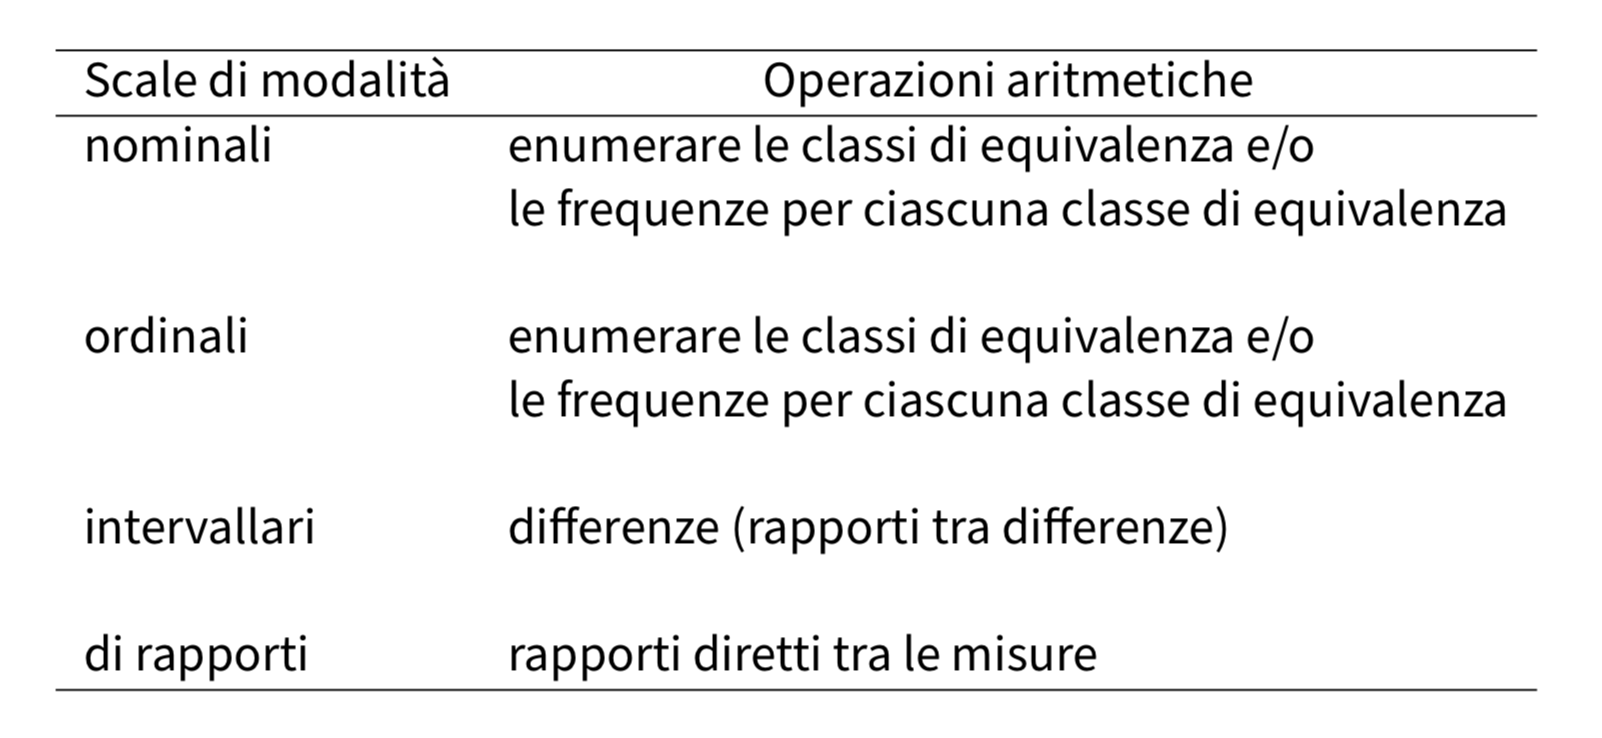
\includegraphics[width=0.8\linewidth,height=\textheight,keepaspectratio]{chapters/key_notions/../../figures/misurazione_2.png}

}

\caption{Scale di misurazione.}

\end{figure}%

\subsection{Scala nominale}\label{scala-nominale}

La scala nominale è il livello di misurazione più semplice e corrisponde
ad una tassonomia o classificazione delle categorie che utilizziamo per
descrivere i fenomeni psicologici. I simboli o numeri che costituiscono
questa scala rappresentano i nomi delle categorie e non hanno alcun
valore numerico intrinseco. Con la scala nominale possiamo solo
distinguere se una caratteristica psicologica è uguale o diversa da
un'altra.

I dati raccolti con la scala nominale sono suddivisi in categorie
qualitative e mutuamente esclusive, in cui ogni dato appartiene ad una
sola categoria. In questa scala, esiste solo la relazione di equivalenza
tra le misure delle unità di studio: gli elementi del campione
appartenenti a classi diverse sono differenti, mentre tutti quelli della
stessa classe sono tra loro equivalenti.

L'unica operazione algebrica consentita dalla scala nominale è quella di
contare le unità di studio che appartengono ad ogni categoria e il
numero totale di categorie. Di conseguenza, la descrizione dei dati
avviene tramite le frequenze assolute e le frequenze relative.

Dalla scala nominale è possibile costruire altre scale nominali
equivalenti alla prima, trasformando i valori della scala di partenza in
modo tale da cambiare i nomi delle categorie, ma lasciando inalterata la
suddivisione delle unità di studio nelle medesime classi di equivalenza.
In altre parole, cambiando i nomi delle categorie di una variabile
misurata su scala nominale, si ottiene una nuova variabile esattamente
equivalente alla prima.

\subsection{Scala ordinale}\label{scala-ordinale}

La scala ordinale mantiene la caratteristica della scala nominale di
classificare ogni unità di misura all'interno di una singola categoria,
ma introduce la relazione di ordinamento tra le categorie. In quanto
basata su una relazione di ordine, una scala ordinale descrive solo il
rango di ordine tra le categorie e non fornisce informazioni sulla
distanza tra di esse. Non ci dice, ad esempio, se la distanza tra le
categorie \(a\) e \(b\) è uguale, maggiore o minore della distanza tra
le categorie \(b\) e \(c\).

Un esempio classico di scala ordinale è quello della scala Mohs per la
determinazione della durezza dei minerali. Per stabilire la durezza dei
minerali si usa il criterio empirico della scalfittura. Vengono
stabiliti livelli di durezza crescente da 1 a 10 con riferimento a dieci
minerali: talco, gesso, calcite, fluorite, apatite, ortoclasio, quarzo,
topazio, corindone e diamante. Un minerale appartenente ad uno di questi
livelli se scalfisce quello di livello inferiore ed è scalfito da quello
di livello superiore.

\begin{figure}[H]

{\centering 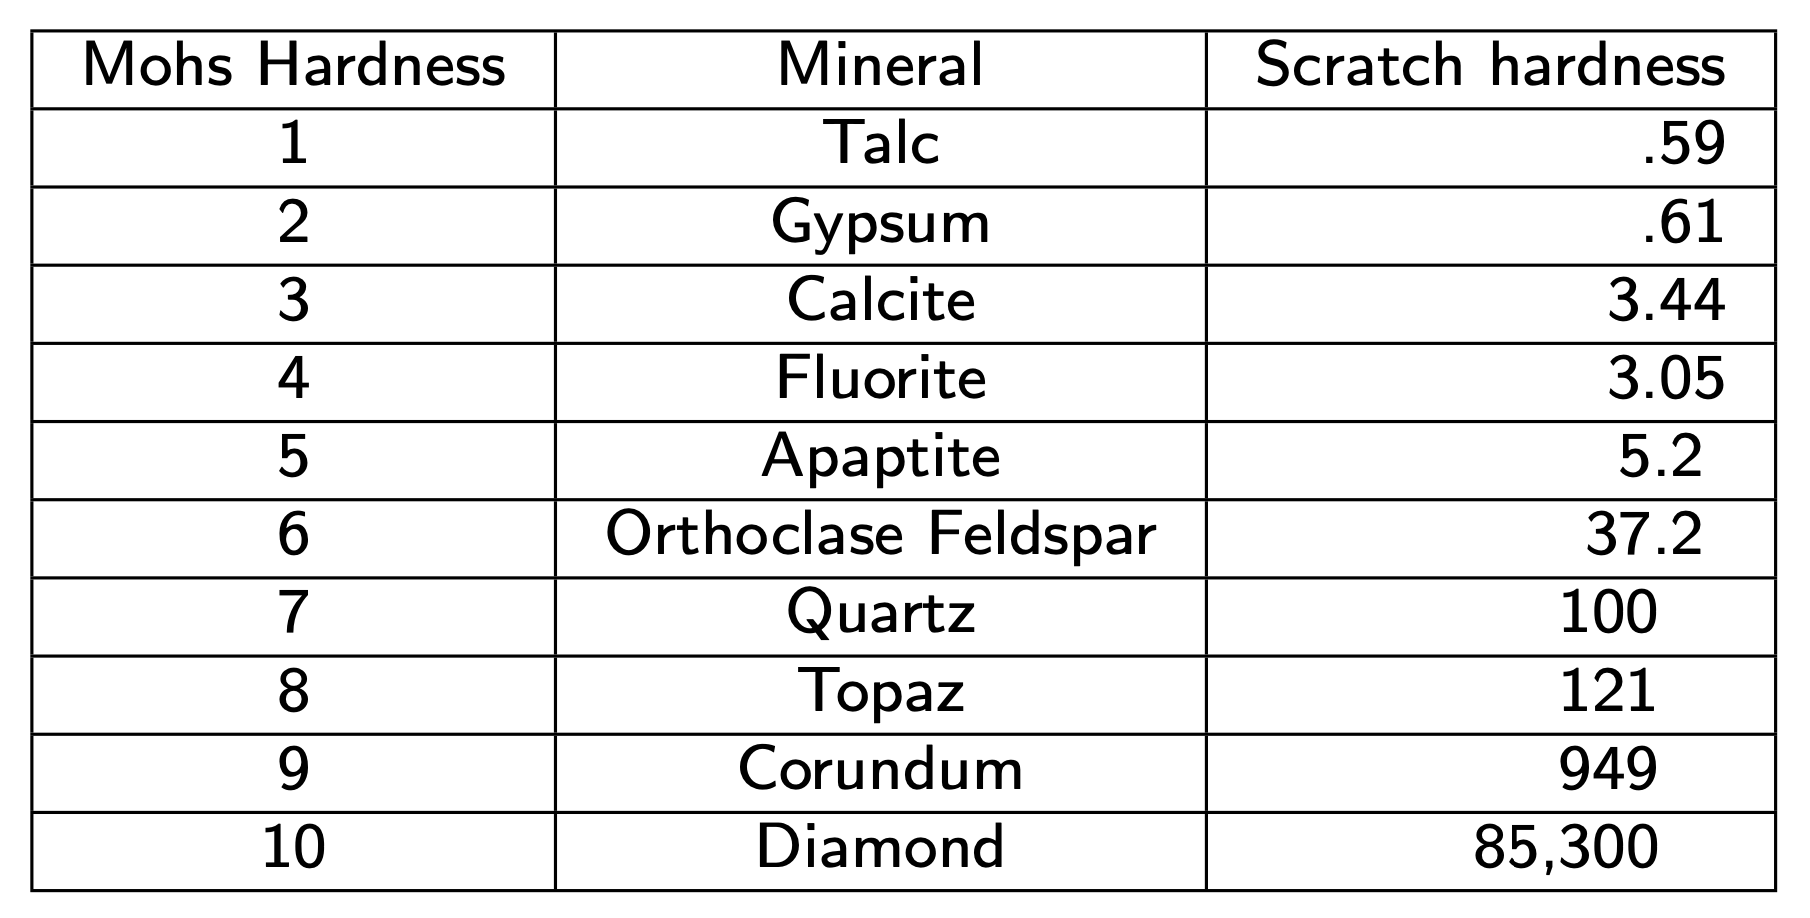
\includegraphics[width=0.7\linewidth,height=\textheight,keepaspectratio]{chapters/key_notions/../../figures/mohs.png}

}

\caption{La scala di durezza dei minerali di Mohs. Un oggetto è
considerato più duro di X se graffia X. Sono incluse anche misure di
durezza relativa utilizzando uno sclerometro, da cui emerge la non
linearità della scala di Mohs (Burchard, 2004).}

\end{figure}%

\subsection{Scala ad intervalli}\label{scala-ad-intervalli}

La scala ad intervalli di misurazione include le proprietà della scala
nominale e della scala ordinale e permette di misurare le distanze tra
le coppie di unità statistiche in termini di un intervallo costante,
chiamato ``unità di misura'', a cui viene attribuito il valore ``1''.
L'origine della scala, ovvero il punto zero, è scelta arbitrariamente e
non indica l'assenza della proprietà che si sta misurando. Ciò significa
che la scala ad intervalli consente anche valori negativi e lo zero non
viene attribuito all'unità statistica in cui la proprietà risulta
assente.

La scala ad intervalli equivalenti consente l'esecuzione di operazioni
algebriche basate sulla differenza tra i numeri associati ai diversi
punti della scala, operazioni algebriche non possibili con le scale di
misura nominale o ordinale. Tuttavia, il limite della scala ad
intervalli è che non consente di calcolare il rapporto tra coppie di
misure. È possibile affermare la differenza tra \(a\) e \(b\) come la
metà della differenza tra \(c\) e \(d\) o che le due differenze sono
uguali, ma non è possibile affermare che \(a\) abbia una proprietà
misurata in quantità doppia rispetto a \(b\). In altre parole, non è
possibile stabilire rapporti diretti tra le misure ottenute. Solo le
differenze tra le modalità permettono tutte le operazioni aritmetiche,
come la somma, l'elevazione a potenza o la divisione, che sono alla base
della statistica inferenziale.

Nelle scale ad intervalli equivalenti, l'unità di misura è arbitraria e
può essere cambiata attraverso una dilatazione, ovvero la
moltiplicazione di tutti i valori della scala per una costante positiva.
Inoltre, la traslazione, ovvero l'aggiunta di una costante a tutti i
valori della scala, è ammessa poiché non altera le differenze tra i
valori della scala. La scala rimane invariata rispetto a traslazioni e
dilatazioni e dunque le uniche trasformazioni ammissibili sono le
trasformazioni lineari:

\[
y' = a + by, \quad b > 0.
\]

Infatti, l'uguaglianza dei rapporti fra gli intervalli rimane invariata
a seguito di una trasformazione lineare.

Esempio di scala ad intervalli è la temperatura misurata in gradi
Celsius o Fahrenheit, ma non Kelvin. Come per la scala nominale, è
possibile stabilire se due modalità sono uguali o diverse:
\(30^\circ C \neq 20^\circ C\). Come per la scala ordinale è possibile
mettere due modalità in una relazione d'ordine:
\(30^\circ C > 20^\circ C\). In aggiunta ai casi precedenti, però, è
possibile definire una unità di misura per cui è possibile dire che tra
\(30^\circ C\) e \(20^\circ C\) c'è una differenza di
\(30^\circ - 20^\circ = 10^\circ C\). I valori di temperatura, oltre a
poter essere ordinati secondo l'intensità del fenomeno, godono della
proprietà che le differenze tra loro sono direttamente confrontabili e
quantificabili.

Il limite della scala ad intervalli è quello di non consentire il
calcolo del rapporto tra coppie di misure. Ad esempio, una temperatura
di \(80^\circ C\) non è il doppio di una di \(40^\circ C\). Se infatti
esprimiamo le stesse temperature nei termini della scala Fahrenheit,
allora i due valori non saranno in rapporto di 1 a 2 tra loro. Infatti,
\(20^\circ C = 68^\circ F\) e \(40^\circ C = 104^\circ F\). Questo
significa che la relazione ``il doppio di'' che avevamo individuato in
precedenza si applicava ai numeri della scala centigrada, ma non alla
proprietà misurata (cioè la temperatura). La decisione di che scala
usare (Centigrada vs.~Fahrenheit) è arbitraria. Ma questa arbitrarietà
non deve influenzare le inferenze che traiamo dai dati. Queste
inferenze, infatti, devono dirci qualcosa a proposito della realtà
empirica e non possono in nessun modo essere condizionate dalle nostre
scelte arbitrarie che ci portano a scegliere la scala Centigrada
piuttosto che quella Fahrenheit.

Consideriamo ora l'aspetto invariante di una trasformazione lineare,
ovvero l'uguaglianza dei rapporti fra intervalli. Prendiamo in esame, ad
esempio, tre temperature: \(20^\circ C = 68^\circ F\),
\(15^\circ C = 59^\circ F\), \(10^\circ C = 50 ^\circ F\).

È facile rendersi conto del fatto che i rapporti fra intervalli restano
costanti indipendentemente dall'unità di misura che è stata scelta:

\[
  \frac{20^\circ C - 10^\circ C}{20^\circ C - 15^\circ C} =
  \frac{68^\circ F - 50^\circ F}{68^\circ F-59^\circ F} = 2.
\]

\subsection{Scala di rapporti}\label{scala-di-rapporti}

Nella scala a rapporti equivalenti, lo zero non è arbitrario e
rappresenta l'elemento che ha intensità nulla rispetto alla proprietà
misurata. Per costruire questa scala, si associa il numero 0
all'elemento con intensità nulla e si sceglie un'unità di misura \(u\).
Ad ogni elemento si assegna un numero \(a\) definito come \(a = d / u\),
dove \(d\) rappresenta la distanza dall'origine. In questo modo, i
numeri assegnati riflettono le differenze e i rapporti tra le intensità
della proprietà misurata.

In questa scala, è possibile effettuare operazioni aritmetiche non solo
sulle differenze tra i valori della scala, ma anche sui valori stessi
della scala. L'unica scelta arbitraria è l'unità di misura, ma lo zero
deve sempre rappresentare l'intensità nulla della proprietà considerata.

Le trasformazioni ammissibili in questa scala sono chiamate
trasformazioni di similarità e sono del tipo \(y' = by\), dove
\(b > 0\). In questa scala, i rapporti tra i valori rimangono invariati
dopo le trasformazioni. In altre parole, se rapportiamo due valori
originali e due valori trasformati, il rapporto rimane lo stesso:
\(\frac{y_i}{y_j} = \frac{y'_i}{y'_j}\).

\section{Gerarchia dei livelli delle scale di
misurazione}\label{gerarchia-dei-livelli-delle-scale-di-misurazione}

Secondo Stevens (1946), esiste una gerarchia dei livelli delle scale di
misurazione, denominati ``livelli di scala''. Questi livelli sono
organizzati in modo gerarchico, in cui la scala nominale rappresenta il
livello più basso della misurazione, mentre la scala a rapporti
equivalenti rappresenta il livello più alto.

\begin{itemize}
\tightlist
\item
  \textbf{Scala nominale}: Classifica le categorie senza un ordine
  specifico.
\item
  \textbf{Scala ordinale}: Classifica le categorie in un ordine
  specifico, ma senza una misura precisa delle distanze.
\item
  \textbf{Scala a intervalli}: Misura le distanze tra le categorie con
  un intervallo costante, ma senza un punto zero assoluto.
\item
  \textbf{Scala di rapporti}: Misura le distanze con un intervallo
  costante e un punto zero assoluto.
\end{itemize}

\begin{figure}[H]

{\centering 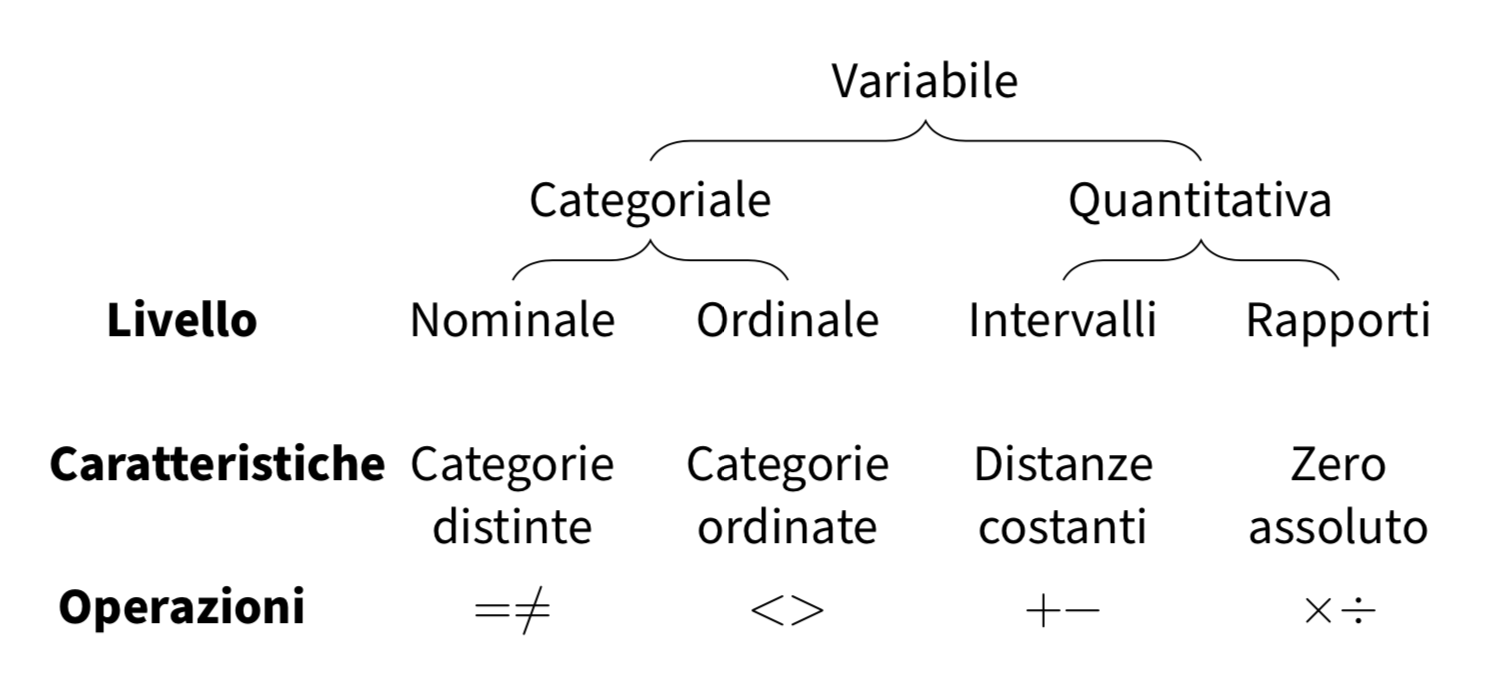
\includegraphics[width=0.7\linewidth,height=\textheight,keepaspectratio]{chapters/key_notions/../../figures/misurazione_1.png}

}

\caption{Relazioni tra i livelli di misurazione.}

\end{figure}%

Passando da un livello di misurazione ad uno più alto aumenta il numero
di operazioni aritmetiche che possono essere compiute sui valori della
scala.

\subsection{Variabili Discrete e
Continue}\label{variabili-discrete-e-continue}

Le variabili possono essere classificate come variabili a livello di
intervalli o di rapporti e possono essere sia discrete che continue.

\begin{itemize}
\tightlist
\item
  \textbf{Variabili discrete}: Assumono valori specifici ma non possono
  assumere valori intermedi.
\item
  \textbf{Variabili continue}: Possono assumere qualsiasi valore
  all'interno di un intervallo specificato.
\end{itemize}

\begin{figure}[H]

{\centering 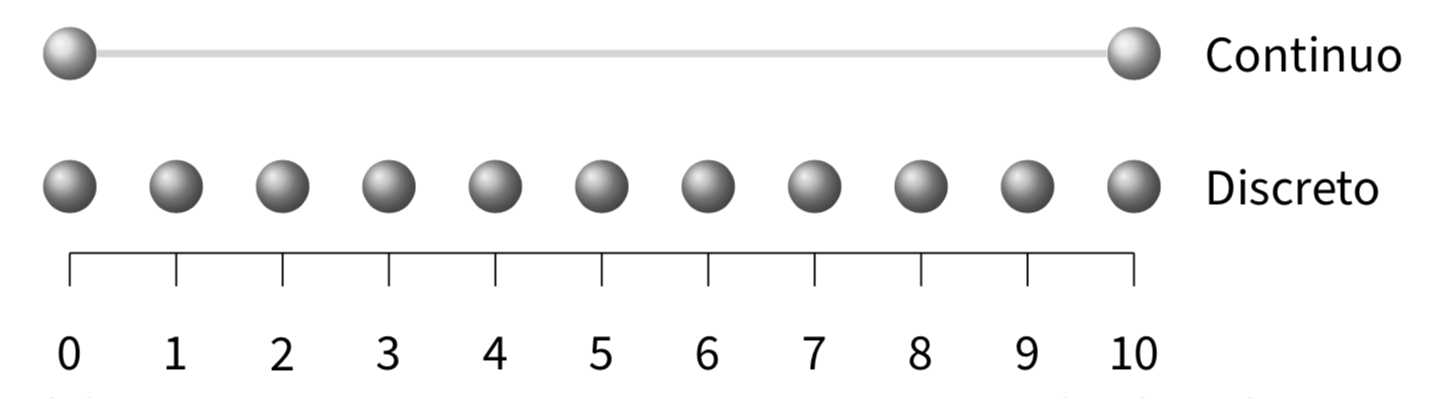
\includegraphics[width=0.7\linewidth,height=\textheight,keepaspectratio]{chapters/key_notions/../../figures/misurazione_3.png}

}

\caption{Variabili discrete e continue.}

\end{figure}%

\section{Relazione tra Misurazione e Teoria Sostanziale: Un'Analisi
Critica}\label{relazione-tra-misurazione-e-teoria-sostanziale-unanalisi-critica}

Un esempio di come condurre una lettura critica di un articolo
scientifico è rappresentato dall'analisi di uno studio pubblicato su
\emph{Nature} sul tema del \textbf{mind-body healing}
(\citeproc{ref-aungle2023physical}{Aungle \& Langer, 2023}). Lo
\href{https://www.nature.com/articles/s41598-023-50009-3}{studio}
presenta risultati empirici che suggeriscono un legame tra pratiche di
guarigione mente-corpo e miglioramenti nella salute fisica. Tuttavia, la
validità di queste conclusioni è stata fortemente contestata da Andrew
Gelman, un noto statistico e ricercatore, in un post sul suo blog
\href{https://statmodeling.stat.columbia.edu/2025/01/27/does-anyone-actually-expect-meaningful-insight-to-come-from-a-study-like-this/}{Statistical
Modeling}.

\subsection{L'Importanza di una Teoria Sostanziale
Solida}\label{limportanza-di-una-teoria-sostanziale-solida}

Gelman sottolinea un aspetto cruciale della ricerca scientifica:
l'importanza di una \textbf{teoria sostanziale solida e convincente}.
Secondo il suo punto di vista, lo studio analizzato presenta una carenza
significativa in questo ambito. In assenza di una teoria ben fondata che
spieghi in modo plausibile i meccanismi causali attraverso cui le
pratiche mente-corpo potrebbero influenzare la salute fisica, i
risultati empirici ottenuti rimangono privi di significato. Senza una
cornice teorica coerente, lo studio rischia di essere classificato come
ciò che Gelman definisce ``junk science'' -- scienza di scarso valore,
incapace di offrire vere e proprie intuizioni.

Una teoria sostanziale non deve solo essere plausibile, ma deve anche
integrarsi in modo coerente con altre teorie scientifiche consolidate.
Quando una ricerca non riesce a inserirsi in una rete più ampia di
conoscenze, i suoi risultati diventano inevitabilmente discutibili. È
proprio questo il caso dello studio esaminato da Gelman: l'assenza di
una teoria chiara e ben articolata rende i risultati empirici poco
credibili e difficilmente generalizzabili.

\subsection{Problemi di Misurazione}\label{problemi-di-misurazione}

Oltre alla debolezza teorica, lo studio presenta anche notevoli problemi
legati alla \textbf{misurazione}. Le variabili utilizzate per
quantificare sia gli interventi mente-corpo che gli esiti sanitari sono
soggette a diverse criticità. Ad esempio, la misurazione dell'efficacia
delle pratiche mente-corpo potrebbe essere influenzata da fattori
confondenti, come le aspettative dei partecipanti o l'effetto placebo.
Allo stesso modo, la valutazione degli esiti sanitari può risultare
problematica se non vengono impiegate scale di misurazione affidabili e
valide.

Per un approfondimento su questi temi, si rimanda alle riflessioni
conclusive nel Capitolo~\ref{sec-prob-sampling-distr}, dove vengono
discusse criticamente le questioni legate alla misurazione, con
particolare attenzione alla distinzione tra
\href{https://en.wikipedia.org/wiki/Accuracy_and_precision}{precisione e
bias}. In generale, uno degli aspetti più critici della misurazione
riguarda la validità
\href{https://en.wikipedia.org/wiki/Internal_validity}{interna} ed
\href{https://en.wikipedia.org/wiki/External_validity}{esterna} negli
studi psicologici. La qualità delle misure adottate influisce
direttamente sulla solidità delle conclusioni scientifiche: una
misurazione imprecisa o distorta può compromettere la validità dei
risultati e limitarne la generalizzabilità.

\subsection{La Necessità di una Valutazione
Bilanciata}\label{la-necessituxe0-di-una-valutazione-bilanciata}

L'esempio dello studio sul mind-body healing illustra in modo efficace
come una lettura critica debba necessariamente passare attraverso due
dimensioni fondamentali: la \textbf{teoria} e la \textbf{misurazione}.
Una teoria debole compromette la capacità di attribuire significato ai
dati raccolti, riducendo lo studio a una mera raccolta di numeri privi
di valore scientifico. Allo stesso tempo, problemi di misurazione
possono distorcere i risultati, portando a conclusioni errate o
fuorvianti. Solo attraverso una valutazione attenta di entrambi questi
aspetti è possibile distinguere tra ricerche scientificamente valide e
``junk science''.

In definitiva, una lettura critica di un articolo psicologico richiede
non solo competenze tecniche, ma anche una profonda consapevolezza dei
limiti e delle sfide insite nella misurazione psicologica e nel rapporto
tra misurazione e teorie scientifiche. Questo approccio consente di
valutare in modo equilibrato la qualità e l'affidabilità delle
conclusioni proposte. Solo attraverso una rigorosa analisi di entrambi
questi aspetti è possibile distinguere tra ricerche scientificamente
valide e quelle che, invece, rischiano di essere considerate ``junk
science''.

\section{Riflessioni Conclusive}\label{riflessioni-conclusive-2}

La misurazione in psicologia non è un semplice atto di raccolta di dati,
ma un processo fondamentale per garantire che le osservazioni empiriche
siano interpretabili alla luce di modelli teorici solidi. Una buona
misurazione non si limita a ridurre l'errore, ma consente di attribuire
un significato coerente ai punteggi ottenuti, facilitando così il
progresso della conoscenza scientifica. Senza strumenti adeguati per la
misurazione, il rischio è quello di costruire teorie su basi incerte,
compromettendo la validità delle conclusioni tratte.

Due pilastri sostengono una ricerca psicologica rigorosa: la teoria e la
misurazione. La teoria fornisce il quadro concettuale entro cui si
interpretano i dati, definendo le ipotesi e orientando le analisi. La
\href{https://statmodeling.stat.columbia.edu/2015/04/28/whats-important-thing-statistics-thats-not-textbooks/}{misurazione},
invece, è il ponte tra i costrutti astratti e le osservazioni empiriche,
traducendo concetti complessi in variabili operative affidabili. Nessuna
delle due componenti può reggersi senza l'altra: una teoria senza
misurazione adeguata rischia di rimanere speculativa, mentre una
misurazione priva di un solido fondamento teorico può portare a dati
privi di significato.

Nella valutazione di un qualsiasi studio psicologico, un approccio
critico richiede quindi di esaminare sia la solidità del quadro teorico
sia la qualità degli strumenti di misurazione adottati. Il progresso
della ricerca dipende dalla capacità di integrare questi due elementi,
attraverso metodologie sempre più sofisticate che riducano l'incertezza
e migliorino la precisione delle inferenze. Le moderne tecniche di
analisi dei dati, i modelli psicometrici avanzati e le tecnologie
digitali stanno ampliando le possibilità di misurazione, offrendo
strumenti più sensibili e adattabili alla complessità dei fenomeni
psicologici. Tuttavia, la sfida principale rimane la stessa: garantire
che la misurazione sia non solo accurata, ma anche teoricamente fondata,
affinché le conoscenze acquisite possano davvero contribuire alla
comprensione della mente e del comportamento umano.

\section*{Esercizi}\label{esercizi-2}
\addcontentsline{toc}{section}{Esercizi}

\markright{Esercizi}

\begin{tcolorbox}[enhanced jigsaw, opacityback=0, bottomrule=.15mm, breakable, title=\textcolor{quarto-callout-important-color}{\faExclamation}\hspace{0.5em}{Problemi 1}, bottomtitle=1mm, toptitle=1mm, titlerule=0mm, colbacktitle=quarto-callout-important-color!10!white, rightrule=.15mm, colframe=quarto-callout-important-color-frame, colback=white, arc=.35mm, leftrule=.75mm, coltitle=black, left=2mm, toprule=.15mm, opacitybacktitle=0.6]

\textbf{Esercizio 1: Identificazione del Livello di Misurazione}

\textbf{Obiettivo:} Comprendere i diversi livelli di misurazione
applicati alla psicologia.

\begin{enumerate}
\def\labelenumi{\arabic{enumi}.}
\item
  Identifica il livello di misurazione (nominale, ordinale, intervalli,
  rapporti) per ciascuna delle seguenti variabili psicologiche:

  \begin{itemize}
  \tightlist
  \item
    \begin{enumerate}
    \def\labelenumii{\alph{enumii})}
    \tightlist
    \item
      Tipo di terapia psicologica (Cognitivo-comportamentale,
      Psicodinamica, Umanistica)
    \end{enumerate}
  \item
    \begin{enumerate}
    \def\labelenumii{\alph{enumii})}
    \setcounter{enumii}{1}
    \tightlist
    \item
      Livello di ansia auto-riferito su una scala da 1 a 10
    \end{enumerate}
  \item
    \begin{enumerate}
    \def\labelenumii{\alph{enumii})}
    \setcounter{enumii}{2}
    \tightlist
    \item
      Numero di episodi depressivi in un anno
    \end{enumerate}
  \item
    \begin{enumerate}
    \def\labelenumii{\alph{enumii})}
    \setcounter{enumii}{3}
    \tightlist
    \item
      Tempo di reazione in millisecondi in un test cognitivo
    \end{enumerate}
  \end{itemize}
\end{enumerate}

\textbf{Esercizio 2: Confronto tra Scale}

\textbf{Obiettivo:} Comprendere le differenze tra le scale di
misurazione.

\begin{enumerate}
\def\labelenumi{\arabic{enumi}.}
\tightlist
\item
  Spiega la differenza tra una scala ordinale e una scala a intervalli
  utilizzando l'esempio della soddisfazione lavorativa.
\item
  Perché il punteggio QI è misurato su una scala a intervalli e non su
  una scala a rapporti?
\item
  In che modo il punteggio di una scala di autostima su una scala Likert
  differisce da una misurazione su una scala di rapporti?
\end{enumerate}

\textbf{Esercizio 3: Operazioni Aritmetiche Consentite}

\textbf{Obiettivo:} Comprendere le operazioni matematiche consentite per
ciascun livello di misurazione.

\begin{enumerate}
\def\labelenumi{\arabic{enumi}.}
\tightlist
\item
  Quali operazioni aritmetiche sono ammissibili per una scala nominale?
\item
  Può avere senso calcolare la media di punteggi su una scala ordinale?
  Perché?
\item
  Se hai misurato il tempo di reazione in secondi, quali operazioni
  aritmetiche puoi eseguire?
\end{enumerate}

\textbf{Esercizio 4: Trasformazioni Ammissibili}

\textbf{Obiettivo:} Comprendere le trasformazioni possibili per ogni
scala di misurazione.

\begin{enumerate}
\def\labelenumi{\arabic{enumi}.}
\tightlist
\item
  Se una variabile è misurata su una scala nominale, quale tipo di
  trasformazione è consentita?
\item
  Per una scala a intervalli, quali trasformazioni matematiche sono
  permesse senza alterare le proprietà della scala?
\item
  Quale tipo di trasformazione è consentita su una scala di rapporti?
\end{enumerate}

\textbf{Esercizio 5: Applicazione delle Scale a Dati Psicologici}

\textbf{Obiettivo:} Applicare i concetti a contesti psicologici reali.

\begin{enumerate}
\def\labelenumi{\arabic{enumi}.}
\tightlist
\item
  Una scala di ansia clinica fornisce punteggi compresi tra 0 e 100.
  Quale livello di misurazione è più appropriato e perché?
\item
  Un esperimento misura la memoria dichiarativa chiedendo ai
  partecipanti di ricordare un elenco di parole. Come dovrebbe essere
  misurata la variabile ``numero di parole ricordate''?
\item
  In uno studio sulla personalità, i tratti vengono classificati come
  ``estroverso'' e ``introverso''. Qual è il livello di misurazione?
\end{enumerate}

\textbf{Esercizio 6: Valutazione della Scala di Misurazione}

\textbf{Obiettivo:} Identificare la corretta scala di misurazione per
vari fenomeni psicologici.

\begin{enumerate}
\def\labelenumi{\arabic{enumi}.}
\tightlist
\item
  Il livello di aggressività misurato su una scala da 1 a 5 è nominale,
  ordinale, intervalli o rapporti? Giustifica la tua risposta.
\item
  Il numero di attacchi di panico in una settimana può essere
  considerato su scala ordinale? Perché sì o perché no?
\item
  Un test di intelligenza misura il QI con una media di 100 e una
  deviazione standard di 15. Qual è il livello di misurazione e quali
  sono le implicazioni per l'analisi statistica?
\end{enumerate}

\textbf{Esercizio 7: Costruzione di una Scala Psicologica}

\textbf{Obiettivo:} Creare una scala di misurazione per una variabile
psicologica.

\begin{enumerate}
\def\labelenumi{\arabic{enumi}.}
\tightlist
\item
  Se dovessi costruire una scala per misurare la resilienza, quale
  livello di misurazione sceglieresti e perché?
\item
  Come potresti trasformare una scala nominale di preferenza musicale in
  una scala ordinale?
\item
  Un questionario sulla qualità della vita chiede ai partecipanti di
  valutare la loro felicità su una scala da 1 a 10. È una scala a
  intervalli o ordinale? Giustifica.
\end{enumerate}

\textbf{Esercizio 8: Interpretazione Statistica dei Dati}

\textbf{Obiettivo:} Collegare il livello di misurazione alle tecniche
statistiche appropriate.

\begin{enumerate}
\def\labelenumi{\arabic{enumi}.}
\tightlist
\item
  Perché una mediana è più appropriata della media per dati ordinali?
\item
  Quale test statistico sarebbe più adatto per confrontare due gruppi su
  una variabile nominale?
\item
  Quali analisi possono essere condotte su dati raccolti su una scala a
  rapporti?
\end{enumerate}

\textbf{Esercizio 9: Misurazione e Inferenze Psicologiche}

\textbf{Obiettivo:} Riflettere su come il livello di misurazione
influisce sulle conclusioni di una ricerca.

\begin{enumerate}
\def\labelenumi{\arabic{enumi}.}
\tightlist
\item
  Se un test di personalità usa una scala Likert da 1 a 7, quali
  precauzioni devono essere prese nell'interpretare le differenze tra
  punteggi?
\item
  Un questionario di benessere assegna punteggi tra 0 e 100, ma non ha
  uno zero assoluto. Quale scala è questa e quali sono le limitazioni?
\item
  In uno studio sulla depressione, i sintomi vengono codificati come
  ``assenti'', ``moderati'' o ``gravi''. Che tipo di scala è questa e
  quali statistiche possono essere usate per analizzarla?
\end{enumerate}

\textbf{Esercizio 10: Esperimenti Psicologici e Misurazione}

\textbf{Obiettivo:} Applicare la teoria della misurazione nella
progettazione di esperimenti psicologici.

\begin{enumerate}
\def\labelenumi{\arabic{enumi}.}
\tightlist
\item
  Se un esperimento misura la memoria a breve termine con un compito di
  richiamo di parole, quale scala di misurazione utilizzeresti?
\item
  Come la scelta della scala di misurazione può influenzare le inferenze
  che si possono trarre da un esperimento?
\item
  Quali tipi di analisi statistica sono appropriati per dati misurati su
  scala ordinale rispetto a scala di rapporti?
\end{enumerate}

\end{tcolorbox}

\begin{tcolorbox}[enhanced jigsaw, opacityback=0, bottomrule=.15mm, breakable, title=\textcolor{quarto-callout-tip-color}{\faLightbulb}\hspace{0.5em}{Soluzioni 1}, bottomtitle=1mm, toptitle=1mm, titlerule=0mm, colbacktitle=quarto-callout-tip-color!10!white, rightrule=.15mm, colframe=quarto-callout-tip-color-frame, colback=white, arc=.35mm, leftrule=.75mm, coltitle=black, left=2mm, toprule=.15mm, opacitybacktitle=0.6]

\textbf{Esercizio 1: Identificazione del Livello di Misurazione}

\textbf{Obiettivo:} Comprendere i diversi livelli di misurazione
applicati alla psicologia.

\begin{enumerate}
\def\labelenumi{\arabic{enumi}.}
\tightlist
\item
  Identifica il livello di misurazione (nominale, ordinale, intervalli,
  rapporti) per ciascuna delle seguenti variabili psicologiche:

  \begin{itemize}
  \tightlist
  \item
    \begin{enumerate}
    \def\labelenumii{\alph{enumii})}
    \tightlist
    \item
      \textbf{Nominale} (Tipo di terapia psicologica è una
      classificazione senza ordine)
    \end{enumerate}
  \item
    \begin{enumerate}
    \def\labelenumii{\alph{enumii})}
    \setcounter{enumii}{1}
    \tightlist
    \item
      \textbf{Ordinale} (Scala da 1 a 10, con ordine ma senza distanze
      uguali)
    \end{enumerate}
  \item
    \begin{enumerate}
    \def\labelenumii{\alph{enumii})}
    \setcounter{enumii}{2}
    \tightlist
    \item
      \textbf{Rapporti} (Numero di episodi depressivi ha uno zero
      assoluto e si possono fare rapporti tra valori)
    \end{enumerate}
  \item
    \begin{enumerate}
    \def\labelenumii{\alph{enumii})}
    \setcounter{enumii}{3}
    \tightlist
    \item
      \textbf{Rapporti} (Tempo di reazione ha uno zero assoluto e
      permette operazioni di rapporto)
    \end{enumerate}
  \end{itemize}
\end{enumerate}

\textbf{Esercizio 2: Confronto tra Scale}

\textbf{Obiettivo:} Comprendere le differenze tra le scale di
misurazione.

\begin{enumerate}
\def\labelenumi{\arabic{enumi}.}
\tightlist
\item
  La scala ordinale fornisce un ordine ma non permette di calcolare
  differenze precise, mentre la scala a intervalli ha differenze
  costanti tra i valori. Ad esempio, ``soddisfazione lavorativa'' su una
  scala da 1 a 5 è ordinale, mentre il punteggio di un test psicologico
  è a intervalli.
\item
  Il punteggio QI è a intervalli perché la differenza tra punteggi è
  significativa, ma non ha uno zero assoluto che rappresenta l'assenza
  di intelligenza.
\item
  Una scala Likert misura il livello di accordo con una dichiarazione,
  quindi è generalmente considerata ordinale, nonostante sia trattata
  spesso come una scala a intervalli.
\end{enumerate}

\textbf{Esercizio 3: Operazioni Aritmetiche Consentite}

\textbf{Obiettivo:} Comprendere le operazioni matematiche consentite per
ciascun livello di misurazione.

\begin{enumerate}
\def\labelenumi{\arabic{enumi}.}
\tightlist
\item
  Nella scala nominale si può solo contare la frequenza delle categorie
  (ad es., il numero di partecipanti che usano un tipo di terapia).
\item
  No, la media su dati ordinali può essere fuorviante perché le distanze
  tra le categorie non sono necessariamente uguali. Meglio usare la
  mediana.
\item
  Sul tempo di reazione si possono eseguire tutte le operazioni
  aritmetiche, inclusa la media, la moltiplicazione e i rapporti tra
  valori.
\end{enumerate}

\textbf{Esercizio 4: Trasformazioni Ammissibili}

\textbf{Obiettivo:} Comprendere le trasformazioni possibili per ogni
scala di misurazione.

\begin{enumerate}
\def\labelenumi{\arabic{enumi}.}
\tightlist
\item
  Sulla scala nominale, solo le trasformazioni di ricodifica (ad
  esempio, cambiare i nomi delle categorie) sono permesse.
\item
  Per una scala a intervalli, si possono effettuare trasformazioni
  lineari della forma y' = a + by con b \textgreater{} 0.
\item
  Per una scala di rapporti, sono consentite trasformazioni di
  similarità della forma y' = by, dove b \textgreater{} 0.
\end{enumerate}

\textbf{Esercizio 5: Applicazione delle Scale a Dati Psicologici}

\textbf{Obiettivo:} Applicare i concetti a contesti psicologici reali.

\begin{enumerate}
\def\labelenumi{\arabic{enumi}.}
\tightlist
\item
  Scala a intervalli, perché ha differenze costanti tra i punteggi ma
  nessuno zero assoluto.
\item
  Scala di rapporti, perché il numero di parole ricordate ha uno zero
  assoluto e consente operazioni di rapporto.
\item
  Nominale, perché non vi è un ordine gerarchico tra le categorie
  ``estroverso'' e ``introverso''.
\end{enumerate}

\textbf{Esercizio 6: Valutazione della Scala di Misurazione}

\textbf{Obiettivo:} Identificare la corretta scala di misurazione per
vari fenomeni psicologici.

\begin{enumerate}
\def\labelenumi{\arabic{enumi}.}
\tightlist
\item
  Ordinale, perché il livello di aggressività segue un ordine, ma le
  differenze tra i livelli non sono necessariamente uguali.
\item
  No, perché il numero di attacchi di panico è una variabile discreta e
  misurabile su scala di rapporti.
\item
  Intervalli, perché il punteggio QI ha distanze costanti tra i valori,
  ma non ha uno zero assoluto.
\end{enumerate}

\textbf{Esercizio 7: Costruzione di una Scala Psicologica}

\textbf{Obiettivo:} Creare una scala di misurazione per una variabile
psicologica.

\begin{enumerate}
\def\labelenumi{\arabic{enumi}.}
\tightlist
\item
  Ordinale o a intervalli, a seconda della precisione della misurazione
  della resilienza.
\item
  Si potrebbe assegnare un valore numerico crescente alle categorie di
  preferenza musicale per ottenere una scala ordinale.
\item
  È una scala ordinale, perché la differenza tra livelli non è
  necessariamente costante.
\end{enumerate}

\textbf{Esercizio 8: Interpretazione Statistica dei Dati}

\textbf{Obiettivo:} Collegare il livello di misurazione alle tecniche
statistiche appropriate.

\begin{enumerate}
\def\labelenumi{\arabic{enumi}.}
\tightlist
\item
  Perché la mediana è meno sensibile ai valori estremi rispetto alla
  media.
\item
  Un test chi-quadrato è adatto per confrontare frequenze di dati
  nominali tra gruppi.
\item
  Si possono calcolare media, deviazione standard e utilizzare test
  parametrici come t-test o ANOVA.
\end{enumerate}

\textbf{Esercizio 9: Misurazione e Inferenze Psicologiche}

\textbf{Obiettivo:} Riflettere su come il livello di misurazione
influisce sulle conclusioni di una ricerca.

\begin{enumerate}
\def\labelenumi{\arabic{enumi}.}
\tightlist
\item
  I punteggi Likert sono ordinali, quindi confronti tra differenze di
  punteggio devono essere interpretati con cautela.
\item
  Intervalli, perché non ha uno zero assoluto, il che limita l'uso di
  operazioni moltiplicative.
\item
  Ordinale, e si possono usare test non parametrici come il test di
  Kruskal-Wallis o il test di Mann-Whitney.
\end{enumerate}

\textbf{Esercizio 10: Esperimenti Psicologici e Misurazione}

\textbf{Obiettivo:} Applicare la teoria della misurazione nella
progettazione di esperimenti psicologici.

\begin{enumerate}
\def\labelenumi{\arabic{enumi}.}
\tightlist
\item
  Rapporti, perché il numero di parole ricordate è una variabile
  discreta con uno zero assoluto.
\item
  Se si usa una scala ordinale, bisogna essere cauti nell'uso della
  media e della deviazione standard.
\item
  Scala ordinale → test non parametrici (Mann-Whitney); scala di
  rapporti → test parametrici (t-test, ANOVA).
\end{enumerate}

\end{tcolorbox}

\begin{tcolorbox}[enhanced jigsaw, opacityback=0, bottomrule=.15mm, breakable, title=\textcolor{quarto-callout-important-color}{\faExclamation}\hspace{0.5em}{Problemi 2}, bottomtitle=1mm, toptitle=1mm, titlerule=0mm, colbacktitle=quarto-callout-important-color!10!white, rightrule=.15mm, colframe=quarto-callout-important-color-frame, colback=white, arc=.35mm, leftrule=.75mm, coltitle=black, left=2mm, toprule=.15mm, opacitybacktitle=0.6]

\textbf{Esercizio 1 -- Teoria Sostanziale e ``Junk Science''}

\textbf{Obiettivo}: Riconoscere il ruolo di una teoria sostanziale
solida e comprendere come la sua assenza possa compromettere uno studio.

\begin{enumerate}
\def\labelenumi{\arabic{enumi}.}
\tightlist
\item
  Leggi la sezione in cui Gelman critica l'assenza di una teoria solida
  nello studio sulle pratiche mente-corpo.\\
\item
  Spiega, in massimo \textbf{10 righe}, perché secondo Gelman la
  mancanza di una teoria coerente rende i risultati del suddetto studio
  ``poco significativi'' o addirittura ``junk science''.\\
\item
  Proponi un esempio ipotetico (non correlato al mind-body healing) di
  uno studio psicologico che, pur presentando dati numerosi e analizzati
  con metodi statistici sofisticati, risulti privo di una teoria solida.
  Descrivi sinteticamente perché questo potrebbe rientrare nel concetto
  di ``junk science''.
\end{enumerate}

\textbf{Esercizio 2 -- Problemi di Misurazione}

\textbf{Obiettivo}: Identificare le criticità più comuni nella
misurazione dei fenomeni psicologici.

\begin{enumerate}
\def\labelenumi{\arabic{enumi}.}
\tightlist
\item
  Elenca almeno \textbf{tre} possibili fattori confondenti che
  potrebbero influenzare la misurazione dell'efficacia di un intervento
  psicologico (ad esempio, l'effetto placebo, le aspettative dei
  partecipanti, ecc.).\\
\item
  Spiega come questi fattori confondenti potrebbero compromettere la
  \textbf{validità interna} dello studio.\\
\item
  Indica almeno \textbf{due} caratteristiche fondamentali che una buona
  scala di misurazione (per una variabile psicologica) dovrebbe
  possedere per essere ritenuta affidabile e valida.
\end{enumerate}

\textbf{Esercizio 3 -- Precisione e Bias}

\textbf{Obiettivo}: Chiarire la distinzione tra precisione e distorsione
(bias) e come questi aspetti si riflettano nella validità delle
conclusioni.

\begin{enumerate}
\def\labelenumi{\arabic{enumi}.}
\tightlist
\item
  Definisci, con parole tue, i concetti di \textbf{precisione} e
  \textbf{bias} in ambito psicometrico.
\item
  Fornisci un esempio concreto di uno strumento di misura
  \textbf{preciso ma distorto} (bias elevato) e di uno strumento
  \textbf{poco preciso ma non distorto} (bias basso).\\
\item
  Spiega come la combinazione di scarsa precisione e alto bias possa
  influire sulla possibilità di trarre conclusioni affidabili in uno
  studio psicologico.
\end{enumerate}

\textbf{Esercizio 4 -- Validità Interna ed Esterna}

\textbf{Obiettivo}: Approfondire come le scelte di misurazione
influiscano sulla validità interna ed esterna di uno studio.

\begin{enumerate}
\def\labelenumi{\arabic{enumi}.}
\tightlist
\item
  In riferimento allo studio sul mind-body healing discusso nel
  capitolo, identifica due fattori che potrebbero compromettere la
  validità interna e due fattori che potrebbero limitarne la validità
  esterna.\\
\item
  Descrivi in \textbf{5-8 righe} le differenze principali tra validità
  interna e validità esterna, utilizzando esempi presi sia dal contesto
  della guarigione mente-corpo sia da altri contesti psicologici (ad
  esempio, studi sull'apprendimento o sulla motivazione).\\
\item
  Proponi una modifica al disegno di ricerca (ipotetico) che potrebbe
  migliorare la validità interna dello studio originale. Spiega
  brevemente come questa modifica ne influenzerebbe anche la validità
  esterna.
\end{enumerate}

\textbf{Esercizio 5 -- Integrare Teoria e Misurazione: Breve Progetto di
Ricerca}

\textbf{Obiettivo}: Mettere in pratica i concetti di teoria e
misurazione attraverso la progettazione di uno studio.

\begin{enumerate}
\def\labelenumi{\arabic{enumi}.}
\tightlist
\item
  Immagina di voler condurre uno studio su un intervento di ``training
  di rilassamento mentale'' finalizzato a ridurre l'ansia negli studenti
  universitari.\\
\item
  \textbf{Sviluppa una breve traccia di progetto} (massimo \textbf{15
  righe}) rispondendo ai seguenti punti:

  \begin{itemize}
  \tightlist
  \item
    \textbf{Teoria di base}: Qual è la teoria sostanziale dietro
    l'efficacia del training di rilassamento? Quali meccanismi
    psicologici verrebbero attivati?\\
  \item
    \textbf{Ipotesi}: Quale effetto prevedi sull'ansia degli studenti?\\
  \item
    \textbf{Misurazione}: Che tipo di strumento useresti per valutare il
    livello di ansia e perché (ad esempio, questionari self-report
    validati, misure fisiologiche come battito cardiaco, ecc.)?\\
  \item
    \textbf{Controllo dei confondenti}: Quali variabili secondarie
    possono influire sui risultati e come intendi gestirle?\\
  \item
    \textbf{Validità}: Come assicureresti una buona validità interna?
    Che strategie adotteresti per aumentare la validità esterna?
  \end{itemize}
\item
  Spiega brevemente in che modo la combinazione di un solido quadro
  teorico e di una misurazione accurata permette di evitare che lo
  studio venga etichettato come ``junk science''.
\end{enumerate}

\end{tcolorbox}

\begin{tcolorbox}[enhanced jigsaw, opacityback=0, bottomrule=.15mm, breakable, title=\textcolor{quarto-callout-tip-color}{\faLightbulb}\hspace{0.5em}{Soluzioni 2}, bottomtitle=1mm, toptitle=1mm, titlerule=0mm, colbacktitle=quarto-callout-tip-color!10!white, rightrule=.15mm, colframe=quarto-callout-tip-color-frame, colback=white, arc=.35mm, leftrule=.75mm, coltitle=black, left=2mm, toprule=.15mm, opacitybacktitle=0.6]

\textbf{Esercizio 1 -- Teoria Sostanziale e ``Junk Science''}

\begin{enumerate}
\def\labelenumi{\arabic{enumi}.}
\tightlist
\item
  Perché la mancanza di una teoria solida rende i risultati poco
  significativi?
\end{enumerate}

\begin{itemize}
\tightlist
\item
  \textbf{Gelman} critica lo studio sul mind-body healing perché non vi
  è un modello teorico convincente che spieghi il \textbf{meccanismo
  causale} tra pratiche mente-corpo e miglioramenti di salute.\\
\item
  Senza un quadro teorico robusto, i risultati sono interpretati in modo
  \textbf{esplorativo} e rischiano di essere attribuiti a variabili non
  controllate (effetto placebo, regressione alla media, ecc.).\\
\item
  Una teoria ben formulata aiuta a \textbf{delimitare le ipotesi},
  guidare il disegno di ricerca e interpretare correttamente i dati. In
  assenza di ciò, i numeri raccolti potrebbero essere viziati da fattori
  confondenti o da semplici correlazioni spurious.
\end{itemize}

\begin{enumerate}
\def\labelenumi{\arabic{enumi}.}
\setcounter{enumi}{1}
\tightlist
\item
  ``Junk science'' in massimo 10 righe
\end{enumerate}

\begin{quote}
\emph{Esempio di testo in 10 righe (circa)}

**Lo studio sul mind-body healing viene talvolta definito ``junk
science'' da Gelman perché, in mancanza di una teoria sostanziale
solida, i dati raccolti non forniscono indicazioni chiare sui processi
psicologici o fisiologici coinvolti. Una ricerca classificata come
``junk science'' è priva di rigore metodologico o teorico, e può
presentare gravi problemi di replicabilità o di interpretazione dei
risultati. In particolare, se non vi è un modello plausibile che
colleghi in modo coerente la pratica mente-corpo ai cambiamenti in
variabili biologiche e comportamentali, i risultati empirici rischiano
di essere semplici coincidenze. L'assenza di un costrutto ben definito e
di ipotesi derivanti da una teoria coerente rende difficile capire se i
cambiamenti osservati siano reali, casuali o dovuti ad altre cause non
considerate (per esempio, l'effetto placebo). Infine, senza un'adeguata
cornice teorica, gli studiosi non sanno come interpretare o
generalizzare i dati, e la scienza non progredisce realmente.*
\end{quote}

\begin{enumerate}
\def\labelenumi{\arabic{enumi}.}
\setcounter{enumi}{2}
\tightlist
\item
  Esempio di uno studio privo di teoria solida (ipotesi di ``junk
  science'')
\end{enumerate}

\begin{itemize}
\tightlist
\item
  \textbf{Situazione ipotetica}: Uno studio che raccoglie decine di
  variabili sulla personalità e sul benessere, poi usa tecniche
  statistiche sofisticate (analisi di big data, reti neurali, ecc.) per
  trovare correlazioni fra i tratti di personalità e centinaia di
  indicatori fisici.
\item
  \textbf{Perché ``junk science''}: Se lo studio non definisce \textbf{a
  priori} quali ipotesi testare e non ha una teoria chiara che spieghi
  perché certe caratteristiche di personalità dovrebbero correlarsi con
  determinati parametri fisici, i risultati trovati potrebbero essere
  frutto di coincidenze casuali. Inoltre, in assenza di un modello
  teorico solido, anche risultati statisticamente significativi possono
  essere privi di significato dal punto di vista psicologico.
\end{itemize}

\textbf{Esercizio 2 -- Problemi di Misurazione}

\begin{enumerate}
\def\labelenumi{\arabic{enumi}.}
\tightlist
\item
  Tre possibili fattori confondenti nell'efficacia di un intervento
  psicologico
\end{enumerate}

\begin{itemize}
\tightlist
\item
  \textbf{Effetto placebo}: I partecipanti migliorano perché si
  aspettano di migliorare, non per l'effettiva efficacia
  dell'intervento.\\
\item
  \textbf{Aspettative dei partecipanti}: Se sanno di partecipare a uno
  studio, potrebbero modificare il proprio comportamento (effetto
  Hawthorne).\\
\item
  \textbf{Desiderabilità sociale}: I partecipanti forniscono risposte
  che ritengono socialmente desiderabili, falsando i risultati (ad
  esempio, sottostimando i livelli di ansia o stress).
\end{itemize}

\begin{enumerate}
\def\labelenumi{\arabic{enumi}.}
\setcounter{enumi}{1}
\tightlist
\item
  Come questi fattori confondenti compromettono la validità interna
\end{enumerate}

\begin{itemize}
\tightlist
\item
  La \textbf{validità interna} riguarda il grado in cui è possibile
  concludere che sia effettivamente la \textbf{variabile indipendente}
  (l'intervento) a causare le modifiche osservate nella
  \textbf{variabile dipendente} (es. livelli di ansia).\\
\item
  Se subentrano l'effetto placebo, aspettative non controllate o
  tendenze alla desiderabilità sociale, diventa difficile stabilire un
  nesso causale chiaro. Esiste sempre il dubbio che altri processi
  cognitivi o sociali (non l'intervento in sé) abbiano prodotto il
  risultato.
\end{itemize}

\begin{enumerate}
\def\labelenumi{\arabic{enumi}.}
\setcounter{enumi}{2}
\tightlist
\item
  Due caratteristiche fondamentali di una buona scala di misurazione
\end{enumerate}

\begin{itemize}
\tightlist
\item
  \textbf{Affidabilità}: Capacità dello strumento di fornire misure
  stabili e coerenti nel tempo (ad esempio, coerenza interna, stabilità
  test-retest).\\
\item
  \textbf{Validità}: Capacità dello strumento di misurare effettivamente
  ciò che si propone di misurare (validità di contenuto, di costrutto,
  di criterio).
\end{itemize}

\textbf{Esercizio 3 -- Precisione e Bias}

\begin{enumerate}
\def\labelenumi{\arabic{enumi}.}
\tightlist
\item
  Definizioni di precisione e bias
\end{enumerate}

\begin{itemize}
\tightlist
\item
  \textbf{Precisione}: Indica il grado di dispersione (o variabilità)
  delle misurazioni. Uno strumento preciso produce misure molto simili
  fra loro se ripetute nelle stesse condizioni (bassa varianza).\\
\item
  \textbf{Bias (distorsione)}: Indica l'errore sistematico, ossia la
  tendenza a sovra- o sottostimare sistematicamente il fenomeno in
  esame. Uno strumento può essere molto coerente nelle misure, ma se è
  ``tarato'' male, darà sempre un risultato distorto.
\end{itemize}

\begin{enumerate}
\def\labelenumi{\arabic{enumi}.}
\setcounter{enumi}{1}
\tightlist
\item
  Esempio concreto di misura ``precisa ma distorta'' e ``poco precisa ma
  non distorta''
\end{enumerate}

\begin{itemize}
\tightlist
\item
  \textbf{Precisa ma distorta}: Un cronometro che, a causa di un difetto
  di fabbricazione, parte sempre con 2 secondi di ritardo ma poi misura
  i tempi con estrema coerenza. Risultato: tutte le misure saranno molto
  simili (alta precisione), ma sempre sfasate di 2 secondi (alto
  bias).\\
\item
  \textbf{Poco precisa ma non distorta}: Un termometro vecchio che a
  volte segna 36,2°C, altre 36,7°C, altre 37,1°C, senza un pattern
  sistematico. In media potrebbe risultare vicino ai 36,5°C, quindi
  senza un bias chiaro, ma con un'alta variabilità tra una misurazione e
  l'altra (bassa precisione).
\end{itemize}

\begin{enumerate}
\def\labelenumi{\arabic{enumi}.}
\setcounter{enumi}{2}
\tightlist
\item
  Conseguenze di scarsa precisione e alto bias
\end{enumerate}

\begin{itemize}
\tightlist
\item
  Se uno strumento è \textbf{poco preciso} (alta variabilità) e
  \textbf{altamente distorto} (bias elevato), i risultati ottenuti non
  solo oscillano in modo imprevedibile, ma sono costantemente lontani
  dal valore ``vero''.\\
\item
  In queste condizioni, le \textbf{conclusioni diventano inaffidabili},
  poiché è quasi impossibile distinguere l'effetto reale (casuale o
  causale) dalle deformazioni introdotte dallo strumento e dall'errore
  di misura.
\end{itemize}

\textbf{Esercizio 4 -- Validità Interna ed Esterna}

\begin{enumerate}
\def\labelenumi{\arabic{enumi}.}
\tightlist
\item
  Due fattori che compromettono la validità interna e due fattori che
  compromettono la validità esterna (nell'esempio del mind-body healing)
\end{enumerate}

\begin{itemize}
\item
  \textbf{Validità interna}:

  \begin{itemize}
  \tightlist
  \item
    \textbf{Assegnazione non casuale ai gruppi}: se i partecipanti
    scelgono autonomamente di aderire alle pratiche mente-corpo,
    potrebbero essere più motivati o avere caratteristiche iniziali
    diverse.\\
  \item
    \textbf{Mancata o inadeguata gestione dell'effetto placebo}: non
    sapere se l'intervento ``mente-corpo'' sia stato percepito come
    particolarmente ``speciale'' dai partecipanti può introdurre
    differenze di aspettativa.
  \end{itemize}
\item
  \textbf{Validità esterna}:

  \begin{itemize}
  \tightlist
  \item
    \textbf{Campione non rappresentativo}: se lo studio è condotto solo
    su persone che frequentano un determinato tipo di centro di
    benessere, i risultati potrebbero non essere generalizzabili
    all'intera popolazione.\\
  \item
    \textbf{Contesto specifico}: pratiche mente-corpo svolte in un
    ambiente estremamente controllato (es. un laboratorio o un ritiro
    speciale) potrebbero non replicarsi nella vita quotidiana di
    chiunque.
  \end{itemize}
\end{itemize}

\begin{enumerate}
\def\labelenumi{\arabic{enumi}.}
\setcounter{enumi}{1}
\tightlist
\item
  Differenze tra validità interna ed esterna (5-8 righe di esempio)
\end{enumerate}

\begin{quote}
La validità interna si riferisce alla correttezza del disegno di ricerca
nel dimostrare un effetto causale. Un alto livello di validità interna
implica che i ricercatori siano ragionevolmente sicuri che l'intervento
(ad esempio, una tecnica mente-corpo) abbia causato i risultati
osservati (miglioramento della salute). La validità esterna, invece,
riguarda la possibilità di generalizzare i risultati a contesti, persone
e tempi differenti. Se un intervento è stato testato in condizioni molto
specifiche, potrebbe funzionare bene solo in quel contesto e con quel
particolare campione. Per esempio, un intervento sul mind-body healing
con individui altamente motivati potrebbe non dare gli stessi risultati
in una popolazione generalizzata. Allo stesso modo, uno studio
sull'apprendimento condotto in un laboratorio altamente controllato
potrebbe non riflettere le reali dinamiche di un'aula scolastica.
\end{quote}

\begin{enumerate}
\def\labelenumi{\arabic{enumi}.}
\setcounter{enumi}{2}
\tightlist
\item
  Modifica al disegno di ricerca per migliorare la validità interna e
  conseguenze sulla validità esterna
\end{enumerate}

\begin{itemize}
\tightlist
\item
  \textbf{Proposta}: Introdurre un gruppo di controllo con un intervento
  placebo o un'attività simile ma priva di contenuto ``mente-corpo'' (ad
  es. sessioni di lettura rilassante). In questo modo, si può
  confrontare l'effetto ``specífico'' dell'intervento.
\item
  \textbf{Come influenza la validità interna}: Con un gruppo di
  controllo placebo, diventa più semplice escludere che il miglioramento
  sia dovuto solo alle aspettative dei partecipanti. Questo riduce il
  rischio di confondenti e aumenta la validità interna.
\item
  \textbf{Come influenza la validità esterna}: Potrebbe rendere il
  contesto dello studio più artificiale (un gruppo fa ``meditazione'',
  l'altro legge in silenzio), il che potrebbe ridurre la naturalezza
  della situazione e potenzialmente limitare la generalizzabilità ad
  ambienti reali (validità esterna).
\end{itemize}

\textbf{Esercizio 5 -- Integrare Teoria e Misurazione: Breve Progetto di
Ricerca}

\begin{enumerate}
\def\labelenumi{\arabic{enumi}.}
\tightlist
\item
  Breve traccia di progetto: ``Training di rilassamento mentale per
  ridurre l'ansia negli studenti universitari''
\end{enumerate}

\begin{itemize}
\item
  \textbf{Teoria di base}\\
  Il training di rilassamento mentale si fonda sul presupposto teorico
  che le tecniche di riduzione dello stress (es. respirazione
  consapevole, rilassamento muscolare progressivo) possano agire sui
  livelli di attivazione fisiologica e sui pensieri intrusivi. Riducendo
  l'iperattivazione del sistema nervoso simpatico e favorendo uno stato
  di calma, diminuisce l'ansia percepita.
\item
  \textbf{Ipotesi}\\
  Gli studenti che seguono il training di rilassamento per 4 settimane
  mostreranno una riduzione significativa nei punteggi di ansia,
  rispetto a un gruppo di controllo che non partecipa al training.
\item
  \textbf{Misurazione}\\
  Utilizzo di una scala validata come lo \textbf{STAI (State-Trait
  Anxiety Inventory)} per misurare il livello di ansia pre e post
  intervento. Possibile integrazione con misure fisiologiche (battito
  cardiaco a riposo) per avere dati oggettivi.
\item
  \textbf{Controllo dei confondenti}

  \begin{itemize}
  \tightlist
  \item
    Registrare la storia clinica dei partecipanti (per escludere coloro
    che assumono farmaci ansiolitici).\\
  \item
    Richiedere che i partecipanti non modifichino drasticamente le
    proprie abitudini di studio o di vita durante l'intervento.\\
  \item
    Assicurarsi che i valutatori non sappiano chi fa parte del gruppo di
    training o del gruppo di controllo (blinding parziale).
  \end{itemize}
\item
  \textbf{Validità}

  \begin{itemize}
  \tightlist
  \item
    \textbf{Validità interna}: Uso di un gruppo di controllo e
    assegnazione casuale (randomizzazione) per assicurare che i due
    gruppi siano comparabili.\\
  \item
    \textbf{Validità esterna}: Inclusione di studenti provenienti da
    diverse facoltà, così da riflettere una maggiore eterogeneità di
    popolazione.
  \end{itemize}
\end{itemize}

\begin{enumerate}
\def\labelenumi{\arabic{enumi}.}
\setcounter{enumi}{1}
\tightlist
\item
  Come teoria solida e misurazione accurata evitano la ``junk science''
\end{enumerate}

\begin{itemize}
\tightlist
\item
  Una solida \textbf{cornice teorica} spiega i meccanismi psicologici e
  fisiologici che legano l'intervento (training di rilassamento)
  all'esito (riduzione dell'ansia).\\
\item
  Una \textbf{misurazione accurata e validata} (STAI, misure
  fisiologiche) riduce errori e distorsioni. Se le misure sono ripetute
  nel tempo (pre e post), si possono confrontare i cambiamenti
  effettivi.\\
\item
  Integrando teoria e misurazione, i risultati assumono un significato
  scientifico più robusto. Non basta osservare un miglioramento: occorre
  dimostrare \textbf{come e perché} tale miglioramento avvenga, evitando
  di cadere in semplici correlazioni prive di spiegazione (e quindi
  potenzialmente ``junk science'').
\end{itemize}

\end{tcolorbox}

\begin{tcolorbox}[enhanced jigsaw, opacityback=0, bottomrule=.15mm, breakable, title=\textcolor{quarto-callout-important-color}{\faExclamation}\hspace{0.5em}{Problemi 3}, bottomtitle=1mm, toptitle=1mm, titlerule=0mm, colbacktitle=quarto-callout-important-color!10!white, rightrule=.15mm, colframe=quarto-callout-important-color-frame, colback=white, arc=.35mm, leftrule=.75mm, coltitle=black, left=2mm, toprule=.15mm, opacitybacktitle=0.6]

\textbf{Esercizio 1 -- Trasformazioni in Scala Nominale}

\textbf{Situazione}\\
Un ricercatore vuole indagare la percezione di appartenenza sociale tra
studenti universitari di Psicologia. A ciascuno studente viene chiesto
di rispondere alla domanda: ``Qual è il gruppo studentesco a cui ritieni
di appartenere maggiormente?'', scegliendo una tra le seguenti
categorie:

\begin{itemize}
\tightlist
\item
  \begin{enumerate}
  \def\labelenumi{\Alph{enumi})}
  \tightlist
  \item
    Gruppo A (focalizzato su ricerca e studio)\\
  \end{enumerate}
\item
  \begin{enumerate}
  \def\labelenumi{\Alph{enumi})}
  \setcounter{enumi}{1}
  \tightlist
  \item
    Gruppo B (focalizzato su attività ricreative)\\
  \end{enumerate}
\item
  \begin{enumerate}
  \def\labelenumi{\Alph{enumi})}
  \setcounter{enumi}{2}
  \tightlist
  \item
    Gruppo C (focalizzato su volontariato e progetti sociali)
  \end{enumerate}
\end{itemize}

\textbf{Istruzioni}

\begin{enumerate}
\def\labelenumi{\arabic{enumi}.}
\tightlist
\item
  Identifica la \textbf{scala} di misurazione utilizzata per
  classificare gli studenti (nominale, ordinale, a intervalli o di
  rapporti).\\
\item
  Indica \textbf{quali trasformazioni} sono ammissibili su questa scala
  e spiega perché non è possibile applicare operazioni di tipo
  aritmetico (somme, differenze, etc.).\\
\item
  Proponi un esempio di \textbf{nuova scala nominale} equivalente, ossia
  una nuova denominazione delle categorie che rispetti la suddivisione
  originale. (Esempio: rinominarle in Gruppo X, Gruppo Y, Gruppo Z,
  oppure usare colori, animali-simbolo, ecc.). Spiega perché questa
  trasformazione non altera i risultati dell'indagine.
\end{enumerate}

\textbf{Esercizio 2 -- Trasformazioni in Scala Ordinale}

\textbf{Situazione}\\
In un questionario sul benessere psicologico, agli studenti viene
chiesto di classificare il loro \textbf{stato di motivazione} allo
studio su una scala da 1 (bassa motivazione) a 5 (alta motivazione). Si
ottiene così un dato ordinalmente misurato.

\textbf{Istruzioni}

\begin{enumerate}
\def\labelenumi{\arabic{enumi}.}
\tightlist
\item
  Spiega perché tale variabile (``livello di motivazione'') rappresenta
  una \textbf{scala ordinale}. Quali proprietà la rendono diversa da una
  semplice scala nominale?\\
\item
  Descrivi in che modo è possibile \textbf{ridenominare} i valori della
  scala (ad esempio, da {[}1,2,3,4,5{]} a {[}``Molto bassa'', ``Bassa'',
  ``Media'', ``Alta'', ``Molto alta''{]}) senza alterare il
  \textbf{rapporto d'ordine} tra le categorie.\\
\item
  Proponi un esempio di \textbf{trasformazione non ammissibile}: qual è
  un'operazione aritmetica che non avrebbe senso applicare su una scala
  ordinale e perché (ad esempio, calcolare ``il doppio di
  motivazione'')?
\end{enumerate}

\textbf{Esercizio 3 -- Trasformazioni in Scala ad Intervalli}

\textbf{Situazione}\\
Un gruppo di ricercatori in Psicometria vuole confrontare i
\textbf{punteggi di un test d'intelligenza} (misurati secondo la scala
tradizionale del QI, con media 100 e deviazione standard 15) con un
nuovo test sperimentale. Come ben noto, la scala del QI è considerata,
nelle sue approssimazioni psicometriche, una \textbf{scala ad
intervalli}.

\textbf{Istruzioni}

\begin{enumerate}
\def\labelenumi{\arabic{enumi}.}
\tightlist
\item
  Spiega in cosa consiste la \textbf{trasformazione lineare} ammessa
  (del tipo \(y' = a + b y\), con \(b > 0\)) e perché tale
  trasformazione preserva le \textbf{differenze} tra i punteggi.\\
\item
  Fai un esempio concreto di trasformazione lineare: supponi di voler
  ``riscalare'' i punteggi del QI in modo che la nuova media sia 50.
  Definisci i valori di \(a\) e \(b\) (indicando un'ipotesi di calcolo)
  e mostra come viene modificato il punteggio di un individuo con QI =
  115.\\
\item
  Discuta perché, nonostante la somiglianza con le scale ordinale e
  nominale (puoi comunque distinguere punteggi e ordinarli), una
  \textbf{scala ad intervalli} consente operazioni matematiche più
  complesse (ad esempio, differenze) che non sarebbero valide negli
  altri due livelli.
\end{enumerate}

\textbf{Esercizio 4 -- Trasformazioni in Scala di Rapporti}

\textbf{Situazione}\\
Un laboratorio di psicofisiologia misura i \textbf{tempi di reazione}
(in millisecondi) a uno stimolo luminoso. Poiché il tempo di reazione
pari a 0 ms significa realmente assenza di risposta (ovvero, impossibile
da misurare in pratica, ma concettualmente corrisponde a intensità nulla
del fenomeno ``tempo di reazione''), ci troviamo in una \textbf{scala di
rapporti}.

\textbf{Istruzioni}

\begin{enumerate}
\def\labelenumi{\arabic{enumi}.}
\tightlist
\item
  Spiega perché il tempo di reazione soddisfa i requisiti di una scala
  di rapporti, inclusa la presenza di uno \textbf{zero assoluto} e la
  possibilità di confrontare i punteggi con rapporti (ad esempio, ``il
  tempo di reazione del partecipante A è il doppio di quello del
  partecipante B'').\\
\item
  Quali sono le \textbf{trasformazioni ammissibili} su una scala di
  rapporti? Fornisci un esempio numerico (per esempio, se moltiplichi
  tutti i tempi di reazione per 2, che cosa accade al rapporto tra i
  punteggi di due partecipanti?).\\
\item
  Descrivi il motivo per cui è possibile dire che \textbf{A ha una
  latenza doppia di B} usando i millisecondi, ma non è sempre possibile
  fare asserzioni analoghe usando scale ad intervalli. Fai un parallelo,
  ad esempio, con le temperature in Celsius.
\end{enumerate}

\textbf{Esercizio 5 -- Riconoscere e Applicare le Trasformazioni nei
Quattro Livelli di Scala}

\textbf{Situazione}\\
Un docente di Psicologia sperimentale ha raccolto quattro serie di dati
su vari aspetti:

\begin{enumerate}
\def\labelenumi{\arabic{enumi}.}
\tightlist
\item
  \textbf{Orientamento politico} (liberale, conservatore, centrista,
  ecc.).\\
\item
  \textbf{Classifica di soddisfazione} sul tirocinio (1° posto, 2°
  posto, 3° posto, etc.).\\
\item
  \textbf{Punteggi di un test di personalità} su un fattore (con media =
  100, deviazione standard = 10) trattato come scala ad intervalli.\\
\item
  \textbf{Frequenza cardiaca a riposo} misurata in battiti al minuto
  (bpm).
\end{enumerate}

\textbf{Istruzioni}

\begin{enumerate}
\def\labelenumi{\arabic{enumi}.}
\tightlist
\item
  \textbf{Identifica} per ciascuno dei quattro insiemi di dati il
  \textbf{livello di scala} (nominale, ordinale, intervalli,
  rapporti).\\
\item
  Per ognuno dei quattro livelli di scala elenca \textbf{almeno una
  trasformazione ammessa} (ad es. ridenominazione delle categorie per la
  nominale, traslazione e dilatazione per l'intervalli, ecc.) e una
  \textbf{non ammessa} (esempio: non puoi sommare categorie nominali,
  non puoi calcolare la radice quadrata di un rango ordinale dandogli
  significato, ecc.).\\
\item
  Rifletti in breve (2-3 righe) su come queste differenze nelle
  trasformazioni ammissibili incidano sull'\textbf{interpretazione} dei
  dati e sulle \textbf{analisi statistiche} che il docente potrà
  validamente utilizzare (ad esempio, test non parametrici per variabili
  ordinarie, test parametrici per scale ad intervalli/rapporti).
\end{enumerate}

\end{tcolorbox}

\begin{tcolorbox}[enhanced jigsaw, opacityback=0, bottomrule=.15mm, breakable, title=\textcolor{quarto-callout-tip-color}{\faLightbulb}\hspace{0.5em}{Soluzioni 3}, bottomtitle=1mm, toptitle=1mm, titlerule=0mm, colbacktitle=quarto-callout-tip-color!10!white, rightrule=.15mm, colframe=quarto-callout-tip-color-frame, colback=white, arc=.35mm, leftrule=.75mm, coltitle=black, left=2mm, toprule=.15mm, opacitybacktitle=0.6]

\textbf{Esercizio 1 -- Trasformazioni in Scala Nominale}

\begin{enumerate}
\def\labelenumi{\arabic{enumi}.}
\item
  Identificazione della scala La classificazione degli studenti in
  ``Gruppo A/B/C'' è \textbf{scala nominale}. Non esiste alcun ordine
  intrinseco tra le categorie; si tratta semplicemente di etichette
  qualitative.
\item
  Trasformazioni ammissibili
\end{enumerate}

\begin{itemize}
\tightlist
\item
  \textbf{Trasformazioni ammissibili}: ridenominare o rinominare le
  categorie senza modificare la partizione del campione (esempio: A →
  ``Studio'', B → ``Ricreazione'', C → ``Volontariato'').

  \begin{itemize}
  \tightlist
  \item
    L'unica operazione aritmetica consentita è il \textbf{conteggio}
    delle frequenze nelle varie categorie.\\
  \end{itemize}
\item
  \textbf{Operazioni non consentite}: non è possibile sommare o
  sottrarre etichette, né confrontare categorie in termini di ``più/meno
  grande'' o ``rapporto''.
\end{itemize}

\begin{enumerate}
\def\labelenumi{\arabic{enumi}.}
\setcounter{enumi}{2}
\tightlist
\item
  Esempio di nuova scala nominale equivalente
\end{enumerate}

\begin{itemize}
\tightlist
\item
  Potresti chiamare i gruppi: \textbf{``Alpha, Beta, Gamma''} (oppure
  con colori: ``Rosso, Blu, Verde'').\\
\item
  Questa trasformazione non altera la classificazione in sé: tutti gli
  studenti del Gruppo A rimangono nel ``nuovo'' gruppo Alpha, e così
  via.\\
\item
  Non cambia la struttura dei dati e di conseguenza non altera i
  risultati della ricerca (restano invariate le frequenze e la
  suddivisione nelle categorie).
\end{itemize}

\textbf{Esercizio 2 -- Trasformazioni in Scala Ordinale}

\begin{enumerate}
\def\labelenumi{\arabic{enumi}.}
\tightlist
\item
  Perché è una scala ordinale? La variabile ``livello di motivazione''
  da 1 (bassa) a 5 (alta) indica:
\end{enumerate}

\begin{itemize}
\tightlist
\item
  \textbf{Classificazione in categorie} (come in una scala nominale).\\
\item
  \textbf{Relazione d'ordine} chiara (1 \textless{} 2 \textless{} 3
  \textless{} 4 \textless{} 5).\\
\item
  Non fornisce alcuna informazione sulle \textbf{distanze reali} tra i
  punti (non è detto che la differenza tra 1 e 2 sia uguale a quella tra
  3 e 4).\\
  È quindi una \textbf{scala ordinale} e non semplicemente nominale.
\end{itemize}

\begin{enumerate}
\def\labelenumi{\arabic{enumi}.}
\setcounter{enumi}{1}
\tightlist
\item
  Ridenominazione dei valori mantenendo l'ordine
\end{enumerate}

\begin{itemize}
\tightlist
\item
  Puoi sostituire i numeri con etichette testuali rispettando lo stesso
  ordine:\\
  1 → ``Molto bassa''\\
  2 → ``Bassa''\\
  3 → ``Media''\\
  4 → ``Alta''\\
  5 → ``Molto alta''\\
\item
  L'ordine rimane lo stesso: ``Molto bassa'' \textless{} ``Bassa''
  \textless{} \ldots{} \textless{} ``Molto alta''.
\end{itemize}

\begin{enumerate}
\def\labelenumi{\arabic{enumi}.}
\setcounter{enumi}{2}
\tightlist
\item
  Esempio di trasformazione non ammissibile
\end{enumerate}

\begin{itemize}
\tightlist
\item
  \textbf{Calcolare ``il doppio di motivazione''}: dire che la categoria
  4 è ``il doppio'' della categoria 2 non ha senso, perché non c'è
  un'unità di misura fissa che quantifichi la differenza tra i livelli.
  Le categorie ordinali servono solo a ordinare, non a quantificare in
  modo assoluto.
\end{itemize}

\textbf{Esercizio 3 -- Trasformazioni in Scala ad Intervalli}

\begin{enumerate}
\def\labelenumi{\arabic{enumi}.}
\tightlist
\item
  Trasformazione lineare ammessa
\end{enumerate}

\begin{itemize}
\tightlist
\item
  \textbf{Forma generale}: \(y' = a + b y\), con \(b > 0\).\\
\item
  Preserva le \textbf{differenze} tra i valori (ad esempio,
  \((y_2 - y_1) = (y'_2 - y'_1) / b\)), perché la traslazione aggiunge
  una costante a tutti i punteggi e la dilatazione (moltiplicazione per
  \(b\)) mantiene le proporzioni fra gli intervalli.
\end{itemize}

\begin{enumerate}
\def\labelenumi{\arabic{enumi}.}
\setcounter{enumi}{1}
\tightlist
\item
  Esempio concreto
\end{enumerate}

\begin{itemize}
\tightlist
\item
  Scala QI: media = 100, deviazione standard = 15.\\
\item
  Vuoi che la \textbf{nuova media} sia 50.

  \begin{itemize}
  \item
    Per semplificare, supponiamo di voler ``spostare'' ogni valore verso
    una nuova scala centrata a 50, mantenendo una deviazione standard
    proporzionale.\\
  \item
    Una possibile trasformazione lineare:

    \[
      y' = (y - 100) + 50 = y - 50.
    \]
  \item
    In questo caso, \(a = -50\), \(b = 1\).\\
  \item
    Se un individuo ha QI = 115, allora \(y' = 115 - 50 = 65\).\\
  \end{itemize}
\item
  Se invece volessi anche cambiare la deviazione standard, potresti
  usare un fattore \(b \neq 1\). Ad esempio, se desideri una deviazione
  standard = 10, potresti usare \(b = \frac{10}{15} \approx 0.67\).
\end{itemize}

\begin{enumerate}
\def\labelenumi{\arabic{enumi}.}
\setcounter{enumi}{2}
\tightlist
\item
  Differenze rispetto alle scale nominali/ordinali
\end{enumerate}

\begin{itemize}
\tightlist
\item
  Con una \textbf{scala ad intervalli} puoi:

  \begin{itemize}
  \tightlist
  \item
    Ordinare i punteggi.\\
  \item
    Stabilire \textbf{differenze} (es. un individuo A ha 15 punti in più
    di B).\\
  \end{itemize}
\item
  Non puoi invece stabilire \textbf{rapporti} (es. ``A ha il doppio di X
  rispetto a B'' non è lecito), perché lo zero è arbitrario e la
  distanza ``0'' non rappresenta l'assenza del fenomeno (come invece
  avviene nella scala di rapporti).
\end{itemize}

\textbf{Esercizio 4 -- Trasformazioni in Scala di Rapporti}

\begin{enumerate}
\def\labelenumi{\arabic{enumi}.}
\tightlist
\item
  Perché il tempo di reazione è in una scala di rapporti?
\end{enumerate}

\begin{itemize}
\tightlist
\item
  \textbf{Zero assoluto}: un tempo di reazione (teoricamente) pari a 0
  ms significherebbe nessun tempo trascorso → totale assenza del
  fenomeno misurato (impossibile nella pratica, ma concettualmente
  definisce uno zero non arbitrario).\\
\item
  Puoi confrontare i punteggi con rapporti: ``il tempo di reazione di A
  è il doppio di quello di B'' (200 ms vs.~100 ms).
\end{itemize}

\begin{enumerate}
\def\labelenumi{\arabic{enumi}.}
\setcounter{enumi}{1}
\tightlist
\item
  Trasformazioni ammissibili
\end{enumerate}

\begin{itemize}
\item
  \textbf{Trasformazione di similarità}: \(y' = b y\) con \(b > 0\).\\
\item
  Se hai due tempi di reazione \(y_1\) e \(y_2\), il rapporto
  \(\frac{y_1}{y_2}\) rimane invariato anche dopo la trasformazione:

  \[
    \frac{y'_1}{y'_2} = \frac{b y_1}{b y_2} = \frac{y_1}{y_2}.
  \]
\item
  Esempio numerico: se i tempi di reazione di due partecipanti sono 100
  ms e 200 ms, il rapporto è 2. Se moltiplichi entrambi per 2, ottieni
  200 ms e 400 ms, e il rapporto rimane 2.
\end{itemize}

\begin{enumerate}
\def\labelenumi{\arabic{enumi}.}
\setcounter{enumi}{2}
\tightlist
\item
  Confronto con scala ad intervalli (esempio delle temperature)
\end{enumerate}

\begin{itemize}
\tightlist
\item
  In una scala di rapporti puoi dire ``A ha una latenza doppia di B''
  perché lo zero non è arbitrario.\\
\item
  Con la temperatura (scala ad intervalli) lo zero (es. 0°C) non
  rappresenta l'assenza di calore, quindi non ha senso dire che 80°C è
  ``il doppio'' di 40°C. Cambiando la scala (ad es. Fahrenheit) il
  rapporto cambia.
\end{itemize}

\textbf{Esercizio 5 -- Riconoscere e Applicare le Trasformazioni nei
Quattro Livelli di Scala}

\begin{enumerate}
\def\labelenumi{\arabic{enumi}.}
\tightlist
\item
  Identificazione del livello di scala
\end{enumerate}

\begin{itemize}
\tightlist
\item
  \textbf{Orientamento politico}: scala \textbf{nominale} (categorie
  qualitative prive di ordine).\\
\item
  \textbf{Classifica di soddisfazione} (1°, 2°, 3°, \ldots): scala
  \textbf{ordinale} (c'è un ordine, ma non si conosce la ``distanza''
  fra i posti).\\
\item
  \textbf{Punteggi di un test di personalità} (con media=100,
  dev.st=10), considerati approssimazione di una scala \textbf{ad
  intervalli} (si assumono le differenze significative, lo zero è
  arbitrario).\\
\item
  \textbf{Frequenza cardiaca a riposo} (bpm): scala \textbf{di rapporti}
  (zero assoluto e rapporti confrontabili).
\end{itemize}

\begin{enumerate}
\def\labelenumi{\arabic{enumi}.}
\setcounter{enumi}{1}
\tightlist
\item
  Trasformazioni ammesse e non ammesse
\end{enumerate}

\begin{itemize}
\tightlist
\item
  \textbf{Nominale}:

  \begin{itemize}
  \tightlist
  \item
    \textbf{Ammessa}: cambiare etichette (A → ``Liberale'', B →
    ``Conservatore'' ecc.).\\
  \item
    \textbf{Non ammessa}: sommare categorie, ordinare, calcolare media
    delle categorie.\\
  \end{itemize}
\item
  \textbf{Ordinale}:

  \begin{itemize}
  \tightlist
  \item
    \textbf{Ammessa}: rietichettare i ranghi (1° → ``Migliore'', 2° →
    ``Secondo posto''\ldots).\\
  \item
    \textbf{Non ammessa}: calcolare rapporti (il 2° posto non è ``il
    doppio'' del 1°), sommare posizioni in modo significativo.\\
  \end{itemize}
\item
  \textbf{A intervalli}:

  \begin{itemize}
  \tightlist
  \item
    \textbf{Ammessa}: trasformazione lineare (traslazione +
    dilatazione).\\
  \item
    \textbf{Non ammessa}: dire che un punteggio è ``tre volte'' un
    altro; lo zero è arbitrario.\\
  \end{itemize}
\item
  \textbf{A rapporti}:

  \begin{itemize}
  \tightlist
  \item
    \textbf{Ammessa}: trasformazione di similarità (\(y' = b y\)), in
    cui i rapporti rimangono invariati.\\
  \item
    \textbf{Non ammessa}: aggiunta di una costante a tutti i valori
    (questa sposterebbe lo zero, rendendolo arbitrario e trasformando la
    scala in una scala ad intervalli).
  \end{itemize}
\end{itemize}

\begin{enumerate}
\def\labelenumi{\arabic{enumi}.}
\setcounter{enumi}{2}
\tightlist
\item
  Implicazioni per l'interpretazione e le analisi
\end{enumerate}

\begin{itemize}
\tightlist
\item
  Una \textbf{variabile nominale} consente solo \textbf{frequenze} e
  test non parametrici basati su conteggi (es. Chi-quadrato).\\
\item
  Una \textbf{variabile ordinale} permette test di ordinamento (es. test
  di rank, come il Wilcoxon), ma non calcoli di media con significato
  forte.\\
\item
  Una \textbf{scala ad intervalli} permette di usare \textbf{statistiche
  parametriche} (calcolo di media, varianza, test come t-test, ANOVA),
  assumendo che l'interpretazione delle differenze sia coerente.\\
\item
  Una \textbf{scala di rapporti} permette, in più, il confronto di
  \textbf{rapporti} (ad esempio, si possono applicare modelli
  parametrici che includano il concetto di proporzioni o slope logico su
  dati che abbiano senso a zero assoluto).
\end{itemize}

\end{tcolorbox}

\section*{Bibliografia}\label{bibliografia-3}
\addcontentsline{toc}{section}{Bibliografia}

\markright{Bibliografia}

\chapter{La riforma metodologica in psicologia: dalla crisi alla
rivoluzione bayesiana}\label{sec-data-science}

\begin{tcolorbox}[enhanced jigsaw, opacityback=0, bottomrule=.15mm, breakable, title=\textcolor{quarto-callout-important-color}{\faExclamation}\hspace{0.5em}{In questo capitolo imparerai a}, bottomtitle=1mm, toptitle=1mm, titlerule=0mm, colbacktitle=quarto-callout-important-color!10!white, rightrule=.15mm, colframe=quarto-callout-important-color-frame, colback=white, arc=.35mm, leftrule=.75mm, coltitle=black, left=2mm, toprule=.15mm, opacitybacktitle=0.6]

\begin{itemize}
\tightlist
\item
  comprendere il contesto storico e concettuale della trasformazione
  metodologica in psicologia;
\item
  identificare le principali criticità metodologiche che hanno
  contribuito alla crisi di replicabilità;
\item
  descrivere l'approccio bayesiano come paradigma statistico alternativo
  al frequentismo.
\end{itemize}

\end{tcolorbox}

\begin{tcolorbox}[enhanced jigsaw, opacityback=0, bottomrule=.15mm, breakable, title=\textcolor{quarto-callout-tip-color}{\faLightbulb}\hspace{0.5em}{Prerequisiti}, bottomtitle=1mm, toptitle=1mm, titlerule=0mm, colbacktitle=quarto-callout-tip-color!10!white, rightrule=.15mm, colframe=quarto-callout-tip-color-frame, colback=white, arc=.35mm, leftrule=.75mm, coltitle=black, left=2mm, toprule=.15mm, opacitybacktitle=0.6]

\begin{itemize}
\tightlist
\item
  Leggere \emph{Statistical Rethinking}
  (\citeproc{ref-McElreath_rethinking}{McElreath, 2020}). Focalizzati
  sui primi capitoli dove si discute della dicotomia tra ``small world''
  e ``big world''.
\item
  Leggere
  \href{https://statmodeling.stat.columbia.edu/2016/09/21/what-has-happened-down-here-is-the-winds-have-changed/}{What
  has happened down here is the winds have changed (Gelman 2016)}. Un
  post sul blog di Andrew Gelman che fornisce una panoramica sulla crisi
  di replicazione e su come le scienze sociali sono cambiate di
  conseguenza.
\item
  Leggere
  \href{https://psycnet.apa.org/fulltext/2025-04988-001.html}{Productive
  Explanation: A Framework for Evaluating Explanations in Psychological
  Science}. L'adozione di teorie formali è essenziale per affrontare la
  crisi di riproducibilità dei risultati nella ricerca psicologica.
\item
  Per chi fosse interessato a un romanzo su questi temi,
  sorprendentemente avvincente, consiglio \emph{Quando abbiamo smesso di
  capire il mondo} di Benjamín Labatut
  (\citeproc{ref-labatut2021abbiamo}{Labatut, 2021}).
\end{itemize}

\end{tcolorbox}

\section*{Introduzione}\label{introduzione-3}
\addcontentsline{toc}{section}{Introduzione}

\markright{Introduzione}

Negli ultimi vent'anni, le scienze sociali e la psicologia hanno vissuto
una profonda trasformazione metodologica ed epistemologica. Questo
cambiamento, spesso definito come ``Credibility Revolution''
(\citeproc{ref-angrist2010credibility}{Angrist \& Pischke, 2010}),
``Causal Revolution'' (\citeproc{ref-pearl2018book}{Pearl \& Mackenzie,
2018}) e ``Replication Crisis''
(\citeproc{ref-open2015estimating}{Collaboration, 2015};
\citeproc{ref-nosek2022replicability}{Nosek et al., 2022}), ha portato a
un ripensamento delle pratiche di ricerca, specialmente in psicologia
(\citeproc{ref-korbmacher2023replication}{Korbmacher et al., 2023}).
Questa transizione verso quella che Munger
(\citeproc{ref-munger2023temporal}{2023}) chiama ``Science versione 2''
è stata motivata dalla consapevolezza di lacune metodologiche passate e
ha spinto verso l'adozione di approcci più rigorosi e replicabili.

Le origini di questa riforma risiedono nel riconoscimento di problemi
metodologici diffusi, come la proliferazione di falsi positivi
(\citeproc{ref-simmons2011false}{Simmons et al., 2011}), l'abuso dei
``gradi di libertà dei ricercatori''
(\citeproc{ref-gelman2013garden}{Gelman \& Loken, 2013}), e
l'inadeguatezza delle pratiche statistiche tradizionali
(\citeproc{ref-gelman2014statistical}{Gelman \& Loken, 2014}). Fenomeni
come il p-hacking, l'uso di campioni di piccole dimensioni
(\citeproc{ref-button2013power}{Button et al., 2013}), e la mancanza di
trasparenza nei metodi di ricerca hanno contribuito a minare la
credibilità delle scoperte psicologiche
(\citeproc{ref-ioannidis2005most}{Ioannidis, 2005};
\citeproc{ref-meehl1967theory}{Meehl, 1967}), portando alla cosiddetta
``Replication Crisis'' (\citeproc{ref-baker20161}{Baker, 2016a};
\citeproc{ref-bishop2019psychology}{Bishop, 2019}) --- si veda il
Capitolo~\ref{sec-crisis-replication}.

\section{L'Approccio Bayesiano}\label{lapproccio-bayesiano}

In risposta a queste sfide, l'approccio bayesiano è emerso come un
paradigma statistico chiave nella ``Credibility Revolution''. A
differenza dell'inferenza frequentista, che si basa sul Test
dell'Ipotesi Nulla, la statistica bayesiana offre un framework più
flessibile e intuitivo per l'analisi dei dati e l'inferenza causale. Il
principio fondamentale dell'approccio bayesiano è l'aggiornamento delle
distribuzioni di probabilità a priori (priors) alla luce di nuove
evidenze, un processo che si allinea con l'obiettivo di una scienza
cumulativa e auto-correttiva.

L'adozione di metodi bayesiani in psicologia presenta numerosi vantaggi:

\begin{enumerate}
\def\labelenumi{\arabic{enumi}.}
\tightlist
\item
  \textbf{Quantificazione dell'incertezza}: L'inferenza bayesiana
  fornisce distribuzioni di probabilità posteriori complete per i
  parametri di interesse, offrendo una rappresentazione più ricca e
  sfumata dell'incertezza rispetto agli intervalli di confidenza
  frequentisti.
\item
  \textbf{Incorporazione di conoscenze pregresse}: Le priors bayesiane
  permettono di integrare formalmente conoscenze precedenti nel processo
  inferenziale, promuovendo un approccio cumulativo alla ricerca.
\item
  \textbf{Robustezza alle pratiche di ricerca discutibili}: I metodi
  bayesiani sono meno suscettibili a pratiche come il p-hacking, poiché
  l'inferenza si basa sull'intera distribuzione posteriore piuttosto che
  su soglie arbitrarie di significatività.
\end{enumerate}

\section{L'Approccio Bayesiano nella Ricerca
Psicologica}\label{lapproccio-bayesiano-nella-ricerca-psicologica}

L'uso delle statistiche bayesiane nella ricerca psicologica offre
vantaggi significativi rispetto ai metodi statistici tradizionali, come
il test di significatività dell'ipotesi nulla. Uno dei punti di forza
principali è la sua indipendenza dalla teoria dei grandi campioni,
rendendolo particolarmente adatto per studi che spesso si basano su
campioni di dimensioni ridotte (\citeproc{ref-larson2023bayesian}{Larson
et al., 2023}).

La ricerca psicologica è spesso caratterizzata da campioni limitati,
dovuti a fattori come la bassa prevalenza di determinate condizioni,
difficoltà nel reclutamento dei partecipanti e complessità nelle
procedure di valutazione. Questi campioni di piccole dimensioni sono
intrinsecamente soggetti a una maggiore eterogeneità, che si manifesta
nella variabilità del fenotipo comportamentale delle condizioni
psicologiche esaminate e nella discrepanza tra le stime degli effetti in
diversi studi. Tale eterogeneità può portare a stime degli effetti
distorte e scarsamente riproducibili.

L'approccio bayesiano offre una soluzione efficace a queste
problematiche. In primo luogo, consente di valutare l'adeguatezza della
dimensione del campione attraverso un'analisi della sensibilità dei
risultati rispetto alla specificazione delle distribuzioni a priori. In
secondo luogo, permette di ottenere risultati precisi anche con campioni
ridotti, a condizione che le conoscenze a priori siano accurate e ben
definite.

Un ulteriore vantaggio è la capacità dell'approccio bayesiano di
ottimizzare l'uso dei campioni di partecipanti, favorendo un'inclusione
equa delle popolazioni diversificate. Questo è particolarmente rilevante
per gruppi spesso sottorappresentati, come le minoranze etniche. Le
statistiche bayesiane aiutano a superare questa sfida evitando di
esercitare una pressione eccessiva su questi gruppi per aumentarne la
partecipazione, permettendo così una ricerca più equa e rappresentativa.

\section{Modellazione Formale e Data
Science}\label{modellazione-formale-e-data-science}

La ``Credibility Revolution'' ha favorito l'integrazione della Data
Science nelle pratiche di ricerca psicologica. L'adozione di pipeline di
analisi dei dati riproducibili, l'uso di controllo di versione e la
condivisione di dati e codice sono diventati standard de facto nella
comunità scientifica. Questi strumenti non solo migliorano la
trasparenza e la replicabilità della ricerca, ma facilitano anche la
collaborazione e l'accumulo di conoscenze nel campo.

Parallelamente, si è osservato un rinnovato interesse per la
modellazione formale in psicologia, che consente non solo la verifica ma
anche lo sviluppo di modelli dei meccanismi sottostanti ai fenomeni
psicologici (\citeproc{ref-oberauer2019addressing}{Oberauer \&
Lewandowsky, 2019}; \citeproc{ref-van2024productive}{Van Dongen et al.,
2024}). Questo approccio supera la mera descrizione delle associazioni
tra variabili, tipica della pratica dominante dell'ANOVA nel contesto
pre-riforma.

La modellazione bayesiana si presta particolarmente bene a questo
approccio, offrendo un framework unificato per la specificazione di
modelli formali, l'incorporazione di incertezza parametrica e la
valutazione dell'evidenza empirica. Attraverso tecniche come il
confronto tra modelli bayesiano e l'analisi di sensibilità, i
ricercatori possono valutare rigorosamente la plausibilità relativa di
diverse teorie psicologiche.

\section{Riflessioni Epistemologiche}\label{riflessioni-epistemologiche}

L'adozione di metodi bayesiani e della Data Science in psicologia deve
essere accompagnata da una profonda riflessione epistemologica. Come
sottolineato da George Box:

\begin{quote}
Tutti i modelli sono sbagliati, ma alcuni sono utili.
\end{quote}

Questa massima risuona particolarmente nel contesto della ricerca
psicologica, dove i fenomeni di interesse sono spesso complessi e
multifattoriali.

L'approccio bayesiano, con la sua enfasi sull'aggiornamento iterativo
delle credenze alla luce di nuove evidenze, si allinea naturalmente con
una visione della scienza come processo di apprendimento continuo
piuttosto che come ricerca di verità assolute. Questa prospettiva
riconosce i limiti intrinseci dei nostri modelli e delle nostre teorie,
pur valorizzandone l'utilità euristica e predittiva.

In particolare, McElreath (\citeproc{ref-McElreath_rethinking}{2020})
sottolinea l'importanza di riconoscere la dualità tra il ``mondo del
modello'' e il mondo reale più ampio che cerchiamo di comprendere.
Questa consapevolezza è cruciale per evitare la reificazione dei nostri
modelli statistici e per mantenere una prospettiva critica sulle nostre
inferenze.

\section{Riflessioni Conclusive}\label{riflessioni-conclusive-3}

L'integrazione dell'approccio bayesiano e della Data Science nella
ricerca psicologica rappresenta una risposta promettente alle sfide
poste dalla ``Replication Crisis''. Offrendo un framework coerente per
la modellazione formale, l'inferenza statistica e l'incorporazione di
conoscenze pregresse, questi approcci promettono di elevare il rigore e
la credibilità della ricerca psicologica. Tuttavia, è fondamentale che
l'adozione di questi metodi sia accompagnata da una adeguata
consapevolezza metodologica ed epistemologica.

\section*{Esercizi}\label{esercizi-3}
\addcontentsline{toc}{section}{Esercizi}

\markright{Esercizi}

\begin{tcolorbox}[enhanced jigsaw, opacityback=0, bottomrule=.15mm, breakable, title=\textcolor{quarto-callout-important-color}{\faExclamation}\hspace{0.5em}{Problemi}, bottomtitle=1mm, toptitle=1mm, titlerule=0mm, colbacktitle=quarto-callout-important-color!10!white, rightrule=.15mm, colframe=quarto-callout-important-color-frame, colback=white, arc=.35mm, leftrule=.75mm, coltitle=black, left=2mm, toprule=.15mm, opacitybacktitle=0.6]

\begin{enumerate}
\def\labelenumi{\arabic{enumi}.}
\item
  Quali sono i principali fattori che hanno portato alla ``Credibility
  Revolution'' in psicologia e in che modo le nuove metodologie --- in
  particolare l'approccio bayesiano e le buone pratiche di Data Science
  --- mirano a superare i limiti che hanno contribuito alla
  ``Replication Crisis''?
\item
  In che modo il paradigma bayesiano differisce dall'approccio
  frequentista nella gestione dell'incertezza e nell'aggiornamento della
  conoscenza, e quali vantaggi pratici offre quando si lavora con
  campioni di piccole dimensioni e popolazioni eterogenee?
\item
  Qual è il ruolo delle distribuzioni a priori nelle analisi bayesiane e
  come ci si assicura che l'uso di priors non introduca bias
  indesiderati, specialmente in un contesto come quello psicologico dove
  le teorie e i dati pregressi possono essere incompleti o controversi?
\item
  Perché la modellazione formale e le buone pratiche di Data Science (ad
  es. condivisione di codice, controllo di versione, pipeline
  riproducibili) risultano fondamentali per una scienza cumulativa e per
  mitigare gli errori sistematici nella ricerca psicologica?
\item
  Dal punto di vista epistemologico, in che modo il principio ``tutti i
  modelli sono sbagliati, ma alcuni sono utili'' influenza la
  costruzione, la valutazione e l'interpretazione dei modelli in
  psicologia, e come si integra con la prospettiva bayesiana di scienza
  come processo iterativo di apprendimento?
\end{enumerate}

\end{tcolorbox}

\begin{tcolorbox}[enhanced jigsaw, opacityback=0, bottomrule=.15mm, breakable, title=\textcolor{quarto-callout-tip-color}{\faLightbulb}\hspace{0.5em}{Soluzioni}, bottomtitle=1mm, toptitle=1mm, titlerule=0mm, colbacktitle=quarto-callout-tip-color!10!white, rightrule=.15mm, colframe=quarto-callout-tip-color-frame, colback=white, arc=.35mm, leftrule=.75mm, coltitle=black, left=2mm, toprule=.15mm, opacitybacktitle=0.6]

\textbf{1. Quali sono i principali fattori che hanno portato alla
``Credibility Revolution'' in psicologia e in che modo le nuove
metodologie --- in particolare l'approccio bayesiano e le buone pratiche
di Data Science --- mirano a superare i limiti che hanno contribuito
alla ``Replication Crisis''?}

Negli ultimi decenni, la psicologia ha attraversato una ``Replication
Crisis'' a causa di diverse pratiche di ricerca problematiche, tra cui
l'utilizzo di campioni di piccole dimensioni, l'uso eccessivo di test di
significatività frequentisti con \emph{p} \textless{} .05 come soglia
rigida, il fenomeno del \emph{p-hacking} (cioè l'adattamento delle
analisi per ottenere risultati ``significativi''), e la carenza di
trasparenza e condivisione dei dati. Questi fattori hanno portato alla
pubblicazione di molti falsi positivi e a un'erosione della fiducia
nelle conclusioni psicologiche.

La ``Credibility Revolution'' nasce dalla presa di coscienza di questi
problemi e dall'introduzione di nuove metodologie che offrono maggior
rigore e trasparenza. L'approccio bayesiano, in particolare, consente di
superare alcuni limiti della statistica frequentista, poiché fornisce
distribuzioni posteriori di plausibilità per i parametri e non si affida
a soglie arbitrarie di significatività. Inoltre, la Data Science ha
promosso la diffusione di \emph{pipeline} analitiche riproducibili
(tramite il controllo di versione, la condivisione del codice e dei
dati), contribuendo a ridurre errori, bias e a favorire la
replicabilità. Insieme, queste innovazioni mirano a creare una scienza
più aperta, solida e cumulativa.

\textbf{2. In che modo il paradigma bayesiano differisce dall'approccio
frequentista nella gestione dell'incertezza e nell'aggiornamento della
conoscenza, e quali vantaggi pratici offre quando si lavora con campioni
di piccole dimensioni e popolazioni eterogenee?}

Il paradigma frequentista si basa sull'idea di ripetizione ipotetica
degli esperimenti e sull'applicazione di test di significatività,
focalizzandosi su \emph{p}-value e intervalli di confidenza che
rispondono a domande ``se si ripetesse infinite volte l'esperimento, in
media cosa accadrebbe?''. L'inferenza bayesiana, al contrario,
concepisce la probabilità come uno stato di conoscenza (o di credenza) e
integra le informazioni precedenti (priors) con i dati osservati per
produrre una distribuzione posteriore. Ciò consente un aggiornamento
continuo e iterativo delle ipotesi alla luce delle nuove evidenze.

Questa impostazione risulta particolarmente utile quando i campioni sono
ridotti e le popolazioni indagate sono eterogenee. In tali condizioni,
il paradigma frequentista rischia di generare stime instabili o
intervalli di confidenza molto ampi. L'approccio bayesiano, invece,
permette di incorporare informazioni pregresse e di ottenere stime più
precise, a patto che le priors siano giustificate e non eccessivamente
informative. L'attenzione alla distribuzione posteriore rende inoltre
più chiaro il grado di incertezza associato ai parametri di interesse e
favorisce la formulazione di inferenze più calibrate.

\textbf{3. Qual è il ruolo delle distribuzioni a priori nelle analisi
bayesiane e come ci si assicura che l'uso di priors non introduca bias
indesiderati, specialmente in un contesto come quello psicologico dove
le teorie e i dati pregressi possono essere incompleti o controversi?}

Nell'approccio bayesiano, le distribuzioni a priori (priors)
rappresentano la conoscenza o le ipotesi iniziali di cui si dispone sui
parametri in esame prima di raccogliere i dati. Se ben specificate,
contribuiscono a rendere l'analisi più informativa, soprattutto quando
il campione è di piccole dimensioni. Tuttavia, un uso improprio delle
priors può introdurre bias, poiché priors troppo ``forti'' (ossia
eccessivamente vincolanti) possono spingere i risultati verso
determinate conclusioni.

Per evitare questi rischi, i ricercatori devono adottare \emph{priors}
ben motivate e trasparenti. In psicologia, dove le teorie possono essere
ancora in fase di sviluppo e i dati pregressi non sempre affidabili, è
spesso utile iniziare con priors non informative o debolmente
informative, per ridurre il rischio di forzare troppo il modello. È
anche fondamentale effettuare \textbf{analisi di sensibilità}: testare
differenti specificazioni di \emph{priors} per verificare se i risultati
sono robusti oppure fortemente dipendenti da particolari assunzioni
iniziali. La documentazione delle scelte fatte (e le relative ragioni) è
parte integrante di una buona pratica di ricerca trasparente.

\textbf{4. Perché la modellazione formale e le buone pratiche di Data
Science (ad es. condivisione di codice, controllo di versione, pipeline
riproducibili) risultano fondamentali per una scienza cumulativa e per
mitigare gli errori sistematici nella ricerca psicologica?}

La modellazione formale consente di superare la mera descrizione delle
relazioni tra variabili (tipica dell'ANOVA o dei modelli lineari
tradizionali) e di entrare nel merito dei meccanismi sottostanti i
fenomeni psicologici, costruendo teorie più articolate e fondate. Questa
prospettiva rende più esplicite le assunzioni e le ipotesi su cui si
basa la ricerca, permettendo un confronto chiaro tra diverse spiegazioni
concorrenti.

Parallelamente, l'adozione di strumenti e pratiche di Data Science come
la condivisione di codice (in repository pubblici), l'uso del controllo
di versione (es. Git) e pipeline analitiche riproducibili riducono gli
errori e favoriscono la verifica indipendente dei risultati. Ciò aumenta
la trasparenza, poiché altri ricercatori possono ispezionare i passaggi
compiuti, e consente la replicazione degli studi. In una scienza
cumulativa, infatti, la possibilità di riprodurre, criticare e
migliorare i risultati di lavori precedenti è essenziale per costruire
un corpus di conoscenze solido e affidabile.

\textbf{5. Dal punto di vista epistemologico, in che modo il principio
``tutti i modelli sono sbagliati, ma alcuni sono utili'' influenza la
costruzione, la valutazione e l'interpretazione dei modelli in
psicologia, e come si integra con la prospettiva bayesiana di scienza
come processo iterativo di apprendimento?}

La celebre frase di George Box (``tutti i modelli sono sbagliati, ma
alcuni sono utili'') evidenzia come i modelli statistici e teorici non
possano mai rappresentare perfettamente la realtà, specialmente in un
campo complesso come la psicologia, in cui le variabili spesso
interagiscono in modo non lineare e multi-dimensionale. Ciò non
significa che i modelli siano inutili; anzi, se ben costruiti, possono
offrire uno strumento potente per interpretare e prevedere i fenomeni.

Nell'ottica bayesiana, la costruzione dei modelli è un processo
iterativo in cui le ipotesi iniziali (priors) vengono continuamente
aggiornate alla luce di nuove evidenze (la distribuzione posteriore).
Questo ciclo di apprendimento riflette un'idea di scienza non come
ricerca della ``verità assoluta'', ma come progressivo affinamento delle
teorie. Il principio di Box ricorda ai ricercatori che qualsiasi modello
deve essere costantemente messo alla prova, confrontato con altri
modelli, e aggiornato o abbandonato se i dati non lo supportano più. In
questo senso, la prospettiva bayesiana favorisce una mentalità
flessibile e aperta, pronta a rivedere i propri presupposti e a
migliorare progressivamente la comprensione dei fenomeni psicologici.

\end{tcolorbox}

\section*{Bibliografia}\label{bibliografia-4}
\addcontentsline{toc}{section}{Bibliografia}

\markright{Bibliografia}

\part{R}

La programmazione richiede un approccio strutturato e logico per
risolvere problemi, articolato in due livelli interconnessi:
\textbf{algoritmico} e \textbf{sintattico}.

\section*{Livello Algoritmico}\label{livello-algoritmico}
\addcontentsline{toc}{section}{Livello Algoritmico}

\markright{Livello Algoritmico}

Si inizia con l'analisi del problema e la descrizione astratta della
soluzione, indipendente dal linguaggio di programmazione. Ad esempio,
per calcolare la media di un insieme di valori:

\begin{itemize}
\item
  \textbf{Input}: Valori numerici.\\
\item
  \textbf{Output}: Media aritmetica.\\
\item
  \textbf{Algoritmo}: Somma dei valori divisa per il numero di
  osservazioni:

  \[
  \text{media} = \frac{\sum_{i=1}^{n} x_i}{n}
  \]

  Strutture dati come i vettori sono ideali per memorizzare e accedere
  ai valori in modo ordinato.
\end{itemize}

\section*{Livello Sintattico}\label{livello-sintattico}
\addcontentsline{toc}{section}{Livello Sintattico}

\markright{Livello Sintattico}

Si traduce l'algoritmo in un linguaggio specifico. Ad esempio:

\begin{itemize}
\item
  In \textbf{R}:

\begin{Shaded}
\begin{Highlighting}[]
\NormalTok{media }\OtherTok{\textless{}{-}} \FunctionTok{sum}\NormalTok{(x) }\SpecialCharTok{/} \FunctionTok{length}\NormalTok{(x)}
\end{Highlighting}
\end{Shaded}
\item
  In \textbf{Python}:

\begin{Shaded}
\begin{Highlighting}[]
\NormalTok{media }\OperatorTok{=} \BuiltInTok{sum}\NormalTok{(x) }\OperatorTok{/} \BuiltInTok{len}\NormalTok{(x)}
\end{Highlighting}
\end{Shaded}

  La logica rimane invariata, ma la sintassi dipende dal linguaggio
  scelto.
\end{itemize}

In conclusione, la programmazione richiede due competenze chiave:

\begin{enumerate}
\def\labelenumi{\arabic{enumi}.}
\tightlist
\item
  \textbf{Pensiero algoritmico}: Capacità di astrarre e definire la
  logica computazionale.
\item
  \textbf{Conoscenza sintattica}: Traduzione della logica in codice
  eseguibile.
\end{enumerate}

Il livello algoritmico è fondamentale, poiché la logica è universale,
mentre la sintassi può essere appresa o automatizzata. Questo approccio
è particolarmente rilevante nell'era dell'AI, dove la chiarezza nella
descrizione algoritmica è essenziale per formulare dei prompt efficaci
(\citeproc{ref-cooper2024harnessing}{Cooper et al., 2024}).

Questa distinzione riflette il framework di Marr
(\citeproc{ref-marr2010vision}{2010}) sulla visione artificiale, che
separa:

\begin{enumerate}
\def\labelenumi{\arabic{enumi}.}
\tightlist
\item
  \textbf{Livello computazionale}: Cosa e perché.\\
\item
  \textbf{Livello algoritmico}: Come.\\
\item
  \textbf{Livello implementativo}: Realizzazione pratica.
\end{enumerate}

Nella programmazione, il livello algoritmico rappresenta il fondamento
per risolvere problemi in modo efficace, a prescindere dal linguaggio di
programmazione scelto. In questo insegnamento, l'attenzione sarà
focalizzata principalmente sul \textbf{livello algoritmico}, piuttosto
che su quello sintattico.

\section*{R: Uno Strumento per l'Analisi dei
Dati}\label{r-uno-strumento-per-lanalisi-dei-dati}
\addcontentsline{toc}{section}{R: Uno Strumento per l'Analisi dei Dati}

\markright{R: Uno Strumento per l'Analisi dei Dati}

Per trovare la soluzione concreta a un problema di analisi dei dati, è
necessario implementare l'algoritmo desiderato in un linguaggio di
programmazione. In questo insegnamento, utilizzeremo \textbf{R}, uno dei
linguaggi più utilizzati per l'analisi dei dati, apprezzato per la sua
flessibilità, potenza e il supporto offerto da una vasta comunità di
utenti e sviluppatori.

\subsection*{Perché R?}\label{perchuxe9-r}
\addcontentsline{toc}{subsection}{Perché R?}

\begin{itemize}
\tightlist
\item
  \textbf{Nato per l'analisi statistica}: R è stato concepito
  specificamente per rispondere alle esigenze di analisi statistica e
  visualizzazione grafica, diventando rapidamente uno strumento
  essenziale nel panorama accademico e scientifico.
\item
  \textbf{Gestione dei dati}: R offre strumenti avanzati per gestire,
  manipolare e analizzare grandi quantità di dati, coprendo un'ampia
  gamma di tecniche statistiche, dalla modellazione lineare all'analisi
  delle serie temporali.
\item
  \textbf{Visualizzazione grafica}: Con pacchetti come \texttt{ggplot2}
  e \texttt{plotly}, R permette di creare grafici e visualizzazioni di
  alta qualità, fondamentali per comunicare risultati in modo efficace.
\item
  \textbf{Comunità e pacchetti}: L'ecosistema di R è arricchito da una
  vasta libreria di pacchetti, che estendono le capacità del linguaggio
  per soddisfare necessità specifiche e settoriali.
\end{itemize}

\subsection*{R in Psicologia e Scienze
Sociali}\label{r-in-psicologia-e-scienze-sociali}
\addcontentsline{toc}{subsection}{R in Psicologia e Scienze Sociali}

In psicologia e nelle scienze sociali, R è particolarmente utile grazie
alle sue capacità avanzate di analisi statistica e visualizzazione.
Permette di affrontare analisi sofisticate, come modelli di regressione,
analisi fattoriale e metodi per dati longitudinali, rendendolo uno
strumento indispensabile per la ricerca.

In conclusione, imparare R non significa solo acquisire competenze
tecniche, ma anche aprire le porte a nuove possibilità di analisi e
ricerca. Tuttavia, è fondamentale ricordare che la vera sfida nella
programmazione non è padroneggiare la sintassi di un linguaggio
specifico, ma comprendere la \textbf{logica algoritmica} che sta alla
base della soluzione di un problema. L'intelligenza artificiale può
aiutarci a trovare la sintassi corretta, ma spetta a noi decidere quale
algoritmo implementare. Pertanto, i nostri sforzi devono essere rivolti
a capire la logica del problema, piuttosto che concentrarci
esclusivamente sull'implementazione sintattica.

\section*{Bibliografia}\label{bibliografia-5}
\addcontentsline{toc}{section}{Bibliografia}

\markright{Bibliografia}

\chapter{Data Science e R: un approccio moderno all'analisi dei
dati}\label{sec-r}

\begin{tcolorbox}[enhanced jigsaw, opacityback=0, bottomrule=.15mm, breakable, title=\textcolor{quarto-callout-important-color}{\faExclamation}\hspace{0.5em}{In questo capitolo imparerai a:}, bottomtitle=1mm, toptitle=1mm, titlerule=0mm, colbacktitle=quarto-callout-important-color!10!white, rightrule=.15mm, colframe=quarto-callout-important-color-frame, colback=white, arc=.35mm, leftrule=.75mm, coltitle=black, left=2mm, toprule=.15mm, opacitybacktitle=0.6]

\begin{itemize}
\tightlist
\item
  installare R e RStudio;
\item
  creare e gestire progetti in RStudio;
\item
  manipolare oggetti e vettori in R;
\item
  utilizzare funzioni e lavorare con dati mancanti;
\item
  estrarre e gestire sottoinsiemi di dati;
\item
  apprezzare l'importanza di rendere riproducibile l'analisi dei dati,
  condividendone ogni passaggio.
\end{itemize}

\end{tcolorbox}

\begin{tcolorbox}[enhanced jigsaw, opacityback=0, bottomrule=.15mm, breakable, title=\textcolor{quarto-callout-tip-color}{\faLightbulb}\hspace{0.5em}{Prerequisiti}, bottomtitle=1mm, toptitle=1mm, titlerule=0mm, colbacktitle=quarto-callout-tip-color!10!white, rightrule=.15mm, colframe=quarto-callout-tip-color-frame, colback=white, arc=.35mm, leftrule=.75mm, coltitle=black, left=2mm, toprule=.15mm, opacitybacktitle=0.6]

\begin{itemize}
\tightlist
\item
  Studiare il Capitolo~\ref{sec-apx-sums} dell'Appendice.
\item
  Leggere \emph{Analysis of open data and computational reproducibility
  in registered reports in psychology}
  (\citeproc{ref-obels2020analysis}{Obels et al., 2020}).
\item
  Leggere il capitolo \emph{Getting Started with Data in R} di
  \href{https://moderndive.com/v2/}{Statistical Inference via Data
  Science: A ModernDive into R and the Tidyverse (Second Edition)},
  capitoli 1.1-1.3.
\item
  Consultare
  \href{https://rafalab.dfci.harvard.edu/dsbook-part-1/}{Introduction to
  Data Science: Data Wrangling and Visualization with R}
  (\citeproc{ref-irizarry2024introduction}{Irizarry, 2024})
\item
  Consultare \href{https://r4ds.hadley.nz/}{R for Data Science (2e)}
  (\citeproc{ref-wickham2023r}{Wickham et al., 2023}).
\item
  Consultare \href{https://bookdown.org/rdpeng/rprogdatascience/}{R
  Programming for Data Science}, capitoli 3-4.
\end{itemize}

\end{tcolorbox}

\begin{tcolorbox}[enhanced jigsaw, opacityback=0, bottomrule=.15mm, breakable, title=\textcolor{quarto-callout-caution-color}{\faFire}\hspace{0.5em}{Preparazione del Notebook}, bottomtitle=1mm, toptitle=1mm, titlerule=0mm, colbacktitle=quarto-callout-caution-color!10!white, rightrule=.15mm, colframe=quarto-callout-caution-color-frame, colback=white, arc=.35mm, leftrule=.75mm, coltitle=black, left=2mm, toprule=.15mm, opacitybacktitle=0.6]

\begin{Shaded}
\begin{Highlighting}[]
\NormalTok{here}\SpecialCharTok{::}\FunctionTok{here}\NormalTok{(}\StringTok{"code"}\NormalTok{, }\StringTok{"\_common.R"}\NormalTok{) }\SpecialCharTok{|\textgreater{}} 
  \FunctionTok{source}\NormalTok{()}

\CommentTok{\# Load packages}
\ControlFlowTok{if}\NormalTok{ (}\SpecialCharTok{!}\FunctionTok{requireNamespace}\NormalTok{(}\StringTok{"pacman"}\NormalTok{)) }\FunctionTok{install.packages}\NormalTok{(}\StringTok{"pacman"}\NormalTok{)}
\NormalTok{pacman}\SpecialCharTok{::}\FunctionTok{p\_load}\NormalTok{(tidyr)}
\end{Highlighting}
\end{Shaded}

\end{tcolorbox}

\section{Introduzione}\label{introduzione-4}

Negli ultimi anni, la data science è emersa come uno dei domini più
rilevanti nel panorama tecnologico e scientifico. Questa crescita è
guidata dalla necessità sempre maggiore di analizzare grandi quantità di
dati per supportare processi decisionali più efficaci. In questo
contesto, R si è affermato come uno degli strumenti più potenti e
versatili, particolarmente apprezzato da statistici e data scientist.

R è un linguaggio di programmazione specializzato nel calcolo
statistico, che eccelle nell'analisi dei dati e nel data mining. La sua
piattaforma offre capacità straordinarie per l'analisi, l'elaborazione e
la visualizzazione dei dati, rendendolo uno strumento fondamentale nel
panorama della data science moderna.

\section{Trasparenza e
Riproducibilità}\label{trasparenza-e-riproducibilituxe0}

La scelta di R come strumento per la data science assume particolare
rilevanza nel contesto della ``crisi della replicabilità'' in
psicologia, un problema che ha evidenziato come molte analisi dei dati
non siano facilmente riproducibili
(\citeproc{ref-obels2020analysis}{Obels et al., 2020}). R affronta
questa sfida offrendo tre vantaggi fondamentali:

\begin{enumerate}
\def\labelenumi{\arabic{enumi}.}
\tightlist
\item
  \textbf{Documentazione Trasparente attraverso lo Scripting}

  \begin{itemize}
  \tightlist
  \item
    Ogni analisi viene documentata attraverso script espliciti
  \item
    Il codice può essere salvato, condiviso e rivisto
  \item
    Le analisi possono essere facilmente replicate con nuovi dati
  \end{itemize}
\item
  \textbf{Flessibilità e Personalizzazione}

  \begin{itemize}
  \tightlist
  \item
    Ambiente adattabile a diverse esigenze analitiche
  \item
    Vasta collezione di pacchetti per metodi statistici avanzati
  \item
    Possibilità di sviluppare soluzioni personalizzate
  \end{itemize}
\item
  \textbf{Reporting Integrato}

  \begin{itemize}
  \tightlist
  \item
    Integrazione con strumenti come R Markdown e Quarto
  \item
    Creazione di documenti dinamici che combinano codice e risultati
  \item
    Generazione automatica di report aggiornabili
  \end{itemize}
\end{enumerate}

A differenza dei software con interfacce grafiche, l'approccio basato
sul codice di R elimina le ambiguità e aumenta la verificabilità delle
analisi. Questo non solo migliora la qualità della ricerca, ma
contribuisce anche a costruire una comunità scientifica più trasparente
e affidabile.

L'utilizzo di R rappresenta quindi non solo una scelta tecnica, ma
l'adozione di una metodologia che promuove rigore scientifico,
trasparenza e riproducibilità nella ricerca moderna.

\section{Installare R e RStudio}\label{installare-r-e-rstudio}

\begin{enumerate}
\def\labelenumi{\arabic{enumi}.}
\item
  \textbf{Scarica e installa R}\\
  Vai al sito ufficiale di CRAN (https://cran.r-project.org/), scegli la
  versione per il tuo sistema operativo (Windows, Mac o Linux) e segui
  le istruzioni di installazione.
\item
  \textbf{Scarica e installa RStudio}\\
  Dopo aver installato R, scarica RStudio dal sito ufficiale
  (https://posit.co/download/rstudio-desktop/). Scegli la versione
  gratuita ``RStudio Desktop'' e segui le istruzioni per il tuo sistema
  operativo.
\end{enumerate}

Una spiegazione dettagliata del processo di installazione di R e RStudio
è disponibile in Okoye \& Hosseini
(\citeproc{ref-okoye2024introduction}{2024}).

\section{Panoramica sull'interfaccia di
RStudio}\label{panoramica-sullinterfaccia-di-rstudio}

RStudio rende l'uso di R più intuitivo grazie alla sua interfaccia
divisa in quattro pannelli principali:

\begin{itemize}
\tightlist
\item
  \textbf{Pannello degli script}: Qui puoi scrivere e modificare i tuoi
  script, cioè sequenze di comandi salvabili per analisi ripetibili e
  organizzate.
\item
  \textbf{Console}: Esegue i comandi scritti direttamente o lanciati
  dagli script, mostrando risultati, messaggi e errori.
\item
  \textbf{Pannello dell'ambiente}: Mostra i dataset, le variabili e gli
  oggetti caricati nella sessione di lavoro, permettendoti di gestire
  facilmente i dati.
\item
  \textbf{Pannello grafici/aiuto/file}: Visualizza grafici, fornisce
  accesso alla documentazione di R e consente di navigare tra file e
  cartelle sul tuo sistema.
\end{itemize}

\section{Creare un Nuovo Progetto in
RStudio}\label{creare-un-nuovo-progetto-in-rstudio}

\textbf{Avviare un nuovo progetto}\\
Dal menu di RStudio, seleziona \textbf{File \textgreater{} New
Project\ldots{}} per creare un nuovo progetto. I progetti in RStudio
sono uno strumento efficace per organizzare il lavoro relativo a una
specifica analisi o domanda di ricerca. All'interno di un progetto puoi
raccogliere script, file di dati e output, mantenendo tutto ben
strutturato.

\textbf{Scegliere la posizione del progetto}\\
Puoi creare una nuova directory dedicata al progetto oppure associare il
progetto a una directory esistente. Organizzare i progetti in cartelle
dedicate aiuta a mantenere i file in ordine e a utilizzare percorsi
relativi, rendendo il tuo lavoro più facile da condividere con
collaboratori e più portabile tra diversi sistemi.

Questa organizzazione è particolarmente utile per evitare confusione e
assicurarsi che tutti i file necessari siano facilmente accessibili e
collegati al progetto corretto.

\section{Concetti di Base nella Programmazione in
R}\label{concetti-di-base-nella-programmazione-in-r}

Iniziare a usare R, soprattutto per chi si avvicina per la prima volta a
questo linguaggio nel contesto della psicologia, significa comprendere i
concetti fondamentali che ne costituiscono la base. Questo capitolo
introduce i principi essenziali della programmazione in R, tra cui:

\begin{itemize}
\tightlist
\item
  La comprensione della \textbf{sintassi di R}.
\item
  La familiarizzazione con i principali \textbf{tipi di dati} e
  \textbf{strutture}.
\item
  L'acquisizione delle \textbf{operazioni di base}.
\end{itemize}

Questi concetti sono fondamentali per manipolare efficacemente i dati e
condurre analisi statistiche, rappresentando il punto di partenza per
sfruttare al meglio le potenzialità di R.

\section{Oggetti in R}\label{oggetti-in-r}

In R, tutto è un oggetto: dai numeri o stringhe di testo semplici, fino
a strutture più complesse come grafici, riassunti di analisi statistiche
o script che eseguono compiti specifici. Creare e assegnare valori agli
oggetti è fondamentale per lavorare in R.

\subsection{Creare oggetti}\label{creare-oggetti}

Per creare un oggetto, basta assegnargli un nome e un valore usando
l'operatore di assegnazione \texttt{\textless{}-}:

\begin{Shaded}
\begin{Highlighting}[]
\NormalTok{my\_obj }\OtherTok{\textless{}{-}} \DecValTok{48}
\end{Highlighting}
\end{Shaded}

In questo esempio, abbiamo creato un oggetto chiamato \texttt{my\_obj} e
gli abbiamo assegnato il valore 48. Anche l'operatore \texttt{=} può
essere usato, ma è considerato una cattiva pratica.

Per visualizzare il valore di un oggetto, basta scriverne il nome:

\begin{Shaded}
\begin{Highlighting}[]
\NormalTok{my\_obj}
\CommentTok{\#\textgreater{} [1] 48}
\end{Highlighting}
\end{Shaded}

Gli oggetti creati vengono memorizzati nell'ambiente di lavoro. In
RStudio, puoi visualizzarli nella scheda \textbf{Environment} e ottenere
dettagli come tipo, lunghezza e valore.

È possibile assegnare a un oggetto anche una stringa di testo,
racchiudendola tra virgolette:

\begin{Shaded}
\begin{Highlighting}[]
\NormalTok{my\_obj2 }\OtherTok{\textless{}{-}} \StringTok{"R è fantastico"}
\NormalTok{my\_obj2}
\CommentTok{\#\textgreater{} [1] "R è fantastico"}
\end{Highlighting}
\end{Shaded}

Se dimentichi le virgolette, R mostrerà un errore.

Per modificare il valore di un oggetto esistente, basta riassegnarlo:

\begin{Shaded}
\begin{Highlighting}[]
\NormalTok{my\_obj2 }\OtherTok{\textless{}{-}} \DecValTok{1024}
\end{Highlighting}
\end{Shaded}

Ora il tipo di \texttt{my\_obj2} è cambiato da carattere a numerico. È
anche possibile usare oggetti per crearne di nuovi:

\begin{Shaded}
\begin{Highlighting}[]
\NormalTok{my\_obj3 }\OtherTok{\textless{}{-}}\NormalTok{ my\_obj }\SpecialCharTok{+}\NormalTok{ my\_obj2}
\NormalTok{my\_obj3}
\CommentTok{\#\textgreater{} [1] 1072}
\end{Highlighting}
\end{Shaded}

Se provi a sommare oggetti di tipo diverso, R restituirà un errore:

\begin{verbatim}
char_obj <- "ciao"
char_obj2 <- "mondo"
char_obj3 <- char_obj + char_obj2
#> Error in char_obj + char_obj2 : non-numeric argument to binary operator
\end{verbatim}

Quando incontri errori come questo, chiedi a AI la spiegazione del
messaggio, per esempio: ``non-numeric argument to binary operator error
+ r''. Un errore comune è anche:

\begin{verbatim}
my_obj <- 48
my_obj4 <- my_obj + no_obj
#> Error: object 'no_obj' not found
\end{verbatim}

R segnala che \texttt{no\_obj} non è stato definito e, di conseguenza,
l'oggetto \texttt{my\_obj4} non è stato creato.

\subsection{Nomi degli Oggetti}\label{nomi-degli-oggetti}

Attribuire nomi agli oggetti potrebbe sembrare un dettaglio secondario,
ma è fondamentale scegliere nomi \textbf{brevi} e \textbf{informativi}.
Un buon nome migliora la leggibilità del codice e ne facilita la
manutenzione. È importante adottare uno
\href{https://style.tidyverse.org}{stile} coerente, come uno dei
seguenti:

\begin{itemize}
\tightlist
\item
  \textbf{Snake case}: \texttt{output\_summary}\\
\item
  \textbf{Dot case}: \texttt{output.summary}\\
\item
  \textbf{Camel case}: \texttt{outputSummary}
\end{itemize}

In questo corso useremo lo stile più diffuso, \textbf{Snake Case}, che
separa le parole con il carattere di sottolineatura \texttt{\_}.

Ci sono alcune regole fondamentali da rispettare nella scelta dei nomi:

\begin{enumerate}
\def\labelenumi{\arabic{enumi}.}
\tightlist
\item
  Non possono iniziare con un numero (ad esempio, \texttt{2my\_variable}
  non è valido).\\
\item
  Non possono contenere caratteri speciali come \texttt{\&},
  \texttt{\^{}}, \texttt{/}, ecc.\\
\item
  Evita di usare parole riservate (ad esempio, \texttt{TRUE},
  \texttt{NA}) o nomi di funzioni esistenti (ad esempio, \texttt{data}).
\end{enumerate}

Esempio di cosa \textbf{non fare}:

\begin{Shaded}
\begin{Highlighting}[]
\NormalTok{data }\OtherTok{\textless{}{-}} \FunctionTok{read.table}\NormalTok{(}\StringTok{"mydatafile"}\NormalTok{, }\AttributeTok{header =} \ConstantTok{TRUE}\NormalTok{) }\CommentTok{\# \textasciigrave{}data\textasciigrave{} è già una funzione!}
\end{Highlighting}
\end{Shaded}

\subsection{Commenti}\label{commenti}

I commenti sono uno strumento essenziale per rendere il codice più
chiaro e comprensibile, sia per te stesso sia per altri. Nel linguaggio
R, i commenti iniziano con il simbolo \texttt{\#}, e tutto ciò che lo
segue sulla stessa riga viene \textbf{ignorato dall'interprete} durante
l'esecuzione.

\subsubsection{Perché commentare?}\label{perchuxe9-commentare}

I commenti servono a spiegare \textbf{perché} il codice è scritto in un
certo modo, non solo \textbf{come} funziona (questo è evidente leggendo
il codice). Una buona pratica consiste nel commentare le decisioni o i
passaggi che non risultano immediatamente evidenti.

Ad esempio, invece di scrivere un commento ridondante come:

\begin{Shaded}
\begin{Highlighting}[]
\CommentTok{\# Assegno 42 alla variabile x}
\NormalTok{x }\OtherTok{\textless{}{-}} \DecValTok{42}
\end{Highlighting}
\end{Shaded}

è più utile fornire un contesto:

\begin{Shaded}
\begin{Highlighting}[]
\CommentTok{\# Valore iniziale scelto per semplificare i calcoli successivi}
\NormalTok{x }\OtherTok{\textless{}{-}} \DecValTok{42}
\end{Highlighting}
\end{Shaded}

\subsubsection{Vantaggi}\label{vantaggi}

Commentare in modo appropriato aiuta a:

\begin{itemize}
\tightlist
\item
  \textbf{Ridurre il tempo} necessario per comprendere o modificare il
  codice, anche mesi o anni dopo averlo scritto.\\
\item
  Facilitare la collaborazione con altri, rendendo il codice leggibile e
  accessibile.\\
\item
  Migliorare la \textbf{manutenibilità} e il riutilizzo del codice.
\end{itemize}

Un codice ben commentato non è solo più facile da leggere, ma anche più
professionale e robusto nel lungo termine.

\subsection{Usare R come Calcolatore}\label{usare-r-come-calcolatore}

R può essere utilizzato come un semplice calcolatore digitando
direttamente nella console numeri e operatori aritmetici per eseguire
operazioni come somma, sottrazione, moltiplicazione e divisione
(\texttt{+}, \texttt{-}, \texttt{*}, \texttt{/}). Questo lo rende uno
strumento immediato e versatile per calcoli di base e avanzati.

\begin{example}[]\protect\hypertarget{exm-swls-1item}{}\label{exm-swls-1item}

La \emph{Satisfaction With Life Scale} (SWLS) contiene 5 item, ciascuno
valutato con una scala Likert a 7 punti, dove:

1 = ``completamente in disaccordo'' e 7 = ``completamente d'accordo''.

Gli item sono:

\begin{enumerate}
\def\labelenumi{\arabic{enumi}.}
\tightlist
\item
  Per la maggior parte, la mia vita si avvicina al mio ideale.\\
\item
  Le mie condizioni di vita sono eccellenti.\\
\item
  Sono soddisfatto della mia vita.\\
\item
  Fino ad ora, ho ottenuto le cose importanti che voglio nella vita.\\
\item
  Se potessi vivere la mia vita di nuovo, non cambierei quasi nulla.
\end{enumerate}

Supponiamo che un individuo risponda nel seguente modo:

\begin{itemize}
\tightlist
\item
  Item 1: 5\\
\item
  Item 2: 3\\
\item
  Item 3: 4\\
\item
  Item 4: 2\\
\item
  Item 5: 2
\end{itemize}

Il punteggio totale sulla SWLS si calcola sommando i punteggi di ciascun
item:

\begin{Shaded}
\begin{Highlighting}[]
\NormalTok{sogg1 }\OtherTok{\textless{}{-}} \DecValTok{5} \SpecialCharTok{+} \DecValTok{3} \SpecialCharTok{+} \DecValTok{4} \SpecialCharTok{+} \DecValTok{2} \SpecialCharTok{+} \DecValTok{2} 
\NormalTok{sogg1}
\CommentTok{\#\textgreater{} [1] 16}
\end{Highlighting}
\end{Shaded}

\end{example}

\begin{example}[]\protect\hypertarget{exm-}{}\label{exm-}

Il \textbf{Body Mass Index (BMI)} si calcola dividendo il peso, in
chilogrammi, per il quadrato dell'altezza, in metri.\\
La formula è:

\[ 
\text{BMI} = \frac{\text{Peso (kg)}}{\text{Altezza (m)}^2} .
\]

Supponiamo che un individuo pesi \textbf{79000 grammi} (79 kg) e sia
alto \textbf{176 cm}. Il calcolo in R sarà:

\begin{Shaded}
\begin{Highlighting}[]
\NormalTok{bmi }\OtherTok{\textless{}{-}}\NormalTok{ (}\DecValTok{79000} \SpecialCharTok{/} \DecValTok{1000}\NormalTok{) }\SpecialCharTok{/}\NormalTok{ (}\DecValTok{176} \SpecialCharTok{/} \DecValTok{100}\NormalTok{)}\SpecialCharTok{\^{}}\DecValTok{2}
\NormalTok{bmi}
\CommentTok{\#\textgreater{} [1] 25.5}
\end{Highlighting}
\end{Shaded}

\end{example}

\textbf{Nota.} L'uso di parentesi è fondamentale per garantire che le
operazioni vengano eseguite nell'ordine corretto. In R, come in
matematica, le operazioni racchiuse tra parentesi hanno la precedenza
rispetto ad altre operazioni. Ad esempio, nel calcolo del BMI, abbiamo
usato le parentesi per calcolare prima la conversione dei valori
nell'unità di misura appropriata.

\section{Ordine di precedenza degli
operatori}\label{ordine-di-precedenza-degli-operatori}

Le operazioni algebriche vengono eseguite in una particolare sequenza in
R, nota come \textbf{ordine di precedenza degli operatori}. Questo
ordine determina quali operazioni vengono eseguite per prime quando
un'espressione include più operatori. In assenza di parentesi, l'ordine
di precedenza è il seguente (dal più alto al più basso):

\begin{enumerate}
\def\labelenumi{\arabic{enumi}.}
\item
  \textbf{Parentesi}: Le operazioni racchiuse tra parentesi \texttt{()}
  vengono eseguite per prime. Questo permette di sovrascrivere l'ordine
  naturale delle operazioni.

\begin{Shaded}
\begin{Highlighting}[]
\NormalTok{result }\OtherTok{\textless{}{-}}\NormalTok{ (}\DecValTok{2} \SpecialCharTok{+} \DecValTok{3}\NormalTok{) }\SpecialCharTok{*} \DecValTok{4}  \CommentTok{\# Risultato: 20}
\end{Highlighting}
\end{Shaded}
\item
  \textbf{Esponenziazione}: L'operatore \texttt{\^{}} viene eseguito
  dopo le parentesi.

\begin{Shaded}
\begin{Highlighting}[]
\NormalTok{result }\OtherTok{\textless{}{-}} \DecValTok{2}\SpecialCharTok{\^{}}\DecValTok{3}  \CommentTok{\# Risultato: 8}
\end{Highlighting}
\end{Shaded}
\item
  \textbf{Segni unari}: Il segno meno \texttt{-} o più \texttt{+}
  applicato a un singolo valore.

\begin{Shaded}
\begin{Highlighting}[]
\NormalTok{result }\OtherTok{\textless{}{-}} \SpecialCharTok{{-}}\DecValTok{3} \SpecialCharTok{+} \DecValTok{5}  \CommentTok{\# Risultato: 2}
\end{Highlighting}
\end{Shaded}
\item
  \textbf{Moltiplicazione, divisione e modulo}: Gli operatori
  \texttt{*}, \texttt{/}, \texttt{\%/\%} (divisione intera) e
  \texttt{\%\%} (resto) hanno la stessa precedenza e vengono eseguiti da
  sinistra a destra.

\begin{Shaded}
\begin{Highlighting}[]
\NormalTok{result }\OtherTok{\textless{}{-}} \DecValTok{10} \SpecialCharTok{/} \DecValTok{2} \SpecialCharTok{*} \DecValTok{3}  \CommentTok{\# Risultato: 15}
\NormalTok{result }\OtherTok{\textless{}{-}} \DecValTok{10} \SpecialCharTok{\%\%} \DecValTok{3}     \CommentTok{\# Risultato: 1}
\end{Highlighting}
\end{Shaded}
\item
  \textbf{Addizione e sottrazione}: Gli operatori \texttt{+} e
  \texttt{-} vengono eseguiti dopo quelli di moltiplicazione/divisione.

\begin{Shaded}
\begin{Highlighting}[]
\NormalTok{result }\OtherTok{\textless{}{-}} \DecValTok{5} \SpecialCharTok{+} \DecValTok{3} \SpecialCharTok{{-}} \DecValTok{2}  \CommentTok{\# Risultato: 6}
\end{Highlighting}
\end{Shaded}
\item
  \textbf{Operatori di assegnazione}: Gli operatori
  \texttt{\textless{}-}, \texttt{-\textgreater{}}, \texttt{=}, che
  assegnano valori a variabili, vengono valutati per ultimi.

\begin{Shaded}
\begin{Highlighting}[]
\NormalTok{x }\OtherTok{\textless{}{-}} \DecValTok{2} \SpecialCharTok{+} \DecValTok{3} \SpecialCharTok{*} \DecValTok{4}  \CommentTok{\# Risultato: 14}
\end{Highlighting}
\end{Shaded}
\end{enumerate}

\textbf{Note importanti:}

\begin{itemize}
\tightlist
\item
  \textbf{Associazione a sinistra}: La maggior parte degli operatori in
  R viene valutata da sinistra a destra (ad esempio, \texttt{+},
  \texttt{*}, \texttt{/}).
\item
  \textbf{Uso delle parentesi}: Quando l'ordine di precedenza non è
  immediatamente chiaro o si vuole assicurare un ordine specifico, è
  sempre buona pratica usare le parentesi.
\end{itemize}

Capire l'ordine di precedenza è fondamentale per evitare errori logici e
garantire che il codice funzioni come previsto.

\section{Usare le funzioni in R}\label{usare-le-funzioni-in-r}

Fino ad ora abbiamo creato oggetti semplici assegnando loro direttamente
un valore. Con l'aumento dell'esperienza in R, potresti voler creare
oggetti più complessi. Per aiutarti, R offre numerose funzioni già
disponibili nella sua installazione di base, e altre possono essere
aggiunte installando pacchetti. Una funzione è un insieme di istruzioni
che eseguono un compito specifico. Inoltre, è possibile creare funzioni
personalizzate.

\subsection{\texorpdfstring{La funzione \texttt{c()} per creare
vettori}{La funzione c() per creare vettori}}\label{la-funzione-c-per-creare-vettori}

La prima funzione utile da imparare è \texttt{c()}, che serve a
concatenare valori in un \emph{vettore}. Ad esempio:

\begin{Shaded}
\begin{Highlighting}[]
\NormalTok{my\_vec }\OtherTok{\textless{}{-}} \FunctionTok{c}\NormalTok{(}\DecValTok{2}\NormalTok{, }\DecValTok{3}\NormalTok{, }\DecValTok{1}\NormalTok{, }\DecValTok{6}\NormalTok{, }\DecValTok{4}\NormalTok{, }\DecValTok{3}\NormalTok{, }\DecValTok{3}\NormalTok{, }\DecValTok{7}\NormalTok{)}
\end{Highlighting}
\end{Shaded}

Questo codice crea un oggetto chiamato \texttt{my\_vec} che contiene una
sequenza di numeri. Alcuni concetti fondamentali sulle funzioni in R:

\begin{enumerate}
\def\labelenumi{\arabic{enumi}.}
\tightlist
\item
  \textbf{Nome e parentesi}: Le funzioni in R sono sempre seguite da
  parentesi tonde \texttt{()}.
\item
  \textbf{Argomenti}: Gli elementi passati alla funzione (tra le
  parentesi) ne personalizzano il comportamento e sono separati da
  virgole.
\end{enumerate}

Per vedere il contenuto del vettore:

\begin{Shaded}
\begin{Highlighting}[]
\NormalTok{my\_vec}
\CommentTok{\#\textgreater{} [1] 2 3 1 6 4 3 3 7}
\end{Highlighting}
\end{Shaded}

\subsection{Funzioni per analizzare
vettori}\label{funzioni-per-analizzare-vettori}

Puoi utilizzare altre funzioni per calcolare statistiche sul vettore:

\begin{Shaded}
\begin{Highlighting}[]
\FunctionTok{mean}\NormalTok{(my\_vec)    }\CommentTok{\# Media}
\CommentTok{\#\textgreater{} [1] 3.625}
\end{Highlighting}
\end{Shaded}

\begin{Shaded}
\begin{Highlighting}[]
\FunctionTok{var}\NormalTok{(my\_vec)     }\CommentTok{\# Varianza}
\CommentTok{\#\textgreater{} [1] 3.982}
\end{Highlighting}
\end{Shaded}

\begin{Shaded}
\begin{Highlighting}[]
\FunctionTok{sd}\NormalTok{(my\_vec)      }\CommentTok{\# Deviazione standard}
\CommentTok{\#\textgreater{} [1] 1.996}
\end{Highlighting}
\end{Shaded}

\begin{Shaded}
\begin{Highlighting}[]
\FunctionTok{length}\NormalTok{(my\_vec)  }\CommentTok{\# Numero di elementi}
\CommentTok{\#\textgreater{} [1] 8}
\end{Highlighting}
\end{Shaded}

Puoi anche salvare i risultati in nuovi oggetti per riutilizzarli:

\begin{Shaded}
\begin{Highlighting}[]
\NormalTok{vec\_mean }\OtherTok{\textless{}{-}} \FunctionTok{mean}\NormalTok{(my\_vec)}
\NormalTok{vec\_mean}
\CommentTok{\#\textgreater{} [1] 3.625}
\end{Highlighting}
\end{Shaded}

\begin{tcolorbox}[enhanced jigsaw, opacityback=0, bottomrule=.15mm, breakable, title=\textcolor{quarto-callout-note-color}{\faInfo}\hspace{0.5em}{Concetto Chiave}, bottomtitle=1mm, toptitle=1mm, titlerule=0mm, colbacktitle=quarto-callout-note-color!10!white, rightrule=.15mm, colframe=quarto-callout-note-color-frame, colback=white, arc=.35mm, leftrule=.75mm, coltitle=black, left=2mm, toprule=.15mm, opacitybacktitle=0.6]

La varianza e la deviazione standard sono misure statistiche descrittive
che sintetizzano in un unico valore numerico la variabilità di un
insieme di dati. Questi indici, che verranno approfonditi nel
Capitolo~\ref{sec-central-tendency-variability}, forniscono informazioni
su quanto i valori di un dataset siano simili o diversi tra loro.

In particolare:

\begin{itemize}
\tightlist
\item
  la varianza e la deviazione standard sono pari a 0 quando tutti i
  valori nel dataset sono identici, indicando assenza di variabilità;
\item
  assumono valori più elevati all'aumentare delle differenze tra i dati,
  segnalando una maggiore dispersione.
\end{itemize}

Per i nostri scopi attuali, è sufficiente comprendere che queste misure
descrivono il grado di diversità o omogeneità dei dati.

\end{tcolorbox}

\subsection{Creare sequenze regolari}\label{creare-sequenze-regolari}

Per creare sequenze di numeri in passi regolari, puoi usare i seguenti
comandi.

\textbf{Simbolo \texttt{:}} per sequenze semplici:

\begin{Shaded}
\begin{Highlighting}[]
\NormalTok{my\_seq }\OtherTok{\textless{}{-}} \DecValTok{1}\SpecialCharTok{:}\DecValTok{10}
\NormalTok{my\_seq}
\CommentTok{\#\textgreater{}  [1]  1  2  3  4  5  6  7  8  9 10}
\end{Highlighting}
\end{Shaded}

\textbf{Funzione \texttt{seq()}} per maggiore controllo:

\begin{Shaded}
\begin{Highlighting}[]
\NormalTok{my\_seq2 }\OtherTok{\textless{}{-}} \FunctionTok{seq}\NormalTok{(}\AttributeTok{from =} \DecValTok{1}\NormalTok{, }\AttributeTok{to =} \DecValTok{5}\NormalTok{, }\AttributeTok{by =} \FloatTok{0.5}\NormalTok{)}
\NormalTok{my\_seq2}
\CommentTok{\#\textgreater{} [1] 1.0 1.5 2.0 2.5 3.0 3.5 4.0 4.5 5.0}
\end{Highlighting}
\end{Shaded}

\subsection{Ripetere valori}\label{ripetere-valori}

Puoi ripetere valori o sequenze con la funzione \texttt{rep()}.

Ripetere un valore:

\begin{Shaded}
\begin{Highlighting}[]
\NormalTok{my\_seq3 }\OtherTok{\textless{}{-}} \FunctionTok{rep}\NormalTok{(}\DecValTok{2}\NormalTok{, }\AttributeTok{times =} \DecValTok{10}\NormalTok{)}
\NormalTok{my\_seq3}
\CommentTok{\#\textgreater{}  [1] 2 2 2 2 2 2 2 2 2 2}
\end{Highlighting}
\end{Shaded}

Ripetere una sequenza:

\begin{Shaded}
\begin{Highlighting}[]
\NormalTok{my\_seq5 }\OtherTok{\textless{}{-}} \FunctionTok{rep}\NormalTok{(}\DecValTok{1}\SpecialCharTok{:}\DecValTok{5}\NormalTok{, }\AttributeTok{times =} \DecValTok{3}\NormalTok{)}
\end{Highlighting}
\end{Shaded}

Ripetere ogni elemento di una sequenza:

\begin{Shaded}
\begin{Highlighting}[]
\NormalTok{my\_seq6 }\OtherTok{\textless{}{-}} \FunctionTok{rep}\NormalTok{(}\DecValTok{1}\SpecialCharTok{:}\DecValTok{5}\NormalTok{, }\AttributeTok{each =} \DecValTok{3}\NormalTok{)}
\NormalTok{my\_seq6}
\CommentTok{\#\textgreater{}  [1] 1 1 1 2 2 2 3 3 3 4 4 4 5 5 5}
\end{Highlighting}
\end{Shaded}

\subsection{Annidare funzioni}\label{annidare-funzioni}

È possibile combinare funzioni per creare comandi più complessi, come
nell'esempio:

\begin{Shaded}
\begin{Highlighting}[]
\NormalTok{my\_seq7 }\OtherTok{\textless{}{-}} \FunctionTok{rep}\NormalTok{(}\FunctionTok{c}\NormalTok{(}\DecValTok{3}\NormalTok{, }\DecValTok{1}\NormalTok{, }\DecValTok{10}\NormalTok{, }\DecValTok{7}\NormalTok{), }\AttributeTok{each =} \DecValTok{3}\NormalTok{)}
\NormalTok{my\_seq7}
\CommentTok{\#\textgreater{}  [1]  3  3  3  1  1  1 10 10 10  7  7  7}
\end{Highlighting}
\end{Shaded}

Per maggiore leggibilità, puoi separare i passaggi:

\begin{Shaded}
\begin{Highlighting}[]
\NormalTok{in\_vec }\OtherTok{\textless{}{-}} \FunctionTok{c}\NormalTok{(}\DecValTok{3}\NormalTok{, }\DecValTok{1}\NormalTok{, }\DecValTok{10}\NormalTok{, }\DecValTok{7}\NormalTok{)}
\NormalTok{my\_seq7 }\OtherTok{\textless{}{-}} \FunctionTok{rep}\NormalTok{(in\_vec, }\AttributeTok{each =} \DecValTok{3}\NormalTok{)}
\NormalTok{my\_seq7}
\CommentTok{\#\textgreater{}  [1]  3  3  3  1  1  1 10 10 10  7  7  7}
\end{Highlighting}
\end{Shaded}

Questa pratica facilita la comprensione del codice e lo rende più
chiaro.

\section{Lavorare con i vettori in R}\label{lavorare-con-i-vettori-in-r}

In R, i vettori sono uno degli elementi fondamentali per manipolare,
riassumere e ordinare i dati. Qui trovi una panoramica su come estrarre,
sostituire, ordinare, lavorare con dati mancanti e sfruttare la
vettorizzazione dei vettori.

\subsection{Estrarre elementi da un
vettore}\label{estrarre-elementi-da-un-vettore}

Puoi estrarre uno o più elementi da un vettore usando le parentesi
quadre \texttt{{[}\ {]}}.

\textbf{Per posizione}: Specifica la posizione degli elementi.

\begin{Shaded}
\begin{Highlighting}[]
\NormalTok{my\_vec }\OtherTok{\textless{}{-}} \FunctionTok{c}\NormalTok{(}\DecValTok{2}\NormalTok{, }\DecValTok{3}\NormalTok{, }\DecValTok{1}\NormalTok{, }\DecValTok{6}\NormalTok{, }\DecValTok{4}\NormalTok{, }\DecValTok{3}\NormalTok{, }\DecValTok{3}\NormalTok{, }\DecValTok{7}\NormalTok{)}
\NormalTok{my\_vec[}\DecValTok{3}\NormalTok{]  }\CommentTok{\# Terzo elemento}
\CommentTok{\#\textgreater{} [1] 1}
\end{Highlighting}
\end{Shaded}

\begin{Shaded}
\begin{Highlighting}[]
\NormalTok{my\_vec[}\FunctionTok{c}\NormalTok{(}\DecValTok{1}\NormalTok{, }\DecValTok{5}\NormalTok{, }\DecValTok{6}\NormalTok{)]  }\CommentTok{\# Elementi 1°, 5° e 6°}
\CommentTok{\#\textgreater{} [1] 2 4 3}
\end{Highlighting}
\end{Shaded}

\begin{Shaded}
\begin{Highlighting}[]
\NormalTok{my\_vec[}\DecValTok{3}\SpecialCharTok{:}\DecValTok{8}\NormalTok{]  }\CommentTok{\# Da 3° a 8°}
\CommentTok{\#\textgreater{} [1] 1 6 4 3 3 7}
\end{Highlighting}
\end{Shaded}

\textbf{Con condizioni logiche}: Usa espressioni logiche per selezionare
elementi.

\begin{Shaded}
\begin{Highlighting}[]
\NormalTok{my\_vec[my\_vec }\SpecialCharTok{\textgreater{}} \DecValTok{4}\NormalTok{]  }\CommentTok{\# Elementi \textgreater{} 4}
\CommentTok{\#\textgreater{} [1] 6 7}
\end{Highlighting}
\end{Shaded}

\begin{Shaded}
\begin{Highlighting}[]
\NormalTok{my\_vec[my\_vec }\SpecialCharTok{\textless{}=} \DecValTok{4}\NormalTok{]  }\CommentTok{\# Elementi ≤ 4}
\CommentTok{\#\textgreater{} [1] 2 3 1 4 3 3}
\end{Highlighting}
\end{Shaded}

\begin{Shaded}
\begin{Highlighting}[]
\NormalTok{my\_vec[my\_vec }\SpecialCharTok{!=} \DecValTok{4}\NormalTok{]  }\CommentTok{\# Elementi diversi da 4}
\CommentTok{\#\textgreater{} [1] 2 3 1 6 3 3 7}
\end{Highlighting}
\end{Shaded}

\textbf{Operatori logici}: Combina condizioni con \texttt{\&} (AND) e
\texttt{\textbar{}} (OR).

\begin{Shaded}
\begin{Highlighting}[]
\NormalTok{my\_vec[my\_vec }\SpecialCharTok{\textgreater{}} \DecValTok{2} \SpecialCharTok{\&}\NormalTok{ my\_vec }\SpecialCharTok{\textless{}} \DecValTok{6}\NormalTok{]  }\CommentTok{\# Tra 2 e 6}
\CommentTok{\#\textgreater{} [1] 3 4 3 3}
\end{Highlighting}
\end{Shaded}

\subsection{Sostituire elementi in un
vettore}\label{sostituire-elementi-in-un-vettore}

Puoi modificare i valori di un vettore usando \texttt{{[}\ {]}} e
l'operatore \texttt{\textless{}-}.

\textbf{Un singolo elemento}:

\begin{Shaded}
\begin{Highlighting}[]
\NormalTok{my\_vec[}\DecValTok{4}\NormalTok{] }\OtherTok{\textless{}{-}} \DecValTok{500}  \CommentTok{\# Cambia il 4° elemento}
\NormalTok{my\_vec}
\CommentTok{\#\textgreater{} [1]   2   3   1 500   4   3   3   7}
\end{Highlighting}
\end{Shaded}

\textbf{Più elementi}:

\begin{Shaded}
\begin{Highlighting}[]
\NormalTok{my\_vec[}\FunctionTok{c}\NormalTok{(}\DecValTok{6}\NormalTok{, }\DecValTok{7}\NormalTok{)] }\OtherTok{\textless{}{-}} \DecValTok{100}  \CommentTok{\# Cambia il 6° e 7° elemento}
\NormalTok{my\_vec}
\CommentTok{\#\textgreater{} [1]   2   3   1 500   4 100 100   7}
\end{Highlighting}
\end{Shaded}

\textbf{Con condizioni logiche}:

\begin{Shaded}
\begin{Highlighting}[]
\NormalTok{my\_vec[my\_vec }\SpecialCharTok{\textless{}=} \DecValTok{4}\NormalTok{] }\OtherTok{\textless{}{-}} \DecValTok{1000}  \CommentTok{\# Cambia valori ≤ 4}
\NormalTok{my\_vec}
\CommentTok{\#\textgreater{} [1] 1000 1000 1000  500 1000  100  100    7}
\end{Highlighting}
\end{Shaded}

\subsection{Ordinare un vettore}\label{ordinare-un-vettore}

\textbf{Dal più piccolo al più grande}:

\begin{Shaded}
\begin{Highlighting}[]
\NormalTok{vec\_sort }\OtherTok{\textless{}{-}} \FunctionTok{sort}\NormalTok{(my\_vec)}
\NormalTok{vec\_sort}
\CommentTok{\#\textgreater{} [1]    7  100  100  500 1000 1000 1000 1000}
\end{Highlighting}
\end{Shaded}

\textbf{Dal più grande al più piccolo}:

\begin{Shaded}
\begin{Highlighting}[]
\NormalTok{vec\_sort2 }\OtherTok{\textless{}{-}} \FunctionTok{sort}\NormalTok{(my\_vec, }\AttributeTok{decreasing =} \ConstantTok{TRUE}\NormalTok{)}
\NormalTok{vec\_sort2}
\CommentTok{\#\textgreater{} [1] 1000 1000 1000 1000  500  100  100    7}
\end{Highlighting}
\end{Shaded}

\textbf{Ordinare un vettore in base a un altro}:

\begin{Shaded}
\begin{Highlighting}[]
\NormalTok{height }\OtherTok{\textless{}{-}} \FunctionTok{c}\NormalTok{(}\DecValTok{180}\NormalTok{, }\DecValTok{155}\NormalTok{, }\DecValTok{160}\NormalTok{, }\DecValTok{167}\NormalTok{, }\DecValTok{181}\NormalTok{)}
\NormalTok{p.names }\OtherTok{\textless{}{-}} \FunctionTok{c}\NormalTok{(}\StringTok{"Joanna"}\NormalTok{, }\StringTok{"Charlotte"}\NormalTok{, }\StringTok{"Helen"}\NormalTok{, }\StringTok{"Karen"}\NormalTok{, }\StringTok{"Amy"}\NormalTok{)}
\NormalTok{height\_ord }\OtherTok{\textless{}{-}} \FunctionTok{order}\NormalTok{(height)}
\NormalTok{names\_ord }\OtherTok{\textless{}{-}}\NormalTok{ p.names[height\_ord]}
\NormalTok{names\_ord}
\CommentTok{\#\textgreater{} [1] "Charlotte" "Helen"     "Karen"     "Joanna"    "Amy"}
\end{Highlighting}
\end{Shaded}

\section{Operazioni Vettoriali e Vettorizzazione in
R}\label{operazioni-vettoriali-e-vettorizzazione-in-r}

La vettorializzazione è una delle caratteristiche più potenti di R, che
consente di applicare operazioni o funzioni direttamente a tutti gli
elementi di un vettore in modo simultaneo, senza dover ricorrere a cicli
espliciti. Questo approccio rende il codice più conciso, leggibile ed
efficiente, sfruttando al meglio le capacità intrinseche del linguaggio.

\subsection{Operazioni Aritmetiche su
Vettori}\label{operazioni-aritmetiche-su-vettori}

Le operazioni algebriche in R, come addizione, sottrazione,
moltiplicazione e divisione, sono vettorizzate. Questo significa che
ogni operazione viene applicata ``elemento per elemento'' al vettore.

Consideriamo ad esempio il seguente vettore:

\begin{Shaded}
\begin{Highlighting}[]
\NormalTok{my\_vec }\OtherTok{\textless{}{-}} \FunctionTok{c}\NormalTok{(}\DecValTok{3}\NormalTok{, }\DecValTok{5}\NormalTok{, }\DecValTok{7}\NormalTok{, }\DecValTok{1}\NormalTok{, }\DecValTok{9}\NormalTok{, }\DecValTok{20}\NormalTok{)}
\end{Highlighting}
\end{Shaded}

Se vogliamo moltiplicare ciascun elemento di \texttt{my\_vec} per 5,
possiamo scrivere:

\begin{Shaded}
\begin{Highlighting}[]
\NormalTok{my\_vec }\SpecialCharTok{*} \DecValTok{5}
\CommentTok{\#\textgreater{} [1]  15  25  35   5  45 100}
\end{Highlighting}
\end{Shaded}

Analogamente, possiamo effettuare altre operazioni algebriche, come
divisione o elevamento a potenza:

\begin{Shaded}
\begin{Highlighting}[]
\NormalTok{my\_vec }\SpecialCharTok{/} \DecValTok{2}
\CommentTok{\#\textgreater{} [1]  1.5  2.5  3.5  0.5  4.5 10.0}
\end{Highlighting}
\end{Shaded}

\begin{Shaded}
\begin{Highlighting}[]
\NormalTok{my\_vec}\SpecialCharTok{\^{}}\DecValTok{2}
\CommentTok{\#\textgreater{} [1]   9  25  49   1  81 400}
\end{Highlighting}
\end{Shaded}

Queste operazioni vengono applicate automaticamente a ciascun elemento
del vettore, senza dover iterare su di essi.

\subsection{Operazioni Elemento per Elemento tra Due
Vettori}\label{operazioni-elemento-per-elemento-tra-due-vettori}

La vettorializzazione consente anche di eseguire operazioni tra due
vettori, applicandole elemento per elemento. Supponiamo di avere un
secondo vettore:

\begin{Shaded}
\begin{Highlighting}[]
\NormalTok{my\_vec2 }\OtherTok{\textless{}{-}} \FunctionTok{c}\NormalTok{(}\DecValTok{17}\NormalTok{, }\DecValTok{15}\NormalTok{, }\DecValTok{13}\NormalTok{, }\DecValTok{19}\NormalTok{, }\DecValTok{11}\NormalTok{, }\DecValTok{0}\NormalTok{)}
\end{Highlighting}
\end{Shaded}

Se vogliamo sommare i due vettori, possiamo scrivere:

\begin{Shaded}
\begin{Highlighting}[]
\NormalTok{my\_vec }\SpecialCharTok{+}\NormalTok{ my\_vec2}
\CommentTok{\#\textgreater{} [1] 20 20 20 20 20 20}
\end{Highlighting}
\end{Shaded}

In questo caso, il primo elemento di \texttt{my\_vec} viene sommato al
primo elemento di \texttt{my\_vec2}, il secondo elemento al secondo, e
così via.

\begin{example}[]\protect\hypertarget{exm-}{}\label{exm-}

Di seguito mostriamo come calcolare i punteggi totali per 10 individui
che hanno risposto ai 5 item della \emph{Satisfaction With Life Scale}
(SWLS), utilizzando le formule e l'aritmetica vettorializzata di R.

\textbf{Step 1:} Definiamo i punteggi per ciascun item. Ogni vettore
contiene i punteggi dati dai 10 individui a uno specifico item della
scala:

\begin{Shaded}
\begin{Highlighting}[]
\CommentTok{\# Punteggi dei 10 individui per ciascun item}
\NormalTok{item1 }\OtherTok{\textless{}{-}} \FunctionTok{c}\NormalTok{(}\DecValTok{5}\NormalTok{, }\DecValTok{4}\NormalTok{, }\DecValTok{6}\NormalTok{, }\DecValTok{7}\NormalTok{, }\DecValTok{3}\NormalTok{, }\DecValTok{2}\NormalTok{, }\DecValTok{5}\NormalTok{, }\DecValTok{6}\NormalTok{, }\DecValTok{4}\NormalTok{, }\DecValTok{7}\NormalTok{)}
\NormalTok{item2 }\OtherTok{\textless{}{-}} \FunctionTok{c}\NormalTok{(}\DecValTok{3}\NormalTok{, }\DecValTok{2}\NormalTok{, }\DecValTok{4}\NormalTok{, }\DecValTok{6}\NormalTok{, }\DecValTok{2}\NormalTok{, }\DecValTok{1}\NormalTok{, }\DecValTok{4}\NormalTok{, }\DecValTok{5}\NormalTok{, }\DecValTok{3}\NormalTok{, }\DecValTok{6}\NormalTok{)}
\NormalTok{item3 }\OtherTok{\textless{}{-}} \FunctionTok{c}\NormalTok{(}\DecValTok{4}\NormalTok{, }\DecValTok{5}\NormalTok{, }\DecValTok{6}\NormalTok{, }\DecValTok{5}\NormalTok{, }\DecValTok{3}\NormalTok{, }\DecValTok{2}\NormalTok{, }\DecValTok{5}\NormalTok{, }\DecValTok{7}\NormalTok{, }\DecValTok{4}\NormalTok{, }\DecValTok{5}\NormalTok{)}
\NormalTok{item4 }\OtherTok{\textless{}{-}} \FunctionTok{c}\NormalTok{(}\DecValTok{2}\NormalTok{, }\DecValTok{3}\NormalTok{, }\DecValTok{4}\NormalTok{, }\DecValTok{3}\NormalTok{, }\DecValTok{2}\NormalTok{, }\DecValTok{1}\NormalTok{, }\DecValTok{3}\NormalTok{, }\DecValTok{4}\NormalTok{, }\DecValTok{2}\NormalTok{, }\DecValTok{5}\NormalTok{)}
\NormalTok{item5 }\OtherTok{\textless{}{-}} \FunctionTok{c}\NormalTok{(}\DecValTok{2}\NormalTok{, }\DecValTok{2}\NormalTok{, }\DecValTok{3}\NormalTok{, }\DecValTok{4}\NormalTok{, }\DecValTok{1}\NormalTok{, }\DecValTok{1}\NormalTok{, }\DecValTok{3}\NormalTok{, }\DecValTok{3}\NormalTok{, }\DecValTok{2}\NormalTok{, }\DecValTok{4}\NormalTok{)}
\end{Highlighting}
\end{Shaded}

I valori 5, 3, 4, 2, 2 sono i punteggi del primo individuo sui 5 item; i
punteggio 4, 2, 5, 3, 2 sono i punteggi del secondo individuo sui 5
item, e così via.

\textbf{Step 2:} Sommiamo i punteggi per calcolare il totale. Il
punteggio totale di ciascun individuo è la somma dei punteggi relativi
ai 5 item. Formalmente, per l'individuo \(i\)
(\(i = 1, 2, \ldots, 10\)), il punteggio totale è calcolato come:

\[
\text{PunteggioTotale}_i = \text{item1}_i + \text{item2}_i + \text{item3}_i + \text{item4}_i + \text{item5}_i .
\]

In R, possiamo sommare i vettori direttamente grazie all'aritmetica
vettorializzata:

\begin{Shaded}
\begin{Highlighting}[]
\CommentTok{\# Calcolo dei punteggi totali per ciascun individuo}
\NormalTok{total\_scores }\OtherTok{\textless{}{-}}\NormalTok{ item1 }\SpecialCharTok{+}\NormalTok{ item2 }\SpecialCharTok{+}\NormalTok{ item3 }\SpecialCharTok{+}\NormalTok{ item4 }\SpecialCharTok{+}\NormalTok{ item5}
\NormalTok{total\_scores}
\CommentTok{\#\textgreater{}  [1] 16 16 23 25 11  7 20 25 15 27}
\end{Highlighting}
\end{Shaded}

Il risultato è un vettore con i punteggi totali per ciascun individuo.

\textbf{Step 3:} Mostriamo i risultati. Per organizzare meglio i dati,
creiamo una tabella che associa i punteggi totali agli individui:

\begin{Shaded}
\begin{Highlighting}[]
\CommentTok{\# Creiamo una tabella con i punteggi totali}
\NormalTok{individui }\OtherTok{\textless{}{-}} \FunctionTok{paste}\NormalTok{(}\StringTok{"Individuo"}\NormalTok{, }\DecValTok{1}\SpecialCharTok{:}\DecValTok{10}\NormalTok{)}
\NormalTok{risultati\_swls }\OtherTok{\textless{}{-}} \FunctionTok{data.frame}\NormalTok{(}\AttributeTok{Individuo =}\NormalTok{ individui, }\AttributeTok{PunteggioTotale =}\NormalTok{ total\_scores)}
\FunctionTok{print}\NormalTok{(risultati\_swls)}
\CommentTok{\#\textgreater{}       Individuo PunteggioTotale}
\CommentTok{\#\textgreater{} 1   Individuo 1              16}
\CommentTok{\#\textgreater{} 2   Individuo 2              16}
\CommentTok{\#\textgreater{} 3   Individuo 3              23}
\CommentTok{\#\textgreater{} 4   Individuo 4              25}
\CommentTok{\#\textgreater{} 5   Individuo 5              11}
\CommentTok{\#\textgreater{} 6   Individuo 6               7}
\CommentTok{\#\textgreater{} 7   Individuo 7              20}
\CommentTok{\#\textgreater{} 8   Individuo 8              25}
\CommentTok{\#\textgreater{} 9   Individuo 9              15}
\CommentTok{\#\textgreater{} 10 Individuo 10              27}
\end{Highlighting}
\end{Shaded}

Spiegazione delle operazioni:

\begin{enumerate}
\def\labelenumi{\arabic{enumi}.}
\item
  Ogni vettore contiene i punteggi di 10 individui per un dato item. Ad
  esempio, il vettore \texttt{item1} contiene i punteggi relativi al
  primo item, e così via.
\item
  Grazie all'aritmetica vettorializzata, quando sommiamo i vettori
  \(\text{item1}\), \(\text{item2}\), \(\text{item3}\),
  \(\text{item4}\), \(\text{item5}\), R somma elemento per elemento:

  \[
  \text{total\_scores}_i = \text{item1}_i + \text{item2}_i + \text{item3}_i + \text{item4}_i + \text{item5}_i
  \]
\item
  Questa tecnica consente di calcolare rapidamente i punteggi totali per
  tutti gli individui senza dover scrivere un ciclo esplicito, rendendo
  il codice più semplice e leggibile.
\end{enumerate}

Questo esempio illustra come R semplifichi operazioni complesse grazie
al calcolo vettorializzato, migliorando l'efficienza e la chiarezza del
codice.

\end{example}

\subsection{Attenzione al Riciclo dei
Vettori}\label{attenzione-al-riciclo-dei-vettori}

Se i due vettori hanno lunghezze diverse, R applicherà il meccanismo di
\textbf{riciclo}: gli elementi del vettore più corto verranno ripetuti
ciclicamente per abbinarsi alla lunghezza del vettore più lungo. Questo
comportamento, sebbene utile, richiede attenzione per evitare risultati
inattesi.

Ad esempio:

\begin{Shaded}
\begin{Highlighting}[]
\NormalTok{short\_vec }\OtherTok{\textless{}{-}} \FunctionTok{c}\NormalTok{(}\DecValTok{1}\NormalTok{, }\DecValTok{2}\NormalTok{)}
\NormalTok{my\_vec }\SpecialCharTok{+}\NormalTok{ short\_vec}
\CommentTok{\#\textgreater{} [1]  4  7  8  3 10 22}
\end{Highlighting}
\end{Shaded}

In questo caso, gli elementi di \texttt{short\_vec} vengono riciclati
per abbinarsi alla lunghezza di \texttt{my\_vec}. Il risultato è:

\begin{verbatim}
(3+1, 5+2, 7+1, 1+2, 9+1, 20+2)
\end{verbatim}

\subsection{Applicazione di Funzioni su
Vettori}\label{applicazione-di-funzioni-su-vettori}

La vettorializzazione non si limita alle operazioni algebriche, ma si
estende anche all'uso di funzioni. Supponiamo di voler calcolare il
logaritmo naturale di ciascun elemento di un vettore:

\begin{Shaded}
\begin{Highlighting}[]
\FunctionTok{log}\NormalTok{(my\_vec)}
\CommentTok{\#\textgreater{} [1] 1.099 1.609 1.946 0.000 2.197 2.996}
\end{Highlighting}
\end{Shaded}

La funzione \texttt{log()} viene applicata automaticamente a ogni
elemento del vettore. Analogamente, possiamo utilizzare altre funzioni
predefinite di R, come:

\begin{Shaded}
\begin{Highlighting}[]
\FunctionTok{sqrt}\NormalTok{(my\_vec)  }\CommentTok{\# Calcola la radice quadrata di ciascun elemento}
\CommentTok{\#\textgreater{} [1] 1.732 2.236 2.646 1.000 3.000 4.472}
\FunctionTok{exp}\NormalTok{(my\_vec)   }\CommentTok{\# Eleva e alla potenza specificata da ciascun elemento}
\CommentTok{\#\textgreater{} [1] 2.009e+01 1.484e+02 1.097e+03 2.718e+00 8.103e+03 4.852e+08}
\end{Highlighting}
\end{Shaded}

In conclusione, la vettorializzazione in R rappresenta un approccio
elegante ed efficiente per gestire calcoli su vettori. Che si tratti di
operazioni algebriche, operazioni tra vettori o applicazione di
funzioni, la possibilità di evitare cicli espliciti migliora la
leggibilità e la velocità del codice. Tuttavia, è importante prestare
attenzione al riciclo dei vettori per evitare errori non intenzionali.

\section{Gestire dati mancanti (NA)}\label{gestire-dati-mancanti-na}

R rappresenta i dati mancanti con \texttt{NA}. La gestione dei dati
mancanti dipende dalla funzione utilizzata.

\textbf{Calcolo con dati mancanti}:

\begin{Shaded}
\begin{Highlighting}[]
\NormalTok{temp }\OtherTok{\textless{}{-}} \FunctionTok{c}\NormalTok{(}\FloatTok{7.2}\NormalTok{, }\ConstantTok{NA}\NormalTok{, }\FloatTok{7.1}\NormalTok{, }\FloatTok{6.9}\NormalTok{, }\FloatTok{6.5}\NormalTok{, }\FloatTok{5.8}\NormalTok{, }\FloatTok{5.8}\NormalTok{, }\FloatTok{5.5}\NormalTok{, }\ConstantTok{NA}\NormalTok{, }\FloatTok{5.5}\NormalTok{)}
\FunctionTok{mean}\NormalTok{(temp)  }\CommentTok{\# Restituisce NA}
\CommentTok{\#\textgreater{} [1] NA}
\end{Highlighting}
\end{Shaded}

\begin{Shaded}
\begin{Highlighting}[]
\FunctionTok{mean}\NormalTok{(temp, }\AttributeTok{na.rm =} \ConstantTok{TRUE}\NormalTok{)  }\CommentTok{\# Ignora i valori mancanti}
\CommentTok{\#\textgreater{} [1] 6.287}
\end{Highlighting}
\end{Shaded}

\textbf{Nota}: \texttt{na.rm\ =\ TRUE} è un argomento comune per
ignorare i \texttt{NA}, ma non tutte le funzioni lo supportano. Consulta
la documentazione della funzione per verificare come gestisce i dati
mancanti.

In conclusione, manipolare vettori è un'abilità essenziale in R. Dalla
selezione e modifica degli elementi all'ordinamento e gestione di dati
mancanti, queste tecniche sono alla base dell'analisi dei dati in R.

\section{I dati in R}\label{i-dati-in-r}

In R, i dati possono essere rappresentati in diversi tipi e strutture.
Comprendere come gestirli è fondamentale per manipolare, analizzare e
riassumere i dataset più complessi.

\subsection{Tipi di dati in R}\label{tipi-di-dati-in-r}

R supporta diversi tipi di dati:

\begin{enumerate}
\def\labelenumi{\arabic{enumi}.}
\tightlist
\item
  \textbf{Numeric}: Numeri decimali (es. \texttt{2.5}).
\item
  \textbf{Integer}: Numeri interi (es. \texttt{3}).
\item
  \textbf{Logical}: Valori booleani (\texttt{TRUE} o \texttt{FALSE}) e
  \texttt{NA} per dati mancanti.
\item
  \textbf{Character}: Stringhe di testo (es. \texttt{"hello"}).
\item
  \textbf{Factor}: Variabili categoriche (es. livelli come
  \texttt{"low"}, \texttt{"medium"}, \texttt{"high"}).
\end{enumerate}

Puoi verificare il tipo di un oggetto con \texttt{class()} e controllare
se appartiene a un tipo specifico con funzioni come
\texttt{is.numeric()}. È anche possibile convertire un tipo in un altro
con funzioni come \texttt{as.character()}.

\subsection{Strutture di dati in R}\label{strutture-di-dati-in-r}

\textbf{Vettori}: Contengono dati dello stesso tipo (es. numeri,
stringhe o logici).

\begin{Shaded}
\begin{Highlighting}[]
\NormalTok{my\_vec }\OtherTok{\textless{}{-}} \FunctionTok{c}\NormalTok{(}\DecValTok{1}\NormalTok{, }\DecValTok{2}\NormalTok{, }\DecValTok{3}\NormalTok{)}
\NormalTok{my\_vec}
\CommentTok{\#\textgreater{} [1] 1 2 3}
\end{Highlighting}
\end{Shaded}

\textbf{Matrici e array}: Strutture bidimensionali (matrici) o
multidimensionali (array) con dati dello stesso tipo.

Creare una matrice:

\begin{Shaded}
\begin{Highlighting}[]
\NormalTok{my\_mat }\OtherTok{\textless{}{-}} \FunctionTok{matrix}\NormalTok{(}\DecValTok{1}\SpecialCharTok{:}\DecValTok{12}\NormalTok{, }\AttributeTok{nrow =} \DecValTok{3}\NormalTok{, }\AttributeTok{byrow =} \ConstantTok{TRUE}\NormalTok{)}
\NormalTok{my\_mat}
\CommentTok{\#\textgreater{}      [,1] [,2] [,3] [,4]}
\CommentTok{\#\textgreater{} [1,]    1    2    3    4}
\CommentTok{\#\textgreater{} [2,]    5    6    7    8}
\CommentTok{\#\textgreater{} [3,]    9   10   11   12}
\end{Highlighting}
\end{Shaded}

Operazioni utili:

\begin{itemize}
\tightlist
\item
  \textbf{Trasposizione}: \texttt{t(my\_mat)}
\item
  \textbf{Diagonale}: \texttt{diag(my\_mat)}
\item
  \textbf{Moltiplicazione matriciale}: \texttt{mat1\ \%*\%\ mat2}
\end{itemize}

\textbf{Liste}: Possono contenere elementi di tipi diversi, inclusi
vettori, matrici o altre liste.

\begin{Shaded}
\begin{Highlighting}[]
\NormalTok{my\_list }\OtherTok{\textless{}{-}} \FunctionTok{list}\NormalTok{(}
  \AttributeTok{numbers =} \FunctionTok{c}\NormalTok{(}\DecValTok{1}\NormalTok{, }\DecValTok{2}\NormalTok{), }
  \AttributeTok{text =} \StringTok{"hello"}\NormalTok{, }
  \AttributeTok{mat =} \FunctionTok{matrix}\NormalTok{(}\DecValTok{1}\SpecialCharTok{:}\DecValTok{4}\NormalTok{, }\AttributeTok{nrow =} \DecValTok{2}\NormalTok{)}
\NormalTok{)}
\NormalTok{my\_list}\SpecialCharTok{$}\NormalTok{numbers  }\CommentTok{\# Accedi agli elementi con il nome}
\CommentTok{\#\textgreater{} [1] 1 2}
\end{Highlighting}
\end{Shaded}

\textbf{Data frame}: Strutture bidimensionali che possono contenere
colonne di tipi diversi. Ideale per dataset strutturati.

Creare un data frame:

\begin{Shaded}
\begin{Highlighting}[]
\NormalTok{height }\OtherTok{\textless{}{-}} \FunctionTok{c}\NormalTok{(}\DecValTok{180}\NormalTok{, }\DecValTok{155}\NormalTok{, }\DecValTok{160}\NormalTok{)}
\NormalTok{weight }\OtherTok{\textless{}{-}} \FunctionTok{c}\NormalTok{(}\DecValTok{65}\NormalTok{, }\DecValTok{50}\NormalTok{, }\DecValTok{52}\NormalTok{)}
\NormalTok{names }\OtherTok{\textless{}{-}} \FunctionTok{c}\NormalTok{(}\StringTok{"Joanna"}\NormalTok{, }\StringTok{"Charlotte"}\NormalTok{, }\StringTok{"Helen"}\NormalTok{)}

\NormalTok{dataf }\OtherTok{\textless{}{-}} \FunctionTok{data.frame}\NormalTok{(}\AttributeTok{height =}\NormalTok{ height, }\AttributeTok{weight =}\NormalTok{ weight, }\AttributeTok{names =}\NormalTok{ names)}
\FunctionTok{str}\NormalTok{(dataf)  }\CommentTok{\# Mostra la struttura del data frame}
\CommentTok{\#\textgreater{} \textquotesingle{}data.frame\textquotesingle{}:    3 obs. of  3 variables:}
\CommentTok{\#\textgreater{}  $ height: num  180 155 160}
\CommentTok{\#\textgreater{}  $ weight: num  65 50 52}
\CommentTok{\#\textgreater{}  $ names : chr  "Joanna" "Charlotte" "Helen"}
\end{Highlighting}
\end{Shaded}

Per convertire le stringhe in fattori durante la creazione:

\begin{Shaded}
\begin{Highlighting}[]
\NormalTok{dataf }\OtherTok{\textless{}{-}} \FunctionTok{data.frame}\NormalTok{(}
  \AttributeTok{height =}\NormalTok{ height, }
  \AttributeTok{weight =}\NormalTok{ weight, }
  \AttributeTok{names =}\NormalTok{ names, }
  \AttributeTok{stringsAsFactors =} \ConstantTok{TRUE}
\NormalTok{)}

\NormalTok{dataf}
\CommentTok{\#\textgreater{}   height weight     names}
\CommentTok{\#\textgreater{} 1    180     65    Joanna}
\CommentTok{\#\textgreater{} 2    155     50 Charlotte}
\CommentTok{\#\textgreater{} 3    160     52     Helen}
\end{Highlighting}
\end{Shaded}

\subsection{Operazioni utili sui data
frame}\label{operazioni-utili-sui-data-frame}

\begin{itemize}
\tightlist
\item
  \textbf{Verificare dimensioni}: \texttt{dim(dataf)}
\item
  \textbf{Visualizzare struttura}: \texttt{str(dataf)}
\item
  \textbf{Accedere a colonne}: \texttt{dataf\$height}
\end{itemize}

\section{Operazioni di Base in R}\label{operazioni-di-base-in-r}

\subsection{Operazioni Aritmetiche}\label{operazioni-aritmetiche}

Come abbiamo visto in precedenza, R supporta le classiche operazioni
aritmetiche come somma (\texttt{+}), sottrazione (\texttt{-}),
moltiplicazione (\texttt{*}), divisione (\texttt{/}) ed esponenziazione
(\texttt{\^{}}).

\subsection{Operazioni Logiche}\label{operazioni-logiche}

Le operazioni logiche in R includono:

\begin{itemize}
\tightlist
\item
  \textbf{\&}: ``and'' logico\\
\item
  \textbf{\textbar{}}: ``or'' logico\\
\item
  \textbf{!}: ``not'' logico\\
\item
  \textbf{\textgreater{}}: maggiore di\\
\item
  \textbf{\textless{}}: minore di\\
\item
  \textbf{==}: uguale a\\
\item
  \textbf{!=}: diverso da
\end{itemize}

Per esempio:

\begin{Shaded}
\begin{Highlighting}[]
\CommentTok{\# Maggiore di}
\DecValTok{3} \SpecialCharTok{\textgreater{}} \DecValTok{2}
\CommentTok{\#\textgreater{} [1] TRUE}
\CommentTok{\# Uguale a}
\DecValTok{3} \SpecialCharTok{==} \DecValTok{2}
\CommentTok{\#\textgreater{} [1] FALSE}
\end{Highlighting}
\end{Shaded}

\begin{example}[]\protect\hypertarget{exm-}{}\label{exm-}

Consideriamo l'esempio precedente, in cui abbiamo calcolato i punteggi
totali dei 10 individui sulla Satisfaction With Life Scale (SWLS). Ora
vogliamo determinare la proporzione di individui nel campione che ha
ottenuto un punteggio totale maggiore di 15.

I punteggi totali dei 10 individui sono memorizzati nella colonna
\texttt{PunteggioTotale} del data frame \texttt{risultati\_swls}:

\begin{Shaded}
\begin{Highlighting}[]
\NormalTok{risultati\_swls}\SpecialCharTok{$}\NormalTok{PunteggioTotale}
\CommentTok{\#\textgreater{}  [1] 16 16 23 25 11  7 20 25 15 27}
\end{Highlighting}
\end{Shaded}

Possiamo creare un vettore logico che indica, per ciascun individuo, se
il suo punteggio totale supera 15. In R, l'operatore di confronto
\texttt{\textgreater{}} restituisce un valore TRUE se la condizione è
soddisfatta e FALSE altrimenti:

\begin{Shaded}
\begin{Highlighting}[]
\NormalTok{risultati\_swls}\SpecialCharTok{$}\NormalTok{PunteggioTotale }\SpecialCharTok{\textgreater{}} \DecValTok{15}
\CommentTok{\#\textgreater{}  [1]  TRUE  TRUE  TRUE  TRUE FALSE FALSE  TRUE  TRUE FALSE  TRUE}
\end{Highlighting}
\end{Shaded}

In R, i valori TRUE e FALSE possono essere trattati come numeri: TRUE
equivale a 1 e FALSE equivale a 0. Questo ci permette di sommare i
valori logici per contare quante volte la condizione è soddisfatta. Per
calcolare la proporzione, dividiamo questa somma per il numero totale di
individui:

\begin{Shaded}
\begin{Highlighting}[]
\FunctionTok{sum}\NormalTok{(risultati\_swls}\SpecialCharTok{$}\NormalTok{PunteggioTotale }\SpecialCharTok{\textgreater{}} \DecValTok{15}\NormalTok{) }\SpecialCharTok{/} \FunctionTok{length}\NormalTok{(risultati\_swls}\SpecialCharTok{$}\NormalTok{PunteggioTotale)}
\CommentTok{\#\textgreater{} [1] 0.7}
\end{Highlighting}
\end{Shaded}

La proporzione è calcolata come:

\[
\text{Proporzione} = \frac{\sum_{i=1}^{n} I(\text{PunteggioTotale}_i > 15)}{n} ,
\]

dove:

\begin{itemize}
\tightlist
\item
  \(n\) è il numero totale di individui (in questo caso, 10),
\item
  \(I(\text{PunteggioTotale}_i > 15)\) è una funzione indicatrice che
  vale 1 se il punteggio dell'individuo \(i\) è maggiore di 15, e 0
  altrimenti.
\end{itemize}

Nel nostro esempio, la proporzione degli individui con punteggio totale
maggiore di 15 è 0.7, cioè il 70\% del campione soddisfa questa
condizione.

\end{example}

\section{Estrazione di Sottoinsiemi di Oggetti in
R}\label{estrazione-di-sottoinsiemi-di-oggetti-in-r}

In R esistono tre operatori principali per estrarre sottoinsiemi di
oggetti:

\begin{enumerate}
\def\labelenumi{\arabic{enumi}.}
\item
  \textbf{Operatore \texttt{{[}\ {]}}}\\
  Questo operatore restituisce sempre un oggetto della stessa classe
  dell'originale. È utile per selezionare più elementi da un oggetto. È
  importante chiudere l'estrazione con \texttt{{]}}.
\item
  \textbf{Operatore \texttt{{[}{[}\ {]}{]}}}\\
  Questo operatore viene utilizzato per estrarre elementi da liste o
  data frame. A differenza di \texttt{{[}\ {]}}, permette di estrarre un
  solo elemento alla volta e la classe dell'oggetto restituito non sarà
  necessariamente una lista o un data frame. L'estrazione va chiusa con
  \texttt{{]}{]}}.
\item
  \textbf{Operatore \texttt{\$}}\\
  Come visto in precedenza, questo operatore serve per estrarre elementi
  da una lista o un data frame utilizzando il loro nome letterale. Il
  comportamento semantico è simile a quello di \texttt{{[}{[}\ {]}{]}}.
\end{enumerate}

\subsection{Gli Indici di un Data Frame in
R}\label{gli-indici-di-un-data-frame-in-r}

In R, gli indici di un \textbf{data frame} sono utilizzati per
selezionare righe e colonne. La sintassi generale è:

\begin{Shaded}
\begin{Highlighting}[]
\NormalTok{df[i, j]}
\end{Highlighting}
\end{Shaded}

dove:

\begin{itemize}
\tightlist
\item
  \texttt{i} rappresenta l'indice o gli indici delle righe,\\
\item
  \texttt{j} rappresenta l'indice o gli indici delle colonne.
\end{itemize}

Se uno degli indici viene omesso, si considerano \textbf{tutte le righe}
o \textbf{tutte le colonne}, a seconda della dimensione omessa.

\subsubsection{Esempi Pratici}\label{esempi-pratici}

\begin{enumerate}
\def\labelenumi{\arabic{enumi}.}
\item
  \textbf{Selezione di righe specifiche su tutte le colonne}\\
  Se vogliamo estrarre solo alcune righe, possiamo specificare gli
  indici delle righe nel primo argomento e lasciare vuoto il secondo. Ad
  esempio:

\begin{Shaded}
\begin{Highlighting}[]
\NormalTok{df[}\FunctionTok{c}\NormalTok{(}\DecValTok{2}\NormalTok{, }\DecValTok{3}\NormalTok{, }\DecValTok{5}\NormalTok{), ]}
\end{Highlighting}
\end{Shaded}

  Questo seleziona la \textbf{seconda}, \textbf{terza} e \textbf{quinta}
  riga del data frame \texttt{df}, includendo \textbf{tutte le colonne}.
\item
  \textbf{Selezione di colonne specifiche su tutte le righe}\\
  Per selezionare solo alcune colonne, specifichiamo i loro indici nel
  secondo argomento e lasciamo vuoto il primo. Ad esempio:

\begin{Shaded}
\begin{Highlighting}[]
\NormalTok{df[, }\FunctionTok{c}\NormalTok{(}\DecValTok{2}\NormalTok{, }\DecValTok{3}\NormalTok{, }\DecValTok{5}\NormalTok{)]}
\end{Highlighting}
\end{Shaded}

  Questo seleziona la \textbf{seconda}, \textbf{terza} e \textbf{quinta}
  colonna del data frame \texttt{df}, includendo \textbf{tutte le
  righe}.
\item
  \textbf{Selezione di righe e colonne specifiche}\\
  Possiamo combinare gli indici per selezionare una sotto-matrice
  specifica. Ad esempio:

\begin{Shaded}
\begin{Highlighting}[]
\NormalTok{df[}\FunctionTok{c}\NormalTok{(}\DecValTok{2}\NormalTok{, }\DecValTok{4}\NormalTok{), }\FunctionTok{c}\NormalTok{(}\DecValTok{1}\NormalTok{, }\DecValTok{3}\NormalTok{)]}
\end{Highlighting}
\end{Shaded}

  Questo seleziona le righe \textbf{2} e \textbf{4} e le colonne
  \textbf{1} e \textbf{3}.
\end{enumerate}

\subsubsection{Ulteriori Dettagli}\label{ulteriori-dettagli}

\begin{itemize}
\item
  \textbf{Selezione singola di riga o colonna}\\
  Se vogliamo estrarre una singola riga o colonna, possiamo specificare
  un solo valore per \texttt{i} o \texttt{j}. Ad esempio:

\begin{Shaded}
\begin{Highlighting}[]
\NormalTok{df[}\DecValTok{1}\NormalTok{, ]  }\CommentTok{\# Prima riga, tutte le colonne}
\NormalTok{df[, }\DecValTok{2}\NormalTok{]  }\CommentTok{\# Seconda colonna, tutte le righe}
\end{Highlighting}
\end{Shaded}
\item
  \textbf{Uso di nomi invece di indici}\\
  Se il data frame ha \textbf{nomi} per righe o colonne, possiamo
  utilizzarli per la selezione. Ad esempio:

\begin{Shaded}
\begin{Highlighting}[]
\NormalTok{df[}\StringTok{"nome\_riga"}\NormalTok{, ]        }\CommentTok{\# Seleziona la riga con nome "nome\_riga"}
\NormalTok{df[, }\StringTok{"nome\_colonna"}\NormalTok{]     }\CommentTok{\# Seleziona la colonna con nome "nome\_colonna"}
\end{Highlighting}
\end{Shaded}
\item
  \textbf{Selezione logica}\\
  Possiamo utilizzare un vettore logico per selezionare righe o colonne.
  Ad esempio, per selezionare le righe dove il valore nella prima
  colonna è maggiore di 10:

\begin{Shaded}
\begin{Highlighting}[]
\NormalTok{df[df[, }\DecValTok{1}\NormalTok{] }\SpecialCharTok{\textgreater{}} \DecValTok{10}\NormalTok{, ]}
\end{Highlighting}
\end{Shaded}
\end{itemize}

\subsubsection{Sintesi Visiva}\label{sintesi-visiva}

\begin{longtable}[]{@{}
  >{\raggedright\arraybackslash}p{(\linewidth - 2\tabcolsep) * \real{0.3377}}
  >{\raggedright\arraybackslash}p{(\linewidth - 2\tabcolsep) * \real{0.6623}}@{}}
\toprule\noalign{}
\begin{minipage}[b]{\linewidth}\raggedright
Sintassi
\end{minipage} & \begin{minipage}[b]{\linewidth}\raggedright
Descrizione
\end{minipage} \\
\midrule\noalign{}
\endhead
\bottomrule\noalign{}
\endlastfoot
\texttt{df{[}i,\ {]}} & Seleziona la riga \texttt{i} con tutte le
colonne. \\
\texttt{df{[},\ j{]}} & Seleziona la colonna \texttt{j} con tutte le
righe. \\
\texttt{df{[}c(i1,\ i2),\ c(j1,\ j2){]}} & Seleziona righe e colonne
specifiche. \\
\texttt{df{[}i,\ j{]}} & Seleziona l'intersezione di righe e colonne. \\
\texttt{df{[}\ ,\ {]}} & Restituisce l'intero data frame. \\
\end{longtable}

Questa flessibilità rende l'indicizzazione dei data frame in R potente
ed efficace per manipolare e analizzare i dati.

\begin{example}[]\protect\hypertarget{exm-}{}\label{exm-}

Consideriamo il data frame \texttt{iris} incluso di default in
\texttt{base} R.

\begin{Shaded}
\begin{Highlighting}[]
\NormalTok{iris }\SpecialCharTok{|\textgreater{}} \FunctionTok{head}\NormalTok{()}
\CommentTok{\#\textgreater{}   Sepal.Length Sepal.Width Petal.Length Petal.Width Species}
\CommentTok{\#\textgreater{} 1          5.1         3.5          1.4         0.2  setosa}
\CommentTok{\#\textgreater{} 2          4.9         3.0          1.4         0.2  setosa}
\CommentTok{\#\textgreater{} 3          4.7         3.2          1.3         0.2  setosa}
\CommentTok{\#\textgreater{} 4          4.6         3.1          1.5         0.2  setosa}
\CommentTok{\#\textgreater{} 5          5.0         3.6          1.4         0.2  setosa}
\CommentTok{\#\textgreater{} 6          5.4         3.9          1.7         0.4  setosa}
\end{Highlighting}
\end{Shaded}

Usiamo la funzione \texttt{head()} per stampare le prime 6 righe del
data frame.

L'istruzione seguente restituisce le prime tre colonne del dataset
\texttt{iris}.

\begin{Shaded}
\begin{Highlighting}[]
\NormalTok{iris[, }\DecValTok{1}\SpecialCharTok{:}\DecValTok{3}\NormalTok{] }\SpecialCharTok{|\textgreater{}} \FunctionTok{head}\NormalTok{()}
\CommentTok{\#\textgreater{}   Sepal.Length Sepal.Width Petal.Length}
\CommentTok{\#\textgreater{} 1          5.1         3.5          1.4}
\CommentTok{\#\textgreater{} 2          4.9         3.0          1.4}
\CommentTok{\#\textgreater{} 3          4.7         3.2          1.3}
\CommentTok{\#\textgreater{} 4          4.6         3.1          1.5}
\CommentTok{\#\textgreater{} 5          5.0         3.6          1.4}
\CommentTok{\#\textgreater{} 6          5.4         3.9          1.7}
\end{Highlighting}
\end{Shaded}

Selezione di colonne specifiche per nome:

\begin{Shaded}
\begin{Highlighting}[]
\NormalTok{iris[, }\FunctionTok{c}\NormalTok{(}\StringTok{\textquotesingle{}Sepal.Length\textquotesingle{}}\NormalTok{, }\StringTok{\textquotesingle{}Petal.Length\textquotesingle{}}\NormalTok{)] }\SpecialCharTok{|\textgreater{}} 
  \FunctionTok{head}\NormalTok{()  }
\CommentTok{\#\textgreater{}   Sepal.Length Petal.Length}
\CommentTok{\#\textgreater{} 1          5.1          1.4}
\CommentTok{\#\textgreater{} 2          4.9          1.4}
\CommentTok{\#\textgreater{} 3          4.7          1.3}
\CommentTok{\#\textgreater{} 4          4.6          1.5}
\CommentTok{\#\textgreater{} 5          5.0          1.4}
\CommentTok{\#\textgreater{} 6          5.4          1.7}
\end{Highlighting}
\end{Shaded}

Selezione di una singola colonna:

\begin{Shaded}
\begin{Highlighting}[]
\NormalTok{iris[, }\StringTok{\textquotesingle{}Petal.Length\textquotesingle{}}\NormalTok{] }
\CommentTok{\#\textgreater{}   [1] 1.4 1.4 1.3 1.5 1.4 1.7 1.4 1.5 1.4 1.5 1.5 1.6 1.4 1.1 1.2 1.5 1.3}
\CommentTok{\#\textgreater{}  [18] 1.4 1.7 1.5 1.7 1.5 1.0 1.7 1.9 1.6 1.6 1.5 1.4 1.6 1.6 1.5 1.5 1.4}
\CommentTok{\#\textgreater{}  [35] 1.5 1.2 1.3 1.4 1.3 1.5 1.3 1.3 1.3 1.6 1.9 1.4 1.6 1.4 1.5 1.4 4.7}
\CommentTok{\#\textgreater{}  [52] 4.5 4.9 4.0 4.6 4.5 4.7 3.3 4.6 3.9 3.5 4.2 4.0 4.7 3.6 4.4 4.5 4.1}
\CommentTok{\#\textgreater{}  [69] 4.5 3.9 4.8 4.0 4.9 4.7 4.3 4.4 4.8 5.0 4.5 3.5 3.8 3.7 3.9 5.1 4.5}
\CommentTok{\#\textgreater{}  [86] 4.5 4.7 4.4 4.1 4.0 4.4 4.6 4.0 3.3 4.2 4.2 4.2 4.3 3.0 4.1 6.0 5.1}
\CommentTok{\#\textgreater{} [103] 5.9 5.6 5.8 6.6 4.5 6.3 5.8 6.1 5.1 5.3 5.5 5.0 5.1 5.3 5.5 6.7 6.9}
\CommentTok{\#\textgreater{} [120] 5.0 5.7 4.9 6.7 4.9 5.7 6.0 4.8 4.9 5.6 5.8 6.1 6.4 5.6 5.1 5.6 6.1}
\CommentTok{\#\textgreater{} [137] 5.6 5.5 4.8 5.4 5.6 5.1 5.1 5.9 5.7 5.2 5.0 5.2 5.4 5.1}
\end{Highlighting}
\end{Shaded}

oppure

\begin{Shaded}
\begin{Highlighting}[]
\NormalTok{iris}\SpecialCharTok{$}\NormalTok{Petal.Length}
\CommentTok{\#\textgreater{}   [1] 1.4 1.4 1.3 1.5 1.4 1.7 1.4 1.5 1.4 1.5 1.5 1.6 1.4 1.1 1.2 1.5 1.3}
\CommentTok{\#\textgreater{}  [18] 1.4 1.7 1.5 1.7 1.5 1.0 1.7 1.9 1.6 1.6 1.5 1.4 1.6 1.6 1.5 1.5 1.4}
\CommentTok{\#\textgreater{}  [35] 1.5 1.2 1.3 1.4 1.3 1.5 1.3 1.3 1.3 1.6 1.9 1.4 1.6 1.4 1.5 1.4 4.7}
\CommentTok{\#\textgreater{}  [52] 4.5 4.9 4.0 4.6 4.5 4.7 3.3 4.6 3.9 3.5 4.2 4.0 4.7 3.6 4.4 4.5 4.1}
\CommentTok{\#\textgreater{}  [69] 4.5 3.9 4.8 4.0 4.9 4.7 4.3 4.4 4.8 5.0 4.5 3.5 3.8 3.7 3.9 5.1 4.5}
\CommentTok{\#\textgreater{}  [86] 4.5 4.7 4.4 4.1 4.0 4.4 4.6 4.0 3.3 4.2 4.2 4.2 4.3 3.0 4.1 6.0 5.1}
\CommentTok{\#\textgreater{} [103] 5.9 5.6 5.8 6.6 4.5 6.3 5.8 6.1 5.1 5.3 5.5 5.0 5.1 5.3 5.5 6.7 6.9}
\CommentTok{\#\textgreater{} [120] 5.0 5.7 4.9 6.7 4.9 5.7 6.0 4.8 4.9 5.6 5.8 6.1 6.4 5.6 5.1 5.6 6.1}
\CommentTok{\#\textgreater{} [137] 5.6 5.5 4.8 5.4 5.6 5.1 5.1 5.9 5.7 5.2 5.0 5.2 5.4 5.1}
\end{Highlighting}
\end{Shaded}

Per selezionare righe specifiche, definiamo gli indici corrispondenti.
Per esempio, l'istruzione seguente restituisce le righe 1 e 3.

\begin{Shaded}
\begin{Highlighting}[]
\NormalTok{iris[}\FunctionTok{c}\NormalTok{(}\DecValTok{1}\NormalTok{, }\DecValTok{3}\NormalTok{), ]}
\CommentTok{\#\textgreater{}   Sepal.Length Sepal.Width Petal.Length Petal.Width Species}
\CommentTok{\#\textgreater{} 1          5.1         3.5          1.4         0.2  setosa}
\CommentTok{\#\textgreater{} 3          4.7         3.2          1.3         0.2  setosa}
\end{Highlighting}
\end{Shaded}

Filtraggio logico di righe:

\begin{Shaded}
\begin{Highlighting}[]
\NormalTok{iris[iris}\SpecialCharTok{$}\NormalTok{Species }\SpecialCharTok{==} \StringTok{\textquotesingle{}versicolor\textquotesingle{}}\NormalTok{, ] }\SpecialCharTok{|\textgreater{}} \FunctionTok{head}\NormalTok{()}
\CommentTok{\#\textgreater{}    Sepal.Length Sepal.Width Petal.Length Petal.Width    Species}
\CommentTok{\#\textgreater{} 51          7.0         3.2          4.7         1.4 versicolor}
\CommentTok{\#\textgreater{} 52          6.4         3.2          4.5         1.5 versicolor}
\CommentTok{\#\textgreater{} 53          6.9         3.1          4.9         1.5 versicolor}
\CommentTok{\#\textgreater{} 54          5.5         2.3          4.0         1.3 versicolor}
\CommentTok{\#\textgreater{} 55          6.5         2.8          4.6         1.5 versicolor}
\CommentTok{\#\textgreater{} 56          5.7         2.8          4.5         1.3 versicolor}
\end{Highlighting}
\end{Shaded}

Restituisce le righe con \texttt{Species} uguale a ``versicolor''.
Numero di righe e colonne del sottoinsieme:

\begin{Shaded}
\begin{Highlighting}[]
\FunctionTok{dim}\NormalTok{(iris[iris}\SpecialCharTok{$}\NormalTok{Species }\SpecialCharTok{==} \StringTok{\textquotesingle{}versicolor\textquotesingle{}}\NormalTok{, ])}
\CommentTok{\#\textgreater{} [1] 50  5}
\end{Highlighting}
\end{Shaded}

\end{example}

\subsection{Filtraggio Avanzato con Operatori
Logici}\label{filtraggio-avanzato-con-operatori-logici}

Gli operatori logici \texttt{\&} (AND), \texttt{\textbar{}} (OR) e
\texttt{!} (NOT) permettono un filtraggio più sofisticato.

Esempio: Filtrare le osservazioni di specie ``versicolor'' con lunghezza
del sepalo non superiore a 5.0:

\begin{Shaded}
\begin{Highlighting}[]
\NormalTok{iris[(iris}\SpecialCharTok{$}\NormalTok{Species }\SpecialCharTok{==} \StringTok{\textquotesingle{}versicolor\textquotesingle{}}\NormalTok{) }\SpecialCharTok{\&}\NormalTok{ (iris}\SpecialCharTok{$}\NormalTok{Sepal.Length }\SpecialCharTok{\textless{}=} \FloatTok{5.0}\NormalTok{), ]}
\CommentTok{\#\textgreater{}    Sepal.Length Sepal.Width Petal.Length Petal.Width    Species}
\CommentTok{\#\textgreater{} 58          4.9         2.4          3.3           1 versicolor}
\CommentTok{\#\textgreater{} 61          5.0         2.0          3.5           1 versicolor}
\CommentTok{\#\textgreater{} 94          5.0         2.3          3.3           1 versicolor}
\end{Highlighting}
\end{Shaded}

Numero di osservazioni trovate:

\begin{Shaded}
\begin{Highlighting}[]
\FunctionTok{dim}\NormalTok{(iris[(iris}\SpecialCharTok{$}\NormalTok{Species }\SpecialCharTok{==} \StringTok{\textquotesingle{}versicolor\textquotesingle{}}\NormalTok{) }\SpecialCharTok{\&}\NormalTok{ (iris}\SpecialCharTok{$}\NormalTok{Sepal.Length }\SpecialCharTok{\textless{}=} \FloatTok{5.0}\NormalTok{), ])}
\CommentTok{\#\textgreater{} [1] 3 5}
\end{Highlighting}
\end{Shaded}

\section{Riflessioni Conclusive}\label{riflessioni-conclusive-4}

R non è soltanto un linguaggio di programmazione per la statistica, ma
rappresenta una filosofia che si fonda su tre principi chiave:
\textbf{apertura}, \textbf{collaborazione} e \textbf{avanzamento della
conoscenza scientifica}.

Per chi si avvicina a R, sia nel campo della comunicazione sia in altri
ambiti, cogliere questa filosofia è essenziale per apprezzarne appieno
il valore. R promuove non solo competenze tecniche, ma anche un impegno
verso pratiche di \textbf{ricerca trasparente e riproducibile}, che
costituiscono un pilastro fondamentale per una scienza rigorosa e
affidabile.

\textbf{Open Source}\\
R è un software open source, liberamente accessibile a tutti. Questo
significa che chiunque può visualizzarne, modificarne e distribuirne il
codice sorgente, promuovendo un ambiente trasparente e collaborativo.
Essendo gratuito, R garantisce accessibilità a ricercatori di tutto il
mondo, indipendentemente dal budget o dal supporto istituzionale.
Inoltre, grazie alla sua natura aperta, R beneficia del contributo
collettivo di una comunità globale eterogenea.

\textbf{Contributi della Comunità}\\
La comunità di R è uno dei suoi punti di forza principali. Statistici,
ricercatori e data scientist di diverse discipline arricchiscono
continuamente R sviluppando pacchetti: raccolte di funzioni, dati e
codice che ampliano le sue funzionalità. Questa collaborazione ha
portato alla creazione di migliaia di pacchetti che coprono tecniche
statistiche, metodi grafici e strumenti per la manipolazione dei dati,
rendendo R uno strumento sempre più versatile e adatto a un'ampia gamma
di esigenze di ricerca.

\textbf{Ricerca Riproducibile}\\
La ricerca riproducibile consiste nel condurre studi in modo tale che
altri possano replicarne i risultati utilizzando gli stessi dati e
seguendo la stessa metodologia. Questo approccio è cruciale per la
validazione delle scoperte scientifiche, permettendo la verifica dei
risultati e la costruzione di nuove conoscenze su basi solide.

R facilita la ricerca riproducibile grazie a:

\begin{itemize}
\tightlist
\item
  Un ecosistema completo di pacchetti per l'analisi dei dati e la
  generazione di report dinamici.\\
\item
  Strumenti come R Markdown e Quarto, che permettono di integrare testo
  descrittivo e codice R in un unico documento. Questa integrazione
  consente di documentare ogni fase del processo di ricerca---dalla
  pulizia dei dati all'analisi e alla presentazione dei
  risultati---garantendo trasparenza e replicabilità.
\end{itemize}

In conclusione, comprendere la filosofia open source di R e il suo ruolo
nella promozione della ricerca riproducibile fornisce un quadro chiaro
del motivo per cui R è diventato uno strumento essenziale per
ricercatori e statistici di diverse discipline. Per chi opera in
psicologia, sfruttare le potenzialità di R significa produrre risultati
di ricerca più trasparenti, replicabili e credibili, contribuendo alla
robustezza e affidabilità della conoscenza scientifica nel settore.

\section*{Esercizi}\label{esercizi-4}
\addcontentsline{toc}{section}{Esercizi}

\markright{Esercizi}

\begin{tcolorbox}[enhanced jigsaw, opacityback=0, bottomrule=.15mm, breakable, title=\textcolor{quarto-callout-important-color}{\faExclamation}\hspace{0.5em}{Problemi 1}, bottomtitle=1mm, toptitle=1mm, titlerule=0mm, colbacktitle=quarto-callout-important-color!10!white, rightrule=.15mm, colframe=quarto-callout-important-color-frame, colback=white, arc=.35mm, leftrule=.75mm, coltitle=black, left=2mm, toprule=.15mm, opacitybacktitle=0.6]

Svolgere gli esercizi da 1 a 38, sia in modo \textbf{manuale} che
utilizzando \textbf{R}. Gli esercizi sono disponibili al seguente
link:\\
\href{https://math.libretexts.org/Courses/Cosumnes_River_College/Math_370\%3A_Precalculus/07\%3A_Sequences_and_the_Binomial_Theorem/7.02\%3A_Summation_Notation/7.2E\%3A_Exercises}{Esercizi
su Summation Notation}.

\end{tcolorbox}

\begin{tcolorbox}[enhanced jigsaw, opacityback=0, bottomrule=.15mm, breakable, title=\textcolor{quarto-callout-important-color}{\faExclamation}\hspace{0.5em}{Problemi 2}, bottomtitle=1mm, toptitle=1mm, titlerule=0mm, colbacktitle=quarto-callout-important-color!10!white, rightrule=.15mm, colframe=quarto-callout-important-color-frame, colback=white, arc=.35mm, leftrule=.75mm, coltitle=black, left=2mm, toprule=.15mm, opacitybacktitle=0.6]

In questo esercizio, lavorerai con i dati della \textbf{Satisfaction
With Life Scale (SWLS)} raccolti da ciascuno degli studenti del gruppo
TPV di appartenenza.

\emph{Istruzioni SWLS:} Di seguito sono riportate alcune affermazioni
con cui puoi descrivere la tua soddisfazione rispetto alla tua vita.
Indica quanto sei d'accordo con ciascuna affermazione utilizzando la
scala di risposta fornita.

\begin{itemize}
\tightlist
\item
  Il più delle volte la mia vita è vicina al mio ideale di vita.
\item
  Le condizioni della mia vita sono eccellenti.
\item
  Sono soddisfatto/a della mia vita.
\item
  Finora ho ottenuto le cose importanti che voglio dalla vita.
\item
  Se io potessi rivivere la mia vita, non cambierei quasi nulla.
\end{itemize}

La SWLS utilizza una scala Likert a 7 punti, con i seguenti ancoraggi:

\begin{enumerate}
\def\labelenumi{\arabic{enumi}.}
\tightlist
\item
  Fortemente in disaccordo
\item
  Disaccordo
\item
  Leggermente in disaccordo
\item
  Né d'accordo né in disaccordo
\item
  Leggermente d'accordo
\item
  D'accordo
\item
  Fortemente d'accordo
\end{enumerate}

Il tuo compito sarà analizzare i dati raccolti \textbf{sia manualmente
su carta} che utilizzando \textbf{R}.

\textbf{Parte 1: Calcolo Manuale}

\begin{enumerate}
\def\labelenumi{\arabic{enumi}.}
\item
  \textbf{Calcolo del punteggio totale}

  \begin{itemize}
  \tightlist
  \item
    La SWLS è composta da 5 item, ciascuno valutato su una scala Likert
    da 1 a 7.
  \item
    Somma i punteggi dei 5 item per ciascun partecipante per ottenere il
    punteggio totale.\\
  \item
    Registra i punteggi totali su carta.
  \end{itemize}
\item
  \textbf{Determinazione della media del campione}

  \begin{itemize}
  \tightlist
  \item
    Calcola la media aritmetica dei punteggi totali dei 10 studenti.
  \item
    Scrivi il calcolo e il risultato.
  \end{itemize}
\item
  \textbf{Calcolo della deviazione standard}

  \begin{itemize}
  \item
    Calcola la deviazione standard dei punteggi totali manualmente
    utilizzando la formula:

    \[
    s^2 = \sqrt{\frac{\sum_{i=1}^n (x_i - \bar{x})^2}{n-1}}.
    \]
  \item
    Registra il risultato.
  \end{itemize}
\end{enumerate}

\textbf{Parte 2: Analisi con R}

\begin{enumerate}
\def\labelenumi{\arabic{enumi}.}
\setcounter{enumi}{3}
\item
  \textbf{Creazione del dataset in R}

  \begin{itemize}
  \tightlist
  \item
    Inserisci i dati in R come un vettore chiamato
    \texttt{swls\_scores}.
  \end{itemize}
\item
  \textbf{Calcolo della media e della deviazione standard in R}

  \begin{itemize}
  \tightlist
  \item
    Usa le funzioni \texttt{mean()} e \texttt{sd()} per ottenere la
    media e la deviazione standard dei punteggi totali.
  \end{itemize}
\item
  \textbf{Visualizzazione dei dati}

  \begin{itemize}
  \tightlist
  \item
    Crea un istogramma per visualizzare la distribuzione dei punteggi
    totali utilizzando \texttt{hist()}. Se non conosci l'istogramma, fai
    una ricerca su web; commenta il risultato ottenuto.
  \end{itemize}
\item
  \textbf{Identificazione dei punteggi superiori a 20}

  \begin{itemize}
  \tightlist
  \item
    Utilizza un'operazione logica per contare quanti partecipanti hanno
    un punteggio totale maggiore di 20.
  \end{itemize}
\item
  \textbf{Filtraggio dei dati}

  \begin{itemize}
  \tightlist
  \item
    Estrai e visualizza solo i punteggi superiori alla media del
    campione.
  \end{itemize}
\item
  \textbf{Esportazione dei risultati}

  \begin{itemize}
  \tightlist
  \item
    Salva i punteggi totali in un file CSV utilizzando la funzione
    \texttt{write.csv()}.
  \end{itemize}
\end{enumerate}

\textbf{Consegna}

\begin{itemize}
\tightlist
\item
  Scrivi le risposte della \textbf{Parte 1} su carta.
\item
  Scrivi il codice e i risultati della \textbf{Parte 2} in un file
  \texttt{.R} e invialo come consegna.
\end{itemize}

\end{tcolorbox}

\begin{tcolorbox}[enhanced jigsaw, opacityback=0, bottomrule=.15mm, breakable, title=\textcolor{quarto-callout-tip-color}{\faLightbulb}\hspace{0.5em}{Soluzioni 2}, bottomtitle=1mm, toptitle=1mm, titlerule=0mm, colbacktitle=quarto-callout-tip-color!10!white, rightrule=.15mm, colframe=quarto-callout-tip-color-frame, colback=white, arc=.35mm, leftrule=.75mm, coltitle=black, left=2mm, toprule=.15mm, opacitybacktitle=0.6]

\textbf{Parte 1: Calcolo Manuale}

\begin{enumerate}
\def\labelenumi{\arabic{enumi}.}
\tightlist
\item
  \textbf{Calcolo del punteggio totale}

  \begin{itemize}
  \item
    Supponiamo che i punteggi per 10 studenti siano:

    \begin{longtable}[]{@{}lllllll@{}}
    \toprule\noalign{}
    Studente & Item 1 & Item 2 & Item 3 & Item 4 & Item 5 & Totale \\
    \midrule\noalign{}
    \endhead
    \bottomrule\noalign{}
    \endlastfoot
    1 & 5 & 4 & 6 & 3 & 2 & 20 \\
    2 & 4 & 2 & 5 & 3 & 2 & 16 \\
    3 & 6 & 4 & 6 & 4 & 3 & 23 \\
    4 & 7 & 6 & 5 & 3 & 4 & 25 \\
    5 & 3 & 2 & 3 & 2 & 1 & 11 \\
    6 & 2 & 1 & 2 & 1 & 1 & 7 \\
    7 & 5 & 4 & 5 & 3 & 3 & 20 \\
    8 & 6 & 5 & 7 & 4 & 3 & 25 \\
    9 & 4 & 3 & 4 & 2 & 2 & 15 \\
    10 & 7 & 6 & 5 & 5 & 4 & 27 \\
    \end{longtable}
  \end{itemize}
\item
  \textbf{Determinazione della media}

  \begin{itemize}
  \item
    Media:

    \[
    \bar{x} = \frac{20+16+23+25+11+7+20+25+15+27}{10} = 18.9
    \]
  \end{itemize}
\item
  \textbf{Calcolo della deviazione standard}

  \begin{itemize}
  \item
    La deviazione standard è:

    \[
    s = \sqrt{\frac{1}{9} \sum (x_i - 18.9)^2} \approx 6.56
    \]
  \end{itemize}
\end{enumerate}

\textbf{Parte 2: Analisi con R}

\begin{enumerate}
\def\labelenumi{\arabic{enumi}.}
\setcounter{enumi}{3}
\item
  \textbf{Creazione del dataset in R}

\begin{Shaded}
\begin{Highlighting}[]
\NormalTok{swls\_scores }\OtherTok{\textless{}{-}} \FunctionTok{c}\NormalTok{(}\DecValTok{20}\NormalTok{, }\DecValTok{16}\NormalTok{, }\DecValTok{23}\NormalTok{, }\DecValTok{25}\NormalTok{, }\DecValTok{11}\NormalTok{, }\DecValTok{7}\NormalTok{, }\DecValTok{20}\NormalTok{, }\DecValTok{25}\NormalTok{, }\DecValTok{15}\NormalTok{, }\DecValTok{27}\NormalTok{)}
\end{Highlighting}
\end{Shaded}
\item
  \textbf{Calcolo della media e della deviazione standard}

\begin{Shaded}
\begin{Highlighting}[]
\FunctionTok{mean}\NormalTok{(swls\_scores)  }\CommentTok{\# Media}
\FunctionTok{sd}\NormalTok{(swls\_scores)    }\CommentTok{\# Deviazione standard}
\end{Highlighting}
\end{Shaded}
\item
  \textbf{Visualizzazione dei dati}

\begin{Shaded}
\begin{Highlighting}[]
\FunctionTok{hist}\NormalTok{(swls\_scores, }\AttributeTok{main=}\StringTok{"Distribuzione SWLS"}\NormalTok{, }\AttributeTok{xlab=}\StringTok{"Punteggi"}\NormalTok{, }\AttributeTok{col=}\StringTok{"lightblue"}\NormalTok{, }\AttributeTok{border=}\StringTok{"black"}\NormalTok{)}
\end{Highlighting}
\end{Shaded}
\item
  \textbf{Identificazione dei punteggi superiori a 20}

\begin{Shaded}
\begin{Highlighting}[]
\FunctionTok{sum}\NormalTok{(swls\_scores }\SpecialCharTok{\textgreater{}} \DecValTok{20}\NormalTok{)  }\CommentTok{\# Numero di studenti con punteggio \textgreater{} 20}
\end{Highlighting}
\end{Shaded}
\item
  \textbf{Filtraggio dei dati}

\begin{Shaded}
\begin{Highlighting}[]
\NormalTok{swls\_scores[swls\_scores }\SpecialCharTok{\textgreater{}} \FunctionTok{mean}\NormalTok{(swls\_scores)]}
\end{Highlighting}
\end{Shaded}
\item
  \textbf{Esportazione dei risultati}

\begin{Shaded}
\begin{Highlighting}[]
\FunctionTok{write.csv}\NormalTok{(}\FunctionTok{data.frame}\NormalTok{(}\AttributeTok{Student=}\DecValTok{1}\SpecialCharTok{:}\DecValTok{10}\NormalTok{, }\AttributeTok{Score=}\NormalTok{swls\_scores), }\StringTok{"swls\_results.csv"}\NormalTok{, }\AttributeTok{row.names=}\ConstantTok{FALSE}\NormalTok{)}
\end{Highlighting}
\end{Shaded}
\end{enumerate}

\textbf{Conclusione} Questi esercizi hanno permesso di confrontare il
calcolo manuale con l'automatizzazione tramite R, facilitando l'analisi
statistica della SWLS.

\end{tcolorbox}

\section*{Informazioni sull'Ambiente di
Sviluppo}\label{informazioni-sullambiente-di-sviluppo}
\addcontentsline{toc}{section}{Informazioni sull'Ambiente di Sviluppo}

\markright{Informazioni sull'Ambiente di Sviluppo}

\begin{Shaded}
\begin{Highlighting}[]
\FunctionTok{sessionInfo}\NormalTok{()}
\CommentTok{\#\textgreater{} R version 4.4.2 (2024{-}10{-}31)}
\CommentTok{\#\textgreater{} Platform: aarch64{-}apple{-}darwin20}
\CommentTok{\#\textgreater{} Running under: macOS Sequoia 15.3.1}
\CommentTok{\#\textgreater{} }
\CommentTok{\#\textgreater{} Matrix products: default}
\CommentTok{\#\textgreater{} BLAS:   /Library/Frameworks/R.framework/Versions/4.4{-}arm64/Resources/lib/libRblas.0.dylib }
\CommentTok{\#\textgreater{} LAPACK: /Library/Frameworks/R.framework/Versions/4.4{-}arm64/Resources/lib/libRlapack.dylib;  LAPACK version 3.12.0}
\CommentTok{\#\textgreater{} }
\CommentTok{\#\textgreater{} locale:}
\CommentTok{\#\textgreater{} [1] C/UTF{-}8/C/C/C/C}
\CommentTok{\#\textgreater{} }
\CommentTok{\#\textgreater{} time zone: Europe/Rome}
\CommentTok{\#\textgreater{} tzcode source: internal}
\CommentTok{\#\textgreater{} }
\CommentTok{\#\textgreater{} attached base packages:}
\CommentTok{\#\textgreater{} [1] stats     graphics  grDevices utils     datasets  methods   base     }
\CommentTok{\#\textgreater{} }
\CommentTok{\#\textgreater{} other attached packages:}
\CommentTok{\#\textgreater{}  [1] thematic\_0.1.6   MetBrewer\_0.2.0  ggokabeito\_0.1.0 see\_0.10.0      }
\CommentTok{\#\textgreater{}  [5] gridExtra\_2.3    patchwork\_1.3.0  bayesplot\_1.11.1 psych\_2.4.12    }
\CommentTok{\#\textgreater{}  [9] scales\_1.3.0     markdown\_1.13    knitr\_1.49       lubridate\_1.9.4 }
\CommentTok{\#\textgreater{} [13] forcats\_1.0.0    stringr\_1.5.1    dplyr\_1.1.4      purrr\_1.0.4     }
\CommentTok{\#\textgreater{} [17] readr\_2.1.5      tidyr\_1.3.1      tibble\_3.2.1     ggplot2\_3.5.1   }
\CommentTok{\#\textgreater{} [21] tidyverse\_2.0.0  rio\_1.2.3        here\_1.0.1      }
\CommentTok{\#\textgreater{} }
\CommentTok{\#\textgreater{} loaded via a namespace (and not attached):}
\CommentTok{\#\textgreater{}  [1] generics\_0.1.3    stringi\_1.8.4     lattice\_0.22{-}6    hms\_1.1.3        }
\CommentTok{\#\textgreater{}  [5] digest\_0.6.37     magrittr\_2.0.3    evaluate\_1.0.3    grid\_4.4.2       }
\CommentTok{\#\textgreater{}  [9] timechange\_0.3.0  fastmap\_1.2.0     rprojroot\_2.0.4   jsonlite\_1.8.9   }
\CommentTok{\#\textgreater{} [13] mnormt\_2.1.1      cli\_3.6.4         rlang\_1.1.5       munsell\_0.5.1    }
\CommentTok{\#\textgreater{} [17] withr\_3.0.2       yaml\_2.3.10       tools\_4.4.2       parallel\_4.4.2   }
\CommentTok{\#\textgreater{} [21] tzdb\_0.4.0        colorspace\_2.1{-}1  pacman\_0.5.1      vctrs\_0.6.5      }
\CommentTok{\#\textgreater{} [25] R6\_2.6.1          lifecycle\_1.0.4   pkgconfig\_2.0.3   pillar\_1.10.1    }
\CommentTok{\#\textgreater{} [29] gtable\_0.3.6      glue\_1.8.0        xfun\_0.50         tidyselect\_1.2.1 }
\CommentTok{\#\textgreater{} [33] rstudioapi\_0.17.1 farver\_2.1.2      htmltools\_0.5.8.1 nlme\_3.1{-}167     }
\CommentTok{\#\textgreater{} [37] rmarkdown\_2.29    compiler\_4.4.2}
\end{Highlighting}
\end{Shaded}

\section*{Bibliografia}\label{bibliografia-6}
\addcontentsline{toc}{section}{Bibliografia}

\markright{Bibliografia}

\chapter{Utility functions in R}\label{sec-r-programming}

\begin{tcolorbox}[enhanced jigsaw, opacityback=0, bottomrule=.15mm, breakable, title=\textcolor{quarto-callout-important-color}{\faExclamation}\hspace{0.5em}{In questo capitolo imparerai a}, bottomtitle=1mm, toptitle=1mm, titlerule=0mm, colbacktitle=quarto-callout-important-color!10!white, rightrule=.15mm, colframe=quarto-callout-important-color-frame, colback=white, arc=.35mm, leftrule=.75mm, coltitle=black, left=2mm, toprule=.15mm, opacitybacktitle=0.6]

\begin{itemize}
\tightlist
\item
  conoscere e sapere utilizzare le principali funzioni di utilità di R.
\end{itemize}

\end{tcolorbox}

\begin{tcolorbox}[enhanced jigsaw, opacityback=0, bottomrule=.15mm, breakable, title=\textcolor{quarto-callout-tip-color}{\faLightbulb}\hspace{0.5em}{Prerequisiti}, bottomtitle=1mm, toptitle=1mm, titlerule=0mm, colbacktitle=quarto-callout-tip-color!10!white, rightrule=.15mm, colframe=quarto-callout-tip-color-frame, colback=white, arc=.35mm, leftrule=.75mm, coltitle=black, left=2mm, toprule=.15mm, opacitybacktitle=0.6]

\begin{itemize}
\tightlist
\item
  Consultare
  \href{https://rafalab.dfci.harvard.edu/dsbook-part-1/}{Introduction to
  Data Science: Data Wrangling and Visualization with R}
  (\citeproc{ref-irizarry2024introduction}{Irizarry, 2024})
\item
  Leggere \href{https://r4ds.hadley.nz/}{R for Data Science (2e)}
  (\citeproc{ref-wickham2023r}{Wickham et al., 2023}).
\end{itemize}

\end{tcolorbox}

\begin{tcolorbox}[enhanced jigsaw, opacityback=0, bottomrule=.15mm, breakable, title=\textcolor{quarto-callout-caution-color}{\faFire}\hspace{0.5em}{Preparazione del Notebook}, bottomtitle=1mm, toptitle=1mm, titlerule=0mm, colbacktitle=quarto-callout-caution-color!10!white, rightrule=.15mm, colframe=quarto-callout-caution-color-frame, colback=white, arc=.35mm, leftrule=.75mm, coltitle=black, left=2mm, toprule=.15mm, opacitybacktitle=0.6]

\begin{Shaded}
\begin{Highlighting}[]
\NormalTok{here}\SpecialCharTok{::}\FunctionTok{here}\NormalTok{(}\StringTok{"code"}\NormalTok{, }\StringTok{"\_common.R"}\NormalTok{) }\SpecialCharTok{|\textgreater{}} 
  \FunctionTok{source}\NormalTok{()}

\CommentTok{\# Load packages}
\ControlFlowTok{if}\NormalTok{ (}\SpecialCharTok{!}\FunctionTok{requireNamespace}\NormalTok{(}\StringTok{"pacman"}\NormalTok{)) }\FunctionTok{install.packages}\NormalTok{(}\StringTok{"pacman"}\NormalTok{)}
\NormalTok{pacman}\SpecialCharTok{::}\FunctionTok{p\_load}\NormalTok{(tidyr)}
\end{Highlighting}
\end{Shaded}

\end{tcolorbox}

\section{Introduzione}\label{introduzione-5}

In questo capitolo esamineremo le principali funzioni di utilità di R
per raccogliere statistiche descrittive e altre informazioni generali
sui data frame.

\subsection{Funzioni principali e loro
utilizzo}\label{funzioni-principali-e-loro-utilizzo}

\begin{longtable}[]{@{}
  >{\raggedright\arraybackslash}p{(\linewidth - 2\tabcolsep) * \real{0.4516}}
  >{\raggedright\arraybackslash}p{(\linewidth - 2\tabcolsep) * \real{0.5484}}@{}}
\toprule\noalign{}
\begin{minipage}[b]{\linewidth}\raggedright
\textbf{Funzione}
\end{minipage} & \begin{minipage}[b]{\linewidth}\raggedright
\textbf{Descrizione}
\end{minipage} \\
\midrule\noalign{}
\endhead
\bottomrule\noalign{}
\endlastfoot
\texttt{summary()} & Restituisce statistiche descrittive di base per
ogni colonna di un data frame. Per le colonne numeriche, calcola valori
come il minimo, massimo, media, mediana, primo e terzo quartile, e il
numero di valori mancanti (se presenti). Per le colonne non numeriche,
restituisce il tipo di dati (carattere, logico) e il conteggio delle
categorie. \textbf{Esempio:} \texttt{summary(iris)} restituisce una
sintesi delle colonne del dataset \texttt{iris}. \\
\texttt{str()} e \texttt{glimpse()} & Forniscono una rappresentazione
sintetica delle informazioni di un data frame, come dimensione, nomi
delle colonne, tipi di dati e valori iniziali. La funzione
\texttt{str()} fa parte della configurazione base di R (pacchetto
\texttt{utils}), mentre \texttt{glimpse()} è inclusa in \texttt{dplyr}
(pacchetto \texttt{tidyverse}). \textbf{Esempio:} \texttt{str(mtcars)} o
\texttt{glimpse(mtcars)}. \\
\texttt{head()} e \texttt{tail()} & Permettono di visualizzare
rispettivamente le prime o ultime righe di un data frame. Utile per una
rapida ispezione del contenuto. Si può specificare il numero di righe da
mostrare (es. \texttt{head(df,\ 10)}), altrimenti il valore predefinito
è sei righe. \textbf{Esempio:} \texttt{head(iris)} per vedere le prime
righe del dataset \texttt{iris}. \\
\texttt{View()} e \texttt{view()} & Visualizzano un data frame in una
finestra grafica tipo foglio di calcolo all'interno di RStudio. La
funzione \texttt{View()} è parte della configurazione base di R, mentre
\texttt{view()} è un alias fornito da \texttt{tibble} (pacchetto
\texttt{tidyverse}). Utile per piccoli data frame, ma poco pratico per
dataset di grandi dimensioni. \textbf{Esempio:} \texttt{View(iris)} apre
il dataset \texttt{iris} nel visualizzatore di RStudio. \\
\texttt{unique()} & Restituisce i valori unici presenti in una colonna o
in un vettore. \textbf{Esempio:} \texttt{unique(iris\$Species)}
restituisce le specie uniche nel dataset \texttt{iris}. \\
\texttt{names()} & Restituisce i nomi delle colonne di un data frame.
\textbf{Esempio:} \texttt{names(mtcars)} restituisce i nomi delle
colonne del dataset \texttt{mtcars}. \\
\texttt{class()} & Indica il tipo di dato di un oggetto in R, come
\texttt{numeric}, \texttt{character}, \texttt{logical}, o
\texttt{data.frame}. \textbf{Esempio:} \texttt{class(iris)} restituisce
\texttt{data.frame}. \\
\texttt{length()} & Restituisce il numero di elementi di un oggetto. Per
i data frame, restituisce il numero di colonne. \textbf{Esempio:}
\texttt{length(iris)} restituisce 5 (colonne). \\
\texttt{nrow()} e \texttt{ncol()} & Restituiscono rispettivamente il
numero di righe e colonne di un data frame. \textbf{Esempio:}
\texttt{nrow(iris)} restituisce 150 (righe), mentre \texttt{ncol(iris)}
restituisce 5 (colonne). \\
\end{longtable}

Questi strumenti rappresentano la base per esplorare rapidamente i dati
e comprenderne la struttura prima di passare a manipolazioni più
avanzate.

\begin{center}\rule{0.5\linewidth}{0.5pt}\end{center}

\section{Un Esempio Concreto}\label{un-esempio-concreto}

Importiamo il dataset \texttt{msleep} contenuto nel pacchetto
\texttt{ggplot2} che abbiamo caricato in precedenza:

\begin{Shaded}
\begin{Highlighting}[]
\FunctionTok{data}\NormalTok{(msleep)}
\end{Highlighting}
\end{Shaded}

Esaminiamo la struttura del data frame usando \texttt{str()}:

\begin{Shaded}
\begin{Highlighting}[]
\FunctionTok{str}\NormalTok{(msleep)}
\CommentTok{\#\textgreater{} tibble [83 x 11] (S3: tbl\_df/tbl/data.frame)}
\CommentTok{\#\textgreater{}  $ name        : chr [1:83] "Cheetah" "Owl monkey" "Mountain beaver" "Greater short{-}tailed shrew" ...}
\CommentTok{\#\textgreater{}  $ genus       : chr [1:83] "Acinonyx" "Aotus" "Aplodontia" "Blarina" ...}
\CommentTok{\#\textgreater{}  $ vore        : chr [1:83] "carni" "omni" "herbi" "omni" ...}
\CommentTok{\#\textgreater{}  $ order       : chr [1:83] "Carnivora" "Primates" "Rodentia" "Soricomorpha" ...}
\CommentTok{\#\textgreater{}  $ conservation: chr [1:83] "lc" NA "nt" "lc" ...}
\CommentTok{\#\textgreater{}  $ sleep\_total : num [1:83] 12.1 17 14.4 14.9 4 14.4 8.7 7 10.1 3 ...}
\CommentTok{\#\textgreater{}  $ sleep\_rem   : num [1:83] NA 1.8 2.4 2.3 0.7 2.2 1.4 NA 2.9 NA ...}
\CommentTok{\#\textgreater{}  $ sleep\_cycle : num [1:83] NA NA NA 0.133 0.667 ...}
\CommentTok{\#\textgreater{}  $ awake       : num [1:83] 11.9 7 9.6 9.1 20 9.6 15.3 17 13.9 21 ...}
\CommentTok{\#\textgreater{}  $ brainwt     : num [1:83] NA 0.0155 NA 0.00029 0.423 NA NA NA 0.07 0.0982 ...}
\CommentTok{\#\textgreater{}  $ bodywt      : num [1:83] 50 0.48 1.35 0.019 600 ...}
\end{Highlighting}
\end{Shaded}

oppure usando \texttt{glimpse()}:

\begin{Shaded}
\begin{Highlighting}[]
\FunctionTok{glimpse}\NormalTok{(msleep)}
\CommentTok{\#\textgreater{} Rows: 83}
\CommentTok{\#\textgreater{} Columns: 11}
\CommentTok{\#\textgreater{} $ name         \textless{}chr\textgreater{} "Cheetah", "Owl monkey", "Mountain beaver", "Greater \textasciitilde{}}
\CommentTok{\#\textgreater{} $ genus        \textless{}chr\textgreater{} "Acinonyx", "Aotus", "Aplodontia", "Blarina", "Bos", \textasciitilde{}}
\CommentTok{\#\textgreater{} $ vore         \textless{}chr\textgreater{} "carni", "omni", "herbi", "omni", "herbi", "herbi", "\textasciitilde{}}
\CommentTok{\#\textgreater{} $ order        \textless{}chr\textgreater{} "Carnivora", "Primates", "Rodentia", "Soricomorpha", \textasciitilde{}}
\CommentTok{\#\textgreater{} $ conservation \textless{}chr\textgreater{} "lc", NA, "nt", "lc", "domesticated", NA, "vu", NA, "\textasciitilde{}}
\CommentTok{\#\textgreater{} $ sleep\_total  \textless{}dbl\textgreater{} 12.1, 17.0, 14.4, 14.9, 4.0, 14.4, 8.7, 7.0, 10.1, 3.\textasciitilde{}}
\CommentTok{\#\textgreater{} $ sleep\_rem    \textless{}dbl\textgreater{} NA, 1.8, 2.4, 2.3, 0.7, 2.2, 1.4, NA, 2.9, NA, 0.6, 0\textasciitilde{}}
\CommentTok{\#\textgreater{} $ sleep\_cycle  \textless{}dbl\textgreater{} NA, NA, NA, 0.1333, 0.6667, 0.7667, 0.3833, NA, 0.333\textasciitilde{}}
\CommentTok{\#\textgreater{} $ awake        \textless{}dbl\textgreater{} 11.9, 7.0, 9.6, 9.1, 20.0, 9.6, 15.3, 17.0, 13.9, 21.\textasciitilde{}}
\CommentTok{\#\textgreater{} $ brainwt      \textless{}dbl\textgreater{} NA, 0.01550, NA, 0.00029, 0.42300, NA, NA, NA, 0.0700\textasciitilde{}}
\CommentTok{\#\textgreater{} $ bodywt       \textless{}dbl\textgreater{} 50.000, 0.480, 1.350, 0.019, 600.000, 3.850, 20.490, \textasciitilde{}}
\end{Highlighting}
\end{Shaded}

Stampiamo le prime righe del data frame:

\begin{Shaded}
\begin{Highlighting}[]
\FunctionTok{head}\NormalTok{(msleep)}
\CommentTok{\#\textgreater{} \# A tibble: 6 x 11}
\CommentTok{\#\textgreater{}   name                genus      vore  order        conservation sleep\_total}
\CommentTok{\#\textgreater{}   \textless{}chr\textgreater{}               \textless{}chr\textgreater{}      \textless{}chr\textgreater{} \textless{}chr\textgreater{}        \textless{}chr\textgreater{}              \textless{}dbl\textgreater{}}
\CommentTok{\#\textgreater{} 1 Cheetah             Acinonyx   carni Carnivora    lc                  12.1}
\CommentTok{\#\textgreater{} 2 Owl monkey          Aotus      omni  Primates     \textless{}NA\textgreater{}                17  }
\CommentTok{\#\textgreater{} 3 Mountain beaver     Aplodontia herbi Rodentia     nt                  14.4}
\CommentTok{\#\textgreater{} 4 Greater short{-}tail\textasciitilde{} Blarina    omni  Soricomorpha lc                  14.9}
\CommentTok{\#\textgreater{} 5 Cow                 Bos        herbi Artiodactyla domesticated         4  }
\CommentTok{\#\textgreater{} 6 Three{-}toed sloth    Bradypus   herbi Pilosa       \textless{}NA\textgreater{}                14.4}
\CommentTok{\#\textgreater{} \# i 5 more variables: sleep\_rem \textless{}dbl\textgreater{}, sleep\_cycle \textless{}dbl\textgreater{}, awake \textless{}dbl\textgreater{},}
\CommentTok{\#\textgreater{} \#   brainwt \textless{}dbl\textgreater{}, bodywt \textless{}dbl\textgreater{}}
\end{Highlighting}
\end{Shaded}

oppure le ultime righe:

\begin{Shaded}
\begin{Highlighting}[]
\FunctionTok{tail}\NormalTok{(msleep)}
\CommentTok{\#\textgreater{} \# A tibble: 6 x 11}
\CommentTok{\#\textgreater{}   name                 genus    vore  order        conservation sleep\_total}
\CommentTok{\#\textgreater{}   \textless{}chr\textgreater{}                \textless{}chr\textgreater{}    \textless{}chr\textgreater{} \textless{}chr\textgreater{}        \textless{}chr\textgreater{}              \textless{}dbl\textgreater{}}
\CommentTok{\#\textgreater{} 1 Tenrec               Tenrec   omni  Afrosoricida \textless{}NA\textgreater{}                15.6}
\CommentTok{\#\textgreater{} 2 Tree shrew           Tupaia   omni  Scandentia   \textless{}NA\textgreater{}                 8.9}
\CommentTok{\#\textgreater{} 3 Bottle{-}nosed dolphin Tursiops carni Cetacea      \textless{}NA\textgreater{}                 5.2}
\CommentTok{\#\textgreater{} 4 Genet                Genetta  carni Carnivora    \textless{}NA\textgreater{}                 6.3}
\CommentTok{\#\textgreater{} 5 Arctic fox           Vulpes   carni Carnivora    \textless{}NA\textgreater{}                12.5}
\CommentTok{\#\textgreater{} 6 Red fox              Vulpes   carni Carnivora    \textless{}NA\textgreater{}                 9.8}
\CommentTok{\#\textgreater{} \# i 5 more variables: sleep\_rem \textless{}dbl\textgreater{}, sleep\_cycle \textless{}dbl\textgreater{}, awake \textless{}dbl\textgreater{},}
\CommentTok{\#\textgreater{} \#   brainwt \textless{}dbl\textgreater{}, bodywt \textless{}dbl\textgreater{}}
\end{Highlighting}
\end{Shaded}

Esaminiamo le modalità della variabile qualitativa \texttt{vore}:

\begin{Shaded}
\begin{Highlighting}[]
\FunctionTok{unique}\NormalTok{(msleep}\SpecialCharTok{$}\NormalTok{vore)}
\CommentTok{\#\textgreater{} [1] "carni"   "omni"    "herbi"   NA        "insecti"}
\end{Highlighting}
\end{Shaded}

Se vogliamo la numerosità di ciascuna categoria, possiamo usare
\texttt{table()}:

\begin{Shaded}
\begin{Highlighting}[]
\FunctionTok{table}\NormalTok{(msleep}\SpecialCharTok{$}\NormalTok{vore)}
\CommentTok{\#\textgreater{} }
\CommentTok{\#\textgreater{}   carni   herbi insecti    omni }
\CommentTok{\#\textgreater{}      19      32       5      20}
\end{Highlighting}
\end{Shaded}

Si noti che \texttt{table()} esclude i dati mancanti.

Stampiamo i nomi delle colonne del data frame:

\begin{Shaded}
\begin{Highlighting}[]
\FunctionTok{names}\NormalTok{(msleep)}
\CommentTok{\#\textgreater{}  [1] "name"         "genus"        "vore"         "order"       }
\CommentTok{\#\textgreater{}  [5] "conservation" "sleep\_total"  "sleep\_rem"    "sleep\_cycle" }
\CommentTok{\#\textgreater{}  [9] "awake"        "brainwt"      "bodywt"}
\end{Highlighting}
\end{Shaded}

Esaminiamo il tipo di variabile della colonna \texttt{vore}:

\begin{Shaded}
\begin{Highlighting}[]
\FunctionTok{class}\NormalTok{(msleep}\SpecialCharTok{$}\NormalTok{vore)}
\CommentTok{\#\textgreater{} [1] "character"}
\end{Highlighting}
\end{Shaded}

Le dimensioni del data frame sono date da:

\begin{Shaded}
\begin{Highlighting}[]
\FunctionTok{dim}\NormalTok{(msleep)}
\CommentTok{\#\textgreater{} [1] 83 11}
\end{Highlighting}
\end{Shaded}

laddove il primo valore è il numero di righe e il secondo valore è il
numero di colonne.

Il numero di elementi di un vettore è dato da:

\begin{Shaded}
\begin{Highlighting}[]
\FunctionTok{length}\NormalTok{(msleep}\SpecialCharTok{$}\NormalTok{vore)}
\CommentTok{\#\textgreater{} [1] 83}
\end{Highlighting}
\end{Shaded}

In alternativa, possiamo usare \texttt{nrow()}

\begin{Shaded}
\begin{Highlighting}[]
\FunctionTok{nrow}\NormalTok{(msleep)}
\CommentTok{\#\textgreater{} [1] 83}
\end{Highlighting}
\end{Shaded}

per il numero di righe e \texttt{ncol()}

\begin{Shaded}
\begin{Highlighting}[]
\FunctionTok{ncol}\NormalTok{(msleep)}
\CommentTok{\#\textgreater{} [1] 11}
\end{Highlighting}
\end{Shaded}

per il numero di colonne. In maniera equivalente:

\begin{Shaded}
\begin{Highlighting}[]
\FunctionTok{dim}\NormalTok{(msleep)[}\DecValTok{2}\NormalTok{]}
\CommentTok{\#\textgreater{} [1] 11}
\end{Highlighting}
\end{Shaded}

\section{Esercizi}\label{esercizi-5}

\begin{tcolorbox}[enhanced jigsaw, opacityback=0, bottomrule=.15mm, breakable, title=\textcolor{quarto-callout-tip-color}{\faLightbulb}\hspace{0.5em}{Esercizio}, bottomtitle=1mm, toptitle=1mm, titlerule=0mm, colbacktitle=quarto-callout-tip-color!10!white, rightrule=.15mm, colframe=quarto-callout-tip-color-frame, colback=white, arc=.35mm, leftrule=.75mm, coltitle=black, left=2mm, toprule=.15mm, opacitybacktitle=0.6]

In questo esercizio, utilizzerai R per esplorare i dati raccolti con il
questionario \textbf{Satisfaction With Life Scale (SWLS)} dagli studenti
del tuo gruppo TPV. L'obiettivo è familiarizzare con le funzioni di base
di R per caricare, visualizzare e manipolare i dati.

\textbf{Parte 1: Operazioni Manuali}

\begin{enumerate}
\def\labelenumi{\arabic{enumi}.}
\tightlist
\item
  \textbf{Creazione e gestione degli oggetti in R}

  \begin{itemize}
  \tightlist
  \item
    Scrivi su carta i comandi R che creerebbero un oggetto chiamato
    \texttt{swls\_scores} contenente i punteggi di 10 studenti.
  \item
    Quali sono le regole per assegnare un nome a un oggetto in R?
  \end{itemize}
\item
  \textbf{Visualizzazione dei dati}

  \begin{itemize}
  \tightlist
  \item
    Scrivi il comando R per visualizzare il contenuto dell'oggetto
    \texttt{swls\_scores}.
  \item
    Come puoi visualizzare solo i primi 5 valori del vettore?
  \end{itemize}
\item
  \textbf{Esplorazione della struttura dei dati}

  \begin{itemize}
  \tightlist
  \item
    Scrivi i comandi R per verificare il tipo di dati contenuti in
    \texttt{swls\_scores}.
  \item
    Come puoi verificare quanti elementi contiene?
  \end{itemize}
\end{enumerate}

\textbf{Parte 2: Esecuzione in R}

\begin{enumerate}
\def\labelenumi{\arabic{enumi}.}
\setcounter{enumi}{3}
\tightlist
\item
  \textbf{Creazione del dataset in R}

  \begin{itemize}
  \tightlist
  \item
    Inserisci i dati in un oggetto chiamato \texttt{swls\_scores} in R.
  \end{itemize}
\item
  \textbf{Verifica della struttura dei dati}

  \begin{itemize}
  \tightlist
  \item
    Usa le funzioni \texttt{str()}, \texttt{class()}, \texttt{length()},
    \texttt{nrow()}, \texttt{ncol()} su \texttt{swls\_scores}.
  \item
    Annota i risultati e spiega a parole loro significato.
  \end{itemize}
\item
  \textbf{Visualizzazione dei dati}

  \begin{itemize}
  \tightlist
  \item
    Usa \texttt{head()} e \texttt{tail()} per esplorare i dati.\\
  \item
    Qual è la differenza tra le due funzioni?
  \end{itemize}
\item
  \textbf{Identificazione dei valori unici}

  \begin{itemize}
  \tightlist
  \item
    Usa \texttt{unique(swls\_scores)} per individuare i punteggi
    distinti.
  \end{itemize}
\item
  \textbf{Creazione di una tabella con i dati}

  \begin{itemize}
  \tightlist
  \item
    Trasforma \texttt{swls\_scores} in un data frame con una colonna
    \texttt{"Punteggio"} e una colonna \texttt{"Studente"} (numerata da
    1 a 10).
  \end{itemize}
\item
  \textbf{Esportazione dei dati}

  \begin{itemize}
  \tightlist
  \item
    Salva il data frame in un file CSV chiamato
    \texttt{"swls\_data.csv"} usando \texttt{write.csv()}.
  \end{itemize}
\end{enumerate}

\textbf{Consegna}

\begin{itemize}
\tightlist
\item
  Scrivi le risposte della \textbf{Parte 1} su carta.
\item
  Scrivi il codice e i risultati della \textbf{Parte 2} in un file
  \texttt{.R} e invialo come consegna.
\end{itemize}

\end{tcolorbox}

\begin{tcolorbox}[enhanced jigsaw, opacityback=0, bottomrule=.15mm, breakable, title=\textcolor{quarto-callout-tip-color}{\faLightbulb}\hspace{0.5em}{Soluzione}, bottomtitle=1mm, toptitle=1mm, titlerule=0mm, colbacktitle=quarto-callout-tip-color!10!white, rightrule=.15mm, colframe=quarto-callout-tip-color-frame, colback=white, arc=.35mm, leftrule=.75mm, coltitle=black, left=2mm, toprule=.15mm, opacitybacktitle=0.6]

\textbf{Parte 1: Operazioni Manuali}

\begin{enumerate}
\def\labelenumi{\arabic{enumi}.}
\tightlist
\item
  \textbf{Creazione e gestione degli oggetti in R}

  \begin{itemize}
  \item
    Consideriamo dei valori di risposta arbitrari. Il comando per creare
    l'oggetto \texttt{swls\_scores} è:

\begin{Shaded}
\begin{Highlighting}[]
\NormalTok{swls\_scores }\OtherTok{\textless{}{-}} \FunctionTok{c}\NormalTok{(}\DecValTok{20}\NormalTok{, }\DecValTok{16}\NormalTok{, }\DecValTok{23}\NormalTok{, }\DecValTok{25}\NormalTok{, }\DecValTok{11}\NormalTok{, }\DecValTok{7}\NormalTok{, }\DecValTok{20}\NormalTok{, }\DecValTok{25}\NormalTok{, }\DecValTok{15}\NormalTok{, }\DecValTok{27}\NormalTok{)}
\end{Highlighting}
\end{Shaded}
  \item
    Regole per assegnare un nome a un oggetto in R:

    \begin{itemize}
    \tightlist
    \item
      Non può iniziare con un numero.
    \item
      Non può contenere spazi o caratteri speciali (tranne \texttt{\_} e
      \texttt{.}).
    \item
      Non deve avere lo stesso nome di funzioni già esistenti.
    \end{itemize}
  \end{itemize}
\item
  \textbf{Visualizzazione dei dati}

  \begin{itemize}
  \item
    Per visualizzare il contenuto:

\begin{Shaded}
\begin{Highlighting}[]
\NormalTok{swls\_scores}
\end{Highlighting}
\end{Shaded}
  \item
    Per visualizzare solo i primi 5 valori:

\begin{Shaded}
\begin{Highlighting}[]
\FunctionTok{head}\NormalTok{(swls\_scores, }\DecValTok{5}\NormalTok{)}
\end{Highlighting}
\end{Shaded}
  \end{itemize}
\item
  \textbf{Esplorazione della struttura dei dati}

  \begin{itemize}
  \item
    Per verificare il tipo di dati:

\begin{Shaded}
\begin{Highlighting}[]
\FunctionTok{class}\NormalTok{(swls\_scores)}
\end{Highlighting}
\end{Shaded}
  \item
    Per verificare il numero di elementi:

\begin{Shaded}
\begin{Highlighting}[]
\FunctionTok{length}\NormalTok{(swls\_scores)}
\end{Highlighting}
\end{Shaded}
  \end{itemize}
\end{enumerate}

\textbf{Parte 2: Esecuzione in R}

\begin{enumerate}
\def\labelenumi{\arabic{enumi}.}
\setcounter{enumi}{3}
\item
  \textbf{Creazione del dataset in R}

\begin{Shaded}
\begin{Highlighting}[]
\NormalTok{swls\_scores }\OtherTok{\textless{}{-}} \FunctionTok{c}\NormalTok{(}\DecValTok{20}\NormalTok{, }\DecValTok{16}\NormalTok{, }\DecValTok{23}\NormalTok{, }\DecValTok{25}\NormalTok{, }\DecValTok{11}\NormalTok{, }\DecValTok{7}\NormalTok{, }\DecValTok{20}\NormalTok{, }\DecValTok{25}\NormalTok{, }\DecValTok{15}\NormalTok{, }\DecValTok{27}\NormalTok{)}
\end{Highlighting}
\end{Shaded}
\item
  \textbf{Verifica della struttura dei dati}

\begin{Shaded}
\begin{Highlighting}[]
\FunctionTok{str}\NormalTok{(swls\_scores)}
\FunctionTok{class}\NormalTok{(swls\_scores)}
\FunctionTok{length}\NormalTok{(swls\_scores)}
\end{Highlighting}
\end{Shaded}

  \begin{itemize}
  \tightlist
  \item
    \texttt{str()} mostra che \texttt{swls\_scores} è un vettore
    numerico.
  \item
    \texttt{class()} conferma che è di tipo \texttt{"numeric"}.
  \item
    \texttt{length()} indica che il vettore ha 10 elementi.
  \end{itemize}
\item
  \textbf{Visualizzazione dei dati}

\begin{Shaded}
\begin{Highlighting}[]
\FunctionTok{head}\NormalTok{(swls\_scores)}
\FunctionTok{tail}\NormalTok{(swls\_scores)}
\end{Highlighting}
\end{Shaded}

  \begin{itemize}
  \tightlist
  \item
    \texttt{head()} mostra i primi 6 elementi, \texttt{tail()} gli
    ultimi 6.
  \end{itemize}
\item
  \textbf{Identificazione dei valori unici}

\begin{Shaded}
\begin{Highlighting}[]
\FunctionTok{unique}\NormalTok{(swls\_scores)}
\end{Highlighting}
\end{Shaded}

  \begin{itemize}
  \tightlist
  \item
    Restituisce: \texttt{7,\ 11,\ 15,\ 16,\ 20,\ 23,\ 25,\ 27}.
  \end{itemize}
\item
  \textbf{Creazione di una tabella con i dati}

\begin{Shaded}
\begin{Highlighting}[]
\NormalTok{df\_swls }\OtherTok{\textless{}{-}} \FunctionTok{data.frame}\NormalTok{(}\AttributeTok{Studente =} \DecValTok{1}\SpecialCharTok{:}\DecValTok{10}\NormalTok{, }\AttributeTok{Punteggio =}\NormalTok{ swls\_scores)}
\NormalTok{df\_swls}
\end{Highlighting}
\end{Shaded}
\item
  \textbf{Esportazione dei dati}

\begin{Shaded}
\begin{Highlighting}[]
\FunctionTok{write.csv}\NormalTok{(df\_swls, }\StringTok{"swls\_data.csv"}\NormalTok{, }\AttributeTok{row.names=}\ConstantTok{FALSE}\NormalTok{)}
\end{Highlighting}
\end{Shaded}
\end{enumerate}

\textbf{Conclusione}

Questi esercizi hanno introdotto i comandi di base per creare,
visualizzare e manipolare dati in R.

\end{tcolorbox}

\begin{Shaded}
\begin{Highlighting}[]
\FunctionTok{sessionInfo}\NormalTok{()}
\CommentTok{\#\textgreater{} R version 4.4.2 (2024{-}10{-}31)}
\CommentTok{\#\textgreater{} Platform: aarch64{-}apple{-}darwin20}
\CommentTok{\#\textgreater{} Running under: macOS Sequoia 15.3.1}
\CommentTok{\#\textgreater{} }
\CommentTok{\#\textgreater{} Matrix products: default}
\CommentTok{\#\textgreater{} BLAS:   /Library/Frameworks/R.framework/Versions/4.4{-}arm64/Resources/lib/libRblas.0.dylib }
\CommentTok{\#\textgreater{} LAPACK: /Library/Frameworks/R.framework/Versions/4.4{-}arm64/Resources/lib/libRlapack.dylib;  LAPACK version 3.12.0}
\CommentTok{\#\textgreater{} }
\CommentTok{\#\textgreater{} locale:}
\CommentTok{\#\textgreater{} [1] C/UTF{-}8/C/C/C/C}
\CommentTok{\#\textgreater{} }
\CommentTok{\#\textgreater{} time zone: Europe/Rome}
\CommentTok{\#\textgreater{} tzcode source: internal}
\CommentTok{\#\textgreater{} }
\CommentTok{\#\textgreater{} attached base packages:}
\CommentTok{\#\textgreater{} [1] stats     graphics  grDevices utils     datasets  methods   base     }
\CommentTok{\#\textgreater{} }
\CommentTok{\#\textgreater{} other attached packages:}
\CommentTok{\#\textgreater{}  [1] thematic\_0.1.6   MetBrewer\_0.2.0  ggokabeito\_0.1.0 see\_0.10.0      }
\CommentTok{\#\textgreater{}  [5] gridExtra\_2.3    patchwork\_1.3.0  bayesplot\_1.11.1 psych\_2.4.12    }
\CommentTok{\#\textgreater{}  [9] scales\_1.3.0     markdown\_1.13    knitr\_1.49       lubridate\_1.9.4 }
\CommentTok{\#\textgreater{} [13] forcats\_1.0.0    stringr\_1.5.1    dplyr\_1.1.4      purrr\_1.0.4     }
\CommentTok{\#\textgreater{} [17] readr\_2.1.5      tidyr\_1.3.1      tibble\_3.2.1     ggplot2\_3.5.1   }
\CommentTok{\#\textgreater{} [21] tidyverse\_2.0.0  rio\_1.2.3        here\_1.0.1      }
\CommentTok{\#\textgreater{} }
\CommentTok{\#\textgreater{} loaded via a namespace (and not attached):}
\CommentTok{\#\textgreater{}  [1] utf8\_1.2.4        generics\_0.1.3    stringi\_1.8.4     lattice\_0.22{-}6   }
\CommentTok{\#\textgreater{}  [5] hms\_1.1.3         digest\_0.6.37     magrittr\_2.0.3    evaluate\_1.0.3   }
\CommentTok{\#\textgreater{}  [9] grid\_4.4.2        timechange\_0.3.0  fastmap\_1.2.0     rprojroot\_2.0.4  }
\CommentTok{\#\textgreater{} [13] jsonlite\_1.8.9    mnormt\_2.1.1      cli\_3.6.4         rlang\_1.1.5      }
\CommentTok{\#\textgreater{} [17] munsell\_0.5.1     withr\_3.0.2       tools\_4.4.2       parallel\_4.4.2   }
\CommentTok{\#\textgreater{} [21] tzdb\_0.4.0        colorspace\_2.1{-}1  pacman\_0.5.1      vctrs\_0.6.5      }
\CommentTok{\#\textgreater{} [25] R6\_2.6.1          lifecycle\_1.0.4   pkgconfig\_2.0.3   pillar\_1.10.1    }
\CommentTok{\#\textgreater{} [29] gtable\_0.3.6      glue\_1.8.0        xfun\_0.50         tidyselect\_1.2.1 }
\CommentTok{\#\textgreater{} [33] rstudioapi\_0.17.1 farver\_2.1.2      htmltools\_0.5.8.1 nlme\_3.1{-}167     }
\CommentTok{\#\textgreater{} [37] rmarkdown\_2.29    compiler\_4.4.2}
\end{Highlighting}
\end{Shaded}

\section*{Bibliografia}\label{bibliografia-7}
\addcontentsline{toc}{section}{Bibliografia}

\markright{Bibliografia}

\chapter{Programmazione in R}\label{sec-r-programming}

\begin{tcolorbox}[enhanced jigsaw, opacityback=0, bottomrule=.15mm, breakable, title=\textcolor{quarto-callout-important-color}{\faExclamation}\hspace{0.5em}{In questo capitolo imparerai a}, bottomtitle=1mm, toptitle=1mm, titlerule=0mm, colbacktitle=quarto-callout-important-color!10!white, rightrule=.15mm, colframe=quarto-callout-important-color-frame, colback=white, arc=.35mm, leftrule=.75mm, coltitle=black, left=2mm, toprule=.15mm, opacitybacktitle=0.6]

\begin{itemize}
\tightlist
\item
  Conoscere e sapere utilizzare le funzioni, le istruzioni condizionali
  e i cicli.
\end{itemize}

\end{tcolorbox}

\begin{tcolorbox}[enhanced jigsaw, opacityback=0, bottomrule=.15mm, breakable, title=\textcolor{quarto-callout-tip-color}{\faLightbulb}\hspace{0.5em}{Prerequisiti}, bottomtitle=1mm, toptitle=1mm, titlerule=0mm, colbacktitle=quarto-callout-tip-color!10!white, rightrule=.15mm, colframe=quarto-callout-tip-color-frame, colback=white, arc=.35mm, leftrule=.75mm, coltitle=black, left=2mm, toprule=.15mm, opacitybacktitle=0.6]

\begin{itemize}
\tightlist
\item
  Consultare
  \href{https://rafalab.dfci.harvard.edu/dsbook-part-1/}{Introduction to
  Data Science: Data Wrangling and Visualization with R}
  (\citeproc{ref-irizarry2024introduction}{Irizarry, 2024})
\item
  Leggere \href{https://r4ds.hadley.nz/}{R for Data Science (2e)}.
\end{itemize}

\end{tcolorbox}

\begin{tcolorbox}[enhanced jigsaw, opacityback=0, bottomrule=.15mm, breakable, title=\textcolor{quarto-callout-caution-color}{\faFire}\hspace{0.5em}{Preparazione del Notebook}, bottomtitle=1mm, toptitle=1mm, titlerule=0mm, colbacktitle=quarto-callout-caution-color!10!white, rightrule=.15mm, colframe=quarto-callout-caution-color-frame, colback=white, arc=.35mm, leftrule=.75mm, coltitle=black, left=2mm, toprule=.15mm, opacitybacktitle=0.6]

\begin{Shaded}
\begin{Highlighting}[]
\NormalTok{here}\SpecialCharTok{::}\FunctionTok{here}\NormalTok{(}\StringTok{"code"}\NormalTok{, }\StringTok{"\_common.R"}\NormalTok{) }\SpecialCharTok{|\textgreater{}} 
  \FunctionTok{source}\NormalTok{()}

\CommentTok{\# Load packages}
\ControlFlowTok{if}\NormalTok{ (}\SpecialCharTok{!}\FunctionTok{requireNamespace}\NormalTok{(}\StringTok{"pacman"}\NormalTok{)) }\FunctionTok{install.packages}\NormalTok{(}\StringTok{"pacman"}\NormalTok{)}
\NormalTok{pacman}\SpecialCharTok{::}\FunctionTok{p\_load}\NormalTok{(tidyr)}
\end{Highlighting}
\end{Shaded}

\end{tcolorbox}

\section{Introduzione}\label{introduzione-6}

In questo capitolo esploreremo tre strumenti fondamentali per la
scrittura di codice in R: le funzioni, le istruzioni condizionali e i
cicli. Questi elementi costituiscono la base per sviluppare script
flessibili, efficienti e riutilizzabili, essenziali per ogni
programmatore o analista che utilizza R.

\section{Funzioni}\label{funzioni}

R offre un'ampia gamma di funzioni integrate per supportare l'analisi
statistica, la manipolazione dei dati e la visualizzazione grafica,
rendendolo uno strumento estremamente versatile per diverse esigenze.

Esempi di funzioni comuni includono:

\begin{Shaded}
\begin{Highlighting}[]
\CommentTok{\# Sommare numeri}
\FunctionTok{sum}\NormalTok{(}\DecValTok{1}\NormalTok{, }\DecValTok{2}\NormalTok{, }\DecValTok{3}\NormalTok{)  }\CommentTok{\# Restituisce la somma dei numeri}
\CommentTok{\#\textgreater{} [1] 6}
\end{Highlighting}
\end{Shaded}

\begin{Shaded}
\begin{Highlighting}[]
\CommentTok{\# Creare un grafico semplice}
\FunctionTok{plot}\NormalTok{(}\DecValTok{1}\SpecialCharTok{:}\DecValTok{10}\NormalTok{, }\DecValTok{1}\SpecialCharTok{:}\DecValTok{10}\NormalTok{)  }\CommentTok{\# Crea un grafico a dispersione dei valori}
\end{Highlighting}
\end{Shaded}

\begin{center}
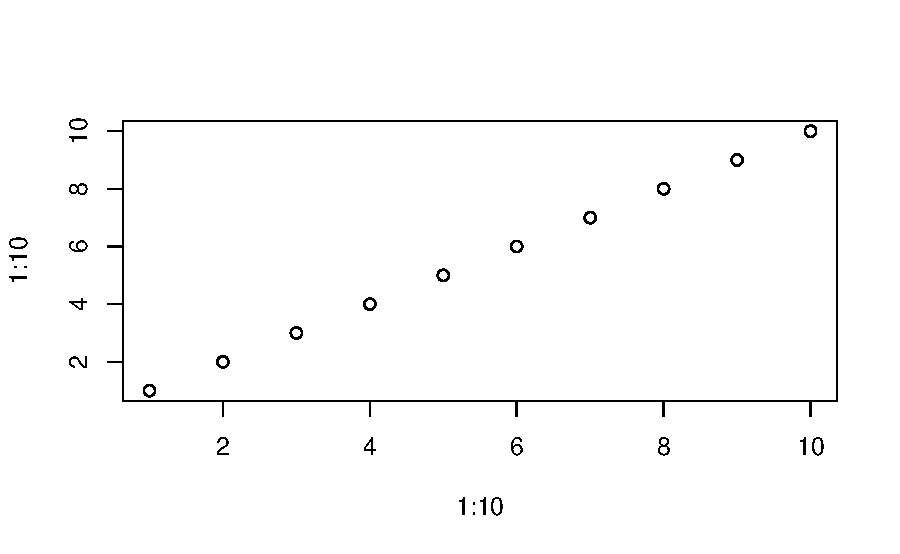
\includegraphics[width=0.7\linewidth,height=\textheight,keepaspectratio]{chapters/R/03_r_programming_files/figure-pdf/unnamed-chunk-3-1.pdf}
\end{center}

In sostanza, una funzione è un blocco di codice progettato per svolgere
un'operazione specifica. Puoi pensare a una funzione come a una ``black
box'': fornisci un input (i dati), la funzione elabora l'informazione
attraverso le sue istruzioni e restituisce un output (il risultato).
Questo approccio modulare semplifica il lavoro, permettendo di
riutilizzare e combinare facilmente diverse operazioni.

\subsection{Creare Funzioni
Personalizzate}\label{creare-funzioni-personalizzate}

La creazione di funzioni personalizzate in R è uno strumento essenziale
per migliorare la programmazione, soprattutto per gestire operazioni
ripetitive o complesse. Le funzioni consentono di rendere il codice più
leggibile, efficiente e riutilizzabile, promuovendo un approccio
organizzato e chiaro alla risoluzione dei problemi.

\subsubsection{Vantaggi delle Funzioni
Personalizzate}\label{vantaggi-delle-funzioni-personalizzate}

L'uso di funzioni personalizzate offre numerosi benefici:

\begin{itemize}
\tightlist
\item
  \textbf{Chiarezza e leggibilità}: Un nome descrittivo permette di
  comprendere immediatamente lo scopo della funzione, anche a distanza
  di tempo o per altri utenti che leggono il codice.\\
\item
  \textbf{Manutenzione semplificata}: Modificare il codice all'interno
  di una funzione aggiorna automaticamente tutte le sue occorrenze,
  riducendo il rischio di errori e semplificando il debugging.\\
\item
  \textbf{Riduzione degli errori}: Si evitano gli errori tipici del
  copia-e-incolla, come omissioni o incoerenze nei programmi
  complessi.\\
\item
  \textbf{Riutilizzabilità}: Una funzione ben progettata può essere
  utilizzata in più contesti o progetti, risparmiando tempo e sforzi.
\end{itemize}

\subsubsection{Quando Creare una
Funzione?}\label{quando-creare-una-funzione}

Un buon criterio per decidere se creare una funzione è osservare se il
medesimo blocco di codice viene copiato più volte. Se ti trovi a
ripetere lo stesso codice più di due volte, probabilmente è il momento
di creare una funzione. Questo aiuta a scrivere codice più pulito,
scalabile e professionale, migliorando anche la sostenibilità del lavoro
a lungo termine.

\subsection{Sintassi di una Funzione}\label{sintassi-di-una-funzione}

La struttura base di una funzione in R è la seguente:

\begin{Shaded}
\begin{Highlighting}[]
\NormalTok{nome\_funzione }\OtherTok{\textless{}{-}} \ControlFlowTok{function}\NormalTok{(argomenti) \{}
  \CommentTok{\# Corpo della funzione}
\NormalTok{  codice}
  \FunctionTok{return}\NormalTok{(risultato)  }\CommentTok{\# Facoltativo: restituisce il valore calcolato}
\NormalTok{\}}
\end{Highlighting}
\end{Shaded}

\begin{itemize}
\tightlist
\item
  \textbf{\texttt{nome\_funzione}}: Nome della funzione, scelto per
  descrivere chiaramente la sua finalità.\\
\item
  \textbf{\texttt{argomenti}}: Parametri necessari per eseguire le
  operazioni all'interno della funzione.\\
\item
  \textbf{\texttt{codice}}: Le istruzioni che definiscono il
  comportamento della funzione.\\
\item
  \textbf{\texttt{risultato}}: Il valore restituito dalla funzione. Se
  non si usa \texttt{return()}, R restituisce l'ultimo valore calcolato.
\end{itemize}

\begin{example}[]\protect\hypertarget{exm-}{}\label{exm-}

Immaginiamo di voler creare una funzione per sommare due numeri.

\begin{Shaded}
\begin{Highlighting}[]
\NormalTok{somma\_due }\OtherTok{\textless{}{-}} \ControlFlowTok{function}\NormalTok{(a, b) \{}
\NormalTok{  a }\SpecialCharTok{+}\NormalTok{ b  }\CommentTok{\# Restituisce la somma dei due numeri}
\NormalTok{\}}
\end{Highlighting}
\end{Shaded}

Per utilizzarla, basta richiamarla specificando i parametri:

\begin{Shaded}
\begin{Highlighting}[]
\FunctionTok{somma\_due}\NormalTok{(}\DecValTok{5}\NormalTok{, }\DecValTok{3}\NormalTok{)  }\CommentTok{\# Restituisce 8}
\end{Highlighting}
\end{Shaded}

Questo approccio aiuta a scrivere codice più leggibile e facile da
gestire. Ad esempio, se in futuro volessi modificare il comportamento
della somma (ad esempio, aggiungere un messaggio di log), basterà
intervenire solo all'interno della funzione.

\end{example}

\begin{example}[]\protect\hypertarget{exm-}{}\label{exm-}

Immaginiamo di avere un dataset con i punteggi di 10 individui su 3
subscale di un test psicometrico. L'obiettivo è:

\begin{enumerate}
\def\labelenumi{\arabic{enumi}.}
\tightlist
\item
  Creare una funzione per calcolare il punteggio totale di un individuo.
\item
  Creare una funzione per trovare il massimo punteggio totale nel
  campione.
\item
  Creare una funzione per individuare chi ha ottenuto il massimo
  punteggio.
\end{enumerate}

\textbf{Passo 1:} Simulazione dei Dati. Simuliamo i punteggi di 10
individui su 3 subscale:

\begin{Shaded}
\begin{Highlighting}[]
\CommentTok{\# Simulazione dei punteggi}
\FunctionTok{set.seed}\NormalTok{(}\DecValTok{123}\NormalTok{)}
\NormalTok{punteggi }\OtherTok{\textless{}{-}} \FunctionTok{data.frame}\NormalTok{(}
  \AttributeTok{individuo =} \FunctionTok{paste}\NormalTok{(}\StringTok{"Individuo"}\NormalTok{, }\DecValTok{1}\SpecialCharTok{:}\DecValTok{10}\NormalTok{),}
  \AttributeTok{subscale1 =} \FunctionTok{sample}\NormalTok{(}\DecValTok{30}\SpecialCharTok{:}\DecValTok{50}\NormalTok{, }\DecValTok{10}\NormalTok{, }\AttributeTok{replace =} \ConstantTok{TRUE}\NormalTok{),}
  \AttributeTok{subscale2 =} \FunctionTok{sample}\NormalTok{(}\DecValTok{40}\SpecialCharTok{:}\DecValTok{60}\NormalTok{, }\DecValTok{10}\NormalTok{, }\AttributeTok{replace =} \ConstantTok{TRUE}\NormalTok{),}
  \AttributeTok{subscale3 =} \FunctionTok{sample}\NormalTok{(}\DecValTok{35}\SpecialCharTok{:}\DecValTok{55}\NormalTok{, }\DecValTok{10}\NormalTok{, }\AttributeTok{replace =} \ConstantTok{TRUE}\NormalTok{)}
\NormalTok{)}
\FunctionTok{print}\NormalTok{(punteggi)}
\CommentTok{\#\textgreater{}       individuo subscale1 subscale2 subscale3}
\CommentTok{\#\textgreater{} 1   Individuo 1        44        44        48}
\CommentTok{\#\textgreater{} 2   Individuo 2        48        58        51}
\CommentTok{\#\textgreater{} 3   Individuo 3        43        48        45}
\CommentTok{\#\textgreater{} 4   Individuo 4        32        42        41}
\CommentTok{\#\textgreater{} 5   Individuo 5        39        47        55}
\CommentTok{\#\textgreater{} 6   Individuo 6        47        46        46}
\CommentTok{\#\textgreater{} 7   Individuo 7        40        49        49}
\CommentTok{\#\textgreater{} 8   Individuo 8        34        48        44}
\CommentTok{\#\textgreater{} 9   Individuo 9        49        58        47}
\CommentTok{\#\textgreater{} 10 Individuo 10        43        43        41}
\end{Highlighting}
\end{Shaded}

La funzione \texttt{sample()} in R è utilizzata per estrarre casualmente
un sottoinsieme di valori da un vettore. Nell'esempio sopra,
\texttt{sample()} viene utilizzata per generare casualmente i punteggi
delle subscale dei test psicometrici.

Nell'istruzione
\texttt{subscale1\ \textless{}-\ sample(30:50,\ 10,\ replace\ =\ TRUE)}

\begin{itemize}
\tightlist
\item
  \texttt{30:50}: Rappresenta il vettore di numeri interi da cui vengono
  estratti i punteggi (valori possibili tra 30 e 50).
\item
  \texttt{10}: Indica che vogliamo estrarre 10 valori.
\item
  \texttt{replace\ =\ TRUE}: Consente che lo stesso valore possa essere
  estratto più volte (estrazione con ripetizione).
\end{itemize}

\textbf{Passo 2:} Creazione delle Funzioni.

\begin{enumerate}
\def\labelenumi{\arabic{enumi}.}
\item
  \textbf{Calcolo del punteggio totale per ogni individuo}\\
  Questa funzione somma i punteggi delle subscale di un individuo:

\begin{Shaded}
\begin{Highlighting}[]
\NormalTok{calcola\_totale }\OtherTok{\textless{}{-}} \ControlFlowTok{function}\NormalTok{(subscale1, subscale2, subscale3) \{}
  \FunctionTok{return}\NormalTok{(subscale1 }\SpecialCharTok{+}\NormalTok{ subscale2 }\SpecialCharTok{+}\NormalTok{ subscale3)}
\NormalTok{\}}
\end{Highlighting}
\end{Shaded}
\item
  \textbf{Trovare il punteggio massimo nel campione}\\
  Questa funzione accetta un vettore di punteggi totali e restituisce il
  valore massimo:

\begin{Shaded}
\begin{Highlighting}[]
\NormalTok{trova\_massimo }\OtherTok{\textless{}{-}} \ControlFlowTok{function}\NormalTok{(punteggi\_totali) \{}
  \FunctionTok{return}\NormalTok{(}\FunctionTok{max}\NormalTok{(punteggi\_totali))}
\NormalTok{\}}
\end{Highlighting}
\end{Shaded}
\item
  \textbf{Individuare l'individuo con il punteggio massimo}\\
  Questa funzione accetta un data frame con i punteggi e restituisce il
  nome dell'individuo con il punteggio più alto:

\begin{Shaded}
\begin{Highlighting}[]
\NormalTok{trova\_individuo\_massimo }\OtherTok{\textless{}{-}} \ControlFlowTok{function}\NormalTok{(punteggi) \{}
\NormalTok{  punteggi\_totali }\OtherTok{\textless{}{-}} \FunctionTok{rowSums}\NormalTok{(punteggi[, }\FunctionTok{c}\NormalTok{(}\StringTok{"subscale1"}\NormalTok{, }\StringTok{"subscale2"}\NormalTok{, }\StringTok{"subscale3"}\NormalTok{)])}
\NormalTok{  indice\_massimo }\OtherTok{\textless{}{-}} \FunctionTok{which.max}\NormalTok{(punteggi\_totali)}
  \FunctionTok{return}\NormalTok{(punteggi}\SpecialCharTok{$}\NormalTok{individuo[indice\_massimo])}
\NormalTok{\}}
\end{Highlighting}
\end{Shaded}

  La funzione \texttt{which.max()} restituisce l'indice della posizione
  in cui si trova il valore massimo in un vettore.
\end{enumerate}

\textbf{Passo 3:} Applicazione delle Funzioni

\begin{enumerate}
\def\labelenumi{\arabic{enumi}.}
\item
  \textbf{Calcolo dei punteggi totali per ogni individuo}\\
  Applichiamo la funzione ai dati simulati:

\begin{Shaded}
\begin{Highlighting}[]
\NormalTok{punteggi}\SpecialCharTok{$}\NormalTok{punteggio\_totale }\OtherTok{\textless{}{-}} \FunctionTok{with}\NormalTok{(}
\NormalTok{  punteggi, }\FunctionTok{calcola\_totale}\NormalTok{(subscale1, subscale2, subscale3)}
\NormalTok{ )}
\FunctionTok{print}\NormalTok{(punteggi)}
\CommentTok{\#\textgreater{}       individuo subscale1 subscale2 subscale3 punteggio\_totale}
\CommentTok{\#\textgreater{} 1   Individuo 1        44        44        48              136}
\CommentTok{\#\textgreater{} 2   Individuo 2        48        58        51              157}
\CommentTok{\#\textgreater{} 3   Individuo 3        43        48        45              136}
\CommentTok{\#\textgreater{} 4   Individuo 4        32        42        41              115}
\CommentTok{\#\textgreater{} 5   Individuo 5        39        47        55              141}
\CommentTok{\#\textgreater{} 6   Individuo 6        47        46        46              139}
\CommentTok{\#\textgreater{} 7   Individuo 7        40        49        49              138}
\CommentTok{\#\textgreater{} 8   Individuo 8        34        48        44              126}
\CommentTok{\#\textgreater{} 9   Individuo 9        49        58        47              154}
\CommentTok{\#\textgreater{} 10 Individuo 10        43        43        41              127}
\end{Highlighting}
\end{Shaded}
\item
  \textbf{Troviamo il punteggio massimo nel campione}

\begin{Shaded}
\begin{Highlighting}[]
\NormalTok{massimo }\OtherTok{\textless{}{-}} \FunctionTok{trova\_massimo}\NormalTok{(punteggi}\SpecialCharTok{$}\NormalTok{punteggio\_totale)}
\FunctionTok{print}\NormalTok{(massimo)}
\CommentTok{\#\textgreater{} [1] 157}
\end{Highlighting}
\end{Shaded}
\item
  \textbf{Troviamo chi ha il punteggio massimo}

\begin{Shaded}
\begin{Highlighting}[]
\NormalTok{individuo\_massimo }\OtherTok{\textless{}{-}} \FunctionTok{trova\_individuo\_massimo}\NormalTok{(punteggi)}
\FunctionTok{print}\NormalTok{(individuo\_massimo)}
\CommentTok{\#\textgreater{} [1] "Individuo 2"}
\end{Highlighting}
\end{Shaded}
\end{enumerate}

\end{example}

\subsection{Stile}\label{stile}

È consigliato di usare nomi di funzioni chiari e descrittivi,
preferibilmente verbi (es. \texttt{compute\_mean()}). Inoltre, è
importante mantenere una struttura leggibile, con spazi coerenti e
indentazione.

\section{Istruzioni Condizionali in
R}\label{istruzioni-condizionali-in-r}

Le istruzioni condizionali permettono di introdurre logica nel tuo
codice. Ad esempio, l'operazione \texttt{x\ *\ y} si limita a
moltiplicare i valori di \texttt{x} e \texttt{y}, senza alcuna logica
aggiunta. Con le istruzioni condizionali, puoi dire al programma di
eseguire diverse operazioni a seconda che una condizione sia vera
(\texttt{TRUE}) o falsa (\texttt{FALSE}).

L'istruzione condizionale più comune in R è \texttt{if}. Può essere
letta come: \textbf{``Se la condizione è vera, esegui un'azione''}. Con
\texttt{else}, si estende la logica: \textbf{``Se la condizione è vera,
fai qualcosa; altrimenti fai qualcos'altro''}.

La struttura generale è questa:

\begin{Shaded}
\begin{Highlighting}[]
\ControlFlowTok{if}\NormalTok{ (condizione) \{}
  \CommentTok{\# Codice eseguito se la condizione è TRUE}
\NormalTok{\} }\ControlFlowTok{else}\NormalTok{ \{}
  \CommentTok{\# Codice eseguito se la condizione è FALSE}
\NormalTok{\}}
\end{Highlighting}
\end{Shaded}

Immagina questa situazione:

\begin{itemize}
\tightlist
\item
  ``Se un partecipante al test psicologico riporta un punteggio elevato
  sulla scala di ansia (es. \textgreater{} 15), consigliagli un
  esercizio di rilassamento. Altrimenti, non è necessario.''
\end{itemize}

Vediamo come rappresentare questa situazione in R.

\begin{Shaded}
\begin{Highlighting}[]
\NormalTok{anxiety\_score }\OtherTok{\textless{}{-}} \DecValTok{18} \CommentTok{\# Punteggio riportato dal partecipante}

\ControlFlowTok{if}\NormalTok{ (anxiety\_score }\SpecialCharTok{\textgreater{}} \DecValTok{15}\NormalTok{) \{}
\NormalTok{    exercise }\OtherTok{\textless{}{-}} \StringTok{"rilassamento"}
\NormalTok{\} }\ControlFlowTok{else}\NormalTok{ \{}
\NormalTok{    exercise }\OtherTok{\textless{}{-}} \StringTok{"nessun esercizio"}
\NormalTok{\}}

\NormalTok{exercise}
\CommentTok{\#\textgreater{} [1] "rilassamento"}
\end{Highlighting}
\end{Shaded}

Se il punteggio è maggiore di 15, il risultato sarà:

\begin{verbatim}
[1] "rilassamento"
\end{verbatim}

Se il punteggio è inferiore o uguale a 15, il risultato sarà:

\begin{verbatim}
[1] "nessun esercizio"
\end{verbatim}

\subsection{\texorpdfstring{Uso di
\texttt{ifelse()}}{Uso di ifelse()}}\label{uso-di-ifelse}

Un'alternativa più compatta a \texttt{if} e \texttt{else} è la funzione
\texttt{ifelse()}, utile soprattutto per vettori. Ad esempio, supponiamo
di avere i punteggi di ansia di un gruppo di partecipanti e vogliamo
decidere se assegnare un esercizio di rilassamento a ciascuno:

\begin{Shaded}
\begin{Highlighting}[]
\NormalTok{anxiety\_scores }\OtherTok{\textless{}{-}} \FunctionTok{c}\NormalTok{(}\DecValTok{12}\NormalTok{, }\DecValTok{18}\NormalTok{, }\DecValTok{9}\NormalTok{, }\DecValTok{22}\NormalTok{, }\DecValTok{15}\NormalTok{)}
\NormalTok{exercises }\OtherTok{\textless{}{-}} \FunctionTok{ifelse}\NormalTok{(anxiety\_scores }\SpecialCharTok{\textgreater{}} \DecValTok{15}\NormalTok{, }\StringTok{"rilassamento"}\NormalTok{, }\StringTok{"nessun esercizio"}\NormalTok{)}
\end{Highlighting}
\end{Shaded}

Il risultato sarà:

\begin{Shaded}
\begin{Highlighting}[]
\NormalTok{exercises}
\CommentTok{\#\textgreater{} [1] "nessun esercizio" "rilassamento"     "nessun esercizio"}
\CommentTok{\#\textgreater{} [4] "rilassamento"     "nessun esercizio"}
\end{Highlighting}
\end{Shaded}

\subsection{Creare una Funzione con Istruzioni
Condizionali}\label{creare-una-funzione-con-istruzioni-condizionali}

Le istruzioni condizionali possono essere racchiuse in una funzione per
rendere il codice più flessibile e riutilizzabile. Ad esempio,
supponiamo di voler personalizzare un feedback per un partecipante in
base al punteggio ottenuto in un questionario:

\begin{Shaded}
\begin{Highlighting}[]
\NormalTok{feedback }\OtherTok{\textless{}{-}} \ControlFlowTok{function}\NormalTok{(score) \{}
    \ControlFlowTok{if}\NormalTok{ (score }\SpecialCharTok{\textgreater{}} \DecValTok{15}\NormalTok{) \{}
        \StringTok{"Consigliamo un esercizio di rilassamento."}
\NormalTok{    \} }\ControlFlowTok{else} \ControlFlowTok{if}\NormalTok{ (score }\SpecialCharTok{\textgreater{}} \DecValTok{10}\NormalTok{) \{}
        \StringTok{"Monitoriamo la situazione, ma non è necessario alcun intervento."}
\NormalTok{    \} }\ControlFlowTok{else}\NormalTok{ \{}
        \StringTok{"Nessun intervento necessario."}
\NormalTok{    \}}
\NormalTok{\}}
\end{Highlighting}
\end{Shaded}

\begin{Shaded}
\begin{Highlighting}[]
\FunctionTok{feedback}\NormalTok{(}\DecValTok{18}\NormalTok{)}
\CommentTok{\#\textgreater{} [1] "Consigliamo un esercizio di rilassamento."}
\end{Highlighting}
\end{Shaded}

\begin{Shaded}
\begin{Highlighting}[]
\FunctionTok{feedback}\NormalTok{(}\DecValTok{12}\NormalTok{)}
\CommentTok{\#\textgreater{} [1] "Monitoriamo la situazione, ma non è necessario alcun intervento."}
\end{Highlighting}
\end{Shaded}

\begin{Shaded}
\begin{Highlighting}[]
\FunctionTok{feedback}\NormalTok{(}\DecValTok{8}\NormalTok{)}
\CommentTok{\#\textgreater{} [1] "Nessun intervento necessario."}
\end{Highlighting}
\end{Shaded}

In conclusione, le istruzioni condizionali come \texttt{if},
\texttt{else} e \texttt{ifelse()} sono strumenti fondamentali per
introdurre logica e controllo nel tuo codice. Puoi usarle per prendere
decisioni, gestire errori e rendere il tuo codice più flessibile ed
efficiente. Creare funzioni che incorporano queste istruzioni è un passo
fondamentale per scrivere codice ordinato e riutilizzabile in contesti
psicologici e non solo.

\subsection{Combinare Operatori Logici in
R}\label{combinare-operatori-logici-in-r}

Finora abbiamo creato funzioni abbastanza semplici e mirate. Ora
proviamo a realizzare una funzione leggermente più complessa.
Immaginiamo di voler determinare se una persona ha avuto \textbf{una
buona giornata} basandoci su due criteri:

\begin{enumerate}
\def\labelenumi{\arabic{enumi}.}
\tightlist
\item
  \textbf{Livello di stress}: basso (\texttt{TRUE}) o alto
  (\texttt{FALSE}).
\item
  \textbf{Livello di supporto sociale percepito}: alto (\texttt{TRUE}) o
  basso (\texttt{FALSE}).
\end{enumerate}

Vogliamo creare una funzione che prenda questi due fattori e restituisca
un messaggio che descrive come potrebbe essere stata la giornata della
persona.

Ecco come possiamo costruire la funzione:

\begin{Shaded}
\begin{Highlighting}[]
\NormalTok{good\_day }\OtherTok{\textless{}{-}} \ControlFlowTok{function}\NormalTok{(low\_stress, high\_support) \{}
    \ControlFlowTok{if}\NormalTok{ (low\_stress }\SpecialCharTok{==} \ConstantTok{TRUE} \SpecialCharTok{\&\&}\NormalTok{ high\_support }\SpecialCharTok{==} \ConstantTok{TRUE}\NormalTok{) \{}
        \StringTok{"Giornata fantastica! Ti senti calmo e supportato."}
\NormalTok{    \} }\ControlFlowTok{else} \ControlFlowTok{if}\NormalTok{ (low\_stress }\SpecialCharTok{==} \ConstantTok{FALSE} \SpecialCharTok{\&\&}\NormalTok{ high\_support }\SpecialCharTok{==} \ConstantTok{TRUE}\NormalTok{) \{}
        \StringTok{"Il supporto sociale ti aiuta a gestire lo stress elevato."}
\NormalTok{    \} }\ControlFlowTok{else} \ControlFlowTok{if}\NormalTok{ (low\_stress }\SpecialCharTok{==} \ConstantTok{TRUE} \SpecialCharTok{\&\&}\NormalTok{ high\_support }\SpecialCharTok{==} \ConstantTok{FALSE}\NormalTok{) \{}
        \StringTok{"Nonostante lo stress sia basso, la mancanza di supporto sociale pesa."}
\NormalTok{    \} }\ControlFlowTok{else} \ControlFlowTok{if}\NormalTok{ (low\_stress }\SpecialCharTok{==} \ConstantTok{FALSE} \SpecialCharTok{\&\&}\NormalTok{ high\_support }\SpecialCharTok{==} \ConstantTok{FALSE}\NormalTok{) \{}
        \StringTok{"Giornata difficile: stress elevato e poco supporto sociale."}
\NormalTok{    \}}
\NormalTok{\}}
\end{Highlighting}
\end{Shaded}

Esempi di utilizzo.

Caso 1: Stress basso e supporto sociale alto

\begin{Shaded}
\begin{Highlighting}[]
\FunctionTok{good\_day}\NormalTok{(}\AttributeTok{low\_stress =} \ConstantTok{TRUE}\NormalTok{, }\AttributeTok{high\_support =} \ConstantTok{TRUE}\NormalTok{)}
\CommentTok{\#\textgreater{} [1] "Giornata fantastica! Ti senti calmo e supportato."}
\end{Highlighting}
\end{Shaded}

Caso 2: Stress elevato e supporto sociale alto.

\begin{Shaded}
\begin{Highlighting}[]
\FunctionTok{good\_day}\NormalTok{(}\ConstantTok{FALSE}\NormalTok{, }\ConstantTok{TRUE}\NormalTok{)}
\CommentTok{\#\textgreater{} [1] "Il supporto sociale ti aiuta a gestire lo stress elevato."}
\end{Highlighting}
\end{Shaded}

Caso 3: Stress basso e supporto sociale basso.

\begin{Shaded}
\begin{Highlighting}[]
\FunctionTok{good\_day}\NormalTok{(}\ConstantTok{TRUE}\NormalTok{, }\ConstantTok{FALSE}\NormalTok{)}
\CommentTok{\#\textgreater{} [1] "Nonostante lo stress sia basso, la mancanza di supporto sociale pesa."}
\end{Highlighting}
\end{Shaded}

Caso 4: Stress elevato e supporto sociale basso.

\begin{Shaded}
\begin{Highlighting}[]
\FunctionTok{good\_day}\NormalTok{(}\ConstantTok{FALSE}\NormalTok{, }\ConstantTok{FALSE}\NormalTok{)}
\CommentTok{\#\textgreater{} [1] "Giornata difficile: stress elevato e poco supporto sociale."}
\end{Highlighting}
\end{Shaded}

La funzione considera tutte le combinazioni di stress e supporto
sociale:

\begin{enumerate}
\def\labelenumi{\arabic{enumi}.}
\tightlist
\item
  \textbf{Stress basso e supporto alto}: giornata ideale.
\item
  \textbf{Stress elevato e supporto alto}: il supporto aiuta a mitigare
  lo stress.
\item
  \textbf{Stress basso e supporto basso}: la mancanza di supporto rovina
  una situazione potenzialmente buona.
\item
  \textbf{Stress elevato e supporto basso}: la situazione peggiore.
\end{enumerate}

Nell'esempio abbiamo usato i seguenti operatori logici:

\begin{itemize}
\tightlist
\item
  \textbf{\texttt{\&\&} (AND logico)}: Entrambe le condizioni devono
  essere vere.
\item
  \textbf{\texttt{==} (uguale a)}: Verifica se una variabile è vera o
  falsa.
\end{itemize}

Ad esempio, questa condizione:

\begin{Shaded}
\begin{Highlighting}[]
\ControlFlowTok{if}\NormalTok{ (low\_stress }\SpecialCharTok{==} \ConstantTok{TRUE} \SpecialCharTok{\&\&}\NormalTok{ high\_support }\SpecialCharTok{==} \ConstantTok{TRUE}\NormalTok{)}
\end{Highlighting}
\end{Shaded}

verifica se il livello di stress è basso \textbf{e} il supporto sociale
è alto.

In conclusione, questa funzione dimostra come combinare condizioni
logiche complesse utilizzando operatori logici come \texttt{\&\&} (AND)
e \texttt{\textbar{}\textbar{}} (OR). Grazie a questi strumenti,
possiamo gestire facilmente logiche più articolate, mantenendo il codice
leggibile e funzionale.

\subsection{Gli operatori Logici in R}\label{gli-operatori-logici-in-r}

Gli operatori logici sono essenziali per definire le condizioni nelle
istruzioni \texttt{if}. Ecco una tabella riassuntiva con i principali
operatori:

\begin{longtable}[]{@{}
  >{\raggedright\arraybackslash}p{(\linewidth - 6\tabcolsep) * \real{0.1230}}
  >{\raggedright\arraybackslash}p{(\linewidth - 6\tabcolsep) * \real{0.2705}}
  >{\raggedright\arraybackslash}p{(\linewidth - 6\tabcolsep) * \real{0.3033}}
  >{\raggedright\arraybackslash}p{(\linewidth - 6\tabcolsep) * \real{0.3033}}@{}}
\toprule\noalign{}
\begin{minipage}[b]{\linewidth}\raggedright
\textbf{Operatore}
\end{minipage} & \begin{minipage}[b]{\linewidth}\raggedright
\textbf{Descrizione tecnica}
\end{minipage} & \begin{minipage}[b]{\linewidth}\raggedright
\textbf{Significato}
\end{minipage} & \begin{minipage}[b]{\linewidth}\raggedright
\textbf{Esempio}
\end{minipage} \\
\midrule\noalign{}
\endhead
\bottomrule\noalign{}
\endlastfoot
\texttt{\&\&} & AND logico & Entrambe le condizioni devono essere vere &
\texttt{if(cond1\ ==\ test\ \&\&\ cond2\ ==\ test)} \\
\texttt{\textbar{}\textbar{}} & OR logico & Almeno una condizione deve
essere vera &
\texttt{if(cond1\ ==\ test\ \textbar{}\textbar{}\ cond2\ ==\ test)} \\
\texttt{\textless{}} & Minore di & X è minore di Y &
\texttt{if(X\ \textless{}\ Y)} \\
\texttt{\textgreater{}} & Maggiore di & X è maggiore di Y &
\texttt{if(X\ \textgreater{}\ Y)} \\
\texttt{\textless{}=} & Minore o uguale a & X è minore o uguale a Y &
\texttt{if(X\ \textless{}=\ Y)} \\
\texttt{\textgreater{}=} & Maggiore o uguale a & X è maggiore o uguale a
Y & \texttt{if(X\ \textgreater{}=\ Y)} \\
\texttt{==} & Uguale a & X è uguale a Y & \texttt{if(X\ ==\ Y)} \\
\texttt{!=} & Diverso da & X è diverso da Y & \texttt{if(X\ !=\ Y)} \\
\end{longtable}

\section{Cicli in R}\label{cicli-in-r}

R è particolarmente efficace nell'eseguire attività ripetitive. Quando
dobbiamo ripetere un'operazione più volte, possiamo utilizzare un
\textbf{ciclo}. I cicli eseguono un insieme di istruzioni per un numero
specifico di volte o fino a quando una determinata condizione non è
soddisfatta.

In R esistono tre tipi principali di cicli:

\begin{enumerate}
\def\labelenumi{\arabic{enumi}.}
\tightlist
\item
  \textbf{Ciclo \texttt{for}}: ripete un'operazione per un numero
  definito di iterazioni.
\item
  \textbf{Ciclo \texttt{while}}: continua a eseguire le istruzioni fino
  a quando una condizione logica è soddisfatta.
\item
  \textbf{Ciclo \texttt{repeat}}: itera indefinitamente fino a quando
  non viene esplicitamente interrotto con un'istruzione \texttt{break}.
\end{enumerate}

I cicli sono strumenti essenziali in tutti i linguaggi di
programmazione, ma in R il loro utilizzo dovrebbe essere valutato
attentamente, poiché spesso esistono alternative più efficienti come le
funzioni della famiglia \texttt{apply}.

\subsection{\texorpdfstring{Il ciclo
\texttt{for}}{Il ciclo for}}\label{il-ciclo-for}

Il ciclo \texttt{for} è il più utilizzato per eseguire un'operazione un
numero definito di volte. Ecco un esempio base:

\begin{Shaded}
\begin{Highlighting}[]
\ControlFlowTok{for}\NormalTok{ (i }\ControlFlowTok{in} \DecValTok{1}\SpecialCharTok{:}\DecValTok{5}\NormalTok{) \{}
    \FunctionTok{print}\NormalTok{(i)}
\NormalTok{\}}
\CommentTok{\#\textgreater{} [1] 1}
\CommentTok{\#\textgreater{} [1] 2}
\CommentTok{\#\textgreater{} [1] 3}
\CommentTok{\#\textgreater{} [1] 4}
\CommentTok{\#\textgreater{} [1] 5}
\end{Highlighting}
\end{Shaded}

\textbf{Come funziona?}

\begin{itemize}
\tightlist
\item
  L'indice \texttt{i} prende il primo valore della sequenza \texttt{1:5}
  (cioè 1).
\item
  Il corpo del ciclo, ovvero il codice tra \texttt{\{\ \}}, viene
  eseguito.
\item
  Al termine di ogni iterazione, \texttt{i} assume il valore successivo
  nella sequenza, e il processo si ripete fino all'ultimo valore (5 in
  questo caso).
\end{itemize}

\textbf{Aggiungere logica nel corpo del ciclo}

Possiamo aggiungere operazioni all'interno del ciclo, come ad esempio
sommare 1 a ogni valore:

\begin{Shaded}
\begin{Highlighting}[]
\ControlFlowTok{for}\NormalTok{ (i }\ControlFlowTok{in} \DecValTok{1}\SpecialCharTok{:}\DecValTok{5}\NormalTok{) \{}
    \FunctionTok{print}\NormalTok{(i }\SpecialCharTok{+} \DecValTok{1}\NormalTok{)}
\NormalTok{\}}
\CommentTok{\#\textgreater{} [1] 2}
\CommentTok{\#\textgreater{} [1] 3}
\CommentTok{\#\textgreater{} [1] 4}
\CommentTok{\#\textgreater{} [1] 5}
\CommentTok{\#\textgreater{} [1] 6}
\end{Highlighting}
\end{Shaded}

\subsection{\texorpdfstring{Il ciclo
\texttt{while}}{Il ciclo while}}\label{il-ciclo-while}

Il ciclo \texttt{while} continua a eseguire le istruzioni fino a quando
una condizione logica è soddisfatta. Ecco un esempio:

\begin{Shaded}
\begin{Highlighting}[]
\NormalTok{i }\OtherTok{\textless{}{-}} \DecValTok{0}
\ControlFlowTok{while}\NormalTok{ (i }\SpecialCharTok{\textless{}=} \DecValTok{4}\NormalTok{) \{}
\NormalTok{    i }\OtherTok{\textless{}{-}}\NormalTok{ i }\SpecialCharTok{+} \DecValTok{1}
    \FunctionTok{print}\NormalTok{(i)}
\NormalTok{\}}
\CommentTok{\#\textgreater{} [1] 1}
\CommentTok{\#\textgreater{} [1] 2}
\CommentTok{\#\textgreater{} [1] 3}
\CommentTok{\#\textgreater{} [1] 4}
\CommentTok{\#\textgreater{} [1] 5}
\end{Highlighting}
\end{Shaded}

\textbf{Come funziona?}

\begin{itemize}
\tightlist
\item
  La condizione logica (\texttt{i\ \textless{}=\ 4}) viene verificata
  prima di ogni iterazione.
\item
  Se la condizione è vera, il ciclo esegue il codice tra
  \texttt{\{\ \}}.
\item
  Quando la condizione diventa falsa (\texttt{i\ \textgreater{}\ 4}), il
  ciclo si interrompe.
\end{itemize}

\subsection{\texorpdfstring{Ciclo
\texttt{repeat}}{Ciclo repeat}}\label{ciclo-repeat}

Il ciclo \texttt{repeat} esegue il codice indefinitamente, a meno che
non venga interrotto con un'istruzione \texttt{break}:

\begin{Shaded}
\begin{Highlighting}[]
\NormalTok{i }\OtherTok{\textless{}{-}} \DecValTok{0}
\ControlFlowTok{repeat}\NormalTok{ \{}
\NormalTok{    i }\OtherTok{\textless{}{-}}\NormalTok{ i }\SpecialCharTok{+} \DecValTok{1}
    \FunctionTok{print}\NormalTok{(i)}
    \ControlFlowTok{if}\NormalTok{ (i }\SpecialCharTok{\textgreater{}=} \DecValTok{5}\NormalTok{) \{}
        \ControlFlowTok{break}
\NormalTok{    \}}
\NormalTok{\}}
\CommentTok{\#\textgreater{} [1] 1}
\CommentTok{\#\textgreater{} [1] 2}
\CommentTok{\#\textgreater{} [1] 3}
\CommentTok{\#\textgreater{} [1] 4}
\CommentTok{\#\textgreater{} [1] 5}
\end{Highlighting}
\end{Shaded}

\textbf{Quando usarlo?}

Il ciclo \texttt{repeat} è raro e viene utilizzato solo in situazioni
molto particolari. Nella maggior parte dei casi, \texttt{for} o
\texttt{while} sono più adatti.

\subsection{\texorpdfstring{Evitare i cicli: la famiglia di funzioni
\texttt{apply}}{Evitare i cicli: la famiglia di funzioni apply}}\label{evitare-i-cicli-la-famiglia-di-funzioni-apply}

I cicli in R sono relativamente lenti, specialmente con dataset di
grandi dimensioni. Quando possibile, è preferibile usare funzioni della
famiglia \texttt{apply} per ottenere lo stesso risultato in modo più
efficiente e con meno rischi di errore.

\subsubsection{\texorpdfstring{La funzione
\texttt{lapply()}}{La funzione lapply()}}\label{la-funzione-lapply}

\texttt{lapply()} esegue una funzione su ciascun elemento di una lista o
vettore e restituisce una lista con i risultati.

Esempio:

\begin{Shaded}
\begin{Highlighting}[]
\FunctionTok{lapply}\NormalTok{(}\DecValTok{0}\SpecialCharTok{:}\DecValTok{4}\NormalTok{, }\ControlFlowTok{function}\NormalTok{(a) \{}
\NormalTok{    a }\SpecialCharTok{+} \DecValTok{1}
\NormalTok{\})}
\CommentTok{\#\textgreater{} [[1]]}
\CommentTok{\#\textgreater{} [1] 1}
\CommentTok{\#\textgreater{} }
\CommentTok{\#\textgreater{} [[2]]}
\CommentTok{\#\textgreater{} [1] 2}
\CommentTok{\#\textgreater{} }
\CommentTok{\#\textgreater{} [[3]]}
\CommentTok{\#\textgreater{} [1] 3}
\CommentTok{\#\textgreater{} }
\CommentTok{\#\textgreater{} [[4]]}
\CommentTok{\#\textgreater{} [1] 4}
\CommentTok{\#\textgreater{} }
\CommentTok{\#\textgreater{} [[5]]}
\CommentTok{\#\textgreater{} [1] 5}
\end{Highlighting}
\end{Shaded}

\subsubsection{\texorpdfstring{La funzione
\texttt{sapply()}}{La funzione sapply()}}\label{la-funzione-sapply}

\texttt{lapply()} restituisce una lista, ma se vuoi un vettore come
output, usa \texttt{sapply()}:

\begin{Shaded}
\begin{Highlighting}[]
\FunctionTok{sapply}\NormalTok{(}\DecValTok{0}\SpecialCharTok{:}\DecValTok{4}\NormalTok{, }\ControlFlowTok{function}\NormalTok{(a) \{}
\NormalTok{    a }\SpecialCharTok{+} \DecValTok{1}
\NormalTok{\})}
\CommentTok{\#\textgreater{} [1] 1 2 3 4 5}
\end{Highlighting}
\end{Shaded}

\subsection{Quando usare i cicli?}\label{quando-usare-i-cicli}

I cicli sono utili quando:

\begin{itemize}
\tightlist
\item
  Devi simulare modelli complessi (es. modelli ricorsivi).
\item
  Hai bisogno di operazioni che dipendono dai risultati delle iterazioni
  precedenti.
\end{itemize}

In tutti gli altri casi, considera alternative come \texttt{apply()},
\texttt{lapply()} o funzioni simili per un codice più efficiente e meno
soggetto a errori.

\section{Linee Guida per Scrivere
Codice}\label{linee-guida-per-scrivere-codice}

Di seguito trovi alcune linee guida per scrivere codice chiaro, conciso
e riutilizzabile:

\begin{enumerate}
\def\labelenumi{\arabic{enumi}.}
\item
  \textbf{Evita di ripeterti}: Segui il principio \emph{Don't Repeat
  Yourself} (DRY). Scrivi funzioni e utilizza funzioni come \texttt{map}
  (per applicare un pezzo di codice iterativamente a tutti gli elementi
  di un oggetto) per evitare di copiare e incollare variazioni minime
  dello stesso codice in più parti del progetto.
\item
  \textbf{Segui uno stile coerente}: Adotta una guida di stile per
  mantenere uniformità nel tuo codice. Per R, raccomandiamo la
  \href{https://style.tidyverse.org/}{guida di stile} del ``tidyverse'',
  scritta da Hadley Wickham. Questa guida, derivata dalla Google R Style
  Guide, fornisce istruzioni dettagliate su sintassi del codice, nomi
  delle variabili, spaziature, indentazioni, commenti, convenzioni per
  scrivere funzioni, utilizzo delle pipe (metodo per concatenare
  funzioni), e altro ancora.
\item
  \textbf{Commenta abbondantemente}: Usa i commenti (ad esempio, con
  \texttt{\#}) per spiegare perché ogni parte del codice è necessaria e
  cosa fa. I commenti rendono il codice più leggibile e facilitano la
  manutenzione futura.
\item
  \textbf{Testa il tuo codice}: Ogni volta che scrivi codice, verifica
  che funzioni come previsto. Puoi farlo scrivendo funzioni di test
  specifiche o controllando manualmente che l'output corrisponda alle
  aspettative. Abituati a pensare a eventuali \emph{edge cases} (casi
  limite) in cui il tuo codice potrebbe non comportarsi come previsto.
\item
  \textbf{Esegui una revisione del codice}: Quando possibile, fai
  revisionare il tuo codice da un'altra persona per individuare errori e
  incoerenze. Se non hai nessuno a disposizione, puoi rivedere il tuo
  codice autonomamente: rileggendo con attenzione, è sorprendente il
  numero di errori che si possono individuare!
\end{enumerate}

Seguendo queste linee guida, potrai scrivere codice più robusto,
leggibile e facile da mantenere nel tempo.\footnote{Per un
  approfondimento sull'approccio frequentista alla regressione, si veda,
  per esempio, Caudek \& Luccio
  (\citeproc{ref-caudek2001statistica}{2001}).}

\section{Riflessioni Conclusive}\label{riflessioni-conclusive-5}

Scrivere funzioni è un passaggio essenziale per migliorare la
leggibilità, l'efficienza e la riutilizzabilità del codice. Funzioni ben
progettate semplificano le modifiche, riducono errori e rendono il
lavoro più chiaro, sia per te stesso che per i collaboratori futuri. Se
trovi che stai copiando e incollando codice più volte, è il momento di
pensare a creare una funzione.

Le istruzioni condizionali, come \texttt{if}, \texttt{else} e
\texttt{ifelse()}, sono fondamentali per introdurre logica e controllo
nel codice. Permettono di gestire scenari diversi e prendere decisioni
dinamiche, migliorando la flessibilità e l'efficienza dei tuoi script.
Combinando queste istruzioni con operatori logici come \texttt{\&\&} e
\texttt{\textbar{}\textbar{}}, puoi affrontare situazioni complesse con
un codice chiaro e leggibile.

I cicli sono potenti strumenti per eseguire operazioni ripetitive, ma in
R il loro utilizzo dovrebbe essere limitato ai casi in cui non esistono
alternative più efficienti. Le funzioni \texttt{apply()} e simili
rappresentano spesso un'opzione migliore per manipolare dati in modo più
rapido e leggibile.

\section{Esercizi}\label{esercizi-6}

\begin{tcolorbox}[enhanced jigsaw, opacityback=0, bottomrule=.15mm, breakable, title=\textcolor{quarto-callout-tip-color}{\faLightbulb}\hspace{0.5em}{Esercizio}, bottomtitle=1mm, toptitle=1mm, titlerule=0mm, colbacktitle=quarto-callout-tip-color!10!white, rightrule=.15mm, colframe=quarto-callout-tip-color-frame, colback=white, arc=.35mm, leftrule=.75mm, coltitle=black, left=2mm, toprule=.15mm, opacitybacktitle=0.6]

In questo esercizio, utilizzerai R per praticare la creazione di
funzioni, l'uso delle istruzioni condizionali e l'applicazione dei
cicli. L'obiettivo è comprendere come scrivere codice più strutturato,
riutilizzabile ed efficiente.

\textbf{Parte 1: Comprensione Teorica}

\begin{enumerate}
\def\labelenumi{\arabic{enumi}.}
\tightlist
\item
  \textbf{Cos'è una funzione in R?}

  \begin{itemize}
  \tightlist
  \item
    Descrivi con parole tue cosa fa una funzione e perché è utile.
  \end{itemize}
\item
  \textbf{Sintassi delle funzioni}

  \begin{itemize}
  \tightlist
  \item
    Scrivi la struttura generale di una funzione in R.
  \end{itemize}
\item
  \textbf{Uso di istruzioni condizionali}

  \begin{itemize}
  \tightlist
  \item
    Qual è la differenza tra \texttt{if}, \texttt{else} e
    \texttt{ifelse()}? Fornisci un esempio per ciascuno.
  \end{itemize}
\item
  \textbf{Cicli in R}

  \begin{itemize}
  \tightlist
  \item
    Qual è la differenza tra \texttt{for}, \texttt{while} e
    \texttt{repeat}?
  \end{itemize}
\end{enumerate}

\textbf{Parte 2: Creazione ed Esecuzione in R}

\begin{enumerate}
\def\labelenumi{\arabic{enumi}.}
\setcounter{enumi}{4}
\tightlist
\item
  \textbf{Creazione di una funzione per calcolare il punteggio totale
  SWLS}

  \begin{itemize}
  \tightlist
  \item
    Scrivi una funzione in R chiamata \texttt{calcola\_SWLS()} che
    accetta un vettore con 5 punteggi SWLS e restituisce il totale.
  \end{itemize}
\item
  \textbf{Condizione per determinare la soddisfazione}

  \begin{itemize}
  \tightlist
  \item
    Scrivi una funzione \texttt{valuta\_soddisfazione()} che prende un
    punteggio SWLS totale e restituisce:

    \begin{itemize}
    \tightlist
    \item
      \texttt{"Alta\ soddisfazione"} se il punteggio è sopra 24.
    \item
      \texttt{"Soddisfazione\ moderata"} se è tra 15 e 24.
    \item
      \texttt{"Bassa\ soddisfazione"} se è inferiore a 15.
    \end{itemize}
  \end{itemize}
\item
  \textbf{Applicare una funzione a più individui}

  \begin{itemize}
  \tightlist
  \item
    Scrivi un ciclo \texttt{for} che calcola la soddisfazione per un
    gruppo di 5 persone e stampa il risultato.
  \end{itemize}
\item
  \textbf{Uso di \texttt{ifelse()}}

  \begin{itemize}
  \tightlist
  \item
    Usa \texttt{ifelse()} per determinare rapidamente se i punteggi di 5
    individui indicano soddisfazione alta (\texttt{\textgreater{}\ 24})
    o bassa (\texttt{≤\ 24}).
  \end{itemize}
\item
  \textbf{Ciclo \texttt{while} per controllare input}

  \begin{itemize}
  \tightlist
  \item
    Scrivi un ciclo \texttt{while} che continua a chiedere all'utente di
    inserire un punteggio SWLS fino a quando non inserisce un valore
    valido (compreso tra 5 e 35).
  \end{itemize}
\item
  \textbf{Esportazione dei dati}\\
\end{enumerate}

\begin{itemize}
\tightlist
\item
  Salva in un file CSV \texttt{"swls\_results.csv"} un data frame
  contenente i punteggi SWLS e la valutazione della soddisfazione.
\end{itemize}

\textbf{Consegna}

\begin{itemize}
\tightlist
\item
  Scrivi le risposte della \textbf{Parte 1} su carta.
\item
  Scrivi il codice e i risultati della \textbf{Parte 2} in un file
  \texttt{.R} e invialo come consegna.
\end{itemize}

\end{tcolorbox}

\begin{tcolorbox}[enhanced jigsaw, opacityback=0, bottomrule=.15mm, breakable, title=\textcolor{quarto-callout-tip-color}{\faLightbulb}\hspace{0.5em}{Soluzione}, bottomtitle=1mm, toptitle=1mm, titlerule=0mm, colbacktitle=quarto-callout-tip-color!10!white, rightrule=.15mm, colframe=quarto-callout-tip-color-frame, colback=white, arc=.35mm, leftrule=.75mm, coltitle=black, left=2mm, toprule=.15mm, opacitybacktitle=0.6]

\textbf{Parte 1: Comprensione Teorica}

\begin{enumerate}
\def\labelenumi{\arabic{enumi}.}
\item
  \textbf{Cos'è una funzione in R?}

  \begin{itemize}
  \tightlist
  \item
    Una funzione è un blocco di codice che esegue un'operazione
    specifica. Permette di scrivere codice riutilizzabile e più
    organizzato.
  \end{itemize}
\item
  \textbf{Sintassi delle funzioni}

\begin{Shaded}
\begin{Highlighting}[]
\NormalTok{nome\_funzione }\OtherTok{\textless{}{-}} \ControlFlowTok{function}\NormalTok{(argomenti) \{}
  \CommentTok{\# Corpo della funzione}
  \FunctionTok{return}\NormalTok{(risultato)}
\NormalTok{\}}
\end{Highlighting}
\end{Shaded}
\item
  \textbf{Uso di istruzioni condizionali}

  \begin{itemize}
  \tightlist
  \item
    \texttt{if}: Controlla una condizione e esegue codice solo se è
    vera.
  \end{itemize}

\begin{Shaded}
\begin{Highlighting}[]
\ControlFlowTok{if}\NormalTok{ (x }\SpecialCharTok{\textgreater{}} \DecValTok{10}\NormalTok{) \{ }\FunctionTok{print}\NormalTok{(}\StringTok{"Maggiore di 10"}\NormalTok{) \}}
\end{Highlighting}
\end{Shaded}

  \begin{itemize}
  \tightlist
  \item
    \texttt{else}: Esegue codice alternativo se la condizione è falsa.
  \end{itemize}

\begin{Shaded}
\begin{Highlighting}[]
\ControlFlowTok{if}\NormalTok{ (x }\SpecialCharTok{\textgreater{}} \DecValTok{10}\NormalTok{) \{ }\FunctionTok{print}\NormalTok{(}\StringTok{"Maggiore di 10"}\NormalTok{) \} }\ControlFlowTok{else}\NormalTok{ \{ }\FunctionTok{print}\NormalTok{(}\StringTok{"10 o meno"}\NormalTok{) \}}
\end{Highlighting}
\end{Shaded}

  \begin{itemize}
  \tightlist
  \item
    \texttt{ifelse()}: Alternativa vettorializzata a \texttt{if}.
  \end{itemize}

\begin{Shaded}
\begin{Highlighting}[]
\NormalTok{y }\OtherTok{\textless{}{-}} \FunctionTok{ifelse}\NormalTok{(x }\SpecialCharTok{\textgreater{}} \DecValTok{10}\NormalTok{, }\StringTok{"Alto"}\NormalTok{, }\StringTok{"Basso"}\NormalTok{)}
\end{Highlighting}
\end{Shaded}
\item
  \textbf{Cicli in R}

  \begin{itemize}
  \tightlist
  \item
    \texttt{for}: Itera su una sequenza.
  \end{itemize}

\begin{Shaded}
\begin{Highlighting}[]
\ControlFlowTok{for}\NormalTok{ (i }\ControlFlowTok{in} \DecValTok{1}\SpecialCharTok{:}\DecValTok{5}\NormalTok{) \{ }\FunctionTok{print}\NormalTok{(i) \}}
\end{Highlighting}
\end{Shaded}

  \begin{itemize}
  \tightlist
  \item
    \texttt{while}: Continua fino a quando una condizione è vera.
  \end{itemize}

\begin{Shaded}
\begin{Highlighting}[]
\NormalTok{i }\OtherTok{\textless{}{-}} \DecValTok{1}
\ControlFlowTok{while}\NormalTok{ (i }\SpecialCharTok{\textless{}=} \DecValTok{5}\NormalTok{) \{ }\FunctionTok{print}\NormalTok{(i); i }\OtherTok{\textless{}{-}}\NormalTok{ i }\SpecialCharTok{+} \DecValTok{1}\NormalTok{ \}}
\end{Highlighting}
\end{Shaded}

  \begin{itemize}
  \tightlist
  \item
    \texttt{repeat}: Ripete fino a un \texttt{break}.
  \end{itemize}

\begin{Shaded}
\begin{Highlighting}[]
\NormalTok{i }\OtherTok{\textless{}{-}} \DecValTok{1}
\ControlFlowTok{repeat}\NormalTok{ \{ }\FunctionTok{print}\NormalTok{(i); i }\OtherTok{\textless{}{-}}\NormalTok{ i }\SpecialCharTok{+} \DecValTok{1}\NormalTok{; }\ControlFlowTok{if}\NormalTok{ (i }\SpecialCharTok{\textgreater{}} \DecValTok{5}\NormalTok{) }\ControlFlowTok{break}\NormalTok{ \}}
\end{Highlighting}
\end{Shaded}
\end{enumerate}

\textbf{Parte 2: Creazione ed Esecuzione in R}

\begin{enumerate}
\def\labelenumi{\arabic{enumi}.}
\setcounter{enumi}{4}
\item
  \textbf{Creazione della funzione per il punteggio totale SWLS}

\begin{Shaded}
\begin{Highlighting}[]
\NormalTok{calcola\_SWLS }\OtherTok{\textless{}{-}} \ControlFlowTok{function}\NormalTok{(punteggi) \{}
  \FunctionTok{return}\NormalTok{(}\FunctionTok{sum}\NormalTok{(punteggi))}
\NormalTok{\}}
\end{Highlighting}
\end{Shaded}
\item
  \textbf{Condizione per determinare la soddisfazione}

\begin{Shaded}
\begin{Highlighting}[]
\NormalTok{valuta\_soddisfazione }\OtherTok{\textless{}{-}} \ControlFlowTok{function}\NormalTok{(score) \{}
  \ControlFlowTok{if}\NormalTok{ (score }\SpecialCharTok{\textgreater{}} \DecValTok{24}\NormalTok{) \{}
    \FunctionTok{return}\NormalTok{(}\StringTok{"Alta soddisfazione"}\NormalTok{)}
\NormalTok{  \} }\ControlFlowTok{else} \ControlFlowTok{if}\NormalTok{ (score }\SpecialCharTok{\textgreater{}=} \DecValTok{15}\NormalTok{) \{}
    \FunctionTok{return}\NormalTok{(}\StringTok{"Soddisfazione moderata"}\NormalTok{)}
\NormalTok{  \} }\ControlFlowTok{else}\NormalTok{ \{}
    \FunctionTok{return}\NormalTok{(}\StringTok{"Bassa soddisfazione"}\NormalTok{)}
\NormalTok{  \}}
\NormalTok{\}}
\end{Highlighting}
\end{Shaded}
\item
  \textbf{Applicazione della funzione a più individui}

\begin{Shaded}
\begin{Highlighting}[]
\NormalTok{punteggi\_lista }\OtherTok{\textless{}{-}} \FunctionTok{list}\NormalTok{(}\FunctionTok{c}\NormalTok{(}\DecValTok{25}\NormalTok{, }\DecValTok{27}\NormalTok{, }\DecValTok{22}\NormalTok{, }\DecValTok{24}\NormalTok{, }\DecValTok{28}\NormalTok{), }\FunctionTok{c}\NormalTok{(}\DecValTok{18}\NormalTok{, }\DecValTok{20}\NormalTok{, }\DecValTok{17}\NormalTok{, }\DecValTok{16}\NormalTok{, }\DecValTok{19}\NormalTok{))}
\ControlFlowTok{for}\NormalTok{ (punteggi }\ControlFlowTok{in}\NormalTok{ punteggi\_lista) \{}
  \FunctionTok{print}\NormalTok{(}\FunctionTok{valuta\_soddisfazione}\NormalTok{(}\FunctionTok{calcola\_SWLS}\NormalTok{(punteggi)))}
\NormalTok{\}}
\end{Highlighting}
\end{Shaded}
\item
  \textbf{Uso di \texttt{ifelse()}}

\begin{Shaded}
\begin{Highlighting}[]
\NormalTok{punteggi\_totali }\OtherTok{\textless{}{-}} \FunctionTok{c}\NormalTok{(}\DecValTok{28}\NormalTok{, }\DecValTok{19}\NormalTok{, }\DecValTok{15}\NormalTok{, }\DecValTok{10}\NormalTok{, }\DecValTok{25}\NormalTok{)}
\NormalTok{soddisfazione }\OtherTok{\textless{}{-}} \FunctionTok{ifelse}\NormalTok{(punteggi\_totali }\SpecialCharTok{\textgreater{}} \DecValTok{24}\NormalTok{, }\StringTok{"Alta"}\NormalTok{, }\StringTok{"Bassa"}\NormalTok{)}
\FunctionTok{print}\NormalTok{(soddisfazione)}
\end{Highlighting}
\end{Shaded}
\item
  \textbf{Ciclo \texttt{while} per controllare input}

\begin{Shaded}
\begin{Highlighting}[]
\NormalTok{score }\OtherTok{\textless{}{-}} \DecValTok{0}
\ControlFlowTok{while}\NormalTok{ (score }\SpecialCharTok{\textless{}} \DecValTok{5} \SpecialCharTok{||}\NormalTok{ score }\SpecialCharTok{\textgreater{}} \DecValTok{35}\NormalTok{) \{}
\NormalTok{  score }\OtherTok{\textless{}{-}} \FunctionTok{as.numeric}\NormalTok{(}\FunctionTok{readline}\NormalTok{(}\AttributeTok{prompt =} \StringTok{"Inserisci un punteggio SWLS (5{-}35): "}\NormalTok{))}
\NormalTok{\}}
\end{Highlighting}
\end{Shaded}
\item
  \textbf{Esportazione dei dati}\\
\end{enumerate}

\begin{Shaded}
\begin{Highlighting}[]
\NormalTok{df }\OtherTok{\textless{}{-}} \FunctionTok{data.frame}\NormalTok{(}\AttributeTok{Punteggio =}\NormalTok{ punteggi\_totali, }\AttributeTok{Soddisfazione =}\NormalTok{ soddisfazione)}
\FunctionTok{write.csv}\NormalTok{(df, }\StringTok{"swls\_results.csv"}\NormalTok{, }\AttributeTok{row.names =} \ConstantTok{FALSE}\NormalTok{)}
\end{Highlighting}
\end{Shaded}

\textbf{Conclusione}

Questi esercizi hanno mostrato come scrivere funzioni, utilizzare
condizioni e cicli per strutturare meglio il codice in R.

\end{tcolorbox}

\section*{Informazioni sull'Ambiente di
Sviluppo}\label{informazioni-sullambiente-di-sviluppo-1}
\addcontentsline{toc}{section}{Informazioni sull'Ambiente di Sviluppo}

\markright{Informazioni sull'Ambiente di Sviluppo}

\begin{Shaded}
\begin{Highlighting}[]
\FunctionTok{sessionInfo}\NormalTok{()}
\CommentTok{\#\textgreater{} R version 4.4.2 (2024{-}10{-}31)}
\CommentTok{\#\textgreater{} Platform: aarch64{-}apple{-}darwin20}
\CommentTok{\#\textgreater{} Running under: macOS Sequoia 15.3.1}
\CommentTok{\#\textgreater{} }
\CommentTok{\#\textgreater{} Matrix products: default}
\CommentTok{\#\textgreater{} BLAS:   /Library/Frameworks/R.framework/Versions/4.4{-}arm64/Resources/lib/libRblas.0.dylib }
\CommentTok{\#\textgreater{} LAPACK: /Library/Frameworks/R.framework/Versions/4.4{-}arm64/Resources/lib/libRlapack.dylib;  LAPACK version 3.12.0}
\CommentTok{\#\textgreater{} }
\CommentTok{\#\textgreater{} locale:}
\CommentTok{\#\textgreater{} [1] C/UTF{-}8/C/C/C/C}
\CommentTok{\#\textgreater{} }
\CommentTok{\#\textgreater{} time zone: Europe/Rome}
\CommentTok{\#\textgreater{} tzcode source: internal}
\CommentTok{\#\textgreater{} }
\CommentTok{\#\textgreater{} attached base packages:}
\CommentTok{\#\textgreater{} [1] stats     graphics  grDevices utils     datasets  methods   base     }
\CommentTok{\#\textgreater{} }
\CommentTok{\#\textgreater{} other attached packages:}
\CommentTok{\#\textgreater{}  [1] thematic\_0.1.6   MetBrewer\_0.2.0  ggokabeito\_0.1.0 see\_0.10.0      }
\CommentTok{\#\textgreater{}  [5] gridExtra\_2.3    patchwork\_1.3.0  bayesplot\_1.11.1 psych\_2.4.12    }
\CommentTok{\#\textgreater{}  [9] scales\_1.3.0     markdown\_1.13    knitr\_1.49       lubridate\_1.9.4 }
\CommentTok{\#\textgreater{} [13] forcats\_1.0.0    stringr\_1.5.1    dplyr\_1.1.4      purrr\_1.0.4     }
\CommentTok{\#\textgreater{} [17] readr\_2.1.5      tidyr\_1.3.1      tibble\_3.2.1     ggplot2\_3.5.1   }
\CommentTok{\#\textgreater{} [21] tidyverse\_2.0.0  rio\_1.2.3        here\_1.0.1      }
\CommentTok{\#\textgreater{} }
\CommentTok{\#\textgreater{} loaded via a namespace (and not attached):}
\CommentTok{\#\textgreater{}  [1] generics\_0.1.3    stringi\_1.8.4     lattice\_0.22{-}6    hms\_1.1.3        }
\CommentTok{\#\textgreater{}  [5] digest\_0.6.37     magrittr\_2.0.3    evaluate\_1.0.3    grid\_4.4.2       }
\CommentTok{\#\textgreater{}  [9] timechange\_0.3.0  fastmap\_1.2.0     rprojroot\_2.0.4   jsonlite\_1.8.9   }
\CommentTok{\#\textgreater{} [13] mnormt\_2.1.1      cli\_3.6.4         rlang\_1.1.5       munsell\_0.5.1    }
\CommentTok{\#\textgreater{} [17] withr\_3.0.2       tools\_4.4.2       parallel\_4.4.2    tzdb\_0.4.0       }
\CommentTok{\#\textgreater{} [21] colorspace\_2.1{-}1  pacman\_0.5.1      vctrs\_0.6.5       R6\_2.6.1         }
\CommentTok{\#\textgreater{} [25] lifecycle\_1.0.4   pkgconfig\_2.0.3   pillar\_1.10.1     gtable\_0.3.6     }
\CommentTok{\#\textgreater{} [29] glue\_1.8.0        xfun\_0.50         tidyselect\_1.2.1  rstudioapi\_0.17.1}
\CommentTok{\#\textgreater{} [33] farver\_2.1.2      htmltools\_0.5.8.1 nlme\_3.1{-}167      rmarkdown\_2.29   }
\CommentTok{\#\textgreater{} [37] compiler\_4.4.2}
\end{Highlighting}
\end{Shaded}

\section*{Bibliografia}\label{bibliografia-8}
\addcontentsline{toc}{section}{Bibliografia}

\markright{Bibliografia}

\chapter{Pacchetti in R}\label{sec-r-packages}

\textbf{Prerequisiti}

\begin{itemize}
\tightlist
\item
  Consultare
  \href{https://rafalab.dfci.harvard.edu/dsbook-part-1/}{Introduction to
  Data Science: Data Wrangling and Visualization with R}
  (\citeproc{ref-irizarry2024introduction}{Irizarry, 2024})
\item
  Leggere \href{https://r4ds.hadley.nz/}{R for Data Science (2e)}.
\end{itemize}

\textbf{Concetti e competenze chiave}

\begin{itemize}
\tightlist
\item
  Comprendere cosa sono i pacchetti in R e la loro utilità.
\item
  Acquisire la capacità di installare e caricare pacchetti in R.
\end{itemize}

\section{Introduzione}\label{introduzione-7}

I pacchetti R sono estensioni del linguaggio di programmazione
statistica R. Questi pacchetti forniscono una raccolta di risorse che
possono essere utilizzate per ampliare le funzionalità di base di R.
Ogni pacchetto generalmente include:

\begin{itemize}
\tightlist
\item
  \textbf{Codice}: funzioni e script scritti in R (e talvolta in altri
  linguaggi come C++ o Fortran) che implementano specifiche analisi o
  strumenti.
\item
  \textbf{Dati}: dataset di esempio o utili per testare e dimostrare le
  funzionalità del pacchetto.
\item
  \textbf{Documentazione}: file descrittivi che spiegano come utilizzare
  il pacchetto, spesso in formato manuale o vignette (tutorial pratici).
\end{itemize}

I pacchetti R sono distribuiti e installati attraverso repository
centralizzati, il più noto dei quali è CRAN (Comprehensive R Archive
Network). CRAN garantisce la qualità e l'affidabilità dei pacchetti,
sottoponendoli a controlli rigorosi prima della pubblicazione.

La vasta disponibilità di pacchetti è una delle ragioni principali della
popolarità di R.

\section{Installare i Pacchetti R}\label{installare-i-pacchetti-r}

Quando installi R, vengono installati automaticamente alcuni pacchetti
base. Tuttavia, hai la possibilità di aggiungere ulteriori pacchetti che
trovi utili per i tuoi scopi. Questi pacchetti sono memorizzati sui
server di R (mirror), e l'installazione di un nuovo pacchetto richiede
una connessione internet al mirror CRAN che hai scelto durante
l'installazione di R.

Per installare un pacchetto, utilizza il comando:

\begin{Shaded}
\begin{Highlighting}[]
\FunctionTok{install.packages}\NormalTok{(}\StringTok{"\textless{}nome\_pacchetto\textgreater{}"}\NormalTok{)}
\end{Highlighting}
\end{Shaded}

Sostituisci \texttt{\textless{}nome\_pacchetto\textgreater{}} con il
nome del pacchetto che desideri installare. Ad esempio, se vuoi
installare il pacchetto \textbf{rio} (utile per importare i dati in R),
puoi digitare:

\begin{Shaded}
\begin{Highlighting}[]
\FunctionTok{install.packages}\NormalTok{(}\StringTok{"rio"}\NormalTok{)   }\CommentTok{\# Non dimenticare le virgolette!}
\end{Highlighting}
\end{Shaded}

\section{Caricamento di un pacchetto}\label{caricamento-di-un-pacchetto}

Ogni volta che avvii una nuova sessione di R, se desideri utilizzare un
pacchetto, devi caricarlo manualmente. Questo si fa con il comando
\texttt{library()}. Ad esempio, dopo aver installato \textbf{rio}, per
utilizzarlo digita:

\begin{Shaded}
\begin{Highlighting}[]
\FunctionTok{library}\NormalTok{(rio)   }\CommentTok{\# Nota: le virgolette non sono necessarie, ma puoi usarle se preferisci.}
\end{Highlighting}
\end{Shaded}

\section{Utilizzo delle funzioni di un pacchetto senza
caricarlo}\label{utilizzo-delle-funzioni-di-un-pacchetto-senza-caricarlo}

Se hai bisogno di utilizzare una funzione specifica di un pacchetto, ma
sai che la userai solo una volta, puoi evitare di caricare l'intero
pacchetto con \texttt{library()}. Ad esempio, invece di scrivere:

\begin{Shaded}
\begin{Highlighting}[]
\FunctionTok{library}\NormalTok{(nome\_pacchetto)}
\FunctionTok{funzione\_specifica}\NormalTok{(}\AttributeTok{x =} \DecValTok{2}\NormalTok{, }\AttributeTok{sd =} \DecValTok{3}\NormalTok{)}
\end{Highlighting}
\end{Shaded}

puoi accedere direttamente alla funzione usando l'operatore \texttt{::},
come indicato di segtuito:

\begin{Shaded}
\begin{Highlighting}[]
\NormalTok{nome\_pacchetto}\SpecialCharTok{::}\FunctionTok{funzione\_specifica}\NormalTok{(}\AttributeTok{x =} \DecValTok{2}\NormalTok{, }\AttributeTok{sd =} \DecValTok{3}\NormalTok{)}
\end{Highlighting}
\end{Shaded}

Questo approccio è utile per funzioni che usi raramente o una sola
volta. Personalmente, utilizzo \texttt{::} anche quando ho già caricato
il pacchetto, per ricordare ad un ``me futuro'' da quale pacchetto
proviene una determinata funzione. Questo può rendere il codice più
leggibile e comprensibile nel tempo.

\section*{Bibliografia}\label{bibliografia-9}
\addcontentsline{toc}{section}{Bibliografia}

\markright{Bibliografia}

\chapter{\texorpdfstring{Introduzione a
\texttt{dplyr}}{Introduzione a dplyr}}\label{sec-dplyr}

\begin{tcolorbox}[enhanced jigsaw, opacityback=0, bottomrule=.15mm, breakable, title=\textcolor{quarto-callout-important-color}{\faExclamation}\hspace{0.5em}{In questo capitolo imparerai a}, bottomtitle=1mm, toptitle=1mm, titlerule=0mm, colbacktitle=quarto-callout-important-color!10!white, rightrule=.15mm, colframe=quarto-callout-important-color-frame, colback=white, arc=.35mm, leftrule=.75mm, coltitle=black, left=2mm, toprule=.15mm, opacitybacktitle=0.6]

\begin{itemize}
\tightlist
\item
  utlizzare le principali funzioni del pacchetto \texttt{dplyr}.
\end{itemize}

\end{tcolorbox}

\begin{tcolorbox}[enhanced jigsaw, opacityback=0, bottomrule=.15mm, breakable, title=\textcolor{quarto-callout-tip-color}{\faLightbulb}\hspace{0.5em}{Prerequisiti}, bottomtitle=1mm, toptitle=1mm, titlerule=0mm, colbacktitle=quarto-callout-tip-color!10!white, rightrule=.15mm, colframe=quarto-callout-tip-color-frame, colback=white, arc=.35mm, leftrule=.75mm, coltitle=black, left=2mm, toprule=.15mm, opacitybacktitle=0.6]

\begin{itemize}
\tightlist
\item
  Leggere \href{https://r4ds.hadley.nz}{R for Data Science (2e)}.
\item
  Consultare \href{https://bookdown.org/f_lennert/data-prep_2days/}{Data
  cleaning for social scientists}.
\item
  Leggere il capitolo \emph{Data Wrangling} di
  \href{https://moderndive.com/v2/}{Statistical Inference via Data
  Science: A ModernDive into R and the Tidyverse (Second Edition)}.
\item
  Consultare
  \href{https://rafalab.dfci.harvard.edu/dsbook-part-1/}{Introduction to
  Data Science: Data Wrangling and Visualization with R}
  (\citeproc{ref-irizarry2024introduction}{Irizarry, 2024})
\end{itemize}

\end{tcolorbox}

\begin{tcolorbox}[enhanced jigsaw, opacityback=0, bottomrule=.15mm, breakable, title=\textcolor{quarto-callout-caution-color}{\faFire}\hspace{0.5em}{Preparazione del Notebook}, bottomtitle=1mm, toptitle=1mm, titlerule=0mm, colbacktitle=quarto-callout-caution-color!10!white, rightrule=.15mm, colframe=quarto-callout-caution-color-frame, colback=white, arc=.35mm, leftrule=.75mm, coltitle=black, left=2mm, toprule=.15mm, opacitybacktitle=0.6]

\begin{Shaded}
\begin{Highlighting}[]
\NormalTok{here}\SpecialCharTok{::}\FunctionTok{here}\NormalTok{(}\StringTok{"code"}\NormalTok{, }\StringTok{"\_common.R"}\NormalTok{) }\SpecialCharTok{|\textgreater{}} \FunctionTok{source}\NormalTok{()}

\CommentTok{\# Load packages}
\ControlFlowTok{if}\NormalTok{ (}\SpecialCharTok{!}\FunctionTok{requireNamespace}\NormalTok{(}\StringTok{"pacman"}\NormalTok{)) }\FunctionTok{install.packages}\NormalTok{(}\StringTok{"pacman"}\NormalTok{)}
\NormalTok{pacman}\SpecialCharTok{::}\FunctionTok{p\_load}\NormalTok{(tidyr, mice, missForest)}
\end{Highlighting}
\end{Shaded}

\end{tcolorbox}

\section{Introduzione}\label{introduzione-8}

L'obiettivo di questo capitolo è fornire un'introduzione alle funzioni
principali del pacchetto \texttt{dplyr} per le operazioni di \emph{data
wrangling}, cioè per il preprocessing e la pulizia dei dati. In R,
queste operazioni sono strettamente legate al concetto di ``data
tidying'', che si riferisce all'organizzazione sistematica dei dati per
facilitare l'analisi.

Per comprendere meglio il concetto di ``data tidying'', possiamo rifarci
a una citazione tratta dal testo di riferimento
\href{https://r4ds.hadley.nz}{\emph{R for Data Science (2e)}}:

\begin{quote}
``Happy families are all alike; every unhappy family is unhappy in its
own way.'' --- Leo Tolstoy
\end{quote}

\begin{quote}
``Tidy datasets are all alike, but every messy dataset is messy in its
own way.'' --- Hadley Wickham
\end{quote}

L'essenza del ``data tidying'' è organizzare i dati in un formato che
sia facile da gestire e analizzare. Anche se gli stessi dati possono
essere rappresentati in vari modi, non tutte le rappresentazioni sono
ugualmente efficienti o facili da usare. Un dataset ``tidy'' segue tre
principi fondamentali che lo rendono particolarmente pratico:

\begin{enumerate}
\def\labelenumi{\arabic{enumi}.}
\tightlist
\item
  \textbf{Ogni variabile è una colonna}: ogni colonna nel dataset
  rappresenta una singola variabile.
\item
  \textbf{Ogni osservazione è una riga}: ogni riga nel dataset
  rappresenta un'unica osservazione.
\item
  \textbf{Ogni valore è una cella}: ogni cella del dataset contiene un
  singolo valore.
\end{enumerate}

Il pacchetto R \emph{\{dplyr\}} e gli altri pacchetti del tidyverse sono
progettati specificamente per lavorare con dati in formato ``tidy'',
permettendo agli utenti di eseguire operazioni di manipolazione e
visualizzazione in modo più intuitivo ed efficiente.

\section{Pipe}\label{pipe}

Il pacchetto \texttt{dplyr}, così come l'intero ecosistema
\texttt{tidyverse}, fa largo uso dell'operatore pipe, che consente di
concatenare una sequenza di operazioni in modo leggibile ed efficiente.
In R, esistono due principali notazioni per il pipe:

\begin{enumerate}
\def\labelenumi{\arabic{enumi}.}
\tightlist
\item
  \textbf{\texttt{\textbar{}\textgreater{}}}: introdotto nativamente a
  partire dalla versione 4.1.0 di R.
\item
  \textbf{\texttt{\%\textgreater{}\%}}: introdotto dal pacchetto
  \texttt{magrittr}, ed è una delle componenti centrali del
  \texttt{tidyverse}.
\end{enumerate}

Entrambi gli operatori permettono di ottenere risultati simili e, per la
maggior parte degli utilizzi, possono essere considerati
intercambiabili. Tuttavia, è importante sottolineare alcune differenze:

\begin{itemize}
\tightlist
\item
  \textbf{\texttt{\textbar{}\textgreater{}}} è integrato nel linguaggio
  R e non richiede pacchetti aggiuntivi.
\item
  \textbf{\texttt{\%\textgreater{}\%}}, essendo parte di
  \texttt{magrittr}, richiede che il pacchetto sia installato e caricato
  (\texttt{library(magrittr)} o automaticamente tramite
  \texttt{tidyverse}).
\end{itemize}

Consideriamo l'esempio seguente (che anticipa l'uso della funzione
\texttt{filter()} che descriveremo in seguito). Un'operazione comune è
filtrare un data frame e calcolare la media di una colonna. Con il pipe,
questa sequenza di operazioni diventa più leggibile:

\begin{Shaded}
\begin{Highlighting}[]
\CommentTok{\# Usando \%\textgreater{}\%}
\NormalTok{iris }\SpecialCharTok{\%\textgreater{}\%}
\NormalTok{  dplyr}\SpecialCharTok{::}\FunctionTok{filter}\NormalTok{(Species }\SpecialCharTok{==} \StringTok{"setosa"}\NormalTok{) }\SpecialCharTok{|\textgreater{}} 
  \FunctionTok{summarise}\NormalTok{(}
    \AttributeTok{mean\_sepal\_length =} \FunctionTok{mean}\NormalTok{(Sepal.Length)}
\NormalTok{  ) }
\CommentTok{\#\textgreater{}   mean\_sepal\_length}
\CommentTok{\#\textgreater{} 1             5.006}
\end{Highlighting}
\end{Shaded}

\begin{Shaded}
\begin{Highlighting}[]
\CommentTok{\# Usando |\textgreater{}}
\NormalTok{iris }\SpecialCharTok{|\textgreater{}} 
\NormalTok{  dplyr}\SpecialCharTok{::}\FunctionTok{filter}\NormalTok{(Species }\SpecialCharTok{==} \StringTok{"setosa"}\NormalTok{) }\SpecialCharTok{|\textgreater{}} 
  \FunctionTok{summarise}\NormalTok{(}
    \AttributeTok{mean\_sepal\_length =} \FunctionTok{mean}\NormalTok{(Sepal.Length)}
\NormalTok{  ) }
\CommentTok{\#\textgreater{}   mean\_sepal\_length}
\CommentTok{\#\textgreater{} 1             5.006}
\end{Highlighting}
\end{Shaded}

\subsection{Cosa Fa la Pipe?}\label{cosa-fa-la-pipe}

La pipe è uno strumento potente che permette di collegare in modo
diretto l'output di una funzione come input della funzione successiva.
Questo approccio:

\begin{itemize}
\tightlist
\item
  Riduce la necessità di creare variabili intermedie.
\item
  Migliora la leggibilità del codice.
\item
  Rende il flusso delle operazioni più chiaro e lineare.
\end{itemize}

Ogni funzione applicata con la pipe riceve automaticamente l'output
della funzione precedente come suo primo argomento. Ciò consente di
scrivere sequenze di operazioni in un formato compatto e intuitivo.

Ecco un altro esempio:

\begin{Shaded}
\begin{Highlighting}[]
\CommentTok{\# Utilizzo della pipe per trasformare un dataset}
\NormalTok{df }\OtherTok{\textless{}{-}} \FunctionTok{data.frame}\NormalTok{(}
  \AttributeTok{id =} \DecValTok{1}\SpecialCharTok{:}\DecValTok{5}\NormalTok{,}
  \AttributeTok{value =} \FunctionTok{c}\NormalTok{(}\DecValTok{10}\NormalTok{, }\DecValTok{20}\NormalTok{, }\DecValTok{30}\NormalTok{, }\DecValTok{40}\NormalTok{, }\DecValTok{50}\NormalTok{)}
\NormalTok{)}

\CommentTok{\# Filtra i dati, seleziona colonne e calcola nuovi valori}
\NormalTok{df\_clean }\OtherTok{\textless{}{-}}\NormalTok{ df }\SpecialCharTok{|\textgreater{}}
\NormalTok{  dplyr}\SpecialCharTok{::}\FunctionTok{filter}\NormalTok{(value }\SpecialCharTok{\textgreater{}} \DecValTok{20}\NormalTok{) }\SpecialCharTok{|\textgreater{}}
\NormalTok{  dplyr}\SpecialCharTok{::}\FunctionTok{select}\NormalTok{(id, value) }\SpecialCharTok{|\textgreater{}}
  \FunctionTok{mutate}\NormalTok{(}\AttributeTok{squared\_value =}\NormalTok{ value}\SpecialCharTok{\^{}}\DecValTok{2}\NormalTok{)}
\end{Highlighting}
\end{Shaded}

In questa sequenza, il dataset originale \texttt{df} viene filtrato, le
colonne desiderate vengono selezionate e viene aggiunta una nuova
colonna con il valore al quadrato.

\begin{Shaded}
\begin{Highlighting}[]
\FunctionTok{head}\NormalTok{(df\_clean)}
\CommentTok{\#\textgreater{}   id value squared\_value}
\CommentTok{\#\textgreater{} 1  3    30           900}
\CommentTok{\#\textgreater{} 2  4    40          1600}
\CommentTok{\#\textgreater{} 3  5    50          2500}
\end{Highlighting}
\end{Shaded}

In sintesi, la pipe è uno strumento fondamentale per scrivere codice R
moderno e leggibile, indipendentemente dal fatto che si utilizzi
\texttt{\textbar{}\textgreater{}} o \texttt{\%\textgreater{}\%}.

\section{Verbi}\label{verbi}

Le funzioni principali (``verbi) di \texttt{dplyr} sono le seguenti:

\begin{longtable}[]{@{}
  >{\raggedright\arraybackslash}p{(\linewidth - 2\tabcolsep) * \real{0.1918}}
  >{\raggedright\arraybackslash}p{(\linewidth - 2\tabcolsep) * \real{0.8082}}@{}}
\toprule\noalign{}
\begin{minipage}[b]{\linewidth}\raggedright
Verbo dplyr
\end{minipage} & \begin{minipage}[b]{\linewidth}\raggedright
Descrizione
\end{minipage} \\
\midrule\noalign{}
\endhead
\bottomrule\noalign{}
\endlastfoot
\texttt{select()} & Seleziona colonne \\
\texttt{filter()} & Filtra righe \\
\texttt{arrange()} & Riordina o organizza le righe \\
\texttt{mutate()} & Crea nuove colonne \\
\texttt{summarise()} & Riassume i valori \\
\texttt{group\_by()} & Consente di eseguire operazioni di gruppo \\
\end{longtable}

I verbi di \texttt{dplyr} sono suddivisi in quattro gruppi, in base
all'elemento su cui operano: righe, colonne, gruppi o tabelle.

Inoltre, le diverse funzioni \texttt{bind\_} e \texttt{\_joins}
permettono di combinare più tibbles (ovvero, data frame) in uno solo.

Per fare un esempio prarico, usiamo nuovamente il dataset
\texttt{msleep}.

\begin{Shaded}
\begin{Highlighting}[]
\FunctionTok{data}\NormalTok{(msleep)}
\FunctionTok{dim}\NormalTok{(msleep)}
\CommentTok{\#\textgreater{} [1] 83 11}
\end{Highlighting}
\end{Shaded}

Esaminiamo i dati:

\begin{Shaded}
\begin{Highlighting}[]
\FunctionTok{glimpse}\NormalTok{(msleep)}
\CommentTok{\#\textgreater{} Rows: 83}
\CommentTok{\#\textgreater{} Columns: 11}
\CommentTok{\#\textgreater{} $ name         \textless{}chr\textgreater{} "Cheetah", "Owl monkey", "Mountain beaver", "Greater \textasciitilde{}}
\CommentTok{\#\textgreater{} $ genus        \textless{}chr\textgreater{} "Acinonyx", "Aotus", "Aplodontia", "Blarina", "Bos", \textasciitilde{}}
\CommentTok{\#\textgreater{} $ vore         \textless{}chr\textgreater{} "carni", "omni", "herbi", "omni", "herbi", "herbi", "\textasciitilde{}}
\CommentTok{\#\textgreater{} $ order        \textless{}chr\textgreater{} "Carnivora", "Primates", "Rodentia", "Soricomorpha", \textasciitilde{}}
\CommentTok{\#\textgreater{} $ conservation \textless{}chr\textgreater{} "lc", NA, "nt", "lc", "domesticated", NA, "vu", NA, "\textasciitilde{}}
\CommentTok{\#\textgreater{} $ sleep\_total  \textless{}dbl\textgreater{} 12.1, 17.0, 14.4, 14.9, 4.0, 14.4, 8.7, 7.0, 10.1, 3.\textasciitilde{}}
\CommentTok{\#\textgreater{} $ sleep\_rem    \textless{}dbl\textgreater{} NA, 1.8, 2.4, 2.3, 0.7, 2.2, 1.4, NA, 2.9, NA, 0.6, 0\textasciitilde{}}
\CommentTok{\#\textgreater{} $ sleep\_cycle  \textless{}dbl\textgreater{} NA, NA, NA, 0.1333, 0.6667, 0.7667, 0.3833, NA, 0.333\textasciitilde{}}
\CommentTok{\#\textgreater{} $ awake        \textless{}dbl\textgreater{} 11.9, 7.0, 9.6, 9.1, 20.0, 9.6, 15.3, 17.0, 13.9, 21.\textasciitilde{}}
\CommentTok{\#\textgreater{} $ brainwt      \textless{}dbl\textgreater{} NA, 0.01550, NA, 0.00029, 0.42300, NA, NA, NA, 0.0700\textasciitilde{}}
\CommentTok{\#\textgreater{} $ bodywt       \textless{}dbl\textgreater{} 50.000, 0.480, 1.350, 0.019, 600.000, 3.850, 20.490, \textasciitilde{}}
\end{Highlighting}
\end{Shaded}

Le colonne, nell'ordine, corrispondono a quanto segue:

\begin{longtable}[]{@{}ll@{}}
\toprule\noalign{}
Nome colonna & Descrizione \\
\midrule\noalign{}
\endhead
\bottomrule\noalign{}
\endlastfoot
name & Nome comune \\
genus & Rango tassonomico \\
vore & Carnivoro, onnivoro o erbivoro? \\
order & Rango tassonomico \\
conservation & Stato di conservazione del mammifero \\
sleep\_total & Quantità totale di sonno, in ore \\
sleep\_rem & Sonno REM, in ore \\
sleep\_cycle & Durata del ciclo di sonno, in ore \\
awake & Quantità di tempo trascorso sveglio, in ore \\
brainwt & Peso del cervello, in chilogrammi \\
bodywt & Peso corporeo, in chilogrammi \\
\end{longtable}

\section{Righe}\label{righe}

I verbi più importanti che operano sulle righe di un dataset sono
\texttt{filter()}, che seleziona le righe da includere senza modificarne
l'ordine, e \texttt{arrange()}, che cambia l'ordine delle righe senza
alterare la selezione delle righe presenti.

\begin{Shaded}
\begin{Highlighting}[]
\NormalTok{msleep }\SpecialCharTok{|\textgreater{}}
\NormalTok{  dplyr}\SpecialCharTok{::}\FunctionTok{filter}\NormalTok{(sleep\_total }\SpecialCharTok{\textless{}} \DecValTok{4}\NormalTok{) }\SpecialCharTok{|\textgreater{}}
  \FunctionTok{arrange}\NormalTok{(sleep\_total)}
\CommentTok{\#\textgreater{} \# A tibble: 9 x 11}
\CommentTok{\#\textgreater{}   name             genus         vore  order          conservation}
\CommentTok{\#\textgreater{}   \textless{}chr\textgreater{}            \textless{}chr\textgreater{}         \textless{}chr\textgreater{} \textless{}chr\textgreater{}          \textless{}chr\textgreater{}       }
\CommentTok{\#\textgreater{} 1 Giraffe          Giraffa       herbi Artiodactyla   cd          }
\CommentTok{\#\textgreater{} 2 Pilot whale      Globicephalus carni Cetacea        cd          }
\CommentTok{\#\textgreater{} 3 Horse            Equus         herbi Perissodactyla domesticated}
\CommentTok{\#\textgreater{} 4 Roe deer         Capreolus     herbi Artiodactyla   lc          }
\CommentTok{\#\textgreater{} 5 Donkey           Equus         herbi Perissodactyla domesticated}
\CommentTok{\#\textgreater{} 6 African elephant Loxodonta     herbi Proboscidea    vu          }
\CommentTok{\#\textgreater{} 7 Caspian seal     Phoca         carni Carnivora      vu          }
\CommentTok{\#\textgreater{} 8 Sheep            Ovis          herbi Artiodactyla   domesticated}
\CommentTok{\#\textgreater{} 9 Asian elephant   Elephas       herbi Proboscidea    en          }
\CommentTok{\#\textgreater{} \# i 6 more variables: sleep\_total \textless{}dbl\textgreater{}, sleep\_rem \textless{}dbl\textgreater{},}
\CommentTok{\#\textgreater{} \#   sleep\_cycle \textless{}dbl\textgreater{}, awake \textless{}dbl\textgreater{}, brainwt \textless{}dbl\textgreater{}, bodywt \textless{}dbl\textgreater{}}
\end{Highlighting}
\end{Shaded}

Possiamo usare \texttt{filter()} speficicano più di una condizione
logica.

\begin{Shaded}
\begin{Highlighting}[]
\NormalTok{msleep }\SpecialCharTok{|\textgreater{}}
\NormalTok{  dplyr}\SpecialCharTok{::}\FunctionTok{filter}\NormalTok{((sleep\_total }\SpecialCharTok{\textless{}} \DecValTok{4} \SpecialCharTok{\&}\NormalTok{ bodywt }\SpecialCharTok{\textgreater{}} \DecValTok{100}\NormalTok{) }\SpecialCharTok{|}\NormalTok{ brainwt }\SpecialCharTok{\textgreater{}} \DecValTok{1}\NormalTok{) }\SpecialCharTok{|\textgreater{}}
  \FunctionTok{arrange}\NormalTok{(sleep\_total)}
\CommentTok{\#\textgreater{} \# A tibble: 7 x 11}
\CommentTok{\#\textgreater{}   name             genus         vore  order          conservation}
\CommentTok{\#\textgreater{}   \textless{}chr\textgreater{}            \textless{}chr\textgreater{}         \textless{}chr\textgreater{} \textless{}chr\textgreater{}          \textless{}chr\textgreater{}       }
\CommentTok{\#\textgreater{} 1 Giraffe          Giraffa       herbi Artiodactyla   cd          }
\CommentTok{\#\textgreater{} 2 Pilot whale      Globicephalus carni Cetacea        cd          }
\CommentTok{\#\textgreater{} 3 Horse            Equus         herbi Perissodactyla domesticated}
\CommentTok{\#\textgreater{} 4 Donkey           Equus         herbi Perissodactyla domesticated}
\CommentTok{\#\textgreater{} 5 African elephant Loxodonta     herbi Proboscidea    vu          }
\CommentTok{\#\textgreater{} 6 Asian elephant   Elephas       herbi Proboscidea    en          }
\CommentTok{\#\textgreater{} 7 Human            Homo          omni  Primates       \textless{}NA\textgreater{}        }
\CommentTok{\#\textgreater{} \# i 6 more variables: sleep\_total \textless{}dbl\textgreater{}, sleep\_rem \textless{}dbl\textgreater{},}
\CommentTok{\#\textgreater{} \#   sleep\_cycle \textless{}dbl\textgreater{}, awake \textless{}dbl\textgreater{}, brainwt \textless{}dbl\textgreater{}, bodywt \textless{}dbl\textgreater{}}
\end{Highlighting}
\end{Shaded}

\section{Colonne}\label{colonne}

Esistono quattro verbi principali che modificano le colonne di un
dataset senza cambiare le righe:

\begin{itemize}
\tightlist
\item
  \texttt{relocate()} cambia la posizione delle colonne;
\item
  \texttt{rename()} modifica i nomi delle colonne;
\item
  \texttt{select()} seleziona le colonne da includere o escludere;
\item
  \texttt{mutate()} crea nuove colonne a partire da quelle esistenti.
\end{itemize}

\begin{Shaded}
\begin{Highlighting}[]
\NormalTok{msleep2 }\OtherTok{\textless{}{-}}\NormalTok{ msleep }\SpecialCharTok{|\textgreater{}}
  \FunctionTok{mutate}\NormalTok{(}
    \AttributeTok{rem\_prop =}\NormalTok{ sleep\_rem }\SpecialCharTok{/}\NormalTok{ sleep\_total }\SpecialCharTok{*} \DecValTok{100}
\NormalTok{  ) }\SpecialCharTok{|\textgreater{}}
\NormalTok{  dplyr}\SpecialCharTok{::}\FunctionTok{select}\NormalTok{(name, vore, rem\_prop, sleep\_total) }\SpecialCharTok{|\textgreater{}}
  \FunctionTok{arrange}\NormalTok{(}\FunctionTok{desc}\NormalTok{(rem\_prop))}

\FunctionTok{glimpse}\NormalTok{(msleep2)}
\CommentTok{\#\textgreater{} Rows: 83}
\CommentTok{\#\textgreater{} Columns: 4}
\CommentTok{\#\textgreater{} $ name        \textless{}chr\textgreater{} "European hedgehog", "Thick{-}tailed opposum", "Giant ar\textasciitilde{}}
\CommentTok{\#\textgreater{} $ vore        \textless{}chr\textgreater{} "omni", "carni", "insecti", "omni", "carni", "omni", "\textasciitilde{}}
\CommentTok{\#\textgreater{} $ rem\_prop    \textless{}dbl\textgreater{} 34.65, 34.02, 33.70, 29.21, 28.71, 27.22, 26.37, 26.21\textasciitilde{}}
\CommentTok{\#\textgreater{} $ sleep\_total \textless{}dbl\textgreater{} 10.1, 19.4, 18.1, 8.9, 10.1, 18.0, 9.1, 10.3, 12.5, 8.\textasciitilde{}}
\end{Highlighting}
\end{Shaded}

In questo esempio, utilizziamo \texttt{mutate()} per creare una nuova
colonna \texttt{rem\_prop} che rappresenta la percentuale di sonno REM
sul totale del sonno. Successivamente, \texttt{select()} viene
utilizzato per scegliere solo alcune colonne del dataset, e infine
\texttt{desc(rem\_prop)} ordina i valori di \texttt{rem\_prop} in ordine
decrescente, dal valore maggiore a quello minore.

Per cambiare il nome di una colonna possiamo usare \texttt{rename()}.
Inoltre, possiamo cambiare l'ordine delle variabili con
\texttt{relocate()}.

\begin{Shaded}
\begin{Highlighting}[]
\NormalTok{msleep2 }\SpecialCharTok{|\textgreater{}}
  \FunctionTok{rename}\NormalTok{(}\AttributeTok{rem\_perc =}\NormalTok{ rem\_prop) }\SpecialCharTok{|\textgreater{}}
  \FunctionTok{relocate}\NormalTok{(rem\_perc, }\AttributeTok{.before =}\NormalTok{ name)}
\CommentTok{\#\textgreater{} \# A tibble: 83 x 4}
\CommentTok{\#\textgreater{}    rem\_perc name                   vore    sleep\_total}
\CommentTok{\#\textgreater{}       \textless{}dbl\textgreater{} \textless{}chr\textgreater{}                  \textless{}chr\textgreater{}         \textless{}dbl\textgreater{}}
\CommentTok{\#\textgreater{}  1     34.7 European hedgehog      omni           10.1}
\CommentTok{\#\textgreater{}  2     34.0 Thick{-}tailed opposum   carni          19.4}
\CommentTok{\#\textgreater{}  3     33.7 Giant armadillo        insecti        18.1}
\CommentTok{\#\textgreater{}  4     29.2 Tree shrew             omni            8.9}
\CommentTok{\#\textgreater{}  5     28.7 Dog                    carni          10.1}
\CommentTok{\#\textgreater{}  6     27.2 North American Opossum omni           18  }
\CommentTok{\#\textgreater{}  7     26.4 Pig                    omni            9.1}
\CommentTok{\#\textgreater{}  8     26.2 Desert hedgehog        \textless{}NA\textgreater{}           10.3}
\CommentTok{\#\textgreater{}  9     25.6 Domestic cat           carni          12.5}
\CommentTok{\#\textgreater{} 10     25   Eastern american mole  insecti         8.4}
\CommentTok{\#\textgreater{} \# i 73 more rows}
\end{Highlighting}
\end{Shaded}

\section{Gruppi}\label{gruppi}

Il verbo \texttt{group\_by()} viene utilizzato per suddividere un
dataset in gruppi, in base a una o più variabili, che siano rilevanti
per l'analisi. Questo permette di eseguire operazioni di sintesi su
ciascun gruppo separatamente, ottenendo informazioni aggregate.

Ad esempio, nel codice seguente:

\begin{Shaded}
\begin{Highlighting}[]
\NormalTok{msleep }\SpecialCharTok{|\textgreater{}}
  \FunctionTok{group\_by}\NormalTok{(order) }\SpecialCharTok{|\textgreater{}}
  \FunctionTok{summarise}\NormalTok{(}
    \AttributeTok{avg\_sleep =} \FunctionTok{mean}\NormalTok{(sleep\_total),}
    \AttributeTok{min\_sleep =} \FunctionTok{min}\NormalTok{(sleep\_total),}
    \AttributeTok{max\_sleep =} \FunctionTok{max}\NormalTok{(sleep\_total),}
    \AttributeTok{total =} \FunctionTok{n}\NormalTok{()}
\NormalTok{  ) }\SpecialCharTok{|\textgreater{}}
  \FunctionTok{arrange}\NormalTok{(}\FunctionTok{desc}\NormalTok{(avg\_sleep))}
\CommentTok{\#\textgreater{} \# A tibble: 19 x 5}
\CommentTok{\#\textgreater{}    order           avg\_sleep min\_sleep max\_sleep total}
\CommentTok{\#\textgreater{}    \textless{}chr\textgreater{}               \textless{}dbl\textgreater{}     \textless{}dbl\textgreater{}     \textless{}dbl\textgreater{} \textless{}int\textgreater{}}
\CommentTok{\#\textgreater{}  1 Chiroptera          19.8       19.7      19.9     2}
\CommentTok{\#\textgreater{}  2 Didelphimorphia     18.7       18        19.4     2}
\CommentTok{\#\textgreater{}  3 Cingulata           17.8       17.4      18.1     2}
\CommentTok{\#\textgreater{}  4 Afrosoricida        15.6       15.6      15.6     1}
\CommentTok{\#\textgreater{}  5 Pilosa              14.4       14.4      14.4     1}
\CommentTok{\#\textgreater{}  6 Rodentia            12.5        7        16.6    22}
\CommentTok{\#\textgreater{}  7 Diprotodontia       12.4       11.1      13.7     2}
\CommentTok{\#\textgreater{}  8 Soricomorpha        11.1        8.4      14.9     5}
\CommentTok{\#\textgreater{}  9 Primates            10.5        8        17      12}
\CommentTok{\#\textgreater{} 10 Erinaceomorpha      10.2       10.1      10.3     2}
\CommentTok{\#\textgreater{} 11 Carnivora           10.1        3.5      15.8    12}
\CommentTok{\#\textgreater{} 12 Scandentia           8.9        8.9       8.9     1}
\CommentTok{\#\textgreater{} 13 Monotremata          8.6        8.6       8.6     1}
\CommentTok{\#\textgreater{} 14 Lagomorpha           8.4        8.4       8.4     1}
\CommentTok{\#\textgreater{} 15 Hyracoidea           5.67       5.3       6.3     3}
\CommentTok{\#\textgreater{} 16 Artiodactyla         4.52       1.9       9.1     6}
\CommentTok{\#\textgreater{} 17 Cetacea              4.5        2.7       5.6     3}
\CommentTok{\#\textgreater{} 18 Proboscidea          3.6        3.3       3.9     2}
\CommentTok{\#\textgreater{} 19 Perissodactyla       3.47       2.9       4.4     3}
\end{Highlighting}
\end{Shaded}

\begin{enumerate}
\def\labelenumi{\arabic{enumi}.}
\item
  \texttt{group\_by(order)} suddivide il dataset \texttt{msleep} in
  gruppi, ciascuno corrispondente a un valore distinto della variabile
  \texttt{order}.
\item
  Successivamente, \texttt{summarise()} calcola diverse statistiche per
  ogni gruppo:

  \begin{itemize}
  \tightlist
  \item
    \texttt{avg\_sleep} è la media del totale del sonno
    (\texttt{sleep\_total}) all'interno di ciascun gruppo.
  \item
    \texttt{min\_sleep} è il valore minimo di \texttt{sleep\_total} in
    ogni gruppo.
  \item
    \texttt{max\_sleep} è il valore massimo di \texttt{sleep\_total} in
    ogni gruppo.
  \item
    \texttt{total} è il numero di osservazioni (o righe) per ciascun
    gruppo, calcolato con la funzione \texttt{n()}.
  \end{itemize}
\item
  Infine, \texttt{arrange(desc(avg\_sleep))} ordina i risultati in
  ordine decrescente in base alla media del sonno totale
  (\texttt{avg\_sleep}), mostrando prima i gruppi con la media di sonno
  più alta.
\end{enumerate}

Questo tipo di approccio è utile quando si vuole analizzare come
cambiano le caratteristiche dei dati a seconda dei gruppi specifici,
fornendo una visione più dettagliata e utile.

\section{Considerazioni Conclusive}\label{considerazioni-conclusive}

Il \emph{data wrangling} è una delle fasi più importanti in qualsiasi
pipeline di analisi dei dati. In questo capitolo abbiamo introdotto
l'uso del pacchetto \texttt{tidyverse} di R per la manipolazione dei
dati e il suo utilizzo in scenari di base. Tuttavia, il tidyverse è un
ecosistema ampio e qui abbiamo trattato solo gli elementi fondamentali.
Per approfondire, si consiglia di consultare ulteriori risorse come
quelle disponibili sul sito web del tidyverse e il libro
\href{https://r4ds.hadley.nz}{\emph{R for Data Science (2e)}}, di cui
esiste anche una \href{https://it.r4ds.hadley.nz}{traduzione italiana}.

\section{Esercizi}\label{esercizi-7}

\begin{tcolorbox}[enhanced jigsaw, opacityback=0, bottomrule=.15mm, breakable, title=\textcolor{quarto-callout-tip-color}{\faLightbulb}\hspace{0.5em}{Esercizio}, bottomtitle=1mm, toptitle=1mm, titlerule=0mm, colbacktitle=quarto-callout-tip-color!10!white, rightrule=.15mm, colframe=quarto-callout-tip-color-frame, colback=white, arc=.35mm, leftrule=.75mm, coltitle=black, left=2mm, toprule=.15mm, opacitybacktitle=0.6]

In questo esercizio, utilizzerai il pacchetto \texttt{dplyr} per
imparare a manipolare e trasformare i dati della SWLS (Satisfaction With
Life Scale). Gli esercizi ti aiuteranno a consolidare la conoscenza dei
principali verbi di \texttt{dplyr}, inclusi \texttt{filter()},
\texttt{select()}, \texttt{mutate()}, \texttt{arrange()} e
\texttt{group\_by()}.

\textbf{Parte 1: Comprensione Teorica}

\begin{enumerate}
\def\labelenumi{\arabic{enumi}.}
\tightlist
\item
  \textbf{Cos'è un dataset ``tidy''?}

  \begin{itemize}
  \tightlist
  \item
    Descrivi con parole tue cosa significa avere un dataset ``tidy'' e
    quali sono le sue tre caratteristiche principali.
  \end{itemize}
\item
  \textbf{Cos'è la pipe (\texttt{\%\textgreater{}\%} o
  \texttt{\textbar{}\textgreater{}}) e perché è utile?}

  \begin{itemize}
  \tightlist
  \item
    Spiega a cosa serve l'operatore pipe e fornisci un esempio di
    utilizzo.
  \end{itemize}
\item
  \textbf{Quali sono i verbi principali di \texttt{dplyr}?}

  \begin{itemize}
  \tightlist
  \item
    Elenca e spiega brevemente i sei verbi principali di \texttt{dplyr}
    per la manipolazione dei dati.
  \end{itemize}
\item
  \textbf{Cosa fa il verbo \texttt{group\_by()}?}

  \begin{itemize}
  \tightlist
  \item
    Spiega il suo scopo e come viene utilizzato in combinazione con
    \texttt{summarise()}.
  \end{itemize}
\end{enumerate}

\textbf{Parte 2: Applicazione Pratica con i Dati SWLS}

\begin{enumerate}
\def\labelenumi{\arabic{enumi}.}
\setcounter{enumi}{4}
\tightlist
\item
  \textbf{Caricamento dei dati SWLS}

  \begin{itemize}
  \tightlist
  \item
    Crea un data frame in R contenente i punteggi SWLS che hai raccolto.
  \end{itemize}
\item
  \textbf{Selezione delle colonne}

  \begin{itemize}
  \tightlist
  \item
    Usa \texttt{select()} per mantenere solo le colonne con i punteggi
    degli item.
  \end{itemize}
\item
  \textbf{Filtraggio dei dati}

  \begin{itemize}
  \tightlist
  \item
    Usa \texttt{filter()} per selezionare solo gli individui che hanno
    un punteggio totale superiore a 20.
  \end{itemize}
\item
  \textbf{Creazione di una nuova colonna}

  \begin{itemize}
  \tightlist
  \item
    Usa \texttt{mutate()} per calcolare il punteggio totale della SWLS
    per ciascun individuo e salvarlo in una nuova colonna chiamata
    \texttt{punteggio\_totale}.
  \end{itemize}
\item
  \textbf{Riordinamento dei dati}

  \begin{itemize}
  \tightlist
  \item
    Usa \texttt{arrange()} per ordinare il dataset in base al punteggio
    totale, dal più alto al più basso.
  \end{itemize}
\item
  \textbf{Raggruppamento e sintesi dei dati}\\
\end{enumerate}

\begin{itemize}
\tightlist
\item
  Usa \texttt{group\_by()} e \texttt{summarise()} per calcolare la media
  e la deviazione standard del punteggio SWLS totale nel dataset.
\end{itemize}

\textbf{Consegna}

\begin{itemize}
\tightlist
\item
  Scrivi le risposte della \textbf{Parte 1} su carta.
\item
  Scrivi il codice e i risultati della \textbf{Parte 2} in un file
  \texttt{.R} e invialo come consegna.
\end{itemize}

\end{tcolorbox}

\begin{tcolorbox}[enhanced jigsaw, opacityback=0, bottomrule=.15mm, breakable, title=\textcolor{quarto-callout-tip-color}{\faLightbulb}\hspace{0.5em}{Soluzione}, bottomtitle=1mm, toptitle=1mm, titlerule=0mm, colbacktitle=quarto-callout-tip-color!10!white, rightrule=.15mm, colframe=quarto-callout-tip-color-frame, colback=white, arc=.35mm, leftrule=.75mm, coltitle=black, left=2mm, toprule=.15mm, opacitybacktitle=0.6]

\textbf{Parte 1: Comprensione Teorica}

\begin{enumerate}
\def\labelenumi{\arabic{enumi}.}
\tightlist
\item
  \textbf{Cos'è un dataset ``tidy''?}

  \begin{itemize}
  \tightlist
  \item
    Un dataset ``tidy'' è un dataset organizzato in modo sistematico per
    facilitare l'analisi. Le sue tre caratteristiche principali sono:

    \begin{enumerate}
    \def\labelenumii{\arabic{enumii}.}
    \tightlist
    \item
      Ogni variabile è una colonna.
    \item
      Ogni osservazione è una riga.
    \item
      Ogni valore è una cella.
    \end{enumerate}
  \end{itemize}
\item
  \textbf{Cos'è la pipe (\texttt{\%\textgreater{}\%} o
  \texttt{\textbar{}\textgreater{}}) e perché è utile?}

  \begin{itemize}
  \item
    La pipe (\texttt{\%\textgreater{}\%} o
    \texttt{\textbar{}\textgreater{}}) permette di concatenare più
    operazioni di manipolazione dati in modo leggibile ed efficiente.
  \item
    Esempio:

\begin{Shaded}
\begin{Highlighting}[]
\NormalTok{df }\SpecialCharTok{|\textgreater{}} 
  \FunctionTok{filter}\NormalTok{(score }\SpecialCharTok{\textgreater{}} \DecValTok{20}\NormalTok{) }\SpecialCharTok{|\textgreater{}} 
  \FunctionTok{select}\NormalTok{(name, score)}
\end{Highlighting}
\end{Shaded}
  \end{itemize}
\item
  \textbf{Quali sono i verbi principali di \texttt{dplyr}?}

  \begin{itemize}
  \tightlist
  \item
    \texttt{select()}: Seleziona colonne.
  \item
    \texttt{filter()}: Filtra righe.
  \item
    \texttt{arrange()}: Riordina le righe.
  \item
    \texttt{mutate()}: Crea nuove colonne.
  \item
    \texttt{summarise()}: Riassume i dati.
  \item
    \texttt{group\_by()}: Permette di raggruppare i dati.
  \end{itemize}
\item
  \textbf{Cosa fa il verbo \texttt{group\_by()}?}

  \begin{itemize}
  \item
    \texttt{group\_by()} suddivide i dati in gruppi, permettendo di
    applicare funzioni di aggregazione con \texttt{summarise()}.
  \item
    Esempio:

\begin{Shaded}
\begin{Highlighting}[]
\NormalTok{df }\SpecialCharTok{|\textgreater{}} 
  \FunctionTok{group\_by}\NormalTok{(gruppo) }\SpecialCharTok{|\textgreater{}} 
  \FunctionTok{summarise}\NormalTok{(}\AttributeTok{media =} \FunctionTok{mean}\NormalTok{(score), }\AttributeTok{sd =} \FunctionTok{sd}\NormalTok{(score))}
\end{Highlighting}
\end{Shaded}
  \end{itemize}
\end{enumerate}

\textbf{Parte 2: Applicazione Pratica con i Dati SWLS}

\begin{enumerate}
\def\labelenumi{\arabic{enumi}.}
\setcounter{enumi}{4}
\item
  \textbf{Caricamento dei dati SWLS} Per svolgere l'esercizio, simuliamo
  i dati di 10 individui su 5 item (numeri casuali da 1 a 7):

\begin{Shaded}
\begin{Highlighting}[]
\FunctionTok{set.seed}\NormalTok{(}\DecValTok{123}\NormalTok{)}
\NormalTok{swls }\OtherTok{\textless{}{-}} \FunctionTok{data.frame}\NormalTok{(}
  \AttributeTok{id =} \DecValTok{1}\SpecialCharTok{:}\DecValTok{10}\NormalTok{,}
  \AttributeTok{item1 =} \FunctionTok{sample}\NormalTok{(}\DecValTok{1}\SpecialCharTok{:}\DecValTok{7}\NormalTok{, }\DecValTok{10}\NormalTok{, }\AttributeTok{replace =} \ConstantTok{TRUE}\NormalTok{),}
  \AttributeTok{item2 =} \FunctionTok{sample}\NormalTok{(}\DecValTok{1}\SpecialCharTok{:}\DecValTok{7}\NormalTok{, }\DecValTok{10}\NormalTok{, }\AttributeTok{replace =} \ConstantTok{TRUE}\NormalTok{),}
  \AttributeTok{item3 =} \FunctionTok{sample}\NormalTok{(}\DecValTok{1}\SpecialCharTok{:}\DecValTok{7}\NormalTok{, }\DecValTok{10}\NormalTok{, }\AttributeTok{replace =} \ConstantTok{TRUE}\NormalTok{),}
  \AttributeTok{item4 =} \FunctionTok{sample}\NormalTok{(}\DecValTok{1}\SpecialCharTok{:}\DecValTok{7}\NormalTok{, }\DecValTok{10}\NormalTok{, }\AttributeTok{replace =} \ConstantTok{TRUE}\NormalTok{),}
  \AttributeTok{item5 =} \FunctionTok{sample}\NormalTok{(}\DecValTok{1}\SpecialCharTok{:}\DecValTok{7}\NormalTok{, }\DecValTok{10}\NormalTok{, }\AttributeTok{replace =} \ConstantTok{TRUE}\NormalTok{)}
\NormalTok{)}
\FunctionTok{print}\NormalTok{(swls)}
\end{Highlighting}
\end{Shaded}
\item
  \textbf{Selezione delle colonne}

\begin{Shaded}
\begin{Highlighting}[]
\NormalTok{swls\_selected }\OtherTok{\textless{}{-}}\NormalTok{ swls }\SpecialCharTok{|\textgreater{}} \FunctionTok{select}\NormalTok{(item1}\SpecialCharTok{:}\NormalTok{item5)}
\end{Highlighting}
\end{Shaded}
\item
  \textbf{Filtraggio dei dati}

\begin{Shaded}
\begin{Highlighting}[]
\NormalTok{swls\_filtered }\OtherTok{\textless{}{-}}\NormalTok{ swls }\SpecialCharTok{|\textgreater{}} \FunctionTok{filter}\NormalTok{(}\FunctionTok{rowSums}\NormalTok{(}\FunctionTok{select}\NormalTok{(swls, item1}\SpecialCharTok{:}\NormalTok{item5)) }\SpecialCharTok{\textgreater{}} \DecValTok{20}\NormalTok{)}
\end{Highlighting}
\end{Shaded}
\item
  \textbf{Creazione di una nuova colonna}

\begin{Shaded}
\begin{Highlighting}[]
\NormalTok{swls }\OtherTok{\textless{}{-}}\NormalTok{ swls }\SpecialCharTok{|\textgreater{}} \FunctionTok{mutate}\NormalTok{(}\AttributeTok{punteggio\_totale =} \FunctionTok{rowSums}\NormalTok{(}\FunctionTok{select}\NormalTok{(swls, item1}\SpecialCharTok{:}\NormalTok{item5)))}
\end{Highlighting}
\end{Shaded}
\item
  \textbf{Riordinamento dei dati}

\begin{Shaded}
\begin{Highlighting}[]
\NormalTok{swls\_sorted }\OtherTok{\textless{}{-}}\NormalTok{ swls }\SpecialCharTok{|\textgreater{}} \FunctionTok{arrange}\NormalTok{(}\FunctionTok{desc}\NormalTok{(punteggio\_totale))}
\end{Highlighting}
\end{Shaded}
\item
  \textbf{Raggruppamento e sintesi dei dati}\\
\end{enumerate}

\begin{Shaded}
\begin{Highlighting}[]
\NormalTok{swls\_summary }\OtherTok{\textless{}{-}}\NormalTok{ swls }\SpecialCharTok{|\textgreater{}} 
  \FunctionTok{summarise}\NormalTok{(}\AttributeTok{media =} \FunctionTok{mean}\NormalTok{(punteggio\_totale), }\AttributeTok{sd =} \FunctionTok{sd}\NormalTok{(punteggio\_totale))}
\end{Highlighting}
\end{Shaded}

\textbf{Conclusione}

Questi esercizi hanno mostrato come usare \texttt{dplyr} per manipolare
dati in modo efficace e leggibile.

\end{tcolorbox}

\section*{Informazioni sull'Ambiente di
Sviluppo}\label{informazioni-sullambiente-di-sviluppo-2}
\addcontentsline{toc}{section}{Informazioni sull'Ambiente di Sviluppo}

\markright{Informazioni sull'Ambiente di Sviluppo}

\begin{Shaded}
\begin{Highlighting}[]
\FunctionTok{sessionInfo}\NormalTok{()}
\CommentTok{\#\textgreater{} R version 4.4.2 (2024{-}10{-}31)}
\CommentTok{\#\textgreater{} Platform: aarch64{-}apple{-}darwin20}
\CommentTok{\#\textgreater{} Running under: macOS Sequoia 15.3.1}
\CommentTok{\#\textgreater{} }
\CommentTok{\#\textgreater{} Matrix products: default}
\CommentTok{\#\textgreater{} BLAS:   /Library/Frameworks/R.framework/Versions/4.4{-}arm64/Resources/lib/libRblas.0.dylib }
\CommentTok{\#\textgreater{} LAPACK: /Library/Frameworks/R.framework/Versions/4.4{-}arm64/Resources/lib/libRlapack.dylib;  LAPACK version 3.12.0}
\CommentTok{\#\textgreater{} }
\CommentTok{\#\textgreater{} locale:}
\CommentTok{\#\textgreater{} [1] C/UTF{-}8/C/C/C/C}
\CommentTok{\#\textgreater{} }
\CommentTok{\#\textgreater{} time zone: Europe/Rome}
\CommentTok{\#\textgreater{} tzcode source: internal}
\CommentTok{\#\textgreater{} }
\CommentTok{\#\textgreater{} attached base packages:}
\CommentTok{\#\textgreater{} [1] stats     graphics  grDevices utils     datasets  methods   base     }
\CommentTok{\#\textgreater{} }
\CommentTok{\#\textgreater{} other attached packages:}
\CommentTok{\#\textgreater{}  [1] missForest\_1.5   mice\_3.17.0      thematic\_0.1.6   MetBrewer\_0.2.0 }
\CommentTok{\#\textgreater{}  [5] ggokabeito\_0.1.0 see\_0.10.0       gridExtra\_2.3    patchwork\_1.3.0 }
\CommentTok{\#\textgreater{}  [9] bayesplot\_1.11.1 psych\_2.4.12     scales\_1.3.0     markdown\_1.13   }
\CommentTok{\#\textgreater{} [13] knitr\_1.49       lubridate\_1.9.4  forcats\_1.0.0    stringr\_1.5.1   }
\CommentTok{\#\textgreater{} [17] dplyr\_1.1.4      purrr\_1.0.4      readr\_2.1.5      tidyr\_1.3.1     }
\CommentTok{\#\textgreater{} [21] tibble\_3.2.1     ggplot2\_3.5.1    tidyverse\_2.0.0  rio\_1.2.3       }
\CommentTok{\#\textgreater{} [25] here\_1.0.1      }
\CommentTok{\#\textgreater{} }
\CommentTok{\#\textgreater{} loaded via a namespace (and not attached):}
\CommentTok{\#\textgreater{}  [1] tidyselect\_1.2.1     farver\_2.1.2         fastmap\_1.2.0       }
\CommentTok{\#\textgreater{}  [4] pacman\_0.5.1         digest\_0.6.37        rpart\_4.1.24        }
\CommentTok{\#\textgreater{}  [7] timechange\_0.3.0     lifecycle\_1.0.4      survival\_3.8{-}3      }
\CommentTok{\#\textgreater{} [10] magrittr\_2.0.3       compiler\_4.4.2       rngtools\_1.5.2      }
\CommentTok{\#\textgreater{} [13] rlang\_1.1.5          tools\_4.4.2          utf8\_1.2.4          }
\CommentTok{\#\textgreater{} [16] doRNG\_1.8.6.1        mnormt\_2.1.1         withr\_3.0.2         }
\CommentTok{\#\textgreater{} [19] itertools\_0.1{-}3      nnet\_7.3{-}20          grid\_4.4.2          }
\CommentTok{\#\textgreater{} [22] jomo\_2.7{-}6           colorspace\_2.1{-}1     iterators\_1.0.14    }
\CommentTok{\#\textgreater{} [25] MASS\_7.3{-}64          cli\_3.6.4            rmarkdown\_2.29      }
\CommentTok{\#\textgreater{} [28] reformulas\_0.4.0     generics\_0.1.3       rstudioapi\_0.17.1   }
\CommentTok{\#\textgreater{} [31] tzdb\_0.4.0           minqa\_1.2.8          splines\_4.4.2       }
\CommentTok{\#\textgreater{} [34] parallel\_4.4.2       vctrs\_0.6.5          boot\_1.3{-}31         }
\CommentTok{\#\textgreater{} [37] glmnet\_4.1{-}8         Matrix\_1.7{-}2         jsonlite\_1.8.9      }
\CommentTok{\#\textgreater{} [40] hms\_1.1.3            mitml\_0.4{-}5          foreach\_1.5.2       }
\CommentTok{\#\textgreater{} [43] glue\_1.8.0           nloptr\_2.1.1         pan\_1.9             }
\CommentTok{\#\textgreater{} [46] codetools\_0.2{-}20     stringi\_1.8.4        shape\_1.4.6.1       }
\CommentTok{\#\textgreater{} [49] gtable\_0.3.6         lme4\_1.1{-}36          munsell\_0.5.1       }
\CommentTok{\#\textgreater{} [52] pillar\_1.10.1        htmltools\_0.5.8.1    randomForest\_4.7{-}1.2}
\CommentTok{\#\textgreater{} [55] R6\_2.6.1             Rdpack\_2.6.2         rprojroot\_2.0.4     }
\CommentTok{\#\textgreater{} [58] evaluate\_1.0.3       lattice\_0.22{-}6       rbibutils\_2.3       }
\CommentTok{\#\textgreater{} [61] backports\_1.5.0      broom\_1.0.7          Rcpp\_1.0.14         }
\CommentTok{\#\textgreater{} [64] nlme\_3.1{-}167         xfun\_0.50            pkgconfig\_2.0.3}
\end{Highlighting}
\end{Shaded}

\section*{Bibliografia}\label{bibliografia-10}
\addcontentsline{toc}{section}{Bibliografia}

\markright{Bibliografia}

\chapter{Quarto}\label{sec-quarto}

\textbf{Prerequisiti}

\begin{itemize}
\tightlist
\item
  Leggere \emph{Reproducibility in the Classroom}
  (\citeproc{ref-dogucu2024reproducibility}{Dogucu, 2024}).
\item
  Leggere \href{https://intro2r.com/}{An Introduction to R}.
\item
  Leggere \href{https://r4ds.hadley.nz/}{R for Data Science (2e)}.
\end{itemize}

\textbf{Concetti e competenze chiave}

\textbf{Preparazione del Notebook}

\begin{Shaded}
\begin{Highlighting}[]
\NormalTok{here}\SpecialCharTok{::}\FunctionTok{here}\NormalTok{(}\StringTok{"code"}\NormalTok{, }\StringTok{"\_common.R"}\NormalTok{) }\SpecialCharTok{|\textgreater{}} \FunctionTok{source}\NormalTok{()}

\CommentTok{\# Load packages}
\ControlFlowTok{if}\NormalTok{ (}\SpecialCharTok{!}\FunctionTok{requireNamespace}\NormalTok{(}\StringTok{"pacman"}\NormalTok{)) }\FunctionTok{install.packages}\NormalTok{(}\StringTok{"pacman"}\NormalTok{)}
\NormalTok{pacman}\SpecialCharTok{::}\FunctionTok{p\_load}\NormalTok{(tidyr)}
\end{Highlighting}
\end{Shaded}

\section{Introduzione}\label{introduzione-9}

La \emph{crisi della riproducibilità} scientifica rappresenta una delle
sfide più importanti della ricerca contemporanea. Con questo termine ci
si riferisce alla difficoltà, riscontrata in diverse discipline, di
replicare i risultati degli studi scientifici. Sebbene le definizioni di
riproducibilità varino tra i diversi ambiti, un'interpretazione
ampiamente condivisa la identifica come la capacità di ottenere gli
stessi risultati utilizzando i medesimi dati di input e seguendo gli
stessi passaggi computazionali nei metodi e nelle analisi.

La pratica scientifica è profondamente radicata nella formazione
accademica: ciò che viene insegnato nelle aule universitarie si riflette
direttamente nel lavoro svolto nei laboratori, sul campo e nell'analisi
dei dati. Riconoscendo questo stretto legame tra didattica e ricerca,
molti studiosi sostengono l'importanza di integrare i metodi di
riproducibilità nei corsi universitari di data science, sia a livello
undergraduate che graduate
(\citeproc{ref-dogucu2024reproducibility}{Dogucu, 2024}). L'educazione
alla data science che incorpora la riproducibilità nell'analisi dei dati
viene infatti considerata la ``controffensiva statistica'' alla crisi
della riproducibilità.

In questo contesto si inserisce Quarto, uno strumento innovativo che
affronta direttamente le sfide della crisi della riproducibilità. Quarto
si colloca nella tradizione del \emph{literate programming}, un
approccio pioneristico introdotto da Donald Knuth negli anni '80. Questa
metodologia nasce dalla visione di unificare codice e testo descrittivo
in un unico documento, rendendo i programmi non solo eseguibili ma anche
comprensibili agli esseri umani. L'obiettivo è superare la tradizionale
separazione tra codice e documentazione, permettendo di spiegare non
solo il funzionamento tecnico di un programma, ma anche le ragioni delle
scelte implementative.

Questa filosofia risulta particolarmente pertinente nell'ambito della
data science e dell'analisi statistica, dove riproducibilità e
trasparenza sono requisiti imprescindibili. Quarto eccelle in questo
contesto, offrendo la possibilità di integrare in codice, risultati e
narrazione. La sua versatilità si manifesta nella capacità di produrre
diversi tipi di output - dai report agli articoli scientifici, dalle
presentazioni ai documenti tecnici - in vari formati come HTML, PDF e
Word, combinando efficacemente testo interpretativo, risultati numerici
e visualizzazioni grafiche.

Un punto di forza distintivo di Quarto è la sua flessibilità nel
supportare molteplici linguaggi di programmazione, tra cui R, Python e
Julia. Lo strumento può essere utilizzato secondo tre modalità
principali: per presentare conclusioni condividendo i risultati senza
esporre il codice sottostante; per documentare il processo analitico
includendo sia il codice che i risultati, garantendo così piena
trasparenza e riproducibilità; e per annotare l'analisi, integrando
interpretazioni e motivazioni delle decisioni prese durante il processo
analitico.

Nonostante Quarto sia tecnicamente uno strumento da riga di comando
(CLI), l'integrazione con RStudio ne semplifica notevolmente l'utilizzo,
rendendo l'installazione e l'operatività accessibili anche agli utenti
meno esperti nell'uso del terminale. Questa caratteristica, unita alle
sue potenti funzionalità, rende Quarto una naturale evoluzione del
literate programming, offrendo un ambiente di lavoro che bilancia
efficacemente praticità d'uso e rigore scientifico. In questo modo,
Quarto si configura come una risposta concreta alle sfide della
riproducibilità nella ricerca contemporanea, fornendo gli strumenti
necessari per una scienza più trasparente e verificabile. L'obiettivo di
questo capitolo è quello di fornire un'introduzione pratica a Quarto.

\subsection{Creare un documento
Quarto}\label{creare-un-documento-quarto}

Un file Quarto ha estensione \texttt{.qmd} e segue questa struttura:

\pandocbounded{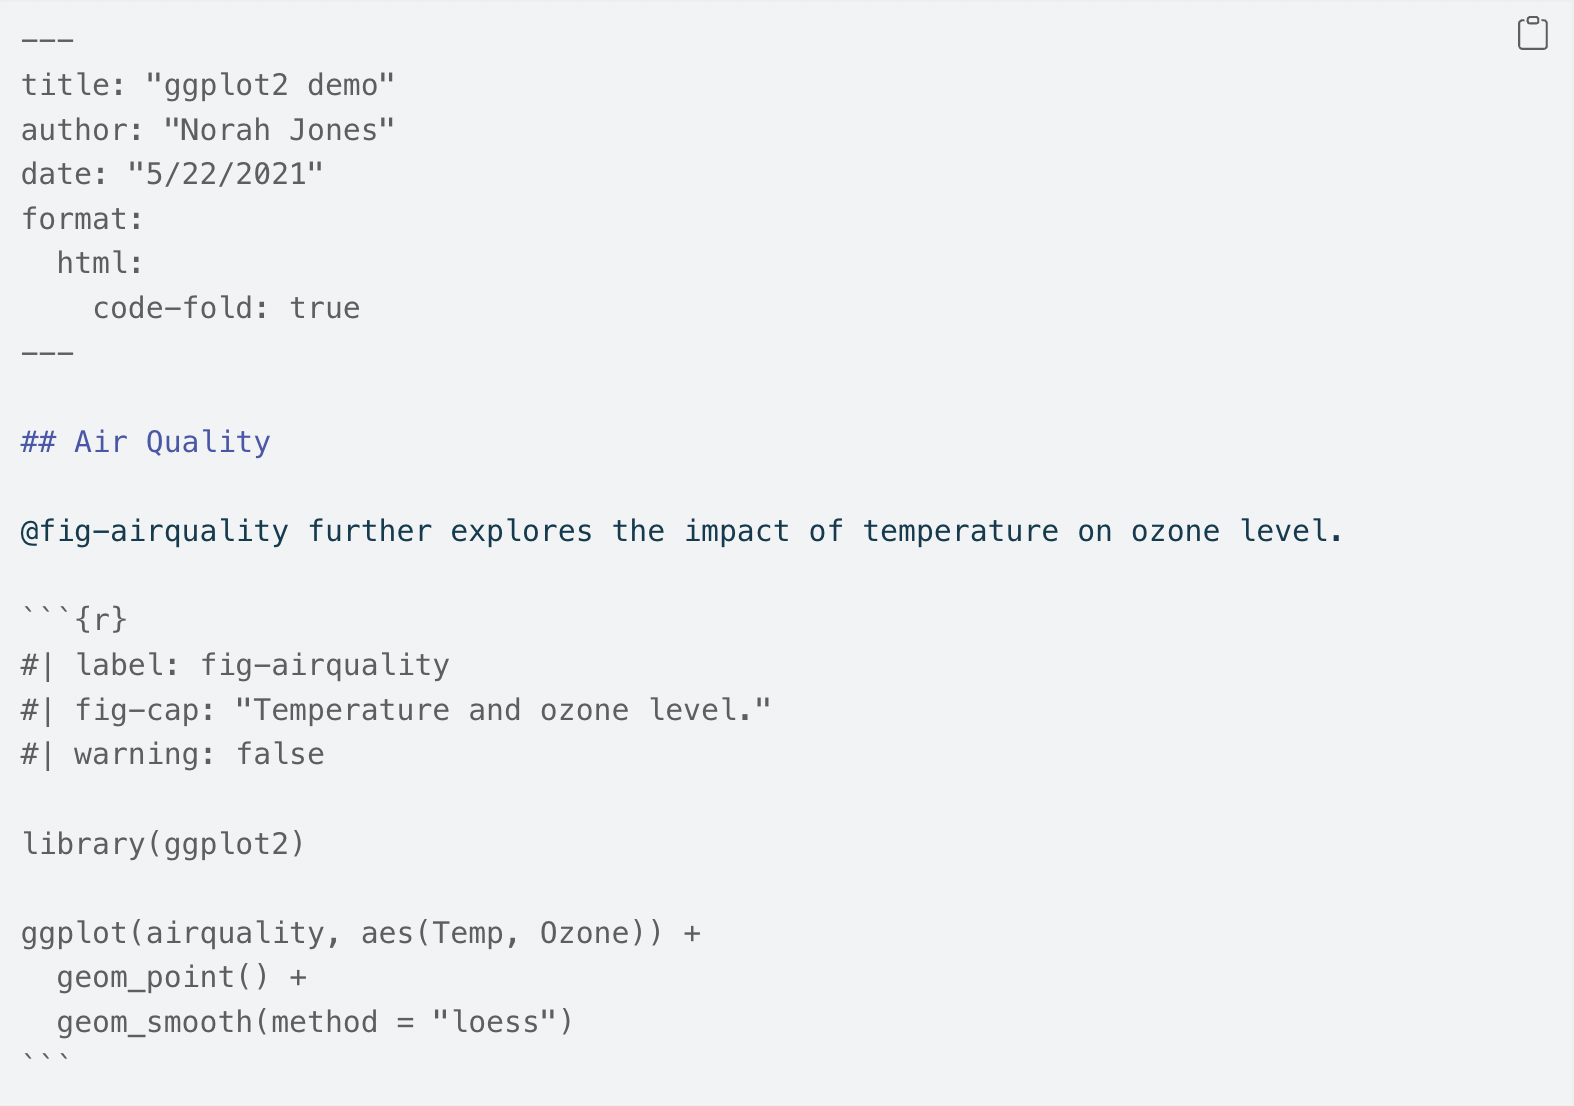
\includegraphics[keepaspectratio]{chapters/R/../../figures/quarto_screenshot.png}}

Questo file include:

\begin{enumerate}
\def\labelenumi{\arabic{enumi}.}
\tightlist
\item
  Un'intestazione YAML (metadati del documento).
\item
  Blocchi di codice delimitati da ```.
\item
  Testo scritto in Markdown con formattazioni semplici come titoli
  (\texttt{\#\ Titolo}), corsivi (\texttt{*testo*}), ecc.
\end{enumerate}

\subsection{Editor visivo e sorgente}\label{editor-visivo-e-sorgente}

\begin{itemize}
\tightlist
\item
  \textbf{Editor visivo}: simile a Google Docs, offre un'interfaccia
  WYSIWYM (What You See Is What You Mean). Consente di inserire
  facilmente immagini, tabelle, citazioni e altro.
\item
  \textbf{Editor sorgente}: consente un controllo diretto sul Markdown,
  utile per debug e personalizzazioni avanzate.
\end{itemize}

\subsection{Blocchi di codice}\label{blocchi-di-codice}

I blocchi di codice (chiamati ``chunks'') eseguono codice e visualizzano
i risultati. Ogni chunk è delimitato da ``` e può includere opzioni
specifiche:

\begin{Shaded}
\begin{Highlighting}[]
\CommentTok{\#| label: esempio}
\CommentTok{\#| echo: false}
\DecValTok{1} \SpecialCharTok{+} \DecValTok{1}
\end{Highlighting}
\end{Shaded}

Le opzioni più comuni includono:

\begin{itemize}
\tightlist
\item
  \texttt{echo:\ false} (nasconde il codice nel report),
\item
  \texttt{eval:\ false} (non esegue il codice),
\item
  \texttt{message:\ false} e \texttt{warning:\ false} (nasconde messaggi
  o avvisi).
\end{itemize}

\subsection{Figure}\label{figure}

Le figure possono essere generate tramite codice (es. \texttt{ggplot()})
o inserite come file esterni. Le opzioni più comuni per il controllo
delle dimensioni sono:

\begin{itemize}
\tightlist
\item
  \texttt{fig-width} e \texttt{fig-height} (dimensioni della figura in
  pollici),
\item
  \texttt{out-width} (percentuale di larghezza del documento),
\item
  \texttt{fig-asp} (rapporto d'aspetto, es. 0.618 per il rapporto
  aureo).
\end{itemize}

Esempio:

\begin{Shaded}
\begin{Highlighting}[]
\CommentTok{\#| fig{-}width: 6}
\FunctionTok{ggplot}\NormalTok{(data, }\FunctionTok{aes}\NormalTok{(x, y)) }\SpecialCharTok{+} \FunctionTok{geom\_point}\NormalTok{()}
\end{Highlighting}
\end{Shaded}

\subsection{Tabelle}\label{tabelle}

Le tabelle possono essere stampate direttamente o personalizzate con
funzioni come \texttt{knitr::kable()} o pacchetti come \texttt{gt}:

\begin{Shaded}
\begin{Highlighting}[]
\NormalTok{knitr}\SpecialCharTok{::}\FunctionTok{kable}\NormalTok{(}\FunctionTok{head}\NormalTok{(mtcars))}
\end{Highlighting}
\end{Shaded}

\begin{longtable}[]{@{}
  >{\raggedright\arraybackslash}p{(\linewidth - 22\tabcolsep) * \real{0.2609}}
  >{\raggedleft\arraybackslash}p{(\linewidth - 22\tabcolsep) * \real{0.0725}}
  >{\raggedleft\arraybackslash}p{(\linewidth - 22\tabcolsep) * \real{0.0580}}
  >{\raggedleft\arraybackslash}p{(\linewidth - 22\tabcolsep) * \real{0.0725}}
  >{\raggedleft\arraybackslash}p{(\linewidth - 22\tabcolsep) * \real{0.0580}}
  >{\raggedleft\arraybackslash}p{(\linewidth - 22\tabcolsep) * \real{0.0725}}
  >{\raggedleft\arraybackslash}p{(\linewidth - 22\tabcolsep) * \real{0.0870}}
  >{\raggedleft\arraybackslash}p{(\linewidth - 22\tabcolsep) * \real{0.0870}}
  >{\raggedleft\arraybackslash}p{(\linewidth - 22\tabcolsep) * \real{0.0435}}
  >{\raggedleft\arraybackslash}p{(\linewidth - 22\tabcolsep) * \real{0.0435}}
  >{\raggedleft\arraybackslash}p{(\linewidth - 22\tabcolsep) * \real{0.0725}}
  >{\raggedleft\arraybackslash}p{(\linewidth - 22\tabcolsep) * \real{0.0725}}@{}}
\toprule\noalign{}
\begin{minipage}[b]{\linewidth}\raggedright
\end{minipage} & \begin{minipage}[b]{\linewidth}\raggedleft
mpg
\end{minipage} & \begin{minipage}[b]{\linewidth}\raggedleft
cyl
\end{minipage} & \begin{minipage}[b]{\linewidth}\raggedleft
disp
\end{minipage} & \begin{minipage}[b]{\linewidth}\raggedleft
hp
\end{minipage} & \begin{minipage}[b]{\linewidth}\raggedleft
drat
\end{minipage} & \begin{minipage}[b]{\linewidth}\raggedleft
wt
\end{minipage} & \begin{minipage}[b]{\linewidth}\raggedleft
qsec
\end{minipage} & \begin{minipage}[b]{\linewidth}\raggedleft
vs
\end{minipage} & \begin{minipage}[b]{\linewidth}\raggedleft
am
\end{minipage} & \begin{minipage}[b]{\linewidth}\raggedleft
gear
\end{minipage} & \begin{minipage}[b]{\linewidth}\raggedleft
carb
\end{minipage} \\
\midrule\noalign{}
\endhead
\bottomrule\noalign{}
\endlastfoot
Mazda RX4 & 21.0 & 6 & 160 & 110 & 3.90 & 2.620 & 16.46 & 0 & 1 & 4 &
4 \\
Mazda RX4 Wag & 21.0 & 6 & 160 & 110 & 3.90 & 2.875 & 17.02 & 0 & 1 & 4
& 4 \\
Datsun 710 & 22.8 & 4 & 108 & 93 & 3.85 & 2.320 & 18.61 & 1 & 1 & 4 &
1 \\
Hornet 4 Drive & 21.4 & 6 & 258 & 110 & 3.08 & 3.215 & 19.44 & 1 & 0 & 3
& 1 \\
Hornet Sportabout & 18.7 & 8 & 360 & 175 & 3.15 & 3.440 & 17.02 & 0 & 0
& 3 & 2 \\
Valiant & 18.1 & 6 & 225 & 105 & 2.76 & 3.460 & 20.22 & 1 & 0 & 3 & 1 \\
\end{longtable}

\subsection{Caching}\label{caching}

Per velocizzare i documenti con calcoli complessi, Quarto supporta la
memorizzazione dei risultati:

\begin{itemize}
\tightlist
\item
  \texttt{cache:\ true} salva i risultati di un chunk, evitando di
  ricalcolarli se il codice non cambia.
\item
  \texttt{dependson} specifica dipendenze tra chunk.
\end{itemize}

\subsection{Gestione delle Citazioni e delle Bibliografie in
Quarto}\label{gestione-delle-citazioni-e-delle-bibliografie-in-quarto}

Quarto offre un supporto avanzato per la generazione automatica di
citazioni e bibliografie, consentendo l'applicazione di formati
personalizzati come lo stile APA. Per includere riferimenti
bibliografici, è necessario creare un file \texttt{.bib} (ad esempio,
\texttt{references.bib}) contenente le citazioni nel formato BibTeX.
Queste citazioni possono essere ottenute direttamente da Google Scholar
o altri database accademici.

Ecco un esempio di una citazione in formato BibTeX:

\begin{Shaded}
\begin{Highlighting}[]
\VariableTok{@article}\NormalTok{\{}\OtherTok{ceccarini2024age}\NormalTok{,}
  \DataTypeTok{title}\NormalTok{=\{Age{-}dependent changes in the anger superiority effect: Evidence from a visual search task\},}
  \DataTypeTok{author}\NormalTok{=\{Ceccarini, Francesco and Colpizzi, Ilaria and Caudek, Corrado\},}
  \DataTypeTok{journal}\NormalTok{=\{Psychonomic Bulletin }\CharTok{\textbackslash{}\&}\NormalTok{ Review\},}
  \DataTypeTok{pages}\NormalTok{=\{1{-}{-}10\},}
  \DataTypeTok{year}\NormalTok{=\{2024\},}
  \DataTypeTok{publisher}\NormalTok{=\{Springer\}}
\NormalTok{\}}
\end{Highlighting}
\end{Shaded}

Questa citazione deve essere inserita in un file \texttt{.bib}, ad
esempio, \texttt{references.bib}. Tale file dovrà poi essere specificato
nell'intestazione del documento Quarto.

\subsubsection{Configurazione dell'Intestazione
YAML}\label{configurazione-dellintestazione-yaml}

Nel file \texttt{.qmd}, è necessario aggiungere le seguenti righe
all'intestazione YAML per collegare il file \texttt{references.bib} e
configurare lo stile della bibliografia:

\begin{Shaded}
\begin{Highlighting}[]
\FunctionTok{bibliography}\KeywordTok{:}\AttributeTok{ references.bib}
\FunctionTok{biblio{-}style}\KeywordTok{:}\AttributeTok{ apalike}
\FunctionTok{csl}\KeywordTok{:}\AttributeTok{ apa.csl}
\end{Highlighting}
\end{Shaded}

\begin{itemize}
\tightlist
\item
  \textbf{\texttt{bibliography}}: Specifica il percorso del file
  \texttt{.bib}. In questo esempio, si assume che il file si trovi nella
  stessa cartella del documento Quarto.
\item
  \textbf{\texttt{biblio-style}}: Imposta lo stile delle citazioni. Ad
  esempio, \texttt{apalike} è uno stile simile allo stile APA.
\item
  \textbf{\texttt{csl}}: Consente di utilizzare uno stile di citazione
  personalizzato, come \texttt{apa.csl}. Puoi scaricare facilmente
  questi stili dal \href{https://www.zotero.org/styles}{Zotero Style
  Repository}.
\end{itemize}

\subsubsection{Esempio Completo}\label{esempio-completo}

Di seguito è riportato un esempio completo di un documento Quarto che
include una citazione e genera automaticamente la bibliografia:

\begin{Shaded}
\begin{Highlighting}[]
\CommentTok{{-}{-}{-}}
\AnnotationTok{title:}\CommentTok{ "Articolo di Esempio"}
\AnnotationTok{author:}\CommentTok{ "Autore di Esempio"}
\AnnotationTok{date:}\CommentTok{ "2025{-}02{-}22"}
\AnnotationTok{bibliography:}\CommentTok{ references.bib}
\AnnotationTok{biblio{-}style:}\CommentTok{ apalike}
\AnnotationTok{csl:}\CommentTok{ apa.csl}
\CommentTok{{-}{-}{-}}

\FunctionTok{\#\# Introduzione}

\NormalTok{In questo articolo, discutiamo i cambiamenti dipendenti dall\textquotesingle{}età nell\textquotesingle{}anger{-}superiority effect }\CommentTok{[}\OtherTok{@ceccarini2024age}\CommentTok{]}\NormalTok{.}

\FunctionTok{\#\# Risultati}

\NormalTok{I risultati mostrano che...}

\FunctionTok{\#\# Riferimenti}
\end{Highlighting}
\end{Shaded}

In questo esempio, l'identificatore \texttt{@ceccarini2024age} viene
utilizzato per fare riferimento alla citazione contenuta nel file
\texttt{references.bib}. Al momento della compilazione, Quarto genererà
automaticamente la lista dei riferimenti bibliografici in base al
formato specificato.

\subsubsection{Citazioni Inline}\label{citazioni-inline}

All'interno di un documento \texttt{.qmd}, le citazioni vengono aggiunte
utilizzando il simbolo \texttt{@} seguito dall'identificativo della
citazione specificato nel file \texttt{.bib}. Ad esempio:

\begin{Shaded}
\begin{Highlighting}[]
\NormalTok{... come evidenziato da @ceccarini2024age, si osserva che...}
\end{Highlighting}
\end{Shaded}

Quarto genera automaticamente la bibliografia, includendo solo i
riferimenti effettivamente citati nel documento. La bibliografia viene
aggiunta alla fine del file renderizzato (ad esempio, in formato HTML o
PDF).

Ad esempio, nel caso di un documento \texttt{.qmd}, il testo sopra sarà
visualizzato così:

\begin{quote}
\ldots{} come evidenziato da Ceccarini et al.~(2024), si osserva
che\ldots{}
\end{quote}

La citazione completa sarà inclusa automaticamente nella bibliografia,
posizionata alla fine della pagina web o del documento finale. Si noti
che Quarto gestisce automaticamente la formattazione e la posizione
della bibliografia, garantendo coerenza e precisione.

\begin{example}[]\protect\hypertarget{exm-}{}\label{exm-}

Per fare un esempio pratico, possiamo inserire la citazione
\texttt{@ceccarini2024age} direttamente nel file \texttt{.qmd} di questa
pagina web. Quando il documento viene compilato, Quarto renderà la
citazione in modo appropriato, come mostrato qui: Ceccarini et al.
(\citeproc{ref-ceccarini2024age}{2024}).

Si noti che, in fondo a questa pagina web, è presente un riferimento
bibliografico corrispondente. Questo riferimento è stato aggiunto
automaticamente da Quarto in risposta all'uso della citazione
\texttt{@ceccarini2024age} nel testo del documento. Questo processo
automatizzato semplifica la gestione delle citazioni e garantisce che
tutti i riferimenti siano correttamente inclusi e formattati.

\end{example}

\section{Riflessioni Conclusive}\label{riflessioni-conclusive-6}

Quarto è uno strumento potente per la creazione di documenti
riproducibili e ben strutturati, integrando codice, risultati e testo
descrittivo in un unico file. Questa introduzione dovrebbe essere
sufficiente per iniziare a lavorare con Quarto, ma c'è ancora molto da
imparare. Il modo migliore per rimanere aggiornati è consultare il sito
ufficiale di Quarto: \url{https://quarto.org}.

Un argomento importante che non abbiamo trattato qui riguarda i dettagli
di come comunicare in modo accurato le proprie idee agli altri. Per
migliorare le proprie capacità di scrittura, Wickham et al.
(\citeproc{ref-wickham2023r}{2023}) consigliano due libri: \emph{Style:
Lessons in Clarity and Grace} di Joseph M. Williams \& Joseph Bizup, e
\emph{The Sense of Structure: Writing from the Reader's Perspective} di
George Gopen. Una serie di brevi articoli sulla scrittura sono offerti
da George Gopen e sono disponibili su
\url{https://www.georgegopen.com/litigation-articles.html}.

\section{Esercizi}\label{esercizi-8}

\begin{tcolorbox}[enhanced jigsaw, opacityback=0, bottomrule=.15mm, breakable, title=\textcolor{quarto-callout-tip-color}{\faLightbulb}\hspace{0.5em}{Esercizio}, bottomtitle=1mm, toptitle=1mm, titlerule=0mm, colbacktitle=quarto-callout-tip-color!10!white, rightrule=.15mm, colframe=quarto-callout-tip-color-frame, colback=white, arc=.35mm, leftrule=.75mm, coltitle=black, left=2mm, toprule=.15mm, opacitybacktitle=0.6]

In questo esercizio esplorerai l'importanza della riproducibilità nella
scienza dei dati e le funzionalità principali di Quarto.

\textbf{1. Concetti di base sulla riproducibilità}

\begin{enumerate}
\def\labelenumi{\arabic{enumi}.}
\tightlist
\item
  Cos'è la \emph{crisi della riproducibilità} e perché è rilevante nella
  scienza dei dati?
\item
  In che modo Quarto può aiutare ad affrontare la crisi della
  riproducibilità?
\item
  Spiega il concetto di \emph{literate programming} e come si collega a
  Quarto.
\end{enumerate}

\textbf{2. Struttura di un file Quarto}

\begin{enumerate}
\def\labelenumi{\arabic{enumi}.}
\setcounter{enumi}{3}
\tightlist
\item
  Qual è l'estensione di un file Quarto e quali sono le sue tre sezioni
  principali?
\item
  Qual è la differenza tra \emph{editor visivo} ed \emph{editor
  sorgente} in Quarto?
\item
  Qual è la funzione dell'intestazione YAML in un file \texttt{.qmd}?
\end{enumerate}

\textbf{3. Blocchi di codice e opzioni}

\begin{enumerate}
\def\labelenumi{\arabic{enumi}.}
\setcounter{enumi}{6}
\tightlist
\item
  Come si scrive un blocco di codice in Quarto?
\item
  Quali opzioni puoi utilizzare nei blocchi di codice per controllare
  l'esecuzione e la visualizzazione del codice e dei risultati?
\item
  Scrivi un blocco di codice Quarto che calcola la media di un vettore
  di numeri e stampa il risultato senza mostrare il codice.
\end{enumerate}

\textbf{4. Figure e Tabelle}

\begin{enumerate}
\def\labelenumi{\arabic{enumi}.}
\setcounter{enumi}{9}
\tightlist
\item
  Quali opzioni di formattazione delle figure offre Quarto?
\item
  Come puoi creare una tabella formattata in Quarto usando
  \texttt{knitr::kable()}?
\end{enumerate}

\textbf{5. Citazioni e Bibliografia}

\begin{enumerate}
\def\labelenumi{\arabic{enumi}.}
\setcounter{enumi}{11}
\tightlist
\item
  Come si aggiunge una citazione bibliografica in Quarto?
\item
  Quali file devono essere inclusi per gestire una bibliografia in
  Quarto?
\item
  Scrivi un esempio di citazione in formato BibTeX e mostra come
  collegarla a un documento \texttt{.qmd}.
\end{enumerate}

\textbf{6. Considerazioni Finali}

\begin{enumerate}
\def\labelenumi{\arabic{enumi}.}
\setcounter{enumi}{14}
\tightlist
\item
  Quali sono i vantaggi di usare Quarto rispetto a strumenti più
  tradizionali come Word per la creazione di report scientifici?
\end{enumerate}

\end{tcolorbox}

\begin{tcolorbox}[enhanced jigsaw, opacityback=0, bottomrule=.15mm, breakable, title=\textcolor{quarto-callout-tip-color}{\faLightbulb}\hspace{0.5em}{Soluzione}, bottomtitle=1mm, toptitle=1mm, titlerule=0mm, colbacktitle=quarto-callout-tip-color!10!white, rightrule=.15mm, colframe=quarto-callout-tip-color-frame, colback=white, arc=.35mm, leftrule=.75mm, coltitle=black, left=2mm, toprule=.15mm, opacitybacktitle=0.6]

\textbf{1. Concetti di base sulla riproducibilità}

\begin{enumerate}
\def\labelenumi{\arabic{enumi}.}
\tightlist
\item
  La \emph{crisi della riproducibilità} è il fenomeno per cui molti
  studi scientifici non possono essere replicati con gli stessi metodi e
  dati. Questo mina la fiducia nella scienza e può portare a risultati
  non affidabili.
\item
  Quarto aiuta la riproducibilità integrando codice, testo e risultati
  in un unico documento, rendendo più semplice verificare e riprodurre
  le analisi.
\item
  \emph{Literate programming} è un approccio introdotto da Donald Knuth
  che combina codice e spiegazioni testuali nello stesso file,
  migliorando la comprensione e documentazione delle analisi. Quarto
  segue questa filosofia.
\end{enumerate}

\textbf{2. Struttura di un file Quarto}

\begin{enumerate}
\def\labelenumi{\arabic{enumi}.}
\setcounter{enumi}{3}
\item
  L'estensione di un file Quarto è \texttt{.qmd}. Le tre sezioni
  principali sono:

  \begin{itemize}
  \tightlist
  \item
    L'intestazione YAML (metadati),
  \item
    Il codice (chunks),
  \item
    Il testo scritto in Markdown.
  \end{itemize}
\item
  L'\emph{editor visivo} è un'interfaccia intuitiva simile a Google
  Docs, mentre l'\emph{editor sorgente} permette di scrivere
  direttamente in Markdown e codice.
\item
  L'intestazione YAML definisce le proprietà del documento come titolo,
  autore, formato di output e opzioni di rendering.
\end{enumerate}

\textbf{3. Blocchi di codice e opzioni}

\begin{enumerate}
\def\labelenumi{\arabic{enumi}.}
\setcounter{enumi}{6}
\item
  Un blocco di codice in Quarto si scrive con tripli backtick (```) e un
  linguaggio specificato:

\begin{Shaded}
\begin{Highlighting}[]
\CommentTok{\#| echo: true}
\FunctionTok{print}\NormalTok{(}\StringTok{"Esempio di codice in Quarto"}\NormalTok{)}
\end{Highlighting}
\end{Shaded}
\item
  Alcune opzioni utili nei blocchi di codice sono:

  \begin{itemize}
  \tightlist
  \item
    \texttt{echo:\ false} per nascondere il codice,
  \item
    \texttt{eval:\ false} per non eseguire il codice,
  \item
    \texttt{warning:\ false} e \texttt{message:\ false} per nascondere
    messaggi e avvisi.
  \end{itemize}
\item
  Esempio di blocco di codice che calcola una media senza mostrare il
  codice:

\begin{Shaded}
\begin{Highlighting}[]
\CommentTok{\#| echo: false}
\FunctionTok{mean}\NormalTok{(}\FunctionTok{c}\NormalTok{(}\DecValTok{1}\NormalTok{, }\DecValTok{2}\NormalTok{, }\DecValTok{3}\NormalTok{, }\DecValTok{4}\NormalTok{, }\DecValTok{5}\NormalTok{))}
\end{Highlighting}
\end{Shaded}
\end{enumerate}

\section{4. Figure e Tabelle}\label{figure-e-tabelle}

\begin{enumerate}
\def\labelenumi{\arabic{enumi}.}
\setcounter{enumi}{9}
\item
  Le opzioni principali per le figure includono:

  \begin{itemize}
  \tightlist
  \item
    \texttt{fig-width} e \texttt{fig-height} per le dimensioni,
  \item
    \texttt{out-width} per la larghezza relativa,
  \item
    \texttt{fig-asp} per il rapporto d'aspetto.
  \end{itemize}
\item
  Per creare una tabella formattata con \texttt{knitr::kable()}:

\begin{Shaded}
\begin{Highlighting}[]
\NormalTok{knitr}\SpecialCharTok{::}\FunctionTok{kable}\NormalTok{(}\FunctionTok{head}\NormalTok{(mtcars))}
\end{Highlighting}
\end{Shaded}
\end{enumerate}

\textbf{5. Citazioni e Bibliografia}

\begin{enumerate}
\def\labelenumi{\arabic{enumi}.}
\setcounter{enumi}{11}
\item
  Le citazioni in Quarto si aggiungono usando il simbolo \texttt{@}
  seguito dal riferimento BibTeX (es. \texttt{@ceccarini2024age}).
\item
  Per gestire la bibliografia in Quarto servono:

  \begin{itemize}
  \tightlist
  \item
    Un file \texttt{.bib} con le citazioni,
  \item
    Un'intestazione YAML che collega il file \texttt{.bib} e specifica
    lo stile (\texttt{csl}).
  \end{itemize}
\item
  Esempio di citazione BibTeX e collegamento in YAML:

\begin{Shaded}
\begin{Highlighting}[]
\VariableTok{@article}\NormalTok{\{}\OtherTok{ceccarini2024age}\NormalTok{,}
  \DataTypeTok{title}\NormalTok{=\{Age{-}dependent changes in the anger superiority effect\},}
  \DataTypeTok{author}\NormalTok{=\{Ceccarini, Francesco et al.\},}
  \DataTypeTok{journal}\NormalTok{=\{Psychonomic Bulletin \& Review\},}
  \DataTypeTok{year}\NormalTok{=\{2024\}}
\NormalTok{\}}
\end{Highlighting}
\end{Shaded}

  YAML:

\begin{Shaded}
\begin{Highlighting}[]
\FunctionTok{bibliography}\KeywordTok{:}\AttributeTok{ references.bib}
\FunctionTok{biblio{-}style}\KeywordTok{:}\AttributeTok{ apalike}
\end{Highlighting}
\end{Shaded}
\end{enumerate}

\textbf{6. Considerazioni Finali}

\begin{enumerate}
\def\labelenumi{\arabic{enumi}.}
\setcounter{enumi}{14}
\item
  I vantaggi di Quarto rispetto a Word includono:

  \begin{itemize}
  \tightlist
  \item
    maggiore riproducibilità e trasparenza,
  \item
    possibilità di integrare codice ed esecuzione in un unico documento,
  \item
    facilità di gestione delle citazioni automatiche,
  \item
    supporto per diversi formati di output (HTML, PDF, Word).
  \end{itemize}
\end{enumerate}

\end{tcolorbox}

\section*{Informazioni sull'Ambiente di
Sviluppo}\label{informazioni-sullambiente-di-sviluppo-3}
\addcontentsline{toc}{section}{Informazioni sull'Ambiente di Sviluppo}

\markright{Informazioni sull'Ambiente di Sviluppo}

\begin{Shaded}
\begin{Highlighting}[]
\FunctionTok{sessionInfo}\NormalTok{()}
\CommentTok{\#\textgreater{} R version 4.4.2 (2024{-}10{-}31)}
\CommentTok{\#\textgreater{} Platform: aarch64{-}apple{-}darwin20}
\CommentTok{\#\textgreater{} Running under: macOS Sequoia 15.3.1}
\CommentTok{\#\textgreater{} }
\CommentTok{\#\textgreater{} Matrix products: default}
\CommentTok{\#\textgreater{} BLAS:   /Library/Frameworks/R.framework/Versions/4.4{-}arm64/Resources/lib/libRblas.0.dylib }
\CommentTok{\#\textgreater{} LAPACK: /Library/Frameworks/R.framework/Versions/4.4{-}arm64/Resources/lib/libRlapack.dylib;  LAPACK version 3.12.0}
\CommentTok{\#\textgreater{} }
\CommentTok{\#\textgreater{} locale:}
\CommentTok{\#\textgreater{} [1] C/UTF{-}8/C/C/C/C}
\CommentTok{\#\textgreater{} }
\CommentTok{\#\textgreater{} time zone: Europe/Rome}
\CommentTok{\#\textgreater{} tzcode source: internal}
\CommentTok{\#\textgreater{} }
\CommentTok{\#\textgreater{} attached base packages:}
\CommentTok{\#\textgreater{} [1] stats     graphics  grDevices utils     datasets  methods   base     }
\CommentTok{\#\textgreater{} }
\CommentTok{\#\textgreater{} other attached packages:}
\CommentTok{\#\textgreater{}  [1] thematic\_0.1.6   MetBrewer\_0.2.0  ggokabeito\_0.1.0 see\_0.10.0      }
\CommentTok{\#\textgreater{}  [5] gridExtra\_2.3    patchwork\_1.3.0  bayesplot\_1.11.1 psych\_2.4.12    }
\CommentTok{\#\textgreater{}  [9] scales\_1.3.0     markdown\_1.13    knitr\_1.49       lubridate\_1.9.4 }
\CommentTok{\#\textgreater{} [13] forcats\_1.0.0    stringr\_1.5.1    dplyr\_1.1.4      purrr\_1.0.4     }
\CommentTok{\#\textgreater{} [17] readr\_2.1.5      tidyr\_1.3.1      tibble\_3.2.1     ggplot2\_3.5.1   }
\CommentTok{\#\textgreater{} [21] tidyverse\_2.0.0  rio\_1.2.3        here\_1.0.1      }
\CommentTok{\#\textgreater{} }
\CommentTok{\#\textgreater{} loaded via a namespace (and not attached):}
\CommentTok{\#\textgreater{}  [1] generics\_0.1.3    stringi\_1.8.4     lattice\_0.22{-}6    hms\_1.1.3        }
\CommentTok{\#\textgreater{}  [5] digest\_0.6.37     magrittr\_2.0.3    evaluate\_1.0.3    grid\_4.4.2       }
\CommentTok{\#\textgreater{}  [9] timechange\_0.3.0  fastmap\_1.2.0     rprojroot\_2.0.4   jsonlite\_1.8.9   }
\CommentTok{\#\textgreater{} [13] mnormt\_2.1.1      cli\_3.6.4         rlang\_1.1.5       munsell\_0.5.1    }
\CommentTok{\#\textgreater{} [17] withr\_3.0.2       yaml\_2.3.10       tools\_4.4.2       parallel\_4.4.2   }
\CommentTok{\#\textgreater{} [21] tzdb\_0.4.0        colorspace\_2.1{-}1  pacman\_0.5.1      vctrs\_0.6.5      }
\CommentTok{\#\textgreater{} [25] R6\_2.6.1          lifecycle\_1.0.4   pkgconfig\_2.0.3   pillar\_1.10.1    }
\CommentTok{\#\textgreater{} [29] gtable\_0.3.6      glue\_1.8.0        xfun\_0.50         tidyselect\_1.2.1 }
\CommentTok{\#\textgreater{} [33] rstudioapi\_0.17.1 farver\_2.1.2      htmltools\_0.5.8.1 nlme\_3.1{-}167     }
\CommentTok{\#\textgreater{} [37] rmarkdown\_2.29    compiler\_4.4.2}
\end{Highlighting}
\end{Shaded}

\section*{Bibliografia}\label{bibliografia-11}
\addcontentsline{toc}{section}{Bibliografia}

\markright{Bibliografia}

\chapter{L'ambiente di programmazione in R}\label{sec-r-environment}

\begin{tcolorbox}[enhanced jigsaw, opacityback=0, bottomrule=.15mm, breakable, title=\textcolor{quarto-callout-important-color}{\faExclamation}\hspace{0.5em}{In questo capitolo imparerai a}, bottomtitle=1mm, toptitle=1mm, titlerule=0mm, colbacktitle=quarto-callout-important-color!10!white, rightrule=.15mm, colframe=quarto-callout-important-color-frame, colback=white, arc=.35mm, leftrule=.75mm, coltitle=black, left=2mm, toprule=.15mm, opacitybacktitle=0.6]

\begin{itemize}
\tightlist
\item
  le nozioni di base dell'ambiente R.
\end{itemize}

\end{tcolorbox}

\begin{tcolorbox}[enhanced jigsaw, opacityback=0, bottomrule=.15mm, breakable, title=\textcolor{quarto-callout-tip-color}{\faLightbulb}\hspace{0.5em}{Prerequisiti}, bottomtitle=1mm, toptitle=1mm, titlerule=0mm, colbacktitle=quarto-callout-tip-color!10!white, rightrule=.15mm, colframe=quarto-callout-tip-color-frame, colback=white, arc=.35mm, leftrule=.75mm, coltitle=black, left=2mm, toprule=.15mm, opacitybacktitle=0.6]

\begin{itemize}
\tightlist
\item
  Leggere il capitolo 3, ``Setting Up Your Data Science Project'', del
  libro \href{https://vdsbook.com}{Veridical Data Science}
  (\citeproc{ref-yu2024veridical}{Yu \& Barter, 2024}).
\item
  Leggere il Capitolo~\ref{sec-apx-shell} della dispensa.
\end{itemize}

\end{tcolorbox}

\begin{tcolorbox}[enhanced jigsaw, opacityback=0, bottomrule=.15mm, breakable, title=\textcolor{quarto-callout-caution-color}{\faFire}\hspace{0.5em}{Preparazione del Notebook}, bottomtitle=1mm, toptitle=1mm, titlerule=0mm, colbacktitle=quarto-callout-caution-color!10!white, rightrule=.15mm, colframe=quarto-callout-caution-color-frame, colback=white, arc=.35mm, leftrule=.75mm, coltitle=black, left=2mm, toprule=.15mm, opacitybacktitle=0.6]

\begin{Shaded}
\begin{Highlighting}[]
\NormalTok{here}\SpecialCharTok{::}\FunctionTok{here}\NormalTok{(}\StringTok{"code"}\NormalTok{, }\StringTok{"\_common.R"}\NormalTok{) }\SpecialCharTok{|\textgreater{}} 
  \FunctionTok{source}\NormalTok{()}

\CommentTok{\# Load packages}
\ControlFlowTok{if}\NormalTok{ (}\SpecialCharTok{!}\FunctionTok{requireNamespace}\NormalTok{(}\StringTok{"pacman"}\NormalTok{)) }\FunctionTok{install.packages}\NormalTok{(}\StringTok{"pacman"}\NormalTok{)}
\NormalTok{pacman}\SpecialCharTok{::}\FunctionTok{p\_load}\NormalTok{(tidyr)}
\end{Highlighting}
\end{Shaded}

\end{tcolorbox}

\section{Introduzione}\label{introduzione-10}

Programmare presuppone necessariamente un ambiente di programmazione.
Una cattiva gestione di questo ambiente può causare il malfunzionamento
degli script, rendendo fondamentale imparare a gestirlo correttamente.

\begin{quote}
\textbf{Nota}: In R, il termine ``ambiente'' ha un significato
specifico, riferendosi allo spazio di lavoro in cui gli oggetti vengono
memorizzati durante una sessione. In questo capitolo, tuttavia, il
termine si riferisce allo stato complessivo del tuo computer mentre
programmi, inclusa l'organizzazione dei file, la versione di R che stai
usando e altre impostazioni.
\end{quote}

L'ambiente può influenzare persino il comportamento delle funzioni più
basilari. Considera il seguente esempio:

\begin{Shaded}
\begin{Highlighting}[]
\FunctionTok{print}\NormalTok{(}\DecValTok{1}\SpecialCharTok{:}\DecValTok{9}\NormalTok{)}
\end{Highlighting}
\end{Shaded}

Questo potrebbe produrre il seguente output:

\begin{verbatim}
[1] 1 2 3 4 5 6 7 8 9
\end{verbatim}

Tuttavia, modificando l'opzione di larghezza in R, il comportamento
cambia:

\begin{Shaded}
\begin{Highlighting}[]
\CommentTok{\# Dopo aver modificato options(width)}
\FunctionTok{options}\NormalTok{(}\AttributeTok{width =} \DecValTok{10}\NormalTok{)}
\FunctionTok{print}\NormalTok{(}\DecValTok{1}\SpecialCharTok{:}\DecValTok{9}\NormalTok{)}
\end{Highlighting}
\end{Shaded}

In questo caso, l'output potrebbe essere:

\begin{verbatim}
[1] 1 2 3
[4] 4 5 6
[7] 7 8 9
\end{verbatim}

La differenza è dovuta a un'opzione dell'ambiente, \texttt{width}, che
regola il numero massimo di caratteri visualizzati per ogni riga.

\section{File system}\label{file-system}

Prima di iniziare a organizzare un progetto in R, è fondamentale seguire
alcune linee guida per strutturare e nominare i file in modo efficace.
Spesso si tende a sottovalutare l'importanza di una buona
organizzazione, ma adottare un sistema coerente può far risparmiare
tempo prezioso nella ricerca e gestione dei progetti passati. Danielle
Navarro ha creato una
\href{https://djnavarro.net/slides-project-structure/\#1}{presentazione}
sulla struttura dei progetti, nella quale propone tre principi
fondamentali per la gestione dei file:

\begin{itemize}
\tightlist
\item
  essere gentili con le macchine;
\item
  essere gentili con gli esseri umani;
\item
  facilitare l'ordinamento e la ricerca.
\end{itemize}

\subsection{Essere gentili con le
macchine}\label{essere-gentili-con-le-macchine}

Le macchine possono confondersi con spazi, caratteri speciali (come
\texttt{\^{}.*?+\textbar{}\$"}), e lettere accentate. Per evitare
problemi:

\begin{itemize}
\tightlist
\item
  usa solo lettere minuscole, numeri, trattini \texttt{\_} o \texttt{-};
\item
  evita caratteri speciali e spazi nei nomi dei file;
\item
  evita le lettere accentate;
\item
  usa estensioni coerenti, come \texttt{.R} per gli script R.
\end{itemize}

Esempi:

\begin{Shaded}
\begin{Highlighting}[]
\CommentTok{\# Buono}
\ExtensionTok{progetto01\_analisi\_dati.R}

\CommentTok{\# Cattivo}
\ExtensionTok{Progetto} \StringTok{"Analisi Dati"}\NormalTok{.R}
\end{Highlighting}
\end{Shaded}

\subsection{Essere gentili con gli
umani}\label{essere-gentili-con-gli-umani}

Gli esseri umani hanno bisogno di contesto. Evita nomi vaghi e usa
descrizioni significative.

\begin{Shaded}
\begin{Highlighting}[]
\CommentTok{\# Buono}
\ExtensionTok{analisi01\_statistiche\_descrittive.R}
\ExtensionTok{note02\_intro\_modello.docx}

\CommentTok{\# Cattivo}
\ExtensionTok{01.R}
\ExtensionTok{appunti.docx}
\end{Highlighting}
\end{Shaded}

\begin{tcolorbox}[enhanced jigsaw, opacityback=0, bottomrule=.15mm, breakable, title=\textcolor{quarto-callout-important-color}{\faExclamation}\hspace{0.5em}{Importante}, bottomtitle=1mm, toptitle=1mm, titlerule=0mm, colbacktitle=quarto-callout-important-color!10!white, rightrule=.15mm, colframe=quarto-callout-important-color-frame, colback=white, arc=.35mm, leftrule=.75mm, coltitle=black, left=2mm, toprule=.15mm, opacitybacktitle=0.6]

Evitate categoricamente l'uso di spazi nei nomi di file, cartelle o
oggetti in R. Anche se il sistema operativo potrebbe consentirlo, questa
pratica può generare problemi futuri, complicare il debugging e rendere
il codice meno leggibile e portabile. Per evitare questi inconvenienti,
adottate sempre nomi privi di spazi, preferendo separatori come trattini
bassi (\texttt{\_}) o trattini (\texttt{-}).

\end{tcolorbox}

\subsection{Facilitare l'ordinamento e la
ricerca}\label{facilitare-lordinamento-e-la-ricerca}

Se i nomi dei file includono date, usa sempre il formato
\texttt{YYYY-MM-DD} per permettere un ordinamento automatico.

\begin{Shaded}
\begin{Highlighting}[]
\CommentTok{\# Buono}
\ExtensionTok{2024{-}01{-}01\_analisi.R}
\ExtensionTok{2024{-}02{-}15\_riassunto.docx}

\CommentTok{\# Cattivo}
\ExtensionTok{1{-}gennaio{-}2024.R}
\ExtensionTok{riassunto{-}15{-}02{-}2024.docx}
\end{Highlighting}
\end{Shaded}

Se devi ordinare i file in base a qualcosa di diverso dalle date, usa
numeri con lo zero iniziale per mantenere l'ordine.

\begin{Shaded}
\begin{Highlighting}[]
\ExtensionTok{reading01\_shakespeare\_romeo{-}and{-}juliet.docx}
\ExtensionTok{reading02\_shakespeare\_romeo{-}and{-}juliet.docx}
\ExtensionTok{...}
\ExtensionTok{reading11\_shakespeare\_romeo{-}and{-}juliet.docx}
\ExtensionTok{notes01\_shakespeare\_romeo{-}and{-}juliet.docx}
\ExtensionTok{...}
\end{Highlighting}
\end{Shaded}

\section{Versioni di R e pacchetti}\label{versioni-di-r-e-pacchetti}

Aggiornare regolarmente R e i pacchetti è essenziale per evitare bug e
sfruttare le nuove funzionalità. Ecco alcune buone pratiche:

\begin{enumerate}
\def\labelenumi{\arabic{enumi}.}
\tightlist
\item
  Esegui \texttt{update.packages()} ogni poche settimane per aggiornare
  i pacchetti.
\item
  Aggiorna la versione di R ogni pochi mesi. Su Windows puoi usare il
  pacchetto \texttt{installr}, mentre su altri sistemi puoi scaricare
  l'ultima versione dal sito ufficiale di R.
\item
  Mantieni aggiornato anche il sistema operativo.
\end{enumerate}

\section{Progetti in R}\label{progetti-in-r}

Se hai seguito i consigli finora, avrai creato una cartella per tutti i
tuoi progetti di programmazione e la tua installazione di R sarà
aggiornata. Ora è il momento di organizzare i tuoi progetti in R.

\subsection{Percorsi Assoluti e
Relativi}\label{percorsi-assoluti-e-relativi}

Un percorso assoluto parte dalla directory principale del tuo computer
(ad esempio, \texttt{/} su Linux/MacOS o \texttt{C:/} su Windows) e
indica in modo completo e univoco la posizione di un file o di una
cartella. Un percorso relativo, invece, parte dalla directory corrente
del progetto o dalla directory di lavoro impostata e descrive la
posizione di un file in relazione a questa.

Ad esempio, il percorso assoluto del file utilizzato per generare questa
pagina HTML potrebbe essere ottenuto così:

\begin{Shaded}
\begin{Highlighting}[]
\NormalTok{fs}\SpecialCharTok{::}\FunctionTok{path\_abs}\NormalTok{(}\StringTok{"05\_environment.qmd"}\NormalTok{)}
\CommentTok{\#\textgreater{} /Users/corrado/\_repositories/psicometria{-}r/chapters/R/05\_environment.qmd}
\end{Highlighting}
\end{Shaded}

\section{\texorpdfstring{Funzione
\texttt{here()}}{Funzione here()}}\label{funzione-here}

Se il progetto si trova nella cartella \texttt{psicometria-r}, possiamo
utilizzare la funzione \texttt{here()} del pacchetto \textbf{here} per
indicare la posizione del file \texttt{05\_environment.qmd} in modo
relativo. Ecco un esempio:

\begin{Shaded}
\begin{Highlighting}[]
\FunctionTok{file.exists}\NormalTok{(here}\SpecialCharTok{::}\FunctionTok{here}\NormalTok{(}\StringTok{"chapters"}\NormalTok{, }\StringTok{"R"}\NormalTok{, }\StringTok{"07\_environment.qmd"}\NormalTok{))}
\CommentTok{\#\textgreater{} [1] TRUE}
\end{Highlighting}
\end{Shaded}

In questo caso, il file \texttt{07\_environment.qmd} è contenuto nella
cartella \texttt{chapters/R}, che si trova all'interno della directory
principale del progetto. Grazie a \texttt{here()}, non è necessario
specificare manualmente la posizione del progetto: questa funzione
identifica automaticamente la directory principale e consente di
indicare solo il percorso relativo del file rispetto ad essa. In altre
parole, puoi riferirti al file \texttt{07\_environment.qmd}
semplicemente fornendo il percorso relativo all'interno della struttura
del progetto, lasciando a \texttt{here()} il compito di gestire il
contesto globale.

\subsection{Perché preferire i percorsi
relativi?}\label{perchuxe9-preferire-i-percorsi-relativi}

L'utilizzo di percorsi relativi con \texttt{here()} offre numerosi
vantaggi:

\begin{enumerate}
\def\labelenumi{\arabic{enumi}.}
\tightlist
\item
  \textbf{Portabilità}: Il codice diventa più semplice da condividere,
  poiché non dipende dalla struttura delle directory specifica del
  computer su cui è stato scritto.
\item
  \textbf{Organizzazione}: Favorisce una struttura chiara e coerente
  all'interno del progetto, rendendo più facile individuare e accedere
  ai file.
\item
  \textbf{Affidabilità}: Riduce il rischio di errori dovuti a percorsi
  assoluti errati, soprattutto quando il progetto viene spostato o
  condiviso.
\end{enumerate}

\subsection{Buone pratiche}\label{buone-pratiche}

\begin{itemize}
\tightlist
\item
  \textbf{Usare sempre percorsi relativi}: Questo assicura che il
  progetto sia facilmente eseguibile su altri sistemi senza necessità di
  modifiche ai percorsi.
\item
  \textbf{Impostare una struttura coerente del progetto}: Organizzare i
  file in cartelle ben definite (ad esempio, \texttt{data},
  \texttt{scripts}, \texttt{outputs}) facilita l'uso di percorsi
  relativi.
\end{itemize}

In sintesi, specificare i percorsi relativi rispetto alla directory
principale del progetto è una buona pratica essenziale per garantire
portabilità, organizzazione e riproducibilità del lavoro.

\subsection{Creare un progetto in R}\label{creare-un-progetto-in-r}

Un progetto R è semplicemente una cartella con un file \texttt{.Rproj}.
Puoi crearne uno con RStudio o con il pacchetto \texttt{usethis}.

\textbf{In RStudio}:

\begin{enumerate}
\def\labelenumi{\arabic{enumi}.}
\tightlist
\item
  Vai su \texttt{File\ \textgreater{}\ New\ Project}.
\item
  Seleziona \texttt{New\ Directory\ \textgreater{}\ New\ Project}.
\item
  Dai un nome al progetto e scegli la sua posizione.
\end{enumerate}

\textbf{Con \texttt{usethis}}:

\begin{Shaded}
\begin{Highlighting}[]
\NormalTok{usethis}\SpecialCharTok{::}\FunctionTok{create\_project}\NormalTok{(}\StringTok{"path/alla/cartella"}\NormalTok{)}
\end{Highlighting}
\end{Shaded}

Esempio:

\begin{Shaded}
\begin{Highlighting}[]
\NormalTok{usethis}\SpecialCharTok{::}\FunctionTok{create\_project}\NormalTok{(}\StringTok{"/Users/corrado/\_repositories/psicometria{-}r"}\NormalTok{)}
\end{Highlighting}
\end{Shaded}

Vedremo nel Capitolo~\ref{sec-eda-proj-structure} come organizzare i
file all'interno di un progetto.

\section*{Informazioni sull'Ambiente di
Sviluppo}\label{informazioni-sullambiente-di-sviluppo-4}
\addcontentsline{toc}{section}{Informazioni sull'Ambiente di Sviluppo}

\markright{Informazioni sull'Ambiente di Sviluppo}

\begin{Shaded}
\begin{Highlighting}[]
\FunctionTok{sessionInfo}\NormalTok{()}
\CommentTok{\#\textgreater{} R version 4.4.2 (2024{-}10{-}31)}
\CommentTok{\#\textgreater{} Platform: aarch64{-}apple{-}darwin20}
\CommentTok{\#\textgreater{} Running under: macOS Sequoia 15.3.1}
\CommentTok{\#\textgreater{} }
\CommentTok{\#\textgreater{} Matrix products: default}
\CommentTok{\#\textgreater{} BLAS:   /Library/Frameworks/R.framework/Versions/4.4{-}arm64/Resources/lib/libRblas.0.dylib }
\CommentTok{\#\textgreater{} LAPACK: /Library/Frameworks/R.framework/Versions/4.4{-}arm64/Resources/lib/libRlapack.dylib;  LAPACK version 3.12.0}
\CommentTok{\#\textgreater{} }
\CommentTok{\#\textgreater{} locale:}
\CommentTok{\#\textgreater{} [1] C/UTF{-}8/C/C/C/C}
\CommentTok{\#\textgreater{} }
\CommentTok{\#\textgreater{} time zone: Europe/Rome}
\CommentTok{\#\textgreater{} tzcode source: internal}
\CommentTok{\#\textgreater{} }
\CommentTok{\#\textgreater{} attached base packages:}
\CommentTok{\#\textgreater{} [1] stats     graphics  grDevices utils     datasets  methods   base     }
\CommentTok{\#\textgreater{} }
\CommentTok{\#\textgreater{} other attached packages:}
\CommentTok{\#\textgreater{}  [1] thematic\_0.1.6   MetBrewer\_0.2.0  ggokabeito\_0.1.0 see\_0.10.0      }
\CommentTok{\#\textgreater{}  [5] gridExtra\_2.3    patchwork\_1.3.0  bayesplot\_1.11.1 psych\_2.4.12    }
\CommentTok{\#\textgreater{}  [9] scales\_1.3.0     markdown\_1.13    knitr\_1.49       lubridate\_1.9.4 }
\CommentTok{\#\textgreater{} [13] forcats\_1.0.0    stringr\_1.5.1    dplyr\_1.1.4      purrr\_1.0.4     }
\CommentTok{\#\textgreater{} [17] readr\_2.1.5      tidyr\_1.3.1      tibble\_3.2.1     ggplot2\_3.5.1   }
\CommentTok{\#\textgreater{} [21] tidyverse\_2.0.0  rio\_1.2.3        here\_1.0.1      }
\CommentTok{\#\textgreater{} }
\CommentTok{\#\textgreater{} loaded via a namespace (and not attached):}
\CommentTok{\#\textgreater{}  [1] generics\_0.1.3    stringi\_1.8.4     lattice\_0.22{-}6    hms\_1.1.3        }
\CommentTok{\#\textgreater{}  [5] digest\_0.6.37     magrittr\_2.0.3    evaluate\_1.0.3    grid\_4.4.2       }
\CommentTok{\#\textgreater{}  [9] timechange\_0.3.0  fastmap\_1.2.0     rprojroot\_2.0.4   jsonlite\_1.8.9   }
\CommentTok{\#\textgreater{} [13] mnormt\_2.1.1      cli\_3.6.4         crayon\_1.5.3      rlang\_1.1.5      }
\CommentTok{\#\textgreater{} [17] munsell\_0.5.1     withr\_3.0.2       yaml\_2.3.10       tools\_4.4.2      }
\CommentTok{\#\textgreater{} [21] parallel\_4.4.2    tzdb\_0.4.0        colorspace\_2.1{-}1  pacman\_0.5.1     }
\CommentTok{\#\textgreater{} [25] vctrs\_0.6.5       R6\_2.6.1          lifecycle\_1.0.4   fs\_1.6.5         }
\CommentTok{\#\textgreater{} [29] pkgconfig\_2.0.3   pillar\_1.10.1     gtable\_0.3.6      glue\_1.8.0       }
\CommentTok{\#\textgreater{} [33] xfun\_0.50         tidyselect\_1.2.1  rstudioapi\_0.17.1 farver\_2.1.2     }
\CommentTok{\#\textgreater{} [37] htmltools\_0.5.8.1 nlme\_3.1{-}167      rmarkdown\_2.29    compiler\_4.4.2}
\end{Highlighting}
\end{Shaded}

\section*{Bibliografia}\label{bibliografia-12}
\addcontentsline{toc}{section}{Bibliografia}

\markright{Bibliografia}

\chapter{Utilizzo di strumenti AI per la programmazione}\label{sec-r-ai}

\section{Introduzione}\label{introduzione-11}

Il panorama della programmazione sta attraversando una trasformazione
radicale, guidata dall'avvento degli strumenti di intelligenza
artificiale (AI). Questi assistenti innovativi stanno rivoluzionando il
modo in cui sviluppatori, ricercatori e studenti scrivono, comprendono e
ottimizzano il codice. Grazie a una nuova generazione di strumenti che
vanno oltre i tradizionali ambienti di sviluppo, l'intelligenza
artificiale sta aprendo possibilità inedite. Piattaforme come
\textbf{ChatGPT}, \textbf{Google Gemini}, \textbf{Claude.ai},
\textbf{DeepSeek} e \textbf{Qwen} sono in grado di generare codice,
spiegare concetti complessi e fornire supporto agli sviluppatori in modi
che, fino a poco tempo fa, erano impensabili.

\section{Potenzialità e Sfide dell'AI nella
Programmazione}\label{potenzialituxe0-e-sfide-dellai-nella-programmazione}

Gli strumenti di intelligenza artificiale (AI) stanno trasformando
radicalmente il modo in cui si programma, inclusa l'elaborazione di
codice in linguaggi come R. Tuttavia, accanto alle immense potenzialità,
emergono anche sfide significative. I modelli di linguaggio di grandi
dimensioni (LLM, Large Language Models) possono ottimizzare e accelerare
i flussi di lavoro, ma non sono privi di limitazioni. Tra queste, la
possibilità di generare codice impreciso, introdurre bias involontari o
produrre output che richiedono una verifica approfondita da parte
dell'utente.

Nonostante queste sfide, gli strumenti di AI offrono un supporto
prezioso in diverse aree chiave:

\begin{itemize}
\item
  \textbf{Supporto Concettuale:}\\
  Gli LLM si dimostrano particolarmente efficaci nel rispondere a
  domande complesse su metodi statistici, algoritmi e tecniche di
  analisi dei dati. La qualità delle risposte migliora notevolmente
  quando le domande sono formulate in modo chiaro, specifico e
  dettagliato.
\item
  \textbf{Generazione e Completamento del Codice:}\\
  Questi strumenti possono aiutare gli sviluppatori a scrivere codice
  più rapidamente, suggerendo completamenti automatici, identificando
  potenziali errori e persino generando interi script a partire da
  descrizioni testuali. Questo riduce il tempo dedicato alla scrittura
  manuale e permette di concentrarsi su aspetti più creativi o complessi
  del progetto.
\end{itemize}

\section{Panoramica Comparativa dei Principali Strumenti
AI}\label{panoramica-comparativa-dei-principali-strumenti-ai}

Come scegliere il modello linguistico più adatto per un determinato
compito? Nell'articolo di Gibney (\citeproc{ref-Gibney2025}{2025}),
ricercatori condividono i loro strumenti preferiti attualmente in uso,
offrendo una guida pratica a chi ha bisogno di orientarsi tra le varie
opzioni.

\subsection{o3-mini (il ragionatore)}\label{o3-mini-il-ragionatore}

OpenAI ha lanciato \textbf{o3-mini}, un modello di ragionamento gratuito
per gli utenti registrati, sviluppato in risposta alla crescente
concorrenza di DeepSeek. Questo modello si distingue per l'utilizzo di
un processo di \textbf{ragionamento a catena} (chain-of-thought
reasoning), che gli permette di affrontare problemi complessi in ambito
matematico e scientifico con precisione. Oltre a eccellere nell'analisi
tecnica e nella riformattazione dei dati, o3-mini è particolarmente
efficace nel scomporre concetti intricati in passaggi più semplici.
Tuttavia, nonostante le sue capacità avanzate, non è ancora in grado di
eguagliare il ragionamento umano in contesti che richiedono creatività o
intuizione profonda.

\subsection{DeepSeek (il tuttofare)}\label{deepseek-il-tuttofare}

\textbf{DeepSeek-R1} è un modello open-weight paragonabile a o1 di
OpenAI, ma disponibile a un costo inferiore attraverso API. La sua
natura trasparente lo rende particolarmente attraente per i ricercatori,
che possono adattarlo ai propri progetti specifici. DeepSeek è utile per
generare ipotesi, migliorare la diagnostica medica e supportare attività
di ricerca avanzate. Tuttavia, presenta alcuni limiti: il suo processo
di ragionamento è più lento rispetto ad altri modelli e offre meno
filtri contro output potenzialmente dannosi. Inoltre, OpenAI ha
sollevato dubbi sulla legittimità del suo processo di addestramento,
alimentando un dibattito sulla trasparenza e l'etica degli LLM.

\subsection{Llama (il cavallo di
battaglia)}\label{llama-il-cavallo-di-battaglia}

Sviluppato da Meta, \textbf{Llama} è uno dei modelli LLM più utilizzati
nella ricerca grazie alla sua natura \textbf{open-weight}, che consente
agli scienziati di personalizzarlo e impiegarlo in ambienti controllati.
È stato applicato con successo in una vasta gamma di ambiti, dalla
predizione delle strutture cristalline ai calcoli quantistici,
dimostrando una grande versatilità. Tuttavia, l'accesso a Llama richiede
un'autorizzazione specifica, rendendolo meno immediato rispetto ad altri
modelli open-source emergenti che sono disponibili senza restrizioni.

\subsection{Claude (lo sviluppatore)}\label{claude-lo-sviluppatore}

\textbf{Claude 3.5 Sonnet}, prodotto da Anthropic, è particolarmente
apprezzato per la sua capacità di scrivere codice e interpretare dati
visivi. Questo modello si distingue per la sua abilità nel mantenere il
significato tecnico anche durante la semplificazione del linguaggio,
rendendolo ideale per redigere proposte di ricerca, annotare codice e
supportare attività di sviluppo software. Tuttavia, l'accesso completo
alle sue funzionalità richiede un'API a pagamento, il che lo rende meno
competitivo rispetto ai modelli open-source in rapida crescita,
soprattutto per utenti con budget limitati.

\subsection{OLMo (il veramente open)}\label{olmo-il-veramente-open}

\textbf{\href{https://playground.allenai.org}{OLMo 2}} rappresenta un
passo avanti nella trasparenza degli LLM. Questo modello non solo
fornisce i pesi del modello, ma anche i \textbf{dati di addestramento} e
il \textbf{codice di sviluppo}, offrendo una visione completa del suo
funzionamento. Questa apertura lo rende ideale per ricercatori e
sviluppatori che desiderano analizzare bias, ottimizzare le prestazioni
o comprendere a fondo il processo di creazione di un LLM. L'unico
svantaggio è che richiede competenze tecniche avanzate per
l'implementazione, sebbene il numero di risorse educative e tutorial
disponibili stia crescendo rapidamente.

Ogni modello presenta punti di forza e limiti specifici, rendendoli
adatti a contesti diversi. Mentre \textbf{o3-mini} e \textbf{DeepSeek}
si concentrano su ragionamento e analisi tecnica, \textbf{Llama} e
\textbf{OLMo} offrono maggiore flessibilità e trasparenza per la
ricerca. \textbf{Claude}, d'altra parte, si distingue per le sue
capacità di sviluppo e interpretazione di dati complessi. La scelta del
modello dipende dalle esigenze specifiche dell'utente, dal budget
disponibile e dalle competenze tecniche.

\section{Considerazioni Etiche e
Pratiche}\label{considerazioni-etiche-e-pratiche}

L'adozione di strumenti di intelligenza artificiale (AI) solleva
questioni etiche e pratiche che richiedono un'attenta riflessione e un
approccio responsabile.

\begin{itemize}
\item
  \textbf{Trasparenza}\\
  I dataset utilizzati per addestrare i modelli di AI sono spesso poco
  documentati e opachi, rendendo difficile valutarne la qualità e
  l'equità. Questo solleva interrogativi sulla presenza di bias
  involontari e sulla rappresentatività dei dati, con notevoli
  implicazioni per l'affidabilità dei risultati.
\item
  \textbf{Equità di Accesso}\\
  Nonostante le potenzialità rivoluzionarie degli strumenti di AI,
  l'accesso a queste tecnologie non è uniformemente distribuito.
  Disparità economiche, geografiche e infrastrutturali possono creare
  disuguaglianze, limitando l'adozione di queste risorse in contesti
  meno privilegiati e ampliando il divario digitale.
\item
  \textbf{Responsabilità}\\
  Uno dei dilemmi più complessi riguarda l'attribuzione della
  responsabilità per i risultati generati dai sistemi di AI. In caso di
  errori, bias o conseguenze indesiderate, non è sempre chiaro chi debba
  assumersi la responsabilità: gli sviluppatori del modello, gli utenti
  o le organizzazioni che lo implementano.
\end{itemize}

\section{Riflessioni Conclusive}\label{riflessioni-conclusive-7}

Gli strumenti di intelligenza artificiale stanno rivoluzionando il mondo
della programmazione, offrendo un supporto senza precedenti per la
risoluzione di problemi complessi, la generazione di codice e
l'ottimizzazione dei flussi di lavoro. Tuttavia, il loro utilizzo deve
essere accompagnato da un approccio critico e consapevole. È essenziale
verificare i risultati, valutare le implicazioni etiche e garantire che
l'adozione di queste tecnologie avvenga in modo equo e responsabile.

L'intelligenza artificiale non sostituirà gli sviluppatori, ma si
affermerà come un alleato indispensabile, ampliando la creatività e le
competenze umane. Questa collaborazione tra uomo e macchina ridefinirà
il modo in cui affrontiamo le sfide del futuro, aprendo nuove
opportunità e trasformando il panorama della tecnologia e della ricerca
(\citeproc{ref-bonnefon2024moral}{Bonnefon et al., 2024};
\citeproc{ref-liu2024toward}{Liu \& Li, 2024}).

\section*{Bibliografia}\label{bibliografia-13}
\addcontentsline{toc}{section}{Bibliografia}

\markright{Bibliografia}

\part{EDA}

Dopo aver acquisito un dataset, è fondamentale comprendere a fondo le
caratteristiche dei dati in esso contenuti. Sebbene le statistiche
descrittive e altre misure numeriche siano spesso efficaci per ottenere
una visione d'insieme, talvolta è un'immagine a valere più di mille
parole.

In questa sezione della dispensa, esploreremo alcuni concetti chiave
della statistica descrittiva. Oltre a fornire definizioni teoriche,
presenteremo istruzioni pratiche in R per condurre analisi statistiche
su dati reali. Il capitolo si concluderà con una riflessione critica sui
limiti di un approccio epistemologico basato esclusivamente sull'analisi
delle associazioni tra variabili, evidenziando l'importanza di indagare
le cause sottostanti ai fenomeni osservati.

\chapter{Le fasi del progetto di analisi dei
dati}\label{sec-eda-proj-structure}

\begin{tcolorbox}[enhanced jigsaw, opacityback=0, bottomrule=.15mm, breakable, title=\textcolor{quarto-callout-important-color}{\faExclamation}\hspace{0.5em}{In questo capitolo imparerai a}, bottomtitle=1mm, toptitle=1mm, titlerule=0mm, colbacktitle=quarto-callout-important-color!10!white, rightrule=.15mm, colframe=quarto-callout-important-color-frame, colback=white, arc=.35mm, leftrule=.75mm, coltitle=black, left=2mm, toprule=.15mm, opacitybacktitle=0.6]

\begin{itemize}
\tightlist
\item
  gestire il ciclo di vita di un progetto di analisi: dalla definizione
  della domanda di ricerca alla comunicazione dei risultati
\item
  organizzare i file del progetto per garantirne portabilità e
  condivisione
\end{itemize}

\end{tcolorbox}

\begin{tcolorbox}[enhanced jigsaw, opacityback=0, bottomrule=.15mm, breakable, title=\textcolor{quarto-callout-tip-color}{\faLightbulb}\hspace{0.5em}{Prerequisiti}, bottomtitle=1mm, toptitle=1mm, titlerule=0mm, colbacktitle=quarto-callout-tip-color!10!white, rightrule=.15mm, colframe=quarto-callout-tip-color-frame, colback=white, arc=.35mm, leftrule=.75mm, coltitle=black, left=2mm, toprule=.15mm, opacitybacktitle=0.6]

\begin{itemize}
\tightlist
\item
  Leggere \href{https://vdsbook.com}{Veridical Data Science}
  (\citeproc{ref-yu2024veridical}{Yu \& Barter, 2024}) focalizzandoti
  sul primo capitolo, che introduce le problematiche della data science,
  e sul quarto capitolo, che fornisce le linee guida dettagliate
  sull'organizzazione di un progetto di analisi dei dati.
\end{itemize}

\end{tcolorbox}

\begin{tcolorbox}[enhanced jigsaw, opacityback=0, bottomrule=.15mm, breakable, title=\textcolor{quarto-callout-caution-color}{\faFire}\hspace{0.5em}{Preparazione del Notebook}, bottomtitle=1mm, toptitle=1mm, titlerule=0mm, colbacktitle=quarto-callout-caution-color!10!white, rightrule=.15mm, colframe=quarto-callout-caution-color-frame, colback=white, arc=.35mm, leftrule=.75mm, coltitle=black, left=2mm, toprule=.15mm, opacitybacktitle=0.6]

\begin{Shaded}
\begin{Highlighting}[]
\CommentTok{\# Carica il file \_common.R per impostazioni di pacchetti e opzioni}
\NormalTok{here}\SpecialCharTok{::}\FunctionTok{here}\NormalTok{(}\StringTok{"code"}\NormalTok{, }\StringTok{"\_common.R"}\NormalTok{) }\SpecialCharTok{|\textgreater{}} 
  \FunctionTok{source}\NormalTok{()}
\end{Highlighting}
\end{Shaded}

\end{tcolorbox}

\section{Introduzione}\label{introduzione-12}

Una gestione accurata ed efficace dei dati è fondamentale, soprattutto
in discipline come la psicologia, dove l'analisi di dataset complessi è
una componente centrale della ricerca. Assicurare che i dati siano
raccolti con precisione, organizzati in modo chiaro e facilmente
accessibili per analisi e verifiche è essenziale per preservare
l'integrità del lavoro scientifico e promuovere la sua riproducibilità.
Una gestione rigorosa dei dati garantisce qualità e affidabilità durante
tutte le fasi del progetto, dalla raccolta alla documentazione dei
processi di elaborazione e delle eventuali modifiche apportate.

Dati ben organizzati e documentati non solo semplificano e rendono più
efficiente il processo di analisi, ma riducono anche il rischio di
errori, migliorando l'utilizzabilità e l'interpretazione delle
informazioni. Questo aspetto è particolarmente rilevante quando si
lavora con dataset provenienti da fonti eterogenee o con strutture
complesse. Inoltre, la trasparenza e la completezza nella gestione dei
dati rappresentano una condizione imprescindibile per garantire la
riproducibilità della ricerca, pilastro fondamentale della scienza.

La possibilità per altri ricercatori di replicare i risultati
utilizzando gli stessi dati e metodi rafforza la credibilità delle
conclusioni e contribuisce a costruire un progresso scientifico
condiviso e solido. Una gestione dei dati responsabile, dunque, non è
solo una buona pratica, ma una necessità per la produzione di conoscenze
affidabili e sostenibili.

\section{Capacità di Gestione dei Dati in
R}\label{capacituxe0-di-gestione-dei-dati-in-r}

R è uno strumento potente e versatile, progettato per supportare ogni
fase del ciclo di vita dei dati, dalla raccolta alla documentazione,
rendendolo indispensabile per chiunque lavori con dati complessi.

\begin{itemize}
\tightlist
\item
  \textbf{Importazione ed esportazione dei dati}: Con pacchetti come
  \texttt{readr} e \texttt{rio}, R facilita l'importazione di dati da
  diverse fonti, tra cui file CSV, database e API web, e consente
  l'esportazione in formati adatti a diversi utilizzi.
\item
  \textbf{Pulizia e preparazione dei dati}: Pacchetti come
  \texttt{dplyr}, \texttt{tidyr} e \texttt{stringr} offrono strumenti
  intuitivi e potenti per manipolare, trasformare e preparare i dati in
  modo efficiente, rendendoli pronti per l'analisi.
\item
  \textbf{Esplorazione e sintesi}: R, attraverso pacchetti come
  \texttt{dplyr} e \texttt{ggplot2}, permette di calcolare statistiche
  descrittive, individuare pattern significativi e visualizzare
  distribuzioni e relazioni in modo chiaro e informativo.
\item
  \textbf{Documentazione dinamica}: Grazie a strumenti come R Markdown e
  Quarto, è possibile creare documenti interattivi che integrano codice,
  analisi, testo esplicativo e risultati, promuovendo la riproducibilità
  e la trasparenza del lavoro.
\item
  \textbf{Controllo delle versioni}: L'integrazione di Git in RStudio
  offre un sistema di gestione delle versioni che consente di monitorare
  modifiche, collaborare con altri e garantire la tracciabilità del
  processo analitico.
\end{itemize}

Queste funzionalità rendono R uno strumento essenziale per gestire i
dati in modo organizzato, trasparente e ottimale, facilitando analisi
rigorose e riproducibili.

\section{Configurare l'Ambiente R}\label{configurare-lambiente-r}

Per sfruttare al meglio le potenzialità di R, è essenziale configurare
correttamente RStudio e integrare i pacchetti fondamentali per la
gestione dei dati. Una configurazione adeguata favorisce la
riproducibilità e l'organizzazione del lavoro.

\subsection{Workspace e Cronologia}\label{workspace-e-cronologia}

Accedi a \textbf{Tools \textgreater{} Global Options \textgreater{}
General} e modifica le seguenti impostazioni:

\begin{itemize}
\tightlist
\item
  Disabilita l'opzione \emph{Restore .RData into workspace at
  startup}.\\
\item
  Imposta \emph{Save workspace to .RData on exit} su \textbf{Never}.
\end{itemize}

Queste configurazioni incoraggiano una gestione basata sugli script,
rendendo il lavoro più trasparente e riducendo conflitti tra sessioni
diverse. Ogni analisi sarà così chiaramente documentata nello script,
evitando dipendenze da file temporanei o precedenti sessioni.

\subsection{Pacchetti Essenziali}\label{pacchetti-essenziali}

R è composto da un modulo base che fornisce le funzionalità fondamentali
del linguaggio, ma la sua potenza deriva dall'enorme ecosistema di
pacchetti aggiuntivi. Questi pacchetti possono essere caricati secondo
necessità. Per questo corso, utilizzeremo regolarmente i seguenti
pacchetti:

\begin{itemize}
\tightlist
\item
  \textbf{\texttt{here}}: per una gestione ordinata dei percorsi
  relativi, evitando problemi legati ai percorsi assoluti.\\
\item
  \textbf{\texttt{tidyverse}}: una raccolta di pacchetti per
  manipolazione, analisi e visualizzazione dei dati, che include
  \texttt{dplyr}, \texttt{tidyr}, \texttt{ggplot2} e altri strumenti
  indispensabili.
\end{itemize}

Assicurati di installarli e caricarli all'inizio di ogni script con i
comandi:

\begin{Shaded}
\begin{Highlighting}[]
\CommentTok{\# install.packages(c("here", "tidyverse")) }
\CommentTok{\# è solo necessario installarli una volta}
\FunctionTok{library}\NormalTok{(here)}
\FunctionTok{library}\NormalTok{(tidyverse)}
\end{Highlighting}
\end{Shaded}

\subsection{Gestione dei Progetti}\label{gestione-dei-progetti}

I progetti in RStudio rappresentano uno strumento chiave per mantenere
il lavoro organizzato. Utilizzare i progetti consente di lavorare in
ambienti separati, dove ogni progetto ha la propria directory dedicata.

Per creare un nuovo progetto:

\begin{enumerate}
\def\labelenumi{\arabic{enumi}.}
\tightlist
\item
  Vai su \textbf{File \textgreater{} New Project}.\\
\item
  Seleziona una directory specifica per il progetto.\\
\item
  Salva tutti i file correlati (script, dati, risultati) all'interno
  della directory del progetto.
\end{enumerate}

Questo approccio facilita la navigazione e previene errori derivanti
dall'uso di file non correlati. Ogni progetto diventa così un'unità
autonoma, ideale per mantenere ordine e coerenza nel lavoro.

\section{Il Ciclo di Vita di un Progetto di Data
Science}\label{il-ciclo-di-vita-di-un-progetto-di-data-science}

I progetti di analisi dei dati seguono solitamente queste fasi
(\citeproc{ref-yu2024veridical}{Yu \& Barter, 2024}):

\begin{enumerate}
\def\labelenumi{\arabic{enumi}.}
\tightlist
\item
  \textbf{Formulazione del problema e raccolta dei dati}: Definizione
  delle domande di ricerca e acquisizione dei dataset.
\item
  \textbf{Pulizia, preprocessing e analisi esplorativa}: Preparazione
  dei dati per l'analisi attraverso trasformazioni e sintesi.
\item
  \textbf{Analisi predittiva e/o inferenziale}: (Opzionale) Modelli
  statistici o predittivi per rispondere alle domande di ricerca.
\item
  \textbf{Valutazione dei risultati}: Interpretazione e verifica delle
  conclusioni tratte.
\item
  \textbf{Comunicazione dei risultati}: Presentazione dei risultati in
  forma visiva e narrativa.
\end{enumerate}

Non tutti i progetti includono la fase 3, ma quasi tutti attraversano le
altre fasi, rendendo essenziale un approccio organizzato e ben
strutturato.

\subsection{Fase 1: Formulazione del Problema e Raccolta dei
Dati}\label{fase-1-formulazione-del-problema-e-raccolta-dei-dati}

La formulazione di una domanda di ricerca chiara e precisa rappresenta
il punto di partenza fondamentale per qualsiasi progetto di data
science. È essenziale definire con attenzione l'ambito in cui si intende
condurre l'analisi dei dati. Questo ambito può assumere due principali
direzioni:

\begin{enumerate}
\def\labelenumi{\arabic{enumi}.}
\item
  \textbf{Ambito Applicativo}\\
  In questo contesto, l'obiettivo è spesso quello di produrre un report
  descrittivo che sintetizzi i risultati di un intervento specifico. Un
  esempio potrebbe essere la valutazione dell'efficacia di un programma
  di educazione sessuale rivolto agli adolescenti nelle scuole. In
  questo caso, l'analisi si concentra sulla descrizione dei risultati
  ottenuti, senza necessariamente approfondire le basi teoriche
  sottostanti.
\item
  \textbf{Ambito della Ricerca Psicologica}\\
  In questo secondo caso, l'approccio è più rigoroso e complesso. Non è
  sufficiente descrivere i risultati, ma è necessario giustificare le
  scelte metodologiche, come la selezione degli strumenti di misurazione
  e la formulazione delle domande di ricerca, basandosi su teorie
  consolidate e sulla letteratura scientifica esistente. Questo aspetto
  è stato approfondito nel Capitolo~\ref{sec-measurement} del materiale
  didattico.
\end{enumerate}

\textbf{Caratteristiche di una Buona Domanda di Ricerca}\\
La domanda di ricerca deve essere formulata in modo da poter essere
risolta attraverso l'analisi dei dati disponibili. Spesso, la domanda
iniziale può risultare troppo vaga o ambiziosa, rendendo necessario un
processo di revisione per adattarla alle informazioni effettivamente
accessibili. Questo approccio garantisce che i dati raccolti o
utilizzati siano appropriati e sufficienti per rispondere in modo
efficace al problema di ricerca.

\textbf{Raccolta dei Dati}\\
La fase di raccolta dei dati è altrettanto cruciale per il successo del
progetto. Esistono due principali scenari:

\begin{enumerate}
\def\labelenumi{\arabic{enumi}.}
\item
  \textbf{Utilizzo di Dati Esistenti}:\\
  In alcuni casi, è possibile sfruttare dataset già disponibili,
  provenienti da repository pubblici, database interni o esperimenti
  precedenti.
\item
  \textbf{Nuova Raccolta di Dati}:\\
  In altri casi, è necessario procedere con una raccolta dati ex novo.
  In entrambe le situazioni, è fondamentale pianificare con cura le
  analisi statistiche prima di avviare la raccolta. Una mancata
  pianificazione può portare a dataset incompleti, privi di informazioni
  essenziali o non conformi alle assunzioni richieste dai modelli
  statistici previsti.
\end{enumerate}

\textbf{Aspetti Chiave della Raccolta Dati}\\
Per garantire l'affidabilità dei risultati, è essenziale comprendere a
fondo i processi e le metodologie utilizzate per acquisire i dati.
Questo include:

\begin{itemize}
\tightlist
\item
  \textbf{Documentazione delle Tecniche e Procedure}:\\
  Descrivere in dettaglio le tecniche di raccolta, le procedure seguite
  e i potenziali bias che potrebbero influenzare i risultati.\\
\item
  \textbf{Valutazione delle Limitazioni}:\\
  Identificare e considerare eventuali limitazioni dei dati, in modo da
  interpretare i risultati in modo critico e consapevole.
\end{itemize}

Questo approccio metodologico contribuisce a garantire che le misure
ottenute siano affidabili e che le analisi siano condotte in modo
rigoroso e trasparente.

\subsection{Fase 2: Pulizia dei Dati e Analisi
Esplorativa}\label{fase-2-pulizia-dei-dati-e-analisi-esplorativa}

\subsubsection{Importazione ed Esportazione dei dati in
R}\label{importazione-ed-esportazione-dei-dati-in-r}

\textbf{Importazione dei Dati}

In R, i dati vengono solitamente caricati in un \textbf{data frame}. Per
facilitare questo processo, il pacchetto \texttt{rio} fornisce la
funzione universale \texttt{import()}, che consente di caricare dati da
formati diversi (come \texttt{.csv}, \texttt{.xlsx}, \texttt{.json},
ecc.) senza dover usare funzioni specifiche per ogni tipo di file.

Per garantire un'organizzazione ottimale dei file, è utile:

\begin{enumerate}
\def\labelenumi{\arabic{enumi}.}
\tightlist
\item
  Creare una struttura di progetto chiara, con cartelle dedicate (es.
  \texttt{data/raw} per i dati grezzi e \texttt{data/processed} per
  quelli elaborati).\\
\item
  Usare percorsi relativi, che rendono i progetti portabili e più
  facilmente replicabili.
\end{enumerate}

Il pacchetto \textbf{here} semplifica la gestione dei percorsi relativi,
assicurando che il codice funzioni correttamente indipendentemente dalla
posizione del progetto.

Supponiamo di avere un progetto chiamato \texttt{my\_project} con la
seguente struttura:

\begin{verbatim}
my_project/
├── my_project.Rproj
├── data/
│   ├── raw/
│   │   └── my_data.csv
│   ├── processed/
\end{verbatim}

Per importare il file \texttt{my\_data.csv} nella memoria di lavoro di
R, possiamo usare:

\begin{Shaded}
\begin{Highlighting}[]
\FunctionTok{library}\NormalTok{(here)}
\FunctionTok{library}\NormalTok{(rio)}

\CommentTok{\# Importazione del file}
\NormalTok{df }\OtherTok{\textless{}{-}} \FunctionTok{import}\NormalTok{(}\FunctionTok{here}\NormalTok{(}\StringTok{"data"}\NormalTok{, }\StringTok{"raw"}\NormalTok{, }\StringTok{"my\_data.csv"}\NormalTok{))}
\end{Highlighting}
\end{Shaded}

\textbf{Esportazione dei Dati}

Dopo aver elaborato i dati, è importante salvarli in modo organizzato.
Con il pacchetto \texttt{rio}, l'esportazione si effettua tramite
\texttt{export()}. Ad esempio, per salvare un file elaborato nella
cartella \texttt{data/processed}:

\begin{Shaded}
\begin{Highlighting}[]
\CommentTok{\# Esportazione del file elaborato}
\FunctionTok{export}\NormalTok{(df, }\FunctionTok{here}\NormalTok{(}\StringTok{"data"}\NormalTok{, }\StringTok{"processed"}\NormalTok{, }\StringTok{"my\_data\_processed.csv"}\NormalTok{))}
\end{Highlighting}
\end{Shaded}

\textbf{Vantaggi di un Workflow Organizzato}

\begin{enumerate}
\def\labelenumi{\arabic{enumi}.}
\tightlist
\item
  \textbf{Portabilità}: Usando percorsi relativi con \texttt{here}, il
  progetto può essere spostato su diversi computer o condiviso senza
  necessità di modificare il codice.\\
\item
  \textbf{Semplificazione}: \texttt{rio} elimina la necessità di
  ricordare funzioni specifiche per diversi tipi di file.\\
\item
  \textbf{Riproducibilità}: Una struttura chiara e un codice ben
  organizzato favoriscono la replicabilità dei risultati.
\end{enumerate}

\subsubsection{Pulizia dei Dati}\label{pulizia-dei-dati}

Dopo aver definito la domanda della ricerca e avere raccolto i dati
rilevanti, è il momento di pulire i dati. Un dataset pulito è ordinato,
formattato in modo appropriato e ha voci non ambigue. La fase iniziale
di pulizia dei dati consiste nell'identificare problemi con i dati (come
formattazioni anomale e valori non validi) e modificarli in modo che i
valori siano validi e formattati in modo comprensibile sia per il
computer che per noi. La pulizia dei dati è una fase estremamente
importante di un progetto di data science perché non solo aiuta a
garantire che i dati siano interpretati correttamente dal computer, ma
aiuta anche a sviluppare una comprensione dettagliata delle informazioni
contenute nei dati e delle loro limitazioni.

L'obiettivo della pulizia dei dati è creare una versione dei dati che
rifletta nella maniera più fedele possibile la realtà e che sia
interpretata correttamente dal computer. Per garantire che il computer
utilizzi fedelmente le informazioni contenute nei dati, è necessario
modificare i dati (scrivendo codice, non modificando il file dati grezzo
stesso) in modo che siano in linea con ciò che il computer ``si
aspetta''. Tuttavia, il processo di pulizia dei dati è necessariamente
soggettivo e comporta fare assunzioni sulle quantità reali sottostanti
misurate e decisioni su quali modifiche siano le più sensate.

\subsubsection{Preprocessing}\label{preprocessing}

Il preprocessing si riferisce al processo di modifica dei dati puliti
per soddisfare i requisiti di un algoritmo specifico che si desidera
applicare. Ad esempio, se si utilizza un algoritmo che richiede che le
variabili siano sulla stessa scala, potrebbe essere necessario
trasformarle, oppure, se si utilizza un algoritmo che non consente
valori mancanti, potrebbe essere necessario imputarli o rimuoverli.
Durante il preprocessing, potrebbe essere utile anche definire nuove
caratteristiche/variabili utilizzando le informazioni esistenti nei
dati, se si ritiene che queste possano essere utili per l'analisi.

Come per la pulizia dei dati, non esiste un unico modo corretto per
pre-elaborare un dataset, e la procedura finale comporta tipicamente una
serie di decisioni che dovrebbero essere documentate nel codice e nei
file di documentazione.

\subsubsection{Analisi Esplorativa dei
Dati}\label{analisi-esplorativa-dei-dati}

Dopo l'acquisizione dei dati, si procede con un'Analisi Esplorativa dei
Dati (EDA - Exploratory Data Analysis). Questa fase iniziale mira a far
familiarizzare il ricercatore con il dataset e a scoprire pattern
nascosti. Si realizza attraverso:

\begin{itemize}
\tightlist
\item
  La costruzione di tabelle di frequenza e contingenza.
\item
  Il calcolo di statistiche descrittive (come indici di posizione,
  dispersione e forma della distribuzione).
\item
  La creazione di rappresentazioni grafiche preliminari.
\end{itemize}

L'EDA permette di generare ipotesi sui dati e di guidare le successive
analisi statistiche.

\subsection{Fase 3: Analisi Predittiva e
Inferenziale}\label{fase-3-analisi-predittiva-e-inferenziale}

Molte domande nella data science si presentano come problemi di
inferenza e/o previsione, in cui l'obiettivo principale è utilizzare
dati osservati, passati o presenti, per descrivere le caratteristiche di
una popolazione più ampia o per fare previsioni su dati futuri non
ancora disponibili. Questo tipo di analisi è spesso orientato a
supportare decisioni nel mondo reale.

\subsection{Fase 4: Valutazione dei
Risultati}\label{fase-4-valutazione-dei-risultati}

In questa fase, i risultati ottenuti vengono analizzati alla luce della
domanda di ricerca iniziale. Si procede a una valutazione sia
quantitativa, attraverso l'applicazione di tecniche statistiche
appropriate, sia qualitativa, attraverso un'attenta riflessione critica.

\subsection{Fase 5: Comunicazione dei
Risultati}\label{fase-5-comunicazione-dei-risultati}

L'ultima fase di un progetto di analisi dei dati consiste nel
condividere i risultati con un pubblico più ampio, il che richiede la
preparazione di materiali comunicativi chiari e concisi. L'obiettivo è
trasformare i risultati dell'analisi in informazioni utili per
supportare il processo decisionale. Questo può includere la stesura di
un articolo scientifico, la creazione di un report per un team di
lavoro, o la preparazione di una presentazione con diapositive.

La comunicazione deve essere adattata al pubblico di riferimento. Non si
deve dare per scontato che il pubblico abbia familiarità con il
progetto: è fondamentale spiegare l'analisi e le visualizzazioni in modo
chiaro e dettagliato. Anche se per il ricercatore il messaggio
principale di una figura o diapositiva può sembrare ovvio, è sempre una
buona pratica guidare il pubblico nella sua interpretazione, evitando
l'uso di gergo tecnico complesso.

\section{Organizzazione del Progetto}\label{organizzazione-del-progetto}

Un requisito fondamentale per un progetto di analisi dei dati è
organizzare in modo efficiente i file sul proprio computer. Questo
include i file dei dati, il codice e la documentazione del progetto.
Tutti questi elementi dovrebbero essere raccolti all'interno di una
singola cartella dedicata al progetto.

\subsection{Home Directory}\label{home-directory}

In RStudio, è possibile creare un file chiamato
\texttt{nome\_del\_progetto.Rproj}, che consente di configurare
automaticamente la \emph{home directory} del progetto, ovvero la
cartella principale da cui R avvia il lavoro relativo al progetto. Per
utilizzare questa funzionalità, è sufficiente aprire RStudio cliccando
direttamente sul file \texttt{nome\_del\_progetto.Rproj}.

La \emph{home directory} rappresenta il punto di riferimento principale
per tutte le operazioni del progetto, come il caricamento di file, il
salvataggio degli output e la gestione delle risorse.

Grazie a questa configurazione, è possibile utilizzare percorsi relativi
per accedere ai file all'interno del progetto. I percorsi relativi si
basano sempre sulla cartella principale del progetto, il che rende il
codice più portabile e adattabile. In pratica, chiunque scarichi il tuo
progetto sarà in grado di eseguirlo senza dover modificare manualmente i
percorsi dei file. Questo approccio migliora la condivisione e
garantisce una maggiore riproducibilità del tuo lavoro.

\subsection{Struttura di un Progetto}\label{struttura-di-un-progetto}

Un'adeguata organizzazione della struttura di un progetto è fondamentale
per garantire chiarezza, riproducibilità e portabilità. Yu \& Barter
(\citeproc{ref-yu2024veridical}{2024}) propone il seguente template per
la gestione di un progetto:

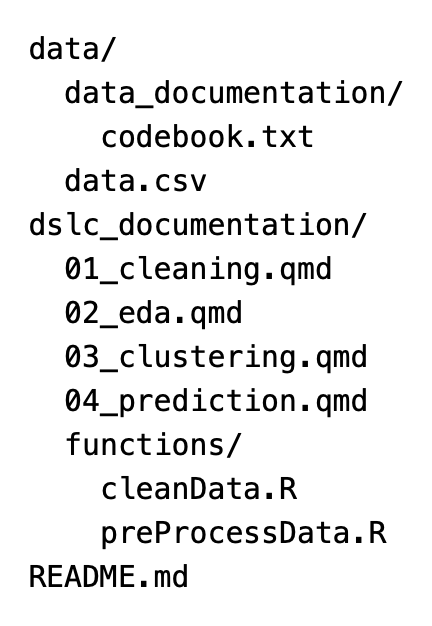
\includegraphics[width=0.275\linewidth,height=\textheight,keepaspectratio]{chapters/eda/../../figures/project_structure.png}

\subsubsection{\texorpdfstring{\textbf{Cartelle
Principali}}{Cartelle Principali}}\label{cartelle-principali}

\begin{enumerate}
\def\labelenumi{\arabic{enumi}.}
\item
  \textbf{\texttt{data/}:}\\
  Questa cartella raccoglie i dataset utilizzati nel progetto, suddivisi
  in:

  \begin{itemize}
  \tightlist
  \item
    \textbf{\texttt{raw/}}: per i dati grezzi, che non devono mai essere
    modificati. Esempio: \texttt{data/raw/data.csv}.\\
  \item
    \textbf{\texttt{processed/}}: per i dati elaborati, cioè quelli
    puliti e trasformati per le analisi successive.
  \end{itemize}

  È indispensabile includere un \textbf{codebook} nella sottocartella
  \texttt{raw} per documentare variabili, unità di misura e ogni altra
  informazione necessaria per comprendere i dati. Questo migliora la
  trasparenza e facilita la condivisione del progetto.
\item
  \textbf{\texttt{dslc\_documentation/}:}\\
  Contiene tutti i file necessari per documentare e condurre le analisi.

  \begin{itemize}
  \tightlist
  \item
    File principali: possono essere in formato \texttt{.qmd} (Quarto per
    R) o \texttt{.ipynb} (Jupyter Notebook per Python), ordinati
    cronologicamente tramite un prefisso numerico (ad esempio,
    \texttt{01\_data\_cleaning.qmd}, \texttt{02\_analysis.qmd}).\\
  \item
    \textbf{\texttt{functions/}:} una sottocartella dedicata a script
    con funzioni personalizzate, utili per diverse fasi del progetto. Ad
    esempio, \texttt{.R} per R o \texttt{.py} per Python.
  \end{itemize}
\end{enumerate}

\begin{center}\rule{0.5\linewidth}{0.5pt}\end{center}

\subsubsection{\texorpdfstring{\textbf{File
Supplementari}}{File Supplementari}}\label{file-supplementari}

\begin{itemize}
\tightlist
\item
  \textbf{\texttt{README.md}:}\\
  Un file fondamentale che descrive la struttura del progetto e offre
  una breve panoramica del contenuto di ogni cartella e file. Deve
  includere:

  \begin{itemize}
  \tightlist
  \item
    Lo scopo del progetto.\\
  \item
    Una spiegazione della struttura delle cartelle.\\
  \item
    I passaggi necessari per replicare le analisi.
  \end{itemize}
\end{itemize}

\begin{center}\rule{0.5\linewidth}{0.5pt}\end{center}

\subsubsection{\texorpdfstring{\textbf{Vantaggi della Struttura
Proposta}}{Vantaggi della Struttura Proposta}}\label{vantaggi-della-struttura-proposta}

\begin{enumerate}
\def\labelenumi{\arabic{enumi}.}
\item
  \textbf{Organizzazione Chiara:}\\
  Separare i dati grezzi da quelli elaborati riduce il rischio di
  modificare accidentalmente le versioni originali.
\item
  \textbf{Riproducibilità:}\\
  La documentazione completa (codebook, file analitici e README)
  facilita la comprensione e la riproduzione del progetto anche a
  distanza di tempo o da parte di altri utenti.
\item
  \textbf{Portabilità:}\\
  Utilizzando percorsi relativi (ad esempio, con il pacchetto
  \textbf{here} in R), l'intero progetto può essere facilmente
  trasferito tra utenti o computer senza modificare il codice.
\item
  \textbf{Efficienza:}\\
  La sottocartella \texttt{functions/} consente di riutilizzare codice
  in più parti del progetto, migliorando la modularità e riducendo la
  duplicazione di script.
\end{enumerate}

In conclusione, l'organizzazione del progetto secondo questo template
garantisce non solo un flusso di lavoro ordinato e ben documentato, ma
anche la possibilità di condividere facilmente il progetto con colleghi
o team. Adottare questa struttura è un primo passo essenziale verso
un'analisi dati rigorosa e riproducibile.

\section{Riflessioni Conclusive}\label{riflessioni-conclusive-8}

La forza e la bellezza del codice risiedono nella sua riusabilità: una
volta scritto, può essere applicato infinite volte per ottenere
risultati coerenti. Se configurato correttamente, lo stesso codice
applicato agli stessi dati produrrà sempre gli stessi risultati. Questo
principio, noto come \emph{riproducibilità computazionale}, è
fondamentale per garantire la trasparenza e l'affidabilità del lavoro
scientifico.

La riproducibilità offre numerosi vantaggi:

\begin{itemize}
\item
  \textbf{Monitorare le modifiche del progetto}\\
  La possibilità di riprodurre il lavoro semplifica il monitoraggio
  delle evoluzioni e dei cambiamenti nel progetto. Questo consente di
  comprendere come il progetto si è sviluppato nel tempo, facilitando il
  confronto tra diverse versioni o approcci.
\item
  \textbf{Riprodurre il proprio lavoro}\\
  Il primo beneficiario della riproducibilità sei tu stesso. Essere in
  grado di replicare i propri risultati è essenziale, soprattutto se in
  futuro sarà necessario rivedere o approfondire il lavoro. La
  riproducibilità garantisce che le analisi possano essere riprese con
  facilità e senza ambiguità.
\item
  \textbf{Costruire su basi solide}\\
  Altri ricercatori possono utilizzare il tuo lavoro come punto di
  partenza, espandendolo o applicandolo a nuovi contesti. La
  condivisione di codice riproducibile non solo favorisce la
  collaborazione, ma contribuisce a creare un corpo di conoscenze più
  robusto e condiviso.
\end{itemize}

Tuttavia, rendere il codice riproducibile non è sempre semplice.
Richiede attenzione nella documentazione, un'organizzazione chiara del
progetto e strumenti adeguati per garantire che l'ambiente di lavoro sia
stabile e replicabile. In questo capitolo, abbiamo esplorato alcune
strategie e tecniche per raggiungere questi obiettivi.

\begin{tcolorbox}[enhanced jigsaw, opacityback=0, bottomrule=.15mm, breakable, title=\textcolor{quarto-callout-note-color}{\faInfo}\hspace{0.5em}{Nota}, bottomtitle=1mm, toptitle=1mm, titlerule=0mm, colbacktitle=quarto-callout-note-color!10!white, rightrule=.15mm, colframe=quarto-callout-note-color-frame, colback=white, arc=.35mm, leftrule=.75mm, coltitle=black, left=2mm, toprule=.15mm, opacitybacktitle=0.6]

Un problema cruciale nella psicologia contemporanea è la \emph{crisi di
replicabilità}, che evidenzia come molti risultati di ricerca non siano
replicabili (\citeproc{ref-open2015estimating}{Collaboration, 2015}). La
\emph{riproducibilità computazionale}, pur avendo un obiettivo più
ristretto, si concentra sulla possibilità di ottenere gli stessi
risultati applicando lo stesso codice agli stessi dati. Questo
approccio, sebbene non risolva interamente la crisi, rappresenta un
passo fondamentale verso una scienza più trasparente e rigorosa.

\end{tcolorbox}

\section{Esercizi}\label{esercizi-9}

\begin{tcolorbox}[enhanced jigsaw, opacityback=0, bottomrule=.15mm, breakable, title=\textcolor{quarto-callout-tip-color}{\faLightbulb}\hspace{0.5em}{Esercizio}, bottomtitle=1mm, toptitle=1mm, titlerule=0mm, colbacktitle=quarto-callout-tip-color!10!white, rightrule=.15mm, colframe=quarto-callout-tip-color-frame, colback=white, arc=.35mm, leftrule=.75mm, coltitle=black, left=2mm, toprule=.15mm, opacitybacktitle=0.6]

L'obiettivo di questo esercizio è comprendere il ciclo di vita di un
progetto di analisi dei dati, l'organizzazione del progetto e la
gestione della riproducibilità.

\begin{enumerate}
\def\labelenumi{\arabic{enumi}.}
\item
  \textbf{Gestione del progetto di analisi}

  \begin{itemize}
  \tightlist
  \item
    Quali sono le fasi principali di un progetto di analisi dei dati
    secondo Yu (2024)?
  \item
    Spiega il ruolo della fase di formulazione del problema e raccolta
    dei dati.
  \end{itemize}
\item
  \textbf{Organizzazione del workspace in R}

  \begin{itemize}
  \tightlist
  \item
    Quali impostazioni devono essere modificate in RStudio per favorire
    la riproducibilità?
  \item
    Perché è importante usare percorsi relativi nei progetti in RStudio?
  \item
    Descrivi il ruolo del pacchetto \texttt{here} nella gestione dei
    percorsi dei file.
  \end{itemize}
\item
  \textbf{Struttura dei progetti in R}

  \begin{itemize}
  \tightlist
  \item
    Quali sono i vantaggi dell'utilizzo dei progetti in RStudio?
  \item
    Quali sono le cartelle principali in una struttura organizzata di un
    progetto?
  \item
    Perché è utile separare i dati grezzi dai dati processati?
  \end{itemize}
\item
  \textbf{Importazione ed esportazione dei dati}

  \begin{itemize}
  \tightlist
  \item
    Quali pacchetti di R possono essere utilizzati per importare ed
    esportare dati?\\
  \item
    Scrivi un esempio di codice per importare un file CSV usando
    \texttt{rio} e il pacchetto \texttt{here}.\\
  \item
    Come puoi esportare un dataset modificato in una cartella dedicata
    ai dati processati?
  \end{itemize}
\item
  \textbf{Pulizia e preprocessing dei dati}

  \begin{itemize}
  \tightlist
  \item
    Qual è la differenza tra pulizia e preprocessing dei dati?\\
  \item
    Quali strumenti di \texttt{dplyr} sono comunemente usati per pulire
    e trasformare i dati?
  \end{itemize}
\item
  \textbf{Analisi esplorativa dei dati (EDA)}

  \begin{itemize}
  \tightlist
  \item
    Quali sono alcuni strumenti utilizzati in R per effettuare
    un'analisi esplorativa dei dati?\\
  \item
    Scrivi un breve esempio di codice in R per calcolare statistiche
    descrittive di base su un dataset.
  \end{itemize}
\item
  \textbf{Riproducibilità e comunicazione dei risultati}

  \begin{itemize}
  \tightlist
  \item
    Perché la riproducibilità è un elemento chiave nella scienza dei
    dati?\\
  \item
    Quali strumenti offre Quarto per la documentazione e la condivisione
    dei risultati di un'analisi?
  \end{itemize}
\end{enumerate}

\end{tcolorbox}

\begin{tcolorbox}[enhanced jigsaw, opacityback=0, bottomrule=.15mm, breakable, title=\textcolor{quarto-callout-tip-color}{\faLightbulb}\hspace{0.5em}{Soluzione}, bottomtitle=1mm, toptitle=1mm, titlerule=0mm, colbacktitle=quarto-callout-tip-color!10!white, rightrule=.15mm, colframe=quarto-callout-tip-color-frame, colback=white, arc=.35mm, leftrule=.75mm, coltitle=black, left=2mm, toprule=.15mm, opacitybacktitle=0.6]

\textbf{1. Gestione del progetto di analisi}

\begin{itemize}
\tightlist
\item
  \textbf{Fasi principali del progetto di analisi dei dati (Yu, 2024):}

  \begin{enumerate}
  \def\labelenumi{\arabic{enumi}.}
  \tightlist
  \item
    Formulazione del problema e raccolta dei dati\\
  \item
    Pulizia, preprocessing e analisi esplorativa\\
  \item
    Analisi predittiva e/o inferenziale (se applicabile)\\
  \item
    Valutazione dei risultati\\
  \item
    Comunicazione dei risultati
  \end{enumerate}
\item
  \textbf{Ruolo della fase di formulazione del problema:}\\
  Aiuta a definire gli obiettivi dell'analisi e a selezionare le fonti
  di dati adeguate. Una domanda di ricerca ben definita garantisce che i
  dati siano pertinenti e che le analisi siano mirate.
\end{itemize}

\textbf{2. Organizzazione del workspace in R}

\begin{itemize}
\item
  \textbf{Impostazioni da modificare in RStudio:}

  \begin{itemize}
  \tightlist
  \item
    Disabilitare \emph{Restore .RData into workspace at startup}\\
  \item
    Impostare \emph{Save workspace to .RData on exit} su ``Never''
  \end{itemize}
\item
  \textbf{Importanza dei percorsi relativi:}\\
  Permettono di rendere il progetto portabile e riproducibile, evitando
  problemi di percorsi assoluti specifici per un computer.
\item
  \textbf{Ruolo del pacchetto \texttt{here}}\\
  Aiuta a gestire i percorsi relativi all'interno del progetto senza
  dover specificare percorsi assoluti.
\end{itemize}

\textbf{3. Struttura dei progetti in R}

\begin{itemize}
\item
  \textbf{Vantaggi dell'uso dei progetti in RStudio:}\\
  Mantengono ambienti separati, organizzano i file e facilitano la
  riproducibilità.
\item
  \textbf{Cartelle principali in una struttura organizzata:}

  \begin{itemize}
  \tightlist
  \item
    \texttt{data/raw/} → Dati grezzi\\
  \item
    \texttt{data/processed/} → Dati elaborati\\
  \item
    \texttt{dslc\_documentation/} → Documentazione e script\\
  \item
    \texttt{functions/} → Funzioni personalizzate
  \end{itemize}
\item
  \textbf{Separare dati grezzi da dati processati:}\\
  Evita di modificare accidentalmente i dati originali, garantendo
  riproducibilità.
\end{itemize}

\textbf{4. Importazione ed esportazione dei dati}

\begin{itemize}
\item
  \textbf{Pacchetti per importazione/esportazione:}

  \begin{itemize}
  \tightlist
  \item
    \texttt{rio}: unifica funzioni di import/export\\
  \item
    \texttt{readr}: specifico per CSV e altri formati di testo\\
  \item
    \texttt{here}: gestisce percorsi relativi
  \end{itemize}
\item
  \textbf{Esempio di codice per importare dati CSV:}

\begin{Shaded}
\begin{Highlighting}[]
\FunctionTok{library}\NormalTok{(here)}
\FunctionTok{library}\NormalTok{(rio)}
\NormalTok{df }\OtherTok{\textless{}{-}}\NormalTok{ rio}\SpecialCharTok{::}\FunctionTok{import}\NormalTok{(}\FunctionTok{here}\NormalTok{(}\StringTok{"data"}\NormalTok{, }\StringTok{"raw"}\NormalTok{, }\StringTok{"my\_data.csv"}\NormalTok{))}
\end{Highlighting}
\end{Shaded}
\item
  \textbf{Esportare dati modificati:}

\begin{Shaded}
\begin{Highlighting}[]
\NormalTok{rio}\SpecialCharTok{::}\FunctionTok{export}\NormalTok{(df, }\FunctionTok{here}\NormalTok{(}\StringTok{"data"}\NormalTok{, }\StringTok{"processed"}\NormalTok{, }\StringTok{"my\_data\_processed.csv"}\NormalTok{))}
\end{Highlighting}
\end{Shaded}
\end{itemize}

\textbf{5. Pulizia e preprocessing dei dati}

\begin{itemize}
\tightlist
\item
  \textbf{Differenza tra pulizia e preprocessing:}

  \begin{itemize}
  \tightlist
  \item
    Pulizia: rimozione di errori, gestione dei dati mancanti,
    formattazione\\
  \item
    Preprocessing: trasformazione dei dati per adattarli a modelli
    specifici
  \end{itemize}
\item
  \textbf{Strumenti di \texttt{dplyr} per pulizia e trasformazione:}

  \begin{itemize}
  \tightlist
  \item
    \texttt{mutate()}, \texttt{filter()}, \texttt{select()},
    \texttt{rename()}, \texttt{relocate()}
  \end{itemize}
\end{itemize}

\textbf{6. Analisi esplorativa dei dati (EDA)}

\begin{itemize}
\item
  \textbf{Strumenti comuni:}

  \begin{itemize}
  \tightlist
  \item
    \texttt{summary()}, \texttt{str()}, \texttt{glimpse()},
    \texttt{ggplot2} per visualizzazione
  \end{itemize}
\item
  \textbf{Esempio di codice per statistiche descrittive:}

\begin{Shaded}
\begin{Highlighting}[]
\FunctionTok{summary}\NormalTok{(df)}
\end{Highlighting}
\end{Shaded}
\end{itemize}

\textbf{7. Riproducibilità e comunicazione dei risultati}

\begin{itemize}
\tightlist
\item
  \textbf{Importanza della riproducibilità:}

  \begin{itemize}
  \tightlist
  \item
    Facilita la verifica e il miglioramento degli studi\\
  \item
    Previene errori accidentali\\
  \item
    Consente a terzi di replicare e costruire su ricerche precedenti
  \end{itemize}
\item
  \textbf{Strumenti di Quarto:}

  \begin{itemize}
  \tightlist
  \item
    Permette di combinare testo, codice e output in documenti
    riproducibili\\
  \item
    Supporta citazioni automatiche e gestione delle bibliografie\\
  \end{itemize}
\end{itemize}

\end{tcolorbox}

\section*{Informazioni sull'Ambiente di
Sviluppo}\label{informazioni-sullambiente-di-sviluppo-5}
\addcontentsline{toc}{section}{Informazioni sull'Ambiente di Sviluppo}

\markright{Informazioni sull'Ambiente di Sviluppo}

\begin{Shaded}
\begin{Highlighting}[]
\FunctionTok{sessionInfo}\NormalTok{()}
\CommentTok{\#\textgreater{} R version 4.4.2 (2024{-}10{-}31)}
\CommentTok{\#\textgreater{} Platform: aarch64{-}apple{-}darwin20}
\CommentTok{\#\textgreater{} Running under: macOS Sequoia 15.3.1}
\CommentTok{\#\textgreater{} }
\CommentTok{\#\textgreater{} Matrix products: default}
\CommentTok{\#\textgreater{} BLAS:   /Library/Frameworks/R.framework/Versions/4.4{-}arm64/Resources/lib/libRblas.0.dylib }
\CommentTok{\#\textgreater{} LAPACK: /Library/Frameworks/R.framework/Versions/4.4{-}arm64/Resources/lib/libRlapack.dylib;  LAPACK version 3.12.0}
\CommentTok{\#\textgreater{} }
\CommentTok{\#\textgreater{} locale:}
\CommentTok{\#\textgreater{} [1] C/UTF{-}8/C/C/C/C}
\CommentTok{\#\textgreater{} }
\CommentTok{\#\textgreater{} time zone: Europe/Rome}
\CommentTok{\#\textgreater{} tzcode source: internal}
\CommentTok{\#\textgreater{} }
\CommentTok{\#\textgreater{} attached base packages:}
\CommentTok{\#\textgreater{} [1] stats     graphics  grDevices utils     datasets  methods   base     }
\CommentTok{\#\textgreater{} }
\CommentTok{\#\textgreater{} other attached packages:}
\CommentTok{\#\textgreater{}  [1] thematic\_0.1.6   MetBrewer\_0.2.0  ggokabeito\_0.1.0 see\_0.10.0      }
\CommentTok{\#\textgreater{}  [5] gridExtra\_2.3    patchwork\_1.3.0  bayesplot\_1.11.1 psych\_2.4.12    }
\CommentTok{\#\textgreater{}  [9] scales\_1.3.0     markdown\_1.13    knitr\_1.49       lubridate\_1.9.4 }
\CommentTok{\#\textgreater{} [13] forcats\_1.0.0    stringr\_1.5.1    dplyr\_1.1.4      purrr\_1.0.4     }
\CommentTok{\#\textgreater{} [17] readr\_2.1.5      tidyr\_1.3.1      tibble\_3.2.1     ggplot2\_3.5.1   }
\CommentTok{\#\textgreater{} [21] tidyverse\_2.0.0  rio\_1.2.3        here\_1.0.1      }
\CommentTok{\#\textgreater{} }
\CommentTok{\#\textgreater{} loaded via a namespace (and not attached):}
\CommentTok{\#\textgreater{}  [1] generics\_0.1.3    stringi\_1.8.4     lattice\_0.22{-}6    hms\_1.1.3        }
\CommentTok{\#\textgreater{}  [5] digest\_0.6.37     magrittr\_2.0.3    evaluate\_1.0.3    grid\_4.4.2       }
\CommentTok{\#\textgreater{}  [9] timechange\_0.3.0  fastmap\_1.2.0     rprojroot\_2.0.4   jsonlite\_1.8.9   }
\CommentTok{\#\textgreater{} [13] mnormt\_2.1.1      cli\_3.6.4         rlang\_1.1.5       munsell\_0.5.1    }
\CommentTok{\#\textgreater{} [17] withr\_3.0.2       tools\_4.4.2       parallel\_4.4.2    tzdb\_0.4.0       }
\CommentTok{\#\textgreater{} [21] colorspace\_2.1{-}1  pacman\_0.5.1      vctrs\_0.6.5       R6\_2.6.1         }
\CommentTok{\#\textgreater{} [25] lifecycle\_1.0.4   pkgconfig\_2.0.3   pillar\_1.10.1     gtable\_0.3.6     }
\CommentTok{\#\textgreater{} [29] glue\_1.8.0        xfun\_0.50         tidyselect\_1.2.1  rstudioapi\_0.17.1}
\CommentTok{\#\textgreater{} [33] farver\_2.1.2      htmltools\_0.5.8.1 nlme\_3.1{-}167      rmarkdown\_2.29   }
\CommentTok{\#\textgreater{} [37] compiler\_4.4.2}
\end{Highlighting}
\end{Shaded}

\section*{Bibliografia}\label{bibliografia-14}
\addcontentsline{toc}{section}{Bibliografia}

\markright{Bibliografia}

\chapter{Flusso di lavoro per la pulizia dei
dati}\label{sec-data-cleaning}

\begin{tcolorbox}[enhanced jigsaw, opacityback=0, bottomrule=.15mm, breakable, title=\textcolor{quarto-callout-important-color}{\faExclamation}\hspace{0.5em}{In questo capitolo imparerai a}, bottomtitle=1mm, toptitle=1mm, titlerule=0mm, colbacktitle=quarto-callout-important-color!10!white, rightrule=.15mm, colframe=quarto-callout-important-color-frame, colback=white, arc=.35mm, leftrule=.75mm, coltitle=black, left=2mm, toprule=.15mm, opacitybacktitle=0.6]

\begin{itemize}
\tightlist
\item
  verificare, pulire e trasformare i dati per l'analisi
\item
  garantire riservatezza eliminando informazioni sensibili
\item
  documentare il dataset con un dizionario e note esplicative
\item
  assicurare validità, unicità e organizzazione dei dati
\item
  applicare regole coerenti per denominazione e codifica
\end{itemize}

\end{tcolorbox}

\begin{tcolorbox}[enhanced jigsaw, opacityback=0, bottomrule=.15mm, breakable, title=\textcolor{quarto-callout-tip-color}{\faLightbulb}\hspace{0.5em}{Prerequisiti}, bottomtitle=1mm, toptitle=1mm, titlerule=0mm, colbacktitle=quarto-callout-tip-color!10!white, rightrule=.15mm, colframe=quarto-callout-tip-color-frame, colback=white, arc=.35mm, leftrule=.75mm, coltitle=black, left=2mm, toprule=.15mm, opacitybacktitle=0.6]

\begin{itemize}
\tightlist
\item
  Leggere \href{https://cghlewis.com/blog/data_clean_03/}{Cleaning
  sample data in standardized way} di Crystal Lewis.
\item
  Leggere
  \href{https://journals.sagepub.com/doi/full/10.1177/2515245920928007}{Getting
  Started Creating Data Dictionaries: How to Create a Shareable Data
  Set} di Buchanan et al. (\citeproc{ref-buchanan2021getting}{2021}).
\item
  Consultare il capitolo
  \href{https://datamgmtinedresearch.com/document\#document-dictionary}{Documentation}
  di \emph{Data Management in Large-Scale Education Research}.
\item
  Consultare
  \href{https://help.osf.io/article/217-how-to-make-a-data-dictionary}{How
  to Make a Data Dictionary}.
\item
  Consultare \href{https://osf.io/ynqcu}{data dictionary template}.
\end{itemize}

\end{tcolorbox}

\begin{tcolorbox}[enhanced jigsaw, opacityback=0, bottomrule=.15mm, breakable, title=\textcolor{quarto-callout-caution-color}{\faFire}\hspace{0.5em}{Preparazione del Notebook}, bottomtitle=1mm, toptitle=1mm, titlerule=0mm, colbacktitle=quarto-callout-caution-color!10!white, rightrule=.15mm, colframe=quarto-callout-caution-color-frame, colback=white, arc=.35mm, leftrule=.75mm, coltitle=black, left=2mm, toprule=.15mm, opacitybacktitle=0.6]

\begin{Shaded}
\begin{Highlighting}[]
\NormalTok{here}\SpecialCharTok{::}\FunctionTok{here}\NormalTok{(}\StringTok{"code"}\NormalTok{, }\StringTok{"\_common.R"}\NormalTok{) }\SpecialCharTok{|\textgreater{}} 
  \FunctionTok{source}\NormalTok{()}

\CommentTok{\# Load packages}
\ControlFlowTok{if}\NormalTok{ (}\SpecialCharTok{!}\FunctionTok{requireNamespace}\NormalTok{(}\StringTok{"pacman"}\NormalTok{)) }\FunctionTok{install.packages}\NormalTok{(}\StringTok{"pacman"}\NormalTok{)}
\NormalTok{pacman}\SpecialCharTok{::}\FunctionTok{p\_load}\NormalTok{(mice, labelled, haven, pointblank, mice)}
\end{Highlighting}
\end{Shaded}

\end{tcolorbox}

\section{Introduzione}\label{introduzione-13}

Nonostante la fase più interessante di un progetto di analisi dei dati
sia quella in cui si riesce a rispondere alla domanda che ha dato avvio
all'indagine, gran parte del tempo di un analista è in realtà dedicata a
una fase preliminare: la pulizia e il preprocessing dei dati, operazioni
che vengono svolte ancor prima dell'analisi esplorativa.

In questo capitolo, esamineremo un caso concreto di \emph{data cleaning}
e preprocessing, seguendo il tutorial di
\href{https://cghlewis.com/blog/data_clean_03/}{Crystal Lewis}. Il
problema viene presentato come segue:

\begin{quote}
I am managing data for a longitudinal randomized controlled trial (RCT)
study. For this RCT, schools are randomized to either a treatment or
control group. Students who are in a treatment school receive a program
to boost their math self-efficacy. Data is collected on all students in
two waves (wave 1 is in the fall of a school year, and wave 2 is
collected in the spring). At this point in time, we have collected wave
1 of our student survey on a paper form and we set up a data entry
database for staff to enter the information into. Data has been
double-entered, checked for entry errors, and has been exported in a csv
format (``w1\_mathproj\_stu\_svy\_raw.csv'') to a folder (called
``data'') where it is waiting to be cleaned.
\end{quote}

Crystal Lewis elenca i seguenti passaggi da seguire nel processo di data
cleaning:

\begin{enumerate}
\def\labelenumi{\arabic{enumi}.}
\tightlist
\item
  Revisione dei dati.
\item
  Regolazione del numero di casi.
\item
  De-identificazione dei dati.
\item
  Eliminazione delle colonne irrilevanti.
\item
  Divisione delle colonne, se necessario.
\item
  Ridenominazione delle variabili.
\item
  Trasformazione/normalizzazione delle variabili.
\item
  Standardizzazione delle variabili.
\item
  Aggiornamento dei tipi di variabili, se necessario.
\item
  Ricodifica delle variabili.
\item
  Creazione di eventuali variabili necessarie.
\item
  Gestione dei valori mancanti, se necessario.
\item
  Aggiunta di metadati, se necessario.
\item
  Validazione dei dati.
\item
  Fusione e/o unione dei dati, se necessario.
\item
  Trasformazione dei dati, se necessario.
\item
  Salvataggio dei dati puliti.
\end{enumerate}

Sebbene l'ordine di questi passaggi sia flessibile e possa essere
adattato alle esigenze specifiche, c'è un passaggio che non dovrebbe mai
essere saltato: il primo, ovvero la revisione dei dati. Senza una
revisione preliminare, l'analista rischia di sprecare ore a pulire i
dati per poi scoprire che mancano dei partecipanti, che i dati non sono
organizzati come previsto o, peggio ancora, che si sta lavorando con i
dati sbagliati.

\section{Tutorial}\label{tutorial}

Questo tutorial segue i passaggi descritti da
\href{https://cghlewis.com/blog/data_clean_03/}{Crystal Lewis} per
illustrare le buone pratiche nella gestione e pulizia dei dati.

\subsection{Organizzazione dei Dati}\label{organizzazione-dei-dati}

Un principio fondamentale nella gestione dei dati è preservare
l'integrità dei dati grezzi. I dati originali \textbf{non devono mai
essere modificati direttamente}. È quindi consigliabile strutturare i
dati in una directory denominata \texttt{data}, suddivisa in due
sottocartelle:

\begin{itemize}
\tightlist
\item
  \textbf{\texttt{raw}}: contiene i dati originali, mantenuti
  inalterati.\\
\item
  \textbf{\texttt{processed}}: destinata ai dati ripuliti e
  preprocessati.
\end{itemize}

Ad esempio, importiamo i dati da un file denominato
\texttt{w1\_mathproj\_stu\_svy\_raw.csv} per avviare il processo di
pulizia. Tutte le operazioni dovranno essere effettuate utilizzando
percorsi relativi alla home directory del progetto, che definiremo come
primo passo.

\subsection{Passaggi del Tutorial}\label{passaggi-del-tutorial}

\subsubsection{Importare e Esaminare i
Dati}\label{importare-e-esaminare-i-dati}

Importiamo i dati utilizzando la funzione \texttt{import()} della
libreria \texttt{rio} e visualizziamo i primi valori di ciascuna colonna
per verificarne la corretta importazione:

\begin{Shaded}
\begin{Highlighting}[]
\CommentTok{\# Importa i dati}
\NormalTok{svy }\OtherTok{\textless{}{-}}\NormalTok{ rio}\SpecialCharTok{::}\FunctionTok{import}\NormalTok{(here}\SpecialCharTok{::}\FunctionTok{here}\NormalTok{(}\StringTok{"data"}\NormalTok{, }\StringTok{"w1\_mathproj\_stu\_svy\_raw.csv"}\NormalTok{))}

\CommentTok{\# Esamina la struttura del dataset}
\FunctionTok{glimpse}\NormalTok{(svy)}
\CommentTok{\#\textgreater{} Rows: 6}
\CommentTok{\#\textgreater{} Columns: 7}
\CommentTok{\#\textgreater{} $ stu\_id      \textless{}int\textgreater{} 1347, 1368, 1377, 1387, 1347, 1399}
\CommentTok{\#\textgreater{} $ svy\_date    \textless{}IDate\textgreater{} 2023{-}02{-}13, 2023{-}02{-}13, 2023{-}02{-}13, 2023{-}02{-}13, 2023{-}0\textasciitilde{}}
\CommentTok{\#\textgreater{} $ grade\_level \textless{}int\textgreater{} 9, 10, 9, 11, 9, 12}
\CommentTok{\#\textgreater{} $ math1       \textless{}int\textgreater{} 2, 3, 4, 3, 2, 4}
\CommentTok{\#\textgreater{} $ math2       \textless{}chr\textgreater{} "1", "2", "\textbackslash{}n4", "3", "2", "1"}
\CommentTok{\#\textgreater{} $ math3       \textless{}int\textgreater{} 3, 2, 4, NA, 4, 3}
\CommentTok{\#\textgreater{} $ math4       \textless{}int\textgreater{} 3, 2, 4, NA, 2, 1}
\end{Highlighting}
\end{Shaded}

Per controllare visivamente i dati, possiamo esaminare le prime e le
ultime righe del \texttt{data\ frame}:

\begin{Shaded}
\begin{Highlighting}[]
\CommentTok{\# Visualizza le prime righe}
\NormalTok{svy }\SpecialCharTok{|\textgreater{}} 
  \FunctionTok{head}\NormalTok{()}
\CommentTok{\#\textgreater{}   stu\_id   svy\_date grade\_level math1 math2 math3 math4}
\CommentTok{\#\textgreater{} 1   1347 2023{-}02{-}13           9     2     1     3     3}
\CommentTok{\#\textgreater{} 2   1368 2023{-}02{-}13          10     3     2     2     2}
\CommentTok{\#\textgreater{} 3   1377 2023{-}02{-}13           9     4   \textbackslash{}n4     4     4}
\CommentTok{\#\textgreater{} 4   1387 2023{-}02{-}13          11     3     3    NA    NA}
\CommentTok{\#\textgreater{} 5   1347 2023{-}02{-}14           9     2     2     4     2}
\CommentTok{\#\textgreater{} 6   1399 2023{-}02{-}14          12     4     1     3     1}

\CommentTok{\# Visualizza le ultime righe}
\NormalTok{svy }\SpecialCharTok{|\textgreater{}} 
  \FunctionTok{tail}\NormalTok{()}
\CommentTok{\#\textgreater{}   stu\_id   svy\_date grade\_level math1 math2 math3 math4}
\CommentTok{\#\textgreater{} 1   1347 2023{-}02{-}13           9     2     1     3     3}
\CommentTok{\#\textgreater{} 2   1368 2023{-}02{-}13          10     3     2     2     2}
\CommentTok{\#\textgreater{} 3   1377 2023{-}02{-}13           9     4   \textbackslash{}n4     4     4}
\CommentTok{\#\textgreater{} 4   1387 2023{-}02{-}13          11     3     3    NA    NA}
\CommentTok{\#\textgreater{} 5   1347 2023{-}02{-}14           9     2     2     4     2}
\CommentTok{\#\textgreater{} 6   1399 2023{-}02{-}14          12     4     1     3     1}
\end{Highlighting}
\end{Shaded}

\subsubsection{Individuare e Rimuovere i
Duplicati}\label{individuare-e-rimuovere-i-duplicati}

In questa fase, eseguiamo alcune modifiche necessarie al
\texttt{data\ frame}, come rimuovere duplicati e ordinare i dati:

\begin{itemize}
\tightlist
\item
  \textbf{Verifica duplicati}: controlliamo i record duplicati nel
  dataset.
\item
  \textbf{Rimuovi duplicati}: manteniamo solo la prima occorrenza.
\item
  \textbf{Ordina per data}: organizziamo i record in ordine crescente
  rispetto alla variabile \texttt{svy\_date}.
\item
  \textbf{Esamina i dati puliti}: controlliamo il risultato delle
  modifiche.
\end{itemize}

\begin{Shaded}
\begin{Highlighting}[]
\CommentTok{\# Identifica i duplicati basati su \textquotesingle{}stu\_id\textquotesingle{}}
\NormalTok{duplicates }\OtherTok{\textless{}{-}} 
\NormalTok{  svy[}\FunctionTok{duplicated}\NormalTok{(svy}\SpecialCharTok{$}\NormalTok{stu\_id) }\SpecialCharTok{|} \FunctionTok{duplicated}\NormalTok{(svy}\SpecialCharTok{$}\NormalTok{stu\_id, }\AttributeTok{fromLast =} \ConstantTok{TRUE}\NormalTok{), ]}
\end{Highlighting}
\end{Shaded}

\begin{Shaded}
\begin{Highlighting}[]
\CommentTok{\# Visualizza i duplicati trovati}
\NormalTok{duplicates}
\CommentTok{\#\textgreater{}   stu\_id   svy\_date grade\_level math1 math2 math3 math4}
\CommentTok{\#\textgreater{} 1   1347 2023{-}02{-}13           9     2     1     3     3}
\CommentTok{\#\textgreater{} 5   1347 2023{-}02{-}14           9     2     2     4     2}
\end{Highlighting}
\end{Shaded}

\begin{Shaded}
\begin{Highlighting}[]
\CommentTok{\# Ordina per \textquotesingle{}svy\_date\textquotesingle{} in ordine crescente}
\NormalTok{svy }\OtherTok{\textless{}{-}}\NormalTok{ svy[}\FunctionTok{order}\NormalTok{(svy}\SpecialCharTok{$}\NormalTok{svy\_date), ]}
\end{Highlighting}
\end{Shaded}

\begin{Shaded}
\begin{Highlighting}[]
\CommentTok{\# Rimuove i duplicati mantenendo la prima occorrenza}
\NormalTok{svy }\OtherTok{\textless{}{-}}\NormalTok{ svy[}\SpecialCharTok{!}\FunctionTok{duplicated}\NormalTok{(svy}\SpecialCharTok{$}\NormalTok{stu\_id), ]}
\end{Highlighting}
\end{Shaded}

\begin{Shaded}
\begin{Highlighting}[]
\CommentTok{\# Esamina il dataset finale}
\FunctionTok{print}\NormalTok{(svy)}
\CommentTok{\#\textgreater{}   stu\_id   svy\_date grade\_level math1 math2 math3 math4}
\CommentTok{\#\textgreater{} 1   1347 2023{-}02{-}13           9     2     1     3     3}
\CommentTok{\#\textgreater{} 2   1368 2023{-}02{-}13          10     3     2     2     2}
\CommentTok{\#\textgreater{} 3   1377 2023{-}02{-}13           9     4   \textbackslash{}n4     4     4}
\CommentTok{\#\textgreater{} 4   1387 2023{-}02{-}13          11     3     3    NA    NA}
\CommentTok{\#\textgreater{} 6   1399 2023{-}02{-}14          12     4     1     3     1}
\end{Highlighting}
\end{Shaded}

Verifichiamo le dimensioni del dataset pulito per assicurarci che le
operazioni siano state eseguite correttamente:

\begin{Shaded}
\begin{Highlighting}[]
\CommentTok{\# Controlla il numero di righe e colonne}
\NormalTok{svy }\SpecialCharTok{|\textgreater{}} 
  \FunctionTok{dim}\NormalTok{()}
\CommentTok{\#\textgreater{} [1] 5 7}
\end{Highlighting}
\end{Shaded}

\subsubsection{De-identificazione dei
Dati}\label{de-identificazione-dei-dati}

\begin{Shaded}
\begin{Highlighting}[]
\CommentTok{\# Rimuovi la colonna \textquotesingle{}svy\_date\textquotesingle{}}
\NormalTok{svy }\OtherTok{\textless{}{-}}\NormalTok{ svy }\SpecialCharTok{|\textgreater{}}
\NormalTok{  dplyr}\SpecialCharTok{::}\FunctionTok{select}\NormalTok{(}\SpecialCharTok{{-}}\NormalTok{svy\_date)}

\CommentTok{\# Mostra i nomi delle colonne rimaste}
\FunctionTok{names}\NormalTok{(svy)}
\CommentTok{\#\textgreater{} [1] "stu\_id"      "grade\_level" "math1"       "math2"       "math3"      }
\CommentTok{\#\textgreater{} [6] "math4"}
\end{Highlighting}
\end{Shaded}

\subsubsection{Rimuovere le Colonne non
Necessarie}\label{rimuovere-le-colonne-non-necessarie}

Nel caso presente, la rimozione di colonne non è necessaria. Tuttavia,
in molti progetti di analisi dei dati, soprattutto quando i dati vengono
raccolti utilizzando software di terze parti o strumenti specifici per
esperimenti psicologici, è comune trovarsi con colonne che non sono
pertinenti allo studio in corso.

Queste colonne possono includere dati come identificatori interni,
timestamp generati automaticamente, informazioni di debug, o variabili
che non sono rilevanti per l'analisi che si intende condurre. Quando
tali colonne sono irrilevanti per la ricerca, possono essere rimosse per
semplificare il dataset e ridurre il rischio di confusione o errori
durante l'analisi. Rimuovere le colonne non necessarie non solo rende il
dataset più gestibile, ma aiuta anche a focalizzare l'analisi sulle
variabili che realmente importano per rispondere alle domande di
ricerca.

\subsubsection{Dividere le Colonne Secondo
Necessità}\label{dividere-le-colonne-secondo-necessituxe0}

Nel caso presente, questa operazione non è necessaria. Tuttavia, se si
lavora con un dataset che include una colonna chiamata ``NomeCompleto'',
contenente sia il nome che il cognome di uno studente, per esempio, è
buona pratica separare questa colonna in due colonne distinte, ``Nome''
e ``Cognome''. Questa suddivisione facilita l'analisi e la manipolazione
dei dati, rendendoli più organizzati e accessibili.

\subsubsection{Rinominare le Colonne}\label{rinominare-le-colonne}

È importante assegnare nomi chiari alle colonne del dataset. Utilizzare
nomi di variabili comprensibili aiuta a rendere l'analisi dei dati più
intuitiva e a ridurre il rischio di errori interpretativi.

Esempi di buone pratiche:

\begin{itemize}
\tightlist
\item
  Evita nomi di colonne come ``x'' o acronimi incomprensibili. Questi
  possono creare confusione durante l'analisi, specialmente se il
  dataset viene condiviso con altri ricercatori o se viene ripreso dopo
  un lungo periodo di tempo.
\item
  Invece, cerca di utilizzare nomi di variabili che descrivano
  chiaramente il contenuto della colonna. Ad esempio, invece di ``x1'' o
  ``VAR123'', un nome come ``ansia\_base'' o ``liv\_autoefficacia'' è
  molto più comprensibile e immediato.
\item
  Per i nomi composti, utilizza un separatore come il trattino basso
  \texttt{\_}. Ad esempio, se stai lavorando con dati relativi a un test
  psicologico, potresti avere colonne chiamate ``test\_ansia\_pre'' e
  ``test\_ansia\_post'' per indicare i risultati del test di ansia prima
  e dopo un intervento.
\end{itemize}

Esempi di nomi di colonne ben scelti:

\begin{itemize}
\tightlist
\item
  \emph{Nome generico:} \texttt{TS}, \texttt{AE}

  \begin{itemize}
  \tightlist
  \item
    \emph{Nome migliore:} \texttt{tempo\_studio},
    \texttt{auto\_efficacia}
  \end{itemize}
\item
  \emph{Nome generico:} \texttt{S1}, \texttt{S2}

  \begin{itemize}
  \tightlist
  \item
    \emph{Nome migliore:} \texttt{stress\_situazione1},
    \texttt{stress\_situazione2}
  \end{itemize}
\item
  \emph{Nome generico:} \texttt{Q1}, \texttt{Q2}

  \begin{itemize}
  \tightlist
  \item
    \emph{Nome migliore:} \texttt{qualità\_sonno\_sett1},
    \texttt{qualità\_sonno\_sett2}
  \end{itemize}
\end{itemize}

\subsubsection{Trasformare le Variabili}\label{trasformare-le-variabili}

Nel caso presente non si applica, ma è un passo importante in molte
analisi dei dati.

Esempi di trasformazione delle variabili:

\begin{itemize}
\item
  \emph{Logaritmo di una variabile:} Immaginiamo di avere una variabile
  che misura i tempi di reazione dei partecipanti a un esperimento. Se i
  tempi di reazione hanno una distribuzione fortemente asimmetrica (con
  alcuni valori molto elevati), potrebbe essere utile applicare una
  trasformazione logaritmica per rendere la distribuzione più simmetrica
  e migliorare l'interpretabilità dei risultati.
\item
  \emph{Codifica delle variabili categoriche:} Se è presente una
  variabile categorica come il ``tipo di intervento'' con valori come
  ``cognitivo'', ``comportamentale'' e ``farmacologico'', potrebbe
  essere necessario trasformare questa variabile in variabili dummy (ad
  esempio, \texttt{intervento\_cognitivo},
  \texttt{intervento\_comportamentale},
  \texttt{intervento\_farmacologico}), dove ogni variabile assume il
  valore 0 o 1 a seconda della presenza o meno di quel tipo di
  intervento. Questo è utile quando si utilizzano tecniche di
  regressione.
\end{itemize}

\subsubsection{Standardizzazione delle
Variabili}\label{standardizzazione-delle-variabili}

La standardizzazione è utile quando si desidera rendere comparabili
variabili misurate su scale diverse, ad esempio per confronti tra gruppi
o per inclusione in modelli di regressione.

\textbf{Esempio.} Supponiamo di avere una variabile che misura il
livello di ansia su una scala da 0 a 100. Per standardizzarla:

\begin{enumerate}
\def\labelenumi{\arabic{enumi}.}
\tightlist
\item
  \textbf{Sottrai la media} del campione dalla variabile.\\
\item
  \textbf{Dividi per la deviazione standard}.
\end{enumerate}

Il risultato è una variabile con media pari a 0 e deviazione standard
pari a 1.

\textbf{Vantaggi della standardizzazione}:

\begin{itemize}
\tightlist
\item
  facilita l'interpretazione dei coefficienti in un modello di
  regressione;
\item
  permette un confronto diretto tra variabili che hanno unità di misura
  diverse.
\end{itemize}

\subsubsection{\texorpdfstring{\textbf{Normalizzazione delle
Variabili}}{Normalizzazione delle Variabili}}\label{normalizzazione-delle-variabili}

La normalizzazione consiste nel ridimensionare i dati su una scala
predefinita, spesso compresa tra \textbf{0 e 1}. Questo processo è
particolarmente utile in analisi multivariate, dove variabili con scale
molto diverse potrebbero influenzare in modo sproporzionato i risultati.

\textbf{Esempio.} Hai dati su:

\begin{itemize}
\tightlist
\item
  \textbf{Ore di sonno} (misurate in ore, da 0 a 24).\\
\item
  \textbf{Livello di stress} (misurato su una scala da 1 a 50).\\
\item
  \textbf{Auto-efficacia} (misurata su una scala da 0 a 100).
\end{itemize}

Per garantire che ogni variabile abbia lo stesso peso nell'analisi, puoi
normalizzarle usando una formula come:

\[
x_{\text{norm}} = \frac{x - \text{min}(x)}{\text{max}(x) - \text{min}(x)} .
\]

\textbf{Perché Standardizzare o Normalizzare?}

Trasformare le variabili è cruciale per:

\begin{enumerate}
\def\labelenumi{\arabic{enumi}.}
\tightlist
\item
  \textbf{Gestire scale diverse}: Riduce il rischio che variabili con
  valori numericamente più grandi dominino i risultati.\\
\item
  \textbf{Garantire validità e interpretabilità}: Facilita il confronto
  tra dati provenienti da fonti o gruppi diversi.\\
\item
  \textbf{Evitare problemi numerici nei modelli statistici}: Alcuni
  algoritmi di machine learning o tecniche di ottimizzazione richiedono
  che i dati siano su scale simili per funzionare correttamente.
\end{enumerate}

In conclusione, la scelta tra standardizzazione e normalizzazione
dipende dal contesto dell'analisi e dagli obiettivi specifici. Entrambi
i processi sono strumenti indispensabili per garantire che i dati siano
trattati in modo adeguato, portando a risultati robusti e facilmente
interpretabili.

\subsubsection{Aggiornare i Tipi delle
Variabili}\label{aggiornare-i-tipi-delle-variabili}

Nel caso presente non è necessario. Supponiamo invece di avere una
colonna in un dataset psicologico che contiene punteggi di un
questionario, ma i dati sono stati importati come stringhe (testo)
invece che come numeri. Per eseguire calcoli statistici, sarà necessario
convertire questa colonna da stringa a numerico.

In \texttt{R}, si potrebbe usare il seguente codice:

\begin{Shaded}
\begin{Highlighting}[]
\CommentTok{\# Supponiamo di avere un data frame chiamato \textquotesingle{}df\textquotesingle{} con una colonna \textquotesingle{}punteggio\textquotesingle{} importata come carattere}
\NormalTok{df}\SpecialCharTok{$}\NormalTok{punteggio }\OtherTok{\textless{}{-}} \FunctionTok{as.numeric}\NormalTok{(df}\SpecialCharTok{$}\NormalTok{punteggio)}

\CommentTok{\# Ora la colonna \textquotesingle{}punteggio\textquotesingle{} è stata convertita in un tipo numerico ed è possibile eseguire calcoli su di essa}
\end{Highlighting}
\end{Shaded}

In questo esempio, la funzione \texttt{as.numeric()} viene utilizzata
per convertire la colonna \texttt{punteggio} in un formato numerico,
permettendo di eseguire analisi quantitative sui dati.

Un altro caso molto comune si verifica quando si importano dati da file
Excel. Spesso capita che, all'interno di una cella di una colonna che
dovrebbe contenere solo valori numerici, venga inserito erroneamente uno
o più caratteri alfanumerici. Di conseguenza, l'intera colonna viene
interpretata come di tipo alfanumerico, anche se i valori dovrebbero
essere numerici. In questi casi, è fondamentale individuare la cella
problematica, correggere manualmente il valore errato, e poi
riconvertire l'intera colonna da alfanumerica a numerica.

\subsubsection{Ricodificare le
Variabili}\label{ricodificare-le-variabili}

Anche se in questo caso non è necessario, la ricodifica delle variabili
è una pratica molto comune nelle analisi dei dati psicologici.

Per esempio, consideriamo una variabile categoriale con modalità
descritte da stringhe poco comprensibili, che vengono ricodificate con
nomi più chiari e comprensibili.

Supponiamo di avere un DataFrame chiamato \texttt{df} con una colonna
\texttt{tipo\_intervento} che contiene le modalità \texttt{"CT"},
\texttt{"BT"}, e \texttt{"MT"} per rappresentare rispettivamente
``Terapia Cognitiva'', ``Terapia Comportamentale'' e ``Terapia Mista''.
Queste abbreviazioni potrebbero non essere immediatamente chiare a
chiunque analizzi i dati, quindi decidiamo di ricodificarle con nomi più
espliciti. Ecco come farlo in \texttt{R}:

\begin{Shaded}
\begin{Highlighting}[]
\CommentTok{\# Tibble chiamato \textquotesingle{}df\textquotesingle{} con una colonna \textquotesingle{}tipo\_intervento\textquotesingle{}}
\NormalTok{df }\OtherTok{\textless{}{-}} \FunctionTok{tibble}\NormalTok{(}\AttributeTok{tipo\_intervento =} \FunctionTok{c}\NormalTok{(}\StringTok{"CT"}\NormalTok{, }\StringTok{"BT"}\NormalTok{, }\StringTok{"MT"}\NormalTok{, }\StringTok{"CT"}\NormalTok{, }\StringTok{"BT"}\NormalTok{))}
\NormalTok{df}
\CommentTok{\#\textgreater{} \# A tibble: 5 x 1}
\CommentTok{\#\textgreater{}   tipo\_intervento}
\CommentTok{\#\textgreater{}   \textless{}chr\textgreater{}          }
\CommentTok{\#\textgreater{} 1 CT             }
\CommentTok{\#\textgreater{} 2 BT             }
\CommentTok{\#\textgreater{} 3 MT             }
\CommentTok{\#\textgreater{} 4 CT             }
\CommentTok{\#\textgreater{} 5 BT}
\end{Highlighting}
\end{Shaded}

\begin{Shaded}
\begin{Highlighting}[]
\CommentTok{\# Ricodifica delle modalità della variabile \textquotesingle{}tipo\_intervento\textquotesingle{} in nomi più comprensibili}
\NormalTok{df }\OtherTok{\textless{}{-}}\NormalTok{ df }\SpecialCharTok{\%\textgreater{}\%}
  \FunctionTok{mutate}\NormalTok{(}\AttributeTok{tipo\_intervento\_ricodificato =}\NormalTok{ dplyr}\SpecialCharTok{::}\FunctionTok{recode}\NormalTok{(}
\NormalTok{    tipo\_intervento,}
    \StringTok{"CT"} \OtherTok{=} \StringTok{"Terapia Cognitiva"}\NormalTok{,}
    \StringTok{"BT"} \OtherTok{=} \StringTok{"Terapia Comportamentale"}\NormalTok{,}
    \StringTok{"MT"} \OtherTok{=} \StringTok{"Terapia Mista"}
\NormalTok{  ))}

\CommentTok{\# Mostra il tibble con la nuova colonna ricodificata}
\NormalTok{df}
\CommentTok{\#\textgreater{} \# A tibble: 5 x 2}
\CommentTok{\#\textgreater{}   tipo\_intervento tipo\_intervento\_ricodificato}
\CommentTok{\#\textgreater{}   \textless{}chr\textgreater{}           \textless{}chr\textgreater{}                       }
\CommentTok{\#\textgreater{} 1 CT              Terapia Cognitiva           }
\CommentTok{\#\textgreater{} 2 BT              Terapia Comportamentale     }
\CommentTok{\#\textgreater{} 3 MT              Terapia Mista               }
\CommentTok{\#\textgreater{} 4 CT              Terapia Cognitiva           }
\CommentTok{\#\textgreater{} 5 BT              Terapia Comportamentale}
\end{Highlighting}
\end{Shaded}

\subsubsection{Aggiungere Nuove Variabili nel Data
Frame}\label{aggiungere-nuove-variabili-nel-data-frame}

Nel caso presente non è richiesto, ma aggiungere nuove variabili a un
DataFrame è un'operazione comune durante l'analisi dei dati. Un esempio
è il calcolo dell'indice di massa corporea (BMI).

Supponiamo di avere un DataFrame chiamato \texttt{df} che contiene le
colonne \texttt{peso\_kg} (peso in chilogrammi) e \texttt{altezza\_m}
(altezza in metri) per ciascun partecipante a uno studio psicologico.
Per arricchire il dataset, possiamo calcolare il BMI per ogni
partecipante e aggiungerlo come una nuova variabile.

Il BMI si calcola con la formula:

\[ \text{BMI} = \frac{\text{peso in kg}}{\text{altezza in metri}^2} .\]

Ecco come aggiungere la nuova colonna.

\begin{Shaded}
\begin{Highlighting}[]
\CommentTok{\# Supponiamo di avere un tibble chiamato \textquotesingle{}df\textquotesingle{} con le colonne \textquotesingle{}peso\_kg\textquotesingle{} e \textquotesingle{}altezza\_m\textquotesingle{}}
\NormalTok{df }\OtherTok{\textless{}{-}} \FunctionTok{tibble}\NormalTok{(}
  \AttributeTok{peso\_kg =} \FunctionTok{c}\NormalTok{(}\DecValTok{70}\NormalTok{, }\DecValTok{85}\NormalTok{, }\DecValTok{60}\NormalTok{, }\DecValTok{95}\NormalTok{),}
  \AttributeTok{altezza\_m =} \FunctionTok{c}\NormalTok{(}\FloatTok{1.75}\NormalTok{, }\FloatTok{1.80}\NormalTok{, }\FloatTok{1.65}\NormalTok{, }\FloatTok{1.90}\NormalTok{)}
\NormalTok{)}
\NormalTok{df}
\CommentTok{\#\textgreater{} \# A tibble: 4 x 2}
\CommentTok{\#\textgreater{}   peso\_kg altezza\_m}
\CommentTok{\#\textgreater{}     \textless{}dbl\textgreater{}     \textless{}dbl\textgreater{}}
\CommentTok{\#\textgreater{} 1      70      1.75}
\CommentTok{\#\textgreater{} 2      85      1.8 }
\CommentTok{\#\textgreater{} 3      60      1.65}
\CommentTok{\#\textgreater{} 4      95      1.9}
\end{Highlighting}
\end{Shaded}

\begin{Shaded}
\begin{Highlighting}[]
\CommentTok{\# Calcola il BMI e aggiungilo come una nuova colonna \textquotesingle{}BMI\textquotesingle{}}
\NormalTok{df }\OtherTok{\textless{}{-}}\NormalTok{ df }\SpecialCharTok{\%\textgreater{}\%}
  \FunctionTok{mutate}\NormalTok{(}\AttributeTok{BMI =}\NormalTok{ peso\_kg }\SpecialCharTok{/}\NormalTok{ (altezza\_m}\SpecialCharTok{\^{}}\DecValTok{2}\NormalTok{))}

\CommentTok{\# Mostra il tibble con la nuova variabile aggiunta}
\NormalTok{df}
\CommentTok{\#\textgreater{} \# A tibble: 4 x 3}
\CommentTok{\#\textgreater{}   peso\_kg altezza\_m   BMI}
\CommentTok{\#\textgreater{}     \textless{}dbl\textgreater{}     \textless{}dbl\textgreater{} \textless{}dbl\textgreater{}}
\CommentTok{\#\textgreater{} 1      70      1.75  22.9}
\CommentTok{\#\textgreater{} 2      85      1.8   26.2}
\CommentTok{\#\textgreater{} 3      60      1.65  22.0}
\CommentTok{\#\textgreater{} 4      95      1.9   26.3}
\end{Highlighting}
\end{Shaded}

\subsection{Affrontare il Problema dei Dati
Mancanti}\label{affrontare-il-problema-dei-dati-mancanti}

I dati mancanti sono un problema comune nelle ricerche psicologiche e in
molte altre discipline. Quando mancano delle informazioni in un dataset,
possono verificarsi gravi problemi per l'analisi statistica, come
risultati distorti, riduzione della precisione delle stime o, in alcuni
casi, l'impossibilità di applicare alcuni algoritmi.

\subsubsection{Perché i Dati Mancanti Sono un
Problema?}\label{perchuxe9-i-dati-mancanti-sono-un-problema}

Immagina di voler capire il rendimento medio di una classe in un test,
ma alcuni studenti hanno lasciato delle risposte in bianco. Se ignoriamo
le risposte mancanti o eliminiamo gli studenti con dati incompleti,
rischiamo di ottenere una stima che non rappresenta correttamente la
realtà. Questo succede perché:

\begin{itemize}
\tightlist
\item
  \textbf{Bias dei risultati}: Se i dati mancanti non sono casuali (ad
  esempio, i dati mancanti sono presenti più spesso in studenti con
  basso rendimento), le conclusioni possono essere errate.
\item
  \textbf{Riduzione della potenza statistica}: Eliminare dati incompleti
  riduce il numero totale di osservazioni, rendendo più difficile
  trovare risultati significativi.
\item
  \textbf{Impossibilità di applicare alcuni metodi}: Molti algoritmi
  statistici richiedono dati completi e non funzionano con valori
  mancanti.
\end{itemize}

\subsubsection{Come Gestire i Dati
Mancanti?}\label{come-gestire-i-dati-mancanti}

Ci sono diversi modi per affrontare i dati mancanti. Vediamo prima i
metodi più semplici e poi quelli più avanzati.

Esaminiamo il data frame iniziale:

\begin{Shaded}
\begin{Highlighting}[]
\NormalTok{svy }\SpecialCharTok{|\textgreater{}} 
  \FunctionTok{summary}\NormalTok{()}
\CommentTok{\#\textgreater{}      stu\_id      grade\_level       math1        math2          }
\CommentTok{\#\textgreater{}  Min.   :1347   Min.   : 9.0   Min.   :2.0   Length:5          }
\CommentTok{\#\textgreater{}  1st Qu.:1368   1st Qu.: 9.0   1st Qu.:3.0   Class :character  }
\CommentTok{\#\textgreater{}  Median :1377   Median :10.0   Median :3.0   Mode  :character  }
\CommentTok{\#\textgreater{}  Mean   :1376   Mean   :10.2   Mean   :3.2                     }
\CommentTok{\#\textgreater{}  3rd Qu.:1387   3rd Qu.:11.0   3rd Qu.:4.0                     }
\CommentTok{\#\textgreater{}  Max.   :1399   Max.   :12.0   Max.   :4.0                     }
\CommentTok{\#\textgreater{}                                                                }
\CommentTok{\#\textgreater{}      math3          math4     }
\CommentTok{\#\textgreater{}  Min.   :2.00   Min.   :1.00  }
\CommentTok{\#\textgreater{}  1st Qu.:2.75   1st Qu.:1.75  }
\CommentTok{\#\textgreater{}  Median :3.00   Median :2.50  }
\CommentTok{\#\textgreater{}  Mean   :3.00   Mean   :2.50  }
\CommentTok{\#\textgreater{}  3rd Qu.:3.25   3rd Qu.:3.25  }
\CommentTok{\#\textgreater{}  Max.   :4.00   Max.   :4.00  }
\CommentTok{\#\textgreater{}  NA\textquotesingle{}s   :1      NA\textquotesingle{}s   :1}
\end{Highlighting}
\end{Shaded}

Si noti la presenza di dati mancanti sulle variabili \texttt{math3} e
\texttt{math4}.

\begin{Shaded}
\begin{Highlighting}[]
\FunctionTok{dim}\NormalTok{(svy)}
\CommentTok{\#\textgreater{} [1] 5 6}
\end{Highlighting}
\end{Shaded}

\begin{enumerate}
\def\labelenumi{\arabic{enumi}.}
\item
  \textbf{Esclusione dei Casi Incompleti (Complete Case Analysis).}\\
  Un approccio comune, ma spesso non ideale, è quello di analizzare solo
  i casi completi, eliminando tutte le righe con valori mancanti. In R,
  questo si può fare con il seguente comando:

\begin{Shaded}
\begin{Highlighting}[]
\NormalTok{svy\_comp }\OtherTok{\textless{}{-}}\NormalTok{ svy }\SpecialCharTok{|\textgreater{}}
  \FunctionTok{drop\_na}\NormalTok{()}
\end{Highlighting}
\end{Shaded}

  In questo modo abbiamo escluso tutte le righe nelle quali sono
  presenti dei dati mancanti (in questo caso, una sola riga).

\begin{Shaded}
\begin{Highlighting}[]
\FunctionTok{dim}\NormalTok{(svy\_comp)}
\CommentTok{\#\textgreater{} [1] 4 6}
\end{Highlighting}
\end{Shaded}

  \textbf{Limite}: Questo metodo può introdurre bias se i dati mancanti
  non sono casuali e riduce il campione, compromettendo l'affidabilità
  delle analisi.
\item
  \textbf{Imputazione Semplice}\\
  Sostituire i valori mancanti con stime semplici:

  \begin{itemize}
  \tightlist
  \item
    \textbf{Media o mediana}: Per le variabili numeriche, sostituire i
    valori mancanti con la media o la mediana. Questo metodo è facile da
    implementare, ma può ridurre la variabilità nei dati.
  \item
    \textbf{Moda}: Per le variabili categoriche, sostituire i valori
    mancanti con il valore più frequente. Tuttavia, può introdurre
    distorsioni se i dati sono molto eterogenei.
  \end{itemize}
\item
  \textbf{Imputazione Multipla}\\
  Un approccio più avanzato è l'imputazione multipla, che utilizza
  modelli statistici per stimare i valori mancanti in modo iterativo.
  L'idea di base è semplice: ogni valore mancante viene stimato tenendo
  conto delle relazioni con tutte le altre variabili.

  \textbf{Vantaggi}:

  \begin{itemize}
  \tightlist
  \item
    Mantiene la variabilità dei dati.
  \item
    Preserva le relazioni tra le variabili.
  \item
    Riduce il rischio di bias rispetto ai metodi semplici.
  \end{itemize}
\end{enumerate}

\subsubsection{\texorpdfstring{Applicazione Pratica: Imputazione
Multipla con \texttt{mice} in
R}{Applicazione Pratica: Imputazione Multipla con mice in R}}\label{applicazione-pratica-imputazione-multipla-con-mice-in-r}

Supponiamo di avere un dataset con alcune colonne numeriche che
contengono valori mancanti. Possiamo utilizzare il pacchetto
\texttt{mice} per imputare i dati mancanti.

Selezioniamo le colonne numeriche da imputare.

\begin{Shaded}
\begin{Highlighting}[]
\NormalTok{numeric\_columns }\OtherTok{\textless{}{-}} \FunctionTok{c}\NormalTok{(}\StringTok{"math1"}\NormalTok{, }\StringTok{"math2"}\NormalTok{, }\StringTok{"math3"}\NormalTok{, }\StringTok{"math4"}\NormalTok{)}
\NormalTok{svy }\OtherTok{\textless{}{-}}\NormalTok{ svy }\SpecialCharTok{\%\textgreater{}\%}
  \FunctionTok{mutate}\NormalTok{(}\FunctionTok{across}\NormalTok{(}\FunctionTok{all\_of}\NormalTok{(numeric\_columns), as.numeric))}
\end{Highlighting}
\end{Shaded}

Eseguiamo l'imputazione multipla.

\begin{Shaded}
\begin{Highlighting}[]
\NormalTok{imputed }\OtherTok{\textless{}{-}} \FunctionTok{mice}\NormalTok{(}
\NormalTok{  svy[numeric\_columns], }
  \AttributeTok{m =} \DecValTok{1}\NormalTok{, }
  \AttributeTok{maxit =} \DecValTok{10}\NormalTok{, }
  \AttributeTok{method =} \StringTok{"norm.predict"}\NormalTok{, }
  \AttributeTok{seed =} \DecValTok{123}
\NormalTok{)}
\CommentTok{\#\textgreater{} }
\CommentTok{\#\textgreater{}  iter imp variable}
\CommentTok{\#\textgreater{}   1   1  math3  math4}
\CommentTok{\#\textgreater{}   2   1  math3  math4}
\CommentTok{\#\textgreater{}   3   1  math3  math4}
\CommentTok{\#\textgreater{}   4   1  math3  math4}
\CommentTok{\#\textgreater{}   5   1  math3  math4}
\CommentTok{\#\textgreater{}   6   1  math3  math4}
\CommentTok{\#\textgreater{}   7   1  math3  math4}
\CommentTok{\#\textgreater{}   8   1  math3  math4}
\CommentTok{\#\textgreater{}   9   1  math3  math4}
\CommentTok{\#\textgreater{}   10   1  math3  math4}
\end{Highlighting}
\end{Shaded}

Ottieniamo il dataset con i valori imputati.

\begin{Shaded}
\begin{Highlighting}[]
\NormalTok{svy\_imputed }\OtherTok{\textless{}{-}} \FunctionTok{complete}\NormalTok{(imputed)}
\end{Highlighting}
\end{Shaded}

Arrotondiamo i valori imputati (se necessario).

\begin{Shaded}
\begin{Highlighting}[]
\NormalTok{svy\_imputed }\OtherTok{\textless{}{-}}\NormalTok{ svy\_imputed }\SpecialCharTok{\%\textgreater{}\%}
  \FunctionTok{mutate}\NormalTok{(}\FunctionTok{across}\NormalTok{(}\FunctionTok{everything}\NormalTok{(), round))}
\end{Highlighting}
\end{Shaded}

Sostituiamo i valori imputati nel dataset originale.

\begin{Shaded}
\begin{Highlighting}[]
\NormalTok{svy[numeric\_columns] }\OtherTok{\textless{}{-}}\NormalTok{ svy\_imputed}
\end{Highlighting}
\end{Shaded}

Esaminiamo il risultato ottenuto.

\begin{Shaded}
\begin{Highlighting}[]
\NormalTok{svy }\SpecialCharTok{|\textgreater{}} 
  \FunctionTok{summary}\NormalTok{()}
\CommentTok{\#\textgreater{}      stu\_id      grade\_level       math1         math2         math3    }
\CommentTok{\#\textgreater{}  Min.   :1347   Min.   : 9.0   Min.   :2.0   Min.   :1.0   Min.   :2.0  }
\CommentTok{\#\textgreater{}  1st Qu.:1368   1st Qu.: 9.0   1st Qu.:3.0   1st Qu.:1.0   1st Qu.:3.0  }
\CommentTok{\#\textgreater{}  Median :1377   Median :10.0   Median :3.0   Median :2.0   Median :3.0  }
\CommentTok{\#\textgreater{}  Mean   :1376   Mean   :10.2   Mean   :3.2   Mean   :2.2   Mean   :3.2  }
\CommentTok{\#\textgreater{}  3rd Qu.:1387   3rd Qu.:11.0   3rd Qu.:4.0   3rd Qu.:3.0   3rd Qu.:4.0  }
\CommentTok{\#\textgreater{}  Max.   :1399   Max.   :12.0   Max.   :4.0   Max.   :4.0   Max.   :4.0  }
\CommentTok{\#\textgreater{}      math4    }
\CommentTok{\#\textgreater{}  Min.   :1.0  }
\CommentTok{\#\textgreater{}  1st Qu.:2.0  }
\CommentTok{\#\textgreater{}  Median :3.0  }
\CommentTok{\#\textgreater{}  Mean   :2.8  }
\CommentTok{\#\textgreater{}  3rd Qu.:4.0  }
\CommentTok{\#\textgreater{}  Max.   :4.0}
\end{Highlighting}
\end{Shaded}

\subsubsection{Come Funziona l'Imputazione
Multipla?}\label{come-funziona-limputazione-multipla}

\begin{enumerate}
\def\labelenumi{\arabic{enumi}.}
\tightlist
\item
  Ogni variabile con valori mancanti viene modellata come funzione delle
  altre variabili.
\item
  I valori mancanti vengono stimati iterativamente. In ogni iterazione,
  si utilizza l'output precedente come input per migliorare le stime.
\item
  Dopo un numero sufficiente di iterazioni, le stime si stabilizzano
  (convergenza).
\end{enumerate}

In conclusione, l'imputazione multipla è una tecnica avanzata che
permette di gestire i dati mancanti preservando la qualità delle
analisi. Rispetto ai metodi semplici, consente di mantenere la
variabilità e ridurre il rischio di bias, rendendola una scelta ideale
per analisi psicologiche e di ricerca.

\subsubsection{Aggiungere i Metadati}\label{aggiungere-i-metadati}

I \emph{metadati} sono informazioni che descrivono i dati stessi, come
etichette di variabili, etichette di valori, informazioni sull'origine
dei dati, unità di misura e altro ancora. Questi metadati sono
essenziali per comprendere, documentare e condividere correttamente un
dataset.

In R, i metadati sono gestiti in modo molto dettagliato e strutturato
attraverso pacchetti come \texttt{haven}, \texttt{labelled}, e
\texttt{Hmisc}. Questi pacchetti consentono di associare etichette ai
dati, come etichette di variabili e di valori, e persino di gestire i
valori mancanti con etichette specifiche.

\begin{itemize}
\tightlist
\item
  \emph{Etichette di variabili}: Si possono aggiungere direttamente alle
  colonne di un DataFrame usando funzioni come
  \texttt{labelled::set\_variable\_labels()}.
\item
  \emph{Etichette di valori}: Possono essere aggiunte a variabili
  categoriali utilizzando \texttt{labelled::labelled()}.
\item
  \emph{Valori mancanti}: In R, è possibile etichettare specifici valori
  come mancanti usando \texttt{labelled::na\_values\textless{}-}.
\end{itemize}

Questi strumenti rendono molto facile documentare un dataset all'interno
del processo di analisi, assicurando che tutte le informazioni critiche
sui dati siano facilmente accessibili e ben documentate.

Esaminiamo un esempio pratico. Consideriamo nuovamente il data set
\texttt{svy}:

\begin{Shaded}
\begin{Highlighting}[]
\FunctionTok{glimpse}\NormalTok{(svy)}
\CommentTok{\#\textgreater{} Rows: 5}
\CommentTok{\#\textgreater{} Columns: 6}
\CommentTok{\#\textgreater{} $ stu\_id      \textless{}int\textgreater{} 1347, 1368, 1377, 1387, 1399}
\CommentTok{\#\textgreater{} $ grade\_level \textless{}int\textgreater{} 9, 10, 9, 11, 12}
\CommentTok{\#\textgreater{} $ math1       \textless{}dbl\textgreater{} 2, 3, 4, 3, 4}
\CommentTok{\#\textgreater{} $ math2       \textless{}dbl\textgreater{} 1, 2, 4, 3, 1}
\CommentTok{\#\textgreater{} $ math3       \textless{}dbl\textgreater{} 3, 2, 4, 4, 3}
\CommentTok{\#\textgreater{} $ math4       \textless{}dbl\textgreater{} 3, 2, 4, 4, 1}
\end{Highlighting}
\end{Shaded}

Si noti che la variabile \texttt{math2} contiene un valore inamissibile,
probabilmente un errore di battitura. Questo fa in modo che
\texttt{math2} sia di tipo \texttt{char} mentre dovrebbe essere una
variabile numerica. Correggiamo.

\begin{Shaded}
\begin{Highlighting}[]
\CommentTok{\# Correzione di \textasciigrave{}math2\textasciigrave{}: Rimuovi valori non validi e converti in numerico}
\NormalTok{svy}\SpecialCharTok{$}\NormalTok{math2 }\OtherTok{\textless{}{-}} \FunctionTok{gsub}\NormalTok{(}\StringTok{"}\SpecialCharTok{\textbackslash{}\textbackslash{}}\StringTok{n"}\NormalTok{, }\StringTok{""}\NormalTok{, svy}\SpecialCharTok{$}\NormalTok{math2)  }\CommentTok{\# Rimuovi caratteri non validi come \textquotesingle{}\textbackslash{}n\textquotesingle{}}
\NormalTok{svy}\SpecialCharTok{$}\NormalTok{math2 }\OtherTok{\textless{}{-}} \FunctionTok{as.numeric}\NormalTok{(svy}\SpecialCharTok{$}\NormalTok{math2)      }\CommentTok{\# Converte la variabile in numerico}

\CommentTok{\# Visualizzazione del dataset corretto}
\FunctionTok{print}\NormalTok{(svy)}
\CommentTok{\#\textgreater{}   stu\_id grade\_level math1 math2 math3 math4}
\CommentTok{\#\textgreater{} 1   1347           9     2     1     3     3}
\CommentTok{\#\textgreater{} 2   1368          10     3     2     2     2}
\CommentTok{\#\textgreater{} 3   1377           9     4     4     4     4}
\CommentTok{\#\textgreater{} 4   1387          11     3     3     4     4}
\CommentTok{\#\textgreater{} 6   1399          12     4     1     3     1}
\end{Highlighting}
\end{Shaded}

Definiamo le etichette di valore per le variabili \texttt{math1:math4}.

\begin{Shaded}
\begin{Highlighting}[]
\NormalTok{value\_labels\_math }\OtherTok{\textless{}{-}} \FunctionTok{set\_names}\NormalTok{(}
  \FunctionTok{as.numeric}\NormalTok{(}\FunctionTok{names}\NormalTok{(}\FunctionTok{c}\NormalTok{(}
    \StringTok{\textasciigrave{}}\AttributeTok{1}\StringTok{\textasciigrave{}} \OtherTok{=} \StringTok{"strongly disagree"}\NormalTok{,}
    \StringTok{\textasciigrave{}}\AttributeTok{2}\StringTok{\textasciigrave{}} \OtherTok{=} \StringTok{"disagree"}\NormalTok{,}
    \StringTok{\textasciigrave{}}\AttributeTok{3}\StringTok{\textasciigrave{}} \OtherTok{=} \StringTok{"agree"}\NormalTok{,}
    \StringTok{\textasciigrave{}}\AttributeTok{4}\StringTok{\textasciigrave{}} \OtherTok{=} \StringTok{"strongly agree"}
\NormalTok{  ))),}
  \FunctionTok{c}\NormalTok{(}\StringTok{"strongly disagree"}\NormalTok{, }\StringTok{"disagree"}\NormalTok{, }\StringTok{"agree"}\NormalTok{, }\StringTok{"strongly agree"}\NormalTok{)}
\NormalTok{)}
\end{Highlighting}
\end{Shaded}

Aggiungiamo le etichette di valore alle colonne \texttt{math1:math4}.

\begin{Shaded}
\begin{Highlighting}[]
\NormalTok{svy }\OtherTok{\textless{}{-}}\NormalTok{ svy }\SpecialCharTok{\%\textgreater{}\%}
  \FunctionTok{mutate}\NormalTok{(}\FunctionTok{across}\NormalTok{(}\FunctionTok{starts\_with}\NormalTok{(}\StringTok{"math"}\NormalTok{), }\SpecialCharTok{\textasciitilde{}} \FunctionTok{labelled}\NormalTok{(., }\AttributeTok{labels =}\NormalTok{ value\_labels\_math)))}
\end{Highlighting}
\end{Shaded}

Verifica delle etichette.

\begin{Shaded}
\begin{Highlighting}[]
\FunctionTok{val\_labels}\NormalTok{(svy}\SpecialCharTok{$}\NormalTok{math1)}
\CommentTok{\#\textgreater{} strongly disagree          disagree             agree    strongly agree }
\CommentTok{\#\textgreater{}                 1                 2                 3                 4}
\end{Highlighting}
\end{Shaded}

\begin{Shaded}
\begin{Highlighting}[]
\NormalTok{svy}
\CommentTok{\#\textgreater{}   stu\_id grade\_level math1 math2 math3 math4}
\CommentTok{\#\textgreater{} 1   1347           9     2     1     3     3}
\CommentTok{\#\textgreater{} 2   1368          10     3     2     2     2}
\CommentTok{\#\textgreater{} 3   1377           9     4     4     4     4}
\CommentTok{\#\textgreater{} 4   1387          11     3     3     4     4}
\CommentTok{\#\textgreater{} 6   1399          12     4     1     3     1}
\end{Highlighting}
\end{Shaded}

\paragraph{Utilizzo delle Etichette in R con Variabili
Numeriche}\label{utilizzo-delle-etichette-in-r-con-variabili-numeriche}

Le etichette dei valori (\emph{value labels}) vengono utilizzate per
rendere più leggibili e interpretabili le variabili numeriche,
associando ad ogni valore un'etichetta descrittiva. Questo approccio è
particolarmente utile in ambiti come la ricerca psicologica, dove le
risposte ai questionari sono spesso codificate con numeri (ad esempio, 1
= ``Strongly Disagree'', 2 = ``Disagree'', ecc.) ma rappresentano
concetti qualitativi.

\textbf{Vantaggi dell'Uso delle Etichette}

\begin{enumerate}
\def\labelenumi{\arabic{enumi}.}
\tightlist
\item
  \textbf{Chiarezza nelle Analisi}: Le etichette descrittive rendono i
  dati più facilmente comprensibili senza dover ricordare il significato
  numerico di ciascun valore.\\
\item
  \textbf{Documentazione Integrata}: Permettono di incorporare metadati
  direttamente nelle variabili, migliorando la trasparenza e riducendo
  il rischio di interpretazioni errate.
\item
  \textbf{Compatibilità con Software Statistici}: Molti strumenti (ad
  esempio, SPSS o Stata) utilizzano etichette di valori. Il pacchetto
  \texttt{haven} in R consente di gestire facilmente i dati etichettati
  esportati/importati da questi software.
\end{enumerate}

\textbf{Manipolazione di Variabili Etichettate}

Anche se una variabile numerica è etichettata con \texttt{labelled} (ad
esempio, tramite il pacchetto \textbf{\texttt{haven}}), essa conserva la
sua natura numerica e può essere utilizzata in calcoli, modelli
statistici, e trasformazioni. Le etichette non alterano il valore
sottostante, ma lo arricchiscono con informazioni aggiuntive.

In conclusione, le etichette dei valori migliorano l'interpretabilità
dei dati senza comprometterne la manipolabilità. Questo approccio è
ideale per mantenere le variabili numeriche pienamente funzionali per
analisi statistiche, mentre le etichette descrittive forniscono un
contesto chiaro e leggibile.

\subsubsection{Validazione dei Dati}\label{validazione-dei-dati}

La validazione dei dati è un passaggio fondamentale per garantire che il
dataset soddisfi i criteri previsti e sia pronto per le analisi
successive. Questo processo include il controllo della coerenza e della
correttezza dei dati in base a specifiche regole definite dal dizionario
dei dati. Alcune verifiche comuni includono:

\begin{itemize}
\tightlist
\item
  \textbf{Unicità delle righe}: Assicurarsi che ogni riga sia unica,
  verificando l'assenza di ID duplicati.
\item
  \textbf{Validità degli ID}: Controllare che gli ID rientrino in un
  intervallo previsto (es. numerico).
\item
  \textbf{Valori accettabili nelle variabili categoriali}: Verificare
  che variabili come \texttt{grade\_level}, \texttt{int} e le colonne
  \texttt{math} contengano esclusivamente valori appartenenti a un set
  di valori validi.
\end{itemize}

Il pacchetto \href{https://rstudio.github.io/pointblank/}{pointblank}
fornisce strumenti flessibili e intuitivi per eseguire verifiche di
validazione e generare report dettagliati. Questo pacchetto consente di:

\begin{itemize}
\tightlist
\item
  \textbf{Definire le regole di validazione}: Specificare controlli come
  unicità, intervalli di valori e appartenenza a insiemi predefiniti.
\item
  \textbf{Eseguire i controlli}: Applicare le regole di validazione su
  un dataset per identificare eventuali discrepanze.
\item
  \textbf{Generare report interattivi}: Creare un riepilogo chiaro e
  visivo dei controlli, evidenziando eventuali errori o anomalie.
\end{itemize}

Con \texttt{pointblank}, è possibile integrare la validazione dei dati
come parte di un workflow strutturato, garantendo la qualità dei dati in
modo sistematico e ripetibile.

\begin{Shaded}
\begin{Highlighting}[]
\FunctionTok{create\_agent}\NormalTok{(svy) }\SpecialCharTok{\%\textgreater{}\%}
  \FunctionTok{rows\_distinct}\NormalTok{(}\AttributeTok{columns =} \FunctionTok{vars}\NormalTok{(stu\_id)) }\SpecialCharTok{\%\textgreater{}\%}
  \FunctionTok{col\_vals\_between}\NormalTok{(}\AttributeTok{columns =} \FunctionTok{c}\NormalTok{(stu\_id), }
                   \AttributeTok{left =} \DecValTok{1300}\NormalTok{, }\AttributeTok{right =} \DecValTok{1400}\NormalTok{, }\AttributeTok{na\_pass =} \ConstantTok{TRUE}\NormalTok{) }\SpecialCharTok{\%\textgreater{}\%}
  \FunctionTok{col\_vals\_in\_set}\NormalTok{(}\AttributeTok{columns =} \FunctionTok{c}\NormalTok{(grade\_level), }
                  \AttributeTok{set =} \FunctionTok{c}\NormalTok{(}\DecValTok{9}\NormalTok{, }\DecValTok{10}\NormalTok{, }\DecValTok{11}\NormalTok{, }\DecValTok{12}\NormalTok{, }\ConstantTok{NA}\NormalTok{)) }\SpecialCharTok{\%\textgreater{}\%}
  \FunctionTok{col\_vals\_in\_set}\NormalTok{(}\AttributeTok{columns =} \FunctionTok{c}\NormalTok{(int),}
                  \AttributeTok{set =} \FunctionTok{c}\NormalTok{(}\DecValTok{0}\NormalTok{, }\DecValTok{1}\NormalTok{, }\ConstantTok{NA}\NormalTok{)) }\SpecialCharTok{\%\textgreater{}\%}
  \FunctionTok{col\_vals\_in\_set}\NormalTok{(}\AttributeTok{columns =} \FunctionTok{c}\NormalTok{(math1}\SpecialCharTok{:}\NormalTok{math4),}
                  \AttributeTok{set =} \FunctionTok{c}\NormalTok{(}\DecValTok{1}\NormalTok{, }\DecValTok{2}\NormalTok{, }\DecValTok{3}\NormalTok{, }\DecValTok{4}\NormalTok{, }\ConstantTok{NA}\NormalTok{)) }\SpecialCharTok{\%\textgreater{}\%}
  \FunctionTok{interrogate}\NormalTok{()}
\end{Highlighting}
\end{Shaded}

\begin{table}
\caption*{
{\large Pointblank Validation} \\ 
{\small {[}2025-02-22\textbar{}09:44:34{]}}
} 
\fontsize{10.8pt}{13.0pt}\selectfont
\begin{tabular*}{\linewidth}{@{\extracolsep{\fill}}>{\raggedright\arraybackslash}p{\dimexpr 4.50pt -2\tabcolsep-1.5\arrayrulewidth}>{\raggedleft\arraybackslash}p{\dimexpr 26.25pt -2\tabcolsep-1.5\arrayrulewidth}>{\raggedright\arraybackslash}p{\dimexpr 142.50pt -2\tabcolsep-1.5\arrayrulewidth}>{\raggedright\arraybackslash}p{\dimexpr 90.00pt -2\tabcolsep-1.5\arrayrulewidth}>{\raggedright\arraybackslash}p{\dimexpr 90.00pt -2\tabcolsep-1.5\arrayrulewidth}>{\centering\arraybackslash}p{\dimexpr 37.50pt -2\tabcolsep-1.5\arrayrulewidth}>{\centering\arraybackslash}p{\dimexpr 37.50pt -2\tabcolsep-1.5\arrayrulewidth}>{\raggedleft\arraybackslash}p{\dimexpr 37.50pt -2\tabcolsep-1.5\arrayrulewidth}>{\raggedleft\arraybackslash}p{\dimexpr 37.50pt -2\tabcolsep-1.5\arrayrulewidth}>{\raggedleft\arraybackslash}p{\dimexpr 37.50pt -2\tabcolsep-1.5\arrayrulewidth}>{\centering\arraybackslash}p{\dimexpr 22.50pt -2\tabcolsep-1.5\arrayrulewidth}>{\centering\arraybackslash}p{\dimexpr 22.50pt -2\tabcolsep-1.5\arrayrulewidth}>{\centering\arraybackslash}p{\dimexpr 22.50pt -2\tabcolsep-1.5\arrayrulewidth}>{\centering\arraybackslash}p{\dimexpr 48.75pt -2\tabcolsep-1.5\arrayrulewidth}}
\toprule
 &  & STEP & COLUMNS & VALUES & TBL & EVAL & UNITS & PASS & FAIL & {\bfseries \textcolor[HTML]{666666}{W}} & {\bfseries \textcolor[HTML]{666666}{S}} & {\bfseries \textcolor[HTML]{666666}{N}} & EXT \\ 
\midrule\addlinespace[2.5pt]
{\cellcolor[HTML]{4CA64C}{}} & {\bfseries \textcolor[HTML]{666666}{1}} & {<div aria-label="Expect entirely distinct rows across `stu_id`. " data-balloon-pos="right" style="width:fit-content;">
  <div style="margin:0;padding:0;display:inline-block;height:30px;vertical-align:middle;"><?xml version="1.0" encoding="UTF-8"?><svg width="30px" height="30px" viewBox="0 0 67 67" version="1.1" xmlns="http://www.w3.org/2000/svg" xmlns:xlink="http://www.w3.org/1999/xlink">    <title>rows_distinct</title>    <g id="All-Icons" stroke="none" stroke-width="1" fill="none" fill-rule="evenodd">        <g id="rows_distinct" transform="translate(0.000000, 0.482759)">            <path d="M56.712234,1 C59.1975153,1 61.4475153,2.00735931 63.076195,3.63603897 C64.7048747,5.26471863 65.712234,7.51471863 65.712234,10 L65.712234,10 L65.712234,65 L10.712234,65 C8.22695259,65 5.97695259,63.9926407 4.34827294,62.363961 C2.71959328,60.7352814 1.71223397,58.4852814 1.71223397,56 L1.71223397,56 L1.71223397,10 C1.71223397,7.51471863 2.71959328,5.26471863 4.34827294,3.63603897 C5.97695259,2.00735931 8.22695259,1 10.712234,1 L10.712234,1 Z" id="rectangle" stroke="#000000" stroke-width="2" fill="#FFFFFF"></path>            <g id="no_gemini" transform="translate(17.000000, 13.000000)">                <path d="M3.66705619,6.62107508 C3.12510104,6.64066386 2.67455974,7.04767444 2.60273432,7.58527682 C2.52873228,8.1228792 2.85303526,8.6343627 3.37104848,8.79760239 C4.40489909,9.15455286 6.70113553,9.87063021 9.86580595,10.364702 L9.86580595,30.7369976 C6.65978137,31.2332458 4.37225104,31.964559 3.37104848,32.3215095 C2.78991555,32.5282797 2.48520173,33.1681784 2.69197196,33.7493114 C2.8987422,34.3304443 3.53864094,34.6351581 4.11977387,34.4283879 C5.54975217,33.9190808 10.2031678,32.4608072 16.5172734,32.4608072 C22.7943781,32.4608072 27.5500901,33.8907855 29.0540706,34.4109757 C29.6352036,34.6133926 30.2707495,34.304326 30.4731664,33.7231931 C30.6755833,33.1420601 30.3665167,32.5065142 29.7853838,32.3040973 C28.7493568,31.9449704 26.4313554,31.2441283 23.2383897,30.7544098 L23.2383897,10.3821143 C26.4444143,9.88804243 28.745004,9.16108259 29.7679716,8.79760239 C30.3491045,8.59083215 30.6538184,7.95093341 30.4470481,7.36980048 C30.2402779,6.78866755 29.6003791,6.48395373 29.0192462,6.69072396 C27.5587963,7.20873774 22.9162637,8.65830464 16.6391589,8.65830464 C10.3707603,8.65830464 5.61287188,7.21309051 4.10236166,6.69072396 C3.96306391,6.6384873 3.81506005,6.61454548 3.66705619,6.62107508 Z M12.0945699,10.6432975 C13.4940771,10.789125 15.0198226,10.8870686 16.6391589,10.8870686 C18.1997289,10.8870686 19.6623552,10.7978311 21.0096257,10.6607098 L21.0096257,30.4584021 C19.623178,30.316928 18.1191975,30.2320433 16.5172734,30.2320433 C14.9327615,30.2320433 13.4570763,30.3191044 12.0945699,30.4584021 L12.0945699,10.6432975 Z" id="gemini" stroke="#000000" stroke-width="2" fill="#000000" fill-rule="nonzero"></path>                <path d="M16.6605354,-5.05929499 C16.9366778,-5.05929499 17.1605354,-4.83543737 17.1605354,-4.55929499 L17.1605354,44.5687509 C17.1605354,44.8448933 16.9366778,45.0687509 16.6605354,45.0687509 C16.384393,45.0687509 16.1605354,44.8448933 16.1605354,44.5687509 L16.1605354,-4.55929499 C16.1605354,-4.83543737 16.384393,-5.05929499 16.6605354,-5.05929499 Z" id="line_black" fill="#000000" transform="translate(16.660535, 20.004728) rotate(-320.000000) translate(-16.660535, -20.004728) "></path>                <polygon id="line_white" fill="#FFFFFF" transform="translate(18.560032, 19.158031) rotate(-320.000000) translate(-18.560032, -19.158031) " points="18.0600316 -4.45366735 19.0600316 -4.45366735 19.0600316 42.7697299 18.0600316 42.7697299"></polygon>            </g>        </g>    </g></svg></div>
  <code style="font-size:11px;">&nbsp;rows_distinct()</code>
</div>} & {<div aria-label="stu_id" data-balloon-pos="left">
  <p style="margin-top:0;margin-bottom:0;font-size:11px;white-space:nowrap;text-overflow:ellipsis;overflow:hidden;line-height:2em;">
    <code><span style="color:purple;">&marker;</span>stu_id</code>
  </p>
</div>} & {—} & {\cellcolor[HTML]{FCFCFC}{<span style="background:transparent;padding:0;color:#333333;vertical-align:middle;font-size:10px;border:none;border-radius:4px;" aria-label="No modifications of the table." data-balloon-pos="left"><svg width="25px" height="25px" viewBox="0 0 25 25" version="1.1" xmlns="http://www.w3.org/2000/svg" xmlns:xlink="http://www.w3.org/1999/xlink" style="vertical-align: middle;">    <g id="unchanged" stroke="none" stroke-width="1" fill="none" fill-rule="evenodd">        <g id="unchanged" transform="translate(0.500000, 0.570147)">            <rect id="Rectangle" x="0.125132506" y="0" width="23.749735" height="23.7894737"></rect>            <path d="M5.80375046,8.18194736 C3.77191832,8.18194736 2.11875046,9.83495328 2.11875046,11.8669474 C2.11875046,13.8989414 3.77191832,15.5519474 5.80375046,15.5519474 C7.8355826,15.5519474 9.48875046,13.8989414 9.48875046,11.8669474 C9.48875046,9.83495328 7.83552863,8.18194736 5.80375046,8.18194736 Z M5.80375046,14.814915 C4.17821997,14.814915 2.85578285,13.4924778 2.85578285,11.8669474 C2.85578285,10.2414169 4.17821997,8.91897975 5.80375046,8.91897975 C7.42928095,8.91897975 8.75171807,10.2414169 8.75171807,11.8669474 C8.75171807,13.4924778 7.42928095,14.814915 5.80375046,14.814915 Z" id="Shape" fill="#000000" fill-rule="nonzero"></path>            <path d="M13.9638189,8.699335 C13.9364621,8.70430925 13.9091059,8.71176968 13.8842359,8.71923074 C13.7822704,8.73663967 13.6877654,8.77643115 13.6056956,8.83860518 L10.2433156,11.3852598 C10.0766886,11.5046343 9.97720993,11.6986181 9.97720993,11.9025491 C9.97720993,12.1064807 10.0766886,12.3004639 10.2433156,12.4198383 L13.6056956,14.966493 C13.891697,15.1803725 14.2970729,15.1231721 14.5109517,14.8371707 C14.7248313,14.5511692 14.6676309,14.145794 14.3816294,13.9319145 L12.5313257,12.5392127 L21.8812495,12.5392127 L21.8812495,11.2658854 L12.5313257,11.2658854 L14.3816294,9.87318364 C14.6377872,9.71650453 14.7497006,9.40066014 14.6477351,9.11714553 C14.5482564,8.83363156 14.262255,8.65954352 13.9638189,8.699335 Z" id="arrow" fill="#000000" transform="translate(15.929230, 11.894737) rotate(-180.000000) translate(-15.929230, -11.894737) "></path>        </g>    </g></svg></span>}} & {\cellcolor[HTML]{FCFCFC}{<span style="background:transparent;padding:5px;color:#4CA64C;vertical-align:middle;font-size:15px;border:none;" aria-label="No evaluation issues." data-balloon-pos="left">&check;</span>}} & {<code>5</code>} & {<code>5</code><br><code>1</code>} & {<code>0</code><br><code>0</code>} & {\cellcolor[HTML]{FCFCFC}{&mdash;}} & {\cellcolor[HTML]{FCFCFC}{&mdash;}} & {\cellcolor[HTML]{FCFCFC}{&mdash;}} & {&mdash;} \\ 
{\cellcolor[HTML]{4CA64C}{}} & {\bfseries \textcolor[HTML]{666666}{2}} & {<div aria-label="Expect that values in `stu_id` should be between `1300` and `1400`. " data-balloon-pos="right" style="width:fit-content;">
  <div style="margin:0;padding:0;display:inline-block;height:30px;vertical-align:middle;"><?xml version="1.0" encoding="UTF-8"?><svg width="30px" height="30px" viewBox="0 0 67 67" version="1.1" xmlns="http://www.w3.org/2000/svg" xmlns:xlink="http://www.w3.org/1999/xlink">    <title>col_vals_between</title>    <g id="All-Icons" stroke="none" stroke-width="1" fill="none" fill-rule="evenodd">        <g id="col_vals_between" transform="translate(0.000000, 0.206897)">            <path d="M56.712234,1 C59.1975153,1 61.4475153,2.00735931 63.076195,3.63603897 C64.7048747,5.26471863 65.712234,7.51471863 65.712234,10 L65.712234,10 L65.712234,65 L10.712234,65 C8.22695259,65 5.97695259,63.9926407 4.34827294,62.363961 C2.71959328,60.7352814 1.71223397,58.4852814 1.71223397,56 L1.71223397,56 L1.71223397,10 C1.71223397,7.51471863 2.71959328,5.26471863 4.34827294,3.63603897 C5.97695259,2.00735931 8.22695259,1 10.712234,1 L10.712234,1 Z" id="rectangle" stroke="#000000" stroke-width="2" fill="#FFFFFF"></path>            <path d="M11.993484,21.96875 C10.962234,22.082031 10.188797,22.964844 10.212234,24 L10.212234,42 C10.200515,42.722656 10.579422,43.390625 11.204422,43.753906 C11.825515,44.121094 12.598953,44.121094 13.220047,43.753906 C13.845047,43.390625 14.223953,42.722656 14.212234,42 L14.212234,24 C14.220047,23.457031 14.009109,22.9375 13.626297,22.554688 C13.243484,22.171875 12.723953,21.960938 12.180984,21.96875 C12.118484,21.964844 12.055984,21.964844 11.993484,21.96875 Z M55.993484,21.96875 C54.962234,22.082031 54.188797,22.964844 54.212234,24 L54.212234,42 C54.200515,42.722656 54.579422,43.390625 55.204422,43.753906 C55.825515,44.121094 56.598953,44.121094 57.220047,43.753906 C57.845047,43.390625 58.223953,42.722656 58.212234,42 L58.212234,24 C58.220047,23.457031 58.009109,22.9375 57.626297,22.554688 C57.243484,22.171875 56.723953,21.960938 56.180984,21.96875 C56.118484,21.964844 56.055984,21.964844 55.993484,21.96875 Z M16.212234,22 C15.661453,22 15.212234,22.449219 15.212234,23 C15.212234,23.550781 15.661453,24 16.212234,24 C16.763015,24 17.212234,23.550781 17.212234,23 C17.212234,22.449219 16.763015,22 16.212234,22 Z M20.212234,22 C19.661453,22 19.212234,22.449219 19.212234,23 C19.212234,23.550781 19.661453,24 20.212234,24 C20.763015,24 21.212234,23.550781 21.212234,23 C21.212234,22.449219 20.763015,22 20.212234,22 Z M24.212234,22 C23.661453,22 23.212234,22.449219 23.212234,23 C23.212234,23.550781 23.661453,24 24.212234,24 C24.763015,24 25.212234,23.550781 25.212234,23 C25.212234,22.449219 24.763015,22 24.212234,22 Z M28.212234,22 C27.661453,22 27.212234,22.449219 27.212234,23 C27.212234,23.550781 27.661453,24 28.212234,24 C28.763015,24 29.212234,23.550781 29.212234,23 C29.212234,22.449219 28.763015,22 28.212234,22 Z M32.212234,22 C31.661453,22 31.212234,22.449219 31.212234,23 C31.212234,23.550781 31.661453,24 32.212234,24 C32.763015,24 33.212234,23.550781 33.212234,23 C33.212234,22.449219 32.763015,22 32.212234,22 Z M36.212234,22 C35.661453,22 35.212234,22.449219 35.212234,23 C35.212234,23.550781 35.661453,24 36.212234,24 C36.763015,24 37.212234,23.550781 37.212234,23 C37.212234,22.449219 36.763015,22 36.212234,22 Z M40.212234,22 C39.661453,22 39.212234,22.449219 39.212234,23 C39.212234,23.550781 39.661453,24 40.212234,24 C40.763015,24 41.212234,23.550781 41.212234,23 C41.212234,22.449219 40.763015,22 40.212234,22 Z M44.212234,22 C43.661453,22 43.212234,22.449219 43.212234,23 C43.212234,23.550781 43.661453,24 44.212234,24 C44.763015,24 45.212234,23.550781 45.212234,23 C45.212234,22.449219 44.763015,22 44.212234,22 Z M48.212234,22 C47.661453,22 47.212234,22.449219 47.212234,23 C47.212234,23.550781 47.661453,24 48.212234,24 C48.763015,24 49.212234,23.550781 49.212234,23 C49.212234,22.449219 48.763015,22 48.212234,22 Z M52.212234,22 C51.661453,22 51.212234,22.449219 51.212234,23 C51.212234,23.550781 51.661453,24 52.212234,24 C52.763015,24 53.212234,23.550781 53.212234,23 C53.212234,22.449219 52.763015,22 52.212234,22 Z M21.462234,27.96875 C21.419265,27.976563 21.376297,27.988281 21.337234,28 C21.177078,28.027344 21.02864,28.089844 20.899734,28.1875 L15.618484,32.1875 C15.356765,32.375 15.200515,32.679688 15.200515,33 C15.200515,33.320313 15.356765,33.625 15.618484,33.8125 L20.899734,37.8125 C21.348953,38.148438 21.985672,38.058594 22.321609,37.609375 C22.657547,37.160156 22.567703,36.523438 22.118484,36.1875 L19.212234,34 L49.212234,34 L46.305984,36.1875 C45.856765,36.523438 45.766922,37.160156 46.102859,37.609375 C46.438797,38.058594 47.075515,38.148438 47.524734,37.8125 L52.805984,33.8125 C53.067703,33.625 53.223953,33.320313 53.223953,33 C53.223953,32.679688 53.067703,32.375 52.805984,32.1875 L47.524734,28.1875 C47.30989,28.027344 47.040359,27.960938 46.774734,28 C46.743484,28 46.712234,28 46.680984,28 C46.282547,28.074219 45.96614,28.382813 45.884109,28.78125 C45.802078,29.179688 45.970047,29.585938 46.305984,29.8125 L49.212234,32 L19.212234,32 L22.118484,29.8125 C22.520828,29.566406 22.696609,29.070313 22.536453,28.625 C22.380203,28.179688 21.930984,27.90625 21.462234,27.96875 Z M16.212234,42 C15.661453,42 15.212234,42.449219 15.212234,43 C15.212234,43.550781 15.661453,44 16.212234,44 C16.763015,44 17.212234,43.550781 17.212234,43 C17.212234,42.449219 16.763015,42 16.212234,42 Z M20.212234,42 C19.661453,42 19.212234,42.449219 19.212234,43 C19.212234,43.550781 19.661453,44 20.212234,44 C20.763015,44 21.212234,43.550781 21.212234,43 C21.212234,42.449219 20.763015,42 20.212234,42 Z M24.212234,42 C23.661453,42 23.212234,42.449219 23.212234,43 C23.212234,43.550781 23.661453,44 24.212234,44 C24.763015,44 25.212234,43.550781 25.212234,43 C25.212234,42.449219 24.763015,42 24.212234,42 Z M28.212234,42 C27.661453,42 27.212234,42.449219 27.212234,43 C27.212234,43.550781 27.661453,44 28.212234,44 C28.763015,44 29.212234,43.550781 29.212234,43 C29.212234,42.449219 28.763015,42 28.212234,42 Z M32.212234,42 C31.661453,42 31.212234,42.449219 31.212234,43 C31.212234,43.550781 31.661453,44 32.212234,44 C32.763015,44 33.212234,43.550781 33.212234,43 C33.212234,42.449219 32.763015,42 32.212234,42 Z M36.212234,42 C35.661453,42 35.212234,42.449219 35.212234,43 C35.212234,43.550781 35.661453,44 36.212234,44 C36.763015,44 37.212234,43.550781 37.212234,43 C37.212234,42.449219 36.763015,42 36.212234,42 Z M40.212234,42 C39.661453,42 39.212234,42.449219 39.212234,43 C39.212234,43.550781 39.661453,44 40.212234,44 C40.763015,44 41.212234,43.550781 41.212234,43 C41.212234,42.449219 40.763015,42 40.212234,42 Z M44.212234,42 C43.661453,42 43.212234,42.449219 43.212234,43 C43.212234,43.550781 43.661453,44 44.212234,44 C44.763015,44 45.212234,43.550781 45.212234,43 C45.212234,42.449219 44.763015,42 44.212234,42 Z M48.212234,42 C47.661453,42 47.212234,42.449219 47.212234,43 C47.212234,43.550781 47.661453,44 48.212234,44 C48.763015,44 49.212234,43.550781 49.212234,43 C49.212234,42.449219 48.763015,42 48.212234,42 Z M52.212234,42 C51.661453,42 51.212234,42.449219 51.212234,43 C51.212234,43.550781 51.661453,44 52.212234,44 C52.763015,44 53.212234,43.550781 53.212234,43 C53.212234,42.449219 52.763015,42 52.212234,42 Z" id="inside_range" fill="#000000" fill-rule="nonzero"></path>        </g>    </g></svg></div>
  <code style="font-size:10px;">&nbsp;col_vals_between()</code>
</div>} & {<div aria-label="stu_id" data-balloon-pos="left">
  <p style="margin-top:0;margin-bottom:0;font-size:11px;white-space:nowrap;text-overflow:ellipsis;overflow:hidden;line-height:2em;">
    <code><span style="color:purple;">&marker;</span>stu_id</code>
  </p>
</div>} & {<div aria-label="[1300, 1400]" data-balloon-pos="left"><p style="margin-top: 0px; margin-bottom: 0px; font-size: 11px; white-space: nowrap; text-overflow: ellipsis; overflow: hidden;"><code>[1,300, 1,400]</code></p></div>} & {\cellcolor[HTML]{FCFCFC}{<span style="background:transparent;padding:0;color:#333333;vertical-align:middle;font-size:10px;border:none;border-radius:4px;" aria-label="No modifications of the table." data-balloon-pos="left"><svg width="25px" height="25px" viewBox="0 0 25 25" version="1.1" xmlns="http://www.w3.org/2000/svg" xmlns:xlink="http://www.w3.org/1999/xlink" style="vertical-align: middle;">    <g id="unchanged" stroke="none" stroke-width="1" fill="none" fill-rule="evenodd">        <g id="unchanged" transform="translate(0.500000, 0.570147)">            <rect id="Rectangle" x="0.125132506" y="0" width="23.749735" height="23.7894737"></rect>            <path d="M5.80375046,8.18194736 C3.77191832,8.18194736 2.11875046,9.83495328 2.11875046,11.8669474 C2.11875046,13.8989414 3.77191832,15.5519474 5.80375046,15.5519474 C7.8355826,15.5519474 9.48875046,13.8989414 9.48875046,11.8669474 C9.48875046,9.83495328 7.83552863,8.18194736 5.80375046,8.18194736 Z M5.80375046,14.814915 C4.17821997,14.814915 2.85578285,13.4924778 2.85578285,11.8669474 C2.85578285,10.2414169 4.17821997,8.91897975 5.80375046,8.91897975 C7.42928095,8.91897975 8.75171807,10.2414169 8.75171807,11.8669474 C8.75171807,13.4924778 7.42928095,14.814915 5.80375046,14.814915 Z" id="Shape" fill="#000000" fill-rule="nonzero"></path>            <path d="M13.9638189,8.699335 C13.9364621,8.70430925 13.9091059,8.71176968 13.8842359,8.71923074 C13.7822704,8.73663967 13.6877654,8.77643115 13.6056956,8.83860518 L10.2433156,11.3852598 C10.0766886,11.5046343 9.97720993,11.6986181 9.97720993,11.9025491 C9.97720993,12.1064807 10.0766886,12.3004639 10.2433156,12.4198383 L13.6056956,14.966493 C13.891697,15.1803725 14.2970729,15.1231721 14.5109517,14.8371707 C14.7248313,14.5511692 14.6676309,14.145794 14.3816294,13.9319145 L12.5313257,12.5392127 L21.8812495,12.5392127 L21.8812495,11.2658854 L12.5313257,11.2658854 L14.3816294,9.87318364 C14.6377872,9.71650453 14.7497006,9.40066014 14.6477351,9.11714553 C14.5482564,8.83363156 14.262255,8.65954352 13.9638189,8.699335 Z" id="arrow" fill="#000000" transform="translate(15.929230, 11.894737) rotate(-180.000000) translate(-15.929230, -11.894737) "></path>        </g>    </g></svg></span>}} & {\cellcolor[HTML]{FCFCFC}{<span style="background:transparent;padding:5px;color:#4CA64C;vertical-align:middle;font-size:15px;border:none;" aria-label="No evaluation issues." data-balloon-pos="left">&check;</span>}} & {<code>5</code>} & {<code>5</code><br><code>1</code>} & {<code>0</code><br><code>0</code>} & {\cellcolor[HTML]{FCFCFC}{&mdash;}} & {\cellcolor[HTML]{FCFCFC}{&mdash;}} & {\cellcolor[HTML]{FCFCFC}{&mdash;}} & {&mdash;} \\ 
{\cellcolor[HTML]{4CA64C}{}} & {\bfseries \textcolor[HTML]{666666}{3}} & {<div aria-label="Expect that values in `grade_level` should be in the set of `9`, `10`, `11` (and 2 more). " data-balloon-pos="right" style="width:fit-content;">
  <div style="margin:0;padding:0;display:inline-block;height:30px;vertical-align:middle;"><?xml version="1.0" encoding="UTF-8"?><svg width="30px" height="30px" viewBox="0 0 67 67" version="1.1" xmlns="http://www.w3.org/2000/svg" xmlns:xlink="http://www.w3.org/1999/xlink">    <title>col_vals_in_set</title>    <g id="All-Icons" stroke="none" stroke-width="1" fill="none" fill-rule="evenodd">        <g id="col_vals_in_set" transform="translate(0.000000, 0.172414)">            <path d="M56.712234,1 C59.1975153,1 61.4475153,2.00735931 63.076195,3.63603897 C64.7048747,5.26471863 65.712234,7.51471863 65.712234,10 L65.712234,10 L65.712234,65 L10.712234,65 C8.22695259,65 5.97695259,63.9926407 4.34827294,62.363961 C2.71959328,60.7352814 1.71223397,58.4852814 1.71223397,56 L1.71223397,56 L1.71223397,10 C1.71223397,7.51471863 2.71959328,5.26471863 4.34827294,3.63603897 C5.97695259,2.00735931 8.22695259,1 10.712234,1 L10.712234,1 Z" id="rectangle" stroke="#000000" stroke-width="2" fill="#FFFFFF"></path>            <path d="M44.127969,41.1538382 L31.0814568,41.1538382 C29.9510748,41.1536429 28.8827052,40.9256134 27.9079888,40.5136953 C26.4467442,39.8960136 25.19849,38.8599685 24.3189894,37.5577099 C23.8792391,36.906727 23.5314818,36.1899233 23.2936866,35.4252675 C23.2130217,35.16589 23.1460289,34.9005554 23.0913409,34.6307286 L44.1278714,34.6307286 C45.028466,34.6306309 45.7586488,33.9004481 45.7586488,32.9998535 C45.7586488,32.0992589 45.028466,31.3690761 44.1278714,31.3690761 L23.0905596,31.3690761 C23.1990567,30.8337194 23.3597028,30.3180894 23.5675173,29.8264831 C24.185199,28.3652386 25.2212442,27.1169844 26.5236004,26.2374838 C27.1745833,25.7977334 27.891387,25.4499762 28.6560428,25.2122786 C29.4208939,24.9744833 30.2334994,24.8459665 31.0813591,24.8459665 L44.1277737,24.8459665 C45.0283683,24.8459665 45.7586488,24.1157837 45.7586488,23.2151891 C45.7586488,22.3145945 45.0283683,21.5844117 44.1277737,21.5844117 L31.0813591,21.5844117 C29.5096643,21.5844117 28.0039858,21.9038483 26.6373711,22.4820765 C24.5866678,23.3498583 22.8469049,24.7950871 21.6163267,26.616296 C20.3856508,28.4362354 19.665136,30.6413347 19.6658191,33.0000488 C19.6658191,34.5717436 19.9852563,36.0774222 20.5635822,37.4440369 C21.4312663,39.4947402 22.8765927,41.2345031 24.697704,42.4650813 C26.5176434,43.6957572 28.7227427,44.4155883 31.0814568,44.4155883 L44.1278714,44.4155883 C45.028466,44.4155883 45.7586488,43.6854055 45.7586488,42.7848109 C45.7586488,41.8842163 45.0285636,41.1538382 44.127969,41.1538382 Z" id="set_of" fill="#000000" fill-rule="nonzero"></path>        </g>    </g></svg></div>
  <code style="font-size:11px;">&nbsp;col_vals_in_set()</code>
</div>} & {<div aria-label="grade_level" data-balloon-pos="left">
  <p style="margin-top:0;margin-bottom:0;font-size:11px;white-space:nowrap;text-overflow:ellipsis;overflow:hidden;line-height:2em;">
    <code><span style="color:purple;">&marker;</span>grade_level</code>
  </p>
</div>} & {<div aria-label="9, 10, 11, 12, NA" data-balloon-pos="left"><p style="margin-top: 0px; margin-bottom: 0px; font-size: 11px; white-space: nowrap; text-overflow: ellipsis; overflow: hidden;"><code>9, 10, 11, 12, NA</code></p></div>} & {\cellcolor[HTML]{FCFCFC}{<span style="background:transparent;padding:0;color:#333333;vertical-align:middle;font-size:10px;border:none;border-radius:4px;" aria-label="No modifications of the table." data-balloon-pos="left"><svg width="25px" height="25px" viewBox="0 0 25 25" version="1.1" xmlns="http://www.w3.org/2000/svg" xmlns:xlink="http://www.w3.org/1999/xlink" style="vertical-align: middle;">    <g id="unchanged" stroke="none" stroke-width="1" fill="none" fill-rule="evenodd">        <g id="unchanged" transform="translate(0.500000, 0.570147)">            <rect id="Rectangle" x="0.125132506" y="0" width="23.749735" height="23.7894737"></rect>            <path d="M5.80375046,8.18194736 C3.77191832,8.18194736 2.11875046,9.83495328 2.11875046,11.8669474 C2.11875046,13.8989414 3.77191832,15.5519474 5.80375046,15.5519474 C7.8355826,15.5519474 9.48875046,13.8989414 9.48875046,11.8669474 C9.48875046,9.83495328 7.83552863,8.18194736 5.80375046,8.18194736 Z M5.80375046,14.814915 C4.17821997,14.814915 2.85578285,13.4924778 2.85578285,11.8669474 C2.85578285,10.2414169 4.17821997,8.91897975 5.80375046,8.91897975 C7.42928095,8.91897975 8.75171807,10.2414169 8.75171807,11.8669474 C8.75171807,13.4924778 7.42928095,14.814915 5.80375046,14.814915 Z" id="Shape" fill="#000000" fill-rule="nonzero"></path>            <path d="M13.9638189,8.699335 C13.9364621,8.70430925 13.9091059,8.71176968 13.8842359,8.71923074 C13.7822704,8.73663967 13.6877654,8.77643115 13.6056956,8.83860518 L10.2433156,11.3852598 C10.0766886,11.5046343 9.97720993,11.6986181 9.97720993,11.9025491 C9.97720993,12.1064807 10.0766886,12.3004639 10.2433156,12.4198383 L13.6056956,14.966493 C13.891697,15.1803725 14.2970729,15.1231721 14.5109517,14.8371707 C14.7248313,14.5511692 14.6676309,14.145794 14.3816294,13.9319145 L12.5313257,12.5392127 L21.8812495,12.5392127 L21.8812495,11.2658854 L12.5313257,11.2658854 L14.3816294,9.87318364 C14.6377872,9.71650453 14.7497006,9.40066014 14.6477351,9.11714553 C14.5482564,8.83363156 14.262255,8.65954352 13.9638189,8.699335 Z" id="arrow" fill="#000000" transform="translate(15.929230, 11.894737) rotate(-180.000000) translate(-15.929230, -11.894737) "></path>        </g>    </g></svg></span>}} & {\cellcolor[HTML]{FCFCFC}{<span style="background:transparent;padding:5px;color:#4CA64C;vertical-align:middle;font-size:15px;border:none;" aria-label="No evaluation issues." data-balloon-pos="left">&check;</span>}} & {<code>5</code>} & {<code>5</code><br><code>1</code>} & {<code>0</code><br><code>0</code>} & {\cellcolor[HTML]{FCFCFC}{&mdash;}} & {\cellcolor[HTML]{FCFCFC}{&mdash;}} & {\cellcolor[HTML]{FCFCFC}{&mdash;}} & {&mdash;} \\ 
{\cellcolor[HTML]{rgba(255,193,193,0.35)}{}} & {\bfseries \cellcolor[HTML]{rgba(255,193,193,0.35)}{\textcolor[HTML]{666666}{4}}} & {\cellcolor[HTML]{rgba(255,193,193,0.35)}{<div aria-label="Expect that values in `int` (computed column) should be in the set of `0`, `1`, `NA`. " data-balloon-pos="right" style="width:fit-content;">
  <div style="margin:0;padding:0;display:inline-block;height:30px;vertical-align:middle;"><?xml version="1.0" encoding="UTF-8"?><svg width="30px" height="30px" viewBox="0 0 67 67" version="1.1" xmlns="http://www.w3.org/2000/svg" xmlns:xlink="http://www.w3.org/1999/xlink">    <title>col_vals_in_set</title>    <g id="All-Icons" stroke="none" stroke-width="1" fill="none" fill-rule="evenodd">        <g id="col_vals_in_set" transform="translate(0.000000, 0.172414)">            <path d="M56.712234,1 C59.1975153,1 61.4475153,2.00735931 63.076195,3.63603897 C64.7048747,5.26471863 65.712234,7.51471863 65.712234,10 L65.712234,10 L65.712234,65 L10.712234,65 C8.22695259,65 5.97695259,63.9926407 4.34827294,62.363961 C2.71959328,60.7352814 1.71223397,58.4852814 1.71223397,56 L1.71223397,56 L1.71223397,10 C1.71223397,7.51471863 2.71959328,5.26471863 4.34827294,3.63603897 C5.97695259,2.00735931 8.22695259,1 10.712234,1 L10.712234,1 Z" id="rectangle" stroke="#000000" stroke-width="2" fill="#FFFFFF"></path>            <path d="M44.127969,41.1538382 L31.0814568,41.1538382 C29.9510748,41.1536429 28.8827052,40.9256134 27.9079888,40.5136953 C26.4467442,39.8960136 25.19849,38.8599685 24.3189894,37.5577099 C23.8792391,36.906727 23.5314818,36.1899233 23.2936866,35.4252675 C23.2130217,35.16589 23.1460289,34.9005554 23.0913409,34.6307286 L44.1278714,34.6307286 C45.028466,34.6306309 45.7586488,33.9004481 45.7586488,32.9998535 C45.7586488,32.0992589 45.028466,31.3690761 44.1278714,31.3690761 L23.0905596,31.3690761 C23.1990567,30.8337194 23.3597028,30.3180894 23.5675173,29.8264831 C24.185199,28.3652386 25.2212442,27.1169844 26.5236004,26.2374838 C27.1745833,25.7977334 27.891387,25.4499762 28.6560428,25.2122786 C29.4208939,24.9744833 30.2334994,24.8459665 31.0813591,24.8459665 L44.1277737,24.8459665 C45.0283683,24.8459665 45.7586488,24.1157837 45.7586488,23.2151891 C45.7586488,22.3145945 45.0283683,21.5844117 44.1277737,21.5844117 L31.0813591,21.5844117 C29.5096643,21.5844117 28.0039858,21.9038483 26.6373711,22.4820765 C24.5866678,23.3498583 22.8469049,24.7950871 21.6163267,26.616296 C20.3856508,28.4362354 19.665136,30.6413347 19.6658191,33.0000488 C19.6658191,34.5717436 19.9852563,36.0774222 20.5635822,37.4440369 C21.4312663,39.4947402 22.8765927,41.2345031 24.697704,42.4650813 C26.5176434,43.6957572 28.7227427,44.4155883 31.0814568,44.4155883 L44.1278714,44.4155883 C45.028466,44.4155883 45.7586488,43.6854055 45.7586488,42.7848109 C45.7586488,41.8842163 45.0285636,41.1538382 44.127969,41.1538382 Z" id="set_of" fill="#000000" fill-rule="nonzero"></path>        </g>    </g></svg></div>
  <code style="font-size:11px;">&nbsp;col_vals_in_set()</code>
</div>}} & {\cellcolor[HTML]{rgba(255,193,193,0.35)}{<div aria-label="int" data-balloon-pos="left">
  <p style="margin-top:0;margin-bottom:0;font-size:11px;white-space:nowrap;text-overflow:ellipsis;overflow:hidden;line-height:2em;">
    <code><span style="color:purple;">&marker;</span>int</code>
  </p>
</div>}} & {\cellcolor[HTML]{rgba(255,193,193,0.35)}{<div aria-label="0, 1, NA" data-balloon-pos="left"><p style="margin-top: 0px; margin-bottom: 0px; font-size: 11px; white-space: nowrap; text-overflow: ellipsis; overflow: hidden;"><code>0, 1, NA</code></p></div>}} & {\cellcolor[HTML]{rgba(255,193,193,0.35)}{<span style="background:transparent;padding:0;color:#333333;vertical-align:middle;font-size:10px;border:none;border-radius:4px;" aria-label="No modifications of the table." data-balloon-pos="left"><svg width="25px" height="25px" viewBox="0 0 25 25" version="1.1" xmlns="http://www.w3.org/2000/svg" xmlns:xlink="http://www.w3.org/1999/xlink" style="vertical-align: middle;">    <g id="unchanged" stroke="none" stroke-width="1" fill="none" fill-rule="evenodd">        <g id="unchanged" transform="translate(0.500000, 0.570147)">            <rect id="Rectangle" x="0.125132506" y="0" width="23.749735" height="23.7894737"></rect>            <path d="M5.80375046,8.18194736 C3.77191832,8.18194736 2.11875046,9.83495328 2.11875046,11.8669474 C2.11875046,13.8989414 3.77191832,15.5519474 5.80375046,15.5519474 C7.8355826,15.5519474 9.48875046,13.8989414 9.48875046,11.8669474 C9.48875046,9.83495328 7.83552863,8.18194736 5.80375046,8.18194736 Z M5.80375046,14.814915 C4.17821997,14.814915 2.85578285,13.4924778 2.85578285,11.8669474 C2.85578285,10.2414169 4.17821997,8.91897975 5.80375046,8.91897975 C7.42928095,8.91897975 8.75171807,10.2414169 8.75171807,11.8669474 C8.75171807,13.4924778 7.42928095,14.814915 5.80375046,14.814915 Z" id="Shape" fill="#000000" fill-rule="nonzero"></path>            <path d="M13.9638189,8.699335 C13.9364621,8.70430925 13.9091059,8.71176968 13.8842359,8.71923074 C13.7822704,8.73663967 13.6877654,8.77643115 13.6056956,8.83860518 L10.2433156,11.3852598 C10.0766886,11.5046343 9.97720993,11.6986181 9.97720993,11.9025491 C9.97720993,12.1064807 10.0766886,12.3004639 10.2433156,12.4198383 L13.6056956,14.966493 C13.891697,15.1803725 14.2970729,15.1231721 14.5109517,14.8371707 C14.7248313,14.5511692 14.6676309,14.145794 14.3816294,13.9319145 L12.5313257,12.5392127 L21.8812495,12.5392127 L21.8812495,11.2658854 L12.5313257,11.2658854 L14.3816294,9.87318364 C14.6377872,9.71650453 14.7497006,9.40066014 14.6477351,9.11714553 C14.5482564,8.83363156 14.262255,8.65954352 13.9638189,8.699335 Z" id="arrow" fill="#000000" transform="translate(15.929230, 11.894737) rotate(-180.000000) translate(-15.929230, -11.894737) "></path>        </g>    </g></svg></span>}} & {\cellcolor[HTML]{rgba(255,193,193,0.35)}{<span style="background:transparent;padding:5px;color:#FFFFFF;vertical-align:middle;font-size:15px;border:none;" aria-label="Error in pointblank:::tbl_val_in_set : &#10;  The value for `column` doesn&#39;t correspond to a column name.&#10;" data-balloon-pos="left" data-balloon-length="large">&#128165;</span>}} & {\cellcolor[HTML]{rgba(255,193,193,0.35)}{<code>—</code>}} & {\cellcolor[HTML]{rgba(255,193,193,0.35)}{&mdash;}} & {\cellcolor[HTML]{rgba(255,193,193,0.35)}{&mdash;}} & {\cellcolor[HTML]{rgba(255,193,193,0.35)}{&mdash;}} & {\cellcolor[HTML]{rgba(255,193,193,0.35)}{&mdash;}} & {\cellcolor[HTML]{rgba(255,193,193,0.35)}{&mdash;}} & {\cellcolor[HTML]{rgba(255,193,193,0.35)}{&mdash;}} \\ 
{\cellcolor[HTML]{4CA64C}{}} & {\bfseries \textcolor[HTML]{666666}{5}} & {<div aria-label="Expect that values in `math1` should be in the set of `1`, `2`, `3` (and 2 more). " data-balloon-pos="right" style="width:fit-content;">
  <div style="margin:0;padding:0;display:inline-block;height:30px;vertical-align:middle;"><?xml version="1.0" encoding="UTF-8"?><svg width="30px" height="30px" viewBox="0 0 67 67" version="1.1" xmlns="http://www.w3.org/2000/svg" xmlns:xlink="http://www.w3.org/1999/xlink">    <title>col_vals_in_set</title>    <g id="All-Icons" stroke="none" stroke-width="1" fill="none" fill-rule="evenodd">        <g id="col_vals_in_set" transform="translate(0.000000, 0.172414)">            <path d="M56.712234,1 C59.1975153,1 61.4475153,2.00735931 63.076195,3.63603897 C64.7048747,5.26471863 65.712234,7.51471863 65.712234,10 L65.712234,10 L65.712234,65 L10.712234,65 C8.22695259,65 5.97695259,63.9926407 4.34827294,62.363961 C2.71959328,60.7352814 1.71223397,58.4852814 1.71223397,56 L1.71223397,56 L1.71223397,10 C1.71223397,7.51471863 2.71959328,5.26471863 4.34827294,3.63603897 C5.97695259,2.00735931 8.22695259,1 10.712234,1 L10.712234,1 Z" id="rectangle" stroke="#000000" stroke-width="2" fill="#FFFFFF"></path>            <path d="M44.127969,41.1538382 L31.0814568,41.1538382 C29.9510748,41.1536429 28.8827052,40.9256134 27.9079888,40.5136953 C26.4467442,39.8960136 25.19849,38.8599685 24.3189894,37.5577099 C23.8792391,36.906727 23.5314818,36.1899233 23.2936866,35.4252675 C23.2130217,35.16589 23.1460289,34.9005554 23.0913409,34.6307286 L44.1278714,34.6307286 C45.028466,34.6306309 45.7586488,33.9004481 45.7586488,32.9998535 C45.7586488,32.0992589 45.028466,31.3690761 44.1278714,31.3690761 L23.0905596,31.3690761 C23.1990567,30.8337194 23.3597028,30.3180894 23.5675173,29.8264831 C24.185199,28.3652386 25.2212442,27.1169844 26.5236004,26.2374838 C27.1745833,25.7977334 27.891387,25.4499762 28.6560428,25.2122786 C29.4208939,24.9744833 30.2334994,24.8459665 31.0813591,24.8459665 L44.1277737,24.8459665 C45.0283683,24.8459665 45.7586488,24.1157837 45.7586488,23.2151891 C45.7586488,22.3145945 45.0283683,21.5844117 44.1277737,21.5844117 L31.0813591,21.5844117 C29.5096643,21.5844117 28.0039858,21.9038483 26.6373711,22.4820765 C24.5866678,23.3498583 22.8469049,24.7950871 21.6163267,26.616296 C20.3856508,28.4362354 19.665136,30.6413347 19.6658191,33.0000488 C19.6658191,34.5717436 19.9852563,36.0774222 20.5635822,37.4440369 C21.4312663,39.4947402 22.8765927,41.2345031 24.697704,42.4650813 C26.5176434,43.6957572 28.7227427,44.4155883 31.0814568,44.4155883 L44.1278714,44.4155883 C45.028466,44.4155883 45.7586488,43.6854055 45.7586488,42.7848109 C45.7586488,41.8842163 45.0285636,41.1538382 44.127969,41.1538382 Z" id="set_of" fill="#000000" fill-rule="nonzero"></path>        </g>    </g></svg></div>
  <code style="font-size:11px;">&nbsp;col_vals_in_set()</code>
</div>} & {<div aria-label="math1" data-balloon-pos="left">
  <p style="margin-top:0;margin-bottom:0;font-size:11px;white-space:nowrap;text-overflow:ellipsis;overflow:hidden;line-height:2em;">
    <code><span style="color:purple;">&marker;</span>math1</code>
  </p>
</div>} & {<div aria-label="1, 2, 3, 4, NA" data-balloon-pos="left"><p style="margin-top: 0px; margin-bottom: 0px; font-size: 11px; white-space: nowrap; text-overflow: ellipsis; overflow: hidden;"><code>1, 2, 3, 4, NA</code></p></div>} & {\cellcolor[HTML]{FCFCFC}{<span style="background:transparent;padding:0;color:#333333;vertical-align:middle;font-size:10px;border:none;border-radius:4px;" aria-label="No modifications of the table." data-balloon-pos="left"><svg width="25px" height="25px" viewBox="0 0 25 25" version="1.1" xmlns="http://www.w3.org/2000/svg" xmlns:xlink="http://www.w3.org/1999/xlink" style="vertical-align: middle;">    <g id="unchanged" stroke="none" stroke-width="1" fill="none" fill-rule="evenodd">        <g id="unchanged" transform="translate(0.500000, 0.570147)">            <rect id="Rectangle" x="0.125132506" y="0" width="23.749735" height="23.7894737"></rect>            <path d="M5.80375046,8.18194736 C3.77191832,8.18194736 2.11875046,9.83495328 2.11875046,11.8669474 C2.11875046,13.8989414 3.77191832,15.5519474 5.80375046,15.5519474 C7.8355826,15.5519474 9.48875046,13.8989414 9.48875046,11.8669474 C9.48875046,9.83495328 7.83552863,8.18194736 5.80375046,8.18194736 Z M5.80375046,14.814915 C4.17821997,14.814915 2.85578285,13.4924778 2.85578285,11.8669474 C2.85578285,10.2414169 4.17821997,8.91897975 5.80375046,8.91897975 C7.42928095,8.91897975 8.75171807,10.2414169 8.75171807,11.8669474 C8.75171807,13.4924778 7.42928095,14.814915 5.80375046,14.814915 Z" id="Shape" fill="#000000" fill-rule="nonzero"></path>            <path d="M13.9638189,8.699335 C13.9364621,8.70430925 13.9091059,8.71176968 13.8842359,8.71923074 C13.7822704,8.73663967 13.6877654,8.77643115 13.6056956,8.83860518 L10.2433156,11.3852598 C10.0766886,11.5046343 9.97720993,11.6986181 9.97720993,11.9025491 C9.97720993,12.1064807 10.0766886,12.3004639 10.2433156,12.4198383 L13.6056956,14.966493 C13.891697,15.1803725 14.2970729,15.1231721 14.5109517,14.8371707 C14.7248313,14.5511692 14.6676309,14.145794 14.3816294,13.9319145 L12.5313257,12.5392127 L21.8812495,12.5392127 L21.8812495,11.2658854 L12.5313257,11.2658854 L14.3816294,9.87318364 C14.6377872,9.71650453 14.7497006,9.40066014 14.6477351,9.11714553 C14.5482564,8.83363156 14.262255,8.65954352 13.9638189,8.699335 Z" id="arrow" fill="#000000" transform="translate(15.929230, 11.894737) rotate(-180.000000) translate(-15.929230, -11.894737) "></path>        </g>    </g></svg></span>}} & {\cellcolor[HTML]{FCFCFC}{<span style="background:transparent;padding:5px;color:#4CA64C;vertical-align:middle;font-size:15px;border:none;" aria-label="No evaluation issues." data-balloon-pos="left">&check;</span>}} & {<code>5</code>} & {<code>5</code><br><code>1</code>} & {<code>0</code><br><code>0</code>} & {\cellcolor[HTML]{FCFCFC}{&mdash;}} & {\cellcolor[HTML]{FCFCFC}{&mdash;}} & {\cellcolor[HTML]{FCFCFC}{&mdash;}} & {&mdash;} \\ 
{\cellcolor[HTML]{4CA64C}{}} & {\bfseries \textcolor[HTML]{666666}{6}} & {<div aria-label="Expect that values in `math2` should be in the set of `1`, `2`, `3` (and 2 more). " data-balloon-pos="right" style="width:fit-content;">
  <div style="margin:0;padding:0;display:inline-block;height:30px;vertical-align:middle;"><?xml version="1.0" encoding="UTF-8"?><svg width="30px" height="30px" viewBox="0 0 67 67" version="1.1" xmlns="http://www.w3.org/2000/svg" xmlns:xlink="http://www.w3.org/1999/xlink">    <title>col_vals_in_set</title>    <g id="All-Icons" stroke="none" stroke-width="1" fill="none" fill-rule="evenodd">        <g id="col_vals_in_set" transform="translate(0.000000, 0.172414)">            <path d="M56.712234,1 C59.1975153,1 61.4475153,2.00735931 63.076195,3.63603897 C64.7048747,5.26471863 65.712234,7.51471863 65.712234,10 L65.712234,10 L65.712234,65 L10.712234,65 C8.22695259,65 5.97695259,63.9926407 4.34827294,62.363961 C2.71959328,60.7352814 1.71223397,58.4852814 1.71223397,56 L1.71223397,56 L1.71223397,10 C1.71223397,7.51471863 2.71959328,5.26471863 4.34827294,3.63603897 C5.97695259,2.00735931 8.22695259,1 10.712234,1 L10.712234,1 Z" id="rectangle" stroke="#000000" stroke-width="2" fill="#FFFFFF"></path>            <path d="M44.127969,41.1538382 L31.0814568,41.1538382 C29.9510748,41.1536429 28.8827052,40.9256134 27.9079888,40.5136953 C26.4467442,39.8960136 25.19849,38.8599685 24.3189894,37.5577099 C23.8792391,36.906727 23.5314818,36.1899233 23.2936866,35.4252675 C23.2130217,35.16589 23.1460289,34.9005554 23.0913409,34.6307286 L44.1278714,34.6307286 C45.028466,34.6306309 45.7586488,33.9004481 45.7586488,32.9998535 C45.7586488,32.0992589 45.028466,31.3690761 44.1278714,31.3690761 L23.0905596,31.3690761 C23.1990567,30.8337194 23.3597028,30.3180894 23.5675173,29.8264831 C24.185199,28.3652386 25.2212442,27.1169844 26.5236004,26.2374838 C27.1745833,25.7977334 27.891387,25.4499762 28.6560428,25.2122786 C29.4208939,24.9744833 30.2334994,24.8459665 31.0813591,24.8459665 L44.1277737,24.8459665 C45.0283683,24.8459665 45.7586488,24.1157837 45.7586488,23.2151891 C45.7586488,22.3145945 45.0283683,21.5844117 44.1277737,21.5844117 L31.0813591,21.5844117 C29.5096643,21.5844117 28.0039858,21.9038483 26.6373711,22.4820765 C24.5866678,23.3498583 22.8469049,24.7950871 21.6163267,26.616296 C20.3856508,28.4362354 19.665136,30.6413347 19.6658191,33.0000488 C19.6658191,34.5717436 19.9852563,36.0774222 20.5635822,37.4440369 C21.4312663,39.4947402 22.8765927,41.2345031 24.697704,42.4650813 C26.5176434,43.6957572 28.7227427,44.4155883 31.0814568,44.4155883 L44.1278714,44.4155883 C45.028466,44.4155883 45.7586488,43.6854055 45.7586488,42.7848109 C45.7586488,41.8842163 45.0285636,41.1538382 44.127969,41.1538382 Z" id="set_of" fill="#000000" fill-rule="nonzero"></path>        </g>    </g></svg></div>
  <code style="font-size:11px;">&nbsp;col_vals_in_set()</code>
</div>} & {<div aria-label="math2" data-balloon-pos="left">
  <p style="margin-top:0;margin-bottom:0;font-size:11px;white-space:nowrap;text-overflow:ellipsis;overflow:hidden;line-height:2em;">
    <code><span style="color:purple;">&marker;</span>math2</code>
  </p>
</div>} & {<div aria-label="1, 2, 3, 4, NA" data-balloon-pos="left"><p style="margin-top: 0px; margin-bottom: 0px; font-size: 11px; white-space: nowrap; text-overflow: ellipsis; overflow: hidden;"><code>1, 2, 3, 4, NA</code></p></div>} & {\cellcolor[HTML]{FCFCFC}{<span style="background:transparent;padding:0;color:#333333;vertical-align:middle;font-size:10px;border:none;border-radius:4px;" aria-label="No modifications of the table." data-balloon-pos="left"><svg width="25px" height="25px" viewBox="0 0 25 25" version="1.1" xmlns="http://www.w3.org/2000/svg" xmlns:xlink="http://www.w3.org/1999/xlink" style="vertical-align: middle;">    <g id="unchanged" stroke="none" stroke-width="1" fill="none" fill-rule="evenodd">        <g id="unchanged" transform="translate(0.500000, 0.570147)">            <rect id="Rectangle" x="0.125132506" y="0" width="23.749735" height="23.7894737"></rect>            <path d="M5.80375046,8.18194736 C3.77191832,8.18194736 2.11875046,9.83495328 2.11875046,11.8669474 C2.11875046,13.8989414 3.77191832,15.5519474 5.80375046,15.5519474 C7.8355826,15.5519474 9.48875046,13.8989414 9.48875046,11.8669474 C9.48875046,9.83495328 7.83552863,8.18194736 5.80375046,8.18194736 Z M5.80375046,14.814915 C4.17821997,14.814915 2.85578285,13.4924778 2.85578285,11.8669474 C2.85578285,10.2414169 4.17821997,8.91897975 5.80375046,8.91897975 C7.42928095,8.91897975 8.75171807,10.2414169 8.75171807,11.8669474 C8.75171807,13.4924778 7.42928095,14.814915 5.80375046,14.814915 Z" id="Shape" fill="#000000" fill-rule="nonzero"></path>            <path d="M13.9638189,8.699335 C13.9364621,8.70430925 13.9091059,8.71176968 13.8842359,8.71923074 C13.7822704,8.73663967 13.6877654,8.77643115 13.6056956,8.83860518 L10.2433156,11.3852598 C10.0766886,11.5046343 9.97720993,11.6986181 9.97720993,11.9025491 C9.97720993,12.1064807 10.0766886,12.3004639 10.2433156,12.4198383 L13.6056956,14.966493 C13.891697,15.1803725 14.2970729,15.1231721 14.5109517,14.8371707 C14.7248313,14.5511692 14.6676309,14.145794 14.3816294,13.9319145 L12.5313257,12.5392127 L21.8812495,12.5392127 L21.8812495,11.2658854 L12.5313257,11.2658854 L14.3816294,9.87318364 C14.6377872,9.71650453 14.7497006,9.40066014 14.6477351,9.11714553 C14.5482564,8.83363156 14.262255,8.65954352 13.9638189,8.699335 Z" id="arrow" fill="#000000" transform="translate(15.929230, 11.894737) rotate(-180.000000) translate(-15.929230, -11.894737) "></path>        </g>    </g></svg></span>}} & {\cellcolor[HTML]{FCFCFC}{<span style="background:transparent;padding:5px;color:#4CA64C;vertical-align:middle;font-size:15px;border:none;" aria-label="No evaluation issues." data-balloon-pos="left">&check;</span>}} & {<code>5</code>} & {<code>5</code><br><code>1</code>} & {<code>0</code><br><code>0</code>} & {\cellcolor[HTML]{FCFCFC}{&mdash;}} & {\cellcolor[HTML]{FCFCFC}{&mdash;}} & {\cellcolor[HTML]{FCFCFC}{&mdash;}} & {&mdash;} \\ 
{\cellcolor[HTML]{4CA64C}{}} & {\bfseries \textcolor[HTML]{666666}{7}} & {<div aria-label="Expect that values in `math3` should be in the set of `1`, `2`, `3` (and 2 more). " data-balloon-pos="right" style="width:fit-content;">
  <div style="margin:0;padding:0;display:inline-block;height:30px;vertical-align:middle;"><?xml version="1.0" encoding="UTF-8"?><svg width="30px" height="30px" viewBox="0 0 67 67" version="1.1" xmlns="http://www.w3.org/2000/svg" xmlns:xlink="http://www.w3.org/1999/xlink">    <title>col_vals_in_set</title>    <g id="All-Icons" stroke="none" stroke-width="1" fill="none" fill-rule="evenodd">        <g id="col_vals_in_set" transform="translate(0.000000, 0.172414)">            <path d="M56.712234,1 C59.1975153,1 61.4475153,2.00735931 63.076195,3.63603897 C64.7048747,5.26471863 65.712234,7.51471863 65.712234,10 L65.712234,10 L65.712234,65 L10.712234,65 C8.22695259,65 5.97695259,63.9926407 4.34827294,62.363961 C2.71959328,60.7352814 1.71223397,58.4852814 1.71223397,56 L1.71223397,56 L1.71223397,10 C1.71223397,7.51471863 2.71959328,5.26471863 4.34827294,3.63603897 C5.97695259,2.00735931 8.22695259,1 10.712234,1 L10.712234,1 Z" id="rectangle" stroke="#000000" stroke-width="2" fill="#FFFFFF"></path>            <path d="M44.127969,41.1538382 L31.0814568,41.1538382 C29.9510748,41.1536429 28.8827052,40.9256134 27.9079888,40.5136953 C26.4467442,39.8960136 25.19849,38.8599685 24.3189894,37.5577099 C23.8792391,36.906727 23.5314818,36.1899233 23.2936866,35.4252675 C23.2130217,35.16589 23.1460289,34.9005554 23.0913409,34.6307286 L44.1278714,34.6307286 C45.028466,34.6306309 45.7586488,33.9004481 45.7586488,32.9998535 C45.7586488,32.0992589 45.028466,31.3690761 44.1278714,31.3690761 L23.0905596,31.3690761 C23.1990567,30.8337194 23.3597028,30.3180894 23.5675173,29.8264831 C24.185199,28.3652386 25.2212442,27.1169844 26.5236004,26.2374838 C27.1745833,25.7977334 27.891387,25.4499762 28.6560428,25.2122786 C29.4208939,24.9744833 30.2334994,24.8459665 31.0813591,24.8459665 L44.1277737,24.8459665 C45.0283683,24.8459665 45.7586488,24.1157837 45.7586488,23.2151891 C45.7586488,22.3145945 45.0283683,21.5844117 44.1277737,21.5844117 L31.0813591,21.5844117 C29.5096643,21.5844117 28.0039858,21.9038483 26.6373711,22.4820765 C24.5866678,23.3498583 22.8469049,24.7950871 21.6163267,26.616296 C20.3856508,28.4362354 19.665136,30.6413347 19.6658191,33.0000488 C19.6658191,34.5717436 19.9852563,36.0774222 20.5635822,37.4440369 C21.4312663,39.4947402 22.8765927,41.2345031 24.697704,42.4650813 C26.5176434,43.6957572 28.7227427,44.4155883 31.0814568,44.4155883 L44.1278714,44.4155883 C45.028466,44.4155883 45.7586488,43.6854055 45.7586488,42.7848109 C45.7586488,41.8842163 45.0285636,41.1538382 44.127969,41.1538382 Z" id="set_of" fill="#000000" fill-rule="nonzero"></path>        </g>    </g></svg></div>
  <code style="font-size:11px;">&nbsp;col_vals_in_set()</code>
</div>} & {<div aria-label="math3" data-balloon-pos="left">
  <p style="margin-top:0;margin-bottom:0;font-size:11px;white-space:nowrap;text-overflow:ellipsis;overflow:hidden;line-height:2em;">
    <code><span style="color:purple;">&marker;</span>math3</code>
  </p>
</div>} & {<div aria-label="1, 2, 3, 4, NA" data-balloon-pos="left"><p style="margin-top: 0px; margin-bottom: 0px; font-size: 11px; white-space: nowrap; text-overflow: ellipsis; overflow: hidden;"><code>1, 2, 3, 4, NA</code></p></div>} & {\cellcolor[HTML]{FCFCFC}{<span style="background:transparent;padding:0;color:#333333;vertical-align:middle;font-size:10px;border:none;border-radius:4px;" aria-label="No modifications of the table." data-balloon-pos="left"><svg width="25px" height="25px" viewBox="0 0 25 25" version="1.1" xmlns="http://www.w3.org/2000/svg" xmlns:xlink="http://www.w3.org/1999/xlink" style="vertical-align: middle;">    <g id="unchanged" stroke="none" stroke-width="1" fill="none" fill-rule="evenodd">        <g id="unchanged" transform="translate(0.500000, 0.570147)">            <rect id="Rectangle" x="0.125132506" y="0" width="23.749735" height="23.7894737"></rect>            <path d="M5.80375046,8.18194736 C3.77191832,8.18194736 2.11875046,9.83495328 2.11875046,11.8669474 C2.11875046,13.8989414 3.77191832,15.5519474 5.80375046,15.5519474 C7.8355826,15.5519474 9.48875046,13.8989414 9.48875046,11.8669474 C9.48875046,9.83495328 7.83552863,8.18194736 5.80375046,8.18194736 Z M5.80375046,14.814915 C4.17821997,14.814915 2.85578285,13.4924778 2.85578285,11.8669474 C2.85578285,10.2414169 4.17821997,8.91897975 5.80375046,8.91897975 C7.42928095,8.91897975 8.75171807,10.2414169 8.75171807,11.8669474 C8.75171807,13.4924778 7.42928095,14.814915 5.80375046,14.814915 Z" id="Shape" fill="#000000" fill-rule="nonzero"></path>            <path d="M13.9638189,8.699335 C13.9364621,8.70430925 13.9091059,8.71176968 13.8842359,8.71923074 C13.7822704,8.73663967 13.6877654,8.77643115 13.6056956,8.83860518 L10.2433156,11.3852598 C10.0766886,11.5046343 9.97720993,11.6986181 9.97720993,11.9025491 C9.97720993,12.1064807 10.0766886,12.3004639 10.2433156,12.4198383 L13.6056956,14.966493 C13.891697,15.1803725 14.2970729,15.1231721 14.5109517,14.8371707 C14.7248313,14.5511692 14.6676309,14.145794 14.3816294,13.9319145 L12.5313257,12.5392127 L21.8812495,12.5392127 L21.8812495,11.2658854 L12.5313257,11.2658854 L14.3816294,9.87318364 C14.6377872,9.71650453 14.7497006,9.40066014 14.6477351,9.11714553 C14.5482564,8.83363156 14.262255,8.65954352 13.9638189,8.699335 Z" id="arrow" fill="#000000" transform="translate(15.929230, 11.894737) rotate(-180.000000) translate(-15.929230, -11.894737) "></path>        </g>    </g></svg></span>}} & {\cellcolor[HTML]{FCFCFC}{<span style="background:transparent;padding:5px;color:#4CA64C;vertical-align:middle;font-size:15px;border:none;" aria-label="No evaluation issues." data-balloon-pos="left">&check;</span>}} & {<code>5</code>} & {<code>5</code><br><code>1</code>} & {<code>0</code><br><code>0</code>} & {\cellcolor[HTML]{FCFCFC}{&mdash;}} & {\cellcolor[HTML]{FCFCFC}{&mdash;}} & {\cellcolor[HTML]{FCFCFC}{&mdash;}} & {&mdash;} \\ 
{\cellcolor[HTML]{4CA64C}{}} & {\bfseries \textcolor[HTML]{666666}{8}} & {<div aria-label="Expect that values in `math4` should be in the set of `1`, `2`, `3` (and 2 more). " data-balloon-pos="right" style="width:fit-content;">
  <div style="margin:0;padding:0;display:inline-block;height:30px;vertical-align:middle;"><?xml version="1.0" encoding="UTF-8"?><svg width="30px" height="30px" viewBox="0 0 67 67" version="1.1" xmlns="http://www.w3.org/2000/svg" xmlns:xlink="http://www.w3.org/1999/xlink">    <title>col_vals_in_set</title>    <g id="All-Icons" stroke="none" stroke-width="1" fill="none" fill-rule="evenodd">        <g id="col_vals_in_set" transform="translate(0.000000, 0.172414)">            <path d="M56.712234,1 C59.1975153,1 61.4475153,2.00735931 63.076195,3.63603897 C64.7048747,5.26471863 65.712234,7.51471863 65.712234,10 L65.712234,10 L65.712234,65 L10.712234,65 C8.22695259,65 5.97695259,63.9926407 4.34827294,62.363961 C2.71959328,60.7352814 1.71223397,58.4852814 1.71223397,56 L1.71223397,56 L1.71223397,10 C1.71223397,7.51471863 2.71959328,5.26471863 4.34827294,3.63603897 C5.97695259,2.00735931 8.22695259,1 10.712234,1 L10.712234,1 Z" id="rectangle" stroke="#000000" stroke-width="2" fill="#FFFFFF"></path>            <path d="M44.127969,41.1538382 L31.0814568,41.1538382 C29.9510748,41.1536429 28.8827052,40.9256134 27.9079888,40.5136953 C26.4467442,39.8960136 25.19849,38.8599685 24.3189894,37.5577099 C23.8792391,36.906727 23.5314818,36.1899233 23.2936866,35.4252675 C23.2130217,35.16589 23.1460289,34.9005554 23.0913409,34.6307286 L44.1278714,34.6307286 C45.028466,34.6306309 45.7586488,33.9004481 45.7586488,32.9998535 C45.7586488,32.0992589 45.028466,31.3690761 44.1278714,31.3690761 L23.0905596,31.3690761 C23.1990567,30.8337194 23.3597028,30.3180894 23.5675173,29.8264831 C24.185199,28.3652386 25.2212442,27.1169844 26.5236004,26.2374838 C27.1745833,25.7977334 27.891387,25.4499762 28.6560428,25.2122786 C29.4208939,24.9744833 30.2334994,24.8459665 31.0813591,24.8459665 L44.1277737,24.8459665 C45.0283683,24.8459665 45.7586488,24.1157837 45.7586488,23.2151891 C45.7586488,22.3145945 45.0283683,21.5844117 44.1277737,21.5844117 L31.0813591,21.5844117 C29.5096643,21.5844117 28.0039858,21.9038483 26.6373711,22.4820765 C24.5866678,23.3498583 22.8469049,24.7950871 21.6163267,26.616296 C20.3856508,28.4362354 19.665136,30.6413347 19.6658191,33.0000488 C19.6658191,34.5717436 19.9852563,36.0774222 20.5635822,37.4440369 C21.4312663,39.4947402 22.8765927,41.2345031 24.697704,42.4650813 C26.5176434,43.6957572 28.7227427,44.4155883 31.0814568,44.4155883 L44.1278714,44.4155883 C45.028466,44.4155883 45.7586488,43.6854055 45.7586488,42.7848109 C45.7586488,41.8842163 45.0285636,41.1538382 44.127969,41.1538382 Z" id="set_of" fill="#000000" fill-rule="nonzero"></path>        </g>    </g></svg></div>
  <code style="font-size:11px;">&nbsp;col_vals_in_set()</code>
</div>} & {<div aria-label="math4" data-balloon-pos="left">
  <p style="margin-top:0;margin-bottom:0;font-size:11px;white-space:nowrap;text-overflow:ellipsis;overflow:hidden;line-height:2em;">
    <code><span style="color:purple;">&marker;</span>math4</code>
  </p>
</div>} & {<div aria-label="1, 2, 3, 4, NA" data-balloon-pos="left"><p style="margin-top: 0px; margin-bottom: 0px; font-size: 11px; white-space: nowrap; text-overflow: ellipsis; overflow: hidden;"><code>1, 2, 3, 4, NA</code></p></div>} & {\cellcolor[HTML]{FCFCFC}{<span style="background:transparent;padding:0;color:#333333;vertical-align:middle;font-size:10px;border:none;border-radius:4px;" aria-label="No modifications of the table." data-balloon-pos="left"><svg width="25px" height="25px" viewBox="0 0 25 25" version="1.1" xmlns="http://www.w3.org/2000/svg" xmlns:xlink="http://www.w3.org/1999/xlink" style="vertical-align: middle;">    <g id="unchanged" stroke="none" stroke-width="1" fill="none" fill-rule="evenodd">        <g id="unchanged" transform="translate(0.500000, 0.570147)">            <rect id="Rectangle" x="0.125132506" y="0" width="23.749735" height="23.7894737"></rect>            <path d="M5.80375046,8.18194736 C3.77191832,8.18194736 2.11875046,9.83495328 2.11875046,11.8669474 C2.11875046,13.8989414 3.77191832,15.5519474 5.80375046,15.5519474 C7.8355826,15.5519474 9.48875046,13.8989414 9.48875046,11.8669474 C9.48875046,9.83495328 7.83552863,8.18194736 5.80375046,8.18194736 Z M5.80375046,14.814915 C4.17821997,14.814915 2.85578285,13.4924778 2.85578285,11.8669474 C2.85578285,10.2414169 4.17821997,8.91897975 5.80375046,8.91897975 C7.42928095,8.91897975 8.75171807,10.2414169 8.75171807,11.8669474 C8.75171807,13.4924778 7.42928095,14.814915 5.80375046,14.814915 Z" id="Shape" fill="#000000" fill-rule="nonzero"></path>            <path d="M13.9638189,8.699335 C13.9364621,8.70430925 13.9091059,8.71176968 13.8842359,8.71923074 C13.7822704,8.73663967 13.6877654,8.77643115 13.6056956,8.83860518 L10.2433156,11.3852598 C10.0766886,11.5046343 9.97720993,11.6986181 9.97720993,11.9025491 C9.97720993,12.1064807 10.0766886,12.3004639 10.2433156,12.4198383 L13.6056956,14.966493 C13.891697,15.1803725 14.2970729,15.1231721 14.5109517,14.8371707 C14.7248313,14.5511692 14.6676309,14.145794 14.3816294,13.9319145 L12.5313257,12.5392127 L21.8812495,12.5392127 L21.8812495,11.2658854 L12.5313257,11.2658854 L14.3816294,9.87318364 C14.6377872,9.71650453 14.7497006,9.40066014 14.6477351,9.11714553 C14.5482564,8.83363156 14.262255,8.65954352 13.9638189,8.699335 Z" id="arrow" fill="#000000" transform="translate(15.929230, 11.894737) rotate(-180.000000) translate(-15.929230, -11.894737) "></path>        </g>    </g></svg></span>}} & {\cellcolor[HTML]{FCFCFC}{<span style="background:transparent;padding:5px;color:#4CA64C;vertical-align:middle;font-size:15px;border:none;" aria-label="No evaluation issues." data-balloon-pos="left">&check;</span>}} & {<code>5</code>} & {<code>5</code><br><code>1</code>} & {<code>0</code><br><code>0</code>} & {\cellcolor[HTML]{FCFCFC}{&mdash;}} & {\cellcolor[HTML]{FCFCFC}{&mdash;}} & {\cellcolor[HTML]{FCFCFC}{&mdash;}} & {&mdash;} \\ 
\bottomrule
\end{tabular*}
\begin{minipage}{\linewidth}
2025-02-22 09:44:34 CET
\textless{} 1 s
2025-02-22 09:44:34 CET\\
\end{minipage}
\end{table}

Il dataset ripulito soddisfa tutte le aspettative delineate da Crystal
Lewis.

\begin{itemize}
\tightlist
\item
  \textbf{Completo}: Tutti i dati raccolti sono stati inseriti e/o
  recuperati. Non dovrebbero esserci dati estranei che non appartengono
  al dataset (come duplicati o partecipanti non autorizzati).
\item
  \textbf{Valido}: Le variabili rispettano i vincoli definiti nel tuo
  dizionario dei dati. Ricorda che il dizionario dei dati specifica i
  nomi delle variabili, i tipi, i range, le categorie e altre
  informazioni attese.
\item
  \textbf{Accurato}: Sebbene non sia sempre possibile determinare
  l'accuratezza dei valori durante il processo di pulizia dei dati
  (ovvero, se un valore è realmente corretto o meno), in alcuni casi è
  possibile valutarla sulla base della conoscenza pregressa riguardante
  quel partecipante o caso specifico.
\item
  \textbf{Coerente}: I valori sono allineati tra le varie fonti. Ad
  esempio, la data di nascita raccolta attraverso un sondaggio
  studentesco dovrebbe avere un formato corrispondere alla data di
  nascita raccolta dal distretto scolastico.
\item
  \textbf{Uniforme}: I dati sono standardizzati attraverso i moduli e
  nel tempo. Ad esempio, lo stato di partecipazione ai programmi di
  pranzo gratuito o a prezzo ridotto è sempre fornito come una variabile
  numerica con la stessa rappresentazione, oppure il nome della scuola è
  sempre scritto in modo coerente in tutto il dataset.
\item
  \textbf{De-identificato}: Tutte le informazioni personali
  identificabili (PII) sono state rimosse dal dataset per proteggere la
  riservatezza dei partecipanti (se richiesto dal comitato
  etico/consenso informato).
\item
  \textbf{Interpretabile}: I dati hanno nomi di variabili leggibili sia
  da umani che dal computer, e sono presenti etichette di variabili e
  valori laddove necessario per facilitare l'interpretazione.
\item
  \textbf{Analizzabile}: Il dataset è in un formato rettangolare (righe
  e colonne), leggibile dal computer e conforme alle regole di base
  della struttura dei dati.
\end{itemize}

Una volta completati i 14 passaggi precedenti, è possibile esportare
questo dataset ripulito nella cartella \texttt{processed} per le
successive analisi statistiche.

\subsubsection{Unire e/o aggiungere dati se
necessario}\label{unire-eo-aggiungere-dati-se-necessario}

In questo passaggio, è possibile unire o aggiungere colonne o righe
presenti in file diversi. È importante eseguire nuovamente i controlli
di validazione dopo l'unione/aggiunta di nuovi dati.

\subsubsection{Trasformare i dati se
necessario}\label{trasformare-i-dati-se-necessario}

Esistono vari motivi per cui potrebbe essere utile memorizzare i dati in
formato \texttt{long} o \texttt{wide}. In questo passaggio, è possibile
ristrutturare i dati secondo le esigenze.

\subsubsection{Salvare il dataset pulito
finale}\label{salvare-il-dataset-pulito-finale}

L'ultimo passaggio del processo di pulizia consiste nell'esportare o
salvare il dataset pulito. Come accennato in precedenza, può essere
utile esportare/salvare il dataset in più di un formato di file (ad
esempio, un file \texttt{.csv} e un file \texttt{.parquet}).

\section{Organizzazione dei file e informazioni
aggiuntive}\label{organizzazione-dei-file-e-informazioni-aggiuntive}

Infine, è essenziale includere una documentazione adeguata per garantire
che le informazioni siano interpretate correttamente, sia da altri
utenti che da te stesso, se dovessi tornare a lavorare su questo
progetto in futuro. La documentazione minima da fornire dovrebbe
includere:

\begin{itemize}
\tightlist
\item
  \textbf{Documentazione a livello di progetto}: Questa sezione fornisce
  informazioni contestuali sul perché e come i dati sono stati raccolti.
  È utile per chiunque voglia comprendere lo scopo e la metodologia del
  progetto.
\item
  \textbf{Metadati a livello di progetto}: Se condividi i dati in un
  repository pubblico o privato, è importante includere metadati a
  livello di progetto. Questi metadati forniscono informazioni
  dettagliate che facilitano la ricerca, la comprensione e la
  consultabilità dei dati. I metadati a livello di progetto possono
  includere descrizioni generali del progetto, parole chiave, e
  riferimenti bibliografici.
\item
  \textbf{Dizionario dei dati}: Un documento che descrive tutte le
  variabili presenti nel dataset, inclusi i loro nomi, tipi, range di
  valori, categorie e qualsiasi altra informazione rilevante. Questo
  strumento è fondamentale per chiunque voglia comprendere o analizzare
  i dati.
\item
  \textbf{README}: Un file che fornisce una panoramica rapida dei file
  inclusi nel progetto, spiegando cosa contengono e come sono
  interconnessi. Il README è spesso il primo documento consultato e
  serve a orientare l'utente tra i vari file e risorse del progetto.
  Questa documentazione non solo aiuta a mantenere il progetto
  organizzato, ma è anche cruciale per facilitare la collaborazione e
  l'archiviazione a lungo termine.
\end{itemize}

\section{Dizionario dei Dati}\label{dizionario-dei-dati}

Approfondiamo qui il problema della creazione del Dizionario dei dati.

Un dizionario dei dati è un documento che descrive le caratteristiche di
ciascuna variabile in un dataset. Include informazioni come il nome
della variabile, il tipo di dato, il range di valori, le categorie (per
le variabili categoriche), e altre informazioni rilevanti. Questo
strumento è essenziale per comprendere e analizzare correttamente il
dataset.

Si presti particolare attenzione alle
\href{https://datamgmtinedresearch.com/style}{guide di stile} per la
denominazione delle variabili e la codifica dei valori delle risposte.

\subsection{\texorpdfstring{Esempio in
\texttt{R}}{Esempio in R}}\label{esempio-in-r}

Ecco come tradurre i passi per creare un dizionario dei dati in R,
utilizzando il pacchetto \textbf{\texttt{tibble}} per creare il
dizionario e \textbf{\texttt{writexl}} o \textbf{\texttt{readr}} per
esportarlo in formato \texttt{.xlsx} o \texttt{.csv}.

\begin{enumerate}
\def\labelenumi{\arabic{enumi}.}
\tightlist
\item
  \textbf{Identificare le variabili}: Elencare tutte le variabili
  presenti nel dataset.
\item
  \textbf{Descrivere ogni variabile}: Per ciascuna variabile, definire
  il tipo (ad esempio, \texttt{integer}, \texttt{numeric},
  \texttt{character}), il range di valori accettabili o le categorie, e
  fornire una descrizione chiara.
\item
  \textbf{Salvare il dizionario dei dati}: Il dizionario può essere
  salvato in un file \texttt{.csv} o \texttt{.xlsx} per una facile
  consultazione.
\end{enumerate}

\begin{Shaded}
\begin{Highlighting}[]
\NormalTok{svy}
\CommentTok{\#\textgreater{}   stu\_id grade\_level math1 math2 math3 math4}
\CommentTok{\#\textgreater{} 1   1347           9     2     1     3     3}
\CommentTok{\#\textgreater{} 2   1368          10     3     2     2     2}
\CommentTok{\#\textgreater{} 3   1377           9     4     4     4     4}
\CommentTok{\#\textgreater{} 4   1387          11     3     3     4     4}
\CommentTok{\#\textgreater{} 6   1399          12     4     1     3     1}
\end{Highlighting}
\end{Shaded}

Creeremo un dizionario dei dati per un dataset di esempio e lo salveremo
sia in formato CSV che Excel.

\begin{Shaded}
\begin{Highlighting}[]
\FunctionTok{library}\NormalTok{(tibble)}
\FunctionTok{library}\NormalTok{(readr)}
\FunctionTok{library}\NormalTok{(writexl)}

\CommentTok{\# Creazione del Dizionario dei Dati}
\NormalTok{data\_dict }\OtherTok{\textless{}{-}} \FunctionTok{tibble}\NormalTok{(}
  \StringTok{\textasciigrave{}}\AttributeTok{Variable Name}\StringTok{\textasciigrave{}} \OtherTok{=} \FunctionTok{c}\NormalTok{(}
    \StringTok{"stu\_id"}\NormalTok{,}
    \StringTok{"svy\_date"}\NormalTok{,}
    \StringTok{"grade\_level"}\NormalTok{,}
    \StringTok{"math1"}\NormalTok{,}
    \StringTok{"math2"}\NormalTok{,}
    \StringTok{"math3"}\NormalTok{,}
    \StringTok{"math4"}
\NormalTok{  ),}
  \StringTok{\textasciigrave{}}\AttributeTok{Type}\StringTok{\textasciigrave{}} \OtherTok{=} \FunctionTok{c}\NormalTok{(}
    \StringTok{"integer"}\NormalTok{,}
    \StringTok{"datetime"}\NormalTok{,}
    \StringTok{"integer"}\NormalTok{,}
    \StringTok{"integer"}\NormalTok{,}
    \StringTok{"integer"}\NormalTok{,}
    \StringTok{"numeric"}\NormalTok{,}
    \StringTok{"numeric"}
\NormalTok{  ),}
  \StringTok{\textasciigrave{}}\AttributeTok{Description}\StringTok{\textasciigrave{}} \OtherTok{=} \FunctionTok{c}\NormalTok{(}
    \StringTok{"Student ID"}\NormalTok{,}
    \StringTok{"Survey Date"}\NormalTok{,}
    \StringTok{"Grade Level"}\NormalTok{,}
    \StringTok{"Math Response 1 (1: Strongly Disagree, 4: Strongly Agree)"}\NormalTok{,}
    \StringTok{"Math Response 2 (1: Strongly Disagree, 4: Strongly Agree)"}\NormalTok{,}
    \StringTok{"Math Response 3 (1: Strongly Disagree, 4: Strongly Agree)"}\NormalTok{,}
    \StringTok{"Math Response 4 (1: Strongly Disagree, 4: Strongly Agree)"}
\NormalTok{  ),}
  \StringTok{\textasciigrave{}}\AttributeTok{Range/Values}\StringTok{\textasciigrave{}} \OtherTok{=} \FunctionTok{c}\NormalTok{(}
    \StringTok{"1347{-}1399"}\NormalTok{,}
    \StringTok{"2023{-}02{-}13 to 2023{-}02{-}14"}\NormalTok{,}
    \StringTok{"9{-}12"}\NormalTok{,}
    \StringTok{"1{-}4"}\NormalTok{,}
    \StringTok{"1{-}4"}\NormalTok{,}
    \StringTok{"1.0{-}4.0 (NA allowed)"}\NormalTok{,}
    \StringTok{"1.0{-}4.0 (NA allowed)"}
\NormalTok{  )}
\NormalTok{)}

\CommentTok{\# Visualizza il Dizionario dei Dati}
\FunctionTok{print}\NormalTok{(data\_dict)}
\CommentTok{\#\textgreater{} \# A tibble: 7 x 4}
\CommentTok{\#\textgreater{}   \textasciigrave{}Variable Name\textasciigrave{} Type     Description                       \textasciigrave{}Range/Values\textasciigrave{} }
\CommentTok{\#\textgreater{}   \textless{}chr\textgreater{}           \textless{}chr\textgreater{}    \textless{}chr\textgreater{}                             \textless{}chr\textgreater{}          }
\CommentTok{\#\textgreater{} 1 stu\_id          integer  Student ID                        1347{-}1399      }
\CommentTok{\#\textgreater{} 2 svy\_date        datetime Survey Date                       2023{-}02{-}13 to \textasciitilde{}}
\CommentTok{\#\textgreater{} 3 grade\_level     integer  Grade Level                       9{-}12           }
\CommentTok{\#\textgreater{} 4 math1           integer  Math Response 1 (1: Strongly Dis\textasciitilde{} 1{-}4            }
\CommentTok{\#\textgreater{} 5 math2           integer  Math Response 2 (1: Strongly Dis\textasciitilde{} 1{-}4            }
\CommentTok{\#\textgreater{} 6 math3           numeric  Math Response 3 (1: Strongly Dis\textasciitilde{} 1.0{-}4.0 (NA al\textasciitilde{}}
\CommentTok{\#\textgreater{} 7 math4           numeric  Math Response 4 (1: Strongly Dis\textasciitilde{} 1.0{-}4.0 (NA al\textasciitilde{}}

\CommentTok{\# Salva il Dizionario dei Dati in un file CSV}
\FunctionTok{write\_csv}\NormalTok{(data\_dict, here}\SpecialCharTok{::}\FunctionTok{here}\NormalTok{(}\StringTok{"data"}\NormalTok{, }\StringTok{"processed"}\NormalTok{, }\StringTok{"data\_dictionary.csv"}\NormalTok{))}

\CommentTok{\# Salva il Dizionario dei Dati in un file Excel}
\FunctionTok{write\_xlsx}\NormalTok{(data\_dict, here}\SpecialCharTok{::}\FunctionTok{here}\NormalTok{(}\StringTok{"data"}\NormalTok{, }\StringTok{"processed"}\NormalTok{, }\StringTok{"data\_dictionary.xlsx"}\NormalTok{))}
\end{Highlighting}
\end{Shaded}

Output Atteso: file CSV (\texttt{data\_dictionary.csv}).

\begin{Shaded}
\begin{Highlighting}[]
\NormalTok{data\_dict }\OtherTok{\textless{}{-}}\NormalTok{ rio}\SpecialCharTok{::}\FunctionTok{import}\NormalTok{(}
\NormalTok{  here}\SpecialCharTok{::}\FunctionTok{here}\NormalTok{(}\StringTok{"data"}\NormalTok{, }\StringTok{"processed"}\NormalTok{, }\StringTok{"data\_dictionary.csv"}\NormalTok{)}
\NormalTok{)}
\end{Highlighting}
\end{Shaded}

\begin{Shaded}
\begin{Highlighting}[]
\FunctionTok{print}\NormalTok{(data\_dict)}
\CommentTok{\#\textgreater{}   Variable Name     Type}
\CommentTok{\#\textgreater{} 1        stu\_id  integer}
\CommentTok{\#\textgreater{} 2      svy\_date datetime}
\CommentTok{\#\textgreater{} 3   grade\_level  integer}
\CommentTok{\#\textgreater{} 4         math1  integer}
\CommentTok{\#\textgreater{} 5         math2  integer}
\CommentTok{\#\textgreater{} 6         math3  numeric}
\CommentTok{\#\textgreater{} 7         math4  numeric}
\CommentTok{\#\textgreater{}                                                 Description}
\CommentTok{\#\textgreater{} 1                                                Student ID}
\CommentTok{\#\textgreater{} 2                                               Survey Date}
\CommentTok{\#\textgreater{} 3                                               Grade Level}
\CommentTok{\#\textgreater{} 4 Math Response 1 (1: Strongly Disagree, 4: Strongly Agree)}
\CommentTok{\#\textgreater{} 5 Math Response 2 (1: Strongly Disagree, 4: Strongly Agree)}
\CommentTok{\#\textgreater{} 6 Math Response 3 (1: Strongly Disagree, 4: Strongly Agree)}
\CommentTok{\#\textgreater{} 7 Math Response 4 (1: Strongly Disagree, 4: Strongly Agree)}
\CommentTok{\#\textgreater{}               Range/Values}
\CommentTok{\#\textgreater{} 1                1347{-}1399}
\CommentTok{\#\textgreater{} 2 2023{-}02{-}13 to 2023{-}02{-}14}
\CommentTok{\#\textgreater{} 3                     9{-}12}
\CommentTok{\#\textgreater{} 4                      1{-}4}
\CommentTok{\#\textgreater{} 5                      1{-}4}
\CommentTok{\#\textgreater{} 6     1.0{-}4.0 (NA allowed)}
\CommentTok{\#\textgreater{} 7     1.0{-}4.0 (NA allowed)}
\end{Highlighting}
\end{Shaded}

\subsubsection{\texorpdfstring{Uso del pacchetto
\texttt{dataMeta}}{Uso del pacchetto dataMeta}}\label{uso-del-pacchetto-datameta}

Il pacchetto \texttt{dataMeta} è progettato per generare metadati e
dizionari dei dati in modo strutturato.

\begin{Shaded}
\begin{Highlighting}[]
\FunctionTok{library}\NormalTok{(dataMeta)}
\FunctionTok{library}\NormalTok{(tibble)}

\CommentTok{\# Descrizioni delle variabili}
\NormalTok{variable\_descriptions }\OtherTok{\textless{}{-}} \FunctionTok{c}\NormalTok{(}
  \StringTok{"Student ID"}\NormalTok{,}
  \StringTok{"Grade Level"}\NormalTok{,}
  \StringTok{"Math Response 1 (1: Strongly Disagree, 4: Strongly Agree)"}\NormalTok{,}
  \StringTok{"Math Response 2 (1: Strongly Disagree, 4: Strongly Agree)"}\NormalTok{,}
  \StringTok{"Math Response 3 (1: Strongly Disagree, 4: Strongly Agree)"}\NormalTok{,}
  \StringTok{"Math Response 4 (1: Strongly Disagree, 4: Strongly Agree)"}
\NormalTok{)}

\NormalTok{var\_type }\OtherTok{\textless{}{-}} \FunctionTok{c}\NormalTok{(}\DecValTok{1}\NormalTok{, }\DecValTok{0}\NormalTok{, }\DecValTok{0}\NormalTok{, }\DecValTok{0}\NormalTok{, }\DecValTok{0}\NormalTok{, }\DecValTok{0}\NormalTok{)}

\NormalTok{linker }\OtherTok{\textless{}{-}} \FunctionTok{build\_linker}\NormalTok{(}
\NormalTok{  svy, }
  \AttributeTok{variable\_description =}\NormalTok{ variable\_descriptions, }
  \AttributeTok{variable\_type =}\NormalTok{ var\_type}
\NormalTok{)}

\NormalTok{dict }\OtherTok{\textless{}{-}} \FunctionTok{build\_dict}\NormalTok{(}
  \AttributeTok{my.data =}\NormalTok{ svy, }
  \AttributeTok{linker =}\NormalTok{ linker, }
  \AttributeTok{option\_description =} \ConstantTok{NULL}\NormalTok{, }
  \AttributeTok{prompt\_varopts =} \ConstantTok{FALSE}
\NormalTok{)}

\FunctionTok{kable}\NormalTok{(dict, }\AttributeTok{format =} \StringTok{"html"}\NormalTok{, }\AttributeTok{caption =} \StringTok{"Data dictionary for original dataset"}\NormalTok{)}
\end{Highlighting}
\end{Shaded}

\begin{longtable}[]{@{}lll@{}}
\caption{Data dictionary for original dataset}\tabularnewline
\toprule\noalign{}
variable\_name & variable\_description & variable\_options \\
\midrule\noalign{}
\endfirsthead
\toprule\noalign{}
variable\_name & variable\_description & variable\_options \\
\midrule\noalign{}
\endhead
\bottomrule\noalign{}
\endlastfoot
grade\_level & Grade Level & 9 to 12 \\
math1 & Math Response 1 (1: Strongly Disagree, 4: Strongly Agree) & 2 to
4 \\
math2 & Math Response 2 (1: Strongly Disagree, 4: Strongly Agree) & 1 to
4 \\
math3 & Math Response 3 (1: Strongly Disagree, 4: Strongly Agree) & 2 to
4 \\
math4 & Math Response 4 (1: Strongly Disagree, 4: Strongly Agree) & 1 to
4 \\
stu\_id & Student ID & 1347 \\
& & 1368 \\
& & 1377 \\
& & 1387 \\
& & 1399 \\
\end{longtable}

\subsubsection{\texorpdfstring{Uso del pacchetto
\texttt{skimr}}{Uso del pacchetto skimr}}\label{uso-del-pacchetto-skimr}

Il pacchetto \texttt{skimr} è utile per generare riassunti dettagliati
delle variabili, che possono essere utilizzati come base per un
dizionario.

\begin{Shaded}
\begin{Highlighting}[]
\FunctionTok{library}\NormalTok{(skimr)}

\CommentTok{\# Riassunto del dataset}
\NormalTok{skim\_dict }\OtherTok{\textless{}{-}} \FunctionTok{skim}\NormalTok{(svy)}

\FunctionTok{kable}\NormalTok{(skim\_dict, }\AttributeTok{format =} \StringTok{"html"}\NormalTok{, }\AttributeTok{caption =} \StringTok{"Data dictionary for original dataset"}\NormalTok{)}
\end{Highlighting}
\end{Shaded}

\begin{longtable}[]{@{}llrrrrrrrrrl@{}}
\caption{Data dictionary for original dataset}\tabularnewline
\toprule\noalign{}
skim\_type & skim\_variable & n\_missing & complete\_rate & numeric.mean
& numeric.sd & numeric.p0 & numeric.p25 & numeric.p50 & numeric.p75 &
numeric.p100 & numeric.hist \\
\midrule\noalign{}
\endfirsthead
\toprule\noalign{}
skim\_type & skim\_variable & n\_missing & complete\_rate & numeric.mean
& numeric.sd & numeric.p0 & numeric.p25 & numeric.p50 & numeric.p75 &
numeric.p100 & numeric.hist \\
\midrule\noalign{}
\endhead
\bottomrule\noalign{}
\endlastfoot
numeric & stu\_id & 0 & 1 & 1375.6 & 19.7180 & 1347 & 1368 & 1377 & 1387
& 1399 & ▃▁▇▃▃ \\
numeric & grade\_level & 0 & 1 & 10.2 & 1.3038 & 9 & 9 & 10 & 11 & 12 &
▇▃▁▃▃ \\
numeric & math1 & 0 & 1 & 3.2 & 0.8367 & 2 & 3 & 3 & 4 & 4 & ▃▁▇▁▇ \\
numeric & math2 & 0 & 1 & 2.2 & 1.3038 & 1 & 1 & 2 & 3 & 4 & ▇▃▁▃▃ \\
numeric & math3 & 0 & 1 & 3.2 & 0.8367 & 2 & 3 & 3 & 4 & 4 & ▃▁▇▁▇ \\
numeric & math4 & 0 & 1 & 2.8 & 1.3038 & 1 & 2 & 3 & 4 & 4 & ▃▃▁▃▇ \\
\end{longtable}

\section{Riflessioni Conclusive}\label{riflessioni-conclusive-9}

Nel processo di analisi dei dati, la fase di pulizia e pre-elaborazione
è cruciale per garantire la qualità e l'integrità dei risultati finali.
Sebbene questa fase possa sembrare meno interessante rispetto
all'analisi vera e propria, essa costituisce la base su cui si
costruiscono tutte le successive elaborazioni e interpretazioni.
Attraverso una serie di passaggi strutturati, come quelli illustrati in
questo capitolo, è possibile trasformare dati grezzi e disordinati in un
dataset pulito, coerente e pronto per l'analisi. La cura nella gestione
dei dati, dalla rimozione di duplicati alla creazione di un dizionario
dei dati, è fondamentale per ottenere risultati affidabili e
riproducibili.

\section{Esercizi}\label{esercizi-10}

\begin{tcolorbox}[enhanced jigsaw, opacityback=0, bottomrule=.15mm, breakable, title=\textcolor{quarto-callout-tip-color}{\faLightbulb}\hspace{0.5em}{Esercizio}, bottomtitle=1mm, toptitle=1mm, titlerule=0mm, colbacktitle=quarto-callout-tip-color!10!white, rightrule=.15mm, colframe=quarto-callout-tip-color-frame, colback=white, arc=.35mm, leftrule=.75mm, coltitle=black, left=2mm, toprule=.15mm, opacitybacktitle=0.6]

In questo esercizio, applicherai le tecniche di pulizia e preprocessing
dei dati utilizzando il dataset SWLS. Il tuo compito è seguire i
passaggi descritti per trasformare il dataset in una forma pronta per
l'analisi.

\textbf{Istruzioni}

\begin{enumerate}
\def\labelenumi{\arabic{enumi}.}
\tightlist
\item
  \textbf{Importa i dati SWLS} (Survey of Life Satisfaction Scale).
  Introduci almeno due dati mancanti nei dati e almeno un duplicato.
\item
  \textbf{Controlla i dati}: verifica la struttura e individua eventuali
  anomalie.
\item
  \textbf{Pulisci i dati}:

  \begin{itemize}
  \tightlist
  \item
    Rimuovi eventuali duplicati.
  \item
    Gestisci i valori mancanti in modo appropriato.
  \item
    Rinomina le variabili per una maggiore chiarezza.
  \item
    Standardizza alcune variabili per l'analisi.
  \end{itemize}
\item
  \textbf{Documenta le modifiche effettuate}.
\item
  \textbf{Esporta il dataset pulito}.
\end{enumerate}

\textbf{Consegna}

\begin{itemize}
\item
  Salva il tuo file Quarto con il nome \texttt{swls\_cleaning.qmd}.
\item
  Usa questo header YAML:

\begin{verbatim}
---
title: "Assegnamento: Pulizia e Preprocessing dei Dati SWLS"
author: "Nome Studente"
date: "2025-02-22"
format: html
---
\end{verbatim}
\item
  Assicurati che il codice sia commentato e spiegato chiaramente.
\item
  Esporta il dataset pulito e allegalo alla consegna.
\end{itemize}

\end{tcolorbox}

\section*{Informazioni sull'Ambiente di
Sviluppo}\label{informazioni-sullambiente-di-sviluppo-6}
\addcontentsline{toc}{section}{Informazioni sull'Ambiente di Sviluppo}

\markright{Informazioni sull'Ambiente di Sviluppo}

\begin{Shaded}
\begin{Highlighting}[]
\FunctionTok{sessionInfo}\NormalTok{()}
\CommentTok{\#\textgreater{} R version 4.4.2 (2024{-}10{-}31)}
\CommentTok{\#\textgreater{} Platform: aarch64{-}apple{-}darwin20}
\CommentTok{\#\textgreater{} Running under: macOS Sequoia 15.3.1}
\CommentTok{\#\textgreater{} }
\CommentTok{\#\textgreater{} Matrix products: default}
\CommentTok{\#\textgreater{} BLAS:   /Library/Frameworks/R.framework/Versions/4.4{-}arm64/Resources/lib/libRblas.0.dylib }
\CommentTok{\#\textgreater{} LAPACK: /Library/Frameworks/R.framework/Versions/4.4{-}arm64/Resources/lib/libRlapack.dylib;  LAPACK version 3.12.0}
\CommentTok{\#\textgreater{} }
\CommentTok{\#\textgreater{} locale:}
\CommentTok{\#\textgreater{} [1] C/UTF{-}8/C/C/C/C}
\CommentTok{\#\textgreater{} }
\CommentTok{\#\textgreater{} time zone: Europe/Rome}
\CommentTok{\#\textgreater{} tzcode source: internal}
\CommentTok{\#\textgreater{} }
\CommentTok{\#\textgreater{} attached base packages:}
\CommentTok{\#\textgreater{} [1] stats     graphics  grDevices utils     datasets  methods   base     }
\CommentTok{\#\textgreater{} }
\CommentTok{\#\textgreater{} other attached packages:}
\CommentTok{\#\textgreater{}  [1] skimr\_2.1.5       dataMeta\_0.1.1    writexl\_1.5.1     pointblank\_0.12.2}
\CommentTok{\#\textgreater{}  [5] haven\_2.5.4       labelled\_2.14.0   mice\_3.17.0       thematic\_0.1.6   }
\CommentTok{\#\textgreater{}  [9] MetBrewer\_0.2.0   ggokabeito\_0.1.0  see\_0.10.0        gridExtra\_2.3    }
\CommentTok{\#\textgreater{} [13] patchwork\_1.3.0   bayesplot\_1.11.1  psych\_2.4.12      scales\_1.3.0     }
\CommentTok{\#\textgreater{} [17] markdown\_1.13     knitr\_1.49        lubridate\_1.9.4   forcats\_1.0.0    }
\CommentTok{\#\textgreater{} [21] stringr\_1.5.1     dplyr\_1.1.4       purrr\_1.0.4       readr\_2.1.5      }
\CommentTok{\#\textgreater{} [25] tidyr\_1.3.1       tibble\_3.2.1      ggplot2\_3.5.1     tidyverse\_2.0.0  }
\CommentTok{\#\textgreater{} [29] rio\_1.2.3         here\_1.0.1       }
\CommentTok{\#\textgreater{} }
\CommentTok{\#\textgreater{} loaded via a namespace (and not attached):}
\CommentTok{\#\textgreater{}  [1] tidyselect\_1.2.1  farver\_2.1.2      R.utils\_2.12.3    fastmap\_1.2.0    }
\CommentTok{\#\textgreater{}  [5] pacman\_0.5.1      digest\_0.6.37     rpart\_4.1.24      timechange\_0.3.0 }
\CommentTok{\#\textgreater{}  [9] lifecycle\_1.0.4   survival\_3.8{-}3    magrittr\_2.0.3    compiler\_4.4.2   }
\CommentTok{\#\textgreater{} [13] rlang\_1.1.5       tools\_4.4.2       gt\_0.11.1         utf8\_1.2.4       }
\CommentTok{\#\textgreater{} [17] data.table\_1.16.4 bit\_4.5.0.1       mnormt\_2.1.1      repr\_1.1.7       }
\CommentTok{\#\textgreater{} [21] xml2\_1.3.6        withr\_3.0.2       R.oo\_1.27.0       nnet\_7.3{-}20      }
\CommentTok{\#\textgreater{} [25] grid\_4.4.2        jomo\_2.7{-}6        colorspace\_2.1{-}1  iterators\_1.0.14 }
\CommentTok{\#\textgreater{} [29] MASS\_7.3{-}64       cli\_3.6.4         crayon\_1.5.3      rmarkdown\_2.29   }
\CommentTok{\#\textgreater{} [33] reformulas\_0.4.0  generics\_0.1.3    rstudioapi\_0.17.1 tzdb\_0.4.0       }
\CommentTok{\#\textgreater{} [37] commonmark\_1.9.2  minqa\_1.2.8       splines\_4.4.2     parallel\_4.4.2   }
\CommentTok{\#\textgreater{} [41] base64enc\_0.1{-}3   vctrs\_0.6.5       boot\_1.3{-}31       glmnet\_4.1{-}8     }
\CommentTok{\#\textgreater{} [45] Matrix\_1.7{-}2      jsonlite\_1.8.9    hms\_1.1.3         bit64\_4.6.0{-}1    }
\CommentTok{\#\textgreater{} [49] mitml\_0.4{-}5       foreach\_1.5.2     blastula\_0.3.5    glue\_1.8.0       }
\CommentTok{\#\textgreater{} [53] nloptr\_2.1.1      pan\_1.9           codetools\_0.2{-}20  stringi\_1.8.4    }
\CommentTok{\#\textgreater{} [57] shape\_1.4.6.1     gtable\_0.3.6      lme4\_1.1{-}36       munsell\_0.5.1    }
\CommentTok{\#\textgreater{} [61] pillar\_1.10.1     htmltools\_0.5.8.1 R6\_2.6.1          Rdpack\_2.6.2     }
\CommentTok{\#\textgreater{} [65] rprojroot\_2.0.4   vroom\_1.6.5       evaluate\_1.0.3    lattice\_0.22{-}6   }
\CommentTok{\#\textgreater{} [69] R.methodsS3\_1.8.2 rbibutils\_2.3     backports\_1.5.0   broom\_1.0.7      }
\CommentTok{\#\textgreater{} [73] Rcpp\_1.0.14       nlme\_3.1{-}167      xfun\_0.50         pkgconfig\_2.0.3}
\end{Highlighting}
\end{Shaded}

\section*{Bibliografia}\label{bibliografia-15}
\addcontentsline{toc}{section}{Bibliografia}

\markright{Bibliografia}

\chapter{Esplorare i dati qualitativi}\label{sec-eda-qualitative-data}

\begin{tcolorbox}[enhanced jigsaw, opacityback=0, bottomrule=.15mm, breakable, title=\textcolor{quarto-callout-important-color}{\faExclamation}\hspace{0.5em}{In questo capitolo imparerai a}, bottomtitle=1mm, toptitle=1mm, titlerule=0mm, colbacktitle=quarto-callout-important-color!10!white, rightrule=.15mm, colframe=quarto-callout-important-color-frame, colback=white, arc=.35mm, leftrule=.75mm, coltitle=black, left=2mm, toprule=.15mm, opacitybacktitle=0.6]

\begin{itemize}
\tightlist
\item
  calcolare proporzioni e organizzare i dati in tabelle di contingenza;
\item
  costruire grafici a barre per rappresentare dati qualitativi;
\item
  creare visualizzazioni per esplorare le relazioni tra due o più
  variabili qualitative.
\end{itemize}

\end{tcolorbox}

\begin{tcolorbox}[enhanced jigsaw, opacityback=0, bottomrule=.15mm, breakable, title=\textcolor{quarto-callout-tip-color}{\faLightbulb}\hspace{0.5em}{Prerequisiti}, bottomtitle=1mm, toptitle=1mm, titlerule=0mm, colbacktitle=quarto-callout-tip-color!10!white, rightrule=.15mm, colframe=quarto-callout-tip-color-frame, colback=white, arc=.35mm, leftrule=.75mm, coltitle=black, left=2mm, toprule=.15mm, opacitybacktitle=0.6]

\begin{itemize}
\tightlist
\item
  Leggere il capitolo
  \href{https://openintro-ims.netlify.app/explore-categorical}{Exploring
  categorical data} di
  \href{https://openintro-ims.netlify.app}{Introduction to Modern
  Statistics (2e)} di Mine Çetinkaya-Rundel e Johanna Hardin.
\end{itemize}

\end{tcolorbox}

\begin{tcolorbox}[enhanced jigsaw, opacityback=0, bottomrule=.15mm, breakable, title=\textcolor{quarto-callout-caution-color}{\faFire}\hspace{0.5em}{Preparazione del Notebook}, bottomtitle=1mm, toptitle=1mm, titlerule=0mm, colbacktitle=quarto-callout-caution-color!10!white, rightrule=.15mm, colframe=quarto-callout-caution-color-frame, colback=white, arc=.35mm, leftrule=.75mm, coltitle=black, left=2mm, toprule=.15mm, opacitybacktitle=0.6]

\begin{Shaded}
\begin{Highlighting}[]
\NormalTok{here}\SpecialCharTok{::}\FunctionTok{here}\NormalTok{(}\StringTok{"code"}\NormalTok{, }\StringTok{"\_common.R"}\NormalTok{) }\SpecialCharTok{|\textgreater{}} 
  \FunctionTok{source}\NormalTok{()}

\CommentTok{\# Load packages}
\ControlFlowTok{if}\NormalTok{ (}\SpecialCharTok{!}\FunctionTok{requireNamespace}\NormalTok{(}\StringTok{"pacman"}\NormalTok{)) }\FunctionTok{install.packages}\NormalTok{(}\StringTok{"pacman"}\NormalTok{)}
\NormalTok{pacman}\SpecialCharTok{::}\FunctionTok{p\_load}\NormalTok{(tidyr, viridis, vcd, janitor)}
\end{Highlighting}
\end{Shaded}

\end{tcolorbox}

\section{Introduzione}\label{introduzione-14}

In questo capitolo ci concentreremo sull'analisi dei dati qualitativi.

\section{\texorpdfstring{Il dataset
\texttt{penguins}}{Il dataset penguins}}\label{il-dataset-penguins}

Per fornire esempi pratici, in questo capitolo utilizzeremo il dataset
\href{https://allisonhorst.github.io/palmerpenguins/index.html}{palmerpenguins},
messo a disposizione da \href{https://allisonhorst.com}{Allison Horst}.
I dati sono stati raccolti e resi disponibili da
\href{https://www.uaf.edu/cfos/people/faculty/detail/kristen-gorman.php}{Dr.~Kristen
Gorman} e dalla Palmer Station, parte del programma di ricerca ecologica
a lungo termine \href{https://lternet.edu}{Long Term Ecological Research
Network}. Il dataset contiene informazioni su 344 pinguini, appartenenti
a 3 diverse specie, raccolte su 3 isole dell'arcipelago di Palmer, in
Antartide. Per semplicità, i dati sono organizzati nel file
\texttt{penguins.csv}.

\section{Importare i Dati}\label{importare-i-dati}

Possiamo caricare i dati grezzi dal file \texttt{penguins.csv} in un
DataFrame con il seguente comando:

\begin{Shaded}
\begin{Highlighting}[]
\NormalTok{d }\OtherTok{\textless{}{-}}\NormalTok{ rio}\SpecialCharTok{::}\FunctionTok{import}\NormalTok{(here}\SpecialCharTok{::}\FunctionTok{here}\NormalTok{(}\StringTok{"data"}\NormalTok{, }\StringTok{"penguins.csv"}\NormalTok{))}
\end{Highlighting}
\end{Shaded}

Esaminiamo i dati.

\begin{Shaded}
\begin{Highlighting}[]
\FunctionTok{glimpse}\NormalTok{(d)}
\CommentTok{\#\textgreater{} Rows: 344}
\CommentTok{\#\textgreater{} Columns: 8}
\CommentTok{\#\textgreater{} $ species           \textless{}chr\textgreater{} "Adelie", "Adelie", "Adelie", "Adelie", "Adelie"\textasciitilde{}}
\CommentTok{\#\textgreater{} $ island            \textless{}chr\textgreater{} "Torgersen", "Torgersen", "Torgersen", "Torgerse\textasciitilde{}}
\CommentTok{\#\textgreater{} $ bill\_length\_mm    \textless{}dbl\textgreater{} 39.1, 39.5, 40.3, NA, 36.7, 39.3, 38.9, 39.2, 34\textasciitilde{}}
\CommentTok{\#\textgreater{} $ bill\_depth\_mm     \textless{}dbl\textgreater{} 18.7, 17.4, 18.0, NA, 19.3, 20.6, 17.8, 19.6, 18\textasciitilde{}}
\CommentTok{\#\textgreater{} $ flipper\_length\_mm \textless{}int\textgreater{} 181, 186, 195, NA, 193, 190, 181, 195, 193, 190,\textasciitilde{}}
\CommentTok{\#\textgreater{} $ body\_mass\_g       \textless{}int\textgreater{} 3750, 3800, 3250, NA, 3450, 3650, 3625, 4675, 34\textasciitilde{}}
\CommentTok{\#\textgreater{} $ sex               \textless{}chr\textgreater{} "male", "female", "female", NA, "female", "male"\textasciitilde{}}
\CommentTok{\#\textgreater{} $ year              \textless{}int\textgreater{} 2007, 2007, 2007, 2007, 2007, 2007, 2007, 2007, \textasciitilde{}}
\end{Highlighting}
\end{Shaded}

Per semplicità, rimuoviamo le righe con valori mancanti con la seguente
istruzione:

\begin{Shaded}
\begin{Highlighting}[]
\NormalTok{df }\OtherTok{\textless{}{-}}\NormalTok{ d }\SpecialCharTok{|\textgreater{}}
  \FunctionTok{drop\_na}\NormalTok{()}
\end{Highlighting}
\end{Shaded}

\section{Tabelle di Contingenza}\label{tabelle-di-contingenza}

Una \emph{tabella di contingenza} è uno strumento utilizzato per
riassumere i dati di due variabili categoriali, ovvero variabili
qualitative che assumono valori all'interno di un insieme finito di
categorie. In una tabella di contingenza, ogni cella mostra quante volte
si è verificata una combinazione specifica di categorie per le due
variabili considerate.

Per esempio, se prendiamo in esame due variabili categoriali come
``island'' e ``species'' all'interno di un DataFrame \texttt{df},
ciascuna delle quali rappresenta rispettivamente l'isola di provenienza
e la specie dei pinguini, possiamo costruire una tabella che mostra
quante volte ciascuna combinazione di ``island'' e ``species'' appare
nel nostro campione. In altre parole, la tabella di contingenza ci
permette di vedere quante osservazioni ci sono per ogni combinazione di
categorie tra queste due variabili. Usiamo la funzione \texttt{tably()}
del pacchetto \texttt{janitor}.

\begin{Shaded}
\begin{Highlighting}[]
\NormalTok{df }\SpecialCharTok{|\textgreater{}} 
  \FunctionTok{tabyl}\NormalTok{(island, species) }\SpecialCharTok{|\textgreater{}} 
  \FunctionTok{adorn\_totals}\NormalTok{(}\FunctionTok{c}\NormalTok{(}\StringTok{"row"}\NormalTok{, }\StringTok{"col"}\NormalTok{)) }
\CommentTok{\#\textgreater{}     island Adelie Chinstrap Gentoo Total}
\CommentTok{\#\textgreater{}     Biscoe     44         0    119   163}
\CommentTok{\#\textgreater{}      Dream     55        68      0   123}
\CommentTok{\#\textgreater{}  Torgersen     47         0      0    47}
\CommentTok{\#\textgreater{}      Total    146        68    119   333}
\end{Highlighting}
\end{Shaded}

Questa tabella di contingenza mostra la distribuzione di tre specie di
pinguini (Adelie, Chinstrap, Gentoo) rispetto a tre isole (Biscoe,
Dream, Torgersen). Ogni cella rappresenta il numero di pinguini di una
determinata specie presenti su ciascuna isola. Ecco un'interpretazione
dettagliata:

\begin{itemize}
\tightlist
\item
  \textbf{Isola Biscoe}: Qui troviamo 44 pinguini della specie Adelie e
  119 pinguini della specie Gentoo, mentre non sono presenti pinguini
  Chinstrap.
\item
  \textbf{Isola Dream}: Questa isola ospita 55 pinguini Adelie e 68
  pinguini Chinstrap, ma nessun pinguino della specie Gentoo.
\item
  \textbf{Isola Torgersen}: Su quest'isola sono presenti solo 47
  pinguini della specie Adelie, e nessun pinguino delle specie Chinstrap
  o Gentoo.
\end{itemize}

Possiamo commentare dicendo:

\begin{enumerate}
\def\labelenumi{\arabic{enumi}.}
\tightlist
\item
  La specie \textbf{Adelie} è distribuita su tutte e tre le isole, con
  numeri notevoli sia su Biscoe (44), Dream (55), che Torgersen (47).
\item
  La specie \textbf{Chinstrap} si trova solo sull'isola Dream (68
  esemplari) e non è presente sulle altre due isole.
\item
  La specie \textbf{Gentoo} si trova esclusivamente sull'isola Biscoe
  (119 esemplari), non essendo presente su Dream e Torgersen.
\end{enumerate}

Questo suggerisce una distribuzione geografica specifica delle diverse
specie di pinguini, con alcune specie limitate a determinate isole e
altre distribuite più ampiamente.

\section{Grafico a barre}\label{grafico-a-barre}

\subsection{Grafico a Barre con una Singola
Variabile}\label{grafico-a-barre-con-una-singola-variabile}

Un grafico a barre è uno strumento comunemente utilizzato per
rappresentare visivamente una singola variabile categoriale. Questo tipo
di grafico mostra le diverse categorie su uno degli assi (solitamente
l'asse orizzontale) e utilizza barre di altezza proporzionale per
rappresentare la frequenza o il conteggio di ciascuna categoria
sull'altro asse (solitamente l'asse verticale).

Ad esempio, in un dataset che contiene informazioni su diverse specie di
pinguini, un grafico a barre potrebbe mostrare il numero di pinguini per
ciascuna specie. Le specie vengono visualizzate come etichette lungo
l'asse delle ascisse, mentre l'altezza delle barre rappresenta il numero
di pinguini osservati per ciascuna specie.

Il grafico a barre consente di confrontare le dimensioni delle categorie
in modo semplice e intuitivo.

Per i dati in esame, creiamo un grafico a barre che rappresenta il
numero totale di pinguini per isola.

\begin{Shaded}
\begin{Highlighting}[]
\FunctionTok{ggplot}\NormalTok{(df, }\FunctionTok{aes}\NormalTok{(}\AttributeTok{x =}\NormalTok{ island)) }\SpecialCharTok{+}
  \FunctionTok{geom\_bar}\NormalTok{() }\SpecialCharTok{+}
  \FunctionTok{ggtitle}\NormalTok{(}\StringTok{"Numero totale di pinguini per isola"}\NormalTok{) }\SpecialCharTok{+}
  \FunctionTok{xlab}\NormalTok{(}\StringTok{"Isola"}\NormalTok{) }\SpecialCharTok{+}
  \FunctionTok{ylab}\NormalTok{(}\StringTok{"Numero di pinguini"}\NormalTok{) }
\end{Highlighting}
\end{Shaded}

\begin{center}
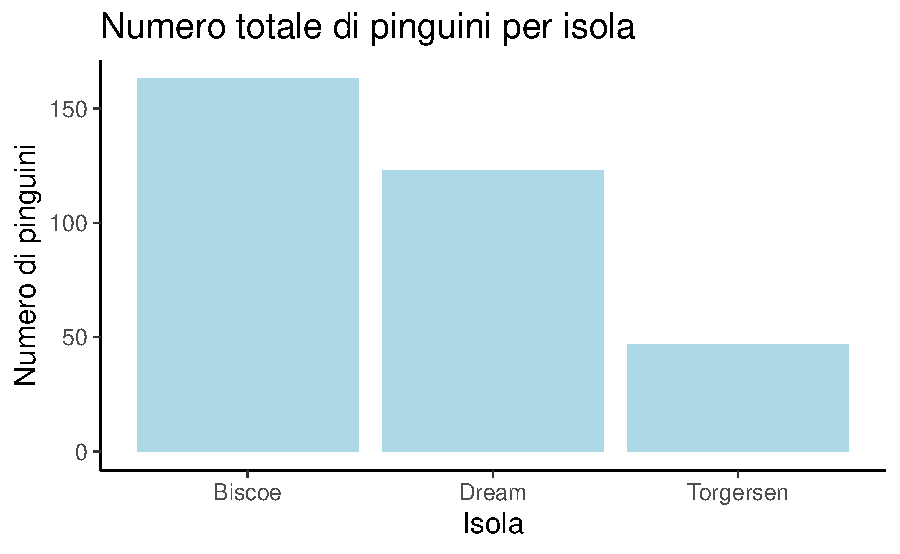
\includegraphics[width=0.7\linewidth,height=\textheight,keepaspectratio]{chapters/eda/04_exploring_qualitative_data_files/figure-pdf/unnamed-chunk-6-1.pdf}
\end{center}

Un secondo grafico a barre mostra il numero totale di pinguini per
specie.

\begin{Shaded}
\begin{Highlighting}[]
\FunctionTok{ggplot}\NormalTok{(df, }\FunctionTok{aes}\NormalTok{(}\AttributeTok{x =}\NormalTok{ species)) }\SpecialCharTok{+}
  \FunctionTok{geom\_bar}\NormalTok{() }\SpecialCharTok{+}
  \FunctionTok{ggtitle}\NormalTok{(}\StringTok{"Numero totale di pinguini per specie"}\NormalTok{) }\SpecialCharTok{+}
  \FunctionTok{xlab}\NormalTok{(}\StringTok{"Specie"}\NormalTok{) }\SpecialCharTok{+}
  \FunctionTok{ylab}\NormalTok{(}\StringTok{"Numero di pinguini"}\NormalTok{)}
\end{Highlighting}
\end{Shaded}

\begin{center}
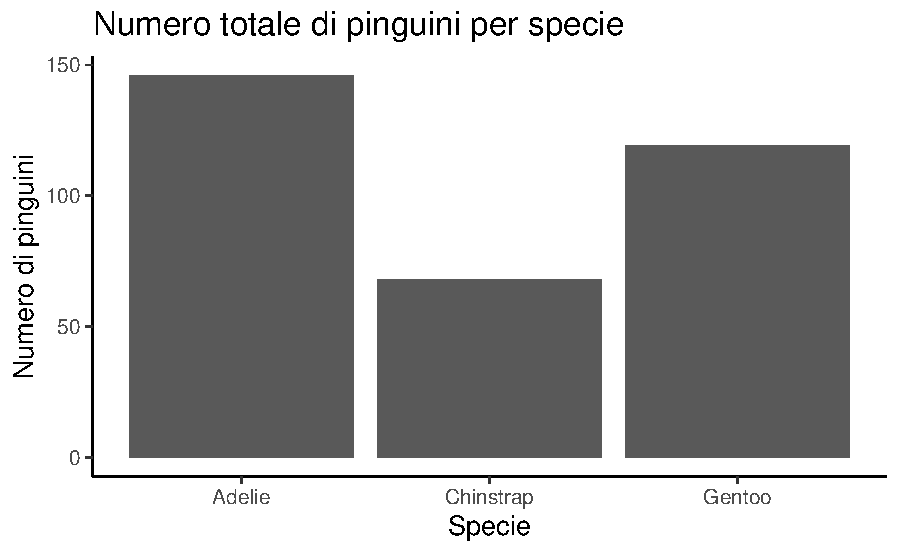
\includegraphics[width=0.7\linewidth,height=\textheight,keepaspectratio]{chapters/eda/04_exploring_qualitative_data_files/figure-pdf/unnamed-chunk-7-1.pdf}
\end{center}

\subsection{Grafico a Barre con Due
Variabili}\label{grafico-a-barre-con-due-variabili}

È possibile visualizzare contemporaneamente le distribuzioni di due
variabili categoriali utilizzando un grafico a barre. Questo tipo di
grafico è particolarmente utile per esaminare la relazione tra due
variabili categoriali.

In un grafico a barre con due variabili, una delle variabili viene
rappresentata sull'asse orizzontale come categoria principale, mentre la
seconda variabile è distinta tramite colori diversi o barre impilate. In
questo modo, possiamo confrontare facilmente le frequenze o le
proporzioni delle categorie della prima variabile, osservando allo
stesso tempo come sono distribuite le categorie della seconda variabile
all'interno di ciascuna categoria principale.

Ad esempio, visualizziamo il numero di pinguini per specie e isola. A
qusto fine possiamo creare un grafico a barre dove le isole sono
rappresentate sull'asse delle ascisse e i diversi colori delle barre
mostrano la distribuzione delle specie su ciascuna isola. Questo
approccio consente di esplorare come le due variabili categoriali
(specie e isola) interagiscono visivamente.

\begin{Shaded}
\begin{Highlighting}[]
\FunctionTok{ggplot}\NormalTok{(df, }\FunctionTok{aes}\NormalTok{(}\AttributeTok{x =}\NormalTok{ island, }\AttributeTok{fill =}\NormalTok{ species)) }\SpecialCharTok{+}
  \FunctionTok{geom\_bar}\NormalTok{(}\AttributeTok{position =} \StringTok{"stack"}\NormalTok{) }\SpecialCharTok{+}
  \FunctionTok{ggtitle}\NormalTok{(}\StringTok{"Numero di pinguini per specie e isola"}\NormalTok{) }\SpecialCharTok{+}
  \FunctionTok{xlab}\NormalTok{(}\StringTok{"Isola"}\NormalTok{) }\SpecialCharTok{+}
  \FunctionTok{ylab}\NormalTok{(}\StringTok{"Numero di pinguini"}\NormalTok{) }\SpecialCharTok{+}
  \FunctionTok{labs}\NormalTok{(}\AttributeTok{fill =} \StringTok{"Specie"}\NormalTok{) }
\end{Highlighting}
\end{Shaded}

\begin{center}
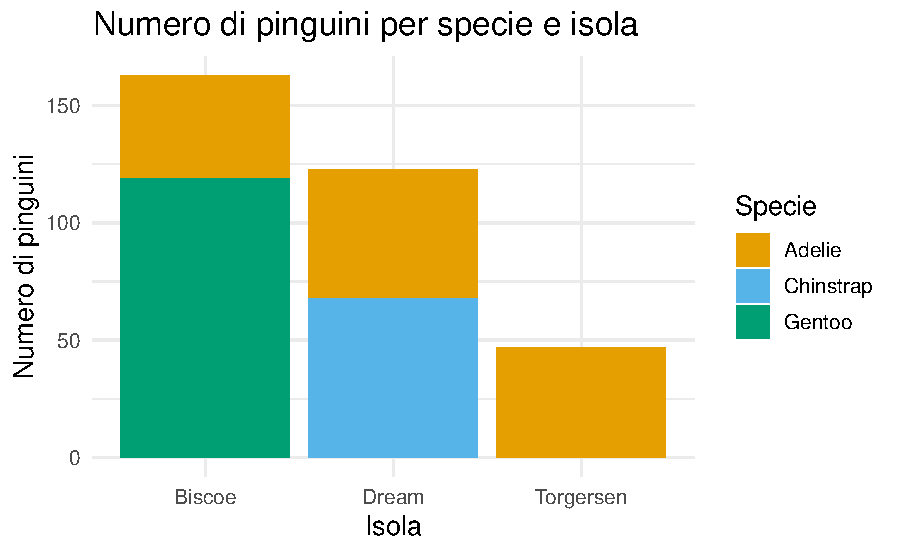
\includegraphics[width=0.7\linewidth,height=\textheight,keepaspectratio]{chapters/eda/04_exploring_qualitative_data_files/figure-pdf/unnamed-chunk-8-1.pdf}
\end{center}

In alternativa, è possibile creare un grafico a barre dove le specie
sono rappresentate sull'asse delle ascisse e i diversi colori delle
barre mostrano la distribuzione delle isole per ciascuna specie.

\begin{Shaded}
\begin{Highlighting}[]
\FunctionTok{ggplot}\NormalTok{(df, }\FunctionTok{aes}\NormalTok{(}\AttributeTok{x =}\NormalTok{ species, }\AttributeTok{fill =}\NormalTok{ island)) }\SpecialCharTok{+}
  \FunctionTok{geom\_bar}\NormalTok{(}\AttributeTok{position =} \StringTok{"stack"}\NormalTok{) }\SpecialCharTok{+}
  \FunctionTok{ggtitle}\NormalTok{(}\StringTok{"Numero di pinguini per isola e specie"}\NormalTok{) }\SpecialCharTok{+}
  \FunctionTok{xlab}\NormalTok{(}\StringTok{"Specie"}\NormalTok{) }\SpecialCharTok{+}
  \FunctionTok{ylab}\NormalTok{(}\StringTok{"Numero di pinguini"}\NormalTok{) }\SpecialCharTok{+}
  \FunctionTok{labs}\NormalTok{(}\AttributeTok{fill =} \StringTok{"Isola"}\NormalTok{)}
\end{Highlighting}
\end{Shaded}

\begin{center}
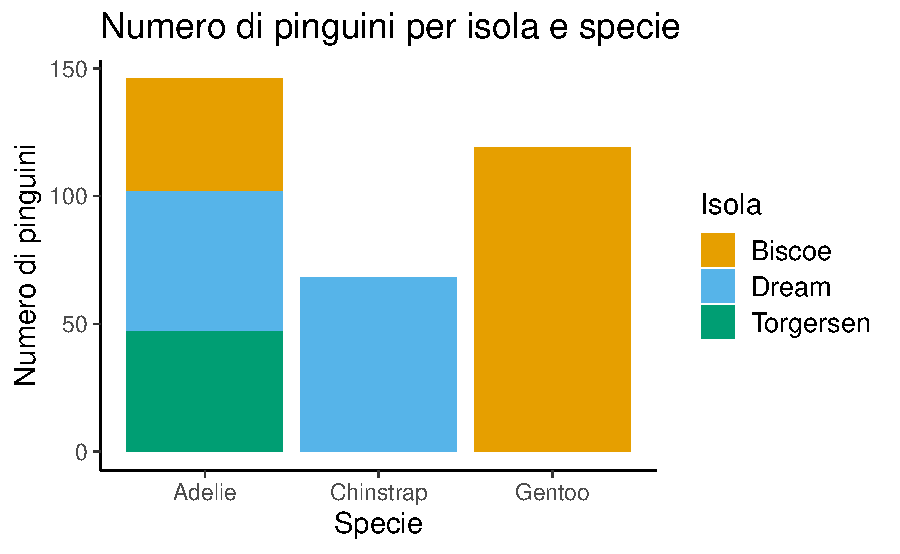
\includegraphics[width=0.7\linewidth,height=\textheight,keepaspectratio]{chapters/eda/04_exploring_qualitative_data_files/figure-pdf/unnamed-chunk-9-1.pdf}
\end{center}

In alternativa all'uso delle frequenze assolute, possiamo rappresentare
i dati utilizzando le frequenze relative. Questo approccio permette di
confrontare meglio le categorie indipendentemente dal numero totale di
osservazioni. Nella figura seguente, ad esempio, viene mostrata la
proporzione di pinguini di ciascuna specie per ogni isola, evidenziando
la distribuzione relativa delle specie su ogni isola, anziché il
conteggio assoluto. Questa rappresentazione aiuta a visualizzare le
differenze nella composizione delle specie, anche se il numero
complessivo di pinguini varia tra le isole.

\begin{Shaded}
\begin{Highlighting}[]
\FunctionTok{ggplot}\NormalTok{(df, }\FunctionTok{aes}\NormalTok{(}\AttributeTok{x =}\NormalTok{ island, }\AttributeTok{fill =}\NormalTok{ species)) }\SpecialCharTok{+}
  \FunctionTok{geom\_bar}\NormalTok{(}\AttributeTok{position =} \StringTok{"fill"}\NormalTok{) }\SpecialCharTok{+}
  \FunctionTok{ggtitle}\NormalTok{(}\StringTok{"Proporzione di pinguini per specie e isola"}\NormalTok{) }\SpecialCharTok{+}
  \FunctionTok{xlab}\NormalTok{(}\StringTok{"Isola"}\NormalTok{) }\SpecialCharTok{+}
  \FunctionTok{ylab}\NormalTok{(}\StringTok{"Proporzione"}\NormalTok{) }\SpecialCharTok{+}
  \FunctionTok{labs}\NormalTok{(}\AttributeTok{fill =} \StringTok{"Specie"}\NormalTok{)}
\end{Highlighting}
\end{Shaded}

\begin{center}
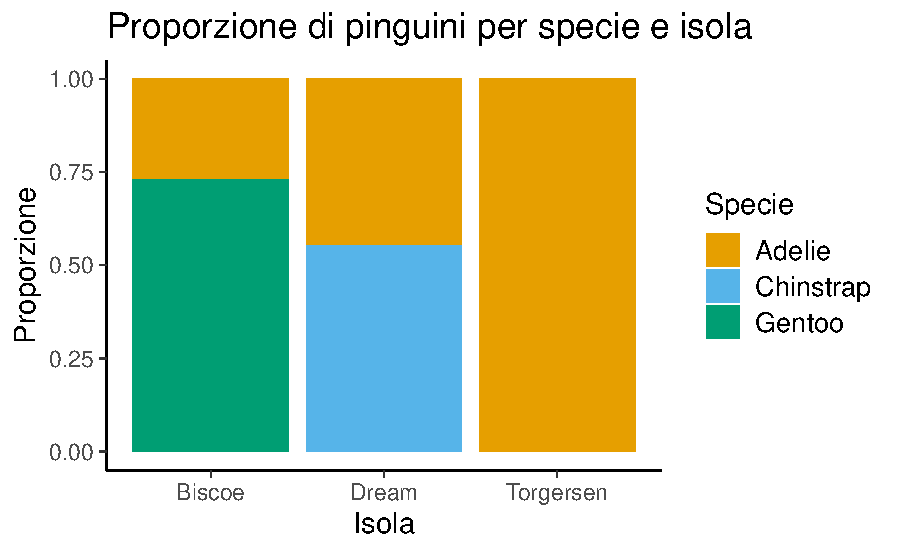
\includegraphics[width=0.7\linewidth,height=\textheight,keepaspectratio]{chapters/eda/04_exploring_qualitative_data_files/figure-pdf/unnamed-chunk-10-1.pdf}
\end{center}

\section{Mosaic plots}\label{mosaic-plots}

Il \emph{Mosaic plot} è una tecnica di visualizzazione particolarmente
adatta per rappresentare tabelle di contingenza. Questo tipo di grafico
somiglia a un grafico a barre impilate standard, ma con un vantaggio
importante: oltre a visualizzare la suddivisione interna delle
categorie, permette di vedere anche le dimensioni relative dei gruppi
della variabile principale.

In altre parole, il Mosaic plot non solo mostra come si distribuiscono
le categorie di una variabile secondaria all'interno di ogni gruppo
della variabile principale, ma fornisce anche un'idea visiva della
grandezza complessiva dei gruppi. Questo lo rende uno strumento utile
per analizzare e interpretare le relazioni tra due variabili
categoriali, evidenziando sia la proporzione all'interno di ciascun
gruppo, sia la grandezza relativa tra i gruppi stessi.

\begin{Shaded}
\begin{Highlighting}[]
\FunctionTok{mosaic}\NormalTok{(}
  \SpecialCharTok{\textasciitilde{}}\NormalTok{ species }\SpecialCharTok{+}\NormalTok{ island, }
  \AttributeTok{data =}\NormalTok{ df, }
  \AttributeTok{main =} \StringTok{"Mosaic Plot of Species and Island"}\NormalTok{,}
  \AttributeTok{shade =} \ConstantTok{TRUE}
\NormalTok{)}
\end{Highlighting}
\end{Shaded}

\begin{center}
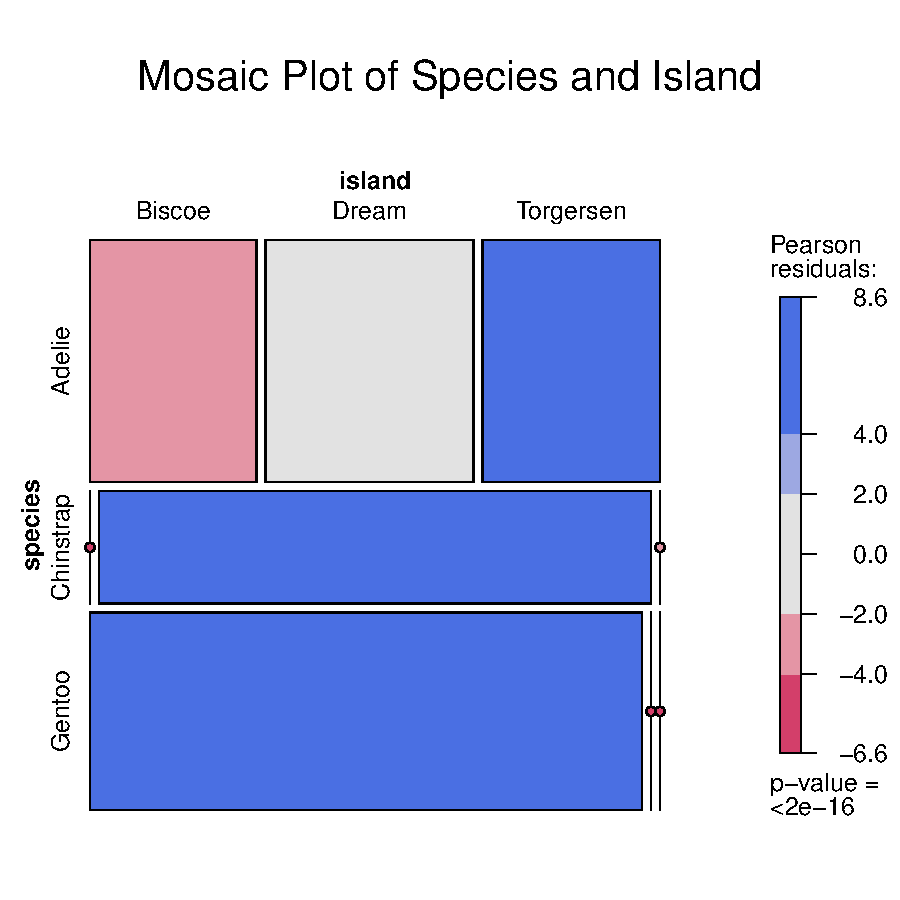
\includegraphics[width=0.7\linewidth,height=\textheight,keepaspectratio]{chapters/eda/04_exploring_qualitative_data_files/figure-pdf/unnamed-chunk-11-1.pdf}
\end{center}

\begin{itemize}
\tightlist
\item
  \textbf{\texttt{island}}: Variabile rappresentata come suddivisione
  orizzontale all'interno di ogni gruppo di \texttt{species} (variabile
  principale).
\item
  \textbf{\texttt{species}}: Variabile rappresentata lungo l'asse
  verticale (variabile secondaria suddivisa all'interno di ogni gruppo
  di \texttt{island}).
\end{itemize}

\subsubsection{Interpretazione}\label{interpretazione}

\begin{enumerate}
\def\labelenumi{\arabic{enumi}.}
\tightlist
\item
  \textbf{Dimensione dei Rettangoli}:

  \begin{itemize}
  \tightlist
  \item
    La \textbf{larghezza} dei rettangoli corrisponde alla dimensione
    relativa dei gruppi della variabile \texttt{island}.
  \item
    L'\textbf{altezza} dei rettangoli rappresenta la proporzione delle
    categorie di \texttt{species} all'interno di ciascun gruppo di
    \texttt{island}.
  \end{itemize}
\item
  \textbf{Colorazione (se \texttt{shade\ =\ TRUE})}:

  \begin{itemize}
  \tightlist
  \item
    I colori indicano deviazioni rispetto all'indipendenza statistica
    tra le variabili.
  \item
    Un rettangolo scuro rappresenta una frequenza maggiore o minore di
    quella attesa in caso di indipendenza tra \texttt{species} e
    \texttt{island}.
  \end{itemize}
\item
  \textbf{Osservazioni Specifiche}:

  \begin{itemize}
  \tightlist
  \item
    \textbf{Rettangoli alti e larghi}: Indicano una categoria di
    \texttt{species} molto rappresentata su un'isola specifica.
  \item
    \textbf{Rettangoli sottili o stretti}: Indicano una rappresentazione
    meno significativa o assente di una specie su un'isola.
  \end{itemize}
\end{enumerate}

In conclusione, il Mosaic plot è uno strumento grafico efficace per
analizzare le relazioni tra due variabili categoriali. Ti permette di
esplorare:

\begin{enumerate}
\def\labelenumi{\arabic{enumi}.}
\tightlist
\item
  La \textbf{proporzione interna} delle categorie.
\item
  Le \textbf{dimensioni relative} dei gruppi della variabile principale.
\end{enumerate}

Questo grafico è particolarmente utile per individuare schemi o
associazioni, come una specie predominante su un'isola specifica o una
distribuzione equilibrata tra gruppi. La sua rappresentazione intuitiva
lo rende ideale per ricerche in psicologia, scienze sociali e biologia.

\section{Proporzioni di Riga e
Colonna}\label{proporzioni-di-riga-e-colonna}

Nelle sezioni precedenti abbiamo esaminato la visualizzazione di due
variabili categoriali utilizzando grafici a barre e Mosaic plot.
Tuttavia, non abbiamo ancora discusso come vengono calcolate le
proporzioni mostrate in questi grafici. In questa sezione ci
concentreremo sulla suddivisione frazionaria di una variabile rispetto a
un'altra, esplorando come possiamo modificare la nostra tabella di
contingenza per ottenere una visione più dettagliata delle proporzioni.

Questo ci permetterà di comprendere meglio le relazioni tra le due
variabili, visualizzando non solo i conteggi assoluti, ma anche le
proporzioni relative per riga o per colonna. Le proporzioni di riga
mostrano la distribuzione di una variabile all'interno delle categorie
di un'altra, mentre le proporzioni di colonna evidenziano la
distribuzione inversa.

Calcoliamo le proporzioni di specie per isola.

\begin{Shaded}
\begin{Highlighting}[]
\NormalTok{df }\SpecialCharTok{\%\textgreater{}\%}
  \FunctionTok{tabyl}\NormalTok{(island, species) }\SpecialCharTok{\%\textgreater{}\%}  \CommentTok{\# Crea la tabella di contingenza}
  \FunctionTok{adorn\_percentages}\NormalTok{(}\StringTok{"row"}\NormalTok{) }\SpecialCharTok{\%\textgreater{}\%}  \CommentTok{\# Calcola le proporzioni per riga}
  \FunctionTok{adorn\_totals}\NormalTok{(}\StringTok{"col"}\NormalTok{) }\SpecialCharTok{\%\textgreater{}\%}  \CommentTok{\# Aggiunge la colonna dei totali}
  \FunctionTok{adorn\_pct\_formatting}\NormalTok{(}\AttributeTok{digits =} \DecValTok{2}\NormalTok{)  }\CommentTok{\# Formatta le percentuali con 2 decimali}
\CommentTok{\#\textgreater{}     island  Adelie Chinstrap Gentoo   Total}
\CommentTok{\#\textgreater{}     Biscoe  26.99\%     0.00\% 73.01\% 100.00\%}
\CommentTok{\#\textgreater{}      Dream  44.72\%    55.28\%  0.00\% 100.00\%}
\CommentTok{\#\textgreater{}  Torgersen 100.00\%     0.00\%  0.00\% 100.00\%}
\end{Highlighting}
\end{Shaded}

Calcoliamo nuovamente le proporzioni, ma questa volta in funzione delle
colonne (per isola).

\begin{Shaded}
\begin{Highlighting}[]
\NormalTok{df }\SpecialCharTok{|\textgreater{}} 
  \FunctionTok{tabyl}\NormalTok{(island, species) }\SpecialCharTok{|\textgreater{}} 
  \FunctionTok{adorn\_percentages}\NormalTok{(}\StringTok{"col"}\NormalTok{) }\SpecialCharTok{|\textgreater{}} 
  \FunctionTok{adorn\_totals}\NormalTok{(}\StringTok{"row"}\NormalTok{) }\SpecialCharTok{|\textgreater{}} 
  \FunctionTok{adorn\_pct\_formatting}\NormalTok{(}\AttributeTok{digits =} \DecValTok{2}\NormalTok{) }\CommentTok{\# Formatta le percentuali con 2 decimali}
\CommentTok{\#\textgreater{}     island  Adelie Chinstrap  Gentoo}
\CommentTok{\#\textgreater{}     Biscoe  30.14\%     0.00\% 100.00\%}
\CommentTok{\#\textgreater{}      Dream  37.67\%   100.00\%   0.00\%}
\CommentTok{\#\textgreater{}  Torgersen  32.19\%     0.00\%   0.00\%}
\CommentTok{\#\textgreater{}      Total 100.00\%   100.00\% 100.00\%}
\end{Highlighting}
\end{Shaded}

\section{Confronto tra Gruppi}\label{confronto-tra-gruppi}

Alcune delle analisi più interessanti emergono confrontando i dati
numerici tra diversi gruppi. In questa sezione approfondiremo alcune
delle tecniche che abbiamo già esplorato per visualizzare i dati
numerici di più gruppi su uno stesso grafico e introdurremo nuovi metodi
per confrontare i dati numerici tra gruppi. Queste tecniche ci
permetteranno di osservare meglio le differenze e le somiglianze tra
gruppi, mettendo in evidenza tendenze, variazioni e altre
caratteristiche rilevanti.

Qui consideriamo due variabili qualitative. Creiamo un grafico a barre
per confrontare la distribuzione del genere per specie.

\begin{Shaded}
\begin{Highlighting}[]
\FunctionTok{ggplot}\NormalTok{(df, }\FunctionTok{aes}\NormalTok{(}\AttributeTok{x =}\NormalTok{ species, }\AttributeTok{fill =}\NormalTok{ sex)) }\SpecialCharTok{+}
  \FunctionTok{geom\_bar}\NormalTok{(}\AttributeTok{position =} \StringTok{"dodge"}\NormalTok{) }\SpecialCharTok{+}
  \FunctionTok{ggtitle}\NormalTok{(}\StringTok{"Distribuzione del genere per specie"}\NormalTok{) }\SpecialCharTok{+}
  \FunctionTok{xlab}\NormalTok{(}\StringTok{"Specie"}\NormalTok{) }\SpecialCharTok{+}
  \FunctionTok{ylab}\NormalTok{(}\StringTok{"Conteggio"}\NormalTok{)}
\end{Highlighting}
\end{Shaded}

\begin{center}
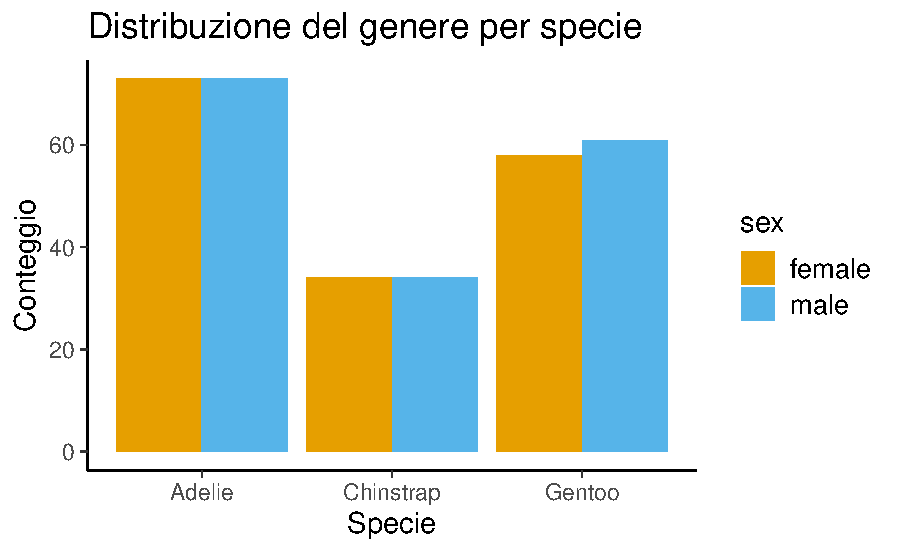
\includegraphics[width=0.7\linewidth,height=\textheight,keepaspectratio]{chapters/eda/04_exploring_qualitative_data_files/figure-pdf/unnamed-chunk-14-1.pdf}
\end{center}

Spesso, i confronti più interessanti riguardano come una variabile
numerica varia in base a una o più categorie. Questo tipo di analisi ci
aiuta a capire differenze tra gruppi e a individuare modelli o tendenze.

Nel grafico seguente, confrontiamo la distribuzione del peso corporeo
(\texttt{body\_mass\_g}) in base alla specie e al genere. Le aree
colorate rappresentano come si distribuisce il peso per maschi e femmine
all'interno di ciascuna specie. Le linee più strette al centro delle
aree colorate aggiungono ulteriori dettagli, mostrando i valori più
comuni e come si concentrano i dati per ciascun gruppo.

\begin{Shaded}
\begin{Highlighting}[]
\FunctionTok{ggplot}\NormalTok{(df, }\FunctionTok{aes}\NormalTok{(}\AttributeTok{x =}\NormalTok{ species, }\AttributeTok{y =}\NormalTok{ body\_mass\_g, }\AttributeTok{fill =}\NormalTok{ sex)) }\SpecialCharTok{+}
  \FunctionTok{geom\_violin}\NormalTok{(}
    \AttributeTok{position =} \FunctionTok{position\_dodge}\NormalTok{(}\AttributeTok{width =} \FloatTok{0.9}\NormalTok{), }\AttributeTok{alpha =} \FloatTok{0.5}
\NormalTok{  ) }\SpecialCharTok{+}
  \FunctionTok{geom\_boxplot}\NormalTok{(}
    \AttributeTok{position =} \FunctionTok{position\_dodge}\NormalTok{(}\AttributeTok{width =} \FloatTok{0.9}\NormalTok{), }\AttributeTok{width =} \FloatTok{0.2}\NormalTok{, }\AttributeTok{alpha =} \FloatTok{0.8}
\NormalTok{  ) }\SpecialCharTok{+}
  \FunctionTok{ggtitle}\NormalTok{(}
    \StringTok{"Distribuzione della massa corporea}\SpecialCharTok{\textbackslash{}n}\StringTok{in base alla specie e al genere"}
\NormalTok{  ) }\SpecialCharTok{+}
  \FunctionTok{xlab}\NormalTok{(}\StringTok{"Specie"}\NormalTok{) }\SpecialCharTok{+}
  \FunctionTok{ylab}\NormalTok{(}\StringTok{"Massa corporea (g)"}\NormalTok{) }\SpecialCharTok{+}
  \FunctionTok{labs}\NormalTok{(}\AttributeTok{fill =} \StringTok{"Genere"}\NormalTok{)}
\end{Highlighting}
\end{Shaded}

\begin{center}
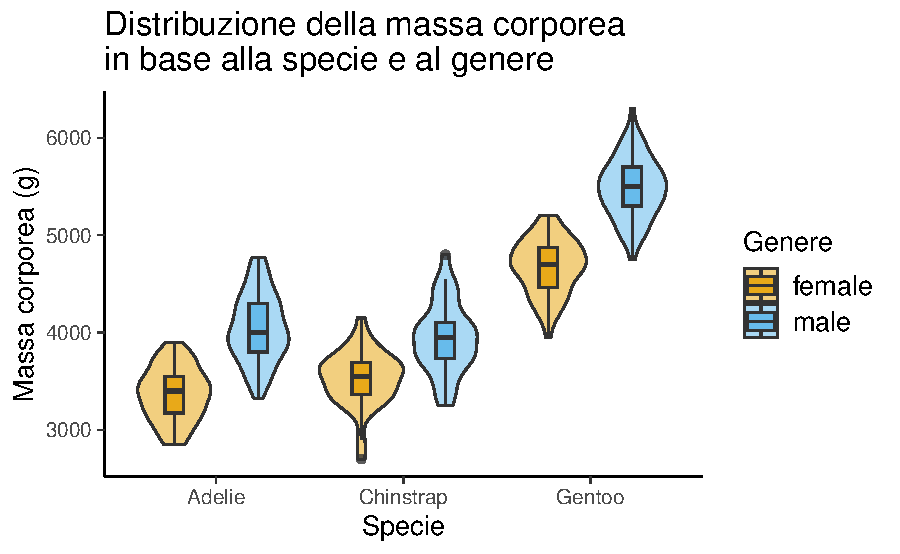
\includegraphics[width=0.7\linewidth,height=\textheight,keepaspectratio]{chapters/eda/04_exploring_qualitative_data_files/figure-pdf/unnamed-chunk-15-1.pdf}
\end{center}

\begin{enumerate}
\def\labelenumi{\arabic{enumi}.}
\tightlist
\item
  \textbf{Aree colorate (grafico a violino)}:

  \begin{itemize}
  \tightlist
  \item
    Rappresentano l'intera distribuzione dei pesi per ogni gruppo
    (specie e genere). Più l'area è larga in un punto, maggiore è il
    numero di pinguini con quel peso.
  \end{itemize}
\item
  \textbf{Linee strette al centro (boxplot)}:

  \begin{itemize}
  \tightlist
  \item
    Forniscono un riassunto visivo dei dati, mostrando dove i pesi si
    concentrano maggiormente e quanto variano all'interno di ciascun
    gruppo.
  \end{itemize}
\item
  \textbf{Cosa possiamo osservare}:

  \begin{itemize}
  \tightlist
  \item
    Possiamo vedere facilmente se i maschi e le femmine di una stessa
    specie tendono ad avere pesi simili o differenti, e se c'è una certa
    sovrapposizione tra i due gruppi.
  \end{itemize}
\end{enumerate}

\section{Esercizi}\label{esercizi-11}

\begin{tcolorbox}[enhanced jigsaw, opacityback=0, bottomrule=.15mm, breakable, title=\textcolor{quarto-callout-important-color}{\faExclamation}\hspace{0.5em}{Problemi}, bottomtitle=1mm, toptitle=1mm, titlerule=0mm, colbacktitle=quarto-callout-important-color!10!white, rightrule=.15mm, colframe=quarto-callout-important-color-frame, colback=white, arc=.35mm, leftrule=.75mm, coltitle=black, left=2mm, toprule=.15mm, opacitybacktitle=0.6]

In questo esercizio analizzerai i dati qualitativi raccolti mediante la
scala SWLS, concentrandoti su due variabili categoriali:

\begin{enumerate}
\def\labelenumi{\arabic{enumi}.}
\tightlist
\item
  \textbf{Genere} (\texttt{gender}): maschio / femmina.
\item
  \textbf{Tipo di scuola superiore} (\texttt{school\_type}): liceo
  classico o scientifico vs tutto il resto.
\end{enumerate}

Dovrai creare tabelle di contingenza e rappresentazioni grafiche per
esplorare le relazioni tra queste variabili.

\textbf{Importazione dei dati}

Importa i dati da un file CSV e visualizza la loro struttura.

\begin{Shaded}
\begin{Highlighting}[]
\FunctionTok{library}\NormalTok{(tidyverse)}
\FunctionTok{library}\NormalTok{(janitor)}
\FunctionTok{library}\NormalTok{(here)}

\CommentTok{\# Importa i dati}
\NormalTok{swls\_data }\OtherTok{\textless{}{-}} \FunctionTok{read\_csv}\NormalTok{(}\FunctionTok{here}\NormalTok{(}\StringTok{"data"}\NormalTok{, }\StringTok{"swls\_students.csv"}\NormalTok{))}

\CommentTok{\# Esamina i dati}
\FunctionTok{glimpse}\NormalTok{(swls\_data)}
\end{Highlighting}
\end{Shaded}

\textbf{Tabelle di Contingenza}

\begin{enumerate}
\def\labelenumi{\arabic{enumi}.}
\tightlist
\item
  Crea una tabella di contingenza tra \texttt{gender} e
  \texttt{school\_type}.
\item
  Calcola le proporzioni di riga e colonna.
\end{enumerate}

\begin{Shaded}
\begin{Highlighting}[]
\CommentTok{\# Tabella di contingenza}
\NormalTok{swls\_data }\SpecialCharTok{|\textgreater{}} 
  \FunctionTok{tabyl}\NormalTok{(gender, school\_type) }\SpecialCharTok{|\textgreater{}} 
  \FunctionTok{adorn\_totals}\NormalTok{(}\FunctionTok{c}\NormalTok{(}\StringTok{"row"}\NormalTok{, }\StringTok{"col"}\NormalTok{))}
\end{Highlighting}
\end{Shaded}

Calcola ora le proporzioni relative.

\begin{Shaded}
\begin{Highlighting}[]
\CommentTok{\# Proporzioni di riga}
\NormalTok{swls\_data }\SpecialCharTok{|\textgreater{}} 
  \FunctionTok{tabyl}\NormalTok{(gender, school\_type) }\SpecialCharTok{|\textgreater{}} 
  \FunctionTok{adorn\_percentages}\NormalTok{(}\StringTok{"row"}\NormalTok{) }\SpecialCharTok{|\textgreater{}} 
  \FunctionTok{adorn\_pct\_formatting}\NormalTok{(}\AttributeTok{digits =} \DecValTok{2}\NormalTok{)}
\end{Highlighting}
\end{Shaded}

\begin{Shaded}
\begin{Highlighting}[]
\CommentTok{\# Proporzioni di colonna}
\NormalTok{swls\_data }\SpecialCharTok{|\textgreater{}} 
  \FunctionTok{tabyl}\NormalTok{(gender, school\_type) }\SpecialCharTok{|\textgreater{}} 
  \FunctionTok{adorn\_percentages}\NormalTok{(}\StringTok{"col"}\NormalTok{) }\SpecialCharTok{|\textgreater{}} 
  \FunctionTok{adorn\_pct\_formatting}\NormalTok{(}\AttributeTok{digits =} \DecValTok{2}\NormalTok{)}
\end{Highlighting}
\end{Shaded}

\textbf{Visualizzazione Grafica}

\begin{enumerate}
\def\labelenumi{\arabic{enumi}.}
\tightlist
\item
  Crea un grafico a barre per visualizzare il numero di studenti per
  tipo di scuola.
\item
  Crea un grafico a barre per la distribuzione del genere per tipo di
  scuola.
\end{enumerate}

\begin{Shaded}
\begin{Highlighting}[]
\FunctionTok{ggplot}\NormalTok{(swls\_data, }\FunctionTok{aes}\NormalTok{(}\AttributeTok{x =}\NormalTok{ school\_type)) }\SpecialCharTok{+}
  \FunctionTok{geom\_bar}\NormalTok{() }\SpecialCharTok{+}
  \FunctionTok{ggtitle}\NormalTok{(}\StringTok{"Numero di studenti per tipo di scuola"}\NormalTok{) }\SpecialCharTok{+}
  \FunctionTok{xlab}\NormalTok{(}\StringTok{"Tipo di scuola"}\NormalTok{) }\SpecialCharTok{+}
  \FunctionTok{ylab}\NormalTok{(}\StringTok{"Numero di studenti"}\NormalTok{)}
\end{Highlighting}
\end{Shaded}

\begin{Shaded}
\begin{Highlighting}[]
\FunctionTok{ggplot}\NormalTok{(swls\_data, }\FunctionTok{aes}\NormalTok{(}\AttributeTok{x =}\NormalTok{ school\_type, }\AttributeTok{fill =}\NormalTok{ gender)) }\SpecialCharTok{+}
  \FunctionTok{geom\_bar}\NormalTok{(}\AttributeTok{position =} \StringTok{"dodge"}\NormalTok{) }\SpecialCharTok{+}
  \FunctionTok{ggtitle}\NormalTok{(}\StringTok{"Distribuzione del genere per tipo di scuola"}\NormalTok{) }\SpecialCharTok{+}
  \FunctionTok{xlab}\NormalTok{(}\StringTok{"Tipo di scuola"}\NormalTok{) }\SpecialCharTok{+}
  \FunctionTok{ylab}\NormalTok{(}\StringTok{"Numero di studenti"}\NormalTok{) }\SpecialCharTok{+}
  \FunctionTok{labs}\NormalTok{(}\AttributeTok{fill =} \StringTok{"Genere"}\NormalTok{)}
\end{Highlighting}
\end{Shaded}

\textbf{Domande per la riflessione}

\begin{itemize}
\tightlist
\item
  Quale tipo di scuola ha il maggior numero di studenti?
\item
  Ci sono differenze nella distribuzione del genere tra i tipi di
  scuola?
\end{itemize}

\textbf{Consegna}

\begin{itemize}
\tightlist
\item
  Compila il file \texttt{.qmd} con il tuo codice e commenti.
\item
  Esporta il documento in formato HTML o PDF.
\item
  Carica il file su Moodle.
\end{itemize}

\end{tcolorbox}

\section*{Informazioni sull'Ambiente di
Sviluppo}\label{informazioni-sullambiente-di-sviluppo-7}
\addcontentsline{toc}{section}{Informazioni sull'Ambiente di Sviluppo}

\markright{Informazioni sull'Ambiente di Sviluppo}

\begin{Shaded}
\begin{Highlighting}[]
\FunctionTok{sessionInfo}\NormalTok{()}
\CommentTok{\#\textgreater{} R version 4.4.2 (2024{-}10{-}31)}
\CommentTok{\#\textgreater{} Platform: aarch64{-}apple{-}darwin20}
\CommentTok{\#\textgreater{} Running under: macOS Sequoia 15.3.1}
\CommentTok{\#\textgreater{} }
\CommentTok{\#\textgreater{} Matrix products: default}
\CommentTok{\#\textgreater{} BLAS:   /Library/Frameworks/R.framework/Versions/4.4{-}arm64/Resources/lib/libRblas.0.dylib }
\CommentTok{\#\textgreater{} LAPACK: /Library/Frameworks/R.framework/Versions/4.4{-}arm64/Resources/lib/libRlapack.dylib;  LAPACK version 3.12.0}
\CommentTok{\#\textgreater{} }
\CommentTok{\#\textgreater{} locale:}
\CommentTok{\#\textgreater{} [1] C/UTF{-}8/C/C/C/C}
\CommentTok{\#\textgreater{} }
\CommentTok{\#\textgreater{} time zone: Europe/Rome}
\CommentTok{\#\textgreater{} tzcode source: internal}
\CommentTok{\#\textgreater{} }
\CommentTok{\#\textgreater{} attached base packages:}
\CommentTok{\#\textgreater{} [1] grid      stats     graphics  grDevices utils     datasets  methods  }
\CommentTok{\#\textgreater{} [8] base     }
\CommentTok{\#\textgreater{} }
\CommentTok{\#\textgreater{} other attached packages:}
\CommentTok{\#\textgreater{}  [1] janitor\_2.2.1     vcd\_1.4{-}13        viridis\_0.6.5     viridisLite\_0.4.2}
\CommentTok{\#\textgreater{}  [5] thematic\_0.1.6    MetBrewer\_0.2.0   ggokabeito\_0.1.0  see\_0.10.0       }
\CommentTok{\#\textgreater{}  [9] gridExtra\_2.3     patchwork\_1.3.0   bayesplot\_1.11.1  psych\_2.4.12     }
\CommentTok{\#\textgreater{} [13] scales\_1.3.0      markdown\_1.13     knitr\_1.49        lubridate\_1.9.4  }
\CommentTok{\#\textgreater{} [17] forcats\_1.0.0     stringr\_1.5.1     dplyr\_1.1.4       purrr\_1.0.4      }
\CommentTok{\#\textgreater{} [21] readr\_2.1.5       tidyr\_1.3.1       tibble\_3.2.1      ggplot2\_3.5.1    }
\CommentTok{\#\textgreater{} [25] tidyverse\_2.0.0   rio\_1.2.3         here\_1.0.1       }
\CommentTok{\#\textgreater{} }
\CommentTok{\#\textgreater{} loaded via a namespace (and not attached):}
\CommentTok{\#\textgreater{}  [1] gtable\_0.3.6      xfun\_0.50         lattice\_0.22{-}6    tzdb\_0.4.0       }
\CommentTok{\#\textgreater{}  [5] vctrs\_0.6.5       tools\_4.4.2       generics\_0.1.3    parallel\_4.4.2   }
\CommentTok{\#\textgreater{}  [9] pacman\_0.5.1      pkgconfig\_2.0.3   R.oo\_1.27.0       data.table\_1.16.4}
\CommentTok{\#\textgreater{} [13] lifecycle\_1.0.4   compiler\_4.4.2    farver\_2.1.2      munsell\_0.5.1    }
\CommentTok{\#\textgreater{} [17] mnormt\_2.1.1      snakecase\_0.11.1  htmltools\_0.5.8.1 yaml\_2.3.10      }
\CommentTok{\#\textgreater{} [21] pillar\_1.10.1     MASS\_7.3{-}64       R.utils\_2.12.3    nlme\_3.1{-}167     }
\CommentTok{\#\textgreater{} [25] tidyselect\_1.2.1  digest\_0.6.37     stringi\_1.8.4     labeling\_0.4.3   }
\CommentTok{\#\textgreater{} [29] rprojroot\_2.0.4   fastmap\_1.2.0     colorspace\_2.1{-}1  cli\_3.6.4        }
\CommentTok{\#\textgreater{} [33] magrittr\_2.0.3    withr\_3.0.2       timechange\_0.3.0  rmarkdown\_2.29   }
\CommentTok{\#\textgreater{} [37] zoo\_1.8{-}12        R.methodsS3\_1.8.2 hms\_1.1.3         evaluate\_1.0.3   }
\CommentTok{\#\textgreater{} [41] lmtest\_0.9{-}40     rlang\_1.1.5       glue\_1.8.0        rstudioapi\_0.17.1}
\CommentTok{\#\textgreater{} [45] jsonlite\_1.8.9    R6\_2.6.1}
\end{Highlighting}
\end{Shaded}

\chapter{Esplorare i dati numerici}\label{sec-eda-exploring-num-data}

\begin{tcolorbox}[enhanced jigsaw, opacityback=0, bottomrule=.15mm, breakable, title=\textcolor{quarto-callout-important-color}{\faExclamation}\hspace{0.5em}{In questo capitolo imparerai a}, bottomtitle=1mm, toptitle=1mm, titlerule=0mm, colbacktitle=quarto-callout-important-color!10!white, rightrule=.15mm, colframe=quarto-callout-important-color-frame, colback=white, arc=.35mm, leftrule=.75mm, coltitle=black, left=2mm, toprule=.15mm, opacitybacktitle=0.6]

\begin{itemize}
\tightlist
\item
  costruire e interpretare distribuzioni di frequenza;
\item
  rappresentare e comprendere istogrammi tradizionali e ``lisciati'';
\item
  realizzare e interpretare boxplot e violin plot.
\end{itemize}

\end{tcolorbox}

\begin{tcolorbox}[enhanced jigsaw, opacityback=0, bottomrule=.15mm, breakable, title=\textcolor{quarto-callout-tip-color}{\faLightbulb}\hspace{0.5em}{Prerequisiti}, bottomtitle=1mm, toptitle=1mm, titlerule=0mm, colbacktitle=quarto-callout-tip-color!10!white, rightrule=.15mm, colframe=quarto-callout-tip-color-frame, colback=white, arc=.35mm, leftrule=.75mm, coltitle=black, left=2mm, toprule=.15mm, opacitybacktitle=0.6]

\begin{itemize}
\tightlist
\item
  Leggere l'Appendice Capitolo~\ref{sec-apx-sums} prima di procedere con
  la lettura di questo capitolo.
\item
  Leggere il capitolo
  \href{https://openintro-ims.netlify.app/explore-numerical}{Exploring
  numerical data} di
  \href{https://openintro-ims.netlify.app}{Introduction to Modern
  Statistics (2e)} di Mine Çetinkaya-Rundel e Johanna Hardin.
\end{itemize}

\end{tcolorbox}

\begin{tcolorbox}[enhanced jigsaw, opacityback=0, bottomrule=.15mm, breakable, title=\textcolor{quarto-callout-caution-color}{\faFire}\hspace{0.5em}{Preparazione del Notebook}, bottomtitle=1mm, toptitle=1mm, titlerule=0mm, colbacktitle=quarto-callout-caution-color!10!white, rightrule=.15mm, colframe=quarto-callout-caution-color-frame, colback=white, arc=.35mm, leftrule=.75mm, coltitle=black, left=2mm, toprule=.15mm, opacitybacktitle=0.6]

\begin{Shaded}
\begin{Highlighting}[]
\NormalTok{here}\SpecialCharTok{::}\FunctionTok{here}\NormalTok{(}\StringTok{"code"}\NormalTok{, }\StringTok{"\_common.R"}\NormalTok{) }\SpecialCharTok{|\textgreater{}} 
  \FunctionTok{source}\NormalTok{()}

\CommentTok{\# Load packages}
\ControlFlowTok{if}\NormalTok{ (}\SpecialCharTok{!}\FunctionTok{requireNamespace}\NormalTok{(}\StringTok{"pacman"}\NormalTok{)) }\FunctionTok{install.packages}\NormalTok{(}\StringTok{"pacman"}\NormalTok{)}
\NormalTok{pacman}\SpecialCharTok{::}\FunctionTok{p\_load}\NormalTok{(ggbeeswarm, dslabs, gridExtra)}
\end{Highlighting}
\end{Shaded}

\end{tcolorbox}

\section*{Introduzione}\label{introduzione-15}
\addcontentsline{toc}{section}{Introduzione}

\markright{Introduzione}

In questo capitolo ci concentreremo sull'analisi dei dati numerici. In
particolare, esamineremo le distribuzioni di frequenza e i quantili,
insieme alle tecniche di visualizzazione più comuni, come l'istogramma,
l'istogramma smussato e il box-plot. Tratteremo sia gli aspetti
computazionali che quelli interpretativi di queste misure, fornendo
strumenti utili non solo per una comprensione personale, ma anche per la
comunicazione efficace dei risultati, in particolare con chi utilizza
questi dati per prendere decisioni pratiche nel mondo reale.

\section{I dati sulle aspettative negative nella
depressione}\label{i-dati-sulle-aspettative-negative-nella-depressione}

Consideriamo i dati relativi alle aspettative negative, individuate come
un meccanismo chiave nel mantenimento della depressione
(\citeproc{ref-zetsche_2019future}{Zetsche et al., 2019}). Supponiamo di
voler analizzare la distribuzione di una singola variabile quantitativa.

Importiamo i dati:

\begin{Shaded}
\begin{Highlighting}[]
\NormalTok{df }\OtherTok{\textless{}{-}}\NormalTok{ rio}\SpecialCharTok{::}\FunctionTok{import}\NormalTok{(here}\SpecialCharTok{::}\FunctionTok{here}\NormalTok{(}\StringTok{"data"}\NormalTok{, }\StringTok{"data.mood.csv"}\NormalTok{))}
\end{Highlighting}
\end{Shaded}

Per questo esercizio, ci concentreremo sulle variabili \texttt{esm\_id}
(il codice del soggetto), \texttt{group} (il gruppo) e \texttt{bdi} (il
valore BDI-II).

\begin{Shaded}
\begin{Highlighting}[]
\NormalTok{df }\OtherTok{\textless{}{-}}\NormalTok{ df }\SpecialCharTok{|\textgreater{}} 
\NormalTok{  dplyr}\SpecialCharTok{::}\FunctionTok{select}\NormalTok{(}\StringTok{"esm\_id"}\NormalTok{, }\StringTok{"group"}\NormalTok{, }\StringTok{"bdi"}\NormalTok{)}
\NormalTok{df }\SpecialCharTok{|\textgreater{}} 
  \FunctionTok{head}\NormalTok{()}
\CommentTok{\#\textgreater{}   esm\_id group bdi}
\CommentTok{\#\textgreater{} 1     10   mdd  25}
\CommentTok{\#\textgreater{} 2     10   mdd  25}
\CommentTok{\#\textgreater{} 3     10   mdd  25}
\CommentTok{\#\textgreater{} 4     10   mdd  25}
\CommentTok{\#\textgreater{} 5     10   mdd  25}
\CommentTok{\#\textgreater{} 6     10   mdd  25}
\end{Highlighting}
\end{Shaded}

Se elenchiamo le modalità presenti in \texttt{group} utilizzando il
metodo \texttt{unique()}, scopriamo che corrispondono a \texttt{mdd}
(pazienti) e \texttt{ctl} (controlli sani).

\begin{Shaded}
\begin{Highlighting}[]
\NormalTok{df}\SpecialCharTok{$}\NormalTok{group }\SpecialCharTok{|\textgreater{}} 
  \FunctionTok{unique}\NormalTok{()}
\CommentTok{\#\textgreater{} [1] "mdd" "ctl"}
\end{Highlighting}
\end{Shaded}

Rimuoviamo i duplicati per ottenere un unico valore BDI-II per ogni
soggetto:

\begin{Shaded}
\begin{Highlighting}[]
\NormalTok{df }\OtherTok{\textless{}{-}}\NormalTok{ df[}\SpecialCharTok{!}\FunctionTok{duplicated}\NormalTok{(df), ]}
\end{Highlighting}
\end{Shaded}

Verifichiamo di avere ottenuto il risultato desiderato.

\begin{Shaded}
\begin{Highlighting}[]
\FunctionTok{dim}\NormalTok{(df)}
\CommentTok{\#\textgreater{} [1] 67  3}
\end{Highlighting}
\end{Shaded}

\begin{Shaded}
\begin{Highlighting}[]
\FunctionTok{head}\NormalTok{(df)}
\CommentTok{\#\textgreater{}    esm\_id group bdi}
\CommentTok{\#\textgreater{} 1      10   mdd  25}
\CommentTok{\#\textgreater{} 15      9   mdd  30}
\CommentTok{\#\textgreater{} 30      6   mdd  26}
\CommentTok{\#\textgreater{} 46      7   mdd  35}
\CommentTok{\#\textgreater{} 65     12   mdd  44}
\CommentTok{\#\textgreater{} 83     16   mdd  30}
\end{Highlighting}
\end{Shaded}

Si noti che il nuovo DataFrame (con 67 righe) conserva il ``nome'' delle
righe (ovvero, l'indice di riga) del DataFrame originario (con 1188
righe). Per esempio, il secondo soggetto (con codice identificativo 9)
si trova sulla seconda riga del DataFrame, ma il suo indice di riga è
15. Questo non ha nessuna conseguenza perché non useremo l'indice di
riga nelle analisi seguenti.

Eliminiamo eventuali valori mancanti:

\begin{Shaded}
\begin{Highlighting}[]
\NormalTok{df }\OtherTok{\textless{}{-}}\NormalTok{ df[}\SpecialCharTok{!}\FunctionTok{is.na}\NormalTok{(df}\SpecialCharTok{$}\NormalTok{bdi), ]}
\end{Highlighting}
\end{Shaded}

Otteniamo così il DataFrame finale per gli scopi presenti (66 righe e 3
colonne):

\begin{Shaded}
\begin{Highlighting}[]
\FunctionTok{dim}\NormalTok{(df)}
\CommentTok{\#\textgreater{} [1] 66  3}
\end{Highlighting}
\end{Shaded}

Stampiamo i valori BDI-II presentandoli ordinati dal più piccolo al più
grande:

\begin{Shaded}
\begin{Highlighting}[]
\NormalTok{df}\SpecialCharTok{$}\NormalTok{bdi }\SpecialCharTok{|\textgreater{}} 
  \FunctionTok{sort}\NormalTok{()}
\CommentTok{\#\textgreater{}  [1]  0  0  0  0  0  0  0  0  0  0  0  0  0  0  0  0  0  1  1  1  1  1  1  1}
\CommentTok{\#\textgreater{} [25]  1  2  2  2  2  3  3  3  5  7  9 12 19 22 22 24 25 25 26 26 26 27 27 28}
\CommentTok{\#\textgreater{} [49] 28 30 30 30 31 31 33 33 34 35 35 35 36 39 41 43 43 44}
\end{Highlighting}
\end{Shaded}

Nel linguaggio statistico, un'osservazione rappresenta l'informazione
raccolta da un singolo individuo o entità che partecipa allo studio. Nel
caso del dataset utilizzato da Zetsche et al.
(\citeproc{ref-zetsche_2019future}{2019}), l'unità di osservazione è
costituita dai partecipanti allo studio. Ogni riga del DataFrame,
denominato \texttt{df}, corrisponde quindi a un individuo distinto
incluso nell'analisi.

Le variabili, invece, riflettono le diverse caratteristiche degli
individui o delle entità considerate. Per i dati in esame, questo
concetto si esprime così:

\begin{itemize}
\tightlist
\item
  Ogni colonna di \texttt{df} rappresenta una variabile che descrive una
  specifica proprietà comune ai partecipanti.
\item
  Le variabili sono identificate da etichette nelle colonne, come
  \texttt{esa\_id} (l'identificativo del soggetto), \texttt{mdd} (il
  gruppo di appartenenza), e \texttt{bdi} (il punteggio del test
  BDI-II).
\end{itemize}

In termini simbolisi, per indicare una singola osservazione della
variabile generica \(X\), si utilizza la notazione \(X_i\), dove \(i\)
rappresenta l'indice dell'osservazione. Questo implica che abbiamo un
valore diverso di \(X\) per ogni differente \(i\). Nel caso presente,
con 67 osservazioni, \(i\) varia da 1 a 67. Così, per rappresentare la
seconda osservazione (quella con \(i=2\)), useremo la notazione \(X_2\).

\section{Distribuzioni di frequenza}\label{distribuzioni-di-frequenza}

Come osservato nell'output della sezione precedente, i dati grezzi non
forniscono un'interpretazione immediata. Per rendere i dati più
comprensibili e sintetici, è utile costruire una \textbf{distribuzione
di frequenza}.

Una distribuzione di frequenza mostra quante volte i valori di una
variabile si verificano all'interno di intervalli specifici. Nel caso
dei punteggi BDI-II, possiamo raggruppare i punteggi in quattro classi:

\begin{itemize}
\tightlist
\item
  0--13: depressione minima
\item
  14--19: depressione lieve-moderata
\item
  20--28: depressione moderata-severa
\item
  29--63: depressione severa
\end{itemize}

Ogni classe, denotata come \(\Delta_i\), rappresenta un intervallo di
valori, definito come \([a_i, b_i)\) (aperto a destra) o \((a_i, b_i]\)
(aperto a sinistra), dove \(a_i\) e \(b_i\) sono rispettivamente il
limite inferiore e superiore della classe. A ciascuna classe si associa
un'ampiezza, data da \(b_i - a_i\), e un valore centrale, indicato con
\(\bar{x}_i\). Poiché ogni osservazione \(x_i\) appartiene a una sola
classe \(\Delta_i\), possiamo calcolare le seguenti quantità:

\begin{itemize}
\item
  \textbf{Frequenza assoluta} \(n_i\): il numero di osservazioni che
  rientrano nella classe \(\Delta_i\).

  \begin{itemize}
  \tightlist
  \item
    Proprietà: \(n_1 + n_2 + \dots + n_m = n\), dove \(n\) è il numero
    totale di osservazioni.
  \end{itemize}
\item
  \textbf{Frequenza relativa} \(f_i\): la proporzione di osservazioni in
  ciascuna classe, calcolata come \(f_i = n_i/n\).

  \begin{itemize}
  \tightlist
  \item
    Proprietà: \(f_1 + f_2 + \dots + f_m = 1\).
  \end{itemize}
\item
  \textbf{Frequenza cumulata} \(N_i\): il numero totale di osservazioni
  che rientrano nelle classi fino alla \(i\)-esima inclusa, calcolata
  come \(N_i = \sum_{j=1}^i n_j\).
\item
  \textbf{Frequenza cumulata relativa} \(F_i\): la somma delle frequenze
  relative fino alla \(i\)-esima classe, data da
  \(F_i = \frac{N_i}{n} = \sum_{j=1}^i f_j\).
\end{itemize}

Queste misure permettono di riassumere in modo efficace la distribuzione
dei punteggi e facilitano l'interpretazione delle caratteristiche del
campione.

\subsection{Frequenze Assolute e
Relative}\label{frequenze-assolute-e-relative}

Per ottenere la distribuzione di frequenza assoluta e relativa dei
valori BDI-II nel dataset di Zetsche et al.
(\citeproc{ref-zetsche_2019future}{2019}), è necessario aggiungere al
DataFrame \texttt{df} una colonna contenente una variabile categoriale
che classifichi ciascuna osservazione in una delle quattro classi che
descrivono la gravità della depressione. Questo risultato si ottiene
utilizzando la funzione \texttt{cut()}.

Nella funzione \texttt{cut()}:

\begin{itemize}
\tightlist
\item
  Il primo argomento, \texttt{x}, è un vettore unidimensionale (ad
  esempio, un vettore di tipo \texttt{numeric} o una colonna di un
  DataFrame) che contiene i dati da classificare.
\item
  Il secondo argomento, \texttt{breaks}, definisce gli intervalli delle
  classi, specificandone i limiti inferiori e superiori.
\item
  L'argomento \texttt{include.lowest\ =\ TRUE} garantisce che il limite
  inferiore dell'intervallo più basso sia incluso nella classificazione.
  Nel nostro caso, questo è particolarmente utile per assicurare che i
  valori uguali al limite inferiore siano assegnati correttamente.
\end{itemize}

Di seguito, il codice per aggiungere la variabile categoriale al
DataFrame:

\begin{Shaded}
\begin{Highlighting}[]
\CommentTok{\# Creare una variabile categoriale per classi di depressione}
\NormalTok{df }\OtherTok{\textless{}{-}}\NormalTok{ df }\SpecialCharTok{\%\textgreater{}\%} 
  \FunctionTok{mutate}\NormalTok{(}
    \AttributeTok{bdi\_class =} \FunctionTok{cut}\NormalTok{(}
\NormalTok{      bdi, }
      \AttributeTok{breaks =} \FunctionTok{c}\NormalTok{(}\DecValTok{0}\NormalTok{, }\FloatTok{13.5}\NormalTok{, }\FloatTok{19.5}\NormalTok{, }\FloatTok{28.5}\NormalTok{, }\DecValTok{63}\NormalTok{),}
      \AttributeTok{include.lowest =} \ConstantTok{TRUE}
\NormalTok{    )}
\NormalTok{  )}
\end{Highlighting}
\end{Shaded}

Questo codice suddivide i valori della variabile \texttt{bdi} in quattro
intervalli corrispondenti ai livelli di gravità della depressione:

\begin{itemize}
\tightlist
\item
  0--13: depressione minima
\item
  14--19: depressione lieve-moderata
\item
  20--28: depressione moderata-severa
\item
  29--63: depressione severa
\end{itemize}

Ogni osservazione verrà assegnata al corrispondente intervallo, creando
così una nuova colonna \texttt{bdi\_class} nel DataFrame \texttt{df}.

\subsubsection{Frequenze assolute}\label{frequenze-assolute}

\begin{Shaded}
\begin{Highlighting}[]
\FunctionTok{table}\NormalTok{(df}\SpecialCharTok{$}\NormalTok{bdi\_class)}
\CommentTok{\#\textgreater{} }
\CommentTok{\#\textgreater{}    [0,13.5] (13.5,19.5] (19.5,28.5]   (28.5,63] }
\CommentTok{\#\textgreater{}          36           1          12          17}
\end{Highlighting}
\end{Shaded}

\subsubsection{Frequenze relative}\label{frequenze-relative}

\begin{Shaded}
\begin{Highlighting}[]
\FunctionTok{prop.table}\NormalTok{(}\FunctionTok{table}\NormalTok{(df}\SpecialCharTok{$}\NormalTok{bdi\_class))}
\CommentTok{\#\textgreater{} }
\CommentTok{\#\textgreater{}    [0,13.5] (13.5,19.5] (19.5,28.5]   (28.5,63] }
\CommentTok{\#\textgreater{}     0.54545     0.01515     0.18182     0.25758}
\end{Highlighting}
\end{Shaded}

\subsection{Distribuzioni congiunte}\label{distribuzioni-congiunte}

Le variabili possono anche essere analizzate insieme tramite le
\emph{distribuzioni congiunte di frequenze}. Queste distribuzioni
rappresentano l'insieme delle frequenze assolute o relative ad ogni
possibile combinazione di valori delle variabili. Ad esempio, se
l'insieme di variabili \(V\) è composto da due variabili, \(X\) e \(Y\),
ciascuna delle quali può assumere due valori, 1 e 2, allora una
possibile distribuzione congiunta di frequenze relative per \(V\)
potrebbe essere espressa come \(f(X = 1, Y = 1) = 0.2\),
\(f(X = 1, Y = 2) = 0.1\), \(f(X = 2, Y = 1) = 0.5\), e
\(f(X = 2, Y = 2) = 0.2\). Come nel caso delle distribuzioni di
frequenze relative di una singola variabile, le frequenze relative di
una distribuzione congiunta devono sommare a 1.

Per i dati dell'esempio precedente, la funzione \texttt{prop.table()}
può essere utilizzata anche per produrre questo tipo di tabella: basta
indicare le serie corrispondenti alle variabili considerate come valori
degli argomenti \texttt{bdi\_class} e \texttt{group}.

\begin{Shaded}
\begin{Highlighting}[]
\FunctionTok{prop.table}\NormalTok{(}\FunctionTok{table}\NormalTok{(df}\SpecialCharTok{$}\NormalTok{bdi\_class, df}\SpecialCharTok{$}\NormalTok{group))}
\CommentTok{\#\textgreater{}              }
\CommentTok{\#\textgreater{}                   ctl     mdd}
\CommentTok{\#\textgreater{}   [0,13.5]    0.54545 0.00000}
\CommentTok{\#\textgreater{}   (13.5,19.5] 0.00000 0.01515}
\CommentTok{\#\textgreater{}   (19.5,28.5] 0.00000 0.18182}
\CommentTok{\#\textgreater{}   (28.5,63]   0.00000 0.25758}
\end{Highlighting}
\end{Shaded}

\subsection{La Distribuzione Cumulativa
Empirica}\label{la-distribuzione-cumulativa-empirica}

La \textbf{distribuzione cumulativa empirica} (eCDF, \emph{empirical
Cumulative Distribution Function}) è un modo utile per rappresentare la
distribuzione di dati numerici. Questa funzione indica la proporzione di
dati che sono inferiori o uguali a un certo valore \(a\), per tutti i
possibili valori di \(a\). Matematicamente, la eCDF è definita come:

\[
F(a) = \text{Proporzione dei dati con valore} \leq a.
\]

In altre parole, la eCDF ci dice quale frazione dei dati osservati è
minore o uguale a un determinato valore \(a\). Questo è particolarmente
utile per comprendere come i dati sono distribuiti e per identificare
pattern o caratteristiche specifiche della distribuzione, come la
presenza di bimodalità (cioè, due picchi distinti nella distribuzione).

\subsubsection{\texorpdfstring{Esempio con i dati di Zetsche et al.
(\citeproc{ref-zetsche_2019future}{2019})}{Esempio con i dati di Zetsche et al. (2019)}}\label{esempio-con-i-dati-di-zetsche_2019future}

Nel contesto dei dati di Zetsche et al.
(\citeproc{ref-zetsche_2019future}{2019}), possiamo utilizzare la eCDF
per visualizzare la distribuzione dei punteggi BDI-II. Ecco come viene
rappresentata la eCDF per l'intero dataset:

\begin{Shaded}
\begin{Highlighting}[]
\NormalTok{df }\SpecialCharTok{|\textgreater{}} 
  \FunctionTok{ggplot}\NormalTok{(}\FunctionTok{aes}\NormalTok{(bdi)) }\SpecialCharTok{+} 
  \FunctionTok{stat\_ecdf}\NormalTok{() }\SpecialCharTok{+}
  \FunctionTok{labs}\NormalTok{(}\AttributeTok{x =} \StringTok{"BDI"}\NormalTok{, }\AttributeTok{y =} \StringTok{"F(BDI)"}\NormalTok{)}
\end{Highlighting}
\end{Shaded}

\begin{center}
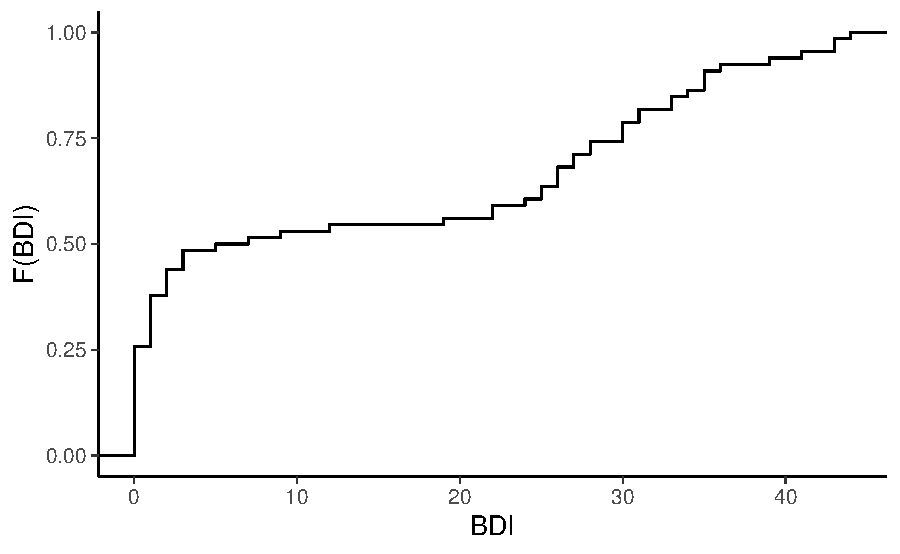
\includegraphics[width=0.7\linewidth,height=\textheight,keepaspectratio]{chapters/eda/05_exploring_numeric_data_files/figure-pdf/unnamed-chunk-15-1.pdf}
\end{center}

In questo grafico:

\begin{itemize}
\tightlist
\item
  L'asse \(x\) rappresenta i valori del BDI-II.
\item
  L'asse \(y\) rappresenta la proporzione cumulativa dei dati, cioè
  \(F(a)\).
\end{itemize}

\subsubsection{Interpretazione del
grafico}\label{interpretazione-del-grafico}

\begin{enumerate}
\def\labelenumi{\arabic{enumi}.}
\tightlist
\item
  \textbf{Crescita della curva}: La curva della eCDF parte da 0 (nessun
  dato è inferiore al valore minimo osservato) e cresce gradualmente
  fino a 1 (tutti i dati sono inferiori o uguali al valore massimo
  osservato).
\item
  \textbf{Bimodalità}: Se la curva presenta dei ``gradini'' o delle aree
  con una pendenza più ripida, questo può indicare la presenza di
  bimodalità, ovvero due gruppi distinti di dati con caratteristiche
  diverse. Nel caso dei dati BDI-II, la bimodalità potrebbe riflettere
  la presenza di due sottogruppi di partecipanti con livelli di
  depressione diversi.
\end{enumerate}

\subsubsection{Filtrare i dati per il campione
clinico}\label{filtrare-i-dati-per-il-campione-clinico}

Se vogliamo analizzare solo i dati relativi al campione clinico (ad
esempio, i pazienti con depressione maggiore), possiamo filtrare i dati
e rappresentare la eCDF solo per questo gruppo:

\begin{Shaded}
\begin{Highlighting}[]
\NormalTok{df }\SpecialCharTok{|\textgreater{}}\NormalTok{ dplyr}\SpecialCharTok{::}\FunctionTok{filter}\NormalTok{(group }\SpecialCharTok{==} \StringTok{"mdd"}\NormalTok{) }\SpecialCharTok{|\textgreater{}} 
  \FunctionTok{ggplot}\NormalTok{(}\FunctionTok{aes}\NormalTok{(bdi)) }\SpecialCharTok{+} 
  \FunctionTok{stat\_ecdf}\NormalTok{() }\SpecialCharTok{+}
  \FunctionTok{labs}\NormalTok{(}\AttributeTok{x =} \StringTok{"a"}\NormalTok{, }\AttributeTok{y =} \StringTok{"F(a)"}\NormalTok{)}
\end{Highlighting}
\end{Shaded}

\begin{center}
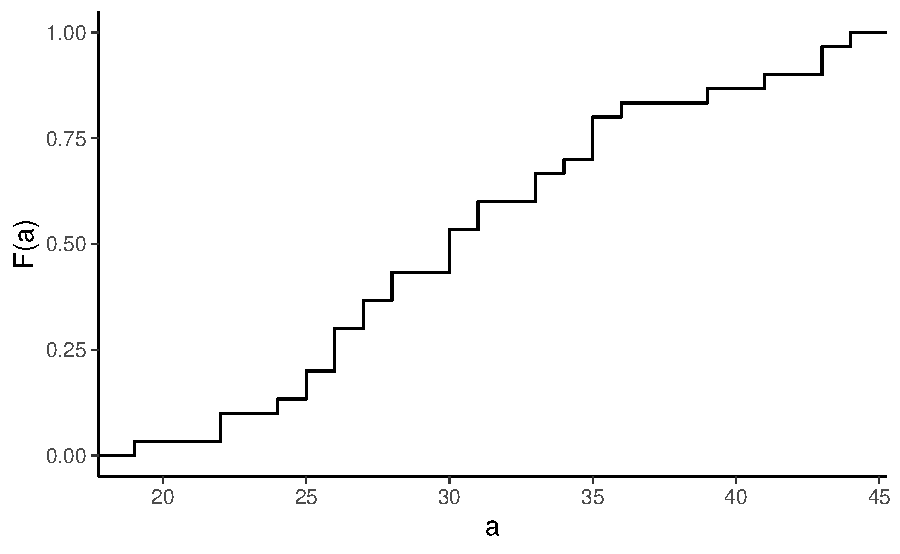
\includegraphics[width=0.7\linewidth,height=\textheight,keepaspectratio]{chapters/eda/05_exploring_numeric_data_files/figure-pdf/unnamed-chunk-16-1.pdf}
\end{center}

In questo caso, la eCDF ci mostrerà come i punteggi BDI-II sono
distribuiti tra i pazienti con depressione maggiore, permettendoci di
identificare eventuali pattern specifici per questo gruppo.

\subsubsection{Vantaggi della eCDF}\label{vantaggi-della-ecdf}

\begin{itemize}
\tightlist
\item
  \textbf{Visualizzazione chiara}: La eCDF fornisce una rappresentazione
  visiva immediata della distribuzione dei dati, evidenziando
  caratteristiche come la bimodalità o la presenza di outlier.
\item
  \textbf{Non parametrica}: La eCDF non assume alcuna forma specifica
  per la distribuzione dei dati, rendendola adatta per analizzare dati
  con distribuzioni complesse o non standard.
\item
  \textbf{Facilità di interpretazione}: La proporzione cumulativa è
  intuitiva e permette di capire rapidamente quanti dati si trovano al
  di sotto di un certo valore.
\end{itemize}

In sintesi, la eCDF è uno strumento potente per analizzare e
visualizzare la distribuzione di dati numerici, specialmente quando si
vogliono identificare pattern specifici o confrontare distribuzioni tra
diversi gruppi.

\section{Istogramma}\label{istogramma}

Sebbene il concetto di Funzione di Distribuzione Empirica Cumulativa
(eCDF) venga ampiamente discusso nei testi di statistica, in pratica
tale rappresentazione non è molto diffusa. Il motivo principale è che
l'eCDF non rende immediatamente visibili alcune caratteristiche
fondamentali della distribuzione, come il valore intorno al quale essa è
centrata, se la distribuzione sia simmetrica o quali intervalli
contengano il 95\% dei dati, ad esempio. Gli istogrammi, invece, sono
molto più utilizzati perché facilitano notevolmente la comprensione di
queste proprietà, sacrificando solo un po' di informazione per fornire
una rappresentazione più intuitiva.

Un \textbf{istogramma} è un grafico che rappresenta la distribuzione
delle frequenze di una variabile. Sull'asse orizzontale (ascisse)
vengono indicati i limiti delle classi \(\Delta_i\), mentre sull'asse
verticale (ordinate) si riporta la densità della frequenza relativa
della variabile \(X\) per ciascuna classe \(\Delta_i\).

Per descrivere formalmente la densità della frequenza relativa, si
utilizza una funzione costante a tratti definita come:

\[
\varphi_n(x) = \frac{f_i}{b_i - a_i},
\]

dove:

\begin{itemize}
\tightlist
\item
  \(f_i\) è la frequenza relativa della classe \(\Delta_i\),
\item
  \(b_i - a_i\) è l'ampiezza della classe \(\Delta_i\).
\end{itemize}

In questo modo, l'area del rettangolo corrispondente a \(\Delta_i\) in
un istogramma risulta proporzionale alla frequenza relativa \(f_i\).
Poiché la somma delle frequenze relative deve essere pari a 1, l'area
totale di un istogramma delle frequenze relative risulta anch'essa
uguale a 1, corrispondendo alla somma delle aree di tutti i rettangoli.

Gli istogrammi costituiscono quindi uno strumento essenziale per
visualizzare e comprendere le principali caratteristiche di una
distribuzione, agevolando l'analisi della sua forma, della sua tendenza
centrale e della sua dispersione.

Per fare un esempio, costruiamo un istogramma per i valori BDI-II di
Zetsche et al. (\citeproc{ref-zetsche_2019future}{2019}). Con i quattro
intervalli individuati dai cut-off del BDI-II creiamo una prima versione
dell'istogramma -- si notino le frequenze assolute sull'asse delle
ordinate.

\begin{Shaded}
\begin{Highlighting}[]
\FunctionTok{ggplot}\NormalTok{(df, }\FunctionTok{aes}\NormalTok{(}\AttributeTok{x =}\NormalTok{ bdi)) }\SpecialCharTok{+}
  \FunctionTok{geom\_histogram}\NormalTok{(}
    \AttributeTok{breaks =} \FunctionTok{c}\NormalTok{(}\DecValTok{0}\NormalTok{, }\FloatTok{13.5}\NormalTok{, }\FloatTok{19.5}\NormalTok{, }\FloatTok{28.5}\NormalTok{, }\DecValTok{63}\NormalTok{),}
    \FunctionTok{aes}\NormalTok{(}\AttributeTok{y =} \FunctionTok{after\_stat}\NormalTok{(density)),}
\NormalTok{  ) }\SpecialCharTok{+}
  \FunctionTok{labs}\NormalTok{(}
    \AttributeTok{title =} \StringTok{"Istogramma delle frequenze relative"}\NormalTok{, }
    \AttributeTok{x =} \StringTok{"BDI{-}II"}\NormalTok{, }
    \AttributeTok{y =} \StringTok{"Densità"}
\NormalTok{  ) }
\end{Highlighting}
\end{Shaded}

\begin{center}
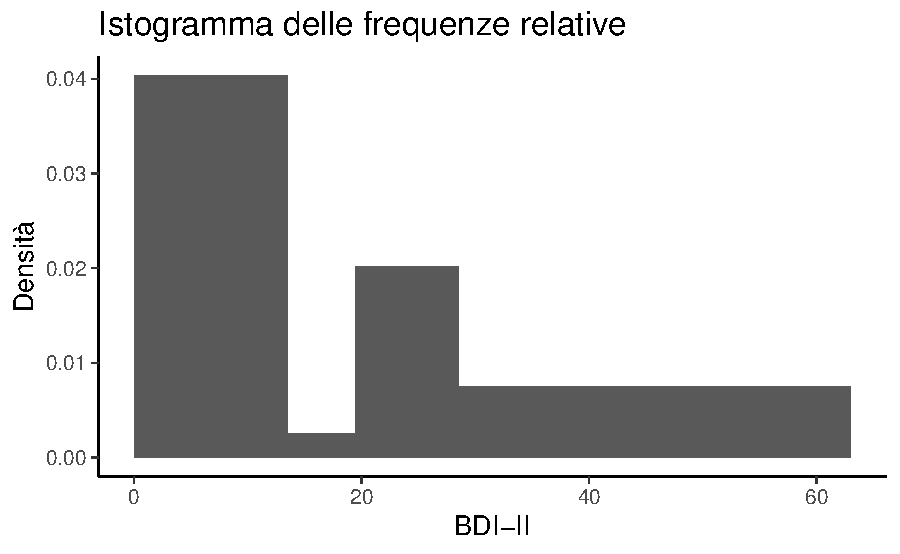
\includegraphics[width=0.7\linewidth,height=\textheight,keepaspectratio]{chapters/eda/05_exploring_numeric_data_files/figure-pdf/unnamed-chunk-17-1.pdf}
\end{center}

Anche se nel caso presente è sensato usare ampiezze diverse per gli
intervalli delle classi, in generale gli istogrammi si costruiscono
utilizzando intervalli riportati sulle ascisse con un'ampiezza uguale.

\begin{Shaded}
\begin{Highlighting}[]
\FunctionTok{ggplot}\NormalTok{(df, }\FunctionTok{aes}\NormalTok{(}\AttributeTok{x =}\NormalTok{ bdi)) }\SpecialCharTok{+}
  \FunctionTok{geom\_histogram}\NormalTok{(}
    \FunctionTok{aes}\NormalTok{(}\AttributeTok{y =} \FunctionTok{after\_stat}\NormalTok{(density)),}
\NormalTok{  ) }\SpecialCharTok{+}
  \FunctionTok{labs}\NormalTok{(}
    \AttributeTok{title =} \StringTok{"Istogramma delle frequenze relative"}\NormalTok{, }
    \AttributeTok{x =} \StringTok{"BDI{-}II"}\NormalTok{, }
    \AttributeTok{y =} \StringTok{"Densità"}
\NormalTok{  )}
\end{Highlighting}
\end{Shaded}

\begin{center}
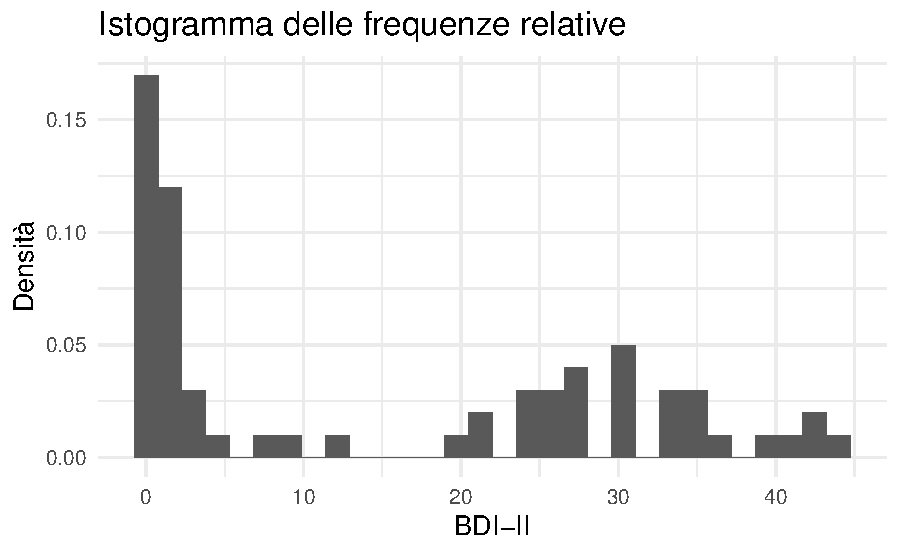
\includegraphics[width=0.7\linewidth,height=\textheight,keepaspectratio]{chapters/eda/05_exploring_numeric_data_files/figure-pdf/unnamed-chunk-18-1.pdf}
\end{center}

\section{Kernel Density Plot}\label{kernel-density-plot}

Un limite evidente degli istogrammi è che la loro forma dipende da
scelte arbitrarie: il numero e l'ampiezza delle classi (o \emph{bin})
può infatti influenzare in modo sostanziale l'aspetto finale del
grafico, rendendo più difficile l'interpretazione della distribuzione
dei dati. Una soluzione a questo problema è offerta dalla \textbf{stima
della densità kernel} (\emph{Kernel Density Estimation}, KDE), un metodo
che fornisce un profilo continuo e smussato della distribuzione, meno
condizionato dall'arbitrarietà delle classi.

\subsection{Differenza tra Istogramma e
KDE}\label{differenza-tra-istogramma-e-kde}

Nell'istogramma, dividiamo l'asse orizzontale in intervalli di ampiezza
prefissata (i \emph{bin}) e costruiamo rettangoli la cui altezza è
proporzionale alla frequenza (o densità) dei dati che ricadono in
ciascun intervallo. Se cambiamo il numero o la larghezza dei bin, la
forma dell'istogramma può variare sensibilmente.

La KDE, invece, non suddivide i dati in intervalli fissi. Al contrario,
``appoggia'' una piccola curva (il \emph{kernel}) su ogni singola
osservazione. Le curve utilizzate (ad esempio di tipo gaussiano) hanno
una larghezza, detta \emph{bandwidth}, che controlla il grado di
\textbf{smussamento}: con un bandwidth molto piccolo, la stima segue da
vicino le singole osservazioni, generando un profilo più frastagliato;
con un bandwidth più ampio, la curva risultante è più liscia, ma rischia
di nascondere dettagli importanti.

Per comprendere in modo intuitivo il concetto di KDE, possiamo partire
da un esempio semplice. Immaginiamo di costruire un istogramma con
classi di ampiezza sempre più piccola. Se avessimo a disposizione un
numero \emph{enorme} di dati (ad esempio, un milione di misurazioni
dell'altezza di individui) e li rappresentassimo con bin sempre più
stretti (0.1, 0.01, ecc.), l'istogramma diventerebbe sempre più
levigato, avvicinandosi a una curva continua. Questo processo illustra
l'idea alla base della KDE, che approssima la distribuzione dei dati in
modo fluido e continuo.

La KDE, tuttavia, opera in modo più elegante e senza richiedere un
numero enorme di punti: posiziona un piccolo ``dosso di campana'' (o un
altro tipo di kernel) su ciascun punto dati e somma tutte queste curve
in un'unica curva finale.

\begin{tcolorbox}[enhanced jigsaw, opacityback=0, bottomrule=.15mm, breakable, title=\textcolor{quarto-callout-note-color}{\faInfo}\hspace{0.5em}{Che cosa vuol dire ``dosso di campana''?}, bottomtitle=1mm, toptitle=1mm, titlerule=0mm, colbacktitle=quarto-callout-note-color!10!white, rightrule=.15mm, colframe=quarto-callout-note-color-frame, colback=white, arc=.35mm, leftrule=.75mm, coltitle=black, left=2mm, toprule=.15mm, opacitybacktitle=0.6]

Possiamo immaginarlo come una piccola curva gaussiana: una curva simile
alla forma di una campana che si innalza e poi discende dolcemente.

\begin{itemize}
\tightlist
\item
  Ogni singolo dato viene ``coperto'' da questa mini-campana.
\item
  L'ampiezza (o ``larghezza'') della campana è regolata dal bandwidth,
  che stabilisce se la curva sarà più o meno ``distesa'' sul grafico.
\item
  Sommando tutte le piccole campane (una per ogni osservazione),
  otteniamo una curva di densità liscia e continua che rappresenta la
  distribuzione dei dati senza i ``salti'' tipici dell'istogramma.
\end{itemize}

\end{tcolorbox}

Il risultato è una \textbf{curva di densità} che:

\begin{enumerate}
\def\labelenumi{\arabic{enumi}.}
\tightlist
\item
  \textbf{È continua}: a differenza degli istogrammi, non presenta
  bruschi salti di altezza tra i bin: la curva scorre in modo uniforme
  lungo tutto l'asse orizzontale.
\item
  \textbf{Mostra la proporzione di dati in ogni intervallo}: l'area
  sotto la curva in un determinato range corrisponde alla percentuale (o
  probabilità) di dati che cadono in quell'intervallo.
\item
  \textbf{Dipende dal bandwidth}:

  \begin{itemize}
  \tightlist
  \item
    Un bandwidth \textbf{piccolo} produce una curva più ondulata e
    ``frastagliata'' (poiché segue da vicino ogni singolo dato).
  \item
    Un bandwidth \textbf{grande} genera una curva più liscia e
    arrotondata, ma rischia di ``coprire'' troppi dettagli della
    distribuzione originaria.
  \end{itemize}
\end{enumerate}

Si noti che la stima della densità kernel introduce, tuttavia,
un'ipotesi di fondo: che la distribuzione dei dati ``reali'' sia
``liscia'' e non presenti discontinuità improvvise. Questo è spesso
ragionevole (ad esempio per dati fisiologici come l'altezza), ma in
altri casi potrebbe non esserlo. È quindi importante scegliere un
bandwidth che rifletta adeguatamente il livello di dettaglio che
vogliamo mostrare.

Inoltre, l'asse delle ordinate (l'asse \emph{y}) rappresenta la densità,
non la frequenza assoluta. È possibile costruire un istogramma in cui
l'altezza dei rettangoli mostra quante osservazioni ricadono in ciascun
bin. Nella KDE, l'altezza della curva è tale che l'area totale sotto di
essa sia pari a 1, rispecchiando la natura di una funzione di densità di
probabilità.

Di seguito esaminiamo un esempio che mostra la costruzione passo dopo
passo di istogrammi con diversi valori di binwidth, fino a passare a una
stima di densità. Consideriemo un dataset con un numero di osservazioni
molto elevato (i valori di altezza, \texttt{heights}, riportati da 1050
partecipanti, estratti dal pacchetto \texttt{dslabs}), suddiviso in due
gruppi: maschi e femmine. Ecco come potremmo prima costruire un
istogramma di altezze per i maschi, per poi tracciare una curva di
densità smussata:

\begin{Shaded}
\begin{Highlighting}[]
\CommentTok{\# Istogramma con bin di ampiezza 1}
\FunctionTok{ggplot}\NormalTok{(heights }\SpecialCharTok{|\textgreater{}}\NormalTok{ dplyr}\SpecialCharTok{::}\FunctionTok{filter}\NormalTok{(sex }\SpecialCharTok{==} \StringTok{"Male"}\NormalTok{), }\FunctionTok{aes}\NormalTok{(height)) }\SpecialCharTok{+}
  \FunctionTok{geom\_histogram}\NormalTok{(}\AttributeTok{binwidth =} \DecValTok{1}\NormalTok{, }\AttributeTok{color =} \StringTok{"black"}\NormalTok{, }\AttributeTok{alpha =} \FloatTok{0.5}\NormalTok{)}

\CommentTok{\# Aggiunta della curva di densità sopra l\textquotesingle{}istogramma}
\FunctionTok{ggplot}\NormalTok{(heights }\SpecialCharTok{|\textgreater{}}\NormalTok{ dplyr}\SpecialCharTok{::}\FunctionTok{filter}\NormalTok{(sex }\SpecialCharTok{==} \StringTok{"Male"}\NormalTok{), }\FunctionTok{aes}\NormalTok{(height)) }\SpecialCharTok{+}
  \FunctionTok{geom\_histogram}\NormalTok{(}
    \FunctionTok{aes}\NormalTok{(}\AttributeTok{y =} \FunctionTok{after\_stat}\NormalTok{(density)), }\AttributeTok{binwidth =} \DecValTok{1}\NormalTok{, }\AttributeTok{color =} \StringTok{"black"}\NormalTok{, }\AttributeTok{alpha =} \FloatTok{0.5}
\NormalTok{  ) }\SpecialCharTok{+}
  \FunctionTok{geom\_line}\NormalTok{(}\AttributeTok{stat =} \StringTok{\textquotesingle{}density\textquotesingle{}}\NormalTok{)}
\end{Highlighting}
\end{Shaded}

\begin{center}
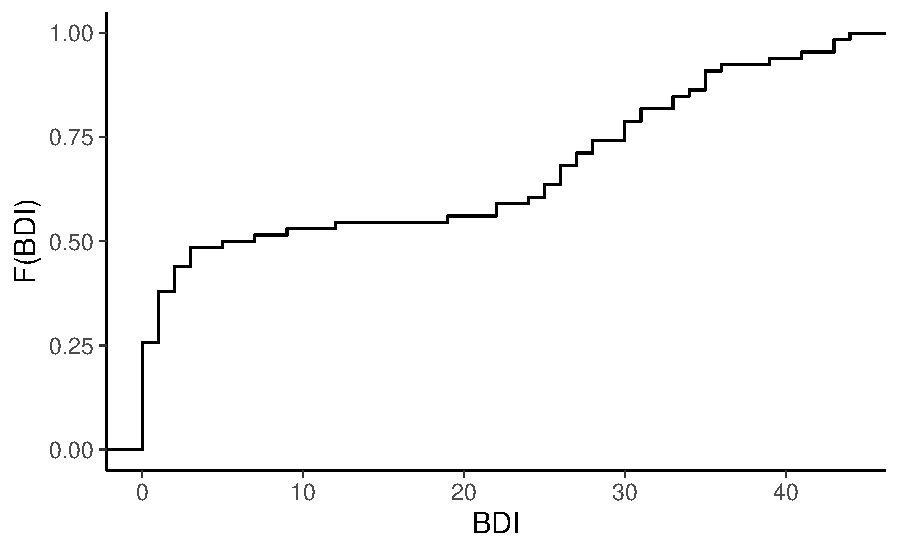
\includegraphics[width=0.7\linewidth,height=\textheight,keepaspectratio]{chapters/eda/05_exploring_numeric_data_files/figure-pdf/unnamed-chunk-19-1.pdf}
\end{center}

\begin{center}
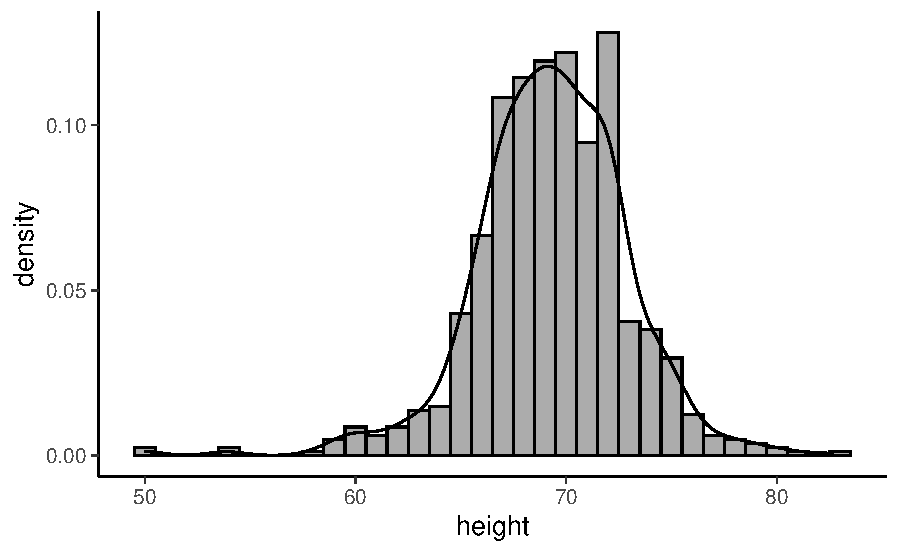
\includegraphics[width=0.7\linewidth,height=\textheight,keepaspectratio]{chapters/eda/05_exploring_numeric_data_files/figure-pdf/unnamed-chunk-19-2.pdf}
\end{center}

Variando il parametro di regolazione (\emph{adjust} o \emph{bandwidth})
nella funzione \texttt{geom\_density()}, possiamo modificare il livello
di smussamento:

\begin{Shaded}
\begin{Highlighting}[]
\CommentTok{\# Esempio di smoothing differente}
\NormalTok{p }\OtherTok{\textless{}{-}} \FunctionTok{ggplot}\NormalTok{(heights }\SpecialCharTok{|\textgreater{}} \FunctionTok{filter}\NormalTok{(sex }\SpecialCharTok{==} \StringTok{"Male"}\NormalTok{), }\FunctionTok{aes}\NormalTok{(height)) }\SpecialCharTok{+}
  \FunctionTok{geom\_histogram}\NormalTok{(}\FunctionTok{aes}\NormalTok{(}\AttributeTok{y =} \FunctionTok{after\_stat}\NormalTok{(density)), }\AttributeTok{binwidth =} \DecValTok{1}\NormalTok{, }\AttributeTok{alpha =} \FloatTok{0.5}\NormalTok{)}

\CommentTok{\# Più ondulato (bandwidth minore)}
\NormalTok{p1 }\OtherTok{\textless{}{-}}\NormalTok{ p }\SpecialCharTok{+} \FunctionTok{geom\_line}\NormalTok{(}\AttributeTok{stat =} \StringTok{\textquotesingle{}density\textquotesingle{}}\NormalTok{, }\AttributeTok{adjust =} \FloatTok{0.5}\NormalTok{)}

\CommentTok{\# Più liscio (bandwidth maggiore)}
\NormalTok{p2 }\OtherTok{\textless{}{-}}\NormalTok{ p }\SpecialCharTok{+} \FunctionTok{geom\_line}\NormalTok{(}\AttributeTok{stat =} \StringTok{\textquotesingle{}density\textquotesingle{}}\NormalTok{, }\AttributeTok{adjust =} \DecValTok{2}\NormalTok{)}

\FunctionTok{grid.arrange}\NormalTok{(p1, p2, }\AttributeTok{ncol =} \DecValTok{2}\NormalTok{)}
\end{Highlighting}
\end{Shaded}

\begin{center}
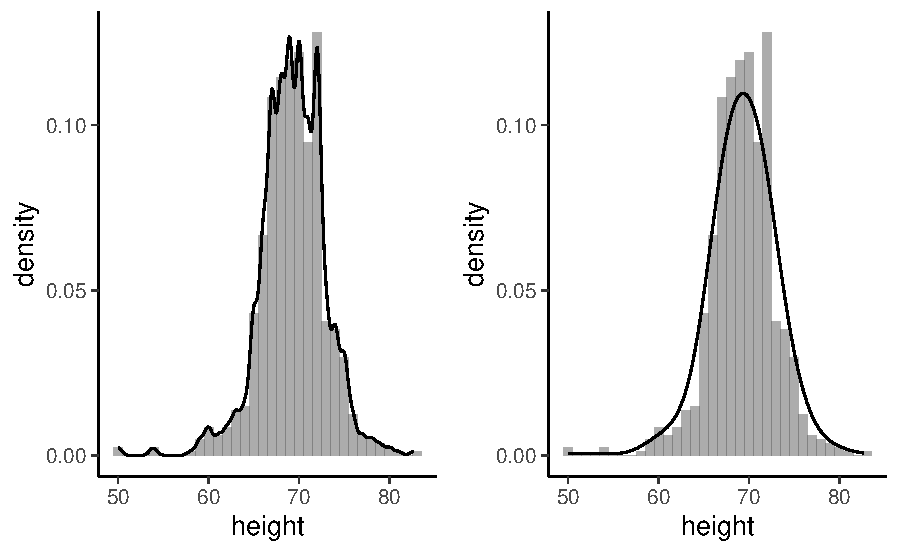
\includegraphics[width=0.7\linewidth,height=\textheight,keepaspectratio]{chapters/eda/05_exploring_numeric_data_files/figure-pdf/unnamed-chunk-20-1.pdf}
\end{center}

Per illustrare ulteriormente l'uso della KDE, ora consideriamo i
punteggi BDI-II di Zetsche et al.
(\citeproc{ref-zetsche_2019future}{2019}). Con il codice seguente
creiamo due curve di densità, una per ogni gruppo:

\begin{Shaded}
\begin{Highlighting}[]
\FunctionTok{ggplot}\NormalTok{(df, }\FunctionTok{aes}\NormalTok{(}\AttributeTok{x =}\NormalTok{ bdi, }\AttributeTok{fill =}\NormalTok{ group)) }\SpecialCharTok{+}
  \FunctionTok{geom\_density}\NormalTok{(}\AttributeTok{alpha =} \FloatTok{0.5}\NormalTok{) }\SpecialCharTok{+}
  \FunctionTok{labs}\NormalTok{(}
    \AttributeTok{title =} \StringTok{"Curva di densità (KDE) per i punteggi BDI{-}II"}\NormalTok{,}
    \AttributeTok{x =} \StringTok{"BDI{-}II"}\NormalTok{,}
    \AttributeTok{y =} \StringTok{"Densità"}
\NormalTok{  )}
\end{Highlighting}
\end{Shaded}

\begin{center}
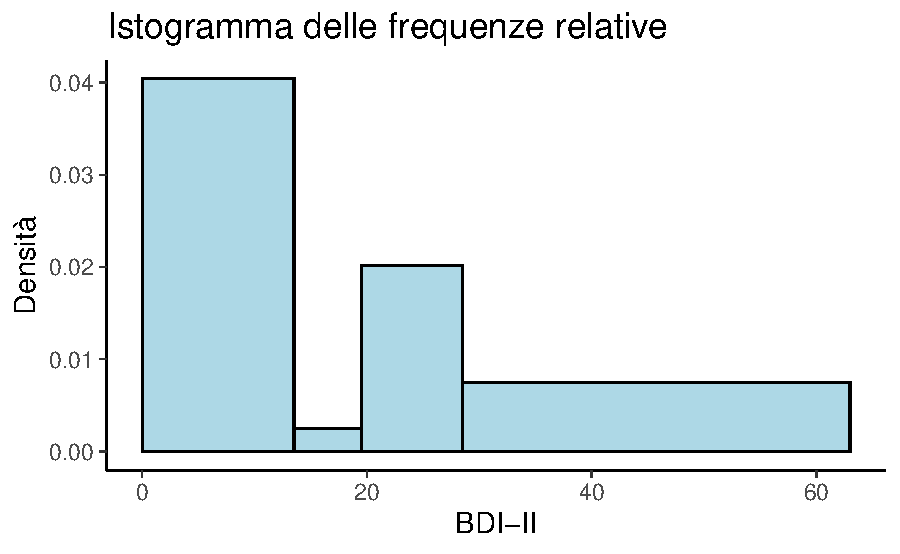
\includegraphics[width=0.7\linewidth,height=\textheight,keepaspectratio]{chapters/eda/05_exploring_numeric_data_files/figure-pdf/unnamed-chunk-21-1.pdf}
\end{center}

Qui, la sovrapposizione delle due curve ci consente di confrontare la
distribuzione dei punteggi BDI-II tra i due gruppi in maniera molto più
\emph{fluida} e intuitiva rispetto a quanto faremmo con due istogrammi
separati o con un istogramma combinato. Inoltre, non siamo più vincolati
alla scelta dei bin: l'aspetto delle curve dipende soltanto dalla
funzione kernel utilizzata e dal parametro di smussamento.

In conclusione,

\begin{itemize}
\tightlist
\item
  l'\textbf{istogramma} rimane uno strumento rapido e intuitivo,
  \emph{privo di assunzioni}, ma sensibile alla scelta di numero e
  ampiezza dei bin;
\item
  la \textbf{stima della densità kernel (KDE)} offre una
  rappresentazione continua della distribuzione dei dati, fornendo un
  quadro più ``morbido'' e spesso più informativo. Tuttavia, introduce
  alcune assunzioni e richiede la scelta del bandwidth ottimale.
\end{itemize}

In definitiva, è consigliabile usare entrambe le tecniche per ottenere
una panoramica completa dei propri dati: l'istogramma permette di dare
un primo sguardo alla loro distribuzione ``grezza'' (senza presupposti),
mentre la KDE aiuta a comprenderne l'eventuale struttura ``liscia'' di
fondo.

\subsection{Area Sottesa alla Curva di Densità: Un'Interpretazione
Probabilistica}\label{area-sottesa-alla-curva-di-densituxe0-uninterpretazione-probabilistica}

Quando si lavora con una curva di densità, è importante capire che
l'area totale sotto la curva rappresenta la probabilità totale, che è
sempre pari a 1 (o 100\%). Questo significa che l'area sotto la curva in
un determinato intervallo corrisponde alla probabilità che un dato
valore cada in quell'intervallo.

\subsubsection{Come Interpretare l'Asse
Y}\label{come-interpretare-lasse-y}

L'asse y di un grafico di densità non rappresenta direttamente la
probabilità, ma è scalato in modo che l'area totale sotto la curva sia
uguale a 1. Se immaginiamo di creare un ``bin'' (un intervallo) con una
base di 1 unità di lunghezza, il valore sull'asse y ci indica la
proporzione di valori che cadono in quel bin. Tuttavia, questa
interpretazione è valida solo per bin di dimensione 1. Per intervalli di
altre dimensioni, il modo migliore per determinare la proporzione di
dati in quell'intervallo è calcolare la proporzione dell'area totale
sotto la curva che cade in quell'intervallo.

\subsubsection{Esempio Pratico}\label{esempio-pratico}

Consideriamo un esempio con i dati delle altezze degli uomini.
Supponiamo di voler sapere quale proporzione di uomini ha un'altezza
compresa tra 65 e 68 pollici. Per farlo, calcoliamo l'area sotto la
curva di densità in quell'intervallo.

Ecco come appare graficamente:

\begin{center}
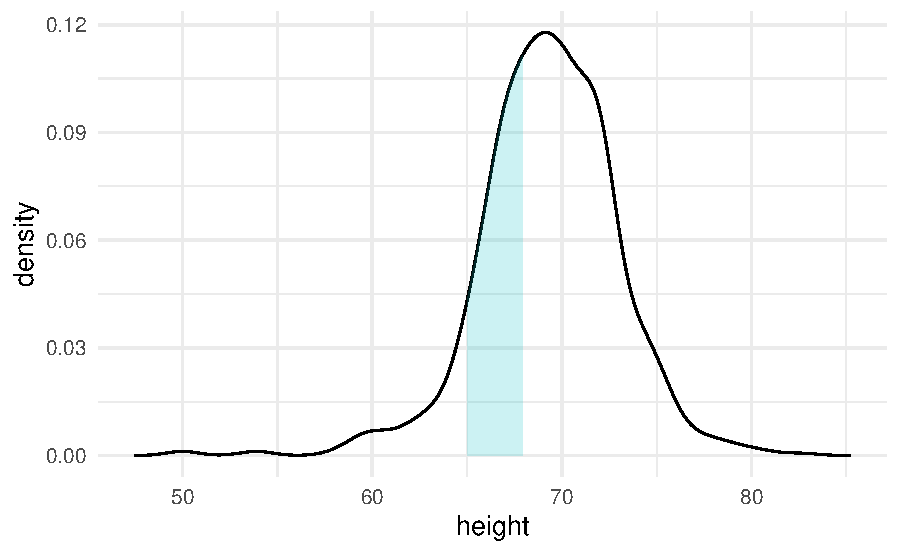
\includegraphics[width=0.7\linewidth,height=\textheight,keepaspectratio]{chapters/eda/05_exploring_numeric_data_files/figure-pdf/summaries-area-under-curve-1.pdf}
\end{center}

L'area evidenziata in azzurro rappresenta la proporzione di uomini con
altezza tra 65 e 68 pollici. Calcolando questa area, troviamo che circa
il 0.3 (ovvero il 30\% degli uomini ha un'altezza in questo intervallo.

\subsubsection{Utilizzo della Curva di Densità come
Riepilogo}\label{utilizzo-della-curva-di-densituxe0-come-riepilogo}

Comprendendo questo concetto, possiamo utilizzare la curva di densità
come un efficace strumento di riepilogo. Per questo dataset,
l'assunzione di smoothness (lisciatura) della curva è ragionevole, e
possiamo condividere questa rappresentazione grafica per comunicare in
modo chiaro e intuitivo la distribuzione delle altezze degli uomini.

Ecco un esempio di come appare la curva di densità smooth per le altezze
degli uomini:

\begin{center}
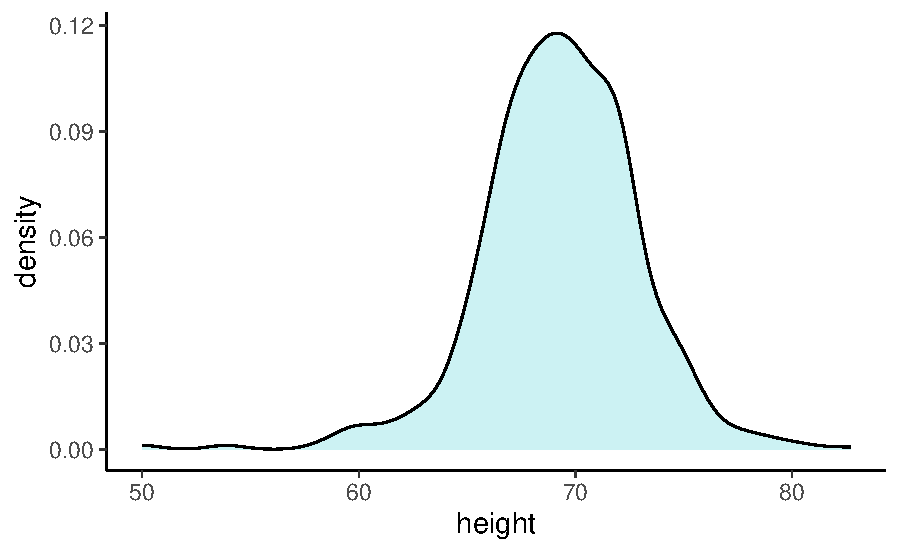
\includegraphics[width=0.7\linewidth,height=\textheight,keepaspectratio]{chapters/eda/05_exploring_numeric_data_files/figure-pdf/summaries-example-of-smoothed-density-2-1.pdf}
\end{center}

In sintesi, l'area sotto la curva di densità in un determinato
intervallo rappresenta la probabilità che un valore casuale cada in
quell'intervallo, rendendo la curva di densità uno strumento potente per
comprendere e comunicare la distribuzione dei dati.

\section{Consigli per Creare Visualizzazioni di Dati
Efficaci}\label{consigli-per-creare-visualizzazioni-di-dati-efficaci}

Ecco alcuni suggerimenti per creare visualizzazioni di dati esplicative,
efficaci e di qualità adatta alle presentazioni:

\begin{enumerate}
\def\labelenumi{\arabic{enumi}.}
\tightlist
\item
  \textbf{Messaggio chiaro}: Assicurati che il grafico trasmetta un
  messaggio chiaro e immediato (ad esempio, ``Il livello di benessere
  psicologico dei partecipanti aumenta nel tempo'').
\item
  \textbf{Uso del colore}:

  \begin{itemize}
  \tightlist
  \item
    Utilizza i colori in modo ponderato e con moderazione.
  \item
    Non eccedere nell'uso dei colori solo perché è possibile farlo.
  \item
    Limita l'uso a non più di cinque o sei colori in una singola figura.
  \item
    Verifica che le scelte cromatiche non distorcano le conclusioni
    della figura.
  \item
    Evita l'uso contemporaneo di rosso e verde nello stesso grafico,
    poiché queste tonalità sono difficili da distinguere per le persone
    daltoniche.
  \end{itemize}
\item
  \textbf{Guidare l'attenzione}:

  \begin{itemize}
  \tightlist
  \item
    Utilizza dimensioni, colori e testo per guidare l'attenzione del
    pubblico.
  \item
    Evidenzia elementi particolari del grafico per enfatizzare punti
    chiave.
  \end{itemize}
\item
  \textbf{Gestione del sovraccarico visivo}:

  \begin{itemize}
  \tightlist
  \item
    Utilizza la trasparenza per ridurre il ``sovrapplotting'' (che si
    verifica quando ci sono molti elementi sovrapposti nel grafico, come
    punti o linee, rendendo difficile individuare i pattern).
  \item
    Questa tecnica è particolarmente utile quando si visualizza una
    grande quantità di dati.
  \item
    Se il dataset è molto ampio e l'aggiunta di trasparenza non è
    sufficiente, considera la visualizzazione di un sottocampione dei
    dati (un campione casuale di punti dati, scelto \emph{senza
    sostituzione}). Questa tecnica è nota come
    \textbf{sottocampionamento}.
  \end{itemize}
\item
  \textbf{Elementi testuali}:

  \begin{itemize}
  \tightlist
  \item
    I titoli, le etichette degli assi e il testo delle legende devono
    essere chiari e facilmente comprensibili.
  \item
    Gli elementi della legenda dovrebbero essere ordinati in modo logico
    e coerente.
  \end{itemize}
\end{enumerate}

\section{Forma di una Distribuzione}\label{forma-di-una-distribuzione}

In statistica, la forma di una distribuzione descrive come i dati sono
distribuiti intorno ai valori centrali. Si distingue tra distribuzioni
simmetriche e asimmetriche, e tra distribuzioni unimodali e multimodali.
Un'illustrazione grafica è fornita nella figura seguente. Nel pannello
1, la distribuzione è unimodale con asimmetria negativa; nel pannello 2,
la distribuzione è unimodale con asimmetria positiva; nel pannello 3, la
distribuzione è simmetrica e unimodale; nel pannello 4, la distribuzione
è bimodale.

\begin{figure}[H]

{\centering 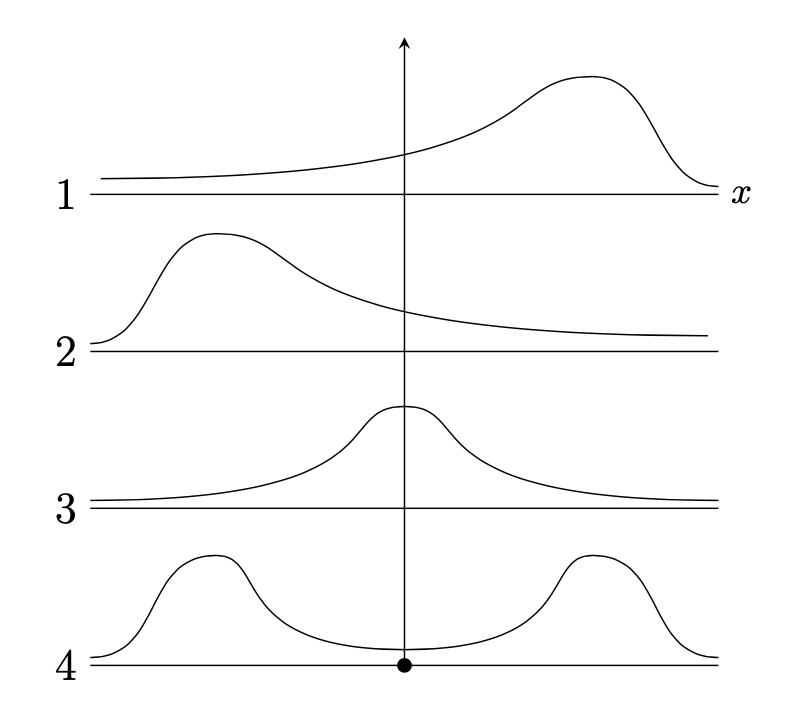
\includegraphics[width=0.55\linewidth,height=\textheight,keepaspectratio]{chapters/eda/../../figures/shape_distribution.png}

}

\caption{Distribuzioni}

\end{figure}%

Il grafico della densità di kernel (Kernel Density Plot) dei valori
BDI-II nel campione di Zetsche et al.
(\citeproc{ref-zetsche_2019future}{2019}) è bimodale. Questo indica che
le osservazioni della distribuzione si raggruppano in due cluster
distinti: un gruppo di osservazioni tende ad avere valori BDI-II bassi,
mentre l'altro gruppo tende ad avere valori BDI-II alti. Questi due
cluster di osservazioni corrispondono al gruppo di controllo e al gruppo
clinico nel campione di dati esaminato da Zetsche et al.
(\citeproc{ref-zetsche_2019future}{2019}).

\section{Indici di posizione}\label{indici-di-posizione}

\subsection{Quantili}\label{quantili}

La distribuzione dei valori BDI-II di Zetsche et al.
(\citeproc{ref-zetsche_2019future}{2019}) può essere sintetizzata
attraverso l'uso dei quantili, che sono valori caratteristici che
suddividono i dati in parti ugualmente numerose. I quartili sono tre
quantili specifici: il primo quartile, \(q_1\), divide i dati in due
parti, lasciando a sinistra il 25\% del campione; il secondo quartile,
\(q_2\), corrisponde alla mediana e divide i dati in due parti uguali;
il terzo quartile lascia a sinistra il 75\% del campione.

Inoltre, ci sono altri indici di posizione chiamati decili e percentili
che suddividono i dati in parti di dimensioni uguali a 10\% e 1\%,
rispettivamente.

Per calcolare i quantili, i dati vengono prima ordinati in modo
crescente e poi viene determinato il valore di \(np\), dove \(n\) è la
dimensione del campione e \(p\) è l'ordine del quantile. Se \(np\) non è
un intero, il valore del quantile corrisponde al valore del dato che si
trova alla posizione successiva alla parte intera di \(np\). Se \(np\) è
un intero, il valore del quantile corrisponde alla media dei dati nelle
posizioni \(k\) e \(k+1\), dove \(k\) è la parte intera di \(np\).

Gli indici di posizione possono essere utilizzati per creare un
box-plot, una rappresentazione grafica della distribuzione dei dati che
è molto popolare e può essere utilizzata in alternativa ad un
istogramma.

Ad esempio, per calcolare la mediana della distribuzione dei nove
soggetti con un unico episodio di depressione maggiore del campione
clinico di Zetsche et al. (\citeproc{ref-zetsche_2019future}{2019}), si
determina il valore di \(np = 9 \cdot 0.5 = 4.5\), che non è un intero.
Pertanto, il valore del secondo quartile è pari al valore del dato che
si trova alla posizione successiva alla parte intera di \(np\), ovvero
\(q_2 = x_{4 + 1} = 27\). Per calcolare il quantile di ordine \(2/3\),
si determina il valore di \(np = 9 \cdot 2/3 = 6\), che è un intero.
Quindi, il valore del quantile corrisponde alla media dei dati nelle
posizioni \(6\) e \(7\), ovvero
\(q_{\frac{2}{3}} = \frac{1}{2} (x_{6} + x_{7}) = \frac{1}{2} (33 + 33) = 33\).

Usiamo \texttt{quantile()} per trovare la soluzione dell'esercizio
precedente.

\begin{Shaded}
\begin{Highlighting}[]
\NormalTok{x }\OtherTok{=} \FunctionTok{c}\NormalTok{(}\DecValTok{19}\NormalTok{, }\DecValTok{26}\NormalTok{, }\DecValTok{27}\NormalTok{, }\DecValTok{28}\NormalTok{, }\DecValTok{28}\NormalTok{, }\DecValTok{33}\NormalTok{, }\DecValTok{33}\NormalTok{, }\DecValTok{41}\NormalTok{, }\DecValTok{43}\NormalTok{)}
\FunctionTok{quantile}\NormalTok{(x, }\DecValTok{2} \SpecialCharTok{/} \DecValTok{3}\NormalTok{)}
\CommentTok{\#\textgreater{} 66.66667\% }
\CommentTok{\#\textgreater{}        33}
\end{Highlighting}
\end{Shaded}

\section{Mostrare i dati}\label{mostrare-i-dati}

\subsection{Diagramma a scatola}\label{diagramma-a-scatola}

Il box plot è uno strumento grafico che visualizza la dispersione di una
distribuzione. I \textbf{boxplot} forniscono una rappresentazione visiva
sintetica di cinque valori caratteristici: \textbf{minimo},
\textbf{primo quartile (25\%)}, \textbf{mediana (50\%)}, \textbf{terzo
quartile (75\%)} e \textbf{massimo}. Spesso però, i boxplot ``ignorano''
i valori considerati anomali (\emph{outlier}), segnalandoli con punti
isolati.

Per creare un box plot, si disegna un rettangolo (la ``scatola'') di
altezza arbitraria, basato sulla distanza interquartile (IQR), che
corrisponde alla differenza tra il terzo quartile (\(q_{0.75}\)) e il
primo quartile (\(q_{0.25}\)). La mediana (\(q_{0.5}\)) è rappresentata
da una linea all'interno del rettangolo.

Ai lati della scatola, vengono tracciati due segmenti di retta, detti
``baffi'', che rappresentano i valori adiacenti inferiore e superiore.
Il valore adiacente inferiore è il valore più basso tra le osservazioni
che è maggiore o uguale al primo quartile meno 1.5 volte la distanza
interquartile. Il valore adiacente superiore è il valore più alto tra le
osservazioni che è minore o uguale al terzo quartile più 1.5 volte la
distanza interquartile.

Se ci sono dei valori che cadono al di fuori dei valori adiacenti,
vengono chiamati ``valori anomali'' e sono rappresentati individualmente
nel box plot per evidenziare la loro presenza e posizione. In questo
modo, il box plot fornisce una rappresentazione visiva della
distribuzione dei dati, permettendo di individuare facilmente eventuali
valori anomali e di comprendere la dispersione dei dati.

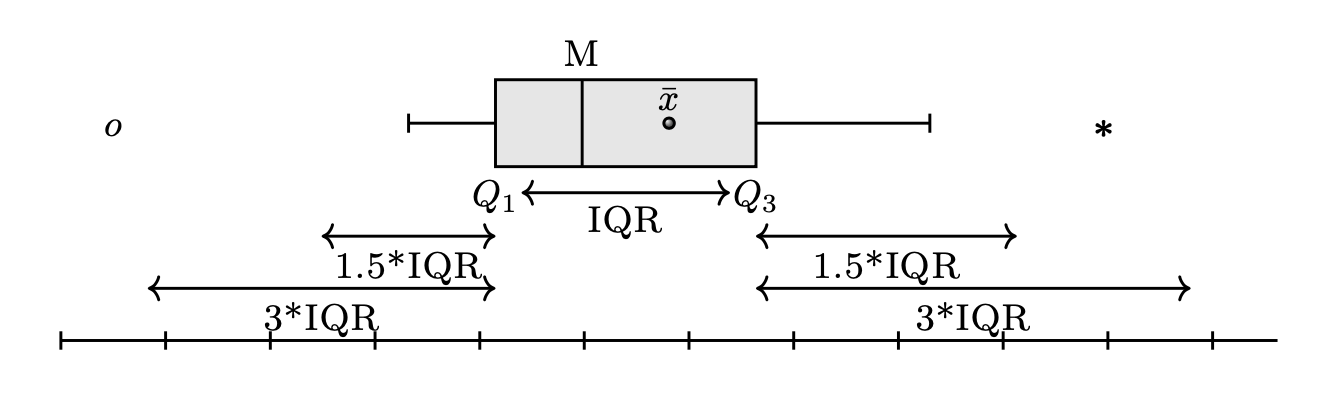
\includegraphics[width=0.8\linewidth,height=\textheight,keepaspectratio]{chapters/eda/../../figures/boxplot.png}

\subsection{Stratificazione}\label{stratificazione}

Nell'analisi dei dati, è comune suddividere le osservazioni in gruppi in
base ai valori di una o più variabili associate a tali osservazioni.
Questo processo è chiamato \textbf{stratificazione}, e i gruppi
risultanti sono detti \textbf{strati}. Ad esempio, nella sezione
successiva, dividiamo i valori dei punteggi BDI-II in due gruppi in base
alla condizione sperimentale: campione clinico e campione di controllo.

La stratificazione è particolarmente utile nella visualizzazione dei
dati, poiché spesso siamo interessati a comprendere come la
distribuzione di una variabile differisca tra diversi sottogruppi.

Per esempio, per rappresentare graficamente la distribuzione dei
punteggi BDI-II nel gruppo dei pazienti e nel gruppo di controllo,
possiamo utilizzare un box-plot. Questo tipo di grafico ci permette di
confrontare visivamente la distribuzione dei punteggi tra i due gruppi,
evidenziando eventuali differenze.

\begin{Shaded}
\begin{Highlighting}[]
\FunctionTok{ggplot}\NormalTok{(df, }\FunctionTok{aes}\NormalTok{(}\AttributeTok{x =}\NormalTok{ group, }\AttributeTok{y =}\NormalTok{ bdi)) }\SpecialCharTok{+}
  \FunctionTok{geom\_boxplot}\NormalTok{() }\SpecialCharTok{+}
  \FunctionTok{labs}\NormalTok{(}
    \AttributeTok{title =} \StringTok{"Box plot per gruppo"}\NormalTok{, }
    \AttributeTok{x =} \StringTok{"Gruppo"}\NormalTok{, }
    \AttributeTok{y =} \StringTok{"BDI{-}II"}
\NormalTok{  )}
\end{Highlighting}
\end{Shaded}

\begin{center}
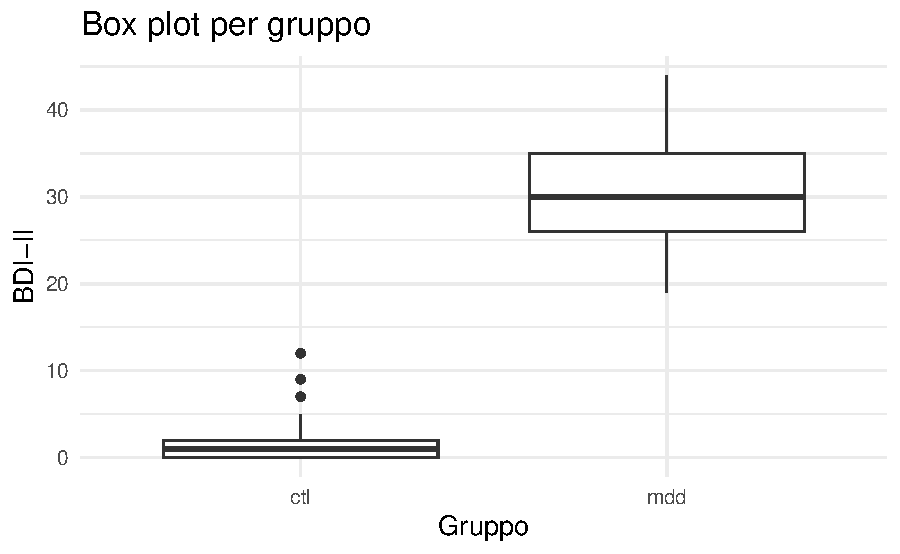
\includegraphics[width=0.7\linewidth,height=\textheight,keepaspectratio]{chapters/eda/05_exploring_numeric_data_files/figure-pdf/unnamed-chunk-23-1.pdf}
\end{center}

In questo grafico:

\begin{itemize}
\tightlist
\item
  L'asse \textbf{x} rappresenta i due gruppi (pazienti e controllo).
\item
  L'asse \textbf{y} rappresenta i punteggi BDI-II.
\item
  I box (scatole) mostrano la distribuzione dei punteggi, con la linea
  centrale che indica la mediana e i ``baffi'' che rappresentano la
  variabilità dei dati.
\end{itemize}

La stratificazione ci aiuta a identificare rapidamente se ci sono
differenze nella distribuzione dei punteggi BDI-II tra i due gruppi. Nel
caso presente, il grafico mostra come non vi sia alcuna sovrapposizione
tra le due distribuzioni.

Un risultato migliore si ottiene utilizzando un grafico a violino
(\emph{violin plot}) e includendo anche i dati grezzi.

\subsection{Grafico a Violino}\label{grafico-a-violino}

I grafici a violino combinano le caratteristiche dei box plot e dei
grafici di densità di kernel (KDE plot) per offrire una rappresentazione
più dettagliata dei dati. A questi grafici vengono sovrapposti i dati
grezzi, fornendo una visione completa della distribuzione e delle
caratteristiche dei dati.

\begin{Shaded}
\begin{Highlighting}[]
\FunctionTok{ggplot}\NormalTok{(df, }\FunctionTok{aes}\NormalTok{(}\AttributeTok{x =}\NormalTok{ group, }\AttributeTok{y =}\NormalTok{ bdi, }\AttributeTok{fill =}\NormalTok{ group)) }\SpecialCharTok{+}
  \FunctionTok{geom\_violin}\NormalTok{() }\SpecialCharTok{+}
  \FunctionTok{geom\_dotplot}\NormalTok{(}
    \AttributeTok{binaxis =} \StringTok{"y"}\NormalTok{,}
    \AttributeTok{stackdir =} \StringTok{"center"}\NormalTok{,}
    \AttributeTok{dotsize =} \FloatTok{0.5}\NormalTok{,}
    \AttributeTok{fill =} \DecValTok{1}
\NormalTok{  ) }\SpecialCharTok{+}
  \FunctionTok{labs}\NormalTok{(}
    \AttributeTok{title =} \StringTok{"Violin plot con overlay dei punti grezzi"}\NormalTok{,}
    \AttributeTok{x =} \StringTok{"Gruppo"}\NormalTok{,}
    \AttributeTok{y =} \StringTok{"BDI{-}II"}
\NormalTok{  )}
\end{Highlighting}
\end{Shaded}

\begin{center}
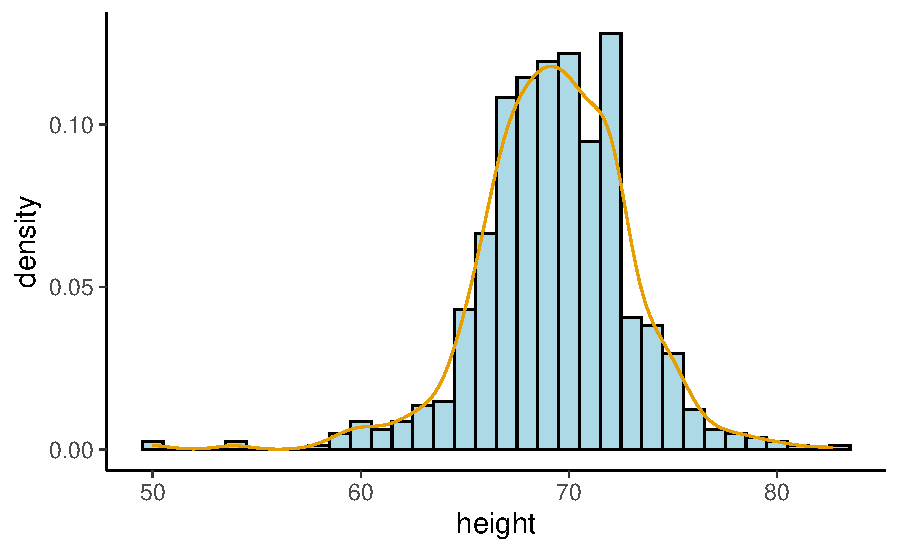
\includegraphics[width=0.7\linewidth,height=\textheight,keepaspectratio]{chapters/eda/05_exploring_numeric_data_files/figure-pdf/unnamed-chunk-24-1.pdf}
\end{center}

\subsection{Grafico Beeswarm}\label{grafico-beeswarm}

Il pacchetto \emph{\{ggbeeswarm\}} include una funzione chiamata
\texttt{geom\_beeswarm}, che può essere utilizzata per creare un grafico
beeswarm in ggplot2.

Un grafico beeswarm è una variazione del grafico a punti che disperde i
dati in modo che non si sovrappongano, rendendo visibili tutti i singoli
punti dati. Questo tipo di visualizzazione è particolarmente utile
quando si desidera esaminare la distribuzione e la densità di un set di
dati, senza ricorrere all'uso di barre d'errore o di scatole e baffi
(boxplot), mantenendo un'alta leggibilità anche quando i set di dati
sono densi.

\begin{Shaded}
\begin{Highlighting}[]
\FunctionTok{ggplot}\NormalTok{(df, }\FunctionTok{aes}\NormalTok{(}\AttributeTok{x =}\NormalTok{ group, }\AttributeTok{y =}\NormalTok{ bdi, }\AttributeTok{color =}\NormalTok{ group)) }\SpecialCharTok{+}
  \FunctionTok{geom\_beeswarm}\NormalTok{(}\AttributeTok{cex =} \DecValTok{3}\NormalTok{) }\SpecialCharTok{+}
  \FunctionTok{labs}\NormalTok{(}
    \AttributeTok{title =} \StringTok{"Violin plot con overlay dei punti grezzi"}\NormalTok{,}
    \AttributeTok{x =} \StringTok{"Gruppo"}\NormalTok{,}
    \AttributeTok{y =} \StringTok{"BDI{-}II"}
\NormalTok{  ) }
\end{Highlighting}
\end{Shaded}

\begin{center}
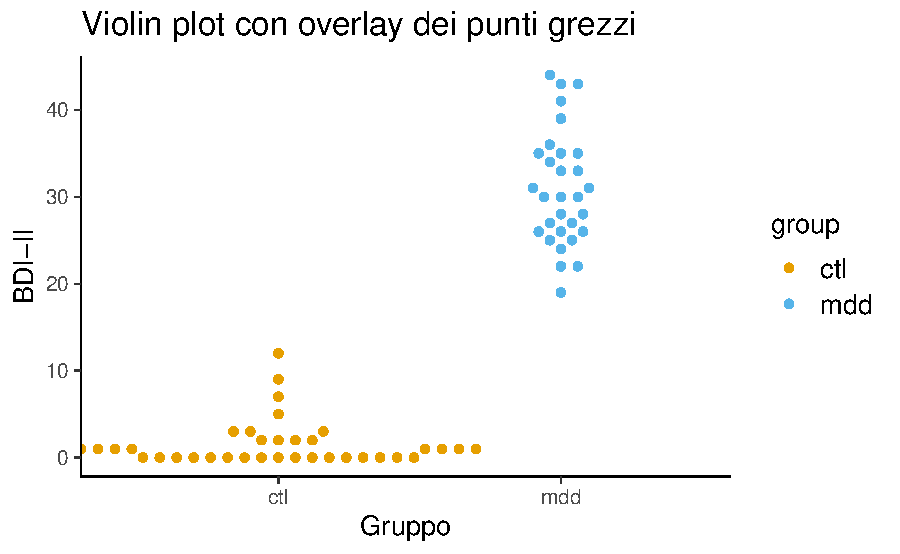
\includegraphics[width=0.7\linewidth,height=\textheight,keepaspectratio]{chapters/eda/05_exploring_numeric_data_files/figure-pdf/unnamed-chunk-25-1.pdf}
\end{center}

\section{Riflessioni Conclusive}\label{riflessioni-conclusive-10}

Abbiamo esplorato diverse tecniche per sintetizzare e visualizzare i
dati, includendo distribuzioni di frequenze, istogrammi e grafici di
densità. Questi strumenti sono essenziali per comprendere meglio i dati
e presentare risultati in modo chiaro e informativo. La
\textbf{visualizzazione dei dati} ci aiuta a individuare possibili
anomalie o situazioni inaspettate, prima di applicare modelli o
interpretazioni statistiche.

\section{Esercizi}\label{esercizi-12}

\begin{tcolorbox}[enhanced jigsaw, opacityback=0, bottomrule=.15mm, breakable, title=\textcolor{quarto-callout-important-color}{\faExclamation}\hspace{0.5em}{Problemi}, bottomtitle=1mm, toptitle=1mm, titlerule=0mm, colbacktitle=quarto-callout-important-color!10!white, rightrule=.15mm, colframe=quarto-callout-important-color-frame, colback=white, arc=.35mm, leftrule=.75mm, coltitle=black, left=2mm, toprule=.15mm, opacitybacktitle=0.6]

In questo esercizio, gli studenti raccoglieranno e analizzeranno dati
relativi alla \textbf{Satisfaction With Life Scale (SWLS)}
(\citeproc{ref-Diener1985}{Diener et al., 1985}) e alla \textbf{Scala
della Rete Sociale di Lubben (LSNS-6)} (\citeproc{ref-Lubben2006}{Lubben
et al., 2006}). L'obiettivo è comprendere la relazione tra la
soddisfazione di vita e la qualità delle relazioni sociali, esplorando
la distribuzione delle variabili e le possibili associazioni tra di
esse.

La \textbf{Scala della Rete Sociale di Lubben a 6 item (LSNS-6)} è uno
strumento utilizzato per valutare l'isolamento sociale negli adulti più
anziani, misurando il supporto sociale percepito sia da parte dei
familiari che degli amici. La scala comprende sei domande suddivise in
due sezioni:

\textbf{FAMIGLIA: Considerando le persone a cui sei legato per nascita,
matrimonio, adozione, ecc.}

\begin{enumerate}
\def\labelenumi{\arabic{enumi}.}
\tightlist
\item
  Quanti parenti vedi o senti almeno una volta al mese?
\item
  Con quanti parenti ti senti a tuo agio nel parlare di questioni
  personali?
\item
  Con quanti parenti ti senti così vicino da poter chiedere loro aiuto?
\end{enumerate}

\textbf{AMICIZIE: Considerando tutti i tuoi amici, inclusi quelli che
vivono nel tuo quartiere}

\begin{enumerate}
\def\labelenumi{\arabic{enumi}.}
\setcounter{enumi}{3}
\tightlist
\item
  Quanti dei tuoi amici vedi o senti almeno una volta al mese?
\item
  Con quanti amici ti senti a tuo agio nel parlare di questioni
  personali?
\item
  Con quanti amici ti senti così vicino da poter chiedere loro aiuto?
\end{enumerate}

La scala di risposta è:

\begin{itemize}
\tightlist
\item
  0 = nessuno
\item
  1 = uno
\item
  2 = due
\item
  3 = tre o quattro
\item
  4 = da cinque a otto
\item
  5 = nove o più
\end{itemize}

Il punteggio totale della LSNS-6 si ottiene sommando i punteggi dei sei
item, con un range che va da 0 a 30. Un punteggio di 12 o inferiore
indica un rischio di isolamento sociale.

\textbf{Dati da Raccogliere}

Ogni studente dovrà raccogliere i seguenti dati su se stesso e sui
membri del proprio gruppo TPV:

\begin{itemize}
\tightlist
\item
  \textbf{\texttt{student\_id}}: Identificativo univoco dello
  studente.\\
\item
  \textbf{\texttt{group}}: Gruppo di appartenenza (es. Gruppo 1, Gruppo
  2, ecc.).\\
\item
  \textbf{\texttt{swls}}: Punteggio totale sulla Satisfaction With Life
  Scale (SWLS).\\
\item
  \textbf{\texttt{gender}}: Genere (\texttt{M}, \texttt{F}).\\
\item
  \textbf{\texttt{lsns\_total}}: Punteggio totale della Scala della Rete
  Sociale di Lubben (LSNS-6).\\
\item
  \textbf{\texttt{lsns\_family}}: Punteggio della sottoscala
  \emph{engagement with family members} (somma degli item 1-3).\\
\item
  \textbf{\texttt{lsns\_friends}}: Punteggio della sottoscala
  \emph{engagement with friends} (somma degli item 4-6).
\end{itemize}

Queste variabili permetteranno di investigare come la
\textbf{soddisfazione di vita} sia associata alla \textbf{quantità e
qualità delle relazioni sociali}, distinguendo tra contatti con la
famiglia e con gli amici.

\textbf{Obiettivi dell'Analisi}

L'esercizio è strutturato in tre parti:

\begin{enumerate}
\def\labelenumi{\arabic{enumi}.}
\tightlist
\item
  \textbf{Esplorazione dei dati e distribuzione delle variabili}\\
\item
  \textbf{Visualizzazione e confronto tra gruppi}\\
\item
  \textbf{Analisi delle possibili associazioni tra SWLS e le componenti
  della rete sociale}
\end{enumerate}

\textbf{Parte 1: Esplorazione dei Dati}

\textbf{1.1 Caricamento e preparazione del dataset}

\begin{enumerate}
\def\labelenumi{\arabic{enumi}.}
\tightlist
\item
  Importa il dataset \texttt{swls\_lsns\_students.csv}.\\
\item
  Seleziona le variabili indicate sopra.\\
\item
  Controlla ed elimina eventuali duplicati.\\
\item
  Controlla ed elimina eventuali valori mancanti.
\end{enumerate}

\begin{Shaded}
\begin{Highlighting}[]
\CommentTok{\# Caricamento del dataset}
\NormalTok{df }\OtherTok{\textless{}{-}}\NormalTok{ rio}\SpecialCharTok{::}\FunctionTok{import}\NormalTok{(here}\SpecialCharTok{::}\FunctionTok{here}\NormalTok{(}\StringTok{"data"}\NormalTok{, }\StringTok{"swls\_lsns\_students.csv"}\NormalTok{))}

\CommentTok{\# Selezione delle variabili}
\NormalTok{df }\OtherTok{\textless{}{-}}\NormalTok{ df }\SpecialCharTok{|\textgreater{}}\NormalTok{ dplyr}\SpecialCharTok{::}\FunctionTok{select}\NormalTok{(student\_id, group, swls, gender, }
\NormalTok{                          lsns\_total, lsns\_family, lsns\_friends)}

\CommentTok{\# Rimozione dei duplicati}
\NormalTok{df }\OtherTok{\textless{}{-}}\NormalTok{ df[}\SpecialCharTok{!}\FunctionTok{duplicated}\NormalTok{(df}\SpecialCharTok{$}\NormalTok{student\_id), ]}

\CommentTok{\# Rimozione dei valori mancanti}
\NormalTok{df }\OtherTok{\textless{}{-}}\NormalTok{ df[}\FunctionTok{complete.cases}\NormalTok{(df), ]}
\end{Highlighting}
\end{Shaded}

\textbf{1.2 Distribuzione delle variabili}

\begin{enumerate}
\def\labelenumi{\arabic{enumi}.}
\setcounter{enumi}{4}
\tightlist
\item
  Calcola la \textbf{distribuzione di frequenza} per \texttt{swls},
  \texttt{lsns\_total}, \texttt{lsns\_family} e \texttt{lsns\_friends}:

  \begin{itemize}
  \tightlist
  \item
    Frequenze assolute e relative\\
  \item
    Frequenze cumulative
  \end{itemize}
\end{enumerate}

\begin{Shaded}
\begin{Highlighting}[]
\CommentTok{\# Frequenze assolute e relative}
\FunctionTok{table}\NormalTok{(df}\SpecialCharTok{$}\NormalTok{swls)}
\FunctionTok{prop.table}\NormalTok{(}\FunctionTok{table}\NormalTok{(df}\SpecialCharTok{$}\NormalTok{swls))}

\FunctionTok{table}\NormalTok{(df}\SpecialCharTok{$}\NormalTok{lsns\_total)}
\FunctionTok{prop.table}\NormalTok{(}\FunctionTok{table}\NormalTok{(df}\SpecialCharTok{$}\NormalTok{lsns\_total))}
\end{Highlighting}
\end{Shaded}

\begin{enumerate}
\def\labelenumi{\arabic{enumi}.}
\setcounter{enumi}{5}
\tightlist
\item
  Crea un \textbf{istogramma} della distribuzione delle variabili.
\end{enumerate}

\begin{Shaded}
\begin{Highlighting}[]
\FunctionTok{ggplot}\NormalTok{(df, }\FunctionTok{aes}\NormalTok{(}\AttributeTok{x =}\NormalTok{ swls)) }\SpecialCharTok{+}
  \FunctionTok{geom\_histogram}\NormalTok{(}\AttributeTok{bins =} \DecValTok{10}\NormalTok{, }\AttributeTok{fill =} \StringTok{"lightblue"}\NormalTok{, }\AttributeTok{color =} \StringTok{"black"}\NormalTok{) }\SpecialCharTok{+}
  \FunctionTok{labs}\NormalTok{(}\AttributeTok{title =} \StringTok{"Distribuzione dei punteggi SWLS"}\NormalTok{,}
       \AttributeTok{x =} \StringTok{"Punteggio SWLS"}\NormalTok{,}
       \AttributeTok{y =} \StringTok{"Frequenza"}\NormalTok{)}
\end{Highlighting}
\end{Shaded}

\begin{Shaded}
\begin{Highlighting}[]
\FunctionTok{ggplot}\NormalTok{(df, }\FunctionTok{aes}\NormalTok{(}\AttributeTok{x =}\NormalTok{ lsns\_total)) }\SpecialCharTok{+}
  \FunctionTok{geom\_histogram}\NormalTok{(}\AttributeTok{bins =} \DecValTok{10}\NormalTok{, }\AttributeTok{fill =} \StringTok{"lightblue"}\NormalTok{, }\AttributeTok{color =} \StringTok{"black"}\NormalTok{) }\SpecialCharTok{+}
  \FunctionTok{labs}\NormalTok{(}\AttributeTok{title =} \StringTok{"Distribuzione dei punteggi LSNS{-}6 (totale)"}\NormalTok{,}
       \AttributeTok{x =} \StringTok{"Punteggio LSNS{-}6"}\NormalTok{,}
       \AttributeTok{y =} \StringTok{"Frequenza"}\NormalTok{)}
\end{Highlighting}
\end{Shaded}

\begin{enumerate}
\def\labelenumi{\arabic{enumi}.}
\setcounter{enumi}{6}
\tightlist
\item
  Costruisci la \textbf{funzione di distribuzione empirica cumulativa
  (eCDF)}.
\end{enumerate}

\begin{Shaded}
\begin{Highlighting}[]
\FunctionTok{ggplot}\NormalTok{(df, }\FunctionTok{aes}\NormalTok{(}\AttributeTok{x =}\NormalTok{ swls)) }\SpecialCharTok{+}
  \FunctionTok{stat\_ecdf}\NormalTok{(}\AttributeTok{geom =} \StringTok{"step"}\NormalTok{, }\AttributeTok{color =} \StringTok{"blue"}\NormalTok{) }\SpecialCharTok{+}
  \FunctionTok{labs}\NormalTok{(}\AttributeTok{title =} \StringTok{"Funzione di distribuzione empirica cumulativa SWLS"}\NormalTok{,}
       \AttributeTok{x =} \StringTok{"Punteggio SWLS"}\NormalTok{,}
       \AttributeTok{y =} \StringTok{"F(x)"}\NormalTok{)}
\end{Highlighting}
\end{Shaded}

\begin{enumerate}
\def\labelenumi{\arabic{enumi}.}
\setcounter{enumi}{7}
\tightlist
\item
  Genera la \textbf{curva di densità kernel (KDE)} per ogni variabile.
\end{enumerate}

\begin{Shaded}
\begin{Highlighting}[]
\FunctionTok{ggplot}\NormalTok{(df, }\FunctionTok{aes}\NormalTok{(}\AttributeTok{x =}\NormalTok{ swls)) }\SpecialCharTok{+}
  \FunctionTok{geom\_density}\NormalTok{(}\AttributeTok{fill =} \StringTok{"lightblue"}\NormalTok{, }\AttributeTok{alpha =} \FloatTok{0.5}\NormalTok{) }\SpecialCharTok{+}
  \FunctionTok{labs}\NormalTok{(}\AttributeTok{title =} \StringTok{"Curva di densità dei punteggi SWLS"}\NormalTok{,}
       \AttributeTok{x =} \StringTok{"Punteggio SWLS"}\NormalTok{,}
       \AttributeTok{y =} \StringTok{"Densità"}\NormalTok{)}
\end{Highlighting}
\end{Shaded}

\begin{Shaded}
\begin{Highlighting}[]
\FunctionTok{ggplot}\NormalTok{(df, }\FunctionTok{aes}\NormalTok{(}\AttributeTok{x =}\NormalTok{ lsns\_total)) }\SpecialCharTok{+}
  \FunctionTok{geom\_density}\NormalTok{(}\AttributeTok{fill =} \StringTok{"lightblue"}\NormalTok{, }\AttributeTok{alpha =} \FloatTok{0.5}\NormalTok{) }\SpecialCharTok{+}
  \FunctionTok{labs}\NormalTok{(}\AttributeTok{title =} \StringTok{"Curva di densità LSNS{-}6 (totale)"}\NormalTok{,}
       \AttributeTok{x =} \StringTok{"Punteggio LSNS{-}6"}\NormalTok{,}
       \AttributeTok{y =} \StringTok{"Densità"}\NormalTok{)}
\end{Highlighting}
\end{Shaded}

\textbf{Parte 2: Confronto tra Gruppi}

\begin{enumerate}
\def\labelenumi{\arabic{enumi}.}
\setcounter{enumi}{8}
\tightlist
\item
  Costruisci una \textbf{tabella di contingenza} per \texttt{gender} e
  livello di rete sociale (alta o bassa, separando sopra e sotto la
  mediana di \texttt{lsns\_total}).
\end{enumerate}

\begin{Shaded}
\begin{Highlighting}[]
\NormalTok{df }\OtherTok{\textless{}{-}}\NormalTok{ df }\SpecialCharTok{|\textgreater{}} 
  \FunctionTok{mutate}\NormalTok{(}\AttributeTok{lsns\_level =} \FunctionTok{ifelse}\NormalTok{(lsns\_total }\SpecialCharTok{\textgreater{}=} \FunctionTok{median}\NormalTok{(lsns\_total), }\StringTok{"Alto"}\NormalTok{, }\StringTok{"Basso"}\NormalTok{))}

\FunctionTok{table}\NormalTok{(df}\SpecialCharTok{$}\NormalTok{gender, df}\SpecialCharTok{$}\NormalTok{lsns\_level)}
\FunctionTok{prop.table}\NormalTok{(}\FunctionTok{table}\NormalTok{(df}\SpecialCharTok{$}\NormalTok{gender, df}\SpecialCharTok{$}\NormalTok{lsns\_level), }\AttributeTok{margin =} \DecValTok{1}\NormalTok{)}
\end{Highlighting}
\end{Shaded}

\begin{enumerate}
\def\labelenumi{\arabic{enumi}.}
\setcounter{enumi}{9}
\tightlist
\item
  Crea un \textbf{grafico a barre} per la distribuzione di
  \texttt{lsns\_level} per genere.
\end{enumerate}

\begin{Shaded}
\begin{Highlighting}[]
\FunctionTok{ggplot}\NormalTok{(df, }\FunctionTok{aes}\NormalTok{(}\AttributeTok{x =}\NormalTok{ lsns\_level, }\AttributeTok{fill =}\NormalTok{ gender)) }\SpecialCharTok{+}
  \FunctionTok{geom\_bar}\NormalTok{(}\AttributeTok{position =} \StringTok{"dodge"}\NormalTok{) }\SpecialCharTok{+}
  \FunctionTok{labs}\NormalTok{(}\AttributeTok{title =} \StringTok{"Distribuzione del livello di rete sociale per genere"}\NormalTok{,}
       \AttributeTok{x =} \StringTok{"Livello LSNS"}\NormalTok{,}
       \AttributeTok{y =} \StringTok{"Conteggio"}\NormalTok{,}
       \AttributeTok{fill =} \StringTok{"Genere"}\NormalTok{)}
\end{Highlighting}
\end{Shaded}

\begin{enumerate}
\def\labelenumi{\arabic{enumi}.}
\setcounter{enumi}{10}
\tightlist
\item
  Costruisci un \textbf{box plot} per confrontare \texttt{swls} tra i
  gruppi di rete sociale.
\end{enumerate}

\begin{Shaded}
\begin{Highlighting}[]
\FunctionTok{ggplot}\NormalTok{(df, }\FunctionTok{aes}\NormalTok{(}\AttributeTok{x =}\NormalTok{ lsns\_level, }\AttributeTok{y =}\NormalTok{ swls, }\AttributeTok{fill =}\NormalTok{ lsns\_level)) }\SpecialCharTok{+}
  \FunctionTok{geom\_boxplot}\NormalTok{() }\SpecialCharTok{+}
  \FunctionTok{labs}\NormalTok{(}\AttributeTok{title =} \StringTok{"Distribuzione dei punteggi SWLS per livello di rete sociale"}\NormalTok{,}
       \AttributeTok{x =} \StringTok{"Livello di rete sociale"}\NormalTok{,}
       \AttributeTok{y =} \StringTok{"Punteggio SWLS"}\NormalTok{)}
\end{Highlighting}
\end{Shaded}

\begin{enumerate}
\def\labelenumi{\arabic{enumi}.}
\setcounter{enumi}{11}
\tightlist
\item
  Usa un \textbf{violin plot} per visualizzare la distribuzione
  dettagliata.
\end{enumerate}

\begin{Shaded}
\begin{Highlighting}[]
\FunctionTok{ggplot}\NormalTok{(df, }\FunctionTok{aes}\NormalTok{(}\AttributeTok{x =}\NormalTok{ lsns\_level, }\AttributeTok{y =}\NormalTok{ swls, }\AttributeTok{fill =}\NormalTok{ lsns\_level)) }\SpecialCharTok{+}
  \FunctionTok{geom\_violin}\NormalTok{(}\AttributeTok{alpha =} \FloatTok{0.5}\NormalTok{) }\SpecialCharTok{+}
  \FunctionTok{geom\_jitter}\NormalTok{(}\AttributeTok{width =} \FloatTok{0.1}\NormalTok{, }\AttributeTok{alpha =} \FloatTok{0.5}\NormalTok{) }\SpecialCharTok{+}
  \FunctionTok{labs}\NormalTok{(}\AttributeTok{title =} \StringTok{"Violin plot con dati grezzi sovrapposti"}\NormalTok{,}
       \AttributeTok{x =} \StringTok{"Livello di rete sociale"}\NormalTok{,}
       \AttributeTok{y =} \StringTok{"Punteggio SWLS"}\NormalTok{)}
\end{Highlighting}
\end{Shaded}

\textbf{Parte 3: Analisi delle Associazioni tra SWLS e la Rete Sociale}

Il concetto di correlazione verrà approfondito nel
Capitolo~\ref{sec-correlation}. Per i nostri scopi attuali, possiamo
considerarlo come un indice numerico che misura l'intensità e la
direzione dell'associazione tra due variabili. Un valore di 0 indica
l'assenza di una relazione lineare tra le variabili, mentre i valori +1
e -1 indicano una relazione lineare perfetta, positiva o negativa
rispettivamente. I valori intermedi tra -1 e +1 rappresentano
associazioni più deboli o forti, a seconda della loro vicinanza agli
estremi.

\begin{enumerate}
\def\labelenumi{\arabic{enumi}.}
\setcounter{enumi}{12}
\tightlist
\item
  \textbf{Correlazioni} tra SWLS e le sottoscale della LSNS.
\end{enumerate}

\begin{Shaded}
\begin{Highlighting}[]
\FunctionTok{cor}\NormalTok{(df}\SpecialCharTok{$}\NormalTok{swls, df}\SpecialCharTok{$}\NormalTok{lsns\_total, }\AttributeTok{method =} \StringTok{"pearson"}\NormalTok{)}
\FunctionTok{cor}\NormalTok{(df}\SpecialCharTok{$}\NormalTok{swls, df}\SpecialCharTok{$}\NormalTok{lsns\_family, }\AttributeTok{method =} \StringTok{"pearson"}\NormalTok{)}
\FunctionTok{cor}\NormalTok{(df}\SpecialCharTok{$}\NormalTok{swls, df}\SpecialCharTok{$}\NormalTok{lsns\_friends, }\AttributeTok{method =} \StringTok{"pearson"}\NormalTok{)}
\end{Highlighting}
\end{Shaded}

Spiega in maniera inuitiva il significato dei valori ottenuti.

\begin{enumerate}
\def\labelenumi{\arabic{enumi}.}
\setcounter{enumi}{13}
\tightlist
\item
  \textbf{Grafico di dispersione} tra SWLS e LSNS-6 totale.
\end{enumerate}

Un grafico di dispersione è un diagramma cartesiano in cui ogni punto
rappresenta un'osservazione (nel caso attuale, uno studente). Le
coordinate dei punti sui due assi, X e Y, indicano i valori delle due
variabili considerate per ciascuno studente.

\begin{Shaded}
\begin{Highlighting}[]
\FunctionTok{ggplot}\NormalTok{(df, }\FunctionTok{aes}\NormalTok{(}\AttributeTok{x =}\NormalTok{ lsns\_total, }\AttributeTok{y =}\NormalTok{ swls)) }\SpecialCharTok{+}
  \FunctionTok{geom\_point}\NormalTok{(}\AttributeTok{alpha =} \FloatTok{0.7}\NormalTok{) }\SpecialCharTok{+}
  \FunctionTok{geom\_smooth}\NormalTok{(}\AttributeTok{method =} \StringTok{"lm"}\NormalTok{, }\AttributeTok{color =} \StringTok{"red"}\NormalTok{) }\SpecialCharTok{+}
  \FunctionTok{labs}\NormalTok{(}\AttributeTok{title =} \StringTok{"Relazione tra rete sociale totale e SWLS"}\NormalTok{,}
       \AttributeTok{x =} \StringTok{"Punteggio LSNS{-}6 Totale"}\NormalTok{,}
       \AttributeTok{y =} \StringTok{"Punteggio SWLS"}\NormalTok{)}
\end{Highlighting}
\end{Shaded}

Per ogni grafico generato, includi una descrizione chiara e concisa del
suo significato in relazione ai dati analizzati.

\textbf{Conclusioni}

L'obiettivo è analizzare se e come la \textbf{soddisfazione di vita}
degli studenti universitari è influenzata dalle \textbf{relazioni
sociali}, distinguendo tra \textbf{engagement con la famiglia e con gli
amici}.

\textbf{Consegna}

Consegna il file \texttt{.qmd} contenente il codice, le visualizzazioni
e le interpretazioni.

\end{tcolorbox}

\section*{Informazioni sull'Ambiente di
Sviluppo}\label{informazioni-sullambiente-di-sviluppo-8}
\addcontentsline{toc}{section}{Informazioni sull'Ambiente di Sviluppo}

\markright{Informazioni sull'Ambiente di Sviluppo}

\begin{Shaded}
\begin{Highlighting}[]
\FunctionTok{sessionInfo}\NormalTok{()}
\CommentTok{\#\textgreater{} R version 4.4.2 (2024{-}10{-}31)}
\CommentTok{\#\textgreater{} Platform: aarch64{-}apple{-}darwin20}
\CommentTok{\#\textgreater{} Running under: macOS Sequoia 15.3.1}
\CommentTok{\#\textgreater{} }
\CommentTok{\#\textgreater{} Matrix products: default}
\CommentTok{\#\textgreater{} BLAS:   /Library/Frameworks/R.framework/Versions/4.4{-}arm64/Resources/lib/libRblas.0.dylib }
\CommentTok{\#\textgreater{} LAPACK: /Library/Frameworks/R.framework/Versions/4.4{-}arm64/Resources/lib/libRlapack.dylib;  LAPACK version 3.12.0}
\CommentTok{\#\textgreater{} }
\CommentTok{\#\textgreater{} locale:}
\CommentTok{\#\textgreater{} [1] C/UTF{-}8/C/C/C/C}
\CommentTok{\#\textgreater{} }
\CommentTok{\#\textgreater{} time zone: Europe/Rome}
\CommentTok{\#\textgreater{} tzcode source: internal}
\CommentTok{\#\textgreater{} }
\CommentTok{\#\textgreater{} attached base packages:}
\CommentTok{\#\textgreater{} [1] stats     graphics  grDevices utils     datasets  methods   base     }
\CommentTok{\#\textgreater{} }
\CommentTok{\#\textgreater{} other attached packages:}
\CommentTok{\#\textgreater{}  [1] dslabs\_0.8.0     ggbeeswarm\_0.7.2 thematic\_0.1.6   MetBrewer\_0.2.0 }
\CommentTok{\#\textgreater{}  [5] ggokabeito\_0.1.0 see\_0.10.0       gridExtra\_2.3    patchwork\_1.3.0 }
\CommentTok{\#\textgreater{}  [9] bayesplot\_1.11.1 psych\_2.4.12     scales\_1.3.0     markdown\_1.13   }
\CommentTok{\#\textgreater{} [13] knitr\_1.49       lubridate\_1.9.4  forcats\_1.0.0    stringr\_1.5.1   }
\CommentTok{\#\textgreater{} [17] dplyr\_1.1.4      purrr\_1.0.4      readr\_2.1.5      tidyr\_1.3.1     }
\CommentTok{\#\textgreater{} [21] tibble\_3.2.1     ggplot2\_3.5.1    tidyverse\_2.0.0  rio\_1.2.3       }
\CommentTok{\#\textgreater{} [25] here\_1.0.1      }
\CommentTok{\#\textgreater{} }
\CommentTok{\#\textgreater{} loaded via a namespace (and not attached):}
\CommentTok{\#\textgreater{}  [1] generics\_0.1.3    stringi\_1.8.4     lattice\_0.22{-}6    hms\_1.1.3        }
\CommentTok{\#\textgreater{}  [5] digest\_0.6.37     magrittr\_2.0.3    evaluate\_1.0.3    grid\_4.4.2       }
\CommentTok{\#\textgreater{}  [9] timechange\_0.3.0  fastmap\_1.2.0     R.oo\_1.27.0       rprojroot\_2.0.4  }
\CommentTok{\#\textgreater{} [13] jsonlite\_1.8.9    R.utils\_2.12.3    mnormt\_2.1.1      cli\_3.6.4        }
\CommentTok{\#\textgreater{} [17] rlang\_1.1.5       R.methodsS3\_1.8.2 munsell\_0.5.1     withr\_3.0.2      }
\CommentTok{\#\textgreater{} [21] tools\_4.4.2       parallel\_4.4.2    tzdb\_0.4.0        colorspace\_2.1{-}1 }
\CommentTok{\#\textgreater{} [25] pacman\_0.5.1      vctrs\_0.6.5       R6\_2.6.1          lifecycle\_1.0.4  }
\CommentTok{\#\textgreater{} [29] vipor\_0.4.7       beeswarm\_0.4.0    pkgconfig\_2.0.3   pillar\_1.10.1    }
\CommentTok{\#\textgreater{} [33] gtable\_0.3.6      data.table\_1.16.4 glue\_1.8.0        xfun\_0.50        }
\CommentTok{\#\textgreater{} [37] tidyselect\_1.2.1  rstudioapi\_0.17.1 farver\_2.1.2      htmltools\_0.5.8.1}
\CommentTok{\#\textgreater{} [41] nlme\_3.1{-}167      labeling\_0.4.3    rmarkdown\_2.29    compiler\_4.4.2}
\end{Highlighting}
\end{Shaded}

\section*{Bibliografia}\label{bibliografia-16}
\addcontentsline{toc}{section}{Bibliografia}

\markright{Bibliografia}

\chapter{Principi della visualizzazione dei
dati}\label{sec-eda-visualization}

\begin{tcolorbox}[enhanced jigsaw, opacityback=0, bottomrule=.15mm, breakable, title=\textcolor{quarto-callout-important-color}{\faExclamation}\hspace{0.5em}{In questo capitolo imparerai a:}, bottomtitle=1mm, toptitle=1mm, titlerule=0mm, colbacktitle=quarto-callout-important-color!10!white, rightrule=.15mm, colframe=quarto-callout-important-color-frame, colback=white, arc=.35mm, leftrule=.75mm, coltitle=black, left=2mm, toprule=.15mm, opacitybacktitle=0.6]

\begin{itemize}
\tightlist
\item
  comunicare i risultati basati sui dati;\\
\item
  utilizzare \textbf{ggplot2} per creare grafici personalizzati;\\
\item
  riconoscere i limiti di alcuni grafici comunemente utilizzati e
  comprendere perché evitarli.\\
\end{itemize}

\end{tcolorbox}

\begin{tcolorbox}[enhanced jigsaw, opacityback=0, bottomrule=.15mm, breakable, title=\textcolor{quarto-callout-tip-color}{\faLightbulb}\hspace{0.5em}{Prerequisiti}, bottomtitle=1mm, toptitle=1mm, titlerule=0mm, colbacktitle=quarto-callout-tip-color!10!white, rightrule=.15mm, colframe=quarto-callout-tip-color-frame, colback=white, arc=.35mm, leftrule=.75mm, coltitle=black, left=2mm, toprule=.15mm, opacitybacktitle=0.6]

\begin{itemize}
\tightlist
\item
  Leggere
  \href{https://doi.org/10.1146/annurev-statistics-031219-041252}{\emph{Testing
  Statistical Charts: What Makes a Good Graph?} (Vanderplas, Cook, and
  Hofmann 2020)}. Questo articolo descrive le migliori pratiche per la
  creazione di grafici.
\item
  Consultare il capitolo
  \href{https://r4ds.hadley.nz/data-visualize}{Data visualization} di
  Wickham et al. (\citeproc{ref-wickham2023r}{2023}). Questo capitolo
  fornisce una panoramica degli aspetti fondamentali della
  visualizzazione dei dati.
\item
  Consultare \href{https://socviz.co}{Data Visualization. A practical
  introduction} di Healy (\citeproc{ref-healy2018data}{2018}).
\item
  Consultare \href{https://clauswilke.com/dataviz/}{Fundamentals of Data
  Visualization} di Wilke (\citeproc{ref-wilke2019fundamentals}{2019}).
\item
  Leggere il post
  \href{https://simplystatistics.org/posts/2019-02-21-dynamite-plots-must-die/}{Open
  letter to journal editors: dynamite plots must die} di Rafael
  Irizarry.
\item
  Consultare il post
  \href{https://www.biostat.wisc.edu/~kbroman/topten_worstgraphs/}{The
  top ten worst graphs} di Karl Broman.
\item
  Leggere il capitolo
  \href{http://rafalab.dfci.harvard.edu/dsbook-part-1/dataviz/intro-dataviz.html}{Data
  Visualization} di \emph{Introduction to Data Science}.
\item
  Visionare
  \href{https://www.simonsfoundation.org/event/2024-flatiron-wide-autumn-meeting-fwam/}{Communicating
  Science Using Visuals: Tips for Scientists}.
\end{itemize}

\end{tcolorbox}

\begin{tcolorbox}[enhanced jigsaw, opacityback=0, bottomrule=.15mm, breakable, title=\textcolor{quarto-callout-caution-color}{\faFire}\hspace{0.5em}{Preparazione del Notebook}, bottomtitle=1mm, toptitle=1mm, titlerule=0mm, colbacktitle=quarto-callout-caution-color!10!white, rightrule=.15mm, colframe=quarto-callout-caution-color-frame, colback=white, arc=.35mm, leftrule=.75mm, coltitle=black, left=2mm, toprule=.15mm, opacitybacktitle=0.6]

\begin{Shaded}
\begin{Highlighting}[]
\NormalTok{here}\SpecialCharTok{::}\FunctionTok{here}\NormalTok{(}\StringTok{"code"}\NormalTok{, }\StringTok{"\_common.R"}\NormalTok{) }\SpecialCharTok{|\textgreater{}} 
  \FunctionTok{source}\NormalTok{()}

\CommentTok{\# Load packages}
\ControlFlowTok{if}\NormalTok{ (}\SpecialCharTok{!}\FunctionTok{requireNamespace}\NormalTok{(}\StringTok{"pacman"}\NormalTok{)) }\FunctionTok{install.packages}\NormalTok{(}\StringTok{"pacman"}\NormalTok{)}
\NormalTok{pacman}\SpecialCharTok{::}\FunctionTok{p\_load}\NormalTok{(dslabs, ggrepel, stringr)}
\end{Highlighting}
\end{Shaded}

\end{tcolorbox}

\section*{Introduzione}\label{introduzione-16}
\addcontentsline{toc}{section}{Introduzione}

\markright{Introduzione}

In questo capitolo saranno introdotti i principi fondamentali della
visualizzazione dei dati, accompagnati da una descrizione sintetica. Per
un approfondimento su ciascun principio, si consiglia di consultare il
capitolo
\href{http://rafalab.dfci.harvard.edu/dsbook-part-1/dataviz/intro-dataviz.html}{Data
Visualization} del libro \emph{Introduction to Data Science}.

Un altro aspetto che verrà affrontato riguarda gli errori, i bias, le
imprecisioni sistematiche e altri problemi inattesi che spesso
influenzano i dati. Questi elementi richiedono una gestione accurata e,
poiché possono risultare difficili o impossibili da individuare
direttamente in un dataset, la visualizzazione dei dati diventa uno
strumento essenziale.

L'aumento della disponibilità di dataset informativi e di strumenti
software ha reso la visualizzazione dei dati sempre più rilevante in
numerosi ambiti. La visualizzazione dei dati non solo consente di
comunicare in modo efficace risultati basati sui dati, ma aiuta anche a
motivare ulteriori analisi e a rilevare eventuali errori o imperfezioni.

\section{Un'immagine Vale Più di Mille
Parole}\label{unimmagine-vale-piuxf9-di-mille-parole}

Osservare numeri e stringhe di caratteri che definiscono un dataset
raramente è utile. Per convincerci di questo, stampiamo e osserviamo la
tabella dei dati sugli omicidi con armi da fuoco negli Stati Uniti:

\begin{Shaded}
\begin{Highlighting}[]
\FunctionTok{head}\NormalTok{(murders)}
\CommentTok{\#\textgreater{}        state abb region population total}
\CommentTok{\#\textgreater{} 1    Alabama  AL  South    4779736   135}
\CommentTok{\#\textgreater{} 2     Alaska  AK   West     710231    19}
\CommentTok{\#\textgreater{} 3    Arizona  AZ   West    6392017   232}
\CommentTok{\#\textgreater{} 4   Arkansas  AR  South    2915918    93}
\CommentTok{\#\textgreater{} 5 California  CA   West   37253956  1257}
\CommentTok{\#\textgreater{} 6   Colorado  CO   West    5029196    65}
\end{Highlighting}
\end{Shaded}

Cosa impariamo guardando questa tabella? Quanto velocemente riusciamo a
determinare quali stati hanno le popolazioni più numerose? E quali hanno
le più piccole? Quanto è grande uno stato ``tipico''? Esiste una
relazione tra la dimensione della popolazione e il numero totale di
omicidi? Come variano i tassi di omicidio tra le diverse regioni del
paese? Per la maggior parte di noi, è piuttosto difficile estrarre
queste informazioni semplicemente guardando i numeri. Al contrario, le
risposte a tutte queste domande sono immediatamente evidenti osservando
questo grafico:

\begin{center}
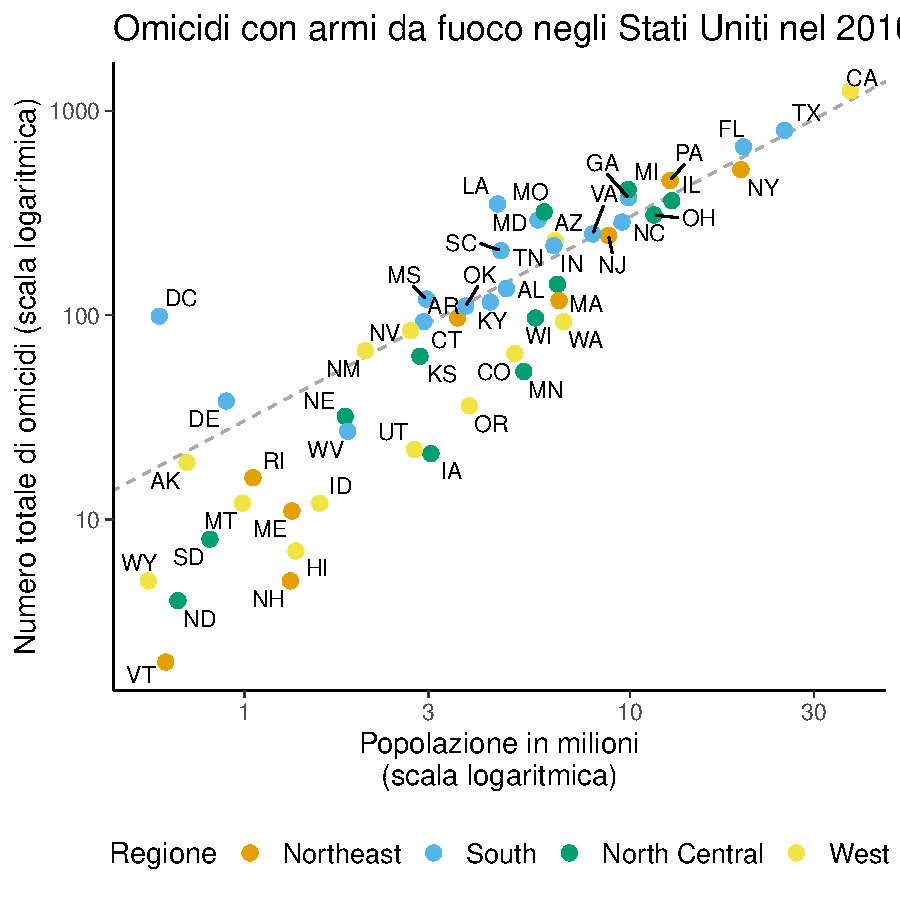
\includegraphics[width=0.7\linewidth,height=\textheight,keepaspectratio]{chapters/eda/06_data_visualization_files/figure-pdf/ggplot-example-plot-0-1.pdf}
\end{center}

Questo ci ricorda il detto ``un'immagine vale più di mille parole''. La
visualizzazione dei dati offre un modo potente per comunicare una
scoperta basata sui dati. In alcuni casi, la visualizzazione è così
convincente che non è necessario alcun follow-up analitico.

\begin{example}[]\protect\hypertarget{exm-}{}\label{exm-}

Rispondiamo alle domande precedenti sulla base della visualizzazione dei
dati.

\begin{enumerate}
\def\labelenumi{\arabic{enumi}.}
\item
  \textbf{Quali stati hanno le popolazioni più numerose?} Guardando il
  grafico, possiamo notare immediatamente che gli stati con le
  popolazioni più alte si trovano verso il lato destro dell'asse x
  (poiché la scala è logaritmica). Gli stati con le popolazioni più
  numerose sono \textbf{California}, \textbf{Texas}, e \textbf{New
  York}.
\item
  \textbf{Quali stati hanno le popolazioni più piccole?} Gli stati con
  le popolazioni più piccole si trovano verso il lato sinistro dell'asse
  x. Questi includono \textbf{Wyoming}, \textbf{Vermont}, e
  \textbf{Alaska}.
\item
  \textbf{Quanto è grande uno stato ``tipico''?} Un modo per stimare una
  dimensione ``tipica'' è guardare la densità delle osservazioni
  sull'asse x. La maggior parte degli stati si trova intorno a un
  milione di abitanti, ma ci sono anche molti stati con popolazioni
  comprese tra 5 e 10 milioni di abitanti. Quindi, uno stato ``tipico''
  potrebbe avere una popolazione di circa \textbf{5-10 milioni di
  persone}.
\item
  \textbf{Esiste una relazione tra la dimensione della popolazione e il
  numero totale di omicidi?} Sì, esiste una chiara relazione positiva
  tra la dimensione della popolazione e il numero totale di omicidi. Lo
  si può vedere dal fatto che gli stati con popolazioni più grandi
  tendono ad avere un numero maggiore di omicidi. Tuttavia, questa
  relazione non è perfetta: alcuni stati con popolazioni simili mostrano
  differenze significative nel numero di omicidi, suggerendo che altri
  fattori oltre alla popolazione influenzano i tassi di omicidio.
\item
  \textbf{Come variano i tassi di omicidio tra le diverse regioni del
  paese?} Il grafico utilizza colori diversi per rappresentare le
  regioni geografiche degli stati. Osservando la distribuzione dei punti
  per colore, possiamo notare alcune differenze:

  \begin{itemize}
  \tightlist
  \item
    \textbf{Sud}: Gli stati del Sud tendono ad avere tassi di omicidio
    più alti rispetto alle altre regioni.
  \item
    \textbf{Nord-Est}: Gli stati del Nord-Est mostrano una variazione
    moderata nei tassi di omicidio, ma in generale sono inferiori a
    quelli del Sud.
  \item
    \textbf{Ovest}: Gli stati dell'Ovest presentano una vasta gamma di
    tassi di omicidio, con alcuni stati come California e Texas che
    registrano numeri elevati a causa della loro grande popolazione.
  \item
    \textbf{Midwest}: I tassi di omicidio nei stati del Midwest sembrano
    essere generalmente bassi o moderati.
  \end{itemize}
\end{enumerate}

\end{example}

\section{Codificare i dati attraverso segnali
visivi}\label{codificare-i-dati-attraverso-segnali-visivi}

Iniziamo con una panoramica dei principali segnali visivi utilizzati per
codificare i dati: posizione, lunghezza, angoli, area, luminosità e
tonalità del colore. Tra questi, \textbf{posizione e lunghezza} sono i
segnali visivi più efficaci e intuitivi, poiché il cervello umano è
particolarmente abile nel riconoscere variazioni spaziali. Questo rende
la posizione e la lunghezza strumenti potenti per la rappresentazione
quantitativa. In altre parole, le persone riescono a confrontare con
maggiore precisione altezze e lunghezze (come le barre in un barplot)
rispetto ad angoli o aree (come in un grafico a torta).

\textbf{Angoli e aree}, sebbene comunemente usati, sono segnali visivi
meno efficaci. Grafici come i pie chart, che si basano su angoli e aree
per rappresentare quantità, risultano spesso meno precisi e più
difficili da interpretare, specialmente quando le differenze sono
piccole. Anche l'uso dell'\textbf{area}, ad esempio nei bubble plot, può
distorcere la percezione delle differenze tra i dati, a meno che non
venga gestita correttamente. Anche se l'area di una bolla può essere
proporzionale al valore rappresentato, la percezione umana tende a
sovrastimare le differenze tra aree più grandi.

\textbf{Luminosità e tonalità del colore} sono utili per rappresentare
variabili qualitative o categoriali, ma possono risultare difficili da
interpretare quando si tratta di confrontare quantità precise. Tuttavia,
il colore gioca un ruolo cruciale nelle visualizzazioni
multidimensionali, come le heatmap, dove è necessario rappresentare più
di due variabili contemporaneamente. È importante, però, usare il colore
con attenzione, soprattutto per garantire l'accessibilità a persone con
problemi di daltonismo.

Le \textbf{tabelle} sono utili quando si ha una quantità limitata di
dati e si richiede una precisione numerica rigorosa. Tuttavia, per set
di dati più grandi o per evidenziare tendenze e differenze, i grafici
(come i barplot) sono generalmente più efficaci. Le tabelle non offrono
lo stesso impatto visivo immediato e rendono più difficile
l'individuazione di pattern complessi.

\subsection{Ulteriori considerazioni sulla scelta della
visualizzazione}\label{ulteriori-considerazioni-sulla-scelta-della-visualizzazione}

La scelta della visualizzazione più appropriata dipende sia dalla natura
dei dati che dallo scopo della comunicazione. Per esempio:

\begin{itemize}
\tightlist
\item
  \textbf{Barplot o dot plot} sono ideali per confrontare valori
  quantitativi tra categorie.
\item
  \textbf{Istogrammi}, \textbf{boxplot} e
  \href{https://medium.com/@amorimfranchi/raincloud-plots-for-clear-precise-and-efficient-data-communication-4c71d0a37c23}{raincloud
  plots} sono più adatti per descrivere la distribuzione di dati
  continui e fare confronti tra categorie.
\item
  \textbf{Grafici di dispersione (scatter plot)} sono eccellenti per
  esplorare relazioni tra due variabili continue.
\end{itemize}

La \textbf{chiarezza} e la \textbf{leggibilità} sono principi
fondamentali nella creazione di visualizzazioni efficaci. L'aggiunta di
elementi visivi eccessivi, come decorazioni superflue o troppi colori,
può distrarre dal messaggio principale. Un buon grafico deve essere
semplice, ma allo stesso tempo completo, includendo solo gli elementi
visivi necessari per trasmettere il messaggio desiderato.

In conclusione, scegliere i segnali visivi adeguati e il tipo di grafico
più appropriato non solo migliora l'accuratezza della comunicazione, ma
rende le informazioni più accessibili e comprensibili per il pubblico.

\section{Quando includere lo zero}\label{quando-includere-lo-zero}

Quando si usa la lunghezza come segnale visivo, come nei barplot, è
essenziale che l'asse parta da zero. Non farlo può essere fuorviante e
far sembrare le differenze più grandi di quanto non siano in realtà.
Questo errore viene spesso sfruttato nei media per esagerare differenze
apparentemente significative.

Tuttavia, quando si usa la \textbf{posizione} (ad esempio in un grafico
a dispersione), non è sempre necessario includere lo zero, soprattutto
se l'interesse principale è il confronto tra gruppi rispetto alla
variabilità interna.

\section{Evitare le distorsioni}\label{evitare-le-distorsioni}

Una distorsione comune si verifica quando le differenze tra quantità
sono rappresentate utilizzando aree, come nei
\href{https://it.wikipedia.org/wiki/Diagramma_a_bolle}{bubble plot},
dove il raggio dei cerchi è proporzionale al dato. Il problema è che,
poiché l'area di un cerchio è proporzionale al quadrato del raggio, le
differenze sembrano molto più ampie di quanto siano realmente. Per
evitare queste distorsioni, è meglio utilizzare la posizione o la
lunghezza, come in un \textbf{grafico a barre}, per confrontare
direttamente le quantità.

\section{Ordinare le categorie}\label{ordinare-le-categorie}

Quando si visualizzano categorie, come nei barplot o nei boxplot, è
opportuno ordinarle in base al valore della variabile di interesse,
anziché in ordine alfabetico. Questo aiuta a evidenziare pattern
significativi e facilita il confronto tra categorie.

\section{Evitare i Dynamite Plots}\label{evitare-i-dynamite-plots}

I \textbf{dynamite plots}, che mostrano la media e l'errore standard (o
la deviazione standard), sono spesso utilizzati in psicologia ma sono
fuorvianti. Questi grafici tendono a esagerare le differenze e possono
indurre false interpretazioni. È preferibile mostrare tutti i dati, ad
esempio tramite un
\href{https://en.wikipedia.org/wiki/Dot_plot_(statistics)}{dot plot},
che fornisce un'immagine più chiara della distribuzione dei dati
(\citeproc{ref-butler2022popularity}{Butler, 2022}).

\section{Facilitare i confronti}\label{facilitare-i-confronti}

Quando si confrontano due distribuzioni, come in un
\href{https://en.wikipedia.org/wiki/Histogram}{istogramma}, è
fondamentale mantenere gli stessi assi per entrambi i grafici. Se le
distribuzioni sono presentate su assi con scale diverse, il confronto
diventa difficile e potrebbe portare a conclusioni errate. Allineare i
grafici verticalmente o orizzontalmente consente di percepire più
facilmente le differenze tra i gruppi.

\section{Trasformazioni logaritmiche}\label{trasformazioni-logaritmiche}

Le \textbf{trasformazioni logaritmiche} sono utili quando si lavora con
dati distribuiti su più ordini di grandezza o quando le variazioni tra
le quantità sono moltiplicative (\citeproc{ref-west2022best}{West,
2022}). L'uso della scala logaritmica in un grafico a barre o a
dispersione può ridurre le distorsioni visive e migliorare
l'interpretazione dei dati. Questo approccio è particolarmente utile
quando alcuni valori estremi potrebbero dominare il grafico, nascondendo
dettagli rilevanti.

\section{Codificare una terza
variabile}\label{codificare-una-terza-variabile}

Per rappresentare tre variabili, è possibile utilizzare un
\href{https://it.wikipedia.org/wiki/Grafico_di_dispersione}{grafico di
dispersione} con variabili codificate attraverso dimensioni aggiuntive
come il colore, la dimensione o la forma dei punti. Ad esempio, in un
grafico che confronta aspettativa di vita e reddito, la dimensione dei
punti potrebbe rappresentare la popolazione e il colore la regione
geografica. Quando si utilizza il colore per rappresentare una
variabile, è importante scegliere palette cromatiche accessibili anche
per chi è affetto da \textbf{daltonismo}, evitando combinazioni
problematiche come rosso-verde.

\section{Evitare pseudo-tre
dimensioni}\label{evitare-pseudo-tre-dimensioni}

Grafici tridimensionali, come barre o pie chart 3D, spesso aggiungono
confusione senza fornire informazioni aggiuntive significative. Sebbene
visivamente accattivanti, questi grafici distorcono la percezione e
rendono difficile l'interpretazione accurata dei dati. È preferibile
mantenere le visualizzazioni bidimensionali, a meno che la terza
dimensione non rappresenti effettivamente una variabile aggiuntiva.

\section{Scegliere il numero giusto di cifre
significative}\label{scegliere-il-numero-giusto-di-cifre-significative}

È importante evitare l'uso di troppe cifre decimali nelle tabelle e nei
grafici. Spesso, una o due cifre significative sono sufficienti per
rappresentare accuratamente i dati, mentre l'aggiunta di cifre inutili
può confondere il lettore e dare un falso senso di precisione.
Limitiamoci a mostrare solo le cifre necessarie per trasmettere il
messaggio in modo chiaro.

\section{Conoscere il pubblico}\label{conoscere-il-pubblico}

Infine, è fondamentale adattare la visualizzazione dei dati al pubblico
di riferimento. Grafici progettati per l'analisi esplorativa interna
possono contenere dettagli tecnici complessi, ma quando si comunica a un
pubblico più ampio o non specializzato, è necessario semplificare. Ad
esempio, utilizzare una scala logaritmica può essere utile per un
pubblico esperto, ma confondere un pubblico generale. In questi casi,
mantenere la scala lineare e spiegare chiaramente i dati aiuta a evitare
malintesi.

\section{Riflessioni Conclusive}\label{riflessioni-conclusive-11}

I principi di visualizzazione dei dati presentati in questo capitolo
rappresentano strumenti essenziali per garantire chiarezza, precisione e
trasparenza nella rappresentazione delle informazioni. La corretta
applicazione di questi principi non solo migliora la comprensione dei
dati, ma riduce anche il rischio di distorsioni e interpretazioni
errate.

Ecco le linee guida principali da seguire nella creazione di
visualizzazioni efficaci:

\begin{itemize}
\tightlist
\item
  \textbf{Evitare distorsioni}: Scegliere grafici semplici, come i
  barplot, evitando rappresentazioni che possono alterare la percezione
  delle proporzioni, ad esempio cerchi o pie chart.\\
\item
  \textbf{Includere lo zero}: Nei barplot, l'asse verticale deve sempre
  partire da zero, altrimenti si rischia di trasmettere informazioni
  fuorvianti.\\
\item
  \textbf{Ordinare le categorie}: Le categorie dovrebbero essere
  ordinate in base ai valori (non alfabeticamente), per facilitare il
  confronto visivo.\\
\item
  \textbf{Mostrare i dati}: Sostituire grafici come i dynamite plots con
  rappresentazioni che evidenzino tutti i dati disponibili, ad esempio
  dot plot o strip chart.\\
\item
  \textbf{Facilitare i confronti}: Quando si confrontano distribuzioni,
  è importante utilizzare assi comuni per garantire una corretta
  interpretazione.\\
\item
  \textbf{Utilizzare trasformazioni logaritmiche}: Queste trasformazioni
  sono utili quando i dati coprono diversi ordini di grandezza,
  rendendoli più interpretabili.\\
\item
  \textbf{Codificare una terza variabile}: Nei grafici a dispersione, si
  possono rappresentare ulteriori informazioni utilizzando colore,
  dimensione o forma dei punti.\\
\item
  \textbf{Evitare pseudo-3D}: I grafici tridimensionali spesso
  confondono e distorcono i dati; è preferibile mantenere
  rappresentazioni bidimensionali.\\
\item
  \textbf{Limitare le cifre significative}: Ridurre il numero di
  decimali presentati per evitare complessità inutili e migliorare la
  leggibilità.\\
\item
  \textbf{Adattarsi al pubblico}: Semplificare le visualizzazioni in
  base al livello di competenza e conoscenza del pubblico, per garantire
  un messaggio chiaro e comprensibile.
\end{itemize}

La scelta appropriata di grafici, segnali visivi e trasformazioni è
cruciale per comunicare i risultati in modo efficace e responsabile.
Seguendo questi principi, è possibile creare visualizzazioni che non
solo rappresentano i dati in modo accurato, ma supportano anche
un'interpretazione informata e consapevole.

\section{Esercizi}\label{esercizi-13}

\begin{tcolorbox}[enhanced jigsaw, opacityback=0, bottomrule=.15mm, breakable, title=\textcolor{quarto-callout-tip-color}{\faLightbulb}\hspace{0.5em}{Esercizi}, bottomtitle=1mm, toptitle=1mm, titlerule=0mm, colbacktitle=quarto-callout-tip-color!10!white, rightrule=.15mm, colframe=quarto-callout-tip-color-frame, colback=white, arc=.35mm, leftrule=.75mm, coltitle=black, left=2mm, toprule=.15mm, opacitybacktitle=0.6]

In questo esercizio analizzerai i dati raccolti dagli studenti sulla
\textbf{Satisfaction With Life Scale (SWLS)} e sulla \textbf{Lubben
Social Network Scale (LSNS-6)}. Le variabili incluse sono:

\begin{itemize}
\tightlist
\item
  \textbf{SWLS}: Punteggio totale della Scala di Soddisfazione per la
  Vita.
\item
  \textbf{LSNS-6}: Punteggio totale sulla scala della rete sociale.
\item
  \textbf{Genere}: Maschio/Femmina.
\item
  \textbf{Tipo di scuola superiore}: Liceo classico o scientifico
  vs.~altro.
\item
  \textbf{Numero di amici}: Auto-riferito.
\item
  \textbf{Numero di uscite settimanali con gli amici}.
\end{itemize}

Utilizzerai questi dati per esplorare le distribuzioni, creare
visualizzazioni efficaci e interpretare i risultati.

\textbf{Esercizi Teorici}

\begin{enumerate}
\def\labelenumi{\arabic{enumi}.}
\tightlist
\item
  \textbf{Principi della visualizzazione}

  \begin{itemize}
  \tightlist
  \item
    Quali sono i principali segnali visivi utilizzati nella
    visualizzazione dei dati? Fornisci un esempio pratico per ognuno.
  \item
    Perché la posizione e la lunghezza sono considerati segnali visivi
    più efficaci rispetto all'area e agli angoli?
  \item
    Spiega perché i \textbf{grafici tridimensionali} (3D) sono spesso
    inutili o fuorvianti.
  \end{itemize}
\item
  \textbf{Scelta della visualizzazione}

  \begin{itemize}
  \tightlist
  \item
    Quale tipo di grafico useresti per mostrare la distribuzione della
    variabile SWLS? Giustifica la tua risposta.
  \item
    Se volessi confrontare la distribuzione della SWLS tra due gruppi
    (ad esempio, in base al \textbf{genere}), quale grafico useresti?
    Perché?
  \end{itemize}
\item
  \textbf{Errori comuni nella visualizzazione}

  \begin{itemize}
  \tightlist
  \item
    Perché i \textbf{dynamite plots} (grafici a barre con errore
    standard) sono considerati una cattiva pratica?
  \item
    Spiega perché è importante iniziare l'asse Y da \textbf{zero} in un
    barplot.
  \item
    Perché è preferibile ordinare le categorie in base ai valori invece
    che alfabeticamente?
  \end{itemize}
\end{enumerate}

\textbf{Esercizi Pratici in R}

\textbf{1. Caricamento e ispezione dei dati}

Carica il dataset raccolto dagli studenti
(\texttt{dati\_SWLS\_LSNS.csv}) e stampa un'anteprima dei dati.

\begin{Shaded}
\begin{Highlighting}[]
\CommentTok{\# Caricamento dei dati}
\NormalTok{df }\OtherTok{\textless{}{-}} \FunctionTok{read.csv}\NormalTok{(}\StringTok{"dati\_SWLS\_LSNS.csv"}\NormalTok{)}

\CommentTok{\# Esamina le prime righe}
\FunctionTok{head}\NormalTok{(df)}
\end{Highlighting}
\end{Shaded}

Rispondi alle seguenti domande:

\begin{itemize}
\tightlist
\item
  Quante osservazioni ci sono nel dataset?
\item
  Ci sono valori mancanti? Se sì, quanti?
\end{itemize}

\textbf{2. Distribuzione delle variabili}

Crea le seguenti visualizzazioni per analizzare la distribuzione di
\textbf{SWLS} e \textbf{LSNS-6}:

\begin{itemize}
\tightlist
\item
  \textbf{Istogramma} con sovrapposta la curva di densità.
\item
  \textbf{Funzione di distribuzione cumulativa empirica (eCDF)}.
\item
  \textbf{Box plot} per la variabile SWLS.
\end{itemize}

\textbf{3. Confronto tra gruppi}

\begin{itemize}
\tightlist
\item
  Crea un \textbf{box plot} della SWLS per \textbf{genere}.
\item
  Crea un \textbf{violin plot} della LSNS-6 in base al \textbf{tipo di
  scuola superiore}.
\end{itemize}

\textbf{4. Relazioni tra variabili}

\begin{itemize}
\tightlist
\item
  Crea un \textbf{grafico di dispersione (scatter plot)} per verificare
  se c'è una relazione tra il punteggio \textbf{SWLS} e il numero di
  amici.
\item
  Aggiungi una linea di regressione al grafico per facilitare
  l'interpretazione.
\end{itemize}

\begin{Shaded}
\begin{Highlighting}[]
\FunctionTok{ggplot}\NormalTok{(df, }\FunctionTok{aes}\NormalTok{(}\AttributeTok{x =}\NormalTok{ numero\_amici, }\AttributeTok{y =}\NormalTok{ SWLS)) }\SpecialCharTok{+}
  \FunctionTok{geom\_point}\NormalTok{() }\SpecialCharTok{+}
  \FunctionTok{geom\_smooth}\NormalTok{(}\AttributeTok{method =} \StringTok{"lm"}\NormalTok{, }\AttributeTok{se =} \ConstantTok{FALSE}\NormalTok{) }\SpecialCharTok{+}
  \FunctionTok{labs}\NormalTok{(}\AttributeTok{title =} \StringTok{"Relazione tra SWLS e numero di amici"}\NormalTok{,}
       \AttributeTok{x =} \StringTok{"Numero di amici"}\NormalTok{,}
       \AttributeTok{y =} \StringTok{"Satisfaction With Life Scale (SWLS)"}\NormalTok{)}
\end{Highlighting}
\end{Shaded}

Domande:

\begin{itemize}
\tightlist
\item
  Quale relazione osservi tra il numero di amici e la SWLS?
\item
  Il numero di amici è un buon predittore della soddisfazione per la
  vita?
\end{itemize}

\textbf{5. Esplorazione della rete sociale}

\begin{itemize}
\tightlist
\item
  Crea un \textbf{barplot} per mostrare la distribuzione delle risposte
  medie ai sei item della \textbf{LSNS-6}.
\item
  Esplora la relazione tra la \textbf{frequenza delle uscite
  settimanali} e il punteggio totale \textbf{LSNS-6} utilizzando un
  \textbf{box plot}.
\end{itemize}

\textbf{Consegna}

Salva i grafici creati e rispondi alle domande in forma scritta. Carica
il file su Moodle.

\end{tcolorbox}

\begin{tcolorbox}[enhanced jigsaw, opacityback=0, bottomrule=.15mm, breakable, title=\textcolor{quarto-callout-tip-color}{\faLightbulb}\hspace{0.5em}{Soluzioni}, bottomtitle=1mm, toptitle=1mm, titlerule=0mm, colbacktitle=quarto-callout-tip-color!10!white, rightrule=.15mm, colframe=quarto-callout-tip-color-frame, colback=white, arc=.35mm, leftrule=.75mm, coltitle=black, left=2mm, toprule=.15mm, opacitybacktitle=0.6]

\textbf{1. Risposte alle domande teoriche}

Principi della visualizzazione

\begin{itemize}
\tightlist
\item
  I segnali visivi principali sono \textbf{posizione, lunghezza, angoli,
  area, luminosità e colore}.
\item
  La \textbf{posizione e lunghezza} sono i segnali più efficaci perché
  l'occhio umano è molto preciso nel confrontare distanze e altezze,
  mentre è meno efficace nel confrontare angoli e aree.
\item
  I \textbf{grafici tridimensionali (3D)} spesso aggiungono confusione
  senza migliorare la leggibilità.
\end{itemize}

Scelta della visualizzazione

\begin{itemize}
\tightlist
\item
  Per mostrare la distribuzione della SWLS, è preferibile usare
  \textbf{istogrammi e box plot} perché evidenziano la forma della
  distribuzione e la presenza di outlier.
\item
  Per confrontare la SWLS tra generi, un \textbf{box plot o violin plot}
  è l'opzione migliore, perché mostra la distribuzione completa.
\end{itemize}

Errori comuni

\begin{itemize}
\tightlist
\item
  I \textbf{dynamite plots} nascondono la distribuzione dei dati e non
  mostrano la variabilità interna ai gruppi.
\item
  In un \textbf{barplot}, l'asse Y deve iniziare da \textbf{zero} per
  evitare distorsioni visive.
\item
  Le categorie nei barplot devono essere ordinate per valore per
  facilitare il confronto.
\end{itemize}

\textbf{2. Soluzioni pratiche in R}

\textbf{Caricamento dei dati}

\begin{Shaded}
\begin{Highlighting}[]
\NormalTok{df }\OtherTok{\textless{}{-}} \FunctionTok{read.csv}\NormalTok{(}\StringTok{"dati\_SWLS\_LSNS.csv"}\NormalTok{)}

\CommentTok{\# Esamina il dataset}
\FunctionTok{dim}\NormalTok{(df)  }\CommentTok{\# Numero di righe e colonne}
\FunctionTok{sum}\NormalTok{(}\FunctionTok{is.na}\NormalTok{(df))  }\CommentTok{\# Conteggio valori mancanti}
\end{Highlighting}
\end{Shaded}

\textbf{Distribuzione delle variabili}

\begin{Shaded}
\begin{Highlighting}[]
\FunctionTok{ggplot}\NormalTok{(df, }\FunctionTok{aes}\NormalTok{(}\AttributeTok{x =}\NormalTok{ SWLS)) }\SpecialCharTok{+}
  \FunctionTok{geom\_histogram}\NormalTok{(}
  \FunctionTok{aes}\NormalTok{(}\AttributeTok{y =} \FunctionTok{after\_stat}\NormalTok{(density)), }\AttributeTok{bins =} \DecValTok{10}\NormalTok{, }\AttributeTok{fill =} \StringTok{"blue"}\NormalTok{, }\AttributeTok{alpha =} \FloatTok{0.5}
\NormalTok{  ) }\SpecialCharTok{+}
  \FunctionTok{geom\_density}\NormalTok{(}\AttributeTok{color =} \StringTok{"red"}\NormalTok{, }\AttributeTok{size =} \FloatTok{1.2}\NormalTok{)}
\end{Highlighting}
\end{Shaded}

\begin{Shaded}
\begin{Highlighting}[]
\FunctionTok{ggplot}\NormalTok{(df, }\FunctionTok{aes}\NormalTok{(SWLS)) }\SpecialCharTok{+}
  \FunctionTok{stat\_ecdf}\NormalTok{(}\AttributeTok{geom =} \StringTok{"step"}\NormalTok{)}
\end{Highlighting}
\end{Shaded}

\begin{Shaded}
\begin{Highlighting}[]
\FunctionTok{ggplot}\NormalTok{(df, }\FunctionTok{aes}\NormalTok{(}\AttributeTok{x =} \StringTok{""}\NormalTok{, }\AttributeTok{y =}\NormalTok{ SWLS)) }\SpecialCharTok{+}
  \FunctionTok{geom\_boxplot}\NormalTok{() }\SpecialCharTok{+}
  \FunctionTok{coord\_flip}\NormalTok{()}
\end{Highlighting}
\end{Shaded}

\textbf{Confronto tra gruppi}

\begin{Shaded}
\begin{Highlighting}[]
\FunctionTok{ggplot}\NormalTok{(df, }\FunctionTok{aes}\NormalTok{(}\AttributeTok{x =}\NormalTok{ genere, }\AttributeTok{y =}\NormalTok{ SWLS, }\AttributeTok{fill =}\NormalTok{ genere)) }\SpecialCharTok{+}
  \FunctionTok{geom\_boxplot}\NormalTok{()}
\end{Highlighting}
\end{Shaded}

\begin{Shaded}
\begin{Highlighting}[]
\FunctionTok{ggplot}\NormalTok{(df, }\FunctionTok{aes}\NormalTok{(}\AttributeTok{x =}\NormalTok{ scuola, }\AttributeTok{y =}\NormalTok{ LSNS6, }\AttributeTok{fill =}\NormalTok{ scuola)) }\SpecialCharTok{+}
  \FunctionTok{geom\_violin}\NormalTok{()}
\end{Highlighting}
\end{Shaded}

\textbf{Relazioni tra variabili}

\begin{Shaded}
\begin{Highlighting}[]
\FunctionTok{ggplot}\NormalTok{(df, }\FunctionTok{aes}\NormalTok{(}\AttributeTok{x =}\NormalTok{ numero\_amici, }\AttributeTok{y =}\NormalTok{ SWLS)) }\SpecialCharTok{+}
  \FunctionTok{geom\_point}\NormalTok{() }\SpecialCharTok{+}
  \FunctionTok{geom\_smooth}\NormalTok{(}\AttributeTok{method =} \StringTok{"lm"}\NormalTok{, }\AttributeTok{se =} \ConstantTok{FALSE}\NormalTok{)}
\end{Highlighting}
\end{Shaded}

\begin{Shaded}
\begin{Highlighting}[]
\FunctionTok{ggplot}\NormalTok{(df, }\FunctionTok{aes}\NormalTok{(}\AttributeTok{x =}\NormalTok{ uscite\_settimanali, }\AttributeTok{y =}\NormalTok{ LSNS6)) }\SpecialCharTok{+}
  \FunctionTok{geom\_boxplot}\NormalTok{()}
\end{Highlighting}
\end{Shaded}

\textbf{Conclusioni}

(Ad esempio) Le visualizzazioni mostrano che:

\begin{itemize}
\tightlist
\item
  SWLS e LSNS-6 variano in base al genere e al tipo di scuola.
\item
  Il numero di amici ha un impatto positivo sulla SWLS, ma la relazione
  è moderata.
\item
  Il numero di uscite settimanali è correlato positivamente con la rete
  sociale (LSNS-6).
\end{itemize}

\end{tcolorbox}

\section*{Bibliografia}\label{bibliografia-17}
\addcontentsline{toc}{section}{Bibliografia}

\markright{Bibliografia}

\chapter{Indicatori di tendenza centrale e
variabilità}\label{sec-central-tendency-variability}

\begin{tcolorbox}[enhanced jigsaw, opacityback=0, bottomrule=.15mm, breakable, title=\textcolor{quarto-callout-important-color}{\faExclamation}\hspace{0.5em}{In questo capitolo imparerai a}, bottomtitle=1mm, toptitle=1mm, titlerule=0mm, colbacktitle=quarto-callout-important-color!10!white, rightrule=.15mm, colframe=quarto-callout-important-color-frame, colback=white, arc=.35mm, leftrule=.75mm, coltitle=black, left=2mm, toprule=.15mm, opacitybacktitle=0.6]

\begin{itemize}
\tightlist
\item
  Calcolare e interpretare i principali indici di tendenza centrale e di
  variabilità.
\end{itemize}

\end{tcolorbox}

\begin{tcolorbox}[enhanced jigsaw, opacityback=0, bottomrule=.15mm, breakable, title=\textcolor{quarto-callout-tip-color}{\faLightbulb}\hspace{0.5em}{Prerequisiti}, bottomtitle=1mm, toptitle=1mm, titlerule=0mm, colbacktitle=quarto-callout-tip-color!10!white, rightrule=.15mm, colframe=quarto-callout-tip-color-frame, colback=white, arc=.35mm, leftrule=.75mm, coltitle=black, left=2mm, toprule=.15mm, opacitybacktitle=0.6]

\begin{itemize}
\tightlist
\item
  Leggere ``Most Psychological Researchers Assume Their Samples Are
  Ergodic: Evidence From a Year of Articles in Three Major Journals''
  (\citeproc{ref-speelman2024most}{Speelman et al., 2024}).
\end{itemize}

\end{tcolorbox}

\begin{tcolorbox}[enhanced jigsaw, opacityback=0, bottomrule=.15mm, breakable, title=\textcolor{quarto-callout-caution-color}{\faFire}\hspace{0.5em}{Preparazione del Notebook}, bottomtitle=1mm, toptitle=1mm, titlerule=0mm, colbacktitle=quarto-callout-caution-color!10!white, rightrule=.15mm, colframe=quarto-callout-caution-color-frame, colback=white, arc=.35mm, leftrule=.75mm, coltitle=black, left=2mm, toprule=.15mm, opacitybacktitle=0.6]

\begin{Shaded}
\begin{Highlighting}[]
\NormalTok{here}\SpecialCharTok{::}\FunctionTok{here}\NormalTok{(}\StringTok{"code"}\NormalTok{, }\StringTok{"\_common.R"}\NormalTok{) }\SpecialCharTok{|\textgreater{}} 
  \FunctionTok{source}\NormalTok{()}

\CommentTok{\# Load packages}
\ControlFlowTok{if}\NormalTok{ (}\SpecialCharTok{!}\FunctionTok{requireNamespace}\NormalTok{(}\StringTok{"pacman"}\NormalTok{)) }\FunctionTok{install.packages}\NormalTok{(}\StringTok{"pacman"}\NormalTok{)}
\NormalTok{pacman}\SpecialCharTok{::}\FunctionTok{p\_load}\NormalTok{(tidyr, viridis, vcd)}
\end{Highlighting}
\end{Shaded}

\end{tcolorbox}

\section{Introduzione}\label{introduzione-17}

La visualizzazione grafica dei dati rappresenta il pilastro fondamentale
di ogni analisi quantitativa. Grazie alle rappresentazioni grafiche
adeguate, è possibile individuare importanti caratteristiche di una
distribuzione, quali la simmetria o l'asimmetria, nonché la presenza di
una o più mode. Successivamente, al fine di descrivere sinteticamente le
principali caratteristiche dei dati, si rende necessario l'utilizzo di
specifici indici numerici. In questo capitolo, verranno presentati i
principali indicatori della statistica descrittiva.

\section{Indici di Tendenza Centrale}\label{indici-di-tendenza-centrale}

Gli indici di tendenza centrale sono misure statistiche che cercano di
rappresentare un valore tipico o centrale all'interno di un insieme di
dati. Sono utilizzati per ottenere una comprensione immediata della
distribuzione dei dati senza dover analizzare l'intero insieme. Gli
indici di tendenza centrale sono fondamentali nell'analisi statistica,
in quanto forniscono una sintesi semplice e comprensibile delle
caratteristiche principali di un insieme di dati. I principali indici di
tendenza centrale sono:

\begin{enumerate}
\def\labelenumi{\arabic{enumi}.}
\tightlist
\item
  \textbf{Media}: La media è la somma di tutti i valori divisa per il
  numero totale di valori. È spesso utilizzata come misura generale di
  tendenza centrale, ma è sensibile agli estremi (valori molto alti o
  molto bassi).
\item
  \textbf{Mediana}: La mediana è il valore che divide l'insieme di dati
  in due parti uguali. A differenza della media, non è influenzata da
  valori estremi ed è quindi più robusta in presenza di outlier.
\item
  \textbf{Moda}: La moda è il valore che appare più frequentemente in un
  insieme di dati. In alcuni casi, può non essere presente o esserci più
  di una moda.
\end{enumerate}

La scelta dell'indice di tendenza centrale appropriato dipende dalla
natura dei dati e dall'obiettivo dell'analisi. Ad esempio, la mediana
potrebbe essere preferita alla media se l'insieme di dati contiene
valori anomali che potrebbero distorcere la rappresentazione centrale.
La conoscenza e l'applicazione corretta di questi indici possono fornire
una preziosa intuizione sulle caratteristiche centrali di una
distribuzione di dati.

\section{Moda}\label{moda}

La \textbf{moda} (\(\text{Mo}\)) rappresenta il valore della variabile
che \textbf{compare con maggiore frequenza} in una distribuzione. In
altre parole, è il valore più \textbf{ricorrente} nei dati.

\begin{itemize}
\tightlist
\item
  Nelle \textbf{distribuzioni unimodali}, esiste una sola moda, che
  coincide con il valore centrale della distribuzione più frequente.\\
\item
  Tuttavia, in alcune distribuzioni, possono emergere \textbf{più di una
  moda}, rendendole \textbf{multimodali}. In questi casi, la moda perde
  il suo significato di indicatore unico di tendenza centrale, poiché la
  presenza di più valori con frequenze elevate rende difficile
  individuare un singolo punto di riferimento.
\end{itemize}

\section{Mediana}\label{mediana}

La \textbf{mediana} (\(\tilde{x}\)) corrisponde al valore che divide il
campione in due metà: il 50\% dei dati è inferiore o uguale alla mediana
e il restante 50\% è superiore o uguale. A differenza della media, la
mediana è meno influenzata dai valori estremi, rendendola una misura
particolarmente robusta in presenza di dati asimmetrici o outlier.

\section{Media}\label{media}

La media aritmetica di un insieme di valori rappresenta il punto
centrale o il baricentro della distribuzione dei dati. È calcolata come
la somma di tutti i valori divisa per il numero totale di valori, ed è
espressa dalla formula:

\begin{equation}\phantomsection\label{eq-mean}{
\bar{x}=\frac{1}{n}\sum_{i=1}^n x_i,
}\end{equation}

dove \(x_i\) rappresenta i valori nell'insieme, \(n\) è il numero totale
di valori, e \(\sum\) indica la sommatoria.

\subsection{Proprietà della Media}\label{proprietuxe0-della-media}

Una proprietà fondamentale della media è che la somma degli scarti di
ciascun valore dalla media è zero:

\begin{equation}\phantomsection\label{eq-diffmeansumzero}{
\sum_{i=1}^n (x_i - \bar{x}) = 0.\notag
}\end{equation}

Infatti,

\[
\begin{aligned}
\sum_{i=1}^n (x_i - \bar{x}) &= \sum_i x_i - \sum_i \bar{x}\notag\\
&= \sum_i x_i - n \bar{x}\notag\\
&= \sum_i x_i - \sum_i x_i = 0.\notag
\end{aligned}
\]

Questa proprietà implica che i dati sono equamente distribuiti intorno
alla media.

\subsection{La media come Centro di Gravità
dell'Istogramma}\label{la-media-come-centro-di-gravituxe0-dellistogramma}

La media aritmetica può essere interpretata come il centro di gravità o
il punto di equilibrio della distribuzione dei dati. In termini fisici,
il centro di gravità è il punto in cui la massa di un sistema è
equilibrata o concentrata.

In termini statistici, possiamo considerare la media come il punto in
cui la distribuzione dei dati è in equilibrio. Ogni valore dell'insieme
di dati può essere visto come un punto materiale con una massa
proporzionale al suo valore. Se immaginiamo questi punti disposti su una
linea, con valori più grandi a destra e più piccoli a sinistra, la media
corrisponderà esattamente al punto in cui la distribuzione sarebbe in
equilibrio.

\subsection{Principio dei Minimi
Quadrati}\label{principio-dei-minimi-quadrati}

La posizione della media minimizza la somma delle distanze quadrate dai
dati, un principio noto come ``metodo dei minimi quadrati''.
Matematicamente, questo si traduce nel fatto che la somma dei quadrati
degli scarti tra ciascun valore e la media è minima. Questo principio è
alla base dell'analisi statistica dei modelli di regressione e conferma
l'interpretazione della media come centro di gravità dell'istogramma.

\subsection{\texorpdfstring{Calcolo della Media con
\texttt{R}}{Calcolo della Media con R}}\label{calcolo-della-media-con-r}

Per calcolare la media di un piccolo numero di valori in R, possiamo
utilizzare la somma di questi valori e dividerla per il numero totale di
elementi. Consideriamo ad esempio i valori 12, 44, 21, 62, 24:

\begin{Shaded}
\begin{Highlighting}[]
\NormalTok{(}\DecValTok{12} \SpecialCharTok{+} \DecValTok{44} \SpecialCharTok{+} \DecValTok{21} \SpecialCharTok{+} \DecValTok{62} \SpecialCharTok{+} \DecValTok{24}\NormalTok{) }\SpecialCharTok{/} \DecValTok{5}
\CommentTok{\#\textgreater{} [1] 32.6}
\end{Highlighting}
\end{Shaded}

ovvero

\begin{Shaded}
\begin{Highlighting}[]
\NormalTok{x }\OtherTok{\textless{}{-}} \FunctionTok{c}\NormalTok{(}\DecValTok{12}\NormalTok{, }\DecValTok{44}\NormalTok{, }\DecValTok{21}\NormalTok{, }\DecValTok{62}\NormalTok{, }\DecValTok{24}\NormalTok{)}
\FunctionTok{mean}\NormalTok{(x)}
\CommentTok{\#\textgreater{} [1] 32.6}
\end{Highlighting}
\end{Shaded}

\subsection{Le Proporzioni Sono Medie}\label{le-proporzioni-sono-medie}

Se una collezione consiste solo di uni e zeri, allora la somma della
collezione è il numero di uni in essa, e la media della collezione è la
proporzione di uni.

\begin{Shaded}
\begin{Highlighting}[]
\NormalTok{zero\_one }\OtherTok{\textless{}{-}} \FunctionTok{c}\NormalTok{(}\DecValTok{1}\NormalTok{, }\DecValTok{1}\NormalTok{, }\DecValTok{1}\NormalTok{, }\DecValTok{0}\NormalTok{)}
\NormalTok{result }\OtherTok{\textless{}{-}} \FunctionTok{mean}\NormalTok{(zero\_one)}
\NormalTok{result}
\CommentTok{\#\textgreater{} [1] 0.75}
\end{Highlighting}
\end{Shaded}

È possibile sostituire 1 con il valore booleano True e 0 con False:

\begin{Shaded}
\begin{Highlighting}[]
\FunctionTok{mean}\NormalTok{(}\FunctionTok{c}\NormalTok{(}\ConstantTok{TRUE}\NormalTok{, }\ConstantTok{TRUE}\NormalTok{, }\ConstantTok{TRUE}\NormalTok{, }\ConstantTok{FALSE}\NormalTok{))}
\CommentTok{\#\textgreater{} [1] 0.75}
\end{Highlighting}
\end{Shaded}

\subsection{Limiti della Media
Aritmetica}\label{limiti-della-media-aritmetica}

La media aritmetica, tuttavia, ha alcune limitazioni: non sempre è
l'indice più adeguato per descrivere accuratamente la tendenza centrale
della distribuzione, specialmente quando si verificano asimmetrie o
valori anomali (outlier). In queste situazioni, è più indicato
utilizzare la mediana o la media spuntata (come spiegheremo
successivamente).

\section{Come Descrivere la Tendenza Centrale in Distribuzioni
Asimmetriche}\label{come-descrivere-la-tendenza-centrale-in-distribuzioni-asimmetriche}

Il diverso significato degli indici di tendenza centrale -- moda, media
e mediana -- diventa evidente quando si analizzano \textbf{distribuzioni
asimmetriche}. Per illustrare questo concetto, utilizzeremo i dati del
Progetto Natsal, contenuti nel file \texttt{sexual-partners.csv}.

Negli anni '80, con la crescente preoccupazione per l'AIDS, le autorità
sanitarie del Regno Unito si resero conto della mancanza di dati
affidabili sui comportamenti sessuali della popolazione. In particolare,
vi erano dubbi sulla frequenza con cui le persone cambiavano partner,
sul numero di partner simultanei e sulle pratiche sessuali adottate.
Questa conoscenza era essenziale per prevedere la diffusione delle
malattie sessualmente trasmissibili nella società e per pianificare
adeguatamente i servizi sanitari. Tuttavia, si faceva ancora riferimento
ai dati raccolti da Alfred Kinsey negli Stati Uniti negli anni '40, che
non tenevano conto della rappresentatività del campione.

A partire dalla fine degli anni '80, vennero dunque avviati nel Regno
Unito e negli Stati Uniti ampi e rigorosi studi sui comportamenti
sessuali, nonostante una forte opposizione in alcuni ambienti. Nel Regno
Unito, il governo guidato da Margaret Thatcher ritirò il proprio
sostegno a un'importante indagine sui comportamenti sessuali all'ultimo
momento. Fortunatamente, i ricercatori riuscirono a ottenere
finanziamenti da enti benefici, dando vita al \emph{National Sexual
Attitudes and Lifestyles Survey} (Natsal). Da allora, questa indagine
viene condotta ogni dieci anni, a partire dal 1990. La terza
rilevazione, denominata Natsal-3, è stata effettuata intorno al 2010.

Poniamoci il problema di descrivere la tendenza centrale per i dati
contenuti nel file \texttt{sexual-partners.csv}, separatamente per
maschi e femmine. Il dataset fornisce la distribuzione del
\textbf{numero totale dichiarato di partner sessuali di sesso opposto}
nella vita per uomini e donne di età compresa tra 35 e 44 anni. I dati
provengono dal sondaggio Natsal-3 e corrispondono a un totale di 796
uomini e 1193 donne.

Procediamo all'importazione dei dati per iniziare l'analisi.

\begin{Shaded}
\begin{Highlighting}[]
\NormalTok{df }\OtherTok{\textless{}{-}}\NormalTok{ rio}\SpecialCharTok{::}\FunctionTok{import}\NormalTok{(here}\SpecialCharTok{::}\FunctionTok{here}\NormalTok{(}\StringTok{"data"}\NormalTok{, }\StringTok{"sexual{-}partners.csv"}\NormalTok{))}
\end{Highlighting}
\end{Shaded}

Esaminiamo alcune righe prese a caso dal data frame \texttt{df}:

\begin{Shaded}
\begin{Highlighting}[]
\NormalTok{df[}\FunctionTok{sample}\NormalTok{(}\DecValTok{1}\SpecialCharTok{:}\FunctionTok{nrow}\NormalTok{(df), }\AttributeTok{size =} \DecValTok{10}\NormalTok{, }\AttributeTok{replace =} \ConstantTok{FALSE}\NormalTok{), ]}
\CommentTok{\#\textgreater{}      Gender NumPartners}
\CommentTok{\#\textgreater{} 561     Man          15}
\CommentTok{\#\textgreater{} 321     Man           6}
\CommentTok{\#\textgreater{} 1177  Woman           3}
\CommentTok{\#\textgreater{} 1098  Woman           2}
\CommentTok{\#\textgreater{} 1252  Woman           4}
\CommentTok{\#\textgreater{} 1170  Woman           3}
\CommentTok{\#\textgreater{} 634     Man          21}
\CommentTok{\#\textgreater{} 49      Man           1}
\CommentTok{\#\textgreater{} 1152  Woman           3}
\CommentTok{\#\textgreater{} 1327  Woman           5}
\end{Highlighting}
\end{Shaded}

La colonna \texttt{Gender} riporta il genere del rispondente e la
colonna \texttt{NumPartners} il numero di partner sessuali di sesso
opposto dichiarati.

Esaminiamo la numerosità di ciascun gruppo.

\begin{Shaded}
\begin{Highlighting}[]
\NormalTok{df }\SpecialCharTok{|\textgreater{}} 
  \FunctionTok{group\_by}\NormalTok{(Gender) }\SpecialCharTok{|\textgreater{}} 
  \FunctionTok{summarize}\NormalTok{(}\AttributeTok{count =} \FunctionTok{n}\NormalTok{())}
\CommentTok{\#\textgreater{} \# A tibble: 2 x 2}
\CommentTok{\#\textgreater{}   Gender count}
\CommentTok{\#\textgreater{}   \textless{}chr\textgreater{}  \textless{}int\textgreater{}}
\CommentTok{\#\textgreater{} 1 Man      796}
\CommentTok{\#\textgreater{} 2 Woman   1193}
\end{Highlighting}
\end{Shaded}

Poniamoci innnanzitutto il problema di visualizzare i dati con un
istogramma, separatamente per maschi e femmine. Per ragioni di spazio ci
limiteremo ad un numero massimo di partner sessuali di 50 (ma in questo
campione il numero massimo arriva a 501 per gli uomini e 550 per le
donne):

\begin{Shaded}
\begin{Highlighting}[]
\NormalTok{df }\SpecialCharTok{|\textgreater{}} 
  \FunctionTok{group\_by}\NormalTok{(Gender) }\SpecialCharTok{|\textgreater{}} 
  \FunctionTok{summarize}\NormalTok{(}\AttributeTok{maximum =} \FunctionTok{max}\NormalTok{(NumPartners))}
\CommentTok{\#\textgreater{} \# A tibble: 2 x 2}
\CommentTok{\#\textgreater{}   Gender maximum}
\CommentTok{\#\textgreater{}   \textless{}chr\textgreater{}    \textless{}int\textgreater{}}
\CommentTok{\#\textgreater{} 1 Man        501}
\CommentTok{\#\textgreater{} 2 Woman      550}
\end{Highlighting}
\end{Shaded}

Iniziamo calcolando la percentuale di intervistati per ciascun valore
possibile della variabile ``numero di partner sessuali'', compreso tra 0
e 50. Il calcolo verrà svolto in due passaggi:

\begin{itemize}
\item
  Conteggio delle frequenze assolute: Per ogni valore della variabile
  ``numero di partner sessuali'' e per ciascun gruppo di genere (uomini
  e donne), contiamo quante volte quel valore compare nei dati.
\item
  Calcolo delle percentuali relative: Per ciascun gruppo di genere,
  dividiamo il conteggio di ogni valore per il totale delle osservazioni
  nel gruppo e moltiplichiamo per 100 per ottenere la percentuale.
\end{itemize}

\begin{Shaded}
\begin{Highlighting}[]
\CommentTok{\# Filtra i dati troncando il numero di partner a 50}
\NormalTok{df\_truncated }\OtherTok{\textless{}{-}}\NormalTok{ df[df}\SpecialCharTok{$}\NormalTok{NumPartners }\SpecialCharTok{\textless{}=} \DecValTok{50}\NormalTok{, ]}

\CommentTok{\# Calcola il conteggio per ciascun genere e numero di partner}
\NormalTok{counts\_data }\OtherTok{\textless{}{-}}\NormalTok{ df\_truncated }\SpecialCharTok{\%\textgreater{}\%}
  \FunctionTok{group\_by}\NormalTok{(Gender, NumPartners) }\SpecialCharTok{\%\textgreater{}\%}  \CommentTok{\# Raggruppa per genere e numero di partner}
  \FunctionTok{summarise}\NormalTok{(}\AttributeTok{Count =} \FunctionTok{n}\NormalTok{(), }\AttributeTok{.groups =} \StringTok{"drop"}\NormalTok{)  }\CommentTok{\# Conta le occorrenze}

\CommentTok{\# Aggiunge la percentuale relativa per ciascun genere}
\NormalTok{percentage\_data }\OtherTok{\textless{}{-}}\NormalTok{ counts\_data }\SpecialCharTok{\%\textgreater{}\%}
  \FunctionTok{group\_by}\NormalTok{(Gender) }\SpecialCharTok{\%\textgreater{}\%}  \CommentTok{\# Raggruppa nuovamente per genere}
  \FunctionTok{mutate}\NormalTok{(}\AttributeTok{Percentage =}\NormalTok{ Count }\SpecialCharTok{/} \FunctionTok{sum}\NormalTok{(Count) }\SpecialCharTok{*} \DecValTok{100}\NormalTok{)  }\CommentTok{\# Calcola la percentuale}

\FunctionTok{head}\NormalTok{(percentage\_data)}
\CommentTok{\#\textgreater{} \# A tibble: 6 x 4}
\CommentTok{\#\textgreater{} \# Groups:   Gender [1]}
\CommentTok{\#\textgreater{}   Gender NumPartners Count Percentage}
\CommentTok{\#\textgreater{}   \textless{}chr\textgreater{}        \textless{}int\textgreater{} \textless{}int\textgreater{}      \textless{}dbl\textgreater{}}
\CommentTok{\#\textgreater{} 1 Man              0     6      0.789}
\CommentTok{\#\textgreater{} 2 Man              1   100     13.2  }
\CommentTok{\#\textgreater{} 3 Man              2    44      5.79 }
\CommentTok{\#\textgreater{} 4 Man              3    39      5.13 }
\CommentTok{\#\textgreater{} 5 Man              4    58      7.63 }
\CommentTok{\#\textgreater{} 6 Man              5    51      6.71}
\end{Highlighting}
\end{Shaded}

Possiamo ora creare gli istogrammi per maschi e femmine:

\begin{Shaded}
\begin{Highlighting}[]
\CommentTok{\# Crea l\textquotesingle{}istogramma separato per maschi e femmine}
\NormalTok{gender\_labels }\OtherTok{\textless{}{-}} \FunctionTok{c}\NormalTok{(}\StringTok{"Man"} \OtherTok{=} \StringTok{"Uomini 35{-}44"}\NormalTok{, }\StringTok{"Woman"} \OtherTok{=} \StringTok{"Donne 35{-}44"}\NormalTok{)}

\CommentTok{\# Trova il massimo valore di Percentage per impostare lo stesso limite}
\NormalTok{y\_max }\OtherTok{\textless{}{-}} \FunctionTok{max}\NormalTok{(percentage\_data}\SpecialCharTok{$}\NormalTok{Percentage)}

\CommentTok{\# Grafico con limiti dell\textquotesingle{}asse y uguali nei due pannelli}
\NormalTok{percentage\_data }\SpecialCharTok{|\textgreater{}}
  \FunctionTok{ggplot}\NormalTok{(}\FunctionTok{aes}\NormalTok{(NumPartners, Percentage, }\AttributeTok{fill =}\NormalTok{ Gender)) }\SpecialCharTok{+}
  \FunctionTok{geom\_col}\NormalTok{(}\AttributeTok{position =} \StringTok{"dodge"}\NormalTok{, }\AttributeTok{color =} \StringTok{"black"}\NormalTok{) }\SpecialCharTok{+}
  \FunctionTok{facet\_wrap}\NormalTok{(}\SpecialCharTok{\textasciitilde{}}\NormalTok{Gender, }\AttributeTok{labeller =} \FunctionTok{labeller}\NormalTok{(}\AttributeTok{Gender =}\NormalTok{ gender\_labels)) }\SpecialCharTok{+}
  \FunctionTok{scale\_y\_continuous}\NormalTok{(}\AttributeTok{limits =} \FunctionTok{c}\NormalTok{(}\DecValTok{0}\NormalTok{, y\_max)) }\SpecialCharTok{+}  \CommentTok{\# Imposta i limiti dell\textquotesingle{}asse y}
  \FunctionTok{labs}\NormalTok{(}
    \AttributeTok{x =} \StringTok{"Numero di partner sessuali opposti dichiarati nella vita"}\NormalTok{,}
    \AttributeTok{y =} \StringTok{"Percentuale"}
\NormalTok{  ) }\SpecialCharTok{+}
  \FunctionTok{theme}\NormalTok{(}\AttributeTok{legend.position =} \StringTok{"none"}\NormalTok{)}
\end{Highlighting}
\end{Shaded}

\begin{center}
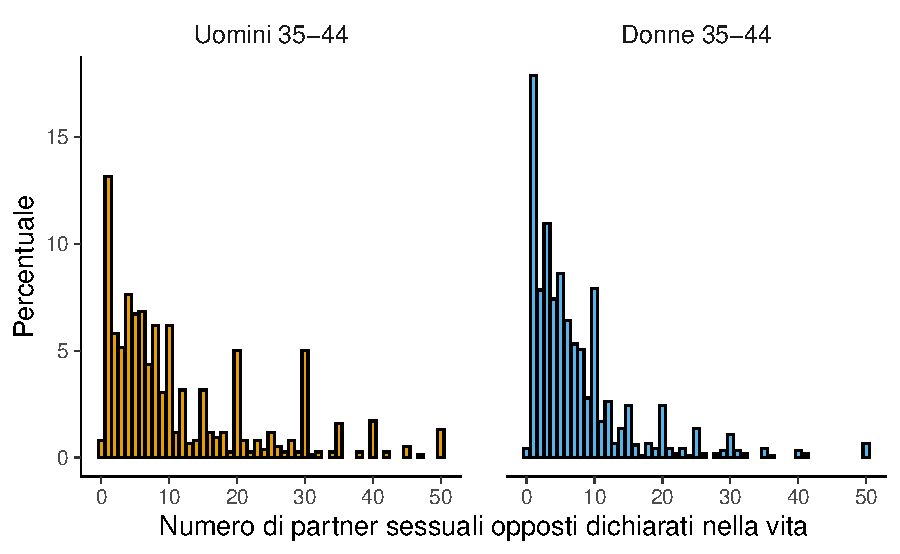
\includegraphics[width=0.7\linewidth,height=\textheight,keepaspectratio]{chapters/eda/07_loc_scale_files/figure-pdf/unnamed-chunk-11-1.pdf}
\end{center}

Notiamo che la distribuzione è altamente asimmetrica positiva. Come
possiamo descrivere la tendenza centrale di questi dati?

Calcoliamo gli indici di tendenza centrale all'interno dei due gruppi.
Per la moda utilizziamo una funzione personalizzata:

\begin{Shaded}
\begin{Highlighting}[]
\CommentTok{\# Funzione personalizzata per calcolare la moda}
\NormalTok{get\_mode }\OtherTok{\textless{}{-}} \ControlFlowTok{function}\NormalTok{(x) \{}
  \CommentTok{\# Calcola la tabella di frequenza e restituisce il valore con frequenza massima}
\NormalTok{  tbl }\OtherTok{\textless{}{-}} \FunctionTok{table}\NormalTok{(x)}
  \FunctionTok{as.numeric}\NormalTok{(}\FunctionTok{names}\NormalTok{(tbl)[}\FunctionTok{which.max}\NormalTok{(tbl)])}
\NormalTok{\}}

\CommentTok{\# Calcolo delle statistiche per Gender}
\NormalTok{df }\SpecialCharTok{|\textgreater{}} 
  \FunctionTok{group\_by}\NormalTok{(Gender) }\SpecialCharTok{|\textgreater{}} 
  \FunctionTok{summarise}\NormalTok{(}
    \AttributeTok{mean\_sex\_partner =} \FunctionTok{mean}\NormalTok{(NumPartners, }\AttributeTok{na.rm =} \ConstantTok{TRUE}\NormalTok{),}
    \AttributeTok{median\_sex\_partner =} \FunctionTok{median}\NormalTok{(NumPartners, }\AttributeTok{na.rm =} \ConstantTok{TRUE}\NormalTok{),}
    \AttributeTok{mode\_sex\_partner =} \FunctionTok{get\_mode}\NormalTok{(NumPartners)  }\CommentTok{\# Usa la funzione personalizzata per la moda}
\NormalTok{  )}
\CommentTok{\#\textgreater{} \# A tibble: 2 x 4}
\CommentTok{\#\textgreater{}   Gender mean\_sex\_partner median\_sex\_partner mode\_sex\_partner}
\CommentTok{\#\textgreater{}   \textless{}chr\textgreater{}             \textless{}dbl\textgreater{}              \textless{}dbl\textgreater{}            \textless{}dbl\textgreater{}}
\CommentTok{\#\textgreater{} 1 Man               17.0                   8                1}
\CommentTok{\#\textgreater{} 2 Woman              8.23                  5                1}
\end{Highlighting}
\end{Shaded}

È evidente che, quando la distribuzione dei dati è altamente
asimmetrica, come nel caso attuale, gli indici di tendenza centrale --
media, mediana e moda -- possono fornire risultati molto diversi,
rendendo difficile individuare una misura rappresentativa della tendenza
centrale.

\begin{itemize}
\tightlist
\item
  La \textbf{media} risulta più elevata rispetto alla mediana e alla
  moda. Questo è tipico di una distribuzione asimmetrica positiva,
  caratterizzata da una lunga coda destra: pochi individui con valori
  estremamente alti influenzano la media, spostandola verso destra.\\
\item
  La \textbf{mediana}, invece, rappresenta il valore centrale della
  distribuzione e risulta meno influenzata dai valori estremi. Per
  questo motivo, è spesso più vicina alla ``realtà'' dei dati, offrendo
  una stima più robusta della tendenza centrale per la maggior parte
  degli individui.\\
\item
  La \textbf{moda}, infine, corrisponde al valore più frequente nella
  distribuzione (in questo caso, 1 partner). Tuttavia, in presenza di
  un'elevata dispersione dei dati, la moda può risultare poco
  rappresentativa della distribuzione complessiva.
\end{itemize}

In conclusione, quando la distribuzione è fortemente asimmetrica, la
\textbf{mediana} è generalmente l'indice di tendenza centrale più
appropriato. Essendo insensibile ai valori estremi, fornisce una
rappresentazione più robusta della ``posizione centrale'' dei dati.
Tuttavia, è utile integrare la mediana con la media e la moda per
offrire un quadro più completo della distribuzione.

Per una descrizione efficace della tendenza centrale in distribuzioni
asimmetriche, si consiglia dunque di seguire questa procedura:

\begin{enumerate}
\def\labelenumi{\arabic{enumi}.}
\tightlist
\item
  utilizzare la mediana come misura principale della tendenza
  centrale;\\
\item
  riportare media e moda come complemento per confrontare i risultati e
  interpretare eventuali differenze.
\end{enumerate}

È comunque fondamentale \textbf{visualizzare la distribuzione} dei dati
attraverso grafici appropriati, come istogrammi o boxplot. Questi
strumenti consentono di evidenziare chiaramente l'asimmetria,
identificare valori estremi e comprendere meglio la struttura dei dati.

Inoltre, per arricchire i sommari numerici, è importante associare
indici di dispersione che tratteremo in seguito.

\subsection{Media Spuntata}\label{media-spuntata}

La \emph{media spuntata}, indicata come \(\bar{x}_t\) o \emph{trimmed
mean}, è un metodo di calcolo della media che prevede l'eliminazione di
una determinata percentuale di dati estremi prima di effettuare la media
aritmetica. Solitamente, viene eliminato il 10\% dei dati, ovvero il 5\%
all'inizio e alla fine della distribuzione. Per ottenere la media
spuntata, i dati vengono ordinati in modo crescente,
\(x_1 \leq x_2 \leq x_3 \leq \dots \leq x_n\), e quindi viene eliminato
il primo 5\% e l'ultimo 5\% dei dati nella sequenza ordinata. Infine, la
media spuntata è calcolata come la media aritmetica dei dati rimanenti.
Questo approccio è utile quando ci sono valori anomali o quando la
distribuzione è asimmetrica e la media aritmetica non rappresenta
adeguatamente la tendenza centrale dei dati.

\begin{example}[]\protect\hypertarget{exm-}{}\label{exm-}

A titolo di esempio, procediamo al calcolo della media spuntata dei
valori \texttt{NumPartners} per i due gruppi definiti dalla variabile
\texttt{Gender}, escludendo il 10\% dei valori più estremi.

\begin{Shaded}
\begin{Highlighting}[]
\FunctionTok{glimpse}\NormalTok{(df)}
\CommentTok{\#\textgreater{} Rows: 1,989}
\CommentTok{\#\textgreater{} Columns: 2}
\CommentTok{\#\textgreater{} $ Gender      \textless{}chr\textgreater{} "Man", "Man", "Man", "Man", "Man", "Man", "Man", "Man"\textasciitilde{}}
\CommentTok{\#\textgreater{} $ NumPartners \textless{}int\textgreater{} 0, 0, 0, 0, 0, 0, 1, 1, 1, 1, 1, 1, 1, 1, 1, 1, 1, 1, \textasciitilde{}}
\end{Highlighting}
\end{Shaded}

Uomini:

\begin{Shaded}
\begin{Highlighting}[]
\NormalTok{sex\_partners\_men }\OtherTok{\textless{}{-}}\NormalTok{ df[df}\SpecialCharTok{$}\NormalTok{Gender }\SpecialCharTok{==} \StringTok{"Man"}\NormalTok{, }\StringTok{"NumPartners"}\NormalTok{]}
\FunctionTok{mean}\NormalTok{(sex\_partners\_men, }\AttributeTok{trim =} \FloatTok{0.10}\NormalTok{, }\AttributeTok{na.rm =} \ConstantTok{TRUE}\NormalTok{)}
\CommentTok{\#\textgreater{} [1] 10.6}
\end{Highlighting}
\end{Shaded}

Donne:

\begin{Shaded}
\begin{Highlighting}[]
\NormalTok{sex\_partners\_women }\OtherTok{\textless{}{-}}\NormalTok{ df[df}\SpecialCharTok{$}\NormalTok{Gender }\SpecialCharTok{==} \StringTok{"Woman"}\NormalTok{, }\StringTok{"NumPartners"}\NormalTok{]}
\FunctionTok{mean}\NormalTok{(sex\_partners\_women, }\AttributeTok{trim =} \FloatTok{0.10}\NormalTok{, }\AttributeTok{na.rm =} \ConstantTok{TRUE}\NormalTok{)}
\CommentTok{\#\textgreater{} [1] 6.013}
\end{Highlighting}
\end{Shaded}

\end{example}

\subsection{Quando Usare Media, Media Spuntata, Moda e
Mediana}\label{quando-usare-media-media-spuntata-moda-e-mediana}

La scelta della misura di tendenza centrale più appropriata dipende dal
tipo di dati, dalla distribuzione e dalla presenza di valori anomali o
asimmetrie.

\subsubsection{Moda}\label{moda-1}

La \textbf{moda} è il valore che compare con maggiore frequenza nei dati
ed è l'unica misura di tendenza centrale utilizzabile per dati a livello
nominale (categorie senza ordine) o ordinale (categorie ordinate ma
senza distanza definita). Tuttavia:\\
- In una distribuzione unimodale, la moda può rappresentare un
indicatore significativo della tendenza centrale.\\
- In distribuzioni multimodali (con più valori ricorrenti), la moda
diventa meno interpretabile, poiché l'esistenza di più ``picchi'' rende
difficile individuare un singolo valore rappresentativo.\\
- Nei dati continui, la moda può non essere definita o risultare meno
informativa, soprattutto in presenza di valori unici.

\subsubsection{Media}\label{media-1}

La \textbf{media aritmetica} è una misura efficace di tendenza centrale
se la distribuzione è simmetrica e priva di valori anomali. In tali
condizioni, la media rappresenta il ``baricentro'' della distribuzione,
equilibrando i valori a sinistra e a destra. Tuttavia:

\begin{itemize}
\tightlist
\item
  In distribuzioni asimmetriche o con outlier, la media è fortemente
  influenzata dai valori estremi e tende a spostarsi nella direzione
  della coda più lunga (asimmetria positiva o negativa).\\
\item
  In questi casi, la media potrebbe non essere rappresentativa della
  tendenza centrale reale.
\end{itemize}

\subsubsection{Media Spuntata}\label{media-spuntata-1}

La \textbf{media spuntata} è una versione modificata della media,
calcolata dopo aver rimosso una certa percentuale di valori estremi
(generalmente il 5\% o il 10\%) sia dalla coda inferiore che da quella
superiore della distribuzione. Questa misura è particolarmente utile
quando:\\
- La distribuzione è asimmetrica o contiene outlier, ma si desidera
comunque una stima della tendenza centrale che consideri gran parte dei
dati.\\
- La media spuntata è meno sensibile ai valori anomali rispetto alla
media tradizionale, pur mantenendo il vantaggio di considerare un'ampia
porzione dei dati.

\subsubsection{Mediana}\label{mediana-1}

La \textbf{mediana} è il valore centrale che divide il campione in due
metà: il 50\% dei dati è inferiore e il restante 50\% è superiore. È una
misura robusta della tendenza centrale, particolarmente adatta quando:\\
- La distribuzione è asimmetrica o contiene valori anomali. Poiché si
basa sulla posizione dei dati e non sulle loro dimensioni, la mediana
non è influenzata da valori estremi.\\
- Nei dati \textbf{ordinali}, la mediana è spesso più appropriata della
media, poiché non richiede una scala numerica con distanze precise.

\subsubsection{Quale Misura Scegliere?}\label{quale-misura-scegliere}

\begin{enumerate}
\def\labelenumi{\arabic{enumi}.}
\item
  \textbf{Distribuzioni Simmetriche}:\\
  La \textbf{media} è la scelta più appropriata, poiché riflette bene la
  tendenza centrale.
\item
  \textbf{Distribuzioni Asimmetriche} o con \textbf{Outlier}:\\
  La \textbf{mediana} è preferibile perché è robusta e meno influenzata
  dai valori estremi. In alternativa, si può utilizzare la \textbf{media
  spuntata} per ottenere un compromesso tra media e mediana.
\item
  \textbf{Dati Categoriali}:\\
  La \textbf{moda} è l'unica misura applicabile, ma è interpretabile
  solo in distribuzioni unimodali.
\item
  \textbf{Distribuzioni Multimodali}:\\
  In questo caso, è importante visualizzare i dati (ad esempio con un
  istogramma) e descrivere ciascun ``picco'' separatamente, poiché
  nessuna delle misure tradizionali (media, mediana, moda) sarà
  sufficiente da sola per rappresentare la tendenza centrale.
\end{enumerate}

In conclusione

\begin{itemize}
\tightlist
\item
  La \textbf{media} è ideale per distribuzioni simmetriche senza valori
  estremi.\\
\item
  La \textbf{mediana} è più robusta e appropriata in caso di asimmetria
  o outlier.\\
\item
  La \textbf{media spuntata} rappresenta una soluzione intermedia utile
  nei casi con pochi valori anomali.\\
\item
  La \textbf{moda} è rilevante solo per dati nominali o ordinale, ma
  perde significato in distribuzioni multimodali.
\end{itemize}

\section{La Variabilità nei Dati
Psicologici}\label{la-variabilituxe0-nei-dati-psicologici}

Se misuriamo il livello di stress percepito da una persona dieci volte
in un solo giorno, è improbabile ottenere esattamente lo stesso valore
ogni volta, anche utilizzando la stessa scala. Se valutiamo il punteggio
di autostima in un campione di studenti universitari utilizzando un
questionario standardizzato, otterremo valori differenti per ciascun
partecipante. Allo stesso modo, se registriamo il tempo di reazione in
un compito cognitivo somministrato a un gruppo di persone, noteremo una
variabilità nei tempi di risposta anche tra prove dello stesso
individuo. La variazione è una caratteristica intrinseca dei fenomeni
psicologici e comportamentali, e comprenderne a fondo la natura, le
cause e i modi per descriverla è essenziale. In effetti, attribuire la
variazione a determinati fattori causali -- come differenze individuali,
influenze ambientali o variabilità di misurazione -- è uno degli
obiettivi principali dell'analisi statistica. In questa sezione,
esamineremo come la variazione può essere suddivisa, i due tipi
principali di variazione (spiegata e non spiegata) e i metodi per
descriverla sia visivamente sia numericamente.

In questa sezione, esamineremo come la variazione può essere suddivisa,
i due tipi principali di variazione (spiegata e non spiegata) e i metodi
per descriverla sia visivamente sia numericamente. Comprendere la
variabilità è cruciale in psicologia, poiché molti fenomeni, come le
differenze individuali o le fluttuazioni dell'umore, dipendono proprio
dall'analisi della dispersione dei dati.

\section{Quantili}\label{quantili-1}

I \textbf{quantili} sono valori che dividono la distribuzione dei dati
in intervalli proporzionali, fornendo informazioni sulla loro
\textbf{variabilità} e sui punti critici della distribuzione. Il
\textbf{quantile non interpolato} di ordine \(p\) (\(0 < p < 1\)) è
definito come il valore al di sotto del quale si trova una frazione
\(p\) dei dati.

La formula per calcolare il quantile non interpolato è:

\[
q_p = x_{(k)},
\]

dove \(x_{(k)}\) è il valore \(k\)-esimo dell'insieme di dati
\textbf{ordinati in modo crescente}. L'indice \(k\) è determinato come:

\[
k = \lceil p \cdot n \rceil,
\]

dove \(n\) è il numero totale di osservazioni e \(\lceil \cdot \rceil\)
rappresenta la funzione di arrotondamento all'intero successivo.

\begin{example}[]\protect\hypertarget{exm-}{}\label{exm-}

Consideriamo il seguente insieme di dati:

\[
\{ 15, 20, 23, 25, 28, 30, 35, 40, 45, 50 \}.
\]\\
Supponiamo di voler calcolare il quantile di ordine 0.3 (30°
percentile):

\begin{enumerate}
\def\labelenumi{\arabic{enumi}.}
\item
  I dati sono già ordinati in ordine crescente.\\
\item
  Calcoliamo \(k\) come:

  \[
  k = \lceil 0.3 \cdot 10 \rceil = \lceil 3 \rceil = 3.
  \]
\item
  Il quantile corrisponde al terzo valore nell'insieme ordinato:

  \[
  q_{0.3} = x_{(3)} = 23.
  \]\\
\end{enumerate}

\end{example}

\subsection{Quantile Interpolato}\label{quantile-interpolato}

Per valori di \(p\) che non corrispondono esattamente a una posizione
nell'insieme di dati ordinati, si utilizza il \textbf{quantile
interpolato}. Questo metodo stima il valore attraverso
un'\textbf{interpolazione lineare} tra i dati adiacenti. È
particolarmente utile per set di dati numerosi e viene calcolato
automaticamente tramite software statistici come R o Python.

\subsection{Interpretazione dei
Quantili}\label{interpretazione-dei-quantili}

I quantili completano le misure di tendenza centrale (media, mediana,
moda), permettendo di esplorare la distribuzione dei dati e identificare
i valori critici. In particolare:

\begin{itemize}
\tightlist
\item
  I \textbf{quantili bassi} (ad esempio il \textbf{10° percentile})
  forniscono informazioni sui valori \textbf{minimi} o nella parte
  inferiore della distribuzione.\\
\item
  I \textbf{quantili alti} (ad esempio il \textbf{90° percentile})
  aiutano a esplorare i valori \textbf{massimi} o nella parte superiore
  della distribuzione.\\
\item
  La \textbf{mediana} è un caso particolare di quantile, corrispondente
  al \textbf{quantile di ordine 0.5}: divide la distribuzione in due
  parti uguali.
\end{itemize}

\subsection{Importanza dei Quantili}\label{importanza-dei-quantili}

L'uso congiunto di quantili e misure di tendenza centrale è fondamentale
per ottenere una descrizione completa e robusta di una distribuzione,
soprattutto in presenza di asimmetrie o valori anomali. Mentre la media
e la mediana descrivono il comportamento ``centrale'' dei dati, i
quantili permettono di analizzare la dispersione e identificare aree di
particolare interesse nella distribuzione.

\begin{example}[]\protect\hypertarget{exm-}{}\label{exm-}

Consideriamo ora la variabile \texttt{NumPartners} per due gruppi
definiti dalla variabile \texttt{Gender} (``Man'' e ``Woman'').
Calcoleremo i quantili di ordine 0.1 e 0.9 per ciascun gruppo:

\begin{itemize}
\tightlist
\item
  Il quantile di ordine 0.1 rappresenta il valore al di sotto del quale
  si trova il 10\% dei dati.\\
\item
  Il quantile di ordine 0.9 rappresenta il valore al di sotto del quale
  si trova il 90\% dei dati.
\end{itemize}

Calcolo per il Gruppo ``Man'':

\begin{Shaded}
\begin{Highlighting}[]
\CommentTok{\# Quantili di ordine 0.1 e 0.9 per i maschi}
\FunctionTok{quantile}\NormalTok{(df[df}\SpecialCharTok{$}\NormalTok{Gender }\SpecialCharTok{==} \StringTok{"Man"}\NormalTok{, }\StringTok{"NumPartners"}\NormalTok{], }\AttributeTok{probs =} \FunctionTok{c}\NormalTok{(}\FloatTok{0.1}\NormalTok{, }\FloatTok{0.9}\NormalTok{))}
\CommentTok{\#\textgreater{}  10\%  90\% }
\CommentTok{\#\textgreater{}  1.0 34.5}
\end{Highlighting}
\end{Shaded}

\begin{itemize}
\tightlist
\item
  10° percentile (0.1): \(1.0\) → Il 10\% degli uomini ha dichiarato al
  massimo 1 partner sessuale.\\
\item
  90° percentile (0.9): \(34.5\) → Il 10\% degli uomini con i valori più
  alti ha dichiarato più di 34 partner sessuali.
\end{itemize}

Calcolo per il Gruppo ``Woman'':

\begin{Shaded}
\begin{Highlighting}[]
\CommentTok{\# Quantili di ordine 0.1 e 0.9 per le femmine}
\FunctionTok{quantile}\NormalTok{(df[df}\SpecialCharTok{$}\NormalTok{Gender }\SpecialCharTok{==} \StringTok{"Woman"}\NormalTok{, }\StringTok{"NumPartners"}\NormalTok{], }\AttributeTok{probs =} \FunctionTok{c}\NormalTok{(}\FloatTok{0.1}\NormalTok{, }\FloatTok{0.9}\NormalTok{))}
\CommentTok{\#\textgreater{} 10\% 90\% }
\CommentTok{\#\textgreater{}   1  18}
\end{Highlighting}
\end{Shaded}

\begin{itemize}
\tightlist
\item
  10° percentile (0.1): \(1.0\) → Anche per le donne, il 10\% dei valori
  più bassi corrisponde a 1 partner sessuale.\\
\item
  90° percentile (0.9): \(18.0\) → Il 10\% delle donne con i valori più
  alti ha dichiarato più di 18 partner sessuali.
\end{itemize}

I quantili calcolati forniscono una descrizione chiara della dispersione
e della variabilità dei dati nei due gruppi:

\begin{itemize}
\tightlist
\item
  Il fatto che il 10° percentile sia identico per entrambi i gruppi
  suggerisce che una porzione simile di intervistati dichiara un numero
  molto basso di partner sessuali.\\
\item
  La differenza nel 90° percentile tra uomini e donne è significativa:

  \begin{itemize}
  \tightlist
  \item
    Per gli uomini, il valore è più alto (\(34.5\)), indicando una
    maggiore presenza di valori estremi nella coda superiore della
    distribuzione.\\
  \item
    Per le donne, il valore (\(18.0\)) è inferiore, suggerendo una
    minore dispersione nella parte alta della distribuzione.
  \end{itemize}
\end{itemize}

Questa differenza evidenzia una asimmetria positiva più pronunciata nel
gruppo degli uomini, dove pochi individui con valori elevati ``tirano''
la coda della distribuzione verso destra.

\end{example}

\section{Percentili}\label{percentili}

Prima di procedere, chiarifichiamo alcuni termini comunemente usati
nell'analisi esplorativa.

I \textbf{percentili} sono casi particolari di \textbf{quantili}: invece
di \((0.05, 0.10, ...)\), immaginiamo di suddividere l'intervallo
\([0,1]\) in \((0.01, 0.02, ...)\).

Ad esempio, il 25° percentile (o \textbf{primo quartile}) è il valore
sotto il quale cade il 25\% dei dati, il 50° percentile è anche detto
\textbf{mediana}, e il 75° percentile (terzo quartile) è il valore sotto
il quale cade il 75\% dei dati.

\section{Intervallo di variazione}\label{intervallo-di-variazione}

L'\textbf{intervallo di variazione} è il più semplice tra gli indici di
dispersione. Si calcola come la differenza tra il valore massimo e il
valore minimo di una distribuzione:

\[
\text{Intervallo di variazione} = \text{valore massimo} - \text{valore minimo}.
\]

Tuttavia, l'intervallo di variazione presenta due limiti principali:

\begin{enumerate}
\def\labelenumi{\arabic{enumi}.}
\tightlist
\item
  Si basa esclusivamente su due valori della distribuzione, ignorando
  tutte le altre osservazioni.
\item
  È altamente sensibile ai valori anomali (ad esempio, un adolescente
  con un punteggio di autostima molto più basso o più alto rispetto alla
  maggior parte del campione).
\end{enumerate}

\begin{example}[]\protect\hypertarget{exm-}{}\label{exm-}

Supponiamo di misurare il punteggio di autostima in un campione di
adolescenti. Se il punteggio massimo è 35 e il minimo è 12, l'intervallo
di variazione sarà:

\[
\text{Intervallo di variazione} = 35 - 12 = 23.
\]

\end{example}

\section{Differenza interquartile}\label{differenza-interquartile}

Un'altra misura basata sull'ordinamento è la \textbf{differenza
interquartile (IQR)}, calcolata come la differenza tra il terzo quartile
(\(Q_3\)) e il primo quartile (\(Q_1\)):

\[
\text{IQR} = Q_3 - Q_1.
\]

L'IQR considera solo il 50\% centrale dei dati, ignorando gli estremi,
rendendolo meno sensibile ai valori anomali rispetto all'intervallo di
variazione.

\begin{example}[]\protect\hypertarget{exm-}{}\label{exm-}

Supponiamo di analizzare il livello di ansia percepita in un gruppo di
studenti universitari. Se il primo quartile (\(Q_1\)) è 25 (25\% degli
studenti ha un livello di ansia pari o inferiore a 25) e il terzo
quartile (\(Q_3\)) è 40 (75\% degli studenti ha un livello di ansia pari
o inferiore a 40), allora:

\[
\text{IQR} = 40 - 25 = 15.
\]

\end{example}

\section{La Varianza}\label{la-varianza}

Per ottenere una misura di dispersione che consideri tutte le
osservazioni, l'indice più utilizzato è la \textbf{varianza}. Questa
misura valuta la dispersione dei dati rispetto alla media e si calcola
come la media dei quadrati degli scarti di ciascun valore (\(x_i\))
dalla media (\(\bar{x}\)):

\begin{equation}\phantomsection\label{eq-var-descr}{
S^2 = \frac{1}{n} \sum_{i=1}^n (x_i - \bar{x})^2.
}\end{equation}

\begin{example}[]\protect\hypertarget{exm-}{}\label{exm-}

Supponiamo di calcolare il numero di ore dedicate allo studio quotidiano
da un gruppo di partecipanti a un esperimento di psicologia. Se la media
delle ore studiate è 4 (\(\bar{x} = 4\)), la varianza misura quanto i
dati si discostano da questa media. I dati con una varianza maggiore
indicano una maggiore diversità nei comportamenti di studio, mentre una
varianza minore suggerisce un gruppo più omogeneo.

\end{example}

\subsection{Proprietà della varianza}\label{proprietuxe0-della-varianza}

\begin{enumerate}
\def\labelenumi{\arabic{enumi}.}
\tightlist
\item
  \textbf{Unità di misura}: La varianza è espressa nell'unità di misura
  al quadrato dei dati originali (es. ore quadrate nel caso precedente),
  rendendola meno intuitiva da interpretare.
\item
  \textbf{Sensibilità agli outlier}: Poiché ogni scarto viene elevato al
  quadrato, i valori estremi influenzano significativamente la varianza.
\end{enumerate}

\subsection{Variazione Sistematica e Non
Sistematica}\label{variazione-sistematica-e-non-sistematica}

Nell'analisi dei dati psicologici, la variabilità può essere suddivisa
in due componenti principali:

\begin{enumerate}
\def\labelenumi{\arabic{enumi}.}
\item
  \textbf{Variazione non sistematica} (rumore):\\
  È la variabilità casuale, non attribuibile a una causa specifica. Si
  manifesta come errori di misurazione o fluttuazioni imprevedibili che
  non seguono uno schema chiaro. Esempi includono:

  \begin{itemize}
  \tightlist
  \item
    Errori casuali nel completare un test (ad esempio, distrazione
    momentanea).\\
  \item
    Fluttuazioni dell'umore durante la giornata.
  \end{itemize}
\item
  \textbf{Variazione sistematica} (segnale):\\
  È la variabilità attribuibile a fattori specifici che influiscono in
  modo prevedibile sui dati. Questa componente rappresenta il
  ``segnale'' utile nell'analisi statistica. Esempi includono:

  \begin{itemize}
  \tightlist
  \item
    Il miglioramento nei punteggi di un test di attenzione dopo una
    sessione di meditazione.\\
  \item
    Le differenze individuali nei livelli di self-compassion misurati da
    una scala psicologica.
  \end{itemize}
\end{enumerate}

Per esempio, supponiamo di misurare il livello di stress prima e dopo
una sessione di rilassamento:

\begin{itemize}
\tightlist
\item
  La variazione sistematica rappresenta la riduzione del livello di
  stress dovuta all'effetto del rilassamento.\\
\item
  La variazione non sistematica comprende fattori casuali, come
  distrazioni, stanchezza momentanea o condizioni personali dei
  partecipanti.
\end{itemize}

\subsection{Calcolo della Varianza in
R}\label{calcolo-della-varianza-in-r}

Per illustrare come quantificare la variabilità, utilizziamo i punteggi
totali della \emph{Self-Compassion Scale} su un campione di studenti
universitari, forniti nel file \texttt{scs\_scores.csv}.

\textbf{Passaggio 1: Importazione dei dati}

\begin{Shaded}
\begin{Highlighting}[]
\NormalTok{scs\_df }\OtherTok{\textless{}{-}}\NormalTok{ rio}\SpecialCharTok{::}\FunctionTok{import}\NormalTok{(here}\SpecialCharTok{::}\FunctionTok{here}\NormalTok{(}\StringTok{"data"}\NormalTok{, }\StringTok{"scs\_scores.csv"}\NormalTok{)) }\SpecialCharTok{|\textgreater{}} 
\NormalTok{  dplyr}\SpecialCharTok{::}\FunctionTok{rename}\NormalTok{(}\AttributeTok{ts =}\NormalTok{ scs\_total\_score)}
\FunctionTok{glimpse}\NormalTok{(scs\_df)}
\CommentTok{\#\textgreater{} Rows: 121}
\CommentTok{\#\textgreater{} Columns: 7}
\CommentTok{\#\textgreater{} $ self\_kindness       \textless{}int\textgreater{} 14, 15, 19, 10, 11, 9, 19, 13, 23, 5, 14, 22, \textasciitilde{}}
\CommentTok{\#\textgreater{} $ common\_humanity     \textless{}int\textgreater{} 11, 9, 16, 11, 10, 8, 12, 12, 19, 4, 13, 18, 6\textasciitilde{}}
\CommentTok{\#\textgreater{} $ mindfulness         \textless{}int\textgreater{} 10, 10, 16, 9, 9, 10, 8, 12, 20, 8, 15, 15, 6,\textasciitilde{}}
\CommentTok{\#\textgreater{} $ self\_judgment       \textless{}int\textgreater{} 15, 16, 13, 15, 18, 19, 11, 15, 9, 25, 17, 11,\textasciitilde{}}
\CommentTok{\#\textgreater{} $ isolation           \textless{}int\textgreater{} 16, 11, 12, 14, 13, 16, 11, 11, 5, 20, 14, 11,\textasciitilde{}}
\CommentTok{\#\textgreater{} $ over\_identification \textless{}int\textgreater{} 14, 11, 8, 11, 14, 17, 20, 15, 7, 20, 15, 16, \textasciitilde{}}
\CommentTok{\#\textgreater{} $ ts                  \textless{}int\textgreater{} 68, 74, 96, 68, 63, 53, 75, 74, 119, 30, 74, 9\textasciitilde{}}
\end{Highlighting}
\end{Shaded}

La colonna \texttt{ts} contiene i punteggi totali della scala.

\textbf{Passaggio 2: Calcolo della varianza}

Utilizzando la formula della varianza:

\begin{Shaded}
\begin{Highlighting}[]
\FunctionTok{sum}\NormalTok{((scs\_df}\SpecialCharTok{$}\NormalTok{ts }\SpecialCharTok{{-}} \FunctionTok{mean}\NormalTok{(scs\_df}\SpecialCharTok{$}\NormalTok{ts))}\SpecialCharTok{\^{}}\DecValTok{2}\NormalTok{) }\SpecialCharTok{/} \FunctionTok{length}\NormalTok{(scs\_df}\SpecialCharTok{$}\NormalTok{ts)}
\CommentTok{\#\textgreater{} [1] 405.3}
\end{Highlighting}
\end{Shaded}

Con la funzione \texttt{var()} corretta per il campione:

\begin{Shaded}
\begin{Highlighting}[]
\FunctionTok{var}\NormalTok{(scs\_df}\SpecialCharTok{$}\NormalTok{ts) }\SpecialCharTok{*}\NormalTok{ (}\FunctionTok{length}\NormalTok{(scs\_df}\SpecialCharTok{$}\NormalTok{ts) }\SpecialCharTok{{-}} \DecValTok{1}\NormalTok{) }\SpecialCharTok{/} \FunctionTok{length}\NormalTok{(scs\_df}\SpecialCharTok{$}\NormalTok{ts)}
\CommentTok{\#\textgreater{} [1] 405.3}
\end{Highlighting}
\end{Shaded}

\subsection{Interpretazione della
Varianza}\label{interpretazione-della-varianza}

La varianza misura la dispersione totale dei dati, che può essere
scomposta in:

\begin{enumerate}
\def\labelenumi{\arabic{enumi}.}
\item
  \textbf{Variazione sistematica}:\\
  Nel caso della Self-Compassion Scale, la varianza sistematica riflette
  le differenze tra individui nei livelli di self-compassion. Alcuni
  individui mostrano livelli elevati (fattore protettivo contro il
  disagio psicologico), mentre altri livelli più bassi.
\item
  \textbf{Variazione non sistematica}:\\
  Questa componente è dovuta a \textbf{errori di misurazione} e altre
  cause casuali. La psicometria presuppone che il punteggio osservato
  sia la somma di:\\
  \[
  \text{Punteggio osservato} = \text{Punteggio vero} + \text{Errore di misurazione}.
  \] Esempi di errori includono distrazioni o stanchezza dei
  partecipanti; limitazioni della scala psicologica nella misurazione
  accurata del costrutto.
\end{enumerate}

\subsection{Affidabilità e Rapporto
Segnale-Rumore}\label{affidabilituxe0-e-rapporto-segnale-rumore}

Perché uno strumento psicometrico sia considerato affidabile, almeno
l'80\% della varianza osservata deve essere attribuibile alla componente
vera del costrutto. Questo requisito si traduce in un coefficiente di
affidabilità di almeno 0.8.

\begin{itemize}
\tightlist
\item
  Un \textbf{alto rapporto segnale-rumore} indica che la maggior parte
  della variabilità osservata è dovuta a fattori sistematici (segnale) e
  non a errori casuali (rumore).\\
\item
  Un \textbf{basso rapporto segnale-rumore} suggerisce che la
  variabilità casuale (rumore) è predominante e lo strumento potrebbe
  non essere sufficientemente preciso.
\end{itemize}

La psicometria fornisce strumenti per:

\begin{itemize}
\tightlist
\item
  \textbf{valutare l'affidabilità} delle scale psicologiche (es. Alpha
  di Cronbach);
\item
  \textbf{progettare strumenti più accurati} per minimizzare la
  variabilità non sistematica (rumore).
\end{itemize}

Uno strumento affidabile assicura che i risultati riflettano con
precisione le differenze \textbf{reali} tra gli individui e non siano
influenzati da errori casuali.

Supponiamo di valutare l'efficacia di un nuovo metodo di studio
misurando il miglioramento in un test di comprensione:

\begin{itemize}
\tightlist
\item
  un \textbf{alto rapporto segnale-rumore} (ovvero, un'alta
  affidabilità) indica che il miglioramento osservato è chiaramente
  attribuibile al metodo;
\item
  un \textbf{basso rapporto segnale-rumore} (bassa affidabilità) implica
  che la variabilità è prevalentemente casuale e l'effetto del metodo
  non è distinguibile dal rumore.
\end{itemize}

In conclusione, la distinzione tra \textbf{variazione sistematica} e
\textbf{non sistematica} è fondamentale per l'analisi dei dati
psicologici:

\begin{itemize}
\tightlist
\item
  la \textbf{variazione sistematica} rappresenta il ``segnale'', ossia
  l'effetto reale o il fattore di interesse;
\item
  la \textbf{variazione non sistematica} rappresenta il ``rumore'',
  ossia la variabilità casuale o l'errore di misurazione.
\end{itemize}

L'obiettivo è \textbf{massimizzare il segnale} e \textbf{minimizzare il
rumore}, garantendo strumenti affidabili che consentano di ottenere
risultati precisi e interpretabili.

\section{Stima della Varianza della
Popolazione}\label{stima-della-varianza-della-popolazione}

Si noti il denominatore della formula della varianza.
Nell'Equazione~\ref{eq-var-descr}, ho utilizzato \(n\) come denominatore
(l'ampiezza campionaria, ovvero il numero di osservazioni nel campione).
In questo modo, otteniamo la varianza come \emph{statistica descrittiva}
del campione. Tuttavia, è possibile utilizzare \(n-1\) come denominatore
alternativo:

\begin{equation}\phantomsection\label{eq-var-stimatore}{
\begin{equation}
s^2 = \frac{1}{n-1} \sum_{i=1}^n (x_i - \bar{x})^2
\end{equation}
}\end{equation}

In questo secondo caso, otteniamo la varianza come \emph{stimatore}
della varianza della popolazione. Si può dimostrare che
l'Equazione~\ref{eq-var-stimatore} fornisce una stima corretta (ovvero,
non distorta) della varianza della popolazione da cui abbiamo ottenuto
il campione, mentre l'Equazione~\ref{eq-var-descr} fornisce (in media)
una stima troppo piccola della varianza della popolazione. Si presti
attenzione alla notazione: \(S^2\) rappresenta la varianza come
statistica descrittiva, mentre \(s^2\) rappresenta la varianza come
stimatore.

Per illustrare questo punto, svolgiamo una simulazione. Consideriamo la
distribuzione dei punteggi del quoziente di intelligenza (QI). I valori
del QI seguono una particolare distribuzione chiamata
\emph{distribuzione normale}, con media 100 e deviazione standard 15. La
forma di questa distribuzione è illustrata nella figura seguente.

\begin{Shaded}
\begin{Highlighting}[]
\CommentTok{\# Define parameters}
\NormalTok{x }\OtherTok{\textless{}{-}} \FunctionTok{seq}\NormalTok{(}\DecValTok{100} \SpecialCharTok{{-}} \DecValTok{4} \SpecialCharTok{*} \DecValTok{15}\NormalTok{, }\DecValTok{100} \SpecialCharTok{+} \DecValTok{4} \SpecialCharTok{*} \DecValTok{15}\NormalTok{, }\AttributeTok{by =} \FloatTok{0.001}\NormalTok{)}
\NormalTok{mu }\OtherTok{\textless{}{-}} \DecValTok{100}
\NormalTok{sigma }\OtherTok{\textless{}{-}} \DecValTok{15}

\CommentTok{\# Compute the PDF}
\NormalTok{pdf }\OtherTok{\textless{}{-}} \FunctionTok{dnorm}\NormalTok{(x, }\AttributeTok{mean =}\NormalTok{ mu, }\AttributeTok{sd =}\NormalTok{ sigma)}

\CommentTok{\# Plot using ggplot2}
\NormalTok{data }\OtherTok{\textless{}{-}} \FunctionTok{tibble}\NormalTok{(}\AttributeTok{x =}\NormalTok{ x, }\AttributeTok{pdf =}\NormalTok{ pdf)}
\FunctionTok{ggplot}\NormalTok{(data, }\FunctionTok{aes}\NormalTok{(}\AttributeTok{x =}\NormalTok{ x, }\AttributeTok{y =}\NormalTok{ pdf)) }\SpecialCharTok{+}
  \FunctionTok{geom\_line}\NormalTok{() }\SpecialCharTok{+}
  \FunctionTok{labs}\NormalTok{(}
    \AttributeTok{x =} \StringTok{"QI"}\NormalTok{, }
    \AttributeTok{y =} \StringTok{"Densità"}\NormalTok{, }
    \AttributeTok{title =} \StringTok{"Distribuzione del QI nella popolazione"}
\NormalTok{  ) }
\end{Highlighting}
\end{Shaded}

\begin{center}
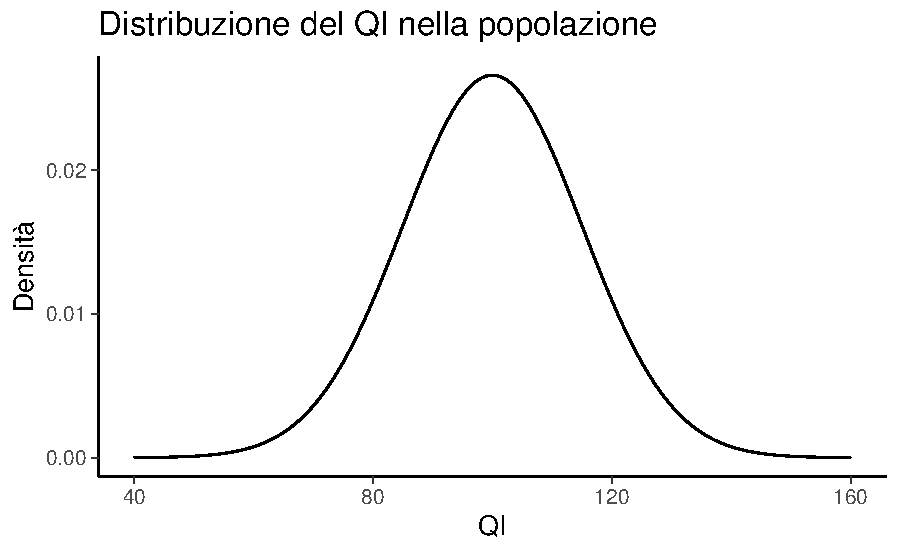
\includegraphics[width=0.7\linewidth,height=\textheight,keepaspectratio]{chapters/eda/07_loc_scale_files/figure-pdf/unnamed-chunk-21-1.pdf}
\end{center}

Supponiamo di estrarre un campione casuale di 4 osservazioni dalla
popolazione del quoziente di intelligenza -- in altre parole, supponiamo
di misurare il quoziente di intelligenza di 4 persone prese a caso dalla
popolazione.

\begin{Shaded}
\begin{Highlighting}[]
\FunctionTok{set.seed}\NormalTok{(}\DecValTok{123}\NormalTok{) }
\NormalTok{x }\OtherTok{\textless{}{-}} \FunctionTok{rnorm}\NormalTok{(}\DecValTok{4}\NormalTok{, }\AttributeTok{mean =} \DecValTok{100}\NormalTok{, }\AttributeTok{sd =} \DecValTok{15}\NormalTok{)}
\FunctionTok{print}\NormalTok{(x)}
\CommentTok{\#\textgreater{} [1]  91.59  96.55 123.38 101.06}
\end{Highlighting}
\end{Shaded}

Calcoliamo la varianza usando \(n\) al denominatore. Si noti che la vera
varianza del quoziente di intelligenza è \(15^2\) = 225.

\begin{Shaded}
\begin{Highlighting}[]
\FunctionTok{var}\NormalTok{(x)}
\CommentTok{\#\textgreater{} [1] 196.9}
\end{Highlighting}
\end{Shaded}

Consideriamo ora 10 campioni casuali del QI, ciascuno di ampiezza 4.

\begin{Shaded}
\begin{Highlighting}[]
\NormalTok{mu }\OtherTok{\textless{}{-}} \DecValTok{100}
\NormalTok{sigma }\OtherTok{\textless{}{-}} \DecValTok{15}
\NormalTok{size }\OtherTok{\textless{}{-}} \DecValTok{4}
\NormalTok{niter }\OtherTok{\textless{}{-}} \DecValTok{10}
\NormalTok{random\_samples }\OtherTok{\textless{}{-}} \FunctionTok{list}\NormalTok{()}

\FunctionTok{set.seed}\NormalTok{(}\DecValTok{123}\NormalTok{) }

\ControlFlowTok{for}\NormalTok{ (i }\ControlFlowTok{in} \DecValTok{1}\SpecialCharTok{:}\NormalTok{niter) \{}
\NormalTok{  one\_sample }\OtherTok{\textless{}{-}} \FunctionTok{rnorm}\NormalTok{(size, }\AttributeTok{mean =}\NormalTok{ mu, }\AttributeTok{sd =}\NormalTok{ sigma)}
\NormalTok{  random\_samples[[i]] }\OtherTok{\textless{}{-}}\NormalTok{ one\_sample}
\NormalTok{\}}
\end{Highlighting}
\end{Shaded}

Il primo campione è

\begin{Shaded}
\begin{Highlighting}[]
\NormalTok{random\_samples[}\DecValTok{1}\NormalTok{]}
\CommentTok{\#\textgreater{} [[1]]}
\CommentTok{\#\textgreater{} [1]  91.59  96.55 123.38 101.06}
\end{Highlighting}
\end{Shaded}

Il decimo campione è

\begin{Shaded}
\begin{Highlighting}[]
\NormalTok{random\_samples[}\DecValTok{10}\NormalTok{]}
\CommentTok{\#\textgreater{} [[1]]}
\CommentTok{\#\textgreater{} [1] 108.31  99.07  95.41  94.29}
\end{Highlighting}
\end{Shaded}

Stampiamo i valori di tutti i 10 campioni.

\begin{Shaded}
\begin{Highlighting}[]
\NormalTok{rs }\OtherTok{\textless{}{-}} \FunctionTok{do.call}\NormalTok{(rbind, random\_samples)}
\NormalTok{rs}
\CommentTok{\#\textgreater{}         [,1]   [,2]   [,3]   [,4]}
\CommentTok{\#\textgreater{}  [1,]  91.59  96.55 123.38 101.06}
\CommentTok{\#\textgreater{}  [2,] 101.94 125.73 106.91  81.02}
\CommentTok{\#\textgreater{}  [3,]  89.70  93.32 118.36 105.40}
\CommentTok{\#\textgreater{}  [4,] 106.01 101.66  91.66 126.80}
\CommentTok{\#\textgreater{}  [5,] 107.47  70.50 110.52  92.91}
\CommentTok{\#\textgreater{}  [6,]  83.98  96.73  84.61  89.07}
\CommentTok{\#\textgreater{}  [7,]  90.62  74.70 112.57 102.30}
\CommentTok{\#\textgreater{}  [8,]  82.93 118.81 106.40  95.57}
\CommentTok{\#\textgreater{}  [9,] 113.43 113.17 112.32 110.33}
\CommentTok{\#\textgreater{} [10,] 108.31  99.07  95.41  94.29}
\end{Highlighting}
\end{Shaded}

Per ciascun campione (ovvero, per ciascuna riga della matrice
precedente), calcoliamo la varianza usando la formula con \(n\) al
denominatore. Otteniamo così 10 stime della varianza della popolazione
del QI.

\begin{Shaded}
\begin{Highlighting}[]
\NormalTok{x\_var }\OtherTok{\textless{}{-}} \FunctionTok{apply}\NormalTok{(rs, }\DecValTok{1}\NormalTok{, var)  }\CommentTok{\# Applica la funzione var su ciascuna riga}
\FunctionTok{print}\NormalTok{(x\_var)}
\CommentTok{\#\textgreater{}  [1] 196.940 337.536 168.547 218.684 333.476  34.520 264.378 234.081   1.971}
\CommentTok{\#\textgreater{} [10]  40.468}
\end{Highlighting}
\end{Shaded}

Notiamo due cose:

\begin{itemize}
\tightlist
\item
  le stime sono molto diverse tra loro; questo fenomeno è noto con il
  nome di \emph{variabilità campionaria};
\item
  in media le stime sono troppo piccole.
\end{itemize}

Per aumentare la sicurezza riguardo al secondo punto menzionato in
precedenza, ripeteremo la simulazione utilizzando un numero di
iterazioni maggiore.

\begin{Shaded}
\begin{Highlighting}[]
\NormalTok{mu }\OtherTok{\textless{}{-}} \DecValTok{100}
\NormalTok{sigma }\OtherTok{\textless{}{-}} \DecValTok{15}
\NormalTok{size }\OtherTok{\textless{}{-}} \DecValTok{4}
\NormalTok{niter }\OtherTok{\textless{}{-}} \DecValTok{10000}
\NormalTok{random\_samples }\OtherTok{\textless{}{-}} \FunctionTok{list}\NormalTok{()}

\FunctionTok{set.seed}\NormalTok{(}\DecValTok{123}\NormalTok{) }\CommentTok{\# Replace 123 with your desired seed for reproducibility}

\ControlFlowTok{for}\NormalTok{ (i }\ControlFlowTok{in} \DecValTok{1}\SpecialCharTok{:}\NormalTok{niter) \{}
\NormalTok{  one\_sample }\OtherTok{\textless{}{-}} \FunctionTok{rnorm}\NormalTok{(size, }\AttributeTok{mean =}\NormalTok{ mu, }\AttributeTok{sd =}\NormalTok{ sigma)}
\NormalTok{  random\_samples[[i]] }\OtherTok{\textless{}{-}}\NormalTok{ one\_sample}
\NormalTok{\}}

\NormalTok{rs }\OtherTok{\textless{}{-}} \FunctionTok{do.call}\NormalTok{(rbind, random\_samples)}
\NormalTok{x\_var }\OtherTok{\textless{}{-}} \FunctionTok{apply}\NormalTok{(rs, }\DecValTok{1}\NormalTok{, var) }\SpecialCharTok{*}\NormalTok{ (size }\SpecialCharTok{{-}} \DecValTok{1}\NormalTok{) }\SpecialCharTok{/}\NormalTok{ size  }\CommentTok{\# Adjust for population variance (ddof = 0)}
\end{Highlighting}
\end{Shaded}

Esaminiamo la distribuzione dei valori ottenuti.

\begin{Shaded}
\begin{Highlighting}[]
\CommentTok{\# Create a data frame for plotting}
\NormalTok{data }\OtherTok{\textless{}{-}} \FunctionTok{data.frame}\NormalTok{(}\AttributeTok{x\_var =}\NormalTok{ x\_var)}

\CommentTok{\# Plot the histogram using ggplot2}
\FunctionTok{ggplot}\NormalTok{(data, }\FunctionTok{aes}\NormalTok{(}\AttributeTok{x =}\NormalTok{ x\_var)) }\SpecialCharTok{+}
  \FunctionTok{geom\_histogram}\NormalTok{(}\AttributeTok{alpha =} \FloatTok{0.5}\NormalTok{, }\AttributeTok{fill =} \StringTok{"blue"}\NormalTok{) }\SpecialCharTok{+}
  \FunctionTok{labs}\NormalTok{(}
    \AttributeTok{x =} \StringTok{"Varianza"}\NormalTok{, }
    \AttributeTok{y =} \StringTok{"Frequenza"}\NormalTok{, }
    \AttributeTok{title =} \StringTok{"Varianza del QI in campioni di n = 4"}
\NormalTok{  )}
\end{Highlighting}
\end{Shaded}

\begin{center}
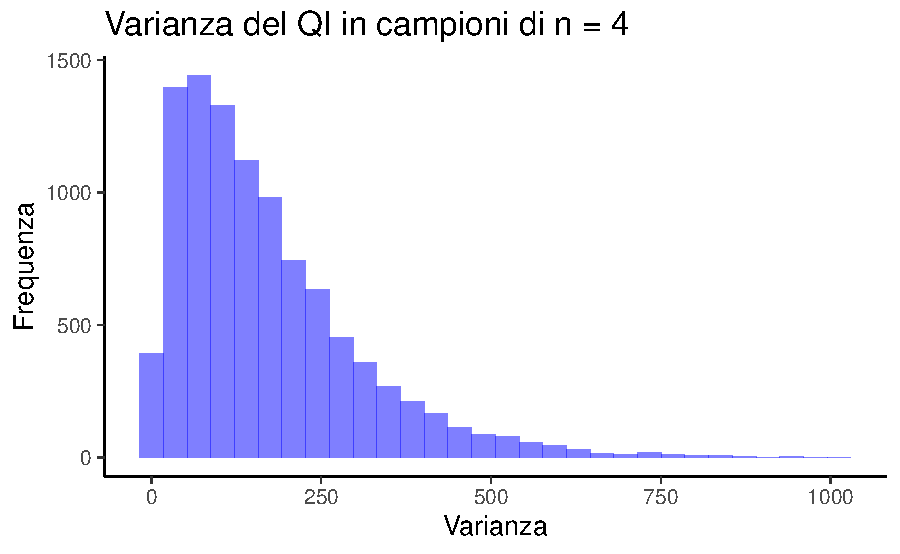
\includegraphics[width=0.7\linewidth,height=\textheight,keepaspectratio]{chapters/eda/07_loc_scale_files/figure-pdf/unnamed-chunk-30-1.pdf}
\end{center}

La stima più verosimile della varianza del QI è dato dalla media di
questa distribuzione.

\begin{Shaded}
\begin{Highlighting}[]
\FunctionTok{mean}\NormalTok{(x\_var)}
\CommentTok{\#\textgreater{} [1] 168.9}
\end{Highlighting}
\end{Shaded}

Si noti che il nostro spospetto è stato confermato: il valore medio
della stima della varianza ottenuta con l'Equazione~\ref{eq-var-descr} è
troppo piccolo rispetto al valore corretto di \(15^2 = 225\).

Ripetiamo ora la simulazione usando la formula della varianza con
\(n-1\) al denominatore.

\begin{Shaded}
\begin{Highlighting}[]
\FunctionTok{set.seed}\NormalTok{(}\DecValTok{123}\NormalTok{) }

\NormalTok{mu }\OtherTok{\textless{}{-}} \DecValTok{100}
\NormalTok{sigma }\OtherTok{\textless{}{-}} \DecValTok{15}
\NormalTok{size }\OtherTok{\textless{}{-}} \DecValTok{4}
\NormalTok{niter }\OtherTok{\textless{}{-}} \DecValTok{10000}
\NormalTok{random\_samples }\OtherTok{\textless{}{-}} \FunctionTok{list}\NormalTok{()}

\ControlFlowTok{for}\NormalTok{ (i }\ControlFlowTok{in} \DecValTok{1}\SpecialCharTok{:}\NormalTok{niter) \{}
\NormalTok{  one\_sample }\OtherTok{\textless{}{-}} \FunctionTok{rnorm}\NormalTok{(size, }\AttributeTok{mean =}\NormalTok{ mu, }\AttributeTok{sd =}\NormalTok{ sigma)}
\NormalTok{  random\_samples[[i]] }\OtherTok{\textless{}{-}}\NormalTok{ one\_sample}
\NormalTok{\}}

\NormalTok{rs }\OtherTok{\textless{}{-}} \FunctionTok{do.call}\NormalTok{(rbind, random\_samples)}
\NormalTok{x\_var }\OtherTok{\textless{}{-}} \FunctionTok{apply}\NormalTok{(rs, }\DecValTok{1}\NormalTok{, var)  }\CommentTok{\# ddof = 1 is default for var in R}

\FunctionTok{mean}\NormalTok{(x\_var)}
\CommentTok{\#\textgreater{} [1] 225.2}
\end{Highlighting}
\end{Shaded}

Nel secondo caso, se utilizziamo \(n-1\) come denominatore per calcolare
la stima della varianza, il valore atteso di questa stima è molto vicino
al valore corretto di 225. Se il numero di campioni fosse infinito, i
due valori sarebbero identici.

In conclusione, le due formule della varianza hanno scopi diversi. La
formula della varianza con \(n\) al denominatore viene utilizzata come
statistica descrittiva per descrivere la variabilità di un particolare
campione di osservazioni. D'altro canto, la formula della varianza con
\(n-1\) al denominatore viene utilizzata come stimatore per ottenere la
migliore stima della varianza della popolazione da cui quel campione è
stato estratto.

\section{Deviazione Standard}\label{deviazione-standard}

Per interpretare la varianza in modo più intuitivo, si può calcolare la
deviazione standard (o scarto quadratico medio o scarto tipo) prendendo
la radice quadrata della varianza. La deviazione standard è espressa
nell'unità di misura originaria dei dati, a differenza della varianza
che è espressa nel quadrato dell'unità di misura dei dati. La deviazione
standard fornisce una misura della dispersione dei dati attorno alla
media, rendendo più facile la comprensione della variabilità dei dati.

La deviazione standard (o scarto quadratico medio, o scarto tipo) è
definita come:

\begin{equation}\phantomsection\label{eq-sd-stimatore}{
s^2 = \sqrt{(n-1)^{-1} \sum_{i=1}^n (x_i - \bar{x})^2}.
}\end{equation}

Quando tutte le osservazioni sono uguali, \(s = 0\), altrimenti
\(s > 0\).

\begin{tcolorbox}[enhanced jigsaw, opacityback=0, bottomrule=.15mm, breakable, title=\textcolor{quarto-callout-note-color}{\faInfo}\hspace{0.5em}{Nota}, bottomtitle=1mm, toptitle=1mm, titlerule=0mm, colbacktitle=quarto-callout-note-color!10!white, rightrule=.15mm, colframe=quarto-callout-note-color-frame, colback=white, arc=.35mm, leftrule=.75mm, coltitle=black, left=2mm, toprule=.15mm, opacitybacktitle=0.6]

Il termine \emph{standard deviation} è stato introdotto in statistica da
Pearson nel 1894 assieme alla lettera greca \(\sigma\) che lo
rappresenta. Il termine italiano ``deviazione standard'' ne è la
traduzione più utilizzata nel linguaggio comune; il termine
dell'\href{https://it.wikipedia.org/wiki/Ente_nazionale_italiano_di_unificazione}{Ente
Nazionale Italiano di Unificazione} è tuttavia ``scarto tipo'', definito
come la radice quadrata positiva della varianza.

\end{tcolorbox}

La deviazione standard \(s\) dovrebbe essere utilizzata solo quando la
media è una misura appropriata per descrivere il centro della
distribuzione, ad esempio nel caso di distribuzioni simmetriche.
Tuttavia, è importante tener conto che, come la media \(\bar{x}\), anche
la deviazione standard è fortemente influenzata dalla presenza di dati
anomali, ovvero pochi valori che si discostano notevolmente dalla media
rispetto agli altri dati della distribuzione. In presenza di dati
anomali, la deviazione standard può risultare ingannevole e non
rappresentare accuratamente la variabilità complessiva della
distribuzione. Pertanto, è fondamentale considerare attentamente il
contesto e le caratteristiche dei dati prima di utilizzare la deviazione
standard come misura di dispersione. In alcune situazioni, potrebbe
essere più appropriato ricorrere a misure di dispersione robuste o ad
altre statistiche descrittive per caratterizzare la variabilità dei dati
in modo più accurato e affidabile.

\begin{example}[]\protect\hypertarget{exm-}{}\label{exm-}

Calcoliamo la deviazione standard per i valori di self-compassion del
campione di dati esaminato in precedenza. Applicando
l'Equazione~\ref{eq-sd-stimatore}, per tutto il campione abbiamo

\begin{Shaded}
\begin{Highlighting}[]
\FunctionTok{sd}\NormalTok{(scs\_df}\SpecialCharTok{$}\NormalTok{ts)}
\CommentTok{\#\textgreater{} [1] 20.22}
\end{Highlighting}
\end{Shaded}

\end{example}

\subsection{Interpretazione}\label{interpretazione-1}

La deviazione standard misura la dispersione dei dati rispetto alla
media aritmetica. In termini semplici, indica quanto, in media, ciascun
valore osservato si discosta dalla media del campione. Anche se è simile
allo scarto semplice medio campionario (la media dei valori assoluti
degli scarti rispetto alla media), la deviazione standard utilizza lo
scarto quadratico medio e produce un valore leggermente diverso.

Per esempio, consideriamo i punteggi di self-compassione di un campione
di individui:

\begin{example}[]\protect\hypertarget{exm-}{}\label{exm-}

Per verificare l'interpretazione della deviazione standard, utilizziamo
i valori della self-compassione.

\begin{Shaded}
\begin{Highlighting}[]
\FunctionTok{sd}\NormalTok{(scs\_df}\SpecialCharTok{$}\NormalTok{ts)}
\CommentTok{\#\textgreater{} [1] 20.22}
\end{Highlighting}
\end{Shaded}

La deviazione standard calcolata è 20.2. Questo valore ci dice che, in
media, ciascun punteggio si discosta di circa 20.2 punti dalla media
aritmetica dei punteggi.

\begin{itemize}
\tightlist
\item
  Valore più alto: indica maggiore dispersione dei dati intorno alla
  media.
\item
  Valore più basso: i dati sono più concentrati vicino alla media.
\end{itemize}

Se calcoliamo anche lo scarto semplice medio campionario per confronto,
otteniamo:

\begin{Shaded}
\begin{Highlighting}[]
\FunctionTok{mean}\NormalTok{(}\FunctionTok{abs}\NormalTok{(scs\_df}\SpecialCharTok{$}\NormalTok{ts }\SpecialCharTok{{-}} \FunctionTok{mean}\NormalTok{(scs\_df}\SpecialCharTok{$}\NormalTok{ts, }\AttributeTok{na.rm =} \ConstantTok{TRUE}\NormalTok{)), }\AttributeTok{na.rm =} \ConstantTok{TRUE}\NormalTok{)}
\CommentTok{\#\textgreater{} [1] 16.18}
\end{Highlighting}
\end{Shaded}

I due valori (deviazione standard e scarto semplice medio) sono simili
ma non identici, a causa delle diverse definizioni matematiche.

\end{example}

\section{Deviazione Mediana Assoluta}\label{deviazione-mediana-assoluta}

La \textbf{deviazione mediana assoluta} (MAD) è una misura robusta di
dispersione basata sulla mediana. È definita come la mediana dei valori
assoluti delle deviazioni dei dati rispetto alla mediana:

\begin{equation}\phantomsection\label{eq-mad-def}{
\text{MAD} = \text{median} \left( |X_i - \text{median}(X)| \right) 
}\end{equation}

La MAD è particolarmente utile per analizzare dati contenenti outlier o
distribuzioni asimmetriche, poiché è meno influenzata dai valori estremi
rispetto alla deviazione standard.

\subsection{Relazione tra MAD e Deviazione Standard in una Distribuzione
Normale}\label{relazione-tra-mad-e-deviazione-standard-in-una-distribuzione-normale}

Quando i dati seguono una distribuzione normale (gaussiana), esiste una
relazione approssimativa tra MAD e deviazione standard. La MAD può
essere convertita in una stima della deviazione standard moltiplicandola
per una costante di 1.4826:

\[ 
\sigma \approx k \times \text{MAD},
\]

dove:

\begin{itemize}
\tightlist
\item
  \(\sigma\) è la deviazione standard.
\item
  MAD è la Mediana della Deviazione Assoluta.
\item
  \(k\) è una costante che, per una distribuzione normale, è tipicamente
  presa come circa 1.4826.
\end{itemize}

Questa costante deriva dalla proprietà della distribuzione normale, in
cui circa il 50\% dei valori si trova entro 0.6745 deviazioni standard
dalla media.

La formula completa per convertire la MAD in una stima della deviazione
standard in una distribuzione normale è:

\[ 
\sigma \approx 1.4826 \times \text{MAD} 
\]

Questa relazione è utile per stimare la deviazione standard in modo più
robusto, specialmente quando si sospetta la presenza di outlier o si ha
a che fare con campioni piccoli. Di conseguenza, molti software
restituiscono il valore MAD moltiplicato per questa costante per fornire
un'indicazione più intuitiva della variabilità dei dati. Tuttavia, è
importante notare che questa relazione si mantiene accurata solo per le
distribuzioni che sono effettivamente normali. In presenza di
distribuzioni fortemente asimmetriche o con elevati outlier, la
deviazione standard e la MAD possono fornire indicazioni molto diverse
sulla variabilità dei dati.

\begin{example}[]\protect\hypertarget{exm-}{}\label{exm-}

Per verificare questo principio, calcoliamo la deviazione mediana
assoluta dei valori di self-compassion del campione esaminato:

\begin{Shaded}
\begin{Highlighting}[]
\FloatTok{1.4826} \SpecialCharTok{*} \FunctionTok{median}\NormalTok{(}\FunctionTok{abs}\NormalTok{(scs\_df}\SpecialCharTok{$}\NormalTok{ts }\SpecialCharTok{{-}} \FunctionTok{median}\NormalTok{(scs\_df}\SpecialCharTok{$}\NormalTok{ts, }\AttributeTok{na.rm =} \ConstantTok{TRUE}\NormalTok{)), }\AttributeTok{na.rm =} \ConstantTok{TRUE}\NormalTok{)}
\CommentTok{\#\textgreater{} [1] 22.24}
\end{Highlighting}
\end{Shaded}

Otteniamo un valore che è simile alla deviazione standard calcolata con:

\begin{Shaded}
\begin{Highlighting}[]
\FunctionTok{sd}\NormalTok{(scs\_df}\SpecialCharTok{$}\NormalTok{ts)}
\CommentTok{\#\textgreater{} [1] 20.22}
\end{Highlighting}
\end{Shaded}

Se verifichiamo la distribuzione dei dati con un grafico della densità,
possiamo osservare che i punteggi sono approssimativamente normali:

\begin{Shaded}
\begin{Highlighting}[]
\FunctionTok{ggplot}\NormalTok{(scs\_df, }\FunctionTok{aes}\NormalTok{(}\AttributeTok{x =}\NormalTok{ ts)) }\SpecialCharTok{+}
  \FunctionTok{geom\_density}\NormalTok{(}\AttributeTok{alpha =} \FloatTok{0.5}\NormalTok{) }\SpecialCharTok{+}
  \FunctionTok{labs}\NormalTok{(}
    \AttributeTok{x =} \StringTok{"math"}\NormalTok{, }
    \AttributeTok{y =} \StringTok{"Frequenza"}\NormalTok{, }
    \AttributeTok{title =} \StringTok{"Distribuzione dei punteggi di self{-}compassion"}
\NormalTok{  )}
\end{Highlighting}
\end{Shaded}

\begin{center}
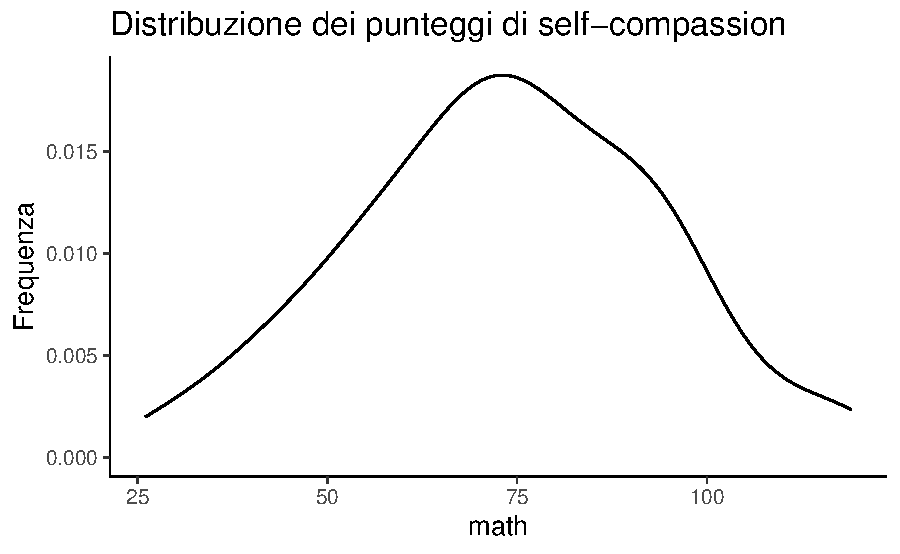
\includegraphics[width=0.7\linewidth,height=\textheight,keepaspectratio]{chapters/eda/07_loc_scale_files/figure-pdf/unnamed-chunk-38-1.pdf}
\end{center}

Per ulteriori verifiche, possiamo estrarre un campione di dati da una
distribuzione normale con media 100 e deviazione standard 15:

\begin{Shaded}
\begin{Highlighting}[]
\FunctionTok{set.seed}\NormalTok{(}\DecValTok{123}\NormalTok{) }
\NormalTok{x }\OtherTok{\textless{}{-}} \FunctionTok{rnorm}\NormalTok{(}\DecValTok{10000}\NormalTok{, }\AttributeTok{mean =} \DecValTok{100}\NormalTok{, }\AttributeTok{sd =} \DecValTok{15}\NormalTok{)}
\FloatTok{1.4826} \SpecialCharTok{*} \FunctionTok{median}\NormalTok{(}\FunctionTok{abs}\NormalTok{(x }\SpecialCharTok{{-}} \FunctionTok{median}\NormalTok{(x)))}
\CommentTok{\#\textgreater{} [1] 14.92}
\end{Highlighting}
\end{Shaded}

Anche in questo caso, il valore ottenuto è molto vicino alla deviazione
standard reale (15), confermando la relazione tra MAD e deviazione
standard in distribuzioni gaussiane.

\end{example}

\subsection{Quando Usare Deviazione Standard e
MAD}\label{quando-usare-deviazione-standard-e-mad}

\begin{itemize}
\item
  Deviazione standard: È la misura più appropriata per dati normalmente
  distribuiti e situazioni in cui l'obiettivo è descrivere la
  dispersione dei dati rispetto alla media. Tuttavia, è sensibile ai
  valori anomali (outlier).
\item
  Deviazione mediana assoluta (MAD): È ideale quando i dati sono non
  normali, asimmetrici o contengono outlier. La MAD è più robusta poiché
  utilizza la mediana anziché la media e non è influenzata da valori
  estremi.
\end{itemize}

\section{Indici di Variabilità
Relativi}\label{indici-di-variabilituxe0-relativi}

A volte può essere necessario confrontare la variabilità di grandezze
incommensurabili, ovvero di caratteri misurati con differenti unità di
misura. In queste situazioni, le misure di variabilità descritte in
precedenza diventano inadeguate poiché dipendono dall'unità di misura
utilizzata. Per superare questo problema, si ricorre a specifici numeri
adimensionali chiamati \emph{indici relativi di variabilità}.

Il più importante di questi indici è il \emph{coefficiente di
variazione} (\(C_v\)), definito come il rapporto tra la deviazione
standard (\(\sigma\)) e la media dei dati (\(\bar{x}\)):

\begin{equation}\phantomsection\label{eq-cv-def}{
C_v = \frac{\sigma}{\bar{x}}.
}\end{equation}

Il coefficiente di variazione è un numero puro e permette di confrontare
la variabilità di distribuzioni con unità di misura diverse.

Un altro indice relativo di variabilità è la \emph{differenza
interquartile rapportata} a uno dei tre quartili (primo quartile, terzo
quartile o mediana). Questo indice è definito come:

\[
\frac{x_{0.75} - x_{0.25}}{x_{0.25}}, \qquad \frac{x_{0.75} - x_{0.25}}{x_{0.75}}, \qquad \frac{x_{0.75} - x_{0.25}}{x_{0.50}}.
\]

Questi indici relativi di variabilità forniscono una misura
adimensionale della dispersione dei dati, rendendo possibile il
confronto tra grandezze con diverse unità di misura e facilitando
l'analisi delle differenze di variabilità tra i dati.

\section{La Fallacia Ergodica}\label{la-fallacia-ergodica}

Sebbene il concetto di ``media'' possa sembrare chiaro, ciò non implica
che il suo utilizzo non presenti delle problematiche nell'ambito della
pratica psicologica. Un aspetto su cui vale la pena soffermarsi è ciò
che viene definito ``fallacia ergodica''.

Il concetto di ``fallacia ergodica''
(\citeproc{ref-speelman2024most}{Speelman et al., 2024}) si riferisce
all'errore compiuto dai ricercatori quando assumono che le
caratteristiche medie di un gruppo di individui possano essere applicate
a ciascun individuo all'interno di quel gruppo, senza considerare le
differenze individuali o le variazioni nel tempo. Questa fallacia emerge
dalla pratica comune nella ricerca psicologica di raccogliere dati
aggregati da gruppi di persone per stimare parametri della popolazione,
al fine di confrontare comportamenti in condizioni diverse o esplorare
associazioni tra diverse misurazioni della stessa persona.

Il problema di questo approccio è che l'uso dei risultati basati sul
gruppo per caratterizzare le caratteristiche degli individui o per
estrapolare a persone simili a quelle del gruppo è ingiustificato,
poiché le medie di gruppo possono fornire informazioni solo sui
risultati collettivi, come la performance media del gruppo, e non
consentono di fare affermazioni accurate sugli individui che compongono
quel gruppo. La fallacia ergodica si basa sull'assunzione che per
utilizzare legittimamente una statistica aggregata (ad esempio, la
media) derivata da un gruppo per descrivere un individuo di quel gruppo,
due condizioni devono essere soddisfatte: gli individui devono essere
così simili da essere praticamente interscambiabili, e le
caratteristiche degli individui devono essere temporalmente stabili.

Tuttavia, i fenomeni e i processi psicologici di interesse per i
ricercatori sono per natura non uniformi tra gli individui e variabili
nel tempo, sia all'interno degli individui che tra di loro. Di
conseguenza, i risultati ottenuti dalla media di misure di
comportamenti, cognizioni o stati emotivi di più individui non
descrivono accuratamente nessuno di quegli individui in un dato momento,
né possono tenere conto dei cambiamenti in quelle variabili per un
individuo nel tempo.

Speelman et al. (\citeproc{ref-speelman2024most}{2024}) osservano che la
stragrande maggioranza degli articoli che hanno analizzato include
conclusioni nelle sezioni degli Abstract e/o delle Discussioni che
implicano che i risultati trovati con dati aggregati di gruppo si
applichino anche agli individui in quei gruppi e/o si applichino agli
individui nella popolazione. Questa pratica riflette la fallacia
ergodica, che consiste nell'assumere che i campioni siano sistemi
ergodici quando non lo sono.

\section{Riflessioni Conclusive}\label{riflessioni-conclusive-12}

Le statistiche descrittive ci permettono di ottenere indicatori
sintetici che riassumono i dati di una popolazione o di un campione
estratto da essa. Questi indicatori includono misure di tendenza
centrale, come la media, la mediana e la moda, che ci forniscono
informazioni sulla posizione centrale dei dati rispetto alla
distribuzione. Inoltre, ci sono gli indici di dispersione, come la
deviazione standard e la varianza, che ci indicano quanto i dati si
disperdono attorno alla tendenza centrale. Questi indici ci aiutano a
comprendere quanto i valori si discostano dalla media, e quindi ci
forniscono un'idea della variabilità dei dati. In conclusione, le
statistiche descrittive ci offrono un quadro sintetico delle
caratteristiche principali dei dati, consentendoci di comprendere meglio
la loro distribuzione e variabilità.

\section*{Esercizi}\label{esercizi-14}
\addcontentsline{toc}{section}{Esercizi}

\markright{Esercizi}

\begin{tcolorbox}[enhanced jigsaw, opacityback=0, bottomrule=.15mm, breakable, title=\textcolor{quarto-callout-important-color}{\faExclamation}\hspace{0.5em}{Problemi}, bottomtitle=1mm, toptitle=1mm, titlerule=0mm, colbacktitle=quarto-callout-important-color!10!white, rightrule=.15mm, colframe=quarto-callout-important-color-frame, colback=white, arc=.35mm, leftrule=.75mm, coltitle=black, left=2mm, toprule=.15mm, opacitybacktitle=0.6]

\textbf{Parte 1: Domande Teoriche}

\begin{enumerate}
\def\labelenumi{\arabic{enumi}.}
\item
  \textbf{Definizione e comprensione dei concetti}

  \begin{itemize}
  \tightlist
  \item
    Spiega la differenza tra media, mediana e moda.
  \item
    In quali situazioni la mediana fornisce una misura della tendenza
    centrale migliore rispetto alla media?
  \item
    Perché la media è sensibile ai valori estremi?
  \item
    Quali sono i vantaggi della deviazione mediana assoluta (MAD)
    rispetto alla deviazione standard?
  \end{itemize}
\item
  \textbf{Interpretazione della variabilità}

  \begin{itemize}
  \tightlist
  \item
    Spiega il concetto di varianza e la sua interpretazione.
  \item
    Qual è la differenza tra varianza e deviazione standard?
  \item
    Descrivi in quali casi l'utilizzo del coefficiente di variazione è
    più appropriato rispetto alla deviazione standard.
  \item
    Quali sono i limiti della moda come indice di tendenza centrale?
  \end{itemize}
\end{enumerate}

\textbf{Parte 2: Calcoli Manuali}

\begin{enumerate}
\def\labelenumi{\arabic{enumi}.}
\setcounter{enumi}{2}
\item
  \textbf{Calcolo della media, mediana e moda}

  \begin{itemize}
  \item
    Considera i seguenti punteggi totali della SWLS che sono stati
    raccolti in un campione di studenti. Calcola manualmente:

    \begin{itemize}
    \tightlist
    \item
      La media
    \item
      La mediana
    \item
      La moda
    \item
      Il range
    \end{itemize}
  \end{itemize}
\item
  \textbf{Calcolo della varianza e della deviazione standard}

  \begin{itemize}
  \tightlist
  \item
    Usando gli stessi dati dell'esercizio precedente, calcola:

    \begin{itemize}
    \tightlist
    \item
      La varianza
    \item
      La deviazione standard
    \item
      La deviazione mediana assoluta (MAD)
    \end{itemize}
  \end{itemize}
\end{enumerate}

\textbf{Parte 3: Esercizi con R}

\begin{enumerate}
\def\labelenumi{\arabic{enumi}.}
\setcounter{enumi}{4}
\item
  \textbf{Analisi descrittiva con R}

  \begin{itemize}
  \tightlist
  \item
    Carica il dataset \texttt{swls\_scores.csv} contenente i punteggi
    SWLS degli studenti.
  \item
    Calcola media, mediana e moda utilizzando R.
  \item
    Calcola la varianza e la deviazione standard utilizzando le funzioni
    appropriate in R.
  \end{itemize}

  \textbf{Codice suggerito:}

\begin{Shaded}
\begin{Highlighting}[]
\FunctionTok{library}\NormalTok{(tidyverse)}
\FunctionTok{library}\NormalTok{(rio)}

\CommentTok{\# Caricamento del dataset}
\NormalTok{df }\OtherTok{\textless{}{-}} \FunctionTok{import}\NormalTok{(}\StringTok{"swls\_scores.csv"}\NormalTok{)}

\CommentTok{\# Calcolo delle statistiche descrittive}
\FunctionTok{mean}\NormalTok{(df}\SpecialCharTok{$}\NormalTok{swls\_total)}
\FunctionTok{median}\NormalTok{(df}\SpecialCharTok{$}\NormalTok{swls\_total)}

\CommentTok{\# Moda (funzione personalizzata)}
\NormalTok{get\_mode }\OtherTok{\textless{}{-}} \ControlFlowTok{function}\NormalTok{(x) \{}
\NormalTok{  tbl }\OtherTok{\textless{}{-}} \FunctionTok{table}\NormalTok{(x)}
  \FunctionTok{as.numeric}\NormalTok{(}\FunctionTok{names}\NormalTok{(tbl)[}\FunctionTok{which.max}\NormalTok{(tbl)])}
\NormalTok{\}}
\FunctionTok{get\_mode}\NormalTok{(df}\SpecialCharTok{$}\NormalTok{swls\_total)}

\CommentTok{\# Varianza e deviazione standard}
\FunctionTok{var}\NormalTok{(df}\SpecialCharTok{$}\NormalTok{swls\_total)}
\FunctionTok{sd}\NormalTok{(df}\SpecialCharTok{$}\NormalTok{swls\_total)}

\CommentTok{\# Deviazione mediana assoluta}
\FunctionTok{mad}\NormalTok{(df}\SpecialCharTok{$}\NormalTok{swls\_total)}
\end{Highlighting}
\end{Shaded}
\item
  \textbf{Visualizzazione della distribuzione dei dati}

  \begin{itemize}
  \tightlist
  \item
    Crea un istogramma dei punteggi totali della SWLS.
  \item
    Aggiungi una linea verticale che rappresenti la media e una che
    rappresenti la mediana.
  \end{itemize}

  \textbf{Codice suggerito:}

\begin{Shaded}
\begin{Highlighting}[]
\FunctionTok{ggplot}\NormalTok{(df, }\FunctionTok{aes}\NormalTok{(}\AttributeTok{x =}\NormalTok{ swls\_total)) }\SpecialCharTok{+}
  \FunctionTok{geom\_histogram}\NormalTok{(}\AttributeTok{binwidth =} \DecValTok{2}\NormalTok{, }\AttributeTok{fill =} \StringTok{"blue"}\NormalTok{, }\AttributeTok{alpha =} \FloatTok{0.5}\NormalTok{, }\AttributeTok{color =} \StringTok{"black"}\NormalTok{) }\SpecialCharTok{+}
  \FunctionTok{geom\_vline}\NormalTok{(}\FunctionTok{aes}\NormalTok{(}\AttributeTok{xintercept =} \FunctionTok{mean}\NormalTok{(swls\_total)), }\AttributeTok{color =} \StringTok{"red"}\NormalTok{, }\AttributeTok{linetype =} \StringTok{"dashed"}\NormalTok{, }\AttributeTok{size =} \DecValTok{1}\NormalTok{) }\SpecialCharTok{+}
  \FunctionTok{geom\_vline}\NormalTok{(}\FunctionTok{aes}\NormalTok{(}\AttributeTok{xintercept =} \FunctionTok{median}\NormalTok{(swls\_total)), }\AttributeTok{color =} \StringTok{"green"}\NormalTok{, }\AttributeTok{linetype =} \StringTok{"dotted"}\NormalTok{, }\AttributeTok{size =} \DecValTok{1}\NormalTok{) }\SpecialCharTok{+}
  \FunctionTok{labs}\NormalTok{(}\AttributeTok{title =} \StringTok{"Distribuzione dei punteggi SWLS"}\NormalTok{, }\AttributeTok{x =} \StringTok{"Punteggio SWLS"}\NormalTok{, }\AttributeTok{y =} \StringTok{"Frequenza"}\NormalTok{)}
\end{Highlighting}
\end{Shaded}
\end{enumerate}

\textbf{Parte 4: Domande di Comprensione}

\begin{enumerate}
\def\labelenumi{\arabic{enumi}.}
\setcounter{enumi}{6}
\item
  \textbf{Analisi concettuale}

  \begin{itemize}
  \tightlist
  \item
    Perché la media aritmetica può essere considerata il ``baricentro''
    della distribuzione dei dati?
  \item
    Se aggiungiamo un valore estremo al dataset, quale delle misure di
    tendenza centrale subirà il maggior impatto?
  \item
    In quali situazioni la varianza campionaria è preferibile rispetto
    alla varianza della popolazione?
  \item
    Qual è la relazione tra la deviazione standard e la varianza?
  \item
    Fornisci un'interpretazione intuitiva della deviazione standard.
  \item
    Discuti le differenze e le somiglianze tra la deviazione standard e
    MAD. Usa queste informazioni per ridescrivere in maniera intuitiva
    il significato di deviazione standard.
  \end{itemize}
\end{enumerate}

\end{tcolorbox}

\begin{tcolorbox}[enhanced jigsaw, opacityback=0, bottomrule=.15mm, breakable, title=\textcolor{quarto-callout-tip-color}{\faLightbulb}\hspace{0.5em}{Soluzioni}, bottomtitle=1mm, toptitle=1mm, titlerule=0mm, colbacktitle=quarto-callout-tip-color!10!white, rightrule=.15mm, colframe=quarto-callout-tip-color-frame, colback=white, arc=.35mm, leftrule=.75mm, coltitle=black, left=2mm, toprule=.15mm, opacitybacktitle=0.6]

Poniamo che i valori SWLS siano {[} 18, 22, 26, 19, 24, 30, 26, 22, 18,
28, 21 {]}.

\begin{enumerate}
\def\labelenumi{\arabic{enumi}.}
\item
  \textbf{Media:}
  \[ \bar{x} = \frac{18 + 22 + 26 + 19 + 24 + 30 + 26 + 22 + 18 + 28 + 21}{11} = 23.36 \]
\item
  \textbf{Mediana:} Ordinando i dati: {[} 18, 18, 19, 21, 22, 22, 24,
  26, 26, 28, 30 {]} La mediana è il valore centrale: \(22\)
\item
  \textbf{Moda:} Il valore più frequente è \textbf{22} (appare due
  volte).
\item
  \textbf{Varianza:}
  \[ s^2 = \frac{\sum (x_i - \bar{x})^2}{n-1} = 13.96 \]
\item
  \textbf{Deviazione Standard:} \[ s = \sqrt{13.96} = 3.73 \]
\item
  \textbf{MAD:}
  \[ \text{MAD} = \text{mediana}(|X_i - \text{mediana}(X)|) = 4 \]
\end{enumerate}

\textbf{Soluzioni con R}

I risultati eseguendo il codice R:

\begin{itemize}
\tightlist
\item
  \textbf{Media:} 23.36
\item
  \textbf{Mediana:} 22
\item
  \textbf{Moda:} 22
\item
  \textbf{Varianza:} 13.96
\item
  \textbf{Deviazione standard:} 3.73
\item
  \textbf{MAD:} 4
\end{itemize}

\textbf{Soluzioni alle Domande di Comprensione}

\begin{enumerate}
\def\labelenumi{\arabic{enumi}.}
\tightlist
\item
  La media è il baricentro poiché minimizza la somma degli scarti
  quadrati.
\item
  La media è più influenzata dai valori estremi rispetto alla mediana.
\item
  La varianza campionaria corregge la sottostima della varianza
  popolazionale.
\item
  La deviazione standard è la radice quadrata della varianza,
  consentendo un'interpretazione del risultato sulla scala dei dati
  grezzi.
\item
  La deviazione standard è simile, ma non identica, al valore medio
  degli scarti assoluti tra ciascun valore della distribuzione e la
  media. In altre parole, rappresenta la ``distanza tipica'' media tra
  le osservazioni e il valore medio della distribuzione.
\item
  La deviazione standard e il MAD (Median Absolute Deviation, o scarto
  medio assoluto) sono entrambi misure di variabilità che descrivono
  quanto i valori in un insieme di dati si discostino dal centro della
  distribuzione. Tuttavia, presentano alcune importanti differenze e
  somiglianze.
\end{enumerate}

\textbf{Somiglianze}

\begin{itemize}
\tightlist
\item
  Entrambe le misure quantificano la dispersione dei dati attorno a un
  punto centrale.
\item
  Sia la deviazione standard che il MAD utilizzano lo scarto (la
  differenza tra ciascun valore e un punto centrale) per calcolare la
  variabilità.
\end{itemize}

\textbf{Differenze}

\begin{itemize}
\tightlist
\item
  \textbf{Punto centrale usato:} La deviazione standard si basa sulla
  media aritmetica, mentre il MAD si basa sulla mediana.
\item
  \textbf{Trattamento degli scarti:} Nella deviazione standard, gli
  scarti vengono elevati al quadrato prima di essere mediati, quindi la
  radice quadrata viene applicata al risultato finale. Questo processo
  penalizza maggiormente gli scarti più grandi, rendendo la deviazione
  standard più sensibile agli outlier. Il MAD, invece, considera
  semplicemente il valore assoluto degli scarti, rendendolo meno
  influenzato dagli estremi.
\item
  \textbf{Sensibilità agli outlier:} Poiché la deviazione standard
  dipende dai quadrati degli scarti, è più sensibile alle osservazioni
  estreme (outlier). Il MAD, essendo basato sulla mediana, è una misura
  più robusta e resiste meglio alla presenza di valori anomali.
\end{itemize}

\textbf{Ridescrizione Intuitiva della Deviazione Standard}

\begin{itemize}
\tightlist
\item
  La deviazione standard può essere vista come una misura della
  ``dispersione tipica'' dei dati attorno alla media, ma con un'enfasi
  particolare sugli scarti più grandi. Immagina di prendere ogni valore
  del dataset, calcolarne la distanza dalla media, amplificare queste
  distanze attraverso il quadrato, poi trovare una sorta di ``distanza
  media'' ponderata. Questo processo dà maggiore peso agli scarti più
  grandi, fornendo così una visione della variabilità che tiene conto
  sia delle fluttuazioni ordinarie sia di eventuali valori estremi. In
  sintesi, mentre il MAD offre una visione più resistente e diretta
  della variabilità centrata sulla mediana, la deviazione standard
  fornisce una misura più dettagliata e sensibile alla forma complessiva
  della distribuzione, inclusi i suoi possibili outliers.
\end{itemize}

\end{tcolorbox}

\section*{Informazioni sull'Ambiente di
Sviluppo}\label{informazioni-sullambiente-di-sviluppo-9}
\addcontentsline{toc}{section}{Informazioni sull'Ambiente di Sviluppo}

\markright{Informazioni sull'Ambiente di Sviluppo}

\begin{Shaded}
\begin{Highlighting}[]
\FunctionTok{sessionInfo}\NormalTok{()}
\CommentTok{\#\textgreater{} R version 4.4.2 (2024{-}10{-}31)}
\CommentTok{\#\textgreater{} Platform: aarch64{-}apple{-}darwin20}
\CommentTok{\#\textgreater{} Running under: macOS Sequoia 15.3.1}
\CommentTok{\#\textgreater{} }
\CommentTok{\#\textgreater{} Matrix products: default}
\CommentTok{\#\textgreater{} BLAS:   /Library/Frameworks/R.framework/Versions/4.4{-}arm64/Resources/lib/libRblas.0.dylib }
\CommentTok{\#\textgreater{} LAPACK: /Library/Frameworks/R.framework/Versions/4.4{-}arm64/Resources/lib/libRlapack.dylib;  LAPACK version 3.12.0}
\CommentTok{\#\textgreater{} }
\CommentTok{\#\textgreater{} locale:}
\CommentTok{\#\textgreater{} [1] C/UTF{-}8/C/C/C/C}
\CommentTok{\#\textgreater{} }
\CommentTok{\#\textgreater{} time zone: Europe/Rome}
\CommentTok{\#\textgreater{} tzcode source: internal}
\CommentTok{\#\textgreater{} }
\CommentTok{\#\textgreater{} attached base packages:}
\CommentTok{\#\textgreater{} [1] grid      stats     graphics  grDevices utils     datasets  methods  }
\CommentTok{\#\textgreater{} [8] base     }
\CommentTok{\#\textgreater{} }
\CommentTok{\#\textgreater{} other attached packages:}
\CommentTok{\#\textgreater{}  [1] vcd\_1.4{-}13        viridis\_0.6.5     viridisLite\_0.4.2 thematic\_0.1.6   }
\CommentTok{\#\textgreater{}  [5] MetBrewer\_0.2.0   ggokabeito\_0.1.0  see\_0.10.0        gridExtra\_2.3    }
\CommentTok{\#\textgreater{}  [9] patchwork\_1.3.0   bayesplot\_1.11.1  psych\_2.4.12      scales\_1.3.0     }
\CommentTok{\#\textgreater{} [13] markdown\_1.13     knitr\_1.49        lubridate\_1.9.4   forcats\_1.0.0    }
\CommentTok{\#\textgreater{} [17] stringr\_1.5.1     dplyr\_1.1.4       purrr\_1.0.4       readr\_2.1.5      }
\CommentTok{\#\textgreater{} [21] tidyr\_1.3.1       tibble\_3.2.1      ggplot2\_3.5.1     tidyverse\_2.0.0  }
\CommentTok{\#\textgreater{} [25] rio\_1.2.3         here\_1.0.1       }
\CommentTok{\#\textgreater{} }
\CommentTok{\#\textgreater{} loaded via a namespace (and not attached):}
\CommentTok{\#\textgreater{}  [1] gtable\_0.3.6      xfun\_0.50         lattice\_0.22{-}6    tzdb\_0.4.0       }
\CommentTok{\#\textgreater{}  [5] vctrs\_0.6.5       tools\_4.4.2       generics\_0.1.3    parallel\_4.4.2   }
\CommentTok{\#\textgreater{}  [9] pacman\_0.5.1      pkgconfig\_2.0.3   R.oo\_1.27.0       data.table\_1.16.4}
\CommentTok{\#\textgreater{} [13] lifecycle\_1.0.4   compiler\_4.4.2    farver\_2.1.2      munsell\_0.5.1    }
\CommentTok{\#\textgreater{} [17] mnormt\_2.1.1      htmltools\_0.5.8.1 pillar\_1.10.1     MASS\_7.3{-}64      }
\CommentTok{\#\textgreater{} [21] R.utils\_2.12.3    nlme\_3.1{-}167      tidyselect\_1.2.1  digest\_0.6.37    }
\CommentTok{\#\textgreater{} [25] stringi\_1.8.4     labeling\_0.4.3    rprojroot\_2.0.4   fastmap\_1.2.0    }
\CommentTok{\#\textgreater{} [29] colorspace\_2.1{-}1  cli\_3.6.4         magrittr\_2.0.3    utf8\_1.2.4       }
\CommentTok{\#\textgreater{} [33] withr\_3.0.2       timechange\_0.3.0  rmarkdown\_2.29    zoo\_1.8{-}12       }
\CommentTok{\#\textgreater{} [37] R.methodsS3\_1.8.2 hms\_1.1.3         evaluate\_1.0.3    lmtest\_0.9{-}40    }
\CommentTok{\#\textgreater{} [41] rlang\_1.1.5       glue\_1.8.0        rstudioapi\_0.17.1 jsonlite\_1.8.9   }
\CommentTok{\#\textgreater{} [45] R6\_2.6.1}
\end{Highlighting}
\end{Shaded}

\section*{Bibliografia}\label{bibliografia-18}
\addcontentsline{toc}{section}{Bibliografia}

\markright{Bibliografia}

\chapter{Introduzione alla distribuzione
normale}\label{sec-eda-intro-gauss}

\begin{tcolorbox}[enhanced jigsaw, opacityback=0, bottomrule=.15mm, breakable, title=\textcolor{quarto-callout-important-color}{\faExclamation}\hspace{0.5em}{In questo capitolo imparerai a}, bottomtitle=1mm, toptitle=1mm, titlerule=0mm, colbacktitle=quarto-callout-important-color!10!white, rightrule=.15mm, colframe=quarto-callout-important-color-frame, colback=white, arc=.35mm, leftrule=.75mm, coltitle=black, left=2mm, toprule=.15mm, opacitybacktitle=0.6]

\begin{itemize}
\tightlist
\item
  costruire e interpretare distribuzioni di frequenza;
\item
  rappresentare e comprendere istogrammi tradizionali e ``lisciati'';
\item
  realizzare e interpretare boxplot e violin plot.
\end{itemize}

\end{tcolorbox}

\begin{tcolorbox}[enhanced jigsaw, opacityback=0, bottomrule=.15mm, breakable, title=\textcolor{quarto-callout-tip-color}{\faLightbulb}\hspace{0.5em}{Prerequisiti}, bottomtitle=1mm, toptitle=1mm, titlerule=0mm, colbacktitle=quarto-callout-tip-color!10!white, rightrule=.15mm, colframe=quarto-callout-tip-color-frame, colback=white, arc=.35mm, leftrule=.75mm, coltitle=black, left=2mm, toprule=.15mm, opacitybacktitle=0.6]

\begin{itemize}
\tightlist
\item
  Leggere il capitolo
  \href{https://openintro-ims.netlify.app/explore-numerical}{Exploring
  numerical data} di
  \href{https://openintro-ims.netlify.app}{Introduction to Modern
  Statistics (2e)} di Mine Çetinkaya-Rundel e Johanna Hardin.
\item
  Leggere il capitolo \emph{Distributions} di \emph{Introduction to Data
  Science} (\citeproc{ref-irizarry2024introduction}{Irizarry, 2024}).
\end{itemize}

\end{tcolorbox}

\begin{tcolorbox}[enhanced jigsaw, opacityback=0, bottomrule=.15mm, breakable, title=\textcolor{quarto-callout-caution-color}{\faFire}\hspace{0.5em}{Preparazione del Notebook}, bottomtitle=1mm, toptitle=1mm, titlerule=0mm, colbacktitle=quarto-callout-caution-color!10!white, rightrule=.15mm, colframe=quarto-callout-caution-color-frame, colback=white, arc=.35mm, leftrule=.75mm, coltitle=black, left=2mm, toprule=.15mm, opacitybacktitle=0.6]

\begin{Shaded}
\begin{Highlighting}[]
\NormalTok{here}\SpecialCharTok{::}\FunctionTok{here}\NormalTok{(}\StringTok{"code"}\NormalTok{, }\StringTok{"\_common.R"}\NormalTok{) }\SpecialCharTok{|\textgreater{}} 
  \FunctionTok{source}\NormalTok{()}

\CommentTok{\# Load packages}
\ControlFlowTok{if}\NormalTok{ (}\SpecialCharTok{!}\FunctionTok{requireNamespace}\NormalTok{(}\StringTok{"pacman"}\NormalTok{)) }\FunctionTok{install.packages}\NormalTok{(}\StringTok{"pacman"}\NormalTok{)}
\NormalTok{pacman}\SpecialCharTok{::}\FunctionTok{p\_load}\NormalTok{(ggbeeswarm, dslabs, gridExtra)}
\end{Highlighting}
\end{Shaded}

\end{tcolorbox}

\section*{Introduzione}\label{introduzione-18}
\addcontentsline{toc}{section}{Introduzione}

\markright{Introduzione}

In questo capitolo forniremo un primo sguardo alla distribuzione
\textbf{normale}, che sarà trattata in modo più approfondito nel
Capitolo~\ref{sec-prob-cont-prob-distr}. Introduciamo la distribuzione
normale a questo punto poiché essa spiega in modo chiaro perché, in
molte analisi, \textbf{media} e \textbf{deviazione standard} siano
impiegate come principali descrittori di una distribuzione.

\section{La distribuzione normale}\label{sec-normal-distribution}

Nel Capitolo~\ref{sec-eda-exploring-num-data}, abbiamo visto come gli
\textbf{istogrammi} e i \textbf{grafici di densità} forniscano utili
riassunti visivi di una distribuzione. In questo capitolo, ci chiediamo
se sia possibile riassumere una distribuzione in modo ancora più
sintetico. Spesso si fa riferimento a \textbf{media} e
\textbf{deviazione standard} come statistiche riassuntive fondamentali:
in sostanza, un riassunto in due numeri. Per comprendere appieno il
ruolo di questi valori, dobbiamo prima capire come è definita la
distribuzione normale.

La distribuzione normale, nota anche come \textbf{curva a campana} o
\textbf{distribuzione gaussiana}, è uno dei concetti matematici più
conosciuti (si veda il Capitolo~\ref{sec-prob-cont-prob-distr}). Uno dei
motivi della sua fama è che numerose variabili nella realtà seguono,
almeno approssimativamente, una distribuzione normale. Esempi includono
le vincite nel gioco d'azzardo, l'altezza e il peso delle persone, la
pressione sanguigna, i punteggi di alcuni test standardizzati e gli
errori di misura negli esperimenti. I motivi matematici e probabilistici
di queste approssimazioni verranno discussi in seguito; qui ci
concentreremo sul come la distribuzione normale aiuti a
\textbf{riassumere} i dati.

Anziché partire da dati empirici, la distribuzione normale si definisce
tramite una formula matematica. Per un intervallo generico \((a,b)\), la
proporzione di valori che cade in tale intervallo si ottiene mediante:

\begin{equation}\phantomsection\label{eq-gaussian-density}{
\text{Pr}(a < x \leq b) \;=\; \int_a^b \frac{1}{\sqrt{2\pi}\,\sigma} \, e^{-\tfrac12\,\bigl(\tfrac{x - \mu}{\sigma}\bigr)^2}\, dx .
}\end{equation}

Non è necessario memorizzare o padroneggiare i dettagli di questa
formula, ma è importante sapere che la distribuzione normale è
completamente determinata da \textbf{due soli parametri}: \(\mu\) e
\(\sigma\). Gli altri simboli nella formula (\(\pi\), \(e\), \(a\),
\(b\)) rappresentano costanti matematiche o gli estremi dell'intervallo.
In particolare, \(\mu\) è il \textbf{valore medio} (o \textbf{media}) e
\(\sigma\) è la \textbf{deviazione standard}.

Questa distribuzione è \textbf{simmetrica}, centrata sulla media
\(\mu\), e la maggior parte dei valori (circa il 95\%) si trova entro 2
deviazioni standard dalla media, cioè nell'intervallo
\(\mu \pm 2\sigma\). Ecco un esempio di come appare la distribuzione
normale quando \(\mu = 0\) e \(\sigma = 1\):

\begin{Shaded}
\begin{Highlighting}[]
\NormalTok{m }\OtherTok{\textless{}{-}} \DecValTok{0}\NormalTok{; s }\OtherTok{\textless{}{-}} \DecValTok{1}
\NormalTok{norm\_dist }\OtherTok{\textless{}{-}} \FunctionTok{tibble}\NormalTok{(}\AttributeTok{x =} \FunctionTok{seq}\NormalTok{(}\SpecialCharTok{{-}}\DecValTok{4}\NormalTok{, }\DecValTok{4}\NormalTok{, }\AttributeTok{length.out =} \DecValTok{50}\NormalTok{)}\SpecialCharTok{*}\NormalTok{s }\SpecialCharTok{+}\NormalTok{ m) }\SpecialCharTok{|\textgreater{}} 
  \FunctionTok{mutate}\NormalTok{(}\AttributeTok{density =} \FunctionTok{dnorm}\NormalTok{(x, m, s))}
\NormalTok{norm\_dist }\SpecialCharTok{|\textgreater{}} 
  \FunctionTok{ggplot}\NormalTok{(}\FunctionTok{aes}\NormalTok{(x, density)) }\SpecialCharTok{+} \FunctionTok{geom\_line}\NormalTok{()}
\end{Highlighting}
\end{Shaded}

\begin{center}
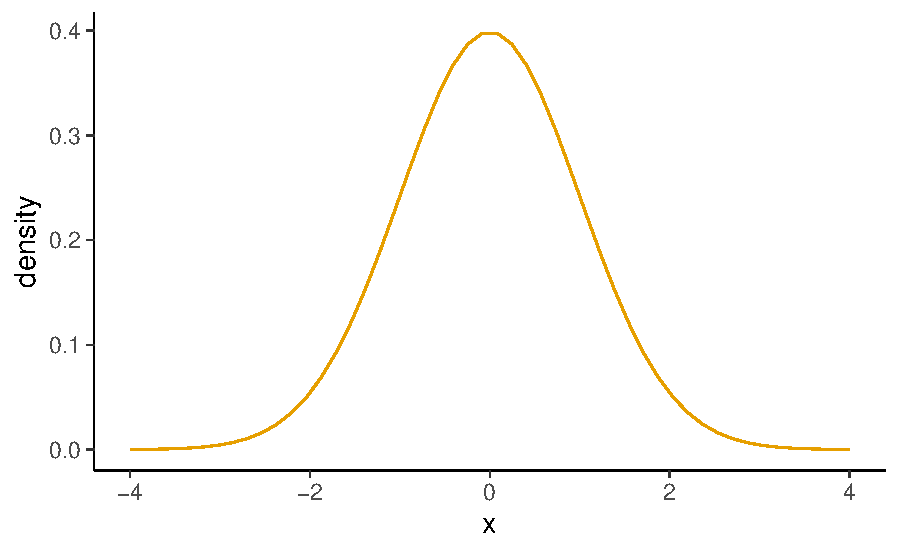
\includegraphics[width=0.7\linewidth,height=\textheight,keepaspectratio]{chapters/eda/07a_introduction_normal_distribution_files/figure-pdf/unnamed-chunk-2-1.pdf}
\end{center}

Il fatto che la distribuzione sia descritta da \textbf{due parametri}
implica che, se un insieme di dati reali si approssima bene a una
distribuzione normale, due soli numeri (media e deviazione standard)
possono fornire un riassunto sintetico della distribuzione. Vediamo ora
come si calcolano, in pratica, questi due parametri per una lista di
valori arbitraria.

Supponiamo di avere un vettore \texttt{x} che contiene una serie di
valori numerici. Abbiamo visto come, in R, la \textbf{media} si trova
come:

\begin{Shaded}
\begin{Highlighting}[]
\NormalTok{m }\OtherTok{\textless{}{-}} \FunctionTok{sum}\NormalTok{(x) }\SpecialCharTok{/} \FunctionTok{length}\NormalTok{(x)}
\end{Highlighting}
\end{Shaded}

e la \textbf{deviazione standard} è:

\begin{Shaded}
\begin{Highlighting}[]
\NormalTok{s }\OtherTok{\textless{}{-}} \FunctionTok{sqrt}\NormalTok{(}\FunctionTok{sum}\NormalTok{((x }\SpecialCharTok{{-}}\NormalTok{ m)}\SpecialCharTok{\^{}}\DecValTok{2}\NormalTok{) }\SpecialCharTok{/} \FunctionTok{length}\NormalTok{(x))}
\end{Highlighting}
\end{Shaded}

La deviazione standard si può interpretare come la \textbf{distanza
media} dei valori dalla loro media.

\subsection{Un esempio con i dati di
altezza}\label{un-esempio-con-i-dati-di-altezza}

Per calcolare media e deviazione standard dell'altezza maschile in un
dataset, ipotizziamo che il vettore \texttt{heights\$height} contenga le
altezze di alcuni individui, mentre \texttt{heights\$sex} contenga il
genere corrispondente. Se vogliamo estrarre solo i valori relativi ai
maschi, possiamo scrivere:

\begin{Shaded}
\begin{Highlighting}[]
\NormalTok{index }\OtherTok{\textless{}{-}}\NormalTok{ heights}\SpecialCharTok{$}\NormalTok{sex }\SpecialCharTok{==} \StringTok{"Male"}
\NormalTok{x }\OtherTok{\textless{}{-}}\NormalTok{ heights}\SpecialCharTok{$}\NormalTok{height[index]}
\end{Highlighting}
\end{Shaded}

Quindi usiamo le funzioni predefinite di R:

\begin{Shaded}
\begin{Highlighting}[]
\NormalTok{m }\OtherTok{\textless{}{-}} \FunctionTok{mean}\NormalTok{(x)}
\NormalTok{s }\OtherTok{\textless{}{-}} \FunctionTok{sd}\NormalTok{(x)}
\end{Highlighting}
\end{Shaded}

\begin{tcolorbox}[enhanced jigsaw, opacityback=0, bottomrule=.15mm, breakable, title=\textcolor{quarto-callout-warning-color}{\faExclamationTriangle}\hspace{0.5em}{Avviso}, bottomtitle=1mm, toptitle=1mm, titlerule=0mm, colbacktitle=quarto-callout-warning-color!10!white, rightrule=.15mm, colframe=quarto-callout-warning-color-frame, colback=white, arc=.35mm, leftrule=.75mm, coltitle=black, left=2mm, toprule=.15mm, opacitybacktitle=0.6]

\textbf{Nota}: Per motivi che verranno chiariti in seguito, la funzione
\texttt{sd(x)} effettua una divisione per \(\text{length}(x) - 1\)
invece che per \(\text{length}(x)\). Tuttavia, se il numero di
osservazioni è elevato, questa differenza è trascurabile.

\end{tcolorbox}

Possiamo ora mettere a confronto la curva di densità \textbf{osservata}
dei dati (in blu) con quella \textbf{teorica} (in nero) della
distribuzione normale con media e deviazione standard stimate:

\begin{Shaded}
\begin{Highlighting}[]
\NormalTok{norm\_dist }\OtherTok{\textless{}{-}} \FunctionTok{tibble}\NormalTok{(}
  \AttributeTok{x =} \FunctionTok{seq}\NormalTok{(}\SpecialCharTok{{-}}\DecValTok{4}\NormalTok{, }\DecValTok{4}\NormalTok{, }\AttributeTok{length.out =} \DecValTok{50}\NormalTok{)}\SpecialCharTok{*}\NormalTok{s }\SpecialCharTok{+}\NormalTok{ m) }\SpecialCharTok{|\textgreater{}} 
  \FunctionTok{mutate}\NormalTok{(}\AttributeTok{density =} \FunctionTok{dnorm}\NormalTok{(x, m, s))}

\NormalTok{heights }\SpecialCharTok{|\textgreater{}} 
\NormalTok{  dplyr}\SpecialCharTok{::}\FunctionTok{filter}\NormalTok{(sex }\SpecialCharTok{==} \StringTok{"Male"}\NormalTok{) }\SpecialCharTok{|\textgreater{}} 
  \FunctionTok{ggplot}\NormalTok{(}\FunctionTok{aes}\NormalTok{(height)) }\SpecialCharTok{+}
  \FunctionTok{geom\_density}\NormalTok{(}\AttributeTok{fill =} \StringTok{"\#00BFC4"}\NormalTok{, }\AttributeTok{alpha =} \FloatTok{0.5}\NormalTok{) }\SpecialCharTok{+}
  \FunctionTok{geom\_line}\NormalTok{(}\FunctionTok{aes}\NormalTok{(x, density), }\AttributeTok{data =}\NormalTok{ norm\_dist)}
\end{Highlighting}
\end{Shaded}

\begin{center}
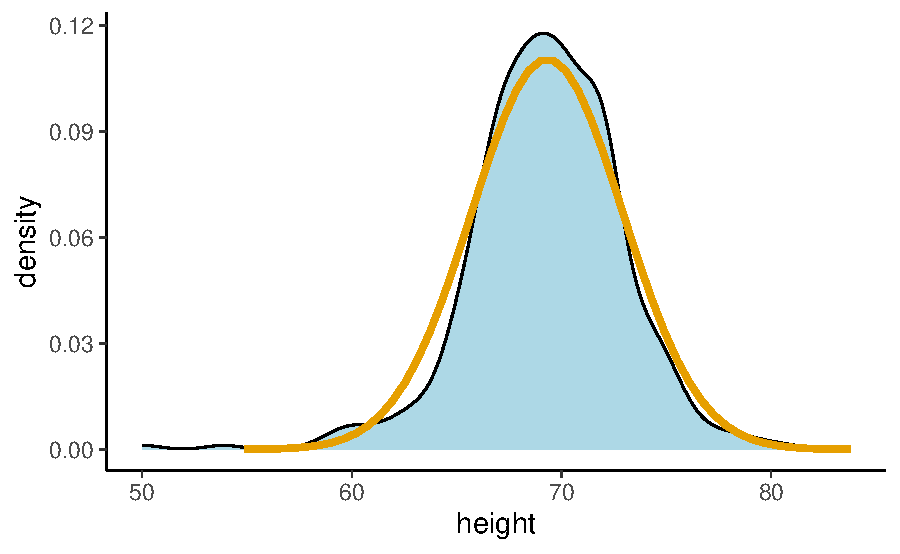
\includegraphics[width=0.7\linewidth,height=\textheight,keepaspectratio]{chapters/eda/07a_introduction_normal_distribution_files/figure-pdf/unnamed-chunk-5-1.pdf}
\end{center}

Come si vede, la \textbf{curva normale} fornisce una buona
approssimazione per i dati sull'altezza maschile. Vedremo ora come
verificare l'aderenza di una distribuzione ai dati, osservando le
proporzioni di valori entro intervalli specifici.

\section{Unità standard}\label{unituxe0-standard}

Per i dati che seguono (o quasi) una distribuzione normale, è molto
comodo utilizzare le cosiddette \textbf{unità standard} (\emph{Standard
Units}). Un valore \(x\) viene convertito in unità standard tramite la
formula:

\[
z = \frac{x - m}{s} ,
\]

dove \(m\) e \(s\) sono la media e la deviazione standard della
distribuzione. Questa trasformazione ci dice \textbf{di quante
deviazioni standard} un particolare valore si discosta dalla media. Ad
esempio, se \(z=0\), il valore \(x\) corrisponde esattamente alla media;
se \(z = 2\), il valore \(x\) si trova a due deviazioni standard
\textbf{sopra} la media; se \(z = -2\), a due deviazioni standard
\textbf{sotto} la media, e così via.

In R, possiamo calcolare le unità standard con la funzione:

\begin{Shaded}
\begin{Highlighting}[]
\NormalTok{z }\OtherTok{\textless{}{-}} \FunctionTok{scale}\NormalTok{(x) }\SpecialCharTok{|\textgreater{}} \FunctionTok{as.numeric}\NormalTok{()}
\FunctionTok{head}\NormalTok{(z)}
\CommentTok{\#\textgreater{} [1]  1.5744  0.1898 {-}0.3641  1.2975 {-}2.3026 {-}0.6410}
\end{Highlighting}
\end{Shaded}

Se vogliamo sapere, ad esempio, quale frazione di individui si trova
entro 2 deviazioni standard dalla media (cioè \(|z| < 2\)), basta
scrivere:

\begin{Shaded}
\begin{Highlighting}[]
\FunctionTok{mean}\NormalTok{(}\FunctionTok{abs}\NormalTok{(z) }\SpecialCharTok{\textless{}} \DecValTok{2}\NormalTok{)}
\CommentTok{\#\textgreater{} [1] 0.9495}
\end{Highlighting}
\end{Shaded}

Vedremo, in molti casi, un valore intorno al 95\%, in linea con quanto
previsto dalla distribuzione normale. Per confermare la bontà
dell'approssimazione, si usano spesso i grafici
\textbf{quantile-quantile}, detti anche \emph{qqplot}.

\section{Grafici quantile-quantile
(qqplot)}\label{grafici-quantile-quantile-qqplot}

Un modo sistematico per verificare quanto la distribuzione normale
descriva bene i dati osservati consiste nel confrontare i
\textbf{quantili} empirici con quelli \textbf{teorici} di una normale.
Se i due insiemi di quantili sono molto simili, abbiamo un'ulteriore
conferma dell'aderenza alla normalità.

\begin{itemize}
\tightlist
\item
  La funzione di ripartizione della distribuzione normale standard si
  indica spesso con \(\Phi(x)\). Ad esempio,
  \(\Phi(-1.96) \approx 0.025\) e \(\Phi(1.96) \approx 0.975\).\\
\item
  L'\textbf{inversa} di \(\Phi\), indicata come \(\Phi^{-1}(p)\), ci dà
  il \textbf{quantile} corrispondente a una determinata probabilità
  \(p\). In R, \texttt{pnorm} calcola \(\Phi(x)\) e \texttt{qnorm}
  calcola \(\Phi^{-1}(p)\). Di default, \texttt{pnorm} e \texttt{qnorm}
  si riferiscono alla normale \textbf{standard} (media 0, deviazione
  standard 1), ma possiamo specificare valori diversi di media e
  deviazione standard tramite gli argomenti \texttt{mean} e \texttt{sd}.
\end{itemize}

Per ottenere il quantile empirico da un vettore di dati in R, possiamo
usare la funzione \texttt{quantile}. Ad esempio, se abbiamo un vettore
\texttt{x}, il \textbf{quantile} associato alla probabilità \(p\) è il
valore \(q\) per il quale \texttt{mean(x\ \textless{}=\ q)\ =\ p}.

Ecco lo schema logico per costruire un qqplot:

\begin{enumerate}
\def\labelenumi{\arabic{enumi}.}
\tightlist
\item
  Definiamo un vettore di proporzioni \(p_1, p_2, \dots, p_m\).\\
\item
  Calcoliamo i relativi quantili empirici dei nostri dati
  \(\{q_1, \dots, q_m\}\) usando \texttt{quantile(x,\ p\_i)}.\\
\item
  Calcoliamo i \textbf{quantili teorici} della normale (con la stessa
  media e la stessa deviazione standard dei dati) usando
  \texttt{qnorm(p\_i,\ mean,\ sd)}.\\
\item
  Rappresentiamo i punti
  \((\text{quantile teorico}, \text{quantile empirico})\). Se i dati
  sono davvero normali, tali punti si disporranno approssimativamente
  lungo la retta diagonale \texttt{y\ =\ x}.
\end{enumerate}

Esempio in R:

\begin{Shaded}
\begin{Highlighting}[]
\NormalTok{p }\OtherTok{\textless{}{-}} \FunctionTok{seq}\NormalTok{(}\FloatTok{0.05}\NormalTok{, }\FloatTok{0.95}\NormalTok{, }\FloatTok{0.05}\NormalTok{)}
\NormalTok{sample\_quantiles }\OtherTok{\textless{}{-}} \FunctionTok{quantile}\NormalTok{(x, p)}
\NormalTok{theoretical\_quantiles }\OtherTok{\textless{}{-}} \FunctionTok{qnorm}\NormalTok{(p, }\AttributeTok{mean =} \FunctionTok{mean}\NormalTok{(x), }\AttributeTok{sd =} \FunctionTok{sd}\NormalTok{(x))}

\FunctionTok{qplot}\NormalTok{(theoretical\_quantiles, sample\_quantiles) }\SpecialCharTok{+} \FunctionTok{geom\_abline}\NormalTok{()}
\end{Highlighting}
\end{Shaded}

\begin{center}
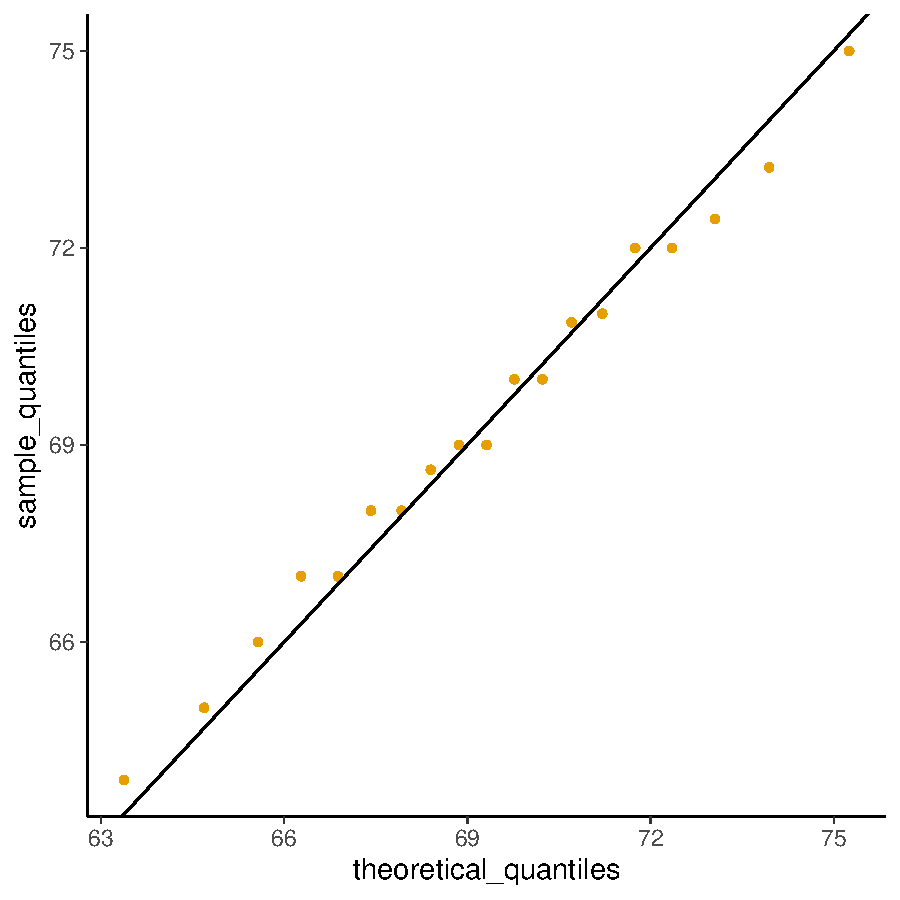
\includegraphics[width=0.7\linewidth,height=\textheight,keepaspectratio]{chapters/eda/07a_introduction_normal_distribution_files/figure-pdf/unnamed-chunk-8-1.pdf}
\end{center}

Se però abbiamo già convertito in unità standard (quindi \(\mu = 0\) e
\(\sigma = 1\)), il confronto si semplifica:

\begin{Shaded}
\begin{Highlighting}[]
\NormalTok{sample\_quantiles }\OtherTok{\textless{}{-}} \FunctionTok{quantile}\NormalTok{(z, p)}
\NormalTok{theoretical\_quantiles }\OtherTok{\textless{}{-}} \FunctionTok{qnorm}\NormalTok{(p)}
\FunctionTok{qplot}\NormalTok{(theoretical\_quantiles, sample\_quantiles) }\SpecialCharTok{+} \FunctionTok{geom\_abline}\NormalTok{()}
\end{Highlighting}
\end{Shaded}

\begin{center}
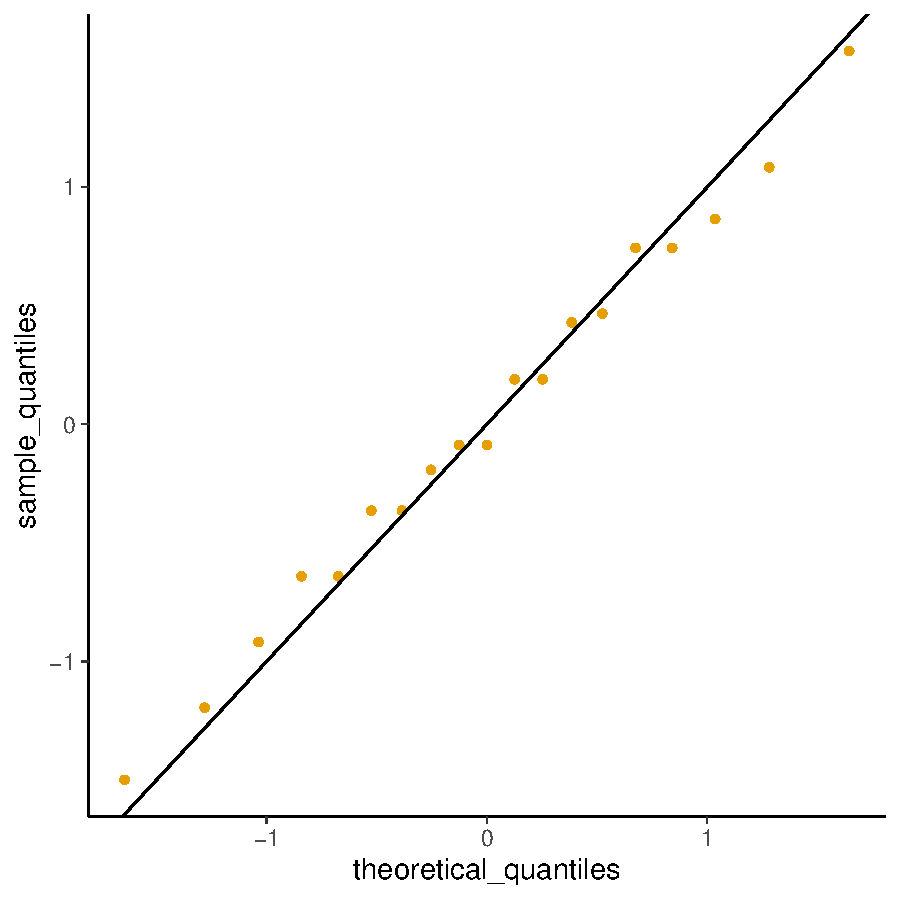
\includegraphics[width=0.7\linewidth,height=\textheight,keepaspectratio]{chapters/eda/07a_introduction_normal_distribution_files/figure-pdf/unnamed-chunk-9-1.pdf}
\end{center}

In pratica, per creare rapidamente un qqplot si usa spesso
\textbf{ggplot2} con la geometria \texttt{geom\_qq}:

\begin{Shaded}
\begin{Highlighting}[]
\NormalTok{heights }\SpecialCharTok{|\textgreater{}} \FunctionTok{filter}\NormalTok{(sex }\SpecialCharTok{==} \StringTok{"Male"}\NormalTok{) }\SpecialCharTok{|\textgreater{}}
  \FunctionTok{ggplot}\NormalTok{(}\FunctionTok{aes}\NormalTok{(}\AttributeTok{sample =} \FunctionTok{scale}\NormalTok{(height))) }\SpecialCharTok{+} 
  \FunctionTok{geom\_qq}\NormalTok{() }\SpecialCharTok{+}
  \FunctionTok{geom\_abline}\NormalTok{()}
\end{Highlighting}
\end{Shaded}

\begin{center}
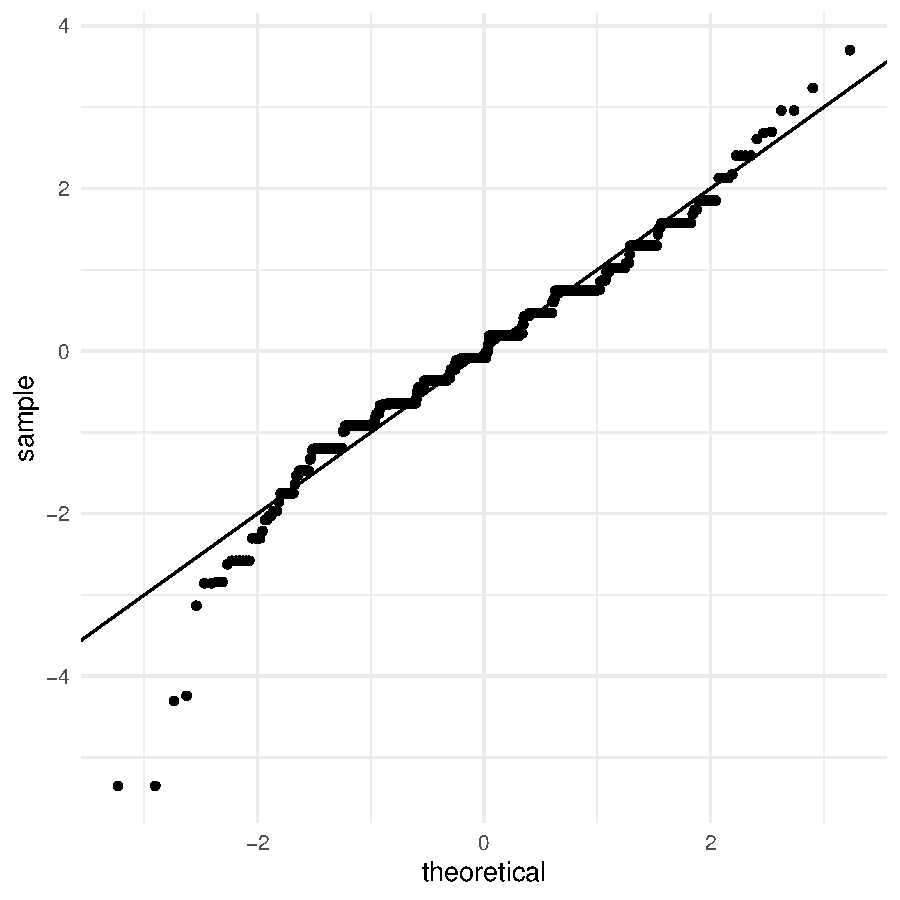
\includegraphics[width=0.7\linewidth,height=\textheight,keepaspectratio]{chapters/eda/07a_introduction_normal_distribution_files/figure-pdf/unnamed-chunk-10-1.pdf}
\end{center}

Come abbiamo sottolineato, se i punti nel qqplot si dispongono lungo una
retta, significa che la distribuzione dei dati è in accordo con la
distribuzione teorica considerata (in questo caso, la normale). I qqplot
possono essere usati anche per confrontare \textbf{qualsiasi} coppia di
distribuzioni, non solo dati e normale teorica.

Questo indica che l'approssimazione normale è accurata per il gruppo
maschile (nel nostro dataset).

\section{Media e Deviazione Standard come Statistiche Descrittive della
Distribuzione}\label{media-e-deviazione-standard-come-statistiche-descrittive-della-distribuzione}

La \textbf{media} e la \textbf{deviazione standard} sono due delle
statistiche più comunemente utilizzate per descrivere la distribuzione
di un insieme di dati. Queste misure sono particolarmente utili quando i
dati seguono una distribuzione \textbf{normale}. In questo caso, la
media e la deviazione standard contengono tutte le informazioni
necessarie per caratterizzare completamente la forma della
distribuzione.

\subsection{Distribuzione Normale e Statistiche
Descrittive}\label{distribuzione-normale-e-statistiche-descrittive}

La distribuzione normale è definita dalla sua \textbf{media} (\(\mu\)) e
dalla sua \textbf{deviazione standard} (\(\sigma\)). La formula della
densità di probabilità della distribuzione normale è data
dall'Equazione~\ref{eq-gaussian-density}. Questa formula mostra che,
conoscendo solo \(\mu\) e \(\sigma\), possiamo ricostruire l'intera
curva di densità. Pertanto, se i dati empirici sono ben approssimati da
una distribuzione normale, la media e la deviazione standard sono
sufficienti per descrivere la distribuzione.

Supponiamo di avere un dataset che segue una distribuzione normale con
media 50 e deviazione standard 10. Possiamo generare dati casuali e
visualizzare la curva di densità in R:

\begin{Shaded}
\begin{Highlighting}[]
\CommentTok{\# Generiamo dati da una distribuzione normale}
\FunctionTok{set.seed}\NormalTok{(}\DecValTok{123}\NormalTok{)}
\NormalTok{dati }\OtherTok{\textless{}{-}} \FunctionTok{rnorm}\NormalTok{(}\DecValTok{1000}\NormalTok{, }\AttributeTok{mean =} \DecValTok{50}\NormalTok{, }\AttributeTok{sd =} \DecValTok{10}\NormalTok{)}

\CommentTok{\# Calcoliamo media e deviazione standard}
\NormalTok{media }\OtherTok{\textless{}{-}} \FunctionTok{mean}\NormalTok{(dati)}
\NormalTok{deviazione\_standard }\OtherTok{\textless{}{-}} \FunctionTok{sd}\NormalTok{(dati)}

\CommentTok{\# Visualizziamo la curva di densità}
\FunctionTok{ggplot}\NormalTok{(}\FunctionTok{data.frame}\NormalTok{(dati), }\FunctionTok{aes}\NormalTok{(}\AttributeTok{x =}\NormalTok{ dati)) }\SpecialCharTok{+}
  \FunctionTok{geom\_density}\NormalTok{(}\AttributeTok{fill =} \StringTok{"\#00BFC4"}\NormalTok{, }\AttributeTok{alpha =} \FloatTok{0.6}\NormalTok{) }\SpecialCharTok{+}
  \FunctionTok{geom\_vline}\NormalTok{(}\AttributeTok{xintercept =}\NormalTok{ media, }\AttributeTok{color =} \StringTok{"red"}\NormalTok{, }\AttributeTok{linetype =} \StringTok{"dashed"}\NormalTok{) }\SpecialCharTok{+}
  \FunctionTok{labs}\NormalTok{(}\AttributeTok{title =} \StringTok{"Curva di Densità di una Distribuzione Normale"}\NormalTok{,}
       \AttributeTok{x =} \StringTok{"Valori"}\NormalTok{,}
       \AttributeTok{y =} \StringTok{"Densità"}\NormalTok{) }\SpecialCharTok{+}
  \FunctionTok{annotate}\NormalTok{(}\StringTok{"text"}\NormalTok{, }\AttributeTok{x =}\NormalTok{ media }\SpecialCharTok{+} \DecValTok{5}\NormalTok{, }\AttributeTok{y =} \FloatTok{0.03}\NormalTok{, }\AttributeTok{label =} \FunctionTok{paste}\NormalTok{(}\StringTok{"Media ="}\NormalTok{, }\FunctionTok{round}\NormalTok{(media, }\DecValTok{2}\NormalTok{)), }\AttributeTok{color =} \StringTok{"red"}\NormalTok{) }\SpecialCharTok{+}
  \FunctionTok{annotate}\NormalTok{(}\StringTok{"text"}\NormalTok{, }\AttributeTok{x =}\NormalTok{ media }\SpecialCharTok{+} \DecValTok{5}\NormalTok{, }\AttributeTok{y =} \FloatTok{0.025}\NormalTok{, }\AttributeTok{label =} \FunctionTok{paste}\NormalTok{(}\StringTok{"Deviazione Standard ="}\NormalTok{, }\FunctionTok{round}\NormalTok{(deviazione\_standard, }\DecValTok{2}\NormalTok{)), }\AttributeTok{color =} \StringTok{"blue"}\NormalTok{)}
\end{Highlighting}
\end{Shaded}

\begin{center}
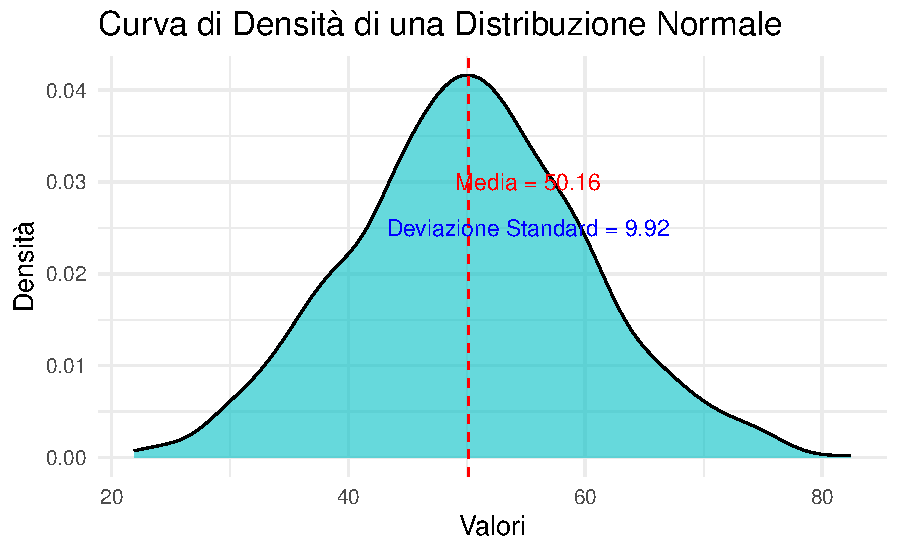
\includegraphics[width=0.7\linewidth,height=\textheight,keepaspectratio]{chapters/eda/07a_introduction_normal_distribution_files/figure-pdf/unnamed-chunk-11-1.pdf}
\end{center}

In questo esempio:

\begin{itemize}
\tightlist
\item
  La curva di densità è centrata attorno alla media (\(\mu = 50\)).
\item
  La deviazione standard (\(\sigma = 10\)) determina la dispersione dei
  dati attorno alla media.
\end{itemize}

\subsection{Quando Media e Deviazione Standard Non Sono
Sufficienti}\label{quando-media-e-deviazione-standard-non-sono-sufficienti}

Sebbene media e deviazione standard siano strumenti estremamente utili
per descrivere distribuzioni \textbf{normali}, non sempre bastano a
cogliere tutte le caratteristiche di un insieme di dati. In particolare,
ci sono situazioni in cui la forma della distribuzione rende necessario
ricorrere a misure aggiuntive. Di seguito presentiamo alcuni casi
tipici.

\begin{enumerate}
\def\labelenumi{\arabic{enumi}.}
\item
  \textbf{Distribuzioni Asimmetriche}\\
  Una distribuzione si dice \textbf{asimmetrica} (o \emph{skewed})
  quando una coda è più ``estesa'' dell'altra.

  \begin{itemize}
  \tightlist
  \item
    Se la coda più lunga è a destra, la distribuzione è
    \textbf{asimmetrica positiva} (o a destra).\\
  \item
    Se la coda più lunga è a sinistra, la distribuzione è
    \textbf{asimmetrica negativa} (o a sinistra).\\
    In queste circostanze, la \textbf{media} tende a spostarsi verso la
    coda più lunga, mentre la \textbf{mediana} rimane più stabile e
    rappresentativa del valore centrale.
  \end{itemize}
\item
  \textbf{Distribuzioni Multimodali}\\
  Una distribuzione è \textbf{multimodale} quando presenta più picchi (o
  ``modi''). Ciò significa che i dati si concentrano attorno a più di un
  valore, formando veri e propri sotto-gruppi. In questi casi, media e
  deviazione standard possono risultare poco significative, poiché non
  colgono la presenza di più poli di concentrazione.
\item
  \textbf{Kurtosi}\\
  La \textbf{kurtosi} descrive quanto una distribuzione sia
  ``appuntita'' o ``piatta'' rispetto a una normale.

  \begin{itemize}
  \tightlist
  \item
    \textbf{Alta kurtosi} indica picchi molto accentuati e code più
    lunghe, con una maggiore probabilità di valori estremi.\\
  \item
    \textbf{Bassa kurtosi} segnala una forma più appiattita, con code
    ridotte e meno outlier.
  \end{itemize}
\end{enumerate}

Quando le distribuzioni mostrano una di queste peculiarità, altre
statistiche possono rivelarsi più informative:

\begin{itemize}
\tightlist
\item
  La \textbf{mediana}, insensibile ai valori estremi, fornisce una
  descrizione più robusta del centro.\\
\item
  I \textbf{quartili}, e in particolare l'intervallo interquartile,
  danno un'idea della dispersione principale trascurando le code.\\
\item
  L'\textbf{indice di asimmetria} (\emph{skewness}) misura il grado di
  sbilanciamento della distribuzione.\\
\item
  L'\textbf{indice di curtosi} (\emph{kurtosis}) quantifica la
  ``pesantezza'' delle code.
\end{itemize}

Nel seguente esempio, generiamo dati da una distribuzione esponenziale,
notoriamente asimmetrica:

\begin{Shaded}
\begin{Highlighting}[]
\CommentTok{\# Generiamo dati da una distribuzione esponenziale}
\FunctionTok{set.seed}\NormalTok{(}\DecValTok{123}\NormalTok{)}
\NormalTok{dati\_esponenziali }\OtherTok{\textless{}{-}} \FunctionTok{rexp}\NormalTok{(}\DecValTok{1000}\NormalTok{, }\AttributeTok{rate =} \FloatTok{0.5}\NormalTok{)}

\CommentTok{\# Calcoliamo media e deviazione standard}
\NormalTok{media\_esp }\OtherTok{\textless{}{-}} \FunctionTok{mean}\NormalTok{(dati\_esponenziali)}
\NormalTok{deviazione\_standard\_esp }\OtherTok{\textless{}{-}} \FunctionTok{sd}\NormalTok{(dati\_esponenziali)}

\CommentTok{\# Visualizziamo la curva di densità}
\FunctionTok{ggplot}\NormalTok{(}\FunctionTok{data.frame}\NormalTok{(dati\_esponenziali), }\FunctionTok{aes}\NormalTok{(}\AttributeTok{x =}\NormalTok{ dati\_esponenziali)) }\SpecialCharTok{+}
  \FunctionTok{geom\_density}\NormalTok{(}\AttributeTok{fill =} \StringTok{"\#F8766D"}\NormalTok{, }\AttributeTok{alpha =} \FloatTok{0.6}\NormalTok{) }\SpecialCharTok{+}
  \FunctionTok{geom\_vline}\NormalTok{(}\AttributeTok{xintercept =}\NormalTok{ media\_esp, }\AttributeTok{color =} \StringTok{"red"}\NormalTok{, }\AttributeTok{linetype =} \StringTok{"dashed"}\NormalTok{) }\SpecialCharTok{+}
  \FunctionTok{labs}\NormalTok{(}\AttributeTok{title =} \StringTok{"Curva di Densità di una Distribuzione Esponenziale"}\NormalTok{,}
       \AttributeTok{x =} \StringTok{"Valori"}\NormalTok{,}
       \AttributeTok{y =} \StringTok{"Densità"}\NormalTok{) }\SpecialCharTok{+}
  \FunctionTok{annotate}\NormalTok{(}\StringTok{"text"}\NormalTok{, }\AttributeTok{x =}\NormalTok{ media\_esp }\SpecialCharTok{+} \DecValTok{1}\NormalTok{, }\AttributeTok{y =} \FloatTok{0.2}\NormalTok{, }
           \AttributeTok{label =} \FunctionTok{paste}\NormalTok{(}\StringTok{"Media ="}\NormalTok{, }\FunctionTok{round}\NormalTok{(media\_esp, }\DecValTok{2}\NormalTok{)), }
           \AttributeTok{color =} \StringTok{"red"}\NormalTok{) }\SpecialCharTok{+}
  \FunctionTok{annotate}\NormalTok{(}\StringTok{"text"}\NormalTok{, }\AttributeTok{x =}\NormalTok{ media\_esp }\SpecialCharTok{+} \DecValTok{1}\NormalTok{, }\AttributeTok{y =} \FloatTok{0.18}\NormalTok{, }
           \AttributeTok{label =} \FunctionTok{paste}\NormalTok{(}\StringTok{"Deviazione Standard ="}\NormalTok{, }\FunctionTok{round}\NormalTok{(deviazione\_standard\_esp, }\DecValTok{2}\NormalTok{)), }
           \AttributeTok{color =} \StringTok{"blue"}\NormalTok{)}
\end{Highlighting}
\end{Shaded}

\begin{center}
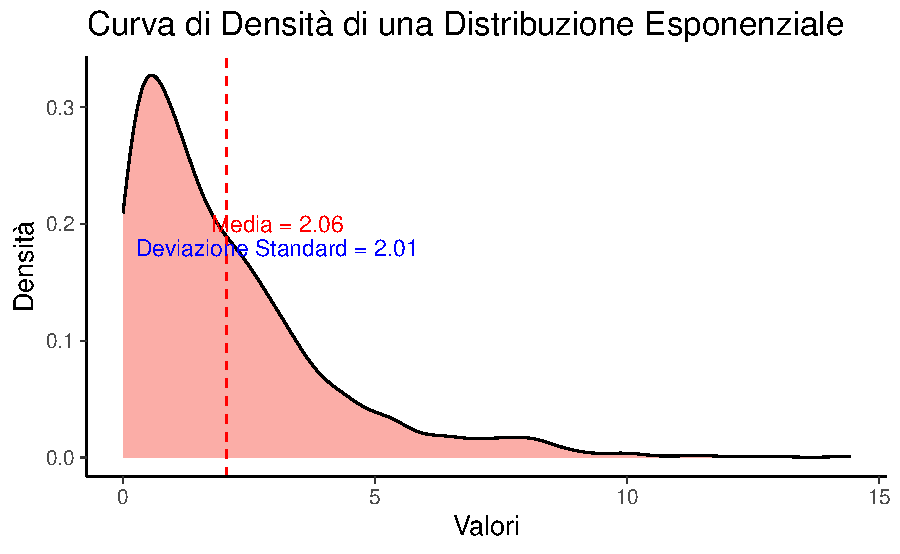
\includegraphics[width=0.7\linewidth,height=\textheight,keepaspectratio]{chapters/eda/07a_introduction_normal_distribution_files/figure-pdf/unnamed-chunk-12-1.pdf}
\end{center}

L'istogramma (o la densità) mostra chiaramente una \textbf{coda lunga a
destra}, con molti valori piccoli e pochi valori grandi. In questo
contesto:

\begin{itemize}
\tightlist
\item
  La \textbf{media} tende a seguire la coda, diventando meno
  rappresentativa del ``centro''.\\
\item
  La \textbf{deviazione standard} non descrive in modo efficace la
  variabilità, perché non considera adeguatamente la forte asimmetria.
\end{itemize}

Misure alternative, come la mediana e i quartili, forniscono
informazioni più affidabili:

\begin{Shaded}
\begin{Highlighting}[]
\CommentTok{\# Calcoliamo mediana e quartili}
\NormalTok{mediana }\OtherTok{\textless{}{-}} \FunctionTok{median}\NormalTok{(dati\_esponenziali)}
\NormalTok{quartili }\OtherTok{\textless{}{-}} \FunctionTok{quantile}\NormalTok{(dati\_esponenziali, }\AttributeTok{probs =} \FunctionTok{c}\NormalTok{(}\FloatTok{0.25}\NormalTok{, }\FloatTok{0.75}\NormalTok{))}

\FunctionTok{cat}\NormalTok{(}\StringTok{"Mediana:"}\NormalTok{, mediana, }\StringTok{"}\SpecialCharTok{\textbackslash{}n}\StringTok{"}\NormalTok{)}
\CommentTok{\#\textgreater{} Mediana: 1.462}
\FunctionTok{cat}\NormalTok{(}\StringTok{"Primo Quartile (Q1):"}\NormalTok{, quartili[}\DecValTok{1}\NormalTok{], }\StringTok{"}\SpecialCharTok{\textbackslash{}n}\StringTok{"}\NormalTok{)}
\CommentTok{\#\textgreater{} Primo Quartile (Q1): 0.6134}
\FunctionTok{cat}\NormalTok{(}\StringTok{"Terzo Quartile (Q3):"}\NormalTok{, quartili[}\DecValTok{2}\NormalTok{], }\StringTok{"}\SpecialCharTok{\textbackslash{}n}\StringTok{"}\NormalTok{)}
\CommentTok{\#\textgreater{} Terzo Quartile (Q3): 2.853}
\end{Highlighting}
\end{Shaded}

In conclusione, quando i dati non presentano una forma vicina alla
normalità (ad esempio perché asimmetrici, multimodali o con kurtosi
anomala), \textbf{media e deviazione standard} possono risultare
fuorvianti o poco utili. In questi casi, è fondamentale adottare misure
alternative o complementari (mediana, quartili, skewness, kurtosis) per
ottenere una descrizione più accurata della distribuzione.

\section{Riflessioni Conclusive}\label{riflessioni-conclusive-13}

In questo capitolo, abbiamo esplorato alcuni concetti fondamentali per
l'analisi dei dati e consolidato le basi per un'interpretazione più
approfondita delle distribuzioni. In particolare, abbiamo:

\begin{itemize}
\tightlist
\item
  \textbf{Studiato la distribuzione normale}, una delle distribuzioni
  più importanti in statistica, e compreso perché la media e la
  deviazione standard siano parametri cruciali per descriverla. Questi
  indicatori ci permettono di riassumere in modo efficace le
  caratteristiche centrali e la variabilità dei dati.
\item
  \textbf{Imparato a standardizzare i dati} convertendoli in unità
  standard (z-score), il che ci consente di confrontare variabili con
  scale diverse o di valutare quanto un dato specifico si discosti dalla
  media in termini di deviazioni standard.
\item
  \textbf{Introdotto il grafico quantile-quantile (QQ-plot)}, uno
  strumento visivo prezioso per verificare se i nostri dati seguono una
  distribuzione normale. Attraverso il QQ-plot, possiamo confrontare i
  quantili empirici dei nostri dati con quelli teorici della
  distribuzione normale, identificando eventuali deviazioni.
\end{itemize}

Gli strumenti descritti in questo capitolo rappresentano il primo passo
essenziale nell'analisi esplorativa dei dati. Essi ci aiutano a
formulare ipotesi solide e a riconoscere potenziali problemi o
caratteristiche peculiari dei dati prima di applicare metodi statistici
più avanzati, che approfondiremo nei prossimi capitoli.

L'analisi esplorativa, combinando grafici intuitivi e statistiche
descrittive appropriate, riveste quindi un ruolo fondamentale nel
processo analitico. Essa non solo ci aiuta a comprendere meglio la
natura dei dati, ma ci fornisce anche una base solida su cui costruire
conclusioni statistiche attendibili e informate.

\section{Esercizi}\label{esercizi-15}

\begin{tcolorbox}[enhanced jigsaw, opacityback=0, bottomrule=.15mm, breakable, title=\textcolor{quarto-callout-tip-color}{\faLightbulb}\hspace{0.5em}{Esercizi}, bottomtitle=1mm, toptitle=1mm, titlerule=0mm, colbacktitle=quarto-callout-tip-color!10!white, rightrule=.15mm, colframe=quarto-callout-tip-color-frame, colback=white, arc=.35mm, leftrule=.75mm, coltitle=black, left=2mm, toprule=.15mm, opacitybacktitle=0.6]

\textbf{Esercizi Teorici}

📌 \textbf{Rispondi alle seguenti domande} per consolidare la
comprensione teorica della distribuzione normale e dei suoi concetti
chiave.

\begin{enumerate}
\def\labelenumi{\arabic{enumi}.}
\tightlist
\item
  \textbf{Caratteristiche della distribuzione normale}

  \begin{itemize}
  \tightlist
  \item
    Quali sono i due parametri principali della distribuzione normale?\\
  \item
    Perché la distribuzione normale è utilizzata così frequentemente in
    statistica?\\
  \item
    In quali situazioni reali possiamo aspettarci che una variabile
    segua una distribuzione normale?
  \end{itemize}
\item
  \textbf{Media e deviazione standard}

  \begin{itemize}
  \tightlist
  \item
    Qual è il significato della media in una distribuzione normale?\\
  \item
    Cosa rappresenta la deviazione standard?\\
  \item
    In che modo la deviazione standard influenza la forma della curva
    normale?
  \end{itemize}
\item
  \textbf{Z-score e standardizzazione}

  \begin{itemize}
  \tightlist
  \item
    Cos'è uno z-score e come si calcola?\\
  \item
    Qual è il significato di un valore z=2? E di un valore z=-1.5?\\
  \item
    Dopo la standardizzazione, quali saranno la media e la deviazione
    standard della variabile?
  \end{itemize}
\item
  \textbf{Verifica della normalità}

  \begin{itemize}
  \tightlist
  \item
    Se hai un piccolo campione di dati (circa 15 osservazioni), quali
    metodi grafici puoi utilizzare per valutare se segue una
    distribuzione normale?\\
  \item
    Quali strumenti statistici puoi impiegare per testare la
    normalità?\\
  \item
    In un QQ-plot, come puoi riconoscere se i dati seguono una
    distribuzione normale?
  \end{itemize}
\end{enumerate}

\textbf{Esercizi Pratici in R}

📌 \textbf{Obiettivo}: Analizzare i dati raccolti dagli studenti sulla
\textbf{Satisfaction With Life Scale (SWLS)}, comprendere la loro
distribuzione e confrontarli con una distribuzione normale teorica.

💾 \textbf{Dati disponibili}:\\
Usa i dati della SWLS. I dati contengono anche informazioni sul genere e
su un indice di rete sociale (LSNS).

\textbf{1. Esplorazione e Visualizzazione dei Dati SWLS}

\begin{enumerate}
\def\labelenumi{\arabic{enumi}.}
\tightlist
\item
  \textbf{Carica i dati raccolti dagli studenti} e verifica la struttura
  del dataset.\\
\item
  \textbf{Calcola i valori di base}: media, deviazione standard, minimo,
  massimo, e quantili della SWLS.\\
\item
  \textbf{Crea una rappresentazione visiva dei dati}:

  \begin{itemize}
  \tightlist
  \item
    Istogramma con sovrapposta una curva di densità.\\
  \item
    Boxplot per identificare eventuali outlier.\\
  \item
    Violin plot per osservare la distribuzione.
  \end{itemize}
\end{enumerate}

\textbf{2. Confronto con la Distribuzione Normale}

\begin{enumerate}
\def\labelenumi{\arabic{enumi}.}
\tightlist
\item
  \textbf{Sovrapponi ai dati osservati una curva normale teorica} basata
  su media e deviazione standard stimate dal campione.\\
\item
  \textbf{Confronta i quantili empirici con quelli teorici} mediante un
  \textbf{QQ-plot}.\\
\item
  \textbf{Commenta il risultato}: i dati SWLS seguono
  approssimativamente una normale? Se no, quali differenze noti?
\end{enumerate}

\textbf{3. Standardizzazione dei Punteggi SWLS}

\begin{enumerate}
\def\labelenumi{\arabic{enumi}.}
\tightlist
\item
  \textbf{Trasforma i dati della SWLS in z-score} per analizzarli in
  unità standardizzate.
\item
  \textbf{Verifica la nuova media e deviazione standard}: dovrebbero
  essere 0 e 1 rispettivamente.\\
\item
  \textbf{Conta quanti punteggi standardizzati si trovano entro 1, 2 e 3
  deviazioni standard dalla media} e confronta i valori attesi di 68\%,
  95\% e 99.7\%.
\end{enumerate}

\textbf{4. Relazione tra SWLS e Interazione Sociale (LSNS)}

\begin{enumerate}
\def\labelenumi{\arabic{enumi}.}
\tightlist
\item
  \textbf{Esplora la relazione tra SWLS e il punteggio della Scala della
  Rete Sociale di Lubben (LSNS-6)}.\\
\item
  \textbf{Costruisci un grafico a dispersione} per osservare la
  correlazione tra le due variabili.\\
\item
  \textbf{Calcola il coefficiente di correlazione di Pearson} e commenta
  il risultato. Esiste una relazione tra soddisfazione della vita e
  supporto sociale?\\
\end{enumerate}

\end{tcolorbox}

\begin{tcolorbox}[enhanced jigsaw, opacityback=0, bottomrule=.15mm, breakable, title=\textcolor{quarto-callout-tip-color}{\faLightbulb}\hspace{0.5em}{Soluzioni}, bottomtitle=1mm, toptitle=1mm, titlerule=0mm, colbacktitle=quarto-callout-tip-color!10!white, rightrule=.15mm, colframe=quarto-callout-tip-color-frame, colback=white, arc=.35mm, leftrule=.75mm, coltitle=black, left=2mm, toprule=.15mm, opacitybacktitle=0.6]

\textbf{1. Caratteristiche della distribuzione normale}

\textbf{a. Quali sono i due parametri principali della distribuzione
normale?}

I due parametri principali che definiscono una distribuzione normale
sono:

\begin{itemize}
\tightlist
\item
  \textbf{La media (μ)}: Indica il centro della distribuzione. Tutte le
  osservazioni si raggruppano attorno a questo valore.
\item
  \textbf{La deviazione standard (σ)}: Descrive la dispersione o la
  variabilità dei dati attorno alla media.
\end{itemize}

\textbf{b. Perché la distribuzione normale è utilizzata così
frequentemente in statistica?}

La distribuzione normale è ampiamente usata per diversi motivi:

\begin{enumerate}
\def\labelenumi{\arabic{enumi}.}
\tightlist
\item
  \textbf{Teorema del limite centrale}: Afferma che, quando si sommano
  molte variabili casuali indipendenti, la loro distribuzione tende ad
  avvicinarsi a una normale, indipendentemente dalla forma originale
  delle singole distribuzioni.
\item
  \textbf{Semplicità matematica}: La normale ha proprietà matematiche
  ben definite e permette di calcolare probabilità e intervalli con
  facilità.
\item
  \textbf{Modellizzazione naturale}: Molte variabili naturali e sociali
  (ad esempio, altezze, pesi, punteggi standardizzati) seguono
  approssimativamente una distribuzione normale.
\end{enumerate}

\textbf{c.~In quali situazioni reali possiamo aspettarci che una
variabile segua una distribuzione normale?}

Si può aspettare una distribuzione normale in situazioni in cui:

\begin{itemize}
\tightlist
\item
  Le osservazioni sono influenzate da molti fattori casuali indipendenti
  (es. altezza di un individuo, errore di misurazione).
\item
  I dati derivano da fenomeni naturali o biologici (es. pressione
  sanguigna, peso corporeo).
\item
  Si analizzano medie campionarie di grandi dimensioni (grazie al
  teorema del limite centrale).
\end{itemize}

\textbf{2. Media e deviazione standard}

\textbf{a. Qual è il significato della media in una distribuzione
normale?}

Nella distribuzione normale, la media rappresenta il punto centrale
della curva, ovvero il valore più probabile. È anche il punto di
simmetria della distribuzione, dove metà delle osservazioni si trova a
sinistra e l'altra metà a destra.

\textbf{b. Cosa rappresenta la deviazione standard?}

La deviazione standard misura quanto i dati si discostano in media dalla
media. Una deviazione standard bassa indica che i dati sono raggruppati
strettamente attorno alla media, mentre una deviazione standard alta
indica una maggiore dispersione.

\textbf{c.~In che modo la deviazione standard influenza la forma della
curva normale?}

\begin{itemize}
\tightlist
\item
  Una deviazione standard piccola produce una curva alta e stretta,
  indicando una bassa variabilità.
\item
  Una deviazione standard grande produce una curva bassa e larga,
  indicando una maggiore variabilità.
\end{itemize}

\textbf{3. Z-score e standardizzazione}

\textbf{a. Cos'è uno z-score e come si calcola?}

Uno z-score misura quante deviazioni standard un dato si discosta dalla
media. Viene calcolato come:

\[
z = \frac{x - \mu}{\sigma}
\]

dove \(x\) è il valore osservato, \(\mu\) è la media e \(\sigma\) è la
deviazione standard.

\textbf{b. Qual è il significato di un valore z=2? E di un valore
z=-1.5?}

\begin{itemize}
\tightlist
\item
  Un \(z = 2\) significa che il dato è posizionato a 2 deviazioni
  standard sopra la media.
\item
  Un \(z = -1.5\) significa che il dato è posizionato a 1.5 deviazioni
  standard sotto la media.
\end{itemize}

\textbf{c.~Dopo la standardizzazione, quali saranno la media e la
deviazione standard della variabile?}

Dopo la standardizzazione:

\begin{itemize}
\tightlist
\item
  La media diventa \(0\).
\item
  La deviazione standard diventa \(1\).
\end{itemize}

\textbf{4. Verifica della normalità}

\textbf{a. Se hai un piccolo campione di dati (circa 15 osservazioni),
quali metodi grafici puoi utilizzare per valutare se segue una
distribuzione normale?}

Per piccoli campioni, i metodi grafici più utili sono:

\begin{enumerate}
\def\labelenumi{\arabic{enumi}.}
\tightlist
\item
  \textbf{QQ-plot (Quantile-Quantile plot)}: Confronta i quantili dei
  dati con quelli di una distribuzione normale. Se i punti seguono una
  retta diagonale, i dati sono normali.
\item
  \textbf{Istogramma}: Mostra la distribuzione dei dati, ma con campioni
  piccoli può essere meno preciso.
\end{enumerate}

\textbf{b. Quali strumenti statistici puoi impiegare per testare la
normalità?}

Gli strumenti statistici più comuni per verificare la normalità sono:

\begin{itemize}
\tightlist
\item
  \textbf{Test di Shapiro-Wilk}: Ideale per piccoli campioni.
\item
  \textbf{Test di Kolmogorov-Smirnov}: Usato per confrontare la
  distribuzione empirica con una normale.
\item
  \textbf{Test di Anderson-Darling}: Sensibile alle code della
  distribuzione.
\end{itemize}

\textbf{c.~In un QQ-plot, come puoi riconoscere se i dati seguono una
distribuzione normale?}

In un QQ-plot:

\begin{itemize}
\tightlist
\item
  Se i dati seguono una distribuzione normale, i punti si allineeranno
  lungo una retta diagonale.
\item
  Deviazioni dalla retta indicano departi dalla normalità:

  \begin{itemize}
  \tightlist
  \item
    Code pesanti: Punti esterni alla retta suggeriscono outlier.
  \item
    Asimmetria: Punti curvati suggeriscono skewness (asimmetria).
  \end{itemize}
\end{itemize}

\textbf{Esplorazione e Visualizzazione dei Dati SWLS}

\textbf{Caricamento e struttura dei dati}

\begin{Shaded}
\begin{Highlighting}[]
\FunctionTok{library}\NormalTok{(ggplot2)}
\FunctionTok{library}\NormalTok{(dplyr)}

\CommentTok{\# Supponiamo che i dati siano i seguenti}
\FunctionTok{set.seed}\NormalTok{(}\DecValTok{42}\NormalTok{)}
\NormalTok{swls }\OtherTok{\textless{}{-}} \FunctionTok{data.frame}\NormalTok{(}
  \AttributeTok{ID =} \DecValTok{1}\SpecialCharTok{:}\DecValTok{15}\NormalTok{,}
  \AttributeTok{SWLS =} \FunctionTok{c}\NormalTok{(}\DecValTok{18}\NormalTok{, }\DecValTok{22}\NormalTok{, }\DecValTok{25}\NormalTok{, }\DecValTok{21}\NormalTok{, }\DecValTok{26}\NormalTok{, }\DecValTok{19}\NormalTok{, }\DecValTok{20}\NormalTok{, }\DecValTok{23}\NormalTok{, }\DecValTok{24}\NormalTok{, }\DecValTok{17}\NormalTok{, }\DecValTok{22}\NormalTok{, }\DecValTok{27}\NormalTok{, }\DecValTok{28}\NormalTok{, }\DecValTok{21}\NormalTok{, }\DecValTok{19}\NormalTok{),}
  \AttributeTok{Genere =} \FunctionTok{c}\NormalTok{(}\StringTok{"M"}\NormalTok{, }\StringTok{"F"}\NormalTok{, }\StringTok{"F"}\NormalTok{, }\StringTok{"M"}\NormalTok{, }\StringTok{"F"}\NormalTok{, }\StringTok{"M"}\NormalTok{, }\StringTok{"M"}\NormalTok{, }\StringTok{"F"}\NormalTok{, }\StringTok{"M"}\NormalTok{, }\StringTok{"F"}\NormalTok{, }\StringTok{"M"}\NormalTok{, }\StringTok{"F"}\NormalTok{, }\StringTok{"F"}\NormalTok{, }\StringTok{"M"}\NormalTok{, }\StringTok{"M"}\NormalTok{),}
  \AttributeTok{LSNS =} \FunctionTok{c}\NormalTok{(}\DecValTok{16}\NormalTok{, }\DecValTok{20}\NormalTok{, }\DecValTok{22}\NormalTok{, }\DecValTok{14}\NormalTok{, }\DecValTok{19}\NormalTok{, }\DecValTok{18}\NormalTok{, }\DecValTok{17}\NormalTok{, }\DecValTok{25}\NormalTok{, }\DecValTok{23}\NormalTok{, }\DecValTok{12}\NormalTok{, }\DecValTok{21}\NormalTok{, }\DecValTok{28}\NormalTok{, }\DecValTok{26}\NormalTok{, }\DecValTok{19}\NormalTok{, }\DecValTok{15}\NormalTok{)}
\NormalTok{)}

\FunctionTok{str}\NormalTok{(swls)}
\FunctionTok{summary}\NormalTok{(swls}\SpecialCharTok{$}\NormalTok{SWLS)}
\end{Highlighting}
\end{Shaded}

\textbf{Visualizzazioni}

\begin{Shaded}
\begin{Highlighting}[]
\CommentTok{\# Istogramma con curva di densità}
\FunctionTok{ggplot}\NormalTok{(swls, }\FunctionTok{aes}\NormalTok{(}\AttributeTok{x =}\NormalTok{ SWLS)) }\SpecialCharTok{+}
  \FunctionTok{geom\_histogram}\NormalTok{(}\FunctionTok{aes}\NormalTok{(}\AttributeTok{y =} \FunctionTok{after\_stat}\NormalTok{(density)), }\AttributeTok{bins =} \DecValTok{6}\NormalTok{, }\AttributeTok{fill =} \StringTok{"blue"}\NormalTok{, }\AttributeTok{alpha =} \FloatTok{0.5}\NormalTok{) }\SpecialCharTok{+}
  \FunctionTok{geom\_density}\NormalTok{(}\AttributeTok{color =} \StringTok{"red"}\NormalTok{, }\AttributeTok{size =} \DecValTok{1}\NormalTok{) }\SpecialCharTok{+}
  \FunctionTok{ggtitle}\NormalTok{(}\StringTok{"Distribuzione dei punteggi SWLS"}\NormalTok{)}

\CommentTok{\# Boxplot}
\FunctionTok{ggplot}\NormalTok{(swls, }\FunctionTok{aes}\NormalTok{(}\AttributeTok{y =}\NormalTok{ SWLS)) }\SpecialCharTok{+}
  \FunctionTok{geom\_boxplot}\NormalTok{(}\AttributeTok{fill =} \StringTok{"cyan"}\NormalTok{) }\SpecialCharTok{+}
  \FunctionTok{ggtitle}\NormalTok{(}\StringTok{"Boxplot dei punteggi SWLS"}\NormalTok{)}
\end{Highlighting}
\end{Shaded}

\textbf{2. Confronto con la Distribuzione Normale}

\begin{Shaded}
\begin{Highlighting}[]
\CommentTok{\# QQ{-}plot per valutare la normalità}
\FunctionTok{ggplot}\NormalTok{(swls, }\FunctionTok{aes}\NormalTok{(}\AttributeTok{sample =}\NormalTok{ SWLS)) }\SpecialCharTok{+}
  \FunctionTok{geom\_qq}\NormalTok{() }\SpecialCharTok{+}
  \FunctionTok{geom\_abline}\NormalTok{() }\SpecialCharTok{+}
  \FunctionTok{ggtitle}\NormalTok{(}\StringTok{"QQ{-}plot dei punteggi SWLS"}\NormalTok{) }\SpecialCharTok{+}
  \FunctionTok{theme\_minimal}\NormalTok{()}
\end{Highlighting}
\end{Shaded}

\textbf{Osservazione}:

\begin{itemize}
\tightlist
\item
  Se i punti si allineano lungo la diagonale, i dati sono
  approssimativamente normali.
\item
  Se ci sono deviazioni marcate, la distribuzione potrebbe essere
  asimmetrica o presentare code pesanti.
\end{itemize}

\textbf{3. Standardizzazione dei punteggi SWLS}

\begin{Shaded}
\begin{Highlighting}[]
\NormalTok{swls}\SpecialCharTok{$}\NormalTok{Z\_SWLS }\OtherTok{\textless{}{-}} \FunctionTok{scale}\NormalTok{(swls}\SpecialCharTok{$}\NormalTok{SWLS)}

\FunctionTok{mean}\NormalTok{(swls}\SpecialCharTok{$}\NormalTok{Z\_SWLS)  }\CommentTok{\# Dovrebbe essere circa 0}
\FunctionTok{sd}\NormalTok{(swls}\SpecialCharTok{$}\NormalTok{Z\_SWLS)    }\CommentTok{\# Dovrebbe essere circa 1}

\CommentTok{\# Proporzione entro 1, 2, 3 deviazioni standard}
\FunctionTok{mean}\NormalTok{(}\FunctionTok{abs}\NormalTok{(swls}\SpecialCharTok{$}\NormalTok{Z\_SWLS) }\SpecialCharTok{\textless{}} \DecValTok{1}\NormalTok{)  }\CommentTok{\# Atteso \textasciitilde{}68\%}
\FunctionTok{mean}\NormalTok{(}\FunctionTok{abs}\NormalTok{(swls}\SpecialCharTok{$}\NormalTok{Z\_SWLS) }\SpecialCharTok{\textless{}} \DecValTok{2}\NormalTok{)  }\CommentTok{\# Atteso \textasciitilde{}95\%}
\FunctionTok{mean}\NormalTok{(}\FunctionTok{abs}\NormalTok{(swls}\SpecialCharTok{$}\NormalTok{Z\_SWLS) }\SpecialCharTok{\textless{}} \DecValTok{3}\NormalTok{)  }\CommentTok{\# Atteso \textasciitilde{}99.7\%}
\end{Highlighting}
\end{Shaded}

\textbf{4. Relazione tra SWLS e LSNS}

\begin{Shaded}
\begin{Highlighting}[]
\CommentTok{\# Grafico di dispersione}
\FunctionTok{ggplot}\NormalTok{(swls, }\FunctionTok{aes}\NormalTok{(}\AttributeTok{x =}\NormalTok{ LSNS, }\AttributeTok{y =}\NormalTok{ SWLS)) }\SpecialCharTok{+}
  \FunctionTok{geom\_point}\NormalTok{(}\AttributeTok{color =} \StringTok{"blue"}\NormalTok{, }\AttributeTok{size =} \DecValTok{3}\NormalTok{) }\SpecialCharTok{+}
  \FunctionTok{geom\_smooth}\NormalTok{(}\AttributeTok{method =} \StringTok{"lm"}\NormalTok{, }\AttributeTok{color =} \StringTok{"red"}\NormalTok{, }\AttributeTok{se =} \ConstantTok{FALSE}\NormalTok{) }\SpecialCharTok{+}
  \FunctionTok{ggtitle}\NormalTok{(}\StringTok{"Relazione tra SWLS e LSNS"}\NormalTok{) }

\CommentTok{\# Calcolo della correlazione}
\FunctionTok{cor}\NormalTok{(swls}\SpecialCharTok{$}\NormalTok{SWLS, swls}\SpecialCharTok{$}\NormalTok{LSNS)}
\end{Highlighting}
\end{Shaded}

\textbf{Interpretazione}:

\begin{itemize}
\tightlist
\item
  Un valore di correlazione positivo indica che livelli più alti di
  supporto sociale (LSNS) sono associati a una maggiore soddisfazione
  della vita (SWLS).\\
\item
  Se la correlazione è debole, il supporto sociale potrebbe non essere
  un predittore forte della soddisfazione della vita in questo campione
  ristretto.\\
\end{itemize}

\end{tcolorbox}

\section*{Informazioni sull'Ambiente di
Sviluppo}\label{informazioni-sullambiente-di-sviluppo-10}
\addcontentsline{toc}{section}{Informazioni sull'Ambiente di Sviluppo}

\markright{Informazioni sull'Ambiente di Sviluppo}

\begin{Shaded}
\begin{Highlighting}[]
\FunctionTok{sessionInfo}\NormalTok{()}
\CommentTok{\#\textgreater{} R version 4.4.2 (2024{-}10{-}31)}
\CommentTok{\#\textgreater{} Platform: aarch64{-}apple{-}darwin20}
\CommentTok{\#\textgreater{} Running under: macOS Sequoia 15.3.1}
\CommentTok{\#\textgreater{} }
\CommentTok{\#\textgreater{} Matrix products: default}
\CommentTok{\#\textgreater{} BLAS:   /Library/Frameworks/R.framework/Versions/4.4{-}arm64/Resources/lib/libRblas.0.dylib }
\CommentTok{\#\textgreater{} LAPACK: /Library/Frameworks/R.framework/Versions/4.4{-}arm64/Resources/lib/libRlapack.dylib;  LAPACK version 3.12.0}
\CommentTok{\#\textgreater{} }
\CommentTok{\#\textgreater{} locale:}
\CommentTok{\#\textgreater{} [1] C/UTF{-}8/C/C/C/C}
\CommentTok{\#\textgreater{} }
\CommentTok{\#\textgreater{} time zone: Europe/Rome}
\CommentTok{\#\textgreater{} tzcode source: internal}
\CommentTok{\#\textgreater{} }
\CommentTok{\#\textgreater{} attached base packages:}
\CommentTok{\#\textgreater{} [1] stats     graphics  grDevices utils     datasets  methods   base     }
\CommentTok{\#\textgreater{} }
\CommentTok{\#\textgreater{} other attached packages:}
\CommentTok{\#\textgreater{}  [1] dslabs\_0.8.0     ggbeeswarm\_0.7.2 thematic\_0.1.6   MetBrewer\_0.2.0 }
\CommentTok{\#\textgreater{}  [5] ggokabeito\_0.1.0 see\_0.10.0       gridExtra\_2.3    patchwork\_1.3.0 }
\CommentTok{\#\textgreater{}  [9] bayesplot\_1.11.1 psych\_2.4.12     scales\_1.3.0     markdown\_1.13   }
\CommentTok{\#\textgreater{} [13] knitr\_1.49       lubridate\_1.9.4  forcats\_1.0.0    stringr\_1.5.1   }
\CommentTok{\#\textgreater{} [17] dplyr\_1.1.4      purrr\_1.0.4      readr\_2.1.5      tidyr\_1.3.1     }
\CommentTok{\#\textgreater{} [21] tibble\_3.2.1     ggplot2\_3.5.1    tidyverse\_2.0.0  rio\_1.2.3       }
\CommentTok{\#\textgreater{} [25] here\_1.0.1      }
\CommentTok{\#\textgreater{} }
\CommentTok{\#\textgreater{} loaded via a namespace (and not attached):}
\CommentTok{\#\textgreater{}  [1] generics\_0.1.3    stringi\_1.8.4     lattice\_0.22{-}6    hms\_1.1.3        }
\CommentTok{\#\textgreater{}  [5] digest\_0.6.37     magrittr\_2.0.3    evaluate\_1.0.3    grid\_4.4.2       }
\CommentTok{\#\textgreater{}  [9] timechange\_0.3.0  fastmap\_1.2.0     rprojroot\_2.0.4   jsonlite\_1.8.9   }
\CommentTok{\#\textgreater{} [13] mnormt\_2.1.1      cli\_3.6.4         rlang\_1.1.5       munsell\_0.5.1    }
\CommentTok{\#\textgreater{} [17] withr\_3.0.2       tools\_4.4.2       parallel\_4.4.2    tzdb\_0.4.0       }
\CommentTok{\#\textgreater{} [21] colorspace\_2.1{-}1  pacman\_0.5.1      vctrs\_0.6.5       R6\_2.6.1         }
\CommentTok{\#\textgreater{} [25] lifecycle\_1.0.4   vipor\_0.4.7       beeswarm\_0.4.0    pkgconfig\_2.0.3  }
\CommentTok{\#\textgreater{} [29] pillar\_1.10.1     gtable\_0.3.6      glue\_1.8.0        xfun\_0.50        }
\CommentTok{\#\textgreater{} [33] tidyselect\_1.2.1  rstudioapi\_0.17.1 farver\_2.1.2      htmltools\_0.5.8.1}
\CommentTok{\#\textgreater{} [37] nlme\_3.1{-}167      labeling\_0.4.3    rmarkdown\_2.29    compiler\_4.4.2}
\end{Highlighting}
\end{Shaded}

\section*{Bibliografia}\label{bibliografia-19}
\addcontentsline{toc}{section}{Bibliografia}

\markright{Bibliografia}

\chapter{Relazioni tra variabili}\label{sec-correlation}

\begin{tcolorbox}[enhanced jigsaw, opacityback=0, bottomrule=.15mm, breakable, title=\textcolor{quarto-callout-important-color}{\faExclamation}\hspace{0.5em}{In questo capitolo imparerai a}, bottomtitle=1mm, toptitle=1mm, titlerule=0mm, colbacktitle=quarto-callout-important-color!10!white, rightrule=.15mm, colframe=quarto-callout-important-color-frame, colback=white, arc=.35mm, leftrule=.75mm, coltitle=black, left=2mm, toprule=.15mm, opacitybacktitle=0.6]

\begin{itemize}
\tightlist
\item
  comprendere e calcolare la correlazione e la covarianza;
\item
  interpretare correttamente gli indici di correlazione e covarianza nel
  contesto dell'analisi dei dati.
\end{itemize}

\end{tcolorbox}

\begin{tcolorbox}[enhanced jigsaw, opacityback=0, bottomrule=.15mm, breakable, title=\textcolor{quarto-callout-tip-color}{\faLightbulb}\hspace{0.5em}{Prerequisiti}, bottomtitle=1mm, toptitle=1mm, titlerule=0mm, colbacktitle=quarto-callout-tip-color!10!white, rightrule=.15mm, colframe=quarto-callout-tip-color-frame, colback=white, arc=.35mm, leftrule=.75mm, coltitle=black, left=2mm, toprule=.15mm, opacitybacktitle=0.6]

\begin{itemize}
\tightlist
\item
  Leggere l'introduzione dell'articolo ``The curious case of the
  cross-sectional correlation''
  (\citeproc{ref-hamaker2024curious}{Hamaker, 2024}).
\end{itemize}

\end{tcolorbox}

\begin{tcolorbox}[enhanced jigsaw, opacityback=0, bottomrule=.15mm, breakable, title=\textcolor{quarto-callout-caution-color}{\faFire}\hspace{0.5em}{Preparazione del Notebook}, bottomtitle=1mm, toptitle=1mm, titlerule=0mm, colbacktitle=quarto-callout-caution-color!10!white, rightrule=.15mm, colframe=quarto-callout-caution-color-frame, colback=white, arc=.35mm, leftrule=.75mm, coltitle=black, left=2mm, toprule=.15mm, opacitybacktitle=0.6]

\begin{Shaded}
\begin{Highlighting}[]
\NormalTok{here}\SpecialCharTok{::}\FunctionTok{here}\NormalTok{(}\StringTok{"code"}\NormalTok{, }\StringTok{"\_common.R"}\NormalTok{) }\SpecialCharTok{|\textgreater{}} 
  \FunctionTok{source}\NormalTok{()}

\CommentTok{\# Load packages}
\ControlFlowTok{if}\NormalTok{ (}\SpecialCharTok{!}\FunctionTok{requireNamespace}\NormalTok{(}\StringTok{"pacman"}\NormalTok{)) }\FunctionTok{install.packages}\NormalTok{(}\StringTok{"pacman"}\NormalTok{)}
\NormalTok{pacman}\SpecialCharTok{::}\FunctionTok{p\_load}\NormalTok{(readr)}
\end{Highlighting}
\end{Shaded}

\end{tcolorbox}

\section{Introduzione}\label{introduzione-19}

Nonostante sia un'operazione di base, l'analisi delle associazioni tra
variabili rappresenta uno degli aspetti più controversi nell'ambito
dell'analisi dei dati psicologici. Sebbene possa sembrare un passaggio
naturale dopo l'analisi univariata, questo processo solleva numerose
questioni metodologiche e concettuali.

Tradizionalmente, in psicologia, l'analisi delle associazioni tra
variabili è stata considerata come l'obiettivo finale del processo di
ricerca. Questa visione si basa sull'idea che la descrizione delle
relazioni tra variabili fornisca una spiegazione esaustiva dei fenomeni
psicologici. Tale approccio trova le sue radici storiche nel pensiero di
Karl Pearson (1911), il quale sosteneva che la spiegazione scientifica
si esaurisse una volta delineate le associazioni tra le variabili
osservate:

\begin{quote}
Quanto spesso, quando è stato osservato un nuovo fenomeno, sentiamo che
viene posta la domanda: `qual è la sua causa?'. Questa è una domanda a
cui potrebbe essere assolutamente impossibile rispondere. Invece, può
essere più facile rispondere alla domanda: `in che misura altri fenomeni
sono associati con esso?'. Dalla risposta a questa seconda domanda
possono risultare molte preziose conoscenze.
\end{quote}

Sebbene sia indubbio che rispondere alla seconda domanda posta da
Pearson sia relativamente semplice, è altresì evidente che la nostra
comprensione di un fenomeno non può dipendere unicamente dalle
informazioni fornite dalle correlazioni.

In contrasto con questa visione tradizionale, la ``Causal Revolution''
propone un paradigma radicalmente diverso secondo il quale le
associazioni tra variabili sono considerate come epifenomeni, mentre
l'obiettivo principale della ricerca è l'identificazione e la
comprensione delle relazioni causali: per comprendere veramente i
fenomeni psicologici è essenziale indagare le cause sottostanti, andando
oltre la mera descrizione delle associazioni.

La discussione dei metodi utilizzati per individuare le relazioni
causali sarà trattata successivamente. In questo capitolo, ci
concentreremo sui concetti statistici fondamentali necessari per
descrivere le associazioni lineari tra variabili. È importante
sottolineare che, sebbene esistano indici statistici per quantificare
associazioni non lineari, la maggior parte degli psicologi si limita
all'utilizzo di indici lineari.

Nel linguaggio comune, termini come ``dipendenza'', ``associazione'' e
``correlazione'' vengono spesso usati in modo intercambiabile. Tuttavia,
da un punto di vista tecnico, è importante distinguere questi concetti:

\begin{enumerate}
\def\labelenumi{\arabic{enumi}.}
\tightlist
\item
  \textbf{Associazione}: questo termine indica una relazione generale
  tra variabili, dove la conoscenza del valore di una variabile fornisce
  informazioni su un'altra.
\item
  \textbf{Correlazione}: descrive una relazione specifica e
  quantificabile, indicando se due variabili tendono a variare insieme
  in modo sistematico. Ad esempio, in una correlazione positiva, se
  \(X > \mu_X\), è probabile che anche \(Y > \mu_Y\). La correlazione
  specifica il segno e l'intensità di una relazione lineare.
\item
  \textbf{Dipendenza}: indica una relazione causale tra le variabili,
  dove la variazione della variabile causale porta probabilisticamente
  alla variazione della variabile dipendente.
\end{enumerate}

È cruciale comprendere che non tutte le associazioni sono correlazioni
e, soprattutto, che la correlazione non implica necessariamente
causalità. Questa distinzione è fondamentale per interpretare
correttamente i dati e evitare conclusioni errate sulle relazioni tra
variabili.

In questo capitolo, esamineremo due misure statistiche fondamentali per
valutare la relazione lineare tra due variabili: la covarianza e la
correlazione. Questi indici ci permettono di descrivere il grado e la
direzione dell'associazione lineare tra variabili, quantificando come
queste variano congiuntamente.

\section{I dati grezzi}\label{i-dati-grezzi}

Per illustrare la correlazione e la covarianza, analizzeremo i dati
raccolti da Zetsche et al. (\citeproc{ref-zetsche_2019future}{2019}) in
uno studio che indaga le aspettative negative come meccanismo chiave nel
mantenimento e nella reiterazione della depressione. Nello specifico, i
ricercatori si sono proposti di determinare se gli individui depressi
sviluppano aspettative accurate riguardo al loro umore futuro o se tali
aspettative sono distortamente negative.

Uno dei loro studi ha coinvolto un campione di 30 soggetti con almeno un
episodio depressivo maggiore, confrontati con un gruppo di controllo
composto da 37 individui sani. La misurazione del livello di depressione
è stata effettuata tramite il \emph{Beck Depression Inventory} (BDI-II).

Il BDI-II è uno strumento di autovalutazione utilizzato per valutare la
gravità della depressione in adulti e adolescenti. Il test è stato
sviluppato per identificare e misurare l'intensità dei sintomi
depressivi sperimentati nelle ultime due settimane. I 21 item del test
sono valutati su una scala a 4 punti, dove 0 rappresenta il grado più
basso e 3 il grado più elevato di sintomatologia depressiva.

Nell'esercizio successivo, ci proponiamo di analizzare i punteggi di
depressione BDI-II nel campione di dati fornito da Zetsche et al.
(\citeproc{ref-zetsche_2019future}{2019}).

\section{Definizione delle relazioni tra
variabili}\label{definizione-delle-relazioni-tra-variabili}

Nel contesto delle indagini statistiche, spesso non ci limitiamo a
esaminare la distribuzione di una singola variabile. Invece, il nostro
interesse si concentra sulla relazione che emerge nei dati tra due o più
variabili. Ma cosa significa esattamente quando diciamo che due
variabili hanno una relazione?

Per comprendere ciò, prendiamo ad esempio l'altezza e l'età tra un
gruppo di bambini. In generale, è possibile notare che all'aumentare
dell'età di un bambino, aumenta anche la sua altezza. Pertanto,
conoscere l'età di un bambino, ad esempio tredici anni, e l'età di un
altro, sei anni, ci fornisce un'indicazione su quale dei due bambini sia
più alto.

Nel linguaggio statistico, definiamo questa relazione tra altezza e età
come positiva, il che significa che all'aumentare dei valori di una
delle variabili (in questo caso, l'età), ci aspettiamo di vedere valori
più elevati anche nell'altra variabile (l'altezza). Tuttavia, esistono
anche relazioni negative, in cui l'aumento di una variabile è associato
a un diminuzione dell'altra (ad esempio, più età è correlata a meno
pianto).

Non si tratta solo di relazioni positive o negative; ci sono anche
situazioni in cui le variabili non hanno alcuna relazione tra loro,
definendo così una relazione nulla. Inoltre, le relazioni possono
variare nel tempo, passando da positive a negative o da fortemente
positive a appena positiva. In alcuni casi, una delle variabili può
essere categorica, rendendo difficile parlare di ``maggioranza'' o
``minoranza'' ma piuttosto di ``differente'' (ad esempio, i bambini più
grandi potrebbero semplicemente avere diverse preferenze rispetto ai
bambini più piccoli, senza necessariamente essere ``migliori'' o
``peggiori'').

\section{Grafico a dispersione}\label{sec-scatter-plot}

Il metodo più diretto per visualizzare la relazione tra due variabili
continue è tramite un grafico a dispersione, comunemente noto come
``scatterplot''. Questo tipo di diagramma rappresenta le coppie di dati
ottenute da due variabili, posizionandole sull'asse delle ascisse
(orizzontale) e delle ordinate (verticale).

Per rendere l'idea più chiara, consideriamo i dati dello studio condotto
da Zetsche et al. (\citeproc{ref-zetsche_2019future}{2019}), in cui i
ricercatori hanno utilizzato due scale psicometriche, il Beck Depression
Inventory II (BDI-II) e la Center for Epidemiologic Studies Depression
Scale (CES-D), per misurare il livello di depressione nei partecipanti.
Il BDI-II è uno strumento di autovalutazione che valuta la presenza e
l'intensità dei sintomi depressivi in pazienti adulti e adolescenti con
diagnosi psichiatrica, mentre la CES-D è una scala di autovalutazione
progettata per misurare i sintomi depressivi sperimentati nella
settimana precedente nella popolazione generale, in particolare negli
adolescenti e nei giovani adulti. Poiché entrambe le scale misurano lo
stesso costrutto, ovvero la depressione, ci aspettiamo una relazione tra
i punteggi ottenuti dal BDI-II e dalla CES-D. Un diagramma a dispersione
ci consente di esaminare questa relazione in modo visuale e intuitivo.

\begin{Shaded}
\begin{Highlighting}[]
\CommentTok{\# Leggi i dati dal file CSV}
\NormalTok{df }\OtherTok{\textless{}{-}}\NormalTok{ rio}\SpecialCharTok{::}\FunctionTok{import}\NormalTok{(here}\SpecialCharTok{::}\FunctionTok{here}\NormalTok{(}\StringTok{"data"}\NormalTok{, }\StringTok{"data.mood.csv"}\NormalTok{))}

\CommentTok{\# Seleziona le colonne di interesse}
\NormalTok{df }\OtherTok{\textless{}{-}}\NormalTok{ df }\SpecialCharTok{|\textgreater{}}
\NormalTok{  dplyr}\SpecialCharTok{::}\FunctionTok{select}\NormalTok{(}\StringTok{"esm\_id"}\NormalTok{, }\StringTok{"group"}\NormalTok{, }\StringTok{"bdi"}\NormalTok{, }\StringTok{"cesd\_sum"}\NormalTok{)}

\CommentTok{\# Rimuovi le righe duplicate}
\NormalTok{df }\OtherTok{\textless{}{-}}\NormalTok{ df[}\SpecialCharTok{!}\FunctionTok{duplicated}\NormalTok{(df), ]}

\CommentTok{\# Rimuovi le righe con valori mancanti nella colonna "bdi"}
\NormalTok{df }\OtherTok{\textless{}{-}}\NormalTok{ df[}\SpecialCharTok{!}\FunctionTok{is.na}\NormalTok{(df}\SpecialCharTok{$}\NormalTok{bdi), ]}
\end{Highlighting}
\end{Shaded}

Posizionando i valori del BDI-II sull'asse delle ascisse e quelli del
CES-D sull'asse delle ordinate, ogni punto sul grafico rappresenta un
individuo, di cui conosciamo il livello di depressione misurato dalle
due scale. È evidente che i valori delle scale BDI-II e CES-D non
possono coincidere per due motivi principali: (1) la presenza di errori
di misurazione e (2) l'utilizzo di unità di misura arbitrarie per le due
variabili. L'errore di misurazione è una componente inevitabile che
influisce in parte su qualsiasi misurazione, ed è particolarmente
rilevante in psicologia, dove la precisione degli strumenti di
misurazione è generalmente inferiore rispetto ad altre discipline, come
la fisica. Il secondo motivo per cui i valori delle scale BDI-II e CES-D
non possono essere identici è che l'unità di misura della depressione è
una questione arbitraria e non standardizzata. Tuttavia, nonostante le
differenze dovute agli errori di misurazione e all'uso di unità di
misura diverse, ci aspettiamo che, se le due scale misurano lo stesso
costrutto (la depressione), i valori prodotti dalle due scale dovrebbero
essere associati linearmente tra di loro. Per comprendere meglio il
concetto di ``associazione lineare'', è possibile esaminare i dati
attraverso l'utilizzo di un diagramma a dispersione.

\begin{center}
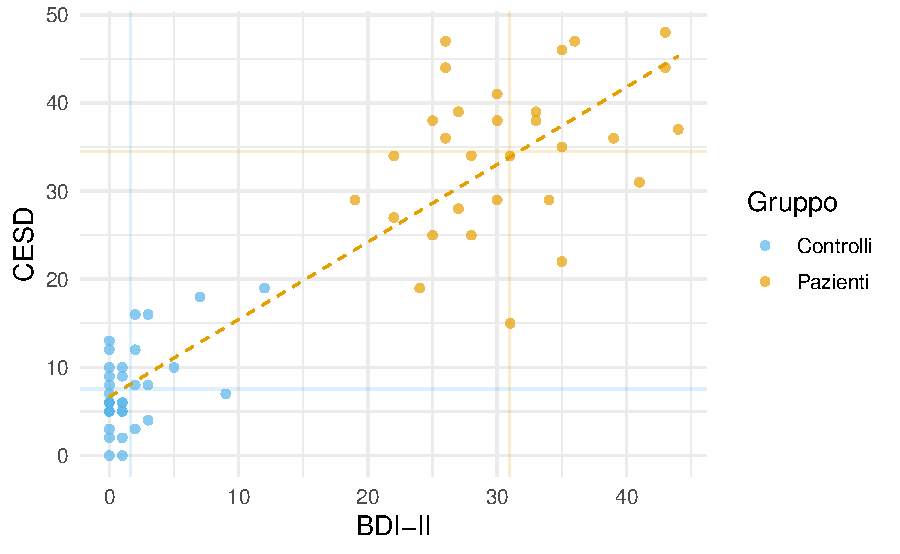
\includegraphics[width=0.7\linewidth,height=\textheight,keepaspectratio]{chapters/eda/08_correlation_files/figure-pdf/unnamed-chunk-3-1.pdf}
\end{center}

Osservando il grafico a dispersione, è evidente che i dati mostrano una
tendenza a distribuirsi in modo approssimativamente lineare. In termini
statistici, ciò suggerisce una relazione di associazione lineare tra i
punteggi CES-D e BDI-II.

Tuttavia, è importante notare che la relazione lineare tra le due
variabili è lontana dall'essere perfetta. In una relazione lineare
perfetta, tutti i punti nel grafico sarebbero allineati in modo preciso
lungo una retta. Nella realtà, la dispersione dei punti dal
comportamento lineare ideale è evidente.

Di conseguenza, sorge la necessità di quantificare numericamente la
forza e la direzione della relazione lineare tra le due variabili e di
misurare quanto i punti si discostino da una relazione lineare ideale.
Esistono vari indici statistici a disposizione per raggiungere questo
obiettivo.

\section{Covarianza}\label{covarianza}

Iniziamo a considerare il più importante di tali indici, chiamato
\emph{covarianza}. In realtà la definizione di questo indice non ci
sorprenderà più di tanto in quanto, in una forma solo apparentemente
diversa, l'abbiamo già incontrata in precedenza. Ci ricordiamo infatti
che la varianza di una generica variabile \(X\) è definita come la media
degli scarti quadratici di ciascuna osservazione dalla media:

\[
S_{XX} = \frac{1}{n} \sum_{i=1}^n(X_i - \bar{X}) (X_i - \bar{X}). 
\]

La varianza viene talvolta descritta come la ``covarianza di una
variabile con sé stessa''. Adesso facciamo un passo ulteriore. Invece di
valutare la dispersione di una sola variabile, ci chiediamo come due
variabili \(X\) e \(Y\) ``variano insieme'' (co-variano). È facile
capire come una risposta a tale domanda possa essere fornita da una
semplice trasformazione della formula precedente che diventa:

\begin{equation}\phantomsection\label{eq-cov-def}{
S_{XY} = \frac{1}{n} \sum_{i=1}^n(X_i - \bar{X}) (Y_i - \bar{Y}).
}\end{equation}

L'Equazione~\ref{eq-cov-def} ci fornisce la definizione della
covarianza.

\subsection{Interpretazione}\label{interpretazione-2}

Per capire il significato dell'Equazione~\ref{eq-cov-def}, supponiamo di
dividere il grafico riportato nella Sezione~\ref{sec-scatter-plot} in
quattro quadranti definiti da una retta verticale passante per la media
dei valori BDI-II e da una retta orizzontale passante per la media dei
valori CES-D. Numeriamo i quadranti partendo da quello in basso a
sinistra e muovendoci in senso antiorario.

Se prevalgono punti nel I e III quadrante, allora la nuvola di punti
avrà un andamento crescente (per cui a valori bassi di \(X\) tendono ad
associarsi valori bassi di \(Y\) e a valori elevati di \(X\) tendono ad
associarsi valori elevati di \(Y\)) e la covarianza avrà segno positivo.
Mentre se prevalgono punti nel II e IV quadrante la nuvola di punti avrà
un andamento decrescente (per cui a valori bassi di \(X\) tendono ad
associarsi valori elevati di \(Y\) e a valori elevati di \(X\) tendono
ad associarsi valori bassi di \(Y\)) e la covarianza avrà segno
negativo. Dunque, il segno della covarianza ci informa sulla direzione
della relazione lineare tra due variabili: l'associazione lineare si
dice positiva se la covarianza è positiva, negativa se la covarianza è
negativa.

\begin{example}[]\protect\hypertarget{exm-}{}\label{exm-}

Implementiamo l'Equazione~\ref{eq-cov-def} in R.

\begin{Shaded}
\begin{Highlighting}[]
\NormalTok{cov\_value }\OtherTok{\textless{}{-}} \ControlFlowTok{function}\NormalTok{(x, y) \{}
\NormalTok{  mean\_x }\OtherTok{\textless{}{-}} \FunctionTok{sum}\NormalTok{(x) }\SpecialCharTok{/} \FunctionTok{length}\NormalTok{(x)}
\NormalTok{  mean\_y }\OtherTok{\textless{}{-}} \FunctionTok{sum}\NormalTok{(y) }\SpecialCharTok{/} \FunctionTok{length}\NormalTok{(y)}

\NormalTok{  sub\_x }\OtherTok{\textless{}{-}}\NormalTok{ x }\SpecialCharTok{{-}}\NormalTok{ mean\_x}
\NormalTok{  sub\_y }\OtherTok{\textless{}{-}}\NormalTok{ y }\SpecialCharTok{{-}}\NormalTok{ mean\_y}

\NormalTok{  sum\_value }\OtherTok{\textless{}{-}} \FunctionTok{sum}\NormalTok{(sub\_y }\SpecialCharTok{*}\NormalTok{ sub\_x)}
\NormalTok{  denom }\OtherTok{\textless{}{-}} \FunctionTok{length}\NormalTok{(x)}

\NormalTok{  cov }\OtherTok{\textless{}{-}}\NormalTok{ sum\_value }\SpecialCharTok{/}\NormalTok{ denom}
  \FunctionTok{return}\NormalTok{(cov)}
\NormalTok{\}}
\end{Highlighting}
\end{Shaded}

Per i dati mostrati nel diagramma, la covarianza tra BDI-II e CESD è
207.4

\begin{Shaded}
\begin{Highlighting}[]
\NormalTok{x }\OtherTok{\textless{}{-}}\NormalTok{ df}\SpecialCharTok{$}\NormalTok{bdi}
\NormalTok{y }\OtherTok{\textless{}{-}}\NormalTok{ df}\SpecialCharTok{$}\NormalTok{cesd\_sum}

\FunctionTok{cov\_value}\NormalTok{(x, y)}
\CommentTok{\#\textgreater{} [1] 207.4}
\end{Highlighting}
\end{Shaded}

Oppure, in maniera più semplice:

\begin{Shaded}
\begin{Highlighting}[]
\FunctionTok{mean}\NormalTok{((x }\SpecialCharTok{{-}} \FunctionTok{mean}\NormalTok{(x)) }\SpecialCharTok{*}\NormalTok{ (y }\SpecialCharTok{{-}} \FunctionTok{mean}\NormalTok{(y)))}
\CommentTok{\#\textgreater{} [1] 207.4}
\end{Highlighting}
\end{Shaded}

Lo stesso risultato si ottiene con la funzione \texttt{cov}:

\begin{Shaded}
\begin{Highlighting}[]
\FunctionTok{cov}\NormalTok{(x, y) }\SpecialCharTok{*}\NormalTok{ (}\FunctionTok{length}\NormalTok{(x) }\SpecialCharTok{{-}} \DecValTok{1}\NormalTok{) }\SpecialCharTok{/} \FunctionTok{length}\NormalTok{(x)}
\CommentTok{\#\textgreater{} [1] 207.4}
\end{Highlighting}
\end{Shaded}

La funzione \texttt{cov(x,\ y)} calcola la covarianza tra due array,
\texttt{x} e \texttt{y} utilizzando \(n-1\) al denominatore.

\end{example}

\section{Correlazione}\label{correlazione}

La direzione della relazione tra le variabili è indicata dal segno della
covarianza, ma il valore assoluto di questo indice non fornisce
informazioni utili poiché dipende dall'unità di misura delle variabili.
Ad esempio, considerando l'altezza e il peso delle persone, la
covarianza sarà più grande se l'altezza è misurata in millimetri e il
peso in grammi, rispetto al caso in cui l'altezza è in metri e il peso
in chilogrammi. Pertanto, per descrivere la forza e la direzione della
relazione lineare tra due variabili in modo adimensionale, si utilizza
l'indice di correlazione.

La correlazione è ottenuta standardizzando la covarianza tramite la
divisione delle deviazioni standard (\(s_X\), \(s_Y\)) delle due
variabili:

\begin{equation}\phantomsection\label{eq-cor-def}{ 
r = \frac{S_{XY}}{S_X S_Y}. 
}\end{equation}

La quantità che si ottiene dall'Equazione~\ref{eq-cor-def} viene
chiamata \emph{correlazione} di Bravais-Pearson (dal nome degli autori
che, indipendentemente l'uno dall'altro, l'hanno introdotta).

In maniera equivalente, per una lista di coppie di valori
\((x_1, y_1), \dots, (x_n, y_n)\), il coefficiente di correlazione è
definito come la media del prodotto dei valori standardizzati:

\begin{equation}\phantomsection\label{eq-cor-def2}{
r = \frac{1}{n} \sum_{i=1}^{n} \left( \frac{x_i - \bar{x}}{\sigma_x} \right) \left( \frac{y_i - \bar{y}}{\sigma_y} \right),
}\end{equation}

dove \(\bar{x}\) e \(\bar{y}\) rappresentano, rispettivamente, le medie
dei valori \(x\) e \(y\), e \(\sigma_x\) e \(\sigma_y\) sono le
rispettive deviazioni standard.

Nell'Equazione~\ref{eq-cor-def2}, i valori \(x_i\) e \(y_i\) vengono
prima standardizzati sottraendo la media e dividendo per la deviazione
standard, e poi si calcola la media del prodotto di questi valori
standardizzati.

\subsection{Proprietà}\label{proprietuxe0}

Il coefficiente di correlazione ha le seguenti proprietà:

\begin{itemize}
\tightlist
\item
  ha lo stesso segno della covarianza, dato che si ottiene dividendo la
  covarianza per due numeri positivi;
\item
  è un numero puro, cioè non dipende dall'unità di misura delle
  variabili;
\item
  assume valori compresi tra -1 e +1.
\end{itemize}

\subsection{Interpretazione}\label{interpretazione-3}

All'indice di correlazione possiamo assegnare la seguente
interpretazione:

\begin{enumerate}
\def\labelenumi{\arabic{enumi}.}
\tightlist
\item
  \(r_{XY} = -1\) \(\rightarrow\) perfetta relazione negativa: tutti i
  punti si trovano esattamente su una retta con pendenza negativa (dal
  quadrante in alto a sinistra al quadrante in basso a destra);
\item
  \(r_{XY} = +1\) \(\rightarrow\) perfetta relazione positiva: tutti i
  punti si trovano esattamente su una retta con pendenza positiva (dal
  quadrante in basso a sinistra al quadrante in alto a destra);
\item
  \(-1 < r_{XY} < +1\) \(\rightarrow\) presenza di una relazione lineare
  di intensità diversa;
\item
  \(r_{XY} = 0\) \(\rightarrow\) assenza di relazione lineare tra \(X\)
  e \(Y\).
\end{enumerate}

\begin{example}[]\protect\hypertarget{exm-}{}\label{exm-}

Per i dati riportati nel diagramma della sezione
\{ref\}\texttt{sec-zetsche-scatter}, la covarianza è 207.4. Il segno
positivo della covarianza ci dice che tra le due variabili c'è
un'associazione lineare positiva. Per capire quale sia l'intensità della
relazione lineare calcoliamo la correlazione. Essendo le deviazioni
standard del BDI-II e del CES-D rispettavamente uguali a 15.37 e 14.93,
la correlazione diventa uguale a
\(\frac{207.426}{15.38 \cdot 14.93} = 0.904.\) Tale valore è prossimo a
1.0, il che vuol dire che i punti del diagramma a dispersione non si
discostano troppo da una retta con una pendenza positiva.

Troviamo la correlazione con la funzione \texttt{corrcoef()}:

\begin{Shaded}
\begin{Highlighting}[]
\FunctionTok{cor}\NormalTok{(x, y)}
\CommentTok{\#\textgreater{} [1] 0.9041}
\end{Highlighting}
\end{Shaded}

Replichiamo il risultato implementando l'Equazione~\ref{eq-cor-def}:

\begin{Shaded}
\begin{Highlighting}[]
\NormalTok{s\_xy }\OtherTok{\textless{}{-}} \FunctionTok{mean}\NormalTok{((x }\SpecialCharTok{{-}} \FunctionTok{mean}\NormalTok{(x)) }\SpecialCharTok{*}\NormalTok{ (y }\SpecialCharTok{{-}} \FunctionTok{mean}\NormalTok{(y)))}
\NormalTok{s\_x }\OtherTok{\textless{}{-}} \FunctionTok{sqrt}\NormalTok{(}\FunctionTok{mean}\NormalTok{((x }\SpecialCharTok{{-}} \FunctionTok{mean}\NormalTok{(x))}\SpecialCharTok{\^{}}\DecValTok{2}\NormalTok{)) }\CommentTok{\# Deviazione standard popolazione}
\NormalTok{s\_y }\OtherTok{\textless{}{-}} \FunctionTok{sqrt}\NormalTok{(}\FunctionTok{mean}\NormalTok{((y }\SpecialCharTok{{-}} \FunctionTok{mean}\NormalTok{(y))}\SpecialCharTok{\^{}}\DecValTok{2}\NormalTok{)) }\CommentTok{\# Deviazione standard popolazione}
\NormalTok{r\_xy }\OtherTok{\textless{}{-}}\NormalTok{ s\_xy }\SpecialCharTok{/}\NormalTok{ (s\_x }\SpecialCharTok{*}\NormalTok{ s\_y)}
\FunctionTok{print}\NormalTok{(r\_xy)}
\CommentTok{\#\textgreater{} [1] 0.9041}
\end{Highlighting}
\end{Shaded}

Un altro modo ancora per trovare la correlazione tra i punteggi BDI-II e
CESD è quello di applicare l'Equazione~\ref{eq-cor-def2}:

\begin{Shaded}
\begin{Highlighting}[]
\NormalTok{z\_x }\OtherTok{\textless{}{-}}\NormalTok{ (x }\SpecialCharTok{{-}} \FunctionTok{mean}\NormalTok{(x)) }\SpecialCharTok{/} \FunctionTok{sqrt}\NormalTok{(}\FunctionTok{mean}\NormalTok{((x }\SpecialCharTok{{-}} \FunctionTok{mean}\NormalTok{(x))}\SpecialCharTok{\^{}}\DecValTok{2}\NormalTok{)) }
\CommentTok{\# Standardizzazione con deviazione standard popolazione}
\NormalTok{z\_y }\OtherTok{\textless{}{-}}\NormalTok{ (y }\SpecialCharTok{{-}} \FunctionTok{mean}\NormalTok{(y)) }\SpecialCharTok{/} \FunctionTok{sqrt}\NormalTok{(}\FunctionTok{mean}\NormalTok{((y }\SpecialCharTok{{-}} \FunctionTok{mean}\NormalTok{(y))}\SpecialCharTok{\^{}}\DecValTok{2}\NormalTok{)) }
\CommentTok{\# Standardizzazione con deviazione standard popolazione}
\FunctionTok{mean}\NormalTok{(z\_x }\SpecialCharTok{*}\NormalTok{ z\_y)}
\CommentTok{\#\textgreater{} [1] 0.9041}
\end{Highlighting}
\end{Shaded}

\end{example}

\begin{example}[]\protect\hypertarget{exm-}{}\label{exm-}

Un uso interessante delle correlazioni viene fatto in un recente
articolo di
\href{https://www.nature.com/articles/s41586-024-07068-x}{Guilbeault et
al.~(2024)}. Il concetto di ``gender bias'' si riferisce alla tendenza
sistematica di favorire un sesso rispetto all'altro, spesso a scapito
delle donne. Lo studio di Guilbeault et al.~(2024) analizza come le
immagini online influenzino la diffusione su vasta scala di questo
preconcetto di genere.

Attraverso un vasto insieme di immagini e testi raccolti online, gli
autori dimostrano che sia le misurazioni basate sulle immagini che
quelle basate sui testi catturano la frequenza con cui varie categorie
sociali sono associate a rappresentazioni di genere, valutate su una
scala da -1 (femminile) a 1 (maschile), con 0 che indica una neutralità
di genere. Questo consente di quantificare il preconcetto di genere come
una forma di bias statistico lungo tre dimensioni: la tendenza delle
categorie sociali ad associarsi a un genere specifico nelle immagini e
nei testi, la rappresentazione relativa delle donne rispetto agli uomini
in tutte le categorie sociali nelle immagini e nei testi, e il confronto
tra le associazioni di genere nei dati delle immagini e dei testi con la
distribuzione empirica delle donne e degli uomini nella società. Il
lavoro di Guilbeault et al.~(2024) evidenzia che il preconcetto di
genere è molto più evidente nelle immagini rispetto ai testi, come
mostrato nella \{numref\}\texttt{gender-bias-1-fig} C.

Si noti che, nel grafico della \{numref\}\texttt{gender-bias-1-fig} C,
ogni punto può essere interpretato come una misura di correlazione. La
misura utilizzata da Guilbeault et al.~(2024) riflette il grado di
associazione tra le categorie sociali e le rappresentazioni di genere
presenti nelle immagini e nei testi analizzati. Quando la misura è
vicina a +1, indica una forte associazione positiva tra una categoria
sociale specifica e una rappresentazione di genere maschile, mentre un
valore vicino a -1 indica una forte associazione negativa con una
rappresentazione di genere femminile. Un valore di 0, invece, suggerisce
che non vi è alcuna associazione tra la categoria sociale considerata e
un genere specifico, indicando una sorta di neutralità di genere. In
sostanza, questa misura di frequenza può essere interpretata come una
correlazione che riflette la tendenza delle categorie sociali a essere
rappresentate in un modo o nell'altro nelle immagini e nei testi
analizzati, rispetto ai concetti di genere femminile e maschile.

\begin{figure}[H]

{\centering \pandocbounded{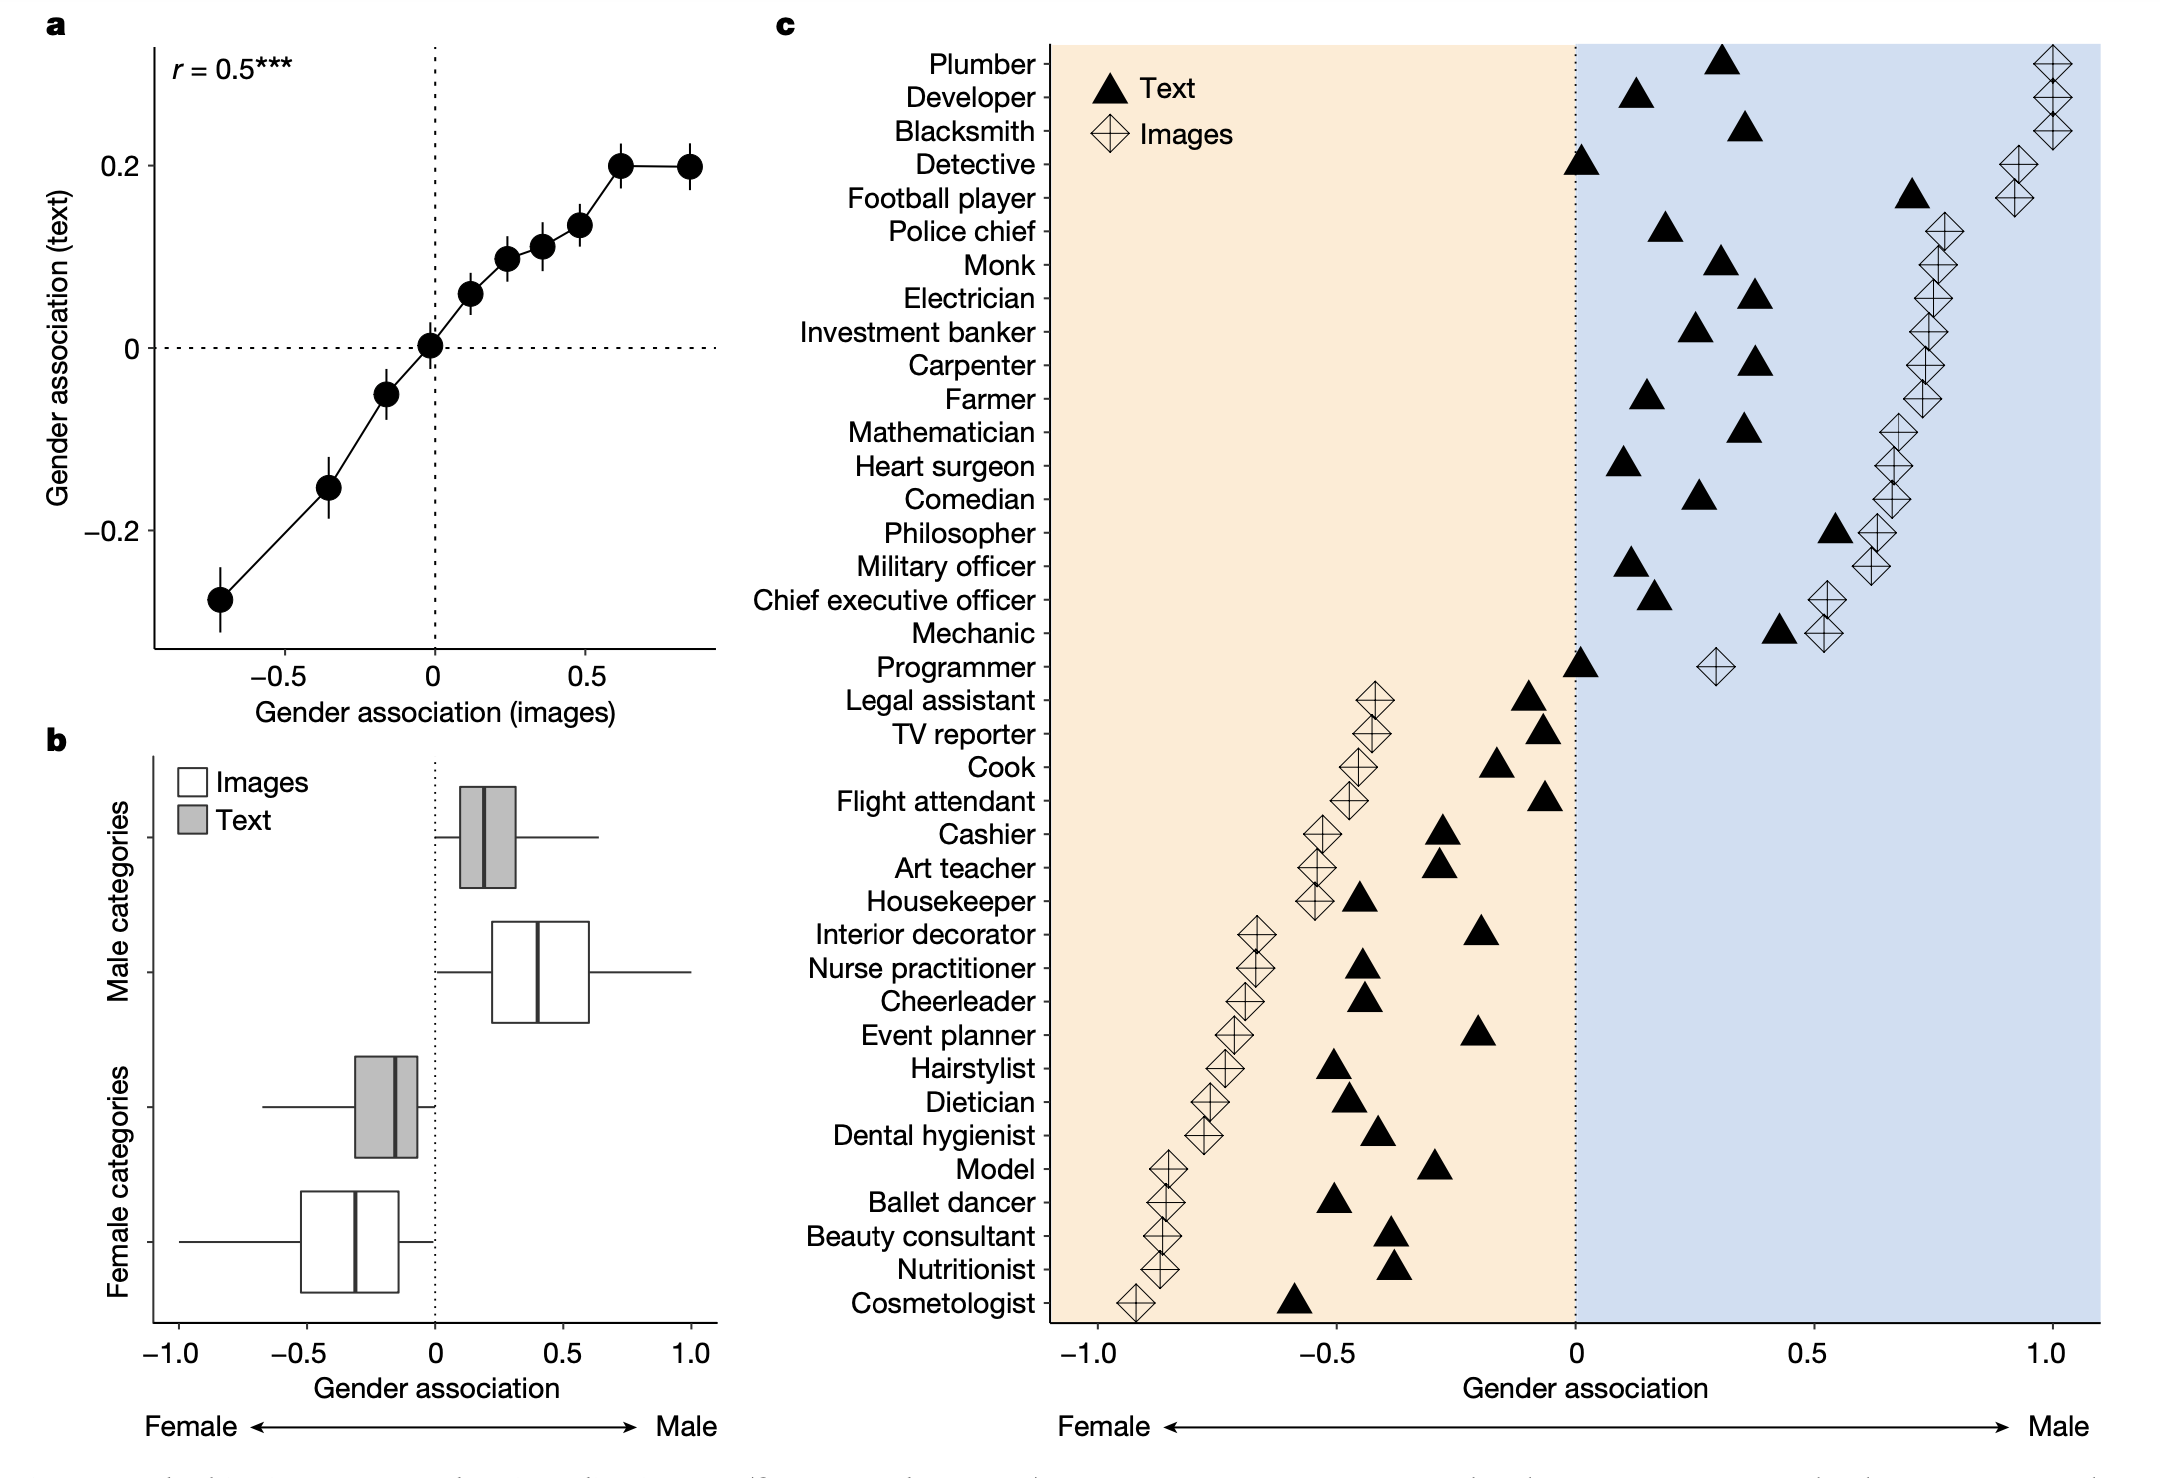
\includegraphics[keepaspectratio]{chapters/eda/../../figures/gender_bias_1.png}}

}

\caption{Il preconcetto di genere è più prevalente nelle immagini online
(da Google Immagini) e nei testi online (da Google News). A. La
correlazione tra le associazioni di genere nelle immagini da Google
Immagini e nei testi da Google News per tutte le categorie sociali (n =
2.986), organizzate per decili. B. La forza dell'associazione di genere
in queste immagini e testi online per tutte le categorie (n = 2.986),
suddivisa in base al fatto che queste categorie siano inclinate verso il
femminile o il maschile. C. Le associazioni di genere per un campione di
occupazioni secondo queste immagini e testi online; questo campione è
stato selezionato manualmente per evidenziare i tipi di categorie
sociali e preconcetti di genere esaminati. (Figura tratta da Guilbeault
et al.~(2024)).}

\end{figure}%

\end{example}

\section{Correlazione di Spearman}\label{correlazione-di-spearman}

Un'alternativa per valutare la relazione lineare tra due variabili è il
coefficiente di correlazione di Spearman, che si basa esclusivamente
sull'ordine dei dati e non sugli specifici valori. Questo indice di
associazione è particolarmente adatto quando gli psicologi sono in grado
di misurare solo le relazioni di ordine tra diverse modalità di risposta
dei soggetti, ma non l'intensità della risposta stessa. Tali variabili
psicologiche che presentano questa caratteristica sono definite come
``ordinali''.

\begin{tcolorbox}[enhanced jigsaw, opacityback=0, bottomrule=.15mm, breakable, title=\textcolor{quarto-callout-note-color}{\faInfo}\hspace{0.5em}{Nota}, bottomtitle=1mm, toptitle=1mm, titlerule=0mm, colbacktitle=quarto-callout-note-color!10!white, rightrule=.15mm, colframe=quarto-callout-note-color-frame, colback=white, arc=.35mm, leftrule=.75mm, coltitle=black, left=2mm, toprule=.15mm, opacitybacktitle=0.6]

È importante ricordare che, nel caso di una variabile ordinale, non è
possibile utilizzare le statistiche descrittive convenzionali come la
media e la varianza per sintetizzare le osservazioni. Tuttavia, è
possibile riassumere le osservazioni attraverso una distribuzione di
frequenze delle diverse modalità di risposta. Come abbiamo appena visto,
la direzione e l'intensità dell'associazione tra due variabili ordinali
possono essere descritte utilizzando il coefficiente di correlazione di
Spearman.

\end{tcolorbox}

Per fornire un esempio, consideriamo due variabili di scala ordinale e
calcoliamo la correlazione di Spearman tra di esse.

\begin{Shaded}
\begin{Highlighting}[]
\FunctionTok{cor.test}\NormalTok{(}\FunctionTok{c}\NormalTok{(}\DecValTok{1}\NormalTok{, }\DecValTok{2}\NormalTok{, }\DecValTok{3}\NormalTok{, }\DecValTok{4}\NormalTok{, }\DecValTok{5}\NormalTok{), }\FunctionTok{c}\NormalTok{(}\DecValTok{5}\NormalTok{, }\DecValTok{6}\NormalTok{, }\DecValTok{7}\NormalTok{, }\DecValTok{8}\NormalTok{, }\DecValTok{7}\NormalTok{), }\AttributeTok{method =} \StringTok{"spearman"}\NormalTok{)}
\CommentTok{\#\textgreater{} }
\CommentTok{\#\textgreater{}  Spearman\textquotesingle{}s rank correlation rho}
\CommentTok{\#\textgreater{} }
\CommentTok{\#\textgreater{} data:  c(1, 2, 3, 4, 5) and c(5, 6, 7, 8, 7)}
\CommentTok{\#\textgreater{} S = 3.6, p{-}value = 0.09}
\CommentTok{\#\textgreater{} alternative hypothesis: true rho is not equal to 0}
\CommentTok{\#\textgreater{} sample estimates:}
\CommentTok{\#\textgreater{}    rho }
\CommentTok{\#\textgreater{} 0.8208}
\end{Highlighting}
\end{Shaded}

\section{Oltre la correlazione e la covarianza: quando l'associazione
tra variabili è più
complessa}\label{oltre-la-correlazione-e-la-covarianza-quando-lassociazione-tra-variabili-uxe8-piuxf9-complessa}

In questo capitolo abbiamo introdotto due misure fondamentali per
descrivere la relazione tra due variabili: \textbf{covarianza} e
\textbf{correlazione}. La covarianza fornisce un'indicazione del modo in
cui due variabili si discostano congiuntamente dalle proprie medie,
mentre la correlazione ne standardizza i valori, permettendo un
confronto più immediato tra diverse coppie di variabili e garantendo un
indice compreso tra -1 e +1. Una correlazione vicina a +1 indica una
forte relazione lineare positiva, vicina a -1 una forte relazione
lineare negativa, mentre un valore vicino a 0 segnala l'assenza di una
chiara relazione lineare.

Tuttavia, è cruciale comprendere che la correlazione descrive
esclusivamente \textbf{la dimensione lineare} della relazione tra due
variabili. Questo significa che una correlazione nulla (pari a zero) non
implica affatto che non vi sia alcuna relazione tra le variabili, ma
semplicemente che non esiste una relazione lineare. Possono esistere
relazioni non lineari anche molto forti, non catturate da questo indice.
Inoltre, altre situazioni possono trarre in inganno, come nei casi in
cui i dati siano raggruppati in sottogruppi con proprietà differenti o
siano frutto di particolari processi di selezione.

\subsection{Correlazione nulla e relazioni non
lineari}\label{correlazione-nulla-e-relazioni-non-lineari}

Una correlazione pari a zero può nascondere relazioni non lineari anche
molto marcate. Per esempio, se una variabile Y aumenta solo quando X è
molto alta o molto bassa, ma rimane costante per valori intermedi di X,
questa curva a ``U'' può generare una correlazione vicina allo zero, pur
esistendo un forte legame non lineare.

Un esempio illustrativo è fornito dal cosiddetto \textbf{Datasaurus
Dozen}, un insieme di tredici dataset con la stessa media, deviazione
standard e correlazione tra le variabili, ma con distribuzioni
visivamente e strutturalmente molto diverse. In ognuno di questi dataset
la correlazione di Pearson è pari a zero, ma l'ispezione grafica rivela
pattern e forme ben definite. Questo ci ricorda che è sempre bene
accompagnare le misure numeriche con una visualizzazione grafica dei
dati.

\begin{Shaded}
\begin{Highlighting}[]
\NormalTok{datasaurus\_data }\OtherTok{\textless{}{-}} \FunctionTok{read.csv}\NormalTok{(}\StringTok{"../../data/datasaurus.csv"}\NormalTok{)}

\NormalTok{datasaurus\_summary }\OtherTok{\textless{}{-}}\NormalTok{ datasaurus\_data }\SpecialCharTok{\%\textgreater{}\%}
  \FunctionTok{group\_by}\NormalTok{(dataset) }\SpecialCharTok{\%\textgreater{}\%}
  \FunctionTok{summarise}\NormalTok{(}
    \AttributeTok{x\_count =} \FunctionTok{n}\NormalTok{(),}
    \AttributeTok{x\_mean =} \FunctionTok{mean}\NormalTok{(x, }\AttributeTok{na.rm =} \ConstantTok{TRUE}\NormalTok{),}
    \AttributeTok{x\_std =} \FunctionTok{sd}\NormalTok{(x, }\AttributeTok{na.rm =} \ConstantTok{TRUE}\NormalTok{),}
    \AttributeTok{y\_count =} \FunctionTok{n}\NormalTok{(),}
    \AttributeTok{y\_mean =} \FunctionTok{mean}\NormalTok{(y, }\AttributeTok{na.rm =} \ConstantTok{TRUE}\NormalTok{),}
    \AttributeTok{y\_std =} \FunctionTok{sd}\NormalTok{(y, }\AttributeTok{na.rm =} \ConstantTok{TRUE}\NormalTok{)}
\NormalTok{  )}

\NormalTok{datasaurus\_summary}
\CommentTok{\#\textgreater{} \# A tibble: 13 x 7}
\CommentTok{\#\textgreater{}    dataset    x\_count x\_mean x\_std y\_count y\_mean y\_std}
\CommentTok{\#\textgreater{}    \textless{}chr\textgreater{}        \textless{}int\textgreater{}  \textless{}dbl\textgreater{} \textless{}dbl\textgreater{}   \textless{}int\textgreater{}  \textless{}dbl\textgreater{} \textless{}dbl\textgreater{}}
\CommentTok{\#\textgreater{}  1 away           142   54.3  16.8     142   47.8  26.9}
\CommentTok{\#\textgreater{}  2 bullseye       142   54.3  16.8     142   47.8  26.9}
\CommentTok{\#\textgreater{}  3 circle         142   54.3  16.8     142   47.8  26.9}
\CommentTok{\#\textgreater{}  4 dino           142   54.3  16.8     142   47.8  26.9}
\CommentTok{\#\textgreater{}  5 dots           142   54.3  16.8     142   47.8  26.9}
\CommentTok{\#\textgreater{}  6 h\_lines        142   54.3  16.8     142   47.8  26.9}
\CommentTok{\#\textgreater{}  7 high\_lines     142   54.3  16.8     142   47.8  26.9}
\CommentTok{\#\textgreater{}  8 slant\_down     142   54.3  16.8     142   47.8  26.9}
\CommentTok{\#\textgreater{}  9 slant\_up       142   54.3  16.8     142   47.8  26.9}
\CommentTok{\#\textgreater{} 10 star           142   54.3  16.8     142   47.8  26.9}
\CommentTok{\#\textgreater{} 11 v\_lines        142   54.3  16.8     142   47.8  26.9}
\CommentTok{\#\textgreater{} 12 wide\_lines     142   54.3  16.8     142   47.8  26.9}
\CommentTok{\#\textgreater{} 13 x\_shape        142   54.3  16.8     142   47.8  26.9}
\end{Highlighting}
\end{Shaded}

\begin{Shaded}
\begin{Highlighting}[]
\NormalTok{datasaurus\_data }\SpecialCharTok{|\textgreater{}}
  \FunctionTok{ggplot}\NormalTok{(}\FunctionTok{aes}\NormalTok{(}\AttributeTok{x =}\NormalTok{ x, }\AttributeTok{y =}\NormalTok{ y)) }\SpecialCharTok{+}
  \FunctionTok{geom\_point}\NormalTok{(}\AttributeTok{alpha =} \FloatTok{0.7}\NormalTok{) }\SpecialCharTok{+}
  \FunctionTok{facet\_wrap}\NormalTok{(}\SpecialCharTok{\textasciitilde{}}\NormalTok{dataset, }\AttributeTok{nrow =} \DecValTok{4}\NormalTok{, }\AttributeTok{ncol =} \DecValTok{4}\NormalTok{) }\SpecialCharTok{+}
  \FunctionTok{labs}\NormalTok{(}\AttributeTok{x =} \ConstantTok{NULL}\NormalTok{, }\AttributeTok{y =} \ConstantTok{NULL}\NormalTok{)}
\end{Highlighting}
\end{Shaded}

\begin{center}
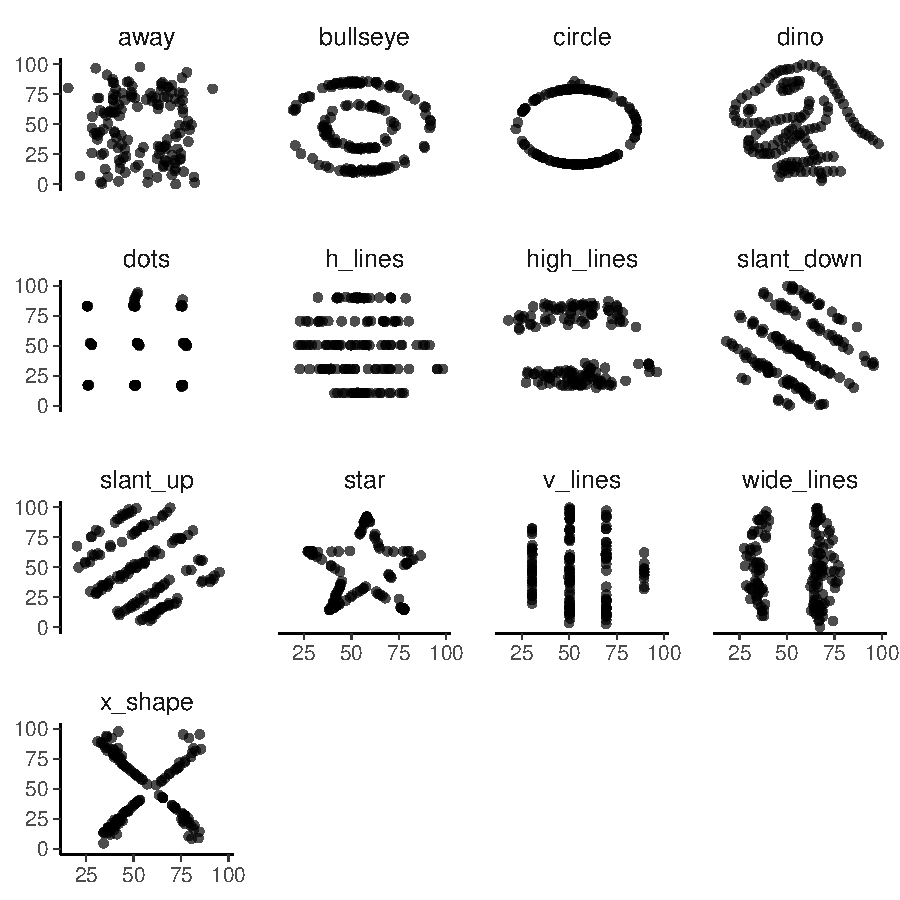
\includegraphics[width=0.7\linewidth,height=\textheight,keepaspectratio]{chapters/eda/08_correlation_files/figure-pdf/unnamed-chunk-13-1.pdf}
\end{center}

Tutti questi esempi rafforzano l'idea che l'assenza di correlazione
lineare non significa assenza di relazione: potremmo avere strutture
curve, pattern complessi o punti anomali (outlier) capaci di modificare
radicalmente la forma della relazione tra le variabili.

Oltre alle relazioni non lineari, esistono situazioni in cui la
correlazione, da sola, può fornire un'immagine distorta dei dati. Tra
queste ricordiamo due fenomeni noti come il \textbf{paradosso di
Simpson} e il \textbf{paradosso di Berkson}.

\subsection{Paradosso di Simpson}\label{paradosso-di-simpson}

Il paradosso di Simpson si verifica quando, guardando i dati raggruppati
per sottogruppi, si osserva una certa relazione tra due variabili, ma
aggregando i dati di tutti i sottogruppi insieme emerge una relazione
opposta. In altre parole, la tendenza che appare quando si considerano i
dati divisi per gruppi scompare o si inverte quando si esamina l'intero
campione senza tenere conto della suddivisione in sottogruppi.

Immaginiamo di avere due dipartimenti universitari, A e B. All'interno
di ciascun dipartimento, la relazione tra il voto di laurea (X) e la
performance in un successivo programma di specializzazione (Y) è
positiva: all'aumentare del voto di laurea aumenta, in media, la
performance nella scuola di specializzazione.

Tuttavia, supponiamo che il Dipartimento A abbia in generale voti di
laurea mediamente più bassi, ma ottime performance nella
specializzazione; mentre il Dipartimento B abbia voti di laurea
mediamente più alti, ma performance alla specializzazione un po' più
basse. Se uniamo tutti gli studenti dei due dipartimenti senza
considerarne l'appartenenza, potremmo osservare una relazione negativa
tra voto di laurea e performance, sovvertendo le conclusioni tratte
guardando ai singoli sottogruppi.

Ecco come possiamo simulare questi dati in R:

\begin{Shaded}
\begin{Highlighting}[]
\FunctionTok{set.seed}\NormalTok{(}\DecValTok{123}\NormalTok{)}

\CommentTok{\# Numero di osservazioni per dipartimento}
\NormalTok{n }\OtherTok{\textless{}{-}} \DecValTok{100}

\CommentTok{\# Dipartimento A:}
\CommentTok{\# Voti di laurea (X) più bassi, ma performance (Y) più alta.}
\CommentTok{\# Creiamo un legame positivo tra X e Y all\textquotesingle{}interno di A.}
\NormalTok{X\_A }\OtherTok{\textless{}{-}} \FunctionTok{rnorm}\NormalTok{(n, }\AttributeTok{mean =} \DecValTok{50}\NormalTok{, }\AttributeTok{sd =} \DecValTok{5}\NormalTok{)    }\CommentTok{\# Voti laurea mediamente più bassi}
\NormalTok{Y\_A }\OtherTok{\textless{}{-}}\NormalTok{ X\_A }\SpecialCharTok{+} \FunctionTok{rnorm}\NormalTok{(n, }\AttributeTok{mean =} \DecValTok{20}\NormalTok{, }\AttributeTok{sd =} \DecValTok{5}\NormalTok{) }\CommentTok{\# Performance alta e correlata positivamente con X}

\CommentTok{\# Dipartimento B:}
\CommentTok{\# Voti di laurea (X) più alti, ma performance (Y) più bassa.}
\CommentTok{\# Anche qui creiamo un legame positivo tra X e Y all\textquotesingle{}interno di B, }
\CommentTok{\# ma con un offset tale che globalmente i voti alti coincidano con performance minori.}
\NormalTok{X\_B }\OtherTok{\textless{}{-}} \FunctionTok{rnorm}\NormalTok{(n, }\AttributeTok{mean =} \DecValTok{60}\NormalTok{, }\AttributeTok{sd =} \DecValTok{5}\NormalTok{)    }\CommentTok{\# Voti laurea mediamente più alti}
\NormalTok{Y\_B }\OtherTok{\textless{}{-}}\NormalTok{ X\_B }\SpecialCharTok{{-}} \FunctionTok{rnorm}\NormalTok{(n, }\AttributeTok{mean =} \DecValTok{10}\NormalTok{, }\AttributeTok{sd =} \DecValTok{5}\NormalTok{) }\CommentTok{\# Performance più bassa ma comunque correlata positivamente con X all’interno di B}

\CommentTok{\# Creiamo un dataframe con tutti i dati}
\NormalTok{dipartimento }\OtherTok{\textless{}{-}} \FunctionTok{c}\NormalTok{(}\FunctionTok{rep}\NormalTok{(}\StringTok{"A"}\NormalTok{, n), }\FunctionTok{rep}\NormalTok{(}\StringTok{"B"}\NormalTok{, n))}
\NormalTok{X }\OtherTok{\textless{}{-}} \FunctionTok{c}\NormalTok{(X\_A, X\_B)}
\NormalTok{Y }\OtherTok{\textless{}{-}} \FunctionTok{c}\NormalTok{(Y\_A, Y\_B)}
\NormalTok{dati }\OtherTok{\textless{}{-}} \FunctionTok{data.frame}\NormalTok{(dipartimento, X, Y)}

\CommentTok{\# Correlazioni all\textquotesingle{}interno dei dipartimenti}
\FunctionTok{cat}\NormalTok{(}\StringTok{"Correlazione nel Dipartimento A:"}\NormalTok{, }\FunctionTok{cor}\NormalTok{(X\_A, Y\_A), }\StringTok{"}\SpecialCharTok{\textbackslash{}n}\StringTok{"}\NormalTok{)}
\CommentTok{\#\textgreater{} Correlazione nel Dipartimento A: 0.6671}
\FunctionTok{cat}\NormalTok{(}\StringTok{"Correlazione nel Dipartimento B:"}\NormalTok{, }\FunctionTok{cor}\NormalTok{(X\_B, Y\_B), }\StringTok{"}\SpecialCharTok{\textbackslash{}n}\StringTok{"}\NormalTok{)}
\CommentTok{\#\textgreater{} Correlazione nel Dipartimento B: 0.6926}

\CommentTok{\# Correlazione sull\textquotesingle{}intero dataset (senza distinguere i dipartimenti)}
\FunctionTok{cat}\NormalTok{(}\StringTok{"Correlazione globale:"}\NormalTok{, }\FunctionTok{cor}\NormalTok{(X, Y), }\StringTok{"}\SpecialCharTok{\textbackslash{}n}\StringTok{"}\NormalTok{)}
\CommentTok{\#\textgreater{} Correlazione globale: {-}0.3353}
\end{Highlighting}
\end{Shaded}

\begin{Shaded}
\begin{Highlighting}[]
\CommentTok{\# Visualizziamo i dati}
\FunctionTok{ggplot}\NormalTok{(dati, }\FunctionTok{aes}\NormalTok{(}\AttributeTok{x =}\NormalTok{ X, }\AttributeTok{y =}\NormalTok{ Y, }\AttributeTok{color =}\NormalTok{ dipartimento)) }\SpecialCharTok{+}
  \FunctionTok{geom\_point}\NormalTok{() }\SpecialCharTok{+}
  \FunctionTok{geom\_smooth}\NormalTok{(}\AttributeTok{method =} \StringTok{"lm"}\NormalTok{, }\AttributeTok{se =} \ConstantTok{FALSE}\NormalTok{) }\SpecialCharTok{+}
  \FunctionTok{scale\_fill\_okabeito}\NormalTok{() }\SpecialCharTok{+} 
  \FunctionTok{labs}\NormalTok{(}
    \AttributeTok{title =} \StringTok{"Paradosso di Simpson"}\NormalTok{,}
    \AttributeTok{x =} \StringTok{"Voto di laurea"}\NormalTok{, }
    \AttributeTok{y =} \StringTok{"Performance nella specializzazione"}\NormalTok{,}
    \AttributeTok{color =} \StringTok{"Dipartimento"}
\NormalTok{  )}
\end{Highlighting}
\end{Shaded}

\begin{center}
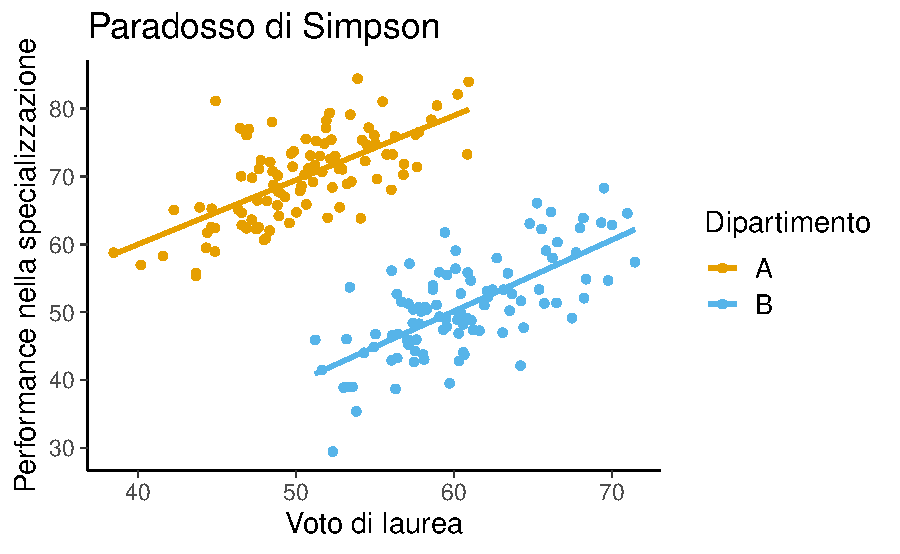
\includegraphics[width=0.7\linewidth,height=\textheight,keepaspectratio]{chapters/eda/08_correlation_files/figure-pdf/unnamed-chunk-15-1.pdf}
\end{center}

\begin{itemize}
\item
  \textbf{All'interno del Dipartimento A}: la correlazione tra voto di
  laurea (X) e performance (Y) è positiva. Ciò significa che, per gli
  studenti di A, avere un voto di laurea più alto è associato a una
  performance maggiore nella specializzazione.
\item
  \textbf{All'interno del Dipartimento B}: la correlazione tra X e Y è
  anch'essa positiva, indicando che anche nel secondo dipartimento voti
  più alti tendono ad accompagnarsi a performance più alte.
\item
  \textbf{Considerando entrambi i dipartimenti insieme}: a causa delle
  differenze nei livelli medi di X e Y tra i dipartimenti, unendo i dati
  senza distinguere il gruppo di appartenenza otteniamo una correlazione
  globale negativa. Questo significa che, ignorando la suddivisione in
  dipartimenti, sembra che aumentare il voto di laurea sia associato a
  una diminuzione della performance nella specializzazione --- una
  conclusione opposta a quella tratta dall'analisi separata dei due
  sottogruppi.
\end{itemize}

Questo è un esempio concreto del paradosso di Simpson: la relazione
osservata in sottogruppi omogenei si inverte quando si aggregano i dati,
mettendo in guardia sulla necessità di considerare con attenzione la
struttura dei dati e i fattori confondenti prima di trarre conclusioni.

\subsection{Paradosso di Berkson}\label{paradosso-di-berkson}

Il paradosso di Berkson è un fenomeno legato alla selezione del
campione. Se il dataset non è rappresentativo della popolazione
generale, la relazione osservata può risultare artificiale o opposta a
quella esistente su un campione più ampio. Per esempio, analizzando solo
ciclisti professionisti, potremmo non vedere alcuna relazione tra VO2
max e probabilità di vincere una gara, poiché tutti hanno già superato
una certa soglia di VO2 max. Considerando la popolazione generale,
invece, potrebbe emergere chiaramente una relazione positiva tra questi
due fattori. Questo paradosso evidenzia l'importanza di considerare il
processo di selezione dei dati e di chiedersi se il campione analizzato
sia adeguato a rispondere alla domanda di ricerca.

\subsection{Limiti delle statistiche riassuntive
semplici}\label{limiti-delle-statistiche-riassuntive-semplici}

Un esempio particolarmente famoso che dimostra i limiti delle semplici
statistiche descrittive --- come media, deviazione standard e
correlazione --- è il quartetto di Anscombe. Questo insieme di quattro
piccoli dataset possiede identiche medie, varianze e correlazioni tra
variabili, ma rappresenta relazioni estremamente differenti tra X e Y
(\citeproc{ref-anscombe1973graphs}{Anscombe, 1973}).

Importiamo il dataset \texttt{anscombe} già disponibile nel pacchetto
\texttt{datasets} di R:

\begin{Shaded}
\begin{Highlighting}[]
\FunctionTok{data}\NormalTok{(}\StringTok{"anscombe"}\NormalTok{)}

\NormalTok{anscombe }\SpecialCharTok{|\textgreater{}} 
  \FunctionTok{head}\NormalTok{()}
\CommentTok{\#\textgreater{}   x1 x2 x3 x4   y1   y2    y3   y4}
\CommentTok{\#\textgreater{} 1 10 10 10  8 8.04 9.14  7.46 6.58}
\CommentTok{\#\textgreater{} 2  8  8  8  8 6.95 8.14  6.77 5.76}
\CommentTok{\#\textgreater{} 3 13 13 13  8 7.58 8.74 12.74 7.71}
\CommentTok{\#\textgreater{} 4  9  9  9  8 8.81 8.77  7.11 8.84}
\CommentTok{\#\textgreater{} 5 11 11 11  8 8.33 9.26  7.81 8.47}
\CommentTok{\#\textgreater{} 6 14 14 14  8 9.96 8.10  8.84 7.04}
\end{Highlighting}
\end{Shaded}

Il dataset \texttt{anscombe} contiene quattro serie di dati (x1, y1),
(x2, y2), (x3, y3) e (x4, y4), ognuna costituita da 11 coppie di valori
(x, y). Per comprendere meglio le loro caratteristiche, iniziamo
calcolando alcune statistiche descrittive. La funzione \texttt{apply()}
consente di applicare una funzione (ad esempio, \texttt{mean}) a tutte
le colonne di un data frame. Usandola sulle colonne di
\texttt{anscombe}, otteniamo le medie di ciascuna delle otto variabili
(le quattro x e le quattro y):

\begin{Shaded}
\begin{Highlighting}[]
\FunctionTok{apply}\NormalTok{(anscombe, }\AttributeTok{MARGIN =} \DecValTok{2}\NormalTok{, mean)}
\CommentTok{\#\textgreater{}    x1    x2    x3    x4    y1    y2    y3    y4 }
\CommentTok{\#\textgreater{} 9.000 9.000 9.000 9.000 7.501 7.501 7.500 7.501}
\end{Highlighting}
\end{Shaded}

Osserviamo che le medie delle quattro variabili x sono identiche fino a
sei cifre decimali, e le medie delle quattro variabili y differiscono
solo in modo trascurabile (circa lo 0.01\%). Analogamente, se calcoliamo
le deviazioni standard per ciascuna variabile, notiamo una notevole
somiglianza:

\begin{Shaded}
\begin{Highlighting}[]
\FunctionTok{apply}\NormalTok{(anscombe, }\AttributeTok{MARGIN =} \DecValTok{2}\NormalTok{, sd)}
\CommentTok{\#\textgreater{}    x1    x2    x3    x4    y1    y2    y3    y4 }
\CommentTok{\#\textgreater{} 3.317 3.317 3.317 3.317 2.032 2.032 2.030 2.031}
\end{Highlighting}
\end{Shaded}

Anche in questo caso, le deviazioni standard per le x coincidono fino
alla sesta cifra decimale, mentre quelle delle y differiscono di meno
dello 0.06\%. Inoltre, se calcoliamo i coefficienti di correlazione tra
x e y in ognuno dei quattro dataset, scopriamo che sono quasi identici:

\begin{Shaded}
\begin{Highlighting}[]
\CommentTok{\# Calcoliamo la correlazione per ciascuna coppia (x1,y1), (x2,y2), (x3,y3), (x4,y4)}
\ControlFlowTok{for}\NormalTok{ (i }\ControlFlowTok{in} \DecValTok{1}\SpecialCharTok{:}\DecValTok{4}\NormalTok{) \{}
\NormalTok{  x\_var }\OtherTok{\textless{}{-}}\NormalTok{ anscombe[[}\FunctionTok{paste0}\NormalTok{(}\StringTok{"x"}\NormalTok{, i)]]}
\NormalTok{  y\_var }\OtherTok{\textless{}{-}}\NormalTok{ anscombe[[}\FunctionTok{paste0}\NormalTok{(}\StringTok{"y"}\NormalTok{, i)]]}
  
\NormalTok{  corr\_value }\OtherTok{\textless{}{-}} \FunctionTok{cor}\NormalTok{(x\_var, y\_var)}
  \FunctionTok{cat}\NormalTok{(}\StringTok{"Correlazione tra x"}\NormalTok{, i, }\StringTok{"e y"}\NormalTok{, i, }\StringTok{":"}\NormalTok{, corr\_value, }\StringTok{"}\SpecialCharTok{\textbackslash{}n}\StringTok{"}\NormalTok{)}
\NormalTok{\}}
\CommentTok{\#\textgreater{} Correlazione tra x 1 e y 1 : 0.8164 }
\CommentTok{\#\textgreater{} Correlazione tra x 2 e y 2 : 0.8162 }
\CommentTok{\#\textgreater{} Correlazione tra x 3 e y 3 : 0.8163 }
\CommentTok{\#\textgreater{} Correlazione tra x 4 e y 4 : 0.8165}
\end{Highlighting}
\end{Shaded}

Se ci limitassimo a guardare queste statistiche (media, deviazione
standard, correlazione), potremmo facilmente essere indotti a concludere
che i quattro dataset sono tra loro sostanzialmente indistinguibili.
Tuttavia, la realtà è molto diversa. Le statistiche descrittive, prese
da sole, non offrono una visione completa e possono nascondere
importanti differenze nella struttura dei dati.

Questa differenza diventa evidente non appena decidiamo di visualizzare
i dati. La rappresentazione grafica fornisce informazioni che non
emergono dalle sole statistiche riassuntive:

\begin{Shaded}
\begin{Highlighting}[]
\NormalTok{anscombe\_m }\OtherTok{\textless{}{-}} \FunctionTok{tibble}\NormalTok{()}

\ControlFlowTok{for}\NormalTok{ (i }\ControlFlowTok{in} \DecValTok{1}\SpecialCharTok{:}\DecValTok{4}\NormalTok{) \{}
\NormalTok{  anscombe\_m }\OtherTok{\textless{}{-}} \FunctionTok{rbind}\NormalTok{(}
\NormalTok{    anscombe\_m, }\FunctionTok{tibble}\NormalTok{(}\AttributeTok{set =}\NormalTok{ i, }\AttributeTok{x =}\NormalTok{ anscombe[, i], }\AttributeTok{y =}\NormalTok{ anscombe[, i }\SpecialCharTok{+} \DecValTok{4}\NormalTok{])}
\NormalTok{  )}
\NormalTok{\}}

\FunctionTok{ggplot}\NormalTok{(anscombe\_m, }\FunctionTok{aes}\NormalTok{(x, y)) }\SpecialCharTok{+}
  \FunctionTok{geom\_point}\NormalTok{(}\AttributeTok{size =} \DecValTok{3}\NormalTok{, }\AttributeTok{color =} \StringTok{"red"}\NormalTok{, }\AttributeTok{fill =} \StringTok{"orange"}\NormalTok{, }\AttributeTok{shape =} \DecValTok{21}\NormalTok{) }\SpecialCharTok{+}
  \FunctionTok{geom\_smooth}\NormalTok{(}\AttributeTok{method =} \StringTok{"lm"}\NormalTok{, }\AttributeTok{fill =} \ConstantTok{NA}\NormalTok{, }\AttributeTok{fullrange =} \ConstantTok{TRUE}\NormalTok{) }\SpecialCharTok{+}
  \FunctionTok{facet\_wrap}\NormalTok{(}\SpecialCharTok{\textasciitilde{}}\NormalTok{set, }\AttributeTok{ncol =} \DecValTok{2}\NormalTok{)}
\end{Highlighting}
\end{Shaded}

\begin{center}
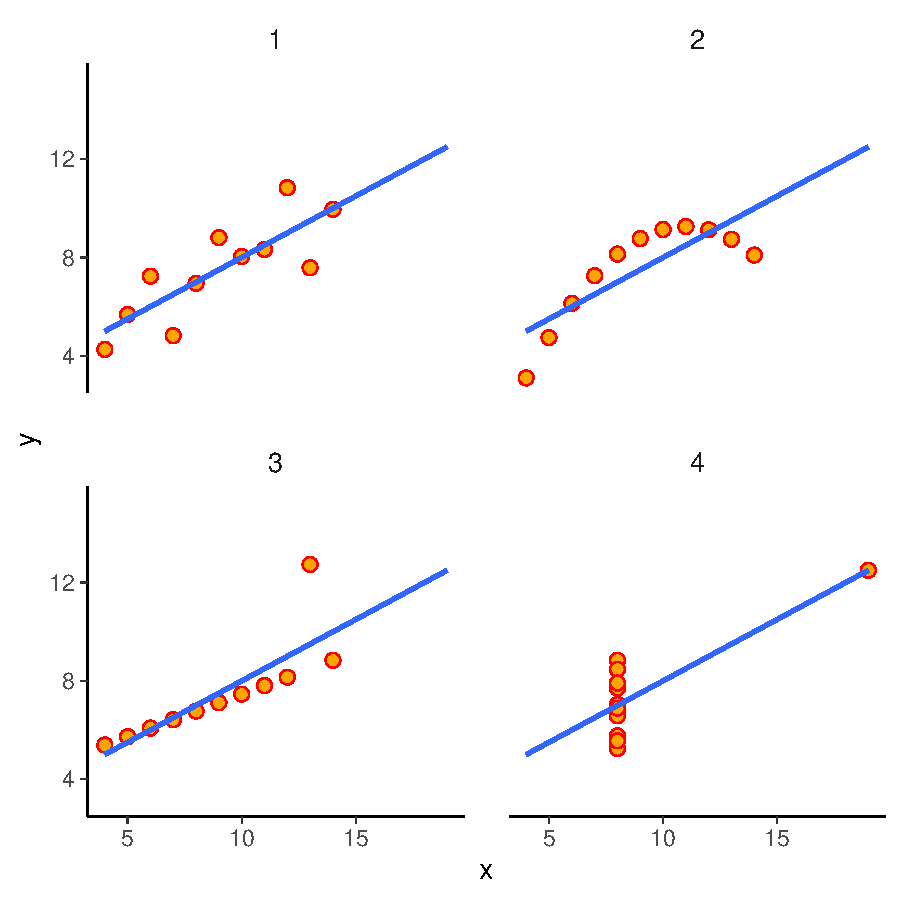
\includegraphics[width=0.7\linewidth,height=\textheight,keepaspectratio]{chapters/eda/08_correlation_files/figure-pdf/unnamed-chunk-20-1.pdf}
\end{center}

Osservando i grafici, notiamo subito che i quattro dataset sono
profondamente diversi:

\begin{itemize}
\tightlist
\item
  \textbf{Dataset 1:} Qui la relazione tra x e y è approssimativamente
  lineare, e la correlazione riflette in modo appropriato il legame tra
  le due variabili.
\item
  \textbf{Dataset 2:} Sebbene la correlazione sia simile a quella del
  Dataset 1, i dati mostrano una relazione curvilinea e non lineare. La
  semplice correlazione lineare non ne cattura la forma.
\item
  \textbf{Dataset 3:} La presenza di un singolo outlier distorce la
  percezione della relazione tra le variabili, altrimenti lineare. La
  correlazione alta è influenzata in modo sproporzionato da questo punto
  anomalo.
\item
  \textbf{Dataset 4:} Qui i dati non mostrano alcuna relazione lineare.
  La correlazione elevata è il frutto di un pattern fortemente atipico
  (ad esempio, una sola coppia di punti allineata).
\end{itemize}

Il quartetto di Anscombe mette in luce un principio fondamentale:
statistiche descrittive come media, deviazione standard e correlazione
non sono sempre sufficienti per comprendere la natura dei dati. La
visualizzazione grafica è essenziale per cogliere relazioni, pattern non
lineari, outlier e altre caratteristiche che le semplici statistiche non
riescono a rivelare. In definitiva, questo esempio dimostra che
analizzare i dati soltanto attraverso poche statistiche di sintesi può
portare a conclusioni fuorvianti, mentre l'integrazione con la
rappresentazione grafica fornisce una visione più completa e accurata.

\section{Riflessioni Conclusive}\label{riflessioni-conclusive-14}

La covarianza e la correlazione sono strumenti preziosi per capire
l'intensità e la direzione lineare di una relazione tra due variabili.
Tuttavia, non dobbiamo confondere la loro semplicità con completezza
d'informazione. Una correlazione nulla non implica assenza di relazione,
ma solo assenza di una relazione lineare. Inoltre, il paradosso di
Simpson e il paradosso di Berkson dimostrano che la semplice
osservazione di correlazioni può essere fuorviante se non si tiene conto
della struttura dei dati o del processo di selezione del campione.

Infine, esempi come il quartetto di Anscombe sottolineano quanto sia
fondamentale accompagnare le statistiche riassuntive con analisi
grafiche e un'attenzione costante ai possibili pattern non lineari, agli
outlier e alle caratteristiche peculiari del dataset. Nel prossimo
capitolo esamineremo approcci che consentono di avvicinarsi alla
comprensione causale dei fenomeni, andando oltre la semplice
osservazione dell'associazione tra variabili.

\section{Esercizi}\label{esercizi-16}

\begin{tcolorbox}[enhanced jigsaw, opacityback=0, bottomrule=.15mm, breakable, title=\textcolor{quarto-callout-tip-color}{\faLightbulb}\hspace{0.5em}{Esercizio}, bottomtitle=1mm, toptitle=1mm, titlerule=0mm, colbacktitle=quarto-callout-tip-color!10!white, rightrule=.15mm, colframe=quarto-callout-tip-color-frame, colback=white, arc=.35mm, leftrule=.75mm, coltitle=black, left=2mm, toprule=.15mm, opacitybacktitle=0.6]

\textbf{Esercizi Teorici}

\begin{enumerate}
\def\labelenumi{\arabic{enumi}.}
\item
  \textbf{Definizioni fondamentali}

  \begin{itemize}
  \tightlist
  \item
    Qual è la differenza tra \textbf{associazione, correlazione e
    dipendenza}?\\
  \item
    Perché la \textbf{correlazione non implica causalità}? Fai un
    esempio.\\
  \item
    In quali situazioni la correlazione di \textbf{Spearman} è
    preferibile rispetto alla correlazione di \textbf{Pearson}?
  \end{itemize}
\item
  \textbf{Interpretazione della correlazione}

  \begin{itemize}
  \tightlist
  \item
    Qual è il range dei valori che può assumere la correlazione di
    Pearson?\\
  \item
    Se il coefficiente di correlazione tra due variabili è
    \textbf{0.85}, come interpreteresti la loro relazione?\\
  \item
    Se il coefficiente di correlazione è \textbf{-0.60}, che tipo di
    relazione esiste tra le due variabili?\\
  \item
    Quali fattori potrebbero influenzare il valore della correlazione?
  \end{itemize}
\item
  \textbf{Covarianza vs Correlazione}

  \begin{itemize}
  \tightlist
  \item
    Qual è la differenza tra \textbf{covarianza} e
    \textbf{correlazione}?\\
  \item
    Perché la covarianza non è sempre interpretabile come misura della
    forza della relazione tra due variabili?\\
  \item
    Quali sono i vantaggi di usare la correlazione al posto della
    covarianza?
  \end{itemize}
\item
  \textbf{Grafico a dispersione e correlazione}

  \begin{itemize}
  \tightlist
  \item
    Osservando un \textbf{grafico a dispersione}, quali caratteristiche
    ti permettono di identificare una relazione lineare positiva o
    negativa?\\
  \item
    Disegna (o descrivi verbalmente) un esempio di un dataset con una
    correlazione di \textbf{circa 0}, ma con una chiara relazione non
    lineare tra le variabili.
  \end{itemize}
\end{enumerate}

\textbf{Esercizi Pratici in R}

📌 \textbf{Obiettivo}: Analizzare le relazioni tra \textbf{Satisfaction
With Life Scale (SWLS)} e \textbf{Scala della Rete Sociale di Lubben
(LSNS-6)}, calcolare covarianza e correlazione, e visualizzare i dati
per individuare pattern.

\textbf{Dati disponibili}:

Usa i dati raccolti per le variabili SWLS e LSNS, oltre al genere dei
partecipanti.

\textbf{1. Esplorazione e Visualizzazione della Relazione tra SWLS e
LSNS}

\begin{enumerate}
\def\labelenumi{\arabic{enumi}.}
\tightlist
\item
  \textbf{Carica i dati raccolti dagli studenti} e verifica la struttura
  del dataset.\\
\item
  \textbf{Calcola le statistiche descrittive}: media, deviazione
  standard, minimo, massimo e quartili delle variabili SWLS e LSNS.\\
\item
  \textbf{Crea un grafico a dispersione} tra SWLS e LSNS:

  \begin{itemize}
  \tightlist
  \item
    Colora i punti in base al \textbf{genere} del partecipante.\\
  \item
    Aggiungi una \textbf{linea di regressione} per evidenziare il trend
    della relazione.
  \end{itemize}
\end{enumerate}

\textbf{2. Calcolo della Covarianza e della Correlazione tra SWLS e
LSNS}

\begin{enumerate}
\def\labelenumi{\arabic{enumi}.}
\tightlist
\item
  \textbf{Calcola la covarianza tra SWLS e LSNS} usando la formula
  matematica della covarianza e confrontala con il valore ottenuto con
  \texttt{cov()}.\\
\item
  \textbf{Calcola la correlazione di Pearson} e commenta il risultato:

  \begin{itemize}
  \tightlist
  \item
    La relazione è forte o debole?\\
  \item
    Ha segno positivo o negativo?\\
  \item
    È coerente con quanto osservato nel grafico a dispersione?\\
  \end{itemize}
\item
  \textbf{Calcola la correlazione di Spearman} e confrontala con quella
  di Pearson. Quale delle due è più appropriata per questi dati?
\end{enumerate}

\textbf{3. Analisi delle Associazioni per Gruppi}

\begin{enumerate}
\def\labelenumi{\arabic{enumi}.}
\tightlist
\item
  \textbf{Calcola la correlazione separatamente per i partecipanti di
  genere maschile e femminile.}\\
\item
  \textbf{Confronta i risultati}: la relazione tra SWLS e LSNS è simile
  nei due gruppi o ci sono differenze?\\
\item
  \textbf{Visualizza i dati con due grafici a dispersione distinti} per
  maschi e femmine.
\end{enumerate}

\textbf{4. Correlazione Nulla e Pattern Non Lineari}

\begin{enumerate}
\def\labelenumi{\arabic{enumi}.}
\tightlist
\item
  \textbf{Simula un dataset} in cui la correlazione di Pearson è
  \textbf{vicina a 0}, ma esiste una chiara relazione \textbf{non
  lineare} tra le variabili.\\
\item
  \textbf{Costruisci un grafico a dispersione} per osservare il pattern
  nei dati.\\
\item
  \textbf{Calcola la correlazione di Spearman} e confrontala con quella
  di Pearson. Quale delle due cattura meglio la relazione nei dati?
\end{enumerate}

Consegna il file \texttt{.qmd} compilato in PDF contenente il codice, le
visualizzazioni e le interpretazioni.

\end{tcolorbox}

\begin{tcolorbox}[enhanced jigsaw, opacityback=0, bottomrule=.15mm, breakable, title=\textcolor{quarto-callout-tip-color}{\faLightbulb}\hspace{0.5em}{Soluzione}, bottomtitle=1mm, toptitle=1mm, titlerule=0mm, colbacktitle=quarto-callout-tip-color!10!white, rightrule=.15mm, colframe=quarto-callout-tip-color-frame, colback=white, arc=.35mm, leftrule=.75mm, coltitle=black, left=2mm, toprule=.15mm, opacitybacktitle=0.6]

\textbf{1. Definizioni fondamentali}

1.1 Differenza tra \textbf{associazione, correlazione e dipendenza}:

\begin{itemize}
\tightlist
\item
  \textbf{Associazione}: Indica una relazione generica tra due
  variabili, senza specificare la natura o la direzione della relazione.
\item
  \textbf{Correlazione}: Misura la forza e la direzione di una relazione
  \textbf{lineare} tra due variabili. Può essere positiva (variabili
  aumentano insieme) o negativa (una variabile aumenta mentre l'altra
  diminuisce).
\item
  \textbf{Dipendenza}: Indica che una variabile è influenzata da
  un'altra, ma non implica necessariamente una relazione lineare. La
  dipendenza può essere causale o statistica.
\end{itemize}

1.2 Perché la \textbf{correlazione non implica causalità}:

La correlazione misura solo la relazione lineare tra due variabili, ma
non indica se una variabile causa l'altra. Un esempio classico è la
correlazione tra il consumo di gelati e il numero di annegamenti:
entrambi aumentano in estate, ma non c'è un nesso causale diretto. Un
terzo fattore (il caldo) influenza entrambe le variabili.

1.3 Quando preferire la correlazione di \textbf{Spearman} rispetto a
quella di \textbf{Pearson}:

\begin{itemize}
\tightlist
\item
  Quando i dati non sono distribuiti normalmente.
\item
  Quando ci sono outlier che potrebbero distorcere la correlazione di
  Pearson.
\item
  Quando la relazione tra le variabili è \textbf{monotona} (sempre
  crescente o decrescente) ma non lineare.
\end{itemize}

\textbf{2. Interpretazione della correlazione}

2.1 Range dei valori della correlazione di Pearson:

La correlazione di Pearson assume valori compresi tra \textbf{-1} e
\textbf{1}: - \textbf{1}: Correlazione lineare positiva perfetta. -
\textbf{-1}: Correlazione lineare negativa perfetta. - \textbf{0}:
Nessuna correlazione lineare.

2.2 Interpretazione di un coefficiente di \textbf{0.85}:

Un coefficiente di 0.85 indica una \textbf{forte relazione lineare
positiva} tra le due variabili. All'aumentare di una variabile, l'altra
tende ad aumentare in modo consistente.

2.3 Interpretazione di un coefficiente di \textbf{-0.60}:

Un coefficiente di -0.60 indica una \textbf{relazione lineare negativa
moderata}. All'aumentare di una variabile, l'altra tende a diminuire.

2.4 Fattori che influenzano la correlazione:

\begin{itemize}
\tightlist
\item
  \textbf{Outlier}: Possono distorcere il valore della correlazione.
\item
  \textbf{Distribuzione non lineare}: La correlazione di Pearson non
  cattura relazioni non lineari.
\item
  \textbf{Range ristretto delle variabili}: Se i dati coprono solo una
  piccola parte del range possibile, la correlazione potrebbe essere
  sottostimata.
\end{itemize}

\textbf{3. Covarianza vs Correlazione}

3.1 Differenza tra \textbf{covarianza} e \textbf{correlazione}:

\begin{itemize}
\tightlist
\item
  \textbf{Covarianza}: Misura la direzione della relazione tra due
  variabili, ma il suo valore dipende dalle unità di misura delle
  variabili.
\item
  \textbf{Correlazione}: Standardizza la covarianza, rendendola
  adimensionale e consentendo confronti tra diverse coppie di variabili.
\end{itemize}

3.2 Perché la covarianza non è sempre interpretabile:

La covarianza non è standardizzata, quindi il suo valore non fornisce
informazioni sulla forza della relazione. Ad esempio, una covarianza di
1000 potrebbe indicare una relazione forte o debole, a seconda delle
unità di misura.

3.3 Vantaggi della correlazione rispetto alla covarianza:

\begin{itemize}
\tightlist
\item
  È adimensionale, quindi può essere confrontata tra diverse coppie di
  variabili.
\item
  Assume valori compresi tra -1 e 1, facilitando l'interpretazione della
  forza e della direzione della relazione.
\end{itemize}

\textbf{4. Grafico a dispersione e correlazione}

4.1 Caratteristiche di un grafico a dispersione per identificare
relazioni lineari:

\begin{itemize}
\tightlist
\item
  \textbf{Relazione lineare positiva}: I punti si dispongono lungo una
  linea retta con pendenza positiva.
\item
  \textbf{Relazione lineare negativa}: I punti si dispongono lungo una
  linea retta con pendenza negativa.
\item
  \textbf{Nessuna relazione lineare}: I punti sono sparsi senza un
  pattern evidente.
\end{itemize}

4.2 Esempio di dataset con correlazione circa 0 ma relazione non
lineare:

Immagina un dataset in cui una variabile \(x\) assume valori simmetrici
intorno a 0 (ad esempio, da -5 a 5), e la variabile \(y\) è uguale a
\(x^2\). In questo caso:

\begin{itemize}
\tightlist
\item
  La correlazione di Pearson sarà \textbf{circa 0}, perché non c'è una
  relazione lineare.
\item
  Tuttavia, esiste una chiara relazione \textbf{non lineare}
  (quadratica) tra \(x\) e \(y\).
\end{itemize}

\textbf{Descrizione verbale}:

I punti formano una parabola, con \(y\) che aumenta sia quando \(x\) è
positivo che negativo. La correlazione di Pearson non cattura questa
relazione, mentre la correlazione di Spearman potrebbe farlo.

\textbf{1. Esplorazione e Visualizzazione della Relazione tra SWLS e
LSNS}

1.1 Carica i dati raccolti dagli studenti e verifica la struttura del
dataset Simuliamo un dataset con 100 partecipanti, includendo le
variabili \textbf{SWLS} (Soddisfazione di Vita), \textbf{LSNS} (Rete
Sociale), e \textbf{Genere}.

\begin{Shaded}
\begin{Highlighting}[]
\CommentTok{\# Simulazione dei dati}
\FunctionTok{set.seed}\NormalTok{(}\DecValTok{123}\NormalTok{)}
\NormalTok{n }\OtherTok{\textless{}{-}} \DecValTok{100}
\NormalTok{genere }\OtherTok{\textless{}{-}} \FunctionTok{sample}\NormalTok{(}\FunctionTok{c}\NormalTok{(}\StringTok{"Maschio"}\NormalTok{, }\StringTok{"Femmina"}\NormalTok{), n, }\AttributeTok{replace =} \ConstantTok{TRUE}\NormalTok{)}
\NormalTok{swls }\OtherTok{\textless{}{-}} \FunctionTok{round}\NormalTok{(}\FunctionTok{rnorm}\NormalTok{(n, }\AttributeTok{mean =} \DecValTok{20}\NormalTok{, }\AttributeTok{sd =} \DecValTok{5}\NormalTok{), }\DecValTok{1}\NormalTok{)  }\CommentTok{\# SWLS: Scala 5{-}35}
\NormalTok{lsns }\OtherTok{\textless{}{-}} \FunctionTok{round}\NormalTok{(}\FunctionTok{rnorm}\NormalTok{(n, }\AttributeTok{mean =} \DecValTok{12}\NormalTok{, }\AttributeTok{sd =} \DecValTok{4}\NormalTok{), }\DecValTok{1}\NormalTok{)   }\CommentTok{\# LSNS: Scala 0{-}30}

\CommentTok{\# Creazione del dataset}
\NormalTok{dati }\OtherTok{\textless{}{-}} \FunctionTok{data.frame}\NormalTok{(}\AttributeTok{Genere =}\NormalTok{ genere, }\AttributeTok{SWLS =}\NormalTok{ swls, }\AttributeTok{LSNS =}\NormalTok{ lsns)}

\CommentTok{\# Verifica della struttura}
\FunctionTok{str}\NormalTok{(dati)}
\FunctionTok{head}\NormalTok{(dati)}
\end{Highlighting}
\end{Shaded}

1.2 Calcola le statistiche descrittive

\begin{Shaded}
\begin{Highlighting}[]
\CommentTok{\# Statistiche descrittive per SWLS e LSNS}
\FunctionTok{summary}\NormalTok{(dati}\SpecialCharTok{$}\NormalTok{SWLS)}
\FunctionTok{summary}\NormalTok{(dati}\SpecialCharTok{$}\NormalTok{LSNS)}

\CommentTok{\# Media e deviazione standard}
\FunctionTok{mean}\NormalTok{(dati}\SpecialCharTok{$}\NormalTok{SWLS)}
\FunctionTok{sd}\NormalTok{(dati}\SpecialCharTok{$}\NormalTok{SWLS)}
\FunctionTok{mean}\NormalTok{(dati}\SpecialCharTok{$}\NormalTok{LSNS)}
\FunctionTok{sd}\NormalTok{(dati}\SpecialCharTok{$}\NormalTok{LSNS)}
\end{Highlighting}
\end{Shaded}

1.3 Crea un grafico a dispersione

\begin{Shaded}
\begin{Highlighting}[]
\FunctionTok{library}\NormalTok{(ggplot2)}

\FunctionTok{ggplot}\NormalTok{(dati, }\FunctionTok{aes}\NormalTok{(}\AttributeTok{x =}\NormalTok{ SWLS, }\AttributeTok{y =}\NormalTok{ LSNS, }\AttributeTok{color =}\NormalTok{ Genere)) }\SpecialCharTok{+}
  \FunctionTok{geom\_point}\NormalTok{(}\AttributeTok{size =} \DecValTok{3}\NormalTok{) }\SpecialCharTok{+}
  \FunctionTok{geom\_smooth}\NormalTok{(}\AttributeTok{method =} \StringTok{"lm"}\NormalTok{, }\AttributeTok{se =} \ConstantTok{FALSE}\NormalTok{, }\AttributeTok{color =} \StringTok{"black"}\NormalTok{) }\SpecialCharTok{+}
  \FunctionTok{labs}\NormalTok{(}\AttributeTok{title =} \StringTok{"Relazione tra SWLS e LSNS"}\NormalTok{,}
       \AttributeTok{x =} \StringTok{"Soddisfazione di Vita (SWLS)"}\NormalTok{,}
       \AttributeTok{y =} \StringTok{"Rete Sociale (LSNS)"}\NormalTok{) }\SpecialCharTok{+}
  \FunctionTok{theme\_minimal}\NormalTok{()}
\end{Highlighting}
\end{Shaded}

\textbf{2. Calcolo della Covarianza e della Correlazione tra SWLS e
LSNS}

2.1 Calcola la covarianza

\begin{Shaded}
\begin{Highlighting}[]
\CommentTok{\# Covarianza manuale}
\NormalTok{cov\_manual }\OtherTok{\textless{}{-}} \FunctionTok{sum}\NormalTok{((dati}\SpecialCharTok{$}\NormalTok{SWLS }\SpecialCharTok{{-}} \FunctionTok{mean}\NormalTok{(dati}\SpecialCharTok{$}\NormalTok{SWLS)) }\SpecialCharTok{*}\NormalTok{ (dati}\SpecialCharTok{$}\NormalTok{LSNS }\SpecialCharTok{{-}} \FunctionTok{mean}\NormalTok{(dati}\SpecialCharTok{$}\NormalTok{LSNS))) }\SpecialCharTok{/}\NormalTok{ (n }\SpecialCharTok{{-}} \DecValTok{1}\NormalTok{)}
\NormalTok{cov\_manual}

\CommentTok{\# Covarianza con funzione R}
\FunctionTok{cov}\NormalTok{(dati}\SpecialCharTok{$}\NormalTok{SWLS, dati}\SpecialCharTok{$}\NormalTok{LSNS)}
\end{Highlighting}
\end{Shaded}

2.2 Calcola la correlazione di Pearson

\begin{Shaded}
\begin{Highlighting}[]
\NormalTok{cor\_pearson }\OtherTok{\textless{}{-}} \FunctionTok{cor}\NormalTok{(dati}\SpecialCharTok{$}\NormalTok{SWLS, dati}\SpecialCharTok{$}\NormalTok{LSNS, }\AttributeTok{method =} \StringTok{"pearson"}\NormalTok{)}
\NormalTok{cor\_pearson}
\end{Highlighting}
\end{Shaded}

\begin{itemize}
\tightlist
\item
  \textbf{Commento}: La correlazione è {[}valore{]}, indicando una
  relazione {[}forte/debole{]} e {[}positiva/negativa{]}. Questo è
  coerente con il grafico a dispersione.
\end{itemize}

2.3 Calcola la correlazione di Spearman

\begin{Shaded}
\begin{Highlighting}[]
\NormalTok{cor\_spearman }\OtherTok{\textless{}{-}} \FunctionTok{cor}\NormalTok{(dati}\SpecialCharTok{$}\NormalTok{SWLS, dati}\SpecialCharTok{$}\NormalTok{LSNS, }\AttributeTok{method =} \StringTok{"spearman"}\NormalTok{)}
\NormalTok{cor\_spearman}
\end{Highlighting}
\end{Shaded}

\begin{itemize}
\tightlist
\item
  \textbf{Confronto}: La correlazione di Spearman è più appropriata se i
  dati non sono distribuiti normalmente o presentano outlier.
\end{itemize}

\textbf{3. Analisi delle Associazioni per Gruppi}

3.1 Calcola la correlazione separatamente per genere

\begin{Shaded}
\begin{Highlighting}[]
\CommentTok{\# Maschi}
\NormalTok{cor\_maschi }\OtherTok{\textless{}{-}} \FunctionTok{cor}\NormalTok{(dati}\SpecialCharTok{$}\NormalTok{SWLS[dati}\SpecialCharTok{$}\NormalTok{Genere }\SpecialCharTok{==} \StringTok{"Maschio"}\NormalTok{], dati}\SpecialCharTok{$}\NormalTok{LSNS[dati}\SpecialCharTok{$}\NormalTok{Genere }\SpecialCharTok{==} \StringTok{"Maschio"}\NormalTok{], }\AttributeTok{method =} \StringTok{"pearson"}\NormalTok{)}

\CommentTok{\# Femmine}
\NormalTok{cor\_femmine }\OtherTok{\textless{}{-}} \FunctionTok{cor}\NormalTok{(dati}\SpecialCharTok{$}\NormalTok{SWLS[dati}\SpecialCharTok{$}\NormalTok{Genere }\SpecialCharTok{==} \StringTok{"Femmina"}\NormalTok{], dati}\SpecialCharTok{$}\NormalTok{LSNS[dati}\SpecialCharTok{$}\NormalTok{Genere }\SpecialCharTok{==} \StringTok{"Femmina"}\NormalTok{], }\AttributeTok{method =} \StringTok{"pearson"}\NormalTok{)}

\NormalTok{cor\_maschi}
\NormalTok{cor\_femmine}
\end{Highlighting}
\end{Shaded}

3.2 Confronta i risultati

\begin{itemize}
\tightlist
\item
  \textbf{Commento}: La correlazione è {[}simile/diversa{]} tra maschi e
  femmine, suggerendo {[}presenza/assenza{]} di differenze di genere.
\end{itemize}

3.3 Visualizza i dati con grafici distinti

\begin{Shaded}
\begin{Highlighting}[]
\FunctionTok{ggplot}\NormalTok{(dati, }\FunctionTok{aes}\NormalTok{(}\AttributeTok{x =}\NormalTok{ SWLS, }\AttributeTok{y =}\NormalTok{ LSNS, }\AttributeTok{color =}\NormalTok{ Genere)) }\SpecialCharTok{+}
  \FunctionTok{geom\_point}\NormalTok{(}\AttributeTok{size =} \DecValTok{3}\NormalTok{) }\SpecialCharTok{+}
  \FunctionTok{geom\_smooth}\NormalTok{(}\AttributeTok{method =} \StringTok{"lm"}\NormalTok{, }\AttributeTok{se =} \ConstantTok{FALSE}\NormalTok{) }\SpecialCharTok{+}
  \FunctionTok{facet\_wrap}\NormalTok{(}\SpecialCharTok{\textasciitilde{}}\NormalTok{ Genere) }\SpecialCharTok{+}
  \FunctionTok{labs}\NormalTok{(}\AttributeTok{title =} \StringTok{"Relazione tra SWLS e LSNS per Genere"}\NormalTok{,}
       \AttributeTok{x =} \StringTok{"Soddisfazione di Vita (SWLS)"}\NormalTok{,}
       \AttributeTok{y =} \StringTok{"Rete Sociale (LSNS)"}\NormalTok{) }\SpecialCharTok{+}
  \FunctionTok{theme\_minimal}\NormalTok{()}
\end{Highlighting}
\end{Shaded}

\textbf{4. Correlazione Nulla e Pattern Non Lineari}

4.1 Simula un dataset con correlazione nulla ma relazione non lineare

\begin{Shaded}
\begin{Highlighting}[]
\FunctionTok{set.seed}\NormalTok{(}\DecValTok{123}\NormalTok{)}
\NormalTok{x }\OtherTok{\textless{}{-}} \FunctionTok{rnorm}\NormalTok{(}\DecValTok{100}\NormalTok{, }\AttributeTok{mean =} \DecValTok{0}\NormalTok{, }\AttributeTok{sd =} \DecValTok{1}\NormalTok{)}
\NormalTok{y }\OtherTok{\textless{}{-}}\NormalTok{ x}\SpecialCharTok{\^{}}\DecValTok{2} \SpecialCharTok{+} \FunctionTok{rnorm}\NormalTok{(}\DecValTok{100}\NormalTok{, }\AttributeTok{mean =} \DecValTok{0}\NormalTok{, }\AttributeTok{sd =} \FloatTok{0.5}\NormalTok{)  }\CommentTok{\# Relazione quadratica}
\NormalTok{dati\_non\_lineari }\OtherTok{\textless{}{-}} \FunctionTok{data.frame}\NormalTok{(}\AttributeTok{x =}\NormalTok{ x, }\AttributeTok{y =}\NormalTok{ y)}

\CommentTok{\# Correlazione di Pearson}
\NormalTok{cor\_pearson\_non\_lineare }\OtherTok{\textless{}{-}} \FunctionTok{cor}\NormalTok{(dati\_non\_lineari}\SpecialCharTok{$}\NormalTok{x, dati\_non\_lineari}\SpecialCharTok{$}\NormalTok{y, }\AttributeTok{method =} \StringTok{"pearson"}\NormalTok{)}
\NormalTok{cor\_pearson\_non\_lineare  }\CommentTok{\# Dovrebbe essere vicina a 0}
\end{Highlighting}
\end{Shaded}

4.2 Costruisci un grafico a dispersione

\begin{Shaded}
\begin{Highlighting}[]
\FunctionTok{ggplot}\NormalTok{(dati\_non\_lineari, }\FunctionTok{aes}\NormalTok{(}\AttributeTok{x =}\NormalTok{ x, }\AttributeTok{y =}\NormalTok{ y)) }\SpecialCharTok{+}
  \FunctionTok{geom\_point}\NormalTok{(}\AttributeTok{size =} \DecValTok{3}\NormalTok{) }\SpecialCharTok{+}
  \FunctionTok{labs}\NormalTok{(}\AttributeTok{title =} \StringTok{"Relazione Non Lineare con Correlazione Nulla"}\NormalTok{,}
       \AttributeTok{x =} \StringTok{"Variabile X"}\NormalTok{,}
       \AttributeTok{y =} \StringTok{"Variabile Y"}\NormalTok{) }\SpecialCharTok{+}
  \FunctionTok{theme\_minimal}\NormalTok{()}
\end{Highlighting}
\end{Shaded}

4.3 Calcola la correlazione di Spearman

\begin{Shaded}
\begin{Highlighting}[]
\NormalTok{cor\_spearman\_non\_lineare }\OtherTok{\textless{}{-}} \FunctionTok{cor}\NormalTok{(dati\_non\_lineari}\SpecialCharTok{$}\NormalTok{x, dati\_non\_lineari}\SpecialCharTok{$}\NormalTok{y, }\AttributeTok{method =} \StringTok{"spearman"}\NormalTok{)}
\NormalTok{cor\_spearman\_non\_lineare  }\CommentTok{\# Dovrebbe catturare la relazione non lineare}
\end{Highlighting}
\end{Shaded}

\begin{itemize}
\tightlist
\item
  \textbf{Confronto}: La correlazione di Spearman è più adatta per
  catturare relazioni non lineari.
\end{itemize}

\end{tcolorbox}

\section*{Informazioni sull'Ambiente di
Sviluppo}\label{informazioni-sullambiente-di-sviluppo-11}
\addcontentsline{toc}{section}{Informazioni sull'Ambiente di Sviluppo}

\markright{Informazioni sull'Ambiente di Sviluppo}

\begin{Shaded}
\begin{Highlighting}[]
\FunctionTok{sessionInfo}\NormalTok{()}
\CommentTok{\#\textgreater{} R version 4.4.2 (2024{-}10{-}31)}
\CommentTok{\#\textgreater{} Platform: aarch64{-}apple{-}darwin20}
\CommentTok{\#\textgreater{} Running under: macOS Sequoia 15.3.1}
\CommentTok{\#\textgreater{} }
\CommentTok{\#\textgreater{} Matrix products: default}
\CommentTok{\#\textgreater{} BLAS:   /Library/Frameworks/R.framework/Versions/4.4{-}arm64/Resources/lib/libRblas.0.dylib }
\CommentTok{\#\textgreater{} LAPACK: /Library/Frameworks/R.framework/Versions/4.4{-}arm64/Resources/lib/libRlapack.dylib;  LAPACK version 3.12.0}
\CommentTok{\#\textgreater{} }
\CommentTok{\#\textgreater{} locale:}
\CommentTok{\#\textgreater{} [1] C/UTF{-}8/C/C/C/C}
\CommentTok{\#\textgreater{} }
\CommentTok{\#\textgreater{} time zone: Europe/Rome}
\CommentTok{\#\textgreater{} tzcode source: internal}
\CommentTok{\#\textgreater{} }
\CommentTok{\#\textgreater{} attached base packages:}
\CommentTok{\#\textgreater{} [1] stats     graphics  grDevices utils     datasets  methods   base     }
\CommentTok{\#\textgreater{} }
\CommentTok{\#\textgreater{} other attached packages:}
\CommentTok{\#\textgreater{}  [1] thematic\_0.1.6   MetBrewer\_0.2.0  ggokabeito\_0.1.0 see\_0.10.0      }
\CommentTok{\#\textgreater{}  [5] gridExtra\_2.3    patchwork\_1.3.0  bayesplot\_1.11.1 psych\_2.4.12    }
\CommentTok{\#\textgreater{}  [9] scales\_1.3.0     markdown\_1.13    knitr\_1.49       lubridate\_1.9.4 }
\CommentTok{\#\textgreater{} [13] forcats\_1.0.0    stringr\_1.5.1    dplyr\_1.1.4      purrr\_1.0.4     }
\CommentTok{\#\textgreater{} [17] readr\_2.1.5      tidyr\_1.3.1      tibble\_3.2.1     ggplot2\_3.5.1   }
\CommentTok{\#\textgreater{} [21] tidyverse\_2.0.0  rio\_1.2.3        here\_1.0.1      }
\CommentTok{\#\textgreater{} }
\CommentTok{\#\textgreater{} loaded via a namespace (and not attached):}
\CommentTok{\#\textgreater{}  [1] utf8\_1.2.4        generics\_0.1.3    stringi\_1.8.4     lattice\_0.22{-}6   }
\CommentTok{\#\textgreater{}  [5] hms\_1.1.3         digest\_0.6.37     magrittr\_2.0.3    evaluate\_1.0.3   }
\CommentTok{\#\textgreater{}  [9] grid\_4.4.2        timechange\_0.3.0  fastmap\_1.2.0     Matrix\_1.7{-}2     }
\CommentTok{\#\textgreater{} [13] R.oo\_1.27.0       rprojroot\_2.0.4   jsonlite\_1.8.9    R.utils\_2.12.3   }
\CommentTok{\#\textgreater{} [17] mgcv\_1.9{-}1        mnormt\_2.1.1      cli\_3.6.4         rlang\_1.1.5      }
\CommentTok{\#\textgreater{} [21] R.methodsS3\_1.8.2 splines\_4.4.2     munsell\_0.5.1     withr\_3.0.2      }
\CommentTok{\#\textgreater{} [25] yaml\_2.3.10       tools\_4.4.2       parallel\_4.4.2    tzdb\_0.4.0       }
\CommentTok{\#\textgreater{} [29] colorspace\_2.1{-}1  pacman\_0.5.1      vctrs\_0.6.5       R6\_2.6.1         }
\CommentTok{\#\textgreater{} [33] lifecycle\_1.0.4   pkgconfig\_2.0.3   pillar\_1.10.1     gtable\_0.3.6     }
\CommentTok{\#\textgreater{} [37] data.table\_1.16.4 glue\_1.8.0        xfun\_0.50         tidyselect\_1.2.1 }
\CommentTok{\#\textgreater{} [41] rstudioapi\_0.17.1 farver\_2.1.2      htmltools\_0.5.8.1 nlme\_3.1{-}167     }
\CommentTok{\#\textgreater{} [45] labeling\_0.4.3    rmarkdown\_2.29    compiler\_4.4.2}
\end{Highlighting}
\end{Shaded}

\section*{Bibliografia}\label{bibliografia-20}
\addcontentsline{toc}{section}{Bibliografia}

\markright{Bibliografia}

\chapter{Causalità dai dati osservazionali}\label{sec-eda-causality}

\begin{tcolorbox}[enhanced jigsaw, opacityback=0, bottomrule=.15mm, breakable, title=\textcolor{quarto-callout-note-color}{\faInfo}\hspace{0.5em}{In questo capitolo imparerai a}, bottomtitle=1mm, toptitle=1mm, titlerule=0mm, colbacktitle=quarto-callout-note-color!10!white, rightrule=.15mm, colframe=quarto-callout-note-color-frame, colback=white, arc=.35mm, leftrule=.75mm, coltitle=black, left=2mm, toprule=.15mm, opacitybacktitle=0.6]

\begin{itemize}
\tightlist
\item
  affrontare il problema della causalità anche in assenza di
  esperimenti;
\item
  riconoscere i quattro confondenti fondamentali (catena, biforcazione,
  collider, discendente);
\item
  valutare con cautela le inferenze dai dati osservazionali, tenendo
  conto di debolezze e assunzioni.
\end{itemize}

\end{tcolorbox}

\begin{tcolorbox}[enhanced jigsaw, opacityback=0, bottomrule=.15mm, breakable, title=\textcolor{quarto-callout-tip-color}{\faLightbulb}\hspace{0.5em}{Prerequisiti}, bottomtitle=1mm, toptitle=1mm, titlerule=0mm, colbacktitle=quarto-callout-tip-color!10!white, rightrule=.15mm, colframe=quarto-callout-tip-color-frame, colback=white, arc=.35mm, leftrule=.75mm, coltitle=black, left=2mm, toprule=.15mm, opacitybacktitle=0.6]

\begin{itemize}
\tightlist
\item
  Leggere
  \href{https://xcelab.net/rm/statistical-rethinking/}{Statistical
  Rethinking}. Focalizzati sul capitolo 1 \emph{The Golem of Prague}.
\item
  Leggere \emph{Causal inference with observational data and unobserved
  confounding variables} di Byrnes \& Dee
  (\citeproc{ref-byrnes2024causal}{2024}).
\item
  Leggere \emph{Causal design patterns for data analysts}
  (\citeproc{ref-riedererdesignpatterns}{Riederer, 2021}). Questo post
  sul blog fornisce una panoramica di diversi approcci per fare
  affermazioni causali dai dati osservazionali.
\item
  Leggere \href{https://theeffectbook.net}{The Effect: An Introduction
  to Research Design and Causality}. Focalizzati sul capitolo 10
  \emph{Treatment Effects}.
\item
  Leggere
  \href{https://mixtape.scunning.com/03-directed_acyclical_graphs}{Causal
  Inference} di Scott Cunningham. Focalizzati sul capitolo 3
  \emph{Directed Acyclic Graphs}.
\item
  Leggere \emph{Telling Stories with Data}
  (\citeproc{ref-alexander2023telling}{Alexander, 2023}). Concentrati
  sul capitolo 15 \emph{Causality from observational data}.
\end{itemize}

\end{tcolorbox}

\section{Introduzione}\label{introduzione-20}

La pura osservazione dei dati può rivelare correlazioni e pattern nei
dati, ma senza un'indagine sulle cause che stanno alla base di tali
correlazioni, le conclusioni tratte possono essere fuorvianti o
incomplete.

Richard McElreath, nel suo libro ``Statistical Rethinking''
(\citeproc{ref-McElreath_rethinking}{McElreath, 2020}), utilizza
l'analogia dei Golem - creature potenti ma prive di saggezza - per
descrivere un approccio metodologico che è stato a lungo predominante in
psicologia. Questo approccio si basa esclusivamente sull'analisi delle
associazioni statistiche tra variabili, trascurando considerazioni più
profonde sulla causalità.

Il metodo in questione si concentra principalmente sul test delle
ipotesi nulle, senza stabilire una chiara connessione tra le domande di
ricerca riguardanti relazioni causali e i test statistici impiegati.
Questa disconnessione è evidente nella figura successiva, tratta da un
manuale di analisi dati di impostazione frequentista, che illustra la
procedura raccomandata dai sostenitori di questo approccio per
descrivere le associazioni tra variabili.

\begin{figure}[H]

{\centering 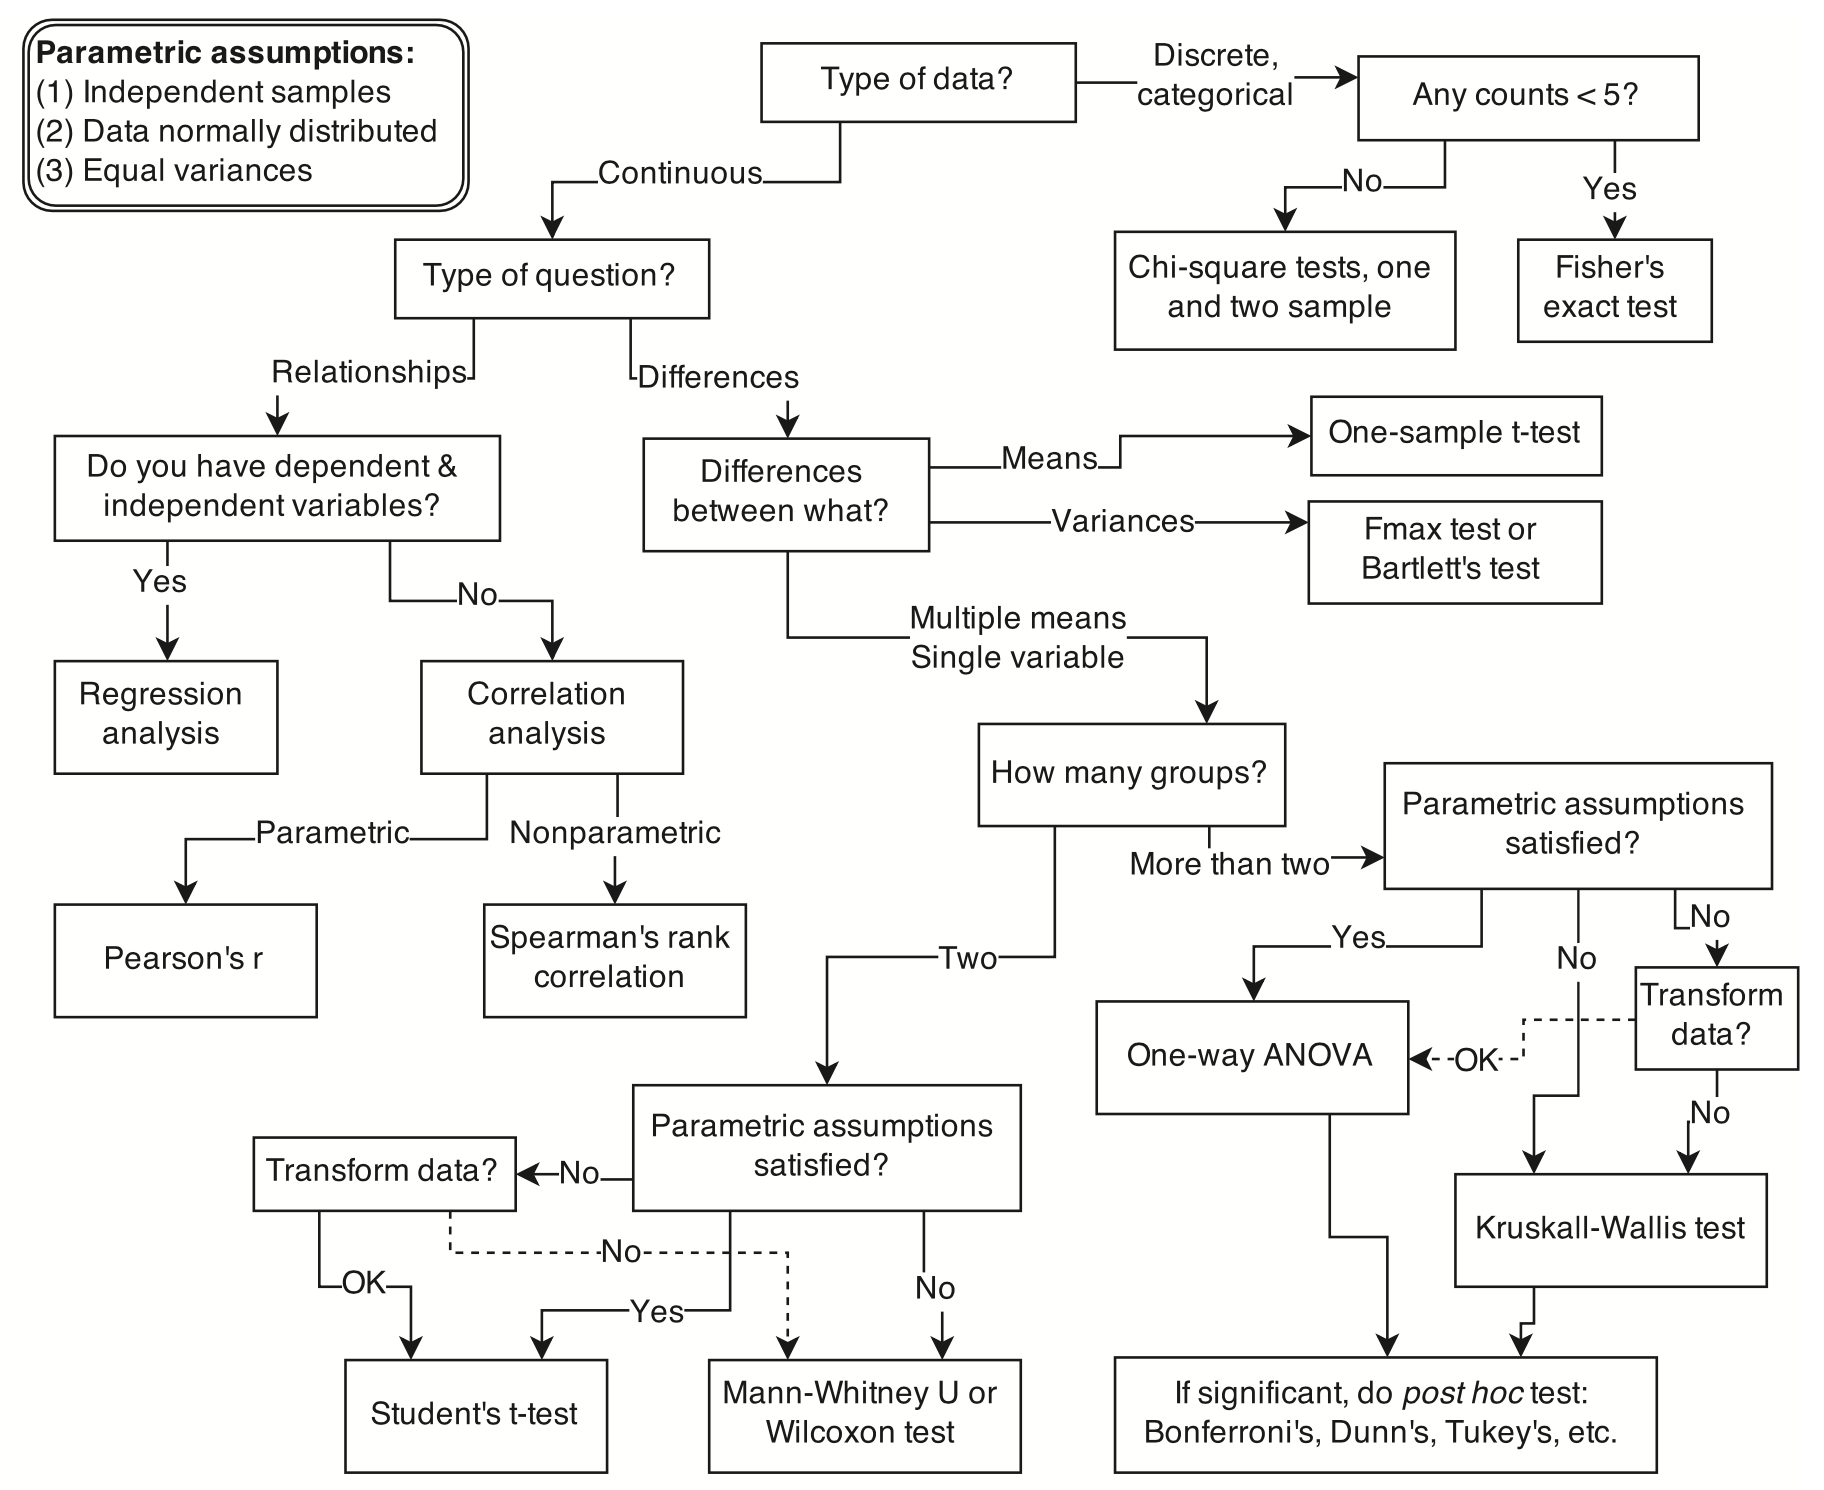
\includegraphics[width=0.95\linewidth,height=\textheight,keepaspectratio]{chapters/eda/../../figures/mcelreath_golem.png}

}

\caption{Esempio di albero decisionale per la selezione di una procedura
statistica appropriata. Iniziando dall'alto, l'utente risponde a una
serie di domande riguardanti la misurazione e l'intento, arrivando
infine al nome di una procedura. Sono possibili molti alberi decisionali
simili. (Figura tratta da McElreath
(\citeproc{ref-McElreath_rethinking}{2020})).}

\end{figure}%

È importante notare come tale procedura non fornisca strumenti utili per
identificare le effettive cause sottostanti ai fenomeni osservati.
Questa limitazione metodologica è stata identificata come uno dei
fattori principali che hanno contribuito alla crisi di replicabilità
nella ricerca psicologica, come approfondito nel \textbf{?@sec-crisis}.
L'approccio descritto, pur essendo potente nell'individuare
correlazioni, manca della ``saggezza'' necessaria per distinguere tra
semplici associazioni e vere relazioni causali, analogamente ai Golem
della metafora di McElreath.

Un problema evidenziato da McElreath
(\citeproc{ref-McElreath_rethinking}{2020}) è che processi causali
completamente distinti possono generare la stessa distribuzione di
risultati osservati. Pertanto, un approccio focalizzato esclusivamente
sull'analisi delle associazioni mediante il test dell'ipotesi nulla non
è in grado di distinguere tra questi diversi scenari, come spiegato nel
\textbf{?@sec-causal-inference-regr}.

L'approccio frequentista, che si limita a descrivere le associazioni tra
le variabili, ha una scarsa capacità di rilevare le caratteristiche
cruciali dei fenomeni studiati e tende a produrre un alto tasso di falsi
positivi (\citeproc{ref-van2023new}{Zwet et al., 2023}). È invece
necessario utilizzare una metodologia che non si limiti a confutare
ipotesi nulle, ma sia in grado di sviluppare modelli causali che
rispondano direttamente alle domande di ricerca. In questo capitolo, ci
concentreremo sull'introduzione dei concetti fondamentali dell'analisi
causale.

\section{Cos'è la causalità?}\label{cosuxe8-la-causalituxe0}

Hardt \& Recht (\citeproc{ref-hardt2022patterns}{2022}) introducono il
concetto di causalità distinguendo tra osservazione e azione. Ciò che
vediamo nell'osservazione passiva è il modo in cui le persone seguono i
loro comportamenti abituali, le loro inclinazioni naturali, proiettando
lo stato del mondo su un insieme di caratteristiche che abbiamo scelto
di evidenziare. Tuttavia, le domande più importanti spesso non
riguardano semplici osservazioni.

\begin{itemize}
\tightlist
\item
  Non ci basta sapere che le persone che praticano regolarmente attività
  fisica soffrono meno d'ansia; vogliamo capire se l'attività fisica
  riduce effettivamente i livelli d'ansia.
\item
  Non ci accontentiamo di osservare che chi segue una terapia
  cognitivo-comportamentale (CBT) presenta meno sintomi depressivi;
  desideriamo verificare se la CBT riduce realmente questi sintomi.
\item
  Non ci limitiamo a constatare che l'uso frequente dei social media è
  associato a un calo del benessere mentale; vogliamo determinare se
  l'uso intensivo dei social media causa effettivamente una diminuzione
  del benessere mentale.
\end{itemize}

Alla base, il ragionamento causale è un quadro concettuale per
affrontare domande sugli effetti di azioni o interventi ipotetici. Una
volta compreso quale sia l'effetto di un'azione, possiamo invertire la
domanda e chiederci quale azione plausibile abbia causato un determinato
evento.

\section{Effetto Causale}\label{effetto-causale}

Sebbene non esista una definizione univoca di causalità, possiamo
concettualizzarla in modo pratico: diciamo che X causa Y se,
intervenendo e modificando il valore di X (il trattamento), la
distribuzione di Y cambia di conseguenza. Questa definizione sottolinea
l'importanza cruciale dell'azione o dell'intervento nel determinare una
relazione causale.

Quando X è una variabile binaria, rappresentante la presenza o l'assenza
del trattamento, la conseguenza dell'intervento su X è denominata
effetto medio del trattamento. Questo ci indica quanto il trattamento
(azione X = 1) aumenta l'aspettativa di Y rispetto all'assenza di
trattamento (azione X = 0).

È importante notare che gli effetti causali sono quantità relative alla
popolazione. Si riferiscono a effetti mediati sull'intera popolazione in
esame. Tuttavia, spesso l'effetto del trattamento può variare
notevolmente da un individuo all'altro o tra gruppi di individui. In
questi casi, parliamo di effetti di trattamento eterogenei.

Per chiarire questo concetto, consideriamo un esempio concreto:
supponiamo che la terapia cognitivo-comportamentale (CBT) riduca
l'ansia. Se un gruppo di persone ansiose non riceve alcun trattamento, i
loro livelli d'ansia rimarranno presumibilmente invariati. Se invece
interveniamo introducendo la CBT (modificando così il valore di X), i
livelli d'ansia nel gruppo tenderanno a diminuire (cambiando quindi il
valore di Y). Questo esempio illustra la distinzione tra semplice
correlazione, basata sull'osservazione passiva, e causalità, che implica
un'azione o un intervento.

La definizione di causalità può essere applicata anche per collegare
variabili apparentemente distanti. Ad esempio, l'autoefficacia potrebbe
non avere un effetto causale diretto sulle prestazioni accademiche.
Tuttavia, se aumentiamo l'autoefficacia attraverso interventi mirati, è
probabile che osserviamo un miglioramento nell'impegno allo studio.
Questo aumento dell'impegno, a sua volta, tende a migliorare le
prestazioni accademiche. Di conseguenza, possiamo affermare che
l'autoefficacia influisce indirettamente sulle prestazioni accademiche
attraverso una catena causale.

È importante precisare che esiste una relazione causale tra X e Y anche
quando modificare X non porta necessariamente a un cambiamento immediato
o deterministico in Y, ma altera la probabilità che Y si verifichi in un
certo modo, modificando quindi la distribuzione di Y. Questa prospettiva
probabilistica della causalità è particolarmente rilevante in campi come
la psicologia, dove le relazioni tra variabili sono spesso complesse e
influenzate da molteplici fattori.

\subsection{I Limiti dell'Osservazione}\label{i-limiti-dellosservazione}

Per comprendere i limiti dell'osservazione passiva, e quindi la
necessità di comprendere le relazioni causali sottostanti, Hardt \&
Recht (\citeproc{ref-hardt2022patterns}{2022}) si riferiscono
all'esempio storico delle ammissioni ai corsi di laurea dell'Università
della California, Berkeley, nel 1973. In quell'anno, 12,763 candidati
furono considerati per l'ammissione in uno dei 101 dipartimenti o major
interdipartimentali. Di questi, 4,321 erano donne e 8,442 erano uomini.
I dati mostrano che circa il 35\% delle donne fu ammesso, rispetto al
44\% degli uomini. Test di significatività statistica indicano che
questa differenza non è attribuibile al caso, suggerendo una disparità
nei tassi di ammissione tra i generi.

Una tendenza simile si osserva quando si analizzano le decisioni
aggregate di ammissione nei sei maggiori dipartimenti. Il tasso di
ammissione complessivo per gli uomini era di circa il 44\%, mentre per
le donne era solo il 30\%, un'altra differenza statisticamente
significativa. Tuttavia, poiché i dipartimenti hanno autonomia nelle
loro decisioni di ammissione, è utile esaminare il possibile bias di
genere a livello di singolo dipartimento.

\textbf{Uomini}

\begin{longtable}[]{@{}lll@{}}
\toprule\noalign{}
Dipartimento & Candidati & Ammessi (\%) \\
\midrule\noalign{}
\endhead
\bottomrule\noalign{}
\endlastfoot
A & 825 & 62 \\
B & 520 & 60 \\
C & 325 & 37 \\
D & 417 & 33 \\
E & 191 & 28 \\
F & 373 & 6 \\
\end{longtable}

\textbf{Donne}

\begin{longtable}[]{@{}lll@{}}
\toprule\noalign{}
Dipartimento & Candidati & Ammessi (\%) \\
\midrule\noalign{}
\endhead
\bottomrule\noalign{}
\endlastfoot
A & 108 & 82 \\
B & 25 & 68 \\
C & 593 & 34 \\
D & 375 & 35 \\
E & 393 & 24 \\
F & 341 & 7 \\
\end{longtable}

Dall'osservazione di questi dati, emerge che quattro dei sei maggiori
dipartimenti mostrano un tasso di ammissione più elevato per le donne,
mentre due mostrano un tasso più elevato per gli uomini. Tuttavia,
questi due dipartimenti non possono giustificare la sostanziale
differenza nei tassi di ammissione osservata nei dati aggregati. Questo
suggerisce che la tendenza generale di un tasso di ammissione più alto
per gli uomini sembra invertita quando i dati sono disaggregati per
dipartimento.

Questo fenomeno è noto come \emph{paradosso di Simpson}, un paradosso
statistico in cui una tendenza che appare in sottopopolazioni si inverte
o scompare quando i dati vengono aggregati. Nel contesto attuale, il
paradosso di Simpson si manifesta nel fatto che, mentre i dati aggregati
sembrano indicare una discriminazione di genere contro le donne,
l'analisi dei dati disaggregati per dipartimento rivela che in alcuni
casi le donne sono favorite in termini di ammissioni.

La domanda fondamentale è se questi dati indicano effettivamente un
problema di discriminazione di genere o se, come suggerito dallo studio
originale, il bias di genere nelle ammissioni fosse principalmente
dovuto al fatto che ``le donne sono indirizzate dalla loro
socializzazione e istruzione verso campi di studio generalmente più
affollati, meno produttivi in termini di completamento dei diplomi, meno
finanziati e che spesso offrono prospettive professionali peggiori.'' In
altre parole, il problema risiederebbe in differenze sistemiche e
strutturali tra i campi di studio scelti dalle donne e quelli scelti
dagli uomini.

Il paradosso di Simpson crea disagio proprio perché l'intuizione
suggerisce che una tendenza valida per tutte le sottopopolazioni
dovrebbe esserlo anche a livello aggregato. Tuttavia, questo paradosso
evidenzia un errore comune nell'interpretazione delle probabilità
condizionate: confondere l'osservazione passiva con l'analisi causale. I
dati che abbiamo rappresentano solo un'istantanea del comportamento
normale di uomini e donne che si candidavano per l'ammissione a UC
Berkeley nel 1973.

Non possiamo trarre conclusioni definitive da questi dati. Possiamo solo
riconoscere che l'analisi iniziale solleva ulteriori domande, come ad
esempio la necessità di progettare nuovi studi per raccogliere dati più
completi, che potrebbero portare a conclusioni più definitive. In
alternativa, potremmo discutere su quale scenario sia più verosimile in
base alle nostre convinzioni e alle notre ipotesi sul mondo.

L'inferenza causale può essere utile in entrambi i casi. Da un lato, può
guidare la progettazione di nuovi studi, aiutandoci a scegliere quali
variabili includere, quali escludere e quali mantenere costanti.
Dall'altro, i modelli causali possono fungere da meccanismo per
incorporare le conoscenze scientifiche del dominio e passare da ipotesi
plausibili a conclusioni plausibili.

\section{Variabili Confondenti}\label{variabili-confondenti}

Sebbene gli esperimenti controllati siano considerati il metodo più
affidabile per identificare relazioni causali, molte domande di ricerca
non possono essere affrontate sperimentalmente a causa di vincoli etici
o pratici. In tali situazioni, i ricercatori si rivolgono a disegni
osservazionali, che garantiscono maggiore flessibilità e adattabilità ai
contesti reali. Tuttavia, l'utilizzo di dati osservazionali introduce
una sfida cruciale: la difficoltà di stabilire conclusioni causali
solide e affidabili.

Al centro di questa complessità si trovano le \textbf{variabili
confondenti}. Una variabile confondente è presente quando l'associazione
osservata tra due variabili, X e Y, non riflette accuratamente la vera
relazione causale tra di esse. In altre parole, la variabile confondente
influenza sia X che Y, creando l'apparenza di una relazione diretta tra
le due che potrebbe essere fuorviante o inesatta.

Negli studi osservazionali, se le variabili confondenti non vengono
misurate e controllate adeguatamente, possono distorcere le stime degli
effetti causali, introducendo bias nei risultati e impedendo di
riflettere il vero valore dell'effetto. In pratica, la presenza di
variabili confondenti può portare a conclusioni errate quando si
confrontano semplicemente i risultati osservati in diversi gruppi. Ciò
che si osserva nei dati potrebbe non corrispondere a ciò che accadrebbe
se si potesse manipolare direttamente la variabile di interesse in un
esperimento controllato.

\subsection{Approcci per il Controllo delle Variabili
Confondenti}\label{approcci-per-il-controllo-delle-variabili-confondenti}

Un approccio apparentemente semplice per affrontare questo problema
potrebbe essere quello di controllare statisticamente tutte le variabili
confondenti. Questo metodo prevede di stimare l'effetto di X su Y
separatamente in ogni segmento della popolazione definito da una
condizione Z = z per ogni possibile valore di z. Successivamente, si
calcola la media di questi effetti stimati nelle sottopopolazioni,
ponderandoli per la probabilità di Z = z nella popolazione. Tuttavia,
questo metodo presenta due difficoltà fondamentali:

\begin{enumerate}
\def\labelenumi{\arabic{enumi}.}
\tightlist
\item
  \textbf{Conoscenza di tutte le variabili confondenti}: Richiede la
  conoscenza di tutte le possibili variabili confondenti.
\item
  \textbf{Misurazione delle variabili confondenti}: Richiede la capacità
  di misurare ciascuna di esse, cosa che spesso non è praticabile.
\end{enumerate}

Il controllo delle variabili confondenti è cruciale per stabilire
relazioni causali, poiché permette di isolare gli effetti delle
variabili indipendenti da quelli delle variabili confondenti che
potrebbero influenzare le variabili dipendenti. Esistono due principali
metodologie di controllo:

\begin{enumerate}
\def\labelenumi{\arabic{enumi}.}
\tightlist
\item
  \textbf{Controllo Sperimentale}: Implementato attraverso il disegno
  sperimentale e basato principalmente sulla randomizzazione.
\item
  \textbf{Controllo Statistico}: Applicato durante l'analisi dei dati,
  con l'obiettivo di neutralizzare o quantificare l'influenza delle
  variabili estranee.
\end{enumerate}

\subsection{Inferenza Causale nei Dati
Osservazionali}\label{inferenza-causale-nei-dati-osservazionali}

A causa di queste difficoltà, l'inferenza causale basata su dati
osservazionali è spesso considerata problematica, dando origine al
famoso detto ``la correlazione non implica causalità''.

Anche se il metodo preferito per l'inferenza causale in molte scienze è
l'esperimento controllato e randomizzato, tali esperimenti non sono, e
non sono mai stati, lo stile dominante di inferenza causale nelle
scienze umane. Una ragione è che molte delle domande più importanti sul
comportamento umano non possono essere studiate sperimentalmente. Alla
fine, il comportamento deve essere studiato negli ambienti naturali che
le persone costruiscono, poiché questi ambienti sono sia cause che
conseguenze del comportamento. Senza studiare le persone nelle loro
comunità, non sapremmo nemmeno cosa stiamo cercando di spiegare.

L'inferenza causale è possibile anche in contesti osservazionali, e gli
statistici hanno sviluppato metodi specializzati per progettare analisi
che affrontano specifici obiettivi di inferenza causale
(\citeproc{ref-pearl_2016}{Pearl et al., 2016}).

\subsection{Strumenti Moderni per l'Analisi
Causale}\label{strumenti-moderni-per-lanalisi-causale}

L'obiettivo dell'analisi causale moderna è proprio quello di fornire gli
strumenti concettuali e metodologici per affrontare queste sfide.
Attraverso l'uso di tecniche avanzate come i modelli causali
strutturali, i grafi aciclici diretti (DAG) e i metodi di
identificazione degli effetti causali, i ricercatori possono spesso
superare le limitazioni dei dati osservazionali e trarre conclusioni
causali più robuste.

In sintesi, mentre le variabili confondenti rappresentano una sfida
significativa nell'analisi dei dati osservazionali, i progressi
metodologici nell'analisi causale offrono strumenti potenti per mitigare
questi problemi e migliorare l'affidabilità delle inferenze causali.

\section{Modelli Causali Strutturali}\label{modelli-causali-strutturali}

I modelli causali sono strumenti essenziali per l'analisi dei dati
osservazionali, poiché consentono di rappresentare il processo
sottostante a un fenomeno e di prevedere gli effetti di un intervento.
Questi modelli non solo permettono di anticipare le conseguenze di una
causa, ma offrono anche la possibilità di esplorare scenari
controfattuali, immaginando esiti alternativi che si sarebbero potuti
verificare in presenza di decisioni diverse.

Un modello causale strutturale (\emph{Structural Causal Model}, SCM) è
un approccio che rappresenta le relazioni causali tra variabili. Esso si
basa su una serie di assegnazioni che, partendo da variabili di rumore
indipendenti (note anche come variabili esogene), generano una
distribuzione di probabilità congiunta.

Le variabili di rumore indipendenti svolgono un ruolo cruciale negli
SCM. Esse rappresentano fonti di incertezza o variabilità all'interno
del sistema e non sono influenzate da altre variabili del modello.
Queste variabili sono mutuamente indipendenti, il che significa che il
loro valore non fornisce informazioni sul valore delle altre.

La costruzione di un SCM segue una sequenza specifica: si parte dalle
variabili di rumore indipendenti, si applicano una serie di assegnazioni
che descrivono gli effetti causali delle variabili esogene su altre
variabili, e si genera progressivamente un insieme di variabili casuali
che dà origine a una distribuzione congiunta.

Il principale vantaggio di un SCM risiede nella sua duplice natura: da
un lato, fornisce una distribuzione di probabilità congiunta delle
variabili, e dall'altro, descrive il processo generativo che porta alla
formazione di tale distribuzione, partendo dalle variabili di rumore
elementari.

Questa struttura consente non solo di modellare le relazioni
probabilistiche tra le variabili, ma anche di rappresentare in modo
esplicito i meccanismi causali che le governano.

I SCM possono essere rappresentati graficamente attraverso Grafi
Aciclici Direzionati (\emph{Directed Acyclic Graphs}, DAG). Questi DAG
visualizzano le relazioni causali tra le variabili all'interno di un
SCM, facilitando l'identificazione delle variabili confondenti e il loro
impatto sull'analisi.

\section{Bias da Variabile Omessa}\label{bias-da-variabile-omessa}

Possiamo introdurre i DAG facendo riferiento al \emph{bias da variabile
omessa} (\emph{Omitted Variable Bias}, o OVB; Wilms et al.
(\citeproc{ref-wilms2021omitted}{2021})). Come discusso da Byrnes \& Dee
(\citeproc{ref-byrnes2024causal}{2024}), l'omissione dall'analisi
statistica di variabili confondenti note ma non misurate, o sconosciute
e non misurate, può portare a stime errate della magnitudine degli
effetti, errori nel segno delle stime (stimatori distorti), correlazioni
spurie, e al mascheramento delle vere relazioni causali.

Un illustrazione di questa situazione è fornita nella
Figura~\ref{fig-byrnes-dee-1}. La figura mostra tre DAG che illustrano
diversi scenari in cui le variabili non osservate non influenzano i
risultati del modello o potrebbero creare problemi a causa della
confusione. Una variabile di risposta di interesse (Y) è causata sia da
una variabile misurata (X) che da una variabile non misurata (U). Nel
pannello di sinistra, la variabile non osservata (U) non è una variabile
confondente. Nel pannello centrale, la variabile non osservata (U) è una
variabile confondente e causa il bias da variabile omessa. Nel pannello
di destra la variabile non osservata (U) causa il bias da variabile
omessa in maniera indiretta.

\begin{figure}

\centering{

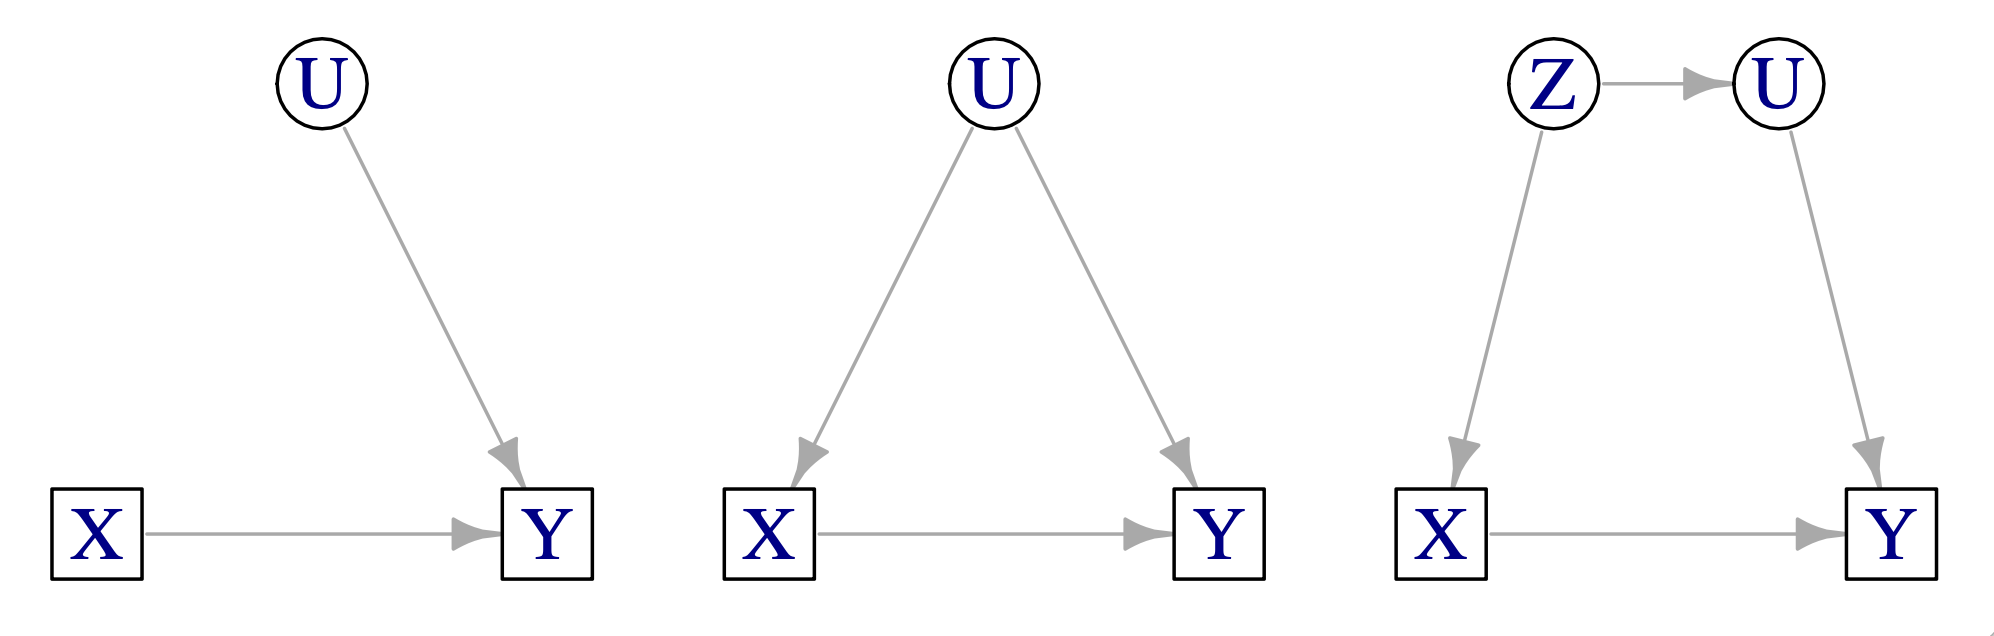
\includegraphics[width=0.8\linewidth,height=\textheight,keepaspectratio]{chapters/eda/../../figures/byrnes_dee_fig1.png}

}

\caption{\label{fig-byrnes-dee-1}Nel pannello di sinistra, X e U sono
non correlate, quindi la mancata inclusione di U in un modello
statistico aumenterebbe l'errore standard della stima (riducendo la
precisione del modello) ma non porterebbe a bias nella stima
dell'effetto di X su Y. Tuttavia, se U influenza anche X come nel
pannello centrale, o se U e X sono influenzati da un fattore comune Z
come nel pannello di destra, allora omettere U da un modello statistico
causa il bias da variabile omessa nella stima dell'effetto di X su Y. I
casi illustrati dal pannello centrale e dal pannello di destra sono
esempi di sistemi in cui le cause comuni di confusione (U e Z
rispettivamente) devono essere controllate per effettuare inferenze
causali non distorte (la figura è ispirata da Byrnes \& Dee
(\citeproc{ref-byrnes2024causal}{2024})).}

\end{figure}%

Affrontare i problemi creati dalle variabili confondenti non misurate
rappresenta una sfida primaria nell'inferenza causale dai dati
osservazionali. A differenza dell'errore di misurazione nelle variabili
predittive, che produce un bias costante verso lo zero e può essere
corretto o modellato (\citeproc{ref-McElreath_rethinking}{McElreath,
2020}; \citeproc{ref-schennach2016recent}{Schennach, 2016}), con l'OVB
non possiamo conoscere la grandezza o la direzione del bias senza
conoscere tutte le possibili variabili confondenti e le loro relazioni
nel sistema.

Nonostante queste sfide, non è necessario abbandonare l'uso dei dati
osservazionali per l'inferenza causale in psicologia. È invece
necessario ricorrere all'adozione delle tecniche dei SCM per potere
comunque svolgere l'inferenza causale.

È evidente che questo approccio porterà a conclusioni inevitabilmente
parziali, destinate ad essere perfezionate da studi successivi.
Tuttavia, tale metodologia offre il vantaggio di esplicitare il
``modello generativo dei dati'', ovvero la struttura causale sottostante
ai fenomeni psicologici oggetto di studio.

I progressi nella ricerca empirica conducono a una maggiore comprensione
e, di conseguenza, a modifiche nelle ipotesi sui meccanismi causali.
Questo processo rappresenta un'evoluzione della conoscenza scientifica.
Tale sviluppo è reso possibile proprio perché le ipotesi causali sono
formulate in termini di modelli formali, che descrivono in modo preciso
i meccanismi ipotizzati.

Al contrario, limitarsi alla mera descrizione delle associazioni tra
variabili non consente questo tipo di avanzamento conoscitivo. La
formulazione di modelli causali espliciti permette infatti di testare,
raffinare e, se necessario, rivedere le ipotesi sui meccanismi
sottostanti ai fenomeni osservati, portando a una comprensione più
profonda e dinamica dei processi psicologici.

\section{Grafi Aciclici Diretti}\label{grafi-aciclici-diretti}

I DAG sono uno strumento fondamentale per l'inferenza causale, offrendo
una rappresentazione visiva delle relazioni causali ipotizzate tra
variabili. Questi grafi sono definiti ``diretti'' perché le variabili,
rappresentate da nodi, sono collegate da frecce orientate anziché da
semplici linee. Sono inoltre chiamati ``aciclici'' poiché non è
possibile tornare a un nodo di partenza seguendo il percorso delle
frecce.

In un DAG, una freccia che va da X a Y indica un'influenza
probabilistica di X su Y. La terminologia delle relazioni all'interno
del grafo è importante: il nodo di origine di una freccia è chiamato
``genitore'', mentre il nodo di destinazione è detto ``figlio''. Quando
è possibile raggiungere un nodo B partendo da un nodo A seguendo una
successione di frecce, A è definito ``antenato'' di B, e B è considerato
``discendente'' di A.

I DAG consentono di distinguere chiaramente tra cause dirette e
indirette. Una causa diretta è rappresentata da un nodo genitore, mentre
una causa indiretta può essere qualsiasi antenato di un nodo nel grafo
causale. Questa struttura permette di differenziare efficacemente causa
ed effetto basandosi sulla posizione relativa dei nodi all'interno del
grafo, ovvero se un nodo è antenato o discendente di un altro.

Questi grafi sono particolarmente utili per identificare variabili
confondenti, basandosi sulla teoria sviluppata da Judea Pearl
(\citeproc{ref-pearl2009causality}{Pearl, 2009}). È cruciale
rappresentare in un DAG tutte le possibili relazioni causali, poiché
l'assenza di una freccia tra due nodi implica la certezza dell'assenza
di una relazione causale diretta tra le variabili corrispondenti.

Nella teoria dei DAG, due concetti fondamentali sono la d-separazione e
il criterio del back-door.

\subsection{La d-separazione}\label{la-d-separazione}

La \emph{d-separazione} ci aiuta a determinare quando due variabili in
un grafo causale sono indipendenti condizionatamente a un insieme di
altre variabili. Questo concetto è cruciale per comprendere come
l'informazione o l'influenza si propaga tra le variabili in un modello
causale.

In termini più semplici, la d-separazione ci permette di identificare se
esiste un ``blocco'' nel flusso di informazioni tra due variabili, dato
un certo insieme di altre variabili (che chiameremo Λ). Quando due
variabili sono d-separate da Λ, significa che non c'è flusso di
informazioni tra di loro, condizionatamente a Λ.

Per comprendere meglio la d-separazione, consideriamo tre situazioni
principali che possono verificarsi in un DAG:

\begin{enumerate}
\def\labelenumi{\arabic{enumi}.}
\item
  Catena (X → Z → Y): In questo caso, Z è un mediatore tra X e Y. Se Z
  appartiene all'insieme Λ (cioè, se controlliamo o condizioniamo su Z),
  blocchiamo il flusso di informazioni da X a Y attraverso questo
  percorso. Per esempio, se X è ``esercizio fisico'', Z è ``pressione
  sanguigna'' e Y è ``rischio di malattie cardiache'', controllando per
  la pressione sanguigna (Z) blocchiamo il percorso attraverso il quale
  l'esercizio fisico influenza il rischio di malattie cardiache.
\item
  Fork (X ← Z → Y): Qui, Z è una causa comune sia di X che di Y. Se Z
  appartiene a Λ, blocchiamo la correlazione spuria tra X e Y che deriva
  dalla loro causa comune. Per esempio, se Z è ``status
  socioeconomico'', X è ``livello di istruzione'' e Y è ``stato di
  salute'', controllando per lo status socioeconomico (Z) eliminiamo la
  correlazione apparente tra istruzione e salute che potrebbe derivare
  dal fatto che entrambe sono influenzate dallo status socioeconomico.
\item
  Collider (X → Z ← Y): In questa situazione, Z è un effetto comune di X
  e Y. Sorprendentemente, se né Z né i suoi discendenti appartengono a
  Λ, il percorso è già bloccato. Controllare per Z (o i suoi
  discendenti) in realtà aprirebbe un percorso tra X e Y, creando una
  correlazione spuria. Per esempio, se X è ``intelligenza'', Y è
  ``bellezza'' e Z è ``successo in una carriera di attore'', controllare
  per il successo nella carriera di attore (Z) creerebbe una
  correlazione apparente tra intelligenza e bellezza, anche se queste
  potrebbero essere indipendenti nella popolazione generale.
\end{enumerate}

In sintesi, la d-separazione ci permette di determinare, dato un certo
insieme di variabili Λ, se due variabili X e Y sono indipendenti
condizionatamente a Λ. Questo ci aiuta a identificare quali variabili
dobbiamo controllare (e quali non dobbiamo controllare) per ottenere
stime causali non distorte, facilitando così l'inferenza causale
corretta. La d-separazione è quindi uno strumento potente che ci
permette di leggere le indipendenze condizionali direttamente dal grafo,
senza dover fare calcoli probabilistici complessi.

\subsection{Il criterio del back-door}\label{il-criterio-del-back-door}

Il criterio del back-door consente di identificare un insieme di
variabili che, se controllate adeguatamente, permettono di stimare gli
effetti causali in modo non distorto. L'obiettivo principale di questo
criterio è eliminare l'influenza di percorsi non causali tra la
variabile di esposizione (causa potenziale) e l'outcome (effetto),
mantenendo aperto solo il percorso causale diretto di interesse.

In questo contesto, due variabili sono considerate ``confuse'' se esiste
tra di esse un percorso di tipo back-door. Un back-door path da X a Y è
definito come qualsiasi percorso che inizia da X con una freccia
entrante in X. Per esempio, consideriamo il seguente percorso:

X ← A → B ← C → Y

In questo caso, il percorso rappresenta un flusso di informazioni da X a
Y che non è causale, ma potrebbe creare l'apparenza di una relazione
causale.

Per ``deconfondere'' una coppia di variabili, è necessario selezionare
un insieme di variabili (chiamato back-door set) che ``blocchi'' tutti i
back-door paths tra i due nodi di interesse. Il blocco di questi
percorsi avviene in modi diversi a seconda della struttura del percorso:

\begin{enumerate}
\def\labelenumi{\arabic{enumi}.}
\item
  Un back-door path che coinvolge una catena di variabili (ad esempio, A
  → B → C) può essere bloccato controllando per la variabile intermedia
  (in questo caso, B).
\item
  Un percorso che coinvolge un ``collider'' (una variabile che riceve
  frecce da entrambe le direzioni, come in A → B ← C) è naturalmente
  bloccato e non permette il flusso di informazioni.
\end{enumerate}

È importante notare che bisogna prestare attenzione a non aprire
involontariamente un flusso di informazioni attraverso un collider.
Questo può accadere se si condiziona l'analisi sul collider stesso o su
un suo discendente, il che potrebbe erroneamente aprire il percorso e
introdurre bias nell'analisi.

\begin{tcolorbox}[enhanced jigsaw, opacityback=0, bottomrule=.15mm, breakable, title=\textcolor{quarto-callout-caution-color}{\faFire}\hspace{0.5em}{Punti chiave}, bottomtitle=1mm, toptitle=1mm, titlerule=0mm, colbacktitle=quarto-callout-caution-color!10!white, rightrule=.15mm, colframe=quarto-callout-caution-color-frame, colback=white, arc=.35mm, leftrule=.75mm, coltitle=black, left=2mm, toprule=.15mm, opacitybacktitle=0.6]

\begin{itemize}
\tightlist
\item
  Il criterio del back-door aiuta a identificare il set minimale di
  variabili da controllare.
\item
  Non tutte le variabili associate sia all'esposizione che all'outcome
  devono essere controllate; solo quelle che creano percorsi back-door.
\item
  In alcuni casi, potrebbe non essere necessario controllare alcuna
  variabile (se non ci sono percorsi back-door aperti).
\item
  In altri casi, potrebbe essere impossibile bloccare tutti i percorsi
  back-door con le variabili disponibili, indicando che l'effetto
  causale non può essere identificato con i dati a disposizione.
\end{itemize}

Utilizzando il criterio del back-door in combinazione con i DAG, i
ricercatori possono fare scelte più informate su quali variabili
includere nelle loro analisi, migliorando così la validità delle loro
inferenze causali.

\end{tcolorbox}

\subsection{Applicazioni}\label{applicazioni}

Consideriamo nuovamente la struttura causale illustrata nella
Figura~\ref{fig-byrnes-dee-1}, pannello centrale. Dopo aver costruito un
DAG come descritto nella sezione precedente, è possibile identificare le
potenziali fonti di bias da variabili omesse, inclusi i confondenti non
misurati (ad esempio, U). Non controllare per le variabili confondenti
apre una ``back-door'' permettendo alla variazione confondente di
influenzare la relazione tra la variabile causale e la variabile di
risposta di interesse attraverso un percorso non valutato
(\citeproc{ref-pearl2009causality}{Pearl, 2009}). In altre parole,
omettere una variabile confondente come U nella
Figura~\ref{fig-byrnes-dee-1} (pannello centrale) in un'analisi
statistica significa che questa viene incorporata nel termine di errore
del modello statistico, insieme alle fonti di errore casuali. La
Figura~\ref{fig-byrnes-dee-2} illustra le conseguenze di un confondente
U che ha un effetto positivo su X ma un effetto negativo su Y. Se
adattiamo un modello come mostrato nella Figura~\ref{fig-byrnes-dee-2}
bi, l'effetto stimato di X su Y è positivo quando si controlla per U.
Tuttavia, se non si controlla per U, come mostrato nella
Figura~\ref{fig-byrnes-dee-2} bii, U viene incorporato nel termine di
errore, inducendo una correlazione tra l'errore e X, come illustrato
nella Figura~\ref{fig-byrnes-dee-2} biii, portando a una stima errata.
Pertanto, il termine di errore del modello e X risultano correlati, il
che viola un'assunzione fondamentale dei modelli lineari (ovvero, il
teorema di Gauss-Markov; Abdallah et al., 2015; Antonakis et al., 2010).
Questo produce una stima errata, evidenziata in blu.

\begin{figure}

\centering{

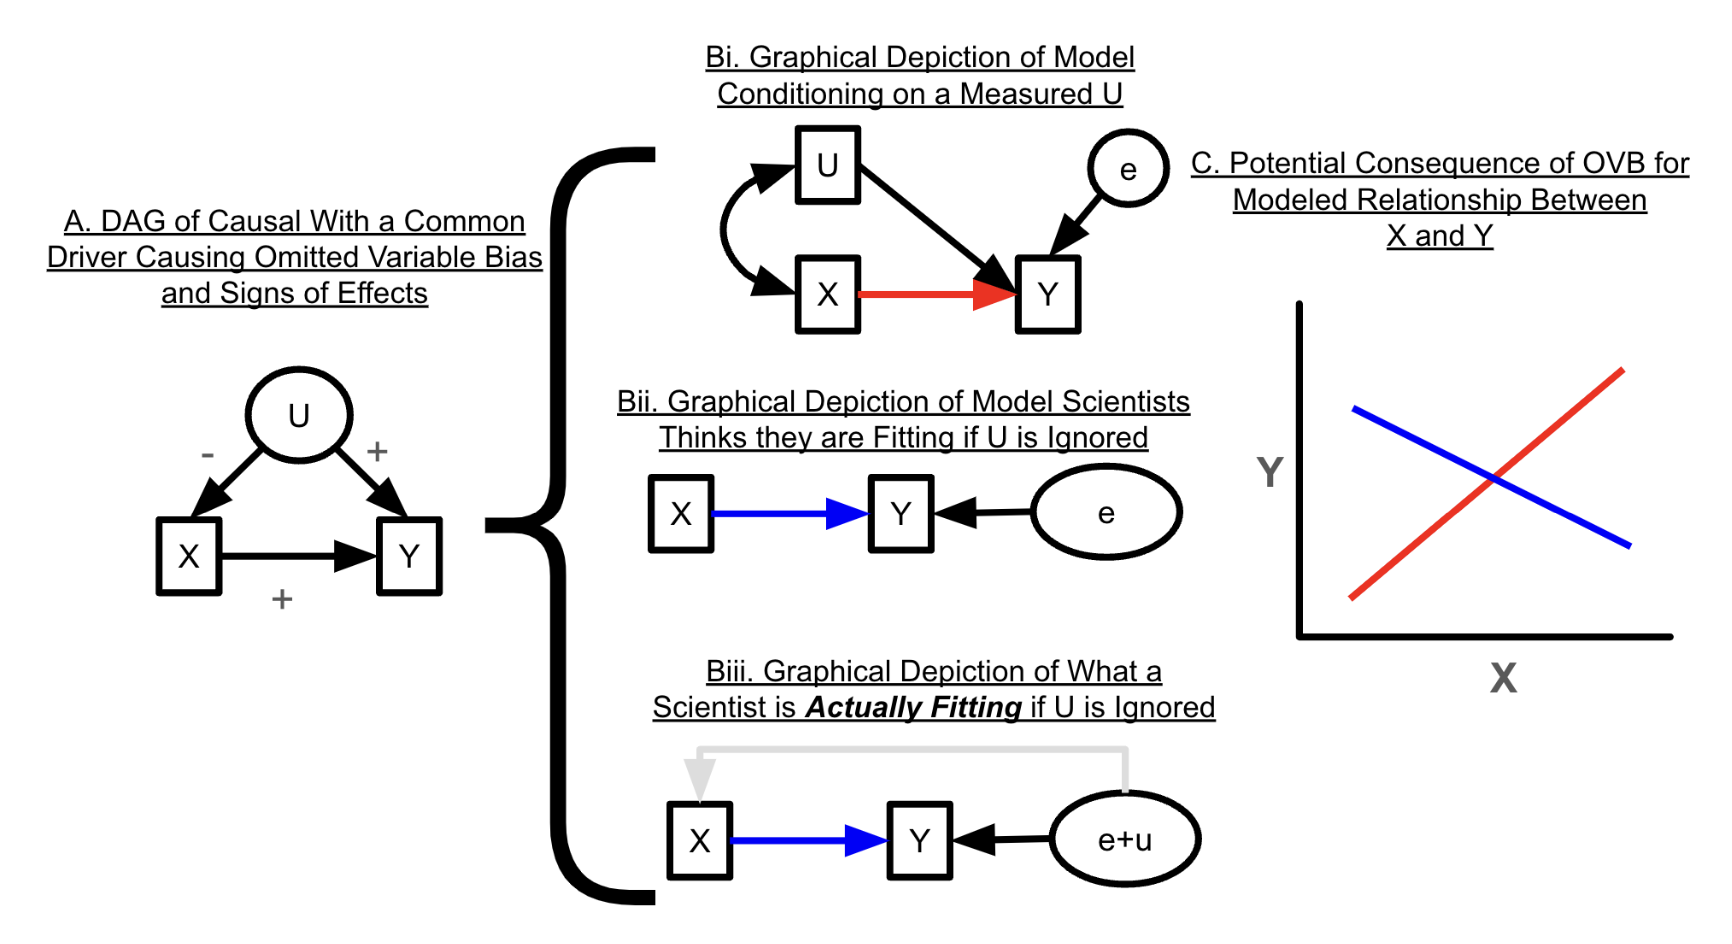
\includegraphics[width=1\linewidth,height=\textheight,keepaspectratio]{chapters/eda/../../figures/byrnes_dee_fig2.png}

}

\caption{\label{fig-byrnes-dee-2}\textbf{Una visualizzazione del bias da
variabile omessa e delle conseguenze per l'inferenza causale.} (A)
mostra un DAG di un sistema in cui X ha un effetto positivo su Y, e una
variabile confondente U ha un effetto positivo su Y ma un effetto
negativo su X. Le variabili non osservate (cioè non misurate) sono
rappresentate in ellissi, come la variabile U e il termine di errore e
nel pannello B. (B) illustra diverse stime del DAG in (A) utilizzando
un'analisi del percorso. Vedi Box 1 per una breve spiegazione delle
principali differenze tra DAG e diagrammi dei percorsi. Presumiamo che U
non sia misurata. In (Bi), presumiamo di poter misurare e controllare U,
rappresentata dalla freccia a doppia testa tra U e X, che rappresenta la
correlazione tra le due variabili considerata dal modello. La variabile
non misurata e è la fonte residua di variazione che si presume non sia
correlata con nessun predittore. La freccia rossa rappresenta il
percorso stimato. Al contrario, (Bii) e (Biii) rappresentano la realtà,
dove non abbiamo una misurazione di U e non la controlliamo nel modello
dei percorsi. Il ricercatore pensa di adattare il modello in (Bii) ma in
realtà sta adattando il modello in (Biii), dove il termine di errore non
è solo e, ma la somma di e e la variazione dovuta alla variabile omessa
U. A causa di ciò, c'è un percorso diretto dal termine di errore del
modello a X (e quindi X è endogeno). (C) mostra le relazioni stimate
risultanti dai modelli in (Bi) rispetto a (Bii). Le linee rappresentano
la relazione stimata tra X e Y dai rispettivi modelli. La linea rossa è
la vera relazione causale, stimata da (Bi), mentre la linea blu contiene
il bias da variabile omessa, poiché non si tiene conto della variabile
confondente U, come stimato dal modello in Bii/Biii (Figura tratta da
Byrnes \& Dee (\citeproc{ref-byrnes2024causal}{2024})).}

\end{figure}%

\section{Le Pratiche Scientifiche per Inferire la
Causalità}\label{le-pratiche-scientifiche-per-inferire-la-causalituxe0}

Come visto in precedenza, in qualsiasi sistema complesso, consideriamo
due variabili, \emph{X} e \emph{Y}. Sebbene possiamo osservare la loro
distribuzione di probabilità congiunta \(p(x, y)\), stabilire se
\emph{X} causa \emph{Y}, \emph{Y} causa \emph{X}, o se una terza
variabile \emph{Z} influenzi entrambe, rimane un problema complesso
(Salmon, 1984). Questa difficoltà è al centro del dibattito filosofico
sulla causalità, ma è anche il motore che spinge lo sviluppo di metodi
scientifici per decifrare il funzionamento del mondo. Ad esempio, per
capire se una terapia cognitivo-comportamentale (TCC) riduce
effettivamente i sintomi di ansia, se la lettura di un articolo
scientifico influenza le opinioni dei lettori riguardo a un tema
controverso, o se l'attivazione di un neurone in una specifica area
cerebrale influenza il comportamento o l'attività di un altro neurone,
dobbiamo affrontare queste questioni con rigore scientifico.

\subsection{Il Framework Interventista di Judea
Pearl}\label{il-framework-interventista-di-judea-pearl}

Come discusso sopra, il lavoro di Judea Pearl ha rivoluzionato la
formalizzazione dell'inferenza causale. Mettiamo qui in evidenza il
ruolo che l'intervento attivo ha nella comprensione della causalità
(ricordiamo il punto di vista di \citeproc{ref-hardt2022patterns}{Hardt
\& Recht, 2022} descritto in precedenza). Nella tradizionale probabilità
bayesiana, consideriamo \(p(y \mid x)\) --- la probabilità di \emph{Y}
dato \emph{X}. Tuttavia, Pearl ha introdotto l'operatore \emph{``do''},
che permette di esprimere il risultato di un intervento attivo, scritto
come \(p(y \mid do(x))\). Questo rappresenta la probabilità di \emph{Y}
quando \emph{X} viene impostato artificialmente a un certo valore
(Pearl, 2009). Questo approccio si concentra sugli interventi piuttosto
che sulle sole osservazioni, permettendo di isolare l'effetto causale di
\emph{X} su \emph{Y} senza necessariamente conoscere i meccanismi
sottostanti.

Per esempio, supponiamo di voler studiare se la terapia
cognitivo-comportamentale (TCC) riduce i sintomi di ansia. Osservare una
correlazione tra la partecipazione alla TCC e il miglioramento dei
sintomi non è sufficiente per stabilire una relazione causale.
Utilizzando l'operatore \emph{``do''}, possiamo simulare un intervento
ipotetico: ``Cosa accadrebbe se forzassimo tutti i pazienti a seguire la
TCC?'' Questo approccio ci permette di isolare l'effetto della TCC sui
sintomi di ansia, eliminando l'influenza di fattori confondenti come lo
stato socioeconomico o la predisposizione genetica.

\subsection{Tre Fonti di Conoscenza Causale
Pragmatica}\label{tre-fonti-di-conoscenza-causale-pragmatica}

Alla luce delle considerazioni precedenti, possiamo individuare tre
fonti di conoscenza che ci informano sui meccanismi causali.

\subsubsection{Esperimenti Randomizzati Controllati
(RCT)}\label{esperimenti-randomizzati-controllati-rct}

Gli RCT sono considerati lo standard aureo per stimare gli effetti
causali. Assegnando casualmente i partecipanti a gruppi di trattamento e
controllo, gli RCT minimizzano l'influenza di variabili confondenti,
fornendo stime non distorte dell'effetto di un intervento. Ad esempio,
numerosi esperimenti dimostrano che attivare un interruttore causa
l'accensione di una luce:

\[
p(\text{luce accesa}|do(\text{interruttore acceso})) \approx 1, \quad p(\text{luce spenta}|do(\text{interruttore spento})) \approx 1
\]

Questo approccio è particolarmente utile in psicologia, dove fattori
confondenti possono facilmente distorcere i risultati.

Per esempio, immaginiamo uno studio in cui alcuni volontari vengono
assegnati casualmente a dormire 8 ore o a restare svegli tutta la notte
prima di un test di memoria. Gli RCT permettono di stabilire se il sonno
causa un miglioramento delle prestazioni cognitive, eliminando
l'influenza di fattori come l'età o lo stress.

\subsubsection{Comprensione Specifica del
Dominio}\label{comprensione-specifica-del-dominio}

In discipline come la psicologia, le neuroscienze o l'elettronica, la
conoscenza specialistica consente agli esperti di basarsi su principi
consolidati per formulare ipotesi causali e progettare esperimenti
significativi. Ad esempio, anche se un semplice movimento della mano non
causa direttamente l'accensione di una luce, la nostra comprensione dei
circuiti elettrici ci informa che chiudere un interruttore completa un
circuito, producendo luce. Queste intuizioni, basate su conoscenze
approfondite del dominio, raffinano i nostri modelli causali e
migliorano la progettazione sperimentale. Tale comprensione deriva
spesso da esperimenti randomizzati precedenti e permette l'uso di
quasi-esperimenti per produrre risultati causali convincenti.

Un esempio rilevante in psicologia e neuroscienze è il ruolo
dell'amigdala nella risposta alla paura. Grazie a studi clinici e
sperimentali, sappiamo che l'amigdala è una struttura cerebrale chiave
nel processamento delle emozioni, in particolare della paura. Pazienti
con danni all'amigdala, ad esempio, mostrano una ridotta capacità di
riconoscere espressioni facciali di paura e di rispondere a stimoli
minacciosi. Questa conoscenza specifica del dominio ci permette di
formulare ipotesi causali precise, come ``L'attività nell'amigdala
influenza la risposta emotiva alla paura.''

Un altro esempio è il legame tra l'area di Broca e la produzione del
linguaggio. Studi clinici su pazienti con lesioni in questa area hanno
dimostrato che danni specifici portano a deficit nella produzione del
linguaggio, un disturbo noto come \emph{afasia di Broca}. Questa
conoscenza deriva da decenni di ricerca neuroscientifica e ci permette
di affermare con sicurezza che ``L'attività nell'area di Broca è
necessaria per la produzione fluente del linguaggio.''

La comprensione specifica del dominio non solo aiuta a formulare ipotesi
causali, ma guida anche la progettazione degli esperimenti. Ad esempio,
se vogliamo studiare l'effetto di un farmaco sulla riduzione dell'ansia,
la conoscenza dei meccanismi neurobiologici alla base dell'ansia (come
il ruolo del sistema limbico e dei neurotrasmettitori come la
serotonina) ci permette di identificare i parametri rilevanti da
misurare e di controllare per possibili fattori confondenti. Questo
approccio è particolarmente utile quando non è possibile condurre
esperimenti randomizzati, come nel caso di studi su pazienti con
condizioni cliniche specifiche.

In sintesi, la comprensione specifica del dominio è un pilastro
fondamentale per l'inferenza causale in psicologia e neuroscienze. Essa
non solo fornisce le basi per formulare ipotesi precise, ma migliora
anche la qualità e l'affidabilità della ricerca, permettendo di trarre
conclusioni causali anche in contesti complessi e non sperimentali.

\subsubsection{Testimonianze Scientifiche e Prove
Cumulative}\label{testimonianze-scientifiche-e-prove-cumulative}

L'avanzamento della conoscenza scientifica dipende dalla validazione
collettiva dei risultati. Quando numerosi studi indipendenti e
randomizzati giungono a conclusioni causali simili, la comunità
scientifica acquisisce una comprensione pragmatica, se non definitiva,
dei meccanismi causali sottostanti. Questo approccio si giustifica
grazie ai successi passati nella descrizione della causalità.

Per esempio, numerosi studi indicano che le relazioni sociali positive
aumentano il benessere psicologico. Benché nessuno studio singolo possa
offrire una prova definitiva, l'accumulo di prove da diverse fonti
conferma l'esistenza di un legame causale tra socializzazione e
benessere.

\subsection{Conciliare Pragmatismo con Scetticismo
Filosofico}\label{conciliare-pragmatismo-con-scetticismo-filosofico}

Nonostante i metodi sperimentali, come gli esperimenti randomizzati
controllati (RCT), e gli strumenti teorici, come l'operatore ``do''
introdotto da Judea Pearl, abbiano dimostrato una grande efficacia nella
pratica scientifica, essi non risolvono completamente le sfide
epistemologiche sollevate da filosofi come David Hume. Hume ha
argomentato che la causalità non è qualcosa che possiamo osservare
direttamente; piuttosto, è un concetto inferito attraverso l'esperienza.
Questo scetticismo radicale ci ricorda che la nostra comprensione
causale del mondo è sempre mediata da assunzioni e interpretazioni.

Tuttavia, ciò non significa che dobbiamo abbandonare il concetto di
causalità. Al contrario, i metodi scientifici moderni forniscono uno
strumento pragmatico estremamente potente per navigare nei sistemi
complessi e fare previsioni affidabili. Secondo Woodward (2003), la
causalità in scienza non deve essere vista come una finestra diretta
ipotetiche verità metafisiche, ma piuttosto come uno strumento pratico
per manipolare il mondo e prevedere i risultati delle nostre azioni.
Questa prospettiva pragmatica ci permette di superare le limitazioni
teoriche e concentrarci sui risultati concreti.

Consideriamo due esempi concreti.

\begin{enumerate}
\def\labelenumi{\arabic{enumi}.}
\item
  Ogni volta che saliamo su un aereo, ci affidiamo implicitamente alle
  leggi della fisica e all'ingegneria aeronautica. Sappiamo, grazie a
  studi rigorosi e prove empiriche, che le forze aerodinamiche e i
  principi di propulsione consentono agli aerei di volare. Questa
  fiducia non deriva da una certezza assoluta, ma dalla robustezza delle
  evidenze accumulate nel tempo. La causalità tra il disegno dell'aereo
  e il suo funzionamento è stata testata e confermata milioni di volte,
  rendendo questo mezzo di trasporto sicuro e affidabile.
\item
  Analogamente, quando scegliamo di seguire un trattamento psicologico,
  come la terapia cognitivo-comportamentale (TCC), lo facciamo basandoci
  su una vasta quantità di ricerche scientifiche che dimostrano
  l'efficacia di tali interventi. Gli studi randomizzati hanno mostrato
  che la TCC modifica i processi mentali e comportamentali, riducendo in
  maniera rilevante i sintomi di ansia e depressione. Anche qui, la
  nostra fiducia non deriva da una prova definitiva della causalità, ma
  da un corpus consistente di evidenze empiriche.
\end{enumerate}

La chiave del successo del pragmatismo scientifico sta nella sua
capacità di fornire risultati \textbf{misurabili} e
\textbf{replicabili}. Non dobbiamo risolvere il problema filosofico
della causalità per utilizzarla efficacemente. Ciò che conta è la sua
applicabilità pratica: se un'intervento produce risultati coerenti e
prevedibili, allora possiamo considerarlo causa di quei risultati,
almeno per tutti gli scopi pratici. Questo approccio ci permette di
progredire senza rimanere bloccati dalle domande metafisiche irrisolte.

\section{Riflessioni Conclusive}\label{riflessioni-conclusive-15}

Il dibattito filosofico sulla natura della causalità rimane un campo
ricco e dinamico, ma i progressi metodologici degli ultimi decenni hanno
fornito strumenti pratici e robusti per affrontare le complessità
dell'inferenza causale. Esperimenti randomizzati controllati (RCT),
diagrammi causali (DAG) e l'operatore ``do'' introdotto da Judea Pearl
rappresentano esempi concreti di come, pur senza pretendere di risolvere
le questioni metafisiche sulla natura ultima della causalità, la ricerca
empirica sia in grado di offrire modelli affidabili per comprendere e
intervenire su fenomeni complessi.

I DAG si distinguono come uno degli strumenti più potenti per
rappresentare e analizzare le relazioni causali. Essi mettono in luce le
influenze dirette e indirette tra variabili, rendendo esplicite le
assunzioni alla base di ogni ricerca. Tuttavia, la loro efficacia
dipende in modo cruciale dalla qualità delle conoscenze del dominio:
senza una comprensione approfondita del contesto, anche il DAG più
raffinato rischia di omettere variabili rilevanti o di rappresentare in
modo fuorviante i rapporti causali. Nonostante ciò, i DAG promuovono la
\textbf{trasparenza scientifica}, poiché rendono visibile il processo
decisionale e aiutano a identificare potenziali fonti di bias,
contribuendo a una maggiore chiarezza metodologica.

L'approccio pragmatico, che accetta di lavorare con concetti causali
anche in assenza di risposte definitive ai grandi interrogativi
metafisici, è al cuore del progresso scientifico. La nostra fiducia nel
viaggiare in aereo o nel ricorrere a terapie come quella
cognitivo-comportamentale si basa sull'evidenza empirica accumulata e
confermata innumerevoli volte, non su una certezza assoluta. Questo
pragmatismo non è solo utile, ma indispensabile per la ricerca
scientifica e per la vita quotidiana.

Tuttavia, strumenti come i DAG non sono infallibili. Se le loro premesse
sono scorrette o incomplete, le inferenze causali che ne derivano
possono risultare distorte. Per mantenere la credibilità di queste
tecniche, è essenziale un \emph{rigoroso controllo metodologico},
accompagnato da una \emph{riflessione critica} costante sulle assunzioni
sottostanti. Solo questa vigilanza epistemologica permette di evitare
semplificazioni eccessive e di confrontarsi in modo costruttivo con i
limiti intrinseci dell'inferenza causale.

In definitiva, l'indagine causale contemporanea richiede un
bilanciamento tra \emph{pragmatismo} --- che valorizza e applica i
risultati empirici in modo concreto --- e \emph{scetticismo filosofico},
che stimola un'analisi continua delle nostre ipotesi e premesse. Questa
prospettiva equilibrata è essenziale per l'avanzamento delle conoscenze.
Pur rimanendo consapevoli che la ``vera natura'' della causalità possa
restare, almeno in parte, un mistero irrisolvibile, possiamo comunque
costruire strumenti sufficientemente robusti per prevedere con
accuratezza i fenomeni di interesse e prendere decisioni informate. È
questa combinazione di umiltà epistemologica e fiducia pragmatica a
permetterci di avanzare nella comprensione del mondo, pur senza
pretendere di esaurirne tutta la complessità.

Un sommario ironico di questi concetti è fornito nella vignetta di
\href{https://www.explainxkcd.com/wiki/index.php/2560:_Confounding_Variables}{xkcd}.

\section{Esercizi}\label{esercizi-17}

\begin{tcolorbox}[enhanced jigsaw, opacityback=0, bottomrule=.15mm, breakable, title=\textcolor{quarto-callout-tip-color}{\faLightbulb}\hspace{0.5em}{Esercizio}, bottomtitle=1mm, toptitle=1mm, titlerule=0mm, colbacktitle=quarto-callout-tip-color!10!white, rightrule=.15mm, colframe=quarto-callout-tip-color-frame, colback=white, arc=.35mm, leftrule=.75mm, coltitle=black, left=2mm, toprule=.15mm, opacitybacktitle=0.6]

\textbf{Esercizi teorici}

\textbf{Esercizio 1: Concetti chiave della causalità}

Per ciascuna delle seguenti affermazioni, indica se è vera o falsa e
spiega il motivo della tua risposta.

\begin{enumerate}
\def\labelenumi{\arabic{enumi}.}
\tightlist
\item
  Se X e Y sono correlate, allora X causa Y.\\
\item
  Se condizioniamo su una variabile collider, la correlazione tra X e Y
  aumenta.\\
\item
  Il paradosso di Simpson dimostra che i risultati osservati in gruppi
  disaggregati devono sempre essere preferiti a quelli aggregati.\\
\item
  Gli esperimenti randomizzati controllati eliminano completamente il
  problema della confusione.\\
\item
  Un DAG può rappresentare relazioni causali solo se tutte le variabili
  sono misurate.
\end{enumerate}

\textbf{Esercizio 2: Interpretazione di un DAG}

Considera il seguente DAG che rappresenta l'effetto dell'esercizio
fisico (X) sulla salute cardiaca (Y):

\begin{verbatim}
    X → Y
    Z → X
    Z → Y
\end{verbatim}

dove:

\begin{itemize}
\tightlist
\item
  \textbf{X} = Esercizio fisico\\
\item
  \textbf{Y} = Salute cardiaca\\
\item
  \textbf{Z} = Predisposizione genetica
\end{itemize}

\begin{enumerate}
\def\labelenumi{\arabic{enumi}.}
\tightlist
\item
  Quale ruolo svolge \textbf{Z} in questo DAG? È una variabile
  confondente, collider o mediatore?
\item
  Per stimare correttamente l'effetto causale di \textbf{X} su
  \textbf{Y}, è necessario controllare per \textbf{Z}? Spiega il
  perché.\\
\item
  Se aggiungiamo un'altra variabile \textbf{W} che influenza sia
  \textbf{Z} che \textbf{X}, ma non direttamente \textbf{Y}, come
  cambierebbe il DAG?
\end{enumerate}

\textbf{Esercizio 3: Causalità nei dati osservazionali}

Leggi le seguenti situazioni e identifica quale problema potrebbe
invalidare l'inferenza causale:

\begin{enumerate}
\def\labelenumi{\arabic{enumi}.}
\tightlist
\item
  Uno studio osservazionale mostra che le persone che bevono caffè
  vivono più a lungo. Tuttavia, chi beve caffè tende ad avere un reddito
  più alto e accesso a migliori cure mediche.
\item
  Un'azienda scopre che i dipendenti che frequentano corsi di formazione
  hanno salari più alti. Ma i corsi sono aperti solo a coloro che già
  hanno più esperienza lavorativa.\\
\item
  Una ricerca mostra che gli studenti che usano di più il tablet per
  studiare hanno punteggi più bassi nei test. Tuttavia, gli studenti con
  difficoltà di apprendimento tendono a usare di più il tablet.
\end{enumerate}

Per ogni caso, identifica una possibile variabile confondente e
suggerisci un metodo per controllare il bias.

\textbf{Esercizi pratici in R}

\textbf{Esercizio 4: Paradosso di Simpson con dati reali}

Utilizziamo i dati delle ammissioni di UC Berkeley per verificare il
paradosso di Simpson.

\begin{Shaded}
\begin{Highlighting}[]
\CommentTok{\# Dati di UC Berkeley}
\FunctionTok{data}\NormalTok{(UCBAdmissions)}
\NormalTok{df }\OtherTok{\textless{}{-}} \FunctionTok{as.data.frame}\NormalTok{(UCBAdmissions)}

\CommentTok{\# Convertiamo i dati in formato long}
\NormalTok{df\_long }\OtherTok{\textless{}{-}}\NormalTok{ df }\SpecialCharTok{|\textgreater{}}\NormalTok{ tidyr}\SpecialCharTok{::}\FunctionTok{pivot\_wider}\NormalTok{(}\AttributeTok{names\_from =} \StringTok{"Admit"}\NormalTok{, }\AttributeTok{values\_from =} \StringTok{"Freq"}\NormalTok{) }

\CommentTok{\# Calcoliamo il tasso di ammissione per uomini e donne aggregati}
\NormalTok{total\_admitted\_m }\OtherTok{\textless{}{-}} \FunctionTok{sum}\NormalTok{(df}\SpecialCharTok{$}\NormalTok{Freq[df}\SpecialCharTok{$}\NormalTok{Admit }\SpecialCharTok{==} \StringTok{"Admitted"} \SpecialCharTok{\&}\NormalTok{ df}\SpecialCharTok{$}\NormalTok{Gender }\SpecialCharTok{==} \StringTok{"Male"}\NormalTok{])}
\NormalTok{total\_applicants\_m }\OtherTok{\textless{}{-}} \FunctionTok{sum}\NormalTok{(df}\SpecialCharTok{$}\NormalTok{Freq[df}\SpecialCharTok{$}\NormalTok{Gender }\SpecialCharTok{==} \StringTok{"Male"}\NormalTok{])}

\NormalTok{total\_admitted\_f }\OtherTok{\textless{}{-}} \FunctionTok{sum}\NormalTok{(df}\SpecialCharTok{$}\NormalTok{Freq[df}\SpecialCharTok{$}\NormalTok{Admit }\SpecialCharTok{==} \StringTok{"Admitted"} \SpecialCharTok{\&}\NormalTok{ df}\SpecialCharTok{$}\NormalTok{Gender }\SpecialCharTok{==} \StringTok{"Female"}\NormalTok{])}
\NormalTok{total\_applicants\_f }\OtherTok{\textless{}{-}} \FunctionTok{sum}\NormalTok{(df}\SpecialCharTok{$}\NormalTok{Freq[df}\SpecialCharTok{$}\NormalTok{Gender }\SpecialCharTok{==} \StringTok{"Female"}\NormalTok{])}

\NormalTok{admit\_rate\_m }\OtherTok{\textless{}{-}}\NormalTok{ total\_admitted\_m }\SpecialCharTok{/}\NormalTok{ total\_applicants\_m}
\NormalTok{admit\_rate\_f }\OtherTok{\textless{}{-}}\NormalTok{ total\_admitted\_f }\SpecialCharTok{/}\NormalTok{ total\_applicants\_f}

\FunctionTok{c}\NormalTok{(admit\_rate\_m, admit\_rate\_f)}

\CommentTok{\# Calcoliamo il tasso di ammissione per ogni dipartimento}
\NormalTok{df\_long}\SpecialCharTok{$}\NormalTok{rate\_m }\OtherTok{\textless{}{-}}\NormalTok{ df\_long}\SpecialCharTok{$}\NormalTok{Admitted }\SpecialCharTok{/}\NormalTok{ (df\_long}\SpecialCharTok{$}\NormalTok{Admitted }\SpecialCharTok{+}\NormalTok{ df\_long}\SpecialCharTok{$}\NormalTok{Rejected)}

\NormalTok{df\_long }\SpecialCharTok{|\textgreater{}}\NormalTok{ dplyr}\SpecialCharTok{::}\FunctionTok{group\_by}\NormalTok{(Dept) }\SpecialCharTok{|\textgreater{}}\NormalTok{ dplyr}\SpecialCharTok{::}\FunctionTok{summarize}\NormalTok{(}\AttributeTok{mean\_rate\_m =} \FunctionTok{mean}\NormalTok{(rate\_m))}

\CommentTok{\# Visualizziamo il tasso di ammissione per genere e dipartimento}
\FunctionTok{ggplot}\NormalTok{(df\_long, }\FunctionTok{aes}\NormalTok{(}\AttributeTok{x =}\NormalTok{ Dept, }\AttributeTok{y =}\NormalTok{ rate\_m, }\AttributeTok{fill =}\NormalTok{ Gender)) }\SpecialCharTok{+}
  \FunctionTok{geom\_bar}\NormalTok{(}\AttributeTok{stat =} \StringTok{"identity"}\NormalTok{, }\AttributeTok{position =} \StringTok{"dodge"}\NormalTok{) }\SpecialCharTok{+}
  \FunctionTok{labs}\NormalTok{(}\AttributeTok{title =} \StringTok{"Tasso di Ammissione per Genere nei Dipartimenti UC Berkeley"}\NormalTok{,}
       \AttributeTok{x =} \StringTok{"Dipartimento"}\NormalTok{, }\AttributeTok{y =} \StringTok{"Tasso di Ammissione"}\NormalTok{)}
\end{Highlighting}
\end{Shaded}

\textbf{Domande:}

\begin{enumerate}
\def\labelenumi{\arabic{enumi}.}
\tightlist
\item
  Dai dati aggregati, sembra che le donne siano discriminate. Questo è
  confermato dall'analisi per dipartimento?\\
\item
  Quale variabile confondente è responsabile del paradosso di Simpson in
  questo caso?\\
\item
  Come potrebbe essere interpretato male un modello che considera solo i
  dati aggregati?
\end{enumerate}

\textbf{Esercizio 5: Analisi causale con DAG}

Usiamo il pacchetto \texttt{dagitty} per costruire e analizzare un DAG.

\begin{Shaded}
\begin{Highlighting}[]
\FunctionTok{library}\NormalTok{(dagitty)}

\NormalTok{dag }\OtherTok{\textless{}{-}} \FunctionTok{dagitty}\NormalTok{(}\StringTok{"dag \{}
\StringTok{    E {-}\textgreater{} H}
\StringTok{    G {-}\textgreater{} E}
\StringTok{    G {-}\textgreater{} H}
\StringTok{\}"}\NormalTok{)}

\FunctionTok{plot}\NormalTok{(}\FunctionTok{graphLayout}\NormalTok{(dag))}
\end{Highlighting}
\end{Shaded}

\textbf{Domande:}

\begin{enumerate}
\def\labelenumi{\arabic{enumi}.}
\tightlist
\item
  Quali sono le variabili confondenti nel DAG?\\
\item
  Quali percorsi sono back-door paths?\\
\item
  Quale set di variabili dovremmo controllare per ottenere una stima non
  distorta dell'effetto di \textbf{E} su \textbf{H}?\\
\end{enumerate}

\end{tcolorbox}

\begin{tcolorbox}[enhanced jigsaw, opacityback=0, bottomrule=.15mm, breakable, title=\textcolor{quarto-callout-tip-color}{\faLightbulb}\hspace{0.5em}{Soluzione}, bottomtitle=1mm, toptitle=1mm, titlerule=0mm, colbacktitle=quarto-callout-tip-color!10!white, rightrule=.15mm, colframe=quarto-callout-tip-color-frame, colback=white, arc=.35mm, leftrule=.75mm, coltitle=black, left=2mm, toprule=.15mm, opacitybacktitle=0.6]

\textbf{Esercizio 1: Concetti chiave della causalità}

\begin{enumerate}
\def\labelenumi{\arabic{enumi}.}
\tightlist
\item
  \textbf{Falso} -- La correlazione non implica causalità. Potrebbero
  esserci variabili confondenti o una relazione di causalità inversa tra
  X e Y.\\
\item
  \textbf{Vero} -- Condizionare su un collider introduce un'associazione
  spuriosa tra X e Y, aumentando la correlazione.\\
\item
  \textbf{Falso} -- Il paradosso di Simpson mostra che i dati aggregati
  possono essere fuorvianti, ma non significa che i dati disaggregati
  siano sempre più affidabili. È necessario analizzare il contesto e le
  possibili variabili confondenti.\\
\item
  \textbf{Falso} -- Gli RCT minimizzano i problemi di confondimento
  grazie alla randomizzazione, ma possono comunque avere limitazioni
  dovute a bias di selezione, mancate assegnazioni casuali, e problemi
  etici.\\
\item
  \textbf{Falso} -- Un DAG può rappresentare le relazioni causali anche
  se alcune variabili non sono misurate. Tuttavia, la validità
  dell'inferenza dipende dalla correttezza del DAG.
\end{enumerate}

\textbf{Esercizio 2: Interpretazione di un DAG}

\begin{enumerate}
\def\labelenumi{\arabic{enumi}.}
\item
  \textbf{Z è una variabile confondente}, poiché influenza sia X che Y,
  creando un percorso di back-door.\\
\item
  \textbf{Sì}, per stimare correttamente l'effetto di X su Y dobbiamo
  controllare per Z. Se non lo facciamo, la relazione osservata tra X e
  Y includerà l'influenza di Z.\\
\item
  Se aggiungiamo una variabile W che influenza Z e X, il DAG diventa:

\begin{verbatim}
    W → Z → X → Y
    W → X
    Z → Y
\end{verbatim}

  Ora W è una variabile a monte di X e Z, ma non confonde direttamente
  la relazione tra X e Y.
\end{enumerate}

\textbf{Esercizio 3: Causalità nei dati osservazionali}

\begin{enumerate}
\def\labelenumi{\arabic{enumi}.}
\tightlist
\item
  \textbf{Confondente: reddito} -- Le persone con un reddito più alto
  possono avere accesso a cure migliori, che a loro volta migliorano la
  salute. Soluzione: \textbf{Propensity Score Matching (PSM)} o
  regressione con controllo per il reddito.\\
\item
  \textbf{Confondente: esperienza lavorativa} -- Chi ha più esperienza
  può già avere salari più alti. Soluzione: \textbf{Matching o modello
  di regressione con controllo per esperienza lavorativa}.\\
\item
  \textbf{Confondente: difficoltà di apprendimento} -- Studenti con
  difficoltà possono usare più il tablet e avere punteggi più bassi.
  Soluzione: \textbf{Includere il livello di abilità di partenza nei
  modelli statistici}.
\end{enumerate}

\textbf{Soluzioni esercizi pratici in R}

\textbf{Esercizio 4: Paradosso di Simpson con dati reali}

\begin{enumerate}
\def\labelenumi{\arabic{enumi}.}
\item
  \textbf{Differenza nei tassi di ammissione aggregati:}

\begin{Shaded}
\begin{Highlighting}[]
\NormalTok{admit\_rate\_m }\OtherTok{\textless{}{-}}\NormalTok{ total\_admitted\_m }\SpecialCharTok{/}\NormalTok{ total\_applicants\_m}
\NormalTok{admit\_rate\_f }\OtherTok{\textless{}{-}}\NormalTok{ total\_admitted\_f }\SpecialCharTok{/}\NormalTok{ total\_applicants\_f}
\end{Highlighting}
\end{Shaded}

  \textbf{Risultato:}

  \begin{itemize}
  \tightlist
  \item
    Tasso di ammissione uomini: \textasciitilde44\%\\
  \item
    Tasso di ammissione donne: \textasciitilde35\%\\
    → \textbf{Sembra che le donne siano discriminate.}
  \end{itemize}
\item
  \textbf{Analisi per dipartimento:}

\begin{Shaded}
\begin{Highlighting}[]
\NormalTok{df\_long }\SpecialCharTok{|\textgreater{}}\NormalTok{ dplyr}\SpecialCharTok{::}\FunctionTok{group\_by}\NormalTok{(Dept) }\SpecialCharTok{|\textgreater{}}\NormalTok{ dplyr}\SpecialCharTok{::}\FunctionTok{summarize}\NormalTok{(}\AttributeTok{mean\_rate\_m =} \FunctionTok{mean}\NormalTok{(rate\_m))}
\end{Highlighting}
\end{Shaded}

  \begin{itemize}
  \tightlist
  \item
    Nei singoli dipartimenti, le donne hanno tassi di ammissione
    \textbf{uguali o superiori} rispetto agli uomini.\\
    → \textbf{Il problema non è discriminazione diretta, ma la
    distribuzione delle domande nei dipartimenti.}
  \end{itemize}
\item
  \textbf{Conclusione:} Il paradosso di Simpson mostra che le donne
  tendono a candidarsi più spesso a dipartimenti molto competitivi con
  bassi tassi di ammissione, mentre gli uomini si candidano di più in
  dipartimenti con tassi di ammissione più alti.
\end{enumerate}

\textbf{Moralità}: Non sempre una differenza aggregata indica un bias.
Bisogna analizzare i sottogruppi.

\textbf{Esercizio 5: Analisi causale con DAG}

\begin{enumerate}
\def\labelenumi{\arabic{enumi}.}
\item
  \textbf{Variabili confondenti}

  \begin{itemize}
  \tightlist
  \item
    G è una variabile confondente perché influenza sia E (esposizione)
    che H (esito).
  \end{itemize}
\item
  \textbf{Back-door paths}

  \begin{itemize}
  \tightlist
  \item
    Il percorso \texttt{E\ ←\ G\ →\ H} è un back-door path che deve
    essere bloccato.
  \end{itemize}
\item
  \textbf{Soluzione: controllare per G}

\begin{Shaded}
\begin{Highlighting}[]
\FunctionTok{adjustmentSets}\NormalTok{(dag)}
\end{Highlighting}
\end{Shaded}

  Output: \texttt{\{G\}}\\
  → \textbf{Controllare per G permette di ottenere una stima causale non
  distorta di E su H.}
\end{enumerate}

\textbf{Conclusioni}

\begin{enumerate}
\def\labelenumi{\arabic{enumi}.}
\tightlist
\item
  \textbf{La correlazione non implica causalità}. Abbiamo visto come
  variabili confondenti possano generare relazioni spurie.\\
\item
  \textbf{Il paradosso di Simpson dimostra che i dati aggregati possono
  essere fuorvianti}. Bisogna sempre analizzare i sottogruppi.\\
\item
  \textbf{I DAG aiutano a identificare le variabili da controllare per
  ottenere stime causali corrette}.\\
\item
  \textbf{L'analisi causale è fondamentale per evitare inferenze errate
  e migliorare la qualità della ricerca}.\\
\end{enumerate}

\end{tcolorbox}

\section*{Bibliografia}\label{bibliografia-21}
\addcontentsline{toc}{section}{Bibliografia}

\markright{Bibliografia}

\chapter{Estimandi teorici e estimandi empirici}\label{sec-estimand}

\begin{tcolorbox}[enhanced jigsaw, opacityback=0, bottomrule=.15mm, breakable, title=\textcolor{quarto-callout-tip-color}{\faLightbulb}\hspace{0.5em}{In questo capitolo imparerai a}, bottomtitle=1mm, toptitle=1mm, titlerule=0mm, colbacktitle=quarto-callout-tip-color!10!white, rightrule=.15mm, colframe=quarto-callout-tip-color-frame, colback=white, arc=.35mm, leftrule=.75mm, coltitle=black, left=2mm, toprule=.15mm, opacitybacktitle=0.6]

\begin{itemize}
\tightlist
\item
  distinguere tra estimando teorico e estimando empirico;
\item
  capire i benefici dell'utilizzo di estimandi chiaramente definiti.
\end{itemize}

\end{tcolorbox}

\begin{tcolorbox}[enhanced jigsaw, opacityback=0, bottomrule=.15mm, breakable, title=\textcolor{quarto-callout-tip-color}{\faLightbulb}\hspace{0.5em}{Prerequisiti}, bottomtitle=1mm, toptitle=1mm, titlerule=0mm, colbacktitle=quarto-callout-tip-color!10!white, rightrule=.15mm, colframe=quarto-callout-tip-color-frame, colback=white, arc=.35mm, leftrule=.75mm, coltitle=black, left=2mm, toprule=.15mm, opacitybacktitle=0.6]

\begin{itemize}
\tightlist
\item
  Leggere
  \href{https://journals.sagepub.com/doi/pdf/10.1177/00031224211004187?casa_token=Njy45xy38UcAAAAA:8tTWNVsV1VJO7KRabmAEqwqcs5ktVYq-csy9m8xYaDr4Z7faWNCbNT60xELtt3KlLKwF6YGltUJV}{What
  Is Your Estimand? Defining the Target Quantity Connects Statistical
  Evidence to Theory} di Lundberg et al.
  (\citeproc{ref-lundberg2021your}{2021}).
\end{itemize}

\end{tcolorbox}

\section{Introduzione}\label{introduzione-21}

Nei capitoli precedenti abbiamo esplorato diverse tecniche di analisi
esplorativa dei dati, strumenti fondamentali per sintetizzare
informazioni, rappresentare le distribuzioni delle variabili e
descriverne le relazioni. Tuttavia, queste tecniche presuppongono che le
variabili siano state misurate in modo appropriato rispetto alla domanda
teorica di ricerca. È quindi essenziale chiarire il legame tra le
quantità che intendiamo stimare (\textbf{estimandi}) e il quadro teorico
che guida l'analisi.

Per approfondire questa relazione tra teoria e misurazione, esamineremo
il contributo di Lundberg et al.
(\citeproc{ref-lundberg2021your}{2021}), \emph{What Is Your Estimand?
Defining the Target Quantity Connects Statistical Evidence to Theory}.
Questo lavoro evidenzia l'importanza di una precisa definizione
dell'estimando in uno studio e della distinzione tra \textbf{estimando
teorico} ed \textbf{estimando empirico}, cruciale per interpretare
correttamente i risultati statistici nel contesto della teoria
sottostante.

\section{Definizione di Estimando}\label{definizione-di-estimando}

In epistemologia e metodologia della ricerca, il concetto di
\textbf{estimando} si riferisce alla quantità che desideriamo stimare
attraverso l'osservazione e l'inferenza. Nelle scienze psicologiche,
dove molti fenomeni di interesse non sono direttamente osservabili, è
fondamentale distinguere tra:

\begin{enumerate}
\def\labelenumi{\arabic{enumi}.}
\tightlist
\item
  \textbf{Estimando teorico} -- il costrutto latente definito dalla
  teoria.
\item
  \textbf{Estimando empirico} -- la misura numerica ottenuta da dati
  osservabili.
\end{enumerate}

\subsection{\texorpdfstring{\textbf{Estimando Teorico: Il Costrutto
Latente}}{Estimando Teorico: Il Costrutto Latente}}\label{estimando-teorico-il-costrutto-latente}

L'\textbf{estimando teorico} è la quantità di interesse che un modello
teorico definisce, ma che non può essere direttamente osservata. Nelle
scienze psicologiche, la maggior parte dei costrutti -- come
intelligenza, ansia, personalità, autoefficacia -- rientra in questa
categoria.

\begin{example}[]\protect\hypertarget{exm-}{}\label{exm-}

Consideriamo il \textbf{livello di ansia di tratto} di un individuo,
ovvero la sua tendenza stabile a sperimentare stati ansiosi in diverse
situazioni:

\begin{itemize}
\tightlist
\item
  L'\textbf{ansia di tratto} è un costrutto teorico formulato nella
  teoria della personalità.
\item
  Non possiamo osservarla direttamente, né esiste un singolo indicatore
  oggettivo che la rappresenti perfettamente.
\item
  L'ansia di tratto è quindi un \textbf{estimando teorico}, inferibile
  solo tramite indicatori osservabili.
\end{itemize}

\end{example}

\subsection{Estimando Empirico: La Misura
Osservabile}\label{estimando-empirico-la-misura-osservabile}

L'\textbf{estimando empirico} è la misura quantitativa che usiamo per
approssimare l'estimando teorico. È ottenuto attraverso strumenti di
misurazione come test psicometrici, scale di valutazione o indicatori
fisiologici.

\begin{example}[]\protect\hypertarget{exm-}{}\label{exm-}

Per stimare l'\textbf{ansia di tratto}, possiamo utilizzare il
\textbf{State-Trait Anxiety Inventory (STAI-T)}, un questionario i cui
item includono affermazioni come:

\begin{itemize}
\tightlist
\item
  \emph{``Mi sento spesso nervoso senza motivo apparente.''}
\item
  \emph{``Tendo a preoccuparmi molto anche per piccole cose.''}
\end{itemize}

Le risposte fornite dal soggetto vengono aggregate in un punteggio
complessivo, che rappresenta un \textbf{estimando empirico} dell'ansia
di tratto. Tuttavia:

\begin{itemize}
\tightlist
\item
  Questo punteggio è solo una \textbf{proxy quantitativa} dell'ansia di
  tratto.
\item
  Non corrisponde all'ansia di tratto in sé, ma è una stima basata su
  dati osservabili.
\end{itemize}

\end{example}

\subsection{Differenze tra Estimando Teorico ed
Empirico}\label{differenze-tra-estimando-teorico-ed-empirico}

\begin{longtable}[]{@{}
  >{\raggedright\arraybackslash}p{(\linewidth - 4\tabcolsep) * \real{0.3235}}
  >{\raggedright\arraybackslash}p{(\linewidth - 4\tabcolsep) * \real{0.3235}}
  >{\raggedright\arraybackslash}p{(\linewidth - 4\tabcolsep) * \real{0.3529}}@{}}
\toprule\noalign{}
\begin{minipage}[b]{\linewidth}\raggedright
\textbf{Aspetto}
\end{minipage} & \begin{minipage}[b]{\linewidth}\raggedright
\textbf{Estimando Teorico}
\end{minipage} & \begin{minipage}[b]{\linewidth}\raggedright
\textbf{Estimando Empirico}
\end{minipage} \\
\midrule\noalign{}
\endhead
\bottomrule\noalign{}
\endlastfoot
\textbf{Definizione} & Costrutto latente, concettuale & Misura
osservabile, numerica \\
\textbf{Esempi} & Intelligenza, ansia, personalità & Punteggi a test,
risposte a questionari \\
\textbf{Misurabilità} & Non direttamente osservabile & Derivato da dati
empirici \\
\textbf{Dipendenza dai dati} & Definito dalla teoria & Derivato da
strumenti di misura \\
\end{longtable}

\section{Le Sfide della Stima degli
Estimandi}\label{le-sfide-della-stima-degli-estimandi}

L'uso di estimandi empirici per inferire estimandi teorici presenta
diverse sfide metodologiche:

\begin{enumerate}
\def\labelenumi{\arabic{enumi}.}
\tightlist
\item
  \textbf{Validità della Misura}

  \begin{itemize}
  \tightlist
  \item
    Il test STAI-T misura veramente l'ansia di tratto o cattura solo un
    aspetto superficiale dell'ansia?
  \item
    Indicatori fisiologici come il cortisolo o la conduttanza cutanea
    possono offrire altre proxy dell'ansia, ma con significati
    differenti.
  \end{itemize}
\item
  \textbf{Affidabilità della Misura}

  \begin{itemize}
  \tightlist
  \item
    Il punteggio ottenuto è stabile nel tempo?
  \item
    Se un soggetto compila il test in momenti diversi, ottiene risultati
    simili?
  \end{itemize}
\item
  \textbf{Distorsioni e Errori di Misura}

  \begin{itemize}
  \tightlist
  \item
    Gli item del questionario potrebbero influenzare le risposte?
  \item
    I soggetti rispondono in modo onesto o sono condizionati da
    desiderabilità sociale?
  \end{itemize}
\item
  \textbf{Modelli Statistici e Inferenza Bayesiana}

  \begin{itemize}
  \tightlist
  \item
    I modelli fattoriali, le equazioni strutturali (SEM) e i modelli
    bayesiani sono strumenti essenziali per inferire estimandi teorici
    dai dati empirici.
  \end{itemize}
\end{enumerate}

\section{Il Modello Fattoriale
Latente}\label{il-modello-fattoriale-latente}

L'ansia di tratto (\(\theta\)) può essere modellata come una
\textbf{variabile latente} tramite l'analisi fattoriale. Il modello
assume la seguente forma:

\begin{equation}\phantomsection\label{eq-analisi-fattoriale}{
y_i = \lambda_i \theta + \epsilon_i ,
}\end{equation}

dove:

\begin{itemize}
\tightlist
\item
  \(y_i\) è la risposta osservabile al singolo item (\textbf{estimando
  empirico}),
\item
  \(\theta\) è il livello latente di ansia di tratto (\textbf{estimando
  teorico}),
\item
  \(\lambda_i\) è il peso fattoriale dell'item, che indica quanto l'item
  misura il costrutto latente.
\item
  \(\epsilon_i\) è l'errore di misurazione.
\end{itemize}

L'\textbf{analisi fattoriale} permette di:

\begin{enumerate}
\def\labelenumi{\arabic{enumi}.}
\tightlist
\item
  identificare la struttura del costrutto,
\item
  quantificare il contributo di ciascun item attraverso i pesi
  fattoriali (\(\lambda_i\)),
\item
  separare la variabilità spiegata dalla variabilità attribuibile
  all'errore (\(\epsilon_i\)).
\end{enumerate}

\section{\texorpdfstring{Framework di Lundberg et al.
(\citeproc{ref-lundberg2021your}{2021}): Il Collegamento tra Teoria e
Dati}{Framework di Lundberg et al. (2021): Il Collegamento tra Teoria e Dati}}\label{framework-di-lundberg2021your-il-collegamento-tra-teoria-e-dati}

Lundberg et al. (\citeproc{ref-lundberg2021your}{2021}) propongono un
approccio metodologico in tre fasi:

\begin{enumerate}
\def\labelenumi{\arabic{enumi}.}
\tightlist
\item
  \textbf{definire l'estimando teorico}, ancorandolo esplicitamente alla
  teoria di riferimento,
\item
  \textbf{tradurre l'estimando teorico in un estimando empirico}, ovvero
  una misura osservabile,
\item
  \textbf{stimare l'estimando empirico}, applicando procedure
  statistiche adeguate.
\end{enumerate}

\begin{example}[]\protect\hypertarget{exm-}{}\label{exm-}

Un esempio concreto è fornito dal modello di Rescorla-Wagner, applicato
a compiti di Probabilistic Reversal Learning (PRL): l'estimando empirico
potrebbe corrispondere a parametri come il tasso di apprendimento
\(\alpha\) o la temperatura inversa \(\beta\). Questi parametri
riflettono quanto i partecipanti modifichino i valori associati agli
stimoli o regolino la strategia di scelta (esplorazione rispetto a
sfruttamento).

È importante notare che l'estimando empirico può essere stimato in modi
diversi, utilizzando modelli, metodi di stima e disegni sperimentali
vari. Il modello di Rescorla-Wagner è solo una possibile
rappresentazione dell'apprendimento associativo, e i suoi parametri
possono essere ricavati con procedure differenti. Di conseguenza, il
valore numerico che descrive la capacità di apprendimento associativo
dipende dal modello, dalla tecnica di stima e dal contesto sperimentale.

\end{example}

\section{Conclusioni}\label{conclusioni}

Definire chiaramente l'estimando teorico è un passo fondamentale per
garantire la validità delle inferenze scientifiche. Il framework di
Lundberg et al.~(2021) fornisce un metodo rigoroso per legare teoria e
dati, migliorando la replicabilità e la coerenza degli studi
psicologici.

L'adozione di un approccio strutturato nella definizione degli estimandi
consente di:

\begin{itemize}
\tightlist
\item
  Chiarire gli obiettivi della ricerca.
\item
  Garantire la coerenza tra teoria e dati.
\item
  Migliorare la qualità e l'interpretazione delle inferenze statistiche.
\end{itemize}

In questo modo, la ricerca quantitativa può produrre risultati più
solidi e generalizzabili.

\section*{Esercizi}\label{esercizi-18}
\addcontentsline{toc}{section}{Esercizi}

\markright{Esercizi}

\begin{tcolorbox}[enhanced jigsaw, opacityback=0, bottomrule=.15mm, breakable, title=\textcolor{quarto-callout-important-color}{\faExclamation}\hspace{0.5em}{Problemi}, bottomtitle=1mm, toptitle=1mm, titlerule=0mm, colbacktitle=quarto-callout-important-color!10!white, rightrule=.15mm, colframe=quarto-callout-important-color-frame, colback=white, arc=.35mm, leftrule=.75mm, coltitle=black, left=2mm, toprule=.15mm, opacitybacktitle=0.6]

\textbf{Esercizio 1: Distinguere Estimando Teorico ed Empirico}

\begin{itemize}
\item
  \textbf{Obiettivo}: Comprendere la differenza tra costrutti latenti e
  misure osservabili.\\
\item
  \textbf{Attività}: Scegli tre costrutti psicologici (es. autostima,
  ansia di tratto, empatia). Per ciascuno:

  \begin{enumerate}
  \def\labelenumi{\arabic{enumi}.}
  \tightlist
  \item
    Descrivi l'\textbf{estimando teorico} (cioè il costrutto latente).\\
  \item
    Identifica un possibile \textbf{estimando empirico} (es. punteggio a
    un questionario).\\
  \item
    Spiega in che modo il passaggio dal costrutto latente alla misura
    osservabile potrebbe introdurre errori o distorsioni.
  \end{enumerate}
\end{itemize}

\textbf{Esercizio 2: Validità e Affidabilità di una Scala di Misura}

\begin{itemize}
\item
  \textbf{Obiettivo}: Riflettere sugli aspetti di validità (contenuto,
  costrutto) e affidabilità (stabilità delle misure) di uno strumento.\\
\item
  \textbf{Attività}: Immagina di dover stimare il costrutto
  \emph{``ansia di prestazione''} in atleti. Proponi:

  \begin{enumerate}
  \def\labelenumi{\arabic{enumi}.}
  \tightlist
  \item
    \textbf{Un questionario o scala} con 5 item, descrivendo i contenuti
    di ciascun item.\\
  \item
    Una strategia per valutare la \textbf{validità} (es. confrontare con
    un altro test già validato, definire i criteri di inclusione degli
    item).\\
  \item
    Una procedura per valutare l'\textbf{affidabilità} (es. test-retest,
    consistenza interna).\\
  \item
    Una breve discussione su possibili fonti di errore di misurazione
    (desiderabilità sociale, bias di risposta).
  \end{enumerate}
\end{itemize}

\textbf{Esercizio 3: Modello Fattoriale Latente}

\begin{itemize}
\item
  \textbf{Obiettivo}: Comprendere come un modello fattoriale colleghi
  risposte osservate a un costrutto latente.\\
\item
  \textbf{Attività}: Supponi di avere 4 item che misurano il costrutto
  ``senso di autoefficacia''. I punteggi di ogni item vanno da 1 (per
  niente d'accordo) a 5 (molto d'accordo). Ti vengono forniti dati
  fittizi per 10 persone (es. risposte in tabella).

  \begin{enumerate}
  \def\labelenumi{\arabic{enumi}.}
  \tightlist
  \item
    Prova a ipotizzare come si potrebbe rappresentare
    \textbf{l'equazione di un modello fattoriale} (simile all'esempio
    nel testo con \(y_i = \lambda_i \theta + \epsilon_i\)).\\
  \item
    Indica in parole semplici che cosa rappresentano \(\theta\),
    \(\lambda_i\) ed \(\epsilon_i\) nel tuo esempio.\\
  \item
    Elenca due vantaggi che un modello fattoriale offre rispetto al
    calcolo semplice di una media su tutti gli item.
  \end{enumerate}
\end{itemize}

\textbf{Esercizio 4: Definire l'Estimando per un Compito di
Apprendimento}

\begin{itemize}
\tightlist
\item
  \textbf{Obiettivo}: Legare un esperimento e un modello a un preciso
  estimando teorico ed empirico.\\
\item
  \textbf{Attività}: Immagina uno \textbf{studio sperimentale di
  apprendimento} in cui i partecipanti devono imparare la regola di
  associazione tra uno stimolo visivo e una ricompensa. Hai deciso di
  usare il \textbf{modello di Rescorla-Wagner} per stimare il
  \emph{tasso di apprendimento (\(\alpha\))} di ciascun partecipante.

  \begin{enumerate}
  \def\labelenumi{\arabic{enumi}.}
  \tightlist
  \item
    Descrivi l'\textbf{estimando teorico} che ti interessa (es.
    ``capacità di aggiornare le aspettative in base al feedback'').\\
  \item
    Spiega in che modo l'\textbf{estimando empirico} (\(\alpha\)) è
    derivato dai \textbf{dati osservati} (scelte del partecipante,
    errori, risposte corrette).\\
  \item
    Elenca due possibili ragioni per cui il valore di \(\alpha\)
    ottenuto può essere diverso in base alla procedura di stima (es.
    tipo di algoritmo, impostazioni iniziali).
  \end{enumerate}
\end{itemize}

\textbf{Esercizio 5: Criticità nell'Interpretazione degli Estimandi}

\begin{itemize}
\item
  \textbf{Obiettivo}: Riflettere sui possibili fattori che rendono
  complessa l'interpretazione del punteggio stimato.\\
\item
  \textbf{Attività}: Scegli un qualsiasi costrutto psicologico (es.
  \emph{impulsività}, \emph{motivazione al successo}, \emph{stile di
  attaccamento}). Immagina di avere uno strumento (questionario, test
  computerizzato o altro) che fornisce un \textbf{punteggio finale} come
  estimando empirico.

  \begin{enumerate}
  \def\labelenumi{\arabic{enumi}.}
  \tightlist
  \item
    Spiega come \textbf{l'errore di misurazione} (rumore, bias di
    risposta, item poco chiari) può influire sull'interpretazione del
    punteggio.\\
  \item
    Descrivi una situazione in cui il punteggio osservato
    \textbf{potrebbe non riflettere} correttamente il costrutto latente
    (es. persona che risponde in modo poco sincero).\\
  \item
    Proponi due strategie per \textbf{migliorare la validità} della
    misura (es. aggiungere item, utilizzare misurazioni multiple,
    integrazione con misure fisiologiche, controlli statistici, ecc.).\\
  \end{enumerate}
\end{itemize}

\end{tcolorbox}

\begin{tcolorbox}[enhanced jigsaw, opacityback=0, bottomrule=.15mm, breakable, title=\textcolor{quarto-callout-tip-color}{\faLightbulb}\hspace{0.5em}{Soluzioni}, bottomtitle=1mm, toptitle=1mm, titlerule=0mm, colbacktitle=quarto-callout-tip-color!10!white, rightrule=.15mm, colframe=quarto-callout-tip-color-frame, colback=white, arc=.35mm, leftrule=.75mm, coltitle=black, left=2mm, toprule=.15mm, opacitybacktitle=0.6]

\textbf{Esercizio 1: Distinguere Estimando Teorico ed Empirico}

\begin{enumerate}
\def\labelenumi{\arabic{enumi}.}
\item
  \textbf{Autostima}

  \begin{itemize}
  \tightlist
  \item
    \textbf{Estimando teorico}: L'idea di ``auto-valutazione globale
    positiva o negativa di sé'' (construct della psicologia della
    personalità). Non si misura direttamente, ma è un concetto chiave
    per spiegare comportamenti di auto-efficacia, soddisfazione, ecc.\\
  \item
    \textbf{Estimando empirico}: Punteggio ottenuto dal \emph{Rosenberg
    Self-Esteem Scale} (RSES), una scala di 10 item con punteggi da 0 a
    30.\\
  \item
    \textbf{Errori/distorsioni}: Possibile desiderabilità sociale: il
    partecipante potrebbe tendere a rispondere in modo da apparire
    migliore; eventuale variazione linguistica nella comprensione degli
    item.
  \end{itemize}
\item
  \textbf{Ansia di tratto}

  \begin{itemize}
  \tightlist
  \item
    \textbf{Estimando teorico}: Tendenza stabile a sperimentare
    preoccupazione, nervosismo, e tensione in varie situazioni
    (componente relativamente stabile).\\
  \item
    \textbf{Estimando empirico}: Punteggio della sezione Trait (T) del
    \emph{State-Trait Anxiety Inventory} (STAI-T).\\
  \item
    \textbf{Errori/distorsioni}: Bias di risposta (es. risposte casuali,
    eccessiva fretta), scarsa onestà, influenza dell'umore momentaneo
    (che dovrebbe riflettere l'ansia di stato, non di tratto).
  \end{itemize}
\item
  \textbf{Empatia}

  \begin{itemize}
  \tightlist
  \item
    \textbf{Estimando teorico}: Capacità di comprendere e condividere lo
    stato emotivo altrui, distinta in componente cognitiva e
    affettiva.\\
  \item
    \textbf{Estimando empirico}: Punteggio al \emph{Davis Interpersonal
    Reactivity Index} (IRI) o un'altra scala self-report sull'empatia.\\
  \item
    \textbf{Errori/distorsioni}: Limitazione del formato self-report nel
    catturare l'aspetto empatico reale in situazioni quotidiane,
    possibili misunderstanding di alcuni item.
  \end{itemize}
\end{enumerate}

\textbf{Esercizio 2: Validità e Affidabilità di una Scala di Misura}

\begin{enumerate}
\def\labelenumi{\arabic{enumi}.}
\item
  \textbf{Questionario a 5 item} (risposte su scala Likert 1--5):

  \begin{enumerate}
  \def\labelenumii{\arabic{enumii}.}
  \tightlist
  \item
    ``Prima di una gara, mi preoccupo di non riuscire a gestire la
    pressione.''\\
  \item
    ``Penso spesso a come potrei sbagliare durante la competizione.''\\
  \item
    ``Mi sento nervoso/a e teso/a molto tempo prima di iniziare la
    performance.''\\
  \item
    ``Ho la sensazione di non essere all'altezza di ciò che ci si
    aspetta da me.''\\
  \item
    ``Faccio fatica a concentrare l'attenzione sui miei obiettivi
    sportivi.''
  \end{enumerate}
\item
  \textbf{Strategia per valutare la validità}

  \begin{itemize}
  \tightlist
  \item
    \textbf{Validità di contenuto}: confrontare gli item con la
    letteratura specialistica sull'ansia di prestazione (chiedere
    feedback a esperti in psicologia dello sport).\\
  \item
    \textbf{Validità concorrente}: somministrare il questionario insieme
    a un altro strumento già validato per l'ansia di prestazione (o con
    una misura fisiologica di stress, come frequenza cardiaca a
    riposo).\\
  \item
    \textbf{Validità di costrutto}: correlare i punteggi con scale
    simili (es. STAI) e verificare che siano più alti in atleti di sport
    ad alta pressione (es. gare individuali).
  \end{itemize}
\item
  \textbf{Procedura per valutare l'affidabilità}

  \begin{itemize}
  \tightlist
  \item
    \textbf{Test-retest}: somministrare la scala a un gruppo di atleti a
    distanza di 2 settimane, verificando la correlazione tra i
    punteggi.\\
  \item
    \textbf{Consistenza interna}: calcolare l'α di Cronbach per stimare
    in che misura gli item misurano un costrutto coerente.
  \end{itemize}
\item
  \textbf{Possibili fonti di errore}

  \begin{itemize}
  \tightlist
  \item
    Bias di desiderabilità sociale (l'atleta potrebbe minimizzare la
    propria ansia).\\
  \item
    Stato emotivo contingente (per es., stress esterno non legato allo
    sport).\\
  \item
    Situazione specifica dell'atleta il giorno della compilazione
    (stanchezza, problemi personali, ecc.).
  \end{itemize}
\end{enumerate}

\textbf{Esercizio 3: Modello Fattoriale Latente}

\begin{enumerate}
\def\labelenumi{\arabic{enumi}.}
\item
  \textbf{Equazione di un modello fattoriale (semplificata)}

  \[
  y_i = \lambda_i \,\theta + \epsilon_i \quad\quad (i=1,2,3,4),
  \]

  dove

  \begin{itemize}
  \tightlist
  \item
    \(y_i\) è la risposta all'item \(i\),\\
  \item
    \(\theta\) è il livello latente di autoefficacia,\\
  \item
    \(\lambda_i\) è il peso fattoriale per l'item \(i\),\\
  \item
    \(\epsilon_i\) è l'errore di misurazione per l'item \(i\).
  \end{itemize}
\item
  \textbf{Descrizione dei termini}:

  \begin{itemize}
  \tightlist
  \item
    \(\theta\): il ``vero'' senso di autoefficacia che non possiamo
    osservare direttamente.\\
  \item
    \(\lambda_i\): indica quanto ciascun item riflette il costrutto; se
    \(\lambda_i\) è alto, l'item è molto rappresentativo.\\
  \item
    \(\epsilon_i\): comprende errori casuali, interpretazioni errate,
    ecc.
  \end{itemize}
\item
  \textbf{Due vantaggi del modello fattoriale}:

  \begin{enumerate}
  \def\labelenumii{\arabic{enumii}.}
  \tightlist
  \item
    \textbf{Gestione dell'errore}: il modello separa la parte di
    variabilità dovuta al costrutto da quella dovuta all'errore (mentre
    la media ``mescola'' entrambe).\\
  \item
    \textbf{Indagine del peso di ciascun item}: possiamo capire se un
    item è fortemente o debolmente collegato al costrutto, migliorando
    la validità dello strumento.
  \end{enumerate}
\end{enumerate}

\textbf{Esercizio 4: Definire l'Estimando per un Compito di
Apprendimento}

\begin{enumerate}
\def\labelenumi{\arabic{enumi}.}
\item
  \textbf{Estimando teorico}

  \begin{itemize}
  \tightlist
  \item
    L'\,``abilità di adeguare il comportamento in funzione degli esiti
    passati'' corrisponde al grado di plasticità dell'apprendimento. Non
    osserviamo ``direttamente'' questa abilità, che resta un costrutto
    astratto.
  \end{itemize}
\item
  \textbf{Estimando empirico (\(\alpha\))}

  \begin{itemize}
  \tightlist
  \item
    Nel modello di Rescorla-Wagner, dopo ogni prova la stima del valore
    dello stimolo si aggiorna in base all'errore di predizione.\\
  \item
    Dati osservati: scelte del partecipante, premio o penalità ricevuti,
    differenze tra aspettative e risultati effettivi.\\
  \item
    \(\alpha\) si stima applicando un metodo di ottimizzazione (per es.
    regressione non lineare, massima verosimiglianza, o un approccio
    bayesiano) che riduce lo scarto tra le previsioni del modello e il
    comportamento (scelte corrette/errate) del partecipante.
  \end{itemize}
\item
  \textbf{Due ragioni per cui \(\alpha\) varia}

  \begin{itemize}
  \tightlist
  \item
    \textbf{Differenti procedure di ottimizzazione}: alcuni algoritmi
    convergono a un valore locale invece che globale, oppure usano
    penali diverse per la complessità del modello.\\
  \item
    \textbf{Varie formulazioni del modello}: si potrebbero introdurre
    parametri addizionali (ad es. \(\beta\) per la ``temperatura
    inversa'' o funzioni di apprendimento leggermente diverse) che
    modificano il valore ottimale di \(\alpha\).
  \end{itemize}
\end{enumerate}

\textbf{Esercizio 5: Criticità nell'Interpretazione degli Estimandi}

\begin{itemize}
\tightlist
\item
  \textbf{Costrutto}: \emph{Impulsività}\\
\item
  \textbf{Strumento}: Una scala di autovalutazione (es. Barratt
  Impulsiveness Scale)
\end{itemize}

\begin{enumerate}
\def\labelenumi{\arabic{enumi}.}
\tightlist
\item
  \textbf{Influenza dell'errore di misurazione}

  \begin{itemize}
  \tightlist
  \item
    Se un individuo compila la scala in un momento di forte stress o
    fretta, le sue risposte possono enfatizzare un aspetto temporaneo
    invece che stabile.\\
  \item
    Piccoli errori (item poco chiari, interpretazioni ambigue) si
    sommano, distorcendo il punteggio finale.
  \end{itemize}
\item
  \textbf{Situazione in cui il punteggio non rispecchia il costrutto
  latente}

  \begin{itemize}
  \tightlist
  \item
    Una persona tende a presentarsi in modo socialmente desiderabile,
    dunque minimizza i comportamenti impulsivi. Di fatto, il punteggio
    osservato sarà basso, ma non rappresenta il vero livello di
    impulsività.
  \end{itemize}
\item
  \textbf{Due strategie per migliorare la validità}

  \begin{enumerate}
  \def\labelenumii{\arabic{enumii}.}
  \tightlist
  \item
    \textbf{Aggiungere item e fonti multiple}: utilizzare più item su
    diverse sfaccettature dell'impulsività e integrare dati
    osservazionali o indicatori oggettivi (per es. tempi di reazione in
    un test computerizzato).\\
  \item
    \textbf{Ridurre la desiderabilità sociale}: rendere le risposte
    anonime, istruendo i partecipanti sull'importanza di risposte
    autentiche, o aggiungere un indice di tendenza alla risposta
    ``socialmente accettabile''.
  \end{enumerate}
\end{enumerate}

\end{tcolorbox}

\section*{Bibliografia}\label{bibliografia-22}
\addcontentsline{toc}{section}{Bibliografia}

\markright{Bibliografia}

\chapter{Outlier}\label{sec-eda-outlier}

\begin{tcolorbox}[enhanced jigsaw, opacityback=0, bottomrule=.15mm, breakable, title=\textcolor{quarto-callout-note-color}{\faInfo}\hspace{0.5em}{In questo capitolo imparerai a}, bottomtitle=1mm, toptitle=1mm, titlerule=0mm, colbacktitle=quarto-callout-note-color!10!white, rightrule=.15mm, colframe=quarto-callout-note-color-frame, colback=white, arc=.35mm, leftrule=.75mm, coltitle=black, left=2mm, toprule=.15mm, opacitybacktitle=0.6]

\begin{itemize}
\tightlist
\item
  comprendere il ruolo e gli effetti degli outlier;
\item
  individuare outlier con metodi univariati e multivariati;
\item
  utilizzare il pacchetto \{performance\} in R per rilevarli;
\item
  documentare e rendere riproducibili le procedure;
\item
  considerare alternative (es. winsorizzazione) e preregistrare le
  scelte.
\end{itemize}

\end{tcolorbox}

\begin{tcolorbox}[enhanced jigsaw, opacityback=0, bottomrule=.15mm, breakable, title=\textcolor{quarto-callout-tip-color}{\faLightbulb}\hspace{0.5em}{Prerequisiti}, bottomtitle=1mm, toptitle=1mm, titlerule=0mm, colbacktitle=quarto-callout-tip-color!10!white, rightrule=.15mm, colframe=quarto-callout-tip-color-frame, colback=white, arc=.35mm, leftrule=.75mm, coltitle=black, left=2mm, toprule=.15mm, opacitybacktitle=0.6]

\begin{itemize}
\tightlist
\item
  Leggere ``Check your outliers! An introduction to identifying
  statistical outliers in R with easystats''
  (\citeproc{ref-theriault2024check}{Thériault et al., 2024}).
\end{itemize}

\end{tcolorbox}

\begin{tcolorbox}[enhanced jigsaw, opacityback=0, bottomrule=.15mm, breakable, title=\textcolor{quarto-callout-important-color}{\faExclamation}\hspace{0.5em}{Preparazione del Notebook}, bottomtitle=1mm, toptitle=1mm, titlerule=0mm, colbacktitle=quarto-callout-important-color!10!white, rightrule=.15mm, colframe=quarto-callout-important-color-frame, colback=white, arc=.35mm, leftrule=.75mm, coltitle=black, left=2mm, toprule=.15mm, opacitybacktitle=0.6]

\begin{Shaded}
\begin{Highlighting}[]
\NormalTok{here}\SpecialCharTok{::}\FunctionTok{here}\NormalTok{(}\StringTok{"code"}\NormalTok{, }\StringTok{"\_common.R"}\NormalTok{) }\SpecialCharTok{|\textgreater{}} 
  \FunctionTok{source}\NormalTok{()}

\CommentTok{\# Load packages}
\ControlFlowTok{if}\NormalTok{ (}\SpecialCharTok{!}\FunctionTok{requireNamespace}\NormalTok{(}\StringTok{"pacman"}\NormalTok{)) }\FunctionTok{install.packages}\NormalTok{(}\StringTok{"pacman"}\NormalTok{)}
\NormalTok{pacman}\SpecialCharTok{::}\FunctionTok{p\_load}\NormalTok{(performance, see, datawizard, MASS)}
\end{Highlighting}
\end{Shaded}

\end{tcolorbox}

\section{Introduzione}\label{introduzione-22}

Quando analizziamo dati reali, ci imbattiamo spesso in osservazioni che
sembrano molto diverse dalla maggior parte delle altre. Questi valori
anomali, chiamati outlier, possono avere origini diverse. Ad esempio,
potrebbero derivare da errori di misura o inserimento dati, oppure
essere casi estremi ma comunque validi.

Identificare e trattare gli outlier in modo appropriato è importante per
evitare che distorcano i risultati dell'analisi. Tuttavia, non esiste
una definizione universale di outlier: dipende dal contesto e
dall'obiettivo dell'analisi.

In questo capitolo, esploreremo diversi metodi per individuare gli
outlier, concentrandoci su tecniche robuste che minimizzano l'influenza
di questi valori anomali sulle statistiche descrittive
(\citeproc{ref-simmons2011false}{Simmons et al., 2011}).

\section{Come Identificare gli
Outlier}\label{come-identificare-gli-outlier}

\subsection{Un primo metodo: i boxplot}\label{un-primo-metodo-i-boxplot}

Uno strumento semplice e intuitivo per individuare gli outlier è il
\emph{boxplot}. Il boxplot riassume la distribuzione di una variabile
mostrando la mediana, il primo e il terzo quartile (Q1 e Q3) e due
estremi, detti ``whiskers''. I punti al di fuori di questi whiskers sono
considerati potenziali outlier.

Esempio in R:

\begin{Shaded}
\begin{Highlighting}[]
\NormalTok{data }\OtherTok{\textless{}{-}} \FunctionTok{data.frame}\NormalTok{(}
  \AttributeTok{value =} \FunctionTok{c}\NormalTok{(}\FunctionTok{rnorm}\NormalTok{(}\DecValTok{100}\NormalTok{, }\AttributeTok{mean =} \DecValTok{10}\NormalTok{, }\AttributeTok{sd =} \DecValTok{2}\NormalTok{), }\DecValTok{30}\NormalTok{)}
\NormalTok{  ) }\CommentTok{\# Aggiungiamo un outlier}

\FunctionTok{ggplot}\NormalTok{(data, }\FunctionTok{aes}\NormalTok{(}\AttributeTok{y =}\NormalTok{ value)) }\SpecialCharTok{+}
  \FunctionTok{geom\_boxplot}\NormalTok{() }\SpecialCharTok{+}
  \FunctionTok{coord\_flip}\NormalTok{()}
\end{Highlighting}
\end{Shaded}

\begin{center}
\includegraphics[width=0.7\linewidth,height=\textheight,keepaspectratio]{chapters/eda/11_outlier_files/figure-pdf/unnamed-chunk-2-1.pdf}
\end{center}

Se il boxplot mostra un punto isolato lontano dagli altri dati, potrebbe
essere un outlier.

\subsection{Metodi basati sulla
variabilità}\label{metodi-basati-sulla-variabilituxe0}

\subsubsection{Intervallo interquartile
(IQR)}\label{intervallo-interquartile-iqr}

John Tukey ha introdotto una definizione operativa di outlier basata
sull'\emph{Interquartile Range} (IQR), ovvero la differenza tra il terzo
e il primo quartile:

\begin{itemize}
\tightlist
\item
  I valori inferiori a \(Q1 - 1.5 \times IQR\) o superiori a
  \(Q3 + 1.5 \times IQR\) sono considerati outlier moderati.
\item
  I valori oltre \(Q1 - 3 \times IQR\) o \(Q3 + 3 \times IQR\) sono
  definiti \emph{far out} outliers.
\end{itemize}

Esempio in R:

\begin{Shaded}
\begin{Highlighting}[]
\NormalTok{Q1 }\OtherTok{\textless{}{-}} \FunctionTok{quantile}\NormalTok{(data}\SpecialCharTok{$}\NormalTok{value, }\FloatTok{0.25}\NormalTok{)}
\NormalTok{Q3 }\OtherTok{\textless{}{-}} \FunctionTok{quantile}\NormalTok{(data}\SpecialCharTok{$}\NormalTok{value, }\FloatTok{0.75}\NormalTok{)}
\NormalTok{IQR\_value }\OtherTok{\textless{}{-}}\NormalTok{ Q3 }\SpecialCharTok{{-}}\NormalTok{ Q1}
\NormalTok{lower\_bound }\OtherTok{\textless{}{-}}\NormalTok{ Q1 }\SpecialCharTok{{-}} \FloatTok{1.5} \SpecialCharTok{*}\NormalTok{ IQR\_value}
\NormalTok{upper\_bound }\OtherTok{\textless{}{-}}\NormalTok{ Q3 }\SpecialCharTok{+} \FloatTok{1.5} \SpecialCharTok{*}\NormalTok{ IQR\_value}

\NormalTok{outliers }\OtherTok{\textless{}{-}}\NormalTok{ data}\SpecialCharTok{$}\NormalTok{value[data}\SpecialCharTok{$}\NormalTok{value }\SpecialCharTok{\textless{}}\NormalTok{ lower\_bound }\SpecialCharTok{|}\NormalTok{ data}\SpecialCharTok{$}\NormalTok{value }\SpecialCharTok{\textgreater{}}\NormalTok{ upper\_bound]}
\NormalTok{outliers}
\CommentTok{\#\textgreater{} [1]  4.687  4.014 30.000}
\end{Highlighting}
\end{Shaded}

Questo metodo è efficace per distribuzioni simmetriche, ma potrebbe non
funzionare bene con dati asimmetrici.

\subsubsection{Median Absolute Deviation
(MAD)}\label{median-absolute-deviation-mad}

Un metodo più robusto rispetto all'IQR è il \emph{Median Absolute
Deviation} (MAD), che utilizza la mediana anziché la media per stimare
la dispersione:

\begin{Shaded}
\begin{Highlighting}[]
\NormalTok{mad\_value }\OtherTok{\textless{}{-}} \FunctionTok{mad}\NormalTok{(data}\SpecialCharTok{$}\NormalTok{value)}
\NormalTok{threshold }\OtherTok{\textless{}{-}} \DecValTok{3} \SpecialCharTok{*}\NormalTok{ mad\_value }\CommentTok{\# Soglia classica per gli outlier}

\NormalTok{outliers\_mad }\OtherTok{\textless{}{-}}\NormalTok{ data}\SpecialCharTok{$}\NormalTok{value[}\FunctionTok{abs}\NormalTok{(data}\SpecialCharTok{$}\NormalTok{value }\SpecialCharTok{{-}} \FunctionTok{median}\NormalTok{(data}\SpecialCharTok{$}\NormalTok{value)) }\SpecialCharTok{\textgreater{}}\NormalTok{ threshold]}
\NormalTok{outliers\_mad}
\CommentTok{\#\textgreater{} [1]  4.014 30.000}
\end{Highlighting}
\end{Shaded}

Il MAD è meno sensibile agli outlier rispetto alla deviazione standard
ed è spesso preferito per dati con distribuzioni non normali.

\section{Outlier Multivariati}\label{outlier-multivariati}

Quando si considerano più variabili contemporaneamente, un valore
potrebbe non apparire anomalo su una singola variabile, ma esserlo nel
contesto dell'intero dataset. Un metodo comune per individuare questi
outlier è la \emph{Distanza di Mahalanobis}, che tiene conto delle
correlazioni tra variabili.

Per comprendere intuitivamente la distanza di Mahalanobis, immaginate di
avere una nube di punti che rappresentano individui, ciascuno con i
propri valori di altezza e peso. Il ``centro'' di questa nube è un punto
ideale che rappresenta una sorta di media multivariata (tenendo conto
sia dell'altezza sia del peso). La distanza di Mahalanobis misura quanto
ogni singolo individuo si allontana da questo centro, considerando la
variabilità congiunta delle variabili (ad esempio, la correlazione tra
altezza e peso). Se un individuo presenta caratteristiche molto diverse
rispetto alla maggioranza, la sua distanza di Mahalanobis sarà elevata,
segnalando un potenziale outlier.

\begin{figure}

\centering{

\includegraphics[width=0.7\linewidth,height=\textheight,keepaspectratio]{chapters/eda/../../figures/outliers.png}

}

\caption{\label{fig-maha-dist}Soglie per la detezione degli outliers nel
caso di una metrica unidimensionale (pannello di sinistra) e nel caso di
una rappresentazione multivariata della varianza (pannello di destra) --
figura creata da Sergen Cansiz.}

\end{figure}%

Esempio in R:

\begin{Shaded}
\begin{Highlighting}[]
\NormalTok{X }\OtherTok{\textless{}{-}} \FunctionTok{as.matrix}\NormalTok{(mtcars[, }\FunctionTok{c}\NormalTok{(}\StringTok{"mpg"}\NormalTok{, }\StringTok{"hp"}\NormalTok{)])}
\NormalTok{center }\OtherTok{\textless{}{-}} \FunctionTok{colMeans}\NormalTok{(X)}
\NormalTok{cov\_matrix }\OtherTok{\textless{}{-}} \FunctionTok{cov}\NormalTok{(X)}
\NormalTok{mahal\_dist }\OtherTok{\textless{}{-}} \FunctionTok{mahalanobis}\NormalTok{(X, center, cov\_matrix)}

\NormalTok{threshold }\OtherTok{\textless{}{-}} \FunctionTok{qchisq}\NormalTok{(}\FloatTok{0.975}\NormalTok{, }\AttributeTok{df =} \FunctionTok{ncol}\NormalTok{(X)) }\CommentTok{\# Soglia al 97.5\%}
\NormalTok{outliers\_mahal }\OtherTok{\textless{}{-}}\NormalTok{ X[mahal\_dist }\SpecialCharTok{\textgreater{}}\NormalTok{ threshold, ]}
\NormalTok{outliers\_mahal}
\CommentTok{\#\textgreater{} mpg  hp }
\CommentTok{\#\textgreater{}  15 335}
\end{Highlighting}
\end{Shaded}

Questo metodo è utile per dataset con più variabili correlate, come
misure biometriche (altezza e peso).

Tuttavia, la versione classica di questa misura non è particolarmente
robusta: la presenza stessa di outlier può distorcere il calcolo del
``centro'' e della variabilità complessiva, rendendo meno affidabile
l'individuazione di altri valori anomali. Per questo motivo, si
preferisce utilizzare una variante più resistente, la Minimum Covariance
Determinant (MCD), che diminuisce l'influenza degli outlier stessi nel
processo di identificazione.

All'interno del pacchetto \{performance\} in R, è possibile applicare
questa variante robusta utilizzando la funzione
\texttt{check\_outliers()} con l'argomento \texttt{method\ =\ "mcd"}. In
questo modo, è possibile individuare gli outlier multivariati in maniera
più solida e coerente, anche quando si lavora con dati fortemente
influenzati da valori estremi.

\begin{Shaded}
\begin{Highlighting}[]
\NormalTok{d }\OtherTok{\textless{}{-}}\NormalTok{ mtcars[, }\FunctionTok{c}\NormalTok{(}\StringTok{"mpg"}\NormalTok{, }\StringTok{"hp"}\NormalTok{)]}
\NormalTok{outliers }\OtherTok{\textless{}{-}}\NormalTok{ performance}\SpecialCharTok{::}\FunctionTok{check\_outliers}\NormalTok{(d, }\AttributeTok{method =} \StringTok{"mcd"}\NormalTok{, }\AttributeTok{verbose =} \ConstantTok{FALSE}\NormalTok{)}
\NormalTok{outliers}
\CommentTok{\#\textgreater{} 2 outliers detected: cases 20, 31.}
\CommentTok{\#\textgreater{} {-} Based on the following method and threshold: mcd (13.816).}
\CommentTok{\#\textgreater{} {-} For variables: mpg, hp.}
\end{Highlighting}
\end{Shaded}

Si possono poi visualizzare questi outlier:

\begin{Shaded}
\begin{Highlighting}[]
\FunctionTok{plot}\NormalTok{(outliers)}
\end{Highlighting}
\end{Shaded}

\begin{center}
\includegraphics[width=0.7\linewidth,height=\textheight,keepaspectratio]{chapters/eda/11_outlier_files/figure-pdf/unnamed-chunk-7-1.pdf}
\end{center}

Sono disponibili anche altre varianti multivariate documentate nella
help page della funzione.

\section{Cosa Fare con gli Outlier?}\label{cosa-fare-con-gli-outlier}

Una volta identificati gli outlier, dobbiamo decidere se rimuoverli,
correggerli o mantenerli (\citeproc{ref-leys2019classify}{C. Leys et
al., 2019}). Alcuni approcci comuni includono:

\begin{enumerate}
\def\labelenumi{\arabic{enumi}.}
\tightlist
\item
  \textbf{Verificare la fonte del dato}: un errore di inserimento può
  essere corretto.
\item
  \textbf{Rimuovere gli outlier estremi}: utile se il valore è
  chiaramente un errore di misura.
\item
  \textbf{Usare metodi robusti}: strumenti come la mediana o il MAD sono
  meno influenzati dagli outlier.
\item
  \textbf{Trasformare i dati}: applicare logaritmi o altre
  trasformazioni può ridurre l'impatto degli outlier.
\item
  \textbf{Winsorizzazione}: invece di rimuovere gli outlier, possiamo
  limitarli a un massimo accettabile.
\end{enumerate}

Nel pacchetto easystats, la funzione \texttt{winsorize()} di
\emph{\{datawizard\}} semplifica il compito di Winsorizzazione:

\begin{Shaded}
\begin{Highlighting}[]
\NormalTok{winsorized\_data }\OtherTok{\textless{}{-}} 
  \FunctionTok{winsorize}\NormalTok{(data}\SpecialCharTok{$}\NormalTok{value, }\AttributeTok{method =} \StringTok{"zscore"}\NormalTok{, }\AttributeTok{robust =} \ConstantTok{TRUE}\NormalTok{, }\AttributeTok{threshold =} \DecValTok{3}\NormalTok{)}
\end{Highlighting}
\end{Shaded}

\section{Importanza della
Trasparenza}\label{importanza-della-trasparenza}

Qualunque decisione va documentata chiaramente: quanti outlier sono
stati individuati, con quale metodo, a quale threshold, come sono stati
gestiti, e preferibilmente con il codice R utilizzato. La
preregistrazione e la condivisione dei dati e del codice (ad es. su OSF)
sono pratiche consigliate per garantire riproducibilità e trasparenza.

\section{Riflessioni Conclusive}\label{riflessioni-conclusive-16}

Abbiamo mostrato come identificare gli outlier in modo coerente e
trasparente, allineandoci alle buone pratiche correnti. Tuttavia, la
buona pratica non si limita alla scelta degli algoritmi: è fondamentale
anche preregistrare le decisioni, essere coerenti, trasparenti e fornire
giustificazioni.

\section{Esercizi}\label{esercizi-19}

\begin{tcolorbox}[enhanced jigsaw, opacityback=0, bottomrule=.15mm, breakable, title=\textcolor{quarto-callout-important-color}{\faExclamation}\hspace{0.5em}{Problemi 1}, bottomtitle=1mm, toptitle=1mm, titlerule=0mm, colbacktitle=quarto-callout-important-color!10!white, rightrule=.15mm, colframe=quarto-callout-important-color-frame, colback=white, arc=.35mm, leftrule=.75mm, coltitle=black, left=2mm, toprule=.15mm, opacitybacktitle=0.6]

\textbf{Domande teoriche}

\begin{enumerate}
\def\labelenumi{\arabic{enumi}.}
\tightlist
\item
  Cos'è un outlier?
\item
  Perché è importante identificare e trattare correttamente gli outlier?
\item
  Descrivi brevemente il metodo del boxplot per identificare gli
  outlier.
\item
  Cosa si intende per Interquartile Range (IQR) e come viene utilizzato
  per individuare gli outlier?
\item
  Qual è la differenza tra il metodo IQR e il Median Absolute Deviation
  (MAD) per l'identificazione degli outlier?
\item
  Cos'è la distanza di Mahalanobis e in che modo può aiutare
  nell'identificazione degli outlier multivariati?
\item
  Perché la distanza di Mahalanobis classica potrebbe non essere
  robusta? Come si può migliorare l'approccio?
\item
  Quali sono le opzioni per gestire gli outlier una volta identificati?
\item
  Cos'è la Winsorizzazione e in quali casi potrebbe essere utile?
\item
  Perché è importante la trasparenza nelle decisioni riguardanti gli
  outlier?
\end{enumerate}

\end{tcolorbox}

\begin{tcolorbox}[enhanced jigsaw, opacityback=0, bottomrule=.15mm, breakable, title=\textcolor{quarto-callout-tip-color}{\faLightbulb}\hspace{0.5em}{Soluzioni 1}, bottomtitle=1mm, toptitle=1mm, titlerule=0mm, colbacktitle=quarto-callout-tip-color!10!white, rightrule=.15mm, colframe=quarto-callout-tip-color-frame, colback=white, arc=.35mm, leftrule=.75mm, coltitle=black, left=2mm, toprule=.15mm, opacitybacktitle=0.6]

\begin{enumerate}
\def\labelenumi{\arabic{enumi}.}
\item
  \textbf{Cos'è un outlier?}

  \begin{itemize}
  \tightlist
  \item
    Un outlier è un'osservazione che si discosta significativamente
    dalla maggior parte delle altre osservazioni in un insieme di dati.
    Può essere dovuto ad errori di misura, errori di inserimento dati o
    a casi estremi ma validi.
  \end{itemize}
\item
  \textbf{Perché è importante identificare e trattare correttamente gli
  outlier?}

  \begin{itemize}
  \tightlist
  \item
    Gli outlier possono distorcere i risultati dell'analisi statistica,
    portando a conclusioni errate. Identificarli e trattarli
    correttamente aiuta a ridurre l'effetto di questi valori anomali
    sulle statistiche descrittive e sulle inferenze statistiche.
  \end{itemize}
\item
  \textbf{Descrivi brevemente il metodo del boxplot per identificare gli
  outlier.}

  \begin{itemize}
  \tightlist
  \item
    Il boxplot visualizza la distribuzione di una variabile, mostrando
    la mediana, il primo e il terzo quartile, e due estremi
    (``whiskers''). I punti al di fuori di questi whiskers sono
    considerati potenziali outlier.
  \end{itemize}
\item
  \textbf{Cosa si intende per Interquartile Range (IQR) e come viene
  utilizzato per individuare gli outlier?}

  \begin{itemize}
  \tightlist
  \item
    L'IQR è la differenza tra il terzo e il primo quartile di un insieme
    di dati. Valori inferiori a \(Q1 - 1.5 \times IQR\) o superiori a
    \(Q3 + 1.5 \times IQR\) sono considerati outlier moderati. Valori
    oltre \(Q1 - 3 \times IQR\) o \(Q3 + 3 \times IQR\) sono definiti
    ``far out'' outliers.
  \end{itemize}
\item
  \textbf{Qual è la differenza tra il metodo IQR e il Median Absolute
  Deviation (MAD) per l'identificazione degli outlier?}

  \begin{itemize}
  \tightlist
  \item
    Il metodo IQR si basa sulla differenza tra il terzo e il primo
    quartile, mentre il MAD utilizza la mediana delle deviazioni
    assolute dalla mediana per stimare la dispersione. Il MAD è meno
    sensibile agli outlier rispetto all'IQR e alla deviazione standard,
    rendendolo preferibile per dati con distribuzioni non normali.
  \end{itemize}
\item
  \textbf{Cos'è la distanza di Mahalanobis e in che modo può aiutare
  nell'identificazione degli outlier multivariati?}

  \begin{itemize}
  \tightlist
  \item
    La distanza di Mahalanobis misura quanto un punto si discosta dal
    centro della distribuzione di un set di dati multivariato, tenendo
    conto della correlazione tra le variabili. Valori con distanze di
    Mahalanobis elevate sono potenziali outlier multivariati.
  \end{itemize}
\item
  \textbf{Perché la distanza di Mahalanobis classica potrebbe non essere
  robusta? Come si può migliorare l'approccio?}

  \begin{itemize}
  \tightlist
  \item
    La distanza di Mahalanobis classica può essere distorta dalla
    presenza di outlier, che influenzano il calcolo del centro e della
    variabilità complessiva. Un approccio più robusto è la Minimum
    Covariance Determinant (MCD), che riduce l'influenza degli outlier
    nel processo di identificazione.
  \end{itemize}
\item
  \textbf{Quali sono le opzioni per gestire gli outlier una volta
  identificati?}

  \begin{itemize}
  \tightlist
  \item
    Le opzioni includono: verificare la fonte del dato per possibili
    errori, rimuovere gli outlier estremi, usare metodi robusti come la
    mediana o il MAD, trasformare i dati (ad esempio, logaritmi), e
    limitare gli outlier attraverso la Winsorizzazione.
  \end{itemize}
\item
  \textbf{Cos'è la Winsorizzazione e in quali casi potrebbe essere
  utile?}

  \begin{itemize}
  \tightlist
  \item
    La Winsorizzazione è una tecnica che consiste nel sostituire gli
    outlier estremi con il valore massimo o minimo accettabile. È utile
    quando si vuole mantenere la dimensione del dataset e ridurre
    l'impatto degli outlier senza rimuoverli completamente.
  \end{itemize}
\item
  \textbf{Perché è importante la trasparenza nelle decisioni riguardanti
  gli outlier?}
\end{enumerate}

\begin{itemize}
\tightlist
\item
  La trasparenza aiuta a garantire la riproducibilità e la validità
  dell'analisi. Documentare le decisioni, inclusi i metodi e i threshold
  utilizzati, consente ad altri di capire e valutare l'impatto di queste
  decisioni sui risultati dell'analisi.
\end{itemize}

\end{tcolorbox}

\begin{tcolorbox}[enhanced jigsaw, opacityback=0, bottomrule=.15mm, breakable, title=\textcolor{quarto-callout-important-color}{\faExclamation}\hspace{0.5em}{Problemi 2}, bottomtitle=1mm, toptitle=1mm, titlerule=0mm, colbacktitle=quarto-callout-important-color!10!white, rightrule=.15mm, colframe=quarto-callout-important-color-frame, colback=white, arc=.35mm, leftrule=.75mm, coltitle=black, left=2mm, toprule=.15mm, opacitybacktitle=0.6]

\textbf{Esercizio: Gestione degli Outlier nella Scala di Soddisfazione
di Vita (SWLS)}

\textbf{Scopo:}\\
Imparare a individuare e correggere gli outlier in un dataset che misura
la soddisfazione di vita (SWLS). L'esercizio prevede l'inserimento
artificiale di due outlier (uno molto alto e uno molto basso) nei dati
raccolti, per poi gestirli con i metodi discussi nel capitolo. Infine,
bisognerà consegnare:

\begin{enumerate}
\def\labelenumi{\arabic{enumi}.}
\tightlist
\item
  Un file \texttt{.qmd} (Quarto) con tutto il codice e i commenti delle
  operazioni svolte.\\
\item
  Un file CSV finale con i dati ``puliti'' (ossia senza i due outlier
  anomali) o con i valori modificati mediante il metodo scelto
  (winsorizzazione, rimozione, correzione, ecc.).
\end{enumerate}

\textbf{Fasi e Istruzioni}

\begin{enumerate}
\def\labelenumi{\arabic{enumi}.}
\tightlist
\item
  \textbf{Scarica o carica il dataset SWLS}

  \begin{itemize}
  \tightlist
  \item
    Nominare il dataset originale, ad esempio \emph{SWLS\_raw.csv},
    contenente i punteggi dei partecipanti sulla Scala di Soddisfazione
    di Vita (SWLS).\\
  \item
    Assicurati di avere nel dataset almeno le colonne:

    \begin{itemize}
    \tightlist
    \item
      \texttt{id} (identificatore univoco del partecipante)\\
    \item
      \texttt{swls\_score} (punteggio totale alla scala SWLS)
    \end{itemize}
  \end{itemize}
\item
  \textbf{Crea due outlier artificiali}

  \begin{itemize}
  \tightlist
  \item
    Scegli \textbf{un partecipante} al quale assegnare un valore
    estremamente \textbf{basso} di \texttt{swls\_score} (es. -999) e
    \textbf{un altro partecipante} con un valore estremamente
    \textbf{alto} (es. 999).\\
  \item
    Spiega brevemente nel \texttt{.qmd} dove e come hai inserito questi
    valori.
  \end{itemize}
\item
  \textbf{Analizza i dati alla ricerca di outlier}

  \begin{itemize}
  \tightlist
  \item
    Visualizza la distribuzione tramite un boxplot e/o un istogramma.\\
  \item
    Calcola i valori soglia utilizzando \textbf{almeno uno} dei metodi
    visti:

    \begin{itemize}
    \tightlist
    \item
      IQR (intervallo interquartile)\\
    \item
      MAD (Median Absolute Deviation)\\
    \end{itemize}
  \item
    Mostra quali osservazioni vengono segnalate come potenziali outlier.
  \end{itemize}
\item
  \textbf{Decidi come gestire gli outlier}

  \begin{itemize}
  \tightlist
  \item
    Scegli se rimuoverli, winsorizzarli o correggerli.\\
  \item
    Giustifica la tua scelta: spiega perché quel metodo è appropriato
    per questi dati o perché preferisci un approccio rispetto a un
    altro.
  \end{itemize}
\item
  \textbf{Genera i dati ``puliti''}

  \begin{itemize}
  \tightlist
  \item
    Applica il metodo selezionato.\\
  \item
    Salva il dataset risultante (senza i valori anomali o con i valori
    modificati) in un file CSV chiamato \emph{SWLS\_clean.csv}.
  \end{itemize}
\item
  \textbf{Documenta tutto in un file \texttt{.qmd}}

  \begin{itemize}
  \tightlist
  \item
    Includi codice R, commenti e brevi spiegazioni testuali dei vari
    passaggi.\\
  \item
    Mostra i risultati rilevanti (boxplot, calcolo dei soglie IQR/MAD,
    elenco degli outlier individuati, ecc.).\\
  \item
    Assicurati di eseguire il rendering del \texttt{.qmd} in modo che
    l'istruttore possa vedere sia l'output che il codice.
  \end{itemize}
\item
  \textbf{Consegnare i file}

  \begin{itemize}
  \tightlist
  \item
    \textbf{File .qmd}: deve contenere tutto il codice e i passaggi
    effettuati (inclusi grafici, calcoli e spiegazioni).\\
  \item
    \textbf{File CSV ``pulito''} (\emph{SWLS\_clean.csv}): con i dati
    finali dopo il trattamento degli outlier.
  \end{itemize}
\end{enumerate}

\textbf{Suggerimenti}

\begin{itemize}
\tightlist
\item
  \textbf{Struttura} il tuo \texttt{.qmd} in sezioni (ad es.
  \emph{Caricamento dati}, \emph{Creazione outlier artificiali},
  \emph{Identificazione outlier}, \emph{Gestione outlier},
  \emph{Salvataggio dati puliti}).\\
\item
  \textbf{Motiva} sempre le scelte, soprattutto se rimuovi o modifichi i
  dati originali: spiega perché il valore appare come un errore di
  misura o un valore estremo.\\
\item
  \textbf{Fai controlli incrociati}: potresti usare più di un metodo
  (boxplot, IQR, MAD) per vedere se l'outlier viene segnalato in tutti i
  casi.\\
\item
  \textbf{Documenta} la tua strategia di trasparenza nell'analisi: note
  sull'eventuale preregistrazione di come avresti gestito gli outlier o
  su come hai deciso i threshold.
\end{itemize}

\end{tcolorbox}

\section*{Informazioni sull'Ambiente di
Sviluppo}\label{informazioni-sullambiente-di-sviluppo-12}
\addcontentsline{toc}{section}{Informazioni sull'Ambiente di Sviluppo}

\markright{Informazioni sull'Ambiente di Sviluppo}

\begin{Shaded}
\begin{Highlighting}[]
\FunctionTok{sessionInfo}\NormalTok{()}
\CommentTok{\#\textgreater{} R version 4.4.2 (2024{-}10{-}31)}
\CommentTok{\#\textgreater{} Platform: aarch64{-}apple{-}darwin20}
\CommentTok{\#\textgreater{} Running under: macOS Sequoia 15.3.1}
\CommentTok{\#\textgreater{} }
\CommentTok{\#\textgreater{} Matrix products: default}
\CommentTok{\#\textgreater{} BLAS:   /Library/Frameworks/R.framework/Versions/4.4{-}arm64/Resources/lib/libRblas.0.dylib }
\CommentTok{\#\textgreater{} LAPACK: /Library/Frameworks/R.framework/Versions/4.4{-}arm64/Resources/lib/libRlapack.dylib;  LAPACK version 3.12.0}
\CommentTok{\#\textgreater{} }
\CommentTok{\#\textgreater{} locale:}
\CommentTok{\#\textgreater{} [1] C/UTF{-}8/C/C/C/C}
\CommentTok{\#\textgreater{} }
\CommentTok{\#\textgreater{} time zone: Europe/Rome}
\CommentTok{\#\textgreater{} tzcode source: internal}
\CommentTok{\#\textgreater{} }
\CommentTok{\#\textgreater{} attached base packages:}
\CommentTok{\#\textgreater{} [1] stats     graphics  grDevices utils     datasets  methods   base     }
\CommentTok{\#\textgreater{} }
\CommentTok{\#\textgreater{} other attached packages:}
\CommentTok{\#\textgreater{}  [1] MASS\_7.3{-}64        datawizard\_1.0.0   performance\_0.13.0}
\CommentTok{\#\textgreater{}  [4] thematic\_0.1.6     MetBrewer\_0.2.0    ggokabeito\_0.1.0  }
\CommentTok{\#\textgreater{}  [7] see\_0.10.0         gridExtra\_2.3      patchwork\_1.3.0   }
\CommentTok{\#\textgreater{} [10] bayesplot\_1.11.1   psych\_2.4.12       scales\_1.3.0      }
\CommentTok{\#\textgreater{} [13] markdown\_1.13      knitr\_1.49         lubridate\_1.9.4   }
\CommentTok{\#\textgreater{} [16] forcats\_1.0.0      stringr\_1.5.1      dplyr\_1.1.4       }
\CommentTok{\#\textgreater{} [19] purrr\_1.0.4        readr\_2.1.5        tidyr\_1.3.1       }
\CommentTok{\#\textgreater{} [22] tibble\_3.2.1       ggplot2\_3.5.1      tidyverse\_2.0.0   }
\CommentTok{\#\textgreater{} [25] rio\_1.2.3          here\_1.0.1        }
\CommentTok{\#\textgreater{} }
\CommentTok{\#\textgreater{} loaded via a namespace (and not attached):}
\CommentTok{\#\textgreater{}  [1] generics\_0.1.3    stringi\_1.8.4     lattice\_0.22{-}6    hms\_1.1.3        }
\CommentTok{\#\textgreater{}  [5] digest\_0.6.37     magrittr\_2.0.3    evaluate\_1.0.3    grid\_4.4.2       }
\CommentTok{\#\textgreater{}  [9] timechange\_0.3.0  fastmap\_1.2.0     rprojroot\_2.0.4   jsonlite\_1.8.9   }
\CommentTok{\#\textgreater{} [13] viridisLite\_0.4.2 mnormt\_2.1.1      cli\_3.6.4         rlang\_1.1.5      }
\CommentTok{\#\textgreater{} [17] munsell\_0.5.1     withr\_3.0.2       tools\_4.4.2       parallel\_4.4.2   }
\CommentTok{\#\textgreater{} [21] tzdb\_0.4.0        colorspace\_2.1{-}1  pacman\_0.5.1      vctrs\_0.6.5      }
\CommentTok{\#\textgreater{} [25] R6\_2.6.1          lifecycle\_1.0.4   insight\_1.0.2     pkgconfig\_2.0.3  }
\CommentTok{\#\textgreater{} [29] pillar\_1.10.1     gtable\_0.3.6      glue\_1.8.0        xfun\_0.50        }
\CommentTok{\#\textgreater{} [33] tidyselect\_1.2.1  rstudioapi\_0.17.1 farver\_2.1.2      htmltools\_0.5.8.1}
\CommentTok{\#\textgreater{} [37] nlme\_3.1{-}167      labeling\_0.4.3    rmarkdown\_2.29    compiler\_4.4.2}
\end{Highlighting}
\end{Shaded}

\section*{Bibliografia}\label{bibliografia-23}
\addcontentsline{toc}{section}{Bibliografia}

\markright{Bibliografia}

\part{Probabilità}

Questa sezione della dispensa introduce la teoria della probabilità, una
componente essenziale per la ricerca scientifica. Nell'ambito della
scienza, l'inferenza induttiva è di fondamentale importanza, e la
probabilità svolge un ruolo cruciale in questo processo. Sebbene non
possiamo ottenere una certezza assoluta riguardo alla veridicità di
un'ipotesi o teoria, possiamo assegnare loro un grado di certezza
probabilistica. L'approccio bayesiano utilizza la probabilità per
quantificare il grado di fiducia che possiamo attribuire a una
determinata proposizione.

L'inferenza statistica bayesiana mira a quantificare la fiducia
nell'ipotesi \(H\) dopo aver osservato un dato di evidenza \(O\). Per
affrontare adeguatamente l'inferenza statistica bayesiana, è quindi
essenziale avere una solida comprensione della teoria delle probabilità,
almeno nei suoi concetti fondamentali.

In questa sezione esamineremo le definizioni di probabilità, la
probabilità condizionale e il teorema di Bayes. Approfondiremo inoltre
le proprietà delle variabili casuali e le principali distribuzioni di
massa e densità di probabilità. Concluderemo presentando la funzione di
verosimiglianza, un concetto fondamentale sia nell'inferenza bayesiana
sia nell'inferenza frequentista.

\chapter{Interpretazione della
probabilità}\label{sec-prob-interpretation}

\begin{tcolorbox}[enhanced jigsaw, opacityback=0, bottomrule=.15mm, breakable, title=\textcolor{quarto-callout-important-color}{\faExclamation}\hspace{0.5em}{In questo capitolo imparerai a}, bottomtitle=1mm, toptitle=1mm, titlerule=0mm, colbacktitle=quarto-callout-important-color!10!white, rightrule=.15mm, colframe=quarto-callout-important-color-frame, colback=white, arc=.35mm, leftrule=.75mm, coltitle=black, left=2mm, toprule=.15mm, opacitybacktitle=0.6]

\begin{itemize}
\tightlist
\item
  a comprendere le diverse interpretazioni della probabilità.
\end{itemize}

\end{tcolorbox}

\begin{tcolorbox}[enhanced jigsaw, opacityback=0, bottomrule=.15mm, breakable, title=\textcolor{quarto-callout-tip-color}{\faLightbulb}\hspace{0.5em}{Prerequisiti}, bottomtitle=1mm, toptitle=1mm, titlerule=0mm, colbacktitle=quarto-callout-tip-color!10!white, rightrule=.15mm, colframe=quarto-callout-tip-color-frame, colback=white, arc=.35mm, leftrule=.75mm, coltitle=black, left=2mm, toprule=.15mm, opacitybacktitle=0.6]

\begin{itemize}
\tightlist
\item
  Leggere \emph{Why probability probably doesn't exist (but it is useful
  to act like it does}
  (\citeproc{ref-spiegelhalter2024probability}{Spiegelhalter, 2024}).
\item
  Leggere Capitolo~\ref{sec-apx-sets}.
\end{itemize}

\end{tcolorbox}

\begin{tcolorbox}[enhanced jigsaw, opacityback=0, bottomrule=.15mm, breakable, title=\textcolor{quarto-callout-caution-color}{\faFire}\hspace{0.5em}{Preparazione del Notebook}, bottomtitle=1mm, toptitle=1mm, titlerule=0mm, colbacktitle=quarto-callout-caution-color!10!white, rightrule=.15mm, colframe=quarto-callout-caution-color-frame, colback=white, arc=.35mm, leftrule=.75mm, coltitle=black, left=2mm, toprule=.15mm, opacitybacktitle=0.6]

\begin{Shaded}
\begin{Highlighting}[]
\NormalTok{here}\SpecialCharTok{::}\FunctionTok{here}\NormalTok{(}\StringTok{"code"}\NormalTok{, }\StringTok{"\_common.R"}\NormalTok{) }\SpecialCharTok{|\textgreater{}} 
  \FunctionTok{source}\NormalTok{()}
\end{Highlighting}
\end{Shaded}

\end{tcolorbox}

\section{Introduzione}\label{introduzione-23}

Nel corso di questo capitolo, esploreremo varie concezioni della
probabilità, tra cui la visione classica, frequentista e bayesiana.
Inoltre, introdurremo la simulazione con R per una migliore comprensione
della legge dei grandi numeri, un concetto fondamentale nell'ambito
della probabilità. Iniziamo introducendo il concetto di causalità.

\section{Il Concetto di Casualità e la Teoria della
Probabilità}\label{il-concetto-di-casualituxe0-e-la-teoria-della-probabilituxe0}

David Spiegelhalter, in un recente articolo pubblicato su \emph{Nature},
introduce il concetto di probabilità partendo dall'idea di incertezza:

\begin{quote}
Life is uncertain. None of us know what is going to happen. We know
little of what has happened in the past, or is happening now outside our
immediate experience. Uncertainty has been called the `conscious
awareness of ignorance' --- be it of the weather tomorrow, the next
Premier League champions, the climate in 2100 or the identity of our
ancient ancestors
(\citeproc{ref-spiegelhalter2024probability}{Spiegelhalter, 2024}).
\end{quote}

L'incertezza può essere interpretata come una manifestazione della
casualità, che non rappresenta solo un fenomeno, ma anche un
\textbf{modello concettuale} utile per affrontare l'imprevedibilità
della realtà. Attraverso il concetto di casualità, è possibile gestire e
quantificare eventi che, pur essendo imprevedibili singolarmente,
seguono schemi regolari e riconoscibili. Questo rende la casualità uno
strumento cruciale per comprendere il mondo e prendere decisioni.

\begin{quote}
Attempts to put numbers on chance and uncertainty take us into the
mathematical realm of probability, which today is used confidently in
any number of fields
(\citeproc{ref-spiegelhalter2024probability}{Spiegelhalter, 2024}).
\end{quote}

La teoria della probabilità offre una risposta matematica
all'incertezza, permettendo di esprimere in termini numerici il grado di
possibilità associato a un evento. Grazie a questa formalizzazione,
possiamo modellare fenomeni complessi e applicare il concetto di
probabilità in ambiti che spaziano dalla ricerca scientifica alla vita
quotidiana.

\subsection{L'Urna come Modello della
Casualità}\label{lurna-come-modello-della-casualituxe0}

Uno degli esempi più classici per rappresentare la casualità è il
modello dell'urna. Immaginiamo un'urna contenente palline identiche,
ciascuna numerata in modo univoco. Se ogni pallina ha la stessa
probabilità di essere estratta, l'estrazione è considerata casuale.
Sebbene non possiamo prevedere quale pallina verrà estratta, sappiamo
che tutte hanno uguali possibilità di essere selezionate.

Questo modello, nella sua semplicità, incarna l'essenza della casualità.
La sua applicazione non si limita all'estrazione di palline, ma si
estende a scenari più complessi. Ad esempio, il modello dell'urna
rappresenta un concetto di base utilizzato per comprendere processi che
si ritrovano in statistica, scienze naturali e psicologia.

\subsubsection{Applicazioni del Modello della
Casualità}\label{applicazioni-del-modello-della-casualituxe0}

\begin{itemize}
\item
  \textbf{Indagini statistiche}: Il campionamento casuale è essenziale
  per ottenere campioni rappresentativi di una popolazione più ampia,
  riducendo il rischio di bias di selezione e aumentando la
  generalizzabilità delle conclusioni.
\item
  \textbf{Sperimentazione scientifica}: La randomizzazione è uno
  strumento fondamentale per controllare le variabili confondenti,
  consentendo di attribuire le differenze osservate tra gruppi al
  trattamento, minimizzando l'influenza di fattori esterni.
\end{itemize}

\begin{quote}
Open any science journal, for example, and you'll find papers liberally
sprinkled with P values, confidence intervals and possibly Bayesian
posterior distributions, all of which are dependent on probability
(\citeproc{ref-spiegelhalter2024probability}{Spiegelhalter, 2024}).
\end{quote}

\begin{itemize}
\tightlist
\item
  \textbf{Simulazioni}: In fisica, psicologia e altre discipline, le
  simulazioni basate sulla casualità permettono di analizzare sistemi
  complessi e formulare previsioni, offrendo strumenti indispensabili
  per la ricerca scientifica.
\end{itemize}

Il modello dell'urna, sebbene semplice, costituisce un pilastro per
comprendere e applicare il concetto di casualità in una vasta gamma di
contesti.

\subsection{Dalla Casualità alla Teoria della
Probabilità}\label{dalla-casualituxe0-alla-teoria-della-probabilituxe0}

La teoria della probabilità si sviluppa a partire dal concetto di
casualità, fornendo strumenti matematici per analizzare e quantificare
rigorosamente l'incertezza. Questo approccio consente di tradurre
intuizioni intuitive in un linguaggio formale e preciso, attraverso cui
è possibile:

\begin{enumerate}
\def\labelenumi{\arabic{enumi}.}
\item
  \textbf{Quantificare l'incertezza}: Assegnare valori numerici agli
  esiti possibili permette di esprimere in modo preciso la probabilità
  di ciascun evento.
\item
  \textbf{Combinare informazioni}: Utilizzando regole come la somma e il
  prodotto delle probabilità, possiamo calcolare la probabilità di
  eventi complessi partendo da eventi più semplici.
\item
  \textbf{Aggiornare le credenze}: La teoria della probabilità, in
  particolare nella sua formulazione bayesiana, offre metodi per
  aggiornare le stime di probabilità alla luce di nuove informazioni.
\item
  \textbf{Prendere decisioni informate}: Valutando rischi e benefici
  attesi, la probabilità guida scelte razionali in condizioni di
  incertezza.
\end{enumerate}

In sintesi, casualità e probabilità rappresentano strumenti essenziali
per affrontare fenomeni non deterministici caratterizzati
dall'imprevedibilità.

\subsection{L'Incertezza nei Fenomeni Non
Deterministici}\label{lincertezza-nei-fenomeni-non-deterministici}

L'incertezza, caratteristica fondamentale dei fenomeni non
deterministici, può essere ricondotta a due principali fonti:

\begin{enumerate}
\def\labelenumi{\arabic{enumi}.}
\item
  \textbf{Incertezza epistemica}\\
  Questa forma di incertezza deriva dalla nostra conoscenza limitata o
  incompleta. Ad esempio, in un esperimento scientifico complesso,
  l'impossibilità di controllare o osservare tutte le variabili
  coinvolte può introdurre incertezza nei risultati. In questi casi,
  l'incertezza non è una proprietà intrinseca del fenomeno studiato, ma
  riflette i limiti della nostra capacità di misurare, modellare o
  comprendere pienamente la realtà.
\item
  \textbf{Incertezza ontologica}\\
  Questa forma di incertezza è intrinseca al fenomeno stesso,
  indipendentemente dal livello di conoscenza o controllo che possiamo
  esercitare. Ad esempio, in fisica quantistica, il principio di
  indeterminazione di Heisenberg ci ricorda che l'indeterminazione è una
  caratteristica fondamentale della realtà fisica. Un esempio intuitivo
  è il lancio di un dado: anche se conoscessimo tutte le condizioni
  iniziali (forza applicata, angolo di lancio, ecc.), non potremmo mai
  prevedere con assoluta certezza il risultato finale, poiché il sistema
  stesso è intrinsecamente casuale.
\end{enumerate}

Il fisico danese Niels Bohr ha espresso una visione illuminante su
questo tema: secondo Bohr, l'obiettivo della fisica non è tanto quello
di rivelare una verità assoluta sulla natura, quanto piuttosto di
comprendere ciò che possiamo dire su di essa. Questa prospettiva mette
in luce il fatto che l'incertezza, sia epistemica che ontologica,
rappresenta i limiti del nostro linguaggio, dei nostri strumenti di
misura e delle nostre conoscenze.

\subsection{Probabilità e Interpretazione
Soggettiva}\label{probabilituxe0-e-interpretazione-soggettiva}

Questo approccio si allinea bene con l'interpretazione soggettiva della
probabilità. Secondo questa visione, la probabilità non è una proprietà
oggettiva degli eventi, ma rappresenta il grado di fiducia o convinzione
di un individuo riguardo al verificarsi di un evento, sulla base delle
informazioni di cui dispone. Ad esempio, stimare che ci sia il 70\% di
probabilità che piova domani riflette non una certezza oggettiva, ma il
livello di confidenza che attribuiamo a tale previsione, considerati i
dati disponibili.

\section{La Storia della
Probabilità}\label{la-storia-della-probabilituxe0}

\subsection{La Dualità della
Probabilità}\label{la-dualituxe0-della-probabilituxe0}

Come sottolinea Hacking (\citeproc{ref-hacking2006emergence}{2006}), il
concetto di probabilità si sviluppa attorno a due principali dimensioni:

\begin{enumerate}
\def\labelenumi{\arabic{enumi}.}
\item
  \textbf{Epistemologico}: La probabilità come misura della credibilità
  o plausibilità di una proposizione, basata sulle evidenze disponibili.
  In questa accezione, la probabilità è uno strumento per quantificare
  la nostra conoscenza e per ragionare in condizioni di incertezza.
\item
  \textbf{Frequenziale}: La probabilità come tendenza osservabile nei
  fenomeni aleatori, in cui frequenze relative stabili emergono nel
  lungo termine. Questo approccio descrive la probabilità come un
  fenomeno naturale oggettivo, osservabile attraverso esperimenti
  ripetuti.
\end{enumerate}

Questa dualità --- probabilità come misura della conoscenza e
probabilità come proprietà del mondo naturale --- è stata formalizzata
solo a partire dal XVII secolo, grazie al lavoro pionieristico di Blaise
Pascal e Pierre de Fermat.

\subsection{Le Origini della Probabilità
Moderna}\label{le-origini-della-probabilituxe0-moderna}

Il gioco d'azzardo, una pratica antica e universale, ha rappresentato
per secoli uno dei pochi ambiti in cui venivano esplorati concetti
rudimentali di probabilità. Resti di dadi e altri strumenti di gioco
sono stati rinvenuti in siti sumeri, assiri ed egizi, a testimonianza di
una lunga tradizione di interazione con l'alea. Tuttavia, fu solo nel
1654 che il matematico Antoine Gombaud, conosciuto come Chevalier de
Méré, sollevò una questione che portò allo sviluppo della probabilità
moderna.

L'aneddoto più celebre riguarda la sua domanda a Blaise Pascal:

\begin{quote}
Due giocatori, A e B, stanno partecipando a un gioco in cui il primo a
vincere sei round consecutivi ottiene il premio. Dopo sei round, A ha
vinto cinque round e B uno. Poiché il gioco viene interrotto, come si
dovrebbe dividere il premio in modo equo?
\end{quote}

Questo problema spinse Pascal e Fermat a sviluppare i primi strumenti
matematici per calcolare la probabilità degli eventi futuri, dando vita
a un metodo rigoroso per affrontare l'incertezza. Stimando, ad esempio,
che A avesse il 97\% di probabilità di vincere e B il 3\%, sembrava equo
dividere il premio nella stessa proporzione.

La soluzione di questo problema ispirò Christian Huygens, che nel 1657
pubblicò il trattato \emph{De Ratiociniis in Ludo Aleae}. Quest'opera,
fondamentale per lo studio della probabilità, rimase il riferimento
principale per almeno cinquant'anni.

\subsection{Contributi Successivi}\label{contributi-successivi}

Parallelamente, altri studiosi iniziarono a sviluppare idee legate ai
due aspetti della probabilità:

\begin{itemize}
\tightlist
\item
  \textbf{Christian Huygens}: concentrò il suo lavoro su problemi legati
  al gioco d'azzardo e alla casualità.\\
\item
  \textbf{Leibniz}: esplorò la probabilità come misura epistemologica,
  applicandola alla logica e al diritto.\\
\item
  \textbf{John Graunt (1662)}: studiò le frequenze stabili nella
  demografia, introducendo concetti proto-statistici legati alla
  probabilità frequenziale.\\
\item
  \textbf{Antoine Arnauld e il gruppo di Port-Royal}: approfondirono la
  probabilità come strumento per valutare la credibilità e il
  ragionamento.
\end{itemize}

Nel 1713, Jacob Bernoulli pubblicò postumo \emph{L'Arte della
Congettura}, introducendo la legge dei grandi numeri. Quest'opera
formalizzò il legame tra la probabilità epistemologica e quella
frequenziale, ampliandone le applicazioni a contesti quali la mortalità,
la giustizia penale e le decisioni economiche.

\subsection{La Dualità nella Filosofia della
Probabilità}\label{la-dualituxe0-nella-filosofia-della-probabilituxe0}

La dualità intrinseca del concetto di probabilità non è solo una
questione terminologica o tecnica, ma riflette due prospettive
fondamentali sul modo in cui interpretiamo e modelliamo l'incertezza.

Da un lato, la \textbf{probabilità epistemologica} si focalizza su ciò
che sappiamo o possiamo sapere, descrivendo il grado di fiducia o
credibilità di una proposizione data l'evidenza disponibile. Dall'altro,
la \textbf{probabilità frequenziale} cerca di catturare l'aleatorietà
intrinseca del mondo naturale, identificando schemi ricorrenti e
frequenze stabili nei fenomeni osservati.

Questa dualità emerge chiaramente anche nel dibattito filosofico che ha
coinvolto figure come Poisson, Cournot, Carnap e altri. Ad esempio,
distinguendo tra ``chance'' e ``probabilità'', Poisson e Cournot hanno
sottolineato come la probabilità possa essere usata sia per descrivere
eventi aleatori oggettivi sia per quantificare il grado di conoscenza
soggettiva su tali eventi.

Nella seconda metà del XX secolo, i filosofi della scienza come Carnap
hanno approfondito ulteriormente questa distinzione, proponendo un
modello duale di probabilità:

\begin{enumerate}
\def\labelenumi{\arabic{enumi}.}
\tightlist
\item
  \textbf{Probabilità induttiva}: un modo per ragionare su ipotesi ed
  evidenze, essenzialmente epistemologico.\\
\item
  \textbf{Probabilità statistica}: uno strumento per descrivere i
  fenomeni aleatori, principalmente frequenziale.
\end{enumerate}

La tensione tra questi due approcci ha portato allo sviluppo di teorie e
metodi distinti, spesso con implicazioni pratiche e metodologiche
profondamente diverse.

\subsection{La Dualità Riflessa nei Metodi Bayesiani e
Frequentisti}\label{la-dualituxe0-riflessa-nei-metodi-bayesiani-e-frequentisti}

La distinzione tra probabilità epistemologica e frequenziale si riflette
chiaramente nei due principali paradigmi della statistica moderna:
l'approccio \textbf{bayesiano} e quello \textbf{frequentista}.

\subsubsection{Approccio Bayesiano}\label{approccio-bayesiano}

L'approccio bayesiano, basato su principi epistemologici, considera la
probabilità come una misura soggettiva del grado di fiducia o
convinzione. Attraverso il \textbf{teorema di Bayes}, le stime di
probabilità vengono aggiornate in modo iterativo, integrando nuove
informazioni con le conoscenze preesistenti (probabilità a priori).
Questo approccio permette di modellare l'incertezza in modo dinamico e
flessibile, rendendolo particolarmente utile in contesti in cui i dati
sono limitati o l'incertezza è complessa.

Ad esempio, in psicologia, un terapeuta potrebbe iniziare con una
probabilità a priori basata sulla propria esperienza clinica riguardo
alla probabilità che un paziente soffra di un determinato disturbo (ad
esempio, disturbo d'ansia). Man mano che il terapeuta raccoglie nuove
informazioni durante le sessioni (ad esempio, osservazioni
comportamentali o risposte a questionari), aggiorna la sua valutazione
iniziale, calcolando una probabilità a posteriori più accurata. Questo
processo riflette l'idea che la conoscenza si evolve con l'accumularsi
di nuove evidenze.

\subsubsection{Approccio Frequentista}\label{approccio-frequentista}

L'approccio frequentista, invece, si concentra sull'aspetto oggettivo
della probabilità, definendola come la frequenza relativa di un evento
in una serie molto ampia (idealmente infinita) di prove ripetute. In
questo contesto, la probabilità non è influenzata da credenze
soggettive, ma è vista come una proprietà intrinseca del fenomeno
studiato.

Un esempio psicologico potrebbe essere la valutazione dell'efficacia di
una terapia comportamentale per ridurre i sintomi di ansia. Un
ricercatore frequentista potrebbe condurre uno studio sperimentale con
un gran numero di partecipanti, misurando la frequenza con cui i sintomi
migliorano nel gruppo che riceve la terapia rispetto a un gruppo di
controllo. La probabilità di successo della terapia sarebbe quindi
stimata esclusivamente in base ai risultati osservati, senza considerare
ipotesi o convinzioni preliminari. Questo approccio è particolarmente
utile in contesti sperimentali in cui è possibile ripetere le
osservazioni sotto condizioni controllate.

\subsection{Differenze, Complementarità e
Critiche}\label{differenze-complementarituxe0-e-critiche}

Gli approcci bayesiano e frequentista presentano differenze
fondamentali, ma non devono essere necessariamente considerati in
conflitto. In determinati contesti applicativi, possono persino essere
visti come complementari:

\begin{itemize}
\tightlist
\item
  \textbf{Approccio bayesiano}: si distingue per la sua capacità di
  affrontare situazioni caratterizzate da elevata incertezza o dati
  limitati. Grazie all'integrazione esplicita di conoscenze pregresse
  mediante distribuzioni a priori, il paradigma bayesiano è
  particolarmente efficace nell'analisi di problemi complessi che
  richiedono un continuo aggiornamento delle stime alla luce di nuove
  evidenze.\\
\item
  \textbf{Approccio frequentista}: offre strumenti consolidati e più
  semplici da applicare, risultando particolarmente adatto in situazioni
  in cui sono disponibili grandi quantità di dati indipendenti e si
  richiedono procedure standardizzate per l'inferenza statistica.
\end{itemize}

Tuttavia, entrambi gli approcci sono stati oggetto di critiche:

\begin{itemize}
\item
  \textbf{Critiche all'approccio bayesiano}:\\
  La scelta delle distribuzioni a priori è stata spesso considerata un
  elemento soggettivo, che potrebbe influenzare i risultati
  dell'analisi. Tuttavia, questa critica ha perso parte della sua
  rilevanza con l'evoluzione dell'approccio bayesiano moderno, che fa
  ampio uso di \textbf{prior debolmente informativi} per ridurre
  l'impatto delle scelte iniziali e garantire inferenze più robuste.
  Un'altra critica riguarda la \textbf{complessità computazionale}.
  Nonostante i progressi tecnologici abbiano notevolmente ridotto i
  costi computazionali, l'approccio bayesiano può ancora rappresentare
  una sfida in contesti applicativi, specialmente quando si utilizzano
  modelli particolarmente sofisticati o grandi volumi di dati.
\item
  \textbf{Critiche all'approccio frequentista}:\\
  L'inferenza frequentista è stata criticata per la sua forte dipendenza
  dal \textbf{test dell'ipotesi nulla (NHST)}, un metodo spesso
  applicato in modo meccanico e senza un'adeguata contestualizzazione.
  Il NHST è stato identificato come uno dei fattori chiave alla base
  della \textbf{crisi di replicabilità} che ha interessato diverse
  discipline scientifiche, tra cui la psicologia. Inoltre, l'approccio
  frequentista mostra limiti nella gestione di modelli complessi o
  situazioni in cui le ipotesi fondamentali (ad esempio, l'indipendenza
  delle osservazioni o la normalità delle distribuzioni) non sono
  realistiche. Questa rigidità può rendere difficile l'applicazione in
  contesti reali, dove i dati spesso presentano strutture più articolate
  o violano le assunzioni di base.
\end{itemize}

In sintesi, mentre l'approccio bayesiano affronta sfide legate alla
soggettività iniziale e alla complessità computazionale, l'approccio
frequentista è criticato per la sua dipendenza da metodologie rigide e
per la difficoltà di adattarsi a scenari complessi o non ideali.

Negli ultimi anni, l'approccio bayesiano ha guadagnato una crescente
popolarità, soprattutto per la sua capacità di affrontare modelli
complessi e di fornire inferenze più flessibili rispetto alle procedure
frequentiste. La forza del paradigma bayesiano risiede nella sua natura
adattabile, che consente di incorporare conoscenze pregresse e di
aggiornare continuamente le stime in base a nuove informazioni. Questo
lo rende particolarmente utile in ambiti come l'intelligenza
artificiale, la data science e la psicologia, dove l'analisi richiede
spesso un'interpretazione dinamica e multidimensionale dell'incertezza.

In conclusione, sebbene l'approccio frequentista abbia costituito per
decenni il pilastro dell'analisi statistica tradizionale, il paradigma
bayesiano si è affermato come una soluzione più avanzata e flessibile,
capace di rispondere alle esigenze della ricerca contemporanea. Questa
evoluzione rappresenta non solo un progresso metodologico, ma anche un
cambiamento culturale e scientifico, che richiede strumenti più solidi e
versatili per affrontare la complessità intrinseca dei fenomeni oggetto
di studio.

\subsection{Implicazioni Filosofiche e
Pratiche}\label{implicazioni-filosofiche-e-pratiche}

La dualità della probabilità, tra epistemologia e frequenza, riflette
una tensione fondamentale nel pensiero scientifico e filosofico: il
tentativo di bilanciare una descrizione oggettiva della realtà con la
soggettività inevitabile del processo interpretativo. Questa tensione
non è solo teorica, ma influenza profondamente il modo in cui i metodi
statistici vengono applicati nei diversi ambiti del sapere.

Con questo in mente, esploriamo ora come il concetto di probabilità si
sia evoluto storicamente e come continui a influenzare il progresso
scientifico.

\section{L'Evoluzione del Concetto di
Probabilità}\label{levoluzione-del-concetto-di-probabilituxe0}

La storia della probabilità offre un contesto ricco per comprendere le
diverse interpretazioni e applicazioni del concetto di probabilità. Le
definizioni classiche e frequentiste, sebbene centrali nello sviluppo
iniziale della statistica, hanno rivelato limiti concettuali e pratici
che hanno spinto verso approcci più generali e flessibili.

\subsection{Interpretazione Classica}\label{interpretazione-classica}

La definizione classica di probabilità fu proposta da Pierre-Simon
Laplace (1749-1827), che basò il concetto sul calcolo combinatorio.
Secondo Laplace, la probabilità di un evento è data dal rapporto tra i
casi favorevoli e il numero totale di casi possibili, assumendo che
tutti siano equiprobabili. Ad esempio, la probabilità di ottenere un
``3'' lanciando un dado è \(\frac{1}{6}\), poiché solo uno dei sei
risultati è favorevole.

Questo approccio, pur utile per scenari semplici, è limitato dalla sua
dipendenza da ipotesi spesso irrealistiche (es., l'assunzione che ogni
evento sia equiprobabile) e da una formulazione implicitamente circolare
(poiché presuppone una conoscenza implicita del concetto di
probabilità).

\subsection{Interpretazione
Frequentista}\label{interpretazione-frequentista}

Per superare tali limiti, il frequentismo definisce la probabilità come
il limite della frequenza relativa con cui un evento si verifica in una
serie infinita di prove. Per esempio, la probabilità di ottenere
``testa'' in un lancio di moneta può essere stimata come la frequenza
relativa di ``testa'' sul totale dei lanci, quando il numero di lanci
tende all'infinito. Questa definizione è utile, ma impraticabile in
molte situazioni, poiché richiede un numero infinito di ripetizioni e
assume che gli eventi futuri siano identici a quelli passati.

La figura seguente illustra la proporzione di risultati ``testa'' in una
sequenza di lanci di una moneta equa. Si può osservare come la frequenza
relativa dei risultati ``testa'' converga progressivamente verso il
valore della probabilità teorica.

\begin{center}
\includegraphics[width=0.7\linewidth,height=\textheight,keepaspectratio]{chapters/probability/01_intro_prob_files/figure-pdf/unnamed-chunk-2-1.pdf}
\end{center}

\subsubsection{La Legge dei Grandi
Numeri}\label{la-legge-dei-grandi-numeri}

Un pilastro fondamentale dell'approccio frequentista è la \textbf{Legge
dei Grandi Numeri} (LLN, dall'inglese \emph{Law of Large Numbers}), che
garantisce la convergenza delle frequenze empiriche ai valori teorici al
crescere del numero di osservazioni (per un approfondimento, si veda la
Sezione~\ref{sec-lln}). Questo principio è essenziale per comprendere
come la variabilità casuale si riduca e come le stime empiriche
diventino sempre più affidabili con l'aumentare della dimensione del
campione. La LLN fornisce un ponte tra la teoria della probabilità e le
applicazioni pratiche, dimostrando che, sotto condizioni appropriate, i
dati osservati riflettono con precisione crescente le proprietà teoriche
della popolazione.

In termini semplici, la Legge dei Grandi Numeri afferma che,
all'aumentare del numero di prove, la media dei risultati osservati si
avvicina progressivamente al valore atteso della variabile casuale.
Anche se i risultati individuali possono variare in modo casuale, la
media di un gran numero di osservazioni riflette con sempre maggiore
precisione la probabilità teorica. Questo principio è alla base della
validità delle stime empiriche e della loro affidabilità nel lungo
periodo.

\subsubsection{Implicazioni della Legge dei Grandi
Numeri}\label{implicazioni-della-legge-dei-grandi-numeri}

\begin{enumerate}
\def\labelenumi{\arabic{enumi}.}
\item
  \textbf{Affidabilità delle stime empiriche}:\\
  Con un numero sufficiente di osservazioni, le stime empiriche delle
  probabilità diventano sempre più precise e affidabili. Questo è
  particolarmente importante in contesti applicativi, dove la precisione
  delle stime è cruciale per prendere decisioni informate.
\item
  \textbf{Validità dei modelli probabilistici}:\\
  La LLN fornisce un fondamento teorico per l'uso di modelli
  probabilistici nella descrizione e previsione di fenomeni reali. Anche
  se le osservazioni singole possono essere imprevedibili, la media di
  un gran numero di osservazioni tende a stabilizzarsi attorno al valore
  teorico, rendendo possibile l'uso di modelli probabilistici per
  rappresentare la realtà.
\item
  \textbf{Convergenza delle medie campionarie}:\\
  La media di un gran numero di osservazioni converge al valore teorico
  della popolazione. Questo rende le medie campionarie strumenti
  affidabili per stimare la media della popolazione, purché il campione
  sia sufficientemente ampio.
\end{enumerate}

\begin{example}[]\protect\hypertarget{exm-}{}\label{exm-}

Consideriamo il classico esempio del lancio di una moneta. Supponiamo
che la probabilità teorica di ottenere testa sia \(p\) = 0.5. Quando
effettuiamo un numero limitato di lanci, è possibile osservare una
proporzione di teste che si discosta significativamente dal valore
teorico di 0.5, a causa della variabilità intrinseca del fenomeno
casuale. Tuttavia, aumentando progressivamente il numero di lanci, la
Legge dei Grandi Numeri entra in gioco: la proporzione di teste
osservate tenderà gradualmente a convergere verso il valore teorico di
0.5. Questo esempio illustra intuitivamente come le frequenze relative
delle osservazioni si avvicinino alle probabilità teoriche al crescere
del numero di prove, fornendo un fondamento empirico alla stessa legge.

\end{example}

\subsubsection{Limiti e Considerazioni}\label{limiti-e-considerazioni}

Sebbene la Legge dei Grandi Numeri sia un principio potente, è
importante tenere presente alcune limitazioni:

\begin{itemize}
\item
  \textbf{Campioni piccoli}:\\
  In presenza di un numero limitato di osservazioni, la variabilità
  casuale può ancora giocare un ruolo significativo, rendendo le stime
  empiriche meno affidabili. In questi casi, la media campionaria
  potrebbe non riflettere accuratamente il valore teorico.
\item
  \textbf{Dati non rappresentativi}:\\
  Se i dati non sono raccolti in modo appropriato o non sono
  rappresentativi della popolazione, la convergenza potrebbe non
  verificarsi come previsto. Ad esempio, un campione distorto o non
  casuale può portare a stime errate, indipendentemente dal numero di
  osservazioni.
\end{itemize}

In conclusione, la Legge dei Grandi Numeri è un risultato fondamentale
che collega la teoria della probabilità alle applicazioni pratiche. Essa
garantisce che, con un numero sufficientemente grande di osservazioni,
le stime empiriche riflettano i valori teorici con elevata precisione.
Questo principio non solo giustifica l'uso delle medie campionarie in
statistica, ma fornisce anche una base teorica per l'inferenza
statistica e la modellizzazione dei fenomeni reali. Tuttavia, è
essenziale considerare l'incertezza residua nei casi di campioni piccoli
o dati non rappresentativi, poiché la LLN non elimina completamente la
variabilità intrinseca dei fenomeni casuali.

\subsubsection{Collegamento tra Probabilità e
Statistica}\label{collegamento-tra-probabilituxe0-e-statistica}

La probabilità intesa come frequenza relativa costituisce il fondamento
del framework teorico per l'inferenza statistica proposto durante gli
anni '20 del Novecento da Ronald A. Fisher. Fisher introdusse concetti
chiave come la massima verosimiglianza, i test di significatività, i
metodi di campionamento, l'analisi della varianza e il disegno
sperimentale.

Fisher assunse una prospettiva critica nei confronti della ``probabilità
inversa'' (ossia, i metodi bayesiani), nonostante questa fosse stata la
metodologia predominante per l'inferenza statistica per quasi un secolo
e mezzo. Il suo approccio frequentista ebbe un profondo impatto sullo
sviluppo della statistica sia teorica che sperimentale, contribuendo a
un decremento nell'utilizzo dell'inferenza basata sul metodo della
probabilità inversa, originariamente proposto da Laplace.

Negli anni '30, Jerzy Neyman ed Egon Pearson fecero ulteriori progressi
nel campo con lo sviluppo di una teoria della decisione statistica,
basata sul principio della verosimiglianza e sull'interpretazione
frequentista della probabilità. Definirono due tipologie di errori
decisionali e utilizzarono il test di significatività di Fisher,
interpretando i valori-\(p\) come indicatori dei tassi di errore a lungo
termine.

\subsubsection{Limiti}\label{limiti}

L'approccio frequentista è robusto in contesti ripetibili, ma si scontra
con difficoltà concettuali e pratiche nell'analisi di eventi singolari e
non ripetibili.

Ad esempio, la probabilità che un atleta vinca una specifica
competizione, o che un determinato evento atmosferico si verifichi in un
giorno particolare, non può essere rigorosamente quantificata dal punto
di vista frequentista, in quanto il frequentismo richiede un esperimento
ripetibile per definire la probabilità. Questo limite ha alimentato
l'interesse verso l'approccio bayesiano, che consente di esprimere la
probabilità come una misura soggettiva del grado di fiducia basato su
informazioni disponibili.

\subsection{Interpretazione Bayesiana}\label{interpretazione-bayesiana}

Nel 1939, il libro di Jeffreys (\citeproc{ref-jeffreys1998theory}{1998})
intitolato ``Theory of Probability'' rappresentò una delle prime
esposizioni moderne dei metodi bayesiani. Tuttavia, la rinascita del
framework bayesiano fu rinviata fino alla scoperta dei metodi Monte
Carlo Markov chain alla fine degli anni '80. Questi metodi hanno reso
fattibile il calcolo di risultati precedentemente non ottenibili,
consentendo un rinnovato interesse e sviluppo nei metodi bayesiani. Per
una storia dell'approccio bayesiano, si veda
\href{https://bayes.wustl.edu/etj/articles/general.background.pdf}{Bayesian
Methods: General Background} oppure
\href{https://plato.stanford.edu/entries/statistics/}{Philosophy of
Statistics}.

\subsubsection{Interpretazione Soggettivista della
Probabilità}\label{interpretazione-soggettivista-della-probabilituxe0}

Bruno de Finetti sintetizzò l'essenza della probabilità bayesiana con
l'affermazione provocatoria: \emph{``La probabilità non esiste''}.
Questo approccio concepisce la probabilità non come una proprietà
intrinseca degli eventi, ma come una misura del grado di fiducia
razionale basata su informazioni incomplete e soggette a revisione.

La definizione soggettivista, tuttavia, non implica arbitrarietà.
Attraverso il teorema di Bayes, la probabilità soggettiva è
costantemente aggiornata per incorporare nuove evidenze, garantendo
coerenza logica e rigore matematico. Tale prospettiva rende la
probabilità uno strumento dinamico e adattabile per descrivere
l'incertezza.

Un recente articolo su \emph{Nature} ne ribadisce la rilevanza
contemporanea, sottolineando l'essenza soggettiva della probabilità:

\begin{quote}
{[}\ldots{]} any numerical probability, I will argue --- whether in a
scientific paper, as part of weather forecasts, predicting the outcome
of a sports competition or quantifying a health risk --- is not an
objective property of the world, but a construction based on personal or
collective judgements and (often doubtful) assumptions. Furthermore, in
most circumstances, it is not even estimating some underlying `true'
quantity. Probability, indeed, can only rarely be said to `exist' at all
(\citeproc{ref-spiegelhalter2024probability}{Spiegelhalter, 2024}).
\end{quote}

\subsubsection{Origini e Sviluppo della Prospettiva
Soggettivista}\label{origini-e-sviluppo-della-prospettiva-soggettivista}

Le radici dell'interpretazione soggettivista risalgono al lavoro
pionieristico di Frank P. Ramsey nel 1926, che definì la probabilità
come il \textbf{grado di credenza individuale}
(\citeproc{ref-ramsey1926truth}{Ramsey, 1926}). Questa concezione,
inizialmente relegata a una posizione marginale, ha gettato le basi per
un approccio profondamente innovativo alla teoria della probabilità.

Successivamente, una rigorosa formalizzazione matematica degli assiomi
della probabilità soggettiva è stata proposta da Fishburn
(\citeproc{ref-fishburn1986axioms}{Fishburn, 1986}), che ha fornito una
struttura teorica robusta per il trattamento della probabilità come
costruzione soggettiva. Approfondimenti metodologici e applicativi si
trovano nei lavori di Press (\citeproc{ref-press2009subjective}{Press,
2009}), che hanno ampliato l'ambito di applicazione della prospettiva
soggettivista, consolidandola come uno strumento essenziale per
affrontare l'incertezza in ambito scientifico.

Questa interpretazione sposta il focus dalla realtà oggettiva alla
\textbf{costruzione umana} della probabilità, enfatizzando il ruolo di
giudizi, ipotesi e informazioni disponibili. La probabilità non è dunque
una proprietà intrinseca del mondo, ma una misura del grado di fiducia
razionale attribuito da un soggetto idealizzato.

\subsubsection{La Probabilità come Grado di Credenza
Razionale}\label{la-probabilituxe0-come-grado-di-credenza-razionale}

Secondo l'interpretazione soggettivista bayesiana, la probabilità
rappresenta una misura del \textbf{grado di fiducia} che un soggetto
razionale assegna alla validità di un'affermazione, basandosi su
informazioni disponibili, spesso incomplete. Questo concetto si applica
non a un individuo specifico, ma a un'idealizzazione di razionalità: un
agente che opera esclusivamente sulla base della logica e delle
evidenze, privo di emozioni, pregiudizi o bias cognitivi.

E.T. Jaynes, nel suo \emph{Probability Theory: The Logic of Science}
(\citeproc{ref-jaynes2003probability}{Jaynes, 2003}), propone un
esperimento mentale che esemplifica questa concezione:

\begin{itemize}
\tightlist
\item
  Si immagini un \textbf{robot razionale} dotato di un insieme di
  informazioni \(I\), ritenute vere e complete.
\item
  Si presenti un'affermazione \(A\), che nella realtà può essere solo
  vera o falsa.
\item
  Il robot deve quantificare l'incertezza sulla validità di \(A\),
  basandosi esclusivamente sulle informazioni \(I\).
\end{itemize}

In questo contesto, la probabilità di \(A\) dato \(I\), espressa come
\(P(A \mid I)\), è definita secondo i seguenti principi fondamentali:

\begin{enumerate}
\def\labelenumi{\arabic{enumi}.}
\tightlist
\item
  \textbf{Intervallo numerico}: \(P(A \mid I)\) è un numero reale
  compreso tra 0 e 1, dove:

  \begin{itemize}
  \tightlist
  \item
    \(P(A \mid I) = 0\) rappresenta la certezza che \(A\) sia falsa.
  \item
    \(P(A \mid I) = 1\) rappresenta la certezza che \(A\) sia vera.
  \end{itemize}
\item
  \textbf{Coerenza logica}: La probabilità deve rispettare i postulati
  della teoria della probabilità, garantendo un quadro logico rigoroso e
  internamente consistente.
\end{enumerate}

In conclusione, l'interpretazione soggettivista della probabilità
rappresenta un cambio di paradigma, trasformando la probabilità da una
proprietà oggettiva a uno \textbf{strumento flessibile e razionale} per
affrontare l'incertezza. Essa fornisce un quadro teorico che combina
rigore matematico e adattabilità pratica, rendendo la probabilità uno
strumento essenziale per descrivere e modellare il mondo in presenza di
informazioni incomplete.

\begin{tcolorbox}[enhanced jigsaw, opacityback=0, bottomrule=.15mm, breakable, title=\textcolor{quarto-callout-note-color}{\faInfo}\hspace{0.5em}{Terminologia}, bottomtitle=1mm, toptitle=1mm, titlerule=0mm, colbacktitle=quarto-callout-note-color!10!white, rightrule=.15mm, colframe=quarto-callout-note-color-frame, colback=white, arc=.35mm, leftrule=.75mm, coltitle=black, left=2mm, toprule=.15mm, opacitybacktitle=0.6]

Il termine \emph{probabilità soggettiva} può suggerire una connotazione
di imprecisione o mancanza di rigore scientifico. Per evitare tali
fraintendimenti, sono state proposte alternative terminologiche:

\begin{itemize}
\tightlist
\item
  Lindley (\citeproc{ref-lindley2013understanding}{2013}) suggerisce il
  termine \emph{probabilità personale}, per enfatizzare l'aspetto
  individuale ma razionale di questa concezione.
\item
  Howson \& Urbach (\citeproc{ref-howson2006scientific}{2006}) propone
  invece \emph{probabilità epistemica}, evidenziando il legame con la
  conoscenza e l'incertezza derivanti da informazioni incomplete.
\end{itemize}

Queste alternative, adottate da autori come Kaplan
(\citeproc{ref-kaplan2023bayesian}{2023}), offrono una descrizione più
neutrale, particolarmente utile nei contesti scientifici.

\end{tcolorbox}

\begin{tcolorbox}[enhanced jigsaw, opacityback=0, bottomrule=.15mm, breakable, title=\textcolor{quarto-callout-tip-color}{\faLightbulb}\hspace{0.5em}{Consiglio}, bottomtitle=1mm, toptitle=1mm, titlerule=0mm, colbacktitle=quarto-callout-tip-color!10!white, rightrule=.15mm, colframe=quarto-callout-tip-color-frame, colback=white, arc=.35mm, leftrule=.75mm, coltitle=black, left=2mm, toprule=.15mm, opacitybacktitle=0.6]

Per chi desidera approfondire, il primo capitolo del testo
\emph{Bernoulli's Fallacy} (\citeproc{ref-clayton2021bernoulli}{Clayton,
2021}) offre un'introduzione molto leggibile alle tematiche della
definizione della probabilità nella storia della scienza.

\end{tcolorbox}

\section{Riflessioni Conclusive}\label{riflessioni-conclusive-17}

In questo capitolo è stata condotta un'analisi filosofica del concetto
di probabilità, esplorandone le principali interpretazioni: da un lato,
come proprietà intrinseca e oggettiva degli eventi, e dall'altro, come
espressione di convinzioni soggettive in condizioni di incertezza.
Questa duplice prospettiva ha messo in luce come la probabilità possa
essere concepita sia come un elemento del mondo reale, sia come uno
strumento epistemico per rappresentare il grado di fiducia razionale.

Inoltre, è stato approfondito il ruolo della simulazione come strumento
metodologico essenziale per approssimare probabilità empiriche in
contesti complessi, dove soluzioni analitiche risultano impraticabili.
Questa tecnica si è dimostrata particolarmente rilevante nei campi di
ricerca più avanzati, in cui la crescente complessità dei modelli
matematici rende indispensabile l'utilizzo di algoritmi numerici
sofisticati. La simulazione non solo amplia le possibilità di analisi,
ma funge anche da ponte tra le teorie probabilistiche e le loro
applicazioni pratiche.

Sulla base di queste premesse, i capitoli successivi saranno dedicati a
un'analisi matematica della probabilità. Verranno esaminati i teoremi e
le leggi fondamentali che costituiscono il nucleo formale della
disciplina, evidenziando come tali strumenti possano estendere
l'applicabilità del concetto di probabilità oltre le speculazioni
teoriche, verso ambiti pratici. Questo approccio quantitativo fornirà un
quadro più preciso e affidabile per quantificare e gestire l'incertezza,
gettando le basi per una comprensione più completa e rigorosa delle
dinamiche probabilistiche.

\section*{Esercizi}\label{esercizi-20}
\addcontentsline{toc}{section}{Esercizi}

\markright{Esercizi}

\begin{tcolorbox}[enhanced jigsaw, opacityback=0, bottomrule=.15mm, breakable, title=\textcolor{quarto-callout-important-color}{\faExclamation}\hspace{0.5em}{Problemi}, bottomtitle=1mm, toptitle=1mm, titlerule=0mm, colbacktitle=quarto-callout-important-color!10!white, rightrule=.15mm, colframe=quarto-callout-important-color-frame, colback=white, arc=.35mm, leftrule=.75mm, coltitle=black, left=2mm, toprule=.15mm, opacitybacktitle=0.6]

\begin{enumerate}
\def\labelenumi{\arabic{enumi}.}
\tightlist
\item
  Quali sono le principali concezioni della probabilità esplorate nel
  capitolo?
\item
  Come viene definita l'incertezza secondo David Spiegelhalter?
\item
  Qual è il ruolo della casualità nella teoria della probabilità?
\item
  Come funziona il modello dell'urna per rappresentare la casualità?
\item
  Quali sono alcune applicazioni del modello della casualità?
\item
  Quali sono le due principali fonti di incertezza nei fenomeni non
  deterministici?
\item
  Come viene interpretata la probabilità secondo l'approccio
  soggettivista?
\item
  Quali sono le due dimensioni principali del concetto di probabilità
  secondo Hacking?
\item
  Qual è stato il contributo di Pascal e Fermat alla teoria della
  probabilità?
\item
  Quali sono le differenze tra l'approccio bayesiano e frequentista
  nella teoria della probabilità?
\item
  Qual è la Legge dei Grandi Numeri e come si applica?
\item
  Quali sono i limiti dell'interpretazione frequentista della
  probabilità?
\item
  Come ha influenzato Fisher lo sviluppo della statistica frequentista?
\item
  Qual è stato il ruolo di Jeffreys nella rinascita dell'approccio
  bayesiano?
\item
  Come definisce Bruno de Finetti la probabilità?
\item
  Quali sono i principi fondamentali della probabilità soggettivista
  secondo Jaynes?
\item
  Quali sono le alternative terminologiche proposte per la ``probabilità
  soggettiva''?
\item
  Qual è l'importanza della simulazione nella comprensione della
  probabilità?
\item
  Quali sono le implicazioni filosofiche della dualità della
  probabilità?
\item
  Quali sono i principali contributi storici alla teoria della
  probabilità?
\end{enumerate}

\end{tcolorbox}

\begin{tcolorbox}[enhanced jigsaw, opacityback=0, bottomrule=.15mm, breakable, title=\textcolor{quarto-callout-tip-color}{\faLightbulb}\hspace{0.5em}{Soluzioni}, bottomtitle=1mm, toptitle=1mm, titlerule=0mm, colbacktitle=quarto-callout-tip-color!10!white, rightrule=.15mm, colframe=quarto-callout-tip-color-frame, colback=white, arc=.35mm, leftrule=.75mm, coltitle=black, left=2mm, toprule=.15mm, opacitybacktitle=0.6]

\begin{enumerate}
\def\labelenumi{\arabic{enumi}.}
\tightlist
\item
  Le principali concezioni della probabilità esplorate nel capitolo sono
  la visione classica, frequentista e bayesiana.
\item
  Secondo David Spiegelhalter, l'incertezza è definita come la
  ``consapevolezza cosciente dell'ignoranza'', riguardante eventi futuri
  o passati che non possiamo conoscere con certezza.
\item
  La casualità è un modello concettuale che aiuta a gestire e
  quantificare eventi imprevedibili, ma che seguono schemi regolari e
  riconoscibili.
\item
  Il modello dell'urna rappresenta la casualità attraverso l'estrazione
  di palline numerate da un'urna, dove ogni pallina ha la stessa
  probabilità di essere estratta.
\item
  Alcune applicazioni del modello della casualità includono indagini
  statistiche, sperimentazione scientifica e simulazioni in fisica e
  psicologia.
\item
  Le due principali fonti di incertezza sono l'incertezza epistemica
  (derivante dalla conoscenza limitata) e l'incertezza ontologica
  (intrinseca al fenomeno stesso).
\item
  Secondo l'approccio soggettivista, la probabilità è una misura del
  grado di fiducia o convinzione di un individuo riguardo al verificarsi
  di un evento, basata sulle informazioni disponibili.
\item
  Secondo Hacking, le due dimensioni principali del concetto di
  probabilità sono quella epistemologica (misura della credibilità) e
  quella frequenziale (tendenza osservabile nei fenomeni aleatori).
\item
  Pascal e Fermat hanno sviluppato i primi strumenti matematici per
  calcolare la probabilità degli eventi futuri, risolvendo problemi
  legati al gioco d'azzardo.
\item
  L'approccio bayesiano considera la probabilità come una misura
  soggettiva del grado di fiducia, mentre l'approccio frequentista la
  definisce come la frequenza relativa di un evento in una serie
  infinita di prove.
\item
  La Legge dei Grandi Numeri afferma che al crescere del numero di
  prove, la media dei risultati osservati si avvicina al valore atteso
  teorico.
\item
  I limiti dell'interpretazione frequentista includono la difficoltà di
  applicarla a eventi singolari e non ripetibili, e la necessità di un
  numero infinito di prove per definire la probabilità.
\item
  Fisher ha introdotto concetti chiave come la massima verosimiglianza,
  i test di significatività e l'analisi della varianza, contribuendo
  allo sviluppo della statistica frequentista.
\item
  Jeffreys ha contribuito alla rinascita dell'approccio bayesiano con il
  suo libro ``Theory of Probability'', che ha riportato l'attenzione sui
  metodi bayesiani.
\item
  Bruno de Finetti definisce la probabilità come una misura del grado di
  fiducia razionale basata su informazioni incomplete, affermando che
  ``la probabilità non esiste'' come proprietà oggettiva.
\item
  Secondo Jaynes, i principi fondamentali della probabilità
  soggettivista includono l'intervallo numerico (0-1) e la coerenza
  logica, basandosi su informazioni disponibili.
\item
  Le alternative terminologiche proposte per la ``probabilità
  soggettiva'' includono ``probabilità personale'' e ``probabilità
  epistemica''.
\item
  La simulazione è importante per approssimare probabilità empiriche in
  contesti complessi, dove soluzioni analitiche non sono praticabili, e
  per comprendere fenomeni probabilistici attraverso modelli numerici.
\item
  Le implicazioni filosofiche della dualità della probabilità riflettono
  la tensione tra una descrizione oggettiva della realtà e la
  soggettività del processo interpretativo.
\item
  I principali contributi storici alla teoria della probabilità
  includono i lavori di Pascal, Fermat, Huygens, Bernoulli, Fisher,
  Jeffreys e de Finetti.
\end{enumerate}

\end{tcolorbox}

\section*{Bibliografia}\label{bibliografia-24}
\addcontentsline{toc}{section}{Bibliografia}

\markright{Bibliografia}

\chapter{Modelli probabilistici}\label{sec-prob-models}

\begin{tcolorbox}[enhanced jigsaw, opacityback=0, bottomrule=.15mm, breakable, title=\textcolor{quarto-callout-important-color}{\faExclamation}\hspace{0.5em}{In questo capitolo imparerai a}, bottomtitle=1mm, toptitle=1mm, titlerule=0mm, colbacktitle=quarto-callout-important-color!10!white, rightrule=.15mm, colframe=quarto-callout-important-color-frame, colback=white, arc=.35mm, leftrule=.75mm, coltitle=black, left=2mm, toprule=.15mm, opacitybacktitle=0.6]

\begin{itemize}
\tightlist
\item
  comprendere come gli esperimenti casuali possono essere modellati
  matematicamente e come tale modellizzazione ci permetta di calcolare
  diverse proprietà di interesse per questi esperimenti.
\end{itemize}

\end{tcolorbox}

\begin{tcolorbox}[enhanced jigsaw, opacityback=0, bottomrule=.15mm, breakable, title=\textcolor{quarto-callout-tip-color}{\faLightbulb}\hspace{0.5em}{Prerequisiti}, bottomtitle=1mm, toptitle=1mm, titlerule=0mm, colbacktitle=quarto-callout-tip-color!10!white, rightrule=.15mm, colframe=quarto-callout-tip-color-frame, colback=white, arc=.35mm, leftrule=.75mm, coltitle=black, left=2mm, toprule=.15mm, opacitybacktitle=0.6]

\begin{itemize}
\tightlist
\item
  Leggere il capitolo \emph{Probability Models} del testo di Chan \&
  Kroese (\citeproc{ref-kroese2025statistical}{2025}).
\item
  Leggere il Capitolo~\ref{sec-apx-sets} dell'Appendice.
\item
  Leggere il Capitolo~\ref{sec-apx-combinatorics} dell'Appendice.
\end{itemize}

\end{tcolorbox}

\begin{tcolorbox}[enhanced jigsaw, opacityback=0, bottomrule=.15mm, breakable, title=\textcolor{quarto-callout-caution-color}{\faFire}\hspace{0.5em}{Preparazione del Notebook}, bottomtitle=1mm, toptitle=1mm, titlerule=0mm, colbacktitle=quarto-callout-caution-color!10!white, rightrule=.15mm, colframe=quarto-callout-caution-color-frame, colback=white, arc=.35mm, leftrule=.75mm, coltitle=black, left=2mm, toprule=.15mm, opacitybacktitle=0.6]

\begin{Shaded}
\begin{Highlighting}[]
\NormalTok{here}\SpecialCharTok{::}\FunctionTok{here}\NormalTok{(}\StringTok{"code"}\NormalTok{, }\StringTok{"\_common.R"}\NormalTok{) }\SpecialCharTok{|\textgreater{}} 
  \FunctionTok{source}\NormalTok{()}

\CommentTok{\# Load packages}
\ControlFlowTok{if}\NormalTok{ (}\SpecialCharTok{!}\FunctionTok{requireNamespace}\NormalTok{(}\StringTok{"pacman"}\NormalTok{)) }\FunctionTok{install.packages}\NormalTok{(}\StringTok{"pacman"}\NormalTok{)}
\NormalTok{pacman}\SpecialCharTok{::}\FunctionTok{p\_load}\NormalTok{(readr)}
\end{Highlighting}
\end{Shaded}

\end{tcolorbox}

\section{Introduzione}\label{introduzione-24}

Dopo un'introduzione al significato ``filosofico'' del concetto di
probabilità, presentata nella Capitolo~\ref{sec-prob-interpretation},
questo capitolo sviluppa la discussione in modo più formale,
introducendo i concetti fondamentali del calcolo delle probabilità a
partire dalla nozione di \emph{esperimento casuale}. Mostreremo come la
modellazione matematica di un esperimento casuale permetta di calcolare
diverse proprietà di interesse relative a tali esperimenti. In
particolare, esploreremo le nozioni di \textbf{spazio campionario},
\textbf{eventi} e le \textbf{proprietà della probabilità}, fornendo gli
strumenti necessari per comprendere e applicare questi concetti in
contesti pratici.

\section{Esperimenti Casuali}\label{esperimenti-casuali}

Il concetto cardine della probabilità è quello dell'\textbf{esperimento
casuale}: un procedimento il cui esito non può essere determinato in
anticipo, pur essendo suscettibile di analisi quantitativa. Alcuni
esempi di esperimenti casuali sono:

\begin{enumerate}
\def\labelenumi{\arabic{enumi}.}
\tightlist
\item
  Lanciare un dado e osservare il numero riportato sulla faccia
  superiore.
\item
  Estrarre una carta a caso da un mazzo e verificarne il seme e il
  valore.
\item
  Misurare il livello di stress percepito da un gruppo di individui in
  un determinato periodo (ad esempio, durante un esame o un evento
  stressante).
\item
  Contare il numero di risposte corrette fornite dai partecipanti a un
  test di memoria entro un intervallo di tempo prestabilito.
\item
  Selezionare casualmente 50 persone e registrare quante di esse
  mostrano una predisposizione alla creatività, misurata tramite un
  questionario standardizzato.
\item
  Scegliere a caso dieci persone e valutare il loro grado di
  introversione attraverso uno strumento di autovalutazione psicologica.
\item
  Selezionare casualmente 50 persone e contare quante sono mancine.
\item
  Scegliere a caso dieci individui e misurarne l'altezza.
\end{enumerate}

Lo scopo dell'analisi probabilistica è comprendere il comportamento di
tali esperimenti tramite la formulazione di modelli matematici. Una
volta rappresentato matematicamente un esperimento casuale, è possibile
calcolare grandezze d'interesse, come le probabilità e le aspettative.
Questi modelli, implementabili anche al computer, consentono di simulare
l'esperimento. Inoltre, i modelli matematici che descrivono gli
esperimenti casuali costituiscono la base della statistica, la cui
finalità è stabilire quale tra diversi modelli concorrenti risulti più
adeguato ai dati osservati.

\subsection{Il Lancio di una Moneta}\label{il-lancio-di-una-moneta}

Uno degli esperimenti casuali più elementari è il lancio ripetuto di una
moneta. Gran parte della teoria della probabilità si può infatti fondare
su questo semplice esperimento. Per approfondire il comportamento di
questo esperimento, è possibile simularlo al computer utilizzando, ad
esempio, il linguaggio R. Il seguente programma R simula 100 lanci di
una moneta equa (cioè con probabilità uguali per Testa e Croce) e
rappresenta graficamente i risultati mediante un diagramma a barre.

\begin{Shaded}
\begin{Highlighting}[]
\FunctionTok{set.seed}\NormalTok{(}\DecValTok{123}\NormalTok{) }\CommentTok{\# Imposta il seed per garantire la riproducibilità}
\NormalTok{x }\OtherTok{\textless{}{-}} \FunctionTok{runif}\NormalTok{(}\DecValTok{100}\NormalTok{) }\SpecialCharTok{\textless{}} \FloatTok{0.5} \CommentTok{\# Genera 100 numeri casuali; verifica se sono minori di 0.5}
\NormalTok{t }\OtherTok{\textless{}{-}} \DecValTok{1}\SpecialCharTok{:}\DecValTok{100} \CommentTok{\# Indice sequenziale dei lanci}

\CommentTok{\# Creazione del dataframe per ggplot2}
\NormalTok{data }\OtherTok{\textless{}{-}} \FunctionTok{data.frame}\NormalTok{(}\AttributeTok{Lancio =}\NormalTok{ t, }\AttributeTok{Risultato =} \FunctionTok{ifelse}\NormalTok{(x, }\StringTok{"Testa"}\NormalTok{, }\StringTok{"Croce"}\NormalTok{))}

\CommentTok{\# Creazione del grafico a barre}
\FunctionTok{ggplot}\NormalTok{(data, }\FunctionTok{aes}\NormalTok{(}\AttributeTok{x =}\NormalTok{ Risultato)) }\SpecialCharTok{+}
  \FunctionTok{geom\_bar}\NormalTok{() }\SpecialCharTok{+}
  \FunctionTok{labs}\NormalTok{(}\AttributeTok{title =} \StringTok{"Distribuzione dei risultati del lancio della moneta"}\NormalTok{,}
       \AttributeTok{x =} \StringTok{"Risultato"}\NormalTok{,}
       \AttributeTok{y =} \StringTok{"Frequenza"}\NormalTok{)}
\end{Highlighting}
\end{Shaded}

\begin{center}
\includegraphics[width=0.7\linewidth,height=\textheight,keepaspectratio]{chapters/probability/02_probability_models_files/figure-pdf/unnamed-chunk-2-1.pdf}
\end{center}

Nel codice, la funzione \texttt{runif} genera 100 numeri casuali
distribuiti uniformemente nell'intervallo \([0, 1]\). Confrontando
ciascun numero estratto con il valore 0.5, si ottiene un vettore logico
(vero/falso) che rappresenta, ad esempio, l'esito di un lancio di moneta
(Testa o Croce). I risultati tipici di una simulazione di questo
esperimento sono mostrati nella figura seguente, dove viene illustrato
l'andamento della media delle Teste al variare del numero di lanci.

\begin{Shaded}
\begin{Highlighting}[]
\NormalTok{y }\OtherTok{\textless{}{-}} \FunctionTok{cumsum}\NormalTok{(x)}\SpecialCharTok{/}\NormalTok{t }\CommentTok{\# Calcola la media cumulativa delle Teste}

\CommentTok{\# Creazione del dataframe per il grafico della media mobile}
\NormalTok{data\_mean }\OtherTok{\textless{}{-}} \FunctionTok{data.frame}\NormalTok{(}\AttributeTok{Lancio =}\NormalTok{ t, }\AttributeTok{Media\_Testa =}\NormalTok{ y)}

\CommentTok{\# Creazione del grafico a linea}
\FunctionTok{ggplot}\NormalTok{(data\_mean, }\FunctionTok{aes}\NormalTok{(}\AttributeTok{x =}\NormalTok{ Lancio, }\AttributeTok{y =}\NormalTok{ Media\_Testa)) }\SpecialCharTok{+}
  \FunctionTok{geom\_line}\NormalTok{() }\SpecialCharTok{+}
  \FunctionTok{labs}\NormalTok{(}\AttributeTok{title =} \StringTok{"Media mobile del numero di Teste"}\NormalTok{,}
       \AttributeTok{x =} \StringTok{"Numero di lanci"}\NormalTok{,}
       \AttributeTok{y =} \StringTok{"Media di Teste"}\NormalTok{)}
\end{Highlighting}
\end{Shaded}

\begin{center}
\includegraphics[width=0.7\linewidth,height=\textheight,keepaspectratio]{chapters/probability/02_probability_models_files/figure-pdf/unnamed-chunk-3-1.pdf}
\end{center}

Il grafico risultante mostra come la media delle Teste sembri convergere
verso 0.5, nonostante le fluttuazioni dovute alla natura casuale
dell'esperimento. Alcune domande tipiche che si pongono in questo
contesto sono:

\begin{itemize}
\tightlist
\item
  Qual è la probabilità di ottenere un certo numero x di Teste in 100
  lanci?
\item
  Qual è il numero atteso di Teste?
\item
  Quanto tempo occorre in media per ottenere la prima Testa?
\item
  Con quale rapidità la media cumulativa delle Teste converge al valore
  p?
\end{itemize}

Nel contesto statistico, dove si osservano i dati di un esperimento (ad
esempio, i risultati di 100 lanci), si possono porre domande quali:

\begin{itemize}
\tightlist
\item
  La moneta è davvero equa?
\item
  Qual è il metodo migliore per stimare la probabilità p dalla sequenza
  osservata di Teste e Croci?
\item
  Qual è l'accuratezza o la precisione della stima ottenuta?
\end{itemize}

\subsection{I Tre Elementi Fondamentali del
Modello}\label{i-tre-elementi-fondamentali-del-modello}

I modelli matematici per descrivere un esperimento casuale si basano su
tre componenti principali:

\begin{enumerate}
\def\labelenumi{\arabic{enumi}.}
\tightlist
\item
  lo spazio campionario,\\
\item
  gli eventi,\\
\item
  la probabilità.
\end{enumerate}

Esaminiamo di seguito ciascuno di questi elementi.

\section{Spazio Campionario}\label{spazio-campionario}

Pur non potendo prevedere l'esito di un esperimento casuale, possiamo
generalmente identificare l'insieme di tutti i possibili risultati.
Questo insieme è definito come lo \textbf{spazio campionario}.

\begin{definition}[]\protect\hypertarget{def-}{}\label{def-}

Lo \emph{spazio campionario} \(\Omega\) di un esperimento casuale è
l'insieme di tutti i possibili esiti dell'esperimento.

\end{definition}

\begin{example}[]\protect\hypertarget{exm-prob-sample-space-1}{}\label{exm-prob-sample-space-1}

Consideriamo lo spazio campionario di alcuni esperimenti casuali.

\begin{enumerate}
\def\labelenumi{\arabic{enumi}.}
\item
  \textbf{Lancio di due dadi consecutivi:}\\
  \[
  \Omega = \{(1,1), (1,2), \dots, (6,6)\}.
  \]
\item
  \textbf{Tempo di reazione a uno stimolo visivo:}\\
  \[\Omega = \mathbb{R}^+,\]\\
  ovvero l'insieme dei numeri reali positivi.
\item
  \textbf{Numero di errori in un test di memoria a breve termine:}\\
  \[\Omega = \{0, 1, 2, \dots\}.\]
\item
  \textbf{Misurazione delle altezze di dieci persone:}\\
  \[\Omega = \{(x_1, \dots, x_{10}) : x_i \ge 0, \; i=1,\dots,10\} \subset \mathbb{R}^{10}.\]
\end{enumerate}

\end{example}

\section{Eventi}\label{eventi}

Solitamente non siamo interessati ad un singolo esito, ma ad un insieme
di essi. Un \emph{evento} è un sottoinsieme dello spazio campionario a
cui possiamo assegnare una probabilità.

\begin{definition}[]\protect\hypertarget{def-}{}\label{def-}

Un \emph{evento} è un sottoinsieme \(A \subseteq \Omega\) al quale viene
assegnata una probabilità. Indichiamo gli eventi con le lettere
maiuscole \(A, B, C, \dots\). Diciamo che l'evento \(A\) si verifica se
l'esito dell'esperimento appartiene a \(A\).

\end{definition}

\begin{example}[]\protect\hypertarget{exm-}{}\label{exm-}

Consideriamo alcuni possibili eventi definiti sugli spazi campionari
dell'Esempio~\ref{exm-prob-sample-space-1}.

\begin{enumerate}
\def\labelenumi{\arabic{enumi}.}
\item
  \textbf{Lancio di due dadi consecutivi.}\\
  \textbf{Evento:} ``La somma dei due dadi è uguale a 7''.\\
  \(A = \{(1,6), (2,5), (3,4), (4,3), (5,2), (6,1)\}\).
\item
  \textbf{Tempo di reazione a uno stimolo visivo.}\\
  \textbf{Evento:} ``Il tempo di reazione è inferiore a 2 secondi''.\\
  \(A = [0, 2)\).
\item
  \textbf{Numero di errori in un test di memoria a breve termine.}\\
  \textbf{Evento:} ``Il numero di errori è al massimo 3''.\\
  \(A = \{0, 1, 2, 3\}\).
\item
  \textbf{Misurazione delle altezze di dieci persone.}\\
  \textbf{Evento:} ``Almeno due persone hanno un'altezza superiore a 180
  cm''.\\
  \(A = \{(x_1, \dots, x_{10}) : \text{almeno due } x_i > 180\}\).
\end{enumerate}

Questi esempi mostrano come gli eventi possano essere definiti in modo
diverso a seconda della natura dello spazio campionario e del contesto
di interesse.

\end{example}

\begin{example}[]\protect\hypertarget{exm-}{}\label{exm-}

Supponiamo di lanciare una moneta tre volte e di annotare se esce Testa
(H) o Croce (T) in ogni lancio. Lo spazio campionario può essere
rappresentato come:

\[
\Omega = \{HHH, HHT, HTH, HTT, THH, THT, TTH, TTT\},
\]

dove, ad esempio, \(HTH\) indica che il primo lancio dà Testa, il
secondo Croce e il terzo Testa. Un'alternativa equivalente è considerare
lo spazio campionario come l'insieme dei vettori binari di lunghezza 3,
\(\{0, 1\}^3\), dove ad esempio \(HTH\) corrisponde a \((1, 0, 1)\).

L'evento \(A\) che il terzo lancio sia Testa si esprime come:

\[
A = \{HHH, HTH, THH, TTH\}.
\]

\end{example}

\section{Operazioni sugli Eventi}\label{operazioni-sugli-eventi}

Poiché gli eventi sono definiti come insiemi, è naturale applicare loro
le classiche operazioni insiemistiche. Le principali operazioni sugli
eventi sono:

\begin{enumerate}
\def\labelenumi{\arabic{enumi}.}
\item
  \textbf{Intersezione (\(A \cap B\))}: Rappresenta l'evento in cui si
  verificano \textbf{sia \(A\) che \(B\)}.\\
  Ad esempio, se \(A\) è ``piove'' e \(B\) è ``fa freddo'', allora
  \(A \cap B\) è ``piove e fa freddo''.
\item
  \textbf{Unione (\(A \cup B\))}: Rappresenta l'evento in cui si
  verifica \textbf{almeno uno tra \(A\) e \(B\)}.\\
  Continuando con l'esempio precedente, \(A \cup B\) è ``piove oppure fa
  freddo (o entrambi)''.
\item
  \textbf{Complemento (\(A^c\))}: Rappresenta l'evento in cui
  \textbf{\(A\) non si verifica}.\\
  Se \(A\) è ``piove'', allora \(A^c\) è ``non piove''.
\item
  \textbf{Sottoinsieme (\(B \subseteq A\))}: Se \(B\) è un sottoinsieme
  di \(A\), allora il verificarsi di \(B\) \textbf{implica} il
  verificarsi di \(A\).\\
  Ad esempio, se \(A\) è ``piove'' e \(B\) è ``piove forte'', allora
  \(B \subseteq A\).
\end{enumerate}

Due eventi \(A\) e \(B\) sono detti \textbf{disgiunti} (o mutualmente
esclusivi) se non condividono alcun elemento, ovvero se
\(A \cap B = \emptyset\). In altre parole, il verificarsi di uno esclude
il verificarsi dell'altro. Ad esempio, se \(A\) è ``esce testa'' e \(B\)
è ``esce croce'' in un lancio di moneta, allora \(A\) e \(B\) sono
disgiunti.

\begin{example}[]\protect\hypertarget{exm-}{}\label{exm-}

Consideriamo l'esperimento del lancio di due dadi. Lo spazio campionario
\(\Omega\) è costituito da tutte le possibili coppie di risultati che
possono verificarsi. Ogni dado ha 6 facce, quindi lo spazio campionario
è:

\[
\Omega = \{(1,1), (1,2), \dots, (6,6)\},
\]

per un totale di \(6 \times 6 = 36\) esiti possibili.

Siamo interessati all'evento \(A\): ``la somma dei due dadi è almeno
10''. Questo evento include tutte le coppie di risultati la cui somma è
10, 11 o 12. Gli esiti che soddisfano questa condizione sono:

\[
A = \{(4,6), (5,5), (5,6), (6,4), (6,5), (6,6)\}.
\]

Ecco come generare lo spazio campionario in R in modo algoritmico e
definire l'evento ``la somma dei due dadi è almeno 10'':

Lo spazio campionario \(\Omega\) è costituito da tutte le possibili
coppie di risultati del lancio di due dadi. In R, possiamo generarlo
utilizzando la funzione \texttt{expand.grid}, che crea tutte le
combinazioni possibili tra i valori dei due dadi.

\begin{Shaded}
\begin{Highlighting}[]
\CommentTok{\# Generazione dello spazio campionario Omega}
\NormalTok{dado }\OtherTok{\textless{}{-}} \DecValTok{1}\SpecialCharTok{:}\DecValTok{6}  \CommentTok{\# Facce di un dado}
\NormalTok{Omega }\OtherTok{\textless{}{-}} \FunctionTok{expand.grid}\NormalTok{(}\AttributeTok{Dado1 =}\NormalTok{ dado, }\AttributeTok{Dado2 =}\NormalTok{ dado)  }\CommentTok{\# Tutte le combinazioni possibili}
\end{Highlighting}
\end{Shaded}

L'output sarà una tabella con 36 righe, una per ogni combinazione
possibile:

\begin{Shaded}
\begin{Highlighting}[]
\CommentTok{\# Visualizzazione dello spazio campionario}
\FunctionTok{print}\NormalTok{(Omega)}
\CommentTok{\#\textgreater{}    Dado1 Dado2}
\CommentTok{\#\textgreater{} 1      1     1}
\CommentTok{\#\textgreater{} 2      2     1}
\CommentTok{\#\textgreater{} 3      3     1}
\CommentTok{\#\textgreater{} 4      4     1}
\CommentTok{\#\textgreater{} 5      5     1}
\CommentTok{\#\textgreater{} 6      6     1}
\CommentTok{\#\textgreater{} 7      1     2}
\CommentTok{\#\textgreater{} 8      2     2}
\CommentTok{\#\textgreater{} 9      3     2}
\CommentTok{\#\textgreater{} 10     4     2}
\CommentTok{\#\textgreater{} 11     5     2}
\CommentTok{\#\textgreater{} 12     6     2}
\CommentTok{\#\textgreater{} 13     1     3}
\CommentTok{\#\textgreater{} 14     2     3}
\CommentTok{\#\textgreater{} 15     3     3}
\CommentTok{\#\textgreater{} 16     4     3}
\CommentTok{\#\textgreater{} 17     5     3}
\CommentTok{\#\textgreater{} 18     6     3}
\CommentTok{\#\textgreater{} 19     1     4}
\CommentTok{\#\textgreater{} 20     2     4}
\CommentTok{\#\textgreater{} 21     3     4}
\CommentTok{\#\textgreater{} 22     4     4}
\CommentTok{\#\textgreater{} 23     5     4}
\CommentTok{\#\textgreater{} 24     6     4}
\CommentTok{\#\textgreater{} 25     1     5}
\CommentTok{\#\textgreater{} 26     2     5}
\CommentTok{\#\textgreater{} 27     3     5}
\CommentTok{\#\textgreater{} 28     4     5}
\CommentTok{\#\textgreater{} 29     5     5}
\CommentTok{\#\textgreater{} 30     6     5}
\CommentTok{\#\textgreater{} 31     1     6}
\CommentTok{\#\textgreater{} 32     2     6}
\CommentTok{\#\textgreater{} 33     3     6}
\CommentTok{\#\textgreater{} 34     4     6}
\CommentTok{\#\textgreater{} 35     5     6}
\CommentTok{\#\textgreater{} 36     6     6}
\end{Highlighting}
\end{Shaded}

L'evento \(A\) è definito come ``la somma dei due dadi è almeno 10''.
Per identificare queste combinazioni, aggiungiamo una colonna che
calcola la somma dei due dadi e filtriamo le righe in cui la somma è
maggiore o uguale a 10.

\begin{Shaded}
\begin{Highlighting}[]
\CommentTok{\# Aggiunta di una colonna per la somma dei due dadi}
\NormalTok{Omega}\SpecialCharTok{$}\NormalTok{Somma }\OtherTok{\textless{}{-}}\NormalTok{ Omega}\SpecialCharTok{$}\NormalTok{Dado1 }\SpecialCharTok{+}\NormalTok{ Omega}\SpecialCharTok{$}\NormalTok{Dado2}

\CommentTok{\# Definizione dell\textquotesingle{}evento A: somma dei due dadi almeno 10}
\NormalTok{A }\OtherTok{\textless{}{-}}\NormalTok{ Omega[Omega}\SpecialCharTok{$}\NormalTok{Somma }\SpecialCharTok{\textgreater{}=} \DecValTok{10}\NormalTok{, ]}
\end{Highlighting}
\end{Shaded}

L'output sarà una tabella con le combinazioni in cui la somma è almeno
10:

\begin{Shaded}
\begin{Highlighting}[]
\CommentTok{\# Visualizzazione dell\textquotesingle{}evento A}
\FunctionTok{print}\NormalTok{(A)}
\CommentTok{\#\textgreater{}    Dado1 Dado2 Somma}
\CommentTok{\#\textgreater{} 24     6     4    10}
\CommentTok{\#\textgreater{} 29     5     5    10}
\CommentTok{\#\textgreater{} 30     6     5    11}
\CommentTok{\#\textgreater{} 34     4     6    10}
\CommentTok{\#\textgreater{} 35     5     6    11}
\CommentTok{\#\textgreater{} 36     6     6    12}
\end{Highlighting}
\end{Shaded}

In sintesi,

\begin{itemize}
\tightlist
\item
  lo spazio campionario \(\Omega\) è stato generato algoritmicamente
  utilizzando \texttt{expand.grid};
\item
  l'evento \(A\) è stato definito filtrando le combinazioni in cui la
  somma dei due dadi è almeno 10;
\item
  l'evento \(A\) è stato rappresentato sia come dataframe che come lista
  di vettori, a seconda delle esigenze.
\end{itemize}

\end{example}

\begin{example}[]\protect\hypertarget{exm-}{}\label{exm-}

Consideriamo un esperimento in cui lanciamo una moneta tre volte
consecutivamente. Ogni lancio può risultare in \textbf{Testa (H)} o
\textbf{Croce (T)}. Lo spazio campionario \(\Omega\) è costituito da
tutte le possibili sequenze di risultati dei tre lanci. Ci sono
\(2^3 = 8\) possibili esiti, che possono essere rappresentati come:

\[
\Omega = \{\text{HHH}, \text{HHT}, \text{HTH}, \text{HTT}, \text{THH}, \text{THT}, \text{TTH}, \text{TTT}\}.
\]

Vogliamo definire in R l'evento \(A\): ``Il terzo lancio della moneta
dia Testa (H)''. Questo evento include tutte le sequenze in cui il terzo
carattere è ``H''.

In R, possiamo rappresentare lo spazio campionario \(\Omega\) come un
vettore di stringhe, dove ogni stringa corrisponde a una sequenza di
risultati.

\begin{Shaded}
\begin{Highlighting}[]
\CommentTok{\# Definizione dello spazio campionario Omega}
\NormalTok{omega }\OtherTok{\textless{}{-}} \FunctionTok{c}\NormalTok{(}\StringTok{"HHH"}\NormalTok{, }\StringTok{"HHT"}\NormalTok{, }\StringTok{"HTH"}\NormalTok{, }\StringTok{"HTT"}\NormalTok{, }\StringTok{"THH"}\NormalTok{, }\StringTok{"THT"}\NormalTok{, }\StringTok{"TTH"}\NormalTok{, }\StringTok{"TTT"}\NormalTok{)}
\end{Highlighting}
\end{Shaded}

L'output sarà:

\begin{Shaded}
\begin{Highlighting}[]
\CommentTok{\# Visualizzazione dello spazio campionario}
\FunctionTok{print}\NormalTok{(omega)}
\CommentTok{\#\textgreater{} [1] "HHH" "HHT" "HTH" "HTT" "THH" "THT" "TTH" "TTT"}
\end{Highlighting}
\end{Shaded}

L'evento \(A\) è costituito da tutte le sequenze in cui il \textbf{terzo
lancio è Testa (H)}. Per identificare queste sequenze, utilizziamo la
funzione \texttt{substr}, che estrae il terzo carattere da ciascuna
stringa e verifica se è uguale a ``H''.

\begin{Shaded}
\begin{Highlighting}[]
\CommentTok{\# Definizione dell\textquotesingle{}evento A: terzo lancio è Testa (H)}
\NormalTok{A }\OtherTok{\textless{}{-}}\NormalTok{ omega[}\FunctionTok{substr}\NormalTok{(omega, }\DecValTok{3}\NormalTok{, }\DecValTok{3}\NormalTok{) }\SpecialCharTok{==} \StringTok{"H"}\NormalTok{]}
\end{Highlighting}
\end{Shaded}

Spiegazione del codice:

\begin{itemize}
\tightlist
\item
  \texttt{substr(omega,\ 3,\ 3)} estrae il terzo carattere da ciascuna
  stringa nel vettore \texttt{omega}.
\item
  \texttt{substr(omega,\ 3,\ 3)\ ==\ "H"} crea un vettore logico
  (vero/falso) che indica se il terzo carattere è ``H''.
\item
  \texttt{omega{[}...{]}} filtra il vettore \texttt{omega}, mantenendo
  solo le sequenze che soddisfano la condizione.
\end{itemize}

L'output sarà:

\begin{Shaded}
\begin{Highlighting}[]
\CommentTok{\# Visualizzazione dell\textquotesingle{}evento A}
\FunctionTok{print}\NormalTok{(A)}
\CommentTok{\#\textgreater{} [1] "HHH" "HTH" "THH" "TTH"}
\end{Highlighting}
\end{Shaded}

Queste sono le sequenze in cui il terzo lancio è Testa (H).

In sintesi,

\begin{itemize}
\tightlist
\item
  lo spazio campionario \(\Omega\) è stato definito come un vettore di
  stringhe in R;
\item
  l'evento \(A\) è stato costruito filtrando le sequenze in cui il terzo
  carattere è ``H'', utilizzando la funzione
  \texttt{substr(x,\ start,\ stop)};
\item
  l'evento \(A\) è stato visualizzato e corrisponde alle sequenze:
  \textbf{HHH}, \textbf{HTH}, \textbf{THH}, \textbf{TTH}.
\end{itemize}

Questo esercizio illustra come definire e manipolare eventi in R,
utilizzando operazioni di base su stringhe e vettori.

\end{example}

\begin{example}[]\protect\hypertarget{exm-}{}\label{exm-}

Vogliamo verificare in R se due eventi \(A\) e \(B\) sono disgiunti. Per
farlo, controlliamo se la loro intersezione è un insieme vuoto.

Supponiamo di avere i due seguenti eventi:

\begin{itemize}
\tightlist
\item
  \(A = \{1, 2, 3\}\)
\item
  \(B = \{4, 5, 6\}\)
\end{itemize}

In R, definiamo questi eventi come vettori numerici:

\begin{Shaded}
\begin{Highlighting}[]
\CommentTok{\# Definizione degli eventi A e B}
\NormalTok{A }\OtherTok{\textless{}{-}} \FunctionTok{c}\NormalTok{(}\DecValTok{1}\NormalTok{, }\DecValTok{2}\NormalTok{, }\DecValTok{3}\NormalTok{)}
\NormalTok{B }\OtherTok{\textless{}{-}} \FunctionTok{c}\NormalTok{(}\DecValTok{4}\NormalTok{, }\DecValTok{5}\NormalTok{, }\DecValTok{6}\NormalTok{)}
\end{Highlighting}
\end{Shaded}

L'output sarà:

\begin{Shaded}
\begin{Highlighting}[]
\CommentTok{\# Visualizzazione degli eventi}
\FunctionTok{print}\NormalTok{(}\StringTok{"Evento A:"}\NormalTok{)}
\CommentTok{\#\textgreater{} [1] "Evento A:"}
\FunctionTok{print}\NormalTok{(A)}
\CommentTok{\#\textgreater{} [1] 1 2 3}
\end{Highlighting}
\end{Shaded}

\begin{Shaded}
\begin{Highlighting}[]
\FunctionTok{print}\NormalTok{(}\StringTok{"Evento B:"}\NormalTok{)}
\CommentTok{\#\textgreater{} [1] "Evento B:"}
\FunctionTok{print}\NormalTok{(B)}
\CommentTok{\#\textgreater{} [1] 4 5 6}
\end{Highlighting}
\end{Shaded}

Per verificare se \(A\) e \(B\) sono disgiunti, utilizziamo la funzione
\texttt{intersect}, che calcola l'intersezione tra due insiemi. Se
l'intersezione è vuota, i due eventi sono disgiunti.

\begin{Shaded}
\begin{Highlighting}[]
\CommentTok{\# Calcolo dell\textquotesingle{}intersezione tra A e B}
\NormalTok{intersezione }\OtherTok{\textless{}{-}} \FunctionTok{intersect}\NormalTok{(A, B)}

\CommentTok{\# Verifica se l\textquotesingle{}intersezione è vuota}
\ControlFlowTok{if}\NormalTok{ (}\FunctionTok{length}\NormalTok{(intersezione) }\SpecialCharTok{==} \DecValTok{0}\NormalTok{) \{}
  \FunctionTok{print}\NormalTok{(}\StringTok{"A e B sono disgiunti: l\textquotesingle{}intersezione è vuota."}\NormalTok{)}
\NormalTok{\} }\ControlFlowTok{else}\NormalTok{ \{}
  \FunctionTok{print}\NormalTok{(}\StringTok{"A e B non sono disgiunti: l\textquotesingle{}intersezione non è vuota."}\NormalTok{)}
\NormalTok{\}}
\CommentTok{\#\textgreater{} [1] "A e B sono disgiunti: l\textquotesingle{}intersezione è vuota."}
\end{Highlighting}
\end{Shaded}

Spiegazione del codice:

\begin{itemize}
\tightlist
\item
  \texttt{intersect(A,\ B)} calcola l'intersezione tra i vettori \(A\) e
  \(B\);
\item
  \texttt{length(intersezione)\ ==\ 0} verifica se l'intersezione è
  vuota (cioè se non ci sono elementi in comune);
\item
  se l'intersezione è vuota, i due eventi sono disgiunti; altrimenti,
  non lo sono;
\item
  \texttt{numeric(0)} indica che l'intersezione è un insieme vuoto;
\item
  il messaggio conferma che \(A\) e \(B\) sono disgiunti.
\end{itemize}

\end{example}

\begin{example}[]\protect\hypertarget{exm-}{}\label{exm-}

Consideriamo l'esperimento del lancio consecutivo di due dadi. Lo spazio
campionario \(\Omega\) è costituito da tutte le possibili coppie di
risultati:

\[
\Omega = \{(1, 1), (1, 2), \dots, (6, 6)\}.
\]

Definiamo due eventi:

\begin{enumerate}
\def\labelenumi{\arabic{enumi}.}
\item
  \textbf{Evento \(A\)}: ``Il primo dado mostra un 6''.\\
  Questo evento include tutte le coppie in cui il primo dado è 6:\\
  \[
  A = \{(6, 1), (6, 2), (6, 3), (6, 4), (6, 5), (6, 6)\}.
  \]
\item
  \textbf{Evento \(B\)}: ``Il secondo dado mostra un 6''.\\
  Questo evento include tutte le coppie in cui il secondo dado è 6:\\
  \[
  B = \{(1, 6), (2, 6), (3, 6), (4, 6), (5, 6), (6, 6)\}.
  \]
\end{enumerate}

L'\textbf{intersezione \(A \cap B\)} rappresenta l'evento in cui
\textbf{entrambi i dadi mostrano un 6}:

\[
A \cap B = \{(6, 6)\}.
\]

\textbf{Implementazione in R}

Utilizziamo la funzione \texttt{expand.grid} per generare tutte le
possibili combinazioni dei risultati dei due dadi.

\begin{Shaded}
\begin{Highlighting}[]
\CommentTok{\# Generazione dello spazio campionario Omega}
\NormalTok{dado }\OtherTok{\textless{}{-}} \DecValTok{1}\SpecialCharTok{:}\DecValTok{6}  \CommentTok{\# Facce di un dado}
\NormalTok{Omega }\OtherTok{\textless{}{-}} \FunctionTok{expand.grid}\NormalTok{(}\AttributeTok{Dado1 =}\NormalTok{ dado, }\AttributeTok{Dado2 =}\NormalTok{ dado)  }\CommentTok{\# Tutte le combinazioni possibili}
\end{Highlighting}
\end{Shaded}

L'output sarà una tabella con 36 righe, una per ogni combinazione
possibile:

\begin{Shaded}
\begin{Highlighting}[]
\CommentTok{\# Visualizzazione dello spazio campionario}
\FunctionTok{print}\NormalTok{(Omega)}
\CommentTok{\#\textgreater{}    Dado1 Dado2}
\CommentTok{\#\textgreater{} 1      1     1}
\CommentTok{\#\textgreater{} 2      2     1}
\CommentTok{\#\textgreater{} 3      3     1}
\CommentTok{\#\textgreater{} 4      4     1}
\CommentTok{\#\textgreater{} 5      5     1}
\CommentTok{\#\textgreater{} 6      6     1}
\CommentTok{\#\textgreater{} 7      1     2}
\CommentTok{\#\textgreater{} 8      2     2}
\CommentTok{\#\textgreater{} 9      3     2}
\CommentTok{\#\textgreater{} 10     4     2}
\CommentTok{\#\textgreater{} 11     5     2}
\CommentTok{\#\textgreater{} 12     6     2}
\CommentTok{\#\textgreater{} 13     1     3}
\CommentTok{\#\textgreater{} 14     2     3}
\CommentTok{\#\textgreater{} 15     3     3}
\CommentTok{\#\textgreater{} 16     4     3}
\CommentTok{\#\textgreater{} 17     5     3}
\CommentTok{\#\textgreater{} 18     6     3}
\CommentTok{\#\textgreater{} 19     1     4}
\CommentTok{\#\textgreater{} 20     2     4}
\CommentTok{\#\textgreater{} 21     3     4}
\CommentTok{\#\textgreater{} 22     4     4}
\CommentTok{\#\textgreater{} 23     5     4}
\CommentTok{\#\textgreater{} 24     6     4}
\CommentTok{\#\textgreater{} 25     1     5}
\CommentTok{\#\textgreater{} 26     2     5}
\CommentTok{\#\textgreater{} 27     3     5}
\CommentTok{\#\textgreater{} 28     4     5}
\CommentTok{\#\textgreater{} 29     5     5}
\CommentTok{\#\textgreater{} 30     6     5}
\CommentTok{\#\textgreater{} 31     1     6}
\CommentTok{\#\textgreater{} 32     2     6}
\CommentTok{\#\textgreater{} 33     3     6}
\CommentTok{\#\textgreater{} 34     4     6}
\CommentTok{\#\textgreater{} 35     5     6}
\CommentTok{\#\textgreater{} 36     6     6}
\end{Highlighting}
\end{Shaded}

Filtriamo lo spazio campionario per definire gli eventi \(A\) e \(B\).

\begin{Shaded}
\begin{Highlighting}[]
\CommentTok{\# Definizione dell\textquotesingle{}evento A: primo dado mostra un 6}
\NormalTok{A }\OtherTok{\textless{}{-}}\NormalTok{ Omega[Omega}\SpecialCharTok{$}\NormalTok{Dado1 }\SpecialCharTok{==} \DecValTok{6}\NormalTok{, ]}

\CommentTok{\# Definizione dell\textquotesingle{}evento B: secondo dado mostra un 6}
\NormalTok{B }\OtherTok{\textless{}{-}}\NormalTok{ Omega[Omega}\SpecialCharTok{$}\NormalTok{Dado2 }\SpecialCharTok{==} \DecValTok{6}\NormalTok{, ]}
\end{Highlighting}
\end{Shaded}

L'output sarà:

\begin{Shaded}
\begin{Highlighting}[]
\FunctionTok{print}\NormalTok{(}\StringTok{"Evento A:"}\NormalTok{)}
\CommentTok{\#\textgreater{} [1] "Evento A:"}
\FunctionTok{print}\NormalTok{(A)}
\CommentTok{\#\textgreater{}    Dado1 Dado2}
\CommentTok{\#\textgreater{} 6      6     1}
\CommentTok{\#\textgreater{} 12     6     2}
\CommentTok{\#\textgreater{} 18     6     3}
\CommentTok{\#\textgreater{} 24     6     4}
\CommentTok{\#\textgreater{} 30     6     5}
\CommentTok{\#\textgreater{} 36     6     6}
\end{Highlighting}
\end{Shaded}

\begin{Shaded}
\begin{Highlighting}[]
\FunctionTok{print}\NormalTok{(}\StringTok{"Evento B:"}\NormalTok{)}
\CommentTok{\#\textgreater{} [1] "Evento B:"}
\FunctionTok{print}\NormalTok{(B)}
\CommentTok{\#\textgreater{}    Dado1 Dado2}
\CommentTok{\#\textgreater{} 31     1     6}
\CommentTok{\#\textgreater{} 32     2     6}
\CommentTok{\#\textgreater{} 33     3     6}
\CommentTok{\#\textgreater{} 34     4     6}
\CommentTok{\#\textgreater{} 35     5     6}
\CommentTok{\#\textgreater{} 36     6     6}
\end{Highlighting}
\end{Shaded}

L'intersezione \(A \cap B\) è l'evento in cui entrambi i dadi mostrano
un 6. Possiamo calcolarla utilizzando la funzione \texttt{merge}.

\begin{Shaded}
\begin{Highlighting}[]
\CommentTok{\# Calcolo dell\textquotesingle{}intersezione A ∩ B}
\NormalTok{A\_intersezione\_B }\OtherTok{\textless{}{-}} \FunctionTok{merge}\NormalTok{(A, B)}
\end{Highlighting}
\end{Shaded}

L'output sarà:

\begin{Shaded}
\begin{Highlighting}[]
\FunctionTok{print}\NormalTok{(A\_intersezione\_B)}
\CommentTok{\#\textgreater{}   Dado1 Dado2}
\CommentTok{\#\textgreater{} 1     6     6}
\end{Highlighting}
\end{Shaded}

In sintesi,

\begin{itemize}
\tightlist
\item
  lo spazio campionario \(\Omega\) è stato generato algoritmicamente in
  R;
\item
  gli eventi \(A\) e \(B\) sono stati definiti filtrando lo spazio
  campionario;
\item
  l'intersezione \(A \cap B\) è stata calcolata e corrisponde all'evento
  in cui entrambi i dadi mostrano un 6: \(\{(6, 6)\}\).
\end{itemize}

\end{example}

\section{Probabilità}\label{probabilituxe0-1}

Il terzo elemento del modello è la specificazione della
\textbf{probabilità}, che quantifica la possibilità che un determinato
evento si verifichi.

\begin{definition}[]\protect\hypertarget{def-probability}{}\label{def-probability}

Una \emph{probabilità} \(P\) è una funzione che assegna a ciascun evento
un valore compreso tra 0 e 1, e che soddisfa i seguenti assiomi:

\begin{enumerate}
\def\labelenumi{\arabic{enumi}.}
\tightlist
\item
  \(0 \leq P(A) \leq 1\) per ogni evento \(A\).
\item
  \(P(\Omega) = 1\).
\item
  Se \(A_1, A_2, \dots\) sono eventi mutuamente esclusivi, allora vale
  la \textbf{regola della somma}:
  \begin{equation}\phantomsection\label{eq-prob-axiom3}{
  P\left(\bigcup_{i} A_i\right) = \sum_{i} P(A_i). 
  }\end{equation}
\end{enumerate}

\end{definition}

\begin{itemize}
\tightlist
\item
  L'\textbf{assioma 1} stabilisce che la probabilità associata all'esito
  di un esperimento è sempre un valore compreso tra 0 e 1.\\
\item
  L'\textbf{assioma 2} implica che l'evento certo, ossia l'insieme di
  tutti i possibili esiti dell'esperimento (lo \emph{spazio campionario}
  \(\Omega\)), ha probabilità pari a 1.\\
\item
  Infine, l'\textbf{assioma 3} afferma che, se un evento può verificarsi
  attraverso diverse modalità tra loro incompatibili, la probabilità
  complessiva dell'evento è pari alla somma delle probabilità delle
  singole modalità.
\end{itemize}

\subsection{Proprietà della
Probabilità}\label{proprietuxe0-della-probabilituxe0}

Il seguente teorema sintetizza alcune proprietà essenziali delle
probabilità, conseguenti direttamente dagli assiomi sopra esposti.

\textbf{Teorema 1.2 (Proprietà di una Probabilità).}\\
Siano \(A\) e \(B\) due eventi e \(P\) una probabilità. Allora:

\begin{enumerate}
\def\labelenumi{\arabic{enumi}.}
\tightlist
\item
  \(P(\emptyset) = 0\).
\item
  Se \(A \subseteq B\), allora \(P(A) \leq P(B)\).
\item
  \(P(A^c) = 1 - P(A)\).
\item
  \(P(A \cup B) = P(A) + P(B) - P(A \cap B)\).
\end{enumerate}

\begin{tcolorbox}[enhanced jigsaw, opacityback=0, bottomrule=.15mm, breakable, title=\textcolor{quarto-callout-tip-color}{\faLightbulb}\hspace{0.5em}{Dimostrazione}, bottomtitle=1mm, toptitle=1mm, titlerule=0mm, colbacktitle=quarto-callout-tip-color!10!white, rightrule=.15mm, colframe=quarto-callout-tip-color-frame, colback=white, arc=.35mm, leftrule=.75mm, coltitle=black, left=2mm, toprule=.15mm, opacitybacktitle=0.6]

\begin{enumerate}
\def\labelenumi{\arabic{enumi}.}
\item
  Poiché \(\Omega = \Omega \cup \emptyset\) e
  \(\Omega \cap \emptyset = \emptyset\), dalla regola della somma segue:

  \[
  P(\Omega) = P(\Omega) + P(\emptyset),
  \]

  e, dato che \(P(\Omega) = 1\), si deduce che \(P(\emptyset) = 0\).
\item
  Se \(A \subseteq B\), possiamo scrivere \(B = A \cup (B \cap A^c)\),
  dove \(A\) e \(B \cap A^c\) sono eventi disgiunti. Quindi:

  \[
  P(B) = P(A) + P(B \cap A^c).
  \]

  Poiché \(P(B \cap A^c) \geq 0\), segue che \(P(B) \geq P(A)\).
\item
  Dal fatto che \(\Omega = A \cup A^c\) (con \(A\) e \(A^c\) disgiunti)
  si ottiene:

  \[
  P(\Omega) = P(A) + P(A^c),
  \]

  e dunque \(P(A^c) = 1 - P(A)\).
\item
  Scriviamo \(A \cup B\) come l'unione disgiunta di \(A\) e
  \(B \cap A^c\):

  \[
  P(A \cup B) = P(A) + P(B \cap A^c).
  \]

  Considerando che \(B = (A \cap B) \cup (B \cap A^c)\) (con i due
  insiemi disgiunti), si ha:

  \[
  P(B) = P(A \cap B) + P(B \cap A^c).
  \]

  Sottraendo \(P(A \cap B)\) da entrambi i membri, otteniamo:

  \[
  P(B \cap A^c) = P(B) - P(A \cap B),
  \]

  e, sostituendo nella precedente espressione per \(P(A \cup B)\):

  \[
  P(A \cup B) = P(A) + P(B) - P(A \cap B).
  \]
\end{enumerate}

\end{tcolorbox}

\subsection{Esempio}\label{esempio}

Consideriamo l'esperimento del lancio di un dado equilibrato. In questo
caso:

\begin{itemize}
\tightlist
\item
  Lo spazio campionario è: \[
  \Omega = \{1, 2, 3, 4, 5, 6\}.
  \]
\item
  Una scelta ragionevole per definire la probabilità \(P\) è: \[
  P(A) = \frac{|A|}{6}, \quad \text{per ogni } A \subseteq \Omega,
  \] dove \(|A|\) denota il numero di elementi di \(A\). Ad esempio, la
  probabilità di ottenere un numero pari è: \[
  P(\{2, 4, 6\}) = \frac{3}{6} = \frac{1}{2}.
  \]
\end{itemize}

In molte applicazioni, lo spazio campionario è \textbf{discreto}, cioè
si può scrivere come \[
\Omega = \{a_1, a_2, \dots, a_n\} \quad \text{oppure} \quad \Omega = \{a_1, a_2, \dots\}.
\] In tal caso, il metodo più semplice per definire \(P\) consiste
nell'assegnare una probabilità \(p_i\) all'evento elementare \(\{a_i\}\)
e poi definire, per ogni \(A \subseteq \Omega\): \[
P(A) = \sum_{i: a_i \in A} p_i.
\] Questa rappresentazione è illustrata graficamente in Figura 1.6: a
ciascun elemento \(a_i\) viene associato un ``peso'' \(p_i\) (la
dimensione del punto può essere usata per rappresentare l'entità di
\(p_i\)). La probabilità di un evento \(A\) si ottiene sommando i pesi
degli elementi in \(A\).

Quando tutti gli eventi elementari sono equiprobabili, si ha che \[
P(A) = \frac{|A|}{|\Omega|},
\] dove \(|\Omega|\) è il numero totale di esiti possibili (con
\(|\Omega|\) finito). In questo modo, il calcolo delle probabilità si
riduce a un problema di conteggio (vedi Problema 1.6).

Se, invece, lo spazio campionario non è numerabile, ad esempio \[
\Omega = \mathbb{R}^+,
\] si parla di spazio campionario \textbf{continuo}.

\section{Dalle Definizioni Fondamentali alle Proprietà della
Probabilità}\label{dalle-definizioni-fondamentali-alle-proprietuxe0-della-probabilituxe0}

Abbiamo visto come un esperimento casuale possa essere descritto
matematicamente attraverso tre elementi fondamentali:

\begin{itemize}
\tightlist
\item
  Lo \textbf{spazio campionario} (\(\Omega\)), che rappresenta l'insieme
  di tutti i possibili esiti dell'esperimento.
\item
  Gli \textbf{eventi}, che sono sottoinsiemi dello spazio campionario e
  corrispondono a insiemi di esiti di interesse.
\item
  La \textbf{probabilità}, una funzione che assegna un valore compreso
  tra 0 e 1 agli eventi, quantificando il loro grado di incertezza.
\end{itemize}

Dopo aver definito questi concetti, possiamo sviluppare ulteriormente la
teoria introducendo alcune proprietà fondamentali della probabilità.
Queste proprietà ci permettono di calcolare la probabilità di eventi
complessi a partire da probabilità più semplici e di comprendere le
relazioni tra eventi diversi.

\section{Regola della Somma}\label{regola-della-somma}

Una delle prime proprietà fondamentali della probabilità è la
\textbf{regola della somma}, che ci permette di determinare la
probabilità che si verifichi almeno uno tra due eventi.

La formula varia a seconda che i due eventi siano \textbf{mutuamente
esclusivi} o meno.

\begin{itemize}
\item
  Se due eventi \textbf{non possono verificarsi simultaneamente} (ovvero
  sono \textbf{mutuamente esclusivi}, cioè \(A \cap B = \varnothing\)),
  la loro probabilità combinata si ottiene semplicemente sommando le
  probabilità individuali:

  \[ P(A \cup B) = P(A) + P(B). \]
\item
  Se invece gli eventi \textbf{possono verificarsi contemporaneamente},
  dobbiamo sottrarre la probabilità della loro intersezione, per evitare
  di contarla due volte:

  \[ P(A \cup B) = P(A) + P(B) - P(A \cap B). \]
\end{itemize}

Questa proprietà deriva direttamente dalla definizione di spazio
campionario e di evento: gli eventi sono insiemi e la probabilità è una
funzione definita su di essi. La regola della somma è quindi una
conseguenza delle operazioni insiemistiche applicate alla probabilità.

\begin{example}[]\protect\hypertarget{exm-}{}\label{exm-}

In uno studio sulla salute mentale, supponiamo di avere i seguenti dati
relativi a un campione di partecipanti:

\begin{itemize}
\tightlist
\item
  La probabilità che un individuo soffra di \textbf{ansia} è
  \(P(A) = 0.30\).\\
\item
  La probabilità che un individuo soffra di \textbf{depressione} è
  \(P(B) = 0.25\).\\
\item
  La probabilità che un individuo soffra \textbf{contemporaneamente} di
  ansia e depressione è \(P(A \cap B) = 0.15\).
\end{itemize}

Vogliamo calcolare la probabilità che un individuo soffra di
\textbf{almeno uno} dei due disturbi (ansia o depressione), ovvero
\(P(A \cup B)\).

Utilizziamo la \textbf{regola della somma per eventi non mutuamente
esclusivi}:

\[
P(A \cup B) = P(A) + P(B) - P(A \cap B)
\]

Ora implementiamo questo calcolo in R:

\begin{Shaded}
\begin{Highlighting}[]
\CommentTok{\# Definiamo le probabilità}
\NormalTok{P\_A }\OtherTok{\textless{}{-}} \FloatTok{0.30}  \CommentTok{\# Probabilità di soffrire di ansia}
\NormalTok{P\_B }\OtherTok{\textless{}{-}} \FloatTok{0.25}  \CommentTok{\# Probabilità di soffrire di depressione}
\NormalTok{P\_A\_intersect\_B }\OtherTok{\textless{}{-}} \FloatTok{0.15}  \CommentTok{\# Probabilità di soffrire di entrambi i disturbi}

\CommentTok{\# Applichiamo la formula della regola della somma}
\NormalTok{P\_A\_union\_B }\OtherTok{\textless{}{-}}\NormalTok{ P\_A }\SpecialCharTok{+}\NormalTok{ P\_B }\SpecialCharTok{{-}}\NormalTok{ P\_A\_intersect\_B}

\CommentTok{\# Stampiamo il risultato}
\FunctionTok{cat}\NormalTok{(}\StringTok{"La probabilità che un individuo soffra di almeno un disturbo (ansia o depressione) è:"}\NormalTok{, P\_A\_union\_B, }\StringTok{"}\SpecialCharTok{\textbackslash{}n}\StringTok{"}\NormalTok{)}
\CommentTok{\#\textgreater{} La probabilità che un individuo soffra di almeno un disturbo (ansia o depressione) è: 0.4}
\end{Highlighting}
\end{Shaded}

\textbf{Interpretazione:} il \textbf{40\%} dei partecipanti soffre di
almeno uno tra ansia e depressione. L'intersezione
\(P(A \cap B) = 0.15\) è fondamentale, poiché senza sottrarla avremmo
contato due volte i soggetti che soffrono contemporaneamente di entrambi
i disturbi.

\end{example}

\section{Probabilità e Struttura Matematica degli Esperimenti
Casuali}\label{probabilituxe0-e-struttura-matematica-degli-esperimenti-casuali}

Le proprietà discusse in precedenza non sono semplici regole algebriche,
ma derivano dalla struttura del modello probabilistico che abbiamo
definito. In particolare:

\begin{itemize}
\tightlist
\item
  Lo \textbf{spazio campionario} ci permette di identificare tutti gli
  esiti possibili di un esperimento.\\
\item
  La \textbf{definizione di evento} ci consente di formulare domande su
  insiemi di esiti, e non solo su singoli risultati.\\
\item
  La \textbf{probabilità}, grazie alle sue proprietà, ci fornisce
  strumenti per combinare eventi e determinare la probabilità
  complessiva di osservare determinati fenomeni.
\end{itemize}

L'introduzione di operazioni sugli eventi (unione, intersezione,
complemento) e delle proprietà della probabilità (regola della somma,
probabilità condizionata e legge della probabilità totale (che
approfondiremo nel Capitolo~\ref{sec-prob-conditional-prob})) ci
consente di costruire modelli probabilistici più complessi e applicabili
a problemi reali.

\section{Probabilità, Calcolo Combinatorio e
Simulazioni}\label{probabilituxe0-calcolo-combinatorio-e-simulazioni}

Molti problemi di probabilità scolastici si basano sul calcolo
combinatorio per determinare la probabilità di un evento. La struttura
generale di questi problemi consiste nel:

\begin{enumerate}
\def\labelenumi{\arabic{enumi}.}
\tightlist
\item
  \textbf{Definire gli eventi di successo}: identificare tutte le
  configurazioni compatibili con l'evento di interesse.
\item
  \textbf{Contare le possibilità}: calcolare il numero di eventi di
  successo e rapportarlo al numero totale di eventi nello spazio
  campionario.
\end{enumerate}

\begin{example}[]\protect\hypertarget{exm-}{}\label{exm-}

Supponiamo di avere una scatola con 10 palline numerate da 1 a 10 e di
voler calcolare la probabilità di estrarre una pallina con un numero
pari:

\begin{itemize}
\tightlist
\item
  \textbf{Eventi di successo}: \{2, 4, 6, 8, 10\} (5 casi).
\item
  \textbf{Eventi totali}: \{1, 2, 3, 4, 5, 6, 7, 8, 9, 10\} (10 casi).
\end{itemize}

La probabilità è quindi:

\[
P(\text{numero pari}) = \frac{\text{numero di eventi di successo}}{\text{numero totale di eventi}} = \frac{5}{10} = 0.5.
\]

\end{example}

Per problemi più complessi, come il calcolo della probabilità di
ottenere una determinata combinazione di carte o di formare gruppi
specifici da una popolazione, utilizziamo tecniche combinatorie più
avanzate, come permutazioni e combinazioni (si veda il
Capitolo~\ref{sec-apx-combinatorics} dell'appendice).

\section{Simulazioni Monte Carlo}\label{simulazioni-monte-carlo}

Uno degli aspetti più impegnativi della probabilità è che molti problemi
non si prestano a soluzioni immediate o intuitive. Per affrontarli, si
possono adottare due approcci principali. Il primo consiste
nell'applicare i teoremi della teoria della probabilità, un metodo
rigoroso ma spesso controintuitivo. Il secondo approccio è quello della
simulazione Monte Carlo, che permette di ottenere una soluzione
approssimata, ma molto vicina al valore reale, seguendo una procedura
più accessibile e intuitiva. Questo metodo prende il nome dal famoso
Casinò di Monte Carlo a Monaco, anche se può essere semplicemente
definito come ``metodo di simulazione.''

La simulazione Monte Carlo appartiene a una classe generale di metodi
stocastici, che si contrappongono ai metodi deterministici. Questi
metodi consentono di risolvere approssimativamente problemi analitici
attraverso la generazione casuale delle quantità di interesse. Tra le
tecniche comunemente utilizzate troviamo il \textbf{campionamento con
reinserimento}, in cui la stessa unità può essere selezionata più volte,
e il \textbf{campionamento senza reinserimento}, dove ogni unità può
essere selezionata una sola volta. Questi strumenti rappresentano un
mezzo potente e pratico per affrontare problemi complessi.

\subsection{Il Problema dei Complenni}\label{il-problema-dei-complenni}

Un esempio classico di applicazione del metodo Monte Carlo è il calcolo
delle probabilità relative a vari eventi definiti attraverso il modello
dell'urna. Tra questi, abbiamo il celebre \textbf{problema dei
compleanni}.

Il \textbf{problema dei compleanni} esplora la probabilità che, in un
gruppo di \(n\) persone, almeno due persone condividano la stessa data
di nascita. Supponendo che i compleanni siano distribuiti uniformemente
su 365 giorni (ignorando anni bisestili), il problema sorprende molte
persone per il fatto che già con 23 persone la probabilità di una
coincidenza è superiore al 50\%.

\subsubsection{Soluzione analitica}\label{soluzione-analitica}

Questo problema può essere risolto utilizzando il concetto di
\textbf{probabilità complementari}. Infatti, il problema può essere
visto da due prospettive complementari:

\begin{itemize}
\tightlist
\item
  caso 1: tutti i compleanni sono \textbf{diversi} (nessuna persona
  condivide il compleanno con un'altra);
\item
  caso 2: \textbf{almeno due persone} condividono lo stesso compleanno.
\end{itemize}

Questi due casi sono mutuamente esclusivi (non possono verificarsi
contemporaneamente) ed esaustivi (coprono tutte le possibilità).
Pertanto, la somma delle loro probabilità deve essere uguale a 1:

\[
P(\text{almeno un compleanno in comune}) = 1 - P(\text{nessun compleanno in comune}).
\]

In altre parole, per calcolare la probabilità che \textbf{almeno due
persone abbiano lo stesso compleanno}, possiamo prima calcolare la
probabilità che \textbf{tutti i compleanni siano diversi} e poi
sottrarre questo valore da 1.

\textbf{Caso 1: probabilità che tutti i compleanni siano diversi.}

Per calcolare \(P(\text{nessun compleanno in comune})\), seguiamo questo
ragionamento:

\begin{itemize}
\item
  \textbf{Prima persona}: Può scegliere liberamente un giorno del
  calendario. Ci sono \textbf{365 possibilità} (ignoriamo gli anni
  bisestili per semplicità).
\item
  \textbf{Seconda persona}: Deve avere un compleanno diverso dalla prima
  persona. Quindi, ci sono \textbf{364 giorni disponibili}.
\item
  \textbf{Terza persona}: Deve avere un compleanno diverso dai primi
  due. Ci sono \textbf{363 giorni disponibili}.
\end{itemize}

Questo processo continua fino alla \(n\)-esima persona, che avrà
\(365 - n + 1\) giorni disponibili.

La probabilità che \textbf{tutti i compleanni siano diversi} si ottiene
moltiplicando le probabilità individuali di ogni persona di avere un
compleanno diverso dai precedenti. Poiché ogni scelta è indipendente,
possiamo scrivere:

\[
P(\text{nessun compleanno in comune}) = \frac{365}{365} \cdot \frac{364}{365} \cdot \frac{363}{365} \cdot \ldots \cdot \frac{365-n+1}{365}.
\]

Questo prodotto può essere espresso in forma compatta utilizzando il
fattoriale:

\[
P(\text{nessun compleanno in comune}) = \frac{365!}{(365-n)! \cdot 365^n} ,
\]

dove:

\begin{itemize}
\tightlist
\item
  \(365!\) è il fattoriale di 365 (il prodotto di tutti i numeri interi
  da 1 a 365).
\item
  \((365-n)!\) è il fattoriale di \(365 - n\).
\item
  \(365^n\) rappresenta tutte le possibili combinazioni di compleanni
  per \(n\) persone.
\end{itemize}

\textbf{Caso 2. Probabilità di almeno un compleanno in comune.}

Ora che abbiamo calcolato la probabilità che tutti i compleanni siano
diversi, possiamo trovare la probabilità che \textbf{almeno due persone
abbiano lo stesso compleanno} come il complemento:

\[
P(\text{almeno un compleanno in comune}) = 1 - P(\text{nessun compleanno in comune}).
\]

Sostituendo l'espressione precedente, otteniamo:

\[
P(\text{almeno un compleanno in comune}) = 1 - \frac{365!}{(365-n)! \cdot 365^n}.
\]

Ora che abbiamo le formule per i due eventi complementari, come funzione
di \(n\), applichiamole al caso specifico in cui \(n\) = 23. Questo è un
valore interessante perché, come vedremo, la probabilità che almeno due
persone su 23 condividano lo stesso compleanno supera il 50\%.

La formula per la probabilità che tutti i compleanni siano diversi è:

\[
P(\text{nessun compleanno in comune}) = \frac{365!}{(365-n)! \cdot 365^n}.
\]

Per \(n = 23\), sostituiamo il valore nella formula:

\[
P(\text{nessun compleanno in comune}) = \frac{365!}{(365-23)! \cdot 365^{23}}.
\]

Semplifichiamo:

\[
P(\text{nessun compleanno in comune}) = \frac{365!}{342! \cdot 365^{23}}.
\]

Utilizzando R, troviamo:

\begin{Shaded}
\begin{Highlighting}[]
\CommentTok{\# Calcola il prodotto dei numeri da 365 a 343}
\NormalTok{prodotto }\OtherTok{\textless{}{-}} \FunctionTok{prod}\NormalTok{(}\DecValTok{365}\SpecialCharTok{:}\DecValTok{343}\NormalTok{)}

\CommentTok{\# Calcola 365\^{}23}
\NormalTok{denominatore }\OtherTok{\textless{}{-}} \DecValTok{365}\SpecialCharTok{\^{}}\DecValTok{23}

\CommentTok{\# Calcola il risultato}
\NormalTok{risultato }\OtherTok{\textless{}{-}}\NormalTok{ prodotto }\SpecialCharTok{/}\NormalTok{ denominatore}

\CommentTok{\# Stampa il risultato}
\FunctionTok{print}\NormalTok{(risultato)}
\CommentTok{\#\textgreater{} [1] 0.4927}
\end{Highlighting}
\end{Shaded}

\[
P(\text{nessun compleanno in comune}) \approx 0.4927.
\]

Ciò significa che la probabilità che tutte le 23 persone abbiano
compleanni diversi è circa 0.4927.

La probabilità che almeno due persone su 23 condividano lo stesso
compleanno è il complemento della probabilità calcolata sopra:

\[
P(\text{almeno un compleanno in comune}) = 1 - P(\text{nessun compleanno in comune}).
\]

Sostituendo il valore trovato:

\[
P(\text{almeno un compleanno in comune}) = 1 - 0.4927 = 0.5073.
\]

Ciò significa che la probabilità che almeno due persone su 23 abbiano lo
stesso compleanno è circa 0.5073.

Con \(n\) = 23, dunque, la probabilità che almeno due persone
condividano lo stesso compleanno supera il 50\%. Questo risultato è
spesso controintuitivo, poiché molte persone si aspettano che servano
molte più persone per raggiungere una probabilità così alta. Tuttavia,
grazie alla natura combinatoria del problema, bastano 23 persone per
avere una probabilità superiore al 50\%.

\subsubsection{Soluzione con Simulazione in
R}\label{soluzione-con-simulazione-in-r}

Per risolvere il problema tramite simulazione, possiamo generare gruppi
casuali di \(n\) persone, assegnando loro un compleanno casuale tra 1 e
365. Per ogni gruppo, verifichiamo se almeno due persone condividono lo
stesso compleanno.

Ecco il codice R:

\begin{Shaded}
\begin{Highlighting}[]
\CommentTok{\# Numero di simulazioni}
\NormalTok{num\_simulazioni }\OtherTok{\textless{}{-}} \DecValTok{10000}

\CommentTok{\# Funzione per simulare il problema del compleanno}
\NormalTok{simula\_compleanno }\OtherTok{\textless{}{-}} \ControlFlowTok{function}\NormalTok{(n) \{}
  \CommentTok{\# Conta il numero di successi (almeno un compleanno in comune)}
\NormalTok{  successi }\OtherTok{\textless{}{-}} \DecValTok{0}
  
  \CommentTok{\# Loop per il numero di simulazioni}
  \ControlFlowTok{for}\NormalTok{ (i }\ControlFlowTok{in} \DecValTok{1}\SpecialCharTok{:}\NormalTok{num\_simulazioni) \{}
    \CommentTok{\# Genera n compleanni casuali}
\NormalTok{    compleanni }\OtherTok{\textless{}{-}} \FunctionTok{sample}\NormalTok{(}\DecValTok{1}\SpecialCharTok{:}\DecValTok{365}\NormalTok{, n, }\AttributeTok{replace =} \ConstantTok{TRUE}\NormalTok{)}
    
    \CommentTok{\# Verifica se ci sono duplicati}
    \ControlFlowTok{if}\NormalTok{ (}\FunctionTok{any}\NormalTok{(}\FunctionTok{duplicated}\NormalTok{(compleanni))) \{}
\NormalTok{      successi }\OtherTok{\textless{}{-}}\NormalTok{ successi }\SpecialCharTok{+} \DecValTok{1}
\NormalTok{    \}}
\NormalTok{  \}}
  
  \CommentTok{\# Calcola la probabilità stimata}
  \FunctionTok{return}\NormalTok{(successi }\SpecialCharTok{/}\NormalTok{ num\_simulazioni)}
\NormalTok{\}}
\end{Highlighting}
\end{Shaded}

Proviamo con diversi valori di n.

\begin{Shaded}
\begin{Highlighting}[]
\FunctionTok{set.seed}\NormalTok{(}\DecValTok{123}\NormalTok{)  }\CommentTok{\# Fissiamo il seme per la riproducibilità}
\NormalTok{risultati }\OtherTok{\textless{}{-}} \FunctionTok{sapply}\NormalTok{(}\DecValTok{1}\SpecialCharTok{:}\DecValTok{50}\NormalTok{, simula\_compleanno)}

\CommentTok{\# Creiamo un data frame con i risultati}
\NormalTok{df }\OtherTok{\textless{}{-}} \FunctionTok{data.frame}\NormalTok{(}
  \AttributeTok{n =} \DecValTok{1}\SpecialCharTok{:}\DecValTok{50}\NormalTok{,}
  \AttributeTok{prob =}\NormalTok{ risultati}
\NormalTok{)}

\CommentTok{\# Creiamo il grafico}
\FunctionTok{ggplot}\NormalTok{(df, }\FunctionTok{aes}\NormalTok{(}\AttributeTok{x =}\NormalTok{ n, }\AttributeTok{y =}\NormalTok{ prob)) }\SpecialCharTok{+}
  \FunctionTok{geom\_line}\NormalTok{(}\AttributeTok{color =} \StringTok{"blue"}\NormalTok{) }\SpecialCharTok{+}
  \FunctionTok{geom\_point}\NormalTok{(}\AttributeTok{color =} \StringTok{"blue"}\NormalTok{) }\SpecialCharTok{+}
  \FunctionTok{geom\_hline}\NormalTok{(}\AttributeTok{yintercept =} \FloatTok{0.5}\NormalTok{, }\AttributeTok{color =} \StringTok{"red"}\NormalTok{, }\AttributeTok{linetype =} \StringTok{"dashed"}\NormalTok{) }\SpecialCharTok{+}
  \FunctionTok{labs}\NormalTok{(}
    \AttributeTok{x =} \StringTok{"Numero di persone (n)"}\NormalTok{,}
    \AttributeTok{y =} \StringTok{"Probabilità stimata"}\NormalTok{,}
    \AttributeTok{title =} \StringTok{"Problema del Compleanno (Simulazione)"}
\NormalTok{  ) }
\end{Highlighting}
\end{Shaded}

\begin{center}
\includegraphics[width=0.7\linewidth,height=\textheight,keepaspectratio]{chapters/probability/02_probability_models_files/figure-pdf/unnamed-chunk-26-1.pdf}
\end{center}

\begin{enumerate}
\def\labelenumi{\arabic{enumi}.}
\tightlist
\item
  \textbf{Simulazioni}: Per ogni gruppo di \(n\), si eseguono 10.000
  simulazioni, in cui si generano \(n\) compleanni casuali tra 1 e 365.
\item
  \textbf{Duplicati}: La funzione duplicated() verifica se ci sono
  compleanni ripetuti.
\item
  \textbf{Calcolo della probabilità}: La proporzione di simulazioni in
  cui si verifica almeno un compleanno condiviso rappresenta la
  probabilità stimata.
\item
  \textbf{Visualizzazione}: Si tracciano le probabilità per diversi
  valori di \(n\), evidenziando il punto in cui la probabilità supera il
  50\%.
\end{enumerate}

Risultati attesi:

\begin{itemize}
\tightlist
\item
  con circa 23 persone, la probabilità stimata sarà superiore a 0.5;
\item
  il grafico mostra una curva crescente con un rapido aumento della
  probabilità per \(n\) piccoli e un asintoto vicino a 1 per \(n\)
  grandi.
\end{itemize}

Questo approccio permette di comprendere intuitivamente il problema e di
verificare i risultati teorici con la simulazione.

\subsubsection{Assunzioni}\label{assunzioni}

Il problema dei compleanni evidenzia non solo l'efficacia dell'approccio
simulativo nel semplificare la soluzione rispetto all'analisi formale,
ma anche l'importanza delle assunzioni che entrambi i metodi
condividono. In questo caso, l'assunzione è che la probabilità di
nascita sia uniformemente distribuita nei 365 giorni dell'anno ---
un'ipotesi semplificativa che non rispecchia la realtà.

Questo esempio sottolinea un principio fondamentale dei modelli
probabilistici (e scientifici in generale): ogni modello si basa su un
insieme di ipotesi che ne delimitano la validità e l'applicabilità.
Valutare criticamente la plausibilità di tali ipotesi è dunque
essenziale per garantire che il modello fornisca una rappresentazione
coerente e utile del fenomeno in studio.

\section{Riflessioni Conclusive}\label{riflessioni-conclusive-18}

La teoria della probabilità fornisce un quadro rigoroso per descrivere e
analizzare fenomeni caratterizzati dall'incertezza. In questo capitolo
abbiamo introdotto i concetti fondamentali del calcolo delle
probabilità, evidenziando come la modellazione matematica degli
esperimenti casuali consenta di quantificare e prevedere eventi incerti.
Abbiamo esplorato strumenti essenziali come la \textbf{definizione di
spazio campionario}, la \textbf{nozione di evento} e le \textbf{regole
della probabilità}, illustrando il loro utilizzo sia attraverso esempi
teorici sia mediante simulazioni computazionali.

Un aspetto cruciale della modellazione probabilistica è il ruolo delle
\textbf{assunzioni} su cui si basano i modelli. Ogni modello
probabilistico si fonda su ipotesi specifiche riguardanti la natura del
fenomeno studiato e il modo in cui gli esiti vengono generati. Queste
ipotesi determinano non solo la validità del modello, ma anche il tipo
di risposte che esso può fornire. Ad esempio, nel problema del
compleanno, abbiamo ipotizzato che i compleanni siano distribuiti in
modo uniforme nei 365 giorni dell'anno. Sebbene questa assunzione
semplifichi notevolmente i calcoli, sappiamo che nella realtà esistono
fluttuazioni stagionali nelle nascite che possono influenzare le
probabilità effettive.

Questo ci porta a una considerazione più ampia: \textbf{la probabilità
non è solo un insieme di formule, ma uno strumento per rappresentare
l'incertezza e prendere decisioni informate}. Tuttavia, l'accuratezza di
qualsiasi modello probabilistico dipende strettamente dalla plausibilità
delle ipotesi adottate. Modelli diversi, basati su ipotesi differenti,
possono portare a risultati diversi, e l'interpretazione dei risultati
deve sempre tenere conto di queste assunzioni.

In definitiva, lo studio della probabilità non si limita alla
manipolazione di formule, ma richiede un'attenta riflessione sulla
relazione tra modelli teorici e fenomeni reali. Una comprensione critica
delle assunzioni alla base di un modello è essenziale per applicare
correttamente i concetti probabilistici in contesti pratici, sia in
ambito scientifico che nelle decisioni quotidiane.

\section{Esercizi}\label{esercizi-21}

\begin{tcolorbox}[enhanced jigsaw, opacityback=0, bottomrule=.15mm, breakable, title=\textcolor{quarto-callout-tip-color}{\faLightbulb}\hspace{0.5em}{Esercizio}, bottomtitle=1mm, toptitle=1mm, titlerule=0mm, colbacktitle=quarto-callout-tip-color!10!white, rightrule=.15mm, colframe=quarto-callout-tip-color-frame, colback=white, arc=.35mm, leftrule=.75mm, coltitle=black, left=2mm, toprule=.15mm, opacitybacktitle=0.6]

Qui di seguito sono presentati una serie di esercizi sbasati sulla
\textbf{Satisfaction with Life Scale (SWLS)}.

\textbf{Esercizi sullo Spazio Campionario e Eventi}

\begin{enumerate}
\def\labelenumi{\arabic{enumi}.}
\item
  \textbf{Definizione dello Spazio Campionario}\\
  Supponiamo che i punteggi della Satisfaction with Life Scale (SWLS)
  siano numeri interi compresi tra \textbf{5 e 35}.

  \begin{itemize}
  \tightlist
  \item
    Qual è lo \textbf{spazio campionario} \(\Omega\) per questo
    esperimento?
  \item
    Se hai raccolto i dati di \textbf{15 studenti}, come potresti
    rappresentare lo spazio campionario con i loro punteggi osservati?
  \end{itemize}
\item
  \textbf{Definizione di un Evento}\\
  Consideriamo l'evento \textbf{A}: ``Uno studente ha un punteggio SWLS
  superiore a 25''.

  \begin{itemize}
  \tightlist
  \item
    Esprimi l'evento A come un sottoinsieme dello spazio campionario.
  \item
    Se tra i 15 studenti osservati, 4 hanno punteggi superiori a 25,
    qual è la proporzione sperimentale per l'evento A?
  \end{itemize}
\item
  \textbf{Eventi Complementari}\\
  Definiamo l'evento \textbf{B}: ``Uno studente ha un punteggio SWLS
  inferiore o uguale a 25''.

  \begin{itemize}
  \tightlist
  \item
    Scrivi l'evento \textbf{B} in relazione all'evento \textbf{A}.
  \item
    Qual è la probabilità empirica di \textbf{B}, sapendo che 4 studenti
    hanno punteggi superiori a 25?
  \end{itemize}
\end{enumerate}

\textbf{Esercizi sulle Operazioni tra Eventi}

\begin{enumerate}
\def\labelenumi{\arabic{enumi}.}
\setcounter{enumi}{3}
\item
  \textbf{Unione di Eventi}\\
  Definiamo due eventi:

  \begin{itemize}
  \tightlist
  \item
    \textbf{A}: ``Il punteggio SWLS è superiore a 25''.\\
  \item
    \textbf{C}: ``Il punteggio SWLS è inferiore a 15''.\\
  \item
    Scrivi l'evento \textbf{A ∪ C} (``Lo studente ha un punteggio
    \textbf{maggiore di 25 o minore di 15}'').
  \item
    Se nel campione di 15 studenti, \textbf{4 studenti hanno punteggi
    superiori a 25} e \textbf{3 hanno punteggi inferiori a 15}, qual è
    la proporzione empirica di \textbf{A ∪ C}?
  \end{itemize}
\item
  \textbf{Intersezione di Eventi e Eventi Disgiunti}\\
  Supponiamo che l'evento \textbf{D} sia: ``Uno studente ha un punteggio
  pari a 20''.

  \begin{itemize}
  \tightlist
  \item
    L'evento \textbf{D} e l'evento \textbf{A} sono disgiunti?
  \item
    Se nessuno degli studenti ha ottenuto esattamente 20, qual è la
    probabilità empirica di \textbf{A ∩ D}?
  \end{itemize}
\end{enumerate}

\textbf{Esercizi sulle Regole della Probabilità} 6. \textbf{Probabilità
dell'Unione di Eventi}\\
Supponiamo di avere:

\begin{itemize}
\tightlist
\item
  \textbf{P(A) = 0.3} (probabilità che un punteggio sia superiore a
  25).\\
\item
  \textbf{P(C) = 0.2} (probabilità che un punteggio sia inferiore a
  15).\\
\item
  \textbf{P(A ∩ C) = 0} (perché un punteggio non può essere
  contemporaneamente superiore a 25 e inferiore a 15).\\
\item
  Usa la regola dell'unione per calcolare \textbf{P(A ∪ C)}.
\end{itemize}

\begin{enumerate}
\def\labelenumi{\arabic{enumi}.}
\setcounter{enumi}{6}
\item
  \textbf{Probabilità Condizionata}\\
  Consideriamo:

  \begin{itemize}
  \tightlist
  \item
    \textbf{P(A) = 0.3} (probabilità che un punteggio sia superiore a
    25).\\
  \item
    \textbf{P(E) = 0.5} (probabilità che uno studente abbia più di 20
    anni).\\
  \item
    \textbf{P(A \textbar{} E) = 0.4} (probabilità che un soggetto con
    più di 20 anni abbia un punteggio superiore a 25).\\
  \item
    Usa la formula della probabilità condizionata per calcolare
    \textbf{P(A ∩ E)}.
  \end{itemize}
\end{enumerate}

\textbf{Esercizi su Permutazioni e Combinazioni}

\begin{enumerate}
\def\labelenumi{\arabic{enumi}.}
\setcounter{enumi}{7}
\item
  \textbf{Selezione Casuale di Studenti}\\
  Dal campione di \textbf{15 studenti}, supponiamo di voler selezionare
  casualmente \textbf{3 studenti} per partecipare a un'intervista sulla
  loro soddisfazione di vita.

  \begin{itemize}
  \tightlist
  \item
    Quanti modi ci sono per selezionare \textbf{3 studenti su 15}?
  \end{itemize}
\item
  \textbf{Ordinare gli Studenti per Discussione}\\
  Supponiamo di voler formare un piccolo gruppo di discussione con
  \textbf{3 studenti}, scegliendoli \textbf{in ordine di intervento}.

  \begin{itemize}
  \tightlist
  \item
    Quante diverse sequenze di 3 studenti possiamo ottenere?
  \end{itemize}
\item
  \textbf{Formare Coppie di Studenti}\\
  Se vogliamo formare \textbf{coppie di studenti} per un esercizio
  collaborativo, senza considerare l'ordine, quanti modi ci sono per
  farlo?
\end{enumerate}

\end{tcolorbox}

\begin{tcolorbox}[enhanced jigsaw, opacityback=0, bottomrule=.15mm, breakable, title=\textcolor{quarto-callout-tip-color}{\faLightbulb}\hspace{0.5em}{Soluzione}, bottomtitle=1mm, toptitle=1mm, titlerule=0mm, colbacktitle=quarto-callout-tip-color!10!white, rightrule=.15mm, colframe=quarto-callout-tip-color-frame, colback=white, arc=.35mm, leftrule=.75mm, coltitle=black, left=2mm, toprule=.15mm, opacitybacktitle=0.6]

\textbf{1. Definizione dello Spazio Campionario}

\begin{itemize}
\item
  Lo \textbf{spazio campionario} \(\Omega\) per questo esperimento è
  l'insieme di tutti i possibili punteggi della Satisfaction with Life
  Scale (SWLS), quindi:

  \[ \Omega = \{5, 6, 7, ..., 35\} \]
\item
  Se abbiamo raccolto i dati di 15 studenti con punteggi osservati
  \(\{27, 21, 15, 30, 18, 23, 26, 35, 20, 22, 19, 25, 32, 29, 28\}\),
  possiamo considerare \(\Omega\) come questo insieme specifico.
\end{itemize}

\textbf{2. Definizione di un Evento}

\begin{itemize}
\item
  L'evento \(A\) ``Uno studente ha un punteggio SWLS superiore a 25'' è
  il sottoinsieme:

  \[ A = \{27, 30, 26, 35, 32, 29, 28\}\]
\item
  Se 7 studenti su 15 hanno punteggi superiori a 25, la probabilità
  empirica è:

  \[ P(A) = \frac{7}{15} = 0.467 \]
\end{itemize}

\textbf{3. Eventi Complementari}

\begin{itemize}
\item
  L'evento complementare \(B\) ``Uno studente ha un punteggio SWLS
  inferiore o uguale a 25'' è:

  \[ B = \{21, 15, 18, 23, 20, 22, 19, 25\}\]
\item
  Se 8 studenti su 15 rientrano in \(B\), la probabilità empirica è:

  \[ P(B) = 1 - P(A) = \frac{8}{15} = 0.533 \]
\end{itemize}

\textbf{Soluzioni agli Esercizi sulle Operazioni tra Eventi}

\textbf{4. Unione di Eventi}

\begin{itemize}
\item
  L'evento \(A \cup C\) (``Lo studente ha un punteggio maggiore di 25 o
  minore di 15'') è:

  \[ A \cup C = \{27, 30, 26, 35, 32, 29, 28, 15\}\]
\item
  Se 8 studenti su 15 appartengono a \(A \cup C\), la probabilità
  empirica è:

  \[ P(A \cup C) = \frac{8}{15} = 0.533 \]
\end{itemize}

\textbf{5. Intersezione di Eventi e Eventi Disgiunti}

\begin{itemize}
\item
  L'evento \(D\) ``Uno studente ha un punteggio pari a 20'' è
  \(D = \{20\}\).
\item
  L'evento \(A \cap D\) è l'insieme degli elementi comuni a \(A\) e
  \(D\), ma \(D\) non ha elementi in \(A\), quindi:

  \[ A \cap D = \emptyset \]
\item
  Essendo \(A \cap D = \emptyset\), gli eventi sono \textbf{disgiunti} e
  \(P(A \cap D) = 0\).
\end{itemize}

\textbf{Soluzioni agli Esercizi sulle Regole della Probabilità}

\textbf{6. Probabilità dell'Unione di Eventi}

Usiamo la formula:

\[ P(A \cup C) = P(A) + P(C) - P(A \cap C) \]

Dato che \(P(A \cap C) = 0\), abbiamo:

\[ P(A \cup C) = 0.3 + 0.2 - 0 = 0.5 \]

\textbf{7. Probabilità Condizionata}

La probabilità congiunta \(P(A \cap E)\) si calcola con:

\[ P(A \cap E) = P(A | E) \cdot P(E) \]

Sostituendo i valori:

\[ P(A \cap E) = 0.4 \times 0.5 = 0.2 \]

\textbf{Soluzioni agli Esercizi su Permutazioni e Combinazioni}

\textbf{8. Selezione Casuale di Studenti}

Il numero di modi per scegliere 3 studenti su 15 (combinazioni) è:

\[ C_{15,3} = \frac{15!}{3!(15-3)!} = \frac{15!}{3!12!} = \frac{15 \times 14 \times 13}{3 \times 2 \times 1} = 455 \]

\textbf{9. Ordinare gli Studenti per Discussione}

Il numero di modi per scegliere e ordinare 3 studenti su 15
(disposizioni) è:

\[ D_{15,3} = \frac{15!}{(15-3)!} = \frac{15!}{12!} = 15 \times 14 \times 13 = 2730 \]

\textbf{10. Formare Coppie di Studenti}

Il numero di modi per formare coppie (combinazioni di 2 studenti su 15)
è:

\[ C_{15,2} = \frac{15!}{2!(15-2)!} = \frac{15 \times 14}{2 \times 1} = 105 \]

\end{tcolorbox}

\section*{Bibliografia}\label{bibliografia-25}
\addcontentsline{toc}{section}{Bibliografia}

\markright{Bibliografia}

\chapter{Misura di Probabilità}\label{sec-prob-spaces}

\begin{tcolorbox}[enhanced jigsaw, opacityback=0, bottomrule=.15mm, breakable, title=\textcolor{quarto-callout-important-color}{\faExclamation}\hspace{0.5em}{In questo capitolo imparerai a}, bottomtitle=1mm, toptitle=1mm, titlerule=0mm, colbacktitle=quarto-callout-important-color!10!white, rightrule=.15mm, colframe=quarto-callout-important-color-frame, colback=white, arc=.35mm, leftrule=.75mm, coltitle=black, left=2mm, toprule=.15mm, opacitybacktitle=0.6]

\begin{itemize}
\tightlist
\item
  comprendere le nozioni di misura e distribuzione di probabilità,
  seguendo l'approccio presentato da
  \href{https://github.com/betanalpha/quarto_chapters/tree/main}{Michael
  Betancourt}.
\end{itemize}

\end{tcolorbox}

\begin{tcolorbox}[enhanced jigsaw, opacityback=0, bottomrule=.15mm, breakable, title=\textcolor{quarto-callout-tip-color}{\faLightbulb}\hspace{0.5em}{Prerequisiti}, bottomtitle=1mm, toptitle=1mm, titlerule=0mm, colbacktitle=quarto-callout-tip-color!10!white, rightrule=.15mm, colframe=quarto-callout-tip-color-frame, colback=white, arc=.35mm, leftrule=.75mm, coltitle=black, left=2mm, toprule=.15mm, opacitybacktitle=0.6]

\begin{itemize}
\tightlist
\item
  Leggere il capitolo \emph{Probability and counting} del testo di
  Blitzstein \& Hwang (\citeproc{ref-blitzstein2019introduction}{2019}).
\item
  Leggere il Capitolo~\ref{sec-apx-sets} dell'Appendice.
\item
  Leggere il Capitolo~\ref{sec-apx-combinatorics} dell'Appendice.
\end{itemize}

\end{tcolorbox}

\section{Introduzione}\label{introduzione-25}

Nel capitolo Capitolo~\ref{sec-prob-models} abbiamo definito la
probabilità come una funzione che assegna a ciascun evento un valore
compreso tra 0 e 1, rispettando i seguenti principi:

\begin{itemize}
\tightlist
\item
  per ogni evento \(A\), vale \(0 \leq P(A) \leq 1\);
\item
  la probabilità dell'intero spazio campionario è 1: \(P(\Omega) = 1\);
\item
  se \(A_1, A_2, \dots\) sono eventi disgiunti (cioè, senza elementi in
  comune), allora \[
  P\Bigl(\bigcup_{i} A_i\Bigr) = \sum_{i} P(A_i).
  \]
\end{itemize}

Tuttavia, non abbiamo ancora approfondito il significato dei numeri che
chiamiamo ``probabilità''. In questo capitolo, adotteremo
un'interpretazione bayesiana, in cui la probabilità rappresenta il grado
di \textbf{certezza soggettiva} che attribuiamo al verificarsi di un
evento o alla veridicità di una proposizione. In altre parole,
immagineremo di avere una certezza totale, pari a 1, da distribuire tra
i possibili esiti di una situazione. Questo approccio ci permetterà di
dare un'interpretazione formale alle idee introdotte nel
Capitolo~\ref{sec-prob-interpretation}.

Per questa trattazione, faremo riferimento al lavoro di
\href{https://github.com/betanalpha/quarto_chapters/tree/main}{Michael
Betancourt}. Il testo che segue rappresenta una versione semplificata
del suo approccio e si articola in due parti principali: la prima parte
è dedicata alla nozione di \textbf{spazio campionario} e di
\textbf{eventi}, mentre la seconda si concentra sull'interpretazione
della \textbf{probabilità} come distribuzione della nostra
\emph{certezza soggettiva}.

\section{Insiemi Finiti}\label{insiemi-finiti}

Per semplificare le idee iniziali, consideriamo uno \textbf{spazio
campionario} composto da un numero finito di elementi.

Un \textbf{insieme finito} è costituito da un numero limitato di
elementi distinti:

\[
X = \{x_1, \dots, x_N\}.
\]

L'indice numerico serve semplicemente a distinguere i \(N\) elementi,
senza implicare alcun ordine particolare. Ad esempio, per evitare ogni
presunzione di ordinamento, si può utilizzare il seguente insieme
arbitrario di cinque elementi:

\[
X = \{\Box, \clubsuit, \diamondsuit, \heartsuit, \spadesuit\}.
\]

\begin{figure}

\centering{

\includegraphics[width=0.5\linewidth,height=\textheight,keepaspectratio]{chapters/probability/figures/ambient_set/ambient_set.pdf}

}

\caption{\label{fig-ambient_set}Un insieme finito contiene un numero
finito di elementi. Questo particolare insieme ne contiene cinque.}

\end{figure}%

Nelle applicazioni, gli elementi astratti \(x_n\) rappresentano oggetti
concreti. Quando l'insieme \(X\) include \textbf{tutti} gli oggetti di
interesse in una data situazione, lo definiamo \textbf{spazio
campionario}. Una volta definito, possiamo organizzare e manipolare i
suoi elementi in diversi modi.

\section{Sottoinsiemi}\label{sottoinsiemi}

Un \textbf{sottoinsieme} di \(X\) è una collezione (cioè, un insieme) di
alcuni degli elementi di \(X\). Per evitare ambiguità, useremo le
lettere romane minuscole \(x\) per indicare un elemento variabile in
\(X\), mentre useremo caratteri sans serif, ad esempio \(\mathsf{x}\),
per indicare un sottoinsieme variabile.

Ad esempio, se

\[
\mathsf{x} = \{\Box, \diamondsuit, \heartsuit\},
\]

allora \(\mathsf{x}\) è un sottoinsieme di

\[
X = \{\Box, \clubsuit, \diamondsuit, \heartsuit, \spadesuit\}.
\]

È importante notare che nel concetto di sottoinsieme non si parla di
molteplicità: un elemento può appartenere o non appartenere al
sottoinsieme, ma non può essere contato più volte.

\begin{figure}

\centering{

\includegraphics[width=0.5\linewidth,height=\textheight,keepaspectratio]{chapters/probability/figures/subset/subset.pdf}

}

\caption{\label{fig-subset}Un sottoinsieme \(\mathsf{x} \subset X\) è
qualsiasi collezione di elementi dallo spazio campionario \(X\). Qui
\(\mathsf{x} = \{\Box, \diamondsuit, \heartsuit\}\) contiene solo tre
dei cinque elementi in \(X\).}

\end{figure}%

Se \(\mathsf{x}\) è un sottoinsieme di \(X\), scriviamo
\(\mathsf{x} \subset X\). Quando \(\mathsf{x}\) coincide con l'intero
insieme, ovvero \(\mathsf{x} = X\), possiamo anche scrivere
\(\mathsf{x} \subseteq X\).

Indipendentemente dal numero di elementi di \(X\), esistono alcuni
sottoinsiemi particolari: - \textbf{insieme vuoto:}
\(\emptyset = \{\}\), che non contiene alcun elemento; -
\textbf{sottoinsiemi atomici:} insiemi che contengono un solo elemento,
scritti ad esempio come \(\{x_n\}\); - \textbf{l'intero insieme:} \(X\)
stesso.

Inoltre, sappiamo che il numero di modi per scegliere \(n\) elementi da
un insieme finito di \(N\) elementi è dato dal coefficiente binomiale

\[
{N \choose n} = \frac{N!}{n!(N - n)!}.
\]

Ad esempio:

\begin{itemize}
\item
  Esiste un solo sottoinsieme di dimensione zero (l'insieme vuoto):

  \[
  {N \choose 0} = 1.
  \]
\item
  Esiste un solo sottoinsieme di dimensione \(N\) (l'insieme \(X\)):

  \[
  {N \choose N} = 1.
  \]
\item
  Esistono \(N\) sottoinsiemi atomici (ognuno contenente un solo
  elemento):

  \[
  {N \choose 1} = N.
  \]
\end{itemize}

Contando tutti i sottoinsiemi (per ogni possibile dimensione
\(n = 0, 1, \dots, N\)) si ottiene

\[
\sum_{n=0}^{N} {N \choose n} = 2^N.
\]

La \textbf{collezione di tutti i sottoinsiemi} di \(X\), detta
\textbf{insieme potenza} e indicata con \(2^X\), è a sua volta un
insieme finito con \(2^N\) elementi.

\section{Operazioni sui Sottoinsiemi}\label{operazioni-sui-sottoinsiemi}

Oltre a costruire sottoinsiemi ``elemento per elemento'', possiamo
ottenere nuovi sottoinsiemi combinando quelli già esistenti.

\subsection{Complemento}\label{complemento}

Il \textbf{complemento} di un sottoinsieme \(\mathsf{x} \subset X\) è
l'insieme di tutti gli elementi di \(X\) che non appartengono a
\(\mathsf{x}\). Ad esempio, se

\[
\mathsf{x} = \{ \diamondsuit \},
\]

allora il complemento è

\[
\mathsf{x}^c = \{ \Box, \clubsuit, \heartsuit, \spadesuit \}.
\]

Per definizione, il complemento dell'insieme vuoto è l'intero insieme
(\(\emptyset^c = X\)), mentre il complemento di \(X\) è l'insieme vuoto
(\(X^c = \emptyset\)).

\begin{figure}

\centering{

\includegraphics[width=0.75\linewidth,height=\textheight,keepaspectratio]{chapters/probability/figures/complement/complement.pdf}

}

\caption{\label{fig-complement}Il complemento di un sottoinsieme
\(\mathsf{x}\) è il sottoinsieme \(\mathsf{x}^{c}\) costituito da tutti
gli elementi dello spazio campionario che non sono in \(\mathsf{x}\).}

\end{figure}%

\subsection{Unione e Intersezione}\label{unione-e-intersezione}

Data una collezione di sottoinsiemi, possiamo combinarli in altri modi.

\begin{itemize}
\item
  \textbf{Unione:}\\
  L'unione di due sottoinsiemi \(\mathsf{x}_1\) e \(\mathsf{x}_2\) è
  l'insieme di tutti gli elementi che appartengono ad almeno uno dei
  due:

  \[
  \mathsf{x}_1 \cup \mathsf{x}_2.
  \]

  Ad esempio, se

  \[
  \mathsf{x}_1 = \{\Box, \heartsuit\} \quad \text{e} \quad \mathsf{x}_2 = \{\Box, \spadesuit\},
  \]

  allora

  \[
  \mathsf{x}_1 \cup \mathsf{x}_2 = \{\Box, \heartsuit, \spadesuit\}.
  \]
\item
  \textbf{Intersezione:}\\
  L'intersezione di due sottoinsiemi è l'insieme degli elementi che
  appartengono a entrambi:

  \[
  \mathsf{x}_1 \cap \mathsf{x}_2.
  \]

  Nell'esempio precedente,

  \[
  \mathsf{x}_1 \cap \mathsf{x}_2 = \{\Box\}.
  \]
\end{itemize}

\includegraphics[width=0.75\linewidth,height=\textheight,keepaspectratio]{chapters/probability/figures/overlapping_subsets/overlapping_subsets.pdf}\\
\includegraphics[width=0.75\linewidth,height=\textheight,keepaspectratio]{chapters/probability/figures/overlapping_subsets_ui/overlapping_subsets_ui.pdf}

Due sottoinsiemi sono \textbf{disgiunti} se non hanno elementi in
comune, cioè

\[
\mathsf{x}_1 \cap \mathsf{x}_2 = \emptyset.
\]

Inoltre, si osserva che:

\begin{itemize}
\item
  L'unione (o intersezione) di un sottoinsieme con se stesso è il
  sottoinsieme stesso:

  \[
  \mathsf{x} \cup \mathsf{x} = \mathsf{x} \quad \text{e} \quad \mathsf{x} \cap \mathsf{x} = \mathsf{x}.
  \]
\item
  L'unione di un sottoinsieme con l'insieme vuoto lascia inalterato il
  sottoinsieme:

  \[
  \mathsf{x} \cup \emptyset = \emptyset \cup \mathsf{x} = \mathsf{x},
  \]

  mentre la sua intersezione con l'insieme vuoto è sempre l'insieme
  vuoto:

  \[
  \mathsf{x} \cap \emptyset = \emptyset \cap \mathsf{x} = \emptyset.
  \]
\item
  L'unione di un sottoinsieme con l'intero insieme \(X\) dà \(X\),
  mentre l'intersezione di un sottoinsieme con \(X\) restituisce il
  sottoinsieme stesso:

  \[
  \mathsf{x} \cup X = X, \qquad \mathsf{x} \cap X = \mathsf{x}.
  \]
\end{itemize}

\section{Distribuzione della Certezza Soggettiva sugli
Elementi}\label{distribuzione-della-certezza-soggettiva-sugli-elementi}

In un approccio bayesiano la probabilità rappresenta il grado di
\textbf{certezza soggettiva} che attribuiamo al verificarsi di un certo
evento. Immaginiamo di possedere una certezza totale pari a 1, che
corrisponde alla nostra convinzione complessiva che, tra tutti gli esiti
possibili, \textbf{qualcosa} avverrà. Questa certezza totale deve essere
ripartita tra i diversi eventi.

Consideriamo nuovamente lo spazio campionario dimostrativo:

\[
X = \{\Box, \clubsuit, \diamondsuit, \heartsuit, \spadesuit\}.
\]

Ad ogni elemento \(x_n \in X\) associamo un valore \(p_n \geq 0\),
interpretato come la frazione della nostra certezza totale che assegnamo
a quell'evento. Poiché la certezza complessiva è 1, la somma dei valori
deve essere:

\[
p_{\Box} + p_{\clubsuit} + p_{\diamondsuit} + p_{\heartsuit} + p_{\spadesuit} = 1.
\]

Questa collezione
\(\{ p_{\Box}, p_{\clubsuit}, p_{\diamondsuit}, p_{\heartsuit}, p_{\spadesuit} \}\),
in cui ciascun valore è compreso tra 0 e 1, è quella che chiamiamo
\textbf{distribuzione di probabilità}. Ogni \(p_n\) esprime il grado di
certezza (in termini relativi) che attribuiamo all'evento corrispondente
a \(x_n\).

\begin{figure}

\centering{

\includegraphics[width=0.5\linewidth,height=\textheight,keepaspectratio]{chapters/probability/figures/probability_distribution/probability_distribution.pdf}

}

\caption{\label{fig-probability}Un'allocazione proporzionale è anche
conosciuta come distribuzione di probabilità.}

\end{figure}%

Questa visione ci permette di passare da una certezza assoluta (1) a una
distribuzione in cui la certezza è divisa in porzioni proporzionali tra
i vari eventi. Per esempio, se siamo particolarmente convinti che
l'evento \(\Box\) si verifichi, potremmo assegnargli un valore alto,
mentre a un evento meno probabile corrisponderà un valore più basso.

\section{Distribuzione della Certezza Sugli
Sottoinsiemi}\label{distribuzione-della-certezza-sugli-sottoinsiemi}

Una volta che abbiamo assegnato un grado di certezza soggettiva a
ciascun elemento di \(X\), possiamo estendere questa assegnazione a
qualsiasi sottoinsieme di \(X\). In altre parole, se ad ogni elemento
\(x_n \in X\) assegniamo la probabilità (cioè, il grado di certezza)
\(p_n\), la certezza complessiva che un sottoinsieme
\(\mathsf{x} \subset X\) si realizzi è data dalla somma dei gradi di
certezza dei suoi elementi:

\[
P(\mathsf{x}) = \sum_{x_n \in \mathsf{x}} p_n.
\]

Per costruzione, valgono le seguenti proprietà:

\begin{itemize}
\item
  La certezza associata all'insieme vuoto è zero:

  \[
  P(\emptyset) = 0.
  \]
\item
  La certezza associata all'intero spazio campionario è 1:

  \[
  P(X) = \sum_{n} p_n = 1.
  \]
\end{itemize}

Queste proprietà sono in linea con l'idea che la nostra certezza totale
(pari a 1) venga completamente distribuita tra tutti gli eventi
possibili.

\subsection{Additività}\label{additivituxe0}

Se un sottoinsieme può essere suddiviso in parti che non si
sovrappongono, il grado di certezza dell'intero sottoinsieme è la somma
dei gradi di certezza delle parti. Ad esempio, se \(\mathsf{x}_1\) e
\(\mathsf{x}_2\) sono sottoinsiemi disgiunti (cioè, non hanno elementi
in comune), allora:

\[
P(\mathsf{x}_1 \cup \mathsf{x}_2) = P(\mathsf{x}_1) + P(\mathsf{x}_2).
\]

In particolare, se \(\mathsf{x}\) è un sottoinsieme di \(X\), il
complemento \(\mathsf{x}^c\) (cioè, tutti gli elementi non in
\(\mathsf{x}\)) è disgiunto da \(\mathsf{x}\) e la loro unione dà \(X\).
Quindi:

\[
P(\mathsf{x}) + P(\mathsf{x}^c) = 1 \quad \Longrightarrow \quad P(\mathsf{x}^c) = 1 - P(\mathsf{x}).
\]

\subsection{Sovrapposizione di
Sottoinsiemi}\label{sovrapposizione-di-sottoinsiemi}

Quando due sottoinsiemi si sovrappongono, la certezza degli elementi
comuni viene conteggiata in entrambe le somme. Per chiarire,
consideriamo:

\begin{itemize}
\tightlist
\item
  \(\mathsf{x}_1 = \{\Box, \heartsuit\}\),
\item
  \(\mathsf{x}_2 = \{\Box, \spadesuit\}\).
\end{itemize}

Allora:

\begin{itemize}
\item
  La certezza di \(\mathsf{x}_1\) è
  \(P(\mathsf{x}_1) = p_{\Box} + p_{\heartsuit}\).
\item
  La certezza di \(\mathsf{x}_2\) è
  \(P(\mathsf{x}_2) = p_{\Box} + p_{\spadesuit}\).
\item
  L'intersezione è \(\mathsf{x}_1 \cap \mathsf{x}_2 = \{\Box\}\), con
  certezza \(p_{\Box}\).
\item
  L'unione è
  \(\mathsf{x}_1 \cup \mathsf{x}_2 = \{\Box, \heartsuit, \spadesuit\}\),
  con certezza

  \[
  P(\mathsf{x}_1 \cup \mathsf{x}_2) = p_{\Box} + p_{\heartsuit} + p_{\spadesuit}.
  \]
\end{itemize}

Notiamo che:

\[
P(\mathsf{x}_1) + P(\mathsf{x}_2) = P(\mathsf{x}_1 \cup \mathsf{x}_2) + p_{\Box} = P(\mathsf{x}_1 \cup \mathsf{x}_2) + P(\mathsf{x}_1 \cap \mathsf{x}_2).
\]

Questo è un esempio del \textbf{principio di inclusione-esclusione}, che
garantisce che non contiamo più volte la certezza degli elementi comuni.

\section{Costruzione delle Distribuzioni di
Certezza}\label{costruzione-delle-distribuzioni-di-certezza}

Esistono diversi modi per ``costruire'' una distribuzione di certezza
(cioè, una distribuzione di probabilità) su uno spazio finito \(X\):

\begin{enumerate}
\def\labelenumi{\arabic{enumi}.}
\item
  \textbf{Distribuzione globale:}\\
  Possiamo assegnare simultaneamente il grado di certezza a tutti gli
  elementi di \(X\). In questo approccio si specifica direttamente la
  distribuzione \(\{p(x_n)\}\) per ciascun \(x_n \in X\), in modo tale
  che

  \[
  \sum_{x_n \in X} p(x_n) = 1.
  \]

  \begin{quote}
  \begin{figure}

  \centering{

  \includegraphics[width=0.33\linewidth,height=\textheight,keepaspectratio]{chapters/probability/figures/decompositions/all_at_once/all_at_once.pdf}

  }

  \caption{\label{fig-all_at_once}Le misure possono essere costruite
  specificando le allocazioni degli elementi individuali tutte insieme.}

  \end{figure}%
  \end{quote}
\item
  \textbf{Distribuzione locale:}\\
  Possiamo assegnare il grado di certezza a ciascun elemento uno alla
  volta, procedendo in maniera sequenziale. Questo metodo ci permette di
  ``costruire'' la distribuzione gradualmente, concentrandoci su un
  elemento alla volta.

  \begin{quote}
  \begin{figure}

  \centering{

  \includegraphics[width=1\linewidth,height=\textheight,keepaspectratio]{chapters/probability/figures/decompositions/one_at_a_time/one_at_a_time.pdf}

  }

  \caption{\label{fig-one_at_a_time}Le misure possono essere costruite
  specificando le allocazioni degli elementi individuali uno alla
  volta.}

  \end{figure}%
  \end{quote}
\item
  \textbf{Distribuzione iterativa:}\\
  Un altro metodo consiste nel suddividere lo spazio campionario in
  sottoinsiemi disgiunti, assegnare ad ognuno un certo grado di
  certezza, e poi ripartire iterativamente la certezza all'interno di
  ciascun sottoinsieme fino a raggiungere gli elementi individuali.

  \begin{quote}
  \begin{figure}

  \centering{

  \includegraphics[width=1\linewidth,height=\textheight,keepaspectratio]{chapters/probability/figures/decompositions/refinement/refinement.pdf}

  }

  \caption{\label{fig-refinement}Le misure possono essere costruite
  allocando la misura totale a sottoinsiemi disgiunti e poi raffinando
  iterativamente tale allocazione a sottoinsiemi sempre più piccoli.}

  \end{figure}%
  \end{quote}
\end{enumerate}

Questa flessibilità consente di adattare l'approccio alle esigenze
specifiche del problema in esame.

\section{Riflessioni Conclusive}\label{riflessioni-conclusive-19}

L'interpretazione della probabilità come grado di \textbf{certezza
soggettiva} ci offre un modo intuitivo per ragionare su eventi incerti.
La nostra certezza totale, pari a 1, viene distribuita tra i vari
possibili esiti secondo una \textbf{distribuzione di probabilità}:

\[
\{p_1, p_2, \dots, p_N\} \quad \text{con} \quad 0 \leq p_n \leq 1 \quad \text{e} \quad \sum_{n=1}^{N} p_n = 1.
\]

Ogni valore \(p_n\) rappresenta la frazione della nostra certezza che
attribuiamo all'evento corrispondente a \(x_n\). Questo approccio è
particolarmente utile in statistica bayesiana, dove le probabilità
vengono interpretate non come frequenze oggettive, ma come gradi di
convinzione soggettivi basati sulle informazioni a nostra disposizione.

Comprendere questi concetti è essenziale per applicare in modo coerente
la teoria della probabilità e per interpretare correttamente i modelli
statistici, soprattutto in contesti in cui le informazioni sono
incomplete o incerte.

\section*{Esercizi}\label{esercizi-22}
\addcontentsline{toc}{section}{Esercizi}

\markright{Esercizi}

\begin{tcolorbox}[enhanced jigsaw, opacityback=0, bottomrule=.15mm, breakable, title=\textcolor{quarto-callout-tip-color}{\faLightbulb}\hspace{0.5em}{Esercizi}, bottomtitle=1mm, toptitle=1mm, titlerule=0mm, colbacktitle=quarto-callout-tip-color!10!white, rightrule=.15mm, colframe=quarto-callout-tip-color-frame, colback=white, arc=.35mm, leftrule=.75mm, coltitle=black, left=2mm, toprule=.15mm, opacitybacktitle=0.6]

Dal testo di Blitzstein \& Hwang
(\citeproc{ref-blitzstein2019introduction}{2019}), svolgere i seguenti
esercizi: 1.4.3, 1.4.4, 1.4.5, 1.4.6, 1.4.9, 1.4.12, 1.4.13.

\end{tcolorbox}

\section*{Bibliografia}\label{bibliografia-26}
\addcontentsline{toc}{section}{Bibliografia}

\markright{Bibliografia}

\chapter{Dal Discreto al Continuo: Misurabilità e Assiomi di
Kolmogorov}\label{sec-prob-sigma-algebra}

\begin{tcolorbox}[enhanced jigsaw, opacityback=0, bottomrule=.15mm, breakable, title=\textcolor{quarto-callout-important-color}{\faExclamation}\hspace{0.5em}{In questo capitolo imparerai a:}, bottomtitle=1mm, toptitle=1mm, titlerule=0mm, colbacktitle=quarto-callout-important-color!10!white, rightrule=.15mm, colframe=quarto-callout-important-color-frame, colback=white, arc=.35mm, leftrule=.75mm, coltitle=black, left=2mm, toprule=.15mm, opacitybacktitle=0.6]

\begin{itemize}
\tightlist
\item
  \textbf{distinguere} le modalità di assegnazione della probabilità tra
  \textbf{spazi campionari discreti} e \textbf{spazi campionari
  continui};\\
\item
  \textbf{comprendere} che cos'è una \textbf{\(\sigma\)-algebra} e in
  che modo \textbf{gli assiomi di Kolmogorov} permettono di definire
  probabilità \textbf{coerenti} nel caso continuo.
\end{itemize}

\end{tcolorbox}

\begin{tcolorbox}[enhanced jigsaw, opacityback=0, bottomrule=.15mm, breakable, title=\textcolor{quarto-callout-tip-color}{\faLightbulb}\hspace{0.5em}{Prerequisiti}, bottomtitle=1mm, toptitle=1mm, titlerule=0mm, colbacktitle=quarto-callout-tip-color!10!white, rightrule=.15mm, colframe=quarto-callout-tip-color-frame, colback=white, arc=.35mm, leftrule=.75mm, coltitle=black, left=2mm, toprule=.15mm, opacitybacktitle=0.6]

\begin{itemize}
\tightlist
\item
  Leggere il capitolo \emph{Probability Models} del testo di Chan \&
  Kroese (\citeproc{ref-kroese2025statistical}{2025}).
\item
  Leggere il capitolo \emph{Probability and counting} di
  \textbf{Introduction to Probability}
  (\citeproc{ref-blitzstein2019introduction}{Blitzstein \& Hwang,
  2019}).
\item
  Leggere il Capitolo~\ref{sec-apx-combinatorics}.
\end{itemize}

\end{tcolorbox}

\begin{tcolorbox}[enhanced jigsaw, opacityback=0, bottomrule=.15mm, breakable, title=\textcolor{quarto-callout-caution-color}{\faFire}\hspace{0.5em}{Preparazione del Notebook}, bottomtitle=1mm, toptitle=1mm, titlerule=0mm, colbacktitle=quarto-callout-caution-color!10!white, rightrule=.15mm, colframe=quarto-callout-caution-color-frame, colback=white, arc=.35mm, leftrule=.75mm, coltitle=black, left=2mm, toprule=.15mm, opacitybacktitle=0.6]

\begin{Shaded}
\begin{Highlighting}[]
\NormalTok{here}\SpecialCharTok{::}\FunctionTok{here}\NormalTok{(}\StringTok{"code"}\NormalTok{, }\StringTok{"\_common.R"}\NormalTok{) }\SpecialCharTok{|\textgreater{}} 
  \FunctionTok{source}\NormalTok{()}

\CommentTok{\# Load packages}
\ControlFlowTok{if}\NormalTok{ (}\SpecialCharTok{!}\FunctionTok{requireNamespace}\NormalTok{(}\StringTok{"pacman"}\NormalTok{)) }\FunctionTok{install.packages}\NormalTok{(}\StringTok{"pacman"}\NormalTok{)}
\NormalTok{pacman}\SpecialCharTok{::}\FunctionTok{p\_load}\NormalTok{(readr, lubridate, reshape2, VennDiagram)}
\end{Highlighting}
\end{Shaded}

\end{tcolorbox}

\section{Introduzione}\label{introduzione-26}

Nel Capitolo~\ref{sec-prob-spaces} abbiamo visto come definire la
probabilità su \textbf{insiemi finiti}, ossia in situazioni dove ci sono
un numero limitato di esiti (ad esempio, i risultati di un lancio di
dado). In quel contesto, la probabilità di ogni evento veniva spesso
assegnata \textbf{contando} i casi favorevoli su quelli totali.

Tuttavia, in molti casi reali, lo spazio degli esiti non è finito, ma
\textbf{infinito} (ad esempio, l'insieme degli interi, o addirittura la
retta reale). In queste situazioni, \textbf{la somma dei casi favorevoli
su quelli totali non ha più senso} o diventa tecnicamente inapplicabile.
Per passare dal caso discreto a quello continuo, abbiamo quindi bisogno
di strumenti più sofisticati.

Uno di questi strumenti è la \textbf{\(\sigma\)-algebra}, che ci aiuta a
definire in maniera rigorosa \emph{quali} sottoinsiemi di uno spazio
possiamo considerare ``misurabili'' e a cui possiamo assegnare una
probabilità. In combinazione con gli \textbf{assiomi di Kolmogorov}, la
\(\sigma\)-algebra permette di estendere la teoria della probabilità dal
\textbf{caso discreto} (già discusso) al \textbf{caso continuo}, dove la
situazione è più delicata e non tutti i sottoinsiemi possono ricevere
una probabilità.

In questo capitolo, dunque, approfondiremo:

\begin{itemize}
\tightlist
\item
  perché non possiamo sempre ``misurare tutto'' nello spazio continuo;
\item
  come la \(\sigma\)-algebra di Borel ci fornisce un metodo standard per
  assegnare probabilità negli spazi continui;
\item
  in che modo la \textbf{struttura} di \(\sigma\)-algebra è cruciale per
  soddisfare gli assiomi di Kolmogorov;
\item
  le differenze principali rispetto al caso discreto.
\end{itemize}

\section{\texorpdfstring{Le Proprietà di una
\(\sigma\)-Algebra}{Le Proprietà di una \textbackslash sigma-Algebra}}\label{le-proprietuxe0-di-una-sigma-algebra}

La \textbf{\(\sigma\)-algebra} è un insieme di sottoinsiemi (chiamati
eventi) che soddisfa alcune proprietà fondamentali e che rende possibile
l'assegnazione di probabilità in modo coerente.

\begin{itemize}
\item
  \textbf{Spazio campionario}: chiamiamo \(\Omega\) l'insieme di tutti i
  possibili esiti (o risultati) di un esperimento.\\
\item
  \textbf{\(\sigma\)-algebra}: chiamiamo \(\mathcal{F}\) una collezione
  di sottoinsiemi di \(\Omega\) (eventi) tale che:

  \begin{enumerate}
  \def\labelenumi{\arabic{enumi}.}
  \item
    \textbf{Inclusione dello spazio campionario}:\\
    \[
    \Omega \in \mathcal{F}.
    \]\\
    Significa che l'evento ``qualcosa accade'' è sempre misurabile.
  \item
    \textbf{Chiusura rispetto al complemento}:\\
    \[
    \text{Se } A \in \mathcal{F} \text{ allora } A^c = \Omega \setminus A \in \mathcal{F}.
    \]\\
    Se possiamo misurare la probabilità di un evento, dobbiamo anche
    poter misurare la probabilità che l'evento \emph{non} accada.
  \item
    \textbf{Chiusura rispetto a unioni (anche numerabili)}:\\
    \[
    \text{Se } A_1, A_2, \dots \in \mathcal{F}, \text{ allora } \bigcup_{i=1}^{\infty} A_i \in \mathcal{F}.
    \]\\
    Se possiamo misurare una collezione (anche infinita) di eventi,
    dobbiamo poter misurare anche l'evento ``almeno uno di essi si
    verifica''.
  \end{enumerate}
\end{itemize}

Tali proprietà non sono un semplice dettaglio tecnico, ma garantiscono
la \textbf{coerenza} del sistema probabilistico: ci assicurano che certe
operazioni sugli eventi (complementi, unioni) non producano risultati
``senza senso'' per la probabilità.

\section{\texorpdfstring{Relazione tra la \(\sigma\)-algebra e gli
Assiomi di
Kolmogorov}{Relazione tra la \textbackslash sigma-algebra e gli Assiomi di Kolmogorov}}\label{relazione-tra-la-sigma-algebra-e-gli-assiomi-di-kolmogorov}

Per definire rigorosamente una \textbf{probabilità}, abbiamo bisogno di
una \textbf{funzione} \[
P: \mathcal{F} \to [0,1]
\] che soddisfi gli \textbf{assiomi di Kolmogorov}:

\begin{enumerate}
\def\labelenumi{\arabic{enumi}.}
\item
  \textbf{Non negatività}:\\
  \[
  P(A) \ge 0 \quad \text{per tutti } A \in \mathcal{F}.
  \]
\item
  \textbf{Normalizzazione}:\\
  \[
  P(\Omega) = 1.
  \]
\item
  \textbf{Additività numerabile}:\\
  \[
  \text{Se } A_1, A_2, \dots \in \mathcal{F} \text{ sono eventi a due a due disgiunti, allora }
  P\Bigl(\bigcup_{i=1}^{\infty} A_i \Bigr)
  = \sum_{i=1}^{\infty} P(A_i).
  \]
\end{enumerate}

Questi assiomi si basano sul fatto che \textbf{tutti} gli insiemi
(eventi) menzionati devono appartenere a \(\mathcal{F}\). In
particolare, l'\textbf{additività numerabile} richiede di poter fare
operazioni di \textbf{unione infinita} fra insiemi che sono (o
dovrebbero essere) misurabili. Se non imponessimo le proprietà della
\(\sigma\)-algebra (specie la chiusura per unioni numerabili), non
potremmo neanche \textbf{parlare} di \(P\bigl(\bigcup_i A_i\bigr)\) per
unioni infinite, perché non saremmo certi che tale unione appartenga
ancora alla collezione degli eventi ``ammissibili''.

In sintesi:

\begin{itemize}
\tightlist
\item
  La \(\sigma\)-algebra \textbf{stabilisce quali eventi} sono
  ``ammissibili'', cioè per quali insiemi \(P(\cdot)\) è definita.
\item
  Gli \textbf{assiomi di Kolmogorov} fissano le proprietà che questa
  funzione \(P\) deve avere, ma per far sì che \(P\) possa essere
  coerentemente definita su \textbf{tutte} le possibili combinazioni
  (unioni, complementi, ecc.) degli eventi, dobbiamo essere sicuri che
  tali combinazioni siano ancora ``nell'elenco'' degli eventi ammessi.
  Questo è esattamente il ruolo della chiusura delle \(\sigma\)-algebre.
\end{itemize}

Senza la struttura di \(\sigma\)-algebra, l'assioma di
\textbf{additività numerabile} --- punto cardine del formalismo di
Kolmogorov --- non potrebbe neanche venire enunciato in modo rigoroso.

\section{Spazio Misurabile}\label{spazio-misurabile}

Uno \textbf{spazio misurabile} è una coppia \((\Omega, \mathcal{F})\)
dove:

\begin{itemize}
\tightlist
\item
  \(\Omega\) è lo spazio campionario (insieme di tutti i possibili
  esiti);
\item
  \(\mathcal{F}\) è una \(\sigma\)-algebra su \(\Omega\), ossia un
  insieme di ``eventi ammissibili'' che rispettano le proprietà viste
  sopra.
\end{itemize}

Una volta definito lo spazio misurabile, possiamo introdurre la funzione
di probabilità \(P\) che associa a ciascun evento in \(\mathcal{F}\) un
valore compreso tra 0 e 1, in accordo con gli assiomi di Kolmogorov.

\subsection{\texorpdfstring{Esempio: Costruzione di una
\(\sigma\)-Algebra
Discreta}{Esempio: Costruzione di una \textbackslash sigma-Algebra Discreta}}\label{esempio-costruzione-di-una-sigma-algebra-discreta}

\textbf{Caso discreto}: \(\Omega = \{1,2,3\}\).

\begin{itemize}
\item
  La \textbf{\(\sigma\)-algebra discreta} coincide con l'\textbf{insieme
  di tutte le parti} di \(\Omega\): \[
    \mathcal{F} = \bigl\{\varnothing, \{1\}, \{2\}, \{3\}, \{1,2\}, \{1,3\}, \{2,3\}, \Omega \bigr\}.
  \]
\item
  \textbf{Verifiche}:

  \begin{enumerate}
  \def\labelenumi{\arabic{enumi}.}
  \tightlist
  \item
    \(\Omega\in\mathcal{F}\) e \(\varnothing\in\mathcal{F}\).\\
  \item
    Se \(\{1,2\}\in \mathcal{F}\), allora il suo complemento \(\{3\}\) è
    in \(\mathcal{F}\). Stessa cosa per tutti gli altri sottoinsiemi.\\
  \item
    L'unione di sottoinsiemi di \(\Omega\) è ancora un sottoinsieme di
    \(\Omega\), e quindi appartiene a \(\mathcal{F}\).
  \end{enumerate}
\item
  \textbf{Interpretazione}: qualunque sottoinsieme di \(\{1,2,3\}\) è un
  evento misurabile. Ad esempio, ``esce \(1\) o \(2\)'' oppure ``non
  esce \(3\)''.
\item
  \textbf{Funzione di probabilità}: un esempio è ``dado equo'': \[
  P(\{1\}) = P(\{2\}) = P(\{3\}) = \tfrac13,
  \quad
  P(\{1,2\}) = \tfrac23,
  \quad
  P(\Omega) = 1, 
  \quad
  P(\varnothing)=0.
  \]
\end{itemize}

Nel caso discreto, la costruzione della \(\sigma\)-algebra è abbastanza
semplice: \textbf{includere tutti i sottoinsiemi} non crea alcun
problema, e anzi risulta ``naturale'' per poter applicare gli assiomi di
Kolmogorov a qualunque evento si desideri.

\section{Dal Discreto al Continuo: Differenze
Fondamentali}\label{dal-discreto-al-continuo-differenze-fondamentali}

Dopo aver introdotto il concetto di \(\sigma\)-algebra e aver discusso
il suo ruolo chiave per gli assiomi di Kolmogorov, possiamo ora
esplorare le differenze fondamentali tra il caso discreto e quello
continuo.

\subsection{Caso Discreto}\label{caso-discreto}

Quando lo \textbf{spazio campionario} \(\Omega\) è \textbf{finito} o
\textbf{infinitamente numerabile} (ad esempio, \(\{1, 2, 3, \dots\}\)),
è possibile includere \textbf{tutti} i sottoinsiemi di \(\Omega\) nella
\(\sigma\)-algebra (ossia prendere l'intera \textbf{algebra delle parti}
di \(\Omega\)). In questo contesto, ogni singolo punto può essere
misurato, e le proprietà della \(\sigma\)-algebra sono sempre
rispettate. Gli assiomi di Kolmogorov possono quindi essere applicati
senza difficoltà.

\subsection{Caso Continuo}\label{caso-continuo}

Nel caso continuo, ad esempio quando \(\Omega = [0,1]\) o
\(\Omega = \mathbb{R}\), la situazione è più complessa. \textbf{Non è
sempre possibile} includere \emph{tutti} i sottoinsiemi di \(\Omega\)
nella \(\sigma\)-algebra senza incorrere in contraddizioni logiche o
paradossi. Un esempio celebre è il \textbf{paradosso di Vitali}, che
dimostra come alcuni sottoinsiemi non possano essere misurati in modo
coerente.

\subsection{\texorpdfstring{\(\sigma\)-algebra di
Borel}{\textbackslash sigma-algebra di Borel}}\label{sigma-algebra-di-borel}

Per evitare tali paradossi, nel caso continuo si utilizza la
\textbf{\(\sigma\)-algebra di Borel}. Questa \(\sigma\)-algebra include
solo i sottoinsiemi di \(\Omega\) che sono ``ben misurabili'',
escludendo quelli che potrebbero portare a contraddizioni. Ad esempio,
l'\textbf{insieme di Vitali} non è misurabile secondo questa
definizione.

\subsection{Tabella di Confronto}\label{tabella-di-confronto}

\begin{longtable}[]{@{}
  >{\raggedright\arraybackslash}p{(\linewidth - 4\tabcolsep) * \real{0.2609}}
  >{\raggedright\arraybackslash}p{(\linewidth - 4\tabcolsep) * \real{0.3623}}
  >{\raggedright\arraybackslash}p{(\linewidth - 4\tabcolsep) * \real{0.3768}}@{}}
\toprule\noalign{}
\begin{minipage}[b]{\linewidth}\raggedright
\textbf{Caratteristica}
\end{minipage} & \begin{minipage}[b]{\linewidth}\raggedright
\textbf{Caso Discreto}
\end{minipage} & \begin{minipage}[b]{\linewidth}\raggedright
\textbf{Caso Continuo}
\end{minipage} \\
\midrule\noalign{}
\endhead
\bottomrule\noalign{}
\endlastfoot
\textbf{Struttura di \(\Omega\)} & Finito o enumerabile
\(\{1,2,\dots\}\) & Non numerabile \(\mathbb{R}\), \([0,1]\), ecc. \\
\textbf{\(\sigma\)-algebra ``naturale''} & L'insieme di \emph{tutte} le
parti di \(\Omega\) & \textbf{\(\sigma\)-algebra di Borel} (non include
ogni sottoinsieme) \\
\textbf{Esempio di evento tipico} & \(\{\omega\}\),
\(\{\omega_1,\omega_2\}\) & \([a,b]\), \((-\infty, 0]\), unione di
intervalli, ecc. \\
\textbf{Prob. di un singolo punto} & Può essere \textgreater{} 0 (ad es.
\(P(\{\omega\})=1/6\)) & Spesso 0 (se il fenomeno è ``continuo'') \\
\textbf{Paradossi/Problemi di misura} & Raramente si presentano &
Necessari concetti di misurabilità (es. insiemi di Vitali) \\
\end{longtable}

\begin{tcolorbox}[enhanced jigsaw, opacityback=0, bottomrule=.15mm, breakable, title=\textcolor{quarto-callout-tip-color}{\faLightbulb}\hspace{0.5em}{Difficoltà nel Caso Continuo}, bottomtitle=1mm, toptitle=1mm, titlerule=0mm, colbacktitle=quarto-callout-tip-color!10!white, rightrule=.15mm, colframe=quarto-callout-tip-color-frame, colback=white, arc=.35mm, leftrule=.75mm, coltitle=black, left=2mm, toprule=.15mm, opacitybacktitle=0.6]

Il \textbf{paradosso di Vitali} illustra una delle principali difficoltà
nel caso continuo. Consideriamo l'intervallo \([0,1]\) e raggruppiamo i
suoi punti in classi di equivalenza basate sulla relazione: ``due numeri
sono equivalenti se la loro differenza è un numero razionale''.
Selezionando un rappresentante da ogni classe di equivalenza, formiamo
un insieme \(V\). Traslando \(V\) di tutte le possibili quantità
razionali comprese in \([-1,1]\), otteniamo una contraddizione: le varie
copie di \(V\) dovrebbero avere la stessa misura, ma la loro unione
copre un intervallo di lunghezza 2, mentre la somma delle loro misure
dovrebbe essere infinita o nulla. Questo dimostra che \(V\) \textbf{non
può essere misurabile}.

\end{tcolorbox}

\subsection{\texorpdfstring{Costruzione della \(\sigma\)-algebra di
Borel}{Costruzione della \textbackslash sigma-algebra di Borel}}\label{costruzione-della-sigma-algebra-di-borel}

Per costruire la \textbf{\(\sigma\)-algebra di Borel} in \([0,1]\) o in
\(\mathbb{R}\), si parte dagli \textbf{intervalli} e si aggiungono tutte
le unioni e intersezioni numerabili di questi intervalli. Questa
procedura genera la più piccola collezione di sottoinsiemi che soddisfa
le proprietà di una \(\sigma\)-algebra.

\begin{itemize}
\tightlist
\item
  \textbf{Inclusi}: Intervalli aperti, chiusi, segmenti, unioni di
  segmenti, ecc.
\item
  \textbf{Esclusi}: Strutture ``patologiche'' come l'insieme di Vitali,
  che non possono essere misurate in modo coerente.
\end{itemize}

\section{Riflessioni Conclusive}\label{riflessioni-conclusive-20}

\begin{enumerate}
\def\labelenumi{\arabic{enumi}.}
\item
  \textbf{Dal discreto al continuo}

  \begin{itemize}
  \tightlist
  \item
    \textbf{Caso discreto}: \(\Omega\) è finito o numerabile; tutti i
    sottoinsiemi possono essere inclusi nella \(\sigma\)-algebra, e ogni
    singolo punto può avere probabilità maggiore di zero.\\
  \item
    \textbf{Caso continuo}: \(\Omega\) è infinito e non numerabile; per
    evitare paradossi, si lavora con \(\sigma\)-algebre più ristrette
    (come quella di Borel). Non tutti i sottoinsiemi sono misurabili, e
    la probabilità di un punto singolo è zero.
  \end{itemize}
\item
  \textbf{Ruolo della \(\sigma\)-algebra}\\
  La \(\sigma\)-algebra garantisce la \textbf{coerenza} delle operazioni
  fondamentali (complementi, unioni, intersezioni) anche infinite. Se un
  evento è ``ammissibile'', anche il suo complementare e le sue unioni
  con altri eventi ammissibili devono restare tali. Senza questa
  chiusura, il terzo assioma (additività numerabile) non potrebbe essere
  formalizzato correttamente.
\item
  \textbf{Assiomi di Kolmogorov}\\
  Questi assiomi definiscono un sistema di regole per calcolare le
  probabilità. Funzionano sia nel caso discreto sia in quello continuo,
  \textbf{a patto} di limitarsi agli \textbf{eventi misurabili} (ovvero
  ai sottoinsiemi inclusi nella \(\sigma\)-algebra).
\item
  \textbf{Applicazioni pratiche}

  \begin{itemize}
  \tightlist
  \item
    \textbf{Caso discreto}: Lancio di dadi, urne con palline, processi
    di conteggio (ad esempio, il numero di risposte corrette in un test
    cognitivo).\\
  \item
    \textbf{Caso continuo}: Studio di variabili come altezza, peso,
    tempo di reazione in un compito cognitivo. In questo contesto, si
    parla più spesso di densità di probabilità (integrali, funzioni di
    ripartizione) anziché di probabilità ``puntuali''.
  \end{itemize}
\end{enumerate}

In sintesi, \textbf{la teoria della probabilità moderna} si fonda sulla
nozione di \textbf{\(\sigma\)-algebra} e sugli \textbf{assiomi di
Kolmogorov}. Questi strumenti permettono di trattare in maniera coerente
sia i casi discreti più semplici, sia gli spazi continui più complessi.
La \(\sigma\)-algebra è la ``base'' che definisce quali eventi sono
ammissibili, mentre gli assiomi di Kolmogorov ci dicono come calcolare
la probabilità di tali eventi in modo da evitare contraddizioni (come i
paradossi di misura) e costruire modelli probabilistici affidabili in
una vasta gamma di contesti.

\section{Esercizi}\label{esercizi-23}

\begin{tcolorbox}[enhanced jigsaw, opacityback=0, bottomrule=.15mm, breakable, title=\textcolor{quarto-callout-tip-color}{\faLightbulb}\hspace{0.5em}{Esercizio}, bottomtitle=1mm, toptitle=1mm, titlerule=0mm, colbacktitle=quarto-callout-tip-color!10!white, rightrule=.15mm, colframe=quarto-callout-tip-color-frame, colback=white, arc=.35mm, leftrule=.75mm, coltitle=black, left=2mm, toprule=.15mm, opacitybacktitle=0.6]

Considera i seguenti esercizi basati sulla \textbf{Satisfaction with
Life Scale (SWLS)}.

\begin{enumerate}
\def\labelenumi{\arabic{enumi}.}
\item
  \textbf{Quali sottoinsiemi sono eventi ammissibili?}\\
  Supponiamo che i punteggi SWLS raccolti siano numeri interi tra
  \textbf{5 e 35}.

  \begin{itemize}
  \tightlist
  \item
    Tra i seguenti insiemi, quali potrebbero essere inclusi in una
    \(\sigma\)-algebra su questo spazio campionario?

    \begin{itemize}
    \tightlist
    \item
      \textbf{A}: Tutti gli studenti con punteggio pari o superiore a
      25.\\
    \item
      \textbf{B}: Studenti con punteggio \textbf{pari}.\\
    \item
      \textbf{C}: Studenti con punteggio \textbf{multiplo di 3}.\\
    \item
      \textbf{D}: Studenti con punteggio superiore all'altezza media
      degli unicorni.\\
    \end{itemize}
  \item
    Quale criterio potremmo usare per decidere se un insieme è
    ammissibile in una \(\sigma\)-algebra?
  \end{itemize}
\item
  \textbf{Chiusura rispetto al complemento}\\
  Se l'evento \textbf{A} rappresenta gli studenti con \textbf{punteggio
  SWLS ≥ 25}, quale sarà l'evento complementare \textbf{Aᶜ}?

  \begin{itemize}
  \tightlist
  \item
    Esprimilo in termini di punteggi.\\
  \item
    Se il \textbf{40\%} degli studenti ha punteggi ≥ 25, qual è la
    probabilità empirica dell'evento \textbf{Aᶜ}?
  \end{itemize}
\end{enumerate}

\textbf{Esercizi sulle Operazioni tra Eventi} 3. \textbf{Unione di
Eventi}\\
Consideriamo i seguenti eventi:

\begin{itemize}
\tightlist
\item
  \textbf{B}: ``Studente ha un punteggio SWLS pari''.\\
\item
  \textbf{C}: ``Studente ha un punteggio multiplo di 3''.\\
\item
  Elenca i punteggi che appartengono a \textbf{B ∪ C} (cioè lo studente
  ha un punteggio \textbf{pari o multiplo di 3}).\\
\item
  Se nel campione di 15 studenti, 8 hanno un punteggio in \textbf{B} e 5
  in \textbf{C}, e 3 di essi appartengono a \textbf{entrambi} gli
  insiemi, calcola la probabilità empirica di \textbf{B ∪ C} usando la
  formula dell'unione.
\end{itemize}

\begin{enumerate}
\def\labelenumi{\arabic{enumi}.}
\setcounter{enumi}{3}
\item
  \textbf{Intersezione e additività numerabile}

  \begin{itemize}
  \tightlist
  \item
    Se un evento \textbf{D} rappresenta gli studenti con punteggio
    \textbf{≥20 e ≤30}, possiamo dire che è incluso nella
    \(\sigma\)-algebra se \textbf{B} e \textbf{C} lo sono? Perché?
  \item
    Calcola l'intersezione \textbf{B ∩ C} e verifica se i dati raccolti
    rispettano l'additività.
  \end{itemize}
\end{enumerate}

\textbf{Esercizi sugli Assiomi di Kolmogorov} 5. \textbf{Assioma della
Normalizzazione}

\begin{itemize}
\tightlist
\item
  Supponiamo di assegnare probabilità a eventi definiti sui punteggi
  SWLS dei 15 studenti.\\
\item
  Se la somma delle probabilità di tutti gli eventi possibili non è
  \textbf{1}, cosa significa?\\
\item
  Dai un esempio di una distribuzione di probabilità su SWLS che
  rispetti la normalizzazione.
\end{itemize}

\begin{enumerate}
\def\labelenumi{\arabic{enumi}.}
\setcounter{enumi}{5}
\tightlist
\item
  \textbf{Assioma dell'Additività}

  \begin{itemize}
  \tightlist
  \item
    Supponiamo che \textbf{P(A) = 0.4} e \textbf{P(Aᶜ) = 0.6}.\\
  \item
    Verifica se questa distribuzione soddisfa l'assioma di Kolmogorov.\\
  \item
    Se introduciamo un terzo evento \textbf{E} (punteggi tra 15 e 20),
    come possiamo calcolare \textbf{P(A ∪ E)} rispettando gli assiomi?
  \end{itemize}
\end{enumerate}

\textbf{Esercizi su Spazi Misurabili e Applicazioni}

\begin{enumerate}
\def\labelenumi{\arabic{enumi}.}
\setcounter{enumi}{6}
\item
  \textbf{Definire uno Spazio Misurabile}

  \begin{itemize}
  \item
    Consideriamo lo spazio campionario \(\Omega\) dei punteggi SWLS e la
    \(\sigma\)-algebra \(\mathcal{F}\) formata dai sottoinsiemi:

    \begin{itemize}
    \tightlist
    \item
      \{Punteggi pari\}\\
    \item
      \{Punteggi multipli di 5\}\\
    \item
      \{Punteggi ≥ 25\}\\
    \end{itemize}
  \item
    Questa collezione rispetta le condizioni di una \(\sigma\)-algebra?
    Perché?
  \end{itemize}
\item
  \textbf{Esempio di Probabilità in un Caso Continuo}

  \begin{itemize}
  \tightlist
  \item
    Se invece di punteggi discreti avessimo misurato il \textbf{tempo di
    risposta a un questionario SWLS} (espresso in secondi con valori
    reali), il modello discreto funzionerebbe?\\
  \item
    Prova a descrivere un possibile \textbf{evento misurabile} in un
    caso continuo e spiega perché sarebbe più complesso da gestire
    rispetto al caso discreto.
  \end{itemize}
\end{enumerate}

\end{tcolorbox}

\begin{tcolorbox}[enhanced jigsaw, opacityback=0, bottomrule=.15mm, breakable, title=\textcolor{quarto-callout-tip-color}{\faLightbulb}\hspace{0.5em}{Soluzioni}, bottomtitle=1mm, toptitle=1mm, titlerule=0mm, colbacktitle=quarto-callout-tip-color!10!white, rightrule=.15mm, colframe=quarto-callout-tip-color-frame, colback=white, arc=.35mm, leftrule=.75mm, coltitle=black, left=2mm, toprule=.15mm, opacitybacktitle=0.6]

\textbf{1. Quali sottoinsiemi sono eventi ammissibili?}

\begin{itemize}
\tightlist
\item
  Gli insiemi che possono essere inclusi in una \(\sigma\)-algebra
  devono essere chiusi rispetto a unioni, intersezioni e complementi.
\item
  \textbf{A} (punteggi ≥ 25), \textbf{B} (punteggi pari), e \textbf{C}
  (punteggi multipli di 3) possono essere inclusi in una
  \(\sigma\)-algebra, perché sono definiti su criteri chiari e
  permettono operazioni insiemistiche.
\item
  \textbf{D} (punteggi superiori alla media degli unicorni) non è un
  evento misurabile, poiché dipende da valori soggettivi e non da una
  regola fissa applicabile all'intero spazio campionario.
\end{itemize}

\textbf{2. Chiusura rispetto al complemento}

\begin{itemize}
\tightlist
\item
  L'evento complementare di \textbf{A} (punteggi ≥ 25) è \textbf{Aᶜ}
  (punteggi \textless{} 25).
\item
  Se la probabilità empirica di \textbf{A} è 0.4, la probabilità
  empirica di \textbf{Aᶜ} è: \[ P(Aᶜ) = 1 - P(A) = 1 - 0.4 = 0.6 \]
\end{itemize}

\textbf{Soluzioni agli Esercizi sulle Operazioni tra Eventi}

\textbf{3. Unione di Eventi}

\begin{itemize}
\tightlist
\item
  I punteggi in \textbf{B} sono \{6, 8, 10, 12, \ldots, 34\} e quelli in
  \textbf{C} sono \{6, 9, 12, \ldots, 33\}.
\item
  \textbf{B ∪ C} è l'insieme \{6, 8, 9, 10, 12, \ldots, 34\}.
\item
  Applicando la formula dell'unione:
  \[ P(B ∪ C) = P(B) + P(C) - P(B ∩ C) \]
  \[ P(B ∪ C) = \frac{8}{15} + \frac{5}{15} - \frac{3}{15} = \frac{10}{15} = 0.667 \]
\end{itemize}

\textbf{4. Intersezione e additività numerabile}

\begin{itemize}
\tightlist
\item
  L'evento \textbf{D} (20 ≤ SWLS ≤ 30) è un sottoinsieme di \textbf{B ∪
  C}, quindi se \textbf{B} e \textbf{C} sono inclusi in una
  \(\sigma\)-algebra, anche \textbf{D} lo sarà.
\item
  \textbf{B ∩ C} (punteggi pari e multipli di 3) = \{6, 12, 18,
  \ldots\}.
\item
  Dalla distribuzione empirica, P(B ∩ C) = \(\frac{3}{15} = 0.2\).
\end{itemize}

\textbf{Soluzioni agli Esercizi sugli Assiomi di Kolmogorov}

\textbf{5. Assioma della Normalizzazione}

\begin{itemize}
\tightlist
\item
  Se la somma delle probabilità degli eventi possibili non è \textbf{1},
  significa che il sistema di probabilità è mal definito.
\item
  Esempio corretto di distribuzione:
  \[ P(A) = 0.4, P(B) = 0.3, P(Aᶜ) = 0.6, P(Bᶜ) = 0.7 \] Tutti gli
  eventi coprono l'intero spazio campionario senza sovrapposizioni non
  gestite.
\end{itemize}

\textbf{6. Assioma dell'Additività}

\begin{itemize}
\tightlist
\item
  Se \textbf{P(A) = 0.4} e \textbf{P(Aᶜ) = 0.6}, allora:
  \[ P(A) + P(Aᶜ) = 1 \] Quindi gli assiomi di Kolmogorov sono
  rispettati.
\item
  Se introduciamo un evento \textbf{E} (SWLS tra 15 e 20) con
  \textbf{P(E) = 0.2}, possiamo usare la formula dell'unione per
  calcolare \textbf{P(A ∪ E)} se \textbf{A} ed \textbf{E} non sono
  disgiunti.
\end{itemize}

\textbf{Soluzioni agli Esercizi su Spazi Misurabili e Applicazioni}

\textbf{7. Definire uno Spazio Misurabile}

\begin{itemize}
\tightlist
\item
  L'insieme \(\mathcal{F}\) con \{Punteggi pari, Punteggi multipli di 5,
  Punteggi ≥ 25\} rispetta:

  \begin{itemize}
  \tightlist
  \item
    Inclusione di \(\Omega\).
  \item
    Chiusura rispetto al complemento.
  \item
    Chiusura rispetto all'unione.
  \end{itemize}
\item
  Quindi è una \(\sigma\)-algebra valida.
\end{itemize}

\textbf{8. Probabilità nel Caso Continuo}

\begin{itemize}
\tightlist
\item
  Se misurassimo \textbf{tempo di risposta al questionario SWLS} in
  secondi (con valori reali), avremmo bisogno di una \textbf{densità di
  probabilità} anziché probabilità discrete.
\item
  Un evento misurabile potrebbe essere: ``Tempo di risposta compreso tra
  10 e 15 secondi''.
\item
  La probabilità di un singolo valore (es. \textbf{esattamente 12
  secondi}) sarebbe \textbf{zero} nel caso continuo.
\end{itemize}

\end{tcolorbox}

\section*{Informazioni sull'Ambiente di
Sviluppo}\label{informazioni-sullambiente-di-sviluppo-13}
\addcontentsline{toc}{section}{Informazioni sull'Ambiente di Sviluppo}

\markright{Informazioni sull'Ambiente di Sviluppo}

\begin{Shaded}
\begin{Highlighting}[]
\FunctionTok{sessionInfo}\NormalTok{()}
\CommentTok{\#\textgreater{} R version 4.4.2 (2024{-}10{-}31)}
\CommentTok{\#\textgreater{} Platform: aarch64{-}apple{-}darwin20}
\CommentTok{\#\textgreater{} Running under: macOS Sequoia 15.3.1}
\CommentTok{\#\textgreater{} }
\CommentTok{\#\textgreater{} Matrix products: default}
\CommentTok{\#\textgreater{} BLAS:   /Library/Frameworks/R.framework/Versions/4.4{-}arm64/Resources/lib/libRblas.0.dylib }
\CommentTok{\#\textgreater{} LAPACK: /Library/Frameworks/R.framework/Versions/4.4{-}arm64/Resources/lib/libRlapack.dylib;  LAPACK version 3.12.0}
\CommentTok{\#\textgreater{} }
\CommentTok{\#\textgreater{} locale:}
\CommentTok{\#\textgreater{} [1] C/UTF{-}8/C/C/C/C}
\CommentTok{\#\textgreater{} }
\CommentTok{\#\textgreater{} time zone: Europe/Rome}
\CommentTok{\#\textgreater{} tzcode source: internal}
\CommentTok{\#\textgreater{} }
\CommentTok{\#\textgreater{} attached base packages:}
\CommentTok{\#\textgreater{} [1] grid      stats     graphics  grDevices utils     datasets  methods  }
\CommentTok{\#\textgreater{} [8] base     }
\CommentTok{\#\textgreater{} }
\CommentTok{\#\textgreater{} other attached packages:}
\CommentTok{\#\textgreater{}  [1] VennDiagram\_1.7.3   futile.logger\_1.4.3 reshape2\_1.4.4     }
\CommentTok{\#\textgreater{}  [4] thematic\_0.1.6      MetBrewer\_0.2.0     ggokabeito\_0.1.0   }
\CommentTok{\#\textgreater{}  [7] see\_0.10.0          gridExtra\_2.3       patchwork\_1.3.0    }
\CommentTok{\#\textgreater{} [10] bayesplot\_1.11.1    psych\_2.4.12        scales\_1.3.0       }
\CommentTok{\#\textgreater{} [13] markdown\_1.13       knitr\_1.49          lubridate\_1.9.4    }
\CommentTok{\#\textgreater{} [16] forcats\_1.0.0       stringr\_1.5.1       dplyr\_1.1.4        }
\CommentTok{\#\textgreater{} [19] purrr\_1.0.4         readr\_2.1.5         tidyr\_1.3.1        }
\CommentTok{\#\textgreater{} [22] tibble\_3.2.1        ggplot2\_3.5.1       tidyverse\_2.0.0    }
\CommentTok{\#\textgreater{} [25] rio\_1.2.3           here\_1.0.1         }
\CommentTok{\#\textgreater{} }
\CommentTok{\#\textgreater{} loaded via a namespace (and not attached):}
\CommentTok{\#\textgreater{}  [1] generics\_0.1.3       futile.options\_1.0.1 stringi\_1.8.4       }
\CommentTok{\#\textgreater{}  [4] lattice\_0.22{-}6       hms\_1.1.3            digest\_0.6.37       }
\CommentTok{\#\textgreater{}  [7] magrittr\_2.0.3       evaluate\_1.0.3       timechange\_0.3.0    }
\CommentTok{\#\textgreater{} [10] fastmap\_1.2.0        plyr\_1.8.9           rprojroot\_2.0.4     }
\CommentTok{\#\textgreater{} [13] jsonlite\_1.8.9       formatR\_1.14         mnormt\_2.1.1        }
\CommentTok{\#\textgreater{} [16] cli\_3.6.4            rlang\_1.1.5          munsell\_0.5.1       }
\CommentTok{\#\textgreater{} [19] withr\_3.0.2          tools\_4.4.2          parallel\_4.4.2      }
\CommentTok{\#\textgreater{} [22] tzdb\_0.4.0           colorspace\_2.1{-}1     pacman\_0.5.1        }
\CommentTok{\#\textgreater{} [25] lambda.r\_1.2.4       vctrs\_0.6.5          R6\_2.6.1            }
\CommentTok{\#\textgreater{} [28] lifecycle\_1.0.4      pkgconfig\_2.0.3      pillar\_1.10.1       }
\CommentTok{\#\textgreater{} [31] gtable\_0.3.6         Rcpp\_1.0.14          glue\_1.8.0          }
\CommentTok{\#\textgreater{} [34] xfun\_0.50            tidyselect\_1.2.1     rstudioapi\_0.17.1   }
\CommentTok{\#\textgreater{} [37] farver\_2.1.2         htmltools\_0.5.8.1    nlme\_3.1{-}167        }
\CommentTok{\#\textgreater{} [40] rmarkdown\_2.29       compiler\_4.4.2}
\end{Highlighting}
\end{Shaded}

\section*{Bibliografia}\label{bibliografia-27}
\addcontentsline{toc}{section}{Bibliografia}

\markright{Bibliografia}

\chapter{Probabilità condizionata}\label{sec-prob-conditional-prob}

\begin{tcolorbox}[enhanced jigsaw, opacityback=0, bottomrule=.15mm, breakable, title=\textcolor{quarto-callout-important-color}{\faExclamation}\hspace{0.5em}{In questo capitolo imparerai a:}, bottomtitle=1mm, toptitle=1mm, titlerule=0mm, colbacktitle=quarto-callout-important-color!10!white, rightrule=.15mm, colframe=quarto-callout-important-color-frame, colback=white, arc=.35mm, leftrule=.75mm, coltitle=black, left=2mm, toprule=.15mm, opacitybacktitle=0.6]

\begin{itemize}
\tightlist
\item
  comprendere e applicare i concetti di probabilità congiunta, marginale
  e condizionata;
\item
  approfondire la comprensione e l'applicazione dei principi di
  indipendenza e probabilità condizionata;
\item
  analizzare e interpretare il paradosso di Simpson;
\item
  applicare il Teorema della Probabilità Composta per calcolare la
  probabilità di eventi interdipendenti;
\item
  utilizzare il Teorema della Probabilità Totale per scomporre e
  calcolare probabilità complesse.
\end{itemize}

\end{tcolorbox}

\begin{tcolorbox}[enhanced jigsaw, opacityback=0, bottomrule=.15mm, breakable, title=\textcolor{quarto-callout-tip-color}{\faLightbulb}\hspace{0.5em}{Prerequisiti}, bottomtitle=1mm, toptitle=1mm, titlerule=0mm, colbacktitle=quarto-callout-tip-color!10!white, rightrule=.15mm, colframe=quarto-callout-tip-color-frame, colback=white, arc=.35mm, leftrule=.75mm, coltitle=black, left=2mm, toprule=.15mm, opacitybacktitle=0.6]

\begin{itemize}
\tightlist
\item
  Leggere il capitolo \emph{Conditional probability} di
  \textbf{Introduction to Probability}
  (\citeproc{ref-blitzstein2019introduction}{Blitzstein \& Hwang,
  2019}).
\item
  Leggere il capitolo \emph{Conditional Probability}
  (\citeproc{ref-schervish2014probability}{Schervish \& DeGroot, 2014}).
\end{itemize}

\end{tcolorbox}

\begin{tcolorbox}[enhanced jigsaw, opacityback=0, bottomrule=.15mm, breakable, title=\textcolor{quarto-callout-caution-color}{\faFire}\hspace{0.5em}{Preparazione del Notebook}, bottomtitle=1mm, toptitle=1mm, titlerule=0mm, colbacktitle=quarto-callout-caution-color!10!white, rightrule=.15mm, colframe=quarto-callout-caution-color-frame, colback=white, arc=.35mm, leftrule=.75mm, coltitle=black, left=2mm, toprule=.15mm, opacitybacktitle=0.6]

\begin{Shaded}
\begin{Highlighting}[]
\NormalTok{here}\SpecialCharTok{::}\FunctionTok{here}\NormalTok{(}\StringTok{"code"}\NormalTok{, }\StringTok{"\_common.R"}\NormalTok{) }\SpecialCharTok{|\textgreater{}} 
  \FunctionTok{source}\NormalTok{()}
\end{Highlighting}
\end{Shaded}

\end{tcolorbox}

\section{Introduzione}\label{introduzione-27}

La probabilità condizionata si riferisce al calcolo della probabilità di
un evento, tenendo conto che un altro evento si è già verificato. Questo
concetto è cruciale perché riflette come aggiorniamo le nostre credenze
alla luce di nuove evidenze o informazioni. Per esempio, immaginiamo di
voler stimare la probabilità di pioggia per domani. La nostra stima
iniziale cambia se oggi osserviamo un cielo nuvoloso. Il fatto che oggi
sia nuvoloso ``condiziona'' la nostra valutazione della probabilità di
pioggia per domani.

Questo processo di aggiornamento delle nostre credenze in base a nuove
osservazioni è continuo. Una nuova evidenza coerente con una credenza
esistente potrebbe rafforzarla, mentre un'osservazione inaspettata
potrebbe metterla in discussione. La probabilità condizionata non è solo
un concetto teorico, ma ha applicazioni pratiche sia nella vita
quotidiana che in ambito scientifico. In realtà, si potrebbe argomentare
che tutte le probabilità sono in qualche modo condizionate da un certo
contesto o da informazioni preesistenti, anche se non sempre lo
specifichiamo esplicitamente.

In sintesi, la probabilità condizionata ci fornisce un framework per
comprendere e quantificare come le nostre credenze dovrebbero evolversi
man mano che acquisiamo nuove informazioni, rendendo il concetto di
probabilità uno strumento dinamico e potente per gestire l'incertezza.

\section{Indipendenza Stocastica}\label{indipendenza-stocastica}

Il concetto di indipendenza è cruciale nel contesto della probabilità
condizionata, facilitando notevolmente i calcoli in numerosi problemi e
indicando come la presenza di un evento non influenzi l'occorrenza di un
altro.

\subsection{Indipendenza di Due
Eventi}\label{indipendenza-di-due-eventi}

Due eventi, \(A\) e \(B\), sono considerati \textbf{indipendenti} se la
realizzazione di uno non altera la probabilità di occorrenza dell'altro.
Formalmente, questa relazione è espressa come:

\[P(A \cap B) = P(A) P(B),\]

dove \(P(A \cap B)\) è la probabilità che \(A\) e \(B\) si verifichino
contemporaneamente. Se questa condizione è verificata, denotiamo
\(A \text{ ⫫ } B\), indicando che \(A\) è indipendente da \(B\).

\subsection{Indipendenza di un Insieme di
Eventi}\label{indipendenza-di-un-insieme-di-eventi}

L'indipendenza stocastica è un principio fondamentale nell'applicazione
statistica della probabilità. Un insieme di eventi
\(\{ A_i : i \in I \}\) è definito \textbf{indipendente} se per ogni
sottoinsieme finito \(J\) di \(I\), la probabilità dell'intersezione
degli eventi in \(J\) equivale al prodotto delle loro probabilità
individuali:

\[P \left( \bigcap_{i \in J} A_i \right) = \prod_{i \in J} P(A_i).\]

Questo implica che ogni combinazione finita di eventi nell'insieme
agisce in maniera indipendente.

L'indipendenza può essere \textbf{assunta} o \textbf{derivata}, a
seconda del contesto. In alcuni modelli o situazioni, assumiamo
l'indipendenza per semplificare i calcoli o per riflettere una
conoscenza preesistente. In altri contesti, l'indipendenza può emergere
dai dati o da altre proprietà del modello.

\subsection{Eventi Disgiunti e
Indipendenza}\label{eventi-disgiunti-e-indipendenza}

Eventi disgiunti, o mutuamente esclusivi, sono quelli che non possono
verificarsi contemporaneamente, ossia \(\mathbb{P}(A \cap B) = 0\). Se
due eventi disgiunti hanno probabilità positive, essi non possono essere
indipendenti, poiché l'equazione \(P(A \cap B) = P(A) P(B)\) non può
essere soddisfatta; \(P(A \cap B) = 0\) non uguaglia \(P(A) P(B) > 0\).

\section{Probabilità Condizionata}\label{probabilituxe0-condizionata}

La probabilità di un evento è sempre contestualizzata e varia a seconda
del nostro stato di informazione. Con un insieme di informazioni
disponibile, attribuiamo una probabilità specifica a un evento. Se lo
stato informativo cambia, anche la probabilità associata deve essere
aggiornata. In sostanza, tutte le probabilità possono essere considerate
condizionate, anche se l'evento condizionante non è esplicitato.

La \textbf{probabilità condizionata} di un evento \(A\) dato un altro
evento \(B\), con \(P(B) > 0\), è definita come:

\begin{equation}\phantomsection\label{eq-prob-cond-definition}{ 
P(A \mid B) = \frac{P(A \cap B)}{P(B)},
}\end{equation}

dove \(P(A \cap B)\) è la probabilità congiunta di \(A\) e \(B\). Questa
relazione permette di derivare la regola della moltiplicazione:

\[ 
P(A \cap B) = P(A \mid B)P(B) = P(B \mid A)P(A), 
\]

e una forma alternativa della legge della probabilità totale:

\[ 
P(A) = P(A \mid B)P(B) + P(A \mid B^c)P(B^c),
\]

dove \(B^c\) rappresenta il complemento di \(B\).

Per spazi campionari discreti, possiamo esprimere la probabilità
condizionata come:

\[
P(A \mid B) = \frac{| A \cap B |}{| B |}.
\]

La probabilità condizionata ricalibra lo spazio campionario, riducendolo
da \(S\) a \(B\), e non è definita se \(P(B) = 0\).

\begin{example}[]\protect\hypertarget{exm-}{}\label{exm-}

Lanciamo due dadi equilibrati consecutivamente.\\
Dato che la somma dei dadi è 10, qual è la probabilità che uno dei due
dadi mostri un 6?

Definiamo:

\begin{itemize}
\tightlist
\item
  \textbf{B} come l'evento che la somma sia 10:\\
  \[ B = \{(4, 6), (5, 5), (6, 4)\}. \]\\
\item
  \textbf{A} come l'evento che uno dei due dadi mostri un 6:\\
  \[ A = \{(1, 6), \dots, (5, 6), (6, 1), \dots, (6, 5)\}. \]
\end{itemize}

L'intersezione tra \textbf{A} e \textbf{B} è:\\
\[ A \cap B = \{(4, 6), (6, 4)\}. \]

Poiché in questo esperimento tutti gli eventi elementari sono
equiprobabili, la probabilità condizionata \(P(A | B)\) è data da:\\
\[
P(A | B) = \frac{P(A \cap B)}{P(B)} = \frac{\frac{2}{36}}{\frac{3}{36}} = \frac{2}{3}.
\]

Quindi, la probabilità che uno dei due dadi mostri un 6, sapendo che la
somma è 10, è \(\frac{2}{3}\).

\end{example}

\begin{example}[]\protect\hypertarget{exm-}{}\label{exm-}

Lanciamo due dadi equilibrati e vogliamo calcolare la probabilità che la
somma dei punteggi ottenuti sia minore di 8.

Inizialmente, quando non abbiamo ulteriori informazioni, possiamo
calcolare la probabilità in modo tradizionale. Ci sono 21 risultati
possibili con somma minore di 8. Poiché ci sono 36 possibili
combinazioni di lancio dei due dadi, la probabilità di ottenere una
somma minore di 8 è 21/36, che equivale a circa 0.58.

Supponiamo ora di sapere che la somma del lancio di due dadi ha prodotto
un risultato dispari. In questo caso, ci sono solo 18 possibili
combinazioni di lancio dei due dadi (dato che abbiamo escluso i
risultati pari). Tra essi, vi sono 12 risultati che soddisfano la
condizione per cui la somma è minore di 8. Quindi, la probabilità di
ottenere una somma minore di 8 cambia da circa 0.58 a 12/18, ovvero 0.67
quando consideriamo l'informazione aggiuntiva del risultato dispari.

Svolgiamo il problema in R:

\begin{Shaded}
\begin{Highlighting}[]
\NormalTok{r }\OtherTok{\textless{}{-}} \DecValTok{1}\SpecialCharTok{:}\DecValTok{6}
\NormalTok{sample }\OtherTok{\textless{}{-}} \FunctionTok{expand.grid}\NormalTok{(}\AttributeTok{i =}\NormalTok{ r, }\AttributeTok{j =}\NormalTok{ r)}
\NormalTok{sample}
\CommentTok{\#\textgreater{}    i j}
\CommentTok{\#\textgreater{} 1  1 1}
\CommentTok{\#\textgreater{} 2  2 1}
\CommentTok{\#\textgreater{} 3  3 1}
\CommentTok{\#\textgreater{} 4  4 1}
\CommentTok{\#\textgreater{} 5  5 1}
\CommentTok{\#\textgreater{} 6  6 1}
\CommentTok{\#\textgreater{} 7  1 2}
\CommentTok{\#\textgreater{} 8  2 2}
\CommentTok{\#\textgreater{} 9  3 2}
\CommentTok{\#\textgreater{} 10 4 2}
\CommentTok{\#\textgreater{} 11 5 2}
\CommentTok{\#\textgreater{} 12 6 2}
\CommentTok{\#\textgreater{} 13 1 3}
\CommentTok{\#\textgreater{} 14 2 3}
\CommentTok{\#\textgreater{} 15 3 3}
\CommentTok{\#\textgreater{} 16 4 3}
\CommentTok{\#\textgreater{} 17 5 3}
\CommentTok{\#\textgreater{} 18 6 3}
\CommentTok{\#\textgreater{} 19 1 4}
\CommentTok{\#\textgreater{} 20 2 4}
\CommentTok{\#\textgreater{} 21 3 4}
\CommentTok{\#\textgreater{} 22 4 4}
\CommentTok{\#\textgreater{} 23 5 4}
\CommentTok{\#\textgreater{} 24 6 4}
\CommentTok{\#\textgreater{} 25 1 5}
\CommentTok{\#\textgreater{} 26 2 5}
\CommentTok{\#\textgreater{} 27 3 5}
\CommentTok{\#\textgreater{} 28 4 5}
\CommentTok{\#\textgreater{} 29 5 5}
\CommentTok{\#\textgreater{} 30 6 5}
\CommentTok{\#\textgreater{} 31 1 6}
\CommentTok{\#\textgreater{} 32 2 6}
\CommentTok{\#\textgreater{} 33 3 6}
\CommentTok{\#\textgreater{} 34 4 6}
\CommentTok{\#\textgreater{} 35 5 6}
\CommentTok{\#\textgreater{} 36 6 6}
\end{Highlighting}
\end{Shaded}

\begin{Shaded}
\begin{Highlighting}[]
\NormalTok{event }\OtherTok{\textless{}{-}} \FunctionTok{subset}\NormalTok{(sample, i }\SpecialCharTok{+}\NormalTok{ j }\SpecialCharTok{\textless{}} \DecValTok{8}\NormalTok{)}
\FunctionTok{cat}\NormalTok{(}\FunctionTok{nrow}\NormalTok{(event), }\StringTok{"/"}\NormalTok{, }\FunctionTok{nrow}\NormalTok{(sample), }\StringTok{"}\SpecialCharTok{\textbackslash{}n}\StringTok{"}\NormalTok{)}
\CommentTok{\#\textgreater{} 21 / 36}
\end{Highlighting}
\end{Shaded}

\begin{Shaded}
\begin{Highlighting}[]
\NormalTok{sample\_odd }\OtherTok{\textless{}{-}} \FunctionTok{subset}\NormalTok{(sample, (i }\SpecialCharTok{+}\NormalTok{ j) }\SpecialCharTok{\%\%} \DecValTok{2} \SpecialCharTok{!=} \DecValTok{0}\NormalTok{)}
\NormalTok{sample\_odd}
\CommentTok{\#\textgreater{}    i j}
\CommentTok{\#\textgreater{} 2  2 1}
\CommentTok{\#\textgreater{} 4  4 1}
\CommentTok{\#\textgreater{} 6  6 1}
\CommentTok{\#\textgreater{} 7  1 2}
\CommentTok{\#\textgreater{} 9  3 2}
\CommentTok{\#\textgreater{} 11 5 2}
\CommentTok{\#\textgreater{} 14 2 3}
\CommentTok{\#\textgreater{} 16 4 3}
\CommentTok{\#\textgreater{} 18 6 3}
\CommentTok{\#\textgreater{} 19 1 4}
\CommentTok{\#\textgreater{} 21 3 4}
\CommentTok{\#\textgreater{} 23 5 4}
\CommentTok{\#\textgreater{} 26 2 5}
\CommentTok{\#\textgreater{} 28 4 5}
\CommentTok{\#\textgreater{} 30 6 5}
\CommentTok{\#\textgreater{} 31 1 6}
\CommentTok{\#\textgreater{} 33 3 6}
\CommentTok{\#\textgreater{} 35 5 6}
\end{Highlighting}
\end{Shaded}

\begin{Shaded}
\begin{Highlighting}[]
\NormalTok{event }\OtherTok{\textless{}{-}} \FunctionTok{subset}\NormalTok{(sample\_odd, i }\SpecialCharTok{+}\NormalTok{ j }\SpecialCharTok{\textless{}} \DecValTok{8}\NormalTok{)}
\FunctionTok{cat}\NormalTok{(}\FunctionTok{nrow}\NormalTok{(event), }\StringTok{"/"}\NormalTok{, }\FunctionTok{nrow}\NormalTok{(sample\_odd), }\StringTok{"}\SpecialCharTok{\textbackslash{}n}\StringTok{"}\NormalTok{)}
\CommentTok{\#\textgreater{} 12 / 18}
\end{Highlighting}
\end{Shaded}

Se applichiamo l'Equazione~\ref{eq-prob-cond-definition}, abbiamo:
\(P(A \cap B)\) = 12/36, \(P(B)\) = 18/36 e

\[
P(A \mid B) = \frac{12}{18}.
\]

Questo esempio illustra come la probabilità di un evento possa variare
in base alle informazioni aggiuntive di cui disponiamo. Nel secondo
caso, avendo l'informazione che la somma è dispari, la probabilità di
ottenere una somma minore di 8 aumenta notevolmente rispetto al caso
iniziale in cui non avevamo questa informazione.

\end{example}

\begin{example}[]\protect\hypertarget{exm-}{}\label{exm-}

Consideriamo uno screening per la diagnosi precoce del tumore mammario
utilizzando un test con determinate caratteristiche:

\begin{itemize}
\tightlist
\item
  Sensibilità del test: 90\%. Questo significa che il test classifica
  correttamente come positivo il 90\% delle donne colpite dal cancro al
  seno.
\item
  Specificità del test: 90\%. Ciò indica che il test classifica
  correttamente come negativo il 90\% delle donne che non hanno il
  cancro al seno.
\item
  Prevalenza del cancro al seno nella popolazione sottoposta allo
  screening: 1\% (0.01). Questo è il 1\% delle donne che ha
  effettivamente il cancro al seno, mentre il restante 99\% (0.99) non
  ne è affetto.
\end{itemize}

Ora cerchiamo di rispondere alle seguenti domande:

\begin{itemize}
\item
  Qual è la probabilità che una donna scelta a caso ottenga una
  mammografia positiva? Poiché il 1\% delle donne ha il cancro al seno,
  la probabilità di ottenere una mammografia positiva (test positivo) è
  pari alla sensibilità del test, ovvero 0.90 (cioè 90\%).
\item
  Se la mammografia è positiva, qual è la probabilità che vi sia
  effettivamente un tumore al seno?
\end{itemize}

Per risolvere questo problema, consideriamo un campione di 1000 donne
sottoposte al test di screening per il tumore al seno. Di queste 1000
donne:

\begin{itemize}
\tightlist
\item
  10 donne (1\% del campione) hanno effettivamente il cancro al seno.
  Per queste 10 donne con il cancro, il test darà un risultato positivo
  (vera positività) in 9 casi (90\%).
\item
  Per le restanti 990 donne (99\% del campione) che non hanno il cancro
  al seno, il test darà un risultato positivo (falsa positività) in 99
  casi (10\%).
\end{itemize}

Questa situazione può essere rappresentata graficamente nel seguente
modo:

\begin{figure}

\centering{

\includegraphics[width=0.64\linewidth,height=\textheight,keepaspectratio]{chapters/probability/../../figures/mammografia.png}

}

\caption{\label{fig-mammography}Esiti della mammografia per 1000 donne.}

\end{figure}%

Combinando i due risultati precedenti, vediamo che il test dà un
risultato positivo per 9 donne che hanno effettivamente il cancro al
seno e per 99 donne che non lo hanno, per un totale di 108 risultati
positivi su 1000. Pertanto, la probabilità di ottenere un risultato
positivo al test è \(\frac{108}{1000}\) = 0.108.

Tuttavia, tra le 108 donne che hanno ottenuto un risultato positivo al
test, solo 9 hanno effettivamente il cancro al seno. Quindi, la
probabilità di avere il cancro al seno, dato un risultato positivo al
test, è pari a \(\frac{9}{108}\) = 0.083, corrispondente all'8.3\%.

In questo esempio, la probabilità dell'evento ``ottenere un risultato
positivo al test'' è una probabilità non condizionata, poiché calcoliamo
semplicemente la proporzione di risultati positivi nel campione totale.
D'altra parte, la probabilità dell'evento ``avere il cancro al seno,
dato che il test ha prodotto un risultato positivo'' è una probabilità
condizionata, poiché calcoliamo la proporzione delle donne con il cancro
al seno tra quelle che hanno ottenuto un risultato positivo al test.

Questo esempio illustra come la conoscenza di ulteriori informazioni (il
risultato positivo al test) può influenzare la probabilità di un evento
(avere il cancro al seno), mostrando chiaramente la differenza tra
probabilità condizionate e non condizionate.

\end{example}

\section{Il Problema di Monty Hall}\label{il-problema-di-monty-hall}

Il \textbf{problema di Monty Hall} è un famoso quesito di teoria della
probabilità che illustra in modo efficace il concetto di probabilità
condizionata. Questo problema è diventato celebre grazie a una rubrica
tenuta da Marilyn vos Savant nella rivista \emph{Parade}, in cui rispose
a una lettera pubblicata il 9 settembre 1990:

\begin{quote}
``Supponiamo di partecipare a un quiz televisivo e di dover scegliere
tra tre porte. Dietro una di esse c'è un'auto, mentre dietro le altre
due ci sono delle capre. Scegli una porta, ad esempio la numero 1, e il
conduttore, che sa cosa c'è dietro ogni porta, ne apre un'altra, diciamo
la numero 3, rivelando una capra. A questo punto, ti chiede se vuoi
cambiare la tua scelta e passare alla porta numero 2. È vantaggioso
cambiare porta?'' Craig. F. Whitaker, Columbia, MD
\end{quote}

La situazione descritta ricorda quella del popolare quiz televisivo
degli anni '70 \emph{Let's Make a Deal}, condotto da Monty Hall e Carol
Merrill. Marilyn vos Savant rispose che il concorrente dovrebbe cambiare
porta, poiché la probabilità di vincere l'auto raddoppia passando da 1/3
a 2/3. Tuttavia, la sua risposta suscitò un acceso dibattito, con molte
persone, inclusi alcuni matematici, che sostenevano che cambiare porta
non avrebbe offerto alcun vantaggio. Questo episodio ha reso il problema
di Monty Hall uno dei più famosi esempi di come l'intuizione possa
portare a conclusioni errate in ambito probabilistico.

\subsection{Chiarire il Problema}\label{chiarire-il-problema}

La lettera originale di Craig Whitaker è piuttosto vaga, quindi per
analizzare il problema in modo rigoroso è necessario fare alcune
ipotesi:

\begin{enumerate}
\def\labelenumi{\arabic{enumi}.}
\tightlist
\item
  \textbf{Posizione dell'auto}: L'auto è nascosta in modo casuale ed
  equiprobabile dietro una delle tre porte.
\item
  \textbf{Scelta iniziale del giocatore}: Il giocatore sceglie una porta
  in modo casuale, indipendentemente dalla posizione dell'auto.
\item
  \textbf{Azione del conduttore}: Dopo la scelta del giocatore, il
  conduttore apre una delle due porte rimanenti, rivelando una capra, e
  offre al giocatore la possibilità di cambiare porta.
\item
  \textbf{Scelta del conduttore}: Se il conduttore ha la possibilità di
  scegliere tra due porte (entrambe con capre), ne apre una in modo
  casuale.
\end{enumerate}

Con queste assunzioni, possiamo rispondere alla domanda: \textbf{Qual è
la probabilità che il giocatore vinca l'auto se decide di cambiare
porta?}

Di seguito, esploreremo tre metodi per risolvere il problema di Monty
Hall: il diagramma ad albero, l'analisi delle probabilità e una
simulazione.

\subsection{Metodo 1: Diagramma ad
Albero}\label{metodo-1-diagramma-ad-albero}

Il diagramma ad albero è uno strumento utile per visualizzare tutti i
possibili esiti di un esperimento probabilistico. Nel caso del problema
di Monty Hall, possiamo suddividere il processo in tre fasi:

\begin{enumerate}
\def\labelenumi{\arabic{enumi}.}
\tightlist
\item
  \textbf{Posizione dell'auto}: L'auto può trovarsi dietro una delle tre
  porte (A, B o C), ciascuna con probabilità 1/3.
\item
  \textbf{Scelta del giocatore}: Il giocatore sceglie una porta in modo
  casuale, indipendentemente dalla posizione dell'auto.
\item
  \textbf{Azione del conduttore}: Il conduttore apre una delle due porte
  rimanenti, rivelando una capra.
\end{enumerate}

Il diagramma ad albero mostra tutte le possibili combinazioni di questi
eventi. Ad esempio, se l'auto è dietro la porta A e il giocatore sceglie
la porta B, il conduttore aprirà la porta C (l'unica porta rimanente con
una capra).

\textbf{Passo 1: Identificare lo spazio campionario}\\
Lo spazio campionario è composto da 12 esiti possibili, rappresentati
dalle combinazioni di:

\begin{itemize}
\tightlist
\item
  Posizione dell'auto (A, B, C).
\item
  Scelta iniziale del giocatore (A, B, C).
\item
  Porta aperta dal conduttore (una delle due rimanenti con una capra).
\end{itemize}

Ecco un diagramma ad albero che rappresenta questa situazione:

\begin{figure}

\centering{

\includegraphics[width=0.75\linewidth,height=\textheight,keepaspectratio]{chapters/probability/../../figures/monthy-hall-tree.png}

}

\caption{\label{fig-monthy-hall-tree}Il diagramma ad albero per il
Problema di Monty Hall mostra le probabilità associate a ogni possibile
esito. I pesi sugli archi rappresentano la probabilità di seguire quel
particolare percorso, dato che ci troviamo nel nodo padre. Ad esempio,
se l'auto si trova dietro la porta A, la probabilità che il giocatore
scelga inizialmente la porta B è pari a 1/3. La colonna più a destra del
diagramma mostra la probabilità di ciascun esito finale. Ogni
probabilità di esito è calcolata moltiplicando le probabilità lungo il
percorso che parte dalla radice (auto dietro una certa porta) e termina
alla foglia (esito finale) (Figura tratta da Lehman, Leighton e Meyer,
2018).}

\end{figure}%

\textbf{Passo 2: Definire l'evento di interesse}\\
L'evento di interesse è ``il giocatore vince cambiando porta''. Questo
si verifica quando la porta inizialmente scelta dal giocatore non
nasconde l'auto, e il giocatore decide di cambiare porta.

Gli esiti che soddisfano questa condizione sono:

\begin{itemize}
\tightlist
\item
  \texttt{(Auto\ A,\ Scelta\ B,\ Apertura\ C)}
\item
  \texttt{(Auto\ A,\ Scelta\ C,\ Apertura\ B)}
\item
  \texttt{(Auto\ B,\ Scelta\ A,\ Apertura\ C)}
\item
  \texttt{(Auto\ B,\ Scelta\ C,\ Apertura\ A)}
\item
  \texttt{(Auto\ C,\ Scelta\ A,\ Apertura\ B)}
\item
  \texttt{(Auto\ C,\ Scelta\ B,\ Apertura\ A)}
\end{itemize}

Questi esiti sono in totale 6.

\textbf{Passo 3: Calcolare le probabilità degli esiti}\\
Ogni esito ha una probabilità specifica, calcolata moltiplicando le
probabilità lungo il percorso nel diagramma ad albero.

Esempio di calcolo per l'esito
\texttt{(Auto\ A,\ Scelta\ B,\ Apertura\ C)}:

\begin{itemize}
\tightlist
\item
  La probabilità che l'auto sia dietro la porta A è \(\frac{1}{3}\).
\item
  La probabilità che il giocatore scelga la porta B è \(\frac{1}{3}\).
\item
  La probabilità che il conduttore apra la porta C (che contiene una
  capra) è \(1\) (poiché il conduttore deve aprire una porta con una
  capra, e la porta C è l'unica possibile).
\end{itemize}

La probabilità totale per questo esito è:

\[
P(\text{Auto A, Scelta B, Apertura C}) = \frac{1}{3} \times \frac{1}{3} \times 1 = \frac{1}{9}.
\]

Procedendo in modo simile per tutti gli altri esiti, otteniamo le
probabilità per tutti i 12 esiti.

\textbf{Passo 4: Calcolare la probabilità dell'evento}\\
La probabilità di vincere cambiando porta è la somma delle probabilità
degli esiti favorevoli.

\[
\begin{aligned}
P&(\text{vincere cambiando porta}) = \notag \\
&\quad P(\text{Auto A, Scelta B, Apertura C}) + P(\text{Auto A, Scelta C, Apertura B}) + \notag\\  
&\quad P(\text{Auto B, Scelta A, Apertura C}) + \dots \notag
\end{aligned}
\]

\[
= \frac{1}{9} + \frac{1}{9} + \frac{1}{9} + \frac{1}{9} + \frac{1}{9} + \frac{1}{9} = \frac{6}{9} = \frac{2}{3}.
\]

La probabilità di vincere mantenendo la scelta originale è il
complemento:

\[
P(\text{vincere mantenendo la scelta}) = 1 - P(\text{vincere cambiando porta}) = 1 - \frac{2}{3} = \frac{1}{3}.
\]

La conclusione è che il giocatore ha una probabilità di vincere pari a
\(\frac{2}{3}\) se cambia porta, contro una probabilità di
\(\frac{1}{3}\) se mantiene la sua scelta iniziale. Cambiare porta è
quindi la strategia vincente.

\subsection{Metodo 2: Analisi delle
Probabilità}\label{metodo-2-analisi-delle-probabilituxe0}

Il problema di Monty Hall può essere chiarito analizzando i tre scenari
possibili, immaginando di essere osservatori esterni che sanno cosa si
nasconde dietro ogni porta:

\begin{enumerate}
\def\labelenumi{\arabic{enumi}.}
\item
  \textbf{Primo scenario}:

  \begin{itemize}
  \tightlist
  \item
    Il giocatore sceglie inizialmente la porta con una capra
    (chiamiamola ``capra 1'').\\
  \item
    Il conduttore apre l'altra porta con la ``capra 2''.\\
  \item
    Se il giocatore cambia porta, vince l'automobile.
  \end{itemize}
\item
  \textbf{Secondo scenario}:

  \begin{itemize}
  \tightlist
  \item
    Il giocatore sceglie inizialmente la porta con l'altra capra
    (``capra 2'').\\
  \item
    Il conduttore apre la porta con la ``capra 1''.\\
  \item
    Se il giocatore cambia porta, vince l'automobile.
  \end{itemize}
\item
  \textbf{Terzo scenario}:

  \begin{itemize}
  \tightlist
  \item
    Il giocatore sceglie inizialmente la porta con l'automobile.\\
  \item
    Il conduttore apre una delle due porte con una capra (non importa
    quale).\\
  \item
    Se il giocatore cambia porta, perde l'automobile.
  \end{itemize}
\end{enumerate}

All'inizio del gioco, il giocatore ha:

\begin{itemize}
\tightlist
\item
  \textbf{1/3 di probabilità} di scegliere l'automobile.\\
\item
  \textbf{2/3 di probabilità} di scegliere una capra.
\end{itemize}

Dopo la scelta iniziale, il conduttore apre una porta con una capra, ma
questa azione non altera le probabilità iniziali. Il giocatore si trova
quindi con due porte chiuse: quella scelta inizialmente e una rimanente.

\begin{itemize}
\tightlist
\item
  Se il giocatore ha scelto l'automobile inizialmente (1/3 di
  probabilità), cambiando porta perde.\\
\item
  Se il giocatore ha scelto una capra inizialmente (2/3 di probabilità),
  cambiando porta vince l'automobile.
\end{itemize}

In sintesi, cambiando porta, il giocatore ha \textbf{2/3 di probabilità}
di vincere l'automobile, mentre mantenendo la scelta iniziale ha solo
\textbf{1/3 di probabilità}. Pertanto, la strategia migliore è cambiare
porta per massimizzare le possibilità di vittoria.

\subsection{Metodo 3: Simulazione}\label{metodo-3-simulazione}

Per confermare il risultato, possiamo eseguire una simulazione.
Ripetendo il gioco migliaia di volte, possiamo confrontare la frequenza
con cui il giocatore vince cambiando porta rispetto a quando mantiene la
scelta iniziale.

Ecco un esempio di codice in R per la simulazione:

\begin{Shaded}
\begin{Highlighting}[]
\NormalTok{B }\OtherTok{\textless{}{-}} \DecValTok{10000}
\NormalTok{monty\_hall }\OtherTok{\textless{}{-}} \ControlFlowTok{function}\NormalTok{(strategy)\{}
\NormalTok{  doors }\OtherTok{\textless{}{-}} \FunctionTok{as.character}\NormalTok{(}\DecValTok{1}\SpecialCharTok{:}\DecValTok{3}\NormalTok{)}
\NormalTok{  prize }\OtherTok{\textless{}{-}} \FunctionTok{sample}\NormalTok{(}\FunctionTok{c}\NormalTok{(}\StringTok{"car"}\NormalTok{, }\StringTok{"goat"}\NormalTok{, }\StringTok{"goat"}\NormalTok{))}
\NormalTok{  prize\_door }\OtherTok{\textless{}{-}}\NormalTok{ doors[prize }\SpecialCharTok{==} \StringTok{"car"}\NormalTok{]}
\NormalTok{  my\_pick  }\OtherTok{\textless{}{-}} \FunctionTok{sample}\NormalTok{(doors, }\DecValTok{1}\NormalTok{)}
\NormalTok{  show }\OtherTok{\textless{}{-}} \FunctionTok{sample}\NormalTok{(doors[}\SpecialCharTok{!}\NormalTok{doors }\SpecialCharTok{\%in\%} \FunctionTok{c}\NormalTok{(my\_pick, prize\_door)],}\DecValTok{1}\NormalTok{)}
\NormalTok{  stick }\OtherTok{\textless{}{-}}\NormalTok{ my\_pick}
\NormalTok{  stick }\SpecialCharTok{==}\NormalTok{ prize\_door}
  \ControlFlowTok{switch} \OtherTok{\textless{}{-}}\NormalTok{ doors[}\SpecialCharTok{!}\NormalTok{doors }\SpecialCharTok{\%in\%} \FunctionTok{c}\NormalTok{(my\_pick, show)]}
\NormalTok{  choice }\OtherTok{\textless{}{-}} \FunctionTok{ifelse}\NormalTok{(strategy }\SpecialCharTok{==} \StringTok{"stick"}\NormalTok{, stick, }\ControlFlowTok{switch}\NormalTok{)}
\NormalTok{  choice }\SpecialCharTok{==}\NormalTok{ prize\_door}
\NormalTok{\}}
\end{Highlighting}
\end{Shaded}

\begin{Shaded}
\begin{Highlighting}[]
\NormalTok{stick }\OtherTok{\textless{}{-}} \FunctionTok{replicate}\NormalTok{(B, }\FunctionTok{monty\_hall}\NormalTok{(}\StringTok{"stick"}\NormalTok{))}
\FunctionTok{mean}\NormalTok{(stick)}
\CommentTok{\#\textgreater{} [1] 0.3278}
\end{Highlighting}
\end{Shaded}

\begin{Shaded}
\begin{Highlighting}[]
\ControlFlowTok{switch} \OtherTok{\textless{}{-}} \FunctionTok{replicate}\NormalTok{(B, }\FunctionTok{monty\_hall}\NormalTok{(}\StringTok{"switch"}\NormalTok{))}
\FunctionTok{mean}\NormalTok{(}\ControlFlowTok{switch}\NormalTok{)}
\CommentTok{\#\textgreater{} [1] 0.6678}
\end{Highlighting}
\end{Shaded}

Spiegazione del codice.

\begin{enumerate}
\def\labelenumi{\arabic{enumi}.}
\item
  \textbf{Funzione \texttt{monty\_hall}}:

  \begin{itemize}
  \tightlist
  \item
    \texttt{doors\ \textless{}-\ as.character(1:3)}: Definisce le tre
    porte.
  \item
    \texttt{prize\ \textless{}-\ sample(c("car",\ "goat",\ "goat"))}:
    Assegna casualmente l'auto e le capre alle porte.
  \item
    \texttt{prize\_door\ \textless{}-\ doors{[}prize\ ==\ "car"{]}}:
    Identifica la porta con l'auto.
  \item
    \texttt{my\_pick\ \textless{}-\ sample(doors,\ 1)}: Il giocatore
    sceglie una porta a caso.
  \item
    \texttt{show\ \textless{}-\ sample(doors{[}!doors\ \%in\%\ c(my\_pick,\ prize\_door){]},1)}:
    Il conduttore apre una porta con una capra.
  \item
    \texttt{stick\ \textless{}-\ my\_pick}: Mantiene la scelta iniziale.
  \item
    \texttt{switch\ \textless{}-\ doors{[}!doors\ \%in\%\ c(my\_pick,\ show){]}}:
    Cambia porta.
  \item
    \texttt{choice\ \textless{}-\ ifelse(strategy\ ==\ "stick",\ stick,\ switch)}:
    Decide se mantenere o cambiare porta in base alla strategia.
  \item
    \texttt{choice\ ==\ prize\_door}: Verifica se la scelta finale è la
    porta con l'auto.
  \end{itemize}
\item
  \textbf{Simulazione per Mantenere la Scelta Iniziale}:

  \begin{itemize}
  \tightlist
  \item
    \texttt{stick\ \textless{}-\ replicate(B,\ monty\_hall("stick"))}:
    Ripete il gioco 10.000 volte mantenendo la scelta iniziale.
  \item
    \texttt{mean(stick)}: Calcola la frequenza di vittoria.
  \end{itemize}
\item
  \textbf{Simulazione per Cambiare Porta}:

  \begin{itemize}
  \tightlist
  \item
    \texttt{switch\ \textless{}-\ replicate(B,\ monty\_hall("switch"))}:
    Ripete il gioco 10.000 volte cambiando porta.
  \item
    \texttt{mean(switch)}: Calcola la frequenza di vittoria.
  \end{itemize}
\end{enumerate}

Risultati attesi:

\begin{itemize}
\tightlist
\item
  \textbf{Mantenere la Scelta Iniziale}: La frequenza di vittoria
  dovrebbe essere circa 1/3 (33.3\%).
\item
  \textbf{Cambiare Porta}: La frequenza di vittoria dovrebbe essere
  circa 2/3 (66.6\%).
\end{itemize}

La simulazione conferma che cambiare porta aumenta la probabilità di
vincere da 1/3 a 2/3, dimostrando che la strategia ottimale nel problema
di Monty Hall è quella di cambiare porta dopo che il conduttore ha
rivelato una capra.

In sintesi, il problema di Monty Hall mette in luce come l'intuizione
possa trarci in inganno quando ci confrontiamo con scenari
probabilistici. Attraverso l'uso del diagramma ad albero, un'analisi
delle probabilità e l'esecuzione di simulazioni, abbiamo dimostrato che
cambiare porta raddoppia le possibilità di vincita, facendole passare da
1/3 a 2/3. Questo risultato, in apparente contrasto con ciò che potrebbe
sembrare intuitivo, costituisce un esempio emblematico dell'importanza
di adottare un approccio formale nella valutazione delle probabilità,
anziché affidarsi esclusivamente a impressioni iniziali che spesso si
rivelano fuorvianti.

\section{Il paradosso di Simpson}\label{sec-simpson-paradox}

Nel contesto della \textbf{probabilità condizionata}, un fenomeno
particolarmente interessante e, al tempo stesso, controintuitivo è il
\textbf{paradosso di Simpson}. Questo paradosso si verifica quando una
tendenza osservata in diversi gruppi di dati separati scompare o
addirittura si inverte una volta che i gruppi vengono combinati.

Il paradosso di Simpson evidenzia l'importanza di considerare le
\textbf{variabili confondenti} e di analizzare i dati con grande
attenzione per evitare di trarre conclusioni errate o fuorvianti. È un
esempio emblematico di come l'interpretazione dei dati statistici
richieda non solo strumenti matematici, ma anche una profonda
comprensione del contesto e delle relazioni tra le variabili coinvolte.

Consideriamo il paradosso di Simpson nella forma seguente. Due
psicoterapeuti, Rossi e Bianchi, praticano due tipi di terapie: terapia
per disturbi d'ansia e coaching per migliorare le prestazioni
lavorative. Ogni terapia può avere un esito positivo o negativo.

I rispettivi bilanci dei due terapeuti sono riportati nelle seguenti
tabelle.

\textbf{Rossi}

\begin{longtable}[]{@{}lll@{}}
\toprule\noalign{}
Tipo di terapia & Successo & Fallimento \\
\midrule\noalign{}
\endhead
\bottomrule\noalign{}
\endlastfoot
Disturbi d'ansia & 70 & 20 \\
Coaching lavorativo & 10 & 0 \\
\textbf{Totale} & 80 & 20 \\
\end{longtable}

\textbf{Bianchi}

\begin{longtable}[]{@{}lll@{}}
\toprule\noalign{}
Tipo di terapia & Successo & Fallimento \\
\midrule\noalign{}
\endhead
\bottomrule\noalign{}
\endlastfoot
Disturbi d'ansia & 2 & 8 \\
Coaching lavorativo & 81 & 9 \\
\textbf{Totale} & 83 & 17 \\
\end{longtable}

Rossi ha un tasso di successo superiore a Bianchi nella terapia per i
disturbi d'ansia: 70 su 90 rispetto a 2 su 10. Anche nel coaching
lavorativo, Rossi ha un tasso di successo superiore: 10 su 10 rispetto a
81 su 90. Tuttavia, se aggregiamo i dati dei due tipi di terapia per
confrontare i tassi di successo globali, Rossi è efficace in 80 su 100
terapie, mentre Bianchi in 83 su 100: il tasso di successo globale di
Bianchi risulta superiore!

Questo fenomeno è un esempio del paradosso di Simpson, dove una tendenza
osservata in diversi gruppi si inverte quando i gruppi sono combinati.

Per essere più precisi, possiamo calcolare i tassi di successo per
ciascun terapeuta e per ciascun tipo di terapia, oltre al tasso di
successo globale.

\begin{enumerate}
\def\labelenumi{\arabic{enumi}.}
\tightlist
\item
  \textbf{Rossi}

  \begin{itemize}
  \tightlist
  \item
    Tasso di successo in terapia per disturbi d'ansia:
    \(\frac{70}{70+20} = \frac{70}{90} \approx 0.778\)
  \item
    Tasso di successo in coaching lavorativo:
    \(\frac{10}{10+0} = \frac{10}{10} = 1\)
  \item
    Tasso di successo globale:
    \(\frac{70+10}{70+20+10+0} = \frac{80}{100} = 0.8\)
  \end{itemize}
\item
  \textbf{Bianchi}

  \begin{itemize}
  \tightlist
  \item
    Tasso di successo in terapia per disturbi d'ansia:
    \(\frac{2}{2+8} = \frac{2}{10} = 0.2\)
  \item
    Tasso di successo in coaching lavorativo:
    \(\frac{81}{81+9} = \frac{81}{90} \approx 0.9\)
  \item
    Tasso di successo globale:
    \(\frac{2+81}{2+8+81+9} = \frac{83}{100} = 0.83\)
  \end{itemize}
\end{enumerate}

Quello che sta succedendo è che Rossi, presumibilmente a causa della sua
reputazione come terapeuta più esperto, sta effettuando un numero
maggiore di terapie per disturbi d'ansia, che sono intrinsecamente più
complesse e con una probabilità di successo variabile rispetto al
coaching lavorativo. Il suo tasso di successo globale è inferiore non a
causa di una minore abilità in un particolare tipo di terapia, ma perché
una frazione maggiore delle sue terapie riguarda casi più complessi.

L'aggregazione dei dati tra diversi tipi di terapia presenta un quadro
fuorviante delle abilità dei terapeuti perché perdiamo l'informazione su
quale terapeuta tende a effettuare quale tipo di terapia. Quando
sospettiamo la presenza di variabili di confondimento, come ad esempio
il tipo di terapia in questo contesto, è fondamentale analizzare i dati
in modo disaggregato per comprendere con precisione la dinamica in atto.

\section{Indipendenza e Probabilità
Condizionata}\label{indipendenza-e-probabilituxe0-condizionata}

L'indipendenza tra due eventi \(A\) e \(B\) può essere interpretata
intuitivamente attraverso la probabilità condizionata. Due eventi sono
indipendenti se il verificarsi di uno non influenza la probabilità di
verificarsi dell'altro. In altre parole, conoscere che \(B\) è accaduto
non modifica la probabilità di \(A\), e viceversa.

Questa relazione può essere formalizzata con le seguenti equazioni:

\[
P(A \mid B) = \frac{P(A \cap B)}{P(B)} = P(A),
\]

\[
P(B \mid A) = \frac{P(A \cap B)}{P(A)} = P(B).
\]

Pertanto, \(A\) e \(B\) sono indipendenti se e solo se:

\[
P(A \mid B) = P(A),
\]

\[
P(B \mid A) = P(B).
\]

Queste condizioni significano che la probabilità di \(A\) non cambia,
indipendentemente dal fatto che \(B\) sia accaduto, e lo stesso vale per
\(B\).

\subsection{Indipendenza di Tre
Eventi}\label{indipendenza-di-tre-eventi}

La definizione di indipendenza si estende naturalmente a tre eventi
\(A\), \(B\), e \(C\), ma con condizioni aggiuntive. Tre eventi sono
\textbf{indipendenti} se:

\begin{enumerate}
\def\labelenumi{\arabic{enumi}.}
\item
  Ogni coppia di eventi è indipendente:

  \[
  \begin{align}
  P(A \cap B) &= P(A) P(B), \\
  P(A \cap C) &= P(A) P(C), \\
  P(B \cap C) &= P(B) P(C).
  \end{align}
  \]
\item
  La probabilità congiunta di tutti e tre gli eventi è uguale al
  prodotto delle loro probabilità individuali:

  \[
  P(A \cap B \cap C) = P(A) P(B) P(C).
  \]
\end{enumerate}

Le prime tre condizioni verificano l'indipendenza a coppie (indipendenza
a due a due), mentre l'ultima condizione garantisce che i tre eventi
siano \textbf{completamente indipendenti}. È importante notare che
l'indipendenza a due a due non implica necessariamente l'indipendenza
completa: per essere indipendenti nel senso completo, tutte e quattro le
condizioni devono essere soddisfatte.

In sintesi, l'indipendenza tra eventi implica che il verificarsi di uno
di essi non fornisce alcuna informazione sulla probabilità del
verificarsi degli altri. Nel caso di due eventi, questa proprietà si
traduce nell'invarianza della probabilità condizionata. Per tre o più
eventi, l'indipendenza richiede sia l'indipendenza a coppie sia la
condizione più forte sull'intersezione di tutti gli eventi.

Questi concetti sono fondamentali nella probabilità e nella statistica,
poiché semplificano molti calcoli e forniscono una base per modelli più
complessi.

\begin{example}[]\protect\hypertarget{exm-}{}\label{exm-}

Consideriamo un esempio utilizzando un mazzo di 52 carte. Ogni seme
contiene 13 carte e ci sono 4 regine in totale. Definiamo i seguenti
eventi:

\begin{itemize}
\tightlist
\item
  Evento A: pescare una carta di picche,
\item
  Evento B: pescare una regina.
\end{itemize}

\textbf{Probabilità con un mazzo completo}

In un mazzo completo, la probabilità di pescare una carta di picche
(\(P(A)\)) è \(\frac{13}{52} = \frac{1}{4}\), poiché ci sono 13 picche
su 52 carte totali. La probabilità di pescare una regina (\(P(B)\)) è
\(\frac{4}{52} = \frac{1}{13}\), poiché ci sono 4 regine su 52 carte.

Ora consideriamo la probabilità congiunta di pescare la regina di picche
(\(P(AB)\)). Poiché esiste solo una regina di picche nel mazzo, la
probabilità di pescare questa specifica carta è \(\frac{1}{52}\).

Secondo la definizione di indipendenza, se gli eventi \(A\) e \(B\) sono
indipendenti, allora:

\[ P(AB) = P(A)P(B) \]

Calcoliamo \(P(A)P(B)\):

\[ P(A)P(B) = \left( \frac{1}{4} \right) \left( \frac{1}{13} \right) = \frac{1}{52} \]

Poiché \(P(AB) = \frac{1}{52}\) è uguale a \(P(A)P(B)\), possiamo
affermare che gli eventi \(A\) e \(B\) sono indipendenti con un mazzo
completo di 52 carte.

\textbf{Probabilità dopo la rimozione di una carta}

Consideriamo ora un mazzo con una carta in meno, ad esempio il due di
quadri, riducendo il numero totale di carte a 51. Ricalcoliamo le
probabilità con questo mazzo ridotto:

La probabilità di pescare la regina di picche (\(P(AB)\)) è ora
\(\frac{1}{51}\), poiché ci sono 51 carte nel mazzo.

Ricalcoliamo anche \(P(A)\) e \(P(B)\):

\begin{itemize}
\tightlist
\item
  \(P(A)\) diventa \(\frac{13}{51}\), poiché ci sono ancora 13 picche,
  ma su 51 carte.
\item
  \(P(B)\) diventa \(\frac{4}{51}\), poiché ci sono ancora 4 regine, ma
  su 51 carte.
\end{itemize}

Ora calcoliamo il prodotto \(P(A)P(B)\) con queste nuove probabilità:

\[ P(A)P(B) = \left( \frac{13}{51} \right) \left( \frac{4}{51} \right) = \frac{52}{2601} \]

Confrontiamo \(P(AB)\) e \(P(A)P(B)\):

\[ \frac{1}{51} \neq \frac{52}{2601} \]

Poiché \(\frac{1}{51} \neq \frac{52}{2601}\), gli eventi \(A\) e \(B\)
non sono più indipendenti dopo la rimozione del due di quadri.

Questo esempio mostra come l'indipendenza tra due eventi dipenda dal
contesto. Con un mazzo completo, i due eventi sono indipendenti.
Tuttavia, rimuovendo una carta dal mazzo, le probabilità cambiano e gli
eventi non sono più indipendenti. Questo evidenzia l'importanza di
considerare la composizione e le condizioni iniziali quando si
analizzano probabilità e indipendenza. Modifiche nella composizione del
mazzo possono alterare le probabilità, influenzando le relazioni di
indipendenza tra eventi specifici.

\end{example}

\section{Teorema del Prodotto}\label{teorema-del-prodotto}

Il \textbf{Teorema del Prodotto}, noto anche come \textbf{teorema della
probabilità composta}, \textbf{regola moltiplicativa} o \textbf{regola
della catena}, consente di calcolare la probabilità congiunta di due o
più eventi a partire dalle loro probabilità marginali e condizionate.
Tale teorema deriva direttamente dalla definizione di probabilità
condizionata.

Per due eventi \(A\) e \(B\), la probabilità congiunta \(P(A \cap B)\)
può essere espressa tramite la seguente relazione:

\begin{equation}\phantomsection\label{eq-probcondinv}{
P(A \cap B) = P(B) \, P(A \mid B) = P(A) \, P(B \mid A).
}\end{equation}

Questa formula indica che la probabilità che entrambi gli eventi \(A\) e
\(B\) si verifichino è data dalla probabilità che uno degli eventi si
realizzi, moltiplicata per la probabilità che l'altro evento accada,
condizionatamente al verificarsi del primo.

È possibile generalizzare questo risultato al caso di \(n\) eventi,
ovvero alla probabilità congiunta
\(P(A_1 \cap A_2 \cap \cdots \cap A_n)\) (abbreviata in
\(P(A_1 A_2 \cdots A_n)\)). Questa generalizzazione corrisponde alla
regola del prodotto della probabilità:

\textbf{Teorema 1.3 (Regola del Prodotto).}\\
Siano \(A_1, A_2, \dots, A_n\) una sequenza di eventi per cui
\(P(A_1 \cap A_2 \cap \cdots \cap A_{n-1}) > 0\). Allora:

\begin{equation}\phantomsection\label{eq-probcomposte}{
\begin{align}
P(A_1 \cap A_2 \cap \cdots \cap A_n) &= P(A_1) \, P(A_2 \mid A_1) \, P(A_3 \mid A_1 \cap A_2) \, \cdots \notag\\
& \quad\cdot P(A_n \mid A_1 \cap A_2 \cap \cdots \cap A_{n-1})\notag
\end{align}
}\end{equation}

In altre parole, per calcolare la probabilità congiunta di \(n\) eventi,
si procede nel seguente modo:

\begin{enumerate}
\def\labelenumi{\arabic{enumi}.}
\tightlist
\item
  Si considera la probabilità incondizionata del primo evento
  \(P(A_1)\).
\item
  Si moltiplica per la probabilità del secondo evento, condizionata al
  verificarsi del primo \(P(A_2 \mid A_1)\).
\item
  Si moltiplica per la probabilità del terzo evento, condizionata al
  verificarsi dei primi due \(P(A_3 \mid A_1 \cap A_2)\).
\item
  E così via, fino al \(n\)-esimo evento, la cui probabilità è calcolata
  condizionata al verificarsi di tutti gli eventi precedenti
  \(P(A_n \mid A_1 \cap A_2 \cap \cdots \cap A_{n-1})\).
\end{enumerate}

\begin{example}[]\protect\hypertarget{exm-}{}\label{exm-}

\textbf{Esempio.}\\
Consideriamo quattro eventi \(A_1, A_2, A_3, A_4\). La probabilità
congiunta si esprime come:

\[
P(A_1 \cap A_2 \cap A_3 \cap A_4) = P(A_1) \cdot P(A_2 \mid A_1) \cdot P(A_3 \mid A_1 \cap A_2) \cdot P(A_4 \mid A_1 \cap A_2 \cap A_3).
\]

In questa espressione:

\begin{itemize}
\tightlist
\item
  \(P(A_1)\) rappresenta la probabilità incondizionata del primo evento.
\item
  \(P(A_2 \mid A_1)\) è la probabilità del secondo evento dato il
  verificarsi del primo.
\item
  \(P(A_3 \mid A_1 \cap A_2)\) è la probabilità del terzo evento,
  condizionata al verificarsi sia del primo che del secondo.
\item
  \(P(A_4 \mid A_1 \cap A_2 \cap A_3)\) è la probabilità del quarto
  evento, condizionata al verificarsi dei tre eventi precedenti.
\end{itemize}

\end{example}

Il Teorema del Prodotto rappresenta uno dei fondamenti teorici più
importanti della probabilità e trova applicazioni in numerosi contesti,
quali:

\begin{itemize}
\tightlist
\item
  La modellazione di processi sequenziali o temporali.
\item
  La scomposizione di problemi complessi in calcoli più semplici e
  gestibili.
\item
  La teoria delle reti bayesiane e l'analisi della probabilità
  condizionata.
\end{itemize}

Grazie a questo teorema, è possibile affrontare problemi complessi
suddividendoli in passaggi progressivi, in cui ogni probabilità
condizionata contribuisce alla costruzione della soluzione complessiva
in maniera sistematica.

\begin{example}[]\protect\hypertarget{exm-}{}\label{exm-}

Da un'urna contenente 6 palline bianche e 4 nere si estrae una pallina
per volta, senza reintrodurla nell'urna. Indichiamo con \(B_i\)
l'evento: ``esce una pallina bianca alla \(i\)-esima estrazione'' e con
\(N_i\) l'estrazione di una pallina nera. L'evento: ``escono due palline
bianche nelle prime due estrazioni'' è rappresentato dalla intersezione
\(\{B_1 \cap B_2\}\) e, per l'Equazione~\ref{eq-probcondinv}, la sua
probabilità vale

\[
P(B_1 \cap B_2) = P(B_1)P(B_2 \mid B_1).
\]

\(P(B_1)\) vale 6/10, perché nella prima estrazione \(\Omega\) è
costituito da 10 elementi: 6 palline bianche e 4 nere. La probabilità
condizionata \(P(B_2 \mid B_1)\) vale 5/9, perché nella seconda
estrazione, se è verificato l'evento \(B_1\), lo spazio campionario
consiste di 5 palline bianche e 4 nere. Si ricava pertanto:

\[
P(B_1 \cap B_2) = \frac{6}{10} \cdot \frac{5}{9} = \frac{1}{3}.
\]

In modo analogo si ha che

\[
P(N_1 \cap N_2) = P(N_1)P(N_2 \mid N_1) = \frac{4}{10} \cdot \frac{3}{9} = \frac{4}{30}.
\]

Se l'esperimento consiste nell'estrazione successiva di 3 palline, la
probabilità che queste siano tutte bianche, per
l'Equazione~\ref{eq-probcomposte}, vale

\[
\begin{aligned}
P(B_1 \cap B_2 \cap B_3) &=P(B_1)P(B_2 \mid B_1)P(B_3 \mid B_1 \cap B_2) \notag\\ 
&=\frac{6}{10}\cdot\frac{5}{9} \cdot\frac{4}{8} \notag\\ 
&= \frac{1}{6}.
\end{aligned}
\]

La probabilità dell'estrazione di tre palline nere è invece:

\[
\begin{aligned}
P(N_1 \cap N_2 \cap N_3) &= P(N_1)P(N_2 \mid N_1)P(N_3 \mid N_1 \cap N_2)\notag\\ 
&= \frac{4}{10} \cdot \frac{3}{9} \cdot \frac{2}{8} \notag\\ 
&= \frac{1}{30}.\notag
\end{aligned}
\]

\end{example}

\section{Teorema della Probabilità
Totale}\label{teorema-della-probabilituxe0-totale}

In letteratura, l'insieme di regole che ci permette di calcolare la
probabilità di un evento \(A\) attraverso la somma delle probabilità
condizionate su una partizione dello spazio campionario è noto come
\textbf{teorema della probabilità totale} (o \textbf{legge della
probabilità totale}).

Il principio generale afferma che, se lo spazio campionario \(\Omega\) è
suddiviso in sottoinsiemi (o \textbf{eventi}) mutuamente esclusivi e la
cui unione corrisponde all'intero \(\Omega\)---cioè formano una
\textbf{partizione}---allora la probabilità di un evento
\(A \subseteq \Omega\) può essere scomposta come somma (o ``somma
pesata'' in termini di probabilità condizionata) delle probabilità di
\(A\) su ciascun sottoinsieme della partizione.

In formula, se \(B_1, B_2, \dots, B_n\) costituiscono una partizione
dello spazio campionario (\(B_i \cap B_j = \varnothing\) per
\(i \neq j\) e \(\bigcup_{i=1}^n B_i = \Omega\)), abbiamo:

\begin{equation}\phantomsection\label{eq-prob-teorem-total-prob}{
P(A) \;=\; \sum_{i=1}^n P(A \cap B_i)
\;=\; \sum_{i=1}^n P(A \mid B_i)\, P(B_i).
}\end{equation}

Questa formula è chiamata \textbf{teorema della probabilità totale}.

\subsection{Due Partizioni}\label{due-partizioni}

Nel caso più semplice, si consideri \(\Omega\) diviso in due parti:
\(B\) e il suo complementare \(B^c\). Essendo mutuamente esclusivi e la
cui unione è \(\Omega\), vale:

\[
P(A) = P(A \cap B) + P(A \cap B^c) 
\;=\; P(A \mid B)\,P(B) + P(A \mid B^c)\,P(B^c).
\]

Questa forma è la versione a due sottoinsiemi del medesimo principio.

\subsection{Applicazioni}\label{applicazioni-1}

\begin{enumerate}
\def\labelenumi{\arabic{enumi}.}
\item
  \textbf{Problemi con più categorie o scenari}\\
  Se abbiamo diverse ``categorie'' (\(B_1, B_2, \dots, B_n\)) che
  coprono l'intera popolazione o l'intero spazio degli esiti, e vogliamo
  calcolare la probabilità di un evento \(A\), possiamo scomporre il
  calcolo in base alla probabilità di ciascuna categoria, ottenendo: \[
  P(A) = \sum_{i=1}^n P(A \mid B_i)\,P(B_i).
  \] Questo risulta utile, per esempio, in ambito medico o psicologico,
  quando si suddivide un campione in sottogruppi (ad esempio, per
  caratteristiche demografiche, cliniche o comportamentali).
\item
  \textbf{Teorema di Bayes}\\
  In statistica inferenziale, il denominatore del Teorema di Bayes si
  esprime mediante la probabilità totale, poiché spesso \(P(E)\) (la
  probabilità dei dati osservati) si calcola sommando i contributi dei
  vari modelli o ipotesi (una partizione di ipotesi statistiche),
  ciascuna con la propria probabilità a priori e la propria
  verosimiglianza.
\end{enumerate}

In sintesi, il teorema della probabilità totale si riferisce al seguente
principio: data una partizione di \(\Omega\), la probabilità di un
evento si ottiene sommando le sue probabilità condizionate per ciascuna
parte della partizione, pesate dalla probabilità di quella parte. Questo
strumento è di fondamentale importanza per semplificare il calcolo delle
probabilità in contesti complessi e con spazi campionari articolati.

\begin{example}[]\protect\hypertarget{exm-}{}\label{exm-}

Un team di psicologi desidera stimare la probabilità complessiva di
soffrire di depressione nella popolazione generale, distinguendo tre
fasce d'età: giovani (18--30 anni), adulti (31--50 anni) e anziani (51+
anni).

I dati raccolti mostrano che: - Il 30\% della popolazione è giovane, il
40\% è adulta e il 30\% è anziana.\\
- Le probabilità \emph{condizionate} di soffrire di depressione nelle
tre fasce sono:\\
\[
  P(D \mid G) = 0.10, \quad
  P(D \mid A) = 0.20, \quad
  P(D \mid Z) = 0.35.
  \]

Per ottenere la probabilità totale di soffrire di depressione (\(P(D)\))
nella popolazione, si applica la legge della probabilità totale:

\[
P(D) = P(D \mid G)\,P(G) + P(D \mid A)\,P(A) + P(D \mid Z)\,P(Z).
\]

Di seguito il codice R per effettuare il calcolo:

\begin{Shaded}
\begin{Highlighting}[]
\CommentTok{\# Probabilità di ciascuna fascia d\textquotesingle{}età}
\NormalTok{P\_G }\OtherTok{\textless{}{-}} \FloatTok{0.30}
\NormalTok{P\_A }\OtherTok{\textless{}{-}} \FloatTok{0.40}
\NormalTok{P\_Z }\OtherTok{\textless{}{-}} \FloatTok{0.30}

\CommentTok{\# Probabilità condizionate di depressione}
\NormalTok{P\_D\_given\_G }\OtherTok{\textless{}{-}} \FloatTok{0.10}
\NormalTok{P\_D\_given\_A }\OtherTok{\textless{}{-}} \FloatTok{0.20}
\NormalTok{P\_D\_given\_Z }\OtherTok{\textless{}{-}} \FloatTok{0.35}

\CommentTok{\# Calcolo della probabilità totale}
\NormalTok{P\_D }\OtherTok{\textless{}{-}}\NormalTok{ (P\_D\_given\_G }\SpecialCharTok{*}\NormalTok{ P\_G) }\SpecialCharTok{+}\NormalTok{ (P\_D\_given\_A }\SpecialCharTok{*}\NormalTok{ P\_A) }\SpecialCharTok{+}\NormalTok{ (P\_D\_given\_Z }\SpecialCharTok{*}\NormalTok{ P\_Z)}

\FunctionTok{cat}\NormalTok{(}\StringTok{"La probabilità totale di soffrire di depressione è:"}\NormalTok{, P\_D, }\StringTok{"}\SpecialCharTok{\textbackslash{}n}\StringTok{"}\NormalTok{)}
\CommentTok{\#\textgreater{} La probabilità totale di soffrire di depressione è: 0.215}
\end{Highlighting}
\end{Shaded}

\textbf{Interpretazione}\\
Dal risultato, circa il 21.5\% della popolazione soffre di depressione.
Questo calcolo è particolarmente utile quando i dati derivano da
sottopopolazioni distinte, in quanto fornisce una stima complessiva
combinando i contributi di ciascun gruppo.

\end{example}

\begin{example}[]\protect\hypertarget{exm-}{}\label{exm-}

Abbiamo tre urne, ciascuna delle quali contiene 100 palline:

\begin{itemize}
\tightlist
\item
  Urna 1: 75 palline rosse e 25 palline blu,
\item
  Urna 2: 60 palline rosse e 40 palline blu,
\item
  Urna 3: 45 palline rosse e 55 palline blu.
\end{itemize}

Una pallina viene estratta a caso da un'urna anch'essa scelta a caso.
Qual è la probabilità che la pallina estratta sia di colore rosso?

Sia \(R\) l'evento ``la pallina estratta è rossa'' e sia \(U_i\)
l'evento che corrisponde alla scelta dell'\(i\)-esima urna. Sappiamo che

\[
P(R \mid U_1) = 0.75, \quad P(R \mid U_2) = 0.60, \quad P(R \mid U_3) = 0.45.
\]

Gli eventi \(U_1\), \(U_2\) e \(U_3\) costituiscono una partizione dello
spazio campione in quanto \(U_1\), \(U_2\) e \(U_3\) sono eventi
mutualmente esclusivi ed esaustivi, ovvero
\(P(U_1 \cup U_2 \cup U_3) = 1.0\). In base al teorema della probabilità
totale, la probabilità di estrarre una pallina rossa è dunque

\[
\begin{split}
P(R) &= P(R \mid U_1)P(U_1) + P(R \mid U_2)P(U_2) + P(R \mid U_3)P(U_3) \\
&= 0.75 \cdot \frac{1}{3}+0.60 \cdot \frac{1}{3}+0.45 \cdot \frac{1}{3} \\
&=0.60.
\end{split}
\]

\end{example}

\section{Riflessioni Conclusive}\label{riflessioni-conclusive-21}

La probabilità condizionata è uno dei concetti fondamentali della
statistica, poiché fornisce il quadro teorico necessario per comprendere
l'indipendenza statistica e molte altre relazioni tra eventi e
variabili.

Un punto chiave è che l'indipendenza implica l'assenza di una
\textbf{associazione} tra due variabili. Nei capitoli successivi
esploreremo strumenti per misurare la correlazione correlazione, ovvero
la presenza e l'intensità di una relazione \textbf{lineare} tra di esse.

La probabilità condizionata ha inoltre permesso di riformulare la legge
della probabilità totale, che consente di scomporre probabilità
complesse utilizzando partizioni dello spazio campionario. Questa legge
si rivela cruciale per il teorema di Bayes, uno degli strumenti cardine
dell'inferenza statistica.

In particolare, nel contesto dell'inferenza bayesiana, il
condizionamento assume un ruolo fondamentale. Grazie a questo principio,
è possibile aggiornare continuamente le credenze o le incertezze
riguardo a ipotesi, integrando nuove informazioni man mano che diventano
disponibili. Questa capacità di adattamento rende l'inferenza bayesiana
uno strumento estremamente flessibile e potente, capace di modellare
situazioni complesse e dinamiche.

In sintesi, la probabilità condizionata non solo è essenziale per
comprendere l'indipendenza statistica, ma costituisce anche la base di
metodi inferenziali avanzati, come l'inferenza bayesiana. Attraverso di
essa, possiamo costruire modelli che evolvono e migliorano con
l'aggiunta di nuove informazioni, rendendo l'analisi statistica uno
strumento dinamico e versatile per interpretare il mondo reale.

\section{Esercizi}\label{esercizi-24}

\begin{tcolorbox}[enhanced jigsaw, opacityback=0, bottomrule=.15mm, breakable, title=\textcolor{quarto-callout-tip-color}{\faLightbulb}\hspace{0.5em}{Esercizio}, bottomtitle=1mm, toptitle=1mm, titlerule=0mm, colbacktitle=quarto-callout-tip-color!10!white, rightrule=.15mm, colframe=quarto-callout-tip-color-frame, colback=white, arc=.35mm, leftrule=.75mm, coltitle=black, left=2mm, toprule=.15mm, opacitybacktitle=0.6]

\textbf{Esercizio 1: Soddisfazione con la Vita e Stress Accademico}

Un gruppo di studenti ha compilato la \textbf{Satisfaction with Life
Scale (SWLS)} e un questionario sullo stress accademico. Dai dati
raccolti emerge che:

\begin{itemize}
\tightlist
\item
  Il 40\% degli studenti ha riportato un alto livello di stress
  accademico.
\item
  Il 60\% degli studenti ha riportato un basso livello di stress
  accademico.
\item
  Tra gli studenti con alto stress, il 30\% ha riportato una
  soddisfazione con la vita elevata.
\item
  Tra gli studenti con basso stress, il 70\% ha riportato una
  soddisfazione con la vita elevata.
\end{itemize}

Calcola la probabilità che uno studente scelto a caso abbia:

\begin{enumerate}
\def\labelenumi{\arabic{enumi}.}
\tightlist
\item
  Un alto livello di stress e una soddisfazione elevata.
\item
  Una soddisfazione elevata.
\item
  Un alto livello di stress, dato che ha una soddisfazione elevata.
\end{enumerate}

\textbf{Esercizio 2: Studio del Paradosso di Simpson}

Un'università vuole valutare la relazione tra la frequenza di
partecipazione alle lezioni e il successo negli esami finali. I dati
raccolti mostrano che:

\begin{longtable}[]{@{}
  >{\raggedright\arraybackslash}p{(\linewidth - 6\tabcolsep) * \real{0.1176}}
  >{\raggedright\arraybackslash}p{(\linewidth - 6\tabcolsep) * \real{0.3971}}
  >{\raggedright\arraybackslash}p{(\linewidth - 6\tabcolsep) * \real{0.2353}}
  >{\raggedright\arraybackslash}p{(\linewidth - 6\tabcolsep) * \real{0.2500}}@{}}
\toprule\noalign{}
\begin{minipage}[b]{\linewidth}\raggedright
Gruppo
\end{minipage} & \begin{minipage}[b]{\linewidth}\raggedright
Studenti con alta frequenza
\end{minipage} & \begin{minipage}[b]{\linewidth}\raggedright
Superano l'esame
\end{minipage} & \begin{minipage}[b]{\linewidth}\raggedright
Non superano l'esame
\end{minipage} \\
\midrule\noalign{}
\endhead
\bottomrule\noalign{}
\endlastfoot
A & 40 & 30 & 10 \\
B & 60 & 20 & 40 \\
\end{longtable}

\begin{enumerate}
\def\labelenumi{\arabic{enumi}.}
\tightlist
\item
  Calcola la probabilità di superare l'esame per ciascun gruppo
  separatamente.
\item
  Calcola la probabilità totale di superare l'esame.
\item
  Spiega se il Paradosso di Simpson si manifesta in questi dati.
\end{enumerate}

\textbf{Esercizio 3: Il Problema di Monty Hall}

In un quiz televisivo, un concorrente deve scegliere tra tre porte:
dietro una c'è un'auto e dietro le altre due ci sono capre. Dopo la
scelta iniziale, il conduttore, che sa cosa c'è dietro ogni porta, apre
una delle due porte rimanenti rivelando una capra. Il concorrente ha ora
la possibilità di cambiare la sua scelta.

\begin{enumerate}
\def\labelenumi{\arabic{enumi}.}
\tightlist
\item
  Qual è la probabilità di vincere l'auto se il concorrente \textbf{non
  cambia} la sua scelta?
\item
  Qual è la probabilità di vincere l'auto se il concorrente
  \textbf{cambia} la sua scelta?
\item
  Spiega perché cambiare porta è la strategia migliore.
\end{enumerate}

\textbf{Esercizio 4: Teorema della Probabilità Totale}

Un'università ha tre dipartimenti: Psicologia, Economia e Ingegneria. Le
proporzioni di studenti iscritti sono:

\begin{itemize}
\tightlist
\item
  Psicologia: 40\%
\item
  Economia: 35\%
\item
  Ingegneria: 25\%
\end{itemize}

La probabilità di laurearsi in tempo varia per ogni dipartimento:

\begin{itemize}
\tightlist
\item
  Psicologia: 70\%
\item
  Economia: 60\%
\item
  Ingegneria: 80\%
\end{itemize}

Calcola la probabilità che uno studente scelto a caso si laurei in
tempo.

\textbf{Esercizio 5: Urne e Palline}

Un'urna contiene 5 palline rosse e 7 blu. Si estrae una pallina, si
osserva il colore e poi la pallina viene rimessa nell'urna. Quindi si
estrae una seconda pallina.

\begin{enumerate}
\def\labelenumi{\arabic{enumi}.}
\tightlist
\item
  Qual è la probabilità di estrarre due palline rosse?
\item
  Qual è la probabilità di estrarre almeno una pallina blu?
\item
  Qual è la probabilità di estrarre una pallina rossa alla seconda
  estrazione, dato che la prima estratta era blu?
\end{enumerate}

\end{tcolorbox}

\begin{tcolorbox}[enhanced jigsaw, opacityback=0, bottomrule=.15mm, breakable, title=\textcolor{quarto-callout-tip-color}{\faLightbulb}\hspace{0.5em}{Soluzioni}, bottomtitle=1mm, toptitle=1mm, titlerule=0mm, colbacktitle=quarto-callout-tip-color!10!white, rightrule=.15mm, colframe=quarto-callout-tip-color-frame, colback=white, arc=.35mm, leftrule=.75mm, coltitle=black, left=2mm, toprule=.15mm, opacitybacktitle=0.6]

\textbf{Esercizio 1: Soddisfazione con la Vita e Stress Accademico}

\begin{enumerate}
\def\labelenumi{\arabic{enumi}.}
\item
  La probabilità che uno studente abbia \textbf{alto stress} e
  \textbf{soddisfazione elevata} si calcola moltiplicando la probabilità
  condizionata di avere soddisfazione elevata dato l'alto stress per la
  probabilità di avere alto stress:

  \[
  P(S \cap V) = P(V | S) P(S) = 0.30 \times 0.40 = 0.12.
  \]
\item
  La probabilità che uno studente abbia una \textbf{soddisfazione
  elevata}, indipendentemente dal livello di stress, si ottiene
  applicando la legge della probabilità totale:

  \[
  P(V) = P(V | S) P(S) + P(V | \neg S) P(\neg S)
  \]

  \[
  = (0.30 \times 0.40) + (0.70 \times 0.60) = 0.12 + 0.42 = 0.54.
  \]
\item
  La probabilità che uno studente abbia \textbf{alto stress} sapendo che
  ha una soddisfazione elevata si calcola utilizzando la formula della
  probabilità condizionata:

  \[
  P(S | V) = \frac{P(S \cap V)}{P(V)} = \frac{0.12}{0.54} \approx 0.22.
  \]
\end{enumerate}

\textbf{Esercizio 2: Studio del Paradosso di Simpson}

\begin{enumerate}
\def\labelenumi{\arabic{enumi}.}
\tightlist
\item
  \(P(E | A) = \frac{30}{40} = 0.75\),
  \(P(E | B) = \frac{20}{60} = 0.33\)
\item
  \(P(E) = P(E | A) P(A) + P(E | B) P(B) = (0.75 \times 0.40) + (0.33 \times 0.60) = 0.30 + 0.198 = 0.498\)
\item
  Se i tassi di successo aggregati mostrano una relazione invertita, il
  Paradosso di Simpson si manifesta.
\end{enumerate}

\textbf{Esercizio 3: Il Problema di Monty Hall}

\begin{enumerate}
\def\labelenumi{\arabic{enumi}.}
\tightlist
\item
  \(P(V | S) = \frac{1}{3}\)
\item
  \(P(V | C) = \frac{2}{3}\)
\item
  Cambiare porta aumenta le probabilità di vincita da \(1/3\) a \(2/3\),
  quindi conviene sempre cambiare.
\end{enumerate}

\textbf{Esercizio 4: Teorema della Probabilità Totale}

\(P(L) = (0.70 \times 0.40) + (0.60 \times 0.35) + (0.80 \times 0.25) = 0.28 + 0.21 + 0.20 = 0.69\)

\textbf{Esercizio 5: Urne e Palline}

\begin{enumerate}
\def\labelenumi{\arabic{enumi}.}
\tightlist
\item
  \(P(R_1 \cap R_2) = (5/12) \times (5/12) = 25/144\)
\item
  \(1 - P(R_1 \cap R_2) = 1 - 25/144 = 119/144\)
\item
  \(P(R_2 | B_1) = 5/12\)
\end{enumerate}

\end{tcolorbox}

\section*{Informazioni sull'Ambiente di
Sviluppo}\label{informazioni-sullambiente-di-sviluppo-14}
\addcontentsline{toc}{section}{Informazioni sull'Ambiente di Sviluppo}

\markright{Informazioni sull'Ambiente di Sviluppo}

\begin{Shaded}
\begin{Highlighting}[]
\FunctionTok{sessionInfo}\NormalTok{()}
\CommentTok{\#\textgreater{} R version 4.4.2 (2024{-}10{-}31)}
\CommentTok{\#\textgreater{} Platform: aarch64{-}apple{-}darwin20}
\CommentTok{\#\textgreater{} Running under: macOS Sequoia 15.3.1}
\CommentTok{\#\textgreater{} }
\CommentTok{\#\textgreater{} Matrix products: default}
\CommentTok{\#\textgreater{} BLAS:   /Library/Frameworks/R.framework/Versions/4.4{-}arm64/Resources/lib/libRblas.0.dylib }
\CommentTok{\#\textgreater{} LAPACK: /Library/Frameworks/R.framework/Versions/4.4{-}arm64/Resources/lib/libRlapack.dylib;  LAPACK version 3.12.0}
\CommentTok{\#\textgreater{} }
\CommentTok{\#\textgreater{} locale:}
\CommentTok{\#\textgreater{} [1] C/UTF{-}8/C/C/C/C}
\CommentTok{\#\textgreater{} }
\CommentTok{\#\textgreater{} time zone: Europe/Rome}
\CommentTok{\#\textgreater{} tzcode source: internal}
\CommentTok{\#\textgreater{} }
\CommentTok{\#\textgreater{} attached base packages:}
\CommentTok{\#\textgreater{} [1] stats     graphics  grDevices utils     datasets  methods   base     }
\CommentTok{\#\textgreater{} }
\CommentTok{\#\textgreater{} other attached packages:}
\CommentTok{\#\textgreater{}  [1] thematic\_0.1.6   MetBrewer\_0.2.0  ggokabeito\_0.1.0 see\_0.10.0      }
\CommentTok{\#\textgreater{}  [5] gridExtra\_2.3    patchwork\_1.3.0  bayesplot\_1.11.1 psych\_2.4.12    }
\CommentTok{\#\textgreater{}  [9] scales\_1.3.0     markdown\_1.13    knitr\_1.49       lubridate\_1.9.4 }
\CommentTok{\#\textgreater{} [13] forcats\_1.0.0    stringr\_1.5.1    dplyr\_1.1.4      purrr\_1.0.4     }
\CommentTok{\#\textgreater{} [17] readr\_2.1.5      tidyr\_1.3.1      tibble\_3.2.1     ggplot2\_3.5.1   }
\CommentTok{\#\textgreater{} [21] tidyverse\_2.0.0  rio\_1.2.3        here\_1.0.1      }
\CommentTok{\#\textgreater{} }
\CommentTok{\#\textgreater{} loaded via a namespace (and not attached):}
\CommentTok{\#\textgreater{}  [1] generics\_0.1.3    stringi\_1.8.4     lattice\_0.22{-}6    hms\_1.1.3        }
\CommentTok{\#\textgreater{}  [5] digest\_0.6.37     magrittr\_2.0.3    evaluate\_1.0.3    grid\_4.4.2       }
\CommentTok{\#\textgreater{}  [9] timechange\_0.3.0  fastmap\_1.2.0     rprojroot\_2.0.4   jsonlite\_1.8.9   }
\CommentTok{\#\textgreater{} [13] mnormt\_2.1.1      cli\_3.6.4         rlang\_1.1.5       munsell\_0.5.1    }
\CommentTok{\#\textgreater{} [17] withr\_3.0.2       yaml\_2.3.10       tools\_4.4.2       parallel\_4.4.2   }
\CommentTok{\#\textgreater{} [21] tzdb\_0.4.0        colorspace\_2.1{-}1  pacman\_0.5.1      vctrs\_0.6.5      }
\CommentTok{\#\textgreater{} [25] R6\_2.6.1          lifecycle\_1.0.4   pkgconfig\_2.0.3   pillar\_1.10.1    }
\CommentTok{\#\textgreater{} [29] gtable\_0.3.6      glue\_1.8.0        xfun\_0.50         tidyselect\_1.2.1 }
\CommentTok{\#\textgreater{} [33] rstudioapi\_0.17.1 farver\_2.1.2      htmltools\_0.5.8.1 nlme\_3.1{-}167     }
\CommentTok{\#\textgreater{} [37] rmarkdown\_2.29    compiler\_4.4.2}
\end{Highlighting}
\end{Shaded}

\section*{Bibliografia}\label{bibliografia-28}
\addcontentsline{toc}{section}{Bibliografia}

\markright{Bibliografia}

\chapter{Il teorema di Bayes}\label{sec-prob-bayes-theorem}

\begin{tcolorbox}[enhanced jigsaw, opacityback=0, bottomrule=.15mm, breakable, title=\textcolor{quarto-callout-important-color}{\faExclamation}\hspace{0.5em}{In questo capitolo imparerai a}, bottomtitle=1mm, toptitle=1mm, titlerule=0mm, colbacktitle=quarto-callout-important-color!10!white, rightrule=.15mm, colframe=quarto-callout-important-color-frame, colback=white, arc=.35mm, leftrule=.75mm, coltitle=black, left=2mm, toprule=.15mm, opacitybacktitle=0.6]

\begin{itemize}
\tightlist
\item
  capire in profondità il teorema di Bayes e la sua importanza;
\item
  utilizzare il teorema di Bayes per analizzare e interpretare i test
  diagnostici, tenendo in considerazione la prevalenza della malattia in
  questione;
\item
  affrontare e risolvere problemi di probabilità discreta che
  necessitano dell'applicazione del teorema di Bayes.
\end{itemize}

\end{tcolorbox}

\begin{tcolorbox}[enhanced jigsaw, opacityback=0, bottomrule=.15mm, breakable, title=\textcolor{quarto-callout-tip-color}{\faLightbulb}\hspace{0.5em}{Prerequisiti}, bottomtitle=1mm, toptitle=1mm, titlerule=0mm, colbacktitle=quarto-callout-tip-color!10!white, rightrule=.15mm, colframe=quarto-callout-tip-color-frame, colback=white, arc=.35mm, leftrule=.75mm, coltitle=black, left=2mm, toprule=.15mm, opacitybacktitle=0.6]

\begin{itemize}
\tightlist
\item
  Leggere \emph{Everything is Predictable: How Bayesian Statistics
  Explain Our World} (\citeproc{ref-chivers2024everything}{Chivers,
  2024}). Questo libro offre una descrizione chiara e accessibile
  dell'impatto che il teorema di Bayes ha avuto sulla vita moderna.
\item
  Leggere \href{https://oecs.mit.edu/pub/lwxmte1p/release/2}{Bayesian
  Models of Cognition} di Thomas L. Griffiths, una voce della
  \href{https://oecs.mit.edu}{Open Encyclopedia of Cognitive Science}.
\item
  Leggere il capitolo \emph{Conditional Probability}
  (\citeproc{ref-schervish2014probability}{Schervish \& DeGroot, 2014}).
\end{itemize}

\end{tcolorbox}

\begin{tcolorbox}[enhanced jigsaw, opacityback=0, bottomrule=.15mm, breakable, title=\textcolor{quarto-callout-caution-color}{\faFire}\hspace{0.5em}{Preparazione del Notebook}, bottomtitle=1mm, toptitle=1mm, titlerule=0mm, colbacktitle=quarto-callout-caution-color!10!white, rightrule=.15mm, colframe=quarto-callout-caution-color-frame, colback=white, arc=.35mm, leftrule=.75mm, coltitle=black, left=2mm, toprule=.15mm, opacitybacktitle=0.6]

\begin{Shaded}
\begin{Highlighting}[]
\NormalTok{here}\SpecialCharTok{::}\FunctionTok{here}\NormalTok{(}\StringTok{"code"}\NormalTok{, }\StringTok{"\_common.R"}\NormalTok{) }\SpecialCharTok{|\textgreater{}} 
  \FunctionTok{source}\NormalTok{()}
\end{Highlighting}
\end{Shaded}

\end{tcolorbox}

\begin{quote}
``It is, without exaggeration, perhaps the most important single
equation in history.''\\
--- \textbf{Tom Chivers (2024)}
\end{quote}

\section{Introduzione}\label{introduzione-28}

Il teorema di Bayes offre una soluzione ottimale ai problemi induttivi,
che spaziano dall'identificazione della struttura tridimensionale del
mondo basata su dati sensoriali limitati, all'inferenza dei pensieri
altrui a partire dal loro comportamento. Questa regola si rivela
particolarmente utile in situazioni in cui i dati osservati sono
insufficienti per distinguere in modo definitivo tra diverse ipotesi.

Nonostante ciò, tutte le previsioni basate su questo metodo mantengono
un certo grado di incertezza. Anche se l'universo fosse completamente
deterministico, la nostra conoscenza di esso rimarrebbe imperfetta: non
possiamo conoscere la posizione e lo stato di ogni singola particella
che lo compone. Le informazioni a nostra disposizione sono
inevitabilmente parziali e imprecise, ottenute attraverso i nostri sensi
limitati.

La vita reale non è paragonabile a una partita di scacchi, un gioco con
informazioni perfette che può essere ``risolto'' in linea di principio.
Assomiglia piuttosto al poker, dove le decisioni vengono prese
utilizzando le informazioni limitate a disposizione dei giocatori.
Questo capitolo si concentra sull'equazione che ci permette di fare
proprio questo: il teorema di Bayes. Esso descrive come modifichiamo le
nostre convinzioni riguardo a un'ipotesi in una situazione in cui i dati
disponibili non consentono una decisione certa.

Questo processo è noto come inferenza induttiva, che ci permette di
trarre conclusioni generali da dati specifici e limitati. Il teorema di
Bayes fornisce quindi un framework matematico per aggiornare le nostre
credenze alla luce di nuove evidenze, permettendoci di prendere
decisioni informate in un mondo caratterizzato dall'incertezza.

\section{Una Rivoluzione nel Pensiero
Probabilistico}\label{una-rivoluzione-nel-pensiero-probabilistico}

Nel cuore del XVIII secolo, un ecclesiastico presbiteriano di nome
Thomas Bayes gettò le basi per una delle più importanti rivoluzioni nel
campo della statistica e del calcolo delle probabilità. Il suo
contributo, noto oggi come teorema di Bayes, non solo ha trasformato il
modo in cui comprendiamo e applichiamo la probabilità, ma continua a
influenzare profondamente la scienza moderna e la tecnologia, inclusa
l'intelligenza artificiale
(\citeproc{ref-chivers2024everything}{Chivers, 2024}).

Thomas Bayes nacque in una famiglia benestante e ricevette un'educazione
di alto livello, studiando teologia a Edimburgo per prepararsi alla vita
da ecclesiastico. Come nota il suo biografo Bellhouse, Bayes ``non
sembrava un accademico moderno. Era più un dilettante, un virtuoso. Lo
faceva per il proprio piacere piuttosto che avere un'agenda di
ricerca.''

Bayes pubblicò due opere principali durante la sua vita:

\begin{enumerate}
\def\labelenumi{\arabic{enumi}.}
\tightlist
\item
  Una di teologia, ``Divine benevolence: Or, an attempt to prove that
  the principal end of the divine providence and government is the
  happiness of his creatures'', nel 1731.
\item
  Una difesa del calcolo newtoniano, ``An Introduction to the Doctrine
  of Fluxions'', in risposta a una critica del filosofo George Berkeley.
\end{enumerate}

Tuttavia, fu il suo lavoro postumo, ``An Essay towards Solving a Problem
in the Doctrine of Chances'', pubblicato nel 1763 nella rivista
\emph{Philosophical Transactions}, a cambiare per sempre il corso della
teoria della probabilità.

Bellhouse nota che l'interesse di Bayes per la matematica era tipico del
suo tempo: ``Nel XVIII secolo, i ricchi si dedicavano alla scienza. È un
po' come i ricchi di oggi che si dedicano agli sport.'' Ma forse
Bellhouse si riferiva solo al suo tempo: oggi i ricchi sembrano
interessarsi solo ai social media.

Il contributo di Bayes non fu tanto matematico quanto filosofico. David
Spiegelhalter, ex presidente della Royal Statistical Society, spiega che
per Bayes ``la probabilità è un'espressione della nostra mancanza di
conoscenza sul mondo.'' Questa visione introduce l'idea rivoluzionaria
che la probabilità sia soggettiva, un'espressione della nostra
conoscenza limitata e delle nostre supposizioni sulla verità, piuttosto
che una proprietà oggettiva della realtà.

Per illustrare questo concetto, Bayes utilizzò l'esempio di un tavolo
nascosto alla vista su cui vengono lanciate delle palle. Una palla
bianca viene lanciata in modo tale che la sua posizione finale sia
completamente casuale. Quando la palla bianca si ferma, viene rimossa e
si traccia una linea sul tavolo nel punto in cui si trovava. La
posizione della linea non è nota. Successivamente, un certo numero di
palle rosse viene lanciato sul tavolo. Viene comunicato solo quante
palle si trovano a sinistra della linea e quante a destra. Il compito è
stimare la posizione della linea. La soluzione proposta da Bayes
utilizza non solo i dati osservati (il numero di palle rosse a sinistra
e a destra della linea), ma anche le convinzioni iniziali (il
``prior'').

Richard Price (1723-1791), un altro ecclesiastico nonconformista, ebbe
un ruolo cruciale nella diffusione del lavoro di Thomas Bayes. Molto più
noto del suo amico, Price era ben inserito nei circoli intellettuali
dell'epoca. Era in contatto con diversi Padri Fondatori della
Rivoluzione Americana, tra cui Thomas Jefferson e Benjamin Franklin,
così come John Adams, il secondo presidente degli Stati Uniti.
Supportava attivamente la rivoluzione americana, pubblicando un
influente opuscolo \emph{Observations on the Nature of Civil Liberty,
the Principles of Government, and the Justice and Policy of the War with
America} nel 1776. Era amico di filosofi come David Hume e Adam Smith.

Price è importante in questa storia come colui che portò all'attenzione
pubblica il lavoro di Bayes: mostrò il saggio al fisico John Canton nel
1761, dopo la morte di Bayes, e lo fece pubblicare nelle
\emph{Philosophical Transactions} della Royal Society due anni dopo.
Parte del motivo per cui ci volle tanto tempo per pubblicarlo era che
Price non si limitò a correggere refusi e virgole fuori posto. Price
aveva una visione propria del lavoro: mentre Bayes scrisse la prima metà
del saggio, la seconda metà, contenente tutte le possibili applicazioni
pratiche del teorema, fu tutta opera di Price. Bayes non aveva interesse
per le statistiche applicate: il suo lavoro, in questo e in tutti gli
altri articoli, era ``tutta teoria senza alcun accenno di
applicazione.'' Ma Price fu -- come dice lo storico della statistica
Stephen Stigler -- ``il primo bayesiano.''

Sebbene il lavoro di Bayes sia rimasto nell'ombra per decenni, con
Pierre-Simon Laplace che giunse indipendentemente a conclusioni simili
nel 1774 e le espanse nella sua ``Théorie analytique des probabilités''
del 1812, l'importanza del teorema di Bayes è oggi indiscutibile. Esso
fornisce un meccanismo matematico per aggiornare le probabilità di
un'ipotesi in base a nuove evidenze, riflettendo un approccio dinamico e
iterativo alla conoscenza.

Nel panorama contemporaneo, il teorema di Bayes trova applicazioni in
ogni campo della scienza e della tecnologia. È particolarmente rilevante
nel campo dell'intelligenza artificiale, dove modelli linguistici
avanzati come ChatGPT e Claude utilizzano principi bayesiani per fare
previsioni e prendere decisioni.

In conclusione, il teorema di Bayes, nato dalle riflessioni di un
ministro presbiteriano del XVIII secolo, ha trasformato il nostro modo
di comprendere la probabilità e di aggiornare le nostre conoscenze. La
sua rilevanza universale nella comprensione e previsione dei fenomeni è
tale che, come afferma Brian Clegg nel suo libro ``Everything is
predictable: how bayesian statistics explain our world'', la statistica
bayesiana è diventata uno strumento fondamentale per spiegare il nostro
mondo (\citeproc{ref-chivers2024everything}{Chivers, 2024}).

\section{La Regola di Bayes}\label{la-regola-di-bayes}

L'inferenza bayesiana si basa su una formula fondamentale nota come
\textbf{regola di Bayes}. Sebbene sia un semplice risultato della teoria
delle probabilità, la sua applicazione ha implicazioni profonde in molti
campi, inclusi la scienza cognitiva e l'apprendimento automatico.
Supponiamo di avere due variabili casuali, \(A\) e \(B\). Un principio
della probabilità, chiamato \textbf{regola della catena}, ci consente di
esprimere la probabilità congiunta di queste due variabili \(P(A, B)\)
come il prodotto della probabilità condizionale di \(A\) dato \(B\) e
della probabilità marginale di \(B\). In termini formali:

\begin{equation}\phantomsection\label{eq-chain-1}{
P(A, B) = P(A \mid B) P(B).
}\end{equation}

Non vi è nulla di speciale nel trattare \(A\) prima di \(B\); possiamo
infatti scrivere anche:

\begin{equation}\phantomsection\label{eq-chain-2}{
P(A, B) = P(B \mid A) P(A).
}\end{equation}

Dalle due equazioni precedenti possiamo derivare la regola di Bayes
riorganizzando i termini:

\begin{equation}\phantomsection\label{eq-bayes-rule-1}{
P(B \mid A) = \frac{P(A \mid B) P(B)}{P(A)}.
}\end{equation}

Questa espressione, nota come \textbf{regola di Bayes}, ci permette di
calcolare la probabilità condizionale di \(B\) dato \(A\), usando la
probabilità condizionale opposta \(P(A \mid B)\), la probabilità a
priori \(P(B)\) e la probabilità marginale \(P(A)\).

\begin{center}\rule{0.5\linewidth}{0.5pt}\end{center}

\section{Applicazioni della Regola di
Bayes}\label{applicazioni-della-regola-di-bayes}

La forza della regola di Bayes si manifesta pienamente quando viene
applicata al contesto dell'inferenza. Supponiamo di avere un agente che
cerca di inferire quale processo ha generato alcuni dati \(D\).
Indichiamo con \(H\) un'ipotesi su tale processo. L'agente usa le
probabilità per rappresentare il grado di credenza in \(H\) e nelle
ipotesi alternative \(H'\). La probabilità a priori \(P(H)\) rappresenta
la credenza che l'agente attribuisce a \(H\) prima di osservare i dati.

Quando l'agente osserva i nuovi dati \(D\), aggiorna la credenza
ottenendo la \textbf{probabilità a posteriori} \(P(H \mid D)\). La
regola di Bayes permette di calcolare questa probabilità come segue:

\begin{equation}\phantomsection\label{eq-bayes-rule-2}{
P(H \mid D) = \frac{P(D \mid H) P(H)}{P(D)}.
}\end{equation}

In questa equazione:

\begin{itemize}
\tightlist
\item
  \(P(D \mid H)\): la \textbf{verosimiglianza}, ovvero la probabilità di
  osservare i dati \(D\) assumendo che l'ipotesi \(H\) sia vera. Questa
  componente valuta quanto l'ipotesi predice i dati osservati.
\item
  \(P(H)\): la \textbf{probabilità a priori} di \(H\).
\item
  \(P(D)\): la \textbf{probabilità marginale} dei dati, calcolata
  sommando (o integrando) le probabilità congiunte per tutte le ipotesi
  \(H'\).
\end{itemize}

\subsection{La Marginalizzazione}\label{la-marginalizzazione}

La probabilità marginale di \(D\), necessaria per normalizzare la
distribuzione a posteriori, si ottiene considerando tutte le ipotesi
possibili \(H'\). Per ipotesi discrete, la somma è:

\[
P(D) = \sum_{H' \in H} P(D \mid H') P(H').
\]

Sostituendo questa espressione nella regola di Bayes otteniamo:

\begin{equation}\phantomsection\label{eq-marginal-prob}{
P(H \mid D) = \frac{P(D \mid H) P(H)}{\sum_{H' \in H} P(D \mid H') P(H')}.
}\end{equation}

Nel caso continuo, la somma è sostituita da un integrale:

\begin{equation}\phantomsection\label{eq-bayes-rule-cont}{
P(H \mid D) = \frac{P(D \mid H) P(H)}{\int P(D \mid H') P(H') \, dH'}.
}\end{equation}

\subsection{Componenti Chiave della Formula di
Bayes}\label{componenti-chiave-della-formula-di-bayes}

La regola di Bayes si basa su tre componenti principali:

\begin{enumerate}
\def\labelenumi{\arabic{enumi}.}
\tightlist
\item
  \textbf{Probabilità a Priori \(P(H)\)}: La credenza iniziale
  sull'ipotesi \(H\), basata su informazioni preesistenti.
\item
  \textbf{Verosimiglianza \(P(D \mid H)\)}: La probabilità dei dati
  osservati \(D\), dato che \(H\) sia vera. Misura quanto \(H\) spiega
  \(D\).
\item
  \textbf{Probabilità a Posteriori \(P(H \mid D)\)}: La credenza
  aggiornata in \(H\) dopo aver osservato \(D\).
\end{enumerate}

Grazie alla regola di Bayes, possiamo aggiornare costantemente le nostre
credenze man mano che nuove informazioni diventano disponibili. Questo
processo dinamico di aggiornamento ci permette di affinare le nostre
convinzioni e le nostre previsioni, rendendo il modello bayesiano
particolarmente utile nelle situazioni in cui le informazioni sono
incomplete o incerte. Questo approccio non solo ci consente di prendere
decisioni più informate, ma ci permette anche di sviluppare modelli più
accurati della realtà basati sulle evidenze.

\subsection{Applicazioni dei modelli
bayesiani}\label{applicazioni-dei-modelli-bayesiani}

Come discusso da Griffiths et al.
(\citeproc{ref-griffiths2024bayesian}{2024}), negli ultimi anni, i
modelli bayesiani hanno acquisito un'importanza crescente in vari campi
delle scienze cognitive. Questi modelli sono stati applicati allo studio
dell'apprendimento animale (Courville, Daw, \& Touretzky, 2006),
dell'apprendimento induttivo umano e della generalizzazione (Tenenbaum,
Griffiths, \& Kemp, 2006), della percezione visiva (Yuille \& Kersten,
2006), del controllo motorio (Kording \& Wolpert, 2006), della memoria
semantica (Steyvers, Griffiths, \& Dennis, 2006), dell'acquisizione e
del processamento del linguaggio (Chater \& Manning, 2006; Xu \&
Tenenbaum, in press), del ragionamento simbolico (Oaksford \& Chater,
2001), dell'apprendimento causale (Steyvers, Tenenbaum, Wagenmakers, \&
Blum, 2003; Griffiths \& Tenenbaum, 2005, 2007a), e della cognizione
sociale (Baker, Tenenbaum, \& Saxe, 2007), tra molti altri argomenti.

Dietro questi diversi programmi di ricerca emerge una domanda centrale:
come fa la mente umana ad andare oltre i dati dell'esperienza? In altre
parole, come riesce la mente a costruire modelli complessi e astratti
del mondo, partendo solo da dati sparsi e rumorosi, osservati attraverso
i nostri sensi? La risposta proposta dall'approccio bayesiano è che la
mente umana utilizza un processo di inferenza probabilistica per
aggiornare le proprie credenze sulla base delle nuove evidenze, creando
così modelli del mondo sempre più accurati e raffinati.

\begin{example}[]\protect\hypertarget{exm-}{}\label{exm-}

Il problema di Monty Hall può essere risolto utilizzando il Teorema di
Bayes, che permette di aggiornare la probabilità di un evento in base a
nuove informazioni. Vediamo come applicarlo passo dopo passo.

Ci sono tre porte:

\begin{itemize}
\tightlist
\item
  dietro una porta c'è un'automobile (il premio);
\item
  dietro le altre due porte ci sono delle capre.
\end{itemize}

Il giocatore sceglie una porta (ad esempio, la porta 1).
Successivamente, il conduttore (che sa cosa c'è dietro ogni porta) apre
una delle due porte rimanenti, rivelando una capra (ad esempio, apre la
porta 3). A questo punto, il giocatore può decidere se mantenere la
scelta iniziale o cambiare porta.

Vogliamo calcolare la probabilità che l'automobile sia dietro la porta
2, sapendo che il conduttore ha aperto la porta 3.

Definizione degli eventi.

\begin{itemize}
\tightlist
\item
  A1, A2, A3: l'automobile si trova dietro la porta 1, 2 o 3,
  rispettivamente.
\item
  P3: il conduttore apre la porta 3, rivelando una capra.
\end{itemize}

Vogliamo calcolare la probabilità condizionata \(P(A2 \mid P3)\), ovvero
la probabilità che l'automobile sia dietro la porta 2, sapendo che il
conduttore ha aperto la porta 3. La formula di Bayes è:

\[
P(A2 \mid P3) = \frac{P(P3 \mid A2) \cdot P(A2)}{P(P3)}
\]

\begin{enumerate}
\def\labelenumi{\arabic{enumi}.}
\tightlist
\item
  \textbf{\(P(A2)\)}: probabilità iniziale che l'automobile sia dietro
  la porta 2.

  \begin{itemize}
  \tightlist
  \item
    Poiché ci sono tre porte e solo un'automobile,
    \(P(A2) = \frac{1}{3}\).
  \end{itemize}
\item
  \textbf{\(P(P3 \mid A2)\)}: probabilità che il conduttore apra la
  porta 3, sapendo che l'automobile è dietro la porta 2.

  \begin{itemize}
  \tightlist
  \item
    Se l'automobile è dietro la porta 2, il conduttore deve aprire la
    porta 3 (non può aprire la porta 1, scelta dal giocatore, né la
    porta 2, dove c'è l'automobile). Quindi, \(P(P3 \mid A2) = 1\).
  \end{itemize}
\item
  \textbf{\(P(P3)\)}: probabilità che il conduttore apra la porta 3.

  \begin{itemize}
  \tightlist
  \item
    Il conduttore può aprire la porta 3 in due casi:

    \begin{itemize}
    \tightlist
    \item
      Se l'automobile è dietro la porta 2 (con probabilità
      \(\frac{1}{3}\)).
    \item
      Se l'automobile è dietro la porta 1 (con probabilità
      \(\frac{1}{3}\)), e il conduttore sceglie casualmente tra la porta
      2 e la porta 3 (con probabilità \(\frac{1}{2}\)).
    \end{itemize}
  \item
    Quindi: \[
    \begin{align}
    P(P3) &= P(P3 \mid A2) \cdot P(A2) + P(P3 \mid A1) \cdot P(A1) \notag\\
    &= 1 \cdot \frac{1}{3} + \frac{1}{2} \cdot \frac{1}{3} = \frac{1}{3} + \frac{1}{6} = \frac{1}{2}.\notag
    \end{align}
    \]
  \end{itemize}
\end{enumerate}

Sostituendo i valori calcolati:

\[
P(A2 \mid P3) = \frac{1 \cdot \frac{1}{3}}{\frac{1}{2}} = \frac{\frac{1}{3}}{\frac{1}{2}} = \frac{2}{3}.
\]

In conclusione, la probabilità che l'automobile sia dietro la porta 2,
sapendo che il conduttore ha aperto la porta 3, è \(\frac{2}{3}\) (circa
66.7\%). Questo significa che cambiando porta, il giocatore ha una
probabilità di vincita del 66.7\%, mentre mantenendo la scelta iniziale
la probabilità è solo del 33.3\%.

Questo esempio mostra come il Teorema di Bayes permetta di aggiornare le
probabilità in base a nuove informazioni. Nel contesto del problema di
Monty Hall, cambiare porta raddoppia le possibilità di vincere
l'automobile.

\end{example}

\section{Test medici}\label{test-medici}

Il modo più comune per spiegare il teorema di Bayes è attraverso i test
medici.

\begin{example}[]\protect\hypertarget{exm-}{}\label{exm-}

Prendiamo come esempio il caso della mammografia e la diagnosi del
cancro al seno che abbiamo già discusso in precedenza. Supponiamo di
avere un test di mammografia con una sensibilità del 90\% e una
specificità del 90\%. Questo significa che:

\begin{itemize}
\tightlist
\item
  In presenza di cancro al seno, la probabilità che il test lo rilevi
  correttamente è del 90\%.
\item
  In assenza di cancro al seno, la probabilità che il test confermi
  correttamente l'assenza della malattia è del 90\%.
\end{itemize}

In altri termini, il test ha un tasso di falsi negativi del 10\% e un
tasso di falsi positivi anch'esso del 10\%.

Definiamo due ipotesi:

\begin{enumerate}
\def\labelenumi{\arabic{enumi}.}
\tightlist
\item
  \(M^+\): presenza della malattia
\item
  \(M^-\): assenza della malattia
\end{enumerate}

L'evidenza è rappresentata dal risultato positivo di un test di
mammografia, che indichiamo con \(T^+\).

Applicando il teorema di Bayes, possiamo calcolare la probabilità di
avere il cancro al seno dato un risultato positivo al test, come segue:

\[
P(M^+ \mid T^+) = \frac{P(T^+ \mid M^+) \cdot P(M^+)}{P(T^+ \mid M^+) \cdot P(M^+) + P(T^+ \mid M^-) \cdot P(M^-)},
\]

dove:

\begin{itemize}
\item
  \(P(M^+ \mid T^+)\) è la probabilità di avere il cancro (\(M^+\)) dato
  un risultato positivo al test (\(T^+\)).
\item
  \(P(T^+ \mid M^+)\) rappresenta la sensibilità del test, ovvero la
  probabilità che il test risulti positivo in presenza effettiva del
  cancro. In questo caso, è pari a 0.90.
\item
  \(P(M^+)\) è la probabilità a priori che una persona abbia il cancro,
  ovvero la prevalenza della malattia nella popolazione.
\item
  \(P(T^+ \mid M^-)\) indica la probabilità di un falso positivo, cioè
  la probabilità che il test risulti positivo in assenza di cancro. Con
  una specificità del 90\%, questa probabilità si calcola come:

  \[
  P(T^+ \mid M^-) = 1 - \text{Specificità} = 1 - 0.90 = 0.10
  \]

  Questo significa che c'è una probabilità del 10\% che il test
  diagnostichi erroneamente la presenza del cancro in una persona sana.
\item
  \(P(M^-)\) è la probabilità a priori che una persona non sia affetta
  da cancro prima di effettuare il test.
\end{itemize}

Questa formulazione del teorema di Bayes ci permette di calcolare la
probabilità effettiva di avere il cancro al seno, dato un risultato
positivo al test di mammografia, tenendo conto sia della sensibilità e
specificità del test, sia della prevalenza della malattia nella
popolazione.

Inserendo nella formula i del problema, otteniamo:

\[
\begin{align}
P(M^+ \mid T^+) &= \frac{0.9 \cdot 0.01}{0.9 \cdot 0.01 + 0.1 \cdot 0.99} \notag\\
&= \frac{9}{108} \notag\\
&\approx 0.083.\notag
\end{align}
\]

I calcoli effettuati evidenziano come, in presenza di una mammografia
positiva ottenuta con un test avente sensibilità e specificità pari al
90\%, la probabilità di effettiva positività al tumore al seno si
attesta intorno all'8.3\%. Tale risultato conferma quanto
precedentemente ottenuto nel \textbf{?@sec-cond-prob}, attraverso un
metodo di calcolo alternativo.

\end{example}

\subsection{Il Valore Predittivo di un Test di
Laboratorio}\label{il-valore-predittivo-di-un-test-di-laboratorio}

Per semplicità, possiamo riscrivere il teorema di Bayes in due modi
distinti per calcolare ciò che viene chiamato valore predittivo del test
positivo e valore predittivo del test negativo.

La comprensione di tre elementi è fondamentale per questo calcolo: la
prevalenza della malattia, la sensibilità e la specificità del test.

\begin{itemize}
\item
  \textbf{Prevalenza:} Si riferisce alla percentuale di individui in una
  popolazione affetti da una certa malattia in un determinato momento.
  Viene espressa come percentuale o frazione della popolazione. Per
  esempio, una prevalenza dello 0,5\% indica che su mille persone,
  cinque sono affette dalla malattia.
\item
  \textbf{Sensibilità:} Indica la capacità del test di identificare
  correttamente la malattia negli individui malati. Viene calcolata come
  la frazione di veri positivi (individui malati correttamente
  identificati) sul totale degli individui malati. La formula della
  sensibilità (\(Sens\)) è la seguente:

  \[ \text{Sensibilità} = \frac{TP}{TP + FN}, \]

  dove \(TP\) rappresenta i veri positivi e \(FN\) i falsi negativi.
  Pertanto, la sensibilità misura la probabilità che il test risulti
  positivo se la malattia è effettivamente presente.
\item
  \textbf{Specificità:} Misura la capacità del test di riconoscere gli
  individui sani, producendo un risultato negativo per chi non è affetto
  dalla malattia. Si calcola come la frazione di veri negativi
  (individui sani correttamente identificati) sul totale degli individui
  sani. La specificità (\(Spec\)) si definisce come:

  \[ \text{Specificità} = \frac{TN}{TN + FP}, \]

  dove \(TN\) sono i veri negativi e \(FP\) i falsi positivi. Così, la
  specificità rappresenta la probabilità che il test risulti negativo in
  assenza della malattia.
\end{itemize}

Questa tabella riassume la terminologia:

\begin{longtable}[]{@{}
  >{\centering\arraybackslash}p{(\linewidth - 6\tabcolsep) * \real{0.0400}}
  >{\centering\arraybackslash}p{(\linewidth - 6\tabcolsep) * \real{0.4000}}
  >{\centering\arraybackslash}p{(\linewidth - 6\tabcolsep) * \real{0.4000}}
  >{\centering\arraybackslash}p{(\linewidth - 6\tabcolsep) * \real{0.1600}}@{}}
\toprule\noalign{}
\begin{minipage}[b]{\linewidth}\centering
\end{minipage} & \begin{minipage}[b]{\linewidth}\centering
\(T^+\)
\end{minipage} & \begin{minipage}[b]{\linewidth}\centering
\(T^-\)
\end{minipage} & \begin{minipage}[b]{\linewidth}\centering
Totale
\end{minipage} \\
\midrule\noalign{}
\endhead
\bottomrule\noalign{}
\endlastfoot
\(M^+\) & \(P(T^+ \cap M^+)\) (Sensibilità) & \(P(T^- \cap M^+)\) (1 -
Sensibilità) & \(P(M^+)\) \\
\(M^-\) & \(P(T^+ \cap M^-)\) (1 - Specificità) & \(P(T^- \cap M^-)\)
(Specificità) & \(P(M^-)\) \\
Totale & \(P(T^+)\) & \(P(T^-)\) & 1 \\
\end{longtable}

dove \(T^+\) e \(T^-\) indicano rispettivamente un risultato positivo o
negativo del test, mentre \(M^+\) e \(M^-\) la presenza o assenza
effettiva della malattia. In questa tabella, i totali marginali
rappresentano:

\begin{itemize}
\tightlist
\item
  \textbf{Totale per \(M^+\) e \(M^-\)} (ultima colonna): La probabilità
  totale di avere la malattia (\(P(M^+)\)) e la probabilità totale di
  non avere la malattia (\(P(M^-)\)), rispettivamente. Questi valori
  sono calcolati sommando le probabilità all'interno di ciascuna riga.
\item
  \textbf{Totale per \(T^+\) e \(T^-\)} (ultima riga): La probabilità
  totale di un risultato positivo al test (\(P(T^+)\)) e la probabilità
  totale di un risultato negativo al test (\(P(T^-)\)), rispettivamente.
  Questi valori sono calcolati sommando le probabilità all'interno di
  ciascuna colonna.
\item
  \textbf{Totale generale} (angolo in basso a destra): La somma di tutte
  le probabilità, che per definizione è 1, rappresentando l'intera
  popolazione o il set di casi considerati.
\end{itemize}

Mediante il teorema di Bayes, possiamo usare queste informazioni per
stimare la probabilità post-test di avere o non avere la malattia
basandoci sul risultato del test.

Il \textbf{valore predittivo positivo} (VPP) del test, cioè la
probabilità post-test che un individuo sia malato dato un risultato
positivo del test, è calcolato come:

\[
P(M^+ \mid T^+) = \frac{P(T^+ \mid M^+) \cdot P(M^+)}{P(T^+ \mid M^+) \cdot P(M^+) + P(T^+ \mid M^-) \cdot P(M^-)}.
\]

ovvero,

\[ VPP = \frac{(\text{Sensibilità} \times \text{Prevalenza})}{(\text{Sensibilità} \times \text{Prevalenza}) + (1 - \text{Specificità}) \times (1 - \text{Prevalenza})} \]

Analogamente, il \textbf{valore predittivo negativo} (VPN), che è la
probabilità che un individuo non sia malato dato un risultato negativo
del test, si calcola come:

\[
P(M^- \mid T^-) = \frac{P(T^- \mid M^-) \cdot (1 - P(M^+))}{P(T^- \mid M^-) \cdot (1 - P(M^+)) + P(T^- \mid M^+) \cdot P(M^+)}.
\]

ovvero,

\[ NPV = \frac{\text{Specificità} \cdot (1 - \text{Prevalenza})}{\text{Specificità} \cdot (1 - \text{Prevalenza}) + (1 - \text{Sensibilità}) \cdot \text{Prevalenza}}. \]

\begin{example}[]\protect\hypertarget{exm-}{}\label{exm-}

Implementiamo le formule del valore predittivo positivo e del valore
predittivo negativo del test in R e usiamo gli stessi dati
dell'esercizio precedente.

\begin{Shaded}
\begin{Highlighting}[]
\NormalTok{positive\_predictive\_value\_of\_diagnostic\_test }\OtherTok{\textless{}{-}} \ControlFlowTok{function}\NormalTok{(sens, spec, prev) \{}
\NormalTok{  (sens }\SpecialCharTok{*}\NormalTok{ prev) }\SpecialCharTok{/}\NormalTok{ (sens }\SpecialCharTok{*}\NormalTok{ prev }\SpecialCharTok{+}\NormalTok{ (}\DecValTok{1} \SpecialCharTok{{-}}\NormalTok{ spec) }\SpecialCharTok{*}\NormalTok{ (}\DecValTok{1} \SpecialCharTok{{-}}\NormalTok{ prev))}
\NormalTok{\}}

\NormalTok{negative\_predictive\_value\_of\_diagnostic\_test }\OtherTok{\textless{}{-}} \ControlFlowTok{function}\NormalTok{(sens, spec, prev) \{}
\NormalTok{  (spec }\SpecialCharTok{*}\NormalTok{ (}\DecValTok{1} \SpecialCharTok{{-}}\NormalTok{ prev)) }\SpecialCharTok{/}\NormalTok{ (spec }\SpecialCharTok{*}\NormalTok{ (}\DecValTok{1} \SpecialCharTok{{-}}\NormalTok{ prev) }\SpecialCharTok{+}\NormalTok{ (}\DecValTok{1} \SpecialCharTok{{-}}\NormalTok{ sens) }\SpecialCharTok{*}\NormalTok{ prev)}
\NormalTok{\}}
\end{Highlighting}
\end{Shaded}

Inseriamo i dati del problema.

\begin{Shaded}
\begin{Highlighting}[]
\NormalTok{sens }\OtherTok{=} \FloatTok{0.9}  \CommentTok{\# sensibilità}
\NormalTok{spec }\OtherTok{=} \FloatTok{0.9}  \CommentTok{\# specificità}
\NormalTok{prev }\OtherTok{=} \FloatTok{0.01}  \CommentTok{\# prevalenza}
\end{Highlighting}
\end{Shaded}

Il valore predittivo del test positivo è:

\begin{Shaded}
\begin{Highlighting}[]
\NormalTok{res\_pos }\OtherTok{\textless{}{-}} \FunctionTok{positive\_predictive\_value\_of\_diagnostic\_test}\NormalTok{(sens, spec, prev)}
\FunctionTok{cat}\NormalTok{(}\FunctionTok{sprintf}\NormalTok{(}\StringTok{"P(M+ | T+) = \%.3f}\SpecialCharTok{\textbackslash{}n}\StringTok{"}\NormalTok{, res\_pos))}
\CommentTok{\#\textgreater{} P(M+ | T+) = 0.083}
\end{Highlighting}
\end{Shaded}

Il valore predittivo del test negativo è:

\begin{Shaded}
\begin{Highlighting}[]
\NormalTok{res\_neg }\OtherTok{\textless{}{-}} \FunctionTok{negative\_predictive\_value\_of\_diagnostic\_test}\NormalTok{(sens, spec, prev)}
\FunctionTok{cat}\NormalTok{(}\FunctionTok{sprintf}\NormalTok{(}\StringTok{"P(M{-} | T{-}) = \%.3f}\SpecialCharTok{\textbackslash{}n}\StringTok{"}\NormalTok{, res\_neg))}
\CommentTok{\#\textgreater{} P(M{-} | T{-}) = 0.999}
\end{Highlighting}
\end{Shaded}

\end{example}

\begin{example}[]\protect\hypertarget{exm-3a}{}\label{exm-3a}

La simulazione seguente ha lo scopo di aiutare a visualizzare il teorema
di Bayes, utilizzando come esempio gli stessi dati della mammografia che
abbiamo analizzato in precedenza.

\begin{Shaded}
\begin{Highlighting}[]
\CommentTok{\# Parametri}
\NormalTok{sensitivity }\OtherTok{\textless{}{-}} \FloatTok{0.90}  \CommentTok{\# Sensibilità del test (P(T+ | M+))}
\NormalTok{specificity }\OtherTok{\textless{}{-}} \FloatTok{0.90}  \CommentTok{\# Specificità del test (P(T{-} | M{-}))}
\NormalTok{prev\_cancer }\OtherTok{\textless{}{-}} \FloatTok{0.01}  \CommentTok{\# Prevalenza (P(M+))}

\CommentTok{\# Simulazione per una popolazione di 100.000 persone}
\NormalTok{N\_mammography }\OtherTok{\textless{}{-}} \DecValTok{100000}

\CommentTok{\# Generazione del campione casuale}
\FunctionTok{set.seed}\NormalTok{(}\DecValTok{123}\NormalTok{)}
\NormalTok{outcome\_mammography }\OtherTok{\textless{}{-}} \FunctionTok{sample}\NormalTok{(}
  \FunctionTok{c}\NormalTok{(}\StringTok{"Cancer"}\NormalTok{, }\StringTok{"Healthy"}\NormalTok{), }
\NormalTok{  N\_mammography, }
  \AttributeTok{replace =} \ConstantTok{TRUE}\NormalTok{, }
  \AttributeTok{prob =} \FunctionTok{c}\NormalTok{(prev\_cancer, }\DecValTok{1} \SpecialCharTok{{-}}\NormalTok{ prev\_cancer)}
\NormalTok{)}

\CommentTok{\# Conteggio delle persone con e senza cancro}
\NormalTok{N\_C }\OtherTok{\textless{}{-}} \FunctionTok{sum}\NormalTok{(outcome\_mammography }\SpecialCharTok{==} \StringTok{"Cancer"}\NormalTok{)}
\NormalTok{N\_H }\OtherTok{\textless{}{-}} \FunctionTok{sum}\NormalTok{(outcome\_mammography }\SpecialCharTok{==} \StringTok{"Healthy"}\NormalTok{)}

\CommentTok{\# Simulazione dei risultati del test}
\NormalTok{test\_mammography }\OtherTok{\textless{}{-}} \FunctionTok{character}\NormalTok{(N\_mammography)}
\NormalTok{test\_mammography[outcome\_mammography }\SpecialCharTok{==} \StringTok{"Cancer"}\NormalTok{] }\OtherTok{\textless{}{-}} \FunctionTok{sample}\NormalTok{(}
  \FunctionTok{c}\NormalTok{(}\StringTok{"+"}\NormalTok{, }\StringTok{"{-}"}\NormalTok{), }
\NormalTok{  N\_C, }
  \AttributeTok{replace =} \ConstantTok{TRUE}\NormalTok{, }
  \AttributeTok{prob =} \FunctionTok{c}\NormalTok{(sensitivity, }\DecValTok{1} \SpecialCharTok{{-}}\NormalTok{ sensitivity)}
\NormalTok{)}
\NormalTok{test\_mammography[outcome\_mammography }\SpecialCharTok{==} \StringTok{"Healthy"}\NormalTok{] }\OtherTok{\textless{}{-}} \FunctionTok{sample}\NormalTok{(}
  \FunctionTok{c}\NormalTok{(}\StringTok{"{-}"}\NormalTok{, }\StringTok{"+"}\NormalTok{), }
\NormalTok{  N\_H, }
  \AttributeTok{replace =} \ConstantTok{TRUE}\NormalTok{, }
  \AttributeTok{prob =} \FunctionTok{c}\NormalTok{(specificity, }\DecValTok{1} \SpecialCharTok{{-}}\NormalTok{ specificity)}
\NormalTok{)}

\CommentTok{\# Creazione di un data frame per memorizzare i risultati}
\NormalTok{df\_mammography }\OtherTok{\textless{}{-}} \FunctionTok{tibble}\NormalTok{(}
  \AttributeTok{outcome =}\NormalTok{ outcome\_mammography,}
  \AttributeTok{test =}\NormalTok{ test\_mammography}
\NormalTok{)}

\CommentTok{\# Creazione di una tabella di contingenza}
\NormalTok{contingency\_table\_mammography }\OtherTok{\textless{}{-}}\NormalTok{ df\_mammography }\SpecialCharTok{\%\textgreater{}\%}
  \FunctionTok{count}\NormalTok{(outcome, test) }\SpecialCharTok{\%\textgreater{}\%}
  \FunctionTok{pivot\_wider}\NormalTok{(}\AttributeTok{names\_from =}\NormalTok{ test, }\AttributeTok{values\_from =}\NormalTok{ n, }\AttributeTok{values\_fill =} \DecValTok{0}\NormalTok{)}

\NormalTok{contingency\_table\_mammography}
\CommentTok{\#\textgreater{} \# A tibble: 2 x 3}
\CommentTok{\#\textgreater{}   outcome   \textasciigrave{}+\textasciigrave{}   \textasciigrave{}{-}\textasciigrave{}}
\CommentTok{\#\textgreater{}   \textless{}chr\textgreater{}   \textless{}int\textgreater{} \textless{}int\textgreater{}}
\CommentTok{\#\textgreater{} 1 Cancer    911   114}
\CommentTok{\#\textgreater{} 2 Healthy  9897 89078}
\end{Highlighting}
\end{Shaded}

\begin{Shaded}
\begin{Highlighting}[]
\CommentTok{\# Calcolo delle probabilità basate sulla tabella di contingenza}

\CommentTok{\# Veri positivi (cancro e risultato positivo al test)}
\NormalTok{true\_positives }\OtherTok{\textless{}{-}}\NormalTok{ contingency\_table\_mammography }\SpecialCharTok{\%\textgreater{}\%}
  \FunctionTok{filter}\NormalTok{(outcome }\SpecialCharTok{==} \StringTok{"Cancer"}\NormalTok{) }\SpecialCharTok{\%\textgreater{}\%}
  \FunctionTok{pull}\NormalTok{(}\StringTok{\textasciigrave{}}\AttributeTok{+}\StringTok{\textasciigrave{}}\NormalTok{)}

\CommentTok{\# Falsi positivi (sani e risultato positivo al test)}
\NormalTok{false\_positives }\OtherTok{\textless{}{-}}\NormalTok{ contingency\_table\_mammography }\SpecialCharTok{\%\textgreater{}\%}
  \FunctionTok{filter}\NormalTok{(outcome }\SpecialCharTok{==} \StringTok{"Healthy"}\NormalTok{) }\SpecialCharTok{\%\textgreater{}\%}
  \FunctionTok{pull}\NormalTok{(}\StringTok{\textasciigrave{}}\AttributeTok{+}\StringTok{\textasciigrave{}}\NormalTok{)}

\CommentTok{\# Frequenza totale dei risultati positivi}
\NormalTok{total\_positives }\OtherTok{\textless{}{-}}\NormalTok{ true\_positives }\SpecialCharTok{+}\NormalTok{ false\_positives}

\CommentTok{\# Applicazione del teorema di Bayes sui dati simulati}
\NormalTok{P\_M\_given\_T }\OtherTok{\textless{}{-}}\NormalTok{ true\_positives }\SpecialCharTok{/}\NormalTok{ total\_positives}
\NormalTok{P\_M\_given\_T}
\CommentTok{\#\textgreater{} [1] 0.08429}
\end{Highlighting}
\end{Shaded}

Utilizzando i dati della simulazione, la probabilità che una persona
abbia il cancro al seno dato un risultato positivo al test è molto
vicina al valore teorico calcolato in precedenza (circa 8.3\%). Se
eseguissimo la simulazione nuovamente, il valore ottenuto potrebbe
variare leggermente a causa della casualità intrinseca nel
campionamento. Tuttavia, ripetendo la simulazione molte volte, i
risultati tenderanno a convergere verso il valore teorico, grazie alla
legge dei grandi numeri. Questo conferma che il modello teorico è
coerente con i risultati simulati.

\end{example}

\begin{example}[]\protect\hypertarget{exm-hiv}{}\label{exm-hiv}

Poniamoci il problema di capire quanto sia affidabile un test per l'HIV.
Per fare questo, utilizzeremo le seguenti informazioni
(\citeproc{ref-petersen2024principles}{Petersen, 2024}):

\begin{itemize}
\tightlist
\item
  \textbf{Tasso di base dell'HIV (P(HIV))}: 0.3\% (0.003). Questa è la
  probabilità che una persona nella popolazione generale abbia l'HIV.
\item
  \textbf{Sensibilità del test (P(Test+ \mid HIV))}: 95\% (0.95). Questa
  è la probabilità che il test risulti positivo se la persona ha
  effettivamente l'HIV.
\item
  \textbf{Specificità del test (P(Test- \mid ¬HIV))}: 99.28\% (0.9928).
  Questa è la probabilità che il test risulti negativo se la persona non
  ha l'HIV.
\end{itemize}

\textbf{Calcolo della probabilità di HIV dato un test positivo.}

Per calcolare la probabilità di avere l'HIV dato un test positivo (P(HIV
\mid Test+)), utilizziamo il teorema di Bayes:

\[
P(HIV \mid Test+) = \frac{P(Test+ \mid HIV) \times P(HIV)}{P(Test+)}.
\]

Abbiamo bisogno di calcolare il denominatore, ovvero la probabilità
complessiva di ottenere un test positivo (P(Test+)). Questo valore
include sia i veri positivi che i falsi positivi:

\[
P(Test+) = P(Test+ \mid HIV) \times P(HIV) + P(Test+ \mid \neg HIV) \times P(\neg HIV),
\]

dove:

\begin{itemize}
\tightlist
\item
  \(P(Test+ \mid \neg HIV) = 1 - P(Test- \mid \neg HIV) = 1 - 0.9928 = 0.0072\)
  (tasso di falsi positivi),
\item
  \(P(\neg HIV) = 1 - P(HIV) = 1 - 0.003 = 0.997\).
\end{itemize}

Calcoliamo \(P(Test+)\):

\[
P(Test+) = (0.95 \times 0.003) + (0.0072 \times 0.997) \approx 0.010027.
\]

Ora possiamo calcolare \(P(HIV \mid Test+)\):

\[
P(HIV \mid Test+) = \frac{0.95 \times 0.003}{0.010027} \approx 0.2844 \text{ o 28.44\%}.
\]

Quindi, se il test risulta positivo, la probabilità di avere l'HIV è
circa il 28.44\%.

\textbf{Calcolo della probabilità di un secondo test positivo.}

Dopo un primo test positivo, la probabilità di avere l'HIV è aumentata
al 28.44\%. Ora calcoleremo la probabilità che un secondo test risulti
positivo e la conseguente probabilità di avere l'HIV dopo due test
positivi consecutivi.

Per calcolare \(P(\text{Secondo Test+})\), consideriamo due scenari:

\begin{enumerate}
\def\labelenumi{\arabic{enumi}.}
\tightlist
\item
  La persona ha effettivamente l'HIV:

  \begin{itemize}
  \tightlist
  \item
    Probabilità: \(P(HIV \mid Test+) = 0.2844\).
  \item
    Probabilità di un test positivo: \(P(\text{Test+} \mid HIV) = 0.95\)
    (sensibilità del test).
  \end{itemize}
\item
  La persona non ha l'HIV:

  \begin{itemize}
  \tightlist
  \item
    Probabilità:
    \(P(\neg HIV \mid Test+) = 1 - P(HIV \mid Test+) = 0.7156\).
  \item
    Probabilità di un test positivo:
    \(P(\text{Test+} \mid \neg HIV) = 0.0072\) (tasso di falsi
    positivi).
  \end{itemize}
\end{enumerate}

Utilizziamo la formula della probabilità totale:

\[
\begin{aligned}
P(\text{Secondo Test+}) &= P(\text{Test+} \mid HIV) \times P(HIV \mid Test+) + \\
&\quad P(\text{Test+} \mid \neg HIV) \times P(\neg HIV \mid Test+).
\end{aligned}
\]

Sostituendo i valori:

\[
P(\text{Secondo Test+}) = (0.95 \times 0.2844) + (0.0072 \times 0.7156) \approx 0.2753.
\]

Applichiamo nuovamente il teorema di Bayes per calcolare la probabilità
di avere l'HIV dopo un secondo test positivo:

\[
P(HIV \mid \text{Secondo Test+}) = \frac{P(\text{Secondo Test+} \mid HIV) \times P(HIV \mid Test+)}{P(\text{Secondo Test+})}.
\]

Sostituendo i valori:

\[
P(HIV \mid \text{Secondo Test+}) = \frac{0.95 \times 0.2844}{0.2753} \approx 0.981.
\]

Dopo un secondo test positivo, la probabilità di avere l'HIV aumenta
significativamente, passando dal 28.44\% al 98.1\%. Questo aumento
drastico dimostra l'importanza di:

\begin{enumerate}
\def\labelenumi{\arabic{enumi}.}
\tightlist
\item
  Considerare il tasso di base (prevalenza) nella popolazione.
\item
  Aggiornare progressivamente le probabilità con nuove evidenze.
\item
  Interpretare i risultati di test diagnostici multipli in modo
  bayesiano.
\end{enumerate}

L'analisi evidenzia come l'accumulo di evidenze attraverso test
ripetuti, in linea con i principi del teorema di Bayes, possa portare a
una stima molto più accurata della probabilità di avere una condizione
medica, riducendo significativamente l'incertezza iniziale.

\end{example}

\begin{example}[]\protect\hypertarget{exm-}{}\label{exm-}

Consideriamo ora un altro esempio relativo ai test medici e analizziamo
i risultati del test antigenico rapido per il virus SARS-CoV-2 alla luce
del teorema di Bayes. Questo test può essere eseguito mediante tampone
nasale, tampone naso-orofaringeo o campione di saliva. L'Istituto
Superiore di Sanità, nel documento pubblicato il 5 novembre 2020,
sottolinea che, fino a quel momento, i dati disponibili sui vari test
erano quelli forniti dai produttori: la sensibilità varia tra il 70\% e
l'86\%, mentre la specificità si attesta tra il 95\% e il 97\%.

Prendiamo un esempio specifico: nella settimana tra il 17 e il 23 marzo
2023, in Italia, il numero di individui positivi al virus è stato
stimato essere di 138.599 (fonte: Il Sole 24 Ore). Questo dato
corrisponde a una prevalenza di circa lo 0,2\% su una popolazione totale
di circa 59 milioni di persone.

\begin{Shaded}
\begin{Highlighting}[]
\NormalTok{ prev }\OtherTok{=} \DecValTok{138599} \SpecialCharTok{/} \DecValTok{59000000}
\NormalTok{ prev}
\CommentTok{\#\textgreater{} [1] 0.002349}
\end{Highlighting}
\end{Shaded}

L'obiettivo è determinare la probabilità di essere effettivamente
affetti da Covid-19, dato un risultato positivo al test antigenico
rapido, ossia \(P(M^+ \mid T^+)\). Per raggiungere questo scopo, useremo
la formula relativa al valore predittivo positivo del test.

\begin{Shaded}
\begin{Highlighting}[]
\CommentTok{\# Calcolo della sensibilità e specificità medie}
\NormalTok{sens }\OtherTok{\textless{}{-}}\NormalTok{ (}\FloatTok{0.7} \SpecialCharTok{+} \FloatTok{0.86}\NormalTok{) }\SpecialCharTok{/} \DecValTok{2}  \CommentTok{\# sensibilità}
\NormalTok{spec }\OtherTok{\textless{}{-}}\NormalTok{ (}\FloatTok{0.95} \SpecialCharTok{+} \FloatTok{0.97}\NormalTok{) }\SpecialCharTok{/} \DecValTok{2} \CommentTok{\# specificità}

\CommentTok{\# Calcolo del valore predittivo positivo}
\NormalTok{res\_pos }\OtherTok{\textless{}{-}} \FunctionTok{positive\_predictive\_value\_of\_diagnostic\_test}\NormalTok{(sens, spec, prev)}
\FunctionTok{cat}\NormalTok{(}\FunctionTok{sprintf}\NormalTok{(}\StringTok{"P(M+ | T+) = \%.3f}\SpecialCharTok{\textbackslash{}n}\StringTok{"}\NormalTok{, res\_pos))}
\CommentTok{\#\textgreater{} P(M+ | T+) = 0.044}
\end{Highlighting}
\end{Shaded}

Pertanto, se il risultato del tampone è positivo, la probabilità di
essere effettivamente affetti da Covid-19 è solo del 4.4\%.

Se la prevalenza fosse 100 volte superiore (cioè, pari al 23.5\%), la
probabilità di avere il Covid-19, dato un risultato positivo del
tampone, aumenterebbe notevolmente e sarebbe pari a circa l'86\%.

\begin{Shaded}
\begin{Highlighting}[]
\CommentTok{\# Calcolo della prevalenza aumentata di 100 volte}
\NormalTok{prev }\OtherTok{\textless{}{-}} \DecValTok{138599} \SpecialCharTok{/} \DecValTok{59000000} \SpecialCharTok{*} \DecValTok{100}

\CommentTok{\# Calcolo del valore predittivo positivo}
\NormalTok{res\_pos }\OtherTok{\textless{}{-}} \FunctionTok{positive\_predictive\_value\_of\_diagnostic\_test}\NormalTok{(sens, spec, prev)}
\FunctionTok{cat}\NormalTok{(}\FunctionTok{sprintf}\NormalTok{(}\StringTok{"P(M+ | T+) = \%.3f}\SpecialCharTok{\textbackslash{}n}\StringTok{"}\NormalTok{, res\_pos))}
\CommentTok{\#\textgreater{} P(M+ | T+) = 0.857}
\end{Highlighting}
\end{Shaded}

Se il risultato del test fosse negativo, considerando la prevalenza
stimata del Covid-19 nella settimana dal 17 al 23 marzo 2023, la
probabilità di non essere infetto sarebbe del 99.9\%.

\begin{Shaded}
\begin{Highlighting}[]
\CommentTok{\# Calcolo della sensibilità, specificità e prevalenza}
\NormalTok{sens }\OtherTok{\textless{}{-}}\NormalTok{ (}\FloatTok{0.7} \SpecialCharTok{+} \FloatTok{0.86}\NormalTok{) }\SpecialCharTok{/} \DecValTok{2}  \CommentTok{\# sensibilità}
\NormalTok{spec }\OtherTok{\textless{}{-}}\NormalTok{ (}\FloatTok{0.95} \SpecialCharTok{+} \FloatTok{0.97}\NormalTok{) }\SpecialCharTok{/} \DecValTok{2}  \CommentTok{\# specificità}
\NormalTok{prev }\OtherTok{\textless{}{-}} \DecValTok{138599} \SpecialCharTok{/} \DecValTok{59000000}  \CommentTok{\# prevalenza}

\CommentTok{\# Calcolo del valore predittivo negativo}
\NormalTok{res\_neg }\OtherTok{\textless{}{-}} \FunctionTok{negative\_predictive\_value\_of\_diagnostic\_test}\NormalTok{(sens, spec, prev)}
\FunctionTok{cat}\NormalTok{(}\FunctionTok{sprintf}\NormalTok{(}\StringTok{"P(M{-} | T{-}) = \%.3f}\SpecialCharTok{\textbackslash{}n}\StringTok{"}\NormalTok{, res\_neg))}
\CommentTok{\#\textgreater{} P(M{-} | T{-}) = 0.999}
\end{Highlighting}
\end{Shaded}

Tuttavia, un'esito del genere non dovrebbe sorprenderci, considerando
che la prevalenza della malattia è molto bassa; in altre parole, il
risultato negativo conferma una situazione già presunta prima di
sottoporsi al test. Il vero ostacolo, specialmente nel caso di malattie
rare come il Covid-19 in quel periodo specifico, non risiede tanto
nell'asserire l'assenza della malattia quanto piuttosto nel confermarne
la presenza.

\end{example}

\begin{example}[]\protect\hypertarget{exm-}{}\label{exm-}

Consideriamo le persone in attesa di un figlio. Il teorema di Bayes
gioca un ruolo cruciale nell'interpretazione dei test prenatali non
invasivi (NIPT), un esame del sangue materno usato per rilevare anomalie
cromosomiche fetali. Sebbene il NIPT sia spesso pubblicizzato con
un'accuratezza del 99\%, la sua affidabilità varia significativamente a
seconda della condizione testata e della popolazione esaminata.

Parametri chiave del NIPT:

\begin{enumerate}
\def\labelenumi{\arabic{enumi}.}
\item
  Sensibilità:

  \begin{itemize}
  \tightlist
  \item
    Sindrome di Down: 99\%
  \item
    Sindrome di Edwards: 97\%
  \item
    Sindrome di Patau: 91\%
  \end{itemize}
\item
  Specificità: circa 99.9\% per tutte le condizioni citate
\item
  Prevalenza nelle nascite:

  \begin{itemize}
  \tightlist
  \item
    Sindrome di Down: 1 su 700 (0.14\%)
  \item
    Sindrome di Edwards: 1 su 5,000 (0.02\%)
  \item
    Sindrome di Patau: 1 su 10,000 (0.01\%)
  \end{itemize}
\end{enumerate}

Nonostante l'alta sensibilità e specificità, il VPP può essere
sorprendentemente basso, soprattutto nella popolazione generale. Questo
implica che molti risultati positivi potrebbero essere falsi positivi,
in particolare per le condizioni più rare.

Per calcolare il VPP, utilizziamo il teorema di Bayes:

\[ VPP = \frac{(\text{Sensibilità} \times \text{Prevalenza})}{(\text{Sensibilità} \times \text{Prevalenza}) + (1 - \text{Specificità}) \times (1 - \text{Prevalenza})} \]

Applicando questa formula alla popolazione generale:

\begin{itemize}
\item
  Sindrome di Down:
  \[ VPP = \frac{(0.99 \times 0.0014)}{(0.99 \times 0.0014) + (1 - 0.999) \times (1 - 0.0014)} \approx 58\% \]
\item
  Sindrome di Edwards:
  \[ VPP = \frac{(0.97 \times 0.0002)}{(0.97 \times 0.0002) + (1 - 0.999) \times (1 - 0.0002)} \approx 16.2\% \]
\item
  Sindrome di Patau:
  \[ VPP = \frac{(0.91 \times 0.0001)}{(0.91 \times 0.0001) + (1 - 0.999) \times (1 - 0.0001)} \approx 8.3\% \]
\end{itemize}

Questi calcoli rivelano VPP molto bassi, specialmente per condizioni
molto rare come la sindrome di Patau. Anche in questo caso, dunque, il
teorema di Bayes ci mostra che la probabilità che un risultato positivo
sia effettivamente corretto dipende non solo dall'accuratezza del test,
ma anche dalla prevalenza della condizione nella popolazione testata.
Per questo motivo, il NIPT risulta più affidabile nelle categorie ad
alto rischio.

In conclusione, mentre il NIPT è uno strumento prezioso per lo screening
prenatale, è fondamentale interpretare i risultati con cautela,
considerando il contesto specifico di ogni paziente e la prevalenza
della condizione nella popolazione di riferimento.

\end{example}

\section{La Fallacia del Procuratore}\label{la-fallacia-del-procuratore}

Il teorema di Bayes non è rilevante solo in ambito medico; è altrettanto
cruciale nel contesto legale, dove un errore logico noto come
\textbf{fallacia del procuratore} può avere conseguenze significative.
Questa fallacia si verifica quando si confonde la probabilità di un
risultato dato un evento con la probabilità dell'evento dato il
risultato. In ambito giudiziario, ciò accade spesso quando si scambia la
probabilità di ottenere una corrispondenza del DNA se una persona è
innocente con la probabilità che una persona sia innocente dato che il
test del DNA ha prodotto una corrispondenza.

\begin{example}[]\protect\hypertarget{exm-}{}\label{exm-}

Supponiamo che un test del DNA venga utilizzato per identificare un
sospetto in una popolazione di 65 milioni di persone. Consideriamo i
seguenti parametri:

\begin{itemize}
\tightlist
\item
  \textbf{Sensibilità}: \(P(T^+ \mid C) = 99\%\), ovvero la probabilità
  che il test identifichi correttamente il colpevole.
\item
  \textbf{Specificità}: \(P(T^- \mid I) = 99.99997\%\), ovvero la
  probabilità che il test identifichi correttamente un innocente.
\item
  \textbf{Prevalenza}: \(P(C) = \frac{1}{65.000.000}\), ovvero la
  probabilità a priori che una persona qualsiasi sia il colpevole.
\end{itemize}

Un campione di DNA è stato trovato sulla scena del crimine e confrontato
con quello di una persona nel database. Determiniamo la probabilità che
questa persona sia effettivamente il colpevole, dato che il test è
positivo (\(T^+\)).

Passo 1: Calcolo della Probabilità del Test Positivo \(P(T^+)\).

La probabilità di ottenere un test positivo (\(T^+\)) è data dalla somma
delle probabilità di un risultato positivo per un colpevole e per un
innocente:

\[
P(T^+) = P(T^+ \mid C) \cdot P(C) + P(T^+ \mid I) \cdot P(I),
\]

dove \(P(I) = 1 - P(C)\) è la probabilità che una persona sia innocente
e \(P(T^+ \mid I) = 1 - \text{Specificità}\).

Sostituiamo i valori noti:

\[
P(T^+) = 0.99 \cdot \frac{1}{65.000.000} + (1 - 0.9999997) \cdot \frac{64.999.999}{65.000.000}.
\]

Eseguiamo i calcoli:

\[
P(T^+) \approx 0.99 \cdot 1.5385 \times 10^{-8} + 0.0000003 \cdot 0.9999999,
\]

\[
P(T^+) \approx 1.5231 \times 10^{-8} + 2.9999997 \times 10^{-7},
\]

\[
P(T^+) \approx 3.1523 \times 10^{-7}.
\]

Passo 2: Probabilità Condizionale che il Sospetto sia Colpevole Dato un
Test Positivo.

Utilizzando il teorema di Bayes, la probabilità a posteriori che il
sospetto sia colpevole, dato un test positivo, è:

\[
P(C \mid T^+) = \frac{P(T^+ \mid C) \cdot P(C)}{P(T^+)}.
\]

Sostituiamo i valori calcolati:

\[
P(C \mid T^+) = \frac{0.99 \cdot \frac{1}{65.000.000}}{3.1523 \times 10^{-7}},
\]

\[
P(C \mid T^+) = \frac{0.99 \cdot 1.5385 \times 10^{-8}}{3.1523 \times 10^{-7}},
\]

\[
P(C \mid T^+) \approx 0.0483.
\]

La probabilità che il sospetto sia effettivamente il colpevole, dato che
il test del DNA è positivo, è quindi circa \textbf{4.83\%}, nonostante
la specificità estremamente elevata del test.

Questo risultato dimostra quanto sia importante considerare la bassa
prevalenza del colpevole nella popolazione. Affermare, ad esempio, che
``c'è solo una probabilità su 3 milioni che il sospetto sia innocente''
confonde la specificità del test (\(P(T^- \mid I)\)) con la probabilità
condizionale di colpevolezza (\(P(C \mid T^+)\)).

In realtà, la probabilità che il sospetto sia colpevole dato un test
positivo è molto più bassa, a causa della prevalenza estremamente
ridotta. Questo errore logico può portare a gravi ingiustizie, poiché
non si considera che i falsi positivi diventano statisticamente più
rilevanti quando il numero di innocenti testati è molto alto.

Per chiarire, confondere \(P(T^+ \mid I)\) con \(P(I \mid T^+)\) è
analogo a confondere ``Quanto è probabile che il DNA di una persona
corrisponda al campione, se è innocente?'' con ``Quanto è probabile che
una persona sia innocente, dato che il suo DNA corrisponde al
campione?''.

In conclusione, la fallacia del procuratore mette in evidenza
l'importanza di interpretare correttamente i risultati dei test
probabilistici in contesti legali. L'uso del teorema di Bayes è
essenziale per evitare errori logici e per garantire che le decisioni
siano basate su una comprensione accurata delle probabilità
condizionali.

\end{example}

\section{Probabilità Inversa}\label{probabilituxe0-inversa}

Gli esempi precedenti evidenziano la differenza tra due domande
fondamentali. La prima è: ``Qual è la probabilità di osservare un
determinato risultato, supponendo che una certa ipotesi sia vera?'' La
seconda, invece, è: ``Qual è la probabilità che un'ipotesi sia vera,
dato il risultato osservato?''

Un esempio che risponde alla prima domanda potrebbe essere questo:
supponiamo che la probabilità di ottenere testa nel lancio di una moneta
sia 0.5 (ipotesi). Qual è la probabilità di ottenere 0 teste in cinque
lanci?

Per la seconda domanda, un esempio potrebbe essere: supponiamo di aver
ottenuto 0 teste in 5 lanci di una moneta (evidenza). Qual è la
probabilità che la moneta sia effettivamente bilanciata, alla luce di
questa osservazione?

Per molto tempo, lo studio della probabilità si è concentrato
principalmente sulla prima domanda. Tuttavia, nel XVIII secolo, il
reverendo Thomas Bayes iniziò a riflettere sulla seconda domanda, dando
origine a quello che oggi chiamiamo probabilità inversa.

Questo approccio ha generato numerose controversie nella storia della
statistica, in gran parte perché influenza molti ambiti. Ad esempio,
possiamo chiederci: quanto è probabile che un'ipotesi scientifica sia
vera, dato il risultato di un esperimento? Per stimare questa
probabilità --- un compito che molti scienziati ritengono essenziale per
la statistica moderna --- è necessario fare uso del teorema di Bayes e
delle probabilità a priori.

\section{Riflessioni Conclusive}\label{riflessioni-conclusive-22}

In questo capitolo abbiamo esplorato vari esempi, principalmente nel
campo medico e forense, per illustrare come il teorema di Bayes permetta
di combinare le informazioni derivate dalle osservazioni con le
conoscenze precedenti (priori), aggiornando così il nostro grado di
convinzione rispetto a un'ipotesi. Il teorema di Bayes fornisce un
meccanismo razionale, noto come ``aggiornamento bayesiano'', che ci
consente di ricalibrare le nostre convinzioni iniziali alla luce di
nuove evidenze.

Una lezione fondamentale che il teorema di Bayes ci insegna, sia nella
ricerca scientifica che nella vita quotidiana, è che spesso non ci
interessa tanto conoscere la probabilità che qualcosa accada assumendo
vera un'ipotesi, quanto piuttosto la probabilità che un'ipotesi sia
vera, dato che abbiamo osservato una certa evidenza. In altre parole, la
forza del teorema di Bayes sta nella sua capacità di affrontare
direttamente il problema inverso, cioè come dedurre la verità di
un'ipotesi a partire dalle osservazioni.

Il framework bayesiano per l'inferenza probabilistica offre un approccio
generale per comprendere come i problemi di induzione possano essere
risolti in linea di principio e, forse, anche come possano essere
affrontati dalla mente umana.

In questo capitolo ci siamo concentrati sull'applicazione del teorema di
Bayes utilizzando probabilità puntuali. Tuttavia, il teorema esprime
pienamente il suo potenziale quando sia l'evidenza che i gradi di
certezza a priori delle ipotesi sono rappresentati attraverso
distribuzioni di probabilità continue. Questo sarà l'argomento centrale
nella prossima sezione della dispensa, dove approfondiremo il flusso di
lavoro bayesiano e l'uso di distribuzioni continue nell'aggiornamento
bayesiano.

\section*{Informazioni sull'Ambiente di
Sviluppo}\label{informazioni-sullambiente-di-sviluppo-15}
\addcontentsline{toc}{section}{Informazioni sull'Ambiente di Sviluppo}

\markright{Informazioni sull'Ambiente di Sviluppo}

\begin{Shaded}
\begin{Highlighting}[]
\FunctionTok{sessionInfo}\NormalTok{()}
\CommentTok{\#\textgreater{} R version 4.4.2 (2024{-}10{-}31)}
\CommentTok{\#\textgreater{} Platform: aarch64{-}apple{-}darwin20}
\CommentTok{\#\textgreater{} Running under: macOS Sequoia 15.3.1}
\CommentTok{\#\textgreater{} }
\CommentTok{\#\textgreater{} Matrix products: default}
\CommentTok{\#\textgreater{} BLAS:   /Library/Frameworks/R.framework/Versions/4.4{-}arm64/Resources/lib/libRblas.0.dylib }
\CommentTok{\#\textgreater{} LAPACK: /Library/Frameworks/R.framework/Versions/4.4{-}arm64/Resources/lib/libRlapack.dylib;  LAPACK version 3.12.0}
\CommentTok{\#\textgreater{} }
\CommentTok{\#\textgreater{} locale:}
\CommentTok{\#\textgreater{} [1] C/UTF{-}8/C/C/C/C}
\CommentTok{\#\textgreater{} }
\CommentTok{\#\textgreater{} time zone: Europe/Rome}
\CommentTok{\#\textgreater{} tzcode source: internal}
\CommentTok{\#\textgreater{} }
\CommentTok{\#\textgreater{} attached base packages:}
\CommentTok{\#\textgreater{} [1] stats     graphics  grDevices utils     datasets  methods   base     }
\CommentTok{\#\textgreater{} }
\CommentTok{\#\textgreater{} other attached packages:}
\CommentTok{\#\textgreater{}  [1] thematic\_0.1.6   MetBrewer\_0.2.0  ggokabeito\_0.1.0 see\_0.10.0      }
\CommentTok{\#\textgreater{}  [5] gridExtra\_2.3    patchwork\_1.3.0  bayesplot\_1.11.1 psych\_2.4.12    }
\CommentTok{\#\textgreater{}  [9] scales\_1.3.0     markdown\_1.13    knitr\_1.49       lubridate\_1.9.4 }
\CommentTok{\#\textgreater{} [13] forcats\_1.0.0    stringr\_1.5.1    dplyr\_1.1.4      purrr\_1.0.4     }
\CommentTok{\#\textgreater{} [17] readr\_2.1.5      tidyr\_1.3.1      tibble\_3.2.1     ggplot2\_3.5.1   }
\CommentTok{\#\textgreater{} [21] tidyverse\_2.0.0  rio\_1.2.3        here\_1.0.1      }
\CommentTok{\#\textgreater{} }
\CommentTok{\#\textgreater{} loaded via a namespace (and not attached):}
\CommentTok{\#\textgreater{}  [1] utf8\_1.2.4        generics\_0.1.3    stringi\_1.8.4     lattice\_0.22{-}6   }
\CommentTok{\#\textgreater{}  [5] hms\_1.1.3         digest\_0.6.37     magrittr\_2.0.3    evaluate\_1.0.3   }
\CommentTok{\#\textgreater{}  [9] grid\_4.4.2        timechange\_0.3.0  fastmap\_1.2.0     rprojroot\_2.0.4  }
\CommentTok{\#\textgreater{} [13] jsonlite\_1.8.9    mnormt\_2.1.1      cli\_3.6.4         rlang\_1.1.5      }
\CommentTok{\#\textgreater{} [17] munsell\_0.5.1     withr\_3.0.2       yaml\_2.3.10       tools\_4.4.2      }
\CommentTok{\#\textgreater{} [21] parallel\_4.4.2    tzdb\_0.4.0        colorspace\_2.1{-}1  pacman\_0.5.1     }
\CommentTok{\#\textgreater{} [25] vctrs\_0.6.5       R6\_2.6.1          lifecycle\_1.0.4   pkgconfig\_2.0.3  }
\CommentTok{\#\textgreater{} [29] pillar\_1.10.1     gtable\_0.3.6      glue\_1.8.0        xfun\_0.50        }
\CommentTok{\#\textgreater{} [33] tidyselect\_1.2.1  rstudioapi\_0.17.1 farver\_2.1.2      htmltools\_0.5.8.1}
\CommentTok{\#\textgreater{} [37] nlme\_3.1{-}167      rmarkdown\_2.29    compiler\_4.4.2}
\end{Highlighting}
\end{Shaded}

\section*{Bibliografia}\label{bibliografia-29}
\addcontentsline{toc}{section}{Bibliografia}

\markright{Bibliografia}

\chapter{Variabili casuali}\label{sec-prob-random-var}

\begin{tcolorbox}[enhanced jigsaw, opacityback=0, bottomrule=.15mm, breakable, title=\textcolor{quarto-callout-important-color}{\faExclamation}\hspace{0.5em}{In questo capitolo imparerai a:}, bottomtitle=1mm, toptitle=1mm, titlerule=0mm, colbacktitle=quarto-callout-important-color!10!white, rightrule=.15mm, colframe=quarto-callout-important-color-frame, colback=white, arc=.35mm, leftrule=.75mm, coltitle=black, left=2mm, toprule=.15mm, opacitybacktitle=0.6]

\begin{itemize}
\tightlist
\item
  Comprendere le definizioni e le caratteristiche delle variabili
  casuali discrete e continue, e le relative distribuzioni di
  probabilità;
\item
  Calcolare e interpretare il valore atteso di variabili casuali, sia
  discrete che continue;
\item
  Determinare e comprendere la varianza e la deviazione standard di
  variabili casuali, evidenziando come queste misure descrivano la
  dispersione dei dati.
\end{itemize}

\end{tcolorbox}

\begin{tcolorbox}[enhanced jigsaw, opacityback=0, bottomrule=.15mm, breakable, title=\textcolor{quarto-callout-tip-color}{\faLightbulb}\hspace{0.5em}{Prerequisiti}, bottomtitle=1mm, toptitle=1mm, titlerule=0mm, colbacktitle=quarto-callout-tip-color!10!white, rightrule=.15mm, colframe=quarto-callout-tip-color-frame, colback=white, arc=.35mm, leftrule=.75mm, coltitle=black, left=2mm, toprule=.15mm, opacitybacktitle=0.6]

Per seguire al meglio questo capitolo, è consigliato aver letto i
seguenti riferimenti:

\begin{itemize}
\tightlist
\item
  Il capitolo \emph{Random Variables and Probability Distributions} in
  (\citeproc{ref-kroese2025statistical}{Chan \& Kroese, 2025}).\\
\item
  Il capitolo \emph{Random variables and their distributions} in
  (\citeproc{ref-blitzstein2019introduction}{Blitzstein \& Hwang,
  2019}).\\
\item
  Il capitolo \emph{Random Variables and Distributions} in
  (\citeproc{ref-schervish2014probability}{Schervish \& DeGroot,
  2014}).\\
\item
  L'appendice Capitolo~\ref{sec-apx-calculus}.
\end{itemize}

\end{tcolorbox}

\begin{tcolorbox}[enhanced jigsaw, opacityback=0, bottomrule=.15mm, breakable, title=\textcolor{quarto-callout-caution-color}{\faFire}\hspace{0.5em}{Preparazione del Notebook}, bottomtitle=1mm, toptitle=1mm, titlerule=0mm, colbacktitle=quarto-callout-caution-color!10!white, rightrule=.15mm, colframe=quarto-callout-caution-color-frame, colback=white, arc=.35mm, leftrule=.75mm, coltitle=black, left=2mm, toprule=.15mm, opacitybacktitle=0.6]

\begin{Shaded}
\begin{Highlighting}[]
\NormalTok{here}\SpecialCharTok{::}\FunctionTok{here}\NormalTok{(}\StringTok{"code"}\NormalTok{, }\StringTok{"\_common.R"}\NormalTok{) }\SpecialCharTok{|\textgreater{}} 
  \FunctionTok{source}\NormalTok{()}
\end{Highlighting}
\end{Shaded}

\end{tcolorbox}

\section{Introduzione}\label{introduzione-29}

Fino ad ora abbiamo studiato le probabilità associate a eventi, come la
possibilità di vincere il gioco di Monty Hall o di avere una rara
condizione medica in seguito a un test positivo. Tuttavia, in molte
situazioni pratiche vogliamo conoscere aspetti più dettagliati. Ad
esempio, potremmo chiederci:

\begin{itemize}
\tightlist
\item
  Quanti tentativi occorrono affinché, in un gioco simile a Monty Hall,
  un concorrente vinca?
\item
  Quanto durerà un determinato evento o condizione?
\item
  Qual è la perdita attesa giocando d'azzardo con un dado sbilanciato
  per molte ore?
\end{itemize}

Per rispondere a tali domande è necessario lavorare con le
\textbf{variabili casuali}. In questo capitolo introdurremo il concetto
di variabile casuale e ne analizzeremo le proprietà fondamentali.

\section{Definizione di Variabile
Casuale}\label{definizione-di-variabile-casuale}

Una \textbf{variabile casuale} è una funzione che associa ogni elemento
di uno spazio campionario a un valore numerico. Questo strumento
permette di trasformare esiti qualitativi (ad esempio, il risultato di
un lancio di carte, come cuori, quadri, fiori, picche) in valori
numerici, facilitando così l'analisi matematica.

\textbf{Definizione.} Sia \(S\) lo spazio campionario di un esperimento
aleatorio. Una variabile casuale \(X\) è una funzione\\
\[
X: S \longrightarrow \mathbb{R},
\] che associa ad ogni esito \(s \in S\) un numero reale \(X(s)\).

\begin{example}[]\protect\hypertarget{exm-}{}\label{exm-}

Un esempio è la variabile casuale \(X\), che rappresenta la somma dei
risultati del lancio di due dadi. Se definiamo \(X\) come la somma dei
valori ottenuti dai due dadi, abbiamo trasformato un'osservazione fisica
(il lancio dei dadi) in un valore numerico che rappresenta un evento
specifico. Ad esempio, se il primo dado mostra 4 e il secondo dado
mostra 4, allora \(X = 8\).

\begin{figure}[H]

{\centering \includegraphics[width=0.7\linewidth,height=\textheight,keepaspectratio]{chapters/probability/../../figures/random_variable_definition.png}

}

\caption{La variabile aleatoria \(X\) rappresenta la somma di due dadi
(figura tratta da \citeproc{ref-kroese2025statistical}{Chan \& Kroese,
2025}).}

\end{figure}%

\end{example}

\begin{example}[]\protect\hypertarget{exm-}{}\label{exm-}

Lanciamo due dadi equilibrati e annotiamo la somma dei valori delle loro
facce. Se lanciamo i dadi consecutivamente e osserviamo entrambi i
risultati, lo spazio campionario è:\\
\[
\Omega = \{(1, 1), \dots, (6, 6)\}.
\]\\
La funzione \(X\), definita come \(X(i, j) = i + j\), è una
\textbf{variabile aleatoria} che associa l'esito \((i, j)\) alla somma
\(i + j\), come illustrato nella figura dell'esempio precedente.

Notiamo che cinque esiti nello spazio campionario sono mappati al valore
8. Una notazione naturale per indicare l'insieme di questi esiti è
\(\{X = 8\}\). Poiché tutti gli esiti in \(\Omega\) sono equiprobabili,
la probabilità di ottenere una somma pari a 8 è:\\
\[
P(\{X = 8\}) = \frac{5}{36}.
\]

\end{example}

\section{Tipologie di Variabili
Casuali}\label{tipologie-di-variabili-casuali}

Le variabili casuali si dividono in due categorie principali:

\subsection{Variabili Casuali
Discrete}\label{variabili-casuali-discrete}

Una \textbf{variabile casuale discreta} assume un insieme finito o
numerabile di valori. Gli esempi includono il numero di teste ottenute
in lanci di moneta o la somma dei risultati di due dadi. Per queste
variabili, la \textbf{funzione di massa di probabilità (PMF)} assegna a
ciascun valore \(x\) la probabilità \(P(X = x)\).

\begin{example}[]\protect\hypertarget{exm-}{}\label{exm-}

Nel lancio di due dadi, la variabile \(X\) (somma dei punti) può
assumere valori interi da 2 a 12. La distribuzione di \(X\) si ottiene
contando i casi favorevoli per ciascun valore e dividendo per il numero
totale di esiti (36).

\end{example}

\subsection{Variabili Casuali
Continue}\label{variabili-casuali-continue}

Una \textbf{variabile casuale continua} può assumere infiniti valori in
un intervallo (ad esempio, l'altezza di una persona). In questo caso non
si assegna una probabilità a un singolo valore (che risulterebbe essere
zero), ma si definisce una \textbf{funzione di densità di probabilità
(PDF)}, tale che l'integrale della funzione su un intervallo fornisce la
probabilità che la variabile cada in quell'intervallo.

\begin{example}[]\protect\hypertarget{exm-}{}\label{exm-}

Considera una variabile \(X\) che rappresenta l'altezza in centimetri.
Invece di \(P(X = 170)\), calcoliamo probabilità come
\(P(170 \leq X \leq 180)\) mediante l'integrale della PDF in
quell'intervallo.

\end{example}

\section{Notazione Convenzionale}\label{notazione-convenzionale}

Nella letteratura di probabilità si adotta una convenzione per
distinguere la variabile casuale dal suo valore specifico:

\begin{itemize}
\tightlist
\item
  Si utilizza la lettera maiuscola (es. \(X\)) per indicare la variabile
  casuale.
\item
  La lettera minuscola (es. \(x\)) rappresenta un particolare valore che
  \(X\) può assumere.
\end{itemize}

Questa distinzione aiuta a chiarire quando si parla del concetto
generale rispetto a un'osservazione specifica.

\section{Variabili Casuali Multiple}\label{variabili-casuali-multiple}

Spesso si studiano esperimenti in cui più variabili casuali
interagiscono. Ad esempio, nel lancio di una moneta per tre volte
possiamo definire tre variabili casuali indipendenti \(X_1\), \(X_2\) e
\(X_3\), dove:

\[
P(X_n = 1) = 0.5 \quad (\text{testa}), \qquad P(X_n = 0) = 0.5 \quad (\text{croce}), \quad n = 1, 2, 3.
\]

Si può poi definire una nuova variabile casuale, ad esempio: \[
Z = X_1 + X_2 + X_3,
\] che rappresenta il numero totale di teste ottenute. In questo caso,
\(Z\) è una variabile discreta che può assumere i valori 0, 1, 2 o 3.

\section{Distribuzione di
Probabilità}\label{distribuzione-di-probabilituxe0}

La \textbf{distribuzione di probabilità} di una variabile casuale
descrive come le probabilità sono assegnate ai possibili valori (o
intervalli di valori) della variabile.

\subsection{Funzione di Massa di Probabilità (PMF) per Variabili
Discrete}\label{funzione-di-massa-di-probabilituxe0-pmf-per-variabili-discrete}

Per una variabile discreta \(X\), la distribuzione è definita attraverso
la PMF, \(f(x)\), dove: \[
f(x) = P(X = x).
\]

Una volta nota la PMF, è possibile calcolare la probabilità di qualsiasi
evento correlato a \(X\). Ad esempio, per un insieme \(B\) di valori: \[
P(X \in B) = \sum_{x \in B} f(x).
\]

\begin{example}[]\protect\hypertarget{exm-}{}\label{exm-}

Consideriamo di nuovo il lancio di due dadi con \(X\) definita come la
somma dei loro valori. La tabella seguente riassume i casi favorevoli,
il numero di occorrenze e la probabilità associata a ciascun valore:

\begin{longtable}[]{@{}
  >{\centering\arraybackslash}p{(\linewidth - 6\tabcolsep) * \real{0.1011}}
  >{\raggedright\arraybackslash}p{(\linewidth - 6\tabcolsep) * \real{0.4944}}
  >{\centering\arraybackslash}p{(\linewidth - 6\tabcolsep) * \real{0.1798}}
  >{\raggedright\arraybackslash}p{(\linewidth - 6\tabcolsep) * \real{0.2247}}@{}}
\toprule\noalign{}
\begin{minipage}[b]{\linewidth}\centering
\(X\)
\end{minipage} & \begin{minipage}[b]{\linewidth}\raggedright
Casi Favoriti
\end{minipage} & \begin{minipage}[b]{\linewidth}\centering
Numero di Casi
\end{minipage} & \begin{minipage}[b]{\linewidth}\raggedright
\(P(X = x)\)
\end{minipage} \\
\midrule\noalign{}
\endhead
\bottomrule\noalign{}
\endlastfoot
2 & \((1,1)\) & 1 & \(\frac{1}{36}\) \\
3 & \((1,2), (2,1)\) & 2 & \(\frac{2}{36} = \frac{1}{18}\) \\
4 & \((1,3), (2,2), (3,1)\) & 3 & \(\frac{3}{36} = \frac{1}{12}\) \\
5 & \((1,4), (2,3), (3,2), (4,1)\) & 4 &
\(\frac{4}{36} = \frac{1}{9}\) \\
6 & \((1,5), (2,4), (3,3), (4,2), (5,1)\) & 5 & \(\frac{5}{36}\) \\
7 & \((1,6), (2,5), (3,4), (4,3), (5,2), (6,1)\) & 6 &
\(\frac{6}{36} = \frac{1}{6}\) \\
8 & \((2,6), (3,5), (4,4), (5,3), (6,2)\) & 5 & \(\frac{5}{36}\) \\
9 & \((3,6), (4,5), (5,4), (6,3)\) & 4 &
\(\frac{4}{36} = \frac{1}{9}\) \\
10 & \((4,6), (5,5), (6,4)\) & 3 & \(\frac{3}{36} = \frac{1}{12}\) \\
11 & \((5,6), (6,5)\) & 2 & \(\frac{2}{36} = \frac{1}{18}\) \\
12 & \((6,6)\) & 1 & \(\frac{1}{36}\) \\
\end{longtable}

Questa tabella descrive in maniera completa la distribuzione di \(X\):
ad esempio, la probabilità di ottenere una somma pari a 7 è
\(\frac{1}{6}\) perché esistono 6 combinazioni favorevoli su 36
possibili.

\end{example}

\subsection{Funzione di Distribuzione Cumulativa
(CDF)}\label{funzione-di-distribuzione-cumulativa-cdf}

La \textbf{funzione di distribuzione cumulativa (CDF)} di una variabile
casuale \(X\) è definita da: \[
F(x) = P(X \leq x).
\] Questa funzione fornisce la probabilità che \(X\) assuma un valore
minore o uguale a \(x\). In altre parole, la CDF rappresenta la
probabilità cumulata dalla parte inferiore dello spazio di probabilità
fino al punto \(x\).

\subsubsection{Proprietà della CDF}\label{proprietuxe0-della-cdf}

\begin{enumerate}
\def\labelenumi{\arabic{enumi}.}
\item
  \textbf{Monotonia non decrescente:}\\
  Se \(x_1 < x_2\), allora \(F(x_1) \leq F(x_2)\). La funzione non
  diminuisce mai al crescere di \(x\).
\item
  \textbf{Normalizzazione:}\\
  \[
  \lim_{x \to -\infty} F(x) = 0 \quad \text{e} \quad \lim_{x \to +\infty} F(x) = 1.
  \] Questo significa che la probabilità cumulata parte da 0 e,
  all'infinito, raggiunge 1.
\item
  \textbf{Continuità a destra:}\\
  Per ogni \(x\), vale \(F(x) = \lim_{h \downarrow 0} F(x+h)\).
\end{enumerate}

Per una variabile discreta, la CDF si calcola sommando le probabilità
dei valori minori o uguali a \(x\): \[
F(x) = \sum_{x_i \le x} P(X = x_i).
\]

\begin{example}[]\protect\hypertarget{exm-}{}\label{exm-}

Utilizzando la variabile casuale \(Z\) definita come la somma dei due
dadi, possiamo costruire una tabella che riassuma sia la PMF che la CDF:

\begin{longtable}[]{@{}ccc@{}}
\toprule\noalign{}
\(z\) & \(P(Z = z)\) & \(F(z)\) \\
\midrule\noalign{}
\endhead
\bottomrule\noalign{}
\endlastfoot
2 & \(\frac{1}{36}\) & \(\frac{1}{36}\) \\
3 & \(\frac{2}{36}\) & \(\frac{1+2}{36} = \frac{3}{36}\) \\
4 & \(\frac{3}{36}\) & \(\frac{1+2+3}{36} = \frac{6}{36}\) \\
5 & \(\frac{4}{36}\) & \(\frac{10}{36}\) \\
6 & \(\frac{5}{36}\) & \(\frac{15}{36}\) \\
7 & \(\frac{6}{36}\) & \(\frac{21}{36}\) \\
8 & \(\frac{5}{36}\) & \(\frac{26}{36}\) \\
9 & \(\frac{4}{36}\) & \(\frac{30}{36}\) \\
10 & \(\frac{3}{36}\) & \(\frac{33}{36}\) \\
11 & \(\frac{2}{36}\) & \(\frac{35}{36}\) \\
12 & \(\frac{1}{36}\) & \(\frac{36}{36} = 1\) \\
\end{longtable}

Ad esempio, \(F(7) = \frac{21}{36}\) significa che la probabilità di
ottenere una somma minore o uguale a 7 è \(\frac{21}{36}\).

\end{example}

\section{Distribuzioni per Variabili
Continue}\label{distribuzioni-per-variabili-continue}

Per le variabili casuali continue, non si usa la PMF ma la
\textbf{funzione di densità di probabilità (PDF)}. Una variabile casuale
\(X\) si dice avere una distribuzione continua se esiste una funzione
\(f\) positiva, tale che:

\begin{enumerate}
\def\labelenumi{\arabic{enumi}.}
\tightlist
\item
  L'integrale totale di \(f\) risulta pari a 1: \[
  \int_{-\infty}^{+\infty} f(x) \, dx = 1.
  \]
\item
  La probabilità che \(X\) cada in un intervallo \((a, b]\) è data da:
  \[
  P(a < X \leq b) = \int_a^b f(x) \, dx.
  \]
\end{enumerate}

Anche se usiamo lo stesso simbolo \(f\) per indicare la funzione di
probabilità sia nel caso discreto che in quello continuo, il significato
è adattato al contesto. Nel caso continuo la probabilità di un valore
specifico è zero, mentre è l'integrale della PDF su un intervallo a
fornire la probabilità.

\section{Simulazione della Distribuzione di
Probabilità}\label{simulazione-della-distribuzione-di-probabilituxe0}

Spesso, anche se è possibile calcolare analiticamente la distribuzione
di probabilità (come nel caso dei due dadi), può essere utile ottenere
una stima empirica attraverso la simulazione. Questo approccio prevede
di ripetere l'esperimento molte volte e di analizzare le frequenze
relative dei risultati ottenuti.

\subsection{Esempio di Simulazione in
R}\label{esempio-di-simulazione-in-r}

Vediamo come implementare in R una simulazione per il lancio di due dadi
e ottenere la distribuzione empirica della somma dei loro valori.

\begin{enumerate}
\def\labelenumi{\arabic{enumi}.}
\item
  \textbf{Definire una funzione per il lancio di un dado:}

\begin{Shaded}
\begin{Highlighting}[]
\CommentTok{\# Funzione per simulare il lancio di un dado a sei facce}
\NormalTok{roll\_die }\OtherTok{\textless{}{-}} \ControlFlowTok{function}\NormalTok{() \{}
  \FunctionTok{sample}\NormalTok{(}\DecValTok{1}\SpecialCharTok{:}\DecValTok{6}\NormalTok{, }\AttributeTok{size =} \DecValTok{1}\NormalTok{)}
\NormalTok{\}}
\end{Highlighting}
\end{Shaded}
\item
  \textbf{Definire una funzione per simulare il lancio di due dadi:}

\begin{Shaded}
\begin{Highlighting}[]
\CommentTok{\# Funzione per simulare il lancio di due dadi per n volte}
\NormalTok{roll\_two\_dice }\OtherTok{\textless{}{-}} \ControlFlowTok{function}\NormalTok{(n) \{}
\NormalTok{  purrr}\SpecialCharTok{::}\FunctionTok{map\_dbl}\NormalTok{(}\DecValTok{1}\SpecialCharTok{:}\NormalTok{n, }\SpecialCharTok{\textasciitilde{}} \FunctionTok{roll\_die}\NormalTok{() }\SpecialCharTok{+} \FunctionTok{roll\_die}\NormalTok{())}
\NormalTok{\}}
\end{Highlighting}
\end{Shaded}
\item
  \textbf{Simulare 100,000 lanci e visualizzare i primi 20 risultati:}

\begin{Shaded}
\begin{Highlighting}[]
\CommentTok{\# Numero di simulazioni}
\NormalTok{nrolls }\OtherTok{\textless{}{-}} \DecValTok{100000}

\CommentTok{\# Simula i risultati del lancio di due dadi}
\NormalTok{res }\OtherTok{\textless{}{-}} \FunctionTok{roll\_two\_dice}\NormalTok{(nrolls)}

\CommentTok{\# Visualizza i primi 20 risultati}
\FunctionTok{cat}\NormalTok{(res[}\DecValTok{1}\SpecialCharTok{:}\DecValTok{20}\NormalTok{], }\StringTok{"}\SpecialCharTok{\textbackslash{}n}\StringTok{"}\NormalTok{)}
\CommentTok{\#\textgreater{} 6 2 6 4 5 6 10 4 4 4 9 10 6 7 3 8 9 6 10 7}
\end{Highlighting}
\end{Shaded}
\item
  \textbf{Calcolare la distribuzione empirica:}

  Utilizzando il pacchetto \texttt{tidyverse}, creiamo un DataFrame e
  calcoliamo le frequenze relative per ciascun valore (da 2 a 12):

\begin{Shaded}
\begin{Highlighting}[]
\CommentTok{\# Converti i risultati in un DataFrame (tibble)}
\NormalTok{df }\OtherTok{\textless{}{-}} \FunctionTok{tibble}\NormalTok{(}\AttributeTok{y =}\NormalTok{ res)}

\CommentTok{\# Calcola la distribuzione empirica delle probabilità}
\NormalTok{empirical\_probs }\OtherTok{\textless{}{-}}\NormalTok{ df }\SpecialCharTok{|\textgreater{}} 
  \FunctionTok{count}\NormalTok{(y) }\SpecialCharTok{|\textgreater{}} \CommentTok{\# Calcola le frequenze assolute}
  \FunctionTok{complete}\NormalTok{(}\AttributeTok{y =} \DecValTok{2}\SpecialCharTok{:}\DecValTok{12}\NormalTok{, }\AttributeTok{fill =} \FunctionTok{list}\NormalTok{(}\AttributeTok{n =} \DecValTok{0}\NormalTok{)) }\SpecialCharTok{|\textgreater{}} \CommentTok{\# Assicura che siano presenti tutti i valori}
  \FunctionTok{mutate}\NormalTok{(}\AttributeTok{prob =}\NormalTok{ n }\SpecialCharTok{/}\NormalTok{ nrolls)  }\CommentTok{\# Calcola le probabilità relative}

\CommentTok{\# Visualizza la distribuzione empirica}
\NormalTok{empirical\_probs }\SpecialCharTok{|\textgreater{}} 
\NormalTok{  dplyr}\SpecialCharTok{::}\FunctionTok{select}\NormalTok{(y, prob)}
\CommentTok{\#\textgreater{} \# A tibble: 11 x 2}
\CommentTok{\#\textgreater{}        y   prob}
\CommentTok{\#\textgreater{}    \textless{}dbl\textgreater{}  \textless{}dbl\textgreater{}}
\CommentTok{\#\textgreater{}  1     2 0.0282}
\CommentTok{\#\textgreater{}  2     3 0.0566}
\CommentTok{\#\textgreater{}  3     4 0.0849}
\CommentTok{\#\textgreater{}  4     5 0.111 }
\CommentTok{\#\textgreater{}  5     6 0.139 }
\CommentTok{\#\textgreater{}  6     7 0.165 }
\CommentTok{\#\textgreater{}  7     8 0.138 }
\CommentTok{\#\textgreater{}  8     9 0.110 }
\CommentTok{\#\textgreater{}  9    10 0.0830}
\CommentTok{\#\textgreater{} 10    11 0.0546}
\CommentTok{\#\textgreater{} 11    12 0.0285}
\end{Highlighting}
\end{Shaded}
\end{enumerate}

Il risultato finale è una tabella che mostra per ogni valore (da 2 a 12)
la frequenza relativa stimata. Con un numero elevato di simulazioni,
questa distribuzione empirica convergerà a quella teorica, confermando
la validità del modello analitico.

\section{Conclusioni}\label{conclusioni-1}

Il concetto di variabile casuale ci consente di rappresentare
numericamente i risultati di processi aleatori, trasformando
osservazioni qualitative in dati quantitativi.

\begin{itemize}
\tightlist
\item
  Le \textbf{variabili discrete} utilizzano la funzione di massa di
  probabilità (PMF) per assegnare una probabilità a ciascun valore
  possibile.
\item
  Le \textbf{variabili continue} sono descritte attraverso la funzione
  di densità di probabilità (PDF), e le probabilità sono calcolate
  integrando su intervalli.
\end{itemize}

La \textbf{funzione di distribuzione cumulativa (CDF)} è un ulteriore
strumento che consente di esprimere in forma cumulata la probabilità di
ottenere valori minori o uguali a un certo punto.\\
Infine, le simulazioni numeriche rappresentano un metodo pratico per
verificare le distribuzioni teoriche, rendendo questi concetti più
tangibili e applicabili anche in situazioni complesse.

\section{Informazioni sull'Ambiente di
Sviluppo}\label{informazioni-sullambiente-di-sviluppo-16}

\begin{Shaded}
\begin{Highlighting}[]
\FunctionTok{sessionInfo}\NormalTok{()}
\CommentTok{\#\textgreater{} R version 4.4.2 (2024{-}10{-}31)}
\CommentTok{\#\textgreater{} Platform: aarch64{-}apple{-}darwin20}
\CommentTok{\#\textgreater{} Running under: macOS Sequoia 15.3.1}
\CommentTok{\#\textgreater{} }
\CommentTok{\#\textgreater{} Matrix products: default}
\CommentTok{\#\textgreater{} BLAS:   /Library/Frameworks/R.framework/Versions/4.4{-}arm64/Resources/lib/libRblas.0.dylib }
\CommentTok{\#\textgreater{} LAPACK: /Library/Frameworks/R.framework/Versions/4.4{-}arm64/Resources/lib/libRlapack.dylib;  LAPACK version 3.12.0}
\CommentTok{\#\textgreater{} }
\CommentTok{\#\textgreater{} locale:}
\CommentTok{\#\textgreater{} [1] C/UTF{-}8/C/C/C/C}
\CommentTok{\#\textgreater{} }
\CommentTok{\#\textgreater{} time zone: Europe/Rome}
\CommentTok{\#\textgreater{} tzcode source: internal}
\CommentTok{\#\textgreater{} }
\CommentTok{\#\textgreater{} attached base packages:}
\CommentTok{\#\textgreater{} [1] stats     graphics  grDevices utils     datasets  methods   base     }
\CommentTok{\#\textgreater{} }
\CommentTok{\#\textgreater{} other attached packages:}
\CommentTok{\#\textgreater{}  [1] thematic\_0.1.6   MetBrewer\_0.2.0  ggokabeito\_0.1.0 see\_0.10.0      }
\CommentTok{\#\textgreater{}  [5] gridExtra\_2.3    patchwork\_1.3.0  bayesplot\_1.11.1 psych\_2.4.12    }
\CommentTok{\#\textgreater{}  [9] scales\_1.3.0     markdown\_1.13    knitr\_1.49       lubridate\_1.9.4 }
\CommentTok{\#\textgreater{} [13] forcats\_1.0.0    stringr\_1.5.1    dplyr\_1.1.4      purrr\_1.0.4     }
\CommentTok{\#\textgreater{} [17] readr\_2.1.5      tidyr\_1.3.1      tibble\_3.2.1     ggplot2\_3.5.1   }
\CommentTok{\#\textgreater{} [21] tidyverse\_2.0.0  rio\_1.2.3        here\_1.0.1      }
\CommentTok{\#\textgreater{} }
\CommentTok{\#\textgreater{} loaded via a namespace (and not attached):}
\CommentTok{\#\textgreater{}  [1] generics\_0.1.3    stringi\_1.8.4     lattice\_0.22{-}6    hms\_1.1.3        }
\CommentTok{\#\textgreater{}  [5] digest\_0.6.37     magrittr\_2.0.3    evaluate\_1.0.3    grid\_4.4.2       }
\CommentTok{\#\textgreater{}  [9] timechange\_0.3.0  fastmap\_1.2.0     rprojroot\_2.0.4   jsonlite\_1.8.9   }
\CommentTok{\#\textgreater{} [13] mnormt\_2.1.1      cli\_3.6.4         rlang\_1.1.5       munsell\_0.5.1    }
\CommentTok{\#\textgreater{} [17] withr\_3.0.2       yaml\_2.3.10       tools\_4.4.2       parallel\_4.4.2   }
\CommentTok{\#\textgreater{} [21] tzdb\_0.4.0        colorspace\_2.1{-}1  pacman\_0.5.1      vctrs\_0.6.5      }
\CommentTok{\#\textgreater{} [25] R6\_2.6.1          lifecycle\_1.0.4   pkgconfig\_2.0.3   pillar\_1.10.1    }
\CommentTok{\#\textgreater{} [29] gtable\_0.3.6      glue\_1.8.0        xfun\_0.50         tidyselect\_1.2.1 }
\CommentTok{\#\textgreater{} [33] rstudioapi\_0.17.1 farver\_2.1.2      htmltools\_0.5.8.1 nlme\_3.1{-}167     }
\CommentTok{\#\textgreater{} [37] rmarkdown\_2.29    compiler\_4.4.2}
\end{Highlighting}
\end{Shaded}

\section*{Bibliografia}\label{bibliografia-30}
\addcontentsline{toc}{section}{Bibliografia}

\markright{Bibliografia}

\chapter{Distribuzioni di massa e di densità}\label{sec-prob-distr}

\begin{tcolorbox}[enhanced jigsaw, opacityback=0, bottomrule=.15mm, breakable, title=\textcolor{quarto-callout-important-color}{\faExclamation}\hspace{0.5em}{In questo capitolo imparerai a}, bottomtitle=1mm, toptitle=1mm, titlerule=0mm, colbacktitle=quarto-callout-important-color!10!white, rightrule=.15mm, colframe=quarto-callout-important-color-frame, colback=white, arc=.35mm, leftrule=.75mm, coltitle=black, left=2mm, toprule=.15mm, opacitybacktitle=0.6]

\begin{itemize}
\tightlist
\item
  Distinguere la variabilità di variabili discrete e continue,
  comprendendone le implicazioni.\\
\item
  Differenziare tra massa di probabilità (distribuzioni discrete) e
  densità di probabilità (distribuzioni continue).\\
\item
  Comprendere perché, per una variabile continua, la probabilità di
  osservare un valore esatto è pari a zero.\\
\item
  Passare dall'uso degli istogrammi alle funzioni di densità di
  probabilità come rappresentazioni delle distribuzioni continue.\\
\item
  Utilizzare la funzione di ripartizione per calcolare le probabilità
  cumulative.\\
\end{itemize}

\end{tcolorbox}

\begin{tcolorbox}[enhanced jigsaw, opacityback=0, bottomrule=.15mm, breakable, title=\textcolor{quarto-callout-tip-color}{\faLightbulb}\hspace{0.5em}{Prerequisiti}, bottomtitle=1mm, toptitle=1mm, titlerule=0mm, colbacktitle=quarto-callout-tip-color!10!white, rightrule=.15mm, colframe=quarto-callout-tip-color-frame, colback=white, arc=.35mm, leftrule=.75mm, coltitle=black, left=2mm, toprule=.15mm, opacitybacktitle=0.6]

\begin{itemize}
\tightlist
\item
  Leggere il capitolo \emph{Random variables and their distributions}
  del testo di Blitzstein \& Hwang
  (\citeproc{ref-blitzstein2019introduction}{2019}).
\end{itemize}

\end{tcolorbox}

\begin{tcolorbox}[enhanced jigsaw, opacityback=0, bottomrule=.15mm, breakable, title=\textcolor{quarto-callout-caution-color}{\faFire}\hspace{0.5em}{Preparazione del Notebook}, bottomtitle=1mm, toptitle=1mm, titlerule=0mm, colbacktitle=quarto-callout-caution-color!10!white, rightrule=.15mm, colframe=quarto-callout-caution-color-frame, colback=white, arc=.35mm, leftrule=.75mm, coltitle=black, left=2mm, toprule=.15mm, opacitybacktitle=0.6]

\begin{Shaded}
\begin{Highlighting}[]
\NormalTok{here}\SpecialCharTok{::}\FunctionTok{here}\NormalTok{(}\StringTok{"code"}\NormalTok{, }\StringTok{"\_common.R"}\NormalTok{) }\SpecialCharTok{|\textgreater{}} 
  \FunctionTok{source}\NormalTok{()}
\end{Highlighting}
\end{Shaded}

\end{tcolorbox}

\section{Introduzione}\label{introduzione-30}

Nel Capitolo~\ref{sec-prob-random-var} abbiamo introdotto il concetto di
variabile casuale, distinguendo tra variabili casuali discrete e
continue. Per le prime, abbiamo descritto formalmente come assegnare una
\textbf{distribuzione di massa di probabilità}, mentre per le seconde
abbiamo introdotto la nozione di \textbf{funzione di densità di
probabilità}. Fino a questo punto, i concetti di distribuzione di massa
e densità sono stati trattati in termini prevalentemente formali e
matematici.

Lo scopo di questo capitolo è quello di approfondire queste idee,
fornendo un'interpretazione più intuitiva e concreta di tali concetti.
Attraverso esempi ed analisi pratiche, cercheremo di chiarire il
significato sottostante alle distribuzioni di probabilità, rendendo più
accessibili queste fondamentali strutture della teoria delle
probabilità.

\section{Variabili Casuali Discrete e
Continue}\label{variabili-casuali-discrete-e-continue}

Un elemento fondamentale nella comprensione delle distribuzioni di
probabilità è la distinzione tra variabili casuali discrete e continue,
poiché le distribuzioni di probabilità associate differiscono in modo
sostanziale.

\begin{itemize}
\tightlist
\item
  \textbf{Variabili Casuali Discrete:} assumono un numero finito o
  numerabile di valori. Ad esempio, il numero di successi in una serie
  di esperimenti o il risultato del lancio di un dado.
\item
  \textbf{Variabili Casuali Continue:} possono assumere un numero
  infinito di valori all'interno di un intervallo. Esempi includono il
  tempo di attesa per un evento o il quoziente intellettivo (QI) di una
  persona.
\end{itemize}

\section{Distribuzioni di Probabilità
Discrete}\label{distribuzioni-di-probabilituxe0-discrete}

Le \textbf{distribuzioni di probabilità discrete} descrivono fenomeni
aleatori con un numero finito o numerabile di esiti possibili. Queste
distribuzioni sono rappresentate da una \textbf{funzione di massa di
probabilità (PMF)}, che assegna una probabilità a ciascun valore della
variabile casuale.

\begin{example}[]\protect\hypertarget{exm-}{}\label{exm-}

Consideriamo un dado sbilanciato con la seguente distribuzione di
probabilità:

\begin{longtable}[]{@{}ll@{}}
\toprule\noalign{}
Valore di \(X\) & Probabilità \(p(x)\) \\
\midrule\noalign{}
\endhead
\bottomrule\noalign{}
\endlastfoot
1 & 0.10 \\
2 & 0.15 \\
3 & 0.20 \\
4 & 0.25 \\
5 & 0.20 \\
6 & 0.10 \\
\end{longtable}

Per visualizzare questa distribuzione, possiamo simulare 1000 lanci del
dado e creare un diagramma a barre che rappresenta le frequenze relative
osservate. In R:

\begin{Shaded}
\begin{Highlighting}[]
\CommentTok{\# Dati}
\FunctionTok{set.seed}\NormalTok{(}\DecValTok{123}\NormalTok{)}
\NormalTok{prob }\OtherTok{\textless{}{-}} \FunctionTok{c}\NormalTok{(}\FloatTok{0.10}\NormalTok{, }\FloatTok{0.15}\NormalTok{, }\FloatTok{0.20}\NormalTok{, }\FloatTok{0.25}\NormalTok{, }\FloatTok{0.20}\NormalTok{, }\FloatTok{0.10}\NormalTok{)}
\NormalTok{lanci }\OtherTok{\textless{}{-}} \FunctionTok{sample}\NormalTok{(}\DecValTok{1}\SpecialCharTok{:}\DecValTok{6}\NormalTok{, }\AttributeTok{size =} \DecValTok{1000}\NormalTok{, }\AttributeTok{replace =} \ConstantTok{TRUE}\NormalTok{, }\AttributeTok{prob =}\NormalTok{ prob)}

\CommentTok{\# Creazione di un data frame}
\NormalTok{df }\OtherTok{\textless{}{-}} \FunctionTok{data.frame}\NormalTok{(}\AttributeTok{Valore =} \FunctionTok{factor}\NormalTok{(lanci))}

\CommentTok{\# Creazione del diagramma a barre}
\FunctionTok{ggplot}\NormalTok{(df, }\FunctionTok{aes}\NormalTok{(}\AttributeTok{x =}\NormalTok{ Valore)) }\SpecialCharTok{+}
  \FunctionTok{geom\_bar}\NormalTok{(}\FunctionTok{aes}\NormalTok{(}\AttributeTok{y =} \FunctionTok{after\_stat}\NormalTok{(count) }\SpecialCharTok{/} \FunctionTok{sum}\NormalTok{(}\FunctionTok{after\_stat}\NormalTok{(count))), }\AttributeTok{fill =} \StringTok{"skyblue"}\NormalTok{) }\SpecialCharTok{+}
  \FunctionTok{labs}\NormalTok{(}
    \AttributeTok{title =} \StringTok{"Distribuzione empirica dei lanci"}\NormalTok{,}
    \AttributeTok{x =} \StringTok{"Valore"}\NormalTok{,}
    \AttributeTok{y =} \StringTok{"Frequenza relativa"}
\NormalTok{  )}
\end{Highlighting}
\end{Shaded}

\begin{center}
\includegraphics[width=0.7\linewidth,height=\textheight,keepaspectratio]{chapters/probability/08_prob_distributions_files/figure-pdf/unnamed-chunk-2-1.pdf}
\end{center}

Con un numero sufficientemente grande di osservazioni, la distribuzione
empirica si avvicina alla distribuzione teorica.

\end{example}

\section{Distribuzioni di Probabilità
Continue}\label{distribuzioni-di-probabilituxe0-continue}

Le \textbf{distribuzioni di probabilità continue} descrivono variabili
casuali che possono assumere un numero infinito di valori in un
intervallo. In questo caso, la probabilità è rappresentata da una
\textbf{funzione di densità di probabilità (PDF)}, che descrive la
probabilità che la variabile assuma valori in un dato intervallo.

\subsection{Probabilità come Area Sotto la
Curva}\label{probabilituxe0-come-area-sotto-la-curva}

Per una variabile casuale continua \(X\), la probabilità che \(X\)
assuma un valore compreso tra \(a\) e \(b\) è data dall'area sotto la
curva della PDF tra \(a\) e \(b\):

\[
P(a \leq X \leq b) = \int_a^b f(x) \, dx.
\]

\begin{example}[]\protect\hypertarget{exm-}{}\label{exm-}

Il quoziente intellettivo (QI) è spesso modellato come una variabile
casuale continua con distribuzione normale, con media \(\mu = 100\) e
deviazione standard \(\sigma = 15\). Possiamo simulare questa
distribuzione e confrontare l'istogramma dei dati con la PDF teorica.

Simulazione con 50 osservazioni.

\begin{Shaded}
\begin{Highlighting}[]
\CommentTok{\# Parametri della distribuzione normale}
\NormalTok{mu }\OtherTok{\textless{}{-}} \DecValTok{100}
\NormalTok{sigma }\OtherTok{\textless{}{-}} \DecValTok{15}
\NormalTok{size }\OtherTok{\textless{}{-}} \DecValTok{50}

\CommentTok{\# Generare i dati}
\FunctionTok{set.seed}\NormalTok{(}\DecValTok{123}\NormalTok{)}
\NormalTok{x }\OtherTok{\textless{}{-}} \FunctionTok{rnorm}\NormalTok{(size, }\AttributeTok{mean =}\NormalTok{ mu, }\AttributeTok{sd =}\NormalTok{ sigma)}

\CommentTok{\# Istogramma e densità}
\NormalTok{data\_frame }\OtherTok{\textless{}{-}} \FunctionTok{data.frame}\NormalTok{(}\AttributeTok{X =}\NormalTok{ x)}
\NormalTok{xmin }\OtherTok{\textless{}{-}} \FunctionTok{min}\NormalTok{(x)}
\NormalTok{xmax }\OtherTok{\textless{}{-}} \FunctionTok{max}\NormalTok{(x)}
\NormalTok{density\_data }\OtherTok{\textless{}{-}} \FunctionTok{data.frame}\NormalTok{(}
  \AttributeTok{X =} \FunctionTok{seq}\NormalTok{(xmin, xmax, }\AttributeTok{length.out =} \DecValTok{100}\NormalTok{),}
  \AttributeTok{Density =} \FunctionTok{dnorm}\NormalTok{(}\FunctionTok{seq}\NormalTok{(xmin, xmax, }\AttributeTok{length.out =} \DecValTok{100}\NormalTok{), }\AttributeTok{mean =}\NormalTok{ mu, }\AttributeTok{sd =}\NormalTok{ sigma)}
\NormalTok{)}

\FunctionTok{ggplot}\NormalTok{(data\_frame, }\FunctionTok{aes}\NormalTok{(}\AttributeTok{x =}\NormalTok{ X)) }\SpecialCharTok{+}
  \FunctionTok{geom\_histogram}\NormalTok{(}
    \FunctionTok{aes}\NormalTok{(}\AttributeTok{y =} \FunctionTok{after\_stat}\NormalTok{(density)),}
    \AttributeTok{bins =} \DecValTok{25}\NormalTok{,}
    \AttributeTok{fill =} \StringTok{"blue"}\NormalTok{,}
    \AttributeTok{alpha =} \FloatTok{0.6}
\NormalTok{  ) }\SpecialCharTok{+}
  \FunctionTok{geom\_line}\NormalTok{(}
    \AttributeTok{data =}\NormalTok{ density\_data,}
    \FunctionTok{aes}\NormalTok{(}\AttributeTok{x =}\NormalTok{ X, }\AttributeTok{y =}\NormalTok{ Density),}
    \AttributeTok{color =} \StringTok{"black"}\NormalTok{,}
    \AttributeTok{size =} \DecValTok{1}
\NormalTok{  ) }\SpecialCharTok{+}
  \FunctionTok{labs}\NormalTok{(}
    \AttributeTok{title =} \StringTok{"Distribuzione del QI (50 osservazioni)"}\NormalTok{,}
    \AttributeTok{x =} \StringTok{"Valori del QI"}\NormalTok{,}
    \AttributeTok{y =} \StringTok{"Densità"}
\NormalTok{  )}
\end{Highlighting}
\end{Shaded}

\begin{center}
\includegraphics[width=0.7\linewidth,height=\textheight,keepaspectratio]{chapters/probability/08_prob_distributions_files/figure-pdf/unnamed-chunk-3-1.pdf}
\end{center}

Con un campione piccolo, l'istogramma non corrisponde perfettamente alla
PDF teorica. Tuttavia, aumentando il numero di osservazioni,
l'approssimazione migliora.

Simulazione con 20000 osservazioni.

\begin{Shaded}
\begin{Highlighting}[]
\CommentTok{\# Generare un campione più grande}
\NormalTok{size }\OtherTok{\textless{}{-}} \DecValTok{20000}
\FunctionTok{set.seed}\NormalTok{(}\DecValTok{123}\NormalTok{)}
\NormalTok{x }\OtherTok{\textless{}{-}} \FunctionTok{rnorm}\NormalTok{(size, }\AttributeTok{mean =}\NormalTok{ mu, }\AttributeTok{sd =}\NormalTok{ sigma)}

\CommentTok{\# Aggiornare media e deviazione standard}
\NormalTok{mu }\OtherTok{\textless{}{-}} \FunctionTok{mean}\NormalTok{(x)}
\NormalTok{sigma }\OtherTok{\textless{}{-}} \FunctionTok{sd}\NormalTok{(x)}

\CommentTok{\# Creare il grafico}
\NormalTok{data\_frame }\OtherTok{\textless{}{-}} \FunctionTok{data.frame}\NormalTok{(}\AttributeTok{X =}\NormalTok{ x)}
\NormalTok{xmin }\OtherTok{\textless{}{-}} \FunctionTok{min}\NormalTok{(x)}
\NormalTok{xmax }\OtherTok{\textless{}{-}} \FunctionTok{max}\NormalTok{(x)}
\NormalTok{density\_data }\OtherTok{\textless{}{-}} \FunctionTok{data.frame}\NormalTok{(}
  \AttributeTok{X =} \FunctionTok{seq}\NormalTok{(xmin, xmax, }\AttributeTok{length.out =} \DecValTok{100}\NormalTok{),}
  \AttributeTok{Density =} \FunctionTok{dnorm}\NormalTok{(}\FunctionTok{seq}\NormalTok{(xmin, xmax, }\AttributeTok{length.out =} \DecValTok{100}\NormalTok{), }\AttributeTok{mean =}\NormalTok{ mu, }\AttributeTok{sd =}\NormalTok{ sigma)}
\NormalTok{)}

\FunctionTok{ggplot}\NormalTok{(data\_frame, }\FunctionTok{aes}\NormalTok{(}\AttributeTok{x =}\NormalTok{ X)) }\SpecialCharTok{+}
  \FunctionTok{geom\_histogram}\NormalTok{(}
    \FunctionTok{aes}\NormalTok{(}\AttributeTok{y =} \FunctionTok{after\_stat}\NormalTok{(density)),}
    \AttributeTok{bins =} \DecValTok{25}\NormalTok{,}
    \AttributeTok{fill =} \StringTok{"blue"}\NormalTok{,}
    \AttributeTok{alpha =} \FloatTok{0.6}
\NormalTok{  ) }\SpecialCharTok{+}
  \FunctionTok{geom\_line}\NormalTok{(}
    \AttributeTok{data =}\NormalTok{ density\_data,}
    \FunctionTok{aes}\NormalTok{(}\AttributeTok{x =}\NormalTok{ X, }\AttributeTok{y =}\NormalTok{ Density),}
    \AttributeTok{color =} \StringTok{"black"}\NormalTok{,}
    \AttributeTok{size =} \DecValTok{1}
\NormalTok{  ) }\SpecialCharTok{+}
  \FunctionTok{labs}\NormalTok{(}
    \AttributeTok{title =} \FunctionTok{sprintf}\NormalTok{(}\StringTok{"Distribuzione del QI (\%d osservazioni)"}\NormalTok{, size),}
    \AttributeTok{x =} \StringTok{"Valori del QI"}\NormalTok{,}
    \AttributeTok{y =} \StringTok{"Densità"}
\NormalTok{  )}
\end{Highlighting}
\end{Shaded}

\begin{center}
\includegraphics[width=0.7\linewidth,height=\textheight,keepaspectratio]{chapters/probability/08_prob_distributions_files/figure-pdf/unnamed-chunk-4-1.pdf}
\end{center}

Con un campione di grandi dimensioni, l'istogramma riflette molto meglio
la PDF teorica.

\end{example}

\section{Interpretazione della Funzione di
Densità}\label{interpretazione-della-funzione-di-densituxe0}

La \textbf{funzione di densità di probabilità (PDF)} rappresenta
un'astrazione continua dell'istogramma. Quando il numero di osservazioni
tende a infinito e la larghezza degli intervalli tende a zero, il
profilo dell'istogramma si avvicina alla PDF.

\subsection{Proprietà della PDF}\label{proprietuxe0-della-pdf}

\begin{enumerate}
\def\labelenumi{\arabic{enumi}.}
\tightlist
\item
  \textbf{Area Totale}: L'area totale sotto la curva della PDF è uguale
  a 1, poiché rappresenta la probabilità totale.
\item
  \textbf{Probabilità per Intervalli}: La probabilità che la variabile
  assuma un valore in un intervallo \([a, b]\) è data dall'area sotto la
  curva tra \(a\) e \(b\).
\item
  \textbf{Probabilità per Singoli Valori}: Per una variabile continua,
  la probabilità di un singolo valore è sempre zero, poiché corrisponde
  all'area sotto la curva in un punto.
\end{enumerate}

\section{Parametri delle Distribuzioni di
Probabilità}\label{parametri-delle-distribuzioni-di-probabilituxe0}

Le distribuzioni di probabilità, sia discrete che continue, sono
definite da \textbf{parametri} che ne determinano le proprietà
fondamentali. Questi parametri consentono di adattare il modello
probabilistico ai dati osservati.

\subsection{Proprietà Influenzate dai
Parametri}\label{proprietuxe0-influenzate-dai-parametri}

\begin{enumerate}
\def\labelenumi{\arabic{enumi}.}
\tightlist
\item
  \textbf{Posizione (Tendenza Centrale)}: Indica il valore attorno al
  quale si concentra la distribuzione. Ad esempio, nella distribuzione
  normale, la media (\(\mu\)) rappresenta il centro della distribuzione.
\item
  \textbf{Dispersione}: Misura quanto i valori della distribuzione si
  allontanano dalla posizione centrale. Nella distribuzione normale, la
  deviazione standard (\(\sigma\)) controlla la larghezza della curva.
\item
  \textbf{Forma}: Determina l'asimmetria o la curtosi della
  distribuzione. Alcune distribuzioni, come quella gamma o beta, hanno
  parametri specifici per regolare la forma.
\end{enumerate}

\section{Il Paradosso delle Variabili Casuali
Continue}\label{il-paradosso-delle-variabili-casuali-continue}

Un aspetto, inizialmente controintuitivo, delle variabili casuali
continue è che la probabilità di osservare esattamente un determinato
valore è sempre pari a zero. Per esempio, se consideriamo una variabile
continua che rappresenta il QI, la probabilità che il QI sia esattamente
100 è espressa da

\[
P(X = 100) = 0.
\]

Questo risultato, che può sembrare paradossale, non indica che l'evento
``QI uguale a 100'' sia impossibile. In realtà, il significato di
probabilità in un contesto continuo è diverso da quello nel caso
discreto, e va interpretato correttamente.

\subsection{Probabilità e Intervalli nelle Variabili
Continue}\label{probabilituxe0-e-intervalli-nelle-variabili-continue}

Per le variabili casuali continue, il concetto di probabilità si applica
agli \textbf{intervalli} di valori piuttosto che ai singoli punti.
Infatti, se volessimo attribuire una probabilità positiva a ogni singolo
valore, sommando infinite quantità positive (anche se infinitesimali)
otterremmo un totale che supererebbe 1, violando i principi fondamentali
della teoria della probabilità.

Per chiarire questo concetto, consideriamo l'intervallo attorno al
valore 100. Ad esempio, la probabilità che il QI sia compreso tra 95 e
105 è data dall'area sotto la funzione di densità di probabilità (PDF)
\(f(x)\) nell'intervallo \([95, 105]\):

\[
P(95 \leq X \leq 105) = \int_{95}^{105} f(x) \, dx.
\]

Qui, l'integrale calcola l'area sotto la curva della PDF nell'intervallo
specificato. Anche se la probabilità assegnata a un singolo punto, come
\(x = 100\), è zero (perché l'area di un ``punto'' è zero), l'area
totale su un intervallo non trascurabile risulta invece in una
probabilità finita e significativa.

\subsection{Conseguenze Fondamentali}\label{conseguenze-fondamentali}

Questo modo di definire la probabilità nelle variabili continue comporta
due implicazioni chiave:

\begin{enumerate}
\def\labelenumi{\arabic{enumi}.}
\item
  \textbf{Calcolo della probabilità su intervalli:}\\
  Le probabilità vengono definite e calcolate per intervalli di valori,
  non per singoli punti. Ciò significa che, in pratica, ci si interessa
  alla probabilità che la variabile assuma valori all'interno di un
  certo range.
\item
  \textbf{Eventi con probabilità zero:}\\
  Il fatto che un evento (ad esempio, \(X = 100\)) abbia probabilità
  zero non implica che l'evento sia impossibile. In altre parole, eventi
  con probabilità zero possono, in effetti, verificarsi; la probabilità
  zero in un contesto continuo indica semplicemente che, nel ``tessuto''
  continuo della distribuzione, un singolo punto ha contributo
  infinitesimale rispetto all'intera area sotto la curva.
\end{enumerate}

\subsection{Il Paradosso della Probabilità
Zero}\label{il-paradosso-della-probabilituxe0-zero}

Questo ragionamento porta a un apparente paradosso: se la probabilità
che il QI sia esattamente 100 è zero, come possiamo mai osservare un
valore specifico, come 100, nella realtà? Da qui sorgono due domande
fondamentali:

\begin{enumerate}
\def\labelenumi{\arabic{enumi}.}
\item
  \textbf{Confronto tra eventi di probabilità zero:}\\
  È possibile comparare ``le possibilità'' di eventi che, per
  definizione, hanno tutti probabilità zero? La risposta sta nel
  riconoscere che, in un contesto continuo, la probabilità è solo un
  modo per misurare l'area (cioè la ``massa'' della densità) su un
  intervallo, non il valore in un punto specifico.
\item
  \textbf{Unione di infiniti eventi a probabilità zero:}\\
  Come si fa in modo che l'unione di infiniti eventi, ciascuno con
  probabilità zero, possa dare luogo a un evento complessivo con
  probabilità positiva (ad esempio, ``il QI assume un valore compreso in
  un intervallo'')?
\end{enumerate}

La chiave per risolvere questi quesiti risiede nell'uso
dell'integrazione. Anche se ogni singolo valore contribuisce con una
probabilità ``infinitesimale'' (in termini di area, zero), la somma di
tutti questi contributi lungo un intervallo (che è il risultato
dell'integrazione) dà luogo a un'area finita, corrispondente a una
probabilità positiva.

\subsection{Un'Analogia: Il Paradosso di
Zenone}\label{unanalogia-il-paradosso-di-zenone}

Una metafora utile per comprendere questo fenomeno è data dal celebre
paradosso di Zenone della freccia. Nel paradosso, si sostiene che, in
ogni istante, la freccia sia immobile, e dunque non si dovrebbe mai
muovere. Analogamente, anche se in ogni punto specifico la probabilità è
zero, la ``somma'' degli infiniti contributi infinitesimali lungo un
intervallo determina un risultato complessivo positivo.

Questa analogia evidenzia come la somma di una quantità infinita di
``nulla'' (ossia contributi infinitesimali) possa, in realtà, costituire
un qualcosa di concreto e significativo (l'area sotto la curva).

\subsection{La Prospettiva degli
Infinitesimi}\label{la-prospettiva-degli-infinitesimi}

Negli anni '60, il matematico Abraham Robinson sviluppò una teoria
rigorosa degli \textbf{infinitesimi}, ovvero numeri infinitamente
piccoli ma non esattamente nulli. Applicando questa idea alle variabili
casuali continue, possiamo reinterpretare il concetto di probabilità
zero nel modo seguente:

\begin{enumerate}
\def\labelenumi{\arabic{enumi}.}
\item
  \textbf{Probabilità infinitesimale per un singolo valore:}\\
  In questa prospettiva, la probabilità associata a un singolo valore
  non è propriamente zero, ma è un numero infinitamente piccolo (un
  infinitesimo). Anche se, nell'analisi classica, tale valore viene
  trattato come zero, la teoria degli infinitesimi offre un modo per
  concettualizzare queste quantità.
\item
  \textbf{Somma di infinitesimi:}\\
  L'unione (o, più formalmente, l'integrazione) di infiniti eventi,
  ciascuno con probabilità infinitesimale, porta alla formazione di una
  probabilità finita e positiva per l'intero intervallo. Questo spiega
  come un insieme infinito di ``punti'' ciascuno di probabilità
  infinitesimale possa dare origine a un evento con probabilità
  significativa.
\end{enumerate}

In conclusione, il cosiddetto ``paradosso della probabilità zero'' non
rappresenta un vero paradosso, ma evidenzia piuttosto i limiti delle
nostre intuizioni quando affrontiamo concetti inerenti variabili
continue. La chiave per la comprensione risiede nella distinzione tra il
contributo di un singolo punto (infinitesimale o zero, nell'analisi
classica) e l'area complessiva calcolata mediante l'integrazione.

Grazie agli strumenti forniti dall'analisi matematica e, in alcuni
contesti, dalla teoria degli infinitesimi, riusciamo a interpretare
correttamente questi fenomeni: la probabilità non è concentrata in punti
isolati, ma distribuita in modo continuo lungo un intervallo. Questa
visione ci permette di superare la difficoltà concettuale di assegnare
probabilità a eventi infinitamente piccoli, mantenendo la coerenza con i
principi fondamentali della teoria della probabilità.

\section{La Funzione di Ripartizione per una Variabile Casuale
Continua}\label{la-funzione-di-ripartizione-per-una-variabile-casuale-continua}

La \textbf{funzione di ripartizione}, nota anche come
\textbf{distribuzione cumulativa}, è uno strumento fondamentale per
descrivere il comportamento di una variabile casuale, sia essa discreta
o continua. Per una variabile casuale continua \(\Theta\), la funzione
di ripartizione \(F_{\Theta}(\theta)\) è definita come:

\[
F_{\Theta}(\theta) = P(\Theta \leq \theta).
\]

In altre parole, \(F_{\Theta}(\theta)\) rappresenta la probabilità che
la variabile \(\Theta\) assuma un valore minore o uguale a \(\theta\).
Questa definizione è identica a quella utilizzata per le variabili
casuali discrete, ma nel caso continuo assume un significato particolare
a causa della natura continua della variabile.

\subsection{Proprietà della Funzione di
Ripartizione}\label{proprietuxe0-della-funzione-di-ripartizione}

La funzione di ripartizione per una variabile casuale continua gode di
alcune proprietà importanti:

\begin{enumerate}
\def\labelenumi{\arabic{enumi}.}
\tightlist
\item
  \textbf{Monotonicità Crescente}: \(F_{\Theta}(\theta)\) è una funzione
  non decrescente. Ciò significa che, all'aumentare di \(\theta\), la
  probabilità \(P(\Theta \leq \theta)\) non diminuisce.
\item
  \textbf{Limiti agli Estremi}:

  \begin{itemize}
  \tightlist
  \item
    Quando \(\theta \to -\infty\), \(F_{\Theta}(\theta) \to 0\).
  \item
    Quando \(\theta \to +\infty\), \(F_{\Theta}(\theta) \to 1\).
  \end{itemize}
\item
  \textbf{Continuità}: Per una variabile casuale continua,
  \(F_{\Theta}(\theta)\) è una funzione continua. Questo differisce dal
  caso discreto, dove la funzione di ripartizione è a gradini.
\end{enumerate}

\subsection{Calcolo delle Probabilità per
Intervalli}\label{calcolo-delle-probabilituxe0-per-intervalli}

Una delle applicazioni più utili della funzione di ripartizione è il
calcolo della probabilità che la variabile casuale \(\Theta\) assuma
valori all'interno di un intervallo specifico. Dati due valori
\(\theta_1\) e \(\theta_2\) (con \(\theta_1 < \theta_2\)), la
probabilità che \(\Theta\) sia compreso tra \(\theta_1\) e \(\theta_2\)
è data da:

\[
P(\theta_1 < \Theta \leq \theta_2) = F_{\Theta}(\theta_2) - F_{\Theta}(\theta_1).
\]

Questa formula è particolarmente utile perché, nel caso delle variabili
continue, la probabilità di un singolo punto è sempre zero. Pertanto,
per calcolare probabilità significative, è necessario considerare
intervalli di valori.

\subsection{Relazione con la Funzione di Densità di Probabilità
(PDF)}\label{relazione-con-la-funzione-di-densituxe0-di-probabilituxe0-pdf}

La funzione di ripartizione è strettamente legata alla \textbf{funzione
di densità di probabilità (PDF)}, \(f(\theta)\). Mentre la PDF descrive
la densità di probabilità in ogni punto, la funzione di ripartizione
rappresenta l'area sotto la curva della PDF fino a un certo valore
\(\theta\). Formalmente, la funzione di ripartizione si ottiene
integrando la PDF:

\[
F_{\Theta}(\theta) = \int_{-\infty}^{\theta} f(t) \, dt.
\]

Questa relazione evidenzia come la funzione di ripartizione sia una
rappresentazione cumulativa della probabilità, ottenuta sommando (o
integrando) i contributi della densità di probabilità fino al valore
\(\theta\).

\begin{example}[]\protect\hypertarget{exm-}{}\label{exm-}

Consideriamo una variabile casuale \(\Theta\) con distribuzione normale
standard (media \(\mu = 0\) e deviazione standard \(\sigma = 1\)). La
PDF è data da:

\[
f(\theta) = \frac{1}{\sqrt{2\pi}} e^{-\theta^2 / 2}.
\]

La funzione di ripartizione \(F_{\Theta}(\theta)\) è l'integrale di
questa funzione da \(-\infty\) a \(\theta\):

\[
F_{\Theta}(\theta) = \int_{-\infty}^{\theta} \frac{1}{\sqrt{2\pi}} e^{-t^2 / 2} \, dt.
\]

Questa funzione non ha una forma chiusa semplice, ma può essere
calcolata numericamente o consultata in tabelle statistiche. Ad esempio,
per \(\theta = 1\), \(F_{\Theta}(1) \approx 0.8413\), il che significa
che la probabilità che \(\Theta\) sia minore o uguale a 1 è circa
l'84.13\%.

\end{example}

\subsection{Interpretazione Grafica}\label{interpretazione-grafica}

Graficamente, la funzione di ripartizione rappresenta l'area sotto la
curva della PDF a sinistra del valore \(\theta\). Ad esempio, se
consideriamo la distribuzione normale standard:

\begin{itemize}
\tightlist
\item
  Per \(\theta = 0\), \(F_{\Theta}(0) = 0.5\), poiché la media della
  distribuzione è 0 e la curva è simmetrica.
\item
  Per \(\theta = 1\), \(F_{\Theta}(1) \approx 0.8413\), come visto
  sopra.
\item
  Per \(\theta = -1\), \(F_{\Theta}(-1) \approx 0.1587\), poiché la coda
  sinistra della distribuzione contiene il 15.87\% della probabilità.
\end{itemize}

\begin{Shaded}
\begin{Highlighting}[]
\CommentTok{\# Definisci i parametri della distribuzione normale standard}
\NormalTok{mu }\OtherTok{\textless{}{-}} \DecValTok{0}
\NormalTok{sigma }\OtherTok{\textless{}{-}} \DecValTok{1}

\CommentTok{\# Definisci i valori di theta}
\NormalTok{theta\_values }\OtherTok{\textless{}{-}} \FunctionTok{c}\NormalTok{(}\SpecialCharTok{{-}}\DecValTok{1}\NormalTok{, }\DecValTok{0}\NormalTok{, }\DecValTok{1}\NormalTok{)}

\CommentTok{\# Crea un data frame per la PDF e la CDF}
\NormalTok{x }\OtherTok{\textless{}{-}} \FunctionTok{seq}\NormalTok{(}\SpecialCharTok{{-}}\DecValTok{4}\NormalTok{, }\DecValTok{4}\NormalTok{, }\AttributeTok{length.out =} \DecValTok{1000}\NormalTok{)  }\CommentTok{\# Valori sull\textquotesingle{}asse x}
\NormalTok{pdf\_values }\OtherTok{\textless{}{-}} \FunctionTok{dnorm}\NormalTok{(x, }\AttributeTok{mean =}\NormalTok{ mu, }\AttributeTok{sd =}\NormalTok{ sigma)  }\CommentTok{\# Valori della PDF}
\NormalTok{cdf\_values }\OtherTok{\textless{}{-}} \FunctionTok{pnorm}\NormalTok{(x, }\AttributeTok{mean =}\NormalTok{ mu, }\AttributeTok{sd =}\NormalTok{ sigma)  }\CommentTok{\# Valori della CDF}

\NormalTok{data }\OtherTok{\textless{}{-}} \FunctionTok{data.frame}\NormalTok{(}\AttributeTok{x =}\NormalTok{ x, }\AttributeTok{PDF =}\NormalTok{ pdf\_values, }\AttributeTok{CDF =}\NormalTok{ cdf\_values)}

\CommentTok{\# Crea il grafico}
\FunctionTok{ggplot}\NormalTok{(data, }\FunctionTok{aes}\NormalTok{(}\AttributeTok{x =}\NormalTok{ x)) }\SpecialCharTok{+}
  \CommentTok{\# Plot della PDF}
  \FunctionTok{geom\_line}\NormalTok{(}\FunctionTok{aes}\NormalTok{(}\AttributeTok{y =}\NormalTok{ PDF), }\AttributeTok{color =} \StringTok{"blue"}\NormalTok{, }\AttributeTok{linewidth =} \DecValTok{1}\NormalTok{) }\SpecialCharTok{+}
  \CommentTok{\# Aggiungi aree sotto la PDF per i valori di theta}
  \FunctionTok{geom\_area}\NormalTok{(}\AttributeTok{data =} \FunctionTok{subset}\NormalTok{(data, x }\SpecialCharTok{\textless{}=}\NormalTok{ theta\_values[}\DecValTok{1}\NormalTok{]), }\FunctionTok{aes}\NormalTok{(}\AttributeTok{y =}\NormalTok{ PDF), }\AttributeTok{fill =} \StringTok{"red"}\NormalTok{, }\AttributeTok{alpha =} \FloatTok{0.5}\NormalTok{) }\SpecialCharTok{+}
  \FunctionTok{geom\_area}\NormalTok{(}\AttributeTok{data =} \FunctionTok{subset}\NormalTok{(data, x }\SpecialCharTok{\textless{}=}\NormalTok{ theta\_values[}\DecValTok{2}\NormalTok{]), }\FunctionTok{aes}\NormalTok{(}\AttributeTok{y =}\NormalTok{ PDF), }\AttributeTok{fill =} \StringTok{"green"}\NormalTok{, }\AttributeTok{alpha =} \FloatTok{0.5}\NormalTok{) }\SpecialCharTok{+}
  \FunctionTok{geom\_area}\NormalTok{(}\AttributeTok{data =} \FunctionTok{subset}\NormalTok{(data, x }\SpecialCharTok{\textless{}=}\NormalTok{ theta\_values[}\DecValTok{3}\NormalTok{]), }\FunctionTok{aes}\NormalTok{(}\AttributeTok{y =}\NormalTok{ PDF), }\AttributeTok{fill =} \StringTok{"purple"}\NormalTok{, }\AttributeTok{alpha =} \FloatTok{0.5}\NormalTok{) }\SpecialCharTok{+}
  \CommentTok{\# Plot della CDF}
  \FunctionTok{geom\_line}\NormalTok{(}\FunctionTok{aes}\NormalTok{(}\AttributeTok{y =}\NormalTok{ CDF), }\AttributeTok{color =} \StringTok{"black"}\NormalTok{, }\AttributeTok{linewidth =} \DecValTok{1}\NormalTok{, }\AttributeTok{linetype =} \StringTok{"dashed"}\NormalTok{) }\SpecialCharTok{+}
  \CommentTok{\# Aggiungi linee verticali per i valori di theta}
  \FunctionTok{geom\_vline}\NormalTok{(}\AttributeTok{xintercept =}\NormalTok{ theta\_values, }\AttributeTok{color =} \StringTok{"gray"}\NormalTok{, }\AttributeTok{linetype =} \StringTok{"dotted"}\NormalTok{) }\SpecialCharTok{+}
  \CommentTok{\# Aggiungi annotazioni per i valori di theta}
  \FunctionTok{annotate}\NormalTok{(}\StringTok{"text"}\NormalTok{, }\AttributeTok{x =}\NormalTok{ theta\_values[}\DecValTok{1}\NormalTok{], }\AttributeTok{y =} \DecValTok{0}\NormalTok{, }\AttributeTok{label =} \FunctionTok{paste}\NormalTok{(}\StringTok{"θ ="}\NormalTok{, theta\_values[}\DecValTok{1}\NormalTok{]), }\AttributeTok{vjust =} \DecValTok{2}\NormalTok{, }\AttributeTok{hjust =} \FloatTok{1.2}\NormalTok{, }\AttributeTok{color =} \StringTok{"red"}\NormalTok{) }\SpecialCharTok{+}
  \FunctionTok{annotate}\NormalTok{(}\StringTok{"text"}\NormalTok{, }\AttributeTok{x =}\NormalTok{ theta\_values[}\DecValTok{2}\NormalTok{], }\AttributeTok{y =} \DecValTok{0}\NormalTok{, }\AttributeTok{label =} \FunctionTok{paste}\NormalTok{(}\StringTok{"θ ="}\NormalTok{, theta\_values[}\DecValTok{2}\NormalTok{]), }\AttributeTok{vjust =} \DecValTok{2}\NormalTok{, }\AttributeTok{hjust =} \FloatTok{1.2}\NormalTok{, }\AttributeTok{color =} \StringTok{"green"}\NormalTok{) }\SpecialCharTok{+}
  \FunctionTok{annotate}\NormalTok{(}\StringTok{"text"}\NormalTok{, }\AttributeTok{x =}\NormalTok{ theta\_values[}\DecValTok{3}\NormalTok{], }\AttributeTok{y =} \DecValTok{0}\NormalTok{, }\AttributeTok{label =} \FunctionTok{paste}\NormalTok{(}\StringTok{"θ ="}\NormalTok{, theta\_values[}\DecValTok{3}\NormalTok{]), }\AttributeTok{vjust =} \DecValTok{2}\NormalTok{, }\AttributeTok{hjust =} \SpecialCharTok{{-}}\FloatTok{0.2}\NormalTok{, }\AttributeTok{color =} \StringTok{"purple"}\NormalTok{) }\SpecialCharTok{+}
  \CommentTok{\# Aggiungi titoli e etichette}
  \FunctionTok{labs}\NormalTok{(}
    \AttributeTok{title =} \StringTok{"Funzione di Densità di Probabilità (PDF) e}\SpecialCharTok{\textbackslash{}n}\StringTok{Funzione di Ripartizione (CDF)"}\NormalTok{,}
    \AttributeTok{subtitle =} \StringTok{"Distribuzione Normale Standard"}\NormalTok{,}
    \AttributeTok{x =} \StringTok{"Valori di θ"}\NormalTok{,}
    \AttributeTok{y =} \StringTok{"Densità / Probabilità Cumulativa"}
\NormalTok{  )}
\end{Highlighting}
\end{Shaded}

\begin{center}
\includegraphics[width=0.7\linewidth,height=\textheight,keepaspectratio]{chapters/probability/08_prob_distributions_files/figure-pdf/unnamed-chunk-5-1.pdf}
\end{center}

In conclusione, la funzione di ripartizione è uno strumento essenziale
per comprendere e lavorare con variabili casuali continue. Essa non solo
fornisce una rappresentazione cumulativa della probabilità, ma permette
anche di calcolare probabilità per intervalli e di collegare la PDF alla
distribuzione complessiva della variabile. Attraverso la sua relazione
con la PDF, la funzione di ripartizione offre un ponte tra la
descrizione locale (densità) e quella globale (probabilità cumulativa)
di una variabile casuale continua.

\section{Interpretazioni Bayesiana e Frequentista della
PDF}\label{interpretazioni-bayesiana-e-frequentista-della-pdf}

In questo capitolo, abbiamo introdotto la funzione di densità di
probabilità come limite del profilo di un istogramma, una descrizione
intuitiva e utile per comprendere il concetto di densità. Questa
interpretazione corrisponde, tuttavia, alla visione frequentista della
densità di probabilità. Nella statistica Bayesiana, l'interpretazione è
diversa e merita una spiegazione separata.

\subsection{Interpretazione
Frequentista}\label{interpretazione-frequentista-1}

\textbf{Concetto di ripetizione degli esperimenti:}

\begin{itemize}
\item
  \textbf{Idea di frequenza relativa:}\\
  Nel paradigma frequentista la probabilità è intesa come il limite
  della frequenza relativa di un evento ottenuto al ripetere un
  esperimento un numero molto elevato di volte. Immaginiamo di eseguire
  un esperimento molte volte, ad ogni ripetizione si ottiene un valore
  di \(x\). Se costruiamo un istogramma di questi valori, questo
  istogramma diventa sempre più ``liscio'' man mano che il numero delle
  ripetizioni aumenta, fino a convergere alla PDF \(p(x)\).
\item
  \textbf{PDF come istogramma limite:}\\
  La PDF rappresenta la distribuzione dei valori osservati in una serie
  di ripetizioni dell'esperimento. In altre parole, essa descrive quanto
  frequentemente, in una ipotetica serie infinita di esperimenti, il
  valore \(x\) assume un determinato intervallo.
\item
  \textbf{Esempio intuitivo:}\\
  Se misuriamo l'altezza degli individui in una popolazione, nel
  contesto frequentista, la PDF ci dice quale frazione di individui cade
  in un certo intervallo di altezza se potessimo misurare ogni possibile
  individuo (o eseguire ripetutamente misurazioni indipendenti in una
  popolazione ``ideale'').
\end{itemize}

\subsection{Interpretazione
Bayesiana}\label{interpretazione-bayesiana-1}

\textbf{Concetto di incertezza e credenza:}

\begin{itemize}
\item
  \textbf{Parametro come variabile casuale:}\\
  In statistica bayesiana, i parametri non sono visti come quantità
  fisse, ma come incerti. Si assume che ogni parametro (o dato
  osservato) abbia una propria distribuzione che riflette la nostra
  incertezza su di esso.

  \begin{itemize}
  \tightlist
  \item
    Ad esempio, se stiamo stimando un parametro \(\theta\) (ad esempio
    la media di una distribuzione), in un approccio bayesiano
    attribuiamo a \(\theta\) una distribuzione di probabilità che
    esprime quanto sia plausibile ciascun valore di \(\theta\), dati i
    dati osservati e le nostre conoscenze pregresse.
  \end{itemize}
\item
  \textbf{PDF come distribuzione di credenze:}\\
  La PDF, in questo contesto, non descrive una frequenza relativa
  osservabile sperimentalmente (perché l'esperimento non viene ripetuto
  infinite volte, o perché \(x\) è un valore fisso ma incerto), ma
  esprime il grado di fiducia o la plausibilità che il valore ``vero''
  di \(x\) (o di un parametro) si trovi in un certo intervallo.

  \begin{itemize}
  \tightlist
  \item
    È come ``spalmare'' la nostra incertezza su tutti i valori
    possibili: la sfumatura lungo l'asse \(x\) rappresenta la
    distribuzione delle nostre credenze.
  \end{itemize}
\item
  \textbf{Analogia con la densità di materia:}\\
  Un'utile analogia è quella della densità di materia \(\rho(x)\) in
  meccanica classica: la densità non descrive la posizione precisa di
  ogni atomo, ma come la materia (o, in questo caso, la probabilità) è
  distribuita lungo l'asse \(x\). Allo stesso modo, in una PDF
  bayesiana, non sono i ``valori di \(x\)'' ad essere distribuiti (in
  termini di frequenza osservabile), ma è la nostra ``incertezza'' a
  essere distribuita sui possibili valori.
\item
  \textbf{Esempio intuitivo:}\\
  Immagina di dover stimare la probabilità che una certa ipotesi sia
  vera, ad esempio la media dell'altezza in una popolazione. Invece di
  pensare a misurazioni ripetute, consideri il valore medio come fisso
  ma incerto. La PDF bayesiana esprime il grado di credenza per ciascun
  possibile valore della media, in base ai dati raccolti e alle
  informazioni a priori.
\end{itemize}

\subsection{Confronto}\label{confronto}

\begin{itemize}
\tightlist
\item
  \textbf{Frequentista:}

  \begin{itemize}
  \tightlist
  \item
    \textbf{Focus:} Distribuzione dei dati.
  \item
    \textbf{Interpretazione:} La PDF descrive come i valori di \(x\)
    sarebbero distribuiti se ripetessimo l'esperimento infinite volte.
  \item
    \textbf{Esempio:} L'istogramma dei dati osservati in una lunga serie
    di esperimenti.
  \end{itemize}
\item
  \textbf{Bayesiano:}

  \begin{itemize}
  \tightlist
  \item
    \textbf{Focus:} Distribuzione della nostra incertezza o credenza.
  \item
    \textbf{Interpretazione:} La PDF riflette quanto sia plausibile
    ciascun valore di \(x\) (o di un parametro) dato l'informazione
    disponibile, senza necessità di ripetere l'esperimento.
  \item
    \textbf{Esempio:} La distribuzione a posteriori di un parametro dopo
    aver combinato dati osservati e informazioni a priori.
  \end{itemize}
\end{itemize}

\begin{figure}

\centering{

\includegraphics[width=0.8\linewidth,height=\textheight,keepaspectratio]{chapters/probability/../../figures/loredo_2024.png}

}

\caption{\label{fig-loredo2024}Interpretazioni frequentista e bayesiana
di una PDF (curva blu) per una quantità reale \(x\). A sinistra:
interpretazione frequentista come istogramma limite dei valori di \(x\)
nelle ripetizioni; i valori di \(x\) sono distribuiti secondo la PDF. A
destra: interpretazione bayesiana, con \(x\) che assume un valore fisso
ma incerto per il caso specifico (rappresentato dal punto sull'asse
\(x\)), con la probabilità distribuita sui valori possibili (raffigurata
con una sfumatura lungo l'asse \(x\)). (Figura tratta da
\citeproc{ref-loredo2024bayesian}{Loredo \& Wolpert, 2024})}

\end{figure}%

In sintesi, questa distinzione tra interpretazioni non è solo una
questione di semantica, ma ha implicazioni pratiche nella formulazione
di modelli statistici e nell'interpretazione dei risultati. Mentre
l'approccio frequentista è spesso utilizzato quando si può
concettualmente pensare a ripetizioni infinite dell'esperimento,
l'approccio bayesiano è particolarmente utile quando si vuole esprimere
e aggiornare la propria incertezza su una quantità basandosi sia su dati
che su conoscenze pregresse.

\section{Riflessioni Conclusive}\label{riflessioni-conclusive-23}

La funzione di densità di probabilità (PDF) costituisce il fondamento
per la descrizione delle variabili casuali continue, consentendo di
associare le probabilità ad intervalli, tramite il calcolo dell'area
sottesa alla curva. In questo contesto, la probabilità di osservare un
valore esatto risulta zero, non per impossibilità dell'evento, ma perché
in un insieme continuo ogni singolo punto contribuisce con un'area
infinitesimale.

Il paradosso apparente, secondo cui la somma di infiniti contributi
nulli porta a una probabilità totale positiva, si risolve grazie alla
teoria dell'integrazione. Integrando i contributi infinitesimali lungo
un intervallo, si ottiene una quantità finita che rappresenta la
probabilità complessiva dell'evento. Un'interpretazione alternativa,
fornita dalla teoria degli infinitesimi di Abraham Robinson, consente di
attribuire a tali eventi probabilità infinitesimali, distinguendo tra
diverse ``grandezze'' e chiarendo ulteriormente il processo di
aggregazione verso un valore unitario.

Nel campo della data science, le distribuzioni di
probabilità---formalmente rappresentate da \(p(x)\)---sono strumenti
indispensabili per modellare la variabilità osservabile in una
popolazione. Queste distribuzioni non mirano a riprodurre in maniera
dettagliata ogni aspetto della realtà, ma offrono un modello
semplificato che consente di generalizzare i dati osservati e di
formulare previsioni rigorose sui fenomeni futuri. In altre parole,
\(p(x)\) non rappresenta la popolazione nel suo complesso, bensì
un'astrazione matematica che cattura l'incertezza e la variabilità del
fenomeno studiato.

Infine, la PDF si pone come un ponte concettuale tra il discreto e il
continuo, collegando la dimensione finita degli esperimenti alla
struttura infinita degli spazi di probabilità. Comprendere questa
struttura non solo risolve problemi tecnici, ma arricchisce anche
l'intuizione sui meccanismi sottostanti alla teoria della probabilità e
alla matematica continua.

\section{Esercizi}\label{esercizi-25}

\begin{tcolorbox}[enhanced jigsaw, opacityback=0, bottomrule=.15mm, breakable, title=\textcolor{quarto-callout-tip-color}{\faLightbulb}\hspace{0.5em}{Esercizio}, bottomtitle=1mm, toptitle=1mm, titlerule=0mm, colbacktitle=quarto-callout-tip-color!10!white, rightrule=.15mm, colframe=quarto-callout-tip-color-frame, colback=white, arc=.35mm, leftrule=.75mm, coltitle=black, left=2mm, toprule=.15mm, opacitybacktitle=0.6]

\textbf{Esercizio 1: Variabili Casuali Discrete e Continue}

Utilizzando i dati raccolti sulla \textbf{Satisfaction with Life Scale
(SWLS)} e sulla \textbf{Scala della Rete Sociale di Lubben a 6 item
(LSNS-6)}, classifica le seguenti variabili come \textbf{discrete} o
\textbf{continue}:

\begin{enumerate}
\def\labelenumi{\arabic{enumi}.}
\tightlist
\item
  Il punteggio totale della SWLS.
\item
  Il numero di amici con cui uno studente si sente a proprio agio nel
  parlare di questioni personali.
\item
  Il tempo (in minuti) che uno studente trascorre con amici durante una
  settimana.
\item
  Il numero di volte che uno studente ha contattato un parente
  nell'ultimo mese.
\item
  Il livello di soddisfazione della vita misurato su una scala da 1 a 7.
\end{enumerate}

Spiega il motivo della tua classificazione per ciascuna variabile.

\textbf{Esercizio 2: Distribuzioni di Probabilità Discrete}

Consideriamo la distribuzione del numero di amici con cui uno studente
si sente a proprio agio nel parlare di questioni personali, misurata
attraverso la LSNS-6. Supponiamo che la distribuzione sia la seguente
(ma nell'esercizio \textbf{usa le frequenze relative trovate nel
campione di dati raccolto}):

\begin{longtable}[]{@{}ll@{}}
\toprule\noalign{}
Numero di amici & Probabilità \\
\midrule\noalign{}
\endhead
\bottomrule\noalign{}
\endlastfoot
0 & 0.05 \\
1 & 0.15 \\
2 & 0.25 \\
3 & 0.30 \\
4 & 0.15 \\
5 & 0.10 \\
\end{longtable}

\begin{enumerate}
\def\labelenumi{\arabic{enumi}.}
\tightlist
\item
  Verifica che questa sia una distribuzione di probabilità valida.
\item
  Qual è la probabilità che uno studente abbia almeno 3 amici con cui si
  sente a proprio agio nel parlare di questioni personali?
\item
  Qual è la probabilità che abbia meno di 2 amici?
\item
  Calcola il valore atteso (media) e la varianza di questa
  distribuzione.
\end{enumerate}

\textbf{Esercizio 3: Distribuzioni di Probabilità Continue}

Il punteggio totale della SWLS può essere approssimato da una
distribuzione normale con media 20 e deviazione standard 5.

\begin{enumerate}
\def\labelenumi{\arabic{enumi}.}
\tightlist
\item
  Qual è la probabilità che un individuo scelto a caso abbia un
  punteggio superiore a 25?
\item
  Qual è la probabilità che un individuo abbia un punteggio compreso tra
  15 e 25?
\item
  Qual è il valore del punteggio che delimita il 10\% superiore della
  distribuzione?
\end{enumerate}

(Suggerimento: utilizza la funzione di ripartizione della distribuzione
normale standard per calcolare queste probabilità.)

\textbf{Esercizio 4: Legge della Probabilità Totale}

Si sa che il 60\% degli studenti proviene da un ambiente con un forte
supporto sociale, mentre il 40\% ha un supporto sociale limitato.
Inoltre, si sa che: - La probabilità che uno studente con forte supporto
sociale abbia un punteggio SWLS superiore a 20 è 0.75. - La probabilità
che uno studente con supporto sociale limitato abbia un punteggio SWLS
superiore a 20 è 0.50.

Qual è la probabilità che uno studente scelto a caso abbia un punteggio
SWLS superiore a 20?

\textbf{Esercizio 5: Teorema di Bayes e Supporto Sociale}

Riprendendo l'esercizio precedente, calcola la probabilità che uno
studente provenga da un ambiente con forte supporto sociale
\textbf{dato} che il suo punteggio SWLS è superiore a 20.

\end{tcolorbox}

\begin{tcolorbox}[enhanced jigsaw, opacityback=0, bottomrule=.15mm, breakable, title=\textcolor{quarto-callout-tip-color}{\faLightbulb}\hspace{0.5em}{Soluzioni}, bottomtitle=1mm, toptitle=1mm, titlerule=0mm, colbacktitle=quarto-callout-tip-color!10!white, rightrule=.15mm, colframe=quarto-callout-tip-color-frame, colback=white, arc=.35mm, leftrule=.75mm, coltitle=black, left=2mm, toprule=.15mm, opacitybacktitle=0.6]

\textbf{Esercizio 1: Variabili Casuali Discrete e Continue}

Utilizzando i dati raccolti sulla \textbf{Satisfaction with Life Scale
(SWLS)} e sulla \textbf{Scala della Rete Sociale di Lubben a 6 item
(LSNS-6)}, classifica le seguenti variabili come \textbf{discrete} o
\textbf{continue}:

\begin{enumerate}
\def\labelenumi{\arabic{enumi}.}
\tightlist
\item
  Il punteggio totale della SWLS. (\textbf{Continuo})
\item
  Il numero di amici con cui uno studente si sente a proprio agio nel
  parlare di questioni personali. (\textbf{Discreto})
\item
  Il tempo (in minuti) che uno studente trascorre con amici durante una
  settimana. (\textbf{Continuo})
\item
  Il numero di volte che uno studente ha contattato un parente
  nell'ultimo mese. (\textbf{Discreto})
\item
  Il livello di soddisfazione della vita misurato su una scala da 1 a 7.
  (\textbf{Discreto})
\end{enumerate}

\textbf{Esercizio 2: Distribuzioni di Probabilità Discrete}

Consideriamo la distribuzione del numero di amici con cui uno studente
si sente a proprio agio nel parlare di questioni personali, misurata
attraverso la LSNS-6. Supponiamo che la distribuzione sia la seguente:

\begin{longtable}[]{@{}ll@{}}
\toprule\noalign{}
Numero di amici & Probabilità \\
\midrule\noalign{}
\endhead
\bottomrule\noalign{}
\endlastfoot
0 & 0.05 \\
1 & 0.15 \\
2 & 0.25 \\
3 & 0.30 \\
4 & 0.15 \\
5 & 0.10 \\
\end{longtable}

\begin{enumerate}
\def\labelenumi{\arabic{enumi}.}
\item
  \textbf{Verifica della distribuzione:} La somma delle probabilità deve
  essere 1:

  \[ 0.05 + 0.15 + 0.25 + 0.30 + 0.15 + 0.10 = 1.00 \]

  Poiché la somma è 1, la distribuzione è valida.
\item
  \textbf{Probabilità di almeno 3 amici:}

  \[ P(X \geq 3) = P(3) + P(4) + P(5) = 0.30 + 0.15 + 0.10 = 0.55 \]
\item
  \textbf{Probabilità di meno di 2 amici:}

  \[ P(X < 2) = P(0) + P(1) = 0.05 + 0.15 = 0.20 \]
\item
  \textbf{Valore atteso e varianza:}

  \[ E(X) = \sum x P(x) = (0 \times 0.05) + (1 \times 0.15) + (2 \times 0.25) + (3 \times 0.30) + (4 \times 0.15) + (5 \times 0.10) = 2.65 \]

  \[ Var(X) = E(X^2) - (E(X))^2 \]

  \[ E(X^2) = (0^2 \times 0.05) + (1^2 \times 0.15) + (2^2 \times 0.25) + (3^2 \times 0.30) + (4^2 \times 0.15) + (5^2 \times 0.10) = 8.05 \]

  \[ Var(X) = 8.05 - (2.65)^2 = 1.06 \]
\end{enumerate}

\textbf{Esercizio 3: Distribuzioni di Probabilità Continue}

Il punteggio totale della SWLS può essere approssimato da una
distribuzione normale con media 20 e deviazione standard 5.

\begin{enumerate}
\def\labelenumi{\arabic{enumi}.}
\item
  \textbf{Probabilità che il punteggio sia superiore a 25:}

  \[ P(X > 25) = 1 - P(X \leq 25) \]

  Standardizziamo:

  \[ Z = \frac{25 - 20}{5} = 1 \]

  Usando le tabelle della distribuzione normale:

  \[ P(Z \leq 1) = 0.8413 \Rightarrow P(X > 25) = 1 - 0.8413 = 0.1587 \]
\item
  \textbf{Probabilità che il punteggio sia tra 15 e 25:}

  \[ P(15 \leq X \leq 25) = P(Z \leq 1) - P(Z \leq -1) \]

  \[ = 0.8413 - 0.1587 = 0.6826 \]
\item
  \textbf{Percentile 90 della distribuzione:}

  Il valore di Z per il 90\% è 1.28.

  \[ X = 20 + (1.28 \times 5) = 26.4 \]
\end{enumerate}

\textbf{Esercizio 4: Legge della Probabilità Totale}

\[ P(SWLS > 20) = P(SWLS > 20 | S) P(S) + P(SWLS > 20 | \neg S) P(\neg S) \]

\[ = (0.75 \times 0.60) + (0.50 \times 0.40) \]

\[ = 0.45 + 0.20 = 0.65 \]

\textbf{Esercizio 5: Teorema di Bayes e Supporto Sociale}

\[ P(S | SWLS > 20) = \frac{P(SWLS > 20 | S) P(S)}{P(SWLS > 20)} \]

\[ = \frac{(0.75 \times 0.60)}{0.65} \]

\[ = \frac{0.45}{0.65} = 0.6923 \]

Quindi, la probabilità che uno studente provenga da un ambiente con
forte supporto sociale dato che il suo punteggio SWLS è superiore a 20 è
circa \textbf{69.2\%}.

\end{tcolorbox}

\section*{Informazioni sull'Ambiente di
Sviluppo}\label{informazioni-sullambiente-di-sviluppo-17}
\addcontentsline{toc}{section}{Informazioni sull'Ambiente di Sviluppo}

\markright{Informazioni sull'Ambiente di Sviluppo}

\begin{Shaded}
\begin{Highlighting}[]
\FunctionTok{sessionInfo}\NormalTok{()}
\CommentTok{\#\textgreater{} R version 4.4.2 (2024{-}10{-}31)}
\CommentTok{\#\textgreater{} Platform: aarch64{-}apple{-}darwin20}
\CommentTok{\#\textgreater{} Running under: macOS Sequoia 15.3.1}
\CommentTok{\#\textgreater{} }
\CommentTok{\#\textgreater{} Matrix products: default}
\CommentTok{\#\textgreater{} BLAS:   /Library/Frameworks/R.framework/Versions/4.4{-}arm64/Resources/lib/libRblas.0.dylib }
\CommentTok{\#\textgreater{} LAPACK: /Library/Frameworks/R.framework/Versions/4.4{-}arm64/Resources/lib/libRlapack.dylib;  LAPACK version 3.12.0}
\CommentTok{\#\textgreater{} }
\CommentTok{\#\textgreater{} locale:}
\CommentTok{\#\textgreater{} [1] C/UTF{-}8/C/C/C/C}
\CommentTok{\#\textgreater{} }
\CommentTok{\#\textgreater{} time zone: Europe/Rome}
\CommentTok{\#\textgreater{} tzcode source: internal}
\CommentTok{\#\textgreater{} }
\CommentTok{\#\textgreater{} attached base packages:}
\CommentTok{\#\textgreater{} [1] stats     graphics  grDevices utils     datasets  methods   base     }
\CommentTok{\#\textgreater{} }
\CommentTok{\#\textgreater{} other attached packages:}
\CommentTok{\#\textgreater{}  [1] thematic\_0.1.6   MetBrewer\_0.2.0  ggokabeito\_0.1.0 see\_0.10.0      }
\CommentTok{\#\textgreater{}  [5] gridExtra\_2.3    patchwork\_1.3.0  bayesplot\_1.11.1 psych\_2.4.12    }
\CommentTok{\#\textgreater{}  [9] scales\_1.3.0     markdown\_1.13    knitr\_1.49       lubridate\_1.9.4 }
\CommentTok{\#\textgreater{} [13] forcats\_1.0.0    stringr\_1.5.1    dplyr\_1.1.4      purrr\_1.0.4     }
\CommentTok{\#\textgreater{} [17] readr\_2.1.5      tidyr\_1.3.1      tibble\_3.2.1     ggplot2\_3.5.1   }
\CommentTok{\#\textgreater{} [21] tidyverse\_2.0.0  rio\_1.2.3        here\_1.0.1      }
\CommentTok{\#\textgreater{} }
\CommentTok{\#\textgreater{} loaded via a namespace (and not attached):}
\CommentTok{\#\textgreater{}  [1] generics\_0.1.3    stringi\_1.8.4     lattice\_0.22{-}6    hms\_1.1.3        }
\CommentTok{\#\textgreater{}  [5] digest\_0.6.37     magrittr\_2.0.3    evaluate\_1.0.3    grid\_4.4.2       }
\CommentTok{\#\textgreater{}  [9] timechange\_0.3.0  fastmap\_1.2.0     rprojroot\_2.0.4   jsonlite\_1.8.9   }
\CommentTok{\#\textgreater{} [13] mnormt\_2.1.1      cli\_3.6.4         rlang\_1.1.5       munsell\_0.5.1    }
\CommentTok{\#\textgreater{} [17] withr\_3.0.2       yaml\_2.3.10       tools\_4.4.2       parallel\_4.4.2   }
\CommentTok{\#\textgreater{} [21] tzdb\_0.4.0        colorspace\_2.1{-}1  pacman\_0.5.1      vctrs\_0.6.5      }
\CommentTok{\#\textgreater{} [25] R6\_2.6.1          lifecycle\_1.0.4   pkgconfig\_2.0.3   pillar\_1.10.1    }
\CommentTok{\#\textgreater{} [29] gtable\_0.3.6      glue\_1.8.0        xfun\_0.50         tidyselect\_1.2.1 }
\CommentTok{\#\textgreater{} [33] rstudioapi\_0.17.1 farver\_2.1.2      htmltools\_0.5.8.1 nlme\_3.1{-}167     }
\CommentTok{\#\textgreater{} [37] labeling\_0.4.3    rmarkdown\_2.29    compiler\_4.4.2}
\end{Highlighting}
\end{Shaded}

\section*{Bibliografia}\label{bibliografia-31}
\addcontentsline{toc}{section}{Bibliografia}

\markright{Bibliografia}

\chapter{Proprietà delle variabili
casuali}\label{sec-prob-random-var-properties}

\begin{tcolorbox}[enhanced jigsaw, opacityback=0, bottomrule=.15mm, breakable, title=\textcolor{quarto-callout-important-color}{\faExclamation}\hspace{0.5em}{Obiettivi del Capitolo}, bottomtitle=1mm, toptitle=1mm, titlerule=0mm, colbacktitle=quarto-callout-important-color!10!white, rightrule=.15mm, colframe=quarto-callout-important-color-frame, colback=white, arc=.35mm, leftrule=.75mm, coltitle=black, left=2mm, toprule=.15mm, opacitybacktitle=0.6]

In questo capitolo, svilupperai le seguenti competenze:

\begin{itemize}
\tightlist
\item
  \textbf{Approfondire i concetti di valore atteso e varianza} per
  variabili casuali discrete, comprendendone il significato e le
  applicazioni pratiche.
\item
  \textbf{Esplorare le proprietà fondamentali} del valore atteso e della
  varianza, con particolare attenzione alla loro utilità nell'analisi
  statistica.
\item
  \textbf{Estendere la comprensione di valore atteso e varianza} al caso
  delle variabili casuali continue, evidenziando analogie e differenze
  rispetto al caso discreto.
\item
  \textbf{Utilizzare R per calcolare valore atteso e varianza},
  applicando strumenti computazionali per analizzare dati reali.
\item
  \textbf{Interpretare criticamente i risultati} delle analisi,
  sviluppando la capacità di trarre conclusioni significative dai
  calcoli effettuati.
\end{itemize}

\end{tcolorbox}

\begin{tcolorbox}[enhanced jigsaw, opacityback=0, bottomrule=.15mm, breakable, title=\textcolor{quarto-callout-tip-color}{\faLightbulb}\hspace{0.5em}{Prerequisiti}, bottomtitle=1mm, toptitle=1mm, titlerule=0mm, colbacktitle=quarto-callout-tip-color!10!white, rightrule=.15mm, colframe=quarto-callout-tip-color-frame, colback=white, arc=.35mm, leftrule=.75mm, coltitle=black, left=2mm, toprule=.15mm, opacitybacktitle=0.6]

Per affrontare al meglio questo capitolo, assicurati di avere
familiarità con i seguenti argomenti:

\begin{itemize}
\tightlist
\item
  È fondamentale aver letto la sezione Capitolo~\ref{sec-apx-calculus}.
\item
  Si consiglia la lettura del capitolo \emph{Expectation} in Schervish
  \& DeGroot (\citeproc{ref-schervish2014probability}{2014}).
\end{itemize}

\end{tcolorbox}

\begin{tcolorbox}[enhanced jigsaw, opacityback=0, bottomrule=.15mm, breakable, title=\textcolor{quarto-callout-caution-color}{\faFire}\hspace{0.5em}{Preparazione del Notebook}, bottomtitle=1mm, toptitle=1mm, titlerule=0mm, colbacktitle=quarto-callout-caution-color!10!white, rightrule=.15mm, colframe=quarto-callout-caution-color-frame, colback=white, arc=.35mm, leftrule=.75mm, coltitle=black, left=2mm, toprule=.15mm, opacitybacktitle=0.6]

\begin{Shaded}
\begin{Highlighting}[]
\NormalTok{here}\SpecialCharTok{::}\FunctionTok{here}\NormalTok{(}\StringTok{"code"}\NormalTok{, }\StringTok{"\_common.R"}\NormalTok{) }\SpecialCharTok{|\textgreater{}} 
  \FunctionTok{source}\NormalTok{()}
\end{Highlighting}
\end{Shaded}

\end{tcolorbox}

\section{Introduzione}\label{introduzione-31}

È spesso molto utile sintetizzare la distribuzione di una variabile
casuale attraverso indicatori caratteristici. Questi indicatori
consentono di cogliere le principali proprietà della distribuzione, come
la posizione centrale (ovvero il ``baricentro'') e la variabilità (ossia
la dispersione attorno al centro). In questo modo, è possibile ottenere
una descrizione sintetica e significativa della distribuzione di
probabilità della variabile casuale.

In questo capitolo, introdurremo i concetti fondamentali di valore
atteso e varianza di una variabile casuale, che sono strumenti
essenziali per comprendere e riassumere le proprietà di una
distribuzione probabilistica.

\section{Tendenza Centrale}\label{tendenza-centrale}

Quando vogliamo comprendere il comportamento tipico di una variabile
casuale, ci interessa spesso determinare il suo ``valore tipico''.
Tuttavia, questa nozione può essere interpretata in diversi modi:

\begin{itemize}
\tightlist
\item
  \textbf{Media}: La somma dei valori divisa per il numero dei valori.
\item
  \textbf{Mediana}: Il valore centrale della distribuzione, quando i
  dati sono ordinati in senso crescente o decrescente.
\item
  \textbf{Moda}: Il valore che si verifica con maggiore frequenza.
\end{itemize}

Ad esempio, per il set di valori \(\{3, 1, 4, 1, 5\}\), la media è
\(\frac{3+1+4+1+5}{5} = 2.8\), la mediana è 3, e la moda è 1. Tuttavia,
quando ci occupiamo di variabili casuali, anziché di semplici sequenze
di numeri, diventa necessario chiarire cosa intendiamo per ``valore
tipico'' in questo contesto. Questo ci porta alla definizione formale
del valore atteso.

\section{Valore Atteso}\label{valore-atteso}

\begin{definition}[]\protect\hypertarget{def-}{}\label{def-}

Sia \(X\) una variabile casuale discreta che assume i valori
\(x_1, \dots, x_n\) con probabilità \(P(X = x_i) = p(x_i)\). Il
\emph{valore atteso} di \(X\), denotato con \(\mathbb{E}(X)\), è
definito come:

\[
\mathbb{E}(X) = \sum_{i=1}^n x_i \cdot p(x_i).
\]

\end{definition}

In altre parole, il valore atteso (noto anche come speranza matematica o
aspettazione) di una variabile casuale è la somma di tutti i valori che
la variabile può assumere, ciascuno ponderato dalla probabilità con cui
esso si verifica.

\begin{example}[]\protect\hypertarget{exm-}{}\label{exm-}

Calcoliamo il valore atteso della variabile casuale \(X\) corrispondente
al lancio di una moneta equilibrata, dove \emph{testa} corrisponde a
\(X = 1\) e \emph{croce} corrisponde a \(X = 0\):

\[
\mathbb{E}(X) = \sum_{i=1}^{2} x_i \cdot P(x_i) = 0 \cdot \frac{1}{2} + 1 \cdot \frac{1}{2} = 0.5.
\]

\end{example}

\begin{example}[]\protect\hypertarget{exm-}{}\label{exm-}

Calcoliamo il valore atteso della variabile casuale \(X\) che
rappresenta la somma dei punti ottenuti dal lancio di due dadi
equilibrati a sei facce.

La variabile casuale \(X\) può assumere i seguenti valori:

\[
\{2, 3, 4, 5, 6, 7, 8, 9, 10, 11, 12\}.
\]

La probabilità associata a ciascun valore è data dalla distribuzione di
massa di probabilità. Ad esempio, il valore \(X = 2\) si ottiene solo se
entrambi i dadi mostrano 1, quindi ha probabilità:

\[
P(X = 2) = \frac{1}{36}.
\]

Analogamente, \(X = 7\) può essere ottenuto con sei combinazioni
diverse: (1,6), (2,5), (3,4), (4,3), (5,2), (6,1), quindi:

\[
P(X = 7) = \frac{6}{36}.
\]

La distribuzione di massa di probabilità completa è: \$\$

P(X) = \left\{\frac{1}{36}, \frac{2}{36}, \frac{3}{36}, \frac{4}{36},
\frac{5}{36}, \frac{6}{36}, \frac{5}{36}, \frac{4}{36}, \frac{3}{36},
\frac{2}{36}, \frac{1}{36}\right\}. \$\$

Il valore atteso \(\mathbb{E}[X]\) è definito come:

\[
\mathbb{E}[X] = \sum_{x} x \cdot P(X = x).
\]

Applicando questa formula:

\[
\mathbb{E}[X] = 2 \cdot \frac{1}{36} + 3 \cdot \frac{2}{36} + 4 \cdot \frac{3}{36} + \cdots + 12 \cdot \frac{1}{36} = 7.
\]

Ecco come calcolarlo utilizzando R:

\begin{Shaded}
\begin{Highlighting}[]
\CommentTok{\# Valori di X e le loro probabilità}
\NormalTok{valori }\OtherTok{\textless{}{-}} \DecValTok{2}\SpecialCharTok{:}\DecValTok{12}
\NormalTok{prob }\OtherTok{\textless{}{-}} \FunctionTok{c}\NormalTok{(}\DecValTok{1}\NormalTok{, }\DecValTok{2}\NormalTok{, }\DecValTok{3}\NormalTok{, }\DecValTok{4}\NormalTok{, }\DecValTok{5}\NormalTok{, }\DecValTok{6}\NormalTok{, }\DecValTok{5}\NormalTok{, }\DecValTok{4}\NormalTok{, }\DecValTok{3}\NormalTok{, }\DecValTok{2}\NormalTok{, }\DecValTok{1}\NormalTok{) }\SpecialCharTok{/} \DecValTok{36}

\CommentTok{\# Calcolo del valore atteso}
\NormalTok{valore\_atteso }\OtherTok{\textless{}{-}} \FunctionTok{sum}\NormalTok{(valori }\SpecialCharTok{*}\NormalTok{ prob)}
\NormalTok{valore\_atteso}
\CommentTok{\#\textgreater{} [1] 7}
\end{Highlighting}
\end{Shaded}

Il risultato sarà: \[
\mathbb{E}[X] = 7.
\]

Per rappresentare graficamente la distribuzione di massa di probabilità:

\begin{Shaded}
\begin{Highlighting}[]
\CommentTok{\# Creazione di un data frame}
\NormalTok{dati }\OtherTok{\textless{}{-}} \FunctionTok{data.frame}\NormalTok{(}\AttributeTok{Valore =}\NormalTok{ valori, Probabilità }\OtherTok{=}\NormalTok{ prob)}

\CommentTok{\# Plot}
\FunctionTok{ggplot}\NormalTok{(dati, }\FunctionTok{aes}\NormalTok{(}\AttributeTok{x =}\NormalTok{ Valore, }\AttributeTok{y =}\NormalTok{ Probabilità)) }\SpecialCharTok{+}
  \FunctionTok{geom\_col}\NormalTok{() }\SpecialCharTok{+}
  \FunctionTok{labs}\NormalTok{(}
    \AttributeTok{title =} \StringTok{"Distribuzione di Massa di Probabilità per X"}\NormalTok{,}
    \AttributeTok{x =} \StringTok{"Valore della Somma (X)"}\NormalTok{,}
    \AttributeTok{y =} \StringTok{"Probabilità"}
\NormalTok{  ) }
\end{Highlighting}
\end{Shaded}

\begin{center}
\includegraphics[width=0.7\linewidth,height=\textheight,keepaspectratio]{chapters/probability/09_expval_var_files/figure-pdf/unnamed-chunk-3-1.pdf}
\end{center}

\end{example}

\subsection{Interpretazione}\label{interpretazione-4}

Nel suo \href{https://en.wikipedia.org/wiki/Ars_Conjectandi}{Ars
conjectandi}, Bernoulli introduce la nozione di valore atteso con le
seguenti parole:

\begin{quote}
il termine ``aspettativa'' non deve essere inteso nel suo significato
comune {[}\ldots{]}, bensì come la speranza di ottenere il meglio
diminuita dalla paura di ottenere il peggio. Pertanto, il valore della
nostra aspettativa rappresenta sempre qualcosa di intermedio tra il
meglio che possiamo sperare e il peggio che possiamo temere
(\citeproc{ref-hacking2006emergence}{Hacking, 2006}).
\end{quote}

In termini moderni, questa intuizione può essere rappresentata in modo
più chiaro attraverso una simulazione. Possiamo affermare, infatti, che
il valore atteso di una variabile casuale corrisponde alla media
aritmetica di un gran numero di realizzazioni indipendenti della
variabile stessa.

Per fare un esempio concreto, consideriamo nuovamente il caso del lancio
di due dadi bilanciati a sei facce, dove la variabile casuale \(X\)
rappresenta la ``somma dei due dadi''. Simuliamo un numero elevato di
realizzazioni indipendenti di \(X\).

\begin{Shaded}
\begin{Highlighting}[]
\FunctionTok{set.seed}\NormalTok{(}\DecValTok{123}\NormalTok{)  }
\NormalTok{x\_samples }\OtherTok{\textless{}{-}} \FunctionTok{sample}\NormalTok{(valori, }\AttributeTok{size =} \FloatTok{1e6}\NormalTok{, }\AttributeTok{replace =} \ConstantTok{TRUE}\NormalTok{, }\AttributeTok{prob =}\NormalTok{ prob)}
\end{Highlighting}
\end{Shaded}

L'istruzione
\texttt{sample(x,\ size\ =\ 1e6,\ replace\ =\ TRUE,\ prob\ =\ px))}
utilizza R per generare un array di 1.000.000 di elementi (specificato
dal parametro \texttt{size}), selezionati casualmente dall'array
\texttt{x} secondo le probabilità specificate nell'array \texttt{px}.

Quando il numero di realizzazioni indipendenti è sufficientemente
grande, la media aritmetica dei campioni generati si avvicina al valore
atteso della variabile casuale:

\begin{Shaded}
\begin{Highlighting}[]
\FunctionTok{mean}\NormalTok{(x\_samples)}
\CommentTok{\#\textgreater{} [1] 6.998}
\end{Highlighting}
\end{Shaded}

Questo risultato conferma che il valore atteso \(\mathbb{E}[X] = 7\)
rappresenta la somma media dei punti ottenuti nel lancio di due dadi
equilibrati su un numero elevato di prove. Anche se ogni singola somma
può variare tra 2 e 12, in media ci aspettiamo una somma di 7.

L'aspettativa può anche essere interpretata come un \textbf{centro di
massa}. Immagina che delle masse puntiformi con pesi
\(p_1, p_2, \dots, p_n\) siano posizionate alle posizioni
\(x_1, x_2, \dots, x_n\) sulla retta reale. Il centro di massa---il
punto in cui i pesi sono bilanciati---è dato da:

\[
\text{centro di massa} = x_1 p_1 + x_2 p_2 + \dots + x_n p_n,
\]

che corrisponde esattamente all'aspettativa della variabile discreta
\(X\), che assume valori \(x_1, \dots, x_n\) con probabilità
\(p_1, \dots, p_n\). Una conseguenza ovvia di questa interpretazione è
che, per una funzione di densità di probabilità (pdf) simmetrica,
l'aspettativa coincide con il punto di simmetria (a patto che
l'aspettativa esista).

\begin{figure}

\centering{

\includegraphics[width=0.8\linewidth,height=\textheight,keepaspectratio]{chapters/probability/../../figures/expected_value.png}

}

\caption{\label{fig-exp-val}L'aspettativa come centro di massa (figura
tratta da \citeproc{ref-kroese2025statistical}{Chan \& Kroese, 2025}).}

\end{figure}%

\subsection{Proprietà del Valore
Atteso}\label{proprietuxe0-del-valore-atteso}

Una delle proprietà più importanti del valore atteso è la sua
\textbf{linearità}: il valore atteso della somma di due variabili
casuali è uguale alla somma dei loro rispettivi valori attesi:

\begin{equation}\phantomsection\label{eq-prop-expval-linearity}{
\mathbb{E}(X + Y) = \mathbb{E}(X) + \mathbb{E}(Y).
}\end{equation}

Questa proprietà, espressa dalla formula sopra, è intuitiva quando \(X\)
e \(Y\) sono variabili casuali indipendenti, ma è valida anche nel caso
in cui \(X\) e \(Y\) siano correlate.

Inoltre, se moltiplichiamo una variabile casuale per una costante \(c\),
il valore atteso del prodotto è uguale alla costante moltiplicata per il
valore atteso della variabile casuale:

\begin{equation}\phantomsection\label{eq-prop-expval-const}{
\mathbb{E}(cY) = c \mathbb{E}(Y).
}\end{equation}

Questa proprietà ci dice che una costante può essere ``estratta''
dall'operatore di valore atteso, e si applica a qualunque numero di
variabili casuali.

Un'altra proprietà significativa riguarda il prodotto di variabili
casuali indipendenti. Se \(X\) e \(Y\) sono indipendenti, allora il
valore atteso del loro prodotto è uguale al prodotto dei loro valori
attesi:

\begin{equation}\phantomsection\label{eq-expval-prod-ind-rv}{
\mathbb{E}(XY) = \mathbb{E}(X) \mathbb{E}(Y).
}\end{equation}

Infine, consideriamo la media aritmetica
\(\bar{X} = \frac{X_1 + \ldots + X_n}{n}\) di \(n\) variabili casuali
indipendenti con la stessa distribuzione e con valore atteso \(\mu\). Il
valore atteso della media aritmetica è:

\[
\mathbb{E}(\bar{X}) = \frac{1}{n} \left(\mathbb{E}(X_1) + \dots + \mathbb{E}(X_n)\right) = \frac{1}{n} \cdot n \cdot \mathbb{E}(X) = \mu.
\]

Questo risultato conferma che la media aritmetica di un campione di
variabili casuali indipendenti ha lo stesso valore atteso della
distribuzione originaria, rendendo il valore atteso uno strumento
cruciale per l'analisi statistica e probabilistica.

\begin{example}[]\protect\hypertarget{exm-}{}\label{exm-}

Consideriamo il seguente esperimento casuale. Sia \(Y\) il numero che si
ottiene dal lancio di un dado equilibrato a sei facce e \(Y\) il numero
di teste prodotto dal lancio di una moneta equilibrata (0 oppure 1).
Troviamo il valore atteso di \(X+Y\).

Per risolvere il problema iniziamo a costruire lo spazio campione
dell'esperimento casuale.

\begin{longtable}[]{@{}
  >{\centering\arraybackslash}p{(\linewidth - 12\tabcolsep) * \real{0.3143}}
  >{\centering\arraybackslash}p{(\linewidth - 12\tabcolsep) * \real{0.1143}}
  >{\centering\arraybackslash}p{(\linewidth - 12\tabcolsep) * \real{0.1143}}
  >{\centering\arraybackslash}p{(\linewidth - 12\tabcolsep) * \real{0.1143}}
  >{\centering\arraybackslash}p{(\linewidth - 12\tabcolsep) * \real{0.1143}}
  >{\centering\arraybackslash}p{(\linewidth - 12\tabcolsep) * \real{0.1143}}
  >{\centering\arraybackslash}p{(\linewidth - 12\tabcolsep) * \real{0.1143}}@{}}
\toprule\noalign{}
\begin{minipage}[b]{\linewidth}\centering
\(x /\ y\)
\end{minipage} & \begin{minipage}[b]{\linewidth}\centering
1
\end{minipage} & \begin{minipage}[b]{\linewidth}\centering
2
\end{minipage} & \begin{minipage}[b]{\linewidth}\centering
3
\end{minipage} & \begin{minipage}[b]{\linewidth}\centering
4
\end{minipage} & \begin{minipage}[b]{\linewidth}\centering
5
\end{minipage} & \begin{minipage}[b]{\linewidth}\centering
6
\end{minipage} \\
\midrule\noalign{}
\endhead
\bottomrule\noalign{}
\endlastfoot
0 & (0, 1) & (0, 2) & (0, 3) & (0, 4) & (0, 5) & (0, 6) \\
1 & (1, 1) & (1, 2) & (1, 3) & (1, 4) & (1, 5) & (1, 6) \\
\end{longtable}

ovvero

\begin{longtable}[]{@{}ccccccc@{}}
\toprule\noalign{}
\(x /\ y\) & 1 & 2 & 3 & 4 & 5 & 6 \\
\midrule\noalign{}
\endhead
\bottomrule\noalign{}
\endlastfoot
0 & 1 & 2 & 3 & 4 & 5 & 6 \\
1 & 2 & 3 & 4 & 5 & 6 & 7 \\
\end{longtable}

Il risultato del lancio del dado è indipendente dal risultato del lancio
della moneta. Pertanto, ciascun evento elementare dello spazio campione
avrà la stessa probabilità di verificarsi, ovvero
\(P(\omega) = \frac{1}{12}\). Il valore atteso di \(X+Y\) è dunque
uguale a:

\[
\mathbb{E}(X+Y) = 1 \cdot \frac{1}{12} + 2 \cdot \frac{1}{12} + \dots + 7 \cdot \frac{1}{12} = 4.0.
\]

Si ottiene lo stesso risultato usando
l'Equazione~\ref{eq-prop-expval-linearity}:

\[
\mathbb{E}(X+Y) = \mathbb{E}(X) + E(Y) = 3.5 + 0.5 = 4.0.
\]

\end{example}

\begin{example}[]\protect\hypertarget{exm-}{}\label{exm-}

Svolgiamo ora l'esercizio in R

\begin{Shaded}
\begin{Highlighting}[]
\NormalTok{coin }\OtherTok{\textless{}{-}} \DecValTok{0}\SpecialCharTok{:}\DecValTok{1}  \CommentTok{\# Valori della moneta: testa (0) e croce (1)}
\NormalTok{die }\OtherTok{\textless{}{-}} \DecValTok{1}\SpecialCharTok{:}\DecValTok{6}   \CommentTok{\# Valori del dado: da 1 a 6}

\CommentTok{\# Creazione del campione come combinazione di valori (moneta, dado)}
\NormalTok{sample }\OtherTok{\textless{}{-}} \FunctionTok{expand.grid}\NormalTok{(}\AttributeTok{coin =}\NormalTok{ coin, }\AttributeTok{die =}\NormalTok{ die)}
\FunctionTok{print}\NormalTok{(sample)}
\CommentTok{\#\textgreater{}    coin die}
\CommentTok{\#\textgreater{} 1     0   1}
\CommentTok{\#\textgreater{} 2     1   1}
\CommentTok{\#\textgreater{} 3     0   2}
\CommentTok{\#\textgreater{} 4     1   2}
\CommentTok{\#\textgreater{} 5     0   3}
\CommentTok{\#\textgreater{} 6     1   3}
\CommentTok{\#\textgreater{} 7     0   4}
\CommentTok{\#\textgreater{} 8     1   4}
\CommentTok{\#\textgreater{} 9     0   5}
\CommentTok{\#\textgreater{} 10    1   5}
\CommentTok{\#\textgreater{} 11    0   6}
\CommentTok{\#\textgreater{} 12    1   6}
\end{Highlighting}
\end{Shaded}

\begin{Shaded}
\begin{Highlighting}[]
\NormalTok{px }\OtherTok{\textless{}{-}} \FunctionTok{numeric}\NormalTok{()  }\CommentTok{\# Vettore per memorizzare le probabilità}

\ControlFlowTok{for}\NormalTok{ (i }\ControlFlowTok{in} \DecValTok{1}\SpecialCharTok{:}\DecValTok{7}\NormalTok{) \{}
  \CommentTok{\# Filtrare le combinazioni in cui la somma è uguale a \textquotesingle{}i\textquotesingle{}}
\NormalTok{  event }\OtherTok{\textless{}{-}} \FunctionTok{subset}\NormalTok{(sample, coin }\SpecialCharTok{+}\NormalTok{ die }\SpecialCharTok{==}\NormalTok{ i)}
  \CommentTok{\# Calcolare la probabilità}
\NormalTok{  prob }\OtherTok{\textless{}{-}} \FunctionTok{nrow}\NormalTok{(event) }\SpecialCharTok{/} \FunctionTok{nrow}\NormalTok{(sample)}
\NormalTok{  px }\OtherTok{\textless{}{-}} \FunctionTok{c}\NormalTok{(px, prob)}
  
  \CommentTok{\# Stampare la probabilità}
  \FunctionTok{cat}\NormalTok{(}\FunctionTok{sprintf}\NormalTok{(}\StringTok{"P(X + Y = \%d) = \%d / \%d}\SpecialCharTok{\textbackslash{}n}\StringTok{"}\NormalTok{, i, }\FunctionTok{nrow}\NormalTok{(event), }\FunctionTok{nrow}\NormalTok{(sample)))}
\NormalTok{\}}
\CommentTok{\#\textgreater{} P(X + Y = 1) = 1 / 12}
\CommentTok{\#\textgreater{} P(X + Y = 2) = 2 / 12}
\CommentTok{\#\textgreater{} P(X + Y = 3) = 2 / 12}
\CommentTok{\#\textgreater{} P(X + Y = 4) = 2 / 12}
\CommentTok{\#\textgreater{} P(X + Y = 5) = 2 / 12}
\CommentTok{\#\textgreater{} P(X + Y = 6) = 2 / 12}
\CommentTok{\#\textgreater{} P(X + Y = 7) = 1 / 12}
\end{Highlighting}
\end{Shaded}

\begin{Shaded}
\begin{Highlighting}[]
\NormalTok{x }\OtherTok{\textless{}{-}} \DecValTok{1}\SpecialCharTok{:}\DecValTok{7}  \CommentTok{\# Valori della variabile casuale (somma di moneta e dado)}
\NormalTok{expected\_value }\OtherTok{\textless{}{-}} \FunctionTok{sum}\NormalTok{(x }\SpecialCharTok{*}\NormalTok{ px)}
\NormalTok{expected\_value}
\CommentTok{\#\textgreater{} [1] 4}
\end{Highlighting}
\end{Shaded}

\end{example}

\begin{example}[]\protect\hypertarget{exm-}{}\label{exm-}

Consideriamo le variabili casuali \(X\) e \(Y\) definite nel caso del
lancio di tre monete equilibrate, dove \(X\) conta il numero delle teste
nei tre lanci e \(Y\) conta il numero delle teste al primo lancio. Si
calcoli il valore atteso di \(Z = X \cdot Y\).

La distribuzione di probabilità congiunta \(P(X, Y)\) è fornita nella
tabella seguente.

\begin{longtable}[]{@{}cccc@{}}
\toprule\noalign{}
\(x /\ y\) & 0 & 1 & \(p(Y)\) \\
\midrule\noalign{}
\endhead
\bottomrule\noalign{}
\endlastfoot
0 & 1/8 & 0 & 1/8 \\
1 & 2/8 & 1/8 & 3/8 \\
2 & 1/8 & 2/8 & 3/8 \\
3 & 0 & 1/8 & 1/8 \\
\(p(y)\) & 4/8 & 4/8 & 1.0 \\
\end{longtable}

Il calcolo del valore atteso di \(XY\) si riduce a

\[
\mathbb{E}(Z) = 1 \cdot \frac{1}{8} + 2 \cdot \frac{2}{8} + 3 \cdot \frac{1}{8} = 1.0.
\]

Si noti che le variabili casuali \(Y\) e \(Y\) non sono indipendenti.
Dunque non possiamo usare l'Equazione~\ref{eq-expval-prod-ind-rv}.
Infatti, il valore atteso di \(X\) è

\[
\mathbb{E}(X) = 1 \cdot \frac{3}{8} + 2 \cdot \frac{3}{8} + 3 \cdot \frac{1}{8} = 1.5
\]

e il valore atteso di \(Y\) è

\[
\mathbb{E}(Y) = 0 \cdot \frac{4}{8} + 1 \cdot \frac{4}{8} = 0.5.
\]

Perciò

\[
1.5 \cdot 0.5 \neq 1.0.
\]

\end{example}

\subsection{Variabili casuali
continue}\label{variabili-casuali-continue-1}

Nel caso di una variabile casuale continua \(X\), il valore atteso è
definito come:

\[
\mathbb{E}(X) = \int_{-\infty}^{+\infty} x \cdot p(x) \, \mathrm{d}x.
\]

Anche in questo contesto, il valore atteso rappresenta una media
ponderata dei valori di \(x\), dove ogni possibile valore di \(x\) è
ponderato in base alla densità di probabilità \(p(x)\).

L'integrale può essere interpretato analogamente a una somma continua,
in cui \(x\) rappresenta la posizione delle barre infinitamente strette
di un istogramma, e \(p(x)\) rappresenta l'altezza di tali barre. La
notazione \(\int_{-\infty}^{+\infty}\) indica che si sta sommando il
contributo di ogni valore possibile di \(x\) lungo l'intero asse reale.

Questa interpretazione rende chiaro come l'integrale calcoli una somma
ponderata che si estende su tutti i possibili valori di \(x\), fornendo
una misura centrale della distribuzione della variabile casuale
continua. Per ulteriori dettagli sulla notazione dell'integrale, si veda
l'\textbf{?@sec-calculus}.

\subsubsection{Moda}\label{moda-2}

Un'altra misura di tendenza centrale delle variabili casuali continue è
la moda. La moda di \(Y\) individua il valore \(y\) più plausibile,
ovvero il valore \(y\) che massimizza la funzione di densità \(p(y)\):

\begin{equation}\phantomsection\label{eq-def-mode}{
Mo(Y) = \text{argmax}_y p(y).
}\end{equation}

\begin{tcolorbox}[enhanced jigsaw, opacityback=0, bottomrule=.15mm, breakable, title=\textcolor{quarto-callout-note-color}{\faInfo}\hspace{0.5em}{Nota}, bottomtitle=1mm, toptitle=1mm, titlerule=0mm, colbacktitle=quarto-callout-note-color!10!white, rightrule=.15mm, colframe=quarto-callout-note-color-frame, colback=white, arc=.35mm, leftrule=.75mm, coltitle=black, left=2mm, toprule=.15mm, opacitybacktitle=0.6]

La notazione \(\text{argmax}_y p(y)\) significa: il valore \(y\) tale
per cui la funzione \(p(y)\) assume il suo valore massimo.

\end{tcolorbox}

\section{Varianza}\label{varianza}

Dopo il valore atteso, la seconda proprietà più importante di una
variabile casuale è la \emph{varianza}.

\begin{definition}[]\protect\hypertarget{def-}{}\label{def-}

Se \(X\) è una variabile casuale discreta con distribuzione \(p(x)\), la
varianza di \(X\), denotata con \(\mathbb{V}(X)\), è definita come:

\begin{equation}\phantomsection\label{eq-def-var-rv}{
\mathbb{V}(X) = \mathbb{E}\Big[\big(X - \mathbb{E}(X)\big)^2\Big].
}\end{equation}

\end{definition}

In altre parole, la varianza misura la deviazione media quadratica dei
valori della variabile rispetto alla sua media. Se denotiamo il valore
atteso di \(X\) con \(\mu = \mathbb{E}(X)\), la varianza
\(\mathbb{V}(X)\) diventa il valore atteso di \((X - \mu)^2\).

\subsection{Interpretazione della
Varianza}\label{interpretazione-della-varianza-1}

La varianza rappresenta una misura della ``dispersione'' dei valori di
\(X\) intorno al suo valore atteso. Quando calcoliamo la varianza,
stiamo effettivamente misurando quanto i valori di \(X\) tendono a
differire dalla media \(\mu\).

Per capire meglio, consideriamo la variabile casuale
\(X - \mathbb{E}(X)\), detta \emph{scarto} o \emph{deviazione} dalla
media. Questa variabile rappresenta le ``distanze'' tra i valori di
\(X\) e il valore atteso \(\mathbb{E}(X)\). Tuttavia, poiché lo scarto
può essere positivo o negativo, la media dello scarto è sempre zero, il
che lo rende inadatto a quantificare la dispersione.

Per risolvere questo problema, eleviamo al quadrato gli scarti,
ottenendo \((X - \mathbb{E}(X))^2\), che rende tutte le deviazioni
positive. La varianza è quindi la media di questi scarti al quadrato,
fornendo una misura efficace della dispersione complessiva dei valori di
\(X\) rispetto alla sua media.

Questo concetto è fondamentale per comprendere la variabilità di una
distribuzione e per applicare strumenti statistici che richiedono una
conoscenza approfondita della distribuzione dei dati.

\begin{example}[]\protect\hypertarget{exm-}{}\label{exm-}

Posta \(S\) uguale alla somma dei punti ottenuti nel lancio di due dadi
equilibrati, si calcoli la varianza di \(S\).

La variabile casuale \(S\) ha la seguente distribuzione di probabilità:

\begin{longtable}[]{@{}
  >{\centering\arraybackslash}p{(\linewidth - 22\tabcolsep) * \real{0.0638}}
  >{\centering\arraybackslash}p{(\linewidth - 22\tabcolsep) * \real{0.0851}}
  >{\centering\arraybackslash}p{(\linewidth - 22\tabcolsep) * \real{0.0851}}
  >{\centering\arraybackslash}p{(\linewidth - 22\tabcolsep) * \real{0.0851}}
  >{\centering\arraybackslash}p{(\linewidth - 22\tabcolsep) * \real{0.0851}}
  >{\centering\arraybackslash}p{(\linewidth - 22\tabcolsep) * \real{0.0851}}
  >{\centering\arraybackslash}p{(\linewidth - 22\tabcolsep) * \real{0.0851}}
  >{\centering\arraybackslash}p{(\linewidth - 22\tabcolsep) * \real{0.0851}}
  >{\centering\arraybackslash}p{(\linewidth - 22\tabcolsep) * \real{0.0851}}
  >{\centering\arraybackslash}p{(\linewidth - 22\tabcolsep) * \real{0.0851}}
  >{\centering\arraybackslash}p{(\linewidth - 22\tabcolsep) * \real{0.0851}}
  >{\centering\arraybackslash}p{(\linewidth - 22\tabcolsep) * \real{0.0851}}@{}}
\toprule\noalign{}
\begin{minipage}[b]{\linewidth}\centering
\(s\)
\end{minipage} & \begin{minipage}[b]{\linewidth}\centering
2
\end{minipage} & \begin{minipage}[b]{\linewidth}\centering
3
\end{minipage} & \begin{minipage}[b]{\linewidth}\centering
4
\end{minipage} & \begin{minipage}[b]{\linewidth}\centering
5
\end{minipage} & \begin{minipage}[b]{\linewidth}\centering
6
\end{minipage} & \begin{minipage}[b]{\linewidth}\centering
7
\end{minipage} & \begin{minipage}[b]{\linewidth}\centering
8
\end{minipage} & \begin{minipage}[b]{\linewidth}\centering
9
\end{minipage} & \begin{minipage}[b]{\linewidth}\centering
10
\end{minipage} & \begin{minipage}[b]{\linewidth}\centering
11
\end{minipage} & \begin{minipage}[b]{\linewidth}\centering
12
\end{minipage} \\
\midrule\noalign{}
\endhead
\bottomrule\noalign{}
\endlastfoot
\(P(S = s)\) & \(\frac{1}{36}\) & \(\frac{2}{36}\) & \(\frac{3}{36}\) &
\(\frac{4}{36}\) & \(\frac{5}{36}\) & \(\frac{6}{36}\) &
\(\frac{5}{36}\) & \(\frac{4}{36}\) & \(\frac{3}{36}\) &
\(\frac{2}{36}\) & \(\frac{1}{36}\) \\
\end{longtable}

Essendo \(\mathbb{E}(S) = 7\), la varianza diventa

\[
\begin{align}
\mathbb{V}(S) &= \sum \left(s - \mathbb{E}(S)\right)^2 \cdot P(s) \notag\\
&= (2 - 7)^2 \cdot \frac{1}{36} + (3-7)^2 \cdot \frac{3}{36} + \dots + (12 - 7)^2 \cdot \frac{1}{36} \notag\\
&= 5.8333.\notag
\end{align}
\]

\end{example}

\begin{example}[]\protect\hypertarget{exm-}{}\label{exm-}

Svolgiamo l'esercizio in R

\begin{Shaded}
\begin{Highlighting}[]
\CommentTok{\# Definire i valori di x e le loro probabilità px}
\NormalTok{x }\OtherTok{\textless{}{-}} \DecValTok{2}\SpecialCharTok{:}\DecValTok{12}
\NormalTok{px }\OtherTok{\textless{}{-}} \FunctionTok{c}\NormalTok{(}
  \DecValTok{1} \SpecialCharTok{/} \DecValTok{36}\NormalTok{, }\DecValTok{2} \SpecialCharTok{/} \DecValTok{36}\NormalTok{, }\DecValTok{3} \SpecialCharTok{/} \DecValTok{36}\NormalTok{, }\DecValTok{4} \SpecialCharTok{/} \DecValTok{36}\NormalTok{, }\DecValTok{5} \SpecialCharTok{/} \DecValTok{36}\NormalTok{, }\DecValTok{6} \SpecialCharTok{/} \DecValTok{36}\NormalTok{,}
  \DecValTok{5} \SpecialCharTok{/} \DecValTok{36}\NormalTok{, }\DecValTok{4} \SpecialCharTok{/} \DecValTok{36}\NormalTok{, }\DecValTok{3} \SpecialCharTok{/} \DecValTok{36}\NormalTok{, }\DecValTok{2} \SpecialCharTok{/} \DecValTok{36}\NormalTok{, }\DecValTok{1} \SpecialCharTok{/} \DecValTok{36}
\NormalTok{)}

\CommentTok{\# Calcolare il valore atteso}
\NormalTok{ex }\OtherTok{\textless{}{-}} \FunctionTok{sum}\NormalTok{(x }\SpecialCharTok{*}\NormalTok{ px)}
\NormalTok{ex}
\CommentTok{\#\textgreater{} [1] 7}
\end{Highlighting}
\end{Shaded}

Applichiamo l'Equazione~\ref{eq-def-var-rv}:

\begin{Shaded}
\begin{Highlighting}[]
\CommentTok{\# Calcolo della varianza utilizzando la definizione}
\NormalTok{variance }\OtherTok{\textless{}{-}} \FunctionTok{sum}\NormalTok{((x }\SpecialCharTok{{-}}\NormalTok{ ex)}\SpecialCharTok{\^{}}\DecValTok{2} \SpecialCharTok{*}\NormalTok{ px)}
\NormalTok{variance}
\CommentTok{\#\textgreater{} [1] 5.833}
\end{Highlighting}
\end{Shaded}

Usiamo la funzione \texttt{var()} di \texttt{rv\_discrete}:

\begin{Shaded}
\begin{Highlighting}[]
\CommentTok{\# Calcolo della varianza con pesi}
\NormalTok{variance\_check }\OtherTok{\textless{}{-}} \FunctionTok{weighted.mean}\NormalTok{((x }\SpecialCharTok{{-}}\NormalTok{ ex)}\SpecialCharTok{\^{}}\DecValTok{2}\NormalTok{, }\AttributeTok{w =}\NormalTok{ px)}
\NormalTok{variance\_check}
\CommentTok{\#\textgreater{} [1] 5.833}
\end{Highlighting}
\end{Shaded}

\end{example}

\subsection{Formula Alternativa per la
Varianza}\label{formula-alternativa-per-la-varianza}

Esiste un metodo più semplice e diretto per calcolare la varianza di una
variabile casuale \(X\):

\[
\begin{align}
\mathbb{E}\Big[\big(X - \mathbb{E}(X)\big)^2\Big] &= \mathbb{E}\big(X^2 - 2Y\mathbb{E}(X) + \mathbb{E}(X)^2\big) \notag\\
&= \mathbb{E}(X^2) - 2\mathbb{E}(Y)\mathbb{E}(X) + \mathbb{E}(X)^2,
\end{align}
\]

dove \(\mathbb{E}(X)\) è una costante. Semplificando ulteriormente,
otteniamo:

\begin{equation}\phantomsection\label{eq-def-alt-var-rv}{
\mathbb{V}(X) = \mathbb{E}(X^2) - \big(\mathbb{E}(X)\big)^2.
}\end{equation}

In altre parole, la varianza è data dalla differenza tra la media dei
quadrati dei valori di \(X\) e il quadrato della media di \(X\).

Questa formula è utile perché permette di calcolare la varianza senza
dover prima determinare lo scarto quadratico medio per ciascun valore di
\(X\). Invece, si può calcolare direttamente la media dei quadrati e
sottrarre il quadrato della media, il che spesso semplifica i calcoli e
riduce il rischio di errori.

\begin{example}[]\protect\hypertarget{exm-}{}\label{exm-}

Consideriamo la variabile casuale \(X\) che corrisponde al numero di
teste che si osservano nel lancio di una moneta truccata con probabilità
di testa uguale a 0.8. Si trovi la varianza di \(Y\).

Il valore atteso di \(X\) è

\[
\mathbb{E}(X) = 0 \cdot 0.2 + 1 \cdot 0.8 = 0.8.
\]

Usando la formula tradizionale della varianza otteniamo:

\[
\mathbb{V}(X) = (0 - 0.8)^2 \cdot 0.2 + (1 - 0.8)^2 \cdot 0.8 = 0.16.
\]

Lo stesso risultato si trova con la formula alternativa della varianza.
Il valore atteso di \(X^2\) è

\[
\mathbb{E}(X^2) = 0^2 \cdot 0.2 + 1^2 \cdot 0.8 = 0.8.
\]

e la varianza diventa

\[
\mathbb{V}(X) = \mathbb{E}(X^2) - \big(\mathbb{E}(Y) \big)^2 = 0.8 - 0.8^2 = 0.16.
\]

\end{example}

\begin{example}[]\protect\hypertarget{exm-}{}\label{exm-}

Svolgiamo l'esercizio in R:

\begin{Shaded}
\begin{Highlighting}[]
\CommentTok{\# Definire i valori di x e le probabilità px}
\NormalTok{x }\OtherTok{\textless{}{-}} \FunctionTok{c}\NormalTok{(}\DecValTok{0}\NormalTok{, }\DecValTok{1}\NormalTok{)}
\NormalTok{px }\OtherTok{\textless{}{-}} \FunctionTok{c}\NormalTok{(}\FloatTok{0.2}\NormalTok{, }\FloatTok{0.8}\NormalTok{)}

\CommentTok{\# Calcolare il risultato}
\NormalTok{result }\OtherTok{\textless{}{-}} \FunctionTok{sum}\NormalTok{(x}\SpecialCharTok{\^{}}\DecValTok{2} \SpecialCharTok{*}\NormalTok{ px) }\SpecialCharTok{{-}}\NormalTok{ (}\FunctionTok{sum}\NormalTok{(x }\SpecialCharTok{*}\NormalTok{ px))}\SpecialCharTok{\^{}}\DecValTok{2}
\NormalTok{result}
\CommentTok{\#\textgreater{} [1] 0.16}
\end{Highlighting}
\end{Shaded}

\end{example}

\subsection{Proprietà}\label{proprietuxe0-1}

\textbf{Segno della varianza.} La varianza di una variabile aleatoria
non è mai negativa, ed è zero solamente quando la variabile assume un
solo valore.

\textbf{Invarianza per traslazione.} La varianza è invariante per
traslazione, che lascia fisse le distanze dalla media, e cambia
quadraticamente per riscalamento:

\[
\mathbb{V}(a + bX) = b^2\mathbb{V}(X).
\]

\emph{Dimostrazione.} Iniziamo a scrivere

\[
(aX+b)-{\mathbb{E}}[aX+b]=aX+b-a{\mathbb{E}}[X]-b=a(X-{\mathbb  {E}}[X]).
\]

Quindi

\[
\sigma _{{aX+b}}^{2}={\mathbb{E}}[a^{2}(X-{\mathbb  {E}}[X])^{2}]=a^{2}\sigma _{X}^{2}.
\]

Esaminiamo una dimostrazione numerica.

\begin{Shaded}
\begin{Highlighting}[]
\CommentTok{\# Definire i valori di x}
\NormalTok{x }\OtherTok{\textless{}{-}} \FunctionTok{c}\NormalTok{(}\DecValTok{2}\NormalTok{, }\DecValTok{1}\NormalTok{, }\DecValTok{4}\NormalTok{, }\DecValTok{7}\NormalTok{)}

\CommentTok{\# Calcolare y}
\NormalTok{y }\OtherTok{\textless{}{-}} \DecValTok{100} \SpecialCharTok{+} \DecValTok{2} \SpecialCharTok{*}\NormalTok{ x}

\CommentTok{\# Verificare la relazione tra le varianze}
\NormalTok{result }\OtherTok{\textless{}{-}} \FunctionTok{var}\NormalTok{(y) }\SpecialCharTok{==} \DecValTok{2}\SpecialCharTok{\^{}}\DecValTok{2} \SpecialCharTok{*} \FunctionTok{var}\NormalTok{(x)}
\NormalTok{result}
\CommentTok{\#\textgreater{} [1] TRUE}
\end{Highlighting}
\end{Shaded}

\textbf{Varianza della somma di due variabili indipendenti.} La varianza
della somma di due variabili indipendenti o anche solo incorrelate è
pari alla somma delle loro varianze:

\[
\mathbb{V}(X+Y) = \mathbb{V}(X) + \mathbb{V}(Y).
\]

\emph{Dimostrazione.} Se \(\mathbb{E}(X) = \mathbb{E}(Y) = 0\), allora
\(\mathbb{E}(X+Y) = 0\) e

\[\mathbb{V}(X+Y) = \mathbb{E}((X+Y)^2) = \mathbb{E}(X^2) + 2 \mathbb{E}(XY) + \mathbb{E}(Y^2).\]

Siccome le variabili sono indipendenti risulta
\(\mathbb{E}(XY) = \mathbb{E}(X)\mathbb{E}(Y) = 0\).

\textbf{Varianza della differenza di due variabili indipendenti.} La
varianza della differenza di due variabili indipendenti è pari alla
somma delle loro varianze:

\[
\mathbb{V}(X-Y) = \mathbb{V}(X) + \mathbb{V}(Y).
\]

\emph{Dimostrazione.}

\[
\mathbb{V}(X-Y) = \mathbb{V}(X +(-Y)) = \mathbb{V}(X) + \mathbb{V}(-Y) = \mathbb{V}(X) + \mathbb{V}(Y).
\]

\textbf{Varianza della somma di due variabili non indipendenti.} Se
\(X\) e \(Y\) non sono indipendenti, la formula viene corretta dalla
loro covarianza:

\[
\mathbb{V}(X+Y) = \mathbb{V}(X) + \mathbb{V}(Y) + 2 Cov(X,Y),
\]

dove \(Cov(X,Y) = \mathbb{E}(XY) - \mathbb{E}(X)\mathbb{E}(Y)\).

Una dimostrazione numerica di questo principio è fornita sotto.

\begin{Shaded}
\begin{Highlighting}[]
\CommentTok{\# Definire i valori di x e y}
\NormalTok{x }\OtherTok{\textless{}{-}} \FunctionTok{c}\NormalTok{(}\DecValTok{2}\NormalTok{, }\DecValTok{1}\NormalTok{, }\DecValTok{4}\NormalTok{, }\DecValTok{7}\NormalTok{)}
\NormalTok{y }\OtherTok{\textless{}{-}} \FunctionTok{c}\NormalTok{(}\DecValTok{1}\NormalTok{, }\DecValTok{3}\NormalTok{, }\DecValTok{5}\NormalTok{, }\DecValTok{11}\NormalTok{)}

\CommentTok{\# Calcolare la varianza di x + y con ddof = 0}
\NormalTok{var\_x\_y }\OtherTok{\textless{}{-}} \FunctionTok{mean}\NormalTok{((x }\SpecialCharTok{+}\NormalTok{ y }\SpecialCharTok{{-}} \FunctionTok{mean}\NormalTok{(x }\SpecialCharTok{+}\NormalTok{ y))}\SpecialCharTok{\^{}}\DecValTok{2}\NormalTok{)}
\NormalTok{var\_x\_y}
\CommentTok{\#\textgreater{} [1] 35.25}
\end{Highlighting}
\end{Shaded}

\begin{Shaded}
\begin{Highlighting}[]
\CommentTok{\# Definire i valori di x e y}
\NormalTok{x }\OtherTok{\textless{}{-}} \FunctionTok{c}\NormalTok{(}\DecValTok{2}\NormalTok{, }\DecValTok{1}\NormalTok{, }\DecValTok{4}\NormalTok{, }\DecValTok{7}\NormalTok{)}
\NormalTok{y }\OtherTok{\textless{}{-}} \FunctionTok{c}\NormalTok{(}\DecValTok{1}\NormalTok{, }\DecValTok{3}\NormalTok{, }\DecValTok{5}\NormalTok{, }\DecValTok{11}\NormalTok{)}

\CommentTok{\# Calcolo della varianza combinata}
\NormalTok{result }\OtherTok{\textless{}{-}} \FunctionTok{mean}\NormalTok{((x }\SpecialCharTok{{-}} \FunctionTok{mean}\NormalTok{(x))}\SpecialCharTok{\^{}}\DecValTok{2}\NormalTok{) }\SpecialCharTok{+} 
          \FunctionTok{mean}\NormalTok{((y }\SpecialCharTok{{-}} \FunctionTok{mean}\NormalTok{(y))}\SpecialCharTok{\^{}}\DecValTok{2}\NormalTok{) }\SpecialCharTok{+} 
          \DecValTok{2} \SpecialCharTok{*} \FunctionTok{cov}\NormalTok{(x, y) }\SpecialCharTok{*}\NormalTok{ (}\FunctionTok{length}\NormalTok{(x) }\SpecialCharTok{{-}} \DecValTok{1}\NormalTok{) }\SpecialCharTok{/} \FunctionTok{length}\NormalTok{(x)}
\NormalTok{result}
\CommentTok{\#\textgreater{} [1] 35.25}
\end{Highlighting}
\end{Shaded}

\textbf{Varianza della media di variabili indipendenti.} La media
aritmetica \(\textstyle {\bar  {X}}={\frac  {X_{1}+\ldots +X_{n}}{n}}\)
di \(n\) variabili casuali indipendenti aventi la medesima
distribuzione, ha varianza

\[
\mathbb{V}(\bar{X}) = \frac{1}{n^2} \mathbb{V}(X_1)+ \dots \mathbb{V}(X_n) = \frac{1}{n^2} n \mathbb{V}(X) = \frac{1}{n} \mathbb{V}(X).
\]

Il principio precedente è illustrato dalla seguente simulazione.

\begin{Shaded}
\begin{Highlighting}[]
\CommentTok{\# Creare la popolazione}
\FunctionTok{set.seed}\NormalTok{(}\DecValTok{123}\NormalTok{)  }\CommentTok{\# Per riproducibilità}
\NormalTok{population }\OtherTok{\textless{}{-}} \FunctionTok{rnorm}\NormalTok{(}\DecValTok{10000}\NormalTok{, }\AttributeTok{mean =} \DecValTok{50}\NormalTok{, }\AttributeTok{sd =} \DecValTok{10}\NormalTok{)}

\CommentTok{\# Definire dimensione del campione e numero di campioni}
\NormalTok{sample\_size }\OtherTok{\textless{}{-}} \DecValTok{30}
\NormalTok{num\_samples }\OtherTok{\textless{}{-}} \DecValTok{100000}

\CommentTok{\# Creare un vettore per memorizzare le medie campionarie}
\NormalTok{sample\_means }\OtherTok{\textless{}{-}} \FunctionTok{numeric}\NormalTok{(num\_samples)}

\CommentTok{\# Generare i campioni e calcolare le medie}
\ControlFlowTok{for}\NormalTok{ (i }\ControlFlowTok{in} \DecValTok{1}\SpecialCharTok{:}\NormalTok{num\_samples) \{}
\NormalTok{  sample }\OtherTok{\textless{}{-}} \FunctionTok{sample}\NormalTok{(population, }\AttributeTok{size =}\NormalTok{ sample\_size, }\AttributeTok{replace =} \ConstantTok{TRUE}\NormalTok{)}
\NormalTok{  sample\_means[i] }\OtherTok{\textless{}{-}} \FunctionTok{mean}\NormalTok{(sample)}
\NormalTok{\}}

\CommentTok{\# Calcolare la varianza delle medie campionarie}
\NormalTok{sampling\_dist\_mean\_var }\OtherTok{\textless{}{-}} \FunctionTok{var}\NormalTok{(sample\_means) }\SpecialCharTok{*}\NormalTok{ ((num\_samples }\SpecialCharTok{{-}} \DecValTok{1}\NormalTok{) }\SpecialCharTok{/}\NormalTok{ num\_samples)  }\CommentTok{\# ddof = 0}
\NormalTok{sampling\_dist\_mean\_var}
\CommentTok{\#\textgreater{} [1] 3.331}
\end{Highlighting}
\end{Shaded}

Il valore teorico della varianza della distribuzione campionaria della
media è

\begin{Shaded}
\begin{Highlighting}[]
\DecValTok{10}\SpecialCharTok{\^{}}\DecValTok{2} \SpecialCharTok{/} \DecValTok{30}
\CommentTok{\#\textgreater{} [1] 3.333}
\end{Highlighting}
\end{Shaded}

\subsection{Variabili casuali
continue}\label{variabili-casuali-continue-2}

Per una variabile casuale continua \(X\), la varianza è definita come:

\begin{equation}\phantomsection\label{eq-def-var-rv-cont}{
\mathbb{V}(X) = \int_{-\infty}^{+\infty} \large[x - \mathbb{E}(X)\large]^2 p(x) \,\operatorname {d}\!x.
}\end{equation}

Analogamente al caso discreto, la varianza di una variabile casuale
continua \(X\) una misura della dispersione, ovvero la ``distanza''
media quadratica attesa dei valori \(x\) rispetto alla loro media
\(\mathbb{E}(X)\). In altre parole, la varianza quantifica quanto i
valori della variabile casuale si discostano tipicamente dal loro valore
medio.

\section{Deviazione Standard}\label{deviazione-standard-1}

Quando si lavora con le varianze, i valori sono elevati al quadrato, il
che può rendere i numeri significativamente più grandi (o più piccoli)
rispetto ai dati originali. Per riportare questi valori all'unità di
misura della scala originale, si prende la radice quadrata della
varianza. Il risultato ottenuto è chiamato \emph{deviazione standard} ed
è comunemente indicato con la lettera greca \(\sigma\).

\begin{definition}[]\protect\hypertarget{def-}{}\label{def-}

La deviazione standard, o scarto quadratico medio, è definita come la
radice quadrata della varianza:

\[
\sigma_X = \sqrt{\mathbb{V}(X)}.
\]

\end{definition}

Come nella statistica descrittiva, la deviazione standard di una
variabile casuale fornisce una misura della dispersione, ossia la
``distanza'' tipica o prevista dei valori \(x\) rispetto alla loro
media.

\begin{example}[]\protect\hypertarget{exm-}{}\label{exm-}

Per i dadi equilibrati dell'esempio precedente, la deviazione standard
della variabile casuale \(S\) è pari a \(\sqrt{5.833} = 2.415\). Questo
valore indica quanto i risultati della somma dei due dadi tendono a
variare attorno alla loro media.

\end{example}

\section{Standardizzazione}\label{standardizzazione}

\begin{definition}[]\protect\hypertarget{def-}{}\label{def-}

Data una variabile casuale \(X\), si dice \emph{variabile
standardizzata} di \(X\) l'espressione

\begin{equation}\phantomsection\label{eq-standardization}{
Z = \frac{X - \mathbb{E}(X)}{\sigma_X}.
}\end{equation}

\end{definition}

Solitamente, una variabile standardizzata viene denotata con la lettera
\(Z\).

\section{Il Teorema di Chebyshev}\label{il-teorema-di-chebyshev}

Il \emph{Teorema di Chebyshev} ci permette di stimare la probabilità che
una variabile aleatoria si discosti dal suo valore atteso (media) di una
certa quantità. In altre parole, ci fornisce un limite superiore alla
probabilità che una variabile aleatoria assuma valori ``estremi''.

Il teorema di Chebyshev afferma che, per qualsiasi variabile aleatoria X
con media E(X) e varianza Var(X), e per qualsiasi numero reale k
\textgreater{} 0, si ha:

\[
P(|X - E(X)| ≥ kσ) ≤ 1/k^2,
\]

dove:

\begin{itemize}
\tightlist
\item
  P(\textbar X - E(X)\textbar{} ≥ kσ) è la probabilità che lo scarto
  assoluto tra X e la sua media sia maggiore o uguale a k volte la
  deviazione standard (σ).
\item
  σ è la radice quadrata della varianza, ovvero la deviazione standard.
\end{itemize}

Cosa ci dice questo teorema?

\begin{itemize}
\tightlist
\item
  \textbf{Limite superiore:} Il teorema ci fornisce un limite superiore
  alla probabilità che una variabile aleatoria si discosti dalla sua
  media di più di k deviazioni standard.
\item
  \textbf{Qualsiasi distribuzione:} La bellezza di questo teorema è che
  vale per qualsiasi distribuzione di probabilità, a patto che la media
  e la varianza esistano.
\item
  \textbf{Utilizzo:} Il teorema di Chebyshev è molto utile quando non
  conosciamo la distribuzione esatta di una variabile aleatoria, ma
  conosciamo la sua media e la sua varianza.
\end{itemize}

In sintesi, il teorema di Chebyshev ci fornisce un limite superiore alla
probabilità che una variabile aleatoria si discosti dalla sua media di
una certa quantità, in base alla sua varianza. Il teorema di Chebyshev
ci permette quindi di fare inferenze sulla distribuzione di una
variabile aleatoria anche quando abbiamo informazioni limitate.

\begin{example}[]\protect\hypertarget{exm-chebyshev}{}\label{exm-chebyshev}

Supponiamo di avere una variabile aleatoria X con media 100 e varianza
25. Vogliamo stimare la probabilità che X assuma valori al di fuori
dell'intervallo {[}90, 110{]}. In questo caso, k = 2 (poiché 10 è uguale
a 2 volte la deviazione standard, che è 5). Applicando il teorema di
Chebyshev, otteniamo:

\begin{verbatim}
P(|X - 100| ≥ 10) ≤ 1/2^2 = 0.25
\end{verbatim}

Quindi, possiamo affermare con certezza che al massimo il 25\% dei
valori di X saranno al di fuori dell'intervallo {[}90, 110{]}.

\end{example}

\section{Momenti di variabili
casuali}\label{momenti-di-variabili-casuali}

\begin{definition}[]\protect\hypertarget{def-}{}\label{def-}

Si chiama \emph{momento} di ordine \(q\) di una v.c. \(X\), dotata di
densità \(p(x)\), la quantità

\begin{equation}\phantomsection\label{eq-moments-cont}{
\mathbb{E}(X^q) = \int_{-\infty}^{+\infty} x^q p(x) \; dx.
}\end{equation}

Se \(X\) è una v.c. discreta, i suoi momenti valgono:

\begin{equation}\phantomsection\label{eq-moments-discr}{
\mathbb{E}(X^q) = \sum_i x_i^q P(x_i),
}\end{equation}

dove:

\begin{itemize}
\tightlist
\item
  \(E(X^q)\) rappresenta il valore atteso di \(X\) elevato alla
  \(q\)-esima potenza.
\item
  \(x_i\) sono i possibili valori della variabile discreta.
\item
  \(P(x_i)\) è la probabilità associata a ciascun valore discreto.
\end{itemize}

\end{definition}

I momenti sono parametri statistici che forniscono informazioni
importanti sulle caratteristiche di una variabile casuale. Tra questi, i
più noti e utilizzati sono:

\begin{enumerate}
\def\labelenumi{\arabic{enumi}.}
\tightlist
\item
  Il momento del primo ordine (\(q\) = 1): corrisponde al valore atteso
  (o media) della variabile casuale \(X\).
\item
  Il momento del secondo ordine (\(q\) = 2): quando calcolato rispetto
  alla media, corrisponde alla varianza.
\end{enumerate}

Per i momenti di ordine superiore al primo, è comune calcolarli rispetto
al valore medio di \(X\). Questo si ottiene applicando una traslazione:
\(x_0 = x − \mathbb{E}(X)\), dove \(x_0\) rappresenta lo scarto dalla
media. In particolare, il momento centrale del secondo ordine, calcolato
con questa traslazione, corrisponde alla definizione di varianza.

\section{Alcuni esempi in R}\label{alcuni-esempi-in-r}

In R, possiamo calcolare il valore atteso e la varianza di variabili
casuali discrete utilizzando vettori di valori e probabilità.

Consideriamo una variabile casuale \(X\) che rappresenta i valori
ottenuti dal lancio di un dado non equilibrato, con valori possibili da
0 a 6, e con la seguente distribuzione di massa di probabilità: 0.1,
0.2, 0.3, 0.1, 0.1, 0.0, 0.2.

Iniziamo a definire un vettore che contiene i valori della v.c.:

\begin{Shaded}
\begin{Highlighting}[]
\NormalTok{x }\OtherTok{\textless{}{-}} \DecValTok{0}\SpecialCharTok{:}\DecValTok{6}
\FunctionTok{print}\NormalTok{(x)}
\CommentTok{\#\textgreater{} [1] 0 1 2 3 4 5 6}
\end{Highlighting}
\end{Shaded}

Il vettore \texttt{px} conterrà le probabilità associate ai valori
\texttt{x}:

\begin{Shaded}
\begin{Highlighting}[]
\NormalTok{px }\OtherTok{\textless{}{-}} \FunctionTok{c}\NormalTok{(}\FloatTok{0.1}\NormalTok{, }\FloatTok{0.2}\NormalTok{, }\FloatTok{0.3}\NormalTok{, }\FloatTok{0.1}\NormalTok{, }\FloatTok{0.1}\NormalTok{, }\FloatTok{0.0}\NormalTok{, }\FloatTok{0.2}\NormalTok{)}
\FunctionTok{print}\NormalTok{(px)}
\CommentTok{\#\textgreater{} [1] 0.1 0.2 0.3 0.1 0.1 0.0 0.2}
\end{Highlighting}
\end{Shaded}

Controlliamo che la somma sia 1:

\begin{Shaded}
\begin{Highlighting}[]
\FunctionTok{sum}\NormalTok{(px)}
\CommentTok{\#\textgreater{} [1] 1}
\end{Highlighting}
\end{Shaded}

Calcoliamo il valore atteso di \(X\) implementando la formula del valore
atteso utilizzando i vettori \texttt{x} e \texttt{px}:

\begin{Shaded}
\begin{Highlighting}[]
\NormalTok{x\_ev }\OtherTok{\textless{}{-}} \FunctionTok{sum}\NormalTok{(x }\SpecialCharTok{*}\NormalTok{ px)}
\NormalTok{x\_ev}
\CommentTok{\#\textgreater{} [1] 2.7}
\end{Highlighting}
\end{Shaded}

Calcoliamo la varianza di \(X\) usando i vettori \texttt{x} e
\texttt{px}:

\begin{Shaded}
\begin{Highlighting}[]
\NormalTok{x\_var }\OtherTok{\textless{}{-}} \FunctionTok{sum}\NormalTok{((x }\SpecialCharTok{{-}}\NormalTok{ x\_ev)}\SpecialCharTok{\^{}}\DecValTok{2} \SpecialCharTok{*}\NormalTok{ px)}
\NormalTok{x\_var}
\CommentTok{\#\textgreater{} [1] 3.81}
\end{Highlighting}
\end{Shaded}

Calcoliamo la deviazione standard di \(X\) prendendo la radice quadrata
della varianza:

\begin{Shaded}
\begin{Highlighting}[]
\NormalTok{x\_sd }\OtherTok{\textless{}{-}} \FunctionTok{sqrt}\NormalTok{(x\_var)}
\NormalTok{x\_sd}
\CommentTok{\#\textgreater{} [1] 1.952}
\end{Highlighting}
\end{Shaded}

Per rappresentare graficamente la distribuzione di massa, possiamo usare
\texttt{ggplot2}:

\begin{Shaded}
\begin{Highlighting}[]
\NormalTok{df }\OtherTok{\textless{}{-}} \FunctionTok{data.frame}\NormalTok{(}\AttributeTok{x =}\NormalTok{ x, }\AttributeTok{pmf =}\NormalTok{ px)}
\FunctionTok{ggplot}\NormalTok{(df, }\FunctionTok{aes}\NormalTok{(}\AttributeTok{x =}\NormalTok{ x, }\AttributeTok{y =}\NormalTok{ pmf)) }\SpecialCharTok{+}
  \FunctionTok{geom\_point}\NormalTok{(}\AttributeTok{color =} \StringTok{"\#832F2B"}\NormalTok{, }\AttributeTok{size =} \DecValTok{3}\NormalTok{) }\SpecialCharTok{+}
  \FunctionTok{geom\_segment}\NormalTok{(}\FunctionTok{aes}\NormalTok{(}\AttributeTok{xend =}\NormalTok{ x, }\AttributeTok{yend =} \DecValTok{0}\NormalTok{), }\AttributeTok{linewidth =} \DecValTok{1}\NormalTok{) }\SpecialCharTok{+}
  \FunctionTok{labs}\NormalTok{(}\AttributeTok{title =} \StringTok{"Distribuzione di massa di probabilità"}\NormalTok{, }
       \AttributeTok{x =} \StringTok{"Valori"}\NormalTok{, }\AttributeTok{y =} \StringTok{"Probabilità"}\NormalTok{)}
\end{Highlighting}
\end{Shaded}

\begin{center}
\includegraphics[width=0.7\linewidth,height=\textheight,keepaspectratio]{chapters/probability/09_expval_var_files/figure-pdf/unnamed-chunk-24-1.pdf}
\end{center}

Questo codice calcola il valore atteso, la varianza e la deviazione
standard di una variabile casuale discreta e rappresenta graficamente la
distribuzione di massa, tutto in R.

\section{Riflessioni Conclusive}\label{riflessioni-conclusive-24}

In conclusione, i concetti di valore atteso e varianza sono fondamentali
per comprendere il comportamento delle variabili casuali. Il valore
atteso fornisce una misura centrale, rappresentando il ``valore tipico''
che ci si aspetta di osservare, mentre la varianza quantifica la
dispersione dei valori attorno a questa media, offrendo una visione più
completa della distribuzione. Questi strumenti sono essenziali per
l'analisi e la modellizzazione statistica, fornendo le basi per valutare
e interpretare la variabilità nei fenomeni aleatori.

\section*{Esercizi}\label{esercizi-26}
\addcontentsline{toc}{section}{Esercizi}

\markright{Esercizi}

\begin{tcolorbox}[enhanced jigsaw, opacityback=0, bottomrule=.15mm, breakable, title=\textcolor{quarto-callout-important-color}{\faExclamation}\hspace{0.5em}{Problemi}, bottomtitle=1mm, toptitle=1mm, titlerule=0mm, colbacktitle=quarto-callout-important-color!10!white, rightrule=.15mm, colframe=quarto-callout-important-color-frame, colback=white, arc=.35mm, leftrule=.75mm, coltitle=black, left=2mm, toprule=.15mm, opacitybacktitle=0.6]

\textbf{Esercizio 1: Calcolo del Valore Atteso per Variabili Discrete}

Utilizzando i dati raccolti dagli studenti sulla SWLS, calcola il valore
atteso della soddisfazione con la vita (\(X\)). Organizza i dati come
nell'esempio seguente e interpretalo come se fosse la distribuzione di
probabilità \textbf{nella popolazione}:

\begin{longtable}[]{@{}ll@{}}
\toprule\noalign{}
SWLS Score & Probabilità \(P(X)\) \\
\midrule\noalign{}
\endhead
\bottomrule\noalign{}
\endlastfoot
5 & 0.05 \\
10 & 0.10 \\
15 & 0.20 \\
20 & 0.30 \\
25 & 0.20 \\
30 & 0.10 \\
35 & 0.05 \\
\end{longtable}

\begin{enumerate}
\def\labelenumi{\arabic{enumi}.}
\tightlist
\item
  Calcola il valore atteso di \(X\), \(\mathbb{E}(X)\).
\item
  Interpreta il risultato ottenuto.
\end{enumerate}

\textbf{Esercizio 2: Varianza e Deviazione Standard}

Data la stessa distribuzione della SWLS utilizzata nell'esercizio
precedente:

\begin{enumerate}
\def\labelenumi{\arabic{enumi}.}
\tightlist
\item
  Calcola la varianza \(\mathbb{V}(X)\).
\item
  Calcola la deviazione standard \(\sigma_X\).
\item
  Commenta il significato della dispersione dei valori rispetto alla
  media.
\end{enumerate}

\textbf{Esercizio 3: Proprietà del Valore Atteso}

Utilizzando la distribuzione della LSNS-6:

\begin{enumerate}
\def\labelenumi{\arabic{enumi}.}
\tightlist
\item
  Definisci una nuova variabile casuale \(Y = 2X + 3\).
\item
  Calcola il valore atteso di \(Y\), \(\mathbb{E}(Y)\), utilizzando la
  linearità dell'operatore di aspettazione.
\item
  Verifica il risultato calcolando direttamente \(\mathbb{E}(Y)\) dalla
  distribuzione di probabilità di \(Y\).
\end{enumerate}

Utilizza una distribuzione della LSNS-6 organizzata come segue
(sostituisci i valori presenti con quelli del campione):

\begin{longtable}[]{@{}ll@{}}
\toprule\noalign{}
LSNS-6 Score & Probabilità \(P(Y)\) \\
\midrule\noalign{}
\endhead
\bottomrule\noalign{}
\endlastfoot
5 & 0.10 \\
10 & 0.15 \\
15 & 0.25 \\
20 & 0.25 \\
25 & 0.15 \\
30 & 0.10 \\
\end{longtable}

\textbf{Esercizio 4: Applicazione del Teorema di Chebyshev}

Sia la soddisfazione con la vita (SWLS) distribuita con media
\(\mu = 3.2\) e deviazione standard \(\sigma = 0.8\).

\begin{enumerate}
\def\labelenumi{\arabic{enumi}.}
\tightlist
\item
  Usa il teorema di Chebyshev per trovare un limite superiore alla
  probabilità che un valore di SWLS sia oltre due deviazioni standard
  dalla media.
\item
  Confronta questo risultato con la probabilità empirica calcolata
  utilizzando i dati raccolti.
\end{enumerate}

\textbf{Esercizio 5: Standardizzazione e Distribuzione Normale}

\begin{Shaded}
\begin{Highlighting}[]
\CommentTok{\# Definizione dei dati osservati della LSNS{-}6 (sostituisci con i dati reali se disponibili)}
\NormalTok{lsns6\_scores }\OtherTok{\textless{}{-}} \FunctionTok{c}\NormalTok{(}\DecValTok{5}\NormalTok{, }\DecValTok{8}\NormalTok{, }\DecValTok{10}\NormalTok{, }\DecValTok{12}\NormalTok{, }\DecValTok{15}\NormalTok{, }\DecValTok{18}\NormalTok{, }\DecValTok{20}\NormalTok{, }\DecValTok{22}\NormalTok{, }\DecValTok{25}\NormalTok{, }\DecValTok{28}\NormalTok{)}

\CommentTok{\# Parametri della distribuzione}
\NormalTok{mu }\OtherTok{\textless{}{-}} \DecValTok{12}   \CommentTok{\# Media della LSNS{-}6}
\NormalTok{sigma }\OtherTok{\textless{}{-}} \DecValTok{4}  \CommentTok{\# Deviazione standard della LSNS{-}6}

\CommentTok{\# Standardizzazione dei valori osservati}
\NormalTok{z\_scores }\OtherTok{\textless{}{-}}\NormalTok{ (lsns6\_scores }\SpecialCharTok{{-}}\NormalTok{ mu) }\SpecialCharTok{/}\NormalTok{ sigma}

\CommentTok{\# Creazione dell\textquotesingle{}istogramma della distribuzione standardizzata}
\FunctionTok{hist}\NormalTok{(z\_scores, }
     \AttributeTok{breaks =} \DecValTok{10}\NormalTok{, }
     \AttributeTok{col =} \StringTok{"lightblue"}\NormalTok{, }
     \AttributeTok{main =} \StringTok{"Istogramma della distribuzione standardizzata di LSNS{-}6"}\NormalTok{, }
     \AttributeTok{xlab =} \StringTok{"Z{-}score"}\NormalTok{, }
     \AttributeTok{ylab =} \StringTok{"Frequenza"}\NormalTok{,}
     \AttributeTok{probability =} \ConstantTok{TRUE}\NormalTok{)}

\CommentTok{\# Sovrapposizione della curva normale standard}
\FunctionTok{curve}\NormalTok{(}\FunctionTok{dnorm}\NormalTok{(x, }\AttributeTok{mean =} \DecValTok{0}\NormalTok{, }\AttributeTok{sd =} \DecValTok{1}\NormalTok{), }\AttributeTok{col =} \StringTok{"red"}\NormalTok{, }\AttributeTok{lwd =} \DecValTok{2}\NormalTok{, }\AttributeTok{add =} \ConstantTok{TRUE}\NormalTok{)}
\end{Highlighting}
\end{Shaded}

\begin{enumerate}
\def\labelenumi{\arabic{enumi}.}
\item
  \textbf{Standardizzazione}: La trasformazione dei punteggi della
  LSNS-6 in Z-score permette di esprimere ogni valore in termini di
  deviazioni standard rispetto alla media. Un valore \(Z = 1\) significa
  che il punteggio di LSNS-6 è una deviazione standard sopra la media,
  mentre \(Z = -1\) significa che è una deviazione standard sotto la
  media.
\item
  \textbf{Istogramma della distribuzione standardizzata}: Il grafico
  mostra la distribuzione dei punteggi standardizzati. Se la
  distribuzione originale è simile a una normale, l'istogramma dei
  punteggi standardizzati dovrebbe assomigliare a una distribuzione
  normale standard.
\item
  \textbf{Confronto con la distribuzione normale standard}: La curva
  rossa rappresenta la densità di una normale standard
  ((\mathcal{N}(0,1))). Se i dati sono approssimativamente normali,
  l'istogramma dei punteggi standardizzati dovrebbe seguire la forma
  della curva normale standard. Differenze marcate potrebbero indicare
  asimmetria o curtosi anomale nella distribuzione dei punteggi LSNS-6.
\end{enumerate}

\end{tcolorbox}

\begin{tcolorbox}[enhanced jigsaw, opacityback=0, bottomrule=.15mm, breakable, title=\textcolor{quarto-callout-tip-color}{\faLightbulb}\hspace{0.5em}{Soluzioni}, bottomtitle=1mm, toptitle=1mm, titlerule=0mm, colbacktitle=quarto-callout-tip-color!10!white, rightrule=.15mm, colframe=quarto-callout-tip-color-frame, colback=white, arc=.35mm, leftrule=.75mm, coltitle=black, left=2mm, toprule=.15mm, opacitybacktitle=0.6]

\textbf{Esercizio 1: Calcolo del Valore Atteso della SWLS}

La \textbf{Satisfaction With Life Scale (SWLS)} è composta da 5 item,
ciascuno valutato su una scala Likert da 1 a 7. Supponiamo di avere la
seguente distribuzione di probabilità per il punteggio totale della SWLS
basata su un campione di studenti:

\begin{longtable}[]{@{}ll@{}}
\toprule\noalign{}
SWLS Score & Probabilità \(P(X)\) \\
\midrule\noalign{}
\endhead
\bottomrule\noalign{}
\endlastfoot
5 & 0.05 \\
10 & 0.10 \\
15 & 0.20 \\
20 & 0.30 \\
25 & 0.20 \\
30 & 0.10 \\
35 & 0.05 \\
\end{longtable}

\textbf{Domanda:}\\
Calcola il valore atteso \(\mathbb{E}[X]\) del punteggio SWLS.

\textbf{Soluzione:} Il valore atteso si calcola come:

\[
\mathbb{E}[X] = \sum x_i P(x_i)
\]

Calcoliamo in R:

\begin{Shaded}
\begin{Highlighting}[]
\CommentTok{\# Definizione dei valori SWLS e delle probabilità}
\NormalTok{swls\_scores }\OtherTok{\textless{}{-}} \FunctionTok{c}\NormalTok{(}\DecValTok{5}\NormalTok{, }\DecValTok{10}\NormalTok{, }\DecValTok{15}\NormalTok{, }\DecValTok{20}\NormalTok{, }\DecValTok{25}\NormalTok{, }\DecValTok{30}\NormalTok{, }\DecValTok{35}\NormalTok{)}
\NormalTok{prob\_swls }\OtherTok{\textless{}{-}} \FunctionTok{c}\NormalTok{(}\FloatTok{0.05}\NormalTok{, }\FloatTok{0.10}\NormalTok{, }\FloatTok{0.20}\NormalTok{, }\FloatTok{0.30}\NormalTok{, }\FloatTok{0.20}\NormalTok{, }\FloatTok{0.10}\NormalTok{, }\FloatTok{0.05}\NormalTok{)}

\CommentTok{\# Calcolo del valore atteso}
\NormalTok{expected\_swls }\OtherTok{\textless{}{-}} \FunctionTok{sum}\NormalTok{(swls\_scores }\SpecialCharTok{*}\NormalTok{ prob\_swls)}
\NormalTok{expected\_swls}
\end{Highlighting}
\end{Shaded}

\textbf{Risultato:}\\
\[
\mathbb{E}[X] = 20
\]

Il valore atteso rappresenta la media teorica della soddisfazione con la
vita nella popolazione, assumendo che la distribuzione dei punteggi SWLS
segua esattamente le probabilità fornite. In altre parole, se
prendessimo un numero molto grande di individui con questa distribuzione
di probabilità, il punteggio medio atteso sarebbe 20. Questo suggerisce
che, nella popolazione considerata, il livello medio di soddisfazione
con la vita si colloca al centro della scala SWLS.

\textbf{Esercizio 2: Calcolo della Varianza e Deviazione Standard della
SWLS}

\begin{Shaded}
\begin{Highlighting}[]
\CommentTok{\# Definizione dei dati}
\NormalTok{swls\_scores }\OtherTok{\textless{}{-}} \FunctionTok{c}\NormalTok{(}\DecValTok{5}\NormalTok{, }\DecValTok{10}\NormalTok{, }\DecValTok{15}\NormalTok{, }\DecValTok{20}\NormalTok{, }\DecValTok{25}\NormalTok{, }\DecValTok{30}\NormalTok{, }\DecValTok{35}\NormalTok{)}
\NormalTok{probabilities }\OtherTok{\textless{}{-}} \FunctionTok{c}\NormalTok{(}\FloatTok{0.05}\NormalTok{, }\FloatTok{0.10}\NormalTok{, }\FloatTok{0.20}\NormalTok{, }\FloatTok{0.30}\NormalTok{, }\FloatTok{0.20}\NormalTok{, }\FloatTok{0.10}\NormalTok{, }\FloatTok{0.05}\NormalTok{)}

\CommentTok{\# Calcolo del valore atteso (media attesa)}
\NormalTok{expected\_value }\OtherTok{\textless{}{-}} \FunctionTok{sum}\NormalTok{(swls\_scores }\SpecialCharTok{*}\NormalTok{ probabilities)}

\CommentTok{\# Calcolo della varianza}
\NormalTok{variance }\OtherTok{\textless{}{-}} \FunctionTok{sum}\NormalTok{((swls\_scores }\SpecialCharTok{{-}}\NormalTok{ expected\_value)}\SpecialCharTok{\^{}}\DecValTok{2} \SpecialCharTok{*}\NormalTok{ probabilities)}

\CommentTok{\# Calcolo della deviazione standard}
\NormalTok{std\_deviation }\OtherTok{\textless{}{-}} \FunctionTok{sqrt}\NormalTok{(variance)}

\CommentTok{\# Stampa dei risultati}
\FunctionTok{cat}\NormalTok{(}\StringTok{"Valore atteso (E[X]):"}\NormalTok{, expected\_value, }\StringTok{"}\SpecialCharTok{\textbackslash{}n}\StringTok{"}\NormalTok{)}
\FunctionTok{cat}\NormalTok{(}\StringTok{"Varianza (Var[X]):"}\NormalTok{, variance, }\StringTok{"}\SpecialCharTok{\textbackslash{}n}\StringTok{"}\NormalTok{)}
\FunctionTok{cat}\NormalTok{(}\StringTok{"Deviazione standard (σ\_X):"}\NormalTok{, std\_deviation, }\StringTok{"}\SpecialCharTok{\textbackslash{}n}\StringTok{"}\NormalTok{)}
\end{Highlighting}
\end{Shaded}

\begin{itemize}
\tightlist
\item
  \textbf{Varianza}: Misura la dispersione dei punteggi SWLS rispetto
  alla media attesa. Se la varianza è alta, significa che i punteggi
  sono molto variabili; se è bassa, significa che i punteggi sono più
  concentrati attorno al valore atteso.
\item
  \textbf{Deviazione standard}: È la radice quadrata della varianza e ha
  la stessa unità di misura dei dati originali. Fornisce un'indicazione
  della dispersione media dei punteggi rispetto alla media.
\end{itemize}

Se la deviazione standard è elevata, significa che nella popolazione ci
sono sia individui con livelli di soddisfazione molto bassi sia
individui con livelli molto alti. Se è bassa, i punteggi sono più
omogenei intorno alla media.

\textbf{Esercizio 3: Calcolo del Valore Atteso della Scala della Rete
Sociale di Lubben (LSNS-6)}

\begin{Shaded}
\begin{Highlighting}[]
\CommentTok{\# Definizione dei dati della LSNS{-}6}
\NormalTok{lsns\_scores }\OtherTok{\textless{}{-}} \FunctionTok{c}\NormalTok{(}\DecValTok{5}\NormalTok{, }\DecValTok{10}\NormalTok{, }\DecValTok{15}\NormalTok{, }\DecValTok{20}\NormalTok{, }\DecValTok{25}\NormalTok{, }\DecValTok{30}\NormalTok{)}
\NormalTok{probabilities }\OtherTok{\textless{}{-}} \FunctionTok{c}\NormalTok{(}\FloatTok{0.10}\NormalTok{, }\FloatTok{0.15}\NormalTok{, }\FloatTok{0.25}\NormalTok{, }\FloatTok{0.25}\NormalTok{, }\FloatTok{0.15}\NormalTok{, }\FloatTok{0.10}\NormalTok{)}

\CommentTok{\# Definizione della trasformazione della variabile casuale Y = 2X + 3}
\NormalTok{y\_values }\OtherTok{\textless{}{-}} \DecValTok{2} \SpecialCharTok{*}\NormalTok{ lsns\_scores }\SpecialCharTok{+} \DecValTok{3}

\CommentTok{\# Calcolo del valore atteso di X}
\NormalTok{expected\_x }\OtherTok{\textless{}{-}} \FunctionTok{sum}\NormalTok{(lsns\_scores }\SpecialCharTok{*}\NormalTok{ probabilities)}

\CommentTok{\# Utilizzo della linearità dell\textquotesingle{}operatore di aspettazione: E[Y] = 2E[X] + 3}
\NormalTok{expected\_y\_from\_x }\OtherTok{\textless{}{-}} \DecValTok{2} \SpecialCharTok{*}\NormalTok{ expected\_x }\SpecialCharTok{+} \DecValTok{3}

\CommentTok{\# Calcolo diretto del valore atteso di Y}
\NormalTok{expected\_y\_direct }\OtherTok{\textless{}{-}} \FunctionTok{sum}\NormalTok{(y\_values }\SpecialCharTok{*}\NormalTok{ probabilities)}

\CommentTok{\# Stampa dei risultati}
\FunctionTok{cat}\NormalTok{(}\StringTok{"Valore atteso di X (E[X]):"}\NormalTok{, expected\_x, }\StringTok{"}\SpecialCharTok{\textbackslash{}n}\StringTok{"}\NormalTok{)}
\FunctionTok{cat}\NormalTok{(}\StringTok{"Valore atteso di Y calcolato con la linearità (E[Y] = 2E[X] + 3):"}\NormalTok{, expected\_y\_from\_x, }\StringTok{"}\SpecialCharTok{\textbackslash{}n}\StringTok{"}\NormalTok{)}
\FunctionTok{cat}\NormalTok{(}\StringTok{"Valore atteso di Y calcolato direttamente dalla distribuzione di probabilità di Y:"}\NormalTok{, expected\_y\_direct, }\StringTok{"}\SpecialCharTok{\textbackslash{}n}\StringTok{"}\NormalTok{)}
\end{Highlighting}
\end{Shaded}

\begin{enumerate}
\def\labelenumi{\arabic{enumi}.}
\item
  \textbf{Linearità dell'operatore di aspettazione}: Questo principio
  afferma che se una variabile casuale \(X\) viene trasformata
  linearmente in \(Y = aX + b\), allora il valore atteso di \(Y\) è dato
  da:

  \[
  \mathbb{E}(Y) = a \mathbb{E}(X) + b
  \]

  Questo semplifica il calcolo senza dover ridefinire una nuova
  distribuzione di probabilità.
\item
  \textbf{Verifica del risultato}: Dopo aver calcolato \(\mathbb{E}(Y)\)
  con la proprietà di linearità, lo confrontiamo con il calcolo diretto
  utilizzando la distribuzione trasformata. Se i due valori coincidono,
  confermiamo che la proprietà di linearità è rispettata.
\item
  \textbf{Significato pratico}: La trasformazione lineare di una
  variabile casuale può rappresentare un'operazione reale come la
  conversione di punteggi da una scala all'altra. Il valore atteso si
  comporta linearmente, il che è utile per interpretare trasformazioni
  senza dover ricalcolare completamente la distribuzione.
\end{enumerate}

\textbf{Esercizio 4: Probabilità secondo il Teorema di Chebyshev}

Il Teorema di Chebyshev afferma che per qualsiasi distribuzione, la
probabilità che un valore sia oltre \(k\) deviazioni standard dalla
media è al massimo:

\[
P(|X - \mu| \geq k\sigma) \leq \frac{1}{k^2}
\]

Sostituendo \(k = 2\):

\[
P(|X - 3.2| \geq 2 \cdot 0.8) \leq \frac{1}{2^2} = \frac{1}{4} = 0.25
\]

Quindi, il Teorema di Chebyshev fornisce un limite superiore del 25\%
alla probabilità che un valore di SWLS sia oltre due deviazioni standard
dalla media.

Per confrontare questo risultato con la probabilità empirica, è
necessaro usare i dati raccolti sulla SWLS.

\textbf{Esercizio 5: Standardizzazione del Punteggio LSNS-6}

\textbf{Domanda:}\\
Standardizza il punteggio \textbf{LSNS-6} trasformandolo nella variabile
standardizzata \(Z\).

\[
Z = \frac{Y - \mathbb{E}(Y)}{\sigma_Y}
\]

\textbf{Soluzione:} Calcoliamo in R:

\begin{Shaded}
\begin{Highlighting}[]
\CommentTok{\# Standardizzazione dei punteggi LSNS{-}6}
\NormalTok{z\_lsns }\OtherTok{\textless{}{-}}\NormalTok{ (lsns\_scores }\SpecialCharTok{{-}}\NormalTok{ expected\_lsns) }\SpecialCharTok{/}\NormalTok{ sd\_lsns}
\NormalTok{z\_lsns}
\end{Highlighting}
\end{Shaded}

\textbf{Risultato:}

\begin{longtable}[]{@{}ll@{}}
\toprule\noalign{}
LSNS-6 Score & Z-Score \\
\midrule\noalign{}
\endhead
\bottomrule\noalign{}
\endlastfoot
5 & -2.23 \\
10 & -1.34 \\
15 & -0.45 \\
20 & 0.45 \\
25 & 1.34 \\
30 & 2.23 \\
\end{longtable}

\end{tcolorbox}

\section*{Informazioni sull'Ambiente di
Sviluppo}\label{informazioni-sullambiente-di-sviluppo-18}
\addcontentsline{toc}{section}{Informazioni sull'Ambiente di Sviluppo}

\markright{Informazioni sull'Ambiente di Sviluppo}

\begin{Shaded}
\begin{Highlighting}[]
\FunctionTok{sessionInfo}\NormalTok{()}
\CommentTok{\#\textgreater{} R version 4.4.2 (2024{-}10{-}31)}
\CommentTok{\#\textgreater{} Platform: aarch64{-}apple{-}darwin20}
\CommentTok{\#\textgreater{} Running under: macOS Sequoia 15.3.1}
\CommentTok{\#\textgreater{} }
\CommentTok{\#\textgreater{} Matrix products: default}
\CommentTok{\#\textgreater{} BLAS:   /Library/Frameworks/R.framework/Versions/4.4{-}arm64/Resources/lib/libRblas.0.dylib }
\CommentTok{\#\textgreater{} LAPACK: /Library/Frameworks/R.framework/Versions/4.4{-}arm64/Resources/lib/libRlapack.dylib;  LAPACK version 3.12.0}
\CommentTok{\#\textgreater{} }
\CommentTok{\#\textgreater{} locale:}
\CommentTok{\#\textgreater{} [1] C/UTF{-}8/C/C/C/C}
\CommentTok{\#\textgreater{} }
\CommentTok{\#\textgreater{} time zone: Europe/Rome}
\CommentTok{\#\textgreater{} tzcode source: internal}
\CommentTok{\#\textgreater{} }
\CommentTok{\#\textgreater{} attached base packages:}
\CommentTok{\#\textgreater{} [1] stats     graphics  grDevices utils     datasets  methods   base     }
\CommentTok{\#\textgreater{} }
\CommentTok{\#\textgreater{} other attached packages:}
\CommentTok{\#\textgreater{}  [1] thematic\_0.1.6   MetBrewer\_0.2.0  ggokabeito\_0.1.0 see\_0.10.0      }
\CommentTok{\#\textgreater{}  [5] gridExtra\_2.3    patchwork\_1.3.0  bayesplot\_1.11.1 psych\_2.4.12    }
\CommentTok{\#\textgreater{}  [9] scales\_1.3.0     markdown\_1.13    knitr\_1.49       lubridate\_1.9.4 }
\CommentTok{\#\textgreater{} [13] forcats\_1.0.0    stringr\_1.5.1    dplyr\_1.1.4      purrr\_1.0.4     }
\CommentTok{\#\textgreater{} [17] readr\_2.1.5      tidyr\_1.3.1      tibble\_3.2.1     ggplot2\_3.5.1   }
\CommentTok{\#\textgreater{} [21] tidyverse\_2.0.0  rio\_1.2.3        here\_1.0.1      }
\CommentTok{\#\textgreater{} }
\CommentTok{\#\textgreater{} loaded via a namespace (and not attached):}
\CommentTok{\#\textgreater{}  [1] generics\_0.1.3    stringi\_1.8.4     lattice\_0.22{-}6    hms\_1.1.3        }
\CommentTok{\#\textgreater{}  [5] digest\_0.6.37     magrittr\_2.0.3    evaluate\_1.0.3    grid\_4.4.2       }
\CommentTok{\#\textgreater{}  [9] timechange\_0.3.0  fastmap\_1.2.0     rprojroot\_2.0.4   jsonlite\_1.8.9   }
\CommentTok{\#\textgreater{} [13] mnormt\_2.1.1      cli\_3.6.4         rlang\_1.1.5       munsell\_0.5.1    }
\CommentTok{\#\textgreater{} [17] withr\_3.0.2       tools\_4.4.2       parallel\_4.4.2    tzdb\_0.4.0       }
\CommentTok{\#\textgreater{} [21] colorspace\_2.1{-}1  pacman\_0.5.1      vctrs\_0.6.5       R6\_2.6.1         }
\CommentTok{\#\textgreater{} [25] lifecycle\_1.0.4   pkgconfig\_2.0.3   pillar\_1.10.1     gtable\_0.3.6     }
\CommentTok{\#\textgreater{} [29] glue\_1.8.0        xfun\_0.50         tidyselect\_1.2.1  rstudioapi\_0.17.1}
\CommentTok{\#\textgreater{} [33] farver\_2.1.2      htmltools\_0.5.8.1 nlme\_3.1{-}167      labeling\_0.4.3   }
\CommentTok{\#\textgreater{} [37] rmarkdown\_2.29    compiler\_4.4.2}
\end{Highlighting}
\end{Shaded}

\section*{Bibliografia}\label{bibliografia-32}
\addcontentsline{toc}{section}{Bibliografia}

\markright{Bibliografia}

\chapter{Stime, stimatori e parametri}\label{sec-prob-sampling-distr}

\begin{tcolorbox}[enhanced jigsaw, opacityback=0, bottomrule=.15mm, breakable, title=\textcolor{quarto-callout-important-color}{\faExclamation}\hspace{0.5em}{In questo capitolo imparerai a}, bottomtitle=1mm, toptitle=1mm, titlerule=0mm, colbacktitle=quarto-callout-important-color!10!white, rightrule=.15mm, colframe=quarto-callout-important-color-frame, colback=white, arc=.35mm, leftrule=.75mm, coltitle=black, left=2mm, toprule=.15mm, opacitybacktitle=0.6]

\begin{itemize}
\tightlist
\item
  comprendere e analizzare come le stime dei parametri della popolazione
  variano da campione a campione;
\item
  definire le nozioni di popolazione, campione, parametro, stima e
  stimatore;
\item
  esplorare la connessione tra stime campionarie e parametri reali della
  popolazione;
\item
  calcolare e interpretare il valore atteso e la varianza della media
  campionaria;
\item
  utilizzare l'errore standard per rappresentare l'incertezza nelle
  stime dei parametri;
\item
  comprendere la convergenza delle medie campionarie alla media della
  popolazione;
\item
  applicare il teorema per approssimare distribuzioni campionarie con
  distribuzioni normali;
\item
  analizzare la distribuzione campionaria di statistiche come la
  varianza e il valore massimo del campione.
\end{itemize}

\end{tcolorbox}

\begin{tcolorbox}[enhanced jigsaw, opacityback=0, bottomrule=.15mm, breakable, title=\textcolor{quarto-callout-tip-color}{\faLightbulb}\hspace{0.5em}{Prerequisiti}, bottomtitle=1mm, toptitle=1mm, titlerule=0mm, colbacktitle=quarto-callout-tip-color!10!white, rightrule=.15mm, colframe=quarto-callout-tip-color-frame, colback=white, arc=.35mm, leftrule=.75mm, coltitle=black, left=2mm, toprule=.15mm, opacitybacktitle=0.6]

\begin{itemize}
\tightlist
\item
  Leggere il capitolo \emph{Sampling Distributions of Estimators}
  (\citeproc{ref-schervish2014probability}{Schervish \& DeGroot, 2014}).
\end{itemize}

\end{tcolorbox}

\begin{tcolorbox}[enhanced jigsaw, opacityback=0, bottomrule=.15mm, breakable, title=\textcolor{quarto-callout-caution-color}{\faFire}\hspace{0.5em}{Preparazione del Notebook}, bottomtitle=1mm, toptitle=1mm, titlerule=0mm, colbacktitle=quarto-callout-caution-color!10!white, rightrule=.15mm, colframe=quarto-callout-caution-color-frame, colback=white, arc=.35mm, leftrule=.75mm, coltitle=black, left=2mm, toprule=.15mm, opacitybacktitle=0.6]

\begin{Shaded}
\begin{Highlighting}[]
\NormalTok{here}\SpecialCharTok{::}\FunctionTok{here}\NormalTok{(}\StringTok{"code"}\NormalTok{, }\StringTok{"\_common.R"}\NormalTok{) }\SpecialCharTok{|\textgreater{}} 
  \FunctionTok{source}\NormalTok{()}
\end{Highlighting}
\end{Shaded}

\end{tcolorbox}

\section{Introduzione}\label{introduzione-32}

In psicologia, è comune voler comprendere determinate
\emph{caratteristiche} di una popolazione, ma spesso non è possibile
raccogliere dati su \textbf{tutti} i suoi membri a causa di vincoli di
tempo, budget o accessibilità. Ad esempio, potremmo essere interessati a
stimare la percentuale di persone che soffrono di un particolare
disturbo d'ansia o la media di un punteggio di memoria a breve termine
in una data popolazione, ma non possiamo testare ogni singolo individuo.
In questi casi, ricorriamo a un \emph{campione} di partecipanti
selezionati in modo casuale, dai quali estraiamo informazioni per
\textbf{inferire} la caratteristica dell'intera popolazione, con un
certo grado di incertezza.

Nel linguaggio statistico:

\begin{itemize}
\tightlist
\item
  \textbf{Popolazione}: l'insieme completo degli individui (o unità) di
  interesse. Ad esempio, tutte le persone che soddisfano determinati
  criteri diagnostici oppure tutti gli studenti di una scuola.
\item
  \textbf{Parametro}: la quantità (sconosciuta) che descrive una
  caratteristica d'interesse della popolazione (ad es. la vera
  proporzione di soggetti con un certo disturbo, oppure la vera media di
  un test cognitivo).
\item
  \textbf{Campione}: un sottoinsieme (idealmente casuale) di individui
  della popolazione.
\item
  \textbf{Stima}: il valore numerico, calcolato dal campione, che
  fornisce un'approssimazione del parametro.
\item
  \textbf{Stimatore}: la regola o funzione matematica applicata ai dati
  del campione per ottenere la stima.
\end{itemize}

Supponiamo, per esempio, di voler conoscere la proporzione di adulti che
manifestano un determinato sintomo ansioso. Denotiamo questa proporzione
come \(p\). Poiché non possiamo (o non vogliamo) valutare l'intera
popolazione di adulti, estraiamo un campione casuale di \(N\) individui
e registriamo quanti di loro presentano il sintomo. Il rapporto tra chi
mostra il sintomo e il totale del campione diventa la nostra stima
\(\hat{p}\) (la ``stima campionaria'' dell'incognita \(p\)). È intuitivo
aspettarsi che \(\hat{p}\) non coincida esattamente con \(p\); tuttavia,
la teoria probabilistica mostra che con buona probabilità \(\hat{p}\)
non se ne discosterà troppo (in assenza di distorsioni sistematiche).

\section{Popolazione e campione}\label{popolazione-e-campione}

Per concretezza, immaginiamo di voler quantificare la frequenza di un
certo sintomo (per es. un indicatore di ansia) in una grande
popolazione, come l'insieme di tutti gli studenti universitari di un
paese. Poiché sarebbe impossibile valutare \textbf{tutti} gli studenti,
selezioniamo un gruppo più piccolo di individui in modo idealmente
casuale (il nostro \emph{campione}). Poniamo a ciascuno di essi un
questionario standardizzato per valutare la presenza/assenza del
sintomo. Alla fine, vogliamo utilizzare il dato raccolto nel campione
per stimare la reale proporzione di studenti con tale sintomo nella
\textbf{popolazione} complessiva.

In statistica, questo processo di selezione di un sottogruppo
rappresentativo è chiamato \emph{campionamento}, mentre la proporzione
di individui con il sintomo d'ansia all'interno del campione è la stima
campionaria \(\bar{X}\). Se il nostro campione riflette bene la
popolazione, \(\bar{X}\) sarà un buon surrogato di \(p\), il parametro
che davvero ci interessa.

\subsection{Lo stimatore: la proporzione
campionaria}\label{lo-stimatore-la-proporzione-campionaria}

Se consideriamo un modello ``urna'' in cui la popolazione è come un'urna
contenente ``biglie'' di due colori (ad esempio, ``blu'' per presenza
del sintomo, ``rosso'' per assenza), possiamo immaginare di estrarre a
caso \(N\) biglie dall'urna per ottenere il nostro campione. Definiamo
\(X_i=1\) se l'individuo \(i\)-esimo riporta il sintomo (biglia blu) e
\(X_i=0\) se non lo riporta (biglia rossa). La proporzione campionaria è
allora \[
\bar{X} = \frac{1}{N}\sum_{i=1}^N X_i.
\] In questo contesto:

\begin{itemize}
\tightlist
\item
  \(p\) è la vera proporzione di studenti con il sintomo nella
  popolazione.
\item
  \(\bar{X}\) è la proporzione osservata nel campione (ossia la stima
  empirica di \(p\)).
\end{itemize}

\section{Distribuzione campionaria: varianza e valore atteso di uno
stimatore}\label{distribuzione-campionaria-varianza-e-valore-atteso-di-uno-stimatore}

Il passaggio cruciale per il \textbf{ragionamento inferenziale} è
comprendere come \(\bar{X}\) (o un qualsiasi altro indice calcolato dal
campione) varia se ripetiamo lo stesso tipo di campionamento molte
volte. Questo \textbf{comportamento probabilistico} di \(\bar{X}\) è
noto come \textbf{distribuzione campionaria}.

\subsection{Valore atteso della media (o proporzione)
campionaria}\label{valore-atteso-della-media-o-proporzione-campionaria}

Se \(X_1, X_2, \dots, X_n\) sono variabili aleatorie indipendenti e
identicamente distribuite (iid), e ciascuna ha valore atteso
\(\mathbb{E}[X_i] = \mu\), allora la \emph{media campionaria} \[
\bar{X} = \frac{1}{n}\sum_{i=1}^n X_i
\] ha a sua volta un valore atteso \[
\mathbb{E}[\bar{X}] = \mu.
\] Ciò significa che \(\bar{X}\) è uno \textbf{stimatore non distorto}
del vero parametro \(\mu\). Nel caso di variabili 0-1 (sintomo
assente/presente), \(\mu\equiv p\). In parole semplici, se rifacessimo
infinite volte lo stesso campionamento, la \emph{media} di tutte le
nostre stime campionarie coinciderebbe con la vera proporzione di
interesse.

\subsection{Varianza della media (o proporzione)
campionaria}\label{varianza-della-media-o-proporzione-campionaria}

La variabilità di \(\bar{X}\) attorno a \(\mu\) si misura con la
varianza: \[
\mathrm{Var}(\bar{X}) = \frac{\sigma^2}{n},
\] dove \(\sigma^2\) è la varianza individuale di ciascun \(X_i\). Per
il caso Bernoulliano (0-1) con \(\mathbb{E}[X_i]=p\), si ha
\(\sigma^2 = p(1-p)\). Quindi: \[
\mathrm{Var}(\bar{X}) = \frac{p(1-p)}{n}.
\] La radice quadrata della varianza di \(\bar{X}\) è l'\textbf{errore
standard} (o SE), ossia \[
\mathrm{SE}(\bar{X}) = \sqrt{\frac{p(1-p)}{n}}.
\] Più \(n\) è grande, più si riduce la varianza (e quindi l'incertezza)
della nostra stima: ecco perché, in psicologia come in molti altri
campi, \emph{campioni di maggiori dimensioni} danno stime più precise.

\section{La Distribuzione Campionaria della
Media}\label{la-distribuzione-campionaria-della-media}

Per illustrare il concetto di distribuzione campionaria, consideriamo un
caso semplice e specifico: una popolazione finita di dimensioni ridotte.
Sebbene stiamo esaminando un caso particolare, è fondamentale notare che
le proprietà e i principi che analizzeremo in questo contesto sono
perfettamente applicabili a popolazioni di qualsiasi dimensione.

La distribuzione campionaria ci dà una visione della variazione che
potremmo aspettarci nelle stime derivate da diversi campioni estratti
dalla stessa popolazione. Ogni volta che preleviamo un campione,
otteniamo una stima diversa per il parametro di interesse (come la
media). La distribuzione campionaria ci mostra come queste stime sono
distribuite e ci aiuta a comprendere quanto siano affidabili.

In termini pratici, se vogliamo calcolare la media della popolazione,
non possiamo farlo direttamente (a meno di non avere accesso all'intera
popolazione). Invece, possiamo estrarre un campione casuale e calcolare
la media del campione come stima di \(\mu\). Tuttavia, un altro campione
fornirà una stima leggermente diversa. La distribuzione campionaria ci
aiuta a capire quanto queste stime varino da campione a campione e ci
fornisce un quadro completo dell'incertezza legata al processo di stima.

Nella simulazione seguente, ipotizziamo la seguente popolazione:

\begin{Shaded}
\begin{Highlighting}[]
\NormalTok{x }\OtherTok{\textless{}{-}} \FunctionTok{c}\NormalTok{(}\DecValTok{2}\NormalTok{, }\FloatTok{4.5}\NormalTok{, }\DecValTok{5}\NormalTok{, }\FloatTok{5.5}\NormalTok{)}
\NormalTok{x}
\CommentTok{\#\textgreater{} [1] 2.0 4.5 5.0 5.5}
\end{Highlighting}
\end{Shaded}

L'istogramma seguente descrive la distribuzione della popolazione.

\begin{Shaded}
\begin{Highlighting}[]
\FunctionTok{ggplot}\NormalTok{(}\FunctionTok{data.frame}\NormalTok{(}\AttributeTok{x =}\NormalTok{ x), }\FunctionTok{aes}\NormalTok{(x)) }\SpecialCharTok{+}
  \FunctionTok{geom\_histogram}\NormalTok{(}
    \AttributeTok{bins =} \DecValTok{5}\NormalTok{,}
    \FunctionTok{aes}\NormalTok{(}\AttributeTok{y =} \FunctionTok{after\_stat}\NormalTok{(density))}
\NormalTok{  )}
\end{Highlighting}
\end{Shaded}

\begin{center}
\includegraphics[width=0.7\linewidth,height=\textheight,keepaspectratio]{chapters/probability/10_sampling_distr_files/figure-pdf/unnamed-chunk-3-1.pdf}
\end{center}

Calcoliamo la media e la varianza della popolazione. Media:

\begin{Shaded}
\begin{Highlighting}[]
\NormalTok{mean\_x }\OtherTok{\textless{}{-}} \FunctionTok{mean}\NormalTok{(x) }\CommentTok{\# Media della popolazione}
\NormalTok{mean\_x}
\CommentTok{\#\textgreater{} [1] 4.25}
\end{Highlighting}
\end{Shaded}

Varianza:

\begin{Shaded}
\begin{Highlighting}[]
\NormalTok{var\_x }\OtherTok{\textless{}{-}} \FunctionTok{var}\NormalTok{(x) }\SpecialCharTok{*}\NormalTok{ ((}\FunctionTok{length}\NormalTok{(x) }\SpecialCharTok{{-}} \DecValTok{1}\NormalTok{) }\SpecialCharTok{/} \FunctionTok{length}\NormalTok{(x)) }\CommentTok{\# Varianza popolazione}
\NormalTok{var\_x}
\CommentTok{\#\textgreater{} [1] 1.812}
\end{Highlighting}
\end{Shaded}

Consideriamo tutti i possibili campioni di dimensione \(n = 2\) che
possono essere estratti dalla popolazione rappresentata dal vettore
\texttt{x}. Per generare questi campioni, utilizziamo la funzione
\texttt{expand.grid} in R, che consente di creare tutte le combinazioni
possibili di valori, includendo le ripetizioni.

Il risultato sarà un data frame con 16 righe e 2 colonne, dove ogni riga
rappresenta una coppia possibile di valori estratti dal vettore
\texttt{x}. Questo risultato è in linea con il principio del calcolo
combinatorio: quando selezioniamo \(n\) elementi da un insieme di \(k\)
elementi e permettiamo ripetizioni, il numero totale di combinazioni è
dato da \(k^n\). Nel nostro caso, con \(k = 4\) e \(n = 2\), otteniamo:

\[
4^2 = 16 \text{ combinazioni}.
\]

Utilizzando \texttt{expand.grid}, possiamo verificare questo risultato
in R:

\begin{Shaded}
\begin{Highlighting}[]
\CommentTok{\# Generazione delle combinazioni con ripetizione}
\NormalTok{samples }\OtherTok{\textless{}{-}} \FunctionTok{expand.grid}\NormalTok{(x, x)}

\CommentTok{\# Visualizzazione del risultato}
\FunctionTok{print}\NormalTok{(samples)}
\CommentTok{\#\textgreater{}    Var1 Var2}
\CommentTok{\#\textgreater{} 1   2.0  2.0}
\CommentTok{\#\textgreater{} 2   4.5  2.0}
\CommentTok{\#\textgreater{} 3   5.0  2.0}
\CommentTok{\#\textgreater{} 4   5.5  2.0}
\CommentTok{\#\textgreater{} 5   2.0  4.5}
\CommentTok{\#\textgreater{} 6   4.5  4.5}
\CommentTok{\#\textgreater{} 7   5.0  4.5}
\CommentTok{\#\textgreater{} 8   5.5  4.5}
\CommentTok{\#\textgreater{} 9   2.0  5.0}
\CommentTok{\#\textgreater{} 10  4.5  5.0}
\CommentTok{\#\textgreater{} 11  5.0  5.0}
\CommentTok{\#\textgreater{} 12  5.5  5.0}
\CommentTok{\#\textgreater{} 13  2.0  5.5}
\CommentTok{\#\textgreater{} 14  4.5  5.5}
\CommentTok{\#\textgreater{} 15  5.0  5.5}
\CommentTok{\#\textgreater{} 16  5.5  5.5}
\end{Highlighting}
\end{Shaded}

Il data frame risultante mostrerà tutte le possibili coppie
\((x_1, x_2)\), dove \(x_1\) e \(x_2\) possono essere scelti
indipendentemente dalla popolazione \(x = \{2, 4.5, 5, 5.5\}\).

Per calcolare la media di ogni campione di ampiezza \(n = 2\), possiamo
utilizzare la funzione \texttt{rowMeans}, che calcola la media per ogni
riga di una matrice. In questo modo, otteniamo un vettore contenente la
media di ciascuna coppia di valori. Questo insieme di valori costituisce
la \textbf{distribuzione campionaria} delle medie dei campioni di
ampiezza \(n = 2\) che possono essere estratti dalla popolazione
\texttt{x}.

\begin{Shaded}
\begin{Highlighting}[]
\CommentTok{\# Calcolare la media di ciascun campione}
\NormalTok{sample\_means }\OtherTok{\textless{}{-}} \FunctionTok{rowMeans}\NormalTok{(samples)}
\FunctionTok{print}\NormalTok{(sample\_means)}
\CommentTok{\#\textgreater{}  [1] 2.00 3.25 3.50 3.75 3.25 4.50 4.75 5.00 3.50 4.75 5.00 5.25 3.75 5.00}
\CommentTok{\#\textgreater{} [15] 5.25 5.50}
\end{Highlighting}
\end{Shaded}

Una rappresentazione grafica della distribuzione campionaria delle medie
dei campioni di ampiezza \(n = 2\) che possono essere estratti dalla
popolazione \texttt{x} è fornita qui sotto.

\begin{Shaded}
\begin{Highlighting}[]
\CommentTok{\# Istogramma delle medie campionarie}
\FunctionTok{ggplot}\NormalTok{(}\FunctionTok{data.frame}\NormalTok{(sample\_means), }\FunctionTok{aes}\NormalTok{(}\AttributeTok{x =}\NormalTok{ sample\_means)) }\SpecialCharTok{+}
  \FunctionTok{geom\_histogram}\NormalTok{(}
    \AttributeTok{bins =} \DecValTok{5}\NormalTok{,}
    \FunctionTok{aes}\NormalTok{(}\AttributeTok{y =} \FunctionTok{after\_stat}\NormalTok{(density))}
\NormalTok{)}
\end{Highlighting}
\end{Shaded}

\begin{center}
\includegraphics[width=0.7\linewidth,height=\textheight,keepaspectratio]{chapters/probability/10_sampling_distr_files/figure-pdf/unnamed-chunk-8-1.pdf}
\end{center}

Mostriamo qui nuovamente la lista di tutti i possibili campioni di
ampiezza 2 insieme alla media di ciascun campione.

\begin{Shaded}
\begin{Highlighting}[]
\CommentTok{\# Creare un data frame con i campioni e le loro medie}
\NormalTok{df }\OtherTok{\textless{}{-}} \FunctionTok{data.frame}\NormalTok{(}
  \AttributeTok{Samples =} \FunctionTok{apply}\NormalTok{(samples, }\DecValTok{1}\NormalTok{, paste, }\AttributeTok{collapse =} \StringTok{", "}\NormalTok{),}
  \AttributeTok{x\_bar =} \FunctionTok{rowMeans}\NormalTok{(samples)}
\NormalTok{)}
\FunctionTok{print}\NormalTok{(df)}
\CommentTok{\#\textgreater{}     Samples x\_bar}
\CommentTok{\#\textgreater{} 1      2, 2  2.00}
\CommentTok{\#\textgreater{} 2    4.5, 2  3.25}
\CommentTok{\#\textgreater{} 3      5, 2  3.50}
\CommentTok{\#\textgreater{} 4    5.5, 2  3.75}
\CommentTok{\#\textgreater{} 5    2, 4.5  3.25}
\CommentTok{\#\textgreater{} 6  4.5, 4.5  4.50}
\CommentTok{\#\textgreater{} 7    5, 4.5  4.75}
\CommentTok{\#\textgreater{} 8  5.5, 4.5  5.00}
\CommentTok{\#\textgreater{} 9      2, 5  3.50}
\CommentTok{\#\textgreater{} 10   4.5, 5  4.75}
\CommentTok{\#\textgreater{} 11     5, 5  5.00}
\CommentTok{\#\textgreater{} 12   5.5, 5  5.25}
\CommentTok{\#\textgreater{} 13   2, 5.5  3.75}
\CommentTok{\#\textgreater{} 14 4.5, 5.5  5.00}
\CommentTok{\#\textgreater{} 15   5, 5.5  5.25}
\CommentTok{\#\textgreater{} 16 5.5, 5.5  5.50}
\end{Highlighting}
\end{Shaded}

Procediamo ora al calcolo della media della distribuzione campionaria
delle medie di campioni di ampiezza \(n = 2\) che possono essere
estratti dalla popolazione \texttt{x}.

\begin{Shaded}
\begin{Highlighting}[]
\CommentTok{\# Calcolare la media delle medie campionarie}
\FunctionTok{mean}\NormalTok{(sample\_means)}
\CommentTok{\#\textgreater{} [1] 4.25}
\end{Highlighting}
\end{Shaded}

Si noti che questo valore coincide con la media della popolazione.

Ecco una versione corretta e migliorata del testo:

La varianza delle medie campionarie, calcolata empiricamente, può essere
ottenuta direttamente dai dati utilizzando la seguente formula:

\begin{Shaded}
\begin{Highlighting}[]
\FunctionTok{var}\NormalTok{(x) }\SpecialCharTok{*}\NormalTok{ (}\FunctionTok{length}\NormalTok{(x) }\SpecialCharTok{{-}} \DecValTok{1}\NormalTok{) }\SpecialCharTok{/} \FunctionTok{length}\NormalTok{(x) }\SpecialCharTok{/} \FunctionTok{length}\NormalTok{(x)}
\CommentTok{\#\textgreater{} [1] 0.4531}
\end{Highlighting}
\end{Shaded}

Questo calcolo riflette la formula teorica per la varianza della media
campionaria, definita come la varianza dei dati divisa per la dimensione
del campione \(n\). Tuttavia, poiché la funzione \texttt{var()} in R
utilizza \(n-1\) al denominatore per fornire una stima non distorta
della varianza della popolazione, è necessario applicare un fattore di
correzione \(\frac{n-1}{n}\) per ottenere la varianza campionaria
corretta. Successivamente, questa varianza viene divisa per \(n\) per
ottenere la varianza della media campionaria.

In alternativa, possiamo calcolare lo stesso valore prendendo la
varianza delle medie di tutti i campioni (16 in questo caso):

\begin{Shaded}
\begin{Highlighting}[]
\FunctionTok{var}\NormalTok{(sample\_means) }\SpecialCharTok{*}\NormalTok{ ((}\FunctionTok{length}\NormalTok{(sample\_means) }\SpecialCharTok{{-}} \DecValTok{1}\NormalTok{) }\SpecialCharTok{/} \FunctionTok{length}\NormalTok{(sample\_means))}
\CommentTok{\#\textgreater{} [1] 0.9062}
\end{Highlighting}
\end{Shaded}

Anche in questo caso applichiamo il fattore di correzione
\(\frac{n-1}{n}\) per ottenere il calcolo corretto della varianza usando
la funzione \texttt{var()} in R.

Entrambi i calcoli forniscono risultati coerenti con la teoria,
dimostrando che la varianza delle medie campionarie è inferiore a quella
della popolazione.

\section{Dimostrazioni Formali}\label{dimostrazioni-formali}

\subsection{Valore Atteso della Media
Campionaria}\label{valore-atteso-della-media-campionaria}

Applichiamo le proprietà della speranza matematica per calcolare
\(\mathbb{E}(\bar{X})\):

\[
\begin{align*}
\mathbb{E}(\bar{X}) & = \mathbb{E}\left(\frac{1}{n} \sum_{i=1}^n X_i\right) & \text{(definizione di media campionaria)} \\
& = \frac{1}{n} \mathbb{E}\left(\sum_{i=1}^n X_i\right) & \text{(linearità della speranza)} \\
& = \frac{1}{n} \sum_{i=1}^n \mathbb{E}(X_i) & \text{(speranza della somma)} \\
& = \frac{1}{n} \sum_{i=1}^n \mu & \text{(tutte le $X_i$ hanno valore atteso $\mu$)} \\
& = \frac{1}{n} \cdot n \cdot \mu & \text{(semplificazione della somma)} \\
& = \mu.
\end{align*}
\]

Abbiamo dimostrato che il valore atteso della media campionaria è uguale
al valore atteso delle singole variabili. In termini pratici, ciò
implica che la media campionaria è un \textbf{stimatore non distorto}
del valore atteso della popolazione: anche se la media campionaria può
variare a seconda del campione, in media si avvicina sempre al valore
atteso della popolazione, \(\mu\).

Questa proprietà è una delle basi della statistica inferenziale. La
media campionaria è uno degli stimatori più utilizzati in pratica
proprio perché, oltre a essere non distorta, presenta altre proprietà
utili, come l'efficienza (soprattutto per \(n\) grande).

\subsection{Varianza della Media
Campionaria}\label{varianza-della-media-campionaria}

Dato che le variabili \(X_1, X_2, \ldots, X_n\) sono indipendenti ed
identicamente distribuite (iid) con valore atteso \(\mu\) e varianza
\(\sigma^2\), possiamo calcolare la varianza della media campionaria
\(\bar{X}\) come segue:

\[
\begin{align*}
\text{Var}(\bar{X}) & = \text{Var}\left(\frac{1}{n} \sum_{i=1}^n X_i\right) \\
& = \frac{1}{n^2} \text{Var}\left(\sum_{i=1}^n X_i\right) \\
& = \frac{1}{n^2} \sum_{i=1}^n \text{Var}(X_i) \quad \text{(dato che le $X_i$ sono indipendenti, i termini incrociati si annullano)} \\
& = \frac{1}{n^2} \sum_{i=1}^n \sigma^2 \\
& = \frac{1}{n^2} \cdot n \cdot \sigma^2 \\
& = \frac{\sigma^2}{n}
\end{align*}
\]

Quindi, la varianza della media campionaria di \(n\) variabili iid è
uguale alla varianza di ciascuna variabile singola divisa per \(n\), che
in questo caso è \(\sigma^2/n\).

Questo risultato riflette un'importante proprietà statistica:

\begin{itemize}
\tightlist
\item
  all'aumentare di \(n\), la varianza della media campionaria
  diminuisce, rendendo la media campionaria una stima più precisa del
  valore atteso \(\mu\). La riduzione della varianza è proporzionale a
  \(1/n\), quindi raddoppiare il campione riduce la varianza della media
  campionaria di un fattore 2.
\end{itemize}

In conclusione, la formula \(\text{Var}(\bar{X}) = \frac{\sigma^2}{n}\)
mostra che la precisione della media campionaria aumenta con la
dimensione del campione, poiché la varianza diminuisce. Questo principio
è alla base dell'importanza di campioni più grandi nella stima
statistica.

\section{Legge dei Grandi Numeri}\label{sec-lln}

La \textbf{Legge dei Grandi Numeri} (LLN, dall'inglese \emph{Law of
Large Numbers}) è uno dei pilastri fondamentali della teoria della
probabilità. Essa descrive come, all'aumentare del numero di
osservazioni, la media campionaria si avvicini stabilmente al valore
atteso teorico. In termini formali, se \(\bar{X}_n\) rappresenta la
media di \(n\) osservazioni indipendenti e identicamente distribuite
(i.i.d.) con valore atteso \(\mu\), allora \(\bar{X}_n \to \mu\) quando
\(n \to \infty\). Questo principio è cruciale per comprendere la
relazione tra dati empirici e modelli teorici, come discusso nella
sezione sull'interpretazione della probabilità
(Capitolo~\ref{sec-prob-interpretation}).

Esistono due versioni principali della Legge dei Grandi Numeri:

\begin{enumerate}
\def\labelenumi{\arabic{enumi}.}
\item
  \textbf{Legge Forte}: La media campionaria \(\bar{X}_n\) converge
  \textbf{quasi certamente} a \(\mu\), il che significa che, con
  probabilità 1, la media osservata si avvicina indefinitamente al
  valore teorico al crescere di \(n\).
\item
  \textbf{Legge Debole}: La media campionaria \(\bar{X}_n\) converge a
  \(\mu\) \textbf{in probabilità}, ovvero, per ogni \(\varepsilon > 0\),
  la probabilità che la differenza tra \(\bar{X}_n\) e \(\mu\) superi
  \(\varepsilon\) tende a zero al crescere di \(n\). Formalmente:

  \[
  \Pr\bigl(| \bar{X}_n - \mu| > \varepsilon\bigr) \to 0 \quad \text{al crescere di }n.
  \]
\end{enumerate}

\subsection{Applicazioni in
Psicologia}\label{applicazioni-in-psicologia}

In psicologia, la Legge dei Grandi Numeri ha implicazioni significative.
Ad esempio, se si vuole stimare con precisione la proporzione di
individui che manifestano un determinato comportamento o la media di un
test cognitivo in una popolazione, è necessario raccogliere un
\textbf{numero sufficiente di osservazioni}. Solo con un campione ampio
la media campionaria si avvicinerà alla media ``vera'' della
popolazione, riducendo l'incertezza e migliorando l'affidabilità delle
stime.

\subsection{Forma Debole della Legge dei Grandi
Numeri}\label{forma-debole-della-legge-dei-grandi-numeri}

La \textbf{forma debole} della LGN, dimostrata per la prima volta da
Jacob Bernoulli nel suo lavoro \emph{Ars Conjectandi}, afferma che la
media campionaria converge in probabilità alla media teorica
(\citeproc{ref-hacking2006emergence}{Hacking, 2006}). In termini
pratici, questo significa che, man mano che il numero di osservazioni
aumenta, la probabilità che la differenza tra la media osservata e la
media teorica superi un margine di errore \(\varepsilon\) diventa sempre
più piccola. Formalmente:

\[
\lim_{{n \to \infty}} P\left(\left|\frac{1}{n} \sum_{i=1}^n X_i - \mu\right| \geq \varepsilon\right) = 0,
\]

dove:

\begin{itemize}
\tightlist
\item
  \(X_1, X_2, \ldots, X_n\) sono variabili casuali indipendenti e
  identicamente distribuite (i.i.d.),
\item
  \(\mu\) è la media teorica,
\item
  \(\varepsilon\) è un numero positivo arbitrariamente piccolo.
\end{itemize}

\subsection{Forma Forte della Legge dei Grandi
Numeri}\label{forma-forte-della-legge-dei-grandi-numeri}

La \textbf{forma forte} della LGN, sviluppata successivamente da
matematici come Kolmogorov, è un enunciato più potente. Essa stabilisce
che la media campionaria converge \textbf{quasi sicuramente} alla media
teorica. Questo implica che, con probabilità 1, la media osservata si
avvicina indefinitamente al valore teorico man mano che il numero di
prove tende all'infinito. Formalmente:

\[
P\left(\lim_{{n \to \infty}} \frac{1}{n} \sum_{i=1}^n X_i = \mu\right) = 1.
\]

\subsection{Importanza e Critiche}\label{importanza-e-critiche}

La Legge dei Grandi Numeri è fondamentale per garantire la validità
delle stime empiriche, ma la sua applicazione pratica richiede
attenzione. Ad esempio, in psicologia, la raccolta di un numero
sufficiente di osservazioni può essere costosa o difficile, specialmente
quando si studiano fenomeni rari o popolazioni specifiche. Inoltre,
l'assunzione di indipendenza e identica distribuzione delle osservazioni
potrebbe non essere sempre realistica in contesti applicativi complessi.
Nonostante queste sfide, la LGN rimane un principio essenziale per
comprendere come i dati empirici possano avvicinarsi alle proprietà
teoriche di una popolazione.

\section{Teorema del Limite Centrale}\label{teorema-del-limite-centrale}

Oltre alla convergenza, un ulteriore risultato importante è che la
distribuzione di \(\bar{X}_n\) \textbf{si approssima alla normale} man
mano che \(n\) cresce, anche se i singoli \(X_i\) non sono distribuiti
normalmente. Questo è il \textbf{Teorema del Limite Centrale} (TLC):

\begin{quote}
\textbf{Enunciato (informale)}\\
Se \(X_1, X_2, \ldots, X_n\) sono variabili iid con media \(\mu\) e
deviazione standard \(\sigma\), la distribuzione di \[
\bar{X}_n = \frac{1}{n}\sum_{i=1}^n X_i
\] diventa approssimativamente normale con media \(\mu\) e deviazione
standard \(\tfrac{\sigma}{\sqrt{n}}\) quando \(n\) è sufficientemente
grande.
\end{quote}

Per il caso 0-1 (presenza/assenza di un tratto), \(\bar{X}\) è quindi
circa normale con media \(p\) e varianza \(\frac{p(1-p)}{n}\). Il TLC
consente, tra l'altro, di costruire intervalli di confidenza e di
calcolare probabilità che la stima si discosti di una certa quantità dal
vero valore.

\begin{example}[]\protect\hypertarget{exm-}{}\label{exm-}

Per visualizzare il Teorema del Limite Centrale (TLC) in azione,
possiamo condurre una simulazione. Immaginiamo una popolazione
distribuita in modo uniforme. Estraiamo 300 campioni di dimensione
\(n = 30\) da questa popolazione e osserviamo come la distribuzione
campionaria delle medie di questi campioni converga a una distribuzione
normale. Questa simulazione fornirà un'illustrazione concreta
dell'efficacia del TLC nell'approssimare distribuzioni reali.

\begin{Shaded}
\begin{Highlighting}[]
\CommentTok{\# Impostiamo il seed per la riproducibilità dei risultati}
\FunctionTok{set.seed}\NormalTok{(}\DecValTok{42}\NormalTok{)}

\CommentTok{\# Generiamo una popolazione con distribuzione uniforme}
\NormalTok{population }\OtherTok{\textless{}{-}} \FunctionTok{runif}\NormalTok{(}\DecValTok{5000}\NormalTok{, }\AttributeTok{min =} \DecValTok{0}\NormalTok{, }\AttributeTok{max =} \DecValTok{1}\NormalTok{)}

\CommentTok{\# Passo 1: Visualizziamo l\textquotesingle{}istogramma della popolazione utilizzando ggplot2}
\FunctionTok{ggplot}\NormalTok{(}\FunctionTok{data.frame}\NormalTok{(population), }\FunctionTok{aes}\NormalTok{(}\AttributeTok{x =}\NormalTok{ population)) }\SpecialCharTok{+}
  \FunctionTok{geom\_histogram}\NormalTok{(}
    \FunctionTok{aes}\NormalTok{(}\AttributeTok{y =} \FunctionTok{after\_stat}\NormalTok{(density)),}
    \AttributeTok{bins =} \DecValTok{30}\NormalTok{, }\AttributeTok{fill =} \StringTok{"lightblue"}\NormalTok{, }\AttributeTok{color =} \StringTok{"black"}
\NormalTok{  ) }\SpecialCharTok{+}
  \FunctionTok{labs}\NormalTok{(}\AttributeTok{title =} \StringTok{"Distribuzione della Popolazione"}\NormalTok{, }\AttributeTok{x =} \StringTok{"Valore"}\NormalTok{, }\AttributeTok{y =} \StringTok{"Densità"}\NormalTok{)}
\end{Highlighting}
\end{Shaded}

\begin{center}
\includegraphics[width=0.7\linewidth,height=\textheight,keepaspectratio]{chapters/probability/10_sampling_distr_files/figure-pdf/unnamed-chunk-13-1.pdf}
\end{center}

\begin{Shaded}
\begin{Highlighting}[]
\CommentTok{\# Passo 2 e 3: Estraiamo campioni casuali e calcoliamo le medie campionarie}
\NormalTok{sample\_size }\OtherTok{\textless{}{-}} \DecValTok{30}
\NormalTok{num\_samples }\OtherTok{\textless{}{-}} \DecValTok{300}

\CommentTok{\# Vettore vuoto per memorizzare le medie campionarie}
\NormalTok{sample\_means }\OtherTok{\textless{}{-}} \FunctionTok{c}\NormalTok{()}

\ControlFlowTok{for}\NormalTok{ (i }\ControlFlowTok{in} \DecValTok{1}\SpecialCharTok{:}\NormalTok{num\_samples) \{}
  \CommentTok{\# Estraiamo un campione casuale}
\NormalTok{  sample }\OtherTok{\textless{}{-}} \FunctionTok{sample}\NormalTok{(population, }\AttributeTok{size =}\NormalTok{ sample\_size, }\AttributeTok{replace =} \ConstantTok{TRUE}\NormalTok{)}
  
  \CommentTok{\# Calcoliamo la media del campione}
\NormalTok{  sample\_means[i] }\OtherTok{\textless{}{-}} \FunctionTok{mean}\NormalTok{(sample)}
\NormalTok{\}}

\CommentTok{\# Calcoliamo media e varianza delle medie campionarie}
\NormalTok{x\_bar }\OtherTok{\textless{}{-}} \FunctionTok{mean}\NormalTok{(sample\_means)}
\NormalTok{std }\OtherTok{\textless{}{-}} \FunctionTok{sd}\NormalTok{(sample\_means)}

\FunctionTok{print}\NormalTok{(}\StringTok{\textquotesingle{}Media e Varianza delle Medie Campionarie\textquotesingle{}}\NormalTok{)}
\CommentTok{\#\textgreater{} [1] "Media e Varianza delle Medie Campionarie"}
\FunctionTok{print}\NormalTok{(x\_bar)}
\CommentTok{\#\textgreater{} [1] 0.501}
\FunctionTok{print}\NormalTok{(std}\SpecialCharTok{**}\DecValTok{2}\NormalTok{)}
\CommentTok{\#\textgreater{} [1] 0.002745}
\end{Highlighting}
\end{Shaded}

\begin{Shaded}
\begin{Highlighting}[]
\CommentTok{\# Calcoliamo media e varianza della popolazione}
\NormalTok{mu }\OtherTok{\textless{}{-}} \FunctionTok{mean}\NormalTok{(population)}
\NormalTok{sigma }\OtherTok{\textless{}{-}} \FunctionTok{sd}\NormalTok{(population)}

\FunctionTok{print}\NormalTok{(}\StringTok{\textquotesingle{}Media e Varianza della Popolazione\textquotesingle{}}\NormalTok{)}
\CommentTok{\#\textgreater{} [1] "Media e Varianza della Popolazione"}
\FunctionTok{print}\NormalTok{(mu)}
\CommentTok{\#\textgreater{} [1] 0.5032}
\FunctionTok{print}\NormalTok{((sigma}\SpecialCharTok{**}\DecValTok{2}\NormalTok{)}\SpecialCharTok{/}\NormalTok{sample\_size)}
\CommentTok{\#\textgreater{} [1] 0.002824}
\end{Highlighting}
\end{Shaded}

\begin{Shaded}
\begin{Highlighting}[]
\CommentTok{\# Passo 4: Visualizziamo l\textquotesingle{}istogramma delle medie campionarie utilizzando ggplot2}
\FunctionTok{ggplot}\NormalTok{(}\FunctionTok{data.frame}\NormalTok{(sample\_means), }\FunctionTok{aes}\NormalTok{(}\AttributeTok{x =}\NormalTok{ sample\_means)) }\SpecialCharTok{+}
  \FunctionTok{geom\_histogram}\NormalTok{(}
    \FunctionTok{aes}\NormalTok{(}\AttributeTok{y =} \FunctionTok{after\_stat}\NormalTok{(density)),}
    \AttributeTok{bins =} \DecValTok{30}\NormalTok{, }\AttributeTok{fill =} \StringTok{"lightgreen"}\NormalTok{, }\AttributeTok{color =} \StringTok{"black"}
\NormalTok{  ) }\SpecialCharTok{+}
  \FunctionTok{stat\_function}\NormalTok{(}
    \AttributeTok{fun =}\NormalTok{ dnorm, }\AttributeTok{args =} \FunctionTok{list}\NormalTok{(}\AttributeTok{mean =}\NormalTok{ x\_bar, }\AttributeTok{sd =}\NormalTok{ std), }\AttributeTok{color =} \StringTok{"black"}\NormalTok{, }\AttributeTok{size =} \DecValTok{1}
\NormalTok{  ) }\SpecialCharTok{+}
  \FunctionTok{labs}\NormalTok{(}
    \AttributeTok{title =} \StringTok{"Distribuzione delle Medie Campionarie"}\NormalTok{, }\AttributeTok{x =} \StringTok{"Media Campionaria"}\NormalTok{, }\AttributeTok{y =} \StringTok{"Densità"}
\NormalTok{  ) }\SpecialCharTok{+}
  \FunctionTok{theme}\NormalTok{(}\AttributeTok{legend.position =} \StringTok{"top"}\NormalTok{) }
\end{Highlighting}
\end{Shaded}

\begin{center}
\includegraphics[width=0.7\linewidth,height=\textheight,keepaspectratio]{chapters/probability/10_sampling_distr_files/figure-pdf/unnamed-chunk-16-1.pdf}
\end{center}

\textbf{Spiegazione del codice e dei risultati}

\begin{enumerate}
\def\labelenumi{\arabic{enumi}.}
\item
  \textbf{Popolazione}: Abbiamo generato una popolazione di 5000
  osservazioni distribuite uniformemente tra 0 e 1. La distribuzione
  uniforme è stata scelta perché è chiaramente non normale, il che rende
  più evidente l'effetto del TLC.
\item
  \textbf{Campionamento}: Abbiamo estratto 300 campioni casuali,
  ciascuno di dimensione \(n = 30\), dalla popolazione. Per ogni
  campione, abbiamo calcolato la media.
\item
  \textbf{Distribuzione delle Medie Campionarie}: Le medie dei campioni
  sono state raccolte e la loro distribuzione è stata visualizzata
  tramite un istogramma. Nonostante la popolazione originale non fosse
  normale, la distribuzione delle medie campionarie si avvicina a una
  distribuzione normale, dimostrando il TLC.
\item
  \textbf{Confronto tra Popolazione e Campioni}: Abbiamo confrontato la
  media e la varianza della popolazione con quelle delle medie
  campionarie. Come previsto dal TLC, la media delle medie campionarie è
  molto vicina alla media della popolazione, mentre la varianza delle
  medie campionarie è ridotta di un fattore pari alla dimensione del
  campione (\(n = 30\)).
\end{enumerate}

Questa simulazione illustra chiaramente come il TLC permetta di
approssimare la distribuzione delle medie campionarie a una
distribuzione normale, anche quando la popolazione originale non è
normale. Questo risultato è fondamentale per molte applicazioni pratiche
della statistica inferenziale.

\end{example}

\begin{example}[]\protect\hypertarget{exm-}{}\label{exm-}

Sebbene i risultati teorici siano solidi, è comune utilizzare la
\textbf{simulazione Monte Carlo} per verificarne la validità in contesti
pratici. Supponiamo, ad esempio, che la proporzione reale di individui
che soffrono di un certo sintomo in una popolazione sia \(p = 0.45\).
Possiamo simulare campioni di dimensione \(n\) e calcolare la media
campionaria \(\bar{X}\) (ovvero la proporzione osservata in ciascun
campione). Ripetendo questo processo molte volte, otteniamo una
distribuzione empirica delle \(\bar{X}\). Se l'approssimazione normale
fornita dal Teorema del Limite Centrale (TLC) è valida, ci aspettiamo
che:

\begin{enumerate}
\def\labelenumi{\arabic{enumi}.}
\tightlist
\item
  La media delle \(\bar{X}\) sia molto vicina al valore teorico
  \(p = 0.45\).
\item
  La varianza delle \(\bar{X}\) sia approssimativamente uguale a
  \(p(1-p)/n\), come previsto dalla teoria.
\end{enumerate}

Un esempio di codice in R per questa simulazione è il seguente:

\begin{Shaded}
\begin{Highlighting}[]
\NormalTok{p }\OtherTok{\textless{}{-}} \FloatTok{0.45}  \CommentTok{\# Proporzione reale nella popolazione}
\NormalTok{n }\OtherTok{\textless{}{-}} \DecValTok{1000}  \CommentTok{\# Dimensione del campione}
\NormalTok{B }\OtherTok{\textless{}{-}} \DecValTok{10000} \CommentTok{\# Numero di campioni simulati}

\CommentTok{\# Simulazione Monte Carlo: generiamo B campioni e calcoliamo le medie campionarie}
\NormalTok{x\_hat }\OtherTok{\textless{}{-}} \FunctionTok{replicate}\NormalTok{(B, \{}
\NormalTok{  x }\OtherTok{\textless{}{-}} \FunctionTok{sample}\NormalTok{(}\FunctionTok{c}\NormalTok{(}\DecValTok{0}\NormalTok{, }\DecValTok{1}\NormalTok{), }\AttributeTok{size =}\NormalTok{ n, }\AttributeTok{replace =} \ConstantTok{TRUE}\NormalTok{, }\AttributeTok{prob =} \FunctionTok{c}\NormalTok{(}\DecValTok{1}\SpecialCharTok{{-}}\NormalTok{p, p))}
  \FunctionTok{mean}\NormalTok{(x)}
\NormalTok{\})}

\CommentTok{\# Media delle medie campionarie (dovrebbe essere vicina a p)}
\FunctionTok{mean}\NormalTok{(x\_hat)  }\CommentTok{\# Risultato atteso: \textasciitilde{} 0.45}
\CommentTok{\#\textgreater{} [1] 0.4501}

\CommentTok{\# Deviazione standard delle medie campionarie (dovrebbe essere vicina a sqrt(p*(1{-}p)/n))}
\FunctionTok{sd}\NormalTok{(x\_hat)    }\CommentTok{\# Risultato atteso: \textasciitilde{} sqrt(0.45 * 0.55 / 1000)}
\CommentTok{\#\textgreater{} [1] 0.0157}
\end{Highlighting}
\end{Shaded}

Risultati attesi e interpretazione:

\begin{itemize}
\tightlist
\item
  \textbf{Media delle medie campionarie}: Il valore medio di
  \texttt{x\_hat} dovrebbe essere molto vicino a \(0.45\), confermando
  che la media campionaria è uno stimatore non distorto della
  proporzione reale \(p\).
\item
  \textbf{Deviazione standard delle medie campionarie}: La deviazione
  standard di \texttt{x\_hat} dovrebbe avvicinarsi a
  \(\sqrt{0.45 \times 0.55 / 1000} \approx 0.0157\), in linea con la
  formula teorica \(\sqrt{p(1-p)/n}\). Questo valore rappresenta
  l'incertezza associata alla stima della proporzione.
\end{itemize}

Effetto della dimensione del campione:

\begin{itemize}
\tightlist
\item
  Aumentando la dimensione del campione \(n\), l'ampiezza della
  distribuzione delle medie campionarie (e quindi l'incertezza di
  \(\bar{X}\)) diminuisce. Questo è coerente con la teoria, poiché la
  varianza delle medie campionarie è inversamente proporzionale a \(n\).
  In altre parole, campioni più grandi forniscono stime più precise del
  parametro della popolazione.
\end{itemize}

Questa simulazione dimostra concretamente come il Teorema del Limite
Centrale garantisca che, anche per popolazioni non normali (come in
questo caso, dove i dati sono binari), la distribuzione delle medie
campionarie si avvicini a una distribuzione normale con media \(p\) e
varianza \(p(1-p)/n\), purché \(n\) sia sufficientemente grande.

\end{example}

\subsection{Margine di errore e intervalli di
confidenza}\label{margine-di-errore-e-intervalli-di-confidenza}

Se \(\bar{X}\) è approssimato da \(\mathcal{N}(p, \frac{p(1-p)}{n})\),
allora \[
Z = \frac{\bar{X} - p}{\sqrt{p(1-p)/n}}
\] segue (approssimativamente) la distribuzione normale standard
\(\mathcal{N}(0,1)\). In pratica, non conoscendo \(p\), possiamo
sostituirlo con \(\bar{X}\) nello stimatore di errore standard
(\(\mathrm{plug\text{-}in}\)): \[
\hat{\mathrm{SE}}(\bar{X}) = \sqrt{\frac{\bar{X}(1-\bar{X})}{n}}.
\] Spesso si costruisce un intervallo di confidenza approssimato al 95\%
come: \[
\bar{X} \,\pm\, 1.96 \times \hat{\mathrm{SE}}(\bar{X}),
\] dove 1.96 deriva dal fatto che circa il 95\% della distribuzione
normale standard sta nell'intervallo \([-1.96,+1.96]\). Questo
intervallo rappresenta la fascia di incertezza attorno alla stima, che
si restringe all'aumentare di \(n\).

\section{Oltre la Media: Altre Distribuzioni
Campionarie}\label{oltre-la-media-altre-distribuzioni-campionarie}

Finora ci siamo concentrati sulla \textbf{media campionaria} (o
proporzione), ma in molti casi di interesse psicologico o più in
generale statistico, potremmo voler studiare \emph{altre} statistiche
tratte da un campione. Due esempi importanti sono il \textbf{massimo
campionario} (utile per analisi di eventi estremi, punteggi massimi nei
test, tempi di reazione record, ecc.) e la \textbf{varianza campionaria}
(fondamentale per misurare la variabilità dei punteggi in un test
psicometrico, ad esempio).

\subsection{Massimo campionario}\label{massimo-campionario}

Quando siamo interessati a misurare la performance ``estrema'' di un
gruppo (ad esempio il punteggio più elevato in un test cognitivo, oppure
la latenza di reazione più \emph{veloce} se si ragiona in termini di
minimi), la statistica di riferimento è il \textbf{massimo} (o il
minimo) nel campione.

\subsubsection{Teoria e concetti chiave}\label{teoria-e-concetti-chiave}

\begin{itemize}
\item
  \textbf{Definizione}: Dato un campione \(\{X_1, X_2, \dots, X_n\}\),
  il \emph{massimo campionario} è \[
  M = \max\{X_1, X_2, \dots, X_n\}.
  \] Questa variabile casuale dipende ovviamente dalla distribuzione dei
  singoli \(X_i\).
\item
  \textbf{Proprietà}:

  \begin{itemize}
  \tightlist
  \item
    La distribuzione di \(M\) spesso risulta \emph{asimmetrica} e
    ``spostata a destra'' rispetto alla distribuzione di partenza. Anche
    se la popolazione originaria fosse normalmente distribuita, la
    distribuzione del \textbf{massimo} non sarà normale.\\
  \item
    Il valore atteso \(E[M]\) supera la media \(\mu\) della popolazione
    perché, fra i \(n\) individui osservati, ``vince'' sempre il più
    grande.
  \end{itemize}
\item
  \textbf{Implicazioni pratiche}:

  \begin{itemize}
  \tightlist
  \item
    Analizzare i massimi (o i minimi) è cruciale nello studio di
    \emph{fenomeni estremi} (per esempio, individuare il picco di stress
    in un compito cognitivo o la più alta temperatura registrata in una
    sperimentazione ambientale).
  \item
    La cosiddetta \emph{teoria degli estremi} si fonda proprio
    sull'analisi di come i massimi (o minimi) si distribuiscono al
    crescere di \(n\). Questa ha applicazioni in diverse discipline:
    dalla psicologia (prestazione massima) all'ingegneria (carichi
    estremi) fino alla finanza (rischi estremi).
  \end{itemize}
\end{itemize}

\begin{example}[]\protect\hypertarget{exm-}{}\label{exm-}

Nel seguente esempio, simuliamo 10.000 esperimenti. In ognuno:

\begin{enumerate}
\def\labelenumi{\arabic{enumi}.}
\tightlist
\item
  Generiamo \textbf{5 osservazioni} da una popolazione normale con media
  \(\mu = 100\) e deviazione standard \(\sigma = 15\).\\
\item
  Ne calcoliamo il \textbf{massimo campionario}.
\end{enumerate}

Infine, confrontiamo la distribuzione di questi massimi con la densità
della distribuzione di partenza (cioè la normale
\(\mathcal{N}(100, 15^2)\)).

\begin{Shaded}
\begin{Highlighting}[]
\CommentTok{\# Impostazioni iniziali}
\NormalTok{mu }\OtherTok{\textless{}{-}} \DecValTok{100}
\NormalTok{sigma }\OtherTok{\textless{}{-}} \DecValTok{15}
\NormalTok{x }\OtherTok{\textless{}{-}} \FunctionTok{seq}\NormalTok{(mu }\SpecialCharTok{{-}} \DecValTok{3} \SpecialCharTok{*}\NormalTok{ sigma, mu }\SpecialCharTok{+} \DecValTok{3} \SpecialCharTok{*}\NormalTok{ sigma, }\AttributeTok{length.out =} \DecValTok{100}\NormalTok{)}
\NormalTok{y }\OtherTok{\textless{}{-}} \FunctionTok{dnorm}\NormalTok{(x, }\AttributeTok{mean =}\NormalTok{ mu, }\AttributeTok{sd =}\NormalTok{ sigma)}

\CommentTok{\# Simulazione di 10.000 esperimenti con campioni di 5 osservazioni}
\FunctionTok{set.seed}\NormalTok{(}\DecValTok{123}\NormalTok{)  }\CommentTok{\# Per riproducibilità}
\NormalTok{sample\_maxes }\OtherTok{\textless{}{-}} \FunctionTok{replicate}\NormalTok{(}\DecValTok{10000}\NormalTok{, }\FunctionTok{max}\NormalTok{(}\FunctionTok{rnorm}\NormalTok{(}\DecValTok{5}\NormalTok{, }\AttributeTok{mean =}\NormalTok{ mu, }\AttributeTok{sd =}\NormalTok{ sigma)))}

\CommentTok{\# Creiamo un data frame per il grafico}
\NormalTok{data }\OtherTok{\textless{}{-}} \FunctionTok{data.frame}\NormalTok{(}\AttributeTok{SampleMaxes =}\NormalTok{ sample\_maxes)}
\NormalTok{density\_data }\OtherTok{\textless{}{-}} \FunctionTok{data.frame}\NormalTok{(}\AttributeTok{x =}\NormalTok{ x, }\AttributeTok{y =}\NormalTok{ y)}

\CommentTok{\# Grafico con ggplot2}
\FunctionTok{ggplot}\NormalTok{(data, }\FunctionTok{aes}\NormalTok{(}\AttributeTok{x =}\NormalTok{ SampleMaxes)) }\SpecialCharTok{+}
  \FunctionTok{geom\_histogram}\NormalTok{(}
    \FunctionTok{aes}\NormalTok{(}\AttributeTok{y =} \FunctionTok{after\_stat}\NormalTok{(density)),}
    \AttributeTok{bins =} \DecValTok{30}\NormalTok{,}
    \AttributeTok{fill =} \StringTok{"lightblue"}\NormalTok{,}
    \AttributeTok{color =} \StringTok{"black"}\NormalTok{,}
    \AttributeTok{alpha =} \FloatTok{0.7}
\NormalTok{  ) }\SpecialCharTok{+}
  \FunctionTok{geom\_line}\NormalTok{(}\AttributeTok{data =}\NormalTok{ density\_data, }\FunctionTok{aes}\NormalTok{(}\AttributeTok{x =}\NormalTok{ x, }\AttributeTok{y =}\NormalTok{ y), }\AttributeTok{size =} \DecValTok{1}\NormalTok{, }\AttributeTok{color =} \StringTok{"red"}\NormalTok{) }\SpecialCharTok{+}
  \FunctionTok{labs}\NormalTok{(}
    \AttributeTok{title =} \StringTok{"Distribuzione dei massimi campionari"}\NormalTok{,}
    \AttributeTok{subtitle =} \StringTok{"Confronto con la distribuzione originale"}\NormalTok{,}
    \AttributeTok{x =} \StringTok{"Massimo campionario"}\NormalTok{,}
    \AttributeTok{y =} \StringTok{"Densità"}
\NormalTok{  ) }\SpecialCharTok{+}
  \FunctionTok{theme}\NormalTok{(}
    \AttributeTok{plot.title =} \FunctionTok{element\_text}\NormalTok{(}\AttributeTok{hjust =} \FloatTok{0.5}\NormalTok{, }\AttributeTok{face =} \StringTok{"bold"}\NormalTok{),}
    \AttributeTok{plot.subtitle =} \FunctionTok{element\_text}\NormalTok{(}\AttributeTok{hjust =} \FloatTok{0.5}\NormalTok{)}
\NormalTok{  )}
\end{Highlighting}
\end{Shaded}

\begin{center}
\includegraphics[width=0.7\linewidth,height=\textheight,keepaspectratio]{chapters/probability/10_sampling_distr_files/figure-pdf/unnamed-chunk-18-1.pdf}
\end{center}

\textbf{Osservazioni}:

\begin{itemize}
\tightlist
\item
  L'istogramma, che rappresenta la distribuzione dei massimi campionari,
  \textbf{è spostato a destra} rispetto alla distribuzione della
  popolazione (tracciata in rosso).
\item
  Ciò evidenzia che \(M\) tende a fornire valori \emph{più alti} della
  media \(\mu = 100\). Se ripetessimo l'esperimento con campioni di
  dimensione maggiore di 5, questo effetto si accentuerebbe
  ulteriormente.
\end{itemize}

\end{example}

\subsection{2. Varianza campionaria}\label{varianza-campionaria}

Lo studio della \textbf{varianza} (o in generale della variabilità) è un
altro esempio cruciale in contesti psicologici. Se vogliamo descrivere
quanto differiscono i punteggi di un test di personalità, o di un test
cognitivo, non basta guardare solo alla media campionaria: ci interessa
anche la dispersione.

\subsubsection{Teoria e concetti
chiave}\label{teoria-e-concetti-chiave-1}

\begin{itemize}
\item
  \textbf{Stima della varianza}:\\
  Stimare la varianza \(\sigma^2\) di una popolazione non è banale. La
  formula \[
  S^2 = \frac{1}{n} \sum_{i=1}^n (Y_i - \bar{Y})^2
  \] tende a \emph{sottostimare} \(\sigma^2\). Per ottenere uno
  \textbf{stimatore non distorto}, si usa invece: \[
  S^2 = \frac{1}{n-1} \sum_{i=1}^n (Y_i - \bar{Y})^2.
  \] L'uso di \(n-1\) serve a correggere la perdita di un grado di
  libertà (poiché \(\bar{Y}\) è calcolata sui dati) e garantisce che
  \(E[S^2] = \sigma^2\).
\item
  \textbf{Concetto di distorsione}:\\
  Chiamiamo uno stimatore \(\hat{\theta}\) \textbf{non distorto} se il
  suo valore atteso è uguale al parametro vero \(\theta\):
  \(E[\hat{\theta}] = \theta\). Con la formula a denominatore \(n-1\),
  la varianza campionaria risulta appunto non distorta.
\end{itemize}

\begin{example}[]\protect\hypertarget{exm-}{}\label{exm-}

Simuliamo 10.000 esperimenti, ognuno con \(n=5\) osservazioni generate
da \(\mathcal{N}(100, 15^2)\). Per ciascun campione, calcoliamo: 1. La
varianza ``distorta'' \(\frac{1}{n}\sum_i (X_i - \bar{X})^2\). 2. La
varianza ``corretta'' con \(n-1\).

\begin{Shaded}
\begin{Highlighting}[]
\FunctionTok{set.seed}\NormalTok{(}\DecValTok{123}\NormalTok{)  }\CommentTok{\# Per riproducibilità}

\CommentTok{\# Funzione per calcolare varianze con n e con n{-}1}
\NormalTok{calc\_vars }\OtherTok{\textless{}{-}} \ControlFlowTok{function}\NormalTok{(}\AttributeTok{n =} \DecValTok{5}\NormalTok{, }\AttributeTok{mu =} \DecValTok{100}\NormalTok{, }\AttributeTok{sigma =} \DecValTok{15}\NormalTok{) \{}
\NormalTok{  sample\_data }\OtherTok{\textless{}{-}} \FunctionTok{rnorm}\NormalTok{(n, }\AttributeTok{mean =}\NormalTok{ mu, }\AttributeTok{sd =}\NormalTok{ sigma)}
\NormalTok{  var\_n }\OtherTok{\textless{}{-}} \FunctionTok{sum}\NormalTok{((sample\_data }\SpecialCharTok{{-}} \FunctionTok{mean}\NormalTok{(sample\_data))}\SpecialCharTok{\^{}}\DecValTok{2}\NormalTok{) }\SpecialCharTok{/}\NormalTok{ n}
\NormalTok{  var\_n\_minus\_1 }\OtherTok{\textless{}{-}} \FunctionTok{var}\NormalTok{(sample\_data)  }\CommentTok{\# In R, var() usa di default n{-}1}
  \FunctionTok{c}\NormalTok{(var\_n, var\_n\_minus\_1)}
\NormalTok{\}}

\CommentTok{\# Simuliamo 10.000 campioni}
\NormalTok{B }\OtherTok{\textless{}{-}} \DecValTok{10000}
\NormalTok{vars\_matrix }\OtherTok{\textless{}{-}} \FunctionTok{replicate}\NormalTok{(B, }\FunctionTok{calc\_vars}\NormalTok{())}
\NormalTok{sample\_vars\_n }\OtherTok{\textless{}{-}}\NormalTok{ vars\_matrix[}\DecValTok{1}\NormalTok{, ]}
\NormalTok{sample\_vars\_n\_minus\_1 }\OtherTok{\textless{}{-}}\NormalTok{ vars\_matrix[}\DecValTok{2}\NormalTok{, ]}

\CommentTok{\# Confrontiamo graficamente}
\NormalTok{data\_n }\OtherTok{\textless{}{-}} \FunctionTok{data.frame}\NormalTok{(}\AttributeTok{SampleVars =}\NormalTok{ sample\_vars\_n, }\AttributeTok{Type =} \StringTok{"Con n"}\NormalTok{)}
\NormalTok{data\_n\_minus\_1 }\OtherTok{\textless{}{-}} \FunctionTok{data.frame}\NormalTok{(}\AttributeTok{SampleVars =}\NormalTok{ sample\_vars\_n\_minus\_1, }\AttributeTok{Type =} \StringTok{"Con n{-}1"}\NormalTok{)}
\NormalTok{combined\_data }\OtherTok{\textless{}{-}} \FunctionTok{rbind}\NormalTok{(data\_n, data\_n\_minus\_1)}

\FunctionTok{ggplot}\NormalTok{(combined\_data, }\FunctionTok{aes}\NormalTok{(}\AttributeTok{x =}\NormalTok{ SampleVars, }\AttributeTok{color =}\NormalTok{ Type)) }\SpecialCharTok{+}
  \FunctionTok{geom\_density}\NormalTok{(}\AttributeTok{size =} \FloatTok{1.1}\NormalTok{) }\SpecialCharTok{+}
  \FunctionTok{labs}\NormalTok{(}
    \AttributeTok{title =} \StringTok{"Distribuzione delle varianze campionarie"}\NormalTok{,}
    \AttributeTok{subtitle =} \StringTok{"Confronto: denominatore n vs. n{-}1"}\NormalTok{,}
    \AttributeTok{x =} \StringTok{"Varianza campionaria"}\NormalTok{,}
    \AttributeTok{y =} \StringTok{"Densità"}
\NormalTok{  ) }\SpecialCharTok{+}
  \FunctionTok{theme}\NormalTok{(}
    \AttributeTok{plot.title =} \FunctionTok{element\_text}\NormalTok{(}\AttributeTok{hjust =} \FloatTok{0.5}\NormalTok{, }\AttributeTok{face =} \StringTok{"bold"}\NormalTok{),}
    \AttributeTok{plot.subtitle =} \FunctionTok{element\_text}\NormalTok{(}\AttributeTok{hjust =} \FloatTok{0.5}\NormalTok{)}
\NormalTok{  ) }\SpecialCharTok{+}
  \FunctionTok{scale\_color\_manual}\NormalTok{(}\AttributeTok{values =} \FunctionTok{c}\NormalTok{(}\StringTok{"Con n"} \OtherTok{=} \StringTok{"lightblue"}\NormalTok{, }\StringTok{"Con n{-}1"} \OtherTok{=} \StringTok{"lightgreen"}\NormalTok{))}
\end{Highlighting}
\end{Shaded}

\begin{center}
\includegraphics[width=0.7\linewidth,height=\textheight,keepaspectratio]{chapters/probability/10_sampling_distr_files/figure-pdf/unnamed-chunk-19-1.pdf}
\end{center}

\textbf{Osservazioni}:

\begin{itemize}
\item
  La curva corrispondente a ``Con \(n\)'' tende a sottostimare la
  varianza, mentre quella ``Con \(n-1\)'' si centra meglio attorno a
  \(\sigma^2 = 15^2 = 225\).
\item
  Se verifichiamo le medie delle due distribuzioni:

\begin{Shaded}
\begin{Highlighting}[]
\FunctionTok{mean}\NormalTok{(sample\_vars\_n)}
\CommentTok{\#\textgreater{} [1] 180.7}
\FunctionTok{mean}\NormalTok{(sample\_vars\_n\_minus\_1)}
\CommentTok{\#\textgreater{} [1] 225.8}
\end{Highlighting}
\end{Shaded}

  troveremo che la prima è sensibilmente inferiore a 225, mentre la
  seconda si avvicina di più al valore vero.
\end{itemize}

\end{example}

Sia il \textbf{massimo campionario} sia la \textbf{varianza campionaria}
dimostrano come non tutte le distribuzioni campionarie ereditino le
stesse proprietà della media. Nel caso del massimo, la variabile risulta
spostata verso valori elevati e non segue una forma gaussiana; nel caso
della varianza, si deve porre attenzione alla formula usata, per evitare
distorsioni sistematiche.

In sintesi:

\begin{enumerate}
\def\labelenumi{\arabic{enumi}.}
\tightlist
\item
  \textbf{Massimo campionario}: utile per l'analisi di fenomeni estremi
  (o massimi prestazionali), con una distribuzione tipicamente
  asimmetrica.\\
\item
  \textbf{Varianza campionaria}: richiede la \emph{correzione di Bessel}
  (denominatore \(n-1\)) per essere uno stimatore non distorto di
  \(\sigma^2\).
\end{enumerate}

Capire le proprietà di queste (e altre) distribuzioni campionarie
consente allo sperimentatore di valutare correttamente le incertezze
nelle stime, di evitare errori di interpretazione e di utilizzare gli
stimatori più appropriati in base al tipo di fenomeno studiato.

\section{Errore standard, incertezza inferenziale e
bias}\label{errore-standard-incertezza-inferenziale-e-bias}

\subsection{Errore standard e
incertezza}\label{errore-standard-e-incertezza}

L'\textbf{errore standard (SE)} è la misura di quanto una data
statistica (ad esempio la media) può variare da un campione all'altro
per pura casualità di campionamento. In un contesto psicologico, può
essere usato per mostrare graficamente l'affidabilità di una misura.
Esporre i risultati di un test psicometrico riportando solo la media,
senza un'idea dell'errore standard o di un intervallo di confidenza,
rischia di dare un'illusione di precisione non giustificata.

\subsection{Bias: perché non basta un campione
grandissimo}\label{bias-perchuxe9-non-basta-un-campione-grandissimo}

Aumentare la dimensione campionaria \(n\) riduce l'errore standard, ma
\textbf{non elimina} possibili bias sistematici (si veda, ad esempio, la
\href{https://statmodeling.stat.columbia.edu/2023/01/06/god-is-in-every-leaf-of-every-tree-bathroom-scale-edition/}{disussione}
fornita dal Andrew Gelman su questo tema). Ad esempio:

\begin{itemize}
\tightlist
\item
  Se i partecipanti più ansiosi evitano di partecipare allo studio
  (\emph{bias di selezione}), la proporzione \(\bar{X}\) sarà
  sistematicamente sottostimata.
\item
  Se qualcuno falsifica le risposte per desiderabilità sociale
  (\emph{bias di risposta}), la media misurata può allontanarsi dal
  valore vero in maniera non corretta da un semplice aumento del
  campione.
\item
  Se lo strumento di misura (ad es. un questionario) è mal tarato o
  concettualmente scorretto, l'intero studio può soffrirne
  (\emph{misurazione errata}).
\end{itemize}

Quando è presente un bias, \emph{nessun} aumento del numero di
partecipanti potrà rimuoverlo: si otterranno stime molto ``precise''
(varianza piccola) ma sistematicamente lontane dal valore reale.

\section{Riflessioni Conclusive}\label{riflessioni-conclusive-25}

Questo percorso illustra come, in un contesto frequentista, sia
essenziale distinguere fra:

\begin{enumerate}
\def\labelenumi{\arabic{enumi}.}
\tightlist
\item
  \textbf{Popolazione e parametro} (ad es. la vera proporzione di un
  sintomo psicologico, o la vera media di un punteggio): entità teoriche
  che non osserviamo direttamente.
\item
  \textbf{Campione e stima} (il dato empirico raccolto su un campione, e
  il calcolo -- ad esempio la media -- derivato dal campione).
\end{enumerate}

La \textbf{distribuzione campionaria} di una statistica, specialmente la
media o la proporzione, rivela:

\begin{itemize}
\tightlist
\item
  Che la media campionaria è uno \textbf{stimatore non distorto} (il suo
  valore atteso coincide con quello della popolazione).
\item
  Che la sua \textbf{precisione} (cioè
  \(\frac{1}{\mathrm{Var}(\bar{X})}\)) aumenta con la dimensione del
  campione.
\item
  Che \textbf{il Teorema del Limite Centrale} garantisce
  un'approssimazione normale per \(\bar{X}\) se \(n\) è sufficientemente
  ampio, consentendo di costruire intervalli di confidenza e valutare
  probabilisticamente le stime.
\item
  Che l'\textbf{errore standard} (SE) descrive la variabilità dovuta al
  campionamento, mentre i \textbf{bias} sistematici non vengono rimossi
  aumentando \(n\).
\end{itemize}

In sostanza, chi effettua ricerche in psicologia -- come in qualunque
altra disciplina -- deve considerare sia l'incertezza intrinseca (errore
casuale di campionamento) sia l'eventuale presenza di bias strutturali.
Solo in questo modo si possono interpretare in modo appropriato i
risultati delle analisi e valutare correttamente la credibilità delle
conclusioni sui processi psicologici o sui fenomeni clinici d'interesse.

\section*{Informazioni sull'Ambiente di
Sviluppo}\label{informazioni-sullambiente-di-sviluppo-19}
\addcontentsline{toc}{section}{Informazioni sull'Ambiente di Sviluppo}

\markright{Informazioni sull'Ambiente di Sviluppo}

\begin{Shaded}
\begin{Highlighting}[]
\FunctionTok{sessionInfo}\NormalTok{()}
\CommentTok{\#\textgreater{} R version 4.4.2 (2024{-}10{-}31)}
\CommentTok{\#\textgreater{} Platform: aarch64{-}apple{-}darwin20}
\CommentTok{\#\textgreater{} Running under: macOS Sequoia 15.3.1}
\CommentTok{\#\textgreater{} }
\CommentTok{\#\textgreater{} Matrix products: default}
\CommentTok{\#\textgreater{} BLAS:   /Library/Frameworks/R.framework/Versions/4.4{-}arm64/Resources/lib/libRblas.0.dylib }
\CommentTok{\#\textgreater{} LAPACK: /Library/Frameworks/R.framework/Versions/4.4{-}arm64/Resources/lib/libRlapack.dylib;  LAPACK version 3.12.0}
\CommentTok{\#\textgreater{} }
\CommentTok{\#\textgreater{} locale:}
\CommentTok{\#\textgreater{} [1] C/UTF{-}8/C/C/C/C}
\CommentTok{\#\textgreater{} }
\CommentTok{\#\textgreater{} time zone: Europe/Rome}
\CommentTok{\#\textgreater{} tzcode source: internal}
\CommentTok{\#\textgreater{} }
\CommentTok{\#\textgreater{} attached base packages:}
\CommentTok{\#\textgreater{} [1] stats     graphics  grDevices utils     datasets  methods   base     }
\CommentTok{\#\textgreater{} }
\CommentTok{\#\textgreater{} other attached packages:}
\CommentTok{\#\textgreater{}  [1] thematic\_0.1.6   MetBrewer\_0.2.0  ggokabeito\_0.1.0 see\_0.10.0      }
\CommentTok{\#\textgreater{}  [5] gridExtra\_2.3    patchwork\_1.3.0  bayesplot\_1.11.1 psych\_2.4.12    }
\CommentTok{\#\textgreater{}  [9] scales\_1.3.0     markdown\_1.13    knitr\_1.49       lubridate\_1.9.4 }
\CommentTok{\#\textgreater{} [13] forcats\_1.0.0    stringr\_1.5.1    dplyr\_1.1.4      purrr\_1.0.4     }
\CommentTok{\#\textgreater{} [17] readr\_2.1.5      tidyr\_1.3.1      tibble\_3.2.1     ggplot2\_3.5.1   }
\CommentTok{\#\textgreater{} [21] tidyverse\_2.0.0  rio\_1.2.3        here\_1.0.1      }
\CommentTok{\#\textgreater{} }
\CommentTok{\#\textgreater{} loaded via a namespace (and not attached):}
\CommentTok{\#\textgreater{}  [1] generics\_0.1.3    stringi\_1.8.4     lattice\_0.22{-}6    hms\_1.1.3        }
\CommentTok{\#\textgreater{}  [5] digest\_0.6.37     magrittr\_2.0.3    evaluate\_1.0.3    grid\_4.4.2       }
\CommentTok{\#\textgreater{}  [9] timechange\_0.3.0  fastmap\_1.2.0     rprojroot\_2.0.4   jsonlite\_1.8.9   }
\CommentTok{\#\textgreater{} [13] mnormt\_2.1.1      cli\_3.6.4         rlang\_1.1.5       munsell\_0.5.1    }
\CommentTok{\#\textgreater{} [17] withr\_3.0.2       tools\_4.4.2       parallel\_4.4.2    tzdb\_0.4.0       }
\CommentTok{\#\textgreater{} [21] colorspace\_2.1{-}1  pacman\_0.5.1      vctrs\_0.6.5       R6\_2.6.1         }
\CommentTok{\#\textgreater{} [25] lifecycle\_1.0.4   pkgconfig\_2.0.3   pillar\_1.10.1     gtable\_0.3.6     }
\CommentTok{\#\textgreater{} [29] glue\_1.8.0        xfun\_0.50         tidyselect\_1.2.1  rstudioapi\_0.17.1}
\CommentTok{\#\textgreater{} [33] farver\_2.1.2      htmltools\_0.5.8.1 nlme\_3.1{-}167      labeling\_0.4.3   }
\CommentTok{\#\textgreater{} [37] rmarkdown\_2.29    compiler\_4.4.2}
\end{Highlighting}
\end{Shaded}

\section*{Bibliografia}\label{bibliografia-33}
\addcontentsline{toc}{section}{Bibliografia}

\markright{Bibliografia}

\chapter{Probabilità congiunta}\label{sec-prob-join-prob}

\textbf{Prerequisiti}

\begin{itemize}
\tightlist
\item
  Leggere il capitolo \emph{Joint Distributions}
  (\citeproc{ref-kroese2025statistical}{Chan \& Kroese, 2025}).
\item
  Leggere il capitolo \emph{Joint Distributions}
  (\citeproc{ref-blitzstein2019introduction}{Blitzstein \& Hwang,
  2019}).
\end{itemize}

\textbf{Concetti e Competenze Chiave}

\begin{itemize}
\tightlist
\item
  Comprendere la probabilità che due o più eventi si verifichino
  contemporaneamente.
\item
  Definire e calcolare la funzione di probabilità congiunta per
  variabili casuali discrete.
\item
  Verificare le proprietà fondamentali delle distribuzioni di
  probabilità congiunta.
\item
  Determinare la probabilità di eventi definiti in termini di variabili
  aleatorie.
\item
  Derivare e interpretare le distribuzioni marginali da una
  distribuzione congiunta.
\item
  Formalizzare l'indipendenza tra variabili casuali e calcolare la loro
  distribuzione congiunta.
\item
  Definire e calcolare la covarianza per quantificare la relazione
  lineare tra due variabili casuali.
\item
  Utilizzare la correlazione per misurare l'intensità della relazione
  lineare tra variabili casuali, indipendentemente dalle loro unità di
  misura.
\item
  Comprendere le proprietà chiave della covarianza e della correlazione,
  inclusa l'incorrelazione.
\item
  Estendere i concetti di probabilità congiunta, marginale e
  condizionale alle variabili continue, utilizzando gli integrali.
\end{itemize}

\textbf{Preparazione del Notebook}

\begin{Shaded}
\begin{Highlighting}[]
\NormalTok{here}\SpecialCharTok{::}\FunctionTok{here}\NormalTok{(}\StringTok{"code"}\NormalTok{, }\StringTok{"\_common.R"}\NormalTok{) }\SpecialCharTok{|\textgreater{}} 
  \FunctionTok{source}\NormalTok{()}

\CommentTok{\# Load packages}
\ControlFlowTok{if}\NormalTok{ (}\SpecialCharTok{!}\FunctionTok{requireNamespace}\NormalTok{(}\StringTok{"pacman"}\NormalTok{)) }\FunctionTok{install.packages}\NormalTok{(}\StringTok{"pacman"}\NormalTok{)}
\NormalTok{pacman}\SpecialCharTok{::}\FunctionTok{p\_load}\NormalTok{(mice)}
\end{Highlighting}
\end{Shaded}

\section{Introduzione}\label{introduzione-33}

In questo capitolo ci proponiamo di analizzare in dettaglio il concetto
di probabilità congiunta, focalizzando l'attenzione sul caso di
variabili aleatorie discrete. La probabilità congiunta rappresenta la
misura della probabilità che due o più eventi si verifichino
simultaneamente.

\section{Funzione di Probabilità
Congiunta}\label{funzione-di-probabilituxe0-congiunta}

Finora ci siamo concentrati sulla probabilità associata a un singolo
evento o, più precisamente, a un singolo valore assunto da una variabile
aleatoria. Tuttavia, in molti contesti, siamo interessati a studiare la
relazione tra due o più eventi o variabili aleatorie. La
\textbf{funzione di probabilità congiunta} ci permette di estendere il
concetto di probabilità al caso di più variabili aleatorie, descrivendo
la probabilità che queste assumano specifici valori contemporaneamente.

Spesso, un esperimento aleatorio è descritto attraverso più di una
variabile aleatoria. Ecco alcuni esempi:

\begin{enumerate}
\def\labelenumi{\arabic{enumi}.}
\item
  \textbf{Altezze di un gruppo di persone}: Supponiamo di selezionare
  casualmente \(n = 10\) persone e di osservare le loro altezze. Siano
  \(X_1, X_2, \dots, X_n\) le altezze individuali. In questo caso, siamo
  interessati a capire come le altezze dei singoli individui si
  relazionano tra loro.
\item
  \textbf{Lancio ripetuto di una moneta}: Consideriamo un esperimento in
  cui lanciamo una moneta più volte. Definiamo \(X_i = 1\) se
  l'\(i\)-esimo lancio risulta in ``testa'' e \(X_i = 0\) altrimenti.
  L'esperimento è quindi descritto da una sequenza di variabili
  aleatorie di Bernoulli \(X_1, X_2, \dots\). Qui, potremmo voler
  studiare la probabilità che si verifichino determinate sequenze di
  risultati.
\item
  \textbf{Peso e altezza di una persona}: Selezioniamo casualmente una
  persona da una grande popolazione e misuriamo il suo peso \(X\) e la
  sua altezza \(Y\). In questo caso, siamo interessati a capire come
  peso e altezza sono correlati, ad esempio, se persone più alte tendono
  a pesare di più.
\end{enumerate}

Per descrivere il comportamento delle variabili aleatorie in questi
esperimenti, non è sufficiente specificare la funzione di densità di
probabilità (PDF) o la funzione di massa di probabilità (PMF) delle
singole variabili. È necessario anche considerare l'\textbf{interazione}
tra le variabili aleatorie. Ad esempio:

\begin{itemize}
\tightlist
\item
  Nel terzo esperimento (peso e altezza), se l'altezza \(Y\) è grande, è
  probabile che anche il peso \(X\) sia grande. Questo suggerisce una
  \textbf{dipendenza} tra le due variabili.
\item
  Nei primi due esperimenti, invece, è ragionevole assumere che le
  variabili aleatorie siano \textbf{indipendenti}: conoscere il valore
  di una variabile non fornisce informazioni aggiuntive sulle altre.
\end{itemize}

Per catturare queste relazioni, abbiamo bisogno di specificare la
\textbf{distribuzione congiunta} delle variabili aleatorie. La
distribuzione congiunta descrive la probabilità che le variabili
assumano specifici valori simultaneamente. Ad esempio:

\begin{itemize}
\tightlist
\item
  Nel caso discreto, la \textbf{funzione di massa di probabilità
  congiunta} \(p(x, y)\) fornisce la probabilità che \(X = x\) e
  \(Y = y\) contemporaneamente.
\item
  Nel caso continuo, la \textbf{funzione di densità di probabilità
  congiunta} \(f(x, y)\) descrive la densità di probabilità associata ai
  valori \(X = x\) e \(Y = y\).
\end{itemize}

Consideriamo un esempio psicologico: supponiamo di voler studiare la
relazione tra il punteggio \(X\) ottenuto in un test cognitivo e il
livello di ansia \(Y\) riportato da un gruppo di partecipanti. La
distribuzione congiunta di \(X\) e \(Y\) ci permette di rispondere a
domande come:

\begin{itemize}
\tightlist
\item
  Qual è la probabilità che un partecipante con un alto livello di ansia
  ottenga un punteggio basso nel test cognitivo?
\item
  Esiste una relazione tra ansia e prestazione cognitiva, e se sì, come
  possiamo quantificarla?
\end{itemize}

In questo contesto, la distribuzione congiunta ci aiuta a modellare la
relazione tra due variabili psicologiche, fornendo una base per analisi
più approfondite, come lo studio della correlazione o della dipendenza
tra di esse.

In sintesi, la funzione di probabilità congiunta è uno strumento
essenziale per analizzare la relazione tra due o più variabili
aleatorie. Che si tratti di altezze e pesi, risultati di lanci di
monete, o variabili psicologiche come ansia e prestazione cognitiva, la
distribuzione congiunta ci permette di comprendere come queste variabili
interagiscono e influenzano reciprocamente i loro valori.

\section{Distribuzione Congiunta}\label{distribuzione-congiunta}

\begin{definition}[Definizione: Distribuzione
Congiunta]\protect\hypertarget{def-distribuzione-congiunta}{}\label{def-distribuzione-congiunta}

La \textbf{distribuzione congiunta} di due variabili aleatorie \(X\) e
\(Y\) descrive la probabilità che \(X\) e \(Y\) assumano specifici
valori simultaneamente. Nel caso discreto, è rappresentata dalla
\textbf{funzione di massa di probabilità congiunta} \(p(x, y)\), mentre
nel caso continuo dalla \textbf{funzione di densità di probabilità
congiunta} \(f(x, y)\).

\end{definition}

\subsection{Proprietà della Distribuzione
Congiunta}\label{proprietuxe0-della-distribuzione-congiunta}

Una distribuzione di probabilità congiunta deve soddisfare le seguenti
proprietà:

\begin{enumerate}
\def\labelenumi{\arabic{enumi}.}
\item
  \textbf{Non negatività}:\\
  Per ogni coppia di valori \((x_i, y_j)\), la probabilità congiunta è
  compresa tra 0 e 1: \[
  0 \leq P(x_i, y_j) \leq 1.
  \]
\item
  \textbf{Normalizzazione}:\\
  La somma delle probabilità congiunte su tutte le possibili coppie
  \((x_i, y_j)\) deve essere uguale a 1: \[
  \sum_{i} \sum_{j} P(x_i, y_j) = 1.
  \]
\end{enumerate}

\subsection{Calcolo della Probabilità di Eventi
Specifici}\label{calcolo-della-probabilituxe0-di-eventi-specifici}

Data la distribuzione di probabilità congiunta, è possibile determinare
la probabilità di eventi definiti in termini delle variabili aleatorie
\(X\) e \(Y\). Ad esempio, per calcolare la probabilità che
\(X + Y \leq 1\), si sommano le probabilità di tutte le coppie
\((x, y)\) che soddisfano questa condizione.

In conclusione, la distribuzione congiunta è uno strumento fondamentale
per analizzare la relazione tra due o più variabili aleatorie.
Attraverso di essa, possiamo calcolare probabilità di eventi complessi e
comprendere come le variabili interagiscono tra loro.

\begin{example}[]\protect\hypertarget{exm-}{}\label{exm-}

Supponiamo di avere la seguente distribuzione congiunta discreta per
\(X\) e \(Y\):

\begin{longtable}[]{@{}llll@{}}
\toprule\noalign{}
& \(Y = 0\) & \(Y = 1\) & \(Y = 2\) \\
\midrule\noalign{}
\endhead
\bottomrule\noalign{}
\endlastfoot
\(X = 0\) & \(\frac{1}{8}\) & \(\frac{1}{8}\) & \(\frac{1}{8}\) \\
\(X = 1\) & \(\frac{1}{8}\) & \(\frac{1}{8}\) & \(\frac{1}{8}\) \\
\(X = 2\) & \(\frac{1}{8}\) & \(\frac{1}{8}\) & \(0\) \\
\end{longtable}

Per calcolare \(P(X + Y \leq 1)\), identifichiamo le coppie \((x, y)\)
che soddisfano \(x + y \leq 1\):

\begin{itemize}
\tightlist
\item
  \((0, 0)\),
\item
  \((0, 1)\),
\item
  \((1, 0)\).
\end{itemize}

La probabilità è quindi: \[
P(X + Y \leq 1) = P(0, 0) + P(0, 1) + P(1, 0) = \frac{1}{8} + \frac{1}{8} + \frac{1}{8} = \frac{3}{8}.
\]

\end{example}

\begin{example}[]\protect\hypertarget{exm-}{}\label{exm-}

Per comprendere meglio il concetto di \emph{probabilità congiunta},
immaginiamo di lanciare tre monete. Tutti i possibili risultati di
questo esperimento (ad esempio, tre teste, due teste e una croce, ecc.)
costituiscono quello che chiamiamo \emph{spazio campionario}. In questo
caso, lo spazio campionario \(\Omega\) è dato da:

\[
\Omega = \{TTT, TTC, TCT, CTT, CCT, CTC, TCC, CCC\},
\]

dove \(T\) indica ``testa'' e \(C\) indica ``croce''. Assumendo che ogni
lancio sia indipendente dagli altri, ogni risultato nello spazio
campionario \(\Omega\) ha la stessa probabilità di verificarsi, ovvero
\(1/8\).

Definiamo ora le seguenti variabili casuali sullo spazio campionario
\(\Omega\):

\begin{itemize}
\tightlist
\item
  \(X \in \{0, 1, 2, 3\}\) rappresenta il numero totale di teste
  ottenute nei tre lanci.
\item
  \(Y \in \{0, 1\}\) indica se il primo lancio ha dato testa (\(1\))
  oppure croce (\(0\)).
\end{itemize}

La tabella seguente mostra lo spazio campionario con i valori di \(X\) e
\(Y\) associati a ciascun esito, insieme alla probabilità di ciascun
evento \(\omega\):

\begin{longtable}[]{@{}cccc@{}}
\toprule\noalign{}
\(\omega\) & \(X\) & \(Y\) & \(P(\omega)\) \\
\midrule\noalign{}
\endhead
\bottomrule\noalign{}
\endlastfoot
\(\omega_1\) = TTT & 3 & 1 & 1/8 \\
\(\omega_2\) = TTC & 2 & 1 & 1/8 \\
\(\omega_3\) = TCT & 2 & 1 & 1/8 \\
\(\omega_4\) = CTT & 2 & 0 & 1/8 \\
\(\omega_5\) = CCT & 1 & 0 & 1/8 \\
\(\omega_6\) = CTC & 1 & 0 & 1/8 \\
\(\omega_7\) = TCC & 1 & 1 & 1/8 \\
\(\omega_8\) = CCC & 0 & 0 & 1/8 \\
\end{longtable}

Ora possiamo determinare la probabilità congiunta per ogni coppia
\((X, Y)\), che rappresenta la probabilità di ottenere un determinato
numero di teste \(X\) e un determinato risultato per il primo lancio
\(Y\). Ad esempio:

\[P(X=0, Y=0) = P(\text{CCC}) = 1/8,\]

e così via per le altre coppie.

Le probabilità congiunte per tutte le possibili combinazioni \((X, Y)\)
sono calcolate come segue:

\[
\begin{aligned}
P(X = 0, Y = 0) &= 1/8, \\
P(X = 1, Y = 0) &= P(\text{CCT}) + P(\text{CTC}) = 1/4, \\
P(X = 1, Y = 1) &= P(\text{TCC}) = 1/8, \\
P(X = 2, Y = 0) &= P(\text{CTT}) = 1/8, \\
P(X = 2, Y = 1) &= P(\text{TTC}) + P(\text{TCT}) = 1/4, \\
P(X = 3, Y = 1) &= P(\text{TTT}) = 1/8.
\end{aligned}
\]

Queste probabilità costituiscono la \emph{distribuzione di probabilità
congiunta} delle variabili casuali \(X\) (numero di teste) e \(Y\)
(testa al primo lancio). Questa distribuzione fornisce un quadro
completo delle probabilità per tutte le combinazioni di risultati di
queste due variabili.

\end{example}

\section{Marginalizzazione}\label{marginalizzazione}

Immagina di condurre uno studio sul livello di stress tra studenti
universitari, raccogliendo dati su variabili come l'anno di corso, il
genere, il supporto sociale e il livello di stress. Se desideri
comprendere come il livello di stress varia in funzione dell'anno di
corso, indipendentemente dal genere e dal supporto sociale, puoi
utilizzare la \textbf{marginalizzazione}.

La marginalizzazione consente di ottenere una distribuzione di
probabilità focalizzata su una o più variabili di interesse,
``eliminando'' dal calcolo le variabili non rilevanti. Nel nostro
esempio, per ottenere la distribuzione marginale del livello di stress
rispetto all'anno di corso, occorre sommare (o integrare, nel caso di
variabili continue) le probabilità associate a tutte le combinazioni di
genere e supporto sociale, mantenendo fisso l'anno di corso. In questo
modo, otteniamo una distribuzione che descrive come il livello di stress
varia solo in relazione all'anno di corso.

Il termine ``marginalizzazione'' deriva dalle \textbf{tabelle di
contingenza}: quando rappresentiamo una distribuzione di probabilità
congiunta in una tabella, le \textbf{probabilità marginali}---che
descrivono la distribuzione di una variabile indipendentemente dalle
altre---si trovano nei margini della tabella (ovvero nelle righe e
colonne finali).

\subsection{Formalizzazione della
Marginalizzazione}\label{formalizzazione-della-marginalizzazione}

Data una distribuzione di probabilità congiunta \(P(X, Y)\) di due
variabili casuali \(X\) e \(Y\), possiamo ottenere la
\textbf{distribuzione marginale} di \(X\) sommando tutte le probabilità
associate a \(Y\). Formalmente:

\[
P(X = x) = \sum_y P(X = x, Y = y),
\]

dove \(P(X = x, Y = y)\) rappresenta la probabilità congiunta di \(X\) e
\(Y\). La marginalizzazione garantisce inoltre che le distribuzioni
siano normalizzate, cioè che le somme delle probabilità marginali per
ciascuna variabile siano uguali a 1:

\[
\sum_x P(X = x) = 1 \quad \text{e} \quad \sum_y P(Y = y) = 1.
\]

Nel caso di variabili continue, questa operazione di somma viene
sostituita dall'integrazione.

Per chiarire, consideriamo il seguente esempio. Supponiamo di studiare
l'efficacia di una terapia cognitivo-comportamentale per l'ansia,
includendo variabili come l'età dei partecipanti e il livello iniziale
di ansia. Se vogliamo valutare l'efficacia della terapia a prescindere
dall'età e dal livello di ansia iniziale, marginalizziamo rispetto a
queste due variabili, ottenendo così una distribuzione che riflette solo
l'associazione tra terapia e riduzione dell'ansia.

In sintesi, la marginalizzazione:

\begin{itemize}
\tightlist
\item
  permette di estrarre distribuzioni di probabilità per variabili
  specifiche, ``dimenticando'' quelle non rilevanti;
\item
  consiste nel sommare o integrare le probabilità attraverso tutte le
  possibili combinazioni delle variabili non rilevanti, concentrandosi
  su quelle di interesse.
\end{itemize}

In conclusione, la marginalizzazione è uno strumento essenziale per
l'analisi statistica, facilitando lo studio delle relazioni tra
variabili complesse e aiutandoci a isolare gli effetti delle variabili
di interesse in modo rigoroso.

\begin{example}[]\protect\hypertarget{exm-}{}\label{exm-}

Per fare un esempio, prendiamo come riferimento l'esperimento del lancio
di tre monete equilibrate descritto precedentemente. Per calcolare le
probabilità marginali di \(X\) e \(Y\), sommiamo le probabilità
congiunte su una dimensione. La probabilità marginale di \(X\), \(P_X\),
si ottiene sommando le probabilità lungo le colonne per ciascun valore
fisso di \(X\); analogamente, la probabilità marginale di \(Y\),
\(P_Y\), si calcola sommando le probabilità lungo le righe per ciascun
valore fisso di \(Y\).

La tabella seguente mostra la distribuzione di probabilità congiunta
\(P(X, Y)\) e le probabilità marginali \(P(X)\) e \(P(Y)\):

\begin{longtable}[]{@{}cccc@{}}
\toprule\noalign{}
\(x \setminus y\) & 0 & 1 & \(P(x)\) \\
\midrule\noalign{}
\endhead
\bottomrule\noalign{}
\endlastfoot
0 & 1/8 & 0 & 1/8 \\
1 & 2/8 & 1/8 & 3/8 \\
2 & 1/8 & 2/8 & 3/8 \\
3 & 0 & 1/8 & 1/8 \\
\(P(y)\) & 4/8 & 4/8 & 1.0 \\
\end{longtable}

\end{example}

\subsection{Marginalizzazione per Variabili Casuali
Continue}\label{marginalizzazione-per-variabili-casuali-continue}

Nell'ambito della statistica bayesiana, il concetto di marginalizzazione
gioca un ruolo cruciale. Un esempio di equazione che emerge da questo
processo è:

\[
p(y) = \int_{\theta} p(y, \theta) \, d\theta = \int_{\theta} p(y \mid \theta) p(\theta) \, d\theta,
\]

dove \(y\) e \(\theta\) sono variabili casuali continue, con \(y\) che
rappresenta i dati osservati e \(\theta\) i parametri di un modello
statistico. Questa equazione illustra come, in un contesto continuo, la
marginalizzazione possa essere vista come l'estensione dell'approccio
discreto a un continuum di valori per le variabili in esame.

\section{Indipendenza tra Variabili
Casuali}\label{indipendenza-tra-variabili-casuali}

L'indipendenza tra variabili casuali è un concetto fondamentale in
statistica e probabilità, parallelo all'idea di indipendenza tra eventi.
Due variabili casuali si considerano indipendenti quando l'informazione
su una non altera in alcun modo la distribuzione di probabilità
dell'altra. Questa sezione offre una formalizzazione dell'indipendenza
tra due variabili casuali discrete, basata sulla loro distribuzione di
probabilità congiunta.

\subsection{Definizione di
Indipendenza}\label{definizione-di-indipendenza}

Due variabili casuali \(X\) e \(Y\), con una distribuzione congiunta,
sono definite indipendenti se, e solo se, per ogni coppia di valori
\((x, y)\) si verifica che:

\[
P_{X, Y}(x, y) = P_X(x) \cdot P_Y(y).
\]

In termini pratici, ciò significa che se \(X\) e \(Y\) sono variabili
casuali discrete indipendenti, la loro distribuzione di probabilità
congiunta è il prodotto delle rispettive distribuzioni di probabilità
marginali. Se invece \(P_{X, Y}(x, y) \neq P_X(x) \cdot P_Y(y)\), le
variabili non sono indipendenti e si dicono associate o dipendenti.

Questo concetto si applica anche alle variabili casuali continue,
mantenendo la stessa logica: l'indipendenza si verifica quando la
funzione di densità congiunta è il prodotto delle funzioni di densità
marginali.

\subsection{Associazione tra Variabili
Casuali}\label{associazione-tra-variabili-casuali}

Quando due variabili casuali non sono indipendenti, si descrivono come
associate o dipendenti. In questo contesto, è utile introdurre il
concetto di covarianza (e correlazione) come misura del grado di
associazione lineare tra due variabili casuali. La covarianza e la
correlazione quantificano in che modo la variazione di una variabile è
associata alla variazione dell'altra, fornendo un indice della loro
interdipendenza lineare.

Riepilogando, l'indipendenza tra variabili casuali è un concetto chiave
per comprendere le relazioni tra fenomeni aleatori. Riconoscere se due
variabili sono indipendenti o associate è fondamentale per l'analisi
statistica e per la modellazione di relazioni causali o di correlazione
tra variabili.

\section{Covarianza}\label{covarianza-1}

La covarianza è un parametro statistico che quantifica il grado e la
direzione della relazione lineare tra due variabili casuali, \(X\) e
\(Y\). In termini semplici, misura come le variazioni di una variabile
si accompagnano a quelle dell'altra. Per esempio, considerando l'altezza
e il peso di giraffe, scopriremmo che queste due misure tendono ad
aumentare insieme, evidenziando così una covarianza positiva. La
covarianza è denotata come \(Cov(X, Y) = \sigma_{xy}\).

\subsection{Definizione di Covarianza}\label{definizione-di-covarianza}

\begin{definition}[]\protect\hypertarget{def-covariance}{}\label{def-covariance}

La covarianza tra due variabili casuali \(X\) e \(Y\) è definita come:

\[
Cov(X, Y) = \mathbb{E}\left[\left(X - \mathbb{E}[X]\right) \left(Y - \mathbb{E}[Y]\right)\right],
\]

dove \(\mathbb{E}[X]\) e \(\mathbb{E}[Y]\) rappresentano i valori attesi
(o medie) di \(X\) ed \(Y\), rispettivamente.

\end{definition}

In termini più espliciti, la covarianza può essere espressa come:

\[
Cov(X, Y) = \sum_{(x, y) \in \Omega} (x - \mu_X) (y - \mu_Y) f(x, y),
\]

dove \(\mu_X\) e \(\mu_Y\) sono le medie di \(X\) ed \(Y\), e
\(f(x, y)\) è la funzione di probabilità congiunta delle variabili.

Questa definizione mostra una stretta analogia con la varianza, che è la
covarianza di una variabile con se stessa:

\[
\mathbb{V}(X) = Cov(X, X).
\]

Inoltre, la covarianza può essere calcolata attraverso la relazione:

\[
Cov(X, Y) = \mathbb{E}(XY) - \mathbb{E}(X)\mathbb{E}(Y).
\]

\subsection{Dimostrazione}\label{dimostrazione}

La formula alternativa per la covarianza si dimostra come segue:

\[
\begin{align}
Cov(X, Y) &= \mathbb{E}\left[\left(X - \mathbb{E}[X]\right) \left(Y - \mathbb{E}[Y]\right)\right]\\
&= \mathbb{E}(XY) - \mathbb{E}(X)\mathbb{E}(Y).
\end{align}
\]

\begin{example}[]\protect\hypertarget{exm-}{}\label{exm-}

Consideriamo le variabili casuali \(X\) e \(Y\) con medie
\(\mu_X = 1.5\) e \(\mu_Y = 0.5\). La covarianza di \(X\) e \(Y\) si
calcola come:

\[
Cov(X, Y) = \sum_{(x, y) \in \Omega} (x - \mu_X) (y - \mu_Y) f(x, y) = \frac{1}{4}.
\]

Questo risultato si può ottenere anche dalla formula alternativa,
calcolando prima \(\mathbb{E}(XY)\):

\[
\mathbb{E}(XY) = 1.0.
\]

Allora, la covarianza tra \(X\) e \(Y\) è:

\[
Cov(X, Y) = 1 - 1.5 \cdot 0.5 = 0.25.
\]

\end{example}

\begin{example}[]\protect\hypertarget{exm-}{}\label{exm-}

Per calcolare la covarianza \(Cov(X, Y)\) in R, consideriamo l'esempio
in cui \(X\) è il numero totale di teste che si ottiene dal lancio di
tre monete equilibrate e \(Y\) è il risultato del primo lancio (testa =
1, croce = 0). Procediamo creando il prodotto cartesiano di tutti i
possibili valori di \(X\) e \(Y\).

\begin{Shaded}
\begin{Highlighting}[]
\CommentTok{\# Creare il prodotto cartesiano di X (c3) e Y (c1)}
\NormalTok{c3 }\OtherTok{\textless{}{-}} \DecValTok{0}\SpecialCharTok{:}\DecValTok{3}  \CommentTok{\# Numero totale di teste possibili}
\NormalTok{c1 }\OtherTok{\textless{}{-}} \DecValTok{0}\SpecialCharTok{:}\DecValTok{1}  \CommentTok{\# Risultato del primo lancio (0 = croce, 1 = testa)}
\NormalTok{sample }\OtherTok{\textless{}{-}} \FunctionTok{expand.grid}\NormalTok{(}\AttributeTok{c1 =}\NormalTok{ c1, }\AttributeTok{c3 =}\NormalTok{ c3)}
\NormalTok{sample}
\CommentTok{\#\textgreater{}   c1 c3}
\CommentTok{\#\textgreater{} 1  0  0}
\CommentTok{\#\textgreater{} 2  1  0}
\CommentTok{\#\textgreater{} 3  0  1}
\CommentTok{\#\textgreater{} 4  1  1}
\CommentTok{\#\textgreater{} 5  0  2}
\CommentTok{\#\textgreater{} 6  1  2}
\CommentTok{\#\textgreater{} 7  0  3}
\CommentTok{\#\textgreater{} 8  1  3}
\end{Highlighting}
\end{Shaded}

Il primo numero di ogni coppia rappresenta il valore di \(Y\), mentre il
secondo rappresenta il valore di \(X\). Tuttavia, queste coppie
\((X, Y)\) non hanno tutte la stessa probabilità di verificarsi. La
probabilità associata a ciascuna coppia è data dai seguenti valori:
\(1/8, 2/8, 1/8, 0, 0, 1/8, 2/8, 1/8\). Questa è la distribuzione di
massa di probabilità congiunta delle variabili casuali \(X\) e \(Y\).
Applicando la formula per la covarianza:

\[
Cov(X, Y) = \sum_{i=1}^n (X_i - E[X])(Y_i - E[Y]) P(X_i, Y_i)
\]

Calcoliamo la covarianza in R:

\begin{Shaded}
\begin{Highlighting}[]
\CommentTok{\# Probabilità di ogni coppia (X, Y)}
\NormalTok{pmf }\OtherTok{\textless{}{-}} \FunctionTok{c}\NormalTok{(}\DecValTok{1} \SpecialCharTok{/} \DecValTok{8}\NormalTok{, }\DecValTok{2} \SpecialCharTok{/} \DecValTok{8}\NormalTok{, }\DecValTok{1} \SpecialCharTok{/} \DecValTok{8}\NormalTok{, }\DecValTok{0}\NormalTok{, }\DecValTok{0}\NormalTok{, }\DecValTok{1} \SpecialCharTok{/} \DecValTok{8}\NormalTok{, }\DecValTok{2} \SpecialCharTok{/} \DecValTok{8}\NormalTok{, }\DecValTok{1} \SpecialCharTok{/} \DecValTok{8}\NormalTok{)}

\CommentTok{\# Calcolo della covarianza}
\NormalTok{res }\OtherTok{\textless{}{-}} \FunctionTok{c}\NormalTok{()}
\ControlFlowTok{for}\NormalTok{ (i }\ControlFlowTok{in} \DecValTok{1}\SpecialCharTok{:}\FunctionTok{nrow}\NormalTok{(sample)) \{}
\NormalTok{  res }\OtherTok{\textless{}{-}} \FunctionTok{c}\NormalTok{(res, (sample}\SpecialCharTok{$}\NormalTok{c1[i] }\SpecialCharTok{{-}} \FloatTok{0.5}\NormalTok{) }\SpecialCharTok{*}\NormalTok{ (sample}\SpecialCharTok{$}\NormalTok{c3[i] }\SpecialCharTok{{-}} \FloatTok{1.5}\NormalTok{) }\SpecialCharTok{*}\NormalTok{ pmf[i])}
\NormalTok{\}}

\CommentTok{\# Somma dei prodotti ponderati}
\NormalTok{covariance }\OtherTok{\textless{}{-}} \FunctionTok{sum}\NormalTok{(res)}
\NormalTok{covariance}
\CommentTok{\#\textgreater{} [1] {-}0.125}
\end{Highlighting}
\end{Shaded}

La covarianza tra \(X\) e \(Y\) è dunque uguale a \(-0.125\).

\end{example}

\section{Correlazione}\label{correlazione-1}

Mentre la covarianza fornisce un'indicazione della tendenza di due
variabili casuali a variare insieme, essa è influenzata dalle unità di
misura delle variabili, rendendo difficile valutare l'intensità della
loro relazione lineare. Per ovviare a questo, si utilizza la
correlazione, che normalizza la covarianza attraverso le deviazioni
standard delle variabili, offrendo così una misura standardizzata
dell'associazione lineare tra di esse.

\begin{definition}[]\protect\hypertarget{def-}{}\label{def-}

Il coefficiente di correlazione tra due variabili casuali \(X\) e \(Y\),
denotato come \(\rho(X,Y)\) o \(\rho_{X,Y}\), è definito come:

\[
\rho(X,Y) = \frac{Cov(X,Y)}{\sqrt{\mathbb{V}(X)\mathbb{V}(Y)}},
\]

dove \(\mathbb{V}(X)\) e \(\mathbb{V}(Y)\) rappresentano le varianze di
\(X\) e \(Y\), rispettivamente.

\end{definition}

Il coefficiente di correlazione \(\rho_{xy}\) è un valore adimensionale,
ovvero non dipende dalle unità di misura delle variabili, e varia
nell'intervallo \(-1 \leq \rho \leq 1\).

\section{Proprietà}\label{proprietuxe0-2}

\begin{itemize}
\tightlist
\item
  \textbf{Covarianza con una Costante:} La covarianza tra una variabile
  aleatoria \(X\) e una costante \(c\) è sempre nulla:
  \(Cov(c, X) = 0\).
\item
  \textbf{Simmetria:} La covarianza è simmetrica:
  \(Cov(X,Y) = Cov(Y,X)\).
\item
  \textbf{Intervallo di Correlazione:} Il coefficiente di correlazione
  \(\rho\) varia tra -1 e 1: \(-1 \leq \rho(X,Y) \leq 1\).
\item
  \textbf{Indipendenza dalle Unità di Misura:} La correlazione è
  indipendente dalle unità di misura: \(\rho(aX, bY) = \rho(X,Y)\) per
  ogni \(a, b > 0\).
\item
  \textbf{Relazione Lineare Perfetta:} Se \(Y = a + bX\) è una funzione
  lineare di \(X\), allora \(\rho(X,Y) = \pm 1\), a seconda del segno di
  \(b\).
\item
  \textbf{Covarianza e Costanti:} La covarianza tra \(X\) e \(Y\),
  ciascuna moltiplicata per una costante, è
  \(Cov(aX, bY) = ab \, Cov(X,Y)\).
\item
  \textbf{Varianza della Somma/Differenza:}
  \(\mathbb{V}(X \pm Y) = \mathbb{V}(X) + \mathbb{V}(Y) \pm 2Cov(X,Y)\).
\item
  \textbf{Covarianza e Somma di Variabili:}
  \(Cov(X + Y, Z) = Cov(X,Z) + Cov(Y,Z)\).
\item
  \textbf{Varianza di una Somma di Variabili Aleatorie:} Per variabili
  aleatorie \(X_1, \dots, X_n\), si ha
  \(\mathbb{V}(\sum_{i=1}^n X_i) = \sum_{i=1}^n \mathbb{V}(X_i) + 2\sum_{i<j} Cov(X_i, X_j)\).
\item
  \textbf{Covarianza e Somme di Prodotti:}
  \(Cov(\sum_{i=1}^n a_i X_i, \sum_{j=1}^m b_j Y_j) = \sum_{i=1}^n \sum_{j=1}^m a_i b_j Cov(X_i, Y_j)\).
\item
  \textbf{Indipendenza e Covarianza di Somme:} Se
  \(X_1, X_2, \dots, X_n\) sono indipendenti, allora
  \(Cov(\sum_{i=1}^n a_i X_i, \sum_{j=1}^n b_j X_j) = \sum_{i=1}^n a_i b_i \mathbb{V}(X_i)\).
\end{itemize}

\subsection{Incorrelazione}\label{incorrelazione}

Due variabili casuali \(X\) ed \(Y\) si dicono incorrelate, o
linearmente indipendenti, se la loro covarianza è nulla:

\[
Cov(X,Y) = \mathbb{E}[(X - \mu_X)(Y - \mu_Y)] = 0,
\]

equivalente a dire che \(\rho_{XY} = 0\) e
\(\mathbb{E}(XY) = \mathbb{E}(X)\mathbb{E}(Y)\).

Questa condizione indica una forma di indipendenza più debole rispetto
all'indipendenza stocastica. Tuttavia, \(Cov(X, Y) = 0\) non implica
necessariamente che \(X\) ed \(Y\) siano stocasticamente indipendenti.

\begin{example}[]\protect\hypertarget{exm-}{}\label{exm-}

Consideriamo una distribuzione di probabilità congiunta di due variabili
aleatorie, \(X\) e \(Y\), definita come:

\[
f_{XY}(x,y) = \left\{
\begin{array}{ll}
\frac{1}{4} & \text{per } (x,y) \in \{(0,0), (1,1), (1, -1), (2,0) \}, \\
0 & \text{altrimenti.}
\end{array}
\right.
\]

Questo implica che le variabili aleatorie \(X\) e \(Y\) assumono valori
specifici con probabilità uniforme solo per determinate coppie
\((x, y)\) e zero in tutti gli altri casi.

\textbf{Distribuzioni Marginali}

La distribuzione marginale di \(X\) si ottiene sommando le probabilità
congiunte su tutti i possibili valori di \(Y\), e viceversa per \(Y\).
Le distribuzioni marginali risultano essere:

\begin{itemize}
\item
  Per \(X\):

  \[
  f_X(x) = \left\{
  \begin{array}{ll}
  \frac{1}{4} & \text{per } x=0, \\
  \frac{1}{2} & \text{per } x=1, \\
  \frac{1}{4} & \text{per } x=2.
  \end{array}
  \right.
  \]
\item
  Per \(Y\):

  \[
  f_Y(y) = \left\{
  \begin{array}{ll}
  \frac{1}{4} & \text{per } y=-1, \\
  \frac{1}{2} & \text{per } y=0, \\
  \frac{1}{4} & \text{per } y=1.
  \end{array}
  \right.
  \]
\end{itemize}

\textbf{Medie e Varianze}

Calcoliamo ora le medie e le varianze di \(X\) e \(Y\):

\begin{itemize}
\item
  Media di \(X\):

  \[
  \mathbb{E}(X) = 0 \cdot \frac{1}{4} + 1 \cdot \frac{1}{2} + 2 \cdot \frac{1}{4} = 1.
  \]
\item
  Varianza di \(X\):

  \[
  \mathbb{V}(X) = \left(0^2 \cdot \frac{1}{4} + 1^2 \cdot \frac{1}{2} + 2^2 \cdot \frac{1}{4}\right) - \mathbb{E}(X)^2 = \frac{3}{2} - 1 = \frac{1}{2}.
  \]
\item
  Media di \(Y\):

  \[
  \mathbb{E}(Y) = (-1) \cdot \frac{1}{4} + 0 \cdot \frac{1}{2} + 1 \cdot \frac{1}{4} = 0.
  \]
\item
  Varianza di \(Y\):

  \[
  \mathbb{V}(Y) = \left((-1)^2 \cdot \frac{1}{4} + 0^2 \cdot \frac{1}{2} + 1^2 \cdot \frac{1}{4}\right) - \mathbb{E}(Y)^2 = \frac{1}{2}.
  \]
\end{itemize}

\textbf{Covarianza tra X e Y}

La covarianza si calcola come:

\[
Cov(X,Y) = \mathbb{E}(XY) - \mathbb{E}(X)\mathbb{E}(Y),
\]

dove \(\mathbb{E}(XY)\) si trova sommando il prodotto delle coppie di
valori \((x, y)\) per la loro probabilità congiunta:

\[
\mathbb{E}(XY) = 0.
\]

Di conseguenza, la covarianza tra \(X\) e \(Y\) è zero:

\[
Cov(X,Y) = 0 - 1 \cdot 0 = 0.
\]

\textbf{Conclusioni}

Sebbene \(X\) e \(Y\) siano incorrelate (covarianza nulla), ciò non
implica la loro indipendenza. L'indipendenza richiede che la funzione di
probabilità congiunta si possa esprimere come il prodotto delle funzioni
di probabilità marginali per ogni \(x\) e \(y\), condizione che non si
verifica in questo caso. Quindi, nonostante l'assenza di correlazione,
\(X\) e \(Y\) non sono indipendenti, dimostrando che l'incorrelazione
non garantisce l'indipendenza.

\end{example}

\section{Variabili Continue}\label{variabili-continue}

Passiamo ora a considerare le \textbf{distribuzioni di densità} per
variabili continue. Nella figura seguente, tratta da Martin
(\citeproc{ref-martin2024bayesian}{2024}), è illustrata la relazione tra
la \textbf{probabilità congiunta} \(p(A, B)\), le \textbf{probabilità
marginali} \(p(A)\) e \(p(B)\), e le \textbf{probabilità condizionali}
\(p(A \mid B)\).

\begin{figure}[H]

{\centering \includegraphics[width=0.6\linewidth,height=\textheight,keepaspectratio]{chapters/probability/../../figures/cond_prob_cont.png}

}

\caption{Distribuzioni di densità (figura tratta da Martin
(\citeproc{ref-martin2024bayesian}{2024})).}

\end{figure}%

\subsection{\texorpdfstring{Probabilità Congiunta
\(p(A, B)\)}{Probabilità Congiunta p(A, B)}}\label{probabilituxe0-congiunta-pa-b}

La \textbf{probabilità congiunta} \(p(A, B)\) rappresenta la probabilità
che le variabili \(A\) e \(B\) assumano determinati valori
contemporaneamente. Nel caso di variabili continue, questa probabilità è
data dall'integrazione della \textbf{funzione di densità congiunta}
\(f(A, B)\) su una regione di interesse (ad esempio, un'area o un
volume). Formalmente:

\[
P(A \in R_A, B \in R_B) = \iint_{R_A \times R_B} f(A, B) \, dA \, dB,
\]

dove \(R_A\) e \(R_B\) sono intervalli di valori per \(A\) e \(B\),
rispettivamente.

\subsection{\texorpdfstring{Probabilità Marginali \(p(A)\) e
\(p(B)\)}{Probabilità Marginali p(A) e p(B)}}\label{probabilituxe0-marginali-pa-e-pb}

Le \textbf{probabilità marginali} \(p(A)\) e \(p(B)\) rappresentano la
probabilità di osservare un particolare valore di \(A\) (o \(B\))
indipendentemente dal valore assunto dall'altra variabile. Nel caso
continuo, si ottengono integrando la funzione di densità congiunta
rispetto all'altra variabile:

\[
p(A) = \int_{-\infty}^{+\infty} f(A, B) \, dB,
\] \[
p(B) = \int_{-\infty}^{+\infty} f(A, B) \, dA.
\]

Queste distribuzioni marginali descrivono il comportamento individuale
di ciascuna variabile, ignorando l'informazione sull'altra.

\subsection{\texorpdfstring{Probabilità Condizionale
\(p(A \mid B)\)}{Probabilità Condizionale p(A \textbackslash mid B)}}\label{probabilituxe0-condizionale-pa-mid-b}

La \textbf{probabilità condizionale} \(p(A \mid B)\) esprime la
probabilità che \(A\) assuma un certo valore, dato un valore specifico
di \(B\). Nel contesto continuo, si calcola dividendo la funzione di
densità congiunta per la densità marginale di \(B\):

\[
p(A \mid B) = \frac{f(A, B)}{p(B)}.
\]

Questa definizione estende il concetto di probabilità condizionale al
caso continuo, mantenendo la stessa interpretazione fondamentale: la
probabilità di \(A\) dato \(B\).

\subsection{Transizione da Variabili Discrete a
Continue}\label{transizione-da-variabili-discrete-a-continue}

La transizione dal trattamento delle variabili discrete a quello delle
variabili continue richiede un cambiamento di strumenti matematici: le
\textbf{somme} utilizzate nel caso discreto vengono sostituite da
\textbf{integrali} nel caso continuo. Tuttavia, i concetti fondamentali
di probabilità congiunta, marginale e condizionale rimangono invariati.

\subsection{Interpretazione Grafica}\label{interpretazione-grafica-1}

Nel caso continuo, la probabilità \(P(X + Y \leq 1)\) corrisponde
all'area sotto la curva della funzione di densità congiunta \(f(x, y)\)
nella regione definita da \(x + y \leq 1\). Questa area può essere
calcolata tramite un \textbf{integrale doppio}:

\[
P(X + Y \leq 1) = \iint_{x + y \leq 1} f(x, y) \, dx \, dy.
\]

Questa rappresentazione grafica e matematica evidenzia come la
probabilità sia legata all'area sotto la curva di densità, estendendo il
concetto di probabilità a variabili continue.

In conclusione, le distribuzioni di densità per variabili continue
permettono di analizzare la relazione tra due o più variabili in modo
analogo al caso discreto, ma utilizzando strumenti matematici più
avanzati come gli integrali. La probabilità congiunta, marginale e
condizionale rimangono concetti chiave, applicabili sia nel contesto
discreto che continuo, e forniscono una base solida per l'analisi
statistica di fenomeni complessi.

\section{Riflessioni Conclusive}\label{riflessioni-conclusive-26}

In molti contesti, ogni elemento di una popolazione può essere associato
a \textbf{più variabili casuali}. Ad esempio, consideriamo l'insieme di
tutti gli studenti iscritti a un'università. Se selezioniamo uno
studente a caso e misuriamo la sua \textbf{altezza} e il suo
\textbf{peso}, ogni individuo della popolazione è associato a due
variabili casuali: l'altezza \(X\) e il peso \(Y\). Questo scenario
illustra come, in situazioni reali, sia comune avere \textbf{più
variabili casuali} associate a ciascun elemento di una popolazione.

Quando si hanno due o più variabili casuali associate a ogni elemento di
una popolazione, è possibile studiare la \textbf{distribuzione
congiunta} di tali variabili. In questo capitolo, abbiamo esaminato:

\begin{enumerate}
\def\labelenumi{\arabic{enumi}.}
\item
  \textbf{Distribuzione di Massa di Probabilità Congiunta}: Abbiamo
  visto come rappresentare la probabilità congiunta \(p(X, Y)\) per due
  variabili casuali discrete, che descrive la probabilità che \(X\) e
  \(Y\) assumano specifici valori simultaneamente.
\item
  \textbf{Distribuzioni Marginali}: Abbiamo mostrato come ottenere le
  distribuzioni marginali \(p(X)\) e \(p(Y)\) a partire dalla
  distribuzione congiunta, integrando (o sommando, nel caso discreto)
  rispetto all'altra variabile. Queste distribuzioni descrivono il
  comportamento individuale di ciascuna variabile, ignorando
  l'informazione sull'altra.
\item
  \textbf{Incorrelazione e Indipendenza}: Abbiamo discusso i concetti di
  \textbf{incorrelazione} e \textbf{indipendenza} tra variabili casuali.
  Due variabili sono indipendenti se la loro distribuzione congiunta è
  il prodotto delle distribuzioni marginali: \[
  p(X, Y) = p(X) \cdot p(Y).
  \] L'indipendenza implica incorrelazione, ma non vale il viceversa:
  due variabili possono essere incorrelate senza essere indipendenti.
\end{enumerate}

La distribuzione congiunta è uno strumento fondamentale per analizzare
la relazione tra due o più variabili casuali. Essa permette di
rispondere a domande come:

\begin{itemize}
\tightlist
\item
  Qual è la probabilità che uno studente abbia un'altezza compresa tra
  170 cm e 180 cm \textbf{e} un peso compreso tra 70 kg e 80 kg?
\item
  Esiste una relazione tra altezza e peso, e se sì, come possiamo
  quantificarla?
\end{itemize}

Attraverso la distribuzione congiunta, possiamo studiare non solo il
comportamento individuale delle variabili, ma anche le loro
\textbf{interazioni} e \textbf{dipendenze}.

Il concetto di distribuzione congiunta può essere esteso a più di due
variabili casuali, aprendo la strada all'analisi di fenomeni più
complessi. Ad esempio, in uno studio psicologico, potremmo essere
interessati a esaminare la relazione tra ansia, prestazione cognitiva e
livello di stress, utilizzando una distribuzione congiunta a tre
variabili.

In conclusione, lo studio delle distribuzioni congiunte fornisce una
base solida per comprendere e modellare la relazione tra variabili
casuali. Che si tratti di altezza e peso, ansia e prestazione, o altre
coppie di variabili, la distribuzione congiunta ci permette di
analizzare in modo rigoroso le interazioni tra di esse, aprendo la
strada a previsioni e decisioni informate.

\section{Informazioni sull'Ambiente di
Sviluppo}\label{informazioni-sullambiente-di-sviluppo-20}

\begin{Shaded}
\begin{Highlighting}[]
\FunctionTok{sessionInfo}\NormalTok{()}
\CommentTok{\#\textgreater{} R version 4.4.2 (2024{-}10{-}31)}
\CommentTok{\#\textgreater{} Platform: aarch64{-}apple{-}darwin20}
\CommentTok{\#\textgreater{} Running under: macOS Sequoia 15.3.1}
\CommentTok{\#\textgreater{} }
\CommentTok{\#\textgreater{} Matrix products: default}
\CommentTok{\#\textgreater{} BLAS:   /Library/Frameworks/R.framework/Versions/4.4{-}arm64/Resources/lib/libRblas.0.dylib }
\CommentTok{\#\textgreater{} LAPACK: /Library/Frameworks/R.framework/Versions/4.4{-}arm64/Resources/lib/libRlapack.dylib;  LAPACK version 3.12.0}
\CommentTok{\#\textgreater{} }
\CommentTok{\#\textgreater{} locale:}
\CommentTok{\#\textgreater{} [1] C/UTF{-}8/C/C/C/C}
\CommentTok{\#\textgreater{} }
\CommentTok{\#\textgreater{} time zone: Europe/Rome}
\CommentTok{\#\textgreater{} tzcode source: internal}
\CommentTok{\#\textgreater{} }
\CommentTok{\#\textgreater{} attached base packages:}
\CommentTok{\#\textgreater{} [1] stats     graphics  grDevices utils     datasets  methods   base     }
\CommentTok{\#\textgreater{} }
\CommentTok{\#\textgreater{} other attached packages:}
\CommentTok{\#\textgreater{}  [1] mice\_3.17.0      thematic\_0.1.6   MetBrewer\_0.2.0  ggokabeito\_0.1.0}
\CommentTok{\#\textgreater{}  [5] see\_0.10.0       gridExtra\_2.3    patchwork\_1.3.0  bayesplot\_1.11.1}
\CommentTok{\#\textgreater{}  [9] psych\_2.4.12     scales\_1.3.0     markdown\_1.13    knitr\_1.49      }
\CommentTok{\#\textgreater{} [13] lubridate\_1.9.4  forcats\_1.0.0    stringr\_1.5.1    dplyr\_1.1.4     }
\CommentTok{\#\textgreater{} [17] purrr\_1.0.4      readr\_2.1.5      tidyr\_1.3.1      tibble\_3.2.1    }
\CommentTok{\#\textgreater{} [21] ggplot2\_3.5.1    tidyverse\_2.0.0  rio\_1.2.3        here\_1.0.1      }
\CommentTok{\#\textgreater{} }
\CommentTok{\#\textgreater{} loaded via a namespace (and not attached):}
\CommentTok{\#\textgreater{}  [1] gtable\_0.3.6      shape\_1.4.6.1     xfun\_0.50         lattice\_0.22{-}6   }
\CommentTok{\#\textgreater{}  [5] tzdb\_0.4.0        Rdpack\_2.6.2      vctrs\_0.6.5       tools\_4.4.2      }
\CommentTok{\#\textgreater{}  [9] generics\_0.1.3    parallel\_4.4.2    pan\_1.9           pacman\_0.5.1     }
\CommentTok{\#\textgreater{} [13] jomo\_2.7{-}6        pkgconfig\_2.0.3   Matrix\_1.7{-}2      lifecycle\_1.0.4  }
\CommentTok{\#\textgreater{} [17] compiler\_4.4.2    farver\_2.1.2      munsell\_0.5.1     mnormt\_2.1.1     }
\CommentTok{\#\textgreater{} [21] codetools\_0.2{-}20  htmltools\_0.5.8.1 yaml\_2.3.10       glmnet\_4.1{-}8     }
\CommentTok{\#\textgreater{} [25] nloptr\_2.1.1      pillar\_1.10.1     MASS\_7.3{-}64       reformulas\_0.4.0 }
\CommentTok{\#\textgreater{} [29] iterators\_1.0.14  rpart\_4.1.24      boot\_1.3{-}31       mitml\_0.4{-}5      }
\CommentTok{\#\textgreater{} [33] foreach\_1.5.2     nlme\_3.1{-}167      tidyselect\_1.2.1  digest\_0.6.37    }
\CommentTok{\#\textgreater{} [37] stringi\_1.8.4     splines\_4.4.2     rprojroot\_2.0.4   fastmap\_1.2.0    }
\CommentTok{\#\textgreater{} [41] grid\_4.4.2        colorspace\_2.1{-}1  cli\_3.6.4         magrittr\_2.0.3   }
\CommentTok{\#\textgreater{} [45] survival\_3.8{-}3    broom\_1.0.7       withr\_3.0.2       backports\_1.5.0  }
\CommentTok{\#\textgreater{} [49] timechange\_0.3.0  rmarkdown\_2.29    nnet\_7.3{-}20       lme4\_1.1{-}36      }
\CommentTok{\#\textgreater{} [53] hms\_1.1.3         evaluate\_1.0.3    rbibutils\_2.3     rlang\_1.1.5      }
\CommentTok{\#\textgreater{} [57] Rcpp\_1.0.14       glue\_1.8.0        minqa\_1.2.8       rstudioapi\_0.17.1}
\CommentTok{\#\textgreater{} [61] jsonlite\_1.8.9    R6\_2.6.1}
\end{Highlighting}
\end{Shaded}

\section*{Bibliografia}\label{bibliografia-34}
\addcontentsline{toc}{section}{Bibliografia}

\markright{Bibliografia}

\chapter{Distribuzioni di v.c.
discrete}\label{sec-prob-discrete-prob-distr}

\begin{tcolorbox}[enhanced jigsaw, opacityback=0, bottomrule=.15mm, breakable, title=\textcolor{quarto-callout-important-color}{\faExclamation}\hspace{0.5em}{In questo capitolo imparerai a:}, bottomtitle=1mm, toptitle=1mm, titlerule=0mm, colbacktitle=quarto-callout-important-color!10!white, rightrule=.15mm, colframe=quarto-callout-important-color-frame, colback=white, arc=.35mm, leftrule=.75mm, coltitle=black, left=2mm, toprule=.15mm, opacitybacktitle=0.6]

\begin{itemize}
\tightlist
\item
  comprendere le principali distribuzioni di massa di probabilità;
\item
  utilizzare R per manipolare e analizzare queste distribuzioni.
\end{itemize}

\end{tcolorbox}

\begin{tcolorbox}[enhanced jigsaw, opacityback=0, bottomrule=.15mm, breakable, title=\textcolor{quarto-callout-tip-color}{\faLightbulb}\hspace{0.5em}{Prerequisiti}, bottomtitle=1mm, toptitle=1mm, titlerule=0mm, colbacktitle=quarto-callout-tip-color!10!white, rightrule=.15mm, colframe=quarto-callout-tip-color-frame, colback=white, arc=.35mm, leftrule=.75mm, coltitle=black, left=2mm, toprule=.15mm, opacitybacktitle=0.6]

\begin{itemize}
\tightlist
\item
  Leggere il capitolo \emph{Random variables and their distributions}
  del testo di Blitzstein \& Hwang
  (\citeproc{ref-blitzstein2019introduction}{2019}).
\item
  Leggere il capitolo \emph{Special Distributions}
  (\citeproc{ref-schervish2014probability}{Schervish \& DeGroot, 2014}).
\end{itemize}

\end{tcolorbox}

\begin{tcolorbox}[enhanced jigsaw, opacityback=0, bottomrule=.15mm, breakable, title=\textcolor{quarto-callout-caution-color}{\faFire}\hspace{0.5em}{Preparazione del Notebook}, bottomtitle=1mm, toptitle=1mm, titlerule=0mm, colbacktitle=quarto-callout-caution-color!10!white, rightrule=.15mm, colframe=quarto-callout-caution-color-frame, colback=white, arc=.35mm, leftrule=.75mm, coltitle=black, left=2mm, toprule=.15mm, opacitybacktitle=0.6]

\begin{Shaded}
\begin{Highlighting}[]
\NormalTok{here}\SpecialCharTok{::}\FunctionTok{here}\NormalTok{(}\StringTok{"code"}\NormalTok{, }\StringTok{"\_common.R"}\NormalTok{) }\SpecialCharTok{|\textgreater{}} 
  \FunctionTok{source}\NormalTok{()}
\end{Highlighting}
\end{Shaded}

\end{tcolorbox}

\section{Introduzione}\label{introduzione-34}

È importante distinguere tra variabili casuali discrete e continue,
perché le distribuzioni di probabilità associate sono molto diverse nei
due casi.

In questo capitolo ci focalizzeremo sulle \textbf{distribuzioni di
probabilità discrete}, strumenti fondamentali per modellare fenomeni
aleatori che generano un numero finito o numerabile di possibili esiti.
Queste distribuzioni risultano particolarmente efficaci per descrivere
eventi che si verificano in contesti discreti, come il numero di
successi in un esperimento, l'occorrenza di un evento, o la selezione
casuale da un insieme di opzioni finite.

\subsection{Definizione di una Variabile Casuale
Discreta}\label{definizione-di-una-variabile-casuale-discreta}

\begin{definition}[]\protect\hypertarget{def-}{}\label{def-}

Una variabile casuale \(X\) si dice avere una \textbf{distribuzione
discreta} se assume valori in un insieme finito o numerabile di punti
\(\{x_1, x_2, \dots\}\), e per ciascun valore \(x_i\) nell'insieme, la
probabilità \(P(X = x_i) > 0\). Inoltre, la somma delle probabilità
associate a tutti i possibili valori di \(X\) deve essere uguale a 1,
ovvero:

\[
\sum_{i} P(X = x_i) = 1.
\]

La \textbf{funzione di massa di probabilità} (o \textbf{probability mass
function}, PMF) di \(X\), denotata con \(f(x)\), è definita come:

\[
f(x) = P(X = x),
\]

dove \(f(x) \geq 0\) per ogni \(x\) e \(f(x) = 0\) per tutti i valori
\(x\) che non appartengono all'insieme dei valori possibili di \(X\).

\end{definition}

\subsection{Caratteristiche delle distribuzioni
discrete}\label{caratteristiche-delle-distribuzioni-discrete}

Una distribuzione discreta è caratterizzata da:

\begin{enumerate}
\def\labelenumi{\arabic{enumi}.}
\tightlist
\item
  un insieme finito o infinito numerabile di valori possibili per \(X\);
\item
  una probabilità positiva associata a ciascun valore possibile;
\item
  la proprietà che la somma delle probabilità su tutti i valori
  possibili è pari a 1.
\end{enumerate}

La funzione \(f(x)\) rappresenta quindi la probabilità che \(X\) assuma
esattamente il valore \(x\). Per esempio, se \(X\) rappresenta il numero
di teste ottenute lanciando una moneta tre volte, i possibili valori di
\(X\) sono \(\{0, 1, 2, 3\}\), e la funzione \(f(x)\) specifica la
probabilità di ciascuno di questi risultati.

In sintesi, una distribuzione discreta descrive fenomeni in cui le
variabili casuali possono assumere solo valori isolati, e la funzione di
massa di probabilità fornisce una descrizione completa della
distribuzione di probabilità di \(X\).

\subsection{Panoramica delle Distribuzioni
Discrete}\label{panoramica-delle-distribuzioni-discrete}

Di seguito, vengono presentate alcune delle principali distribuzioni
discrete utilizzate in statistica e nella ricerca psicologica Ogni
distribuzione è descritta in termini di caratteristiche fondamentali,
applicazioni pratiche e importanza teorica.

\subsubsection{Distribuzione di
Bernoulli}\label{distribuzione-di-bernoulli}

\begin{itemize}
\tightlist
\item
  \textbf{Descrizione}: La distribuzione di Bernoulli modella
  esperimenti con due possibili esiti, generalmente etichettati come
  ``successo'' (con probabilità \(p\)) e ``fallimento'' (con probabilità
  \(1-p\)).
\item
  \textbf{Applicazioni}: Si applica a situazioni binarie, come il lancio
  di una moneta (testa/croce), la risposta a domande dicotomiche
  (sì/no), o l'esito di un evento che può verificarsi o meno.
\item
  \textbf{Parametro}:

  \begin{itemize}
  \tightlist
  \item
    \(p\): probabilità di successo.
  \end{itemize}
\item
  \textbf{Importanza}: Costituisce la base per molte altre distribuzioni
  discrete, come la distribuzione binomiale e geometrica. È fondamentale
  per comprendere fenomeni con esiti dichotomici.
\end{itemize}

\subsubsection{Distribuzione Binomiale}\label{distribuzione-binomiale}

\begin{itemize}
\tightlist
\item
  \textbf{Descrizione}: La distribuzione binomiale descrive il numero
  totale di successi in un numero fisso \(n\) di prove indipendenti,
  ciascuna governata da una distribuzione di Bernoulli con probabilità
  di successo \(p\).
\item
  \textbf{Applicazioni}: Viene utilizzata per analizzare processi
  ripetuti con esiti binari, ad esempio:

  \begin{itemize}
  \tightlist
  \item
    Il numero di voti favorevoli in un campione di opinione.
  \item
    Il numero di sintomi osservati in un gruppo di pazienti.
  \item
    Il conteggio di errori in un test di accuratezza.
  \end{itemize}
\item
  \textbf{Parametri}:

  \begin{itemize}
  \tightlist
  \item
    \(n\): numero di prove.
  \item
    \(p\): probabilità di successo in ogni prova.
  \end{itemize}
\item
  \textbf{Importanza}: Fornisce uno strumento essenziale per modellare
  fenomeni ripetuti in condizioni identiche, consentendo analisi
  probabilistiche avanzate e previsioni statistiche.
\end{itemize}

\subsubsection{Distribuzione di Poisson}\label{distribuzione-di-poisson}

\begin{itemize}
\tightlist
\item
  \textbf{Descrizione}: La distribuzione di Poisson modella il numero di
  eventi che si verificano in un intervallo fissato di tempo o spazio,
  quando tali eventi sono rari, indipendenti e accadono a un tasso medio
  costante \(\lambda\).
\item
  \textbf{Applicazioni}: Trova impiego in contesti dove gli eventi sono
  sporadici ma prevedibili, ad esempio:

  \begin{itemize}
  \tightlist
  \item
    Il numero di episodi di ansia riportati in una settimana.
  \item
    Il numero di interazioni sociali spontanee di un bambino con
    disturbo dello spettro autistico durante una sessione di
    osservazione.
  \item
    La frequenza di lapsus verbali durante una presentazione pubblica.
  \item
    Il numero di sogni vividi riportati durante una serie di notti
    consecutive in uno studio sul sonno.
  \end{itemize}
\item
  \textbf{Parametro}:

  \begin{itemize}
  \tightlist
  \item
    \(\lambda\): tasso medio di eventi per unità di tempo o spazio.
  \end{itemize}
\item
  \textbf{Importanza}: È cruciale per analizzare fenomeni psicologici o
  comportamentali rari ma significativi. Aiuta a comprendere i
  meccanismi sottostanti e a modellare la variabilità osservata in
  contesti clinici, sperimentali o quotidiani.
\end{itemize}

\subsubsection{Distribuzione Uniforme
Discreta}\label{distribuzione-uniforme-discreta}

\begin{itemize}
\tightlist
\item
  \textbf{Descrizione}: La distribuzione uniforme discreta rappresenta
  situazioni in cui tutti gli eventi all'interno di un insieme finito
  hanno la stessa probabilità di verificarsi.
\item
  \textbf{Applicazioni}: Si applica in contesti di scelta casuale
  equiprobabile, come:

  \begin{itemize}
  \tightlist
  \item
    La selezione casuale di uno stimolo da una lista di parole in un
    esperimento di memoria.
  \item
    L'assegnazione casuale di partecipanti a gruppi sperimentali in uno
    studio di psicologia sociale.
  \item
    La scelta di un'immagine tra un insieme di stimoli visivi in una
    ricerca sull'attenzione.
  \item
    La probabilità uniforme che un partecipante scelga una delle opzioni
    in un questionario a risposte multiple, in assenza di preferenze o
    conoscenze specifiche.
  \end{itemize}
\item
  \textbf{Parametri}:

  \begin{itemize}
  \tightlist
  \item
    Intervallo di supporto: l'insieme finito di valori possibili (ad
    esempio, \(\{1, 2, \dots, k\}\)).
  \end{itemize}
\item
  \textbf{Importanza}: Funziona come modello di riferimento in
  situazioni di massima incertezza o mancanza di preferenze. È utile per
  definire un punto di partenza in analisi più complesse e per studiare
  comportamenti casuali.
\end{itemize}

In conclusione, le distribuzioni discrete sopra descritte rappresentano
strumenti fondamentali per modellare una vasta gamma di fenomeni
osservati in ambito scientifico, psicologico e applicativo. Ciascuna
distribuzione offre una cornice teorica ben definita per interpretare e
analizzare situazioni caratterizzate da variabili aleatorie discrete,
fornendo così le basi per inferenze statistiche robuste e previsioni
quantitative affidabili.

\section{Distribuzioni in R}\label{distribuzioni-in-r}

In R, per ogni distribuzione sono disponibili quattro funzioni
principali, i cui nomi iniziano con le lettere:

\begin{itemize}
\tightlist
\item
  \textbf{d} (\emph{density}): per calcolare i valori teorici relativi
  alla distribuzione,\\
\item
  \textbf{p} (\emph{probability}): per ottenere la probabilità
  cumulativa,\\
\item
  \textbf{q} (\emph{quantile}): per determinare i quantili,\\
\item
  \textbf{r} (\emph{random}): per generare campioni casuali.
\end{itemize}

Il pacchetto di base \texttt{stats} include numerose funzioni dedicate
alle principali distribuzioni statistiche, permettendo di calcolare
valori teorici e simulare dati in modo semplice e flessibile. Per
ulteriori dettagli sulle distribuzioni disponibili e sull'uso delle
relative funzioni, è possibile consultare la documentazione con il
comando \texttt{?Distributions}.

\section{Distribuzione di Bernoulli}\label{distribuzione-di-bernoulli-1}

In statistica, un esperimento che ammette solo due esiti possibili è
modellato attraverso quella che viene chiamata ``prova Bernoulliana''.
Un esempio tipico è il lancio di una moneta, che può dare come risultato
testa o croce.

\begin{definition}[]\protect\hypertarget{def-}{}\label{def-}

Una variabile casuale \(X\) che assume valori in \(\{0, 1\}\) è detta
variabile di Bernoulli. La sua distribuzione di probabilità è definita
come:

\[
P(X \mid \theta) =
  \begin{cases}
    p     & \text{se $X = 1$ (successo)}, \\
    1 - p & \text{se $X = 0$ (insuccesso)},
  \end{cases}
\]

dove \(0 \leq p \leq 1\). Il parametro \(p\) rappresenta la probabilità
del ``successo'' (\(X = 1\)), mentre \(1 - p\) è la probabilità
dell'\,``insuccesso'' (\(X = 0\)).

\end{definition}

La distribuzione di Bernoulli descrive quindi un contesto in cui la
probabilità di osservare l'esito 1 è \(p\) e quella di osservare l'esito
0 è \(1 - p\). Viene utilizzata per modellare situazioni binarie, come
una risposta ``sì'' o ``no'', oppure un ``successo'' o ``insuccesso''.

Calcolando il valore atteso e la varianza, otteniamo:

\begin{equation}\phantomsection\label{eq-ev-var-bern}{
\begin{align}
\mathbb{E}(X) &= 0 \cdot P(X=0) + 1 \cdot P(X=1) = p, \\
\mathbb{V}(X) &= (0 - p)^2 \cdot P(X=0) + (1 - p)^2 \cdot P(X=1) = p(1-p).
\end{align}
}\end{equation}

\begin{tcolorbox}[enhanced jigsaw, opacityback=0, bottomrule=.15mm, breakable, title=\textcolor{quarto-callout-note-color}{\faInfo}\hspace{0.5em}{Dimostrazione}, bottomtitle=1mm, toptitle=1mm, titlerule=0mm, colbacktitle=quarto-callout-note-color!10!white, rightrule=.15mm, colframe=quarto-callout-note-color-frame, colback=white, arc=.35mm, leftrule=.75mm, coltitle=black, left=2mm, toprule=.15mm, opacitybacktitle=0.6]

Esaminiamo la dimostrazione algebrica del calcolo della varianza.

Espandiamo il calcolo della somma, considerando i due possibili valori
di \(X\) (0 e 1).

\begin{enumerate}
\def\labelenumi{\arabic{enumi}.}
\item
  \textbf{Primo termine (\(X = 0\)):}

  \[
  (0 - \mathbb{E}(X))^2 \cdot P(X = 0) = (0 - p)^2 \cdot (1 - p).
  \]

  Semplificando \((0 - p)^2 = p^2\), quindi:

  \[
  (0 - \mathbb{E}(X))^2 \cdot P(X = 0) = p^2 \cdot (1 - p).
  \]
\item
  \textbf{Secondo termine (\(X = 1\)):}

  \[
  (1 - \mathbb{E}(X))^2 \cdot P(X = 1) = (1 - p)^2 \cdot p.
  \]

  Semplificando \((1 - p)^2 = 1 - 2p + p^2\), quindi:

  \[
  (1 - \mathbb{E}(X))^2 \cdot P(X = 1) = (1 - 2p + p^2) \cdot p = p - 2p^2 + p^3.
  \]
\item
  \textbf{Somma dei termini}

  Ora sommiamo i due contributi:

  \[
  \mathbb{V}(X) = p^2 \cdot (1 - p) + (p - 2p^2 + p^3).
  \]

  Espandendo il primo termine:

  \[
  p^2 \cdot (1 - p) = p^2 - p^3.
  \]

  Somma completa:

  \[
  \mathbb{V}(X) = (p^2 - p^3) + (p - 2p^2 + p^3).
  \]
\item
  \textbf{Raggruppiamo i termini}

  \[
  \mathbb{V}(X) = p - p^2.
  \]

  \textbf{Risultato finale:}

  \[
  \mathbb{V}(X) = p(1 - p).
  \]
\end{enumerate}

In sintesi, la varianza di una variabile aleatoria binaria \(X\),
distribuita secondo Bernoulli con parametro \(p\), è data da \(p(1-p)\).

\end{tcolorbox}

Tale risultato mostra come la varianza massima si ottenga per
\(p = 0.5\), condizione che corrisponde alla massima incertezza
intrinseca nel processo, ossia quando la probabilità di successo
eguaglia quella di insuccesso.

\begin{Shaded}
\begin{Highlighting}[]
\CommentTok{\# Valori di p tra 0 e 1}
\NormalTok{p }\OtherTok{\textless{}{-}} \FunctionTok{seq}\NormalTok{(}\DecValTok{0}\NormalTok{, }\DecValTok{1}\NormalTok{, }\AttributeTok{length.out =} \DecValTok{100}\NormalTok{)}
\NormalTok{variance }\OtherTok{\textless{}{-}}\NormalTok{ p }\SpecialCharTok{*}\NormalTok{ (}\DecValTok{1} \SpecialCharTok{{-}}\NormalTok{ p)}
\NormalTok{data }\OtherTok{\textless{}{-}} \FunctionTok{data.frame}\NormalTok{(}\AttributeTok{p =}\NormalTok{ p, }\AttributeTok{Variance =}\NormalTok{ variance)}

\CommentTok{\# Creazione del grafico}
\FunctionTok{ggplot}\NormalTok{(data, }\FunctionTok{aes}\NormalTok{(}\AttributeTok{x =}\NormalTok{ p, }\AttributeTok{y =}\NormalTok{ Variance)) }\SpecialCharTok{+}
  \FunctionTok{geom\_line}\NormalTok{(}\AttributeTok{color =} \StringTok{"blue"}\NormalTok{, }\AttributeTok{linewidth =} \FloatTok{1.2}\NormalTok{) }\SpecialCharTok{+}
  \FunctionTok{labs}\NormalTok{(}
    \AttributeTok{x =} \FunctionTok{expression}\NormalTok{(p),}
    \AttributeTok{y =} \StringTok{"Varianza"}\NormalTok{,}
    \AttributeTok{title =} \StringTok{"Varianza di una Variabile Bernoulliana in funzione di p"}
\NormalTok{  )}
\end{Highlighting}
\end{Shaded}

\begin{center}
\includegraphics[width=0.7\linewidth,height=\textheight,keepaspectratio]{chapters/probability/12_discr_rv_distr_files/figure-pdf/unnamed-chunk-3-1.pdf}
\end{center}

\subsection{Notazione}\label{notazione}

Per indicare che la variabile casuale \(X\) segue una distribuzione
Bernoulliana di parametro \(p\) Utilizziamo la notazione
\(X \sim \mathcal{Bern}(p)\), o in maniera equivalente
\(\mathcal{Bern}(X \mid p)\).

\begin{example}[]\protect\hypertarget{exm-}{}\label{exm-}

Nel caso del lancio di una moneta equilibrata, la variabile di Bernoulli
assume i valori \(0\) e \(1\) con uguale probabilità di \(\frac{1}{2}\).
Pertanto, la funzione di massa di probabilità assegna una probabilità di
\(\frac{1}{2}\) sia per \(X = 0\) che per \(X = 1\), mentre la funzione
di distribuzione cumulativa risulta essere \(\frac{1}{2}\) per \(X = 0\)
e \(1\) per \(X = 1\).

Generiamo dei valori casuali dalla distribuzione di Bernoulli. Iniziamo
con un singolo valore:

\begin{Shaded}
\begin{Highlighting}[]
\CommentTok{\# Probabilità di successo}
\NormalTok{p }\OtherTok{\textless{}{-}} \FloatTok{0.5}

\CommentTok{\# Genera un singolo valore}
\NormalTok{bernoulli\_sample }\OtherTok{\textless{}{-}} \FunctionTok{rbinom}\NormalTok{(}\AttributeTok{n =} \DecValTok{1}\NormalTok{, }\AttributeTok{size =} \DecValTok{1}\NormalTok{, }\AttributeTok{prob =}\NormalTok{ p)}
\FunctionTok{print}\NormalTok{(bernoulli\_sample)}
\CommentTok{\#\textgreater{} [1] 1}

\CommentTok{\# Genera un campione di 10 valori}
\NormalTok{bernoulli\_sample }\OtherTok{\textless{}{-}} \FunctionTok{rbinom}\NormalTok{(}\AttributeTok{n =} \DecValTok{10}\NormalTok{, }\AttributeTok{size =} \DecValTok{1}\NormalTok{, }\AttributeTok{prob =}\NormalTok{ p)}
\FunctionTok{print}\NormalTok{(bernoulli\_sample)}
\CommentTok{\#\textgreater{}  [1] 1 0 1 1 1 1 0 1 1 0}
\end{Highlighting}
\end{Shaded}

\end{example}

\section{Distribuzione Binomiale}\label{distribuzione-binomiale-1}

La distribuzione binomiale è una distribuzione di probabilità discreta
che modella il numero di successi \(y\) in un numero fissato \(n\) di
prove di Bernoulli indipendenti e identiche, dove ciascuna prova ha solo
due esiti possibili: ``successo'' (rappresentato da ``1'') con
probabilità \(p\) o ``insuccesso'' (rappresentato da ``0'') con
probabilità \(1 - p\). La notazione utilizzata è la seguente:

\[
Y \sim \mathcal{Binom}(n, p).
\]

\begin{definition}[]\protect\hypertarget{def-}{}\label{def-}

La distribuzione binomiale descrive la probabilità di osservare
esattamente \(y\) successi in \(n\) prove di Bernoulli indipendenti:

\begin{equation}\phantomsection\label{eq-binom-distr}{
P(Y = y) = \binom{n}{y} p^{y} (1 - p)^{n - y} = \frac{n!}{y!(n - y)!} p^{y} (1 - p)^{n - y},
}\end{equation}

dove \(\binom{n}{y}\), noto come coefficiente binomiale, rappresenta il
numero di modi possibili per ottenere \(y\) successi in \(n\) prove, e
\(p\) è la probabilità di successo in ciascuna prova.

\end{definition}

La distribuzione binomiale si presta bene a esempi classici come il
lancio ripetuto di una moneta o l'estrazione di biglie da un'urna. Ad
esempio, nel caso del lancio di una moneta, questa distribuzione
descrive la probabilità di ottenere un determinato numero di ``teste''
in un certo numero di lanci, con ogni lancio che segue una distribuzione
di Bernoulli con probabilità di successo \(p\).

Una caratteristica interessante della distribuzione binomiale è la sua
\emph{proprietà di riproducibilità}: se due variabili casuali
indipendenti, \(y_1\) e \(y_2\), seguono entrambe distribuzioni
binomiali con lo stesso parametro \(p\), ma con un diverso numero di
prove (\(n_1\) e \(n_2\)), la loro somma, \(y = y_1 + y_2\), sarà ancora
distribuita binomialmente, con parametri \(n_1 + n_2\) e \(p\).

\subsection{Calcolo delle
Probabilità}\label{calcolo-delle-probabilituxe0}

Per chiarire il calcolo delle probabilità nella distribuzione binomiale,
consideriamo una serie di prove di Bernoulli. Supponiamo di avere \(n\)
prove, con \(y\) successi. La configurazione di questi risultati può
essere rappresentata come:

\[
\overbrace{SS\dots S}^\text{$y$ successi} \overbrace{II\dots I}^\text{$n - y$ insuccessi}
\]

La probabilità di ottenere esattamente \(y\) successi in una sequenza
specifica di prove è pari a:

\[
p^y \cdot (1 - p)^{n - y},
\]

dove \(p^y\) è la probabilità di ottenere \(y\) successi, e
\((1 - p)^{n - y}\) è la probabilità di ottenere \(n - y\) insuccessi.

Tuttavia, siamo interessati alla probabilità complessiva di ottenere
esattamente \(y\) successi in \emph{qualsiasi} ordine. Il numero di modi
in cui ciò può avvenire è dato dal coefficiente binomiale
\(\binom{n}{y}\), che rappresenta tutte le possibili disposizioni dei
successi e degli insuccessi nelle \(n\) prove.

Quindi, moltiplicando la probabilità di una singola sequenza per il
numero di sequenze possibili, otteniamo la probabilità di osservare
esattamente \(y\) successi:

\[
P(Y = y) = \binom{n}{y} p^y (1 - p)^{n - y}.
\]

Questo risultato corrisponde alla formula della distribuzione binomiale.

\subsection{\texorpdfstring{Caso particolare
\(n = 1\)}{Caso particolare n = 1}}\label{caso-particolare-n-1}

Ora consideriamo il caso particolare in cui \(n = 1\). Quando \(n = 1\),
il coefficiente binomiale diventa:

\[
\binom{1}{k} = \frac{1!}{k! (1-k)!}.
\]

Espandiamo i fattoriali per i due possibili valori di \(k\), che può
assumere solo 0 o 1 (poiché \(k \in \{0, 1, \dots, n\}\)).

\textbf{Caso 1: \(k = 0\)}

\[
\binom{1}{0} = \frac{1!}{0! (1-0)!} = \frac{1}{1 \cdot 1} = 1.
\]

Quindi, per \(k = 0\): \[
P(X = 0) = \binom{1}{0} p^0 (1-p)^{1-0} = 1 \cdot 1 \cdot (1-p) = 1-p.
\]

\textbf{Caso 2: \(k = 1\)}

\[
\binom{1}{1} = \frac{1!}{1! (1-1)!} = \frac{1}{1 \cdot 1} = 1.
\]

Quindi, per \(k = 1\): \[
P(X = 1) = \binom{1}{1} p^1 (1-p)^{1-1} = 1 \cdot p \cdot 1 = p.
\]

In conclusione, la PMF per la distribuzione binomiale con \(n = 1\)
diventa:

\[
P(X = k) =
\begin{cases}
1-p, & \text{se } k = 0, \\
p, & \text{se } k = 1.
\end{cases}
\]

Questa è esattamente la PMF della distribuzione di Bernoulli con
parametro \(p\):

\[
P(X = x) = p^x (1-p)^{1-x}, \quad x \in \{0, 1\}.
\]

Pertanto, la distribuzione binomiale con \(n = 1\) è equivalente alla
distribuzione di Bernoulli con parametro \(p\).

\subsection{Applicazioni Pratiche della Distribuzione
Binomiale}\label{applicazioni-pratiche-della-distribuzione-binomiale}

Consideriamo un esempio pratico per illustrare l'applicazione della
distribuzione binomiale. Supponiamo di osservare 2 successi in 4 prove
Bernoulliane, dove la probabilità di successo in ogni prova è
\(p = 0.2\). La probabilità di ottenere questo risultato specifico è
calcolata utilizzando l'eq. \{eq\}\texttt{eq-binom-distr}:

\[
P(Y=2) = \frac{4!}{2!(4-2)!} \cdot 0.2^{2} \cdot (1-0.2)^{4-2} = 0.1536.
\]

Questo calcolo può essere replicato in Python. Utilizzando il modulo
\texttt{math}, possiamo calcolare direttamente:

\begin{Shaded}
\begin{Highlighting}[]
\CommentTok{\# Parametri}
\NormalTok{n }\OtherTok{\textless{}{-}} \DecValTok{4}
\NormalTok{p }\OtherTok{\textless{}{-}} \FloatTok{0.2}
\NormalTok{y }\OtherTok{\textless{}{-}} \DecValTok{2}

\CommentTok{\# Probabilità di ottenere esattamente y successi}
\NormalTok{prob }\OtherTok{\textless{}{-}} \FunctionTok{choose}\NormalTok{(n, y) }\SpecialCharTok{*}\NormalTok{ p}\SpecialCharTok{\^{}}\NormalTok{y }\SpecialCharTok{*}\NormalTok{ (}\DecValTok{1} \SpecialCharTok{{-}}\NormalTok{ p)}\SpecialCharTok{\^{}}\NormalTok{(n }\SpecialCharTok{{-}}\NormalTok{ y)}
\FunctionTok{print}\NormalTok{(prob)}
\CommentTok{\#\textgreater{} [1] 0.1536}
\end{Highlighting}
\end{Shaded}

In alternativa, possiamo sfruttare la libreria SciPy per eseguire
calcoli analoghi. SciPy offre una vasta gamma di funzioni per la
gestione delle distribuzioni statistiche, tra cui la distribuzione
binomiale.

\begin{Shaded}
\begin{Highlighting}[]
\CommentTok{\# Probabilità di ottenere esattamente y successi}
\NormalTok{prob }\OtherTok{\textless{}{-}} \FunctionTok{choose}\NormalTok{(n, y) }\SpecialCharTok{*}\NormalTok{ p}\SpecialCharTok{\^{}}\NormalTok{y }\SpecialCharTok{*}\NormalTok{ (}\DecValTok{1} \SpecialCharTok{{-}}\NormalTok{ p)}\SpecialCharTok{\^{}}\NormalTok{(n }\SpecialCharTok{{-}}\NormalTok{ y)}
\FunctionTok{print}\NormalTok{(prob)}
\CommentTok{\#\textgreater{} [1] 0.1536}
\end{Highlighting}
\end{Shaded}

Utilizzando \texttt{dbinom(y,\ n,\ p)}, possiamo trovare le probabilità
per ogni possibile valore \(y\) in una distribuzione binomiale di
parametri \(n = 4\) e \(\theta = 0.2\):

\begin{Shaded}
\begin{Highlighting}[]
\CommentTok{\# Usando la funzione dbinom}
\NormalTok{prob }\OtherTok{\textless{}{-}} \FunctionTok{dbinom}\NormalTok{(}\AttributeTok{x =}\NormalTok{ y, }\AttributeTok{size =}\NormalTok{ n, }\AttributeTok{prob =}\NormalTok{ p)}
\FunctionTok{print}\NormalTok{(prob)}
\CommentTok{\#\textgreater{} [1] 0.1536}
\end{Highlighting}
\end{Shaded}

Visualizziamo la distribuzione di massa di probabilità:

\begin{Shaded}
\begin{Highlighting}[]
\NormalTok{y }\OtherTok{\textless{}{-}} \DecValTok{0}\SpecialCharTok{:}\NormalTok{n  }\CommentTok{\# Numero di successi}
\NormalTok{probabilities }\OtherTok{\textless{}{-}} \FunctionTok{dbinom}\NormalTok{(y, }\AttributeTok{size =}\NormalTok{ n, }\AttributeTok{prob =}\NormalTok{ p)  }\CommentTok{\# Probabilità associate}

\CommentTok{\# Preparare i dati in un data frame}
\NormalTok{df }\OtherTok{\textless{}{-}} \FunctionTok{data.frame}\NormalTok{(}\AttributeTok{Successi =}\NormalTok{ y, Probabilità }\OtherTok{=}\NormalTok{ probabilities)}

\NormalTok{df }\SpecialCharTok{|\textgreater{}} 
  \FunctionTok{ggplot}\NormalTok{(}\FunctionTok{aes}\NormalTok{(}\AttributeTok{x =}\NormalTok{ Successi, }\AttributeTok{y =}\NormalTok{ Probabilità)) }\SpecialCharTok{+}
    \FunctionTok{geom\_segment}\NormalTok{(}\FunctionTok{aes}\NormalTok{(}\AttributeTok{xend =}\NormalTok{ Successi, }\AttributeTok{yend =} \DecValTok{0}\NormalTok{), }\AttributeTok{lwd =} \FloatTok{1.2}\NormalTok{, }\AttributeTok{color =} \StringTok{"blue"}\NormalTok{) }\SpecialCharTok{+}
    \FunctionTok{geom\_point}\NormalTok{(}\AttributeTok{size =} \DecValTok{3}\NormalTok{, }\AttributeTok{color =} \StringTok{"blue"}\NormalTok{) }\SpecialCharTok{+}
    \FunctionTok{labs}\NormalTok{(}
      \AttributeTok{x =} \StringTok{"Numero di Successi y"}\NormalTok{,}
      \AttributeTok{y =} \StringTok{"Probabilità"}\NormalTok{,}
      \AttributeTok{title =} \FunctionTok{paste}\NormalTok{(}\StringTok{"Distribuzione Binomiale: n ="}\NormalTok{, n, }\StringTok{", p ="}\NormalTok{, p)}
\NormalTok{  )}
\end{Highlighting}
\end{Shaded}

\begin{center}
\includegraphics[width=0.7\linewidth,height=\textheight,keepaspectratio]{chapters/probability/12_discr_rv_distr_files/figure-pdf/unnamed-chunk-8-1.pdf}
\end{center}

Un campione casuale si ottiene con \texttt{rbinom()}:

\begin{Shaded}
\begin{Highlighting}[]
\FunctionTok{set.seed}\NormalTok{(}\DecValTok{42}\NormalTok{)}
\NormalTok{samples }\OtherTok{\textless{}{-}} \FunctionTok{rbinom}\NormalTok{(}\AttributeTok{n =} \DecValTok{30}\NormalTok{, }\AttributeTok{size =} \DecValTok{5}\NormalTok{, }\AttributeTok{prob =} \FloatTok{0.5}\NormalTok{)}
\FunctionTok{print}\NormalTok{(samples)}
\CommentTok{\#\textgreater{}  [1] 4 4 2 4 3 3 3 1 3 3 2 3 4 2 2 4 5 1 2 3 4 1 5 4 1 3 2 4 2 4}
\end{Highlighting}
\end{Shaded}

Per esplorare ulteriormente, consideriamo la distribuzione di
probabilità di diverse distribuzioni binomiali per due valori di \(n\) e
\(\theta\). La seguente visualizzazione mostra come cambia la
distribuzione al variare di \(\theta\):

\begin{Shaded}
\begin{Highlighting}[]
\CommentTok{\# Parametri}
\NormalTok{n }\OtherTok{\textless{}{-}} \DecValTok{20}
\NormalTok{p\_values }\OtherTok{\textless{}{-}} \FunctionTok{seq}\NormalTok{(}\FloatTok{0.3}\NormalTok{, }\FloatTok{0.9}\NormalTok{, }\AttributeTok{by =} \FloatTok{0.3}\NormalTok{) }\CommentTok{\# Valori di probabilità}
\NormalTok{y }\OtherTok{\textless{}{-}} \DecValTok{0}\SpecialCharTok{:}\DecValTok{25} \CommentTok{\# Numero di successi}

\CommentTok{\# Creazione di un data frame per tutte le distribuzioni}
\NormalTok{df }\OtherTok{\textless{}{-}} \FunctionTok{data.frame}\NormalTok{()}

\ControlFlowTok{for}\NormalTok{ (p }\ControlFlowTok{in}\NormalTok{ p\_values) \{}
\NormalTok{  binom\_dist }\OtherTok{\textless{}{-}} \FunctionTok{dbinom}\NormalTok{(y, }\AttributeTok{size =}\NormalTok{ n, }\AttributeTok{prob =}\NormalTok{ p)}
\NormalTok{  df }\OtherTok{\textless{}{-}} \FunctionTok{rbind}\NormalTok{(df, }\FunctionTok{data.frame}\NormalTok{(}\AttributeTok{y =}\NormalTok{ y, }\AttributeTok{Prob =}\NormalTok{ binom\_dist, }\AttributeTok{p =} \FunctionTok{factor}\NormalTok{(p)))}
\NormalTok{\}}

\CommentTok{\# Grafico con ggplot2}
\NormalTok{df }\SpecialCharTok{|\textgreater{}} 
  \FunctionTok{ggplot}\NormalTok{(}\FunctionTok{aes}\NormalTok{(}\AttributeTok{x =}\NormalTok{ y, }\AttributeTok{y =}\NormalTok{ Prob, }\AttributeTok{color =}\NormalTok{ p)) }\SpecialCharTok{+}
    \FunctionTok{geom\_point}\NormalTok{() }\SpecialCharTok{+}
    \FunctionTok{geom\_line}\NormalTok{() }\SpecialCharTok{+}
    \FunctionTok{labs}\NormalTok{(}
      \AttributeTok{x =} \StringTok{"Numero di successi y"}\NormalTok{, }
      \AttributeTok{y =} \StringTok{"Probabilità"}\NormalTok{,}
      \AttributeTok{title =} \StringTok{"Distribuzione binomiale al variare di p"}\NormalTok{,}
      \AttributeTok{color =} \FunctionTok{expression}\NormalTok{(theta)}
\NormalTok{  )}
\end{Highlighting}
\end{Shaded}

\begin{center}
\includegraphics[width=0.7\linewidth,height=\textheight,keepaspectratio]{chapters/probability/12_discr_rv_distr_files/figure-pdf/unnamed-chunk-10-1.pdf}
\end{center}

Consideriamo un altro esempio. Lanciando \(5\) volte una moneta onesta,
qual è la probabilità che esca testa almeno due volte? Troviamo la
soluzione usando \texttt{stats.binom.pmf()}.

\begin{Shaded}
\begin{Highlighting}[]
\CommentTok{\# Calcolo della somma delle probabilità}
\NormalTok{result }\OtherTok{\textless{}{-}} \FunctionTok{dbinom}\NormalTok{(}\DecValTok{2}\NormalTok{, }\AttributeTok{size =} \DecValTok{5}\NormalTok{, }\AttributeTok{prob =} \FloatTok{0.5}\NormalTok{) }\SpecialCharTok{+}
          \FunctionTok{dbinom}\NormalTok{(}\DecValTok{3}\NormalTok{, }\AttributeTok{size =} \DecValTok{5}\NormalTok{, }\AttributeTok{prob =} \FloatTok{0.5}\NormalTok{) }\SpecialCharTok{+}
          \FunctionTok{dbinom}\NormalTok{(}\DecValTok{4}\NormalTok{, }\AttributeTok{size =} \DecValTok{5}\NormalTok{, }\AttributeTok{prob =} \FloatTok{0.5}\NormalTok{) }\SpecialCharTok{+}
          \FunctionTok{dbinom}\NormalTok{(}\DecValTok{5}\NormalTok{, }\AttributeTok{size =} \DecValTok{5}\NormalTok{, }\AttributeTok{prob =} \FloatTok{0.5}\NormalTok{)}

\FunctionTok{print}\NormalTok{(result)}
\CommentTok{\#\textgreater{} [1] 0.8125}
\end{Highlighting}
\end{Shaded}

Oppure, in modo più compatto:

\begin{Shaded}
\begin{Highlighting}[]
\CommentTok{\# Valori di interesse}
\NormalTok{result }\OtherTok{\textless{}{-}} \FunctionTok{sum}\NormalTok{(}\FunctionTok{dbinom}\NormalTok{(}\DecValTok{2}\SpecialCharTok{:}\DecValTok{5}\NormalTok{, }\AttributeTok{size =} \DecValTok{5}\NormalTok{, }\AttributeTok{prob =} \FloatTok{0.5}\NormalTok{))}
\FunctionTok{print}\NormalTok{(result)}
\CommentTok{\#\textgreater{} [1] 0.8125}
\end{Highlighting}
\end{Shaded}

Rappresentiamo graficamente la funzione di ripartizione per una
Binomiale di ordine \(n\) = 5 e \(\theta\) = 0.5.

\begin{Shaded}
\begin{Highlighting}[]
\CommentTok{\# Parametri}
\NormalTok{n }\OtherTok{\textless{}{-}} \DecValTok{5}
\NormalTok{p }\OtherTok{\textless{}{-}} \FloatTok{0.5}
\NormalTok{y }\OtherTok{\textless{}{-}} \DecValTok{0}\SpecialCharTok{:}\NormalTok{n}

\CommentTok{\# Calcolo della funzione di ripartizione cumulativa}
\NormalTok{cdf\_values }\OtherTok{\textless{}{-}} \FunctionTok{pbinom}\NormalTok{(y, }\AttributeTok{size =}\NormalTok{ n, }\AttributeTok{prob =}\NormalTok{ p)}

\CommentTok{\# Creazione del data frame per ggplot2}
\NormalTok{df }\OtherTok{\textless{}{-}} \FunctionTok{data.frame}\NormalTok{(}\AttributeTok{y =}\NormalTok{ y, }\AttributeTok{cdf =}\NormalTok{ cdf\_values)}

\CommentTok{\# Grafico}
\NormalTok{df }\SpecialCharTok{|\textgreater{}} 
  \FunctionTok{ggplot}\NormalTok{(}\FunctionTok{aes}\NormalTok{(}\AttributeTok{x =}\NormalTok{ y, }\AttributeTok{y =}\NormalTok{ cdf)) }\SpecialCharTok{+}
    \FunctionTok{geom\_line}\NormalTok{() }\SpecialCharTok{+}
    \FunctionTok{geom\_point}\NormalTok{() }\SpecialCharTok{+}
    \FunctionTok{geom\_hline}\NormalTok{(}\AttributeTok{yintercept =} \DecValTok{1}\NormalTok{, }\AttributeTok{color =} \StringTok{"black"}\NormalTok{, }\AttributeTok{alpha =} \FloatTok{0.7}\NormalTok{, }\AttributeTok{linetype =} \StringTok{"dashed"}\NormalTok{) }\SpecialCharTok{+}
    \FunctionTok{labs}\NormalTok{(}
      \AttributeTok{title =} \FunctionTok{paste}\NormalTok{(}\StringTok{"Funzione di ripartizione binomiale: n ="}\NormalTok{, n, }\StringTok{", p ="}\NormalTok{, p),}
      \AttributeTok{x =} \StringTok{"y"}\NormalTok{,}
      \AttributeTok{y =} \StringTok{"Probabilità"}
\NormalTok{    )}
\end{Highlighting}
\end{Shaded}

\begin{center}
\includegraphics[width=0.7\linewidth,height=\textheight,keepaspectratio]{chapters/probability/12_discr_rv_distr_files/figure-pdf/unnamed-chunk-13-1.pdf}
\end{center}

Un'altra funzione utile è quella che permette di trovare il numero di
successi associato a una data probabilità cumulativa nella coda sinistra
di una distribuzione binomiale. Questo si ottiene utilizzando la
funzione \texttt{qbinom}, che rappresenta l'inversa della funzione di
distribuzione cumulativa (CDF).

Ad esempio, consideriamo una distribuzione binomiale con \(n = 5\) prove
e probabilità di successo \(p = 0.5\). Supponiamo di voler calcolare il
numero minimo di successi per cui la probabilità cumulativa è almeno
\(1 - 0.8125 = 0.1875\). Possiamo farlo nel seguente modo:

\begin{Shaded}
\begin{Highlighting}[]
\CommentTok{\# Probabilità target}
\NormalTok{target\_probability }\OtherTok{\textless{}{-}} \DecValTok{1} \SpecialCharTok{{-}} \FloatTok{0.8125}

\CommentTok{\# Numero di successi corrispondente alla probabilità target}
\NormalTok{result }\OtherTok{\textless{}{-}} \FunctionTok{qbinom}\NormalTok{(target\_probability, }\AttributeTok{size =} \DecValTok{5}\NormalTok{, }\AttributeTok{prob =} \FloatTok{0.5}\NormalTok{)}

\FunctionTok{print}\NormalTok{(result)}
\CommentTok{\#\textgreater{} [1] 1}
\end{Highlighting}
\end{Shaded}

In questo esempio, il valore restituito è \(1\), che indica che almeno 1
successo soddisfa la condizione di una probabilità cumulativa di
\(0.1875\).

\subsection{Altro esempio}\label{altro-esempio}

Consideriamo ora una distribuzione binomiale con \(n = 10\) prove e
probabilità di successo \(p = 0.2\). Per calcolare la probabilità
cumulativa \(P(Y \leq 4)\), ovvero la probabilità di ottenere al massimo
4 successi su 10 tentativi, possiamo utilizzare la funzione
\texttt{pbinom}:

\begin{Shaded}
\begin{Highlighting}[]
\CommentTok{\# Calcolo della probabilità cumulativa}
\NormalTok{target\_probability }\OtherTok{\textless{}{-}} \FunctionTok{pbinom}\NormalTok{(}\DecValTok{4}\NormalTok{, }\AttributeTok{size =} \DecValTok{10}\NormalTok{, }\AttributeTok{prob =} \FloatTok{0.2}\NormalTok{)}
\FunctionTok{print}\NormalTok{(target\_probability)}
\CommentTok{\#\textgreater{} [1] 0.9672}
\end{Highlighting}
\end{Shaded}

Il risultato rappresenta la probabilità cumulativa associata a 4 o meno
successi.

Se invece vogliamo determinare il numero di successi corrispondente a
questa probabilità cumulativa, possiamo utilizzare la funzione inversa
\texttt{qbinom}:

\begin{Shaded}
\begin{Highlighting}[]
\CommentTok{\# Calcolo del numero di successi associato alla probabilità cumulativa}
\NormalTok{result }\OtherTok{\textless{}{-}} \FunctionTok{qbinom}\NormalTok{(target\_probability, }\AttributeTok{size =} \DecValTok{10}\NormalTok{, }\AttributeTok{prob =} \FloatTok{0.2}\NormalTok{)}
\FunctionTok{print}\NormalTok{(result)}
\CommentTok{\#\textgreater{} [1] 4}
\end{Highlighting}
\end{Shaded}

In questo caso, il valore restituito rappresenta il numero massimo di
successi \(Y\) per cui la probabilità cumulativa è uguale o inferiore a
\(target\_probability\). Questo è particolarmente utile per interpretare
i risultati di una distribuzione binomiale in termini di successi
associati a determinate probabilità cumulative.

\subsection{Valore atteso e deviazione
standard}\label{valore-atteso-e-deviazione-standard}

La media (numero atteso di successi in \(n\) prove) e la deviazione
standard di una distribuzione binomiale si calcolano nel seguente modo:

\begin{equation}\phantomsection\label{eq-mean-var-binomial}{
\begin{align}
\mu    &= np,  \notag \\
\sigma &= \sqrt{np(1-p)}.
\end{align}
}\end{equation}

\emph{Dimostrazione.} Dato che \(Y\) rappresenta la somma di \(n\) prove
di Bernoulli indipendenti \(Y_i\), possiamo scrivere:

\[
\begin{align}
\mathbb{E}(Y) &= \mathbb{E}\left( \sum_{i=1}^n Y_i \right) = \sum_{i=1}^n \mathbb{E}(Y_i) = np, \\
\mathbb{V}(Y) &= \mathbb{V} \left( \sum_{i=1}^n Y_i \right) = \sum_{i=1}^n \mathbb{V}(Y_i) = np(1-p).
\end{align}
\]

Pertanto, la deviazione standard è data da \(\sigma = \sqrt{np(1-p)}\).

Per esempio, prendiamo in considerazione il caso di un esperimento in
cui vengono lanciate quattro monete, ciascuna con una probabilità di
ottenere testa (successo) pari a \(p = 0.2\). Calcoliamo il valore
atteso e la varianza per questo esperimento.

Il valore atteso, \(\mu\), rappresenta il numero medio di teste che ci
aspettiamo di ottenere in ciascun lancio. Per la distribuzione
binomiale, questo è dato da \(\mu = n p\), dove \(n\) è il numero di
prove (lanci di monete). Nel nostro caso, con \(n = 4\) e \(p = 0.2\),
abbiamo:

\[
\mu = n p = 4 \times 0.2 = 0.8.
\]

Questo significa che, in media, ci aspettiamo di ottenere circa 0.8
teste per ogni serie di quattro lanci.

Per quanto riguarda la varianza, che misura quanto i risultati
individuali tendono a differire dalla media, nella distribuzione
binomiale è calcolata come \(n p (1-p)\). Pertanto, per il nostro
esperimento:

\[
\text{Varianza} = n p (1-p) = 4 \times 0.2 \times (1 - 0.2) = 0.64.
\]

La varianza di 0.64 suggerisce una certa dispersione intorno al valore
medio di 0.8 teste.

Per confermare queste aspettative teoriche, possiamo eseguire una
simulazione. Creiamo una serie di esperimenti simulati in cui lanciamo
quattro monete per un gran numero di volte, registrando il numero di
teste ottenute in ogni serie. Calcoliamo poi la media e la varianza dei
risultati ottenuti per vedere quanto si avvicinano ai valori teorici
calcolati.

\begin{Shaded}
\begin{Highlighting}[]
\FunctionTok{set.seed}\NormalTok{(}\DecValTok{42}\NormalTok{)}

\CommentTok{\# Genera un campione di 1.000.000 di valori dalla distribuzione binomiale}
\NormalTok{x }\OtherTok{\textless{}{-}} \FunctionTok{rbinom}\NormalTok{(}\AttributeTok{n =} \DecValTok{1000000}\NormalTok{, }\AttributeTok{size =} \DecValTok{4}\NormalTok{, }\AttributeTok{prob =} \FloatTok{0.2}\NormalTok{)}
\end{Highlighting}
\end{Shaded}

\begin{Shaded}
\begin{Highlighting}[]
\FunctionTok{mean}\NormalTok{(x)}
\CommentTok{\#\textgreater{} [1] 0.8002}
\end{Highlighting}
\end{Shaded}

\begin{Shaded}
\begin{Highlighting}[]
\FunctionTok{var}\NormalTok{(x)}
\CommentTok{\#\textgreater{} [1] 0.639}
\end{Highlighting}
\end{Shaded}

\subsection{Funzioni R associate alle distribuzioni di
probabilità}\label{funzioni-r-associate-alle-distribuzioni-di-probabilituxe0}

La seguente tabella riassume le funzioni di R utilizzate per manipolare
le distribuzioni di probabilità, illustrando i casi della distribuzione
Binomiale e della Normale.

\begin{longtable}[]{@{}
  >{\raggedright\arraybackslash}p{(\linewidth - 4\tabcolsep) * \real{0.2632}}
  >{\raggedright\arraybackslash}p{(\linewidth - 4\tabcolsep) * \real{0.3534}}
  >{\raggedright\arraybackslash}p{(\linewidth - 4\tabcolsep) * \real{0.3835}}@{}}
\toprule\noalign{}
\begin{minipage}[b]{\linewidth}\raggedright
Tipo
\end{minipage} & \begin{minipage}[b]{\linewidth}\raggedright
Esempio: Binomiale (\(y \mid n, p\))
\end{minipage} & \begin{minipage}[b]{\linewidth}\raggedright
Esempio: Normale (\(y \mid \mu, \sigma\))
\end{minipage} \\
\midrule\noalign{}
\endhead
\bottomrule\noalign{}
\endlastfoot
Funzione di verosimiglianza &
\texttt{dbinom(y,\ size\ =\ n,\ prob\ =\ p)} &
\texttt{dnorm(y,\ mean\ =\ μ,\ sd\ =\ σ)} \\
Prob \(Y = y\) & \texttt{dbinom(y,\ size\ =\ n,\ prob\ =\ p)} & Non
definita (variabili continue hanno pdf, non pmf) \\
Prob \(Y \geq y, Y \leq y, y_1 < Y < y_2\) &
\texttt{pbinom(y,\ size\ =\ n,\ prob\ =\ p)} o
\texttt{1\ -\ pbinom(y\ -\ 1,\ ...)} &
\texttt{pnorm(y,\ mean\ =\ μ,\ sd\ =\ σ)} o
\texttt{1\ -\ pnorm(y,\ ...)} \\
Inversa della CDF & \texttt{qbinom(q,\ size\ =\ n,\ prob\ =\ p)} &
\texttt{qnorm(q,\ mean\ =\ μ,\ sd\ =\ σ)} \\
Generazione di dati simulati &
\texttt{rbinom(n,\ size\ =\ trials,\ prob\ =\ p)} &
\texttt{rnorm(n,\ mean\ =\ μ,\ sd\ =\ σ)} \\
\end{longtable}

In seguito, useremo altre distribuzioni come Uniforme, Beta, ecc.,
ognuna delle quali ha un proprio insieme di funzioni disponibili in R.
La sintassi segue uno schema generale comune:

\begin{itemize}
\tightlist
\item
  \textbf{\texttt{d*}}: Calcola la funzione di densità di probabilità
  (per distribuzioni continue) o di massa (per distribuzioni discrete).
  Esempi: \texttt{dbinom}, \texttt{dnorm}.
\item
  \textbf{\texttt{p*}}: Calcola la funzione di ripartizione cumulativa
  (CDF). Esempi: \texttt{pbinom}, \texttt{pnorm}.
\item
  \textbf{\texttt{q*}}: Calcola l'inversa della funzione di ripartizione
  cumulativa (quantile function). Esempi: \texttt{qbinom},
  \texttt{qnorm}.
\item
  \textbf{\texttt{r*}}: Genera campioni casuali secondo una determinata
  distribuzione. Esempi: \texttt{rbinom}, \texttt{rnorm}.
\end{itemize}

\begin{example}[]\protect\hypertarget{exm-}{}\label{exm-}

~

\begin{enumerate}
\def\labelenumi{\arabic{enumi}.}
\tightlist
\item
  Calcolare la probabilità di esattamente \(y = 3\) successi su
  \(n = 5\) prove con \(p = 0.5\):
\end{enumerate}

\begin{Shaded}
\begin{Highlighting}[]
\FunctionTok{dbinom}\NormalTok{(}\DecValTok{3}\NormalTok{, }\AttributeTok{size =} \DecValTok{5}\NormalTok{, }\AttributeTok{prob =} \FloatTok{0.5}\NormalTok{)}
\CommentTok{\#\textgreater{} [1] 0.3125}
\end{Highlighting}
\end{Shaded}

\begin{enumerate}
\def\labelenumi{\arabic{enumi}.}
\setcounter{enumi}{1}
\tightlist
\item
  Calcolare la probabilità cumulativa \(P(Y \leq 3)\):
\end{enumerate}

\begin{Shaded}
\begin{Highlighting}[]
\FunctionTok{pbinom}\NormalTok{(}\DecValTok{3}\NormalTok{, }\AttributeTok{size =} \DecValTok{5}\NormalTok{, }\AttributeTok{prob =} \FloatTok{0.5}\NormalTok{)}
\CommentTok{\#\textgreater{} [1] 0.8125}
\end{Highlighting}
\end{Shaded}

\begin{enumerate}
\def\labelenumi{\arabic{enumi}.}
\setcounter{enumi}{2}
\tightlist
\item
  Calcolare il valore minimo \(y\) tale che \(P(Y \leq y) \geq 0.9\):
\end{enumerate}

\begin{Shaded}
\begin{Highlighting}[]
\FunctionTok{qbinom}\NormalTok{(}\FloatTok{0.9}\NormalTok{, }\AttributeTok{size =} \DecValTok{5}\NormalTok{, }\AttributeTok{prob =} \FloatTok{0.5}\NormalTok{)}
\CommentTok{\#\textgreater{} [1] 4}
\end{Highlighting}
\end{Shaded}

\begin{enumerate}
\def\labelenumi{\arabic{enumi}.}
\setcounter{enumi}{3}
\tightlist
\item
  Generare un campione di 100 numeri casuali da una distribuzione
  binomiale:
\end{enumerate}

\begin{Shaded}
\begin{Highlighting}[]
\FunctionTok{rbinom}\NormalTok{(}\DecValTok{100}\NormalTok{, }\AttributeTok{size =} \DecValTok{5}\NormalTok{, }\AttributeTok{prob =} \FloatTok{0.5}\NormalTok{)}
\CommentTok{\#\textgreater{}   [1] 2 2 4 1 3 2 3 2 2 2 3 3 3 3 1 4 1 1 0 2 2 2 4 1 2 3 3 1 5 2 3 3 0 3 2}
\CommentTok{\#\textgreater{}  [36] 3 4 2 3 3 3 3 1 5 3 3 2 3 1 2 1 3 3 2 2 4 1 4 2 3 1 4 2 2 3 4 1 1 4 2}
\CommentTok{\#\textgreater{}  [71] 3 2 3 3 3 1 4 4 3 3 4 3 3 3 2 2 3 3 2 4 4 3 2 2 0 3 1 3 1 2}
\end{Highlighting}
\end{Shaded}

\end{example}

\section{Distribuzione Discreta
Uniforme}\label{distribuzione-discreta-uniforme}

La distribuzione discreta uniforme è un tipo particolare di
distribuzione di probabilità, dove ogni risultato in un insieme finito e
discreto \(S\) ha la stessa probabilità \(p\) di verificarsi. Questa
distribuzione è caratterizzata dalla sua semplicità e dalla sua
proprietà fondamentale di equiprobabilità.

Consideriamo un esempio pratico con una variabile casuale discreta
\(X\), che può assumere valori nell'insieme \(\{1, 2, \dots, N\}\).
Un'istanza classica di questa distribuzione si verifica quando si
sceglie casualmente un numero intero tra 1 e \(N\), inclusi. Se \(X\)
rappresenta il numero selezionato, allora la somma delle probabilità di
tutti i possibili valori di \(X\) deve totalizzare 1, come indicato
dalla formula di normalizzazione:

\[
\sum_{i=1}^N P(X_i) = Np = 1.
\]

Di conseguenza, la probabilità che \(X\) assuma un valore specifico
\(x\) è uniformemente distribuita:

\[
P(X = x) = \frac{1}{N},
\]

indicando che ogni evento ha la stessa probabilità di verificarsi.

Il valore atteso, o la media, di \(X\) ci dà un'idea del risultato medio
atteso e si calcola come:

\[
\mathbb{E}(X) = \sum_{x=1}^N x \cdot \frac{1}{N} = \frac{1}{N} \cdot \sum_{x=1}^N x.
\]

A questo punto, dobbiamo calcolare la somma \(\sum_{x=1}^{N} x\), che è
la somma dei primi \(N\) numeri naturali. Questa somma è data dalla
formula:

\[
\sum_{x=1}^{N} x = \frac{N(N + 1)}{2}.
\]

Sostituendo questa formula nel nostro calcolo del valore atteso,
otteniamo:

\[
\mathbb{E}(X) = \frac{1}{N} \cdot \frac{N(N + 1)}{2} = \frac{N + 1}{2}.
\]

Quindi, abbiamo dimostrato che il valore atteso \$ \mathbb{E}(X) \$ per
una variabile casuale \(X\) che assume valori interi uniformemente
distribuiti da 1 a \(N\) è \(\frac{N + 1}{2}\).

Per determinare quanto i valori di \(X\) si disperdono attorno al valore
medio, calcoliamo la varianza. Il primo passo è calcolare
\(\mathbb{E}(X^2)\), il valore atteso del quadrato di \(X\). Per una
variabile casuale discreta uniforme, questo si ottiene moltiplicando
ogni valore al quadrato per la sua probabilità (che è \(1/N\) per tutti
i valori) e sommando i risultati:

\[
\mathbb{E}(X^2) = \frac{1}{N} \cdot \sum_{x=1}^N x^2
\]

Usando l'identità per la somma dei quadrati dei primi \(N\) numeri
naturali:

\[
1^2 + 2^2 + \dots + N^2 = \frac{N(N + 1)(2N + 1)}{6}
\]

possiamo sostituirla per trovare \(\mathbb{E}(X^2)\):

\[
\mathbb{E}(X^2) = \frac{1}{N} \cdot \frac{N(N + 1)(2N + 1)}{6} = \frac{(N + 1)(2N + 1)}{6}
\]

La varianza di \(X\), denotata con \(\mathbb{V}(X)\), si calcola usando
la formula:

\[
\mathbb{V}(X) = \mathbb{E}(X^2) - [\mathbb{E}(X)]^2
\]

Abbiamo già stabilito che \(\mathbb{E}(X) = \frac{N + 1}{2}\) e
\(\mathbb{E}(X^2) = \frac{(N + 1)(2N + 1)}{6}\). Sostituendo questi
valori nella formula della varianza, otteniamo:

\[
\mathbb{V}(X) = \frac{(N + 1)(2N + 1)}{6} - \left(\frac{N + 1}{2}\right)^2
\]

Per semplicare l'espressione della varianza, dobbiamo sottrarre il
quadrato di \(\mathbb{E}(X)\) da \(\mathbb{E}(X^2)\):

\[
\begin{align*}
\mathbb{V}(X) &= \frac{(N + 1)(2N + 1)}{6} - \left(\frac{N + 1}{2}\right)^2 \\
&= \frac{(N + 1)(2N + 1)}{6} - \frac{(N + 1)^2}{4} \\
&= \frac{2(N + 1)(2N + 1)}{12} - \frac{3(N + 1)^2}{12} \\
&= \frac{(N + 1)(2(2N + 1) - 3(N + 1))}{12} \\
&= \frac{(N + 1)(4N + 2 - 3N - 3)}{12} \\
&= \frac{(N + 1)(N - 1)}{12}
\end{align*}
\]

Quindi, la varianza \(\mathbb{V}(X)\) di una variabile casuale uniforme
discreta \(X\) che assume valori da 1 a \(N\) è
\(\frac{(N + 1)(N - 1)}{12}\), il che mostra come la dispersione dei
valori attorno al loro valore medio dipenda dalla grandezza di \(N\).
Questa formula fornisce la varianza di una variabile casuale in una
distribuzione discreta uniforme, offrendo una misura quantitativa della
dispersione dei valori attorno al loro valore medio.

\section{Distribuzione di Poisson}\label{distribuzione-di-poisson-1}

La \textbf{distribuzione di Poisson} è utilizzata per modellare il
numero di eventi che si verificano in un determinato intervallo di tempo
o spazio, con eventi indipendenti e un tasso costante di occorrenza.

La funzione di massa di probabilità (PMF) è data da:

\[
P(Y = y \mid \lambda) = \frac{\lambda^y \cdot e^{-\lambda}}{y!}, \quad y = 0, 1, 2, \ldots
\]

dove \(\lambda\) rappresenta il tasso medio di eventi e \(y\) è il
numero di eventi.

La distribuzione di Poisson può essere derivata come il limite di una
distribuzione binomiale quando il numero di prove, \(n\), tende
all'infinito e la probabilità di successo in ciascuna prova, \(p\),
tende a zero, in modo tale che \(np = \lambda\).

\begin{tcolorbox}[enhanced jigsaw, opacityback=0, bottomrule=.15mm, breakable, title=\textcolor{quarto-callout-note-color}{\faInfo}\hspace{0.5em}{Dimostrazione}, bottomtitle=1mm, toptitle=1mm, titlerule=0mm, colbacktitle=quarto-callout-note-color!10!white, rightrule=.15mm, colframe=quarto-callout-note-color-frame, colback=white, arc=.35mm, leftrule=.75mm, coltitle=black, left=2mm, toprule=.15mm, opacitybacktitle=0.6]

Partiamo dalla funzione di probabilità binomiale:

\[
p(k) = \frac{n!}{k!(n - k)!} p^k (1 - p)^{n - k}.
\]

Impostiamo \(np = \lambda\), il che implica che
\(p = \frac{\lambda}{n}\). Sostituendo \(p\) con \(\frac{\lambda}{n}\)
nella formula binomiale, otteniamo:

\[
p(k) = \frac{n!}{k!(n - k)!} \left(\frac{\lambda}{n}\right)^k \left(1 - \frac{\lambda}{n}\right)^{n - k}.
\]

Ora, separiamo i termini per rendere più chiara la semplificazione.
Possiamo riscrivere \(\left(\frac{\lambda}{n}\right)^k\) come
\(\frac{\lambda^k}{n^k}\), e
\(\left(1 - \frac{\lambda}{n}\right)^{n - k}\) come
\(\left(1 - \frac{\lambda}{n}\right)^n \cdot \left(1 - \frac{\lambda}{n}\right)^{-k}\).
Quindi, l'espressione diventa:

\[
p(k) = \frac{n!}{k!(n - k)!} \cdot \frac{\lambda^k}{n^k} \cdot \left(1 - \frac{\lambda}{n}\right)^n \cdot \left(1 - \frac{\lambda}{n}\right)^{-k}.
\]

Ora, separiamo ulteriormente i termini:

\[
p(k) = \frac{\lambda^k}{k!} \cdot \frac{n!}{(n - k)! n^k} \cdot \left(1 - \frac{\lambda}{n}\right)^n \cdot \left(1 - \frac{\lambda}{n}\right)^{-k}.
\]

Questo passaggio mostra come la funzione di probabilità binomiale, sotto
le condizioni \(np = \lambda\) e \(n \to \infty\), si trasformi
gradualmente nella forma che conduce alla distribuzione di Poisson.

Quando \(n \to \infty\):

\[
\frac{\lambda}{n} \to 0
\]

\[
\frac{n!}{(n - k)! n^k} \to 1
\]

\[
\left(1 - \frac{\lambda}{n}\right)^n \to e^{-\lambda}
\]

\[
\left(1 - \frac{\lambda}{n}\right)^{-k} \to 1
\]

Si ottiene quindi:

\[
p(k) \to \frac{\lambda^k e^{-\lambda}}{k!}
\]

che è la funzione di Poisson.

\end{tcolorbox}

\begin{tcolorbox}[enhanced jigsaw, opacityback=0, bottomrule=.15mm, breakable, title=\textcolor{quarto-callout-note-color}{\faInfo}\hspace{0.5em}{Dimostrazione}, bottomtitle=1mm, toptitle=1mm, titlerule=0mm, colbacktitle=quarto-callout-note-color!10!white, rightrule=.15mm, colframe=quarto-callout-note-color-frame, colback=white, arc=.35mm, leftrule=.75mm, coltitle=black, left=2mm, toprule=.15mm, opacitybacktitle=0.6]

Analizziamo il limite:

\[
\left(1 - \frac{\lambda}{n}\right)^n \to e^{-\lambda} \quad \text{quando} \quad n \to \infty.
\]

Un limite fondamentale in analisi matematica è:

\[
\lim_{n \to \infty} \left(1 + \frac{a}{n}\right)^n = e^a,
\]

dove \(e\) è la base del logaritmo naturale (\(e \approx 2.71828\)) e
\(a\) è una costante. Questo limite è alla base della definizione della
funzione esponenziale.

Nel nostro caso, abbiamo l'espressione:

\[
\left(1 - \frac{\lambda}{n}\right)^n .
\]

Notiamo che questa è molto simile al limite notevole, ma con un segno
negativo. Possiamo riscriverla come:

\[
\left(1 - \frac{\lambda}{n}\right)^n = \left(1 + \frac{-\lambda}{n}\right)^n.
\]

Applicando il limite notevole con \(a = -\lambda\), otteniamo:

\[
\lim_{n \to \infty} \left(1 + \frac{-\lambda}{n}\right)^n = e^{-\lambda}.
\]

Quindi, quando \(n\) diventa molto grande, l'espressione
\(\left(1 - \frac{\lambda}{n}\right)^n\) si avvicina sempre di più a
\(e^{-\lambda}\).

\end{tcolorbox}

\subsection{Proprietà principali}\label{proprietuxe0-principali}

\begin{itemize}
\tightlist
\item
  \textbf{Media}: \(\mathbb{E}[Y] = \lambda\)
\item
  \textbf{Varianza}: \(\text{Var}(Y) = \lambda\)
\end{itemize}

Di seguito, presentiamo esempi di calcolo e simulazione con R.

\subsection{\texorpdfstring{Grafico della distribuzione di Poisson con
\(\lambda = 2\)}{Grafico della distribuzione di Poisson con \textbackslash lambda = 2}}\label{grafico-della-distribuzione-di-poisson-con-lambda-2}

\begin{Shaded}
\begin{Highlighting}[]
\CommentTok{\# Parametro lambda}
\NormalTok{lambda }\OtherTok{\textless{}{-}} \DecValTok{2}

\CommentTok{\# Valori di y (numero di eventi)}
\NormalTok{y }\OtherTok{\textless{}{-}} \DecValTok{0}\SpecialCharTok{:}\DecValTok{10}

\CommentTok{\# Calcolo delle probabilità}
\NormalTok{probabilities }\OtherTok{\textless{}{-}} \FunctionTok{dpois}\NormalTok{(y, }\AttributeTok{lambda =}\NormalTok{ lambda)}

\CommentTok{\# Creazione di un dataframe per ggplot}
\NormalTok{data }\OtherTok{\textless{}{-}} \FunctionTok{data.frame}\NormalTok{(}
  \AttributeTok{Numero\_eventi =}\NormalTok{ y,}
  \AttributeTok{Probabilita =}\NormalTok{ probabilities}
\NormalTok{)}

\CommentTok{\# Grafico della funzione di massa di probabilità con ggplot}
\FunctionTok{ggplot}\NormalTok{(data, }\FunctionTok{aes}\NormalTok{(}\AttributeTok{x =}\NormalTok{ Numero\_eventi, }\AttributeTok{y =}\NormalTok{ Probabilita)) }\SpecialCharTok{+}
  \FunctionTok{geom\_col}\NormalTok{(}\AttributeTok{fill =} \StringTok{"blue"}\NormalTok{) }\SpecialCharTok{+}  \CommentTok{\# Usa colonne verticali per rappresentare le probabilità}
  \FunctionTok{labs}\NormalTok{(}
    \AttributeTok{title =} \StringTok{"Distribuzione di Massa di Probabilità di Poisson"}\NormalTok{,}
    \AttributeTok{x =} \StringTok{"Numero di eventi (k)"}\NormalTok{,}
    \AttributeTok{y =} \StringTok{"Probabilità"}
\NormalTok{  ) }
\end{Highlighting}
\end{Shaded}

\begin{center}
\includegraphics[width=0.7\linewidth,height=\textheight,keepaspectratio]{chapters/probability/12_discr_rv_distr_files/figure-pdf/unnamed-chunk-24-1.pdf}
\end{center}

\subsection{Calcolo della probabilità per un numero specifico di
eventi}\label{calcolo-della-probabilituxe0-per-un-numero-specifico-di-eventi}

Per calcolare la probabilità di osservare esattamente 3 eventi con
\(\lambda = 2\):

\begin{Shaded}
\begin{Highlighting}[]
\NormalTok{prob }\OtherTok{\textless{}{-}} \FunctionTok{dpois}\NormalTok{(}\DecValTok{3}\NormalTok{, }\AttributeTok{lambda =} \DecValTok{2}\NormalTok{)}
\FunctionTok{print}\NormalTok{(prob)}
\CommentTok{\#\textgreater{} [1] 0.1804}
\end{Highlighting}
\end{Shaded}

\subsection{\texorpdfstring{Calcolo della probabilità cumulativa
\(P(Y \leq 3)\)}{Calcolo della probabilità cumulativa P(Y \textbackslash leq 3)}}\label{calcolo-della-probabilituxe0-cumulativa-py-leq-3}

Per calcolare \(P(Y \leq 3)\), la probabilità cumulativa:

\begin{Shaded}
\begin{Highlighting}[]
\NormalTok{cum\_prob }\OtherTok{\textless{}{-}} \FunctionTok{ppois}\NormalTok{(}\DecValTok{3}\NormalTok{, }\AttributeTok{lambda =} \DecValTok{2}\NormalTok{)}
\FunctionTok{print}\NormalTok{(cum\_prob)}
\CommentTok{\#\textgreater{} [1] 0.8571}
\end{Highlighting}
\end{Shaded}

\subsection{Trovare il quantile corrispondente a una probabilità
data}\label{trovare-il-quantile-corrispondente-a-una-probabilituxe0-data}

Per trovare il numero massimo di eventi per cui la probabilità
cumulativa è al massimo \(0.8125\):

\begin{Shaded}
\begin{Highlighting}[]
\NormalTok{quantile }\OtherTok{\textless{}{-}} \FunctionTok{qpois}\NormalTok{(}\FloatTok{0.8125}\NormalTok{, }\AttributeTok{lambda =} \DecValTok{2}\NormalTok{)}
\FunctionTok{print}\NormalTok{(quantile)}
\CommentTok{\#\textgreater{} [1] 3}
\end{Highlighting}
\end{Shaded}

\subsection{Generazione di numeri
casuali}\label{generazione-di-numeri-casuali}

Per generare un campione di 1.000.000 di osservazioni da una
distribuzione di Poisson con \(\lambda = 2\):

\begin{Shaded}
\begin{Highlighting}[]
\FunctionTok{set.seed}\NormalTok{(}\DecValTok{42}\NormalTok{)}
\NormalTok{sample }\OtherTok{\textless{}{-}} \FunctionTok{rpois}\NormalTok{(}\DecValTok{1000000}\NormalTok{, }\AttributeTok{lambda =} \DecValTok{2}\NormalTok{)}

\CommentTok{\# Calcolo di media e varianza del campione}
\NormalTok{mean\_sample }\OtherTok{\textless{}{-}} \FunctionTok{mean}\NormalTok{(sample)}
\NormalTok{var\_sample }\OtherTok{\textless{}{-}} \FunctionTok{var}\NormalTok{(sample)}

\FunctionTok{print}\NormalTok{(mean\_sample)}
\CommentTok{\#\textgreater{} [1] 2}
\FunctionTok{print}\NormalTok{(var\_sample)}
\CommentTok{\#\textgreater{} [1] 1.996}
\end{Highlighting}
\end{Shaded}

\begin{example}[]\protect\hypertarget{exm-}{}\label{exm-}

Consideriamo un ospedale con una media storica di 4.5 nascite al giorno.
Qual è la probabilità che nascano esattamente 6 bambini in un giorno?

\begin{Shaded}
\begin{Highlighting}[]
\CommentTok{\# Calcolo della probabilità}
\NormalTok{lambda }\OtherTok{\textless{}{-}} \FloatTok{4.5}
\NormalTok{prob }\OtherTok{\textless{}{-}} \FunctionTok{dpois}\NormalTok{(}\DecValTok{6}\NormalTok{, }\AttributeTok{lambda =}\NormalTok{ lambda)}
\FunctionTok{print}\NormalTok{(prob)}
\CommentTok{\#\textgreater{} [1] 0.1281}
\end{Highlighting}
\end{Shaded}

Simuliamo 365 giorni di nascite e confrontiamo la proporzione di giorni
con esattamente 6 nascite:

\begin{Shaded}
\begin{Highlighting}[]
\FunctionTok{set.seed}\NormalTok{(}\DecValTok{42}\NormalTok{)}
\NormalTok{n\_days }\OtherTok{\textless{}{-}} \DecValTok{365}
\NormalTok{simulated\_births }\OtherTok{\textless{}{-}} \FunctionTok{rpois}\NormalTok{(n\_days, }\AttributeTok{lambda =}\NormalTok{ lambda)}

\CommentTok{\# Proporzione di giorni con esattamente 6 nascite}
\NormalTok{proportion\_six\_births }\OtherTok{\textless{}{-}} \FunctionTok{mean}\NormalTok{(simulated\_births }\SpecialCharTok{==} \DecValTok{6}\NormalTok{)}
\FunctionTok{print}\NormalTok{(proportion\_six\_births)}
\CommentTok{\#\textgreater{} [1] 0.1397}
\end{Highlighting}
\end{Shaded}

Istogramma delle nascite simulate:

\begin{Shaded}
\begin{Highlighting}[]
\CommentTok{\# Creare un dataframe con i dati simulati}
\NormalTok{data }\OtherTok{\textless{}{-}} \FunctionTok{data.frame}\NormalTok{(}\AttributeTok{Nascite =}\NormalTok{ simulated\_births)}

\CommentTok{\# Creare l\textquotesingle{}istogramma con ggplot}
\FunctionTok{ggplot}\NormalTok{(data, }\FunctionTok{aes}\NormalTok{(}\AttributeTok{x =}\NormalTok{ Nascite)) }\SpecialCharTok{+}
  \FunctionTok{geom\_histogram}\NormalTok{(}
    \AttributeTok{breaks =} \FunctionTok{seq}\NormalTok{(}\SpecialCharTok{{-}}\FloatTok{0.5}\NormalTok{, }\FunctionTok{max}\NormalTok{(simulated\_births) }\SpecialCharTok{+} \FloatTok{0.5}\NormalTok{, }\AttributeTok{by =} \DecValTok{1}\NormalTok{), }
    \AttributeTok{fill =} \StringTok{"blue"}\NormalTok{, }
    \AttributeTok{color =} \StringTok{"black"}
\NormalTok{  ) }\SpecialCharTok{+}
  \FunctionTok{labs}\NormalTok{(}
    \AttributeTok{title =} \StringTok{"365 nascite simulate (Poisson)"}\NormalTok{,}
    \AttributeTok{x =} \StringTok{"Numero di nascite per giorno"}\NormalTok{,}
    \AttributeTok{y =} \StringTok{"Frequenza"}
\NormalTok{  )}
\end{Highlighting}
\end{Shaded}

\begin{center}
\includegraphics[width=0.7\linewidth,height=\textheight,keepaspectratio]{chapters/probability/12_discr_rv_distr_files/figure-pdf/unnamed-chunk-31-1.pdf}
\end{center}

Probabilità di più di 6 nascite in un giorno. Per calcolare la
probabilità teorica \(P(Y > 6)\):

\begin{Shaded}
\begin{Highlighting}[]
\NormalTok{prob\_more\_than\_six }\OtherTok{\textless{}{-}} \DecValTok{1} \SpecialCharTok{{-}} \FunctionTok{ppois}\NormalTok{(}\DecValTok{6}\NormalTok{, }\AttributeTok{lambda =}\NormalTok{ lambda)}
\FunctionTok{print}\NormalTok{(prob\_more\_than\_six)}
\CommentTok{\#\textgreater{} [1] 0.1689}
\end{Highlighting}
\end{Shaded}

Proporzione simulata di più di 6 nascite:

\begin{Shaded}
\begin{Highlighting}[]
\NormalTok{proportion\_more\_than\_six }\OtherTok{\textless{}{-}} \FunctionTok{mean}\NormalTok{(simulated\_births }\SpecialCharTok{\textgreater{}} \DecValTok{6}\NormalTok{)}
\FunctionTok{print}\NormalTok{(proportion\_more\_than\_six)}
\CommentTok{\#\textgreater{} [1] 0.1699}
\end{Highlighting}
\end{Shaded}

\end{example}

\begin{example}[]\protect\hypertarget{exm-}{}\label{exm-}

Questo esempio classico è tratto da von Bortkiewicz (1898). Furono
registrate le morti causate da calci di cavalli all'interno di 10
squadroni della cavalleria prussiana, osservando i dati per un periodo
di 20 anni, il che corrisponde a un totale di 200 ``squadroni-anni'' di
dati.

I dati e le probabilità ottenute da un modello di Poisson con parametro
\(\lambda = 0.61\) sono mostrati nella tabella seguente. La prima
colonna della tabella indica il numero di decessi annui, che varia da 0
a 4. La seconda colonna elenca quante volte è stato osservato quel
particolare numero di decessi. Per esempio, in 65 dei 200 squadroni-anni
ci fu un solo decesso. Nella terza colonna, i numeri osservati vengono
convertiti in frequenze relative dividendo ciascun valore per 200. La
quarta colonna mostra le probabilità di Poisson calcolate con il
parametro \(\lambda = 0.61\). Il valore \(\lambda = 0.61\) è stato
scelto in modo da corrispondere al numero medio di decessi annui.

\begin{longtable}[]{@{}
  >{\raggedright\arraybackslash}p{(\linewidth - 6\tabcolsep) * \real{0.2778}}
  >{\raggedright\arraybackslash}p{(\linewidth - 6\tabcolsep) * \real{0.2333}}
  >{\raggedright\arraybackslash}p{(\linewidth - 6\tabcolsep) * \real{0.2222}}
  >{\raggedright\arraybackslash}p{(\linewidth - 6\tabcolsep) * \real{0.2667}}@{}}
\toprule\noalign{}
\begin{minipage}[b]{\linewidth}\raggedright
Numero di decessi annui
\end{minipage} & \begin{minipage}[b]{\linewidth}\raggedright
Frequenza osservata
\end{minipage} & \begin{minipage}[b]{\linewidth}\raggedright
Frequenza relativa
\end{minipage} & \begin{minipage}[b]{\linewidth}\raggedright
Probabilità di Poisson
\end{minipage} \\
\midrule\noalign{}
\endhead
\bottomrule\noalign{}
\endlastfoot
0 & 109 & 0.545 & 0.543 \\
1 & 65 & 0.325 & 0.331 \\
2 & 22 & 0.110 & 0.101 \\
3 & 3 & 0.015 & 0.021 \\
4 & 1 & 0.005 & 0.003 \\
\end{longtable}

\textbf{Note:}

\begin{itemize}
\tightlist
\item
  \textbf{Frequenza osservata}: Indica quante volte un determinato
  numero di decessi è stato registrato nei 200 squadroni-anni.
\item
  \textbf{Frequenza relativa}: È ottenuta dividendo la frequenza
  osservata per il totale dei dati (200).
\item
  \textbf{Probabilità di Poisson}: Valori teorici calcolati usando il
  modello di Poisson con \(\lambda = 0.61\), che rappresenta il tasso
  medio di decessi annui.
\end{itemize}

Questo esempio dimostra come il modello di Poisson possa essere
utilizzato per descrivere fenomeni rari ma prevedibili, come le morti
accidentali in questo caso.

\end{example}

\section{Distribuzione
Beta-Binomiale}\label{distribuzione-beta-binomiale}

La distribuzione beta-binomiale rappresenta una estensione della
distribuzione binomiale che tiene conto della variabilità nella
probabilità di successo tra i vari tentativi. Viene descritta da tre
parametri principali: \(N\), \(\alpha\) e \(\beta\).

Nel dettaglio, la funzione di massa di probabilità per la distribuzione
beta-binomiale è data da:

\begin{equation}\phantomsection\label{eq-beta-binom-formula}{
\text{BetaBinomiale}(y | N, \alpha, \beta) = \binom{N}{y} \cdot \frac{B(y + \alpha, N - y + \beta)}{B(\alpha, \beta)},
}\end{equation}

dove:

\begin{itemize}
\tightlist
\item
  \(y\) indica il numero di successi osservati.
\item
  \(N\) rappresenta il numero totale di tentativi.
\item
  \(\alpha\) e \(\beta\) sono i parametri della distribuzione beta, che
  modellano la variabilità nella probabilità di successo tra i
  tentativi.
\end{itemize}

La funzione \(B(u, v)\), nota come funzione beta, è definita tramite
l'uso della funzione gamma \(\Gamma\), secondo la formula:

\[
B(u, v) = \frac{\Gamma(u) \Gamma(v)}{\Gamma(u + v)},
\]

dove la funzione gamma \(\Gamma\) generalizza il concetto di fattoriale
a numeri reali e complessi.

L'importanza della distribuzione beta-binomiale deriva dalla sua
capacità di modellare situazioni in cui la probabilità di successo non è
fissa, ma segue una distribuzione di probabilità, specificatamente una
distribuzione beta. Ciò la rende particolarmente adatta per applicazioni
in cui le probabilità di successo cambiano in maniera incerta da un
tentativo all'altro, come può avvenire in contesti di ricerca clinica o
in studi comportamentali. Rispetto alla distribuzione binomiale, che
assume una probabilità di successo costante per tutti i tentativi, la
beta-binomiale offre una rappresentazione più realistica e flessibile
per dati empirici che presentano variabilità nelle probabilità di
successo.

\section{Riflessioni Conclusive}\label{riflessioni-conclusive-27}

In questo capitolo, abbiamo approfondito alcune delle distribuzioni
discrete più importanti, ognuna con caratteristiche uniche e campi di
applicazione specifici. Abbiamo iniziato con la \textbf{distribuzione di
Bernoulli}, che modella esperimenti con due soli esiti possibili, per
poi passare alla \textbf{distribuzione Binomiale}, che generalizza la
Bernoulli considerando un numero fisso di prove indipendenti.
Successivamente, abbiamo esaminato la \textbf{distribuzione di Poisson},
utile per descrivere eventi rari in un intervallo di tempo o spazio, e
la \textbf{distribuzione Beta-Binomiale}, un'estensione della Binomiale
che incorpora la variabilità nella probabilità di successo, rendendola
particolarmente adatta per modellare situazioni in cui tale probabilità
non è fissa. Infine, abbiamo discusso la \textbf{distribuzione Discreta
Uniforme}, che assegna la stessa probabilità a ciascun evento in un
insieme finito e discreto.

Queste distribuzioni rappresentano il fondamento dell'analisi statistica
discreta e trovano applicazione in numerosi ambiti. In particolare, nel
contesto dell'\textbf{inferenza bayesiana}, la comprensione della
distribuzione Binomiale e della sua estensione Beta-Binomiale è
essenziale. Queste distribuzioni, infatti, forniscono gli strumenti
necessari per l'\textbf{aggiornamento bayesiano}, un processo chiave che
permette di rivedere le nostre credenze iniziali alla luce di nuovi
dati. Questo concetto sarà ulteriormente esplorato nei capitoli
successivi, dove approfondiremo come le distribuzioni a priori e a
posteriori interagiscono nel quadro bayesiano.

\section{Esercizi}\label{esercizi-27}

\begin{exercise}[]\protect\hypertarget{exr-discr-rv-1}{}\label{exr-discr-rv-1}

Per ciascuna delle distribuzioni di massa di probabilità discusse,
utilizzare R per:

\begin{itemize}
\tightlist
\item
  creare un grafico della funzione, scegliendo opportunamente i
  parametri;
\item
  estrarre un campione di 1000 valori casuali dalla distribuzione e
  visualizzarlo con un istogramma;
\item
  calcolare la media e la deviazione standard dei campioni e
  confrontarle con i valori teorici attesi;
\item
  stimare l'intervallo centrale del 94\% utilizzando i campioni
  simulati;
\item
  determinare i quantili della distribuzione per gli ordini 0.05, 0.25,
  0.75 e 0.95;
\item
  scegliendo un valore della distribuzione pari alla media più una
  deviazione standard, calcolare la probabilità che la variabile
  aleatoria assuma un valore minore o uguale a questo valore.
\end{itemize}

\end{exercise}

\section*{Informazioni sull'Ambiente di
Sviluppo}\label{informazioni-sullambiente-di-sviluppo-21}
\addcontentsline{toc}{section}{Informazioni sull'Ambiente di Sviluppo}

\markright{Informazioni sull'Ambiente di Sviluppo}

\begin{Shaded}
\begin{Highlighting}[]
\FunctionTok{sessionInfo}\NormalTok{()}
\CommentTok{\#\textgreater{} R version 4.4.2 (2024{-}10{-}31)}
\CommentTok{\#\textgreater{} Platform: aarch64{-}apple{-}darwin20}
\CommentTok{\#\textgreater{} Running under: macOS Sequoia 15.3.1}
\CommentTok{\#\textgreater{} }
\CommentTok{\#\textgreater{} Matrix products: default}
\CommentTok{\#\textgreater{} BLAS:   /Library/Frameworks/R.framework/Versions/4.4{-}arm64/Resources/lib/libRblas.0.dylib }
\CommentTok{\#\textgreater{} LAPACK: /Library/Frameworks/R.framework/Versions/4.4{-}arm64/Resources/lib/libRlapack.dylib;  LAPACK version 3.12.0}
\CommentTok{\#\textgreater{} }
\CommentTok{\#\textgreater{} locale:}
\CommentTok{\#\textgreater{} [1] C/UTF{-}8/C/C/C/C}
\CommentTok{\#\textgreater{} }
\CommentTok{\#\textgreater{} time zone: Europe/Rome}
\CommentTok{\#\textgreater{} tzcode source: internal}
\CommentTok{\#\textgreater{} }
\CommentTok{\#\textgreater{} attached base packages:}
\CommentTok{\#\textgreater{} [1] stats     graphics  grDevices utils     datasets  methods   base     }
\CommentTok{\#\textgreater{} }
\CommentTok{\#\textgreater{} other attached packages:}
\CommentTok{\#\textgreater{}  [1] thematic\_0.1.6   MetBrewer\_0.2.0  ggokabeito\_0.1.0 see\_0.10.0      }
\CommentTok{\#\textgreater{}  [5] gridExtra\_2.3    patchwork\_1.3.0  bayesplot\_1.11.1 psych\_2.4.12    }
\CommentTok{\#\textgreater{}  [9] scales\_1.3.0     markdown\_1.13    knitr\_1.49       lubridate\_1.9.4 }
\CommentTok{\#\textgreater{} [13] forcats\_1.0.0    stringr\_1.5.1    dplyr\_1.1.4      purrr\_1.0.4     }
\CommentTok{\#\textgreater{} [17] readr\_2.1.5      tidyr\_1.3.1      tibble\_3.2.1     ggplot2\_3.5.1   }
\CommentTok{\#\textgreater{} [21] tidyverse\_2.0.0  rio\_1.2.3        here\_1.0.1      }
\CommentTok{\#\textgreater{} }
\CommentTok{\#\textgreater{} loaded via a namespace (and not attached):}
\CommentTok{\#\textgreater{}  [1] generics\_0.1.3    stringi\_1.8.4     lattice\_0.22{-}6    hms\_1.1.3        }
\CommentTok{\#\textgreater{}  [5] digest\_0.6.37     magrittr\_2.0.3    evaluate\_1.0.3    grid\_4.4.2       }
\CommentTok{\#\textgreater{}  [9] timechange\_0.3.0  fastmap\_1.2.0     rprojroot\_2.0.4   jsonlite\_1.8.9   }
\CommentTok{\#\textgreater{} [13] mnormt\_2.1.1      cli\_3.6.4         rlang\_1.1.5       munsell\_0.5.1    }
\CommentTok{\#\textgreater{} [17] withr\_3.0.2       yaml\_2.3.10       tools\_4.4.2       parallel\_4.4.2   }
\CommentTok{\#\textgreater{} [21] tzdb\_0.4.0        colorspace\_2.1{-}1  pacman\_0.5.1      vctrs\_0.6.5      }
\CommentTok{\#\textgreater{} [25] R6\_2.6.1          lifecycle\_1.0.4   pkgconfig\_2.0.3   pillar\_1.10.1    }
\CommentTok{\#\textgreater{} [29] gtable\_0.3.6      glue\_1.8.0        xfun\_0.50         tidyselect\_1.2.1 }
\CommentTok{\#\textgreater{} [33] rstudioapi\_0.17.1 farver\_2.1.2      htmltools\_0.5.8.1 nlme\_3.1{-}167     }
\CommentTok{\#\textgreater{} [37] labeling\_0.4.3    rmarkdown\_2.29    compiler\_4.4.2}
\end{Highlighting}
\end{Shaded}

\section*{Bibliografia}\label{bibliografia-35}
\addcontentsline{toc}{section}{Bibliografia}

\markright{Bibliografia}

\chapter{Distribuzioni di v.c. continue}\label{sec-prob-cont-prob-distr}

\begin{tcolorbox}[enhanced jigsaw, opacityback=0, bottomrule=.15mm, breakable, title=\textcolor{quarto-callout-important-color}{\faExclamation}\hspace{0.5em}{In questo capitolo imparerai a:}, bottomtitle=1mm, toptitle=1mm, titlerule=0mm, colbacktitle=quarto-callout-important-color!10!white, rightrule=.15mm, colframe=quarto-callout-important-color-frame, colback=white, arc=.35mm, leftrule=.75mm, coltitle=black, left=2mm, toprule=.15mm, opacitybacktitle=0.6]

\begin{itemize}
\tightlist
\item
  comprendere le principali distribuzioni di densità di probabilità;
\item
  utilizzare R per manipolare e analizzare queste distribuzioni.
\end{itemize}

\end{tcolorbox}

\begin{tcolorbox}[enhanced jigsaw, opacityback=0, bottomrule=.15mm, breakable, title=\textcolor{quarto-callout-tip-color}{\faLightbulb}\hspace{0.5em}{Prerequisiti}, bottomtitle=1mm, toptitle=1mm, titlerule=0mm, colbacktitle=quarto-callout-tip-color!10!white, rightrule=.15mm, colframe=quarto-callout-tip-color-frame, colback=white, arc=.35mm, leftrule=.75mm, coltitle=black, left=2mm, toprule=.15mm, opacitybacktitle=0.6]

\begin{itemize}
\tightlist
\item
  Leggere il capitolo \emph{Continuous random variables}
  (\citeproc{ref-blitzstein2019introduction}{Blitzstein \& Hwang,
  2019}).
\item
  Leggere il capitolo \emph{Special Distributions}
  (\citeproc{ref-schervish2014probability}{Schervish \& DeGroot, 2014}).
\item
  Leggere il capitolo \emph{Random Variables and Probability
  Distributions} (\citeproc{ref-schervish2014probability}{Schervish \&
  DeGroot, 2014}).
\end{itemize}

\end{tcolorbox}

\begin{tcolorbox}[enhanced jigsaw, opacityback=0, bottomrule=.15mm, breakable, title=\textcolor{quarto-callout-caution-color}{\faFire}\hspace{0.5em}{Preparazione del Notebook}, bottomtitle=1mm, toptitle=1mm, titlerule=0mm, colbacktitle=quarto-callout-caution-color!10!white, rightrule=.15mm, colframe=quarto-callout-caution-color-frame, colback=white, arc=.35mm, leftrule=.75mm, coltitle=black, left=2mm, toprule=.15mm, opacitybacktitle=0.6]

\begin{Shaded}
\begin{Highlighting}[]
\NormalTok{here}\SpecialCharTok{::}\FunctionTok{here}\NormalTok{(}\StringTok{"code"}\NormalTok{, }\StringTok{"\_common.R"}\NormalTok{) }\SpecialCharTok{|\textgreater{}} 
  \FunctionTok{source}\NormalTok{()}
\end{Highlighting}
\end{Shaded}

\end{tcolorbox}

\section{Introduzione}\label{introduzione-35}

Proprio come per le variabili casuali discrete, anche per le variabili
casuali continue è possibile rappresentare la variabilità di una
popolazione attraverso un modello statistico. Tuttavia, mentre le
distribuzioni discrete si applicano a fenomeni con un numero finito o
numerabile di esiti, le variabili casuali continue richiedono l'uso di
\textbf{funzioni di densità di probabilità} (pdf), che descrivono
fenomeni in cui i valori possono assumere un continuum di possibilità.
Queste funzioni ci permettono di modellare e analizzare situazioni in
cui i risultati non sono discreti, ma possono variare in modo continuo.

La funzione di densità di probabilità \(f(x)\) associata a una variabile
casuale continua \(X\) rappresenta la distribuzione della probabilità
all'interno della popolazione. A differenza delle distribuzioni
discrete, dove la probabilità è assegnata direttamente a singoli valori,
la pdf non fornisce la probabilità di un singolo punto, ma descrive la
probabilità che \(X\) assuma valori all'interno di un intervallo
specifico. Questo approccio consente di costruire un modello matematico
della popolazione, utile per fare previsioni e comprendere meglio i
fenomeni aleatori continui.

\subsection{Definizione di una Variabile Casuale
Continua}\label{definizione-di-una-variabile-casuale-continua}

\begin{definition}[]\protect\hypertarget{def-}{}\label{def-}

Una variabile casuale \(X\) è definita come avente una
\textbf{distribuzione continua} se la sua funzione di distribuzione
cumulativa \(F(x)\), che rappresenta la probabilità che \(X\) assuma un
valore minore o uguale a \(x\), soddisfa le seguenti proprietà:

\begin{enumerate}
\def\labelenumi{\arabic{enumi}.}
\item
  Esiste una funzione \(f(x)\), chiamata \textbf{funzione di densità di
  probabilità} (pdf), tale che:

  \begin{itemize}
  \tightlist
  \item
    \(f(x) \geq 0\) per ogni \(x \in \mathbb{R}\);
  \item
    L'integrale di \(f(x)\) su tutto l'insieme dei numeri reali è uguale
    a 1: \[
    \int_{-\infty}^{\infty} f(x) \, dx = 1.
    \]
  \end{itemize}
\item
  Per qualsiasi intervallo \((a, b]\), con \(a < b\), la probabilità che
  \(X\) cada in questo intervallo è data dall'area sotto la curva
  \(f(x)\) tra \(a\) e \(b\):

  \[
  P(a < X \leq b) = F(b) - F(a) = \int_{a}^{b} f(x) \, dx.
  \]
\end{enumerate}

\end{definition}

\subsection{Caratteristiche delle Distribuzioni
Continue}\label{caratteristiche-delle-distribuzioni-continue}

La funzione \(f(x)\) descrive la ``densità'' di probabilità associata
alla variabile casuale \(X\). A differenza delle distribuzioni discrete,
in una distribuzione continua la probabilità che \(X\) assuma un valore
specifico \(x\) è sempre nulla, ovvero \(P(X = x) = 0\). Questo perché,
in un continuum di valori, la probabilità è concentrata su intervalli e
non su singoli punti. Pertanto, la probabilità è definita solo per
intervalli di valori, e l'area sotto la curva della pdf in un
determinato intervallo rappresenta la probabilità che \(X\) cada in
quell'intervallo.

In sintesi, le distribuzioni continue forniscono un potente strumento
per modellare fenomeni aleatori in cui i risultati possono variare in
modo continuo, permettendoci di calcolare probabilità per intervalli e
di comprendere meglio la struttura sottostante dei dati.

Iniziamo ad esaminare la distribuzione continua uniforme.

\section{La Distribuzione Uniforme}\label{la-distribuzione-uniforme}

La \textbf{distribuzione uniforme} è una delle distribuzioni di
probabilità più semplici e intuitive. Si utilizza quando ogni valore in
un determinato intervallo ha la stessa probabilità di verificarsi. Un
esempio comune è un esperimento in cui si fa ruotare uno spinner
circolare e si registra l'angolo ottenuto: poiché ogni angolo ha la
stessa probabilità, i valori sono distribuiti uniformemente.

\subsection{Simulazione della Distribuzione
Uniforme}\label{simulazione-della-distribuzione-uniforme}

Per comprendere meglio questa distribuzione, consideriamo una
simulazione. Generiamo 20 valori casuali che rappresentano gli angoli
ottenuti dallo spinner e li visualizziamo con un istogramma:

\begin{Shaded}
\begin{Highlighting}[]
\FunctionTok{set.seed}\NormalTok{(}\DecValTok{123}\NormalTok{)}
\NormalTok{spinner\_results }\OtherTok{\textless{}{-}} \FunctionTok{runif}\NormalTok{(}\DecValTok{20}\NormalTok{, }\AttributeTok{min =} \DecValTok{0}\NormalTok{, }\AttributeTok{max =} \DecValTok{360}\NormalTok{)}
\FunctionTok{print}\NormalTok{(spinner\_results)}
\CommentTok{\#\textgreater{}  [1] 103.53 283.79 147.23 317.89 338.57  16.40 190.12 321.27 198.52 164.38}
\CommentTok{\#\textgreater{} [11] 344.46 163.20 243.93 206.15  37.05 323.94  88.59  15.14 118.05 343.62}

\FunctionTok{ggplot}\NormalTok{(}\FunctionTok{data.frame}\NormalTok{(}\AttributeTok{Valori =}\NormalTok{ spinner\_results), }\FunctionTok{aes}\NormalTok{(}\AttributeTok{x =}\NormalTok{ Valori)) }\SpecialCharTok{+}
  \FunctionTok{geom\_histogram}\NormalTok{(}\AttributeTok{binwidth =} \DecValTok{10}\NormalTok{, }\AttributeTok{fill =} \StringTok{"skyblue"}\NormalTok{, }\AttributeTok{color =} \StringTok{"black"}\NormalTok{, }\AttributeTok{alpha =} \FloatTok{0.5}\NormalTok{) }\SpecialCharTok{+}
  \FunctionTok{labs}\NormalTok{(}\AttributeTok{x =} \StringTok{"Risultato dello spinner"}\NormalTok{, }\AttributeTok{y =} \StringTok{"Frequenza relativa"}\NormalTok{,}
       \AttributeTok{title =} \StringTok{"Istogramma dei risultati (20 simulazioni)"}\NormalTok{)}
\end{Highlighting}
\end{Shaded}

\begin{center}
\includegraphics[width=0.7\linewidth,height=\textheight,keepaspectratio]{chapters/probability/13_cont_rv_distr_files/figure-pdf/unnamed-chunk-2-1.pdf}
\end{center}

Con sole 20 osservazioni, l'istogramma potrebbe non apparire uniforme a
causa della variabilità naturale nei piccoli campioni. Aumentiamo il
numero di simulazioni a 100.000 per ottenere un'immagine più chiara:

\begin{Shaded}
\begin{Highlighting}[]
\NormalTok{spinner\_results\_large }\OtherTok{\textless{}{-}} \FunctionTok{runif}\NormalTok{(}\DecValTok{100000}\NormalTok{, }\AttributeTok{min =} \DecValTok{0}\NormalTok{, }\AttributeTok{max =} \DecValTok{360}\NormalTok{)}

\FunctionTok{ggplot}\NormalTok{(}\FunctionTok{data.frame}\NormalTok{(}\AttributeTok{Valori =}\NormalTok{ spinner\_results\_large), }\FunctionTok{aes}\NormalTok{(}\AttributeTok{x =}\NormalTok{ Valori)) }\SpecialCharTok{+}
  \FunctionTok{geom\_histogram}\NormalTok{(}\AttributeTok{binwidth =} \DecValTok{10}\NormalTok{, }\AttributeTok{fill =} \StringTok{"skyblue"}\NormalTok{, }\AttributeTok{color =} \StringTok{"black"}\NormalTok{, }\AttributeTok{alpha =} \FloatTok{0.5}\NormalTok{) }\SpecialCharTok{+}
  \FunctionTok{labs}\NormalTok{(}\AttributeTok{x =} \StringTok{"Risultato dello spinner"}\NormalTok{, }\AttributeTok{y =} \StringTok{"Frequenza relativa"}\NormalTok{,}
       \AttributeTok{title =} \StringTok{"Istogramma dei risultati (100.000 simulazioni)"}\NormalTok{)}
\end{Highlighting}
\end{Shaded}

\begin{center}
\includegraphics[width=0.7\linewidth,height=\textheight,keepaspectratio]{chapters/probability/13_cont_rv_distr_files/figure-pdf/unnamed-chunk-3-1.pdf}
\end{center}

Con 100,000 valori, l'istogramma appare visivamente uniforme,
confermando la distribuzione uniforme dei dati nell'intervallo {[}0,
360{]}.

\subsection{Funzione di Densità
Uniforme}\label{funzione-di-densituxe0-uniforme}

La distribuzione uniforme può essere descritta da una \textbf{funzione
di densità di probabilità} (PDF). Per una distribuzione uniforme
continua su un intervallo \([a, b]\), la densità è costante e definita
come:

\[
f(x) = \frac{1}{b - a} \quad \text{per } x \in [a, b].
\]

Nel caso dello spinner, con \(a = 0\) e \(b = 360\), la densità è:

\[
f(x) = \frac{1}{360}.
\]

Possiamo visualizzare questa funzione in R:

\begin{Shaded}
\begin{Highlighting}[]
\NormalTok{x }\OtherTok{\textless{}{-}} \FunctionTok{seq}\NormalTok{(}\DecValTok{0}\NormalTok{, }\DecValTok{360}\NormalTok{, }\AttributeTok{length.out =} \DecValTok{100}\NormalTok{)}
\NormalTok{density\_uniform }\OtherTok{\textless{}{-}} \FunctionTok{dunif}\NormalTok{(x, }\AttributeTok{min =} \DecValTok{0}\NormalTok{, }\AttributeTok{max =} \DecValTok{360}\NormalTok{)}

\FunctionTok{ggplot}\NormalTok{(}\FunctionTok{data.frame}\NormalTok{(}\AttributeTok{x =}\NormalTok{ x, }\AttributeTok{y =}\NormalTok{ density\_uniform), }\FunctionTok{aes}\NormalTok{(}\AttributeTok{x =}\NormalTok{ x, }\AttributeTok{y =}\NormalTok{ y)) }\SpecialCharTok{+}
  \FunctionTok{geom\_line}\NormalTok{(}\AttributeTok{linewidth =} \DecValTok{1}\NormalTok{, }\AttributeTok{color =} \StringTok{"blue"}\NormalTok{) }\SpecialCharTok{+}
  \FunctionTok{labs}\NormalTok{(}\AttributeTok{x =} \StringTok{"x"}\NormalTok{, }\AttributeTok{y =} \StringTok{"p(x)"}\NormalTok{, }\AttributeTok{title =} \StringTok{"Funzione di densità uniforme"}\NormalTok{)}
\end{Highlighting}
\end{Shaded}

\begin{center}
\includegraphics[width=0.7\linewidth,height=\textheight,keepaspectratio]{chapters/probability/13_cont_rv_distr_files/figure-pdf/unnamed-chunk-4-1.pdf}
\end{center}

\subsection{Calcolo della Probabilità in un
Intervallo}\label{calcolo-della-probabilituxe0-in-un-intervallo}

La probabilità di ottenere un valore tra \(150\) e \(250\) in una
distribuzione uniforme è data dall'area sotto la funzione di densità in
quell'intervallo:

\[
P(150 < X < 250) = (250 - 150) \cdot \frac{1}{360}.
\]

In R, possiamo calcolare questa probabilità manualmente:

\begin{Shaded}
\begin{Highlighting}[]
\NormalTok{prob\_intervallo }\OtherTok{\textless{}{-}}\NormalTok{ (}\DecValTok{250} \SpecialCharTok{{-}} \DecValTok{150}\NormalTok{) }\SpecialCharTok{*}\NormalTok{ (}\DecValTok{1} \SpecialCharTok{/} \DecValTok{360}\NormalTok{)}
\NormalTok{prob\_intervallo}
\CommentTok{\#\textgreater{} [1] 0.2778}
\end{Highlighting}
\end{Shaded}

Oppure utilizzando la funzione cumulativa \texttt{punif}:

\begin{Shaded}
\begin{Highlighting}[]
\NormalTok{prob\_intervallo\_cdf }\OtherTok{\textless{}{-}} 
  \FunctionTok{punif}\NormalTok{(}\DecValTok{250}\NormalTok{, }\AttributeTok{min =} \DecValTok{0}\NormalTok{, }\AttributeTok{max =} \DecValTok{360}\NormalTok{) }\SpecialCharTok{{-}} \FunctionTok{punif}\NormalTok{(}\DecValTok{150}\NormalTok{, }\AttributeTok{min =} \DecValTok{0}\NormalTok{, }\AttributeTok{max =} \DecValTok{360}\NormalTok{)}
\NormalTok{prob\_intervallo\_cdf}
\CommentTok{\#\textgreater{} [1] 0.2778}
\end{Highlighting}
\end{Shaded}

La probabilità è circa \textbf{0.2778}. Visualizziamo questa area
nell'intervallo {[}150, 250{]}:

\begin{Shaded}
\begin{Highlighting}[]
\NormalTok{x }\OtherTok{\textless{}{-}} \FunctionTok{seq}\NormalTok{(}\DecValTok{0}\NormalTok{, }\DecValTok{360}\NormalTok{, }\AttributeTok{length.out =} \DecValTok{1000}\NormalTok{)}
\NormalTok{fx }\OtherTok{\textless{}{-}} \FunctionTok{dunif}\NormalTok{(x, }\AttributeTok{min =} \DecValTok{0}\NormalTok{, }\AttributeTok{max =} \DecValTok{360}\NormalTok{)}

\FunctionTok{ggplot}\NormalTok{(}\FunctionTok{data.frame}\NormalTok{(}\AttributeTok{x =}\NormalTok{ x, }\AttributeTok{fx =}\NormalTok{ fx), }\FunctionTok{aes}\NormalTok{(}\AttributeTok{x =}\NormalTok{ x, }\AttributeTok{y =}\NormalTok{ fx)) }\SpecialCharTok{+}
  \FunctionTok{geom\_line}\NormalTok{(}\AttributeTok{linewidth =} \DecValTok{1}\NormalTok{, }\AttributeTok{color =} \StringTok{"blue"}\NormalTok{) }\SpecialCharTok{+}
  \FunctionTok{geom\_area}\NormalTok{(}\AttributeTok{data =} \FunctionTok{subset}\NormalTok{(}\FunctionTok{data.frame}\NormalTok{(}\AttributeTok{x =}\NormalTok{ x, }\AttributeTok{fx =}\NormalTok{ fx), x }\SpecialCharTok{\textgreater{}=} \DecValTok{150} \SpecialCharTok{\&}\NormalTok{ x }\SpecialCharTok{\textless{}=} \DecValTok{250}\NormalTok{),}
            \FunctionTok{aes}\NormalTok{(}\AttributeTok{x =}\NormalTok{ x, }\AttributeTok{y =}\NormalTok{ fx), }\AttributeTok{fill =} \StringTok{"gray"}\NormalTok{, }\AttributeTok{alpha =} \FloatTok{0.5}\NormalTok{) }\SpecialCharTok{+}
  \FunctionTok{labs}\NormalTok{(}\AttributeTok{x =} \StringTok{"x"}\NormalTok{, }\AttributeTok{y =} \StringTok{"p(x)"}\NormalTok{, }\AttributeTok{title =} \StringTok{"Probabilità per l\textquotesingle{}intervallo [150, 250]"}\NormalTok{)}
\end{Highlighting}
\end{Shaded}

\begin{center}
\includegraphics[width=0.7\linewidth,height=\textheight,keepaspectratio]{chapters/probability/13_cont_rv_distr_files/figure-pdf/unnamed-chunk-7-1.pdf}
\end{center}

\subsection{Proprietà della Distribuzione
Uniforme}\label{proprietuxe0-della-distribuzione-uniforme}

Per una variabile casuale \(X \sim \mathcal{U}(a, b)\), le proprietà
principali sono:

\begin{enumerate}
\def\labelenumi{\arabic{enumi}.}
\item
  \textbf{Valore atteso (media)}: \[
  E(X) = \frac{a + b}{2}.
  \]
\item
  \textbf{Varianza}: \[
  V(X) = \frac{(b - a)^2}{12}.
  \]
\end{enumerate}

Ad esempio, per \(\mathcal{U}(0, 360)\):

\begin{Shaded}
\begin{Highlighting}[]
\NormalTok{E\_X }\OtherTok{\textless{}{-}}\NormalTok{ (}\DecValTok{0} \SpecialCharTok{+} \DecValTok{360}\NormalTok{) }\SpecialCharTok{/} \DecValTok{2}
\NormalTok{V\_X }\OtherTok{\textless{}{-}}\NormalTok{ (}\DecValTok{360} \SpecialCharTok{{-}} \DecValTok{0}\NormalTok{)}\SpecialCharTok{\^{}}\DecValTok{2} \SpecialCharTok{/} \DecValTok{12}
\NormalTok{E\_X}
\CommentTok{\#\textgreater{} [1] 180}
\NormalTok{V\_X}
\CommentTok{\#\textgreater{} [1] 10800}
\end{Highlighting}
\end{Shaded}

\subsection{Funzioni in R per la Distribuzione
Uniforme}\label{funzioni-in-r-per-la-distribuzione-uniforme}

R offre diverse funzioni per manipolare la distribuzione uniforme:

\begin{itemize}
\tightlist
\item
  \textbf{\texttt{runif}}: genera numeri casuali.
\item
  \textbf{\texttt{dunif}}: calcola la densità per un valore specifico.
\item
  \textbf{\texttt{punif}}: calcola la probabilità cumulativa fino a un
  valore.
\item
  \textbf{\texttt{qunif}}: restituisce il quantile corrispondente a una
  probabilità specifica.
\end{itemize}

Esempi pratici:

\begin{Shaded}
\begin{Highlighting}[]
\CommentTok{\# Densità per valori specifici}
\FunctionTok{dunif}\NormalTok{(}\FunctionTok{c}\NormalTok{(}\FloatTok{0.5}\NormalTok{, }\FloatTok{0.8}\NormalTok{, }\FloatTok{1.2}\NormalTok{), }\AttributeTok{min =} \DecValTok{0}\NormalTok{, }\AttributeTok{max =} \DecValTok{1}\NormalTok{)}
\CommentTok{\#\textgreater{} [1] 1 1 0}

\CommentTok{\# Probabilità cumulativa}
\FunctionTok{punif}\NormalTok{(}\FunctionTok{c}\NormalTok{(}\FloatTok{0.5}\NormalTok{, }\FloatTok{0.8}\NormalTok{), }\AttributeTok{min =} \DecValTok{0}\NormalTok{, }\AttributeTok{max =} \DecValTok{1}\NormalTok{)}
\CommentTok{\#\textgreater{} [1] 0.5 0.8}

\CommentTok{\# Quantili}
\FunctionTok{qunif}\NormalTok{(}\FunctionTok{c}\NormalTok{(}\FloatTok{0.5}\NormalTok{, }\FloatTok{0.8}\NormalTok{), }\AttributeTok{min =} \DecValTok{0}\NormalTok{, }\AttributeTok{max =} \DecValTok{1}\NormalTok{)}
\CommentTok{\#\textgreater{} [1] 0.5 0.8}

\CommentTok{\# Generazione di numeri casuali}
\FunctionTok{set.seed}\NormalTok{(}\DecValTok{123}\NormalTok{)}
\FunctionTok{runif}\NormalTok{(}\DecValTok{5}\NormalTok{, }\AttributeTok{min =} \DecValTok{0}\NormalTok{, }\AttributeTok{max =} \DecValTok{1}\NormalTok{)}
\CommentTok{\#\textgreater{} [1] 0.2876 0.7883 0.4090 0.8830 0.9405}
\end{Highlighting}
\end{Shaded}

In conclusione, la distribuzione uniforme fornisce una base fondamentale
per comprendere i concetti di probabilità, densità e variabilità, ed è
supportata da una gamma completa di strumenti in R per l'analisi e la
simulazione.

\section{Distribuzione Esponenziale}\label{distribuzione-esponenziale}

La \textbf{distribuzione esponenziale} è una distribuzione di
probabilità continua ampiamente utilizzata per modellare il
\textbf{tempo di attesa} fino al verificarsi di un evento. Questa
distribuzione è caratterizzata dalla \textbf{proprietà di assenza di
memoria}, che la rende unica.

\subsection{Proprietà di Assenza di
Memoria}\label{proprietuxe0-di-assenza-di-memoria}

L'assenza di memoria implica che la probabilità di un evento futuro è
indipendente dal tempo già trascorso. Ad esempio, supponiamo che il
tempo di rottura di un bicchiere da vino dopo il primo utilizzo segua
una distribuzione esponenziale. Se un bicchiere non si è rotto dopo 3
anni, la probabilità che si rompa nel prossimo anno è uguale alla
probabilità che un bicchiere nuovo si rompa nel primo anno di utilizzo.

\subsection{Funzione di densità}\label{funzione-di-densituxe0}

La funzione di densità di probabilità (PDF) per una variabile casuale
esponenziale \(X\) è definita come:

\[
f(x) = \lambda e^{-\lambda x}, \quad \lambda > 0,\, x \geq 0,
\]

dove \(\lambda\) è il \textbf{tasso} di eventi per unità di tempo, pari
all'inverso del tempo medio di attesa \(\mu\):

\[
\lambda = \frac{1}{\mu}.
\]

Pertanto, possiamo esprimere la densità anche in funzione del tempo
medio di attesa \(\mu\):

\[
f(x) = \frac{1}{\mu} e^{-x / \mu}.
\]

\subsection{Proprietà principali}\label{proprietuxe0-principali-1}

\begin{enumerate}
\def\labelenumi{\arabic{enumi}.}
\item
  \textbf{Media}: \[
  E(X) = \frac{1}{\lambda}.
  \]
\item
  \textbf{Varianza}: \[
  V(X) = \frac{1}{\lambda^2}.
  \]
\item
  \textbf{Deviazione standard}: \[
  \sigma_X = \frac{1}{\lambda} = \mu.
  \]
\end{enumerate}

\subsection{Esempio pratico}\label{esempio-pratico-1}

Supponiamo che il tempo medio per la pubblicazione dei voti di un esame
sia \(\mu = 4\) giorni. La funzione di densità diventa:

\[
f(x) = \frac{1}{4} e^{-x / 4}.
\]

\subsection{Visualizzazione della
distribuzione}\label{visualizzazione-della-distribuzione}

In R, possiamo rappresentare la densità della distribuzione esponenziale
con:

\begin{Shaded}
\begin{Highlighting}[]
\CommentTok{\# Parametri della distribuzione}
\NormalTok{mu }\OtherTok{\textless{}{-}} \DecValTok{4}
\NormalTok{lambda }\OtherTok{\textless{}{-}} \DecValTok{1} \SpecialCharTok{/}\NormalTok{ mu}

\CommentTok{\# Generare valori per x}
\NormalTok{x }\OtherTok{\textless{}{-}} \FunctionTok{seq}\NormalTok{(}\DecValTok{0}\NormalTok{, }\DecValTok{20}\NormalTok{, }\AttributeTok{by =} \FloatTok{0.01}\NormalTok{)}

\CommentTok{\# Calcolare la densità}
\NormalTok{pdf }\OtherTok{\textless{}{-}} \FunctionTok{dexp}\NormalTok{(x, }\AttributeTok{rate =}\NormalTok{ lambda)}

\CommentTok{\# Grafico della densità}
\FunctionTok{ggplot}\NormalTok{(}\FunctionTok{data.frame}\NormalTok{(x, pdf), }\FunctionTok{aes}\NormalTok{(}\AttributeTok{x =}\NormalTok{ x, }\AttributeTok{y =}\NormalTok{ pdf)) }\SpecialCharTok{+}
  \FunctionTok{geom\_line}\NormalTok{(}\AttributeTok{linewidth =} \DecValTok{1}\NormalTok{, }\AttributeTok{color =} \StringTok{"blue"}\NormalTok{) }\SpecialCharTok{+}
  \FunctionTok{labs}\NormalTok{(}
    \AttributeTok{x =} \StringTok{"x"}\NormalTok{, }\AttributeTok{y =} \StringTok{"f(x)"}\NormalTok{, }
    \AttributeTok{title =} \StringTok{"Funzione di densità della distribuzione esponenziale"}
\NormalTok{  )}
\end{Highlighting}
\end{Shaded}

\begin{center}
\includegraphics[width=0.7\linewidth,height=\textheight,keepaspectratio]{chapters/probability/13_cont_rv_distr_files/figure-pdf/unnamed-chunk-10-1.pdf}
\end{center}

\subsection{Calcolo delle
probabilità}\label{calcolo-delle-probabilituxe0-1}

\subsubsection{\texorpdfstring{Probabilità che
\(X \leq 1.5\)}{Probabilità che X \textbackslash leq 1.5}}\label{probabilituxe0-che-x-leq-1.5}

La probabilità che il tempo di attesa sia minore o uguale a 1.5 giorni
può essere calcolata utilizzando la funzione di ripartizione cumulativa
(CDF):

\[
P(X \leq 1.5) = F(1.5) = 1 - e^{-\lambda \cdot 1.5}.
\]

In R:

\begin{Shaded}
\begin{Highlighting}[]
\FunctionTok{pexp}\NormalTok{(}\FloatTok{1.5}\NormalTok{, }\AttributeTok{rate =}\NormalTok{ lambda)}
\CommentTok{\#\textgreater{} [1] 0.3127}
\end{Highlighting}
\end{Shaded}

Visualizziamo questa probabilità come l'area sotto la curva fino a
\(x = 1.5\):

\begin{Shaded}
\begin{Highlighting}[]
\FunctionTok{ggplot}\NormalTok{(}\FunctionTok{data.frame}\NormalTok{(x, pdf), }\FunctionTok{aes}\NormalTok{(}\AttributeTok{x =}\NormalTok{ x, }\AttributeTok{y =}\NormalTok{ pdf)) }\SpecialCharTok{+}
  \FunctionTok{geom\_line}\NormalTok{(}\AttributeTok{linewidth =} \DecValTok{1}\NormalTok{, }\AttributeTok{color =} \StringTok{"blue"}\NormalTok{) }\SpecialCharTok{+}
  \FunctionTok{geom\_area}\NormalTok{(}
    \AttributeTok{data =} \FunctionTok{subset}\NormalTok{(}\FunctionTok{data.frame}\NormalTok{(x, pdf), x }\SpecialCharTok{\textless{}=} \FloatTok{1.5}\NormalTok{), }
    \FunctionTok{aes}\NormalTok{(}\AttributeTok{x =}\NormalTok{ x, }\AttributeTok{y =}\NormalTok{ pdf), }\AttributeTok{fill =} \StringTok{"gray"}\NormalTok{, }\AttributeTok{alpha =} \FloatTok{0.5}
\NormalTok{  ) }\SpecialCharTok{+}
  \FunctionTok{labs}\NormalTok{(}
    \AttributeTok{x =} \StringTok{"x"}\NormalTok{, }\AttributeTok{y =} \StringTok{"f(x)"}\NormalTok{, }
    \AttributeTok{title =} \StringTok{"Probabilità P(X \textless{}= 1.5)"}
\NormalTok{  )}
\end{Highlighting}
\end{Shaded}

\begin{center}
\includegraphics[width=0.7\linewidth,height=\textheight,keepaspectratio]{chapters/probability/13_cont_rv_distr_files/figure-pdf/unnamed-chunk-12-1.pdf}
\end{center}

\subsubsection{\texorpdfstring{Probabilità che
\(1 \leq X \leq 6\)}{Probabilità che 1 \textbackslash leq X \textbackslash leq 6}}\label{probabilituxe0-che-1-leq-x-leq-6}

Questa probabilità si calcola come differenza tra le funzioni di
ripartizione:

\[
P(1 \leq X \leq 6) = F(6) - F(1).
\]

In R:

\begin{Shaded}
\begin{Highlighting}[]
\FunctionTok{pexp}\NormalTok{(}\DecValTok{6}\NormalTok{, }\AttributeTok{rate =}\NormalTok{ lambda) }\SpecialCharTok{{-}} \FunctionTok{pexp}\NormalTok{(}\DecValTok{1}\NormalTok{, }\AttributeTok{rate =}\NormalTok{ lambda)}
\CommentTok{\#\textgreater{} [1] 0.5557}
\end{Highlighting}
\end{Shaded}

Visualizziamo l'area corrispondente:

\begin{Shaded}
\begin{Highlighting}[]
\FunctionTok{ggplot}\NormalTok{(}\FunctionTok{data.frame}\NormalTok{(x, pdf), }\FunctionTok{aes}\NormalTok{(}\AttributeTok{x =}\NormalTok{ x, }\AttributeTok{y =}\NormalTok{ pdf)) }\SpecialCharTok{+}
  \FunctionTok{geom\_line}\NormalTok{(}\AttributeTok{linewidth =} \DecValTok{1}\NormalTok{, }\AttributeTok{color =} \StringTok{"blue"}\NormalTok{) }\SpecialCharTok{+}
  \FunctionTok{geom\_area}\NormalTok{(}
    \AttributeTok{data =} \FunctionTok{subset}\NormalTok{(}\FunctionTok{data.frame}\NormalTok{(x, pdf), x }\SpecialCharTok{\textgreater{}=} \DecValTok{1} \SpecialCharTok{\&}\NormalTok{ x }\SpecialCharTok{\textless{}=} \DecValTok{6}\NormalTok{), }
    \FunctionTok{aes}\NormalTok{(}\AttributeTok{x =}\NormalTok{ x, }\AttributeTok{y =}\NormalTok{ pdf), }\AttributeTok{fill =} \StringTok{"gray"}\NormalTok{, }\AttributeTok{alpha =} \FloatTok{0.5}
\NormalTok{  ) }\SpecialCharTok{+}
  \FunctionTok{labs}\NormalTok{(}
    \AttributeTok{x =} \StringTok{"x"}\NormalTok{, }\AttributeTok{y =} \StringTok{"f(x)"}\NormalTok{, }
    \AttributeTok{title =} \StringTok{"Probabilità P(1 \textless{}= X \textless{}= 6)"}
\NormalTok{  )}
\end{Highlighting}
\end{Shaded}

\begin{center}
\includegraphics[width=0.7\linewidth,height=\textheight,keepaspectratio]{chapters/probability/13_cont_rv_distr_files/figure-pdf/unnamed-chunk-14-1.pdf}
\end{center}

\subsubsection{\texorpdfstring{Probabilità che
\(X \geq 5.5\)}{Probabilità che X \textbackslash geq 5.5}}\label{probabilituxe0-che-x-geq-5.5}

La probabilità può essere calcolata come evento complementare:

\[
P(X \geq 5.5) = 1 - F(5.5).
\]

In R:

\begin{Shaded}
\begin{Highlighting}[]
\DecValTok{1} \SpecialCharTok{{-}} \FunctionTok{pexp}\NormalTok{(}\FloatTok{5.5}\NormalTok{, }\AttributeTok{rate =}\NormalTok{ lambda)}
\CommentTok{\#\textgreater{} [1] 0.2528}
\CommentTok{\# Oppure}
\FunctionTok{pexp}\NormalTok{(}\FloatTok{5.5}\NormalTok{, }\AttributeTok{rate =}\NormalTok{ lambda, }\AttributeTok{lower.tail =} \ConstantTok{FALSE}\NormalTok{)}
\CommentTok{\#\textgreater{} [1] 0.2528}
\end{Highlighting}
\end{Shaded}

Visualizziamo l'area sotto la curva per \(x \geq 5.5\):

\begin{Shaded}
\begin{Highlighting}[]
\FunctionTok{ggplot}\NormalTok{(}\FunctionTok{data.frame}\NormalTok{(x, pdf), }\FunctionTok{aes}\NormalTok{(}\AttributeTok{x =}\NormalTok{ x, }\AttributeTok{y =}\NormalTok{ pdf)) }\SpecialCharTok{+}
  \FunctionTok{geom\_line}\NormalTok{(}\AttributeTok{linewidth =} \DecValTok{1}\NormalTok{, }\AttributeTok{color =} \StringTok{"blue"}\NormalTok{) }\SpecialCharTok{+}
  \FunctionTok{geom\_area}\NormalTok{(}
    \AttributeTok{data =} \FunctionTok{subset}\NormalTok{(}\FunctionTok{data.frame}\NormalTok{(x, pdf), x }\SpecialCharTok{\textgreater{}=} \FloatTok{5.5}\NormalTok{), }
    \FunctionTok{aes}\NormalTok{(}\AttributeTok{x =}\NormalTok{ x, }\AttributeTok{y =}\NormalTok{ pdf), }\AttributeTok{fill =} \StringTok{"gray"}\NormalTok{, }\AttributeTok{alpha =} \FloatTok{0.5}
\NormalTok{  ) }\SpecialCharTok{+}
  \FunctionTok{labs}\NormalTok{(}
    \AttributeTok{x =} \StringTok{"x"}\NormalTok{, }\AttributeTok{y =} \StringTok{"f(x)"}\NormalTok{, }
    \AttributeTok{title =} \StringTok{"Probabilità P(X \textgreater{}= 5.5)"}
\NormalTok{  )}
\end{Highlighting}
\end{Shaded}

\begin{center}
\includegraphics[width=0.7\linewidth,height=\textheight,keepaspectratio]{chapters/probability/13_cont_rv_distr_files/figure-pdf/unnamed-chunk-16-1.pdf}
\end{center}

\subsection{Istogramma di valori
simulati}\label{istogramma-di-valori-simulati}

Simuliamo 1.000.000 di valori casuali da una distribuzione esponenziale
con \(\lambda = 1/4\) e costruiamo un istogramma confrontato con la
densità teorica:

\begin{Shaded}
\begin{Highlighting}[]
\CommentTok{\# Simulazione di valori casuali}
\FunctionTok{set.seed}\NormalTok{(}\DecValTok{123}\NormalTok{)}
\NormalTok{samples }\OtherTok{\textless{}{-}} \FunctionTok{rexp}\NormalTok{(}\DecValTok{1000000}\NormalTok{, }\AttributeTok{rate =}\NormalTok{ lambda)}

\CommentTok{\# Istogramma con densità sovrapposta}
\FunctionTok{ggplot}\NormalTok{(}\FunctionTok{data.frame}\NormalTok{(samples), }\FunctionTok{aes}\NormalTok{(}\AttributeTok{x =}\NormalTok{ samples)) }\SpecialCharTok{+}
  \FunctionTok{geom\_histogram}\NormalTok{(}
    \FunctionTok{aes}\NormalTok{(}\AttributeTok{y =} \FunctionTok{after\_stat}\NormalTok{(density)), }\AttributeTok{bins =} \DecValTok{100}\NormalTok{, }
    \AttributeTok{fill =} \StringTok{"skyblue"}\NormalTok{, }\AttributeTok{color =} \StringTok{"black"}\NormalTok{, }\AttributeTok{alpha =} \FloatTok{0.5}
\NormalTok{  ) }\SpecialCharTok{+}
  \FunctionTok{geom\_line}\NormalTok{(}
    \AttributeTok{data =} \FunctionTok{data.frame}\NormalTok{(x, pdf), }\FunctionTok{aes}\NormalTok{(}\AttributeTok{x =}\NormalTok{ x, }\AttributeTok{y =}\NormalTok{ pdf), }
    \AttributeTok{color =} \StringTok{"red"}\NormalTok{, }\AttributeTok{linewidth =} \DecValTok{1}
\NormalTok{  ) }\SpecialCharTok{+}
  \FunctionTok{xlim}\NormalTok{(}\DecValTok{0}\NormalTok{, }\DecValTok{20}\NormalTok{) }\SpecialCharTok{+}
  \FunctionTok{labs}\NormalTok{(}
    \AttributeTok{x =} \StringTok{"Tempo di attesa"}\NormalTok{, }\AttributeTok{y =} \StringTok{"Frequenza relativa"}\NormalTok{,}
    \AttributeTok{title =} \StringTok{"Istogramma dei valori simulati con densità teorica"}
\NormalTok{  )}
\end{Highlighting}
\end{Shaded}

\begin{center}
\includegraphics[width=0.7\linewidth,height=\textheight,keepaspectratio]{chapters/probability/13_cont_rv_distr_files/figure-pdf/unnamed-chunk-17-1.pdf}
\end{center}

In conclusione, la distribuzione esponenziale è uno strumento essenziale
per modellare eventi che dipendono dal tempo di attesa. Grazie alla sua
semplicità e alla proprietà di assenza di memoria, è particolarmente
utile in molti contesti applicativi. Con le funzioni di R
(\texttt{dexp}, \texttt{pexp}, \texttt{qexp}, \texttt{rexp}), è
possibile analizzare e visualizzare facilmente i dati che seguono questa
distribuzione.

\section{Distribuzione Normale}\label{distribuzione-normale}

La \textbf{distribuzione normale}, anche nota come \textbf{distribuzione
gaussiana}, è una delle distribuzioni di probabilità più importanti in
statistica. Deve il suo nome a Carl Friedrich Gauss, che ne scoprì
l'utilità per modellare gli errori di misurazione. Adolphe Quetelet, uno
dei padri delle scienze sociali quantitative, fu il primo a utilizzare
questa distribuzione per studiare le misurazioni dell'uomo. Karl Pearson
introdusse il termine ``normale'', pur riconoscendo che ciò potesse
erroneamente suggerire l'anormalità di altre distribuzioni.

\subsection{Una famiglia di
distribuzioni}\label{una-famiglia-di-distribuzioni}

La distribuzione normale non è unica, ma rappresenta una famiglia di
distribuzioni definite da due parametri:

\begin{itemize}
\tightlist
\item
  \textbf{\(\mu\) (media):} il valore attorno al quale i dati sono
  simmetricamente distribuiti.
\item
  \textbf{\(\sigma\) (deviazione standard):} misura la dispersione dei
  dati attorno alla media.
\end{itemize}

La densità di probabilità per una variabile casuale continua \(Y\) che
segue una distribuzione normale è data da:

\[
f(y; \mu, \sigma) = \frac{1}{\sigma\sqrt{2\pi}} \exp\left(-\frac{(y - \mu)^2}{2\sigma^2}\right),
\]

dove \(\mu \in \mathbb{R}\) e \(\sigma > 0\).

Questa curva ha una caratteristica \textbf{forma a campana}, simmetrica
rispetto alla media \(\mu\). La media, la mediana e la moda coincidono.

\subsection{Origini storiche: dal binomiale alla
normale}\label{origini-storiche-dal-binomiale-alla-normale}

La connessione tra distribuzioni binomiali e normali fu notata da
Abraham de Moivre nel 1733. Egli osservò che, aumentando il numero di
prove di una distribuzione binomiale, la forma della distribuzione si
avvicina a quella di una curva normale. Questo fenomeno può essere
illustrato confrontando distribuzioni binomiali con pochi e molti
eventi.

\subsection{Distribuzione binomiale con poche
prove}\label{distribuzione-binomiale-con-poche-prove}

Con un numero di prove \(n = 10\) e una probabilità di successo
\(p = 0.9\), la distribuzione binomiale è chiaramente asimmetrica:

\begin{Shaded}
\begin{Highlighting}[]
\CommentTok{\# Parametri}
\NormalTok{n }\OtherTok{\textless{}{-}} \DecValTok{10}
\NormalTok{p }\OtherTok{\textless{}{-}} \FloatTok{0.9}

\CommentTok{\# Calcolo della distribuzione binomiale}
\NormalTok{r\_values }\OtherTok{\textless{}{-}} \DecValTok{0}\SpecialCharTok{:}\NormalTok{n}
\NormalTok{dist }\OtherTok{\textless{}{-}} \FunctionTok{dbinom}\NormalTok{(r\_values, }\AttributeTok{size =}\NormalTok{ n, }\AttributeTok{prob =}\NormalTok{ p)}

\CommentTok{\# Grafico}
\FunctionTok{ggplot}\NormalTok{(}\FunctionTok{data.frame}\NormalTok{(}\AttributeTok{Successi =}\NormalTok{ r\_values, Probabilità }\OtherTok{=}\NormalTok{ dist), }\FunctionTok{aes}\NormalTok{(}\AttributeTok{x =}\NormalTok{ Successi, }\AttributeTok{y =}\NormalTok{ Probabilità)) }\SpecialCharTok{+}
  \FunctionTok{geom\_bar}\NormalTok{(}\AttributeTok{stat =} \StringTok{"identity"}\NormalTok{, }\AttributeTok{fill =} \StringTok{"skyblue"}\NormalTok{, }\AttributeTok{color =} \StringTok{"black"}\NormalTok{) }\SpecialCharTok{+}
  \FunctionTok{labs}\NormalTok{(}
    \AttributeTok{title =} \StringTok{"Distribuzione Binomiale: n = 10, p = 0.9"}\NormalTok{, }
    \AttributeTok{x =} \StringTok{"Numero di Successi"}\NormalTok{, }\AttributeTok{y =} \StringTok{"Probabilità"}
\NormalTok{  )}
\end{Highlighting}
\end{Shaded}

\begin{center}
\includegraphics[width=0.7\linewidth,height=\textheight,keepaspectratio]{chapters/probability/13_cont_rv_distr_files/figure-pdf/unnamed-chunk-18-1.pdf}
\end{center}

\subsection{Distribuzione binomiale con molte
prove}\label{distribuzione-binomiale-con-molte-prove}

Aumentando il numero di prove a \(n = 1000\) con lo stesso \(p\), la
distribuzione assume una forma più simmetrica, simile a quella della
normale:

\begin{Shaded}
\begin{Highlighting}[]
\CommentTok{\# Parametri aggiornati}
\NormalTok{n }\OtherTok{\textless{}{-}} \DecValTok{1000}

\CommentTok{\# Calcolo della distribuzione binomiale}
\NormalTok{r\_values }\OtherTok{\textless{}{-}} \DecValTok{850}\SpecialCharTok{:}\DecValTok{950}  \CommentTok{\# Intervallo per una migliore visualizzazione}
\NormalTok{dist }\OtherTok{\textless{}{-}} \FunctionTok{dbinom}\NormalTok{(r\_values, }\AttributeTok{size =}\NormalTok{ n, }\AttributeTok{prob =}\NormalTok{ p)}

\CommentTok{\# Grafico}
\FunctionTok{ggplot}\NormalTok{(}\FunctionTok{data.frame}\NormalTok{(}\AttributeTok{Successi =}\NormalTok{ r\_values, Probabilità }\OtherTok{=}\NormalTok{ dist), }\FunctionTok{aes}\NormalTok{(}\AttributeTok{x =}\NormalTok{ Successi, }\AttributeTok{y =}\NormalTok{ Probabilità)) }\SpecialCharTok{+}
  \FunctionTok{geom\_bar}\NormalTok{(}\AttributeTok{stat =} \StringTok{"identity"}\NormalTok{, }\AttributeTok{fill =} \StringTok{"skyblue"}\NormalTok{, }\AttributeTok{color =} \StringTok{"black"}\NormalTok{) }\SpecialCharTok{+}
  \FunctionTok{labs}\NormalTok{(}
    \AttributeTok{title =} \StringTok{"Distribuzione Binomiale: n = 1000, p = 0.9"}\NormalTok{, }
    \AttributeTok{x =} \StringTok{"Numero di Successi"}\NormalTok{, }\AttributeTok{y =} \StringTok{"Probabilità"}
\NormalTok{  )}
\end{Highlighting}
\end{Shaded}

\begin{center}
\includegraphics[width=0.7\linewidth,height=\textheight,keepaspectratio]{chapters/probability/13_cont_rv_distr_files/figure-pdf/unnamed-chunk-19-1.pdf}
\end{center}

\subsection{La normale generata da
simulazioni}\label{la-normale-generata-da-simulazioni}

Un modo intuitivo per comprendere la distribuzione normale è attraverso
la \textbf{simulazione di passeggiate casuali}. Immaginiamo che 1000
persone partano da una posizione iniziale e facciano 16 passi, ciascuno
determinato da un lancio di moneta che stabilisce se avanzare o
arretrare. Dopo 16 passi, la distribuzione delle loro posizioni segue
una curva normale.

\begin{Shaded}
\begin{Highlighting}[]
\CommentTok{\# Parametri}
\NormalTok{numero\_passi }\OtherTok{\textless{}{-}} \DecValTok{16}
\NormalTok{ripetizioni }\OtherTok{\textless{}{-}} \DecValTok{1000}

\CommentTok{\# Generazione di passeggiate casuali}
\FunctionTok{set.seed}\NormalTok{(}\DecValTok{123}\NormalTok{)}
\NormalTok{x }\OtherTok{\textless{}{-}} \FunctionTok{matrix}\NormalTok{(}\DecValTok{0}\NormalTok{, }\AttributeTok{nrow =}\NormalTok{ numero\_passi }\SpecialCharTok{+} \DecValTok{1}\NormalTok{, }\AttributeTok{ncol =}\NormalTok{ ripetizioni)}

\ControlFlowTok{for}\NormalTok{ (i }\ControlFlowTok{in} \DecValTok{1}\SpecialCharTok{:}\NormalTok{ripetizioni) \{}
\NormalTok{  passi }\OtherTok{\textless{}{-}} \FunctionTok{runif}\NormalTok{(numero\_passi, }\AttributeTok{min =} \SpecialCharTok{{-}}\DecValTok{1}\NormalTok{, }\AttributeTok{max =} \DecValTok{1}\NormalTok{)}
\NormalTok{  x[}\SpecialCharTok{{-}}\DecValTok{1}\NormalTok{, i] }\OtherTok{\textless{}{-}} \FunctionTok{cumsum}\NormalTok{(passi)}
\NormalTok{\}}

\CommentTok{\# Grafico delle passeggiate casuali}
\NormalTok{df }\OtherTok{\textless{}{-}} \FunctionTok{data.frame}\NormalTok{(}
  \AttributeTok{Passo =} \FunctionTok{rep}\NormalTok{(}\DecValTok{0}\SpecialCharTok{:}\NormalTok{numero\_passi, }\AttributeTok{times =}\NormalTok{ ripetizioni), }
  \AttributeTok{Distanza =} \FunctionTok{as.vector}\NormalTok{(x)}
\NormalTok{)}

\FunctionTok{ggplot}\NormalTok{(}
\NormalTok{  df, }
  \FunctionTok{aes}\NormalTok{(}
    \AttributeTok{x =}\NormalTok{ Passo, }
    \AttributeTok{y =}\NormalTok{ Distanza, }
    \AttributeTok{group =} \FunctionTok{rep}\NormalTok{(}\DecValTok{1}\SpecialCharTok{:}\NormalTok{ripetizioni, }\AttributeTok{each =}\NormalTok{ numero\_passi }\SpecialCharTok{+} \DecValTok{1}\NormalTok{))}
\NormalTok{  ) }\SpecialCharTok{+}
  \FunctionTok{geom\_line}\NormalTok{(}\AttributeTok{color =} \StringTok{"blue"}\NormalTok{, }\AttributeTok{alpha =} \FloatTok{0.05}\NormalTok{) }\SpecialCharTok{+}
  \FunctionTok{labs}\NormalTok{(}
    \AttributeTok{title =} \StringTok{"Passeggiate Casuali"}\NormalTok{, }
    \AttributeTok{x =} \StringTok{"Numero di Passi"}\NormalTok{, }\AttributeTok{y =} \StringTok{"Distanza dall\textquotesingle{}Origine"}
\NormalTok{  )}
\end{Highlighting}
\end{Shaded}

\begin{center}
\includegraphics[width=0.7\linewidth,height=\textheight,keepaspectratio]{chapters/probability/13_cont_rv_distr_files/figure-pdf/unnamed-chunk-20-1.pdf}
\end{center}

\section{Proprietà della distribuzione
normale}\label{proprietuxe0-della-distribuzione-normale}

\subsection{Media e varianza}\label{media-e-varianza}

\begin{itemize}
\tightlist
\item
  \textbf{Media}: \(\mathbb{E}(Y) = \mu\)\\
\item
  \textbf{Varianza}: \(\mathbb{V}(Y) = \sigma^2\)
\end{itemize}

\subsection{Regola empirica}\label{regola-empirica}

Nella normale, una proporzione nota dei dati cade entro 1, 2 o 3
deviazioni standard dalla media:

\begin{itemize}
\tightlist
\item
  \textbf{68.3\%} tra \([\mu - \sigma, \mu + \sigma]\)\\
\item
  \textbf{95.6\%} tra \([\mu - 2\sigma, \mu + 2\sigma]\)\\
\item
  \textbf{99.7\%} tra \([\mu - 3\sigma, \mu + 3\sigma]\)
\end{itemize}

\section{Distribuzione normale
standard}\label{distribuzione-normale-standard}

La \textbf{normale standard} è un caso speciale della normale con
\(\mu = 0\) e \(\sigma = 1\). Ogni normale può essere trasformata in una
normale standard attraverso la formula:

\[
Z = \frac{Y - \mu}{\sigma}.
\]

\section{Funzioni principali in R}\label{funzioni-principali-in-r}

R offre funzioni integrate per la distribuzione normale:

\begin{enumerate}
\def\labelenumi{\arabic{enumi}.}
\tightlist
\item
  \textbf{\texttt{dnorm()}}: calcola la densità di probabilità.\\
\item
  \textbf{\texttt{pnorm()}}: calcola la funzione cumulativa (CDF).\\
\item
  \textbf{\texttt{qnorm()}}: restituisce i quantili della
  distribuzione.\\
\item
  \textbf{\texttt{rnorm()}}: genera valori casuali.
\end{enumerate}

\subsection{Esempi}\label{esempi}

\begin{enumerate}
\def\labelenumi{\arabic{enumi}.}
\item
  \textbf{Densità}:

\begin{Shaded}
\begin{Highlighting}[]
\FunctionTok{dnorm}\NormalTok{(}\DecValTok{115}\NormalTok{, }\AttributeTok{mean =} \DecValTok{100}\NormalTok{, }\AttributeTok{sd =} \DecValTok{15}\NormalTok{)}
\CommentTok{\#\textgreater{} [1] 0.01613}
\end{Highlighting}
\end{Shaded}
\item
  \textbf{Probabilità cumulativa}:

\begin{Shaded}
\begin{Highlighting}[]
\FunctionTok{pnorm}\NormalTok{(}\DecValTok{115}\NormalTok{, }\AttributeTok{mean =} \DecValTok{100}\NormalTok{, }\AttributeTok{sd =} \DecValTok{15}\NormalTok{)}
\CommentTok{\#\textgreater{} [1] 0.8413}
\end{Highlighting}
\end{Shaded}
\item
  \textbf{Quantili}:

\begin{Shaded}
\begin{Highlighting}[]
\FunctionTok{qnorm}\NormalTok{(}\FloatTok{0.975}\NormalTok{, }\AttributeTok{mean =} \DecValTok{100}\NormalTok{, }\AttributeTok{sd =} \DecValTok{15}\NormalTok{)}
\CommentTok{\#\textgreater{} [1] 129.4}
\end{Highlighting}
\end{Shaded}
\item
  \textbf{Valori casuali}:

\begin{Shaded}
\begin{Highlighting}[]
\FunctionTok{set.seed}\NormalTok{(}\DecValTok{123}\NormalTok{)}
\FunctionTok{rnorm}\NormalTok{(}\DecValTok{10}\NormalTok{, }\AttributeTok{mean =} \DecValTok{100}\NormalTok{, }\AttributeTok{sd =} \DecValTok{15}\NormalTok{)}
\CommentTok{\#\textgreater{}  [1]  91.59  96.55 123.38 101.06 101.94 125.73 106.91  81.02  89.70  93.32}
\end{Highlighting}
\end{Shaded}
\end{enumerate}

\section{Visualizzazione}\label{visualizzazione}

Esempio di confronto tra PDF, CDF e quantili:

\begin{Shaded}
\begin{Highlighting}[]
\CommentTok{\# Importare le librerie necessarie}
\FunctionTok{library}\NormalTok{(gridExtra)}

\CommentTok{\# Definire i parametri}
\NormalTok{mu }\OtherTok{\textless{}{-}} \DecValTok{100}
\NormalTok{sigma }\OtherTok{\textless{}{-}} \DecValTok{15}

\CommentTok{\# Generare l\textquotesingle{}intervallo di valori per x}
\NormalTok{x }\OtherTok{\textless{}{-}} \FunctionTok{seq}\NormalTok{(mu }\SpecialCharTok{{-}} \DecValTok{3} \SpecialCharTok{*}\NormalTok{ sigma, mu }\SpecialCharTok{+} \DecValTok{3} \SpecialCharTok{*}\NormalTok{ sigma, }\AttributeTok{length.out =} \DecValTok{1000}\NormalTok{)}

\CommentTok{\# PDF}
\NormalTok{pdf\_plot }\OtherTok{\textless{}{-}} \FunctionTok{ggplot}\NormalTok{(}
  \FunctionTok{data.frame}\NormalTok{(}\AttributeTok{x =}\NormalTok{ x, }\AttributeTok{pdf =} \FunctionTok{dnorm}\NormalTok{(x, }\AttributeTok{mean =}\NormalTok{ mu, }\AttributeTok{sd =}\NormalTok{ sigma)), }
  \FunctionTok{aes}\NormalTok{(}\AttributeTok{x =}\NormalTok{ x, }\AttributeTok{y =}\NormalTok{ pdf)}
\NormalTok{  ) }\SpecialCharTok{+}
  \FunctionTok{geom\_line}\NormalTok{(}\AttributeTok{color =} \StringTok{"blue"}\NormalTok{) }\SpecialCharTok{+}
  \FunctionTok{labs}\NormalTok{(}\AttributeTok{title =} \StringTok{"PDF"}\NormalTok{, }\AttributeTok{x =} \StringTok{"Valori"}\NormalTok{, }\AttributeTok{y =} \StringTok{"Densità"}\NormalTok{) }

\CommentTok{\# CDF}
\NormalTok{cdf\_plot }\OtherTok{\textless{}{-}} \FunctionTok{ggplot}\NormalTok{(}
  \FunctionTok{data.frame}\NormalTok{(}\AttributeTok{x =}\NormalTok{ x, }\AttributeTok{cdf =} \FunctionTok{pnorm}\NormalTok{(x, }\AttributeTok{mean =}\NormalTok{ mu, }\AttributeTok{sd =}\NormalTok{ sigma)), }
  \FunctionTok{aes}\NormalTok{(}\AttributeTok{x =}\NormalTok{ x, }\AttributeTok{y =}\NormalTok{ cdf)}
\NormalTok{  ) }\SpecialCharTok{+}
  \FunctionTok{geom\_line}\NormalTok{(}\AttributeTok{color =} \StringTok{"orange"}\NormalTok{) }\SpecialCharTok{+}
  \FunctionTok{labs}\NormalTok{(}\AttributeTok{title =} \StringTok{"CDF"}\NormalTok{, }\AttributeTok{x =} \StringTok{"Valori"}\NormalTok{, }\AttributeTok{y =} \StringTok{"Cumulativa"}\NormalTok{)}

\CommentTok{\# PPF}
\NormalTok{quantiles }\OtherTok{\textless{}{-}} \FunctionTok{seq}\NormalTok{(}\FloatTok{0.01}\NormalTok{, }\FloatTok{0.99}\NormalTok{, }\AttributeTok{length.out =} \DecValTok{100}\NormalTok{)}
\NormalTok{ppf\_plot }\OtherTok{\textless{}{-}} \FunctionTok{ggplot}\NormalTok{(}
  \FunctionTok{data.frame}\NormalTok{(}
    \AttributeTok{Quantile =}\NormalTok{ quantiles, }
    \AttributeTok{Valori =} \FunctionTok{qnorm}\NormalTok{(quantiles, }\AttributeTok{mean =}\NormalTok{ mu, }\AttributeTok{sd =}\NormalTok{ sigma)}
\NormalTok{  ), }
  \FunctionTok{aes}\NormalTok{(}\AttributeTok{x =}\NormalTok{ Quantile, }\AttributeTok{y =}\NormalTok{ Valori)}
\NormalTok{  ) }\SpecialCharTok{+}
  \FunctionTok{geom\_line}\NormalTok{(}\AttributeTok{color =} \StringTok{"green"}\NormalTok{) }\SpecialCharTok{+}
  \FunctionTok{labs}\NormalTok{(}\AttributeTok{title =} \StringTok{"PPF"}\NormalTok{, }\AttributeTok{x =} \StringTok{"Quantile"}\NormalTok{, }\AttributeTok{y =} \StringTok{"Valori"}\NormalTok{) }

\CommentTok{\# Mostrare i grafici}
\FunctionTok{grid.arrange}\NormalTok{(pdf\_plot, cdf\_plot, ppf\_plot, }\AttributeTok{ncol =} \DecValTok{3}\NormalTok{)}
\end{Highlighting}
\end{Shaded}

\begin{center}
\includegraphics[width=0.7\linewidth,height=\textheight,keepaspectratio]{chapters/probability/13_cont_rv_distr_files/figure-pdf/unnamed-chunk-25-1.pdf}
\end{center}

La distribuzione normale è alla base di numerosi metodi statistici ed è
fondamentale per modellare dati reali e comprendere fenomeni naturali.

\section{Distribuzione Chi-Quadrato}\label{distribuzione-chi-quadrato}

La distribuzione \textbf{\(\chi^2\)} deriva dalla distribuzione normale
e descrive la somma dei quadrati di \(k\) variabili casuali indipendenti
e identicamente distribuite (i.i.d.) che seguono la distribuzione
normale standard \(\mathcal{N}(0, 1)\). Una variabile casuale
\(\chi^2_{~k}\) con \(k\) gradi di libertà è definita come:

\[
Z_1^2 + Z_2^2 + \dots + Z_k^2,
\]

dove \(Z_1, Z_2, \dots, Z_k \sim \mathcal{N}(0, 1)\). Il parametro
\(k\), detto \textbf{gradi di libertà} (\(\nu\)), determina la forma
della distribuzione.

\subsection{Funzione di densità}\label{funzione-di-densituxe0-1}

La densità di probabilità della distribuzione \(\chi^2_{~\nu}\) è data
da:

\[
f(x) = C_{\nu} x^{\nu/2 - 1} \exp(-x/2), \quad \text{per } x > 0,
\]

dove \(C_{\nu}\) è una costante di normalizzazione.

\subsection{Simulazione della Distribuzione
Chi-Quadrato}\label{simulazione-della-distribuzione-chi-quadrato}

Utilizziamo la definizione per simulare la distribuzione \(\chi^2\) con
3 gradi di libertà.

\begin{Shaded}
\begin{Highlighting}[]
\CommentTok{\# Impostare il seed per la riproducibilità}
\FunctionTok{set.seed}\NormalTok{(}\DecValTok{1234}\NormalTok{)}

\CommentTok{\# Generare 1000 valori casuali per 3 variabili gaussiane standard}
\NormalTok{n }\OtherTok{\textless{}{-}} \DecValTok{1000}
\NormalTok{var1 }\OtherTok{\textless{}{-}} \FunctionTok{rnorm}\NormalTok{(n, }\AttributeTok{mean =} \DecValTok{0}\NormalTok{, }\AttributeTok{sd =} \DecValTok{1}\NormalTok{)}
\NormalTok{var2 }\OtherTok{\textless{}{-}} \FunctionTok{rnorm}\NormalTok{(n, }\AttributeTok{mean =} \DecValTok{0}\NormalTok{, }\AttributeTok{sd =} \DecValTok{1}\NormalTok{)}
\NormalTok{var3 }\OtherTok{\textless{}{-}} \FunctionTok{rnorm}\NormalTok{(n, }\AttributeTok{mean =} \DecValTok{0}\NormalTok{, }\AttributeTok{sd =} \DecValTok{1}\NormalTok{)}

\CommentTok{\# Calcolare la somma dei quadrati}
\NormalTok{chi\_sq\_values }\OtherTok{\textless{}{-}}\NormalTok{ var1}\SpecialCharTok{\^{}}\DecValTok{2} \SpecialCharTok{+}\NormalTok{ var2}\SpecialCharTok{\^{}}\DecValTok{2} \SpecialCharTok{+}\NormalTok{ var3}\SpecialCharTok{\^{}}\DecValTok{2}

\CommentTok{\# Creare un dataframe per il grafico}
\NormalTok{data }\OtherTok{\textless{}{-}} \FunctionTok{data.frame}\NormalTok{(}\AttributeTok{chi\_sq\_values =}\NormalTok{ chi\_sq\_values)}

\CommentTok{\# Istogramma e densità teorica}
\FunctionTok{ggplot}\NormalTok{(data, }\FunctionTok{aes}\NormalTok{(}\AttributeTok{x =}\NormalTok{ chi\_sq\_values)) }\SpecialCharTok{+}
  \FunctionTok{geom\_histogram}\NormalTok{(}
    \FunctionTok{aes}\NormalTok{(}\AttributeTok{y =} \FunctionTok{after\_stat}\NormalTok{(density)), }
    \AttributeTok{bins =} \DecValTok{30}\NormalTok{, }\AttributeTok{fill =} \StringTok{"lightblue"}\NormalTok{, }\AttributeTok{color =} \StringTok{"black"}\NormalTok{, }\AttributeTok{alpha =} \FloatTok{0.7}
\NormalTok{    ) }\SpecialCharTok{+}
  \FunctionTok{stat\_function}\NormalTok{(}\AttributeTok{fun =}\NormalTok{ dchisq, }\AttributeTok{args =} \FunctionTok{list}\NormalTok{(}\AttributeTok{df =} \DecValTok{3}\NormalTok{), }\AttributeTok{color =} \StringTok{"red"}\NormalTok{, }\AttributeTok{size =} \DecValTok{1}\NormalTok{) }\SpecialCharTok{+}
  \FunctionTok{labs}\NormalTok{(}
    \AttributeTok{title =} \StringTok{"Distribuzione Chi{-}Quadrato (df = 3)"}\NormalTok{,}
    \AttributeTok{x =} \StringTok{"Valore"}\NormalTok{,}
    \AttributeTok{y =} \StringTok{"Densità"}
\NormalTok{  )}
\end{Highlighting}
\end{Shaded}

\begin{center}
\includegraphics[width=0.7\linewidth,height=\textheight,keepaspectratio]{chapters/probability/13_cont_rv_distr_files/figure-pdf/unnamed-chunk-26-1.pdf}
\end{center}

\textbf{Descrizione:}

\begin{itemize}
\tightlist
\item
  L'istogramma rappresenta i valori empirici simulati.
\item
  La curva rossa rappresenta la densità teorica della distribuzione
  \(\chi^2_{~3}\).
\end{itemize}

\subsection{Media e Varianza
Empiriche}\label{media-e-varianza-empiriche}

Calcoliamo la media e la varianza dei valori simulati:

\begin{Shaded}
\begin{Highlighting}[]
\CommentTok{\# Media empirica}
\FunctionTok{mean}\NormalTok{(chi\_sq\_values)}
\CommentTok{\#\textgreater{} [1] 2.981}

\CommentTok{\# Varianza empirica}
\FunctionTok{var}\NormalTok{(chi\_sq\_values)}
\CommentTok{\#\textgreater{} [1] 5.968}
\end{Highlighting}
\end{Shaded}

Questi valori possono essere confrontati con le proprietà teoriche della
distribuzione \(\chi^2\):

\begin{itemize}
\tightlist
\item
  \textbf{Media}: \(\nu = 3\).
\item
  \textbf{Varianza}: \(2\nu = 6\).
\end{itemize}

\subsection{Grafico per Diversi Gradi di
Libertà}\label{grafico-per-diversi-gradi-di-libertuxe0}

Confrontiamo le distribuzioni \(\chi^2\) per diversi valori di \(\nu\).

\begin{Shaded}
\begin{Highlighting}[]
\CommentTok{\# Intervallo di x}
\NormalTok{x }\OtherTok{\textless{}{-}} \FunctionTok{seq}\NormalTok{(}\DecValTok{0}\NormalTok{, }\DecValTok{40}\NormalTok{, }\AttributeTok{by =} \FloatTok{0.1}\NormalTok{)}

\CommentTok{\# Gradi di libertà}
\NormalTok{nus }\OtherTok{\textless{}{-}} \FunctionTok{c}\NormalTok{(}\DecValTok{2}\NormalTok{, }\DecValTok{4}\NormalTok{, }\DecValTok{8}\NormalTok{, }\DecValTok{16}\NormalTok{)}

\CommentTok{\# Creare un dataframe}
\NormalTok{data }\OtherTok{\textless{}{-}} \FunctionTok{do.call}\NormalTok{(rbind, }\FunctionTok{lapply}\NormalTok{(nus, }\ControlFlowTok{function}\NormalTok{(nu) \{}
  \FunctionTok{data.frame}\NormalTok{(}\AttributeTok{x =}\NormalTok{ x, }\AttributeTok{f\_x =} \FunctionTok{dchisq}\NormalTok{(x, }\AttributeTok{df =}\NormalTok{ nu), }\AttributeTok{nu =} \FunctionTok{as.factor}\NormalTok{(nu))}
\NormalTok{\}))}

\CommentTok{\# Grafico}
\FunctionTok{ggplot}\NormalTok{(data, }\FunctionTok{aes}\NormalTok{(}\AttributeTok{x =}\NormalTok{ x, }\AttributeTok{y =}\NormalTok{ f\_x, }\AttributeTok{color =}\NormalTok{ nu)) }\SpecialCharTok{+}
  \FunctionTok{geom\_line}\NormalTok{(}\AttributeTok{size =} \DecValTok{1}\NormalTok{) }\SpecialCharTok{+}
  \FunctionTok{labs}\NormalTok{(}
    \AttributeTok{title =} \StringTok{"Distribuzioni Chi{-}Quadrato per Diversi Valori di \textbackslash{}u03bd"}\NormalTok{,}
    \AttributeTok{x =} \StringTok{"x"}\NormalTok{,}
    \AttributeTok{y =} \StringTok{"f(x)"}\NormalTok{,}
    \AttributeTok{color =} \FunctionTok{expression}\NormalTok{(nu)}
\NormalTok{  ) }
\end{Highlighting}
\end{Shaded}

\begin{center}
\includegraphics[width=0.7\linewidth,height=\textheight,keepaspectratio]{chapters/probability/13_cont_rv_distr_files/figure-pdf/unnamed-chunk-28-1.pdf}
\end{center}

\subsection{Proprietà della Distribuzione
Chi-Quadrato}\label{proprietuxe0-della-distribuzione-chi-quadrato}

\begin{enumerate}
\def\labelenumi{\arabic{enumi}.}
\tightlist
\item
  \textbf{Asimmetria}: La distribuzione \(\chi^2_{\nu}\) è asimmetrica,
  ma diventa più simmetrica al crescere di \(\nu\).
\item
  \textbf{Media}: \(\mathbb{E}[\chi^2_{\nu}] = \nu\).
\item
  \textbf{Varianza}: \(\mathbb{V}[\chi^2_{\nu}] = 2\nu\).
\item
  \textbf{Convergenza}: Per \(\nu \to \infty\),
  \(\chi^2_{\nu} \to \mathcal{N}(\nu, 2\nu)\).
\item
  \textbf{Somma}: La somma di variabili \(\chi^2\) indipendenti con
  gradi di libertà \(\nu_1, \nu_2, \dots, \nu_k\) segue una
  distribuzione \(\chi^2\) con \(\nu = \sum_{i=1}^k \nu_i\).
\end{enumerate}

\subsection{Applicazioni}\label{applicazioni-2}

La distribuzione \(\chi^2\) è utilizzata in molteplici ambiti
statistici, tra cui:

\begin{itemize}
\tightlist
\item
  \textbf{Test di indipendenza}: Per verificare se due variabili
  categoriche sono indipendenti.
\item
  \textbf{Test di adattamento}: Per confrontare una distribuzione
  empirica con una teorica.
\item
  \textbf{ANOVA}: Per valutare la variabilità nei dati.
\end{itemize}

Questa distribuzione è particolarmente importante in contesti di
inferenza statistica e si trova alla base di numerosi test parametrici.

\section{\texorpdfstring{Distribuzione \(t\) di
Student}{Distribuzione t di Student}}\label{distribuzione-t-di-student}

La \textbf{distribuzione \(t\) di Student} è una delle distribuzioni
fondamentali della statistica inferenziale. Deriva dalle distribuzioni
Normale e Chi-quadrato ed è particolarmente utile per analizzare
campioni di piccole dimensioni o situazioni in cui la varianza della
popolazione è sconosciuta.

\subsection{Definizione Formale}\label{definizione-formale}

Se:

\begin{itemize}
\tightlist
\item
  \(Z \sim \mathcal{N}(0, 1)\) (distribuzione Normale standard),
\item
  \(W \sim \chi^2_{\nu}\) (distribuzione Chi-quadrato con \(\nu\) gradi
  di libertà),
\end{itemize}

e \(Z\) e \(W\) sono indipendenti, allora la variabile casuale

\[
T = \frac{Z}{\sqrt{\frac{W}{\nu}}}
\]

segue una \textbf{distribuzione \(t\) di Student} con \(\nu\) gradi di
libertà. Si indica come \(T \sim t_{\nu}\).

\subsection{\texorpdfstring{Proprietà della Distribuzione \(t\) di
Student}{Proprietà della Distribuzione t di Student}}\label{proprietuxe0-della-distribuzione-t-di-student}

\begin{enumerate}
\def\labelenumi{\arabic{enumi}.}
\item
  \textbf{Forma della distribuzione}:

  \begin{itemize}
  \tightlist
  \item
    La distribuzione \(t\) è simmetrica rispetto a zero, come la Normale
    standard (\(\mathcal{N}(0, 1)\)).
  \item
    Presenta \textbf{code più pesanti} rispetto alla Normale,
    riflettendo una maggiore probabilità di osservare valori estremi.
  \end{itemize}
\item
  \textbf{Code pesanti e gradi di libertà}:

  \begin{itemize}
  \tightlist
  \item
    La pesantezza delle code diminuisce con l'aumentare dei gradi di
    libertà (\(\nu\)).
  \item
    Per \(\nu \to \infty\), la distribuzione \(t\) converge alla
    distribuzione Normale standard.
  \end{itemize}
\item
  \textbf{Media e varianza}:

  \begin{itemize}
  \item
    La \textbf{media} è \(0\) per \(\nu > 1\).
  \item
    La \textbf{varianza} è:

    \[
    \text{Var}(T) = \frac{\nu}{\nu - 2}, \quad \text{per } \nu > 2.
    \]

    Per \(\nu \leq 2\), la varianza non è definita.
  \end{itemize}
\item
  \textbf{Applicazioni principali}:

  \begin{itemize}
  \tightlist
  \item
    \textbf{Test t di Student}: Confronto delle medie di due gruppi o
    test per una singola media.
  \item
    \textbf{Intervalli di confidenza}: Stima dell'intervallo per la
    media quando la varianza è sconosciuta.
  \end{itemize}
\end{enumerate}

\subsection{\texorpdfstring{Differenze tra la Distribuzione \(t\) e la
Normale}{Differenze tra la Distribuzione t e la Normale}}\label{differenze-tra-la-distribuzione-t-e-la-normale}

\begin{longtable}[]{@{}
  >{\raggedright\arraybackslash}p{(\linewidth - 4\tabcolsep) * \real{0.3100}}
  >{\raggedright\arraybackslash}p{(\linewidth - 4\tabcolsep) * \real{0.3100}}
  >{\raggedright\arraybackslash}p{(\linewidth - 4\tabcolsep) * \real{0.3800}}@{}}
\toprule\noalign{}
\begin{minipage}[b]{\linewidth}\raggedright
\textbf{Caratteristica}
\end{minipage} & \begin{minipage}[b]{\linewidth}\raggedright
\textbf{Distribuzione Normale}
\end{minipage} & \begin{minipage}[b]{\linewidth}\raggedright
\textbf{Distribuzione \(t\) di Student}
\end{minipage} \\
\midrule\noalign{}
\endhead
\bottomrule\noalign{}
\endlastfoot
Forma & Simmetrica, a campana & Simmetrica, a campana \\
Code & Sottili & Pesanti \\
Dipendenza dai gradi di libertà & No & Sì \\
Convergenza & Non varia & Con \(\nu \to \infty\), converge alla
Normale \\
\end{longtable}

\subsection{\texorpdfstring{Visualizzazione della Distribuzione
\(t\)}{Visualizzazione della Distribuzione t}}\label{visualizzazione-della-distribuzione-t}

Confrontiamo graficamente la distribuzione \(t\) con diversi gradi di
libertà e la distribuzione Normale standard:

\begin{Shaded}
\begin{Highlighting}[]
\CommentTok{\# Creazione dei dati}
\NormalTok{x }\OtherTok{\textless{}{-}} \FunctionTok{seq}\NormalTok{(}\SpecialCharTok{{-}}\DecValTok{4}\NormalTok{, }\DecValTok{4}\NormalTok{, }\AttributeTok{length.out =} \DecValTok{1000}\NormalTok{)}
\NormalTok{df }\OtherTok{\textless{}{-}} \FunctionTok{c}\NormalTok{(}\DecValTok{1}\NormalTok{, }\DecValTok{2}\NormalTok{, }\DecValTok{5}\NormalTok{, }\DecValTok{10}\NormalTok{)  }\CommentTok{\# Gradi di libertà}

\CommentTok{\# Dataframe con curve di densità}
\NormalTok{data }\OtherTok{\textless{}{-}} \FunctionTok{data.frame}\NormalTok{(}
  \AttributeTok{x =} \FunctionTok{rep}\NormalTok{(x, }\FunctionTok{length}\NormalTok{(df) }\SpecialCharTok{+} \DecValTok{1}\NormalTok{),}
  \AttributeTok{density =} \FunctionTok{c}\NormalTok{(}
    \FunctionTok{dnorm}\NormalTok{(x),}
    \FunctionTok{dt}\NormalTok{(x, df[}\DecValTok{1}\NormalTok{]),}
    \FunctionTok{dt}\NormalTok{(x, df[}\DecValTok{2}\NormalTok{]),}
    \FunctionTok{dt}\NormalTok{(x, df[}\DecValTok{3}\NormalTok{]),}
    \FunctionTok{dt}\NormalTok{(x, df[}\DecValTok{4}\NormalTok{])}
\NormalTok{  ),}
  \AttributeTok{distribution =} \FunctionTok{rep}\NormalTok{(}\FunctionTok{c}\NormalTok{(}\StringTok{"Normale"}\NormalTok{, }\FunctionTok{paste}\NormalTok{(}\StringTok{"t (df ="}\NormalTok{, df, }\StringTok{")"}\NormalTok{)), }\AttributeTok{each =} \FunctionTok{length}\NormalTok{(x))}
\NormalTok{)}

\CommentTok{\# Plot}
\FunctionTok{ggplot}\NormalTok{(data, }\FunctionTok{aes}\NormalTok{(}\AttributeTok{x =}\NormalTok{ x, }\AttributeTok{y =}\NormalTok{ density, }\AttributeTok{color =}\NormalTok{ distribution)) }\SpecialCharTok{+}
  \FunctionTok{geom\_line}\NormalTok{(}\AttributeTok{size =} \DecValTok{1}\NormalTok{) }\SpecialCharTok{+}
  \FunctionTok{labs}\NormalTok{(}
    \AttributeTok{title =} \StringTok{"Distribuzione Normale e distribuzioni $t$ di Student"}\NormalTok{,}
    \AttributeTok{x =} \StringTok{"Valore"}\NormalTok{,}
    \AttributeTok{y =} \StringTok{"Densità"}\NormalTok{,}
    \AttributeTok{color =} \StringTok{"Distribuzione"}
\NormalTok{  ) }
\end{Highlighting}
\end{Shaded}

\begin{center}
\includegraphics[width=0.7\linewidth,height=\textheight,keepaspectratio]{chapters/probability/13_cont_rv_distr_files/figure-pdf/unnamed-chunk-29-1.pdf}
\end{center}

\subsection{\texorpdfstring{Simulazione della Distribuzione
\(t\)}{Simulazione della Distribuzione t}}\label{simulazione-della-distribuzione-t}

Simuliamo una distribuzione \(t\) con 10 gradi di libertà e
confrontiamola con la densità teorica.

\begin{Shaded}
\begin{Highlighting}[]
\CommentTok{\# Impostare il seed per la riproducibilità}
\FunctionTok{set.seed}\NormalTok{(}\DecValTok{123}\NormalTok{)}

\CommentTok{\# Simulare 1000 valori da una distribuzione t}
\NormalTok{n }\OtherTok{\textless{}{-}} \DecValTok{1000}
\NormalTok{df }\OtherTok{\textless{}{-}} \DecValTok{10}  \CommentTok{\# Gradi di libertà}
\NormalTok{t\_values }\OtherTok{\textless{}{-}} \FunctionTok{rt}\NormalTok{(n, }\AttributeTok{df =}\NormalTok{ df)}

\CommentTok{\# Creare un dataframe per il grafico}
\NormalTok{data }\OtherTok{\textless{}{-}} \FunctionTok{data.frame}\NormalTok{(}\AttributeTok{t\_values =}\NormalTok{ t\_values)}

\CommentTok{\# Istogramma con densità teorica}
\FunctionTok{ggplot}\NormalTok{(data, }\FunctionTok{aes}\NormalTok{(}\AttributeTok{x =}\NormalTok{ t\_values)) }\SpecialCharTok{+}
  \FunctionTok{geom\_histogram}\NormalTok{(}
    \FunctionTok{aes}\NormalTok{(}\AttributeTok{y =} \FunctionTok{after\_stat}\NormalTok{(density)), }
    \AttributeTok{bins =} \DecValTok{30}\NormalTok{, }\AttributeTok{fill =} \StringTok{"lightblue"}\NormalTok{, }\AttributeTok{color =} \StringTok{"black"}\NormalTok{, }\AttributeTok{alpha =} \FloatTok{0.7}
\NormalTok{  ) }\SpecialCharTok{+}
  \FunctionTok{stat\_function}\NormalTok{(}\AttributeTok{fun =}\NormalTok{ dt, }\AttributeTok{args =} \FunctionTok{list}\NormalTok{(}\AttributeTok{df =}\NormalTok{ df), }\AttributeTok{color =} \StringTok{"red"}\NormalTok{, }\AttributeTok{size =} \DecValTok{1}\NormalTok{) }\SpecialCharTok{+}
  \FunctionTok{labs}\NormalTok{(}
    \AttributeTok{title =} \FunctionTok{paste}\NormalTok{(}\StringTok{"Distribuzione $t$ di Student (df ="}\NormalTok{, df, }\StringTok{")"}\NormalTok{),}
    \AttributeTok{x =} \StringTok{"Valore"}\NormalTok{,}
    \AttributeTok{y =} \StringTok{"Densità"}
\NormalTok{  ) }
\end{Highlighting}
\end{Shaded}

\begin{center}
\includegraphics[width=0.7\linewidth,height=\textheight,keepaspectratio]{chapters/probability/13_cont_rv_distr_files/figure-pdf/unnamed-chunk-30-1.pdf}
\end{center}

\subsection{\texorpdfstring{Proprietà Teoriche della Distribuzione
\(t\)}{Proprietà Teoriche della Distribuzione t}}\label{proprietuxe0-teoriche-della-distribuzione-t}

\begin{enumerate}
\def\labelenumi{\arabic{enumi}.}
\item
  \textbf{Media}: \[
  \mathbb{E}[T] = 0, \quad \text{per } \nu > 1.
  \]
\item
  \textbf{Varianza}: \[
  \mathbb{V}[T] = \frac{\nu}{\nu - 2}, \quad \text{per } \nu > 2.
  \]
\item
  \textbf{Simmetria}:

  \begin{itemize}
  \tightlist
  \item
    La distribuzione è simmetrica rispetto a zero, come la Normale.
  \end{itemize}
\item
  \textbf{Code}:

  \begin{itemize}
  \tightlist
  \item
    Le code sono più pesanti rispetto alla Normale, riflettendo una
    maggiore incertezza per piccoli campioni.
  \end{itemize}
\end{enumerate}

In conclusione, la distribuzione \(t\) di Student è uno strumento
versatile nell'inferenza statistica, trovando applicazione in contesti
sia frequentisti che bayesiani. È particolarmente utile in situazioni in
cui la conoscenza della varianza è limitata o i campioni sono di
dimensioni ridotte. Grazie alla sua forma simmetrica e alle code più
pesanti rispetto alla distribuzione Normale, la distribuzione \(t\) può
modellare meglio l'incertezza, includendo una maggiore probabilità per
valori estremi.

Nel contesto bayesiano, la distribuzione \(t\) viene utilizzata come:

\begin{itemize}
\tightlist
\item
  \textbf{Prior informativo robusto}, per modellare parametri con valori
  plausibili lontani dalla media ma con una penalizzazione graduale per
  valori estremi.
\item
  \textbf{Distribuzione predittiva} per sintetizzare l'incertezza
  derivante da campioni piccoli o con variabilità elevata.
\end{itemize}

In entrambi i paradigmi, la distribuzione \(t\) rappresenta una scelta
robusta, capace di riflettere in modo flessibile la natura dei dati.
Inoltre, per valori elevati dei gradi di libertà, la distribuzione \(t\)
converge alla distribuzione Normale, un caso limite che ne estende
ulteriormente l'utilità in vari contesti analitici.

\section{Funzione Beta di Eulero}\label{funzione-beta-di-eulero}

La \textbf{funzione Beta di Eulero} è una funzione matematica, non una
densità di probabilità, ma è strettamente collegata alla distribuzione
Beta, poiché appare nella sua definizione. Indicata comunemente con il
simbolo \(\mathcal{B}(\alpha, \beta)\), la funzione Beta può essere
espressa in vari modi. Per i nostri scopi, utilizziamo la seguente
definizione:

\[
\mathcal{B}(\alpha, \beta) = \frac{\Gamma(\alpha)\Gamma(\beta)}{\Gamma(\alpha + \beta)}\,,
\]

dove \(\Gamma(x)\) rappresenta la funzione Gamma, una generalizzazione
del fattoriale definita per numeri reali positivi. Quando \(x\) è un
numero intero, la funzione Gamma si riduce al fattoriale traslato:

\[
\Gamma(x) = (x-1)!.
\]

\subsection{Esempio di Calcolo}\label{esempio-di-calcolo}

Supponiamo di voler calcolare \(\mathcal{B}(3, 9)\). Utilizzando la
definizione, abbiamo:

\[
\mathcal{B}(3, 9) = \frac{\Gamma(3) \cdot \Gamma(9)}{\Gamma(3 + 9)}.
\]

In R, possiamo calcolarla in tre modi diversi.

\subsubsection{\texorpdfstring{Utilizzando la definizione con la
funzione
\texttt{gamma()}:}{Utilizzando la definizione con la funzione gamma():}}\label{utilizzando-la-definizione-con-la-funzione-gamma}

\begin{Shaded}
\begin{Highlighting}[]
\NormalTok{alpha }\OtherTok{\textless{}{-}} \DecValTok{3}
\NormalTok{beta }\OtherTok{\textless{}{-}} \DecValTok{9}

\NormalTok{beta\_function }\OtherTok{\textless{}{-}} \FunctionTok{gamma}\NormalTok{(alpha) }\SpecialCharTok{*} \FunctionTok{gamma}\NormalTok{(beta) }\SpecialCharTok{/} \FunctionTok{gamma}\NormalTok{(alpha }\SpecialCharTok{+}\NormalTok{ beta)}
\NormalTok{beta\_function}
\CommentTok{\#\textgreater{} [1] 0.00202}
\end{Highlighting}
\end{Shaded}

\subsubsection{\texorpdfstring{Utilizzando direttamente la funzione
\texttt{beta()} di
R:}{Utilizzando direttamente la funzione beta() di R:}}\label{utilizzando-direttamente-la-funzione-beta-di-r}

\begin{Shaded}
\begin{Highlighting}[]
\FunctionTok{beta}\NormalTok{(alpha, beta)}
\CommentTok{\#\textgreater{} [1] 0.00202}
\end{Highlighting}
\end{Shaded}

\subsubsection{Calcolo manuale con
fattoriali:}\label{calcolo-manuale-con-fattoriali}

\begin{Shaded}
\begin{Highlighting}[]
\NormalTok{(}\FunctionTok{factorial}\NormalTok{(alpha }\SpecialCharTok{{-}} \DecValTok{1}\NormalTok{) }\SpecialCharTok{*} \FunctionTok{factorial}\NormalTok{(beta }\SpecialCharTok{{-}} \DecValTok{1}\NormalTok{)) }\SpecialCharTok{/} \FunctionTok{factorial}\NormalTok{(alpha }\SpecialCharTok{+}\NormalTok{ beta }\SpecialCharTok{{-}} \DecValTok{1}\NormalTok{)}
\CommentTok{\#\textgreater{} [1] 0.00202}
\end{Highlighting}
\end{Shaded}

Tutti e tre i metodi restituiscono lo stesso risultato, confermando la
correttezza della definizione.

\subsection{Rilevanza della Funzione
Beta}\label{rilevanza-della-funzione-beta}

La funzione Beta è centrale in probabilità e statistica, in particolare
nella definizione della \textbf{densità di probabilità Beta}. Essa serve
a normalizzare la densità, garantendo che l'area sotto la curva sia pari
a \(1\). La connessione con la funzione Gamma ne amplia ulteriormente le
applicazioni, rendendola uno strumento essenziale per descrivere
relazioni fra distribuzioni e modelli.

\section{Distribuzione Beta}\label{distribuzione-beta}

La \textbf{distribuzione Beta}, indicata come
\(\mathcal{Beta}(\alpha, \beta)\), è una distribuzione di probabilità
continua definita sull'intervallo \((0, 1)\). È particolarmente utile
per modellare proporzioni, probabilità o qualsiasi fenomeno limitato tra
0 e 1. La sua flessibilità la rende adatta a molte applicazioni, sia in
ambito frequentista che bayesiano.

\subsection{Definizione Formale}\label{definizione-formale-1}

Se una variabile casuale \(\theta\) segue una distribuzione Beta con
parametri \(\alpha > 0\) e \(\beta > 0\), indicata come
\(\theta \sim \mathcal{Beta}(\alpha, \beta)\), la sua funzione di
densità è data da:

\[
\mathcal{Beta}(\theta \mid \alpha, \beta) = \frac{1}{B(\alpha, \beta)} \theta^{\alpha-1} (1-\theta)^{\beta-1}, \quad \theta \in (0, 1),
\]

dove:

\begin{itemize}
\tightlist
\item
  \(B(\alpha, \beta)\) è la \textbf{funzione Beta di Eulero}, definita
  come:
\end{itemize}

\[
B(\alpha, \beta) = \frac{\Gamma(\alpha)\Gamma(\beta)}{\Gamma(\alpha + \beta)},
\]

\begin{itemize}
\tightlist
\item
  \(\Gamma(x)\) è la funzione Gamma.
\end{itemize}

Un'altra rappresentazione equivalente è:

\[
\mathcal{Beta}(\theta \mid \alpha, \beta) = \frac{\Gamma(\alpha + \beta)}{\Gamma(\alpha)\Gamma(\beta)} \theta^{\alpha-1} (1-\theta)^{\beta-1}.
\]

\subsection{\texorpdfstring{Ruolo dei Parametri \(\alpha\) e
\(\beta\)}{Ruolo dei Parametri \textbackslash alpha e \textbackslash beta}}\label{ruolo-dei-parametri-alpha-e-beta}

I parametri \(\alpha\) e \(\beta\) determinano la forma della
distribuzione:

\begin{itemize}
\tightlist
\item
  \textbf{\(\alpha > 1\)}: favorisce valori di \(\theta\) vicini a 1.
\item
  \textbf{\(\beta > 1\)}: favorisce valori di \(\theta\) vicini a 0.
\item
  \textbf{\(\alpha = \beta = 1\)}: corrisponde alla distribuzione
  uniforme sull'intervallo \([0, 1]\).
\item
  \textbf{\(\alpha, \beta < 1\)}: la distribuzione è bimodale,
  concentrandosi agli estremi (vicino a 0 e 1).
\end{itemize}

\subsection{Proprietà della Distribuzione
Beta}\label{proprietuxe0-della-distribuzione-beta}

\begin{enumerate}
\def\labelenumi{\arabic{enumi}.}
\item
  \textbf{Valore atteso}: \[
  \mathbb{E}(\theta) = \frac{\alpha}{\alpha + \beta}.
  \]
\item
  \textbf{Varianza}: \[
  \mathbb{V}(\theta) = \frac{\alpha \beta}{(\alpha + \beta)^2 (\alpha + \beta + 1)}.
  \]
\item
  \textbf{Moda} (se \(\alpha, \beta > 1\)): \[
  \text{Moda}(\theta) = \frac{\alpha - 1}{\alpha + \beta - 2}.
  \]
\end{enumerate}

Queste proprietà evidenziano come \(\alpha\) e \(\beta\) possano essere
interpretati come ``successi'' e ``fallimenti'' in una serie di prove,
fornendo un collegamento intuitivo con la distribuzione binomiale.

\subsection{Relazione con la Distribuzione
Binomiale}\label{relazione-con-la-distribuzione-binomiale}

La distribuzione Beta può essere vista come una generalizzazione
continua della distribuzione binomiale. In particolare, mentre la
distribuzione binomiale modella il \textbf{numero di successi} in una
serie di prove, la distribuzione Beta modella la \textbf{probabilità di
successo} come una variabile casuale.

Nell'inferenza bayesiana, la distribuzione Beta è spesso utilizzata come
\textbf{prior coniugato} per la distribuzione binomiale. Ad esempio:

\begin{itemize}
\tightlist
\item
  Se \(\theta \sim \mathcal{Beta}(\alpha, \beta)\) è il prior,
\item
  E osserviamo \(x\) successi in \(n\) prove, allora la distribuzione a
  posteriori è:
\end{itemize}

\[
\theta \mid \text{dati} \sim \mathcal{Beta}(\alpha + x, \beta + n - x).
\]

Questa proprietà consente un aggiornamento semplice delle credenze
basato sui dati osservati.

\subsection{Visualizzazione della Distribuzione
Beta}\label{visualizzazione-della-distribuzione-beta}

Di seguito mostriamo come la forma della distribuzione Beta varia al
variare dei parametri \(\alpha\) e \(\beta\):

\begin{Shaded}
\begin{Highlighting}[]
\CommentTok{\# Parametri}
\NormalTok{x }\OtherTok{\textless{}{-}} \FunctionTok{seq}\NormalTok{(}\DecValTok{0}\NormalTok{, }\DecValTok{1}\NormalTok{, }\AttributeTok{length.out =} \DecValTok{200}\NormalTok{)}
\NormalTok{alphas }\OtherTok{\textless{}{-}} \FunctionTok{c}\NormalTok{(}\FloatTok{0.5}\NormalTok{, }\FloatTok{5.0}\NormalTok{, }\FloatTok{1.0}\NormalTok{, }\FloatTok{2.0}\NormalTok{, }\FloatTok{2.0}\NormalTok{)}
\NormalTok{betas }\OtherTok{\textless{}{-}} \FunctionTok{c}\NormalTok{(}\FloatTok{0.5}\NormalTok{, }\FloatTok{1.0}\NormalTok{, }\FloatTok{3.0}\NormalTok{, }\FloatTok{2.0}\NormalTok{, }\FloatTok{5.0}\NormalTok{)}

\CommentTok{\# Creare un dataframe}
\NormalTok{df }\OtherTok{\textless{}{-}} \FunctionTok{do.call}\NormalTok{(rbind, }\FunctionTok{lapply}\NormalTok{(}\DecValTok{1}\SpecialCharTok{:}\FunctionTok{length}\NormalTok{(alphas), }\ControlFlowTok{function}\NormalTok{(i) \{}
  \FunctionTok{data.frame}\NormalTok{(}
    \AttributeTok{x =}\NormalTok{ x,}
    \AttributeTok{density =} \FunctionTok{dbeta}\NormalTok{(x, alphas[i], betas[i]),}
    \AttributeTok{label =} \FunctionTok{paste0}\NormalTok{(}\StringTok{"α = "}\NormalTok{, alphas[i], }\StringTok{", β = "}\NormalTok{, betas[i])}
\NormalTok{  )}
\NormalTok{\}))}

\CommentTok{\# Plot}
\FunctionTok{ggplot}\NormalTok{(df, }\FunctionTok{aes}\NormalTok{(}\AttributeTok{x =}\NormalTok{ x, }\AttributeTok{y =}\NormalTok{ density, }\AttributeTok{color =}\NormalTok{ label)) }\SpecialCharTok{+}
  \FunctionTok{geom\_line}\NormalTok{(}\AttributeTok{size =} \DecValTok{1}\NormalTok{) }\SpecialCharTok{+}
  \FunctionTok{labs}\NormalTok{(}
    \AttributeTok{x =} \StringTok{"x"}\NormalTok{,}
    \AttributeTok{y =} \StringTok{"f(x)"}\NormalTok{,}
    \AttributeTok{title =} \StringTok{"Distribuzioni Beta"}
\NormalTok{  ) }\SpecialCharTok{+}
  \FunctionTok{theme}\NormalTok{(}\AttributeTok{legend.title =} \FunctionTok{element\_blank}\NormalTok{(), }\AttributeTok{legend.position =} \StringTok{"top"}\NormalTok{)}
\end{Highlighting}
\end{Shaded}

\begin{center}
\includegraphics[width=0.7\linewidth,height=\textheight,keepaspectratio]{chapters/probability/13_cont_rv_distr_files/figure-pdf/unnamed-chunk-34-1.pdf}
\end{center}

\subsection{Costante di
Normalizzazione}\label{costante-di-normalizzazione}

La costante di normalizzazione della distribuzione Beta è il reciproco
della funzione Beta di Eulero, \(B(\alpha, \beta)\). Questa garantisce
che:

\[
\int_0^1 \mathcal{Beta}(\theta \mid \alpha, \beta) \, d\theta = 1.
\]

Ad esempio, calcoliamo \(B(3, 9)\) in R utilizzando tre approcci:

\textbf{Usando la funzione Gamma:}

\begin{Shaded}
\begin{Highlighting}[]
\NormalTok{alpha }\OtherTok{\textless{}{-}} \DecValTok{3}
\NormalTok{beta }\OtherTok{\textless{}{-}} \DecValTok{9}
\NormalTok{beta\_function }\OtherTok{\textless{}{-}} \FunctionTok{gamma}\NormalTok{(alpha) }\SpecialCharTok{*} \FunctionTok{gamma}\NormalTok{(beta) }\SpecialCharTok{/} \FunctionTok{gamma}\NormalTok{(alpha }\SpecialCharTok{+}\NormalTok{ beta)}
\NormalTok{beta\_function}
\CommentTok{\#\textgreater{} [1] 0.00202}
\end{Highlighting}
\end{Shaded}

\textbf{Usando la funzione \texttt{beta()}:}

\begin{Shaded}
\begin{Highlighting}[]
\FunctionTok{beta}\NormalTok{(alpha, beta)}
\CommentTok{\#\textgreater{} [1] 0.00202}
\end{Highlighting}
\end{Shaded}

\textbf{Calcolo manuale:}

\begin{Shaded}
\begin{Highlighting}[]
\FunctionTok{factorial}\NormalTok{(alpha }\SpecialCharTok{{-}} \DecValTok{1}\NormalTok{) }\SpecialCharTok{*} \FunctionTok{factorial}\NormalTok{(beta }\SpecialCharTok{{-}} \DecValTok{1}\NormalTok{) }\SpecialCharTok{/} \FunctionTok{factorial}\NormalTok{(alpha }\SpecialCharTok{+}\NormalTok{ beta }\SpecialCharTok{{-}} \DecValTok{1}\NormalTok{)}
\CommentTok{\#\textgreater{} [1] 0.00202}
\end{Highlighting}
\end{Shaded}

\subsection{Applicazioni della Distribuzione
Beta}\label{applicazioni-della-distribuzione-beta}

\begin{enumerate}
\def\labelenumi{\arabic{enumi}.}
\item
  \textbf{Modellazione di proporzioni}:

  \begin{itemize}
  \tightlist
  \item
    Percentuali di successo in esperimenti.
  \item
    Percentuali di risposte in sondaggi.
  \end{itemize}
\item
  \textbf{Inferenza Bayesiana}:

  \begin{itemize}
  \tightlist
  \item
    La Beta è prior coniugato per modelli basati su prove di Bernoulli o
    distribuzioni binomiali.
  \end{itemize}
\item
  \textbf{Stime robuste}:

  \begin{itemize}
  \tightlist
  \item
    La flessibilità della Beta permette di rappresentare credenze
    iniziali con diverse incertezze.
  \end{itemize}
\end{enumerate}

In conclusione, la distribuzione Beta è un potente strumento matematico
e statistico. La sua flessibilità nel modellare proporzioni e
probabilità, insieme alla semplicità di aggiornamento nell'inferenza
bayesiana, la rende essenziale per molteplici applicazioni, dall'analisi
dei dati al machine learning. La sua relazione con la funzione Beta di
Eulero e con la distribuzione binomiale la collega a fondamenta
matematiche solide e ampiamente utilizzate.

\section{Distribuzione di Cauchy}\label{distribuzione-di-cauchy}

La \textbf{distribuzione di Cauchy} è un caso speciale della
distribuzione \(t\) di Student con un solo grado di libertà (\(t_1\)).
Questa distribuzione è caratterizzata da code molto pesanti e da una
media e varianza non definite, rendendola particolarmente utile in
contesti dove valori estremi possono avere un'influenza importante.

\subsection{Funzione di Densità}\label{funzione-di-densituxe0-2}

La funzione di densità di probabilità della distribuzione di Cauchy è
definita da due parametri:

\begin{itemize}
\tightlist
\item
  \textbf{\(\alpha\)}: posizione (location), che determina il centro
  della distribuzione.
\item
  \textbf{\(\beta > 0\)}: scala (scale), che controlla la larghezza
  della distribuzione.
\end{itemize}

La densità è data da:

\[
f(x \mid \alpha, \beta) = \frac{1}{\pi \beta \left[1 + \left( \frac{x - \alpha}{\beta} \right)^2\right]} ,
\]

dove:

\begin{itemize}
\tightlist
\item
  \(x \in \mathbb{R}\),
\item
  \(\alpha \in \mathbb{R}\),
\item
  \(\beta > 0\).
\end{itemize}

Questa funzione descrive una distribuzione simmetrica attorno a
\(\alpha\), con code più pesanti rispetto alla distribuzione Normale.

\subsection{Proprietà della Distribuzione di
Cauchy}\label{proprietuxe0-della-distribuzione-di-cauchy}

\begin{enumerate}
\def\labelenumi{\arabic{enumi}.}
\tightlist
\item
  \textbf{Simmetria}: La distribuzione è simmetrica rispetto a
  \(\alpha\).
\item
  \textbf{Code Pesanti}: Le code sono significativamente più pesanti
  rispetto alla distribuzione Normale, con una decrescita più lenta
  (\(\propto x^{-2}\)).
\item
  \textbf{Media e Varianza}: La distribuzione non ha una media né una
  varianza definita.
\item
  \textbf{Relazione con \(t_1\)}: La distribuzione di Cauchy è
  equivalente a una distribuzione \(t\) di Student con 1 grado di
  libertà.
\item
  \textbf{Caratteristiche Estreme}: I valori estremi hanno una
  probabilità più alta rispetto ad altre distribuzioni comuni,
  rendendola utile per modellare fenomeni con outlier significativi.
\end{enumerate}

\subsection{Visualizzazione della Distribuzione di
Cauchy}\label{visualizzazione-della-distribuzione-di-cauchy}

Per comprendere l'effetto dei parametri \(\alpha\) e \(\beta\) sulla
forma della distribuzione, consideriamo alcuni esempi con:

\begin{itemize}
\tightlist
\item
  \(\alpha = 0.0, 0.0, 0.0, -2.0\),
\item
  \(\beta = 0.5, 1.0, 2.0, 1.0\).
\end{itemize}

\begin{Shaded}
\begin{Highlighting}[]
\CommentTok{\# Definire i parametri}
\NormalTok{x }\OtherTok{\textless{}{-}} \FunctionTok{seq}\NormalTok{(}\SpecialCharTok{{-}}\DecValTok{5}\NormalTok{, }\DecValTok{5}\NormalTok{, }\AttributeTok{length.out =} \DecValTok{500}\NormalTok{)}
\NormalTok{alphas }\OtherTok{\textless{}{-}} \FunctionTok{c}\NormalTok{(}\FloatTok{0.0}\NormalTok{, }\FloatTok{0.0}\NormalTok{, }\FloatTok{0.0}\NormalTok{, }\SpecialCharTok{{-}}\FloatTok{2.0}\NormalTok{)}
\NormalTok{betas }\OtherTok{\textless{}{-}} \FunctionTok{c}\NormalTok{(}\FloatTok{0.5}\NormalTok{, }\FloatTok{1.0}\NormalTok{, }\FloatTok{2.0}\NormalTok{, }\FloatTok{1.0}\NormalTok{)}

\CommentTok{\# Creare un data frame per i risultati}
\NormalTok{df }\OtherTok{\textless{}{-}} \FunctionTok{do.call}\NormalTok{(rbind, }\FunctionTok{lapply}\NormalTok{(}\DecValTok{1}\SpecialCharTok{:}\FunctionTok{length}\NormalTok{(alphas), }\ControlFlowTok{function}\NormalTok{(i) \{}
  \FunctionTok{data.frame}\NormalTok{(}
    \AttributeTok{x =}\NormalTok{ x,}
    \AttributeTok{density =} \FunctionTok{dcauchy}\NormalTok{(x, }\AttributeTok{location =}\NormalTok{ alphas[i], }\AttributeTok{scale =}\NormalTok{ betas[i]),}
    \AttributeTok{label =} \FunctionTok{paste0}\NormalTok{(}\StringTok{"α = "}\NormalTok{, alphas[i], }\StringTok{", β = "}\NormalTok{, betas[i])}
\NormalTok{  )}
\NormalTok{\}))}

\CommentTok{\# Grafico}
\FunctionTok{ggplot}\NormalTok{(df, }\FunctionTok{aes}\NormalTok{(}\AttributeTok{x =}\NormalTok{ x, }\AttributeTok{y =}\NormalTok{ density, }\AttributeTok{color =}\NormalTok{ label)) }\SpecialCharTok{+}
  \FunctionTok{geom\_line}\NormalTok{(}\AttributeTok{size =} \DecValTok{1}\NormalTok{) }\SpecialCharTok{+}
  \FunctionTok{labs}\NormalTok{(}
    \AttributeTok{x =} \StringTok{"x"}\NormalTok{,}
    \AttributeTok{y =} \StringTok{"f(x)"}\NormalTok{,}
    \AttributeTok{title =} \StringTok{"Distribuzioni di Cauchy con diversi parametri"}
\NormalTok{  ) }\SpecialCharTok{+}
  \FunctionTok{theme}\NormalTok{(}
    \AttributeTok{legend.title =} \FunctionTok{element\_blank}\NormalTok{(),}
    \AttributeTok{legend.position =} \StringTok{"top"}
\NormalTok{  )}
\end{Highlighting}
\end{Shaded}

\begin{center}
\includegraphics[width=0.7\linewidth,height=\textheight,keepaspectratio]{chapters/probability/13_cont_rv_distr_files/figure-pdf/unnamed-chunk-38-1.pdf}
\end{center}

\subsection{Applicazioni della Distribuzione di
Cauchy}\label{applicazioni-della-distribuzione-di-cauchy}

\begin{enumerate}
\def\labelenumi{\arabic{enumi}.}
\item
  \textbf{Inferenza Bayesiana}:

  \begin{itemize}
  \tightlist
  \item
    Utilizzata come prior \textbf{robusto} in modelli bayesiani,
    particolarmente quando si vuole attribuire una probabilità maggiore
    a valori estremi rispetto a una distribuzione Normale.
  \end{itemize}
\item
  \textbf{Modellazione di Fenomeni con Outlier}:

  \begin{itemize}
  \tightlist
  \item
    La distribuzione di Cauchy è adatta per descrivere dati con valori
    estremi significativi che possono influenzare fortemente altre
    distribuzioni.
  \end{itemize}
\item
  \textbf{Analisi Teorica}:

  \begin{itemize}
  \tightlist
  \item
    Essendo una distribuzione con varianza non definita, viene spesso
    usata per dimostrare i limiti delle inferenze basate su media e
    varianza.
  \end{itemize}
\end{enumerate}

In conclusione, la distribuzione di Cauchy, con le sue proprietà uniche
come code pesanti e l'assenza di media e varianza definite, è uno
strumento fondamentale per modellare fenomeni in cui i valori estremi
giocano un ruolo importante. La sua relazione con la distribuzione \(t\)
di Student e la sua utilità nei modelli bayesiani ne ampliano
ulteriormente le applicazioni in contesti statistici e probabilistici
avanzati.

\section{Distribuzione Gamma}\label{distribuzione-gamma}

La \textbf{distribuzione Gamma} è una distribuzione di probabilità
continua utilizzata principalmente per modellare variabili strettamente
positive, come tassi, varianze, o tempi di attesa. È fondamentale nella
statistica bayesiana come distribuzione a priori per parametri positivi
e trova applicazione in ambiti come la modellazione di eventi rari o
processi stocastici.

\subsection{Definizione Generale}\label{definizione-generale}

La distribuzione Gamma è caratterizzata da due parametri principali:

\begin{itemize}
\tightlist
\item
  \textbf{Parametro di forma} (\(\alpha\)): determina la forma generale
  della distribuzione.
\item
  \textbf{Parametro di scala} (\(\theta\)) o, alternativamente, il
  \textbf{parametro di tasso} (\(\beta = 1/\theta\)): regola la
  larghezza o la dispersione della distribuzione.
\end{itemize}

La funzione di densità di probabilità (PDF) è data da:

\[
f(x \mid \alpha, \theta) = \frac{x^{\alpha-1} e^{-x/\theta}}{\theta^\alpha \Gamma(\alpha)}, \quad x > 0,
\]

dove:

\begin{itemize}
\tightlist
\item
  \(x\) è la variabile casuale continua,
\item
  \(\Gamma(\alpha)\) è la funzione Gamma di Eulero, definita come:
\end{itemize}

\[
\Gamma(\alpha) = \int_0^\infty t^{\alpha-1} e^{-t} dt.
\]

Se utilizziamo il parametro di tasso \(\beta = 1/\theta\), la PDF può
essere scritta come:

\[
f(x \mid \alpha, \beta) = \frac{\beta^\alpha x^{\alpha-1} e^{-\beta x}}{\Gamma(\alpha)}, \quad x > 0.
\]

\subsection{Relazioni con Altre
Distribuzioni}\label{relazioni-con-altre-distribuzioni}

\begin{enumerate}
\def\labelenumi{\arabic{enumi}.}
\item
  \textbf{Distribuzione Esponenziale}:\\
  La distribuzione Gamma generalizza la distribuzione esponenziale.
  Quando \(\alpha = 1\), la distribuzione Gamma coincide con una
  distribuzione esponenziale con parametro di tasso \(\beta\).

  \[
  \text{Gamma}(1, \beta) = \text{Esponenziale}(\beta).
  \]
\item
  \textbf{Teorema del Limite Centrale}:\\
  Quando il parametro di forma \(\alpha\) è grande
  (\(\alpha \to \infty\)), la distribuzione Gamma può essere
  approssimata da una distribuzione Normale con:

  \begin{itemize}
  \tightlist
  \item
    Media \(\mu = \alpha \cdot \theta\),
  \item
    Varianza \(\sigma^2 = \alpha \cdot \theta^2\).
  \end{itemize}
\item
  \textbf{Somma di Variabili Esponenziali}:\\
  La distribuzione Gamma può essere vista come la somma di \(\alpha\)
  variabili casuali indipendenti, ciascuna con una distribuzione
  esponenziale con lo stesso parametro di tasso \(\beta\):

  \[
  \text{Gamma}(\alpha, \beta) = \sum_{i=1}^\alpha \text{Esponenziale}(\beta).
  \]
\end{enumerate}

\subsection{Proprietà della Distribuzione
Gamma}\label{proprietuxe0-della-distribuzione-gamma}

\begin{enumerate}
\def\labelenumi{\arabic{enumi}.}
\item
  \textbf{Media}: \[
  \mathbb{E}[X] = \alpha \cdot \theta = \frac{\alpha}{\beta}.
  \]
\item
  \textbf{Varianza}: \[
  \text{Var}(X) = \alpha \cdot \theta^2 = \frac{\alpha}{\beta^2}.
  \]
\item
  \textbf{Moda} (per \(\alpha > 1\)): \[
  \text{Moda}(X) = (\alpha - 1) \cdot \theta.
  \]
\end{enumerate}

\subsection{Parametri e Forma della
Distribuzione}\label{parametri-e-forma-della-distribuzione}

\begin{itemize}
\tightlist
\item
  \textbf{Parametro di Forma (\(\alpha\))}:\\
  Controlla la distribuzione:

  \begin{itemize}
  \tightlist
  \item
    \(\alpha < 1\): la distribuzione ha una coda lunga e si inclina
    verso valori bassi.
  \item
    \(\alpha = 1\): la distribuzione è esponenziale.
  \item
    \(\alpha > 1\): la distribuzione ha una modalità (picco) in
    \((\alpha - 1) \cdot \theta\).
  \end{itemize}
\item
  \textbf{Parametro di Scala (\(\theta\)) o Tasso (\(\beta\))}:

  \begin{itemize}
  \tightlist
  \item
    Un \(\theta\) grande (\(\beta\) piccolo) indica maggiore variabilità
    e una distribuzione più ampia.
  \item
    Un \(\theta\) piccolo (\(\beta\) grande) indica minore variabilità e
    una distribuzione più stretta.
  \end{itemize}
\end{itemize}

\subsection{Visualizzazione della Distribuzione
Gamma}\label{visualizzazione-della-distribuzione-gamma}

Di seguito, mostriamo un esempio per \(\alpha = 3\) e \(\beta = 5/3\),
calcolando e rappresentando graficamente la distribuzione.

\subsubsection{Codice R}\label{codice-r}

\begin{enumerate}
\def\labelenumi{\arabic{enumi}.}
\item
  \textbf{Calcolo della Media e della Deviazione Standard}:

\begin{Shaded}
\begin{Highlighting}[]
\CommentTok{\# Parametri}
\NormalTok{alpha }\OtherTok{\textless{}{-}} \DecValTok{3}
\NormalTok{beta }\OtherTok{\textless{}{-}} \DecValTok{5} \SpecialCharTok{/} \DecValTok{3}

\CommentTok{\# Calcolo}
\NormalTok{mean }\OtherTok{\textless{}{-}}\NormalTok{ alpha }\SpecialCharTok{/}\NormalTok{ beta}
\NormalTok{sigma }\OtherTok{\textless{}{-}} \FunctionTok{sqrt}\NormalTok{(alpha }\SpecialCharTok{/}\NormalTok{ beta}\SpecialCharTok{\^{}}\DecValTok{2}\NormalTok{)}

\FunctionTok{cat}\NormalTok{(}\StringTok{"Media:"}\NormalTok{, mean, }\StringTok{"}\SpecialCharTok{\textbackslash{}n}\StringTok{"}\NormalTok{)}
\CommentTok{\#\textgreater{} Media: 1.8}
\FunctionTok{cat}\NormalTok{(}\StringTok{"Deviazione Standard:"}\NormalTok{, sigma, }\StringTok{"}\SpecialCharTok{\textbackslash{}n}\StringTok{"}\NormalTok{)}
\CommentTok{\#\textgreater{} Deviazione Standard: 1.039}
\end{Highlighting}
\end{Shaded}
\item
  \textbf{Generazione e Plot dei Dati}:

\begin{Shaded}
\begin{Highlighting}[]
\CommentTok{\# Generazione di dati}
\FunctionTok{set.seed}\NormalTok{(}\DecValTok{123}\NormalTok{)}
\NormalTok{data }\OtherTok{\textless{}{-}} \FunctionTok{rgamma}\NormalTok{(}\DecValTok{100000}\NormalTok{, }\AttributeTok{shape =}\NormalTok{ alpha, }\AttributeTok{rate =}\NormalTok{ beta)}

\CommentTok{\# Data frame per ggplot}
\NormalTok{df }\OtherTok{\textless{}{-}} \FunctionTok{data.frame}\NormalTok{(}\AttributeTok{values =}\NormalTok{ data)}

\CommentTok{\# Plot}
\FunctionTok{ggplot}\NormalTok{(df, }\FunctionTok{aes}\NormalTok{(}\AttributeTok{x =}\NormalTok{ values)) }\SpecialCharTok{+}
  \FunctionTok{geom\_histogram}\NormalTok{(}\FunctionTok{aes}\NormalTok{(}\AttributeTok{y =}\NormalTok{ ..density..), }\AttributeTok{bins =} \DecValTok{30}\NormalTok{, }\AttributeTok{fill =} \StringTok{"green"}\NormalTok{, }\AttributeTok{alpha =} \FloatTok{0.6}\NormalTok{) }\SpecialCharTok{+}
  \FunctionTok{stat\_function}\NormalTok{(}\AttributeTok{fun =} \ControlFlowTok{function}\NormalTok{(x) }\FunctionTok{dgamma}\NormalTok{(x, }\AttributeTok{shape =}\NormalTok{ alpha, }\AttributeTok{rate =}\NormalTok{ beta),}
                \AttributeTok{color =} \StringTok{"red"}\NormalTok{, }\AttributeTok{size =} \DecValTok{1}\NormalTok{) }\SpecialCharTok{+}
  \FunctionTok{labs}\NormalTok{(}
    \AttributeTok{x =} \StringTok{"Valore"}\NormalTok{,}
    \AttributeTok{y =} \StringTok{"Densità di probabilità"}\NormalTok{,}
    \AttributeTok{title =} \StringTok{"Distribuzione Gamma con α=3 e β=5/3"}
\NormalTok{  ) }
\end{Highlighting}
\end{Shaded}

  \begin{center}
  \includegraphics[width=0.7\linewidth,height=\textheight,keepaspectratio]{chapters/probability/13_cont_rv_distr_files/figure-pdf/unnamed-chunk-40-1.pdf}
  \end{center}
\end{enumerate}

\subsection{Applicazioni della Distribuzione
Gamma}\label{applicazioni-della-distribuzione-gamma}

\begin{enumerate}
\def\labelenumi{\arabic{enumi}.}
\item
  \textbf{Modellazione del Tempo di Attesa}:\\
  La distribuzione Gamma è ideale per modellare tempi di attesa, ad
  esempio, il tempo necessario affinché si verifichino \(n\) eventi in
  un processo di Poisson.
\item
  \textbf{Inferenza Bayesiana}:

  \begin{itemize}
  \tightlist
  \item
    Utilizzata come prior per parametri positivi, come tassi
    (\(\lambda\)) o varianze (\(\sigma^2\)).
  \item
    Ad esempio, nella modellazione bayesiana dei processi di Poisson,
    una distribuzione Gamma è una scelta naturale per il prior su
    \(\lambda\).
  \end{itemize}
\item
  \textbf{Biologia}:

  \begin{itemize}
  \tightlist
  \item
    In biologia, trova applicazione nella modellazione di tassi di
    mutazione o sopravvivenza.
  \end{itemize}
\end{enumerate}

In conclusione, la distribuzione Gamma è una distribuzione versatile,
adatta per modellare una varietà di fenomeni strettamente positivi.
Grazie alla sua flessibilità e alla relazione con altre distribuzioni,
come l'esponenziale e la normale, rappresenta uno strumento essenziale
sia nella statistica frequentista che in quella bayesiana. La
parametrizzazione tramite \(\alpha\) e \(\theta\) consente un controllo
preciso sulla forma e la dispersione, rendendola applicabile a
molteplici ambiti, dalla scienza ai modelli finanziari.

\section{Riflessioni conclusive}\label{riflessioni-conclusive-28}

Le distribuzioni di probabilità costituiscono il cuore dell'inferenza
statistica, sia bayesiana che frequentista. In questo capitolo, abbiamo
esplorato come R offre un insieme completo di strumenti per lavorare con
diverse distribuzioni, permettendo di modellare e analizzare una vasta
gamma di fenomeni.

\subsection{Principali Applicazioni}\label{principali-applicazioni}

\begin{enumerate}
\def\labelenumi{\arabic{enumi}.}
\item
  \textbf{Inferenza Bayesiana}:\\
  Le distribuzioni di probabilità, come la Beta, la Gamma e la Normale,
  sono essenziali per definire priors, calcolare posteriori e
  quantificare l'incertezza nei modelli bayesiani. Ad esempio:

  \begin{itemize}
  \tightlist
  \item
    La distribuzione Beta è ideale per modellare credenze a priori su
    proporzioni o probabilità.
  \item
    La distribuzione Gamma è ampiamente usata per modellare parametri
    positivi come tassi o varianze.
  \end{itemize}
\item
  \textbf{Analisi Statistica e Modellazione}:\\
  Le distribuzioni, come la (t) di Student, sono fondamentali per il
  confronto tra campioni, mentre la Normale è indispensabile per
  modellare fenomeni che seguono la legge del limite centrale.
\item
  \textbf{Generazione e Simulazione di Dati}:\\
  R permette di generare campioni casuali da distribuzioni comuni, utili
  per simulazioni, bootstrap e validazione di modelli.
\end{enumerate}

\subsection{Funzionalità di R}\label{funzionalituxe0-di-r}

Con poche funzioni, R consente di:

\begin{itemize}
\tightlist
\item
  \textbf{Generare campioni casuali}: con funzioni come \texttt{rnorm},
  \texttt{rgamma}, \texttt{rbeta}, possiamo simulare dati da
  distribuzioni specifiche.
\item
  \textbf{Calcolare densità}: ad esempio, con \texttt{dnorm},
  \texttt{dgamma}, \texttt{dbeta}, possiamo visualizzare le funzioni di
  densità.
\item
  \textbf{Calcolare probabilità cumulate}: con funzioni come
  \texttt{pnorm}, \texttt{pbeta}, possiamo determinare probabilità su
  intervalli specifici.
\item
  \textbf{Determinare quantili}: con funzioni come \texttt{qnorm},
  \texttt{qgamma}, possiamo calcolare i punti corrispondenti a specifici
  livelli di probabilità.
\end{itemize}

\subsection{Versatilità delle
Distribuzioni}\label{versatilituxe0-delle-distribuzioni}

Le distribuzioni esplorate non solo descrivono fenomeni naturali, ma
sono anche i ``mattoncini'' per costruire modelli statistici complessi.
Le loro proprietà, come la media, la varianza, la simmetria o le code
pesanti, consentono di adattare il modello al fenomeno studiato.

In conclusione, il linguaggio R, con la sua flessibilità e ricchezza di
strumenti, permette di padroneggiare le distribuzioni di probabilità,
non solo come oggetti matematici, ma anche come strumenti pratici per
rispondere a domande complesse. La comprensione e l'uso delle
distribuzioni presentate costituiscono le fondamenta per avanzare verso
tecniche più sofisticate, come l'inferenza bayesiana avanzata o la
modellazione gerarchica.

\section*{Informazioni sull'Ambiente di
Sviluppo}\label{informazioni-sullambiente-di-sviluppo-22}
\addcontentsline{toc}{section}{Informazioni sull'Ambiente di Sviluppo}

\markright{Informazioni sull'Ambiente di Sviluppo}

\begin{Shaded}
\begin{Highlighting}[]
\FunctionTok{sessionInfo}\NormalTok{()}
\CommentTok{\#\textgreater{} R version 4.4.2 (2024{-}10{-}31)}
\CommentTok{\#\textgreater{} Platform: aarch64{-}apple{-}darwin20}
\CommentTok{\#\textgreater{} Running under: macOS Sequoia 15.3.1}
\CommentTok{\#\textgreater{} }
\CommentTok{\#\textgreater{} Matrix products: default}
\CommentTok{\#\textgreater{} BLAS:   /Library/Frameworks/R.framework/Versions/4.4{-}arm64/Resources/lib/libRblas.0.dylib }
\CommentTok{\#\textgreater{} LAPACK: /Library/Frameworks/R.framework/Versions/4.4{-}arm64/Resources/lib/libRlapack.dylib;  LAPACK version 3.12.0}
\CommentTok{\#\textgreater{} }
\CommentTok{\#\textgreater{} locale:}
\CommentTok{\#\textgreater{} [1] C/UTF{-}8/C/C/C/C}
\CommentTok{\#\textgreater{} }
\CommentTok{\#\textgreater{} time zone: Europe/Rome}
\CommentTok{\#\textgreater{} tzcode source: internal}
\CommentTok{\#\textgreater{} }
\CommentTok{\#\textgreater{} attached base packages:}
\CommentTok{\#\textgreater{} [1] stats     graphics  grDevices utils     datasets  methods   base     }
\CommentTok{\#\textgreater{} }
\CommentTok{\#\textgreater{} other attached packages:}
\CommentTok{\#\textgreater{}  [1] thematic\_0.1.6   MetBrewer\_0.2.0  ggokabeito\_0.1.0 see\_0.10.0      }
\CommentTok{\#\textgreater{}  [5] gridExtra\_2.3    patchwork\_1.3.0  bayesplot\_1.11.1 psych\_2.4.12    }
\CommentTok{\#\textgreater{}  [9] scales\_1.3.0     markdown\_1.13    knitr\_1.49       lubridate\_1.9.4 }
\CommentTok{\#\textgreater{} [13] forcats\_1.0.0    stringr\_1.5.1    dplyr\_1.1.4      purrr\_1.0.4     }
\CommentTok{\#\textgreater{} [17] readr\_2.1.5      tidyr\_1.3.1      tibble\_3.2.1     ggplot2\_3.5.1   }
\CommentTok{\#\textgreater{} [21] tidyverse\_2.0.0  rio\_1.2.3        here\_1.0.1      }
\CommentTok{\#\textgreater{} }
\CommentTok{\#\textgreater{} loaded via a namespace (and not attached):}
\CommentTok{\#\textgreater{}  [1] generics\_0.1.3    stringi\_1.8.4     lattice\_0.22{-}6    hms\_1.1.3        }
\CommentTok{\#\textgreater{}  [5] digest\_0.6.37     magrittr\_2.0.3    evaluate\_1.0.3    grid\_4.4.2       }
\CommentTok{\#\textgreater{}  [9] timechange\_0.3.0  fastmap\_1.2.0     rprojroot\_2.0.4   jsonlite\_1.8.9   }
\CommentTok{\#\textgreater{} [13] mnormt\_2.1.1      cli\_3.6.4         rlang\_1.1.5       munsell\_0.5.1    }
\CommentTok{\#\textgreater{} [17] withr\_3.0.2       yaml\_2.3.10       tools\_4.4.2       parallel\_4.4.2   }
\CommentTok{\#\textgreater{} [21] tzdb\_0.4.0        colorspace\_2.1{-}1  pacman\_0.5.1      vctrs\_0.6.5      }
\CommentTok{\#\textgreater{} [25] R6\_2.6.1          lifecycle\_1.0.4   pkgconfig\_2.0.3   pillar\_1.10.1    }
\CommentTok{\#\textgreater{} [29] gtable\_0.3.6      glue\_1.8.0        xfun\_0.50         tidyselect\_1.2.1 }
\CommentTok{\#\textgreater{} [33] rstudioapi\_0.17.1 farver\_2.1.2      htmltools\_0.5.8.1 nlme\_3.1{-}167     }
\CommentTok{\#\textgreater{} [37] labeling\_0.4.3    rmarkdown\_2.29    compiler\_4.4.2}
\end{Highlighting}
\end{Shaded}

\section*{Bibliografia}\label{bibliografia-36}
\addcontentsline{toc}{section}{Bibliografia}

\markright{Bibliografia}

\chapter{Assunzione di gaussianità e trasformazioni dei
dati}\label{sec-eda-gaussian-assumption}

\begin{tcolorbox}[enhanced jigsaw, opacityback=0, bottomrule=.15mm, breakable, title=\textcolor{quarto-callout-note-color}{\faInfo}\hspace{0.5em}{In questo capitolo imparerai a}, bottomtitle=1mm, toptitle=1mm, titlerule=0mm, colbacktitle=quarto-callout-note-color!10!white, rightrule=.15mm, colframe=quarto-callout-note-color-frame, colback=white, arc=.35mm, leftrule=.75mm, coltitle=black, left=2mm, toprule=.15mm, opacitybacktitle=0.6]

\begin{itemize}
\tightlist
\item
  valutare la normalità dei dati usando metodi grafici e statistici;
\item
  applicare trasformazioni per normalizzare i dati.
\end{itemize}

\end{tcolorbox}

\begin{tcolorbox}[enhanced jigsaw, opacityback=0, bottomrule=.15mm, breakable, title=\textcolor{quarto-callout-tip-color}{\faLightbulb}\hspace{0.5em}{Prerequisiti}, bottomtitle=1mm, toptitle=1mm, titlerule=0mm, colbacktitle=quarto-callout-tip-color!10!white, rightrule=.15mm, colframe=quarto-callout-tip-color-frame, colback=white, arc=.35mm, leftrule=.75mm, coltitle=black, left=2mm, toprule=.15mm, opacitybacktitle=0.6]

\begin{itemize}
\tightlist
\item
  Leggere ``Assumption-checking rather than (just) testing: The
  importance of visualization and effect size in statistical
  diagnostics'' (\citeproc{ref-shatz2024assumption}{Shatz, 2024}).
\end{itemize}

\end{tcolorbox}

\begin{tcolorbox}[enhanced jigsaw, opacityback=0, bottomrule=.15mm, breakable, title=\textcolor{quarto-callout-important-color}{\faExclamation}\hspace{0.5em}{Preparazione del Notebook}, bottomtitle=1mm, toptitle=1mm, titlerule=0mm, colbacktitle=quarto-callout-important-color!10!white, rightrule=.15mm, colframe=quarto-callout-important-color-frame, colback=white, arc=.35mm, leftrule=.75mm, coltitle=black, left=2mm, toprule=.15mm, opacitybacktitle=0.6]

\begin{Shaded}
\begin{Highlighting}[]
\NormalTok{here}\SpecialCharTok{::}\FunctionTok{here}\NormalTok{(}\StringTok{"code"}\NormalTok{, }\StringTok{"\_common.R"}\NormalTok{) }\SpecialCharTok{|\textgreater{}} 
  \FunctionTok{source}\NormalTok{()}

\CommentTok{\# Load packages}
\ControlFlowTok{if}\NormalTok{ (}\SpecialCharTok{!}\FunctionTok{requireNamespace}\NormalTok{(}\StringTok{"pacman"}\NormalTok{)) }\FunctionTok{install.packages}\NormalTok{(}\StringTok{"pacman"}\NormalTok{)}
\NormalTok{pacman}\SpecialCharTok{::}\FunctionTok{p\_load}\NormalTok{(datawizard, MASS)}
\end{Highlighting}
\end{Shaded}

\end{tcolorbox}

\section{Introduzione}\label{introduzione-36}

Nell'analisi dei dati numerici, un aspetto cruciale da affrontare è
l'imprecisione delle misurazioni, una caratteristica intrinseca dei dati
reali. Anche in condizioni ottimali, le misure sono soggette a
incertezze: i dati rappresentano sempre una stima approssimativa della
realtà, accurata solo entro un certo margine (ad esempio, pochi punti
percentuali). Inoltre, in molti contesti, come quelli demografici,
commerciali o sociali, i dati possono essere arrotondati
intenzionalmente o risultare imprecisi a causa di stime indirette,
incompletezza delle informazioni o altri fattori.

Riconoscere e gestire questa incertezza è una componente essenziale del
processo analitico. Gli strumenti statistici forniscono un framework
formale per descrivere e quantificare l'incertezza, consentendo di
trarre inferenze robuste dai dati. Tra le distribuzioni di probabilità,
la \textbf{distribuzione normale} (o gaussiana) occupa un posto centrale
per la sua ubiquità e versatilità. Spesso rappresentata dalla
caratteristica ``curva a campana,'' questa distribuzione è utilizzata
per descrivere molte variabili naturali. Quando i dati approssimano una
distribuzione normale, gran parte dei valori si concentra intorno alla
media, con una diminuzione progressiva della probabilità di valori
estremi.

Una delle proprietà più utili della distribuzione normale è la
possibilità di esprimere affermazioni quantitative rigorose. Ad esempio,
si può calcolare la probabilità che un valore cada entro un determinato
intervallo dalla media utilizzando parametri semplici come media
(\(\mu\)) e deviazione standard (\(\sigma\)):

\begin{itemize}
\tightlist
\item
  Circa il \textbf{68.3\%} dei valori cade entro una deviazione standard
  dalla media:
\end{itemize}

\begin{Shaded}
\begin{Highlighting}[]
\FunctionTok{pnorm}\NormalTok{(}\DecValTok{1}\NormalTok{) }\SpecialCharTok{{-}} \FunctionTok{pnorm}\NormalTok{(}\SpecialCharTok{{-}}\DecValTok{1}\NormalTok{)}
\CommentTok{\#\textgreater{} [1] 0.6827}
\end{Highlighting}
\end{Shaded}

\begin{itemize}
\tightlist
\item
  Circa il \textbf{99.7\%} cade entro tre deviazioni standard:
\end{itemize}

\begin{Shaded}
\begin{Highlighting}[]
\FunctionTok{pnorm}\NormalTok{(}\DecValTok{3}\NormalTok{) }\SpecialCharTok{{-}} \FunctionTok{pnorm}\NormalTok{(}\SpecialCharTok{{-}}\DecValTok{3}\NormalTok{)}
\CommentTok{\#\textgreater{} [1] 0.9973}
\end{Highlighting}
\end{Shaded}

Questi calcoli costituiscono la base della ``regola delle tre sigma,''
una strategia utilizzata per identificare valori anomali (outlier), come
discusso nel Capitolo~\ref{sec-eda-outlier}. Tuttavia, tale regola può
risultare fuorviante se i dati non seguono effettivamente una
distribuzione normale.

La densità della distribuzione normale è definita dalla formula:

\[
p(x) = \frac{1}{\sqrt{2\pi}\,\sigma} \exp\left(-\frac{(x-\mu)^2}{2\sigma^2}\right),
\]

dove \(\mu\) rappresenta la media e \(\sigma\) la deviazione standard.
Conoscere questi due parametri permette di calcolare proprietà
fondamentali della distribuzione e di stimare probabilità associate a
intervalli specifici.

\subsection{Gaussianità e Inferenza
Statistica}\label{gaussianituxe0-e-inferenza-statistica}

La distribuzione normale è particolarmente rilevante per molti metodi
statistici, in particolare nell'approccio frequentista. Gran parte dei
test di ipotesi e delle procedure inferenziali assume che i dati siano
distribuiti normalmente, una condizione necessaria per derivare
formalmente i risultati di molti test. Ad esempio, i test t di Student e
l'ANOVA richiedono la normalità delle variabili o dei residui. Quando
questa assunzione è soddisfatta, tali strumenti offrono inferenze
precise e affidabili.

Tuttavia, se i dati non sono gaussiani, molti test perdono validità.
Sebbene si siano proposti approcci che dimostrano la robustezza di
alcuni test a deviazioni moderate dalla normalità
(\citeproc{ref-shatz2024assumption}{Shatz, 2024}), tale robustezza non è
garantita in tutte le situazioni. Inoltre, l'enfasi sui valori-p
complica la questione, poiché violazioni dell'assunzione di normalità
possono compromettere l'interpretazione di questi indicatori.

Una strategia comune per affrontare la non-gaussianità è l'applicazione
di trasformazioni dei dati, come la trasformazione logaritmica o quella
della radice quadrata, per avvicinare i dati alla distribuzione normale
(\citeproc{ref-osborne2002notes}{Osborne, 2002}). Ad esempio,
distribuzioni asimmetriche come quelle dei tempi di reazione possono
essere rese più gaussiane attraverso trasformazioni adeguate, rendendo
applicabili i test frequentisti standard. Tuttavia, l'uso delle
trasformazioni ha un costo: la \textbf{perdita di interpretabilità}. Se
i dati originali avevano un significato chiaro e intuitivo, la
trasformazione può rendere i risultati più difficili da collegare al
fenomeno studiato.

In questo capitolo, esploreremo come verificare se i dati seguono una
distribuzione normale, discuteremo l'impatto di questa assunzione sui
metodi frequentisti e valuteremo il ruolo delle trasformazioni. Il
nostro obiettivo è fornire al data analyst una guida pratica per
decidere come trattare i dati non gaussiani, considerando sia i vantaggi
che i limiti di ciascun approccio.

\subsection{L'assunzione di Gaussianità: Quando è
valida?}\label{lassunzione-di-gaussianituxe0-quando-uxe8-valida}

Sebbene la distribuzione normale sia spesso un buon modello per i dati
numerici, non è sempre una rappresentazione adeguata. Questo può
dipendere da caratteristiche intrinseche dei dati, come asimmetrie, code
lunghe o la presenza di valori anomali. Valutare l'appropriatezza
dell'assunzione di normalità è un passaggio critico in qualsiasi analisi
statistica.

Per diagnosticare la normalità, presenteremo tre strumenti grafici:

\begin{itemize}
\tightlist
\item
  \textbf{Istogrammi}, una visualizzazione semplice ma spesso limitata.
\item
  \textbf{Grafici di densità}, che forniscono un confronto più fluido
  rispetto agli istogrammi.
\item
  \textbf{QQ-plot (Quantile-Quantile plot)}, uno strumento visivo
  particolarmente efficace per rilevare deviazioni dalla normalità.
\end{itemize}

Questi strumenti possono anche essere affiancati da test formali per
consentire una diagnosi robusta e guidare le decisioni sul trattamento
dei dati.

\section{Istogramma}\label{istogramma-1}

Per illustrare il concetto, utilizziamo un set di dati simulati che
hanno proprietà simili a quelle dei tempi di reazione. Creeremo un
istogramma e vi sovrapporremo la curva di densità normale calcolata in
base ai dati.

\begin{Shaded}
\begin{Highlighting}[]
\CommentTok{\# Dati simulati di tempi di reazione}
\FunctionTok{set.seed}\NormalTok{(}\DecValTok{123}\NormalTok{)}
\NormalTok{rt }\OtherTok{\textless{}{-}} \FunctionTok{c}\NormalTok{(}\FunctionTok{rexp}\NormalTok{(}\DecValTok{100}\NormalTok{, }\AttributeTok{rate =} \FloatTok{0.2}\NormalTok{), }\DecValTok{50}\NormalTok{, }\DecValTok{60}\NormalTok{) }\CommentTok{\# Aggiunti valori estremi}

\CommentTok{\# Calcolare la media e la deviazione standard per sovrapporre la densità normale}
\NormalTok{mean\_rt }\OtherTok{\textless{}{-}} \FunctionTok{mean}\NormalTok{(rt, }\AttributeTok{na.rm =} \ConstantTok{TRUE}\NormalTok{)}
\NormalTok{sd\_rt }\OtherTok{\textless{}{-}} \FunctionTok{sd}\NormalTok{(rt, }\AttributeTok{na.rm =} \ConstantTok{TRUE}\NormalTok{)}

\CommentTok{\# Creare l\textquotesingle{}istogramma e sovrapporre la densità normale}
\FunctionTok{ggplot}\NormalTok{(}\FunctionTok{tibble}\NormalTok{(}\AttributeTok{rt=}\NormalTok{rt), }\FunctionTok{aes}\NormalTok{(}\AttributeTok{x =}\NormalTok{ rt)) }\SpecialCharTok{+}
  \FunctionTok{geom\_histogram}\NormalTok{(}
    \FunctionTok{aes}\NormalTok{(}\AttributeTok{y =}\NormalTok{ ..density..),}
    \AttributeTok{bins =} \DecValTok{30}\NormalTok{, }\AttributeTok{color =} \StringTok{"black"}
\NormalTok{  ) }\SpecialCharTok{+}
  \FunctionTok{stat\_function}\NormalTok{(}
    \AttributeTok{fun =}\NormalTok{ dnorm,}
    \AttributeTok{args =} \FunctionTok{list}\NormalTok{(}\AttributeTok{mean =}\NormalTok{ mean\_rt, }\AttributeTok{sd =}\NormalTok{ sd\_rt),}
    \AttributeTok{size =} \DecValTok{1}
\NormalTok{  ) }\SpecialCharTok{+}
  \FunctionTok{labs}\NormalTok{(}
    \AttributeTok{title =} \StringTok{"Istogramma dei Tempi di Reazione}\SpecialCharTok{\textbackslash{}n}\StringTok{e Densità Normale"}\NormalTok{,}
    \AttributeTok{x =} \StringTok{"Tempi di Reazione"}\NormalTok{,}
    \AttributeTok{y =} \StringTok{"Densità"}
\NormalTok{  )}
\end{Highlighting}
\end{Shaded}

\begin{center}
\includegraphics[width=0.7\linewidth,height=\textheight,keepaspectratio]{chapters/probability/14_gauss_files/figure-pdf/unnamed-chunk-4-1.pdf}
\end{center}

L'istogramma mostra la distribuzione empirica dei dati, mentre la curva
rossa rappresenta la densità normale con la stessa media e deviazione
standard. Nel nostro caso, è evidente una discrepanza tra la
distribuzione empirica e la densità normale, indicando che l'assunzione
di normalità non è appropriata.

\section{Grafico di densità}\label{grafico-di-densituxe0}

Un grafico di densità è una versione lisciata dell'istogramma che
facilita il confronto con la distribuzione normale. Utilizzando il
dataset precedente, possiamo creare un grafico di densità sovrapposto
alla curva gaussiana.

\begin{Shaded}
\begin{Highlighting}[]
\FunctionTok{ggplot}\NormalTok{(}\FunctionTok{tibble}\NormalTok{(}\AttributeTok{rt=}\NormalTok{rt), }\FunctionTok{aes}\NormalTok{(}\AttributeTok{x =}\NormalTok{ rt)) }\SpecialCharTok{+}
  \FunctionTok{geom\_density}\NormalTok{(}\AttributeTok{alpha =} \FloatTok{0.5}\NormalTok{) }\SpecialCharTok{+}
  \FunctionTok{stat\_function}\NormalTok{(}
    \AttributeTok{fun =}\NormalTok{ dnorm,}
    \AttributeTok{args =} \FunctionTok{list}\NormalTok{(}\AttributeTok{mean =}\NormalTok{ mean\_rt, }\AttributeTok{sd =}\NormalTok{ sd\_rt),}
    \AttributeTok{size =} \DecValTok{1}
\NormalTok{  ) }\SpecialCharTok{+}
  \FunctionTok{labs}\NormalTok{(}
    \AttributeTok{title =} \StringTok{"Grafico di Densità del Peso dei Pulcini e}\SpecialCharTok{\textbackslash{}n}\StringTok{Densità Normale"}\NormalTok{,}
    \AttributeTok{x =} \StringTok{"Peso"}\NormalTok{,}
    \AttributeTok{y =} \StringTok{"Densità"}
\NormalTok{  )}
\end{Highlighting}
\end{Shaded}

\begin{center}
\includegraphics[width=0.7\linewidth,height=\textheight,keepaspectratio]{chapters/probability/14_gauss_files/figure-pdf/unnamed-chunk-5-1.pdf}
\end{center}

Anche questa rappresentazione rende chiaro come l'assunzione di
normalità non sia appropriata.

\section{Diagramma quantile-quantile}\label{diagramma-quantile-quantile}

Il \emph{diagramma quantile-quantile} (QQ-plot) è lo strumento più utile
per analizzare visivamente la conformità di un dataset a una
distribuzione teorica, in particolare alla distribuzione normale. Il
QQ-plot è una tecnica essenziale per chi lavora con dati che si presume
seguano una distribuzione specifica, e rappresenta un passaggio cruciale
in molte analisi statistiche, soprattutto per verificare l'assunto di
normalità.

Un QQ-plot permette di:

\begin{itemize}
\tightlist
\item
  \emph{Valutare graficamente la normalità dei dati}: Se i punti nel
  diagramma seguono approssimativamente una linea retta, i dati possono
  essere considerati normalmente distribuiti. In caso contrario, il
  QQ-plot rivela deviazioni dalla normalità, come code pesanti o
  asimmetrie.
\item
  \emph{Confrontare distribuzioni}: Il QQ-plot non si limita solo alla
  distribuzione normale, ma può essere utilizzato per confrontare la
  distribuzione del campione con qualsiasi distribuzione teorica,
  facilitando l'analisi di dati con forme di distribuzione complesse.
\item
  \emph{Identificare outlier}: Gli outlier nei dati saranno visibili
  come punti che si discostano significativamente dalla linea retta del
  QQ-plot.
\end{itemize}

Il QQ-plot è costruito tracciando i \emph{quantili del campione} contro
i \emph{quantili teorici} di una distribuzione di riferimento.
L'interpretazione è piuttosto semplice:

\begin{itemize}
\tightlist
\item
  Se il campione segue la distribuzione teorica, i punti nel QQ-plot si
  allineano lungo una linea retta di pendenza 1 (e intercetta 0 nel caso
  di distribuzione normale standardizzata).
\item
  La deviazione dalla linea retta indica differenze nella distribuzione
  del campione rispetto alla distribuzione teorica:

  \begin{itemize}
  \tightlist
  \item
    \emph{Intercetta diversa da 0}: indica che la media del campione
    differisce dalla media della distribuzione teorica.
  \item
    \emph{Pendenza diversa da 1}: indica una differenza nella varianza
    tra il campione e la distribuzione teorica.
  \item
    \emph{Curve}: indicano deviazioni sistematiche, come code pesanti o
    distribuzioni asimmetriche.
  \end{itemize}
\end{itemize}

Nella discussione seguente, costruiremo e analizzeremo QQ-plot per tre
casi tipici:

\begin{enumerate}
\def\labelenumi{\arabic{enumi}.}
\tightlist
\item
  \emph{Campione con stessa media e varianza della distribuzione
  teorica}.
\item
  \emph{Campione con media diversa ma stessa varianza}.
\item
  \emph{Campione con media e varianza diverse}.
\end{enumerate}

Simuleremo i dati, li ordineremo, calcoleremo manualmente i quantili
teorici e infine utilizzeremo librerie specializzate per replicare e
confrontare i risultati. Questo approccio pratico ci permetterà di
comprendere a fondo l'utilità e il funzionamento del QQ-plot.

\subsection{Comprendere e Costruire un QQ-Plot (Distribuzione
Normale)}\label{comprendere-e-costruire-un-qq-plot-distribuzione-normale}

Un \emph{QQ-plot} (Quantile-Quantile plot) è uno strumento grafico
utilizzato per confrontare la distribuzione di un campione con una
distribuzione teorica, spesso la distribuzione normale. Il QQ-plot aiuta
a visualizzare se un dataset segue una distribuzione specifica,
tracciando i quantili del campione contro i quantili della distribuzione
teorica.

\subsection{Passi per Costruire un
QQ-Plot}\label{passi-per-costruire-un-qq-plot}

\begin{enumerate}
\def\labelenumi{\arabic{enumi}.}
\tightlist
\item
  \textbf{Ordinare i Dati}: Disporre i dati del campione in ordine
  crescente.
\item
  \textbf{Determinare i Quantili Teorici}: Per una distribuzione
  normale, i quantili corrispondono all'inverso della funzione di
  distribuzione cumulativa (CDF) della distribuzione normale.
\item
  \textbf{Confrontare i Quantili}: Tracciare i quantili del campione
  rispetto ai quantili della distribuzione teorica. Se il campione
  proviene dalla distribuzione teorica, i punti dovrebbero trovarsi
  approssimativamente su una linea retta.
\end{enumerate}

\subsection{Caso 1: Campione con Stessa Media e Varianza della
Distribuzione
Normale}\label{caso-1-campione-con-stessa-media-e-varianza-della-distribuzione-normale}

Supponiamo che il campione provenga da una distribuzione normale
\(N(\mu = 0, \sigma^2 = 1)\), esattamente come la distribuzione teorica.

\subsubsection{Simulazione dei Dati}\label{simulazione-dei-dati}

Iniziamo simulando un piccolo dataset da \(N(0, 1)\):

\begin{Shaded}
\begin{Highlighting}[]
\CommentTok{\# Generiamo 20 punti dati da N(0, 1)}
\FunctionTok{set.seed}\NormalTok{(}\DecValTok{42}\NormalTok{)  }\CommentTok{\# Per garantire la riproducibilità}
\NormalTok{dati\_campione }\OtherTok{\textless{}{-}} \FunctionTok{rnorm}\NormalTok{(}\DecValTok{20}\NormalTok{, }\AttributeTok{mean =} \DecValTok{0}\NormalTok{, }\AttributeTok{sd =} \DecValTok{1}\NormalTok{)}

\CommentTok{\# Ordiniamo i dati del campione}
\NormalTok{campione\_ordinato }\OtherTok{\textless{}{-}} \FunctionTok{sort}\NormalTok{(dati\_campione)}

\CommentTok{\# Calcoliamo i quantili teorici da N(0, 1)}
\NormalTok{quantili\_teorici }\OtherTok{\textless{}{-}} \FunctionTok{qnorm}\NormalTok{((}\FunctionTok{seq}\NormalTok{(}\DecValTok{1}\NormalTok{, }\DecValTok{20}\NormalTok{) }\SpecialCharTok{{-}} \FloatTok{0.5}\NormalTok{) }\SpecialCharTok{/} \DecValTok{20}\NormalTok{)}

\CommentTok{\# Tracciamo il QQ{-}plot}
\FunctionTok{plot}\NormalTok{(quantili\_teorici, campione\_ordinato,}
     \AttributeTok{xlab =} \StringTok{"Quantili Teorici"}\NormalTok{, }\AttributeTok{ylab =} \StringTok{"Quantili del Campione"}\NormalTok{,}
     \AttributeTok{main =} \StringTok{"QQ{-}Plot: Stessa Media e Varianza"}\NormalTok{, }\AttributeTok{pch =} \DecValTok{16}\NormalTok{)}
\FunctionTok{abline}\NormalTok{(}\DecValTok{0}\NormalTok{, }\DecValTok{1}\NormalTok{, }\AttributeTok{lwd =} \DecValTok{2}\NormalTok{)  }\CommentTok{\# Linea y = x}
\end{Highlighting}
\end{Shaded}

\begin{center}
\includegraphics[width=0.7\linewidth,height=\textheight,keepaspectratio]{chapters/probability/14_gauss_files/figure-pdf/unnamed-chunk-6-1.pdf}
\end{center}

In questo caso, i punti del QQ-plot dovrebbero allinearsi alla linea
rossa, indicando che la distribuzione del campione corrisponde a quella
teorica.

\begin{center}\rule{0.5\linewidth}{0.5pt}\end{center}

\subsection{Caso 2: Campione con Media Diversa (Intercetta ≠
0)}\label{caso-2-campione-con-media-diversa-intercetta-0}

Simuliamo un campione da \(N(2, 1)\), con una media diversa ma la stessa
varianza:

\begin{Shaded}
\begin{Highlighting}[]
\CommentTok{\# Generiamo 20 punti dati da N(2, 1)}
\NormalTok{dati\_campione\_media\_spostata }\OtherTok{\textless{}{-}} \FunctionTok{rnorm}\NormalTok{(}\DecValTok{20}\NormalTok{, }\AttributeTok{mean =} \DecValTok{2}\NormalTok{, }\AttributeTok{sd =} \DecValTok{1}\NormalTok{)}

\CommentTok{\# Ordiniamo i dati del campione}
\NormalTok{campione\_ordinato\_media\_spostata }\OtherTok{\textless{}{-}} \FunctionTok{sort}\NormalTok{(dati\_campione\_media\_spostata)}

\CommentTok{\# Tracciamo il QQ{-}plot}
\FunctionTok{plot}\NormalTok{(quantili\_teorici, campione\_ordinato\_media\_spostata,}
     \AttributeTok{xlab =} \StringTok{"Quantili Teorici"}\NormalTok{, }\AttributeTok{ylab =} \StringTok{"Quantili del Campione"}\NormalTok{,}
     \AttributeTok{main =} \StringTok{"QQ{-}Plot: Media Diversa (Intercetta ≠ 0)"}\NormalTok{, }\AttributeTok{pch =} \DecValTok{16}\NormalTok{)}
\FunctionTok{abline}\NormalTok{(}\DecValTok{0}\NormalTok{, }\DecValTok{1}\NormalTok{, }\AttributeTok{lwd =} \DecValTok{2}\NormalTok{)  }\CommentTok{\# Linea y = x}
\end{Highlighting}
\end{Shaded}

\begin{center}
\includegraphics[width=0.7\linewidth,height=\textheight,keepaspectratio]{chapters/probability/14_gauss_files/figure-pdf/unnamed-chunk-7-1.pdf}
\end{center}

In questo caso, i punti dovrebbero seguire una linea retta ma essere
spostati verticalmente, indicando una media diversa (intercetta ≠ 0).

\begin{center}\rule{0.5\linewidth}{0.5pt}\end{center}

\subsection{Caso 3: Campione con Media e Varianza Diverse (Pendenza ≠
1)}\label{caso-3-campione-con-media-e-varianza-diverse-pendenza-1}

Simuliamo un campione da \(N(2, 2^2)\), con una media e una varianza
diverse:

\begin{Shaded}
\begin{Highlighting}[]
\CommentTok{\# Generiamo 20 punti dati da N(2, 2\^{}2)}
\NormalTok{dati\_campione\_varianza\_spostata }\OtherTok{\textless{}{-}} \FunctionTok{rnorm}\NormalTok{(}\DecValTok{20}\NormalTok{, }\AttributeTok{mean =} \DecValTok{2}\NormalTok{, }\AttributeTok{sd =} \DecValTok{2}\NormalTok{)}

\CommentTok{\# Ordiniamo i dati del campione}
\NormalTok{campione\_ordinato\_varianza\_spostata }\OtherTok{\textless{}{-}} \FunctionTok{sort}\NormalTok{(dati\_campione\_varianza\_spostata)}

\CommentTok{\# Tracciamo il QQ{-}plot}
\FunctionTok{plot}\NormalTok{(quantili\_teorici, campione\_ordinato\_varianza\_spostata,}
     \AttributeTok{xlab =} \StringTok{"Quantili Teorici"}\NormalTok{, }\AttributeTok{ylab =} \StringTok{"Quantili del Campione"}\NormalTok{,}
     \AttributeTok{main =} \StringTok{"QQ{-}Plot: Media e Varianza Diverse (Pendenza ≠ 1)"}\NormalTok{, }\AttributeTok{pch =} \DecValTok{16}\NormalTok{)}
\FunctionTok{abline}\NormalTok{(}\DecValTok{0}\NormalTok{, }\DecValTok{1}\NormalTok{, }\AttributeTok{lwd =} \DecValTok{2}\NormalTok{)  }\CommentTok{\# Linea y = x}
\end{Highlighting}
\end{Shaded}

\begin{center}
\includegraphics[width=0.7\linewidth,height=\textheight,keepaspectratio]{chapters/probability/14_gauss_files/figure-pdf/unnamed-chunk-8-1.pdf}
\end{center}

In questo caso, i punti si discosteranno sia verticalmente (per la media
diversa) sia rispetto alla pendenza della linea (per la varianza
diversa).

\begin{center}\rule{0.5\linewidth}{0.5pt}\end{center}

\subsection{Calcolo Manuale del
QQ-Plot}\label{calcolo-manuale-del-qq-plot}

Per ciascun caso sopra, i passaggi sono i seguenti:

\begin{enumerate}
\def\labelenumi{\arabic{enumi}.}
\tightlist
\item
  \textbf{Ordinamento dei dati del campione}: Questo fornisce i quantili
  del campione.
\item
  \textbf{Calcolo dei quantili teorici}: Utilizzando la funzione inversa
  della CDF per la distribuzione normale.
\end{enumerate}

Esempio in R:

\begin{Shaded}
\begin{Highlighting}[]
\CommentTok{\# Calcolo manuale dei quantili teorici}
\NormalTok{quantili\_teorici\_manuali }\OtherTok{\textless{}{-}} \ControlFlowTok{function}\NormalTok{(n) \{}
  \FunctionTok{sapply}\NormalTok{(}\DecValTok{1}\SpecialCharTok{:}\NormalTok{n, }\ControlFlowTok{function}\NormalTok{(i) }\FunctionTok{qnorm}\NormalTok{((i }\SpecialCharTok{{-}} \FloatTok{0.5}\NormalTok{) }\SpecialCharTok{/}\NormalTok{ n))}
\NormalTok{\}}

\NormalTok{n }\OtherTok{\textless{}{-}} \FunctionTok{length}\NormalTok{(dati\_campione)}
\NormalTok{quantili\_teorici\_calcolati }\OtherTok{\textless{}{-}} \FunctionTok{quantili\_teorici\_manuali}\NormalTok{(n)}
\NormalTok{quantili\_teorici\_calcolati}
\CommentTok{\#\textgreater{}  [1] {-}1.95996 {-}1.43953 {-}1.15035 {-}0.93459 {-}0.75542 {-}0.59776 {-}0.45376 {-}0.31864}
\CommentTok{\#\textgreater{}  [9] {-}0.18912 {-}0.06271  0.06271  0.18912  0.31864  0.45376  0.59776  0.75542}
\CommentTok{\#\textgreater{} [17]  0.93459  1.15035  1.43953  1.95996}
\end{Highlighting}
\end{Shaded}

\begin{center}\rule{0.5\linewidth}{0.5pt}\end{center}

\subsection{Utilizzo di Funzioni
Specializzate}\label{utilizzo-di-funzioni-specializzate}

In R, il pacchetto base offre la funzione \texttt{qqnorm()} per generare
QQ-plot. Ad esempio:

\begin{Shaded}
\begin{Highlighting}[]
\CommentTok{\# Generazione del QQ{-}plot con qqnorm}
\FunctionTok{qqnorm}\NormalTok{(dati\_campione, }\AttributeTok{main =} \StringTok{"QQ{-}Plot: Stessa Media e Varianza"}\NormalTok{)}
\FunctionTok{qqline}\NormalTok{(dati\_campione, }\AttributeTok{lwd =} \DecValTok{2}\NormalTok{)  }\CommentTok{\# Linea di riferimento}
\end{Highlighting}
\end{Shaded}

\begin{center}
\includegraphics[width=0.7\linewidth,height=\textheight,keepaspectratio]{chapters/probability/14_gauss_files/figure-pdf/unnamed-chunk-10-1.pdf}
\end{center}

Possiamo ripetere lo stesso per i campioni con media e varianza
spostate.

\begin{center}\rule{0.5\linewidth}{0.5pt}\end{center}

Questo approccio fornisce un'analisi completa della corrispondenza tra
distribuzioni teoriche e campioni simulati utilizzando QQ-plot.

Per concludere, esaminiamo la distribuzione dei tempi di reazione
simulati con il qq-plot.

\begin{Shaded}
\begin{Highlighting}[]
\FunctionTok{qqnorm}\NormalTok{(rt, }\AttributeTok{main =} \StringTok{"Tempi di Reazione"}\NormalTok{)}
\end{Highlighting}
\end{Shaded}

\begin{center}
\includegraphics[width=0.7\linewidth,height=\textheight,keepaspectratio]{chapters/probability/14_gauss_files/figure-pdf/unnamed-chunk-11-1.pdf}
\end{center}

Il diagramma quantile-quantile rende molto chiaro che la distribuzione
del peso dei pulcini non è gaussiana.

\section{Valutare la Normalità: Test
Statistici}\label{valutare-la-normalituxe0-test-statistici}

Sebbene esistano numerosi test statistici formali per valutare la
conformità dei dati alla distribuzione normale, questi sono spesso
troppo conservativi o sensibili a lievi deviazioni, e nella pratica sono
frequentemente sostituiti da metodi visivi più flessibili ed efficaci.

In R sono disponibili diversi test per verificare la normalità dei dati.
Di seguito presentiamo i più comuni, insieme a un esempio pratico basato
sul dataset \texttt{ChickWeight}.

\subsection{Test di Shapiro-Wilk}\label{test-di-shapiro-wilk}

Il test di Shapiro-Wilk è uno dei test più utilizzati per verificare la
normalità. Valuta l'ipotesi nulla che i dati seguano una distribuzione
normale.

\begin{Shaded}
\begin{Highlighting}[]
\NormalTok{shapiro\_test }\OtherTok{\textless{}{-}} \FunctionTok{shapiro.test}\NormalTok{(rt)}
\NormalTok{shapiro\_test}
\CommentTok{\#\textgreater{} }
\CommentTok{\#\textgreater{}  Shapiro{-}Wilk normality test}
\CommentTok{\#\textgreater{} }
\CommentTok{\#\textgreater{} data:  rt}
\CommentTok{\#\textgreater{} W = 0.56, p{-}value = 5e{-}16}
\end{Highlighting}
\end{Shaded}

\begin{itemize}
\tightlist
\item
  Il p-value è inferiore a 0.05 → Rifiutiamo l'ipotesi nulla, i dati non
  sono normali.
\item
  Il p-value è maggiore di 0.05 → Non rifiutiamo l'ipotesi nulla, i dati
  possono essere considerati normali.
\end{itemize}

\subsection{Test di
Kolmogorov-Smirnov}\label{test-di-kolmogorov-smirnov}

Questo test confronta la distribuzione cumulativa dei dati con una
distribuzione teorica, come la normale. Tuttavia, è meno sensibile
rispetto al test di Shapiro-Wilk.

\begin{Shaded}
\begin{Highlighting}[]
\NormalTok{ks\_test }\OtherTok{\textless{}{-}} \FunctionTok{ks.test}\NormalTok{(}
\NormalTok{  rt, }
  \StringTok{"pnorm"}\NormalTok{, }
  \AttributeTok{mean =} \FunctionTok{mean}\NormalTok{(rt), }
  \AttributeTok{sd =} \FunctionTok{sd}\NormalTok{(rt)}
\NormalTok{)}
\NormalTok{ks\_test}
\CommentTok{\#\textgreater{} }
\CommentTok{\#\textgreater{}  Asymptotic one{-}sample Kolmogorov{-}Smirnov test}
\CommentTok{\#\textgreater{} }
\CommentTok{\#\textgreater{} data:  rt}
\CommentTok{\#\textgreater{} D = 0.25, p{-}value = 5e{-}06}
\CommentTok{\#\textgreater{} alternative hypothesis: two{-}sided}
\end{Highlighting}
\end{Shaded}

Il test di Kolmogorov-Smirnov è più adatto per grandi dataset, ma è noto
per essere eccessivamente conservativo.

\subsection{Limitazioni dei test
statistici}\label{limitazioni-dei-test-statistici}

Nonostante la loro precisione formale, i test statistici per la
normalità notevoli limitazioni:

\begin{itemize}
\item
  \textbf{Eccessiva sensibilità ai grandi campioni:} Quando il campione
  è ampio, anche lievi deviazioni dalla normalità, non rilevanti per
  l'analisi, possono portare a un risultato di non-normalità.
\item
  \textbf{Mancanza di sensibilità nei piccoli campioni:} Con campioni
  ridotti, i test possono mancare di potere statistico, portando a falsi
  negativi (ovvero, non rilevare deviazioni significative dalla
  normalità).
\end{itemize}

\begin{Shaded}
\begin{Highlighting}[]
\FunctionTok{set.seed}\NormalTok{(}\DecValTok{123}\NormalTok{)}
\FunctionTok{shapiro.test}\NormalTok{(}\FunctionTok{rchisq}\NormalTok{(}\DecValTok{20}\NormalTok{, }\DecValTok{4}\NormalTok{))}
\CommentTok{\#\textgreater{} }
\CommentTok{\#\textgreater{}  Shapiro{-}Wilk normality test}
\CommentTok{\#\textgreater{} }
\CommentTok{\#\textgreater{} data:  rchisq(20, 4)}
\CommentTok{\#\textgreater{} W = 0.94, p{-}value = 0.3}
\end{Highlighting}
\end{Shaded}

In questo esempio, vediamo come, con un campione di 20 osservazioni da
una distribuzione \(\chi^2_4\) si produca un falso negativo.

\begin{itemize}
\tightlist
\item
  \textbf{Difficoltà interpretative:} Un p-value elevato non implica che
  i dati siano esattamente normali; semplicemente, non c'è evidenza
  sufficiente per rifiutare l'ipotesi di normalità.
\end{itemize}

I metodi visivi, sebbene meno formali, sono spesso più pratici ed
efficaci per diagnosticare deviazioni dalla normalità.I metodi visivi
sono preferibili sono preferibili perché

\begin{itemize}
\tightlist
\item
  forniscono una diagnosi immediata, che consente di identificare
  deviazioni rilevanti senza dipendere da un p-value.
\item
  rivelano non solo se i dati non sono normali, ma anche \emph{come} e
  \emph{dove} differiscono dalla normalità (ad esempio, asimmetria o
  code pesanti).
\item
  offrono indicazioni utili anche in presenza di grandi campioni, dove i
  test statistici possono risultare eccessivamente conservativi.
\end{itemize}

\begin{center}\rule{0.5\linewidth}{0.5pt}\end{center}

\section{Trasformazione dei dati: affrontare la
non-normalità}\label{trasformazione-dei-dati-affrontare-la-non-normalituxe0}

Quando i dati non rispettano l'assunzione di normalità, è possibile
utilizzare diverse strategie per affrontare questa violazione. Una delle
più comuni è l'uso di trasformazioni dei dati, che permettono di
adattare la distribuzione dei dati a una forma più vicina a quella
normale, mantenendo comunque la validità dell'analisi che richiede
l'assunzione di normalità. Due approcci comuni sono \emph{Winsorizing} e
\emph{trimming}.

\subsection{Winsorizing e Trimming}\label{winsorizing-e-trimming}

Questi metodi si concentrano sulla gestione degli outlier, ossia valori
estremi che possono distorcere la distribuzione dei dati. Entrambi gli
approcci presumono che la non-normalità sia dovuta a dati contaminanti e
agiscono in modo differente:

\begin{itemize}
\tightlist
\item
  \textbf{Winsorizing}: Sostituisce i valori estremi con valori meno
  estremi, come i percentili limite della distribuzione.
\item
  \textbf{Trimming}: Rimuove completamente i valori estremi dalla
  distribuzione.
\end{itemize}

Consideriamo i seguenti dati di esempio:

\begin{Shaded}
\begin{Highlighting}[]
\NormalTok{dati }\OtherTok{\textless{}{-}} \FunctionTok{c}\NormalTok{(}
  \FloatTok{1.0}\NormalTok{, }\FloatTok{2.2}\NormalTok{, }\FloatTok{3.0}\NormalTok{, }\FloatTok{3.1}\NormalTok{, }\FloatTok{4.0}\NormalTok{, }\FloatTok{4.0}\NormalTok{, }\FloatTok{4.1}\NormalTok{, }\FloatTok{5.3}\NormalTok{, }\FloatTok{6.5}\NormalTok{, }\FloatTok{8.3}\NormalTok{,}
  \FloatTok{10.9}\NormalTok{, }\FloatTok{20.4}\NormalTok{, }\FloatTok{21.4}\NormalTok{, }\FloatTok{34.}
\NormalTok{)}

\CommentTok{\# Winsorizing al 20\%}
\NormalTok{dati\_winsorized }\OtherTok{\textless{}{-}} \FunctionTok{winsorize}\NormalTok{(}
\NormalTok{  dati,}
  \AttributeTok{method =} \StringTok{"percentile"}\NormalTok{, }\AttributeTok{percentile =} \DecValTok{20}
\NormalTok{)}
\FunctionTok{print}\NormalTok{(dati\_winsorized)}
\CommentTok{\#\textgreater{}  [1]  3.0  3.0  3.0  3.1  4.0  4.0  4.1  5.3  6.5  8.3 10.9 20.4 20.4 20.4}
\end{Highlighting}
\end{Shaded}

\begin{Shaded}
\begin{Highlighting}[]
\CommentTok{\# Trimming al 20\%}
\NormalTok{dati\_trimmed }\OtherTok{\textless{}{-}}\NormalTok{ dati[}
\NormalTok{  dati }\SpecialCharTok{\textgreater{}=} \FunctionTok{quantile}\NormalTok{(dati, }\FloatTok{0.2}\NormalTok{) }\SpecialCharTok{\&}\NormalTok{ dati }\SpecialCharTok{\textless{}=} \FunctionTok{quantile}\NormalTok{(dati, }\FloatTok{0.8}\NormalTok{)}
\NormalTok{]}
\FunctionTok{print}\NormalTok{(dati\_trimmed)}
\CommentTok{\#\textgreater{} [1]  3.1  4.0  4.0  4.1  5.3  6.5  8.3 10.9}
\end{Highlighting}
\end{Shaded}

\begin{itemize}
\tightlist
\item
  \textbf{Dati Winsorized}: I valori estremi (inferiori e superiori ai
  percentili 20° e 80°) sono sostituiti dai valori limite.
\item
  \textbf{Dati Trimmed}: I valori fuori dai percentili 20° e 80° sono
  completamente rimossi.
\end{itemize}

Questi metodi riducono l'impatto degli outlier, ma possono introdurre
bias se i valori estremi sono effettivamente parte della popolazione
target.

\begin{center}\rule{0.5\linewidth}{0.5pt}\end{center}

\section{Trasformazioni comuni}\label{trasformazioni-comuni}

Quando i dati non rispettano l'assunzione di normalità, è possibile
applicare trasformazioni matematiche per modificarne la forma e
migliorare l'adattamento a una distribuzione normale. Di seguito,
presentiamo le trasformazioni più utilizzate.

\textbf{Trasformazione logaritmica.}\\
La trasformazione logaritmica è particolarmente utile per variabili con
asimmetria positiva (code lunghe a destra), come i tempi di reazione.

\begin{Shaded}
\begin{Highlighting}[]
\CommentTok{\# Trasformazione logaritmica}
\NormalTok{dati\_log }\OtherTok{\textless{}{-}} \FunctionTok{log}\NormalTok{(rt)}
\FunctionTok{plot}\NormalTok{(}\FunctionTok{density}\NormalTok{(dati\_log), }\AttributeTok{main =} \StringTok{"Densità dei dati log{-}transformati"}\NormalTok{)}
\end{Highlighting}
\end{Shaded}

\begin{center}
\includegraphics[width=0.7\linewidth,height=\textheight,keepaspectratio]{chapters/probability/14_gauss_files/figure-pdf/unnamed-chunk-17-1.pdf}
\end{center}

\textbf{Trasformazione radice quadrata.}\\
Adatta per variabili di conteggio o proporzioni con valori vicini a
zero.

\begin{Shaded}
\begin{Highlighting}[]
\NormalTok{dati\_sqrt }\OtherTok{\textless{}{-}} \FunctionTok{sqrt}\NormalTok{(rt)}
\FunctionTok{plot}\NormalTok{(}\FunctionTok{density}\NormalTok{(dati\_sqrt), }\AttributeTok{main =} \StringTok{"Densità dei dati trasformati con radice quadrata"}\NormalTok{)}
\end{Highlighting}
\end{Shaded}

\begin{center}
\includegraphics[width=0.7\linewidth,height=\textheight,keepaspectratio]{chapters/probability/14_gauss_files/figure-pdf/unnamed-chunk-18-1.pdf}
\end{center}

\textbf{Trasformazione inversa.}\\
Efficace per dati con forte asimmetria positiva, ma può complicare
l'interpretazione.

\begin{Shaded}
\begin{Highlighting}[]
\NormalTok{dati\_inv }\OtherTok{\textless{}{-}} \DecValTok{1} \SpecialCharTok{/}\NormalTok{ rt}
\FunctionTok{plot}\NormalTok{(}\FunctionTok{density}\NormalTok{(dati\_inv), }\AttributeTok{main =} \StringTok{"Densità dei dati trasformati inversamente"}\NormalTok{)}
\end{Highlighting}
\end{Shaded}

\begin{center}
\includegraphics[width=0.7\linewidth,height=\textheight,keepaspectratio]{chapters/probability/14_gauss_files/figure-pdf/unnamed-chunk-19-1.pdf}
\end{center}

\textbf{Trasformazione Box-Cox.}\\
La trasformazione Box-Cox è una tecnica parametrica che generalizza le
precedenti. Utilizza il massimo della verosimiglianza per determinare la
trasformazione ottimale per normalizzare i dati. La funzione di
trasformazione dipende da un parametro \(\lambda\):

\[
y(\lambda) =
\begin{cases} 
\frac{y^\lambda - 1}{\lambda} & \text{se } \lambda \neq 0, \\
\log(y) & \text{se } \lambda = 0.
\end{cases}
\]

\begin{Shaded}
\begin{Highlighting}[]
\NormalTok{b }\OtherTok{\textless{}{-}} \FunctionTok{boxcox}\NormalTok{(}\FunctionTok{lm}\NormalTok{(rt }\SpecialCharTok{\textasciitilde{}} \DecValTok{1}\NormalTok{))}
\end{Highlighting}
\end{Shaded}

\begin{center}
\includegraphics[width=0.7\linewidth,height=\textheight,keepaspectratio]{chapters/probability/14_gauss_files/figure-pdf/unnamed-chunk-20-1.pdf}
\end{center}

\begin{Shaded}
\begin{Highlighting}[]
\CommentTok{\# Exact lambda}
\NormalTok{lambda }\OtherTok{\textless{}{-}}\NormalTok{ b}\SpecialCharTok{$}\NormalTok{x[}\FunctionTok{which.max}\NormalTok{(b}\SpecialCharTok{$}\NormalTok{y)]}
\NormalTok{lambda}
\CommentTok{\#\textgreater{} [1] 0.1818}
\end{Highlighting}
\end{Shaded}

Trasformiamo i dati utilizzando \texttt{lambda}.

\begin{Shaded}
\begin{Highlighting}[]
\NormalTok{rt\_boxcox }\OtherTok{\textless{}{-}}\NormalTok{ (rt}\SpecialCharTok{\^{}}\NormalTok{lambda }\SpecialCharTok{{-}} \DecValTok{1}\NormalTok{) }\SpecialCharTok{/}\NormalTok{ lambda}
\NormalTok{rt\_boxcox }\SpecialCharTok{|\textgreater{}} \FunctionTok{head}\NormalTok{()}
\CommentTok{\#\textgreater{} [1]  1.6450  1.1676  2.2609 {-}1.5681 {-}1.1334  0.4787}
\end{Highlighting}
\end{Shaded}

\begin{Shaded}
\begin{Highlighting}[]
\FunctionTok{plot}\NormalTok{(}
  \FunctionTok{density}\NormalTok{(rt\_boxcox), }
  \AttributeTok{main =} \StringTok{"Densità dei dati trasformati con Box{-}Cox"}
\NormalTok{)}
\end{Highlighting}
\end{Shaded}

\begin{center}
\includegraphics[width=0.7\linewidth,height=\textheight,keepaspectratio]{chapters/probability/14_gauss_files/figure-pdf/unnamed-chunk-23-1.pdf}
\end{center}

\begin{Shaded}
\begin{Highlighting}[]
\CommentTok{\# Generazione del QQ{-}plot con qqnorm}
\FunctionTok{qqnorm}\NormalTok{(rt\_boxcox, }\AttributeTok{main =} \StringTok{"QQ{-}Plot"}\NormalTok{)}
\FunctionTok{qqline}\NormalTok{(rt\_boxcox, }\AttributeTok{lwd =} \DecValTok{2}\NormalTok{) }
\end{Highlighting}
\end{Shaded}

\begin{center}
\includegraphics[width=0.7\linewidth,height=\textheight,keepaspectratio]{chapters/probability/14_gauss_files/figure-pdf/unnamed-chunk-24-1.pdf}
\end{center}

\begin{center}\rule{0.5\linewidth}{0.5pt}\end{center}

\subsection{Pro e contro delle
trasformazioni}\label{pro-e-contro-delle-trasformazioni}

\textbf{Vantaggi:}\\
Le trasformazioni dei dati offrono molteplici benefici nell'analisi
statistica. In primo luogo, possono migliorare l'aderenza alla
normalità, un requisito fondamentale per l'applicazione di molti test
statistici. Inoltre, contribuiscono a stabilizzare la varianza e a
mitigare l'impatto dei valori estremi, riducendo il rischio che questi
ultimi influenzino eccessivamente i risultati. Tali vantaggi migliorano
la robustezza e l'accuratezza delle analisi.

\textbf{Svantaggi:}\\
Nonostante i benefici, le trasformazioni presentano limitazioni
rilevanti. La \textbf{perdita di interpretabilità} è uno degli aspetti
più critici: i risultati su dati trasformati possono risultare meno
intuitivi. Ad esempio, in un modello di regressione applicato a dati
trasformati con il logaritmo, il coefficiente rappresenta un cambiamento
percentuale anziché assoluto, rendendo l'interpretazione meno diretta
per i non esperti.

Inoltre, l'applicazione di una trasformazione deve essere attentamente
motivata in base alla natura dei dati e agli obiettivi dell'analisi. Una
trasformazione inappropriata può introdurre \textbf{distorsioni
indesiderate}, compromettendo la validità dei risultati e portando a
conclusioni fuorvianti. Per questo motivo, è essenziale valutare
attentamente i costi e i benefici della trasformazione nel contesto
specifico della ricerca.

\section{Riflessioni Conclusive}\label{riflessioni-conclusive-29}

La verifica della normalità dei dati e l'eventuale utilizzo di
trasformazioni matematiche costituiscono fasi fondamentali nell'analisi
statistica. Sebbene i test formali (come Shapiro-Wilk o
Kolmogorov-Smirnov) offrano una valutazione strutturata, essi possono
risultare troppo sensibili, portando a rigettare l'assunto di normalità
anche in presenza di lievi deviazioni non rilevanti dal punto di vista
pratico. In questi casi, l'impiego di strumenti visivi---come
istogrammi, grafici di densità o QQ-plot---si rivela spesso più
informativo e flessibile, consentendo di individuare la natura e
l'entità delle deviazioni.

Le trasformazioni dei dati rappresentano una strategia utile per
normalizzare la distribuzione, ma richiedono una scelta oculata. È
essenziale verificare che la trasformazione adottata non comprometta il
significato teorico della variabile in esame. Quando l'interpretabilità
risulta compromessa, potrebbe essere preferibile ricorrere a metodi
robusti o modelli alternativi (ad esempio, approcci bayesiani) che non
presuppongono la normalità. In definitiva, la decisione finale dipenderà
dal contesto di ricerca, dalla natura dei dati e dagli obiettivi
analitici, privilegiando sempre un equilibrio tra rigore statistico e
interpretabilità dei risultati.

\section*{Informazioni sull'Ambiente di
Sviluppo}\label{informazioni-sullambiente-di-sviluppo-23}
\addcontentsline{toc}{section}{Informazioni sull'Ambiente di Sviluppo}

\markright{Informazioni sull'Ambiente di Sviluppo}

\begin{Shaded}
\begin{Highlighting}[]
\FunctionTok{sessionInfo}\NormalTok{()}
\CommentTok{\#\textgreater{} R version 4.4.2 (2024{-}10{-}31)}
\CommentTok{\#\textgreater{} Platform: aarch64{-}apple{-}darwin20}
\CommentTok{\#\textgreater{} Running under: macOS Sequoia 15.3.1}
\CommentTok{\#\textgreater{} }
\CommentTok{\#\textgreater{} Matrix products: default}
\CommentTok{\#\textgreater{} BLAS:   /Library/Frameworks/R.framework/Versions/4.4{-}arm64/Resources/lib/libRblas.0.dylib }
\CommentTok{\#\textgreater{} LAPACK: /Library/Frameworks/R.framework/Versions/4.4{-}arm64/Resources/lib/libRlapack.dylib;  LAPACK version 3.12.0}
\CommentTok{\#\textgreater{} }
\CommentTok{\#\textgreater{} locale:}
\CommentTok{\#\textgreater{} [1] C/UTF{-}8/C/C/C/C}
\CommentTok{\#\textgreater{} }
\CommentTok{\#\textgreater{} time zone: Europe/Rome}
\CommentTok{\#\textgreater{} tzcode source: internal}
\CommentTok{\#\textgreater{} }
\CommentTok{\#\textgreater{} attached base packages:}
\CommentTok{\#\textgreater{} [1] stats     graphics  grDevices utils     datasets  methods   base     }
\CommentTok{\#\textgreater{} }
\CommentTok{\#\textgreater{} other attached packages:}
\CommentTok{\#\textgreater{}  [1] MASS\_7.3{-}64      datawizard\_1.0.0 thematic\_0.1.6   MetBrewer\_0.2.0 }
\CommentTok{\#\textgreater{}  [5] ggokabeito\_0.1.0 see\_0.10.0       gridExtra\_2.3    patchwork\_1.3.0 }
\CommentTok{\#\textgreater{}  [9] bayesplot\_1.11.1 psych\_2.4.12     scales\_1.3.0     markdown\_1.13   }
\CommentTok{\#\textgreater{} [13] knitr\_1.49       lubridate\_1.9.4  forcats\_1.0.0    stringr\_1.5.1   }
\CommentTok{\#\textgreater{} [17] dplyr\_1.1.4      purrr\_1.0.4      readr\_2.1.5      tidyr\_1.3.1     }
\CommentTok{\#\textgreater{} [21] tibble\_3.2.1     ggplot2\_3.5.1    tidyverse\_2.0.0  rio\_1.2.3       }
\CommentTok{\#\textgreater{} [25] here\_1.0.1      }
\CommentTok{\#\textgreater{} }
\CommentTok{\#\textgreater{} loaded via a namespace (and not attached):}
\CommentTok{\#\textgreater{}  [1] generics\_0.1.3    stringi\_1.8.4     lattice\_0.22{-}6    hms\_1.1.3        }
\CommentTok{\#\textgreater{}  [5] digest\_0.6.37     magrittr\_2.0.3    evaluate\_1.0.3    grid\_4.4.2       }
\CommentTok{\#\textgreater{}  [9] timechange\_0.3.0  fastmap\_1.2.0     rprojroot\_2.0.4   jsonlite\_1.8.9   }
\CommentTok{\#\textgreater{} [13] mnormt\_2.1.1      cli\_3.6.4         rlang\_1.1.5       munsell\_0.5.1    }
\CommentTok{\#\textgreater{} [17] withr\_3.0.2       yaml\_2.3.10       tools\_4.4.2       parallel\_4.4.2   }
\CommentTok{\#\textgreater{} [21] tzdb\_0.4.0        colorspace\_2.1{-}1  pacman\_0.5.1      vctrs\_0.6.5      }
\CommentTok{\#\textgreater{} [25] R6\_2.6.1          lifecycle\_1.0.4   insight\_1.0.2     pkgconfig\_2.0.3  }
\CommentTok{\#\textgreater{} [29] pillar\_1.10.1     gtable\_0.3.6      glue\_1.8.0        xfun\_0.50        }
\CommentTok{\#\textgreater{} [33] tidyselect\_1.2.1  rstudioapi\_0.17.1 farver\_2.1.2      htmltools\_0.5.8.1}
\CommentTok{\#\textgreater{} [37] nlme\_3.1{-}167      labeling\_0.4.3    rmarkdown\_2.29    compiler\_4.4.2}
\end{Highlighting}
\end{Shaded}

\section*{Bibliografia}\label{bibliografia-37}
\addcontentsline{toc}{section}{Bibliografia}

\markright{Bibliografia}

\chapter{La verosimiglianza}\label{sec-prob-likelihood}

\begin{tcolorbox}[enhanced jigsaw, opacityback=0, bottomrule=.15mm, breakable, title=\textcolor{quarto-callout-important-color}{\faExclamation}\hspace{0.5em}{In questo capitolo, imparerai a:}, bottomtitle=1mm, toptitle=1mm, titlerule=0mm, colbacktitle=quarto-callout-important-color!10!white, rightrule=.15mm, colframe=quarto-callout-important-color-frame, colback=white, arc=.35mm, leftrule=.75mm, coltitle=black, left=2mm, toprule=.15mm, opacitybacktitle=0.6]

\begin{itemize}
\tightlist
\item
  \textbf{Comprendere il concetto di verosimiglianza}: Scoprirai il
  ruolo fondamentale che la verosimiglianza svolge nella stima dei
  parametri statistici.
\item
  \textbf{Generare grafici della funzione di verosimiglianza}:

  \begin{itemize}
  \tightlist
  \item
    Implementare grafici per la funzione di verosimiglianza nel caso
    binomiale.
  \item
    Creare visualizzazioni per la funzione di verosimiglianza nel
    contesto del modello gaussiano.
  \end{itemize}
\item
  \textbf{Interpretare i grafici della funzione di verosimiglianza}:
  Sviluppare le competenze necessarie per analizzare e trarre
  conclusioni dai grafici generati.
\item
  \textbf{Capire il principio di stima di massima verosimiglianza
  (MLE)}: Approfondiremo il metodo di stima di massima verosimiglianza e
  la sua importanza nella statistica moderna.
\end{itemize}

\end{tcolorbox}

\begin{tcolorbox}[enhanced jigsaw, opacityback=0, bottomrule=.15mm, breakable, title=\textcolor{quarto-callout-tip-color}{\faLightbulb}\hspace{0.5em}{Prerequisiti}, bottomtitle=1mm, toptitle=1mm, titlerule=0mm, colbacktitle=quarto-callout-tip-color!10!white, rightrule=.15mm, colframe=quarto-callout-tip-color-frame, colback=white, arc=.35mm, leftrule=.75mm, coltitle=black, left=2mm, toprule=.15mm, opacitybacktitle=0.6]

\begin{itemize}
\tightlist
\item
  Leggere il capitolo \emph{Estimation}
  (\citeproc{ref-schervish2014probability}{Schervish \& DeGroot, 2014}).
\item
  Leggere il capitolo \emph{Bayes' rule}
  (\citeproc{ref-Johnson2022bayesrules}{Johnson et al., 2022}).
\end{itemize}

\end{tcolorbox}

\begin{tcolorbox}[enhanced jigsaw, opacityback=0, bottomrule=.15mm, breakable, title=\textcolor{quarto-callout-caution-color}{\faFire}\hspace{0.5em}{Preparazione del Notebook}, bottomtitle=1mm, toptitle=1mm, titlerule=0mm, colbacktitle=quarto-callout-caution-color!10!white, rightrule=.15mm, colframe=quarto-callout-caution-color-frame, colback=white, arc=.35mm, leftrule=.75mm, coltitle=black, left=2mm, toprule=.15mm, opacitybacktitle=0.6]

\begin{Shaded}
\begin{Highlighting}[]
\NormalTok{here}\SpecialCharTok{::}\FunctionTok{here}\NormalTok{(}\StringTok{"code"}\NormalTok{, }\StringTok{"\_common.R"}\NormalTok{) }\SpecialCharTok{|\textgreater{}} 
  \FunctionTok{source}\NormalTok{()}
\end{Highlighting}
\end{Shaded}

\end{tcolorbox}

\section{Introduzione}\label{introduzione-37}

I ricercatori utilizzano modelli con diverse strutture funzionali per
descrivere e prevedere il comportamento dei dati. La scelta del modello
più adatto si basa sul confronto tra le previsioni teoriche e i dati
osservati: il modello che produce previsioni più vicine ai dati
osservati viene considerato il migliore per rappresentare il fenomeno
studiato. In questo processo, la funzione di verosimiglianza svolge un
ruolo centrale, quantificando la probabilità che i dati osservati siano
compatibili con un modello specifico e i suoi parametri.

La funzione di verosimiglianza rappresenta il meccanismo generativo dei
dati, collegando i parametri del modello alle osservazioni empiriche.
Tuttavia, essa non costituisce da sola un modello scientifico completo.
Un modello scientifico include infatti altri elementi, come i priori (in
un approccio bayesiano), che rappresentano le ipotesi iniziali sui
parametri prima dell'osservazione dei dati, e la modellazione
dell'errore di misurazione, che tiene conto delle imperfezioni nei dati
raccolti.

In un approccio bayesiano, i priori si combinano con la verosimiglianza
per generare la distribuzione a posteriori, che aggiorna le conoscenze
sui parametri alla luce dei dati osservati. Questo passaggio è cruciale
per il confronto tra modelli, poiché i priori possono influenzare
significativamente le conclusioni.

Un modello scientifico può anche includere la modellazione dell'errore
di misurazione per spiegare le discrepanze tra i dati osservati e il
processo reale. Questo aspetto è fondamentale per garantire che il
modello sia in grado di catturare sia le osservazioni che le loro
imprecisioni.

In sintesi, la funzione di verosimiglianza descrive come i dati
potrebbero essere generati da un modello dato un insieme di parametri,
ma un modello scientifico completo include ulteriori componenti, come i
priori e la modellazione dell'errore, per rendere la rappresentazione
del fenomeno più accurata. Questo capitolo si propone di approfondire il
concetto di verosimiglianza e il suo ruolo nell'inferenza statistica.

\section{Il Principio della Verosimiglianza e la sua
Formalizzazione}\label{il-principio-della-verosimiglianza-e-la-sua-formalizzazione}

Il concetto di verosimiglianza è un concetto centrale della statistica,
in quanto permette di quantificare l'informazione relativa ai parametri
di un modello sulla base dei dati osservati. In altre parole, la
verosimiglianza indica quanto siano ``plausibili'' diversi valori dei
parametri per spiegare il fenomeno osservato.

\begin{definition}[]\protect\hypertarget{def-}{}\label{def-}

Sia \(X\) un vettore aleatorio con funzione di densità (o massa) di
probabilità \(f(\cdot; \theta)\) (nel caso continuo o discreto,
rispettivamente), dove \(\theta\) è un vettore di parametri che
appartiene allo spazio parametrico \(\Theta\). Data un'osservazione
\(x\) di \(X\), definiamo la \textbf{funzione di verosimiglianza} di
\(\theta\) come: \[
L(\theta; x) = f(x; \theta).
\] È fondamentale notare che, in questo contesto, \(L\) è una funzione
di \(\theta\) con \(x\) fissato, mentre \(f\) è considerata una funzione
di \(x\) per un dato valore di \(\theta\).

\end{definition}

\subsection{Relazione tra Verosimiglianza e Funzione di
Probabilità}\label{relazione-tra-verosimiglianza-e-funzione-di-probabilituxe0}

La formula matematica che descrive la relazione tra dati e parametri è
la stessa sia per la funzione di verosimiglianza che per la funzione di
densità (o massa) di probabilità. Tuttavia, l'interpretazione di questa
formula cambia a seconda del contesto in cui viene utilizzata.

\begin{itemize}
\item
  \textbf{Funzione di densità (o massa) di probabilità}:\\
  Questa funzione rappresenta il meccanismo generativo dei dati.
  Fornisce la probabilità (o densità) di osservare un determinato
  insieme di dati, assumendo che i parametri del modello siano noti e
  fissi. In altre parole, descrive come i dati sono distribuiti in
  funzione dei parametri.
\item
  \textbf{Funzione di verosimiglianza}:\\
  In questo caso, i dati osservati sono considerati fissi, mentre i
  parametri \(\theta\) variano. La funzione di verosimiglianza misura,
  per ogni possibile valore di \(\theta\), quanto tale valore sia
  plausibile nel spiegare i dati osservati. In sintesi, essa quantifica
  la compatibilità dei parametri con i dati a disposizione.
\end{itemize}

La relazione tra le due funzioni può essere espressa formalmente come:
\[
L(\theta \mid y) \propto p(y \mid \theta),
\] dove:

\begin{itemize}
\tightlist
\item
  \(L(\theta \mid y)\) è la funzione di verosimiglianza, che rappresenta
  la plausibilità dei parametri \(\theta\) dati i dati \(y\);
\item
  \(p(y \mid \theta)\) è la funzione di densità (o massa) di
  probabilità, che indica la probabilità di osservare i dati \(y\) per
  un dato valore di \(\theta\).
\end{itemize}

In breve, mentre la funzione di probabilità risponde alla domanda
``quanto è probabile osservare questi dati, dati i parametri?'', la
funzione di verosimiglianza si chiede ``quanto sono plausibili questi
parametri, dati i dati osservati?''. Questa distinzione è cruciale
nell'inferenza statistica, poiché la verosimiglianza ci guida nella
stima dei parametri più adatti a spiegare i dati osservati.

\section{Verosimiglianza Binomiale}\label{verosimiglianza-binomiale}

Consideriamo un esempio pratico: il lancio di una moneta. Supponiamo di
osservare 23 teste su 30 lanci. La probabilità di osservare esattamente
questo risultato, data una probabilità di successo \(\theta\), può
essere calcolata utilizzando la funzione di massa della distribuzione
binomiale:

\[
P(Y = y) = \binom{n}{y} \theta^y (1 - \theta)^{n - y},
\]

dove:

\begin{itemize}
\tightlist
\item
  \(n\) è il numero totale di lanci,
\item
  \(y\) è il numero di successi osservati,
\item
  \(\theta\) è la probabilità di successo per ogni lancio.
\end{itemize}

La \textbf{funzione di verosimiglianza}, invece, si concentra
sull'identificazione dei valori di \(\theta\) che meglio spiegano i dati
osservati. Per la distribuzione binomiale, la funzione di
verosimiglianza si scrive come:

\[
\mathcal{L}(\theta \mid y) = \theta^y (1 - \theta)^{n - y}.
\]

Qui, il coefficiente binomiale \(\binom{n}{y}\) può essere omesso perché
non dipende da \(\theta\) e quindi non influisce sulla stima del
parametro.

\subsection{Verosimiglianza per il Lancio di una
Moneta}\label{verosimiglianza-per-il-lancio-di-una-moneta}

Supponiamo che:

\begin{itemize}
\tightlist
\item
  \(n = 30\) (numero di lanci),
\item
  \(y = 23\) (numero di teste osservate).
\end{itemize}

La funzione di verosimiglianza diventa:

\[
\mathcal{L}(\theta \mid y) = \theta^{23} (1 - \theta)^7.
\]

Questo ci permette di calcolare la verosimiglianza per diversi valori di
\(\theta\), determinando quale valore rende i dati osservati più
plausibili. Ad esempio, possiamo simulare 100 valori equidistanti di
\(\theta\) nell'intervallo \([0, 1]\) e calcolare la funzione di
verosimiglianza per ciascun valore.

In R, possiamo calcolare la funzione di verosimiglianza per \(n = 30\),
\(y = 23\), e una griglia di valori di \(\theta\) come segue:

\begin{Shaded}
\begin{Highlighting}[]
\CommentTok{\# Parametri}
\NormalTok{n }\OtherTok{\textless{}{-}} \DecValTok{30}
\NormalTok{y }\OtherTok{\textless{}{-}} \DecValTok{23}

\CommentTok{\# Definizione dei valori di theta}
\NormalTok{theta }\OtherTok{\textless{}{-}} \FunctionTok{seq}\NormalTok{(}\DecValTok{0}\NormalTok{, }\DecValTok{1}\NormalTok{, }\AttributeTok{length.out =} \DecValTok{100}\NormalTok{)}

\CommentTok{\# Calcolo della verosimiglianza}
\NormalTok{likelihood }\OtherTok{\textless{}{-}}\NormalTok{ theta}\SpecialCharTok{\^{}}\NormalTok{y }\SpecialCharTok{*}\NormalTok{ (}\DecValTok{1} \SpecialCharTok{{-}}\NormalTok{ theta)}\SpecialCharTok{\^{}}\NormalTok{(n }\SpecialCharTok{{-}}\NormalTok{ y)}

\CommentTok{\# Visualizzazione della funzione di verosimiglianza}
\FunctionTok{ggplot}\NormalTok{(}
  \FunctionTok{data.frame}\NormalTok{(theta, likelihood), }
  \FunctionTok{aes}\NormalTok{(}\AttributeTok{x =}\NormalTok{ theta, }\AttributeTok{y =}\NormalTok{ likelihood)) }\SpecialCharTok{+}
  \FunctionTok{geom\_line}\NormalTok{(}\AttributeTok{color =} \StringTok{"blue"}\NormalTok{) }\SpecialCharTok{+}
  \FunctionTok{labs}\NormalTok{(}
    \AttributeTok{title =} \StringTok{"Funzione di Verosimiglianza"}\NormalTok{,}
    \AttributeTok{x =} \StringTok{"Valore di θ"}\NormalTok{,}
    \AttributeTok{y =} \StringTok{"Verosimiglianza"}
\NormalTok{  ) }
\end{Highlighting}
\end{Shaded}

\begin{center}
\includegraphics[width=0.7\linewidth,height=\textheight,keepaspectratio]{chapters/probability/15_likelihood_files/figure-pdf/unnamed-chunk-2-1.pdf}
\end{center}

\subsection{Interpretazione della
Verosimiglianza}\label{interpretazione-della-verosimiglianza}

\begin{enumerate}
\def\labelenumi{\arabic{enumi}.}
\tightlist
\item
  \textbf{Valore di \(\theta\)}: La funzione di verosimiglianza indica
  quali valori di \(\theta\) sono più plausibili dati i dati osservati.
\item
  \textbf{Stima di Massima Verosimiglianza (MLE)}: Il valore di
  \(\theta\) che massimizza la funzione di verosimiglianza è detto stima
  di massima verosimiglianza. Nel nostro esempio, possiamo individuare
  questo valore esplorando numericamente i punti di massimo della curva.
\end{enumerate}

In pratica, per identificare numericamente il valore ottimale di
\(\theta\), si può utilizzare un approccio computazionale che identifica
il massimo della verosimiglianza.

\begin{Shaded}
\begin{Highlighting}[]
\CommentTok{\# Calcolo delle probabilità binomiali}
\NormalTok{l }\OtherTok{\textless{}{-}} \FunctionTok{dbinom}\NormalTok{(y, }\AttributeTok{size =}\NormalTok{ n, }\AttributeTok{prob =}\NormalTok{ theta)}

\CommentTok{\# Individuazione dell\textquotesingle{}indice massimo}
\NormalTok{max\_index }\OtherTok{\textless{}{-}} \FunctionTok{which.max}\NormalTok{(l)}

\CommentTok{\# Recupero del valore corrispondente di theta}
\NormalTok{theta[max\_index]}
\CommentTok{\#\textgreater{} [1] 0.7677}
\end{Highlighting}
\end{Shaded}

Spiegazione:

\begin{enumerate}
\def\labelenumi{\arabic{enumi}.}
\tightlist
\item
  \texttt{dbinom(y,\ size\ =\ n,\ prob\ =\ theta)} calcola la
  probabilità binomiale per ogni valore di \texttt{theta}.
\item
  \texttt{which.max(l)} restituisce l'indice del valore massimo nella
  distribuzione di probabilità calcolata.
\item
  \texttt{theta{[}max\_index{]}} seleziona il valore di \texttt{theta}
  corrispondente all'indice massimo.
\end{enumerate}

Questo approccio illustra come la funzione di verosimiglianza aiuti a
stimare parametri incogniti e a valutare la plausibilità relativa di
diversi modelli statistici, basandosi esclusivamente sui dati osservati.

\section{La Funzione di
Log-Verosimiglianza}\label{la-funzione-di-log-verosimiglianza}

La log-verosimiglianza è il logaritmo naturale della funzione di
verosimiglianza:

\[
\ell(\theta) = \log \mathcal{L}(\theta \mid y).
\]

Questa trasformazione è utile per semplificare i calcoli e migliorare la
stabilità numerica, specialmente con dataset di grandi dimensioni.

Esempio grafico per i valori di log-verosimiglianza:

\begin{Shaded}
\begin{Highlighting}[]
\CommentTok{\# Parametri}
\NormalTok{n }\OtherTok{\textless{}{-}} \DecValTok{30}
\NormalTok{r }\OtherTok{\textless{}{-}} \DecValTok{23}

\CommentTok{\# Genera la sequenza per theta}
\NormalTok{theta }\OtherTok{\textless{}{-}} \FunctionTok{seq}\NormalTok{(}\DecValTok{0}\NormalTok{, }\DecValTok{1}\NormalTok{, }\AttributeTok{length.out =} \DecValTok{100}\NormalTok{)}

\CommentTok{\# Calcolo della log{-}verosimiglianza}
\NormalTok{log\_likelihood }\OtherTok{\textless{}{-}} \FunctionTok{dbinom}\NormalTok{(r, }\AttributeTok{size =}\NormalTok{ n, }\AttributeTok{prob =}\NormalTok{ theta, }\AttributeTok{log =} \ConstantTok{TRUE}\NormalTok{)}

\CommentTok{\# Creazione del dataframe per ggplot}
\NormalTok{data }\OtherTok{\textless{}{-}} \FunctionTok{data.frame}\NormalTok{(}\AttributeTok{theta =}\NormalTok{ theta, }\AttributeTok{log\_likelihood =}\NormalTok{ log\_likelihood)}

\CommentTok{\# Creazione del grafico con ggplot2}
\FunctionTok{ggplot}\NormalTok{(data, }\FunctionTok{aes}\NormalTok{(}\AttributeTok{x =}\NormalTok{ theta, }\AttributeTok{y =}\NormalTok{ log\_likelihood)) }\SpecialCharTok{+}
  \FunctionTok{geom\_line}\NormalTok{(}\AttributeTok{color =} \StringTok{"blue"}\NormalTok{, }\AttributeTok{linewidth =} \DecValTok{1}\NormalTok{) }\SpecialCharTok{+}  \CommentTok{\# Linea del grafico}
  \FunctionTok{labs}\NormalTok{(}
    \AttributeTok{title =} \StringTok{"Funzione di log{-}verosimiglianza"}\NormalTok{,}
    \AttributeTok{x =} \StringTok{"Valore della variabile casuale theta [0, 1]"}\NormalTok{,}
    \AttributeTok{y =} \StringTok{"Log{-}verosimiglianza"}
\NormalTok{  ) }
\end{Highlighting}
\end{Shaded}

\begin{center}
\includegraphics[width=0.7\linewidth,height=\textheight,keepaspectratio]{chapters/probability/15_likelihood_files/figure-pdf/unnamed-chunk-4-1.pdf}
\end{center}

Il massimo della log-verosimiglianza replica il risultato trovato in
precedenza con la funzione di verosimiglianza.

\begin{Shaded}
\begin{Highlighting}[]
\CommentTok{\# Calcolo della log{-}verosimiglianza per ogni valore di theta}
\NormalTok{log\_likelihood }\OtherTok{\textless{}{-}} \FunctionTok{dbinom}\NormalTok{(r, }\AttributeTok{size =}\NormalTok{ n, }\AttributeTok{prob =}\NormalTok{ theta, }\AttributeTok{log =} \ConstantTok{TRUE}\NormalTok{)}

\CommentTok{\# Trova l\textquotesingle{}indice del valore massimo}
\NormalTok{max\_index }\OtherTok{\textless{}{-}} \FunctionTok{which.max}\NormalTok{(log\_likelihood)}

\CommentTok{\# Valore di theta corrispondente al massimo}
\NormalTok{theta[max\_index]}
\CommentTok{\#\textgreater{} [1] 0.7677}
\end{Highlighting}
\end{Shaded}

\section{Verosimiglianza Congiunta}\label{verosimiglianza-congiunta}

Nell'inferenza statistica basata sulla verosimiglianza, è comune
incontrare situazioni in cui si dispone di più osservazioni
indipendenti, tutte generate dallo stesso processo probabilistico. Ad
esempio, raccogliamo un insieme di dati \(Y = [y_1, y_2, \ldots, y_n]\),
dove ciascun valore è osservato indipendentemente e segue la stessa
distribuzione binomiale. Questo scenario, noto come condizione di
indipendenza e identica distribuzione (IID), è frequente nelle
applicazioni pratiche.

\subsection{Calcolo della Verosimiglianza
Congiunta}\label{calcolo-della-verosimiglianza-congiunta}

Per considerare congiuntamente tutte le osservazioni, calcoliamo la
probabilità congiunta di osservare \(y_1, y_2, \ldots, y_n\), data una
comune probabilità di successo \(\theta\). Grazie all'indipendenza delle
osservazioni, questa probabilità si esprime come il prodotto delle
probabilità individuali:

\[
p(y_1, y_2, \ldots, y_n \mid \theta) = \prod_{i=1}^{n} p(y_i \mid \theta) = \prod_{i=1}^{n} \text{Binomiale}(y_i \mid \theta).
\]

La \textbf{verosimiglianza congiunta} è quindi:

\[
\mathcal{L}(\theta \mid Y) = \prod_{i=1}^{n} \mathcal{L}(\theta \mid y_i) = \prod_{i=1}^{n} p(y_i \mid \theta).
\]

Questa funzione misura la plausibilità complessiva del parametro
\(\theta\) rispetto all'intero insieme di dati \(Y\). Il valore di
\(\theta\) che massimizza la verosimiglianza congiunta è noto come
\textbf{stimatore di massima verosimiglianza (MLE)} e rappresenta il
parametro che rende i dati osservati più plausibili.

\subsection{Log-Verosimiglianza
Congiunta}\label{log-verosimiglianza-congiunta}

Poiché il prodotto delle probabilità può diventare numericamente
instabile, lavoriamo spesso con la \textbf{log-verosimiglianza}, che
trasforma il prodotto in una somma:

\[
\log \mathcal{L}(\theta \mid Y) = \sum_{i=1}^{n} \log p(y_i \mid \theta).
\]

In un esempio pratico con dati raggruppati, consideriamo quattro gruppi
di osservazioni binomiali indipendenti:

\begin{itemize}
\tightlist
\item
  \textbf{Gruppo 1}: 30 prove con 23 successi
\item
  \textbf{Gruppo 2}: 28 prove con 20 successi
\item
  \textbf{Gruppo 3}: 40 prove con 29 successi
\item
  \textbf{Gruppo 4}: 36 prove con 29 successi
\end{itemize}

La log-verosimiglianza congiunta è:

\[
\log \mathcal{L}(\theta) = \sum_{i=1}^{4} \left[ y_i \log(\theta) + (n_i - y_i) \log(1 - \theta) \right],
\]

dove \(n_i\) e \(y_i\) rappresentano rispettivamente il numero di prove
e di successi nel gruppo \(i\)-esimo.

\subsection{Implementazione in R}\label{implementazione-in-r}

Per calcolare la log-verosimiglianza congiunta, definiamo una funzione
che accetta \(\theta\) e i dati dei gruppi:

\begin{Shaded}
\begin{Highlighting}[]
\NormalTok{log\_verosimiglianza\_congiunta }\OtherTok{\textless{}{-}} \ControlFlowTok{function}\NormalTok{(theta, dati) \{}
  \CommentTok{\# Evita valori problematici per log(0)}
\NormalTok{  theta }\OtherTok{\textless{}{-}} \FunctionTok{pmax}\NormalTok{(}\FunctionTok{pmin}\NormalTok{(theta, }\DecValTok{1} \SpecialCharTok{{-}} \FloatTok{1e{-}10}\NormalTok{), }\FloatTok{1e{-}10}\NormalTok{)}
  
  \CommentTok{\# Calcolo della log{-}verosimiglianza}
\NormalTok{  log\_likelihood }\OtherTok{\textless{}{-}} \DecValTok{0}
  \ControlFlowTok{for}\NormalTok{ (gruppo }\ControlFlowTok{in}\NormalTok{ dati) \{}
\NormalTok{    n }\OtherTok{\textless{}{-}}\NormalTok{ gruppo[}\DecValTok{1}\NormalTok{]}
\NormalTok{    y }\OtherTok{\textless{}{-}}\NormalTok{ gruppo[}\DecValTok{2}\NormalTok{]}
\NormalTok{    log\_likelihood }\OtherTok{\textless{}{-}}\NormalTok{ log\_likelihood }\SpecialCharTok{+}\NormalTok{ y }\SpecialCharTok{*} \FunctionTok{log}\NormalTok{(theta) }\SpecialCharTok{+}\NormalTok{ (n }\SpecialCharTok{{-}}\NormalTok{ y) }\SpecialCharTok{*} \FunctionTok{log}\NormalTok{(}\DecValTok{1} \SpecialCharTok{{-}}\NormalTok{ theta)}
\NormalTok{  \}}
  
  \FunctionTok{return}\NormalTok{(}\SpecialCharTok{{-}}\NormalTok{log\_likelihood) }\CommentTok{\# Negativo per ottimizzazione}
\NormalTok{\}}
\end{Highlighting}
\end{Shaded}

I dati dei gruppi sono rappresentati come segue:

\begin{Shaded}
\begin{Highlighting}[]
\NormalTok{dati\_gruppi }\OtherTok{\textless{}{-}} \FunctionTok{list}\NormalTok{(}\FunctionTok{c}\NormalTok{(}\DecValTok{30}\NormalTok{, }\DecValTok{23}\NormalTok{), }\FunctionTok{c}\NormalTok{(}\DecValTok{28}\NormalTok{, }\DecValTok{20}\NormalTok{), }\FunctionTok{c}\NormalTok{(}\DecValTok{40}\NormalTok{, }\DecValTok{29}\NormalTok{), }\FunctionTok{c}\NormalTok{(}\DecValTok{36}\NormalTok{, }\DecValTok{29}\NormalTok{))}
\end{Highlighting}
\end{Shaded}

\subsection{\texorpdfstring{Ottimizzazione per trovare
\(\theta\)}{Ottimizzazione per trovare \textbackslash theta}}\label{ottimizzazione-per-trovare-theta}

Utilizziamo l'algoritmo di ottimizzazione \texttt{optim} per stimare il
valore di \(\theta\) che massimizza la log-verosimiglianza:

\begin{Shaded}
\begin{Highlighting}[]
\NormalTok{result }\OtherTok{\textless{}{-}} \FunctionTok{optim}\NormalTok{(}
  \AttributeTok{par =} \FloatTok{0.5}\NormalTok{,                        }\CommentTok{\# Valore iniziale}
  \AttributeTok{fn =}\NormalTok{ log\_verosimiglianza\_congiunta, }
  \AttributeTok{dati =}\NormalTok{ dati\_gruppi,               }\CommentTok{\# Dati}
  \AttributeTok{method =} \StringTok{"L{-}BFGS{-}B"}\NormalTok{,              }\CommentTok{\# Metodo con vincoli}
  \AttributeTok{lower =} \DecValTok{0}\NormalTok{,                        }\CommentTok{\# Limite inferiore}
  \AttributeTok{upper =} \DecValTok{1}                         \CommentTok{\# Limite superiore}
\NormalTok{)}

\CommentTok{\# Valore ottimale di theta}
\NormalTok{result}\SpecialCharTok{$}\NormalTok{par}
\CommentTok{\#\textgreater{} [1] 0.7537}
\end{Highlighting}
\end{Shaded}

\subsection{Visualizzazione della
log-verosimiglianza}\label{visualizzazione-della-log-verosimiglianza}

Calcoliamo e tracciamo la log-verosimiglianza negativa per un intervallo
di valori di \(\theta\):

\begin{Shaded}
\begin{Highlighting}[]
\NormalTok{theta\_values }\OtherTok{\textless{}{-}} \FunctionTok{seq}\NormalTok{(}\FloatTok{0.01}\NormalTok{, }\FloatTok{0.99}\NormalTok{, }\AttributeTok{length.out =} \DecValTok{100}\NormalTok{)}

\NormalTok{log\_likelihood\_values }\OtherTok{\textless{}{-}} \FunctionTok{sapply}\NormalTok{(theta\_values, }\ControlFlowTok{function}\NormalTok{(theta) \{}
  \FunctionTok{log\_verosimiglianza\_congiunta}\NormalTok{(theta, dati\_gruppi)}
\NormalTok{\})}

\FunctionTok{ggplot}\NormalTok{(}
  \FunctionTok{data.frame}\NormalTok{(}\AttributeTok{theta =}\NormalTok{ theta\_values, }\AttributeTok{log\_likelihood =}\NormalTok{ log\_likelihood\_values), }
  \FunctionTok{aes}\NormalTok{(}\AttributeTok{x =}\NormalTok{ theta, }\AttributeTok{y =}\NormalTok{ log\_likelihood)) }\SpecialCharTok{+}
  \FunctionTok{geom\_line}\NormalTok{(}\AttributeTok{color =} \StringTok{"blue"}\NormalTok{) }\SpecialCharTok{+}
  \FunctionTok{labs}\NormalTok{(}
    \AttributeTok{title =} \StringTok{"Funzione di Log{-}verosimiglianza Congiunta"}\NormalTok{,}
    \AttributeTok{x =} \StringTok{"Theta"}\NormalTok{,}
    \AttributeTok{y =} \StringTok{"Log{-}verosimiglianza Negativa"}
\NormalTok{  ) }
\end{Highlighting}
\end{Shaded}

\begin{center}
\includegraphics[width=0.7\linewidth,height=\textheight,keepaspectratio]{chapters/probability/15_likelihood_files/figure-pdf/unnamed-chunk-9-1.pdf}
\end{center}

In conclusione, l'analisi della verosimiglianza congiunta consente di
stimare con precisione il parametro \(\theta\) considerando tutte le
osservazioni contemporaneamente. La log-verosimiglianza, grazie alla sua
stabilità numerica e alla semplicità di calcolo, è uno strumento potente
per l'inferenza statistica. Utilizzando tecniche di ottimizzazione,
possiamo identificare il valore di \(\theta\) che meglio spiega i dati
osservati, ottenendo stime affidabili anche in contesti complessi.

\section{La Verosimiglianza
Marginale}\label{la-verosimiglianza-marginale}

La \textbf{verosimiglianza marginale} è un concetto fondamentale
nell'inferenza bayesiana. Essa permette di calcolare la probabilità
complessiva di osservare un determinato risultato, tenendo conto di
tutte le possibili incertezze sui parametri del modello. Questo è
particolarmente rilevante quando il parametro di interesse, \(\theta\),
non è considerato un valore fisso, ma è descritto da una distribuzione
di probabilità.

In pratica, la verosimiglianza marginale valuta la compatibilità dei
dati con il modello, integrando su tutti i possibili valori di
\(\theta\), ciascuno pesato dalla sua probabilità a priori.

\subsection{Caso con Parametri
Discreti}\label{caso-con-parametri-discreti}

Consideriamo un esempio semplice in cui \(\theta\) può assumere un
insieme discreto di valori. Ad esempio, in una sequenza di prove
binomiali con \(k = 7\) successi su \(n = 10\) prove, e con
\(\theta \in \{0.1, 0.5, 0.9\}\), la verosimiglianza marginale è
calcolata come:

\[
p(k = 7 \mid n = 10) = \sum_{\theta \in \{0.1, 0.5, 0.9\}} \binom{10}{7} \theta^7 (1 - \theta)^3 p(\theta),
\]

dove \(p(\theta)\) rappresenta la probabilità a priori associata a
ciascun valore discreto di \(\theta\). In questo caso, la
verosimiglianza marginale è la somma delle probabilità di osservare i
dati, pesata dalla probabilità a priori di ciascun valore di \(\theta\).

\subsection{Caso con Parametri
Continui}\label{caso-con-parametri-continui}

Nella maggior parte delle applicazioni, \(\theta\) varia continuamente
all'interno di un intervallo, ad esempio \([0, 1]\) per un parametro
binomiale. In tal caso, la verosimiglianza marginale è calcolata
mediante un'integrazione:

\[
p(k = 7 \mid n = 10) = \int_{0}^{1} \binom{10}{7} \theta^7 (1 - \theta)^3 p(\theta) \, d\theta,
\]

dove \(p(\theta)\) è la densità a priori di \(\theta\). Questa formula
combina le probabilità condizionali dei dati dati \(\theta\) con le
probabilità a priori, integrando su tutti i possibili valori di
\(\theta\).

\subsection{Calcolo Numerico della Verosimiglianza
Marginale}\label{calcolo-numerico-della-verosimiglianza-marginale}

Per calcolare la verosimiglianza marginale con \(\theta\) continuo,
possiamo utilizzare l'integrazione numerica. In R, il pacchetto
\texttt{stats} offre strumenti utili come la funzione
\texttt{integrate}. Ecco un esempio concreto:

\begin{Shaded}
\begin{Highlighting}[]
\CommentTok{\# Definizione della funzione di verosimiglianza}
\NormalTok{likelihood }\OtherTok{\textless{}{-}} \ControlFlowTok{function}\NormalTok{(theta) \{}
  \FunctionTok{dbinom}\NormalTok{(}\AttributeTok{x =} \DecValTok{7}\NormalTok{, }\AttributeTok{size =} \DecValTok{10}\NormalTok{, }\AttributeTok{prob =}\NormalTok{ theta)}
\NormalTok{\}}

\CommentTok{\# Calcolo della verosimiglianza marginale con integrazione numerica}
\NormalTok{marginal\_likelihood }\OtherTok{\textless{}{-}} \FunctionTok{integrate}\NormalTok{(likelihood, }\AttributeTok{lower =} \DecValTok{0}\NormalTok{, }\AttributeTok{upper =} \DecValTok{1}\NormalTok{)}\SpecialCharTok{$}\NormalTok{value}

\CommentTok{\# Stampa del risultato}
\FunctionTok{cat}\NormalTok{(}\StringTok{"La verosimiglianza marginale è:"}\NormalTok{, marginal\_likelihood, }\StringTok{"}\SpecialCharTok{\textbackslash{}n}\StringTok{"}\NormalTok{)}
\CommentTok{\#\textgreater{} La verosimiglianza marginale è: 0.09091}
\end{Highlighting}
\end{Shaded}

\subsection{Interpretazione della Verosimiglianza
Marginale}\label{interpretazione-della-verosimiglianza-marginale}

La verosimiglianza marginale rappresenta la capacità complessiva del
modello di spiegare i dati, tenendo conto dell'incertezza sui parametri.
Dal punto di vista geometrico, può essere interpretata come l'area
sottesa alla funzione di verosimiglianza ponderata dalla distribuzione a
priori di \(\theta\).

Tuttavia, è importante chiarire che la verosimiglianza marginale
\textbf{non è una probabilità dei dati dato un valore specifico di
\(\theta\)}. Piuttosto, essa considera tutte le possibili incertezze sui
parametri, fornendo una misura complessiva della compatibilità del
modello con i dati.

\subsection{Ruolo nell'Inferenza
Bayesiana}\label{ruolo-nellinferenza-bayesiana}

La verosimiglianza marginale assume un ruolo chiave nell'inferenza
bayesiana come fattore di normalizzazione nella formula di Bayes:

\[
p(\theta \mid D) = \frac{p(D \mid \theta) p(\theta)}{p(D)},
\]

dove \(p(D)\), ossia la verosimiglianza marginale, garantisce che la
distribuzione posteriore \(p(\theta \mid D)\) sia una distribuzione di
probabilità valida, con un'area totale pari a 1.

In conclusione, la verosimiglianza marginale è uno strumento
fondamentale per valutare il modello nel suo complesso, integrando
informazioni sui parametri e sulla loro incertezza. In particolare:

\begin{enumerate}
\def\labelenumi{\arabic{enumi}.}
\tightlist
\item
  \textbf{Per parametri discreti}, si calcola sommando le probabilità di
  ciascun valore di \(\theta\), ponderate dalla loro probabilità a
  priori.
\item
  \textbf{Per parametri continui}, si utilizza l'integrazione per
  ottenere una misura globale della compatibilità del modello con i
  dati.
\end{enumerate}

Questa misura non solo consente di confrontare modelli diversi, ma
garantisce anche la validità della distribuzione a posteriori
nell'inferenza bayesiana. Grazie a strumenti computazionali, possiamo
calcolare la verosimiglianza marginale anche in situazioni complesse,
fornendo una base solida per analisi statistiche rigorose e flessibili.

\section{Modello Gaussiano e
Verosimiglianza}\label{modello-gaussiano-e-verosimiglianza}

In questa sezione analizziamo il caso di una distribuzione gaussiana per
calcolare la funzione di verosimiglianza. Inizieremo con una singola
osservazione e successivamente estenderemo l'analisi a un insieme di
osservazioni indipendenti e identicamente distribuite (IID).

\subsection{Caso di una Singola
Osservazione}\label{caso-di-una-singola-osservazione}

Consideriamo una singola osservazione \(y\), ad esempio il Quoziente
Intellettivo (QI) di un individuo, che supponiamo seguire una
distribuzione normale. La funzione di verosimiglianza per \(y\) esprime
la plausibilità di diversi valori del parametro \(\mu\) (media), dato il
valore osservato, assumendo che la deviazione standard \(\sigma\) sia
nota.

\subsubsection{Definizione della
Verosimiglianza}\label{definizione-della-verosimiglianza}

La funzione di densità di probabilità gaussiana è definita come:

\[
f(y \mid \mu, \sigma) = \frac{1}{\sigma\sqrt{2\pi}} \exp\left(-\frac{(y-\mu)^2}{2\sigma^2}\right),
\]

dove \(y\) è il valore osservato, \(\mu\) è la media e \(\sigma\) è la
deviazione standard.

\subsubsection{Esempio con R}\label{esempio-con-r}

Supponiamo di osservare un valore \(y = 114\) e di assumere che
\(\sigma = 15\). Esploriamo i valori di \(\mu\) in un intervallo
compreso tra 70 e 160 per determinare quale valore massimizza la
verosimiglianza.

\begin{Shaded}
\begin{Highlighting}[]
\CommentTok{\# Parametri iniziali}
\NormalTok{y\_obs }\OtherTok{\textless{}{-}} \DecValTok{114}
\NormalTok{sigma }\OtherTok{\textless{}{-}} \DecValTok{15}
\NormalTok{mu\_values }\OtherTok{\textless{}{-}} \FunctionTok{seq}\NormalTok{(}\DecValTok{70}\NormalTok{, }\DecValTok{160}\NormalTok{, }\AttributeTok{length.out =} \DecValTok{1000}\NormalTok{)}

\CommentTok{\# Calcolo della funzione di verosimiglianza}
\NormalTok{likelihood }\OtherTok{\textless{}{-}} \FunctionTok{dnorm}\NormalTok{(y\_obs, }\AttributeTok{mean =}\NormalTok{ mu\_values, }\AttributeTok{sd =}\NormalTok{ sigma)}

\CommentTok{\# Visualizzazione della funzione di verosimiglianza}
\FunctionTok{library}\NormalTok{(ggplot2)}
\FunctionTok{ggplot}\NormalTok{(}\FunctionTok{data.frame}\NormalTok{(}\AttributeTok{mu =}\NormalTok{ mu\_values, }\AttributeTok{likelihood =}\NormalTok{ likelihood), }\FunctionTok{aes}\NormalTok{(}\AttributeTok{x =}\NormalTok{ mu, }\AttributeTok{y =}\NormalTok{ likelihood)) }\SpecialCharTok{+}
  \FunctionTok{geom\_line}\NormalTok{(}\AttributeTok{color =} \StringTok{"blue"}\NormalTok{) }\SpecialCharTok{+}
  \FunctionTok{labs}\NormalTok{(}
    \AttributeTok{title =} \StringTok{"Funzione di Verosimiglianza per QI = 114"}\NormalTok{,}
    \AttributeTok{x =} \StringTok{"Valore di μ (media)"}\NormalTok{,}
    \AttributeTok{y =} \StringTok{"Verosimiglianza"}
\NormalTok{  )}
\end{Highlighting}
\end{Shaded}

\begin{center}
\includegraphics[width=0.7\linewidth,height=\textheight,keepaspectratio]{chapters/probability/15_likelihood_files/figure-pdf/unnamed-chunk-11-1.pdf}
\end{center}

\subsubsection{Calcolo del Valore
Ottimale}\label{calcolo-del-valore-ottimale}

Per determinare il valore di \(\mu\) che massimizza la verosimiglianza,
individuiamo il massimo della curva.

\begin{Shaded}
\begin{Highlighting}[]
\CommentTok{\# Identificazione del massimo}
\NormalTok{mu\_optimal }\OtherTok{\textless{}{-}}\NormalTok{ mu\_values[}\FunctionTok{which.max}\NormalTok{(likelihood)]}
\FunctionTok{cat}\NormalTok{(}\StringTok{"Il valore ottimale di μ è:"}\NormalTok{, mu\_optimal, }\StringTok{"}\SpecialCharTok{\textbackslash{}n}\StringTok{"}\NormalTok{)}
\CommentTok{\#\textgreater{} Il valore ottimale di μ è: 114}
\end{Highlighting}
\end{Shaded}

Il valore di \(\mu\) che massimizza la verosimiglianza è \(\mu = 114\),
coincidente con il valore osservato.

\subsection{Log-Verosimiglianza}\label{log-verosimiglianza}

In alternativa, possiamo lavorare con la \textbf{log-verosimiglianza},
una trasformazione utile per semplificare i calcoli numerici e
migliorare la stabilità computazionale:

\[
\log L(\mu \mid y, \sigma) = -\frac{1}{2} \log(2\pi) - \log(\sigma) - \frac{(y - \mu)^2}{2\sigma^2}.
\]

Questa funzione è equivalente alla funzione di verosimiglianza per
determinare il valore di \(\mu\) che meglio si adatta ai dati.

\subsubsection{Calcolo della Log-Verosimiglianza con
R}\label{calcolo-della-log-verosimiglianza-con-r}

\begin{Shaded}
\begin{Highlighting}[]
\CommentTok{\# Funzione di log{-}verosimiglianza negativa}
\NormalTok{negative\_log\_likelihood }\OtherTok{\textless{}{-}} \ControlFlowTok{function}\NormalTok{(mu, y, sigma) \{}
  \FloatTok{0.5} \SpecialCharTok{*} \FunctionTok{log}\NormalTok{(}\DecValTok{2} \SpecialCharTok{*}\NormalTok{ pi) }\SpecialCharTok{+} \FunctionTok{log}\NormalTok{(sigma) }\SpecialCharTok{+}\NormalTok{ ((y }\SpecialCharTok{{-}}\NormalTok{ mu)}\SpecialCharTok{\^{}}\DecValTok{2}\NormalTok{) }\SpecialCharTok{/}\NormalTok{ (}\DecValTok{2} \SpecialCharTok{*}\NormalTok{ sigma}\SpecialCharTok{\^{}}\DecValTok{2}\NormalTok{)}
\NormalTok{\}}

\CommentTok{\# Ottimizzazione per trovare il massimo della log{-}verosimiglianza}
\NormalTok{result }\OtherTok{\textless{}{-}} \FunctionTok{optim}\NormalTok{(}
  \AttributeTok{par =} \DecValTok{100}\NormalTok{,  }\CommentTok{\# Valore iniziale per μ}
  \AttributeTok{fn =}\NormalTok{ negative\_log\_likelihood,}
  \AttributeTok{y =}\NormalTok{ y\_obs,}
  \AttributeTok{sigma =}\NormalTok{ sigma,}
  \AttributeTok{method =} \StringTok{"L{-}BFGS{-}B"}\NormalTok{,}
  \AttributeTok{lower =} \DecValTok{70}\NormalTok{,}
  \AttributeTok{upper =} \DecValTok{160}
\NormalTok{)}

\CommentTok{\# Risultato dell\textquotesingle{}ottimizzazione}
\NormalTok{mu\_max\_loglik }\OtherTok{\textless{}{-}}\NormalTok{ result}\SpecialCharTok{$}\NormalTok{par}
\FunctionTok{cat}\NormalTok{(}\StringTok{"Il valore ottimale di μ basato sulla log{-}verosimiglianza è:"}\NormalTok{, mu\_max\_loglik, }\StringTok{"}\SpecialCharTok{\textbackslash{}n}\StringTok{"}\NormalTok{)}
\CommentTok{\#\textgreater{} Il valore ottimale di μ basato sulla log{-}verosimiglianza è: 114}
\end{Highlighting}
\end{Shaded}

Il valore di \(\mu\) che massimizza la log-verosimiglianza è \(\mu\) =
114, confermando che, in presenza di una singola osservazione, il valore
ottimale coincide con l'osservazione stessa.

In conclusione, l'analisi della funzione di verosimiglianza nel caso
gaussiano mostra che:

\begin{enumerate}
\def\labelenumi{\arabic{enumi}.}
\tightlist
\item
  La \textbf{funzione di verosimiglianza} rappresenta la plausibilità
  dei parametri del modello dato il valore osservato.
\item
  La \textbf{log-verosimiglianza} è una trasformazione utile per calcoli
  più stabili e semplificati.
\item
  Nel caso di una singola osservazione e deviazione standard nota, il
  valore di \(\mu\) che massimizza la verosimiglianza coincide con il
  valore osservato \(y\).
\end{enumerate}

\subsection{Campione Indipendente di Osservazioni da una Distribuzione
Normale}\label{campione-indipendente-di-osservazioni-da-una-distribuzione-normale}

Consideriamo un campione composto da \(n\) osservazioni indipendenti e
identicamente distribuite (IID), ognuna derivante da una distribuzione
normale con media \(\mu\) e deviazione standard \(\sigma\). La
distribuzione è rappresentata da:

\[
X \sim N(\mu, \sigma^2),
\]

dove \(y_i\) indica ogni osservazione del campione.

La densità di probabilità congiunta per il campione è il prodotto delle
densità delle singole osservazioni:

\[
p(y_1, y_2, \ldots, y_n \mid \mu, \sigma) = \prod_{i=1}^n p(y_i \mid \mu, \sigma).
\]

Di conseguenza, la funzione di verosimiglianza è:

\[
\mathcal{L}(\mu, \sigma \mid y) = \prod_{i=1}^n \frac{1}{\sigma\sqrt{2\pi}} \exp \left( -\frac{(y_i - \mu)^2}{2\sigma^2} \right).
\]

Per semplificare i calcoli, si considera il logaritmo della funzione di
verosimiglianza:

\[
\log \mathcal{L}(\mu, \sigma \mid y) = -\frac{n}{2} \log(2\pi) - n \log(\sigma) - \frac{1}{2\sigma^2} \sum_{i=1}^n (y_i - \mu)^2.
\]

\subsubsection{Esempio Pratico}\label{esempio-pratico-2}

Supponiamo di misurare i punteggi del \textbf{BDI-II} su un campione di
30 partecipanti. I dati sono i seguenti:

\begin{Shaded}
\begin{Highlighting}[]
\CommentTok{\# Dati osservati}
\NormalTok{y }\OtherTok{\textless{}{-}} \FunctionTok{c}\NormalTok{(}
  \DecValTok{26}\NormalTok{, }\DecValTok{35}\NormalTok{, }\DecValTok{30}\NormalTok{, }\DecValTok{25}\NormalTok{, }\DecValTok{44}\NormalTok{, }\DecValTok{30}\NormalTok{, }\DecValTok{33}\NormalTok{, }\DecValTok{43}\NormalTok{, }\DecValTok{22}\NormalTok{, }\DecValTok{43}\NormalTok{, }
  \DecValTok{24}\NormalTok{, }\DecValTok{19}\NormalTok{, }\DecValTok{39}\NormalTok{, }\DecValTok{31}\NormalTok{, }\DecValTok{25}\NormalTok{, }\DecValTok{28}\NormalTok{, }\DecValTok{35}\NormalTok{, }\DecValTok{30}\NormalTok{, }\DecValTok{26}\NormalTok{, }\DecValTok{31}\NormalTok{, }
  \DecValTok{41}\NormalTok{, }\DecValTok{36}\NormalTok{, }\DecValTok{26}\NormalTok{, }\DecValTok{35}\NormalTok{, }\DecValTok{33}\NormalTok{, }\DecValTok{28}\NormalTok{, }\DecValTok{27}\NormalTok{, }\DecValTok{34}\NormalTok{, }\DecValTok{27}\NormalTok{, }\DecValTok{22}
\NormalTok{)}
\end{Highlighting}
\end{Shaded}

Assumiamo che la deviazione standard \(\sigma\) sia nota e pari alla
deviazione standard campionaria (\(\sigma = 6.50\)).

Definiamo una funzione per calcolare la \textbf{log-verosimiglianza}
dato un valore di \(\mu\):

\begin{Shaded}
\begin{Highlighting}[]
\NormalTok{log\_likelihood }\OtherTok{\textless{}{-}} \ControlFlowTok{function}\NormalTok{(mu, y, sigma) \{}
\NormalTok{  n }\OtherTok{\textless{}{-}} \FunctionTok{length}\NormalTok{(y)}
\NormalTok{  term1 }\OtherTok{\textless{}{-}} \SpecialCharTok{{-}}\NormalTok{n }\SpecialCharTok{*} \FunctionTok{log}\NormalTok{(sigma) }\SpecialCharTok{{-}}\NormalTok{ n }\SpecialCharTok{*} \FunctionTok{log}\NormalTok{(}\FunctionTok{sqrt}\NormalTok{(}\DecValTok{2} \SpecialCharTok{*}\NormalTok{ pi))}
\NormalTok{  term2 }\OtherTok{\textless{}{-}} \SpecialCharTok{{-}}\FunctionTok{sum}\NormalTok{((y }\SpecialCharTok{{-}}\NormalTok{ mu)}\SpecialCharTok{\^{}}\DecValTok{2}\NormalTok{) }\SpecialCharTok{/}\NormalTok{ (}\DecValTok{2} \SpecialCharTok{*}\NormalTok{ sigma}\SpecialCharTok{\^{}}\DecValTok{2}\NormalTok{)}
  \FunctionTok{return}\NormalTok{(term1 }\SpecialCharTok{+}\NormalTok{ term2)}
\NormalTok{\}}
\end{Highlighting}
\end{Shaded}

Definiamo un intervallo per \(\mu\), centrato sulla media campionaria:

\begin{Shaded}
\begin{Highlighting}[]
\CommentTok{\# Parametri}
\NormalTok{sigma }\OtherTok{\textless{}{-}} \FloatTok{6.50}
\NormalTok{mu\_range }\OtherTok{\textless{}{-}} \FunctionTok{seq}\NormalTok{(}\FunctionTok{mean}\NormalTok{(y) }\SpecialCharTok{{-}} \DecValTok{2} \SpecialCharTok{*}\NormalTok{ sigma, }\FunctionTok{mean}\NormalTok{(y) }\SpecialCharTok{+} \DecValTok{2} \SpecialCharTok{*}\NormalTok{ sigma, }\AttributeTok{length.out =} \DecValTok{1000}\NormalTok{)}

\CommentTok{\# Calcolo della log{-}verosimiglianza per ogni valore di mu}
\NormalTok{log\_lik\_values }\OtherTok{\textless{}{-}} \FunctionTok{sapply}\NormalTok{(mu\_range, log\_likelihood, }\AttributeTok{y =}\NormalTok{ y, }\AttributeTok{sigma =}\NormalTok{ sigma)}
\end{Highlighting}
\end{Shaded}

Tracciamo la funzione di log-verosimiglianza per i diversi valori di
\(\mu\):

\begin{Shaded}
\begin{Highlighting}[]
\FunctionTok{ggplot}\NormalTok{(}
  \FunctionTok{data.frame}\NormalTok{(}\AttributeTok{mu =}\NormalTok{ mu\_range, }\AttributeTok{log\_likelihood =}\NormalTok{ log\_lik\_values), }
  \FunctionTok{aes}\NormalTok{(}\AttributeTok{x =}\NormalTok{ mu, }\AttributeTok{y =}\NormalTok{ log\_likelihood)) }\SpecialCharTok{+}
  \FunctionTok{geom\_line}\NormalTok{(}\AttributeTok{color =} \StringTok{"blue"}\NormalTok{) }\SpecialCharTok{+}
  \FunctionTok{labs}\NormalTok{(}
    \AttributeTok{title =} \StringTok{"Funzione di Log{-}Verosimiglianza"}\NormalTok{,}
    \AttributeTok{x =} \StringTok{"Valore di μ"}\NormalTok{,}
    \AttributeTok{y =} \StringTok{"Log{-}Verosimiglianza"}
\NormalTok{  ) }\SpecialCharTok{+}
  \FunctionTok{geom\_vline}\NormalTok{(}\AttributeTok{xintercept =} \FunctionTok{mean}\NormalTok{(y), }\AttributeTok{linetype =} \StringTok{"dashed"}\NormalTok{, }\AttributeTok{color =} \StringTok{"red"}\NormalTok{, }\AttributeTok{alpha =} \FloatTok{0.7}\NormalTok{) }
\end{Highlighting}
\end{Shaded}

\begin{center}
\includegraphics[width=0.7\linewidth,height=\textheight,keepaspectratio]{chapters/probability/15_likelihood_files/figure-pdf/unnamed-chunk-17-1.pdf}
\end{center}

Utilizziamo l'ottimizzazione numerica per trovare il valore di \(\mu\)
che massimizza la log-verosimiglianza:

\begin{Shaded}
\begin{Highlighting}[]
\CommentTok{\# Definizione della funzione negativa per l\textquotesingle{}ottimizzazione}
\NormalTok{negative\_log\_likelihood }\OtherTok{\textless{}{-}} \ControlFlowTok{function}\NormalTok{(mu, y, sigma) \{}
  \SpecialCharTok{{-}}\FunctionTok{log\_likelihood}\NormalTok{(mu, y, sigma)}
\NormalTok{\}}

\CommentTok{\# Ottimizzazione}
\NormalTok{result }\OtherTok{\textless{}{-}} \FunctionTok{optim}\NormalTok{(}
  \AttributeTok{par =} \FunctionTok{mean}\NormalTok{(y),  }\CommentTok{\# Punto di partenza}
  \AttributeTok{fn =}\NormalTok{ negative\_log\_likelihood,}
  \AttributeTok{y =}\NormalTok{ y,}
  \AttributeTok{sigma =}\NormalTok{ sigma,}
  \AttributeTok{method =} \StringTok{"L{-}BFGS{-}B"}\NormalTok{,}
  \AttributeTok{lower =} \FunctionTok{min}\NormalTok{(mu\_range),}
  \AttributeTok{upper =} \FunctionTok{max}\NormalTok{(mu\_range)}
\NormalTok{)}

\CommentTok{\# Risultato}
\NormalTok{mu\_optimal }\OtherTok{\textless{}{-}}\NormalTok{ result}\SpecialCharTok{$}\NormalTok{par}
\FunctionTok{cat}\NormalTok{(}\StringTok{"Il valore ottimale di μ è:"}\NormalTok{, mu\_optimal, }\StringTok{"}\SpecialCharTok{\textbackslash{}n}\StringTok{"}\NormalTok{)}
\CommentTok{\#\textgreater{} Il valore ottimale di μ è: 30.93}
\end{Highlighting}
\end{Shaded}

Interpretazione dei risultati:

\begin{enumerate}
\def\labelenumi{\arabic{enumi}.}
\tightlist
\item
  \textbf{Stima di Massima Verosimiglianza (MLE)}: La media campionaria
  \(\bar{y}\) rappresenta la stima di massima verosimiglianza (MLE) per
  \(\mu\). Questo risultato è coerente con la proprietà della
  distribuzione normale.
\item
  \textbf{Curva della Log-Verosimiglianza}: La curva mostra la
  ``plausibilità relativa'' dei diversi valori di \(\mu\) alla luce dei
  dati osservati.
\item
  \textbf{Ottimizzazione Numerica}: Il valore di \(\mu\) che massimizza
  la funzione di log-verosimiglianza è il valore che meglio spiega i
  dati osservati.
\end{enumerate}

In conclusione, la log-verosimiglianza è uno strumento essenziale per
stimare i parametri di una distribuzione normale:

\begin{itemize}
\tightlist
\item
  La stima di massima verosimiglianza per \(\mu\) coincide con la media
  campionaria.
\item
  Visualizzare la log-verosimiglianza aiuta a comprendere la
  plausibilità dei parametri.
\item
  L'ottimizzazione numerica fornisce una soluzione precisa ed efficiente
  per trovare il massimo della log-verosimiglianza.
\end{itemize}

\section{Riflessioni Conclusive}\label{riflessioni-conclusive-30}

La funzione di verosimiglianza rappresenta un ponte fondamentale tra i
dati osservati e i parametri di un modello statistico, offrendo una
misura della plausibilità dei dati rispetto a diversi valori possibili
dei parametri. La sua costruzione richiede l'integrazione di tre
elementi chiave: il modello statistico ipotizzato come generatore dei
dati, lo spazio dei parametri associato al modello e le osservazioni
empiriche disponibili.

Nell'ambito dell'inferenza statistica, la funzione di verosimiglianza
svolge un ruolo centrale. Essa consente di valutare quanto bene diversi
valori dei parametri siano in grado di spiegare i dati osservati,
diventando così uno strumento essenziale per la stima dei parametri e la
selezione del modello. La sua corretta applicazione è determinante per
garantire analisi dati rigorose e interpretazioni affidabili dei
risultati.

In sintesi, padroneggiare il concetto di verosimiglianza e saperlo
applicare in modo appropriato sono competenze indispensabili per chi si
occupa di ricerca empirica e analisi di dati complessi. La
verosimiglianza non è solo uno strumento tecnico, ma un pilastro
metodologico che supporta la comprensione e l'interpretazione dei
fenomeni osservati attraverso modelli statistici.

\section{Esercizi}\label{esercizi-28}

\begin{exercise}[]\protect\hypertarget{exr-entropy-1}{}\label{exr-entropy-1}

Spiega ciascuno dei concetti seguenti con una frase:

\begin{itemize}
\tightlist
\item
  probabilità.
\item
  funzione di massa di probabilità.
\item
  funzione di densità di probabilità.
\item
  distribuzione di probabilità.
\item
  distribuzione di probabilità discreta.
\item
  distribuzione di probabilità continua.
\item
  funzione di distribuzione cumulativa (cdf).
\item
  verosimiglianza
\end{itemize}

\end{exercise}

\begin{tcolorbox}[enhanced jigsaw, opacityback=0, bottomrule=.15mm, breakable, title=\textcolor{quarto-callout-warning-color}{\faExclamationTriangle}\hspace{0.5em}{Avviso}, bottomtitle=1mm, toptitle=1mm, titlerule=0mm, colbacktitle=quarto-callout-warning-color!10!white, rightrule=.15mm, colframe=quarto-callout-warning-color-frame, colback=white, arc=.35mm, leftrule=.75mm, coltitle=black, left=2mm, toprule=.15mm, opacitybacktitle=0.6]

All'esame ti verrà chiesto di:

\begin{itemize}
\tightlist
\item
  Calcolare la funzione di verosimiglianza binomiale e riportare il
  valore della funzione in corrispondenza di specifici valori
  \(\theta\).
\item
  Calcolare la funzione di verosimiglianza del modello gaussiano, per
  \(\sigma\) noto, e riportare il valore della funzione in
  corrispondenza di specifici valori \(\mu\).
\item
  Calcolare la stima di massima verosimiglianza.
\item
  Rispondere a domande che implicano una adeguata comprensione del
  concetto di funzione di verosimiglianza.
\end{itemize}

\end{tcolorbox}

\section*{Informazioni sull'Ambiente di
Sviluppo}\label{informazioni-sullambiente-di-sviluppo-24}
\addcontentsline{toc}{section}{Informazioni sull'Ambiente di Sviluppo}

\markright{Informazioni sull'Ambiente di Sviluppo}

\begin{Shaded}
\begin{Highlighting}[]
\FunctionTok{sessionInfo}\NormalTok{()}
\CommentTok{\#\textgreater{} R version 4.4.2 (2024{-}10{-}31)}
\CommentTok{\#\textgreater{} Platform: aarch64{-}apple{-}darwin20}
\CommentTok{\#\textgreater{} Running under: macOS Sequoia 15.3.1}
\CommentTok{\#\textgreater{} }
\CommentTok{\#\textgreater{} Matrix products: default}
\CommentTok{\#\textgreater{} BLAS:   /Library/Frameworks/R.framework/Versions/4.4{-}arm64/Resources/lib/libRblas.0.dylib }
\CommentTok{\#\textgreater{} LAPACK: /Library/Frameworks/R.framework/Versions/4.4{-}arm64/Resources/lib/libRlapack.dylib;  LAPACK version 3.12.0}
\CommentTok{\#\textgreater{} }
\CommentTok{\#\textgreater{} locale:}
\CommentTok{\#\textgreater{} [1] C/UTF{-}8/C/C/C/C}
\CommentTok{\#\textgreater{} }
\CommentTok{\#\textgreater{} time zone: Europe/Rome}
\CommentTok{\#\textgreater{} tzcode source: internal}
\CommentTok{\#\textgreater{} }
\CommentTok{\#\textgreater{} attached base packages:}
\CommentTok{\#\textgreater{} [1] stats     graphics  grDevices utils     datasets  methods   base     }
\CommentTok{\#\textgreater{} }
\CommentTok{\#\textgreater{} other attached packages:}
\CommentTok{\#\textgreater{}  [1] thematic\_0.1.6   MetBrewer\_0.2.0  ggokabeito\_0.1.0 see\_0.10.0      }
\CommentTok{\#\textgreater{}  [5] gridExtra\_2.3    patchwork\_1.3.0  bayesplot\_1.11.1 psych\_2.4.12    }
\CommentTok{\#\textgreater{}  [9] scales\_1.3.0     markdown\_1.13    knitr\_1.49       lubridate\_1.9.4 }
\CommentTok{\#\textgreater{} [13] forcats\_1.0.0    stringr\_1.5.1    dplyr\_1.1.4      purrr\_1.0.4     }
\CommentTok{\#\textgreater{} [17] readr\_2.1.5      tidyr\_1.3.1      tibble\_3.2.1     ggplot2\_3.5.1   }
\CommentTok{\#\textgreater{} [21] tidyverse\_2.0.0  rio\_1.2.3        here\_1.0.1      }
\CommentTok{\#\textgreater{} }
\CommentTok{\#\textgreater{} loaded via a namespace (and not attached):}
\CommentTok{\#\textgreater{}  [1] generics\_0.1.3    stringi\_1.8.4     lattice\_0.22{-}6    hms\_1.1.3        }
\CommentTok{\#\textgreater{}  [5] digest\_0.6.37     magrittr\_2.0.3    evaluate\_1.0.3    grid\_4.4.2       }
\CommentTok{\#\textgreater{}  [9] timechange\_0.3.0  fastmap\_1.2.0     rprojroot\_2.0.4   jsonlite\_1.8.9   }
\CommentTok{\#\textgreater{} [13] mnormt\_2.1.1      cli\_3.6.4         rlang\_1.1.5       munsell\_0.5.1    }
\CommentTok{\#\textgreater{} [17] withr\_3.0.2       yaml\_2.3.10       tools\_4.4.2       parallel\_4.4.2   }
\CommentTok{\#\textgreater{} [21] tzdb\_0.4.0        colorspace\_2.1{-}1  pacman\_0.5.1      vctrs\_0.6.5      }
\CommentTok{\#\textgreater{} [25] R6\_2.6.1          lifecycle\_1.0.4   pkgconfig\_2.0.3   pillar\_1.10.1    }
\CommentTok{\#\textgreater{} [29] gtable\_0.3.6      glue\_1.8.0        xfun\_0.50         tidyselect\_1.2.1 }
\CommentTok{\#\textgreater{} [33] rstudioapi\_0.17.1 farver\_2.1.2      htmltools\_0.5.8.1 nlme\_3.1{-}167     }
\CommentTok{\#\textgreater{} [37] labeling\_0.4.3    rmarkdown\_2.29    compiler\_4.4.2}
\end{Highlighting}
\end{Shaded}

\section*{Bibliografia}\label{bibliografia-38}
\addcontentsline{toc}{section}{Bibliografia}

\markright{Bibliografia}

\chapter{Simulazioni}\label{sec-prob-simulations}

\textbf{Prerequisiti}

\begin{itemize}
\tightlist
\item
  Leggere \href{https://users.aalto.fi/~ave/ROS.pdf}{Regression and
  Other Stories}. Focalizzati sul capitolo 5.
\item
  Leggere il capitolo \emph{Simulation}
  (\citeproc{ref-schervish2014probability}{Schervish \& DeGroot, 2014}).
\end{itemize}

\textbf{Concetti e Competenze Chiave}

\textbf{Preparazione del Notebook}

\begin{Shaded}
\begin{Highlighting}[]
\NormalTok{here}\SpecialCharTok{::}\FunctionTok{here}\NormalTok{(}\StringTok{"code"}\NormalTok{, }\StringTok{"\_common.R"}\NormalTok{) }\SpecialCharTok{|\textgreater{}} 
  \FunctionTok{source}\NormalTok{()}

\CommentTok{\# Load packages}
\ControlFlowTok{if}\NormalTok{ (}\SpecialCharTok{!}\FunctionTok{requireNamespace}\NormalTok{(}\StringTok{"pacman"}\NormalTok{)) }\FunctionTok{install.packages}\NormalTok{(}\StringTok{"pacman"}\NormalTok{)}
\NormalTok{pacman}\SpecialCharTok{::}\FunctionTok{p\_load}\NormalTok{(tidyr)}
\end{Highlighting}
\end{Shaded}

\section{Introduzione}\label{introduzione-38}

La simulazione permette di sfruttare la potenza di calcolo dei moderni
computer per sostituire i calcoli analitici, talvolta complessi o
impossibili da risolvere.

In questo capitolo, discuteremo alcuni esercizi di simulazione
presentati da Schervish \& DeGroot
(\citeproc{ref-schervish2014probability}{2014}) e da Gelman et al.
(\citeproc{ref-gelman2021regression}{2021}). Simulare variabili casuali
è essenziale nelle statistiche applicate per diversi motivi:

\begin{itemize}
\item
  Comprensione della variazione casuale: I modelli di probabilità
  imitano la variabilità del mondo reale. La simulazione aiuta a
  sviluppare intuizioni sulle oscillazioni casuali nel breve termine e
  sui loro effetti nel lungo termine.
\item
  Distribuzione campionaria: Simulare dati consente di approssimare la
  distribuzione campionaria, trasferendo questa approssimazione alle
  stime e alle procedure statistiche.
\item
  Previsioni probabilistiche: I modelli di regressione producono
  previsioni probabilistiche. La simulazione è il metodo più generale
  per rappresentare l'incertezza nelle previsioni.
\end{itemize}

\section{Calcolare il valore medio di una
distribuzione}\label{calcolare-il-valore-medio-di-una-distribuzione}

Il teorema dei grandi numeri ci garantisce che, osservando un grande
campione di variabili casuali i.i.d. (indipendenti e identicamente
distribuite) con media finita, la media campionaria sarà vicina alla
media della distribuzione. Utilizzando un computer per generare un ampio
campione di questo tipo, possiamo calcolare la media delle variabili
casuali al posto di affrontare calcoli analitici.

Per utilizzare la simulazione, occorre:

\begin{enumerate}
\def\labelenumi{\arabic{enumi}.}
\tightlist
\item
  Identificare il tipo di variabili casuali necessarie.
\item
  Capire come farle generare al computer.
\item
  Determinare il numero di osservazioni necessarie per avere fiducia nei
  risultati numerici.
\end{enumerate}

Di seguito, vedremo un esempio pratico che verifica il concetto di
simulazione confrontando i risultati numerici con quelli analitici.

\section{Esempio 1: Calcolo della media di una distribuzione
uniforme}\label{esempio-1-calcolo-della-media-di-una-distribuzione-uniforme}

La distribuzione uniforme sull'intervallo \([0, 1]\) ha una media
teorica pari a \(0,5\). Se generiamo \(n\) variabili casuali i.i.d.
uniformi su \([0, 1]\), il teorema dei grandi numeri afferma che la
media campionaria:

\[
\overline{X} = \frac{1}{n} \sum_{i=1}^n X_i
\]

sarà vicina alla media teorica \(0,5\), soprattutto per campioni di
grandi dimensioni.

Vediamo come questo concetto si applica attraverso una simulazione in R.

\begin{Shaded}
\begin{Highlighting}[]
\CommentTok{\# Impostiamo il numero di simulazioni}
\FunctionTok{set.seed}\NormalTok{(}\DecValTok{123}\NormalTok{) }\CommentTok{\# Per riproducibilità}
\NormalTok{sample\_sizes }\OtherTok{\textless{}{-}} \FunctionTok{c}\NormalTok{(}\DecValTok{100}\NormalTok{, }\DecValTok{1000}\NormalTok{, }\DecValTok{10000}\NormalTok{, }\DecValTok{100000}\NormalTok{) }\CommentTok{\# Dimensioni del campione}
\NormalTok{results }\OtherTok{\textless{}{-}} \FunctionTok{data.frame}\NormalTok{(}\AttributeTok{Sample\_Size =}\NormalTok{ sample\_sizes, }\AttributeTok{Sample\_Mean =} \ConstantTok{NA}\NormalTok{)}

\CommentTok{\# Calcoliamo la media campionaria per ciascun campione}
\ControlFlowTok{for}\NormalTok{ (i }\ControlFlowTok{in} \FunctionTok{seq\_along}\NormalTok{(sample\_sizes)) \{}
\NormalTok{  n }\OtherTok{\textless{}{-}}\NormalTok{ sample\_sizes[i]}
\NormalTok{  sample }\OtherTok{\textless{}{-}} \FunctionTok{runif}\NormalTok{(n, }\AttributeTok{min =} \DecValTok{0}\NormalTok{, }\AttributeTok{max =} \DecValTok{1}\NormalTok{) }\CommentTok{\# Generazione delle variabili uniformi}
\NormalTok{  results}\SpecialCharTok{$}\NormalTok{Sample\_Mean[i] }\OtherTok{\textless{}{-}} \FunctionTok{mean}\NormalTok{(sample) }\CommentTok{\# Media campionaria}
\NormalTok{\}}

\CommentTok{\# Stampiamo i risultati}
\FunctionTok{print}\NormalTok{(results)}
\CommentTok{\#\textgreater{}   Sample\_Size Sample\_Mean}
\CommentTok{\#\textgreater{} 1         100      0.4986}
\CommentTok{\#\textgreater{} 2        1000      0.4953}
\CommentTok{\#\textgreater{} 3       10000      0.4984}
\CommentTok{\#\textgreater{} 4      100000      0.4995}
\end{Highlighting}
\end{Shaded}

\begin{Shaded}
\begin{Highlighting}[]
\CommentTok{\# Visualizzazione grafica delle medie campionarie}
\FunctionTok{ggplot}\NormalTok{(results, }\FunctionTok{aes}\NormalTok{(}\AttributeTok{x =}\NormalTok{ Sample\_Size, }\AttributeTok{y =}\NormalTok{ Sample\_Mean)) }\SpecialCharTok{+}
  \FunctionTok{geom\_point}\NormalTok{() }\SpecialCharTok{+}
  \FunctionTok{geom\_hline}\NormalTok{(}\AttributeTok{yintercept =} \FloatTok{0.5}\NormalTok{, }\AttributeTok{linetype =} \StringTok{"dashed"}\NormalTok{, }\AttributeTok{color =} \StringTok{"red"}\NormalTok{) }\SpecialCharTok{+}
  \FunctionTok{scale\_x\_log10}\NormalTok{() }\SpecialCharTok{+}
  \FunctionTok{labs}\NormalTok{(}
    \AttributeTok{title =} \StringTok{"Convergenza della Media Campionaria alla Media Teorica"}\NormalTok{,}
    \AttributeTok{x =} \StringTok{"Dimensione del Campione (scala logaritmica)"}\NormalTok{,}
    \AttributeTok{y =} \StringTok{"Media Campionaria"}
\NormalTok{  ) }
\end{Highlighting}
\end{Shaded}

\begin{center}
\includegraphics[width=0.7\linewidth,height=\textheight,keepaspectratio]{chapters/probability/16_simulation_files/figure-pdf/unnamed-chunk-3-1.pdf}
\end{center}

\begin{enumerate}
\def\labelenumi{\arabic{enumi}.}
\tightlist
\item
  \textbf{Generazione di variabili casuali:} La funzione
  \texttt{runif(n,\ min\ =\ 0,\ max\ =\ 1)} genera \(n\) variabili
  uniformemente distribuite sull'intervallo \([0, 1]\).
\item
  \textbf{Media campionaria:} Per ogni dimensione del campione (\(n\)),
  calcoliamo la media con \texttt{mean(sample)}.
\item
  \textbf{Risultati:} Presentiamo i risultati in una tabella e li
  visualizziamo graficamente, mostrando la convergenza della media
  campionaria (\(\overline{X}\)) verso il valore teorico \(0,5\).
\end{enumerate}

L'output mostrerà una tabella con le medie campionarie per diverse
dimensioni del campione. Il grafico evidenzierà come la media
campionaria si avvicini al valore teorico di \(0,5\) con l'aumentare
della dimensione del campione.

\section{Esempio 2: Probabilità di una Normale
Standard}\label{esempio-2-probabilituxe0-di-una-normale-standard}

La probabilità che una variabile casuale standard normale sia almeno
\(1.0\) è nota e pari a \(0.1587\). Per verificare questa probabilità
usando una simulazione, possiamo generare un grande numero di variabili
casuali i.i.d. (indipendenti e identicamente distribuite) standard
normali, ad esempio \(X_1, \ldots, X_n\), e creare variabili casuali
Bernoulli \(Y_1, \ldots, Y_n\) definite come segue:

\[
Y_i = 
\begin{cases} 
1 & \text{se } X_i \geq 1.0 \\
0 & \text{altrimenti.}
\end{cases}
\]

Il teorema dei grandi numeri afferma che la proporzione:

\[
\overline{Y} = \frac{1}{n} \sum_{i=1}^n Y_i
\]

dovrebbe essere vicina alla media teorica di \(Y_i\), ossia
\(\text{Pr}(X_i \geq 1.0) = 0.1587\). In questo esempio, simuleremo
campioni di diverse dimensioni \(n\) per calcolare la proporzione di
\(X_i \geq 1.0\) e confrontare i risultati con il valore teorico.

\begin{Shaded}
\begin{Highlighting}[]
\CommentTok{\# Impostiamo il seme per la riproducibilità}
\FunctionTok{set.seed}\NormalTok{(}\DecValTok{123}\NormalTok{)}

\CommentTok{\# Dimensioni dei campioni da analizzare}
\NormalTok{sample\_sizes }\OtherTok{\textless{}{-}} \FunctionTok{c}\NormalTok{(}\DecValTok{100}\NormalTok{, }\DecValTok{1000}\NormalTok{, }\DecValTok{10000}\NormalTok{, }\DecValTok{100000}\NormalTok{)}

\CommentTok{\# Inizializziamo un data frame per salvare i risultati}
\NormalTok{results }\OtherTok{\textless{}{-}} \FunctionTok{data.frame}\NormalTok{(}
  \AttributeTok{Sample\_Size =}\NormalTok{ sample\_sizes,}
  \AttributeTok{Proportion =} \ConstantTok{NA}
\NormalTok{)}

\CommentTok{\# Calcolo delle proporzioni per ciascun campione}
\ControlFlowTok{for}\NormalTok{ (i }\ControlFlowTok{in} \FunctionTok{seq\_along}\NormalTok{(sample\_sizes)) \{}
\NormalTok{  n }\OtherTok{\textless{}{-}}\NormalTok{ sample\_sizes[i]}
\NormalTok{  sample }\OtherTok{\textless{}{-}} \FunctionTok{rnorm}\NormalTok{(n)  }\CommentTok{\# Generazione di variabili standard normali}
\NormalTok{  Y }\OtherTok{\textless{}{-}} \FunctionTok{ifelse}\NormalTok{(sample }\SpecialCharTok{\textgreater{}=} \FloatTok{1.0}\NormalTok{, }\DecValTok{1}\NormalTok{, }\DecValTok{0}\NormalTok{)  }\CommentTok{\# Variabili Bernoulli}
\NormalTok{  results}\SpecialCharTok{$}\NormalTok{Proportion[i] }\OtherTok{\textless{}{-}} \FunctionTok{mean}\NormalTok{(Y)  }\CommentTok{\# Proporzione di Y\_i = 1}
\NormalTok{\}}

\CommentTok{\# Stampiamo i risultati}
\FunctionTok{print}\NormalTok{(results)}
\CommentTok{\#\textgreater{}   Sample\_Size Proportion}
\CommentTok{\#\textgreater{} 1         100     0.1700}
\CommentTok{\#\textgreater{} 2        1000     0.1590}
\CommentTok{\#\textgreater{} 3       10000     0.1571}
\CommentTok{\#\textgreater{} 4      100000     0.1600}
\end{Highlighting}
\end{Shaded}

\begin{Shaded}
\begin{Highlighting}[]
\CommentTok{\# Grafico della proporzione rispetto alla dimensione del campione}
\FunctionTok{ggplot}\NormalTok{(results, }\FunctionTok{aes}\NormalTok{(}\AttributeTok{x =}\NormalTok{ Sample\_Size, }\AttributeTok{y =}\NormalTok{ Proportion)) }\SpecialCharTok{+}
  \FunctionTok{geom\_point}\NormalTok{() }\SpecialCharTok{+}
  \FunctionTok{geom\_hline}\NormalTok{(}\AttributeTok{yintercept =} \FloatTok{0.1587}\NormalTok{, }\AttributeTok{linetype =} \StringTok{"dashed"}\NormalTok{, }\AttributeTok{color =} \StringTok{"red"}\NormalTok{) }\SpecialCharTok{+}
  \FunctionTok{scale\_x\_log10}\NormalTok{() }\SpecialCharTok{+}
  \FunctionTok{labs}\NormalTok{(}
    \AttributeTok{title =} \StringTok{"Convergenza della Proporzione Simulata alla Probabilità Teorica"}\NormalTok{,}
    \AttributeTok{x =} \StringTok{"Dimensione del Campione (scala logaritmica)"}\NormalTok{,}
    \AttributeTok{y =} \StringTok{"Proporzione di X ≥ 1.0"}
\NormalTok{  ) }
\end{Highlighting}
\end{Shaded}

\begin{center}
\includegraphics[width=0.7\linewidth,height=\textheight,keepaspectratio]{chapters/probability/16_simulation_files/figure-pdf/unnamed-chunk-5-1.pdf}
\end{center}

\begin{enumerate}
\def\labelenumi{\arabic{enumi}.}
\tightlist
\item
  \textbf{Generazione di variabili normali standard:} La funzione
  \texttt{rnorm(n)} genera \(n\) variabili casuali dalla distribuzione
  normale standard.
\item
  \textbf{Creazione delle variabili Bernoulli:} Tramite
  \texttt{ifelse(sample\ \textgreater{}=\ 1.0,\ 1,\ 0)} trasformiamo le
  variabili normali standard in variabili Bernoulli.
\item
  \textbf{Calcolo della proporzione:} La proporzione di \(Y_i = 1\) è
  calcolata come la media delle variabili Bernoulli \(Y\).
\item
  \textbf{Confronto visivo:} Il grafico mostra la convergenza della
  proporzione simulata al valore teorico (\(0.1587\)) con l'aumentare
  della dimensione del campione.
\end{enumerate}

Il codice dimostra che, con l'aumentare della dimensione del campione
\(n\), la proporzione simulata di \(X \geq 1.0\) converge verso la
probabilità teorica \(0.1587\). Tuttavia, la variabilità delle
simulazioni è evidente per campioni più piccoli, evidenziando
l'importanza della dimensione campionaria nella stima accurata delle
probabilità tramite simulazione.

\section{Esempio 3: Attesa per il Cambiamento
dell'Umore}\label{esempio-3-attesa-per-il-cambiamento-dellumore}

Immaginiamo un esperimento psicologico in cui due partecipanti
completano un compito che induce stress, al termine del quale misurano
il loro livello di umore su una scala da 1 a 10. Entrambi devono
raggiungere un punteggio di umore pari a 7 prima di fermarsi. Si vuole
stimare, in media, quanto tempo uno dei due dovrà attendere affinché
l'altro raggiunga il punteggio stabilito.

Supponiamo che il cambiamento dell'umore per ciascun partecipante sia
modellato come una variabile casuale gamma con parametri \(k = 10\)
(numero di tentativi per raggiungere il livello) e \(\lambda = 0.3\)
(frequenza del cambiamento per minuto). Denotiamo il tempo necessario al
partecipante A come \(X\) e al partecipante B come \(Y\). Vogliamo
calcolare la media di \(Z = |X - Y|\), cioè la differenza assoluta nei
tempi di completamento.

Anziché affrontare calcoli analitici complessi, utilizzeremo una
simulazione per stimare questa media.

\begin{Shaded}
\begin{Highlighting}[]
\CommentTok{\# Impostiamo il seme per la riproducibilità}
\FunctionTok{set.seed}\NormalTok{(}\DecValTok{123}\NormalTok{)}

\CommentTok{\# Parametri della distribuzione gamma}
\NormalTok{k }\OtherTok{\textless{}{-}} \DecValTok{10}  \CommentTok{\# Numero di eventi}
\NormalTok{lambda }\OtherTok{\textless{}{-}} \FloatTok{0.3}  \CommentTok{\# Frequenza degli eventi}

\CommentTok{\# Numero di simulazioni}
\NormalTok{n\_sim }\OtherTok{\textless{}{-}} \DecValTok{10000}

\CommentTok{\# Simuliamo i tempi di completamento per A e B}
\NormalTok{X }\OtherTok{\textless{}{-}} \FunctionTok{rgamma}\NormalTok{(n\_sim, }\AttributeTok{shape =}\NormalTok{ k, }\AttributeTok{rate =}\NormalTok{ lambda)}
\NormalTok{Y }\OtherTok{\textless{}{-}} \FunctionTok{rgamma}\NormalTok{(n\_sim, }\AttributeTok{shape =}\NormalTok{ k, }\AttributeTok{rate =}\NormalTok{ lambda)}

\CommentTok{\# Calcoliamo la differenza assoluta}
\NormalTok{Z }\OtherTok{\textless{}{-}} \FunctionTok{abs}\NormalTok{(X }\SpecialCharTok{{-}}\NormalTok{ Y)}

\CommentTok{\# Media della differenza assoluta}
\NormalTok{mean\_Z }\OtherTok{\textless{}{-}} \FunctionTok{mean}\NormalTok{(Z)}

\CommentTok{\# Stampa dei risultati}
\FunctionTok{cat}\NormalTok{(}\StringTok{"Media della differenza assoluta nei tempi di completamento:"}\NormalTok{, mean\_Z, }\StringTok{"minuti}\SpecialCharTok{\textbackslash{}n}\StringTok{"}\NormalTok{)}
\CommentTok{\#\textgreater{} Media della differenza assoluta nei tempi di completamento: 11.76 minuti}
\end{Highlighting}
\end{Shaded}

\begin{Shaded}
\begin{Highlighting}[]
\CommentTok{\# Istogramma della distribuzione di Z}
\FunctionTok{library}\NormalTok{(ggplot2)}
\FunctionTok{ggplot}\NormalTok{(}\FunctionTok{data.frame}\NormalTok{(Z), }\FunctionTok{aes}\NormalTok{(}\AttributeTok{x =}\NormalTok{ Z)) }\SpecialCharTok{+}
  \FunctionTok{geom\_histogram}\NormalTok{(}\AttributeTok{binwidth =} \DecValTok{1}\NormalTok{, }\AttributeTok{color =} \StringTok{"black"}\NormalTok{, }\AttributeTok{fill =} \StringTok{"lightblue"}\NormalTok{) }\SpecialCharTok{+}
  \FunctionTok{labs}\NormalTok{(}
    \AttributeTok{title =} \StringTok{"Distribuzione dei Tempi di Attesa (Z)"}\NormalTok{,}
    \AttributeTok{x =} \StringTok{"Tempo di attesa Z (minuti)"}\NormalTok{,}
    \AttributeTok{y =} \StringTok{"Frequenza"}
\NormalTok{  ) }
\end{Highlighting}
\end{Shaded}

\begin{center}
\includegraphics[width=0.7\linewidth,height=\textheight,keepaspectratio]{chapters/probability/16_simulation_files/figure-pdf/unnamed-chunk-7-1.pdf}
\end{center}

\begin{enumerate}
\def\labelenumi{\arabic{enumi}.}
\tightlist
\item
  \textbf{Generazione dei tempi gamma:} Usiamo la funzione
  \texttt{rgamma} per generare \(n = 10,000\) tempi di completamento
  \(X\) e \(Y\), modellati come distribuzioni gamma con parametri
  \(k = 10\) e \(\lambda = 0.3\).
\item
  \textbf{Calcolo della differenza assoluta:} La differenza assoluta
  \(Z = |X - Y|\) rappresenta il tempo di attesa.
\item
  \textbf{Stima della media:} Utilizziamo la funzione \texttt{mean} per
  calcolare la media di \(Z\).
\item
  \textbf{Istogramma:} Il grafico visualizza la distribuzione dei tempi
  di attesa \(Z\).
\end{enumerate}

Supponendo i parametri specificati, il codice produrrà una stima della
media del tempo di attesa e un istogramma che mostra la distribuzione di
\(Z\).

Questo esperimento simulato fornisce una stima del tempo medio di attesa
tra due partecipanti in un contesto di regolazione emotiva. La
variabilità nei tempi di completamento evidenzia come i processi
individuali (ad esempio, il recupero emotivo) possano differire, un
aspetto rilevante per la progettazione di interventi psicologici.

\section{Esempio 4: Lunghe Sequenze di Teste in un Lancio di
Monete}\label{esempio-4-lunghe-sequenze-di-teste-in-un-lancio-di-monete}

Hai sentito qualcuno dire di aver ottenuto 12 teste consecutive
lanciando una moneta apparentemente equa. La probabilità di ottenere 12
teste consecutive in 12 lanci indipendenti è \((0.5)^{12}\), un numero
molto piccolo. Tuttavia, scopri che questa sequenza di 12 teste è
apparsa in una serie di 100 lanci, rendendo l'evento meno sorprendente.
La domanda è: \textbf{quanto aumenta la probabilità di ottenere una
sequenza di 12 teste consecutive se si effettuano 100 lanci?}

Utilizzeremo una simulazione per stimare questa probabilità, modellando
\(X = 1\) se nei 100 lanci appare una sequenza di almeno 12 teste
consecutive, e \(X = 0\) altrimenti. Stimiamo la probabilità di una
sequenza di 12 teste consecutive come la media delle osservazioni \(X\)
in molte ripetizioni della simulazione.

\begin{Shaded}
\begin{Highlighting}[]
\CommentTok{\# Impostiamo il seme per la riproducibilità}
\FunctionTok{set.seed}\NormalTok{(}\DecValTok{123}\NormalTok{)}

\CommentTok{\# Parametri della simulazione}
\NormalTok{n\_sim }\OtherTok{\textless{}{-}} \DecValTok{10000}  \CommentTok{\# Numero di simulazioni}
\NormalTok{n\_flips }\OtherTok{\textless{}{-}} \DecValTok{100}  \CommentTok{\# Numero di lanci per simulazione}
\NormalTok{sequence\_length }\OtherTok{\textless{}{-}} \DecValTok{12}  \CommentTok{\# Lunghezza della sequenza cercata}

\CommentTok{\# Funzione per verificare la presenza di una sequenza di almeno \textquotesingle{}sequence\_length\textquotesingle{} teste}
\NormalTok{check\_run }\OtherTok{\textless{}{-}} \ControlFlowTok{function}\NormalTok{(flips, sequence\_length) \{}
  \CommentTok{\# Trasformiamo i risultati in una stringa per contare sequenze consecutive}
\NormalTok{  flip\_string }\OtherTok{\textless{}{-}} \FunctionTok{paste}\NormalTok{(}\FunctionTok{rbinom}\NormalTok{(flips, }\DecValTok{1}\NormalTok{, }\FloatTok{0.5}\NormalTok{), }\AttributeTok{collapse =} \StringTok{""}\NormalTok{)}
  \FunctionTok{return}\NormalTok{(}\FunctionTok{any}\NormalTok{(}\FunctionTok{grepl}\NormalTok{(}\FunctionTok{paste}\NormalTok{(}\FunctionTok{rep}\NormalTok{(}\DecValTok{1}\NormalTok{, sequence\_length), }\AttributeTok{collapse =} \StringTok{""}\NormalTok{), flip\_string)))}
\NormalTok{\}}

\CommentTok{\# Eseguiamo la simulazione}
\NormalTok{results }\OtherTok{\textless{}{-}} \FunctionTok{replicate}\NormalTok{(n\_sim, }\FunctionTok{check\_run}\NormalTok{(n\_flips, sequence\_length))}

\CommentTok{\# Calcoliamo la probabilità stimata}
\NormalTok{estimated\_probability }\OtherTok{\textless{}{-}} \FunctionTok{mean}\NormalTok{(results)}

\CommentTok{\# Stampiamo il risultato}
\FunctionTok{cat}\NormalTok{(}\StringTok{"Probabilità stimata di ottenere una sequenza di almeno"}\NormalTok{, sequence\_length,}
    \StringTok{"teste consecutive in"}\NormalTok{, n\_flips, }\StringTok{"lanci:"}\NormalTok{, estimated\_probability, }\StringTok{"}\SpecialCharTok{\textbackslash{}n}\StringTok{"}\NormalTok{)}
\CommentTok{\#\textgreater{} Probabilità stimata di ottenere una sequenza di almeno 12 teste consecutive in 100 lanci: 0.0106}
\end{Highlighting}
\end{Shaded}

\begin{Shaded}
\begin{Highlighting}[]
\CommentTok{\# Distribuzione delle lunghezze massime delle sequenze}
\NormalTok{longest\_runs }\OtherTok{\textless{}{-}} \FunctionTok{replicate}\NormalTok{(n\_sim, \{}
\NormalTok{  flips }\OtherTok{\textless{}{-}} \FunctionTok{rbinom}\NormalTok{(n\_flips, }\DecValTok{1}\NormalTok{, }\FloatTok{0.5}\NormalTok{)}
  \FunctionTok{max}\NormalTok{(}\FunctionTok{rle}\NormalTok{(flips)}\SpecialCharTok{$}\NormalTok{lengths[}\FunctionTok{which}\NormalTok{(}\FunctionTok{rle}\NormalTok{(flips)}\SpecialCharTok{$}\NormalTok{values }\SpecialCharTok{==} \DecValTok{1}\NormalTok{)])}
\NormalTok{\})}

\CommentTok{\# Grafico della distribuzione delle sequenze più lunghe}
\FunctionTok{ggplot}\NormalTok{(}\FunctionTok{data.frame}\NormalTok{(}\AttributeTok{Longest\_Run =}\NormalTok{ longest\_runs), }\FunctionTok{aes}\NormalTok{(}\AttributeTok{x =}\NormalTok{ Longest\_Run)) }\SpecialCharTok{+}
  \FunctionTok{geom\_histogram}\NormalTok{(}\AttributeTok{binwidth =} \DecValTok{1}\NormalTok{, }\AttributeTok{color =} \StringTok{"black"}\NormalTok{, }\AttributeTok{fill =} \StringTok{"lightblue"}\NormalTok{) }\SpecialCharTok{+}
  \FunctionTok{labs}\NormalTok{(}
    \AttributeTok{title =} \StringTok{"Distribuzione delle Sequenze Più Lunghe di Teste in 100 Lanci"}\NormalTok{,}
    \AttributeTok{x =} \StringTok{"Lunghezza della sequenza più lunga"}\NormalTok{,}
    \AttributeTok{y =} \StringTok{"Frequenza"}
\NormalTok{  ) }
\end{Highlighting}
\end{Shaded}

\begin{center}
\includegraphics[width=0.7\linewidth,height=\textheight,keepaspectratio]{chapters/probability/16_simulation_files/figure-pdf/unnamed-chunk-9-1.pdf}
\end{center}

\begin{enumerate}
\def\labelenumi{\arabic{enumi}.}
\tightlist
\item
  \textbf{Generazione dei lanci di moneta:} Ogni lancio è modellato come
  una variabile binaria con \(\text{Pr(Testa)} = 0.5\), utilizzando
  \texttt{rbinom}.
\item
  \textbf{Verifica della sequenza:} La funzione \texttt{check\_run}
  cerca se una sequenza di lunghezza specificata appare nei lanci
  simulati. Questo è realizzato trasformando i risultati dei lanci in
  una stringa e utilizzando la funzione \texttt{grepl} per rilevare la
  sequenza.
\item
  \textbf{Stima della probabilità:} La proporzione di simulazioni in cui
  appare una sequenza di almeno 12 teste fornisce una stima della
  probabilità.
\item
  \textbf{Distribuzione delle sequenze più lunghe:} Calcoliamo la
  lunghezza massima di una sequenza di teste per ogni simulazione e la
  visualizziamo con un istogramma.
\end{enumerate}

L'output fornisce:

\begin{enumerate}
\def\labelenumi{\arabic{enumi}.}
\tightlist
\item
  La probabilità stimata di ottenere una sequenza di almeno 12 teste
  consecutive in 100 lanci.
\item
  Un grafico che mostra la distribuzione delle sequenze più lunghe
  osservate nei 10,000 esperimenti.
\end{enumerate}

Questo approccio può essere utilizzato per modellare eventi rari ma
possibili in psicologia, come la comparsa di lunghe sequenze di
comportamenti simili in compiti ripetuti (ad esempio, risposte corrette
consecutive in un test di memoria). La simulazione offre una stima della
probabilità di osservare tali eventi, fornendo informazioni utili per
interpretare i risultati sperimentali.

\section{Esempio: Probabilità della Media
Campionaria}\label{esempio-probabilituxe0-della-media-campionaria}

Consideriamo un campione casuale di 30 persone estratte dalla
popolazione generale, in cui il QI segue una distribuzione normale
\(\mathcal{N}(100, 15)\). Vogliamo calcolare la probabilità che la
\textbf{media campionaria} sia maggiore di 105.

La probabilità teorica è data dalla distribuzione normale della media
campionaria:

\[
\text{Media campionaria: } \mathcal{N}\left(\mu = 100, \, \sigma = \frac{15}{\sqrt{30}}\right)
\]

La probabilità si calcola analiticamente come:

\[
P\left(\bar{X} > 105\right) = 1 - \Phi\left(\frac{105 - 100}{15 / \sqrt{30}}\right)
\]

Calcoliamo questa probabilità teorica e stimiamola tramite simulazione.

\begin{Shaded}
\begin{Highlighting}[]
\CommentTok{\# Calcolo analitico della probabilità}
\NormalTok{mu }\OtherTok{\textless{}{-}} \DecValTok{100}        \CommentTok{\# Media della popolazione}
\NormalTok{sigma }\OtherTok{\textless{}{-}} \DecValTok{15}      \CommentTok{\# Deviazione standard della popolazione}
\NormalTok{n }\OtherTok{\textless{}{-}} \DecValTok{30}          \CommentTok{\# Dimensione del campione}
\NormalTok{threshold }\OtherTok{\textless{}{-}} \DecValTok{105} \CommentTok{\# Soglia per la media campionaria}

\CommentTok{\# Probabilità teorica}
\NormalTok{prob\_teorica }\OtherTok{\textless{}{-}} \DecValTok{1} \SpecialCharTok{{-}} \FunctionTok{pnorm}\NormalTok{(threshold, }\AttributeTok{mean =}\NormalTok{ mu, }\AttributeTok{sd =}\NormalTok{ sigma }\SpecialCharTok{/} \FunctionTok{sqrt}\NormalTok{(n))}
\FunctionTok{cat}\NormalTok{(}\StringTok{"Probabilità teorica che la media campionaria sia maggiore di 105:"}\NormalTok{, prob\_teorica, }\StringTok{"}\SpecialCharTok{\textbackslash{}n}\StringTok{"}\NormalTok{)}
\CommentTok{\#\textgreater{} Probabilità teorica che la media campionaria sia maggiore di 105: 0.03394}

\CommentTok{\# Simulazione}
\FunctionTok{set.seed}\NormalTok{(}\DecValTok{123}\NormalTok{)  }\CommentTok{\# Per riproducibilità}
\NormalTok{n\_sim }\OtherTok{\textless{}{-}} \DecValTok{100000} \CommentTok{\# Numero di simulazioni}

\CommentTok{\# Generazione dei campioni e calcolo delle medie campionarie}
\NormalTok{sample\_means }\OtherTok{\textless{}{-}} \FunctionTok{replicate}\NormalTok{(n\_sim, }\FunctionTok{mean}\NormalTok{(}\FunctionTok{rnorm}\NormalTok{(n, }\AttributeTok{mean =}\NormalTok{ mu, }\AttributeTok{sd =}\NormalTok{ sigma)))}

\CommentTok{\# Probabilità stimata tramite simulazione}
\NormalTok{prob\_simulata }\OtherTok{\textless{}{-}} \FunctionTok{mean}\NormalTok{(sample\_means }\SpecialCharTok{\textgreater{}}\NormalTok{ threshold)}
\FunctionTok{cat}\NormalTok{(}\StringTok{"Probabilità stimata tramite simulazione:"}\NormalTok{, prob\_simulata, }\StringTok{"}\SpecialCharTok{\textbackslash{}n}\StringTok{"}\NormalTok{)}
\CommentTok{\#\textgreater{} Probabilità stimata tramite simulazione: 0.0339}
\end{Highlighting}
\end{Shaded}

\begin{Shaded}
\begin{Highlighting}[]
\CommentTok{\# Istogramma delle medie campionarie}
\FunctionTok{ggplot}\NormalTok{(}\FunctionTok{data.frame}\NormalTok{(}\AttributeTok{Sample\_Means =}\NormalTok{ sample\_means), }\FunctionTok{aes}\NormalTok{(}\AttributeTok{x =}\NormalTok{ Sample\_Means)) }\SpecialCharTok{+}
  \FunctionTok{geom\_histogram}\NormalTok{(}\AttributeTok{binwidth =} \DecValTok{1}\NormalTok{, }\AttributeTok{color =} \StringTok{"black"}\NormalTok{, }\AttributeTok{fill =} \StringTok{"lightblue"}\NormalTok{) }\SpecialCharTok{+}
  \FunctionTok{geom\_vline}\NormalTok{(}\AttributeTok{xintercept =}\NormalTok{ threshold, }\AttributeTok{linetype =} \StringTok{"dashed"}\NormalTok{, }\AttributeTok{color =} \StringTok{"red"}\NormalTok{) }\SpecialCharTok{+}
  \FunctionTok{labs}\NormalTok{(}
    \AttributeTok{title =} \StringTok{"Distribuzione delle Medie Campionarie"}\NormalTok{,}
    \AttributeTok{x =} \StringTok{"Media Campionaria"}\NormalTok{,}
    \AttributeTok{y =} \StringTok{"Frequenza"}
\NormalTok{  ) }
\end{Highlighting}
\end{Shaded}

\begin{center}
\includegraphics[width=0.7\linewidth,height=\textheight,keepaspectratio]{chapters/probability/16_simulation_files/figure-pdf/unnamed-chunk-11-1.pdf}
\end{center}

\begin{enumerate}
\def\labelenumi{\arabic{enumi}.}
\tightlist
\item
  La funzione \texttt{pnorm} calcola la probabilità cumulativa della
  normale. Sottraendo tale valore da 1, otteniamo la probabilità di
  superare la soglia specificata.
\item
  La funzione \texttt{rnorm} genera \(n\) valori casuali da una
  distribuzione normale \(\mathcal{N}(100, 15)\). Ripetiamo il processo
  100,000 volte con \texttt{replicate}, calcolando la media campionaria
  ogni volta.
\item
  La proporzione di medie campionarie che superano 105 fornisce la stima
  simulata della probabilità.
\end{enumerate}

La simulazione offre un metodo pratico per stimare probabilità anche in
situazioni più complesse, dove il calcolo analitico potrebbe non essere
semplice.

\section{Esempio 5: Simulazione in un Trial
Clinico}\label{esempio-5-simulazione-in-un-trial-clinico}

In questo esempio, vogliamo analizzare i risultati di un trial clinico
con quattro gruppi di trattamento (\(i = 1, 2, 3, 4\)), stimando la
probabilità di successo (\(P_i\)) di ciascun trattamento. Il
\textbf{successo} è definito come la probabilità che un paziente
\textbf{non abbia una ricaduta} dopo il trattamento.

L'analisi si basa su una distribuzione \textbf{a posteriori} di \(P_i\),
calcolata combinando:

\begin{itemize}
\tightlist
\item
  \textbf{La verosimiglianza (likelihood):} Derivata dai dati osservati
  \(x_i\) (successi) e \(n_i\) (pazienti totali per gruppo).
\item
  \textbf{La distribuzione a priori:} Una distribuzione
  Beta(\(\alpha_0, \beta_0\)) scelta per rappresentare le nostre
  convinzioni iniziali su \(P_i\).
\end{itemize}

\subsection{Derivazione della Distribuzione a
Posteriori}\label{derivazione-della-distribuzione-a-posteriori}

\begin{enumerate}
\def\labelenumi{\arabic{enumi}.}
\item
  \textbf{Likelihood (Verosimiglianza):}\\
  La probabilità di osservare \(x_i\) successi in \(n_i\) prove
  (pazienti) segue una distribuzione binomiale: \[
  x_i \sim \text{Binomiale}(n_i, P_i)
  \] La funzione di verosimiglianza per \(P_i\) è quindi: \[
  \mathcal{L}(P_i \mid x_i, n_i) \propto P_i^{x_i} (1 - P_i)^{n_i - x_i}
  \]
\item
  \textbf{Distribuzione a priori:}\\
  Assumiamo che \(P_i\) segua una distribuzione
  Beta(\(\alpha_0, \beta_0\)), con densità: \[
  \pi(P_i) \propto P_i^{\alpha_0 - 1} (1 - P_i)^{\beta_0 - 1}
  \]
\item
  \textbf{Distribuzione a posteriori:}\\
  Combinando la verosimiglianza e la distribuzione a priori, otteniamo
  la distribuzione a posteriori (tramite il Teorema di Bayes): \[
  \pi(P_i \mid x_i, n_i) \propto \mathcal{L}(P_i \mid x_i, n_i) \cdot \pi(P_i)
  \] Sostituendo le espressioni della likelihood e della prior: \[
  \pi(P_i \mid x_i, n_i) \propto P_i^{x_i + \alpha_0 - 1} (1 - P_i)^{n_i - x_i + \beta_0 - 1}
  \] Questa è la densità di una distribuzione \textbf{Beta} con
  parametri aggiornati: \[
  P_i \sim \text{Beta}(\alpha_0 + x_i, \beta_0 + n_i - x_i)
  \]
\end{enumerate}

\subsection{Simulazione con R}\label{simulazione-con-r}

Il nostro obiettivo è stimare:

\begin{enumerate}
\def\labelenumi{\arabic{enumi}.}
\tightlist
\item
  \(\Pr(P_i > P_4)\), dove \(P_4\) rappresenta il placebo.
\item
  La probabilità che un trattamento sia il più efficace
  (\(P_i = \max(P_1, P_2, P_3, P_4)\)).
\item
  La probabilità che tutti i \(P_i\) siano vicini entro un intervallo
  \(\epsilon\).
\end{enumerate}

\begin{Shaded}
\begin{Highlighting}[]
\CommentTok{\# Parametri della distribuzione a priori}
\NormalTok{alpha0 }\OtherTok{\textless{}{-}} \DecValTok{2}  \CommentTok{\# Parametro a priori per i successi}
\NormalTok{beta0 }\OtherTok{\textless{}{-}} \DecValTok{2}   \CommentTok{\# Parametro a priori per i fallimenti}

\CommentTok{\# Dati osservati}
\NormalTok{n }\OtherTok{\textless{}{-}} \FunctionTok{c}\NormalTok{(}\DecValTok{50}\NormalTok{, }\DecValTok{50}\NormalTok{, }\DecValTok{50}\NormalTok{, }\DecValTok{50}\NormalTok{)  }\CommentTok{\# Numero totale di pazienti per ciascun gruppo}
\NormalTok{x }\OtherTok{\textless{}{-}} \FunctionTok{c}\NormalTok{(}\DecValTok{35}\NormalTok{, }\DecValTok{30}\NormalTok{, }\DecValTok{25}\NormalTok{, }\DecValTok{20}\NormalTok{)  }\CommentTok{\# Numero di pazienti che non hanno avuto una ricaduta}

\CommentTok{\# Parametri posteriori}
\NormalTok{posterior\_alpha }\OtherTok{\textless{}{-}}\NormalTok{ alpha0 }\SpecialCharTok{+}\NormalTok{ x}
\NormalTok{posterior\_beta }\OtherTok{\textless{}{-}}\NormalTok{ beta0 }\SpecialCharTok{+}\NormalTok{ n }\SpecialCharTok{{-}}\NormalTok{ x}

\CommentTok{\# Numero di simulazioni}
\NormalTok{n\_sim }\OtherTok{\textless{}{-}} \DecValTok{10000}

\CommentTok{\# Simulazione delle distribuzioni posteriori}
\FunctionTok{set.seed}\NormalTok{(}\DecValTok{123}\NormalTok{)  }\CommentTok{\# Per riproducibilità}
\NormalTok{P }\OtherTok{\textless{}{-}} \FunctionTok{sapply}\NormalTok{(}\DecValTok{1}\SpecialCharTok{:}\DecValTok{4}\NormalTok{, }\ControlFlowTok{function}\NormalTok{(i) }\FunctionTok{rbeta}\NormalTok{(n\_sim, posterior\_alpha[i], posterior\_beta[i]))}

\CommentTok{\# 1. Probabilità che ciascun trattamento sia migliore del placebo}
\NormalTok{probs\_better\_than\_placebo }\OtherTok{\textless{}{-}} \FunctionTok{colMeans}\NormalTok{(P[, }\DecValTok{1}\SpecialCharTok{:}\DecValTok{3}\NormalTok{] }\SpecialCharTok{\textgreater{}}\NormalTok{ P[, }\DecValTok{4}\NormalTok{])}
\FunctionTok{names}\NormalTok{(probs\_better\_than\_placebo) }\OtherTok{\textless{}{-}} \FunctionTok{paste0}\NormalTok{(}\StringTok{"P"}\NormalTok{, }\DecValTok{1}\SpecialCharTok{:}\DecValTok{3}\NormalTok{, }\StringTok{" \textgreater{} P4"}\NormalTok{)}
\CommentTok{\# print(probs\_better\_than\_placebo)}

\CommentTok{\# 2. Probabilità che un trattamento sia il migliore}
\NormalTok{probs\_best }\OtherTok{\textless{}{-}} \FunctionTok{colMeans}\NormalTok{(}\FunctionTok{apply}\NormalTok{(P, }\DecValTok{1}\NormalTok{, }\ControlFlowTok{function}\NormalTok{(row) row }\SpecialCharTok{==} \FunctionTok{max}\NormalTok{(row)))}
\FunctionTok{names}\NormalTok{(probs\_best) }\OtherTok{\textless{}{-}} \FunctionTok{paste0}\NormalTok{(}\StringTok{"P"}\NormalTok{, }\DecValTok{1}\SpecialCharTok{:}\DecValTok{4}\NormalTok{, }\StringTok{" è il migliore"}\NormalTok{)}
\CommentTok{\# print(probs\_best)}

\CommentTok{\# 3. Probabilità che tutti i Pi siano entro epsilon}
\NormalTok{epsilon }\OtherTok{\textless{}{-}} \FloatTok{0.1}
\NormalTok{probs\_within\_epsilon }\OtherTok{\textless{}{-}} \FunctionTok{mean}\NormalTok{(}\FunctionTok{apply}\NormalTok{(P, }\DecValTok{1}\NormalTok{, }\ControlFlowTok{function}\NormalTok{(row) }\FunctionTok{max}\NormalTok{(row) }\SpecialCharTok{{-}} \FunctionTok{min}\NormalTok{(row) }\SpecialCharTok{\textless{}=}\NormalTok{ epsilon))}
\FunctionTok{cat}\NormalTok{(}\StringTok{"Probabilità che tutti i Pi siano entro epsilon ="}\NormalTok{, epsilon, }\StringTok{":"}\NormalTok{, probs\_within\_epsilon, }\StringTok{"}\SpecialCharTok{\textbackslash{}n}\StringTok{"}\NormalTok{)}
\CommentTok{\#\textgreater{} Probabilità che tutti i Pi siano entro epsilon = 0.1 : 0.0047}

\CommentTok{\# Visualizzazione: Distribuzioni posteriori}
\NormalTok{P\_df }\OtherTok{\textless{}{-}} \FunctionTok{data.frame}\NormalTok{(}
  \AttributeTok{Simulazione =} \FunctionTok{rep}\NormalTok{(}\DecValTok{1}\SpecialCharTok{:}\NormalTok{n\_sim, }\DecValTok{4}\NormalTok{),}
  \AttributeTok{P =} \FunctionTok{as.vector}\NormalTok{(P),}
  \AttributeTok{Gruppo =} \FunctionTok{factor}\NormalTok{(}\FunctionTok{rep}\NormalTok{(}\DecValTok{1}\SpecialCharTok{:}\DecValTok{4}\NormalTok{, }\AttributeTok{each =}\NormalTok{ n\_sim), }\AttributeTok{labels =} \FunctionTok{paste0}\NormalTok{(}\StringTok{"P"}\NormalTok{, }\DecValTok{1}\SpecialCharTok{:}\DecValTok{4}\NormalTok{))}
\NormalTok{)}

\FunctionTok{ggplot}\NormalTok{(P\_df, }\FunctionTok{aes}\NormalTok{(}\AttributeTok{x =}\NormalTok{ P, }\AttributeTok{fill =}\NormalTok{ Gruppo)) }\SpecialCharTok{+}
  \FunctionTok{geom\_density}\NormalTok{(}\AttributeTok{alpha =} \FloatTok{0.6}\NormalTok{) }\SpecialCharTok{+}
  \FunctionTok{labs}\NormalTok{(}
    \AttributeTok{title =} \StringTok{"Distribuzioni Posteriori dei Pi"}\NormalTok{,}
    \AttributeTok{x =} \StringTok{"Probabilità Pi"}\NormalTok{,}
    \AttributeTok{y =} \StringTok{"Densità"}
\NormalTok{  ) }
\end{Highlighting}
\end{Shaded}

\begin{center}
\includegraphics[width=0.7\linewidth,height=\textheight,keepaspectratio]{chapters/probability/16_simulation_files/figure-pdf/unnamed-chunk-12-1.pdf}
\end{center}

\subsection{Risultati e
Interpretazione}\label{risultati-e-interpretazione}

\begin{enumerate}
\def\labelenumi{\arabic{enumi}.}
\tightlist
\item
  \textbf{Probabilità \(\Pr(P_i > P_4)\):} Indicano quanto è probabile
  che ogni trattamento superi il placebo.
\item
  \textbf{Probabilità che un trattamento sia il migliore:} Mostrano
  quale trattamento è più efficace in termini probabilistici.
\item
  \textbf{Probabilità di vicinanza (\(\epsilon\)):} Forniscono
  informazioni sulla similarità tra le probabilità di successo dei
  trattamenti.
\end{enumerate}

Questo approccio combina inferenza bayesiana e simulazione per
rispondere a domande chiave in un trial clinico.

\section{Esempio 6: Quante bambine su 400
nascite?}\label{esempio-6-quante-bambine-su-400-nascite}

Supponiamo che la probabilità di nascita di una bambina sia \(p\) =
0.488. Se in un ospedale nascono 400 bambini in un anno, quante saranno
bambine? Possiamo simulare questo processo usando una distribuzione
binomiale, ripetendo la simulazione 10,000 volte.

\begin{Shaded}
\begin{Highlighting}[]
\CommentTok{\# Numero di simulazioni}
\NormalTok{n\_sims }\OtherTok{\textless{}{-}} \DecValTok{10000}

\CommentTok{\# Probabilità di nascita di una bambina}
\NormalTok{p\_girl }\OtherTok{\textless{}{-}} \FloatTok{0.488}

\CommentTok{\# Simulazione del numero di bambine}
\FunctionTok{set.seed}\NormalTok{(}\DecValTok{123}\NormalTok{)}
\NormalTok{n\_girls }\OtherTok{\textless{}{-}} \FunctionTok{rbinom}\NormalTok{(n\_sims, }\AttributeTok{size =} \DecValTok{400}\NormalTok{, }\AttributeTok{prob =}\NormalTok{ p\_girl)}

\CommentTok{\# Visualizzazione dell\textquotesingle{}istogramma}
\FunctionTok{ggplot}\NormalTok{(}\FunctionTok{data.frame}\NormalTok{(n\_girls), }\FunctionTok{aes}\NormalTok{(}\AttributeTok{x =}\NormalTok{ n\_girls)) }\SpecialCharTok{+}
  \FunctionTok{geom\_histogram}\NormalTok{(}\AttributeTok{binwidth =} \DecValTok{5}\NormalTok{, }\AttributeTok{fill =} \StringTok{"blue"}\NormalTok{, }\AttributeTok{color =} \StringTok{"black"}\NormalTok{, }\AttributeTok{alpha =} \FloatTok{0.6}\NormalTok{) }\SpecialCharTok{+}
  \FunctionTok{labs}\NormalTok{(}
    \AttributeTok{title =} \StringTok{"Distribuzione del Numero di Bambine su 400 Nascite"}\NormalTok{,}
    \AttributeTok{x =} \StringTok{"Numero di Bambine"}\NormalTok{,}
    \AttributeTok{y =} \StringTok{"Frequenza"}
\NormalTok{  )}
\end{Highlighting}
\end{Shaded}

\begin{center}
\includegraphics[width=0.7\linewidth,height=\textheight,keepaspectratio]{chapters/probability/16_simulation_files/figure-pdf/unnamed-chunk-13-1.pdf}
\end{center}

\section{Simulazione di probabilità
continue}\label{simulazione-di-probabilituxe0-continue}

Gelman et al. (\citeproc{ref-gelman2021regression}{2021}) dimostrano
come sia possibile incorporare anche distribuzioni di probabilità
continue nei tipi di simulazioni discusse nella sezione precedente.
Forniscono il seguente esempio di un modello misto discreto/continuo: il
52\% degli adulti negli Stati Uniti sono donne e il 48\% sono uomini.
L'altezza degli uomini segue approssimativamente una distribuzione
normale con una media di 69.1 pollici e una deviazione standard di 2.9
pollici; per le donne, la media è 63.7 pollici e la deviazione standard
è 2.7 pollici. Ecco il codice per generare l'altezza di un adulto scelto
casualmente:

\begin{Shaded}
\begin{Highlighting}[]
\NormalTok{simulate\_height }\OtherTok{\textless{}{-}} \ControlFlowTok{function}\NormalTok{(N) \{}
\NormalTok{  gender }\OtherTok{\textless{}{-}} \FunctionTok{rbinom}\NormalTok{(N, }\AttributeTok{size =} \DecValTok{1}\NormalTok{, }\AttributeTok{prob =} \FloatTok{0.48}\NormalTok{) }\CommentTok{\# 1 = uomo, 0 = donna}
\NormalTok{  height }\OtherTok{\textless{}{-}} \FunctionTok{ifelse}\NormalTok{(}
\NormalTok{    gender }\SpecialCharTok{==} \DecValTok{1}\NormalTok{,}
    \FunctionTok{rnorm}\NormalTok{(N, }\AttributeTok{mean =} \FloatTok{69.1}\NormalTok{, }\AttributeTok{sd =} \FloatTok{2.9}\NormalTok{),}
    \FunctionTok{rnorm}\NormalTok{(N, }\AttributeTok{mean =} \FloatTok{63.7}\NormalTok{, }\AttributeTok{sd =} \FloatTok{2.7}\NormalTok{)}
\NormalTok{  )}
  \FunctionTok{return}\NormalTok{(}\FunctionTok{mean}\NormalTok{(height))}
\NormalTok{\}}
\end{Highlighting}
\end{Shaded}

Supponiamo di selezionare 10 adulti a caso. Cosa possiamo dire della
loro altezza media?

\begin{Shaded}
\begin{Highlighting}[]
\FunctionTok{set.seed}\NormalTok{(}\DecValTok{123}\NormalTok{)}
\NormalTok{n\_sims }\OtherTok{\textless{}{-}} \DecValTok{10000}
\NormalTok{avg\_heights }\OtherTok{\textless{}{-}} \FunctionTok{replicate}\NormalTok{(n\_sims, }\FunctionTok{simulate\_height}\NormalTok{(}\DecValTok{10}\NormalTok{))}

\CommentTok{\# Visualizzazione dell\textquotesingle{}istogramma}
\FunctionTok{ggplot}\NormalTok{(}\FunctionTok{data.frame}\NormalTok{(avg\_heights), }\FunctionTok{aes}\NormalTok{(}\AttributeTok{x =}\NormalTok{ avg\_heights)) }\SpecialCharTok{+}
  \FunctionTok{geom\_histogram}\NormalTok{(}\AttributeTok{binwidth =} \FloatTok{0.2}\NormalTok{, }\AttributeTok{fill =} \StringTok{"blue"}\NormalTok{, }\AttributeTok{color =} \StringTok{"black"}\NormalTok{, }\AttributeTok{alpha =} \FloatTok{0.6}\NormalTok{) }\SpecialCharTok{+}
  \FunctionTok{labs}\NormalTok{(}
    \AttributeTok{title =} \StringTok{"Distribuzione dell\textquotesingle{}Altezza Media di 10 Adulti"}\NormalTok{,}
    \AttributeTok{x =} \StringTok{"Altezza Media"}\NormalTok{,}
    \AttributeTok{y =} \StringTok{"Frequenza"}
\NormalTok{  )}
\end{Highlighting}
\end{Shaded}

\begin{center}
\includegraphics[width=0.7\linewidth,height=\textheight,keepaspectratio]{chapters/probability/16_simulation_files/figure-pdf/unnamed-chunk-15-1.pdf}
\end{center}

\section{Sommario di una simulazione con media e
mediana}\label{sommario-di-una-simulazione-con-media-e-mediana}

Quando le nostre distribuzioni sono costruite come simulazioni al
computer, può essere conveniente riassumerle in qualche modo.
Tipicamente, riassumiamo la posizione di una distribuzione con la sua
media o mediana.

La variazione nella distribuzione è tipicamente riassunta dalla
deviazione standard, ma spesso preferiamo usare la deviazione mediana
assoluta. Se la mediana di un insieme di simulazioni
\(z_1, \ldots, z_n\) è \(M\), allora la deviazione mediana assoluta è:

\[ \text{mad} = \text{mediana}_{n} |z_i - M| \]

Tuttavia, poiché siamo abituati a lavorare con le deviazioni standard,
quando calcoliamo la deviazione mediana assoluta, la riscaliamo
moltiplicandola per 1.483, il che riproduce la deviazione standard nel
caso speciale della distribuzione normale:

\[ 1.483 * \text{median}(|y - \text{median}(z)|) \]

Preferiamo tipicamente i riassunti basati sulla mediana perché sono più
stabili computazionalmente, e riscaliamo il riassunto basato sulla
mediana della variazione come descritto sopra in modo da essere
comparabile alla deviazione standard, che sappiamo già interpretare
nella pratica statistica usuale.

Ecco come implementare quanto sopra in R per i dati relativi all'altezza
media di 10 adulti.

\begin{Shaded}
\begin{Highlighting}[]
\CommentTok{\# Calcolo della media e mediana}
\NormalTok{mean\_avg\_height }\OtherTok{\textless{}{-}} \FunctionTok{mean}\NormalTok{(avg\_heights)}
\NormalTok{median\_avg\_height }\OtherTok{\textless{}{-}} \FunctionTok{median}\NormalTok{(avg\_heights)}

\CommentTok{\# Calcolo della deviazione standard}
\NormalTok{sd\_avg\_height }\OtherTok{\textless{}{-}} \FunctionTok{sd}\NormalTok{(avg\_heights)}

\CommentTok{\# Calcolo della MAD (Deviazione Mediana Assoluta)}
\NormalTok{mad\_avg\_height }\OtherTok{\textless{}{-}} \FunctionTok{median}\NormalTok{(}\FunctionTok{abs}\NormalTok{(avg\_heights }\SpecialCharTok{{-}}\NormalTok{ median\_avg\_height)) }\SpecialCharTok{*} \FloatTok{1.483}

\CommentTok{\# Risultati}
\FunctionTok{cat}\NormalTok{(}\StringTok{"Mean:"}\NormalTok{, mean\_avg\_height, }\StringTok{"}\SpecialCharTok{\textbackslash{}n}\StringTok{"}\NormalTok{)}
\CommentTok{\#\textgreater{} Mean: 66.3}
\FunctionTok{cat}\NormalTok{(}\StringTok{"Median:"}\NormalTok{, median\_avg\_height, }\StringTok{"}\SpecialCharTok{\textbackslash{}n}\StringTok{"}\NormalTok{)}
\CommentTok{\#\textgreater{} Median: 66.28}
\FunctionTok{cat}\NormalTok{(}\StringTok{"Standard Deviation:"}\NormalTok{, sd\_avg\_height, }\StringTok{"}\SpecialCharTok{\textbackslash{}n}\StringTok{"}\NormalTok{)}
\CommentTok{\#\textgreater{} Standard Deviation: 1.226}
\FunctionTok{cat}\NormalTok{(}\StringTok{"MAD (scaled):"}\NormalTok{, mad\_avg\_height, }\StringTok{"}\SpecialCharTok{\textbackslash{}n}\StringTok{"}\NormalTok{)}
\CommentTok{\#\textgreater{} MAD (scaled): 1.235}
\end{Highlighting}
\end{Shaded}

\subsection{Intervalli di Incertezza}\label{intervalli-di-incertezza}

Per rappresentare l'incertezza, possiamo calcolare intervalli centrali
al 50\% e al 95\%.

\begin{Shaded}
\begin{Highlighting}[]
\CommentTok{\# Intervalli di incertezza}
\NormalTok{lower\_50 }\OtherTok{\textless{}{-}} \FunctionTok{quantile}\NormalTok{(avg\_heights, }\FloatTok{0.25}\NormalTok{)}
\NormalTok{upper\_50 }\OtherTok{\textless{}{-}} \FunctionTok{quantile}\NormalTok{(avg\_heights, }\FloatTok{0.75}\NormalTok{)}

\NormalTok{lower\_95 }\OtherTok{\textless{}{-}} \FunctionTok{quantile}\NormalTok{(avg\_heights, }\FloatTok{0.025}\NormalTok{)}
\NormalTok{upper\_95 }\OtherTok{\textless{}{-}} \FunctionTok{quantile}\NormalTok{(avg\_heights, }\FloatTok{0.975}\NormalTok{)}

\FunctionTok{cat}\NormalTok{(}\StringTok{"50\% Interval:"}\NormalTok{, lower\_50, }\StringTok{"{-}"}\NormalTok{, upper\_50, }\StringTok{"}\SpecialCharTok{\textbackslash{}n}\StringTok{"}\NormalTok{)}
\CommentTok{\#\textgreater{} 50\% Interval: 65.46 {-} 67.13}
\FunctionTok{cat}\NormalTok{(}\StringTok{"95\% Interval:"}\NormalTok{, lower\_95, }\StringTok{"{-}"}\NormalTok{, upper\_95, }\StringTok{"}\SpecialCharTok{\textbackslash{}n}\StringTok{"}\NormalTok{)}
\CommentTok{\#\textgreater{} 95\% Interval: 63.91 {-} 68.77}
\end{Highlighting}
\end{Shaded}

Ecco come interpretarli.

\textbf{Intervallo centrale al 50\%.}

\begin{itemize}
\tightlist
\item
  Contiene i valori centrali che coprono il 50\% della distribuzione.
  Questo intervallo si estende dal primo quartile (25° percentile) al
  terzo quartile (75° percentile).
\item
  Indica la fascia di valori in cui si trovano i risultati ``più
  comuni'' o tipici. È una misura di variabilità concentrata nella parte
  centrale della distribuzione, meno sensibile a valori estremi.

  \begin{itemize}
  \tightlist
  \item
    Per le altezze medie simulate di 10 adulti, un intervallo centrale
    al 50\% che va da 65 a 67 pollici indica che metà delle medie
    osservate si trova in questo intervallo.
  \end{itemize}
\end{itemize}

\textbf{Intervallo centrale al 95\%.}

\begin{itemize}
\tightlist
\item
  Contiene il 95\% della distribuzione simulata, lasciando solo il 2.5\%
  dei valori al di sotto e il 2.5\% al di sopra dell'intervallo. Questo
  intervallo si calcola tra il 2.5° percentile e il 97.5° percentile.
\item
  Indica una fascia più ampia che cattura quasi tutti i valori
  plausibili, inclusi quelli meno probabili ma comunque possibili.

  \begin{itemize}
  \tightlist
  \item
    Per le altezze medie simulate, un intervallo al 95\% che va da 64 a
    68 pollici significa che, in quasi tutte le simulazioni, l'altezza
    media si trova in questo intervallo, con poche eccezioni.
  \end{itemize}
\end{itemize}

\section{Commenti e Considerazioni
Finali}\label{commenti-e-considerazioni-finali}

Lo scopo della simulazione di dati fittizi non è fornire intuizioni sui
dati o sul problema reale in esame, ma piuttosto valutare le proprietà
dei metodi statistici utilizzati, partendo da un modello generativo
ipotizzato. Le simulazioni sono cruciali nella pratica della ricerca.
Molti autori suggeriscono che dovrebbero essere eseguite prima di
raccogliere i dati di uno studio, per valutare, tra le altre cose, se la
dimensione campionaria prevista fornisce un potere statistico
sufficiente per rispondere alla domanda della ricerca
(\citeproc{ref-gelman2024statistical}{Gelman \& Brown, 2024}).

\section{Esercizi}\label{esercizi-29}

\begin{exercise}[]\protect\hypertarget{exr-prob-simulation-1}{}\label{exr-prob-simulation-1}

Immagina il caso di 220 studenti che devono sostenere tre prove in
itinere in un corso. Il voto finale è la media dei voti ottenuti in
queste tre prove. Le distribuzioni dei voti per le prove sono descritte
come segue:

\begin{itemize}
\tightlist
\item
  Prima prova: I voti sono distribuiti secondo una gaussiana con media
  24. Il 15\% degli studenti ottiene un voto inferiore a 18.
\item
  Seconda prova: I voti sono distribuiti secondo una gaussiana con media
  25. Il 10\% degli studenti ottiene un voto inferiore a 18.
\item
  Terza prova: I voti sono distribuiti secondo una gaussiana con media
  26. Solo il 5\% degli studenti ottiene un voto inferiore a 18.
\end{itemize}

Dei 220 studenti iniziali:

\begin{itemize}
\tightlist
\item
  Il 10\% non partecipa alla prima prova.
\item
  Un ulteriore 5\% non partecipa alla seconda prova.
\end{itemize}

Per ottenere il voto finale, uno studente deve partecipare a tutte e tre
le prove.

Utilizzando una simulazione, trova la media finale dei voti e calcola
l'intervallo di incertezza al 90\% per la stima della media.

\end{exercise}

\section*{Informazioni sull'Ambiente di
Sviluppo}\label{informazioni-sullambiente-di-sviluppo-25}
\addcontentsline{toc}{section}{Informazioni sull'Ambiente di Sviluppo}

\markright{Informazioni sull'Ambiente di Sviluppo}

\begin{Shaded}
\begin{Highlighting}[]
\FunctionTok{sessionInfo}\NormalTok{()}
\CommentTok{\#\textgreater{} R version 4.4.2 (2024{-}10{-}31)}
\CommentTok{\#\textgreater{} Platform: aarch64{-}apple{-}darwin20}
\CommentTok{\#\textgreater{} Running under: macOS Sequoia 15.3.1}
\CommentTok{\#\textgreater{} }
\CommentTok{\#\textgreater{} Matrix products: default}
\CommentTok{\#\textgreater{} BLAS:   /Library/Frameworks/R.framework/Versions/4.4{-}arm64/Resources/lib/libRblas.0.dylib }
\CommentTok{\#\textgreater{} LAPACK: /Library/Frameworks/R.framework/Versions/4.4{-}arm64/Resources/lib/libRlapack.dylib;  LAPACK version 3.12.0}
\CommentTok{\#\textgreater{} }
\CommentTok{\#\textgreater{} locale:}
\CommentTok{\#\textgreater{} [1] C/UTF{-}8/C/C/C/C}
\CommentTok{\#\textgreater{} }
\CommentTok{\#\textgreater{} time zone: Europe/Rome}
\CommentTok{\#\textgreater{} tzcode source: internal}
\CommentTok{\#\textgreater{} }
\CommentTok{\#\textgreater{} attached base packages:}
\CommentTok{\#\textgreater{} [1] stats     graphics  grDevices utils     datasets  methods   base     }
\CommentTok{\#\textgreater{} }
\CommentTok{\#\textgreater{} other attached packages:}
\CommentTok{\#\textgreater{}  [1] thematic\_0.1.6   MetBrewer\_0.2.0  ggokabeito\_0.1.0 see\_0.10.0      }
\CommentTok{\#\textgreater{}  [5] gridExtra\_2.3    patchwork\_1.3.0  bayesplot\_1.11.1 psych\_2.4.12    }
\CommentTok{\#\textgreater{}  [9] scales\_1.3.0     markdown\_1.13    knitr\_1.49       lubridate\_1.9.4 }
\CommentTok{\#\textgreater{} [13] forcats\_1.0.0    stringr\_1.5.1    dplyr\_1.1.4      purrr\_1.0.4     }
\CommentTok{\#\textgreater{} [17] readr\_2.1.5      tidyr\_1.3.1      tibble\_3.2.1     ggplot2\_3.5.1   }
\CommentTok{\#\textgreater{} [21] tidyverse\_2.0.0  rio\_1.2.3        here\_1.0.1      }
\CommentTok{\#\textgreater{} }
\CommentTok{\#\textgreater{} loaded via a namespace (and not attached):}
\CommentTok{\#\textgreater{}  [1] generics\_0.1.3    stringi\_1.8.4     lattice\_0.22{-}6    hms\_1.1.3        }
\CommentTok{\#\textgreater{}  [5] digest\_0.6.37     magrittr\_2.0.3    evaluate\_1.0.3    grid\_4.4.2       }
\CommentTok{\#\textgreater{}  [9] timechange\_0.3.0  fastmap\_1.2.0     rprojroot\_2.0.4   jsonlite\_1.8.9   }
\CommentTok{\#\textgreater{} [13] mnormt\_2.1.1      cli\_3.6.4         rlang\_1.1.5       munsell\_0.5.1    }
\CommentTok{\#\textgreater{} [17] withr\_3.0.2       yaml\_2.3.10       tools\_4.4.2       parallel\_4.4.2   }
\CommentTok{\#\textgreater{} [21] tzdb\_0.4.0        colorspace\_2.1{-}1  pacman\_0.5.1      vctrs\_0.6.5      }
\CommentTok{\#\textgreater{} [25] R6\_2.6.1          lifecycle\_1.0.4   pkgconfig\_2.0.3   pillar\_1.10.1    }
\CommentTok{\#\textgreater{} [29] gtable\_0.3.6      glue\_1.8.0        xfun\_0.50         tidyselect\_1.2.1 }
\CommentTok{\#\textgreater{} [33] rstudioapi\_0.17.1 farver\_2.1.2      htmltools\_0.5.8.1 nlme\_3.1{-}167     }
\CommentTok{\#\textgreater{} [37] labeling\_0.4.3    rmarkdown\_2.29    compiler\_4.4.2}
\end{Highlighting}
\end{Shaded}

\section*{Bibliografia}\label{bibliografia-39}
\addcontentsline{toc}{section}{Bibliografia}

\markright{Bibliografia}

\part{Inferenza}

\chapter*{Introduzione}\label{introduzione-39}
\addcontentsline{toc}{chapter}{Introduzione}

\markboth{Introduzione}{Introduzione}

In questa sezione della dispensa, esamineremo l'inferenza bayesiana
applicata a modelli statistici in cui si stima un unico parametro
scalare, ovvero quando l'estimando \(\theta\) è unidimensionale.

In particolare, considereremo quattro modelli fondamentali e ampiamente
utilizzati: il modello binomiale, il modello normale, il modello di
Poisson e il modello esponenziale. Approfondiremo il processo di
aggiornamento bayesiano analizzando due approcci principali per derivare
la distribuzione a posteriori: l'approssimazione numerica tramite il
metodo a griglia e l'impiego delle distribuzioni coniugate, in cui una
specifica combinazione tra distribuzione a priori e verosimiglianza
consente di ottenere la distribuzione a posteriori in forma analitica.
Inoltre, esploreremo l'influenza della scelta della distribuzione a
priori sulla distribuzione a posteriori e discuteremo le tecniche per
sintetizzarla e interpretarla in modo efficace.

Un aspetto cruciale dell'inferenza bayesiana, particolarmente rilevante
nel contesto della crisi della replicabilità in psicologia, è la
possibilità di formulare inferenze sulla distribuzione a posteriori dei
parametri di interesse teorico senza dover ricorrere a decisioni binarie
come ``significativo'' o ``non significativo''. Questo approccio
promuove una modalità di analisi più sfumata e rigorosa, con l'obiettivo
di stabilire un nuovo standard per la presentazione e l'interpretazione
dei risultati, favorendo affermazioni più ponderate nelle ricerche
empiriche (\citeproc{ref-gelman1995bayesian}{Gelman et al., 1995};
\citeproc{ref-McElreath_rethinking}{McElreath, 2020}).

\section*{Bibliografia}\label{bibliografia-40}
\addcontentsline{toc}{section}{Bibliografia}

\markright{Bibliografia}

\chapter{Abbracciare l'incertezza}\label{sec-uncertainty}

\begin{tcolorbox}[enhanced jigsaw, opacityback=0, bottomrule=.15mm, breakable, title=\textcolor{quarto-callout-important-color}{\faExclamation}\hspace{0.5em}{In questo capitolo imparerai a}, bottomtitle=1mm, toptitle=1mm, titlerule=0mm, colbacktitle=quarto-callout-important-color!10!white, rightrule=.15mm, colframe=quarto-callout-important-color-frame, colback=white, arc=.35mm, leftrule=.75mm, coltitle=black, left=2mm, toprule=.15mm, opacitybacktitle=0.6]

\begin{itemize}
\tightlist
\item
  comprendere il significato e l'importanza dell'incertezza nella
  ricerca psicologica;
\item
  distinguere tra i diversi tipi di incertezza: aleatoria, epistemica e
  ontologica;
\item
  integrare l'incertezza come risorsa per migliorare la qualità delle
  analisi e delle decisioni scientifiche.
\end{itemize}

\end{tcolorbox}

\begin{tcolorbox}[enhanced jigsaw, opacityback=0, bottomrule=.15mm, breakable, title=\textcolor{quarto-callout-tip-color}{\faLightbulb}\hspace{0.5em}{Prerequisiti}, bottomtitle=1mm, toptitle=1mm, titlerule=0mm, colbacktitle=quarto-callout-tip-color!10!white, rightrule=.15mm, colframe=quarto-callout-tip-color-frame, colback=white, arc=.35mm, leftrule=.75mm, coltitle=black, left=2mm, toprule=.15mm, opacitybacktitle=0.6]

\begin{itemize}
\tightlist
\item
  Leggere il primo capitolo di \emph{Understanding Uncertainty} di
  Lindley (\citeproc{ref-lindley2013understanding}{Lindley, 2013}).
\end{itemize}

\end{tcolorbox}

\section{Introduzione}\label{introduzione-40}

L'espressione ``abbracciare l'incertezza'' è una delle più
rappresentative nel contesto della statistica bayesiana. In questo
capitolo, esploreremo il significato di questa affermazione, basandoci
sulla trattazione introduttiva proposta nel primo capitolo di
\emph{Understanding Uncertainty} di Lindley
(\citeproc{ref-lindley2013understanding}{Lindley, 2013}).

\section{L'incertezza nella ricerca
psicologica}\label{lincertezza-nella-ricerca-psicologica}

L'incertezza è un elemento centrale non solo nella statistica, ma in
tutte le discipline scientifiche, con un'importanza particolare in
psicologia, dove si studiano fenomeni complessi e difficili da misurare.
Nell'indagare processi cognitivi, emozioni e comportamenti, i
ricercatori si trovano spesso ad affrontare dati intricati, ambigui e
suscettibili di molteplici interpretazioni. Sebbene alcune affermazioni
possano essere sostenute con elevata confidenza o confutate con
certezza, la maggior parte delle ipotesi scientifiche si colloca in
un'area grigia dominata dall'incertezza.

L'obiettivo di questo corso è guidare gli studenti nella comprensione e
nella gestione dell'incertezza nella ricerca psicologica, adottando
l'approccio bayesiano all'analisi dei dati. Questo metodo, basato sulla
quantificazione e sull'aggiornamento delle credenze alla luce di nuove
evidenze, fornirà agli studenti gli strumenti per affrontare
l'incertezza in modo rigoroso e sistematico, sia nella carriera
accademica sia nella pratica clinica.

\section{La natura soggettiva
dell'incertezza}\label{la-natura-soggettiva-dellincertezza}

Un aspetto cruciale dell'incertezza, spesso trascurato, è la sua
dimensione soggettiva. De Finetti
(\citeproc{ref-definetti1970teoria}{Finetti, 1970}) ha sottolineato come
l'incertezza sia, almeno in parte, una questione personale: ciò che è
incerto per uno psicologo potrebbe non esserlo per un altro, in funzione
delle loro esperienze, conoscenze pregresse e interpretazioni dei dati
disponibili. Anche di fronte alla stessa questione, due ricercatori
possono condividere un'incertezza comune, ma con gradi di intensità
diversi.

Questa componente soggettiva è particolarmente rilevante in psicologia,
dove le differenze individuali e culturali influenzano la percezione e
l'interpretazione dei fenomeni. L'approccio bayesiano offre un potente
strumento per affrontare questa soggettività, consentendo di
quantificare le differenze tra credenze individuali e di aggiornarle in
modo coerente sulla base di nuove evidenze oggettive.

\section{L'onnipresenza
dell'incertezza}\label{lonnipresenza-dellincertezza}

L'incertezza permea ogni aspetto della ricerca psicologica. Ogni
esperimento, misurazione o interpretazione dei dati comporta un margine
di incertezza. Questa condizione è particolarmente evidente nello studio
di fenomeni complessi come il comportamento umano o i processi mentali,
dove innumerevoli variabili interagiscono, molte delle quali difficili
da misurare o controllare con precisione.

Tuttavia, l'incertezza non deve essere vista come un ostacolo
insormontabile. Al contrario, riconoscerla e quantificarla può favorire
una comprensione più profonda e realistica dei fenomeni psicologici.
Attraverso l'approccio bayesiano, diventa possibile integrare
l'incertezza nel processo di indagine scientifica, trattandola non come
un limite, ma come una risorsa (\citeproc{ref-koetke2024effect}{Koetke
et al., 2024}).

\section{Superare la soppressione
dell'incertezza}\label{superare-la-soppressione-dellincertezza}

Nonostante la sua onnipresenza, l'incertezza è spesso ignorata o
minimizzata nella comunicazione scientifica. Questo può avvenire
attraverso interpretazioni eccessivamente ottimistiche dei risultati, la
presentazione di conclusioni come fatti certi, o una riluttanza a
riconoscere i limiti degli studi condotti. Tale atteggiamento, sebbene
comprensibile, può condurre a conclusioni errate e a una visione
distorta della realtà.

L'approccio bayesiano permette di affrontare l'incertezza in modo
esplicito e costruttivo. Fornendo un quadro rigoroso per quantificarla,
analizzarla e comunicarla chiaramente, migliora la trasparenza della
ricerca e promuove conclusioni più oneste e accurate.

\section{I benefici dell'incertezza}\label{i-benefici-dellincertezza}

Contrariamente a quanto si possa pensare, l'incertezza offre numerosi
vantaggi per la ricerca psicologica:

\begin{itemize}
\tightlist
\item
  \textbf{Stimola l'esplorazione scientifica}: La consapevolezza
  dell'incertezza incoraggia i ricercatori a formulare nuove ipotesi e a
  migliorare i metodi di studio.
\item
  \textbf{Promuove l'onestà intellettuale}: Accettare l'incertezza rende
  i ricercatori più cauti e aperti a prospettive alternative.
\item
  \textbf{Migliora la qualità delle analisi}: Integrare l'incertezza
  porta a disegni sperimentali più robusti e interpretazioni più
  accurate.
\item
  \textbf{Facilita la collaborazione interdisciplinare}: Riconoscere i
  limiti delle proprie conoscenze stimola la ricerca di input da altri
  esperti.
\item
  \textbf{Riflette la complessità dei fenomeni psicologici}:
  L'incertezza è intrinseca ai processi mentali e riconoscerla consente
  di rappresentarli in modo più realistico.
\end{itemize}

\section{Tipi di incertezza}\label{tipi-di-incertezza}

L'incertezza nella ricerca può essere classificata in tre categorie
principali, in base alla sua origine: aleatoria, epistemica e ontologica
(\citeproc{ref-gansch2020system}{Gansch \& Adee, 2020}).

\subsection{Incertezza Aleatoria}\label{incertezza-aleatoria}

L'incertezza aleatoria è intrinseca alla natura casuale di un processo e
non può essere eliminata per un dato modello probabilistico. Essa è
considerata irreducibile e viene quantificata tramite distribuzioni
probabilistiche. Ad esempio, nella misurazione della risposta di un
individuo a uno stimolo, la variabilità intrinseca nel comportamento
umano, dovuta a fattori imprevedibili, rappresenta un caso di incertezza
aleatoria. Questo tipo di incertezza è una caratteristica fondamentale
di molti fenomeni psicologici e biologici.

\subsection{Incertezza Epistemica}\label{incertezza-epistemica}

L'incertezza epistemica deriva dalla conoscenza limitata o incompleta di
un fenomeno. Essa rappresenta il ``noto-ignoto'', cioè ciò che sappiamo
di non sapere, ed è legata alle semplificazioni insite in ogni modello
scientifico. Ad esempio, un modello psicologico che non consideri le
influenze culturali o ambientali potrebbe risultare incompleto,
introducendo incertezza epistemica. Diversamente dall'incertezza
aleatoria, l'incertezza epistemica può essere ridotta attraverso il
miglioramento dei modelli, l'inclusione di variabili rilevanti o la
raccolta di ulteriori dati.

\subsection{Incertezza Ontologica}\label{incertezza-ontologica}

L'incertezza ontologica riguarda l'\,``ignoto-ignoto'', ovvero aspetti
di un sistema che non sono ancora stati identificati. In psicologia,
questo potrebbe riferirsi a variabili o processi non ancora scoperti che
influenzano un comportamento. Ad esempio, studiando i disturbi mentali,
potrebbero emergere nuovi fattori di rischio precedentemente
sconosciuti.

\section{Il calcolo dell'incertezza nell'approccio
bayesiano}\label{il-calcolo-dellincertezza-nellapproccio-bayesiano}

L'insegnamento si propone di fornire agli studenti strumenti per
affrontare e quantificare l'incertezza attraverso l'approccio bayesiano
(\citeproc{ref-gelman1995bayesian}{Gelman et al., 1995}). Fondato sul
teorema di Bayes, questo metodo rappresenta un quadro teorico rigoroso e
sistematico per aggiornare le credenze alla luce di nuove evidenze,
configurandosi come una componente centrale della metodologia
scientifica.

Il processo si basa su quattro passaggi essenziali. In primo luogo, si
parte dalla quantificazione delle credenze iniziali, note come
\emph{prior}, che rappresentano le conoscenze pregresse o le ipotesi
relative a un determinato fenomeno psicologico. Successivamente, si
analizza la forza delle evidenze empiriche fornite dai dati raccolti,
formalizzata nella \emph{likelihood}. Queste due informazioni vengono
combinate per generare le credenze aggiornate, chiamate
\emph{posterior}, che sintetizzano la conoscenza disponibile integrando
i dati empirici e le ipotesi iniziali. Infine, le credenze aggiornate
possono essere utilizzate per prendere decisioni più informate,
pianificare ricerche future e orientare interventi.

\subsection{Il ruolo delle credenze e delle decisioni nella ricerca
psicologica}\label{il-ruolo-delle-credenze-e-delle-decisioni-nella-ricerca-psicologica}

Le credenze rivestono un ruolo fondamentale nella ricerca psicologica,
influenzando tutte le fasi del processo scientifico, dalla progettazione
degli esperimenti all'interpretazione dei risultati, fino alla scelta di
interventi clinici. L'approccio bayesiano si distingue per la sua
capacità di esplicitare e formalizzare queste credenze, consentendo di
aggiornare il loro contenuto in modo coerente e trasparente man mano che
emergono nuove evidenze.

Questo metodo permette non solo di ottimizzare le decisioni basandosi su
informazioni aggiornate, ma anche di comunicare chiaramente l'incertezza
associata alle conclusioni, evidenziandone i limiti e garantendo
maggiore trasparenza scientifica. Affrontare l'incertezza come una
componente intrinseca della ricerca non solo migliora la qualità
dell'analisi, ma consente anche di promuovere un approccio più
realistico e rigoroso nello studio dei fenomeni psicologici.

In sintesi, l'approccio bayesiano offre un modello operativo per
integrare l'incertezza nel processo decisionale, trattandola non come un
ostacolo, ma come un elemento essenziale per una comprensione più
sfumata e accurata della realtà.

\section{Riflessioni Conclusive}\label{riflessioni-conclusive-31}

Questo insegnamento fornisce gli strumenti per applicare l'analisi
bayesiana nell'ambito dei dati psicologici, insegnando a considerare
l'incertezza come una parte integrante e preziosa del processo
scientifico. Attraverso questo approccio, gli studenti potranno
acquisire una comprensione più raffinata e strutturata dei fenomeni
psicologici, integrando l'incertezza come elemento fondamentale per
interpretare i dati e formulare inferenze rigorose.

\section*{Bibliografia}\label{bibliografia-41}
\addcontentsline{toc}{section}{Bibliografia}

\markright{Bibliografia}

\chapter{La quantificazione
dell'incertezza}\label{sec-bayes-inference-intro}

\begin{tcolorbox}[enhanced jigsaw, opacityback=0, bottomrule=.15mm, breakable, title=\textcolor{quarto-callout-important-color}{\faExclamation}\hspace{0.5em}{In questo capitolo approfondirai i seguenti concetti fondamentali:}, bottomtitle=1mm, toptitle=1mm, titlerule=0mm, colbacktitle=quarto-callout-important-color!10!white, rightrule=.15mm, colframe=quarto-callout-important-color-frame, colback=white, arc=.35mm, leftrule=.75mm, coltitle=black, left=2mm, toprule=.15mm, opacitybacktitle=0.6]

\begin{itemize}
\tightlist
\item
  \textbf{Distribuzioni a priori e a posteriori}: comprensione delle
  basi teoriche e del loro ruolo nel ragionamento bayesiano.\\
\item
  \textbf{Aggiornamento bayesiano}: il processo di integrazione delle
  nuove evidenze con le conoscenze preesistenti.\\
\item
  \textbf{Incertezza epistemica e aleatoria}: differenziazione tra le
  due tipologie di incertezza e il loro significato nell'analisi dei
  dati.\\
\end{itemize}

\end{tcolorbox}

\begin{tcolorbox}[enhanced jigsaw, opacityback=0, bottomrule=.15mm, breakable, title=\textcolor{quarto-callout-tip-color}{\faLightbulb}\hspace{0.5em}{Prerequisiti}, bottomtitle=1mm, toptitle=1mm, titlerule=0mm, colbacktitle=quarto-callout-tip-color!10!white, rightrule=.15mm, colframe=quarto-callout-tip-color-frame, colback=white, arc=.35mm, leftrule=.75mm, coltitle=black, left=2mm, toprule=.15mm, opacitybacktitle=0.6]

\begin{itemize}
\tightlist
\item
  Leggere
  \href{https://www.sciencedirect.com/science/article/pii/S0140673624012959}{Bayesian
  statistics for clinical research} di Goligher et al.
  (\citeproc{ref-Goligher2024}{2024}).
\item
  Leggere
  \href{http://onlinelibrary.wiley.com/doi/10.1111/j.1740-9713.2004.00050.x/abstract}{Dicing
  with the unknown} di Tony O'Hagan, per una descrizione chiara della
  distinzione tra incertezza aleatoria e incertezza epistemica.
\item
  Leggere il capitolo \emph{Estimation}
  (\citeproc{ref-schervish2014probability}{Schervish \& DeGroot, 2014}).
\end{itemize}

\end{tcolorbox}

\begin{tcolorbox}[enhanced jigsaw, opacityback=0, bottomrule=.15mm, breakable, title=\textcolor{quarto-callout-caution-color}{\faFire}\hspace{0.5em}{Preparazione del Notebook}, bottomtitle=1mm, toptitle=1mm, titlerule=0mm, colbacktitle=quarto-callout-caution-color!10!white, rightrule=.15mm, colframe=quarto-callout-caution-color-frame, colback=white, arc=.35mm, leftrule=.75mm, coltitle=black, left=2mm, toprule=.15mm, opacitybacktitle=0.6]

\begin{Shaded}
\begin{Highlighting}[]
\NormalTok{here}\SpecialCharTok{::}\FunctionTok{here}\NormalTok{(}\StringTok{"code"}\NormalTok{, }\StringTok{"\_common.R"}\NormalTok{) }\SpecialCharTok{|\textgreater{}} 
  \FunctionTok{source}\NormalTok{()}
\end{Highlighting}
\end{Shaded}

\end{tcolorbox}

\section{Introduzione}\label{introduzione-41}

\begin{quote}
``Quindi non avete una sola risposta alle vostre domande?''\\
``Adson, se l'avessi insegnerei teologia a Parigi.''\\
``A Parigi hanno sempre la risposta vera?''\\
``Mai,'' disse Guglielmo, ``ma sono molto sicuri dei loro errori.''\\
(Umberto Eco: \emph{Il Nome della Rosa})
\end{quote}

L'approccio bayesiano non si limita all'applicazione del Teorema di
Bayes, ma si distingue per una gestione esplicita dell'incertezza (si
veda il Capitolo~\ref{sec-uncertainty}) e per l'uso delle distribuzioni
di probabilità per rappresentare stime e soluzioni. Il processo di
modellazione bayesiana, noto come \textbf{workflow bayesiano}
(\citeproc{ref-baribault2023troubleshooting}{Baribault \& Collins,
2023}), comprende più fasi iterative: dalla costruzione del modello,
all'applicazione del Teorema di Bayes, fino all'analisi critica dei
risultati. Questo approccio permette un continuo affinamento delle
stime, adattandole alle nuove evidenze.

L'obiettivo dell'approccio bayesiano non è scoprire una ``verità
assoluta'', ma aggiornare razionalmente le credenze riguardo a
un'ipotesi integrando nuove informazioni. In psicologia, dove le
misurazioni sono soggette a incertezza e i fenomeni complessi, questa
capacità è cruciale.

\section{Il Valore dell'Incertezza}\label{il-valore-dellincertezza}

In psicologia e nelle scienze sociali, l'incertezza è una componente
fondamentale: spesso lavoriamo con informazioni incomplete o imperfette
e con variabili latenti che non possono essere osservate direttamente,
come l'ansia, la motivazione o l'autostima. La probabilità offre un
linguaggio matematico per rappresentare questa incertezza in modo
rigoroso e sistematico.

In particolare, la probabilità consente di esprimere il grado di fiducia
o di conoscenza che abbiamo riguardo a un evento o a un parametro.
L'inferenza bayesiana integra la probabilità come strumento per gestire
l'incertezza, rappresentandola sotto forma di distribuzioni
probabilistiche che possono essere aggiornate man mano che emergono
nuove informazioni (\citeproc{ref-jaynes2003probability}{Jaynes, 2003}).

A differenza dei modelli deterministici, che assumono la possibilità di
prevedere i risultati con certezza, i modelli probabilistici -- e in
particolare quelli bayesiani -- abbracciano l'incertezza come parte
integrante della comprensione dei fenomeni. Questo approccio si rivela
particolarmente potente in psicologia, dove l'incertezza è intrinseca e
i dati spesso offrono una visione parziale della realtà.

\section{Interpretazione Frequentista vs.~Bayesiana
dell'Incertezza}\label{interpretazione-frequentista-vs.-bayesiana-dellincertezza}

\subsection{Interpretazione
Frequentista}\label{interpretazione-frequentista-2}

L'approccio frequentista definisce la probabilità come la frequenza
relativa con cui un evento si verifica nel lungo periodo, in un gran
numero di prove simili. Per esempio, se si vuole stimare la probabilità
che un individuo superi una certa soglia di ansia, si osserverebbe un
ampio numero di individui simili e si calcolerebbe la proporzione di
successi (\(E\)) rispetto al totale delle prove (\(N\)):

\[
\text{Pr}(E) = \lim_{N \to \infty} \frac{\text{numero di volte in cui } E \text{ si verifica}}{N}.
\]

Nel frequentismo, l'incertezza non è rappresentata direttamente, ma
emerge dall'impossibilità pratica di osservare un numero infinito di
eventi in condizioni identiche. Questo approccio presenta due limiti
principali:

\begin{enumerate}
\def\labelenumi{\arabic{enumi}.}
\tightlist
\item
  \textbf{Osservazioni infinite}: Non è realistico osservare un evento
  infinite volte.
\item
  \textbf{Definizione del gruppo di riferimento}: È spesso difficile
  identificare con precisione le condizioni rilevanti che caratterizzano
  il fenomeno (la \emph{reference class}).
\end{enumerate}

Questi limiti rendono l'approccio frequentista meno applicabile in
psicologia, dove le condizioni sperimentali sono spesso uniche e non
ripetibili.

\subsection{Interpretazione
Bayesiana}\label{interpretazione-bayesiana-2}

L'approccio bayesiano interpreta la probabilità come una misura
soggettiva del grado di fiducia in un evento, un'ipotesi o un parametro.
La probabilità riflette quindi la nostra incertezza riguardo a un
fenomeno, tenendo conto sia delle conoscenze precedenti (priori) sia
delle nuove evidenze (dati). Questo legame diretto tra probabilità e
incertezza consente di aggiornare le credenze man mano che emergono
nuove informazioni.

Il teorema di Bayes formalizza questo processo:

\[
p(\theta \mid D) = \frac{p(D \mid \theta) \cdot p(\theta)}{p(D)},
\]

dove:

\begin{itemize}
\tightlist
\item
  \(p(\theta \mid D)\): probabilità a posteriori di \(\theta\),
  aggiornata in base ai dati \(D\),
\item
  \(p(\theta)\): probabilità a priori di \(\theta\),
\item
  \(p(D \mid \theta)\): verosimiglianza dei dati dato \(\theta\),
\item
  \(p(D)\): probabilità totale dei dati.
\end{itemize}

L'approccio bayesiano rappresenta esplicitamente l'incertezza attraverso
distribuzioni probabilistiche. Ogni stima incorpora la variabilità
intrinseca dei dati e il grado di fiducia associato.

\begin{longtable}[]{@{}
  >{\raggedright\arraybackslash}p{(\linewidth - 4\tabcolsep) * \real{0.2522}}
  >{\raggedright\arraybackslash}p{(\linewidth - 4\tabcolsep) * \real{0.3826}}
  >{\raggedright\arraybackslash}p{(\linewidth - 4\tabcolsep) * \real{0.3652}}@{}}
\toprule\noalign{}
\begin{minipage}[b]{\linewidth}\raggedright
Caratteristica
\end{minipage} & \begin{minipage}[b]{\linewidth}\raggedright
Frequentismo
\end{minipage} & \begin{minipage}[b]{\linewidth}\raggedright
Bayesiano
\end{minipage} \\
\midrule\noalign{}
\endhead
\bottomrule\noalign{}
\endlastfoot
\textbf{Probabilità} & Frequenza relativa nel lungo periodo & Grado di
credenza soggettiva \\
\textbf{Incertezza} & Non rappresentata esplicitamente & Modello
centrale delle distribuzioni \\
\textbf{Aggiornamento} & Non dinamico & Continuo, basato sul Teorema di
Bayes \\
\textbf{Applicabilità in Psicologia} & Limitata: richiede condizioni
ripetibili & Flessibile: integra dati e conoscenze \\
\end{longtable}

In conclusione, l'inferenza bayesiana offre un collegamento diretto tra
incertezza e probabilità, rappresentando quest'ultima come una misura
della conoscenza attuale su un fenomeno. Questa flessibilità rende
l'approccio particolarmente potente per affrontare i problemi complessi
della psicologia, dove variabili latenti e incertezza sono elementi
centrali. Integrando dati empirici e conoscenze pregresse, l'inferenza
bayesiana non solo migliora la precisione delle stime, ma fornisce anche
un quadro intuitivo e rigoroso per la comprensione e la modellazione
dell'incertezza.

\begin{example}[]\protect\hypertarget{exm-}{}\label{exm-}

Quando si misura l'ansia tramite questionari, l'incertezza può derivare
da:

\begin{itemize}
\tightlist
\item
  \textbf{Soggettività delle risposte}: L'interpretazione delle domande
  varia tra individui.
\item
  \textbf{Incompletezza delle misure}: Il questionario può non cogliere
  tutte le sfumature dell'ansia.
\item
  \textbf{Rumore nei dati}: Errori minori possono influenzare i
  risultati.
\end{itemize}

L'inferenza bayesiana consente di rappresentare queste fonti di
incertezza con una distribuzione a priori basata su studi precedenti.
Man mano che si raccolgono nuovi dati, la distribuzione a posteriori
fornisce stime aggiornate e più affidabili.

\end{example}

\begin{example}[]\protect\hypertarget{exm-}{}\label{exm-}

In uno studio sull'effetto del rinforzo negativo sulla motivazione, la
``motivazione interna'' è una variabile latente non osservabile
direttamente. Possiamo inferirla attraverso:

\begin{itemize}
\tightlist
\item
  \textbf{Misure indirette}: Tempo speso sul compito, velocità di
  risposta.
\item
  \textbf{Modelli bayesiani}: Collegano queste variabili osservabili
  alla motivazione latente, rappresentando l'incertezza individuale e il
  contributo del rinforzo.
\end{itemize}

Ad esempio, se un modello bayesiano stima che un individuo ha l'80\% di
probabilità di rispondere positivamente al rinforzo negativo, questa
probabilità può essere aggiornata con nuovi dati sperimentali, affinando
la comprensione del fenomeno.

\end{example}

\section{Inferenza Bayesiana e Incertezza nelle
Stime}\label{inferenza-bayesiana-e-incertezza-nelle-stime}

L'inferenza bayesiana utilizza le probabilità per aggiornare le credenze
sui parametri di un modello basandosi sui dati osservati. Queste
credenze sono rappresentate da distribuzioni di probabilità, e
l'ampiezza di queste distribuzioni riflette l'incertezza associata alle
stime. In psicologia, dove spesso si lavora con campioni limitati e
misurazioni indirette di variabili latenti, questa gestione
dell'incertezza è fondamentale per interpretare i risultati in modo
robusto e realistico.

\section{Il Modello Bayesiano}\label{il-modello-bayesiano}

Un \emph{modello statistico} combina una distribuzione probabilistica
con ipotesi sui parametri per descrivere un fenomeno osservato. Ad
esempio, possiamo modellare il lancio di una moneta equa con un modello
binomiale, in cui la probabilità \(\theta\) è fissata a 0.5, oppure
modellare l'altezza degli uomini italiani con un modello normale, in cui
\(\mu\) è 183 cm e \(\sigma\) è 5 cm. In termini bayesiani, il modello
statistico include tre componenti principali:

\begin{enumerate}
\def\labelenumi{\arabic{enumi}.}
\item
  \textbf{Distribuzione a Priori (Prior)}: Rappresenta le credenze
  iniziali sui valori dei parametri del modello, informate da ricerche
  precedenti o da assunzioni neutre.
\item
  \textbf{Verosimiglianza (Likelihood)}: Descrive la probabilità di
  osservare i dati dati i parametri del modello, riflettendo il processo
  che genera i dati.
\item
  \textbf{Distribuzione a Posteriori (Posterior)}: È la distribuzione
  aggiornata dei parametri dopo aver osservato i dati, ottenuta
  combinando la prior e la verosimiglianza mediante il teorema di Bayes.
  La posterior rappresenta la conoscenza aggiornata dopo aver integrato
  le informazioni fornite dai dati.
\end{enumerate}

La modellazione bayesiana descrive il \textbf{processo generativo} che
ha prodotto i dati osservati, incorporando l'incertezza nei parametri e
aggiornando continuamente le stime man mano che emergono nuovi dati.
Questo approccio è particolarmente utile in contesti come la psicologia,
dove i fenomeni complessi e le variabili latenti rendono necessario
modellare l'incertezza in modo esplicito.

\section{Componenti Chiave della Modellazione
Probabilistica}\label{componenti-chiave-della-modellazione-probabilistica}

\begin{enumerate}
\def\labelenumi{\arabic{enumi}.}
\item
  \textbf{Variabili Aleatorie}: Quantità incerte che assumono diversi
  valori secondo una distribuzione di probabilità. Ad esempio, il
  livello di depressione di un paziente può essere trattato come una
  variabile aleatoria.
\item
  \textbf{Distribuzioni di Probabilità}: Descrivono come i valori di una
  variabile aleatoria sono distribuiti. Ad esempio, una distribuzione
  normale può essere utilizzata per modellare la variabilità dell'ansia
  in una popolazione.
\item
  \textbf{Inferenza Bayesiana}: Aggiorna la distribuzione di probabilità
  delle variabili di interesse sulla base dei nuovi dati, migliorando
  progressivamente le stime.
\end{enumerate}

\begin{example}[]\protect\hypertarget{exm-}{}\label{exm-}

In uno studio clinico sulla depressione, possiamo utilizzare l'inferenza
bayesiana per stimare il livello di depressione di un paziente partendo
da una distribuzione a priori informata da studi precedenti. Ogni nuovo
dato raccolto (come punteggi a questionari o osservazioni) permette di
aggiornare questa stima, affinando progressivamente la comprensione del
fenomeno.

\end{example}

\section{Il Potere dell'Aggiornamento
Bayesiano}\label{il-potere-dellaggiornamento-bayesiano}

Il vero punto di forza della modellazione bayesiana risiede nella sua
capacità di aggiornare continuamente le credenze sui parametri del
modello man mano che si raccolgono nuovi dati. Questo processo
iterativo, basato sul teorema di Bayes, consente di integrare sia le
credenze iniziali (a priori) sia le evidenze empiriche (verosimiglianza)
per ottenere stime sempre più precise.

\begin{example}[]\protect\hypertarget{exm-}{}\label{exm-}

Un esempio intuitivo per spiegare l'aggiornamento bayesiano è quello
proposto da McElreath (\citeproc{ref-McElreath_rethinking}{2020}).
Supponiamo di voler stimare la proporzione della superficie terrestre
coperta d'acqua. L'esperimento consiste nel lanciare un globo terrestre
in aria, afferrarlo e osservare se la superficie sotto il dito è acqua o
terra. Dopo ogni osservazione, possiamo aggiornare le nostre credenze
sulla proporzione d'acqua (p).

Iniziamo con una distribuzione a priori che assegna la stessa
probabilità a tutti i valori possibili di \(p\) (proporzione d'acqua).
Dopo il primo lancio, in cui osserviamo acqua (``W''), la probabilità
che \(p\) sia zero diminuisce, mentre quella che \(p\) sia maggiore
aumenta. Man mano che raccogliamo più dati, la distribuzione si
aggiorna, riducendo l'incertezza e convergendo verso una stima più
precisa di \(p\).

Con l'aumento dei dati osservati, la distribuzione a posteriori si
concentra sempre di più attorno ai valori di \(p\) che meglio spiegano i
dati. Questo processo rappresenta il continuo affinamento delle stime
bayesiane, che diventano più accurate man mano che le evidenze si
accumulano.

In sintesi, l'aggiornamento bayesiano fornisce un quadro flessibile e
sistematico per trattare l'incertezza e integrare nuove informazioni. È
particolarmente utile nelle scienze psicologiche e sociali, dove la
complessità e la variabilità dei fenomeni rendono difficile ottenere
stime precise. Questo approccio consente di migliorare costantemente la
comprensione dei fenomeni, adattando le credenze man mano che emergono
nuovi dati.

\begin{center}
\includegraphics[width=0.7\linewidth,height=\textheight,keepaspectratio]{chapters/bayesian_inference/01_intro_bayes_files/figure-pdf/unnamed-chunk-2-1.pdf}
\end{center}

Il grafico precedente illustra un processo di aggiornamento bayesiano,
in cui vengono progressivamente aggiornate le credenze sulla proporzione
di superficie coperta d'acqua (\(p\)) del globo terrestre, man mano che
vengono raccolti nuovi dati. Dopo ogni lancio, le probabilità sui
possibili valori di \(p\) vengono aggiornate sulla base delle
osservazioni, utilizzando il teorema di Bayes. Il processo è
visualizzato attraverso una serie di grafici, organizzati in una griglia
3x3, con ogni pannello che rappresenta un'osservazione aggiuntiva.

\textbf{Nota sui grafici.}

\begin{itemize}
\tightlist
\item
  \textbf{Linea Blu}: La distribuzione \textbf{a posteriori} calcolata
  per il pannello corrente.
\item
  \textbf{Linea Grigia}: La distribuzione \textbf{a priori} utilizzata,
  che è il \textbf{posterior} del pannello precedente.
\item
  \textbf{Aggiornamento Bayesiano}: Ogni volta che vengono osservati
  nuovi dati, la distribuzione \textbf{a posteriori} diventa il
  \textbf{a priori} per il passo successivo, consentendo di incorporare
  progressivamente l'informazione osservata.
\end{itemize}

\end{example}

\begin{tcolorbox}[enhanced jigsaw, opacityback=0, bottomrule=.15mm, breakable, title=\textcolor{quarto-callout-note-color}{\faInfo}\hspace{0.5em}{Approfondimento}, bottomtitle=1mm, toptitle=1mm, titlerule=0mm, colbacktitle=quarto-callout-note-color!10!white, rightrule=.15mm, colframe=quarto-callout-note-color-frame, colback=white, arc=.35mm, leftrule=.75mm, coltitle=black, left=2mm, toprule=.15mm, opacitybacktitle=0.6]

A una prima lettura, è sufficiente focalizzarsi sul significato
dell'\textbf{aggiornamento bayesiano} e sulle conseguenze che questo
produce rispetto alle nostre credenze su \(p\), man mano che vengono
osservati nuovi dati. Per il momento, il meccanismo dettagliato
attraverso cui l'aggiornamento bayesiano viene realizzato non è ancora
stato esplicitato, e quindi gli studenti possono inizialmente
tralasciare la spiegazione approfondita contenuta in questo riquadro.

Dopo aver letto il contenuto di
Capitolo~\ref{sec-bayesian-inference-conjugate-1}, sarà possibile
tornare sull'esempio discusso qui e comprenderne appieno l'aggiornamento
bayesiano, interpretandolo alla luce delle proprietà delle
\textbf{famiglie coniugate}. Questo consentirà di cogliere non solo il
significato generale dell'aggiornamento, ma anche i dettagli tecnici che
lo rendono particolarmente efficiente in contesti come quello descritto.

\textbf{Primo Pannello.}

\begin{enumerate}
\def\labelenumi{\arabic{enumi}.}
\tightlist
\item
  \textbf{Osservazione iniziale}: Abbiamo il primo dato, un successo
  (``W'').
\item
  \textbf{A priori}: La distribuzione \textbf{a priori} iniziale è una
  distribuzione Beta(1, 1). Questa rappresenta una conoscenza iniziale
  non informativa, ovvero l'ipotesi che qualsiasi proporzione di
  successi (\(p\)) sia ugualmente probabile.
\item
  \textbf{A posteriori}: Con un successo su una prova: \[
  \text{Posterior} \sim \mathcal{Beta}(1 + 1, 1 + 0) = \mathcal{Beta}(2, 1).
  \] La distribuzione risultante è concentrata verso i valori più alti
  di \(p\), riflettendo il successo osservato.
\end{enumerate}

\textbf{Secondo Pannello.}

\begin{enumerate}
\def\labelenumi{\arabic{enumi}.}
\tightlist
\item
  \textbf{Osservazioni}: Ora abbiamo due dati, ``W'' e ``L'', quindi un
  successo su due prove.
\item
  \textbf{A priori}: La distribuzione \textbf{a priori} per questo passo
  è il \textbf{posterior} del pannello precedente, ovvero
  \(\mathcal{Beta}(2, 1)\).
\item
  \textbf{A posteriori}: Con un successo (\(W = 1\)) e un insuccesso
  (\(L = 1\)): \[
  \text{Posterior} \sim \mathcal{Beta}(2 + 1, 1 + 1) = \mathcal{Beta}(3, 2).
  \] La nuova distribuzione riflette un aggiornamento che tiene conto
  sia del successo che dell'insuccesso.
\end{enumerate}

\textbf{Terzo Pannello.}

\begin{enumerate}
\def\labelenumi{\arabic{enumi}.}
\tightlist
\item
  \textbf{Osservazioni}: Ora abbiamo tre dati, ``W'', ``L'', ``W'',
  quindi due successi su tre prove.
\item
  \textbf{A priori}: La distribuzione \textbf{a priori} è il
  \textbf{posterior} del pannello precedente, \(\mathcal{Beta}(3, 2)\).
\item
  \textbf{A posteriori}: Con due successi (\(W = 2\)) e un insuccesso
  (\(L = 1\)): \[
  \text{Posterior} \sim \mathcal{Beta}(3 + 1, 2 + 0) = \mathcal{Beta}(4, 2).
  \]
\end{enumerate}

\textbf{Quarto Pannello.}

\begin{enumerate}
\def\labelenumi{\arabic{enumi}.}
\tightlist
\item
  \textbf{Osservazioni}: Ora abbiamo quattro dati, ``W'', ``L'', ``W'',
  ``W'', quindi tre successi su quattro prove.
\item
  \textbf{A priori}: La distribuzione \textbf{a priori} è il
  \textbf{posterior} del pannello precedente, \(\mathcal{Beta}(4, 2)\).
\item
  \textbf{A posteriori}: Con tre successi (\(W = 3\)) e un insuccesso
  (\(L = 1\)): \[
  \text{Posterior} \sim \mathcal{Beta}(4 + 1, 2 + 0) = \mathcal{Beta}(5, 2).
  \]
\end{enumerate}

\textbf{Quinto Pannello.}

\begin{enumerate}
\def\labelenumi{\arabic{enumi}.}
\tightlist
\item
  \textbf{Osservazioni}: Ora abbiamo cinque dati, ``W'', ``L'', ``W'',
  ``W'', ``L'', quindi tre successi su cinque prove.
\item
  \textbf{A priori}: La distribuzione \textbf{a priori} è il
  \textbf{posterior} del pannello precedente, \(\mathcal{Beta}(5, 2)\).
\item
  \textbf{A posteriori}: Con tre successi (\(W = 3\)) e due insuccessi
  (\(L = 2\)): \[
  \text{Posterior} \sim \mathcal{Beta}(5 + 0, 2 + 1) = \mathcal{Beta}(5, 3).
  \]
\end{enumerate}

\textbf{Sesto Pannello.}

\begin{enumerate}
\def\labelenumi{\arabic{enumi}.}
\tightlist
\item
  \textbf{Osservazioni}: Ora abbiamo sei dati, ``W'', ``L'', ``W'',
  ``W'', ``L'', ``W'', quindi quattro successi su sei prove.
\item
  \textbf{A priori}: La distribuzione \textbf{a priori} è il
  \textbf{posterior} del pannello precedente, \(\mathcal{Beta}(5, 3)\).
\item
  \textbf{A posteriori}: Con quattro successi (\(W = 4\)) e due
  insuccessi (\(L = 2\)): \[
  \text{Posterior} \sim \mathcal{Beta}(5 + 1, 3 + 0) = \mathcal{Beta}(6, 3).
  \]
\end{enumerate}

\textbf{Settimo Pannello.}

\begin{enumerate}
\def\labelenumi{\arabic{enumi}.}
\tightlist
\item
  \textbf{Osservazioni}: Ora abbiamo sette dati, ``W'', ``L'', ``W'',
  ``W'', ``L'', ``W'', ``L'', quindi quattro successi su sette prove.
\item
  \textbf{A priori}: La distribuzione \textbf{a priori} è il
  \textbf{posterior} del pannello precedente, \(\mathcal{Beta}(6, 3)\).
\item
  \textbf{A posteriori}: Con quattro successi (\(W = 4\)) e tre
  insuccessi (\(L = 3\)): \[
  \text{Posterior} \sim \mathcal{Beta}(6 + 0, 3 + 1) = \mathcal{Beta}(6, 4).
  \]
\end{enumerate}

\textbf{Ottavo Pannello.}

\begin{enumerate}
\def\labelenumi{\arabic{enumi}.}
\tightlist
\item
  \textbf{Osservazioni}: Ora abbiamo otto dati, ``W'', ``L'', ``W'',
  ``W'', ``L'', ``W'', ``L'', ``W'', quindi cinque successi su otto
  prove.
\item
  \textbf{A priori}: La distribuzione \textbf{a priori} è il
  \textbf{posterior} del pannello precedente, \(\mathcal{Beta}(6, 4)\).
\item
  \textbf{A posteriori}: Con cinque successi (\(W = 5\)) e tre
  insuccessi (\(L = 3\)): \[
  \text{Posterior} \sim \mathcal{Beta}(6 + 1, 4 + 0) = \mathcal{Beta}(7, 4).
  \]
\end{enumerate}

\textbf{Nono Pannello.}

\begin{enumerate}
\def\labelenumi{\arabic{enumi}.}
\tightlist
\item
  \textbf{Osservazioni}: Ora abbiamo nove dati, ``W'', ``L'', ``W'',
  ``W'', ``L'', ``W'', ``L'', ``W'', ``W'', quindi sei successi su nove
  prove.
\item
  \textbf{A priori}: La distribuzione \textbf{a priori} è il
  \textbf{posterior} del pannello precedente, \(\mathcal{Beta}(7, 4)\).
\item
  \textbf{A posteriori}: Con sei successi (\(W = 6\)) e tre insuccessi
  (\(L = 3\)): \[
  \text{Posterior} \sim \mathcal{Beta}(7 + 1, 4 + 0) = \mathcal{Beta}(8, 4).
  \]
\end{enumerate}

\end{tcolorbox}

Questo processo mostra come il modello bayesiano aggiorna continuamente
le credenze man mano che i dati vengono osservati. Ogni nuovo pannello
segue lo stesso schema: la distribuzione a priori (linea tratteggiata)
viene aggiornata con la nuova osservazione (linea continua). Se viene
osservata acqua (W), il picco della distribuzione si sposta a destra; se
viene osservata terra (L), il picco si sposta a sinistra. In ogni caso,
la curva diventa progressivamente più ``appuntita'', indicando che
l'incertezza sulla vera proporzione di acqua diminuisce con l'aumentare
del numero di osservazioni.

L'aspetto fondamentale dell'approccio bayesiano è che ogni distribuzione
a posteriori aggiornata (linea continua) diventa la nuova distribuzione
a priori per la successiva osservazione. Questo processo iterativo
permette di apprendere progressivamente dai dati, integrando ogni nuova
informazione per affinare la stima di \(p\). Alla fine, la distribuzione
diventa sempre più concentrata intorno al valore più probabile di \(p\),
man mano che raccogliamo più dati.

In conclusione, l'esempio illustra come l'aggiornamento bayesiano
modifichi le nostre credenze sulla proporzione d'acqua (\(p\)) sulla
superficie del globo, basandosi sulle osservazioni raccolte. Ogni curva
rappresenta la sintesi delle conoscenze attuali, combinando le
osservazioni precedenti con l'ultima evidenza raccolta. Il grafico
dimostra visivamente come l'approccio bayesiano consenta di trattare
l'incertezza e aggiornare le stime in modo coerente e progressivo.

\section{Il Processo Generatore dei
Dati}\label{il-processo-generatore-dei-dati}

L'esempio precedente mette in evidenza come, nel contesto
dell'aggiornamento bayesiano, sia cruciale fare un'assunzione sul
\textbf{processo generatore dei dati}, ovvero il meccanismo che collega
i parametri sconosciuti ai dati osservati. Questo processo è
formalizzato attraverso la \textbf{funzione di verosimiglianza}, che
esprime la probabilità di osservare i dati disponibili per ogni valore
possibile del parametro incognito.

Nel caso degli esperimenti bernoulliani, come il lancio del globo, ogni
prova ha due possibili esiti: un successo (acqua) o un fallimento
(terra). L'obiettivo è stimare la probabilità di successo, denotata con
\(\theta\). Il processo generatore dei dati per questo tipo di
esperimento è ben rappresentato dalla \textbf{distribuzione binomiale},
che modella il numero di successi osservati su un certo numero di prove
indipendenti, ciascuna con probabilità di successo pari a \(\theta\):

\[
P(W \mid \theta, n) = \binom{n}{W} \theta^W (1 - \theta)^{n-W},
\]

dove \(\binom{n}{W}\) è il coefficiente binomiale che calcola il numero
di combinazioni possibili di \(W\) successi in \(n\) prove.

In questo contesto, \(\theta\) rappresenta la proporzione di superficie
coperta d'acqua sul globo. L'assunzione fondamentale è che \(\theta\)
sia costante durante l'intero esperimento, garantendo che tutte le prove
siano indipendenti e identicamente distribuite. Questo implica che ogni
osservazione porta informazioni utili per aggiornare le nostre credenze
su \(\theta\), che si riflettono nella distribuzione \textbf{a
posteriori} ad ogni passo.

Grazie a questa struttura probabilistica, il processo di aggiornamento
bayesiano ci consente di:

\begin{enumerate}
\def\labelenumi{\arabic{enumi}.}
\tightlist
\item
  Iniziare con una distribuzione \textbf{a priori} che riflette le
  nostre conoscenze o ipotesi iniziali su \(\theta\).
\item
  Utilizzare la funzione di verosimiglianza per incorporare i dati
  osservati.
\item
  Calcolare la distribuzione \textbf{a posteriori}, che sintetizza le
  nostre credenze aggiornate su \(\theta\).
\end{enumerate}

Questo processo iterativo consente di affinare progressivamente la stima
del parametro \(\theta\), integrando in modo rigoroso le informazioni
provenienti dai dati.

\begin{figure}

\centering{

\includegraphics[width=0.45\linewidth,height=\textheight,keepaspectratio]{chapters/bayesian_inference/../../figures/inductive-bias.jpg}

}

\caption{\label{fig-inductive-bias}Gli stessi dati possono essere
coerenti con diverse ipotesi riguardanti il processo che li ha
generati(Figura tratta da
\citeproc{ref-freiesleben2024supervised}{Freiesleben \& Molnar, 2024}).}

\end{figure}%

\section{Interpretazione della Distribuzione a
Posteriori}\label{interpretazione-della-distribuzione-a-posteriori}

La distribuzione \textbf{a posteriori} rappresenta l'aggiornamento delle
nostre credenze su \(\theta\) alla luce dei dati osservati. Questa
distribuzione non solo sintetizza le informazioni provenienti
dall'esperimento, ma ci permette anche di fare inferenze più robuste e
quantitative su \(\theta\).

La distribuzione a posteriori può essere interpretata utilizzando
diverse statistiche riassuntive:

\begin{itemize}
\tightlist
\item
  \textbf{Moda}: È il valore di \(\theta\) con la massima densità di
  probabilità. Questo rappresenta la stima più plausibile di \(\theta\)
  dato il modello e i dati osservati.
\item
  \textbf{Media e Mediana}: La media della distribuzione a posteriori
  fornisce una stima centrale ponderata da tutta la distribuzione,
  mentre la mediana individua il valore che divide la distribuzione in
  due metà uguali. Queste misure possono variare leggermente a seconda
  della simmetria o asimmetria della distribuzione.
\end{itemize}

L'incertezza associata alla stima di \(\theta\) è rappresentata dalla
\textbf{larghezza} della distribuzione a posteriori:

\begin{itemize}
\tightlist
\item
  Una distribuzione \textbf{stretta} indica una bassa incertezza: la
  probabilità si concentra in un intervallo ristretto di valori,
  riflettendo una maggiore fiducia nella stima di \(\theta\).
\item
  Una distribuzione \textbf{ampia} suggerisce una maggiore incertezza: i
  dati osservati non sono sufficienti per restringere l'intervallo delle
  credenze su \(\theta\).
\end{itemize}

Con l'aumentare dei dati raccolti, la distribuzione a posteriori diventa
progressivamente più concentrata attorno al valore più probabile di
\(\theta\), riducendo l'incertezza e migliorando la precisione delle
inferenze.

\begin{example}[]\protect\hypertarget{exm-}{}\label{exm-}

Nel contesto dei lanci del globo, supponiamo che la distribuzione a
posteriori abbia un picco vicino a \(\theta = 0.67\). Questo significa
che la stima più plausibile della proporzione di superficie coperta
d'acqua sul globo è il 67\%. Se la distribuzione è stretta, possiamo
affermare con maggiore sicurezza che la vera proporzione è vicina a
questo valore. Al contrario, una distribuzione più ampia rifletterebbe
una maggiore incertezza, indicando che ulteriori osservazioni sono
necessarie per affinare la stima.

\end{example}

In conclusione, la distribuzione a posteriori non solo fornisce una
stima puntuale di \(\theta\), ma cattura anche l'incertezza associata a
questa stima. Attraverso il suo utilizzo, possiamo integrare
rigorosamente i dati con le ipotesi iniziali e ottenere inferenze che
riflettono sia le informazioni disponibili sia la variabilità residua.

\section{Influenza delle Distribuzioni a
Priori}\label{influenza-delle-distribuzioni-a-priori}

In questo esempio, abbiamo utilizzato una \textbf{distribuzione a priori
uniforme}, che esprime una totale mancanza di conoscenza iniziale su
\(\theta\). Tuttavia, in contesti in cui abbiamo informazioni
preesistenti, è possibile utilizzare distribuzioni a priori più
informative. Ad esempio, se sappiamo da studi precedenti che circa il
70\% della superficie terrestre è coperta d'acqua, possiamo utilizzare
una distribuzione a priori che rifletta questa conoscenza. Questo tipo
di distribuzione a priori informativa può rendere l'aggiornamento
bayesiano più efficiente, portando a stime più precise con meno dati.

\section{Vantaggi dell'Aggiornamento
Bayesiano}\label{vantaggi-dellaggiornamento-bayesiano}

Uno dei principali vantaggi dell'approccio bayesiano è che ogni nuova
osservazione aggiorna automaticamente le credenze preesistenti,
integrando le informazioni precedenti con i nuovi dati. Questo processo
consente un apprendimento iterativo e progressivo, che diventa più
efficiente man mano che si accumulano dati. Inoltre, la flessibilità
nella scelta della distribuzione a priori consente al ricercatore di
adattare l'inferenza bayesiana al contesto specifico, migliorando
ulteriormente la precisione delle stime.

In sintesi, il processo generatore dei dati, modellato tramite la
verosimiglianza, gioca un ruolo centrale nell'aggiornamento bayesiano.
Nel caso del globo, abbiamo modellato il fenomeno utilizzando una
distribuzione binomiale e, attraverso l'applicazione del Teorema di
Bayes, abbiamo aggiornato progressivamente le nostre credenze sulla
proporzione di acqua osservata. Il risultato è una stima sempre più
precisa di \(\theta\), con una distribuzione a posteriori che riflette
sia le osservazioni passate sia le nuove evidenze, riducendo
progressivamente l'incertezza.

\section{Riflessioni Conclusive}\label{riflessioni-conclusive-32}

Negli ultimi anni, i metodi bayesiani stanno acquisendo sempre più
importanza nel campo dell'inferenza statistica, anche in discipline come
la psicologia. Questa diffusione è favorita dall'accesso a risorse
educative e a testi fondamentali, come quelli di Albert \& Hu
(\citeproc{ref-albert_2019prob}{2019}), Johnson et al.
(\citeproc{ref-Johnson2022bayesrules}{2022}), McElreath
(\citeproc{ref-McElreath_rethinking}{2020}) e J. Kruschke
(\citeproc{ref-doing_bayesian_data_an}{2014}), che hanno reso la
modellizzazione bayesiana più accessibile, chiarendo i concetti centrali
in modo pratico e comprensibile.

L'approccio bayesiano si distingue dalla metodologia frequentista
tradizionale per la sua capacità di trattare i parametri di interesse
come quantità probabilistiche. Invece di considerare i parametri come
valori fissi e sconosciuti (come avviene nel paradigma frequentista), il
bayesianesimo assegna ai parametri una \textbf{distribuzione a priori},
che rappresenta le credenze iniziali del ricercatore. Man mano che nuovi
dati vengono raccolti, queste credenze vengono aggiornate tramite il
\textbf{teorema di Bayes}, portando a una \textbf{distribuzione a
posteriori} che riflette sia le informazioni pregresse sia l'evidenza
empirica. Questa distribuzione aggiornata consente di esprimere
l'incertezza sui parametri in modo più completo e informato.

Uno dei principali vantaggi dell'approccio bayesiano è la sua capacità
di combinare conoscenze pregresse con nuove osservazioni in modo fluido
e sistematico. Ogni nuova informazione arricchisce e raffina le stime,
rendendole più accurate e interpretabili nel contesto del problema
specifico. Questo non solo migliora la precisione delle inferenze, ma
permette anche una migliore comprensione dell'incertezza che circonda i
parametri studiati.

In definitiva, l'inferenza bayesiana non è solo uno strumento analitico,
ma un approccio dinamico che incoraggia un'interazione continua tra
teoria ed evidenza. Offrendo una flessibilità unica e una gestione
esplicita dell'incertezza, il bayesianesimo si rivela un metodo potente
per supportare il processo decisionale in contesti complessi, rendendo
le sue applicazioni particolarmente rilevanti in campi come la
psicologia, dove l'incertezza è una componente inevitabile dell'analisi
dei dati.

\section*{Informazioni sull'Ambiente di
Sviluppo}\label{informazioni-sullambiente-di-sviluppo-26}
\addcontentsline{toc}{section}{Informazioni sull'Ambiente di Sviluppo}

\markright{Informazioni sull'Ambiente di Sviluppo}

\begin{Shaded}
\begin{Highlighting}[]
\FunctionTok{sessionInfo}\NormalTok{()}
\CommentTok{\#\textgreater{} R version 4.4.2 (2024{-}10{-}31)}
\CommentTok{\#\textgreater{} Platform: aarch64{-}apple{-}darwin20}
\CommentTok{\#\textgreater{} Running under: macOS Sequoia 15.3.1}
\CommentTok{\#\textgreater{} }
\CommentTok{\#\textgreater{} Matrix products: default}
\CommentTok{\#\textgreater{} BLAS:   /Library/Frameworks/R.framework/Versions/4.4{-}arm64/Resources/lib/libRblas.0.dylib }
\CommentTok{\#\textgreater{} LAPACK: /Library/Frameworks/R.framework/Versions/4.4{-}arm64/Resources/lib/libRlapack.dylib;  LAPACK version 3.12.0}
\CommentTok{\#\textgreater{} }
\CommentTok{\#\textgreater{} locale:}
\CommentTok{\#\textgreater{} [1] C/UTF{-}8/C/C/C/C}
\CommentTok{\#\textgreater{} }
\CommentTok{\#\textgreater{} time zone: Europe/Rome}
\CommentTok{\#\textgreater{} tzcode source: internal}
\CommentTok{\#\textgreater{} }
\CommentTok{\#\textgreater{} attached base packages:}
\CommentTok{\#\textgreater{} [1] stats     graphics  grDevices utils     datasets  methods   base     }
\CommentTok{\#\textgreater{} }
\CommentTok{\#\textgreater{} other attached packages:}
\CommentTok{\#\textgreater{}  [1] thematic\_0.1.6   MetBrewer\_0.2.0  ggokabeito\_0.1.0 see\_0.10.0      }
\CommentTok{\#\textgreater{}  [5] gridExtra\_2.3    patchwork\_1.3.0  bayesplot\_1.11.1 psych\_2.4.12    }
\CommentTok{\#\textgreater{}  [9] scales\_1.3.0     markdown\_1.13    knitr\_1.49       lubridate\_1.9.4 }
\CommentTok{\#\textgreater{} [13] forcats\_1.0.0    stringr\_1.5.1    dplyr\_1.1.4      purrr\_1.0.4     }
\CommentTok{\#\textgreater{} [17] readr\_2.1.5      tidyr\_1.3.1      tibble\_3.2.1     ggplot2\_3.5.1   }
\CommentTok{\#\textgreater{} [21] tidyverse\_2.0.0  rio\_1.2.3        here\_1.0.1      }
\CommentTok{\#\textgreater{} }
\CommentTok{\#\textgreater{} loaded via a namespace (and not attached):}
\CommentTok{\#\textgreater{}  [1] generics\_0.1.3    stringi\_1.8.4     lattice\_0.22{-}6    hms\_1.1.3        }
\CommentTok{\#\textgreater{}  [5] digest\_0.6.37     magrittr\_2.0.3    evaluate\_1.0.3    grid\_4.4.2       }
\CommentTok{\#\textgreater{}  [9] timechange\_0.3.0  fastmap\_1.2.0     rprojroot\_2.0.4   jsonlite\_1.8.9   }
\CommentTok{\#\textgreater{} [13] mnormt\_2.1.1      cli\_3.6.4         rlang\_1.1.5       munsell\_0.5.1    }
\CommentTok{\#\textgreater{} [17] withr\_3.0.2       yaml\_2.3.10       tools\_4.4.2       parallel\_4.4.2   }
\CommentTok{\#\textgreater{} [21] tzdb\_0.4.0        colorspace\_2.1{-}1  pacman\_0.5.1      vctrs\_0.6.5      }
\CommentTok{\#\textgreater{} [25] R6\_2.6.1          lifecycle\_1.0.4   pkgconfig\_2.0.3   pillar\_1.10.1    }
\CommentTok{\#\textgreater{} [29] gtable\_0.3.6      glue\_1.8.0        xfun\_0.50         tidyselect\_1.2.1 }
\CommentTok{\#\textgreater{} [33] rstudioapi\_0.17.1 farver\_2.1.2      htmltools\_0.5.8.1 nlme\_3.1{-}167     }
\CommentTok{\#\textgreater{} [37] labeling\_0.4.3    rmarkdown\_2.29    compiler\_4.4.2}
\end{Highlighting}
\end{Shaded}

\section*{Bibliografia}\label{bibliografia-42}
\addcontentsline{toc}{section}{Bibliografia}

\markright{Bibliografia}

\chapter{Modelli statistici}\label{sec-bayes-stat-models}

\begin{tcolorbox}[enhanced jigsaw, opacityback=0, bottomrule=.15mm, breakable, title=\textcolor{quarto-callout-important-color}{\faExclamation}\hspace{0.5em}{In questo capitolo approfondirai i seguenti concetti fondamentali:}, bottomtitle=1mm, toptitle=1mm, titlerule=0mm, colbacktitle=quarto-callout-important-color!10!white, rightrule=.15mm, colframe=quarto-callout-important-color-frame, colback=white, arc=.35mm, leftrule=.75mm, coltitle=black, left=2mm, toprule=.15mm, opacitybacktitle=0.6]

\begin{itemize}
\tightlist
\item
  \textbf{Modellizzazione}: tecniche e strumenti per rappresentare
  sistemi complessi.\\
\item
  \textbf{Analisi statistica}: metodi per interpretare dati e trarre
  conclusioni.\\
\end{itemize}

\end{tcolorbox}

\begin{tcolorbox}[enhanced jigsaw, opacityback=0, bottomrule=.15mm, breakable, title=\textcolor{quarto-callout-tip-color}{\faLightbulb}\hspace{0.5em}{Prerequisiti}, bottomtitle=1mm, toptitle=1mm, titlerule=0mm, colbacktitle=quarto-callout-tip-color!10!white, rightrule=.15mm, colframe=quarto-callout-tip-color-frame, colback=white, arc=.35mm, leftrule=.75mm, coltitle=black, left=2mm, toprule=.15mm, opacitybacktitle=0.6]

\begin{itemize}
\tightlist
\item
  Leggere il capitolo \emph{Common Statistical Models} del testo di Chan
  \& Kroese (\citeproc{ref-kroese2025statistical}{2025}).
\end{itemize}

\end{tcolorbox}

\begin{tcolorbox}[enhanced jigsaw, opacityback=0, bottomrule=.15mm, breakable, title=\textcolor{quarto-callout-caution-color}{\faFire}\hspace{0.5em}{Preparazione del Notebook}, bottomtitle=1mm, toptitle=1mm, titlerule=0mm, colbacktitle=quarto-callout-caution-color!10!white, rightrule=.15mm, colframe=quarto-callout-caution-color-frame, colback=white, arc=.35mm, leftrule=.75mm, coltitle=black, left=2mm, toprule=.15mm, opacitybacktitle=0.6]

\begin{Shaded}
\begin{Highlighting}[]
\NormalTok{here}\SpecialCharTok{::}\FunctionTok{here}\NormalTok{(}\StringTok{"code"}\NormalTok{, }\StringTok{"\_common.R"}\NormalTok{) }\SpecialCharTok{|\textgreater{}} 
  \FunctionTok{source}\NormalTok{()}
\end{Highlighting}
\end{Shaded}

\end{tcolorbox}

\section{Introduzione}\label{introduzione-42}

Il quadro concettuale per la modellizzazione e l'analisi statistica è
illustrato nella figura seguente. Il punto di partenza è un problema
reale (la realtà) e un corrispondente insieme di dati. Sulla base di
questi dati, desideriamo trarre delle conclusioni riguardo al problema
reale. Il secondo passo consiste nell'individuare un modello
probabilistico per i dati. Questo modello incorpora ciò che sappiamo
sulla realtà e su come i dati sono stati ottenuti. All'interno del
modello, eseguiamo i nostri calcoli e le nostre analisi, che portano a
conclusioni riguardanti il modello stesso. Infine, queste conclusioni
sul modello vengono tradotte in conclusioni sulla realtà.

\begin{figure}

\centering{

\includegraphics[width=0.9\linewidth,height=\textheight,keepaspectratio]{chapters/bayesian_inference/../../figures/modeling_analysis.png}

}

\caption{\label{fig-modeling-analysis}Modellizzazione e analisi
statistica (figura tratta da \citeproc{ref-kroese2025statistical}{Chan
\& Kroese, 2025}).}

\end{figure}%

La statistica matematica utilizza la teoria della probabilità e altri
rami della matematica per studiare i dati. In particolare, i dati sono
considerati come realizzazioni di variabili casuali la cui distribuzione
congiunta è specificata in anticipo, eventualmente con alcuni parametri
sconosciuti. L'analisi matematica si concentra quindi esclusivamente sul
modello e sui suoi parametri.

\section{Campionamento indipendente da una distribuzione
fissa}\label{campionamento-indipendente-da-una-distribuzione-fissa}

Uno dei modelli statistici più semplici è quello in cui i
dati\(X_1, \ldots, X_n\)sono considerati \textbf{indipendenti e
identicamente distribuiti} (iid). Per indicare che le variabili casuali
formano un campione iid da una distribuzione di probabilità, si utilizza
la notazione:

\[
X_1, \ldots, X_n \stackrel{\text{iid}}{\sim} f \quad \text{oppure} \quad X_1, \ldots, X_n \stackrel{\text{iid}}{\sim} \text{Dist},
\]

dove \(f\) rappresenta la funzione di densità di probabilità (pdf) della
distribuzione, e ``Dist'' indica una generica distribuzione. Sia
\(f(x_1, \ldots, x_n)\) la pdf congiunta delle variabili
\(X_1, \ldots, X_n\). Allora, per la Regola del Prodotto, la pdf
congiunta può essere espressa come il prodotto delle pdf marginali:

\[
f(x_1, \ldots, x_n) = f(x_1) \cdot f(x_2) \cdot \ldots \cdot f(x_n).
\]

In altre parole, poiché le variabili sono indipendenti e identicamente
distribuite, la distribuzione congiunta è semplicemente il prodotto
delle distribuzioni individuali di ciascuna variabile.

\begin{example}[]\protect\hypertarget{exm-}{}\label{exm-}

Ogni scenario descritto di seguito può essere modellato tramite un
campione di variabili casuali indipendenti e identicamente distribuite
(I.I.D.).

\begin{enumerate}
\def\labelenumi{\arabic{enumi}.}
\tightlist
\item
  \textbf{Lancio di un dado:} Lanciamo un dado 100 volte e registriamo
  se al lancio i-esimo compare il numero 6 o meno. Definiamo \(X_i = 1\)
  se al lancio i-esimo esce un 6, e \(X_i = 0\) altrimenti, per
  \(i = 1, \dots, 100\). Allora:
\end{enumerate}

\[
   X_1, \dots, X_{100} \sim \text{Ber}(p) \quad \text{(indipendentemente e identicamente distribuite)},
  \]

dove \(p\) è la probabilità di ottenere un 6 in un singolo lancio (nota
o sconosciuta). Ad esempio, se il dado è equilibrato, \(p = 1/6\).

\begin{enumerate}
\def\labelenumi{\arabic{enumi}.}
\setcounter{enumi}{1}
\tightlist
\item
  \textbf{Misurazione delle altezze:} Selezioniamo casualmente 300
  uomini tra i 40 e i 50 anni da una popolazione ampia e misuriamo le
  loro altezze. Sia \(X_i\)l'altezza dell'uomo i-esimo selezionato, per
  \(i = 1, \dots, 300\). Allora:
\end{enumerate}

\[
   X_1, \dots, X_{300} \sim N(\mu, \sigma^2),
  \]

dove \(\mu\) e \(\sigma^2\) sono rispettivamente la media e la varianza
della distribuzione delle altezze, parametri sconosciuti.

\begin{enumerate}
\def\labelenumi{\arabic{enumi}.}
\setcounter{enumi}{2}
\tightlist
\item
  \textbf{Valutazione delle reazioni a stimoli emotivi:} Un gruppo di 20
  partecipanti viene sottoposto a uno studio in cui vengono mostrati
  diversi stimoli emotivi (ad esempio, immagini positive, negative o
  neutre). Per ciascun partecipante, viene registrato il numero di volte
  in cui si verifica una risposta fisiologica significativa (come un
  aumento del battito cardiaco) durante l'esposizione agli stimoli. Sia
  \(X_i\) il numero di risposte fisiologiche significative registrate
  per il partecipante i-esimo, per \(i = 1, \dots, 20\). Allora:
\end{enumerate}

\[
   X_1, \dots, X_{20} \sim \text{Poi}(\mu),
  \]

dove \(\mu > 0\) è il parametro di intensità della distribuzione di
Poisson, che rappresenta la frequenza media di risposte fisiologiche
significative per stimolo.

\begin{enumerate}
\def\labelenumi{\arabic{enumi}.}
\setcounter{enumi}{3}
\tightlist
\item
  \textbf{Simulazione di test cognitivi:} Un ricercatore sviluppa un
  modello computazionale per simulare le prestazioni cognitive di
  individui in un test di memoria. Il modello viene eseguito 10 volte
  con diverse configurazioni iniziali casuali (seed diversi), e per ogni
  esecuzione viene registrato il punteggio totale ottenuto nel test
  simulato. Sia \(X_i\) il punteggio totale ottenuto nella i-esima
  simulazione, per \(i = 1, \dots, 10\). Allora:
\end{enumerate}

\[
   X_1, \dots, X_{10} \sim \text{Dist},
  \]

dove \(\text{Dist}\) è una distribuzione sconosciuta che descrive la
variabilità dei punteggi totali nei test cognitivi simulati.

\end{example}

\section{Campioni Multipli
Indipendenti}\label{campioni-multipli-indipendenti}

Il caso di un singolo campione I.I.D. (indipendente e identicamente
distribuito), descritto nella Sezione 4.1, può essere facilmente
generalizzato a più campioni I.I.D. I modelli più comuni coinvolgono
variabili casuali di Bernoulli e normali.

\begin{example}[]\protect\hypertarget{exm-}{}\label{exm-}

Per valutare se esista una differenza tra i ragazzi e le ragazze
riguardo alla propensione a rispondere ``sì'' a una domanda su un
particolare tratto di personalità (ad esempio, ``Ti consideri una
persona empatica?''), selezioniamo casualmente 100 ragazzi e 100 ragazze
e chiediamo loro di rispondere ``sì'' o ``no'' alla domanda. Questo
scenario può essere modellato tramite due campioni indipendenti di
variabili casuali di Bernoulli.

Specificamente, per\(i = 1, \dots, 100\):

\begin{itemize}
\tightlist
\item
  Sia \(X_i = 1\) se il ragazzo i-esimo risponde ``sì'' alla domanda, e
  \(X_i = 0\) altrimenti.\\
\item
  Sia \(Y_i = 1\) se la ragazza i-esima risponde ``sì'' alla domanda, e
  \(Y_i = 0\) altrimenti.
\end{itemize}

In questo modo, otteniamo il seguente modello:

\[
X_1, \dots, X_{100} \sim \text{Ber}(p_1) \quad \text{(I.I.D.)},
\]

\[
Y_1, \dots, Y_{100} \sim \text{Ber}(p_2) \quad \text{(I.I.D.)},
\]

dove \(X_1, \dots, X_{100}, Y_1, \dots, Y_{100}\) sono variabili
indipendenti, e \(p_1\) e \(p_2\) sono parametri sconosciuti che
rappresentano, rispettivamente, la probabilità che un ragazzo o una
ragazza risponda ``sì'' alla domanda.

L'obiettivo è stimare la differenza \(p_1 - p_2\) basandosi sui valori
osservati di \(X_1, \dots, X_{100}\) e \(Y_1, \dots, Y_{100}\). Nota che
è sufficiente registrare il numero totale di ragazzi e ragazze che
rispondono ``sì'' in ciascun gruppo, ovvero:

\[
X = \sum_{i=1}^{100} X_i \quad \text{e} \quad Y = \sum_{i=1}^{100} Y_i.
\]

Questo porta al modello binomiale a due campioni:

\[
X \sim \text{Bin}(100, p_1), \quad Y \sim \text{Bin}(100, p_2),
\]

dove \(X\) e \(Y\) sono indipendenti, e \(p_1\) e \(p_2\) sono
sconosciuti.

\end{example}

\begin{example}[]\protect\hypertarget{exm-}{}\label{exm-}

Da una popolazione ampia, selezioniamo 200 uomini tra i 25 e i 30 anni e
misuriamo le loro altezze. Per ogni persona, registreremo anche se la
madre ha fumato durante la gravidanza o meno. Supponiamo che 60 madri
abbiano fumato durante la gravidanza.

Sia:

\begin{itemize}
\tightlist
\item
  \(X_1, \dots, X_{60}\) le altezze degli uomini le cui madri hanno
  fumato,
\item
  \(Y_1, \dots, Y_{140}\) le altezze degli uomini le cui madri non hanno
  fumato.
\end{itemize}

Un possibile modello è quello normale a due campioni: \[
X_1, \dots, X_{60} \sim N(\mu_1, \sigma_1^2) \quad \text{(I.I.D.)},
\]

\[
Y_1, \dots, Y_{140} \sim N(\mu_2, \sigma_2^2) \quad \text{(I.I.D.)},
\]

dove \(X_1, \dots, X_{60}, Y_1, \dots, Y_{140}\) sono variabili
indipendenti, e i parametri \(\mu_1, \mu_2, \sigma_1^2, \sigma_2^2\)
sono sconosciuti.

Tipicamente, si vorrebbe valutare la differenza \(\mu_1 - \mu_2\),
ovvero se il fumo durante la gravidanza influisce sull'altezza media dei
figli. Invece di dividere i dati in due gruppi (madri fumatrici e non
fumatrici), sarebbe possibile suddividere ulteriormente il gruppo
``madri fumatrici'' in sottogruppi in base all'intensità del fumo, ad
esempio: raramente, moderatamente e intensamente. In tal caso, i dati
potrebbero essere modellati tramite quattro campioni indipendenti da una
distribuzione normale. Tale modello dipenderebbe, in generale, da otto
parametri sconosciuti: quattro medie (\(\mu_1, \mu_2, \mu_3, \mu_4\)) e
quattro varianze (\(\sigma_1^2, \sigma_2^2, \sigma_3^2, \sigma_4^2\)).

\end{example}

\section{Modelli di Regressione
Lineare}\label{modelli-di-regressione-lineare}

L'analisi della regressione riguarda la ricerca di relazioni tra diverse
variabili. In particolare, c'è una variabile di risposta (o dipendente)
che si vuole ``spiegare'' tramite una o più variabili esplicative (o
indipendenti). Le variabili esplicative vengono anche chiamate
predittori, covariate o variabili indipendenti. Nell'ultimo caso, la
variabile di risposta è detta variabile dipendente. La regressione viene
generalmente vista come una relazione funzionale tra variabili continue.

\subsection{Regressione Lineare
Semplice}\label{regressione-lineare-semplice}

Il modello di regressione più basilare prevede una relazione lineare tra
la variabile di risposta e una singola variabile esplicativa. Come nei
dati sull'altezza forniti da Pearson, abbiamo misurazioni
\((x_1, y_1), \dots, (x_n, y_n)\) che giacciono approssimativamente su
una retta. Si assume che queste misurazioni siano realizzazioni di
coppie \((x_1, Y_1), \dots, (x_n, Y_n)\), dove, per ogni variabile
esplicativa deterministica \(x_i\), la variabile di risposta \(Y_i\) è
una variabile casuale con:

\[
\mathbb{E}[Y_i] = \beta_0 + \beta_1 x_i, \quad i = 1, \dots, n,
\]

dove \(\beta_0\) e \(\beta_1\) sono parametri sconosciuti. La retta
sconosciuta:

\[
y = \beta_0 + \beta_1 x
\]

è detta \textbf{retta di regressione}. Per specificare completamente il
modello, è necessario definire la distribuzione congiunta di
\(Y_1, \dots, Y_n\). Il modello di regressione lineare più comune è
descritto di seguito. L'aggettivo ``semplice'' si riferisce al fatto che
viene utilizzata una sola variabile esplicativa per spiegare la
risposta.

\subsection{Regressione Lineare
Multipla}\label{regressione-lineare-multipla}

Un modello di regressione lineare che include più di una variabile
esplicativa è detto \textbf{modello di regressione lineare multipla}. In
un modello di regressione lineare multipla gaussiana, i dati di risposta
\(Y_1, \dots, Y_n\) dipendono da variabili esplicative multidimensionali
\(x_1, \dots, x_n\), con \(x_i = [x_{i1}, \dots, x_{id}]^T\), attraverso
la relazione lineare:

\[
Y_i = \beta_0 + \beta_1 x_{i1} + \cdots + \beta_d x_{id} + \varepsilon_i, \quad \varepsilon_1, \dots, \varepsilon_n \sim \text{i.i.d. } N(0, \sigma^2),
\]

dove \(\varepsilon_i\) rappresenta il termine di errore.

\section{Regressione Generale}\label{regressione-generale}

\subsection{Modelli di Regressione Non
Lineari}\label{modelli-di-regressione-non-lineari}

La regressione generale si occupa di modellare la relazione tra una
variabile risposta \(Y\) e una o più variabili esplicative \(x\). In
molti casi, la relazione tra le variabili non è lineare, ma può essere
descritta da funzioni più complesse. Un modello di regressione generale
può essere espresso nella forma:

\[
Y_i = g(x_i; \beta) + \varepsilon_i, \quad i = 1, \dots, n,
\]

dove:

\begin{itemize}
\tightlist
\item
  \(g(x; \beta)\) è una funzione nota che descrive la relazione tra la
  variabile risposta \(Y\) e le variabili esplicative \(x\), dipendente
  dai parametri \(\beta\).
\item
  \(\varepsilon_i\) rappresenta il termine di errore, solitamente
  assunto indipendente e identicamente distribuito (i.i.d.) con media
  nulla.
\end{itemize}

Se la funzione \(g(x; \beta)\) è lineare nei parametri \(\beta\), il
modello è detto \textbf{modello di regressione lineare}. Tuttavia,
quando \(g(x; \beta)\) è una funzione non lineare in \(\beta\), il
modello è definito come \textbf{modello di regressione non lineare}.

\paragraph{Esempi di Modelli Non
Lineari}\label{esempi-di-modelli-non-lineari}

Alcuni esempi comuni di modelli di regressione non lineari includono:

\begin{enumerate}
\def\labelenumi{\arabic{enumi}.}
\item
  \textbf{Modello Esponenziale}: \[
  y = a e^{bx},
  \] dove \(a\) e \(b\) sono parametri da stimare.
\item
  \textbf{Modello di Legge di Potenza}: \[
  y = a x^b,
  \] utile per descrivere fenomeni in cui la relazione tra \(y\) e \(x\)
  è proporzionale a una potenza di \(x\).
\item
  \textbf{Modello Logistico}: \[
  y = \frac{L}{1 + e^{-(a + bx)}},
  \] spesso utilizzato per modellare crescita limitata o curve a ``S''.
\item
  \textbf{Modello di Weibull}: \[
  y = 1 - e^{-\left(\frac{x}{a}\right)^b},
  \] comunemente usato in analisi della sopravvivenza e affidabilità.
\end{enumerate}

In questi modelli, la funzione \(g(x; \beta)\) non è lineare nei
parametri \(\beta\), richiedendo metodi di stima specifici, come la
minimizzazione della somma dei quadrati ponderati o l'uso di algoritmi
iterativi.

\subsection{Modello Lineare Generalizzato
(GLM)}\label{modello-lineare-generalizzato-glm}

Nel contesto dei modelli lineari standard, si assume che gli errori
\(\varepsilon_i\) siano distribuiti normalmente con media zero e
varianza costante (\(\varepsilon_i \sim N(0, \sigma^2)\)). Tuttavia, in
molte applicazioni reali, questa ipotesi non è soddisfatta. Ad esempio:

\begin{itemize}
\tightlist
\item
  Le variabili risposta possono essere binarie (successo/fallimento),
  conteggiate (numeri interi non negativi), o positive e skewed.
\item
  La varianza degli errori può non essere costante (eteroschedasticità).
\end{itemize}

Per affrontare queste situazioni, si utilizzano i \textbf{modelli
lineari generalizzati (GLM)}, che estendono i modelli lineari
tradizionali rilassando l'ipotesi di normalità sugli errori e
consentendo relazioni non lineari tra la media della variabile risposta
e le variabili esplicative.

Un GLM è definito da tre componenti principali:

\begin{enumerate}
\def\labelenumi{\arabic{enumi}.}
\item
  \textbf{Funzione di Link}: Una funzione \(h(\cdot)\) che collega la
  media della variabile risposta \(\mu = \mathbb{E}[Y]\) alle variabili
  esplicative tramite un modello lineare: \[
  h(\mu) = \mathbf{x}^T \beta.
  \] Ad esempio, nel caso del modello logistico, la funzione di link è
  il logit: \[
  h(\mu) = \log\left(\frac{\mu}{1 - \mu}\right).
  \]
\item
  \textbf{Distribuzione della Variabile Risposta}: Si assume che \(Y\)
  segua una distribuzione appartenente alla famiglia esponenziale, come
  Bernoulli, Poisson, Gamma, o Binomiale Negativa.
\item
  \textbf{Relazione di Varianza}: La varianza di \(Y\) è funzione della
  sua media \(\mu\), ad esempio:

  \begin{itemize}
  \tightlist
  \item
    Per la distribuzione Poisson: \(\text{Var}(Y) = \mu\),
  \item
    Per la distribuzione Gamma: \(\text{Var}(Y) = \phi \mu^2\).
  \end{itemize}
\end{enumerate}

\paragraph{Esempi di GLM}\label{esempi-di-glm}

\begin{enumerate}
\def\labelenumi{\arabic{enumi}.}
\item
  \textbf{Regressione Logistica}: Utilizzata quando la variabile
  risposta è binaria (\(Y \in \{0, 1\}\)): \[
  \log\left(\frac{\mu}{1 - \mu}\right) = \mathbf{x}^T \beta,
  \] dove \(\mu = \mathbb{P}(Y = 1)\).
\item
  \textbf{Regressione di Poisson}: Utilizzata per dati di conteggio
  (\(Y \in \{0, 1, 2, \dots\}\)): \[
  \log(\mu) = \mathbf{x}^T \beta,
  \] dove \(\mu = \mathbb{E}[Y]\).
\item
  \textbf{Regressione Gamma}: Utilizzata per dati continui positivi e
  skewed: \[
  \log(\mu) = \mathbf{x}^T \beta.
  \]
\end{enumerate}

\subsection{Confronto tra Modelli Non Lineari e
GLM}\label{confronto-tra-modelli-non-lineari-e-glm}

\begin{longtable}[]{@{}
  >{\raggedright\arraybackslash}p{(\linewidth - 4\tabcolsep) * \real{0.2613}}
  >{\raggedright\arraybackslash}p{(\linewidth - 4\tabcolsep) * \real{0.3874}}
  >{\raggedright\arraybackslash}p{(\linewidth - 4\tabcolsep) * \real{0.3514}}@{}}
\toprule\noalign{}
\begin{minipage}[b]{\linewidth}\raggedright
Caratteristica
\end{minipage} & \begin{minipage}[b]{\linewidth}\raggedright
Modelli Non Lineari
\end{minipage} & \begin{minipage}[b]{\linewidth}\raggedright
GLM
\end{minipage} \\
\midrule\noalign{}
\endhead
\bottomrule\noalign{}
\endlastfoot
Funzione di Relazione & Non lineare nei parametri & Lineare dopo
trasformazione (funzione di link) \\
Distribuzione degli Errori & Solitamente normale & Famiglia
esponenziale \\
Stima & Metodi iterativi (ad es., NLSS) & Massima verosimiglianza \\
Applicazioni & Curve di crescita, leggi fisiche & Dati binari, conteggi,
positivi \\
\end{longtable}

In sintesi, i modelli non lineari permettono di catturare relazioni
complesse tra le variabili, mentre i GLM forniscono una struttura
flessibile per gestire distribuzioni non gaussiane delle variabili
risposta. Entrambi i tipi di modelli sono fondamentali per l'analisi
statistica moderna.

\subsection{Modelli Psicologici}\label{modelli-psicologici-1}

I modelli di regressione descritti in precedenza rappresentano uno
strumento essenziale per l'analisi statistica, in quanto permettono di
identificare e quantificare le relazioni tra variabili. Tuttavia, questi
modelli hanno un carattere prevalentemente descrittivo: si limitano a
evidenziare associazioni tra i dati senza fornire spiegazioni sui
meccanismi causali o sui processi psicologici che le generano. Per
comprendere appieno i fenomeni psicologici, è necessario andare oltre
l'analisi delle associazioni statistiche e adottare modelli che
descrivano i processi cognitivi e comportamentali sottostanti.

In questo contesto, i \textbf{modelli computazionali} sviluppati
nell'ambito della psichiatria computazionale e della psicologia
cognitiva assumono un ruolo centrale
(\citeproc{ref-hitchcock2022computational}{Hitchcock et al., 2022}). A
differenza dei modelli statistici tradizionali, i modelli computazionali
cercano di simulare i processi mentali e decisionali, offrendo una
rappresentazione dinamica e meccanicistica del comportamento umano. Due
esempi particolarmente rilevanti sono:

\begin{enumerate}
\def\labelenumi{\arabic{enumi}.}
\item
  \textbf{Modello di Apprendimento Associativo}:\\
  Questo modello descrive come gli individui apprendono a associare
  stimoli e risposte attraverso meccanismi di condizionamento. Basato su
  principi derivati dalla psicologia comportamentale, il modello spiega
  come le esperienze passate influenzino le risposte future, modulando
  la forza delle associazioni tra stimoli e comportamenti. È ampiamente
  utilizzato per studiare fenomeni come l'apprendimento per tentativi ed
  errori, il condizionamento classico e operante, e la formazione di
  abitudini.
\item
  \textbf{Modello Drift-Diffusion}:\\
  Questo modello rappresenta il processo decisionale come
  un'accumulazione progressiva di evidenza verso una soglia di
  decisione. Simula come le informazioni vengono integrate nel tempo,
  tenendo conto della velocità e dell'accuratezza delle scelte. Il
  modello è particolarmente utile per studiare situazioni in cui gli
  individui devono prendere decisioni in condizioni di incertezza, come
  nei compiti di discriminazione percettiva o nei test di attenzione e
  memoria.
\end{enumerate}

Questi modelli computazionali non solo permettono di descrivere il
comportamento osservato, ma offrono anche una finestra sui processi
cognitivi e neurali che lo guidano. Attraverso la simulazione e la
previsione del comportamento, è possibile formulare ipotesi verificabili
sui meccanismi interni che regolano l'apprendimento, la decisione e
altre funzioni cognitive.

Per chi desidera approfondire questi temi, è disponibile una risorsa
introduttiva sui modelli computazionali in psicologia al seguente
\href{https://ccaudek.github.io/psicometria/}{sito}. Questi strumenti
rappresentano un ponte tra la teoria psicologica e l'analisi empirica,
contribuendo a una comprensione più profonda e dinamica dei fenomeni
mentali e comportamentali.

\section{Riflessioni Conclusive}\label{riflessioni-conclusive-33}

In questo capitolo abbiamo esaminato i principi di base della
modellizzazione statistica, partendo da problemi reali e introducendo
strumenti probabilistici per l'analisi dei dati. Abbiamo presentato
alcuni dei modelli più semplici, come il campionamento da una singola
distribuzione, il campionamento da più distribuzioni e l'analisi di
regressione, sia semplice che multipla. Questi approcci rappresentano il
fondamento per utilizzare i dati al fine di trarre conclusioni su
fenomeni psicologici, applicando metodi matematici e probabilistici in
modo rigoroso.

Nel prosieguo del corso, ci concentreremo sui modelli introdotti in
questo capitolo, approfondendone sia gli aspetti teorici che quelli
pratici. Questo percorso ci consentirà di consolidare una comprensione
solida dei principi statistici di base, che potrà essere estesa in
futuro per affrontare contesti più articolati. Attraverso esempi
applicativi e analisi dettagliate, svilupperemo le competenze necessarie
per risolvere problemi concreti legati all'analisi dei dati psicologici,
adottando un approccio metodico e strutturato.

In particolare, approfondiremo temi come il campionamento da una o più
distribuzioni e i modelli di regressione, sia semplice che multipla, che
costituiscono la base per tecniche statistiche più avanzate. Lo studio
di questi argomenti ci fornirà gli strumenti per interpretare i dati,
formulare ipotesi e trarre conclusioni, contribuendo così a una migliore
comprensione dei fenomeni psicologici oggetto di indagine.

\section*{Informazioni sull'Ambiente di
Sviluppo}\label{informazioni-sullambiente-di-sviluppo-27}
\addcontentsline{toc}{section}{Informazioni sull'Ambiente di Sviluppo}

\markright{Informazioni sull'Ambiente di Sviluppo}

\begin{Shaded}
\begin{Highlighting}[]
\FunctionTok{sessionInfo}\NormalTok{()}
\CommentTok{\#\textgreater{} R version 4.4.2 (2024{-}10{-}31)}
\CommentTok{\#\textgreater{} Platform: aarch64{-}apple{-}darwin20}
\CommentTok{\#\textgreater{} Running under: macOS Sequoia 15.3.1}
\CommentTok{\#\textgreater{} }
\CommentTok{\#\textgreater{} Matrix products: default}
\CommentTok{\#\textgreater{} BLAS:   /Library/Frameworks/R.framework/Versions/4.4{-}arm64/Resources/lib/libRblas.0.dylib }
\CommentTok{\#\textgreater{} LAPACK: /Library/Frameworks/R.framework/Versions/4.4{-}arm64/Resources/lib/libRlapack.dylib;  LAPACK version 3.12.0}
\CommentTok{\#\textgreater{} }
\CommentTok{\#\textgreater{} locale:}
\CommentTok{\#\textgreater{} [1] C/UTF{-}8/C/C/C/C}
\CommentTok{\#\textgreater{} }
\CommentTok{\#\textgreater{} time zone: Europe/Rome}
\CommentTok{\#\textgreater{} tzcode source: internal}
\CommentTok{\#\textgreater{} }
\CommentTok{\#\textgreater{} attached base packages:}
\CommentTok{\#\textgreater{} [1] stats     graphics  grDevices utils     datasets  methods   base     }
\CommentTok{\#\textgreater{} }
\CommentTok{\#\textgreater{} other attached packages:}
\CommentTok{\#\textgreater{}  [1] thematic\_0.1.6   MetBrewer\_0.2.0  ggokabeito\_0.1.0 see\_0.10.0      }
\CommentTok{\#\textgreater{}  [5] gridExtra\_2.3    patchwork\_1.3.0  bayesplot\_1.11.1 psych\_2.4.12    }
\CommentTok{\#\textgreater{}  [9] scales\_1.3.0     markdown\_1.13    knitr\_1.49       lubridate\_1.9.4 }
\CommentTok{\#\textgreater{} [13] forcats\_1.0.0    stringr\_1.5.1    dplyr\_1.1.4      purrr\_1.0.4     }
\CommentTok{\#\textgreater{} [17] readr\_2.1.5      tidyr\_1.3.1      tibble\_3.2.1     ggplot2\_3.5.1   }
\CommentTok{\#\textgreater{} [21] tidyverse\_2.0.0  rio\_1.2.3        here\_1.0.1      }
\CommentTok{\#\textgreater{} }
\CommentTok{\#\textgreater{} loaded via a namespace (and not attached):}
\CommentTok{\#\textgreater{}  [1] generics\_0.1.3    stringi\_1.8.4     lattice\_0.22{-}6    hms\_1.1.3        }
\CommentTok{\#\textgreater{}  [5] digest\_0.6.37     magrittr\_2.0.3    evaluate\_1.0.3    grid\_4.4.2       }
\CommentTok{\#\textgreater{}  [9] timechange\_0.3.0  fastmap\_1.2.0     rprojroot\_2.0.4   jsonlite\_1.8.9   }
\CommentTok{\#\textgreater{} [13] mnormt\_2.1.1      cli\_3.6.4         rlang\_1.1.5       munsell\_0.5.1    }
\CommentTok{\#\textgreater{} [17] withr\_3.0.2       yaml\_2.3.10       tools\_4.4.2       parallel\_4.4.2   }
\CommentTok{\#\textgreater{} [21] tzdb\_0.4.0        colorspace\_2.1{-}1  pacman\_0.5.1      vctrs\_0.6.5      }
\CommentTok{\#\textgreater{} [25] R6\_2.6.1          lifecycle\_1.0.4   pkgconfig\_2.0.3   pillar\_1.10.1    }
\CommentTok{\#\textgreater{} [29] gtable\_0.3.6      glue\_1.8.0        xfun\_0.50         tidyselect\_1.2.1 }
\CommentTok{\#\textgreater{} [33] rstudioapi\_0.17.1 farver\_2.1.2      htmltools\_0.5.8.1 nlme\_3.1{-}167     }
\CommentTok{\#\textgreater{} [37] rmarkdown\_2.29    compiler\_4.4.2}
\end{Highlighting}
\end{Shaded}

\section*{Bibliografia}\label{bibliografia-43}
\addcontentsline{toc}{section}{Bibliografia}

\markright{Bibliografia}

\chapter{Inferenza bayesiana}\label{sec-bayes-inference}

\begin{tcolorbox}[enhanced jigsaw, opacityback=0, bottomrule=.15mm, breakable, title=\textcolor{quarto-callout-important-color}{\faExclamation}\hspace{0.5em}{In questo capitolo approfondirai i seguenti concetti fondamentali:}, bottomtitle=1mm, toptitle=1mm, titlerule=0mm, colbacktitle=quarto-callout-important-color!10!white, rightrule=.15mm, colframe=quarto-callout-important-color-frame, colback=white, arc=.35mm, leftrule=.75mm, coltitle=black, left=2mm, toprule=.15mm, opacitybacktitle=0.6]

\begin{itemize}
\tightlist
\item
  distribuzione marginale;
\item
  approccio analitico e numerico per determinare la distribuzione a
  posteriori;
\item
  linguaggi di programmazione probabilistici;
\item
  inferenza predittiva.
\end{itemize}

\end{tcolorbox}

\begin{tcolorbox}[enhanced jigsaw, opacityback=0, bottomrule=.15mm, breakable, title=\textcolor{quarto-callout-tip-color}{\faLightbulb}\hspace{0.5em}{Prerequisiti}, bottomtitle=1mm, toptitle=1mm, titlerule=0mm, colbacktitle=quarto-callout-tip-color!10!white, rightrule=.15mm, colframe=quarto-callout-tip-color-frame, colback=white, arc=.35mm, leftrule=.75mm, coltitle=black, left=2mm, toprule=.15mm, opacitybacktitle=0.6]

\begin{itemize}
\tightlist
\item
  Leggere il capitolo \emph{Bayes' Rule} del testo di Johnson et al.
  (\citeproc{ref-Johnson2022bayesrules}{2022}).
\item
  Leggere \emph{Navigating the Bayes maze: The psychologist's guide to
  Bayesian statistics, a hands-on tutorial with R code}
  (\citeproc{ref-alter2025navigating}{Alter et al., 2025}).
\end{itemize}

\end{tcolorbox}

\begin{tcolorbox}[enhanced jigsaw, opacityback=0, bottomrule=.15mm, breakable, title=\textcolor{quarto-callout-caution-color}{\faFire}\hspace{0.5em}{Preparazione del Notebook}, bottomtitle=1mm, toptitle=1mm, titlerule=0mm, colbacktitle=quarto-callout-caution-color!10!white, rightrule=.15mm, colframe=quarto-callout-caution-color-frame, colback=white, arc=.35mm, leftrule=.75mm, coltitle=black, left=2mm, toprule=.15mm, opacitybacktitle=0.6]

\begin{Shaded}
\begin{Highlighting}[]
\NormalTok{here}\SpecialCharTok{::}\FunctionTok{here}\NormalTok{(}\StringTok{"code"}\NormalTok{, }\StringTok{"\_common.R"}\NormalTok{) }\SpecialCharTok{|\textgreater{}} 
  \FunctionTok{source}\NormalTok{()}
\end{Highlighting}
\end{Shaded}

\end{tcolorbox}

\section{Introduzione}\label{introduzione-43}

Riprendiamo il quadro concettuale della modellizzazione e analisi
statistica presentato nella Figura~\ref{fig-modeling-analysis}.
L'inferenza statistica si concentra sulla parte centrale di questo
schema, ovvero sul processo di trarre conclusioni sul modello a partire
dai dati osservati. I due principali approcci all'inferenza statistica
sono:

\begin{itemize}
\tightlist
\item
  statistica bayesiana;\\
\item
  statistica frequentista.
\end{itemize}

Nell'\textbf{approccio bayesiano}, l'inferenza statistica si basa
sull'integrazione di informazioni \emph{a priori} riguardo al vettore
dei parametri \(\mathbf{\theta}\), spesso rappresentate da una densità
di probabilità \(f(\mathbf{\theta})\), nota come distribuzione \emph{a
priori}. Questo permette di trattare \(\mathbf{\theta}\) come un vettore
aleatorio ai fini computazionali. L'inferenza su \(\mathbf{\theta}\)
viene condotta analizzando la densità di probabilità condizionata
\(f(\mathbf{\theta} \mid \mathbf{x})\), nota come distribuzione \emph{a
posteriori}.

Il teorema di Bayes fornisce il fondamento matematico per questa
inferenza:

\[
f(\mathbf{\theta} \mid \mathbf{x}) = \frac{f(\mathbf{x} \mid \mathbf{\theta}) f(\mathbf{\theta})}{f(\mathbf{x})},
\]

dove:

\begin{itemize}
\tightlist
\item
  \(f(\mathbf{x} \mid \mathbf{\theta})\) è la funzione di
  verosimiglianza, che descrive la probabilità (o densità) dei dati
  \(\mathbf{x}\) dato il parametro \(\mathbf{\theta}\);\\
\item
  \(f(\mathbf{\theta})\) è la distribuzione \emph{a priori}, che
  codifica le nostre conoscenze o credenze iniziali su
  \(\mathbf{\theta}\);\\
\item
  \(f(\mathbf{x})\) è la marginal likelihood (o evidenza), che agisce
  come una costante di normalizzazione e dipende solo dai dati osservati
  \(\mathbf{x}\).
\end{itemize}

Questo approccio fornisce un quadro rigoroso per aggiornare le nostre
credenze alla luce di nuove evidenze, un aspetto fondamentale sia nel
ragionamento scientifico che nelle decisioni quotidiane.

Nel resto di questo capitolo, esploreremo in dettaglio i principali
elementi dell'approccio bayesiano all'inferenza statistica, partendo da
un semplice esempio introduttivo. Approfondiremo il processo di
aggiornamento bayesiano, un meccanismo formale che consente di combinare
nuove osservazioni con conoscenze pregresse in modo coerente e
sistematico.

Per contrasto, nella \textbf{statistica frequentista}, il vettore dei
dati \(\mathbf{x}\) è interpretato come il risultato di un vettore
aleatorio \(\mathbf{X}\), descritto da un modello probabilistico.
Solitamente, il modello è definito fino a un parametro
(multidimensionale) \(\mathbf{\theta}\), espresso come
\(\mathbf{X} \sim f(\cdot; \mathbf{\theta})\). L'inferenza statistica si
focalizza quindi sul modello stesso e, in particolare, sul parametro
\(\mathbf{\theta}\). Ad esempio, sulla base dei dati, si potrebbe voler:

\begin{enumerate}
\def\labelenumi{\arabic{enumi}.}
\tightlist
\item
  \textbf{stimare il parametro}, ad esempio calcolando un estimatore
  \(\hat{\mathbf{\theta}}\);\\
\item
  \textbf{eseguire test statistici sul parametro}, valutando ipotesi
  specifiche riguardo a \(\mathbf{\theta}\).
\end{enumerate}

Una differenza chiave tra i due approcci risiede proprio nell'uso di
informazioni \emph{a priori}: mentre la statistica bayesiana le
incorpora esplicitamente attraverso la distribuzione \emph{a priori}
\(f(\mathbf{\theta})\), la statistica frequentista si basa
esclusivamente sui dati osservati \(\mathbf{x}\).

\begin{longtable}[]{@{}
  >{\raggedright\arraybackslash}p{(\linewidth - 4\tabcolsep) * \real{0.2589}}
  >{\raggedright\arraybackslash}p{(\linewidth - 4\tabcolsep) * \real{0.3839}}
  >{\raggedright\arraybackslash}p{(\linewidth - 4\tabcolsep) * \real{0.3571}}@{}}
\toprule\noalign{}
\begin{minipage}[b]{\linewidth}\raggedright
Caratteristica
\end{minipage} & \begin{minipage}[b]{\linewidth}\raggedright
Statistica Bayesiana
\end{minipage} & \begin{minipage}[b]{\linewidth}\raggedright
Statistica Frequentista
\end{minipage} \\
\midrule\noalign{}
\endhead
\bottomrule\noalign{}
\endlastfoot
Interpretazione del parametro & \(\mathbf{\theta}\) è un vettore
aleatorio & \(\mathbf{\theta}\) è una quantità fissa \\
Uso delle informazioni \emph{a priori} & Incorporate esplicitamente &
Non utilizzate \\
Obiettivo principale & Aggiornare la distribuzione \emph{a posteriori} &
Stima e test sul parametro \\
Inferenza & Probabilistica & Basata sulla frequenza degli eventi \\
\end{longtable}

L'inferenza frequentista sarà esaminata in una sezione successiva della
dispensa, mentre questo capitolo si concentrerà sull'approccio
bayesiano, evidenziandone la potenza e la flessibilità nel contesto
della modellizzazione statistica. In particolare, vedremo come
l'approccio bayesiano consenta di integrare informazioni diverse (ad
esempio, dati storici o esperti) in modo naturale, fornendo risultati
interpretabili sotto forma di distribuzioni di probabilità.

\subsection{L'Inferenza Bayesiana}\label{linferenza-bayesiana}

Nella scienza, così come nella vita quotidiana, spesso ci troviamo a
valutare ipotesi con diversi gradi di credibilità. Ad esempio,
consideriamo la domanda su quale nazione vincerà il Campionato Mondiale
di Calcio del 2026. Potremmo ritenere la Grecia un candidato molto
improbabile, l'Inghilterra non del tutto implausibile, e l'Italia, la
Francia o la Germania come favoriti. Questo esempio illustra che lo
stato epistemico di un'ipotesi non è una questione di ``vero o falso'',
ma piuttosto di gradazione. È qui che entra in gioco l'approccio
bayesiano: i bayesiani utilizzano il concetto di \textbf{grado di
credenza} per descrivere gli atteggiamenti epistemici riguardo a
proposizioni incerte, e rappresentano questi gradi di credenza
attraverso una struttura matematica specifica: le \textbf{funzioni di
probabilità}. Questi due presupposti modellistici sono gli elementi
centrali dell'inferenza bayesiana. In sintesi, i bayesiani interpretano
le probabilità come espressioni di incertezza soggettiva,
un'interpretazione che risale a Thomas Bayes (1701--1761).

La funzione di probabilità non solo assegna gradi di credenza a singole
proposizioni, ma anche a combinazioni logiche di proposizioni (ad
esempio, congiunzioni, disgiunzioni e negazioni). Tuttavia, per
semplicità, concentriamoci su una singola proposizione. Consideriamo un
esempio tratto dalla \textbf{psicologia cognitiva}, in cui una teoria
afferma che ``l'esposizione a stimoli positivi migliora l'umore''.
Questa proposizione può essere rappresentata come:

\begin{itemize}
\tightlist
\item
  \textbf{\(A\)}: ``L'esposizione a stimoli positivi migliora l'umore.''
\end{itemize}

Attraverso l'inferenza bayesiana, possiamo assegnare un grado di
credenza iniziale (a priori) a questa proposizione, basandoci su
conoscenze pregresse o evidenze preliminari. Ad esempio, potremmo
iniziare con una probabilità iniziale:

\begin{itemize}
\tightlist
\item
  \(p(A) = 0.7\): crediamo che l'esposizione a stimoli positivi migliori
  l'umore con una probabilità del 70\%.
\end{itemize}

Supponiamo ora di condurre un esperimento in cui i partecipanti esposti
a stimoli positivi mostrano un significativo miglioramento dell'umore.
Alla luce di questi nuovi dati, possiamo aggiornare la nostra credenza
utilizzando il teorema di Bayes. Se i dati supportano fortemente la
proposizione \(A\), la probabilità a posteriori
\(p(A \mid \text{dati})\) potrebbe aumentare, ad esempio, a 0.9.

Questo processo di aggiornamento bayesiano ci permette di affinare le
nostre credenze in modo dinamico, integrando nuove evidenze empiriche
con le conoscenze pregresse. In questo modo, l'inferenza bayesiana non
solo quantifica l'incertezza, ma fornisce anche un quadro chiaro e
sistematico per valutare la validità di singole proposizioni all'interno
di una teoria scientifica, sia in psicologia che in altre discipline.

\subsection{Argomenti a Favore della Probabilità come Misura di
Credenza}\label{argomenti-a-favore-della-probabilituxe0-come-misura-di-credenza}

L'interpretazione della probabilità come misura quantitativa dei gradi
di credenza soggettivi è sostenuta da tre principali linee di
argomentazione, ciascuna delle quali fornisce una giustificazione
teorica e pratica per l'adozione delle regole probabilistiche nella
modellazione delle credenze. Tali argomenti provengono dai domini delle
decisioni, della coerenza e dell'epistemologia.

\subsubsection{Argomenti della Scommessa Olandese (Dutch
Book)}\label{argomenti-della-scommessa-olandese-dutch-book}

Gli argomenti della scommessa olandese costituiscono una dimostrazione
formale del fatto che gradi di credenza non probabilistici portano a
incoerenze logiche e vulnerabilità economiche. Se un individuo assegna
gradi di credenza che violano gli assiomi della probabilità (ad esempio,
la regola della somma per eventi mutuamente esclusivi), è possibile
costruire un insieme di scommesse (un ``Dutch Book'') che garantisce una
perdita certa, indipendentemente dall'esito degli eventi (Ramsey, 1926;
De Finetti, 1972).

Formalmente, se \(p(A)\) rappresenta il grado di credenza di un evento
\(A\) e non rispetta le leggi della probabilità (ad esempio,
\(p(A \cup B) \neq p(A) + p(B)\) per eventi mutuamente esclusivi \(A\) e
\(B\)), esiste una combinazione di scommesse che sfrutta questa
incoerenza per generare una perdita sicura. La coerenza probabilistica
protegge da tali situazioni di perdita certa, che sono considerate
irrazionali.

\subsubsection{Argomenti Decisionistici}\label{argomenti-decisionistici}

Gli argomenti basati sulla teoria della decisione razionale dimostrano
che l'adozione di gradi di credenza probabilistici è una condizione
necessaria per massimizzare l'\textbf{utilità attesa}, un principio
cardine delle scelte razionali (Savage, 1954; von Neumann \&
Morgenstern, 1947). Secondo questa teoria, un agente razionale assegna
probabilità agli eventi per rappresentare il proprio grado di fiducia e
combina tali probabilità con una funzione di utilità che riflette le
proprie preferenze, al fine di scegliere l'alternativa che offre il
massimo beneficio atteso.

Quando i gradi di credenza non rispettano le regole della probabilità,
l'agente non è in grado di calcolare correttamente l'utilità attesa. Ciò
può portare a \textbf{incoerenze decisionali}, come preferenze cicliche
o scelte subottimali che contraddicono gli obiettivi dell'agente. Ad
esempio,

\begin{itemize}
\tightlist
\item
  una \textbf{violazione della regola della somma} (ad esempio,
  \(p(A \cup B) \neq p(A) + p(B)\) per eventi mutuamente esclusivi) può
  comportare l'assegnazione di risorse in modo inefficiente tra opzioni
  alternative;
\item
  una \textbf{violazione della regola del prodotto} (ad esempio,
  \(p(A \cap B) \neq p(A) \cdot p(B)\) per eventi indipendenti) può
  indurre l'agente a sottostimare o sovrastimare i rischi associati a
  decisioni complesse.
\end{itemize}

Queste incoerenze non solo compromettono la razionalità formale
dell'agente, ma lo espongono a decisioni che possono portano a esiti non
ottimali.

In sintesi, la coerenza probabilistica non è un semplice requisito
tecnico, ma un presupposto indispensabile affinché un agente possa agire
in modo razionale e allineare le proprie decisioni agli obiettivi di
massimizzazione dell'utilità attesa.

\subsubsection{Argomenti Epistemici}\label{argomenti-epistemici}

Gli argomenti epistemici si concentrano sulla relazione tra i gradi di
credenza e la verità, sostenendo che le credenze probabilistiche
rappresentano il modo più razionale per minimizzare l'inaccuratezza
epistemica rispetto alla realtà (Cox, 1946). L'inaccuratezza epistemica
può essere definita come una misura della discrepanza tra il grado di
credenza assegnato a una proposizione e il suo valore di verità
oggettivo (ad esempio, 1 se la proposizione è vera, 0 se è falsa). In
altre parole, l'inaccuratezza epistemica quantifica quanto una credenza
si discosta dalla realtà.

La minimizzazione dell'inaccuratezza epistemica richiede l'adozione di
credenze probabilistiche che rispettino i principi fondamentali della
teoria della probabilità. Studi condotti da autori come Joyce (1998,
2009) e Pettigrew (2016) dimostrano che le funzioni di probabilità sono
l'unica struttura matematica in grado di minimizzare l'inaccuratezza
media rispetto a un'ampia gamma di possibili stati del mondo. In altre
parole, le credenze probabilistiche non solo sono coerenti, ma sono
anche ottimali nel ridurre l'errore epistemico.

In sintesi, anche se ciascun argomento, preso singolarmente, non è
sufficiente a giustificare in modo definitivo l'approccio
probabilistico, insieme formano un quadro robusto a favore dell'utilizzo
della probabilità come misura di credenza razionale. Questi principi
costituiscono il fondamento dell'inferenza bayesiana, che rappresenta un
approccio potente per modellare il ragionamento e il processo
decisionale scientifico.

\subsection{Il Paradigma dell'Inferenza
Bayesiana}\label{il-paradigma-dellinferenza-bayesiana}

L'inferenza bayesiana si basa sull'idea che la probabilità misuri il
grado di certezza soggettiva riguardo a un'ipotesi o alla plausibilità
di un valore per un parametro sconosciuto. Il cuore di questo approccio
è l'\textbf{aggiornamento continuo}: le credenze iniziali
(\textbf{priori}) vengono riviste alla luce di nuove informazioni
provenienti dai dati, producendo credenze aggiornate
(\textbf{posteriori}).

Per comprendere meglio questo processo, è necessario introdurre due
concetti chiave: il \textbf{modello generativo dei dati} e il
\textbf{parametro}.

\subsubsection{Modello Generativo dei
Dati}\label{modello-generativo-dei-dati}

Un \textbf{modello generativo dei dati} è una rappresentazione
matematica che descrive come i dati osservati potrebbero essere generati
da un processo sottostante. In altre parole, è un'astrazione che
specifica le relazioni tra le variabili osservabili (i dati) e le
variabili non osservabili (i parametri). Il modello generativo ci
permette di simulare dati ipotetici e di fare previsioni su ciò che
potremmo osservare in base a determinate ipotesi.

Ad esempio, nel contesto del lancio di una moneta, il modello generativo
potrebbe essere basato sulla distribuzione binomiale, che descrive la
probabilità di ottenere un certo numero di ``teste'' in un dato numero
di lanci, assumendo una certa probabilità di successo (in questo caso,
la probabilità di ottenere ``testa'').

\subsubsection{Parametro}\label{parametro}

Un \textbf{parametro} è una quantità sconosciuta che caratterizza il
modello generativo. Nel caso del lancio della moneta, il parametro di
interesse è la probabilità \(\theta\) di ottenere ``testa''. Questo
parametro è ciò che vogliamo stimare o inferire attraverso
l'osservazione dei dati. In generale, i parametri possono rappresentare
diverse caratteristiche del processo generativo, come medie, varianze,
coefficienti di regressione, ecc.

\subsubsection{Applicazione all'Esempio del Lancio della
Moneta}\label{applicazione-allesempio-del-lancio-della-moneta}

Ora che abbiamo introdotto i concetti di \textbf{modello generativo dei
dati} e \textbf{parametro}, possiamo applicarli all'esempio del lancio
della moneta. Immaginiamo di lanciare una moneta 10 volte e osservare 8
teste (\(y = 8\)). Vogliamo stabilire se la moneta sia equilibrata
(\(\theta = 0.5\)) o meno.

Per rispondere a questa domanda, definiamo un \textbf{modello generativo
dei dati} utilizzando la \textbf{distribuzione binomiale}, che è
caratterizzata dal parametro \(\theta\), la probabilità di ottenere
``testa''. La distribuzione binomiale descrive la probabilità di
osservare un certo numero di successi (in questo caso, ``teste'') in un
numero fisso di prove indipendenti, assumendo un valore specifico per
\(\theta\).

In questo contesto, il parametro \(\theta\) è l'oggetto della nostra
inferenza. Vogliamo aggiornare la nostra credenza iniziale su \(\theta\)
(ad esempio, che la moneta sia equilibrata, quindi \(\theta = 0.5\))
alla luce dei nuovi dati osservati (8 teste su 10 lanci). Questo
aggiornamento avviene attraverso l'applicazione del \textbf{teorema di
Bayes}, che combina la nostra credenza a priori, descritta da una
\textbf{distribuzione a priori} e indicata come \(p(\theta)\), con la
\textbf{verosimiglianza} dei dati osservati per produrre una credenza a
posteriori su \(\theta\), descritta dalla \textbf{distribuzione a
posteriori} e denotata come \(p(\theta \mid \text{dati})\).

La distribuzione a priori, \(p(\theta)\), riflette ciò che riteniamo
plausibile prima di osservare i dati. Quando raccogliamo nuove
informazioni, rivediamo le nostre credenze, ridistribuendo la
credibilità su tutto il range di valori possibili del parametro. Questo
processo di aggiornamento produce la \textbf{distribuzione a
posteriori}, \(p(\theta \mid \text{dati})\), che rappresenta la nostra
credenza aggiornata (\citeproc{ref-gelman1995bayesian}{Gelman et al.,
1995}).

Un aspetto filosofico e matematico distintivo dell'approccio bayesiano è
la concezione del parametro d'interesse come una \textbf{variabile
casuale} che può assumere valori differenti, anziché come un valore
fisso (come avviene nel paradigma frequentista). Questa prospettiva
permette di trattare il parametro come una distribuzione, fornendo una
rappresentazione più flessibile delle incertezze
(\citeproc{ref-doing_bayesian_data_an}{J. Kruschke, 2014}). Ad esempio,
se tracciassimo la distribuzione a posteriori, l'asse \(x\)
rappresenterebbe l'intero intervallo di valori possibili per il
parametro, mentre l'asse \(y\) indicherebbe la densità di probabilità
associata a ciascun valore. Il valore ``utilizzabile'' più credibile è
spesso quello che massimizza la distribuzione (moda), o la sua media o
mediana.

\subsection{Approccio Classico: Massima
Verosimiglianza}\label{approccio-classico-massima-verosimiglianza}

Nel contesto classico, uno dei metodi più utilizzati per stimare
\(\theta\) è la \textbf{massima verosimiglianza}, che stima \(\theta\)
come il rapporto tra successi e tentativi: \(\hat{\theta} = y/N = 0.8\).
Sebbene semplice, questa stima puntuale non fornisce informazioni
sull'incertezza di \(\theta\) né sulla plausibilità di valori
alternativi. In altre parole, non ci dice quanto sia plausibile che
\(\theta\) sia, ad esempio, 0.7 o 0.9, né quantifica l'incertezza
associata alla stima.

\subsection{Approccio Bayesiano: Priori e
Posteriori}\label{approccio-bayesiano-priori-e-posteriori}

L'approccio bayesiano supera i limiti dell'approccio classico basato
sulla massima verosimiglianza, offrendo un quadro più completo e
flessibile per l'aggiornamento delle credenze. Questo risultato è reso
possibile dal \textbf{teorema di Bayes}, che formalizza il processo di
integrazione tra le informazioni iniziali (rappresentate dalla
distribuzione a priori) e le nuove evidenze fornite dai dati osservati.
Attraverso questo meccanismo, l'approccio bayesiano non solo fornisce
stime puntuali, ma quantifica anche l'incertezza associata ai parametri,
permettendo una valutazione più robusta e informata delle ipotesi.
L'equazione fondamentale è:

\[
p(\theta \mid \text{dati}) = \frac{p(\theta) \cdot p(\text{dati} \mid \theta)}{p(\text{dati})},
\]

dove:

\begin{itemize}
\tightlist
\item
  \(p(\theta)\) è la distribuzione \textbf{a priori}, che rappresenta
  ciò che sappiamo del parametro prima di osservare i dati.
\item
  \(p(\text{dati} \mid \theta)\) è la \textbf{verosimiglianza}, che
  descrive la probabilità di osservare i dati dati i valori ipotizzati
  del parametro.
\item
  \(p(\text{dati})\) è la \textbf{probabilità marginale dei dati}, che
  funge da costante di normalizzazione per garantire che la
  distribuzione a posteriori sia una distribuzione di probabilità
  valida.
\end{itemize}

La distribuzione \textbf{a posteriori} \(p(\theta \mid \text{dati})\)
riflette la combinazione delle credenze iniziali con le informazioni
derivanti dai dati osservati.

\textbf{Esempio: Moneta con \(y = 8\) e \(N = 10\).} Supponiamo di
adottare una distribuzione a priori uniforme su \([0, 1]\), che
attribuisce la stessa plausibilità a tutti i valori di \(p\). Osservando
\(y = 8\) teste su \(N = 10\) lanci, la verosimiglianza
\(p(y \mid \theta)\) sarà determinata dal modello binomiale:

\[
p(y \mid \theta) = \binom{N}{y} p^y (1-p)^{N-y}.
\]

Combinando prior e verosimiglianza attraverso il teorema di Bayes
otteniamo:

\[
p(\theta \mid y) \propto p(y \mid \theta) \cdot p(\theta).
\]

La distribuzione a posteriori risultante ci consente di:

\begin{enumerate}
\def\labelenumi{\arabic{enumi}.}
\tightlist
\item
  \textbf{Calcolare stime plausibili di \(\theta\)}, come la mediana o
  la moda.
\item
  \textbf{Quantificare l'incertezza su \(\theta\)}, ad esempio tramite
  varianza o intervalli di credibilità.
\end{enumerate}

Questo processo fornisce un quadro completo che integra informazioni
iniziali e nuove evidenze, superando i limiti delle stime puntuali della
massima verosimiglianza. Ad esempio, se la distribuzione a posteriori è
concentrata attorno a \(\theta = 0.8\), possiamo concludere che è
plausibile che la moneta sia sbilanciata a favore di ``testa''.
Tuttavia, l'intervallo di credibilità (ad esempio, \([0.6, 0.95]\)) ci
fornisce anche una misura dell'incertezza associata a questa stima.

\section{Un'introduzione ai Priori}\label{unintroduzione-ai-priori}

Ciò che distingue l'approccio bayesiano da quello basato sulla massima
verosimiglianza è l'uso esplicito di \textbf{credenze iniziali} riguardo
al fenomeno di interesse. Nel linguaggio bayesiano, queste credenze sono
formalizzate come \textbf{distribuzioni di probabilità}, chiamate
\textbf{distribuzioni a priori}. Le distribuzioni a priori rappresentano
la nostra conoscenza o le nostre ipotesi su un parametro o un'ipotesi
prima di osservare i dati. Esse forniscono un punto di partenza per
l'inferenza, permettendo di incorporare informazioni pregresse nel
processo di analisi.

A seconda del grado di conoscenza o incertezza che abbiamo prima di
raccogliere i dati, le distribuzioni a priori possono assumere forme
diverse. Questa variabilità riflette il livello di fiducia o
informazione iniziale e influenza in modo significativo il modo in cui
le nuove evidenze vengono integrate nel processo di aggiornamento
bayesiano. La scelta della distribuzione a priori è quindi un aspetto
cruciale, poiché determina come le credenze iniziali interagiscono con i
dati osservati per produrre la distribuzione a posteriori, ovvero la
nostra credenza aggiornata.

\subsection{Priori Non Informativi}\label{priori-non-informativi}

Come suggerisce il nome, i \textbf{priori non informativi} (Flat Priors)
sono generalmente privi di informazioni specifiche. Esistono diverse
tipologie di distribuzioni a priori non informative, ma la loro
distinzione dettagliata esula dallo scopo di questa trattazione. Sono
spesso definiti \textbf{flat priors} perché la loro funzione di densità
di probabilità appare come una linea orizzontale quando rappresentata
graficamente. Questa distribuzione, classificata come uniforme, assegna
la stessa probabilità a tutti i possibili valori del parametro,
riflettendo così un'ignoranza totale riguardo al parametro
(\citeproc{ref-gelman1995bayesian}{Gelman et al., 1995}).

In generale, l'uso di priori non informativi è sconsigliato, a meno che
non si abbia effettivamente nessuna conoscenza preliminare o convinzione
riguardo ai valori probabili del parametro
(\citeproc{ref-Johnson2022bayesrules}{Johnson et al., 2022};
\citeproc{ref-McElreath_rethinking}{McElreath, 2020}). Infatti, in
alcuni casi, l'uso di un prior non informativo porta a una distribuzione
a posteriori identica alla funzione di verosimiglianza, con stime dei
parametri indistinguibili da quelle ottenute con l'approccio
frequentista della massima verosimiglianza. Di conseguenza, l'adozione
di un'inferenza bayesiana in tali contesti potrebbe essere non
giustificata, poiché il concetto di priors è centrale nella statistica
bayesiana.

\subsection{Priori Debolmente
Informativi}\label{priori-debolmente-informativi}

Spesso non abbiamo una conoscenza precisa del parametro d'interesse, ma
solo un'idea generale o vincoli noti (ad esempio, l'associazione
positiva tra ore di studio e punteggio in un test di matematica). In
tali situazioni, possiamo utilizzare \textbf{priori debolmente
informativi} (anche detti vaguely informative o default priors). Questi
prior incorporano informazioni generali o vincoli sul parametro senza
influenzare in modo eccessivo i risultati della posteriori.

I priori debolmente informativi (Default Priors) rappresentano un
compromesso tra l'integrazione di conoscenze pregresse e l'evitare bias
significativi, permettendo ai dati di ``dominare'' i risultati
(\citeproc{ref-gelman2021regression}{Gelman et al., 2021}). Sono
particolarmente utili quando le informazioni preliminari sono limitate o
quando si desidera ridurre al minimo l'impatto di credenze iniziali
forti.

\subsection{Priori Informativi}\label{priori-informativi}

Diversamente dai priori debolmente informativi o non informativi, i
\textbf{priori informativi} trasmettono informazioni deliberate e
specifiche sul parametro d'interesse. Questi priori si basano su
conoscenze consolidate, risultati di studi precedenti o opinioni di
esperti (\citeproc{ref-falconer2022methods}{Falconer et al., 2022}) e
hanno un'influenza maggiore sulla distribuzione a posteriori rispetto ai
priori default o flat.

I priori informativi sono particolarmente utili in presenza di campioni
ridotti, poiché restringono lo spazio credibile del parametro e
consentono intervalli di incertezza più stretti
(\citeproc{ref-doing_bayesian_data_an}{J. Kruschke, 2014}). Tuttavia,
richiedono una definizione accurata, basata su evidenze solide.

\section{Costante di Normalizzazione e Priori
Coniugati}\label{costante-di-normalizzazione-e-priori-coniugati}

Nell'equazione del teorema di Bayes:

\[
p(\theta \mid \text{dati}) = \frac{p(\theta) \cdot p(\text{dati} \mid \theta)}{p(\text{dati})},
\]

la \textbf{costante di normalizzazione}, indicata come
\(p(\text{dati})\), rappresenta la probabilità complessiva di osservare
i dati, indipendentemente dal valore specifico del parametro \(\theta\).
Questo termine garantisce che la distribuzione a posteriori sia una
distribuzione di probabilità valida, cioè che la somma (o l'integrale)
delle probabilità sia uguale a 1. In altre parole, la costante di
normalizzazione ``aggiusta'' la distribuzione risultante affinché sia
coerente con le regole della probabilità.

Calcolare \(p(\text{dati})\) può essere complesso, poiché richiede di
considerare tutte le possibili combinazioni di dati e valori del
parametro. Tuttavia, in molti casi pratici, non è necessario calcolarla
esplicitamente, poiché la forma della distribuzione a posteriori può
essere dedotta direttamente dal prodotto tra la distribuzione a priori e
la verosimiglianza, a meno di una costante.

\subsection{Priori Coniugati}\label{priori-coniugati}

I \textbf{priori coniugati} sono una scelta specifica di distribuzione a
priori che, quando combinata con una determinata verosimiglianza,
produce una distribuzione a posteriori della stessa famiglia. Questa
proprietà semplifica notevolmente i calcoli, rendendo l'aggiornamento
bayesiano più efficiente dal punto di vista computazionale.

\textbf{Esempio}: Se la verosimiglianza è binomiale e la distribuzione a
priori è una Beta, la distribuzione a posteriori sarà ancora una Beta.
Questo caso è particolarmente utile, ad esempio, quando si studia la
probabilità di successo in una serie di prove (come il lancio di una
moneta).

\textbf{Vantaggi dei Priori Coniugati}:

\begin{itemize}
\tightlist
\item
  \textbf{Calcolo diretto}: La distribuzione a posteriori può essere
  determinata analiticamente senza metodi numerici complessi.
\item
  \textbf{Efficienza computazionale}: Ideale per modelli semplici e ben
  definiti.
\end{itemize}

\textbf{Limitazioni}:

\begin{itemize}
\tightlist
\item
  Applicabile solo a modelli specifici e semplici.
\item
  Non adatto a situazioni con dati complessi o modelli ad alta
  dimensionalità.
\end{itemize}

\subsection{Metodi Approssimativi}\label{metodi-approssimativi}

Quando i priori coniugati non sono applicabili o il modello è troppo
complesso per soluzioni analitiche, si ricorre a metodi numerici
approssimativi. Uno dei più utilizzati è il \textbf{Markov-Chain Monte
Carlo (MCMC)}, una tecnica di campionamento casuale che permette di
stimare la distribuzione a posteriori anche in casi complessi.

\textbf{Vantaggi dei Metodi Approssimativi}:

\begin{itemize}
\tightlist
\item
  \textbf{Flessibilità}: Possono gestire modelli complessi e dati reali
  con molte variabili.
\item
  \textbf{Precisione}: Forniscono stime accurate della distribuzione a
  posteriori, anche in assenza di soluzioni analitiche.
\end{itemize}

\textbf{Svantaggi}:

\begin{itemize}
\tightlist
\item
  \textbf{Costo computazionale}: Richiedono più tempo e risorse rispetto
  ai metodi analitici.
\item
  \textbf{Complessità implementativa}: Possono richiedere una maggiore
  attenzione nella scelta dei parametri e nella validazione dei
  risultati.
\end{itemize}

In sintesi, la scelta tra approccio analitico e numerico dipende dalla
complessità del problema e dalle risorse disponibili. Mentre i priori
coniugati e i metodi analitici sono ideali per modelli semplici, i
metodi numerici come l'MCMC offrono la flessibilità necessaria per
affrontare problemi più complessi. In ogni caso, l'obiettivo è sempre lo
stesso: aggiornare le nostre credenze in modo rigoroso e sistematico,
integrando nuove evidenze con le conoscenze pregresse.

\subsection{Approfondimenti sull'MCMC e Altri Metodi
Numerici}\label{approfondimenti-sullmcmc-e-altri-metodi-numerici}

Quando i modelli diventano troppo complessi per essere risolti
analiticamente, l'approccio bayesiano si affida a metodi numerici per
approssimare la distribuzione a posteriori. Uno dei metodi più potenti e
diffusi è il \textbf{Markov-Chain Monte Carlo (MCMC)}, che permette di
campionare dalla distribuzione a posteriori anche in assenza di
soluzioni esatte. Questo metodo è particolarmente utile quando i priori
coniugati non sono applicabili o quando il modello coinvolge molte
variabili e parametri.

\subsubsection{Cos'è l'MCMC?}\label{cosuxe8-lmcmc}

L'MCMC è una famiglia di algoritmi che generano una sequenza di campioni
(una ``catena'') dalla distribuzione a posteriori. Ogni campione
rappresenta un possibile valore del parametro di interesse, e i campioni
successivi dipendono dai precedenti, come i collegamenti di una catena.
Con un numero sufficiente di iterazioni, questa catena converge alla
distribuzione a posteriori, permettendo di stimarne forma, centro e
variabilità.

\textbf{Come funziona l'MCMC?} - \textbf{Metropolis-Hastings}: Questo
algoritmo è adatto a distribuzioni generiche. Richiede la definizione di
una ``funzione proposta'' che suggerisce nuovi valori per il parametro,
che vengono poi accettati o rifiutati in base a una regola
probabilistica. - \textbf{Gibbs Sampling}: Questo metodo è
particolarmente efficace quando le distribuzioni condizionali dei
parametri sono note, anche se la distribuzione congiunta è complessa. In
pratica, si campiona iterativamente da ciascuna distribuzione
condizionale, aggiornando un parametro alla volta.

\textbf{Pratiche comuni in MCMC}: - \textbf{Warm-up (o burn-in)}:
All'inizio dell'algoritmo, i campioni vengono scartati per permettere
alla catena di stabilizzarsi e raggiungere la distribuzione target.
Questa fase è cruciale per evitare che i campioni iniziali, spesso non
rappresentativi, influenzino i risultati. - \textbf{Thinning}: Per
ridurre l'autocorrelazione tra i campioni, si seleziona solo uno ogni
\emph{n} campioni (ad esempio, ogni 5° campione). Questo migliora
l'efficienza e l'indipendenza dei campioni utilizzati per l'analisi.

\subsubsection{Altri Metodi Numerici}\label{altri-metodi-numerici}

Oltre all'MCMC, esistono altri metodi numerici per approssimare la
distribuzione a posteriori, ciascuno con i propri vantaggi e svantaggi:

\begin{itemize}
\tightlist
\item
  \textbf{Variational Bayes}: Questo approccio approssima la
  distribuzione a posteriori risolvendo un problema di ottimizzazione,
  minimizzando la divergenza di Kullback-Leibler tra una distribuzione
  proposta \(q(z)\) e la distribuzione reale \(p(z \mid x)\). È più
  veloce dell'MCMC ma meno preciso, soprattutto per distribuzioni
  complesse.
\item
  \textbf{Approssimazione di Laplace}: Questo metodo semplifica la
  distribuzione a posteriori approssimandola con una distribuzione
  normale centrata sul valore MAP (Maximum A Posteriori). È utile per
  modelli semplici ma meno accurato per distribuzioni non gaussiane.
\end{itemize}

\textbf{Vantaggi e Svantaggi degli Approcci Numerici}: -
\textbf{Vantaggi}: - Applicabilità a modelli complessi e ad alta
dimensionalità. - Flessibilità nell'incorporare informazioni a priori
dettagliate. - \textbf{Svantaggi}: - Richiedono risorse computazionali
elevate. - Necessitano di un tuning accurato degli algoritmi (ad
esempio, scelte iniziali in MCMC).

\subsection{Linguaggi di Programmazione Probabilistica
(PPL)}\label{linguaggi-di-programmazione-probabilistica-ppl}

Per semplificare l'implementazione dei metodi numerici, sono stati
sviluppati \textbf{linguaggi di programmazione probabilistica (PPL)}.
Questi strumenti automatizzano il processo di inferenza bayesiana,
permettendo ai ricercatori di concentrarsi sulla modellizzazione mentre
il PPL gestisce l'inferenza sottostante.

\subsubsection{PPL più Diffusi}\label{ppl-piuxf9-diffusi}

\begin{itemize}
\tightlist
\item
  \textbf{Stan}: Un linguaggio efficiente e flessibile, ampiamente
  utilizzato in ambito accademico per la sua capacità di gestire modelli
  complessi.
\item
  \textbf{PyMC}: Una libreria user-friendly per Python, ideale per chi
  preferisce un approccio più accessibile.
\item
  \textbf{TensorFlow Probability}: Combina modellizzazione
  probabilistica e apprendimento automatico, offrendo strumenti avanzati
  per l'inferenza bayesiana.
\end{itemize}

I PPL consentono di definire il modello probabilistico in modo intuitivo
e delegare l'inferenza agli algoritmi numerici sottostanti, come MCMC o
inferenza variazionale. Questo rende l'inferenza bayesiana più
accessibile e applicabile a una vasta gamma di problemi, inclusi quelli
in psicologia, biologia, economia e scienze sociali.

\subsection{Notazione nei Modelli
Bayesiani}\label{notazione-nei-modelli-bayesiani}

Nella formulazione dei modelli bayesiani, è comune utilizzare una
notazione standard per descrivere le relazioni tra dati, parametri e
distribuzioni. Ecco un esempio di come viene strutturata un'equazione
bayesiana:

\begin{itemize}
\tightlist
\item
  \textbf{\(y\)}: Dati osservati.
\item
  \textbf{\(\theta\)}: Parametri sconosciuti.
\item
  \textbf{\(x\)}: Quantità note (ad esempio, predittori o variabili
  esplicative).
\end{itemize}

\textbf{Esempio di Modello}: Supponiamo di voler modellare un insieme di
dati \(y\) come provenienti da una distribuzione normale con media
\(\mu\) e deviazione standard \(\sigma\). Le distribuzioni a priori per
\(\mu\) e \(\sigma\) potrebbero essere specificate come segue:

\[
\begin{aligned}
y & \sim \mathrm{normal}(\mu, \sigma), \\
\mu & \sim \mathrm{normal}(0, 10), \\
\sigma & \sim \mathrm{normal}^+(\sigma \mid 0, 1),
\end{aligned}
\]

dove il simbolo \(\sim\) indica \emph{``è distribuito come''}. La stessa
espressione può essere scritta in termini di probabilità:

\[
\begin{aligned}
p(y \mid \mu, \sigma) & = \mathrm{normal}(y \mid \mu, \sigma), \\
p(\mu) & = \mathrm{normal}(\mu \mid 0, 10), \\
p(\sigma) & = \mathrm{normal}^+(\sigma \mid 0, 1).
\end{aligned}
\]

Questa notazione chiarisce come i dati e i parametri siano collegati
attraverso distribuzioni di probabilità, fornendo un quadro completo per
l'inferenza bayesiana.

\section{Riflessioni Conclusive}\label{riflessioni-conclusive-34}

L'inferenza bayesiana è un approccio potente e versatile per aggiornare
le nostre credenze alla luce di nuove evidenze. La sua peculiarità
risiede nella capacità di rispondere a una domanda fondamentale per la
ricerca scientifica: \textbf{qual è la probabilità dei parametri (o
delle ipotesi) dati i dati osservati?} Questo concetto, noto come
\textbf{probabilità inversa}, è il cuore dell'approccio bayesiano e lo
distingue dall'inferenza frequentista, che si concentra invece sulla
probabilità dei dati condizionata ai parametri.

Il \textbf{teorema di Bayes} formalizza questa intuizione, permettendoci
di calcolare la distribuzione a posteriori \(p(\theta \mid D)\), che
rappresenta la nostra credenza aggiornata sui parametri \(\theta\) dopo
aver osservato i dati \(D\):

\[
p(\theta \mid D) = \frac{p(D \mid \theta) \cdot p(\theta)}{p(D)}.
\]

Questa equazione mostra come, partendo da un \textbf{modello generativo}
\(p(D \mid \theta)\) dei dati osservati e combinando questo con una
distribuzione a priori \(p(\theta)\), sia possibile inferire la
distribuzione a posteriori \(p(\theta \mid D)\). Questo processo di
aggiornamento consente di integrare in modo rigoroso e sistematico nuove
evidenze con conoscenze pregresse.

Una stima puntuale comunemente utilizzata nell'inferenza bayesiana è il
\textbf{Massimo A Posteriori (MAP)}, ovvero il valore di \(\theta\) che
massimizza la distribuzione a posteriori:

\[
\theta^* = \arg \max_\theta p(\theta \mid D).
\]

Nel caso di un \textbf{prior non informativo} (una distribuzione a
priori piatta), la stima MAP coincide con la stima di \textbf{massima
verosimiglianza} (MLE), che massimizza la probabilità dei dati
osservati. Tuttavia, in presenza di informazioni a priori rilevanti e
ben specificate, la stima MAP combina i dati osservati con le credenze
iniziali, fornendo una stima più robusta e informata.

La forza dell'approccio bayesiano risiede nella sua capacità di
affrontare diverse sfide:

\begin{itemize}
\tightlist
\item
  \textbf{Incertezza delle ipotesi}: In contesti come la psicologia, la
  medicina o le scienze sociali, dove le ipotesi sono spesso incerte,
  l'inferenza bayesiana permette di valutarne la plausibilità.
\item
  \textbf{Dati limitati o rumorosi}: Quando i dati sono scarsi o affetti
  da rumore, l'approccio bayesiano garantisce stime più robuste
  integrando informazioni a priori.
\item
  \textbf{Confronto tra ipotesi complesse}: L'approccio bayesiano
  consente di confrontare e valutare ipotesi multiple in modo rigoroso.
\end{itemize}

Il teorema di Bayes offre un quadro formale per quantificare
l'incertezza e aggiornare le credenze in modo dinamico. Questo è
particolarmente utile in situazioni in cui:

\begin{itemize}
\tightlist
\item
  Le informazioni a priori sono cruciali per guidare l'inferenza.
\item
  È necessario un compromesso tra conoscenze pregresse e nuove evidenze.
\item
  I problemi analizzati sono complessi e richiedono strumenti avanzati.
\end{itemize}

Per modelli semplici, i \textbf{priori coniugati} e i metodi analitici
possono essere sufficienti. Tuttavia, per problemi più complessi, l'uso
di strumenti numerici come l'\textbf{MCMC} (Markov Chain Monte Carlo) e
i \textbf{linguaggi di programmazione probabilistica} (PPL) è
indispensabile. Questi strumenti consentono di applicare l'approccio
bayesiano a scenari realistici, superando le limitazioni computazionali
e garantendo maggiore flessibilità.

In conclusione, l'inferenza bayesiana non è solo un metodo statistico,
ma un paradigma che trasforma il modo di pensare alla scienza e alla
conoscenza. Essa permette di formulare domande scientificamente
rilevanti, di quantificare l'incertezza e di aggiornare le credenze in
modo rigoroso. Attraverso il teorema di Bayes, possiamo passare dalla
domanda ``qual è la probabilità dei dati dati i parametri?'' alla
domanda più interessante: \textbf{``qual è la probabilità dei parametri
dati i dati?''}

Questa inversione di prospettiva, unita agli strumenti computazionali
moderni, rende l'approccio bayesiano uno strumento indispensabile per la
ricerca scientifica contemporanea. In un'epoca caratterizzata da dati
complessi e incertezze diffuse, il paradigma bayesiano si pone come una
guida affidabile per comprendere meglio il mondo attraverso l'analisi
rigorosa e l'aggiornamento continuo delle nostre credenze.

\section*{Informazioni sull'Ambiente di
Sviluppo}\label{informazioni-sullambiente-di-sviluppo-28}
\addcontentsline{toc}{section}{Informazioni sull'Ambiente di Sviluppo}

\markright{Informazioni sull'Ambiente di Sviluppo}

\begin{Shaded}
\begin{Highlighting}[]
\FunctionTok{sessionInfo}\NormalTok{()}
\CommentTok{\#\textgreater{} R version 4.4.2 (2024{-}10{-}31)}
\CommentTok{\#\textgreater{} Platform: aarch64{-}apple{-}darwin20}
\CommentTok{\#\textgreater{} Running under: macOS Sequoia 15.3.1}
\CommentTok{\#\textgreater{} }
\CommentTok{\#\textgreater{} Matrix products: default}
\CommentTok{\#\textgreater{} BLAS:   /Library/Frameworks/R.framework/Versions/4.4{-}arm64/Resources/lib/libRblas.0.dylib }
\CommentTok{\#\textgreater{} LAPACK: /Library/Frameworks/R.framework/Versions/4.4{-}arm64/Resources/lib/libRlapack.dylib;  LAPACK version 3.12.0}
\CommentTok{\#\textgreater{} }
\CommentTok{\#\textgreater{} locale:}
\CommentTok{\#\textgreater{} [1] C/UTF{-}8/C/C/C/C}
\CommentTok{\#\textgreater{} }
\CommentTok{\#\textgreater{} time zone: Europe/Rome}
\CommentTok{\#\textgreater{} tzcode source: internal}
\CommentTok{\#\textgreater{} }
\CommentTok{\#\textgreater{} attached base packages:}
\CommentTok{\#\textgreater{} [1] stats     graphics  grDevices utils     datasets  methods   base     }
\CommentTok{\#\textgreater{} }
\CommentTok{\#\textgreater{} other attached packages:}
\CommentTok{\#\textgreater{}  [1] thematic\_0.1.6   MetBrewer\_0.2.0  ggokabeito\_0.1.0 see\_0.10.0      }
\CommentTok{\#\textgreater{}  [5] gridExtra\_2.3    patchwork\_1.3.0  bayesplot\_1.11.1 psych\_2.4.12    }
\CommentTok{\#\textgreater{}  [9] scales\_1.3.0     markdown\_1.13    knitr\_1.49       lubridate\_1.9.4 }
\CommentTok{\#\textgreater{} [13] forcats\_1.0.0    stringr\_1.5.1    dplyr\_1.1.4      purrr\_1.0.4     }
\CommentTok{\#\textgreater{} [17] readr\_2.1.5      tidyr\_1.3.1      tibble\_3.2.1     ggplot2\_3.5.1   }
\CommentTok{\#\textgreater{} [21] tidyverse\_2.0.0  rio\_1.2.3        here\_1.0.1      }
\CommentTok{\#\textgreater{} }
\CommentTok{\#\textgreater{} loaded via a namespace (and not attached):}
\CommentTok{\#\textgreater{}  [1] generics\_0.1.3    stringi\_1.8.4     lattice\_0.22{-}6    hms\_1.1.3        }
\CommentTok{\#\textgreater{}  [5] digest\_0.6.37     magrittr\_2.0.3    evaluate\_1.0.3    grid\_4.4.2       }
\CommentTok{\#\textgreater{}  [9] timechange\_0.3.0  fastmap\_1.2.0     rprojroot\_2.0.4   jsonlite\_1.8.9   }
\CommentTok{\#\textgreater{} [13] mnormt\_2.1.1      cli\_3.6.4         rlang\_1.1.5       munsell\_0.5.1    }
\CommentTok{\#\textgreater{} [17] withr\_3.0.2       yaml\_2.3.10       tools\_4.4.2       parallel\_4.4.2   }
\CommentTok{\#\textgreater{} [21] tzdb\_0.4.0        colorspace\_2.1{-}1  pacman\_0.5.1      vctrs\_0.6.5      }
\CommentTok{\#\textgreater{} [25] R6\_2.6.1          lifecycle\_1.0.4   pkgconfig\_2.0.3   pillar\_1.10.1    }
\CommentTok{\#\textgreater{} [29] gtable\_0.3.6      glue\_1.8.0        xfun\_0.50         tidyselect\_1.2.1 }
\CommentTok{\#\textgreater{} [33] rstudioapi\_0.17.1 farver\_2.1.2      htmltools\_0.5.8.1 nlme\_3.1{-}167     }
\CommentTok{\#\textgreater{} [37] rmarkdown\_2.29    compiler\_4.4.2}
\end{Highlighting}
\end{Shaded}

\section*{Bibliografia}\label{bibliografia-44}
\addcontentsline{toc}{section}{Bibliografia}

\markright{Bibliografia}

\chapter{Pensare ad una proporzione in termini
soggettivi}\label{sec-bayesian-inference-proportion}

\begin{tcolorbox}[enhanced jigsaw, opacityback=0, bottomrule=.15mm, breakable, title=\textcolor{quarto-callout-note-color}{\faInfo}\hspace{0.5em}{In questo capitolo imparerai a}, bottomtitle=1mm, toptitle=1mm, titlerule=0mm, colbacktitle=quarto-callout-note-color!10!white, rightrule=.15mm, colframe=quarto-callout-note-color-frame, colback=white, arc=.35mm, leftrule=.75mm, coltitle=black, left=2mm, toprule=.15mm, opacitybacktitle=0.6]

\begin{itemize}
\tightlist
\item
  applicare l'aggiornamento bayesiano per affinare credenze;
\item
  rappresentare distribuzioni a priori (discrete e continue);
\item
  calcolare la verosimiglianza e aggiornare la distribuzione a priori;
\item
  derivare e interpretare la distribuzione a posteriori;
\item
  usare il metodo a griglia per approssimare la distribuzione a
  posteriori;
\item
  applicare il modello binomiale per stimare probabilità e incertezze;
\item
  calcolare medie, mode e intervalli di credibilità;
\item
  utilizzare la distribuzione Beta come prior continuo.
\end{itemize}

\end{tcolorbox}

\begin{tcolorbox}[enhanced jigsaw, opacityback=0, bottomrule=.15mm, breakable, title=\textcolor{quarto-callout-tip-color}{\faLightbulb}\hspace{0.5em}{Prerequisiti}, bottomtitle=1mm, toptitle=1mm, titlerule=0mm, colbacktitle=quarto-callout-tip-color!10!white, rightrule=.15mm, colframe=quarto-callout-tip-color-frame, colback=white, arc=.35mm, leftrule=.75mm, coltitle=black, left=2mm, toprule=.15mm, opacitybacktitle=0.6]

\begin{itemize}
\tightlist
\item
  Leggere il settimo capitolo del testo di Albert \& Hu
  (\citeproc{ref-albert_2019prob}{2019}).
\end{itemize}

\end{tcolorbox}

\begin{tcolorbox}[enhanced jigsaw, opacityback=0, bottomrule=.15mm, breakable, title=\textcolor{quarto-callout-important-color}{\faExclamation}\hspace{0.5em}{Preparazione del Notebook}, bottomtitle=1mm, toptitle=1mm, titlerule=0mm, colbacktitle=quarto-callout-important-color!10!white, rightrule=.15mm, colframe=quarto-callout-important-color-frame, colback=white, arc=.35mm, leftrule=.75mm, coltitle=black, left=2mm, toprule=.15mm, opacitybacktitle=0.6]

\begin{Shaded}
\begin{Highlighting}[]
\NormalTok{here}\SpecialCharTok{::}\FunctionTok{here}\NormalTok{(}\StringTok{"code"}\NormalTok{, }\StringTok{"\_common.R"}\NormalTok{) }\SpecialCharTok{|\textgreater{}} 
  \FunctionTok{source}\NormalTok{()}

\CommentTok{\# Load packages}
\ControlFlowTok{if}\NormalTok{ (}\SpecialCharTok{!}\FunctionTok{requireNamespace}\NormalTok{(}\StringTok{"pacman"}\NormalTok{)) }\FunctionTok{install.packages}\NormalTok{(}\StringTok{"pacman"}\NormalTok{)}
\NormalTok{pacman}\SpecialCharTok{::}\FunctionTok{p\_load}\NormalTok{(HDInterval)}
\end{Highlighting}
\end{Shaded}

\end{tcolorbox}

\section{Introduzione}\label{introduzione-44}

\begin{quote}
L'unica cosa rilevante è l'incertezza -- il grado della nostra
conoscenza e ignoranza. Il fatto che gli eventi considerati siano in
qualche modo determinati, o conosciuti da altre persone, non ha alcuna
importanza (Bruno deFinetti).
\end{quote}

L'inferenza bayesiana è un metodo di inferenza statistica che utilizza
la probabilità per aggiornare le credenze sui parametri di un modello,
sulla base di nuove evidenze o dati osservati. Essa fornisce un quadro
concettuale per stimare variabili sconosciute, tenendo conto
dell'incertezza. Attraverso un modello che descrive le dipendenze tra
variabili aleatorie, la teoria della probabilità può essere impiegata
per inferire tutte le quantità sconosciute. In questo approccio, tutte
le incertezze, sia nelle osservazioni che nei parametri del modello,
sono trattate come distribuzioni di probabilità.

In sintesi, l'inferenza bayesiana è il processo di deduzione delle
proprietà di una distribuzione di probabilità a partire dai dati,
utilizzando il teorema di Bayes. Questo processo incorpora l'idea che la
probabilità rappresenti una misura della fiducia su una previsione o un
risultato.

Questo capitolo ha lo scopo di esplorare in dettaglio il concetto di
aggiornamento bayesiano, illustrandolo con un esempio concreto in un
contesto semplificato. L'obiettivo è dimostrare come le credenze
preesistenti sulla probabilità di un parametro \(\theta\) possano essere
aggiornate attraverso l'osservazione di nuovi dati.

Il primo passo nell'inferenza bayesiana consiste nel rappresentare le
credenze iniziali, formulate prima di raccogliere i dati, tramite una
\textbf{distribuzione a priori}. La distribuzione a priori riflette le
nostre conoscenze o ipotesi preesistenti su \(\theta\) e può variare in
base al contesto o alle informazioni pregresse disponibili.

Una volta ottenuti nuovi dati, il passaggio successivo è l'aggiornamento
delle credenze tramite la \textbf{distribuzione a posteriori}. Questo
aggiornamento si ottiene moltiplicando la distribuzione a priori per la
verosimiglianza dei dati osservati, il che riflette quanto i dati
supportino un determinato valore di \(\theta\). Il prodotto di questi
due termini fornisce una misura delle credenze aggiornate, che viene
successivamente normalizzata per garantire che il risultato sia una
distribuzione di probabilità valida (ovvero, che l'area sotto la curva
sia pari a 1).

Il capitolo si concentra sul \textbf{modello binomiale}. Questo modello
è utilizzato per stimare una proporzione sconosciuta basata su una serie
di dati binari \(y_1, \ldots, y_n\), ciascuno dei quali può assumere
valore 0 o 1.

Inizieremo esplorando un esempio in cui la distribuzione a priori di
\(\theta\) è discreta, un caso in cui i valori possibili di \(\theta\)
sono limitati a un insieme finito di opzioni. Successivamente,
discuteremo scenari in cui la distribuzione a priori è continua,
ampliando il modello per affrontare casi più complessi e realistici.
Questo approccio progressivo consente di acquisire una comprensione
graduale dei concetti centrali dell'inferenza bayesiana e del loro
utilizzo pratico nel contesto di problemi statistici reali.

\section{Verosimiglianza Binomiale}\label{verosimiglianza-binomiale-1}

La distribuzione binomiale offre un modello naturale per dati che
derivano da una sequenza di \(n\) prove indipendenti e identicamente
distribuite, dove ciascuna prova dà origine a uno dei due possibili
esiti, convenzionalmente etichettati come `successo' e `fallimento'.
Grazie al fatto che le prove sono iid, i dati possono essere riassunti
dal numero totale di successi nelle \(n\) prove, che denotiamo con
\(y\). Il parametro \(\theta\) rappresenta la proporzione di successi
nella popolazione o, equivalentemente, la probabilità di successo in
ciascuna prova. Il modello di campionamento binomiale è:

\[ 
p(y \mid \theta) = \text{Bin}(y \mid n, \theta) = \binom{n}{y} \theta^y (1 - \theta)^{n-y}, 
\]

dove nella parte sinistra dell'equazione non si indica la dipendenza da
\(n\) perché viene considerato parte del disegno sperimentale e fissato;
tutte le probabilità discusse per questo problema sono considerate
condizionate su \(n\), cioè assumono che il numero totale di prove sia
fissato e noto.

\section{Applicazione Specifica del Modello
Binomiale}\label{applicazione-specifica-del-modello-binomiale}

In questo capitolo, esaminiamo un'applicazione specifica del modello
binomiale per valutare la prestazione di un partecipante in un classico
esperimento di psicologia, noto come \emph{Go/No-Go task}
(\citeproc{ref-shiffrin1977controlled}{Shiffrin \& Schneider, 1977}). In
questo tipo di compito, ai partecipanti viene richiesto di rispondere a
determinati stimoli (prove Go) e di trattenere la risposta ad altri
stimoli (prove No-Go). Ad esempio, i partecipanti possono vedere una
serie di lettere presentate su uno schermo e devono premere un pulsante
quando vedono qualsiasi lettera tranne una specifica lettera bersaglio
(ad esempio, la lettera ``X''). In questo esperimento, ogni prova
rappresenta un evento di tipo bernoulliano con due possibili esiti: o il
partecipante risponde correttamente o commette un errore. I ricercatori
analizzano la percentuale di risposte corrette e di inibizioni,
concentrandosi in particolare sulla capacità del partecipante di
controllare l'impulso di rispondere durante le prove No-Go.

Consideriamo un piccolo numero di prove No-Go di un partecipante, dove i
risultati sono: 1, 0, 1, 1, 1, 0, 1, 0, 1. Qui, il valore ``1'' indica
che il partecipante è stato in grado di inibire la risposta, mentre
``0'' indica che non è riuscito a farlo. L'obiettivo dell'analisi è
quantificare l'incertezza nella stima di \(\theta\), che rappresenta la
proporzione di risposte corrette nel compito No-Go, ovvero la capacità
inibitoria del partecipante.

Consideriamo questi dati come una sequenza di 9 prove bernoulliane
indipendenti. Utilizzando il modello binomiale, stimiamo la probabilità
\(\theta\) che il partecipante riesca a controllare il proprio impulso
di rispondere durante le prove No-Go e quantifichiamo l'incertezza
associata a questa stima.

\subsection{Flusso di Lavoro
Bayesiano}\label{flusso-di-lavoro-bayesiano}

McElreath (\citeproc{ref-McElreath_rethinking}{2020}) descrive il flusso
di lavoro bayesiano nel modo seguente.

\begin{enumerate}
\def\labelenumi{\arabic{enumi}.}
\item
  \textbf{Definizione di un Modello Generativo per i Dati}\\
  Un modello generativo rappresenta il processo attraverso cui i dati
  vengono prodotti. Per esempio, nel caso di un compito No-Go, ogni
  prova può essere considerata come un esperimento di tipo Bernoulli,
  che può produrre due possibili risultati:

  \begin{itemize}
  \tightlist
  \item
    \textbf{Successo}: inibizione della risposta corretta (rappresentata
    da 1).\\
  \item
    \textbf{Errore}: mancata inibizione della risposta (rappresentata da
    0).
  \end{itemize}

  Denotiamo con \(\theta\) la probabilità di inibire correttamente la
  risposta. Il modello generativo è quindi formalizzato come:

  \[
  X_i \sim \text{Bernoulli}(\theta),
  \]

  dove \(i = 1, 2, \dots, 9\) indica le prove eseguite, e \(X_i\)
  rappresenta l'esito di ciascuna prova.
\item
  \textbf{Definizione di uno Stimatore per il Parametro di Interesse}\\
  Lo stimatore è uno strumento che ci permette di calcolare una stima
  del parametro di interesse (in questo caso \(\theta\)) basandoci sui
  dati raccolti.

  \begin{itemize}
  \tightlist
  \item
    \(\theta\) rappresenta la probabilità di successo, ovvero di inibire
    correttamente la risposta.\\
  \item
    Oltre a stimare \(\theta\), è importante quantificare l'incertezza
    della stima utilizzando i dati a disposizione.
  \end{itemize}
\item
  \textbf{Sviluppo di un Metodo Statistico per la Stima di \(\theta\)}\\
  Utilizziamo un approccio bayesiano per stimare \(\theta\). Questo
  approccio combina:

  \begin{itemize}
  \tightlist
  \item
    \textbf{Una distribuzione a priori}: rappresenta le convinzioni
    iniziali su \(\theta\). Scegliamo una distribuzione Beta
    \(\text{Beta}(1, 1)\), che corrisponde a una distribuzione uniforme,
    per indicare che non abbiamo informazioni iniziali preferenziali.\\
  \item
    \textbf{La verosimiglianza}: rappresenta quanto i dati osservati
    siano compatibili con diversi valori di \(\theta\). Per 6 successi e
    3 errori, la verosimiglianza è data da una distribuzione
    binomiale:\\
    \[
    L(\theta) = {9 \choose 6} \theta^{6} (1-\theta)^{3}.
    \]
  \item
    \textbf{La distribuzione a posteriori}: si ottiene aggiornando la
    distribuzione a priori con i dati osservati, tramite il teorema di
    Bayes:\\
    \[
    \text{Posteriore} \propto \text{Verosimiglianza} \times \text{Priori}.
    \]
  \end{itemize}
\item
  \textbf{Validazione del Modello Tramite Simulazioni}\\
  Prima di applicare il modello ai dati reali, verifichiamo che il
  modello sia realistico attraverso:

  \begin{itemize}
  \tightlist
  \item
    \textbf{Simulazioni predittive a priori}: servono per controllare se
    il modello è in grado di generare dati plausibili.\\
  \item
    \textbf{Simulazioni predittive a posteriori}: valutano se il
    modello, una volta adattato ai dati osservati, può riprodurre
    risultati simili a quelli effettivamente ottenuti.
  \end{itemize}
\item
  \textbf{Analisi e Sintesi dei Risultati}\\
  Una volta adattato il modello ai dati reali:

  \begin{itemize}
  \tightlist
  \item
    Utilizziamo metodi computazionali come il Monte Carlo a catene di
    Markov (MCMC) per calcolare la distribuzione a posteriori.\\
  \item
    Riassumiamo i risultati tramite statistiche descrittive, come media,
    mediana e intervalli di credibilità, per fare inferenze su
    \(\theta\).
  \end{itemize}
\end{enumerate}

In questo capitolo, mostreremo come calcolare numericamente la
distribuzione a posteriori di \(\theta\). Nei capitoli successivi
esploreremo in dettaglio ogni fase del flusso di lavoro bayesiano
descritto da McElreath (\citeproc{ref-McElreath_rethinking}{2020}).

\section{Metodo Basato su Griglia nell'Aggiornamento
Bayesiano}\label{metodo-basato-su-griglia-nellaggiornamento-bayesiano}

Dopo aver discusso l'aggiornamento bayesiano e come permette di
raffinare le nostre convinzioni preesistenti alla luce di nuove
evidenze, esploreremo ora una tecnica specifica per realizzare questo
aggiornamento: il metodo basato su griglia.

Il metodo basato su griglia è un approccio semplice e intuitivo per
stimare la distribuzione a posteriori, particolarmente utile quando non
sono disponibili soluzioni analitiche esatte o si desidera evitare l'uso
di algoritmi computazionali complessi. La procedura si articola nei
seguenti passi:

\begin{enumerate}
\def\labelenumi{\arabic{enumi}.}
\tightlist
\item
  \textbf{Selezione di un intervallo per il parametro}: Basandosi sulle
  convinzioni a priori, si definisce un intervallo ragionevole per il
  parametro di interesse.
\item
  \textbf{Creazione di una griglia di punti}: Su questo intervallo, si
  distribuiscono una serie di punti, di solito equidistanti tra loro.
\item
  \textbf{Calcolo della posteriori per ogni punto}: Per ogni punto della
  griglia, si moltiplica la verosimiglianza per il prior corrispondente.
\item
  \textbf{Normalizzazione dei risultati}: Per garantire che la somma
  delle probabilità sia pari a 1, si normalizzano i valori ottenuti
  dividendo ciascun punto per l'area totale sottesa dalla curva della
  distribuzione a posteriori.
\end{enumerate}

Attraverso questo metodo, si ottiene una rappresentazione approssimativa
ma illustrativa della distribuzione a posteriori. Questo approccio offre
un modo accessibile per visualizzare e comprendere il processo di
aggiornamento bayesiano.

\section{Aggiornamento Bayesiano con una Distribuzione a Priori
Discreta}\label{aggiornamento-bayesiano-con-una-distribuzione-a-priori-discreta}

\subsection{Distribuzione a priori}\label{distribuzione-a-priori}

Quando non disponiamo di informazioni specifiche preliminari su
\(\theta\), potremmo inizialmente assegnare un valore di 0.5, suggerendo
una probabilità a priori uniforme tra le due alternative (la capacità di
inibire la risposta e la mancanza di questa capacità in una prova del
compito Go/No-Go). Tuttavia, questo valore non rappresenta adeguatamente
l'intero spettro della nostra incertezza iniziale.

Per riflettere meglio questa incertezza, utilizziamo una distribuzione a
priori discreta, che assegna una probabilità distinta a ciascun valore
plausibile di \(\theta\). Questo approccio ci permette di quantificare
le nostre convinzioni preliminari sulla distribuzione di questi valori.

Supponiamo di considerare undici possibili valori per \(\theta\), che
variano da 0 a 1 con incrementi di 0.1. Possiamo attribuire a ciascun
valore una probabilità a priori uguale, creando così una distribuzione
uniforme, oppure scegliere una distribuzione non uniforme che meglio
rifletta le nostre aspettative sui valori di \(\theta\) più probabili.

Dopo aver osservato i dati --- nel nostro caso, 6 successi in 9 prove
--- applichiamo il teorema di Bayes per trasformare la distribuzione a
priori in una distribuzione a posteriori. Questo processo consiste nel
combinare la probabilità a priori di \(\theta\) con la verosimiglianza
dei dati per produrre una probabilità a posteriori aggiornata per
\(\theta\).

\subsection{Distribuzione a
Posteriori}\label{distribuzione-a-posteriori}

La distribuzione a posteriori combina le informazioni a priori con i
dati osservati, aggiornando le nostre credenze riguardo al parametro
\(\theta\). Vediamo passo passo come implementare il calcolo della
distribuzione a posteriori e delle relative quantità in R, partendo
dalla rappresentazione discreta di \(\theta\).

\subsubsection{\texorpdfstring{1. Definizione di
\(\theta\)}{1. Definizione di \textbackslash theta}}\label{definizione-di-theta}

Iniziamo definendo un insieme discreto di valori per \(\theta\).

\begin{Shaded}
\begin{Highlighting}[]
\NormalTok{theta }\OtherTok{\textless{}{-}} \FunctionTok{seq}\NormalTok{(}\DecValTok{0}\NormalTok{, }\DecValTok{1}\NormalTok{, }\AttributeTok{by =} \FloatTok{0.1}\NormalTok{)}
\NormalTok{theta}
\CommentTok{\#\textgreater{}  [1] 0.0 0.1 0.2 0.3 0.4 0.5 0.6 0.7 0.8 0.9 1.0}
\end{Highlighting}
\end{Shaded}

\subsubsection{2. Distribuzione a Priori
Uniforme}\label{distribuzione-a-priori-uniforme}

Se non abbiamo motivi per preferire alcuni valori di \(\theta\),
assegniamo probabilità uguali a tutti i valori,
\(\theta \sim \mathcal{Uniform}(0, 1)\).

\begin{Shaded}
\begin{Highlighting}[]
\NormalTok{unif\_prior\_not\_norm }\OtherTok{\textless{}{-}} \FunctionTok{rep}\NormalTok{(}\DecValTok{1}\NormalTok{, }\FunctionTok{length}\NormalTok{(theta))}
\FunctionTok{print}\NormalTok{(unif\_prior\_not\_norm)}
\CommentTok{\#\textgreater{}  [1] 1 1 1 1 1 1 1 1 1 1 1}
\end{Highlighting}
\end{Shaded}

Standardizziamo la distribuzione affinché le probabilità si sommino a 1.

\begin{Shaded}
\begin{Highlighting}[]
\NormalTok{unif\_prior }\OtherTok{\textless{}{-}}\NormalTok{ unif\_prior\_not\_norm }\SpecialCharTok{/} \FunctionTok{length}\NormalTok{(theta)}
\FunctionTok{print}\NormalTok{(unif\_prior)}
\CommentTok{\#\textgreater{}  [1] 0.09091 0.09091 0.09091 0.09091 0.09091 0.09091 0.09091 0.09091 0.09091}
\CommentTok{\#\textgreater{} [10] 0.09091 0.09091}
\end{Highlighting}
\end{Shaded}

Verifichiamo.

\begin{Shaded}
\begin{Highlighting}[]
\FunctionTok{sum}\NormalTok{(unif\_prior) }\CommentTok{\# Verifica che le probabilità sommino a 1}
\CommentTok{\#\textgreater{} [1] 1}
\end{Highlighting}
\end{Shaded}

Visualizziamo questa distribuzione a priori uniforme:

\begin{Shaded}
\begin{Highlighting}[]
\FunctionTok{ggplot}\NormalTok{(}\FunctionTok{data.frame}\NormalTok{(theta, unif\_prior), }\FunctionTok{aes}\NormalTok{(}\AttributeTok{x =}\NormalTok{ theta, }\AttributeTok{y =}\NormalTok{ unif\_prior)) }\SpecialCharTok{+}
  \FunctionTok{geom\_segment}\NormalTok{(}\FunctionTok{aes}\NormalTok{(}\AttributeTok{xend =}\NormalTok{ theta, }\AttributeTok{yend =} \DecValTok{0}\NormalTok{), }\AttributeTok{linetype =} \StringTok{"solid"}\NormalTok{, }\AttributeTok{linewidth =} \FloatTok{1.2}\NormalTok{) }\SpecialCharTok{+}
  \FunctionTok{labs}\NormalTok{(}
    \AttributeTok{title =} \StringTok{"Distribuzione a Priori (Uniforme)"}\NormalTok{,}
    \AttributeTok{x =} \FunctionTok{expression}\NormalTok{(theta),}
    \AttributeTok{y =} \StringTok{"Probabilità"}
\NormalTok{  )}
\end{Highlighting}
\end{Shaded}

\begin{center}
\includegraphics[width=0.7\linewidth,height=\textheight,keepaspectratio]{chapters/bayesian_inference/04_subj_prop_files/figure-pdf/unnamed-chunk-6-1.pdf}
\end{center}

\subsubsection{3. Distribuzione a Priori Non
Uniforme}\label{distribuzione-a-priori-non-uniforme}

Se riteniamo più probabili i valori centrali di \(\theta\), definiamo
una distribuzione a priori discreta non uniforme:

\begin{Shaded}
\begin{Highlighting}[]
\NormalTok{theta }\OtherTok{\textless{}{-}} \FunctionTok{seq}\NormalTok{(}\DecValTok{0}\NormalTok{, }\DecValTok{1}\NormalTok{, }\AttributeTok{length.out =} \DecValTok{11}\NormalTok{)}

\NormalTok{not\_unif\_prior }\OtherTok{\textless{}{-}}
  \FunctionTok{c}\NormalTok{(}\DecValTok{0}\NormalTok{, }\FloatTok{0.05}\NormalTok{, }\FloatTok{0.05}\NormalTok{, }\FloatTok{0.05}\NormalTok{, }\FloatTok{0.175}\NormalTok{, }\FloatTok{0.175}\NormalTok{, }\FloatTok{0.175}\NormalTok{, }\FloatTok{0.175}\NormalTok{, }\FloatTok{0.05}\NormalTok{, }\FloatTok{0.05}\NormalTok{, }\FloatTok{0.05}\NormalTok{)}

\FunctionTok{data.frame}\NormalTok{(theta, not\_unif\_prior) }\SpecialCharTok{|\textgreater{}}
  \FunctionTok{ggplot}\NormalTok{(}
    \FunctionTok{aes}\NormalTok{(}\AttributeTok{x =}\NormalTok{ theta, }\AttributeTok{y =}\NormalTok{ not\_unif\_prior)}
\NormalTok{  ) }\SpecialCharTok{+}
  \FunctionTok{geom\_segment}\NormalTok{(}
    \FunctionTok{aes}\NormalTok{(}\AttributeTok{xend =}\NormalTok{ theta, }\AttributeTok{yend =} \DecValTok{0}\NormalTok{),}
    \AttributeTok{linetype =} \StringTok{"solid"}\NormalTok{, }\AttributeTok{linewidth =} \FloatTok{1.2}
\NormalTok{  ) }\SpecialCharTok{+}
  \FunctionTok{labs}\NormalTok{(}
    \AttributeTok{title =} \StringTok{"Distribuzione a Priori (Non Uniforme)"}\NormalTok{,}
    \AttributeTok{x =} \FunctionTok{expression}\NormalTok{(theta),}
    \AttributeTok{y =} \StringTok{"Probabilità"}
\NormalTok{  )}
\end{Highlighting}
\end{Shaded}

\begin{center}
\includegraphics[width=0.7\linewidth,height=\textheight,keepaspectratio]{chapters/bayesian_inference/04_subj_prop_files/figure-pdf/unnamed-chunk-7-1.pdf}
\end{center}

\begin{Shaded}
\begin{Highlighting}[]
\FunctionTok{sum}\NormalTok{(not\_unif\_prior) }\CommentTok{\# Verifica che le probabilità sommino a 1}
\CommentTok{\#\textgreater{} [1] 1}
\end{Highlighting}
\end{Shaded}

\subsubsection{4. Calcolo della
Verosimiglianza}\label{calcolo-della-verosimiglianza}

La funzione di verosimiglianza per il modello binomiale,
\(y \sim \mathcal{Binomial}(n, \theta)\), è definita in R nel modo
seguente:

\begin{Shaded}
\begin{Highlighting}[]
\NormalTok{likelihood }\OtherTok{\textless{}{-}} \FunctionTok{dbinom}\NormalTok{(}\DecValTok{6}\NormalTok{, }\AttributeTok{size =} \DecValTok{9}\NormalTok{, }\AttributeTok{prob =}\NormalTok{ theta)}
\end{Highlighting}
\end{Shaded}

Normalizziamo.

\begin{Shaded}
\begin{Highlighting}[]
\NormalTok{likelihood }\OtherTok{\textless{}{-}}\NormalTok{ likelihood }\SpecialCharTok{/} \FunctionTok{sum}\NormalTok{(likelihood) }
\end{Highlighting}
\end{Shaded}

\begin{Shaded}
\begin{Highlighting}[]
\FunctionTok{data.frame}\NormalTok{(theta, likelihood) }\SpecialCharTok{|\textgreater{}}
  \FunctionTok{ggplot}\NormalTok{(}
    \FunctionTok{aes}\NormalTok{(}\AttributeTok{x =}\NormalTok{ theta, }\AttributeTok{y =}\NormalTok{ likelihood)}
\NormalTok{  ) }\SpecialCharTok{+}
  \FunctionTok{geom\_segment}\NormalTok{(}
    \FunctionTok{aes}\NormalTok{(}\AttributeTok{xend =}\NormalTok{ theta, }\AttributeTok{yend =} \DecValTok{0}\NormalTok{),}
    \AttributeTok{linetype =} \StringTok{"solid"}\NormalTok{, }\AttributeTok{linewidth =} \FloatTok{1.2}
\NormalTok{  ) }\SpecialCharTok{+}
  \FunctionTok{labs}\NormalTok{(}
    \AttributeTok{title =} \StringTok{"Funzione di Verosimiglianza"}\NormalTok{,}
    \AttributeTok{x =} \FunctionTok{expression}\NormalTok{(theta),}
    \AttributeTok{y =} \FunctionTok{expression}\NormalTok{(}\FunctionTok{L}\NormalTok{(theta))}
\NormalTok{  )}
\end{Highlighting}
\end{Shaded}

\begin{center}
\includegraphics[width=0.7\linewidth,height=\textheight,keepaspectratio]{chapters/bayesian_inference/04_subj_prop_files/figure-pdf/unnamed-chunk-11-1.pdf}
\end{center}

\subsubsection{5. Distribuzione a
Posteriori}\label{distribuzione-a-posteriori-1}

La distribuzione a posteriori, \(Pr(\theta \mid y)\), si calcola
moltiplicando elemento per elemento la distribuzione a priori e la
verosimiglianza, quindi dividendo per la probabilità marginale dei dati
(normalizzazione).

\begin{Shaded}
\begin{Highlighting}[]
\NormalTok{post\_not\_norm }\OtherTok{\textless{}{-}}\NormalTok{ (not\_unif\_prior }\SpecialCharTok{*}\NormalTok{ likelihood) }
\FunctionTok{print}\NormalTok{(post\_not\_norm)}
\CommentTok{\#\textgreater{}  [1] 0.00000000 0.00000306 0.00013754 0.00104951 0.01299717 0.02869228}
\CommentTok{\#\textgreater{}  [7] 0.04386543 0.04666454 0.00880231 0.00223060 0.00000000}
\end{Highlighting}
\end{Shaded}

Normalizziamo.

\begin{Shaded}
\begin{Highlighting}[]
\NormalTok{post }\OtherTok{\textless{}{-}}\NormalTok{ post\_not\_norm }\SpecialCharTok{/} \FunctionTok{sum}\NormalTok{(post\_not\_norm)}
\FunctionTok{print}\NormalTok{(post)}
\CommentTok{\#\textgreater{}  [1] 0.00000000 0.00002118 0.00095219 0.00726597 0.08998163 0.19864159}
\CommentTok{\#\textgreater{}  [7] 0.30368799 0.32306667 0.06093994 0.01544284 0.00000000}
\end{Highlighting}
\end{Shaded}

Verifica che la distribuzione a posteriori sommi a 1.

\begin{Shaded}
\begin{Highlighting}[]
\FunctionTok{sum}\NormalTok{(post) }
\CommentTok{\#\textgreater{} [1] 1}
\end{Highlighting}
\end{Shaded}

Visualizziamo la distribuzione a posteriori.

\begin{Shaded}
\begin{Highlighting}[]
\FunctionTok{data.frame}\NormalTok{(theta, post) }\SpecialCharTok{|\textgreater{}}
  \FunctionTok{ggplot}\NormalTok{(}
    \FunctionTok{aes}\NormalTok{(}\AttributeTok{x =}\NormalTok{ theta, }\AttributeTok{y =}\NormalTok{ post)}
\NormalTok{  ) }\SpecialCharTok{+}
  \FunctionTok{geom\_segment}\NormalTok{(}
    \FunctionTok{aes}\NormalTok{(}\AttributeTok{xend =}\NormalTok{ theta, }\AttributeTok{yend =} \DecValTok{0}\NormalTok{),}
    \AttributeTok{linetype =} \StringTok{"solid"}\NormalTok{, }\AttributeTok{linewidth =} \FloatTok{1.2}
\NormalTok{  ) }\SpecialCharTok{+}
  \FunctionTok{labs}\NormalTok{(}
    \AttributeTok{title =} \StringTok{"Distribuzione a Posteriori"}\NormalTok{,}
    \AttributeTok{x =} \FunctionTok{expression}\NormalTok{(theta),}
    \AttributeTok{y =} \FunctionTok{expression}\NormalTok{(}\FunctionTok{f}\NormalTok{(theta))}
\NormalTok{  )}
\end{Highlighting}
\end{Shaded}

\begin{center}
\includegraphics[width=0.7\linewidth,height=\textheight,keepaspectratio]{chapters/bayesian_inference/04_subj_prop_files/figure-pdf/unnamed-chunk-15-1.pdf}
\end{center}

\subsubsection{6. Quantità a Posteriori}\label{quantituxe0-a-posteriori}

\begin{itemize}
\tightlist
\item
  \textbf{Media a Posteriori}: Calcolata come il valore atteso di
  \(\theta\) sotto la distribuzione a posteriori.
\end{itemize}

\begin{Shaded}
\begin{Highlighting}[]
\NormalTok{posterior\_mean }\OtherTok{\textless{}{-}} \FunctionTok{sum}\NormalTok{(theta }\SpecialCharTok{*}\NormalTok{ post)}
\NormalTok{posterior\_mean}
\CommentTok{\#\textgreater{} [1] 0.6087}
\end{Highlighting}
\end{Shaded}

\begin{itemize}
\tightlist
\item
  \textbf{Varianza a Posteriori}: Calcolata come la varianza della
  distribuzione a posteriori.
\end{itemize}

\begin{Shaded}
\begin{Highlighting}[]
\NormalTok{posterior\_variance }\OtherTok{\textless{}{-}} \FunctionTok{sum}\NormalTok{((theta}\SpecialCharTok{\^{}}\DecValTok{2}\NormalTok{) }\SpecialCharTok{*}\NormalTok{ post) }\SpecialCharTok{{-}}\NormalTok{ posterior\_mean}\SpecialCharTok{\^{}}\DecValTok{2}
\NormalTok{posterior\_variance}
\CommentTok{\#\textgreater{} [1] 0.01338}
\end{Highlighting}
\end{Shaded}

\begin{itemize}
\tightlist
\item
  \textbf{Moda a Posteriori}: Il valore di \(\theta\) con la probabilità
  più alta.
\end{itemize}

\begin{Shaded}
\begin{Highlighting}[]
\NormalTok{posterior\_mode }\OtherTok{\textless{}{-}}\NormalTok{ theta[}\FunctionTok{which.max}\NormalTok{(post)]}
\NormalTok{posterior\_mode}
\CommentTok{\#\textgreater{} [1] 0.7}
\end{Highlighting}
\end{Shaded}

In sintesi, abbiamo calcolato la distribuzione a posteriori di
\(\theta\) utilizzando una distribuzione a priori discreta non uniforme
e osservando 6 successi su 9 prove. Abbiamo derivato quantità
statistiche come media, varianza e moda a posteriori. Questo processo
dimostra come l'inferenza bayesiana aggiorni le credenze a priori in
base ai dati osservati, offrendo una visione quantitativamente informata
del parametro \(\theta\).

\section{Aggiornamento Bayesiano con una Distribuzione a Priori
Continua}\label{aggiornamento-bayesiano-con-una-distribuzione-a-priori-continua}

Passiamo ora all'aggiornamento bayesiano utilizzando una distribuzione a
priori continua, in particolare la distribuzione Beta. Questo approccio
è particolarmente utile poiché consente di rappresentare \(\theta\) come
una variabile continua definita nell'intervallo {[}0, 1{]}.

\subsection{Definizione della Distribuzione
Beta}\label{definizione-della-distribuzione-beta}

Iniziamo con una distribuzione Beta simmetrica, Beta(2, 2), e calcoliamo
la sua densità di probabilità su un intervallo continuo di valori
\(\theta\).

\begin{Shaded}
\begin{Highlighting}[]
\CommentTok{\# Parametri della distribuzione Beta}
\NormalTok{alpha }\OtherTok{\textless{}{-}} \DecValTok{2}
\NormalTok{beta }\OtherTok{\textless{}{-}} \DecValTok{2}

\CommentTok{\# Valori di theta}
\NormalTok{theta }\OtherTok{\textless{}{-}} \FunctionTok{seq}\NormalTok{(}\DecValTok{0}\NormalTok{, }\DecValTok{1}\NormalTok{, }\AttributeTok{length.out =} \DecValTok{1000}\NormalTok{)}

\CommentTok{\# Densità di probabilità della distribuzione Beta}
\NormalTok{pdf }\OtherTok{\textless{}{-}} \FunctionTok{dbeta}\NormalTok{(theta, alpha, beta)}

\CommentTok{\# Grafico della distribuzione Beta}
\FunctionTok{data.frame}\NormalTok{(theta, pdf) }\SpecialCharTok{|\textgreater{}}
  \FunctionTok{ggplot}\NormalTok{(}
    \FunctionTok{aes}\NormalTok{(}\AttributeTok{x =}\NormalTok{ theta, }\AttributeTok{y =}\NormalTok{ pdf)}
\NormalTok{  ) }\SpecialCharTok{+}
  \FunctionTok{geom\_line}\NormalTok{(}\AttributeTok{linewidth =} \FloatTok{1.2}\NormalTok{) }\SpecialCharTok{+}
  \FunctionTok{labs}\NormalTok{(}
    \AttributeTok{title =} \StringTok{"Funzione di Densità di Probabilità Beta(2, 2)"}\NormalTok{,}
    \AttributeTok{x =} \FunctionTok{expression}\NormalTok{(theta),}
    \AttributeTok{y =} \StringTok{"Densità"}
\NormalTok{  )}
\end{Highlighting}
\end{Shaded}

\begin{center}
\includegraphics[width=0.7\linewidth,height=\textheight,keepaspectratio]{chapters/bayesian_inference/04_subj_prop_files/figure-pdf/unnamed-chunk-19-1.pdf}
\end{center}

\subsection{Distribuzione a Priori Non
Simmetrica}\label{distribuzione-a-priori-non-simmetrica}

Consideriamo una distribuzione a priori non simmetrica, Beta(2, 5), per
rappresentare credenze che privilegiano valori bassi di \(\theta\).

\begin{Shaded}
\begin{Highlighting}[]
\CommentTok{\# Parametri della distribuzione Beta non simmetrica}
\NormalTok{alpha }\OtherTok{\textless{}{-}} \DecValTok{2}
\NormalTok{beta }\OtherTok{\textless{}{-}} \DecValTok{5}

\CommentTok{\# Valori di theta e densità di probabilità}
\NormalTok{theta }\OtherTok{\textless{}{-}} \FunctionTok{seq}\NormalTok{(}\DecValTok{0}\NormalTok{, }\DecValTok{1}\NormalTok{, }\AttributeTok{length.out =} \DecValTok{100}\NormalTok{) }\CommentTok{\# Valori di theta}
\NormalTok{pdf }\OtherTok{\textless{}{-}} \FunctionTok{dbeta}\NormalTok{(theta, alpha, beta) }\CommentTok{\# Densità di probabilità Beta(2, 5)}

\CommentTok{\# Creazione del grafico}
\FunctionTok{data.frame}\NormalTok{(theta, pdf) }\SpecialCharTok{|\textgreater{}}
  \FunctionTok{ggplot}\NormalTok{(}\FunctionTok{aes}\NormalTok{(}\AttributeTok{x =}\NormalTok{ theta, }\AttributeTok{y =}\NormalTok{ pdf)) }\SpecialCharTok{+}
  \FunctionTok{geom\_line}\NormalTok{(}\AttributeTok{linewidth =} \FloatTok{1.2}\NormalTok{) }\SpecialCharTok{+}
  \FunctionTok{labs}\NormalTok{(}
    \AttributeTok{title =} \StringTok{"Funzione di Densità di Probabilità Beta(2, 5)"}\NormalTok{,}
    \AttributeTok{x =} \FunctionTok{expression}\NormalTok{(theta),}
    \AttributeTok{y =} \StringTok{"Densità"}
\NormalTok{  )}
\end{Highlighting}
\end{Shaded}

\begin{center}
\includegraphics[width=0.7\linewidth,height=\textheight,keepaspectratio]{chapters/bayesian_inference/04_subj_prop_files/figure-pdf/unnamed-chunk-20-1.pdf}
\end{center}

\subsection{Verosimiglianza}\label{verosimiglianza}

Consideriamo un esperimento con 9 prove e 6 successi, modellato con una
distribuzione binomiale. Calcoliamo la funzione di verosimiglianza
normalizzata.

\begin{Shaded}
\begin{Highlighting}[]
\CommentTok{\# Parametri dell\textquotesingle{}esperimento}
\NormalTok{n }\OtherTok{\textless{}{-}} \DecValTok{9}
\NormalTok{k }\OtherTok{\textless{}{-}} \DecValTok{6}

\CommentTok{\# Calcolo della verosimiglianza}
\NormalTok{likelihood }\OtherTok{\textless{}{-}} \FunctionTok{dbinom}\NormalTok{(k, }\AttributeTok{size =}\NormalTok{ n, }\AttributeTok{prob =}\NormalTok{ theta)}
\NormalTok{likelihood }\OtherTok{\textless{}{-}}\NormalTok{ likelihood }\SpecialCharTok{/} \FunctionTok{sum}\NormalTok{(likelihood) }\CommentTok{\# Normalizzazione}

\CommentTok{\# Grafico della verosimiglianza}
\FunctionTok{data.frame}\NormalTok{(theta, likelihood) }\SpecialCharTok{|\textgreater{}}
  \FunctionTok{ggplot}\NormalTok{(}
    \FunctionTok{aes}\NormalTok{(}\AttributeTok{x =}\NormalTok{ theta, }\AttributeTok{y =}\NormalTok{ likelihood)}
\NormalTok{  ) }\SpecialCharTok{+}
  \FunctionTok{geom\_line}\NormalTok{(}\AttributeTok{linewidth =} \FloatTok{1.2}\NormalTok{) }\SpecialCharTok{+}
  \FunctionTok{labs}\NormalTok{(}
    \AttributeTok{title =} \StringTok{"Funzione di Verosimiglianza"}\NormalTok{,}
    \AttributeTok{x =} \FunctionTok{expression}\NormalTok{(theta),}
    \AttributeTok{y =} \StringTok{"Densità"}
\NormalTok{  )}
\end{Highlighting}
\end{Shaded}

\begin{center}
\includegraphics[width=0.7\linewidth,height=\textheight,keepaspectratio]{chapters/bayesian_inference/04_subj_prop_files/figure-pdf/unnamed-chunk-21-1.pdf}
\end{center}

\subsection{Distribuzione a
Posteriori}\label{distribuzione-a-posteriori-2}

La distribuzione a posteriori si ottiene moltiplicando la distribuzione
a priori per la verosimiglianza e normalizzando il risultato.

\begin{Shaded}
\begin{Highlighting}[]
\CommentTok{\# Calcolo della distribuzione a priori Beta(2, 5)}
\NormalTok{prior }\OtherTok{\textless{}{-}} \FunctionTok{dbeta}\NormalTok{(theta, }\AttributeTok{shape1 =} \DecValTok{2}\NormalTok{, }\AttributeTok{shape2 =} \DecValTok{5}\NormalTok{)}
\NormalTok{prior }\OtherTok{\textless{}{-}}\NormalTok{ prior }\SpecialCharTok{/} \FunctionTok{sum}\NormalTok{(prior)}

\CommentTok{\# Calcolo della distribuzione a posteriori}
\NormalTok{posterior }\OtherTok{\textless{}{-}}\NormalTok{ (prior }\SpecialCharTok{*}\NormalTok{ likelihood) }\SpecialCharTok{/} \FunctionTok{sum}\NormalTok{(prior }\SpecialCharTok{*}\NormalTok{ likelihood)}
\end{Highlighting}
\end{Shaded}

\begin{Shaded}
\begin{Highlighting}[]
\CommentTok{\# Uniamo tutti i dati in un dataframe per ggplot2}
\NormalTok{dat }\OtherTok{\textless{}{-}} \FunctionTok{tibble}\NormalTok{(}
\NormalTok{  theta,}
\NormalTok{  prior,}
\NormalTok{  likelihood,}
\NormalTok{  posterior}
\NormalTok{)}

\CommentTok{\# Preparazione dei dati per il plot}
\NormalTok{long\_data }\OtherTok{\textless{}{-}}\NormalTok{ dat }\SpecialCharTok{|\textgreater{}}
  \FunctionTok{pivot\_longer}\NormalTok{(}
    \AttributeTok{cols =} \FunctionTok{c}\NormalTok{(prior, likelihood, posterior),}
    \AttributeTok{names\_to =} \StringTok{"distribution"}\NormalTok{,}
    \AttributeTok{values\_to =} \StringTok{"density"}
\NormalTok{  )}

\CommentTok{\# Grafico}
\NormalTok{long\_data }\SpecialCharTok{|\textgreater{}}
  \FunctionTok{ggplot}\NormalTok{(}\FunctionTok{aes}\NormalTok{(}\AttributeTok{x =}\NormalTok{ theta, }\AttributeTok{y =}\NormalTok{ density, }\AttributeTok{color =}\NormalTok{ distribution)) }\SpecialCharTok{+}
  \FunctionTok{geom\_line}\NormalTok{(}\AttributeTok{size =} \FloatTok{1.2}\NormalTok{) }\SpecialCharTok{+}
  \FunctionTok{labs}\NormalTok{(}
    \AttributeTok{title =} \StringTok{"Distribuzioni Bayesiane"}\NormalTok{,}
    \AttributeTok{x =} \FunctionTok{expression}\NormalTok{(theta),}
    \AttributeTok{y =} \StringTok{"Densità"}
\NormalTok{  ) }\SpecialCharTok{+}
  \FunctionTok{theme}\NormalTok{(}\AttributeTok{legend.position =} \StringTok{"bottom"}\NormalTok{)}
\end{Highlighting}
\end{Shaded}

\begin{center}
\includegraphics[width=0.7\linewidth,height=\textheight,keepaspectratio]{chapters/bayesian_inference/04_subj_prop_files/figure-pdf/unnamed-chunk-23-1.pdf}
\end{center}

\subsection{Quantità a Posteriori}\label{quantituxe0-a-posteriori-1}

Calcoliamo alcune quantità riassuntive dalla distribuzione a posteriori.

\begin{itemize}
\tightlist
\item
  \textbf{Media a Posteriori}
\end{itemize}

\begin{Shaded}
\begin{Highlighting}[]
\NormalTok{posterior\_mean }\OtherTok{\textless{}{-}} \FunctionTok{sum}\NormalTok{(theta }\SpecialCharTok{*}\NormalTok{ posterior)}
\NormalTok{posterior\_mean}
\CommentTok{\#\textgreater{} [1] 0.5}
\end{Highlighting}
\end{Shaded}

\begin{itemize}
\tightlist
\item
  \textbf{Deviazione Standard a Posteriori}
\end{itemize}

\begin{Shaded}
\begin{Highlighting}[]
\NormalTok{posterior\_sd }\OtherTok{\textless{}{-}} \FunctionTok{sqrt}\NormalTok{(}\FunctionTok{sum}\NormalTok{((theta}\SpecialCharTok{\^{}}\DecValTok{2}\NormalTok{) }\SpecialCharTok{*}\NormalTok{ posterior) }\SpecialCharTok{{-}}\NormalTok{ posterior\_mean}\SpecialCharTok{\^{}}\DecValTok{2}\NormalTok{)}
\NormalTok{posterior\_sd}
\CommentTok{\#\textgreater{} [1] 0.1213}
\end{Highlighting}
\end{Shaded}

\begin{itemize}
\tightlist
\item
  \textbf{Moda a Posteriori}
\end{itemize}

\begin{Shaded}
\begin{Highlighting}[]
\NormalTok{posterior\_mode }\OtherTok{\textless{}{-}}\NormalTok{ theta[}\FunctionTok{which.max}\NormalTok{(posterior)]}
\NormalTok{posterior\_mode}
\CommentTok{\#\textgreater{} [1] 0.4949}
\end{Highlighting}
\end{Shaded}

\subsection{Campionamento dalla Distribuzione a
Posteriori}\label{campionamento-dalla-distribuzione-a-posteriori}

Possiamo generare campioni casuali dalla distribuzione a posteriori per
effettuare inferenze.

\begin{Shaded}
\begin{Highlighting}[]
\CommentTok{\# Campionamento casuale basato sul posterior}
\FunctionTok{set.seed}\NormalTok{(}\DecValTok{123}\NormalTok{)}
\NormalTok{samples }\OtherTok{\textless{}{-}} \FunctionTok{sample}\NormalTok{(theta, }\AttributeTok{size =} \DecValTok{10000}\NormalTok{, }\AttributeTok{prob =}\NormalTok{ posterior, }\AttributeTok{replace =} \ConstantTok{TRUE}\NormalTok{)}

\CommentTok{\# Creazione dell\textquotesingle{}istogramma e della curva di densità}
\NormalTok{data\_frame\_samples }\OtherTok{\textless{}{-}} \FunctionTok{data.frame}\NormalTok{(samples)}

\CommentTok{\# Grafico con ggplot}
\NormalTok{data\_frame\_samples }\SpecialCharTok{|\textgreater{}}
  \FunctionTok{ggplot}\NormalTok{(}\FunctionTok{aes}\NormalTok{(}\AttributeTok{x =}\NormalTok{ samples)) }\SpecialCharTok{+}
  \FunctionTok{geom\_histogram}\NormalTok{(}
    \FunctionTok{aes}\NormalTok{(}\AttributeTok{y =} \FunctionTok{after\_stat}\NormalTok{(density)),}
    \AttributeTok{bins =} \DecValTok{20}\NormalTok{,}
    \AttributeTok{fill =} \StringTok{"gray"}\NormalTok{, }\AttributeTok{color =} \StringTok{"black"}
\NormalTok{  ) }\SpecialCharTok{+}
  \FunctionTok{geom\_density}\NormalTok{(}\AttributeTok{color =} \StringTok{"black"}\NormalTok{, }\AttributeTok{size =} \FloatTok{1.2}\NormalTok{) }\SpecialCharTok{+}
  \FunctionTok{labs}\NormalTok{(}
    \AttributeTok{title =} \StringTok{"Distribuzione dei Campioni dalla Posteriori"}\NormalTok{,}
    \AttributeTok{x =} \FunctionTok{expression}\NormalTok{(theta),}
    \AttributeTok{y =} \StringTok{"Densità"}
\NormalTok{  )}
\end{Highlighting}
\end{Shaded}

\begin{center}
\includegraphics[width=0.7\linewidth,height=\textheight,keepaspectratio]{chapters/bayesian_inference/04_subj_prop_files/figure-pdf/unnamed-chunk-27-1.pdf}
\end{center}

\subsubsection{Intervalli di
Credibilità}\label{intervalli-di-credibilituxe0}

Calcoliamo l'intervallo di credibilità al 94\%.

\begin{Shaded}
\begin{Highlighting}[]
\NormalTok{credible\_interval }\OtherTok{\textless{}{-}} \FunctionTok{quantile}\NormalTok{(samples, }\AttributeTok{probs =} \FunctionTok{c}\NormalTok{(}\FloatTok{0.03}\NormalTok{, }\FloatTok{0.97}\NormalTok{))}
\NormalTok{credible\_interval}
\CommentTok{\#\textgreater{}     3\%    97\% }
\CommentTok{\#\textgreater{} 0.2727 0.7273}
\end{Highlighting}
\end{Shaded}

Se desideriamo calcolare l'intervallo di densità più alta (HPDI),
possiamo utilizzare pacchetti aggiuntivi come \texttt{HDInterval}.

\begin{Shaded}
\begin{Highlighting}[]
\CommentTok{\# Calcolo HPDI (richiede il pacchetto HDInterval)}
\FunctionTok{hdi}\NormalTok{(samples, }\AttributeTok{credMass =} \FloatTok{0.94}\NormalTok{)}
\CommentTok{\#\textgreater{}  lower  upper }
\CommentTok{\#\textgreater{} 0.2828 0.7273 }
\CommentTok{\#\textgreater{} attr(,"credMass")}
\CommentTok{\#\textgreater{} [1] 0.94}
\end{Highlighting}
\end{Shaded}

In sintesi, questo approccio dimostra l'applicazione del metodo
bayesiano con distribuzioni a priori continue, utilizzando sia formule
analitiche che campionamento. I risultati mostrano come possiamo
ottenere credenze aggiornate su \(\theta\) e riassumerle con quantità
come media, moda e intervalli di credibilità.

\section{Metodo basato su griglia}\label{metodo-basato-su-griglia}

Il metodo utilizzato in questo capitolo per generare la distribuzione a
posteriori è noto come metodo basato su griglia. Questo metodo numerico
esatto si basa sul calcolo della distribuzione a posteriori mediante una
griglia di punti uniformemente spaziati. Nonostante la maggior parte dei
parametri sia continua, l'approssimazione della distribuzione a
posteriori può essere ottenuta considerando soltanto una griglia finita
di valori dei parametri. Il metodo segue quattro fasi:

\begin{enumerate}
\def\labelenumi{\arabic{enumi}.}
\tightlist
\item
  Fissare una griglia discreta di possibili valori dei parametri.
\item
  Valutare la distribuzione a priori e la funzione di verosimiglianza
  per ciascun valore della griglia.
\item
  Calcolare l'approssimazione della densità a posteriori, ottenuta
  moltiplicando la distribuzione a priori per la funzione di
  verosimiglianza per ciascun valore della griglia e normalizzando i
  prodotti in modo che la loro somma sia uguale a 1.
\item
  Selezionare \(n\) valori casuali dalla griglia per ottenere un
  campione casuale della densità a posteriori normalizzata.
\end{enumerate}

Questo metodo può essere potenziato aumentando il numero di punti nella
griglia, ma il limite principale risiede nel fatto che all'aumentare
della dimensionalità dello spazio dei parametri, il numero di punti
necessari per una stima accurata cresce in modo esponenziale, rendendo
il metodo impraticabile per problemi complessi.

In sintesi, l'approccio basato sulla griglia è intuitivo e non richiede
competenze di programmazione avanzate per l'implementazione. Inoltre,
fornisce un risultato che può essere considerato, per tutti gli scopi
pratici, come un campione casuale estratto dalla distribuzione di
probabilità a posteriori condizionata ai dati. Tuttavia, questo metodo è
limitato a causa della \emph{maledizione della
dimensionalità}\footnote{Per comprendere la maledizione della
  dimensionalità, possiamo considerare l'esempio di una griglia di 100
  punti equispaziati. Nel caso di un solo parametro, sarebbe necessario
  calcolare solo 100 valori. Tuttavia, se abbiamo due parametri, il
  numero di valori da calcolare diventa \(100^2\). Se invece abbiamo 10
  parametri, il numero di valori da calcolare sarebbe di \(10^{10}\). È
  evidente che la quantità di calcoli richiesta diventa troppo grande
  persino per un computer molto potente. Pertanto, per modelli che
  richiedono la stima di un numero significativo di parametri, è
  necessario utilizzare un approccio diverso.}, il che significa che può
essere applicato soltanto a modelli statistici semplici con non più di
due parametri. Di conseguenza, in pratica, è spesso sostituito da altre
tecniche più efficienti, poiché i modelli impiegati in psicologia
richiedono frequentemente la stima di centinaia o anche migliaia di
parametri.

\section{Riflessioni Conclusive}\label{riflessioni-conclusive-35}

In questo capitolo, abbiamo esplorato l'aggiornamento bayesiano
utilizzando una distribuzione a priori discreta, accennando brevemente
al caso delle distribuzioni a priori continue. Quando si affrontano
scenari con distribuzioni a priori continue, l'elaborazione della
distribuzione a posteriori generalmente richiede la risoluzione di un
integrale che, nella maggior parte dei casi, non ammette una soluzione
analitica. Tuttavia, ci sono eccezioni notevoli, come nell'inferenza
relativa alle proporzioni, dove la distribuzione a priori è modellata
come una distribuzione Beta e la funzione di verosimiglianza segue una
distribuzione binomiale. In queste circostanze particolari, è possibile
derivare analiticamente la distribuzione a posteriori. L'analisi
dettagliata di questo caso sarà trattata nel capitolo successivo.

\section{Esercizi}\label{esercizi-30}

\begin{tcolorbox}[enhanced jigsaw, opacityback=0, bottomrule=.15mm, breakable, title=\textcolor{quarto-callout-tip-color}{\faLightbulb}\hspace{0.5em}{Esercizio}, bottomtitle=1mm, toptitle=1mm, titlerule=0mm, colbacktitle=quarto-callout-tip-color!10!white, rightrule=.15mm, colframe=quarto-callout-tip-color-frame, colback=white, arc=.35mm, leftrule=.75mm, coltitle=black, left=2mm, toprule=.15mm, opacitybacktitle=0.6]

In uno studio sull'analisi delle pratiche di trasparenza e
riproducibilità nella ricerca in psicologia, Hardwicke et al.
(\citeproc{ref-hardwicke2022estimating}{2022}) hanno riportato che la
condivisione dei materiali di ricerca è stata rilevata nel 14\% dei casi
(26 su 183 studi), con un intervallo di confidenza al 95\% pari a
{[}10\%, 19\%{]}. Questo suggerisce che la condivisione di materiali è
rara.

Ispirandoti ai risultati di questo studio, costruisci una distribuzione
a priori per la probabilità \(\theta\) che uno studio condivida i
materiali di ricerca. Per semplicità, discretizza \(\theta\) in 10
livelli equispaziati:
\(0.05, 0.15, 0.25, 0.35, 0.45, 0.55, 0.65, 0.75, 0.85, 0.95\).

Attribuisci le seguenti probabilità a priori ai 10 livelli, basandoti
sull'informazione che la condivisione dei materiali è un evento raro ma
non trascurabile:
\(0.05, 0.20, 0.30, 0.15, 0.10, 0.08, 0.05, 0.03, 0.02, 0.02\).

Supponiamo che siano stati osservati 20 studi su 100 che hanno condiviso
i materiali di ricerca. Calcola la distribuzione a posteriori
utilizzando il metodo basato su griglia. Calcola la media della
distribuzione a posteriori e l'intervallo di credibilità al 89\%.

\end{tcolorbox}

\begin{tcolorbox}[enhanced jigsaw, opacityback=0, bottomrule=.15mm, breakable, title=\textcolor{quarto-callout-tip-color}{\faLightbulb}\hspace{0.5em}{Soluzione}, bottomtitle=1mm, toptitle=1mm, titlerule=0mm, colbacktitle=quarto-callout-tip-color!10!white, rightrule=.15mm, colframe=quarto-callout-tip-color-frame, colback=white, arc=.35mm, leftrule=.75mm, coltitle=black, left=2mm, toprule=.15mm, opacitybacktitle=0.6]

\begin{Shaded}
\begin{Highlighting}[]
\CommentTok{\# Definizione dei possibili valori di theta (probabilità discreta)}
\NormalTok{theta }\OtherTok{\textless{}{-}} \FunctionTok{seq}\NormalTok{(}\FloatTok{0.05}\NormalTok{, }\FloatTok{0.95}\NormalTok{, }\AttributeTok{by =} \FloatTok{0.10}\NormalTok{)}

\CommentTok{\# Definizione della distribuzione a priori}
\NormalTok{prior }\OtherTok{\textless{}{-}} \FunctionTok{c}\NormalTok{(}\FloatTok{0.05}\NormalTok{, }\FloatTok{0.20}\NormalTok{, }\FloatTok{0.30}\NormalTok{, }\FloatTok{0.15}\NormalTok{, }\FloatTok{0.10}\NormalTok{, }\FloatTok{0.08}\NormalTok{, }\FloatTok{0.05}\NormalTok{, }\FloatTok{0.03}\NormalTok{, }\FloatTok{0.02}\NormalTok{, }\FloatTok{0.02}\NormalTok{)}

\CommentTok{\# Normalizzazione della prior (se necessario, ma in questo caso già normalizzata)}
\NormalTok{prior }\OtherTok{\textless{}{-}}\NormalTok{ prior }\SpecialCharTok{/} \FunctionTok{sum}\NormalTok{(prior)}

\CommentTok{\# Dati osservati}
\NormalTok{successi }\OtherTok{\textless{}{-}} \DecValTok{20}  \CommentTok{\# studi che hanno condiviso materiali}
\NormalTok{n }\OtherTok{\textless{}{-}} \DecValTok{100}        \CommentTok{\# studi totali}

\CommentTok{\# Calcolo della verosimiglianza usando la distribuzione binomiale}
\NormalTok{likelihood }\OtherTok{\textless{}{-}} \FunctionTok{dbinom}\NormalTok{(successi, }\AttributeTok{size =}\NormalTok{ n, }\AttributeTok{prob =}\NormalTok{ theta)}

\CommentTok{\# Calcolo della distribuzione a posteriori (applicazione del teorema di Bayes)}
\NormalTok{posterior }\OtherTok{\textless{}{-}}\NormalTok{ likelihood }\SpecialCharTok{*}\NormalTok{ prior}
\NormalTok{posterior }\OtherTok{\textless{}{-}}\NormalTok{ posterior }\SpecialCharTok{/} \FunctionTok{sum}\NormalTok{(posterior)  }\CommentTok{\# Normalizzazione}

\CommentTok{\# Calcolo della media della distribuzione a posteriori}
\NormalTok{posterior\_mean }\OtherTok{\textless{}{-}} \FunctionTok{sum}\NormalTok{(theta }\SpecialCharTok{*}\NormalTok{ posterior)}

\CommentTok{\# Calcolo dell\textquotesingle{}intervallo di credibilità al 89\%}
\NormalTok{cdf }\OtherTok{\textless{}{-}} \FunctionTok{cumsum}\NormalTok{(posterior)  }\CommentTok{\# Distribuzione cumulativa}
\NormalTok{lower\_bound }\OtherTok{\textless{}{-}}\NormalTok{ theta[}\FunctionTok{which.min}\NormalTok{(}\FunctionTok{abs}\NormalTok{(cdf }\SpecialCharTok{{-}} \FloatTok{0.055}\NormalTok{))]  }\CommentTok{\# 5.5\% quantile}
\NormalTok{upper\_bound }\OtherTok{\textless{}{-}}\NormalTok{ theta[}\FunctionTok{which.min}\NormalTok{(}\FunctionTok{abs}\NormalTok{(cdf }\SpecialCharTok{{-}} \FloatTok{0.945}\NormalTok{))]  }\CommentTok{\# 94.5\% quantile}

\CommentTok{\# Output dei risultati}
\FunctionTok{list}\NormalTok{(}
  \AttributeTok{posterior\_mean =}\NormalTok{ posterior\_mean,}
  \AttributeTok{credibility\_interval\_89 =} \FunctionTok{c}\NormalTok{(lower\_bound, upper\_bound)}
\NormalTok{)}
\end{Highlighting}
\end{Shaded}

\end{tcolorbox}

\section*{Informazioni sull'Ambiente di
Sviluppo}\label{informazioni-sullambiente-di-sviluppo-29}
\addcontentsline{toc}{section}{Informazioni sull'Ambiente di Sviluppo}

\markright{Informazioni sull'Ambiente di Sviluppo}

\begin{Shaded}
\begin{Highlighting}[]
\FunctionTok{sessionInfo}\NormalTok{()}
\CommentTok{\#\textgreater{} R version 4.4.2 (2024{-}10{-}31)}
\CommentTok{\#\textgreater{} Platform: aarch64{-}apple{-}darwin20}
\CommentTok{\#\textgreater{} Running under: macOS Sequoia 15.3.1}
\CommentTok{\#\textgreater{} }
\CommentTok{\#\textgreater{} Matrix products: default}
\CommentTok{\#\textgreater{} BLAS:   /Library/Frameworks/R.framework/Versions/4.4{-}arm64/Resources/lib/libRblas.0.dylib }
\CommentTok{\#\textgreater{} LAPACK: /Library/Frameworks/R.framework/Versions/4.4{-}arm64/Resources/lib/libRlapack.dylib;  LAPACK version 3.12.0}
\CommentTok{\#\textgreater{} }
\CommentTok{\#\textgreater{} locale:}
\CommentTok{\#\textgreater{} [1] C/UTF{-}8/C/C/C/C}
\CommentTok{\#\textgreater{} }
\CommentTok{\#\textgreater{} time zone: Europe/Rome}
\CommentTok{\#\textgreater{} tzcode source: internal}
\CommentTok{\#\textgreater{} }
\CommentTok{\#\textgreater{} attached base packages:}
\CommentTok{\#\textgreater{} [1] stats     graphics  grDevices utils     datasets  methods   base     }
\CommentTok{\#\textgreater{} }
\CommentTok{\#\textgreater{} other attached packages:}
\CommentTok{\#\textgreater{}  [1] HDInterval\_0.2.4 thematic\_0.1.6   MetBrewer\_0.2.0  ggokabeito\_0.1.0}
\CommentTok{\#\textgreater{}  [5] see\_0.10.0       gridExtra\_2.3    patchwork\_1.3.0  bayesplot\_1.11.1}
\CommentTok{\#\textgreater{}  [9] psych\_2.4.12     scales\_1.3.0     markdown\_1.13    knitr\_1.49      }
\CommentTok{\#\textgreater{} [13] lubridate\_1.9.4  forcats\_1.0.0    stringr\_1.5.1    dplyr\_1.1.4     }
\CommentTok{\#\textgreater{} [17] purrr\_1.0.4      readr\_2.1.5      tidyr\_1.3.1      tibble\_3.2.1    }
\CommentTok{\#\textgreater{} [21] ggplot2\_3.5.1    tidyverse\_2.0.0  rio\_1.2.3        here\_1.0.1      }
\CommentTok{\#\textgreater{} }
\CommentTok{\#\textgreater{} loaded via a namespace (and not attached):}
\CommentTok{\#\textgreater{}  [1] generics\_0.1.3    stringi\_1.8.4     lattice\_0.22{-}6    hms\_1.1.3        }
\CommentTok{\#\textgreater{}  [5] digest\_0.6.37     magrittr\_2.0.3    evaluate\_1.0.3    grid\_4.4.2       }
\CommentTok{\#\textgreater{}  [9] timechange\_0.3.0  fastmap\_1.2.0     rprojroot\_2.0.4   jsonlite\_1.8.9   }
\CommentTok{\#\textgreater{} [13] mnormt\_2.1.1      cli\_3.6.4         rlang\_1.1.5       munsell\_0.5.1    }
\CommentTok{\#\textgreater{} [17] withr\_3.0.2       tools\_4.4.2       parallel\_4.4.2    tzdb\_0.4.0       }
\CommentTok{\#\textgreater{} [21] colorspace\_2.1{-}1  pacman\_0.5.1      vctrs\_0.6.5       R6\_2.6.1         }
\CommentTok{\#\textgreater{} [25] lifecycle\_1.0.4   pkgconfig\_2.0.3   pillar\_1.10.1     gtable\_0.3.6     }
\CommentTok{\#\textgreater{} [29] glue\_1.8.0        xfun\_0.50         tidyselect\_1.2.1  rstudioapi\_0.17.1}
\CommentTok{\#\textgreater{} [33] farver\_2.1.2      htmltools\_0.5.8.1 nlme\_3.1{-}167      labeling\_0.4.3   }
\CommentTok{\#\textgreater{} [37] rmarkdown\_2.29    compiler\_4.4.2}
\end{Highlighting}
\end{Shaded}

\section*{Bibliografia}\label{bibliografia-45}
\addcontentsline{toc}{section}{Bibliografia}

\markright{Bibliografia}

\chapter{Calcolo della Distribuzione a Posteriori Gaussiana tramite
Metodo a Griglia}\label{sec-gauss-grid}

\begin{tcolorbox}[enhanced jigsaw, opacityback=0, bottomrule=.15mm, breakable, title=\textcolor{quarto-callout-important-color}{\faExclamation}\hspace{0.5em}{In questo capitolo imparerai a}, bottomtitle=1mm, toptitle=1mm, titlerule=0mm, colbacktitle=quarto-callout-important-color!10!white, rightrule=.15mm, colframe=quarto-callout-important-color-frame, colback=white, arc=.35mm, leftrule=.75mm, coltitle=black, left=2mm, toprule=.15mm, opacitybacktitle=0.6]

\begin{itemize}
\tightlist
\item
  utilizzare il metodo basato su griglia per approssimare la
  distribuzione a posteriori gaussiana.
\end{itemize}

\end{tcolorbox}

\begin{tcolorbox}[enhanced jigsaw, opacityback=0, bottomrule=.15mm, breakable, title=\textcolor{quarto-callout-tip-color}{\faLightbulb}\hspace{0.5em}{Prerequisiti}, bottomtitle=1mm, toptitle=1mm, titlerule=0mm, colbacktitle=quarto-callout-tip-color!10!white, rightrule=.15mm, colframe=quarto-callout-tip-color-frame, colback=white, arc=.35mm, leftrule=.75mm, coltitle=black, left=2mm, toprule=.15mm, opacitybacktitle=0.6]

\begin{itemize}
\tightlist
\item
  Leggere il capitolo \emph{Grid approximation} del testo di Johnson et
  al. (\citeproc{ref-Johnson2022bayesrules}{2022}).
\end{itemize}

\end{tcolorbox}

\begin{tcolorbox}[enhanced jigsaw, opacityback=0, bottomrule=.15mm, breakable, title=\textcolor{quarto-callout-caution-color}{\faFire}\hspace{0.5em}{Preparazione del Notebook}, bottomtitle=1mm, toptitle=1mm, titlerule=0mm, colbacktitle=quarto-callout-caution-color!10!white, rightrule=.15mm, colframe=quarto-callout-caution-color-frame, colback=white, arc=.35mm, leftrule=.75mm, coltitle=black, left=2mm, toprule=.15mm, opacitybacktitle=0.6]

\begin{Shaded}
\begin{Highlighting}[]
\NormalTok{here}\SpecialCharTok{::}\FunctionTok{here}\NormalTok{(}\StringTok{"code"}\NormalTok{, }\StringTok{"\_common.R"}\NormalTok{) }\SpecialCharTok{|\textgreater{}}
    \FunctionTok{source}\NormalTok{()}

\CommentTok{\# Load packages}
\ControlFlowTok{if}\NormalTok{ (}\SpecialCharTok{!}\FunctionTok{requireNamespace}\NormalTok{(}\StringTok{"pacman"}\NormalTok{)) }\FunctionTok{install.packages}\NormalTok{(}\StringTok{"pacman"}\NormalTok{)}
\NormalTok{pacman}\SpecialCharTok{::}\FunctionTok{p\_load}\NormalTok{(reshape2)}
\end{Highlighting}
\end{Shaded}

\end{tcolorbox}

\section{Introduzione}\label{introduzione-45}

In questo capitolo, estenderemo la discussione precedente sul calcolo
della distribuzione a posteriori utilizzando il metodo basato su
griglia, applicandolo questa volta a un caso con verosimiglianza
gaussiana. In particolare, ci concentreremo su come costruire un modello
gaussiano per descrivere l'intelligenza.

Immaginiamo di condurre uno studio sulla plusdotazione, considerando
l'approccio psicometrico. Secondo questo approccio, una persona è
considerata plusdotata se ha un QI (Quoziente Intellettivo) di 130 o
superiore (Robinson, Zigler, \& Gallagher, 2000). Anche se l'uso di un
QI di 130 come soglia è il criterio più comune, non è universalmente
accettato. L'intelligenza nei bambini plusdotati non è solo superiore
rispetto a quella dei loro pari, ma è qualitativamente diversa (Lubart
\& Zenasni, 2010). I bambini plusdotati tendono a mostrare
caratteristiche come un vocabolario ampio, un linguaggio molto
sviluppato, processi di ragionamento avanzati, eccellente memoria, vasti
interessi, forte curiosità, empatia, capacità di leadership, abilità
visive elevate, impegno in situazioni sfidanti e un forte senso di
giustizia (Song \& Porath, 2005).

Nella simulazione che seguirà, assumeremo che i dati provengano da una
distribuzione normale. Per semplicità, considereremo che la deviazione
standard sia nota e pari a 5. Il parametro della media sarà l'oggetto
della nostra inferenza.

\section{Dati}\label{dati}

Supponiamo di avere un campione di 10 osservazioni. I dati saranno
generati casualmente da una distribuzione normale con media 130 e
deviazione standard 5.

\begin{Shaded}
\begin{Highlighting}[]
\FunctionTok{set.seed}\NormalTok{(}\DecValTok{123}\NormalTok{) }\CommentTok{\# Per la riproducibilità}
\NormalTok{vera\_media }\OtherTok{\textless{}{-}} \DecValTok{130} \CommentTok{\# Media vera}
\NormalTok{sigma\_conosciuta }\OtherTok{\textless{}{-}} \DecValTok{5} \CommentTok{\# Deviazione standard conosciuta}
\NormalTok{dimensione\_campione }\OtherTok{\textless{}{-}} \DecValTok{10} \CommentTok{\# Dimensione del campione}

\CommentTok{\# Generare un campione}
\NormalTok{campione }\OtherTok{\textless{}{-}} \FunctionTok{round}\NormalTok{(}\FunctionTok{rnorm}\NormalTok{(}\AttributeTok{n =}\NormalTok{ dimensione\_campione, }\AttributeTok{mean =}\NormalTok{ vera\_media, }\AttributeTok{sd =}\NormalTok{ sigma\_conosciuta))}
\NormalTok{campione}
\CommentTok{\#\textgreater{}  [1] 127 129 138 130 131 139 132 124 127 128}
\end{Highlighting}
\end{Shaded}

\section{Griglia}\label{griglia}

Creiamo ora una griglia di 100 valori compresi tra 110 e 150.

\begin{Shaded}
\begin{Highlighting}[]
\NormalTok{mu\_griglia }\OtherTok{\textless{}{-}} \FunctionTok{seq}\NormalTok{(}\DecValTok{110}\NormalTok{, }\DecValTok{150}\NormalTok{, }\AttributeTok{length.out =} \DecValTok{100}\NormalTok{)}
\NormalTok{mu\_griglia}
\CommentTok{\#\textgreater{}   [1] 110.0 110.4 110.8 111.2 111.6 112.0 112.4 112.8 113.2 113.6 114.0}
\CommentTok{\#\textgreater{}  [12] 114.4 114.8 115.3 115.7 116.1 116.5 116.9 117.3 117.7 118.1 118.5}
\CommentTok{\#\textgreater{}  [23] 118.9 119.3 119.7 120.1 120.5 120.9 121.3 121.7 122.1 122.5 122.9}
\CommentTok{\#\textgreater{}  [34] 123.3 123.7 124.1 124.5 124.9 125.4 125.8 126.2 126.6 127.0 127.4}
\CommentTok{\#\textgreater{}  [45] 127.8 128.2 128.6 129.0 129.4 129.8 130.2 130.6 131.0 131.4 131.8}
\CommentTok{\#\textgreater{}  [56] 132.2 132.6 133.0 133.4 133.8 134.2 134.6 135.1 135.5 135.9 136.3}
\CommentTok{\#\textgreater{}  [67] 136.7 137.1 137.5 137.9 138.3 138.7 139.1 139.5 139.9 140.3 140.7}
\CommentTok{\#\textgreater{}  [78] 141.1 141.5 141.9 142.3 142.7 143.1 143.5 143.9 144.3 144.7 145.2}
\CommentTok{\#\textgreater{}  [89] 145.6 146.0 146.4 146.8 147.2 147.6 148.0 148.4 148.8 149.2 149.6}
\CommentTok{\#\textgreater{} [100] 150.0}
\end{Highlighting}
\end{Shaded}

\section{Calcolo della
Verosimiglianza}\label{calcolo-della-verosimiglianza-1}

Per ogni valore della griglia, calcoliamo la verosimiglianza complessiva
come prodotto delle densità di probabilità.

\begin{Shaded}
\begin{Highlighting}[]
\NormalTok{likelihood }\OtherTok{\textless{}{-}} \FunctionTok{sapply}\NormalTok{(mu\_griglia, }\ControlFlowTok{function}\NormalTok{(mu) \{}
    \FunctionTok{prod}\NormalTok{(}\FunctionTok{dnorm}\NormalTok{(campione, }\AttributeTok{mean =}\NormalTok{ mu, }\AttributeTok{sd =}\NormalTok{ sigma\_conosciuta))}
\NormalTok{\})}
\NormalTok{likelihood}
\CommentTok{\#\textgreater{}   [1] 5.288e{-}50 1.406e{-}48 3.502e{-}47 8.172e{-}46 1.786e{-}44 3.658e{-}43 7.016e{-}42}
\CommentTok{\#\textgreater{}   [8] 1.261e{-}40 2.122e{-}39 3.347e{-}38 4.944e{-}37 6.842e{-}36 8.870e{-}35 1.077e{-}33}
\CommentTok{\#\textgreater{}  [15] 1.226e{-}32 1.306e{-}31 1.304e{-}30 1.220e{-}29 1.069e{-}28 8.772e{-}28 6.745e{-}27}
\CommentTok{\#\textgreater{}  [22] 4.858e{-}26 3.278e{-}25 2.072e{-}24 1.227e{-}23 6.807e{-}23 3.537e{-}22 1.722e{-}21}
\CommentTok{\#\textgreater{}  [29] 7.852e{-}21 3.355e{-}20 1.343e{-}19 5.033e{-}19 1.768e{-}18 5.816e{-}18 1.792e{-}17}
\CommentTok{\#\textgreater{}  [36] 5.175e{-}17 1.400e{-}16 3.547e{-}16 8.418e{-}16 1.872e{-}15 3.899e{-}15 7.608e{-}15}
\CommentTok{\#\textgreater{}  [43] 1.391e{-}14 2.381e{-}14 3.820e{-}14 5.741e{-}14 8.082e{-}14 1.066e{-}13 1.317e{-}13}
\CommentTok{\#\textgreater{}  [50] 1.524e{-}13 1.652e{-}13 1.678e{-}13 1.596e{-}13 1.423e{-}13 1.188e{-}13 9.293e{-}14}
\CommentTok{\#\textgreater{}  [57] 6.809e{-}14 4.674e{-}14 3.005e{-}14 1.810e{-}14 1.022e{-}14 5.400e{-}15 2.674e{-}15}
\CommentTok{\#\textgreater{}  [64] 1.240e{-}15 5.391e{-}16 2.195e{-}16 8.370e{-}17 2.990e{-}17 1.001e{-}17 3.138e{-}18}
\CommentTok{\#\textgreater{}  [71] 9.215e{-}19 2.535e{-}19 6.535e{-}20 1.578e{-}20 3.569e{-}21 7.563e{-}22 1.501e{-}22}
\CommentTok{\#\textgreater{}  [78] 2.791e{-}23 4.863e{-}24 7.935e{-}25 1.213e{-}25 1.737e{-}26 2.330e{-}27 2.929e{-}28}
\CommentTok{\#\textgreater{}  [85] 3.448e{-}29 3.802e{-}30 3.929e{-}31 3.802e{-}32 3.447e{-}33 2.928e{-}34 2.330e{-}35}
\CommentTok{\#\textgreater{}  [92] 1.736e{-}36 1.212e{-}37 7.931e{-}39 4.860e{-}40 2.790e{-}41 1.500e{-}42 7.557e{-}44}
\CommentTok{\#\textgreater{}  [99] 3.566e{-}45 1.576e{-}46}
\end{Highlighting}
\end{Shaded}

\section{Calcolo della Distribuzione a
Posteriori}\label{calcolo-della-distribuzione-a-posteriori}

Impostiamo una prior uniforme e calcoliamo la distribuzione a posteriori
normalizzata.

\begin{Shaded}
\begin{Highlighting}[]
\NormalTok{prior }\OtherTok{\textless{}{-}} \FunctionTok{rep}\NormalTok{(}\DecValTok{1}\NormalTok{, }\FunctionTok{length}\NormalTok{(mu\_griglia)) }\CommentTok{\# Prior uniforme}
\NormalTok{posterior\_non\_norm }\OtherTok{\textless{}{-}}\NormalTok{ likelihood }\SpecialCharTok{*}\NormalTok{ prior}
\NormalTok{posterior }\OtherTok{\textless{}{-}}\NormalTok{ posterior\_non\_norm }\SpecialCharTok{/} \FunctionTok{sum}\NormalTok{(posterior\_non\_norm) }\CommentTok{\# Normalizzazione}
\end{Highlighting}
\end{Shaded}

Visualizzazione:

\begin{Shaded}
\begin{Highlighting}[]
\CommentTok{\# Creazione del dataframe per il plot}
\NormalTok{dat }\OtherTok{\textless{}{-}} \FunctionTok{tibble}\NormalTok{(}
  \AttributeTok{mu\_griglia =}\NormalTok{ mu\_griglia, }\CommentTok{\# Ascissa}
  \AttributeTok{posterior =}\NormalTok{ posterior    }\CommentTok{\# Ordinata}
\NormalTok{)}

\CommentTok{\# Grafico con ggplot2}
\NormalTok{dat }\SpecialCharTok{|\textgreater{}}
  \FunctionTok{ggplot}\NormalTok{(}\FunctionTok{aes}\NormalTok{(}\AttributeTok{x =}\NormalTok{ mu\_griglia, }\AttributeTok{y =}\NormalTok{ posterior)) }\SpecialCharTok{+}
  \FunctionTok{geom\_line}\NormalTok{(}\AttributeTok{size =} \FloatTok{1.2}\NormalTok{, }\AttributeTok{color =}\NormalTok{ MetBrewer}\SpecialCharTok{::}\FunctionTok{met.brewer}\NormalTok{(}\StringTok{"Hiroshige"}\NormalTok{, }\DecValTok{10}\NormalTok{)[}\DecValTok{1}\NormalTok{]) }\SpecialCharTok{+} 
  \FunctionTok{labs}\NormalTok{(}
    \AttributeTok{title =} \StringTok{"Distribuzione a Posteriori della Media"}\NormalTok{,}
    \AttributeTok{x =} \StringTok{"Media"}\NormalTok{,}
    \AttributeTok{y =} \StringTok{"Probabilità"}
\NormalTok{  ) }\SpecialCharTok{+}
  \FunctionTok{theme}\NormalTok{(}
    \AttributeTok{plot.title =} \FunctionTok{element\_text}\NormalTok{(}\AttributeTok{hjust =} \FloatTok{0.5}\NormalTok{), }\CommentTok{\# Centra il titolo}
    \AttributeTok{legend.position =} \StringTok{"none"} \CommentTok{\# Rimuove la legenda (non necessaria per una linea singola)}
\NormalTok{  )}
\end{Highlighting}
\end{Shaded}

\begin{center}
\includegraphics[width=0.7\linewidth,height=\textheight,keepaspectratio]{chapters/bayesian_inference/05_grid_gauss_files/figure-pdf/unnamed-chunk-6-1.pdf}
\end{center}

\subsection{Aggiunta di una Prior
Informativa}\label{aggiunta-di-una-prior-informativa}

Usiamo una prior gaussiana con media 140 e deviazione standard 3.

\begin{Shaded}
\begin{Highlighting}[]
\CommentTok{\# Calcolo prior, posterior non normalizzato e posterior}
\NormalTok{prior }\OtherTok{\textless{}{-}} \FunctionTok{dnorm}\NormalTok{(mu\_griglia, }\AttributeTok{mean =} \DecValTok{140}\NormalTok{, }\AttributeTok{sd =} \DecValTok{3}\NormalTok{)}
\NormalTok{posterior\_non\_norm }\OtherTok{\textless{}{-}}\NormalTok{ likelihood }\SpecialCharTok{*}\NormalTok{ prior}
\NormalTok{posterior }\OtherTok{\textless{}{-}}\NormalTok{ posterior\_non\_norm }\SpecialCharTok{/} \FunctionTok{sum}\NormalTok{(posterior\_non\_norm)}

\CommentTok{\# Creazione del dataframe per il grafico}
\NormalTok{dat }\OtherTok{\textless{}{-}} \FunctionTok{tibble}\NormalTok{(}
  \AttributeTok{mu\_griglia =}\NormalTok{ mu\_griglia,}
  \AttributeTok{prior =}\NormalTok{ prior }\SpecialCharTok{/} \FunctionTok{sum}\NormalTok{(prior),  }\CommentTok{\# Normalizzazione del prior}
  \AttributeTok{posterior =}\NormalTok{ posterior        }\CommentTok{\# Posterior già normalizzato}
\NormalTok{)}

\CommentTok{\# Preparazione dei dati in formato lungo per ggplot2}
\NormalTok{long\_data }\OtherTok{\textless{}{-}}\NormalTok{ dat }\SpecialCharTok{|\textgreater{}}
  \FunctionTok{pivot\_longer}\NormalTok{(}
    \AttributeTok{cols =} \FunctionTok{c}\NormalTok{(prior, posterior),}
    \AttributeTok{names\_to =} \StringTok{"distribution"}\NormalTok{,}
    \AttributeTok{values\_to =} \StringTok{"density"}
\NormalTok{  )}

\CommentTok{\# Grafico con ggplot2}
\NormalTok{long\_data }\SpecialCharTok{|\textgreater{}}
  \FunctionTok{ggplot}\NormalTok{(}\FunctionTok{aes}\NormalTok{(}\AttributeTok{x =}\NormalTok{ mu\_griglia, }\AttributeTok{y =}\NormalTok{ density, }\AttributeTok{color =}\NormalTok{ distribution, }\AttributeTok{linetype =}\NormalTok{ distribution)) }\SpecialCharTok{+}
  \FunctionTok{geom\_line}\NormalTok{(}\AttributeTok{size =} \FloatTok{1.2}\NormalTok{) }\SpecialCharTok{+}
  \FunctionTok{scale\_colour\_manual}\NormalTok{(}
    \AttributeTok{values =}\NormalTok{ MetBrewer}\SpecialCharTok{::}\FunctionTok{met.brewer}\NormalTok{(}\StringTok{"Hiroshige"}\NormalTok{, }\DecValTok{10}\NormalTok{)[}\DecValTok{1}\SpecialCharTok{:}\DecValTok{2}\NormalTok{], }\CommentTok{\# Usa i primi due colori della palette}
    \AttributeTok{labels =} \FunctionTok{c}\NormalTok{(}\StringTok{"Prior"}\NormalTok{, }\StringTok{"Posterior"}\NormalTok{),}
    \AttributeTok{breaks =} \FunctionTok{c}\NormalTok{(}\StringTok{"prior"}\NormalTok{, }\StringTok{"posterior"}\NormalTok{)}
\NormalTok{  ) }\SpecialCharTok{+}
  \FunctionTok{scale\_linetype\_manual}\NormalTok{(}
    \AttributeTok{values =} \FunctionTok{c}\NormalTok{(}\StringTok{"prior"} \OtherTok{=} \DecValTok{2}\NormalTok{, }\StringTok{"posterior"} \OtherTok{=} \DecValTok{1}\NormalTok{), }\CommentTok{\# Linea tratteggiata per il prior}
    \AttributeTok{labels =} \FunctionTok{c}\NormalTok{(}\StringTok{"Prior"}\NormalTok{, }\StringTok{"Posterior"}\NormalTok{),}
    \AttributeTok{breaks =} \FunctionTok{c}\NormalTok{(}\StringTok{"prior"}\NormalTok{, }\StringTok{"posterior"}\NormalTok{)}
\NormalTok{  ) }\SpecialCharTok{+}
  \FunctionTok{labs}\NormalTok{(}
    \AttributeTok{title =} \StringTok{"Distribuzione a Posteriori e Prior della Media"}\NormalTok{,}
    \AttributeTok{x =} \StringTok{"Media"}\NormalTok{,}
    \AttributeTok{y =} \StringTok{"Densità"}\NormalTok{,}
    \AttributeTok{color =} \StringTok{"Distribuzione"}\NormalTok{,}
    \AttributeTok{linetype =} \StringTok{"Distribuzione"}
\NormalTok{  ) }\SpecialCharTok{+}
  \FunctionTok{theme}\NormalTok{(}
    \AttributeTok{plot.title =} \FunctionTok{element\_text}\NormalTok{(}\AttributeTok{hjust =} \FloatTok{0.5}\NormalTok{),}
    \AttributeTok{legend.position =} \StringTok{"bottom"}
\NormalTok{  )}
\end{Highlighting}
\end{Shaded}

\begin{center}
\includegraphics[width=0.7\linewidth,height=\textheight,keepaspectratio]{chapters/bayesian_inference/05_grid_gauss_files/figure-pdf/unnamed-chunk-7-1.pdf}
\end{center}

\section{Campionamento dalla
Posterior}\label{campionamento-dalla-posterior}

Generiamo un campione dalla distribuzione a posteriori.

\begin{Shaded}
\begin{Highlighting}[]
\CommentTok{\# Set seed for reproducibility}
\FunctionTok{set.seed}\NormalTok{(}\DecValTok{123}\NormalTok{)}

\CommentTok{\# Sampling from the posterior distribution}
\NormalTok{indice\_campionato }\OtherTok{\textless{}{-}} \FunctionTok{sample}\NormalTok{(}\DecValTok{1}\SpecialCharTok{:}\FunctionTok{length}\NormalTok{(mu\_griglia), }\AttributeTok{size =} \DecValTok{1000}\NormalTok{, }\AttributeTok{replace =} \ConstantTok{TRUE}\NormalTok{, }\AttributeTok{prob =}\NormalTok{ posterior)}
\NormalTok{media\_campionata }\OtherTok{\textless{}{-}}\NormalTok{ mu\_griglia[indice\_campionato]}

\CommentTok{\# Create a dataframe for ggplot2}
\NormalTok{sample\_df }\OtherTok{\textless{}{-}} \FunctionTok{tibble}\NormalTok{(}\AttributeTok{media\_campionata =}\NormalTok{ media\_campionata)}

\CommentTok{\# Histogram using ggplot2}
\FunctionTok{ggplot}\NormalTok{(sample\_df, }\FunctionTok{aes}\NormalTok{(}\AttributeTok{x =}\NormalTok{ media\_campionata)) }\SpecialCharTok{+}
  \FunctionTok{geom\_histogram}\NormalTok{(}
    \AttributeTok{bins =} \DecValTok{20}\NormalTok{, }
    \AttributeTok{fill =}\NormalTok{ MetBrewer}\SpecialCharTok{::}\FunctionTok{met.brewer}\NormalTok{(}\StringTok{"Hiroshige"}\NormalTok{, }\DecValTok{10}\NormalTok{)[}\DecValTok{3}\NormalTok{], }\CommentTok{\# Use a color from MetBrewer}
    \AttributeTok{color =} \StringTok{"white"}\NormalTok{, }
    \AttributeTok{alpha =} \FloatTok{0.8}
\NormalTok{  ) }\SpecialCharTok{+}
  \FunctionTok{labs}\NormalTok{(}
    \AttributeTok{title =} \StringTok{"Campionamento dalla Posterior"}\NormalTok{,}
    \AttributeTok{x =} \StringTok{"Media"}\NormalTok{,}
    \AttributeTok{y =} \StringTok{"Frequenza"}
\NormalTok{  ) }\SpecialCharTok{+}
  \FunctionTok{theme}\NormalTok{(}
    \AttributeTok{plot.title =} \FunctionTok{element\_text}\NormalTok{(}\AttributeTok{hjust =} \FloatTok{0.5}\NormalTok{)}
\NormalTok{  )}
\end{Highlighting}
\end{Shaded}

\begin{center}
\includegraphics[width=0.7\linewidth,height=\textheight,keepaspectratio]{chapters/bayesian_inference/05_grid_gauss_files/figure-pdf/unnamed-chunk-8-1.pdf}
\end{center}

\begin{Shaded}
\begin{Highlighting}[]
\CommentTok{\# Media e intervallo di credibilità}
\FunctionTok{mean}\NormalTok{(media\_campionata)}
\CommentTok{\#\textgreater{} [1] 132.6}
\FunctionTok{quantile}\NormalTok{(media\_campionata, }\FunctionTok{c}\NormalTok{(}\FloatTok{0.03}\NormalTok{, }\FloatTok{0.97}\NormalTok{))}
\CommentTok{\#\textgreater{}    3\%   97\% }
\CommentTok{\#\textgreater{} 130.2 135.5}
\end{Highlighting}
\end{Shaded}

\section{Calcolo della
Log-Verosimiglianza}\label{calcolo-della-log-verosimiglianza}

Utilizziamo i logaritmi per migliorare la stabilità numerica.

\begin{Shaded}
\begin{Highlighting}[]
\CommentTok{\# Calcolo log{-}likelihood, log{-}prior e posterior}
\NormalTok{log\_likelihood }\OtherTok{\textless{}{-}} \FunctionTok{sapply}\NormalTok{(mu\_griglia, }\ControlFlowTok{function}\NormalTok{(mu) \{}
  \FunctionTok{sum}\NormalTok{(}\FunctionTok{dnorm}\NormalTok{(campione, }\AttributeTok{mean =}\NormalTok{ mu, }\AttributeTok{sd =}\NormalTok{ sigma\_conosciuta, }\AttributeTok{log =} \ConstantTok{TRUE}\NormalTok{))}
\NormalTok{\})}
\NormalTok{log\_prior }\OtherTok{\textless{}{-}} \FunctionTok{dnorm}\NormalTok{(mu\_griglia, }\AttributeTok{mean =} \DecValTok{140}\NormalTok{, }\AttributeTok{sd =} \DecValTok{3}\NormalTok{, }\AttributeTok{log =} \ConstantTok{TRUE}\NormalTok{)}
\NormalTok{log\_posterior\_non\_norm }\OtherTok{\textless{}{-}}\NormalTok{ log\_likelihood }\SpecialCharTok{+}\NormalTok{ log\_prior}
\NormalTok{log\_posterior }\OtherTok{\textless{}{-}}\NormalTok{ log\_posterior\_non\_norm }\SpecialCharTok{{-}} \FunctionTok{max}\NormalTok{(log\_posterior\_non\_norm) }\CommentTok{\# Stabilizzazione numerica}
\NormalTok{posterior }\OtherTok{\textless{}{-}} \FunctionTok{exp}\NormalTok{(log\_posterior) }\SpecialCharTok{/} \FunctionTok{sum}\NormalTok{(}\FunctionTok{exp}\NormalTok{(log\_posterior))}

\CommentTok{\# Creazione del dataframe per il grafico}
\NormalTok{dat }\OtherTok{\textless{}{-}} \FunctionTok{tibble}\NormalTok{(}
  \AttributeTok{mu\_griglia =}\NormalTok{ mu\_griglia,}
  \AttributeTok{posterior =}\NormalTok{ posterior}
\NormalTok{)}

\CommentTok{\# Grafico con ggplot2}
\NormalTok{dat }\SpecialCharTok{|\textgreater{}}
  \FunctionTok{ggplot}\NormalTok{(}\FunctionTok{aes}\NormalTok{(}\AttributeTok{x =}\NormalTok{ mu\_griglia, }\AttributeTok{y =}\NormalTok{ posterior)) }\SpecialCharTok{+}
  \FunctionTok{geom\_line}\NormalTok{(}\AttributeTok{size =} \FloatTok{1.2}\NormalTok{, }\AttributeTok{color =}\NormalTok{ MetBrewer}\SpecialCharTok{::}\FunctionTok{met.brewer}\NormalTok{(}\StringTok{"Hiroshige"}\NormalTok{, }\DecValTok{10}\NormalTok{)[}\DecValTok{3}\NormalTok{]) }\SpecialCharTok{+} \CommentTok{\# Usa il terzo colore della palette}
  \FunctionTok{labs}\NormalTok{(}
    \AttributeTok{title =} \StringTok{"Distribuzione a Posteriori con Log{-}Verosimiglianza"}\NormalTok{,}
    \AttributeTok{x =} \StringTok{"Media"}\NormalTok{,}
    \AttributeTok{y =} \StringTok{"Probabilità"}
\NormalTok{  ) }\SpecialCharTok{+}
  \FunctionTok{theme}\NormalTok{(}
    \AttributeTok{plot.title =} \FunctionTok{element\_text}\NormalTok{(}\AttributeTok{hjust =} \FloatTok{0.5}\NormalTok{), }\CommentTok{\# Centra il titolo}
    \AttributeTok{legend.position =} \StringTok{"none"}               \CommentTok{\# Rimuove la legenda per una linea singola}
\NormalTok{  )}
\end{Highlighting}
\end{Shaded}

\begin{center}
\includegraphics[width=0.7\linewidth,height=\textheight,keepaspectratio]{chapters/bayesian_inference/05_grid_gauss_files/figure-pdf/unnamed-chunk-10-1.pdf}
\end{center}

\section{Estensione alla Deviazione Standard
Ignota}\label{estensione-alla-deviazione-standard-ignota}

Per una griglia bidimensionale di valori di \(\mu\) e \(\sigma\):

\begin{Shaded}
\begin{Highlighting}[]
\CommentTok{\# Define the grid for mu and sigma}
\NormalTok{mu\_griglia }\OtherTok{\textless{}{-}} \FunctionTok{seq}\NormalTok{(}\DecValTok{110}\NormalTok{, }\DecValTok{150}\NormalTok{, }\AttributeTok{length.out =} \DecValTok{100}\NormalTok{)}
\NormalTok{sigma\_griglia }\OtherTok{\textless{}{-}} \FunctionTok{seq}\NormalTok{(}\DecValTok{1}\NormalTok{, }\DecValTok{10}\NormalTok{, }\AttributeTok{length.out =} \DecValTok{50}\NormalTok{)}

\CommentTok{\# Create combinations of mu and sigma using expand.grid}
\NormalTok{grid }\OtherTok{\textless{}{-}} \FunctionTok{expand.grid}\NormalTok{(}\AttributeTok{mu =}\NormalTok{ mu\_griglia, }\AttributeTok{sigma =}\NormalTok{ sigma\_griglia)}

\CommentTok{\# Compute the log{-}likelihood for each combination of mu and sigma}
\NormalTok{log\_likelihood }\OtherTok{\textless{}{-}} \FunctionTok{apply}\NormalTok{(grid, }\DecValTok{1}\NormalTok{, }\ControlFlowTok{function}\NormalTok{(params) \{}
\NormalTok{    mu }\OtherTok{\textless{}{-}}\NormalTok{ params[}\DecValTok{1}\NormalTok{]}
\NormalTok{    sigma }\OtherTok{\textless{}{-}}\NormalTok{ params[}\DecValTok{2}\NormalTok{]}
    \FunctionTok{sum}\NormalTok{(}\FunctionTok{dnorm}\NormalTok{(campione, }\AttributeTok{mean =}\NormalTok{ mu, }\AttributeTok{sd =}\NormalTok{ sigma, }\AttributeTok{log =} \ConstantTok{TRUE}\NormalTok{))}
\NormalTok{\})}

\CommentTok{\# Reshape log{-}likelihood into a matrix}
\NormalTok{log\_likelihood\_2d }\OtherTok{\textless{}{-}} \FunctionTok{matrix}\NormalTok{(log\_likelihood, }\AttributeTok{nrow =} \FunctionTok{length}\NormalTok{(mu\_griglia), }\AttributeTok{ncol =} \FunctionTok{length}\NormalTok{(sigma\_griglia))}

\CommentTok{\# Compute priors for mu and sigma}
\NormalTok{log\_prior\_mu }\OtherTok{\textless{}{-}} \FunctionTok{dnorm}\NormalTok{(mu\_griglia, }\AttributeTok{mean =} \DecValTok{140}\NormalTok{, }\AttributeTok{sd =} \DecValTok{5}\NormalTok{, }\AttributeTok{log =} \ConstantTok{TRUE}\NormalTok{)}
\NormalTok{log\_prior\_sigma }\OtherTok{\textless{}{-}} \FunctionTok{dnorm}\NormalTok{(sigma\_griglia, }\AttributeTok{mean =} \DecValTok{5}\NormalTok{, }\AttributeTok{sd =} \DecValTok{2}\NormalTok{, }\AttributeTok{log =} \ConstantTok{TRUE}\NormalTok{)}

\CommentTok{\# Combine priors into a grid}
\NormalTok{log\_prior\_2d }\OtherTok{\textless{}{-}} \FunctionTok{outer}\NormalTok{(log\_prior\_mu, log\_prior\_sigma, }\StringTok{"+"}\NormalTok{)}

\CommentTok{\# Compute log{-}posterior}
\NormalTok{log\_posterior\_2d }\OtherTok{\textless{}{-}}\NormalTok{ log\_likelihood\_2d }\SpecialCharTok{+}\NormalTok{ log\_prior\_2d}
\NormalTok{log\_posterior\_2d }\OtherTok{\textless{}{-}}\NormalTok{ log\_posterior\_2d }\SpecialCharTok{{-}} \FunctionTok{max}\NormalTok{(log\_posterior\_2d) }\CommentTok{\# Stabilize}
\NormalTok{posterior\_2d }\OtherTok{\textless{}{-}} \FunctionTok{exp}\NormalTok{(log\_posterior\_2d)}
\NormalTok{posterior\_2d }\OtherTok{\textless{}{-}}\NormalTok{ posterior\_2d }\SpecialCharTok{/} \FunctionTok{sum}\NormalTok{(posterior\_2d) }\CommentTok{\# Normalize}

\CommentTok{\# Convert posterior\_2d to a data frame for visualization}
\NormalTok{posterior\_df }\OtherTok{\textless{}{-}} \FunctionTok{melt}\NormalTok{(posterior\_2d)}
\FunctionTok{names}\NormalTok{(posterior\_df) }\OtherTok{\textless{}{-}} \FunctionTok{c}\NormalTok{(}\StringTok{"mu\_idx"}\NormalTok{, }\StringTok{"sigma\_idx"}\NormalTok{, }\StringTok{"posterior"}\NormalTok{)}
\NormalTok{posterior\_df}\SpecialCharTok{$}\NormalTok{mu }\OtherTok{\textless{}{-}}\NormalTok{ mu\_griglia[posterior\_df}\SpecialCharTok{$}\NormalTok{mu\_idx]}
\NormalTok{posterior\_df}\SpecialCharTok{$}\NormalTok{sigma }\OtherTok{\textless{}{-}}\NormalTok{ sigma\_griglia[posterior\_df}\SpecialCharTok{$}\NormalTok{sigma\_idx]}

\CommentTok{\# Plot the posterior distribution}
\FunctionTok{ggplot}\NormalTok{(posterior\_df, }\FunctionTok{aes}\NormalTok{(}\AttributeTok{x =}\NormalTok{ mu, }\AttributeTok{y =}\NormalTok{ sigma, }\AttributeTok{fill =}\NormalTok{ posterior)) }\SpecialCharTok{+}
  \FunctionTok{geom\_tile}\NormalTok{() }\SpecialCharTok{+}
  \FunctionTok{scale\_fill\_gradientn}\NormalTok{(}
    \AttributeTok{colours =}\NormalTok{ MetBrewer}\SpecialCharTok{::}\FunctionTok{met.brewer}\NormalTok{(}\StringTok{"Hiroshige"}\NormalTok{, }\DecValTok{10}\NormalTok{), }\CommentTok{\# Use MetBrewer palette}
    \AttributeTok{name =} \StringTok{"Posterior"} \CommentTok{\# Legend title}
\NormalTok{  ) }\SpecialCharTok{+}
  \FunctionTok{labs}\NormalTok{(}
    \AttributeTok{title =} \StringTok{"Distribuzione a Posteriori Bidimensionale"}\NormalTok{,}
    \AttributeTok{x =} \FunctionTok{expression}\NormalTok{(mu), }
    \AttributeTok{y =} \FunctionTok{expression}\NormalTok{(sigma)}
\NormalTok{  ) }\SpecialCharTok{+}
  \FunctionTok{theme}\NormalTok{(}
    \AttributeTok{plot.title =} \FunctionTok{element\_text}\NormalTok{(}\AttributeTok{hjust =} \FloatTok{0.5}\NormalTok{),}
    \AttributeTok{legend.position =} \StringTok{"right"}
\NormalTok{  )}
\end{Highlighting}
\end{Shaded}

\begin{center}
\includegraphics[width=0.7\linewidth,height=\textheight,keepaspectratio]{chapters/bayesian_inference/05_grid_gauss_files/figure-pdf/unnamed-chunk-11-1.pdf}
\end{center}

\section{Riflessioni Conclusive}\label{riflessioni-conclusive-36}

Quando si passa alla stima simultanea di più parametri, come la media
(\(\mu\)) e la deviazione standard (\(\sigma\)), l'analisi diventa
notevolmente più complessa. Questo perché occorre considerare un numero
molto maggiore di combinazioni di parametri rispetto alla stima di un
solo parametro, aumentando così il carico computazionale. Inoltre, la
scelta delle priors per ciascun parametro richiede particolare
attenzione, poiché queste influenzeranno in modo diretto le stime a
posteriori.

In scenari dove lo spazio dei parametri è multidimensionale o quando
l'esplorazione della griglia diventa impraticabile, l'uso di metodi
avanzati come il campionamento di Markov Chain Monte Carlo (MCMC)
diventa indispensabile. Questi metodi permettono di campionare in modo
efficiente dalla distribuzione a posteriori, senza la necessità di
esplorare esplicitamente ogni combinazione possibile di parametri,
rendendo l'analisi più gestibile anche in contesti complessi.

In conclusione, l'estensione dell'approccio bayesiano a problemi con più
parametri sconosciuti richiede un'attenzione ancora maggiore nella
definizione dello spazio dei parametri, nella selezione delle priors
appropriate e nel calcolo delle distribuzioni a posteriori. L'adozione
di tecniche come l'MCMC può facilitare questo processo, permettendo di
affrontare in modo efficiente problemi che altrimenti sarebbero
proibitivi dal punto di vista computazionale.

\section*{Informazioni sull'Ambiente di
Sviluppo}\label{informazioni-sullambiente-di-sviluppo-30}
\addcontentsline{toc}{section}{Informazioni sull'Ambiente di Sviluppo}

\markright{Informazioni sull'Ambiente di Sviluppo}

\begin{Shaded}
\begin{Highlighting}[]
\FunctionTok{sessionInfo}\NormalTok{()}
\CommentTok{\#\textgreater{} R version 4.4.2 (2024{-}10{-}31)}
\CommentTok{\#\textgreater{} Platform: aarch64{-}apple{-}darwin20}
\CommentTok{\#\textgreater{} Running under: macOS Sequoia 15.3.1}
\CommentTok{\#\textgreater{} }
\CommentTok{\#\textgreater{} Matrix products: default}
\CommentTok{\#\textgreater{} BLAS:   /Library/Frameworks/R.framework/Versions/4.4{-}arm64/Resources/lib/libRblas.0.dylib }
\CommentTok{\#\textgreater{} LAPACK: /Library/Frameworks/R.framework/Versions/4.4{-}arm64/Resources/lib/libRlapack.dylib;  LAPACK version 3.12.0}
\CommentTok{\#\textgreater{} }
\CommentTok{\#\textgreater{} locale:}
\CommentTok{\#\textgreater{} [1] C/UTF{-}8/C/C/C/C}
\CommentTok{\#\textgreater{} }
\CommentTok{\#\textgreater{} time zone: Europe/Rome}
\CommentTok{\#\textgreater{} tzcode source: internal}
\CommentTok{\#\textgreater{} }
\CommentTok{\#\textgreater{} attached base packages:}
\CommentTok{\#\textgreater{} [1] stats     graphics  grDevices utils     datasets  methods   base     }
\CommentTok{\#\textgreater{} }
\CommentTok{\#\textgreater{} other attached packages:}
\CommentTok{\#\textgreater{}  [1] reshape2\_1.4.4   thematic\_0.1.6   MetBrewer\_0.2.0  ggokabeito\_0.1.0}
\CommentTok{\#\textgreater{}  [5] see\_0.10.0       gridExtra\_2.3    patchwork\_1.3.0  bayesplot\_1.11.1}
\CommentTok{\#\textgreater{}  [9] psych\_2.4.12     scales\_1.3.0     markdown\_1.13    knitr\_1.49      }
\CommentTok{\#\textgreater{} [13] lubridate\_1.9.4  forcats\_1.0.0    stringr\_1.5.1    dplyr\_1.1.4     }
\CommentTok{\#\textgreater{} [17] purrr\_1.0.4      readr\_2.1.5      tidyr\_1.3.1      tibble\_3.2.1    }
\CommentTok{\#\textgreater{} [21] ggplot2\_3.5.1    tidyverse\_2.0.0  rio\_1.2.3        here\_1.0.1      }
\CommentTok{\#\textgreater{} }
\CommentTok{\#\textgreater{} loaded via a namespace (and not attached):}
\CommentTok{\#\textgreater{}  [1] generics\_0.1.3    stringi\_1.8.4     lattice\_0.22{-}6    hms\_1.1.3        }
\CommentTok{\#\textgreater{}  [5] digest\_0.6.37     magrittr\_2.0.3    evaluate\_1.0.3    grid\_4.4.2       }
\CommentTok{\#\textgreater{}  [9] timechange\_0.3.0  fastmap\_1.2.0     plyr\_1.8.9        rprojroot\_2.0.4  }
\CommentTok{\#\textgreater{} [13] jsonlite\_1.8.9    mnormt\_2.1.1      cli\_3.6.4         rlang\_1.1.5      }
\CommentTok{\#\textgreater{} [17] munsell\_0.5.1     withr\_3.0.2       yaml\_2.3.10       tools\_4.4.2      }
\CommentTok{\#\textgreater{} [21] parallel\_4.4.2    tzdb\_0.4.0        colorspace\_2.1{-}1  pacman\_0.5.1     }
\CommentTok{\#\textgreater{} [25] vctrs\_0.6.5       R6\_2.6.1          lifecycle\_1.0.4   pkgconfig\_2.0.3  }
\CommentTok{\#\textgreater{} [29] pillar\_1.10.1     gtable\_0.3.6      Rcpp\_1.0.14       glue\_1.8.0       }
\CommentTok{\#\textgreater{} [33] xfun\_0.50         tidyselect\_1.2.1  rstudioapi\_0.17.1 farver\_2.1.2     }
\CommentTok{\#\textgreater{} [37] htmltools\_0.5.8.1 nlme\_3.1{-}167      labeling\_0.4.3    rmarkdown\_2.29   }
\CommentTok{\#\textgreater{} [41] compiler\_4.4.2}
\end{Highlighting}
\end{Shaded}

\section*{Bibliografia}\label{bibliografia-46}
\addcontentsline{toc}{section}{Bibliografia}

\markright{Bibliografia}

\chapter{Distribuzioni coniugate
(1)}\label{sec-bayesian-inference-conjugate-1}

\begin{tcolorbox}[enhanced jigsaw, opacityback=0, bottomrule=.15mm, breakable, title=\textcolor{quarto-callout-important-color}{\faExclamation}\hspace{0.5em}{In questo capitolo imparerai a}, bottomtitle=1mm, toptitle=1mm, titlerule=0mm, colbacktitle=quarto-callout-important-color!10!white, rightrule=.15mm, colframe=quarto-callout-important-color-frame, colback=white, arc=.35mm, leftrule=.75mm, coltitle=black, left=2mm, toprule=.15mm, opacitybacktitle=0.6]

\begin{itemize}
\tightlist
\item
  calcolare la distribuzione a posteriori del caso beta-binomiale.
\end{itemize}

\end{tcolorbox}

\begin{tcolorbox}[enhanced jigsaw, opacityback=0, bottomrule=.15mm, breakable, title=\textcolor{quarto-callout-tip-color}{\faLightbulb}\hspace{0.5em}{Prerequisiti}, bottomtitle=1mm, toptitle=1mm, titlerule=0mm, colbacktitle=quarto-callout-tip-color!10!white, rightrule=.15mm, colframe=quarto-callout-tip-color-frame, colback=white, arc=.35mm, leftrule=.75mm, coltitle=black, left=2mm, toprule=.15mm, opacitybacktitle=0.6]

\begin{itemize}
\tightlist
\item
  Leggere il capitolo \emph{Conjugate Families} del testo di Johnson et
  al. (\citeproc{ref-Johnson2022bayesrules}{2022}).
\end{itemize}

\end{tcolorbox}

\begin{tcolorbox}[enhanced jigsaw, opacityback=0, bottomrule=.15mm, breakable, title=\textcolor{quarto-callout-caution-color}{\faFire}\hspace{0.5em}{Preparazione del Notebook}, bottomtitle=1mm, toptitle=1mm, titlerule=0mm, colbacktitle=quarto-callout-caution-color!10!white, rightrule=.15mm, colframe=quarto-callout-caution-color-frame, colback=white, arc=.35mm, leftrule=.75mm, coltitle=black, left=2mm, toprule=.15mm, opacitybacktitle=0.6]

\begin{Shaded}
\begin{Highlighting}[]
\NormalTok{here}\SpecialCharTok{::}\FunctionTok{here}\NormalTok{(}\StringTok{"code"}\NormalTok{, }\StringTok{"\_common.R"}\NormalTok{) }\SpecialCharTok{|\textgreater{}}
    \FunctionTok{source}\NormalTok{()}

\CommentTok{\# Load packages}
\ControlFlowTok{if}\NormalTok{ (}\SpecialCharTok{!}\FunctionTok{requireNamespace}\NormalTok{(}\StringTok{"pacman"}\NormalTok{)) }\FunctionTok{install.packages}\NormalTok{(}\StringTok{"pacman"}\NormalTok{)}
\NormalTok{pacman}\SpecialCharTok{::}\FunctionTok{p\_load}\NormalTok{(mice)}
\end{Highlighting}
\end{Shaded}

\end{tcolorbox}

\section{Introduzione}\label{introduzione-46}

In questo capitolo, esploriamo il concetto di \textbf{distribuzioni a
priori coniugate} e il loro ruolo nell'inferenza bayesiana. Utilizzando
il \textbf{modello beta-binomiale} come esempio paradigmatico,
dimostreremo come queste distribuzioni semplifichino l'analisi
attraverso calcoli analitici diretti. L'uso di una distribuzione a
priori coniugata non solo rende l'inferenza più agevole, ma fornisce
anche una chiara visione del modo in cui le credenze a priori
influenzano le conclusioni.

Per favorire la comprensione, procederemo in tre fasi principali:

\begin{enumerate}
\def\labelenumi{\arabic{enumi}.}
\tightlist
\item
  Introduzione del modello beta-binomiale.
\item
  Analisi della distribuzione Beta e del suo ruolo come distribuzione a
  priori.
\item
  Descrizione del processo di aggiornamento bayesiano e dei vantaggi
  derivanti dall'uso di distribuzioni coniugate.
\end{enumerate}

\section{Il Modello Beta-Binomiale}\label{il-modello-beta-binomiale}

Il \textbf{modello beta-binomiale} è un esempio classico per analizzare
una proporzione \(\theta\), ossia la probabilità di successo in una
sequenza di prove binarie (ad esempio, successo/fallimento). Supponiamo
di osservare \(y\) successi su \(n\) prove, dove ogni prova è
indipendente e con la stessa probabilità di successo \(\theta\), che
appartiene all'intervallo \([0,1]\).

La funzione di verosimiglianza, basata sulla distribuzione binomiale, è
espressa come:

\[
\mathcal{Binomial}(y \mid n, \theta) = \binom{n}{y} \theta^y (1 - \theta)^{n - y},
\]

dove \(\binom{n}{y}\) è il coefficiente binomiale che conta il numero di
modi in cui \(y\) successi possono verificarsi in \(n\) prove.

Per modellare la nostra conoscenza preliminare su \(\theta\), scegliamo
una distribuzione a priori \textbf{Beta}, che rappresenta un'ampia gamma
di credenze iniziali con parametri flessibili.

\section{La Distribuzione Beta}\label{la-distribuzione-beta}

La distribuzione Beta è definita come:

\[
\mathcal{Beta}(\theta \mid \alpha, \beta) = \frac{1}{B(\alpha, \beta)} \theta^{\alpha - 1} (1 - \theta)^{\beta - 1}, \quad \text{con } \theta \in (0, 1),
\]

dove:

\begin{itemize}
\item
  \(\alpha > 0\) e \(\beta > 0\) sono i \textbf{iperparametri}, che
  determinano la forma della distribuzione.
\item
  \(B(\alpha, \beta)\) è la \textbf{funzione Beta di Eulero}, calcolata
  come:

  \[
    B(\alpha, \beta) = \frac{\Gamma(\alpha)\Gamma(\beta)}{\Gamma(\alpha + \beta)},
    \]

  dove \(\Gamma(x)\) è la funzione Gamma, una generalizzazione del
  fattoriale.
\end{itemize}

Nel contesto bayesiano:

\begin{itemize}
\tightlist
\item
  \(\alpha -1\) rappresenta il numero ipotetico di ``successi'' a
  priori.
\item
  \(\beta -1\) rappresenta il numero ipotetico di ``fallimenti'' a
  priori.
\end{itemize}

Ad esempio:

\begin{itemize}
\tightlist
\item
  Una distribuzione \textbf{Beta(1, 1)} è uniforme (0 successi a priori
  e 0 fallimenti), indicando totale incertezza iniziale (assenza di
  credenze informate).
\item
  Una distribuzione \textbf{Beta(10, 20)} rappresenta una conoscenza a
  priori basata su 9 successi e 19 fallimenti ipotizzati, indicando una
  convinzione iniziale relativamente solida, poiché deriva da un totale
  di 28 osservazioni virtuali che riflettono le credenze precedenti.
\end{itemize}

Questa interpretazione consente di calibrare le credenze a priori in
base all'evidenza disponibile o alla fiducia nella stima.

La distribuzione Beta è estremamente versatile:

\begin{itemize}
\tightlist
\item
  \textbf{Forma:} Valori diversi di \(\alpha\) e \(\beta\) producono
  distribuzioni simmetriche, asimmetriche o uniformi.
\item
  \textbf{Forza del prior:} Valori elevati di \(\alpha\) e \(\beta\)
  riducono la varianza, riflettendo credenze più forti.
\end{itemize}

Questa flessibilità rende la distribuzione Beta una scelta ideale per
rappresentare credenze iniziali su proporzioni.

\section{Aggiornamento Bayesiano}\label{aggiornamento-bayesiano}

L'aggiornamento bayesiano combina le informazioni iniziali (priori) con
i dati osservati (verosimiglianza) per produrre una nuova distribuzione
delle credenze (posteriori). Nel caso del modello beta-binomiale, questo
processo è particolarmente semplice grazie alla ``coniugazione'': il
prior Beta e la verosimiglianza Binomiale producono una distribuzione a
posteriori che appartiene ancora alla famiglia Beta.

\subsection{Problema}\label{problema}

Dato \(y\) successi su \(n\) prove, vogliamo aggiornare la nostra
distribuzione a priori Beta con i dati osservati per ottenere una
distribuzione a posteriori Beta. I parametri aggiornati della
distribuzione a posteriori sono dati da:

\[
\alpha' = \alpha + y, \quad \beta' = \beta + n - y.
\]

Esaminiamo passo per passo come si arriva a questo risultato.

\subsection{Passaggi dell'Aggiornamento
Bayesiano}\label{passaggi-dellaggiornamento-bayesiano}

\subsubsection{1. Formula di Bayes}\label{formula-di-bayes}

La regola di Bayes stabilisce che:

\[
p(\theta \mid y, n) \propto p(\theta) \cdot \mathcal{L}(\theta),
\]

dove:

\begin{itemize}
\tightlist
\item
  \(p(\theta)\) è la distribuzione a priori,
\item
  \(\mathcal{L}(\theta)\) è la verosimiglianza,
\item
  \(\propto\) indica ``proporzionale a''.
\end{itemize}

Ci concentriamo solo sui termini che dipendono da \(\theta\), il
parametro di interesse che rappresenta la probabilità di successo.

\subsubsection{2. Espressione del Prior}\label{espressione-del-prior}

Il prior è una distribuzione Beta, definita come:

\[
p(\theta) = \theta^{\alpha-1} (1-\theta)^{\beta-1},
\]

dove:

\begin{itemize}
\tightlist
\item
  \(\alpha\) e \(\beta\) sono i parametri che riflettono le credenze
  iniziali:

  \begin{itemize}
  \tightlist
  \item
    \(\alpha\): successi attesi \emph{prima} di osservare i dati,
  \item
    \(\beta\): insuccessi attesi \emph{prima} di osservare i dati.
  \end{itemize}
\end{itemize}

\subsubsection{3. Espressione della
Verosimiglianza}\label{espressione-della-verosimiglianza}

La verosimiglianza è data dalla distribuzione binomiale, che descrive la
probabilità di osservare \(y\) successi su \(n\) prove:

\[
\mathcal{L}(\theta) \propto \theta^y (1-\theta)^{n-y}.
\]

Qui:

\begin{itemize}
\tightlist
\item
  \(y\) è il numero di successi osservati,
\item
  \(n\) è il numero totale di prove,
\item
  \(\theta\) è la probabilità di successo.
\end{itemize}

\subsubsection{4. Moltiplicazione di Prior e
Verosimiglianza}\label{moltiplicazione-di-prior-e-verosimiglianza}

Combinando il prior e la verosimiglianza otteniamo:

\[
p(\theta \mid y, n) \propto \underbrace{\theta^{\alpha-1} (1-\theta)^{\beta-1}}_{\text{Prior}} \cdot \underbrace{\theta^y (1-\theta)^{n-y}}_{\text{Verosimiglianza}}.
\]

\subsubsection{5. Raggruppamento dei
Termini}\label{raggruppamento-dei-termini}

Moltiplicando i termini simili, raggruppiamo gli esponenti di \(\theta\)
e \(1-\theta\):

\[
p(\theta \mid y, n) \propto \theta^{(\alpha-1) + y} (1-\theta)^{(\beta-1) + (n-y)}.
\]

\subsubsection{6. Forma Finale}\label{forma-finale}

Semplificando gli esponenti, otteniamo:

\[
p(\theta \mid y, n) \propto \theta^{\alpha + y - 1} (1-\theta)^{\beta + n - y - 1}.
\]

Questa espressione ha la forma di una distribuzione Beta con parametri
aggiornati:

\[
\alpha' = \alpha + y, \quad \beta' = \beta + n - y.
\]

\subsubsection{7. Normalizzazione}\label{normalizzazione}

Per ottenere una distribuzione di probabilità vera e propria, dobbiamo
normalizzare dividendo per una costante di normalizzazione. La funzione
Beta \(B(\alpha', \beta')\) è definita come:

\[
B(\alpha', \beta') = \int_0^1 \theta^{\alpha' - 1} (1-\theta)^{\beta' - 1} \, d\theta.
\]

La distribuzione a posteriori normalizzata è quindi:

\[
p(\theta \mid y, n) = \frac{\theta^{\alpha' - 1} (1-\theta)^{\beta' - 1}}{B(\alpha', \beta')}.
\]

\subsection{Conclusione}\label{conclusione}

I parametri aggiornati della distribuzione a posteriori sono:

\begin{itemize}
\tightlist
\item
  \(\alpha' = \alpha + y\): aggiorna il parametro dei successi con il
  numero di successi osservati,
\item
  \(\beta' = \beta + n - y\): aggiorna il parametro degli insuccessi con
  il numero di insuccessi osservati.
\end{itemize}

\subsection{Vantaggi del Modello
Beta-Binomiale}\label{vantaggi-del-modello-beta-binomiale}

\begin{enumerate}
\def\labelenumi{\arabic{enumi}.}
\tightlist
\item
  \textbf{Semplicità analitica}: La coniugatezza della distribuzione
  Beta-Binomiale semplifica i calcoli, rendendo immediato
  l'aggiornamento dei parametri.
\item
  \textbf{Interpretazione intuitiva}: L'aggiornamento dei parametri
  \(\alpha\) e \(\beta\) mostra in modo trasparente come i dati
  influenzino le credenze.
\end{enumerate}

In sintesi, il modello Beta-Binomiale è un esempio didattico
fondamentale per comprendere l'inferenza bayesiana e rappresenta un
punto di partenza ideale per approcci più avanzati.

\begin{example}[]\protect\hypertarget{exm-}{}\label{exm-}

Nel Capitolo~\ref{sec-bayesian-inference-proportion} abbiamo utilizzato
il metodo basato su griglia per determinare la distribuzione a
posteriori nel caso di \(y = 6\) successi su \(n = 9\) prove (vedi anche
\citeproc{ref-McElreath_rethinking}{McElreath, 2020} per una discussione
dettagliata). Ora esploriamo un approccio alternativo, sfruttando le
proprietà delle famiglie coniugate.

La verosimiglianza binomiale per questo esperimento è espressa dalla
seguente funzione:

\[
\mathcal{L}(\theta) \propto \theta^y (1-\theta)^{n-y},
\]

dove \(y = 6\) rappresenta il numero di successi e \(n = 9\) il numero
totale di prove.

Scegliendo una distribuzione a priori Beta con parametri \(\alpha = 2\)
e \(\beta = 5\), possiamo applicare il teorema di Bayes per calcolare i
parametri aggiornati della distribuzione a posteriori. In base alla
regola di aggiornamento per distribuzioni coniugate, otteniamo:

\[
\alpha' = \alpha + y = 2 + 6 = 8.
\] \[
\beta' = \beta + n - y = 5 + 9 - 6 = 8.
\]

La distribuzione a posteriori risultante è quindi una distribuzione Beta
con parametri \(\mathcal{Beta}(8, 8)\).

Procediamo ora a visualizzare le tre distribuzioni rilevanti:

\begin{enumerate}
\def\labelenumi{\arabic{enumi}.}
\tightlist
\item
  \textbf{Distribuzione a priori}: \(\mathcal{Beta}(2, 2)\),
\item
  \textbf{Verosimiglianza binomiale}: per \(y = 6\) e \(n = 9\),
\item
  \textbf{Distribuzione a posteriori}: \(\text{Beta}(8, 5)\).
\end{enumerate}

Ecco il codice R per generare il grafico comparativo:

\begin{Shaded}
\begin{Highlighting}[]
\CommentTok{\# Definizione dei parametri}
\NormalTok{alpha\_prior }\OtherTok{\textless{}{-}} \DecValTok{2}
\NormalTok{beta\_prior }\OtherTok{\textless{}{-}} \DecValTok{5}
\NormalTok{y }\OtherTok{\textless{}{-}} \DecValTok{6}
\NormalTok{n }\OtherTok{\textless{}{-}} \DecValTok{9}

\CommentTok{\# Parametri della distribuzione a posteriori}
\NormalTok{alpha\_post }\OtherTok{\textless{}{-}}\NormalTok{ alpha\_prior }\SpecialCharTok{+}\NormalTok{ y}
\NormalTok{beta\_post }\OtherTok{\textless{}{-}}\NormalTok{ beta\_prior }\SpecialCharTok{+}\NormalTok{ n }\SpecialCharTok{{-}}\NormalTok{ y}

\CommentTok{\# Sequenza di valori di theta}
\NormalTok{theta }\OtherTok{\textless{}{-}} \FunctionTok{seq}\NormalTok{(}\DecValTok{0}\NormalTok{, }\DecValTok{1}\NormalTok{, }\AttributeTok{length.out =} \DecValTok{1000}\NormalTok{)}

\CommentTok{\# Calcolo delle PDF}
\NormalTok{prior\_pdf }\OtherTok{\textless{}{-}} \FunctionTok{dbeta}\NormalTok{(theta, }\AttributeTok{shape1 =}\NormalTok{ alpha\_prior, }\AttributeTok{shape2 =}\NormalTok{ beta\_prior)}
\NormalTok{likelihood }\OtherTok{\textless{}{-}}\NormalTok{ theta}\SpecialCharTok{\^{}}\NormalTok{y }\SpecialCharTok{*}\NormalTok{ (}\DecValTok{1} \SpecialCharTok{{-}}\NormalTok{ theta)}\SpecialCharTok{\^{}}\NormalTok{(n }\SpecialCharTok{{-}}\NormalTok{ y)}

\CommentTok{\# Normalizzazione della verosimiglianza}
\NormalTok{likelihood\_integral }\OtherTok{\textless{}{-}} \FunctionTok{sum}\NormalTok{(likelihood) }\SpecialCharTok{*}\NormalTok{ (theta[}\DecValTok{2}\NormalTok{] }\SpecialCharTok{{-}}\NormalTok{ theta[}\DecValTok{1}\NormalTok{])}
\NormalTok{normalized\_likelihood }\OtherTok{\textless{}{-}}\NormalTok{ likelihood }\SpecialCharTok{/}\NormalTok{ likelihood\_integral}

\NormalTok{posterior\_pdf }\OtherTok{\textless{}{-}} \FunctionTok{dbeta}\NormalTok{(theta, }\AttributeTok{shape1 =}\NormalTok{ alpha\_post, }\AttributeTok{shape2 =}\NormalTok{ beta\_post)}

\CommentTok{\# Grafico delle distribuzioni}
\FunctionTok{plot}\NormalTok{(theta, prior\_pdf,}
  \AttributeTok{type =} \StringTok{"l"}\NormalTok{, }\AttributeTok{col =} \StringTok{"blue"}\NormalTok{, }\AttributeTok{lwd =} \DecValTok{2}\NormalTok{,}
  \AttributeTok{ylim =} \FunctionTok{c}\NormalTok{(}\DecValTok{0}\NormalTok{, }\FunctionTok{max}\NormalTok{(}\FunctionTok{c}\NormalTok{(prior\_pdf, normalized\_likelihood, posterior\_pdf))),}
  \AttributeTok{xlab =} \FunctionTok{expression}\NormalTok{(theta), }\AttributeTok{ylab =} \StringTok{"Densità"}\NormalTok{,}
  \AttributeTok{main =} \StringTok{"Distribuzioni Prior, Likelihood e Posterior"}
\NormalTok{)}
\FunctionTok{lines}\NormalTok{(theta, normalized\_likelihood, }\AttributeTok{col =} \StringTok{"green"}\NormalTok{, }\AttributeTok{lwd =} \DecValTok{2}\NormalTok{, }\AttributeTok{lty =} \DecValTok{2}\NormalTok{)}
\FunctionTok{lines}\NormalTok{(theta, posterior\_pdf, }\AttributeTok{col =} \StringTok{"red"}\NormalTok{, }\AttributeTok{lwd =} \DecValTok{2}\NormalTok{)}
\end{Highlighting}
\end{Shaded}

\begin{center}
\includegraphics[width=0.7\linewidth,height=\textheight,keepaspectratio]{chapters/bayesian_inference/06_conjugate_families_1_files/figure-pdf/unnamed-chunk-2-1.pdf}
\end{center}

\begin{itemize}
\tightlist
\item
  \textbf{Curva blu}: Prior \(\mathcal{Beta}(2, 5)\), che riflette le
  credenze iniziali prima dell'osservazione dei dati.\\
\item
  \textbf{Curva verde}: Likelihood (normalizzata), rappresenta
  l'evidenza fornita dai dati osservati.\\
\item
  \textbf{Curva rossa}: Posterior \(\mathcal{Beta}(8, 8)\), risultato
  dell'aggiornamento bayesiano che combina prior e likelihood.
\end{itemize}

\textbf{Nota sulla normalizzazione della verosimiglianza.} La
verosimiglianza binomiale non è una distribuzione di probabilità (il suo
integrale non è pari a 1). Per rappresentarla visivamente accanto alla
distribuzione a priori e a quella a posteriori, è necessario
normalizzarla. Questo è fatto calcolando il suo integrale su
\(\theta \in [0, 1]\) e dividendo la funzione per il risultato. La
normalizzazione serve solo per la visualizzazione e non influisce sui
calcoli analitici.

\end{example}

\begin{example}[]\protect\hypertarget{exm-}{}\label{exm-}

Esaminiamo ora un esempio discuso da Johnson et al.
(\citeproc{ref-Johnson2022bayesrules}{2022}). In uno studio molto
famoso, Stanley Milgram ha studiato la propensione delle persone a
obbedire agli ordini delle figure di autorità, anche quando tali ordini
potrebbero danneggiare altre persone (Milgram 1963). Nell'articolo,
Milgram descrive lo studio come

\begin{quote}
consistente nell'ordinare a un soggetto ingenuo di somministrare una
scossa elettrica a una vittima. Viene utilizzato un generatore di scosse
simulato, con 30 livelli di tensione chiaramente contrassegnati che
vanno da IS a 450 volt. Lo strumento porta delle designazioni verbali
che vanno da Scossa Lieve a Pericolo: Scossa Grave. Le risposte della
vittima, che è un complice addestrato dell'esperimentatore, sono
standardizzate. Gli ordini di somministrare scosse vengono dati al
soggetto ingenuo nel contesto di un `esperimento di apprendimento'
apparentemente organizzato per studiare gli effetti della punizione
sulla memoria. Man mano che l'esperimento procede, al soggetto ingenuo
viene ordinato di somministrare scosse sempre più intense alla vittima,
fino al punto di raggiungere il livello contrassegnato Pericolo: Scossa
Grave.
\end{quote}

In altre parole, ai partecipanti allo studio veniva dato il compito di
testare un altro partecipante (che in realtà era un attore addestrato)
sulla loro capacità di memorizzare una serie di item. Se l'attore non
ricordava un item, al partecipante veniva ordinato di somministrare una
scossa all'attore e di aumentare il livello della scossa con ogni
fallimento successivo. I partecipanti non erano consapevoli del fatto
che le scosse fossero finte e che l'attore stesse solo fingendo di
provare dolore dalla scossa.

Nello studio di Milgram, 26 partecipanti su 40 hanno somministrato
scosse al livello ``Pericolo: Scossa Grave''. Il problema richiede di
costruire la distribuzione a posteriori della probabilità \(\theta\) di
infliggere una scossa a l livello ``Pericolo: Scossa Grave'',
ipotizzando che uno studio precedente aveva stabilito che \(\theta\)
segue una distribuzione Beta(1, 10).

Iniziamo a fornire una rappresentazione grafica della distribuzione a
priori.

\begin{Shaded}
\begin{Highlighting}[]
\CommentTok{\# Impostazione dei parametri della distribuzione Beta}
\NormalTok{alpha }\OtherTok{\textless{}{-}} \DecValTok{1}
\NormalTok{beta\_val }\OtherTok{\textless{}{-}} \DecValTok{10}

\CommentTok{\# Creazione di valori x per il plot}
\NormalTok{x\_values }\OtherTok{\textless{}{-}} \FunctionTok{seq}\NormalTok{(}\DecValTok{0}\NormalTok{, }\DecValTok{1}\NormalTok{, }\AttributeTok{length.out =} \DecValTok{1000}\NormalTok{)}

\CommentTok{\# Calcolo della densità di probabilità per ogni valore di x}
\NormalTok{beta\_pdf }\OtherTok{\textless{}{-}} \FunctionTok{dbeta}\NormalTok{(x\_values, }\AttributeTok{shape1 =}\NormalTok{ alpha, }\AttributeTok{shape2 =}\NormalTok{ beta\_val)}

\CommentTok{\# Plot della densità di probabilità}
\NormalTok{color\_fill }\OtherTok{\textless{}{-}} \StringTok{"\#b97c7c"}
\FunctionTok{plot}\NormalTok{(x\_values, beta\_pdf,}
    \AttributeTok{type =} \StringTok{"l"}\NormalTok{, }\AttributeTok{col =}\NormalTok{ color\_fill, }\AttributeTok{lwd =} \DecValTok{2}\NormalTok{,}
    \AttributeTok{main =} \StringTok{"Distribuzione Beta(1, 10)"}\NormalTok{,}
    \AttributeTok{xlab =} \StringTok{"x"}\NormalTok{, }\AttributeTok{ylab =} \StringTok{"Densità di probabilità"}
\NormalTok{)}
\FunctionTok{legend}\NormalTok{(}\StringTok{"topright"}\NormalTok{, }\AttributeTok{legend =} \StringTok{"Beta(1, 10)"}\NormalTok{, }\AttributeTok{col =}\NormalTok{ color\_fill, }\AttributeTok{lwd =} \DecValTok{2}\NormalTok{)}
\end{Highlighting}
\end{Shaded}

\begin{center}
\includegraphics[width=0.7\linewidth,height=\textheight,keepaspectratio]{chapters/bayesian_inference/06_conjugate_families_1_files/figure-pdf/unnamed-chunk-3-1.pdf}
\end{center}

La distribuzione a posteriori segue una distribuzione Beta con parametri
aggiornati:

\begin{Shaded}
\begin{Highlighting}[]
\NormalTok{y }\OtherTok{\textless{}{-}} \DecValTok{26}
\NormalTok{n }\OtherTok{\textless{}{-}} \DecValTok{40}

\NormalTok{alpha\_prior }\OtherTok{\textless{}{-}} \DecValTok{1}
\NormalTok{beta\_prior }\OtherTok{\textless{}{-}} \DecValTok{10}

\NormalTok{alpha\_post }\OtherTok{\textless{}{-}}\NormalTok{ alpha\_prior }\SpecialCharTok{+}\NormalTok{ y}
\NormalTok{beta\_post }\OtherTok{\textless{}{-}}\NormalTok{ beta\_prior }\SpecialCharTok{+}\NormalTok{ n }\SpecialCharTok{{-}}\NormalTok{ y}

\NormalTok{alpha\_post}
\CommentTok{\#\textgreater{} [1] 27}
\NormalTok{beta\_post}
\CommentTok{\#\textgreater{} [1] 24}
\end{Highlighting}
\end{Shaded}

Creazione di un grafico per la distribuzione a posteriori:

\begin{Shaded}
\begin{Highlighting}[]
\CommentTok{\# Creazione di valori x per il plot}
\NormalTok{x\_values }\OtherTok{\textless{}{-}} \FunctionTok{seq}\NormalTok{(}\DecValTok{0}\NormalTok{, }\DecValTok{1}\NormalTok{, }\AttributeTok{length.out =} \DecValTok{1000}\NormalTok{)}

\CommentTok{\# Calcolo della densità di probabilità per ogni valore di x}
\NormalTok{beta\_pdf }\OtherTok{\textless{}{-}} \FunctionTok{dbeta}\NormalTok{(x\_values, alpha\_post, beta\_post)}

\CommentTok{\# Plot della densità di probabilità}
\FunctionTok{plot}\NormalTok{(x\_values, beta\_pdf,}
    \AttributeTok{type =} \StringTok{"l"}\NormalTok{, }\AttributeTok{col =} \StringTok{"blue"}\NormalTok{, }\AttributeTok{lwd =} \DecValTok{2}\NormalTok{,}
    \AttributeTok{main =} \StringTok{"Distribuzione Beta(27, 24)"}\NormalTok{, }\AttributeTok{xlab =} \FunctionTok{expression}\NormalTok{(theta), }\AttributeTok{ylab =} \StringTok{"Densità di probabilità"}
\NormalTok{)}
\FunctionTok{legend}\NormalTok{(}\StringTok{"topright"}\NormalTok{, }\AttributeTok{legend =} \StringTok{"Beta(27, 24)"}\NormalTok{, }\AttributeTok{col =} \StringTok{"blue"}\NormalTok{, }\AttributeTok{lwd =} \DecValTok{2}\NormalTok{)}
\end{Highlighting}
\end{Shaded}

\begin{center}
\includegraphics[width=0.7\linewidth,height=\textheight,keepaspectratio]{chapters/bayesian_inference/06_conjugate_families_1_files/figure-pdf/unnamed-chunk-5-1.pdf}
\end{center}

Calcolo della media a posteriori di \(\theta\):

\begin{Shaded}
\begin{Highlighting}[]
\NormalTok{alpha\_post }\SpecialCharTok{/}\NormalTok{ (alpha\_post }\SpecialCharTok{+}\NormalTok{ beta\_post)}
\CommentTok{\#\textgreater{} [1] 0.5294}
\end{Highlighting}
\end{Shaded}

Calcolo della moda a posteriori:

\begin{Shaded}
\begin{Highlighting}[]
\NormalTok{(alpha\_post }\SpecialCharTok{{-}} \DecValTok{1}\NormalTok{) }\SpecialCharTok{/}\NormalTok{ (alpha\_post }\SpecialCharTok{+}\NormalTok{ beta\_post }\SpecialCharTok{{-}} \DecValTok{2}\NormalTok{)}
\CommentTok{\#\textgreater{} [1] 0.5306}
\end{Highlighting}
\end{Shaded}

Calcolo della probabilità che \(\theta > 0.6\):

\begin{Shaded}
\begin{Highlighting}[]
\FunctionTok{pbeta}\NormalTok{(}\FloatTok{0.6}\NormalTok{, alpha\_post, beta\_post, }\AttributeTok{lower.tail =} \ConstantTok{FALSE}\NormalTok{)}
\CommentTok{\#\textgreater{} [1] 0.1562}
\end{Highlighting}
\end{Shaded}

Ovvero:

\begin{Shaded}
\begin{Highlighting}[]
\DecValTok{1} \SpecialCharTok{{-}} \FunctionTok{pbeta}\NormalTok{(}\FloatTok{0.6}\NormalTok{, alpha\_post, beta\_post)}
\CommentTok{\#\textgreater{} [1] 0.1562}
\end{Highlighting}
\end{Shaded}

Eseguiamo il problema utilizzando il metodo basato su griglia. Definiamo
la griglia di interesse:

\begin{Shaded}
\begin{Highlighting}[]
\NormalTok{theta }\OtherTok{\textless{}{-}} \FunctionTok{seq}\NormalTok{(}\DecValTok{0}\NormalTok{, }\DecValTok{1}\NormalTok{, }\AttributeTok{length.out =} \DecValTok{100}\NormalTok{)}
\end{Highlighting}
\end{Shaded}

Creiamo la distribuzione a priori:

\begin{Shaded}
\begin{Highlighting}[]
\NormalTok{prior }\OtherTok{\textless{}{-}} \FunctionTok{dbeta}\NormalTok{(theta, alpha\_prior, beta\_prior)}

\FunctionTok{plot}\NormalTok{(theta, prior }\SpecialCharTok{/} \FunctionTok{sum}\NormalTok{(prior),}
    \AttributeTok{type =} \StringTok{"h"}\NormalTok{, }\AttributeTok{col =} \StringTok{"blue"}\NormalTok{, }\AttributeTok{lwd =} \DecValTok{2}\NormalTok{,}
    \AttributeTok{main =} \StringTok{"Distribuzione a priori"}\NormalTok{, }\AttributeTok{xlab =} \FunctionTok{expression}\NormalTok{(theta), }\AttributeTok{ylab =} \StringTok{"Probabilità"}
\NormalTok{)}
\end{Highlighting}
\end{Shaded}

\begin{center}
\includegraphics[width=0.7\linewidth,height=\textheight,keepaspectratio]{chapters/bayesian_inference/06_conjugate_families_1_files/figure-pdf/unnamed-chunk-11-1.pdf}
\end{center}

Creiamo la verosimiglianza:

\begin{Shaded}
\begin{Highlighting}[]
\NormalTok{lk }\OtherTok{\textless{}{-}} \FunctionTok{dbinom}\NormalTok{(y, n, theta)}

\FunctionTok{plot}\NormalTok{(theta, lk }\SpecialCharTok{/} \FunctionTok{sum}\NormalTok{(lk),}
    \AttributeTok{type =} \StringTok{"h"}\NormalTok{, }\AttributeTok{col =} \StringTok{"red"}\NormalTok{, }\AttributeTok{lwd =} \DecValTok{2}\NormalTok{,}
    \AttributeTok{main =} \StringTok{"Verosimiglianza"}\NormalTok{, }\AttributeTok{xlab =} \FunctionTok{expression}\NormalTok{(theta), }\AttributeTok{ylab =} \StringTok{"Probabilità"}
\NormalTok{)}
\end{Highlighting}
\end{Shaded}

\begin{center}
\includegraphics[width=0.7\linewidth,height=\textheight,keepaspectratio]{chapters/bayesian_inference/06_conjugate_families_1_files/figure-pdf/unnamed-chunk-12-1.pdf}
\end{center}

Calcoliamo la distribuzione a posteriori:

\begin{Shaded}
\begin{Highlighting}[]
\NormalTok{post }\OtherTok{\textless{}{-}}\NormalTok{ (prior }\SpecialCharTok{*}\NormalTok{ lk) }\SpecialCharTok{/} \FunctionTok{sum}\NormalTok{(prior }\SpecialCharTok{*}\NormalTok{ lk)}

\FunctionTok{plot}\NormalTok{(theta, post,}
    \AttributeTok{type =} \StringTok{"h"}\NormalTok{, }\AttributeTok{col =} \StringTok{"green"}\NormalTok{, }\AttributeTok{lwd =} \DecValTok{2}\NormalTok{,}
    \AttributeTok{main =} \StringTok{"Distribuzione a posteriori"}\NormalTok{, }\AttributeTok{xlab =} \FunctionTok{expression}\NormalTok{(theta), }\AttributeTok{ylab =} \StringTok{"Probabilità"}
\NormalTok{)}
\end{Highlighting}
\end{Shaded}

\begin{center}
\includegraphics[width=0.7\linewidth,height=\textheight,keepaspectratio]{chapters/bayesian_inference/06_conjugate_families_1_files/figure-pdf/unnamed-chunk-13-1.pdf}
\end{center}

Estrazione di un campione dalla distribuzione a posteriori:

\begin{Shaded}
\begin{Highlighting}[]
\NormalTok{samples }\OtherTok{\textless{}{-}} \FunctionTok{sample}\NormalTok{(theta, }\AttributeTok{size =} \FloatTok{1e6}\NormalTok{, }\AttributeTok{replace =} \ConstantTok{TRUE}\NormalTok{, }\AttributeTok{prob =}\NormalTok{ post)}
\end{Highlighting}
\end{Shaded}

Troviamo la media a posteriori:

\begin{Shaded}
\begin{Highlighting}[]
\FunctionTok{mean}\NormalTok{(samples)}
\CommentTok{\#\textgreater{} [1] 0.5295}
\end{Highlighting}
\end{Shaded}

Calcoliamo la probabilità che \(\theta > 0.6\):

\begin{Shaded}
\begin{Highlighting}[]
\FunctionTok{mean}\NormalTok{(samples }\SpecialCharTok{\textgreater{}} \FloatTok{0.6}\NormalTok{)}
\CommentTok{\#\textgreater{} [1] 0.1527}
\end{Highlighting}
\end{Shaded}

Questo codice mantiene la struttura logica del problema e produce
risultati equivalenti utilizzando R.

\end{example}

\section{Principali distribuzioni
coniugate}\label{principali-distribuzioni-coniugate}

Esistono altre combinazioni di verosimiglianza e distribuzione a priori
che producono una distribuzione a posteriori con la stessa forma della
distribuzione a priori. Ecco alcune delle più note coniugazioni tra
modelli statistici e distribuzioni a priori:

\begin{itemize}
\item
  Nel modello Normale-Normale \(\mathcal{N}(\mu, \sigma^2_0)\), la
  distribuzione a priori è \(\mathcal{N}(\mu_0, \tau^2)\) e la
  distribuzione a posteriori è
  \(\mathcal{N}\left(\frac{\mu_0\sigma^2 + \bar{y}n\tau^2}{\sigma^2 + n\tau^2}, \frac{\sigma^2\tau^2}{\sigma^2 + n\tau^2} \right)\).
\item
  Nel modello Poisson-gamma \(\text{Po}(\theta)\), la distribuzione a
  priori è \(\Gamma(\lambda, \delta)\) e la distribuzione a posteriori è
  \(\Gamma(\lambda + n \bar{y}, \delta +n)\).
\item
  Nel modello esponenziale \(\text{Exp}(\theta)\), la distribuzione a
  priori è \(\Gamma(\lambda, \delta)\) e la distribuzione a posteriori è
  \(\Gamma(\lambda + n, \delta +n\bar{y})\).
\item
  Nel modello uniforme-Pareto \(\text{U}(0, \theta)\), la distribuzione
  a priori è \(\text{Pa}(\alpha, \varepsilon)\) e la distribuzione a
  posteriori è \(\text{Pa}(\alpha + n, \max(y_{(n)}, \varepsilon))\).
\end{itemize}

\section{Riflessioni Conclusive}\label{riflessioni-conclusive-37}

In conclusione, l'utilizzo di priori coniugati presenta vantaggi e
svantaggi. Cominciamo con i vantaggi principali. Il principale vantaggio
dell'adozione di distribuzioni a priori coniugate risiede nella loro
capacità di rendere l'analisi della distribuzione a posteriori
trattabile da un punto di vista analitico. Ad esempio, nel corso di
questo capitolo abbiamo esaminato come sia possibile formulare la
distribuzione a posteriori in seguito a un esperimento composto da una
serie di prove di Bernoulli (con una verosimiglianza binomiale),
utilizzando una distribuzione Beta sia per la prior che per il
posteriore.

Tuttavia, è cruciale riconoscere che i modelli basati sul concetto di
famiglie coniugate presentano delle limitazioni intrinseche. Le
distribuzioni coniugate a priori sono disponibili solamente per
distribuzioni di verosimiglianza di base e relativamente semplici. Per
modelli complessi e più realistici, la ricerca di priori coniugati
diventa spesso un compito estremamente arduo, limitando quindi la loro
utilità. Inoltre, anche quando le distribuzioni a priori coniugate sono
disponibili, un modello che ne fa uso potrebbe non essere
sufficientemente flessibile per adattarsi alle nostre credenze iniziali.
Ad esempio, un modello basato su una distribuzione normale è sempre
unimodale e simmetrico rispetto alla media \(\mu\). Tuttavia, se le
nostre conoscenze iniziali non sono simmetriche o non seguono una
distribuzione unimodale, la scelta di una distribuzione a priori normale
potrebbe non risultare la più adeguata
(\citeproc{ref-Johnson2022bayesrules}{Johnson et al., 2022}).

\section{Esercizi}\label{esercizi-31}

\begin{tcolorbox}[enhanced jigsaw, opacityback=0, bottomrule=.15mm, breakable, title=\textcolor{quarto-callout-tip-color}{\faLightbulb}\hspace{0.5em}{Esercizio 1}, bottomtitle=1mm, toptitle=1mm, titlerule=0mm, colbacktitle=quarto-callout-tip-color!10!white, rightrule=.15mm, colframe=quarto-callout-tip-color-frame, colback=white, arc=.35mm, leftrule=.75mm, coltitle=black, left=2mm, toprule=.15mm, opacitybacktitle=0.6]

Si consideri lo studio ``\emph{An excess of positive results: Comparing
the standard psychology literature with registered reports}'' di Scheel
et al. (\citeproc{ref-scheel2021excess}{2021}). In questo lavoro, gli
autori confrontano il tasso di risultati positivi \(\theta\) ottenuti in
studi psicologici pubblicati senza preregistrazione con quelli
pubblicati con preregistrazione. Si utilizzi il tasso di successo
riportato negli studi preregistrati per costruire una distribuzione a
priori per il parametro \(\theta\).

Secondo i risultati degli studi preregistrati, gli autori riscontrano un
tasso di successo del 43.66\%, con un intervallo di confidenza al 95\%
{[}CI{]} = {[}31.91, 55.95{]}. Sulla base di questi dati, si costruisca
una distribuzione beta come distribuzione a priori per \(\theta\),
seguendo il metodo illustrato da Johnson et al.
(\citeproc{ref-Johnson2022bayesrules}{2022}).

Successivamente, utilizzando questa distribuzione beta come
distribuzione a priori, si determini la distribuzione a posteriori
utilizzando il metodo delle famiglie coniugate per due scenari distinti,
basati su 152 studi osservati: (a) Un tasso di successo del 60\% (b) Un
tasso di successo del 96\% (come riportato per gli studi non
preregistrati da Scheel et al. (\citeproc{ref-scheel2021excess}{2021})).

Infine, si commentino i risultati derivanti dall'analisi delle
distribuzioni a posteriori ottenute per entrambi gli scenari.

\end{tcolorbox}

\begin{tcolorbox}[enhanced jigsaw, opacityback=0, bottomrule=.15mm, breakable, title=\textcolor{quarto-callout-tip-color}{\faLightbulb}\hspace{0.5em}{Soluzione 1}, bottomtitle=1mm, toptitle=1mm, titlerule=0mm, colbacktitle=quarto-callout-tip-color!10!white, rightrule=.15mm, colframe=quarto-callout-tip-color-frame, colback=white, arc=.35mm, leftrule=.75mm, coltitle=black, left=2mm, toprule=.15mm, opacitybacktitle=0.6]

\begin{Shaded}
\begin{Highlighting}[]
\CommentTok{\# Caricamento delle librerie necessarie}
\FunctionTok{library}\NormalTok{(ggplot2)}
\FunctionTok{library}\NormalTok{(tidyr)}
\FunctionTok{library}\NormalTok{(dplyr)}

\CommentTok{\# Funzione per trovare i parametri della distribuzione beta}
\NormalTok{find\_beta\_parameters }\OtherTok{\textless{}{-}} \ControlFlowTok{function}\NormalTok{(mean, lower, upper, }\AttributeTok{conf\_level =} \FloatTok{0.95}\NormalTok{) \{}
  \CommentTok{\# Funzione obiettivo da minimizzare}
\NormalTok{  objective }\OtherTok{\textless{}{-}} \ControlFlowTok{function}\NormalTok{(alpha) \{}
\NormalTok{    beta }\OtherTok{\textless{}{-}}\NormalTok{ alpha }\SpecialCharTok{*}\NormalTok{ (}\DecValTok{1} \SpecialCharTok{{-}}\NormalTok{ mean) }\SpecialCharTok{/}\NormalTok{ mean}
\NormalTok{    predicted\_ci }\OtherTok{\textless{}{-}} \FunctionTok{qbeta}\NormalTok{(}\FunctionTok{c}\NormalTok{((}\DecValTok{1}\SpecialCharTok{{-}}\NormalTok{conf\_level)}\SpecialCharTok{/}\DecValTok{2}\NormalTok{, }\DecValTok{1}\SpecialCharTok{{-}}\NormalTok{(}\DecValTok{1}\SpecialCharTok{{-}}\NormalTok{conf\_level)}\SpecialCharTok{/}\DecValTok{2}\NormalTok{), alpha, beta)}
\NormalTok{    error }\OtherTok{\textless{}{-}}\NormalTok{ (predicted\_ci[}\DecValTok{1}\NormalTok{] }\SpecialCharTok{{-}}\NormalTok{ lower)}\SpecialCharTok{\^{}}\DecValTok{2} \SpecialCharTok{+}\NormalTok{ (predicted\_ci[}\DecValTok{2}\NormalTok{] }\SpecialCharTok{{-}}\NormalTok{ upper)}\SpecialCharTok{\^{}}\DecValTok{2}
    \FunctionTok{return}\NormalTok{(error)}
\NormalTok{  \}}
  
  \CommentTok{\# Ottimizzazione per trovare alpha}
\NormalTok{  result }\OtherTok{\textless{}{-}} \FunctionTok{optimize}\NormalTok{(objective, }\AttributeTok{interval =} \FunctionTok{c}\NormalTok{(}\FloatTok{0.1}\NormalTok{, }\DecValTok{100}\NormalTok{))}
\NormalTok{  alpha }\OtherTok{\textless{}{-}}\NormalTok{ result}\SpecialCharTok{$}\NormalTok{minimum}
\NormalTok{  beta }\OtherTok{\textless{}{-}}\NormalTok{ alpha }\SpecialCharTok{*}\NormalTok{ (}\DecValTok{1} \SpecialCharTok{{-}}\NormalTok{ mean) }\SpecialCharTok{/}\NormalTok{ mean}
  
  \FunctionTok{return}\NormalTok{(}\FunctionTok{list}\NormalTok{(}\AttributeTok{alpha =}\NormalTok{ alpha, }\AttributeTok{beta =}\NormalTok{ beta))}
\NormalTok{\}}

\CommentTok{\# Parametri degli studi preregistrati}
\NormalTok{mean\_preregistered }\OtherTok{\textless{}{-}} \FloatTok{0.4366}
\NormalTok{ci\_lower }\OtherTok{\textless{}{-}} \FloatTok{0.3191}
\NormalTok{ci\_upper }\OtherTok{\textless{}{-}} \FloatTok{0.5595}

\CommentTok{\# Calcolo dei parametri della distribuzione beta a priori}
\NormalTok{prior\_params }\OtherTok{\textless{}{-}} \FunctionTok{find\_beta\_parameters}\NormalTok{(mean\_preregistered, ci\_lower, ci\_upper)}
\NormalTok{alpha\_prior }\OtherTok{\textless{}{-}}\NormalTok{ prior\_params}\SpecialCharTok{$}\NormalTok{alpha}
\NormalTok{beta\_prior }\OtherTok{\textless{}{-}}\NormalTok{ prior\_params}\SpecialCharTok{$}\NormalTok{beta}

\CommentTok{\# Dati osservati}
\NormalTok{n }\OtherTok{\textless{}{-}} \DecValTok{152}  \CommentTok{\# numero di studi}
\NormalTok{successes\_60 }\OtherTok{\textless{}{-}} \FunctionTok{round}\NormalTok{(}\FloatTok{0.60} \SpecialCharTok{*}\NormalTok{ n)  }\CommentTok{\# scenario (a)}
\NormalTok{successes\_96 }\OtherTok{\textless{}{-}} \FunctionTok{round}\NormalTok{(}\FloatTok{0.96} \SpecialCharTok{*}\NormalTok{ n)  }\CommentTok{\# scenario (b)}

\CommentTok{\# Calcolo delle distribuzioni a posteriori}
\NormalTok{alpha\_post\_60 }\OtherTok{\textless{}{-}}\NormalTok{ alpha\_prior }\SpecialCharTok{+}\NormalTok{ successes\_60}
\NormalTok{beta\_post\_60 }\OtherTok{\textless{}{-}}\NormalTok{ beta\_prior }\SpecialCharTok{+}\NormalTok{ (n }\SpecialCharTok{{-}}\NormalTok{ successes\_60)}

\NormalTok{alpha\_post\_96 }\OtherTok{\textless{}{-}}\NormalTok{ alpha\_prior }\SpecialCharTok{+}\NormalTok{ successes\_96}
\NormalTok{beta\_post\_96 }\OtherTok{\textless{}{-}}\NormalTok{ beta\_prior }\SpecialCharTok{+}\NormalTok{ (n }\SpecialCharTok{{-}}\NormalTok{ successes\_96)}

\CommentTok{\# Creazione del dataframe per il plotting}
\NormalTok{theta }\OtherTok{\textless{}{-}} \FunctionTok{seq}\NormalTok{(}\DecValTok{0}\NormalTok{, }\DecValTok{1}\NormalTok{, }\AttributeTok{length.out =} \DecValTok{1000}\NormalTok{)}

\NormalTok{df }\OtherTok{\textless{}{-}} \FunctionTok{data.frame}\NormalTok{(}
  \AttributeTok{theta =} \FunctionTok{rep}\NormalTok{(theta, }\DecValTok{3}\NormalTok{),}
  \AttributeTok{density =} \FunctionTok{c}\NormalTok{(}
    \FunctionTok{dbeta}\NormalTok{(theta, alpha\_prior, beta\_prior),}
    \FunctionTok{dbeta}\NormalTok{(theta, alpha\_post\_60, beta\_post\_60),}
    \FunctionTok{dbeta}\NormalTok{(theta, alpha\_post\_96, beta\_post\_96)}
\NormalTok{  ),}
  \AttributeTok{distribution =} \FunctionTok{rep}\NormalTok{(}\FunctionTok{c}\NormalTok{(}\StringTok{"Priori"}\NormalTok{, }\StringTok{"Posteriori (60\%)"}\NormalTok{, }\StringTok{"Posteriori (96\%)"}\NormalTok{), }
                    \AttributeTok{each =} \FunctionTok{length}\NormalTok{(theta))}
\NormalTok{)}

\CommentTok{\# Creazione del grafico}
\NormalTok{p }\OtherTok{\textless{}{-}} \FunctionTok{ggplot}\NormalTok{(df, }\FunctionTok{aes}\NormalTok{(}\AttributeTok{x =}\NormalTok{ theta, }\AttributeTok{y =}\NormalTok{ density, }\AttributeTok{color =}\NormalTok{ distribution)) }\SpecialCharTok{+}
  \FunctionTok{geom\_line}\NormalTok{(}\AttributeTok{size =} \DecValTok{1}\NormalTok{) }\SpecialCharTok{+}
  \FunctionTok{theme\_minimal}\NormalTok{() }\SpecialCharTok{+}
  \FunctionTok{labs}\NormalTok{(}
    \AttributeTok{title =} \StringTok{"Distribuzioni a Priori e a Posteriori"}\NormalTok{,}
    \AttributeTok{x =} \FunctionTok{expression}\NormalTok{(theta),}
    \AttributeTok{y =} \StringTok{"Densità"}\NormalTok{,}
    \AttributeTok{color =} \StringTok{"Distribuzione"}
\NormalTok{  ) }\SpecialCharTok{+}
  \FunctionTok{theme}\NormalTok{(}\AttributeTok{legend.position =} \StringTok{"bottom"}\NormalTok{)}

\CommentTok{\# Calcolo degli intervalli di credibilità al 95\%}
\NormalTok{credible\_intervals }\OtherTok{\textless{}{-}} \FunctionTok{data.frame}\NormalTok{(}
  \AttributeTok{Distribution =} \FunctionTok{c}\NormalTok{(}\StringTok{"Priori"}\NormalTok{, }\StringTok{"Posteriori (60\%)"}\NormalTok{, }\StringTok{"Posteriori (96\%)"}\NormalTok{),}
  \AttributeTok{Mean =} \FunctionTok{c}\NormalTok{(}
\NormalTok{    alpha\_prior }\SpecialCharTok{/}\NormalTok{ (alpha\_prior }\SpecialCharTok{+}\NormalTok{ beta\_prior),}
\NormalTok{    alpha\_post\_60 }\SpecialCharTok{/}\NormalTok{ (alpha\_post\_60 }\SpecialCharTok{+}\NormalTok{ beta\_post\_60),}
\NormalTok{    alpha\_post\_96 }\SpecialCharTok{/}\NormalTok{ (alpha\_post\_96 }\SpecialCharTok{+}\NormalTok{ beta\_post\_96)}
\NormalTok{  ),}
  \AttributeTok{Lower =} \FunctionTok{c}\NormalTok{(}
    \FunctionTok{qbeta}\NormalTok{(}\FloatTok{0.025}\NormalTok{, alpha\_prior, beta\_prior),}
    \FunctionTok{qbeta}\NormalTok{(}\FloatTok{0.025}\NormalTok{, alpha\_post\_60, beta\_post\_60),}
    \FunctionTok{qbeta}\NormalTok{(}\FloatTok{0.025}\NormalTok{, alpha\_post\_96, beta\_post\_96)}
\NormalTok{  ),}
  \AttributeTok{Upper =} \FunctionTok{c}\NormalTok{(}
    \FunctionTok{qbeta}\NormalTok{(}\FloatTok{0.975}\NormalTok{, alpha\_prior, beta\_prior),}
    \FunctionTok{qbeta}\NormalTok{(}\FloatTok{0.975}\NormalTok{, alpha\_post\_60, beta\_post\_60),}
    \FunctionTok{qbeta}\NormalTok{(}\FloatTok{0.975}\NormalTok{, alpha\_post\_96, beta\_post\_96)}
\NormalTok{  )}
\NormalTok{)}

\CommentTok{\# Visualizzazione dei risultati}
\FunctionTok{print}\NormalTok{(}\StringTok{"Parametri della distribuzione beta a priori:"}\NormalTok{)}
\FunctionTok{print}\NormalTok{(}\FunctionTok{paste}\NormalTok{(}\StringTok{"alpha ="}\NormalTok{, }\FunctionTok{round}\NormalTok{(alpha\_prior, }\DecValTok{2}\NormalTok{)))}
\FunctionTok{print}\NormalTok{(}\FunctionTok{paste}\NormalTok{(}\StringTok{"beta ="}\NormalTok{, }\FunctionTok{round}\NormalTok{(beta\_prior, }\DecValTok{2}\NormalTok{)))}

\FunctionTok{print}\NormalTok{(}\StringTok{"}\SpecialCharTok{\textbackslash{}n}\StringTok{Intervalli di credibilità al 95\%:"}\NormalTok{)}
\FunctionTok{print}\NormalTok{(credible\_intervals)}

\CommentTok{\# Visualizza il grafico}
\FunctionTok{print}\NormalTok{(p)}
\end{Highlighting}
\end{Shaded}

\end{tcolorbox}

\begin{tcolorbox}[enhanced jigsaw, opacityback=0, bottomrule=.15mm, breakable, title=\textcolor{quarto-callout-tip-color}{\faLightbulb}\hspace{0.5em}{Esercizio 2}, bottomtitle=1mm, toptitle=1mm, titlerule=0mm, colbacktitle=quarto-callout-tip-color!10!white, rightrule=.15mm, colframe=quarto-callout-tip-color-frame, colback=white, arc=.35mm, leftrule=.75mm, coltitle=black, left=2mm, toprule=.15mm, opacitybacktitle=0.6]

Tra i fattori che possono influenzare il rapporto tra i sessi alla
nascita c'è la condizione materna di placenta previa, una condizione
insolita della gravidanza in cui la placenta è impiantata in basso
nell'utero, impedendo un normale parto vaginale del feto. Uno studio
condotto in Germania ha esaminato il sesso dei neonati in casi di
placenta previa e ha riscontrato che, su un totale di 980 nascite, 437
erano femmine.

Quanta evidenza fornisce questo studio a supporto dell'ipotesi che la
proporzione di nascite femminili nella popolazione di placenta previa
sia inferiore a 0.485, che rappresenta la proporzione di nascite
femminili nella popolazione generale? (Esercizio tratto da Gelman et al.
(\citeproc{ref-gelman1995bayesian}{1995}))

\end{tcolorbox}

\begin{tcolorbox}[enhanced jigsaw, opacityback=0, bottomrule=.15mm, breakable, title=\textcolor{quarto-callout-tip-color}{\faLightbulb}\hspace{0.5em}{Soluzione 2}, bottomtitle=1mm, toptitle=1mm, titlerule=0mm, colbacktitle=quarto-callout-tip-color!10!white, rightrule=.15mm, colframe=quarto-callout-tip-color-frame, colback=white, arc=.35mm, leftrule=.75mm, coltitle=black, left=2mm, toprule=.15mm, opacitybacktitle=0.6]

\begin{Shaded}
\begin{Highlighting}[]
\CommentTok{\# Caricamento delle librerie necessarie}
\FunctionTok{library}\NormalTok{(ggplot2)}

\CommentTok{\# Dati osservati}
\NormalTok{n }\OtherTok{\textless{}{-}} \DecValTok{980}        \CommentTok{\# numero totale di nascite}
\NormalTok{y }\OtherTok{\textless{}{-}} \DecValTok{437}        \CommentTok{\# numero di femmine}
\NormalTok{p0 }\OtherTok{\textless{}{-}} \FloatTok{0.485}     \CommentTok{\# proporzione nella popolazione generale}

\CommentTok{\# Calcolo della proporzione osservata}
\NormalTok{p\_hat }\OtherTok{\textless{}{-}}\NormalTok{ y}\SpecialCharTok{/}\NormalTok{n}
\FunctionTok{print}\NormalTok{(}\FunctionTok{paste}\NormalTok{(}\StringTok{"Proporzione osservata di femmine:"}\NormalTok{, }\FunctionTok{round}\NormalTok{(p\_hat, }\DecValTok{3}\NormalTok{)))}

\CommentTok{\# Test dell\textquotesingle{}ipotesi utilizzando il Bayes Factor}
\CommentTok{\# H0: p = 0.485 vs H1: p \textless{} 0.485}

\CommentTok{\# Funzione per calcolare la verosimiglianza marginale sotto H1}
\NormalTok{marginal\_likelihood\_h1 }\OtherTok{\textless{}{-}} \ControlFlowTok{function}\NormalTok{(y, n, }\AttributeTok{p\_max =} \FloatTok{0.485}\NormalTok{) \{}
  \CommentTok{\# Integrazione numerica sulla distribuzione uniforme tra 0 e p\_max}
\NormalTok{  p\_grid }\OtherTok{\textless{}{-}} \FunctionTok{seq}\NormalTok{(}\DecValTok{0}\NormalTok{, p\_max, }\AttributeTok{length.out =} \DecValTok{1000}\NormalTok{)}
\NormalTok{  likelihood }\OtherTok{\textless{}{-}} \FunctionTok{dbinom}\NormalTok{(y, n, p\_grid)}
\NormalTok{  prior }\OtherTok{\textless{}{-}} \FunctionTok{dunif}\NormalTok{(p\_grid, }\DecValTok{0}\NormalTok{, p\_max)}
  \FunctionTok{mean}\NormalTok{(likelihood }\SpecialCharTok{*}\NormalTok{ prior) }\SpecialCharTok{*}\NormalTok{ p\_max}
\NormalTok{\}}

\CommentTok{\# Verosimiglianza sotto H0}
\NormalTok{likelihood\_h0 }\OtherTok{\textless{}{-}} \FunctionTok{dbinom}\NormalTok{(y, n, p0)}

\CommentTok{\# Verosimiglianza marginale sotto H1}
\NormalTok{marg\_lik\_h1 }\OtherTok{\textless{}{-}} \FunctionTok{marginal\_likelihood\_h1}\NormalTok{(y, n)}

\CommentTok{\# Calcolo del Bayes Factor}
\NormalTok{bf10 }\OtherTok{\textless{}{-}}\NormalTok{ marg\_lik\_h1 }\SpecialCharTok{/}\NormalTok{ likelihood\_h0}
\FunctionTok{print}\NormalTok{(}\FunctionTok{paste}\NormalTok{(}\StringTok{"Bayes Factor (H1 vs H0):"}\NormalTok{, }\FunctionTok{round}\NormalTok{(bf10, }\DecValTok{2}\NormalTok{)))}

\CommentTok{\# Visualizzazione delle distribuzioni a posteriori}
\NormalTok{p\_grid }\OtherTok{\textless{}{-}} \FunctionTok{seq}\NormalTok{(}\DecValTok{0}\NormalTok{, }\DecValTok{1}\NormalTok{, }\AttributeTok{length.out =} \DecValTok{1000}\NormalTok{)}
\NormalTok{likelihood }\OtherTok{\textless{}{-}} \FunctionTok{dbinom}\NormalTok{(y, n, p\_grid)}
\NormalTok{prior }\OtherTok{\textless{}{-}} \FunctionTok{dunif}\NormalTok{(p\_grid, }\DecValTok{0}\NormalTok{, }\DecValTok{1}\NormalTok{)}
\NormalTok{posterior }\OtherTok{\textless{}{-}}\NormalTok{ likelihood }\SpecialCharTok{*}\NormalTok{ prior}
\NormalTok{posterior }\OtherTok{\textless{}{-}}\NormalTok{ posterior }\SpecialCharTok{/} \FunctionTok{sum}\NormalTok{(posterior)}

\CommentTok{\# Creazione del dataframe per il plotting}
\NormalTok{df }\OtherTok{\textless{}{-}} \FunctionTok{data.frame}\NormalTok{(}
  \AttributeTok{p =}\NormalTok{ p\_grid,}
  \AttributeTok{Posterior =}\NormalTok{ posterior }\SpecialCharTok{/} \FunctionTok{max}\NormalTok{(posterior)  }\CommentTok{\# normalizzato per la visualizzazione}
\NormalTok{)}

\CommentTok{\# Creazione del grafico}
\NormalTok{p }\OtherTok{\textless{}{-}} \FunctionTok{ggplot}\NormalTok{(df, }\FunctionTok{aes}\NormalTok{(}\AttributeTok{x =}\NormalTok{ p, }\AttributeTok{y =}\NormalTok{ Posterior)) }\SpecialCharTok{+}
  \FunctionTok{geom\_line}\NormalTok{(}\AttributeTok{size =} \DecValTok{1}\NormalTok{) }\SpecialCharTok{+}
  \FunctionTok{geom\_vline}\NormalTok{(}\AttributeTok{xintercept =}\NormalTok{ p0, }\AttributeTok{linetype =} \StringTok{"dashed"}\NormalTok{, }\AttributeTok{color =} \StringTok{"red"}\NormalTok{) }\SpecialCharTok{+}
  \FunctionTok{geom\_vline}\NormalTok{(}\AttributeTok{xintercept =}\NormalTok{ p\_hat, }\AttributeTok{linetype =} \StringTok{"dashed"}\NormalTok{, }\AttributeTok{color =} \StringTok{"blue"}\NormalTok{) }\SpecialCharTok{+}
  \FunctionTok{labs}\NormalTok{(}
    \AttributeTok{title =} \StringTok{"Distribuzione a Posteriori della Proporzione di Nascite Femminili"}\NormalTok{,}
    \AttributeTok{x =} \StringTok{"Proporzione di Nascite Femminili (p)"}\NormalTok{,}
    \AttributeTok{y =} \StringTok{"Densità a Posteriori (normalizzata)"}
\NormalTok{  ) }\SpecialCharTok{+}
  \FunctionTok{annotate}\NormalTok{(}\StringTok{"text"}\NormalTok{, }\AttributeTok{x =}\NormalTok{ p0, }\AttributeTok{y =} \FloatTok{0.1}\NormalTok{, }
           \AttributeTok{label =} \StringTok{"Popolazione Generale"}\NormalTok{, }
           \AttributeTok{angle =} \DecValTok{90}\NormalTok{, }\AttributeTok{vjust =} \SpecialCharTok{{-}}\FloatTok{0.5}\NormalTok{, }\AttributeTok{color =} \StringTok{"red"}\NormalTok{) }\SpecialCharTok{+}
  \FunctionTok{annotate}\NormalTok{(}\StringTok{"text"}\NormalTok{, }\AttributeTok{x =}\NormalTok{ p\_hat, }\AttributeTok{y =} \FloatTok{0.1}\NormalTok{, }
           \AttributeTok{label =} \StringTok{"Proporzione Osservata"}\NormalTok{, }
           \AttributeTok{angle =} \DecValTok{90}\NormalTok{, }\AttributeTok{vjust =} \SpecialCharTok{{-}}\FloatTok{0.5}\NormalTok{, }\AttributeTok{color =} \StringTok{"blue"}\NormalTok{)}

\CommentTok{\# Calcolo dell\textquotesingle{}intervallo di credibilità al 95\%}
\NormalTok{sorted\_p }\OtherTok{\textless{}{-}} \FunctionTok{sort}\NormalTok{(p\_grid)}
\NormalTok{cum\_post }\OtherTok{\textless{}{-}} \FunctionTok{cumsum}\NormalTok{(posterior)}
\NormalTok{lower }\OtherTok{\textless{}{-}}\NormalTok{ sorted\_p[}\FunctionTok{which}\NormalTok{(cum\_post }\SpecialCharTok{\textgreater{}} \FloatTok{0.025}\NormalTok{)[}\DecValTok{1}\NormalTok{]]}
\NormalTok{upper }\OtherTok{\textless{}{-}}\NormalTok{ sorted\_p[}\FunctionTok{which}\NormalTok{(cum\_post }\SpecialCharTok{\textgreater{}} \FloatTok{0.975}\NormalTok{)[}\DecValTok{1}\NormalTok{]]}

\FunctionTok{print}\NormalTok{(}\FunctionTok{paste}\NormalTok{(}\StringTok{"Intervallo di credibilità al 95\%: ["}\NormalTok{, }
            \FunctionTok{round}\NormalTok{(lower, }\DecValTok{3}\NormalTok{), }\StringTok{","}\NormalTok{, }\FunctionTok{round}\NormalTok{(upper, }\DecValTok{3}\NormalTok{), }\StringTok{"]"}\NormalTok{))}

\CommentTok{\# Calcolo della probabilità a posteriori che p \textless{} 0.485}
\NormalTok{prob\_less\_than\_p0 }\OtherTok{\textless{}{-}} \FunctionTok{sum}\NormalTok{(posterior[p\_grid }\SpecialCharTok{\textless{}}\NormalTok{ p0])}
\FunctionTok{print}\NormalTok{(}\FunctionTok{paste}\NormalTok{(}\StringTok{"Probabilità a posteriori che p \textless{} 0.485:"}\NormalTok{, }
            \FunctionTok{round}\NormalTok{(prob\_less\_than\_p0, }\DecValTok{3}\NormalTok{)))}

\CommentTok{\# Visualizza il grafico}
\FunctionTok{print}\NormalTok{(p)}
\end{Highlighting}
\end{Shaded}

\end{tcolorbox}

\begin{tcolorbox}[enhanced jigsaw, opacityback=0, bottomrule=.15mm, breakable, title=\textcolor{quarto-callout-tip-color}{\faLightbulb}\hspace{0.5em}{Esercizio 3}, bottomtitle=1mm, toptitle=1mm, titlerule=0mm, colbacktitle=quarto-callout-tip-color!10!white, rightrule=.15mm, colframe=quarto-callout-tip-color-frame, colback=white, arc=.35mm, leftrule=.75mm, coltitle=black, left=2mm, toprule=.15mm, opacitybacktitle=0.6]

Per valutare la sensibilità della soluzione precedente alla scelta della
distribuzione a priori, ripetere l'esercizio utilizzando come
distribuzione a priori per la proporzione di nascite femminili una
distribuzione Beta(48.5, 51.5). Questa distribuzione è centrata su 0.485
e concentra la maggior parte della sua massa nell'intervallo {[}0.385,
0.585{]}. Interpretare i risultati ottenuti.

\end{tcolorbox}

\begin{tcolorbox}[enhanced jigsaw, opacityback=0, bottomrule=.15mm, breakable, title=\textcolor{quarto-callout-tip-color}{\faLightbulb}\hspace{0.5em}{Soluzione 3}, bottomtitle=1mm, toptitle=1mm, titlerule=0mm, colbacktitle=quarto-callout-tip-color!10!white, rightrule=.15mm, colframe=quarto-callout-tip-color-frame, colback=white, arc=.35mm, leftrule=.75mm, coltitle=black, left=2mm, toprule=.15mm, opacitybacktitle=0.6]

\begin{Shaded}
\begin{Highlighting}[]
\CommentTok{\# Caricamento delle librerie necessarie}
\FunctionTok{library}\NormalTok{(ggplot2)}

\CommentTok{\# Dati osservati}
\NormalTok{n }\OtherTok{\textless{}{-}} \DecValTok{980}        \CommentTok{\# numero totale di nascite}
\NormalTok{y }\OtherTok{\textless{}{-}} \DecValTok{437}        \CommentTok{\# numero di femmine}
\NormalTok{p0 }\OtherTok{\textless{}{-}} \FloatTok{0.485}     \CommentTok{\# proporzione nella popolazione generale}

\CommentTok{\# Parametri della distribuzione beta a priori}
\NormalTok{alpha\_prior }\OtherTok{\textless{}{-}} \FloatTok{48.5}
\NormalTok{beta\_prior }\OtherTok{\textless{}{-}} \FloatTok{51.5}

\CommentTok{\# Calcolo dei parametri della distribuzione beta a posteriori}
\NormalTok{alpha\_post }\OtherTok{\textless{}{-}}\NormalTok{ alpha\_prior }\SpecialCharTok{+}\NormalTok{ y}
\NormalTok{beta\_post }\OtherTok{\textless{}{-}}\NormalTok{ beta\_prior }\SpecialCharTok{+}\NormalTok{ (n }\SpecialCharTok{{-}}\NormalTok{ y)}

\CommentTok{\# Creazione della griglia per il plotting}
\NormalTok{p\_grid }\OtherTok{\textless{}{-}} \FunctionTok{seq}\NormalTok{(}\DecValTok{0}\NormalTok{, }\DecValTok{1}\NormalTok{, }\AttributeTok{length.out =} \DecValTok{1000}\NormalTok{)}

\CommentTok{\# Calcolo delle densità}
\NormalTok{prior\_density }\OtherTok{\textless{}{-}} \FunctionTok{dbeta}\NormalTok{(p\_grid, alpha\_prior, beta\_prior)}
\NormalTok{posterior\_density }\OtherTok{\textless{}{-}} \FunctionTok{dbeta}\NormalTok{(p\_grid, alpha\_post, beta\_post)}

\CommentTok{\# Creazione del dataframe per il plotting}
\NormalTok{df }\OtherTok{\textless{}{-}} \FunctionTok{data.frame}\NormalTok{(}
  \AttributeTok{p =} \FunctionTok{rep}\NormalTok{(p\_grid, }\DecValTok{2}\NormalTok{),}
  \AttributeTok{density =} \FunctionTok{c}\NormalTok{(prior\_density, posterior\_density),}
  \AttributeTok{distribution =} \FunctionTok{rep}\NormalTok{(}\FunctionTok{c}\NormalTok{(}\StringTok{"Priori Beta(48.5, 51.5)"}\NormalTok{, }\StringTok{"Posteriori"}\NormalTok{), }\AttributeTok{each =} \FunctionTok{length}\NormalTok{(p\_grid))}
\NormalTok{)}

\CommentTok{\# Creazione del grafico}
\NormalTok{p }\OtherTok{\textless{}{-}} \FunctionTok{ggplot}\NormalTok{(df, }\FunctionTok{aes}\NormalTok{(}\AttributeTok{x =}\NormalTok{ p, }\AttributeTok{y =}\NormalTok{ density, }\AttributeTok{color =}\NormalTok{ distribution)) }\SpecialCharTok{+}
  \FunctionTok{geom\_line}\NormalTok{(}\AttributeTok{size =} \DecValTok{1}\NormalTok{) }\SpecialCharTok{+}
  \FunctionTok{geom\_vline}\NormalTok{(}\AttributeTok{xintercept =}\NormalTok{ p0, }\AttributeTok{linetype =} \StringTok{"dashed"}\NormalTok{, }\AttributeTok{color =} \StringTok{"red"}\NormalTok{) }\SpecialCharTok{+}
  \FunctionTok{labs}\NormalTok{(}
    \AttributeTok{title =} \StringTok{"Distribuzioni a Priori e a Posteriori"}\NormalTok{,}
    \AttributeTok{subtitle =} \StringTok{"Proporzione di Nascite Femminili con Placenta Previa"}\NormalTok{,}
    \AttributeTok{x =} \StringTok{"Proporzione di Nascite Femminili (p)"}\NormalTok{,}
    \AttributeTok{y =} \StringTok{"Densità"}\NormalTok{,}
    \AttributeTok{color =} \StringTok{"Distribuzione"}
\NormalTok{  ) }\SpecialCharTok{+}
  \FunctionTok{theme}\NormalTok{(}\AttributeTok{legend.position =} \StringTok{"bottom"}\NormalTok{) }\SpecialCharTok{+}
  \FunctionTok{annotate}\NormalTok{(}\StringTok{"text"}\NormalTok{, }\AttributeTok{x =}\NormalTok{ p0, }\AttributeTok{y =} \FunctionTok{max}\NormalTok{(posterior\_density)}\SpecialCharTok{/}\DecValTok{2}\NormalTok{, }
           \AttributeTok{label =} \StringTok{"Popolazione Generale (0.485)"}\NormalTok{, }
           \AttributeTok{angle =} \DecValTok{90}\NormalTok{, }\AttributeTok{vjust =} \SpecialCharTok{{-}}\FloatTok{0.5}\NormalTok{, }\AttributeTok{color =} \StringTok{"red"}\NormalTok{)}

\CommentTok{\# Calcolo statistiche rilevanti}
\CommentTok{\# Media a priori e posteriori}
\NormalTok{prior\_mean }\OtherTok{\textless{}{-}}\NormalTok{ alpha\_prior }\SpecialCharTok{/}\NormalTok{ (alpha\_prior }\SpecialCharTok{+}\NormalTok{ beta\_prior)}
\NormalTok{post\_mean }\OtherTok{\textless{}{-}}\NormalTok{ alpha\_post }\SpecialCharTok{/}\NormalTok{ (alpha\_post }\SpecialCharTok{+}\NormalTok{ beta\_post)}

\CommentTok{\# Intervalli di credibilità al 95\%}
\NormalTok{prior\_ci }\OtherTok{\textless{}{-}} \FunctionTok{qbeta}\NormalTok{(}\FunctionTok{c}\NormalTok{(}\FloatTok{0.025}\NormalTok{, }\FloatTok{0.975}\NormalTok{), alpha\_prior, beta\_prior)}
\NormalTok{post\_ci }\OtherTok{\textless{}{-}} \FunctionTok{qbeta}\NormalTok{(}\FunctionTok{c}\NormalTok{(}\FloatTok{0.025}\NormalTok{, }\FloatTok{0.975}\NormalTok{), alpha\_post, beta\_post)}

\CommentTok{\# Probabilità a posteriori che p \textless{} 0.485}
\NormalTok{prob\_less\_than\_p0 }\OtherTok{\textless{}{-}} \FunctionTok{pbeta}\NormalTok{(p0, alpha\_post, beta\_post)}

\CommentTok{\# Output dei risultati}
\FunctionTok{cat}\NormalTok{(}\StringTok{"}\SpecialCharTok{\textbackslash{}n}\StringTok{Risultati dell\textquotesingle{}analisi:}\SpecialCharTok{\textbackslash{}n}\StringTok{"}\NormalTok{)}
\FunctionTok{cat}\NormalTok{(}\StringTok{"{-}{-}{-}{-}{-}{-}{-}{-}{-}{-}{-}{-}{-}{-}{-}{-}{-}{-}{-}{-}{-}{-}{-}{-}}\SpecialCharTok{\textbackslash{}n}\StringTok{"}\NormalTok{)}
\FunctionTok{cat}\NormalTok{(}\StringTok{"Dati osservati:}\SpecialCharTok{\textbackslash{}n}\StringTok{"}\NormalTok{)}
\FunctionTok{cat}\NormalTok{(}\FunctionTok{sprintf}\NormalTok{(}\StringTok{"Numero totale di nascite: \%d}\SpecialCharTok{\textbackslash{}n}\StringTok{"}\NormalTok{, n))}
\FunctionTok{cat}\NormalTok{(}\FunctionTok{sprintf}\NormalTok{(}\StringTok{"Numero di femmine: \%d}\SpecialCharTok{\textbackslash{}n}\StringTok{"}\NormalTok{, y))}
\FunctionTok{cat}\NormalTok{(}\FunctionTok{sprintf}\NormalTok{(}\StringTok{"Proporzione osservata: \%.3f}\SpecialCharTok{\textbackslash{}n\textbackslash{}n}\StringTok{"}\NormalTok{, y}\SpecialCharTok{/}\NormalTok{n))}

\FunctionTok{cat}\NormalTok{(}\StringTok{"Analisi a priori:}\SpecialCharTok{\textbackslash{}n}\StringTok{"}\NormalTok{)}
\FunctionTok{cat}\NormalTok{(}\FunctionTok{sprintf}\NormalTok{(}\StringTok{"Media a priori: \%.3f}\SpecialCharTok{\textbackslash{}n}\StringTok{"}\NormalTok{, prior\_mean))}
\FunctionTok{cat}\NormalTok{(}\FunctionTok{sprintf}\NormalTok{(}\StringTok{"Intervallo di credibilità al 95\%\%: [\%.3f, \%.3f]}\SpecialCharTok{\textbackslash{}n\textbackslash{}n}\StringTok{"}\NormalTok{, }
\NormalTok{            prior\_ci[}\DecValTok{1}\NormalTok{], prior\_ci[}\DecValTok{2}\NormalTok{]))}

\FunctionTok{cat}\NormalTok{(}\StringTok{"Analisi a posteriori:}\SpecialCharTok{\textbackslash{}n}\StringTok{"}\NormalTok{)}
\FunctionTok{cat}\NormalTok{(}\FunctionTok{sprintf}\NormalTok{(}\StringTok{"Media a posteriori: \%.3f}\SpecialCharTok{\textbackslash{}n}\StringTok{"}\NormalTok{, post\_mean))}
\FunctionTok{cat}\NormalTok{(}\FunctionTok{sprintf}\NormalTok{(}\StringTok{"Intervallo di credibilità al 95\%\%: [\%.3f, \%.3f]}\SpecialCharTok{\textbackslash{}n}\StringTok{"}\NormalTok{, }
\NormalTok{            post\_ci[}\DecValTok{1}\NormalTok{], post\_ci[}\DecValTok{2}\NormalTok{]))}
\FunctionTok{cat}\NormalTok{(}\FunctionTok{sprintf}\NormalTok{(}\StringTok{"Probabilità che p \textless{} \%.3f: \%.3f}\SpecialCharTok{\textbackslash{}n}\StringTok{"}\NormalTok{, p0, prob\_less\_than\_p0))}

\CommentTok{\# Visualizza il grafico}
\FunctionTok{print}\NormalTok{(p)}
\end{Highlighting}
\end{Shaded}

\begin{Shaded}
\begin{Highlighting}[]
\CommentTok{\# Caricamento delle librerie necessarie}
\FunctionTok{library}\NormalTok{(ggplot2)}

\CommentTok{\# Dati osservati}
\NormalTok{n }\OtherTok{\textless{}{-}} \DecValTok{980}        \CommentTok{\# numero totale di nascite}
\NormalTok{y }\OtherTok{\textless{}{-}} \DecValTok{437}        \CommentTok{\# numero di femmine}
\NormalTok{p0 }\OtherTok{\textless{}{-}} \FloatTok{0.485}     \CommentTok{\# proporzione nella popolazione generale}

\CommentTok{\# Parametri della distribuzione beta a priori}
\NormalTok{alpha\_prior }\OtherTok{\textless{}{-}} \FloatTok{48.5}
\NormalTok{beta\_prior }\OtherTok{\textless{}{-}} \FloatTok{51.5}

\CommentTok{\# Calcolo dei parametri della distribuzione beta a posteriori}
\NormalTok{alpha\_post }\OtherTok{\textless{}{-}}\NormalTok{ alpha\_prior }\SpecialCharTok{+}\NormalTok{ y}
\NormalTok{beta\_post }\OtherTok{\textless{}{-}}\NormalTok{ beta\_prior }\SpecialCharTok{+}\NormalTok{ (n }\SpecialCharTok{{-}}\NormalTok{ y)}

\CommentTok{\# Creazione della griglia per il plotting}
\NormalTok{p\_grid }\OtherTok{\textless{}{-}} \FunctionTok{seq}\NormalTok{(}\DecValTok{0}\NormalTok{, }\DecValTok{1}\NormalTok{, }\AttributeTok{length.out =} \DecValTok{1000}\NormalTok{)}

\CommentTok{\# Calcolo delle densità}
\NormalTok{prior\_density }\OtherTok{\textless{}{-}} \FunctionTok{dbeta}\NormalTok{(p\_grid, alpha\_prior, beta\_prior)}
\NormalTok{posterior\_density }\OtherTok{\textless{}{-}} \FunctionTok{dbeta}\NormalTok{(p\_grid, alpha\_post, beta\_post)}

\CommentTok{\# Creazione del dataframe per il plotting}
\NormalTok{df }\OtherTok{\textless{}{-}} \FunctionTok{data.frame}\NormalTok{(}
  \AttributeTok{p =} \FunctionTok{rep}\NormalTok{(p\_grid, }\DecValTok{2}\NormalTok{),}
  \AttributeTok{density =} \FunctionTok{c}\NormalTok{(prior\_density, posterior\_density),}
  \AttributeTok{distribution =} \FunctionTok{rep}\NormalTok{(}\FunctionTok{c}\NormalTok{(}\StringTok{"Priori Beta(48.5, 51.5)"}\NormalTok{, }\StringTok{"Posteriori"}\NormalTok{), }\AttributeTok{each =} \FunctionTok{length}\NormalTok{(p\_grid))}
\NormalTok{)}

\CommentTok{\# Creazione del grafico}
\NormalTok{p }\OtherTok{\textless{}{-}} \FunctionTok{ggplot}\NormalTok{(df, }\FunctionTok{aes}\NormalTok{(}\AttributeTok{x =}\NormalTok{ p, }\AttributeTok{y =}\NormalTok{ density, }\AttributeTok{color =}\NormalTok{ distribution)) }\SpecialCharTok{+}
  \FunctionTok{geom\_line}\NormalTok{(}\AttributeTok{size =} \DecValTok{1}\NormalTok{) }\SpecialCharTok{+}
  \FunctionTok{geom\_vline}\NormalTok{(}\AttributeTok{xintercept =}\NormalTok{ p0, }\AttributeTok{linetype =} \StringTok{"dashed"}\NormalTok{, }\AttributeTok{color =} \StringTok{"red"}\NormalTok{) }\SpecialCharTok{+}
  \FunctionTok{theme\_minimal}\NormalTok{() }\SpecialCharTok{+}
  \FunctionTok{labs}\NormalTok{(}
    \AttributeTok{title =} \StringTok{"Distribuzioni a Priori e a Posteriori"}\NormalTok{,}
    \AttributeTok{subtitle =} \StringTok{"Proporzione di Nascite Femminili con Placenta Previa"}\NormalTok{,}
    \AttributeTok{x =} \StringTok{"Proporzione di Nascite Femminili (p)"}\NormalTok{,}
    \AttributeTok{y =} \StringTok{"Densità"}\NormalTok{,}
    \AttributeTok{color =} \StringTok{"Distribuzione"}
\NormalTok{  ) }\SpecialCharTok{+}
  \FunctionTok{theme}\NormalTok{(}\AttributeTok{legend.position =} \StringTok{"bottom"}\NormalTok{) }\SpecialCharTok{+}
  \FunctionTok{annotate}\NormalTok{(}\StringTok{"text"}\NormalTok{, }\AttributeTok{x =}\NormalTok{ p0, }\AttributeTok{y =} \FunctionTok{max}\NormalTok{(posterior\_density)}\SpecialCharTok{/}\DecValTok{2}\NormalTok{, }
           \AttributeTok{label =} \StringTok{"Popolazione Generale (0.485)"}\NormalTok{, }
           \AttributeTok{angle =} \DecValTok{90}\NormalTok{, }\AttributeTok{vjust =} \SpecialCharTok{{-}}\FloatTok{0.5}\NormalTok{, }\AttributeTok{color =} \StringTok{"red"}\NormalTok{)}

\CommentTok{\# Calcolo statistiche rilevanti}
\CommentTok{\# Media a priori e posteriori}
\NormalTok{prior\_mean }\OtherTok{\textless{}{-}}\NormalTok{ alpha\_prior }\SpecialCharTok{/}\NormalTok{ (alpha\_prior }\SpecialCharTok{+}\NormalTok{ beta\_prior)}
\NormalTok{post\_mean }\OtherTok{\textless{}{-}}\NormalTok{ alpha\_post }\SpecialCharTok{/}\NormalTok{ (alpha\_post }\SpecialCharTok{+}\NormalTok{ beta\_post)}

\CommentTok{\# Intervalli di credibilità al 95\%}
\NormalTok{prior\_ci }\OtherTok{\textless{}{-}} \FunctionTok{qbeta}\NormalTok{(}\FunctionTok{c}\NormalTok{(}\FloatTok{0.025}\NormalTok{, }\FloatTok{0.975}\NormalTok{), alpha\_prior, beta\_prior)}
\NormalTok{post\_ci }\OtherTok{\textless{}{-}} \FunctionTok{qbeta}\NormalTok{(}\FunctionTok{c}\NormalTok{(}\FloatTok{0.025}\NormalTok{, }\FloatTok{0.975}\NormalTok{), alpha\_post, beta\_post)}

\CommentTok{\# Probabilità a posteriori che p \textless{} 0.485}
\NormalTok{prob\_less\_than\_p0 }\OtherTok{\textless{}{-}} \FunctionTok{pbeta}\NormalTok{(p0, alpha\_post, beta\_post)}

\CommentTok{\# Output dei risultati}
\FunctionTok{cat}\NormalTok{(}\StringTok{"}\SpecialCharTok{\textbackslash{}n}\StringTok{Risultati dell\textquotesingle{}analisi:}\SpecialCharTok{\textbackslash{}n}\StringTok{"}\NormalTok{)}
\FunctionTok{cat}\NormalTok{(}\StringTok{"{-}{-}{-}{-}{-}{-}{-}{-}{-}{-}{-}{-}{-}{-}{-}{-}{-}{-}{-}{-}{-}{-}{-}{-}}\SpecialCharTok{\textbackslash{}n}\StringTok{"}\NormalTok{)}
\FunctionTok{cat}\NormalTok{(}\StringTok{"Dati osservati:}\SpecialCharTok{\textbackslash{}n}\StringTok{"}\NormalTok{)}
\FunctionTok{cat}\NormalTok{(}\FunctionTok{sprintf}\NormalTok{(}\StringTok{"Numero totale di nascite: \%d}\SpecialCharTok{\textbackslash{}n}\StringTok{"}\NormalTok{, n))}
\FunctionTok{cat}\NormalTok{(}\FunctionTok{sprintf}\NormalTok{(}\StringTok{"Numero di femmine: \%d}\SpecialCharTok{\textbackslash{}n}\StringTok{"}\NormalTok{, y))}
\FunctionTok{cat}\NormalTok{(}\FunctionTok{sprintf}\NormalTok{(}\StringTok{"Proporzione osservata: \%.3f}\SpecialCharTok{\textbackslash{}n\textbackslash{}n}\StringTok{"}\NormalTok{, y}\SpecialCharTok{/}\NormalTok{n))}

\FunctionTok{cat}\NormalTok{(}\StringTok{"Analisi a priori:}\SpecialCharTok{\textbackslash{}n}\StringTok{"}\NormalTok{)}
\FunctionTok{cat}\NormalTok{(}\FunctionTok{sprintf}\NormalTok{(}\StringTok{"Media a priori: \%.3f}\SpecialCharTok{\textbackslash{}n}\StringTok{"}\NormalTok{, prior\_mean))}
\FunctionTok{cat}\NormalTok{(}\FunctionTok{sprintf}\NormalTok{(}\StringTok{"Intervallo di credibilità al 95\%\%: [\%.3f, \%.3f]}\SpecialCharTok{\textbackslash{}n\textbackslash{}n}\StringTok{"}\NormalTok{, }
\NormalTok{            prior\_ci[}\DecValTok{1}\NormalTok{], prior\_ci[}\DecValTok{2}\NormalTok{]))}

\FunctionTok{cat}\NormalTok{(}\StringTok{"Analisi a posteriori:}\SpecialCharTok{\textbackslash{}n}\StringTok{"}\NormalTok{)}
\FunctionTok{cat}\NormalTok{(}\FunctionTok{sprintf}\NormalTok{(}\StringTok{"Media a posteriori: \%.3f}\SpecialCharTok{\textbackslash{}n}\StringTok{"}\NormalTok{, post\_mean))}
\FunctionTok{cat}\NormalTok{(}\FunctionTok{sprintf}\NormalTok{(}\StringTok{"Intervallo di credibilità al 95\%\%: [\%.3f, \%.3f]}\SpecialCharTok{\textbackslash{}n}\StringTok{"}\NormalTok{, }
\NormalTok{            post\_ci[}\DecValTok{1}\NormalTok{], post\_ci[}\DecValTok{2}\NormalTok{]))}
\FunctionTok{cat}\NormalTok{(}\FunctionTok{sprintf}\NormalTok{(}\StringTok{"Probabilità che p \textless{} \%.3f: \%.3f}\SpecialCharTok{\textbackslash{}n}\StringTok{"}\NormalTok{, p0, prob\_less\_than\_p0))}

\CommentTok{\# Visualizza il grafico}
\FunctionTok{print}\NormalTok{(p)}
\end{Highlighting}
\end{Shaded}

I risultati mostrano che:

\begin{enumerate}
\def\labelenumi{\arabic{enumi}.}
\item
  La proporzione osservata nel campione (0.446) è inferiore al valore di
  riferimento della popolazione generale (0.485)
\item
  La distribuzione a priori Beta(48.5, 51.5):
\end{enumerate}

\begin{itemize}
\tightlist
\item
  Ha media 0.485
\item
  Riflette la nostra conoscenza iniziale sulla proporzione di nascite
  femminili
\item
  Fornisce un'incertezza ragionevole attorno al valore di riferimento
\end{itemize}

\begin{enumerate}
\def\labelenumi{\arabic{enumi}.}
\setcounter{enumi}{2}
\tightlist
\item
  La distribuzione a posteriori:
\end{enumerate}

\begin{itemize}
\tightlist
\item
  Ha una media di circa 0.447
\item
  L'intervallo di credibilità al 95\% esclude il valore di riferimento
  0.485
\item
  Indica una probabilità elevata che la vera proporzione sia inferiore a
  0.485
\end{itemize}

\begin{enumerate}
\def\labelenumi{\arabic{enumi}.}
\setcounter{enumi}{3}
\tightlist
\item
  Questa analisi suggerisce che:
\end{enumerate}

\begin{itemize}
\tightlist
\item
  Esiste un'associazione tra placenta previa e una minor proporzione di
  nascite femminili
\item
  L'effetto è moderato ma statisticamente rilevante
\item
  La stima è abbastanza precisa grazie alla dimensione campionaria
  considerevole
\end{itemize}

\end{tcolorbox}

\begin{tcolorbox}[enhanced jigsaw, opacityback=0, bottomrule=.15mm, breakable, title=\textcolor{quarto-callout-tip-color}{\faLightbulb}\hspace{0.5em}{Esercizio 4}, bottomtitle=1mm, toptitle=1mm, titlerule=0mm, colbacktitle=quarto-callout-tip-color!10!white, rightrule=.15mm, colframe=quarto-callout-tip-color-frame, colback=white, arc=.35mm, leftrule=.75mm, coltitle=black, left=2mm, toprule=.15mm, opacitybacktitle=0.6]

In uno studio recente, Gori et al.
(\citeproc{ref-gori2024italian}{2024}) hanno esaminato un campione di
202 adulti italiani e hanno riscontrato una prevalenza di mancini del
6.4\%. Una meta-analisi di Papadatou-Pastou et al.
(\citeproc{ref-papadatou2020human}{2020}), condotta su un totale di
2,396,170 soggetti, riporta che la proporzione di mancini varia tra il
9.3\% e il 18.1\%, a seconda di come viene misurata la lateralità
manuale. Inoltre, Papadatou-Pastou et al.
(\citeproc{ref-papadatou2020human}{2020}) mostrano che la prevalenza
della lateralità manuale varia tra i paesi e nel tempo. Considerata
questa incertezza, si determini la distribuzione a posteriori che
combina i dati dello studio di Gori et al.
(\citeproc{ref-gori2024italian}{2024}) con le informazioni pregresse
fornite da Papadatou-Pastou et al.~(2020). Le informazioni di
Papadatou-Pastou et al. (\citeproc{ref-papadatou2020human}{2020})
possono essere espresse in termini di una distribuzione Beta(8, 60).

\end{tcolorbox}

\begin{tcolorbox}[enhanced jigsaw, opacityback=0, bottomrule=.15mm, breakable, title=\textcolor{quarto-callout-tip-color}{\faLightbulb}\hspace{0.5em}{Soluzione 4}, bottomtitle=1mm, toptitle=1mm, titlerule=0mm, colbacktitle=quarto-callout-tip-color!10!white, rightrule=.15mm, colframe=quarto-callout-tip-color-frame, colback=white, arc=.35mm, leftrule=.75mm, coltitle=black, left=2mm, toprule=.15mm, opacitybacktitle=0.6]

\begin{Shaded}
\begin{Highlighting}[]
\CommentTok{\# Caricamento delle librerie necessarie}
\FunctionTok{library}\NormalTok{(ggplot2)}

\CommentTok{\# Dati dello studio di Gori et al. (2024)}
\NormalTok{n }\OtherTok{\textless{}{-}} \DecValTok{202}       \CommentTok{\# dimensione del campione}
\NormalTok{y }\OtherTok{\textless{}{-}} \FunctionTok{round}\NormalTok{(}\FloatTok{0.064} \SpecialCharTok{*}\NormalTok{ n)  }\CommentTok{\# numero di mancini (6.4\% del campione)}

\CommentTok{\# Parametri della distribuzione beta a priori (da Papadatou{-}Pastou et al., 2020)}
\NormalTok{alpha\_prior }\OtherTok{\textless{}{-}} \DecValTok{8}
\NormalTok{beta\_prior }\OtherTok{\textless{}{-}} \DecValTok{60}

\CommentTok{\# Calcolo dei parametri della distribuzione beta a posteriori}
\NormalTok{alpha\_post }\OtherTok{\textless{}{-}}\NormalTok{ alpha\_prior }\SpecialCharTok{+}\NormalTok{ y}
\NormalTok{beta\_post }\OtherTok{\textless{}{-}}\NormalTok{ beta\_prior }\SpecialCharTok{+}\NormalTok{ (n }\SpecialCharTok{{-}}\NormalTok{ y)}

\CommentTok{\# Creazione della griglia per il plotting}
\NormalTok{p\_grid }\OtherTok{\textless{}{-}} \FunctionTok{seq}\NormalTok{(}\DecValTok{0}\NormalTok{, }\FloatTok{0.3}\NormalTok{, }\AttributeTok{length.out =} \DecValTok{1000}\NormalTok{)  }\CommentTok{\# limitato a 0.3 per migliore visualizzazione}

\CommentTok{\# Calcolo delle densità}
\NormalTok{prior\_density }\OtherTok{\textless{}{-}} \FunctionTok{dbeta}\NormalTok{(p\_grid, alpha\_prior, beta\_prior)}
\NormalTok{posterior\_density }\OtherTok{\textless{}{-}} \FunctionTok{dbeta}\NormalTok{(p\_grid, alpha\_post, beta\_post)}

\CommentTok{\# Creazione del dataframe per il plotting}
\NormalTok{df }\OtherTok{\textless{}{-}} \FunctionTok{data.frame}\NormalTok{(}
  \AttributeTok{p =} \FunctionTok{rep}\NormalTok{(p\_grid, }\DecValTok{2}\NormalTok{),}
  \AttributeTok{density =} \FunctionTok{c}\NormalTok{(prior\_density, posterior\_density),}
  \AttributeTok{distribution =} \FunctionTok{rep}\NormalTok{(}\FunctionTok{c}\NormalTok{(}\StringTok{"Priori (Papadatou{-}Pastou et al., 2020)"}\NormalTok{, }
                      \StringTok{"Posteriori (con dati Gori et al., 2024)"}\NormalTok{), }
                    \AttributeTok{each =} \FunctionTok{length}\NormalTok{(p\_grid))}
\NormalTok{)}

\CommentTok{\# Calcolo statistiche rilevanti}
\NormalTok{prior\_mean }\OtherTok{\textless{}{-}}\NormalTok{ alpha\_prior }\SpecialCharTok{/}\NormalTok{ (alpha\_prior }\SpecialCharTok{+}\NormalTok{ beta\_prior)}
\NormalTok{post\_mean }\OtherTok{\textless{}{-}}\NormalTok{ alpha\_post }\SpecialCharTok{/}\NormalTok{ (alpha\_post }\SpecialCharTok{+}\NormalTok{ beta\_post)}

\NormalTok{prior\_ci }\OtherTok{\textless{}{-}} \FunctionTok{qbeta}\NormalTok{(}\FunctionTok{c}\NormalTok{(}\FloatTok{0.025}\NormalTok{, }\FloatTok{0.975}\NormalTok{), alpha\_prior, beta\_prior)}
\NormalTok{post\_ci }\OtherTok{\textless{}{-}} \FunctionTok{qbeta}\NormalTok{(}\FunctionTok{c}\NormalTok{(}\FloatTok{0.025}\NormalTok{, }\FloatTok{0.975}\NormalTok{), alpha\_post, beta\_post)}

\CommentTok{\# Creazione del grafico}
\NormalTok{p }\OtherTok{\textless{}{-}} \FunctionTok{ggplot}\NormalTok{(df, }\FunctionTok{aes}\NormalTok{(}\AttributeTok{x =}\NormalTok{ p, }\AttributeTok{y =}\NormalTok{ density, }\AttributeTok{color =}\NormalTok{ distribution)) }\SpecialCharTok{+}
  \FunctionTok{geom\_line}\NormalTok{(}\AttributeTok{size =} \DecValTok{1}\NormalTok{) }\SpecialCharTok{+}
  \FunctionTok{geom\_vline}\NormalTok{(}\AttributeTok{xintercept =} \FloatTok{0.064}\NormalTok{, }\AttributeTok{linetype =} \StringTok{"dashed"}\NormalTok{, }\AttributeTok{color =} \StringTok{"red"}\NormalTok{) }\SpecialCharTok{+}
  \FunctionTok{labs}\NormalTok{(}
    \AttributeTok{title =} \StringTok{"Distribuzione della Prevalenza dei Mancini"}\NormalTok{,}
    \AttributeTok{subtitle =} \StringTok{"Confronto tra Distribuzione a Priori e a Posteriori"}\NormalTok{,}
    \AttributeTok{x =} \StringTok{"Proporzione di Mancini"}\NormalTok{,}
    \AttributeTok{y =} \StringTok{"Densità"}\NormalTok{,}
    \AttributeTok{color =} \StringTok{"Distribuzione"}
\NormalTok{  ) }\SpecialCharTok{+}
  \FunctionTok{theme}\NormalTok{(}\AttributeTok{legend.position =} \StringTok{"bottom"}\NormalTok{) }\SpecialCharTok{+}
  \FunctionTok{annotate}\NormalTok{(}\StringTok{"text"}\NormalTok{, }\AttributeTok{x =} \FloatTok{0.064}\NormalTok{, }\AttributeTok{y =} \FunctionTok{max}\NormalTok{(posterior\_density)}\SpecialCharTok{/}\DecValTok{2}\NormalTok{, }
           \AttributeTok{label =} \StringTok{"Valore osservato (6.4\%)"}\NormalTok{, }
           \AttributeTok{angle =} \DecValTok{90}\NormalTok{, }\AttributeTok{vjust =} \SpecialCharTok{{-}}\FloatTok{0.5}\NormalTok{, }\AttributeTok{color =} \StringTok{"red"}\NormalTok{)}

\CommentTok{\# Output dei risultati}
\FunctionTok{cat}\NormalTok{(}\StringTok{"}\SpecialCharTok{\textbackslash{}n}\StringTok{Risultati dell\textquotesingle{}analisi:}\SpecialCharTok{\textbackslash{}n}\StringTok{"}\NormalTok{)}
\FunctionTok{cat}\NormalTok{(}\StringTok{"{-}{-}{-}{-}{-}{-}{-}{-}{-}{-}{-}{-}{-}{-}{-}{-}{-}{-}{-}{-}{-}{-}{-}{-}}\SpecialCharTok{\textbackslash{}n}\StringTok{"}\NormalTok{)}
\FunctionTok{cat}\NormalTok{(}\StringTok{"Distribuzione a priori (Papadatou{-}Pastou et al., 2020):}\SpecialCharTok{\textbackslash{}n}\StringTok{"}\NormalTok{)}
\FunctionTok{cat}\NormalTok{(}\FunctionTok{sprintf}\NormalTok{(}\StringTok{"Media: \%.1f\%\%}\SpecialCharTok{\textbackslash{}n}\StringTok{"}\NormalTok{, prior\_mean }\SpecialCharTok{*} \DecValTok{100}\NormalTok{))}
\FunctionTok{cat}\NormalTok{(}\FunctionTok{sprintf}\NormalTok{(}\StringTok{"Intervallo di credibilità al 95\%\%: [\%.1f\%\%, \%.1f\%\%]}\SpecialCharTok{\textbackslash{}n\textbackslash{}n}\StringTok{"}\NormalTok{, }
\NormalTok{            prior\_ci[}\DecValTok{1}\NormalTok{] }\SpecialCharTok{*} \DecValTok{100}\NormalTok{, prior\_ci[}\DecValTok{2}\NormalTok{] }\SpecialCharTok{*} \DecValTok{100}\NormalTok{))}

\FunctionTok{cat}\NormalTok{(}\StringTok{"Dati osservati (Gori et al., 2024):}\SpecialCharTok{\textbackslash{}n}\StringTok{"}\NormalTok{)}
\FunctionTok{cat}\NormalTok{(}\FunctionTok{sprintf}\NormalTok{(}\StringTok{"Campione: \%d individui}\SpecialCharTok{\textbackslash{}n}\StringTok{"}\NormalTok{, n))}
\FunctionTok{cat}\NormalTok{(}\FunctionTok{sprintf}\NormalTok{(}\StringTok{"Mancini osservati: \%d (\%.1f\%\%)}\SpecialCharTok{\textbackslash{}n\textbackslash{}n}\StringTok{"}\NormalTok{, y, y}\SpecialCharTok{/}\NormalTok{n }\SpecialCharTok{*} \DecValTok{100}\NormalTok{))}

\FunctionTok{cat}\NormalTok{(}\StringTok{"Distribuzione a posteriori:}\SpecialCharTok{\textbackslash{}n}\StringTok{"}\NormalTok{)}
\FunctionTok{cat}\NormalTok{(}\FunctionTok{sprintf}\NormalTok{(}\StringTok{"Media: \%.1f\%\%}\SpecialCharTok{\textbackslash{}n}\StringTok{"}\NormalTok{, post\_mean }\SpecialCharTok{*} \DecValTok{100}\NormalTok{))}
\FunctionTok{cat}\NormalTok{(}\FunctionTok{sprintf}\NormalTok{(}\StringTok{"Intervallo di credibilità al 95\%\%: [\%.1f\%\%, \%.1f\%\%]}\SpecialCharTok{\textbackslash{}n}\StringTok{"}\NormalTok{, }
\NormalTok{            post\_ci[}\DecValTok{1}\NormalTok{] }\SpecialCharTok{*} \DecValTok{100}\NormalTok{, post\_ci[}\DecValTok{2}\NormalTok{] }\SpecialCharTok{*} \DecValTok{100}\NormalTok{))}

\CommentTok{\# Visualizza il grafico}
\FunctionTok{print}\NormalTok{(p)}
\end{Highlighting}
\end{Shaded}

\begin{Shaded}
\begin{Highlighting}[]
\CommentTok{\# Caricamento delle librerie necessarie}
\FunctionTok{library}\NormalTok{(ggplot2)}

\CommentTok{\# Dati dello studio di Gori et al. (2024)}
\NormalTok{n }\OtherTok{\textless{}{-}} \DecValTok{202}       \CommentTok{\# dimensione del campione}
\NormalTok{y }\OtherTok{\textless{}{-}} \FunctionTok{round}\NormalTok{(}\FloatTok{0.064} \SpecialCharTok{*}\NormalTok{ n)  }\CommentTok{\# numero di mancini (6.4\% del campione)}

\CommentTok{\# Parametri della distribuzione beta a priori (da Papadatou{-}Pastou et al., 2020)}
\NormalTok{alpha\_prior }\OtherTok{\textless{}{-}} \DecValTok{8}
\NormalTok{beta\_prior }\OtherTok{\textless{}{-}} \DecValTok{60}

\CommentTok{\# Calcolo dei parametri della distribuzione beta a posteriori}
\NormalTok{alpha\_post }\OtherTok{\textless{}{-}}\NormalTok{ alpha\_prior }\SpecialCharTok{+}\NormalTok{ y}
\NormalTok{beta\_post }\OtherTok{\textless{}{-}}\NormalTok{ beta\_prior }\SpecialCharTok{+}\NormalTok{ (n }\SpecialCharTok{{-}}\NormalTok{ y)}

\CommentTok{\# Creazione della griglia per il plotting}
\NormalTok{p\_grid }\OtherTok{\textless{}{-}} \FunctionTok{seq}\NormalTok{(}\DecValTok{0}\NormalTok{, }\FloatTok{0.3}\NormalTok{, }\AttributeTok{length.out =} \DecValTok{1000}\NormalTok{)  }\CommentTok{\# limitato a 0.3 per migliore visualizzazione}

\CommentTok{\# Calcolo delle densità}
\NormalTok{prior\_density }\OtherTok{\textless{}{-}} \FunctionTok{dbeta}\NormalTok{(p\_grid, alpha\_prior, beta\_prior)}
\NormalTok{posterior\_density }\OtherTok{\textless{}{-}} \FunctionTok{dbeta}\NormalTok{(p\_grid, alpha\_post, beta\_post)}

\CommentTok{\# Creazione del dataframe per il plotting}
\NormalTok{df }\OtherTok{\textless{}{-}} \FunctionTok{data.frame}\NormalTok{(}
  \AttributeTok{p =} \FunctionTok{rep}\NormalTok{(p\_grid, }\DecValTok{2}\NormalTok{),}
  \AttributeTok{density =} \FunctionTok{c}\NormalTok{(prior\_density, posterior\_density),}
  \AttributeTok{distribution =} \FunctionTok{rep}\NormalTok{(}\FunctionTok{c}\NormalTok{(}\StringTok{"Priori (Papadatou{-}Pastou et al., 2020)"}\NormalTok{, }
                      \StringTok{"Posteriori (con dati Gori et al., 2024)"}\NormalTok{), }
                    \AttributeTok{each =} \FunctionTok{length}\NormalTok{(p\_grid))}
\NormalTok{)}

\CommentTok{\# Calcolo statistiche rilevanti}
\NormalTok{prior\_mean }\OtherTok{\textless{}{-}}\NormalTok{ alpha\_prior }\SpecialCharTok{/}\NormalTok{ (alpha\_prior }\SpecialCharTok{+}\NormalTok{ beta\_prior)}
\NormalTok{post\_mean }\OtherTok{\textless{}{-}}\NormalTok{ alpha\_post }\SpecialCharTok{/}\NormalTok{ (alpha\_post }\SpecialCharTok{+}\NormalTok{ beta\_post)}

\NormalTok{prior\_ci }\OtherTok{\textless{}{-}} \FunctionTok{qbeta}\NormalTok{(}\FunctionTok{c}\NormalTok{(}\FloatTok{0.025}\NormalTok{, }\FloatTok{0.975}\NormalTok{), alpha\_prior, beta\_prior)}
\NormalTok{post\_ci }\OtherTok{\textless{}{-}} \FunctionTok{qbeta}\NormalTok{(}\FunctionTok{c}\NormalTok{(}\FloatTok{0.025}\NormalTok{, }\FloatTok{0.975}\NormalTok{), alpha\_post, beta\_post)}

\CommentTok{\# Creazione del grafico}
\NormalTok{p }\OtherTok{\textless{}{-}} \FunctionTok{ggplot}\NormalTok{(df, }\FunctionTok{aes}\NormalTok{(}\AttributeTok{x =}\NormalTok{ p, }\AttributeTok{y =}\NormalTok{ density, }\AttributeTok{color =}\NormalTok{ distribution)) }\SpecialCharTok{+}
  \FunctionTok{geom\_line}\NormalTok{(}\AttributeTok{size =} \DecValTok{1}\NormalTok{) }\SpecialCharTok{+}
  \FunctionTok{geom\_vline}\NormalTok{(}\AttributeTok{xintercept =} \FloatTok{0.064}\NormalTok{, }\AttributeTok{linetype =} \StringTok{"dashed"}\NormalTok{, }\AttributeTok{color =} \StringTok{"red"}\NormalTok{) }\SpecialCharTok{+}
  \FunctionTok{theme\_minimal}\NormalTok{() }\SpecialCharTok{+}
  \FunctionTok{labs}\NormalTok{(}
    \AttributeTok{title =} \StringTok{"Distribuzione della Prevalenza dei Mancini"}\NormalTok{,}
    \AttributeTok{subtitle =} \StringTok{"Confronto tra Distribuzione a Priori e a Posteriori"}\NormalTok{,}
    \AttributeTok{x =} \StringTok{"Proporzione di Mancini"}\NormalTok{,}
    \AttributeTok{y =} \StringTok{"Densità"}\NormalTok{,}
    \AttributeTok{color =} \StringTok{"Distribuzione"}
\NormalTok{  ) }\SpecialCharTok{+}
  \FunctionTok{theme}\NormalTok{(}\AttributeTok{legend.position =} \StringTok{"bottom"}\NormalTok{) }\SpecialCharTok{+}
  \FunctionTok{annotate}\NormalTok{(}\StringTok{"text"}\NormalTok{, }\AttributeTok{x =} \FloatTok{0.064}\NormalTok{, }\AttributeTok{y =} \FunctionTok{max}\NormalTok{(posterior\_density)}\SpecialCharTok{/}\DecValTok{2}\NormalTok{, }
           \AttributeTok{label =} \StringTok{"Valore osservato (6.4\%)"}\NormalTok{, }
           \AttributeTok{angle =} \DecValTok{90}\NormalTok{, }\AttributeTok{vjust =} \SpecialCharTok{{-}}\FloatTok{0.5}\NormalTok{, }\AttributeTok{color =} \StringTok{"red"}\NormalTok{)}

\CommentTok{\# Output dei risultati}
\FunctionTok{cat}\NormalTok{(}\StringTok{"}\SpecialCharTok{\textbackslash{}n}\StringTok{Risultati dell\textquotesingle{}analisi:}\SpecialCharTok{\textbackslash{}n}\StringTok{"}\NormalTok{)}
\FunctionTok{cat}\NormalTok{(}\StringTok{"{-}{-}{-}{-}{-}{-}{-}{-}{-}{-}{-}{-}{-}{-}{-}{-}{-}{-}{-}{-}{-}{-}{-}{-}}\SpecialCharTok{\textbackslash{}n}\StringTok{"}\NormalTok{)}
\FunctionTok{cat}\NormalTok{(}\StringTok{"Distribuzione a priori (Papadatou{-}Pastou et al., 2020):}\SpecialCharTok{\textbackslash{}n}\StringTok{"}\NormalTok{)}
\FunctionTok{cat}\NormalTok{(}\FunctionTok{sprintf}\NormalTok{(}\StringTok{"Media: \%.1f\%\%}\SpecialCharTok{\textbackslash{}n}\StringTok{"}\NormalTok{, prior\_mean }\SpecialCharTok{*} \DecValTok{100}\NormalTok{))}
\FunctionTok{cat}\NormalTok{(}\FunctionTok{sprintf}\NormalTok{(}\StringTok{"Intervallo di credibilità al 95\%\%: [\%.1f\%\%, \%.1f\%\%]}\SpecialCharTok{\textbackslash{}n\textbackslash{}n}\StringTok{"}\NormalTok{, }
\NormalTok{            prior\_ci[}\DecValTok{1}\NormalTok{] }\SpecialCharTok{*} \DecValTok{100}\NormalTok{, prior\_ci[}\DecValTok{2}\NormalTok{] }\SpecialCharTok{*} \DecValTok{100}\NormalTok{))}

\FunctionTok{cat}\NormalTok{(}\StringTok{"Dati osservati (Gori et al., 2024):}\SpecialCharTok{\textbackslash{}n}\StringTok{"}\NormalTok{)}
\FunctionTok{cat}\NormalTok{(}\FunctionTok{sprintf}\NormalTok{(}\StringTok{"Campione: \%d individui}\SpecialCharTok{\textbackslash{}n}\StringTok{"}\NormalTok{, n))}
\FunctionTok{cat}\NormalTok{(}\FunctionTok{sprintf}\NormalTok{(}\StringTok{"Mancini osservati: \%d (\%.1f\%\%)}\SpecialCharTok{\textbackslash{}n\textbackslash{}n}\StringTok{"}\NormalTok{, y, y}\SpecialCharTok{/}\NormalTok{n }\SpecialCharTok{*} \DecValTok{100}\NormalTok{))}

\FunctionTok{cat}\NormalTok{(}\StringTok{"Distribuzione a posteriori:}\SpecialCharTok{\textbackslash{}n}\StringTok{"}\NormalTok{)}
\FunctionTok{cat}\NormalTok{(}\FunctionTok{sprintf}\NormalTok{(}\StringTok{"Media: \%.1f\%\%}\SpecialCharTok{\textbackslash{}n}\StringTok{"}\NormalTok{, post\_mean }\SpecialCharTok{*} \DecValTok{100}\NormalTok{))}
\FunctionTok{cat}\NormalTok{(}\FunctionTok{sprintf}\NormalTok{(}\StringTok{"Intervallo di credibilità al 95\%\%: [\%.1f\%\%, \%.1f\%\%]}\SpecialCharTok{\textbackslash{}n}\StringTok{"}\NormalTok{, }
\NormalTok{            post\_ci[}\DecValTok{1}\NormalTok{] }\SpecialCharTok{*} \DecValTok{100}\NormalTok{, post\_ci[}\DecValTok{2}\NormalTok{] }\SpecialCharTok{*} \DecValTok{100}\NormalTok{))}

\CommentTok{\# Visualizza il grafico}
\FunctionTok{print}\NormalTok{(p)}
\end{Highlighting}
\end{Shaded}

L'analisi bayesiana della prevalenza dei mancini combina le informazioni
provenienti dalla meta-analisi di Papadatou-Pastou et al.~(2020) con i
dati più recenti di Gori et al.~(2024). Di seguito sono riportati i
principali risultati:

\begin{enumerate}
\def\labelenumi{\arabic{enumi}.}
\tightlist
\item
  \textbf{Distribuzione a priori} (basata su Papadatou-Pastou et al.,
  2020):

  \begin{itemize}
  \tightlist
  \item
    Modellata come una distribuzione Beta(8, 60).\\
  \item
    Presenta una media intorno all'11,8\%.\\
  \item
    Riflette la variabilità osservata nella meta-analisi.\\
  \item
    L'intervallo di credibilità al 95\% copre approssimativamente il
    range 9,3\%-18,1\%, come riportato nello studio.
  \end{itemize}
\item
  \textbf{Dati osservati} (Gori et al., 2024):

  \begin{itemize}
  \tightlist
  \item
    202 partecipanti italiani.\\
  \item
    13 mancini, corrispondenti al 6,4\% del campione.\\
  \item
    Questo valore è inferiore alla media stimata dalla meta-analisi
    globale.
  \end{itemize}
\item
  \textbf{Distribuzione a posteriori}:

  \begin{itemize}
  \tightlist
  \item
    Combina le informazioni a priori con i nuovi dati osservati.\\
  \item
    La media a posteriori si è spostata verso il basso rispetto alla
    distribuzione a priori.\\
  \item
    L'intervallo di credibilità si è ristretto, indicando una riduzione
    dell'incertezza.\\
  \item
    Maggiore peso è stato attribuito ai dati italiani rispetto alla
    meta-analisi globale.
  \end{itemize}
\item
  \textbf{Interpretazione}:

  \begin{itemize}
  \tightlist
  \item
    La stima finale suggerisce una prevalenza di mancini nella
    popolazione italiana inferiore alla media globale.\\
  \item
    Questo risultato potrebbe riflettere specificità culturali o
    metodologiche dello studio italiano.\\
  \item
    L'incertezza nella stima finale è diminuita rispetto alla
    meta-analisi, ma rimane significativa.\\
  \item
    I risultati supportano l'ipotesi di una variabilità geografica nella
    prevalenza della mancinismo.
  \end{itemize}
\end{enumerate}

La distribuzione a posteriori fornisce una sintesi equilibrata tra le
conoscenze globali precedenti e i dati specifici della popolazione
italiana, suggerendo che potrebbero esistere peculiarità culturali o
demografiche che influenzano la prevalenza del mancinismo in Italia.

\end{tcolorbox}

\section*{Informazioni sull'Ambiente di
Sviluppo}\label{informazioni-sullambiente-di-sviluppo-31}
\addcontentsline{toc}{section}{Informazioni sull'Ambiente di Sviluppo}

\markright{Informazioni sull'Ambiente di Sviluppo}

\begin{Shaded}
\begin{Highlighting}[]
\FunctionTok{sessionInfo}\NormalTok{()}
\CommentTok{\#\textgreater{} R version 4.4.2 (2024{-}10{-}31)}
\CommentTok{\#\textgreater{} Platform: aarch64{-}apple{-}darwin20}
\CommentTok{\#\textgreater{} Running under: macOS Sequoia 15.3.1}
\CommentTok{\#\textgreater{} }
\CommentTok{\#\textgreater{} Matrix products: default}
\CommentTok{\#\textgreater{} BLAS:   /Library/Frameworks/R.framework/Versions/4.4{-}arm64/Resources/lib/libRblas.0.dylib }
\CommentTok{\#\textgreater{} LAPACK: /Library/Frameworks/R.framework/Versions/4.4{-}arm64/Resources/lib/libRlapack.dylib;  LAPACK version 3.12.0}
\CommentTok{\#\textgreater{} }
\CommentTok{\#\textgreater{} locale:}
\CommentTok{\#\textgreater{} [1] C/UTF{-}8/C/C/C/C}
\CommentTok{\#\textgreater{} }
\CommentTok{\#\textgreater{} time zone: Europe/Rome}
\CommentTok{\#\textgreater{} tzcode source: internal}
\CommentTok{\#\textgreater{} }
\CommentTok{\#\textgreater{} attached base packages:}
\CommentTok{\#\textgreater{} [1] stats     graphics  grDevices utils     datasets  methods   base     }
\CommentTok{\#\textgreater{} }
\CommentTok{\#\textgreater{} other attached packages:}
\CommentTok{\#\textgreater{}  [1] mice\_3.17.0      thematic\_0.1.6   MetBrewer\_0.2.0  ggokabeito\_0.1.0}
\CommentTok{\#\textgreater{}  [5] see\_0.10.0       gridExtra\_2.3    patchwork\_1.3.0  bayesplot\_1.11.1}
\CommentTok{\#\textgreater{}  [9] psych\_2.4.12     scales\_1.3.0     markdown\_1.13    knitr\_1.49      }
\CommentTok{\#\textgreater{} [13] lubridate\_1.9.4  forcats\_1.0.0    stringr\_1.5.1    dplyr\_1.1.4     }
\CommentTok{\#\textgreater{} [17] purrr\_1.0.4      readr\_2.1.5      tidyr\_1.3.1      tibble\_3.2.1    }
\CommentTok{\#\textgreater{} [21] ggplot2\_3.5.1    tidyverse\_2.0.0  rio\_1.2.3        here\_1.0.1      }
\CommentTok{\#\textgreater{} }
\CommentTok{\#\textgreater{} loaded via a namespace (and not attached):}
\CommentTok{\#\textgreater{}  [1] gtable\_0.3.6      shape\_1.4.6.1     xfun\_0.50         lattice\_0.22{-}6   }
\CommentTok{\#\textgreater{}  [5] tzdb\_0.4.0        Rdpack\_2.6.2      vctrs\_0.6.5       tools\_4.4.2      }
\CommentTok{\#\textgreater{}  [9] generics\_0.1.3    parallel\_4.4.2    pan\_1.9           pacman\_0.5.1     }
\CommentTok{\#\textgreater{} [13] jomo\_2.7{-}6        pkgconfig\_2.0.3   Matrix\_1.7{-}2      lifecycle\_1.0.4  }
\CommentTok{\#\textgreater{} [17] compiler\_4.4.2    farver\_2.1.2      munsell\_0.5.1     mnormt\_2.1.1     }
\CommentTok{\#\textgreater{} [21] codetools\_0.2{-}20  htmltools\_0.5.8.1 yaml\_2.3.10       glmnet\_4.1{-}8     }
\CommentTok{\#\textgreater{} [25] nloptr\_2.1.1      pillar\_1.10.1     MASS\_7.3{-}64       reformulas\_0.4.0 }
\CommentTok{\#\textgreater{} [29] iterators\_1.0.14  rpart\_4.1.24      boot\_1.3{-}31       mitml\_0.4{-}5      }
\CommentTok{\#\textgreater{} [33] foreach\_1.5.2     nlme\_3.1{-}167      tidyselect\_1.2.1  digest\_0.6.37    }
\CommentTok{\#\textgreater{} [37] stringi\_1.8.4     splines\_4.4.2     rprojroot\_2.0.4   fastmap\_1.2.0    }
\CommentTok{\#\textgreater{} [41] grid\_4.4.2        colorspace\_2.1{-}1  cli\_3.6.4         magrittr\_2.0.3   }
\CommentTok{\#\textgreater{} [45] survival\_3.8{-}3    broom\_1.0.7       withr\_3.0.2       backports\_1.5.0  }
\CommentTok{\#\textgreater{} [49] timechange\_0.3.0  rmarkdown\_2.29    nnet\_7.3{-}20       lme4\_1.1{-}36      }
\CommentTok{\#\textgreater{} [53] hms\_1.1.3         evaluate\_1.0.3    rbibutils\_2.3     rlang\_1.1.5      }
\CommentTok{\#\textgreater{} [57] Rcpp\_1.0.14       glue\_1.8.0        minqa\_1.2.8       rstudioapi\_0.17.1}
\CommentTok{\#\textgreater{} [61] jsonlite\_1.8.9    R6\_2.6.1}
\end{Highlighting}
\end{Shaded}

\section*{Bibliografia}\label{bibliografia-47}
\addcontentsline{toc}{section}{Bibliografia}

\markright{Bibliografia}

\chapter{Distribuzioni coniugate
(2)}\label{sec-bayesian-inference-conjugate-2}

\begin{tcolorbox}[enhanced jigsaw, opacityback=0, bottomrule=.15mm, breakable, title=\textcolor{quarto-callout-important-color}{\faExclamation}\hspace{0.5em}{In questo capitolo imparerai a}, bottomtitle=1mm, toptitle=1mm, titlerule=0mm, colbacktitle=quarto-callout-important-color!10!white, rightrule=.15mm, colframe=quarto-callout-important-color-frame, colback=white, arc=.35mm, leftrule=.75mm, coltitle=black, left=2mm, toprule=.15mm, opacitybacktitle=0.6]

\begin{itemize}
\tightlist
\item
  calcolare la distribuzione a posteriori del caso beta-binomiale.
\end{itemize}

\end{tcolorbox}

\begin{tcolorbox}[enhanced jigsaw, opacityback=0, bottomrule=.15mm, breakable, title=\textcolor{quarto-callout-tip-color}{\faLightbulb}\hspace{0.5em}{Prerequisiti}, bottomtitle=1mm, toptitle=1mm, titlerule=0mm, colbacktitle=quarto-callout-tip-color!10!white, rightrule=.15mm, colframe=quarto-callout-tip-color-frame, colback=white, arc=.35mm, leftrule=.75mm, coltitle=black, left=2mm, toprule=.15mm, opacitybacktitle=0.6]

\begin{itemize}
\tightlist
\item
  Leggere il capitolo \emph{Conjugate Families} del testo di Johnson et
  al. (\citeproc{ref-Johnson2022bayesrules}{2022}).
\end{itemize}

\end{tcolorbox}

\begin{tcolorbox}[enhanced jigsaw, opacityback=0, bottomrule=.15mm, breakable, title=\textcolor{quarto-callout-caution-color}{\faFire}\hspace{0.5em}{Preparazione del Notebook}, bottomtitle=1mm, toptitle=1mm, titlerule=0mm, colbacktitle=quarto-callout-caution-color!10!white, rightrule=.15mm, colframe=quarto-callout-caution-color-frame, colback=white, arc=.35mm, leftrule=.75mm, coltitle=black, left=2mm, toprule=.15mm, opacitybacktitle=0.6]

\begin{Shaded}
\begin{Highlighting}[]
\NormalTok{here}\SpecialCharTok{::}\FunctionTok{here}\NormalTok{(}\StringTok{"code"}\NormalTok{, }\StringTok{"\_common.R"}\NormalTok{) }\SpecialCharTok{|\textgreater{}}
    \FunctionTok{source}\NormalTok{()}

\CommentTok{\# Load packages}
\ControlFlowTok{if}\NormalTok{ (}\SpecialCharTok{!}\FunctionTok{requireNamespace}\NormalTok{(}\StringTok{"pacman"}\NormalTok{)) }\FunctionTok{install.packages}\NormalTok{(}\StringTok{"pacman"}\NormalTok{)}
\NormalTok{pacman}\SpecialCharTok{::}\FunctionTok{p\_load}\NormalTok{(mice)}
\end{Highlighting}
\end{Shaded}

\end{tcolorbox}

\section{Introduzione}\label{introduzione-47}

La statistica bayesiana ci permette di aggiornare le nostre credenze
iniziali o conoscenze a priori sulla distribuzione di un parametro (in
questo caso, la media della popolazione) in base ai dati osservati.
Questo processo di aggiornamento ci porta a ottenere una distribuzione a
posteriori che riflette una nuova comprensione del parametro, integrata
con le informazioni fornite dal campione.

Il concetto fondamentale è che, attraverso l'aggiornamento bayesiano,
l'incertezza sulla stima del parametro si riduce. Questo è dovuto al
fatto che l'informazione aggiuntiva fornita dai dati osservati consente
di ``restringere'' la distribuzione a posteriori rispetto alla
distribuzione a priori, riducendo così la varianza (o deviazione
standard) della distribuzione del parametro di interesse.

In questo capitolo, approfondiremo il tema delle famiglie coniugate
(Capitolo~\ref{sec-bayesian-inference-conjugate-1}), focalizzandoci sul
modello normale-normale. Una caratteristica distintiva di questo modello
è la sua capacità di auto-coniugazione rispetto a una funzione di
verosimiglianza gaussiana. In termini più semplici, se la funzione di
verosimiglianza segue una distribuzione gaussiana, l'adozione di una
distribuzione a priori gaussiana per la media garantisce che anche la
distribuzione a posteriori mantenga la sua forma gaussiana.

\section{Perché Usare la Distribuzione
Normale?}\label{perchuxe9-usare-la-distribuzione-normale}

Spesso, quando la distribuzione a posteriori è nota per essere unimodale
e simmetrica, possiamo modellarla efficacemente con una distribuzione
normale, anche se sappiamo che la sua forma è solo approssimativamente
normale. Nei casi in cui il ricercatore abbia un'idea approssimativa di
dove sia centrato un parametro sconosciuto, la distribuzione normale
fornisce un metodo utile per modellare questa stima, permettendo di
descrivere il livello di incertezza tramite il termine di varianza della
distribuzione normale. Questa convenienza può offrire buone
approssimazioni alla densità a posteriori desiderata, con la
consapevolezza che, con l'aumentare dei dati osservati, tali assunzioni
perdono di importanza.

Come dimostrato di seguito, il modello normale bayesiano possiede
proprietà frequentiste desiderabili. Sebbene l'enfasi nell'analisi
bayesiana non sia sulle stime puntuali, si può dimostrare che, con
campioni sempre più grandi, la media della distribuzione a posteriori
bayesiana si avvicina alla stima di massima verosimiglianza. Questa
proprietà esiste perché la distribuzione a posteriori è un compromesso
ponderato tra la distribuzione a priori specificata dall'utente, che in
questo capitolo è normale, e la funzione di verosimiglianza derivata dai
dati, anch'essa normale in questo capitolo. Con l'aumentare delle
dimensioni del campione, la verosimiglianza diventa sempre più dominante
in questa ponderazione.

Nel caso di una media normale, illustrato qui, la varianza della
distribuzione di campionamento frequentista diminuisce con l'aumento
della dimensione del campione. Nel contesto bayesiano, la riduzione
della varianza media dalla funzione di verosimiglianza alla fine prevale
anche su una varianza a priori deliberatamente grande. Pertanto, se si
prevede che la dimensione del dataset sia grande, i ricercatori possono
permettersi di essere liberali nella specificazione della varianza a
priori.

\section{Distribuzione a Posteriori in un Contesto Normale con Varianza
Nota}\label{distribuzione-a-posteriori-in-un-contesto-normale-con-varianza-nota}

Consideriamo un insieme di dati \(y = [y_1, y_2, \ldots, y_n]\),
composto da \(n\) osservazioni indipendenti e identicamente distribuite
(i.i.d.) secondo una distribuzione normale
\(\mathcal{N}(\mu, \sigma^2)\). In questo scenario, il nostro obiettivo
è stimare il valore del parametro \(\mu\), che rappresenta la media
della popolazione da cui provengono i dati.

\subsection{Distribuzione a Priori}\label{distribuzione-a-priori-1}

Nell'approccio bayesiano, assumiamo una conoscenza iniziale sul
parametro \(\mu\) mediante una distribuzione a priori. In questo caso,
utilizziamo una distribuzione normale coniugata, ovvero una
distribuzione normale con media \(\mu_0\) e varianza \(\sigma_0^2\).
Questa scelta riflette la nostra incertezza iniziale su \(\mu\).

\subsection{Funzione di
Verosimiglianza}\label{funzione-di-verosimiglianza}

La funzione di verosimiglianza, denotata da \(p(y | \mu, \sigma)\),
rappresenta la probabilità di osservare i dati \(y\) dato il valore del
parametro \(\mu\) e la varianza nota \(\sigma^2\). Per una distribuzione
normale i.i.d., la funzione di verosimiglianza è data da:

\[
p(y | \mu, \sigma) = \prod_{i=1}^n \frac{1}{\sigma \sqrt{2\pi}} \exp\left(-\frac{(y_i - \mu)^2}{2\sigma^2}\right).
\]

\subsection{Teorema di Bayes e Distribuzione a
Posteriori}\label{teorema-di-bayes-e-distribuzione-a-posteriori}

Il teorema di Bayes combina la distribuzione a priori con la funzione di
verosimiglianza per ottenere la distribuzione a posteriori del parametro
\(\mu\), data l'evidenza osservata \(y\):

\[
p(\mu | y) = \frac{ p(y | \mu) p(\mu) }{ p(y) }.
\]

Poiché la distribuzione a priori e la funzione di verosimiglianza sono
entrambe distribuzioni normali, la distribuzione a posteriori risulterà
anch'essa una distribuzione normale con media a posteriori \(\mu_p\) e
varianza a posteriori \(\sigma_p^2\).

\subsection{\texorpdfstring{Formula per la Media a Posteriori
(\(\mu_p\))}{Formula per la Media a Posteriori (\textbackslash mu\_p)}}\label{formula-per-la-media-a-posteriori-mu_p}

La media a posteriori \(\mu_p\) rappresenta la stima aggiornata del
parametro \(\mu\) alla luce delle informazioni contenute nei dati
osservati. La sua formula è:

\[
\mu_p = \frac{\frac{1}{\sigma_0^2} \mu_0 + \frac{n}{\sigma^2} \bar{y}}{\frac{1}{\sigma_0^2} + \frac{n}{\sigma^2}},
\]

dove \(\bar{y}\) rappresenta la media campionaria:

\[
\bar{y} = \frac{\sum_{i=1}^n y_i}{n}.
\]

Osserviamo che \(\mu_p\) è una combinazione ponderata tra la media a
priori \(\mu_0\) e la media campionaria \(\bar{y}\). Il peso di
\(\bar{y}\) aumenta con il numero di osservazioni \(n\), mentre il peso
di \(\mu_0\) diminuisce. Questo riflette il fatto che con più dati, la
nostra fiducia nella media campionaria cresce, mentre l'incertezza a
priori diminuisce.

\subsection{\texorpdfstring{Formula per la Varianza a Posteriori
(\(\sigma_p^2\))}{Formula per la Varianza a Posteriori (\textbackslash sigma\_p\^{}2)}}\label{formula-per-la-varianza-a-posteriori-sigma_p2}

La varianza a posteriori \(\sigma_p^2\) rappresenta l'incertezza residua
sulla stima del parametro \(\mu\) dopo aver incorporato le informazioni
dai dati. La sua formula è:

\[
\sigma_p^2 = \frac{1}{\frac{1}{\sigma_0^2} + \frac{n}{\sigma^2}}.
\]

Rispetto alla varianza a priori \(\sigma_0^2\), la varianza a posteriori
\(\sigma_p^2\) è sempre inferiore o uguale. In altre parole,
l'incertezza sulla stima di \(\mu\) si riduce con l'aumentare del numero
di osservazioni. La varianza a posteriori rappresenta un bilanciamento
tra l'incertezza a priori (\(\sigma_0^2\)) e l'informazione derivata dai
dati (\(\sigma^2/n\)).

In sintesi, nel caso normale-normale con varianza nota, la distribuzione
a posteriori risulta essere una distribuzione normale con una media e
una varianza che riflettono un'integrazione bilanciata tra
l'informazione a priori e quella ottenuta dai dati osservati. Questo
approccio garantisce una stima aggiornata e affinata del parametro
\(\mu\) che migliora con l'aumento del numero di osservazioni.

\begin{example}[]\protect\hypertarget{exm-}{}\label{exm-}

I test standard di QI sono progettati per misurare l'intelligenza con
una media di 100 e una deviazione standard di 15. Tuttavia, si dice
anche che questi test presentino bias culturali che favoriscono alcuni
gruppi rispetto ad altri. Un'ulteriore complicazione si verifica quando
i punteggi di QI vengono aggregati a livello nazionale, poiché le
caratteristiche interne ai paesi vengono mascherate. Questo esempio
analizza i dati di QI raccolti a livello internazionale (Lynn e
Vanhanen, 2001) per 80 paesi da fonti nazionali pubblicate e discussi da
Gill (\citeproc{ref-gill2015bayesian}{2015}). L'idea chiave nella
descrizione della distribuzione a posteriori è se le differenze tra le
nazioni alterano la parametrizzazione prevista.

I dati di Lynn e Vanhanen (2001) sono forniti di seguito:

\begin{longtable}[]{@{}
  >{\raggedright\arraybackslash}p{(\linewidth - 14\tabcolsep) * \real{0.1905}}
  >{\raggedright\arraybackslash}p{(\linewidth - 14\tabcolsep) * \real{0.0595}}
  >{\raggedright\arraybackslash}p{(\linewidth - 14\tabcolsep) * \real{0.1905}}
  >{\raggedright\arraybackslash}p{(\linewidth - 14\tabcolsep) * \real{0.0595}}
  >{\raggedright\arraybackslash}p{(\linewidth - 14\tabcolsep) * \real{0.1905}}
  >{\raggedright\arraybackslash}p{(\linewidth - 14\tabcolsep) * \real{0.0595}}
  >{\raggedright\arraybackslash}p{(\linewidth - 14\tabcolsep) * \real{0.1905}}
  >{\raggedright\arraybackslash}p{(\linewidth - 14\tabcolsep) * \real{0.0595}}@{}}
\toprule\noalign{}
\begin{minipage}[b]{\linewidth}\raggedright
Paese
\end{minipage} & \begin{minipage}[b]{\linewidth}\raggedright
IQ
\end{minipage} & \begin{minipage}[b]{\linewidth}\raggedright
Paese
\end{minipage} & \begin{minipage}[b]{\linewidth}\raggedright
IQ
\end{minipage} & \begin{minipage}[b]{\linewidth}\raggedright
Paese
\end{minipage} & \begin{minipage}[b]{\linewidth}\raggedright
IQ
\end{minipage} & \begin{minipage}[b]{\linewidth}\raggedright
Paese
\end{minipage} & \begin{minipage}[b]{\linewidth}\raggedright
IQ
\end{minipage} \\
\midrule\noalign{}
\endhead
\bottomrule\noalign{}
\endlastfoot
Argentina & 96 & Australia & 98 & Austria & 102 & Barbados & 78 \\
Belgium & 100 & Brazil & 87 & Bulgaria & 93 & Canada & 97 \\
China & 100 & Congo (Br.) & 73 & Congo (Zr.) & 65 & Croatia & 90 \\
Cuba & 85 & Czech Repub. & 97 & Denmark & 98 & Ecuador & 80 \\
Egypt & 83 & Eq. Guinea & 59 & Ethiopia & 63 & Fiji & 84 \\
Finland & 97 & France & 98 & Germany & 102 & Ghana & 71 \\
Greece & 92 & Guatemala & 79 & Guinea & 66 & Hong Kong & 107 \\
Hungary & 99 & India & 81 & Indonesia & 89 & Iran & 84 \\
Iraq & 87 & Ireland & 93 & Israel & 94 & Italy & 102 \\
Jamaica & 72 & Japan & 105 & Kenya & 72 & Korea (S.) & 106 \\
Lebanon & 86 & Malaysia & 92 & Marshall I. & 84 & Mexico & 87 \\
Morocco & 85 & Nepal & 78 & Netherlands & 102 & New Zealand & 100 \\
Nigeria & 67 & Norway & 98 & Peru & 90 & Philippines & 86 \\
Poland & 99 & Portugal & 95 & Puerto Rico & 84 & Qatar & 78 \\
Romania & 94 & Russia & 96 & Samoa & 87 & Sierra Leone & 64 \\
Singapore & 103 & Slovakia & 96 & Slovenia & 95 & South Africa & 72 \\
Spain & 97 & Sudan & 72 & Suriname & 89 & Sweden & 101 \\
Switzerland & 101 & Taiwan & 104 & Tanzania & 72 & Thailand & 91 \\
Tonga & 87 & Turkey & 90 & Uganda & 73 & U.K. & 100 \\
U.S. & 98 & Uruguay & 96 & Zambia & 77 & Zimbabwe & 66 \\
\end{longtable}

Implementiamo le informazioni necessarie in Python.

\begin{Shaded}
\begin{Highlighting}[]
\CommentTok{\# Dati IQ delle 80 nazioni}
\NormalTok{iq }\OtherTok{\textless{}{-}} \FunctionTok{c}\NormalTok{(}
  \DecValTok{96}\NormalTok{, }\DecValTok{100}\NormalTok{, }\DecValTok{100}\NormalTok{, }\DecValTok{85}\NormalTok{, }\DecValTok{83}\NormalTok{, }\DecValTok{97}\NormalTok{, }\DecValTok{92}\NormalTok{, }\DecValTok{99}\NormalTok{, }\DecValTok{87}\NormalTok{, }\DecValTok{72}\NormalTok{, }\DecValTok{86}\NormalTok{, }\DecValTok{85}\NormalTok{, }\DecValTok{67}\NormalTok{, }\DecValTok{99}\NormalTok{, }\DecValTok{94}\NormalTok{, }\DecValTok{103}\NormalTok{, }\DecValTok{97}\NormalTok{, }\DecValTok{101}\NormalTok{, }
  \DecValTok{87}\NormalTok{, }\DecValTok{98}\NormalTok{, }\DecValTok{87}\NormalTok{, }\DecValTok{73}\NormalTok{, }\DecValTok{97}\NormalTok{, }\DecValTok{59}\NormalTok{, }\DecValTok{98}\NormalTok{, }\DecValTok{79}\NormalTok{, }\DecValTok{81}\NormalTok{, }\DecValTok{93}\NormalTok{, }\DecValTok{105}\NormalTok{, }\DecValTok{92}\NormalTok{, }\DecValTok{78}\NormalTok{, }\DecValTok{98}\NormalTok{, }\DecValTok{95}\NormalTok{, }\DecValTok{96}\NormalTok{, }\DecValTok{72}\NormalTok{, }\DecValTok{104}\NormalTok{, }
  \DecValTok{90}\NormalTok{, }\DecValTok{96}\NormalTok{, }\DecValTok{98}\NormalTok{, }\DecValTok{102}\NormalTok{, }\DecValTok{78}\NormalTok{, }\DecValTok{90}\NormalTok{, }\DecValTok{63}\NormalTok{, }\DecValTok{84}\NormalTok{, }\DecValTok{84}\NormalTok{, }\DecValTok{107}\NormalTok{, }\DecValTok{86}\NormalTok{, }\DecValTok{102}\NormalTok{, }\DecValTok{106}\NormalTok{, }\DecValTok{94}\NormalTok{, }\DecValTok{102}\NormalTok{, }\DecValTok{72}\NormalTok{, }\DecValTok{101}\NormalTok{, }
  \DecValTok{89}\NormalTok{, }\DecValTok{72}\NormalTok{, }\DecValTok{101}\NormalTok{, }\DecValTok{91}\NormalTok{, }\DecValTok{100}\NormalTok{, }\DecValTok{100}\NormalTok{, }\DecValTok{66}\NormalTok{, }\DecValTok{107}\NormalTok{, }\DecValTok{86}\NormalTok{, }\DecValTok{78}\NormalTok{, }\DecValTok{84}\NormalTok{, }\DecValTok{78}\NormalTok{, }\DecValTok{64}\NormalTok{, }\DecValTok{72}\NormalTok{, }\DecValTok{101}\NormalTok{, }\DecValTok{91}\NormalTok{, }\DecValTok{100}\NormalTok{, }
  \DecValTok{67}\NormalTok{, }\DecValTok{86}
\NormalTok{)}
\end{Highlighting}
\end{Shaded}

\begin{Shaded}
\begin{Highlighting}[]
\CommentTok{\# Numero di osservazioni}
\NormalTok{n }\OtherTok{\textless{}{-}} \FunctionTok{length}\NormalTok{(iq)}

\CommentTok{\# Media campionaria}
\NormalTok{y\_bar }\OtherTok{\textless{}{-}} \FunctionTok{mean}\NormalTok{(iq)}

\CommentTok{\# Deviazione standard nota}
\NormalTok{sigma }\OtherTok{\textless{}{-}} \DecValTok{15}

\CommentTok{\# Parametri a priori}
\NormalTok{mu\_0 }\OtherTok{\textless{}{-}} \DecValTok{100}
\NormalTok{sigma\_0 }\OtherTok{\textless{}{-}} \DecValTok{15}
\end{Highlighting}
\end{Shaded}

Calcoliamo la media a posteriori con la formula discussa in precedenza

\[
\mu_p = \frac{\frac{1}{\sigma_0^2}\mu_0 + \frac{n}{\sigma^2}\bar{y}}{\frac {1}{\sigma_0^2} + \frac{n}{\sigma^2}}
\]

dove:

\begin{itemize}
\tightlist
\item
  \(\mu_0\) è la media a priori
\item
  \(\sigma_0\) è la deviazione standard a priori
\item
  \(n\) è il numero di osservazioni
\item
  \(\sigma\) è la deviazione standard delle osservazioni (nota)
\item
  \(\bar{y}\) è la media campionaria
\end{itemize}

\begin{Shaded}
\begin{Highlighting}[]
\NormalTok{mu\_p }\OtherTok{\textless{}{-}}\NormalTok{ ((}\DecValTok{1} \SpecialCharTok{/}\NormalTok{ sigma\_0}\SpecialCharTok{\^{}}\DecValTok{2}\NormalTok{) }\SpecialCharTok{*}\NormalTok{ mu\_0 }\SpecialCharTok{+}\NormalTok{ (n }\SpecialCharTok{/}\NormalTok{ sigma}\SpecialCharTok{\^{}}\DecValTok{2}\NormalTok{) }\SpecialCharTok{*}\NormalTok{ y\_bar) }\SpecialCharTok{/}
\NormalTok{  ((}\DecValTok{1} \SpecialCharTok{/}\NormalTok{ sigma\_0}\SpecialCharTok{\^{}}\DecValTok{2}\NormalTok{) }\SpecialCharTok{+}\NormalTok{ (n }\SpecialCharTok{/}\NormalTok{ sigma}\SpecialCharTok{\^{}}\DecValTok{2}\NormalTok{))}
\FunctionTok{print}\NormalTok{(}\FunctionTok{paste}\NormalTok{(}\StringTok{"Media a posteriori (mu\_p):"}\NormalTok{, }\FunctionTok{round}\NormalTok{(mu\_p, }\DecValTok{2}\NormalTok{)))}
\CommentTok{\#\textgreater{} [1] "Media a posteriori (mu\_p): 89.36"}
\end{Highlighting}
\end{Shaded}

Calcoliamo la varianza a posteriori

\[
\sigma_p^2 = \frac{1}{\frac {1}{\sigma_0^2}+ \frac{n}{\sigma^2}}
\]

\begin{Shaded}
\begin{Highlighting}[]
\NormalTok{sigma\_p\_sq }\OtherTok{\textless{}{-}} \DecValTok{1} \SpecialCharTok{/}\NormalTok{ ((}\DecValTok{1} \SpecialCharTok{/}\NormalTok{ sigma\_0}\SpecialCharTok{\^{}}\DecValTok{2}\NormalTok{) }\SpecialCharTok{+}\NormalTok{ (n }\SpecialCharTok{/}\NormalTok{ sigma}\SpecialCharTok{\^{}}\DecValTok{2}\NormalTok{))}
\NormalTok{sigma\_p }\OtherTok{\textless{}{-}} \FunctionTok{sqrt}\NormalTok{(sigma\_p\_sq)}
\FunctionTok{print}\NormalTok{(}\FunctionTok{paste}\NormalTok{(}\StringTok{"Varianza a posteriori (sigma\_p\_sq):"}\NormalTok{, }\FunctionTok{round}\NormalTok{(sigma\_p\_sq, }\DecValTok{2}\NormalTok{)))}
\CommentTok{\#\textgreater{} [1] "Varianza a posteriori (sigma\_p\_sq): 3.08"}
\end{Highlighting}
\end{Shaded}

Generiamo una rappresentazione grafica della distribuzione a posteriori
della media del IQ sulla base dei dati osservati, avendo assunto
\texttt{mu\_0} = 100 e \texttt{sigma\_0} = 15 per la distribuzione a
priori.

\begin{Shaded}
\begin{Highlighting}[]
\CommentTok{\# Definizione dei valori sull\textquotesingle{}asse x}
\NormalTok{x }\OtherTok{\textless{}{-}} \FunctionTok{seq}\NormalTok{(mu\_p }\SpecialCharTok{{-}} \DecValTok{4} \SpecialCharTok{*}\NormalTok{ sigma\_p, mu\_p }\SpecialCharTok{+} \DecValTok{4} \SpecialCharTok{*}\NormalTok{ sigma\_p, }\AttributeTok{length.out =} \DecValTok{1000}\NormalTok{)}

\CommentTok{\# Calcolo della densità di probabilità}
\NormalTok{pdf }\OtherTok{\textless{}{-}} \FunctionTok{dnorm}\NormalTok{(x, }\AttributeTok{mean =}\NormalTok{ mu\_p, }\AttributeTok{sd =}\NormalTok{ sigma\_p)}

\CommentTok{\# Creazione del grafico}
\FunctionTok{ggplot}\NormalTok{(}\FunctionTok{data.frame}\NormalTok{(}\AttributeTok{x =}\NormalTok{ x, }\AttributeTok{pdf =}\NormalTok{ pdf), }\FunctionTok{aes}\NormalTok{(}\AttributeTok{x =}\NormalTok{ x, }\AttributeTok{y =}\NormalTok{ pdf)) }\SpecialCharTok{+}
  \FunctionTok{geom\_line}\NormalTok{(}\AttributeTok{color =} \StringTok{"blue"}\NormalTok{, }\AttributeTok{linewidth =} \DecValTok{1}\NormalTok{) }\SpecialCharTok{+}
  \FunctionTok{geom\_area}\NormalTok{(}\FunctionTok{aes}\NormalTok{(}\AttributeTok{fill =} \StringTok{"Posterior"}\NormalTok{), }\AttributeTok{alpha =} \FloatTok{0.2}\NormalTok{) }\SpecialCharTok{+}
  \FunctionTok{scale\_fill\_manual}\NormalTok{(}\AttributeTok{values =} \FunctionTok{c}\NormalTok{(}\StringTok{"blue"}\NormalTok{)) }\SpecialCharTok{+}
  \FunctionTok{labs}\NormalTok{(}
    \AttributeTok{x =} \StringTok{"Media del Quoziente di Intelligenza"}\NormalTok{,}
    \AttributeTok{y =} \StringTok{"Densità di probabilità"}
\NormalTok{  ) }\SpecialCharTok{+}
  \FunctionTok{theme}\NormalTok{(}\AttributeTok{legend.position =} \StringTok{"none"}\NormalTok{)}
\end{Highlighting}
\end{Shaded}

\begin{center}
\includegraphics[width=0.7\linewidth,height=\textheight,keepaspectratio]{chapters/bayesian_inference/07_conjugate_families_2_files/figure-pdf/unnamed-chunk-6-1.pdf}
\end{center}

L'analisi condotta mediante un modello bayesiano basato sulla
distribuzione normale ha prodotto un risultato interessante: la media
stimata della distribuzione a posteriori del QI si attesta a 89.36, un
valore sensibilmente inferiore ai 100 punti previsti come media
standard.

Tuttavia, per un'interpretazione completa di questo dato, è fondamentale
adottare un approccio critico che consideri alcuni aspetti cruciali:

\begin{itemize}
\tightlist
\item
  La media a posteriori è ottenuta aggregando i dati QI di 80 nazioni
  diverse. Questo processo può innescare un \textbf{effetto di
  aggregazione}, dove la media ``smussata'' risultante non rispecchia
  accuratamente la distribuzione del QI a livello individuale in ogni
  singola nazione. Di conseguenza, le differenze tra le nazioni in
  termini di QI medio e variabilità potrebbero essere mascherate da
  questa media aggregata.
\item
  È importante sottolineare che la media a posteriori viene calcolata
  utilizzando dati \textbf{non ponderati} per ogni nazione. Ciò
  significa che nazioni con popolazioni più piccole, anche se con
  punteggi QI mediamente più alti o più bassi, hanno lo stesso impatto
  sulla media aggregata rispetto a nazioni con popolazioni più grandi.
  Questo aspetto potrebbe ulteriormente distorcere la rappresentazione
  della vera distribuzione globale del QI.
\item
  La deviazione osservata dalla media standard di 100 potrebbe non
  riflettere esclusivamente differenze nell'intelligenza media tra le
  nazioni, ma anche \textbf{differenze nei contesti sanitari,
  sociologici e politici} in cui i test sono stati somministrati.
  Fattori quali l'accesso all'istruzione, la qualità della nutrizione e
  l'esposizione a stimoli cognitivi possono influenzare i punteggi QI
  ottenuti e contribuire alla variabilità osservata tra le nazioni.
\item
  Inoltre, è fondamentale considerare la possibilità di un \textbf{bias
  culturale} intrinseco allo strumento stesso. I test del QI sono stati
  originariamente progettati per un contesto specifico (paese
  industrializzato di lingua inglese) e potrebbero non essere adatti o
  culturalmente sensibili a contesti differenti. Questo potrebbe portare
  a una sottostima dei punteggi QI in alcune nazioni e influenzare la
  media a posteriori aggregata.
\end{itemize}

Questi risultati evidenziano l'importanza di un'attenta considerazione
dei fattori metodologici quando si interpretano dati di test del QI a
livello trans-culturale. L'effetto di aggregazione, l'utilizzo di medie
non ponderate, le differenze nei contesti e il potenziale bias culturale
richiedono un'analisi più approfondita che consideri questi fattori e
utilizzi metodi statistici più sofisticati per ottenere una comprensione
più completa delle differenze nel QI tra le nazioni.

\end{example}

\section{Riflessioni Conclusive}\label{riflessioni-conclusive-38}

In questo capitolo, abbiamo approfondito il meccanismo
dell'aggiornamento bayesiano attraverso l'implementazione del modello
normale-normale. Il processo inizia definendo una distribuzione a priori
per \(\mu\), specificata da una media \(\mu_0\) e una varianza
\(\sigma_0^2\). Dopo l'acquisizione di nuovi dati, ipotizzando che
seguano una distribuzione Normale con media campionaria \(\bar{y}\) e
varianza nota \(\sigma^2\), implementiamo il teorema normale-normale per
derivare la distribuzione a posteriori del parametro.

La media della distribuzione a posteriori, denotata come
\(\mu_{\text{post}}\), si configura come una media ponderata tra la
media a priori \(\mu_0\) e la media campionaria \(\bar{y}\), dove il
peso assegnato a ciascuna media è determinato dalle rispettive varianze
\(\sigma_0^2\) e \(\sigma^2\) della distribuzione a priori e dei dati
osservati. Analogamente, la varianza a posteriori
\(\sigma_{\text{post}}^2\) è determinata utilizzando un'espressione che
incorpora entrambe le varianze.

In sintesi, l'adozione del modello normale-normale in un contesto
bayesiano facilita il calcolo delle distribuzioni a posteriori, grazie
alla scelta di una distribuzione a priori Normale che mantiene la
proprietà di coniugatezza, semplificando così l'intero processo
analitico.

\section*{Informazioni sull'Ambiente di
Sviluppo}\label{informazioni-sullambiente-di-sviluppo-32}
\addcontentsline{toc}{section}{Informazioni sull'Ambiente di Sviluppo}

\markright{Informazioni sull'Ambiente di Sviluppo}

\begin{Shaded}
\begin{Highlighting}[]
\FunctionTok{sessionInfo}\NormalTok{()}
\CommentTok{\#\textgreater{} R version 4.4.2 (2024{-}10{-}31)}
\CommentTok{\#\textgreater{} Platform: aarch64{-}apple{-}darwin20}
\CommentTok{\#\textgreater{} Running under: macOS Sequoia 15.3.1}
\CommentTok{\#\textgreater{} }
\CommentTok{\#\textgreater{} Matrix products: default}
\CommentTok{\#\textgreater{} BLAS:   /Library/Frameworks/R.framework/Versions/4.4{-}arm64/Resources/lib/libRblas.0.dylib }
\CommentTok{\#\textgreater{} LAPACK: /Library/Frameworks/R.framework/Versions/4.4{-}arm64/Resources/lib/libRlapack.dylib;  LAPACK version 3.12.0}
\CommentTok{\#\textgreater{} }
\CommentTok{\#\textgreater{} locale:}
\CommentTok{\#\textgreater{} [1] C/UTF{-}8/C/C/C/C}
\CommentTok{\#\textgreater{} }
\CommentTok{\#\textgreater{} time zone: Europe/Rome}
\CommentTok{\#\textgreater{} tzcode source: internal}
\CommentTok{\#\textgreater{} }
\CommentTok{\#\textgreater{} attached base packages:}
\CommentTok{\#\textgreater{} [1] stats     graphics  grDevices utils     datasets  methods   base     }
\CommentTok{\#\textgreater{} }
\CommentTok{\#\textgreater{} other attached packages:}
\CommentTok{\#\textgreater{}  [1] mice\_3.17.0      thematic\_0.1.6   MetBrewer\_0.2.0  ggokabeito\_0.1.0}
\CommentTok{\#\textgreater{}  [5] see\_0.10.0       gridExtra\_2.3    patchwork\_1.3.0  bayesplot\_1.11.1}
\CommentTok{\#\textgreater{}  [9] psych\_2.4.12     scales\_1.3.0     markdown\_1.13    knitr\_1.49      }
\CommentTok{\#\textgreater{} [13] lubridate\_1.9.4  forcats\_1.0.0    stringr\_1.5.1    dplyr\_1.1.4     }
\CommentTok{\#\textgreater{} [17] purrr\_1.0.4      readr\_2.1.5      tidyr\_1.3.1      tibble\_3.2.1    }
\CommentTok{\#\textgreater{} [21] ggplot2\_3.5.1    tidyverse\_2.0.0  rio\_1.2.3        here\_1.0.1      }
\CommentTok{\#\textgreater{} }
\CommentTok{\#\textgreater{} loaded via a namespace (and not attached):}
\CommentTok{\#\textgreater{}  [1] gtable\_0.3.6      shape\_1.4.6.1     xfun\_0.50         lattice\_0.22{-}6   }
\CommentTok{\#\textgreater{}  [5] tzdb\_0.4.0        Rdpack\_2.6.2      vctrs\_0.6.5       tools\_4.4.2      }
\CommentTok{\#\textgreater{}  [9] generics\_0.1.3    parallel\_4.4.2    pan\_1.9           pacman\_0.5.1     }
\CommentTok{\#\textgreater{} [13] jomo\_2.7{-}6        pkgconfig\_2.0.3   Matrix\_1.7{-}2      lifecycle\_1.0.4  }
\CommentTok{\#\textgreater{} [17] compiler\_4.4.2    farver\_2.1.2      munsell\_0.5.1     mnormt\_2.1.1     }
\CommentTok{\#\textgreater{} [21] codetools\_0.2{-}20  htmltools\_0.5.8.1 yaml\_2.3.10       glmnet\_4.1{-}8     }
\CommentTok{\#\textgreater{} [25] nloptr\_2.1.1      pillar\_1.10.1     MASS\_7.3{-}64       reformulas\_0.4.0 }
\CommentTok{\#\textgreater{} [29] iterators\_1.0.14  rpart\_4.1.24      boot\_1.3{-}31       mitml\_0.4{-}5      }
\CommentTok{\#\textgreater{} [33] foreach\_1.5.2     nlme\_3.1{-}167      tidyselect\_1.2.1  digest\_0.6.37    }
\CommentTok{\#\textgreater{} [37] stringi\_1.8.4     labeling\_0.4.3    splines\_4.4.2     rprojroot\_2.0.4  }
\CommentTok{\#\textgreater{} [41] fastmap\_1.2.0     grid\_4.4.2        colorspace\_2.1{-}1  cli\_3.6.4        }
\CommentTok{\#\textgreater{} [45] magrittr\_2.0.3    survival\_3.8{-}3    broom\_1.0.7       withr\_3.0.2      }
\CommentTok{\#\textgreater{} [49] backports\_1.5.0   timechange\_0.3.0  rmarkdown\_2.29    nnet\_7.3{-}20      }
\CommentTok{\#\textgreater{} [53] lme4\_1.1{-}36       hms\_1.1.3         evaluate\_1.0.3    rbibutils\_2.3    }
\CommentTok{\#\textgreater{} [57] rlang\_1.1.5       Rcpp\_1.0.14       glue\_1.8.0        minqa\_1.2.8      }
\CommentTok{\#\textgreater{} [61] rstudioapi\_0.17.1 jsonlite\_1.8.9    R6\_2.6.1}
\end{Highlighting}
\end{Shaded}

\section*{Bibliografia}\label{bibliografia-48}
\addcontentsline{toc}{section}{Bibliografia}

\markright{Bibliografia}

\chapter{Sintesi a
posteriori}\label{sec-bayesian-inference-summary-posterior}

\begin{tcolorbox}[enhanced jigsaw, opacityback=0, bottomrule=.15mm, breakable, title=\textcolor{quarto-callout-important-color}{\faExclamation}\hspace{0.5em}{In questo capitolo imparerai a}, bottomtitle=1mm, toptitle=1mm, titlerule=0mm, colbacktitle=quarto-callout-important-color!10!white, rightrule=.15mm, colframe=quarto-callout-important-color-frame, colback=white, arc=.35mm, leftrule=.75mm, coltitle=black, left=2mm, toprule=.15mm, opacitybacktitle=0.6]

\begin{itemize}
\tightlist
\item
  verificare, pulire e trasformare i dati
\item
  applicare regole coerenti per denominazione e codifica
\end{itemize}

\end{tcolorbox}

\begin{tcolorbox}[enhanced jigsaw, opacityback=0, bottomrule=.15mm, breakable, title=\textcolor{quarto-callout-tip-color}{\faLightbulb}\hspace{0.5em}{Prerequisiti}, bottomtitle=1mm, toptitle=1mm, titlerule=0mm, colbacktitle=quarto-callout-tip-color!10!white, rightrule=.15mm, colframe=quarto-callout-tip-color-frame, colback=white, arc=.35mm, leftrule=.75mm, coltitle=black, left=2mm, toprule=.15mm, opacitybacktitle=0.6]

\begin{itemize}
\tightlist
\item
  Leggere il capitolo \emph{Posterior Inference \& Prediction} del testo
  di Johnson et al. (\citeproc{ref-Johnson2022bayesrules}{2022}).
\end{itemize}

\end{tcolorbox}

\begin{tcolorbox}[enhanced jigsaw, opacityback=0, bottomrule=.15mm, breakable, title=\textcolor{quarto-callout-caution-color}{\faFire}\hspace{0.5em}{Preparazione del Notebook}, bottomtitle=1mm, toptitle=1mm, titlerule=0mm, colbacktitle=quarto-callout-caution-color!10!white, rightrule=.15mm, colframe=quarto-callout-caution-color-frame, colback=white, arc=.35mm, leftrule=.75mm, coltitle=black, left=2mm, toprule=.15mm, opacitybacktitle=0.6]

\begin{Shaded}
\begin{Highlighting}[]
\NormalTok{here}\SpecialCharTok{::}\FunctionTok{here}\NormalTok{(}\StringTok{"code"}\NormalTok{, }\StringTok{"\_common.R"}\NormalTok{) }\SpecialCharTok{|\textgreater{}} 
  \FunctionTok{source}\NormalTok{()}

\CommentTok{\# Load packages}
\ControlFlowTok{if}\NormalTok{ (}\SpecialCharTok{!}\FunctionTok{requireNamespace}\NormalTok{(}\StringTok{"pacman"}\NormalTok{)) }\FunctionTok{install.packages}\NormalTok{(}\StringTok{"pacman"}\NormalTok{)}
\NormalTok{pacman}\SpecialCharTok{::}\FunctionTok{p\_load}\NormalTok{(mice)}
\end{Highlighting}
\end{Shaded}

\end{tcolorbox}

\section{Introduzione}\label{introduzione-48}

In questo capitolo, concentriamo la nostra attenzione sulla sintesi
dell'informazione racchiusa nella distribuzione a posteriori, la quale
rappresenta il nostro livello di incertezza riguardo al parametro o ai
parametri incogniti oggetto dell'inferenza.

\section{Riepilogo numerico}\label{riepilogo-numerico}

La distribuzione a posteriori contiene in sé tutte le informazioni
disponibili sui potenziali valori del parametro. Nel caso di un
parametro unidimensionale o bidimensionale, possiamo rappresentare la
distribuzione a posteriori mediante un grafico \(p(\theta \mid y)\).

Tuttavia, quando ci troviamo di fronte a vettori di parametri con più di
due dimensioni, risulta vantaggioso eseguire una sintesi numerica della
distribuzione a posteriori. Possiamo distinguere due forme di sintesi
numerica della distribuzione a posteriori:

\begin{itemize}
\tightlist
\item
  Stima puntuale;
\item
  Intervallo di credibilità.
\end{itemize}

\section{Stima puntuale}\label{stima-puntuale}

Nel contesto dell'inferenza bayesiana, il processo di stima del valore
più credibile del parametro \(\theta\) tramite la distribuzione a
posteriori si avvale di tre statistiche: la moda, la mediana e la media,
la cui scelta è guidata dalla forma della distribuzione a posteriori.
Queste statistiche sono utilizzate per ottenere una stima puntuale della
tendenza centrale della distribuzione a posteriori, che a sua volta
fornisce il ``valore più credibile'' del parametro. Questo valore
rappresenta la stima a cui attribuiamo il massimo grado di fiducia
soggettiva, basandoci sui dati osservati e sulle nostre credenze a
priori.

\begin{enumerate}
\def\labelenumi{\arabic{enumi}.}
\item
  \textbf{Moda (Massimo a posteriori, MAP)}:

  La moda rappresenta il valore più probabile di un parametro, ovvero
  quello che massimizza la distribuzione a posteriori. Questo valore è
  noto come ``massimo a posteriori'' (MAP). La stima MAP prende origine
  dalla stima di massima verosimiglianza (MLE), che cerca il valore di
  \(\theta\), denotato come \(\hat{\theta}_{ML}\), che massimizza la
  funzione di verosimiglianza \(L(\theta \mid y)\):
\end{enumerate}

\[ 
\hat{\theta}_{ML} = \arg \max_\theta L(\theta \mid y). 
\]

Nell'inferenza bayesiana, \(\theta\) è considerato una variabile
casuale, e si specifica una distribuzione a priori su \(\theta\) per
riflettere l'incertezza sul suo valore. Integrando l'informazione a
priori nella funzione di verosimiglianza, si ottiene la formula per la
stima MAP:

\[ 
\hat{\theta}_{MAP} = \arg \max_\theta L(\theta \mid y)p(\theta). 
\]

Questa formula evidenzia che la stima MAP corrisponde al valore che
massimizza la densità a posteriori di \(\theta\) dati i dati osservati
\(y\), ovvero il valore che rappresenta la moda della distribuzione a
posteriori.

Sebbene il concetto di MAP sia intuitivo, presenta diversi problemi che
ne limitano l'uso nella pratica.

La prima difficoltà è di tipo computazionale: con i metodi MCMC
comunemente utilizzati per stimare le distribuzioni a posteriori, è
molto difficile individuare con precisione la posizione esatta del MAP
nello spazio delle distribuzioni posteriori.

Il secondo problema è legato all'uso dell'inferenza bayesiana in modelli
complessi e in situazioni non asintotiche. In questi casi, la
verosimiglianza o la distribuzione a posteriori possono avere forme
irregolari o non normali. Se la distribuzione a posteriori è molto
asimmetrica, il MAP potrebbe non rappresentare adeguatamente dove si
concentra la maggior parte della probabilità. Di conseguenza, il MAP non
sempre fornisce un'idea accurata del comportamento complessivo della
distribuzione a posteriori.

\begin{enumerate}
\def\labelenumi{\arabic{enumi}.}
\setcounter{enumi}{1}
\tightlist
\item
  \textbf{Media a posteriori}:
\end{enumerate}

La media a posteriori è il valore atteso del parametro \(\theta\),
calcolato sulla base della distribuzione a posteriori. In termini
matematici, nel caso continuo, è espressa dalla formula:

\[ 
E(\theta \mid y) = \int_{-\infty}^{\infty} \theta \, p(\theta \mid y) \, d\theta. 
\]

\begin{enumerate}
\def\labelenumi{\arabic{enumi}.}
\setcounter{enumi}{2}
\tightlist
\item
  \textbf{Mediana}:
\end{enumerate}

La mediana è il valore del parametro per cui il 50\% della massa di
probabilità a posteriori si distribuisce equamente a sinistra e a
destra. È una misura robusta della tendenza centrale, particolarmente
utile in presenza di distribuzioni asimmetriche o multimodali, dove la
moda potrebbe non fornire una stima accurata del valore più probabile
del parametro.

Per valutare l'incertezza associata al parametro \(\theta\), è utile
calcolare la varianza a posteriori. Questa varianza è basata sulla
tendenza centrale definita dalla media a posteriori, e la sua radice
quadrata fornisce la deviazione standard a posteriori, che misura
l'incertezza a posteriori relativa a \(\theta\), espressa nelle stesse
unità di misura dei dati. La formula per la varianza a posteriori è data
da:

\[ 
V(\theta|y) = E[((\theta - E[(\theta|y)])^2 |y) = \int_{-\infty}^{\infty} (\theta - E[\theta | y])^2 p(\theta | y) d\theta = E[\theta^2 |y] - E[\theta|y]^2. 
\]

In sintesi, la media, la moda e la mediana a posteriori, insieme alla
varianza a posteriori, forniscono una descrizione comprensiva del
comportamento della distribuzione a posteriori di \(\theta\),
permettendoci di derivare stime puntuali e misurare l'incertezza
associata a \(\theta\) in modo informativo.

\section{Intervallo di credibilità}\label{intervallo-di-credibilituxe0}

Nell'inferenza bayesiana, l'intervallo di credibilità è uno strumento
utilizzato per definire un intervallo che contiene una determinata
percentuale della massa della distribuzione a posteriori del parametro
\(\theta\). Questo intervallo riflette l'incertezza associata alla stima
del parametro: un intervallo più ampio suggerisce una maggiore
incertezza. Lo scopo principale dell'intervallo di credibilità è fornire
una misura quantitativa dell'incertezza riguardante \(\theta\).

A differenza degli intervalli di confidenza frequentisti, non esiste un
unico intervallo di credibilità per un dato livello di confidenza
\((1 - \alpha) \cdot 100\%\). In effetti, è possibile costruire un
numero infinito di tali intervalli. Per questo motivo, è necessario
stabilire criteri aggiuntivi per selezionare l'intervallo di credibilità
più appropriato. Tra le opzioni più comuni ci sono l'intervallo di
credibilità simmetrico e l'intervallo di massima densità posteriore
(HPD).

\begin{enumerate}
\def\labelenumi{\arabic{enumi}.}
\tightlist
\item
  \textbf{Intervallo di Credibilità Simmetrico}:
\end{enumerate}

Questo tipo di intervallo è centrato rispetto al punto di stima
puntuale. Se \(\hat{\theta}\) rappresenta la stima del parametro,
l'intervallo simmetrico avrà la forma
\((\hat{\theta} - a, \hat{\theta} + a)\), dove \(a\) è un valore
positivo scelto in modo tale che la massa totale inclusa sia pari a
\((1 - \alpha)\). Più formalmente, un intervallo di credibilità
simmetrico al livello \(\alpha\) può essere espresso come:

\[ 
I_{\alpha} = [q_{\alpha/2}, q_{1 - \alpha/2}], 
\]

dove \(q_z\) rappresenta il quantile \(z\) della distribuzione a
posteriori. Ad esempio, un intervallo di credibilità simmetrico al 94\%
sarà:

\[ 
I_{0.06} = [q_{0.03}, q_{0.97}], 
\]

dove il 3\% della massa a posteriori si trova in ciascuna delle due code
della distribuzione.

\begin{enumerate}
\def\labelenumi{\arabic{enumi}.}
\setcounter{enumi}{1}
\tightlist
\item
  \textbf{Intervallo di Credibilità Più Stretto (Intervallo di Massima
  Densità Posteriore, HPD)}:
\end{enumerate}

L'intervallo di massima densità posteriore (HPD) è l'intervallo più
stretto possibile che contiene il \((1 - \alpha) \cdot 100\%\) della
massa a posteriori. A differenza dell'intervallo simmetrico, l'HPD
include tutti i valori di \(\theta\) che hanno la maggiore densità a
posteriori. Per costruirlo, si disegna una linea orizzontale sulla
distribuzione a posteriori e si regola l'altezza della linea in modo che
l'area sotto la curva corrisponda a \((1 - \alpha)\). L'HPD risulta
essere il più stretto tra tutti gli intervalli possibili per lo stesso
livello di confidenza. Nel caso di una distribuzione a posteriori
unimodale e simmetrica, l'HPD coincide con l'intervallo di credibilità
simmetrico.

\subsection{Interpretazione}\label{interpretazione-5}

Il calcolo degli intervalli di credibilità, in particolare
dell'intervallo di massima densità posteriore (HPD), richiede spesso
l'uso di software statistici avanzati. Questo perché determinare
manualmente tali intervalli può essere complicato, soprattutto nei
modelli bayesiani con distribuzioni posteriori complesse o quando sono
necessarie simulazioni numeriche per stimare la distribuzione a
posteriori.

Un aspetto cruciale dell'inferenza bayesiana riguarda l'interpretazione
dell'incertezza. Nel contesto frequentista, si considera il parametro,
come ad esempio la media della popolazione \(\mu\), come un valore fisso
ma sconosciuto. L'inferenza frequentista si basa sull'immaginare un
numero infinito di campioni ripetuti dalla popolazione. Per ogni
campione, si può calcolare una media campionaria \(\bar{x}\) e formare
un intervallo di confidenza al \(100(1-\alpha)\%\). L'interpretazione
corretta in termini frequentisti è che, nel lungo periodo, il
\(100(1-\alpha)\%\) degli intervalli di confidenza costruiti con questo
metodo conterrà il vero valore del parametro \(\mu\). Tuttavia, per un
singolo intervallo calcolato, la probabilità che contenga effettivamente
\(\mu\) è o 0 o 1, poiché \(\mu\) è considerato un valore fisso.

Nel framework bayesiano, invece, il parametro è trattato come una
variabile aleatoria con una distribuzione di probabilità. Campionando
dalla distribuzione a posteriori dei parametri, possiamo ottenere
quantili che ci permettono di calcolare direttamente la probabilità che
un parametro rientri in un determinato intervallo. Ad esempio, un
intervallo di credibilità al 95\% indica che c'è una probabilità del
95\% che il parametro sia contenuto all'interno di quell'intervallo,
data l'evidenza osservata. Questa interpretazione differisce
profondamente da quella frequentista e risulta più intuitiva, poiché
riflette direttamente il grado di incertezza che abbiamo riguardo al
parametro.

In sintesi, mentre l'intervallo di confidenza frequentista riguarda la
ripetizione ipotetica del campionamento, l'intervallo di credibilità
bayesiano fornisce una misura diretta dell'incertezza attuale sul valore
di un parametro, basata sui dati osservati e sulle informazioni a
priori. Questo approccio è spesso considerato più vicino al senso comune
quando si tratta di interpretare la probabilità associata ai parametri.

\section{Verifica di ipotesi
bayesiana}\label{verifica-di-ipotesi-bayesiana}

L'inferenza bayesiana può essere applicata anche nel contesto della
verifica di ipotesi, in un approccio noto come \textbf{verifica di
ipotesi bayesiana}. In questo tipo di inferenza, l'obiettivo è valutare
la plausibilità che un parametro \(\theta\) assuma valori all'interno di
un determinato intervallo. Ad esempio, possiamo voler sapere quanto è
probabile che \(\theta\) sia maggiore di 0.5 o che rientri in un
intervallo specifico, come {[}0.5, 1.0{]}.

In questo approccio, si calcola la \textbf{probabilità a posteriori} che
\(\theta\) si trovi all'interno dell'intervallo di interesse. Questa
probabilità viene ottenuta integrando la distribuzione a posteriori su
tale intervallo. Quindi, invece di rifiutare o accettare un'ipotesi come
nel test di ipotesi frequentista, la verifica di ipotesi bayesiana
fornisce una misura diretta della probabilità che un parametro rientri
in un intervallo specifico, dato l'evidenza osservata e le informazioni
a priori.

In altre parole, questo approccio consente di quantificare la nostra
incertezza rispetto all'affermazione che \(\theta\) rientri in un certo
intervallo, fornendo una probabilità che rappresenta direttamente la
plausibilità di quell'ipotesi.

\begin{example}[]\protect\hypertarget{exm-}{}\label{exm-}

Per illustrare l'approccio bayesiano, consideriamo i dati relativi ai
punteggi del BDI-II (\emph{Beck Depression Inventory - Second Edition})
di 30 soggetti clinici, come riportato nello studio condotto da Zetsche
et al. (\citeproc{ref-zetsche_2019future}{2019}). Il BDI-II è uno
strumento per valutare la gravità dei sintomi depressivi.

I punteggi del BDI-II per i 30 soggetti sono:

\begin{Shaded}
\begin{Highlighting}[]
\CommentTok{\# Dati del BDI{-}II}
\NormalTok{bdi }\OtherTok{\textless{}{-}} \FunctionTok{c}\NormalTok{(}
  \DecValTok{26}\NormalTok{, }\DecValTok{35}\NormalTok{, }\DecValTok{30}\NormalTok{, }\DecValTok{25}\NormalTok{, }\DecValTok{44}\NormalTok{, }\DecValTok{30}\NormalTok{, }\DecValTok{33}\NormalTok{, }\DecValTok{43}\NormalTok{, }\DecValTok{22}\NormalTok{, }\DecValTok{43}\NormalTok{, }
  \DecValTok{24}\NormalTok{, }\DecValTok{19}\NormalTok{, }\DecValTok{39}\NormalTok{, }\DecValTok{31}\NormalTok{, }\DecValTok{25}\NormalTok{, }\DecValTok{28}\NormalTok{, }\DecValTok{35}\NormalTok{, }\DecValTok{30}\NormalTok{, }\DecValTok{26}\NormalTok{, }\DecValTok{31}\NormalTok{, }
  \DecValTok{41}\NormalTok{, }\DecValTok{36}\NormalTok{, }\DecValTok{26}\NormalTok{, }\DecValTok{35}\NormalTok{, }\DecValTok{33}\NormalTok{, }\DecValTok{28}\NormalTok{, }\DecValTok{27}\NormalTok{, }\DecValTok{34}\NormalTok{, }\DecValTok{27}\NormalTok{, }\DecValTok{22}
\NormalTok{)}
\NormalTok{bdi}
\CommentTok{\#\textgreater{}  [1] 26 35 30 25 44 30 33 43 22 43 24 19 39 31 25 28 35 30 26 31 41 36 26 35}
\CommentTok{\#\textgreater{} [25] 33 28 27 34 27 22}
\end{Highlighting}
\end{Shaded}

Un punteggio BDI-II \(\geq 30\) indica un livello grave di depressione.
Nel nostro campione, 17 pazienti su 30 manifestano un livello grave:

\begin{Shaded}
\begin{Highlighting}[]
\CommentTok{\# Conteggio di depressione grave}
\FunctionTok{sum}\NormalTok{(bdi }\SpecialCharTok{\textgreater{}=} \DecValTok{30}\NormalTok{)}
\CommentTok{\#\textgreater{} [1] 17}
\end{Highlighting}
\end{Shaded}

Stima della distribuzione a posteriori.

Supponiamo di voler stimare la probabilità \(\theta\) di depressione
grave nei pazienti clinici utilizzando una distribuzione a priori
\(Beta(8, 2)\). I dati possono essere visti come una sequenza di prove
Bernoulliane indipendenti, dove la presenza di depressione grave è un
``successo''. La verosimiglianza è quindi binomiale con parametri
\(n = 30\) e \(y = 17\).

Con una distribuzione a priori \(Beta(8, 2)\), la distribuzione a
posteriori di \(\theta\) sarà:

\[
\text{Beta}(\alpha = 8 + 17, \beta = 2 + 30 - 17) = \text{Beta}(25, 15).
\]

Tracciamo la distribuzione a posteriori.

\begin{Shaded}
\begin{Highlighting}[]
\CommentTok{\# Parametri della distribuzione Beta}
\NormalTok{alpha }\OtherTok{\textless{}{-}} \DecValTok{25}
\NormalTok{beta }\OtherTok{\textless{}{-}} \DecValTok{15}

\CommentTok{\# Calcolo della densità per valori di theta}
\NormalTok{theta }\OtherTok{\textless{}{-}} \FunctionTok{seq}\NormalTok{(}\DecValTok{0}\NormalTok{, }\DecValTok{1}\NormalTok{, }\AttributeTok{length.out =} \DecValTok{200}\NormalTok{)}
\NormalTok{posterior\_density }\OtherTok{\textless{}{-}} \FunctionTok{dbeta}\NormalTok{(theta, alpha, beta)}

\CommentTok{\# Grafico della distribuzione a posteriori}
\FunctionTok{ggplot}\NormalTok{(}\AttributeTok{data =} \FunctionTok{data.frame}\NormalTok{(theta, posterior\_density), }\FunctionTok{aes}\NormalTok{(}\AttributeTok{x =}\NormalTok{ theta, }\AttributeTok{y =}\NormalTok{ posterior\_density)) }\SpecialCharTok{+}
  \FunctionTok{geom\_line}\NormalTok{() }\SpecialCharTok{+}
  \FunctionTok{labs}\NormalTok{(}
    \AttributeTok{title =} \StringTok{"Distribuzione a Posteriori Beta(25, 15)"}\NormalTok{,}
    \AttributeTok{x =} \FunctionTok{expression}\NormalTok{(theta),}
    \AttributeTok{y =} \StringTok{"Densità di probabilità"}
\NormalTok{  ) }
\end{Highlighting}
\end{Shaded}

\begin{center}
\includegraphics[width=0.7\linewidth,height=\textheight,keepaspectratio]{chapters/bayesian_inference/08_summary_posterior_files/figure-pdf/unnamed-chunk-4-1.pdf}
\end{center}

Stime puntuali.

\begin{enumerate}
\def\labelenumi{\arabic{enumi}.}
\tightlist
\item
  \textbf{Media a Posteriori}\\
  La media della distribuzione a posteriori è calcolata come:
\end{enumerate}

\[
\mathbb{E}(\theta | y = 17) = \frac{\alpha}{\alpha + \beta} = \frac{25}{25 + 15} = 0.625.
\]

In R:

\begin{Shaded}
\begin{Highlighting}[]
\CommentTok{\# Calcolo della media a posteriori}
\NormalTok{posterior\_mean }\OtherTok{\textless{}{-}}\NormalTok{ alpha }\SpecialCharTok{/}\NormalTok{ (alpha }\SpecialCharTok{+}\NormalTok{ beta)}
\NormalTok{posterior\_mean}
\CommentTok{\#\textgreater{} [1] 0.625}
\end{Highlighting}
\end{Shaded}

\begin{enumerate}
\def\labelenumi{\arabic{enumi}.}
\setcounter{enumi}{1}
\tightlist
\item
  \textbf{Moda a Posteriori (MAP)}\\
  La moda della distribuzione a posteriori è:
\end{enumerate}

\[
Mo(\theta | y = 17) = \frac{\alpha - 1}{\alpha + \beta - 2} = \frac{25 - 1}{25 + 15 - 2} = 0.6316.
\]

In R:

\begin{Shaded}
\begin{Highlighting}[]
\CommentTok{\# Calcolo della moda a posteriori}
\NormalTok{posterior\_mode }\OtherTok{\textless{}{-}}\NormalTok{ (alpha }\SpecialCharTok{{-}} \DecValTok{1}\NormalTok{) }\SpecialCharTok{/}\NormalTok{ (alpha }\SpecialCharTok{+}\NormalTok{ beta }\SpecialCharTok{{-}} \DecValTok{2}\NormalTok{)}
\NormalTok{posterior\_mode}
\CommentTok{\#\textgreater{} [1] 0.6316}
\end{Highlighting}
\end{Shaded}

\begin{enumerate}
\def\labelenumi{\arabic{enumi}.}
\setcounter{enumi}{2}
\tightlist
\item
  \textbf{Mediana a Posteriori}\\
  La mediana si ottiene utilizzando la funzione di distribuzione
  cumulativa inversa:
\end{enumerate}

\begin{Shaded}
\begin{Highlighting}[]
\CommentTok{\# Calcolo della mediana a posteriori}
\NormalTok{posterior\_median }\OtherTok{\textless{}{-}} \FunctionTok{qbeta}\NormalTok{(}\FloatTok{0.5}\NormalTok{, alpha, beta)}
\NormalTok{posterior\_median}
\CommentTok{\#\textgreater{} [1] 0.6271}
\end{Highlighting}
\end{Shaded}

Intervallo di credibilità.

L'intervallo di credibilità simmetrico al 94\% è dato dai percentili 3\%
e 97\%:

\begin{Shaded}
\begin{Highlighting}[]
\CommentTok{\# Intervallo di credibilità simmetrico al 94\%}
\NormalTok{cred\_interval }\OtherTok{\textless{}{-}} \FunctionTok{qbeta}\NormalTok{(}\FunctionTok{c}\NormalTok{(}\FloatTok{0.03}\NormalTok{, }\FloatTok{0.97}\NormalTok{), alpha, beta)}
\NormalTok{cred\_interval}
\CommentTok{\#\textgreater{} [1] 0.4781 0.7613}
\end{Highlighting}
\end{Shaded}

Possiamo interpretare questo intervallo come segue: c'è una certezza
soggettiva del 94\% che \(\theta\) sia compreso tra 0.478 e 0.761.

Verifica di ipotesi bayesiana.

Infine, calcoliamo la probabilità che \(\theta > 0.5\):

\[
P(\theta > 0.5 | y = 17) = \int_{0.5}^1 f(\theta | y = 17) d\theta.
\]

In R:

\begin{Shaded}
\begin{Highlighting}[]
\CommentTok{\# Probabilità P(theta \textgreater{} 0.5)}
\NormalTok{prob\_theta\_greater\_0\_5 }\OtherTok{\textless{}{-}} \FunctionTok{pbeta}\NormalTok{(}\FloatTok{0.5}\NormalTok{, alpha, beta, }\AttributeTok{lower.tail =} \ConstantTok{FALSE}\NormalTok{)}
\NormalTok{prob\_theta\_greater\_0\_5}
\CommentTok{\#\textgreater{} [1] 0.9459}
\end{Highlighting}
\end{Shaded}

In conclusione, utilizzando un approccio bayesiano, abbiamo stimato la
distribuzione a posteriori di \(\theta\), ottenuto stime puntuali e
costruito intervalli di credibilità. Abbiamo inoltre calcolato la
probabilità che \(\theta\) superi una soglia specifica, mostrando la
flessibilità e l'interpretabilità delle analisi bayesiane.

\end{example}

\section{Sintesi della distribuzione a posteriori: questioni
multivariate}\label{sintesi-della-distribuzione-a-posteriori-questioni-multivariate}

Quando si affronta un'analisi bayesiana con più parametri, la
complessità aumenta. Le principali difficoltà riguardano le interazioni
tra i parametri e il modo in cui queste influenzano le distribuzioni
marginali. Questi fattori possono complicare notevolmente la sintesi
della distribuzione a posteriori e, se non considerati attentamente,
possono portare a interpretazioni errate.

\subsection{Correlazioni nascoste e distribuzioni
marginali}\label{correlazioni-nascoste-e-distribuzioni-marginali}

Un problema comune nelle analisi con più parametri è rappresentato dalle
\textbf{correlazioni tra i parametri}. Le distribuzioni marginali a
posteriori, spesso riportate nei riassunti statistici, possono essere
\textbf{molto fuorvianti} se considerate isolatamente. Quando i
parametri sono fortemente correlati, le distribuzioni marginali possono
apparire piatte o poco informative, inducendo a pensare che non ci sia
molta informazione nella verosimiglianza.

Tuttavia, le correlazioni tra parametri possono restringere notevolmente
lo spazio delle combinazioni plausibili, escludendo vaste aree dello
spazio dei parametri. Questo significa che, nonostante le marginali
possano sembrare non informative, l'analisi congiunta dei parametri può
rivelare una struttura sottostante che riduce l'incertezza su specifiche
combinazioni. Pertanto, è essenziale esaminare le correlazioni congiunte
tra i parametri per ottenere una visione più completa dell'incertezza.

Con un numero maggiore di parametri, anche i grafici di correlazione
bidimensionali possono diventare limitati, poiché potrebbero esistere
correlazioni di ordine superiore che non emergono in rappresentazioni a
due dimensioni.

\subsection{Correlazioni non lineari}\label{correlazioni-non-lineari}

Un'altra difficoltà significativa riguarda le \textbf{correlazioni non
lineari} tra i parametri. Quando queste correlazioni sono presenti, il
massimo delle distribuzioni marginali non coincide necessariamente con
il massimo della distribuzione congiunta. Per esempio, se due parametri
presentano una correlazione complessa, come una forma a ``banana'', il
massimo delle distribuzioni marginali potrebbe trovarsi in una posizione
diversa rispetto al massimo globale della distribuzione congiunta.

Questo fenomeno rende più difficile sintetizzare correttamente la
distribuzione a posteriori. In tali casi, la stima del \textbf{massimo a
posteriori (MAP)} o altri riassunti, come gli \textbf{intervalli di
credibilità (CI)} o gli \textbf{intervalli di massima densità a
posteriori (HPD)}, calcolati sulle marginali, potrebbero essere
fuorvianti. Quando la distribuzione a posteriori è asimmetrica nello
spazio multivariato, le distribuzioni marginali non catturano
adeguatamente le relazioni tra i parametri. Questa è una fonte comune di
confusione, poiché si tende a sottovalutare l'importanza della struttura
multivariata nella distribuzione a posteriori.

\subsection{Strategie per affrontare queste
sfide}\label{strategie-per-affrontare-queste-sfide}

\begin{enumerate}
\def\labelenumi{\arabic{enumi}.}
\item
  \textbf{Confronto tra distribuzioni predittive}:

  \begin{itemize}
  \tightlist
  \item
    Confrontare la distribuzione predittiva a priori con quella a
    posteriori offre una visione più completa della riduzione
    dell'incertezza.
  \item
    Questo approccio è particolarmente utile in presenza di parametri
    multipli e correlazioni complesse, poiché la distribuzione
    predittiva a posteriori incorpora le interazioni tra i parametri,
    fornendo una rappresentazione più accurata della plausibilità dei
    diversi valori parametrici.
  \end{itemize}
\item
  \textbf{Analisi congiunta}:

  \begin{itemize}
  \tightlist
  \item
    Esaminare le distribuzioni congiunte dei parametri, oltre alle
    distribuzioni marginali.
  \item
    Utilizzare grafici di dispersione bivariati o multivariati per
    visualizzare le relazioni tra i parametri.
  \item
    Tecniche avanzate di visualizzazione, come i \textbf{pair plots} o
    le \textbf{heatmap}, possono essere utili per esplorare relazioni in
    spazi ad alta dimensionalità.
  \end{itemize}
\item
  \textbf{Misure di dipendenza}:

  \begin{itemize}
  \tightlist
  \item
    Utilizzare misure di dipendenza non lineare, come la
    \textbf{correlazione di Spearman} o l'\textbf{informazione mutua},
    che possono catturare relazioni complesse che le misure lineari
    tradizionali potrebbero non rilevare.
  \end{itemize}
\item
  \textbf{Analisi di sensibilità}:

  \begin{itemize}
  \tightlist
  \item
    Condurre un'analisi di sensibilità per valutare come i cambiamenti
    in un parametro influenzano gli altri parametri e le previsioni del
    modello. Questo permette di capire meglio le relazioni tra i
    parametri e il loro impatto sulle inferenze.
  \end{itemize}
\item
  \textbf{Tecniche di riduzione della dimensionalità}:

  \begin{itemize}
  \tightlist
  \item
    Quando ci sono molti parametri, l'uso di metodi come
    l'\textbf{analisi delle componenti principali (PCA)} può aiutare a
    identificare strutture latenti e ridurre la complessità del
    problema, facilitando l'interpretazione dei risultati.
  \end{itemize}
\end{enumerate}

In sintesi, l'analisi multivariata in un contesto bayesiano richiede
particolare attenzione nella sintesi delle distribuzioni a posteriori.
Le distribuzioni marginali possono fornire informazioni utili, ma spesso
nascondono importanti correlazioni e strutture di dipendenza tra i
parametri. Un'analisi completa dovrebbe combinare l'esame delle
marginali con una valutazione attenta delle relazioni congiunte tra i
parametri, utilizzando tecniche di visualizzazione e misure di
dipendenza adeguate. Questo approccio integrato permette di comprendere
più a fondo la distribuzione a posteriori e di trarre inferenze più
robuste e accurate.

\section{Riflessioni Conclusive}\label{riflessioni-conclusive-39}

In conclusione, la distribuzione a posteriori rappresenta la nostra
conoscenza aggiornata sui parametri sconosciuti. L'impiego delle
statistiche descrittive e l'analisi degli intervalli di credibilità
contribuiscono a tracciare un quadro completo della distribuzione a
posteriori e delle nostre inferenze riguardo al parametro di interesse.

Le stime puntuali, ottenute attraverso statistiche descrittive come
media, mediana o moda a posteriori, offrono una singola valutazione
numerica del parametro ignoto. Gli intervalli di credibilità forniscono
un intervallo di valori all'interno del quale si ritiene, con un certo
grado di probabilità soggettiva, che il parametro incognito possa
rientrare. Questi intervalli quantificano l'incertezza associata al
parametro e consentono di esprimere il livello di fiducia soggettiva
riguardo ai possibili valori del parametro dopo l'analisi dei dati.
Abbiamo inoltre esaminato il concetto di test di ipotesi bayesiano, il
quale può essere condotto agevolmente calcolando l'area appropriata
sotto la distribuzione a posteriori, in accordo con l'ipotesi in
questione.

\section*{Informazioni sull'Ambiente di
Sviluppo}\label{informazioni-sullambiente-di-sviluppo-33}
\addcontentsline{toc}{section}{Informazioni sull'Ambiente di Sviluppo}

\markright{Informazioni sull'Ambiente di Sviluppo}

\begin{Shaded}
\begin{Highlighting}[]
\FunctionTok{sessionInfo}\NormalTok{()}
\CommentTok{\#\textgreater{} R version 4.4.2 (2024{-}10{-}31)}
\CommentTok{\#\textgreater{} Platform: aarch64{-}apple{-}darwin20}
\CommentTok{\#\textgreater{} Running under: macOS Sequoia 15.3.1}
\CommentTok{\#\textgreater{} }
\CommentTok{\#\textgreater{} Matrix products: default}
\CommentTok{\#\textgreater{} BLAS:   /Library/Frameworks/R.framework/Versions/4.4{-}arm64/Resources/lib/libRblas.0.dylib }
\CommentTok{\#\textgreater{} LAPACK: /Library/Frameworks/R.framework/Versions/4.4{-}arm64/Resources/lib/libRlapack.dylib;  LAPACK version 3.12.0}
\CommentTok{\#\textgreater{} }
\CommentTok{\#\textgreater{} locale:}
\CommentTok{\#\textgreater{} [1] C/UTF{-}8/C/C/C/C}
\CommentTok{\#\textgreater{} }
\CommentTok{\#\textgreater{} time zone: Europe/Rome}
\CommentTok{\#\textgreater{} tzcode source: internal}
\CommentTok{\#\textgreater{} }
\CommentTok{\#\textgreater{} attached base packages:}
\CommentTok{\#\textgreater{} [1] stats     graphics  grDevices utils     datasets  methods   base     }
\CommentTok{\#\textgreater{} }
\CommentTok{\#\textgreater{} other attached packages:}
\CommentTok{\#\textgreater{}  [1] mice\_3.17.0      thematic\_0.1.6   MetBrewer\_0.2.0  ggokabeito\_0.1.0}
\CommentTok{\#\textgreater{}  [5] see\_0.10.0       gridExtra\_2.3    patchwork\_1.3.0  bayesplot\_1.11.1}
\CommentTok{\#\textgreater{}  [9] psych\_2.4.12     scales\_1.3.0     markdown\_1.13    knitr\_1.49      }
\CommentTok{\#\textgreater{} [13] lubridate\_1.9.4  forcats\_1.0.0    stringr\_1.5.1    dplyr\_1.1.4     }
\CommentTok{\#\textgreater{} [17] purrr\_1.0.4      readr\_2.1.5      tidyr\_1.3.1      tibble\_3.2.1    }
\CommentTok{\#\textgreater{} [21] ggplot2\_3.5.1    tidyverse\_2.0.0  rio\_1.2.3        here\_1.0.1      }
\CommentTok{\#\textgreater{} }
\CommentTok{\#\textgreater{} loaded via a namespace (and not attached):}
\CommentTok{\#\textgreater{}  [1] gtable\_0.3.6      shape\_1.4.6.1     xfun\_0.50         lattice\_0.22{-}6   }
\CommentTok{\#\textgreater{}  [5] tzdb\_0.4.0        Rdpack\_2.6.2      vctrs\_0.6.5       tools\_4.4.2      }
\CommentTok{\#\textgreater{}  [9] generics\_0.1.3    parallel\_4.4.2    pan\_1.9           pacman\_0.5.1     }
\CommentTok{\#\textgreater{} [13] jomo\_2.7{-}6        pkgconfig\_2.0.3   Matrix\_1.7{-}2      lifecycle\_1.0.4  }
\CommentTok{\#\textgreater{} [17] compiler\_4.4.2    farver\_2.1.2      munsell\_0.5.1     mnormt\_2.1.1     }
\CommentTok{\#\textgreater{} [21] codetools\_0.2{-}20  htmltools\_0.5.8.1 yaml\_2.3.10       glmnet\_4.1{-}8     }
\CommentTok{\#\textgreater{} [25] nloptr\_2.1.1      pillar\_1.10.1     MASS\_7.3{-}64       reformulas\_0.4.0 }
\CommentTok{\#\textgreater{} [29] iterators\_1.0.14  rpart\_4.1.24      boot\_1.3{-}31       mitml\_0.4{-}5      }
\CommentTok{\#\textgreater{} [33] foreach\_1.5.2     nlme\_3.1{-}167      tidyselect\_1.2.1  digest\_0.6.37    }
\CommentTok{\#\textgreater{} [37] stringi\_1.8.4     labeling\_0.4.3    splines\_4.4.2     rprojroot\_2.0.4  }
\CommentTok{\#\textgreater{} [41] fastmap\_1.2.0     grid\_4.4.2        colorspace\_2.1{-}1  cli\_3.6.4        }
\CommentTok{\#\textgreater{} [45] magrittr\_2.0.3    survival\_3.8{-}3    broom\_1.0.7       withr\_3.0.2      }
\CommentTok{\#\textgreater{} [49] backports\_1.5.0   timechange\_0.3.0  rmarkdown\_2.29    nnet\_7.3{-}20      }
\CommentTok{\#\textgreater{} [53] lme4\_1.1{-}36       hms\_1.1.3         evaluate\_1.0.3    rbibutils\_2.3    }
\CommentTok{\#\textgreater{} [57] rlang\_1.1.5       Rcpp\_1.0.14       glue\_1.8.0        minqa\_1.2.8      }
\CommentTok{\#\textgreater{} [61] rstudioapi\_0.17.1 jsonlite\_1.8.9    R6\_2.6.1}
\end{Highlighting}
\end{Shaded}

\section*{Bibliografia}\label{bibliografia-49}
\addcontentsline{toc}{section}{Bibliografia}

\markright{Bibliografia}

\chapter{L'influenza della distribuzione a
priori}\label{sec-bayes-inference-prior}

\begin{tcolorbox}[enhanced jigsaw, opacityback=0, bottomrule=.15mm, breakable, title=\textcolor{quarto-callout-important-color}{\faExclamation}\hspace{0.5em}{In questo capitolo imparerai a:}, bottomtitle=1mm, toptitle=1mm, titlerule=0mm, colbacktitle=quarto-callout-important-color!10!white, rightrule=.15mm, colframe=quarto-callout-important-color-frame, colback=white, arc=.35mm, leftrule=.75mm, coltitle=black, left=2mm, toprule=.15mm, opacitybacktitle=0.6]

\begin{itemize}
\tightlist
\item
  Comprendere il ruolo e l'importanza dei prior nei modelli bayesiani:

  \begin{itemize}
  \tightlist
  \item
    \textbf{Prior non informativi}, \textbf{debolmente informativi} e
    \textbf{informativi}.\\
  \end{itemize}
\item
  Approfondire il concetto di \textbf{prior di Jeffreys} e il loro
  utilizzo.\\
\item
  Analizzare come i prior si comportano in relazione ai
  \textbf{cambiamenti di scala} delle variabili.\\
\item
  Comprendere l'uso dei \textbf{prior coniugati} e i vantaggi associati
  alla loro applicazione.\\
\item
  Eseguire un'\textbf{analisi di sensibilità} per valutare l'impatto
  delle scelte sui prior nei risultati finali.\\
\end{itemize}

\end{tcolorbox}

\begin{tcolorbox}[enhanced jigsaw, opacityback=0, bottomrule=.15mm, breakable, title=\textcolor{quarto-callout-tip-color}{\faLightbulb}\hspace{0.5em}{Prerequisiti}, bottomtitle=1mm, toptitle=1mm, titlerule=0mm, colbacktitle=quarto-callout-tip-color!10!white, rightrule=.15mm, colframe=quarto-callout-tip-color-frame, colback=white, arc=.35mm, leftrule=.75mm, coltitle=black, left=2mm, toprule=.15mm, opacitybacktitle=0.6]

\begin{itemize}
\tightlist
\item
  Leggere il capitolo \emph{Balance and Sequentiality in Bayesian
  Analyses} di \emph{Bayes rules!}
  (\citeproc{ref-Johnson2022bayesrules}{Johnson et al., 2022}).
\end{itemize}

\end{tcolorbox}

\begin{tcolorbox}[enhanced jigsaw, opacityback=0, bottomrule=.15mm, breakable, title=\textcolor{quarto-callout-caution-color}{\faFire}\hspace{0.5em}{Preparazione del Notebook}, bottomtitle=1mm, toptitle=1mm, titlerule=0mm, colbacktitle=quarto-callout-caution-color!10!white, rightrule=.15mm, colframe=quarto-callout-caution-color-frame, colback=white, arc=.35mm, leftrule=.75mm, coltitle=black, left=2mm, toprule=.15mm, opacitybacktitle=0.6]

\begin{Shaded}
\begin{Highlighting}[]
\NormalTok{here}\SpecialCharTok{::}\FunctionTok{here}\NormalTok{(}\StringTok{"code"}\NormalTok{, }\StringTok{"\_common.R"}\NormalTok{) }\SpecialCharTok{|\textgreater{}} 
  \FunctionTok{source}\NormalTok{()}

\CommentTok{\# Load packages}
\ControlFlowTok{if}\NormalTok{ (}\SpecialCharTok{!}\FunctionTok{requireNamespace}\NormalTok{(}\StringTok{"pacman"}\NormalTok{)) }\FunctionTok{install.packages}\NormalTok{(}\StringTok{"pacman"}\NormalTok{)}
\NormalTok{pacman}\SpecialCharTok{::}\FunctionTok{p\_load}\NormalTok{(mice)}
\end{Highlighting}
\end{Shaded}

\end{tcolorbox}

\section{Introduzione}\label{introduzione-49}

Consideriamo un semplice scenario medico: un paziente si presenta dal
dottore con un mal di testa. Il medico, per formulare una diagnosi
accurata, dovrà considerare diversi fattori. Possiamo immaginare due
medici con approcci leggermente differenti:

\begin{itemize}
\tightlist
\item
  \textbf{Medico 1:} Si basa principalmente sui risultati di test
  specifici, senza considerare una storia clinica pregressa del
  paziente.
\item
  \textbf{Medico 2:} Oltre ai test, tiene conto della storia clinica del
  paziente, cercando di individuare eventuali fattori di rischio o
  condizioni preesistenti che potrebbero essere correlate al mal di
  testa.
\end{itemize}

Quale dei due medici è in grado di fornire una diagnosi più precisa? La
risposta risiede nel concetto di \emph{probabilità a priori} (o
semplicemente \emph{prior}), ovvero le credenze che un individuo ha su
un evento prima di osservare nuovi dati.

Nel contesto medico, la storia clinica del paziente rappresenta una
preziosa fonte di informazioni a priori. Conoscere gli antecedenti
sanitari di un individuo permette al medico di formulare ipotesi più
plausibili sulla causa del mal di testa. In termini bayesiani, i priori
agiscono come una sorta di ``lente'' attraverso cui vengono interpretati
i nuovi dati (in questo caso, i risultati dei test).

Quando prendiamo decisioni nella vita quotidiana, utilizziamo
costantemente le nostre conoscenze pregresse per interpretare nuove
informazioni. Ad esempio, se vediamo una persona che indossa un camice
bianco in un ospedale, inferiamo che si tratti di un medico, basandoci
sulla nostra esperienza e sulle associazioni mentali che abbiamo
costruito nel tempo. Questo processo di inferenza è molto simile a
quello che avviene nell'aggiornamento bayesiano.

La scelta dei priori ha un impatto fondamentale sulla qualità delle
inferenze che possiamo trarre dai dati. Questo capitolo si focalizza
sull'importanza e sulle implicazioni che derivano dalla scelta dei
priori sul processo di aggiornamento bayesiano. Per illustrare questi
concetti, esamineremo alcuni esempi discussi da Johnson et al.
(\citeproc{ref-Johnson2022bayesrules}{2022}).

\section{La Distribuzione a Priori}\label{la-distribuzione-a-priori}

La distribuzione a priori gioca un ruolo centrale nell'approccio
bayesiano, poiché rappresenta le nostre conoscenze pregresse o le
ipotesi sui parametri del modello prima di osservare i dati. Questo
concetto è fondamentale perché permette di integrare le informazioni
disponibili in precedenza con i dati osservati, fornendo così una stima
più precisa e robusta dei parametri. Le distribuzioni a priori possono
variare a seconda del grado di certezza che si attribuisce ai valori dei
parametri.

\section{Tipologie di Distribuzioni a
Priori}\label{tipologie-di-distribuzioni-a-priori}

La scelta della distribuzione a priori (nota come \emph{elicitazione
della prior}) è uno dei passaggi cruciali nell'analisi bayesiana ed è
spesso vista come la fase più controversa, poiché è considerata
``soggettiva''. Tuttavia, è importante sottolineare che la scelta della
prior non è necessariamente soggettiva. A differenza dell'approccio
frequentista, l'approccio bayesiano incoraggia la raccolta e
l'integrazione di tutte le informazioni conosciute sul parametro in
anticipo. Questo può essere fatto in modo \emph{oggettivo}, basandosi su
evidenze pregresse o raccomandazioni consolidate.

Esistono tre principali categorie di distribuzioni a priori.

\begin{enumerate}
\def\labelenumi{\arabic{enumi}.}
\item
  \textbf{Distribuzioni a Priori Non Informative.} Le distribuzioni a
  priori non informative sono caratterizzate da una totale mancanza di
  conoscenza pregressa e assegnano la stessa credibilità a tutti i
  valori dei parametri. Un esempio comune di distribuzione a priori non
  informativa è la distribuzione uniforme, basata sul ``Principio della
  Ragione Insufficiente'' formulato da Laplace. Secondo questo
  principio, in assenza di evidenze rilevanti pregresse, tutte le
  possibili configurazioni dei parametri sono considerate equiprobabili.
\item
  \textbf{Distribuzioni a Priori Debolmente Informative.} Le
  distribuzioni a priori debolmente informative consentendo di integrare
  una quantità limitata di informazioni pregresse nei modelli
  statistici. Queste distribuzioni sono progettate per riflettere le
  nostre assunzioni su quali possono essere i valori ``ragionevoli'' dei
  parametri del modello, tenendo conto delle incertezze presenti
  nell'analisi. L'uso di informazioni a priori debolmente informative
  può contribuire a migliorare la stabilità dell'analisi senza
  influenzare in modo significativo le conclusioni derivate da essa.

  Le distribuzioni a priori debolmente informative hanno la
  caratteristica di non ``spostare'' in modo significativo la
  distribuzione a posteriori in una direzione specifica. In altre
  parole, sono centrate su valori ``neutri'' dei parametri. Ad esempio,
  quando si trattano parametri che possono assumere valori positivi o
  negativi, la distribuzione a priori debolmente informativa potrebbe
  essere centrata sullo zero. Nel caso di parametri che rappresentano
  proporzioni, essa potrebbe essere centrata su 0.5.

  Tuttavia, ciò che rende queste distribuzioni debolmente informative è
  la specifica definizione di un intervallo ``plausibile'' di valori dei
  parametri. Questo intervallo indica quali valori dei parametri sono
  considerati plausibili e quali sono invece considerati implausibili.
  Ad esempio, una distribuzione a priori debolmente informativa potrebbe
  suggerire che valori estremamente grandi o estremamente bassi dei
  parametri sono poco plausibili, concentrandosi su un intervallo più
  stretto di valori considerati ragionevoli.

  In sintesi, le distribuzioni a priori debolmente informative sono
  utilizzate per incorporare informazioni pregresse limitate nei modelli
  bayesiani, contribuendo a stabilizzare le stime dei parametri senza
  influenzare in modo significativo le conclusioni derivate dai dati.
  Queste distribuzioni definiscono un intervallo plausibile di valori
  dei parametri, aiutando a guidare l'analisi verso soluzioni più
  verosimili senza imporre vincoli eccessivi sui risultati.
\item
  \textbf{Distribuzioni a Priori Informativa.} Le conoscenze pregresse,
  acquisite attraverso ricerche precedenti, pareri esperti o una
  combinazione di entrambi, possono essere meticolosamente integrate nel
  processo di analisi mediante l'incorporazione nelle distribuzioni a
  priori. Queste distribuzioni sono comunemente conosciute come
  distribuzioni a priori informative. Esse rappresentano un mezzo per
  codificare in modo sistematico informazioni concrete e rilevanti che
  possono avere un notevole impatto sull'analisi statistica, fornendo
  una solida base di conoscenza su cui fondare l'inferenza bayesiana.

  Le distribuzioni a priori informative possono derivare da una vasta
  gamma di fonti, comprese ricerche pregresse, pareri di esperti nel
  campo e altre fonti affidabili. Questo approccio offre un metodo
  strutturato per integrare in modo coerente le conoscenze pregresse nel
  processo di analisi statistica. L'incorporazione di queste
  informazioni aggiuntive contribuisce notevolmente a migliorare la
  robustezza e l'accuratezza delle conclusioni derivate dai dati,
  fornendo una solida base empirica su cui basare le stime dei parametri
  del modello e le decisioni basate sull'analisi bayesiana.

  Nell'ambito della ricerca psicologica, l'utilizzo di distribuzioni a
  priori informative è attualmente poco diffuso, tuttavia emergono
  segnali che all'interno della comunità statistica sta crescendo
  l'interesse per questa pratica, considerandola come un avanzamento
  promettente nel campo della data science.
\end{enumerate}

\section{L'importanza della Prior in base ai
Dati}\label{limportanza-della-prior-in-base-ai-dati}

Un aspetto cruciale da considerare è che l'influenza della prior
diminuisce all'aumentare del numero di dati osservati. In altre parole,
\emph{con un numero infinito di dati}, la verosimiglianza diventa
estremamente precisa (o ``affilata''), rendendo la scelta della prior
irrilevante, a patto che la prior non assegni probabilità zero a regioni
dello spazio parametri dove la verosimiglianza è positiva.

Tuttavia, la prior assume un'importanza fondamentale quando si lavora
con \emph{dataset di piccole dimensioni}. In questi casi, la
distribuzione a priori può avere un'influenza significativa sulle stime,
poiché i dati da soli non sono sufficienti per ottenere stime precise.

\section{Effetti del Cambiamento di Scala dei
Parametri}\label{effetti-del-cambiamento-di-scala-dei-parametri}

Un altro aspetto da tenere a mente è che le priors possono cambiare
quando si modificano le scale dei parametri. Se un parametro viene
riscalato, ad esempio passando da metri a chilometri, anche la prior
deve essere riscalata di conseguenza per mantenere la coerenza
dell'inferenza.

\subsection{Scala e invariabilità della scelta delle distribuzioni a
priori}\label{scala-e-invariabilituxe0-della-scelta-delle-distribuzioni-a-priori}

La scelta delle distribuzioni a priori non informative non è sempre
banale e non può sempre essere rappresentata da una prior piatta. Per
capire questo concetto, è fondamentale comprendere il ruolo della
\emph{scala}. Vediamo un esempio per chiarire meglio questo aspetto.

Immaginiamo di avere un dataset che contiene la media dei diametri di
alcuni alberi, e vogliamo stimare la media di questi diametri
utilizzando un metodo bayesiano. Prima di osservare i dati, dobbiamo
specificare la nostra distribuzione a priori, poiché non vogliamo che i
dati influenzino la nostra scelta. Supponiamo di scegliere una
distribuzione a priori piatta tra 1 cm e 10 cm, per evitare di
introdurre bias:

\begin{Shaded}
\begin{Highlighting}[]
\CommentTok{\# Creazione di un vettore da 1 a 5}
\NormalTok{valori }\OtherTok{\textless{}{-}} \DecValTok{1}\SpecialCharTok{:}\DecValTok{5}
\CommentTok{\# Creazione di un vettore di 5 elementi, tutti uguali a 1/5}
\NormalTok{pesoPrior }\OtherTok{\textless{}{-}} \FunctionTok{rep}\NormalTok{(}\DecValTok{1}\SpecialCharTok{/}\DecValTok{5}\NormalTok{, }\DecValTok{5}\NormalTok{)}
\CommentTok{\# Mostra i risultati}
\NormalTok{pesoPrior}
\CommentTok{\#\textgreater{} [1] 0.2 0.2 0.2 0.2 0.2}
\end{Highlighting}
\end{Shaded}

In questo caso, stiamo assegnando la stessa probabilità a ciascun
diametro compreso tra 1 e 10 cm, senza dare più peso a un valore
rispetto a un altro. Questa sembra una scelta ragionevole e ``non
informativa'', poiché non stiamo preferendo nessun diametro in
particolare.

Ora, supponiamo di voler modificare leggermente la nostra analisi e di
misurare la grandezza degli alberi in termini di \emph{area basale}
(cioè la sezione trasversale dell'albero alla base), che è proporzionale
al quadrato del diametro (cioè \(x^2\)). Poiché abbiamo già specificato
la nostra distribuzione a priori in termini di diametro, dovremmo
trasformare questa distribuzione in modo coerente con la nuova scala
(area basale).

Il problema che emerge è il seguente: quando riscaliamo l'asse \(x\) per
riflettere l'area basale (cioè, passiamo da cm a cm\(^2\)), i valori più
grandi diventano più ampi (poiché l'area cresce con il quadrato del
diametro), mentre i valori più piccoli diventano più stretti. Se
vogliamo mantenere la stessa distribuzione a priori in termini di
probabilità, dobbiamo modificare il peso di ciascun valore.

Di conseguenza, una distribuzione a priori che inizialmente era piatta
(uguale per tutti i valori di diametro) non rimane piatta dopo la
trasformazione in area basale. I valori più grandi ora hanno un peso
minore, mentre i valori più piccoli hanno un peso maggiore. Questo
dimostra che \emph{una distribuzione a priori non può essere piatta per
tutte le possibili trasformazioni dei parametri}.

\subsection{Il concetto di invariabilità della
scala}\label{il-concetto-di-invariabilituxe0-della-scala}

Una delle chiavi per definire correttamente le distribuzioni a priori
non informative è l'invariabilità rispetto alle trasformazioni dei
parametri. Se possiamo scegliere liberamente come rappresentare i
parametri (ad esempio, in termini di diametro o area basale), la nostra
distribuzione a priori dovrebbe essere definita in modo che sia coerente
indipendentemente dalla scala scelta.

\subsection{Attenzione alle trasformazioni dei
parametri}\label{attenzione-alle-trasformazioni-dei-parametri}

Un secondo messaggio importante riguarda la \emph{cautela nelle
trasformazioni dei parametri} nell'analisi bayesiana. Quando cambiamo i
parametri del nostro modello, non stiamo semplicemente osservando un
singolo valore, ma una distribuzione intera. La forma di questa
distribuzione può cambiare notevolmente con la trasformazione dei
parametri.

Ad esempio, se si sta conducendo uno studio psicologico e si vuole
misurare un parametro legato alla gravità di un disturbo (ad esempio, la
gravità della depressione su una scala numerica), e poi si decide di
trasformare la scala in un'unità diversa (ad esempio, un punteggio
quadratico per evidenziare differenze estreme), la distribuzione a
priori che sembrava ragionevole prima della trasformazione potrebbe non
esserlo più dopo. Questo significa che bisogna prestare attenzione a
come si scelgono le priors e come queste si comportano sotto diverse
rappresentazioni del problema.

In conclusione, la scelta delle distribuzioni a priori non può essere
fatta superficialmente. Deve essere considerata con attenzione, tenendo
conto delle possibili trasformazioni dei parametri e assicurandosi che
le priors siano coerenti rispetto alla scala scelta. Questo rende
evidente che le priors non informative non sono sempre piatte, e la loro
scelta deve tenere conto della struttura del problema e delle variabili
coinvolte.

\section{Scelte predefinite per le distribuzioni a priori non
informative}\label{scelte-predefinite-per-le-distribuzioni-a-priori-non-informative}

Una delle domande più ricorrenti nell'inferenza bayesiana riguarda la
scelta delle \emph{distribuzioni a priori non informative}. La risposta,
però, è piuttosto complessa: non esiste una soluzione generalmente
accettata. Questo è particolarmente importante perché, mentre le priors
informative possono essere basate su conoscenze pregresse, una prior non
informativa deve essere scelta con cura per evitare di influenzare
eccessivamente i risultati.

Una delle proposte più famose, che soddisfa molte delle proprietà
desiderabili, è la \emph{prior di Jeffreys}, definita come:

\[ 
p(\phi) \propto \sqrt{ \det (F(\phi)) }, 
\]

dove \(F(\phi)\) è la \emph{matrice di informazione di Fisher}, che
misura quanto la verosimiglianza cambia quando variano i parametri. La
prior di Jeffreys ha due caratteristiche fondamentali:

\begin{enumerate}
\def\labelenumi{\arabic{enumi}.}
\tightlist
\item
  \textbf{Invarianza rispetto alla riscalatura dei parametri}: Ciò
  significa che se trasformiamo la scala del parametro, la prior si
  adatta automaticamente, rimanendo coerente con il problema.
\item
  \textbf{Proporzionalità all'influenza dei parametri sulla
  verosimiglianza}: Parametri che influenzano maggiormente la
  verosimiglianza hanno una prior più informativa.
\end{enumerate}

Questi aspetti sembrano coprire molti dei criteri comunemente accettati
per la scelta delle distribuzioni a priori non informative. Tuttavia, la
prior di Jeffreys presenta alcuni problemi nei modelli multivariati e
gerarchici, il che limita la sua applicabilità come soluzione
universale.

\subsection{Scelte predefinite comuni per le priors non
informative}\label{scelte-predefinite-comuni-per-le-priors-non-informative}

Nonostante le difficoltà legate alla prior di Jeffreys, sono emerse
alcune scelte predefinite comuni per le priors non informative, basate
su intuizioni derivanti proprio da questa distribuzione. Di seguito sono
elencate alcune di queste scelte:

\begin{enumerate}
\def\labelenumi{\arabic{enumi}.}
\tightlist
\item
  \textbf{Parametri di scala (es. coefficiente angolare o intercetta in
  una regressione)}:

  \begin{itemize}
  \tightlist
  \item
    Per i parametri di scala, che influenzano l'output in modo lineare,
    si utilizzano comunemente priors piatte o quasi piatte. Queste
    possono essere distribuzioni uniformi con limiti fissati o, più
    comunemente, una \emph{distribuzione normale ampia}.
  \item
    Un esempio di prior modificata è l'uso di una normalità centrata su
    un valore neutro, come 0, per ottenere l'analogo bayesiano della
    regressione Lasso o Ridge, che introduce una penalizzazione sui
    parametri (Park \& Casella, 2008; Kyung et al., 2010).

    \begin{itemize}
    \tightlist
    \item
      Se questa penalizzazione è lieve, si parla di \emph{priors
      debolmente regolarizzanti}.
    \item
      Se è forte, si parla di \emph{priors di riduzione (shrinkage)},
      che possono essere fisse o adattative:

      \begin{itemize}
      \tightlist
      \item
        \textbf{Shrinkage fisso}: la forza della riduzione (ad es.
        controllata dalla deviazione standard nella prior normale)
        rimane costante.
      \item
        \textbf{Shrinkage adattativo}: la prior di riduzione si adatta
        tramite un iperparametro (hyperprior), il che consente al
        modello di decidere autonomamente la forza della riduzione.
      \end{itemize}
    \end{itemize}
  \end{itemize}
\item
  \textbf{Parametri di varianza (es. la deviazione standard in una
  regressione lineare)}:

  \begin{itemize}
  \tightlist
  \item
    Per i parametri di varianza, si utilizzano spesso priors che
    \emph{decrescono all'aumentare del valore}. Un esempio classico è la
    prior di Jeffrey's, che per la varianza assume la forma \(1/x\),
    oppure la \emph{distribuzione inversa-gamma}, molto comune per via
    della sua proprietà di coniugazione, che semplifica il calcolo
    bayesiano.
  \end{itemize}
\item
  \textbf{Iperparametri di varianza nei modelli gerarchici}:

  \begin{itemize}
  \tightlist
  \item
    Nei modelli gerarchici, gli iperparametri di varianza vengono
    trattati con priors decrescenti come l'\emph{inversa-gamma} o la
    \emph{distribuzione half-t} (\citeproc{ref-gelman2006prior}{Gelman,
    2006}). Queste priors sono progettate per gestire la varianza tra
    gruppi in modo efficace.
  \end{itemize}
\item
  \textbf{Distribuzioni binomiali}:

  \begin{itemize}
  \tightlist
  \item
    Per una distribuzione binomiale, la prior di Jeffreys corrisponde a
    una distribuzione \emph{Beta(1/2, 1/2)}, che è considerata una buona
    scelta predefinita non informativa. Questo tipo di prior assegna un
    peso equo alle possibili probabilità di successo, riflettendo una
    distribuzione equilibrata senza favorire un particolare risultato.
  \end{itemize}
\end{enumerate}

\subsection{Attenzione alle trasformazioni dei
parametri}\label{attenzione-alle-trasformazioni-dei-parametri-1}

Un aspetto importante da considerare nell'uso delle priors non
informative è che la loro forma può cambiare significativamente in
seguito a trasformazioni dei parametri. Per esempio, passando dalla
scala lineare alla scala quadratica di un parametro, la prior può
assumere una forma diversa e introdurre involontariamente un bias.
Pertanto, è essenziale prestare attenzione a come i parametri sono
scalati e trasformati nel modello.

\subsection{Analisi di sensibilità}\label{analisi-di-sensibilituxe0}

Infine, quando si è incerti sulla scelta della prior, un buon approccio
consiste nel condurre un'\emph{analisi di sensibilità}. Questa tecnica
prevede di variare la prior e osservare come ciò influenzi i risultati.
Se i risultati sono robusti rispetto a diverse scelte di prior, ciò
suggerisce che la prior scelta non sta influenzando in modo eccessivo
l'inferenza finale. Questo è particolarmente utile nei casi in cui si
dispone di pochi dati, situazione in cui la prior può avere un impatto
maggiore.

\section{Priori coniugate}\label{priori-coniugate}

Una distribuzione a priori è detta \emph{coniugata} rispetto a una
funzione di verosimiglianza se la distribuzione a posteriori risultante
ha la stessa forma funzionale della distribuzione a priori. In altre
parole, la distribuzione a priori e quella a posteriori appartengono
alla stessa famiglia di distribuzioni. Questo è particolarmente utile
perché, quando si usano \emph{priori coniugate}, si ottiene una
distribuzione a posteriori che può essere espressa in forma chiusa,
rendendo possibile risolverla analiticamente.

Un esempio tipico è quello delle funzioni di verosimiglianza
appartenenti alla \emph{famiglia esponenziale}, per le quali esiste
sempre una distribuzione a priori coniugata. Questo è uno dei motivi per
cui le distribuzioni della famiglia esponenziale sono così rilevanti: in
modelli semplici, l'uso di una prior coniugata consente di ottenere una
soluzione analitica per la distribuzione a posteriori, noto come
\emph{modello coniugato-esponenziale}.

Tradizionalmente, si preferiva specificare priori coniugate quando
possibile, proprio per la semplicità analitica che garantivano.
Tuttavia, l'importanza delle priors coniugate è diminuita con
l'evoluzione dei metodi di campionamento. Oggi, la maggior parte dei
campionatori moderni (come i metodi MCMC) non richiede più la
coniugazione per funzionare in modo efficiente, e l'uso di priors non
coniugate è diventato comune senza compromettere la qualità delle stime.

\section{Simulazioni}\label{simulazioni}

In questa sezione, esploriamo come le distribuzioni a priori influenzano
la distribuzione a posteriori attraverso una serie di simulazioni. La
formula di Bayes,
\(p(\theta \mid y) \propto p(\theta) \times p(y \mid \theta)\),
evidenzia come la distribuzione a posteriori sia il risultato della
combinazione tra la distribuzione a priori e la funzione di
verosimiglianza basata sui dati osservati. Se abbiamo le valutazioni
puntuali della verosimiglianza e della distribuzione a priori, possiamo
moltiplicarle punto per punto per ottenere la distribuzione a
posteriori.

\subsection{Verosimiglianza Binomiale con Distribuzioni a Priori
Arbitrari}\label{verosimiglianza-binomiale-con-distribuzioni-a-priori-arbitrari}

Consideriamo un caso in cui la verosimiglianza è binomiale, ma
utilizziamo distribuzioni a priori non coniugate. Supponiamo che i dati
consistano in 6 successi su 9 prove di tipo bernoulliano. Confronteremo
l'effetto di tre distribuzioni a priori diverse sulla distribuzione a
posteriori e analizzeremo come ciascuna influisce sull'inferenza finale.

\subsubsection{Creazione della Griglia e Calcolo della
Verosimiglianza}\label{creazione-della-griglia-e-calcolo-della-verosimiglianza}

Iniziamo definendo una griglia di valori per \(\theta\) e calcolando la
verosimiglianza a ciascun punto della griglia.

\begin{Shaded}
\begin{Highlighting}[]
\CommentTok{\# Dati}
\NormalTok{success }\OtherTok{\textless{}{-}} \DecValTok{6}
\NormalTok{tosses }\OtherTok{\textless{}{-}} \DecValTok{9}

\CommentTok{\# Griglia di valori per theta}
\NormalTok{grid\_points }\OtherTok{\textless{}{-}} \DecValTok{100}
\NormalTok{p\_grid }\OtherTok{\textless{}{-}} \FunctionTok{seq}\NormalTok{(}\DecValTok{0}\NormalTok{, }\DecValTok{1}\NormalTok{, }\AttributeTok{length.out =}\NormalTok{ grid\_points)}

\CommentTok{\# Verosimiglianza binomiale}
\NormalTok{likelihood }\OtherTok{\textless{}{-}} \FunctionTok{dbinom}\NormalTok{(success, tosses, p\_grid)}
\end{Highlighting}
\end{Shaded}

\subsubsection{Funzione per Calcolare e Visualizzare la
Posteriori}\label{funzione-per-calcolare-e-visualizzare-la-posteriori}

Definiamo una funzione che calcola la distribuzione a posteriori in base
alla verosimiglianza e al priore fornito. La funzione visualizza anche
il priore, la verosimiglianza e la distribuzione a posteriori.

\begin{Shaded}
\begin{Highlighting}[]
\NormalTok{computePosterior }\OtherTok{\textless{}{-}} \ControlFlowTok{function}\NormalTok{(likelihood, prior, p\_grid) \{}
  \CommentTok{\# Calcolo della distribuzione a posteriori non normalizzata}
\NormalTok{  unstd\_posterior }\OtherTok{\textless{}{-}}\NormalTok{ likelihood }\SpecialCharTok{*}\NormalTok{ prior}
  
  \CommentTok{\# Normalizzazione}
\NormalTok{  posterior }\OtherTok{\textless{}{-}}\NormalTok{ unstd\_posterior }\SpecialCharTok{/} \FunctionTok{sum}\NormalTok{(unstd\_posterior)}
  
  \CommentTok{\# Creazione del dataframe per il plotting}
\NormalTok{  data }\OtherTok{\textless{}{-}} \FunctionTok{tibble}\NormalTok{(}
    \AttributeTok{theta =}\NormalTok{ p\_grid,}
    \AttributeTok{Prior =}\NormalTok{ prior,}
    \AttributeTok{Likelihood =}\NormalTok{ likelihood,}
    \AttributeTok{Posterior =}\NormalTok{ posterior}
\NormalTok{  ) }\SpecialCharTok{|\textgreater{}} 
    \FunctionTok{pivot\_longer}\NormalTok{(}\AttributeTok{cols =} \FunctionTok{c}\NormalTok{(Prior, Likelihood, Posterior), }
                 \AttributeTok{names\_to =} \StringTok{"distribution"}\NormalTok{, }
                 \AttributeTok{values\_to =} \StringTok{"density"}\NormalTok{)}
  
  \CommentTok{\# Grafico con ggplot2}
\NormalTok{  p }\OtherTok{\textless{}{-}} \FunctionTok{ggplot}\NormalTok{(data, }\FunctionTok{aes}\NormalTok{(}\AttributeTok{x =}\NormalTok{ theta, }\AttributeTok{y =}\NormalTok{ density, }\AttributeTok{color =}\NormalTok{ distribution)) }\SpecialCharTok{+}
    \FunctionTok{geom\_line}\NormalTok{(}\AttributeTok{size =} \FloatTok{1.2}\NormalTok{) }\SpecialCharTok{+}
    \FunctionTok{scale\_color\_manual}\NormalTok{(}
      \AttributeTok{values =}\NormalTok{ MetBrewer}\SpecialCharTok{::}\FunctionTok{met.brewer}\NormalTok{(}\StringTok{"Hiroshige"}\NormalTok{, }\DecValTok{10}\NormalTok{)[}\DecValTok{1}\SpecialCharTok{:}\DecValTok{3}\NormalTok{], }
      \CommentTok{\# Usa i primi 3 colori della palette}
      \AttributeTok{labels =} \FunctionTok{c}\NormalTok{(}\StringTok{"Prior"}\NormalTok{, }\StringTok{"Likelihood"}\NormalTok{, }\StringTok{"Posterior"}\NormalTok{)}
\NormalTok{    ) }\SpecialCharTok{+}
    \FunctionTok{facet\_wrap}\NormalTok{(}\SpecialCharTok{\textasciitilde{}}\NormalTok{distribution, }\AttributeTok{scales =} \StringTok{"free\_y"}\NormalTok{, }\AttributeTok{ncol =} \DecValTok{3}\NormalTok{) }\SpecialCharTok{+}
    \FunctionTok{labs}\NormalTok{(}
      \AttributeTok{title =} \StringTok{"Distribuzioni: Prior, Likelihood, e Posterior"}\NormalTok{,}
      \AttributeTok{x =} \FunctionTok{expression}\NormalTok{(theta),}
      \AttributeTok{y =} \StringTok{"Densità"}
\NormalTok{    ) }\SpecialCharTok{+}
    \FunctionTok{theme}\NormalTok{(}
      \AttributeTok{plot.title =} \FunctionTok{element\_text}\NormalTok{(}\AttributeTok{hjust =} \FloatTok{0.5}\NormalTok{),}
      \AttributeTok{legend.position =} \StringTok{"none"}\NormalTok{,}
      \AttributeTok{strip.text =} \FunctionTok{element\_text}\NormalTok{(}\AttributeTok{size =} \DecValTok{12}\NormalTok{, }\AttributeTok{face =} \StringTok{"bold"}\NormalTok{)}
\NormalTok{    )}
  
  \CommentTok{\# Restituzione della distribuzione a posteriori}
  \FunctionTok{print}\NormalTok{(p)}
  \FunctionTok{return}\NormalTok{(posterior)}
\NormalTok{\}}
\end{Highlighting}
\end{Shaded}

\subsection{Priore Uniforme}\label{priore-uniforme}

Il nostro primo priore è una distribuzione uniforme: \(p(\theta) = 1\).
Questo riflette una completa mancanza di informazioni a priori sulla
probabilità di successo \(\theta\).

\begin{Shaded}
\begin{Highlighting}[]
\CommentTok{\# Priore uniforme}
\NormalTok{prior1 }\OtherTok{\textless{}{-}} \FunctionTok{rep}\NormalTok{(}\DecValTok{1}\NormalTok{, grid\_points)}

\CommentTok{\# Calcolo e visualizzazione della distribuzione a posteriori}
\NormalTok{posterior1 }\OtherTok{\textless{}{-}} \FunctionTok{computePosterior}\NormalTok{(likelihood, prior1, p\_grid)}
\end{Highlighting}
\end{Shaded}

\begin{center}
\includegraphics[width=0.7\linewidth,height=\textheight,keepaspectratio]{chapters/bayesian_inference/09_balance_prior_post_files/figure-pdf/unnamed-chunk-5-1.pdf}
\end{center}

Come previsto, la distribuzione a posteriori coincide con la
verosimiglianza (a parte un fattore di scala), poiché non abbiamo
aggiunto informazioni.

\subsection{Priore a Gradino}\label{priore-a-gradino}

Il secondo priore è una funzione a gradino che riflette la convinzione
che \(\theta\) sia almeno \(0.5\). Questo priore esprime la credenza che
il successo (``testa'') sia più probabile, ma non specifica di quanto.

\begin{Shaded}
\begin{Highlighting}[]
\CommentTok{\# Priore a gradino}
\NormalTok{prior2 }\OtherTok{\textless{}{-}} \FunctionTok{ifelse}\NormalTok{(p\_grid }\SpecialCharTok{\textgreater{}=} \FloatTok{0.5}\NormalTok{, }\DecValTok{1}\NormalTok{, }\DecValTok{0}\NormalTok{)}

\CommentTok{\# Calcolo e visualizzazione della distribuzione a posteriori}
\NormalTok{posterior2 }\OtherTok{\textless{}{-}} \FunctionTok{computePosterior}\NormalTok{(likelihood, prior2, p\_grid)}
\end{Highlighting}
\end{Shaded}

\begin{center}
\includegraphics[width=0.7\linewidth,height=\textheight,keepaspectratio]{chapters/bayesian_inference/09_balance_prior_post_files/figure-pdf/unnamed-chunk-6-1.pdf}
\end{center}

La distribuzione a posteriori risultante esclude completamente i valori
di \(\theta\) inferiori a 0.5, coerentemente con le ipotesi del priore.

\subsection{Priore Esponenziale}\label{priore-esponenziale}

Il terzo priore è una distribuzione centrata su 0.5, con un rapido
decadimento esponenziale su entrambi i lati. Questo priore riflette la
convinzione che \(\theta\) sia vicina a 0.5.

\begin{Shaded}
\begin{Highlighting}[]
\CommentTok{\# Priore esponenziale}
\NormalTok{prior3 }\OtherTok{\textless{}{-}} \FunctionTok{exp}\NormalTok{(}\SpecialCharTok{{-}}\DecValTok{5} \SpecialCharTok{*} \FunctionTok{abs}\NormalTok{(p\_grid }\SpecialCharTok{{-}} \FloatTok{0.5}\NormalTok{))}

\CommentTok{\# Calcolo e visualizzazione della distribuzione a posteriori}
\NormalTok{posterior3 }\OtherTok{\textless{}{-}} \FunctionTok{computePosterior}\NormalTok{(likelihood, prior3, p\_grid)}
\end{Highlighting}
\end{Shaded}

\begin{center}
\includegraphics[width=0.7\linewidth,height=\textheight,keepaspectratio]{chapters/bayesian_inference/09_balance_prior_post_files/figure-pdf/unnamed-chunk-7-1.pdf}
\end{center}

Questo priore ``attrare'' la distribuzione a posteriori verso 0.5, a
meno che i dati non forniscano evidenze contrarie molto forti.

\subsection{Analisi del Modello
Beta-Binomiale}\label{analisi-del-modello-beta-binomiale}

Consideriamo ora il caso coniugato, in cui il priore è una distribuzione
Beta e i dati seguono una distribuzione Binomiale.

Definiamo una funzione per visualizzare le distribuzioni del modello
Beta-Binomiale: priore, verosimiglianza e posteriore.

\begin{Shaded}
\begin{Highlighting}[]
\NormalTok{plot\_beta\_binomial }\OtherTok{\textless{}{-}} \ControlFlowTok{function}\NormalTok{(alpha, beta, }\AttributeTok{y =} \ConstantTok{NULL}\NormalTok{, }\AttributeTok{n =} \ConstantTok{NULL}\NormalTok{) \{}
  \CommentTok{\# Griglia di valori per theta}
\NormalTok{  theta }\OtherTok{\textless{}{-}} \FunctionTok{seq}\NormalTok{(}\DecValTok{0}\NormalTok{, }\DecValTok{1}\NormalTok{, }\AttributeTok{length.out =} \DecValTok{100}\NormalTok{)}
  
  \CommentTok{\# Priore}
\NormalTok{  prior\_density }\OtherTok{\textless{}{-}} \FunctionTok{dbeta}\NormalTok{(theta, alpha, beta)}
  
  \CommentTok{\# Verosimiglianza e posterior}
  \ControlFlowTok{if}\NormalTok{ (}\SpecialCharTok{!}\FunctionTok{is.null}\NormalTok{(y) }\SpecialCharTok{\&\&} \SpecialCharTok{!}\FunctionTok{is.null}\NormalTok{(n)) \{}
\NormalTok{    likelihood }\OtherTok{\textless{}{-}} \FunctionTok{dbinom}\NormalTok{(y, n, theta)}
\NormalTok{    scaled\_likelihood }\OtherTok{\textless{}{-}}\NormalTok{ likelihood }\SpecialCharTok{/} \FunctionTok{max}\NormalTok{(likelihood)}
\NormalTok{    posterior\_alpha }\OtherTok{\textless{}{-}}\NormalTok{ alpha }\SpecialCharTok{+}\NormalTok{ y}
\NormalTok{    posterior\_beta }\OtherTok{\textless{}{-}}\NormalTok{ beta }\SpecialCharTok{+}\NormalTok{ n }\SpecialCharTok{{-}}\NormalTok{ y}
\NormalTok{    posterior\_density }\OtherTok{\textless{}{-}} \FunctionTok{dbeta}\NormalTok{(theta, posterior\_alpha, posterior\_beta)}
\NormalTok{  \}}
  
  \CommentTok{\# Creazione del dataframe}
\NormalTok{  data }\OtherTok{\textless{}{-}} \FunctionTok{tibble}\NormalTok{(}
    \AttributeTok{theta =}\NormalTok{ theta,}
    \AttributeTok{prior =}\NormalTok{ prior\_density,}
    \AttributeTok{likelihood =} \ControlFlowTok{if}\NormalTok{ (}\SpecialCharTok{!}\FunctionTok{is.null}\NormalTok{(y) }\SpecialCharTok{\&\&} \SpecialCharTok{!}\FunctionTok{is.null}\NormalTok{(n)) scaled\_likelihood }\ControlFlowTok{else} \ConstantTok{NA}\NormalTok{,}
    \AttributeTok{posterior =} \ControlFlowTok{if}\NormalTok{ (}\SpecialCharTok{!}\FunctionTok{is.null}\NormalTok{(y) }\SpecialCharTok{\&\&} \SpecialCharTok{!}\FunctionTok{is.null}\NormalTok{(n)) posterior\_density }\ControlFlowTok{else} \ConstantTok{NA}
\NormalTok{  ) }\SpecialCharTok{|\textgreater{}} 
    \FunctionTok{pivot\_longer}\NormalTok{(}\AttributeTok{cols =} \FunctionTok{c}\NormalTok{(prior, likelihood, posterior), }
                 \AttributeTok{names\_to =} \StringTok{"distribution"}\NormalTok{, }
                 \AttributeTok{values\_to =} \StringTok{"density"}\NormalTok{)}
  
  \CommentTok{\# Filtra i valori validi}
\NormalTok{  data }\OtherTok{\textless{}{-}}\NormalTok{ data }\SpecialCharTok{|\textgreater{}} \FunctionTok{filter}\NormalTok{(}\SpecialCharTok{!}\FunctionTok{is.na}\NormalTok{(density))}
  
  \CommentTok{\# Grafico con ggplot2}
  \FunctionTok{ggplot}\NormalTok{(data, }\FunctionTok{aes}\NormalTok{(}\AttributeTok{x =}\NormalTok{ theta, }\AttributeTok{y =}\NormalTok{ density, }\AttributeTok{color =}\NormalTok{ distribution)) }\SpecialCharTok{+}
    \FunctionTok{geom\_line}\NormalTok{(}\AttributeTok{size =} \FloatTok{1.2}\NormalTok{) }\SpecialCharTok{+}
    \FunctionTok{scale\_color\_manual}\NormalTok{(}
      \AttributeTok{values =}\NormalTok{ MetBrewer}\SpecialCharTok{::}\FunctionTok{met.brewer}\NormalTok{(}\StringTok{"Hiroshige"}\NormalTok{, }\DecValTok{10}\NormalTok{)[}\FunctionTok{c}\NormalTok{(}\DecValTok{1}\NormalTok{, }\DecValTok{2}\NormalTok{, }\DecValTok{3}\NormalTok{)], }
      \CommentTok{\# Usa la palette di MetBrewer}
      \AttributeTok{labels =} \FunctionTok{c}\NormalTok{(}\StringTok{"Prior"}\NormalTok{, }\StringTok{"Likelihood (scaled)"}\NormalTok{, }\StringTok{"Posterior"}\NormalTok{)}
\NormalTok{    ) }\SpecialCharTok{+}
    \FunctionTok{labs}\NormalTok{(}
      \AttributeTok{title =} \StringTok{"Beta{-}Binomial Model"}\NormalTok{,}
      \AttributeTok{x =} \FunctionTok{expression}\NormalTok{(theta),}
      \AttributeTok{y =} \StringTok{"Density"}\NormalTok{,}
      \AttributeTok{color =} \StringTok{"Distribution"}
\NormalTok{    ) }\SpecialCharTok{+}
    \FunctionTok{theme}\NormalTok{(}
      \AttributeTok{plot.title =} \FunctionTok{element\_text}\NormalTok{(}\AttributeTok{hjust =} \FloatTok{0.5}\NormalTok{), }\CommentTok{\# Centra il titolo}
      \AttributeTok{legend.position =} \StringTok{"bottom"}\NormalTok{,            }\CommentTok{\# Posiziona la legenda in basso}
      \AttributeTok{legend.title =} \FunctionTok{element\_text}\NormalTok{(}\AttributeTok{size =} \DecValTok{12}\NormalTok{)}
\NormalTok{    )}
\NormalTok{\}}
\end{Highlighting}
\end{Shaded}

\subsubsection{Priore Uniforme}\label{priore-uniforme-1}

\begin{Shaded}
\begin{Highlighting}[]
\FunctionTok{plot\_beta\_binomial}\NormalTok{(}\AttributeTok{alpha =} \DecValTok{1}\NormalTok{, }\AttributeTok{beta =} \DecValTok{1}\NormalTok{, }\AttributeTok{y =} \DecValTok{15}\NormalTok{, }\AttributeTok{n =} \DecValTok{20}\NormalTok{)}
\end{Highlighting}
\end{Shaded}

\begin{center}
\includegraphics[width=0.7\linewidth,height=\textheight,keepaspectratio]{chapters/bayesian_inference/09_balance_prior_post_files/figure-pdf/unnamed-chunk-9-1.pdf}
\end{center}

\subsubsection{Priore Informativo (Beta(2,
2))}\label{priore-informativo-beta2-2}

\begin{Shaded}
\begin{Highlighting}[]
\FunctionTok{plot\_beta\_binomial}\NormalTok{(}\AttributeTok{alpha =} \DecValTok{2}\NormalTok{, }\AttributeTok{beta =} \DecValTok{2}\NormalTok{, }\AttributeTok{y =} \DecValTok{15}\NormalTok{, }\AttributeTok{n =} \DecValTok{20}\NormalTok{)}
\end{Highlighting}
\end{Shaded}

\begin{center}
\includegraphics[width=0.7\linewidth,height=\textheight,keepaspectratio]{chapters/bayesian_inference/09_balance_prior_post_files/figure-pdf/unnamed-chunk-10-1.pdf}
\end{center}

\subsubsection{Priore Fortemente Informativo (Beta(2,
5))}\label{priore-fortemente-informativo-beta2-5}

\begin{Shaded}
\begin{Highlighting}[]
\FunctionTok{plot\_beta\_binomial}\NormalTok{(}\AttributeTok{alpha =} \DecValTok{2}\NormalTok{, }\AttributeTok{beta =} \DecValTok{5}\NormalTok{, }\AttributeTok{y =} \DecValTok{15}\NormalTok{, }\AttributeTok{n =} \DecValTok{20}\NormalTok{)}
\end{Highlighting}
\end{Shaded}

\begin{center}
\includegraphics[width=0.7\linewidth,height=\textheight,keepaspectratio]{chapters/bayesian_inference/09_balance_prior_post_files/figure-pdf/unnamed-chunk-11-1.pdf}
\end{center}

In conclusione, abbiamo esplorato come i priori influenzano la
distribuzione a posteriori in contesti binomiali, dimostrando che
l'influenza del priore è maggiore nei campioni piccoli e diminuisce con
campioni di grandi dimensioni. L'analisi bayesiana consente
un'integrazione flessibile delle conoscenze pregresse con i dati
osservati.

\section{Connessione tra Intuizioni e
Teoria}\label{connessione-tra-intuizioni-e-teoria}

L'equilibrio tra la distribuzione a priori e le evidenze provenienti dai
dati, come dimostrato negli esempi precedenti, non solo rispecchia le
nostre intuizioni, ma rappresenta anche una necessità matematica. Questo
concetto diventa chiaro esaminando la formula del valore atteso della
distribuzione a posteriori nel contesto del caso beta-binomiale, che può
essere riscritta come segue:

\[
\begin{align}
\mathbb{E}_{\text{post}} &[\text{Beta}(\alpha + y, \beta + n - y)] = \frac{\alpha + y}{\alpha + \beta + n} \\
&= \frac{a+b}{a+b+n} \cdot \frac{a}{a+b} + \frac{n}{a+b+n} \cdot \frac{y}{n}.
\end{align}
\]

L'equazione precedente rivela che il valore atteso a posteriori si
ottiene come una media ponderata tra il valore atteso a priori
\(\left( \frac{\alpha}{\alpha+\beta}\right)\) e la proporzione osservata
dei successi \(\left(\frac{y}{n}\right)\). I pesi sono dati da
\(\left( \frac{\alpha+\beta}{\alpha+\beta+n}\right)\) e
\(\left( \frac{n}{\alpha+\beta+n}\right)\). Pertanto, quando il numero
di osservazioni \(n\) è significativo rispetto alla somma dei parametri
\(\alpha + \beta\), la distribuzione a posteriori sarà principalmente
influenzata dai dati osservati e in minor misura dalle credenze a
priori. Al contrario, se \(n\) è piccolo rispetto a \(\alpha + \beta\),
i dati avranno un peso inferiore rispetto alle credenze a priori.

Queste considerazioni indicano come scegliere i parametri \(\alpha\) e
\(\beta\): se desideriamo rappresentare una totale ignoranza sul
fenomeno, una scelta coerente è \(\alpha = \beta = 1\) (attribuiamo
uguale credibilità a ogni valore di \(\theta\)). Se, invece, possediamo
forti credenze a priori, possiamo selezionare \(\alpha\) in modo da
eguagliare il valore atteso a priori, mentre \(\alpha + \beta\)
rifletterà l'importanza attribuita all'informazione a priori: maggiore è
il valore di \(\alpha + \beta\), maggiore sarà il numero di dati
necessari per influenzare significativamente la distribuzione a
posteriori rispetto a quella a priori. In situazioni in cui \(n\) è
considerevolmente grande, la distribuzione a posteriori avrà un impatto
ridotto sulla distribuzione a priori, a meno che non si facciano scelte
estreme per i parametri a priori.

\section{Conflitto tra Prior e
Verosimiglianza}\label{conflitto-tra-prior-e-verosimiglianza}

Esaminiamo ora un altro esempio proposto da McElreath:

\begin{quote}
Lesson: Don't trust intuition, for even simple prior+likelihood
scenarios defy it. Four examples below, each producing radically
different posteriors. Can you guess what each does?
\end{quote}

\includegraphics[width=0.8\linewidth,height=\textheight,keepaspectratio]{chapters/bayesian_inference/../../figures/mcelreath_post_1.png}

Nella figura successiva vediamo la risposta alla domanda precedente.

\includegraphics[width=0.8\linewidth,height=\textheight,keepaspectratio]{chapters/bayesian_inference/../../figures/mcelreath_post_2.png}

McElreath descrive le caratteristiche di quattro diversi modelli in cui
si combinano distribuzioni normali (Gaussiane) e Student-t (con 2 gradi
di libertà) per il prior e la likelihood. La distribuzione gaussiana ha
code molto sottili, mentre quella di Student-t ha code più spesse.

\begin{enumerate}
\def\labelenumi{\arabic{enumi}.}
\item
  \textbf{In Alto a Sinistra: Prior Normale, Likelihood Normale}

  \begin{itemize}
  \tightlist
  \item
    \texttt{y\ \textasciitilde{}\ Normal(mu,1)}
  \item
    \texttt{mu\ \textasciitilde{}\ Normal(10,1)}
  \end{itemize}

  In questo scenario classico di aggiornamento bayesiano, il posterior
  risulta essere un compromesso tra il prior e la likelihood. La
  distribuzione normale, con le sue code sottili, contribuisce a un
  aggiornamento più ``prevedibile'' e concentrato attorno al valore
  medio.
\item
  \textbf{In Alto a Destra: Prior Student, Likelihood Student (df=2)}

  \begin{itemize}
  \tightlist
  \item
    \texttt{y\ \textasciitilde{}\ Student(2,mu,1)}
  \item
    \texttt{mu\ \textasciitilde{}\ Student(2,10,1)}
  \end{itemize}

  In questo caso, entrambe le distribuzioni hanno code più spesse. La
  presenza di ``extra massa'' nelle code significa che ciascuna
  distribuzione trova il modo dell'altra più plausibile, portando a una
  media che non rappresenta il miglior ``compromesso''. Questo scenario
  risulta in una maggiore incertezza e un posterior meno definito.
\item
  \textbf{In Basso a Sinistra: Prior Student, Likelihood Normale}

  \begin{itemize}
  \tightlist
  \item
    \texttt{y\ \textasciitilde{}\ Normal(mu,1)}
  \item
    \texttt{mu\ \textasciitilde{}\ Student(2,10,1)}
  \end{itemize}

  Qui, la likelihood normale, con le sue code sottili, tende a dominare.
  Essa è molto scettica nei confronti del prior con code spesse, ma il
  prior di Student-t non è sorpreso dalla likelihood. Questo porta a un
  posterior che è più influenzato dalla likelihood normale.
\item
  \textbf{In Basso a Destra: Prior Normale, Likelihood Student}

  \begin{itemize}
  \tightlist
  \item
    \texttt{y\ \textasciitilde{}\ Student(2,mu,1)}
  \item
    \texttt{mu\ \textasciitilde{}\ Normal(10,1)}
  \end{itemize}

  In questo ultimo scenario, è il prior normale a dominare. Il
  ragionamento è simile a quello del caso precedente, ma in senso
  inverso. Il prior normale, con le sue code sottili, impone una
  maggiore influenza sul posterior, rendendolo meno influenzato dalle
  code più spesse della likelihood di Student-t.
\end{enumerate}

In sintesi, la combinazione di queste due distribuzioni in diversi modi
porta a risultati di aggiornamento bayesiano molto differenti, a seconda
di quale tra prior e likelihood abbia le code più spesse e quindi
eserciti una maggiore influenza sul posterior.

In conclusione, questo esercizio mostra come, ad eccezione del caso
gaussiano, i risultati non sono affatto intuitivi. Pertanto, in contesti
come questi, affidarsi esclusivamente alle proprie intuizioni non è una
scelta consigliabile. È invece fondamentale procedere con l'esecuzione
dei calcoli.

\section{Riflessioni Conclusive}\label{riflessioni-conclusive-40}

La scelta della distribuzione a priori è uno degli aspetti più cruciali
nell'inferenza bayesiana. Da un lato, le priors non informative possono
essere utilizzate per minimizzare l'influenza delle conoscenze
pregresse, permettendo ai dati osservati di guidare l'inferenza.
Dall'altro, le priors informative sono estremamente utili quando si
dispone di informazioni affidabili sui parametri, consentendo una stima
più precisa. È importante ricordare che, con un gran numero di dati,
l'influenza della prior tende a ridursi, mentre nei contesti con pochi
dati la scelta della prior può avere un impatto significativo.

Un aspetto essenziale dell'approccio bayesiano, come evidenziato
nell'esempio di Johnson (2022), è che il processo di aggiornamento
bayesiano riflette il modo in cui le persone ragionano intuitivamente:
di fronte a evidenze deboli, le credenze rimangono stabili, mentre nuove
informazioni robuste portano a un aggiornamento significativo delle
credenze. Questo meccanismo formalizza in modo quantitativo e rigoroso
le intuizioni che utilizziamo quotidianamente. Al contrario, l'approccio
frequentista ignora le conoscenze pregresse, il che può portare a
cambiamenti nelle inferenze senza tener conto delle credenze già
esistenti.

Tuttavia, come evidenziato dagli esempi di McElreath, la situazione può
essere più complessa nei modelli non coniugati, dove l'intuizione può
fallire nel prevedere correttamente la distribuzione a posteriori.
Questo ci ricorda che il contesto e la struttura del modello giocano un
ruolo determinante nell'inferenza bayesiana.

\subsection{Il Ruolo della Prior nella
Regolarizzazione}\label{il-ruolo-della-prior-nella-regolarizzazione}

Nel contesto bayesiano, le distribuzioni a priori debolmente informative
fungono da meccanismo di regolarizzazione, limitando l'influenza delle
osservazioni estreme e garantendo inferenze più stabili. Questo
approccio è ormai ampiamente accettato nella comunità statistica, poiché
permette di ottenere risultati più prudenti senza introdurre un forte
bias.

\subsection{L'Importanza dei Prior
Informativi}\label{limportanza-dei-prior-informativi}

Negli ultimi anni, l'uso di priori informativi ha guadagnato maggiore
attenzione, soprattutto grazie all'integrazione delle \emph{conoscenze
esperte} nel processo inferenziale. Questa pratica, nota come
\textbf{elicitazione della conoscenza esperta}, richiede un rigoroso
approccio metodologico per evitare bias cognitivi e assicurare che le
informazioni pregresse siano incorporate in modo accurato. Questo è
particolarmente rilevante in campi come la psicologia, dove spesso la
base teorica è incerta, e l'elicitazione esperta può contribuire a
migliorare la solidità delle analisi bayesiane
(\citeproc{ref-o2019expert}{O'Hagan, 2019}).

\subsection{Conclusioni Finali}\label{conclusioni-finali}

In conclusione,
\href{https://github.com/stan-dev/stan/wiki/Prior-Choice-Recommendations}{la
scelta delle prior} deve essere ponderata attentamente in base alla
disponibilità di dati e al contesto dell'analisi. Sebbene l'uso di
priors non informative possa sembrare una scelta ``neutra'', è spesso
sub-ottimale. Le priors debolmente informative rappresentano lo standard
attuale, poiché favoriscono un'inferenza più robusta grazie alla loro
capacità di regolarizzare l'influenza dei dati. Infine, l'uso di priori
informativi, sviluppati attraverso protocolli rigorosi di elicitazione
esperta, è una frontiera in crescita nell'analisi bayesiana, poiché
consente di sfruttare al meglio le conoscenze pregresse per migliorare
la qualità delle inferenze e ridurre l'incertezza.

Questo approccio, che bilancia conoscenza pregressa e nuovi dati,
permette di sviluppare modelli bayesiani più solidi e informati,
riflettendo accuratamente sia l'incertezza sia la competenza specifica
del dominio di studio.

\section*{Informazioni sull'Ambiente di
Sviluppo}\label{informazioni-sullambiente-di-sviluppo-34}
\addcontentsline{toc}{section}{Informazioni sull'Ambiente di Sviluppo}

\markright{Informazioni sull'Ambiente di Sviluppo}

\begin{Shaded}
\begin{Highlighting}[]
\FunctionTok{sessionInfo}\NormalTok{()}
\CommentTok{\#\textgreater{} R version 4.4.2 (2024{-}10{-}31)}
\CommentTok{\#\textgreater{} Platform: aarch64{-}apple{-}darwin20}
\CommentTok{\#\textgreater{} Running under: macOS Sequoia 15.3.1}
\CommentTok{\#\textgreater{} }
\CommentTok{\#\textgreater{} Matrix products: default}
\CommentTok{\#\textgreater{} BLAS:   /Library/Frameworks/R.framework/Versions/4.4{-}arm64/Resources/lib/libRblas.0.dylib }
\CommentTok{\#\textgreater{} LAPACK: /Library/Frameworks/R.framework/Versions/4.4{-}arm64/Resources/lib/libRlapack.dylib;  LAPACK version 3.12.0}
\CommentTok{\#\textgreater{} }
\CommentTok{\#\textgreater{} locale:}
\CommentTok{\#\textgreater{} [1] C/UTF{-}8/C/C/C/C}
\CommentTok{\#\textgreater{} }
\CommentTok{\#\textgreater{} time zone: Europe/Rome}
\CommentTok{\#\textgreater{} tzcode source: internal}
\CommentTok{\#\textgreater{} }
\CommentTok{\#\textgreater{} attached base packages:}
\CommentTok{\#\textgreater{} [1] stats     graphics  grDevices utils     datasets  methods   base     }
\CommentTok{\#\textgreater{} }
\CommentTok{\#\textgreater{} other attached packages:}
\CommentTok{\#\textgreater{}  [1] mice\_3.17.0      thematic\_0.1.6   MetBrewer\_0.2.0  ggokabeito\_0.1.0}
\CommentTok{\#\textgreater{}  [5] see\_0.10.0       gridExtra\_2.3    patchwork\_1.3.0  bayesplot\_1.11.1}
\CommentTok{\#\textgreater{}  [9] psych\_2.4.12     scales\_1.3.0     markdown\_1.13    knitr\_1.49      }
\CommentTok{\#\textgreater{} [13] lubridate\_1.9.4  forcats\_1.0.0    stringr\_1.5.1    dplyr\_1.1.4     }
\CommentTok{\#\textgreater{} [17] purrr\_1.0.4      readr\_2.1.5      tidyr\_1.3.1      tibble\_3.2.1    }
\CommentTok{\#\textgreater{} [21] ggplot2\_3.5.1    tidyverse\_2.0.0  rio\_1.2.3        here\_1.0.1      }
\CommentTok{\#\textgreater{} }
\CommentTok{\#\textgreater{} loaded via a namespace (and not attached):}
\CommentTok{\#\textgreater{}  [1] gtable\_0.3.6      shape\_1.4.6.1     xfun\_0.50         lattice\_0.22{-}6   }
\CommentTok{\#\textgreater{}  [5] tzdb\_0.4.0        Rdpack\_2.6.2      vctrs\_0.6.5       tools\_4.4.2      }
\CommentTok{\#\textgreater{}  [9] generics\_0.1.3    parallel\_4.4.2    pan\_1.9           pacman\_0.5.1     }
\CommentTok{\#\textgreater{} [13] jomo\_2.7{-}6        pkgconfig\_2.0.3   Matrix\_1.7{-}2      lifecycle\_1.0.4  }
\CommentTok{\#\textgreater{} [17] compiler\_4.4.2    farver\_2.1.2      munsell\_0.5.1     mnormt\_2.1.1     }
\CommentTok{\#\textgreater{} [21] codetools\_0.2{-}20  htmltools\_0.5.8.1 yaml\_2.3.10       glmnet\_4.1{-}8     }
\CommentTok{\#\textgreater{} [25] nloptr\_2.1.1      pillar\_1.10.1     MASS\_7.3{-}64       reformulas\_0.4.0 }
\CommentTok{\#\textgreater{} [29] iterators\_1.0.14  rpart\_4.1.24      boot\_1.3{-}31       mitml\_0.4{-}5      }
\CommentTok{\#\textgreater{} [33] foreach\_1.5.2     nlme\_3.1{-}167      tidyselect\_1.2.1  digest\_0.6.37    }
\CommentTok{\#\textgreater{} [37] stringi\_1.8.4     labeling\_0.4.3    splines\_4.4.2     rprojroot\_2.0.4  }
\CommentTok{\#\textgreater{} [41] fastmap\_1.2.0     grid\_4.4.2        colorspace\_2.1{-}1  cli\_3.6.4        }
\CommentTok{\#\textgreater{} [45] magrittr\_2.0.3    survival\_3.8{-}3    broom\_1.0.7       withr\_3.0.2      }
\CommentTok{\#\textgreater{} [49] backports\_1.5.0   timechange\_0.3.0  rmarkdown\_2.29    nnet\_7.3{-}20      }
\CommentTok{\#\textgreater{} [53] lme4\_1.1{-}36       hms\_1.1.3         evaluate\_1.0.3    rbibutils\_2.3    }
\CommentTok{\#\textgreater{} [57] rlang\_1.1.5       Rcpp\_1.0.14       glue\_1.8.0        minqa\_1.2.8      }
\CommentTok{\#\textgreater{} [61] rstudioapi\_0.17.1 jsonlite\_1.8.9    R6\_2.6.1}
\end{Highlighting}
\end{Shaded}

\section*{Bibliografia}\label{bibliografia-50}
\addcontentsline{toc}{section}{Bibliografia}

\markright{Bibliografia}

\chapter{Modello coniugato
Gamma-Poisson}\label{sec-bayes-inference-gamma-poisson}

\textbf{Prerequisiti}

\begin{itemize}
\tightlist
\item
  Leggere il Capitolo~\ref{sec-prob-discrete-prob-distr} e il
  Capitolo~\ref{sec-prob-cont-prob-distr} della dispensa.
\end{itemize}

\textbf{Concetti e competenze chiave}

\begin{itemize}
\tightlist
\item
  Comprendere la distribuzione di Poisson come un modello probabilistico
  adatto per descrivere eventi rari in un intervallo di tempo o spazio
  fisso.
\item
  Sapere applicare il metodo basato su griglia per derivare la
  distribuzione a posteriori del parametro \(\lambda\) della
  distribuzione di Poisson.
\item
  Conoscere il modello coniugato Gamma-Poisson, dimostrando come la
  distribuzione a priori Gamma si combini con la verosimiglianza di
  Poisson per produrre una distribuzione a posteriori Gamma.
\item
  Sapere come calcolare e interpretare le probabilità utilizzando la
  distribuzione a posteriori.
\end{itemize}

\textbf{Preparazione del Notebook}

\begin{Shaded}
\begin{Highlighting}[]
\NormalTok{here}\SpecialCharTok{::}\FunctionTok{here}\NormalTok{(}\StringTok{"code"}\NormalTok{, }\StringTok{"\_common.R"}\NormalTok{) }\SpecialCharTok{|\textgreater{}} 
  \FunctionTok{source}\NormalTok{()}

\CommentTok{\# Load packages}
\ControlFlowTok{if}\NormalTok{ (}\SpecialCharTok{!}\FunctionTok{requireNamespace}\NormalTok{(}\StringTok{"pacman"}\NormalTok{)) }\FunctionTok{install.packages}\NormalTok{(}\StringTok{"pacman"}\NormalTok{)}
\NormalTok{pacman}\SpecialCharTok{::}\FunctionTok{p\_load}\NormalTok{(mice)}
\end{Highlighting}
\end{Shaded}

\section{Introduzione}\label{introduzione-50}

In psicologia, le variabili di conteggio (\(y\)), che indicano il numero
di occorrenze di un evento, trovano ampio impiego in diversi ambiti. Ad
esempio, sono usate per quantificare la frequenza dei sintomi di un
disturbo o per analizzare le frequenze delle parole negli studi di
psicolinguistica. Queste variabili, assumendo valori discreti,
richiedono modelli statistici specifici.

Questo capitolo si focalizza sulla stima del tasso medio di incidenza
(\(\lambda_i\)) di tali eventi, ovvero sul numero medio di occorrenze
per unità di misura. Adotteremo un approccio bayesiano, utilizzando il
modello di Poisson per descrivere la distribuzione di probabilità delle
variabili di conteggio. In particolare, esploreremo la derivazione
analitica della distribuzione a posteriori del parametro \(\lambda_i\),
considerando una distribuzione a priori Gamma. Successivamente,
verificheremo la validità dei risultati analitici mediante simulazioni
Monte Carlo.

\section{Distribuzione di Poisson}\label{distribuzione-di-poisson-2}

La distribuzione di Poisson è un modello probabilistico utilizzato per
descrivere il numero di eventi che si verificano in un intervallo di
tempo o spazio fisso, partendo dall'assunto che tali eventi si
verifichino con una frequenza media costante e in modo indipendente
rispetto al tempo trascorso dall'ultimo evento. Se un dato \(y\) segue
una distribuzione di Poisson con parametro \(\lambda\), allora la
probabilità di osservare un singolo valore \(y_i\) è data da:

\[
f(y_i \mid \lambda) = \frac{e^{-\lambda} \lambda^{y_i}}{y_i!},
\]

dove \(\lambda > 0\) rappresenta la frequenza media di occorrenza degli
eventi e \(y_i\) è il numero di eventi osservati. La distribuzione di
Poisson ha la caratteristica che sia il valore atteso che la varianza di
una variabile casuale \(Y\) che segue questa distribuzione sono pari a
\(\lambda\), cioè \(E(Y) = \lambda\) e \(\text{Var}(Y) = \lambda\).

\subsection{Simulazione}\label{simulazione}

Per capire meglio come funziona la distribuzione di Poisson, immaginiamo
un paziente con un disturbo ossessivo-compulsivo. Supponiamo che in
media questo paziente ripeta un'azione compulsiva 2 volte ogni ora. In
questo caso, il parametro della distribuzione di Poisson è λ = 2.

La probabilità di osservare esattamente \(k\) eventi in un'ora è
calcolata dalla formula:

\[
f(k | \lambda) = \frac{e^{-\lambda} \lambda^k}{k!}.
\]

Nel caso specifico con \(\lambda = 2\), le probabilità per i primi
valori di \(k\) sono:

\begin{itemize}
\item
  La probabilità di osservare 0 eventi in un'ora è
  \(\frac{e^{-2} \cdot 2^0}{0!} = e^{-2} \approx 0{.}1353\).
\item
  La probabilità di osservare 1 evento in un'ora è
  \(\frac{e^{-2} \cdot 2^1}{1!} = 2e^{-2} \approx 0{.}2707\).
\item
  La probabilità di osservare 2 eventi in un'ora è
  \(\frac{e^{-2} \cdot 2^2}{2!} = 2e^{-2} \approx 0{.}2707\).
\item
  E così via per \(k = 3\), \(k = 4\), \(\dots\)
\end{itemize}

Questo esempio illustra come la distribuzione di Poisson possa essere
utilizzata per modellare il numero di eventi rari che si verificano in
un intervallo temporale fisso, con una frequenza media nota.

Svolgiamo ora i calcoli utilizzando la funzione \texttt{dpois} in R:

\begin{Shaded}
\begin{Highlighting}[]
\NormalTok{lam\_true }\OtherTok{\textless{}{-}} \DecValTok{2}
\CommentTok{\# Creazione di un vettore di valori da 0 a 9}
\NormalTok{k\_values }\OtherTok{\textless{}{-}} \DecValTok{0}\SpecialCharTok{:}\DecValTok{9}

\CommentTok{\# Calcolo delle probabilità per ogni valore in k\_values}
\NormalTok{probabilities }\OtherTok{\textless{}{-}} \FunctionTok{dpois}\NormalTok{(k\_values, }\AttributeTok{lambda =}\NormalTok{ lam\_true)}

\CommentTok{\# Stampa delle probabilità}
\ControlFlowTok{for}\NormalTok{ (i }\ControlFlowTok{in} \FunctionTok{seq\_along}\NormalTok{(k\_values)) \{}
  \FunctionTok{cat}\NormalTok{(}\FunctionTok{sprintf}\NormalTok{(}\StringTok{"Probabilità di \%d eventi: \%.4f}\SpecialCharTok{\textbackslash{}n}\StringTok{"}\NormalTok{, k\_values[i], probabilities[i]))}
\NormalTok{\}}
\CommentTok{\#\textgreater{} Probabilità di 0 eventi: 0.1353}
\CommentTok{\#\textgreater{} Probabilità di 1 eventi: 0.2707}
\CommentTok{\#\textgreater{} Probabilità di 2 eventi: 0.2707}
\CommentTok{\#\textgreater{} Probabilità di 3 eventi: 0.1804}
\CommentTok{\#\textgreater{} Probabilità di 4 eventi: 0.0902}
\CommentTok{\#\textgreater{} Probabilità di 5 eventi: 0.0361}
\CommentTok{\#\textgreater{} Probabilità di 6 eventi: 0.0120}
\CommentTok{\#\textgreater{} Probabilità di 7 eventi: 0.0034}
\CommentTok{\#\textgreater{} Probabilità di 8 eventi: 0.0009}
\CommentTok{\#\textgreater{} Probabilità di 9 eventi: 0.0002}
\end{Highlighting}
\end{Shaded}

\subsection{Creazione del grafico della funzione di massa di
probabilità}\label{creazione-del-grafico-della-funzione-di-massa-di-probabilituxe0}

Il seguente codice R genera il grafico della funzione di massa di
probabilità (PMF) di una distribuzione di Poisson con parametro
\(\lambda = 2\):

\begin{Shaded}
\begin{Highlighting}[]
\CommentTok{\# Definiamo il parametro lambda}
\NormalTok{lambd }\OtherTok{\textless{}{-}} \DecValTok{2}

\CommentTok{\# Generiamo i valori sull\textquotesingle{}asse x (numero di eventi)}
\NormalTok{x }\OtherTok{\textless{}{-}} \DecValTok{0}\SpecialCharTok{:}\DecValTok{9}  \CommentTok{\# Possiamo aumentare o diminuire il range a seconda delle esigenze}

\CommentTok{\# Calcoliamo le probabilità corrispondenti utilizzando la funzione dpois}
\NormalTok{y }\OtherTok{\textless{}{-}} \FunctionTok{dpois}\NormalTok{(x, }\AttributeTok{lambda =}\NormalTok{ lambd)}

\CommentTok{\# Creiamo il grafico a barre}
\FunctionTok{barplot}\NormalTok{(}
  \AttributeTok{height =}\NormalTok{ y,}
  \AttributeTok{names.arg =}\NormalTok{ x,}
  \AttributeTok{col =} \StringTok{"lightblue"}\NormalTok{,}
  \AttributeTok{xlab =} \StringTok{"Numero di eventi"}\NormalTok{,}
  \AttributeTok{ylab =} \StringTok{"Probabilità"}\NormalTok{,}
  \AttributeTok{main =} \StringTok{"Distribuzione di Poisson (λ = 2)"}
\NormalTok{)}
\end{Highlighting}
\end{Shaded}

\begin{center}
\includegraphics[width=0.7\linewidth,height=\textheight,keepaspectratio]{chapters/bayesian_inference/10_gamma_poisson_model_files/figure-pdf/unnamed-chunk-3-1.pdf}
\end{center}

\section{Verosimiglianza per un Campione di
Osservazioni}\label{verosimiglianza-per-un-campione-di-osservazioni}

Consideriamo un campione di \(n\) osservazioni indipendenti e
identicamente distribuite, \(y_1, y_2, \dots, y_n\), tratto da una
distribuzione di Poisson con parametro \(\lambda\). La funzione di
verosimiglianza \(f(y \mid \lambda)\) rappresenta la probabilità
congiunta di osservare esattamente questi valori dato un particolare
valore di \(\lambda\).

Matematicamente, la verosimiglianza si esprime come:

\[
f(y \mid \lambda) = \prod_{i=1}^{n} \frac{e^{-\lambda} \lambda^{y_i}}{y_i!}
= \frac{e^{-n\lambda} \lambda^{\sum_{i=1}^n y_i}}{\prod_{i=1}^{n} y_i!}.
\]

Questa funzione misura la compatibilità tra i dati osservati e un dato
valore di \(\lambda\). Valori di \(\lambda\) che rendono più alta la
verosimiglianza sono quelli che meglio spiegano i dati osservati.

La funzione di verosimiglianza descrive quanto sia plausibile un valore
specifico di \(\lambda\) dato il campione di dati osservati
\(y_1, y_2, \dots, y_n\). Per ogni possibile valore di \(\lambda\), la
funzione fornisce una misura della compatibilità tra il valore
ipotizzato e i dati. In altre parole, essa risponde alla domanda:
\emph{quanto bene questo valore di \(\lambda\) spiega i dati osservati?}

Per semplificare i calcoli ed evitare problemi di overflow numerico, è
comune utilizzare il logaritmo naturale della funzione di
verosimiglianza, chiamato \textbf{log-verosimiglianza}. La
log-verosimiglianza per il modello di Poisson si ottiene come:

\[
\log f(y \mid \lambda) = -n\lambda + \left(\sum_{i=1}^n y_i \right) \log \lambda - \sum_{i=1}^n \log(y_i!).
\]

L'uso del logaritmo trasforma il prodotto nella somma, facilitando le
analisi e la stima dei parametri.

\section{Distribuzione Gamma}\label{distribuzione-gamma-1}

La distribuzione Gamma riveste un ruolo centrale nel modello coniugato
Gamma-Poisson, poiché funge da distribuzione a priori per il parametro
di tasso \(\lambda\) della distribuzione di Poisson. La sua scelta è
motivata dalla proprietà di coniugatezza, che consente di ottenere una
distribuzione a posteriori appartenente alla stessa famiglia della
prior, semplificando significativamente i calcoli inferenziali e
aggiornando in modo diretto le credenze alla luce dei dati osservati.

La funzione di densità della distribuzione Gamma è definita come:

\[
f(x \mid \alpha, \beta) = \frac{\beta^\alpha}{\Gamma(\alpha)} x^{\alpha - 1} e^{-\beta x},
\]

dove:

\begin{itemize}
\tightlist
\item
  \(\alpha\) (detto parametro di forma) determina la forma della
  distribuzione: valori più elevati di \(\alpha\) tendono a rendere la
  distribuzione più simmetrica;
\item
  \(\beta\) (detto parametro di tasso o scala inversa) controlla la
  scala: valori più elevati di \(\beta\) concentrano maggiormente la
  massa di probabilità vicino all'origine.
\end{itemize}

Ad esempio:

\begin{itemize}
\tightlist
\item
  Una distribuzione Gamma con \(\alpha = 2\) e \(\beta = 3\) rappresenta
  un processo in cui eventi relativamente rari si verificano
  occasionalmente.
\item
  Una distribuzione Gamma con \(\alpha = 10\) e \(\beta = 1\) descrive
  un processo più regolare, con eventi che si verificano con maggiore
  frequenza e prevedibilità.
\end{itemize}

\begin{tcolorbox}[enhanced jigsaw, opacityback=0, bottomrule=.15mm, breakable, title=\textcolor{quarto-callout-note-color}{\faInfo}\hspace{0.5em}{Nota}, bottomtitle=1mm, toptitle=1mm, titlerule=0mm, colbacktitle=quarto-callout-note-color!10!white, rightrule=.15mm, colframe=quarto-callout-note-color-frame, colback=white, arc=.35mm, leftrule=.75mm, coltitle=black, left=2mm, toprule=.15mm, opacitybacktitle=0.6]

In R, la parametrizzazione della distribuzione Gamma utilizza
direttamente il parametro \(\beta\) come tasso (\(rate\)), che è
l'inverso del parametro di scala (\(scale = 1 / \beta\)) utilizzato in
\texttt{Scipy}.

\end{tcolorbox}

Per calcolare la densità di probabilità in R, si utilizza:

\begin{Shaded}
\begin{Highlighting}[]
\FunctionTok{dgamma}\NormalTok{(x, }\AttributeTok{shape =}\NormalTok{ alpha, }\AttributeTok{rate =}\NormalTok{ beta)}
\end{Highlighting}
\end{Shaded}

\begin{Shaded}
\begin{Highlighting}[]
\CommentTok{\# Definizione dei parametri}
\NormalTok{alpha }\OtherTok{\textless{}{-}} \DecValTok{2}
\NormalTok{beta }\OtherTok{\textless{}{-}} \DecValTok{3}

\CommentTok{\# Generazione dei valori di x}
\NormalTok{x }\OtherTok{\textless{}{-}} \FunctionTok{seq}\NormalTok{(}\DecValTok{0}\NormalTok{, }\DecValTok{3}\NormalTok{, }\AttributeTok{length.out =} \DecValTok{500}\NormalTok{)}

\CommentTok{\# Calcolo della densità di probabilità}
\NormalTok{pdf }\OtherTok{\textless{}{-}} \FunctionTok{dgamma}\NormalTok{(x, }\AttributeTok{shape =}\NormalTok{ alpha, }\AttributeTok{rate =}\NormalTok{ beta)}

\CommentTok{\# Creazione del grafico}
\FunctionTok{plot}\NormalTok{(}
\NormalTok{  x, pdf,}
  \AttributeTok{type =} \StringTok{"l"}\NormalTok{,}
  \AttributeTok{col =} \StringTok{"blue"}\NormalTok{,}
  \AttributeTok{lwd =} \DecValTok{2}\NormalTok{,}
  \AttributeTok{xlab =} \StringTok{"x"}\NormalTok{,}
  \AttributeTok{ylab =} \StringTok{"Densità di probabilità"}\NormalTok{,}
  \AttributeTok{main =} \FunctionTok{expression}\NormalTok{(}\StringTok{"Distribuzione Gamma ("} \SpecialCharTok{\textasciitilde{}}\NormalTok{ alpha }\SpecialCharTok{==} \DecValTok{2} \SpecialCharTok{\textasciitilde{}} \StringTok{","} \SpecialCharTok{\textasciitilde{}}\NormalTok{ beta }\SpecialCharTok{==} \DecValTok{3} \SpecialCharTok{\textasciitilde{}} \StringTok{")"}\NormalTok{)}
\NormalTok{)}
\FunctionTok{grid}\NormalTok{()}
\end{Highlighting}
\end{Shaded}

\begin{center}
\includegraphics[width=0.7\linewidth,height=\textheight,keepaspectratio]{chapters/bayesian_inference/10_gamma_poisson_model_files/figure-pdf/unnamed-chunk-4-1.pdf}
\end{center}

Questo grafico mostra la densità di una distribuzione Gamma con
\(\alpha = 2\) e \(\beta = 3\), calcolata su un intervallo \([0, 3]\).

\section{Metodo Basato su Griglia}\label{metodo-basato-su-griglia-1}

Supponiamo di voler calcolare la distribuzione a posteriori del
parametro \(\lambda\) di un modello di Poisson, con una distribuzione a
priori Gamma. Utilizziamo un approccio numerico basato sulla
discretizzazione dello spazio dei parametri.

Consideriamo i seguenti dati osservati:

\begin{Shaded}
\begin{Highlighting}[]
\CommentTok{\# Dati osservati}
\NormalTok{y }\OtherTok{\textless{}{-}} \FunctionTok{c}\NormalTok{(}\DecValTok{2}\NormalTok{, }\DecValTok{1}\NormalTok{, }\DecValTok{3}\NormalTok{, }\DecValTok{2}\NormalTok{, }\DecValTok{2}\NormalTok{, }\DecValTok{1}\NormalTok{, }\DecValTok{1}\NormalTok{, }\DecValTok{1}\NormalTok{)}
\end{Highlighting}
\end{Shaded}

Adotteremo questa distribuzione a priori:

\begin{Shaded}
\begin{Highlighting}[]
\CommentTok{\# Parametri della distribuzione a priori Gamma}
\NormalTok{alpha\_prior }\OtherTok{\textless{}{-}} \DecValTok{9}
\NormalTok{beta\_prior }\OtherTok{\textless{}{-}} \DecValTok{2}

\CommentTok{\# Griglia dei valori di lambda}
\NormalTok{lambda\_grid }\OtherTok{\textless{}{-}} \FunctionTok{seq}\NormalTok{(}\FloatTok{0.01}\NormalTok{, }\DecValTok{10}\NormalTok{, }\AttributeTok{length.out =} \DecValTok{1000}\NormalTok{)}

\CommentTok{\# Calcolo della densità della distribuzione a priori}
\NormalTok{prior }\OtherTok{\textless{}{-}} \FunctionTok{dgamma}\NormalTok{(lambda\_grid, }\AttributeTok{shape =}\NormalTok{ alpha\_prior, }\AttributeTok{rate =}\NormalTok{ beta\_prior)}

\CommentTok{\# Plot della distribuzione a priori}
\FunctionTok{plot}\NormalTok{(}
\NormalTok{  lambda\_grid, prior, }\AttributeTok{type =} \StringTok{"l"}\NormalTok{, }\AttributeTok{col =} \StringTok{"blue"}\NormalTok{,}
  \AttributeTok{xlab =} \FunctionTok{expression}\NormalTok{(lambda),}
  \AttributeTok{ylab =} \StringTok{"Densità di probabilità"}\NormalTok{,}
  \AttributeTok{main =} \StringTok{"Distribuzione Gamma a Priori"}
\NormalTok{)}
\FunctionTok{abline}\NormalTok{(}\AttributeTok{v =}\NormalTok{ alpha\_prior }\SpecialCharTok{/}\NormalTok{ beta\_prior, }\AttributeTok{col =} \StringTok{"red"}\NormalTok{, }\AttributeTok{lty =} \DecValTok{2}\NormalTok{, }\AttributeTok{lwd =} \DecValTok{2}\NormalTok{)}
\FunctionTok{abline}\NormalTok{(}\AttributeTok{v =} \FunctionTok{mean}\NormalTok{(y), }\AttributeTok{col =} \StringTok{"green"}\NormalTok{, }\AttributeTok{lty =} \DecValTok{2}\NormalTok{, }\AttributeTok{lwd =} \DecValTok{2}\NormalTok{)}
\FunctionTok{legend}\NormalTok{(}\StringTok{"topright"}\NormalTok{, }\AttributeTok{legend =} \FunctionTok{c}\NormalTok{(}\StringTok{"Media Gamma"}\NormalTok{, }\StringTok{"Media Campionaria"}\NormalTok{),}
       \AttributeTok{col =} \FunctionTok{c}\NormalTok{(}\StringTok{"red"}\NormalTok{, }\StringTok{"green"}\NormalTok{), }\AttributeTok{lty =} \DecValTok{2}\NormalTok{, }\AttributeTok{lwd =} \DecValTok{2}\NormalTok{)}
\FunctionTok{grid}\NormalTok{()}
\end{Highlighting}
\end{Shaded}

\begin{center}
\includegraphics[width=0.7\linewidth,height=\textheight,keepaspectratio]{chapters/bayesian_inference/10_gamma_poisson_model_files/figure-pdf/unnamed-chunk-6-1.pdf}
\end{center}

Calcoliamo la verosimiglianza:

\begin{Shaded}
\begin{Highlighting}[]
\CommentTok{\# Inizializzazione della verosimiglianza}
\NormalTok{likelihood }\OtherTok{\textless{}{-}} \FunctionTok{rep}\NormalTok{(}\DecValTok{1}\NormalTok{, }\FunctionTok{length}\NormalTok{(lambda\_grid))}

\CommentTok{\# Calcolo iterativo della verosimiglianza}
\ControlFlowTok{for}\NormalTok{ (yi }\ControlFlowTok{in}\NormalTok{ y) \{}
\NormalTok{  likelihood }\OtherTok{\textless{}{-}}\NormalTok{ likelihood }\SpecialCharTok{*} \FunctionTok{dpois}\NormalTok{(yi, }\AttributeTok{lambda =}\NormalTok{ lambda\_grid)}
\NormalTok{\}}
\end{Highlighting}
\end{Shaded}

Calcoliamo la distribuzione a posteriori non normalizzata:

\begin{Shaded}
\begin{Highlighting}[]
\NormalTok{posterior\_unnormalized }\OtherTok{\textless{}{-}}\NormalTok{ likelihood }\SpecialCharTok{*}\NormalTok{ prior}
\end{Highlighting}
\end{Shaded}

Normalizzazione della distribuzione a posteriori:

\begin{Shaded}
\begin{Highlighting}[]
\CommentTok{\# Fattore di normalizzazione}
\NormalTok{normalization\_factor }\OtherTok{\textless{}{-}} \FunctionTok{sum}\NormalTok{(posterior\_unnormalized }\SpecialCharTok{*} \FunctionTok{diff}\NormalTok{(lambda\_grid)[}\DecValTok{1}\NormalTok{])}

\CommentTok{\# Distribuzione a posteriori normalizzata}
\NormalTok{posterior }\OtherTok{\textless{}{-}}\NormalTok{ posterior\_unnormalized }\SpecialCharTok{/}\NormalTok{ normalization\_factor}
\end{Highlighting}
\end{Shaded}

Creiamo un grafico delle distribuzioni a priori e a posteriori:

\begin{Shaded}
\begin{Highlighting}[]
\FunctionTok{plot}\NormalTok{(}
\NormalTok{  lambda\_grid, posterior, }\AttributeTok{type =} \StringTok{"l"}\NormalTok{, }\AttributeTok{col =} \StringTok{"blue"}\NormalTok{,}
  \AttributeTok{xlab =} \FunctionTok{expression}\NormalTok{(lambda),}
  \AttributeTok{ylab =} \StringTok{"Densità di probabilità"}\NormalTok{,}
  \AttributeTok{main =} \StringTok{"Distribuzione a Posteriori di Lambda"}
\NormalTok{)}
\FunctionTok{lines}\NormalTok{(lambda\_grid, prior, }\AttributeTok{col =} \StringTok{"red"}\NormalTok{, }\AttributeTok{lty =} \DecValTok{2}\NormalTok{, }\AttributeTok{lwd =} \DecValTok{2}\NormalTok{)}
\FunctionTok{legend}\NormalTok{(}\StringTok{"topright"}\NormalTok{, }\AttributeTok{legend =} \FunctionTok{c}\NormalTok{(}\StringTok{"Posteriori"}\NormalTok{, }\StringTok{"A Priori"}\NormalTok{),}
       \AttributeTok{col =} \FunctionTok{c}\NormalTok{(}\StringTok{"blue"}\NormalTok{, }\StringTok{"red"}\NormalTok{), }\AttributeTok{lty =} \FunctionTok{c}\NormalTok{(}\DecValTok{1}\NormalTok{, }\DecValTok{2}\NormalTok{), }\AttributeTok{lwd =} \DecValTok{2}\NormalTok{)}
\FunctionTok{grid}\NormalTok{()}
\end{Highlighting}
\end{Shaded}

\begin{center}
\includegraphics[width=0.7\linewidth,height=\textheight,keepaspectratio]{chapters/bayesian_inference/10_gamma_poisson_model_files/figure-pdf/unnamed-chunk-10-1.pdf}
\end{center}

In conclusione,

\begin{itemize}
\tightlist
\item
  la distribuzione a posteriori è spostata a sinistra rispetto a quella
  a priori, indicando che i dati suggeriscono un valore più basso per
  \(\lambda\).
\item
  la distribuzione a posteriori è più stretta rispetto a quella a
  priori, indicando una riduzione dell'incertezza.
\end{itemize}

Questo approccio numerico consente di esplorare come le osservazioni
aggiornano la nostra credenza sul parametro \(\lambda\), evidenziando la
potenza del metodo bayesiano.

\section{Modello Coniugato
Gamma-Poission}\label{modello-coniugato-gamma-poission}

Per calcolare analiticamente la distribuzione a posteriori nel contesto
di un modello gamma-Poisson possiamo seguire un processo diretto. Il
modello Gamma-Poisson è coniugato, il che significa che la distribuzione
a posteriori sarà ancora una distribuzione Gamma.

Seguendo il teorema di Bayes, possiamo scrivere la distribuzione a
posteriori come:

\(f(\lambda \mid y) \propto f(y \mid \lambda) \cdot f(\lambda) ,\)

dove \(f(\lambda \mid y)\) è la distribuzione a posteriori,
\(f(y \mid \lambda)\) è la verosimiglianza e \(f(\lambda)\) è la
distribuzione a priori.

Definiamo la verosimiglianza (distribuzione di Poisson):

\(f(y \mid \lambda) = \prod_{i=1}^n \frac{e^{-\lambda}\lambda^{y_i}}{y_i!} = \frac{e^{-n\lambda}\lambda^{\sum_{i=1}^n y_i}}{\prod_{i=1}^n y_i!}.\)

Definiamo la distribuzione a priori (distribuzione Gamma):

\(f(\lambda) = \frac{b^a}{\Gamma(a)}\lambda^{a-1}e^{-b\lambda}.\)

Ora, moltiplichiamo la verosimiglianza per la distribuzione a priori:

\(f(\lambda|y) \propto \frac{e^{-n\lambda}\lambda^{\sum_{i=1}^n y_i}}{\prod_{i=1}^n y_i!} \cdot \frac{b^a}{\Gamma(a)}\lambda^{a-1}e^{-b\lambda}.\)

Semplifichiamo, eliminando i termini costanti (che non dipendono da
\(\lambda\)):

\(f(\lambda \mid y) \propto e^{-n\lambda}\lambda^{\sum_{i=1}^n y_i} \cdot \lambda^{a-1}e^{-b\lambda}.\)

Raggruppiamo i termini:

\(f(\lambda|y) \propto \lambda^{\sum_{i=1}^n y_i} \cdot \lambda^{a-1} \cdot e^{-n\lambda} \cdot e^{-b\lambda}.\)

Semplifichiamo ulteriormente:

\(f(\lambda \mid y) \propto \lambda^{\sum_{i=1}^n y_i + a - 1} \cdot e^{-(n+b)\lambda}.\)

Riconosciamo che questa è la forma di una distribuzione Gamma con nuovi
parametri:

\(f(\lambda \mid y) \propto \lambda^{(\sum_{i=1}^n y_i + a) - 1} \cdot e^{-(n+b)\lambda}.\)

Quindi, la distribuzione a posteriori è una Gamma con parametri:

\begin{itemize}
\tightlist
\item
  \(\alpha_{post} = a + \sum_{i=1}^n y_i\),
\item
  \(\beta_{post} = b + n\),
\end{itemize}

dove:

\begin{itemize}
\tightlist
\item
  \(a\) e \(b\) sono i parametri della distribuzione Gamma a priori,
\item
  \(\sum_{i=1}^n y_i\) è la somma di tutte le osservazioni,
\item
  \(n\) è il numero di osservazioni.
\end{itemize}

Questa derivazione mostra come la distribuzione a posteriori mantiene la
forma di una Gamma, ma con parametri aggiornati che incorporano
l'informazione dai dati osservati.

Consideriamo nuovamente l'esempio precedente. Utilizzando i parametri
aggiornati, rappresentiamo graficamente la distribuzione a posteriori:

\begin{Shaded}
\begin{Highlighting}[]
\CommentTok{\# Parametri aggiornati della distribuzione a posteriori Gamma}
\NormalTok{alpha\_post }\OtherTok{\textless{}{-}}\NormalTok{ alpha\_prior }\SpecialCharTok{+} \FunctionTok{sum}\NormalTok{(y)}
\NormalTok{beta\_post }\OtherTok{\textless{}{-}}\NormalTok{ beta\_prior }\SpecialCharTok{+} \FunctionTok{length}\NormalTok{(y)}

\CommentTok{\# Distribuzione a posteriori analitica}
\NormalTok{posterior\_analytic }\OtherTok{\textless{}{-}} \FunctionTok{dgamma}\NormalTok{(lambda\_grid, }\AttributeTok{shape =}\NormalTok{ alpha\_post, }\AttributeTok{rate =}\NormalTok{ beta\_post)}

\CommentTok{\# Plot della distribuzione a posteriori analitica}
\FunctionTok{plot}\NormalTok{(}
\NormalTok{  lambda\_grid, posterior\_analytic, }\AttributeTok{type =} \StringTok{"l"}\NormalTok{, }\AttributeTok{col =} \StringTok{"blue"}\NormalTok{,}
  \AttributeTok{xlab =} \FunctionTok{expression}\NormalTok{(lambda),}
  \AttributeTok{ylab =} \StringTok{"Densità di probabilità"}\NormalTok{,}
  \AttributeTok{main =} \StringTok{"Distribuzione a Posteriori Analitica Gamma{-}Poisson"}
\NormalTok{)}
\FunctionTok{abline}\NormalTok{(}\AttributeTok{v =}\NormalTok{ alpha\_post }\SpecialCharTok{/}\NormalTok{ beta\_post, }\AttributeTok{col =} \StringTok{"red"}\NormalTok{, }\AttributeTok{lty =} \DecValTok{2}\NormalTok{) }\CommentTok{\# Media a posteriori}
\FunctionTok{legend}\NormalTok{(}
  \StringTok{"topright"}\NormalTok{,}
  \AttributeTok{legend =} \FunctionTok{c}\NormalTok{(}\StringTok{"Distribuzione a Posteriori"}\NormalTok{, }\StringTok{"Media a Posteriori"}\NormalTok{),}
  \AttributeTok{col =} \FunctionTok{c}\NormalTok{(}\StringTok{"blue"}\NormalTok{, }\StringTok{"red"}\NormalTok{),}
  \AttributeTok{lty =} \FunctionTok{c}\NormalTok{(}\DecValTok{1}\NormalTok{, }\DecValTok{2}\NormalTok{)}
\NormalTok{)}
\end{Highlighting}
\end{Shaded}

\begin{center}
\includegraphics[width=0.7\linewidth,height=\textheight,keepaspectratio]{chapters/bayesian_inference/10_gamma_poisson_model_files/figure-pdf/unnamed-chunk-11-1.pdf}
\end{center}

Il grafico mostra la distribuzione a posteriori analitica del parametro
di tasso \(\lambda\) di un modello di Poisson, ottenuta utilizzando una
distribuzione a priori Gamma e aggiornando i parametri alla luce dei
dati osservati. La distribuzione a posteriori è calcolata come una Gamma
aggiornata con i parametri \(\alpha_{\text{post}}\) e
\(\beta_{\text{post}}\), e rappresenta la nostra conoscenza aggiornata
dopo aver visto i dati. I risultati analitici concordano con quelli
ottenuti tramite simulazione.

Procediamo ora con il calcolo della soluzione analitica per la media
della distribuzione a posteriori del parametro \(\lambda\):

\begin{Shaded}
\begin{Highlighting}[]
\CommentTok{\# Media della distribuzione a posteriori}
\NormalTok{posterior\_mean }\OtherTok{\textless{}{-}}\NormalTok{ alpha\_post }\SpecialCharTok{/}\NormalTok{ beta\_post}
\FunctionTok{cat}\NormalTok{(}\FunctionTok{sprintf}\NormalTok{(}\StringTok{"Media a Posteriori = \%.3f}\SpecialCharTok{\textbackslash{}n}\StringTok{"}\NormalTok{, posterior\_mean))}
\CommentTok{\#\textgreater{} Media a Posteriori = 2.200}

\CommentTok{\# Parametri della distribuzione a posteriori}
\FunctionTok{cat}\NormalTok{(}\FunctionTok{sprintf}\NormalTok{(}\StringTok{"Shape (α) = \%.1f}\SpecialCharTok{\textbackslash{}n}\StringTok{"}\NormalTok{, alpha\_post))}
\CommentTok{\#\textgreater{} Shape (α) = 22.0}
\FunctionTok{cat}\NormalTok{(}\FunctionTok{sprintf}\NormalTok{(}\StringTok{"Rate (β) = \%.1f}\SpecialCharTok{\textbackslash{}n}\StringTok{"}\NormalTok{, beta\_post))}
\CommentTok{\#\textgreater{} Rate (β) = 10.0}
\end{Highlighting}
\end{Shaded}

Possiamo calcolare la probabilità di qualsiasi evento di interesse. Per
esempio, ci possiamo chiedere quale sia la probabilità di osservare più
di 3 compulsioni per ora:

\begin{Shaded}
\begin{Highlighting}[]
\CommentTok{\# Probabilità di osservare più di 3 eventi}
\NormalTok{prob\_y\_greater\_than\_3 }\OtherTok{\textless{}{-}} \DecValTok{1} \SpecialCharTok{{-}} \FunctionTok{pgamma}\NormalTok{(}\DecValTok{3}\NormalTok{, }\AttributeTok{shape =}\NormalTok{ alpha\_post, }\AttributeTok{rate =}\NormalTok{ beta\_post)}
\FunctionTok{cat}\NormalTok{(}\FunctionTok{sprintf}\NormalTok{(}\StringTok{"Probabilità di osservare più di 3 eventi = \%.3f}\SpecialCharTok{\textbackslash{}n}\StringTok{"}\NormalTok{, prob\_y\_greater\_than\_3))}
\CommentTok{\#\textgreater{} Probabilità di osservare più di 3 eventi = 0.054}
\end{Highlighting}
\end{Shaded}

\section{Riflessioni Conclusive}\label{riflessioni-conclusive-41}

Il modello Gamma-Poisson offre un framework robusto per l'inferenza
bayesiana su dati di conteggio in psicologia. Partendo da una
distribuzione a priori Gamma, che rappresenta la nostra conoscenza
iniziale sul tasso medio, siamo in grado di aggiornare questa conoscenza
alla luce dei dati osservati, ottenendo una distribuzione a posteriori
che riflette in modo più preciso la realtà sottostante. Questo approccio
permette di quantificare l'incertezza associata alle nostre stime e di
prendere decisioni informate sulla base dei dati disponibili.

\section{Esercizi}\label{esercizi-32}

\begin{tcolorbox}[enhanced jigsaw, opacityback=0, bottomrule=.15mm, breakable, title=\textcolor{quarto-callout-tip-color}{\faLightbulb}\hspace{0.5em}{Esercizio}, bottomtitle=1mm, toptitle=1mm, titlerule=0mm, colbacktitle=quarto-callout-tip-color!10!white, rightrule=.15mm, colframe=quarto-callout-tip-color-frame, colback=white, arc=.35mm, leftrule=.75mm, coltitle=black, left=2mm, toprule=.15mm, opacitybacktitle=0.6]

Consideriamo uno studio longitudinale su coppie, dove i partecipanti
registrano quotidianamente la frequenza con cui nascondono il loro
comportamento di fumo al partner. Basandoci sui dati di Scholz et al.
(\citeproc{ref-scholz2021people}{2021}), assumiamo che il tasso medio di
nascondere il fumo sia di 1.52 volte al giorno. Supponiamo di avere i
seguenti dati giornalieri per un partecipante:

\begin{itemize}
\tightlist
\item
  Giorno 1: 2 volte.
\item
  Giorno 2: 0 volte.
\item
  Giorno 3: 1 volta.
\item
  Giorno 4: 3 volte.
\end{itemize}

Utilizzare un modello Gamma-Poisson per stimare la distribuzione a
posteriori del tasso individuale di nascondere il fumo per un
partecipante specifico, dato il suo insieme di osservazioni giornaliere.

\end{tcolorbox}

\begin{tcolorbox}[enhanced jigsaw, opacityback=0, bottomrule=.15mm, breakable, title=\textcolor{quarto-callout-tip-color}{\faLightbulb}\hspace{0.5em}{Soluzione}, bottomtitle=1mm, toptitle=1mm, titlerule=0mm, colbacktitle=quarto-callout-tip-color!10!white, rightrule=.15mm, colframe=quarto-callout-tip-color-frame, colback=white, arc=.35mm, leftrule=.75mm, coltitle=black, left=2mm, toprule=.15mm, opacitybacktitle=0.6]

Vogliamo stimare quante volte al giorno una persona tende a nascondere
il proprio fumo al partner. Abbiamo quattro giorni di dati su questa
persona e, grazie a un precedente studio, sappiamo che in media le
persone lo fanno circa \textbf{1.52 volte al giorno}.

Ma i dati di una sola persona sono pochi, quindi useremo un
\textbf{approccio bayesiano} per combinare:

\begin{enumerate}
\def\labelenumi{\arabic{enumi}.}
\tightlist
\item
  \textbf{Le informazioni preesistenti} (dal precedente studio),
\item
  \textbf{Le nuove osservazioni} (quanti eventi sono stati registrati
  nei quattro giorni).
\end{enumerate}

Con un modello \textbf{Gamma-Poisson}, possiamo aggiornare la nostra
stima e ottenere una \textbf{distribuzione a posteriori}, che ci dirà
quali sono i valori più probabili per il tasso di nascondimento di
questa persona.

\begin{Shaded}
\begin{Highlighting}[]
\CommentTok{\# Dati osservati: numero di volte che la persona ha nascosto il fumo ogni giorno}
\NormalTok{osservazioni }\OtherTok{\textless{}{-}} \FunctionTok{c}\NormalTok{(}\DecValTok{2}\NormalTok{, }\DecValTok{0}\NormalTok{, }\DecValTok{1}\NormalTok{, }\DecValTok{3}\NormalTok{)}

\CommentTok{\# Numero totale di giorni osservati}
\NormalTok{n\_giorni }\OtherTok{\textless{}{-}} \FunctionTok{length}\NormalTok{(osservazioni)}

\CommentTok{\# Numero totale di eventi (quante volte ha nascosto il fumo in totale)}
\NormalTok{eventi\_totali }\OtherTok{\textless{}{-}} \FunctionTok{sum}\NormalTok{(osservazioni)}

\CommentTok{\# Informazione a priori dallo studio precedente}
\NormalTok{media\_priori }\OtherTok{\textless{}{-}} \FloatTok{1.52}
\NormalTok{forma\_priori }\OtherTok{\textless{}{-}} \DecValTok{3}   \CommentTok{\# Parametro di forma scelto per un\textquotesingle{}incertezza moderata}
\NormalTok{tasso\_priori }\OtherTok{\textless{}{-}}\NormalTok{ forma\_priori }\SpecialCharTok{/}\NormalTok{ media\_priori  }\CommentTok{\# Parametro di scala}

\CommentTok{\# Aggiornamento bayesiano: parametri della distribuzione a posteriori}
\NormalTok{forma\_post }\OtherTok{\textless{}{-}}\NormalTok{ forma\_priori }\SpecialCharTok{+}\NormalTok{ eventi\_totali}
\NormalTok{tasso\_post }\OtherTok{\textless{}{-}}\NormalTok{ tasso\_priori }\SpecialCharTok{+}\NormalTok{ n\_giorni}

\CommentTok{\# Creazione della griglia di valori possibili per il tasso giornaliero (lambda)}
\NormalTok{lambda\_valori }\OtherTok{\textless{}{-}} \FunctionTok{seq}\NormalTok{(}\DecValTok{0}\NormalTok{, }\DecValTok{5}\NormalTok{, }\AttributeTok{length.out =} \DecValTok{100}\NormalTok{)}

\CommentTok{\# Calcolo delle densità per le distribuzioni a priori e a posteriori}
\NormalTok{densita\_priori }\OtherTok{\textless{}{-}} \FunctionTok{dgamma}\NormalTok{(lambda\_valori, }\AttributeTok{shape =}\NormalTok{ forma\_priori, }\AttributeTok{rate =}\NormalTok{ tasso\_priori)}
\NormalTok{densita\_post }\OtherTok{\textless{}{-}} \FunctionTok{dgamma}\NormalTok{(lambda\_valori, }\AttributeTok{shape =}\NormalTok{ forma\_post, }\AttributeTok{rate =}\NormalTok{ tasso\_post)}

\CommentTok{\# Creazione di un dataframe per il grafico}
\NormalTok{dati\_plot }\OtherTok{\textless{}{-}} \FunctionTok{data.frame}\NormalTok{(}
  \AttributeTok{lambda =} \FunctionTok{rep}\NormalTok{(lambda\_valori, }\DecValTok{2}\NormalTok{),}
  \AttributeTok{densita =} \FunctionTok{c}\NormalTok{(densita\_priori, densita\_post),}
  \AttributeTok{distribuzione =} \FunctionTok{rep}\NormalTok{(}\FunctionTok{c}\NormalTok{(}\StringTok{"Priori"}\NormalTok{, }\StringTok{"Posteriori"}\NormalTok{), }\AttributeTok{each =} \FunctionTok{length}\NormalTok{(lambda\_valori))}
\NormalTok{)}

\CommentTok{\# Creazione del grafico per confrontare la distribuzione a priori e quella aggiornata (posteriori)}
\FunctionTok{ggplot}\NormalTok{(dati\_plot, }\FunctionTok{aes}\NormalTok{(}\AttributeTok{x =}\NormalTok{ lambda, }\AttributeTok{y =}\NormalTok{ densita, }\AttributeTok{color =}\NormalTok{ distribuzione)) }\SpecialCharTok{+}
  \FunctionTok{geom\_line}\NormalTok{(}\AttributeTok{size =} \FloatTok{1.2}\NormalTok{) }\SpecialCharTok{+}
  \FunctionTok{labs}\NormalTok{(}
    \AttributeTok{title =} \StringTok{"Stima del tasso di nascondimento del fumo"}\NormalTok{,}
    \AttributeTok{x =} \StringTok{"Tasso giornaliero (λ)"}\NormalTok{,}
    \AttributeTok{y =} \StringTok{"Densità"}
\NormalTok{  ) }\SpecialCharTok{+}
  \FunctionTok{theme\_minimal}\NormalTok{() }\SpecialCharTok{+}
  \FunctionTok{theme}\NormalTok{(}\AttributeTok{legend.position =} \StringTok{"bottom"}\NormalTok{)}
\end{Highlighting}
\end{Shaded}

\textbf{Cosa fa questo codice}

\begin{enumerate}
\def\labelenumi{\arabic{enumi}.}
\tightlist
\item
  \textbf{Carica i dati}: abbiamo registrato per 4 giorni quante volte
  questa persona ha nascosto il fumo.
\item
  \textbf{Imposta una conoscenza iniziale (priori)}: basata sullo studio
  precedente.
\item
  \textbf{Applica il teorema di Bayes} per aggiornare la stima con i
  nuovi dati.
\item
  \textbf{Genera il grafico}: confronta la distribuzione prima e dopo
  l'aggiornamento con i dati osservati.
\end{enumerate}

\textbf{Interpretazione del risultato}

\begin{itemize}
\tightlist
\item
  La curva \textbf{rossa (priori)} rappresenta la nostra stima iniziale,
  basata sullo studio precedente.
\item
  La curva \textbf{blu (posteriori)} è la nostra nuova stima dopo aver
  considerato i dati della persona.
\item
  Se i dati raccolti sono molto diversi dal valore medio dello studio,
  la curva blu si sposterà rispetto alla rossa.
\end{itemize}

Questa analisi ci permette di stimare il comportamento specifico di una
persona integrando dati generali e osservazioni individuali, in modo più
informativo rispetto a una semplice media.

\end{tcolorbox}

\section{Informazioni sull'Ambiente di
Sviluppo}\label{informazioni-sullambiente-di-sviluppo-35}

\begin{Shaded}
\begin{Highlighting}[]
\FunctionTok{sessionInfo}\NormalTok{()}
\CommentTok{\#\textgreater{} R version 4.4.2 (2024{-}10{-}31)}
\CommentTok{\#\textgreater{} Platform: aarch64{-}apple{-}darwin20}
\CommentTok{\#\textgreater{} Running under: macOS Sequoia 15.3.1}
\CommentTok{\#\textgreater{} }
\CommentTok{\#\textgreater{} Matrix products: default}
\CommentTok{\#\textgreater{} BLAS:   /Library/Frameworks/R.framework/Versions/4.4{-}arm64/Resources/lib/libRblas.0.dylib }
\CommentTok{\#\textgreater{} LAPACK: /Library/Frameworks/R.framework/Versions/4.4{-}arm64/Resources/lib/libRlapack.dylib;  LAPACK version 3.12.0}
\CommentTok{\#\textgreater{} }
\CommentTok{\#\textgreater{} locale:}
\CommentTok{\#\textgreater{} [1] C/UTF{-}8/C/C/C/C}
\CommentTok{\#\textgreater{} }
\CommentTok{\#\textgreater{} time zone: Europe/Rome}
\CommentTok{\#\textgreater{} tzcode source: internal}
\CommentTok{\#\textgreater{} }
\CommentTok{\#\textgreater{} attached base packages:}
\CommentTok{\#\textgreater{} [1] stats     graphics  grDevices utils     datasets  methods   base     }
\CommentTok{\#\textgreater{} }
\CommentTok{\#\textgreater{} other attached packages:}
\CommentTok{\#\textgreater{}  [1] mice\_3.17.0      thematic\_0.1.6   MetBrewer\_0.2.0  ggokabeito\_0.1.0}
\CommentTok{\#\textgreater{}  [5] see\_0.10.0       gridExtra\_2.3    patchwork\_1.3.0  bayesplot\_1.11.1}
\CommentTok{\#\textgreater{}  [9] psych\_2.4.12     scales\_1.3.0     markdown\_1.13    knitr\_1.49      }
\CommentTok{\#\textgreater{} [13] lubridate\_1.9.4  forcats\_1.0.0    stringr\_1.5.1    dplyr\_1.1.4     }
\CommentTok{\#\textgreater{} [17] purrr\_1.0.4      readr\_2.1.5      tidyr\_1.3.1      tibble\_3.2.1    }
\CommentTok{\#\textgreater{} [21] ggplot2\_3.5.1    tidyverse\_2.0.0  rio\_1.2.3        here\_1.0.1      }
\CommentTok{\#\textgreater{} }
\CommentTok{\#\textgreater{} loaded via a namespace (and not attached):}
\CommentTok{\#\textgreater{}  [1] gtable\_0.3.6      shape\_1.4.6.1     xfun\_0.50         lattice\_0.22{-}6   }
\CommentTok{\#\textgreater{}  [5] tzdb\_0.4.0        Rdpack\_2.6.2      vctrs\_0.6.5       tools\_4.4.2      }
\CommentTok{\#\textgreater{}  [9] generics\_0.1.3    parallel\_4.4.2    pan\_1.9           pacman\_0.5.1     }
\CommentTok{\#\textgreater{} [13] jomo\_2.7{-}6        pkgconfig\_2.0.3   Matrix\_1.7{-}2      lifecycle\_1.0.4  }
\CommentTok{\#\textgreater{} [17] compiler\_4.4.2    farver\_2.1.2      munsell\_0.5.1     mnormt\_2.1.1     }
\CommentTok{\#\textgreater{} [21] codetools\_0.2{-}20  htmltools\_0.5.8.1 yaml\_2.3.10       glmnet\_4.1{-}8     }
\CommentTok{\#\textgreater{} [25] nloptr\_2.1.1      pillar\_1.10.1     MASS\_7.3{-}64       reformulas\_0.4.0 }
\CommentTok{\#\textgreater{} [29] iterators\_1.0.14  rpart\_4.1.24      boot\_1.3{-}31       mitml\_0.4{-}5      }
\CommentTok{\#\textgreater{} [33] foreach\_1.5.2     nlme\_3.1{-}167      tidyselect\_1.2.1  digest\_0.6.37    }
\CommentTok{\#\textgreater{} [37] stringi\_1.8.4     splines\_4.4.2     rprojroot\_2.0.4   fastmap\_1.2.0    }
\CommentTok{\#\textgreater{} [41] grid\_4.4.2        colorspace\_2.1{-}1  cli\_3.6.4         magrittr\_2.0.3   }
\CommentTok{\#\textgreater{} [45] survival\_3.8{-}3    broom\_1.0.7       withr\_3.0.2       backports\_1.5.0  }
\CommentTok{\#\textgreater{} [49] timechange\_0.3.0  rmarkdown\_2.29    nnet\_7.3{-}20       lme4\_1.1{-}36      }
\CommentTok{\#\textgreater{} [53] hms\_1.1.3         evaluate\_1.0.3    rbibutils\_2.3     rlang\_1.1.5      }
\CommentTok{\#\textgreater{} [57] Rcpp\_1.0.14       glue\_1.8.0        minqa\_1.2.8       rstudioapi\_0.17.1}
\CommentTok{\#\textgreater{} [61] jsonlite\_1.8.9    R6\_2.6.1}
\end{Highlighting}
\end{Shaded}

\section*{Bibliografia}\label{bibliografia-51}
\addcontentsline{toc}{section}{Bibliografia}

\markright{Bibliografia}

\chapter{Modello
gamma-esponenziale}\label{sec-bayes-inference-gamma-exp}

\textbf{Prerequisiti}

\begin{itemize}
\tightlist
\item
  Leggere il Capitolo~\ref{sec-prob-discrete-prob-distr} e il
  Capitolo~\ref{sec-prob-cont-prob-distr} della dispensa.
\end{itemize}

\textbf{Concetti e competenze chiave}

\begin{itemize}
\tightlist
\item
  Comprendere la distribuzione esponenziale come un modello
  probabilistico adatto per descrivere i tempi di attesa.
\item
  Sapere applicare il metodo basato su griglia per derivare la
  distribuzione a posteriori del parametro λ del modello
  Gamma-Esponenziale.
\item
  Conoscere il modello coniugato Gamma-Esponenziale, dimostrando come la
  distribuzione a priori Gamma si combini con la verosimiglianza
  esponenziale per produrre una distribuzione a posteriori Gamma.
\item
  Sapere come calcolare e interpretare le probabilità utilizzando la
  distribuzione a posteriori.
\end{itemize}

\textbf{Preparazione del Notebook}

\begin{Shaded}
\begin{Highlighting}[]
\NormalTok{here}\SpecialCharTok{::}\FunctionTok{here}\NormalTok{(}\StringTok{"code"}\NormalTok{, }\StringTok{"\_common.R"}\NormalTok{) }\SpecialCharTok{|\textgreater{}}
  \FunctionTok{source}\NormalTok{()}

\CommentTok{\# Load packages}
\ControlFlowTok{if}\NormalTok{ (}\SpecialCharTok{!}\FunctionTok{requireNamespace}\NormalTok{(}\StringTok{"pacman"}\NormalTok{)) }\FunctionTok{install.packages}\NormalTok{(}\StringTok{"pacman"}\NormalTok{)}
\NormalTok{pacman}\SpecialCharTok{::}\FunctionTok{p\_load}\NormalTok{(tidyr)}
\end{Highlighting}
\end{Shaded}

\section{Introduzione}\label{introduzione-51}

Nell'inferenza bayesiana, il modello coniugato Gamma-Esponenziale
rappresenta un approccio analitico efficace per l'analisi di dati che
seguono una distribuzione esponenziale. Questa distribuzione è
comunemente utilizzata per modellare i tempi di attesa tra eventi in
processi di Poisson, come ad esempio gli intervalli tra arrivi in un
sistema a coda o la durata di eventi psicologici.

Consideriamo, ad esempio, un esperimento in psicologia in cui si
misurano i tempi di insorgenza di episodi di ansia in seguito a un
evento stressante. In questo caso, si può ipotizzare che i tempi di
insorgenza siano distribuiti esponenzialmente. Il parametro \(\lambda\)
della distribuzione esponenziale rappresenta il tasso medio con cui si
verificano gli episodi di ansia.

Il modello coniugato Gamma-Esponenziale consente di stimare il parametro
\(\lambda\) utilizzando i dati osservati. La distribuzione a priori
Gamma viene utilizzata per rappresentare l'incertezza iniziale su
\(\lambda\), mentre la distribuzione esponenziale modella i dati
osservati. Grazie a questa coniugazione, l'aggiornamento delle credenze
sul parametro \(\lambda\) avviene in modo semplice e analitico,
permettendo di ottenere una stima bayesiana del tasso medio di
occorrenza degli episodi di ansia, fornendo così una descrizione
probabilistica accurata del fenomeno in esame.

\subsection{Il Modello Matematico}\label{il-modello-matematico}

\textbf{Caso singolo.} Supponiamo di osservare un singolo tempo di
attesa \(y_1\) prima che si verifichi un evento, come un episodio di
disagio psicologico. Assumiamo che questo tempo di attesa segua una
distribuzione esponenziale con parametro \(\lambda\). La funzione di
densità di probabilità (pdf) della distribuzione esponenziale è data da:

\[
f(y_1 \mid \lambda) = \lambda e^{-\lambda y_1},
\]

dove:

\begin{itemize}
\tightlist
\item
  \(y_1\) rappresenta il tempo di attesa,
\item
  \(\lambda\) è il parametro della distribuzione, che rappresenta il
  tasso medio con cui gli eventi si verificano per unità di tempo.
\end{itemize}

In questa distribuzione, \(\lambda\) è il \emph{tasso di occorrenza} o
\emph{tasso di decadimento}, ed è l'inverso del tempo medio di attesa.
Più precisamente:

\begin{itemize}
\tightlist
\item
  Il \emph{tempo medio di attesa} è il valore medio del tempo che
  trascorre prima che l'evento si verifichi (ad esempio, quanto tempo ci
  si aspetta in media prima che arrivi un autobus).
\item
  Il parametro \(\lambda\) rappresenta la frequenza con cui l'evento si
  verifica per unità di tempo, e quindi
  \(\lambda = \frac{1}{\text{tempo medio}}\).
\end{itemize}

Pertanto, nella funzione esponenziale
\(f(y_1 \mid \lambda) = \lambda e^{-\lambda y_1}\), il parametro
\(\lambda\) è inversamente proporzionale al tempo medio di attesa: più
grande è \(\lambda\), più breve è il tempo medio di attesa tra gli
eventi.

Questa funzione descrive la probabilità di osservare un tempo di attesa
esattamente uguale a \(y_1\), dato un valore specifico di \(\lambda\).
Per la distribuzione esponenziale, la media è \(\frac{1}{\lambda}\) e la
varianza è \(\frac{1}{\lambda^2}\), il che riflette l'influenza del
tasso \(\lambda\) sulla dispersione dei tempi di attesa.

Per fare un esempio, supponiamo che il tempo medio di attesa sia 2 ore.
In questo caso, il parametro \(\lambda\) (l'inverso del tempo medio di
attesa) è \(\frac{1}{2}\).

\begin{Shaded}
\begin{Highlighting}[]
\CommentTok{\# Parametro lambda (l\textquotesingle{}inverso del tempo medio di attesa)}
\NormalTok{lambda\_value }\OtherTok{\textless{}{-}} \DecValTok{1} \SpecialCharTok{/} \DecValTok{2}
\end{Highlighting}
\end{Shaded}

Disegniamo la funzione di densità esponenziale per tempi di attesa
compresi tra 0 e 10 ore.

\begin{Shaded}
\begin{Highlighting}[]
\CommentTok{\# Creazione dei valori di y1 su cui valutare la funzione}
\NormalTok{y1\_values }\OtherTok{\textless{}{-}} \FunctionTok{seq}\NormalTok{(}\DecValTok{0}\NormalTok{, }\DecValTok{10}\NormalTok{, }\AttributeTok{length.out =} \DecValTok{500}\NormalTok{) }\CommentTok{\# Intervallo da 0 a 10 ore}

\CommentTok{\# Definizione della funzione di densità esponenziale}
\NormalTok{exponential\_density }\OtherTok{\textless{}{-}} \ControlFlowTok{function}\NormalTok{(y1, lambda\_value) \{}
\NormalTok{  lambda\_value }\SpecialCharTok{*} \FunctionTok{exp}\NormalTok{(}\SpecialCharTok{{-}}\NormalTok{lambda\_value }\SpecialCharTok{*}\NormalTok{ y1)}
\NormalTok{\}}

\CommentTok{\# Calcolo dei valori di f(y1 | lambda)}
\NormalTok{f\_values }\OtherTok{\textless{}{-}} \FunctionTok{exponential\_density}\NormalTok{(y1\_values, lambda\_value)}

\CommentTok{\# Creazione del grafico}
\FunctionTok{plot}\NormalTok{(}
\NormalTok{  y1\_values, f\_values,}
  \AttributeTok{type =} \StringTok{"l"}\NormalTok{, }\AttributeTok{lwd =} \DecValTok{2}\NormalTok{,}
  \AttributeTok{main =} \FunctionTok{expression}\NormalTok{(}\FunctionTok{paste}\NormalTok{(}
    \StringTok{"Funzione di Densità Esponenziale con "}\NormalTok{,}
\NormalTok{    lambda, }\StringTok{" = 1/2"}
\NormalTok{  )),}
  \AttributeTok{xlab =} \StringTok{"Tempo di attesa (ore)"}\NormalTok{, }\AttributeTok{ylab =} \StringTok{"Densità"}
\NormalTok{)}
\FunctionTok{legend}\NormalTok{(}\StringTok{"topright"}\NormalTok{,}
  \AttributeTok{legend =} \FunctionTok{expression}\NormalTok{(}\FunctionTok{f}\NormalTok{(y[}\DecValTok{1}\NormalTok{] }\SpecialCharTok{\textasciitilde{}} \StringTok{"|"} \SpecialCharTok{\textasciitilde{}}\NormalTok{ lambda) }\SpecialCharTok{==}\NormalTok{ lambda }\SpecialCharTok{\textasciitilde{}}\NormalTok{ e}\SpecialCharTok{\^{}}\NormalTok{(}\SpecialCharTok{{-}}\NormalTok{lambda }\SpecialCharTok{*}\NormalTok{ y[}\DecValTok{1}\NormalTok{])),}
  \AttributeTok{lty =} \DecValTok{1}\NormalTok{, }\AttributeTok{bty =} \StringTok{"n"}
\NormalTok{)}
\end{Highlighting}
\end{Shaded}

\begin{center}
\includegraphics[width=0.7\linewidth,height=\textheight,keepaspectratio]{chapters/bayesian_inference/11_gamma_exponential_model_files/figure-pdf/unnamed-chunk-3-1.pdf}
\end{center}

Questo codice crea un grafico della funzione di densità esponenziale per
\(\lambda = 1/2\) e tempi di attesa compresi tra 0 e 10 ore.

\textbf{Il caso di \(n\) osservazioni indipendenti.} Consideriamo ora un
campione di \(n\) osservazioni indipendenti \(y_1, y_2, \dots, y_n\).
L'indipendenza tra le osservazioni implica che il tempo di attesa
osservato per un evento non influisce sulla probabilità di osservare
altri tempi di attesa.

Poiché le osservazioni sono indipendenti, la probabilità congiunta di
osservare tutti i tempi di attesa nel campione è il prodotto delle
probabilità individuali. Di conseguenza, la funzione di verosimiglianza
per l'intero campione è data da:

\[
f(y_1, y_2, \dots, y_n \mid \lambda) = f(y_1 \mid \lambda) \cdot f(y_2 \mid \lambda) \cdot \dots \cdot f(y_n \mid \lambda).
\]

Sostituendo la funzione di densità della distribuzione esponenziale per
ciascuna osservazione, otteniamo:

\[
f(y \mid \lambda) = \lambda e^{-\lambda y_1} \cdot \lambda e^{-\lambda y_2} \cdot \dots \cdot \lambda e^{-\lambda y_n}.
\]

Raccogliendo i termini comuni, possiamo riscrivere la funzione di
verosimiglianza come:

\[
f(y \mid \lambda) = \lambda^n e^{-\lambda (y_1 + y_2 + \dots + y_n)}.
\]

Utilizzando la notazione di sommatoria, possiamo esprimere la funzione
di verosimiglianza in modo compatto come:

\[
f(y \mid \lambda) = \lambda^n e^{-\lambda \sum_{i=1}^{n} y_i}.
\]

La funzione di verosimiglianza \(f(y \mid \lambda)\) rappresenta la
probabilità di osservare il campione \(y_1, y_2, \dots, y_n\) dato un
particolare valore del parametro \(\lambda\). Un valore più alto della
verosimiglianza indica una maggiore plausibilità del valore di
\(\lambda\), dato il campione osservato.

Spesso è più conveniente lavorare con il logaritmo della funzione di
verosimiglianza, poiché il logaritmo trasforma i prodotti in somme,
semplificando i calcoli. Il logaritmo della funzione di verosimiglianza
è:

\[
\log L(\lambda \mid y_1, y_2, \dots, y_n) = n \log \lambda - \lambda \sum_{i=1}^{n} y_i.
\]

Questa forma semplificata della log-verosimiglianza è utile per stimare
il parametro \(\lambda\) tramite tecniche come la massimizzazione della
verosimiglianza.

\section{Aggiornare le Nostre Credenze con l'Inferenza
Bayesiana}\label{aggiornare-le-nostre-credenze-con-linferenza-bayesiana}

Nell'approccio bayesiano, non consideriamo solo i dati, ma anche le
nostre conoscenze a priori sul parametro \(\lambda\). Assegniamo a
\(\lambda\) una distribuzione a priori, tipicamente una distribuzione
Gamma. Combinando la verosimiglianza con la distribuzione a priori,
otteniamo la distribuzione a posteriori di \(\lambda\), che rappresenta
la nostra conoscenza aggiornata alla luce dei dati. La proprietà della
coniugazione assicura che la distribuzione a posteriori sia anch'essa
una Gamma, facilitando i calcoli.

Per fare un esempio concreto, simuleremo un campione di dati.
Immaginiamo di raccogliere dati che rappresentano il tempo, misurato in
ore, che intercorre tra episodi di ansia in individui con disturbi
d'ansia. La distribuzione esponenziale può essere utilizzata per
modellare questo tempo di attesa tra un episodio di ansia e il
successivo. Ad esempio, possiamo ipotizzare che, una volta concluso un
episodio, l'insorgenza del prossimo segua un processo stocastico con un
tasso costante, indipendentemente dal tempo trascorso dall'episodio
precedente. In questo contesto, il parametro \(\lambda\) della
distribuzione esponenziale rappresenta il tasso medio di occorrenza
degli episodi di ansia, ossia quanti episodi ci si aspetta in media in
una certa unità di tempo (ad esempio, in un giorno).

Se \(\lambda\) è elevato, ciò indica che gli episodi di ansia sono più
frequenti, con tempi di attesa più brevi tra un episodio e l'altro.

\begin{Shaded}
\begin{Highlighting}[]
\CommentTok{\# Impostiamo il seed per rendere i risultati riproducibili}
\FunctionTok{set.seed}\NormalTok{(}\DecValTok{42}\NormalTok{)}

\CommentTok{\# Parametro medio (tempo medio di attesa in ore)}
\NormalTok{mean\_time }\OtherTok{\textless{}{-}} \FloatTok{3.0}
\NormalTok{lambda\_param }\OtherTok{\textless{}{-}} \DecValTok{1} \SpecialCharTok{/}\NormalTok{ mean\_time }\CommentTok{\# Parametro lambda per la distribuzione esponenziale}

\CommentTok{\# Numero di osservazioni nel campione}
\NormalTok{n }\OtherTok{\textless{}{-}} \DecValTok{15}

\CommentTok{\# Generazione del campione casuale}
\NormalTok{y }\OtherTok{\textless{}{-}} \FunctionTok{round}\NormalTok{(}\FunctionTok{rexp}\NormalTok{(n, }\AttributeTok{rate =}\NormalTok{ lambda\_param))}
\NormalTok{y}
\CommentTok{\#\textgreater{}  [1] 1 2 1 0 1 4 1 1 4 2 4 7 0 0 4}
\end{Highlighting}
\end{Shaded}

Immaginiamo che questi dati rappresentino il tempo di attesa in ore tra
episodi di ansia in 15 individui con disturbi d'ansia. Il tempo di
attesa medio è:

\begin{Shaded}
\begin{Highlighting}[]
\NormalTok{mean\_time\_observed }\OtherTok{\textless{}{-}} \FunctionTok{mean}\NormalTok{(y)}
\NormalTok{mean\_time\_observed}
\CommentTok{\#\textgreater{} [1] 2.133}
\end{Highlighting}
\end{Shaded}

Il tasso di occorrenza, \(\lambda\), calcolato sulla base dei dati
osservati è:

\begin{Shaded}
\begin{Highlighting}[]
\NormalTok{lambda\_estimated }\OtherTok{\textless{}{-}} \DecValTok{1} \SpecialCharTok{/}\NormalTok{ mean\_time\_observed}
\NormalTok{lambda\_estimated}
\CommentTok{\#\textgreater{} [1] 0.4688}
\end{Highlighting}
\end{Shaded}

Ora possiamo procedere a trovare la distribuzione a posteriori per il
tasso di occorrenza \(\lambda\).

\subsection{Passi per definire un prior debolmente
informativo}\label{passi-per-definire-un-prior-debolmente-informativo}

Il primo passo consiste nel definire una distribuzione a priori per
\(\lambda\), il tasso di occorrenza degli episodi di ansia in individui
con disturbi d'ansia. Se disponiamo di poche informazioni a priori
riguardo al valore di \(\lambda\), possiamo adottare una distribuzione a
priori \textbf{debolmente informativa}. Un prior debolmente informativo
ha lo scopo di esercitare una minima influenza sull'inferenza,
consentendo ai dati osservati di guidare principalmente la stima del
parametro.

La distribuzione a priori \textbf{coniugata} per la distribuzione
esponenziale è la distribuzione Gamma. Un prior debolmente informativo
per \(\lambda\) potrebbe essere impostato in modo tale da riflettere una
conoscenza vaga, con una media che rappresenta un tempo di attesa
ragionevole (basato su qualche informazione preliminare o ipotesi
generale), ma con una varianza ampia, in modo da non vincolare
eccessivamente l'inferenza.

Supponiamo di voler impostare una distribuzione a priori per il tasso di
occorrenza \(\lambda\), in modo tale che il tempo medio di attesa sia
3.33 ore, con una deviazione standard ampia, ad esempio 5 ore. Poiché
\(\lambda\) rappresenta il tasso di occorrenza (ovvero l'inverso del
tempo medio di attesa), dobbiamo applicare la distribuzione Gamma ai
valori di \(\lambda\), non direttamente ai tempi di attesa.

I parametri della distribuzione Gamma, \(\alpha\) (forma) e \(\beta\)
(tasso), sono dati da:

\begin{itemize}
\tightlist
\item
  \(\alpha_{\text{prior}} = 0.45\)
\item
  \(\beta_{\text{prior}} = 1.5\)
\end{itemize}

Verifichiamo che questi parametri corrispondano alla media e alla
varianza desiderate.

\begin{Shaded}
\begin{Highlighting}[]
\CommentTok{\# Parametri della distribuzione Gamma}
\NormalTok{alpha\_prior }\OtherTok{\textless{}{-}} \FloatTok{0.45} \CommentTok{\# Forma}
\NormalTok{beta\_prior }\OtherTok{\textless{}{-}} \FloatTok{1.5} \CommentTok{\# Tasso (inverso della scala)}

\CommentTok{\# Calcolo della media e della varianza della distribuzione Gamma per λ}
\NormalTok{mean\_lambda }\OtherTok{\textless{}{-}}\NormalTok{ alpha\_prior }\SpecialCharTok{/}\NormalTok{ beta\_prior}
\NormalTok{variance\_lambda }\OtherTok{\textless{}{-}}\NormalTok{ alpha\_prior }\SpecialCharTok{/}\NormalTok{ (beta\_prior}\SpecialCharTok{\^{}}\DecValTok{2}\NormalTok{)}

\CommentTok{\# Calcolo della media del tempo di attesa (E[Y] = 1 / E[λ])}
\NormalTok{mean\_waiting\_time }\OtherTok{\textless{}{-}} \DecValTok{1} \SpecialCharTok{/}\NormalTok{ mean\_lambda}

\CommentTok{\# Stampiamo la media e la varianza di λ e del tempo di attesa}
\FunctionTok{cat}\NormalTok{(}\StringTok{"Media di λ:"}\NormalTok{, mean\_lambda, }\StringTok{"}\SpecialCharTok{\textbackslash{}n}\StringTok{"}\NormalTok{)}
\CommentTok{\#\textgreater{} Media di λ: 0.3}
\FunctionTok{cat}\NormalTok{(}\StringTok{"Varianza di λ:"}\NormalTok{, variance\_lambda, }\StringTok{"}\SpecialCharTok{\textbackslash{}n}\StringTok{"}\NormalTok{)}
\CommentTok{\#\textgreater{} Varianza di λ: 0.2}
\FunctionTok{cat}\NormalTok{(}\StringTok{"Media del tempo di attesa:"}\NormalTok{, mean\_waiting\_time, }\StringTok{"ore}\SpecialCharTok{\textbackslash{}n}\StringTok{"}\NormalTok{)}
\CommentTok{\#\textgreater{} Media del tempo di attesa: 3.333 ore}
\end{Highlighting}
\end{Shaded}

La media del tempo di attesa è 3.33 ore, come desiderato. La varianza
del tempo di attesa richiede un calcolo più complesso e non è
semplicemente l'inverso della varianza di \(\lambda\).

\subsection{Visualizzazione della Distribuzione a
Priori}\label{visualizzazione-della-distribuzione-a-priori}

Disegniamo la funzione di densità della distribuzione Gamma per
\(\lambda\), utilizzando i parametri specificati.

\begin{Shaded}
\begin{Highlighting}[]
\CommentTok{\# Creazione dei valori x per il grafico}
\NormalTok{x }\OtherTok{\textless{}{-}} \FunctionTok{seq}\NormalTok{(}\DecValTok{0}\NormalTok{, }\DecValTok{2}\NormalTok{, }\AttributeTok{length.out =} \DecValTok{500}\NormalTok{)}

\CommentTok{\# Funzione di densità della distribuzione Gamma con i parametri dati}
\NormalTok{gamma\_pdf }\OtherTok{\textless{}{-}} \FunctionTok{dgamma}\NormalTok{(x, }\AttributeTok{shape =}\NormalTok{ alpha\_prior, }\AttributeTok{rate =}\NormalTok{ beta\_prior)}

\CommentTok{\# Creazione del grafico}
\FunctionTok{plot}\NormalTok{(x, gamma\_pdf,}
  \AttributeTok{type =} \StringTok{"l"}\NormalTok{, }\AttributeTok{lwd =} \DecValTok{2}\NormalTok{,}
  \AttributeTok{main =} \FunctionTok{bquote}\NormalTok{(}\StringTok{"Funzione di Densità Gamma con "} \SpecialCharTok{\textasciitilde{}}\NormalTok{ alpha }\SpecialCharTok{==}\NormalTok{ .(alpha\_prior) }\SpecialCharTok{\textasciitilde{}} \StringTok{","} \SpecialCharTok{\textasciitilde{}}\NormalTok{ beta }\SpecialCharTok{==}\NormalTok{ .(beta\_prior)),}
  \AttributeTok{xlab =} \FunctionTok{expression}\NormalTok{(lambda),}
  \AttributeTok{ylab =} \StringTok{"Densità di probabilità"}
\NormalTok{)}
\FunctionTok{legend}\NormalTok{(}
  \StringTok{"topright"}\NormalTok{,}
  \AttributeTok{legend =} \StringTok{"Distribuzione a Priori"}\NormalTok{,}
  \AttributeTok{lty =} \DecValTok{1}\NormalTok{,}
  \AttributeTok{lwd =} \DecValTok{2}\NormalTok{,}
  \AttributeTok{bty =} \StringTok{"n"}
\NormalTok{)}
\end{Highlighting}
\end{Shaded}

\begin{center}
\includegraphics[width=0.7\linewidth,height=\textheight,keepaspectratio]{chapters/bayesian_inference/11_gamma_exponential_model_files/figure-pdf/unnamed-chunk-8-1.pdf}
\end{center}

\section{Metodo Basato su Griglia}\label{metodo-basato-su-griglia-2}

Poniamoci l'obiettivo di utilizzare il metodo basato su griglia per
derivare la distribuzione a posteriori del parametro \(\lambda\) della
distribuzione esponenziale. Iniziamo creando una griglia per \(\lambda\)
nell'intervallo {[}0.01, 2{]}.

\begin{Shaded}
\begin{Highlighting}[]
\CommentTok{\# Evitiamo zero per evitare divisione per zero}
\NormalTok{lambda\_grid }\OtherTok{\textless{}{-}} \FunctionTok{seq}\NormalTok{(}\FloatTok{0.01}\NormalTok{, }\DecValTok{2}\NormalTok{, }\AttributeTok{length.out =} \DecValTok{1000}\NormalTok{)}
\end{Highlighting}
\end{Shaded}

\subsection{Calcolo della Distribuzione a
Priori}\label{calcolo-della-distribuzione-a-priori}

\begin{Shaded}
\begin{Highlighting}[]
\CommentTok{\# Calcolo della distribuzione a priori}
\NormalTok{prior }\OtherTok{\textless{}{-}} \FunctionTok{dgamma}\NormalTok{(lambda\_grid, }\AttributeTok{shape =}\NormalTok{ alpha\_prior, }\AttributeTok{rate =}\NormalTok{ beta\_prior)}
\end{Highlighting}
\end{Shaded}

\subsection{Calcolo della
Verosimiglianza}\label{calcolo-della-verosimiglianza-2}

Immaginiamo di avere i seguenti dati, che rappresentano i tempi di
attesa (in ore) tra episodi di ansia per 15 individui:

\begin{Shaded}
\begin{Highlighting}[]
\CommentTok{\# Impostiamo il seed per rendere i risultati riproducibili}
\FunctionTok{set.seed}\NormalTok{(}\DecValTok{42}\NormalTok{)}

\CommentTok{\# Parametro medio (tempo medio di attesa in ore)}
\NormalTok{mean\_time }\OtherTok{\textless{}{-}} \FloatTok{3.0}
\NormalTok{lambda\_param }\OtherTok{\textless{}{-}} \DecValTok{1} \SpecialCharTok{/}\NormalTok{ mean\_time }\CommentTok{\# Parametro λ per la distribuzione esponenziale}

\CommentTok{\# Numero di osservazioni nel campione}
\NormalTok{n }\OtherTok{\textless{}{-}} \DecValTok{15}

\CommentTok{\# Generazione del campione casuale}
\NormalTok{y }\OtherTok{\textless{}{-}} \FunctionTok{round}\NormalTok{(}\FunctionTok{rexp}\NormalTok{(n, }\AttributeTok{rate =}\NormalTok{ lambda\_param))}
\NormalTok{y}
\CommentTok{\#\textgreater{}  [1] 1 2 1 0 1 4 1 1 4 2 4 7 0 0 4}
\end{Highlighting}
\end{Shaded}

Calcoliamo la log-verosimiglianza per ciascun valore di \(\lambda\)
nella griglia:

\begin{Shaded}
\begin{Highlighting}[]
\CommentTok{\# Calcolo della log{-}verosimiglianza per ciascun valore di lambda}
\NormalTok{log\_likelihood }\OtherTok{\textless{}{-}} \FunctionTok{sapply}\NormalTok{(}
\NormalTok{  lambda\_grid,}
  \ControlFlowTok{function}\NormalTok{(lam) }\FunctionTok{sum}\NormalTok{(}\FunctionTok{dexp}\NormalTok{(y, }\AttributeTok{rate =}\NormalTok{ lam, }\AttributeTok{log =} \ConstantTok{TRUE}\NormalTok{))}
\NormalTok{)}
\end{Highlighting}
\end{Shaded}

\subsection{Calcolo della Distribuzione a
Posteriori}\label{calcolo-della-distribuzione-a-posteriori-1}

Calcoliamo la distribuzione a posteriori non normalizzata in logaritmo
per evitare problemi di underflow numerico:

\begin{Shaded}
\begin{Highlighting}[]
\CommentTok{\# Calcolo del log{-}posteriori non normalizzato}
\NormalTok{log\_posterior\_unnormalized }\OtherTok{\textless{}{-}}\NormalTok{ log\_likelihood }\SpecialCharTok{+} \FunctionTok{log}\NormalTok{(prior)}

\CommentTok{\# Normalizzazione per stabilità numerica}
\NormalTok{log\_posterior\_unnormalized }\OtherTok{\textless{}{-}}\NormalTok{ log\_posterior\_unnormalized }\SpecialCharTok{{-}} \FunctionTok{max}\NormalTok{(log\_posterior\_unnormalized)}

\CommentTok{\# Convertiamo in scala normale}
\NormalTok{posterior\_unnormalized }\OtherTok{\textless{}{-}} \FunctionTok{exp}\NormalTok{(log\_posterior\_unnormalized)}
\end{Highlighting}
\end{Shaded}

Normalizziamo la distribuzione a posteriori:

\begin{Shaded}
\begin{Highlighting}[]
\CommentTok{\# Calcolo del passo nella griglia}
\NormalTok{delta\_lambda }\OtherTok{\textless{}{-}} \FunctionTok{diff}\NormalTok{(lambda\_grid)[}\DecValTok{1}\NormalTok{] }\CommentTok{\# Assumendo che la griglia sia equispaziata}

\CommentTok{\# Normalizzazione della distribuzione a posteriori}
\NormalTok{posterior }\OtherTok{\textless{}{-}}
\NormalTok{  posterior\_unnormalized }\SpecialCharTok{/} \FunctionTok{sum}\NormalTok{(posterior\_unnormalized }\SpecialCharTok{*}\NormalTok{ delta\_lambda)}
\end{Highlighting}
\end{Shaded}

\subsection{Visualizzazione dei
Risultati}\label{visualizzazione-dei-risultati}

\begin{Shaded}
\begin{Highlighting}[]
\CommentTok{\# Grafico della distribuzione a posteriori e a priori}
\FunctionTok{plot}\NormalTok{(lambda\_grid, posterior,}
  \AttributeTok{type =} \StringTok{"l"}\NormalTok{,}
  \AttributeTok{lwd =} \DecValTok{2}\NormalTok{,}
  \AttributeTok{xlab =} \FunctionTok{expression}\NormalTok{(lambda),}
  \AttributeTok{ylab =} \StringTok{"Densità di probabilità"}\NormalTok{,}
  \AttributeTok{main =} \StringTok{"Distribuzione a Posteriori di λ"}
\NormalTok{)}
\FunctionTok{lines}\NormalTok{(lambda\_grid, prior, }\AttributeTok{lwd =} \DecValTok{2}\NormalTok{, }\AttributeTok{lty =} \DecValTok{2}\NormalTok{)}
\FunctionTok{legend}\NormalTok{(}\StringTok{"topright"}\NormalTok{,}
  \AttributeTok{legend =} \FunctionTok{c}\NormalTok{(}\StringTok{"Posteriori"}\NormalTok{, }\StringTok{"Priori"}\NormalTok{),}
  \AttributeTok{lty =} \FunctionTok{c}\NormalTok{(}\DecValTok{1}\NormalTok{, }\DecValTok{2}\NormalTok{), }
  \AttributeTok{lwd =} \DecValTok{2}\NormalTok{, }
  \AttributeTok{bty =} \StringTok{"n"}
\NormalTok{)}
\end{Highlighting}
\end{Shaded}

\begin{center}
\includegraphics[width=0.7\linewidth,height=\textheight,keepaspectratio]{chapters/bayesian_inference/11_gamma_exponential_model_files/figure-pdf/unnamed-chunk-15-1.pdf}
\end{center}

Dal grafico, possiamo osservare come la distribuzione a posteriori di
\(\lambda\) sia aggiornata rispetto alla distribuzione a priori in base
ai dati osservati. La distribuzione a posteriori riflette sia le
informazioni a priori sia l'evidenza fornita dai dati, fornendo una
stima aggiornata del tasso di occorrenza degli episodi di ansia.

\subsection{Calcolo della Media e Varianza
Posteriori}\label{calcolo-della-media-e-varianza-posteriori}

Possiamo calcolare la media e la varianza a posteriori di \(\lambda\)
utilizzando la distribuzione a posteriori calcolata sulla griglia.

\begin{Shaded}
\begin{Highlighting}[]
\CommentTok{\# Calcolo della media a posteriori di λ}
\NormalTok{posterior\_mean\_lambda }\OtherTok{\textless{}{-}} \FunctionTok{sum}\NormalTok{(lambda\_grid }\SpecialCharTok{*}\NormalTok{ posterior }\SpecialCharTok{*}\NormalTok{ delta\_lambda)}

\CommentTok{\# Calcolo della varianza a posteriori di λ}
\NormalTok{posterior\_variance\_lambda }\OtherTok{\textless{}{-}}
  \FunctionTok{sum}\NormalTok{((lambda\_grid }\SpecialCharTok{{-}}\NormalTok{ posterior\_mean\_lambda)}\SpecialCharTok{\^{}}\DecValTok{2} \SpecialCharTok{*}\NormalTok{ posterior }\SpecialCharTok{*}\NormalTok{ delta\_lambda)}

\CommentTok{\# Stampiamo i risultati}
\FunctionTok{cat}\NormalTok{(}\StringTok{"Media a posteriori di λ:"}\NormalTok{, posterior\_mean\_lambda, }\StringTok{"}\SpecialCharTok{\textbackslash{}n}\StringTok{"}\NormalTok{)}
\CommentTok{\#\textgreater{} Media a posteriori di λ: 0.4612}
\FunctionTok{cat}\NormalTok{(}\StringTok{"Varianza a posteriori di λ:"}\NormalTok{, posterior\_variance\_lambda, }\StringTok{"}\SpecialCharTok{\textbackslash{}n}\StringTok{"}\NormalTok{)}
\CommentTok{\#\textgreater{} Varianza a posteriori di λ: 0.01377}
\end{Highlighting}
\end{Shaded}

\subsection{Stima del Tempo di Attesa Medio a
Posteriori}\label{stima-del-tempo-di-attesa-medio-a-posteriori}

Utilizzando la media a posteriori di \(\lambda\), possiamo stimare il
tempo di attesa medio a posteriori:

\begin{Shaded}
\begin{Highlighting}[]
\CommentTok{\# Stima del tempo di attesa medio a posteriori}
\NormalTok{posterior\_mean\_waiting\_time }\OtherTok{\textless{}{-}} \DecValTok{1} \SpecialCharTok{/}\NormalTok{ posterior\_mean\_lambda}
\FunctionTok{cat}\NormalTok{(}\StringTok{"Tempo di attesa medio a posteriori:"}\NormalTok{, posterior\_mean\_waiting\_time, }\StringTok{"ore}\SpecialCharTok{\textbackslash{}n}\StringTok{"}\NormalTok{)}
\CommentTok{\#\textgreater{} Tempo di attesa medio a posteriori: 2.168 ore}
\end{Highlighting}
\end{Shaded}

In conclusione, attraverso il metodo basato su griglia, abbiamo derivato
la distribuzione a posteriori del tasso di occorrenza \(\lambda\),
tenendo conto della nostra conoscenza a priori e dei dati osservati.
Questo approccio ci permette di aggiornare le nostre credenze su
\(\lambda\) in modo coerente con l'evidenza empirica, fornendo stime più
accurate e affidabili.

\section{Modello Coniugato
Gamma-Esponenziale}\label{modello-coniugato-gamma-esponenziale}

Quando utilizziamo una distribuzione \(\text{Gamma}(\alpha, \beta)\)
come \href{https://en.wikipedia.org/wiki/Conjugate_prior}{distribuzione
coniugata a priori}, la distribuzione a posteriori risulta anch'essa
essere una distribuzione Gamma, con parametri aggiornati \(\alpha + n\)
e \(\beta + \sum_{i=1}^{n} x_{i}\).

In altre parole, se il parametro \(\lambda\) della distribuzione
esponenziale segue una distribuzione a priori Gamma con parametri
\(\alpha\) e \(\beta\), allora, dopo aver osservato un campione di \(n\)
osservazioni \(x_1, x_2, \dots, x_n\), la distribuzione a posteriori di
\(\lambda\) sarà ancora una distribuzione Gamma, ma con i parametri
aggiornati:

\[
\lambda \mid x \sim \text{Gamma}(\alpha + n, \beta + \sum_{i=1}^{n} x_{i}).
\]

Questo aggiornamento dei parametri è una conseguenza della proprietà
coniugata della distribuzione Gamma rispetto alla distribuzione
esponenziale.

\subsection{Dimostrazione del Modello Coniugato
Gamma-Esponenziale}\label{dimostrazione-del-modello-coniugato-gamma-esponenziale}

Per dimostrare questo risultato, partiamo dal teorema di Bayes:

\[
f(\lambda \mid x) \propto f(x \mid \lambda) \cdot f(\lambda),
\]

dove \(f(\lambda \mid x)\) è la distribuzione a posteriori di
\(\lambda\) dato il campione \(x\), \(f(x \mid \lambda)\) è la
verosimiglianza basata sul campione \(x\), e \(f(\lambda)\) è la
distribuzione a priori di \(\lambda\).

La funzione di verosimiglianza per un campione di \(n\) osservazioni
indipendenti \(x_1, x_2, \dots, x_n\), che seguono una distribuzione
esponenziale con parametro \(\lambda\), è data da:

\[
f(x \mid \lambda) = \prod_{i=1}^{n} \lambda e^{-\lambda x_i} = \lambda^n e^{-\lambda \sum_{i=1}^{n} x_i}.
\]

Supponiamo che il parametro \(\lambda\) segua una distribuzione a priori
Gamma con parametri \(\alpha\) e \(\beta\):

\[
f(\lambda) = \frac{\beta^\alpha}{\Gamma(\alpha)} \lambda^{\alpha - 1} e^{-\beta \lambda}.
\]

Moltiplicando la verosimiglianza per la distribuzione a priori,
otteniamo la distribuzione a posteriori:

\[
f(\lambda \mid x) \propto \lambda^n e^{-\lambda \sum_{i=1}^{n} x_i} \cdot \lambda^{\alpha - 1} e^{-\beta \lambda}.
\]

Semplificando, si ottiene:

\[
f(\lambda \mid x) \propto \lambda^{n + \alpha - 1} e^{-\lambda \left(\beta + \sum_{i=1}^{n} x_i\right)}.
\]

Questa espressione corrisponde alla forma di una distribuzione Gamma con
parametri aggiornati:

\begin{itemize}
\tightlist
\item
  parametro della forma (alpha): \(\alpha_{\text{post}} = \alpha + n\);
\item
  parametro della scala (beta):
  \(\beta_{\text{post}} = \beta + \sum_{i=1}^{n} x_i\).
\end{itemize}

Quindi, la distribuzione a posteriori di \(\lambda\) dato il campione
\(x\) segue una distribuzione Gamma con parametri aggiornati:

\[
\lambda \mid x \sim \text{Gamma}(\alpha + n, \beta + \sum_{i=1}^{n} x_i).
\]

Questa derivazione mostra come l'informazione contenuta nei dati
osservati venga incorporata nei parametri della distribuzione a
posteriori, mantenendo la forma della distribuzione a priori grazie alla
proprietà coniugata.

\subsection{Calcolo dei Parametri
Aggiornati}\label{calcolo-dei-parametri-aggiornati}

Per il caso dell'esempio in discussione:

\begin{itemize}
\tightlist
\item
  Il numero di osservazioni nel campione \(n\) è 15;
\item
  La somma delle osservazioni nel campione è:
\end{itemize}

\[
\sum_{i=1}^{n} y_i = 
1 + 9 + 4 + 3 + 1 + 1 + 0 + 6 + 3 + 4 + 0 + 11 + 5 + 1 + 1 = 50.
\]

La distribuzione a posteriori per \(\lambda\) segue una distribuzione
Gamma aggiornata con i seguenti parametri:

\[
\alpha_{\text{post}} = \alpha_{\text{prior}} + n,
\]

\[
\beta_{\text{post}} = \beta_{\text{prior}} + \sum_{i=1}^{n} y_i.
\]

Usando i valori \(\alpha_{\text{prior}} = 0.009\) e
\(\beta_{\text{prior}} = 0.03\), otteniamo:

\[
\alpha_{\text{post}} = 0.009 + 15 = 15.009,
\]

\[
\beta_{\text{post}} = 0.03 + 50 = 50.03.
\]

\begin{Shaded}
\begin{Highlighting}[]
\CommentTok{\# Dati iniziali}
\NormalTok{alpha\_prior }\OtherTok{\textless{}{-}} \FloatTok{0.009}
\NormalTok{beta\_prior }\OtherTok{\textless{}{-}} \FloatTok{0.03}
\NormalTok{n }\OtherTok{\textless{}{-}} \DecValTok{15}
\NormalTok{y }\OtherTok{\textless{}{-}} \FunctionTok{c}\NormalTok{(}\DecValTok{1}\NormalTok{, }\DecValTok{9}\NormalTok{, }\DecValTok{4}\NormalTok{, }\DecValTok{3}\NormalTok{, }\DecValTok{1}\NormalTok{, }\DecValTok{1}\NormalTok{, }\DecValTok{0}\NormalTok{, }\DecValTok{6}\NormalTok{, }\DecValTok{3}\NormalTok{, }\DecValTok{4}\NormalTok{, }\DecValTok{0}\NormalTok{, }\DecValTok{11}\NormalTok{, }\DecValTok{5}\NormalTok{, }\DecValTok{1}\NormalTok{, }\DecValTok{1}\NormalTok{)}
\NormalTok{sum\_y }\OtherTok{\textless{}{-}} \FunctionTok{sum}\NormalTok{(y)}

\CommentTok{\# Parametri aggiornati}
\NormalTok{alpha\_post }\OtherTok{\textless{}{-}}\NormalTok{ alpha\_prior }\SpecialCharTok{+}\NormalTok{ n}
\NormalTok{beta\_post }\OtherTok{\textless{}{-}}\NormalTok{ beta\_prior }\SpecialCharTok{+}\NormalTok{ sum\_y}

\CommentTok{\# Stampa dei parametri aggiornati}
\FunctionTok{cat}\NormalTok{(}\FunctionTok{sprintf}\NormalTok{(}\StringTok{"alpha\_post = \%.3f; beta\_post = \%.3f}\SpecialCharTok{\textbackslash{}n}\StringTok{"}\NormalTok{, alpha\_post, beta\_post))}
\CommentTok{\#\textgreater{} alpha\_post = 15.009; beta\_post = 50.030}
\end{Highlighting}
\end{Shaded}

Generiamo il grafico della distribuzione a posteriori.

\begin{Shaded}
\begin{Highlighting}[]
\CommentTok{\# Griglia di valori di lambda per il grafico}
\NormalTok{lambda\_grid }\OtherTok{\textless{}{-}} \FunctionTok{seq}\NormalTok{(}\DecValTok{0}\NormalTok{, }\DecValTok{2}\NormalTok{, }\AttributeTok{length.out =} \DecValTok{1000}\NormalTok{)}

\CommentTok{\# Calcolo della densità della distribuzione Gamma a posteriori}
\NormalTok{posterior\_pdf }\OtherTok{\textless{}{-}} \FunctionTok{dgamma}\NormalTok{(lambda\_grid, }\AttributeTok{shape =}\NormalTok{ alpha\_post, }\AttributeTok{rate =}\NormalTok{ beta\_post)}

\CommentTok{\# Creazione del grafico}
\FunctionTok{plot}\NormalTok{(}
\NormalTok{  lambda\_grid, posterior\_pdf,}
  \AttributeTok{type =} \StringTok{"l"}\NormalTok{, }\AttributeTok{lwd =} \DecValTok{2}\NormalTok{,}
  \AttributeTok{main =} \FunctionTok{bquote}\NormalTok{(}
    \StringTok{"Distribuzione Gamma a Posteriori con "} \SpecialCharTok{\textasciitilde{}}\NormalTok{ alpha[post] }\SpecialCharTok{==}
\NormalTok{      .(alpha\_post) }\SpecialCharTok{\textasciitilde{}} \StringTok{","} \SpecialCharTok{\textasciitilde{}}\NormalTok{ beta[post] }\SpecialCharTok{==}\NormalTok{ .(beta\_post)}
\NormalTok{  ),}
  \AttributeTok{xlab =} \FunctionTok{expression}\NormalTok{(lambda), }\AttributeTok{ylab =} \StringTok{"Densità di probabilità"}
\NormalTok{)}
\FunctionTok{legend}\NormalTok{(}
  \StringTok{"topright"}\NormalTok{,}
  \AttributeTok{legend =} \FunctionTok{bquote}\NormalTok{(}
    \FunctionTok{Gamma}\NormalTok{(alpha[post] }\SpecialCharTok{==}\NormalTok{ .(alpha\_post) }\SpecialCharTok{\textasciitilde{}} \StringTok{","} \SpecialCharTok{\textasciitilde{}}\NormalTok{ beta[post] }\SpecialCharTok{==}\NormalTok{ .(beta\_post))}
\NormalTok{  ),}
  \AttributeTok{lty =} \DecValTok{1}\NormalTok{,}
  \AttributeTok{lwd =} \DecValTok{2}\NormalTok{,}
  \AttributeTok{bty =} \StringTok{"n"}
\NormalTok{)}
\end{Highlighting}
\end{Shaded}

\begin{center}
\includegraphics[width=0.7\linewidth,height=\textheight,keepaspectratio]{chapters/bayesian_inference/11_gamma_exponential_model_files/figure-pdf/unnamed-chunk-19-1.pdf}
\end{center}

\subsection{Calcolo della Media e della Varianza a
Posteriori}\label{calcolo-della-media-e-della-varianza-a-posteriori}

La media e la varianza della distribuzione a posteriori sono calcolate
come:

\[
\text{E}[\lambda \mid y] = \frac{\alpha_{\text{post}}}{\beta_{\text{post}}},
\]

\[
\text{Var}[\lambda \mid y] = \frac{\alpha_{\text{post}}}{\beta_{\text{post}}^2}.
\]

In R:

\begin{Shaded}
\begin{Highlighting}[]
\CommentTok{\# Calcolo della media e della varianza a posteriori}
\NormalTok{posterior\_mean }\OtherTok{\textless{}{-}}\NormalTok{ alpha\_post }\SpecialCharTok{/}\NormalTok{ beta\_post}
\NormalTok{posterior\_variance }\OtherTok{\textless{}{-}}\NormalTok{ alpha\_post }\SpecialCharTok{/}\NormalTok{ (beta\_post}\SpecialCharTok{\^{}}\DecValTok{2}\NormalTok{)}

\CommentTok{\# Stampa dei risultati}
\FunctionTok{cat}\NormalTok{(}\FunctionTok{sprintf}\NormalTok{(}\StringTok{"Media a posteriori di λ: \%.3f}\SpecialCharTok{\textbackslash{}n}\StringTok{"}\NormalTok{, posterior\_mean))}
\CommentTok{\#\textgreater{} Media a posteriori di λ: 0.300}
\FunctionTok{cat}\NormalTok{(}\FunctionTok{sprintf}\NormalTok{(}\StringTok{"Varianza a posteriori di λ: \%.6f}\SpecialCharTok{\textbackslash{}n}\StringTok{"}\NormalTok{, posterior\_variance))}
\CommentTok{\#\textgreater{} Varianza a posteriori di λ: 0.005996}
\end{Highlighting}
\end{Shaded}

La distribuzione a posteriori di \(\lambda\) è aggiornata in base ai
dati osservati e al prior. La media a posteriori rappresenta la stima
del tasso di occorrenza degli episodi di ansia, mentre la varianza
riflette l'incertezza nella stima.

\begin{itemize}
\tightlist
\item
  \textbf{Media a Posteriori}: La media a posteriori di \(\lambda\) è
  circa 0.3, indicando un tasso di occorrenza medio di 0.3 episodi per
  ora.
\item
  \textbf{Varianza a Posteriori}: La varianza di 0.006 riflette una
  moderata incertezza nella stima di \(\lambda\).
\end{itemize}

Questi risultati evidenziano come la distribuzione Gamma aggiornata
combini informazioni a priori e dati osservati per ottenere stime
robuste del tasso di occorrenza \(\lambda\).

\subsection{Trasformazione della media e della
varianza}\label{trasformazione-della-media-e-della-varianza}

Per interpretare questi risultati in termini di \emph{tempi di attesa},
dobbiamo trasformare i valori sulla scala inversa, cioè passare dal
tasso \(\lambda\) ai tempi di attesa \(T = \frac{1}{\lambda}\).

La \emph{media} del tempo di attesa \(T\) è l'inverso della media del
tasso di occorrenza \(\lambda\). Pertanto, la media dei tempi di attesa
sarà:

\[
\text{E}[T \mid y] = \frac{1}{\text{E}[\lambda \mid y]} = \frac{1}{0.3} \approx 3.33 \, \text{ore}.
\]

Per la \emph{varianza} del tempo di attesa, dobbiamo applicare una
trasformazione più complessa. La varianza del tempo di attesa \(T\) è
legata alla varianza di \(\lambda\) da:

\[
\text{Var}(T) = \frac{\text{Var}[\lambda \mid y]}{(\text{E}[\lambda \mid y])^4}.
\]

Sostituendo i valori calcolati per la varianza e la media di
\(\lambda\), otteniamo:

\[
\text{Var}(T) \approx \frac{0.006}{(0.3)^4} \approx 24.59 \, \text{ore}.
\]

In conclusione,

\begin{itemize}
\tightlist
\item
  la \emph{media} del tempo di attesa a posteriori è di circa 3.33 ore;
\item
  la \emph{varianza} del tempo di attesa a posteriori è di circa 24.59
  ore, che indica una certa dispersione dei tempi di attesa, con alcuni
  episodi che possono verificarsi molto più rapidamente o più lentamente
  rispetto alla media. Si noti che la distribuzione a posteriori è più
  concentrata rispetto al prior, poiché incorpora l'informazione
  aggiuntiva proveniente dai dati osservati.
\end{itemize}

Questa trasformazione ci permette di interpretare i risultati sulla
scala dei tempi di attesa, che è più intuitiva per descrivere fenomeni
psicologici come l'insorgenza di episodi di ansia.

\section{Applicazioni}\label{applicazioni-3}

Una volta ottenuta la distribuzione a posteriori per λ, possiamo
utilizzarla per rispondere a domande probabilistiche relative ai tempi
di attesa tra episodi di ansia. Questo approccio ci consente di
calcolare probabilità aggiornate alla luce dei dati osservati,
rispecchiando meglio l'incertezza e le informazioni disponibili. Ad
esempio, possiamo stimare la probabilità di osservare tempi di attesa
compresi tra 2 e 5 ore.

Per risolvere questo problema possiamo usare il metodo Monte Carlo:

\begin{enumerate}
\def\labelenumi{\arabic{enumi}.}
\tightlist
\item
  Generiamo un gran numero di campioni dalla distribuzione Gamma a
  posteriori di \(\lambda\), usando i parametri
  \(\alpha_{\text{posteriori}}\) e \(\beta_{\text{posteriori}}\).
\item
  Convertiamo ciascun \(\lambda\) campionato in un tempo di attesa
  \(T = \frac{1}{\lambda}\).
\item
  Calcoliamo le probabilità richieste (ad esempio, \(P(T > 2)\) e
  \(P(T < 5)\)) semplicemente contando le proporzioni di campioni che
  soddisfano tali condizioni.
\end{enumerate}

\subsection{Simulazione con Monte
Carlo}\label{simulazione-con-monte-carlo}

Utilizziamo i parametri posteriori della distribuzione Gamma per
simulare campioni di \(\lambda\) e calcolare la probabilità che il tempo
di attesa tra due episodi di ansia sia compreso tra 2 e 5 ore.

\begin{Shaded}
\begin{Highlighting}[]
\CommentTok{\# Parametri posteriori per la distribuzione Gamma}
\NormalTok{alpha\_post }\OtherTok{\textless{}{-}} \FloatTok{15.009}
\NormalTok{beta\_post }\OtherTok{\textless{}{-}} \FloatTok{50.03}

\CommentTok{\# Numero di campioni da generare}
\NormalTok{n\_samples }\OtherTok{\textless{}{-}} \DecValTok{100000}

\CommentTok{\# Simulazione di campioni dalla distribuzione Gamma per λ}
\NormalTok{lambda\_samples }\OtherTok{\textless{}{-}} \FunctionTok{rgamma}\NormalTok{(n\_samples, }\AttributeTok{shape =}\NormalTok{ alpha\_post, }\AttributeTok{rate =}\NormalTok{ beta\_post)}

\CommentTok{\# Conversione dei campioni di λ in tempi di attesa T = 1/λ}
\NormalTok{waiting\_time\_samples }\OtherTok{\textless{}{-}} \DecValTok{1} \SpecialCharTok{/}\NormalTok{ lambda\_samples}

\CommentTok{\# Calcolo della probabilità che il tempo di attesa sia compreso tra 2 e 5 ore}
\NormalTok{prob\_between\_2\_and\_5\_mc }\OtherTok{\textless{}{-}}
  \FunctionTok{mean}\NormalTok{(waiting\_time\_samples }\SpecialCharTok{\textgreater{}=} \DecValTok{2} \SpecialCharTok{\&}\NormalTok{ waiting\_time\_samples }\SpecialCharTok{\textless{}=} \DecValTok{5}\NormalTok{)}

\CommentTok{\# Stampa del risultato}
\FunctionTok{cat}\NormalTok{(}\FunctionTok{sprintf}\NormalTok{(}\StringTok{"Probabilità che il tempo di attesa sia tra 2 e 5 ore: \%.4f}\SpecialCharTok{\textbackslash{}n}\StringTok{"}\NormalTok{, prob\_between\_2\_and\_5\_mc))}
\CommentTok{\#\textgreater{} Probabilità che il tempo di attesa sia tra 2 e 5 ore: 0.9027}
\end{Highlighting}
\end{Shaded}

La probabilità che il tempo di attesa tra due episodi di ansia sia
compreso tra 2 e 5 ore è di circa \textbf{0.9029}, ovvero il
\textbf{90.3\%}. Questa stima si basa su campioni simulati dalla
distribuzione a posteriori di \(\lambda\), trasformati nei
corrispondenti tempi di attesa. L'approccio Monte Carlo è utile per
calcolare probabilità che coinvolgono trasformazioni non lineari, come
nel caso del tempo di attesa.

\section{Riflessioni Conclusive}\label{riflessioni-conclusive-42}

Il modello esponenziale si rivela uno strumento utile e versatile nella
ricerca psicologica, in particolare per la modellazione di fenomeni
caratterizzati da tempi di attesa o durate di eventi. È applicabile in
vari contesti, tra cui l'analisi dei tempi di reazione, lo studio degli
intervalli tra episodi di ansia o depressione e, più in generale, in
tutti quei processi psicologici che possono essere descritti come il
tempo trascorso fino al verificarsi di un evento.

Un aspetto particolarmente vantaggioso dell'uso di modelli basati sulla
distribuzione esponenziale nell'inferenza bayesiana è la possibilità di
utilizzare le famiglie coniugate. Nella famiglia coniugata
Gamma-Esponenziale, la distribuzione a priori Gamma per il tasso
\(\lambda\) si aggiorna in modo analitico quando si osservano nuovi dati
esponenziali. Questo rende i calcoli bayesiani particolarmente
efficienti e semplici da implementare, poiché la distribuzione a
posteriori rimane della stessa forma della distribuzione a priori
(ossia, una Gamma). Tale proprietà coniugata consente di ottenere una
stima aggiornata del tasso \(\lambda\) e di fare inferenze accurate sui
tempi di attesa futuri.

La combinazione tra la distribuzione esponenziale e il prior Gamma non
solo semplifica l'inferenza, ma fornisce anche una struttura
interpretativa chiara. Ad esempio, il parametro \(\lambda\), che
rappresenta il tasso di occorrenza di un fenomeno, viene aggiornato
sulla base dell'evidenza osservata, consentendo una stima dinamica della
frequenza con cui gli episodi si verificano. Questo approccio bayesiano
offre un'interpretazione probabilistica naturale dei tempi di attesa
futuri, rispecchiando l'incertezza presente nei dati.

Inoltre, grazie alla flessibilità del metodo Monte Carlo, è possibile
simulare campioni dalla distribuzione a posteriori di \(\lambda\) e
ottenere stime precise per una vasta gamma di probabilità, come la
probabilità che il tempo di attesa sia compreso tra intervalli
specifici. Questo approccio simulativo permette di rispondere a domande
specifiche relative ai processi psicologici, ad esempio la probabilità
che un episodio di ansia duri più di un certo numero di ore.

In conclusione, il modello esponenziale, integrato in un framework
bayesiano con famiglie coniugate, rappresenta un utile strumento per la
ricerca psicologica. Offre un modo rigoroso per modellare e analizzare
dati su tempi di attesa e durate, fornendo al contempo una base solida
per l'inferenza e la previsione dei processi psicologici.

\section*{Informazioni sull'Ambiente di
Sviluppo}\label{informazioni-sullambiente-di-sviluppo-36}
\addcontentsline{toc}{section}{Informazioni sull'Ambiente di Sviluppo}

\markright{Informazioni sull'Ambiente di Sviluppo}

\begin{Shaded}
\begin{Highlighting}[]
\FunctionTok{sessionInfo}\NormalTok{()}
\CommentTok{\#\textgreater{} R version 4.4.2 (2024{-}10{-}31)}
\CommentTok{\#\textgreater{} Platform: aarch64{-}apple{-}darwin20}
\CommentTok{\#\textgreater{} Running under: macOS Sequoia 15.3.1}
\CommentTok{\#\textgreater{} }
\CommentTok{\#\textgreater{} Matrix products: default}
\CommentTok{\#\textgreater{} BLAS:   /Library/Frameworks/R.framework/Versions/4.4{-}arm64/Resources/lib/libRblas.0.dylib }
\CommentTok{\#\textgreater{} LAPACK: /Library/Frameworks/R.framework/Versions/4.4{-}arm64/Resources/lib/libRlapack.dylib;  LAPACK version 3.12.0}
\CommentTok{\#\textgreater{} }
\CommentTok{\#\textgreater{} locale:}
\CommentTok{\#\textgreater{} [1] C/UTF{-}8/C/C/C/C}
\CommentTok{\#\textgreater{} }
\CommentTok{\#\textgreater{} time zone: Europe/Rome}
\CommentTok{\#\textgreater{} tzcode source: internal}
\CommentTok{\#\textgreater{} }
\CommentTok{\#\textgreater{} attached base packages:}
\CommentTok{\#\textgreater{} [1] stats     graphics  grDevices utils     datasets  methods   base     }
\CommentTok{\#\textgreater{} }
\CommentTok{\#\textgreater{} other attached packages:}
\CommentTok{\#\textgreater{}  [1] thematic\_0.1.6   MetBrewer\_0.2.0  ggokabeito\_0.1.0 see\_0.10.0      }
\CommentTok{\#\textgreater{}  [5] gridExtra\_2.3    patchwork\_1.3.0  bayesplot\_1.11.1 psych\_2.4.12    }
\CommentTok{\#\textgreater{}  [9] scales\_1.3.0     markdown\_1.13    knitr\_1.49       lubridate\_1.9.4 }
\CommentTok{\#\textgreater{} [13] forcats\_1.0.0    stringr\_1.5.1    dplyr\_1.1.4      purrr\_1.0.4     }
\CommentTok{\#\textgreater{} [17] readr\_2.1.5      tidyr\_1.3.1      tibble\_3.2.1     ggplot2\_3.5.1   }
\CommentTok{\#\textgreater{} [21] tidyverse\_2.0.0  rio\_1.2.3        here\_1.0.1      }
\CommentTok{\#\textgreater{} }
\CommentTok{\#\textgreater{} loaded via a namespace (and not attached):}
\CommentTok{\#\textgreater{}  [1] generics\_0.1.3    stringi\_1.8.4     lattice\_0.22{-}6    hms\_1.1.3        }
\CommentTok{\#\textgreater{}  [5] digest\_0.6.37     magrittr\_2.0.3    evaluate\_1.0.3    grid\_4.4.2       }
\CommentTok{\#\textgreater{}  [9] timechange\_0.3.0  fastmap\_1.2.0     rprojroot\_2.0.4   jsonlite\_1.8.9   }
\CommentTok{\#\textgreater{} [13] mnormt\_2.1.1      cli\_3.6.4         rlang\_1.1.5       munsell\_0.5.1    }
\CommentTok{\#\textgreater{} [17] withr\_3.0.2       tools\_4.4.2       parallel\_4.4.2    tzdb\_0.4.0       }
\CommentTok{\#\textgreater{} [21] colorspace\_2.1{-}1  pacman\_0.5.1      vctrs\_0.6.5       R6\_2.6.1         }
\CommentTok{\#\textgreater{} [25] lifecycle\_1.0.4   pkgconfig\_2.0.3   pillar\_1.10.1     gtable\_0.3.6     }
\CommentTok{\#\textgreater{} [29] glue\_1.8.0        xfun\_0.50         tidyselect\_1.2.1  rstudioapi\_0.17.1}
\CommentTok{\#\textgreater{} [33] farver\_2.1.2      htmltools\_0.5.8.1 nlme\_3.1{-}167      rmarkdown\_2.29   }
\CommentTok{\#\textgreater{} [37] compiler\_4.4.2}
\end{Highlighting}
\end{Shaded}

\chapter{Distribuzione predittiva a
posteriori}\label{sec-bayesian-inference-post-pred-distr}

\begin{tcolorbox}[enhanced jigsaw, opacityback=0, bottomrule=.15mm, breakable, title=\textcolor{quarto-callout-note-color}{\faInfo}\hspace{0.5em}{In questo capitolo imparerai a:}, bottomtitle=1mm, toptitle=1mm, titlerule=0mm, colbacktitle=quarto-callout-note-color!10!white, rightrule=.15mm, colframe=quarto-callout-note-color-frame, colback=white, arc=.35mm, leftrule=.75mm, coltitle=black, left=2mm, toprule=.15mm, opacitybacktitle=0.6]

\begin{itemize}
\tightlist
\item
  utilizzare la distribuzione predittiva a posteriori per fare
  previsioni sui dati futuri, incorporando sia l'incertezza sui
  parametri del modello sia la variabilità intrinseca del processo
  generativo.
\item
  comprendere il ruolo della distribuzione predittiva a posteriori nel
  verificare la coerenza del modello bayesiano rispetto ai dati
  osservati.
\item
  applicare il concetto di distribuzione predittiva a posteriori al caso
  beta-binomiale per un'analisi pratica e intuitiva.
\end{itemize}

\end{tcolorbox}

\begin{tcolorbox}[enhanced jigsaw, opacityback=0, bottomrule=.15mm, breakable, title=\textcolor{quarto-callout-tip-color}{\faLightbulb}\hspace{0.5em}{Prerequisiti}, bottomtitle=1mm, toptitle=1mm, titlerule=0mm, colbacktitle=quarto-callout-tip-color!10!white, rightrule=.15mm, colframe=quarto-callout-tip-color-frame, colback=white, arc=.35mm, leftrule=.75mm, coltitle=black, left=2mm, toprule=.15mm, opacitybacktitle=0.6]

\begin{itemize}
\tightlist
\item
  Leggere il capitolo
  \href{https://www.bayesrulesbook.com/chapter-8\#ch8-post-pred}{Posterior
  Inference \& Prediction} di
  \href{https://www.bayesrulesbook.com}{Bayes Rules!}.
\item
  Consultare \emph{Bayesian statistics and modelling}
  (\citeproc{ref-van2021bayesian}{Schoot et al., 2021}).
\end{itemize}

\end{tcolorbox}

\begin{tcolorbox}[enhanced jigsaw, opacityback=0, bottomrule=.15mm, breakable, title=\textcolor{quarto-callout-important-color}{\faExclamation}\hspace{0.5em}{Preparazione del Notebook}, bottomtitle=1mm, toptitle=1mm, titlerule=0mm, colbacktitle=quarto-callout-important-color!10!white, rightrule=.15mm, colframe=quarto-callout-important-color-frame, colback=white, arc=.35mm, leftrule=.75mm, coltitle=black, left=2mm, toprule=.15mm, opacitybacktitle=0.6]

\begin{Shaded}
\begin{Highlighting}[]
\NormalTok{here}\SpecialCharTok{::}\FunctionTok{here}\NormalTok{(}\StringTok{"code"}\NormalTok{, }\StringTok{"\_common.R"}\NormalTok{) }\SpecialCharTok{|\textgreater{}} 
  \FunctionTok{source}\NormalTok{()}
\end{Highlighting}
\end{Shaded}

\end{tcolorbox}

\section{Introduzione}\label{introduzione-52}

Nel contesto dell'inferenza bayesiana, uno degli obiettivi principali è
non solo stimare i parametri di un modello (ad esempio, la probabilità
\(p\) di successo in un esperimento binomiale) ma anche fare previsioni
su dati futuri basandosi su ciò che abbiamo osservato. La
\textbf{distribuzione predittiva a posteriori} risponde proprio a questa
esigenza, combinando:

\begin{enumerate}
\def\labelenumi{\arabic{enumi}.}
\tightlist
\item
  La nostra incertezza sui parametri descritta dalla
  \textbf{distribuzione a posteriori}.
\item
  La variabilità intrinseca del processo che genera i dati futuri.
\end{enumerate}

In termini semplici, la distribuzione predittiva a posteriori ci dice
quali risultati futuri sono plausibili, dato ciò che sappiamo dai dati
osservati e dal modello.

\section{Definizione Formale}\label{definizione-formale-2}

Supponiamo di avere un insieme di dati osservati
\(y = \{y_1, y_2, \ldots, y_n\}\), generati da un modello che dipende da
un parametro sconosciuto \(\theta\). Il parametro \(\theta\) può
rappresentare qualsiasi caratteristica del modello, come una probabilità
di successo, una media, o un coefficiente in un modello di regressione.
Inizialmente, la nostra conoscenza su \(\theta\) è rappresentata dalla
distribuzione a priori \(p(\theta)\), che riflette ciò che sappiamo (o
non sappiamo) su \(\theta\) prima di osservare i dati.

Dopo aver osservato i dati \(y\), possiamo aggiornare la nostra
conoscenza su \(\theta\) utilizzando la formula di Bayes per calcolare
la distribuzione a posteriori \(p(\theta \mid y)\):

\[
p(\theta \mid y) = \frac{p(y \mid \theta) p(\theta)}{p(y)},
\]

dove:

\begin{itemize}
\item
  \textbf{\(p(\theta \mid y)\)}: la distribuzione a posteriori
  rappresenta la nostra conoscenza aggiornata su \(\theta\) dopo aver
  osservato i dati.
\item
  \textbf{\(p(y \mid \theta)\)}: la \emph{verosimiglianza} è la
  probabilità di osservare i dati dati i parametri del modello.
\item
  \textbf{\(p(\theta)\)}: la distribuzione a priori rappresenta la
  conoscenza iniziale su \(\theta\).
\item
  \textbf{\(p(y)\)}: l'evidenza è la probabilità totale dei dati
  osservati, calcolata come:

  \[
  p(y) = \int p(y \mid \theta) p(\theta) \, d\theta.
  \]
\end{itemize}

\subsection{\texorpdfstring{\textbf{Previsione di Nuovi
Dati}}{Previsione di Nuovi Dati}}\label{previsione-di-nuovi-dati}

Quando vogliamo prevedere un nuovo dato, indicato con \(\tilde{y}\), la
nostra attenzione si sposta sulla \emph{distribuzione predittiva a
posteriori}, \(p(\tilde{y} \mid y)\).

\subsubsection{\texorpdfstring{Cosa rappresenta
\(\tilde{y}\)?}{Cosa rappresenta \textbackslash tilde\{y\}?}}\label{cosa-rappresenta-tildey}

\begin{itemize}
\tightlist
\item
  \(\tilde{y}\) rappresenta un dato futuro o non osservato. Ad esempio,
  se i dati \(y\) rappresentano il numero di successi osservati in una
  serie di lanci di una moneta, \(\tilde{y}\) potrebbe rappresentare il
  numero di successi in una nuova serie di lanci.
\item
  L'obiettivo è stimare \(p(\tilde{y} \mid y)\), cioè la probabilità del
  nuovo dato \(\tilde{y}\) dato ciò che abbiamo osservato in \(y\).
\end{itemize}

\subsubsection{\texorpdfstring{Cosa rappresenta
\(p(\tilde{y} \mid \theta)\)?}{Cosa rappresenta p(\textbackslash tilde\{y\} \textbackslash mid \textbackslash theta)?}}\label{cosa-rappresenta-ptildey-mid-theta}

\begin{itemize}
\tightlist
\item
  \(p(\tilde{y} \mid \theta)\) è la probabilità del nuovo dato
  \(\tilde{y}\) dato un particolare valore del parametro \(\theta\).
\item
  Ad esempio, in un modello binomiale, \(p(\tilde{y} \mid \theta)\)
  corrisponde alla probabilità di ottenere \(\tilde{y}\) successi su
  \(n_{\text{new}}\) prove, data la probabilità di successo \(\theta\).
\end{itemize}

\subsubsection{\texorpdfstring{Combinazione di
\(p(\tilde{y} \mid \theta)\) con
\(p(\theta \mid y)\)}{Combinazione di p(\textbackslash tilde\{y\} \textbackslash mid \textbackslash theta) con p(\textbackslash theta \textbackslash mid y)}}\label{combinazione-di-ptildey-mid-theta-con-ptheta-mid-y}

Poiché non conosciamo esattamente \(\theta\), dobbiamo considerare tutte
le possibili ipotesi su \(\theta\), pesandole in base alla loro
probabilità a posteriori \(p(\theta \mid y)\). Questo porta alla formula
per la distribuzione predittiva a posteriori:

\[
p(\tilde{y} \mid y) = \int p(\tilde{y} \mid \theta) p(\theta \mid y) \, d\theta.
\]

\subsubsection{Interpretazione}\label{interpretazione-6}

\begin{itemize}
\tightlist
\item
  La distribuzione predittiva a posteriori, \(p(\tilde{y} \mid y)\),
  rappresenta la nostra miglior stima della probabilità del nuovo dato
  \(\tilde{y}\), tenendo conto sia dei dati osservati \(y\) sia
  dell'incertezza su \(\theta\).
\end{itemize}

\subsection{Caso Discreto}\label{caso-discreto-1}

Se il parametro \(\theta\) assume un numero finito di valori,
l'integrale si semplifica in una somma:

\[
p(\tilde{y} \mid y) = \sum_{\theta} p(\tilde{y} \mid \theta) p(\theta \mid y).
\]

Questo approccio è utile nei modelli discreti o quando si approssimano i
parametri con un numero finito di valori campionati.

\section{Il Caso Beta-Binomiale}\label{il-caso-beta-binomiale}

Consideriamo un classico esperimento binomiale: lanciare una moneta
\(n\) volte e osservare il numero di successi \(y\) (ad esempio, il
numero di ``teste''). In un contesto bayesiano, il processo di analisi
si articola in tre fasi:

\begin{enumerate}
\def\labelenumi{\arabic{enumi}.}
\item
  \textbf{Distribuzione a Priori}: Prima di osservare i dati, formuliamo
  una distribuzione a priori sulla probabilità \(p\) di successo, che
  riflette le nostre conoscenze iniziali (o la loro assenza). Una scelta
  comune è la distribuzione Beta(\(\alpha, \beta\)), perché è flessibile
  e ben definita per probabilità. Per esempio:

  \begin{itemize}
  \tightlist
  \item
    \(\alpha\) rappresenta il numero ``fittizio'' di successi osservati.
  \item
    \(\beta\) rappresenta il numero ``fittizio'' di insuccessi
    osservati.
  \end{itemize}
\item
  \textbf{Distribuzione a Posteriori}: Dopo aver osservato \(y\)
  successi su \(n\) prove, aggiorniamo la distribuzione a priori
  combinandola con i dati osservati, ottenendo la distribuzione a
  posteriori di \(p\):

  \[
  \alpha_{\text{post}} = \alpha_{\text{prior}} + y, \quad \beta_{\text{post}} = \beta_{\text{prior}} + (n - y).
  \]

  Questa distribuzione rappresenta ciò che sappiamo di \(p\) dopo aver
  osservato i dati.
\item
  \textbf{Distribuzione Predittiva a Posteriori}: Per prevedere il
  numero di successi futuri \(y_{\text{new}}\) in un nuovo esperimento
  con \(n_{\text{new}}\) prove, combiniamo la distribuzione a posteriori
  di \(p\) con la variabilità intrinseca del processo binomiale. In
  pratica:

  \begin{itemize}
  \tightlist
  \item
    Campioniamo \(p\) dalla distribuzione a posteriori
    (\(p \sim \text{Beta}(\alpha_{\text{post}}, \beta_{\text{post}})\)).
  \item
    Usiamo ciascun campione di \(p\) per simulare nuovi dati
    (\(y_{\text{new}} \sim \text{Binomiale}(n_{\text{new}}, p)\)).
  \end{itemize}
\end{enumerate}

Questo processo tiene conto sia dell'incertezza sui parametri (\(p\))
sia della variabilità intrinseca nei dati futuri.

\section{Simulazione della Distribuzione Predittiva a
Posteriori}\label{simulazione-della-distribuzione-predittiva-a-posteriori}

\subsection{Impostazione dei
Parametri}\label{impostazione-dei-parametri}

\begin{itemize}
\tightlist
\item
  Supponiamo di aver osservato \(y = 70\) successi su \(n = 100\) prove.
\item
  Utilizziamo una distribuzione a priori Beta(\(2, 2\)), che rappresenta
  una conoscenza iniziale debolmente informativa, con una leggera
  preferenza per \(p \approx 0.5\).
\end{itemize}

\subsection{Calcolo della Distribuzione a
Posteriori}\label{calcolo-della-distribuzione-a-posteriori-2}

\begin{itemize}
\item
  Aggiorniamo la distribuzione a priori con i dati osservati. I
  parametri aggiornati sono:

  \[
  \alpha_{\text{post}} = \alpha_{\text{prior}} + y = 2 + 70 = 72, \quad \beta_{\text{post}} = \beta_{\text{prior}} + (n - y) = 2 + 30 = 32.
  \]
\item
  La distribuzione a posteriori è quindi \(p \sim \text{Beta}(72, 32)\),
  che descrive la probabilità aggiornata di successo basata sui dati.
\end{itemize}

\subsection{Simulazione dei Dati
Futuri}\label{simulazione-dei-dati-futuri}

\begin{itemize}
\item
  Generiamo \(n_{\text{sim}} = 1000\) campioni di \(p\) dalla
  distribuzione a posteriori Beta(72, 32).
\item
  Per ogni campione di \(p\), simuliamo \(y_{\text{new}}\), il numero di
  successi futuri su \(n_{\text{new}} = 10\) prove, utilizzando la
  distribuzione binomiale:

  \[
  y_{\text{new}} \sim \text{Binomiale}(n_{\text{new}} = 10, p).
  \]
\item
  Infine, convertiamo \(y_{\text{new}}\) in proporzioni predette:

  \[
  \text{Proporzione predetta} = \frac{y_{\text{new}}}{n_{\text{new}}}.
  \]
\end{itemize}

\begin{Shaded}
\begin{Highlighting}[]
\CommentTok{\# Impostazione del seed per riproducibilità}
\FunctionTok{set.seed}\NormalTok{(}\DecValTok{123}\NormalTok{)}

\CommentTok{\# Parametri osservati}
\NormalTok{y }\OtherTok{\textless{}{-}} \DecValTok{70}
\NormalTok{n }\OtherTok{\textless{}{-}} \DecValTok{100}

\CommentTok{\# Parametri a priori}
\NormalTok{alpha\_prior }\OtherTok{\textless{}{-}} \DecValTok{2}
\NormalTok{beta\_prior }\OtherTok{\textless{}{-}} \DecValTok{2}

\CommentTok{\# Calcolo dei parametri a posteriori}
\NormalTok{alpha\_post }\OtherTok{\textless{}{-}}\NormalTok{ alpha\_prior }\SpecialCharTok{+}\NormalTok{ y}
\NormalTok{beta\_post }\OtherTok{\textless{}{-}}\NormalTok{ beta\_prior }\SpecialCharTok{+}\NormalTok{ (n }\SpecialCharTok{{-}}\NormalTok{ y)}

\CommentTok{\# Simulazione della distribuzione a posteriori}
\NormalTok{p\_samples }\OtherTok{\textless{}{-}} \FunctionTok{rbeta}\NormalTok{(}\DecValTok{1000}\NormalTok{, alpha\_post, beta\_post)}

\CommentTok{\# Simulazione di nuovi dati per n\_new = 10}
\NormalTok{y\_preds }\OtherTok{\textless{}{-}} \FunctionTok{sapply}\NormalTok{(p\_samples, }\ControlFlowTok{function}\NormalTok{(p) \{}
  \FunctionTok{rbinom}\NormalTok{(}\DecValTok{1}\NormalTok{, }\DecValTok{10}\NormalTok{, p)}
\NormalTok{\})}

\CommentTok{\# Calcolo delle proporzioni predette}
\NormalTok{prop\_preds }\OtherTok{\textless{}{-}}\NormalTok{ y\_preds }\SpecialCharTok{/} \DecValTok{10}
\end{Highlighting}
\end{Shaded}

\subsection{Risultati Attesi}\label{risultati-attesi}

\begin{enumerate}
\def\labelenumi{\arabic{enumi}.}
\tightlist
\item
  \textbf{Distribuzione a Posteriori di \(p\):}

  \begin{itemize}
  \tightlist
  \item
    Centrata attorno a \(0.7\), con una varianza ridotta grazie alla
    dimensione del campione \(n = 100\).
  \end{itemize}
\item
  \textbf{Distribuzione Predittiva per \(n_{\text{new}} = 10\):}

  \begin{itemize}
  \tightlist
  \item
    Variabilità più ampia rispetto a \(p\), dovuta al numero ridotto di
    prove (\(n_{\text{new}} = 10\)).
  \item
    Riflette sia l'incertezza su \(p\) sia la variabilità intrinseca dei
    dati futuri.
  \end{itemize}
\end{enumerate}

\begin{Shaded}
\begin{Highlighting}[]
\CommentTok{\# Visualizzazione}
\FunctionTok{par}\NormalTok{(}\AttributeTok{mfrow =} \FunctionTok{c}\NormalTok{(}\DecValTok{1}\NormalTok{, }\DecValTok{2}\NormalTok{))}
\FunctionTok{curve}\NormalTok{(}\FunctionTok{dbeta}\NormalTok{(x, alpha\_prior, beta\_prior), }\AttributeTok{from =} \DecValTok{0}\NormalTok{, }\AttributeTok{to =} \DecValTok{1}\NormalTok{, }
      \AttributeTok{main =} \StringTok{"Distribuzione a Priori"}\NormalTok{, }\AttributeTok{col =} \StringTok{"blue"}\NormalTok{, }\AttributeTok{lwd =} \DecValTok{2}\NormalTok{)}
\FunctionTok{curve}\NormalTok{(}\FunctionTok{dbeta}\NormalTok{(x, alpha\_post, beta\_post), }\AttributeTok{from =} \DecValTok{0}\NormalTok{, }\AttributeTok{to =} \DecValTok{1}\NormalTok{, }
      \AttributeTok{main =} \StringTok{"Distribuzione a Posteriori"}\NormalTok{, }\AttributeTok{col =} \StringTok{"red"}\NormalTok{, }\AttributeTok{lwd =} \DecValTok{2}\NormalTok{)}
\end{Highlighting}
\end{Shaded}

\begin{center}
\includegraphics[width=0.7\linewidth,height=\textheight,keepaspectratio]{chapters/bayesian_inference/12_post_pred_distr_files/figure-pdf/unnamed-chunk-3-1.pdf}
\end{center}

\begin{Shaded}
\begin{Highlighting}[]
\FunctionTok{hist}\NormalTok{(prop\_preds, }\AttributeTok{breaks =} \DecValTok{20}\NormalTok{, }\AttributeTok{col =} \StringTok{"lightblue"}\NormalTok{, }\AttributeTok{freq =} \ConstantTok{FALSE}\NormalTok{,}
     \AttributeTok{main =} \StringTok{"Distribuzione Predittiva (n\_new = 10)"}\NormalTok{,}
     \AttributeTok{xlab =} \StringTok{"Proporzione di Successi"}\NormalTok{)}
\FunctionTok{abline}\NormalTok{(}\AttributeTok{v =}\NormalTok{ y }\SpecialCharTok{/}\NormalTok{ n, }\AttributeTok{col =} \StringTok{"blue"}\NormalTok{, }\AttributeTok{lwd =} \DecValTok{3}\NormalTok{, }\AttributeTok{lty =} \DecValTok{2}\NormalTok{)}
\end{Highlighting}
\end{Shaded}

\begin{center}
\includegraphics[width=0.7\linewidth,height=\textheight,keepaspectratio]{chapters/bayesian_inference/12_post_pred_distr_files/figure-pdf/unnamed-chunk-4-1.pdf}
\end{center}

\subsection{Spiegazione del Codice}\label{spiegazione-del-codice}

Simulazione di nuovi dati per \(n_{\text{new}} = 10\):

\begin{Shaded}
\begin{Highlighting}[]
\NormalTok{y\_preds }\OtherTok{\textless{}{-}} \FunctionTok{sapply}\NormalTok{(p\_samples, }\ControlFlowTok{function}\NormalTok{(p) \{}
  \FunctionTok{rbinom}\NormalTok{(}\DecValTok{1}\NormalTok{, }\DecValTok{10}\NormalTok{, p)}
\NormalTok{\})}
\end{Highlighting}
\end{Shaded}

\begin{itemize}
\tightlist
\item
  \texttt{p\_samples} contiene \(1000\) valori di \(p\) simulati dalla
  distribuzione Beta(72, 32).
\item
  Per ciascun \(p\), \texttt{rbinom(1,\ 10,\ p)} genera un valore di
  \(y_{\text{new}}\), simulando il numero di successi futuri su
  \(n_{\text{new}} = 10\) prove.
\end{itemize}

\textbf{Risultato:} un vettore di 1000 valori di \(y_{\text{new}}\), uno
per ciascun campione di \(p\).

Calcolo delle proporzioni predette:

\begin{Shaded}
\begin{Highlighting}[]
\NormalTok{prop\_preds }\OtherTok{\textless{}{-}}\NormalTok{ y\_preds }\SpecialCharTok{/} \DecValTok{10}
\end{Highlighting}
\end{Shaded}

\begin{itemize}
\tightlist
\item
  Divide ciascun valore di \(y_{\text{new}}\) per
  \(n_{\text{new}} = 10\), ottenendo le proporzioni di successi
  predette.
\end{itemize}

\textbf{Risultato:} un vettore di 1000 proporzioni predette
(\(y_{\text{new}} / n_{\text{new}}\)).

\subsection{Interpretazione}\label{interpretazione-7}

\begin{itemize}
\tightlist
\item
  La distribuzione a posteriori di \(p\), Beta(72, 32), è centrata
  attorno a \(p \approx 0.7\), coerente con i dati osservati
  (\(y / n = 0.7\)).
\item
  Le proporzioni predette mostrano la variabilità combinata
  dell'incertezza su \(p\) (dalla distribuzione a posteriori) e della
  variabilità binomiale per un campione futuro di 10 prove.
\item
  L'istogramma delle proporzioni predette è più ampio rispetto alla
  distribuzione a posteriori di \(p\), riflettendo l'incertezza
  aggiuntiva derivante dal numero ridotto di prove
  (\(n_{\text{new}} = 10\)).
\end{itemize}

\section{Posterior Predictive Check
(PP-Check)}\label{posterior-predictive-check-pp-check}

La distribuzione predittiva a posteriori ottenuta dalla simulazione
(\(n_{\text{new}} = 10\)) può essere utilizzata per effettuare un
\textbf{Posterior Predictive Check (PP-Check)}. Questo controllo
confronta i dati osservati con i dati simulati dal modello per
verificare se il modello è in grado di riprodurre caratteristiche
rilevanti dei dati osservati.

In questa simulazione, il Posterior Predictive-Check suggerisce che il
modello è ben specificato per i dati osservati (\(y = 70\),
\(n = 100\)): la proporzione osservata (\(0.7\)) è vicina al centro
della distribuzione predittiva. Questo significa che il modello può
essere considerato valido per fare previsioni sui dati futuri, almeno
nel contesto specificato.

\begin{tcolorbox}[enhanced jigsaw, opacityback=0, bottomrule=.15mm, breakable, title=\textcolor{quarto-callout-note-color}{\faInfo}\hspace{0.5em}{Nota}, bottomtitle=1mm, toptitle=1mm, titlerule=0mm, colbacktitle=quarto-callout-note-color!10!white, rightrule=.15mm, colframe=quarto-callout-note-color-frame, colback=white, arc=.35mm, leftrule=.75mm, coltitle=black, left=2mm, toprule=.15mm, opacitybacktitle=0.6]

Il fatto che la distribuzione predittiva a posteriori rappresenti
accuratamente la proporzione osservata può sembrare ovvio nel caso
presente. Questo avviene perché stiamo lavorando con un modello semplice
e ben specificato, utilizzato qui con l'intento di chiarire la logica
del concetto di distribuzione predittiva a posteriori. Tuttavia, nei
modelli più complessi, tipici delle indagini psicologiche, la
corrispondenza tra i dati osservati e quelli predetti dal modello non
può mai essere data per scontata. È essenziale verificarla attraverso la
distribuzione predittiva a posteriori.

Se i dati osservati non sono ben rappresentati dalla distribuzione
predittiva a posteriori, ciò indica che il modello non è adeguato a
spiegare i dati e necessita di revisione. Questo processo di verifica
non solo garantisce la coerenza del modello con i dati disponibili, ma
consente anche di identificare eventuali aree problematiche nella
specificazione del modello, come prior inappropriati o assunzioni non
realistiche. In definitiva, il confronto tra i dati osservati e quelli
predetti è un passo fondamentale per la validazione di modelli complessi
in contesti psicologici e scientifici.

\end{tcolorbox}

\section{Riflessioni Conclusive}\label{riflessioni-conclusive-43}

La distribuzione predittiva a posteriori è uno strumento centrale
nell'inferenza bayesiana, poiché consente di fare previsioni sui dati
futuri integrando l'incertezza sui parametri del modello con la
variabilità intrinseca del processo generativo. Questa capacità va oltre
la semplice stima dei parametri, permettendo di confrontare le
previsioni del modello con i dati reali, un passaggio fondamentale per
verificare la coerenza e l'utilità del modello stesso.

Nel flusso di lavoro bayesiano, la distribuzione predittiva a posteriori
svolge un ruolo chiave nella valutazione del modello. Ad esempio,
consente di effettuare \textbf{controlli predittivi a posteriori} per
identificare discrepanze tra i dati osservati e quelli previsti. Tali
controlli aiutano a diagnosticare problemi di specificazione del
modello, a valutare l'adeguatezza delle scelte a priori e a guidare
eventuali revisioni del modello.

Inoltre, il caso beta-binomiale utilizzato in questo capitolo
rappresenta un esempio intuitivo e potente: evidenzia come l'incertezza
sui parametri possa essere tradotta in previsioni probabilistiche
robuste, senza la necessità di fare assunzioni rigide o non realistiche.
Questo approccio non solo formalizza l'incertezza in modo rigoroso, ma
permette anche di comunicare le previsioni in modo trasparente e
interpretabile, caratteristiche essenziali in ambito decisionale e
scientifico.

In sintesi, la distribuzione predittiva a posteriori è un elemento
fondamentale della modellazione bayesiana, che lega l'inferenza
paramatrica alla previsione empirica, contribuendo a rendere l'intero
processo inferenziale più affidabile, interpretabile e applicabile a
scenari complessi.

\section*{Informazioni sull'Ambiente di
Sviluppo}\label{informazioni-sullambiente-di-sviluppo-37}
\addcontentsline{toc}{section}{Informazioni sull'Ambiente di Sviluppo}

\markright{Informazioni sull'Ambiente di Sviluppo}

\begin{Shaded}
\begin{Highlighting}[]
\FunctionTok{sessionInfo}\NormalTok{()}
\CommentTok{\#\textgreater{} R version 4.4.2 (2024{-}10{-}31)}
\CommentTok{\#\textgreater{} Platform: aarch64{-}apple{-}darwin20}
\CommentTok{\#\textgreater{} Running under: macOS Sequoia 15.3.1}
\CommentTok{\#\textgreater{} }
\CommentTok{\#\textgreater{} Matrix products: default}
\CommentTok{\#\textgreater{} BLAS:   /Library/Frameworks/R.framework/Versions/4.4{-}arm64/Resources/lib/libRblas.0.dylib }
\CommentTok{\#\textgreater{} LAPACK: /Library/Frameworks/R.framework/Versions/4.4{-}arm64/Resources/lib/libRlapack.dylib;  LAPACK version 3.12.0}
\CommentTok{\#\textgreater{} }
\CommentTok{\#\textgreater{} locale:}
\CommentTok{\#\textgreater{} [1] C/UTF{-}8/C/C/C/C}
\CommentTok{\#\textgreater{} }
\CommentTok{\#\textgreater{} time zone: Europe/Rome}
\CommentTok{\#\textgreater{} tzcode source: internal}
\CommentTok{\#\textgreater{} }
\CommentTok{\#\textgreater{} attached base packages:}
\CommentTok{\#\textgreater{} [1] stats     graphics  grDevices utils     datasets  methods   base     }
\CommentTok{\#\textgreater{} }
\CommentTok{\#\textgreater{} other attached packages:}
\CommentTok{\#\textgreater{}  [1] thematic\_0.1.6   MetBrewer\_0.2.0  ggokabeito\_0.1.0 see\_0.10.0      }
\CommentTok{\#\textgreater{}  [5] gridExtra\_2.3    patchwork\_1.3.0  bayesplot\_1.11.1 psych\_2.4.12    }
\CommentTok{\#\textgreater{}  [9] scales\_1.3.0     markdown\_1.13    knitr\_1.49       lubridate\_1.9.4 }
\CommentTok{\#\textgreater{} [13] forcats\_1.0.0    stringr\_1.5.1    dplyr\_1.1.4      purrr\_1.0.4     }
\CommentTok{\#\textgreater{} [17] readr\_2.1.5      tidyr\_1.3.1      tibble\_3.2.1     ggplot2\_3.5.1   }
\CommentTok{\#\textgreater{} [21] tidyverse\_2.0.0  rio\_1.2.3        here\_1.0.1      }
\CommentTok{\#\textgreater{} }
\CommentTok{\#\textgreater{} loaded via a namespace (and not attached):}
\CommentTok{\#\textgreater{}  [1] generics\_0.1.3    stringi\_1.8.4     lattice\_0.22{-}6    hms\_1.1.3        }
\CommentTok{\#\textgreater{}  [5] digest\_0.6.37     magrittr\_2.0.3    evaluate\_1.0.3    grid\_4.4.2       }
\CommentTok{\#\textgreater{}  [9] timechange\_0.3.0  fastmap\_1.2.0     rprojroot\_2.0.4   jsonlite\_1.8.9   }
\CommentTok{\#\textgreater{} [13] mnormt\_2.1.1      cli\_3.6.4         rlang\_1.1.5       munsell\_0.5.1    }
\CommentTok{\#\textgreater{} [17] withr\_3.0.2       yaml\_2.3.10       tools\_4.4.2       parallel\_4.4.2   }
\CommentTok{\#\textgreater{} [21] tzdb\_0.4.0        colorspace\_2.1{-}1  pacman\_0.5.1      vctrs\_0.6.5      }
\CommentTok{\#\textgreater{} [25] R6\_2.6.1          lifecycle\_1.0.4   pkgconfig\_2.0.3   pillar\_1.10.1    }
\CommentTok{\#\textgreater{} [29] gtable\_0.3.6      glue\_1.8.0        xfun\_0.50         tidyselect\_1.2.1 }
\CommentTok{\#\textgreater{} [33] rstudioapi\_0.17.1 farver\_2.1.2      htmltools\_0.5.8.1 nlme\_3.1{-}167     }
\CommentTok{\#\textgreater{} [37] rmarkdown\_2.29    compiler\_4.4.2}
\end{Highlighting}
\end{Shaded}

\section*{Bibliografia}\label{bibliografia-52}
\addcontentsline{toc}{section}{Bibliografia}

\markright{Bibliografia}

\part{MCMC}

\chapter*{Introduzione}\label{introduzione-53}
\addcontentsline{toc}{chapter}{Introduzione}

\markboth{Introduzione}{Introduzione}

In questa sezione della dispensa, ci concentreremo sulle procedure Monte
Carlo a catena di Markov, con particolare attenzione all'algoritmo di
Metropolis, che consente di approssimare la distribuzione a posteriori
quando non è possibile ottenere una soluzione analitica. Esploreremo il
concetto di predizione bayesiana, fondamentale per la costruzione della
distribuzione predittiva a posteriori, e discuteremo anche la
distribuzione predittiva a priori. Applicheremo l'inferenza bayesiana a
diversi contesti, tra cui la stima di una proporzione, il confronto tra
due proporzioni, la stima di una media da una distribuzione normale e il
confronto tra due medie. Esamineremo inoltre il modello bayesiano di
Poisson per l'analisi delle frequenze. Infine, introdurremo il modello
gerarchico bayesiano, uno strumento potente per affrontare situazioni in
cui le osservazioni sono strutturate su diversi livelli di incertezza.

\chapter{L'algoritmo di Metropolis-Hastings}\label{sec-mcmc-metropolis}

\begin{tcolorbox}[enhanced jigsaw, opacityback=0, bottomrule=.15mm, breakable, title=\textcolor{quarto-callout-note-color}{\faInfo}\hspace{0.5em}{In questo capitolo imparerai a}, bottomtitle=1mm, toptitle=1mm, titlerule=0mm, colbacktitle=quarto-callout-note-color!10!white, rightrule=.15mm, colframe=quarto-callout-note-color-frame, colback=white, arc=.35mm, leftrule=.75mm, coltitle=black, left=2mm, toprule=.15mm, opacitybacktitle=0.6]

\begin{itemize}
\tightlist
\item
  utilizzare metodi Monte Carlo per stimare valori attesi e probabilità,
  evitando calcoli integrali complessi
\item
  comprendere il ruolo delle catene di Markov nel campionamento dalla
  distribuzione a posteriori
\item
  implementare l'algoritmo di Metropolis per il campionamento a
  posteriori.\\
\item
  valutare la convergenza delle catene con strumenti diagnostici come
  trace plot e autocorrelazione
\item
  gestire la fase di burn-in e utilizzare più catene per garantire
  stazionarietà e ridurre l'autocorrelazione\\
\end{itemize}

\end{tcolorbox}

\begin{tcolorbox}[enhanced jigsaw, opacityback=0, bottomrule=.15mm, breakable, title=\textcolor{quarto-callout-tip-color}{\faLightbulb}\hspace{0.5em}{Prerequisiti}, bottomtitle=1mm, toptitle=1mm, titlerule=0mm, colbacktitle=quarto-callout-tip-color!10!white, rightrule=.15mm, colframe=quarto-callout-tip-color-frame, colback=white, arc=.35mm, leftrule=.75mm, coltitle=black, left=2mm, toprule=.15mm, opacitybacktitle=0.6]

\begin{itemize}
\tightlist
\item
  Leggere l'appendice Capitolo~\ref{sec-apx-calculus}.
\end{itemize}

\end{tcolorbox}

\begin{tcolorbox}[enhanced jigsaw, opacityback=0, bottomrule=.15mm, breakable, title=\textcolor{quarto-callout-important-color}{\faExclamation}\hspace{0.5em}{Preparazione del Notebook}, bottomtitle=1mm, toptitle=1mm, titlerule=0mm, colbacktitle=quarto-callout-important-color!10!white, rightrule=.15mm, colframe=quarto-callout-important-color-frame, colback=white, arc=.35mm, leftrule=.75mm, coltitle=black, left=2mm, toprule=.15mm, opacitybacktitle=0.6]

\begin{Shaded}
\begin{Highlighting}[]
\NormalTok{here}\SpecialCharTok{::}\FunctionTok{here}\NormalTok{(}\StringTok{"code"}\NormalTok{, }\StringTok{"\_common.R"}\NormalTok{) }\SpecialCharTok{|\textgreater{}} 
  \FunctionTok{source}\NormalTok{()}

\CommentTok{\# Load packages}
\ControlFlowTok{if}\NormalTok{ (}\SpecialCharTok{!}\FunctionTok{requireNamespace}\NormalTok{(}\StringTok{"pacman"}\NormalTok{)) }\FunctionTok{install.packages}\NormalTok{(}\StringTok{"pacman"}\NormalTok{)}
\NormalTok{pacman}\SpecialCharTok{::}\FunctionTok{p\_load}\NormalTok{(cmdstanr)}
\end{Highlighting}
\end{Shaded}

\end{tcolorbox}

\section{Introduzione}\label{introduzione-54}

In precedenza, abbiamo esplorato diversi esempi di inferenza bayesiana
riguardanti la distribuzione a posteriori di un singolo parametro, come
nel caso del modello bernoulliano. Abbiamo anche trattato metodi come
l'approssimazione tramite griglia e l'utilizzo dei priori coniugati per
ottenere o approssimare la distribuzione a posteriori. In questo
capitolo, ci concentreremo sul metodo di simulazione Monte Carlo a
Catena di Markov (MCMC).

Il metodo MCMC è una tecnica computazionale utilizzata per approssimare
distribuzioni di probabilità complesse, generando una sequenza di
campioni (correlati) attraverso una catena di Markov, in cui ogni
campione viene ottenuto tramite una transizione iterativa con
probabilità attentamente progettate.

Il metodo MCMC rappresenta l'approccio moderno per approssimare
distribuzioni a posteriori complesse. L'idea di base è simile al
concetto di considerare la distribuzione a posteriori come una
popolazione da cui estraiamo campioni ripetutamente. Con un numero
sufficientemente grande di campioni (ad esempio 1000), la distribuzione
del campione si avvicina molto alla distribuzione della popolazione,
consentendo stime affidabili dei parametri incogniti.

Una differenza rispetto all'analogia precedente è che i campioni
generati con MCMC sono correlati: se il primo campione ha un valore
alto, anche il successivo ha maggiori probabilità di essere alto. Questo
accade perché non abbiamo un modo diretto per estrarre campioni dalla
distribuzione a posteriori, che spesso ha una forma molto complessa;
utilizziamo invece algoritmi che ci permettono di arrivarci
indirettamente. La correlazione tra i campioni non rappresenta un
problema rilevante, ma rende necessario estrarre un numero maggiore di
campioni per compensare questa correlazione e ottenere stime accurate.

\section{Il denominatore bayesiano}\label{il-denominatore-bayesiano}

Nell'approccio bayesiano, l'obiettivo principale è determinare la
distribuzione a posteriori \(p(\theta \mid y)\) di un parametro
\(\theta\), utilizzando i dati osservati \(y\) e la distribuzione a
priori \(p(\theta)\). Questo si ottiene attraverso il teorema di Bayes:

\[
p(\theta \mid y) = \frac{p(y \mid \theta) p(\theta)}{\int p(y \mid \theta) p(\theta) d\theta}.
\]

Il denominatore \(\int p(y \mid \theta) p(\theta) d\theta\) rappresenta
la probabilità marginale di \(y\), chiamata \textbf{evidenza}. Tale
integrale garantisce che \(p(\theta \mid y)\) sia una distribuzione di
probabilità valida. Tuttavia, il calcolo di questo integrale è spesso
complesso, soprattutto in modelli articolati o ad alta dimensionalità,
rendendo difficile ottenere una rappresentazione esplicita della
distribuzione a posteriori.

Una possibile semplificazione analitica è l'uso di distribuzioni a
priori coniugate, che offrono una soluzione esatta per la distribuzione
a posteriori. Tuttavia, questo approccio è limitato a casi specifici e
impone forti vincoli sulla scelta delle distribuzioni a priori e delle
verosimiglianze.

Un approccio più generale è ricorrere a soluzioni numeriche. In
precedenza abbiamo discusso il metodo di campionamento a griglia.
Tuttavia, i metodi di campionamento a griglia, sebbene efficaci per
modelli con pochi parametri, diventano impraticabili man mano che il
numero di parametri aumenta, poiché richiedono una copertura densa
dell'intero spazio parametrico. Di conseguenza, per modelli più
complessi e con più parametri, si rende necessario un metodo che possa
esplorare lo spazio dei parametri in maniera più efficiente.

\section{Il metodo Monte Carlo e le sue
limitazioni}\label{il-metodo-monte-carlo-e-le-sue-limitazioni}

Il metodo Monte Carlo fornisce una soluzione a questo problema generando
campioni casuali dalla distribuzione a posteriori \(p(\theta \mid y)\).
L'idea centrale è semplice: se possiamo generare un numero sufficiente
di campioni casuali dalla distribuzione a posteriori, possiamo usare
questi campioni per stimare le proprietà d'interesse, come la media o la
varianza del parametro \(\theta\). Questa procedura ci permette di
evitare il calcolo diretto dell'integrale complicato nel denominatore
del teorema di Bayes.

Per esempio, se fossimo in grado di generare una serie di campioni
\(\theta^{(1)}, \theta^{(2)}, \dots, \theta^{(T)}\) dalla distribuzione
a posteriori, potremmo approssimare il valore atteso di \(\theta\) con
la media campionaria:

\[
\mathbb{E}[\theta] \approx \frac{1}{T} \sum_{t=1}^T \theta^{(t)}.
\]

Tuttavia, un problema nei metodi Monte Carlo tradizionali è che generare
campioni indipendenti dalla distribuzione a posteriori non è semplice,
soprattutto quando questa distribuzione ha una forma complessa, è
multimodale o definita su spazi di alta dimensionalità. Le regioni di
alta densità, che contribuiscono maggiormente al valore dell'integrale,
possono essere difficili da individuare e campionare adeguatamente. Per
ottenere una buona copertura dello spazio dei parametri, sarebbe
necessario generare un numero enorme di campioni, rendendo il metodo
Monte Carlo inefficiente e computazionalmente oneroso.

\section{Perché i metodi MCMC sono
necessari}\label{perchuxe9-i-metodi-mcmc-sono-necessari}

È qui che entrano in gioco i Metodi Monte Carlo a Catena di Markov
(MCMC). Questi metodi risolvono il problema generando campioni
\textbf{dipendenti} dalla distribuzione a posteriori, sfruttando la
struttura di una catena di Markov. A differenza dei campioni
indipendenti utilizzati nei metodi Monte Carlo tradizionali, i metodi
MCMC costruiscono una sequenza di campioni, in cui ciascun campione
dipende dal precedente. Questa dipendenza permette di esplorare in modo
più efficiente le regioni di alta densità della distribuzione a
posteriori, riducendo il numero di campioni necessari per ottenere stime
accurate.

In pratica, MCMC consente di evitare di campionare inutilmente da
regioni di bassa densità, concentrandosi invece sulle aree più rilevanti
della distribuzione. Questo approccio è particolarmente potente nei
contesti ad alta dimensionalità o in presenza di distribuzioni
multimodali, dove i metodi Monte Carlo tradizionali risulterebbero
inefficaci o richiederebbero un numero sproporzionato di campioni.

In sintesi, i metodi Monte Carlo classici sono limitati quando si tratta
di campionare da distribuzioni complesse e multidimensionali. I metodi
MCMC, invece, offrono una soluzione efficiente e flessibile, permettendo
di esplorare le distribuzioni a posteriori anche in contesti complessi,
senza la necessità di campionare indipendentemente ogni punto. Nel
prossimo paragrafo introdurremo i concetti fondamentali delle catene di
Markov e vedremo come queste vengono utilizzate nei metodi MCMC per
campionare efficacemente da distribuzioni a posteriori difficili da
trattare analiticamente.

\section{Le Catene di Markov}\label{le-catene-di-markov}

Le catene di Markov, introdotte da Andrey Markov nel 1906, rappresentano
un'estensione della legge dei grandi numeri per descrivere sequenze di
variabili casuali \textbf{non indipendenti}. Nella statistica
tradizionale, si lavora spesso con sequenze di variabili casuali
indipendenti e identicamente distribuite (i.i.d.), come
\(X_0, X_1, \ldots, X_n, \ldots\), dove ogni variabile è indipendente
dalle altre e segue la stessa distribuzione. Tuttavia, nei modelli più
realistici che descrivono fenomeni complessi, l'indipendenza tra
variabili è un'assunzione troppo rigida e spesso irrealistica.

Le catene di Markov superano questo limite introducendo una dipendenza
locale, detta \textbf{dipendenza a un passo}, formalizzata nella
cosiddetta \textbf{proprietà di Markov}. Secondo questa proprietà, il
valore futuro di una variabile casuale \(X_{n+1}\) dipende unicamente
dal valore attuale \(X_n\), ignorando tutta la storia precedente della
catena. Questo permette di semplificare notevolmente i calcoli relativi
alle probabilità condizionali. La proprietà di Markov è formalmente
espressa come:

\[
P(X_{n+1} = j | X_n = i, X_{n-1} = i_{n-1}, \ldots, X_0 = i_0) = P(X_{n+1} = j | X_n = i).
\]

In altre parole, la previsione di un evento futuro dipende soltanto
dallo stato attuale e non da tutti gli eventi precedenti, semplificando
così il processo di modellazione. Questa caratteristica rende le catene
di Markov particolarmente utili per descrivere sistemi dinamici in cui
gli eventi successivi sono influenzati solo dallo stato immediatamente
precedente.

\subsection{Catene di Markov e Metodi
MCMC}\label{catene-di-markov-e-metodi-mcmc}

Le catene di Markov sono fondamentali nei metodi Monte Carlo a Catena di
Markov (MCMC) perché forniscono un modo efficiente per generare sequenze
di campioni che approssimano distribuzioni di probabilità complesse.
Mentre i metodi Monte Carlo classici generano campioni indipendenti, i
metodi MCMC costruiscono una sequenza di campioni dipendenti attraverso
una catena di Markov, in cui ciascun campione è ottenuto in base al
campione precedente. Questo approccio consente di concentrarsi sulle
regioni di alta probabilità della distribuzione, migliorando
l'efficienza del campionamento.

Per esempio, consideriamo una distribuzione di probabilità
\(P(x_1, x_2, ..., x_n)\) definita su un insieme di variabili
\(x_1, x_2, ..., x_n\). Nei metodi MCMC, si genera una sequenza di
configurazioni \(\{x(0)\}, \{x(1)\}, \{x(2)\}, \dots\), tale che la
frequenza con cui ogni configurazione \(\{x\}\) viene visitata è
proporzionale alla sua probabilità \(P(x)\). In questo modo, le
configurazioni più probabili vengono visitate più spesso, garantendo che
l'algoritmo converga alla distribuzione di interesse.

\subsection{Condizioni fondamentali per le Catene di
Markov}\label{condizioni-fondamentali-per-le-catene-di-markov}

Affinché un algoritmo MCMC funzioni correttamente e converga alla
distribuzione desiderata, la catena di Markov deve soddisfare alcune
condizioni fondamentali:

\begin{itemize}
\tightlist
\item
  \textbf{Proprietà di Markov:} La prossima configurazione dipende solo
  dalla configurazione attuale, non dalla storia passata. Questo
  garantisce che l'evoluzione della catena sia ``locale'' e non
  influenzata dagli stati remoti.
\item
  \textbf{Irriducibilità:} Ogni configurazione della catena può essere
  raggiunta da qualsiasi altra in un numero finito di passi. Ciò
  assicura che l'intero spazio dei parametri possa essere esplorato.
\item
  \textbf{Aperiodicità:} La catena non segue cicli fissi e non ritorna
  sistematicamente allo stesso stato dopo un certo numero di passi.
  Questo garantisce che la catena possa esplorare lo spazio dei
  parametri in modo casuale.
\item
  \textbf{Condizione di bilanciamento dettagliato:} La probabilità di
  passare da uno stato a un altro deve essere bilanciata dalla
  probabilità di tornare allo stato iniziale, assicurando così che la
  distribuzione di equilibrio della catena sia proprio la distribuzione
  a posteriori desiderata.
\end{itemize}

\subsection{Algoritmi MCMC}\label{algoritmi-mcmc}

Esistono diversi algoritmi basati su MCMC, ognuno con caratteristiche
specifiche:

\begin{itemize}
\item
  \textbf{Metropolis-Hastings:} Questo è uno degli algoritmi più noti.
  Si basa sulla generazione di una configurazione proposta che viene
  accettata o rifiutata in base a un criterio di probabilità. Se la
  configurazione proposta ha una probabilità più alta, viene accettata;
  se ha una probabilità più bassa, può essere accettata con una certa
  probabilità, che dipende dal rapporto tra le probabilità delle due
  configurazioni.
\item
  \textbf{Gibbs Sampling:} In questo algoritmo, le variabili vengono
  aggiornate una alla volta, campionando ogni variabile dalla sua
  distribuzione condizionale data la configurazione corrente delle altre
  variabili. È particolarmente utile quando le distribuzioni
  condizionali sono note o facili da campionare.
\item
  \textbf{Hamiltonian Monte Carlo (HMC):} Utilizza principi della
  meccanica hamiltoniana per esplorare lo spazio dei parametri in modo
  più efficiente, considerando non solo le probabilità, ma anche le
  ``forze'' che muovono i campioni attraverso lo spazio dei parametri.
  Questo approccio è particolarmente vantaggioso per modelli complessi e
  ad alta dimensionalità, poiché consente di generare campioni lontani
  dallo stato corrente senza ricorrere a piccoli passi.
\end{itemize}

In sintesi, le catene di Markov forniscono il fondamento teorico e
pratico per i metodi MCMC, offrendo un modo efficiente per esplorare lo
spazio dei parametri nei modelli complessi. Grazie alle proprietà
specifiche delle catene di Markov, i metodi MCMC permettono di
affrontare problemi di inferenza bayesiana che sarebbero intrattabili
con approcci analitici o con i metodi Monte Carlo classici. Essendo
flessibili e potenti, le catene di Markov continueranno a essere uno
strumento fondamentale nella statistica e nella scienza dei dati.

\section{Estrazione di campioni dalla distribuzione a
posteriori}\label{estrazione-di-campioni-dalla-distribuzione-a-posteriori}

In questo capitolo presenteremo l'algoritmo di Metropolis, che è uno dei
più semplici e potenti metodi MCMC. Sfruttando la struttura delle catene
di Markov, esplora in modo efficiente lo spazio dei parametri,
permettendo di ottenere campioni dalla distribuzione a posteriori anche
in casi complessi, dove i metodi analitici falliscono. In sostanza, il
MCMC genera un gran numero di valori per il parametro \(\theta\) che,
nel loro insieme, approssimano la distribuzione di interesse
\(p(\theta \mid y)\). A questo fine, il capitolo è strutturato in varie
sezioni che facilitano la comprensione progressiva del tema.

\begin{itemize}
\tightlist
\item
  Inizieremo discutendo di come la distribuzione a posteriori possa
  essere approssimata mediante tecniche di simulazione convenzionali.
  Questa prima parte presuppone che la distribuzione target, o ``a
  posteriori,'' sia già conosciuta o disponibile per l'analisi.
\item
  In seguito, passeremo a illustrare come l'algoritmo di Metropolis
  possa essere utilizzato per affrontare situazioni in cui la
  distribuzione a posteriori non è direttamente nota. In questi casi,
  spesso abbiamo a disposizione informazioni riguardanti la
  distribuzione a priori e la funzione di verosimiglianza, che possono
  essere utilizzate per ottenere un'approssimazione efficace della
  distribuzione a posteriori.
\end{itemize}

A titolo esemplificativo, utilizzeremo il dataset
\texttt{moma\_sample.csv}, il quale costituisce un campione casuale di
100 artisti provenienti dal Museo di Arte Moderna di New York (MoMA) e
contiene diverse informazioni relative a ciascun artista.

Il nostro interesse è focalizzato sulla determinazione della probabilità
che un artista presente nel MoMA appartenga alla generazione X o a una
generazione successiva (nati dopo il 1965). Questa probabilità sarà
indicata come \(\pi\).

Importiamo i dati.

\begin{Shaded}
\begin{Highlighting}[]
\NormalTok{moma\_sample }\OtherTok{\textless{}{-}}\NormalTok{ rio}\SpecialCharTok{::}\FunctionTok{import}\NormalTok{(here}\SpecialCharTok{::}\FunctionTok{here}\NormalTok{(}\StringTok{"data"}\NormalTok{, }\StringTok{"moma\_sample.csv"}\NormalTok{))}
\end{Highlighting}
\end{Shaded}

Esaminiamo le prime cinque righe del DataFrame.

\begin{Shaded}
\begin{Highlighting}[]
\NormalTok{moma\_sample }\SpecialCharTok{|\textgreater{}} 
  \FunctionTok{head}\NormalTok{()}
\CommentTok{\#\textgreater{}                artist  country birth death alive  genx gender count}
\CommentTok{\#\textgreater{} 1        Ad Gerritsen    dutch  1940  2015 FALSE FALSE   male     1}
\CommentTok{\#\textgreater{} 2 Kirstine Roepstorff   danish  1972    NA  TRUE  TRUE female     3}
\CommentTok{\#\textgreater{} 3    Lisa Baumgardner american  1958  2015 FALSE FALSE female     2}
\CommentTok{\#\textgreater{} 4         David Bates american  1952    NA  TRUE FALSE   male     1}
\CommentTok{\#\textgreater{} 5          Simon Levy american  1946    NA  TRUE FALSE   male     1}
\CommentTok{\#\textgreater{} 6      Pierre Mercure canadian  1927  1966 FALSE FALSE   male     8}
\CommentTok{\#\textgreater{}   year\_acquired\_min year\_acquired\_max}
\CommentTok{\#\textgreater{} 1              1981              1981}
\CommentTok{\#\textgreater{} 2              2005              2005}
\CommentTok{\#\textgreater{} 3              2016              2016}
\CommentTok{\#\textgreater{} 4              2001              2001}
\CommentTok{\#\textgreater{} 5              2012              2012}
\CommentTok{\#\textgreater{} 6              2008              2008}
\end{Highlighting}
\end{Shaded}

Dai dati osserviamo che solo 14 artisti su 100 appartengono alla
generazione X o a una generazione successiva.

\begin{Shaded}
\begin{Highlighting}[]
\CommentTok{\# Calcoliamo la distribuzione delle generazioni}
\NormalTok{result }\OtherTok{\textless{}{-}} \FunctionTok{table}\NormalTok{(moma\_sample}\SpecialCharTok{$}\NormalTok{genx)}
\NormalTok{result}
\CommentTok{\#\textgreater{} }
\CommentTok{\#\textgreater{} FALSE  TRUE }
\CommentTok{\#\textgreater{}    86    14}
\end{Highlighting}
\end{Shaded}

Il valore campionato \(y = 14\) riflette le caratteristiche del campione
che è stato osservato. Tuttavia, poiché il MOMA contiene opere di
migliaia di artisti, sorge una domanda riguardante il vero valore di
\(\theta\) (la probabilità di appartenere alla generazione X o a una
generazione successiva) all'interno di questa popolazione.

Possiamo interpretare i dati \(y = 14\) come l'esito di una variabile
casuale Binomiale con parametri \(N = 100\) e \(\theta\) sconosciuto.

Supponiamo che le nostre credenze pregresse riguardo a \(\theta\)
possano essere modellate attraverso una distribuzione Beta(4, 6).

Sfruttando le proprietà delle distribuzioni coniugate, possiamo
calcolare esattamente la distribuzione a posteriori:

\begin{Shaded}
\begin{Highlighting}[]
\CommentTok{\# Y \textasciitilde{} Binomiale(100, π)}
\CommentTok{\# θ \textasciitilde{} Beta(4, 6)}
\CommentTok{\# Posteriori: θ | (Y = 14) \textasciitilde{} Beta(4 + 14, 6 + 100 {-} 14) → Beta(18, 92)}
\end{Highlighting}
\end{Shaded}

Nella figura seguente, è rappresentata la distribuzione a posteriori del
parametro \(\theta\), insieme alla distribuzione a priori specificata.

\begin{Shaded}
\begin{Highlighting}[]
\CommentTok{\# Generiamo la sequenza dei valori per θ}
\NormalTok{x }\OtherTok{\textless{}{-}} \FunctionTok{seq}\NormalTok{(}\DecValTok{0}\NormalTok{, }\DecValTok{1}\NormalTok{, }\AttributeTok{length.out =} \DecValTok{1000}\NormalTok{)}

\CommentTok{\# Calcoliamo le densità della prior e della posterior}
\NormalTok{prior\_density }\OtherTok{\textless{}{-}} \FunctionTok{dbeta}\NormalTok{(x, }\DecValTok{4}\NormalTok{, }\DecValTok{6}\NormalTok{)}
\NormalTok{posterior\_density }\OtherTok{\textless{}{-}} \FunctionTok{dbeta}\NormalTok{(x, }\DecValTok{18}\NormalTok{, }\DecValTok{92}\NormalTok{)}

\CommentTok{\# Creiamo il grafico}
\FunctionTok{plot}\NormalTok{(}
\NormalTok{  x, prior\_density,}
  \AttributeTok{type =} \StringTok{"l"}\NormalTok{, }\AttributeTok{col =} \StringTok{"blue"}\NormalTok{, }\AttributeTok{lwd =} \DecValTok{2}\NormalTok{,}
  \AttributeTok{ylim =} \FunctionTok{c}\NormalTok{(}\DecValTok{0}\NormalTok{, }\FunctionTok{max}\NormalTok{(}\FunctionTok{c}\NormalTok{(prior\_density, posterior\_density))),}
  \AttributeTok{xlab =} \StringTok{"Valore del Parametro"}\NormalTok{,}
  \AttributeTok{ylab =} \StringTok{"Densità"}\NormalTok{,}
  \AttributeTok{main =} \StringTok{"Densità a Priori e a Posteriori"}
\NormalTok{)}
\FunctionTok{lines}\NormalTok{(x, posterior\_density, }\AttributeTok{col =} \StringTok{"red"}\NormalTok{, }\AttributeTok{lwd =} \DecValTok{2}\NormalTok{)}
\FunctionTok{polygon}\NormalTok{(}
  \FunctionTok{c}\NormalTok{(x, }\FunctionTok{rev}\NormalTok{(x)), }\FunctionTok{c}\NormalTok{(prior\_density, }\FunctionTok{rep}\NormalTok{(}\DecValTok{0}\NormalTok{, }\FunctionTok{length}\NormalTok{(x))),}
  \AttributeTok{col =} \FunctionTok{adjustcolor}\NormalTok{(}\StringTok{"blue"}\NormalTok{, }\AttributeTok{alpha.f =} \FloatTok{0.5}\NormalTok{), }\AttributeTok{border =} \ConstantTok{NA}
\NormalTok{)}
\FunctionTok{polygon}\NormalTok{(}
  \FunctionTok{c}\NormalTok{(x, }\FunctionTok{rev}\NormalTok{(x)), }\FunctionTok{c}\NormalTok{(posterior\_density, }\FunctionTok{rep}\NormalTok{(}\DecValTok{0}\NormalTok{, }\FunctionTok{length}\NormalTok{(x))),}
  \AttributeTok{col =} \FunctionTok{adjustcolor}\NormalTok{(}\StringTok{"red"}\NormalTok{, }\AttributeTok{alpha.f =} \FloatTok{0.5}\NormalTok{), }\AttributeTok{border =} \ConstantTok{NA}
\NormalTok{)}
\FunctionTok{legend}\NormalTok{(}\StringTok{"topright"}\NormalTok{,}
  \AttributeTok{legend =} \FunctionTok{c}\NormalTok{(}\StringTok{"Prior: Beta(4, 6)"}\NormalTok{, }\StringTok{"Posterior: Beta(18, 92)"}\NormalTok{),}
  \AttributeTok{fill =} \FunctionTok{c}\NormalTok{(}
    \FunctionTok{adjustcolor}\NormalTok{(}\StringTok{"blue"}\NormalTok{, }\AttributeTok{alpha.f =} \FloatTok{0.5}\NormalTok{),}
    \FunctionTok{adjustcolor}\NormalTok{(}\StringTok{"red"}\NormalTok{, }\AttributeTok{alpha.f =} \FloatTok{0.5}\NormalTok{)}
\NormalTok{  ), }\AttributeTok{border =} \ConstantTok{NA}
\NormalTok{)}
\end{Highlighting}
\end{Shaded}

\begin{center}
\includegraphics[width=0.7\linewidth,height=\textheight,keepaspectratio]{chapters/mcmc/01_metropolis_files/figure-pdf/unnamed-chunk-5-1.pdf}
\end{center}

In questo grafico, la curva blu rappresenta la distribuzione a priori
\(\text{Beta}(4, 6)\), mentre la curva rossa mostra la distribuzione a
posteriori \(\text{Beta}(18, 92)\). La sovrapposizione delle aree
evidenzia come l'evidenza fornita dai dati modifichi la conoscenza
iniziale sul parametro \(\theta\).

Se vogliamo conoscere il valore della media a posteriori di \(\theta\),
il risultato esatto è

\[
\bar{\theta}_{post} = \frac{\alpha}{\alpha + \beta} = \frac{18}{18 + 92} \approx 0.1636.
\]

\subsection{Simulazione con distribuzione target
nota}\label{simulazione-con-distribuzione-target-nota}

Usiamo ora una simulazione numerica per stimare la media a posteriori di
\(\theta\). Conoscendo la forma della distribuzione a posteriori
\(Beta(18, 92)\), possiamo generare un campione di osservazioni casuali
da questa distribuzione. Successivamente, calcoliamo la media delle
osservazioni ottenute per ottenere un'approssimazione della media a
posteriori.

Se vogliamo ottenere un risultato approssimato con un numero limitato di
campioni (ad esempio, 10), possiamo utilizzare la seguente simulazione:

\begin{Shaded}
\begin{Highlighting}[]
\CommentTok{\# Generiamo 10 campioni dalla distribuzione Beta(18, 92)}
\FunctionTok{set.seed}\NormalTok{(}\DecValTok{1}\NormalTok{)  }\CommentTok{\# Per riproducibilità}
\NormalTok{y }\OtherTok{\textless{}{-}} \FunctionTok{rbeta}\NormalTok{(}\DecValTok{10}\NormalTok{, }\AttributeTok{shape1 =} \DecValTok{18}\NormalTok{, }\AttributeTok{shape2 =} \DecValTok{92}\NormalTok{)}
\NormalTok{y}
\CommentTok{\#\textgreater{}  [1] 0.1396 0.1711 0.1319 0.1774 0.1325 0.1844 0.1963 0.1517 0.2418 0.1800}
\end{Highlighting}
\end{Shaded}

\begin{Shaded}
\begin{Highlighting}[]
\CommentTok{\# Calcoliamo la media dei campioni}
\FunctionTok{mean}\NormalTok{(y)}
\CommentTok{\#\textgreater{} [1] 0.1707}
\end{Highlighting}
\end{Shaded}

Tuttavia, con soli 10 campioni, l'approssimazione potrebbe non essere
molto accurata. Aumentando il numero di campioni, ad esempio a 10.000,
possiamo ottenere una stima molto più precisa:

\begin{Shaded}
\begin{Highlighting}[]
\CommentTok{\# Generiamo 10.000 campioni e calcoliamo la media}
\FunctionTok{set.seed}\NormalTok{(}\DecValTok{123}\NormalTok{)  }\CommentTok{\# Per riproducibilità}
\FunctionTok{mean}\NormalTok{(}\FunctionTok{rbeta}\NormalTok{(}\DecValTok{10000}\NormalTok{, }\AttributeTok{shape1 =} \DecValTok{18}\NormalTok{, }\AttributeTok{shape2 =} \DecValTok{92}\NormalTok{))}
\CommentTok{\#\textgreater{} [1] 0.1637}
\end{Highlighting}
\end{Shaded}

Quando il numero di campioni dalla distribuzione a posteriori diventa
molto grande, la media campionaria \emph{converge} al valore atteso
della distribuzione della popolazione. Questo principio non si applica
solo alla media, ma anche ad altre statistiche descrittive come la moda
e la varianza.

È importante sottolineare che l'applicazione della simulazione di Monte
Carlo è efficace per calcolare distribuzioni a posteriori solo quando
conosciamo la distribuzione stessa e possiamo utilizzare funzioni Python
per estrarre campioni casuali da tale distribuzione. Ciò è stato
possibile nel caso della distribuzione a posteriori \(Beta(18, 92)\).

Tuttavia, questa situazione ideale non si verifica sempre nella pratica,
poiché le distribuzioni a priori coniugate alla verosimiglianza sono
spesso rare. Per esempio, nel caso di una verosimiglianza binomiale e
una distribuzione a priori gaussiana, l'espressione

\[
p(\theta \mid y) = \frac{\mathrm{e}^{-(\theta - 1 / 2)^2} \theta^y (1 - \theta)^{n - y}} {\int_0^1 \mathrm{e}^{-(t - 1 / 2)^2} t^y (1 - t)^{n - y} dt}
\]

rende impossibile calcolare analiticamente la distribuzione a posteriori
di \(\theta\), precludendo quindi l'utilizzo diretto di Python per
generare campioni casuali.

In queste circostanze, però, è possibile ottenere campioni casuali dalla
distribuzione a posteriori mediante l'uso di metodi Monte Carlo basati
su Catena di Markov (MCMC). Gli algoritmi MCMC, come ad esempio
l'algoritmo Metropolis, costituiscono una classe di metodi che
consentono di estrarre campioni casuali dalla distribuzione a posteriori
\emph{senza richiedere la conoscenza della sua rappresentazione
analitica}. Le tecniche MCMC sono ampiamente adottate per risolvere
problemi di inferenza bayesiana e rappresentano il principale strumento
computazionale per ottenere stime approssimate di distribuzioni a
posteriori in situazioni complesse e non analiticamente trattabili.

\subsection{Algoritmo di Metropolis}\label{algoritmo-di-metropolis}

L'algoritmo di Metropolis appartiene alla famiglia dei metodi Monte
Carlo basati su catene di Markov (MCMC), sfruttando le proprietà di
queste catene per generare campioni da una distribuzione target. Il suo
obiettivo principale è di esplorare lo spazio dei parametri in modo
efficiente, producendo campioni che approssimano la distribuzione a
posteriori di interesse.

\subsection{Principio di
Funzionamento}\label{principio-di-funzionamento}

L'algoritmo inizia da un valore iniziale per i parametri e, in ogni
iterazione, genera un nuovo campione tramite una distribuzione di
proposta (solitamente una distribuzione normale centrata sul valore
corrente). Successivamente, decide se accettare il nuovo campione in
base al confronto tra le densità posteriori del nuovo campione e di
quello precedente. Questa accettazione avviene in modo probabilistico,
favorendo campioni con una densità più alta ma consentendo anche
l'accettazione di campioni peggiori per evitare che la catena rimanga
bloccata in minimi locali.

\subsection{Burn-in e Convergenza}\label{burn-in-e-convergenza}

Poiché i primi campioni potrebbero non rappresentare bene la
distribuzione target, si esclude spesso una porzione iniziale della
catena (fase di burn-in). Con il progredire delle iterazioni, i campioni
si distribuiscono in accordo con la distribuzione stazionaria
desiderata, indipendentemente dallo stato iniziale scelto. Questo
processo permette di esplorare lo spazio dei parametri in modo
efficiente.

\subsection{Meccanismo di Accettazione e
Rifiuto}\label{meccanismo-di-accettazione-e-rifiuto}

L'algoritmo di Metropolis bilancia due esigenze opposte:

\begin{enumerate}
\def\labelenumi{\arabic{enumi}.}
\tightlist
\item
  \textbf{Esplorazione} di nuove aree dello spazio dei parametri.
\item
  \textbf{Sfruttamento} delle informazioni già acquisite dai campioni
  precedenti.
\end{enumerate}

Utilizzando una regola probabilistica per accettare campioni peggiori
(con minore densità a posteriori), l'algoritmo evita di restare
intrappolato in minimi locali, esplorando così in modo più completo
l'intera distribuzione.

\subsection{Passaggi Fondamentali dell'Algoritmo di
Metropolis}\label{passaggi-fondamentali-dellalgoritmo-di-metropolis}

\begin{enumerate}
\def\labelenumi{\arabic{enumi}.}
\tightlist
\item
  \textbf{Scelta di uno stato iniziale \(\theta_1\) e impostazione del
  contatore \(t = 1\).}

  \begin{itemize}
  \tightlist
  \item
    Questo è il punto di partenza della catena, dove \(\theta_1\)
    rappresenta il primo campione.
  \end{itemize}
\item
  \textbf{Proposta di un nuovo campione \(\theta_p\).}

  \begin{itemize}
  \tightlist
  \item
    Un nuovo valore \(\theta_p\) viene generato da una distribuzione di
    proposta \(g(\theta_p \mid \theta_t)\), solitamente una
    distribuzione normale centrata sul campione corrente \(\theta_t\)
    con una deviazione standard \(\tau\) che controlla l'ampiezza dei
    passi.
  \end{itemize}
\item
  \textbf{Verifica dei vincoli del campione proposto.}

  \begin{itemize}
  \tightlist
  \item
    Se il nuovo campione deve rispettare dei vincoli (ad esempio, essere
    compreso tra 0 e 1 per probabilità), campioni non validi vengono
    automaticamente rifiutati.
  \end{itemize}
\item
  \textbf{Calcolo del rapporto di accettazione \(\alpha\).}

  \begin{itemize}
  \tightlist
  \item
    Si calcola
    \(\alpha = \frac{p(\theta_p \mid y)}{p(\theta_t \mid y)}\), che
    rappresenta il rapporto tra le densità a posteriori del nuovo
    campione \(\theta_p\) e del campione corrente \(\theta_t\). Questo
    valore guida la decisione di accettazione.
  \end{itemize}
\item
  \textbf{Decisione di accettazione.}

  \begin{itemize}
  \tightlist
  \item
    Se \(\alpha \geq 1\), il nuovo campione \(\theta_p\) viene accettato
    incondizionatamente.
  \item
    Se \(\alpha < 1\), il campione \(\theta_p\) viene accettato con
    probabilità \(\alpha\). In caso di rifiuto, si mantiene il campione
    corrente \(\theta_t\) per la prossima iterazione.
  \end{itemize}
\item
  \textbf{Ripetizione del processo.}

  \begin{itemize}
  \tightlist
  \item
    Si ripetono i passaggi dal 2 al 5 fino a ottenere il numero
    desiderato di campioni.
  \end{itemize}
\end{enumerate}

\subsection{Dettagli Aggiuntivi}\label{dettagli-aggiuntivi}

\begin{itemize}
\item
  \textbf{Distribuzione di proposta}: La distribuzione di proposta
  \(g(\theta_p \mid \theta_t)\) genera nuovi campioni attorno a
  \(\theta_t\). Tipicamente si usa una normale \(N(\theta_t, \tau)\),
  dove \(\tau\) controlla quanto il nuovo campione si discosta da quello
  corrente. Scegliere un \(\tau\) troppo piccolo può rendere
  l'esplorazione lenta, mentre un \(\tau\) troppo grande può far
  rifiutare troppi campioni, riducendo l'efficienza.
\item
  \textbf{Rapporto di accettazione \(\alpha\)}: Se il nuovo campione ha
  una densità a posteriori maggiore del campione corrente, viene sempre
  accettato. Se ha una densità inferiore, viene accettato con
  probabilità \(\alpha\), il che consente di esplorare anche regioni
  meno probabili della distribuzione.
\item
  \textbf{Accettazione probabilistica}: Accettare campioni peggiori
  occasionalmente aiuta l'algoritmo a evitare di bloccarsi in minimi
  locali. Questo è uno dei punti di forza dell'algoritmo di Metropolis,
  che garantisce una buona esplorazione dello spazio dei parametri.
\end{itemize}

\section{Esempio di Implementazione}\label{esempio-di-implementazione}

Per questa simulazione, adattiamo l'approccio proposto da
\href{https://elizaveta-semenova.com/}{Elizaveta Semenova},
implementando l'algoritmo di Metropolis-Hastings in R. Cominciamo
definendo alcune funzioni fondamentali.

Definiamo una funzione \texttt{prior} che calcola la densità della
distribuzione Beta(4, 6) per un dato valore di \(\theta\):

\begin{Shaded}
\begin{Highlighting}[]
\CommentTok{\# Definizione della distribuzione a priori (Beta(4, 6))}
\NormalTok{prior }\OtherTok{\textless{}{-}} \ControlFlowTok{function}\NormalTok{(p) \{}
  \FunctionTok{dbeta}\NormalTok{(p, }\AttributeTok{shape1 =} \DecValTok{4}\NormalTok{, }\AttributeTok{shape2 =} \DecValTok{6}\NormalTok{)}
\NormalTok{\}}
\end{Highlighting}
\end{Shaded}

Definiamo la funzione \texttt{likelihood}, che calcola la densità della
verosimiglianza binomiale per 14 successi su 100 prove:

\begin{Shaded}
\begin{Highlighting}[]
\CommentTok{\# Definizione della funzione di verosimiglianza (Binomiale }
\CommentTok{\# con y = 14 su n = 100)}
\NormalTok{likelihood }\OtherTok{\textless{}{-}} \ControlFlowTok{function}\NormalTok{(p) \{}
\NormalTok{  y }\OtherTok{\textless{}{-}} \DecValTok{14}
\NormalTok{  n }\OtherTok{\textless{}{-}} \DecValTok{100}
  \FunctionTok{dbinom}\NormalTok{(y, }\AttributeTok{size =}\NormalTok{ n, }\AttributeTok{prob =}\NormalTok{ p)}
\NormalTok{\}}
\end{Highlighting}
\end{Shaded}

Definiamo la funzione \texttt{posterior}, che calcola la densità della
distribuzione a posteriori non normalizzata come prodotto tra la
distribuzione a priori e la verosimiglianza:

\begin{Shaded}
\begin{Highlighting}[]
\CommentTok{\# Definizione della distribuzione a posteriori (non normalizzata)}
\NormalTok{posterior }\OtherTok{\textless{}{-}} \ControlFlowTok{function}\NormalTok{(p) \{}
  \FunctionTok{likelihood}\NormalTok{(p) }\SpecialCharTok{*} \FunctionTok{prior}\NormalTok{(p)}
\NormalTok{\}}
\end{Highlighting}
\end{Shaded}

La distribuzione proposta sarà una distribuzione normale centrata sullo
stato corrente con una deviazione standard specificata:

\begin{Shaded}
\begin{Highlighting}[]
\CommentTok{\# Distribuzione proposta (normale centrata sullo stato corrente)}
\NormalTok{proposal\_distribution }\OtherTok{\textless{}{-}} \ControlFlowTok{function}\NormalTok{(current\_state, proposal\_sigma) \{}
  \FunctionTok{rnorm}\NormalTok{(}\DecValTok{1}\NormalTok{, }\AttributeTok{mean =}\NormalTok{ current\_state, }\AttributeTok{sd =}\NormalTok{ proposal\_sigma)}
\NormalTok{\}}
\end{Highlighting}
\end{Shaded}

Definiamo infine la distribuzione target, che corrisponde alla
distribuzione a posteriori:

\begin{Shaded}
\begin{Highlighting}[]
\CommentTok{\# Distribuzione target, equivalente alla distribuzione a posteriori}
\NormalTok{target\_distribution }\OtherTok{\textless{}{-}} \ControlFlowTok{function}\NormalTok{(p) \{}
  \FunctionTok{posterior}\NormalTok{(p)}
\NormalTok{\}}
\end{Highlighting}
\end{Shaded}

Procediamo ora con l'implementazione dell'algoritmo di
Metropolis-Hastings, considerando i dati relativi agli artisti della
Generazione X presenti al MoMA. La distribuzione a priori per \(\theta\)
è modellata come una Beta(4, 6).

\begin{Shaded}
\begin{Highlighting}[]
\CommentTok{\# Algoritmo di Metropolis{-}Hastings}
\NormalTok{metropolis\_hastings }\OtherTok{\textless{}{-}} \ControlFlowTok{function}\NormalTok{(num\_samples, initial\_state, proposal\_sigma) \{}
  \CommentTok{\# Inizializza lo stato corrente e la lista dei campioni}
\NormalTok{  samples }\OtherTok{\textless{}{-}} \FunctionTok{numeric}\NormalTok{(num\_samples)}
\NormalTok{  current\_state }\OtherTok{\textless{}{-}}\NormalTok{ initial\_state}

  \ControlFlowTok{for}\NormalTok{ (i }\ControlFlowTok{in} \FunctionTok{seq\_len}\NormalTok{(num\_samples)) \{}
    \CommentTok{\# Proponi un nuovo stato dalla distribuzione proposta}
\NormalTok{    proposed\_state }\OtherTok{\textless{}{-}} \FunctionTok{proposal\_distribution}\NormalTok{(current\_state, proposal\_sigma)}

    \CommentTok{\# Verifica che il valore proposto sia tra 0 e 1}
    \ControlFlowTok{if}\NormalTok{ (proposed\_state }\SpecialCharTok{\textgreater{}=} \DecValTok{0} \SpecialCharTok{\&\&}\NormalTok{ proposed\_state }\SpecialCharTok{\textless{}=} \DecValTok{1}\NormalTok{) \{}
      \CommentTok{\# Calcola il rapporto di accettazione}
\NormalTok{      acceptance\_ratio }\OtherTok{\textless{}{-}} \FunctionTok{min}\NormalTok{(}
        \DecValTok{1}\NormalTok{,}
        \FunctionTok{target\_distribution}\NormalTok{(proposed\_state) }\SpecialCharTok{/} \FunctionTok{target\_distribution}\NormalTok{(current\_state)}
\NormalTok{      )}

      \CommentTok{\# Accetta o rifiuta lo stato proposto}
      \ControlFlowTok{if}\NormalTok{ (}\FunctionTok{runif}\NormalTok{(}\DecValTok{1}\NormalTok{) }\SpecialCharTok{\textless{}}\NormalTok{ acceptance\_ratio) \{}
\NormalTok{        current\_state }\OtherTok{\textless{}{-}}\NormalTok{ proposed\_state}
\NormalTok{      \}}
\NormalTok{    \}}

    \CommentTok{\# Registra lo stato corrente (accettato o rifiutato)}
\NormalTok{    samples[i] }\OtherTok{\textless{}{-}}\NormalTok{ current\_state}
\NormalTok{  \}}

  \FunctionTok{return}\NormalTok{(samples)}
\NormalTok{\}}
\end{Highlighting}
\end{Shaded}

\begin{tcolorbox}[enhanced jigsaw, opacityback=0, bottomrule=.15mm, breakable, title=\textcolor{quarto-callout-note-color}{\faInfo}\hspace{0.5em}{Punti Chiave dell'Algoritmo}, bottomtitle=1mm, toptitle=1mm, titlerule=0mm, colbacktitle=quarto-callout-note-color!10!white, rightrule=.15mm, colframe=quarto-callout-note-color-frame, colback=white, arc=.35mm, leftrule=.75mm, coltitle=black, left=2mm, toprule=.15mm, opacitybacktitle=0.6]

\begin{enumerate}
\def\labelenumi{\arabic{enumi}.}
\tightlist
\item
  \textbf{Generazione dei nuovi stati}: Ogni nuovo stato viene proposto
  campionando da una distribuzione normale centrata sullo stato
  corrente. Questo approccio consente un'esplorazione sistematica dello
  spazio dei parametri.\\
\item
  \textbf{Controllo dei limiti}: Gli stati proposti devono rientrare
  nell'intervallo {[}0, 1{]}, poiché rappresentano probabilità. Questo
  assicura che i valori generati siano validi nel contesto
  dell'analisi.\\
\item
  \textbf{Rapporto di accettazione}: La decisione di accettare o
  rifiutare un nuovo stato è basata sul confronto tra la densità a
  posteriori del nuovo stato e quella dello stato corrente. Stati più
  probabili vengono sempre accettati, mentre quelli meno probabili sono
  accettati con una probabilità proporzionale.\\
\item
  \textbf{Memorizzazione degli stati}: Ogni iterazione salva lo stato
  corrente, sia che il nuovo stato venga accettato sia che venga
  rifiutato, garantendo una catena continua di valori.
\end{enumerate}

\end{tcolorbox}

Questa implementazione fornisce una stima robusta della distribuzione a
posteriori utilizzando una combinazione di una distribuzione a priori e
dei dati osservati.

La distribuzione normale utilizzata per la proposta è simmetrica,
soddisfacendo i requisiti dell'algoritmo di Metropolis. Questa simmetria
garantisce che la probabilità di proporre uno stato \(\theta_p\)
partendo da \(\theta_t\) sia uguale alla probabilità inversa,
assicurando l'equilibrio dettagliato necessario per la corretta
convergenza della catena Markoviana.

\subsection{Esecuzione dell'Algoritmo}\label{esecuzione-dellalgoritmo}

\begin{Shaded}
\begin{Highlighting}[]
\CommentTok{\# Parametri dell\textquotesingle{}algoritmo}
\NormalTok{num\_samples }\OtherTok{\textless{}{-}} \DecValTok{10000}
\NormalTok{initial\_state }\OtherTok{\textless{}{-}} \FloatTok{0.5}
\NormalTok{proposal\_sigma }\OtherTok{\textless{}{-}} \FloatTok{0.1}

\CommentTok{\# Esecuzione del campionamento}
\FunctionTok{set.seed}\NormalTok{(}\DecValTok{123}\NormalTok{)  }\CommentTok{\# Per riproducibilità}
\NormalTok{samples }\OtherTok{\textless{}{-}} \FunctionTok{metropolis\_hastings}\NormalTok{(num\_samples, initial\_state, proposal\_sigma)}
\end{Highlighting}
\end{Shaded}

\subsection{Analisi dei Risultati}\label{analisi-dei-risultati}

Scartiamo i primi 5000 campioni per considerare solo quelli generati
dopo il burn-in:

\begin{Shaded}
\begin{Highlighting}[]
\NormalTok{burnin }\OtherTok{\textless{}{-}} \FunctionTok{floor}\NormalTok{(num\_samples }\SpecialCharTok{*} \FloatTok{0.5}\NormalTok{)}
\NormalTok{post\_burnin\_samples }\OtherTok{\textless{}{-}}\NormalTok{ samples[}\SpecialCharTok{{-}}\FunctionTok{seq\_len}\NormalTok{(burnin)]}
\end{Highlighting}
\end{Shaded}

Calcoliamo la media e la deviazione standard dei campioni:

\begin{Shaded}
\begin{Highlighting}[]
\CommentTok{\# Media a posteriori}
\FunctionTok{mean}\NormalTok{(post\_burnin\_samples)}
\CommentTok{\#\textgreater{} [1] 0.1631}

\CommentTok{\# Deviazione standard a posteriori}
\FunctionTok{sd}\NormalTok{(post\_burnin\_samples)}
\CommentTok{\#\textgreater{} [1] 0.03535}
\end{Highlighting}
\end{Shaded}

Visualizziamo l'evoluzione della catena per i primi 200 campioni e per
quelli post-burn-in:

\begin{Shaded}
\begin{Highlighting}[]
\CommentTok{\# Trace plot dei primi 200 campioni}
\FunctionTok{plot}\NormalTok{(}
\NormalTok{  samples[}\DecValTok{1}\SpecialCharTok{:}\DecValTok{200}\NormalTok{], }
  \AttributeTok{type =} \StringTok{"l"}\NormalTok{, }
  \AttributeTok{main =} \StringTok{"Trace Plot (Primi 200 Campioni)"}\NormalTok{,}
  \AttributeTok{xlab =} \StringTok{"Iterazioni"}\NormalTok{, }
  \AttributeTok{ylab =} \FunctionTok{expression}\NormalTok{(theta)}
\NormalTok{)}
\end{Highlighting}
\end{Shaded}

\begin{center}
\includegraphics[width=0.7\linewidth,height=\textheight,keepaspectratio]{chapters/mcmc/01_metropolis_files/figure-pdf/unnamed-chunk-18-1.pdf}
\end{center}

\begin{Shaded}
\begin{Highlighting}[]
\CommentTok{\# Trace plot dopo il burn{-}in}
\FunctionTok{plot}\NormalTok{(}
\NormalTok{  post\_burnin\_samples, }
  \AttributeTok{type =} \StringTok{"l"}\NormalTok{, }
  \AttributeTok{main =} \StringTok{"Trace Plot (Post Burn{-}in)"}\NormalTok{,}
  \AttributeTok{xlab =} \StringTok{"Iterazioni"}\NormalTok{, }
  \AttributeTok{ylab =} \FunctionTok{expression}\NormalTok{(theta)}
\NormalTok{)}
\end{Highlighting}
\end{Shaded}

\begin{center}
\includegraphics[width=0.7\linewidth,height=\textheight,keepaspectratio]{chapters/mcmc/01_metropolis_files/figure-pdf/unnamed-chunk-19-1.pdf}
\end{center}

Sovrapponiamo la distribuzione analitica \(\text{Beta}(18, 92)\)
all'istogramma dei campioni post-burn-in:

\begin{Shaded}
\begin{Highlighting}[]
\CommentTok{\# Istogramma e distribuzione analitica}
\FunctionTok{hist}\NormalTok{(}
\NormalTok{  post\_burnin\_samples, }
  \AttributeTok{breaks =} \DecValTok{20}\NormalTok{, }
  \AttributeTok{probability =} \ConstantTok{TRUE}\NormalTok{, }
  \AttributeTok{col =} \StringTok{"lightblue"}\NormalTok{,}
  \AttributeTok{main =} \StringTok{"Istogramma e Distribuzione Posteriori"}\NormalTok{, }
  \AttributeTok{xlab =} \FunctionTok{expression}\NormalTok{(theta)}
\NormalTok{)}
\FunctionTok{curve}\NormalTok{(}
  \FunctionTok{dbeta}\NormalTok{(x, }\DecValTok{18}\NormalTok{, }\DecValTok{92}\NormalTok{), }
  \AttributeTok{add =} \ConstantTok{TRUE}\NormalTok{, }
  \AttributeTok{col =} \StringTok{"red"}\NormalTok{, }
  \AttributeTok{lwd =} \DecValTok{2}
\NormalTok{)}
\FunctionTok{legend}\NormalTok{(}
  \StringTok{"topright"}\NormalTok{, }
  \AttributeTok{legend =} \FunctionTok{c}\NormalTok{(}\StringTok{"Istogramma MCMC"}\NormalTok{, }\StringTok{"Beta(18, 92)"}\NormalTok{),}
  \AttributeTok{col =} \FunctionTok{c}\NormalTok{(}\StringTok{"lightblue"}\NormalTok{, }\StringTok{"red"}\NormalTok{), }\AttributeTok{lwd =} \DecValTok{2}\NormalTok{, }\AttributeTok{fill =} \FunctionTok{c}\NormalTok{(}\StringTok{"lightblue"}\NormalTok{, }\ConstantTok{NA}\NormalTok{)}
\NormalTok{)}
\end{Highlighting}
\end{Shaded}

\begin{center}
\includegraphics[width=0.7\linewidth,height=\textheight,keepaspectratio]{chapters/mcmc/01_metropolis_files/figure-pdf/unnamed-chunk-20-1.pdf}
\end{center}

Calcoliamo l'intervallo di credibilità al 94\%:

\begin{Shaded}
\begin{Highlighting}[]
\FunctionTok{quantile}\NormalTok{(post\_burnin\_samples, }\AttributeTok{probs =} \FunctionTok{c}\NormalTok{(}\FloatTok{0.03}\NormalTok{, }\FloatTok{0.97}\NormalTok{))}
\CommentTok{\#\textgreater{}     3\%    97\% }
\CommentTok{\#\textgreater{} 0.1020 0.2347}
\end{Highlighting}
\end{Shaded}

Questa implementazione in R dimostra come utilizzare l'algoritmo di
Metropolis per stimare una distribuzione a posteriori e analizzare i
risultati in modo dettagliato e riproducibile.

\section{Catene di Markov e
Convergenza}\label{catene-di-markov-e-convergenza}

Nell'ambito delle simulazioni Monte Carlo, una \emph{catena} rappresenta
una sequenza di valori campionati dall'algoritmo durante le sue
iterazioni. Ogni valore nella catena corrisponde a un possibile stato
del sistema che stiamo modellando. In altre parole, una catena traccia
il percorso che l'algoritmo segue nello spazio dei parametri, esplorando
le diverse configurazioni possibili.

Per verificare se l'algoritmo ha raggiunto la convergenza e se i
campioni generati rappresentano effettivamente la distribuzione di
interesse, è utile eseguire \emph{multiple catene}. Ogni catena parte da
un punto iniziale diverso nello spazio dei parametri.

\textbf{I vantaggi delle multiple catene:}

\begin{itemize}
\tightlist
\item
  \textbf{Diagnostica della convergenza:} Confrontando le diverse
  catene, possiamo valutare se si stabilizzano verso la stessa
  distribuzione. Se le catene si mescolano bene, ovvero si intersecano
  frequentemente nel grafico dei valori campionati (trace plot), è un
  forte indicatore di convergenza.
\item
  \textbf{Robustezza:} L'utilizzo di multiple catene rende l'analisi
  meno sensibile alla scelta del punto di partenza. Se una singola
  catena potesse rimanere ``intrappolata'' in una regione dello spazio
  dei parametri, multiple catene aumentano la probabilità di esplorare
  lo spazio in modo più completo.
\end{itemize}

\section{Diagnostiche della soluzione
MCMC}\label{diagnostiche-della-soluzione-mcmc}

\subsection{Stazionarietà e
Convergenza}\label{stazionarietuxe0-e-convergenza}

Un aspetto cruciale nell'analisi delle catene di Markov MCMC è la
\textbf{convergenza} alla \textbf{distribuzione stazionaria}.
Intuitivamente, la catena converge quando i campioni generati
rappresentano fedelmente la distribuzione di interesse,
indipendentemente dal punto di partenza. Questo fenomeno è spesso
indicato come ``mixing''.

\subsubsection{Valutazione Visuale: Trace Plots e Grafici di
Densità}\label{valutazione-visuale-trace-plots-e-grafici-di-densituxe0}

\begin{itemize}
\tightlist
\item
  \emph{Trace Plots:} Questi grafici visualizzano l'evoluzione dei
  parametri nel tempo. Una catena convergente mostra tracce stabili e
  senza trend evidenti. Tracce irregolari o con andamenti sistematici
  suggeriscono problemi di convergenza.
\item
  \emph{Grafici di Densità:} Confrontando i grafici di densità dei
  campioni con la distribuzione teorica, è possibile valutare
  visivamente se la catena sta esplorando adeguatamente lo spazio dei
  parametri. Una buona convergenza si manifesta con una sovrapposizione
  tra i due grafici.
\end{itemize}

\textbf{Segni di Convergenza:}

\begin{itemize}
\tightlist
\item
  \emph{Stabilità:} I valori campionati oscillano attorno a un valore
  medio costante, senza trend marcati.
\item
  \emph{Omogeneità:} La variabilità dei campioni rimane relativamente
  uniforme nel tempo.
\item
  \emph{Assenza di Periodicità:} Non si osservano pattern ciclici o
  ripetitivi.
\end{itemize}

In sintesi, i trace plots e i grafici di densità offrono strumenti
visivi rapidi per valutare la convergenza di una catena di Markov MCMC.
Una convergenza soddisfacente è fondamentale per garantire la validità
delle inferenze statistiche basate sui campioni generati.

\subsection{Autocorrelazione nelle catene di Markov
MCMC}\label{autocorrelazione-nelle-catene-di-markov-mcmc}

A differenza dei generatori di numeri casuali indipendenti, gli
algoritmi MCMC producono una sequenza di campioni \emph{correlati}. Ogni
valore campionato dipende da quello precedente, formando una
\emph{catena di Markov}. Questa interdipendenza è un aspetto
fondamentale dell'MCMC.

L'\emph{autocorrelazione} quantifica il grado di dipendenza tra valori
distanti di una certa quantità (detta \emph{lag}) nella catena. Un'alta
autocorrelazione a lag bassi indica una forte dipendenza tra campioni
successivi. Al contrario, una rapida diminuzione dell'autocorrelazione
al crescere del lag suggerisce che la catena ``miscela'' bene, ovvero
esplora lo spazio dei parametri in modo efficiente.

\begin{itemize}
\tightlist
\item
  \emph{Lag 1:} Misura la correlazione tra valori consecutivi nella
  catena.
\item
  \emph{Lag 2:} Misura la correlazione tra valori separati da un passo
  intermedio.
\item
  \emph{Lag k:} Generalizza il concetto ai valori separati da k passi.
\end{itemize}

Un \emph{correlogramma} è un grafico che mostra l'autocorrelazione in
funzione del lag. Un decadimento rapido dell'autocorrelazione verso zero
indica una buona convergenza della catena.

L'autocorrelazione di ordine \(k\) è data da \(\rho_k\) e può essere
stimata come:

\begin{equation}\phantomsection\label{eq-autocor}{
\begin{align}
\rho_k &= \frac{Cov(\theta_m, \theta_{m+k})}{Var(\theta_m)}\notag\\
&= \frac{\sum_{m=1}^{n-k}(\theta_m - \bar{\theta})(\theta_{m-k} - \bar{\theta})}{\sum_{m=1}^{n-k}(\theta_m - \bar{\theta})^2} \qquad\text{con }\quad \bar{\theta} = \frac{1}{n}\sum_{m=1}^{n}\theta_m.
\end{align}
}\end{equation}

\subsection{Esempio di Simulazione di Dati
Autocorrelati}\label{esempio-di-simulazione-di-dati-autocorrelati}

Per fare un esempio pratico, creiamo un vettore di dati autocorrelati:

\begin{Shaded}
\begin{Highlighting}[]
\CommentTok{\# Creiamo un vettore di dati}
\NormalTok{x }\OtherTok{\textless{}{-}} \FunctionTok{c}\NormalTok{(}\DecValTok{22}\NormalTok{, }\DecValTok{24}\NormalTok{, }\DecValTok{25}\NormalTok{, }\DecValTok{25}\NormalTok{, }\DecValTok{28}\NormalTok{, }\DecValTok{29}\NormalTok{, }\DecValTok{34}\NormalTok{, }\DecValTok{37}\NormalTok{, }\DecValTok{40}\NormalTok{, }\DecValTok{44}\NormalTok{, }\DecValTok{51}\NormalTok{, }\DecValTok{48}\NormalTok{, }\DecValTok{47}\NormalTok{, }\DecValTok{50}\NormalTok{, }\DecValTok{51}\NormalTok{)}
\NormalTok{x}
\CommentTok{\#\textgreater{}  [1] 22 24 25 25 28 29 34 37 40 44 51 48 47 50 51}
\end{Highlighting}
\end{Shaded}

\subsubsection{Calcolo
dell'Autocorrelazione}\label{calcolo-dellautocorrelazione}

L'autocorrelazione di ordine 1 è la correlazione tra ciascun elemento e
il successivo nella sequenza. In R possiamo utilizzare la funzione
\texttt{acf()} per calcolare l'autocorrelazione.

\begin{Shaded}
\begin{Highlighting}[]
\CommentTok{\# Calcolo dell\textquotesingle{}autocorrelazione}
\NormalTok{acf\_values }\OtherTok{\textless{}{-}} \FunctionTok{acf}\NormalTok{(x, }\AttributeTok{plot =} \ConstantTok{FALSE}\NormalTok{)}
\NormalTok{acf\_values}
\CommentTok{\#\textgreater{} }
\CommentTok{\#\textgreater{} Autocorrelations of series \textquotesingle{}x\textquotesingle{}, by lag}
\CommentTok{\#\textgreater{} }
\CommentTok{\#\textgreater{}      0      1      2      3      4      5      6      7      8      9 }
\CommentTok{\#\textgreater{}  1.000  0.832  0.656  0.491  0.279  0.031 {-}0.165 {-}0.304 {-}0.401 {-}0.458 }
\CommentTok{\#\textgreater{}     10     11 }
\CommentTok{\#\textgreater{} {-}0.450 {-}0.369}
\end{Highlighting}
\end{Shaded}

Nell'esempio, il vettore \texttt{x} rappresenta una serie temporale di
15 elementi. Il calcolo dell'autocorrelazione restituisce i seguenti
valori per i primi ritardi (\emph{lag}):

\begin{itemize}
\tightlist
\item
  \textbf{0.8317}: autocorrelazione di ordine 1 (lag = 1),
\item
  \textbf{0.6563}: autocorrelazione di ordine 2 (lag = 2),
\item
  \textbf{0.4910}: autocorrelazione di ordine 3 (lag = 3),\\
  ecc.
\end{itemize}

\subsubsection{\texorpdfstring{Specifica del Numero di Ritardi
(\emph{Lag})}{Specifica del Numero di Ritardi (Lag)}}\label{specifica-del-numero-di-ritardi-lag}

Possiamo limitare il numero di ritardi calcolati utilizzando l'argomento
\texttt{lag.max} nella funzione \texttt{acf()}:

\begin{Shaded}
\begin{Highlighting}[]
\CommentTok{\# Calcolo dell\textquotesingle{}autocorrelazione per i primi 4 lag}
\FunctionTok{acf}\NormalTok{(x, }\AttributeTok{lag.max =} \DecValTok{4}\NormalTok{, }\AttributeTok{plot =} \ConstantTok{FALSE}\NormalTok{)}
\CommentTok{\#\textgreater{} }
\CommentTok{\#\textgreater{} Autocorrelations of series \textquotesingle{}x\textquotesingle{}, by lag}
\CommentTok{\#\textgreater{} }
\CommentTok{\#\textgreater{}     0     1     2     3     4 }
\CommentTok{\#\textgreater{} 1.000 0.832 0.656 0.491 0.279}
\end{Highlighting}
\end{Shaded}

\subsubsection{Grafico della Funzione di Autocorrelazione
(Correlogramma)}\label{grafico-della-funzione-di-autocorrelazione-correlogramma}

In R possiamo creare un correlogramma con la funzione \texttt{acf()}:

\begin{Shaded}
\begin{Highlighting}[]
\CommentTok{\# Correlogramma per la serie temporale}
\FunctionTok{acf}\NormalTok{(x, }\AttributeTok{main =} \StringTok{"Correlogramma della Serie Temporale"}\NormalTok{, }\AttributeTok{lag.max =} \DecValTok{9}\NormalTok{)}
\end{Highlighting}
\end{Shaded}

\begin{center}
\includegraphics[width=0.7\linewidth,height=\textheight,keepaspectratio]{chapters/mcmc/01_metropolis_files/figure-pdf/unnamed-chunk-25-1.pdf}
\end{center}

\subsection{Analisi della Catena di
Markov}\label{analisi-della-catena-di-markov}

Applichiamo lo stesso approccio alla catena di Markov ottenuta
precedentemente, considerando i campioni post burn-in:

\begin{Shaded}
\begin{Highlighting}[]
\CommentTok{\# Definizione dei campioni post burn{-}in}
\NormalTok{post\_burnin\_samples }\OtherTok{\textless{}{-}}\NormalTok{ samples[}\SpecialCharTok{{-}}\FunctionTok{seq\_len}\NormalTok{(burnin)]}

\CommentTok{\# Correlogramma per i campioni post burn{-}in}
\FunctionTok{acf}\NormalTok{(}
\NormalTok{  post\_burnin\_samples, }
  \AttributeTok{main =} \StringTok{"Correlogramma della Catena Post Burn{-}in"}\NormalTok{, }
  \AttributeTok{lag.max =} \DecValTok{9}
\NormalTok{)}
\end{Highlighting}
\end{Shaded}

\begin{center}
\includegraphics[width=0.7\linewidth,height=\textheight,keepaspectratio]{chapters/mcmc/01_metropolis_files/figure-pdf/unnamed-chunk-26-1.pdf}
\end{center}

In situazioni ideali, l'autocorrelazione diminuisce rapidamente,
diventando insignificante per piccoli lag. Questo comportamento è
un'indicazione del ``mixing'' efficace della catena, ossia della sua
convergenza alla distribuzione stazionaria.

\subsection{\texorpdfstring{Sottocampionamento
(\emph{Thinning})}{Sottocampionamento (Thinning)}}\label{sottocampionamento-thinning}

Per ridurre l'autocorrelazione, possiamo applicare una strategia di
sottocampionamento (\emph{thinning}), memorizzando solo ogni \(m\)-esimo
campione.

\begin{Shaded}
\begin{Highlighting}[]
\CommentTok{\# Sottocampionamento con un fattore di 5}
\NormalTok{thin }\OtherTok{\textless{}{-}} \DecValTok{5}
\NormalTok{sampsthin }\OtherTok{\textless{}{-}} 
\NormalTok{  post\_burnin\_samples[}\FunctionTok{seq}\NormalTok{(}\DecValTok{1}\NormalTok{, }\FunctionTok{length}\NormalTok{(post\_burnin\_samples), }\AttributeTok{by =}\NormalTok{ thin)]}

\CommentTok{\# Correlogramma per i campioni sottocampionati}
\FunctionTok{acf}\NormalTok{(}
\NormalTok{  sampsthin, }
  \AttributeTok{main =} \StringTok{"Correlogramma con Sottocampionamento (Thinning)"}\NormalTok{, }
  \AttributeTok{lag.max =} \DecValTok{9}
\NormalTok{)}
\end{Highlighting}
\end{Shaded}

\begin{center}
\includegraphics[width=0.7\linewidth,height=\textheight,keepaspectratio]{chapters/mcmc/01_metropolis_files/figure-pdf/unnamed-chunk-27-1.pdf}
\end{center}

In conclusione, il correlogramma con \emph{thinning} mostra che
l'autocorrelazione diminuisce più rapidamente rispetto ai campioni
originali, suggerendo che la strategia di sottocampionamento è efficace
nel migliorare l'indipendenza tra i campioni successivi. Questo migliora
la qualità delle inferenze basate sulla catena di Markov.

\subsubsection{Tasso di accettazione}\label{tasso-di-accettazione}

Quando si utilizza l'algoritmo Metropolis, è importante monitorare il
tasso di accettazione e assicurarsi che sia nell'intervallo ottimale. Se
si accetta quasi sempre il candidato proposto, probabilmente significa
che, in ogni iterazione, la catena salta solo di un piccolo passo (in
modo che il rapporto di accettazione sia vicino a 1 ogni volta). Di
conseguenza, la catena impiegherà molte iterazioni per raggiungere altre
regioni della distribuzione stazionaria e i campioni consecutivi saranno
molto fortemente correlati. D'altra parte, se il tasso di accettazione è
molto basso, la catena rimarrà bloccata nella stessa posizione per molte
iterazioni prima di spostarsi verso uno stato diverso. Per l'algoritmo
Metropolis base con un singolo parametro con una distribuzione proposta
Gaussiana normale, un tasso di accettazione ottimale è compreso tra il
40\% e il 50\%.

\subsection{Test Statistici per la
Convergenza}\label{test-statistici-per-la-convergenza}

Oltre agli approcci grafici, esistono test statistici specifici che
possono aiutare a determinare se la catena ha raggiunto uno stato
stazionario.

\subsubsection{Test di Geweke}\label{test-di-geweke}

Il test di Geweke è una procedura che confronta le medie di due segmenti
della catena di campionamento, tipicamente il primo 10\% e l'ultimo 50\%
dei campioni, dopo aver escluso un iniziale periodo di ``burn-in'' (una
fase iniziale durante la quale la catena potrebbe non essere ancora
convergente). La premessa di base è che, se la catena è in uno stato
stazionario, le medie di questi due segmenti dovrebbero essere
sostanzialmente uguali. Differenze importanti tra queste medie possono
indicare che la catena non ha ancora raggiunto la convergenza.

\subsubsection{Geweke Z-score}\label{geweke-z-score}

Una variante del test di Geweke è lo z-score di Geweke, che offre un
modo quantitativo per valutare le differenze tra i segmenti della
catena. Questo test calcola uno z-score che confronta le medie dei due
segmenti tenendo conto della varianza. Un valore di z-score:

\begin{itemize}
\tightlist
\item
  \textbf{Al di sotto di 2 (in valore assoluto)} suggerisce che non ci
  sono differenze degne di nota tra i segmenti, indicando che la catena
  potrebbe essere in stato stazionario.
\item
  \textbf{Superiore a 2 (in valore assoluto)} indica che esiste una
  differenza degna di nota tra i segmenti, suggerendo che la catena non
  ha raggiunto la convergenza e potrebbe essere necessario un periodo di
  burn-in più esteso.
\end{itemize}

Entrambi i metodi forniscono strumenti utili per valutare la convergenza
delle catene MCMC. È importante notare che nessun test può garantire con
certezza la convergenza, ma l'utilizzo congiunto di approcci grafici e
test statistici può offrire una buona indicazione dello stato della
catena.

\subsection{Dimensione del campione effettiva
(ESS)}\label{dimensione-del-campione-effettiva-ess}

La correlazione tra campioni consecutivi in una catena MCMC riduce
l'informazione effettiva contenuta in ogni iterazione. La
\textbf{dimensione del campione effettiva (ESS)} quantifica questa
perdita di informazione dovuta alla dipendenza tra i campioni, stimando
il numero equivalente di campioni indipendenti. Un valore basso di ESS
indica una forte correlazione tra i campioni e una convergenza più lenta
della catena.

L'ESS descrive l'efficacia del campionamento dipendente in termini di
campioni indipendenti estratti dalla stessa distribuzione. Rappresenta
un indicatore dell'efficienza del campionamento e dell'autocorrelazione
della catena.

La formula per stimare la dimensione del campione effettiva (ESS) di una
catena di Markov è:

\[
\text{ESS} = \frac{N}{1 + 2 \sum_{t=1}^{T} \rho_t},
\]

dove:

\begin{itemize}
\tightlist
\item
  \(N\) è il numero totale di campioni nella catena,
\item
  \(T\) è il lag, ovvero il numero massimo di termini di
  autocorrelazione considerati,
\item
  \(\rho_t\) è l'autocorrelazione al lag \(t\), ossia la correlazione
  tra due campioni consecutivi separati da \(t\) iterazioni.
\end{itemize}

In pratica, \(T\) viene scelto in modo tale che \(\rho_T\) sia
sufficientemente piccolo, indicando che l'autocorrelazione è quasi
svanita. La somma \(\sum_{t=1}^T \rho_t\) viene quindi troncata
approssimativamente a \(T\), poiché i contributi delle autocorrelazioni
successive diventano trascurabili.

\subsection{\texorpdfstring{Calcolo della Statistica di Gelman-Rubin
(\(\hat{R}\))}{Calcolo della Statistica di Gelman-Rubin (\textbackslash hat\{R\})}}\label{calcolo-della-statistica-di-gelman-rubin-hatr}

Per calcolare la statistica di Gelman-Rubin (spesso indicata come
\(\hat{R}\)), è necessario eseguire più catene e confrontare la
variabilità all'interno di ciascuna catena con la variabilità tra le
catene. Ecco i passaggi per calcolare \(\hat{R}\):

\begin{enumerate}
\def\labelenumi{\arabic{enumi}.}
\tightlist
\item
  Esegui \(m\) catene di Markov di lunghezza \(n\), dove \(m\) è
  solitamente maggiore di 1.
\item
  Per ciascun parametro scalare \(\theta\), calcola la varianza
  all'interno delle catene (\(W\)) e la varianza tra le catene (\(B\)).
\item
  Calcola la varianza combinata \(\hat{V}\) come media ponderata delle
  varianze all'interno delle catene.
\item
  Calcola il fattore di riduzione della scala potenziale \(\hat{R}\)
  come la radice quadrata del rapporto tra la varianza combinata
  \(\hat{V}\) e la varianza all'interno delle catene \(W\):
\end{enumerate}

\[
\hat{R} = \sqrt{\frac{\hat{V}}{W}}.
\]

\begin{enumerate}
\def\labelenumi{\arabic{enumi}.}
\setcounter{enumi}{4}
\tightlist
\item
  Se \(\hat{R}\) è vicino a 1, ciò indica che le catene sono in
  convergenza.
\end{enumerate}

La statistica di Gelman-Rubin \(\hat{R}\) è una misura di convergenza
per le catene di Markov. Essa quantifica il grado di accordo tra più
catene, fornendo uno strumento diagnostico per valutare la convergenza
nelle simulazioni MCMC.

\section{Vantaggi del Campionamento MCMC rispetto alle Soluzioni
Analitiche}\label{vantaggi-del-campionamento-mcmc-rispetto-alle-soluzioni-analitiche}

Il campionamento MCMC offre notevoli vantaggi pratici rispetto alle
soluzioni analitiche nella statistica bayesiana, in particolare quando
si tratta di manipolare distribuzioni a posteriori. Sebbene
l'impossibilità di calcolare analiticamente la distribuzione a
posteriori sia spesso la motivazione principale per l'uso di MCMC, i
benefici di questo approccio si estendono ben oltre questa necessità
(\citeproc{ref-buerkner2024brms}{Bürkner, 2024}).

\subsection{Facilità di Manipolazione e
Flessibilità}\label{facilituxe0-di-manipolazione-e-flessibilituxe0}

Il vantaggio chiave del campionamento MCMC risiede nella semplicità con
cui si possono manipolare i campioni ottenuti. Mentre le densità
calcolate analiticamente possono richiedere trasformazioni matematiche
complesse, i campioni MCMC possono essere facilmente trasformati con
operazioni dirette. Questa flessibilità si manifesta in diversi aspetti:

\begin{enumerate}
\def\labelenumi{\arabic{enumi}.}
\tightlist
\item
  \textbf{Trasformazioni di Variabili}: Consideriamo un caso in cui
  siamo interessati alla varianza residua (\(\sigma^2\)) in un modello,
  ma abbiamo campioni solo della deviazione standard residua
  (\(\sigma\)). Con il campionamento MCMC, la trasformazione è
  immediata:
\end{enumerate}

\[
(\sigma^{(s)})^2 = \sigma^{2(s)},
\]

dove \(s\) indica il singolo campione. Questa operazione si traduce
semplicemente nell'elevare al quadrato ogni campione di \(\sigma\),
ottenendo direttamente campioni validi di \(\sigma^2\). In contrasto,
con una densità analitica di \(\sigma\), la trasformazione richiederebbe
l'applicazione dell'aggiustamento del Jacobiano, un processo
matematicamente più complesso.

\begin{enumerate}
\def\labelenumi{\arabic{enumi}.}
\setcounter{enumi}{1}
\tightlist
\item
  \textbf{Combinazione di Parametri}: Il MCMC semplifica notevolmente la
  combinazione di parametri in modelli statistici. Per una quantità
  \(\theta\) che dipende da parametri \(\beta_1\) e \(\beta_2\)
  attraverso una funzione \(f\), possiamo calcolare:
\end{enumerate}

\[
\theta^{(s)} = f(\beta_1^{(s)}, \beta_2^{(s)}).
\]

Questa operazione si estende facilmente a combinazioni complesse e
funzioni non lineari, contrastando nettamente con la complessità di
derivare analiticamente la distribuzione di \(\theta\).

In conclusione, il campionamento MCMC non è solo una necessità quando le
soluzioni analitiche sono introvabili, ma offre vantaggi in termini di
facilità di manipolazione, flessibilità computazionale e applicabilità
pratica.

\section{Caso Normale-Normale con Soluzione
Analitica}\label{caso-normale-normale-con-soluzione-analitica}

Consideriamo un caso normale-normale per cui possiamo derivare una
soluzione analitica. Supponiamo che il prior sia distribuito secondo
\(\mathcal{N}(30, 5^2)\).

Definiamo le funzioni per il prior, la verosimiglianza e il posterior
non normalizzato.

\begin{Shaded}
\begin{Highlighting}[]
\CommentTok{\# Prior: Normal(30, 5\^{}2)}
\NormalTok{prior }\OtherTok{\textless{}{-}} \ControlFlowTok{function}\NormalTok{(mu) \{}
  \FunctionTok{dnorm}\NormalTok{(mu, }\AttributeTok{mean =} \DecValTok{30}\NormalTok{, }\AttributeTok{sd =} \DecValTok{5}\NormalTok{)}
\NormalTok{\}}

\CommentTok{\# Likelihood: Normal(mu, sigma\^{}2) con sigma calcolata dai dati}
\NormalTok{likelihood }\OtherTok{\textless{}{-}} \ControlFlowTok{function}\NormalTok{(mu, data) \{}
\NormalTok{  sigma }\OtherTok{\textless{}{-}} \FunctionTok{sd}\NormalTok{(data)  }\CommentTok{\# Deviazione standard dei dati}
  \FunctionTok{prod}\NormalTok{(}\FunctionTok{dnorm}\NormalTok{(data, }\AttributeTok{mean =}\NormalTok{ mu, }\AttributeTok{sd =}\NormalTok{ sigma))}
\NormalTok{\}}

\CommentTok{\# Posterior non normalizzato}
\NormalTok{posterior }\OtherTok{\textless{}{-}} \ControlFlowTok{function}\NormalTok{(mu, data) \{}
  \FunctionTok{likelihood}\NormalTok{(mu, data) }\SpecialCharTok{*} \FunctionTok{prior}\NormalTok{(mu)}
\NormalTok{\}}
\end{Highlighting}
\end{Shaded}

Implementiamo l'algoritmo di Metropolis per il caso normale-normale:

\begin{Shaded}
\begin{Highlighting}[]
\CommentTok{\# Algoritmo di Metropolis}
\NormalTok{metropolis\_for\_normal }\OtherTok{\textless{}{-}} \ControlFlowTok{function}\NormalTok{(nsamp, xinit, data) \{}
\NormalTok{  samples }\OtherTok{\textless{}{-}} \FunctionTok{numeric}\NormalTok{(nsamp)}
\NormalTok{  x\_prev }\OtherTok{\textless{}{-}}\NormalTok{ xinit}
  
  \ControlFlowTok{for}\NormalTok{ (i }\ControlFlowTok{in} \FunctionTok{seq\_len}\NormalTok{(nsamp)) \{}
\NormalTok{    x\_star }\OtherTok{\textless{}{-}} \FunctionTok{rnorm}\NormalTok{(}\DecValTok{1}\NormalTok{, }\AttributeTok{mean =}\NormalTok{ x\_prev, }\AttributeTok{sd =} \FloatTok{0.5}\NormalTok{)  }\CommentTok{\# Proposta}
    \ControlFlowTok{if}\NormalTok{ (}\FunctionTok{runif}\NormalTok{(}\DecValTok{1}\NormalTok{) }\SpecialCharTok{\textless{}} \FunctionTok{min}\NormalTok{(}\DecValTok{1}\NormalTok{, }\FunctionTok{posterior}\NormalTok{(x\_star, data) }\SpecialCharTok{/} \FunctionTok{posterior}\NormalTok{(x\_prev, data))) \{}
\NormalTok{      x\_prev }\OtherTok{\textless{}{-}}\NormalTok{ x\_star}
\NormalTok{    \}}
\NormalTok{    samples[i] }\OtherTok{\textless{}{-}}\NormalTok{ x\_prev}
\NormalTok{  \}}
  
\NormalTok{  samples}
\NormalTok{\}}
\end{Highlighting}
\end{Shaded}

Utilizziamo un campione di 30 valori BDI-II forniti da Zetsche et al.
(\citeproc{ref-zetsche_2019future}{2019}):

\begin{Shaded}
\begin{Highlighting}[]
\CommentTok{\# Dati osservati}
\NormalTok{y }\OtherTok{\textless{}{-}} \FunctionTok{c}\NormalTok{(}
  \DecValTok{26}\NormalTok{, }\DecValTok{35}\NormalTok{, }\DecValTok{30}\NormalTok{, }\DecValTok{25}\NormalTok{, }\DecValTok{44}\NormalTok{, }\DecValTok{30}\NormalTok{, }\DecValTok{33}\NormalTok{, }\DecValTok{43}\NormalTok{, }\DecValTok{22}\NormalTok{, }\DecValTok{43}\NormalTok{, }\DecValTok{24}\NormalTok{, }\DecValTok{19}\NormalTok{, }\DecValTok{39}\NormalTok{, }\DecValTok{31}\NormalTok{, }\DecValTok{25}\NormalTok{, }
  \DecValTok{28}\NormalTok{, }\DecValTok{35}\NormalTok{, }\DecValTok{30}\NormalTok{, }\DecValTok{26}\NormalTok{, }\DecValTok{31}\NormalTok{, }\DecValTok{41}\NormalTok{, }\DecValTok{36}\NormalTok{, }\DecValTok{26}\NormalTok{, }\DecValTok{35}\NormalTok{, }\DecValTok{33}\NormalTok{, }\DecValTok{28}\NormalTok{, }\DecValTok{27}\NormalTok{, }\DecValTok{34}\NormalTok{, }\DecValTok{27}\NormalTok{, }\DecValTok{22}
\NormalTok{)}
\end{Highlighting}
\end{Shaded}

Esecuzione dell'algoritmo:

\begin{Shaded}
\begin{Highlighting}[]
\NormalTok{samples }\OtherTok{\textless{}{-}} \FunctionTok{metropolis\_for\_normal}\NormalTok{(}\DecValTok{100000}\NormalTok{, }\FunctionTok{mean}\NormalTok{(y), y)}
\end{Highlighting}
\end{Shaded}

Nel caso normale-normale, il posterior può essere calcolato
analiticamente come segue:

\begin{Shaded}
\begin{Highlighting}[]
\CommentTok{\# Parametri del prior}
\NormalTok{mu\_prior }\OtherTok{\textless{}{-}} \DecValTok{30}
\NormalTok{std\_prior }\OtherTok{\textless{}{-}} \DecValTok{5}
\NormalTok{var\_prior }\OtherTok{\textless{}{-}}\NormalTok{ std\_prior}\SpecialCharTok{\^{}}\DecValTok{2}

\CommentTok{\# Calcolo dei parametri posterior}
\NormalTok{n }\OtherTok{\textless{}{-}} \FunctionTok{length}\NormalTok{(y)}
\NormalTok{sum\_y }\OtherTok{\textless{}{-}} \FunctionTok{sum}\NormalTok{(y)}
\NormalTok{var\_data }\OtherTok{\textless{}{-}} \FunctionTok{var}\NormalTok{(y)}

\NormalTok{mu\_post }\OtherTok{\textless{}{-}}\NormalTok{ (mu\_prior }\SpecialCharTok{/}\NormalTok{ var\_prior }\SpecialCharTok{+}\NormalTok{ sum\_y }\SpecialCharTok{/}\NormalTok{ var\_data) }\SpecialCharTok{/}\NormalTok{ (}\DecValTok{1} \SpecialCharTok{/}\NormalTok{ var\_prior }\SpecialCharTok{+}\NormalTok{ n }\SpecialCharTok{/}\NormalTok{ var\_data)}
\NormalTok{var\_post }\OtherTok{\textless{}{-}} \DecValTok{1} \SpecialCharTok{/}\NormalTok{ (}\DecValTok{1} \SpecialCharTok{/}\NormalTok{ var\_prior }\SpecialCharTok{+}\NormalTok{ n }\SpecialCharTok{/}\NormalTok{ var\_data)}
\NormalTok{std\_post }\OtherTok{\textless{}{-}} \FunctionTok{sqrt}\NormalTok{(var\_post)}

\NormalTok{mu\_post}
\CommentTok{\#\textgreater{} [1] 30.88}
\NormalTok{std\_post}
\CommentTok{\#\textgreater{} [1] 1.173}
\end{Highlighting}
\end{Shaded}

Visualizziamo i risultati con un istogramma dei campioni MCMC e la curva
della distribuzione analitica:

\begin{Shaded}
\begin{Highlighting}[]
\CommentTok{\# Campioni post burn{-}in}
\NormalTok{burnin }\OtherTok{\textless{}{-}} \FunctionTok{floor}\NormalTok{(}\FunctionTok{length}\NormalTok{(samples) }\SpecialCharTok{*} \FloatTok{0.5}\NormalTok{)}
\NormalTok{post\_samples }\OtherTok{\textless{}{-}}\NormalTok{ samples[}\SpecialCharTok{{-}}\FunctionTok{seq\_len}\NormalTok{(burnin)]}

\CommentTok{\# Dati per la curva analitica}
\NormalTok{x }\OtherTok{\textless{}{-}} \FunctionTok{seq}\NormalTok{(mu\_post }\SpecialCharTok{{-}} \DecValTok{4} \SpecialCharTok{*}\NormalTok{ std\_post, mu\_post }\SpecialCharTok{+} \DecValTok{4} \SpecialCharTok{*}\NormalTok{ std\_post, }\AttributeTok{length.out =} \DecValTok{1000}\NormalTok{)}
\NormalTok{analytical\_posterior }\OtherTok{\textless{}{-}} \FunctionTok{dnorm}\NormalTok{(x, }\AttributeTok{mean =}\NormalTok{ mu\_post, }\AttributeTok{sd =}\NormalTok{ std\_post)}

\CommentTok{\# Creazione del grafico}
\FunctionTok{ggplot}\NormalTok{() }\SpecialCharTok{+}
  \FunctionTok{geom\_histogram}\NormalTok{(}\FunctionTok{aes}\NormalTok{(}\AttributeTok{x =}\NormalTok{ post\_samples, }\AttributeTok{y =}\NormalTok{ ..density..), }\AttributeTok{bins =} \DecValTok{30}\NormalTok{, }\AttributeTok{fill =} \StringTok{"blue"}\NormalTok{, }\AttributeTok{alpha =} \FloatTok{0.4}\NormalTok{) }\SpecialCharTok{+}
  \FunctionTok{geom\_line}\NormalTok{(}\FunctionTok{aes}\NormalTok{(}\AttributeTok{x =}\NormalTok{ x, }\AttributeTok{y =}\NormalTok{ analytical\_posterior), }\AttributeTok{color =} \StringTok{"red"}\NormalTok{, }\AttributeTok{size =} \DecValTok{1}\NormalTok{) }\SpecialCharTok{+}
  \FunctionTok{labs}\NormalTok{(}\AttributeTok{title =} \StringTok{"Distribuzione Posterior: MCMC vs Analitico"}\NormalTok{,}
       \AttributeTok{x =} \FunctionTok{expression}\NormalTok{(mu), }\AttributeTok{y =} \StringTok{"Densità"}\NormalTok{) }
\end{Highlighting}
\end{Shaded}

\begin{center}
\includegraphics[width=0.7\linewidth,height=\textheight,keepaspectratio]{chapters/mcmc/01_metropolis_files/figure-pdf/unnamed-chunk-33-1.pdf}
\end{center}

Troviamo le proprietà del Posterior derivato con MCMC:

\begin{Shaded}
\begin{Highlighting}[]
\FunctionTok{mean}\NormalTok{(samples)}
\CommentTok{\#\textgreater{} [1] 30.91}
\end{Highlighting}
\end{Shaded}

\begin{Shaded}
\begin{Highlighting}[]
\FunctionTok{sd}\NormalTok{(samples)}
\CommentTok{\#\textgreater{} [1] 1.177}
\end{Highlighting}
\end{Shaded}

In conclusione, questo esempio mostra come applicare l'algoritmo di
Metropolis per stimare una distribuzione a posteriori e come confrontare
i risultati del sampling con la soluzione analitica, confermando la
coerenza tra le due tecniche.

\section{Riflessioni Conclusive}\label{riflessioni-conclusive-44}

In molti casi, la distribuzione a posteriori dei parametri di un modello
statistico non ha una forma analitica risolvibile. Per affrontare questa
limitazione, si utilizzano metodi Monte Carlo basati su catene di Markov
(MCMC). Questi algoritmi permettono di campionare efficacemente dalla
distribuzione a posteriori, anche per modelli complessi, generando una
sequenza di valori che approssima la distribuzione desiderata.
L'algoritmo di Metropolis-Hastings
(\citeproc{ref-hastings_1970}{Hastings, 1970}), un'estensione
dell'algoritmo di Metropolis originale
(\citeproc{ref-metropolist_etal_1953}{Metropolis et al., 1953}), è uno
dei metodi MCMC più ampiamente utilizzati.

In sintesi, l'algoritmo segue questi passaggi principali:

\begin{itemize}
\tightlist
\item
  \textbf{Generazione del nuovo stato proposto}: Si crea un nuovo stato
  vicino a quello corrente utilizzando una distribuzione di proposta.
\item
  \textbf{Confronto tra densità posteriori}: Si confrontano le densità a
  posteriori del nuovo stato proposto e dello stato corrente.
\item
  \textbf{Accettazione probabilistica}: Il nuovo stato viene sempre
  accettato se ha una densità posteriore maggiore, oppure accettato con
  una certa probabilità se ha una densità minore.
\item
  \textbf{Burn-in e tasso di accettazione}: I primi campioni vengono
  scartati (fase di burn-in) per garantire che la catena abbia raggiunto
  la distribuzione stazionaria, e si monitora il tasso di accettazione
  per ottimizzare l'efficienza del campionamento.
\end{itemize}

Questo approccio consente di ottenere campioni che approssimano la
distribuzione a posteriori, ma l'algoritmo di Metropolis può presentare
limiti di efficienza, soprattutto per problemi ad alta dimensionalità o
distribuzioni con geometrie complesse. Un aspetto cruciale è il
\textbf{tasso di accettazione}, che rappresenta il rapporto tra il
numero di proposte accettate e il numero totale di proposte. Un tasso
troppo basso può indicare che la catena esplora lo spazio dei parametri
in modo inefficiente, mentre un tasso troppo alto può segnalare che i
passi effettuati sono troppo piccoli per consentire una buona
esplorazione.

Rispetto alle varianti più moderne, l'algoritmo di Metropolis tende a
essere meno efficiente. Metodi come il \textbf{No-U-Turn Sampler (NUTS)}
e l'\textbf{Hamiltonian Monte Carlo (HMC)} offrono importanti
miglioramenti, specialmente in spazi di parametri di grandi dimensioni.
NUTS, ad esempio, viene utilizzato in strumenti avanzati come
\textbf{Stan} e \textbf{PyMC} (\citeproc{ref-hoffman2014no}{Hoffman et
al., 2014}), permettendo un'esplorazione più rapida e accurata della
distribuzione a posteriori.

Tra gli altri algoritmi MCMC degni di nota troviamo il
\textbf{campionatore di Gibbs} (\citeproc{ref-geman_geman_1984}{Geman \&
Geman, 1984}) e l'\textbf{Hamiltonian Monte Carlo}
(\citeproc{ref-duane1987hybrid}{Duane et al., 1987}). Questi metodi,
insieme a Metropolis-Hastings, formano la base di numerose tecniche
moderne per il campionamento da distribuzioni complesse. Per un
approfondimento dettagliato sulle tecniche MCMC, si consiglia di
consultare Hanada \& Matsuura (\citeproc{ref-hanada2022mcmc}{2022}).

\section*{Informazioni sull'Ambiente di
Sviluppo}\label{informazioni-sullambiente-di-sviluppo-38}
\addcontentsline{toc}{section}{Informazioni sull'Ambiente di Sviluppo}

\markright{Informazioni sull'Ambiente di Sviluppo}

\begin{Shaded}
\begin{Highlighting}[]
\FunctionTok{sessionInfo}\NormalTok{()}
\CommentTok{\#\textgreater{} R version 4.4.2 (2024{-}10{-}31)}
\CommentTok{\#\textgreater{} Platform: aarch64{-}apple{-}darwin20}
\CommentTok{\#\textgreater{} Running under: macOS Sequoia 15.3.1}
\CommentTok{\#\textgreater{} }
\CommentTok{\#\textgreater{} Matrix products: default}
\CommentTok{\#\textgreater{} BLAS:   /Library/Frameworks/R.framework/Versions/4.4{-}arm64/Resources/lib/libRblas.0.dylib }
\CommentTok{\#\textgreater{} LAPACK: /Library/Frameworks/R.framework/Versions/4.4{-}arm64/Resources/lib/libRlapack.dylib;  LAPACK version 3.12.0}
\CommentTok{\#\textgreater{} }
\CommentTok{\#\textgreater{} locale:}
\CommentTok{\#\textgreater{} [1] C/UTF{-}8/C/C/C/C}
\CommentTok{\#\textgreater{} }
\CommentTok{\#\textgreater{} time zone: Europe/Rome}
\CommentTok{\#\textgreater{} tzcode source: internal}
\CommentTok{\#\textgreater{} }
\CommentTok{\#\textgreater{} attached base packages:}
\CommentTok{\#\textgreater{} [1] stats     graphics  grDevices utils     datasets  methods   base     }
\CommentTok{\#\textgreater{} }
\CommentTok{\#\textgreater{} other attached packages:}
\CommentTok{\#\textgreater{}  [1] cmdstanr\_0.8.1   thematic\_0.1.6   MetBrewer\_0.2.0  ggokabeito\_0.1.0}
\CommentTok{\#\textgreater{}  [5] see\_0.10.0       gridExtra\_2.3    patchwork\_1.3.0  bayesplot\_1.11.1}
\CommentTok{\#\textgreater{}  [9] psych\_2.4.12     scales\_1.3.0     markdown\_1.13    knitr\_1.49      }
\CommentTok{\#\textgreater{} [13] lubridate\_1.9.4  forcats\_1.0.0    stringr\_1.5.1    dplyr\_1.1.4     }
\CommentTok{\#\textgreater{} [17] purrr\_1.0.4      readr\_2.1.5      tidyr\_1.3.1      tibble\_3.2.1    }
\CommentTok{\#\textgreater{} [21] ggplot2\_3.5.1    tidyverse\_2.0.0  rio\_1.2.3        here\_1.0.1      }
\CommentTok{\#\textgreater{} }
\CommentTok{\#\textgreater{} loaded via a namespace (and not attached):}
\CommentTok{\#\textgreater{}  [1] gtable\_0.3.6         tensorA\_0.36.2.1     xfun\_0.50           }
\CommentTok{\#\textgreater{}  [4] processx\_3.8.5       lattice\_0.22{-}6       tzdb\_0.4.0          }
\CommentTok{\#\textgreater{}  [7] vctrs\_0.6.5          tools\_4.4.2          ps\_1.8.1            }
\CommentTok{\#\textgreater{} [10] generics\_0.1.3       parallel\_4.4.2       pacman\_0.5.1        }
\CommentTok{\#\textgreater{} [13] R.oo\_1.27.0          pkgconfig\_2.0.3      data.table\_1.16.4   }
\CommentTok{\#\textgreater{} [16] checkmate\_2.3.2      distributional\_0.5.0 lifecycle\_1.0.4     }
\CommentTok{\#\textgreater{} [19] compiler\_4.4.2       farver\_2.1.2         munsell\_0.5.1       }
\CommentTok{\#\textgreater{} [22] mnormt\_2.1.1         htmltools\_0.5.8.1    pillar\_1.10.1       }
\CommentTok{\#\textgreater{} [25] R.utils\_2.12.3       abind\_1.4{-}8          nlme\_3.1{-}167        }
\CommentTok{\#\textgreater{} [28] posterior\_1.6.0.9000 tidyselect\_1.2.1     digest\_0.6.37       }
\CommentTok{\#\textgreater{} [31] stringi\_1.8.4        labeling\_0.4.3       rprojroot\_2.0.4     }
\CommentTok{\#\textgreater{} [34] fastmap\_1.2.0        grid\_4.4.2           colorspace\_2.1{-}1    }
\CommentTok{\#\textgreater{} [37] cli\_3.6.4            magrittr\_2.0.3       withr\_3.0.2         }
\CommentTok{\#\textgreater{} [40] backports\_1.5.0      timechange\_0.3.0     rmarkdown\_2.29      }
\CommentTok{\#\textgreater{} [43] R.methodsS3\_1.8.2    hms\_1.1.3            evaluate\_1.0.3      }
\CommentTok{\#\textgreater{} [46] rlang\_1.1.5          glue\_1.8.0           rstudioapi\_0.17.1   }
\CommentTok{\#\textgreater{} [49] jsonlite\_1.8.9       R6\_2.6.1}
\end{Highlighting}
\end{Shaded}

\section*{Bibliografia}\label{bibliografia-53}
\addcontentsline{toc}{section}{Bibliografia}

\markright{Bibliografia}

\chapter{Linguaggi di programmazione probabilistici}\label{sec-mcmc-ppl}

\begin{tcolorbox}[enhanced jigsaw, opacityback=0, bottomrule=.15mm, breakable, title=\textcolor{quarto-callout-important-color}{\faExclamation}\hspace{0.5em}{In questo capitolo imparerai a}, bottomtitle=1mm, toptitle=1mm, titlerule=0mm, colbacktitle=quarto-callout-important-color!10!white, rightrule=.15mm, colframe=quarto-callout-important-color-frame, colback=white, arc=.35mm, leftrule=.75mm, coltitle=black, left=2mm, toprule=.15mm, opacitybacktitle=0.6]

\begin{itemize}
\tightlist
\item
  Comprendere il concetto di \emph{Probabilistic Programming Language}
  (PPL) e il loro ruolo nell'inferenza bayesiana.
\item
  Esplorare come i PPL consentano la specificazione completa e
  flessibile di modelli probabilistici complessi.
\item
  Scoprire i vantaggi delle interfacce di alto livello come
  \texttt{brms} e \texttt{Bambi}, che semplificano l'uso dei PPL per
  l'inferenza bayesiana.
\end{itemize}

\end{tcolorbox}

\section{Cos'è la programmazione
probabilistica}\label{cosuxe8-la-programmazione-probabilistica}

La \textbf{programmazione probabilistica} è un paradigma della
programmazione informatica che consente di creare modelli e algoritmi
capaci di gestire l'incertezza e la casualità. Combina i principi della
teoria delle probabilità con la programmazione, permettendo di costruire
sistemi in grado di ragionare su dati incerti e di prendere decisioni
informate. Questo approccio consente di esprimere modelli complessi in
modo naturale e intuitivo, facilitando il processo di inferenza
bayesiana.

La programmazione probabilistica si colloca all'intersezione tra
algoritmi di machine learning, statistica e linguaggi di programmazione.
I suoi obiettivi principali sono semplificare il processo di inferenza e
automatizzarlo.

\section{Perché abbiamo bisogno della programmazione
probabilistica?}\label{perchuxe9-abbiamo-bisogno-della-programmazione-probabilistica}

Scrivere un proprio campionatore per l'inferenza bayesiana è un compito
estremamente difficile. Richiede competenze matematiche avanzate e una
profonda conoscenza degli algoritmi di campionamento (sia MCMC che
approssimati). Inoltre, ci sono numerosi problemi potenziali legati alla
stabilità numerica e ai costi computazionali. Questo significa che per
riuscirci bisogna essere allo stesso tempo degli ottimi sviluppatori e
degli esperti statistici.

È però possibile delegare tutti questi compiti a un sistema che li
automatizzi, permettendoci di concentrarci sulla risoluzione dei
problemi scientifici.

\section{Linguaggi di programmazione probabilistica
(PPLs)}\label{linguaggi-di-programmazione-probabilistica-ppls}

In questa sezione esamineremo il panorama moderno dei \textbf{linguaggi
di programmazione probabilistica (PPLs)} e, nella sezione successiva,
esploreremo le funzionalità di uno di questi,
\href{https://mc-stan.org}{Stan}.

\subsection{Linguaggi di Programmazione Probabilistica
(PPL)}\label{linguaggi-di-programmazione-probabilistica-ppl-1}

Un \textbf{linguaggio di programmazione probabilistica (PPL)} consente
di formalizzare modelli bayesiani e di eseguire inferenze utilizzando
algoritmi avanzati. L'utente deve semplicemente definire il modello,
selezionare un campionatore e avviare il processo di inferenza.

In generale, le funzionalità fondamentali richieste a un PPL sono:

\begin{itemize}
\tightlist
\item
  \textbf{generare valori casuali} da distribuzioni probabilistiche;
\item
  \textbf{condizionare variabili} su dati osservati.
\end{itemize}

I primi linguaggi di programmazione probabilistica, come \textbf{BUGS} e
\textbf{WinBUGS}, hanno gettato le basi offrendo tre capacità
essenziali:

\begin{enumerate}
\def\labelenumi{\arabic{enumi}.}
\tightlist
\item
  \textbf{\texttt{random}}: per definire variabili casuali.
\item
  \textbf{\texttt{constraint}}: per vincolare variabili ai dati
  osservati.
\item
  \textbf{\texttt{infer}}: per calcolare e restituire la distribuzione
  delle variabili di interesse.
\end{enumerate}

Nel corso del tempo, l'elenco dei PPL disponibili si è notevolmente
ampliato, comprendendo una vasta gamma di strumenti in continua
evoluzione. Ecco alcuni esempi rappresentativi:

\begin{itemize}
\tightlist
\item
  \textbf{BUGS, WinBUGS, JAGS}
\item
  \textbf{Stan}
\item
  \textbf{PyMC3, PyMC4, PyMC}
\item
  \textbf{Nimble}
\item
  \textbf{Pyro, NumPyro}
\item
  \textbf{Edward, TensorFlow Probability, Edward 2}
\item
  \textbf{Gen}
\item
  \textbf{Turing}
\item
  \textbf{Stheno}
\item
  \textbf{SOSS}
\item
  \textbf{Omega}
\item
  \textbf{Infer.NET}
\end{itemize}

\section{Come scegliere un PPL?}\label{come-scegliere-un-ppl}

Dal punto di vista pratico, come si può decidere quale linguaggio di
programmazione probabilistica utilizzare? Ecco alcuni fattori chiave da
considerare:

\begin{itemize}
\tightlist
\item
  \textbf{Documentazione}: La presenza di risorse ben strutturate, come
  guide, tutorial e documentazione ufficiale, è essenziale per
  facilitare l'apprendimento e migliorare la produttività. Un PPL con
  documentazione chiara e completa è sempre preferibile, specialmente
  per chi è alle prime armi.
\item
  \textbf{Performance}: Alcuni PPL sono ottimizzati per offrire
  prestazioni superiori, ad esempio mediante l'elaborazione parallela o
  l'uso di acceleratori hardware come le GPU. Valuta le prestazioni in
  relazione alla complessità e alla scala dei modelli che desideri
  costruire.
\item
  \textbf{Funzionalità}: È importante verificare se il PPL offre
  un'ampia gamma di distribuzioni probabilistiche e campionatori, oltre
  a strumenti avanzati per personalizzare i modelli e implementare
  inferenze specifiche.
\item
  \textbf{Supporto della comunità}: Una comunità attiva può fare la
  differenza quando incontri difficoltà. Forum, gruppi di discussione e
  risorse condivise dagli utenti (come esempi pratici o risposte a
  domande frequenti) sono fondamentali per risolvere problemi in modo
  rapido e imparare dalle esperienze di altri.
\item
  \textbf{Integrazione}: Considera quanto bene il PPL si integra con gli
  strumenti e i framework già in uso. Per esempio, se utilizzi librerie
  per la manipolazione dei dati, la visualizzazione o il machine
  learning, come pandas, ggplot o TensorFlow, verifica che il PPL scelto
  supporti queste interazioni senza complicazioni.
\end{itemize}

\subsection{API}\label{api}

I linguaggi di programmazione probabilistica (PPL) permettono agli
utenti di definire con precisione le caratteristiche dei
\textbf{priori}, della \textbf{verosimiglianza} e dell'intero modello
bayesiano. Inoltre, offrono strumenti per effettuare le necessarie
trasformazioni sui dati, garantendo la flessibilità richiesta per
affrontare una vasta gamma di problemi statistici. Tuttavia, anche se i
PPL cercano di semplificare queste operazioni, l'utente deve comunque
scrivere codice che rispetti i vincoli sintattici e logici specifici del
linguaggio. Questo richiede non solo competenze di programmazione, ma
anche una buona conoscenza dei principi statistici e bayesiani.

Per venire incontro a utenti che desiderano utilizzare l'inferenza
bayesiana senza doversi addentrare nella programmazione, sono state
sviluppate \textbf{interfacce di alto livello}. Queste interfacce
permettono di specificare modelli statistici comuni in modo intuitivo,
utilizzando una sintassi semplificata. Sebbene offrano meno controllo
sui dettagli tecnici del modello, garantiscono comunque la possibilità
di personalizzare elementi cruciali, come i \textbf{priori} e la
\textbf{verosimiglianza}, rendendo l'inferenza bayesiana accessibile
anche a chi non ha competenze di programmazione.

\subsection{Principali Interfacce di Alto
Livello}\label{principali-interfacce-di-alto-livello}

Tra le interfacce più popolari troviamo:

\begin{itemize}
\tightlist
\item
  \textbf{\texttt{brms}}: utilizza Stan come motore sottostante per
  eseguire l'inferenza.
\item
  \textbf{\texttt{Bambi}}: si basa su PyMC per eseguire l'inferenza
  bayesiana.
\end{itemize}

Entrambe queste librerie adottano una sintassi semplificata, nota come
\textbf{sintassi di Wilkinson}
(\citeproc{ref-wilkinson1973symbolic}{Wilkinson \& Rogers, 1973}).
Questo approccio consente di specificare modelli in modo dichiarativo,
usando una struttura simile a quella adottata da pacchetti R come
\texttt{lm} (per modelli di regressione lineare) o \texttt{lme4} (per
modelli multilivello con \texttt{lmer}).

Ad esempio, in \textbf{brms} è possibile specificare un modello di
regressione lineare con una sintassi simile a questa:

\begin{Shaded}
\begin{Highlighting}[]
\NormalTok{fit }\OtherTok{\textless{}{-}} \FunctionTok{brm}\NormalTok{(y }\SpecialCharTok{\textasciitilde{}}\NormalTok{ x1 }\SpecialCharTok{+}\NormalTok{ x2, }\AttributeTok{data =}\NormalTok{ dataset)}
\end{Highlighting}
\end{Shaded}

In questo esempio \texttt{y\ \textasciitilde{}\ x1\ +\ x2} definisce la
relazione tra la variabile dipendente (\texttt{y}) e le variabili
indipendenti (\texttt{x1} e \texttt{x2}).

\subsection{Vantaggi delle Interfacce di Alto
Livello}\label{vantaggi-delle-interfacce-di-alto-livello}

\begin{enumerate}
\def\labelenumi{\arabic{enumi}.}
\tightlist
\item
  \textbf{Accessibilità}: Riduzione della complessità sintattica,
  rendendo l'inferenza bayesiana più accessibile a un pubblico più
  ampio, inclusi studenti e ricercatori con competenze di programmazione
  limitate.
\item
  \textbf{Flessibilità}: Sebbene più semplici, le interfacce consentono
  di specificare prior distribuiti in modo personalizzato e di
  modificare molteplici aspetti del modello.
\item
  \textbf{Efficienza}: Automatizzano molti passaggi tecnici, permettendo
  di concentrarsi sulla definizione del modello e sull'interpretazione
  dei risultati.
\item
  \textbf{Compatibilità}: Integrazione con strumenti statistici
  familiari, come il framework di modelli lineari in R.
\end{enumerate}

In questo corso, utilizzeremo principalmente \textbf{brms} per
specificare e stimare modelli di regressione lineare e multilivello,
sfruttandone la sintassi intuitiva e l'integrazione con R. Negli
approfondimenti, invece, esploreremo come scrivere direttamente modelli
in \textbf{Stan}, per comprendere meglio le basi dei PPL e avere
maggiore controllo sui dettagli tecnici.

Questa combinazione ci permetterà di bilanciare semplicità e potenza,
rendendo l'inferenza bayesiana sia accessibile che personalizzabile, a
seconda delle esigenze specifiche del progetto o dell'analisi.

\subsection{Introduzione alla sintassi di
Wilkinson}\label{introduzione-alla-sintassi-di-wilkinson}

La \textbf{sintassi di Wilkinson} in R fornisce un modo semplice ed
efficace per specificare modelli di regressione lineare, consentendo di
descrivere relazioni tra una variabile dipendente (risposta) e una o più
variabili indipendenti (predittori) utilizzando una notazione simbolica.
Questa sintassi si allinea direttamente al modello matematico, rendendo
immediata la corrispondenza tra i termini simbolici e il codice.

\subsubsection{Modello simbolico e modello
Wilkinson}\label{modello-simbolico-e-modello-wilkinson}

Supponiamo di voler specificare un modello di regressione lineare
multipla con la seguente formula:

\[
y_i = \alpha + \beta_1 x_{1i} + \beta_2 x_{2i} + \varepsilon_i ,
\]

dove:

\begin{itemize}
\tightlist
\item
  \(y_i\) è la variabile dipendente per l'osservazione \(i\),
\item
  \(\alpha\) è l'intercetta,
\item
  \(\beta_1\) e \(\beta_2\) sono i coefficienti di regressione per i
  predittori \(x_1\) e \(x_2\),
\item
  \(\varepsilon_i\) rappresenta l'errore residuo, normalmente
  distribuito (\(\varepsilon_i \sim \mathcal{N}(0, \sigma^2)\)).
\end{itemize}

In R, questo modello può essere specificato con la sintassi Wilkinson:

\begin{Shaded}
\begin{Highlighting}[]
\NormalTok{y }\SpecialCharTok{\textasciitilde{}}\NormalTok{ x1 }\SpecialCharTok{+}\NormalTok{ x2}
\end{Highlighting}
\end{Shaded}

\subsubsection{Dettaglio dei componenti}\label{dettaglio-dei-componenti}

\begin{enumerate}
\def\labelenumi{\arabic{enumi}.}
\item
  \textbf{Intercetta implicita}:\\
  La sintassi R include automaticamente l'intercetta (\(\alpha\)) quando
  si utilizza il simbolo \texttt{+}. Ad esempio:

\begin{Shaded}
\begin{Highlighting}[]
\NormalTok{y }\SpecialCharTok{\textasciitilde{}}\NormalTok{ x1 }\SpecialCharTok{+}\NormalTok{ x2}
\end{Highlighting}
\end{Shaded}

  equivale al modello: \[
  y_i = \alpha + \beta_1 x_{1i} + \beta_2 x_{2i} + \varepsilon_i
  \]
\item
  \textbf{Esclusione dell'intercetta}:\\
  Se si desidera escludere l'intercetta (\(\alpha\)), si utilizza
  \texttt{-\ 1} nella specifica:

\begin{Shaded}
\begin{Highlighting}[]
\NormalTok{y }\SpecialCharTok{\textasciitilde{}}\NormalTok{ x1 }\SpecialCharTok{+}\NormalTok{ x2 }\SpecialCharTok{{-}} \DecValTok{1}
\end{Highlighting}
\end{Shaded}

  Questo produce un modello senza intercetta: \[
  y_i = \beta_1 x_{1i} + \beta_2 x_{2i} + \varepsilon_i
  \]
\item
  \textbf{Inclusione esplicita dell'intercetta}:\\
  Anche se è implicita, l'intercetta può essere specificata
  esplicitamente con \texttt{1\ +}:

\begin{Shaded}
\begin{Highlighting}[]
\NormalTok{y }\SpecialCharTok{\textasciitilde{}} \DecValTok{1} \SpecialCharTok{+}\NormalTok{ x1 }\SpecialCharTok{+}\NormalTok{ x2}
\end{Highlighting}
\end{Shaded}

  Questo è equivalente al modello con intercetta implicita.
\item
  \textbf{Interazione tra predittori}:\\
  La sintassi Wilkinson consente anche di specificare interazioni. Ad
  esempio, un'interazione tra \(x_1\) e \(x_2\):

\begin{Shaded}
\begin{Highlighting}[]
\NormalTok{y }\SpecialCharTok{\textasciitilde{}}\NormalTok{ x1 }\SpecialCharTok{*}\NormalTok{ x2}
\end{Highlighting}
\end{Shaded}

  Espande automaticamente il modello per includere: \[
  y_i = \alpha + \beta_1 x_{1i} + \beta_2 x_{2i} + \beta_3 (x_{1i} \cdot x_{2i}) + \varepsilon_i
  \]
\end{enumerate}

\subsubsection{Esempio pratico}\label{esempio-pratico-3}

Supponiamo di avere un dataset con una variabile dipendente \texttt{y} e
due predittori \texttt{x1} e \texttt{x2}. Ecco come specificare e
adattare un modello di regressione lineare multipla in R:

\begin{Shaded}
\begin{Highlighting}[]
\CommentTok{\# Specifica del modello}
\NormalTok{modello }\OtherTok{\textless{}{-}} \FunctionTok{lm}\NormalTok{(y }\SpecialCharTok{\textasciitilde{}}\NormalTok{ x1 }\SpecialCharTok{+}\NormalTok{ x2, }\AttributeTok{data =}\NormalTok{ dataset)}

\CommentTok{\# Sommario del modello}
\FunctionTok{summary}\NormalTok{(modello)}
\end{Highlighting}
\end{Shaded}

Questo codice:

\begin{itemize}
\tightlist
\item
  Specifica un modello con intercetta e due predittori.
\item
  Adatta il modello ai dati contenuti in \texttt{dataset}.
\item
  Calcola i coefficienti (\(\alpha, \beta_1, \beta_2\)), i valori di
  errore standard, i p-value (frequentisti) e altre statistiche di
  sintesi.
\end{itemize}

In sintesi, la sintassi di Wilkinson in R permette di esprimere modelli
di regressione lineare in modo conciso e leggibile, rendendo il
passaggio dal modello matematico al codice intuitivo e diretto.

\section{Riflessioni Conclusive}\label{riflessioni-conclusive-45}

I linguaggi di programmazione probabilistica (PPL) rappresentano
strumenti potenti per la specificazione completa e flessibile di modelli
bayesiani, consentendo agli utenti di definire ogni aspetto del modello,
dai \textbf{priori} alla \textbf{verosimiglianza}, fino agli algoritmi
di inferenza. Strumenti come \textbf{Stan} e \textbf{PyMC} permettono un
controllo dettagliato sui modelli, rendendoli ideali per analisi
avanzate e progetti personalizzati.

Tuttavia, questo livello di controllo richiede competenze di
programmazione e una comprensione approfondita della statistica
bayesiana. Per superare queste barriere e rendere l'inferenza bayesiana
accessibile a un pubblico più ampio, sono state sviluppate interfacce di
alto livello come \textbf{brms} (basata su Stan) e \textbf{Bambi}
(basata su PyMC). Questi strumenti semplificano enormemente il processo,
consentendo agli utenti di specificare modelli statistici complessi
senza la necessità di scrivere codice dettagliato, grazie a una sintassi
intuitiva come quella di Wilkinson.

In sintesi:

\begin{itemize}
\tightlist
\item
  \textbf{I PPL} offrono flessibilità massima e un controllo completo,
  ma richiedono esperienza nella programmazione.
\item
  \textbf{Le interfacce di alto livello} rendono possibile l'inferenza
  bayesiana anche a chi preferisce evitare la programmazione, garantendo
  un compromesso tra semplicità e capacità di personalizzazione.
\end{itemize}

La scelta tra un PPL e un'interfaccia di alto livello dipende quindi
dalle esigenze specifiche: chi necessita di modelli estremamente
personalizzati e complessi opterà per un PPL come Stan o PyMC, mentre
chi desidera facilità d'uso senza rinunciare alla potenza dell'inferenza
bayesiana troverà in brms o Bambi strumenti ideali. In ogni caso, la
crescente disponibilità di strumenti e risorse rende oggi l'inferenza
bayesiana più accessibile che mai, anche per chi non ha un background
tecnico avanzato.

\section*{Bibliografia}\label{bibliografia-54}
\addcontentsline{toc}{section}{Bibliografia}

\markright{Bibliografia}

\chapter{Flusso di lavoro bayesiano}\label{sec-mcmc-workflow}

\begin{tcolorbox}[enhanced jigsaw, opacityback=0, bottomrule=.15mm, breakable, title=\textcolor{quarto-callout-important-color}{\faExclamation}\hspace{0.5em}{In questo capitolo imparerai a}, bottomtitle=1mm, toptitle=1mm, titlerule=0mm, colbacktitle=quarto-callout-important-color!10!white, rightrule=.15mm, colframe=quarto-callout-important-color-frame, colback=white, arc=.35mm, leftrule=.75mm, coltitle=black, left=2mm, toprule=.15mm, opacitybacktitle=0.6]

\begin{itemize}
\tightlist
\item
  comprendere il workflow bayesiano, un approccio iterativo che include
  formulazione, implementazione, verifica e miglioramento continuo dei
  modelli.
\item
  comprendere le verifiche predittive, ovvero le simulazioni dei dati a
  priori e a posteriori per testare la coerenza del modello con i dati
  osservati.
\item
  comprendere l'analisi multiverso: un framework per la considerazione
  congiunta e trasparente di diversi modelli candidati
  (\citeproc{ref-steegen2016increasing}{Steegen et al., 2016}).
\end{itemize}

\end{tcolorbox}

\begin{tcolorbox}[enhanced jigsaw, opacityback=0, bottomrule=.15mm, breakable, title=\textcolor{quarto-callout-tip-color}{\faLightbulb}\hspace{0.5em}{Prerequisiti}, bottomtitle=1mm, toptitle=1mm, titlerule=0mm, colbacktitle=quarto-callout-tip-color!10!white, rightrule=.15mm, colframe=quarto-callout-tip-color-frame, colback=white, arc=.35mm, leftrule=.75mm, coltitle=black, left=2mm, toprule=.15mm, opacitybacktitle=0.6]

\begin{itemize}
\tightlist
\item
  Leggere
  \href{https://www.researchgate.net/profile/Joseph-Bulbulia/publication/361799820_A_workflow_for_causal_inference_in_cross-cultural_psychology_A_workflow_for_causal_inference_in_cross-cultural_psychology/links/62c5cad2f8c0fc18d3ec9798/A-workflow-for-causal-inference-in-cross-cultural-psychology-A-workflow-for-causal-inference-in-cross-cultural-psychology.pdf}{A
  workflow for causal inference in cross-cultural psychology}
  (\citeproc{ref-bulbulia2023workflow}{Bulbulia, 2023}).
\end{itemize}

\end{tcolorbox}

\section{Introduzione}\label{introduzione-55}

L'applicazione dell'inferenza bayesiana nella risoluzione di problemi
reali richiede un approccio strutturato e multidisciplinare, noto come
workflow bayesiano. Questo processo iterativo e complesso va ben oltre
la semplice applicazione della regola di Bayes, che pur costituendo il
fondamento teorico dell'inferenza bayesiana, rappresenta solo il punto
di partenza di un percorso analitico più articolato.

Il workflow bayesiano include molteplici fasi interconnesse, tra cui:

\begin{enumerate}
\def\labelenumi{\arabic{enumi}.}
\tightlist
\item
  \textbf{Costruzione iterativa del modello}: Definizione e revisione di
  modelli probabilistici che rappresentano i processi generativi dei
  dati.
\item
  \textbf{Verifica e validazione}: Controllo della qualità delle stime e
  valutazione delle capacità predittive del modello.
\item
  \textbf{Risultati e interpretazione}: Confronto tra modelli
  alternativi per trarre conclusioni solide.
\item
  \textbf{Gestione di problemi computazionali}: Identificazione e
  soluzione di eventuali difficoltà nell'adattamento del modello.
\end{enumerate}

Per esempio, immaginiamo di voler valutare l'efficacia di un intervento
psicologico. Il ricercatore deve affrontare diverse decisioni: quali
variabili includere (covariate), come modellare i dati gerarchici (ad
esempio, individui e gruppi), e quali distribuzioni utilizzare per
rappresentare incertezze (priori). Queste decisioni, lungi dall'essere
definitive, richiedono continui aggiustamenti basati sui risultati
intermedi.

Un ulteriore aspetto critico è la gestione di possibili problemi
computazionali. Ad esempio, il campionamento MCMC (Markov Chain Monte
Carlo) potrebbe non convergere correttamente, richiedendo modifiche al
modello o all'approccio algoritmico. Inoltre, il workflow bayesiano non
si limita alla stima dei parametri: include la valutazione della
capacità del modello di fare previsioni attendibili e il confronto tra
modelli alternativi.

Infine, è fondamentale bilanciare la complessità del modello con la
rilevanza pratica dei risultati. Modelli troppo semplici possono portare
a conclusioni distorte, mentre modelli troppo complessi possono
diventare difficili da interpretare. Il workflow bayesiano aiuta i
ricercatori a navigare queste sfide, fornendo un quadro metodologico
flessibile e iterativo.

\section{Principi del workflow
bayesiano}\label{principi-del-workflow-bayesiano}

Un workflow è una sequenza strutturata di passi che definisce cosa
costituisce una ``buona pratica'' in un determinato ambito. Nel contesto
dell'inferenza bayesiana, il workflow si ispira a concetti come il Ciclo
di Box e le più recenti estensioni proposte da studiosi come Gelman e
Riha.

\subsection{Il Ciclo di Box}\label{il-ciclo-di-box}

George Box, uno dei pionieri della statistica moderna, ha sviluppato
negli anni '60 un approccio ciclico alla modellizzazione statistica,
noto come Ciclo di Box. Questo paradigma sottolinea che la
modellizzazione non è un processo lineare, ma un ciclo continuo di
miglioramento.

\begin{figure}[H]

{\centering \pandocbounded{\includegraphics[keepaspectratio]{chapters/mcmc/../../figures/boxes_loop.png}}

}

\caption{Figura tratta da Blei (\citeproc{ref-blei2014build}{2014}).}

\end{figure}%

Il Ciclo di Box si articola in una serie di fasi iterative:

\begin{enumerate}
\def\labelenumi{\arabic{enumi}.}
\tightlist
\item
  \textbf{Formulazione del modello:} Si costruisce un modello basato
  sulle conoscenze disponibili e sui dati osservati.
\item
  \textbf{Inferenza:} Si stimano i parametri del modello e si valutano
  le incertezze associate.
\item
  \textbf{Valutazione del modello:} Si verifica quanto il modello si
  adatta ai dati.
\item
  \textbf{Revisione del modello:} Si corregge il modello in base alle
  discrepanze identificate.
\end{enumerate}

Questo approccio iterativo è il cuore del workflow bayesiano. La
capacità dell'inferenza bayesiana di aggiornare le credenze a priori
alla luce di nuovi dati lo rende particolarmente adatto a essere
integrato nel Ciclo di Box. Più recentemente, Gelman et al.
(\citeproc{ref-gelman2020bayesian}{2020}) hanno proposto una versione
estesa del Ciclo di Box, fornendo una guida dettagliata per implementare
un workflow bayesiano completo.

\begin{figure}[H]

{\centering \pandocbounded{\includegraphics[keepaspectratio]{chapters/mcmc/../../figures/bayes_workflow.png}}

}

\caption{Figura tratta da Gelman et al.
(\citeproc{ref-gelman2020bayesian}{2020}).}

\end{figure}%

\section{Costruzione iterativa del
modello}\label{costruzione-iterativa-del-modello}

Il processo di costruzione di un modello bayesiano può essere descritto
attraverso i seguenti passaggi:

\begin{itemize}
\item
  \textbf{Comprensione del fenomeno e formulazione del problema}: Il
  punto di partenza è definire chiaramente la domanda di ricerca.
  L'obiettivo non è semplicemente descrivere correlazioni tra variabili,
  ma comprendere i meccanismi generativi dei dati.
\item
  \textbf{Formulazione matematica}: Si costruisce un modello
  probabilistico che rappresenti il processo generativo, spesso
  utilizzando linguaggi probabilistici (PPL) come Stan o PyMC.
\item
  \textbf{Implementazione}: Il modello viene tradotto in codice
  utilizzando interfacce software come R, Python o Julia, che permettono
  di adattare modelli complessi ai dati.
\item
  \textbf{Verifiche predittive a priori}: Si simulano dati basandosi
  sulle distribuzioni a priori per verificare che i parametri scelti
  siano ragionevoli.
\item
  \textbf{Adattamento del modello}: Si utilizza un algoritmo di
  campionamento per stimare i parametri del modello dai dati osservati
  (ad esempio, \texttt{cmdstanr} o \texttt{cmdstanpy}).
\item
  \textbf{Diagnostiche di convergenza}: Si verifica che le catene MCMC
  abbiano raggiunto la convergenza, utilizzando strumenti come il valore
  \texttt{R-hat}.
\item
  \textbf{Verifiche predittive a posteriori}: Si generano dati simulati
  a partire dalla distribuzione a posteriori per confrontarli con i dati
  reali e valutare la bontà del modello.
\item
  \textbf{Iterazione}: Sulla base dei risultati, il modello viene
  raffinato e migliorato.
\end{itemize}

Questo processo iterativo consente di costruire modelli che siano sia
robusti sia interpretabili.

\section{Analisi Multiverso}\label{analisi-multiverso}

L'analisi multiverso, introdotta recentemente
(\citeproc{ref-riha2024supporting}{Riha et al., 2024}), amplia il
workflow bayesiano, permettendo di esplorare simultaneamente molteplici
modelli alternativi. Ogni modello rappresenta una combinazione unica di
scelte modellistiche (ad esempio, covariate, distribuzioni a priori, o
assunzioni sul processo generativo).

I vantaggi principali dell'analisi multiverso includono:

\begin{enumerate}
\def\labelenumi{\arabic{enumi}.}
\tightlist
\item
  \textbf{Trasparenza}: Documenta tutte le scelte di modellizzazione.
\item
  \textbf{Esplorazione completa}: Riduce il rischio di trascurare
  ipotesi rilevanti.
\item
  \textbf{Confronto diretto}: Permette di identificare i modelli più
  adatti basandosi su criteri come l'Expected Log-Predictive Density
  (ELPD).
\item
  \textbf{Robustezza}: Esamina come le conclusioni cambiano tra diversi
  modelli.
\item
  \textbf{Replicabilità}: Fornisce informazioni dettagliate per
  riprodurre l'analisi e i risultati.
\end{enumerate}

Questo approccio incorpora anche verifiche computazionali e analisi di
sensibilità. Le prime identificano i modelli che necessitano di
ulteriori verifiche per garantire l'affidabilità dei risultati, mentre
le seconde esaminano la robustezza delle conclusioni rispetto alle
diverse scelte di modellazione e all'influenza delle priori sulle stime
posteriori.

Tuttavia, la generazione di numerosi modelli può complicare la gestione
e l'interpretazione dei risultati. Per affrontare questa sfida, Riha et
al. (\citeproc{ref-riha2024supporting}{2024}) propongono un metodo di
``iterative filtering'' che comprende:

\begin{enumerate}
\def\labelenumi{\arabic{enumi}.}
\tightlist
\item
  Creazione di un multiverso iniziale di modelli.
\item
  Valutazione delle capacità predittive attraverso controlli predittivi
  posteriori (PPC) e calcolo dell'expected log point-wise predictive
  density (elpd).
\item
  Verifica della qualità computazionale, esaminando convergenza ed
  efficienza del campionamento MCMC.
\item
  Filtraggio iterativo basato su criteri di qualità predefiniti.
\item
  Possibilità di estendere il multiverso e ripetere il processo.
\end{enumerate}

Questo approccio mantiene i vantaggi della multiverse analysis riducendo
al contempo la complessità attraverso un filtraggio sistematico. Il
risultato è un workflow bayesiano più robusto e informativo, che
bilancia la necessità di considerare molteplici ipotesi modellistiche
con l'esigenza pratica di focalizzarsi sui modelli più promettenti per
il problema in esame.

Uno dei casi di studio esaminati da Riha et al.
(\citeproc{ref-riha2024supporting}{2024}) riguarda l'analisi del numero
di crisi epilettiche in relazione a diverse variabili (covariate) e
scelte di modellazione. I dati utilizzati provengono dallo studio di
Leppik et al. (\citeproc{ref-leppik1987controlled}{1987}) e sono
disponibili nel pacchetto R \texttt{brms}.

Sono stati confrontati 24 modelli statistici, ciascuno con una specifica
formulazione matematica (illustrata nella Tabella seguente). La scelta
dei modelli ha riguardato diverse combinazioni di covariate e di
distribuzioni di probabilità per descrivere il fenomeno in esame.

\begin{figure}[H]

{\centering \includegraphics[width=0.7\linewidth,height=\textheight,keepaspectratio]{chapters/mcmc/../../figures/epilepsy_models.png}

}

\caption{Tabella 1 ricavata da Riha et al.
(\citeproc{ref-riha2024supporting}{2024}).}

\end{figure}%

Per valutare la capacità predittiva dei modelli, è stato utilizzato il
criterio ELPD (Expected Log-Predictive Density). I risultati sono
riportati nel grafico seguente.

\begin{figure}[H]

{\centering \includegraphics[width=0.9\linewidth,height=\textheight,keepaspectratio]{chapters/mcmc/../../figures/epilepsy_elpd.png}

}

\caption{Figura 12 ricavata da Riha et al.
(\citeproc{ref-riha2024supporting}{2024}).}

\end{figure}%

Come si può osservare, i modelli presentano performance predittive
differenti.

Oltre all'ELPD, sono stati condotti controlli predittivi posteriori
(PPC) per valutare la plausibilità dei modelli rispetto ai dati
osservati. I risultati dei PPC sono visualizzati nella figura seguente.

\begin{figure}[H]

{\centering \includegraphics[width=0.9\linewidth,height=\textheight,keepaspectratio]{chapters/mcmc/../../figures/epilepsy_ppc.png}

}

\caption{Figura 13 ricavata da Riha et al.
(\citeproc{ref-riha2024supporting}{2024}).}

\end{figure}%

Il modello selezionato è quello che ha mostrato il miglior valore di
ELPD, evidenziando una buona capacità predittiva. Inoltre, i controlli
PPC hanno confermato la plausibilità del modello rispetto ai dati
osservati. Infine, il modello selezionato non ha presentato problemi
computazionali durante la stima dei parametri.

\section{Riflessioni Conclusive}\label{riflessioni-conclusive-46}

Il workflow bayesiano rappresenta una strategia strutturata e iterativa
per affrontare l'analisi dei dati complessi. Attraverso strumenti come
le verifiche predittive e l'analisi multiverso, consente di sviluppare
modelli solidi e capaci di adattarsi a nuovi dati e conoscenze. La sua
integrazione con linguaggi come Stan o PyMC ne facilita l'applicazione,
rendendolo un approccio essenziale per la ricerca moderna.

\section*{Bibliografia}\label{bibliografia-55}
\addcontentsline{toc}{section}{Bibliografia}

\markright{Bibliografia}

\part{Regressione}

\chapter*{Introduzione}\label{introduzione-56}
\addcontentsline{toc}{chapter}{Introduzione}

\markboth{Introduzione}{Introduzione}

Gli obiettivi di questo insegnamento riguardano i casi più semplici di
inferenza statistica, cioè l'inferenza su una singola media, la
differenza tra due medie, e l'analisi del modello di regressione lineare
(bivariato e multiplo) con predittori sia quantitativi sia qualitativi.

Tradizionalmente, l'inferenza su una media o sulla differenza tra due
medie viene affrontata tramite il \textbf{test t di Student}, in
un'ottica frequentista. In una prospettiva più moderna, tuttavia, questi
argomenti possono essere inquadrati nel \textbf{framework generale del
modello lineare}. Di conseguenza, in questa sezione della dispensa
presenteremo il modello lineare sia dal punto di vista
\textbf{bayesiano} sia \textbf{frequentista}, mostrando come l'inferenza
su una o due medie rappresenti in realtà un caso particolare di questo
impianto metodologico.

\chapter{La regressione lineare bivariata: un approccio
frequentista}\label{sec-linear-models-biv-model-frequentist}

\begin{tcolorbox}[enhanced jigsaw, opacityback=0, bottomrule=.15mm, breakable, title=\textcolor{quarto-callout-important-color}{\faExclamation}\hspace{0.5em}{In questo capitolo imparerai a:}, bottomtitle=1mm, toptitle=1mm, titlerule=0mm, colbacktitle=quarto-callout-important-color!10!white, rightrule=.15mm, colframe=quarto-callout-important-color-frame, colback=white, arc=.35mm, leftrule=.75mm, coltitle=black, left=2mm, toprule=.15mm, opacitybacktitle=0.6]

\begin{itemize}
\tightlist
\item
  comprendere il funzionamento del modello lineare secondo l'approccio
  frequentista;
\item
  stimare i coefficienti del modello utilizzando il metodo dei minimi
  quadrati e interpretarli correttamente;
\item
  valutare la qualità del modello attraverso l'indice di determinazione
  (\(R^2\)).
\end{itemize}

\end{tcolorbox}

\begin{tcolorbox}[enhanced jigsaw, opacityback=0, bottomrule=.15mm, breakable, title=\textcolor{quarto-callout-tip-color}{\faLightbulb}\hspace{0.5em}{Prerequisiti}, bottomtitle=1mm, toptitle=1mm, titlerule=0mm, colbacktitle=quarto-callout-tip-color!10!white, rightrule=.15mm, colframe=quarto-callout-tip-color-frame, colback=white, arc=.35mm, leftrule=.75mm, coltitle=black, left=2mm, toprule=.15mm, opacitybacktitle=0.6]

\begin{itemize}
\tightlist
\item
  Leggere il capitolo \emph{Basic Regression} di
  \href{https://moderndive.com/v2/}{Statistical Inference via Data
  Science: A ModernDive into R and the Tidyverse (Second Edition)}.
\item
  Consulta l'appendice Capitolo~\ref{sec-apx-lin-func} per
  un'introduzione alle funzioni lineari.
\item
  Leggere \emph{Navigating the Bayes maze: The psychologist's guide to
  Bayesian statistics, a hands-on tutorial with R code}
  (\citeproc{ref-alter2025navigating}{Alter et al., 2025}).
\item
  Leggere il capitolo \emph{Linear Statistical Models}
  (\citeproc{ref-schervish2014probability}{Schervish \& DeGroot, 2014}).
\end{itemize}

\end{tcolorbox}

\begin{tcolorbox}[enhanced jigsaw, opacityback=0, bottomrule=.15mm, breakable, title=\textcolor{quarto-callout-caution-color}{\faFire}\hspace{0.5em}{Preparazione del Notebook}, bottomtitle=1mm, toptitle=1mm, titlerule=0mm, colbacktitle=quarto-callout-caution-color!10!white, rightrule=.15mm, colframe=quarto-callout-caution-color-frame, colback=white, arc=.35mm, leftrule=.75mm, coltitle=black, left=2mm, toprule=.15mm, opacitybacktitle=0.6]

\begin{Shaded}
\begin{Highlighting}[]
\NormalTok{here}\SpecialCharTok{::}\FunctionTok{here}\NormalTok{(}\StringTok{"code"}\NormalTok{, }\StringTok{"\_common.R"}\NormalTok{) }\SpecialCharTok{|\textgreater{}} 
  \FunctionTok{source}\NormalTok{()}

\CommentTok{\# Load packages}
\ControlFlowTok{if}\NormalTok{ (}\SpecialCharTok{!}\FunctionTok{requireNamespace}\NormalTok{(}\StringTok{"pacman"}\NormalTok{)) }\FunctionTok{install.packages}\NormalTok{(}\StringTok{"pacman"}\NormalTok{)}
\NormalTok{pacman}\SpecialCharTok{::}\FunctionTok{p\_load}\NormalTok{(broom)}
\end{Highlighting}
\end{Shaded}

\end{tcolorbox}

\section{Introduzione}\label{introduzione-57}

La \textbf{regressione} è un metodo fondamentale che consente ai
ricercatori di riassumere come le previsioni o i valori medi di una
variabile risultato (dipendente) variano in funzione di un insieme di
predittori (indipendenti). Grazie alla sua versatilità, la regressione è
utilizzata in un'ampia gamma di contesti, dai modelli predittivi alla
valutazione degli effetti causali.

Secondo Gelman et al. (\citeproc{ref-gelman2021regression}{2021}), i
principali utilizzi della regressione includono:

\begin{enumerate}
\def\labelenumi{\arabic{enumi}.}
\tightlist
\item
  \textbf{Previsione}: Modellare osservazioni esistenti o prevedere
  nuovi dati, sia continui che categoriali.

  \begin{itemize}
  \tightlist
  \item
    Ad esempio: prevedere punteggi futuri in un test, monitorare il
    benessere psicologico in uno studio longitudinale o classificare
    individui in base alla probabilità di successo in un compito
    cognitivo.
  \end{itemize}
\item
  \textbf{Esplorazione delle associazioni}: Quantificare il grado di
  relazione tra una o più variabili indipendenti e un risultato.

  \begin{itemize}
  \tightlist
  \item
    Ad esempio: studiare i tratti di personalità associati alla
    resilienza allo stress, analizzare la relazione tra stili di
    attaccamento infantile e capacità relazionali in età adulta, o
    valutare l'impatto di fattori socio-economici sullo sviluppo
    cognitivo nei bambini.
  \end{itemize}
\item
  \textbf{Estrapolazione}: Generalizzare i risultati osservati in un
  campione a una popolazione più ampia.

  \begin{itemize}
  \tightlist
  \item
    Ad esempio: stimare l'efficacia di una terapia testata su studenti
    universitari per la popolazione generale, oppure prevedere l'impatto
    di un intervento scolastico su un intero distretto partendo dai
    risultati osservati in alcune scuole.
  \end{itemize}
\item
  \textbf{Inferenza causale}: Stimare gli effetti di un trattamento o
  intervento.

  \begin{itemize}
  \tightlist
  \item
    Ad esempio: valutare l'efficacia di un programma di mindfulness sui
    livelli di ansia, stimare l'impatto di una tecnica psicoterapeutica
    per il disturbo post-traumatico da stress o determinare l'effetto di
    un intervento educativo su una popolazione diversificata.
  \end{itemize}
\end{enumerate}

In tutti questi contesti, è cruciale che il modello includa tutte le
variabili rilevanti. Ad esempio, in uno studio sull'efficacia di una
terapia per la depressione, fattori come età, condizioni di salute
preesistenti e supporto sociale devono essere inclusi nel modello per
evitare conclusioni fuorvianti.

\subsection{Approccio frequentista}\label{approccio-frequentista-1}

I \textbf{modelli lineari} hanno una lunga storia nella statistica. Come
riportato da Stigler (\citeproc{ref-stigler1986}{1986}), il metodo dei
\textbf{minimi quadrati} per adattare un modello di regressione lineare
bivariata fu introdotto nel XVIII secolo per problemi di analisi dei
dati in astronomia. Ad esempio, gli astronomi lo utilizzavano per
determinare il moto della Luna o per modellare i movimenti non periodici
di Giove e Saturno. In quel contesto, l'omogeneità dei dati raccolti
direttamente dagli astronomi favorì l'adozione di questi metodi, in
netto contrasto con le scienze sociali, dove la variabilità dei dati
raccolti ritardava l'adozione della regressione.

\subsection{Il modello lineare
bivariato}\label{il-modello-lineare-bivariato}

Nel contesto frequentista, il modello di regressione lineare bivariata
consente di predire una variabile continua \(y\) sulla base di un
singolo predittore continuo \(x\). La relazione tra le due variabili è
espressa dall'equazione della retta di regressione:

\begin{equation}\phantomsection\label{eq-bivariate-lin-model}{
y_i = a + b x_i + e_i, \quad i = 1, \dots, n,
}\end{equation}

dove:

\begin{itemize}
\tightlist
\item
  \(a\) è l'intercetta (valore atteso di \(y\) quando \(x = 0\)),
\item
  \(b\) è la pendenza della retta (coefficiente di regressione, che
  misura il cambiamento atteso in \(y\) per unità di incremento in
  \(x\)),
\item
  \(e_i\) è l'errore residuo (la differenza tra il valore osservato di
  \(y_i\) e il valore predetto dal modello).
\end{itemize}

\subsubsection{Aspetti principali}\label{aspetti-principali}

\begin{enumerate}
\def\labelenumi{\arabic{enumi}.}
\item
  \textbf{Stima dei coefficienti}\\
  I coefficienti \(a\) e \(b\) vengono stimati mediante il metodo dei
  \textbf{minimi quadrati}, che minimizza la somma dei quadrati degli
  errori residui (\(\sum e_i^2\)).
\item
  \textbf{Interpretazione dei coefficienti}

  \begin{itemize}
  \tightlist
  \item
    \(a\): rappresenta il valore medio previsto di \(y\) quando
    \(x = 0\).\\
  \item
    \(b\): indica la variazione media prevista in \(y\) per ogni unità
    di variazione in \(x\).
  \end{itemize}
\item
  \textbf{Valutazione del modello}\\
  La bontà di adattamento del modello viene valutata attraverso:

  \begin{itemize}
  \tightlist
  \item
    L'\textbf{indice di determinazione} (\(R^2\)), che misura la
    proporzione della varianza di \(y\) spiegata dal modello.
  \item
    L'\textbf{analisi dei residui}, che verifica la presenza di
    eventuali pattern non catturati dal modello.
  \end{itemize}
\end{enumerate}

Questo capitolo illustrerà come applicare e interpretare il modello di
regressione bivariata, collegandolo successivamente al modello lineare
multiplo e agli approcci più avanzati per l'inferenza causale.

\section{La Predizione
dell'Intelligenza}\label{la-predizione-dellintelligenza}

Nella presente discussione, esamineremo i dati \texttt{kidiq} che
consistono in una raccolta di dati provenienti da una survey su donne
adulte americane e i loro figli, selezionati da un sotto-campione del
National Longitudinal Survey of Youth
(\citeproc{ref-gelman2021regression}{Gelman et al., 2021}).

Nello specifico, ci concentreremo sulla relazione tra il punteggio di
intelligenza del bambino (\texttt{kid\_score}) e quello della madre
(\texttt{mom\_iq}). Ci proponiamo di valutare se e in quale misura
l'intelligenza della madre possa prevedere l'intelligenza del bambino.
Per fare ciò, inizieremo ad importare i dati nell'ambiente R.

\begin{Shaded}
\begin{Highlighting}[]
\CommentTok{\# Caricamento dei dati}
\NormalTok{kidiq }\OtherTok{\textless{}{-}}\NormalTok{ rio}\SpecialCharTok{::}\FunctionTok{import}\NormalTok{(here}\SpecialCharTok{::}\FunctionTok{here}\NormalTok{(}\StringTok{"data"}\NormalTok{, }\StringTok{"kidiq.dta"}\NormalTok{))}
\end{Highlighting}
\end{Shaded}

\begin{Shaded}
\begin{Highlighting}[]
\CommentTok{\# Anteprima dei dati}
\FunctionTok{head}\NormalTok{(kidiq)}
\CommentTok{\#\textgreater{}   kid\_score mom\_hs mom\_iq mom\_work mom\_age}
\CommentTok{\#\textgreater{} 1        65      1 121.12        4      27}
\CommentTok{\#\textgreater{} 2        98      1  89.36        4      25}
\CommentTok{\#\textgreater{} 3        85      1 115.44        4      27}
\CommentTok{\#\textgreater{} 4        83      1  99.45        3      25}
\CommentTok{\#\textgreater{} 5       115      1  92.75        4      27}
\CommentTok{\#\textgreater{} 6        98      0 107.90        1      18}
\end{Highlighting}
\end{Shaded}

Un diagramma a dispersione per i dati di questo campione suggerisce la
presenza di un'associazione positiva tra l'intelligenza del bambino
(\texttt{kid\_score}) e l'intelligenza della madre (\texttt{mom\_iq}).

\begin{Shaded}
\begin{Highlighting}[]
\FunctionTok{ggplot}\NormalTok{(kidiq, }\FunctionTok{aes}\NormalTok{(}\AttributeTok{x =}\NormalTok{ mom\_iq, }\AttributeTok{y =}\NormalTok{ kid\_score)) }\SpecialCharTok{+}
  \FunctionTok{geom\_point}\NormalTok{(}\AttributeTok{alpha =} \FloatTok{0.4}\NormalTok{) }\SpecialCharTok{+}
  \FunctionTok{labs}\NormalTok{(}\AttributeTok{x =} \StringTok{"QI della madre"}\NormalTok{, }\AttributeTok{y =} \StringTok{"QI del bambino"}\NormalTok{) }\SpecialCharTok{+}
  \FunctionTok{ggtitle}\NormalTok{(}\StringTok{"Diagramma a dispersione"}\NormalTok{)}
\end{Highlighting}
\end{Shaded}

\begin{center}
\includegraphics[width=0.7\linewidth,height=\textheight,keepaspectratio]{chapters/linear_models/01_reglin_frequentist_files/figure-pdf/unnamed-chunk-4-1.pdf}
\end{center}

\section{Stima del modello di regressione
lineare}\label{stima-del-modello-di-regressione-lineare}

Calcoliamo i coefficienti della retta di regressione utilizzando la
funzione \texttt{lm}.

\begin{Shaded}
\begin{Highlighting}[]
\CommentTok{\# Modello di regressione lineare}
\NormalTok{mod }\OtherTok{\textless{}{-}} \FunctionTok{lm}\NormalTok{(kid\_score }\SpecialCharTok{\textasciitilde{}}\NormalTok{ mom\_iq, }\AttributeTok{data =}\NormalTok{ kidiq)}
\end{Highlighting}
\end{Shaded}

\begin{Shaded}
\begin{Highlighting}[]
\CommentTok{\# Coefficienti stimati}
\FunctionTok{coef}\NormalTok{(mod)}
\CommentTok{\#\textgreater{} (Intercept)      mom\_iq }
\CommentTok{\#\textgreater{}       25.80        0.61}
\end{Highlighting}
\end{Shaded}

Ci sono però infinite rette che, in linea di principio, possono essere
usate per ``approssimare'' la nube di punti nel diagramma a dispersione.
È dunque necessario introdurre dei vincoli per selezionare una di queste
possibili rette. Il vincolo che viene introdotto dal modello di
regressione è quello di costringere la retta a passare per il punto
\((\bar{x}, \bar{y})\).

\begin{Shaded}
\begin{Highlighting}[]
\CommentTok{\# Calcola le medie per mom\_iq e kid\_score}
\NormalTok{mean\_x }\OtherTok{\textless{}{-}} \FunctionTok{mean}\NormalTok{(kidiq}\SpecialCharTok{$}\NormalTok{mom\_iq, }\AttributeTok{na.rm =} \ConstantTok{TRUE}\NormalTok{)}
\NormalTok{mean\_y }\OtherTok{\textless{}{-}} \FunctionTok{mean}\NormalTok{(kidiq}\SpecialCharTok{$}\NormalTok{kid\_score, }\AttributeTok{na.rm =} \ConstantTok{TRUE}\NormalTok{)}

\CommentTok{\# Aggiungi il punto medio al grafico}
\FunctionTok{ggplot}\NormalTok{(kidiq, }\FunctionTok{aes}\NormalTok{(}\AttributeTok{x =}\NormalTok{ mom\_iq, }\AttributeTok{y =}\NormalTok{ kid\_score)) }\SpecialCharTok{+}
  \FunctionTok{geom\_point}\NormalTok{(}\AttributeTok{alpha =} \FloatTok{0.4}\NormalTok{) }\SpecialCharTok{+}
  \FunctionTok{geom\_smooth}\NormalTok{(}\AttributeTok{method =} \StringTok{"lm"}\NormalTok{, }\AttributeTok{se =} \ConstantTok{FALSE}\NormalTok{, }\AttributeTok{color =} \StringTok{"blue"}\NormalTok{) }\SpecialCharTok{+}
  \FunctionTok{annotate}\NormalTok{(}
    \StringTok{"point"}\NormalTok{, }\AttributeTok{x =}\NormalTok{ mean\_x, }\AttributeTok{y =}\NormalTok{ mean\_y, }\AttributeTok{color =} \StringTok{"red"}\NormalTok{, }\AttributeTok{size =} \DecValTok{5}\NormalTok{, }
    \AttributeTok{shape =} \DecValTok{4}\NormalTok{, }\AttributeTok{stroke =} \DecValTok{3}\NormalTok{) }\SpecialCharTok{+}
  \FunctionTok{labs}\NormalTok{(}\AttributeTok{x =} \StringTok{"QI della madre"}\NormalTok{, }\AttributeTok{y =} \StringTok{"QI del bambino"}\NormalTok{) }\SpecialCharTok{+}
  \FunctionTok{ggtitle}\NormalTok{(}\StringTok{"Retta di regressione"}\NormalTok{)}
\end{Highlighting}
\end{Shaded}

\begin{center}
\includegraphics[width=0.7\linewidth,height=\textheight,keepaspectratio]{chapters/linear_models/01_reglin_frequentist_files/figure-pdf/unnamed-chunk-7-1.pdf}
\end{center}

Una retta di regressione che passa per il punto medio
\((\bar{x}, \bar{y})\) (che rappresenta il centro di massa dei dati) è
preferibile dal punto di vista statistico poiché minimizza la somma dei
quadrati degli errori residui.

Il campione è costituito da \(n\) coppie di osservazioni (\(x, y\)).

\[
\begin{array}{cc}
\hline
x_1 & y_1 \\
x_2 & y_2 \\
x_3 & y_3 \\
\vdots & \vdots \\
x_n & y_n \\
\hline
\end{array}
\]

Per ciascuna coppia di valori \(x_i, y_i\), il modello di regressione si
aspetta che il valore \(y_i\) sia associato al corrispondente valore
\(x_i\) come indicato dalla seguente equazione

\begin{equation}\phantomsection\label{eq-reglin-exp-val}{
\begin{equation}
\mathbb{E}(y_i) = a + b x_i ,
\end{equation}
}\end{equation}

ovvero:

\[
\begin{array}{ccc}
\hline
x_i & y_i & \mathbb{E}(y_i) = a + b x_i \\
\hline
x_1 & y_1 & a + b x_1 \\
x_2 & y_2 & a + b x_2 \\
x_3 & y_3 & a + b x_3 \\
\vdots & \vdots & \vdots \\
x_n & y_n & a + b x_n \\
\hline
\end{array}
\]

I valori \(y_i\) corrispondono, nell'esempio che stiamo discutendo, alla
variabile \texttt{kid\_score}. I primi 10 valori della variabile \(y\)
sono i seguenti:

\begin{Shaded}
\begin{Highlighting}[]
\NormalTok{kidiq}\SpecialCharTok{$}\NormalTok{kid\_score[}\DecValTok{0}\SpecialCharTok{:}\DecValTok{10}\NormalTok{]}
\CommentTok{\#\textgreater{}  [1]  65  98  85  83 115  98  69 106 102  95}
\end{Highlighting}
\end{Shaded}

Per fare riferimento a ciascuna osservazione usiamo l'indice \(i\).
Quindi, ad esempio, \(y_2\) è uguale a

\begin{Shaded}
\begin{Highlighting}[]
\NormalTok{kidiq}\SpecialCharTok{$}\NormalTok{kid\_score[}\DecValTok{2}\NormalTok{]}
\CommentTok{\#\textgreater{} [1] 98}
\end{Highlighting}
\end{Shaded}

Il modello di regressione lineare bivariata, rappresentato
dall'equazione \(y_i = a + b x_i + e_i\), descrive la relazione tra le
variabili \(x\) e \(y\), dove \(y\) è la variabile dipendente (nel
nostro esempio, la variabile \texttt{kid\_score}) e \(x\) è la variabile
indipendente (nel nostro esempio, la variabile \texttt{mom\_iq}).

Il valore di \(y\) è la somma di due componenti:

\begin{itemize}
\tightlist
\item
  la \textbf{componente deterministica}, \(\hat{y}_i = a + b x_i\),
  rappresenta la porzione della \(y\) che è prevedibile conoscendo il
  valore di \(x\);
\item
  la \textbf{componente aleatoria}, \(e_i\), rappresenta la porzione
  della \(y\) che non è prevedibile dal modello.
\end{itemize}

Il modello lineare cerca di trovare i coefficienti \(a\) e \(b\) che
permettono di prevedere la componente deterministica di \(y\) conoscendo
il valore di \(x\). Tuttavia, poiché la retta è solo un'approssimazione
della relazione tra \(x\) e \(y\), la componente deterministica
rappresenta solo una stima approssimata della vera relazione tra le due
variabili.

Per valutare l'accuratezza del modello di regressione lineare, è
necessario calcolare il residuo

\begin{equation}\phantomsection\label{eq-reglin-res}{
e_i = y_i - (a + b x_i) ,
}\end{equation}

ovvero la differenza tra il valore osservato di \(y\) e il valore
previsto dal modello, \(\hat{y}\). La dimensione del residuo indica
quanto la componente aleatoria contribuisce al valore osservato di
\(y\).

Il modello di regressione lineare ha tre obiettivi
(\citeproc{ref-fox2015applied}{Fox, 2015}):

\begin{enumerate}
\def\labelenumi{\arabic{enumi}.}
\tightlist
\item
  il primo è quello di trovare i coefficienti \(a\) e \(b\) che
  permettono di prevedere la componente deterministica di \(y\)
  conoscendo il valore di \(x\);
\item
  il secondo obiettivo è quello di valutare l'accuratezza della
  predizione fornita dal modello di regressione lineare;
\item
  infine, il terzo obiettivo è quello dell'inferenza, ovvero quello di
  capire quali relazioni esistono tra la relazione tra \(x\) e \(y\)
  osservata nel campione e la relazione tra le due variabili nella
  popolazione.
\end{enumerate}

\section{Stima dei coefficienti di
regressione}\label{stima-dei-coefficienti-di-regressione}

In breve, stiamo cercando di descrivere una relazione tra due variabili,
il QI della madre e il QI del bambino, utilizzando un modello di
regressione lineare. L'equazione lineare che descrive la relazione tra
le due variabili è della forma \(\hat{y}_i = a_i + bx_i\), dove
\(\hat{y}_i\) rappresenta la previsione per il QI del bambino
\(i\)-esimo, \(a_i\) e \(b\) sono i coefficienti di regressione che
vogliamo trovare e \(x_i\) è il QI della madre del bambino \(i\)-esimo.

Per trovare i coefficienti di regressione, dobbiamo introdurre dei
vincoli per limitare lo spazio delle possibili soluzioni. Il primo
vincolo è che la retta di regressione deve passare per il baricentro del
grafico a dispersione. Il secondo vincolo è che vogliamo minimizzare la
somma dei quadrati dei residui, ovvero la differenza tra il valore
osservato e il valore previsto dal modello. I coefficienti di
regressione che soddisfano questi vincoli si chiamano
\textbf{coefficienti dei minimi quadrati}.

Il problema di trovare i coefficienti di regressione \(a\) e \(b\) che
minimizzano la somma dei quadrati dei residui ha una soluzione
analitica. Questa soluzione si ottiene trovando il punto di minimo di
una superficie tridimensionale che rappresenta la somma dei quadrati dei
residui. Il punto di minimo è quello per cui il piano tangente alla
superficie nelle due direzioni \(a\) e \(b\) è piatto, cioè le derivate
parziali rispetto ad \(a\) e \(b\) sono uguali a zero. In pratica, ciò
significa risolvere un sistema di equazioni lineari con due incognite
\(a\) e \(b\), noto come equazioni normali.

La soluzione delle equazioni normali ci fornisce i coefficienti di
regressione stimati, che minimizzano la somma dei quadrati dei residui.
La formula per il coefficiente \(a\) è

\begin{equation}\phantomsection\label{eq-reglin-coef-a}{
a = \bar{y} - b \bar{x} ,
}\end{equation}

la formula per il coefficiente \(b\) è

\begin{equation}\phantomsection\label{eq-reglin-coef-b}{
b = \frac{Cov(x, y)}{Var(x)},
}\end{equation}

dove \(\bar{x}\) e \(\bar{y}\) sono le medie delle variabili \(x\) e
\(y\), \(Cov(x,y)\) è la covarianza tra \(x\) e \(y\) e \(Var(x)\) è la
varianza di \(x\).

Queste equazioni rappresentano la stima dei minimi quadrati dei
coefficienti di regressione che ci permettono di trovare la retta che
minimizza la somma dei quadrati dei residui.

\subsection{Calcolo manuale dei coefficienti di
regressione}\label{calcolo-manuale-dei-coefficienti-di-regressione}

Calcoliamo i coefficientii dei minimi quadrati con
l'Equazione~\ref{eq-reglin-coef-a} e l'Equazione~\ref{eq-reglin-coef-b}:

\begin{Shaded}
\begin{Highlighting}[]
\CommentTok{\# Calcolo manuale dei coefficienti}
\NormalTok{cov\_xy }\OtherTok{\textless{}{-}} \FunctionTok{cov}\NormalTok{(kidiq}\SpecialCharTok{$}\NormalTok{kid\_score, kidiq}\SpecialCharTok{$}\NormalTok{mom\_iq)  }\CommentTok{\# Covarianza tra le due variabili}
\NormalTok{var\_x }\OtherTok{\textless{}{-}} \FunctionTok{var}\NormalTok{(kidiq}\SpecialCharTok{$}\NormalTok{mom\_iq)  }\CommentTok{\# Varianza della variabile indipendente}
\NormalTok{b }\OtherTok{\textless{}{-}}\NormalTok{ cov\_xy }\SpecialCharTok{/}\NormalTok{ var\_x  }\CommentTok{\# Pendenza (coefficiente b)}
\NormalTok{b}
\CommentTok{\#\textgreater{} [1] 0.61}
\end{Highlighting}
\end{Shaded}

\begin{Shaded}
\begin{Highlighting}[]
\CommentTok{\# Intercetta (coefficiente a)}
\NormalTok{a }\OtherTok{\textless{}{-}} \FunctionTok{mean}\NormalTok{(kidiq}\SpecialCharTok{$}\NormalTok{kid\_score) }\SpecialCharTok{{-}}\NormalTok{ b }\SpecialCharTok{*} \FunctionTok{mean}\NormalTok{(kidiq}\SpecialCharTok{$}\NormalTok{mom\_iq)}
\NormalTok{a}
\CommentTok{\#\textgreater{} [1] 25.8}
\end{Highlighting}
\end{Shaded}

I risultati replicano quelli ottenuti in precedenza con \texttt{lm()}.

\subsection{Interpretazione}\label{interpretazione-8}

Il coefficiente \(a\) indica l'intercetta della retta di regressione nel
diagramma a dispersione. Questo valore rappresenta il punto in cui la
retta di regressione interseca l'asse \(y\) del sistema di assi
cartesiani. Tuttavia, in questo caso specifico, il valore di \(a\) non è
di particolare interesse poiché corrisponde al valore della retta di
regressione quando l'intelligenza della madre è pari a 0, il che non ha
senso nella situazione reale. Successivamente, vedremo come è possibile
trasformare i dati per fornire un'interpretazione utile del coefficiente
\(a\).

Invece, il coefficiente \(b\) indica la pendenza della retta di
regressione, ovvero di quanto aumenta (se \(b\) è positivo) o diminuisce
(se \(b\) è negativo) la retta di regressione in corrispondenza di un
aumento di 1 punto della variabile \(x\). Nel caso specifico del QI
delle madri e dei loro figli, il coefficiente \(b\) ci indica che un
aumento di 1 punto del QI delle madri è associato, in media, a un
aumento di 0.61 punti del QI dei loro figli.

In pratica, il modello di regressione lineare cerca di prevedere le
medie dei punteggi del QI dei figli in base al QI delle madri. Ciò
significa che non è in grado di prevedere esattamente il punteggio di
ciascun bambino in funzione del QI della madre, ma solo una stima della
media dei punteggi dei figli quando il QI delle madri aumenta o
diminuisce di un punto.

Il coefficiente \(b\) ci dice di quanto aumenta (o diminuisce) in media
il QI dei figli per ogni unità di aumento (o diminuzione) del QI della
madre. Nel nostro caso, se il QI della madre aumenta di un punto, il QI
dei figli aumenta in media di 0.61 punti.

È importante comprendere che il modello statistico di regressione
lineare non è in grado di prevedere il valore preciso di ogni singolo
bambino, ma solo una stima della media dei punteggi del QI dei figli
quando il QI delle madri aumenta o diminuisce. Questa stima è basata su
una distribuzione di valori possibili che si chiama distribuzione
condizionata \(p(y \mid x_i)\).

Una rappresentazione grafica del valore predetto dal modello di
regressione, \(\hat{y}_i = a + bx_i\) è stato fornito in precedenza. Il
diagramma presenta ciascun valore \(\hat{y}_i = a + b x_i\) in funzione
di \(x_i\). I valori predetti dal modello di regressione sono i punti
che stanno sulla retta di regressione.

\section{Residui}\label{residui}

In precedenza abbiamo detto che il residuo, ovvero la componente di
ciascuna osservazione \(y_i\) che non viene predetta dal modello di
regressione, corrisponde alla \emph{distanza verticale} tra il valore
\(y_i\) osservato e il valore \(\hat{y}_i\) predetto dal modello di
regressione:

\[
e_i = y_i - (a + b x_i).
\]

Per fare un esempio numerico, consideriamo il punteggio osservato del QI
del primo bambino.

\begin{Shaded}
\begin{Highlighting}[]
\NormalTok{kidiq}\SpecialCharTok{$}\NormalTok{kid\_score[}\DecValTok{1}\NormalTok{]}
\CommentTok{\#\textgreater{} [1] 65}
\end{Highlighting}
\end{Shaded}

Il QI della madre è

\begin{Shaded}
\begin{Highlighting}[]
\NormalTok{kidiq}\SpecialCharTok{$}\NormalTok{mom\_iq[}\DecValTok{1}\NormalTok{]}
\CommentTok{\#\textgreater{} [1] 121.1}
\end{Highlighting}
\end{Shaded}

Per questo bambino, il valore predetto dal modello di regressione è

\begin{Shaded}
\begin{Highlighting}[]
\NormalTok{a }\SpecialCharTok{+}\NormalTok{ b }\SpecialCharTok{*}\NormalTok{ kidiq}\SpecialCharTok{$}\NormalTok{mom\_iq[}\DecValTok{1}\NormalTok{]}
\CommentTok{\#\textgreater{} [1] 99.68}
\end{Highlighting}
\end{Shaded}

L'errore che compiamo per predire il QI del bambino utilizzando il
modello di regressione (ovvero, il residuo) è

\begin{Shaded}
\begin{Highlighting}[]
\NormalTok{kidiq}\SpecialCharTok{$}\NormalTok{kid\_score[}\DecValTok{1}\NormalTok{] }\SpecialCharTok{{-}}\NormalTok{ (a }\SpecialCharTok{+}\NormalTok{ b }\SpecialCharTok{*}\NormalTok{ kidiq}\SpecialCharTok{$}\NormalTok{mom\_iq[}\DecValTok{1}\NormalTok{])}
\CommentTok{\#\textgreater{} [1] {-}34.68}
\end{Highlighting}
\end{Shaded}

Per tutte le osservazioni abbiamo

\begin{Shaded}
\begin{Highlighting}[]
\NormalTok{res }\OtherTok{\textless{}{-}}\NormalTok{ kidiq}\SpecialCharTok{$}\NormalTok{kid\_score }\SpecialCharTok{{-}}\NormalTok{ (a }\SpecialCharTok{+}\NormalTok{ b }\SpecialCharTok{*}\NormalTok{ kidiq}\SpecialCharTok{$}\NormalTok{mom\_iq)}
\end{Highlighting}
\end{Shaded}

È una proprietà del modello di regressione (calcolato con il metodo dei
minimi quadrati) che la somma dei residui sia uguale a zero.

\begin{Shaded}
\begin{Highlighting}[]
\FunctionTok{sum}\NormalTok{(res)}
\CommentTok{\#\textgreater{} [1] 1.444e{-}11}
\end{Highlighting}
\end{Shaded}

Questo significa che ogni valore osservato \(y_i\) viene scomposto dal
modello di regressione in due componenti distinte. La componente
deterministica \(\hat{y}_i\), che è predicibile da \(x_i\), è data da
\(\hat{y}_i = a + b x_i\). Il residuo, invece, è dato da
\(e_i = y_i - \hat{y}_i\). La somma di queste due componenti,
ovviamente, riproduce il valore osservato.

\begin{Shaded}
\begin{Highlighting}[]
\CommentTok{\# Creazione di un data frame con i valori calcolati}
\NormalTok{df }\OtherTok{\textless{}{-}} \FunctionTok{data.frame}\NormalTok{(}
  \AttributeTok{kid\_score =}\NormalTok{ kidiq}\SpecialCharTok{$}\NormalTok{kid\_score,}
  \AttributeTok{mom\_iq =}\NormalTok{ kidiq}\SpecialCharTok{$}\NormalTok{mom\_iq,}
  \AttributeTok{y\_hat =}\NormalTok{ a }\SpecialCharTok{+}\NormalTok{ b }\SpecialCharTok{*}\NormalTok{ kidiq}\SpecialCharTok{$}\NormalTok{mom\_iq,}
  \AttributeTok{e =}\NormalTok{ kidiq}\SpecialCharTok{$}\NormalTok{kid\_score }\SpecialCharTok{{-}}\NormalTok{ (a }\SpecialCharTok{+}\NormalTok{ b }\SpecialCharTok{*}\NormalTok{ kidiq}\SpecialCharTok{$}\NormalTok{mom\_iq),}
  \AttributeTok{y\_hat\_plus\_e =}\NormalTok{ (a }\SpecialCharTok{+}\NormalTok{ b }\SpecialCharTok{*}\NormalTok{ kidiq}\SpecialCharTok{$}\NormalTok{mom\_iq) }\SpecialCharTok{+}\NormalTok{ (kidiq}\SpecialCharTok{$}\NormalTok{kid\_score }\SpecialCharTok{{-}}\NormalTok{ (a }\SpecialCharTok{+}\NormalTok{ b }\SpecialCharTok{*}\NormalTok{ kidiq}\SpecialCharTok{$}\NormalTok{mom\_iq))}
\NormalTok{)}

\CommentTok{\# Visualizzazione dei primi 6 valori}
\FunctionTok{head}\NormalTok{(df)}
\CommentTok{\#\textgreater{}   kid\_score mom\_iq y\_hat       e y\_hat\_plus\_e}
\CommentTok{\#\textgreater{} 1        65 121.12 99.68 {-}34.678           65}
\CommentTok{\#\textgreater{} 2        98  89.36 80.31  17.692           98}
\CommentTok{\#\textgreater{} 3        85 115.44 96.22 {-}11.217           85}
\CommentTok{\#\textgreater{} 4        83  99.45 86.46  {-}3.462           83}
\CommentTok{\#\textgreater{} 5       115  92.75 82.37  32.628          115}
\CommentTok{\#\textgreater{} 6        98 107.90 91.62   6.383           98}
\end{Highlighting}
\end{Shaded}

\section{Trasformazione dei dati}\label{trasformazione-dei-dati}

In generale, per variabili a livello di scala ad intervalli,
l'intercetta del modello di regressione lineare non ha
un'interpretazione utile. Questo perché l'intercetta indica il valore
atteso di \(y\) quando \(x = 0\), ma in caso di variabili a scala di
intervalli, il valore ``0'' di \(x\) è arbitrario e non corrisponde ad
un ``assenza'' della variabile \(x\). Ad esempio, un QI della madre pari
a 0 non indica un'assenza di intelligenza, ma solo un valore arbitrario
del test usato per misurare il QI. Quindi, sapere il valore medio del QI
dei bambini quando il QI della madre è 0 non è di alcun interesse.

Per fornire all'intercetta del modello di regressione un'interpretazione
più utile, dobbiamo trasformare le osservazioni di \(x\). Per esempio,
esprimiamo \(x\) come differenza dalla media. Chiamiamo questa nuova
variabile \(xd\):

\begin{Shaded}
\begin{Highlighting}[]
\NormalTok{kidiq}\SpecialCharTok{$}\NormalTok{xd }\OtherTok{\textless{}{-}}\NormalTok{ kidiq}\SpecialCharTok{$}\NormalTok{mom\_iq }\SpecialCharTok{{-}} \FunctionTok{mean}\NormalTok{(kidiq}\SpecialCharTok{$}\NormalTok{mom\_iq)}

\NormalTok{kidiq }\SpecialCharTok{|\textgreater{}} 
  \FunctionTok{head}\NormalTok{()}
\CommentTok{\#\textgreater{}   kid\_score mom\_hs mom\_iq mom\_work mom\_age       xd}
\CommentTok{\#\textgreater{} 1        65      1 121.12        4      27  21.1175}
\CommentTok{\#\textgreater{} 2        98      1  89.36        4      25 {-}10.6381}
\CommentTok{\#\textgreater{} 3        85      1 115.44        4      27  15.4432}
\CommentTok{\#\textgreater{} 4        83      1  99.45        3      25  {-}0.5504}
\CommentTok{\#\textgreater{} 5       115      1  92.75        4      27  {-}7.2543}
\CommentTok{\#\textgreater{} 6        98      0 107.90        1      18   7.9018}
\end{Highlighting}
\end{Shaded}

Se ora usiamo le coppie di osservazioni \((xd_i, y_i)\), il diagramma a
dispersione assume la forma seguente.

\begin{Shaded}
\begin{Highlighting}[]
\CommentTok{\# Aggiungiamo una nuova variabile centrata (scarti dalla media)}
\NormalTok{kidiq }\OtherTok{\textless{}{-}}\NormalTok{ kidiq }\SpecialCharTok{\%\textgreater{}\%}
  \FunctionTok{mutate}\NormalTok{(}\AttributeTok{xd =}\NormalTok{ mom\_iq }\SpecialCharTok{{-}} \FunctionTok{mean}\NormalTok{(mom\_iq))}

\CommentTok{\# Calcolo della retta di regressione}
\NormalTok{b }\OtherTok{\textless{}{-}} \FunctionTok{cov}\NormalTok{(kidiq}\SpecialCharTok{$}\NormalTok{xd, kidiq}\SpecialCharTok{$}\NormalTok{kid\_score) }\SpecialCharTok{/} \FunctionTok{var}\NormalTok{(kidiq}\SpecialCharTok{$}\NormalTok{xd)}
\NormalTok{a }\OtherTok{\textless{}{-}} \FunctionTok{mean}\NormalTok{(kidiq}\SpecialCharTok{$}\NormalTok{kid\_score) }\SpecialCharTok{{-}}\NormalTok{ b }\SpecialCharTok{*} \FunctionTok{mean}\NormalTok{(kidiq}\SpecialCharTok{$}\NormalTok{xd)}

\CommentTok{\# Grafico con ggplot2}
\FunctionTok{ggplot}\NormalTok{(kidiq, }\FunctionTok{aes}\NormalTok{(}\AttributeTok{x =}\NormalTok{ xd, }\AttributeTok{y =}\NormalTok{ kid\_score)) }\SpecialCharTok{+}
  \FunctionTok{geom\_point}\NormalTok{(}\AttributeTok{alpha =} \FloatTok{0.4}\NormalTok{) }\SpecialCharTok{+}  \CommentTok{\# Punti del grafico}
  \FunctionTok{geom\_abline}\NormalTok{(}\AttributeTok{intercept =}\NormalTok{ a, }\AttributeTok{slope =}\NormalTok{ b, }\AttributeTok{color =} \StringTok{"blue"}\NormalTok{) }\SpecialCharTok{+}  \CommentTok{\# Retta di regressione}
  \FunctionTok{labs}\NormalTok{(}
    \AttributeTok{x =} \StringTok{"QI della madre (scarti dalla media)"}\NormalTok{, }
    \AttributeTok{y =} \StringTok{"QI del bambino"}
\NormalTok{  ) }\SpecialCharTok{+}
  \FunctionTok{ggtitle}\NormalTok{(}\StringTok{"Retta di regressione sui dati centrati"}\NormalTok{)}
\end{Highlighting}
\end{Shaded}

\begin{center}
\includegraphics[width=0.7\linewidth,height=\textheight,keepaspectratio]{chapters/linear_models/01_reglin_frequentist_files/figure-pdf/unnamed-chunk-20-1.pdf}
\end{center}

In pratica, abbiamo spostato tutti i punti del grafico lungo l'asse
delle \(x\), in modo tale che la media dei valori di \(x\) sia uguale a
0. Questo non ha cambiato la forma dei punti nel grafico, ma ha solo
spostato l'origine dell'asse \(x\). La pendenza della linea di
regressione tra \(x\) e \(y\) rimane la stessa, sia per i dati originali
che per quelli trasformati. L'unica cosa che cambia è il valore
dell'intercetta della linea di regressione, che ora ha
un'interpretazione più significativa.

\begin{Shaded}
\begin{Highlighting}[]
\NormalTok{fm1 }\OtherTok{\textless{}{-}} \FunctionTok{lm}\NormalTok{(kid\_score }\SpecialCharTok{\textasciitilde{}}\NormalTok{ xd, }\AttributeTok{data =}\NormalTok{ kidiq)}
\FunctionTok{coef}\NormalTok{(fm1)}
\CommentTok{\#\textgreater{} (Intercept)          xd }
\CommentTok{\#\textgreater{}       86.80        0.61}
\end{Highlighting}
\end{Shaded}

L'intercetta rappresenta il punto in cui la retta di regressione
incontra l'asse \(y\) nel diagramma a dispersione. Nel caso dei dati
trasformati, abbiamo spostato la nube di punti lungo l'asse \(x\) di una
quantità pari a \(x - \bar{x}\), ma le relazioni spaziali tra i punti
rimangono invariate. Pertanto, la pendenza della retta di regressione
non cambia rispetto ai dati non trasformati. Tuttavia, il valore
dell'intercetta viene influenzato dalla trasformazione. In particolare,
poiché \(xd = 0\) corrisponde a \(x = \bar{x}\) nei dati grezzi,
l'intercetta del modello di regressione lineare calcolata sui dati
trasformati corrisponde al valore atteso di \(y\) quando \(x\) assume il
valore medio sulla scala dei dati grezzi. In altre parole, l'intercetta
del modello di regressione lineare sui dati trasformati rappresenta il
valore atteso del QI dei bambini corrispondente al QI medio delle madri.

\section{Il metodo dei minimi
quadrati}\label{il-metodo-dei-minimi-quadrati}

Per stimare i coefficienti \(a\) e \(b\), possiamo minimizzare la somma
dei quadrati dei residui tra i valori osservati \(y_i\) e quelli
previsti \(a + b x_i\).

Iniziamo con il creare una griglia per i valori di \(b\). Supponiamo che
il valore di \(a\) sia noto (\(a = 25.79978\)). Usiamo R per creare una
griglia di valori possibili per \(b\).

\begin{Shaded}
\begin{Highlighting}[]
\CommentTok{\# Griglia di valori per b}
\NormalTok{b\_grid }\OtherTok{\textless{}{-}} \FunctionTok{seq}\NormalTok{(}\DecValTok{0}\NormalTok{, }\DecValTok{1}\NormalTok{, }\AttributeTok{length.out =} \DecValTok{1001}\NormalTok{)}
\NormalTok{a }\OtherTok{\textless{}{-}} \FloatTok{25.79978}  \CommentTok{\# Intercetta nota}
\end{Highlighting}
\end{Shaded}

Definiamo ora una funzione che calcola la somma dei quadrati dei residui
(\(SSE\)) per ciascun valore di \(b\).

\begin{Shaded}
\begin{Highlighting}[]
\CommentTok{\# Funzione per la somma dei quadrati dei residui}
\NormalTok{sse }\OtherTok{\textless{}{-}} \ControlFlowTok{function}\NormalTok{(a, b, x, y) \{}
  \FunctionTok{sum}\NormalTok{((y }\SpecialCharTok{{-}}\NormalTok{ (a }\SpecialCharTok{+}\NormalTok{ b }\SpecialCharTok{*}\NormalTok{ x))}\SpecialCharTok{\^{}}\DecValTok{2}\NormalTok{)}
\NormalTok{\}}
\end{Highlighting}
\end{Shaded}

Applichiamo la funzione \texttt{sse} alla griglia di valori \(b\) per
calcolare la somma dei quadrati dei residui per ogni valore di \(b\).

\begin{Shaded}
\begin{Highlighting}[]
\CommentTok{\# Calcolo di SSE per ciascun valore di b}
\NormalTok{sse\_vals }\OtherTok{\textless{}{-}} \FunctionTok{sapply}\NormalTok{(}
\NormalTok{  b\_grid, }
  \ControlFlowTok{function}\NormalTok{(b) }\FunctionTok{sse}\NormalTok{(a, b, kidiq}\SpecialCharTok{$}\NormalTok{mom\_iq, kidiq}\SpecialCharTok{$}\NormalTok{kid\_score)}
\NormalTok{)}
\end{Highlighting}
\end{Shaded}

\begin{itemize}
\tightlist
\item
  \textbf{\texttt{sapply}}:

  \begin{itemize}
  \tightlist
  \item
    È una funzione di R che applica una funzione ad ogni elemento di un
    vettore (o lista) e restituisce i risultati in un vettore.
  \item
    Qui, applica la funzione \texttt{sse} a ciascun valore di \(b\)
    contenuto in \texttt{b\_grid}.
  \end{itemize}
\item
  \textbf{\texttt{function(b)}}:

  \begin{itemize}
  \tightlist
  \item
    È una funzione anonima definita al volo per specificare come
    calcolare \(SSE\) per ciascun valore di \(b\).
  \item
    All'interno, viene chiamata la funzione \texttt{sse(a,\ b,\ x,\ y)}
    con i seguenti parametri:

    \begin{itemize}
    \tightlist
    \item
      \texttt{a}: il valore dell'intercetta (fissato in precedenza o
      noto).
    \item
      \texttt{b}: il valore corrente nella griglia \texttt{b\_grid}.
    \item
      \texttt{x}: la variabile indipendente del dataset
      (\texttt{kidiq\$mom\_iq}).
    \item
      \texttt{y}: la variabile dipendente del dataset
      (\texttt{kidiq\$kid\_score}).
    \end{itemize}
  \end{itemize}
\item
  Il risultato è un vettore, \texttt{sse\_vals}, che contiene i valori
  di \(SSE\) corrispondenti a ciascun valore di \(b\) in
  \texttt{b\_grid}.
\end{itemize}

Tracciamo un grafico che mostra la somma dei quadrati dei residui
(\(SSE\)) in funzione dei valori di \(b\), evidenziando il minimo.

\begin{Shaded}
\begin{Highlighting}[]
\CommentTok{\# Identificazione del valore di b che minimizza SSE}
\NormalTok{b\_min }\OtherTok{\textless{}{-}}\NormalTok{ b\_grid[}\FunctionTok{which.min}\NormalTok{(sse\_vals)]}

\CommentTok{\# Creazione del dataframe per ggplot}
\NormalTok{dat }\OtherTok{\textless{}{-}} \FunctionTok{data.frame}\NormalTok{(}\AttributeTok{b\_grid =}\NormalTok{ b\_grid, }\AttributeTok{sse\_vals =}\NormalTok{ sse\_vals)}

\CommentTok{\# Genera il grafico}
\FunctionTok{ggplot}\NormalTok{(dat, }\FunctionTok{aes}\NormalTok{(}\AttributeTok{x =}\NormalTok{ b\_grid, }\AttributeTok{y =}\NormalTok{ sse\_vals)) }\SpecialCharTok{+}
  \FunctionTok{geom\_line}\NormalTok{(}\AttributeTok{color =} \StringTok{"blue"}\NormalTok{, }\AttributeTok{linewidth =} \DecValTok{1}\NormalTok{) }\SpecialCharTok{+}  
  \FunctionTok{annotate}\NormalTok{(}
    \StringTok{"point"}\NormalTok{, }\AttributeTok{x =}\NormalTok{ b\_min, }\AttributeTok{y =} \FunctionTok{min}\NormalTok{(sse\_vals),}
    \AttributeTok{color =} \StringTok{"red"}\NormalTok{, }\AttributeTok{size =} \DecValTok{3}
\NormalTok{  ) }\SpecialCharTok{+}  \CommentTok{\# Punto minimo}
  \FunctionTok{labs}\NormalTok{(}
    \AttributeTok{x =} \FunctionTok{expression}\NormalTok{(}\FunctionTok{paste}\NormalTok{(}\StringTok{"Possibili valori di "}\NormalTok{, }\FunctionTok{hat}\NormalTok{(beta))),}
    \AttributeTok{y =} \StringTok{"Somma dei quadrati dei residui (SSE)"}\NormalTok{,}
    \AttributeTok{title =} \StringTok{"Minimizzazione dei residui quadratici"}
\NormalTok{  ) }\SpecialCharTok{+}
  \FunctionTok{annotate}\NormalTok{(}
    \StringTok{"text"}\NormalTok{, }\AttributeTok{x =}\NormalTok{ b\_min, }\AttributeTok{y =} \FunctionTok{min}\NormalTok{(sse\_vals), }
    \AttributeTok{label =} \FunctionTok{expression}\NormalTok{(}\FunctionTok{hat}\NormalTok{(beta)), }\AttributeTok{color =} \StringTok{"red"}\NormalTok{, }\AttributeTok{vjust =} \SpecialCharTok{{-}}\DecValTok{1}\NormalTok{, }\AttributeTok{hjust =} \FloatTok{0.5}
\NormalTok{  )}
\end{Highlighting}
\end{Shaded}

\begin{center}
\includegraphics[width=0.7\linewidth,height=\textheight,keepaspectratio]{chapters/linear_models/01_reglin_frequentist_files/figure-pdf/unnamed-chunk-25-1.pdf}
\end{center}

Infine, identifichiamo il valore di \(b\) che minimizza la somma dei
quadrati dei residui.

\begin{Shaded}
\begin{Highlighting}[]
\NormalTok{b\_min}
\CommentTok{\#\textgreater{} [1] 0.61}
\end{Highlighting}
\end{Shaded}

Con questa simulazione, abbiamo stimato il coefficiente \(b\)
minimizzando la somma dei quadrati dei residui.

Questo approccio può essere esteso per stimare simultaneamente entrambi
i coefficienti (\(a\) e \(b\)) utilizzando metodi di ottimizzazione più
avanzati, come \texttt{optim} in R.

\begin{Shaded}
\begin{Highlighting}[]
\NormalTok{optim\_result }\OtherTok{\textless{}{-}} \FunctionTok{optim}\NormalTok{(}
  \AttributeTok{par =} \FunctionTok{c}\NormalTok{(}\AttributeTok{a =} \DecValTok{25}\NormalTok{, }\AttributeTok{b =} \FloatTok{0.5}\NormalTok{),  }\CommentTok{\# Valori iniziali}
  \AttributeTok{fn =} \ControlFlowTok{function}\NormalTok{(params) \{}
\NormalTok{    a }\OtherTok{\textless{}{-}}\NormalTok{ params[}\DecValTok{1}\NormalTok{]}
\NormalTok{    b }\OtherTok{\textless{}{-}}\NormalTok{ params[}\DecValTok{2}\NormalTok{]}
    \FunctionTok{sse}\NormalTok{(a, b, kidiq}\SpecialCharTok{$}\NormalTok{mom\_iq, kidiq}\SpecialCharTok{$}\NormalTok{kid\_score)}
\NormalTok{  \}}
\NormalTok{)}

\CommentTok{\# Coefficienti stimati}
\NormalTok{optim\_result}\SpecialCharTok{$}\NormalTok{par}
\CommentTok{\#\textgreater{}       a       b }
\CommentTok{\#\textgreater{} 25.7874  0.6101}
\end{Highlighting}
\end{Shaded}

Questa simulazione illustra come, tramite il metodo dei minimi quadrati,
sia possibile stimare i parametri di un modello bivariato di
regressione.

\section{L'errore standard della
regressione}\label{lerrore-standard-della-regressione}

Il secondo obiettivo del modello di regressione lineare è quello di
misurare quanto della variabilità di \(y\) possa essere spiegata dalla
variabilità di \(x\) per ogni osservazione. L'indice di bontà di
adattamento del modello viene fornito dalla deviazione standard dei
residui, chiamata anche \textbf{errore standard della stima} (o
\textbf{errore standard della regressione}), \(s_e\).

Per calcolare \(s_e\), si sommano i quadrati dei residui \(e_i\) per
ogni osservazione e si divide per \(n-2\), dove \(n\) rappresenta la
numerosità del campione e \(2\) il numero di coefficienti stimati nel
modello di regressione. Si prende poi la radice quadrata del risultato:

\begin{equation}\phantomsection\label{eq-reglin-err-standard-regr}{
\sqrt{\frac{1}{n-2} \sum_{i=1}^n \big(y_i - (\hat{a} + \hat{b}x_i)\big)^2},
}\end{equation}

L'indice \(s_e\) possiede la stessa unità di misura di \(y\) ed è una
stima della deviazione standard dei residui nella popolazione.

Illustriamo il calcolo di \(s_e\) con i dati a disposizione. I residui
\(e\) possono essere calcolati sottraendo ai valori osservati \(y_i\) i
valori predetti dal modello \(a + b x_i\):

\begin{Shaded}
\begin{Highlighting}[]
\CommentTok{\# Calcolo dei residui}
\NormalTok{e }\OtherTok{\textless{}{-}}\NormalTok{ kidiq}\SpecialCharTok{$}\NormalTok{kid\_score }\SpecialCharTok{{-}}\NormalTok{ (a }\SpecialCharTok{+}\NormalTok{ b }\SpecialCharTok{*}\NormalTok{ kidiq}\SpecialCharTok{$}\NormalTok{mom\_iq)}

\CommentTok{\# Mostriamo i primi 10 residui}
\FunctionTok{head}\NormalTok{(e, }\DecValTok{10}\NormalTok{)}
\CommentTok{\#\textgreater{}  [1] {-}34.678  17.692 {-}11.217  {-}3.462  32.628   6.383 {-}41.521   3.865  26.414}
\CommentTok{\#\textgreater{} [10]  11.208}
\end{Highlighting}
\end{Shaded}

Calcoliamo il valore medio assoluto dei residui per avere un'indicazione
della deviazione media rispetto alla retta di regressione.

\begin{Shaded}
\begin{Highlighting}[]
\CommentTok{\# Media assoluta dei residui}
\FunctionTok{mean}\NormalTok{(}\FunctionTok{abs}\NormalTok{(e))}
\CommentTok{\#\textgreater{} [1] 14.47}
\end{Highlighting}
\end{Shaded}

L'errore standard della stima \(s_e\) si calcola come la radice quadrata
della somma dei quadrati dei residui divisa per \(n-2\):

\begin{Shaded}
\begin{Highlighting}[]
\CommentTok{\# Calcolo di s\_e}
\NormalTok{se }\OtherTok{\textless{}{-}} \FunctionTok{sqrt}\NormalTok{(}\FunctionTok{sum}\NormalTok{(e}\SpecialCharTok{\^{}}\DecValTok{2}\NormalTok{) }\SpecialCharTok{/}\NormalTok{ (}\FunctionTok{length}\NormalTok{(e) }\SpecialCharTok{{-}} \DecValTok{2}\NormalTok{))}
\NormalTok{se}
\CommentTok{\#\textgreater{} [1] 18.27}
\end{Highlighting}
\end{Shaded}

Notiamo che il valore medio assoluto dei residui e l'errore standard
\(s_e\) non sono identici, ma hanno lo stesso ordine di grandezza.
\(s_e\) è una misura più rigorosa della deviazione standard dei residui.

Questa analisi dimostra come \(s_e\) consenta di valutare quanto le
previsioni del modello si discostino (in media) dai dati osservati.

\subsection{Sottostima dell'Errore nel Modello di
Regressione}\label{sottostima-dellerrore-nel-modello-di-regressione}

Come discusso da Gelman et al.
(\citeproc{ref-gelman2021regression}{2021}), l'errore standard della
regressione tende a sottostimare la vera deviazione standard \(\sigma\)
dell'errore nel modello di regressione nella popolazione. Questa
sottostima è dovuta al fenomeno del \textbf{sovradimensionamento}, dato
che i parametri \(a\) e \(b\) sono stimati utilizzando gli stessi \(n\)
punti dati su cui vengono calcolati i residui. In altre parole, i
residui non sono del tutto indipendenti dal modello.

Un approccio alternativo per valutare l'errore predittivo e mitigare il
problema del sovradimensionamento è la \textbf{validazione incrociata}.
In particolare, l'approccio leave-one-out (LOOCV) offre una soluzione
semplice ed efficace. Questo metodo consiste nell'adattare il modello
\(n\) volte, escludendo ogni volta un punto dati, adattando il modello
ai rimanenti \(n-1\) punti, e utilizzando tale modello per predire
l'osservazione esclusa.

\subsubsection{Procedura Leave-One-Out:}\label{procedura-leave-one-out}

\begin{itemize}
\item
  Per \(i = 1, \ldots, n\):

  \begin{enumerate}
  \def\labelenumi{\arabic{enumi}.}
  \item
    Adatta il modello \(y = a + bx + \text{errore}\) ai \(n-1\) punti
    dati \((x, y)_j, j \neq i\). Denomina i coefficienti stimati come
    \(\hat{a}_{-i}\) e \(\hat{b}_{-i}\).
  \item
    Calcola il residuo validato incrociato:

    \[
    e_{\text{CV}} = y_i - (\hat{a}_{-i} + \hat{b}_{-i} x_i).
    \]
  \item
    Salva il residuo al quadrato per il calcolo successivo.
  \end{enumerate}
\item
  Calcola infine la stima di \(\sigma_{\text{CV}}\) come:

  \[
  \sigma_{\text{CV}} = \sqrt{\frac{1}{n} \sum_{i=1}^n e_{\text{CV}}^2}.
  \]
\end{itemize}

\subsubsection{Applicazione Pratica:}\label{applicazione-pratica}

Ecco un esempio applicato al modello che predice l'intelligenza del
bambino (\(\texttt{kid\_score}\)) in funzione dell'intelligenza della
madre (\(\texttt{mom\_iq}\)) utilizzando il dataset \texttt{kidiq}.

\begin{Shaded}
\begin{Highlighting}[]
\FunctionTok{options}\NormalTok{(}\AttributeTok{round =} \DecValTok{5}\NormalTok{)}

\CommentTok{\# Array per salvare i residui validati incrociati}
\NormalTok{residuals\_cv }\OtherTok{\textless{}{-}} \FunctionTok{numeric}\NormalTok{(}\FunctionTok{nrow}\NormalTok{(kidiq))}

\CommentTok{\# Loop per la validazione incrociata leave{-}one{-}out}
\ControlFlowTok{for}\NormalTok{ (i }\ControlFlowTok{in} \DecValTok{1}\SpecialCharTok{:}\FunctionTok{nrow}\NormalTok{(kidiq)) \{}
  \CommentTok{\# Dati di training escludendo l\textquotesingle{}i{-}esimo punto}
\NormalTok{  train\_data }\OtherTok{\textless{}{-}}\NormalTok{ kidiq[}\SpecialCharTok{{-}}\NormalTok{i, ]}
\NormalTok{  test\_data }\OtherTok{\textless{}{-}}\NormalTok{ kidiq[i, ]}
  
  \CommentTok{\# Addestramento del modello}
\NormalTok{  model }\OtherTok{\textless{}{-}} \FunctionTok{lm}\NormalTok{(kid\_score }\SpecialCharTok{\textasciitilde{}}\NormalTok{ mom\_iq, }\AttributeTok{data =}\NormalTok{ train\_data)}
  
  \CommentTok{\# Predizione sull\textquotesingle{}i{-}esimo punto}
\NormalTok{  y\_pred }\OtherTok{\textless{}{-}} \FunctionTok{predict}\NormalTok{(model, }\AttributeTok{newdata =}\NormalTok{ test\_data)}
  
  \CommentTok{\# Calcolo del residuo validato incrociato}
\NormalTok{  residual\_cv }\OtherTok{\textless{}{-}}\NormalTok{ test\_data}\SpecialCharTok{$}\NormalTok{kid\_score }\SpecialCharTok{{-}}\NormalTok{ y\_pred}
\NormalTok{  residuals\_cv[i] }\OtherTok{\textless{}{-}}\NormalTok{ residual\_cv}\SpecialCharTok{\^{}}\DecValTok{2}
\NormalTok{\}}

\CommentTok{\# Calcolo di sigma\_cv}
\NormalTok{sigma\_cv }\OtherTok{\textless{}{-}} \FunctionTok{sqrt}\NormalTok{(}\FunctionTok{mean}\NormalTok{(residuals\_cv))}

\FunctionTok{cat}\NormalTok{(}\StringTok{"Stima di σ\_CV:"}\NormalTok{, sigma\_cv, }\StringTok{"}\SpecialCharTok{\textbackslash{}n}\StringTok{"}\NormalTok{)}
\CommentTok{\#\textgreater{} Stima di σ\_CV: 18.31}
\end{Highlighting}
\end{Shaded}

Calcoliamo ora la stima tradizionale di \(\sigma\) utilizzando il
modello completo e confrontiamola con \(\sigma_{\text{CV}}\).

\begin{Shaded}
\begin{Highlighting}[]
\CommentTok{\# Modello completo}
\NormalTok{fm2 }\OtherTok{\textless{}{-}} \FunctionTok{lm}\NormalTok{(kid\_score }\SpecialCharTok{\textasciitilde{}}\NormalTok{ mom\_iq, }\AttributeTok{data =}\NormalTok{ kidiq)}

\CommentTok{\# Stima tradizionale dell\textquotesingle{}errore standard della regressione}
\NormalTok{res }\OtherTok{\textless{}{-}} \FunctionTok{summary}\NormalTok{(fm2)}
\FunctionTok{cat}\NormalTok{(}\StringTok{"Errore standard della regressione (tradizionale):"}\NormalTok{, res}\SpecialCharTok{$}\NormalTok{sigma, }\StringTok{"}\SpecialCharTok{\textbackslash{}n}\StringTok{"}\NormalTok{)}
\CommentTok{\#\textgreater{} Errore standard della regressione (tradizionale): 18.27}
\end{Highlighting}
\end{Shaded}

Nel caso analizzato, i valori stimati di \(\sigma_{\text{CV}}\) e
\(\hat{\sigma}_e\) tradizionale possono risultare molto simili.
Tuttavia, in generale, la stima di \(\sigma_{\text{CV}}\) tende a essere
leggermente superiore, in quanto riflette meglio l'errore predittivo su
dati non utilizzati per adattare il modello. Questo rende
\(\sigma_{\text{CV}}\) una misura più robusta e conservativa
dell'incertezza del modello.

In conclusione, la validazione incrociata, e in particolare l'approccio
LOOCV, rappresenta uno strumento importante per valutare le performance
predittive di un modello di regressione e per ottenere stime più
affidabili della deviazione standard dell'errore.

\section{Indice di determinazione}\label{indice-di-determinazione}

Un importante risultato dell'analisi di regressione riguarda la
scomposizione della varianza della variabile dipendente \(y\) in due
componenti: la varianza spiegata dal modello e la varianza residua.
Questa scomposizione è descritta mediante l'indice di determinazione
\(R^2\), che fornisce una misura della bontà di adattamento del modello
ai dati del campione.

Per una generica osservazione \(x_i, y_i\), la deviazione di \(y_i\)
rispetto alla media \(\bar{y}\) può essere espressa come la somma di due
componenti: il residuo \(e_i=y_i- \hat{y}_i\) e lo scarto di
\(\hat{y}_i\) rispetto alla media \(\bar{y}\):

\[
y_i - \bar{y} = (y_i- \hat{y}_i) + (\hat{y}_i - \bar{y}) = e_i + (\hat{y}_i - \bar{y}).
\]

La varianza totale di \(y\) può quindi essere scritta come:

\[
\sum_{i=1}^{n}(y_i - \bar{y})^2 = \sum_{i=1}^{n}(e_i + (\hat{y}_i - \bar{y}))^2.
\]

Sviluppando il quadrato e sommando, si ottiene:

\begin{equation}\phantomsection\label{eq-reglin-dev}{
\sum_{i=1}^{n}(y_i - \bar{y})^2 = \sum_{i=1}^{n}(y_i - \hat{y}_i)^2 + \sum_{i=1}^{n}(\hat{y}_i - \bar{y})^2.
}\end{equation}

Il primo termine rappresenta la \textbf{varianza residua}, mentre il
secondo termine rappresenta la \textbf{varianza spiegata} dal modello.
Questa scomposizione della devianza va sotto il nome di \textbf{teorema
della scomposizione della devianza}.

L'indice di determinazione \(R^2\) è definito come il rapporto tra la
varianza spiegata e la varianza totale:

\begin{equation}\phantomsection\label{eq-reglin-r2}{
R^2 = \frac{\sum_{i=1}^{n}(\hat{y}_i - \bar{y})^2}{\sum_{i=1}^{n}(y_i - \bar{y})^2}.
}\end{equation}

Questo indice varia tra 0 e 1 e indica la frazione di varianza totale di
\(y\) spiegata dal modello di regressione lineare. Un valore alto di
\(R^2\) indica che il modello di regressione lineare si adatta bene ai
dati, in quanto una grande parte della varianza di \(y\) è spiegata
dalla variabile indipendente \(x\).

Per l'esempio in discussione, possiamo calcolare la devianza totale, la
devianza spiegata e l'indice di determinazione \(R^2\) come segue:

La devianza totale misura la variabilità complessiva dei punteggi
osservati \(y\) rispetto alla loro media:

\begin{Shaded}
\begin{Highlighting}[]
\CommentTok{\# Devianza totale}
\NormalTok{dev\_t }\OtherTok{\textless{}{-}} \FunctionTok{sum}\NormalTok{((kidiq}\SpecialCharTok{$}\NormalTok{kid\_score }\SpecialCharTok{{-}} \FunctionTok{mean}\NormalTok{(kidiq}\SpecialCharTok{$}\NormalTok{kid\_score))}\SpecialCharTok{\^{}}\DecValTok{2}\NormalTok{)}
\NormalTok{dev\_t}
\CommentTok{\#\textgreater{} [1] 180386}
\end{Highlighting}
\end{Shaded}

La devianza spiegata misura la variabilità che il modello è in grado di
spiegare, considerando i valori predetti \(a + b x\):

\begin{Shaded}
\begin{Highlighting}[]
\CommentTok{\# Devianza spiegata}
\NormalTok{dev\_r }\OtherTok{\textless{}{-}} \FunctionTok{sum}\NormalTok{(((a }\SpecialCharTok{+}\NormalTok{ b }\SpecialCharTok{*}\NormalTok{ kidiq}\SpecialCharTok{$}\NormalTok{mom\_iq) }\SpecialCharTok{{-}} \FunctionTok{mean}\NormalTok{(kidiq}\SpecialCharTok{$}\NormalTok{kid\_score))}\SpecialCharTok{\^{}}\DecValTok{2}\NormalTok{)}
\NormalTok{dev\_r}
\CommentTok{\#\textgreater{} [1] 36249}
\end{Highlighting}
\end{Shaded}

L'indice \(R^2\) è il rapporto tra la devianza spiegata e la devianza
totale, e indica la frazione della variabilità totale che è spiegata dal
modello di regressione:

\begin{Shaded}
\begin{Highlighting}[]
\CommentTok{\# Indice di determinazione}
\NormalTok{R2 }\OtherTok{\textless{}{-}}\NormalTok{ dev\_r }\SpecialCharTok{/}\NormalTok{ dev\_t}
\FunctionTok{round}\NormalTok{(R2, }\DecValTok{3}\NormalTok{)}
\CommentTok{\#\textgreater{} [1] 0.201}
\end{Highlighting}
\end{Shaded}

Per verificare i calcoli, utilizziamo il modello di regressione lineare
in R e leggiamo \(R^2\) direttamente dal sommario del modello:

\begin{Shaded}
\begin{Highlighting}[]
\CommentTok{\# Modello di regressione lineare}
\NormalTok{mod }\OtherTok{\textless{}{-}} \FunctionTok{lm}\NormalTok{(kid\_score }\SpecialCharTok{\textasciitilde{}}\NormalTok{ mom\_iq, }\AttributeTok{data =}\NormalTok{ kidiq)}

\CommentTok{\# Sommario del modello per leggere R\^{}2}
\FunctionTok{summary}\NormalTok{(mod)}\SpecialCharTok{$}\NormalTok{r.squared}
\CommentTok{\#\textgreater{} [1] 0.201}
\end{Highlighting}
\end{Shaded}

Il risultato mostra che circa il 20\% della variabilità nei punteggi del
QI dei bambini è spiegabile conoscendo il QI delle madri. Questo
significa che il modello cattura una porzione rilevante della relazione,
ma lascia anche spazio a fattori non inclusi nel modello che influenzano
il QI dei bambini.

\section{Inferenza sul modello di
regressione}\label{inferenza-sul-modello-di-regressione}

Il terzo obiettivo del modello di regressione è l'inferenza.
Nell'approccio frequentista, l'inferenza viene effettuata calcolando la
distribuzione campionaria dei parametri e gli intervalli di fiducia per
i parametri. Ad esempio, se si vuole determinare se la pendenza della
retta di regressione è maggiore di zero, si calcola l'intervallo di
fiducia al 95\% per il parametro \(\beta\). Se l'intervallo non include
lo zero e se il limite inferiore dell'intervallo è maggiore di zero, si
conclude che c'è evidenza di un'associazione lineare positiva tra \(x\)
e \(y\) con un grado di confidenza del 95\%.\footnote{Per un
  approfondimento sull'approccio frequentista alla regressione, si veda,
  per esempio, Caudek \& Luccio
  (\citeproc{ref-caudek2001statistica}{2001}).} Il prossimo capitolo
spiegherà come effettuare l'inferenza sui coefficienti del modello di
regressione lineare in un contesto bayesiano.

\section{Riflessioni Conclusive}\label{riflessioni-conclusive-47}

Il modello lineare bivariato è uno strumento fondamentale nell'analisi
delle relazioni tra due variabili e rappresenta una pietra miliare
dell'approccio frequentista. Questo capitolo ha mostrato come il modello
consenta di quantificare il grado di associazione tra una variabile
indipendente \(x\) e una variabile dipendente \(y\), utilizzando una
relazione lineare.

Grazie all'approccio frequentista, abbiamo imparato a stimare i
coefficienti \(a\) (intercetta) e \(b\) (pendenza) attraverso il metodo
dei minimi quadrati, che minimizza la somma dei quadrati dei residui per
trovare la retta che meglio approssima i dati osservati. Inoltre,
l'indice di determinazione (\(R^2\)) ci ha permesso di valutare la bontà
di adattamento del modello e di quantificare quanta parte della
variabilità di \(y\) è spiegata dalla variabile \(x\).

In pratica, il modello lineare bivariato consente di rispondere a
domande fondamentali, come:

\begin{itemize}
\tightlist
\item
  Se il valore della variabile indipendente aumenta o diminuisce, come
  si comporta la variabile dipendente?
\item
  Qual è l'intensità e il segno della relazione tra le due variabili?
\end{itemize}

La semplicità del modello lo rendono uno strumento utile non solo per
descrivere e analizzare relazioni tra variabili, ma anche per effettuare
previsioni. Pur limitandosi a un singolo predittore, il modello lineare
bivariato fornisce una base per comprendere relazioni più complesse,
come quelle coinvolgenti più variabili indipendenti (regressione
multivariata).

L'approccio frequentista offre una metodologia consolidata per stimare i
parametri e valutare il modello, fornendo inferenze utili per analisi
pratiche e decisioni informate. Con una solida comprensione di questi
concetti, si è pronti a esplorare modelli lineari più complessi e a
estendere queste tecniche a scenari più articolati.

\section*{Informazioni sull'Ambiente di
Sviluppo}\label{informazioni-sullambiente-di-sviluppo-39}
\addcontentsline{toc}{section}{Informazioni sull'Ambiente di Sviluppo}

\markright{Informazioni sull'Ambiente di Sviluppo}

\begin{Shaded}
\begin{Highlighting}[]
\FunctionTok{sessionInfo}\NormalTok{()}
\CommentTok{\#\textgreater{} R version 4.4.2 (2024{-}10{-}31)}
\CommentTok{\#\textgreater{} Platform: aarch64{-}apple{-}darwin20}
\CommentTok{\#\textgreater{} Running under: macOS Sequoia 15.3.1}
\CommentTok{\#\textgreater{} }
\CommentTok{\#\textgreater{} Matrix products: default}
\CommentTok{\#\textgreater{} BLAS:   /Library/Frameworks/R.framework/Versions/4.4{-}arm64/Resources/lib/libRblas.0.dylib }
\CommentTok{\#\textgreater{} LAPACK: /Library/Frameworks/R.framework/Versions/4.4{-}arm64/Resources/lib/libRlapack.dylib;  LAPACK version 3.12.0}
\CommentTok{\#\textgreater{} }
\CommentTok{\#\textgreater{} locale:}
\CommentTok{\#\textgreater{} [1] C/UTF{-}8/C/C/C/C}
\CommentTok{\#\textgreater{} }
\CommentTok{\#\textgreater{} time zone: Europe/Rome}
\CommentTok{\#\textgreater{} tzcode source: internal}
\CommentTok{\#\textgreater{} }
\CommentTok{\#\textgreater{} attached base packages:}
\CommentTok{\#\textgreater{} [1] stats     graphics  grDevices utils     datasets  methods   base     }
\CommentTok{\#\textgreater{} }
\CommentTok{\#\textgreater{} other attached packages:}
\CommentTok{\#\textgreater{}  [1] broom\_1.0.7      thematic\_0.1.6   MetBrewer\_0.2.0  ggokabeito\_0.1.0}
\CommentTok{\#\textgreater{}  [5] see\_0.10.0       gridExtra\_2.3    patchwork\_1.3.0  bayesplot\_1.11.1}
\CommentTok{\#\textgreater{}  [9] psych\_2.4.12     scales\_1.3.0     markdown\_1.13    knitr\_1.49      }
\CommentTok{\#\textgreater{} [13] lubridate\_1.9.4  forcats\_1.0.0    stringr\_1.5.1    dplyr\_1.1.4     }
\CommentTok{\#\textgreater{} [17] purrr\_1.0.4      readr\_2.1.5      tidyr\_1.3.1      tibble\_3.2.1    }
\CommentTok{\#\textgreater{} [21] ggplot2\_3.5.1    tidyverse\_2.0.0  rio\_1.2.3        here\_1.0.1      }
\CommentTok{\#\textgreater{} }
\CommentTok{\#\textgreater{} loaded via a namespace (and not attached):}
\CommentTok{\#\textgreater{}  [1] generics\_0.1.3    stringi\_1.8.4     lattice\_0.22{-}6    hms\_1.1.3        }
\CommentTok{\#\textgreater{}  [5] digest\_0.6.37     magrittr\_2.0.3    evaluate\_1.0.3    grid\_4.4.2       }
\CommentTok{\#\textgreater{}  [9] timechange\_0.3.0  fastmap\_1.2.0     Matrix\_1.7{-}2      R.oo\_1.27.0      }
\CommentTok{\#\textgreater{} [13] rprojroot\_2.0.4   jsonlite\_1.8.9    R.utils\_2.12.3    backports\_1.5.0  }
\CommentTok{\#\textgreater{} [17] mgcv\_1.9{-}1        mnormt\_2.1.1      cli\_3.6.4         rlang\_1.1.5      }
\CommentTok{\#\textgreater{} [21] R.methodsS3\_1.8.2 splines\_4.4.2     munsell\_0.5.1     withr\_3.0.2      }
\CommentTok{\#\textgreater{} [25] tools\_4.4.2       parallel\_4.4.2    tzdb\_0.4.0        colorspace\_2.1{-}1 }
\CommentTok{\#\textgreater{} [29] pacman\_0.5.1      vctrs\_0.6.5       R6\_2.6.1          lifecycle\_1.0.4  }
\CommentTok{\#\textgreater{} [33] pkgconfig\_2.0.3   pillar\_1.10.1     gtable\_0.3.6      glue\_1.8.0       }
\CommentTok{\#\textgreater{} [37] haven\_2.5.4       xfun\_0.50         tidyselect\_1.2.1  rstudioapi\_0.17.1}
\CommentTok{\#\textgreater{} [41] farver\_2.1.2      htmltools\_0.5.8.1 nlme\_3.1{-}167      labeling\_0.4.3   }
\CommentTok{\#\textgreater{} [45] rmarkdown\_2.29    compiler\_4.4.2}
\end{Highlighting}
\end{Shaded}

\section*{Bibliografia}\label{bibliografia-56}
\addcontentsline{toc}{section}{Bibliografia}

\markright{Bibliografia}

\chapter{La regressione verso la
media}\label{sec-linear-models-regression-toward_mean}

\begin{tcolorbox}[enhanced jigsaw, opacityback=0, bottomrule=.15mm, breakable, title=\textcolor{quarto-callout-important-color}{\faExclamation}\hspace{0.5em}{In questo capitolo imparerai a:}, bottomtitle=1mm, toptitle=1mm, titlerule=0mm, colbacktitle=quarto-callout-important-color!10!white, rightrule=.15mm, colframe=quarto-callout-important-color-frame, colback=white, arc=.35mm, leftrule=.75mm, coltitle=black, left=2mm, toprule=.15mm, opacitybacktitle=0.6]

\begin{itemize}
\tightlist
\item
  comprendere il concetto di regressione verso la media.
\end{itemize}

\end{tcolorbox}

\begin{tcolorbox}[enhanced jigsaw, opacityback=0, bottomrule=.15mm, breakable, title=\textcolor{quarto-callout-tip-color}{\faLightbulb}\hspace{0.5em}{Prerequisiti}, bottomtitle=1mm, toptitle=1mm, titlerule=0mm, colbacktitle=quarto-callout-tip-color!10!white, rightrule=.15mm, colframe=quarto-callout-tip-color-frame, colback=white, arc=.35mm, leftrule=.75mm, coltitle=black, left=2mm, toprule=.15mm, opacitybacktitle=0.6]

\begin{itemize}
\tightlist
\item
  Leggere il capitolo \emph{Basic Regression} di
  \href{https://moderndive.com/v2/}{Statistical Inference via Data
  Science: A ModernDive into R and the Tidyverse (Second Edition)}.
\item
  Leggere il capitolo \emph{Linear Statistical Models}
  (\citeproc{ref-schervish2014probability}{Schervish \& DeGroot, 2014}).
\end{itemize}

\end{tcolorbox}

\begin{tcolorbox}[enhanced jigsaw, opacityback=0, bottomrule=.15mm, breakable, title=\textcolor{quarto-callout-caution-color}{\faFire}\hspace{0.5em}{Preparazione del Notebook}, bottomtitle=1mm, toptitle=1mm, titlerule=0mm, colbacktitle=quarto-callout-caution-color!10!white, rightrule=.15mm, colframe=quarto-callout-caution-color-frame, colback=white, arc=.35mm, leftrule=.75mm, coltitle=black, left=2mm, toprule=.15mm, opacitybacktitle=0.6]

\begin{Shaded}
\begin{Highlighting}[]
\NormalTok{here}\SpecialCharTok{::}\FunctionTok{here}\NormalTok{(}\StringTok{"code"}\NormalTok{, }\StringTok{"\_common.R"}\NormalTok{) }\SpecialCharTok{|\textgreater{}} 
  \FunctionTok{source}\NormalTok{()}

\CommentTok{\# Load packages}
\ControlFlowTok{if}\NormalTok{ (}\SpecialCharTok{!}\FunctionTok{requireNamespace}\NormalTok{(}\StringTok{"pacman"}\NormalTok{)) }\FunctionTok{install.packages}\NormalTok{(}\StringTok{"pacman"}\NormalTok{)}
\NormalTok{pacman}\SpecialCharTok{::}\FunctionTok{p\_load}\NormalTok{(HistData)}
\end{Highlighting}
\end{Shaded}

\end{tcolorbox}

\section{Introduzione}\label{introduzione-58}

Il concetto di \textbf{regressione verso la media} è stato introdotto da
Francis Galton, un pioniere della statistica, mentre studiava la
trasmissione ereditaria di tratti fisici, in particolare l'altezza.
Galton osservò che, quando si confronta l'altezza dei padri con quella
dei figli, i figli tendono ad essere più vicini alla media della
popolazione rispetto ai loro padri. Questo fenomeno è noto come
\textbf{regressione verso la media}.

Immaginiamo di avere un padre che è più alto della media della
popolazione. Ci aspettiamo che suo figlio sia anch'esso più alto della
media, ma \textbf{non} tanto quanto il padre. In altre parole, l'altezza
del figlio ``regredisce'' parzialmente verso la media della popolazione.
Lo stesso principio si applica ai padri più bassi della media: i loro
figli tenderanno ad essere più bassi della media, ma non tanto quanto i
padri.

\textbf{Perché succede?} Quando un padre è alto 75 pollici (mentre la
media magari è 69.1), essere così alto potrebbe essere dovuto a molti
fattori ``eccezionali'' combinati (genetici, ambientali, casuali). Il
figlio, tuttavia, eredita solo una parte di quei fattori, e
probabilmente avrà altri fattori (positivi o negativi) in modo casuale,
cosicché la sua altezza si sposta verso la media della popolazione.
Questo non vuol dire che il figlio sia basso: rimane comunque al di
sopra della media, ma non raggiunge l'estremo del padre.

Il cuore statistico del fenomeno si trova nella correlazione tra due
variabili (in questo caso, altezza del padre e altezza del figlio). Se
la correlazione fosse 1 (perfetta), un padre alto in modo eccezionale
avrebbe sempre un figlio proporzionalmente alto, senza ``riavvicinarsi''
alla media. Se invece la correlazione è minore di 1, come succede quasi
sempre nel mondo reale, la relazione padre-figlio non è perfetta e vi è
una certa variabilità.

Galton misurò in media una correlazione di circa 0.5 tra altezza paterna
e altezza del figlio maschio. Questo valore implica che, se un padre si
discosta di 2-3 deviazioni standard sopra la media, il figlio di solito
ne recupererà una parte, ma non interamente.

\subsection{I Dati di Galton}\label{i-dati-di-galton}

Esaminiamo il fenomeno della regressione verso la media usando i dati di
Galton. Nel pacchetto \textbf{HistData} di R sono disponibili i dati
originali raccolti da Galton, che includono informazioni sull'altezza di
padri, madri, figli maschi e femmine. Per semplificare l'analisi,
possiamo creare un dataset che include solo l'altezza del padre e
l'altezza di un figlio maschio scelto casualmente da ogni famiglia:

\begin{Shaded}
\begin{Highlighting}[]
\FunctionTok{set.seed}\NormalTok{(}\DecValTok{1234}\NormalTok{)}

\NormalTok{galton\_heights }\OtherTok{\textless{}{-}}\NormalTok{ GaltonFamilies }\SpecialCharTok{|\textgreater{}}
  \FunctionTok{filter}\NormalTok{(gender }\SpecialCharTok{==} \StringTok{"male"}\NormalTok{) }\SpecialCharTok{|\textgreater{}}
  \FunctionTok{group\_by}\NormalTok{(family) }\SpecialCharTok{|\textgreater{}}
  \FunctionTok{sample\_n}\NormalTok{(}\DecValTok{1}\NormalTok{) }\SpecialCharTok{|\textgreater{}}
  \FunctionTok{ungroup}\NormalTok{() }\SpecialCharTok{|\textgreater{}}
  \FunctionTok{select}\NormalTok{(father, childHeight) }\SpecialCharTok{|\textgreater{}}
  \FunctionTok{rename}\NormalTok{(}\AttributeTok{son =}\NormalTok{ childHeight)}
\end{Highlighting}
\end{Shaded}

Questo dataset contiene due colonne: \texttt{father} (altezza del padre)
e \texttt{son} (altezza del figlio maschio). Calcolando la media e la
deviazione standard delle altezze dei padri e dei figli, otteniamo:

\begin{Shaded}
\begin{Highlighting}[]
\NormalTok{galton\_heights }\SpecialCharTok{|\textgreater{}} 
  \FunctionTok{summarize}\NormalTok{(}
    \AttributeTok{mean\_father =} \FunctionTok{mean}\NormalTok{(father), }
    \AttributeTok{sd\_father   =} \FunctionTok{sd}\NormalTok{(father),}
    \AttributeTok{mean\_son    =} \FunctionTok{mean}\NormalTok{(son), }
    \AttributeTok{sd\_son      =} \FunctionTok{sd}\NormalTok{(son)}
\NormalTok{  )}
\CommentTok{\#\textgreater{} \# A tibble: 1 x 4}
\CommentTok{\#\textgreater{}   mean\_father sd\_father mean\_son sd\_son}
\CommentTok{\#\textgreater{}         \textless{}dbl\textgreater{}     \textless{}dbl\textgreater{}    \textless{}dbl\textgreater{}  \textless{}dbl\textgreater{}}
\CommentTok{\#\textgreater{} 1        69.1      2.55     69.1   2.62}
\end{Highlighting}
\end{Shaded}

I risultati mostrano che, in media, i padri e i figli hanno altezze
simili, anche se le distribuzioni non sono identiche. Un grafico di
dispersione (scatterplot) evidenzia una chiara tendenza: padri più alti
tendono ad avere figli più alti:

\begin{Shaded}
\begin{Highlighting}[]
\NormalTok{galton\_heights }\SpecialCharTok{|\textgreater{}}
  \FunctionTok{ggplot}\NormalTok{(}\FunctionTok{aes}\NormalTok{(father, son)) }\SpecialCharTok{+}
  \FunctionTok{geom\_point}\NormalTok{(}\AttributeTok{alpha =} \FloatTok{0.5}\NormalTok{)}
\end{Highlighting}
\end{Shaded}

\begin{center}
\includegraphics[width=0.7\linewidth,height=\textheight,keepaspectratio]{chapters/linear_models/02_regr_toward_mean_files/figure-pdf/unnamed-chunk-4-1.pdf}
\end{center}

\subsection{Il Coefficiente di
Correlazione}\label{il-coefficiente-di-correlazione}

Per quantificare la relazione lineare tra l'altezza del padre e quella
del figlio, utilizziamo il \textbf{coefficiente di correlazione}
(indicato con \(r\) o \(\rho\)). La formula del coefficiente di
correlazione è:

\[
\rho = \frac{1}{n}\sum_{i=1}^n 
\left(\frac{x_i - \mu_x}{\sigma_x}\right)
\left(\frac{y_i - \mu_y}{\sigma_y}\right).
\]

In R, possiamo calcolare la correlazione tra l'altezza del padre e
quella del figlio con il seguente codice:

\begin{Shaded}
\begin{Highlighting}[]
\NormalTok{galton\_heights }\SpecialCharTok{|\textgreater{}} 
  \FunctionTok{summarize}\NormalTok{(}\AttributeTok{r =} \FunctionTok{cor}\NormalTok{(father, son)) }\SpecialCharTok{|\textgreater{}} 
  \FunctionTok{pull}\NormalTok{(r)}
\CommentTok{\#\textgreater{} [1] 0.4434}
\end{Highlighting}
\end{Shaded}

Nel nostro caso, la correlazione è circa 0.5. Questo valore positivo
indica che padri più alti tendono ad avere figli più alti, ma la
correlazione non è perfetta. Il coefficiente di correlazione varia tra
-1 e 1, dove il valore assoluto misura la forza della relazione lineare.

\subsection{Stime Condizionate: Previsioni basate sull'Altezza del
Padre}\label{stime-condizionate-previsioni-basate-sullaltezza-del-padre}

Un modo per fare previsioni è chiedersi: ``Se un padre è alto 72
pollici, quale sarà l'altezza media dei figli di tutti i padri di 72
pollici?'' In termini statistici, questa è l'\textbf{aspettativa
condizionata}
\(\mathbb{E}(\text{altezza figlio} \mid \text{altezza padre} = 72)\).

\begin{itemize}
\tightlist
\item
  Se filtriamo i dati prendendo solo i padri di altezza 72 pollici,
  possiamo calcolare la media dell'altezza dei figli in quel
  sottogruppo.
\item
  Tuttavia, questo metodo può essere instabile se il numero di
  osservazioni nel sottogruppo è piccolo.
\end{itemize}

Ad esempio:

\begin{Shaded}
\begin{Highlighting}[]
\NormalTok{galton\_heights }\SpecialCharTok{|\textgreater{}} 
  \FunctionTok{filter}\NormalTok{(}\FunctionTok{round}\NormalTok{(father) }\SpecialCharTok{==} \DecValTok{72}\NormalTok{) }\SpecialCharTok{|\textgreater{}}
  \FunctionTok{summarize}\NormalTok{(}\AttributeTok{avg\_son =} \FunctionTok{mean}\NormalTok{(son))}
\CommentTok{\#\textgreater{} \# A tibble: 1 x 1}
\CommentTok{\#\textgreater{}   avg\_son}
\CommentTok{\#\textgreater{}     \textless{}dbl\textgreater{}}
\CommentTok{\#\textgreater{} 1    70.2}
\end{Highlighting}
\end{Shaded}

Questo ci dà la stima condizionata dell'altezza media del figlio di un
padre di 72 pollici. Spesso, questa media è maggiore della media
generale dei figli, ma \textbf{meno} di quanto il padre (72 pollici) sia
sopra la media dei padri. Questo fenomeno è noto come
\textbf{regressione verso la media}.

\section{Visualizzare la Regressione verso la
Media}\label{visualizzare-la-regressione-verso-la-media}

Ripetiamo ora lo stesso procedimento per tutti i dati.
\textbf{Stratifichiamo} i dati raggruppadoli in base a valori simili di
altezza del padre. Calcoliamo poi in ogni gruppo la media dell'altezza
del figlio:

\begin{Shaded}
\begin{Highlighting}[]
\NormalTok{galton\_heights }\SpecialCharTok{|\textgreater{}}
  \FunctionTok{mutate}\NormalTok{(}\AttributeTok{father\_strata =} \FunctionTok{factor}\NormalTok{(}\FunctionTok{round}\NormalTok{(father))) }\SpecialCharTok{|\textgreater{}}
  \FunctionTok{group\_by}\NormalTok{(father\_strata) }\SpecialCharTok{|\textgreater{}}
  \FunctionTok{summarize}\NormalTok{(}\AttributeTok{avg\_son =} \FunctionTok{mean}\NormalTok{(son)) }\SpecialCharTok{|\textgreater{}}
  \FunctionTok{ggplot}\NormalTok{(}\FunctionTok{aes}\NormalTok{(}\AttributeTok{x =}\NormalTok{ father\_strata, }\AttributeTok{y =}\NormalTok{ avg\_son)) }\SpecialCharTok{+}
  \FunctionTok{geom\_point}\NormalTok{()}
\end{Highlighting}
\end{Shaded}

\begin{center}
\includegraphics[width=0.7\linewidth,height=\textheight,keepaspectratio]{chapters/linear_models/02_regr_toward_mean_files/figure-pdf/unnamed-chunk-7-1.pdf}
\end{center}

Nel grafico risultante, ogni punto rappresenta la media dei figli
corrispondenti a un determinato ``strato'' di padri. Se tracciamo anche
la \textbf{retta di regressione}, noteremo che i punti si dispongono in
modo approssimativamente lineare: \textbf{a padri più alti corrispondono
figli più alti}, ma in media \textbf{meno} alti di quanto ci si
aspetterebbe se la correlazione fosse perfetta.

\section{La Retta di Regressione}\label{la-retta-di-regressione}

Per capire perché, dal punto di vista statistico, si verifica la
regressione verso la media, consideriamo il modello di \emph{regressione
lineare semplice} che prevede l'altezza del figlio \(\hat{Y}\) in base
all'altezza del padre \(X\):

\[
\hat{Y} = \beta_0 + \beta_1 X.
\]

\begin{itemize}
\tightlist
\item
  Quando \textbf{standardizziamo} i dati (cioè trasformiamo sia \(X\)
  sia \(Y\) in ``punti z'', sottraendo la media e dividendo per la
  deviazione standard), la pendenza \(\beta_1\) della retta di
  regressione \textbf{diventa esattamente la correlazione} \(\rho\).\\
\item
  Se \(\rho = 1\), la pendenza sarebbe 1 e non ci sarebbe alcun
  ``riavvicinamento'' alla media: i valori alti di \(X\)
  corrisponderebbero a valori altrettanto alti di \(Y\).\\
\item
  Se \(\rho < 1\), la pendenza risulta \textbf{minore di 1} e ciò
  significa che, partendo da un valore molto alto (o molto basso) di
  \(X\), la nostra previsione di \(Y\) si colloca in una posizione
  \textbf{parzialmente più vicina} alla media di \(Y\) rispetto alla
  distanza del padre dalla media di \(X\). È proprio questo il fenomeno
  della regressione verso la media.
\end{itemize}

\subsection{Forma non standardizzata}\label{forma-non-standardizzata}

Nella forma originale (non standardizzata), i coefficienti si calcolano
con:

\[
\beta_1 
= \rho \,\frac{\sigma_Y}{\sigma_X}, 
\quad
\beta_0 
= \mu_Y 
- \beta_1 \,\mu_X,
\]

dove:

\begin{itemize}
\tightlist
\item
  \(\mu_X, \mu_Y\) sono le medie di \(X\) (altezza del padre) e \(Y\)
  (altezza del figlio);
\item
  \(\sigma_X, \sigma_Y\) sono le rispettive deviazioni standard;
\item
  \(\rho\) è la correlazione tra \(X\) e \(Y\).
\end{itemize}

\subsection{Forma standardizzata}\label{forma-standardizzata}

Nella forma standardizzata, le deviazioni standard di \(X\) e \(Y\) sono
pari a 1 e i coefficienti di regressione diventano:

\[
\beta_1 
= \rho, 
\quad
\beta_0 
= 0,
\]

dato che le medie di \(X\) e \(Y\) sono uguali a zero.

\subsection{Regressione Verso la
Media}\label{regressione-verso-la-media}

Ne segue dunque che, se la correlazione tra le variabili è minore di 1,
si verificherà necessariamente il fenomeno della regressione verso la
media.

In R, possiamo stimare la retta di regressione tramite la \textbf{stima
dei minimi quadrati}:

\begin{Shaded}
\begin{Highlighting}[]
\NormalTok{fit }\OtherTok{\textless{}{-}} \FunctionTok{lm}\NormalTok{(son }\SpecialCharTok{\textasciitilde{}}\NormalTok{ father, }\AttributeTok{data =}\NormalTok{ galton\_heights)}
\NormalTok{fit}\SpecialCharTok{$}\NormalTok{coefficients}
\CommentTok{\#\textgreater{} (Intercept)      father }
\CommentTok{\#\textgreater{}     37.6324      0.4559}
\end{Highlighting}
\end{Shaded}

La funzione \texttt{lm} calcola gli stimatori \(\hat{\beta}_0\) e
\(\hat{\beta}_1\) che minimizzano la somma dei quadrati degli scarti:

\[
\text{RSS} = \sum_{i} \left[y_i - (\beta_0 + \beta_1 x_i)\right]^2.
\]

Possiamo quindi tracciare la retta sullo scatterplot dei dati:

\begin{Shaded}
\begin{Highlighting}[]
\NormalTok{galton\_heights }\SpecialCharTok{|\textgreater{}}
  \FunctionTok{ggplot}\NormalTok{(}\FunctionTok{aes}\NormalTok{(father, son)) }\SpecialCharTok{+}
  \FunctionTok{geom\_point}\NormalTok{(}\AttributeTok{alpha =} \FloatTok{0.5}\NormalTok{) }\SpecialCharTok{+}
  \FunctionTok{geom\_abline}\NormalTok{(}
    \AttributeTok{slope =} \FunctionTok{coef}\NormalTok{(fit)[}\DecValTok{2}\NormalTok{], }
    \AttributeTok{intercept =} \FunctionTok{coef}\NormalTok{(fit)[}\DecValTok{1}\NormalTok{],}
    \AttributeTok{color =} \StringTok{"blue"}
\NormalTok{  )}
\end{Highlighting}
\end{Shaded}

\begin{center}
\includegraphics[width=0.7\linewidth,height=\textheight,keepaspectratio]{chapters/linear_models/02_regr_toward_mean_files/figure-pdf/unnamed-chunk-9-1.pdf}
\end{center}

Se standardizziamo i dati, la pendenza della retta di regressione
diventa uguale alla correlazione:

\begin{Shaded}
\begin{Highlighting}[]
\NormalTok{fit\_2 }\OtherTok{\textless{}{-}} \FunctionTok{lm}\NormalTok{(}\FunctionTok{scale}\NormalTok{(son) }\SpecialCharTok{\textasciitilde{}} \FunctionTok{scale}\NormalTok{(father), }\AttributeTok{data =}\NormalTok{ galton\_heights)}
\NormalTok{fit\_2}\SpecialCharTok{$}\NormalTok{coefficients}
\CommentTok{\#\textgreater{}   (Intercept) scale(father) }
\CommentTok{\#\textgreater{}    {-}7.598e{-}15     4.434e{-}01}
\end{Highlighting}
\end{Shaded}

\begin{Shaded}
\begin{Highlighting}[]
\NormalTok{galton\_heights }\SpecialCharTok{|\textgreater{}}
  \FunctionTok{ggplot}\NormalTok{(}\FunctionTok{aes}\NormalTok{(}\FunctionTok{scale}\NormalTok{(father), }\FunctionTok{scale}\NormalTok{(son))) }\SpecialCharTok{+}
  \FunctionTok{geom\_point}\NormalTok{(}\AttributeTok{alpha =} \FloatTok{0.5}\NormalTok{) }\SpecialCharTok{+}
  \FunctionTok{geom\_abline}\NormalTok{(}
    \AttributeTok{slope =} \FunctionTok{coef}\NormalTok{(fit\_2)[}\DecValTok{2}\NormalTok{], }
    \AttributeTok{intercept =} \FunctionTok{coef}\NormalTok{(fit\_2)[}\DecValTok{1}\NormalTok{],}
    \AttributeTok{color =} \StringTok{"blue"}
\NormalTok{  )}
\end{Highlighting}
\end{Shaded}

\begin{center}
\includegraphics[width=0.7\linewidth,height=\textheight,keepaspectratio]{chapters/linear_models/02_regr_toward_mean_files/figure-pdf/unnamed-chunk-11-1.pdf}
\end{center}

Il punto cruciale è ricordare che la pendenza \(\beta_1\) \textbf{è
proporzionale} alla correlazione \(\rho\). Se la correlazione non è
perfetta (\(\rho < 1\)), allora qualsiasi previsione basata su \(X\) (ad
esempio, l'altezza del padre) risulterà \textbf{meno estrema} di quanto
sia \(X\) stesso rispetto alla sua media. In altre parole, un padre
altissimo (molto sopra la media) avrà, in media, un figlio sopra la
media ma non altrettanto estremo, ``regredendo'' parzialmente verso il
centro della distribuzione.

\textbf{In sintesi}: la correlazione imperfetta (\(\rho < 1\)) è la
ragione principale per cui un valore estremo di \(X\) (ad esempio, un
padre molto alto) porta a un valore \(\hat{Y}\) che è sì superiore (o
inferiore) alla media, ma \textbf{meno} estremo del padre. Questo
``ritorno verso il centro'' è ciò che chiamiamo \textbf{regressione
verso la media}.

\section{Riflessioni Conclusive}\label{riflessioni-conclusive-48}

\begin{itemize}
\tightlist
\item
  \textbf{Galton} scoprì il fenomeno della regressione verso la media
  studiando l'altezza di padri e figli: un padre più alto della media
  tenderà ad avere un figlio più alto della media, ma non tanto quanto
  ci si aspetterebbe se la correlazione fosse perfetta.
\item
  Questo concetto è generale e applicabile in molti contesti. Spesso, un
  apparente ``calo'' o ``miglioramento'' delle prestazioni è
  semplicemente un effetto statistico di regressione verso la media, non
  un effetto causale.
\item
  La retta di regressione minimizza la somma dei quadrati degli errori e
  la sua pendenza è legata alla correlazione \(\rho\) e al rapporto tra
  le deviazioni standard \(\sigma_Y\) e \(\sigma_X\).
\end{itemize}

In sintesi, la regressione verso la media è un fenomeno statistico che
spiega perché, in media, i valori estremi tendono a ``ritornare'' verso
la media della popolazione. Questo concetto è fondamentale per
interpretare correttamente i dati e evitare errori di interpretazione
causati da correlazioni imperfette.

\section*{Informazioni sull'Ambiente di
Sviluppo}\label{informazioni-sullambiente-di-sviluppo-40}
\addcontentsline{toc}{section}{Informazioni sull'Ambiente di Sviluppo}

\markright{Informazioni sull'Ambiente di Sviluppo}

\begin{Shaded}
\begin{Highlighting}[]
\FunctionTok{sessionInfo}\NormalTok{()}
\CommentTok{\#\textgreater{} R version 4.4.2 (2024{-}10{-}31)}
\CommentTok{\#\textgreater{} Platform: aarch64{-}apple{-}darwin20}
\CommentTok{\#\textgreater{} Running under: macOS Sequoia 15.3.1}
\CommentTok{\#\textgreater{} }
\CommentTok{\#\textgreater{} Matrix products: default}
\CommentTok{\#\textgreater{} BLAS:   /Library/Frameworks/R.framework/Versions/4.4{-}arm64/Resources/lib/libRblas.0.dylib }
\CommentTok{\#\textgreater{} LAPACK: /Library/Frameworks/R.framework/Versions/4.4{-}arm64/Resources/lib/libRlapack.dylib;  LAPACK version 3.12.0}
\CommentTok{\#\textgreater{} }
\CommentTok{\#\textgreater{} locale:}
\CommentTok{\#\textgreater{} [1] C/UTF{-}8/C/C/C/C}
\CommentTok{\#\textgreater{} }
\CommentTok{\#\textgreater{} time zone: Europe/Rome}
\CommentTok{\#\textgreater{} tzcode source: internal}
\CommentTok{\#\textgreater{} }
\CommentTok{\#\textgreater{} attached base packages:}
\CommentTok{\#\textgreater{} [1] stats     graphics  grDevices utils     datasets  methods   base     }
\CommentTok{\#\textgreater{} }
\CommentTok{\#\textgreater{} other attached packages:}
\CommentTok{\#\textgreater{}  [1] HistData\_0.9{-}1   thematic\_0.1.6   MetBrewer\_0.2.0  ggokabeito\_0.1.0}
\CommentTok{\#\textgreater{}  [5] see\_0.10.0       gridExtra\_2.3    patchwork\_1.3.0  bayesplot\_1.11.1}
\CommentTok{\#\textgreater{}  [9] psych\_2.4.12     scales\_1.3.0     markdown\_1.13    knitr\_1.49      }
\CommentTok{\#\textgreater{} [13] lubridate\_1.9.4  forcats\_1.0.0    stringr\_1.5.1    dplyr\_1.1.4     }
\CommentTok{\#\textgreater{} [17] purrr\_1.0.4      readr\_2.1.5      tidyr\_1.3.1      tibble\_3.2.1    }
\CommentTok{\#\textgreater{} [21] ggplot2\_3.5.1    tidyverse\_2.0.0  rio\_1.2.3        here\_1.0.1      }
\CommentTok{\#\textgreater{} }
\CommentTok{\#\textgreater{} loaded via a namespace (and not attached):}
\CommentTok{\#\textgreater{}  [1] generics\_0.1.3    stringi\_1.8.4     lattice\_0.22{-}6    hms\_1.1.3        }
\CommentTok{\#\textgreater{}  [5] digest\_0.6.37     magrittr\_2.0.3    evaluate\_1.0.3    grid\_4.4.2       }
\CommentTok{\#\textgreater{}  [9] timechange\_0.3.0  fastmap\_1.2.0     rprojroot\_2.0.4   jsonlite\_1.8.9   }
\CommentTok{\#\textgreater{} [13] mnormt\_2.1.1      cli\_3.6.4         rlang\_1.1.5       munsell\_0.5.1    }
\CommentTok{\#\textgreater{} [17] withr\_3.0.2       tools\_4.4.2       parallel\_4.4.2    tzdb\_0.4.0       }
\CommentTok{\#\textgreater{} [21] colorspace\_2.1{-}1  pacman\_0.5.1      vctrs\_0.6.5       R6\_2.6.1         }
\CommentTok{\#\textgreater{} [25] lifecycle\_1.0.4   pkgconfig\_2.0.3   pillar\_1.10.1     gtable\_0.3.6     }
\CommentTok{\#\textgreater{} [29] glue\_1.8.0        xfun\_0.50         tidyselect\_1.2.1  rstudioapi\_0.17.1}
\CommentTok{\#\textgreater{} [33] farver\_2.1.2      htmltools\_0.5.8.1 nlme\_3.1{-}167      labeling\_0.4.3   }
\CommentTok{\#\textgreater{} [37] rmarkdown\_2.29    compiler\_4.4.2}
\end{Highlighting}
\end{Shaded}

\section*{Bibliografia}\label{bibliografia-57}
\addcontentsline{toc}{section}{Bibliografia}

\markright{Bibliografia}

\chapter{Modello bayesiano di regressione lineare
bivariata}\label{sec-linmod-bayesian-reg}

\begin{tcolorbox}[enhanced jigsaw, opacityback=0, bottomrule=.15mm, breakable, title=\textcolor{quarto-callout-important-color}{\faExclamation}\hspace{0.5em}{In questo capitolo imparerai a:}, bottomtitle=1mm, toptitle=1mm, titlerule=0mm, colbacktitle=quarto-callout-important-color!10!white, rightrule=.15mm, colframe=quarto-callout-important-color-frame, colback=white, arc=.35mm, leftrule=.75mm, coltitle=black, left=2mm, toprule=.15mm, opacitybacktitle=0.6]

\begin{itemize}
\tightlist
\item
  Comprendere il modello di regressione bayesiano e come si differenzia
  dall'approccio frequentista.
\item
  Interpretare i parametri stimati in un contesto bayesiano e
  confrontarli con quelli frequentisti.
\item
  Familiarizzare con l'uso di \textbf{brms} nella regressione.
\item
  Interpretare le previsioni del modello bayesiano e le verifiche
  predittive a posteriori.
\end{itemize}

\end{tcolorbox}

\begin{tcolorbox}[enhanced jigsaw, opacityback=0, bottomrule=.15mm, breakable, title=\textcolor{quarto-callout-tip-color}{\faLightbulb}\hspace{0.5em}{Prerequisiti}, bottomtitle=1mm, toptitle=1mm, titlerule=0mm, colbacktitle=quarto-callout-tip-color!10!white, rightrule=.15mm, colframe=quarto-callout-tip-color-frame, colback=white, arc=.35mm, leftrule=.75mm, coltitle=black, left=2mm, toprule=.15mm, opacitybacktitle=0.6]

\begin{itemize}
\tightlist
\item
  Leggere il Capitolo~\ref{sec-apx-install-cmdstan} dell'Appendice.
\item
  Leggere il capitolo \emph{Simple Normal Regression} di Johnson et al.
  (\citeproc{ref-Johnson2022bayesrules}{2022}).
\item
  Consultare \emph{Regression and Other Stories}
  (\citeproc{ref-gelman2021regression}{Gelman et al., 2021}).

  \begin{itemize}
  \tightlist
  \item
    Il pdf del libro è consultabile gratuitamente su questo
    \href{https://avehtari.github.io/ROS-Examples/\#Contents}{sito}.
  \item
    Prestare particolare attenzione ai capitoli 1 ``Overeview,
    6,''Background on Regression Modeling,'' 7, ``Linear Regression with
    a Single Predictor'' e 8, ``Fitting regression models'', che offrono
    una guida dettagliata al modello di regressione bivariato da una
    prospettiva bayesiana.
  \end{itemize}
\item
  Per utilizzare il pacchetto R \textbf{brms}, è necessario installare
  preliminarmente \textbf{Stan} o \textbf{CmdStan} sul proprio computer.
  Si consiglia di optare per \textbf{CmdStan}. Il metodo più semplice
  per installare \textbf{CmdStan} consiste nell'installare il pacchetto
  R \textbf{cmdstanr} e seguire le istruzioni fornite nella
  documentazione.
\end{itemize}

\end{tcolorbox}

\begin{tcolorbox}[enhanced jigsaw, opacityback=0, bottomrule=.15mm, breakable, title=\textcolor{quarto-callout-caution-color}{\faFire}\hspace{0.5em}{Preparazione del Notebook}, bottomtitle=1mm, toptitle=1mm, titlerule=0mm, colbacktitle=quarto-callout-caution-color!10!white, rightrule=.15mm, colframe=quarto-callout-caution-color-frame, colback=white, arc=.35mm, leftrule=.75mm, coltitle=black, left=2mm, toprule=.15mm, opacitybacktitle=0.6]

\begin{Shaded}
\begin{Highlighting}[]
\NormalTok{here}\SpecialCharTok{::}\FunctionTok{here}\NormalTok{(}\StringTok{"code"}\NormalTok{, }\StringTok{"\_common.R"}\NormalTok{) }\SpecialCharTok{|\textgreater{}} 
  \FunctionTok{source}\NormalTok{()}

\CommentTok{\# Load packages}
\ControlFlowTok{if}\NormalTok{ (}\SpecialCharTok{!}\FunctionTok{requireNamespace}\NormalTok{(}\StringTok{"pacman"}\NormalTok{)) }\FunctionTok{install.packages}\NormalTok{(}\StringTok{"pacman"}\NormalTok{)}
\NormalTok{pacman}\SpecialCharTok{::}\FunctionTok{p\_load}\NormalTok{(cmdstanr, posterior, see, brms)}
\end{Highlighting}
\end{Shaded}

\end{tcolorbox}

\section{Introduzione}\label{introduzione-59}

In questa sezione della dispensa, esploreremo il modello di regressione
lineare bivariata bayesiano, confrontandolo con l'approccio
frequentista.

\subsection{Modello di Regressione
Bayesiano}\label{modello-di-regressione-bayesiano}

L'approccio bayesiano si distingue dai metodi dei minimi quadrati o
della massima verosimiglianza, poiché combina le informazioni derivanti
dai dati con conoscenze preesistenti, rappresentate da distribuzioni a
priori. Questo processo produce distribuzioni a posteriori che
aggiornano le credenze iniziali dopo l'osservazione dei dati, superando
i limiti delle stime puntuali dei metodi classici.

Nel contesto di un modello lineare bayesiano, indichiamo con \(y\) la
variabile di risposta, con \(x\) le variabili predittive, e con \(i\)
l'indice delle osservazioni, da 1 al numero totale di dati.

\subsection{Verosimiglianza}\label{verosimiglianza-1}

Nel modello bayesiano bivariato, la relazione tra la variabile \(y\) e
la variabile \(x\) è descritta dalla verosimiglianza:

\[
y \sim \text{Normale}(\alpha + \beta x, \sigma).
\]

Ciò implica che i valori osservati di \(y\) sono distribuiti attorno
alla retta di regressione \(\alpha + \beta x\), con una deviazione
standard \(\sigma\). Ogni osservazione è quindi una combinazione lineare
dell'intercetta \(\alpha\), del coefficiente \(\beta\) che moltiplica la
variabile predittiva, e di un termine di errore distribuito normalmente.

\subsection{Distribuzioni a Priori}\label{distribuzioni-a-priori}

Per definire il modello bayesiano, si specificano distribuzioni a priori
per i parametri \(\alpha\), \(\beta\) e \(\sigma\). Sebbene siano
possibili prior uniformi, che esprimono una totale assenza di conoscenza
iniziale, è preferibile adottare prior debolmente informativi per
garantire maggiore robustezza. Per esempio:

\[
\alpha \sim \mathcal{N}(0, 2.5), \quad \beta \sim \mathcal{N}(0, 2.5), \quad \sigma \sim \text{Cauchy}(0, 2.5).
\]

Queste distribuzioni riflettono ipotesi iniziali ragionevoli senza
introdurre eccessiva informazione a priori.

\subsection{Distribuzioni a
Posteriori}\label{distribuzioni-a-posteriori}

Le distribuzioni a posteriori sono ottenute combinando la
verosimiglianza dei dati con le distribuzioni a priori tramite il
teorema di Bayes. Esse rappresentano lo stato aggiornato delle
conoscenze sui parametri, integrando l'informazione empirica con le
ipotesi iniziali. L'approccio bayesiano non si limita a fornire stime
puntuali, ma restituisce una descrizione completa dell'incertezza
associata ai parametri sotto forma di distribuzioni probabilistiche.

Nel contesto di un modello di regressione bivariata, le distribuzioni a
posteriori dei parametri \(\alpha\) (intercetta), \(\beta\)
(coefficiente angolare), e \(\sigma\) (deviazione standard residua)
vengono stimate utilizzando algoritmi MCMC (Markov Chain Monte Carlo).
Questi algoritmi consentono di campionare iterativamente dalle
distribuzioni a posteriori, garantendo una stima accurata anche in
modelli complessi.

Nella sezione successiva, esploreremo come utilizzare la funzione
\textbf{brm()} del pacchetto \textbf{brms} per implementare un modello
di regressione bayesiano e ottenere le stime a posteriori, analizzandone
le proprietà e le implicazioni.

\section{Adattare una Retta di Regressione a Dati
Simulati}\label{adattare-una-retta-di-regressione-a-dati-simulati}

Definiamo i parametri e simuliamo i dati.

\begin{Shaded}
\begin{Highlighting}[]
\FunctionTok{set.seed}\NormalTok{(}\DecValTok{123}\NormalTok{)}

\CommentTok{\# Definizione delle variabili}
\NormalTok{x }\OtherTok{\textless{}{-}} \DecValTok{1}\SpecialCharTok{:}\DecValTok{100}
\NormalTok{n }\OtherTok{\textless{}{-}} \FunctionTok{length}\NormalTok{(x)}
\NormalTok{a }\OtherTok{\textless{}{-}} \FloatTok{1.5}
\NormalTok{b }\OtherTok{\textless{}{-}} \FloatTok{0.5}
\NormalTok{sigma }\OtherTok{\textless{}{-}} \DecValTok{10}

\CommentTok{\# Generazione di y}
\NormalTok{y }\OtherTok{\textless{}{-}}\NormalTok{ a }\SpecialCharTok{+}\NormalTok{ b }\SpecialCharTok{*}\NormalTok{ x }\SpecialCharTok{+} \FunctionTok{rnorm}\NormalTok{(n, }\DecValTok{0}\NormalTok{, sigma)}

\CommentTok{\# Creazione del dataframe}
\NormalTok{fake }\OtherTok{\textless{}{-}} \FunctionTok{tibble}\NormalTok{(}\AttributeTok{x =}\NormalTok{ x, }\AttributeTok{y =}\NormalTok{ y)}
\FunctionTok{head}\NormalTok{(fake)}
\CommentTok{\#\textgreater{} \# A tibble: 6 x 2}
\CommentTok{\#\textgreater{}       x      y}
\CommentTok{\#\textgreater{}   \textless{}int\textgreater{}  \textless{}dbl\textgreater{}}
\CommentTok{\#\textgreater{} 1     1 {-}3.60 }
\CommentTok{\#\textgreater{} 2     2  0.198}
\CommentTok{\#\textgreater{} 3     3 18.6  }
\CommentTok{\#\textgreater{} 4     4  4.21 }
\CommentTok{\#\textgreater{} 5     5  5.29 }
\CommentTok{\#\textgreater{} 6     6 21.7}
\end{Highlighting}
\end{Shaded}

Iniziamo adattando ai dati un modello frequentista:

\begin{Shaded}
\begin{Highlighting}[]
\NormalTok{fm1 }\OtherTok{\textless{}{-}} \FunctionTok{lm}\NormalTok{(y }\SpecialCharTok{\textasciitilde{}}\NormalTok{ x, }\AttributeTok{data =}\NormalTok{ fake)}
\end{Highlighting}
\end{Shaded}

\begin{Shaded}
\begin{Highlighting}[]
\FunctionTok{summary}\NormalTok{(fm1)}
\CommentTok{\#\textgreater{} }
\CommentTok{\#\textgreater{} Call:}
\CommentTok{\#\textgreater{} lm(formula = y \textasciitilde{} x, data = fake)}
\CommentTok{\#\textgreater{} }
\CommentTok{\#\textgreater{} Residuals:}
\CommentTok{\#\textgreater{}     Min      1Q  Median      3Q     Max }
\CommentTok{\#\textgreater{} {-}24.536  {-}5.524  {-}0.346   6.485  20.949 }
\CommentTok{\#\textgreater{} }
\CommentTok{\#\textgreater{} Coefficients:}
\CommentTok{\#\textgreater{}             Estimate Std. Error t value Pr(\textgreater{}|t|)}
\CommentTok{\#\textgreater{} (Intercept)   1.1360     1.8429    0.62     0.54}
\CommentTok{\#\textgreater{} x             0.5251     0.0317   16.57   \textless{}2e{-}16}
\CommentTok{\#\textgreater{} }
\CommentTok{\#\textgreater{} Residual standard error: 9.15 on 98 degrees of freedom}
\CommentTok{\#\textgreater{} Multiple R{-}squared:  0.737,  Adjusted R{-}squared:  0.734 }
\CommentTok{\#\textgreater{} F{-}statistic:  275 on 1 and 98 DF,  p{-}value: \textless{}2e{-}16}
\end{Highlighting}
\end{Shaded}

Per ottenere l'intervallo di confidenza (nel senso frequentista) della
stima dei parametri usiamo:

\begin{Shaded}
\begin{Highlighting}[]
\FunctionTok{confint}\NormalTok{(fm1, }\AttributeTok{level =} \FloatTok{0.95}\NormalTok{)}
\CommentTok{\#\textgreater{}               2.5 \% 97.5 \%}
\CommentTok{\#\textgreater{} (Intercept) {-}2.5212  4.793}
\CommentTok{\#\textgreater{} x            0.4622  0.588}
\end{Highlighting}
\end{Shaded}

Adattiamo ora ai dati un modello di regressione bayesiano utilizzando
\textbf{brms}. Si noti che, anche in questo caso, usiamo la sintassi di
Wilkinson \texttt{y\ \textasciitilde{}\ x}, come per \textbf{lm()}.
Eseguiamo il campionamento:

\begin{Shaded}
\begin{Highlighting}[]
\NormalTok{fm2 }\OtherTok{\textless{}{-}} \FunctionTok{brm}\NormalTok{(}
\NormalTok{  y }\SpecialCharTok{\textasciitilde{}}\NormalTok{ x, }
  \AttributeTok{data =}\NormalTok{ fake,}
  \AttributeTok{backend =} \StringTok{"cmdstanr"}
\NormalTok{)}
\end{Highlighting}
\end{Shaded}

Come discusso nell'analisi dell'algoritmo di Metropolis, il primo passo
è esaminare le tracce dei parametri per verificare la convergenza
dell'algoritmo. La convergenza può essere considerata raggiunta se le
catene (nel caso di \textbf{brm}, sono 4 per impostazione predefinita)
risultano ben mescolate. Questo si manifesta in un \emph{trace plot} che
mostra una distribuzione uniforme e casuale dei campioni attorno a un
valore centrale, senza pattern evidenti o tendenze sistematiche.

Le tracce dei parametri si ottengono nel modo seguente:

\begin{Shaded}
\begin{Highlighting}[]
\FunctionTok{mcmc\_trace}\NormalTok{(}
\NormalTok{  fm2, }
  \AttributeTok{pars =} \FunctionTok{c}\NormalTok{(}\StringTok{"b\_Intercept"}\NormalTok{, }\StringTok{"b\_x"}\NormalTok{, }\StringTok{"sigma"}\NormalTok{),}
  \AttributeTok{facet\_args =} \FunctionTok{list}\NormalTok{(}\AttributeTok{nrow =} \DecValTok{3}\NormalTok{)}
\NormalTok{)}
\end{Highlighting}
\end{Shaded}

\begin{center}
\includegraphics[width=0.7\linewidth,height=\textheight,keepaspectratio]{chapters/linear_models/03_reglin_bayes_files/figure-pdf/unnamed-chunk-7-1.pdf}
\end{center}

Gli istogrammi delle distribuzioni a posteriori dei parametri si
generano nel modo seguente:

\begin{Shaded}
\begin{Highlighting}[]
\FunctionTok{mcmc\_hist}\NormalTok{(}
\NormalTok{  fm2, }
  \AttributeTok{pars =}\FunctionTok{c}\NormalTok{(}\StringTok{"b\_Intercept"}\NormalTok{, }\StringTok{"b\_x"}\NormalTok{, }\StringTok{"sigma"}\NormalTok{),}
  \AttributeTok{facet\_args =} \FunctionTok{list}\NormalTok{(}\AttributeTok{nrow =} \DecValTok{3}\NormalTok{)}
\NormalTok{)}
\end{Highlighting}
\end{Shaded}

\begin{center}
\includegraphics[width=0.7\linewidth,height=\textheight,keepaspectratio]{chapters/linear_models/03_reglin_bayes_files/figure-pdf/unnamed-chunk-8-1.pdf}
\end{center}

Per valutare l'autocorrelazione tra i campioni a posteriori del
parametro \texttt{beta}, possiamo utilizzare il seguente comando:

\begin{Shaded}
\begin{Highlighting}[]
\FunctionTok{mcmc\_acf}\NormalTok{(fm2, }\StringTok{"b\_x"}\NormalTok{)}
\end{Highlighting}
\end{Shaded}

\begin{center}
\includegraphics[width=0.7\linewidth,height=\textheight,keepaspectratio]{chapters/linear_models/03_reglin_bayes_files/figure-pdf/unnamed-chunk-9-1.pdf}
\end{center}

L'autocorrelazione fornisce informazioni sulla dipendenza tra campioni
successivi nella catena di Markov. È normale che i campioni successivi
non siano completamente indipendenti, poiché le catene di Markov
generano campioni correlati per costruzione. Tuttavia, se l'algoritmo ha
raggiunto la convergenza, l'autocorrelazione dovrebbe diminuire
rapidamente e diventare trascurabile dopo un numero relativamente
piccolo di lag. Questo significa che, dopo un certo numero di passi, i
campioni diventano progressivamente meno correlati tra loro,
comportandosi in modo simile a campioni indipendenti estratti dalla
distribuzione target.

Un'elevata autocorrelazione su lag più lunghi potrebbe invece indicare
problemi di mescolamento delle catene o una mancata convergenza,
richiedendo ulteriori verifiche o aggiustamenti, come l'aumento del
numero di iterazioni o una diversa parametrizzazione del modello.

Nel caso presente, notiamo una rapida diminuzione dell'autocorrelazione
in funzione del numero di passi. Ciò è indicativo del fatto che la
convergenza è stata raggiunta.

Una sintesi numerica dei risultati si trova nel modo seguente:

\begin{Shaded}
\begin{Highlighting}[]
\FunctionTok{summary}\NormalTok{(fm2)}
\CommentTok{\#\textgreater{}  Family: gaussian }
\CommentTok{\#\textgreater{}   Links: mu = identity; sigma = identity }
\CommentTok{\#\textgreater{} Formula: y \textasciitilde{} x }
\CommentTok{\#\textgreater{}    Data: fake (Number of observations: 100) }
\CommentTok{\#\textgreater{}   Draws: 4 chains, each with iter = 2000; warmup = 1000; thin = 1;}
\CommentTok{\#\textgreater{}          total post{-}warmup draws = 4000}
\CommentTok{\#\textgreater{} }
\CommentTok{\#\textgreater{} Regression Coefficients:}
\CommentTok{\#\textgreater{}           Estimate Est.Error l{-}95\% CI u{-}95\% CI Rhat Bulk\_ESS Tail\_ESS}
\CommentTok{\#\textgreater{} Intercept     1.11      1.85    {-}2.55     4.77 1.00     3976     2968}
\CommentTok{\#\textgreater{} x             0.53      0.03     0.46     0.59 1.00     4028     3041}
\CommentTok{\#\textgreater{} }
\CommentTok{\#\textgreater{} Further Distributional Parameters:}
\CommentTok{\#\textgreater{}       Estimate Est.Error l{-}95\% CI u{-}95\% CI Rhat Bulk\_ESS Tail\_ESS}
\CommentTok{\#\textgreater{} sigma     9.26      0.69     7.99    10.75 1.00     3753     3097}
\CommentTok{\#\textgreater{} }
\CommentTok{\#\textgreater{} Draws were sampled using sample(hmc). For each parameter, Bulk\_ESS}
\CommentTok{\#\textgreater{} and Tail\_ESS are effective sample size measures, and Rhat is the potential}
\CommentTok{\#\textgreater{} scale reduction factor on split chains (at convergence, Rhat = 1).}
\end{Highlighting}
\end{Shaded}

Confrontiamo le stime ottenute con i valori reali dei parametri
simulati. L'intercetta è stata stimata attorno a 1.14, con un'incertezza
al 95\% che varia tra -2.4 e 4.8. Questo risultato rientra negli
intervalli di credibilità previsti, confermando l'accuratezza del
modello. Analogamente, per la pendenza \(b\), l'intervallo di
credibilità al 95\% include il valore reale simulato, dimostrando come
le stime bayesiane riflettano accuratamente l'incertezza sui parametri.

Se si utilizza la funzione \texttt{conditional\_effects()} viene
prodotto un grafico che rappresenta la relazione stimata tra il
predittore \(x\) e la variabile di risposta \(y\).

\begin{Shaded}
\begin{Highlighting}[]
\FunctionTok{conditional\_effects}\NormalTok{(fm2) }\SpecialCharTok{|\textgreater{}}
  \FunctionTok{plot}\NormalTok{(}\AttributeTok{points =} \ConstantTok{TRUE}\NormalTok{)}
\end{Highlighting}
\end{Shaded}

\begin{center}
\includegraphics[width=0.7\linewidth,height=\textheight,keepaspectratio]{chapters/linear_models/03_reglin_bayes_files/figure-pdf/unnamed-chunk-11-1.pdf}
\end{center}

\begin{enumerate}
\def\labelenumi{\arabic{enumi}.}
\tightlist
\item
  \textbf{Linea stimata (effetto medio):}

  \begin{itemize}
  \tightlist
  \item
    La linea centrale del grafico rappresenta il valore medio previsto
    di\(y\) per ogni valore di\(x\), dato dalla
    relazione\(y = \alpha + \beta x\).
  \item
    Questa linea è calcolata usando i valori medi a posteriori stimati
    per\(\alpha\) e\(\beta\).
  \end{itemize}
\item
  \textbf{Bande di incertezza (intervalli di credibilità):}

  \begin{itemize}
  \tightlist
  \item
    Le bande attorno alla linea rappresentano gli intervalli di
    credibilità (ad esempio, al 95\%). Questi mostrano l'incertezza
    associata alle stime del modello per ogni valore di\(x\).
  \item
    Più strette sono le bande, maggiore è la certezza del modello
    riguardo alla relazione stimata.
  \end{itemize}
\item
  \textbf{Dati osservati:}

  \begin{itemize}
  \tightlist
  \item
    I punti rappresentano i valori effettivi di\(y\) osservati nei dati.
    Questo consente di confrontare visivamente come i dati reali si
    allineano con le previsioni del modello.
  \end{itemize}
\end{enumerate}

Il grafico consente

\begin{itemize}
\tightlist
\item
  una verifica visiva della relazione stimata tra\(y\) e\(x\);
\item
  di identificazione di eventuali discrepanze tra i dati osservati e le
  previsioni del modello;
\item
  una rappresentazione dell'incertezza nelle stime.
\end{itemize}

Ad esempio, il grafico può mostrare se\(x\) ha un effetto credibile
su\(y\) e con quale livello di incertezza. Se l'effetto di\(x\) è debole
o nullo, la linea stimata sarà piatta (vicina a zero) e le bande di
incertezza saranno ampie.

\section{Simulazione di Livelli di
Copertura}\label{simulazione-di-livelli-di-copertura}

Verifichiamo la copertura degli intervalli di credibilità al 95\%
attraverso simulazioni ripetute.

\begin{Shaded}
\begin{Highlighting}[]
\FunctionTok{set.seed}\NormalTok{(}\DecValTok{42}\NormalTok{)}
\CommentTok{\# Parametri veri}
\NormalTok{a\_true }\OtherTok{\textless{}{-}} \FloatTok{0.2}
\NormalTok{b\_true }\OtherTok{\textless{}{-}} \FloatTok{0.3}
\NormalTok{sigma\_true }\OtherTok{\textless{}{-}} \FloatTok{0.5}
\CommentTok{\# Numero di simulazioni}
\NormalTok{num\_simulations }\OtherTok{\textless{}{-}} \DecValTok{1000}
\CommentTok{\# Conteggio delle coperture}
\NormalTok{coverage\_a }\OtherTok{\textless{}{-}} \DecValTok{0}
\NormalTok{coverage\_b }\OtherTok{\textless{}{-}} \DecValTok{0}
\ControlFlowTok{for}\NormalTok{ (i }\ControlFlowTok{in} \DecValTok{1}\SpecialCharTok{:}\NormalTok{num\_simulations) \{}
  \CommentTok{\# Generazione dei dati}
\NormalTok{  x }\OtherTok{\textless{}{-}} \DecValTok{1}\SpecialCharTok{:}\DecValTok{20}
\NormalTok{  y }\OtherTok{\textless{}{-}}\NormalTok{ a\_true }\SpecialCharTok{+}\NormalTok{ b\_true }\SpecialCharTok{*}\NormalTok{ x }\SpecialCharTok{+}\NormalTok{ sigma\_true }\SpecialCharTok{*} \FunctionTok{rnorm}\NormalTok{(}\FunctionTok{length}\NormalTok{(x))}
  \CommentTok{\# Adattamento del modello}
\NormalTok{  fit }\OtherTok{\textless{}{-}} \FunctionTok{lm}\NormalTok{(y }\SpecialCharTok{\textasciitilde{}}\NormalTok{ x)}
\NormalTok{  ci }\OtherTok{\textless{}{-}} \FunctionTok{confint}\NormalTok{(fit) }\CommentTok{\# Intervalli di confidenza}
  \CommentTok{\# Verifica delle coperture}
  \ControlFlowTok{if}\NormalTok{ (ci[}\DecValTok{1}\NormalTok{,}\DecValTok{1}\NormalTok{] }\SpecialCharTok{\textless{}=}\NormalTok{ a\_true }\SpecialCharTok{\&}\NormalTok{ ci[}\DecValTok{1}\NormalTok{, }\DecValTok{2}\NormalTok{] }\SpecialCharTok{\textgreater{}=}\NormalTok{ a\_true) \{}
\NormalTok{    coverage\_a }\OtherTok{\textless{}{-}}\NormalTok{ coverage\_a }\SpecialCharTok{+} \DecValTok{1}
\NormalTok{  \}}
  \ControlFlowTok{if}\NormalTok{ (ci[}\DecValTok{2}\NormalTok{,}\DecValTok{1}\NormalTok{] }\SpecialCharTok{\textless{}=}\NormalTok{ b\_true }\SpecialCharTok{\&}\NormalTok{ ci[}\DecValTok{2}\NormalTok{, }\DecValTok{2}\NormalTok{] }\SpecialCharTok{\textgreater{}=}\NormalTok{ b\_true) \{}
\NormalTok{    coverage\_b }\OtherTok{\textless{}{-}}\NormalTok{ coverage\_b }\SpecialCharTok{+} \DecValTok{1}
\NormalTok{  \}}
\NormalTok{\}}
\end{Highlighting}
\end{Shaded}

\begin{Shaded}
\begin{Highlighting}[]
\CommentTok{\# Risultati}
\FunctionTok{cat}\NormalTok{(}\StringTok{"Coverage for a:"}\NormalTok{, coverage\_a }\SpecialCharTok{/}\NormalTok{ num\_simulations, }\StringTok{"}\SpecialCharTok{\textbackslash{}n}\StringTok{"}\NormalTok{)}
\CommentTok{\#\textgreater{} Coverage for a: 0.952}
\FunctionTok{cat}\NormalTok{(}\StringTok{"Coverage for b:"}\NormalTok{, coverage\_b }\SpecialCharTok{/}\NormalTok{ num\_simulations, }\StringTok{"}\SpecialCharTok{\textbackslash{}n}\StringTok{"}\NormalTok{)}
\CommentTok{\#\textgreater{} Coverage for b: 0.955}
\end{Highlighting}
\end{Shaded}

I risultati indicano che i livelli di copertura empirici ottenuti con
l'approccio frequentista corrispondono strettamente ai livelli teorici
attesi.

Per proseguire, ripeteremo la simulazione adottando un approccio
bayesiano. Useremo la funzione \textbf{brm()} del pacchetto
\textbf{brms} al posto di \textbf{lm()}.

\begin{Shaded}
\begin{Highlighting}[]
\CommentTok{\#| message: false}
\CommentTok{\#| warning: false}
\CommentTok{\#| output: false}
\CommentTok{\#| }
\CommentTok{\# Definizione dei parametri}
\FunctionTok{set.seed}\NormalTok{(}\DecValTok{23}\NormalTok{)}
\NormalTok{n\_fake }\OtherTok{\textless{}{-}} \DecValTok{1000}
\NormalTok{cover\_68 }\OtherTok{\textless{}{-}} \FunctionTok{rep}\NormalTok{(}\ConstantTok{NA}\NormalTok{, n\_fake)}
\NormalTok{cover\_95 }\OtherTok{\textless{}{-}} \FunctionTok{rep}\NormalTok{(}\ConstantTok{NA}\NormalTok{, n\_fake)}
\NormalTok{a }\OtherTok{\textless{}{-}} \FloatTok{0.2} \CommentTok{\# Intercetta vera}
\NormalTok{b }\OtherTok{\textless{}{-}} \FloatTok{0.3} \CommentTok{\# Pendenza vera}
\NormalTok{sigma }\OtherTok{\textless{}{-}} \FloatTok{0.5} \CommentTok{\# Deviazione standard vera}
\NormalTok{x }\OtherTok{\textless{}{-}} \DecValTok{1}\SpecialCharTok{:}\DecValTok{20} \CommentTok{\# Variabile indipendente}
\NormalTok{n }\OtherTok{\textless{}{-}} \FunctionTok{length}\NormalTok{(x) }\CommentTok{\# Numero di osservazioni}

\CommentTok{\# Ciclo per simulazioni}
\ControlFlowTok{for}\NormalTok{ (s }\ControlFlowTok{in} \DecValTok{1}\SpecialCharTok{:}\NormalTok{n\_fake) \{}
  \CommentTok{\# Generazione dei dati}
\NormalTok{  y }\OtherTok{\textless{}{-}}\NormalTok{ a }\SpecialCharTok{+}\NormalTok{ b }\SpecialCharTok{*}\NormalTok{ x }\SpecialCharTok{+} \FunctionTok{rnorm}\NormalTok{(n, }\DecValTok{0}\NormalTok{, sigma)}
\NormalTok{  fake }\OtherTok{\textless{}{-}} \FunctionTok{data.frame}\NormalTok{(}\AttributeTok{x =}\NormalTok{ x, }\AttributeTok{y =}\NormalTok{ y)}

  \CommentTok{\# Adattamento del modello con brms}
\NormalTok{  fit }\OtherTok{\textless{}{-}} \FunctionTok{brm}\NormalTok{(}
    \FunctionTok{bf}\NormalTok{(y }\SpecialCharTok{\textasciitilde{}} \DecValTok{1} \SpecialCharTok{+}\NormalTok{ x, }\AttributeTok{center =} \ConstantTok{FALSE}\NormalTok{),}
    \AttributeTok{data =}\NormalTok{ fake,}
    \AttributeTok{family =} \FunctionTok{gaussian}\NormalTok{(),}
    \AttributeTok{prior =} \FunctionTok{c}\NormalTok{(}
      \FunctionTok{prior}\NormalTok{(}\FunctionTok{normal}\NormalTok{(}\DecValTok{0}\NormalTok{, }\FloatTok{2.5}\NormalTok{), }\AttributeTok{class =} \StringTok{"b"}\NormalTok{, }\AttributeTok{coef =} \StringTok{"Intercept"}\NormalTok{), }\CommentTok{\# Prior per alpha}
      \FunctionTok{prior}\NormalTok{(}\FunctionTok{normal}\NormalTok{(}\DecValTok{0}\NormalTok{, }\FloatTok{2.5}\NormalTok{), }\AttributeTok{class =} \StringTok{"b"}\NormalTok{, }\AttributeTok{coef =} \StringTok{"x"}\NormalTok{), }\CommentTok{\# Prior per beta}
      \FunctionTok{prior}\NormalTok{(}\FunctionTok{cauchy}\NormalTok{(}\DecValTok{0}\NormalTok{, }\FloatTok{2.5}\NormalTok{), }\AttributeTok{class =} \StringTok{"sigma"}\NormalTok{) }\CommentTok{\# Prior per sigma}
\NormalTok{    ),}
    \AttributeTok{seed =} \DecValTok{42}\NormalTok{,}
    \AttributeTok{iter =} \DecValTok{2000}\NormalTok{, }
    \AttributeTok{chains =} \DecValTok{2}\NormalTok{, }
    \AttributeTok{refresh =} \DecValTok{0}\NormalTok{, }\CommentTok{\# Suppress console output}
    \AttributeTok{backend =} \StringTok{"cmdstanr"}
\NormalTok{  )}

  \CommentTok{\# Estrazione dei coefficienti stimati e delle deviazioni standard}
\NormalTok{  posterior\_summary }\OtherTok{\textless{}{-}} \FunctionTok{summary}\NormalTok{(fit)}\SpecialCharTok{$}\NormalTok{fixed}
\NormalTok{  b\_hat }\OtherTok{\textless{}{-}}\NormalTok{ posterior\_summary[}\StringTok{"x"}\NormalTok{, }\StringTok{"Estimate"}\NormalTok{]}
\NormalTok{  b\_se }\OtherTok{\textless{}{-}}\NormalTok{ posterior\_summary[}\StringTok{"x"}\NormalTok{, }\StringTok{"Est.Error"}\NormalTok{]}

  \CommentTok{\# Calcolo della copertura}
\NormalTok{  cover\_68[s] }\OtherTok{\textless{}{-}} \FunctionTok{abs}\NormalTok{(b }\SpecialCharTok{{-}}\NormalTok{ b\_hat) }\SpecialCharTok{\textless{}}\NormalTok{ b\_se}
\NormalTok{  cover\_95[s] }\OtherTok{\textless{}{-}} \FunctionTok{abs}\NormalTok{(b }\SpecialCharTok{{-}}\NormalTok{ b\_hat) }\SpecialCharTok{\textless{}} \DecValTok{2} \SpecialCharTok{*}\NormalTok{ b\_se}
\NormalTok{\}}
\end{Highlighting}
\end{Shaded}

\begin{Shaded}
\begin{Highlighting}[]
\CommentTok{\# Summarize the coverage results}
\NormalTok{mean\_cover\_68 }\OtherTok{\textless{}{-}} \FunctionTok{mean}\NormalTok{(cover\_68, }\AttributeTok{na.rm =} \ConstantTok{TRUE}\NormalTok{)}
\NormalTok{mean\_cover\_95 }\OtherTok{\textless{}{-}} \FunctionTok{mean}\NormalTok{(cover\_95, }\AttributeTok{na.rm =} \ConstantTok{TRUE}\NormalTok{)}
\FunctionTok{cat}\NormalTok{(}\StringTok{"Coverage for 68\% interval:"}\NormalTok{, mean\_cover\_68, }\StringTok{"}\SpecialCharTok{\textbackslash{}n}\StringTok{"}\NormalTok{)}
\FunctionTok{cat}\NormalTok{(}\StringTok{"Coverage for 95\% interval:"}\NormalTok{, mean\_cover\_95, }\StringTok{"}\SpecialCharTok{\textbackslash{}n}\StringTok{"}\NormalTok{)}
\end{Highlighting}
\end{Shaded}

Questa seconda simulazione evidenzia che anche i livelli di copertura
empirici ottenuti con l'approccio bayesiano si avvicinano ai valori
teorici previsti.

I risultati ottenuti confermano l'efficacia degli intervalli di
confidenza e di credibilità stimati attraverso i modelli frequentisti e
bayesiani.

\section{Confronti, non Effetti}\label{confronti-non-effetti}

Gelman et al. (\citeproc{ref-gelman2021regression}{2021}) sottolineano
che i coefficienti di regressione sono spesso denominati ``effetti'', ma
questa terminologia può trarre in inganno. Gli ``effetti'', infatti,
implicano una relazione causale. Tuttavia, ciò che un modello di
regressione stima non è necessariamente un effetto causale, ma piuttosto
un pattern osservazionale. In particolare, ciò che osserviamo è che la
media della variabile dipendente nella sottopopolazione con
\(X = x + 1\) è spesso maggiore o minore (a seconda del segno di
\(\beta\)) rispetto alla media della sottopopolazione con \(X = x\).

La regressione è uno strumento matematico utilizzato principalmente per
fare previsioni. I coefficienti di regressione devono quindi essere
interpretati come confronti medi. Solo in circostanze specifiche, quando
la regressione descrive un processo causale ben definito, è possibile
interpretarli come effetti. Tuttavia, questa interpretazione causale
deve essere giustificata dal disegno dello studio e non può essere
dedotta unicamente dall'uso del modello statistico.

\section{Riflessioni Conclusive}\label{riflessioni-conclusive-49}

In questo capitolo abbiamo adottato un approccio bayesiano per stimare i
parametri di un modello di regressione bivariato. È emerso che, quando i
prior sono debolmente informativi, le stime bayesiane tendono a
coincidere con quelle ottenute tramite l'approccio frequentista.
Tuttavia, il valore dell'approccio bayesiano risiede non solo nella
stima dei parametri, ma anche nella possibilità di incorporare
conoscenze a priori e di rappresentare esplicitamente l'incertezza nelle
stime.

Al di là della scelta tra approccio frequentista e bayesiano, è cruciale
riflettere sul ruolo dei modelli statistici nella ricerca scientifica,
in particolare nel contesto psicologico. Come evidenziato da Alexander
(\citeproc{ref-alexander2023telling}{2023}), i modelli statistici non
sono strumenti per rivelare una verità assoluta, ma mezzi per
interpretare i dati e costruire significato a partire da essi. Essi non
rappresentano la realtà in modo fedele, ma piuttosto funzionano come
``lenti'' attraverso le quali possiamo mettere a fuoco aspetti specifici
del fenomeno studiato.

I modelli statistici possono essere utilizzati principalmente per due
scopi distinti ma complementari: \textbf{inferenza} e
\textbf{previsione}.

\begin{itemize}
\item
  \textbf{Previsione}: mira a descrivere le associazioni tra variabili,
  consentendo di formulare stime future basate sui dati disponibili. È
  un processo empirico, in cui la bontà del modello viene valutata sulla
  sua capacità di fare previsioni accurate.
\item
  \textbf{Inferenza}: si concentra sull'individuazione di relazioni
  causali tra variabili. Questo tipo di analisi richiede una
  progettazione rigorosa, come esperimenti controllati o disegni
  quasi-sperimentali, e una chiara giustificazione delle ipotesi del
  modello. La regressione, in particolare, può supportare inferenze
  causali solo se accompagnata da un contesto teorico robusto e da dati
  appropriati.
\end{itemize}

È fondamentale ricordare che la regressione rappresenta una forma di
media ponderata e, di conseguenza, i suoi risultati possono essere
influenzati da bias intrinseci e dalle caratteristiche specifiche del
dataset. Pertanto:

\begin{itemize}
\tightlist
\item
  La qualità dei risultati dipende dalla qualità dei dati e dalla
  correttezza delle ipotesi del modello.
\item
  È importante considerare potenziali fonti di bias, come la selezione
  dei dati, variabili confondenti non incluse nel modello, o ipotesi non
  verificate sulla linearità delle relazioni.
\end{itemize}

In conclusione, l'adozione di un modello statistico non è un fine in sé,
ma uno strumento per esplorare, interpretare e comprendere il fenomeno
di interesse. Sia che si utilizzi un approccio bayesiano o frequentista,
il successo dell'analisi dipende dalla capacità di integrare i risultati
quantitativi con una riflessione teorica critica e da un'attenzione
costante alla validità delle ipotesi e delle conclusioni.

Per un approfondimento sul modello bayesiano di regressione lineare,
oltre al testo di Johnson et al.
(\citeproc{ref-Johnson2022bayesrules}{2022}), si consiglia
\textbf{\href{https://avehtari.github.io/ROS-Examples/}{Regression and
Other Stories}}, un riferimento fondamentale che fornisce una
trattazione chiara e approfondita del tema.

\section*{Informazioni sull'Ambiente di
Sviluppo}\label{informazioni-sullambiente-di-sviluppo-41}
\addcontentsline{toc}{section}{Informazioni sull'Ambiente di Sviluppo}

\markright{Informazioni sull'Ambiente di Sviluppo}

\begin{Shaded}
\begin{Highlighting}[]
\FunctionTok{sessionInfo}\NormalTok{()}
\CommentTok{\#\textgreater{} R version 4.4.2 (2024{-}10{-}31)}
\CommentTok{\#\textgreater{} Platform: aarch64{-}apple{-}darwin20}
\CommentTok{\#\textgreater{} Running under: macOS Sequoia 15.3.1}
\CommentTok{\#\textgreater{} }
\CommentTok{\#\textgreater{} Matrix products: default}
\CommentTok{\#\textgreater{} BLAS:   /Library/Frameworks/R.framework/Versions/4.4{-}arm64/Resources/lib/libRblas.0.dylib }
\CommentTok{\#\textgreater{} LAPACK: /Library/Frameworks/R.framework/Versions/4.4{-}arm64/Resources/lib/libRlapack.dylib;  LAPACK version 3.12.0}
\CommentTok{\#\textgreater{} }
\CommentTok{\#\textgreater{} locale:}
\CommentTok{\#\textgreater{} [1] C/UTF{-}8/C/C/C/C}
\CommentTok{\#\textgreater{} }
\CommentTok{\#\textgreater{} time zone: Europe/Rome}
\CommentTok{\#\textgreater{} tzcode source: internal}
\CommentTok{\#\textgreater{} }
\CommentTok{\#\textgreater{} attached base packages:}
\CommentTok{\#\textgreater{} [1] stats     graphics  grDevices utils     datasets  methods   base     }
\CommentTok{\#\textgreater{} }
\CommentTok{\#\textgreater{} other attached packages:}
\CommentTok{\#\textgreater{}  [1] rstan\_2.32.6         StanHeaders\_2.32.10  brms\_2.22.0         }
\CommentTok{\#\textgreater{}  [4] Rcpp\_1.0.14          posterior\_1.6.0.9000 cmdstanr\_0.8.1      }
\CommentTok{\#\textgreater{}  [7] thematic\_0.1.6       MetBrewer\_0.2.0      ggokabeito\_0.1.0    }
\CommentTok{\#\textgreater{} [10] see\_0.10.0           gridExtra\_2.3        patchwork\_1.3.0     }
\CommentTok{\#\textgreater{} [13] bayesplot\_1.11.1     psych\_2.4.12         scales\_1.3.0        }
\CommentTok{\#\textgreater{} [16] markdown\_1.13        knitr\_1.49           lubridate\_1.9.4     }
\CommentTok{\#\textgreater{} [19] forcats\_1.0.0        stringr\_1.5.1        dplyr\_1.1.4         }
\CommentTok{\#\textgreater{} [22] purrr\_1.0.4          readr\_2.1.5          tidyr\_1.3.1         }
\CommentTok{\#\textgreater{} [25] tibble\_3.2.1         ggplot2\_3.5.1        tidyverse\_2.0.0     }
\CommentTok{\#\textgreater{} [28] rio\_1.2.3            here\_1.0.1          }
\CommentTok{\#\textgreater{} }
\CommentTok{\#\textgreater{} loaded via a namespace (and not attached):}
\CommentTok{\#\textgreater{}  [1] tidyselect\_1.2.1     farver\_2.1.2         loo\_2.8.0           }
\CommentTok{\#\textgreater{}  [4] fastmap\_1.2.0        TH.data\_1.1{-}3        tensorA\_0.36.2.1    }
\CommentTok{\#\textgreater{}  [7] pacman\_0.5.1         digest\_0.6.37        timechange\_0.3.0    }
\CommentTok{\#\textgreater{} [10] estimability\_1.5.1   lifecycle\_1.0.4      survival\_3.8{-}3      }
\CommentTok{\#\textgreater{} [13] processx\_3.8.5       magrittr\_2.0.3       compiler\_4.4.2      }
\CommentTok{\#\textgreater{} [16] rlang\_1.1.5          tools\_4.4.2          yaml\_2.3.10         }
\CommentTok{\#\textgreater{} [19] data.table\_1.16.4    labeling\_0.4.3       bridgesampling\_1.1{-}2}
\CommentTok{\#\textgreater{} [22] curl\_6.2.0           pkgbuild\_1.4.6       mnormt\_2.1.1        }
\CommentTok{\#\textgreater{} [25] plyr\_1.8.9           abind\_1.4{-}8          multcomp\_1.4{-}28     }
\CommentTok{\#\textgreater{} [28] withr\_3.0.2          stats4\_4.4.2         grid\_4.4.2          }
\CommentTok{\#\textgreater{} [31] inline\_0.3.21        xtable\_1.8{-}4         colorspace\_2.1{-}1    }
\CommentTok{\#\textgreater{} [34] emmeans\_1.10.7       MASS\_7.3{-}64          cli\_3.6.4           }
\CommentTok{\#\textgreater{} [37] mvtnorm\_1.3{-}3        rmarkdown\_2.29       generics\_0.1.3      }
\CommentTok{\#\textgreater{} [40] RcppParallel\_5.1.10  rstudioapi\_0.17.1    reshape2\_1.4.4      }
\CommentTok{\#\textgreater{} [43] tzdb\_0.4.0           splines\_4.4.2        parallel\_4.4.2      }
\CommentTok{\#\textgreater{} [46] matrixStats\_1.5.0    vctrs\_0.6.5          V8\_6.0.1            }
\CommentTok{\#\textgreater{} [49] Matrix\_1.7{-}2         sandwich\_3.1{-}1       jsonlite\_1.8.9      }
\CommentTok{\#\textgreater{} [52] hms\_1.1.3            glue\_1.8.0           codetools\_0.2{-}20    }
\CommentTok{\#\textgreater{} [55] ps\_1.8.1             distributional\_0.5.0 stringi\_1.8.4       }
\CommentTok{\#\textgreater{} [58] gtable\_0.3.6         QuickJSR\_1.5.1       munsell\_0.5.1       }
\CommentTok{\#\textgreater{} [61] pillar\_1.10.1        htmltools\_0.5.8.1    Brobdingnag\_1.2{-}9   }
\CommentTok{\#\textgreater{} [64] R6\_2.6.1             rprojroot\_2.0.4      evaluate\_1.0.3      }
\CommentTok{\#\textgreater{} [67] lattice\_0.22{-}6       backports\_1.5.0      rstantools\_2.4.0    }
\CommentTok{\#\textgreater{} [70] coda\_0.19{-}4.1        nlme\_3.1{-}167         checkmate\_2.3.2     }
\CommentTok{\#\textgreater{} [73] xfun\_0.50            zoo\_1.8{-}12           pkgconfig\_2.0.3}
\end{Highlighting}
\end{Shaded}

\section*{Bibliografia}\label{bibliografia-58}
\addcontentsline{toc}{section}{Bibliografia}

\markright{Bibliografia}

\chapter{Zucchero sintattico}\label{sec-linar-models-brms}

\begin{tcolorbox}[enhanced jigsaw, opacityback=0, bottomrule=.15mm, breakable, title=\textcolor{quarto-callout-note-color}{\faInfo}\hspace{0.5em}{In questo capitolo imparerai a}, bottomtitle=1mm, toptitle=1mm, titlerule=0mm, colbacktitle=quarto-callout-note-color!10!white, rightrule=.15mm, colframe=quarto-callout-note-color-frame, colback=white, arc=.35mm, leftrule=.75mm, coltitle=black, left=2mm, toprule=.15mm, opacitybacktitle=0.6]

\begin{itemize}
\tightlist
\item
  utilizzare \texttt{brm} per costruire e adattare modelli;
\item
  analizzare i risultati con \texttt{brm}.
\end{itemize}

\end{tcolorbox}

\begin{tcolorbox}[enhanced jigsaw, opacityback=0, bottomrule=.15mm, breakable, title=\textcolor{quarto-callout-tip-color}{\faLightbulb}\hspace{0.5em}{Prerequisiti}, bottomtitle=1mm, toptitle=1mm, titlerule=0mm, colbacktitle=quarto-callout-tip-color!10!white, rightrule=.15mm, colframe=quarto-callout-tip-color-frame, colback=white, arc=.35mm, leftrule=.75mm, coltitle=black, left=2mm, toprule=.15mm, opacitybacktitle=0.6]

\begin{itemize}
\tightlist
\item
  Leggere \emph{Navigating the Bayes maze: The psychologist's guide to
  Bayesian statistics, a hands-on tutorial with R code}
  (\citeproc{ref-alter2025navigating}{Alter et al., 2025}).
\item
  Consultare
  \href{https://paulbuerkner.com/software/brms-book/brms-book.pdf}{The
  brms Book: Applied Bayesian Regression Modelling Using R and Stan}.
\end{itemize}

\end{tcolorbox}

\begin{tcolorbox}[enhanced jigsaw, opacityback=0, bottomrule=.15mm, breakable, title=\textcolor{quarto-callout-caution-color}{\faFire}\hspace{0.5em}{Preparazione del Notebook}, bottomtitle=1mm, toptitle=1mm, titlerule=0mm, colbacktitle=quarto-callout-caution-color!10!white, rightrule=.15mm, colframe=quarto-callout-caution-color-frame, colback=white, arc=.35mm, leftrule=.75mm, coltitle=black, left=2mm, toprule=.15mm, opacitybacktitle=0.6]

\begin{Shaded}
\begin{Highlighting}[]
\NormalTok{here}\SpecialCharTok{::}\FunctionTok{here}\NormalTok{(}\StringTok{"code"}\NormalTok{, }\StringTok{"\_common.R"}\NormalTok{) }\SpecialCharTok{|\textgreater{}} 
  \FunctionTok{source}\NormalTok{()}

\CommentTok{\# Load packages}
\ControlFlowTok{if}\NormalTok{ (}\SpecialCharTok{!}\FunctionTok{requireNamespace}\NormalTok{(}\StringTok{"pacman"}\NormalTok{)) }\FunctionTok{install.packages}\NormalTok{(}\StringTok{"pacman"}\NormalTok{)}
\NormalTok{pacman}\SpecialCharTok{::}\FunctionTok{p\_load}\NormalTok{(brms, posterior, cmdstanr)}
\end{Highlighting}
\end{Shaded}

\end{tcolorbox}

\section{Introduzione}\label{introduzione-60}

I modelli lineari sono così ampiamente utilizzati che sono stati
sviluppati appositamente una sintassi, dei metodi e delle librerie per
la regressione. Una di queste librerie è \textbf{brms} (Bayesian
Regression Models using Stan), già introdotta nel
Capitolo~\ref{sec-linmod-bayesian-reg}. \textbf{brms} è un pacchetto R
progettato per adattare modelli gerarchici generalizzati lineari (di cui
il modello lineare bivariato è un caso particolare), utilizzando una
sintassi simile a quella presente nei pacchetti R, come \textbf{lme4},
\textbf{nlme}, \textbf{rstanarm}. \textbf{brms} si basa su Stan, ma
offre un'API di livello superiore.

In questo capitolo esploreremo in maniera dettagliata come condurre
un'analisi di regressione utilizzando \textbf{brms} invece di Stan.

\section{\texorpdfstring{Interfaccia
\textbf{brms}}{Interfaccia brms}}\label{interfaccia-brms}

Per fare un esempio, applicheremo il modello di regressione bivariato
alla relazione tra altezza e peso. I dati contenuti nel file
\texttt{Howell\_18.csv} sono parte di un censimento parziale della
popolazione !Kung San dell'area di Dobe, raccolti tramite interviste
condotte da Nancy Howell alla fine degli anni '60
(\citeproc{ref-McElreath_rethinking}{McElreath, 2020}). I !Kung San sono
una delle popolazioni di raccoglitori-cacciatori più conosciute del
ventesimo secolo e sono stati oggetto di numerosi studi antropologici.
In questa analisi, consideriamo un sottocampione di dati relativi alla
popolazione adulta (di età superiore ai 18 anni).

Importiamo i dati contenuti nel file \texttt{Howell\_18.csv}.

\begin{Shaded}
\begin{Highlighting}[]
\NormalTok{df }\OtherTok{\textless{}{-}}\NormalTok{ rio}\SpecialCharTok{::}\FunctionTok{import}\NormalTok{(here}\SpecialCharTok{::}\FunctionTok{here}\NormalTok{(}\StringTok{"data"}\NormalTok{, }\StringTok{"Howell\_18.csv"}\NormalTok{))}
\end{Highlighting}
\end{Shaded}

\begin{Shaded}
\begin{Highlighting}[]
\NormalTok{df }\SpecialCharTok{|\textgreater{}} 
  \FunctionTok{head}\NormalTok{()}
\CommentTok{\#\textgreater{}   height weight age male}
\CommentTok{\#\textgreater{} 1  151.8  47.83  63    1}
\CommentTok{\#\textgreater{} 2  139.7  36.49  63    0}
\CommentTok{\#\textgreater{} 3  136.5  31.86  65    0}
\CommentTok{\#\textgreater{} 4  156.8  53.04  41    1}
\CommentTok{\#\textgreater{} 5  145.4  41.28  51    0}
\CommentTok{\#\textgreater{} 6  163.8  62.99  35    1}
\end{Highlighting}
\end{Shaded}

Generiamo un diagramma a dispersione tra le variabili \texttt{height}
(altezza) e \texttt{weight} (peso):

\begin{Shaded}
\begin{Highlighting}[]
\FunctionTok{ggplot}\NormalTok{(df, }\FunctionTok{aes}\NormalTok{(}\AttributeTok{x =}\NormalTok{ weight, }\AttributeTok{y =}\NormalTok{ height)) }\SpecialCharTok{+}
  \FunctionTok{geom\_point}\NormalTok{() }\SpecialCharTok{+}  
  \FunctionTok{labs}\NormalTok{(}\AttributeTok{x =} \StringTok{"Weight"}\NormalTok{, }\AttributeTok{y =} \StringTok{"Height"}\NormalTok{) }
\end{Highlighting}
\end{Shaded}

\begin{center}
\includegraphics[width=0.7\linewidth,height=\textheight,keepaspectratio]{chapters/linear_models/04_synt_sugar_files/figure-pdf/unnamed-chunk-4-1.pdf}
\end{center}

\textbf{brms} si concentra sui modelli di regressione, e questa
specializzazione permette di adottare una sintassi più semplice,
conosciuta come sintassi di Wilkinson
(\citeproc{ref-wilkinson1973symbolic}{Wilkinson \& Rogers, 1973}).

Ad esempio, il modello \(y = \alpha + \beta x + \varepsilon\) si
implementa come segue:

\begin{Shaded}
\begin{Highlighting}[]
\NormalTok{a\_model }\OtherTok{=} \FunctionTok{brm}\NormalTok{(y ∼ }\DecValTok{1} \SpecialCharTok{+}\NormalTok{ x, }\AttributeTok{data =}\NormalTok{ df)}
\end{Highlighting}
\end{Shaded}

Nella sintassi di Wilkinson, il simbolo tilde (∼) separa la variabile
dipendente (a sinistra) dalle variabili indipendenti (a destra). In
questo caso, stiamo specificando solo la media (\(\mu\)) della \(y\).

\textbf{brms} assume di default che la distribuzione di verosimiglianza
sia gaussiana, ma è possibile modificarla tramite l'argomento
\texttt{family}.

La notazione \texttt{1} si riferisce all'intercetta. L'intercetta viene
inclusa di default. Per cui il modello precedente si può anche scrivere,
in maniera equivalente, come

\begin{Shaded}
\begin{Highlighting}[]
\NormalTok{a\_model }\OtherTok{=} \FunctionTok{brm}\NormalTok{(y ∼ x, }\AttributeTok{data =}\NormalTok{ df)}
\end{Highlighting}
\end{Shaded}

Se desideriaamo escludere l'intercetta dal modello, possiamo farlo in
questo modo

\begin{Shaded}
\begin{Highlighting}[]
\NormalTok{no\_intercept\_model }\OtherTok{=} \FunctionTok{brm}\NormalTok{(y ∼ }\DecValTok{0} \SpecialCharTok{+}\NormalTok{ x, }\AttributeTok{data =}\NormalTok{ df)}
\end{Highlighting}
\end{Shaded}

oppure in questo modo

\begin{Shaded}
\begin{Highlighting}[]
\NormalTok{no\_intercept\_model }\OtherTok{=} \FunctionTok{brm}\NormalTok{(y ∼ }\SpecialCharTok{{-}}\DecValTok{1} \SpecialCharTok{+}\NormalTok{ x, }\AttributeTok{data =}\NormalTok{ df)}
\end{Highlighting}
\end{Shaded}

Per includere ulteriori variabili nel modello, possiamo procedere così:

\begin{Shaded}
\begin{Highlighting}[]
\NormalTok{model\_2 }\OtherTok{=} \FunctionTok{brm}\NormalTok{(}\StringTok{"y ∼ x + z"}\NormalTok{, data)}
\end{Highlighting}
\end{Shaded}

\textbf{brms} consente anche di includere effetti a livello di gruppo
(gerarchici). Ad esempio, se desideriamo un modello ad effetti misti nel
quale abbiamo un effetto diverso di \(x\) in ciascun gruppo \texttt{g},
possiamo usare la seguente sintassi:

\begin{Shaded}
\begin{Highlighting}[]
\NormalTok{model\_h }\OtherTok{=} \FunctionTok{brm}\NormalTok{(y ∼ x }\SpecialCharTok{+}\NormalTok{ z }\SpecialCharTok{+}\NormalTok{ (x }\SpecialCharTok{|}\NormalTok{ g), }\AttributeTok{data =}\NormalTok{ df)}
\end{Highlighting}
\end{Shaded}

La sintassi di Wilkinson non specifica le distribuzioni a priori, ma
solo come le variabili dipendenti e indipendenti sono collegate.
\textbf{brms} definirà automaticamente delle distribuzioni a priori
debolmente informative per noi, rendendo superflua la loro definizione
esplicita. Tuttavia, se preferiamo avere un maggiore controllo, possiamo
specificarle manualmente, come vedremo in seguito.

\subsection{Centrare le Variabili}\label{centrare-le-variabili}

Per interpretare più facilmente l'intercetta, centriamo la variabile
\texttt{weight} rispetto alla media del campione:

\begin{Shaded}
\begin{Highlighting}[]
\NormalTok{df}\SpecialCharTok{$}\NormalTok{weight\_c }\OtherTok{=}\NormalTok{ df}\SpecialCharTok{$}\NormalTok{weight }\SpecialCharTok{{-}} \FunctionTok{mean}\NormalTok{(df}\SpecialCharTok{$}\NormalTok{weight)}
\end{Highlighting}
\end{Shaded}

Ora, l'intercetta (\(\alpha\)) rappresenterà l'altezza media quando il
peso corrisponde alla media del campione.

Adattiamo un modello lineare con la variabile \texttt{weight} centrata e
esaminiamo i risultati:

\begin{Shaded}
\begin{Highlighting}[]
\NormalTok{fit\_1 }\OtherTok{=} \FunctionTok{brm}\NormalTok{(}
  \FunctionTok{bf}\NormalTok{(height }\SpecialCharTok{\textasciitilde{}} \DecValTok{1} \SpecialCharTok{+}\NormalTok{ weight\_c, }\AttributeTok{center =} \ConstantTok{FALSE}\NormalTok{), }
  \AttributeTok{data =}\NormalTok{ df, }
  \AttributeTok{backend =} \StringTok{"cmdstanr"}\NormalTok{, }
  \AttributeTok{silent =} \DecValTok{0}
\NormalTok{)}
\end{Highlighting}
\end{Shaded}

Le tracce dei parametri si ottengono nel modo seguente:

\begin{Shaded}
\begin{Highlighting}[]
\FunctionTok{mcmc\_trace}\NormalTok{(}
\NormalTok{  fit\_1, }
  \AttributeTok{pars =} \FunctionTok{c}\NormalTok{(}\StringTok{"b\_Intercept"}\NormalTok{, }\StringTok{"b\_weight\_c"}\NormalTok{, }\StringTok{"sigma"}\NormalTok{),}
  \AttributeTok{facet\_args =} \FunctionTok{list}\NormalTok{(}\AttributeTok{nrow =} \DecValTok{3}\NormalTok{)}
\NormalTok{)}
\end{Highlighting}
\end{Shaded}

\begin{center}
\includegraphics[width=0.7\linewidth,height=\textheight,keepaspectratio]{chapters/linear_models/04_synt_sugar_files/figure-pdf/unnamed-chunk-7-1.pdf}
\end{center}

\begin{Shaded}
\begin{Highlighting}[]
\FunctionTok{summary}\NormalTok{(fit\_1)}
\CommentTok{\#\textgreater{}  Family: gaussian }
\CommentTok{\#\textgreater{}   Links: mu = identity; sigma = identity }
\CommentTok{\#\textgreater{} Formula: height \textasciitilde{} 1 + weight\_c }
\CommentTok{\#\textgreater{}    Data: df (Number of observations: 352) }
\CommentTok{\#\textgreater{}   Draws: 4 chains, each with iter = 2000; warmup = 1000; thin = 1;}
\CommentTok{\#\textgreater{}          total post{-}warmup draws = 4000}
\CommentTok{\#\textgreater{} }
\CommentTok{\#\textgreater{} Regression Coefficients:}
\CommentTok{\#\textgreater{}           Estimate Est.Error l{-}95\% CI u{-}95\% CI Rhat Bulk\_ESS Tail\_ESS}
\CommentTok{\#\textgreater{} Intercept   154.59      0.27   154.06   155.11 1.00     3947     2871}
\CommentTok{\#\textgreater{} weight\_c      0.91      0.04     0.82     0.99 1.00     3945     2996}
\CommentTok{\#\textgreater{} }
\CommentTok{\#\textgreater{} Further Distributional Parameters:}
\CommentTok{\#\textgreater{}       Estimate Est.Error l{-}95\% CI u{-}95\% CI Rhat Bulk\_ESS Tail\_ESS}
\CommentTok{\#\textgreater{} sigma     5.10      0.20     4.74     5.51 1.00     4902     3275}
\CommentTok{\#\textgreater{} }
\CommentTok{\#\textgreater{} Draws were sampled using sample(hmc). For each parameter, Bulk\_ESS}
\CommentTok{\#\textgreater{} and Tail\_ESS are effective sample size measures, and Rhat is the potential}
\CommentTok{\#\textgreater{} scale reduction factor on split chains (at convergence, Rhat = 1).}
\end{Highlighting}
\end{Shaded}

La stima dell'intercetta \(\alpha\) = 154.60 suggerisce che, per le
persone con un peso corrispondente al valore medio del campione
analizzato, l'altezza prevista è di 154.60 cm.

Possiamo confrontare i risultati ottenuti da \textbf{brm()} con quelli
prodotti dall'appriccio frequentista:

\begin{Shaded}
\begin{Highlighting}[]
\NormalTok{fit\_2 }\OtherTok{\textless{}{-}} \FunctionTok{lm}\NormalTok{(height }\SpecialCharTok{\textasciitilde{}} \DecValTok{1} \SpecialCharTok{+}\NormalTok{ weight\_c, }\AttributeTok{data =}\NormalTok{ df)}
\end{Highlighting}
\end{Shaded}

\begin{Shaded}
\begin{Highlighting}[]
\FunctionTok{summary}\NormalTok{(fit\_2)}
\CommentTok{\#\textgreater{} }
\CommentTok{\#\textgreater{} Call:}
\CommentTok{\#\textgreater{} lm(formula = height \textasciitilde{} 1 + weight\_c, data = df)}
\CommentTok{\#\textgreater{} }
\CommentTok{\#\textgreater{} Residuals:}
\CommentTok{\#\textgreater{}     Min      1Q  Median      3Q     Max }
\CommentTok{\#\textgreater{} {-}19.746  {-}2.884   0.022   3.142  14.774 }
\CommentTok{\#\textgreater{} }
\CommentTok{\#\textgreater{} Coefficients:}
\CommentTok{\#\textgreater{}             Estimate Std. Error t value Pr(\textgreater{}|t|)}
\CommentTok{\#\textgreater{} (Intercept)  154.597      0.271   570.2   \textless{}2e{-}16}
\CommentTok{\#\textgreater{} weight\_c       0.905      0.042    21.5   \textless{}2e{-}16}
\CommentTok{\#\textgreater{} }
\CommentTok{\#\textgreater{} Residual standard error: 5.09 on 350 degrees of freedom}
\CommentTok{\#\textgreater{} Multiple R{-}squared:  0.57,   Adjusted R{-}squared:  0.568 }
\CommentTok{\#\textgreater{} F{-}statistic:  463 on 1 and 350 DF,  p{-}value: \textless{}2e{-}16}
\end{Highlighting}
\end{Shaded}

Anche in questo caso, l'uso di prior debolmente informativi fa in modo
che i risultati dei due approcci siano praticamente equivalenti.

\subsection{Visualizzazione dei
Risultati}\label{visualizzazione-dei-risultati-1}

Per comprendere la relazione stimata, utilizziamo la funzione
\texttt{conditional\_effects}:

\begin{Shaded}
\begin{Highlighting}[]
\FunctionTok{conditional\_effects}\NormalTok{(fit\_1, }\AttributeTok{effects =} \StringTok{"weight\_c"}\NormalTok{)}
\end{Highlighting}
\end{Shaded}

\begin{center}
\includegraphics[width=0.7\linewidth,height=\textheight,keepaspectratio]{chapters/linear_models/04_synt_sugar_files/figure-pdf/unnamed-chunk-11-1.pdf}
\end{center}

Il grafico generato mostra:

\begin{itemize}
\tightlist
\item
  Media posteriore: La linea rappresenta la stima centrale dell'altezza
  per un dato peso.
\item
  Intervallo di densità più alta (HDI): L'area evidenziata intorno alla
  linea mostra l'incertezza delle stime con un intervallo di probabilità
  del 95\%.
\end{itemize}

Se si desidera modificare la percentuale dell'intervallo di credibilità,
è possibile farlo utilizzando l'argomento \texttt{prob}, per esempio:

\begin{Shaded}
\begin{Highlighting}[]
\FunctionTok{conditional\_effects}\NormalTok{(fit\_1, }\AttributeTok{effects =} \StringTok{"weight\_c"}\NormalTok{, }\AttributeTok{prob =} \FloatTok{0.89}\NormalTok{)}
\end{Highlighting}
\end{Shaded}

\begin{center}
\includegraphics[width=0.7\linewidth,height=\textheight,keepaspectratio]{chapters/linear_models/04_synt_sugar_files/figure-pdf/unnamed-chunk-12-1.pdf}
\end{center}

\section{Distribuzione a Posteriori dei
Parametri}\label{distribuzione-a-posteriori-dei-parametri}

Per esaminare la distribuzione a posteriori dei parametri usiamo la
funzione \textbf{mcmc\_plot()}:

\begin{Shaded}
\begin{Highlighting}[]
\FunctionTok{mcmc\_plot}\NormalTok{(fit\_1, }\AttributeTok{type =} \StringTok{"dens"}\NormalTok{)}
\end{Highlighting}
\end{Shaded}

\begin{center}
\includegraphics[width=0.7\linewidth,height=\textheight,keepaspectratio]{chapters/linear_models/04_synt_sugar_files/figure-pdf/unnamed-chunk-13-1.pdf}
\end{center}

Esaminiamo in maggiori dettagli il sommario numerico dei parametri
stimati:

\begin{Shaded}
\begin{Highlighting}[]
\NormalTok{draws }\OtherTok{\textless{}{-}}\NormalTok{ posterior}\SpecialCharTok{::}\FunctionTok{as\_draws}\NormalTok{(fit\_1, }\AttributeTok{variable =} \StringTok{"\^{}b\_"}\NormalTok{, }\AttributeTok{regex =} \ConstantTok{TRUE}\NormalTok{)}
\NormalTok{posterior}\SpecialCharTok{::}\FunctionTok{summarise\_draws}\NormalTok{(draws, }\StringTok{"mean"}\NormalTok{, }\StringTok{"sd"}\NormalTok{, }\StringTok{"mcse\_mean"}\NormalTok{, }\StringTok{"mcse\_sd"}\NormalTok{)}
\CommentTok{\#\textgreater{} \# A tibble: 2 x 5}
\CommentTok{\#\textgreater{}   variable       mean     sd mcse\_mean  mcse\_sd}
\CommentTok{\#\textgreater{}   \textless{}chr\textgreater{}         \textless{}dbl\textgreater{}  \textless{}dbl\textgreater{}     \textless{}dbl\textgreater{}    \textless{}dbl\textgreater{}}
\CommentTok{\#\textgreater{} 1 b\_Intercept 155.    0.269   0.00428  0.00391 }
\CommentTok{\#\textgreater{} 2 b\_weight\_c    0.906 0.0423  0.000675 0.000681}
\end{Highlighting}
\end{Shaded}

Utilizziamo la funzione \textbf{as\_draws()} che trasforma un oggetto R
in un formato compatibile con \textbf{posterior}. Gli argomenti
\texttt{variable\ =\ "\^{}b\_"} e \texttt{regex\ =\ TRUE}consentono di
selezionare solo i parametri il cui nome inizia con \texttt{b\_}: nel
nostro caso saranno l'intercetta e la pendenza del modello di
regressione lineare.

Successivamente usiamo la funzione \textbf{summarise\_draws()} con gli
argomenti specificati per un sommario della distribuzione a posteriori
dei parametri prescelti.

\subsection{\texorpdfstring{Spiegazione di \texttt{mcse\_mean} e
\texttt{mcse\_sd}}{Spiegazione di mcse\_mean e mcse\_sd}}\label{spiegazione-di-mcse_mean-e-mcse_sd}

I valori \texttt{mcse\_mean} e \texttt{mcse\_sd} sono le \textbf{Monte
Carlo Standard Errors} (errori standard Monte Carlo) per la stima della
media (\texttt{mean}) e della deviazione standard (\texttt{sd}),
rispettivamente. Questi valori quantificano l'incertezza associata al
processo di campionamento effettuato durante l'analisi bayesiana, in
particolare quando si utilizzano algoritmi Monte Carlo come MCMC (Markov
Chain Monte Carlo).

\subsubsection{\texorpdfstring{\textbf{\texttt{mcse\_mean}}}{mcse\_mean}}\label{mcse_mean}

\begin{itemize}
\tightlist
\item
  Rappresenta l'errore standard Monte Carlo per la stima della media.
\item
  Indica quanto la media stimata (\(\text{mean}\)) potrebbe variare a
  causa della finitezza dei campioni generati dall'algoritmo MCMC.
\item
  Un valore di \texttt{mcse\_mean} basso rispetto alla deviazione
  standard (\(\text{sd}\)) suggerisce che il numero di campioni generati
  è sufficiente per ottenere una stima accurata della media.
\end{itemize}

\subsubsection{\texorpdfstring{\textbf{\texttt{mcse\_sd}}}{mcse\_sd}}\label{mcse_sd}

\begin{itemize}
\tightlist
\item
  Rappresenta l'errore standard Monte Carlo per la stima della
  deviazione standard.
\item
  Indica quanto potrebbe variare la stima della deviazione standard
  (\(\text{sd}\)) a causa del numero finito di campioni generati.
\item
  Anche qui, un valore basso di \texttt{mcse\_sd} rispetto alla
  \texttt{sd} suggerisce che l'incertezza introdotta dal campionamento è
  trascurabile.
\end{itemize}

\subsection{Come interpretarli?}\label{come-interpretarli}

\begin{itemize}
\tightlist
\item
  \textbf{Proporzione rispetto alla \texttt{sd}:}

  \begin{itemize}
  \tightlist
  \item
    \texttt{mcse\_mean} e \texttt{mcse\_sd} dovrebbero essere molto più
    piccoli rispetto ai rispettivi parametri (\texttt{mean} e
    \texttt{sd}), idealmente almeno un ordine di grandezza inferiore.
  \item
    Ad esempio, per \texttt{b\_Intercept}, \texttt{mcse\_mean} = 0.0044
    è molto più piccolo rispetto a \texttt{sd} = 0.2695, indicando che
    la stima della media è robusta.
  \end{itemize}
\item
  \textbf{Indicazione della qualità del campionamento:}

  \begin{itemize}
  \tightlist
  \item
    Valori alti di \texttt{mcse\_mean} o \texttt{mcse\_sd} rispetto alla
    \texttt{sd} potrebbero indicare che il numero di iterazioni MCMC non
    è sufficiente, che le catene non sono ben mescolate o che ci sono
    problemi di convergenza.
  \end{itemize}
\end{itemize}

In sintesi, \texttt{mcse\_mean} e \texttt{mcse\_sd} sono utili per
valutare l'affidabilità delle stime derivate dal campionamento Monte
Carlo. Se questi valori sono bassi, possiamo essere confidenti che il
numero di campioni è sufficiente per rappresentare accuratamente la
distribuzione a posteriori.

\section{Specificare i Priors}\label{specificare-i-priors}

Se vogliamo personalizzare i priors, possiamo utilizzare la funzione
\texttt{get\_prior} per esplorare quelli predefiniti:

\begin{Shaded}
\begin{Highlighting}[]
\FunctionTok{get\_prior}\NormalTok{(height }\SpecialCharTok{\textasciitilde{}} \DecValTok{1} \SpecialCharTok{+}\NormalTok{ weight\_c, }\AttributeTok{data =}\NormalTok{ df)}
\CommentTok{\#\textgreater{}                     prior     class     coef group resp dpar nlpar lb ub}
\CommentTok{\#\textgreater{}  student\_t(3, 154.3, 8.5) Intercept                                     }
\CommentTok{\#\textgreater{}                    (flat)         b                                     }
\CommentTok{\#\textgreater{}                    (flat)         b weight\_c                            }
\CommentTok{\#\textgreater{}      student\_t(3, 0, 8.5)     sigma                                 0   }
\CommentTok{\#\textgreater{}        source}
\CommentTok{\#\textgreater{}       default}
\CommentTok{\#\textgreater{}       default}
\CommentTok{\#\textgreater{}  (vectorized)}
\CommentTok{\#\textgreater{}       default}
\end{Highlighting}
\end{Shaded}

\begin{enumerate}
\def\labelenumi{\arabic{enumi}.}
\tightlist
\item
  \textbf{\texttt{prior}}: descrive il prior predefinito assegnato a
  ciascun parametro del modello. Ad esempio:

  \begin{itemize}
  \tightlist
  \item
    \texttt{student\_t(3,\ 154.3,\ 8.5)}: prior t di Student per
    l'intercetta con 3 gradi di libertà, una media di 154.3, e una scala
    di 8.5.
  \item
    \texttt{(flat)}: prior piatto (non informativo) per i coefficienti
    delle variabili predittive, come \(b\) e \(b_{weight_c}\).
  \item
    \texttt{student\_t(3,\ 0,\ 8.5)}: prior t di Student per il
    parametro \(\sigma\) (deviazione standard residua), centrato su 0
    con una scala di 8.5.
  \end{itemize}
\item
  \textbf{\texttt{class}}: identifica la classe di parametro a cui il
  prior si applica:

  \begin{itemize}
  \tightlist
  \item
    \texttt{Intercept}: prior per l'intercetta (\(\alpha\)).
  \item
    \texttt{b}: prior per i coefficienti delle variabili predittive
    (\(\beta\)).
  \item
    \texttt{sigma}: prior per il parametro della deviazione standard
    residua (\(\sigma\)).
  \end{itemize}
\item
  \textbf{\texttt{coef}}: specifica a quale predittore si riferisce il
  prior, se applicabile. Ad esempio:

  \begin{itemize}
  \tightlist
  \item
    Vuoto per l'intercetta (poiché non dipende da un predittore
    specifico).
  \item
    \texttt{weight\_c} per il coefficiente relativo al predittore
    \texttt{weight\_c}.
  \end{itemize}
\item
  \textbf{\texttt{lb} e \texttt{ub}}: rappresentano rispettivamente i
  limiti inferiori (lower bound) e superiori (upper bound) per il prior,
  se specificati. Ad esempio:

  \begin{itemize}
  \tightlist
  \item
    Per \texttt{sigma}, il limite inferiore è \(0\), dato che la
    deviazione standard non può essere negativa.
  \end{itemize}
\item
  \textbf{\texttt{source}}: indica l'origine del prior. Se il prior è
  predefinito (default), il valore sarà \texttt{default}. Se un prior è
  specificato manualmente dall'utente, sarà indicato come tale.
\end{enumerate}

Ora impostiamo priors espliciti e adattiamo un nuovo modello:

\begin{Shaded}
\begin{Highlighting}[]
\NormalTok{prior\_guassian }\OtherTok{\textless{}{-}}
  \FunctionTok{prior}\NormalTok{(}\FunctionTok{normal}\NormalTok{(}\DecValTok{160}\NormalTok{, }\DecValTok{10}\NormalTok{), }\AttributeTok{class =} \StringTok{"b"}\NormalTok{, }\AttributeTok{coef =} \StringTok{"Intercept"}\NormalTok{) }\SpecialCharTok{+}
  \FunctionTok{prior}\NormalTok{(}\FunctionTok{normal}\NormalTok{(}\DecValTok{0}\NormalTok{, }\DecValTok{5}\NormalTok{), }\AttributeTok{class =} \StringTok{"b"}\NormalTok{, }\AttributeTok{coef =} \StringTok{"weight\_c"}\NormalTok{) }\SpecialCharTok{+}
  \FunctionTok{prior}\NormalTok{(}\FunctionTok{cauchy}\NormalTok{(}\DecValTok{0}\NormalTok{, }\DecValTok{5}\NormalTok{), }\AttributeTok{class =} \StringTok{"sigma"}\NormalTok{)}
\end{Highlighting}
\end{Shaded}

\begin{Shaded}
\begin{Highlighting}[]
\NormalTok{fit\_2 }\OtherTok{=} \FunctionTok{brm}\NormalTok{(}
  \FunctionTok{bf}\NormalTok{(height }\SpecialCharTok{\textasciitilde{}} \DecValTok{1} \SpecialCharTok{+}\NormalTok{ weight\_c, }\AttributeTok{center =} \ConstantTok{FALSE}\NormalTok{), }
  \AttributeTok{prior =}\NormalTok{ prior\_guassian,}
  \AttributeTok{data =}\NormalTok{ df, }
  \AttributeTok{backend =} \StringTok{"cmdstanr"}\NormalTok{, }
  \AttributeTok{silent =} \DecValTok{0}
\NormalTok{)}
\end{Highlighting}
\end{Shaded}

Otteniamo un sommario numerico dei parametri stimati:

\begin{Shaded}
\begin{Highlighting}[]
\NormalTok{draws }\OtherTok{\textless{}{-}}\NormalTok{ posterior}\SpecialCharTok{::}\FunctionTok{as\_draws}\NormalTok{(fit\_2, }\AttributeTok{variable =} \StringTok{"\^{}b\_"}\NormalTok{, }\AttributeTok{regex =} \ConstantTok{TRUE}\NormalTok{)}
\NormalTok{posterior}\SpecialCharTok{::}\FunctionTok{summarise\_draws}\NormalTok{(draws, }\StringTok{"mean"}\NormalTok{, }\StringTok{"sd"}\NormalTok{, }\StringTok{"mcse\_mean"}\NormalTok{, }\StringTok{"mcse\_sd"}\NormalTok{)}
\CommentTok{\#\textgreater{} \# A tibble: 2 x 5}
\CommentTok{\#\textgreater{}   variable       mean     sd mcse\_mean  mcse\_sd}
\CommentTok{\#\textgreater{}   \textless{}chr\textgreater{}         \textless{}dbl\textgreater{}  \textless{}dbl\textgreater{}     \textless{}dbl\textgreater{}    \textless{}dbl\textgreater{}}
\CommentTok{\#\textgreater{} 1 b\_Intercept 155.    0.274   0.00445  0.00425 }
\CommentTok{\#\textgreater{} 2 b\_weight\_c    0.906 0.0436  0.000661 0.000697}
\end{Highlighting}
\end{Shaded}

I prior che abbiamo specificato non cambiano in maniera rilevante la
soluzione a posteriori.

\section{Predizioni Predittive a
Posteriori}\label{predizioni-predittive-a-posteriori}

Un aspetto fondamentale nella valutazione di un modello statistico, sia
frequentista che bayesiano, è verificare quanto bene i dati osservati
siano rappresentati dalle predizioni del modello. Tuttavia, l'approccio
e l'interpretazione differiscono tra i due paradigmi.

\subsection{Confronto Frequentista}\label{confronto-frequentista}

Nel caso frequentista, si confrontano i valori predetti dal modello,
\(\hat{y} = \hat{\alpha} + \hat{\beta}x\), con i dati osservati. Questo
confronto si basa sull'analisi di: - La vicinanza della retta di
regressione stimata ai dati osservati. - L'eventuale presenza di pattern
nei dati che si discostano da un andamento lineare. - La variazione
della dispersione dei valori di \(y\) rispetto a \(x\) (ad esempio, per
verificare l'ipotesi di omoschedasticità).

\subsection{Approccio Bayesiano}\label{approccio-bayesiano-1}

Nell'approccio bayesiano, si eseguono le stesse verifiche di base, ma
l'analisi si arricchisce attraverso l'uso delle \textbf{Predizioni
Predittive a Posteriori (Posterior Predictive Checks, PPCs)}. Questo
metodo consente di confrontare i dati osservati con dati simulati dal
modello, utilizzando l'incertezza stimata nelle distribuzioni a
posteriori dei parametri.

\subsection{Costruzione delle Predizioni Predittive a
Posteriori}\label{costruzione-delle-predizioni-predittive-a-posteriori}

Nel caso di un modello bivariato, il processo per generare un grafico
delle Predizioni Predittive a Posteriori è il seguente:

\begin{enumerate}
\def\labelenumi{\arabic{enumi}.}
\item
  \textbf{Dati osservati:} Si parte dall'istogramma lisciato dei dati
  osservati, che rappresenta la distribuzione empirica di \(y\).
\item
  \textbf{Simulazione di dati predetti:}

  \begin{itemize}
  \tightlist
  \item
    Si estrae un campione casuale di valori \(\alpha'\), \(\beta'\), e
    \(\sigma'\) dalle distribuzioni a posteriori dei parametri
    (\(\alpha\), \(\beta\), e \(\sigma\)).
  \item
    Usando questi valori, si calcolano dati simulati da una
    distribuzione normale: \[
    y_{\text{sim}} \sim \mathcal{N}(\alpha' + \beta'x, \sigma')
    \] dove \(x\) sono i valori predittori osservati.
  \end{itemize}
\item
  \textbf{Creazione di istogrammi:} Per ogni campione simulato, si
  costruisce un istogramma lisciato che rappresenta la distribuzione
  predetta dal modello.
\item
  \textbf{Ripetizione:} Il processo viene ripetuto più volte, generando
  molti istogrammi lisciati.
\item
  \textbf{Confronto:} Tutti gli istogrammi predetti vengono sovrapposti
  all'istogramma dei dati osservati. Questo consente di confrontare
  visivamente la capacità del modello di rappresentare la distribuzione
  dei dati.
\end{enumerate}

\subsection{Interpretazione}\label{interpretazione-9}

\begin{itemize}
\tightlist
\item
  \textbf{Buona corrispondenza:} Se gli istogrammi lisciati dei dati
  simulati si sovrappongono bene all'istogramma dei dati osservati,
  significa che il modello è in grado di rappresentare adeguatamente il
  campione corrente.
\item
  \textbf{Discrepanze:} Se vi sono discrepanze sistematiche (ad esempio,
  picchi o code mancanti nei dati predetti rispetto agli osservati), ciò
  indica che il modello potrebbe non essere adeguato o che vi sono
  aspetti dei dati non catturati dal modello.
\end{itemize}

L'approccio delle Predizioni Predittive a Posteriori è particolarmente
potente perché:

\begin{itemize}
\tightlist
\item
  Integra l'incertezza nei parametri del modello.
\item
  Permette di verificare non solo la bontà di adattamento complessiva,
  ma anche specifici aspetti delle distribuzioni predette.
\item
  È visivo e intuitivo, facilitando l'identificazione di discrepanze tra
  modello e dati.
\end{itemize}

In conclusione, le Predizioni Predittive a Posteriori forniscono un modo
robusto per valutare l'adeguatezza di un modello bayesiano rispetto ai
dati osservati. Se il modello riproduce bene la distribuzione dei dati
osservati, si può concludere che è adatto almeno per il campione
corrente. In caso contrario, potrebbe essere necessario rivedere le
specifiche del modello, come i priors o la struttura delle variabili.

Verifichiamo dunque le predizioni del modello confrontandole con i dati
osservati del campione corrente:

\begin{Shaded}
\begin{Highlighting}[]
\FunctionTok{pp\_check}\NormalTok{(fit\_2)}
\end{Highlighting}
\end{Shaded}

\begin{center}
\includegraphics[width=0.7\linewidth,height=\textheight,keepaspectratio]{chapters/linear_models/04_synt_sugar_files/figure-pdf/unnamed-chunk-19-1.pdf}
\end{center}

Nel caso presente, vi è una buona corrispondenza tra i dati simulati dal
modello e i dati osservati.

Il grafico seguente analizza gli errori del modello rispetto alla retta
di regressione stimata.

\begin{Shaded}
\begin{Highlighting}[]
\FunctionTok{pp\_check}\NormalTok{(fit\_1, }\AttributeTok{type =} \StringTok{"error\_scatter\_avg"}\NormalTok{)}
\end{Highlighting}
\end{Shaded}

\begin{center}
\includegraphics[width=0.7\linewidth,height=\textheight,keepaspectratio]{chapters/linear_models/04_synt_sugar_files/figure-pdf/unnamed-chunk-20-1.pdf}
\end{center}

Questo comando utilizza la funzione \texttt{pp\_check()} per produrre un
grafico che mostra i residui bayesiani, ovvero le differenze tra i dati
osservati e quelli predetti dal modello. Nel tipo specifico di grafico
scelto (\texttt{"error\_scatter\_avg"}), i residui sono rappresentati
rispetto ai valori predetti, consentendo di valutare visivamente se sono
distribuiti in modo uniforme.

Dal grafico, si osserva che i residui bayesiani appaiono distribuiti in
modo omogeneo rispetto alla retta di regressione (che non è direttamente
mostrata nel grafico). Questo suggerisce che:

\begin{itemize}
\tightlist
\item
  Il modello cattura correttamente la relazione tra la variabile
  predittiva e la variabile di risposta.
\item
  Non ci sono pattern sistematici nei residui, come deviazioni non
  lineari o variazioni della dispersione (eteroschedasticità).
\end{itemize}

Se fossero presenti pattern evidenti nei residui (ad esempio, una
struttura curva o una variazione sistematica della dispersione), ciò
indicherebbe che il modello potrebbe non essere adeguato, richiedendo
una rivalutazione della sua struttura (ad esempio, aggiungendo termini
non lineari o trasformando le variabili).

\section{Regressione Robusta}\label{regressione-robusta}

In questa sezione introduciamo la regressione robusta. Lo scopo è quello
di mostrare quanto sia facile modificare il modello definito da
\textbf{brm} per specificare una diversa distribuzione degli errori.
Questo non è possibile nel caso dell'approccio frequentista.

I modelli robusti sono utili in presenza di outlier. Ad esempio,
introduciamo un outlier nei dati:

\begin{Shaded}
\begin{Highlighting}[]
\NormalTok{df\_outlier }\OtherTok{\textless{}{-}}\NormalTok{ df}
\NormalTok{df\_outlier}\SpecialCharTok{$}\NormalTok{height[}\DecValTok{1}\NormalTok{] }\OtherTok{\textless{}{-}} \DecValTok{200}
\NormalTok{df\_outlier}\SpecialCharTok{$}\NormalTok{weight\_c[}\DecValTok{1}\NormalTok{] }\OtherTok{\textless{}{-}} \SpecialCharTok{{-}}\DecValTok{15}
\end{Highlighting}
\end{Shaded}

\begin{Shaded}
\begin{Highlighting}[]
\NormalTok{df\_outlier }\SpecialCharTok{|\textgreater{}} 
  \FunctionTok{ggplot}\NormalTok{(}\FunctionTok{aes}\NormalTok{(}\AttributeTok{x =}\NormalTok{ weight\_c, }\AttributeTok{y =}\NormalTok{ height)) }\SpecialCharTok{+}
    \FunctionTok{geom\_point}\NormalTok{() }\SpecialCharTok{+}  
    \FunctionTok{labs}\NormalTok{(}\AttributeTok{x =} \StringTok{"Weight"}\NormalTok{, }\AttributeTok{y =} \StringTok{"Height"}\NormalTok{) }
\end{Highlighting}
\end{Shaded}

\begin{center}
\includegraphics[width=0.7\linewidth,height=\textheight,keepaspectratio]{chapters/linear_models/04_synt_sugar_files/figure-pdf/unnamed-chunk-22-1.pdf}
\end{center}

Notiamo come la presenza di un solo outlier introduce una distorsione
nei risultati:

\begin{Shaded}
\begin{Highlighting}[]
\NormalTok{fit\_3 }\OtherTok{=} \FunctionTok{brm}\NormalTok{(}
  \FunctionTok{bf}\NormalTok{(height }\SpecialCharTok{\textasciitilde{}} \DecValTok{1} \SpecialCharTok{+}\NormalTok{ weight\_c, }\AttributeTok{center =} \ConstantTok{FALSE}\NormalTok{), }
  \AttributeTok{prior =}\NormalTok{ prior\_guassian,}
  \AttributeTok{data =}\NormalTok{ df\_outlier, }
  \AttributeTok{backend =} \StringTok{"cmdstanr"}\NormalTok{, }
  \AttributeTok{silent =} \DecValTok{0}
\NormalTok{)}
\end{Highlighting}
\end{Shaded}

\begin{Shaded}
\begin{Highlighting}[]
\NormalTok{draws }\OtherTok{\textless{}{-}}\NormalTok{ posterior}\SpecialCharTok{::}\FunctionTok{as\_draws}\NormalTok{(fit\_3, }\AttributeTok{variable =} \StringTok{"\^{}b\_"}\NormalTok{, }\AttributeTok{regex =} \ConstantTok{TRUE}\NormalTok{)}
\NormalTok{posterior}\SpecialCharTok{::}\FunctionTok{summarise\_draws}\NormalTok{(draws, }\StringTok{"mean"}\NormalTok{, }\StringTok{"sd"}\NormalTok{, }\StringTok{"mcse\_mean"}\NormalTok{, }\StringTok{"mcse\_sd"}\NormalTok{)}
\CommentTok{\#\textgreater{} \# A tibble: 2 x 5}
\CommentTok{\#\textgreater{}   variable       mean     sd mcse\_mean  mcse\_sd}
\CommentTok{\#\textgreater{}   \textless{}chr\textgreater{}         \textless{}dbl\textgreater{}  \textless{}dbl\textgreater{}     \textless{}dbl\textgreater{}    \textless{}dbl\textgreater{}}
\CommentTok{\#\textgreater{} 1 b\_Intercept 155.    0.319   0.00488  0.00496 }
\CommentTok{\#\textgreater{} 2 b\_weight\_c    0.846 0.0483  0.000810 0.000734}
\end{Highlighting}
\end{Shaded}

Adattiamo ora un modello robusto utilizzando una distribuzione \(t\) di
Student:

\begin{Shaded}
\begin{Highlighting}[]
\NormalTok{fit\_4 }\OtherTok{=} \FunctionTok{brm}\NormalTok{(}
  \FunctionTok{bf}\NormalTok{(height }\SpecialCharTok{\textasciitilde{}} \DecValTok{1} \SpecialCharTok{+}\NormalTok{ weight\_c, }\AttributeTok{center =} \ConstantTok{FALSE}\NormalTok{), }
  \AttributeTok{prior =}\NormalTok{ prior\_guassian,}
  \AttributeTok{family =} \FunctionTok{student}\NormalTok{(),}
  \AttributeTok{data =}\NormalTok{ df\_outlier, }
  \AttributeTok{backend =} \StringTok{"cmdstanr"}\NormalTok{, }
  \AttributeTok{silent =} \DecValTok{0}
\NormalTok{)}
\end{Highlighting}
\end{Shaded}

I risultati mostrano che il modello \(t\) è meno influenzato dagli
outlier rispetto al modello gaussiano.

\begin{Shaded}
\begin{Highlighting}[]
\NormalTok{draws }\OtherTok{\textless{}{-}}\NormalTok{ posterior}\SpecialCharTok{::}\FunctionTok{as\_draws}\NormalTok{(fit\_4, }\AttributeTok{variable =} \StringTok{"\^{}b\_"}\NormalTok{, }\AttributeTok{regex =} \ConstantTok{TRUE}\NormalTok{)}
\NormalTok{posterior}\SpecialCharTok{::}\FunctionTok{summarise\_draws}\NormalTok{(draws, }\StringTok{"mean"}\NormalTok{, }\StringTok{"sd"}\NormalTok{, }\StringTok{"mcse\_mean"}\NormalTok{, }\StringTok{"mcse\_sd"}\NormalTok{)}
\CommentTok{\#\textgreater{} \# A tibble: 2 x 5}
\CommentTok{\#\textgreater{}   variable       mean     sd mcse\_mean  mcse\_sd}
\CommentTok{\#\textgreater{}   \textless{}chr\textgreater{}         \textless{}dbl\textgreater{}  \textless{}dbl\textgreater{}     \textless{}dbl\textgreater{}    \textless{}dbl\textgreater{}}
\CommentTok{\#\textgreater{} 1 b\_Intercept 155.    0.273   0.00447  0.00495 }
\CommentTok{\#\textgreater{} 2 b\_weight\_c    0.920 0.0415  0.000652 0.000777}
\end{Highlighting}
\end{Shaded}

Il parametro \(\nu\) della \(t\) di Student viene stimato dal modello.
Nel caso presente

\begin{Shaded}
\begin{Highlighting}[]
\NormalTok{draws }\OtherTok{\textless{}{-}}\NormalTok{ posterior}\SpecialCharTok{::}\FunctionTok{as\_draws}\NormalTok{(fit\_4, }\AttributeTok{variable =} \StringTok{"nu"}\NormalTok{)}
\NormalTok{posterior}\SpecialCharTok{::}\FunctionTok{summarise\_draws}\NormalTok{(draws, }\StringTok{"mean"}\NormalTok{, }\StringTok{"sd"}\NormalTok{, }\StringTok{"mcse\_mean"}\NormalTok{, }\StringTok{"mcse\_sd"}\NormalTok{)}
\CommentTok{\#\textgreater{} \# A tibble: 1 x 5}
\CommentTok{\#\textgreater{}   variable  mean    sd mcse\_mean mcse\_sd}
\CommentTok{\#\textgreater{}   \textless{}chr\textgreater{}    \textless{}dbl\textgreater{} \textless{}dbl\textgreater{}     \textless{}dbl\textgreater{}   \textless{}dbl\textgreater{}}
\CommentTok{\#\textgreater{} 1 nu        6.16  1.68    0.0294  0.0353}
\end{Highlighting}
\end{Shaded}

Con un parametro \(\nu\) = 6, la \(t\) di Student ha delle ``code''
molto maggiori di una gaussiana, e questo le consene di ``assorbire''
gli outliers in maniera maggiore che la gaussiana.

\section{Indice di Determinazione
Bayesiano}\label{indice-di-determinazione-bayesiano}

Con il pacchetto \textbf{brms}, possiamo calcolare il \textbf{Bayes
\(R^2\)}, che rappresenta l'equivalente bayesiano del classico indice di
determinazione \(R^2\). Questo indice quantifica la proporzione di
varianza spiegata dal modello, tenendo conto dell'incertezza intrinseca
delle stime bayesiane.

Il comando per calcolarlo è:

\begin{Shaded}
\begin{Highlighting}[]
\FunctionTok{bayes\_R2}\NormalTok{(fit\_4)}
\CommentTok{\#\textgreater{}    Estimate Est.Error   Q2.5  Q97.5}
\CommentTok{\#\textgreater{} R2   0.5001   0.02085 0.4567 0.5373}
\end{Highlighting}
\end{Shaded}

Il comando restituisce un tibble (una tabella ordinata) con le seguenti
informazioni:

\begin{itemize}
\tightlist
\item
  \textbf{Estimate}: La stima media del Bayes \(R^2\), cioè la
  proporzione di varianza spiegata dal modello, basata sulle
  distribuzioni a posteriori dei parametri.
\item
  \textbf{Est.Error}: L'errore standard associato alla stima del
  \(R^2\).
\item
  \textbf{Q2.5} e \textbf{Q97.5}: I limiti inferiore e superiore
  dell'intervallo di credibilità al 95\% per il Bayes \(R^2\). Questi
  valori indicano l'incertezza sul \(R^2\), riflettendo la distribuzione
  a posteriori.
\end{itemize}

Nel caso presente

\begin{itemize}
\tightlist
\item
  \textbf{Stima del \(R^2\)}: Il modello spiega in media circa il 50\%
  della varianza osservata nella variabile dipendente.
\item
  \textbf{Errore Standard}: L'incertezza sulla stima è relativamente
  bassa (±0.02).
\item
  \textbf{Intervallo di Credibilità}: C'è un 95\% di probabilità che il
  vero valore del \(R^2\) si trovi tra 0.457 e 0.537.
\end{itemize}

\subsection{\texorpdfstring{Differenze rispetto al Frequentista
\(R^2\)}{Differenze rispetto al Frequentista R\^{}2}}\label{differenze-rispetto-al-frequentista-r2}

\begin{enumerate}
\def\labelenumi{\arabic{enumi}.}
\tightlist
\item
  \textbf{Incertezza}: Il Bayes \(R^2\) include un'intera distribuzione
  a posteriori, permettendo di rappresentare l'incertezza attraverso
  l'intervallo di credibilità. Questo non è possibile con il \(R^2\)
  frequentista, che fornisce una stima puntuale.
\item
  \textbf{Priors}: Il Bayes \(R^2\) è influenzato dai priors scelti per
  i parametri del modello, il che consente una maggiore flessibilità e
  incorpora conoscenze preesistenti.
\end{enumerate}

In conclusione, il Bayes \(R^2\) è uno strumento potente per valutare
l'adattamento di un modello bayesiano, permettendo di quantificare non
solo la proporzione di varianza spiegata, ma anche l'incertezza
associata alla stima.

\section{Riflessioni conclusive}\label{riflessioni-conclusive-50}

Questo capitolo ha mostrato come utilizzare \textbf{brms} per costruire
e interpretare modelli lineari, evidenziando le sue capacità di gestione
dei priors, diagnostica e modellizzazione robusta. Grazie alla sua
semplicità e flessibilità, \textbf{brms} rappresenta un potente
strumento per l'inferenza bayesiana.

\section*{Informazioni sull'Ambiente di
Sviluppo}\label{informazioni-sullambiente-di-sviluppo-42}
\addcontentsline{toc}{section}{Informazioni sull'Ambiente di Sviluppo}

\markright{Informazioni sull'Ambiente di Sviluppo}

\begin{Shaded}
\begin{Highlighting}[]
\FunctionTok{sessionInfo}\NormalTok{()}
\CommentTok{\#\textgreater{} R version 4.4.2 (2024{-}10{-}31)}
\CommentTok{\#\textgreater{} Platform: aarch64{-}apple{-}darwin20}
\CommentTok{\#\textgreater{} Running under: macOS Sequoia 15.3.1}
\CommentTok{\#\textgreater{} }
\CommentTok{\#\textgreater{} Matrix products: default}
\CommentTok{\#\textgreater{} BLAS:   /Library/Frameworks/R.framework/Versions/4.4{-}arm64/Resources/lib/libRblas.0.dylib }
\CommentTok{\#\textgreater{} LAPACK: /Library/Frameworks/R.framework/Versions/4.4{-}arm64/Resources/lib/libRlapack.dylib;  LAPACK version 3.12.0}
\CommentTok{\#\textgreater{} }
\CommentTok{\#\textgreater{} locale:}
\CommentTok{\#\textgreater{} [1] C/UTF{-}8/C/C/C/C}
\CommentTok{\#\textgreater{} }
\CommentTok{\#\textgreater{} time zone: Europe/Rome}
\CommentTok{\#\textgreater{} tzcode source: internal}
\CommentTok{\#\textgreater{} }
\CommentTok{\#\textgreater{} attached base packages:}
\CommentTok{\#\textgreater{} [1] stats     graphics  grDevices utils     datasets  methods   base     }
\CommentTok{\#\textgreater{} }
\CommentTok{\#\textgreater{} other attached packages:}
\CommentTok{\#\textgreater{}  [1] rstan\_2.32.6         StanHeaders\_2.32.10  cmdstanr\_0.8.1      }
\CommentTok{\#\textgreater{}  [4] posterior\_1.6.0.9000 brms\_2.22.0          Rcpp\_1.0.14         }
\CommentTok{\#\textgreater{}  [7] thematic\_0.1.6       MetBrewer\_0.2.0      ggokabeito\_0.1.0    }
\CommentTok{\#\textgreater{} [10] see\_0.10.0           gridExtra\_2.3        patchwork\_1.3.0     }
\CommentTok{\#\textgreater{} [13] bayesplot\_1.11.1     psych\_2.4.12         scales\_1.3.0        }
\CommentTok{\#\textgreater{} [16] markdown\_1.13        knitr\_1.49           lubridate\_1.9.4     }
\CommentTok{\#\textgreater{} [19] forcats\_1.0.0        stringr\_1.5.1        dplyr\_1.1.4         }
\CommentTok{\#\textgreater{} [22] purrr\_1.0.4          readr\_2.1.5          tidyr\_1.3.1         }
\CommentTok{\#\textgreater{} [25] tibble\_3.2.1         ggplot2\_3.5.1        tidyverse\_2.0.0     }
\CommentTok{\#\textgreater{} [28] rio\_1.2.3            here\_1.0.1          }
\CommentTok{\#\textgreater{} }
\CommentTok{\#\textgreater{} loaded via a namespace (and not attached):}
\CommentTok{\#\textgreater{}  [1] mnormt\_2.1.1         inline\_0.3.21        sandwich\_3.1{-}1      }
\CommentTok{\#\textgreater{}  [4] rlang\_1.1.5          magrittr\_2.0.3       multcomp\_1.4{-}28     }
\CommentTok{\#\textgreater{}  [7] matrixStats\_1.5.0    compiler\_4.4.2       loo\_2.8.0           }
\CommentTok{\#\textgreater{} [10] vctrs\_0.6.5          reshape2\_1.4.4       pkgconfig\_2.0.3     }
\CommentTok{\#\textgreater{} [13] fastmap\_1.2.0        backports\_1.5.0      labeling\_0.4.3      }
\CommentTok{\#\textgreater{} [16] utf8\_1.2.4           rmarkdown\_2.29       tzdb\_0.4.0          }
\CommentTok{\#\textgreater{} [19] ps\_1.8.1             xfun\_0.50            jsonlite\_1.8.9      }
\CommentTok{\#\textgreater{} [22] parallel\_4.4.2       R6\_2.6.1             stringi\_1.8.4       }
\CommentTok{\#\textgreater{} [25] estimability\_1.5.1   zoo\_1.8{-}12           pacman\_0.5.1        }
\CommentTok{\#\textgreater{} [28] R.utils\_2.12.3       Matrix\_1.7{-}2         splines\_4.4.2       }
\CommentTok{\#\textgreater{} [31] timechange\_0.3.0     tidyselect\_1.2.1     rstudioapi\_0.17.1   }
\CommentTok{\#\textgreater{} [34] abind\_1.4{-}8          yaml\_2.3.10          codetools\_0.2{-}20    }
\CommentTok{\#\textgreater{} [37] curl\_6.2.0           processx\_3.8.5       pkgbuild\_1.4.6      }
\CommentTok{\#\textgreater{} [40] lattice\_0.22{-}6       plyr\_1.8.9           withr\_3.0.2         }
\CommentTok{\#\textgreater{} [43] bridgesampling\_1.1{-}2 coda\_0.19{-}4.1        evaluate\_1.0.3      }
\CommentTok{\#\textgreater{} [46] survival\_3.8{-}3       RcppParallel\_5.1.10  pillar\_1.10.1       }
\CommentTok{\#\textgreater{} [49] tensorA\_0.36.2.1     checkmate\_2.3.2      stats4\_4.4.2        }
\CommentTok{\#\textgreater{} [52] distributional\_0.5.0 generics\_0.1.3       rprojroot\_2.0.4     }
\CommentTok{\#\textgreater{} [55] hms\_1.1.3            rstantools\_2.4.0     munsell\_0.5.1       }
\CommentTok{\#\textgreater{} [58] xtable\_1.8{-}4         glue\_1.8.0           emmeans\_1.10.7      }
\CommentTok{\#\textgreater{} [61] tools\_4.4.2          data.table\_1.16.4    mvtnorm\_1.3{-}3       }
\CommentTok{\#\textgreater{} [64] grid\_4.4.2           QuickJSR\_1.5.1       colorspace\_2.1{-}1    }
\CommentTok{\#\textgreater{} [67] nlme\_3.1{-}167         cli\_3.6.4            Brobdingnag\_1.2{-}9   }
\CommentTok{\#\textgreater{} [70] V8\_6.0.1             gtable\_0.3.6         R.methodsS3\_1.8.2   }
\CommentTok{\#\textgreater{} [73] digest\_0.6.37        TH.data\_1.1{-}3        farver\_2.1.2        }
\CommentTok{\#\textgreater{} [76] htmltools\_0.5.8.1    R.oo\_1.27.0          lifecycle\_1.0.4     }
\CommentTok{\#\textgreater{} [79] MASS\_7.3{-}64}
\end{Highlighting}
\end{Shaded}

\section*{Bibliografia}\label{bibliografia-59}
\addcontentsline{toc}{section}{Bibliografia}

\markright{Bibliografia}

\chapter{Inferenza bayesiana su una media}\label{sec-mcmc-one-mean}

\begin{tcolorbox}[enhanced jigsaw, opacityback=0, bottomrule=.15mm, breakable, title=\textcolor{quarto-callout-important-color}{\faExclamation}\hspace{0.5em}{In questo capitolo imparerai a}, bottomtitle=1mm, toptitle=1mm, titlerule=0mm, colbacktitle=quarto-callout-important-color!10!white, rightrule=.15mm, colframe=quarto-callout-important-color-frame, colback=white, arc=.35mm, leftrule=.75mm, coltitle=black, left=2mm, toprule=.15mm, opacitybacktitle=0.6]

\begin{itemize}
\tightlist
\item
  fare inferenza sulla media di un campione;
\item
  trovare le distribuzioni a posteriori usando \texttt{brms};
\item
  verificare il modello usando i pp-check plots.
\end{itemize}

\end{tcolorbox}

\begin{tcolorbox}[enhanced jigsaw, opacityback=0, bottomrule=.15mm, breakable, title=\textcolor{quarto-callout-tip-color}{\faLightbulb}\hspace{0.5em}{Prerequisiti}, bottomtitle=1mm, toptitle=1mm, titlerule=0mm, colbacktitle=quarto-callout-tip-color!10!white, rightrule=.15mm, colframe=quarto-callout-tip-color-frame, colback=white, arc=.35mm, leftrule=.75mm, coltitle=black, left=2mm, toprule=.15mm, opacitybacktitle=0.6]

\begin{itemize}
\tightlist
\item
  Leggere il capitolo \emph{Geocentric models} di Statistical rethinking
  (\citeproc{ref-McElreath_rethinking}{McElreath, 2020}).
\end{itemize}

\end{tcolorbox}

\section{Preparazione del Notebook}\label{preparazione-del-notebook-42}

\begin{Shaded}
\begin{Highlighting}[]
\NormalTok{here}\SpecialCharTok{::}\FunctionTok{here}\NormalTok{(}\StringTok{"code"}\NormalTok{, }\StringTok{"\_common.R"}\NormalTok{) }\SpecialCharTok{|\textgreater{}} 
  \FunctionTok{source}\NormalTok{()}

\CommentTok{\# Load packages}
\ControlFlowTok{if}\NormalTok{ (}\SpecialCharTok{!}\FunctionTok{requireNamespace}\NormalTok{(}\StringTok{"pacman"}\NormalTok{)) }\FunctionTok{install.packages}\NormalTok{(}\StringTok{"pacman"}\NormalTok{)}
\NormalTok{pacman}\SpecialCharTok{::}\FunctionTok{p\_load}\NormalTok{(cmdstanr, posterior, bayestestR, brms)}
\end{Highlighting}
\end{Shaded}

\section{Introduzione}\label{introduzione-61}

L'obiettivo principale di questo capitolo è esaminare un contesto che
abbiamo già preso in considerazione in precedenza: ci troviamo di fronte
a un campione di dati misurati su una scala a intervalli o rapporti e
desideriamo effettuare inferenze sulla media della popolazione da cui il
campione è stato estratto. Tuttavia, anziché procedere con una
derivazione analitica della distribuzione a posteriori della media della
popolazione, in questo caso utilizzeremo \texttt{brms}.

\section{Il modello Normale}\label{il-modello-normale}

I priori coniugati Normali di una Normale non richiedono
l'approssimazione numerica ottenuta mediante metodi MCMC. In questo
capitolo, tuttavia, ripetiamo l'esercizio descritto nel
Capitolo~\ref{sec-bayesian-inference-conjugate-2} usando \texttt{brms}.

\section{Un esempio concreto}\label{un-esempio-concreto-1}

Per applicare il modello Normale, utilizzeremo i dati del censimento
parziale dell'area di Dobe dei !Kung San, raccolti attraverso interviste
condotte da Nancy Howell alla fine degli anni '60. I !Kung San sono una
suddivisione della popolazione San, che vive nel deserto del Kalahari,
tra Namibia, Botswana e Angola, e mantengono un'economia basata su
caccia e raccolta. Riprodurremo l'analisi descritta da McElreath
(\citeproc{ref-McElreath_rethinking}{2020}), esaminando unicamente i
valori dell'altezza di individui di età superiore ai 18 anni.

\begin{Shaded}
\begin{Highlighting}[]
\NormalTok{df }\OtherTok{\textless{}{-}}\NormalTok{ rio}\SpecialCharTok{::}\FunctionTok{import}\NormalTok{(here}\SpecialCharTok{::}\FunctionTok{here}\NormalTok{(}\StringTok{"data"}\NormalTok{, }\StringTok{"Howell\_18.csv"}\NormalTok{))}
\NormalTok{df }\SpecialCharTok{|\textgreater{}} 
  \FunctionTok{head}\NormalTok{()}
\CommentTok{\#\textgreater{}   height weight age male}
\CommentTok{\#\textgreater{} 1  151.8  47.83  63    1}
\CommentTok{\#\textgreater{} 2  139.7  36.49  63    0}
\CommentTok{\#\textgreater{} 3  136.5  31.86  65    0}
\CommentTok{\#\textgreater{} 4  156.8  53.04  41    1}
\CommentTok{\#\textgreater{} 5  145.4  41.28  51    0}
\CommentTok{\#\textgreater{} 6  163.8  62.99  35    1}
\end{Highlighting}
\end{Shaded}

Il campione include 352 osservazioni:

\begin{Shaded}
\begin{Highlighting}[]
\FunctionTok{length}\NormalTok{(df}\SpecialCharTok{$}\NormalTok{height)}
\CommentTok{\#\textgreater{} [1] 352}
\end{Highlighting}
\end{Shaded}

\begin{Shaded}
\begin{Highlighting}[]
\FunctionTok{ggplot}\NormalTok{(df, }\FunctionTok{aes}\NormalTok{(}\AttributeTok{x =}\NormalTok{ height)) }\SpecialCharTok{+}
  \FunctionTok{geom\_histogram}\NormalTok{(}\AttributeTok{binwidth =} \DecValTok{5}\NormalTok{, }\AttributeTok{color =} \StringTok{"black"}\NormalTok{, }\AttributeTok{fill =} \StringTok{"lightgray"}\NormalTok{) }\SpecialCharTok{+}
  \FunctionTok{labs}\NormalTok{(}\AttributeTok{title =} \StringTok{"Istogramma dell\textquotesingle{}Altezza"}\NormalTok{, }\AttributeTok{x =} \StringTok{"Altezza (cm)"}\NormalTok{, }\AttributeTok{y =} \StringTok{"Frequenza"}\NormalTok{) }\SpecialCharTok{+}
  \FunctionTok{theme}\NormalTok{(}
    \AttributeTok{plot.title =} \FunctionTok{element\_text}\NormalTok{(}\AttributeTok{hjust =} \FloatTok{0.5}\NormalTok{)}
\NormalTok{  )}
\end{Highlighting}
\end{Shaded}

\begin{center}
\includegraphics[width=0.7\linewidth,height=\textheight,keepaspectratio]{chapters/linear_models/05_one_mean_files/figure-pdf/unnamed-chunk-4-1.pdf}
\end{center}

Come indicato dall'istogramma, i dati sono approssimativamente
distribuiti in maniera gaussiana:

\begin{Shaded}
\begin{Highlighting}[]
\NormalTok{df }\SpecialCharTok{|\textgreater{}}
  \FunctionTok{ggplot}\NormalTok{(}\FunctionTok{aes}\NormalTok{(}\AttributeTok{sample =}\NormalTok{ height)) }\SpecialCharTok{+}
  \FunctionTok{stat\_qq}\NormalTok{() }\SpecialCharTok{+}
  \FunctionTok{stat\_qq\_line}\NormalTok{(}\AttributeTok{colour =} \StringTok{"red"}\NormalTok{) }\SpecialCharTok{+}
  \FunctionTok{labs}\NormalTok{(}
    \AttributeTok{title =} \StringTok{"Normal Q{-}Q plot"}\NormalTok{,}
    \AttributeTok{x =} \StringTok{"Teorici (Z{-}score)"}\NormalTok{,}
    \AttributeTok{y =} \StringTok{"Valori osservati"}
\NormalTok{  ) }\SpecialCharTok{+}
  \FunctionTok{theme}\NormalTok{(}
    \AttributeTok{plot.title =} \FunctionTok{element\_text}\NormalTok{(}\AttributeTok{hjust =} \FloatTok{0.5}\NormalTok{)}
\NormalTok{  )}
\end{Highlighting}
\end{Shaded}

\begin{center}
\includegraphics[width=0.7\linewidth,height=\textheight,keepaspectratio]{chapters/linear_models/05_one_mean_files/figure-pdf/unnamed-chunk-5-1.pdf}
\end{center}

In realtà, dal Q-Q plot si nota un piccolo scostamento sistematico.
Quando la retta che approssima i punti empirici risulta più
\textbf{piatta} rispetto alla diagonale teorica (che avrebbe pendenza 1
se i dati fossero perfettamente normali), la distribuzione empirica
risulta \textbf{meno dispersa} di una Gaussiana di riferimento: i
quantili empirici aumentano più lentamente di quelli teorici, indicando
una varianza leggermente inferiore (o code meno ampie). Nel caso
presente, tuttavia, questo scostamento è di modesta entità e si può
comunque procedere all'adattamento di un modello gaussiano.

La media dei valori dell'altezza nel campione è:

\begin{Shaded}
\begin{Highlighting}[]
\FunctionTok{mean}\NormalTok{(df}\SpecialCharTok{$}\NormalTok{height)}
\CommentTok{\#\textgreater{} [1] 154.6}
\end{Highlighting}
\end{Shaded}

con una deviazione standard pari a:

\begin{Shaded}
\begin{Highlighting}[]
\FunctionTok{sd}\NormalTok{(df}\SpecialCharTok{$}\NormalTok{height)}
\CommentTok{\#\textgreater{} [1] 7.742}
\end{Highlighting}
\end{Shaded}

\section{Modello frequentista
semplice}\label{modello-frequentista-semplice}

Iniziamo con un \textbf{modello frequentista} molto semplice, in cui
ipotizziamo che ogni osservazione \(y_i\) sia generata dal modello:

\[
y_i = \alpha + \varepsilon_i,
\]

dove \(\varepsilon_i\) è un errore aleatorio con media zero (ad esempio,
\(\varepsilon_i \sim \mathcal{N}(0, \sigma^2)\)) e \(\alpha\) è la sola
incognita (intercetta). Poiché non ci interessa includere altre
variabili predittive, stiamo stimando semplicemente la \textbf{media} di
\(y\).

La stima di \(\alpha\) è basata sul principio di \textbf{massima
verosimiglianza}, senza informazioni a priori. In R, con l'approccio
frequentista, ci basta usare:

\begin{Shaded}
\begin{Highlighting}[]
\NormalTok{fm1 }\OtherTok{\textless{}{-}} \FunctionTok{lm}\NormalTok{(}
  \AttributeTok{formula =}\NormalTok{ height }\SpecialCharTok{\textasciitilde{}} \DecValTok{1}\NormalTok{, }
  \AttributeTok{data =}\NormalTok{ df}
\NormalTok{)}
\end{Highlighting}
\end{Shaded}

Qui, \texttt{height\ \textasciitilde{}\ 1} indica che vogliamo un
modello con \textbf{sola intercetta} (nessuna covariata). Analizziamo il
risultato:

\begin{Shaded}
\begin{Highlighting}[]
\FunctionTok{summary}\NormalTok{(fm1)}
\CommentTok{\#\textgreater{} }
\CommentTok{\#\textgreater{} Call:}
\CommentTok{\#\textgreater{} lm(formula = height \textasciitilde{} 1, data = df)}
\CommentTok{\#\textgreater{} }
\CommentTok{\#\textgreater{} Residuals:}
\CommentTok{\#\textgreater{}     Min      1Q  Median      3Q     Max }
\CommentTok{\#\textgreater{} {-}18.072  {-}6.007  {-}0.292   6.058  24.473 }
\CommentTok{\#\textgreater{} }
\CommentTok{\#\textgreater{} Coefficients:}
\CommentTok{\#\textgreater{}             Estimate Std. Error t value Pr(\textgreater{}|t|)}
\CommentTok{\#\textgreater{} (Intercept)  154.597      0.413     375   \textless{}2e{-}16}
\CommentTok{\#\textgreater{} }
\CommentTok{\#\textgreater{} Residual standard error: 7.74 on 351 degrees of freedom}
\end{Highlighting}
\end{Shaded}

\begin{itemize}
\tightlist
\item
  \texttt{summary(fm1)} mostra la stima puntuale di \(\alpha\) (che è la
  media campionaria di \texttt{height}) assieme ad altri indicatori
  (p-value, R-squared e così via, anche se in questo caso non ha senso
  parlare di R-squared con un solo parametro).
\end{itemize}

\subsection{Intervallo di confidenza al
95\%}\label{intervallo-di-confidenza-al-95}

Per ottenere l'intervallo di confidenza (nel senso frequentista) della
stima di \(\alpha\), usiamo:

\begin{Shaded}
\begin{Highlighting}[]
\FunctionTok{confint}\NormalTok{(fm1, }\AttributeTok{level =} \FloatTok{0.95}\NormalTok{)}
\CommentTok{\#\textgreater{}             2.5 \% 97.5 \%}
\CommentTok{\#\textgreater{} (Intercept) 153.8  155.4}
\end{Highlighting}
\end{Shaded}

Questo produce l'intervallo di confidenza al 95\% basato su procedure di
inferenza classica (stima della varianza e dell'errore standard di
\(\alpha\)).

\section{Modello bayesiano senza specificare priori (priori
uniformi)}\label{modello-bayesiano-senza-specificare-priori-priori-uniformi}

Ora vogliamo \textbf{replicare lo stesso modello} usando un approccio
\textbf{bayesiano} con il pacchetto \textbf{\texttt{brms}}. Se
\textbf{non} specifichiamo esplicitamente la distribuzione a priori di
\(\alpha\), \texttt{brms} \textbf{usa di default un priore piatto (o
debolmente informativo)}, di fatto molto simile a non avere
un'informazione a priori.

Il codice è analogo:

\begin{Shaded}
\begin{Highlighting}[]
\NormalTok{fm2 }\OtherTok{\textless{}{-}} \FunctionTok{brm}\NormalTok{(}
  \AttributeTok{formula =}\NormalTok{ height }\SpecialCharTok{\textasciitilde{}} \DecValTok{1}\NormalTok{, }
  \AttributeTok{data =}\NormalTok{ df,}
  \AttributeTok{backend =} \StringTok{"cmdstanr"}
\NormalTok{)}
\end{Highlighting}
\end{Shaded}

\begin{itemize}
\tightlist
\item
  Anche qui, il modello è \(y_i = \alpha + \varepsilon_i\), ma gestito
  in modo bayesiano.
\item
  \texttt{summary(fm2)} mostrerà la \textbf{posterior mean} (o mediana,
  a seconda dei parametri di configurazione) per \(\alpha\),
  l'\textbf{errore standard} e l'\textbf{intervallo di credibilità}.
\end{itemize}

\begin{Shaded}
\begin{Highlighting}[]
\FunctionTok{summary}\NormalTok{(fm2)}
\CommentTok{\#\textgreater{}  Family: gaussian }
\CommentTok{\#\textgreater{}   Links: mu = identity; sigma = identity }
\CommentTok{\#\textgreater{} Formula: height \textasciitilde{} 1 }
\CommentTok{\#\textgreater{}    Data: df (Number of observations: 352) }
\CommentTok{\#\textgreater{}   Draws: 4 chains, each with iter = 2000; warmup = 1000; thin = 1;}
\CommentTok{\#\textgreater{}          total post{-}warmup draws = 4000}
\CommentTok{\#\textgreater{} }
\CommentTok{\#\textgreater{} Regression Coefficients:}
\CommentTok{\#\textgreater{}           Estimate Est.Error l{-}95\% CI u{-}95\% CI Rhat Bulk\_ESS Tail\_ESS}
\CommentTok{\#\textgreater{} Intercept   154.59      0.41   153.76   155.38 1.00     2729     2179}
\CommentTok{\#\textgreater{} }
\CommentTok{\#\textgreater{} Further Distributional Parameters:}
\CommentTok{\#\textgreater{}       Estimate Est.Error l{-}95\% CI u{-}95\% CI Rhat Bulk\_ESS Tail\_ESS}
\CommentTok{\#\textgreater{} sigma     7.77      0.30     7.20     8.37 1.00     3096     2129}
\CommentTok{\#\textgreater{} }
\CommentTok{\#\textgreater{} Draws were sampled using sample(hmc). For each parameter, Bulk\_ESS}
\CommentTok{\#\textgreater{} and Tail\_ESS are effective sample size measures, and Rhat is the potential}
\CommentTok{\#\textgreater{} scale reduction factor on split chains (at convergence, Rhat = 1).}
\end{Highlighting}
\end{Shaded}

\subsection{Intervallo di
credibilità}\label{intervallo-di-credibilituxe0-1}

L'output di \texttt{summary(fm2)} presenta di default
\textbf{l'intervallo di credibilità} al 95\%. Questo valore può essere
modificato con l'argomento \texttt{prob\ =}, ad esempio
\texttt{summary(fm2,\ prob\ =\ 0.90)} per un 90\% di credibilità.

In assenza di un priore informativo, \textbf{la distribuzione a
posteriori} è sostanzialmente uguale a quella massima verosimiglianza
(più un'eventuale correzione di normalizzazione), quindi i risultati
numerici corrispondono molto da vicino a quelli ottenuti dal metodo
frequentista. Piccole discrepanze sono dovute alle
\textbf{approssimazioni MCMC}.

\section{Differenze di interpretazione degli
intervalli}\label{differenze-di-interpretazione-degli-intervalli}

\begin{enumerate}
\def\labelenumi{\arabic{enumi}.}
\item
  \textbf{Approccio frequentista}:

  \begin{itemize}
  \tightlist
  \item
    L'\textbf{intervallo di confidenza} (ad esempio
    \([153.78, 155.41]\)) è un procedimento statistico che, se ripetuto
    molte volte su campioni diversi, ``catturerà'' il vero valore di
    \(\alpha\) nel 95\% dei casi. In altre parole, è un'affermazione sul
    metodo di costruzione dell'intervallo, non sull'incertezza del
    parametro in sé.\\
  \item
    Non è lecito dire ``c'è il 95\% di probabilità che \(\alpha\) stia
    nell'intervallo \([153.78, 155.41]\)''. La probabilità si riferisce
    alla procedura di campionamento dei dati, non al parametro (che nel
    frequentismo è considerato fisso e ignoto).
  \end{itemize}
\item
  \textbf{Approccio bayesiano}:

  \begin{itemize}
  \tightlist
  \item
    L'\textbf{intervallo di credibilità} \([153.78, 155.41]\) al 95\%
    dice che, dati i dati osservati e la prior (qui praticamente
    uniforme), \textbf{c'è il 95\% di probabilità} che \(\alpha\)
    appartenga a quell'intervallo.\\
  \item
    Qui la probabilità è assegnata direttamente al parametro \(\alpha\),
    perché nella prospettiva bayesiana il parametro è visto come una
    \textbf{variabile aleatoria} che riflette la nostra incertezza prima
    dell'osservazione dei dati (prior) e dopo l'osservazione dei dati
    (posterior).
  \end{itemize}
\end{enumerate}

In sintesi:

\begin{itemize}
\tightlist
\item
  \textbf{Frequentista}: l'intervallo di fiducia è una proprietà della
  procedura di stima; il parametro è fisso, i dati sono casuali.\\
\item
  \textbf{Bayesiano}: l'intervallo di credibilità è una proprietà della
  distribuzione a posteriori; il parametro è casuale (nel senso che
  abbiamo incertezza su di esso), e i dati sono osservati.
\end{itemize}

\section{Riportare i Risultati}\label{riportare-i-risultati}

Nel caso frequentista, il risultato può essere riportato nel modo
seguente:

\begin{itemize}
\tightlist
\item
  L'analisi ha fornito una stima puntuale di α pari a 154.6, con un
  intervallo di confidenza al 95\% compreso tra {[}153.8; 155.4{]}.
\end{itemize}

Nel caso bayesiano:

\begin{itemize}
\tightlist
\item
  L'analisi bayesiana, condotta con una prior non informativa, ha
  restituito una stima a posteriori di α pari a 154.6, con un intervallo
  di credibilità al 95\% {[}153.8; 155.4{]}.
\end{itemize}

\section{Conclusioni Intermedie}\label{conclusioni-intermedie}

\begin{itemize}
\tightlist
\item
  Con \texttt{lm()} (modello lineare frequen­tista), otteniamo la stima
  di \(\alpha\) con massima verosimiglianza e un intervallo di
  confidenza al 95\%.\\
\item
  Con \texttt{brm()} e un priore piatto (o molto debole), il risultato
  numerico è essenzialmente lo stesso, ma la \textbf{filosofia
  interpretativa} dell'intervallo \([153.78, 155.41]\) cambia.\\
\item
  Se volessimo aggiungere informazioni a priori, potremmo specificare un
  priore su \(\alpha\) in \texttt{brm()}, e otterremmo stime a
  posteriori \textbf{diverse} dalle frequentiste, soprattutto se i dati
  sono poco informativi.
\end{itemize}

In questo modo, abbiamo mostrato come \textbf{lo stesso modello} (una
semplice stima di media) produca \textbf{numeri quasi identici} in
ottica frequentista e bayesiana se il priore è non informativo, pur
differendo profondamente nell'\textbf{interpretazione} degli intervalli
risultanti.

\section{Modello Bayesiano con Prior}\label{modello-bayesiano-con-prior}

Impostiamo una distribuzione a priori \(\mathcal{N}(181, 30)\) per il
parametro \(\mu\) e una distribuzione a priori \(\mathcal{N}(0, 20)\)
per il parametro \(\sigma\). Seguendo McElreath
(\citeproc{ref-McElreath_rethinking}{2020}), ho impostato la
distribuzione a priori per \(\mu\) sul valore della mia altezza, per
incorporare nel modello le mie conoscenze precedenti rispetto ai valori
dell'altezza.

Pertanto, il modello Normale si definisce nel modo seguente:

\[
\begin{align}
Y_i &\sim \mathcal{N}(\mu, \sigma) \notag\\
\mu &\sim \mathcal{N}(181, 30) \notag\\
\sigma &\sim \mathcal{N}(0, 20) \notag
\end{align}
\]

Con questa specifica del modello:

\begin{itemize}
\tightlist
\item
  La variabile casuale \(Y_i\) segue una distribuzione normale con
  parametri \(\mu\) e \(\sigma\).
\item
  Il parametro \(\mu\) ha una distribuzione a priori normale con media
  181 e deviazione standard 30.
\item
  Il parametro \(\sigma\) ha una distribuzione a priori normale con
  deviazione standard 20, troncata inferiormente a 0.
\end{itemize}

Per \(\sigma\), la normale troncata con deviazione standard pari a 20
permette una grande variabilità, garantendo valori positivi per la
deviazione standard della distribuzione normale di \(Y_i\). I parametri
\(\mu\) e \(\sigma\) sono sconosciuti e rappresentano l'oggetto
dell'inferenza.

\begin{Shaded}
\begin{Highlighting}[]
\NormalTok{fm3 }\OtherTok{\textless{}{-}} \FunctionTok{brm}\NormalTok{(}
  \AttributeTok{formula =}\NormalTok{ height }\SpecialCharTok{\textasciitilde{}} \DecValTok{1}\NormalTok{,   }\CommentTok{\# Modello con sola intercetta (mu)}
  \AttributeTok{data    =}\NormalTok{ df,}
  \AttributeTok{family  =} \FunctionTok{gaussian}\NormalTok{(),   }\CommentTok{\# Distribuzione Normale}
  \AttributeTok{prior   =} \FunctionTok{c}\NormalTok{(}
    \FunctionTok{prior}\NormalTok{(}\FunctionTok{normal}\NormalTok{(}\DecValTok{181}\NormalTok{, }\DecValTok{30}\NormalTok{), }\AttributeTok{class =} \StringTok{"Intercept"}\NormalTok{),  }\CommentTok{\# Prior su mu}
    \FunctionTok{prior}\NormalTok{(}\FunctionTok{normal}\NormalTok{(}\DecValTok{0}\NormalTok{, }\DecValTok{20}\NormalTok{),   }\AttributeTok{class =} \StringTok{"sigma"}\NormalTok{)       }\CommentTok{\# Prior su sigma}
\NormalTok{  ),}
  \AttributeTok{chains  =} \DecValTok{4}\NormalTok{,}
  \AttributeTok{iter    =} \DecValTok{2000}\NormalTok{,}
  \AttributeTok{seed    =} \DecValTok{1234}\NormalTok{,}
  \AttributeTok{backend =} \StringTok{"cmdstanr"}
\NormalTok{)}
\end{Highlighting}
\end{Shaded}

\begin{Shaded}
\begin{Highlighting}[]
\FunctionTok{summary}\NormalTok{(fm3)}
\CommentTok{\#\textgreater{}  Family: gaussian }
\CommentTok{\#\textgreater{}   Links: mu = identity; sigma = identity }
\CommentTok{\#\textgreater{} Formula: height \textasciitilde{} 1 }
\CommentTok{\#\textgreater{}    Data: df (Number of observations: 352) }
\CommentTok{\#\textgreater{}   Draws: 4 chains, each with iter = 2000; warmup = 1000; thin = 1;}
\CommentTok{\#\textgreater{}          total post{-}warmup draws = 4000}
\CommentTok{\#\textgreater{} }
\CommentTok{\#\textgreater{} Regression Coefficients:}
\CommentTok{\#\textgreater{}           Estimate Est.Error l{-}95\% CI u{-}95\% CI Rhat Bulk\_ESS Tail\_ESS}
\CommentTok{\#\textgreater{} Intercept   154.60      0.41   153.80   155.41 1.00     3156     2659}
\CommentTok{\#\textgreater{} }
\CommentTok{\#\textgreater{} Further Distributional Parameters:}
\CommentTok{\#\textgreater{}       Estimate Est.Error l{-}95\% CI u{-}95\% CI Rhat Bulk\_ESS Tail\_ESS}
\CommentTok{\#\textgreater{} sigma     7.77      0.29     7.20     8.38 1.00     3256     2596}
\CommentTok{\#\textgreater{} }
\CommentTok{\#\textgreater{} Draws were sampled using sample(hmc). For each parameter, Bulk\_ESS}
\CommentTok{\#\textgreater{} and Tail\_ESS are effective sample size measures, and Rhat is the potential}
\CommentTok{\#\textgreater{} scale reduction factor on split chains (at convergence, Rhat = 1).}
\end{Highlighting}
\end{Shaded}

Anche usando questi prior debolmente informativi per \(\alpha\) e
\(\sigma\), l'intervallo a posteriori per \(\alpha\) coincide con quello
frequentista.

Calcoliamo ora l'intervallo di credibilità all'89\%:

\begin{Shaded}
\begin{Highlighting}[]
\FunctionTok{summary}\NormalTok{(fm3, }\AttributeTok{prob =} \FloatTok{0.89}\NormalTok{)}
\CommentTok{\#\textgreater{}  Family: gaussian }
\CommentTok{\#\textgreater{}   Links: mu = identity; sigma = identity }
\CommentTok{\#\textgreater{} Formula: height \textasciitilde{} 1 }
\CommentTok{\#\textgreater{}    Data: df (Number of observations: 352) }
\CommentTok{\#\textgreater{}   Draws: 4 chains, each with iter = 2000; warmup = 1000; thin = 1;}
\CommentTok{\#\textgreater{}          total post{-}warmup draws = 4000}
\CommentTok{\#\textgreater{} }
\CommentTok{\#\textgreater{} Regression Coefficients:}
\CommentTok{\#\textgreater{}           Estimate Est.Error l{-}89\% CI u{-}89\% CI Rhat Bulk\_ESS Tail\_ESS}
\CommentTok{\#\textgreater{} Intercept   154.60      0.41   153.94   155.27 1.00     3156     2659}
\CommentTok{\#\textgreater{} }
\CommentTok{\#\textgreater{} Further Distributional Parameters:}
\CommentTok{\#\textgreater{}       Estimate Est.Error l{-}89\% CI u{-}89\% CI Rhat Bulk\_ESS Tail\_ESS}
\CommentTok{\#\textgreater{} sigma     7.77      0.29     7.32     8.25 1.00     3256     2596}
\CommentTok{\#\textgreater{} }
\CommentTok{\#\textgreater{} Draws were sampled using sample(hmc). For each parameter, Bulk\_ESS}
\CommentTok{\#\textgreater{} and Tail\_ESS are effective sample size measures, and Rhat is the potential}
\CommentTok{\#\textgreater{} scale reduction factor on split chains (at convergence, Rhat = 1).}
\end{Highlighting}
\end{Shaded}

Il risultato ottenuto replica i valori riportati da McElreath
(\citeproc{ref-McElreath_rethinking}{2020}) nella sua discussione
dell'analisi di questi dati, anche se McElreath usa una procedura
bayesiana diversa da quella presentata qui. McElreath
(\citeproc{ref-McElreath_rethinking}{2020}) giustifica la scelta
dell'89\% nel modo seguente:

\begin{quote}
Why 89\%? It's just the default. It displays a quite wide interval, so
it shows a high-probability range of parameter values. If you want
another interval, such as the conventional and mindless 95\%, you can
use precis(m4.1,prob=0.95). But I don't recommend 95\% intervals,
because readers will have a hard time not viewing them as significance
tests. 89 is also a prime number, so if someone asks you to justify it,
you can stare at them meaningfully and incant, ``Because it is prime.''
That's no worse justification than the conventional justification for
95\%.
\end{quote}

\section{\texorpdfstring{Funzioni
\emph{bayesplot}}{Funzioni bayesplot}}\label{funzioni-bayesplot}

Il pacchetto \textbf{\texttt{bayesplot}} mette a disposizione un insieme
di funzioni molto utili per \textbf{visualizzare} la distribuzione a
posteriori di uno o più parametri e per \textbf{verificare} la bontà di
adattamento del modello ai dati.

\subsection{Traceplot}\label{traceplot}

Un \textbf{traceplot} consente di verificare la convergenza delle catene
MCMC e di controllare l'autocorrelazione dei campioni a posteriori. Nel
seguente esempio, si mostrano le tracce (i valori campionati lungo le
iterazioni) per i parametri ``Intercept'' e ``sigma'':

\begin{Shaded}
\begin{Highlighting}[]
\FunctionTok{mcmc\_trace}\NormalTok{(}
\NormalTok{  fm3, }
  \AttributeTok{pars =} \FunctionTok{c}\NormalTok{(}\StringTok{"Intercept"}\NormalTok{, }\StringTok{"sigma"}\NormalTok{),}
  \AttributeTok{facet\_args =} \FunctionTok{list}\NormalTok{(}\AttributeTok{nrow =} \DecValTok{2}\NormalTok{)}
\NormalTok{)}
\end{Highlighting}
\end{Shaded}

\begin{center}
\includegraphics[width=0.7\linewidth,height=\textheight,keepaspectratio]{chapters/linear_models/05_one_mean_files/figure-pdf/unnamed-chunk-16-1.pdf}
\end{center}

\begin{itemize}
\tightlist
\item
  L'asse orizzontale indica il numero di iterazione MCMC,\\
\item
  L'asse verticale mostra il valore assunto dal parametro in quella
  iterazione,\\
\item
  Avere catene che si mescolano bene e appaiono ``stazionarie'' (senza
  trend crescenti o calanti) è un buon segnale di convergenza.
\end{itemize}

\subsection{Distribuzione a posteriori di un singolo
parametro}\label{distribuzione-a-posteriori-di-un-singolo-parametro}

Se vogliamo visualizzare la \textbf{distribuzione a posteriori} di un
singolo parametro (ad esempio l'intercetta, qui chiamata
``b\_Intercept'' nel modello \texttt{brms}), possiamo usare:

\begin{Shaded}
\begin{Highlighting}[]
\FunctionTok{mcmc\_areas}\NormalTok{(fm3, }\AttributeTok{regex\_pars =} \StringTok{"b\_Intercept"}\NormalTok{, }\AttributeTok{prob =} \FloatTok{0.89}\NormalTok{)}
\end{Highlighting}
\end{Shaded}

\begin{center}
\includegraphics[width=0.7\linewidth,height=\textheight,keepaspectratio]{chapters/linear_models/05_one_mean_files/figure-pdf/unnamed-chunk-17-1.pdf}
\end{center}

\begin{itemize}
\tightlist
\item
  Viene mostrata la \textbf{densità a posteriori}, con un'area
  evidenziata corrispondente all'\textbf{89\% di credibilità}
  (specificabile con \texttt{prob\ =\ 0.89} o un altro valore).\\
\item
  Se desideriamo un intervallo di credibilità al 95\%, useremo
  \texttt{prob\ =\ 0.95}.
\end{itemize}

\subsection{Rappresentazione congiunta di due
parametri}\label{rappresentazione-congiunta-di-due-parametri}

Per studiare la relazione tra due parametri (ad esempio ``Intercept'' e
``sigma''):

\begin{Shaded}
\begin{Highlighting}[]
\FunctionTok{mcmc\_scatter}\NormalTok{(fm3, }\AttributeTok{pars =} \FunctionTok{c}\NormalTok{(}\StringTok{"Intercept"}\NormalTok{, }\StringTok{"sigma"}\NormalTok{))}
\end{Highlighting}
\end{Shaded}

\begin{center}
\includegraphics[width=0.7\linewidth,height=\textheight,keepaspectratio]{chapters/linear_models/05_one_mean_files/figure-pdf/unnamed-chunk-18-1.pdf}
\end{center}

\begin{itemize}
\tightlist
\item
  Si ottiene un \textbf{diagramma di dispersione} dei campioni a
  posteriori sui due assi, uno per ciascun parametro, con eventuali
  isodensità che mostrano le aree più probabili nella distribuzione
  congiunta.
\end{itemize}

\subsection{Posterior Predictive
Check}\label{posterior-predictive-check}

La funzione \textbf{\texttt{pp\_check()}} è essenziale per valutare se
il modello è in grado di riprodurre i dati osservati:

\begin{Shaded}
\begin{Highlighting}[]
\FunctionTok{pp\_check}\NormalTok{(fm3)}
\end{Highlighting}
\end{Shaded}

\begin{center}
\includegraphics[width=0.7\linewidth,height=\textheight,keepaspectratio]{chapters/linear_models/05_one_mean_files/figure-pdf/unnamed-chunk-19-1.pdf}
\end{center}

\begin{itemize}
\tightlist
\item
  Questa funzione genera un \textbf{confronto} tra la distribuzione dei
  dati reali (rappresentati, ad esempio, con una linea nera su un
  istogramma) e la distribuzione di diversi \emph{dataset simulati} dal
  modello, sfruttando la \textbf{distribuzione a posteriori} dei
  parametri (\(\alpha\), \(\sigma\), ecc.).\\
\item
  Poiché il modello bayesiano è \textbf{generativo}, possiamo campionare
  nuovi dati ``fittizi'' a partire da ogni draw della posterior: in
  questo modo otteniamo molteplici dataset simulati, ognuno generato con
  un diverso valore di \(\alpha\) e \(\sigma\) estratto dalle
  distribuzioni posteriori.
\end{itemize}

Nel grafico prodotto da \texttt{pp\_check()}, i dati osservati compaiono
spesso come \textbf{linea continua nera}, mentre i dati simulati dal
modello (ad esempio, 8 repliche di default) sono mostrati in
\textbf{colori più chiari} o linee semitrasparenti. Se la distribuzione
empirica si sovrappone bene a quelle generate, significa che il modello
\textbf{spiega adeguatamente} i dati.

\begin{itemize}
\tightlist
\item
  Nel nostro caso, notiamo che le distribuzioni simulate risultano
  \textbf{molto simili} a quella osservata, indicando che la stima di
  \(\alpha\) e \(\sigma\) cattura in modo soddisfacente la variabilità
  dei dati.\\
\item
  Se invece avessimo osservato \textbf{discrepanze sistematiche} (ad
  esempio, dati reali con code più pesanti, oppure un picco in posizioni
  diverse rispetto alle distribuzioni simulate), ci saremmo insospettiti
  riguardo all'adeguatezza del modello. In situazioni del genere,
  conviene rivedere le assunzioni (e.g.~normalità, varianza costante,
  eventuali covariate assenti, ecc.) prima di trarre conclusioni dai
  risultati a posteriori.
\end{itemize}

In sintesi, il pacchetto \textbf{\texttt{bayesplot}} fornisce strumenti
fondamentali per:

\begin{enumerate}
\def\labelenumi{\arabic{enumi}.}
\tightlist
\item
  \textbf{Valutare la convergenza} delle catene MCMC (\emph{traceplot,
  autocorrelation plots}),\\
\item
  \textbf{Esplorare} la distribuzione a posteriori dei parametri
  (\emph{mcmc\_areas, mcmc\_density, mcmc\_scatter, \ldots{}}),\\
\item
  \textbf{Verificare} la bontà del modello rispetto ai dati osservati
  mediante \emph{posterior predictive checks} (\emph{pp\_check}).
\end{enumerate}

Queste analisi grafiche forniscono informazioni cruciali sia sulla
qualità del campionamento (e dunque sulla stabilità delle stime) sia
sull'adeguatezza delle ipotesi modellistiche adottate.

\section{L'approccio Tradizionale}\label{lapproccio-tradizionale}

Prima dell'avvento dei metodi bayesiani e di altri approcci moderni,
l'inferenza sulla \textbf{media} di una popolazione veniva spesso
affrontata ricorrendo al \textbf{test t di Student}.

\subsection{La statistica T di
Student}\label{la-statistica-t-di-student}

Il test si basa sulla seguente statistica:

\[
T = \frac{\bar{X} - \mu_0}{s / \sqrt{n}},
\]

dove:

\begin{itemize}
\tightlist
\item
  \(\bar{X}\) è la \textbf{media campionaria} di \(n\) osservazioni,\\
\item
  \(\mu_0\) è il \textbf{valore ipotizzato} dalla cosiddetta ``ipotesi
  nulla'' (solitamente \(\mu_0 = 0\), ma può essere qualsiasi valore di
  riferimento),\\
\item
  \(s\) è la \textbf{deviazione standard campionaria corretta} (ovvero
  stimatore di \(\sigma\)),\\
\item
  \(n\) è la \textbf{dimensione del campione}.
\end{itemize}

Quando \(\sigma\) (deviazione standard vera) è sconosciuta e sostituita
da \(s\), la statistica \(\,T\) segue (in teoria) una distribuzione t di
Student con \(n - 1\) gradi di libertà:

\[
T \sim t_{(n-1)}.
\]

\subsection{Collegamento con la distribuzione
Z}\label{collegamento-con-la-distribuzione-z}

Se \(\sigma\) fosse nota, useremmo la statistica:

\[
Z = \frac{\bar{X} - \mu}{\sigma / \sqrt{n}},
\]

la quale segue una \textbf{distribuzione Normale Standard}
(\(Z \sim \mathcal{N}(0,1)\)). Quando invece \(\sigma\) è sostituita da
\(s\), la distribuzione di questa statistica diventa una \textbf{t di
Student} (che, per \(n\) grande, si avvicina molto alla
\(\mathcal{N}(0,1)\)).

\subsection{Intervallo di confidenza}\label{intervallo-di-confidenza}

Con il test t di Student, si ottiene anche il \textbf{tradizionale
intervallo di confidenza} al 95\% per \(\mu\):

\[
\bar{X} \pm t_{0.975,\,n-1} \cdot \frac{s}{\sqrt{n}},
\]

dove \(t_{0.975,\,n-1}\) è il quantile al 97.5\% della distribuzione t
con \(n-1\) gradi di libertà (circa 2.0 se \(n\) è sufficientemente
grande, mentre 1.96 è il valore per la distribuzione normale standard).

\subsubsection{Esempio in R}\label{esempio-in-r-1}

Nell'esempio riportato, se vogliamo costruire l'intervallo di confidenza
al 95\% manualmente, possiamo scrivere:

\begin{Shaded}
\begin{Highlighting}[]
\FunctionTok{mean}\NormalTok{(df}\SpecialCharTok{$}\NormalTok{height) }\SpecialCharTok{+} \FunctionTok{c}\NormalTok{(}\SpecialCharTok{{-}}\DecValTok{1}\NormalTok{, }\DecValTok{1}\NormalTok{) }\SpecialCharTok{*} 
  \FunctionTok{qt}\NormalTok{(}\FloatTok{0.975}\NormalTok{, }\FunctionTok{length}\NormalTok{(df}\SpecialCharTok{$}\NormalTok{height) }\SpecialCharTok{{-}} \DecValTok{1}\NormalTok{) }\SpecialCharTok{*} 
\NormalTok{  (}\FunctionTok{sd}\NormalTok{(df}\SpecialCharTok{$}\NormalTok{height) }\SpecialCharTok{/} \FunctionTok{sqrt}\NormalTok{(}\FunctionTok{length}\NormalTok{(df}\SpecialCharTok{$}\NormalTok{height)))}
\CommentTok{\#\textgreater{} [1] 153.8 155.4}
\end{Highlighting}
\end{Shaded}

oppure usare direttamente la funzione:

\begin{Shaded}
\begin{Highlighting}[]
\FunctionTok{t.test}\NormalTok{(df}\SpecialCharTok{$}\NormalTok{height, }\AttributeTok{mu =} \DecValTok{0}\NormalTok{)}
\CommentTok{\#\textgreater{} }
\CommentTok{\#\textgreater{}  One Sample t{-}test}
\CommentTok{\#\textgreater{} }
\CommentTok{\#\textgreater{} data:  df$height}
\CommentTok{\#\textgreater{} t = 375, df = 351, p{-}value \textless{}2e{-}16}
\CommentTok{\#\textgreater{} alternative hypothesis: true mean is not equal to 0}
\CommentTok{\#\textgreater{} 95 percent confidence interval:}
\CommentTok{\#\textgreater{}  153.8 155.4}
\CommentTok{\#\textgreater{} sample estimates:}
\CommentTok{\#\textgreater{} mean of x }
\CommentTok{\#\textgreater{}     154.6}
\end{Highlighting}
\end{Shaded}

che restituisce sia il \textbf{valore della statistica T}, sia
l'\textbf{intervallo di confidenza} e il \textbf{p-value} del test t
(ipotizzando, in questo esempio, \(\mu_0 = 0\) come ipotesi nulla).

\subsection{Confronto con il modello di regressione a sola
intercetta}\label{confronto-con-il-modello-di-regressione-a-sola-intercetta}

Si noti che i risultati (media stimata e intervallo di confidenza)
coincidono con quanto si otterrebbe usando una \textbf{regressione
lineare} con sola intercetta (come
\texttt{lm(height\ \textasciitilde{}\ 1,\ data=df)}) e richiedendo
l'intervallo di confidenza con \texttt{confint()}. Sia il test \(t\) di
Student sia la regressione lineare semplice (senza covariate)
condividono infatti le stesse assunzioni di base e forniscono risultati
equivalenti per quanto riguarda l'inferenza sulla media.

\section*{Informazioni sull'Ambiente di
Sviluppo}\label{informazioni-sullambiente-di-sviluppo-43}
\addcontentsline{toc}{section}{Informazioni sull'Ambiente di Sviluppo}

\markright{Informazioni sull'Ambiente di Sviluppo}

\begin{Shaded}
\begin{Highlighting}[]
\FunctionTok{sessionInfo}\NormalTok{()}
\CommentTok{\#\textgreater{} R version 4.4.2 (2024{-}10{-}31)}
\CommentTok{\#\textgreater{} Platform: aarch64{-}apple{-}darwin20}
\CommentTok{\#\textgreater{} Running under: macOS Sequoia 15.3.1}
\CommentTok{\#\textgreater{} }
\CommentTok{\#\textgreater{} Matrix products: default}
\CommentTok{\#\textgreater{} BLAS:   /Library/Frameworks/R.framework/Versions/4.4{-}arm64/Resources/lib/libRblas.0.dylib }
\CommentTok{\#\textgreater{} LAPACK: /Library/Frameworks/R.framework/Versions/4.4{-}arm64/Resources/lib/libRlapack.dylib;  LAPACK version 3.12.0}
\CommentTok{\#\textgreater{} }
\CommentTok{\#\textgreater{} locale:}
\CommentTok{\#\textgreater{} [1] C/UTF{-}8/C/C/C/C}
\CommentTok{\#\textgreater{} }
\CommentTok{\#\textgreater{} time zone: Europe/Rome}
\CommentTok{\#\textgreater{} tzcode source: internal}
\CommentTok{\#\textgreater{} }
\CommentTok{\#\textgreater{} attached base packages:}
\CommentTok{\#\textgreater{} [1] stats     graphics  grDevices utils     datasets  methods   base     }
\CommentTok{\#\textgreater{} }
\CommentTok{\#\textgreater{} other attached packages:}
\CommentTok{\#\textgreater{}  [1] rstan\_2.32.6         StanHeaders\_2.32.10  brms\_2.22.0         }
\CommentTok{\#\textgreater{}  [4] Rcpp\_1.0.14          bayestestR\_0.15.2    posterior\_1.6.0.9000}
\CommentTok{\#\textgreater{}  [7] cmdstanr\_0.8.1       thematic\_0.1.6       MetBrewer\_0.2.0     }
\CommentTok{\#\textgreater{} [10] ggokabeito\_0.1.0     see\_0.10.0           gridExtra\_2.3       }
\CommentTok{\#\textgreater{} [13] patchwork\_1.3.0      bayesplot\_1.11.1     psych\_2.4.12        }
\CommentTok{\#\textgreater{} [16] scales\_1.3.0         markdown\_1.13        knitr\_1.49          }
\CommentTok{\#\textgreater{} [19] lubridate\_1.9.4      forcats\_1.0.0        stringr\_1.5.1       }
\CommentTok{\#\textgreater{} [22] dplyr\_1.1.4          purrr\_1.0.4          readr\_2.1.5         }
\CommentTok{\#\textgreater{} [25] tidyr\_1.3.1          tibble\_3.2.1         ggplot2\_3.5.1       }
\CommentTok{\#\textgreater{} [28] tidyverse\_2.0.0      rio\_1.2.3            here\_1.0.1          }
\CommentTok{\#\textgreater{} }
\CommentTok{\#\textgreater{} loaded via a namespace (and not attached):}
\CommentTok{\#\textgreater{}  [1] tidyselect\_1.2.1     farver\_2.1.2         R.utils\_2.12.3      }
\CommentTok{\#\textgreater{}  [4] loo\_2.8.0            fastmap\_1.2.0        TH.data\_1.1{-}3       }
\CommentTok{\#\textgreater{}  [7] tensorA\_0.36.2.1     pacman\_0.5.1         digest\_0.6.37       }
\CommentTok{\#\textgreater{} [10] timechange\_0.3.0     estimability\_1.5.1   lifecycle\_1.0.4     }
\CommentTok{\#\textgreater{} [13] survival\_3.8{-}3       processx\_3.8.5       magrittr\_2.0.3      }
\CommentTok{\#\textgreater{} [16] compiler\_4.4.2       rlang\_1.1.5          tools\_4.4.2         }
\CommentTok{\#\textgreater{} [19] yaml\_2.3.10          data.table\_1.16.4    labeling\_0.4.3      }
\CommentTok{\#\textgreater{} [22] bridgesampling\_1.1{-}2 curl\_6.2.0           pkgbuild\_1.4.6      }
\CommentTok{\#\textgreater{} [25] mnormt\_2.1.1         plyr\_1.8.9           abind\_1.4{-}8         }
\CommentTok{\#\textgreater{} [28] multcomp\_1.4{-}28      withr\_3.0.2          R.oo\_1.27.0         }
\CommentTok{\#\textgreater{} [31] stats4\_4.4.2         grid\_4.4.2           inline\_0.3.21       }
\CommentTok{\#\textgreater{} [34] xtable\_1.8{-}4         colorspace\_2.1{-}1     ggridges\_0.5.6      }
\CommentTok{\#\textgreater{} [37] emmeans\_1.10.7       MASS\_7.3{-}64          insight\_1.0.2       }
\CommentTok{\#\textgreater{} [40] cli\_3.6.4            mvtnorm\_1.3{-}3        rmarkdown\_2.29      }
\CommentTok{\#\textgreater{} [43] generics\_0.1.3       RcppParallel\_5.1.10  rstudioapi\_0.17.1   }
\CommentTok{\#\textgreater{} [46] reshape2\_1.4.4       tzdb\_0.4.0           splines\_4.4.2       }
\CommentTok{\#\textgreater{} [49] parallel\_4.4.2       matrixStats\_1.5.0    vctrs\_0.6.5         }
\CommentTok{\#\textgreater{} [52] V8\_6.0.1             Matrix\_1.7{-}2         sandwich\_3.1{-}1      }
\CommentTok{\#\textgreater{} [55] jsonlite\_1.8.9       hms\_1.1.3            glue\_1.8.0          }
\CommentTok{\#\textgreater{} [58] codetools\_0.2{-}20     ps\_1.8.1             distributional\_0.5.0}
\CommentTok{\#\textgreater{} [61] stringi\_1.8.4        gtable\_0.3.6         QuickJSR\_1.5.1      }
\CommentTok{\#\textgreater{} [64] munsell\_0.5.1        pillar\_1.10.1        htmltools\_0.5.8.1   }
\CommentTok{\#\textgreater{} [67] Brobdingnag\_1.2{-}9    R6\_2.6.1             rprojroot\_2.0.4     }
\CommentTok{\#\textgreater{} [70] evaluate\_1.0.3       lattice\_0.22{-}6       R.methodsS3\_1.8.2   }
\CommentTok{\#\textgreater{} [73] backports\_1.5.0      rstantools\_2.4.0     coda\_0.19{-}4.1       }
\CommentTok{\#\textgreater{} [76] nlme\_3.1{-}167         checkmate\_2.3.2      xfun\_0.50           }
\CommentTok{\#\textgreater{} [79] zoo\_1.8{-}12           pkgconfig\_2.0.3}
\end{Highlighting}
\end{Shaded}

\section*{Bibliografia}\label{bibliografia-60}
\addcontentsline{toc}{section}{Bibliografia}

\markright{Bibliografia}

\chapter{Predizione e inferenza}\label{sec-linear-models-prediction}

\begin{tcolorbox}[enhanced jigsaw, opacityback=0, bottomrule=.15mm, breakable, title=\textcolor{quarto-callout-note-color}{\faInfo}\hspace{0.5em}{In questo capitolo imparerai a}, bottomtitle=1mm, toptitle=1mm, titlerule=0mm, colbacktitle=quarto-callout-note-color!10!white, rightrule=.15mm, colframe=quarto-callout-note-color-frame, colback=white, arc=.35mm, leftrule=.75mm, coltitle=black, left=2mm, toprule=.15mm, opacitybacktitle=0.6]

\begin{itemize}
\tightlist
\item
  \textbf{Eseguire e interpretare il Prior Predictive Check}: Valutare
  l'adeguatezza delle distribuzioni a priori scelte per il modello di
  regressione, verificando che siano coerenti con la conoscenza
  preesistente e con i dati osservati.
\item
  \textbf{Eseguire e interpretare il Posterior Predictive Check}:
  Valutare la capacità del modello di riprodurre i dati osservati dopo
  aver integrato le informazioni dai dati, confrontando le previsioni
  del modello con i dati reali.
\item
  \textbf{Calcolare e interpretare l'incertezza nella retta di
  regressione}: Utilizzare le distribuzioni a posteriori dei parametri
  per quantificare l'incertezza nelle previsioni del modello,
  visualizzando intervalli di credibilità attorno alla retta di
  regressione.
\item
  \textbf{Comprendere l'approccio bayesiano alla regressione}:
  Apprezzare come l'uso di distribuzioni a priori e a posteriori
  fornisca una visione più completa dell'incertezza rispetto ai metodi
  classici, migliorando la robustezza delle inferenze statistiche.
\end{itemize}

\end{tcolorbox}

\begin{tcolorbox}[enhanced jigsaw, opacityback=0, bottomrule=.15mm, breakable, title=\textcolor{quarto-callout-tip-color}{\faLightbulb}\hspace{0.5em}{Prerequisiti}, bottomtitle=1mm, toptitle=1mm, titlerule=0mm, colbacktitle=quarto-callout-tip-color!10!white, rightrule=.15mm, colframe=quarto-callout-tip-color-frame, colback=white, arc=.35mm, leftrule=.75mm, coltitle=black, left=2mm, toprule=.15mm, opacitybacktitle=0.6]

\begin{itemize}
\tightlist
\item
  Leggere \emph{Regression and Other Stories}
  (\citeproc{ref-gelman2021regression}{Gelman et al., 2021}). Prestare
  particolare attenzione al capitolo 9, ``Prediction and Bayesian
  inference'', che offrono una guida dettagliata ai temi della
  predizione e dell'inferenza nel modello bayesiano di regressione
  lineare bivariata.
\end{itemize}

\end{tcolorbox}

\begin{tcolorbox}[enhanced jigsaw, opacityback=0, bottomrule=.15mm, breakable, title=\textcolor{quarto-callout-important-color}{\faExclamation}\hspace{0.5em}{Preparazione del Notebook}, bottomtitle=1mm, toptitle=1mm, titlerule=0mm, colbacktitle=quarto-callout-important-color!10!white, rightrule=.15mm, colframe=quarto-callout-important-color-frame, colback=white, arc=.35mm, leftrule=.75mm, coltitle=black, left=2mm, toprule=.15mm, opacitybacktitle=0.6]

\begin{Shaded}
\begin{Highlighting}[]
\NormalTok{here}\SpecialCharTok{::}\FunctionTok{here}\NormalTok{(}\StringTok{"code"}\NormalTok{, }\StringTok{"\_common.R"}\NormalTok{) }\SpecialCharTok{|\textgreater{}} 
  \FunctionTok{source}\NormalTok{()}

\CommentTok{\# Load packages}
\ControlFlowTok{if}\NormalTok{ (}\SpecialCharTok{!}\FunctionTok{requireNamespace}\NormalTok{(}\StringTok{"pacman"}\NormalTok{)) }\FunctionTok{install.packages}\NormalTok{(}\StringTok{"pacman"}\NormalTok{)}
\NormalTok{pacman}\SpecialCharTok{::}\FunctionTok{p\_load}\NormalTok{(brms, posterior)}
\end{Highlighting}
\end{Shaded}

\end{tcolorbox}

\section{Introduzione}\label{introduzione-62}

Gelman et al. (\citeproc{ref-gelman2021regression}{2021}) osservano che
l'inferenza bayesiana si sviluppa in tre passaggi fondamentali, che
vanno oltre la stima classica. In primo luogo, i dati e il modello
vengono combinati per formare una distribuzione a posteriori, che
solitamente viene riassunta tramite le distribuzioni a posteriori dei
parametri del modello. In secondo luogo, è possibile propagare
l'incertezza presente in questa distribuzione, ottenendo previsioni
basate su simulazioni per risultati non osservati o futuri, tenendo
conto dell'incertezza nei parametri del modello. Infine, è possibile
integrare ulteriori informazioni nel modello utilizzando una
distribuzione a priori. Questo capitolo si concentra sui temi della
previsione e dell'inferenza, con particolare attenzione all'incertezza
della retta di regressione e alle distribuzioni predittive.

\section{Predizione}\label{predizione}

Per discutere i temi della predizione e dell'inferenza bayesiana nel
contesto del modello bayesiano di regressione lineare bivariata,
esamineremo nuovamente il set di dati relativo alla relazione tra Tense
Arousal (\texttt{TA1}) e ansia di stato (\texttt{state1}).

\begin{Shaded}
\begin{Highlighting}[]
\NormalTok{df }\OtherTok{\textless{}{-}}\NormalTok{ rio}\SpecialCharTok{::}\FunctionTok{import}\NormalTok{(here}\SpecialCharTok{::}\FunctionTok{here}\NormalTok{(}\StringTok{"data"}\NormalTok{, }\StringTok{"affect.csv"}\NormalTok{)) }\SpecialCharTok{|\textgreater{}} 
\NormalTok{  dplyr}\SpecialCharTok{::}\FunctionTok{select}\NormalTok{(state1, TA1)}
\NormalTok{df }\SpecialCharTok{|\textgreater{}} 
  \FunctionTok{head}\NormalTok{()}
\CommentTok{\#\textgreater{}   state1 TA1}
\CommentTok{\#\textgreater{} 1     41  11}
\CommentTok{\#\textgreater{} 2     26   5}
\CommentTok{\#\textgreater{} 3     31   8}
\CommentTok{\#\textgreater{} 4     28   8}
\CommentTok{\#\textgreater{} 5     47  12}
\CommentTok{\#\textgreater{} 6     43  10}
\end{Highlighting}
\end{Shaded}

\section{Distribuzione Predittiva a
Priori}\label{distribuzione-predittiva-a-priori}

Consideriamo il modello bayesiano di regressione lineare bivariata che
include prior uniformi per i parametri \(\alpha\), \(\beta\) e
\(\sigma\). Utilizzeremo il pacchetto \textbf{brms} per specificare e
adattare il modello, concentrandoci in particolare sulla
\textbf{distribuzione predittiva a priori}, ovvero sulle previsioni
generate dal modello basandosi esclusivamente sulle distribuzioni a
priori, senza considerare i dati osservati.

\subsection{Specificazione del modello con prior
predittivi}\label{specificazione-del-modello-con-prior-predittivi}

Per esaminare la distribuzione predittiva a priori, specifichiamo il
modello impostando l'argomento \texttt{sample\_prior\ =\ "only"}. Questo
ci permette di generare previsioni basate solo sui prior, ignorando i
dati del campione.

\begin{Shaded}
\begin{Highlighting}[]
\CommentTok{\# Prior predictive check con sample\_prior = "only"}
\NormalTok{model\_prior }\OtherTok{\textless{}{-}} \FunctionTok{brm}\NormalTok{(}
  \AttributeTok{formula =}\NormalTok{ TA1 }\SpecialCharTok{\textasciitilde{}}\NormalTok{ state1, }
  \AttributeTok{data =}\NormalTok{ df, }
  \AttributeTok{prior =} \FunctionTok{c}\NormalTok{(}
    \FunctionTok{prior}\NormalTok{(}\FunctionTok{uniform}\NormalTok{(}\SpecialCharTok{{-}}\DecValTok{50}\NormalTok{, }\DecValTok{50}\NormalTok{), }\AttributeTok{class =} \StringTok{"Intercept"}\NormalTok{),  }\CommentTok{\# Prior per alpha}
    \FunctionTok{prior}\NormalTok{(}\FunctionTok{uniform}\NormalTok{(}\SpecialCharTok{{-}}\DecValTok{50}\NormalTok{, }\DecValTok{50}\NormalTok{), }\AttributeTok{class =} \StringTok{"b"}\NormalTok{),          }\CommentTok{\# Prior per beta}
    \FunctionTok{prior}\NormalTok{(}\FunctionTok{uniform}\NormalTok{(}\DecValTok{0}\NormalTok{, }\DecValTok{50}\NormalTok{), }\AttributeTok{class =} \StringTok{"sigma"}\NormalTok{)         }\CommentTok{\# Prior per sigma}
\NormalTok{  ), }
  \AttributeTok{sample\_prior =} \StringTok{"only"}\NormalTok{,  }\CommentTok{\# Campiona solo dai prior}
  \AttributeTok{backend =} \StringTok{"cmdstanr"}\NormalTok{,}
  \AttributeTok{silent =} \DecValTok{0}
\NormalTok{)}
\end{Highlighting}
\end{Shaded}

\subsection{Visualizzazione della distribuzione predittiva a
priori}\label{visualizzazione-della-distribuzione-predittiva-a-priori}

Utilizziamo la funzione \texttt{pp\_check} per visualizzare la
distribuzione predittiva a priori e confrontarla con i dati osservati.
Questo passaggio è fondamentale per valutare se i prior scelti sono
realistici e appropriati per il contesto del problema.

\begin{Shaded}
\begin{Highlighting}[]
\CommentTok{\# Visualizzazione del prior predictive check}
\FunctionTok{pp\_check}\NormalTok{(model\_prior) }\SpecialCharTok{+} \FunctionTok{xlim}\NormalTok{(}\SpecialCharTok{{-}}\DecValTok{100}\NormalTok{, }\DecValTok{100}\NormalTok{)}
\end{Highlighting}
\end{Shaded}

\begin{center}
\includegraphics[width=0.7\linewidth,height=\textheight,keepaspectratio]{chapters/linear_models/06_prediction_stan_files/figure-pdf/unnamed-chunk-4-1.pdf}
\end{center}

\subsection{Interpretazione dei
risultati}\label{interpretazione-dei-risultati}

Dalla visualizzazione, notiamo che la distribuzione dei dati previsti
dal modello, basata esclusivamente sui prior e sul modello generativo
ipotizzato, è molto più ampia rispetto alla distribuzione dei dati
effettivi. Questo suggerisce che i prior scelti sono \textbf{troppo
ampi} e poco informativi. In altre parole, le previsioni generate dai
prior coprono un intervallo di valori eccessivamente vasto, che non
riflette adeguatamente la variabilità osservata nei dati reali.

\subsubsection{Implicazioni}\label{implicazioni}

\begin{itemize}
\tightlist
\item
  \textbf{Prior troppo ampi}: Quando i prior sono troppo ampi, il
  modello genera previsioni che possono essere irrealistiche o
  eccessivamente disperse. Questo può portare a una scarsa capacità del
  modello di adattarsi ai dati osservati una volta che questi vengono
  incorporati.
\item
  \textbf{Prior informativi}: Per migliorare il modello, potrebbe essere
  necessario utilizzare prior più informativi, che riflettano meglio la
  conoscenza preesistente sul fenomeno in studio. Ad esempio, limitare
  l'intervallo dei prior per \(\alpha\) e \(\beta\) o scegliere
  distribuzioni a priori più realistiche per \(\sigma\).
\end{itemize}

In sintesi, il \textbf{prior predictive check} è uno strumento
essenziale per valutare l'adeguatezza delle distribuzioni a priori
scelte. Attraverso questo controllo, possiamo identificare prior troppo
ampi o inappropriati, che potrebbero compromettere la qualità delle
inferenze bayesiane. Nel nostro caso, i risultati suggeriscono la
necessità di rivedere i prior, adottando scelte più informative e
coerenti con la realtà dei dati.

\section{Modello di Regressione Lineare
Bayesiana}\label{modello-di-regressione-lineare-bayesiana}

In questa sezione, specifichiamo e adattiamo un modello di regressione
lineare bivariata utilizzando prior uniformi per i parametri \(\alpha\)
(intercetta), \(\beta\) (coefficiente angolare) e \(\sigma\) (deviazione
standard). L'obiettivo è ottenere la distribuzione a posteriori dei
parametri del modello e confrontare i risultati con quelli ottenuti
tramite il metodo di massima verosimiglianza.

\subsection{Specificazione del Modello con Prior
Uniformi}\label{specificazione-del-modello-con-prior-uniformi}

Utilizziamo il pacchetto \textbf{brms} per specificare il modello di
regressione lineare. I prior scelti sono uniformi e coprono un
intervallo ampio per ciascun parametro, riflettendo un approccio
inizialmente non informativo.

\begin{Shaded}
\begin{Highlighting}[]
\CommentTok{\# Specificazione del modello con prior uniformi}
\NormalTok{model }\OtherTok{\textless{}{-}} \FunctionTok{brm}\NormalTok{(}
  \AttributeTok{formula =}\NormalTok{ TA1 }\SpecialCharTok{\textasciitilde{}}\NormalTok{ state1,  }\CommentTok{\# Formula del modello}
  \AttributeTok{data =}\NormalTok{ df,               }\CommentTok{\# Dati}
  \AttributeTok{prior =} \FunctionTok{c}\NormalTok{(}
    \FunctionTok{prior}\NormalTok{(}\FunctionTok{uniform}\NormalTok{(}\SpecialCharTok{{-}}\DecValTok{50}\NormalTok{, }\DecValTok{50}\NormalTok{), }\AttributeTok{class =} \StringTok{"Intercept"}\NormalTok{),  }\CommentTok{\# Prior per alpha}
    \FunctionTok{prior}\NormalTok{(}\FunctionTok{uniform}\NormalTok{(}\SpecialCharTok{{-}}\DecValTok{50}\NormalTok{, }\DecValTok{50}\NormalTok{), }\AttributeTok{class =} \StringTok{"b"}\NormalTok{),          }\CommentTok{\# Prior per beta}
    \FunctionTok{prior}\NormalTok{(}\FunctionTok{uniform}\NormalTok{(}\DecValTok{0}\NormalTok{, }\DecValTok{50}\NormalTok{), }\AttributeTok{class =} \StringTok{"sigma"}\NormalTok{)         }\CommentTok{\# Prior per sigma}
\NormalTok{  ),}
  \AttributeTok{seed =} \DecValTok{123}\NormalTok{,              }\CommentTok{\# Seme per la riproducibilità}
  \AttributeTok{chains =} \DecValTok{4}\NormalTok{,              }\CommentTok{\# Numero di catene MCMC}
  \AttributeTok{iter =} \DecValTok{4000}\NormalTok{,             }\CommentTok{\# Numero totale di iterazioni (2000 warmup, 2000 sampling)}
  \AttributeTok{warmup =} \DecValTok{2000}\NormalTok{,           }\CommentTok{\# Iterazioni di warmup}
  \AttributeTok{backend =} \StringTok{"cmdstanr"}\NormalTok{,    }\CommentTok{\# Backend per l\textquotesingle{}ottimizzazione}
  \AttributeTok{silent =} \DecValTok{0}               \CommentTok{\# Mostra messaggi di avviso}
\NormalTok{)}
\end{Highlighting}
\end{Shaded}

\subsection{Esame delle Distribuzioni a
Posteriori}\label{esame-delle-distribuzioni-a-posteriori}

Per esaminare le distribuzioni a posteriori dei parametri, utilizziamo
la funzione \texttt{summary}. Questo ci permette di ottenere stime
puntuali, intervalli di credibilità e altre statistiche rilevanti.

\begin{Shaded}
\begin{Highlighting}[]
\FunctionTok{summary}\NormalTok{(model)}
\CommentTok{\#\textgreater{}  Family: gaussian }
\CommentTok{\#\textgreater{}   Links: mu = identity; sigma = identity }
\CommentTok{\#\textgreater{} Formula: TA1 \textasciitilde{} state1 }
\CommentTok{\#\textgreater{}    Data: df (Number of observations: 78) }
\CommentTok{\#\textgreater{}   Draws: 4 chains, each with iter = 4000; warmup = 2000; thin = 1;}
\CommentTok{\#\textgreater{}          total post{-}warmup draws = 8000}
\CommentTok{\#\textgreater{} }
\CommentTok{\#\textgreater{} Regression Coefficients:}
\CommentTok{\#\textgreater{}           Estimate Est.Error l{-}95\% CI u{-}95\% CI Rhat Bulk\_ESS Tail\_ESS}
\CommentTok{\#\textgreater{} Intercept     1.57      1.28    {-}1.01     4.07 1.00     8973     5508}
\CommentTok{\#\textgreater{} state1        0.27      0.03     0.21     0.33 1.00     8503     4886}
\CommentTok{\#\textgreater{} }
\CommentTok{\#\textgreater{} Further Distributional Parameters:}
\CommentTok{\#\textgreater{}       Estimate Est.Error l{-}95\% CI u{-}95\% CI Rhat Bulk\_ESS Tail\_ESS}
\CommentTok{\#\textgreater{} sigma     2.72      0.23     2.31     3.20 1.00     8001     6020}
\CommentTok{\#\textgreater{} }
\CommentTok{\#\textgreater{} Draws were sampled using sample(hmc). For each parameter, Bulk\_ESS}
\CommentTok{\#\textgreater{} and Tail\_ESS are effective sample size measures, and Rhat is the potential}
\CommentTok{\#\textgreater{} scale reduction factor on split chains (at convergence, Rhat = 1).}
\end{Highlighting}
\end{Shaded}

Un aspetto cruciale è che la distribuzione a posteriori non fornisce
solo informazioni sui singoli parametri, ma anche sulle loro
\textbf{interdipendenze}. Queste relazioni sono riflesse nei campioni a
posteriori, che possono essere ulteriormente analizzati e trasformati.

\subsection{Confronto con il Metodo di Massima
Verosimiglianza}\label{confronto-con-il-metodo-di-massima-verosimiglianza}

Per confrontare i risultati bayesiani con quelli classici, stimiamo il
modello di regressione lineare utilizzando il metodo di massima
verosimiglianza.

\begin{Shaded}
\begin{Highlighting}[]
\FunctionTok{summary}\NormalTok{(}\FunctionTok{lm}\NormalTok{(TA1 }\SpecialCharTok{\textasciitilde{}}\NormalTok{ state1, }\AttributeTok{data =}\NormalTok{ df))}
\CommentTok{\#\textgreater{} }
\CommentTok{\#\textgreater{} Call:}
\CommentTok{\#\textgreater{} lm(formula = TA1 \textasciitilde{} state1, data = df)}
\CommentTok{\#\textgreater{} }
\CommentTok{\#\textgreater{} Residuals:}
\CommentTok{\#\textgreater{}    Min     1Q Median     3Q    Max }
\CommentTok{\#\textgreater{} {-}7.238 {-}1.754  0.159  1.973  6.302 }
\CommentTok{\#\textgreater{} }
\CommentTok{\#\textgreater{} Coefficients:}
\CommentTok{\#\textgreater{}             Estimate Std. Error t value Pr(\textgreater{}|t|)}
\CommentTok{\#\textgreater{} (Intercept)   1.5555     1.2485    1.25     0.22}
\CommentTok{\#\textgreater{} state1        0.2671     0.0292    9.14  7.3e{-}14}
\CommentTok{\#\textgreater{} }
\CommentTok{\#\textgreater{} Residual standard error: 2.67 on 76 degrees of freedom}
\CommentTok{\#\textgreater{} Multiple R{-}squared:  0.523,  Adjusted R{-}squared:  0.517 }
\CommentTok{\#\textgreater{} F{-}statistic: 83.5 on 1 and 76 DF,  p{-}value: 7.35e{-}14}
\end{Highlighting}
\end{Shaded}

Nel caso di prior uniformi, la soluzione bayesiana coincide con quella
di massima verosimiglianza. Questo risultato è atteso, poiché prior non
informativi portano a distribuzioni a posteriori dominate dai dati
osservati.

\section{Predizione a Posteriori}\label{predizione-a-posteriori}

Una volta ottenuta la distribuzione a posteriori dei parametri, possiamo
utilizzarla per fare previsioni. In particolare, siamo interessati a due
scenari: 1. Predizione per un valore specifico del predittore. 2.
Quantificazione dell'incertezza nelle previsioni per tutti i valori
osservati del predittore.

\subsection{Predizione a Posteriori per un Valore
Specifico}\label{predizione-a-posteriori-per-un-valore-specifico}

Per ottenere la distribuzione a posteriori della predizione per un
valore specifico del predittore (ad esempio, \texttt{state1\ =\ 30}),
utilizziamo la funzione \texttt{posterior\_predict}.

\begin{Shaded}
\begin{Highlighting}[]
\CommentTok{\# Predizione a posteriori per ansia di stato pari a 30}
\NormalTok{new\_data }\OtherTok{\textless{}{-}} \FunctionTok{data.frame}\NormalTok{(}\AttributeTok{state1 =} \DecValTok{30}\NormalTok{)}
\NormalTok{post\_pred }\OtherTok{\textless{}{-}} \FunctionTok{posterior\_predict}\NormalTok{(model, }\AttributeTok{newdata =}\NormalTok{ new\_data)}

\CommentTok{\# Esame della distribuzione a posteriori della predizione}
\FunctionTok{summary}\NormalTok{(post\_pred)}
\CommentTok{\#\textgreater{}        V1       }
\CommentTok{\#\textgreater{}  Min.   :{-}2.43  }
\CommentTok{\#\textgreater{}  1st Qu.: 7.67  }
\CommentTok{\#\textgreater{}  Median : 9.55  }
\CommentTok{\#\textgreater{}  Mean   : 9.56  }
\CommentTok{\#\textgreater{}  3rd Qu.:11.45  }
\CommentTok{\#\textgreater{}  Max.   :19.11}
\end{Highlighting}
\end{Shaded}

Questo ci fornisce una distribuzione di valori predetti per \texttt{TA1}
quando \texttt{state1\ =\ 30}, riflettendo l'incertezza associata ai
parametri del modello.

\subsection{Quantificazione dell'Incertezza nelle
Predizioni}\label{quantificazione-dellincertezza-nelle-predizioni}

Per quantificare l'incertezza complessiva nelle previsioni del modello,
calcoliamo la distribuzione a posteriori delle predizioni per tutti i
valori osservati di \(x\). Questo ci permette di ottenere stime puntuali
e intervalli di credibilità.

\begin{Shaded}
\begin{Highlighting}[]
\CommentTok{\# Predizione a posteriori per tutti i valori di x}
\NormalTok{post\_pred\_all }\OtherTok{\textless{}{-}} \FunctionTok{posterior\_predict}\NormalTok{(model)}
\end{Highlighting}
\end{Shaded}

\subsection{Visualizzazione dell'Incertezza delle
Predizioni}\label{visualizzazione-dellincertezza-delle-predizioni}

Visualizziamo l'incertezza delle predizioni utilizzando un grafico che
mostra la linea di regressione media e gli intervalli di credibilità al
95\%.

\begin{Shaded}
\begin{Highlighting}[]
\CommentTok{\# Creazione del data frame per ggplot}
\NormalTok{plot\_data }\OtherTok{\textless{}{-}} \FunctionTok{data.frame}\NormalTok{(}
  \AttributeTok{state1 =}\NormalTok{ df}\SpecialCharTok{$}\NormalTok{state1,}
  \AttributeTok{TA1 =}\NormalTok{ df}\SpecialCharTok{$}\NormalTok{TA1,}
  \AttributeTok{pred\_mean =} \FunctionTok{colMeans}\NormalTok{(post\_pred\_all),  }\CommentTok{\# Media delle predizioni}
  \AttributeTok{pred\_lower =} \FunctionTok{apply}\NormalTok{(post\_pred\_all, }\DecValTok{2}\NormalTok{, quantile, }\FloatTok{0.025}\NormalTok{),  }\CommentTok{\# Limite inferiore}
  \AttributeTok{pred\_upper =} \FunctionTok{apply}\NormalTok{(post\_pred\_all, }\DecValTok{2}\NormalTok{, quantile, }\FloatTok{0.975}\NormalTok{)   }\CommentTok{\# Limite superiore}
\NormalTok{)}

\CommentTok{\# Costruzione del grafico}
\FunctionTok{ggplot}\NormalTok{(plot\_data, }\FunctionTok{aes}\NormalTok{(}\AttributeTok{x =}\NormalTok{ state1, }\AttributeTok{y =}\NormalTok{ TA1)) }\SpecialCharTok{+}
  \FunctionTok{geom\_point}\NormalTok{(}\AttributeTok{color =} \StringTok{"blue"}\NormalTok{, }\AttributeTok{size =} \DecValTok{1}\NormalTok{) }\SpecialCharTok{+}  \CommentTok{\# Punti osservati}
  \FunctionTok{geom\_line}\NormalTok{(}\FunctionTok{aes}\NormalTok{(}\AttributeTok{y =}\NormalTok{ pred\_mean), }\AttributeTok{color =} \StringTok{"red"}\NormalTok{, }\AttributeTok{size =} \DecValTok{1}\NormalTok{, }\AttributeTok{alpha =} \FloatTok{0.8}\NormalTok{) }\SpecialCharTok{+}  \CommentTok{\# Linea di regressione}
  \FunctionTok{geom\_ribbon}\NormalTok{(}
    \FunctionTok{aes}\NormalTok{(}\AttributeTok{ymin =}\NormalTok{ pred\_lower, }\AttributeTok{ymax =}\NormalTok{ pred\_upper), }\AttributeTok{fill =} \StringTok{"gray"}\NormalTok{, }\AttributeTok{alpha =} \FloatTok{0.3}\NormalTok{) }\SpecialCharTok{+}  
  \CommentTok{\# Intervalli di credibilità}
  \FunctionTok{labs}\NormalTok{(}
    \AttributeTok{title =} \StringTok{"Incertezza delle Predizioni del Modello"}\NormalTok{,}
    \AttributeTok{x =} \StringTok{"State Anxiety"}\NormalTok{,}
    \AttributeTok{y =} \StringTok{"Tense Arousal"}
\NormalTok{  )}
\end{Highlighting}
\end{Shaded}

\begin{center}
\includegraphics[width=0.7\linewidth,height=\textheight,keepaspectratio]{chapters/linear_models/06_prediction_stan_files/figure-pdf/unnamed-chunk-10-1.pdf}
\end{center}

\section{Interpretazione dei
Risultati}\label{interpretazione-dei-risultati-1}

\subsection{Significato della Predizione a
Posteriori}\label{significato-della-predizione-a-posteriori}

Il comando \texttt{posterior\_predict(model)} genera una matrice in cui:

\begin{itemize}
\tightlist
\item
  Ogni riga rappresenta un campione della distribuzione a posteriori.
\item
  Ogni colonna rappresenta una predizione per un valore specifico di
  \(x\).
\end{itemize}

Questa matrice ci permette di:

\begin{enumerate}
\def\labelenumi{\arabic{enumi}.}
\tightlist
\item
  \textbf{Visualizzare l'incertezza}: Gli intervalli di credibilità
  riflettono l'incertezza associata alle previsioni.
\item
  \textbf{Valutare la bontà del modello}: Confrontando le predizioni con
  i dati osservati, possiamo verificare se il modello è adeguato.
\item
  \textbf{Fare previsioni robuste}: Generiamo previsioni per nuovi dati,
  tenendo conto dell'incertezza nei parametri.
\end{enumerate}

\subsection{Esempio di
Interpretazione}\label{esempio-di-interpretazione}

Supponiamo che per \texttt{state1\ =\ 30}, la media delle predizioni a
posteriori sia 50, con un intervallo di credibilità al 95\% compreso tra
45 e 55. Questo significa che, dato il modello e i dati, c'è una
probabilità del 95\% che il valore vero di \texttt{TA1} per
\texttt{state1\ =\ 30} sia compreso tra 45 e 55. L'ampiezza
dell'intervallo riflette l'incertezza associata alla predizione.

\subsection{Confronto con l'Approccio
Classico}\label{confronto-con-lapproccio-classico}

Nell'approccio classico (frequentista), le predizioni sono accompagnate
da intervalli di confidenza, che riflettono solo l'incertezza nella
stima dei parametri. Al contrario, l'approccio bayesiano include sia
l'incertezza nei parametri sia la variabilità residua, fornendo una
visione più completa dell'incertezza predittiva.

\section{Distribuzione Predittiva a
Posteriori}\label{distribuzione-predittiva-a-posteriori}

Il \textbf{Posterior Predictive Check (PPC)} è uno strumento
fondamentale nella modellazione bayesiana, utilizzato per valutare la
bontà di adattamento del modello ai dati osservati. Questo controllo
consiste nel confrontare i dati predetti dal modello (basati sulla
distribuzione a posteriori dei parametri) con i dati effettivamente
osservati. Se il modello è adeguato, le previsioni generate dovrebbero
essere coerenti con i dati reali.

\subsection{Esecuzione del Posterior Predictive
Check}\label{esecuzione-del-posterior-predictive-check}

Per eseguire un PPC, utilizziamo la funzione \texttt{pp\_check} del
pacchetto \textbf{brms}. Questa funzione genera un insieme di previsioni
basate sulla distribuzione a posteriori e le confronta visivamente con i
dati osservati.

\begin{Shaded}
\begin{Highlighting}[]
\FunctionTok{pp\_check}\NormalTok{(model, }\AttributeTok{ndraws =} \DecValTok{100}\NormalTok{)}
\end{Highlighting}
\end{Shaded}

\begin{center}
\includegraphics[width=0.7\linewidth,height=\textheight,keepaspectratio]{chapters/linear_models/06_prediction_stan_files/figure-pdf/unnamed-chunk-11-1.pdf}
\end{center}

\subsection{Interpretazione dei
Risultati}\label{interpretazione-dei-risultati-2}

Dall'output del PPC, notiamo che i dati predetti dal modello sono
\textbf{simili ai dati osservati} nel campione. Questa corrispondenza
suggerisce che il modello ipotizzato è in grado di riprodurre
adeguatamente le caratteristiche principali dei dati. In altre parole,
il modello sembra essere appropriato per descrivere la relazione tra le
variabili analizzate.

\subsubsection{Cosa Significa ``Simili''?}\label{cosa-significa-simili}

\begin{itemize}
\tightlist
\item
  \textbf{Coerenza nella forma}: La distribuzione dei dati predetti ha
  una forma simile a quella dei dati osservati, indicando che il modello
  cattura correttamente la struttura sottostante dei dati.
\item
  \textbf{Variabilità}: La variabilità delle previsioni è in linea con
  quella dei dati osservati, suggerendo che il modello tiene conto
  adeguatamente dell'incertezza intrinseca nei dati.
\item
  \textbf{Assenza di discrepanze evidenti}: Non ci sono differenze
  sistematiche tra le previsioni e i dati osservati, il che supporta
  l'ipotesi che il modello sia ben specificato.
\end{itemize}

\subsection{Importanza del PPC}\label{importanza-del-ppc}

Il PPC è un passaggio cruciale perché:

\begin{enumerate}
\def\labelenumi{\arabic{enumi}.}
\tightlist
\item
  \textbf{Valuta l'adattamento del modello}: Fornisce una verifica
  visiva e quantitativa della capacità del modello di riprodurre i dati
  osservati.
\item
  \textbf{Identifica potenziali problemi}: Se le previsioni non
  corrispondono ai dati osservati, ciò può indicare che il modello è mal
  specificato o che mancano componenti importanti.
\item
  \textbf{Supporta la validità del modello}: Un buon adattamento tra
  previsioni e dati osservati aumenta la fiducia nelle inferenze e nelle
  previsioni del modello.
\end{enumerate}

In sintesi, nel nostro caso, la somiglianza tra i dati predetti e quelli
osservati è un'indicazione positiva che il modello di regressione
lineare bivariata, con i prior uniformi specificati, è adeguato per
descrivere la relazione tra \texttt{state1} e \texttt{TA1}. Tuttavia, è
sempre consigliabile eseguire ulteriori controlli e verifiche, come
l'analisi dei residui o l'uso di metriche quantitative (ad esempio, il
Bayesian R-squared), per confermare ulteriormente la bontà del modello.

\section{Riflessioni Conclusive}\label{riflessioni-conclusive-51}

In questo capitolo, abbiamo approfondito i temi della predizione
bayesiana nel contesto del modello di regressione bivariato,
evidenziando l'importanza delle verifiche predittive a priori e a
posteriori per la valutazione e la validazione del modello.

Abbiamo visto come il \textbf{Prior Predictive Check} sia essenziale per
verificare che le distribuzioni a priori siano appropriate per il
modello e i dati del campione. Questo passaggio consente di esaminare se
le ipotesi iniziali sono coerenti con la conoscenza preesistente e con i
risultati attesi. Un'adeguata verifica predittiva a priori aiuta a
prevenire l'adozione di distribuzioni a priori che possano portare a
previsioni irrealistiche o fuorvianti.

Successivamente, abbiamo esaminato il \textbf{Posterior Predictive
Check} come strumento per valutare la capacità del modello di adattarsi
ai dati osservati. Dopo aver integrato le informazioni dei dati con le
distribuzioni a priori, il posterior predictive check permette di
confrontare le predizioni del modello con i dati effettivamente
osservati. Se il modello è adeguato, le sue predizioni dovrebbero essere
in linea con i dati reali.

Inoltre, abbiamo discusso l'\textbf{incertezza della retta di
regressione}, mostrando come le distribuzioni a posteriori dei parametri
possano essere utilizzate per quantificare l'incertezza nelle
previsioni. Attraverso la visualizzazione degli intervalli di
credibilità, abbiamo evidenziato come l'approccio bayesiano fornisca una
misura più completa dell'incertezza rispetto ai metodi classici.

In conclusione, l'approccio bayesiano alla predizione e alla verifica
dei modelli offre un framework robusto e flessibile per l'analisi
statistica. I prior e posterior predictive checks non sono semplici
passaggi tecnici, ma costituiscono una parte integrante del processo di
modellizzazione, assicurando che il modello non solo sia ben adattato ai
dati, ma anche che le sue assunzioni siano giustificate e realistiche.
L'utilizzo di questi strumenti permette di costruire modelli che siano
coerenti con la realtà che intendono rappresentare.

\section*{Informazioni sull'Ambiente di
Sviluppo}\label{informazioni-sullambiente-di-sviluppo-44}
\addcontentsline{toc}{section}{Informazioni sull'Ambiente di Sviluppo}

\markright{Informazioni sull'Ambiente di Sviluppo}

\begin{Shaded}
\begin{Highlighting}[]
\FunctionTok{sessionInfo}\NormalTok{()}
\CommentTok{\#\textgreater{} R version 4.4.2 (2024{-}10{-}31)}
\CommentTok{\#\textgreater{} Platform: aarch64{-}apple{-}darwin20}
\CommentTok{\#\textgreater{} Running under: macOS Sequoia 15.3.1}
\CommentTok{\#\textgreater{} }
\CommentTok{\#\textgreater{} Matrix products: default}
\CommentTok{\#\textgreater{} BLAS:   /Library/Frameworks/R.framework/Versions/4.4{-}arm64/Resources/lib/libRblas.0.dylib }
\CommentTok{\#\textgreater{} LAPACK: /Library/Frameworks/R.framework/Versions/4.4{-}arm64/Resources/lib/libRlapack.dylib;  LAPACK version 3.12.0}
\CommentTok{\#\textgreater{} }
\CommentTok{\#\textgreater{} locale:}
\CommentTok{\#\textgreater{} [1] C/UTF{-}8/C/C/C/C}
\CommentTok{\#\textgreater{} }
\CommentTok{\#\textgreater{} time zone: Europe/Rome}
\CommentTok{\#\textgreater{} tzcode source: internal}
\CommentTok{\#\textgreater{} }
\CommentTok{\#\textgreater{} attached base packages:}
\CommentTok{\#\textgreater{} [1] stats     graphics  grDevices utils     datasets  methods   base     }
\CommentTok{\#\textgreater{} }
\CommentTok{\#\textgreater{} other attached packages:}
\CommentTok{\#\textgreater{}  [1] rstan\_2.32.6         StanHeaders\_2.32.10  posterior\_1.6.0.9000}
\CommentTok{\#\textgreater{}  [4] brms\_2.22.0          Rcpp\_1.0.14          thematic\_0.1.6      }
\CommentTok{\#\textgreater{}  [7] MetBrewer\_0.2.0      ggokabeito\_0.1.0     see\_0.10.0          }
\CommentTok{\#\textgreater{} [10] gridExtra\_2.3        patchwork\_1.3.0      bayesplot\_1.11.1    }
\CommentTok{\#\textgreater{} [13] psych\_2.4.12         scales\_1.3.0         markdown\_1.13       }
\CommentTok{\#\textgreater{} [16] knitr\_1.49           lubridate\_1.9.4      forcats\_1.0.0       }
\CommentTok{\#\textgreater{} [19] stringr\_1.5.1        dplyr\_1.1.4          purrr\_1.0.4         }
\CommentTok{\#\textgreater{} [22] readr\_2.1.5          tidyr\_1.3.1          tibble\_3.2.1        }
\CommentTok{\#\textgreater{} [25] ggplot2\_3.5.1        tidyverse\_2.0.0      rio\_1.2.3           }
\CommentTok{\#\textgreater{} [28] here\_1.0.1          }
\CommentTok{\#\textgreater{} }
\CommentTok{\#\textgreater{} loaded via a namespace (and not attached):}
\CommentTok{\#\textgreater{}  [1] tidyselect\_1.2.1     farver\_2.1.2         loo\_2.8.0           }
\CommentTok{\#\textgreater{}  [4] R.utils\_2.12.3       fastmap\_1.2.0        TH.data\_1.1{-}3       }
\CommentTok{\#\textgreater{}  [7] tensorA\_0.36.2.1     pacman\_0.5.1         digest\_0.6.37       }
\CommentTok{\#\textgreater{} [10] timechange\_0.3.0     estimability\_1.5.1   lifecycle\_1.0.4     }
\CommentTok{\#\textgreater{} [13] processx\_3.8.5       survival\_3.8{-}3       magrittr\_2.0.3      }
\CommentTok{\#\textgreater{} [16] compiler\_4.4.2       rlang\_1.1.5          tools\_4.4.2         }
\CommentTok{\#\textgreater{} [19] yaml\_2.3.10          data.table\_1.16.4    labeling\_0.4.3      }
\CommentTok{\#\textgreater{} [22] bridgesampling\_1.1{-}2 curl\_6.2.0           pkgbuild\_1.4.6      }
\CommentTok{\#\textgreater{} [25] mnormt\_2.1.1         plyr\_1.8.9           cmdstanr\_0.8.1      }
\CommentTok{\#\textgreater{} [28] abind\_1.4{-}8          multcomp\_1.4{-}28      withr\_3.0.2         }
\CommentTok{\#\textgreater{} [31] R.oo\_1.27.0          stats4\_4.4.2         grid\_4.4.2          }
\CommentTok{\#\textgreater{} [34] inline\_0.3.21        xtable\_1.8{-}4         colorspace\_2.1{-}1    }
\CommentTok{\#\textgreater{} [37] emmeans\_1.10.7       MASS\_7.3{-}64          cli\_3.6.4           }
\CommentTok{\#\textgreater{} [40] mvtnorm\_1.3{-}3        rmarkdown\_2.29       generics\_0.1.3      }
\CommentTok{\#\textgreater{} [43] RcppParallel\_5.1.10  rstudioapi\_0.17.1    reshape2\_1.4.4      }
\CommentTok{\#\textgreater{} [46] tzdb\_0.4.0           splines\_4.4.2        parallel\_4.4.2      }
\CommentTok{\#\textgreater{} [49] matrixStats\_1.5.0    vctrs\_0.6.5          V8\_6.0.1            }
\CommentTok{\#\textgreater{} [52] Matrix\_1.7{-}2         sandwich\_3.1{-}1       jsonlite\_1.8.9      }
\CommentTok{\#\textgreater{} [55] hms\_1.1.3            glue\_1.8.0           ps\_1.8.1            }
\CommentTok{\#\textgreater{} [58] codetools\_0.2{-}20     distributional\_0.5.0 stringi\_1.8.4       }
\CommentTok{\#\textgreater{} [61] gtable\_0.3.6         QuickJSR\_1.5.1       munsell\_0.5.1       }
\CommentTok{\#\textgreater{} [64] pillar\_1.10.1        htmltools\_0.5.8.1    Brobdingnag\_1.2{-}9   }
\CommentTok{\#\textgreater{} [67] R6\_2.6.1             rprojroot\_2.0.4      evaluate\_1.0.3      }
\CommentTok{\#\textgreater{} [70] lattice\_0.22{-}6       R.methodsS3\_1.8.2    backports\_1.5.0     }
\CommentTok{\#\textgreater{} [73] rstantools\_2.4.0     coda\_0.19{-}4.1        nlme\_3.1{-}167        }
\CommentTok{\#\textgreater{} [76] checkmate\_2.3.2      xfun\_0.50            zoo\_1.8{-}12          }
\CommentTok{\#\textgreater{} [79] pkgconfig\_2.0.3}
\end{Highlighting}
\end{Shaded}

\section*{Bibliografia}\label{bibliografia-61}
\addcontentsline{toc}{section}{Bibliografia}

\markright{Bibliografia}

\chapter{Confronto tra le medie di due
gruppi}\label{sec-linear-models-two-groups}

\begin{tcolorbox}[enhanced jigsaw, opacityback=0, bottomrule=.15mm, breakable, title=\textcolor{quarto-callout-note-color}{\faInfo}\hspace{0.5em}{In questo capitolo imparerai a}, bottomtitle=1mm, toptitle=1mm, titlerule=0mm, colbacktitle=quarto-callout-note-color!10!white, rightrule=.15mm, colframe=quarto-callout-note-color-frame, colback=white, arc=.35mm, leftrule=.75mm, coltitle=black, left=2mm, toprule=.15mm, opacitybacktitle=0.6]

\begin{itemize}
\tightlist
\item
  condurre un confronto bayesiano tra le medie di due gruppi utilizzando
  la funzione \texttt{brm()} del pacchetto \textbf{brms}.
\end{itemize}

\end{tcolorbox}

\begin{tcolorbox}[enhanced jigsaw, opacityback=0, bottomrule=.15mm, breakable, title=\textcolor{quarto-callout-tip-color}{\faLightbulb}\hspace{0.5em}{Prerequisiti}, bottomtitle=1mm, toptitle=1mm, titlerule=0mm, colbacktitle=quarto-callout-tip-color!10!white, rightrule=.15mm, colframe=quarto-callout-tip-color-frame, colback=white, arc=.35mm, leftrule=.75mm, coltitle=black, left=2mm, toprule=.15mm, opacitybacktitle=0.6]

\begin{itemize}
\tightlist
\item
  Consultare l'articolo ``Bayesian estimation supersedes the t test''
  (\citeproc{ref-kruschke2013bayesian}{J. K. Kruschke, 2013}).
\end{itemize}

\end{tcolorbox}

\begin{tcolorbox}[enhanced jigsaw, opacityback=0, bottomrule=.15mm, breakable, title=\textcolor{quarto-callout-important-color}{\faExclamation}\hspace{0.5em}{Preparazione del Notebook}, bottomtitle=1mm, toptitle=1mm, titlerule=0mm, colbacktitle=quarto-callout-important-color!10!white, rightrule=.15mm, colframe=quarto-callout-important-color-frame, colback=white, arc=.35mm, leftrule=.75mm, coltitle=black, left=2mm, toprule=.15mm, opacitybacktitle=0.6]

\begin{Shaded}
\begin{Highlighting}[]
\NormalTok{here}\SpecialCharTok{::}\FunctionTok{here}\NormalTok{(}\StringTok{"code"}\NormalTok{, }\StringTok{"\_common.R"}\NormalTok{) }\SpecialCharTok{|\textgreater{}} 
  \FunctionTok{source}\NormalTok{()}

\CommentTok{\# Load packages}
\ControlFlowTok{if}\NormalTok{ (}\SpecialCharTok{!}\FunctionTok{requireNamespace}\NormalTok{(}\StringTok{"pacman"}\NormalTok{)) }\FunctionTok{install.packages}\NormalTok{(}\StringTok{"pacman"}\NormalTok{)}
\NormalTok{pacman}\SpecialCharTok{::}\FunctionTok{p\_load}\NormalTok{(cmdstanr, posterior, brms, bayestestR, insight)}
\end{Highlighting}
\end{Shaded}

\end{tcolorbox}

\section{Introduzione}\label{introduzione-63}

Spesso, ci troviamo ad affrontare la necessità di confrontare due gruppi
di dati. Potrebbe interessarci sapere se la media di un gruppo è
maggiore o diversa rispetto a quella di un altro gruppo. Per effettuare
tale confronto, è fondamentale utilizzare un modello statistico, poiché
le vere differenze tra i gruppi sono spesso accompagnate da rumore di
misurazione o fluttuazioni casuali del fenomeno in esame. Questo rende
difficile trarre conclusioni basandosi unicamente sulle differenze
calcolate dai dati osservati.

Il metodo tradizionale per confrontare statisticamente due o più gruppi
è quello di utilizzare un test di ipotesi statistico. Questo approccio
prevede l'individuazione di un'ipotesi nulla, che solitamente afferma
che non ci sono differenze tra i gruppi, e l'utilizzo di una statistica
test per determinare se i dati osservati sono plausibili sotto questa
ipotesi. L'ipotesi nulla viene rifiutata quando la statistica test
calcolata supera una soglia predefinita.

Tuttavia, i test di ipotesi possono essere complessi e i risultati
spesso soggetti a interpretazioni errate. La scelta delle specifiche del
test statistico (ad esempio, quale test utilizzare, quale ipotesi nulla
testare, quale livello di significatività adottare) è spesso arbitraria
e basata su convenzioni piuttosto che sulla specificità del problema o
delle decisioni da prendere (Johnson, 1999). Inoltre, i risultati
forniti dai test sono spesso indiretti, incompleti e tendono a
sovrastimare le evidenze contro l'ipotesi nulla (Goodman, 1999).

\textbf{Un approccio più informativo ed efficace per il confronto tra
gruppi è quello basato sulla stima invece che sul test dell'ipotesi
nulla}, ed è guidato dalla probabilità bayesiana anziché dalla
frequentista. In pratica, invece di testare se ci sono differenze tra i
gruppi, si cerca di ottenere una stima di quanto siano effettivamente
diversi. Questo approccio è intrinsecamente più informativo. Inoltre,
viene inclusa una stima dell'incertezza associata a tale differenza, che
tiene conto sia dell'incertezza dovuta alla nostra mancanza di
conoscenza dei parametri del modello (incertezza epistemica) sia
dell'incertezza causata dalla variabilità intrinseca del sistema
(incertezza aleatoria).

Per affrontare tale problema possiamo usare un modello di regressione.
In questo caso, anziché calcolare direttamente la differenza tra le
medie, si introduce una variabile indicatrice (o ``dummy'') \(D\) nel
modello di regressione, come segue:

\[
y_i = \alpha + \gamma D_i + \varepsilon_i.
\]

La variabile indicatrice \(D\) specifica l'appartenenza ai gruppi
attraverso valori binari: 0 per il gruppo di riferimento e 1 per il
gruppo di confronto, definita come:

\[
D_i =
\begin{cases} 
0 & \text{se l'osservazione } i \text{ appartiene al gruppo 0,} \\
1 & \text{se l'osservazione } i \text{ appartiene al gruppo 1.}
\end{cases}
\]

Entrambi i metodi sono appropriati per studiare la differenza tra le
medie di due gruppi indipendenti. Tuttavia, il modello di regressione
offre maggiore flessibilità e possibilità di estensione. Questa
metodologia consente di includere ulteriori variabili esplicative,
migliorando la comprensione dei fattori che influenzano l'esito di
interesse. Tale flessibilità diventa particolarmente utile per esplorare
come altre variabili incidano sulla differenza tra le medie o per
analizzare contemporaneamente più variabili.

\section{Regressione bayesiana per due gruppi
indipendenti}\label{regressione-bayesiana-per-due-gruppi-indipendenti}

In un approccio bayesiano, il modello di regressione può essere espresso
come:

\[
\begin{align*}
y_i & \sim \mathcal{N}(\mu_i, \sigma), \\
\mu_i & = \alpha + \gamma D_i.
\end{align*}
\]

In questo modello:

\begin{itemize}
\tightlist
\item
  \(\alpha\) rappresenta l'intercetta, corrispondente alla media del
  gruppo con \(D = 0\) (gruppo di riferimento),
\item
  \(\gamma\) quantifica la differenza attesa tra le medie dei due
  gruppi,
\item
  \(\sigma\) rappresenta la deviazione standard associata agli errori
  casuali.
\end{itemize}

Per il gruppo di riferimento (\(D = 0\)), il modello si riduce a:

\[
\begin{align*}
y_i & \sim \mathcal{N}(\mu_i, \sigma), \\
\mu_i & = \alpha.
\end{align*}
\]

In questo caso, \(\alpha\) rappresenta direttamente la media del gruppo
0.

Per il gruppo di confronto (\(D = 1\)), il modello diventa:

\[
\begin{align*}
y_i & \sim \mathcal{N}(\mu_i, \sigma), \\
\mu_i & = \alpha + \gamma.
\end{align*}
\]

Qui, \(\alpha + \gamma\) rappresenta la media del gruppo 1, mentre
\(\gamma\) riflette la differenza tra la media del gruppo 1 e quella del
gruppo 0.

Di conseguenza, l'analisi della differenza tra le medie dei due gruppi
si traduce nell'inferenza sul parametro \(\gamma\). In un contesto
bayesiano, ciò comporta l'esame della distribuzione a posteriori di
\(\gamma\), che consente di effettuare confronti diretti e di valutare
l'incertezza associata alla stima di tale differenza.

\section{Approccio Frequentista}\label{approccio-frequentista-2}

L'inferenza frequentista si basa sulla costruzione della
\textbf{distribuzione campionaria} di una statistica di interesse. Nel
caso presente, la statistica di interesse è la \textbf{differenza tra le
medie di due gruppi indipendenti}. Supponiamo che i dati provengano da
due popolazioni distribuite normalmente:

\[
Y_1 \sim \mathcal{N}(\mu_1, \sigma_1) \quad \text{e} \quad Y_2 \sim \mathcal{N}(\mu_2, \sigma_2),
\]

dove \(\mu_1\) e \(\mu_2\) sono le medie delle popolazioni, e
\(\sigma_1\) e \(\sigma_2\) sono le deviazioni standard. Assumiamo
inoltre che le varianze delle due popolazioni siano uguali, ovvero
\(\sigma_1 = \sigma_2 = \sigma\).

\subsection{Inferenza sulla differenza delle
medie}\label{inferenza-sulla-differenza-delle-medie}

Siamo interessati a fare inferenza sulla differenza \(\mu_1 - \mu_2\).
La statistica campionaria corrispondente è la differenza tra le medie
campionarie:

\[
\bar{Y}_1 - \bar{Y}_2.
\]

Per fare inferenza, dobbiamo determinare la distribuzione di
\(\bar{Y}_1 - \bar{Y}_2\) nell'universo dei campioni.

\subsubsection{Valore atteso}\label{valore-atteso-1}

Il valore atteso della differenza tra le medie campionarie è:

\[
E(\bar{Y}_1 - \bar{Y}_2) = E(\bar{Y}_1) - E(\bar{Y}_2) = \mu_1 - \mu_2.
\]

\subsubsection{Varianza}\label{varianza-1}

La varianza della differenza tra le medie campionarie dipende
dall'indipendenza dei due campioni. Se \(\bar{Y}_1\) e \(\bar{Y}_2\)
sono indipendenti, la covarianza tra di essi è zero, e la varianza è
data da:

\[
\begin{align}
V(\bar{Y}_1 - \bar{Y}_2) &= V(\bar{Y}_1) + V(\bar{Y}_2) - 2 \text{Cov}(\bar{Y}_1, \bar{Y}_2) \\
&= V(\bar{Y}_1) + V(\bar{Y}_2) \quad \text{(poiché $\text{Cov}(\bar{Y}_1, \bar{Y}_2) = 0$)} \\
&= \frac{\sigma_1^2}{n_1} + \frac{\sigma_2^2}{n_2},
\end{align}
\]

dove:

\begin{itemize}
\tightlist
\item
  \(\sigma_1^2\) e \(\sigma_2^2\) sono le varianze delle popolazioni da
  cui sono estratti i campioni,
\item
  \(n_1\) e \(n_2\) sono le dimensioni dei campioni \(\bar{Y}_1\) e
  \(\bar{Y}_2\).
\end{itemize}

Se invece \(\bar{Y}_1\) e \(\bar{Y}_2\) non sono indipendenti, la
covarianza \(\text{Cov}(\bar{Y}_1, \bar{Y}_2)\) deve essere inclusa nel
calcolo:

\[
V(\bar{Y}_1 - \bar{Y}_2) = \frac{\sigma_1^2}{n_1} + \frac{\sigma_2^2}{n_2} - 2 \text{Cov}(\bar{Y}_1, \bar{Y}_2).
\]

Tuttavia, in generale, la covarianza non è nota, e l'inferenza
frequentista si applica principalmente al caso in cui i due campioni
sono indipendenti, ovvero \(\text{Cov}(\bar{Y}_1, \bar{Y}_2) = 0\).

\subsection{Distribuzione della
statistica}\label{distribuzione-della-statistica}

Per due campioni indipendenti provenienti da popolazioni normali, la
statistica \(\bar{Y}_1 - \bar{Y}_2\) segue una distribuzione normale:

\[
\bar{Y}_1 - \bar{Y}_2 \sim \mathcal{N}\left(\mu_1 - \mu_2, \sqrt{\frac{\sigma_1^2}{n_1} + \frac{\sigma_2^2}{n_2}}\right).
\]

Nel caso in cui \(\sigma_1 = \sigma_2 = \sigma\), è possibile stimare la
varianza comune \(\sigma^2\) utilizzando una \textbf{varianza pooled}:

\[
s_p^2 = \frac{(n_1 - 1)s_1^2 + (n_2 - 1)s_2^2}{n_1 + n_2 - 2},
\]

dove \(s_1^2\) e \(s_2^2\) sono le varianze campionarie dei due gruppi,
calcolate come:

\[
s_1^2 = \frac{1}{n_1 - 1} \sum_{i=1}^{n_1} (y_{1,i} - \bar{y}_1)^2 \quad \text{e} \quad s_2^2 = \frac{1}{n_2 - 1} \sum_{i=1}^{n_2} (y_{2,i} - \bar{y}_2)^2.
\]

In sintesi, per due campioni indipendenti provenienti da popolazioni
normali con varianze uguali, la differenza delle medie campionarie
\(\bar{Y}_1 - \bar{Y}_2\) segue una distribuzione normale con:

\begin{itemize}
\tightlist
\item
  \textbf{Valore atteso}: \(\mu_1 - \mu_2\),
\item
  \textbf{Varianza}: \(\frac{\sigma^2}{n_1} + \frac{\sigma^2}{n_2}\),
  stimabile tramite la varianza pooled \(s_p^2\).
\end{itemize}

Questo risultato è fondamentale per costruire test di ipotesi e
intervalli di confidenza sulla differenza delle medie. Questi argomenti
verranno approfonditi in seguito. Per ora, limitiamoci a costruire la
distribuzione campionaria della statistica \(\bar{Y}_1 - \bar{Y}_2\) e a
calcolare delle probabilità.

\section{Un esempio illustrativo}\label{un-esempio-illustrativo}

Consideriamo il dataset relativo al quoziente di intelligenza (QI) di un
campione di bambini, distinguendo tra quelli le cui madri hanno
completato la scuola superiore e quelli le cui madri non l'hanno
completata. Vediamo come implementare l'analisi descritta sopra passo
per passo.

\subsection{Esplorazione iniziale dei
dati}\label{esplorazione-iniziale-dei-dati}

Carichiamo i dati e osserviamo una sintesi delle prime righe per capire
la struttura del dataset:

\begin{Shaded}
\begin{Highlighting}[]
\NormalTok{kidiq }\OtherTok{\textless{}{-}}\NormalTok{ rio}\SpecialCharTok{::}\FunctionTok{import}\NormalTok{(here}\SpecialCharTok{::}\FunctionTok{here}\NormalTok{(}\StringTok{"data"}\NormalTok{, }\StringTok{"kidiq.dta"}\NormalTok{))}
\NormalTok{kidiq }\SpecialCharTok{|\textgreater{}} 
  \FunctionTok{head}\NormalTok{()}
\CommentTok{\#\textgreater{}   kid\_score mom\_hs mom\_iq mom\_work mom\_age}
\CommentTok{\#\textgreater{} 1        65      1 121.12        4      27}
\CommentTok{\#\textgreater{} 2        98      1  89.36        4      25}
\CommentTok{\#\textgreater{} 3        85      1 115.44        4      27}
\CommentTok{\#\textgreater{} 4        83      1  99.45        3      25}
\CommentTok{\#\textgreater{} 5       115      1  92.75        4      27}
\CommentTok{\#\textgreater{} 6        98      0 107.90        1      18}
\end{Highlighting}
\end{Shaded}

Successivamente, analizziamo la distribuzione dei bambini nei due
gruppi, in base all'educazione delle madri:

\begin{Shaded}
\begin{Highlighting}[]
\NormalTok{kidiq }\SpecialCharTok{|\textgreater{}} 
  \FunctionTok{group\_by}\NormalTok{(mom\_hs) }\SpecialCharTok{|\textgreater{}} 
  \FunctionTok{summarize}\NormalTok{(}
    \AttributeTok{avg =} \FunctionTok{mean}\NormalTok{(kid\_score),}
    \AttributeTok{std =} \FunctionTok{sd}\NormalTok{(kid\_score),}
    \AttributeTok{n =} \FunctionTok{n}\NormalTok{()}
\NormalTok{)}
\CommentTok{\#\textgreater{} \# A tibble: 2 x 4}
\CommentTok{\#\textgreater{}   mom\_hs   avg   std     n}
\CommentTok{\#\textgreater{}    \textless{}dbl\textgreater{} \textless{}dbl\textgreater{} \textless{}dbl\textgreater{} \textless{}int\textgreater{}}
\CommentTok{\#\textgreater{} 1      0  77.5  22.6    93}
\CommentTok{\#\textgreater{} 2      1  89.3  19.0   341}
\end{Highlighting}
\end{Shaded}

I risultati mostrano che:

\begin{itemize}
\tightlist
\item
  \textbf{93 bambini} hanno madri che non hanno completato la scuola
  superiore.
\item
  \textbf{341 bambini} hanno madri diplomate,
\end{itemize}

con le medie e deviazioni standard del QI riportate sopra.

La differenza tra le medie del QI dei due gruppi può essere calcolata
direttamente come:

\begin{Shaded}
\begin{Highlighting}[]
\FunctionTok{mean}\NormalTok{(kidiq[kidiq}\SpecialCharTok{$}\NormalTok{mom\_hs }\SpecialCharTok{==} \DecValTok{1}\NormalTok{, ]}\SpecialCharTok{$}\NormalTok{kid\_score) }\SpecialCharTok{{-}} 
  \FunctionTok{mean}\NormalTok{(kidiq[kidiq}\SpecialCharTok{$}\NormalTok{mom\_hs }\SpecialCharTok{==} \DecValTok{0}\NormalTok{, ]}\SpecialCharTok{$}\NormalTok{kid\_score)}
\CommentTok{\#\textgreater{} [1] 11.77}
\end{Highlighting}
\end{Shaded}

Questa analisi preliminare evidenzia la differenza media tra i gruppi.

Per comprendere meglio la distribuzione dei dati, utilizziamo un violin
plot, che mostra la densità stimata dei punteggi del QI nei due gruppi:

\begin{Shaded}
\begin{Highlighting}[]
\FunctionTok{ggplot}\NormalTok{(kidiq, }\FunctionTok{aes}\NormalTok{(}\AttributeTok{x =} \FunctionTok{as.factor}\NormalTok{(mom\_hs), }\AttributeTok{y =}\NormalTok{ kid\_score)) }\SpecialCharTok{+}
  \FunctionTok{geom\_violin}\NormalTok{(}\AttributeTok{trim =} \ConstantTok{FALSE}\NormalTok{) }\SpecialCharTok{+} 
  \FunctionTok{labs}\NormalTok{(}
    \AttributeTok{x =} \StringTok{"Livello di istruzione della madre"}\NormalTok{,}
    \AttributeTok{y =} \StringTok{"QI del bambino"}\NormalTok{,}
    \AttributeTok{title =} \StringTok{"Distribuzione dei punteggi QI in base all\textquotesingle{}istruzione materna"}
\NormalTok{  ) }\SpecialCharTok{+}
  \FunctionTok{scale\_x\_discrete}\NormalTok{(}\AttributeTok{labels =} \FunctionTok{c}\NormalTok{(}\StringTok{"0"} \OtherTok{=} \StringTok{"Non diplomata"}\NormalTok{, }\StringTok{"1"} \OtherTok{=} \StringTok{"Diplomata"}\NormalTok{))}
\end{Highlighting}
\end{Shaded}

\begin{center}
\includegraphics[width=0.7\linewidth,height=\textheight,keepaspectratio]{chapters/linear_models/07_two_means_files/figure-pdf/unnamed-chunk-5-1.pdf}
\end{center}

\section{Parallelo tra approccio frequentista e bayesiano nel confronto
tra due
medie}\label{parallelo-tra-approccio-frequentista-e-bayesiano-nel-confronto-tra-due-medie}

Il confronto tra le medie di due gruppi indipendenti può essere
affrontato sia con un approccio frequentista, basato sulla distribuzione
campionaria, sia con un approccio bayesiano, basato sull'aggiornamento
delle credenze a posteriori. Vediamo i due approcci in dettaglio.

\subsection{Approccio Frequentista}\label{approccio-frequentista-3}

L'inferenza frequentista si basa sulla \textbf{distribuzione
campionaria} della differenza tra le medie dei due gruppi. Supponiamo
che i dati provengano da due popolazioni distribuite normalmente:

\[
Y_1 \sim \mathcal{N}(\mu_1, \sigma_1) \quad \text{e} \quad Y_2 \sim \mathcal{N}(\mu_2, \sigma_2),
\]

dove \(\mu_1\) e \(\mu_2\) sono le medie delle popolazioni, e
\(\sigma_1\) e \(\sigma_2\) sono le deviazioni standard.

Siamo interessati alla \textbf{differenza delle medie campionarie},
\(\bar{Y}_1 - \bar{Y}_2\), che ha una distribuzione normale:

\[
\bar{Y}_1 - \bar{Y}_2 \sim \mathcal{N}\left(\mu_1 - \mu_2, \sqrt{\frac{\sigma_1^2}{n_1} + \frac{\sigma_2^2}{n_2}}\right).
\]

Se le varianze delle due popolazioni sono uguali
(\(\sigma_1 = \sigma_2 = \sigma\)), possiamo stimare \(\sigma^2\)
tramite una \textbf{varianza poolata}:

\[
s_p^2 = \frac{(n_1 - 1)s_1^2 + (n_2 - 1)s_2^2}{n_1 + n_2 - 2}.
\]

Con questa stima, possiamo calcolare la probabilità che la differenza
osservata tra le medie campionarie superi un certo valore, ad esempio 5
punti.

\subsubsection{Esempio pratico}\label{esempio-pratico-4}

Consideriamo i dati:

\begin{itemize}
\tightlist
\item
  \textbf{Gruppo 1} (madri diplomate): \(n_1 = 341\),
  \(\bar{Y}_1 = 89.3\), \(s_1 = 19.0\),
\item
  \textbf{Gruppo 2} (madri non diplomate): \(n_2 = 93\),
  \(\bar{Y}_2 = 77.5\), \(s_2 = 22.6\).
\end{itemize}

Calcoliamo la probabilità che la differenza campionaria
\(\bar{Y}_1 - \bar{Y}_2\) superi 5 punti:

\begin{Shaded}
\begin{Highlighting}[]
\CommentTok{\# Dati}
\NormalTok{mean\_1 }\OtherTok{\textless{}{-}} \FloatTok{89.3}
\NormalTok{std\_1 }\OtherTok{\textless{}{-}} \FloatTok{19.0}
\NormalTok{n\_1 }\OtherTok{\textless{}{-}} \DecValTok{341}

\NormalTok{mean\_2 }\OtherTok{\textless{}{-}} \FloatTok{77.5}
\NormalTok{std\_2 }\OtherTok{\textless{}{-}} \FloatTok{22.6}
\NormalTok{n\_2 }\OtherTok{\textless{}{-}} \DecValTok{93}

\CommentTok{\# Varianza poolata}
\NormalTok{pooled\_variance }\OtherTok{\textless{}{-}}\NormalTok{ (((n\_1 }\SpecialCharTok{{-}} \DecValTok{1}\NormalTok{) }\SpecialCharTok{*}\NormalTok{ std\_1}\SpecialCharTok{\^{}}\DecValTok{2}\NormalTok{) }\SpecialCharTok{+}\NormalTok{ ((n\_2 }\SpecialCharTok{{-}} \DecValTok{1}\NormalTok{) }\SpecialCharTok{*}\NormalTok{ std\_2}\SpecialCharTok{\^{}}\DecValTok{2}\NormalTok{)) }\SpecialCharTok{/}\NormalTok{ (n\_1 }\SpecialCharTok{+}\NormalTok{ n\_2 }\SpecialCharTok{{-}} \DecValTok{2}\NormalTok{)}

\CommentTok{\# Deviazione standard della differenza}
\NormalTok{std\_diff }\OtherTok{\textless{}{-}} \FunctionTok{sqrt}\NormalTok{(pooled\_variance }\SpecialCharTok{/}\NormalTok{ n\_1 }\SpecialCharTok{+}\NormalTok{ pooled\_variance }\SpecialCharTok{/}\NormalTok{ n\_2)}

\CommentTok{\# Probabilità}
\NormalTok{diff\_threshold }\OtherTok{\textless{}{-}} \DecValTok{5}
\NormalTok{p\_value }\OtherTok{\textless{}{-}} \DecValTok{1} \SpecialCharTok{{-}} \FunctionTok{pnorm}\NormalTok{(diff\_threshold, }\AttributeTok{mean =} \DecValTok{0}\NormalTok{, }\AttributeTok{sd =}\NormalTok{ std\_diff)}
\NormalTok{p\_value}
\CommentTok{\#\textgreater{} [1] 0.01553}
\end{Highlighting}
\end{Shaded}

\subsection{Approccio Bayesiano}\label{approccio-bayesiano-2}

L'approccio bayesiano utilizza un modello di regressione con una
variabile indicatrice (dummy) per distinguere i due gruppi. La formula
del modello è:

\[
Y = \beta_0 + \beta_1 \cdot \text{mom\_hs} + \epsilon,
\]

dove:

\begin{itemize}
\tightlist
\item
  \(\beta_0\) è la media del gruppo di riferimento (madri non
  diplomate),
\item
  \(\beta_1\) è la differenza tra le medie dei due gruppi,
\item
  \(\epsilon \sim \mathcal{N}(0, \sigma^2)\).
\end{itemize}

\subsubsection{Specifica del modello e
stima}\label{specifica-del-modello-e-stima}

Utilizziamo il pacchetto \texttt{brms} per stimare il modello, con
distribuzioni a priori debolmente informative:

\begin{Shaded}
\begin{Highlighting}[]
\NormalTok{fit\_1 }\OtherTok{\textless{}{-}} \FunctionTok{brm}\NormalTok{(}
\NormalTok{  kid\_score }\SpecialCharTok{\textasciitilde{}}\NormalTok{ mom\_hs, }
  \AttributeTok{data =}\NormalTok{ kidiq, }
  \AttributeTok{backend =} \StringTok{"cmdstanr"}\NormalTok{,}
  \AttributeTok{silent =} \DecValTok{0}
\NormalTok{)}
\end{Highlighting}
\end{Shaded}

Dopo aver stimato il modello, possiamo esaminare la distribuzione a
posteriori del coefficiente \(\beta_1\), che rappresenta la differenza
tra le medie.

\subsubsection{Probabilità e intervalli di
credibilità}\label{probabilituxe0-e-intervalli-di-credibilituxe0}

Calcoliamo la probabilità che la differenza tra le medie sia maggiore di
5 punti:

\begin{Shaded}
\begin{Highlighting}[]
\CommentTok{\# Campioni posteriori del coefficiente mom\_hs}
\NormalTok{posterior\_samples }\OtherTok{\textless{}{-}} \FunctionTok{as\_draws\_df}\NormalTok{(fit\_1)}
\NormalTok{mom\_hs\_coef }\OtherTok{\textless{}{-}}\NormalTok{ posterior\_samples}\SpecialCharTok{$}\NormalTok{b\_mom\_hs}

\CommentTok{\# Probabilità che la differenza sia maggiore di 5}
\NormalTok{prob\_greater\_than\_5 }\OtherTok{\textless{}{-}} \FunctionTok{mean}\NormalTok{(mom\_hs\_coef }\SpecialCharTok{\textgreater{}} \DecValTok{5}\NormalTok{)}
\NormalTok{prob\_greater\_than\_5}
\CommentTok{\#\textgreater{} [1] 0.9975}
\end{Highlighting}
\end{Shaded}

\subsection{Differenze tra i due
approcci}\label{differenze-tra-i-due-approcci}

I risultati ottenuti con i due approcci possono differire perché
calcolano la probabilità sotto assunzioni e modelli differenti. Vediamo
nel dettaglio le differenze tra i due approcci per chiarire la
discrepanza.

\subsubsection{Approccio frequentista}\label{approccio-frequentista-4}

\begin{itemize}
\tightlist
\item
  \textbf{Ipotesi}: La differenza tra le medie campionarie
  \(\bar{Y}_1 - \bar{Y}_2\) è distribuita secondo una normale centrata
  in \(0\) (sotto l'ipotesi nulla che \(\mu_1 = \mu_2\)).
\item
  \textbf{Distribuzione utilizzata}: La distribuzione normale ha una
  deviazione standard basata sulla stima poolata della varianza
  campionaria.
\item
  \textbf{Risultato}: La probabilità calcolata rappresenta quanto è
  improbabile osservare una differenza di almeno 5 punti \textbf{sotto
  l'ipotesi nulla}.
\end{itemize}

Questo approccio parte dall'ipotesi di uguali medie (\(\mu_1 = \mu_2\))
e misura l'evidenza contro questa ipotesi. In sostanza, stiamo testando
un'ipotesi frequentista sulla differenza campionaria.

\subsubsection{Approccio bayesiano}\label{approccio-bayesiano-3}

\begin{itemize}
\tightlist
\item
  \textbf{Ipotesi}: Modello lineare bayesiano che stima il valore del
  coefficiente \(\beta\) associato a \texttt{mom\_hs}, usando i dati
  osservati per costruire una distribuzione a posteriori.
\item
  \textbf{Distribuzione utilizzata}: La distribuzione a posteriori del
  coefficiente \(\beta\), che rappresenta la plausibilità dei valori di
  \(\beta\) dati i dati osservati.
\item
  \textbf{Risultato}: La probabilità calcolata è la proporzione di
  campioni posteriori in cui \(\beta > 5\).
\end{itemize}

Questo approccio riflette l'evidenza dei dati osservati rispetto al
modello stimato, senza partire dall'ipotesi che \(\mu_1 = \mu_2\).

\subsubsection{Perché i risultati
differiscono?}\label{perchuxe9-i-risultati-differiscono}

\begin{enumerate}
\def\labelenumi{\arabic{enumi}.}
\tightlist
\item
  \textbf{Assunzioni di partenza}:

  \begin{itemize}
  \tightlist
  \item
    Frequentista: Parte dall'ipotesi nulla \(\mu_1 = \mu_2\) e calcola
    quanto è improbabile osservare una differenza di almeno 5 punti
    sotto questa ipotesi.
  \item
    Bayesiano: Parte da una distribuzione a priori per i parametri del
    modello, aggiornata con i dati osservati per stimare la
    distribuzione a posteriori. Non assume \(\mu_1 = \mu_2\), ma stima
    direttamente la probabilità che la differenza sia maggiore di 5.
  \end{itemize}
\item
  \textbf{Distribuzione di riferimento}:

  \begin{itemize}
  \tightlist
  \item
    Nel metodo frequentista, la distribuzione normale è centrata su
    \(0\) con varianza stimata.
  \item
    Nel metodo bayesiano, la distribuzione è centrata sulla stima
    massima a posteriori (MAP) del coefficiente \(\beta\), che riflette
    il valore più plausibile dato i dati.
  \end{itemize}
\item
  \textbf{Effetto dei dati osservati}:

  \begin{itemize}
  \tightlist
  \item
    Nel metodo frequentista, il valore di \(5\) è confrontato con una
    distribuzione teorica basata sull'ipotesi nulla.
  \item
    Nel metodo bayesiano, il valore di \(5\) è confrontato con una
    distribuzione basata sui dati osservati.
  \end{itemize}
\end{enumerate}

\textbf{Quale metodo usare?}

Dipende dall'interpretazione desiderata: - se vogliamo testare quanto
sono compatibili i dati con l'ipotesi \(\mu_1 = \mu_2\), il metodo
frequentista è appropriato; - se vogliamo stimare direttamente la
probabilità che la differenza sia maggiore di 5 punti, data la
distribuzione a posteriori, il metodo bayesiano è più adatto.

La discrepanza tra i risultati riflette le diverse filosofie statistiche
dei due approcci. Tuttavia, se partiamo dal presupposto che l'ipotesi
nulla (\(\mu_1 = \mu_2\)) sia sicuramente falsa, come accade quasi
sempre nel mondo reale (poiché una differenza, per quanto piccola, è
inevitabile), l'approccio frequentista perde di utilità pratica. Testare
cosa accadrebbe se la differenza fosse esattamente zero è una
costruzione teorica che raramente offre informazioni utili per
comprendere i dati osservati.

L'approccio bayesiano, invece, permette di concentrarsi su una domanda
più pertinente: qual è il grado di incertezza sulla differenza tra le
medie delle due popolazioni? Questo approccio combina i dati osservati
con informazioni a priori (esplicite o deboli) per costruire una
distribuzione a posteriori che descrive la plausibilità dei possibili
valori della differenza. In altre parole, ci consente di stimare
direttamente quanto è probabile che la differenza tra le medie superi
una soglia significativa (ad esempio, 5 punti), senza fare affidamento
su ipotesi non realistiche come quella di una differenza esattamente
nulla.

In sintesi, l'approccio bayesiano è più utile in questo contesto perché:

\begin{enumerate}
\def\labelenumi{\arabic{enumi}.}
\tightlist
\item
  Non si basa su un'ipotesi nulla idealizzata che sappiamo non essere
  vera.
\item
  Stima direttamente la nostra incertezza rispetto alla differenza tra
  le medie, fornendo una risposta concreta e interpretabile in termini
  di probabilità.
\item
  Permette di integrare le evidenze dei dati con la conoscenza
  preesistente, per ottenere inferenze più realistiche e informate.
\end{enumerate}

Pertanto, l'approccio bayesiano è particolarmente adatto quando
l'obiettivo è comprendere e quantificare l'incertezza riguardo alla
differenza tra gruppi, piuttosto che testare una condizione ipotetica
che difficilmente riflette la realtà.

\subsection{Intervallo di
credibilità}\label{intervallo-di-credibilituxe0-2}

Sviluppiamo l'analisi bayesiana. Calcoliamo anche l'intervallo di
credibilità per \(\beta_1\):

\begin{Shaded}
\begin{Highlighting}[]
\NormalTok{bayestestR}\SpecialCharTok{::}\FunctionTok{hdi}\NormalTok{(fit\_1, }\AttributeTok{parameters =} \StringTok{"mom\_hs"}\NormalTok{, }\AttributeTok{ci =} \FloatTok{0.89}\NormalTok{)}
\CommentTok{\#\textgreater{} Highest Density Interval}
\CommentTok{\#\textgreater{} }
\CommentTok{\#\textgreater{} Parameter |       89\% HDI}
\CommentTok{\#\textgreater{} {-}{-}{-}{-}{-}{-}{-}{-}{-}{-}{-}{-}{-}{-}{-}{-}{-}{-}{-}{-}{-}{-}{-}{-}{-}}
\CommentTok{\#\textgreater{} mom\_hs    | [8.36, 15.66]}
\end{Highlighting}
\end{Shaded}

\subsection{Distribuzione Predittiva a
Posteriori}\label{distribuzione-predittiva-a-posteriori-1}

Effettuiamo un controllo grafico per confrontare i dati osservati con
quelli predetti dal modello:

\begin{Shaded}
\begin{Highlighting}[]
\FunctionTok{pp\_check}\NormalTok{(fit\_1)}
\end{Highlighting}
\end{Shaded}

\begin{center}
\includegraphics[width=0.7\linewidth,height=\textheight,keepaspectratio]{chapters/linear_models/07_two_means_files/figure-pdf/unnamed-chunk-10-1.pdf}
\end{center}

\subsection{R² bayesiano}\label{ruxb2-bayesiano}

Infine, calcoliamo il coefficiente di determinazione (Bayesiano \(R^2\))
per valutare la capacità del modello di spiegare la variabilità nei
dati:

\begin{Shaded}
\begin{Highlighting}[]
\FunctionTok{bayes\_R2}\NormalTok{(fit\_1)}
\CommentTok{\#\textgreater{}    Estimate Est.Error    Q2.5  Q97.5}
\CommentTok{\#\textgreater{} R2  0.05766   0.02055 0.02176 0.1007}
\end{Highlighting}
\end{Shaded}

Questo esempio dimostra come l'analisi di regressione bayesiana consenta
di replicare e approfondire i risultati ottenuti in precedenza. Il
modello non solo stima la differenza tra i gruppi, ma offre anche un
quadro completo dell'incertezza associata, evidenziando la flessibilità
e la potenza di questo approccio.

\section{Una Parametrizzazione
Alternativa}\label{una-parametrizzazione-alternativa}

Poiché il \textbf{posterior predictive check} (pp-check) ha evidenziato
una leggera discrepanza tra i valori osservati (\(y\)) e quelli predetti
dal modello, consideriamo una parametrizzazione alternativa. Adottiamo
un modello gaussiano esteso con un parametro aggiuntivo per modellare
l'asimmetria nella distribuzione, utilizzando una famiglia di
distribuzioni skew-normal.

Ecco come definiamo e stimiamo il nuovo modello:

\begin{Shaded}
\begin{Highlighting}[]
\NormalTok{fit\_2 }\OtherTok{\textless{}{-}} \FunctionTok{brm}\NormalTok{(}
\NormalTok{  kid\_score }\SpecialCharTok{\textasciitilde{}}\NormalTok{ mom\_hs, }
  \AttributeTok{family =} \FunctionTok{skew\_normal}\NormalTok{(),}
  \AttributeTok{backend =} \StringTok{"cmdstanr"}\NormalTok{, }
  \AttributeTok{silent =} \DecValTok{0}\NormalTok{,}
  \AttributeTok{data =}\NormalTok{ kidiq}
\NormalTok{)}
\end{Highlighting}
\end{Shaded}

\subsection{Verifica del modello}\label{verifica-del-modello}

Dopo aver stimato il modello, eseguiamo nuovamente il pp-check per
confrontare i dati osservati con quelli predetti:

\begin{Shaded}
\begin{Highlighting}[]
\FunctionTok{pp\_check}\NormalTok{(fit\_2)}
\end{Highlighting}
\end{Shaded}

\begin{center}
\includegraphics[width=0.7\linewidth,height=\textheight,keepaspectratio]{chapters/linear_models/07_two_means_files/figure-pdf/unnamed-chunk-13-1.pdf}
\end{center}

I risultati mostrano un miglioramento nell'adattamento del modello,
indicando che l'aggiunta del parametro per l'asimmetria ha contribuito a
ridurre le discrepanze.

\subsection{Valutazione delle stime}\label{valutazione-delle-stime}

Analizziamo le stime posteriori dei parametri per verificare eventuali
variazioni rispetto al modello precedente:

\begin{Shaded}
\begin{Highlighting}[]
\NormalTok{draws }\OtherTok{\textless{}{-}}\NormalTok{ posterior}\SpecialCharTok{::}\FunctionTok{as\_draws}\NormalTok{(fit\_2, }\AttributeTok{variable =} \StringTok{"\^{}b\_"}\NormalTok{, }\AttributeTok{regex =} \ConstantTok{TRUE}\NormalTok{)}
\NormalTok{posterior}\SpecialCharTok{::}\FunctionTok{summarise\_draws}\NormalTok{(draws, }\StringTok{"mean"}\NormalTok{, }\StringTok{"sd"}\NormalTok{, }\StringTok{"mcse\_mean"}\NormalTok{, }\StringTok{"mcse\_sd"}\NormalTok{)}
\CommentTok{\#\textgreater{} \# A tibble: 2 x 5}
\CommentTok{\#\textgreater{}   variable     mean    sd mcse\_mean mcse\_sd}
\CommentTok{\#\textgreater{}   \textless{}chr\textgreater{}       \textless{}dbl\textgreater{} \textless{}dbl\textgreater{}     \textless{}dbl\textgreater{}   \textless{}dbl\textgreater{}}
\CommentTok{\#\textgreater{} 1 b\_Intercept 79.2   1.99    0.0325  0.0290}
\CommentTok{\#\textgreater{} 2 b\_mom\_hs     9.65  2.24    0.0361  0.0321}
\end{Highlighting}
\end{Shaded}

\subsection{Intervallo di
credibilità}\label{intervallo-di-credibilituxe0-3}

Calcoliamo l'intervallo di credibilità a densità massima (HDI) per il
parametro associato a \texttt{mom\_hs}:

\begin{Shaded}
\begin{Highlighting}[]
\NormalTok{bayestestR}\SpecialCharTok{::}\FunctionTok{hdi}\NormalTok{(fit\_2, }\AttributeTok{parameters =} \StringTok{"mom\_hs"}\NormalTok{, }\AttributeTok{ci =} \FloatTok{0.89}\NormalTok{)}
\CommentTok{\#\textgreater{} Highest Density Interval}
\CommentTok{\#\textgreater{} }
\CommentTok{\#\textgreater{} Parameter |       89\% HDI}
\CommentTok{\#\textgreater{} {-}{-}{-}{-}{-}{-}{-}{-}{-}{-}{-}{-}{-}{-}{-}{-}{-}{-}{-}{-}{-}{-}{-}{-}{-}}
\CommentTok{\#\textgreater{} mom\_hs    | [6.10, 13.27]}
\end{Highlighting}
\end{Shaded}

\subsection{Valutazione della variabilità
spiegata}\label{valutazione-della-variabilituxe0-spiegata}

Infine, calcoliamo il coefficiente di determinazione Bayesiano (\(R^2\))
per quantificare la capacità del modello di spiegare la variabilità nei
dati:

\begin{Shaded}
\begin{Highlighting}[]
\FunctionTok{bayes\_R2}\NormalTok{(fit\_2)}
\CommentTok{\#\textgreater{}    Estimate Est.Error    Q2.5   Q97.5}
\CommentTok{\#\textgreater{} R2  0.04003   0.01711 0.01137 0.07688}
\end{Highlighting}
\end{Shaded}

In conclusioni, il modello con distribuzione skew-normal offre un
adattamento migliore rispetto al modello gaussiano standard, come
evidenziato dal pp-check. Tuttavia, le stime posteriori dei parametri
differiscono solo marginalmente rispetto al modello precedente. Questo
suggerisce che, sebbene l'aggiunta dell'asimmetria migliori
l'adattamento, l'effetto sulla stima della relazione tra
\texttt{kid\_score} e \texttt{mom\_hs} è limitato.

\section{Prior Predictive Checks}\label{prior-predictive-checks}

Il punto di partenza per valutare le prestazioni predittive dei priori
consiste nell'effettuare \textbf{controlli predittivi grafici sui
priori}. In \texttt{brms}, questi controlli possono essere eseguiti in
modo quasi identico ai posterior predictive checks. Basta indicare a
\texttt{brms} di ignorare i dati durante il campionamento,
concentrandosi unicamente sui priori. Per fare ciò, è fondamentale che
tutti i parametri abbiano priori propri e, idealmente, non
eccessivamente ampi o poco plausibili.

Partiamo specificando priori debolmente informativi per il nostro
modello gaussiano applicato ai dati \texttt{kidiq}. Esaminiamo prima i
priori predefiniti da \texttt{brms}:

\begin{Shaded}
\begin{Highlighting}[]
\FunctionTok{get\_prior}\NormalTok{(kid\_score }\SpecialCharTok{\textasciitilde{}}\NormalTok{ mom\_hs, }\AttributeTok{data =}\NormalTok{ kidiq)}
\CommentTok{\#\textgreater{}                   prior     class   coef group resp dpar nlpar lb ub}
\CommentTok{\#\textgreater{}  student\_t(3, 90, 19.3) Intercept                                   }
\CommentTok{\#\textgreater{}                  (flat)         b                                   }
\CommentTok{\#\textgreater{}                  (flat)         b mom\_hs                            }
\CommentTok{\#\textgreater{}   student\_t(3, 0, 19.3)     sigma                               0   }
\CommentTok{\#\textgreater{}        source}
\CommentTok{\#\textgreater{}       default}
\CommentTok{\#\textgreater{}       default}
\CommentTok{\#\textgreater{}  (vectorized)}
\CommentTok{\#\textgreater{}       default}
\end{Highlighting}
\end{Shaded}

\subsection{Specifica dei Priori}\label{specifica-dei-priori}

Modifichiamo i priori predefiniti per utilizzare prior debolmente
informativi personalizzati:

\begin{Shaded}
\begin{Highlighting}[]
\NormalTok{prior\_gaussian }\OtherTok{\textless{}{-}} 
  \FunctionTok{prior}\NormalTok{(}\FunctionTok{normal}\NormalTok{(}\DecValTok{90}\NormalTok{, }\DecValTok{20}\NormalTok{), }\AttributeTok{class =} \StringTok{"b"}\NormalTok{, }\AttributeTok{coef =} \StringTok{"Intercept"}\NormalTok{) }\SpecialCharTok{+}
  \FunctionTok{prior}\NormalTok{(}\FunctionTok{normal}\NormalTok{(}\DecValTok{0}\NormalTok{, }\DecValTok{15}\NormalTok{), }\AttributeTok{class =} \StringTok{"b"}\NormalTok{, }\AttributeTok{coef =} \StringTok{"mom\_hs"}\NormalTok{) }\SpecialCharTok{+}
  \FunctionTok{prior}\NormalTok{(}\FunctionTok{cauchy}\NormalTok{(}\DecValTok{0}\NormalTok{, }\DecValTok{20}\NormalTok{), }\AttributeTok{class =} \StringTok{"sigma"}\NormalTok{)}
\end{Highlighting}
\end{Shaded}

\subsection{Aggiunta dei Priori al
Modello}\label{aggiunta-dei-priori-al-modello}

Aggiungiamo i priori definiti alla funzione \texttt{brm}:

\begin{Shaded}
\begin{Highlighting}[]
\NormalTok{fit\_3 }\OtherTok{\textless{}{-}} \FunctionTok{brm}\NormalTok{(}
  \FunctionTok{bf}\NormalTok{(kid\_score }\SpecialCharTok{\textasciitilde{}} \DecValTok{1} \SpecialCharTok{+}\NormalTok{ mom\_hs, }\AttributeTok{center =} \ConstantTok{FALSE}\NormalTok{), }
\NormalTok{  kid\_score }\SpecialCharTok{\textasciitilde{}}\NormalTok{ mom\_hs, }
  \AttributeTok{prior =}\NormalTok{ prior\_gaussian,}
  \AttributeTok{family =} \FunctionTok{gaussian}\NormalTok{(),}
  \AttributeTok{backend =} \StringTok{"cmdstanr"}\NormalTok{, }
  \AttributeTok{silent =} \DecValTok{0}\NormalTok{,}
  \AttributeTok{data =}\NormalTok{ kidiq}
\NormalTok{)}
\end{Highlighting}
\end{Shaded}

Le stime a posteriori per i parametri \(\alpha\) e \(\beta\)
corrispondono ai valori ottenuti in precedenza:

\begin{Shaded}
\begin{Highlighting}[]
\NormalTok{draws }\OtherTok{\textless{}{-}}\NormalTok{ posterior}\SpecialCharTok{::}\FunctionTok{as\_draws}\NormalTok{(fit\_3, }\AttributeTok{variable =} \StringTok{"\^{}b\_"}\NormalTok{, }\AttributeTok{regex =} \ConstantTok{TRUE}\NormalTok{)}
\NormalTok{posterior}\SpecialCharTok{::}\FunctionTok{summarise\_draws}\NormalTok{(draws, }\StringTok{"mean"}\NormalTok{, }\StringTok{"sd"}\NormalTok{, }\StringTok{"mcse\_mean"}\NormalTok{, }\StringTok{"mcse\_sd"}\NormalTok{)}
\CommentTok{\#\textgreater{} \# A tibble: 2 x 5}
\CommentTok{\#\textgreater{}   variable     mean    sd mcse\_mean mcse\_sd}
\CommentTok{\#\textgreater{}   \textless{}chr\textgreater{}       \textless{}dbl\textgreater{} \textless{}dbl\textgreater{}     \textless{}dbl\textgreater{}   \textless{}dbl\textgreater{}}
\CommentTok{\#\textgreater{} 1 b\_Intercept  78.0  2.05    0.0534  0.0414}
\CommentTok{\#\textgreater{} 2 b\_mom\_hs     11.2  2.29    0.0593  0.0469}
\end{Highlighting}
\end{Shaded}

\subsection{Esame della Distribuzione Predittiva a
Priori}\label{esame-della-distribuzione-predittiva-a-priori}

Per generare campioni unicamente dalla distribuzione dei priori,
specifichiamo l'argomento \texttt{sample\_prior\ =\ "only"}:

\begin{Shaded}
\begin{Highlighting}[]
\NormalTok{fit\_4 }\OtherTok{\textless{}{-}} \FunctionTok{brm}\NormalTok{(}
  \FunctionTok{bf}\NormalTok{(kid\_score }\SpecialCharTok{\textasciitilde{}} \DecValTok{1} \SpecialCharTok{+}\NormalTok{ mom\_hs, }\AttributeTok{center =} \ConstantTok{FALSE}\NormalTok{), }
\NormalTok{  kid\_score }\SpecialCharTok{\textasciitilde{}}\NormalTok{ mom\_hs, }
  \AttributeTok{prior =}\NormalTok{ prior\_gaussian,}
  \AttributeTok{family =} \FunctionTok{gaussian}\NormalTok{(),}
  \AttributeTok{backend =} \StringTok{"cmdstanr"}\NormalTok{, }
  \AttributeTok{silent =} \DecValTok{0}\NormalTok{,}
  \AttributeTok{data =}\NormalTok{ kidiq,}
  \AttributeTok{sample\_prior =} \StringTok{"only"}
\NormalTok{)}
\end{Highlighting}
\end{Shaded}

Quando analizziamo il sommario del modello, osserviamo che i valori
stimati dai ``posteriori'' riflettono effettivamente i priori:

\begin{Shaded}
\begin{Highlighting}[]
\FunctionTok{summary}\NormalTok{(fit\_4)}
\CommentTok{\#\textgreater{}  Family: gaussian }
\CommentTok{\#\textgreater{}   Links: mu = identity; sigma = identity }
\CommentTok{\#\textgreater{} Formula: kid\_score \textasciitilde{} 1 + mom\_hs }
\CommentTok{\#\textgreater{}          autocor \textasciitilde{} tructure(list(), class = "formula", .Environment = \textless{}environment\textgreater{})}
\CommentTok{\#\textgreater{}    Data: kidiq (Number of observations: 434) }
\CommentTok{\#\textgreater{}   Draws: 4 chains, each with iter = 2000; warmup = 1000; thin = 1;}
\CommentTok{\#\textgreater{}          total post{-}warmup draws = 4000}
\CommentTok{\#\textgreater{} }
\CommentTok{\#\textgreater{} Regression Coefficients:}
\CommentTok{\#\textgreater{}           Estimate Est.Error l{-}95\% CI u{-}95\% CI Rhat Bulk\_ESS Tail\_ESS}
\CommentTok{\#\textgreater{} Intercept    89.89     20.01    50.65   128.40 1.00     3689     2858}
\CommentTok{\#\textgreater{} mom\_hs       {-}0.04     14.73   {-}27.63    28.42 1.00     3613     2922}
\CommentTok{\#\textgreater{} }
\CommentTok{\#\textgreater{} Further Distributional Parameters:}
\CommentTok{\#\textgreater{}       Estimate Est.Error l{-}95\% CI u{-}95\% CI Rhat Bulk\_ESS Tail\_ESS}
\CommentTok{\#\textgreater{} sigma   240.42   4297.30     0.66   578.48 1.00     3095     2039}
\CommentTok{\#\textgreater{} }
\CommentTok{\#\textgreater{} Draws were sampled using sample(hmc). For each parameter, Bulk\_ESS}
\CommentTok{\#\textgreater{} and Tail\_ESS are effective sample size measures, and Rhat is the potential}
\CommentTok{\#\textgreater{} scale reduction factor on split chains (at convergence, Rhat = 1).}
\end{Highlighting}
\end{Shaded}

Possiamo utilizzare \texttt{pp\_check} per visualizzare i prior
predictive checks:

\begin{Shaded}
\begin{Highlighting}[]
\FunctionTok{pp\_check}\NormalTok{(fit\_4, }\AttributeTok{ndraws =} \DecValTok{100}\NormalTok{) }\SpecialCharTok{+} \FunctionTok{xlim}\NormalTok{(}\DecValTok{10}\NormalTok{, }\DecValTok{180}\NormalTok{)}
\end{Highlighting}
\end{Shaded}

\begin{center}
\includegraphics[width=0.7\linewidth,height=\textheight,keepaspectratio]{chapters/linear_models/07_two_means_files/figure-pdf/unnamed-chunk-23-1.pdf}
\end{center}

La distribuzione predittiva a priori risulta più ampia rispetto alla
distribuzione dei dati osservati, ma rimane comunque dello stesso ordine
di grandezza. Questo è esattamente ciò che ci aspettiamo: i priori
dovrebbero essere abbastanza ampi da consentire flessibilità, ma non
così eccessivi da risultare irrealistici. Sebbene questo controllo non
garantisca con certezza che tutti i priori siano ragionevoli, è utile
per identificare priori potenzialmente troppo ampi o poco informativi.

\subsection{Massima Verosimiglianza vs Approccio
Bayesiano}\label{massima-verosimiglianza-vs-approccio-bayesiano}

Il modello di regressione basato sulla massima verosimiglianza stima i
parametri ottimizzando la funzione di verosimiglianza, che rappresenta
la probabilità dei dati dati i parametri. Sebbene questo approccio sia
robusto, si limita a fornire stime puntuali e intervalli di fiducia
frequentisti, che non hanno un'interpretazione probabilistica diretta
(ad esempio, non possiamo dire che c'è una probabilità del 95\% che il
vero parametro sia contenuto nell'intervallo).

L'approccio bayesiano, al contrario:

\begin{enumerate}
\def\labelenumi{\arabic{enumi}.}
\tightlist
\item
  \textbf{Costruisce una distribuzione a posteriori} per il parametro di
  interesse (ad esempio, la differenza tra gruppi), combinando i dati
  osservati con informazioni a priori.
\item
  \textbf{Permette di calcolare probabilità dirette}: ad esempio, la
  probabilità che la differenza sia maggiore di un certo valore
  (\(P(\beta_{mean\_diff} > 5)\)).
\item
  \textbf{Integra incertezze multiple}: ogni fonte di incertezza viene
  propagata naturalmente nella distribuzione a posteriori, rendendo
  l'analisi più realistica.
\end{enumerate}

\subsection{\texorpdfstring{Test \(t\) di Student vs
Bayesiano}{Test t di Student vs Bayesiano}}\label{test-t-di-student-vs-bayesiano}

Il test \(t\) di Student si basa su un'ipotesi nulla rigida
(\(\mu_1 = \mu_2\)), mentre l'approccio bayesiano permette di valutare
la probabilità che la differenza sia significativa rispetto a un valore
ipotetico (es. 5 o 10 punti). Questo consente un'analisi più flessibile
e rilevante:

\begin{itemize}
\tightlist
\item
  \textbf{Nessun focus sull'ipotesi nulla}: Invece di testare l'ipotesi
  nulla che sappiamo essere quasi certamente falsa, l'approccio
  bayesiano si concentra su ciò che i dati ci dicono direttamente
  riguardo alla differenza.
\item
  \textbf{Informazioni aggiuntive}: Il test bayesiano, attraverso la
  distribuzione a posteriori, permette di visualizzare l'incertezza e
  valutare intervalli di credibilità attorno alla stima.
\end{itemize}

\subsection{Esempio con Prior
Informativi}\label{esempio-con-prior-informativi}

Un ulteriore approfondimento dell'approccio bayesiano consiste nell'uso
di prior informativi. Ad esempio, se studi precedenti indicano che le
differenze tra i due gruppi tendono ad essere intorno a 10 punti,
possiamo specificare un prior normale centrato su 10 con una deviazione
standard moderata. Questo prior può influenzare i risultati quando i
dati sono scarsi o poco informativi, ma con un campione ampio come in
questo caso, i dati tendono a prevalere sui prior.

\begin{Shaded}
\begin{Highlighting}[]
\NormalTok{fit\_5 }\OtherTok{\textless{}{-}} \FunctionTok{brm}\NormalTok{(}
\NormalTok{  kid\_score }\SpecialCharTok{\textasciitilde{}}\NormalTok{ mom\_hs,}
  \AttributeTok{data =}\NormalTok{ kidiq,}
  \AttributeTok{prior =} \FunctionTok{c}\NormalTok{(}\FunctionTok{set\_prior}\NormalTok{(}\StringTok{"normal(10, 5)"}\NormalTok{, }\AttributeTok{class =} \StringTok{"b"}\NormalTok{, }\AttributeTok{coef =} \StringTok{"mom\_hs"}\NormalTok{)),}
  \AttributeTok{backend =} \StringTok{"cmdstanr"}\NormalTok{,}
  \AttributeTok{silent =} \DecValTok{0}
\NormalTok{)}
\end{Highlighting}
\end{Shaded}

\begin{Shaded}
\begin{Highlighting}[]
\FunctionTok{summary}\NormalTok{(fit\_5)}
\CommentTok{\#\textgreater{}  Family: gaussian }
\CommentTok{\#\textgreater{}   Links: mu = identity; sigma = identity }
\CommentTok{\#\textgreater{} Formula: kid\_score \textasciitilde{} mom\_hs }
\CommentTok{\#\textgreater{}    Data: kidiq (Number of observations: 434) }
\CommentTok{\#\textgreater{}   Draws: 4 chains, each with iter = 2000; warmup = 1000; thin = 1;}
\CommentTok{\#\textgreater{}          total post{-}warmup draws = 4000}
\CommentTok{\#\textgreater{} }
\CommentTok{\#\textgreater{} Regression Coefficients:}
\CommentTok{\#\textgreater{}           Estimate Est.Error l{-}95\% CI u{-}95\% CI Rhat Bulk\_ESS Tail\_ESS}
\CommentTok{\#\textgreater{} Intercept    77.81      1.92    74.07    81.58 1.00     4427     3120}
\CommentTok{\#\textgreater{} mom\_hs       11.43      2.12     7.37    15.60 1.00     4265     3078}
\CommentTok{\#\textgreater{} }
\CommentTok{\#\textgreater{} Further Distributional Parameters:}
\CommentTok{\#\textgreater{}       Estimate Est.Error l{-}95\% CI u{-}95\% CI Rhat Bulk\_ESS Tail\_ESS}
\CommentTok{\#\textgreater{} sigma    19.88      0.66    18.62    21.20 1.00     4270     3219}
\CommentTok{\#\textgreater{} }
\CommentTok{\#\textgreater{} Draws were sampled using sample(hmc). For each parameter, Bulk\_ESS}
\CommentTok{\#\textgreater{} and Tail\_ESS are effective sample size measures, and Rhat is the potential}
\CommentTok{\#\textgreater{} scale reduction factor on split chains (at convergence, Rhat = 1).}
\end{Highlighting}
\end{Shaded}

Con prior informativi, i risultati rifletteranno sia le evidenze dei
dati sia il nostro stato di conoscenza precedente, arricchendo
ulteriormente l'inferenza.

\subsection{\texorpdfstring{Test di Ipotesi Bayesiano con
\texttt{hypothesis()}}{Test di Ipotesi Bayesiano con hypothesis()}}\label{test-di-ipotesi-bayesiano-con-hypothesis}

Il comando \texttt{hypothesis()} in \texttt{brms} consente di verificare
ipotesi specifiche direttamente sulla distribuzione a posteriori. Ad
esempio:

\begin{Shaded}
\begin{Highlighting}[]
\FunctionTok{hypothesis}\NormalTok{(fit\_1, }\StringTok{"mom\_hs \textgreater{} 5"}\NormalTok{)}
\CommentTok{\#\textgreater{} Hypothesis Tests for class b:}
\CommentTok{\#\textgreater{}         Hypothesis Estimate Est.Error CI.Lower CI.Upper Evid.Ratio}
\CommentTok{\#\textgreater{} 1 (mom\_hs){-}(5) \textgreater{} 0     6.78      2.31     3.02    10.54        399}
\CommentTok{\#\textgreater{}   Post.Prob Star}
\CommentTok{\#\textgreater{} 1         1    *}
\CommentTok{\#\textgreater{} {-}{-}{-}}
\CommentTok{\#\textgreater{} \textquotesingle{}CI\textquotesingle{}: 90\%{-}CI for one{-}sided and 95\%{-}CI for two{-}sided hypotheses.}
\CommentTok{\#\textgreater{} \textquotesingle{}*\textquotesingle{}: For one{-}sided hypotheses, the posterior probability exceeds 95\%;}
\CommentTok{\#\textgreater{} for two{-}sided hypotheses, the value tested against lies outside the 95\%{-}CI.}
\CommentTok{\#\textgreater{} Posterior probabilities of point hypotheses assume equal prior probabilities.}
\end{Highlighting}
\end{Shaded}

Confrontando questo approccio al test frequentista:

\begin{itemize}
\tightlist
\item
  Il test bayesiano non restituisce un \(p\)-value, ma una probabilità
  interpretabile, come ``c'è una probabilità del 99.8\% che la
  differenza tra i gruppi sia maggiore di 5 punti''.
\item
  L'output include un intervallo di credibilità, che rappresenta un
  range di valori plausibili per il parametro con una certa probabilità
  (ad esempio, 89\%).
\end{itemize}

\subsection{Integrazione Bayesiana nella
Pratica}\label{integrazione-bayesiana-nella-pratica}

L'approccio bayesiano si distingue per la sua flessibilità, soprattutto
quando:

\begin{enumerate}
\def\labelenumi{\arabic{enumi}.}
\tightlist
\item
  L'ipotesi nulla è irrealistica o poco utile.
\item
  Si desidera incorporare conoscenze precedenti in modo sistematico.
\item
  Si vuole ottenere inferenze probabilistiche più dirette e intuitive,
  come la probabilità che un parametro superi una soglia rilevante.
\end{enumerate}

Con l'aumentare della complessità dei modelli o della necessità di
rispondere a domande più sfumate, l'approccio bayesiano diventa lo
strumento più adatto per catturare la reale incertezza e complessità dei
dati.

\section{Riflessioni Conclusive}\label{riflessioni-conclusive-52}

In questo capitolo abbiamo esplorato le numerose funzionalità offerte da
\textbf{brms} per la modellazione bayesiana, dimostrando come questo
pacchetto consenta di implementare analisi sofisticate in modo intuitivo
e flessibile. Dalla specifica dei modelli all'interpretazione
probabilistica dei risultati, \textbf{brms} si è rivelato uno strumento
particolarmente utile per tradurre domande di ricerca complesse in
analisi statistiche rigorose.

Un punto chiave emerso è l'importanza dell'approccio bayesiano nel
superare i limiti delle inferenze frequentiste, permettendo di stimare
direttamente l'incertezza sui parametri e di testare ipotesi rilevanti
senza fare affidamento su ipotesi nulle spesso irrealistiche. Inoltre,
abbiamo visto come la capacità di incorporare conoscenze pregresse
attraverso i priori consenta di adattare i modelli al contesto specifico
della ricerca, rendendo l'approccio bayesiano non solo potente, ma anche
estremamente versatile.

In definitiva, \textbf{brms} non è soltanto un software per l'analisi
statistica, ma uno strumento che favorisce un cambiamento nella
mentalità analitica, promuovendo una visione più completa e realistica
dell'incertezza e della probabilità. Questo capitolo dovrebbe servire
come base per l'applicazione di modelli bayesiani in scenari reali,
fornendo sia le competenze tecniche che una prospettiva critica sui
vantaggi dell'approccio bayesiano nella ricerca quantitativa moderna.

\section*{Informazioni sull'Ambiente di
Sviluppo}\label{informazioni-sullambiente-di-sviluppo-45}
\addcontentsline{toc}{section}{Informazioni sull'Ambiente di Sviluppo}

\markright{Informazioni sull'Ambiente di Sviluppo}

\begin{Shaded}
\begin{Highlighting}[]
\FunctionTok{sessionInfo}\NormalTok{()}
\CommentTok{\#\textgreater{} R version 4.4.2 (2024{-}10{-}31)}
\CommentTok{\#\textgreater{} Platform: aarch64{-}apple{-}darwin20}
\CommentTok{\#\textgreater{} Running under: macOS Sequoia 15.3.1}
\CommentTok{\#\textgreater{} }
\CommentTok{\#\textgreater{} Matrix products: default}
\CommentTok{\#\textgreater{} BLAS:   /Library/Frameworks/R.framework/Versions/4.4{-}arm64/Resources/lib/libRblas.0.dylib }
\CommentTok{\#\textgreater{} LAPACK: /Library/Frameworks/R.framework/Versions/4.4{-}arm64/Resources/lib/libRlapack.dylib;  LAPACK version 3.12.0}
\CommentTok{\#\textgreater{} }
\CommentTok{\#\textgreater{} locale:}
\CommentTok{\#\textgreater{} [1] C/UTF{-}8/C/C/C/C}
\CommentTok{\#\textgreater{} }
\CommentTok{\#\textgreater{} time zone: Europe/Rome}
\CommentTok{\#\textgreater{} tzcode source: internal}
\CommentTok{\#\textgreater{} }
\CommentTok{\#\textgreater{} attached base packages:}
\CommentTok{\#\textgreater{} [1] stats     graphics  grDevices utils     datasets  methods   base     }
\CommentTok{\#\textgreater{} }
\CommentTok{\#\textgreater{} other attached packages:}
\CommentTok{\#\textgreater{}  [1] rstan\_2.32.6         StanHeaders\_2.32.10  insight\_1.0.2       }
\CommentTok{\#\textgreater{}  [4] bayestestR\_0.15.2    brms\_2.22.0          Rcpp\_1.0.14         }
\CommentTok{\#\textgreater{}  [7] posterior\_1.6.0.9000 cmdstanr\_0.8.1       thematic\_0.1.6      }
\CommentTok{\#\textgreater{} [10] MetBrewer\_0.2.0      ggokabeito\_0.1.0     see\_0.10.0          }
\CommentTok{\#\textgreater{} [13] gridExtra\_2.3        patchwork\_1.3.0      bayesplot\_1.11.1    }
\CommentTok{\#\textgreater{} [16] psych\_2.4.12         scales\_1.3.0         markdown\_1.13       }
\CommentTok{\#\textgreater{} [19] knitr\_1.49           lubridate\_1.9.4      forcats\_1.0.0       }
\CommentTok{\#\textgreater{} [22] stringr\_1.5.1        dplyr\_1.1.4          purrr\_1.0.4         }
\CommentTok{\#\textgreater{} [25] readr\_2.1.5          tidyr\_1.3.1          tibble\_3.2.1        }
\CommentTok{\#\textgreater{} [28] ggplot2\_3.5.1        tidyverse\_2.0.0      rio\_1.2.3           }
\CommentTok{\#\textgreater{} [31] here\_1.0.1          }
\CommentTok{\#\textgreater{} }
\CommentTok{\#\textgreater{} loaded via a namespace (and not attached):}
\CommentTok{\#\textgreater{}  [1] mnormt\_2.1.1         inline\_0.3.21        sandwich\_3.1{-}1      }
\CommentTok{\#\textgreater{}  [4] rlang\_1.1.5          magrittr\_2.0.3       multcomp\_1.4{-}28     }
\CommentTok{\#\textgreater{}  [7] matrixStats\_1.5.0    compiler\_4.4.2       loo\_2.8.0           }
\CommentTok{\#\textgreater{} [10] vctrs\_0.6.5          reshape2\_1.4.4       pkgconfig\_2.0.3     }
\CommentTok{\#\textgreater{} [13] fastmap\_1.2.0        backports\_1.5.0      labeling\_0.4.3      }
\CommentTok{\#\textgreater{} [16] utf8\_1.2.4           rmarkdown\_2.29       tzdb\_0.4.0          }
\CommentTok{\#\textgreater{} [19] haven\_2.5.4          ps\_1.8.1             xfun\_0.50           }
\CommentTok{\#\textgreater{} [22] jsonlite\_1.8.9       parallel\_4.4.2       R6\_2.6.1            }
\CommentTok{\#\textgreater{} [25] stringi\_1.8.4        estimability\_1.5.1   zoo\_1.8{-}12          }
\CommentTok{\#\textgreater{} [28] pacman\_0.5.1         R.utils\_2.12.3       Matrix\_1.7{-}2        }
\CommentTok{\#\textgreater{} [31] splines\_4.4.2        timechange\_0.3.0     tidyselect\_1.2.1    }
\CommentTok{\#\textgreater{} [34] rstudioapi\_0.17.1    abind\_1.4{-}8          yaml\_2.3.10         }
\CommentTok{\#\textgreater{} [37] codetools\_0.2{-}20     curl\_6.2.0           processx\_3.8.5      }
\CommentTok{\#\textgreater{} [40] pkgbuild\_1.4.6       lattice\_0.22{-}6       plyr\_1.8.9          }
\CommentTok{\#\textgreater{} [43] withr\_3.0.2          bridgesampling\_1.1{-}2 coda\_0.19{-}4.1       }
\CommentTok{\#\textgreater{} [46] evaluate\_1.0.3       survival\_3.8{-}3       RcppParallel\_5.1.10 }
\CommentTok{\#\textgreater{} [49] pillar\_1.10.1        tensorA\_0.36.2.1     checkmate\_2.3.2     }
\CommentTok{\#\textgreater{} [52] stats4\_4.4.2         distributional\_0.5.0 generics\_0.1.3      }
\CommentTok{\#\textgreater{} [55] rprojroot\_2.0.4      hms\_1.1.3            rstantools\_2.4.0    }
\CommentTok{\#\textgreater{} [58] munsell\_0.5.1        xtable\_1.8{-}4         glue\_1.8.0          }
\CommentTok{\#\textgreater{} [61] emmeans\_1.10.7       tools\_4.4.2          data.table\_1.16.4   }
\CommentTok{\#\textgreater{} [64] mvtnorm\_1.3{-}3        grid\_4.4.2           QuickJSR\_1.5.1      }
\CommentTok{\#\textgreater{} [67] datawizard\_1.0.0     colorspace\_2.1{-}1     nlme\_3.1{-}167        }
\CommentTok{\#\textgreater{} [70] cli\_3.6.4            Brobdingnag\_1.2{-}9    V8\_6.0.1            }
\CommentTok{\#\textgreater{} [73] gtable\_0.3.6         R.methodsS3\_1.8.2    digest\_0.6.37       }
\CommentTok{\#\textgreater{} [76] TH.data\_1.1{-}3        farver\_2.1.2         htmltools\_0.5.8.1   }
\CommentTok{\#\textgreater{} [79] R.oo\_1.27.0          lifecycle\_1.0.4      MASS\_7.3{-}64}
\end{Highlighting}
\end{Shaded}

\section*{Bibliografia}\label{bibliografia-62}
\addcontentsline{toc}{section}{Bibliografia}

\markright{Bibliografia}

\chapter{Disegno della ricerca e potere
statistico}\label{sec-linear-models-power}

\begin{tcolorbox}[enhanced jigsaw, opacityback=0, bottomrule=.15mm, breakable, title=\textcolor{quarto-callout-note-color}{\faInfo}\hspace{0.5em}{In questo capitolo imparerai a}, bottomtitle=1mm, toptitle=1mm, titlerule=0mm, colbacktitle=quarto-callout-note-color!10!white, rightrule=.15mm, colframe=quarto-callout-note-color-frame, colback=white, arc=.35mm, leftrule=.75mm, coltitle=black, left=2mm, toprule=.15mm, opacitybacktitle=0.6]

\begin{itemize}
\tightlist
\item
  verificare, pulire e trasformare i dati
\item
  applicare regole coerenti per denominazione e codifica
\end{itemize}

\end{tcolorbox}

\begin{tcolorbox}[enhanced jigsaw, opacityback=0, bottomrule=.15mm, breakable, title=\textcolor{quarto-callout-tip-color}{\faLightbulb}\hspace{0.5em}{Prerequisiti}, bottomtitle=1mm, toptitle=1mm, titlerule=0mm, colbacktitle=quarto-callout-tip-color!10!white, rightrule=.15mm, colframe=quarto-callout-tip-color-frame, colback=white, arc=.35mm, leftrule=.75mm, coltitle=black, left=2mm, toprule=.15mm, opacitybacktitle=0.6]

\begin{itemize}
\tightlist
\item
  Consultare \emph{Regression and Other Stories}
  (\citeproc{ref-gelman2021regression}{Gelman et al., 2021}).

  \begin{itemize}
  \tightlist
  \item
    Prestare particolare attenzione al capitolo 16, ``Design and sample
    size decisions'', che offrono una guida dettagliata al tema del
    ``statistical power,'' which when studied naively yields unrealistic
    expectations of success and can lead to the design of ineffective,
    noisy studies.
  \end{itemize}
\end{itemize}

\end{tcolorbox}

\begin{tcolorbox}[enhanced jigsaw, opacityback=0, bottomrule=.15mm, breakable, title=\textcolor{quarto-callout-important-color}{\faExclamation}\hspace{0.5em}{Preparazione del Notebook}, bottomtitle=1mm, toptitle=1mm, titlerule=0mm, colbacktitle=quarto-callout-important-color!10!white, rightrule=.15mm, colframe=quarto-callout-important-color-frame, colback=white, arc=.35mm, leftrule=.75mm, coltitle=black, left=2mm, toprule=.15mm, opacitybacktitle=0.6]

\begin{Shaded}
\begin{Highlighting}[]
\NormalTok{here}\SpecialCharTok{::}\FunctionTok{here}\NormalTok{(}\StringTok{"code"}\NormalTok{, }\StringTok{"\_common.R"}\NormalTok{) }\SpecialCharTok{|\textgreater{}} 
  \FunctionTok{source}\NormalTok{()}

\CommentTok{\# Load packages}
\ControlFlowTok{if}\NormalTok{ (}\SpecialCharTok{!}\FunctionTok{requireNamespace}\NormalTok{(}\StringTok{"pacman"}\NormalTok{)) }\FunctionTok{install.packages}\NormalTok{(}\StringTok{"pacman"}\NormalTok{)}
\NormalTok{pacman}\SpecialCharTok{::}\FunctionTok{p\_load}\NormalTok{(mice, labelled, haven, pointblank)}
\end{Highlighting}
\end{Shaded}

\end{tcolorbox}

\section{Introduzione}\label{introduzione-64}

La potenza statistica è definita come la probabilità, calcolata prima
che uno studio venga condotto, che un determinato confronto raggiunga un
livello predefinito di ``significatività statistica'' (tipicamente un
p-value inferiore a 0,05), dato un effetto reale ipotizzato. Per
calcolare la potenza, si parte da un'ipotesi sulla dimensione
dell'effetto, si fanno assunzioni sulla variabilità dei dati e sulla
dimensione del campione, e si utilizzano calcoli probabilistici per
determinare la probabilità che il p-value sia inferiore alla soglia
stabilita.

La visione convenzionale sconsiglia di condurre studi con bassa potenza,
poiché hanno basse probabilità di ``successo''. Tuttavia, in casi in cui
i costi sono molto bassi rispetto ai potenziali benefici, un ricercatore
potrebbe decidere di correre il rischio. Come vedremo, però, questa
scelta può nascondere insidie significative.

\section{La maledizione del vincitore negli studi a bassa
potenza}\label{la-maledizione-del-vincitore-negli-studi-a-bassa-potenza}

In uno studio con bassa potenza, il ``successo'' apparente di un
risultato statisticamente significativo può essere ingannevole. Quando
il segnale è debole e il rumore elevato, i risultati significativi
tendono a essere erronei (esagerati o nel segno sbagliato), con scarse
probabilità di replicabilità. Questi errori sono noti come errori di
tipo \textbf{M} (esagerazione della dimensione dell'effetto) e di tipo
\textbf{S} (errore nel segno dell'effetto). Di conseguenza, uno studio a
bassa potenza rischia di generare informazioni fuorvianti, contribuendo
alla crisi di replicazione.

\begin{center}\rule{0.5\linewidth}{0.5pt}\end{center}

\section{Stimare la dimensione del
campione}\label{stimare-la-dimensione-del-campione}

Prima di raccogliere dati, è utile stimare la dimensione del campione
necessaria per ottenere un certo livello di precisione o per garantire
una potenza desiderata. Vediamo i calcoli dettagliati.

\subsection{Determinazione della dimensione del campione per un errore
standard
specifico}\label{determinazione-della-dimensione-del-campione-per-un-errore-standard-specifico}

Supponiamo di voler stimare un valore medio \(\theta\) della popolazione
utilizzando un campione casuale di dimensione \(n\). La stima
\(\bar{y}\), cioè la media campionaria, ha un errore standard dato da:

\[
\text{s.e.}(\bar{y}) = \frac{\sigma}{\sqrt{n}},
\]

dove:

\begin{itemize}
\tightlist
\item
  \(\text{s.e.}(\bar{y})\) è l'errore standard della media campionaria,
\item
  \(\sigma\) è la deviazione standard della popolazione,
\item
  \(n\) è la dimensione del campione.
\end{itemize}

Se vogliamo ottenere un errore standard specifico, denotato con
\(\text{s.e.}\), impostiamo l'equazione:

\[
\text{s.e.} = \frac{\sigma}{\sqrt{n}}.
\]

Per risolvere rispetto a \(n\), procediamo come segue:

\begin{enumerate}
\def\labelenumi{\arabic{enumi}.}
\item
  Moltiplichiamo entrambi i lati per \(\sqrt{n}\) per eliminare il
  denominatore: \[
  \text{s.e.} \cdot \sqrt{n} = \sigma.
  \]
\item
  Dividiamo entrambi i lati per \(\text{s.e.}\): \[
  \sqrt{n} = \frac{\sigma}{\text{s.e.}}.
  \]
\item
  Eleviamo al quadrato entrambi i lati per eliminare la radice: \[
  n = \left(\frac{\sigma}{\text{s.e.}}\right)^2.
  \]
\end{enumerate}

Questa formula ci dice che la dimensione del campione necessaria per
ottenere un determinato errore standard è proporzionale al quadrato del
rapporto tra la deviazione standard \(\sigma\) e l'errore standard
desiderato \(\text{s.e.}\).

\begin{center}\rule{0.5\linewidth}{0.5pt}\end{center}

\subsection{Dimensione del campione per una potenza
dell'80\%}\label{dimensione-del-campione-per-una-potenza-dell80}

Supponiamo ora di voler determinare la dimensione del campione
necessaria per ottenere l'80\% di potenza nel distinguere un valore
\(\theta\) dalla media ipotizzata \(\theta_0\).

L'errore standard della differenza \(\theta - \theta_0\) è dato da:

\[
\text{s.e.} = \frac{\sigma}{\sqrt{n}}.
\]

Per ottenere l'80\% di potenza, vogliamo che la differenza osservata
\(\theta - \theta_0\) sia sufficientemente grande da essere rilevata con
il livello di significatività prefissato (ad esempio, 5\%).

\subsubsection{Passaggi algebrici per derivare la
formula:}\label{passaggi-algebrici-per-derivare-la-formula}

\begin{enumerate}
\def\labelenumi{\arabic{enumi}.}
\item
  Per una potenza dell'80\%, la differenza \(\theta - \theta_0\) deve
  essere almeno 2,8 volte l'errore standard, dove il valore \(2.8\) è
  dato dalla somma dei quantili della distribuzione normale per il 95\%
  di confidenza (\(1.96\)) e per l'80\% di potenza (\(0.84\)): \[
  \theta - \theta_0 = 2.8 \cdot \frac{\sigma}{\sqrt{n}}.
  \]
\item
  Risolviamo per \(\sqrt{n}\): \[
  \sqrt{n} = \frac{2.8 \cdot \sigma}{\theta - \theta_0}.
  \]
\item
  Eleviamo al quadrato entrambi i lati: \[
  n = \left(\frac{2.8 \cdot \sigma}{\theta - \theta_0}\right)^2.
  \]
\end{enumerate}

Questa formula fornisce la dimensione del campione necessaria per
ottenere l'80\% di potenza, dove \(2.8\) rappresenta il valore soglia
della distribuzione normale standard.

\subsubsection{Esempio pratico}\label{esempio-pratico-5}

Se vogliamo distinguere \(\theta\) da \(\theta_0\) con \(\sigma = 10\) e
una differenza minima rilevabile di \(\theta - \theta_0 = 5\), possiamo
calcolare \(n\) come segue:

\[
n = \left(\frac{2.8 \cdot 10}{5}\right)^2 = \left(5.6\right)^2 = 31.36.
\]

Arrotondando, servono almeno 32 osservazioni.

\begin{center}\rule{0.5\linewidth}{0.5pt}\end{center}

\subsection{Correzione per campioni piccoli e distribuzione
t}\label{correzione-per-campioni-piccoli-e-distribuzione-t}

Per studi con pochi gradi di libertà, l'incertezza sulla stima di
\(\sigma\) aumenta, e la distribuzione t di Student diventa più
appropriata. In questi casi, il valore \(2.8\) deve essere sostituito
con un valore più grande, dipendente dai gradi di libertà, per
compensare l'incertezza aggiuntiva.

Ad esempio, per uno studio che confronta due gruppi di 6 pazienti
ciascuno, i gradi di libertà sono 10. In R, la somma dei quantili della
distribuzione t con 10 gradi di libertà per l'80\% di potenza e il 95\%
di confidenza è \(3.1\), quindi \(2.8\) viene sostituito da \(3.1\) nei
calcoli per la potenza dell'80\%.

\begin{Shaded}
\begin{Highlighting}[]
\CommentTok{\# Gradi di libertà}
\NormalTok{df }\OtherTok{\textless{}{-}} \DecValTok{10}

\CommentTok{\# Calcola il quantile per l\textquotesingle{}80\% di potenza (quindi 0.8) e il 95\% di confidenza (quindi 0.975)}
\NormalTok{t\_value\_80 }\OtherTok{\textless{}{-}} \FunctionTok{qt}\NormalTok{(}\FloatTok{0.8}\NormalTok{, df)}
\NormalTok{t\_value\_95 }\OtherTok{\textless{}{-}} \FunctionTok{qt}\NormalTok{(}\FloatTok{0.975}\NormalTok{, df)}

\CommentTok{\# Somma dei due quantili}
\NormalTok{t\_total }\OtherTok{\textless{}{-}}\NormalTok{ t\_value\_80 }\SpecialCharTok{+}\NormalTok{ t\_value\_95}
\NormalTok{t\_total}
\CommentTok{\#\textgreater{} [1] 3.107}
\end{Highlighting}
\end{Shaded}

Eseguendo questo codice in R, otteniamo il valore \textbf{3.107}, che
sostituisce il valore \(2.8\) nei calcoli per la potenza dell'80\%
quando si lavora con piccoli campioni e si utilizza la distribuzione t
invece della normale standard.

\begin{center}\rule{0.5\linewidth}{0.5pt}\end{center}

\subsection{Nota}\label{nota}

Questo esempio evidenzia come la distribuzione t tenga conto della
maggiore variabilità introdotta dalla stima della deviazione standard in
campioni di piccole dimensioni, aumentando leggermente il valore soglia
richiesto per la potenza desiderata.

\section{Confronto di Medie}\label{confronto-di-medie}

Esaminiamo ora il caso del confronto tra le medie di due gruppi
indipendenti. Vogliamo determinare la dimensione del campione necessaria
per rilevare una differenza significativa \(\Delta\) tra le due medie
con una potenza statistica dell'80\%.

\subsection{Errore Standard della Differenza tra Due
Medie}\label{errore-standard-della-differenza-tra-due-medie}

L'errore standard della differenza tra le medie campionarie
\(\bar{y}_1\) e \(\bar{y}_2\) è dato da:

\[
\text{s.e.}(\bar{y}_1 - \bar{y}_2) = \sqrt{\frac{\sigma_1^2}{n_1} + \frac{\sigma_2^2}{n_2}},
\]

dove:

\begin{itemize}
\tightlist
\item
  \(\sigma_1^2\) e \(\sigma_2^2\) sono le varianze delle popolazioni dei
  due gruppi,
\item
  \(n_1\) e \(n_2\) sono le dimensioni dei campioni nei due gruppi.
\end{itemize}

\subsubsection{Caso di Varianze e Dimensioni del Campione
Uguali}\label{caso-di-varianze-e-dimensioni-del-campione-uguali}

Se assumiamo che:

\begin{itemize}
\tightlist
\item
  le varianze sono uguali: \(\sigma_1 = \sigma_2 = \sigma\),
\item
  le dimensioni dei campioni sono uguali: \(n_1 = n_2 = n\),
\end{itemize}

l'errore standard diventa:

\begin{enumerate}
\def\labelenumi{\arabic{enumi}.}
\item
  Sostituiamo le varianze e le dimensioni dei campioni:

  \[
  \text{s.e.} = \sqrt{\frac{\sigma^2}{n} + \frac{\sigma^2}{n}} = \sqrt{\frac{2\sigma^2}{n}}.
  \]
\item
  Semplifichiamo l'espressione:

  \[
  \text{s.e.} = \frac{\sqrt{2}\sigma}{\sqrt{n}}.
  \]
\end{enumerate}

\subsection{Dimensione del Campione per un Errore Standard
Specifico}\label{dimensione-del-campione-per-un-errore-standard-specifico}

Se desideriamo ottenere un errore standard specifico \(\text{s.e.}\),
possiamo determinare la dimensione del campione \(n\) seguendo questi
passaggi:

\begin{enumerate}
\def\labelenumi{\arabic{enumi}.}
\item
  Partiamo dall'espressione dell'errore standard:

  \[
  \text{s.e.} = \frac{\sqrt{2}\sigma}{\sqrt{n}}.
  \]
\item
  Risolviamo per \(\sqrt{n}\):

  \[
  \sqrt{n} = \frac{\sqrt{2}\sigma}{\text{s.e.}}.
  \]
\item
  Eleviamo al quadrato entrambi i membri:

  \[
  n = \left( \frac{\sqrt{2}\sigma}{\text{s.e.}} \right)^2 = \frac{2\sigma^2}{\text{s.e.}^2}.
  \]
\end{enumerate}

\subsection{\texorpdfstring{Dimensione del Campione per una Differenza
\(\Delta\) con l'80\% di
Potenza}{Dimensione del Campione per una Differenza \textbackslash Delta con l'80\% di Potenza}}\label{dimensione-del-campione-per-una-differenza-delta-con-l80-di-potenza}

Per garantire una \textbf{potenza dell'80\%} nel rilevare una differenza
\(\Delta\) tra le due medie, seguiamo questi passaggi:

\subsubsection{Determinazione del Valore
Critico}\label{determinazione-del-valore-critico}

Per un test bilaterale al livello di significatività del \textbf{5\%}, i
valori critici della distribuzione normale standard sono:

\begin{itemize}
\tightlist
\item
  \textbf{\(z_{\alpha/2} = 1.96\)} (per il 95\% di confidenza),
\item
  \textbf{\(z_{\text{potenza}} = 0.84\)} (per l'80\% di potenza).
\end{itemize}

La somma totale è:

\[
z_{\text{totale}} = z_{\alpha/2} + z_{\text{potenza}} = 1.96 + 0.84 = 2.8.
\]

\subsubsection{\texorpdfstring{Relazione tra \(\Delta\) ed Errore
Standard}{Relazione tra \textbackslash Delta ed Errore Standard}}\label{relazione-tra-delta-ed-errore-standard}

La differenza minima rilevabile \(\Delta\) è legata all'errore standard
dalla relazione:

\begin{enumerate}
\def\labelenumi{\arabic{enumi}.}
\item
  Impostiamo l'equazione:

  \[
  \Delta = z_{\text{totale}} \times \text{s.e.} = 2.8 \times \text{s.e.}.
  \]
\item
  Sostituiamo l'espressione per \(\text{s.e.}\):

  \[
  \Delta = 2.8 \times \frac{\sqrt{2}\sigma}{\sqrt{n}}.
  \]
\item
  Calcoliamo il coefficiente:

  \[
  2.8 \times \sqrt{2} = 2.8 \times 1.4142 \approx 3.96.
  \]

  Quindi:

  \[
  \Delta = 3.96 \times \frac{\sigma}{\sqrt{n}}.
  \]
\item
  Risolviamo per \(\sqrt{n}\):

  \[
  \sqrt{n} = \frac{3.96 \sigma}{\Delta}.
  \]
\item
  Eleviamo al quadrato entrambi i membri:

  \[
  n = \left( \frac{3.96 \sigma}{\Delta} \right)^2.
  \]
\end{enumerate}

\subsection{Formula Finale per la Dimensione del
Campione}\label{formula-finale-per-la-dimensione-del-campione}

La dimensione del campione necessaria \textbf{per ciascun gruppo} è data
da:

\[
n = \left( \frac{3.96 \sigma}{\Delta} \right)^2.
\]

Per semplificare i calcoli, possiamo arrotondare \(3.96\) a
\textbf{\(4\)}:

\[
n = \left( \frac{4 \sigma}{\Delta} \right)^2.
\]

\textbf{Nota Importante:} Questa formula si applica quando:

\begin{itemize}
\tightlist
\item
  \textbf{Le varianze delle popolazioni sono uguali}
  (\(\sigma_1 = \sigma_2 = \sigma\)).
\item
  \textbf{Le dimensioni dei campioni nei due gruppi sono uguali}
  (\(n_1 = n_2 = n\)).
\item
  \textbf{Il totale dei campioni è \(N = 2n\)}.
\end{itemize}

\subsection{Interpretazione della
Formula}\label{interpretazione-della-formula}

\begin{itemize}
\tightlist
\item
  \textbf{Se la deviazione standard \(\sigma\) è elevata}: C'è maggiore
  variabilità nei dati, quindi è necessario un campione più grande per
  rilevare una differenza \(\Delta\) con la stessa potenza.
\item
  \textbf{Se la differenza \(\Delta\) è piccola}: Serve un campione più
  grande per garantire che la differenza sia rilevabile con l'80\% di
  potenza.
\end{itemize}

\subsection{Esempio Pratico}\label{esempio-pratico-6}

Supponiamo di voler rilevare una differenza \(\Delta = 5\) unità tra due
gruppi, con una deviazione standard comune \(\sigma = 10\) unità.

\textbf{Calcolo della dimensione del campione per ciascun gruppo}:

\begin{enumerate}
\def\labelenumi{\arabic{enumi}.}
\item
  Utilizziamo la formula:

  \[
  n = \left( \frac{4 \times 10}{5} \right)^2 = \left( \frac{40}{5} \right)^2 = \left( 8 \right)^2 = 64.
  \]
\item
  Risultato:

  \begin{itemize}
  \tightlist
  \item
    \textbf{64 partecipanti per gruppo}.
  \item
    \textbf{Totale di 128 partecipanti}.
  \end{itemize}
\end{enumerate}

\subsection{Caso con Campione Totale
Fissato}\label{caso-con-campione-totale-fissato}

Se il campione totale è fissato a \textbf{\(n\)}, con dimensioni dei
gruppi \(n_1 = n_2 = n/2\), l'errore standard cambia leggermente.

\subsubsection{Calcolo dell'Errore
Standard}\label{calcolo-dellerrore-standard}

\begin{enumerate}
\def\labelenumi{\arabic{enumi}.}
\item
  Sostituiamo \(n_1 = n_2 = n/2\) nell'errore standard:

  \[
  \text{s.e.} = \sqrt{\frac{\sigma^2}{n/2} + \frac{\sigma^2}{n/2}} = \sqrt{2 \times \frac{\sigma^2}{n/2}}.
  \]
\item
  Semplifichiamo l'espressione:

  \[
  \text{s.e.} = \sqrt{\frac{4\sigma^2}{n}} = \frac{2\sigma}{\sqrt{n}}.
  \]
\end{enumerate}

\subsubsection{Dimensione del Campione}\label{dimensione-del-campione}

\begin{enumerate}
\def\labelenumi{\arabic{enumi}.}
\item
  Relazione tra \(\Delta\) ed errore standard:

  \[
  \Delta = 2.8 \times \text{s.e.} = 2.8 \times \frac{2\sigma}{\sqrt{n}} = \frac{5.6 \sigma}{\sqrt{n}}.
  \]
\item
  Risolviamo per \(\sqrt{n}\):

  \[
  \sqrt{n} = \frac{5.6 \sigma}{\Delta}.
  \]
\item
  Eleviamo al quadrato:

  \[
  n = \left( \frac{5.6 \sigma}{\Delta} \right)^2.
  \]
\end{enumerate}

In questo scenario, la dimensione \textbf{totale} del campione è \(n\),
con \(n/2\) partecipanti per ciascun gruppo.

\subsection{Scelta della Formula
Adeguata}\label{scelta-della-formula-adeguata}

\begin{itemize}
\item
  Se \(n\) rappresenta la dimensione del campione per gruppo:

  \[
  n = \left( \frac{4 \sigma}{\Delta} \right)^2.
  \]
\item
  Se \(n\) rappresenta la dimensione totale del campione:

  \[
  n = \left( \frac{5.6 \sigma}{\Delta} \right)^2.
  \]
\end{itemize}

Assicurarsi di chiarire come si definisce \(n\) è fondamentale per
applicare correttamente le formule.

\subsection{Sintesi}\label{sintesi}

\begin{itemize}
\tightlist
\item
  \textbf{Varianze e dimensioni uguali nei due gruppi} semplificano i
  calcoli.
\item
  \textbf{La dimensione del campione aumenta} con l'aumentare della
  deviazione standard \(\sigma\) e con la diminuzione della differenza
  \(\Delta\) che si vuole rilevare.
\item
  \textbf{Essere chiari sulla definizione di \(n\)} (per gruppo o
  totale) evita errori nei calcoli.
\end{itemize}

\begin{example}[]\protect\hypertarget{exm-}{}\label{exm-}

Se la differenza \(\Delta\) che vogliamo rilevare è pari a metà della
deviazione standard (\(\Delta = 0.5\sigma\)), allora la formula ci dirà
quanti partecipanti sono necessari in ciascun gruppo per rilevare questa
differenza con l'80\% di potenza. Ad esempio, se \(\Delta = 0.5\sigma\),
la dimensione totale del campione sarà:

\[
n = \left(\frac{5.6 \sigma}{0.5\sigma}\right)^2 = (11.2)^2 = 125.44 \approx 126.
\]

Quindi, servirebbero 63 partecipanti per gruppo.

\end{example}

\section{Riflessioni Conclusive}\label{riflessioni-conclusive-53}

La determinazione della dimensione del campione è un passaggio cruciale
nella progettazione degli studi, poiché garantisce che le inferenze
siano robuste e i risultati affidabili. Questo capitolo ha mostrato come
le caratteristiche dei dati, come la deviazione standard e la differenza
attesa tra i gruppi, influenzino direttamente la dimensione del campione
necessaria per ottenere una potenza statistica adeguata. Inoltre,
l'attenzione ai dettagli, come l'uso della distribuzione t per piccoli
campioni, sottolinea l'importanza di considerare le fonti di variabilità
e incertezza nei calcoli. Pianificare con rigore la dimensione del
campione non solo aumenta la probabilità di rilevare effetti
significativi, ma contribuisce anche a ridurre il rischio di risultati
fuorvianti, migliorando così la qualità complessiva della ricerca
scientifica.

\section*{Informazioni sull'Ambiente di
Sviluppo}\label{informazioni-sullambiente-di-sviluppo-46}
\addcontentsline{toc}{section}{Informazioni sull'Ambiente di Sviluppo}

\markright{Informazioni sull'Ambiente di Sviluppo}

\begin{Shaded}
\begin{Highlighting}[]
\FunctionTok{sessionInfo}\NormalTok{()}
\CommentTok{\#\textgreater{} R version 4.4.2 (2024{-}10{-}31)}
\CommentTok{\#\textgreater{} Platform: aarch64{-}apple{-}darwin20}
\CommentTok{\#\textgreater{} Running under: macOS Sequoia 15.3.1}
\CommentTok{\#\textgreater{} }
\CommentTok{\#\textgreater{} Matrix products: default}
\CommentTok{\#\textgreater{} BLAS:   /Library/Frameworks/R.framework/Versions/4.4{-}arm64/Resources/lib/libRblas.0.dylib }
\CommentTok{\#\textgreater{} LAPACK: /Library/Frameworks/R.framework/Versions/4.4{-}arm64/Resources/lib/libRlapack.dylib;  LAPACK version 3.12.0}
\CommentTok{\#\textgreater{} }
\CommentTok{\#\textgreater{} locale:}
\CommentTok{\#\textgreater{} [1] C/UTF{-}8/C/C/C/C}
\CommentTok{\#\textgreater{} }
\CommentTok{\#\textgreater{} time zone: Europe/Rome}
\CommentTok{\#\textgreater{} tzcode source: internal}
\CommentTok{\#\textgreater{} }
\CommentTok{\#\textgreater{} attached base packages:}
\CommentTok{\#\textgreater{} [1] stats     graphics  grDevices utils     datasets  methods   base     }
\CommentTok{\#\textgreater{} }
\CommentTok{\#\textgreater{} other attached packages:}
\CommentTok{\#\textgreater{}  [1] pointblank\_0.12.2 haven\_2.5.4       labelled\_2.14.0   mice\_3.17.0      }
\CommentTok{\#\textgreater{}  [5] thematic\_0.1.6    MetBrewer\_0.2.0   ggokabeito\_0.1.0  see\_0.10.0       }
\CommentTok{\#\textgreater{}  [9] gridExtra\_2.3     patchwork\_1.3.0   bayesplot\_1.11.1  psych\_2.4.12     }
\CommentTok{\#\textgreater{} [13] scales\_1.3.0      markdown\_1.13     knitr\_1.49        lubridate\_1.9.4  }
\CommentTok{\#\textgreater{} [17] forcats\_1.0.0     stringr\_1.5.1     dplyr\_1.1.4       purrr\_1.0.4      }
\CommentTok{\#\textgreater{} [21] readr\_2.1.5       tidyr\_1.3.1       tibble\_3.2.1      ggplot2\_3.5.1    }
\CommentTok{\#\textgreater{} [25] tidyverse\_2.0.0   rio\_1.2.3         here\_1.0.1       }
\CommentTok{\#\textgreater{} }
\CommentTok{\#\textgreater{} loaded via a namespace (and not attached):}
\CommentTok{\#\textgreater{}  [1] tidyselect\_1.2.1  farver\_2.1.2      fastmap\_1.2.0     pacman\_0.5.1     }
\CommentTok{\#\textgreater{}  [5] digest\_0.6.37     rpart\_4.1.24      timechange\_0.3.0  lifecycle\_1.0.4  }
\CommentTok{\#\textgreater{}  [9] survival\_3.8{-}3    magrittr\_2.0.3    compiler\_4.4.2    rlang\_1.1.5      }
\CommentTok{\#\textgreater{} [13] tools\_4.4.2       mnormt\_2.1.1      withr\_3.0.2       nnet\_7.3{-}20      }
\CommentTok{\#\textgreater{} [17] grid\_4.4.2        jomo\_2.7{-}6        colorspace\_2.1{-}1  iterators\_1.0.14 }
\CommentTok{\#\textgreater{} [21] MASS\_7.3{-}64       cli\_3.6.4         rmarkdown\_2.29    reformulas\_0.4.0 }
\CommentTok{\#\textgreater{} [25] generics\_0.1.3    rstudioapi\_0.17.1 tzdb\_0.4.0        minqa\_1.2.8      }
\CommentTok{\#\textgreater{} [29] splines\_4.4.2     parallel\_4.4.2    vctrs\_0.6.5       boot\_1.3{-}31      }
\CommentTok{\#\textgreater{} [33] glmnet\_4.1{-}8      Matrix\_1.7{-}2      jsonlite\_1.8.9    hms\_1.1.3        }
\CommentTok{\#\textgreater{} [37] mitml\_0.4{-}5       foreach\_1.5.2     blastula\_0.3.5    glue\_1.8.0       }
\CommentTok{\#\textgreater{} [41] nloptr\_2.1.1      pan\_1.9           codetools\_0.2{-}20  stringi\_1.8.4    }
\CommentTok{\#\textgreater{} [45] shape\_1.4.6.1     gtable\_0.3.6      lme4\_1.1{-}36       munsell\_0.5.1    }
\CommentTok{\#\textgreater{} [49] pillar\_1.10.1     htmltools\_0.5.8.1 R6\_2.6.1          Rdpack\_2.6.2     }
\CommentTok{\#\textgreater{} [53] rprojroot\_2.0.4   evaluate\_1.0.3    lattice\_0.22{-}6    rbibutils\_2.3    }
\CommentTok{\#\textgreater{} [57] backports\_1.5.0   broom\_1.0.7       Rcpp\_1.0.14       nlme\_3.1{-}167     }
\CommentTok{\#\textgreater{} [61] xfun\_0.50         pkgconfig\_2.0.3}
\end{Highlighting}
\end{Shaded}

\section*{Bibliografia}\label{bibliografia-63}
\addcontentsline{toc}{section}{Bibliografia}

\markright{Bibliografia}

\chapter{ANOVA ad una via}\label{sec-anova1via}

\begin{tcolorbox}[enhanced jigsaw, opacityback=0, bottomrule=.15mm, breakable, title=\textcolor{quarto-callout-important-color}{\faExclamation}\hspace{0.5em}{In questo capitolo imparerai a}, bottomtitle=1mm, toptitle=1mm, titlerule=0mm, colbacktitle=quarto-callout-important-color!10!white, rightrule=.15mm, colframe=quarto-callout-important-color-frame, colback=white, arc=.35mm, leftrule=.75mm, coltitle=black, left=2mm, toprule=.15mm, opacitybacktitle=0.6]

\begin{itemize}
\tightlist
\item
  fare inferenza sulla media di un campione;
\item
  trovare le distribuzioni a posteriori usando \texttt{brms};
\item
  verificare il modello usando i pp-check plots.
\end{itemize}

\end{tcolorbox}

\begin{tcolorbox}[enhanced jigsaw, opacityback=0, bottomrule=.15mm, breakable, title=\textcolor{quarto-callout-tip-color}{\faLightbulb}\hspace{0.5em}{Prerequisiti}, bottomtitle=1mm, toptitle=1mm, titlerule=0mm, colbacktitle=quarto-callout-tip-color!10!white, rightrule=.15mm, colframe=quarto-callout-tip-color-frame, colback=white, arc=.35mm, leftrule=.75mm, coltitle=black, left=2mm, toprule=.15mm, opacitybacktitle=0.6]

\begin{itemize}
\tightlist
\item
  Leggere il capitolo \emph{Geocentric models} di Statistical rethinking
  (\citeproc{ref-McElreath_rethinking}{McElreath, 2020}).
\end{itemize}

\end{tcolorbox}

\section{Preparazione del Notebook}\label{preparazione-del-notebook-46}

\begin{Shaded}
\begin{Highlighting}[]
\NormalTok{here}\SpecialCharTok{::}\FunctionTok{here}\NormalTok{(}\StringTok{"code"}\NormalTok{, }\StringTok{"\_common.R"}\NormalTok{) }\SpecialCharTok{|\textgreater{}} 
  \FunctionTok{source}\NormalTok{()}

\CommentTok{\# Load packages}
\ControlFlowTok{if}\NormalTok{ (}\SpecialCharTok{!}\FunctionTok{requireNamespace}\NormalTok{(}\StringTok{"pacman"}\NormalTok{)) }\FunctionTok{install.packages}\NormalTok{(}\StringTok{"pacman"}\NormalTok{)}
\NormalTok{pacman}\SpecialCharTok{::}\FunctionTok{p\_load}\NormalTok{(cmdstanr, posterior, bayestestR, brms, emmeans)}
\end{Highlighting}
\end{Shaded}

\section{Introduzione}\label{introduzione-65}

Nel Capitolo~\ref{sec-linear-models-two-groups} abbiamo visto come
costruire regressori fittizi (dummy) per rappresentare l'effetto di
variabili categoriche (fattori) a due livelli. Consideriamo ora il caso
di un singolo fattore con più di due livelli. Per esempio, nel caso di
una classificazione a tre categorie, possiamo adottare il modello

\begin{equation}\phantomsection\label{eq-anova1}{
Y_i = \alpha + \gamma_1 D_{i1} + \gamma_2 D_{i2} + \varepsilon_i,
}\end{equation}

utilizzando la seguente codifica per i regressori dummy:

\begin{equation}\phantomsection\label{eq-anova1a}{
\begin{array}{c|cc}
\text{Gruppo} & D_1 & D_2 \\
\hline
1 & 1 & 0 \\
2 & 0 & 1 \\
3 & 0 & 0
\end{array}
}\end{equation}

L'aspettativa della variabile di risposta in ciascun gruppo (cioè in
ciascuna categoria o livello del fattore) corrisponde alla media di
popolazione del gruppo, indicata con \(\mu_j\) per il gruppo \(j\).
Poiché l'errore \(\varepsilon\) ha media zero, in base alle usuali
ipotesi del modello lineare, prendendo l'aspettativa di entrambi i
membri dell'equazione (8.1) si ottengono le relazioni seguenti tra le
medie di gruppo e i parametri:

\begin{equation}\phantomsection\label{eq-anova1b}{
\begin{aligned}
\text{Gruppo 1: } \mu_1 &= \alpha + \gamma_1 \cdot 1 + \gamma_2 \cdot 0 = \alpha + \gamma_1, \\
\text{Gruppo 2: } \mu_2 &= \alpha + \gamma_1 \cdot 0 + \gamma_2 \cdot 1 = \alpha + \gamma_2, \\
\text{Gruppo 3: } \mu_3 &= \alpha + \gamma_1 \cdot 0 + \gamma_2 \cdot 0 = \alpha.
\end{aligned}
}\end{equation}

Qui troviamo tre parametri \((\alpha, \gamma_1, \gamma_2)\) e tre medie
di gruppo, per cui è possibile risolvere in modo univoco i parametri in
termini delle medie di gruppo:

\begin{equation}\phantomsection\label{eq-anova1c}{
\alpha = \mu_3, \quad \gamma_1 = \mu_1 - \mu_3, \quad \gamma_2 = \mu_2 - \mu_3.
}\end{equation}

Non sorprende che \(\alpha\) rappresenti la media della categoria di
riferimento (il Gruppo 3), mentre \(\gamma_1\) e \(\gamma_2\) descrivono
quanto le altre due medie di gruppo si discostino dalla media della
categoria di riferimento.

\section{Simulazione}\label{simulazione-1}

Per esaminare un'applicazione pratica, simuliamo i dati di un fattore
con 3 livelli:

\begin{Shaded}
\begin{Highlighting}[]
\CommentTok{\# Imposta un seme per riproducibilità (opzionale)}
\FunctionTok{set.seed}\NormalTok{(}\DecValTok{123}\NormalTok{)}

\CommentTok{\# Definiamo il numero di osservazioni per ogni gruppo}
\NormalTok{n }\OtherTok{\textless{}{-}} \DecValTok{30}

\CommentTok{\# Definiamo le medie}
\NormalTok{mean\_control }\OtherTok{\textless{}{-}} \DecValTok{30}
\NormalTok{mean\_psico1  }\OtherTok{\textless{}{-}} \DecValTok{25}
\NormalTok{mean\_psico2  }\OtherTok{\textless{}{-}} \DecValTok{20}

\CommentTok{\# Definiamo la deviazione standard (ipotizziamo la stessa per tutti i gruppi)}
\NormalTok{sd\_value }\OtherTok{\textless{}{-}} \DecValTok{5}

\CommentTok{\# Generiamo i dati casuali da distribuzioni normali}
\NormalTok{controllo     }\OtherTok{\textless{}{-}} \FunctionTok{rnorm}\NormalTok{(n, mean\_control, sd\_value)}
\NormalTok{psicoterapia1 }\OtherTok{\textless{}{-}} \FunctionTok{rnorm}\NormalTok{(n, mean\_psico1,  sd\_value)}
\NormalTok{psicoterapia2 }\OtherTok{\textless{}{-}} \FunctionTok{rnorm}\NormalTok{(n, mean\_psico2,  sd\_value)}

\CommentTok{\# Creiamo un data frame con due colonne:}
\CommentTok{\# {-} "condizione": indica il gruppo (controllo / psicoterapia1 / psicoterapia2)}
\CommentTok{\# {-} "punteggio":  contiene i dati numerici generati}
\NormalTok{df }\OtherTok{\textless{}{-}} \FunctionTok{data.frame}\NormalTok{(}
  \AttributeTok{condizione =} \FunctionTok{rep}\NormalTok{(}\FunctionTok{c}\NormalTok{(}\StringTok{"controllo"}\NormalTok{, }\StringTok{"psicoterapia1"}\NormalTok{, }\StringTok{"psicoterapia2"}\NormalTok{), }\AttributeTok{each =}\NormalTok{ n),}
  \AttributeTok{punteggio  =} \FunctionTok{c}\NormalTok{(controllo, psicoterapia1, psicoterapia2)}
\NormalTok{)}
\end{Highlighting}
\end{Shaded}

\begin{Shaded}
\begin{Highlighting}[]
\FunctionTok{head}\NormalTok{(df)}
\CommentTok{\#\textgreater{}   condizione punteggio}
\CommentTok{\#\textgreater{} 1  controllo     27.20}
\CommentTok{\#\textgreater{} 2  controllo     28.85}
\CommentTok{\#\textgreater{} 3  controllo     37.79}
\CommentTok{\#\textgreater{} 4  controllo     30.35}
\CommentTok{\#\textgreater{} 5  controllo     30.65}
\CommentTok{\#\textgreater{} 6  controllo     38.58}
\end{Highlighting}
\end{Shaded}

\begin{Shaded}
\begin{Highlighting}[]
\FunctionTok{tail}\NormalTok{(df)}
\CommentTok{\#\textgreater{}       condizione punteggio}
\CommentTok{\#\textgreater{} 85 psicoterapia2     18.90}
\CommentTok{\#\textgreater{} 86 psicoterapia2     21.66}
\CommentTok{\#\textgreater{} 87 psicoterapia2     25.48}
\CommentTok{\#\textgreater{} 88 psicoterapia2     22.18}
\CommentTok{\#\textgreater{} 89 psicoterapia2     18.37}
\CommentTok{\#\textgreater{} 90 psicoterapia2     25.74}
\end{Highlighting}
\end{Shaded}

Esaminiamo la distribuzione dei dati nei tre gruppi:

\begin{Shaded}
\begin{Highlighting}[]
\FunctionTok{ggplot}\NormalTok{(df, }\FunctionTok{aes}\NormalTok{(}\AttributeTok{x =}\NormalTok{ condizione, }\AttributeTok{y =}\NormalTok{ punteggio, }\AttributeTok{fill =}\NormalTok{ condizione)) }\SpecialCharTok{+}
  \CommentTok{\# Il violin plot}
  \FunctionTok{geom\_violin}\NormalTok{(}\AttributeTok{trim =} \ConstantTok{FALSE}\NormalTok{) }\SpecialCharTok{+}
  \CommentTok{\# Boxplot interno al violino}
  \FunctionTok{geom\_boxplot}\NormalTok{(}\AttributeTok{width =} \FloatTok{0.2}\NormalTok{, }\AttributeTok{outlier.shape =} \ConstantTok{NA}\NormalTok{) }\SpecialCharTok{+}
  \FunctionTok{labs}\NormalTok{(}
    \AttributeTok{title =} \StringTok{"Depressione in funzione del gruppo"}\NormalTok{,}
    \AttributeTok{x =} \StringTok{"Gruppo"}\NormalTok{,}
    \AttributeTok{y =} \StringTok{"Depressione"}
\NormalTok{  ) }\SpecialCharTok{+}
  \CommentTok{\# Rimuovi la legenda }
  \FunctionTok{theme}\NormalTok{(}\AttributeTok{legend.position =} \StringTok{"none"}\NormalTok{)}
\end{Highlighting}
\end{Shaded}

\begin{center}
\includegraphics[width=0.7\linewidth,height=\textheight,keepaspectratio]{chapters/linear_models/09_anova_1via_files/figure-pdf/unnamed-chunk-5-1.pdf}
\end{center}

Calcoliamo le medie dei gruppi:

\begin{Shaded}
\begin{Highlighting}[]
\NormalTok{df }\SpecialCharTok{|\textgreater{}} 
  \FunctionTok{group\_by}\NormalTok{(condizione) }\SpecialCharTok{|\textgreater{}} 
  \FunctionTok{summarize}\NormalTok{(}
    \AttributeTok{avg =} \FunctionTok{mean}\NormalTok{(punteggio),}
    \AttributeTok{std =} \FunctionTok{sd}\NormalTok{(punteggio)}
\NormalTok{  )}
\CommentTok{\#\textgreater{} \# A tibble: 3 x 3}
\CommentTok{\#\textgreater{}   condizione      avg   std}
\CommentTok{\#\textgreater{}   \textless{}chr\textgreater{}         \textless{}dbl\textgreater{} \textless{}dbl\textgreater{}}
\CommentTok{\#\textgreater{} 1 controllo      29.8  4.91}
\CommentTok{\#\textgreater{} 2 psicoterapia1  25.9  4.18}
\CommentTok{\#\textgreater{} 3 psicoterapia2  20.1  4.35}
\end{Highlighting}
\end{Shaded}

Nel caso presente, desideriamo creare due variabili dummy per codificare
il fattore \(`condizione`\), assumendo come gruppo di riferimento
(baseline) la categoria \texttt{controllo}. Ecco come procedere:

\begin{Shaded}
\begin{Highlighting}[]
\NormalTok{df}\SpecialCharTok{$}\NormalTok{condizione }\OtherTok{\textless{}{-}} \FunctionTok{factor}\NormalTok{(df}\SpecialCharTok{$}\NormalTok{condizione)}
\NormalTok{df}\SpecialCharTok{$}\NormalTok{condizione }\OtherTok{\textless{}{-}} \FunctionTok{relevel}\NormalTok{(df}\SpecialCharTok{$}\NormalTok{condizione, }\AttributeTok{ref =} \StringTok{"controllo"}\NormalTok{)}
\FunctionTok{contrasts}\NormalTok{(df}\SpecialCharTok{$}\NormalTok{condizione)}
\CommentTok{\#\textgreater{}               psicoterapia1 psicoterapia2}
\CommentTok{\#\textgreater{} controllo                 0             0}
\CommentTok{\#\textgreater{} psicoterapia1             1             0}
\CommentTok{\#\textgreater{} psicoterapia2             0             1}
\end{Highlighting}
\end{Shaded}

Con questa impostazione, il \textbf{modello di regressione} assume la
forma:

\[
Y_i = \beta_0 \;+\; \beta_1 \,(\text{psicoterapia1}_i) \;+\; \beta_2 \,(\text{psicoterapia2}_i) \;+\; \varepsilon_i,
\]

dove:

\begin{itemize}
\tightlist
\item
  \(\beta_0\) (l'intercetta) rappresenta la \textbf{media della
  condizione di controllo}.\\
\item
  \(\beta_1\) indica la \textbf{differenza} tra la media del gruppo
  \texttt{psicoterapia1} e la media del gruppo \texttt{controllo}.\\
\item
  \(\beta_2\) indica la \textbf{differenza} tra la media del gruppo
  \texttt{psicoterapia2} e la media del gruppo \texttt{controllo}.
\end{itemize}

Le variabili \(\text{psicoterapia1}_i\) e \(\text{psicoterapia2}_i\)
sono i regressori dummy (0/1) che R crea per i due gruppi di
psicoterapia, mentre \(\varepsilon_i\) è il termine di errore.

In particolare, nei vari gruppi:

\begin{itemize}
\item
  \textbf{Gruppo di controllo}: \(\text{psicoterapia1}_i = 0\) e
  \(\text{psicoterapia2}_i = 0\).\\
  \[
  E[Y_{\text{controllo}}] = \beta_0.
  \]
\item
  \textbf{Gruppo psicoterapia1}: \(\text{psicoterapia1}_i = 1\) e
  \(\text{psicoterapia2}_i = 0\).\\
  \[
  E[Y_{\text{psicoterapia1}}] = \beta_0 + \beta_1.
  \]
\item
  \textbf{Gruppo psicoterapia2}: \(\text{psicoterapia1}_i = 0\) e
  \(\text{psicoterapia2}_i = 1\).\\
  \[
  E[Y_{\text{psicoterapia2}}] = \beta_0 + \beta_2.
  \]
\end{itemize}

In altre parole, \textbf{\(\beta_1\)} e \textbf{\(\beta_2\)} misurano
rispettivamente di quanto la media di \texttt{psicoterapia1} e di
\texttt{psicoterapia2} si discostino dalla media del gruppo di
riferimento (\texttt{controllo}).

\begin{center}\rule{0.5\linewidth}{0.5pt}\end{center}

\subsection{Stima del modello e interpretazione dei
coefficienti}\label{stima-del-modello-e-interpretazione-dei-coefficienti}

Per verificare quanto detto, stimiamo il modello di regressione con
l'approccio frequentista:

\begin{Shaded}
\begin{Highlighting}[]
\NormalTok{fm1 }\OtherTok{\textless{}{-}} \FunctionTok{lm}\NormalTok{(punteggio }\SpecialCharTok{\textasciitilde{}}\NormalTok{ condizione, }\AttributeTok{data =}\NormalTok{ df)}
\FunctionTok{summary}\NormalTok{(fm1)}
\CommentTok{\#\textgreater{} }
\CommentTok{\#\textgreater{} Call:}
\CommentTok{\#\textgreater{} lm(formula = punteggio \textasciitilde{} condizione, data = df)}
\CommentTok{\#\textgreater{} }
\CommentTok{\#\textgreater{} Residuals:}
\CommentTok{\#\textgreater{}     Min      1Q  Median      3Q     Max }
\CommentTok{\#\textgreater{} {-}11.668  {-}2.620  {-}0.183   2.681  10.128 }
\CommentTok{\#\textgreater{} }
\CommentTok{\#\textgreater{} Coefficients:}
\CommentTok{\#\textgreater{}                         Estimate Std. Error t value Pr(\textgreater{}|t|)}
\CommentTok{\#\textgreater{} (Intercept)               29.764      0.819   36.33  \textless{} 2e{-}16}
\CommentTok{\#\textgreater{} condizionepsicoterapia1   {-}3.873      1.159   {-}3.34   0.0012}
\CommentTok{\#\textgreater{} condizionepsicoterapia2   {-}9.642      1.159   {-}8.32  1.1e{-}12}
\CommentTok{\#\textgreater{} }
\CommentTok{\#\textgreater{} Residual standard error: 4.49 on 87 degrees of freedom}
\CommentTok{\#\textgreater{} Multiple R{-}squared:  0.446,  Adjusted R{-}squared:  0.434 }
\CommentTok{\#\textgreater{} F{-}statistic: 35.1 on 2 and 87 DF,  p{-}value: 6.75e{-}12}
\end{Highlighting}
\end{Shaded}

Possiamo anche calcolare le medie empiriche di ciascun gruppo:

\begin{Shaded}
\begin{Highlighting}[]
\NormalTok{out }\OtherTok{\textless{}{-}} \FunctionTok{tapply}\NormalTok{(df}\SpecialCharTok{$}\NormalTok{punteggio, df}\SpecialCharTok{$}\NormalTok{condizione, mean)}
\NormalTok{out}
\CommentTok{\#\textgreater{}     controllo psicoterapia1 psicoterapia2 }
\CommentTok{\#\textgreater{}         29.76         25.89         20.12}
\end{Highlighting}
\end{Shaded}

e quindi le differenze rispetto al controllo:

\begin{Shaded}
\begin{Highlighting}[]
\NormalTok{out[}\DecValTok{2}\NormalTok{] }\SpecialCharTok{{-}}\NormalTok{ out[}\DecValTok{1}\NormalTok{]  }\CommentTok{\# Differenza psico1 {-} controllo}
\CommentTok{\#\textgreater{} psicoterapia1 }
\CommentTok{\#\textgreater{}        {-}3.873}
\NormalTok{out[}\DecValTok{3}\NormalTok{] }\SpecialCharTok{{-}}\NormalTok{ out[}\DecValTok{1}\NormalTok{]  }\CommentTok{\# Differenza psico2 {-} controllo}
\CommentTok{\#\textgreater{} psicoterapia2 }
\CommentTok{\#\textgreater{}        {-}9.642}
\end{Highlighting}
\end{Shaded}

Le stime dei coefficienti ottenute da \texttt{summary(fm1)}
coincideranno con queste differenze (a meno di arrotondamenti). In altre
parole, l'inferenza (frequentista o bayesiana) sul coefficiente
\(\beta_j\) corrisponde all'inferenza su tale scostamento tra medie.

\section{Contrasti personalizzati}\label{contrasti-personalizzati}

Quando abbiamo un fattore con tre livelli --- ad esempio,
\texttt{controllo}, \texttt{psicoterapia1} e \texttt{psicoterapia2} ---
esistono vari schemi di codifica per le variabili dummy. Scegliere lo
schema di codifica adeguato significa decidere come interpretare i
coefficienti del modello. Per esempio, se vogliamo rispondere alla
domanda «la \textbf{media congiunta} delle due psicoterapie è minore (o
maggiore) della \textbf{media del controllo}?», possiamo definire un
\textbf{contrasto lineare} ad hoc che confronti il gruppo
\texttt{controllo} con la media delle due \texttt{psicoterapie}.

\subsection{Possibili approcci}\label{possibili-approcci}

\begin{enumerate}
\def\labelenumi{\arabic{enumi}.}
\tightlist
\item
  \textbf{Creare un contrasto lineare ad hoc} che confronti
  \(\{\text{psicoterapia1}, \text{psicoterapia2}\}\) con
  \texttt{controllo}.\\
\item
  \textbf{Raggruppare} i due livelli di psicoterapia in un nuovo fattore
  binario (\texttt{controllo} vs.~\texttt{psicoterapia}) e condurre un
  test su questo fattore a due livelli (ma in questo modo si perderebbe
  la distinzione tra ``psicoterapia1'' e ``psicoterapia2'').
\end{enumerate}

Il metodo più \textbf{flessibile} è definire direttamente contrasti
personalizzati sul fattore a tre livelli. In tal modo, possiamo gestire
contemporaneamente più confronti, ad esempio:

\begin{itemize}
\tightlist
\item
  \textbf{Contrasto 1}: \texttt{controllo} vs.~media
  (\texttt{psicoterapia1}, \texttt{psicoterapia2})\\
\item
  \textbf{Contrasto 2}: \texttt{psicoterapia1}
  vs.~\texttt{psicoterapia2}
\end{itemize}

\begin{center}\rule{0.5\linewidth}{0.5pt}\end{center}

\subsection{Contrasti personalizzati in
R}\label{contrasti-personalizzati-in-r}

\textbf{Obiettivo}: definire due contrasti ortogonali per confrontare
(1) il gruppo di controllo con la \textbf{media} delle due psicoterapie
e (2) \texttt{psicoterapia1} con \texttt{psicoterapia2}.

\subsection{Contrasto 1: Controllo vs.~(psico1 +
psico2)}\label{contrasto-1-controllo-vs.-psico1-psico2}

\begin{itemize}
\item
  Contrasto ``grezzo'' (non normalizzato):

  \[
    (-2,\; +1,\; +1)
    \quad \text{con} \quad -2 + 1 + 1 = 0.
  \]

  Se usassimo questi pesi direttamente, il coefficiente stimato
  \(\beta_1\) sarebbe proporzionale alla differenza tra la media del
  \texttt{controllo} e la \textbf{media delle due psicoterapie}.
  Tuttavia, il passo da \texttt{controllo} (\(-2\)) a ciascuna
  psicoterapia (\(+1\)) è di 3 unità, il che può rendere il coefficiente
  meno intuitivo da leggere.
\item
  \textbf{Normalizzazione}\\
  Possiamo dividere ogni valore di \((-2, +1, +1)\) per la \textbf{somma
  assoluta} (o per la \textbf{radice della somma dei quadrati}, o per un
  altro fattore) al fine di ottenere contrasti più semplici.\\
  Ad esempio, se dividiamo \((-2, +1, +1)\) per 3, otteniamo
  \(\bigl(-\tfrac{2}{3}, +\tfrac{1}{3}, +\tfrac{1}{3}\bigr)\). In tal
  caso, passare da \texttt{controllo} a \texttt{psicoterapia} fa variare
  il contrasto di \textbf{1} (anziché di 3).
\end{itemize}

\subsection{Contrasto 2: psico1
vs.~psico2}\label{contrasto-2-psico1-vs.-psico2}

\begin{itemize}
\item
  Contrasto ``grezzo'':

  \[
     (\,0,\; +1,\; -1\,)
     \quad \text{con} \quad 0 + 1 + (-1) = 0.
  \]

  Questo pesi confrontano direttamente \texttt{psicoterapia1} con
  \texttt{psicoterapia2}.
\item
  \textbf{Normalizzazione} (opzionale)\\
  Possiamo anche qui dividere per la radice della somma dei quadrati
  \(\sqrt{(0^2 + 1^2 + (-1)^2)}= \sqrt{2}\), oppure lasciare i pesi così
  (poiché qui già passare da p1 a p2 equivale a 2 unità, e potrebbe
  essere chiaro abbastanza).
\end{itemize}

Nel codice seguente, si è scelto di \textbf{riscalare} (o
``normalizzare'') i pesi in modo leggermente diverso, ottenendo numeri
come \texttt{0.6667} e \texttt{-0.3333}. L'importante è che:

\begin{enumerate}
\def\labelenumi{\arabic{enumi}.}
\tightlist
\item
  La \textbf{somma} dei pesi in ciascun contrasto rimanga \textbf{0}.\\
\item
  I due contrasti siano \textbf{ortogonali} (i prodotti incrociati dei
  pesi per ogni livello sommano a 0).
\end{enumerate}

\begin{center}\rule{0.5\linewidth}{0.5pt}\end{center}

\section{Codice R per impostare e verificare i
Contrasti}\label{codice-r-per-impostare-e-verificare-i-contrasti}

Di seguito mostriamo un esempio concreto. \textbf{Prima} descriviamo la
matrice di contrasti ``grezza'' e \textbf{poi} quella normalizzata usata
nel codice.

\subsection{Matrice di contrasti
``grezza''}\label{matrice-di-contrasti-grezza}

\begin{Shaded}
\begin{Highlighting}[]
\CommentTok{\# Contrasto 1 (grezzo):  {-}2, +1, +1}
\CommentTok{\# Contrasto 2 (grezzo):   0, +1, {-}1}

\NormalTok{my\_contrasts\_raw }\OtherTok{\textless{}{-}} \FunctionTok{matrix}\NormalTok{(}\FunctionTok{c}\NormalTok{(}
  \SpecialCharTok{{-}}\DecValTok{2}\NormalTok{,  }\DecValTok{0}\NormalTok{,  }\CommentTok{\# controllo}
   \DecValTok{1}\NormalTok{, }\SpecialCharTok{+}\DecValTok{1}\NormalTok{,  }\CommentTok{\# psicoterapia1}
   \DecValTok{1}\NormalTok{, }\SpecialCharTok{{-}}\DecValTok{1}   \CommentTok{\# psicoterapia2}
\NormalTok{), }\AttributeTok{ncol =} \DecValTok{2}\NormalTok{, }\AttributeTok{byrow =} \ConstantTok{TRUE}\NormalTok{)}

\FunctionTok{colnames}\NormalTok{(my\_contrasts\_raw) }\OtherTok{\textless{}{-}} \FunctionTok{c}\NormalTok{(}\StringTok{"Ctrl\_vs\_PsicoMean"}\NormalTok{, }\StringTok{"P1\_vs\_P2"}\NormalTok{)}
\FunctionTok{rownames}\NormalTok{(my\_contrasts\_raw) }\OtherTok{\textless{}{-}} \FunctionTok{c}\NormalTok{(}\StringTok{"controllo"}\NormalTok{,}\StringTok{"psicoterapia1"}\NormalTok{,}\StringTok{"psicoterapia2"}\NormalTok{)}
\NormalTok{my\_contrasts\_raw}
\CommentTok{\#\textgreater{}               Ctrl\_vs\_PsicoMean P1\_vs\_P2}
\CommentTok{\#\textgreater{} controllo                    {-}2        0}
\CommentTok{\#\textgreater{} psicoterapia1                 1        1}
\CommentTok{\#\textgreater{} psicoterapia2                 1       {-}1}
\end{Highlighting}
\end{Shaded}

\subsection{Matrice di contrasti ``normalizzata'' (quella effettivamente
nel
codice)}\label{matrice-di-contrasti-normalizzata-quella-effettivamente-nel-codice}

Nel codice che segue, i pesi sono stati \textbf{riscalati} per avere
differenze di ``1'' anziché ``3'' o ``2'' quando si passa da un gruppo
all'altro. Puoi notare, per il primo contrasto, i valori
\((+0.6667, -0.3333, -0.3333)\) invece di \((+1, -0.5, -0.5)\) o
\((-2, +1, +1)\). Sono solo versioni \textbf{multiplicativamente
equivalenti}.

\begin{Shaded}
\begin{Highlighting}[]
\FunctionTok{set.seed}\NormalTok{(}\DecValTok{123}\NormalTok{)}

\CommentTok{\# Esempio: definizione della matrice di contrasti}
\NormalTok{my\_contrasts }\OtherTok{\textless{}{-}} \FunctionTok{matrix}\NormalTok{(}\FunctionTok{c}\NormalTok{(}
  \FloatTok{0.6667}\NormalTok{,  }\DecValTok{0}\NormalTok{,    }\CommentTok{\# controllo  = +0.6667}
  \SpecialCharTok{{-}}\FloatTok{0.3333}\NormalTok{, }\FloatTok{0.5}\NormalTok{,  }\CommentTok{\# p1         = {-}0.3333}
  \SpecialCharTok{{-}}\FloatTok{0.3333}\NormalTok{, }\SpecialCharTok{{-}}\FloatTok{0.5}  \CommentTok{\# p2         = {-}0.3333}
\NormalTok{), }\AttributeTok{ncol =} \DecValTok{2}\NormalTok{, }\AttributeTok{byrow =} \ConstantTok{TRUE}\NormalTok{)}

\FunctionTok{colnames}\NormalTok{(my\_contrasts) }\OtherTok{\textless{}{-}} \FunctionTok{c}\NormalTok{(}\StringTok{"Ctrl\_vs\_PsicoMean"}\NormalTok{, }\StringTok{"P1\_vs\_P2"}\NormalTok{)}
\FunctionTok{rownames}\NormalTok{(my\_contrasts) }\OtherTok{\textless{}{-}} \FunctionTok{c}\NormalTok{(}\StringTok{"controllo"}\NormalTok{, }\StringTok{"psicoterapia1"}\NormalTok{, }\StringTok{"psicoterapia2"}\NormalTok{)}

\CommentTok{\# Verifica: ogni colonna deve sommare a 0}
\FunctionTok{colSums}\NormalTok{(my\_contrasts)  }\CommentTok{\# dovrebbero essere circa (0, 0)}
\CommentTok{\#\textgreater{} Ctrl\_vs\_PsicoMean          P1\_vs\_P2 }
\CommentTok{\#\textgreater{}            0.0001            0.0000}

\CommentTok{\# Verifica: i due contrasti sono ortogonali?}
\FunctionTok{sum}\NormalTok{(my\_contrasts[,}\DecValTok{1}\NormalTok{] }\SpecialCharTok{*}\NormalTok{ my\_contrasts[,}\DecValTok{2}\NormalTok{])  }\CommentTok{\# dovrebbe essere 0}
\CommentTok{\#\textgreater{} [1] 0}
\end{Highlighting}
\end{Shaded}

\subsection{Applicazione al modello}\label{applicazione-al-modello}

\begin{Shaded}
\begin{Highlighting}[]
\CommentTok{\# 1) Convertiamo \textquotesingle{}condizione\textquotesingle{} in fattore (se non già fattore)}
\NormalTok{df}\SpecialCharTok{$}\NormalTok{condizione }\OtherTok{\textless{}{-}} \FunctionTok{factor}\NormalTok{(df}\SpecialCharTok{$}\NormalTok{condizione)}

\CommentTok{\# 2) Assegnamo la matrice di contrasti al fattore}
\FunctionTok{contrasts}\NormalTok{(df}\SpecialCharTok{$}\NormalTok{condizione) }\OtherTok{\textless{}{-}}\NormalTok{ my\_contrasts}

\CommentTok{\# 3) Stimiamo il modello di regressione lineare}
\NormalTok{mod\_custom }\OtherTok{\textless{}{-}} \FunctionTok{lm}\NormalTok{(punteggio }\SpecialCharTok{\textasciitilde{}}\NormalTok{ condizione, }\AttributeTok{data =}\NormalTok{ df)}

\CommentTok{\# 4) Esaminiamo il riepilogo}
\FunctionTok{summary}\NormalTok{(mod\_custom)}
\CommentTok{\#\textgreater{} }
\CommentTok{\#\textgreater{} Call:}
\CommentTok{\#\textgreater{} lm(formula = punteggio \textasciitilde{} condizione, data = df)}
\CommentTok{\#\textgreater{} }
\CommentTok{\#\textgreater{} Residuals:}
\CommentTok{\#\textgreater{}     Min      1Q  Median      3Q     Max }
\CommentTok{\#\textgreater{} {-}11.668  {-}2.620  {-}0.183   2.681  10.128 }
\CommentTok{\#\textgreater{} }
\CommentTok{\#\textgreater{} Coefficients:}
\CommentTok{\#\textgreater{}                             Estimate Std. Error t value Pr(\textgreater{}|t|)}
\CommentTok{\#\textgreater{} (Intercept)                   25.259      0.473   53.40  \textless{} 2e{-}16}
\CommentTok{\#\textgreater{} condizioneCtrl\_vs\_PsicoMean    6.758      1.003    6.73  1.7e{-}09}
\CommentTok{\#\textgreater{} condizioneP1\_vs\_P2             5.770      1.159    4.98  3.2e{-}06}
\CommentTok{\#\textgreater{} }
\CommentTok{\#\textgreater{} Residual standard error: 4.49 on 87 degrees of freedom}
\CommentTok{\#\textgreater{} Multiple R{-}squared:  0.446,  Adjusted R{-}squared:  0.434 }
\CommentTok{\#\textgreater{} F{-}statistic: 35.1 on 2 and 87 DF,  p{-}value: 6.75e{-}12}
\end{Highlighting}
\end{Shaded}

\section{Interpretazione dei
coefficienti}\label{interpretazione-dei-coefficienti}

\begin{enumerate}
\def\labelenumi{\arabic{enumi}.}
\item
  \textbf{Intercetta (\(\hat{\alpha}\))}\\
  In base allo schema di contrasti adottato, può non coincidere con la
  media effettiva di uno dei tre gruppi. Spesso rappresenta una qualche
  combinazione lineare delle medie di \texttt{controllo},
  \texttt{psicoterapia1} e \texttt{psicoterapia2}.
\item
  \textbf{Primo coefficiente (``Ctrl\_vs\_PsicoMean'')}\\
  Confronta la media del gruppo di controllo con la media (eventualmente
  pesata) delle due psicoterapie.

  \begin{itemize}
  \tightlist
  \item
    Se è \textbf{positivo}, il controllo ha una media \textbf{maggiore}
    rispetto a quella (combinata) delle psicoterapie.\\
  \item
    Se è \textbf{negativo}, indica il contrario (psicoterapie
    \textgreater{} controllo).
  \end{itemize}
\item
  \textbf{Secondo coefficiente (``P1\_vs\_P2'')}\\
  Confronta direttamente \texttt{psicoterapia1} con
  \texttt{psicoterapia2}.

  \begin{itemize}
  \tightlist
  \item
    Se è \textbf{positivo}, \texttt{psicoterapia1} ha un punteggio
    \textbf{maggiore} (in media) di \texttt{psicoterapia2}.\\
  \item
    Se è \textbf{negativo}, \texttt{psicoterapia2} supera
    \texttt{psicoterapia1}.
  \end{itemize}
\end{enumerate}

Per controllare manualmente queste differenze, puoi calcolare:

\begin{itemize}
\tightlist
\item
  \(\text{controllo} - \frac{\text{psicoterapia1} + \text{psicoterapia2}}{2}\):
\end{itemize}

\begin{Shaded}
\begin{Highlighting}[]
\NormalTok{out[}\DecValTok{1}\NormalTok{] }\SpecialCharTok{{-}}\NormalTok{ (out[}\DecValTok{2}\NormalTok{] }\SpecialCharTok{+}\NormalTok{ out[}\DecValTok{3}\NormalTok{]) }\SpecialCharTok{/} \DecValTok{2}
\CommentTok{\#\textgreater{} controllo }
\CommentTok{\#\textgreater{}     6.758}
\end{Highlighting}
\end{Shaded}

dove \texttt{out{[}i{]}} è la media empirica del gruppo \(i\).

\begin{itemize}
\tightlist
\item
  \(\text{psicoterapia1} - \text{psicoterapia2}\):
\end{itemize}

\begin{Shaded}
\begin{Highlighting}[]
\NormalTok{out[}\DecValTok{2}\NormalTok{] }\SpecialCharTok{{-}}\NormalTok{ out[}\DecValTok{3}\NormalTok{]}
\CommentTok{\#\textgreater{} psicoterapia1 }
\CommentTok{\#\textgreater{}          5.77}
\end{Highlighting}
\end{Shaded}

In sintesi,

\begin{enumerate}
\def\labelenumi{\arabic{enumi}.}
\tightlist
\item
  La \textbf{matrice grezza}
  \(\begin{pmatrix} -2 & 0 \\ 1 & 1 \\ 1 & -1 \end{pmatrix}\) e la
  \textbf{matrice normalizzata} (con valori decimali) rappresentano lo
  stesso schema di contrasti, ma con differenti scale numeriche.\\
\item
  L'aspetto essenziale è che ciascun contrasto \textbf{sommi a 0} e che
  i due contrasti siano \textbf{ortogonali} (prodotto incrociato dei
  pesi = 0), garantendo interpretazioni indipendenti.\\
\item
  Normalizzare i pesi modifica il \textbf{valore numerico} dei
  coefficienti, ma non la loro \textbf{significatività statistica}.
\end{enumerate}

Scegliendo opportunamente la matrice dei contrasti, possiamo verificare
se la media congiunta di \texttt{psicoterapia1} e \texttt{psicoterapia2}
differisce da quella di \texttt{controllo} e, contemporaneamente, se
\texttt{psicoterapia1} differisce da \texttt{psicoterapia2}. L'eventuale
\textbf{normalizzazione} dei pesi non incide sulle conclusioni del test,
ma influenza la scala numerica dei coefficienti.

\section{\texorpdfstring{Pacchetto
\texttt{emmeans}}{Pacchetto emmeans}}\label{pacchetto-emmeans}

Le stesse analisi descritte sopra possono essere svolte utilizzando le
funzioni del pacchetto \texttt{emmeans}. L'idea è:

\begin{enumerate}
\def\labelenumi{\arabic{enumi}.}
\tightlist
\item
  Stimare un modello lineare (come prima).\\
\item
  Calcolare le stime delle medie marginali (le ``means'' del fattore
  \texttt{condizione}) tramite \texttt{emmeans()}.\\
\item
  Definire i \textbf{contrasti} di interesse con la funzione
  \texttt{contrast()}.
\end{enumerate}

In questo modo, è possibile ottenere stime delle medie di ciascun gruppo
e confrontarle (ad esempio ``controllo'' vs.~``media delle
psicoterapie'' o ``psicoterapia1'' vs.~``psicoterapia2''), anche in
forma di test statistici (p-value, intervalli di confidenza, ecc.).

\subsection{Preparazione del modello}\label{preparazione-del-modello}

Usiamo ora un modello bayesiano, con prior non informativi o debolmente
informativi:

\begin{Shaded}
\begin{Highlighting}[]
\NormalTok{mod }\OtherTok{\textless{}{-}} \FunctionTok{brm}\NormalTok{(punteggio }\SpecialCharTok{\textasciitilde{}}\NormalTok{ condizione, }\AttributeTok{data =}\NormalTok{ df, }\AttributeTok{backend =} \StringTok{"cmdstanr"}\NormalTok{)}
\end{Highlighting}
\end{Shaded}

\begin{Shaded}
\begin{Highlighting}[]
\FunctionTok{summary}\NormalTok{(mod)}
\CommentTok{\#\textgreater{}  Family: gaussian }
\CommentTok{\#\textgreater{}   Links: mu = identity; sigma = identity }
\CommentTok{\#\textgreater{} Formula: punteggio \textasciitilde{} condizione }
\CommentTok{\#\textgreater{}    Data: df (Number of observations: 90) }
\CommentTok{\#\textgreater{}   Draws: 4 chains, each with iter = 2000; warmup = 1000; thin = 1;}
\CommentTok{\#\textgreater{}          total post{-}warmup draws = 4000}
\CommentTok{\#\textgreater{} }
\CommentTok{\#\textgreater{} Regression Coefficients:}
\CommentTok{\#\textgreater{}                             Estimate Est.Error l{-}95\% CI u{-}95\% CI Rhat}
\CommentTok{\#\textgreater{} Intercept                      25.25      0.48    24.30    26.21 1.00}
\CommentTok{\#\textgreater{} condizioneCtrl\_vs\_PsicoMean     6.77      1.02     4.79     8.77 1.00}
\CommentTok{\#\textgreater{} condizioneP1\_vs\_P2              5.73      1.20     3.34     8.03 1.00}
\CommentTok{\#\textgreater{}                             Bulk\_ESS Tail\_ESS}
\CommentTok{\#\textgreater{} Intercept                       4391     3161}
\CommentTok{\#\textgreater{} condizioneCtrl\_vs\_PsicoMean     4794     3220}
\CommentTok{\#\textgreater{} condizioneP1\_vs\_P2              4632     2764}
\CommentTok{\#\textgreater{} }
\CommentTok{\#\textgreater{} Further Distributional Parameters:}
\CommentTok{\#\textgreater{}       Estimate Est.Error l{-}95\% CI u{-}95\% CI Rhat Bulk\_ESS Tail\_ESS}
\CommentTok{\#\textgreater{} sigma     4.54      0.35     3.93     5.30 1.00     4090     2859}
\CommentTok{\#\textgreater{} }
\CommentTok{\#\textgreater{} Draws were sampled using sample(hmc). For each parameter, Bulk\_ESS}
\CommentTok{\#\textgreater{} and Tail\_ESS are effective sample size measures, and Rhat is the potential}
\CommentTok{\#\textgreater{} scale reduction factor on split chains (at convergence, Rhat = 1).}
\end{Highlighting}
\end{Shaded}

\subsection{\texorpdfstring{Calcolo delle medie marginali con
\texttt{emmeans}}{Calcolo delle medie marginali con emmeans}}\label{calcolo-delle-medie-marginali-con-emmeans}

Calcoliamo le stime delle medie (ls-means) per ciascun livello di
`condizione':

\begin{Shaded}
\begin{Highlighting}[]
\NormalTok{em }\OtherTok{\textless{}{-}} \FunctionTok{emmeans}\NormalTok{(mod, }\AttributeTok{specs =} \StringTok{"condizione"}\NormalTok{)}
\NormalTok{em}
\CommentTok{\#\textgreater{}  condizione    emmean lower.HPD upper.HPD}
\CommentTok{\#\textgreater{}  controllo       29.8      28.3      31.5}
\CommentTok{\#\textgreater{}  psicoterapia1   25.9      24.3      27.6}
\CommentTok{\#\textgreater{}  psicoterapia2   20.1      18.4      21.8}
\CommentTok{\#\textgreater{} }
\CommentTok{\#\textgreater{} Point estimate displayed: median }
\CommentTok{\#\textgreater{} HPD interval probability: 0.95}
\end{Highlighting}
\end{Shaded}

Questo oggetto \texttt{em} contiene le medie stimate (e i relativi
errori standard) per i tre gruppi: ``controllo'', ``psicoterapia1'' e
``psicoterapia2''.

\subsection{Confronti (pairwise) tra i
gruppi}\label{confronti-pairwise-tra-i-gruppi}

Confronti a coppie tra tutti i livelli di `condizione' (psicoterapia1 vs
controllo, ecc.):

\begin{Shaded}
\begin{Highlighting}[]
\FunctionTok{pairs}\NormalTok{(em)}
\CommentTok{\#\textgreater{}  contrast                      estimate lower.HPD upper.HPD}
\CommentTok{\#\textgreater{}  controllo {-} psicoterapia1         3.91      1.62      6.21}
\CommentTok{\#\textgreater{}  controllo {-} psicoterapia2         9.64      7.24     11.94}
\CommentTok{\#\textgreater{}  psicoterapia1 {-} psicoterapia2     5.74      3.30      7.96}
\CommentTok{\#\textgreater{} }
\CommentTok{\#\textgreater{} Point estimate displayed: median }
\CommentTok{\#\textgreater{} HPD interval probability: 0.95}
\end{Highlighting}
\end{Shaded}

\subsection{Contrasti personalizzati}\label{contrasti-personalizzati-1}

Replichiamo i contrasti ``ad hoc'' (``controllo vs (psico1+psico2)'' e
``psicoterapia1 vs psicoterapia2'') utilizzati in precedenza:

\begin{Shaded}
\begin{Highlighting}[]
\CommentTok{\# Definiamo i contrasti desiderati}
\NormalTok{my\_list }\OtherTok{\textless{}{-}} \FunctionTok{list}\NormalTok{(}
  \StringTok{"Ctrl\_vs\_PsicoMean"} \OtherTok{=} 
    \FunctionTok{c}\NormalTok{(}\StringTok{"controllo"} \OtherTok{=} \DecValTok{1}\NormalTok{, }\StringTok{"psicoterapia1"} \OtherTok{=} \SpecialCharTok{{-}}\FloatTok{0.5}\NormalTok{, }\StringTok{"psicoterapia2"} \OtherTok{=} \SpecialCharTok{{-}}\FloatTok{0.5}\NormalTok{),}
  \StringTok{"P1\_vs\_P2"}          \OtherTok{=} 
    \FunctionTok{c}\NormalTok{(}\StringTok{"controllo"} \OtherTok{=} \DecValTok{0}\NormalTok{,  }\StringTok{"psicoterapia1"} \OtherTok{=} \DecValTok{1}\NormalTok{,    }\StringTok{"psicoterapia2"} \OtherTok{=} \SpecialCharTok{{-}}\DecValTok{1}\NormalTok{)}
\NormalTok{)}

\FunctionTok{contrast}\NormalTok{(em, }\AttributeTok{method =}\NormalTok{ my\_list)}
\CommentTok{\#\textgreater{}  contrast          estimate lower.HPD upper.HPD}
\CommentTok{\#\textgreater{}  Ctrl\_vs\_PsicoMean     6.76      4.78      8.74}
\CommentTok{\#\textgreater{}  P1\_vs\_P2              5.74      3.30      7.96}
\CommentTok{\#\textgreater{} }
\CommentTok{\#\textgreater{} Point estimate displayed: median }
\CommentTok{\#\textgreater{} HPD interval probability: 0.95}
\end{Highlighting}
\end{Shaded}

\section{\texorpdfstring{Altre opzioni utili di
\texttt{emmeans}}{Altre opzioni utili di emmeans}}\label{altre-opzioni-utili-di-emmeans}

\begin{itemize}
\tightlist
\item
  \textbf{Credibility intervals}:
\end{itemize}

\begin{Shaded}
\begin{Highlighting}[]
\FunctionTok{confint}\NormalTok{( }\FunctionTok{contrast}\NormalTok{(em, }\AttributeTok{method =}\NormalTok{ my\_list) )}
\CommentTok{\#\textgreater{}  contrast          estimate lower.HPD upper.HPD}
\CommentTok{\#\textgreater{}  Ctrl\_vs\_PsicoMean     6.76      4.78      8.74}
\CommentTok{\#\textgreater{}  P1\_vs\_P2              5.74      3.30      7.96}
\CommentTok{\#\textgreater{} }
\CommentTok{\#\textgreater{} Point estimate displayed: median }
\CommentTok{\#\textgreater{} HPD interval probability: 0.95}
\end{Highlighting}
\end{Shaded}

per intervalli di confidenza dei contrasti specificati.

\begin{itemize}
\tightlist
\item
  \textbf{Test corretti per confronti multipli}:
\end{itemize}

\begin{Shaded}
\begin{Highlighting}[]
\FunctionTok{contrast}\NormalTok{(em, }\AttributeTok{method =}\NormalTok{ my\_list, }\AttributeTok{adjust =} \StringTok{"bonferroni"}\NormalTok{)}
\CommentTok{\#\textgreater{}  contrast          estimate lower.HPD upper.HPD}
\CommentTok{\#\textgreater{}  Ctrl\_vs\_PsicoMean     6.76      4.78      8.74}
\CommentTok{\#\textgreater{}  P1\_vs\_P2              5.74      3.30      7.96}
\CommentTok{\#\textgreater{} }
\CommentTok{\#\textgreater{} Point estimate displayed: median }
\CommentTok{\#\textgreater{} HPD interval probability: 0.95}
\end{Highlighting}
\end{Shaded}

o altre correzioni (ad es. \texttt{"holm"}, \texttt{"sidak"},
\texttt{"none"}).

\begin{itemize}
\item
  \textbf{Visualizzazione}:

  Il pacchetto \texttt{emmeans} ha anche funzioni per la visualizzazione
  (\texttt{plot(em)}, \texttt{pwpp()}, ecc.).
\end{itemize}

\begin{Shaded}
\begin{Highlighting}[]
\FunctionTok{plot}\NormalTok{(em)}
\end{Highlighting}
\end{Shaded}

\begin{center}
\includegraphics[width=0.7\linewidth,height=\textheight,keepaspectratio]{chapters/linear_models/09_anova_1via_files/figure-pdf/unnamed-chunk-23-1.pdf}
\end{center}

In conclusione, usare \texttt{emmeans} semplifica notevolmente:

\begin{enumerate}
\def\labelenumi{\arabic{enumi}.}
\tightlist
\item
  \textbf{Il calcolo delle medie stimate} (o ``ls-means'') di ciascun
  livello di un fattore in un modello lineare (o GLM, o mixed model,
  ecc.).\\
\item
  \textbf{La definizione di contrasti personalizzati}, senza dover
  ridefinire manualmente la matrice di contrasti nel modello (come si fa
  con \texttt{contrasts(fattore)\ \textless{}-\ ...}).\\
\item
  \textbf{La produzione di test e intervalli di confidenza} per i
  confronti desiderati, integrando anche correzioni per confronti
  multipli se necessario.
\end{enumerate}

In questo modo, è possibile ottenere \emph{esattamente} gli stessi
risultati che otterresti impostando manualmente i contrasti a livello di
design matrix, ma con \textbf{un approccio più flessibile} e con
\textbf{meno passaggi}.

\section{Riflessioni Conclusive}\label{riflessioni-conclusive-54}

L'ANOVA ad una via non è altro che l'applicazione del modello di
regressione al caso di una variabile dipendente quantitativa e di un
fattore con più di due livelli. L'aspetto più utile dell'ANOVA riguarda
i contrasti, ovvero specifiche ipotesi sulla differenza tra le medie.

\section*{Informazioni sull'Ambiente di
Sviluppo}\label{informazioni-sullambiente-di-sviluppo-47}
\addcontentsline{toc}{section}{Informazioni sull'Ambiente di Sviluppo}

\markright{Informazioni sull'Ambiente di Sviluppo}

\begin{Shaded}
\begin{Highlighting}[]
\FunctionTok{sessionInfo}\NormalTok{()}
\CommentTok{\#\textgreater{} R version 4.4.2 (2024{-}10{-}31)}
\CommentTok{\#\textgreater{} Platform: aarch64{-}apple{-}darwin20}
\CommentTok{\#\textgreater{} Running under: macOS Sequoia 15.3.1}
\CommentTok{\#\textgreater{} }
\CommentTok{\#\textgreater{} Matrix products: default}
\CommentTok{\#\textgreater{} BLAS:   /Library/Frameworks/R.framework/Versions/4.4{-}arm64/Resources/lib/libRblas.0.dylib }
\CommentTok{\#\textgreater{} LAPACK: /Library/Frameworks/R.framework/Versions/4.4{-}arm64/Resources/lib/libRlapack.dylib;  LAPACK version 3.12.0}
\CommentTok{\#\textgreater{} }
\CommentTok{\#\textgreater{} locale:}
\CommentTok{\#\textgreater{} [1] C/UTF{-}8/C/C/C/C}
\CommentTok{\#\textgreater{} }
\CommentTok{\#\textgreater{} time zone: Europe/Rome}
\CommentTok{\#\textgreater{} tzcode source: internal}
\CommentTok{\#\textgreater{} }
\CommentTok{\#\textgreater{} attached base packages:}
\CommentTok{\#\textgreater{} [1] stats     graphics  grDevices utils     datasets  methods   base     }
\CommentTok{\#\textgreater{} }
\CommentTok{\#\textgreater{} other attached packages:}
\CommentTok{\#\textgreater{}  [1] rstan\_2.32.6         StanHeaders\_2.32.10  emmeans\_1.10.7      }
\CommentTok{\#\textgreater{}  [4] brms\_2.22.0          Rcpp\_1.0.14          bayestestR\_0.15.2   }
\CommentTok{\#\textgreater{}  [7] posterior\_1.6.0.9000 cmdstanr\_0.8.1       thematic\_0.1.6      }
\CommentTok{\#\textgreater{} [10] MetBrewer\_0.2.0      ggokabeito\_0.1.0     see\_0.10.0          }
\CommentTok{\#\textgreater{} [13] gridExtra\_2.3        patchwork\_1.3.0      bayesplot\_1.11.1    }
\CommentTok{\#\textgreater{} [16] psych\_2.4.12         scales\_1.3.0         markdown\_1.13       }
\CommentTok{\#\textgreater{} [19] knitr\_1.49           lubridate\_1.9.4      forcats\_1.0.0       }
\CommentTok{\#\textgreater{} [22] stringr\_1.5.1        dplyr\_1.1.4          purrr\_1.0.4         }
\CommentTok{\#\textgreater{} [25] readr\_2.1.5          tidyr\_1.3.1          tibble\_3.2.1        }
\CommentTok{\#\textgreater{} [28] ggplot2\_3.5.1        tidyverse\_2.0.0      rio\_1.2.3           }
\CommentTok{\#\textgreater{} [31] here\_1.0.1          }
\CommentTok{\#\textgreater{} }
\CommentTok{\#\textgreater{} loaded via a namespace (and not attached):}
\CommentTok{\#\textgreater{}  [1] tidyselect\_1.2.1     farver\_2.1.2         loo\_2.8.0           }
\CommentTok{\#\textgreater{}  [4] fastmap\_1.2.0        TH.data\_1.1{-}3        tensorA\_0.36.2.1    }
\CommentTok{\#\textgreater{}  [7] pacman\_0.5.1         digest\_0.6.37        timechange\_0.3.0    }
\CommentTok{\#\textgreater{} [10] estimability\_1.5.1   lifecycle\_1.0.4      survival\_3.8{-}3      }
\CommentTok{\#\textgreater{} [13] processx\_3.8.5       magrittr\_2.0.3       compiler\_4.4.2      }
\CommentTok{\#\textgreater{} [16] rlang\_1.1.5          tools\_4.4.2          utf8\_1.2.4          }
\CommentTok{\#\textgreater{} [19] yaml\_2.3.10          data.table\_1.16.4    labeling\_0.4.3      }
\CommentTok{\#\textgreater{} [22] bridgesampling\_1.1{-}2 curl\_6.2.0           pkgbuild\_1.4.6      }
\CommentTok{\#\textgreater{} [25] mnormt\_2.1.1         plyr\_1.8.9           abind\_1.4{-}8         }
\CommentTok{\#\textgreater{} [28] multcomp\_1.4{-}28      withr\_3.0.2          stats4\_4.4.2        }
\CommentTok{\#\textgreater{} [31] grid\_4.4.2           inline\_0.3.21        xtable\_1.8{-}4        }
\CommentTok{\#\textgreater{} [34] colorspace\_2.1{-}1     MASS\_7.3{-}64          insight\_1.0.2       }
\CommentTok{\#\textgreater{} [37] cli\_3.6.4            mvtnorm\_1.3{-}3        rmarkdown\_2.29      }
\CommentTok{\#\textgreater{} [40] generics\_0.1.3       RcppParallel\_5.1.10  rstudioapi\_0.17.1   }
\CommentTok{\#\textgreater{} [43] reshape2\_1.4.4       tzdb\_0.4.0           splines\_4.4.2       }
\CommentTok{\#\textgreater{} [46] parallel\_4.4.2       matrixStats\_1.5.0    vctrs\_0.6.5         }
\CommentTok{\#\textgreater{} [49] V8\_6.0.1             Matrix\_1.7{-}2         sandwich\_3.1{-}1      }
\CommentTok{\#\textgreater{} [52] jsonlite\_1.8.9       hms\_1.1.3            glue\_1.8.0          }
\CommentTok{\#\textgreater{} [55] codetools\_0.2{-}20     ps\_1.8.1             distributional\_0.5.0}
\CommentTok{\#\textgreater{} [58] stringi\_1.8.4        gtable\_0.3.6         QuickJSR\_1.5.1      }
\CommentTok{\#\textgreater{} [61] munsell\_0.5.1        pillar\_1.10.1        htmltools\_0.5.8.1   }
\CommentTok{\#\textgreater{} [64] Brobdingnag\_1.2{-}9    R6\_2.6.1             rprojroot\_2.0.4     }
\CommentTok{\#\textgreater{} [67] evaluate\_1.0.3       lattice\_0.22{-}6       backports\_1.5.0     }
\CommentTok{\#\textgreater{} [70] rstantools\_2.4.0     coda\_0.19{-}4.1        nlme\_3.1{-}167        }
\CommentTok{\#\textgreater{} [73] checkmate\_2.3.2      xfun\_0.50            zoo\_1.8{-}12          }
\CommentTok{\#\textgreater{} [76] pkgconfig\_2.0.3}
\end{Highlighting}
\end{Shaded}

\section*{Bibliografia}\label{bibliografia-64}
\addcontentsline{toc}{section}{Bibliografia}

\markright{Bibliografia}

\chapter{ANOVA ad due vie}\label{sec-anova2vie}

\begin{tcolorbox}[enhanced jigsaw, opacityback=0, bottomrule=.15mm, breakable, title=\textcolor{quarto-callout-important-color}{\faExclamation}\hspace{0.5em}{In questo capitolo imparerai a}, bottomtitle=1mm, toptitle=1mm, titlerule=0mm, colbacktitle=quarto-callout-important-color!10!white, rightrule=.15mm, colframe=quarto-callout-important-color-frame, colback=white, arc=.35mm, leftrule=.75mm, coltitle=black, left=2mm, toprule=.15mm, opacitybacktitle=0.6]

\begin{itemize}
\tightlist
\item
  fare inferenza sulla media di un campione;
\item
  trovare le distribuzioni a posteriori usando \texttt{brms};
\item
  verificare il modello usando i pp-check plots.
\end{itemize}

\end{tcolorbox}

\begin{tcolorbox}[enhanced jigsaw, opacityback=0, bottomrule=.15mm, breakable, title=\textcolor{quarto-callout-tip-color}{\faLightbulb}\hspace{0.5em}{Prerequisiti}, bottomtitle=1mm, toptitle=1mm, titlerule=0mm, colbacktitle=quarto-callout-tip-color!10!white, rightrule=.15mm, colframe=quarto-callout-tip-color-frame, colback=white, arc=.35mm, leftrule=.75mm, coltitle=black, left=2mm, toprule=.15mm, opacitybacktitle=0.6]

\begin{itemize}
\tightlist
\item
  Leggere il capitolo \emph{Extending the Normal Regression Model} del
  testo di Johnson et al. (\citeproc{ref-Johnson2022bayesrules}{2022}).
\end{itemize}

\end{tcolorbox}

\begin{tcolorbox}[enhanced jigsaw, opacityback=0, bottomrule=.15mm, breakable, title=\textcolor{quarto-callout-caution-color}{\faFire}\hspace{0.5em}{Preparazione del Notebook}, bottomtitle=1mm, toptitle=1mm, titlerule=0mm, colbacktitle=quarto-callout-caution-color!10!white, rightrule=.15mm, colframe=quarto-callout-caution-color-frame, colback=white, arc=.35mm, leftrule=.75mm, coltitle=black, left=2mm, toprule=.15mm, opacitybacktitle=0.6]

\begin{Shaded}
\begin{Highlighting}[]
\NormalTok{here}\SpecialCharTok{::}\FunctionTok{here}\NormalTok{(}\StringTok{"code"}\NormalTok{, }\StringTok{"\_common.R"}\NormalTok{) }\SpecialCharTok{|\textgreater{}} 
  \FunctionTok{source}\NormalTok{()}

\CommentTok{\# Load packages}
\ControlFlowTok{if}\NormalTok{ (}\SpecialCharTok{!}\FunctionTok{requireNamespace}\NormalTok{(}\StringTok{"pacman"}\NormalTok{)) }\FunctionTok{install.packages}\NormalTok{(}\StringTok{"pacman"}\NormalTok{)}
\NormalTok{pacman}\SpecialCharTok{::}\FunctionTok{p\_load}\NormalTok{(cmdstanr, posterior, bayestestR, brms, emmeans, }
\NormalTok{               loo, bridgesampling)}
\end{Highlighting}
\end{Shaded}

\end{tcolorbox}

\section{Introduzione}\label{introduzione-66}

L'ANOVA a due o più vie estende il caso dell'ANOVA ad una via alla
presenza di molteplici criteri di classificazione. Qui ci concentreremo
sull'ANOVA a due vie.

\subsection{Pattern delle medie nella classificazione a due
vie}\label{pattern-delle-medie-nella-classificazione-a-due-vie}

Immaginiamo di disporre delle medie di popolazione. La notazione per la
classificazione a due vie è illustrata nella seguente tabella:

\begin{longtable}[]{@{}llllll@{}}
\toprule\noalign{}
& C1 & C2 & \ldots{} & Cc & Totale colonna \\
\midrule\noalign{}
\endhead
\bottomrule\noalign{}
\endlastfoot
\textbf{R1} & µ11 & µ12 & \ldots{} & µ1c & µ1: \\
\textbf{R2} & µ21 & µ22 & \ldots{} & µ2c & µ2: \\
\textbf{\ldots{}} & \ldots{} & \ldots{} & \ldots{} & \ldots{} &
\ldots{} \\
\textbf{Rr} & µr1 & µr2 & \ldots{} & µrc & µr: \\
------------ & ------- & ------- & ------ & ------- &
---------------- \\
\textbf{Totale riga} & µ:1 & µ:2 & \ldots{} & µ:c & µ:: \\
\end{longtable}

Qui, i fattori \(R\) e \(C\) (così denominati in riferimento alle
\textbf{righe} e alle \textbf{colonne} della tabella delle medie)
presentano rispettivamente \(r\) e \(c\) categorie. Indichiamo le
categorie dei fattori come \(R_j\) e \(C_k\).

\textbf{All'interno di ogni cella del disegno sperimentale}---cioè per
ciascuna combinazione di categorie \(\{R_j, C_k\}\) dei due fattori---si
trova una media di popolazione \(\mu_{jk}\) relativa alla variabile di
risposta.

Per descrivere le medie su righe, colonne e quella complessiva,
utilizziamo la \textbf{notazione a ``punti''}:

\[
\mu_{j:} \;=\; \frac{\sum_{k=1}^{c} \mu_{jk}}{c}
\quad\text{(media marginale sulla riga $j$)},
\]

\[
\mu_{:k} \;=\; \frac{\sum_{j=1}^{r} \mu_{jk}}{r}
\quad\text{(media marginale sulla colonna $k$)},
\]

\[
\mu_{::} \;=\; \frac{\sum_{j=1}^{r}\sum_{k=1}^{c} \mu_{jk}}{r\,c}
\;=\; \frac{\sum_{j=1}^{r} \mu_{j:}}{r}
\;=\; \frac{\sum_{k=1}^{c} \mu_{:k}}{c}
\quad\text{(media generale, o grand mean)}.
\]

\subsection{Effetti principali e
interazione}\label{effetti-principali-e-interazione}

Se i fattori \(R\) e \(C\) \textbf{non interagiscono} nel determinare la
variabile di risposta, allora l'effetto di uno di essi, a parità di
categoria dell'altro, rimane costante. In termini pratici, la differenza
fra le medie di cella \(\mu_{jk} - \mu_{j'k}\)---quando confrontiamo due
categorie di \(R\), ad esempio \(R_j\) e \(R_{j'}\)---è \textbf{la
stessa} per tutte le categorie di \(C\) (cioè per
\(k = 1, 2, \dots, c\)).

Di conseguenza, la differenza fra le medie nelle righe è uguale alla
differenza fra le corrispondenti \textbf{medie marginali} di riga:

\[
\mu_{jk} - \mu_{j'k} \;=\; \mu_{jk'} - \mu_{j'k'} \;=\; \mu_{j:} - \mu_{j':}
\quad\text{per ogni } j, j' \text{ e } k, k'.
\]

Un altro modo di vedere questa \textbf{assenza di interazione} è
attraverso i profili di medie di cella, che in questo caso risultano
``paralleli''. Se i profili sono paralleli, allora la differenza fra
\(\mu_{j1}\) e \(\mu_{j2}\) (categorie \(C_1\) e \(C_2\)) resta costante
fra le diverse righe \(j = 1, 2\), e coincide con la differenza fra le
medie marginali di colonna, \(\mu_{:1} - \mu_{:2}\).

L'\textbf{interazione} è un concetto \textbf{simmetrico}: se il fattore
\(R\) interagisce con il fattore \(C\), vale anche il contrario. Quando
non si verifica interazione, l'\textbf{effetto principale} (o
\textbf{main effect}) di ogni fattore corrisponde semplicemente alla
differenza fra le medie marginali di popolazione relative a quel
fattore.

La figura seguente presentata diversi scenari possibili.

\begin{center}
\includegraphics[width=0.7\linewidth,height=\textheight,keepaspectratio]{chapters/linear_models/10_anova_2vie_files/figure-pdf/unnamed-chunk-2-1.pdf}
\end{center}

\section{Simulazione}\label{simulazione-2}

Per fare un esempio concreto, simuliamo dei dati seguendo lo schema
utilizzato con l'ANOVA ad una via. In questo caso, aggiungiamo un
secondo fattore: la gravità dei sintomi.

\begin{Shaded}
\begin{Highlighting}[]
\CommentTok{\# Imposta un seme per riproducibilità (opzionale)}
\FunctionTok{set.seed}\NormalTok{(}\DecValTok{123}\NormalTok{)}

\CommentTok{\# Definiamo il numero di osservazioni per ogni cella}
\NormalTok{n }\OtherTok{\textless{}{-}} \DecValTok{30}

\CommentTok{\# Definiamo le categorie dei fattori}
\NormalTok{gravita }\OtherTok{\textless{}{-}} \FunctionTok{c}\NormalTok{(}\StringTok{"molto\_gravi"}\NormalTok{, }\StringTok{"poco\_gravi"}\NormalTok{)}
\NormalTok{condizione }\OtherTok{\textless{}{-}} \FunctionTok{c}\NormalTok{(}\StringTok{"controllo"}\NormalTok{, }\StringTok{"psicoterapia1"}\NormalTok{, }\StringTok{"psicoterapia2"}\NormalTok{)}

\CommentTok{\# Definiamo la deviazione standard (ipotizziamo la stessa per tutte le celle)}
\NormalTok{sd\_value }\OtherTok{\textless{}{-}} \DecValTok{5}

\CommentTok{\# Definiamo le medie attese per ciascuna combinazione (gravita x condizione)}
\CommentTok{\# Esempio:}
\CommentTok{\# {-} Pazienti molto gravi:  (controllo=30, psico1=25, psico2=20)}
\CommentTok{\# {-} Pazienti poco gravi:   (controllo=25, psico1=20, psico2=15)}

\NormalTok{mean\_table }\OtherTok{\textless{}{-}} \FunctionTok{matrix}\NormalTok{(}
  \FunctionTok{c}\NormalTok{(}\DecValTok{30}\NormalTok{, }\DecValTok{25}\NormalTok{, }\DecValTok{20}\NormalTok{,  }\CommentTok{\# molto\_gravi}
    \DecValTok{25}\NormalTok{, }\DecValTok{20}\NormalTok{, }\DecValTok{15}\NormalTok{), }\CommentTok{\# poco\_gravi}
  \AttributeTok{nrow =} \DecValTok{2}\NormalTok{,      }\CommentTok{\# 2 righe per "molto\_gravi" e "poco\_gravi"}
  \AttributeTok{ncol =} \DecValTok{3}\NormalTok{,      }\CommentTok{\# 3 colonne per "controllo", "psicoterapia1", "psicoterapia2"}
  \AttributeTok{byrow =} \ConstantTok{TRUE}
\NormalTok{)}

\CommentTok{\# Crea un data frame vuoto che riempiremo con i dati simulati}
\NormalTok{df }\OtherTok{\textless{}{-}} \FunctionTok{data.frame}\NormalTok{()}

\ControlFlowTok{for}\NormalTok{ (i }\ControlFlowTok{in} \FunctionTok{seq\_along}\NormalTok{(gravita)) \{}
  \ControlFlowTok{for}\NormalTok{ (j }\ControlFlowTok{in} \FunctionTok{seq\_along}\NormalTok{(condizione)) \{}
    \CommentTok{\# Estraiamo la media corrispondente alla combinazione (i, j)}
\NormalTok{    current\_mean }\OtherTok{\textless{}{-}}\NormalTok{ mean\_table[i, j]}
    
    \CommentTok{\# Generiamo \textquotesingle{}n\textquotesingle{} osservazioni normali con media = current\_mean e sd = sd\_value}
\NormalTok{    simulated\_data }\OtherTok{\textless{}{-}} \FunctionTok{rnorm}\NormalTok{(n, }\AttributeTok{mean =}\NormalTok{ current\_mean, }\AttributeTok{sd =}\NormalTok{ sd\_value)}
    
    \CommentTok{\# Creiamo un data frame temporaneo per questa combinazione}
\NormalTok{    temp\_df }\OtherTok{\textless{}{-}} \FunctionTok{data.frame}\NormalTok{(}
      \AttributeTok{gravita    =}\NormalTok{ gravita[i],}
      \AttributeTok{condizione =}\NormalTok{ condizione[j],}
      \AttributeTok{punteggio  =}\NormalTok{ simulated\_data}
\NormalTok{    )}
    
    \CommentTok{\# Append al data frame finale}
\NormalTok{    df }\OtherTok{\textless{}{-}} \FunctionTok{rbind}\NormalTok{(df, temp\_df)}
\NormalTok{  \}}
\NormalTok{\}}
\end{Highlighting}
\end{Shaded}

Esaminiamo le medie:

\begin{Shaded}
\begin{Highlighting}[]
\CommentTok{\# Esempio di sintesi statistica}
\FunctionTok{aggregate}\NormalTok{(punteggio }\SpecialCharTok{\textasciitilde{}}\NormalTok{ gravita }\SpecialCharTok{+}\NormalTok{ condizione, }\AttributeTok{data =}\NormalTok{ df, mean)}
\CommentTok{\#\textgreater{}       gravita    condizione punteggio}
\CommentTok{\#\textgreater{} 1 molto\_gravi     controllo     29.76}
\CommentTok{\#\textgreater{} 2  poco\_gravi     controllo     24.53}
\CommentTok{\#\textgreater{} 3 molto\_gravi psicoterapia1     25.89}
\CommentTok{\#\textgreater{} 4  poco\_gravi psicoterapia1     19.08}
\CommentTok{\#\textgreater{} 5 molto\_gravi psicoterapia2     20.12}
\CommentTok{\#\textgreater{} 6  poco\_gravi psicoterapia2     15.77}
\end{Highlighting}
\end{Shaded}

Rappresentiamo graficamente la distribuzione dei dati nelle varie
condizioni:

\begin{Shaded}
\begin{Highlighting}[]
\FunctionTok{ggplot}\NormalTok{(df, }\FunctionTok{aes}\NormalTok{(}\AttributeTok{x =}\NormalTok{ condizione, }\AttributeTok{y =}\NormalTok{ punteggio, }\AttributeTok{fill =}\NormalTok{ gravita)) }\SpecialCharTok{+}
  \FunctionTok{geom\_boxplot}\NormalTok{(}\AttributeTok{position =} \FunctionTok{position\_dodge}\NormalTok{()) }\SpecialCharTok{+}
  \FunctionTok{labs}\NormalTok{(}\AttributeTok{title =} \StringTok{"Simulazione dati: Effetto gravità e condizione"}\NormalTok{,}
       \AttributeTok{x =} \StringTok{"Condizione sperimentale"}\NormalTok{,}
       \AttributeTok{y =} \StringTok{"Punteggio"}\NormalTok{)}
\end{Highlighting}
\end{Shaded}

\begin{center}
\includegraphics[width=0.7\linewidth,height=\textheight,keepaspectratio]{chapters/linear_models/10_anova_2vie_files/figure-pdf/unnamed-chunk-5-1.pdf}
\end{center}

Addattiamo ai dati un modello bayesiano:

\begin{Shaded}
\begin{Highlighting}[]
\NormalTok{mod }\OtherTok{\textless{}{-}} \FunctionTok{brm}\NormalTok{(}
\NormalTok{  punteggio }\SpecialCharTok{\textasciitilde{}}\NormalTok{ gravita }\SpecialCharTok{*}\NormalTok{ condizione, }
  \AttributeTok{data =}\NormalTok{ df,}
  \AttributeTok{backend =} \StringTok{"cmdstanr"}
\NormalTok{)}
\end{Highlighting}
\end{Shaded}

Esaminiamo le stime del modello:

\begin{Shaded}
\begin{Highlighting}[]
\FunctionTok{conditional\_effects}\NormalTok{(mod, }\StringTok{"condizione:gravita"}\NormalTok{)}
\end{Highlighting}
\end{Shaded}

\begin{center}
\includegraphics[width=0.7\linewidth,height=\textheight,keepaspectratio]{chapters/linear_models/10_anova_2vie_files/figure-pdf/unnamed-chunk-7-1.pdf}
\end{center}

Un sommario delle stime a posteriori si ottiene nel modo seguente:

\begin{Shaded}
\begin{Highlighting}[]
\FunctionTok{summary}\NormalTok{(mod)}
\CommentTok{\#\textgreater{}  Family: gaussian }
\CommentTok{\#\textgreater{}   Links: mu = identity; sigma = identity }
\CommentTok{\#\textgreater{} Formula: punteggio \textasciitilde{} gravita * condizione }
\CommentTok{\#\textgreater{}    Data: df (Number of observations: 180) }
\CommentTok{\#\textgreater{}   Draws: 4 chains, each with iter = 2000; warmup = 1000; thin = 1;}
\CommentTok{\#\textgreater{}          total post{-}warmup draws = 4000}
\CommentTok{\#\textgreater{} }
\CommentTok{\#\textgreater{} Regression Coefficients:}
\CommentTok{\#\textgreater{}                                           Estimate Est.Error l{-}95\% CI}
\CommentTok{\#\textgreater{} Intercept                                    29.75      0.86    28.03}
\CommentTok{\#\textgreater{} gravitapoco\_gravi                            {-}5.20      1.21    {-}7.61}
\CommentTok{\#\textgreater{} condizionepsicoterapia1                      {-}3.86      1.23    {-}6.24}
\CommentTok{\#\textgreater{} condizionepsicoterapia2                      {-}9.61      1.23   {-}12.05}
\CommentTok{\#\textgreater{} gravitapoco\_gravi:condizionepsicoterapia1    {-}1.61      1.72    {-}4.99}
\CommentTok{\#\textgreater{} gravitapoco\_gravi:condizionepsicoterapia2     0.83      1.72    {-}2.53}
\CommentTok{\#\textgreater{}                                           u{-}95\% CI Rhat Bulk\_ESS Tail\_ESS}
\CommentTok{\#\textgreater{} Intercept                                    31.45 1.00     2133     2829}
\CommentTok{\#\textgreater{} gravitapoco\_gravi                            {-}2.87 1.00     1866     2352}
\CommentTok{\#\textgreater{} condizionepsicoterapia1                      {-}1.36 1.00     2240     2404}
\CommentTok{\#\textgreater{} condizionepsicoterapia2                      {-}7.16 1.00     2274     2624}
\CommentTok{\#\textgreater{} gravitapoco\_gravi:condizionepsicoterapia1     1.85 1.00     1924     2338}
\CommentTok{\#\textgreater{} gravitapoco\_gravi:condizionepsicoterapia2     4.23 1.00     2071     2416}
\CommentTok{\#\textgreater{} }
\CommentTok{\#\textgreater{} Further Distributional Parameters:}
\CommentTok{\#\textgreater{}       Estimate Est.Error l{-}95\% CI u{-}95\% CI Rhat Bulk\_ESS Tail\_ESS}
\CommentTok{\#\textgreater{} sigma     4.79      0.25     4.33     5.32 1.00     3481     2699}
\CommentTok{\#\textgreater{} }
\CommentTok{\#\textgreater{} Draws were sampled using sample(hmc). For each parameter, Bulk\_ESS}
\CommentTok{\#\textgreater{} and Tail\_ESS are effective sample size measures, and Rhat is the potential}
\CommentTok{\#\textgreater{} scale reduction factor on split chains (at convergence, Rhat = 1).}
\end{Highlighting}
\end{Shaded}

L'esame dell'output precedente mostra come sia difficile rispondere alle
domende di interesse mediante l'esame dei singoli coefficienti. Per
valutare gli effetti principali e la presenza di interazione si usa
invece un metodo basato sul confronto tra modelli.

\section{Confronto tra Modelli}\label{confronto-tra-modelli}

Il test degli effetti principali e dell'interazione viene eseguito,
nell'approccio frequentista, calcolando R\^{}2 per i vari modelli per
poi fare una differenza tra gli R\^{}2 pesati per i gradi di libertà.
Questa differenza si distribuisce come F e quindi disponiamo di una
distribuzione campionaria nota per questa statistica. Il test si fa nel
solito modo, ovvero ci si chiede se la differenza in R\^{}2 osservata è
sufficientemente piccola da potere essere attribuita al caso, sotto
l'ipotesi che i due modelli sono equivalenti, oppure no.

I test bayesiani si basano su una logica diversa, anche se ha alcuni
punti in comune. Il confronto tra modelli si basa su una quantità
chiamata \textbf{LOO (Leave-One-Out cross-validation)}.

\begin{center}\rule{0.5\linewidth}{0.5pt}\end{center}

\section{Cos'è LOO (Leave-One-Out
cross-validation)?}\label{cosuxe8-loo-leave-one-out-cross-validation}

\textbf{LOO} è un metodo per stimare \textbf{quanto bene un modello
predice nuovi dati}. In particolare, misura quanto il modello è in grado
di generalizzare oltre i dati usati per costruirlo.

\begin{enumerate}
\def\labelenumi{\arabic{enumi}.}
\item
  \textbf{Come funziona}:\\
  Si rimuove iterativamente \textbf{una osservazione} dal dataset, si
  stima il modello sui dati rimanenti e si valuta quanto bene il modello
  predice l'osservazione esclusa. Questo processo viene ripetuto per
  tutte le osservazioni.
\item
  \textbf{Nel contesto Bayesiano}:\\
  Poiché ricalcolare il modello per ogni possibile sottogruppo di dati
  sarebbe computazionalmente oneroso, si usa una \textbf{stima
  approssimativa} di LOO basata sul concetto di \textbf{PSIS-LOO}
  (Pareto Smoothed Importance Sampling). Questa stima è disponibile
  direttamente in \texttt{brms} tramite il comando \texttt{loo()}.
\end{enumerate}

\begin{center}\rule{0.5\linewidth}{0.5pt}\end{center}

\section{\texorpdfstring{\textbf{Indicatori principali nei risultati di
LOO}}{Indicatori principali nei risultati di LOO}}\label{indicatori-principali-nei-risultati-di-loo}

\begin{enumerate}
\def\labelenumi{\arabic{enumi}.}
\item
  \textbf{\texttt{elpd} (expected log predictive density)}:\\
  È la somma logaritmica delle probabilità predittive del modello per
  ogni osservazione, calcolata dopo aver escluso quella stessa
  osservazione. Valori più \textbf{alti} indicano un modello che predice
  meglio.
\item
  \textbf{\texttt{elpd\_diff}}:\\
  Differenza di \texttt{elpd} tra due modelli. Se
  \(\text{elpd}_{\text{model1}} > \text{elpd}_{\text{model2}}\), il
  \textbf{modello 1} è preferito.
\item
  \textbf{\texttt{se\_diff} (standard error of difference)}:\\
  L'incertezza associata a \texttt{elpd\_diff}. Se
  \texttt{\textbar{}elpd\_diff\textbar{}} è \textbf{molto piccolo}
  rispetto a \texttt{se\_diff}, la differenza tra i modelli non è
  considerata robusta.
\end{enumerate}

\begin{center}\rule{0.5\linewidth}{0.5pt}\end{center}

Nel caso presente, confrontiamo due modelli:

\begin{itemize}
\tightlist
\item
  \textbf{mod1}: Modello completo (con interazione).\\
\item
  \textbf{mod}: Modello senza interazione (solo effetti principali).
\end{itemize}

\begin{Shaded}
\begin{Highlighting}[]
\NormalTok{mod1 }\OtherTok{\textless{}{-}} \FunctionTok{brm}\NormalTok{(}
\NormalTok{  punteggio }\SpecialCharTok{\textasciitilde{}}\NormalTok{ gravita }\SpecialCharTok{+}\NormalTok{ condizione, }
  \AttributeTok{data =}\NormalTok{ df,}
  \AttributeTok{backend =} \StringTok{"cmdstanr"}
\NormalTok{)}
\end{Highlighting}
\end{Shaded}

\subsection{Confronto LOO}\label{confronto-loo}

\begin{Shaded}
\begin{Highlighting}[]
\CommentTok{\# Confronto via LOO}
\NormalTok{loo\_full }\OtherTok{\textless{}{-}} \FunctionTok{loo}\NormalTok{(mod)}
\NormalTok{loo\_noint  }\OtherTok{\textless{}{-}} \FunctionTok{loo}\NormalTok{(mod1)}
\FunctionTok{loo\_compare}\NormalTok{(loo\_full, loo\_noint)}
\CommentTok{\#\textgreater{}      elpd\_diff se\_diff}
\CommentTok{\#\textgreater{} mod1  0.0       0.0   }
\CommentTok{\#\textgreater{} mod  {-}0.7       1.5}
\end{Highlighting}
\end{Shaded}

\begin{itemize}
\item
  \textbf{\texttt{elpd\_diff\ =\ -0.9}}: Il modello con interazione
  (\textbf{mod}) ha un \textbf{elpd} leggermente più basso rispetto al
  modello senza interazione (\textbf{mod1}). Questo significa che il
  modello senza interazione è leggermente preferibile in termini di
  capacità predittiva sui nuovi dati.
\item
  \textbf{\texttt{se\_diff\ =\ 1.5}}: L'incertezza associata alla
  differenza di \textbf{elpd} è molto più grande della differenza stessa
  (\texttt{elpd\_diff} / \texttt{se\_diff}). Questo implica che non c'è
  evidenza sufficiente per concludere che uno dei due modelli sia
  chiaramente migliore.
\end{itemize}

In conclusione,

\begin{enumerate}
\def\labelenumi{\arabic{enumi}.}
\item
  \textbf{Il modello senza interazione (\texttt{mod1})} è leggermente
  preferibile in termini di \textbf{LOO-IC}, ma la differenza è
  trascurabile e non robusta, data l'elevata incertezza
  (\texttt{se\_diff} = 1.5).
\item
  \textbf{Interpretazione pratica}:

  \begin{itemize}
  \tightlist
  \item
    Non ci sono prove sufficienti per preferire il modello con
    interazione (\textbf{mod}) rispetto al modello senza interazione
    (\textbf{mod1}).
  \item
    In assenza di altre considerazioni teoriche che giustifichino
    l'inclusione dell'interazione, il modello più semplice
    (\textbf{mod1}, senza interazione) è probabilmente una scelta
    migliore.
  \end{itemize}
\end{enumerate}

Si procede in un modo simile per i test degli effetti principali. In
quel caso potremmo confrontrare un modello con gli effetti additivi dei
due fattori con un modello con un unico fattore.

\section*{Informazioni sull'Ambiente di
Sviluppo}\label{informazioni-sullambiente-di-sviluppo-48}
\addcontentsline{toc}{section}{Informazioni sull'Ambiente di Sviluppo}

\markright{Informazioni sull'Ambiente di Sviluppo}

\begin{Shaded}
\begin{Highlighting}[]
\FunctionTok{sessionInfo}\NormalTok{()}
\CommentTok{\#\textgreater{} R version 4.4.2 (2024{-}10{-}31)}
\CommentTok{\#\textgreater{} Platform: aarch64{-}apple{-}darwin20}
\CommentTok{\#\textgreater{} Running under: macOS Sequoia 15.3.1}
\CommentTok{\#\textgreater{} }
\CommentTok{\#\textgreater{} Matrix products: default}
\CommentTok{\#\textgreater{} BLAS:   /Library/Frameworks/R.framework/Versions/4.4{-}arm64/Resources/lib/libRblas.0.dylib }
\CommentTok{\#\textgreater{} LAPACK: /Library/Frameworks/R.framework/Versions/4.4{-}arm64/Resources/lib/libRlapack.dylib;  LAPACK version 3.12.0}
\CommentTok{\#\textgreater{} }
\CommentTok{\#\textgreater{} locale:}
\CommentTok{\#\textgreater{} [1] C/UTF{-}8/C/C/C/C}
\CommentTok{\#\textgreater{} }
\CommentTok{\#\textgreater{} time zone: Europe/Rome}
\CommentTok{\#\textgreater{} tzcode source: internal}
\CommentTok{\#\textgreater{} }
\CommentTok{\#\textgreater{} attached base packages:}
\CommentTok{\#\textgreater{} [1] stats     graphics  grDevices utils     datasets  methods   base     }
\CommentTok{\#\textgreater{} }
\CommentTok{\#\textgreater{} other attached packages:}
\CommentTok{\#\textgreater{}  [1] rstan\_2.32.6         StanHeaders\_2.32.10  bridgesampling\_1.1{-}2}
\CommentTok{\#\textgreater{}  [4] loo\_2.8.0            emmeans\_1.10.7       brms\_2.22.0         }
\CommentTok{\#\textgreater{}  [7] Rcpp\_1.0.14          bayestestR\_0.15.2    posterior\_1.6.0.9000}
\CommentTok{\#\textgreater{} [10] cmdstanr\_0.8.1       thematic\_0.1.6       MetBrewer\_0.2.0     }
\CommentTok{\#\textgreater{} [13] ggokabeito\_0.1.0     see\_0.10.0           gridExtra\_2.3       }
\CommentTok{\#\textgreater{} [16] patchwork\_1.3.0      bayesplot\_1.11.1     psych\_2.4.12        }
\CommentTok{\#\textgreater{} [19] scales\_1.3.0         markdown\_1.13        knitr\_1.49          }
\CommentTok{\#\textgreater{} [22] lubridate\_1.9.4      forcats\_1.0.0        stringr\_1.5.1       }
\CommentTok{\#\textgreater{} [25] dplyr\_1.1.4          purrr\_1.0.4          readr\_2.1.5         }
\CommentTok{\#\textgreater{} [28] tidyr\_1.3.1          tibble\_3.2.1         ggplot2\_3.5.1       }
\CommentTok{\#\textgreater{} [31] tidyverse\_2.0.0      rio\_1.2.3            here\_1.0.1          }
\CommentTok{\#\textgreater{} }
\CommentTok{\#\textgreater{} loaded via a namespace (and not attached):}
\CommentTok{\#\textgreater{}  [1] tidyselect\_1.2.1     farver\_2.1.2         fastmap\_1.2.0       }
\CommentTok{\#\textgreater{}  [4] TH.data\_1.1{-}3        tensorA\_0.36.2.1     pacman\_0.5.1        }
\CommentTok{\#\textgreater{}  [7] digest\_0.6.37        timechange\_0.3.0     estimability\_1.5.1  }
\CommentTok{\#\textgreater{} [10] lifecycle\_1.0.4      survival\_3.8{-}3       processx\_3.8.5      }
\CommentTok{\#\textgreater{} [13] magrittr\_2.0.3       compiler\_4.4.2       rlang\_1.1.5         }
\CommentTok{\#\textgreater{} [16] tools\_4.4.2          yaml\_2.3.10          data.table\_1.16.4   }
\CommentTok{\#\textgreater{} [19] labeling\_0.4.3       curl\_6.2.0           pkgbuild\_1.4.6      }
\CommentTok{\#\textgreater{} [22] mnormt\_2.1.1         plyr\_1.8.9           abind\_1.4{-}8         }
\CommentTok{\#\textgreater{} [25] multcomp\_1.4{-}28      withr\_3.0.2          stats4\_4.4.2        }
\CommentTok{\#\textgreater{} [28] grid\_4.4.2           inline\_0.3.21        xtable\_1.8{-}4        }
\CommentTok{\#\textgreater{} [31] colorspace\_2.1{-}1     MASS\_7.3{-}64          insight\_1.0.2       }
\CommentTok{\#\textgreater{} [34] cli\_3.6.4            mvtnorm\_1.3{-}3        rmarkdown\_2.29      }
\CommentTok{\#\textgreater{} [37] generics\_0.1.3       RcppParallel\_5.1.10  rstudioapi\_0.17.1   }
\CommentTok{\#\textgreater{} [40] reshape2\_1.4.4       tzdb\_0.4.0           splines\_4.4.2       }
\CommentTok{\#\textgreater{} [43] parallel\_4.4.2       matrixStats\_1.5.0    vctrs\_0.6.5         }
\CommentTok{\#\textgreater{} [46] V8\_6.0.1             Matrix\_1.7{-}2         sandwich\_3.1{-}1      }
\CommentTok{\#\textgreater{} [49] jsonlite\_1.8.9       hms\_1.1.3            glue\_1.8.0          }
\CommentTok{\#\textgreater{} [52] codetools\_0.2{-}20     ps\_1.8.1             distributional\_0.5.0}
\CommentTok{\#\textgreater{} [55] stringi\_1.8.4        gtable\_0.3.6         QuickJSR\_1.5.1      }
\CommentTok{\#\textgreater{} [58] munsell\_0.5.1        pillar\_1.10.1        htmltools\_0.5.8.1   }
\CommentTok{\#\textgreater{} [61] Brobdingnag\_1.2{-}9    R6\_2.6.1             rprojroot\_2.0.4     }
\CommentTok{\#\textgreater{} [64] evaluate\_1.0.3       lattice\_0.22{-}6       backports\_1.5.0     }
\CommentTok{\#\textgreater{} [67] rstantools\_2.4.0     coda\_0.19{-}4.1        nlme\_3.1{-}167        }
\CommentTok{\#\textgreater{} [70] checkmate\_2.3.2      xfun\_0.50            zoo\_1.8{-}12          }
\CommentTok{\#\textgreater{} [73] pkgconfig\_2.0.3}
\end{Highlighting}
\end{Shaded}

\section*{Bibliografia}\label{bibliografia-65}
\addcontentsline{toc}{section}{Bibliografia}

\markright{Bibliografia}

\chapter{Inferenza sulle
proporzioni}\label{sec-bayes-inference-proportions}

\begin{tcolorbox}[enhanced jigsaw, opacityback=0, bottomrule=.15mm, breakable, title=\textcolor{quarto-callout-important-color}{\faExclamation}\hspace{0.5em}{In questo capitolo imparerai a}, bottomtitle=1mm, toptitle=1mm, titlerule=0mm, colbacktitle=quarto-callout-important-color!10!white, rightrule=.15mm, colframe=quarto-callout-important-color-frame, colback=white, arc=.35mm, leftrule=.75mm, coltitle=black, left=2mm, toprule=.15mm, opacitybacktitle=0.6]

\begin{itemize}
\tightlist
\item
  effettuare inferenza sulle proporzioni utilizzando un modello
  bayesiano;
\item
  applicare il concetto di ROPE (Region of Practical Equivalence) per
  interpretare i risultati.
\end{itemize}

\end{tcolorbox}

\begin{tcolorbox}[enhanced jigsaw, opacityback=0, bottomrule=.15mm, breakable, title=\textcolor{quarto-callout-tip-color}{\faLightbulb}\hspace{0.5em}{Prerequisiti}, bottomtitle=1mm, toptitle=1mm, titlerule=0mm, colbacktitle=quarto-callout-tip-color!10!white, rightrule=.15mm, colframe=quarto-callout-tip-color-frame, colback=white, arc=.35mm, leftrule=.75mm, coltitle=black, left=2mm, toprule=.15mm, opacitybacktitle=0.6]

\begin{itemize}
\tightlist
\item
  Leggere il capitolo \emph{Learning about a Binomial Probability} del
  testo di Albert \& Hu (\citeproc{ref-albert_2019prob}{2019}).
\end{itemize}

\end{tcolorbox}

\begin{tcolorbox}[enhanced jigsaw, opacityback=0, bottomrule=.15mm, breakable, title=\textcolor{quarto-callout-caution-color}{\faFire}\hspace{0.5em}{Preparazione del Notebook}, bottomtitle=1mm, toptitle=1mm, titlerule=0mm, colbacktitle=quarto-callout-caution-color!10!white, rightrule=.15mm, colframe=quarto-callout-caution-color-frame, colback=white, arc=.35mm, leftrule=.75mm, coltitle=black, left=2mm, toprule=.15mm, opacitybacktitle=0.6]

\begin{Shaded}
\begin{Highlighting}[]
\NormalTok{here}\SpecialCharTok{::}\FunctionTok{here}\NormalTok{(}\StringTok{"code"}\NormalTok{, }\StringTok{"\_common.R"}\NormalTok{) }\SpecialCharTok{|\textgreater{}} 
  \FunctionTok{source}\NormalTok{()}

\CommentTok{\# Load packages}
\ControlFlowTok{if}\NormalTok{ (}\SpecialCharTok{!}\FunctionTok{requireNamespace}\NormalTok{(}\StringTok{"pacman"}\NormalTok{)) }\FunctionTok{install.packages}\NormalTok{(}\StringTok{"pacman"}\NormalTok{)}
\NormalTok{pacman}\SpecialCharTok{::}\FunctionTok{p\_load}\NormalTok{(cmdstanr, posterior, bayestestR, brms, tidyr, broom, tidybayes)}
\end{Highlighting}
\end{Shaded}

\end{tcolorbox}

\section{Introduzione}\label{introduzione-67}

In questo capitolo esploreremo come affrontare il problema
dell'inferenza su una proporzione o sul confronto tra due proporzioni
utilizzando un approccio bayesiano. Per tale scopo, utilizzeremo il
pacchetto \textbf{brms} in R. L'approccio bayesiano ci permette di
ottenere una distribuzione completa della probabilità a posteriori del
parametro di interesse, offrendo una visione più ricca e flessibile
rispetto all'approccio frequentista tradizionale.

\section{Inferenza su Una
Proporzione}\label{inferenza-su-una-proporzione}

\subsection{Contesto e Dati}\label{contesto-e-dati}

Come esempio per l'inferenza su una proporzione, utilizzeremo i dati
dello studio di Brückner \& Bearman
(\citeproc{ref-bruckner2005after}{2005}), discussi anche da Wagenmakers
et al. (\citeproc{ref-wagenmakers2010bayesian}{2010}). Nell'articolo
``After the promise: the STD consequences of adolescent virginity
pledges'', Brückner \& Bearman (\citeproc{ref-bruckner2005after}{2005})
analizzano una serie di interviste condotte nell'ambito del National
Longitudinal Study of Adolescent Health (Add Health). Lo studio si
concentra sul comportamento sessuale di adolescenti, di età compresa tra
18 e 24 anni, che hanno fatto un ``virginity pledge'', ovvero una
promessa pubblica o scritta di rimanere vergini fino al matrimonio.
Studi scientifici indicano che il comportamento sessuale di questi
adolescenti non sia statisticamente diverso da quello di chi non ha
fatto tale promessa, con l'unica eccezione che i ``pledgers'' hanno una
minore probabilità di utilizzare il preservativo durante il primo
rapporto sessuale.

I dati rilevanti per la nostra analisi sono i seguenti:

\begin{itemize}
\tightlist
\item
  su 777 adolescenti che hanno fatto il ``virginity pledge'', 424
  (54.6\%) hanno dichiarato di aver usato il preservativo durante il
  primo rapporto sessuale;
\item
  su 9072 adolescenti che non hanno fatto la promessa, 5416 (59.7\%)
  hanno dichiarato di aver usato il preservativo.
\end{itemize}

\subsection{Obiettivo dell'Analisi}\label{obiettivo-dellanalisi}

Nella prima analisi, ci concentreremo sul campione di adolescenti che
hanno fatto il ``virginity pledge''. Ci chiediamo se sia credibile
pensare che questi adolescenti tendano ad avere un rapporto protetto,
nel loro primo rapporto sessuale, in una proporzione minore di quella
che ci si potrebbe aspettare in caso di casualità (ovvero, una
proporzione di 0.5).

\subsection{Analisi Frequentista}\label{analisi-frequentista}

Iniziamo con un test frequentista per confrontare la proporzione
osservata con il valore di riferimento 0.5.

\begin{Shaded}
\begin{Highlighting}[]
\NormalTok{prop\_test\_freq\_vol }\OtherTok{\textless{}{-}} \FunctionTok{prop.test}\NormalTok{(}
  \AttributeTok{x =} \DecValTok{424}\NormalTok{,}
  \AttributeTok{n =} \DecValTok{777}\NormalTok{,}
  \AttributeTok{p =} \FloatTok{0.5}
\NormalTok{)}

\FunctionTok{tidy}\NormalTok{(prop\_test\_freq\_vol)}
\CommentTok{\#\textgreater{} \# A tibble: 1 x 8}
\CommentTok{\#\textgreater{}   estimate statistic p.value parameter conf.low conf.high method            }
\CommentTok{\#\textgreater{}      \textless{}dbl\textgreater{}     \textless{}dbl\textgreater{}   \textless{}dbl\textgreater{}     \textless{}int\textgreater{}    \textless{}dbl\textgreater{}     \textless{}dbl\textgreater{} \textless{}chr\textgreater{}             }
\CommentTok{\#\textgreater{} 1    0.546      6.31  0.0120         1    0.510     0.581 1{-}sample proporti\textasciitilde{}}
\CommentTok{\#\textgreater{} \# i 1 more variable: alternative \textless{}chr\textgreater{}}
\end{Highlighting}
\end{Shaded}

L'intervallo di confidenza frequentista non include il valore di
riferimento 0.5, quindi, in base a questa analisi, possiamo concludere
che la proporzione osservata (0.546) sia significativamente
\textbf{maggiore} del valore atteso in caso di casualità (0.5).

\subsection{\texorpdfstring{Approccio Bayesiano con
\textbf{brms}}{Approccio Bayesiano con brms}}\label{approccio-bayesiano-con-brms}

Se utilizziamo dei prior non informativi, ci aspettiamo di giungere alla
stessa conclusione anche con un approccio bayesiano. Tuttavia,
l'approccio bayesiano ci permette di ottenere una distribuzione completa
della probabilità a posteriori del parametro di interesse, offrendo una
visione più ricca e flessibile rispetto all'approccio frequentista.

\subsubsection{Preparazione dei Dati}\label{preparazione-dei-dati}

Iniziamo creando un data frame che sarà utilizzato con la funzione
\texttt{brm()}.

\begin{Shaded}
\begin{Highlighting}[]
\NormalTok{pledge\_binomial\_df }\OtherTok{\textless{}{-}} \FunctionTok{tibble}\NormalTok{(}
  \AttributeTok{n\_yes =} \DecValTok{424}\NormalTok{,}
  \AttributeTok{n\_total =} \DecValTok{777}
\NormalTok{)}

\CommentTok{\# tiny data}
\NormalTok{pledge\_binomial\_df}
\CommentTok{\#\textgreater{} \# A tibble: 1 x 2}
\CommentTok{\#\textgreater{}   n\_yes n\_total}
\CommentTok{\#\textgreater{}   \textless{}dbl\textgreater{}   \textless{}dbl\textgreater{}}
\CommentTok{\#\textgreater{} 1   424     777}
\end{Highlighting}
\end{Shaded}

\subsubsection{Definizione delle Opzioni del
Campionatore}\label{definizione-delle-opzioni-del-campionatore}

Impostiamo alcune opzioni globali per il campionatore Stan.

\begin{Shaded}
\begin{Highlighting}[]
\CommentTok{\# Set some global Stan options}
\NormalTok{CHAINS }\OtherTok{\textless{}{-}} \DecValTok{4}
\NormalTok{ITER }\OtherTok{\textless{}{-}} \DecValTok{2000}
\NormalTok{WARMUP }\OtherTok{\textless{}{-}} \DecValTok{1000}
\NormalTok{BAYES\_SEED }\OtherTok{\textless{}{-}} \DecValTok{1234}
\end{Highlighting}
\end{Shaded}

\subsubsection{Modello Bayesiano}\label{modello-bayesiano}

Utilizziamo un modello di regressione con una funzione link binomiale.
Questo significa che stimeremo la proporzione \(p\) con un modello di
regressione beta-binomiale bayesiano utilizzando \textbf{brms}. Useremo
un prior non informativo \(\mathcal{Beta}(1, 1)\). Questo è un modello
solo con intercetta, senza altre covariate, poiché siamo interessati
solo alla proporzione sottostante, senza condizionarla su altre
variabili.

Il modello può essere rappresentato come segue:

\[
\begin{aligned}
y_{\text{condom\_use}} &\sim \mathcal{Binomial}(n, \pi) \\
\pi &= \beta_0 \\
\beta_0 &\sim \mathcal{Beta}(1, 1)
\end{aligned}
\]

Eseguiamo l'analisi bayesiana.

\begin{Shaded}
\begin{Highlighting}[]
\NormalTok{model\_pledge\_binomial }\OtherTok{\textless{}{-}} \FunctionTok{brm}\NormalTok{(}
\NormalTok{  n\_yes }\SpecialCharTok{|} \FunctionTok{trials}\NormalTok{(n\_total) }\SpecialCharTok{\textasciitilde{}} \DecValTok{1}\NormalTok{,}
  \AttributeTok{data =}\NormalTok{ pledge\_binomial\_df,}
  \AttributeTok{family =} \FunctionTok{binomial}\NormalTok{(}\AttributeTok{link =} \StringTok{"identity"}\NormalTok{),}
  \AttributeTok{prior =} \FunctionTok{c}\NormalTok{(}\FunctionTok{prior}\NormalTok{(}\FunctionTok{beta}\NormalTok{(}\DecValTok{1}\NormalTok{, }\DecValTok{1}\NormalTok{), }\AttributeTok{class =} \StringTok{"Intercept"}\NormalTok{, }\AttributeTok{lb =} \DecValTok{0}\NormalTok{, }\AttributeTok{ub =} \DecValTok{1}\NormalTok{)),}
  \AttributeTok{chains =}\NormalTok{ CHAINS, }\AttributeTok{warmup =}\NormalTok{ WARMUP, }\AttributeTok{iter =}\NormalTok{ ITER, }\AttributeTok{seed =}\NormalTok{ BAYES\_SEED,}
  \AttributeTok{refresh =} \DecValTok{0}\NormalTok{,}
  \AttributeTok{backend =} \StringTok{"cmdstanr"}
\NormalTok{)}
\CommentTok{\#\textgreater{} Running MCMC with 4 sequential chains...}
\CommentTok{\#\textgreater{} }
\CommentTok{\#\textgreater{} Chain 1 finished in 0.0 seconds.}
\CommentTok{\#\textgreater{} Chain 2 finished in 0.0 seconds.}
\CommentTok{\#\textgreater{} Chain 3 finished in 0.0 seconds.}
\CommentTok{\#\textgreater{} Chain 4 finished in 0.0 seconds.}
\CommentTok{\#\textgreater{} }
\CommentTok{\#\textgreater{} All 4 chains finished successfully.}
\CommentTok{\#\textgreater{} Mean chain execution time: 0.0 seconds.}
\CommentTok{\#\textgreater{} Total execution time: 0.5 seconds.}
\end{Highlighting}
\end{Shaded}

\subsubsection{Risultati del Modello}\label{risultati-del-modello}

Poiché questo è un modello di regressione, si comporta come qualsiasi
altro modello \textbf{brms}. Il coefficiente per l'intercetta
rappresenta la proporzione stimata di adolescenti tra i 18 e i 24 anni
che hanno usato il preservativo durante il primo rapporto sessuale nel
campione.

\begin{Shaded}
\begin{Highlighting}[]
\FunctionTok{summary}\NormalTok{(model\_pledge\_binomial)}
\CommentTok{\#\textgreater{}  Family: binomial }
\CommentTok{\#\textgreater{}   Links: mu = identity }
\CommentTok{\#\textgreater{} Formula: n\_yes | trials(n\_total) \textasciitilde{} 1 }
\CommentTok{\#\textgreater{}    Data: pledge\_binomial\_df (Number of observations: 1) }
\CommentTok{\#\textgreater{}   Draws: 4 chains, each with iter = 2000; warmup = 1000; thin = 1;}
\CommentTok{\#\textgreater{}          total post{-}warmup draws = 4000}
\CommentTok{\#\textgreater{} }
\CommentTok{\#\textgreater{} Regression Coefficients:}
\CommentTok{\#\textgreater{}           Estimate Est.Error l{-}95\% CI u{-}95\% CI Rhat Bulk\_ESS Tail\_ESS}
\CommentTok{\#\textgreater{} Intercept     0.55      0.02     0.51     0.58 1.00     1457     1756}
\CommentTok{\#\textgreater{} }
\CommentTok{\#\textgreater{} Draws were sampled using sample(hmc). For each parameter, Bulk\_ESS}
\CommentTok{\#\textgreater{} and Tail\_ESS are effective sample size measures, and Rhat is the potential}
\CommentTok{\#\textgreater{} scale reduction factor on split chains (at convergence, Rhat = 1).}
\end{Highlighting}
\end{Shaded}

Si noti come l'intervallo di credibilità al 95\% riproduce l'intervallo
frequentista calcolato in precedenza.

\subsection{Discussione e Confronto tra
Approcci}\label{discussione-e-confronto-tra-approcci}

Confrontiamo ora i risultati ottenuti dai due approcci. L'analisi
frequentista ha mostrato che la proporzione osservata (0.546) è
significativamente maggiore del valore di riferimento 0.5. L'approccio
bayesiano conferma questa conclusione, fornendo una distribuzione
completa della probabilità a posteriori per la proporzione π. Uno dei
vantaggi dell'approccio bayesiano è la possibilità di incorporare
informazioni a priori, se disponibili, migliorando così la robustezza
delle inferenze. Inoltre, l'intervallo di credibilità bayesiano fornisce
una descrizione più completa della distribuzione dei parametri,
consentendo una migliore interpretazione dei risultati.

\subsection{Modello Beta-Binomiale e Soluzione
Analitica}\label{modello-beta-binomiale-e-soluzione-analitica}

In questo contesto, il problema può essere modellato utilizzando una
distribuzione beta-binomiale, per la quale esiste una soluzione
analitica per la distribuzione a posteriori. Il modello beta-binomiale è
particolarmente adatto quando si lavora con dati binomiali (ad esempio,
successi e fallimenti) e si desidera incorporare una distribuzione a
priori coniugata per la proporzione \(p\).

\subsubsection{Contestualizzazione del
Modello}\label{contestualizzazione-del-modello}

Per il gruppo ``pledgers'', abbiamo \(y_1\) successi su \(n_1\) prove.
Se assumiamo una distribuzione a priori Beta(\(\alpha\), \(\beta\)), la
distribuzione a posteriori per la proporzione \(p_1\) sarà anch'essa una
distribuzione Beta, data da:

\[
p_1 \mid y_1, n_1 \sim \mathcal{Beta}(\alpha + y_1, \beta + n_1 - y_1)
\]

Nel nostro caso specifico, scegliamo una prior non informativa
\(\mathcal{Beta}(1, 1)\), che equivale a una distribuzione uniforme
sull'intervallo {[}0, 1{]}. Questa scelta riflette l'assenza di
informazioni pregresse sulla proporzione \(p_1\). Pertanto, la
distribuzione a posteriori per il gruppo ``pledgers'' diventa:

\[
p_1 \mid y_1, n_1 \sim \mathcal{Beta}(1 + 424, 1 + 777 - 424) = \mathcal{Beta}(425, 354)
\]

\subsubsection{Calcolo dell'Intervallo di
Credibilità}\label{calcolo-dellintervallo-di-credibilituxe0}

Utilizziamo R per calcolare l'intervallo di credibilità al 95\% basato
sulla distribuzione a posteriori derivata analiticamente.

\begin{Shaded}
\begin{Highlighting}[]
\CommentTok{\# Parametri della distribuzione Beta}
\NormalTok{a\_post }\OtherTok{\textless{}{-}} \DecValTok{425}  \CommentTok{\# Parametro alpha}
\NormalTok{b\_post }\OtherTok{\textless{}{-}} \DecValTok{354}  \CommentTok{\# Parametro beta}

\CommentTok{\# Calcolo dell\textquotesingle{}intervallo centrale al 95\%}
\NormalTok{credibility\_interval }\OtherTok{\textless{}{-}} \FunctionTok{qbeta}\NormalTok{(}\FunctionTok{c}\NormalTok{(}\FloatTok{0.025}\NormalTok{, }\FloatTok{0.975}\NormalTok{), }\AttributeTok{shape1 =}\NormalTok{ a\_post, }\AttributeTok{shape2 =}\NormalTok{ b\_post)}
\FunctionTok{print}\NormalTok{(credibility\_interval)}
\CommentTok{\#\textgreater{} [1] 0.5105 0.5804}
\end{Highlighting}
\end{Shaded}

Il risultato ottenuto dall'analisi bayesiana analitica replica quello
ottenuto tramite il modello \texttt{brm()} implementato in precedenza.
Questo confronto tra approcci ci permette di validare i risultati e
dimostra la coerenza tra le tecniche frequentista, bayesiana numerica e
bayesiana analitica.

\subsection{Discussione e Confronto tra
Approcci}\label{discussione-e-confronto-tra-approcci-1}

L'utilizzo della distribuzione beta-binomiale e della soluzione
analitica offre diversi vantaggi:

\begin{enumerate}
\def\labelenumi{\arabic{enumi}.}
\tightlist
\item
  \textbf{Semplicità}: La soluzione analitica è spesso più semplice da
  implementare rispetto ai metodi numerici, come quelli utilizzati in
  \texttt{brms}.
\item
  \textbf{Velocità}: I calcoli sono generalmente più veloci poiché non
  richiedono iterazioni o campionamenti.
\item
  \textbf{Interpretazione}: L'uso di distribuzioni coniugate facilita
  l'interpretazione dei risultati, fornendo direttamente la
  distribuzione a posteriori senza bisogno di complessi algoritmi di
  inferenza.
\end{enumerate}

Tuttavia, l'approccio bayesiano numerico tramite \texttt{brms} presenta
anche vantaggi significativi:

\begin{enumerate}
\def\labelenumi{\arabic{enumi}.}
\tightlist
\item
  \textbf{Flessibilità}: Può gestire modelli più complessi e includere
  covariate multiple.
\item
  \textbf{Priori informativi}: Permette di incorporare facilmente
  informazioni a priori, se disponibili.
\item
  \textbf{Estensioni}: Facilita l'estensione del modello a casi più
  complessi, come il confronto tra proporzioni di due gruppi.
\end{enumerate}

\subsubsection{Analisi della Distribuzione a
Posteriori}\label{analisi-della-distribuzione-a-posteriori}

Essendo un'analisi bayesiana, possiamo lavorare con l'intera
distribuzione a posteriori e calcolare direttamente l'estimando, come la
differenza tra la proporzione campionaria e la proporzione di
riferimento (0.5).

\begin{Shaded}
\begin{Highlighting}[]
\NormalTok{pledge\_draws }\OtherTok{\textless{}{-}}\NormalTok{ model\_pledge\_binomial }\SpecialCharTok{|\textgreater{}} 
  \FunctionTok{spread\_draws}\NormalTok{(b\_Intercept) }\SpecialCharTok{|\textgreater{}} 
  \FunctionTok{mutate}\NormalTok{(}\AttributeTok{diff =}\NormalTok{ b\_Intercept }\SpecialCharTok{{-}} \FloatTok{0.5}\NormalTok{)}
\end{Highlighting}
\end{Shaded}

Visualizziamo la distribuzione a posteriori della proporzione.

\begin{Shaded}
\begin{Highlighting}[]
\NormalTok{p1 }\OtherTok{\textless{}{-}} \FunctionTok{ggplot}\NormalTok{(pledge\_draws, }\FunctionTok{aes}\NormalTok{(}\AttributeTok{x =}\NormalTok{ b\_Intercept, }\AttributeTok{y =} \StringTok{"Age 18–24"}\NormalTok{)) }\SpecialCharTok{+} 
  \FunctionTok{stat\_halfeye}\NormalTok{(}\AttributeTok{fill =} \StringTok{"gray"}\NormalTok{) }\SpecialCharTok{+}
  \FunctionTok{geom\_vline}\NormalTok{(}\AttributeTok{xintercept =} \FloatTok{0.5}\NormalTok{) }\SpecialCharTok{+}
  \FunctionTok{scale\_x\_continuous}\NormalTok{(}\AttributeTok{labels =} \FunctionTok{label\_percent}\NormalTok{()) }\SpecialCharTok{+}
  \FunctionTok{coord\_cartesian}\NormalTok{(}\AttributeTok{ylim =} \FunctionTok{c}\NormalTok{(}\FloatTok{1.5}\NormalTok{, }\FloatTok{1.5}\NormalTok{)) }\SpecialCharTok{+}
  \FunctionTok{labs}\NormalTok{(}\AttributeTok{x =} \StringTok{"Proportion used a condom at first sex"}\NormalTok{, }\AttributeTok{y =} \ConstantTok{NULL}\NormalTok{)}
\NormalTok{p1}
\end{Highlighting}
\end{Shaded}

\begin{center}
\includegraphics[width=0.7\linewidth,height=\textheight,keepaspectratio]{chapters/linear_models/11_one_proportion_files/figure-pdf/unnamed-chunk-9-1.pdf}
\end{center}

Il valore di riferimento (0.5) non è incluso nella distribuzione a
posteriori, il che significa che la differenza tra la proporzione
campionaria e la proporzione di riferimento non include lo zero, con un
livello di credibilità del 95\%. Possiamo quindi concludere, con un
livello soggettivo di credibilità del 95\%, che l'uso del preservativo
durante il primo rapporto sessuale sia maggiore del caso, per gli
adolescenti che hanno fatto il ``virginity pledge''.

\subsection{La Regione di Equivalenza Pratica
(ROPE)}\label{la-regione-di-equivalenza-pratica-rope}

L'analisi precedente confronta la proporzione osservata con un singolo
valore di riferimento (0.5). Un approccio alternativo è considerare un
intervallo di valori attorno a 0.5 che possano essere considerati
``praticamente equivalenti'' al valore di riferimento. Questo intervallo
è chiamato \textbf{Regione di Equivalenza Pratica (ROPE)}.

Secondo J. K. Kruschke \& Liddell
(\citeproc{ref-kruschke2018bayesian}{2018}), la ROPE può essere definita
come un intervallo attorno al valore nullo (baseline) che corrisponde a
un decimo della deviazione standard della distribuzione a posteriori del
parametro di interesse. Nel nostro caso, il parametro di interesse è la
proporzione \(p\), e il valore nullo è 0.5. Per calcolare la ROPE,
estraiamo i campioni a posteriori dal modello.

\begin{Shaded}
\begin{Highlighting}[]
\NormalTok{posterior\_samples }\OtherTok{\textless{}{-}} \FunctionTok{as\_draws\_df}\NormalTok{(model\_pledge\_binomial)}
\end{Highlighting}
\end{Shaded}

Calcoliamo la deviazione standard a posteriori di \(p\).

\begin{Shaded}
\begin{Highlighting}[]
\NormalTok{posterior\_std\_dev }\OtherTok{\textless{}{-}} \FunctionTok{sd}\NormalTok{(posterior\_samples}\SpecialCharTok{$}\NormalTok{b\_Intercept)}
\NormalTok{posterior\_std\_dev}
\CommentTok{\#\textgreater{} [1] 0.01809}
\end{Highlighting}
\end{Shaded}

Definiamo la ROPE come un intervallo attorno al valore di riferimento
0.5.

\begin{Shaded}
\begin{Highlighting}[]
\NormalTok{baseline }\OtherTok{\textless{}{-}} \FloatTok{0.5}  \CommentTok{\# Valore nullo (baseline)}
\NormalTok{rope\_low }\OtherTok{\textless{}{-}}\NormalTok{ baseline }\SpecialCharTok{{-}} \FloatTok{0.1} \SpecialCharTok{*}\NormalTok{ posterior\_std\_dev}
\NormalTok{rope\_high }\OtherTok{\textless{}{-}}\NormalTok{ baseline }\SpecialCharTok{+} \FloatTok{0.1} \SpecialCharTok{*}\NormalTok{ posterior\_std\_dev}
\end{Highlighting}
\end{Shaded}

Calcoliamo ora la probabilità che la proporzione \(p\) si trovi
all'interno della ROPE.

\begin{Shaded}
\begin{Highlighting}[]
\NormalTok{rope\_probability }\OtherTok{\textless{}{-}}
  \FunctionTok{mean}\NormalTok{(}
\NormalTok{    posterior\_samples}\SpecialCharTok{$}\NormalTok{b\_Intercept }\SpecialCharTok{\textgreater{}=}\NormalTok{ rope\_low }\SpecialCharTok{\&}
\NormalTok{      posterior\_samples}\SpecialCharTok{$}\NormalTok{b\_Intercept }\SpecialCharTok{\textless{}=}\NormalTok{ rope\_high}
\NormalTok{  )}
\NormalTok{rope\_probability}
\CommentTok{\#\textgreater{} [1] 0.00325}
\end{Highlighting}
\end{Shaded}

Visualizziamo la distribuzione a posteriori di \(p\) insieme alla ROPE.

\begin{Shaded}
\begin{Highlighting}[]
\FunctionTok{ggplot}\NormalTok{(posterior\_samples, }\FunctionTok{aes}\NormalTok{(}\AttributeTok{x =}\NormalTok{ b\_Intercept)) }\SpecialCharTok{+}
  \FunctionTok{geom\_density}\NormalTok{(}\AttributeTok{fill =} \StringTok{"gray"}\NormalTok{, }\AttributeTok{alpha =} \FloatTok{0.5}\NormalTok{) }\SpecialCharTok{+}
  \FunctionTok{annotate}\NormalTok{(}
    \AttributeTok{geom =} \StringTok{"rect"}\NormalTok{, }
    \AttributeTok{xmin =}\NormalTok{ rope\_low, }
    \AttributeTok{xmax =}\NormalTok{ rope\_high, }
    \AttributeTok{ymin =} \DecValTok{0}\NormalTok{, }\AttributeTok{ymax =} \ConstantTok{Inf}\NormalTok{, }
    \AttributeTok{fill =} \StringTok{"lightgray"}\NormalTok{, }\AttributeTok{alpha =} \FloatTok{0.2}
\NormalTok{  ) }\SpecialCharTok{+}
  \FunctionTok{geom\_vline}\NormalTok{(}\AttributeTok{xintercept =}\NormalTok{ baseline, }\AttributeTok{color =} \StringTok{"lightgray"}\NormalTok{) }\SpecialCharTok{+}
  \FunctionTok{scale\_x\_continuous}\NormalTok{(}\AttributeTok{labels =}\NormalTok{ scales}\SpecialCharTok{::}\NormalTok{percent) }\SpecialCharTok{+}
  \FunctionTok{labs}\NormalTok{(}\AttributeTok{x =} \StringTok{"Proportion used a condom at first sex"}\NormalTok{, }\AttributeTok{y =} \StringTok{"Density"}\NormalTok{)}
\end{Highlighting}
\end{Shaded}

\begin{center}
\includegraphics[width=0.7\linewidth,height=\textheight,keepaspectratio]{chapters/linear_models/11_one_proportion_files/figure-pdf/unnamed-chunk-14-1.pdf}
\end{center}

In conclusione, dato che solo lo 0.325\% (meno dell'uno per cento) della
distribuzione a posteriori di \(p\) si trova nella ROPE, possiamo
concludere che ci sono evidenze credibili che la distribuzione a
posteriori del parametro \(p\) (la proporzione di adolescenti, di età
compresa tra 18 e 24 anni, che hanno fatto il ``virginity pledge'' e
hanno usato il preservativo durante il primo rapporto sessuale) sia
diversa dal valore di riferimento 0.5. Nel caso specifico, questa
proporzione è più alta, indicando che la tendenza ad avere un rapporto
protetto è maggiore rispetto al caso di casualità, per questa
popolazione.

\subsubsection{Discussione sulla ROPE}\label{discussione-sulla-rope}

L'utilizzo della ROPE offre una prospettiva aggiuntiva e importante
nell'interpretazione delle inferenze bayesiane. Invece di semplicemente
determinare se un parametro è statisticamente significativo rispetto a
un valore di riferimento, la ROPE permette di valutare se le differenze
osservate siano praticamente rilevanti o significative in termini di
impatto reale.

\begin{itemize}
\tightlist
\item
  \textbf{Soglia di Rilevanza}: L'impostazione di una ROPE consente di
  stabilire una soglia di rilevanza pratica. Se la maggior parte della
  distribuzione a posteriori cade al di fuori della ROPE, possiamo
  concludere che la differenza è non solo statistica ma anche pratica.
\item
  \textbf{Interpretazione Clinica}: Nelle applicazioni pratiche, come in
  ambito medico o sociale, la ROPE aiuta a distinguere tra risultati
  statisticamente significativi ma clinicamente insignificanti e quelli
  che hanno un impatto rilevante.
\end{itemize}

Nel contesto dello studio sui ``pledgers'', l'uso della ROPE fornisce
una valutazione più completa della tendenza degli adolescenti a
utilizzare il preservativo durante il primo rapporto sessuale,
dimostrando che questa tendenza è non solo statisticamente diversa dal
caso di casualità, ma anche significativa dal punto di vista pratico.

\section{Inferenza sulla Differenza tra Due
Proporzioni}\label{inferenza-sulla-differenza-tra-due-proporzioni}

Estendiamo ora l'analisi precedente per confrontare le proporzioni di
due gruppi, un compito per il quale non esiste una soluzione analitica
semplice. Nello studio in esame, ci poniamo la domanda: \emph{Fino a che
punto l'analisi statistica supporta l'ipotesi che i ``pledgers'' abbiano
una minore probabilità rispetto ai ``non-pledgers'' di usare il
preservativo durante il primo rapporto sessuale?}

Per testare questa ipotesi utilizzando \textbf{brms}, estendiamo il
modello bayesiano includendo due gruppi: i \emph{pledgers} (che hanno
fatto il voto di astinenza) e i \emph{non-pledgers} (che non lo hanno
fatto). L'obiettivo è stimare la differenza tra le due proporzioni e
valutare se questa sia credibilmente diversa da zero.

\subsection{Creazione del Dataset}\label{creazione-del-dataset}

Costruiamo un \texttt{tibble} con i dati relativi ai due gruppi:

\begin{Shaded}
\begin{Highlighting}[]
\NormalTok{pledge\_data }\OtherTok{\textless{}{-}} \FunctionTok{tibble}\NormalTok{(}
  \AttributeTok{group =} \FunctionTok{c}\NormalTok{(}\StringTok{"pledgers"}\NormalTok{, }\StringTok{"nonpledgers"}\NormalTok{),}
  \AttributeTok{n\_yes =} \FunctionTok{c}\NormalTok{(}\DecValTok{424}\NormalTok{, }\DecValTok{5416}\NormalTok{),   }\CommentTok{\# Numero di partecipanti che hanno usato il preservativo}
  \AttributeTok{n\_total =} \FunctionTok{c}\NormalTok{(}\DecValTok{777}\NormalTok{, }\DecValTok{9072}\NormalTok{)  }\CommentTok{\# Totale dei partecipanti per ciascun gruppo}
\NormalTok{)}
\FunctionTok{print}\NormalTok{(pledge\_data)}
\CommentTok{\#\textgreater{} \# A tibble: 2 x 3}
\CommentTok{\#\textgreater{}   group       n\_yes n\_total}
\CommentTok{\#\textgreater{}   \textless{}chr\textgreater{}       \textless{}dbl\textgreater{}   \textless{}dbl\textgreater{}}
\CommentTok{\#\textgreater{} 1 pledgers      424     777}
\CommentTok{\#\textgreater{} 2 nonpledgers  5416    9072}
\end{Highlighting}
\end{Shaded}

\subsection{Specifica del Modello
Bayesiano}\label{specifica-del-modello-bayesiano}

Utilizziamo un modello binomiale con un predittore categorico per
distinguere tra i due gruppi. Il modello può essere rappresentato come:

\[
p_i \sim \text{Binomiale}(n_i, \theta_i)
\]

dove \(\theta_i\) è la proporzione di utilizzo del preservativo nel
gruppo \(i\), e modelliamo la probabilità di successo come:

\[
\theta = \beta_0 + \beta_1 \cdot \text{group}
\]

dove: - \(\beta_0\) rappresenta la proporzione di \emph{non-pledgers}
che usano il preservativo. - \(\beta_1\) rappresenta la differenza tra
\emph{pledgers} e \emph{non-pledgers} (cioè la variazione della
proporzione di utilizzo del preservativo associata all'appartenenza al
gruppo dei \emph{pledgers}).

Stimiamo il modello in \textbf{brms} utilizzando una distribuzione
binomiale e un link identità:

\begin{Shaded}
\begin{Highlighting}[]
\NormalTok{model\_pledge\_diff }\OtherTok{\textless{}{-}} \FunctionTok{brm}\NormalTok{(}
\NormalTok{  n\_yes }\SpecialCharTok{|} \FunctionTok{trials}\NormalTok{(n\_total) }\SpecialCharTok{\textasciitilde{}}\NormalTok{ group,}
  \AttributeTok{data =}\NormalTok{ pledge\_data,}
  \AttributeTok{family =} \FunctionTok{binomial}\NormalTok{(}\AttributeTok{link =} \StringTok{"identity"}\NormalTok{),}
  \AttributeTok{prior =} \FunctionTok{c}\NormalTok{(}
    \FunctionTok{prior}\NormalTok{(}\FunctionTok{beta}\NormalTok{(}\DecValTok{1}\NormalTok{, }\DecValTok{1}\NormalTok{), }\AttributeTok{class =} \StringTok{"Intercept"}\NormalTok{, }\AttributeTok{lb =} \DecValTok{0}\NormalTok{, }\AttributeTok{ub =} \DecValTok{1}\NormalTok{),  }
    \CommentTok{\# Prior per la proporzione nei non{-}pledgers}
    \FunctionTok{prior}\NormalTok{(}\FunctionTok{normal}\NormalTok{(}\DecValTok{0}\NormalTok{, }\DecValTok{1}\NormalTok{), }\AttributeTok{class =} \StringTok{"b"}\NormalTok{)  }\CommentTok{\# Prior per la differenza tra gruppi}
\NormalTok{  ),}
  \AttributeTok{chains =}\NormalTok{ CHAINS, }\AttributeTok{warmup =}\NormalTok{ WARMUP, }\AttributeTok{iter =}\NormalTok{ ITER, }\AttributeTok{seed =}\NormalTok{ BAYES\_SEED,}
  \AttributeTok{refresh =} \DecValTok{0}\NormalTok{,}
  \AttributeTok{backend =} \StringTok{"cmdstanr"}
\NormalTok{)}
\CommentTok{\#\textgreater{} Running MCMC with 4 sequential chains...}
\CommentTok{\#\textgreater{} }
\CommentTok{\#\textgreater{} Chain 1 finished in 0.1 seconds.}
\CommentTok{\#\textgreater{} Chain 2 finished in 0.0 seconds.}
\CommentTok{\#\textgreater{} Chain 3 finished in 0.1 seconds.}
\CommentTok{\#\textgreater{} Chain 4 finished in 0.0 seconds.}
\CommentTok{\#\textgreater{} }
\CommentTok{\#\textgreater{} All 4 chains finished successfully.}
\CommentTok{\#\textgreater{} Mean chain execution time: 0.1 seconds.}
\CommentTok{\#\textgreater{} Total execution time: 0.8 seconds.}
\end{Highlighting}
\end{Shaded}

\subsection{Analisi della Distribuzione A
Posteriori}\label{analisi-della-distribuzione-a-posteriori-1}

Esaminiamo il sommario del modello per valutare la stima della
differenza tra le proporzioni:

\begin{Shaded}
\begin{Highlighting}[]
\FunctionTok{summary}\NormalTok{(model\_pledge\_diff)}
\CommentTok{\#\textgreater{}  Family: binomial }
\CommentTok{\#\textgreater{}   Links: mu = identity }
\CommentTok{\#\textgreater{} Formula: n\_yes | trials(n\_total) \textasciitilde{} group }
\CommentTok{\#\textgreater{}    Data: pledge\_data (Number of observations: 2) }
\CommentTok{\#\textgreater{}   Draws: 4 chains, each with iter = 2000; warmup = 1000; thin = 1;}
\CommentTok{\#\textgreater{}          total post{-}warmup draws = 4000}
\CommentTok{\#\textgreater{} }
\CommentTok{\#\textgreater{} Regression Coefficients:}
\CommentTok{\#\textgreater{}               Estimate Est.Error l{-}95\% CI u{-}95\% CI Rhat Bulk\_ESS Tail\_ESS}
\CommentTok{\#\textgreater{} Intercept         0.60      0.01     0.59     0.61 1.00     4511     3068}
\CommentTok{\#\textgreater{} grouppledgers    {-}0.05      0.02    {-}0.09    {-}0.01 1.01      889      793}
\CommentTok{\#\textgreater{} }
\CommentTok{\#\textgreater{} Draws were sampled using sample(hmc). For each parameter, Bulk\_ESS}
\CommentTok{\#\textgreater{} and Tail\_ESS are effective sample size measures, and Rhat is the potential}
\CommentTok{\#\textgreater{} scale reduction factor on split chains (at convergence, Rhat = 1).}
\end{Highlighting}
\end{Shaded}

Per interpretare meglio i risultati, estraiamo i campioni a posteriori
per la differenza tra le due proporzioni:

\begin{Shaded}
\begin{Highlighting}[]
\NormalTok{pledge\_diff\_draws }\OtherTok{\textless{}{-}}\NormalTok{ model\_pledge\_diff }\SpecialCharTok{|\textgreater{}} 
  \FunctionTok{spread\_draws}\NormalTok{(b\_Intercept, b\_grouppledgers) }\SpecialCharTok{|\textgreater{}} 
  \FunctionTok{mutate}\NormalTok{(}
    \AttributeTok{nonpledgers\_prop =}\NormalTok{ b\_Intercept,  }\CommentTok{\# Stima della proporzione nei non{-}pledgers}
    \AttributeTok{pledgers\_prop =}\NormalTok{ b\_Intercept }\SpecialCharTok{+}\NormalTok{ b\_grouppledgers,  }\CommentTok{\# Stima della proporzione nei pledgers}
    \AttributeTok{diff =}\NormalTok{ nonpledgers\_prop }\SpecialCharTok{{-}}\NormalTok{ pledgers\_prop  }\CommentTok{\# Differenza tra le due proporzioni}
\NormalTok{  )}
\end{Highlighting}
\end{Shaded}

Visualizziamo la distribuzione a posteriori della differenza:

\begin{Shaded}
\begin{Highlighting}[]
\NormalTok{p3 }\OtherTok{\textless{}{-}} \FunctionTok{ggplot}\NormalTok{(pledge\_diff\_draws, }\FunctionTok{aes}\NormalTok{(}\AttributeTok{x =}\NormalTok{ diff)) }\SpecialCharTok{+} 
  \FunctionTok{stat\_halfeye}\NormalTok{(}\AttributeTok{fill =} \StringTok{"gray"}\NormalTok{) }\SpecialCharTok{+}
  \FunctionTok{geom\_vline}\NormalTok{(}\AttributeTok{xintercept =} \DecValTok{0}\NormalTok{, }\AttributeTok{linetype =} \StringTok{"dashed"}\NormalTok{) }\SpecialCharTok{+}
  \FunctionTok{scale\_x\_continuous}\NormalTok{(}\AttributeTok{labels =} \FunctionTok{label\_percent}\NormalTok{()) }\SpecialCharTok{+}
  \FunctionTok{labs}\NormalTok{(}\AttributeTok{x =} \StringTok{"Differenza nella proporzione di utilizzo del preservativo"}\NormalTok{, }
       \AttributeTok{y =} \StringTok{"Densità a posteriori"}\NormalTok{) }
\FunctionTok{print}\NormalTok{(p3)}
\end{Highlighting}
\end{Shaded}

\begin{center}
\includegraphics[width=0.7\linewidth,height=\textheight,keepaspectratio]{chapters/linear_models/11_one_proportion_files/figure-pdf/unnamed-chunk-19-1.pdf}
\end{center}

Calcoliamo la probabilità che la differenza tra le proporzioni sia
maggiore di zero:

\begin{Shaded}
\begin{Highlighting}[]
\NormalTok{diff\_probability }\OtherTok{\textless{}{-}} \FunctionTok{mean}\NormalTok{(pledge\_diff\_draws}\SpecialCharTok{$}\NormalTok{diff }\SpecialCharTok{\textgreater{}} \DecValTok{0}\NormalTok{)}
\FunctionTok{print}\NormalTok{(diff\_probability)}
\CommentTok{\#\textgreater{} [1] 0.997}
\end{Highlighting}
\end{Shaded}

\subsection{Interpretazione dei
Risultati}\label{interpretazione-dei-risultati-3}

La probabilità calcolata è \textbf{0.997}; ciò significa che c'è una
probabilità del 99.7\% che la proporzione di \emph{non-pledgers} che
usano il preservativo sia \textbf{maggiore} rispetto a quella dei
\emph{pledgers}. Questo supporta con elevata credibilità l'ipotesi che i
\emph{pledgers} abbiano meno probabilità di utilizzare il preservativo
durante il primo rapporto sessuale.

Possiamo quindi concludere che la differenza tra le due proporzioni è
credibilmente diversa da zero, con un'elevata probabilità a favore
dell'ipotesi che i \emph{pledgers} abbiano una \textbf{minore}
propensione all'uso del preservativo rispetto ai \emph{non-pledgers}.
Questi risultati riproducono quelli riportati dalla letteratura
precedente, come discusso da Brückner \& Bearman
(\citeproc{ref-bruckner2005after}{2005}).

\section{Riflessioni Conclusive}\label{riflessioni-conclusive-55}

L'inferenza su una proporzione tramite un approccio bayesiano offre una
prospettiva più ricca e flessibile rispetto agli approcci frequentisti
tradizionali. Utilizzando il pacchetto \textbf{brms} in R, abbiamo
dimostrato come sia possibile modellare la proporzione di adolescenti
che hanno usato il preservativo durante il primo rapporto sessuale,
ottenendo risultati coerenti con quelli frequentisti. La capacità di
ottenere una distribuzione completa della probabilità a posteriori
consente non solo stime puntuali ma anche una comprensione approfondita
dell'incertezza associata ai parametri stimati, rendendo l'approccio
bayesiano uno strumento potente per l'analisi statistica avanzata.

L'estensione dell'analisi alla differenza tra due proporzioni ha
ulteriormente evidenziato i vantaggi dell'approccio bayesiano.
Attraverso \textbf{brms}, abbiamo confrontato le proporzioni di utilizzo
del preservativo tra i ``pledgers'' e i ``non-pledgers'', ottenendo
risultati coerenti e facilmente interpretabili. L'uso di distribuzioni a
posteriori complete ci ha permesso di valutare in modo più dettagliato
la plausibilità delle differenze osservate, offrendo una maggiore
profondità di interpretazione rispetto agli intervalli di confidenza
frequentisti.

\subsection{Vantaggi dell'Approccio
Bayesiano}\label{vantaggi-dellapproccio-bayesiano}

\begin{enumerate}
\def\labelenumi{\arabic{enumi}.}
\item
  \textbf{Distribuzioni A Posteriori}: L'approccio bayesiano fornisce
  una visione completa della distribuzione dei parametri stimati,
  permettendo di calcolare probabilità direttamente e quantificare
  l'incertezza in modo più intuitivo.
\item
  \textbf{Flessibilità Modellistica}: \textbf{brms} consente di
  costruire modelli complessi, inclusi modelli gerarchici e
  multivariati, adattandosi alle specifiche esigenze dell'analisi senza
  perdere di generalità.
\item
  \textbf{Prior Informativi e Non Informativi}: La possibilità di
  incorporare prior informativi o utilizzare prior non informativi
  permette di integrare conoscenze pregresse o lavorare in assenza di
  informazioni preliminari, aumentando la robustezza delle inferenze.
\item
  \textbf{Integrazione con Stan}: Sfruttando la potenza di Stan,
  \textbf{brms} offre algoritmi di campionamento efficienti e accurati
  per modelli complessi, garantendo risultati affidabili anche in
  situazioni di alta dimensionalità.
\item
  \textbf{Visualizzazione e Interpretazione}: L'integrazione con
  pacchetti come \textbf{tidyverse} e \textbf{ggplot2} facilita la
  visualizzazione e l'interpretazione dei risultati, rendendo più
  semplice comunicare le analisi bayesiane a un pubblico ampio e
  variegato.
\end{enumerate}

\subsection{Applicazioni Pratiche}\label{applicazioni-pratiche}

I risultati ottenuti confermano che i ``pledgers'' hanno una minore
propensione all'uso del preservativo rispetto ai ``non-pledgers'',
supportando con elevata credibilità l'ipotesi formulata. Questi
risultati riproducono quelli riportati dalla letteratura precedente,
rafforzando la validità dell'approccio bayesiano nelle applicazioni
pratiche.

\subsection{Conclusione}\label{conclusione-1}

In sintesi, l'approccio bayesiano, implementato attraverso il pacchetto
\textbf{brms}, rappresenta uno strumento estremamente potente e
flessibile per l'inferenza statistica. Offre una visione più dettagliata
e comprensiva rispetto agli approcci frequentisti tradizionali,
permettendo di ottenere risultati coerenti e facilmente interpretabili.
La capacità di fornire una distribuzione completa della probabilità a
posteriori rende l'approccio bayesiano ideale per affrontare problemi
complessi e per sostenere decisioni basate su dati con maggiore fiducia
e precisione.

Questo capitolo ha illustrato come l'inferenza bayesiana possa essere
applicata efficacemente a problemi reali, fornendo una base solida per
ulteriori sviluppi e applicazioni in ambiti diversi, dall'epidemiologia
alla psicologia sociale, e oltre.

\section*{Informazioni sull'Ambiente di
Sviluppo}\label{informazioni-sullambiente-di-sviluppo-49}
\addcontentsline{toc}{section}{Informazioni sull'Ambiente di Sviluppo}

\markright{Informazioni sull'Ambiente di Sviluppo}

\begin{Shaded}
\begin{Highlighting}[]
\FunctionTok{sessionInfo}\NormalTok{()}
\CommentTok{\#\textgreater{} R version 4.4.2 (2024{-}10{-}31)}
\CommentTok{\#\textgreater{} Platform: aarch64{-}apple{-}darwin20}
\CommentTok{\#\textgreater{} Running under: macOS Sequoia 15.3.1}
\CommentTok{\#\textgreater{} }
\CommentTok{\#\textgreater{} Matrix products: default}
\CommentTok{\#\textgreater{} BLAS:   /Library/Frameworks/R.framework/Versions/4.4{-}arm64/Resources/lib/libRblas.0.dylib }
\CommentTok{\#\textgreater{} LAPACK: /Library/Frameworks/R.framework/Versions/4.4{-}arm64/Resources/lib/libRlapack.dylib;  LAPACK version 3.12.0}
\CommentTok{\#\textgreater{} }
\CommentTok{\#\textgreater{} locale:}
\CommentTok{\#\textgreater{} [1] C/UTF{-}8/C/C/C/C}
\CommentTok{\#\textgreater{} }
\CommentTok{\#\textgreater{} time zone: Europe/Rome}
\CommentTok{\#\textgreater{} tzcode source: internal}
\CommentTok{\#\textgreater{} }
\CommentTok{\#\textgreater{} attached base packages:}
\CommentTok{\#\textgreater{} [1] stats     graphics  grDevices utils     datasets  methods   base     }
\CommentTok{\#\textgreater{} }
\CommentTok{\#\textgreater{} other attached packages:}
\CommentTok{\#\textgreater{}  [1] rstan\_2.32.6         StanHeaders\_2.32.10  tidybayes\_3.0.7     }
\CommentTok{\#\textgreater{}  [4] broom\_1.0.7          brms\_2.22.0          Rcpp\_1.0.14         }
\CommentTok{\#\textgreater{}  [7] bayestestR\_0.15.2    posterior\_1.6.0.9000 cmdstanr\_0.8.1      }
\CommentTok{\#\textgreater{} [10] thematic\_0.1.6       MetBrewer\_0.2.0      ggokabeito\_0.1.0    }
\CommentTok{\#\textgreater{} [13] see\_0.10.0           gridExtra\_2.3        patchwork\_1.3.0     }
\CommentTok{\#\textgreater{} [16] bayesplot\_1.11.1     psych\_2.4.12         scales\_1.3.0        }
\CommentTok{\#\textgreater{} [19] markdown\_1.13        knitr\_1.49           lubridate\_1.9.4     }
\CommentTok{\#\textgreater{} [22] forcats\_1.0.0        stringr\_1.5.1        dplyr\_1.1.4         }
\CommentTok{\#\textgreater{} [25] purrr\_1.0.4          readr\_2.1.5          tidyr\_1.3.1         }
\CommentTok{\#\textgreater{} [28] tibble\_3.2.1         ggplot2\_3.5.1        tidyverse\_2.0.0     }
\CommentTok{\#\textgreater{} [31] rio\_1.2.3            here\_1.0.1          }
\CommentTok{\#\textgreater{} }
\CommentTok{\#\textgreater{} loaded via a namespace (and not attached):}
\CommentTok{\#\textgreater{}  [1] mnormt\_2.1.1         inline\_0.3.21        sandwich\_3.1{-}1      }
\CommentTok{\#\textgreater{}  [4] rlang\_1.1.5          magrittr\_2.0.3       multcomp\_1.4{-}28     }
\CommentTok{\#\textgreater{}  [7] matrixStats\_1.5.0    compiler\_4.4.2       loo\_2.8.0           }
\CommentTok{\#\textgreater{} [10] vctrs\_0.6.5          reshape2\_1.4.4       pkgconfig\_2.0.3     }
\CommentTok{\#\textgreater{} [13] arrayhelpers\_1.1{-}0   fastmap\_1.2.0        backports\_1.5.0     }
\CommentTok{\#\textgreater{} [16] labeling\_0.4.3       utf8\_1.2.4           rmarkdown\_2.29      }
\CommentTok{\#\textgreater{} [19] tzdb\_0.4.0           ps\_1.8.1             xfun\_0.50           }
\CommentTok{\#\textgreater{} [22] jsonlite\_1.8.9       parallel\_4.4.2       R6\_2.6.1            }
\CommentTok{\#\textgreater{} [25] stringi\_1.8.4        estimability\_1.5.1   zoo\_1.8{-}12          }
\CommentTok{\#\textgreater{} [28] pacman\_0.5.1         Matrix\_1.7{-}2         splines\_4.4.2       }
\CommentTok{\#\textgreater{} [31] timechange\_0.3.0     tidyselect\_1.2.1     rstudioapi\_0.17.1   }
\CommentTok{\#\textgreater{} [34] abind\_1.4{-}8          codetools\_0.2{-}20     curl\_6.2.0          }
\CommentTok{\#\textgreater{} [37] processx\_3.8.5       pkgbuild\_1.4.6       lattice\_0.22{-}6      }
\CommentTok{\#\textgreater{} [40] plyr\_1.8.9           withr\_3.0.2          bridgesampling\_1.1{-}2}
\CommentTok{\#\textgreater{} [43] coda\_0.19{-}4.1        evaluate\_1.0.3       survival\_3.8{-}3      }
\CommentTok{\#\textgreater{} [46] RcppParallel\_5.1.10  ggdist\_3.3.2         pillar\_1.10.1       }
\CommentTok{\#\textgreater{} [49] tensorA\_0.36.2.1     checkmate\_2.3.2      stats4\_4.4.2        }
\CommentTok{\#\textgreater{} [52] insight\_1.0.2        distributional\_0.5.0 generics\_0.1.3      }
\CommentTok{\#\textgreater{} [55] rprojroot\_2.0.4      hms\_1.1.3            rstantools\_2.4.0    }
\CommentTok{\#\textgreater{} [58] munsell\_0.5.1        xtable\_1.8{-}4         glue\_1.8.0          }
\CommentTok{\#\textgreater{} [61] emmeans\_1.10.7       tools\_4.4.2          data.table\_1.16.4   }
\CommentTok{\#\textgreater{} [64] mvtnorm\_1.3{-}3        grid\_4.4.2           QuickJSR\_1.5.1      }
\CommentTok{\#\textgreater{} [67] colorspace\_2.1{-}1     nlme\_3.1{-}167         cli\_3.6.4           }
\CommentTok{\#\textgreater{} [70] svUnit\_1.0.6         Brobdingnag\_1.2{-}9    V8\_6.0.1            }
\CommentTok{\#\textgreater{} [73] gtable\_0.3.6         digest\_0.6.37        TH.data\_1.1{-}3       }
\CommentTok{\#\textgreater{} [76] farver\_2.1.2         htmltools\_0.5.8.1    lifecycle\_1.0.4     }
\CommentTok{\#\textgreater{} [79] MASS\_7.3{-}64}
\end{Highlighting}
\end{Shaded}

\section*{Bibliografia}\label{bibliografia-66}
\addcontentsline{toc}{section}{Bibliografia}

\markright{Bibliografia}

\chapter{Confronto tra due proporzioni
indipendenti}\label{sec-linear-models-two-proportions}

\begin{tcolorbox}[enhanced jigsaw, opacityback=0, bottomrule=.15mm, breakable, title=\textcolor{quarto-callout-note-color}{\faInfo}\hspace{0.5em}{In questo capitolo imparerai a}, bottomtitle=1mm, toptitle=1mm, titlerule=0mm, colbacktitle=quarto-callout-note-color!10!white, rightrule=.15mm, colframe=quarto-callout-note-color-frame, colback=white, arc=.35mm, leftrule=.75mm, coltitle=black, left=2mm, toprule=.15mm, opacitybacktitle=0.6]

\begin{itemize}
\tightlist
\item
  condurre un confronto bayesiano tra le proporzioni di due gruppi
  indipendenti utilizzando la funzione \texttt{brm()} del pacchetto
  \textbf{brms}.
\end{itemize}

\end{tcolorbox}

\begin{tcolorbox}[enhanced jigsaw, opacityback=0, bottomrule=.15mm, breakable, title=\textcolor{quarto-callout-tip-color}{\faLightbulb}\hspace{0.5em}{Prerequisiti}, bottomtitle=1mm, toptitle=1mm, titlerule=0mm, colbacktitle=quarto-callout-tip-color!10!white, rightrule=.15mm, colframe=quarto-callout-tip-color-frame, colback=white, arc=.35mm, leftrule=.75mm, coltitle=black, left=2mm, toprule=.15mm, opacitybacktitle=0.6]

\begin{itemize}
\tightlist
\item
  Leggere l'articolo ``Children's arithmetic skills do not transfer
  between applied and academic mathematics''
  (\citeproc{ref-banerjee2025children}{Banerjee et al., 2025}).
\end{itemize}

\end{tcolorbox}

\begin{tcolorbox}[enhanced jigsaw, opacityback=0, bottomrule=.15mm, breakable, title=\textcolor{quarto-callout-important-color}{\faExclamation}\hspace{0.5em}{Preparazione del Notebook}, bottomtitle=1mm, toptitle=1mm, titlerule=0mm, colbacktitle=quarto-callout-important-color!10!white, rightrule=.15mm, colframe=quarto-callout-important-color-frame, colback=white, arc=.35mm, leftrule=.75mm, coltitle=black, left=2mm, toprule=.15mm, opacitybacktitle=0.6]

\begin{Shaded}
\begin{Highlighting}[]
\NormalTok{here}\SpecialCharTok{::}\FunctionTok{here}\NormalTok{(}\StringTok{"code"}\NormalTok{, }\StringTok{"\_common.R"}\NormalTok{) }\SpecialCharTok{|\textgreater{}} 
  \FunctionTok{source}\NormalTok{()}

\CommentTok{\# Load packages}
\ControlFlowTok{if}\NormalTok{ (}\SpecialCharTok{!}\FunctionTok{requireNamespace}\NormalTok{(}\StringTok{"pacman"}\NormalTok{)) }\FunctionTok{install.packages}\NormalTok{(}\StringTok{"pacman"}\NormalTok{)}
\NormalTok{pacman}\SpecialCharTok{::}\FunctionTok{p\_load}\NormalTok{(brms, cmdstanr, posterior, brms, bayestestR, insight)}
\end{Highlighting}
\end{Shaded}

\end{tcolorbox}

\section{Introduzione}\label{introduzione-68}

Spesso, ci troviamo ad affrontare la necessità di confrontare due gruppi
di dati. Mentre nel capitolo precedente abbiamo considerato il contronto
tra le medie di due gruppi indipendenti, nel caso presente ci
concentreremo sul confronto tra le proporzioni di due gruppi
indipendenti. Per esempio, potrebbe interessarci sapere se la
proporzione di un gruppo è maggiore o diversa rispetto a quella di un
altro gruppo. Come in precedenza, per effettuare tale confronto, è
fondamentale utilizzare un modello statistico, poiché le vere differenze
tra i gruppi sono spesso accompagnate da rumore di misurazione o
fluttuazioni casuali del fenomeno in esame. Questo rende difficile
trarre conclusioni basandosi unicamente sulle differenze calcolate dai
dati osservati.

\section{Confronto tra le proporzioni di due gruppi
indipendenti}\label{confronto-tra-le-proporzioni-di-due-gruppi-indipendenti}

Anche nel caso delle proporzioni, il metodo tradizionale per confrontare
statisticamente due o più gruppi consiste nell'utilizzare un
\textbf{test di ipotesi}. Questo approccio prevede la definizione di
un'ipotesi nulla, che tipicamente afferma l'assenza di differenze tra i
gruppi, e l'uso di una statistica test per valutare se i dati osservati
sono compatibili con tale ipotesi. Se la statistica test supera una
soglia prestabilita, l'ipotesi nulla viene rifiutata, suggerendo che
esiste una differenza significativa tra i gruppi.

Tuttavia, i test di ipotesi presentano alcune criticità. Innanzitutto,
possono risultare complessi da applicare e interpretare, e i loro
risultati sono spesso soggetti a errori di valutazione. La scelta delle
specifiche del test statistico---quale test utilizzare, quale ipotesi
nulla formulare, quale livello di significatività adottare---è spesso
basata su convenzioni piuttosto che sulle peculiarità del problema
analizzato o sulle decisioni da prendere (Johnson, 1999). Inoltre, i
risultati dei test di ipotesi sono spesso indiretti e incompleti, e
tendono a sovrastimare le evidenze contro l'ipotesi nulla (Goodman,
1999).

\textbf{Un approccio alternativo e più informativo è quello basato sulla
stima anziché sul test dell'ipotesi nulla}, fondato sulla probabilità
bayesiana piuttosto che su quella frequentista. In questo caso,
l'obiettivo non è semplicemente verificare se esiste una differenza tra
i gruppi, ma \textbf{stimare quanto siano effettivamente diversi}.
Questo metodo è intrinsecamente più informativo, poiché fornisce una
stima diretta della differenza tra i gruppi, accompagnata da una misura
dell'incertezza associata. Tale incertezza riflette sia la nostra
limitata conoscenza dei parametri del modello (incertezza epistemica)
sia la variabilità intrinseca del sistema (incertezza aleatoria).

In sintesi, mentre i test di ipotesi si concentrano sul rigetto o meno
di un'ipotesi nulla, l'approccio basato sulla stima offre una visione
più completa e utile, permettendo di quantificare direttamente la
differenza tra i gruppi e di valutare l'incertezza associata a tale
stima. Questo rende l'analisi più adatta a supportare decisioni
informate e basate sui dati.

Per affrontare tale problema possiamo usare un modello di regressione.
In questo caso, anziché calcolare direttamente la differenza tra le
proporzioni, si introduce una variabile indicatrice (o ``dummy'') \(D\)
nel modello di regressione, come segue:

\[
y_i \sim \text{Bernoulli}(p_i), \\
\text{logit}(p_i) = \alpha + \gamma D_i.
\]

La variabile indicatrice \(D\) specifica l'appartenenza ai gruppi
attraverso valori binari: 0 per il gruppo di riferimento e 1 per il
gruppo di confronto, definita come:

\[
D_i =
\begin{cases} 
0 & \text{se l'osservazione } i \text{ appartiene al gruppo 0,} \\
1 & \text{se l'osservazione } i \text{ appartiene al gruppo 1.}
\end{cases}
\]

Entrambi i metodi sono appropriati per studiare la differenza tra le
proporzioni di due gruppi indipendenti. Tuttavia, il modello di
regressione offre maggiore flessibilità e possibilità di estensione.
Questa metodologia consente di includere ulteriori variabili
esplicative, migliorando la comprensione dei fattori che influenzano
l'esito di interesse. Tale flessibilità diventa particolarmente utile
per esplorare come altre variabili incidano sulla differenza tra le
proporzioni o per analizzare contemporaneamente più variabili.

\section{Regressione bayesiana per due gruppi
indipendenti}\label{regressione-bayesiana-per-due-gruppi-indipendenti-1}

In un approccio bayesiano, possiamo utilizzare un modello di regressione
per confrontare le proporzioni di due gruppi indipendenti. Tuttavia,
poiché stiamo lavorando con dati binari (ad esempio,
successo/fallimento, sì/no), la distribuzione di riferimento non è più
la normale (gaussiana), come nel caso delle medie, ma la
\textbf{distribuzione di Bernoulli}. Questo significa che ogni
osservazione \(y_i\) può assumere solo due valori: 0 (fallimento) o 1
(successo), e la probabilità di successo è indicata con \(p_i\).

Il modello di regressione può essere espresso come:

\[
\begin{align*}
y_i & \sim \text{Bernoulli}(p_i), \\
\text{logit}(p_i) & = \alpha + \gamma D_i.
\end{align*}
\]

\subsection{Cosa significa ``logit''?}\label{cosa-significa-logit}

Il \textbf{logit} è una trasformazione matematica che ci permette di
lavorare con probabilità (che sono limitate tra 0 e 1) nel contesto di
un modello lineare. In particolare, il logit di una probabilità \(p_i\)
è definito come:

\[
\text{logit}(p_i) = \log\left(\frac{p_i}{1 - p_i}\right).
\]

Questa trasformazione ha due vantaggi principali:

\begin{enumerate}
\def\labelenumi{\arabic{enumi}.}
\item
  \textbf{Trasforma l'intervallo {[}0, 1{]} in \((-\infty, +\infty)\)}:
  mentre una probabilità \(p_i\) è confinata tra 0 e 1, il logit può
  assumere qualsiasi valore reale. Questo è fondamentale perché i
  modelli lineari (come quello che stiamo usando) funzionano meglio
  quando la variabile dipendente non ha limiti.
\item
  \textbf{Interpretazione come ``log-odds''}: il termine
  \(\frac{p_i}{1 - p_i}\) è chiamato \textbf{odds} (rapporto tra la
  probabilità di successo e quella di fallimento). Prendendo il
  logaritmo, otteniamo il \textbf{log-odds}, che è più facile da gestire
  in un modello lineare.
\end{enumerate}

\subsection{Componenti del modello}\label{componenti-del-modello}

Nel modello di regressione:

\begin{itemize}
\tightlist
\item
  \(y_i \sim \text{Bernoulli}(p_i)\): indica che ogni osservazione
  \(y_i\) segue una distribuzione di Bernoulli con probabilità di
  successo \(p_i\).
\item
  \(\text{logit}(p_i) = \alpha + \gamma D_i\): è l'equazione lineare che
  collega la probabilità di successo \(p_i\) alla variabile indicatrice
  \(D_i\), che rappresenta l'appartenenza al gruppo.
\end{itemize}

\subsubsection{Parametri del modello}\label{parametri-del-modello}

\begin{itemize}
\item
  \(\alpha\): rappresenta l'intercetta, ovvero il logit della
  probabilità di successo per il gruppo di riferimento (\(D = 0\)). Per
  ottenere la probabilità \(p\) corrispondente, possiamo applicare la
  funzione inversa del logit, chiamata \textbf{funzione logistica}: \[
  p = \frac{e^\alpha}{1 + e^\alpha}.
  \]
\item
  \textbf{\(\gamma\)}: rappresenta la differenza nel logit delle
  probabilità tra il gruppo di confronto (\(D = 1\)) e il gruppo di
  riferimento (\(D = 0\)). In altre parole, \(\gamma\) quantifica quanto
  il logit della probabilità di successo del gruppo 1 si discosta da
  quello del gruppo 0.
\end{itemize}

\subsection{Interpretazione per i due
gruppi}\label{interpretazione-per-i-due-gruppi}

\begin{itemize}
\item
  \textbf{Gruppo di riferimento (\(D = 0\))}: \[
  \text{logit}(p_i) = \alpha.
  \] Qui, \(\alpha\) rappresenta direttamente il logit della probabilità
  di successo per il gruppo 0.
\item
  \textbf{Gruppo di confronto (\(D = 1\))}: \[
  \text{logit}(p_i) = \alpha + \gamma.
  \] In questo caso, \(\alpha + \gamma\) rappresenta il logit della
  probabilità di successo per il gruppo 1. La differenza tra i due
  gruppi è quindi catturata dal parametro \(\gamma\).
\end{itemize}

\subsection{Inferenza bayesiana}\label{inferenza-bayesiana}

In un contesto bayesiano, l'obiettivo è stimare la distribuzione a
posteriori dei parametri \(\alpha\) e \(\gamma\), che ci fornisce
informazioni sulla probabilità di successo nei due gruppi e sulla
differenza tra di essi. In particolare, ci interessa la distribuzione a
posteriori di \(\gamma\), che ci permette di valutare quanto sia
plausibile che ci sia una differenza degna di nota tra i due gruppi e di
quantificare l'incertezza associata a questa stima.

\subsection{Perché usare il logit?}\label{perchuxe9-usare-il-logit}

La scelta di modellare il \textbf{logit} della probabilità, anziché la
probabilità stessa, è dettata dalla necessità di adattare un modello
lineare a dati binari. Mentre una probabilità è limitata tra 0 e 1, il
logit può assumere qualsiasi valore reale, rendendolo compatibile con la
struttura del modello lineare. Senza questa trasformazione, non potremmo
utilizzare un modello lineare per analizzare dati binari, poiché le
previsioni del modello potrebbero cadere al di fuori dell'intervallo
{[}0, 1{]}, il che non avrebbe senso per una probabilità.

In sintesi, il logit ci permette di ``aprire'' l'intervallo {[}0, 1{]} e
di utilizzare un modello lineare per analizzare dati binari, mantenendo
al contempo un'interpretazione chiara e intuitiva dei risultati.

\section{Approccio Frequentista}\label{approccio-frequentista-5}

L'inferenza frequentista si basa sulla costruzione della
\textbf{distribuzione campionaria} di una statistica di interesse. Nel
caso presente, la statistica di interesse è la \textbf{differenza tra le
proporzioni di due gruppi indipendenti}. Supponiamo che i dati
provengano da due popolazioni distribuite come Bernoulli:

\[
Y_1 \sim \text{Bernoulli}(p_1) \quad \text{e} \quad Y_2 \sim \text{Bernoulli}(p_2),
\]

dove \(p_1\) e \(p_2\) sono le proporzioni delle popolazioni.

\subsection{Inferenza sulla differenza delle
proporzioni}\label{inferenza-sulla-differenza-delle-proporzioni}

Siamo interessati a fare inferenza sulla differenza \(p_1 - p_2\). La
statistica campionaria corrispondente è la differenza tra le proporzioni
campionarie:

\[
\hat{p}_1 - \hat{p}_2.
\]

Per fare inferenza, dobbiamo determinare la distribuzione di
\(\hat{p}_1 - \hat{p}_2\) nell'universo dei campioni.

\subsubsection{Valore atteso}\label{valore-atteso-2}

Il valore atteso della differenza tra le proporzioni campionarie è:

\[
E(\hat{p}_1 - \hat{p}_2) = E(\hat{p}_1) - E(\hat{p}_2) = p_1 - p_2.
\]

\subsubsection{Varianza}\label{varianza-2}

La varianza della differenza tra le proporzioni campionarie dipende
dall'indipendenza dei due campioni. Se \(\hat{p}_1\) e \(\hat{p}_2\)
sono indipendenti, la covarianza tra di essi è zero, e la varianza è
data da:

\[
\begin{align}
V(\hat{p}_1 - \hat{p}_2) &= V(\hat{p}_1) + V(\hat{p}_2) - 2 \text{Cov}(\hat{p}_1, \hat{p}_2) \\
&= V(\hat{p}_1) + V(\hat{p}_2) \quad \text{(poiché $\text{Cov}(\hat{p}_1, \hat{p}_2) = 0$)} \\
&= \frac{p_1(1 - p_1)}{n_1} + \frac{p_2(1 - p_2)}{n_2},
\end{align}
\]

dove:

\begin{itemize}
\tightlist
\item
  \(p_1\) e \(p_2\) sono le proporzioni delle popolazioni da cui sono
  estratti i campioni,
\item
  \(n_1\) e \(n_2\) sono le dimensioni dei campioni \(\hat{p}_1\) e
  \(\hat{p}_2\).
\end{itemize}

\subsection{Distribuzione della
statistica}\label{distribuzione-della-statistica-1}

Per due campioni indipendenti provenienti da popolazioni Bernoulli, la
statistica \(\hat{p}_1 - \hat{p}_2\) segue una distribuzione normale
approssimata:

\[
\hat{p}_1 - \hat{p}_2 \sim \mathcal{N}\left(p_1 - p_2, \sqrt{\frac{p_1(1 - p_1)}{n_1} + \frac{p_2(1 - p_2)}{n_2}}\right).
\]

Questo risultato è fondamentale per costruire test di ipotesi e
intervalli di confidenza sulla differenza delle proporzioni. Questi
argomenti verranno approfonditi in seguito. Per ora, limitiamoci a
costruire la distribuzione campionaria della statistica
\(\hat{p}_1 - \hat{p}_2\) e a calcolare delle probabilità.

\section{Un esempio illustrativo}\label{un-esempio-illustrativo-1}

Consideriamo i dati di un recente studio di Banerjee et al.
(\citeproc{ref-banerjee2025children}{2025}) sui bambini provenienti da
contesti socioeconomici svantaggiati. Lo studio si è concentrato sulle
competenze matematiche di bambini che lavorano nei mercati di Kolkata e
Delhi, in India, confrontandole con quelle di bambini che frequentano la
scuola ma non hanno esperienza di lavoro. L'obiettivo era capire se le
abilità matematiche apprese in contesti reali, come il mercato, possano
trasferirsi in ambito scolastico e viceversa.

I risultati principali dello studio sono i seguenti.

\begin{itemize}
\item
  \textbf{Bambini che lavorano nei mercati (n = 1.436)}: Quasi tutti
  questi bambini dimostravano di saper eseguire calcoli aritmetici
  complessi nel contesto lavorativo. Erano abili nel risolvere problemi
  matematici legati a situazioni concrete, come quelle che incontrano
  quotidianamente al mercato. Tuttavia, quando gli stessi problemi
  venivano presentati in formato astratto, tipico dei libri di scuola,
  le loro performance peggioravano notevolmente. Questo suggerisce che
  le loro abilità matematiche sono fortemente legate al contesto pratico
  in cui le hanno apprese.
\item
  \textbf{Bambini che frequentano la scuola (n = 471)}: Al contrario, i
  bambini senza esperienza di lavoro nei mercati mostravano una buona
  capacità di risolvere problemi matematici semplici e astratti, ma solo
  l'1\% di loro riusciva a risolvere correttamente un problema applicato
  al contesto del mercato, che invece era risolto da più di un terzo dei
  bambini lavoratori. Inoltre, i bambini scolarizzati utilizzavano
  metodi di calcolo scritto inefficienti, faticavano a combinare diverse
  operazioni e impiegavano troppo tempo per arrivare a una soluzione,
  rendendo le loro abilità poco utili in situazioni reali o in
  matematica avanzata.
\end{itemize}

Lo studio evidenzia un contrasto netto tra le abilità matematiche dei
due gruppi:

\begin{itemize}
\tightlist
\item
  i bambini lavoratori eccellono in problemi concreti ma faticano con
  quelli astratti;
\item
  i bambini scolari sono più abili con problemi astratti ma mostrano
  difficoltà nel trasferire queste competenze in contesti pratici.
\end{itemize}

Questo risultato è chiaro nei dati dello studio 3, illustrato dalla
Figura 4 dell'articolo.

\begin{figure}

\centering{

\includegraphics[width=0.99\linewidth,height=\textheight,keepaspectratio]{chapters/linear_models/../../figures/banerjee_fig_4.png}

}

\caption{\label{fig-banerjee-4}Confronto tra bambini lavoratori e non
lavoratori in problemi astratti orali e problemi matematici di mercato
(studio 3). A sinistra, confronto delle prestazioni dei bambini
lavoratori e non lavoratori sui medesimi problemi astratti di
sottrazione e divisione. Al centro, confronto delle prestazioni dei
bambini lavoratori e non lavoratori sul problema matematico di mercato
dopo un solo tentativo. A destra, confronto delle prestazioni dei
bambini lavoratori e non lavoratori sul problema matematico di mercato
dopo aver ricevuto un suggerimento per suddividere il problema e
utilizzare strategie di arrotondamento. I problemi astratti orali e i
problemi matematici di mercato non erano stati resi equivalenti per
livello di difficoltà. Le barre di errore mostrano gli intervalli di
confidenza al 95\% attorno alla media (media \(\pm\) 1.96 \(\times\)
errore standard della media). I valori-p sono stati calcolati
utilizzando test \(t\) di Student bilaterali senza correzioni per
confronti multipli (figura tratta da Banerjee et al.
(\citeproc{ref-banerjee2025children}{2025})).}

\end{figure}%

Questi dati offrono un caso pratico per applicare modelli statistici che
confrontano le proporzioni di successo tra due gruppi indipendenti. Nel
caso presente, siamo interessati a stimare la differenza nella
probabilità di risolvere correttamente un problema matematico tra i
bambini lavoratori e quelli scolari. Utilizzando un approccio bayesiano,
come descritto in precedenza, possiamo non solo quantificare questa
differenza, ma anche valutare l'incertezza associata alla stima,
fornendo così una base solida per interpretare i risultati e trarre
conclusioni.

Ci focalizzeremo sui pannelli di sinistra e centrale della figura per
analizzare i risultati.

Per quanto riguarda i \textbf{problemi astratti}, le prestazioni sono
state le seguenti:

\begin{itemize}
\tightlist
\item
  I \textbf{bambini lavoratori} hanno ottenuto 670 successi su 1488
  prove, corrispondenti a una proporzione di successo \(p = 0.45\).
\item
  I \textbf{bambini scolarizzati} hanno raggiunto 320 successi su 542
  prove, con una proporzione di successo \(p = 0.59\).
\end{itemize}

Invece, per i \textbf{problemi matematici di mercato}, i risultati sono
stati:

\begin{itemize}
\tightlist
\item
  I \textbf{bambini lavoratori} hanno registrato 134 successi su 373
  prove, con una proporzione di successo \(p = 0.36\).
\item
  I \textbf{bambini scolarizzati} hanno ottenuto solo 3 successi su 271
  prove, equivalente a una proporzione di successo \(p = 0.01\).
\end{itemize}

Questa distribuzione evidenzia notevoli differenze nelle prestazioni tra
i due gruppi nei diversi tipi di problemi.

\section{Parallelo tra approccio frequentista e
bayesiano}\label{parallelo-tra-approccio-frequentista-e-bayesiano}

Il confronto tra le proporzioni di due gruppi indipendenti può essere
affrontato sia con un approccio frequentista, basato sulla distribuzione
campionaria, sia con un approccio bayesiano, basato sull'aggiornamento
delle credenze a posteriori. Vediamo i due approcci in dettaglio.

\subsection{Approccio Frequentista}\label{approccio-frequentista-6}

L'inferenza frequentista per il confronto tra due proporzioni si basa
sulla \textbf{distribuzione campionaria} della differenza tra le
proporzioni dei due gruppi. Supponiamo che i dati provengano da due
campioni indipendenti di dimensioni \(n_1\) e \(n_2\), con proporzioni
di successo \(p_1\) e \(p_2\), rispettivamente.

La differenza tra le proporzioni campionarie, \(\hat{p}_1 - \hat{p}_2\),
segue una distribuzione approssimativamente normale, soprattutto quando
le dimensioni dei campioni sono sufficientemente grandi (in genere,
quando \(n_1 p_1\), \(n_1 (1 - p_1)\), \(n_2 p_2\) e \(n_2 (1 - p_2)\)
sono tutti maggiori di 5). Questa approssimazione è basata sul
\textbf{Teorema del Limite Centrale}, che garantisce che la
distribuzione della differenza tra le proporzioni campionarie tende a
una distribuzione normale al crescere della dimensione del campione.

\subsubsection{Distribuzione della differenza tra
proporzioni}\label{distribuzione-della-differenza-tra-proporzioni}

La differenza \(\hat{p}_1 - \hat{p}_2\) ha una distribuzione normale
con:

\begin{itemize}
\item
  \textbf{Valore atteso}: \[
  E(\hat{p}_1 - \hat{p}_2) = p_1 - p_2.
  \] Questo significa che, in media, la differenza osservata tra le
  proporzioni campionarie riflette la differenza vera tra le proporzioni
  delle popolazioni.
\item
  \textbf{Varianza}: \[
  V(\hat{p}_1 - \hat{p}_2) = \frac{p_1 (1 - p_1)}{n_1} + \frac{p_2 (1 - p_2)}{n_2}.
  \] La varianza della differenza dipende dalle proporzioni delle
  popolazioni e dalle dimensioni dei campioni. Maggiore è la dimensione
  del campione, minore è la varianza e quindi più precisa è la stima
  della differenza.
\end{itemize}

\subsubsection{Stima della varianza}\label{stima-della-varianza}

Poiché le proporzioni delle popolazioni \(p_1\) e \(p_2\) sono
generalmente sconosciute, utilizziamo le proporzioni campionarie
\(\hat{p}_1\) e \(\hat{p}_2\) per stimare la varianza:

\[
V(\hat{p}_1 - \hat{p}_2) \approx \frac{\hat{p}_1 (1 - \hat{p}_1)}{n_1} + \frac{\hat{p}_2 (1 - \hat{p}_2)}{n_2}.
\]

\subsubsection{Intervallo di
confidenza}\label{intervallo-di-confidenza-1}

Un \textbf{intervallo di confidenza} per la differenza tra le
proporzioni \(p_1 - p_2\) può essere costruito utilizzando la
distribuzione normale approssimata. L'intervallo di confidenza al 95\% è
dato da:

\[
(\hat{p}_1 - \hat{p}_2) \pm z \cdot \sqrt{\frac{\hat{p}_1 (1 - \hat{p}_1)}{n_1} + \frac{\hat{p}_2 (1 - \hat{p}_2)}{n_2}},
\]

dove \(z\) è il valore critico della distribuzione normale standard (ad
esempio, 1.96 per un intervallo di confidenza al 95\%).

\subsubsection{Test di ipotesi}\label{test-di-ipotesi}

Per testare l'ipotesi nulla \(H_0: p_1 = p_2\) (cioè che non c'è
differenza tra le proporzioni dei due gruppi), possiamo utilizzare una
\textbf{statistica test} basata sulla differenza standardizzata tra le
proporzioni campionarie:

\[
Z = \frac{\hat{p}_1 - \hat{p}_2}{\sqrt{\hat{p} (1 - \hat{p}) \left( \frac{1}{n_1} + \frac{1}{n_2} \right)}},
\]

dove \(\hat{p}\) è la proporzione pooled, calcolata come:

\[
\hat{p} = \frac{n_1 \hat{p}_1 + n_2 \hat{p}_2}{n_1 + n_2}.
\]

La statistica \(Z\) segue una distribuzione normale standard sotto
l'ipotesi nulla. Se il valore assoluto di \(Z\) supera il valore critico
(ad esempio, 1.96 per un livello di significatività del 5\%), rifiutiamo
l'ipotesi nulla e concludiamo che c'è una differenza significativa tra
le proporzioni dei due gruppi.

\subsection{Vantaggi e limiti dell'approccio
frequentista}\label{vantaggi-e-limiti-dellapproccio-frequentista}

\begin{itemize}
\tightlist
\item
  \textbf{Vantaggi}:

  \begin{itemize}
  \tightlist
  \item
    È un metodo ben consolidato e ampiamente utilizzato.
  \item
    Fornisce risultati chiari e immediati, come intervalli di confidenza
    e p-value.
  \item
    È relativamente semplice da applicare, soprattutto con software
    statistici.
  \end{itemize}
\item
  \textbf{Limiti}:

  \begin{itemize}
  \tightlist
  \item
    L'approssimazione normale funziona bene solo con campioni
    sufficientemente grandi. Per campioni piccoli o proporzioni vicine a
    0 o 1, potrebbero essere necessari metodi alternativi.
  \item
    L'interpretazione dei p-value può essere fuorviante, soprattutto se
    non si considera l'effetto della dimensione del campione.
  \item
    Non fornisce una stima diretta della probabilità che l'ipotesi nulla
    sia vera, ma solo una misura di quanto i dati siano compatibili con
    essa.
  \end{itemize}
\end{itemize}

In sintesi, l'approccio frequentista offre un metodo robusto e intuitivo
per confrontare due proporzioni, ma richiede attenzione alle condizioni
di applicabilità e alla corretta interpretazione dei risultati.

\subsection{Esempio Pratico}\label{esempio-pratico-7}

Per applicare l'approccio frequentista ai dati forniti, possiamo
utilizzare un test di proporzioni per confrontare le proporzioni di
successo tra i bambini lavoratori e i bambini scolarizzati, sia per i
problemi astratti che per i problemi matematici di mercato. L'approccio
frequentista si basa sull'uso di dati osservati per fare inferenze
statistiche, e in questo caso, utilizzeremo un test z per proporzioni.

\subsection{\texorpdfstring{1. Confronto per i \textbf{problemi
astratti}}{1. Confronto per i problemi astratti}}\label{confronto-per-i-problemi-astratti}

\textbf{Ipotesi:}

\begin{itemize}
\tightlist
\item
  \(H_0\): Non c'è differenza tra le proporzioni di successo dei bambini
  lavoratori e dei bambini scolarizzati
  (\(p_{\text{lavoratori}} = p_{\text{scolarizzati}}\)).
\item
  \(H_1\): C'è una differenza tra le proporzioni di successo
  (\(p_{\text{lavoratori}} \neq p_{\text{scolarizzati}}\)).
\end{itemize}

\textbf{Dati:}

\begin{itemize}
\tightlist
\item
  Bambini lavoratori: 670 successi su 1488 prove,
  \(p_{\text{lavoratori}} = 0.45\).
\item
  Bambini scolarizzati: 320 successi su 542 prove,
  \(p_{\text{scolarizzati}} = 0.59\).
\end{itemize}

\textbf{Calcolo della statistica z:}

La statistica z per il confronto di due proporzioni è data da:

\[
z = \frac{p_1 - p_2}{\sqrt{p(1 - p) \left( \frac{1}{n_1} + \frac{1}{n_2} \right)}}
\]

dove \(p\) è la proporzione complessiva di successi:

\[
p = \frac{X_1 + X_2}{n_1 + n_2} = \frac{670 + 320}{1488 + 542} = \frac{990}{2030} \approx 0.487
\]

Ora calcoliamo la statistica z:

\[
z = \frac{0.45 - 0.59}{\sqrt{0.487 \times (1 - 0.487) \times \left( \frac{1}{1488} + \frac{1}{542} \right)}}
\]

\[
z = \frac{-0.14}{\sqrt{0.487 \times 0.513 \times \left( \frac{1}{1488} + \frac{1}{542} \right)}}
\]

\[
z = \frac{-0.14}{\sqrt{0.487 \times 0.513 \times (0.000672 + 0.001845)}}
\]

\[
z = \frac{-0.14}{\sqrt{0.487 \times 0.513 \times 0.002517}}
\]

\[
z = \frac{-0.14}{\sqrt{0.000629}}
\]

\[
z = \frac{-0.14}{0.0251} \approx -5.58
\]

\textbf{Conclusione:} Il valore di z è -5.58, che corrisponde a un
p-value molto piccolo (inferiore a 0.0001). Pertanto, rifiutiamo
l'ipotesi nulla \(H_0\) e concludiamo che c'è una differenza
statisticamente significativa tra le proporzioni di successo dei bambini
lavoratori e dei bambini scolarizzati nei problemi astratti.

\subsection{\texorpdfstring{2. Confronto per i \textbf{problemi
matematici di
mercato}}{2. Confronto per i problemi matematici di mercato}}\label{confronto-per-i-problemi-matematici-di-mercato}

\textbf{Ipotesi:}

\begin{itemize}
\tightlist
\item
  \(H_0\): Non c'è differenza tra le proporzioni di successo dei bambini
  lavoratori e dei bambini scolarizzati
  (\(p_{\text{lavoratori}} = p_{\text{scolarizzati}}\)).
\item
  \(H_1\): C'è una differenza tra le proporzioni di successo
  (\(p_{\text{lavoratori}} \neq p_{\text{scolarizzati}}\)).
\end{itemize}

\textbf{Dati:}

\begin{itemize}
\tightlist
\item
  Bambini lavoratori: 134 successi su 373 prove,
  \(p_{\text{lavoratori}} = 0.36\).
\item
  Bambini scolarizzati: 3 successi su 271 prove,
  \(p_{\text{scolarizzati}} = 0.01\).
\end{itemize}

\textbf{Calcolo della statistica z:}

La proporzione complessiva di successi è:

\[
p = \frac{134 + 3}{373 + 271} = \frac{137}{644} \approx 0.213
\]

Ora calcoliamo la statistica z:

\[
z = \frac{0.36 - 0.01}{\sqrt{0.213 \times (1 - 0.213) \times \left( \frac{1}{373} + \frac{1}{271} \right)}}
\]

\[
z = \frac{0.35}{\sqrt{0.213 \times 0.787 \times \left( \frac{1}{373} + \frac{1}{271} \right)}}
\]

\[
z = \frac{0.35}{\sqrt{0.213 \times 0.787 \times (0.002681 + 0.00369)}}
\]

\[
z = \frac{0.35}{\sqrt{0.213 \times 0.787 \times 0.006371}}
\]

\[
z = \frac{0.35}{\sqrt{0.001067}}
\]

\[
z = \frac{0.35}{0.0327} \approx 10.70
\]

\textbf{Conclusione:} Il valore di z è 10.70, che corrisponde a un
p-value molto piccolo (inferiore a 0.0001). Pertanto, rifiutiamo
l'ipotesi nulla \(H_0\) e concludiamo che c'è una differenza
statisticamente significativa tra le proporzioni di successo dei bambini
lavoratori e dei bambini scolarizzati nei problemi matematici di
mercato.

\subsection{Riassunto:}\label{riassunto}

\begin{itemize}
\tightlist
\item
  \textbf{Problemi astratti:} C'è una differenza significativa tra le
  proporzioni di successo dei bambini lavoratori e dei bambini
  scolarizzati (z = -5.58, p \textless{} 0.0001).
\item
  \textbf{Problemi matematici di mercato:} C'è una differenza
  significativa tra le proporzioni di successo dei bambini lavoratori e
  dei bambini scolarizzati (z = 10.70, p \textless{} 0.0001).
\end{itemize}

In entrambi i casi, i bambini scolarizzati hanno una proporzione di
successo significativamente diversa rispetto ai bambini lavoratori.

\subsection{Svolgimento con R}\label{svolgimento-con-r}

Di seguito mostriamo due modalità per replicare i calcoli in R: (1)
passo passo usando le formule manuali, (2) usando la funzione
\texttt{prop.test()} di R. Verranno illustrate entrambe le analisi:
quella per i \textbf{problemi astratti} e quella per i \textbf{problemi
matematici di mercato}.

\subsubsection{Problemi astratti}\label{problemi-astratti}

\textbf{Dati}

\begin{itemize}
\tightlist
\item
  Bambini lavoratori (gruppo 1): 670 successi su 1488 prove.
\item
  Bambini scolarizzati (gruppo 2): 320 successi su 542 prove.
\end{itemize}

\begin{Shaded}
\begin{Highlighting}[]
\CommentTok{\# Dati}
\NormalTok{X1 }\OtherTok{\textless{}{-}} \DecValTok{670}
\NormalTok{n1 }\OtherTok{\textless{}{-}} \DecValTok{1488}
\NormalTok{X2 }\OtherTok{\textless{}{-}} \DecValTok{320}
\NormalTok{n2 }\OtherTok{\textless{}{-}} \DecValTok{542}

\CommentTok{\# Proporzioni campionarie}
\NormalTok{p1 }\OtherTok{\textless{}{-}}\NormalTok{ X1 }\SpecialCharTok{/}\NormalTok{ n1}
\NormalTok{p2 }\OtherTok{\textless{}{-}}\NormalTok{ X2 }\SpecialCharTok{/}\NormalTok{ n2}

\CommentTok{\# Proporzione pooled (combinata)}
\NormalTok{p\_pool }\OtherTok{\textless{}{-}}\NormalTok{ (X1 }\SpecialCharTok{+}\NormalTok{ X2) }\SpecialCharTok{/}\NormalTok{ (n1 }\SpecialCharTok{+}\NormalTok{ n2)}

\CommentTok{\# Differenza fra le proporzioni}
\NormalTok{diff\_p }\OtherTok{\textless{}{-}}\NormalTok{ p1 }\SpecialCharTok{{-}}\NormalTok{ p2}

\CommentTok{\# Calcolo della varianza della differenza (usando la formula per due proporzioni)}
\NormalTok{var\_diff }\OtherTok{\textless{}{-}}\NormalTok{ p\_pool }\SpecialCharTok{*}\NormalTok{ (}\DecValTok{1} \SpecialCharTok{{-}}\NormalTok{ p\_pool) }\SpecialCharTok{*}\NormalTok{ (}\DecValTok{1}\SpecialCharTok{/}\NormalTok{n1 }\SpecialCharTok{+} \DecValTok{1}\SpecialCharTok{/}\NormalTok{n2)}

\CommentTok{\# Deviazione standard della differenza}
\NormalTok{sd\_diff }\OtherTok{\textless{}{-}} \FunctionTok{sqrt}\NormalTok{(var\_diff)}

\CommentTok{\# Statistica z}
\NormalTok{z\_value }\OtherTok{\textless{}{-}}\NormalTok{ diff\_p }\SpecialCharTok{/}\NormalTok{ sd\_diff}

\CommentTok{\# p{-}value (test a due code)}
\NormalTok{p\_value }\OtherTok{\textless{}{-}} \DecValTok{2} \SpecialCharTok{*} \FunctionTok{pnorm}\NormalTok{(}\FunctionTok{abs}\NormalTok{(z\_value), }\AttributeTok{lower.tail =} \ConstantTok{FALSE}\NormalTok{)}

\CommentTok{\# Visualizzazione risultati}
\NormalTok{z\_value}
\CommentTok{\#\textgreater{} [1] {-}5.588}
\NormalTok{p\_value}
\CommentTok{\#\textgreater{} [1] 2.295e{-}08}
\end{Highlighting}
\end{Shaded}

\textbf{Spiegazione passaggi chiave:}

\begin{enumerate}
\def\labelenumi{\arabic{enumi}.}
\tightlist
\item
  Calcoliamo le proporzioni empiriche: \(p_1 = X_1 / n_1\),
  \(p_2 = X_2 / n_2\).
\item
  Calcoliamo la proporzione ``pooled'':
  \(p_{\mathrm{pool}} = \frac{X_1 + X_2}{n_1 + n_2}\).
\item
  Calcoliamo la differenza delle proporzioni: \(\Delta p = p_1 - p_2\).
\item
  Calcoliamo la varianza (approssimata) della differenza, usando
  \(p_{\mathrm{pool}}\) per lo stimatore comune.
\item
  Otteniamo la statistica \(z\) come
  \(\frac{\Delta p}{\text{deviazione standard}}\).
\item
  Il p-value (a due code) si ottiene come \(2 \times P(Z > |z|)\), con
  \texttt{pnorm} che fornisce la distribuzione cumulativa della normale.
\end{enumerate}

\subsubsection{\texorpdfstring{Analisi con funzione
\texttt{prop.test()}}{Analisi con funzione prop.test()}}\label{analisi-con-funzione-prop.test}

Per ottenere direttamente il test di confronto di due proporzioni,
possiamo usare la funzione \textbf{prop.test} di R. Attenzione che, di
default, \texttt{prop.test} effettua una correzione per la continuità
(Yates), che in questo contesto di solito disattiviamo per confrontare i
risultati con i calcoli manuali (impostando \texttt{correct\ =\ FALSE}).

\begin{Shaded}
\begin{Highlighting}[]
\CommentTok{\# Confronto due proporzioni senza correzione per la continuità}
\NormalTok{test\_astratti }\OtherTok{\textless{}{-}} \FunctionTok{prop.test}\NormalTok{(}
  \AttributeTok{x =} \FunctionTok{c}\NormalTok{(X1, X2),}
  \AttributeTok{n =} \FunctionTok{c}\NormalTok{(n1, n2),}
  \AttributeTok{alternative =} \StringTok{"two.sided"}\NormalTok{,}
  \AttributeTok{correct =} \ConstantTok{FALSE}
\NormalTok{)}

\NormalTok{test\_astratti}
\CommentTok{\#\textgreater{} }
\CommentTok{\#\textgreater{}  2{-}sample test for equality of proportions without continuity}
\CommentTok{\#\textgreater{}  correction}
\CommentTok{\#\textgreater{} }
\CommentTok{\#\textgreater{} data:  c(X1, X2) out of c(n1, n2)}
\CommentTok{\#\textgreater{} X{-}squared = 31, df = 1, p{-}value = 2e{-}08}
\CommentTok{\#\textgreater{} alternative hypothesis: two.sided}
\CommentTok{\#\textgreater{} 95 percent confidence interval:}
\CommentTok{\#\textgreater{}  {-}0.18864 {-}0.09163}
\CommentTok{\#\textgreater{} sample estimates:}
\CommentTok{\#\textgreater{} prop 1 prop 2 }
\CommentTok{\#\textgreater{} 0.4503 0.5904}
\end{Highlighting}
\end{Shaded}

Il risultato fornirà:

\begin{itemize}
\tightlist
\item
  Statistica di test (approx. z).
\item
  p-value.
\item
  Stima delle due proporzioni e dell'intervallo di confidenza della loro
  differenza.
\end{itemize}

\subsubsection{Problemi matematici di
mercato}\label{problemi-matematici-di-mercato}

\begin{Shaded}
\begin{Highlighting}[]
\CommentTok{\# Dati}
\NormalTok{X1\_m }\OtherTok{\textless{}{-}} \DecValTok{134}
\NormalTok{n1\_m }\OtherTok{\textless{}{-}} \DecValTok{373}
\NormalTok{X2\_m }\OtherTok{\textless{}{-}} \DecValTok{3}
\NormalTok{n2\_m }\OtherTok{\textless{}{-}} \DecValTok{271}

\CommentTok{\# Proporzioni campionarie}
\NormalTok{p1\_m }\OtherTok{\textless{}{-}}\NormalTok{ X1\_m }\SpecialCharTok{/}\NormalTok{ n1\_m}
\NormalTok{p2\_m }\OtherTok{\textless{}{-}}\NormalTok{ X2\_m }\SpecialCharTok{/}\NormalTok{ n2\_m}

\CommentTok{\# Proporzione pooled}
\NormalTok{p\_pool\_m }\OtherTok{\textless{}{-}}\NormalTok{ (X1\_m }\SpecialCharTok{+}\NormalTok{ X2\_m) }\SpecialCharTok{/}\NormalTok{ (n1\_m }\SpecialCharTok{+}\NormalTok{ n2\_m)}

\CommentTok{\# Differenza di proporzioni}
\NormalTok{diff\_p\_m }\OtherTok{\textless{}{-}}\NormalTok{ p1\_m }\SpecialCharTok{{-}}\NormalTok{ p2\_m}

\CommentTok{\# Varianza della differenza (usando la proporzione pooled)}
\NormalTok{var\_diff\_m }\OtherTok{\textless{}{-}}\NormalTok{ p\_pool\_m }\SpecialCharTok{*}\NormalTok{ (}\DecValTok{1} \SpecialCharTok{{-}}\NormalTok{ p\_pool\_m) }\SpecialCharTok{*}\NormalTok{ (}\DecValTok{1}\SpecialCharTok{/}\NormalTok{n1\_m }\SpecialCharTok{+} \DecValTok{1}\SpecialCharTok{/}\NormalTok{n2\_m)}

\CommentTok{\# Deviazione standard}
\NormalTok{sd\_diff\_m }\OtherTok{\textless{}{-}} \FunctionTok{sqrt}\NormalTok{(var\_diff\_m)}

\CommentTok{\# Statistica z}
\NormalTok{z\_value\_m }\OtherTok{\textless{}{-}}\NormalTok{ diff\_p\_m }\SpecialCharTok{/}\NormalTok{ sd\_diff\_m}

\CommentTok{\# p{-}value (test a due code)}
\NormalTok{p\_value\_m }\OtherTok{\textless{}{-}} \DecValTok{2} \SpecialCharTok{*} \FunctionTok{pnorm}\NormalTok{(}\FunctionTok{abs}\NormalTok{(z\_value\_m), }\AttributeTok{lower.tail =} \ConstantTok{FALSE}\NormalTok{)}

\CommentTok{\# Visualizzazione risultati}
\NormalTok{z\_value\_m}
\CommentTok{\#\textgreater{} [1] 10.66}
\NormalTok{p\_value\_m}
\CommentTok{\#\textgreater{} [1] 1.581e{-}26}
\end{Highlighting}
\end{Shaded}

Analogamente a quanto fatto per i problemi astratti:

\begin{Shaded}
\begin{Highlighting}[]
\CommentTok{\# Confronto due proporzioni}
\NormalTok{test\_mercato }\OtherTok{\textless{}{-}} \FunctionTok{prop.test}\NormalTok{(}
  \AttributeTok{x =} \FunctionTok{c}\NormalTok{(X1\_m, X2\_m),}
  \AttributeTok{n =} \FunctionTok{c}\NormalTok{(n1\_m, n2\_m),}
  \AttributeTok{alternative =} \StringTok{"two.sided"}\NormalTok{,}
  \AttributeTok{correct =} \ConstantTok{FALSE}
\NormalTok{)}

\NormalTok{test\_mercato}
\CommentTok{\#\textgreater{} }
\CommentTok{\#\textgreater{}  2{-}sample test for equality of proportions without continuity}
\CommentTok{\#\textgreater{}  correction}
\CommentTok{\#\textgreater{} }
\CommentTok{\#\textgreater{} data:  c(X1\_m, X2\_m) out of c(n1\_m, n2\_m)}
\CommentTok{\#\textgreater{} X{-}squared = 114, df = 1, p{-}value \textless{}2e{-}16}
\CommentTok{\#\textgreater{} alternative hypothesis: two.sided}
\CommentTok{\#\textgreater{} 95 percent confidence interval:}
\CommentTok{\#\textgreater{}  0.2979 0.3984}
\CommentTok{\#\textgreater{} sample estimates:}
\CommentTok{\#\textgreater{}  prop 1  prop 2 }
\CommentTok{\#\textgreater{} 0.35925 0.01107}
\end{Highlighting}
\end{Shaded}

\paragraph{Interpretazione dei
risultati}\label{interpretazione-dei-risultati-4}

\begin{enumerate}
\def\labelenumi{\arabic{enumi}.}
\tightlist
\item
  \textbf{Problemi astratti}

  \begin{itemize}
  \tightlist
  \item
    Statistica z (calcolo manuale): circa -5.58\\
  \item
    p-value: molto piccolo (\textless\textless{} 0.001)\\
  \item
    Conclusione: rifiutiamo \(H_0\) e concludiamo che le proporzioni di
    successo dei bambini lavoratori e scolarizzati sono
    significativamente diverse.
  \end{itemize}
\item
  \textbf{Problemi matematici di mercato}

  \begin{itemize}
  \tightlist
  \item
    Statistica z (calcolo manuale): circa 10.70\\
  \item
    p-value: estremamente piccolo (\textless\textless{} 0.001)\\
  \item
    Conclusione: rifiutiamo \(H_0\) e concludiamo che anche in questo
    caso le proporzioni di successo dei due gruppi sono
    significativamente diverse.
  \end{itemize}
\end{enumerate}

\textbf{Nota:} I valori di z in \texttt{prop.test()} potrebbero
risultare leggermente diversi a causa di eventuali arrotondamenti o
correzioni implementate nella funzione. Assicurandoci di disattivare la
correzione per la continuità (\texttt{correct\ =\ FALSE}), dovremmo
comunque ottenere risultati molto simili a quelli dei calcoli manuali.

\subsection{Approccio Bayesiano}\label{approccio-bayesiano-4}

L'approccio bayesiano utilizza un modello di regressione con una
variabile indicatrice (dummy) per distinguere i due gruppi.

Consideriamo i problemi astratti. Utilizziamo il pacchetto \texttt{brms}
per stimare il modello, con distribuzioni a priori debolmente
informative:

\begin{Shaded}
\begin{Highlighting}[]
\NormalTok{X1 }\OtherTok{\textless{}{-}} \DecValTok{670}
\NormalTok{n1 }\OtherTok{\textless{}{-}} \DecValTok{1488}
\NormalTok{X2 }\OtherTok{\textless{}{-}} \DecValTok{320}
\NormalTok{n2 }\OtherTok{\textless{}{-}} \DecValTok{542}

\NormalTok{dat\_a }\OtherTok{\textless{}{-}} \FunctionTok{data.frame}\NormalTok{(}
  \AttributeTok{count =} \FunctionTok{c}\NormalTok{(X1, X2),}
  \AttributeTok{tot =} \FunctionTok{c}\NormalTok{(n1, n2),}
  \AttributeTok{group =} \FunctionTok{c}\NormalTok{(}\StringTok{"working"}\NormalTok{, }\StringTok{"non{-}working"}\NormalTok{)}
\NormalTok{)}
\NormalTok{dat\_a}
\end{Highlighting}
\end{Shaded}

\begin{Shaded}
\begin{Highlighting}[]
\NormalTok{fit\_a }\OtherTok{\textless{}{-}} \FunctionTok{brm}\NormalTok{(count }\SpecialCharTok{|} \FunctionTok{trials}\NormalTok{(tot) }\SpecialCharTok{\textasciitilde{}}\NormalTok{ group, }\AttributeTok{data =}\NormalTok{ dat\_a, }\AttributeTok{family =} \FunctionTok{binomial}\NormalTok{())}
\end{Highlighting}
\end{Shaded}

\begin{Shaded}
\begin{Highlighting}[]
\FunctionTok{summary}\NormalTok{(fit\_a)}
\CommentTok{\#\textgreater{}  Family: binomial }
\CommentTok{\#\textgreater{}   Links: mu = logit }
\CommentTok{\#\textgreater{} Formula: count | trials(tot) \textasciitilde{} group }
\CommentTok{\#\textgreater{}    Data: dat\_a (Number of observations: 2) }
\CommentTok{\#\textgreater{}   Draws: 4 chains, each with iter = 2000; warmup = 1000; thin = 1;}
\CommentTok{\#\textgreater{}          total post{-}warmup draws = 4000}
\CommentTok{\#\textgreater{} }
\CommentTok{\#\textgreater{} Regression Coefficients:}
\CommentTok{\#\textgreater{}              Estimate Est.Error l{-}95\% CI u{-}95\% CI Rhat Bulk\_ESS Tail\_ESS}
\CommentTok{\#\textgreater{} Intercept        0.37      0.09     0.19     0.54 1.00     1561     2015}
\CommentTok{\#\textgreater{} groupworking    {-}0.57      0.10    {-}0.77    {-}0.36 1.00     1873     1865}
\CommentTok{\#\textgreater{} }
\CommentTok{\#\textgreater{} Draws were sampled using sampling(NUTS). For each parameter, Bulk\_ESS}
\CommentTok{\#\textgreater{} and Tail\_ESS are effective sample size measures, and Rhat is the potential}
\CommentTok{\#\textgreater{} scale reduction factor on split chains (at convergence, Rhat = 1).}
\end{Highlighting}
\end{Shaded}

\begin{Shaded}
\begin{Highlighting}[]
\CommentTok{\# Extract posterior draws of the Intercept and groupworking coefficients}
\NormalTok{post }\OtherTok{\textless{}{-}} \FunctionTok{posterior\_samples}\NormalTok{(fit\_a) }
\CommentTok{\# or posterior\_draws(fit\_a) in newer versions}

\CommentTok{\# Probability for reference group = logistic(Intercept)}
\NormalTok{post}\SpecialCharTok{$}\NormalTok{p\_ref }\OtherTok{\textless{}{-}} \FunctionTok{plogis}\NormalTok{(post}\SpecialCharTok{$}\NormalTok{b\_Intercept)}

\CommentTok{\# Probability for working group = logistic(Intercept + groupworking)}
\NormalTok{post}\SpecialCharTok{$}\NormalTok{p\_work }\OtherTok{\textless{}{-}} \FunctionTok{plogis}\NormalTok{(post}\SpecialCharTok{$}\NormalTok{b\_Intercept }\SpecialCharTok{+}\NormalTok{ post}\SpecialCharTok{$}\NormalTok{b\_groupworking)}

\CommentTok{\# Now summarize}
\NormalTok{summary\_ref  }\OtherTok{\textless{}{-}} \FunctionTok{quantile}\NormalTok{(post}\SpecialCharTok{$}\NormalTok{p\_ref,  }\AttributeTok{probs =} \FunctionTok{c}\NormalTok{(}\FloatTok{0.025}\NormalTok{, }\FloatTok{0.5}\NormalTok{, }\FloatTok{0.975}\NormalTok{))}
\NormalTok{summary\_work }\OtherTok{\textless{}{-}} \FunctionTok{quantile}\NormalTok{(post}\SpecialCharTok{$}\NormalTok{p\_work, }\AttributeTok{probs =} \FunctionTok{c}\NormalTok{(}\FloatTok{0.025}\NormalTok{, }\FloatTok{0.5}\NormalTok{, }\FloatTok{0.975}\NormalTok{))}

\NormalTok{summary\_ref}
\CommentTok{\#\textgreater{}   2.5\%    50\%  97.5\% }
\CommentTok{\#\textgreater{} 0.5471 0.5907 0.6321}
\NormalTok{summary\_work}
\CommentTok{\#\textgreater{}   2.5\%    50\%  97.5\% }
\CommentTok{\#\textgreater{} 0.4243 0.4504 0.4762}
\end{Highlighting}
\end{Shaded}

\begin{Shaded}
\begin{Highlighting}[]
\CommentTok{\# 1. Extract samples}
\NormalTok{post }\OtherTok{\textless{}{-}} \FunctionTok{as\_draws\_df}\NormalTok{(fit\_a) }

\CommentTok{\# 2. Summaries on logit }
\CommentTok{\# b\_groupworking}
\NormalTok{b\_groupworking\_CI }\OtherTok{\textless{}{-}} \FunctionTok{quantile}\NormalTok{(post}\SpecialCharTok{$}\NormalTok{b\_groupworking, }\AttributeTok{probs =} \FunctionTok{c}\NormalTok{(}\FloatTok{0.025}\NormalTok{, }\FloatTok{0.5}\NormalTok{, }\FloatTok{0.975}\NormalTok{))}
\FunctionTok{print}\NormalTok{(}\StringTok{"b\_groupworking (log{-}odds) [2.5\%, 50\%, 97.5\%]:"}\NormalTok{)}
\CommentTok{\#\textgreater{} [1] "b\_groupworking (log{-}odds) [2.5\%, 50\%, 97.5\%]:"}
\NormalTok{b\_groupworking\_CI}
\CommentTok{\#\textgreater{}    2.5\%     50\%   97.5\% }
\CommentTok{\#\textgreater{} {-}0.7707 {-}0.5670 {-}0.3612}

\CommentTok{\# 3. Summaries on OR}
\NormalTok{post}\SpecialCharTok{$}\NormalTok{OR\_groupworking }\OtherTok{\textless{}{-}} \FunctionTok{exp}\NormalTok{(post}\SpecialCharTok{$}\NormalTok{b\_groupworking)}
\NormalTok{OR\_groupworking\_CI }\OtherTok{\textless{}{-}} \FunctionTok{quantile}\NormalTok{(post}\SpecialCharTok{$}\NormalTok{OR\_groupworking, }\AttributeTok{probs =} \FunctionTok{c}\NormalTok{(}\FloatTok{0.025}\NormalTok{, }\FloatTok{0.5}\NormalTok{, }\FloatTok{0.975}\NormalTok{))}
\FunctionTok{print}\NormalTok{(}\StringTok{"Odds Ratio for \textquotesingle{}working\textquotesingle{} vs. reference [2.5\%, 50\%, 97.5\%]:"}\NormalTok{)}
\CommentTok{\#\textgreater{} [1] "Odds Ratio for \textquotesingle{}working\textquotesingle{} vs. reference [2.5\%, 50\%, 97.5\%]:"}
\NormalTok{OR\_groupworking\_CI}
\CommentTok{\#\textgreater{}   2.5\%    50\%  97.5\% }
\CommentTok{\#\textgreater{} 0.4627 0.5672 0.6968}

\CommentTok{\# 4. Summaries on prob. scale}

\CommentTok{\# Probability reference group}
\NormalTok{post}\SpecialCharTok{$}\NormalTok{p\_ref  }\OtherTok{\textless{}{-}} \FunctionTok{plogis}\NormalTok{(post}\SpecialCharTok{$}\NormalTok{b\_Intercept)}

\CommentTok{\# Probability working group}
\NormalTok{post}\SpecialCharTok{$}\NormalTok{p\_work }\OtherTok{\textless{}{-}} \FunctionTok{plogis}\NormalTok{(post}\SpecialCharTok{$}\NormalTok{b\_Intercept }\SpecialCharTok{+}\NormalTok{ post}\SpecialCharTok{$}\NormalTok{b\_groupworking)}

\CommentTok{\# Difference on probability scale}
\NormalTok{post}\SpecialCharTok{$}\NormalTok{diff\_p\_work\_ref }\OtherTok{\textless{}{-}}\NormalTok{ post}\SpecialCharTok{$}\NormalTok{p\_work }\SpecialCharTok{{-}}\NormalTok{ post}\SpecialCharTok{$}\NormalTok{p\_ref}

\NormalTok{summary\_ref  }\OtherTok{\textless{}{-}} \FunctionTok{quantile}\NormalTok{(post}\SpecialCharTok{$}\NormalTok{p\_ref,  }\AttributeTok{probs =} \FunctionTok{c}\NormalTok{(}\FloatTok{0.025}\NormalTok{, }\FloatTok{0.5}\NormalTok{, }\FloatTok{0.975}\NormalTok{))}
\NormalTok{summary\_work }\OtherTok{\textless{}{-}} \FunctionTok{quantile}\NormalTok{(post}\SpecialCharTok{$}\NormalTok{p\_work, }\AttributeTok{probs =} \FunctionTok{c}\NormalTok{(}\FloatTok{0.025}\NormalTok{, }\FloatTok{0.5}\NormalTok{, }\FloatTok{0.975}\NormalTok{))}
\NormalTok{diff\_p\_CI    }\OtherTok{\textless{}{-}} \FunctionTok{quantile}\NormalTok{(post}\SpecialCharTok{$}\NormalTok{diff\_p\_work\_ref, }\AttributeTok{probs =} \FunctionTok{c}\NormalTok{(}\FloatTok{0.025}\NormalTok{, }\FloatTok{0.5}\NormalTok{, }\FloatTok{0.975}\NormalTok{))}
\end{Highlighting}
\end{Shaded}

\begin{Shaded}
\begin{Highlighting}[]
\FunctionTok{cat}\NormalTok{(}\StringTok{"}\SpecialCharTok{\textbackslash{}n}\StringTok{Reference group probability [2.5\%, 50\%, 97.5\%]:}\SpecialCharTok{\textbackslash{}n}\StringTok{"}\NormalTok{)}
\CommentTok{\#\textgreater{} }
\CommentTok{\#\textgreater{} Reference group probability [2.5\%, 50\%, 97.5\%]:}
\FunctionTok{print}\NormalTok{(summary\_ref)}
\CommentTok{\#\textgreater{}   2.5\%    50\%  97.5\% }
\CommentTok{\#\textgreater{} 0.5471 0.5907 0.6321}
\end{Highlighting}
\end{Shaded}

\begin{Shaded}
\begin{Highlighting}[]
\FunctionTok{cat}\NormalTok{(}\StringTok{"}\SpecialCharTok{\textbackslash{}n}\StringTok{Working group probability [2.5\%, 50\%, 97.5\%]:}\SpecialCharTok{\textbackslash{}n}\StringTok{"}\NormalTok{)}
\CommentTok{\#\textgreater{} }
\CommentTok{\#\textgreater{} Working group probability [2.5\%, 50\%, 97.5\%]:}
\FunctionTok{print}\NormalTok{(summary\_work)}
\CommentTok{\#\textgreater{}   2.5\%    50\%  97.5\% }
\CommentTok{\#\textgreater{} 0.4243 0.4504 0.4762}
\end{Highlighting}
\end{Shaded}

\begin{Shaded}
\begin{Highlighting}[]
\FunctionTok{cat}\NormalTok{(}\StringTok{"}\SpecialCharTok{\textbackslash{}n}\StringTok{Difference in probability (Working {-} Reference) [2.5\%, 50\%, 97.5\%]:}\SpecialCharTok{\textbackslash{}n}\StringTok{"}\NormalTok{)}
\CommentTok{\#\textgreater{} }
\CommentTok{\#\textgreater{} Difference in probability (Working {-} Reference) [2.5\%, 50\%, 97.5\%]:}
\FunctionTok{print}\NormalTok{(diff\_p\_CI)}
\CommentTok{\#\textgreater{}     2.5\%      50\%    97.5\% }
\CommentTok{\#\textgreater{} {-}0.18948 {-}0.14056 {-}0.08989}
\end{Highlighting}
\end{Shaded}

Si noti come, usando prior debolmente informativi, i risultati ottenuti
con i due approcci (frequentista e bayesiano) sono praticamente
equivalenti.

Come abbiamo osservato nel caso del confronto tra medie, l'approccio
bayesiano è più utile perché:

\begin{enumerate}
\def\labelenumi{\arabic{enumi}.}
\tightlist
\item
  Non si basa su un'ipotesi nulla idealizzata che sappiamo non essere
  vera.
\item
  Stima direttamente la nostra incertezza rispetto alla differenza tra
  le proporzioni, fornendo una risposta concreta e interpretabile in
  termini di probabilità.
\item
  Permette di integrare le evidenze dei dati con la conoscenza
  preesistente, per ottenere inferenze più realistiche e informate.
\end{enumerate}

\subsection{Intervallo di
credibilità}\label{intervallo-di-credibilituxe0-4}

Per ottenere l'intervallo di credibilità (Highest Density Interval,
\textbf{HDI}) sulla \textbf{scala delle probabilità} (e non su quella
logit), è necessario trasformare manualmente i draw a livello di
probabilità e poi calcolare l'HDI su quei valori trasformati. In altre
parole:

\begin{enumerate}
\def\labelenumi{\arabic{enumi}.}
\tightlist
\item
  \textbf{Estraiamo i draw posteriori} di \texttt{b\_Intercept} e
  \texttt{b\_groupworking}.\\
\item
  \textbf{Trasformiamo i valori} con la funzione logit-inversa
  (\(\operatorname{logistic}(x) = 1/(1+e^{-x})\)) per ottenere le
  probabilità.\\
\item
  \textbf{Se ci concentriamo sul solo effetto} sulla scala della
  probabilità (e.g.~differenza fra i due gruppi), calcoliamo la
  differenza tra la probabilità del gruppo ``working'' e quella del
  gruppo ``reference'' per ciascun draw.\\
\item
  \textbf{Applichiamo \texttt{hdi()}} su queste grandezze trasformate.
\end{enumerate}

Di seguito è fornito il codice R con il workflow completo.

\begin{enumerate}
\def\labelenumi{\arabic{enumi})}
\tightlist
\item
  Estrazione draw posteriori.
\end{enumerate}

\begin{Shaded}
\begin{Highlighting}[]
\NormalTok{post }\OtherTok{\textless{}{-}} \FunctionTok{as\_draws\_df}\NormalTok{(fit\_a)}
\end{Highlighting}
\end{Shaded}

\begin{enumerate}
\def\labelenumi{\arabic{enumi})}
\setcounter{enumi}{1}
\item
  Calcolo delle probabilità per ciascun draw. La variabile `group' abbia
  due livelli:

  \begin{itemize}
  \tightlist
  \item
    ``working'' (effetto =\textgreater{} b\_groupworking)
  \item
    ``non-working'' (riferimento =\textgreater{} b\_Intercept)
  \end{itemize}
\end{enumerate}

\begin{Shaded}
\begin{Highlighting}[]
\NormalTok{post }\OtherTok{\textless{}{-}}\NormalTok{ post }\SpecialCharTok{\%\textgreater{}\%}
\NormalTok{  dplyr}\SpecialCharTok{::}\FunctionTok{mutate}\NormalTok{(}
    \AttributeTok{p\_ref      =} \FunctionTok{plogis}\NormalTok{(b\_Intercept),                       }\CommentTok{\# probabilità (referenza)}
    \AttributeTok{p\_working  =} \FunctionTok{plogis}\NormalTok{(b\_Intercept }\SpecialCharTok{+}\NormalTok{ b\_groupworking),      }\CommentTok{\# prob. gruppo working}
    \AttributeTok{diff\_working\_ref =}\NormalTok{ p\_working }\SpecialCharTok{{-}}\NormalTok{ p\_ref                    }\CommentTok{\# differenza}
\NormalTok{  )}
\end{Highlighting}
\end{Shaded}

\begin{enumerate}
\def\labelenumi{\arabic{enumi})}
\setcounter{enumi}{2}
\tightlist
\item
  Calcolo dell'HDI sull'effetto (o sulle probabilità).
\end{enumerate}

\begin{enumerate}
\def\labelenumi{\alph{enumi})}
\tightlist
\item
  HDI per la probabilità del gruppo ``working''.
\end{enumerate}

\begin{Shaded}
\begin{Highlighting}[]

\NormalTok{hdi\_working\_prob }\OtherTok{\textless{}{-}} \FunctionTok{hdi}\NormalTok{(post}\SpecialCharTok{$}\NormalTok{p\_working, }\AttributeTok{ci =} \FloatTok{0.95}\NormalTok{)}
\NormalTok{hdi\_working\_prob}
\CommentTok{\#\textgreater{} 95\% HDI: [0.42, 0.48]}
\end{Highlighting}
\end{Shaded}

\begin{enumerate}
\def\labelenumi{\alph{enumi})}
\setcounter{enumi}{1}
\tightlist
\item
  HDI per la probabilità del gruppo ``non-working'' (riferimento).
\end{enumerate}

\begin{Shaded}
\begin{Highlighting}[]
\NormalTok{hdi\_ref\_prob }\OtherTok{\textless{}{-}} \FunctionTok{hdi}\NormalTok{(post}\SpecialCharTok{$}\NormalTok{p\_ref, }\AttributeTok{ci =} \FloatTok{0.95}\NormalTok{)}
\NormalTok{hdi\_ref\_prob}
\CommentTok{\#\textgreater{} 95\% HDI: [0.55, 0.64]}
\end{Highlighting}
\end{Shaded}

\begin{enumerate}
\def\labelenumi{\alph{enumi})}
\setcounter{enumi}{2}
\tightlist
\item
  HDI della differenza fra le due probabilità.
\end{enumerate}

\begin{Shaded}
\begin{Highlighting}[]
\NormalTok{hdi\_diff }\OtherTok{\textless{}{-}} \FunctionTok{hdi}\NormalTok{(post}\SpecialCharTok{$}\NormalTok{diff\_working\_ref, }\AttributeTok{ci =} \FloatTok{0.89}\NormalTok{)}
\NormalTok{hdi\_diff}
\CommentTok{\#\textgreater{} 89\% HDI: [{-}0.18, {-}0.10]}
\end{Highlighting}
\end{Shaded}

\textbf{Interpretazione}

\begin{itemize}
\tightlist
\item
  \texttt{hdi\_working\_prob} fornisce l'HDI al 95\% (o al livello che
  specifichi) \textbf{della probabilità} di ``successo'' del gruppo
  ``working''.\\
\item
  \texttt{hdi\_ref\_prob} fa lo stesso per il gruppo di riferimento.\\
\item
  \texttt{hdi\_diff} restituisce l'HDI della \textbf{differenza} in
  probabilità tra ``working'' e ``reference''
  (\(p_{\text{working}} - p_{\text{reference}}\)).
\end{itemize}

In questo modo ottieniamo l'intervallo di credibilità (HDI)
\textbf{sulla scala delle probabilità}.

\subsection{Distribuzione Predittiva a
Posteriori}\label{distribuzione-predittiva-a-posteriori-2}

Effettuiamo un controllo grafico per confrontare i dati osservati con
quelli predetti dal modello:

\begin{Shaded}
\begin{Highlighting}[]
\FunctionTok{pp\_check}\NormalTok{(fit\_a)}
\end{Highlighting}
\end{Shaded}

\begin{center}
\includegraphics[width=0.7\linewidth,height=\textheight,keepaspectratio]{chapters/linear_models/12_two_proportions_files/figure-pdf/unnamed-chunk-19-1.pdf}
\end{center}

\section{Riflessioni Conclusive}\label{riflessioni-conclusive-56}

In questo capitolo abbiamo esplorato il confronto tra due proporzioni
(per esempio, la proporzione di successi in due gruppi indipendenti)
adottando sia l'approccio frequentista sia quello bayesiano. L'obiettivo
principale era valutare se la proporzione di successi in un gruppo
differisse da quella osservata nell'altro gruppo, e con quale grado di
incertezza.

\subsection{Approccio Frequentista}\label{approccio-frequentista-7}

\begin{itemize}
\tightlist
\item
  \textbf{Statistica di test e p-value}: Nella procedura classica
  frequentista (test per due proporzioni), si calcola una statistica di
  test (ad esempio, un test z) e il relativo p-value, ossia la
  probabilità di osservare un risultato così estremo (o più) assumendo
  che le due proporzioni reali siano uguali (ipotesi nulla).\\
\item
  \textbf{Intervallo di confidenza}: È possibile costruire un intervallo
  di confidenza (IC) per la differenza tra le due proporzioni.
  L'interpretazione frequentista di tale IC, però, si basa su
  un'ipotetica ripetizione di campionamenti ed è focalizzata
  sull'eventuale rifiuto o meno dell'ipotesi che la differenza sia
  zero.\\
\item
  \textbf{Limiti interpretativi}: L'approccio frequentista si fonda sul
  concetto di ipotesi nulla ``nessuna differenza'' e non fornisce una
  probabilità diretta di quanto la differenza vera sia maggiore o minore
  di un certo valore, limitandosi a indicare se i dati sono inusuali
  qualora la differenza fosse zero.
\end{itemize}

\subsection{Approccio Bayesiano}\label{approccio-bayesiano-5}

\begin{itemize}
\tightlist
\item
  \textbf{Distribuzione a posteriori}: Grazie alla regola di Bayes,
  combiniamo informazioni a priori (sul probabile valore delle
  proporzioni) con i dati osservati, per ottenere una distribuzione a
  posteriori della differenza tra le due proporzioni. Questa
  distribuzione descrive i valori plausibili della differenza, insieme
  alle relative credibilità (probabilità).\\
\item
  \textbf{Credible Interval o Highest Density Interval (HDI)}: Al posto
  di un intervallo di confidenza, l'approccio bayesiano fornisce un
  intervallo di credibilità. Ad esempio, un 95\% HDI indica i valori
  della differenza tra le proporzioni che cumulativamente contengono il
  95\% della probabilità a posteriori. È un costrutto immediatamente
  interpretabile: ``Abbiamo una probabilità del 95\% che la differenza
  vera cada all'interno di questo intervallo''.\\
\item
  \textbf{Flessibilità e interpretazione diretta}: L'approccio bayesiano
  permette di rispondere in modo più naturale a domande come: ``Qual è
  la probabilità che la differenza fra le due proporzioni sia maggiore
  di 0?'' oppure ``Qual è la probabilità che la proporzione di un gruppo
  superi quella dell'altro di almeno una certa soglia rilevante?''.
\end{itemize}

\subsection{Confronto tra i due
approcci}\label{confronto-tra-i-due-approcci}

\begin{enumerate}
\def\labelenumi{\arabic{enumi}.}
\tightlist
\item
  \textbf{Interpretazione dei risultati}: Il p-value frequentista ci
  dice quanto il dato sia ``improbabile'' sotto l'ipotesi di uguaglianza
  delle proporzioni; il Bayesianesimo risponde direttamente a quanto è
  plausibile ogni possibile valore di differenza.\\
\item
  \textbf{Centralità dell'ipotesi nulla}: Nel frequentismo, l'ipotesi
  nulla (differenza = 0) è centrale. Nel modello bayesiano, è invece
  possibile assegnare direttamente probabilità alla differenza e alla
  sua distanza da zero, evitando un focus eccessivo sull'uguaglianza
  perfetta delle due proporzioni.\\
\item
  \textbf{Ruolo dei priors}: L'uso di priors (non informativi o
  informativi) può influire sulle stime bayesiane quando i dati sono
  scarsi, rendendo evidente la necessità di scelte trasparenti e ben
  motivate. Tuttavia, con campioni ampi, l'influenza dei priors tende a
  ridursi e la stima a posteriori è dominata dai dati.\\
\item
  \textbf{Completezza dell'inferenza}: L'approccio bayesiano consente di
  integrare nuove informazioni e di aggiornare la distribuzione a
  posteriori man mano che arrivano dati aggiuntivi. Al contrario,
  l'approccio frequentista non fornisce un meccanismo diretto di
  ``aggiornamento'' delle stime alla luce di nuovi dati.
\end{enumerate}

\subsection{Conclusioni Finali}\label{conclusioni-finali-1}

\begin{itemize}
\tightlist
\item
  \textbf{Approccio frequentista}: Si tratta di una metodologia
  consolidata e standard nella ricerca; fornisce risultati in termini di
  p-value e IC, ma l'interpretazione del p-value e dell'IC resta legata
  a procedure di campionamento ipotetico.\\
\item
  \textbf{Approccio bayesiano}: Offre una maniera più intuitiva di
  quantificare l'incertezza, assegnando probabilità dirette ai possibili
  valori di differenza fra le due proporzioni. Consente di formulare
  domande più specifiche (es. la probabilità che la differenza superi un
  valore definito) e di integrare in modo naturale informazioni a
  priori.\\
\item
  \textbf{Scelta o integrazione}: Nella pratica della ricerca,
  l'approccio frequentista rimane diffuso. Tuttavia, l'inferenza
  bayesiana fornisce un quadro interpretativo più ricco e flessibile.
  Utilizzare entrambi i metodi, quando appropriato, può potenziare
  l'analisi e la comprensione dei dati, permettendo di trarre
  conclusioni più robuste e trasparenti.
\end{itemize}

Nel complesso, il confronto fra due proporzioni mostra chiaramente che
la differenza tra l'ottica frequentista e quella bayesiana non è solo
tecnica, ma anche concettuale: si tratta di due modi diversi di gestire
l'incertezza e le ipotesi in gioco. Conoscere entrambi i paradigmi e i
relativi vantaggi può aiutare a scegliere l'approccio più adeguato alle
finalità dello studio e alle domande di ricerca poste.

\section*{Informazioni sull'Ambiente di
Sviluppo}\label{informazioni-sullambiente-di-sviluppo-50}
\addcontentsline{toc}{section}{Informazioni sull'Ambiente di Sviluppo}

\markright{Informazioni sull'Ambiente di Sviluppo}

\begin{Shaded}
\begin{Highlighting}[]
\FunctionTok{sessionInfo}\NormalTok{()}
\CommentTok{\#\textgreater{} R version 4.4.2 (2024{-}10{-}31)}
\CommentTok{\#\textgreater{} Platform: aarch64{-}apple{-}darwin20}
\CommentTok{\#\textgreater{} Running under: macOS Sequoia 15.3.1}
\CommentTok{\#\textgreater{} }
\CommentTok{\#\textgreater{} Matrix products: default}
\CommentTok{\#\textgreater{} BLAS:   /Library/Frameworks/R.framework/Versions/4.4{-}arm64/Resources/lib/libRblas.0.dylib }
\CommentTok{\#\textgreater{} LAPACK: /Library/Frameworks/R.framework/Versions/4.4{-}arm64/Resources/lib/libRlapack.dylib;  LAPACK version 3.12.0}
\CommentTok{\#\textgreater{} }
\CommentTok{\#\textgreater{} locale:}
\CommentTok{\#\textgreater{} [1] C/UTF{-}8/C/C/C/C}
\CommentTok{\#\textgreater{} }
\CommentTok{\#\textgreater{} time zone: Europe/Rome}
\CommentTok{\#\textgreater{} tzcode source: internal}
\CommentTok{\#\textgreater{} }
\CommentTok{\#\textgreater{} attached base packages:}
\CommentTok{\#\textgreater{} [1] stats     graphics  grDevices utils     datasets  methods   base     }
\CommentTok{\#\textgreater{} }
\CommentTok{\#\textgreater{} other attached packages:}
\CommentTok{\#\textgreater{}  [1] insight\_1.0.2        bayestestR\_0.15.2    posterior\_1.6.0.9000}
\CommentTok{\#\textgreater{}  [4] cmdstanr\_0.8.1       brms\_2.22.0          Rcpp\_1.0.14         }
\CommentTok{\#\textgreater{}  [7] thematic\_0.1.6       MetBrewer\_0.2.0      ggokabeito\_0.1.0    }
\CommentTok{\#\textgreater{} [10] see\_0.10.0           gridExtra\_2.3        patchwork\_1.3.0     }
\CommentTok{\#\textgreater{} [13] bayesplot\_1.11.1     psych\_2.4.12         scales\_1.3.0        }
\CommentTok{\#\textgreater{} [16] markdown\_1.13        knitr\_1.49           lubridate\_1.9.4     }
\CommentTok{\#\textgreater{} [19] forcats\_1.0.0        stringr\_1.5.1        dplyr\_1.1.4         }
\CommentTok{\#\textgreater{} [22] purrr\_1.0.4          readr\_2.1.5          tidyr\_1.3.1         }
\CommentTok{\#\textgreater{} [25] tibble\_3.2.1         ggplot2\_3.5.1        tidyverse\_2.0.0     }
\CommentTok{\#\textgreater{} [28] rio\_1.2.3            here\_1.0.1          }
\CommentTok{\#\textgreater{} }
\CommentTok{\#\textgreater{} loaded via a namespace (and not attached):}
\CommentTok{\#\textgreater{}  [1] tidyselect\_1.2.1     farver\_2.1.2         loo\_2.8.0           }
\CommentTok{\#\textgreater{}  [4] fastmap\_1.2.0        TH.data\_1.1{-}3        tensorA\_0.36.2.1    }
\CommentTok{\#\textgreater{}  [7] pacman\_0.5.1         digest\_0.6.37        timechange\_0.3.0    }
\CommentTok{\#\textgreater{} [10] estimability\_1.5.1   lifecycle\_1.0.4      StanHeaders\_2.32.10 }
\CommentTok{\#\textgreater{} [13] processx\_3.8.5       survival\_3.8{-}3       magrittr\_2.0.3      }
\CommentTok{\#\textgreater{} [16] compiler\_4.4.2       rlang\_1.1.5          tools\_4.4.2         }
\CommentTok{\#\textgreater{} [19] yaml\_2.3.10          labeling\_0.4.3       bridgesampling\_1.1{-}2}
\CommentTok{\#\textgreater{} [22] curl\_6.2.0           pkgbuild\_1.4.6       mnormt\_2.1.1        }
\CommentTok{\#\textgreater{} [25] plyr\_1.8.9           abind\_1.4{-}8          multcomp\_1.4{-}28     }
\CommentTok{\#\textgreater{} [28] withr\_3.0.2          stats4\_4.4.2         grid\_4.4.2          }
\CommentTok{\#\textgreater{} [31] inline\_0.3.21        xtable\_1.8{-}4         colorspace\_2.1{-}1    }
\CommentTok{\#\textgreater{} [34] emmeans\_1.10.7       MASS\_7.3{-}64          cli\_3.6.4           }
\CommentTok{\#\textgreater{} [37] mvtnorm\_1.3{-}3        rmarkdown\_2.29       generics\_0.1.3      }
\CommentTok{\#\textgreater{} [40] RcppParallel\_5.1.10  rstudioapi\_0.17.1    reshape2\_1.4.4      }
\CommentTok{\#\textgreater{} [43] tzdb\_0.4.0           rstan\_2.32.6         splines\_4.4.2       }
\CommentTok{\#\textgreater{} [46] parallel\_4.4.2       matrixStats\_1.5.0    vctrs\_0.6.5         }
\CommentTok{\#\textgreater{} [49] V8\_6.0.1             Matrix\_1.7{-}2         sandwich\_3.1{-}1      }
\CommentTok{\#\textgreater{} [52] jsonlite\_1.8.9       callr\_3.7.6          hms\_1.1.3           }
\CommentTok{\#\textgreater{} [55] glue\_1.8.0           ps\_1.8.1             codetools\_0.2{-}20    }
\CommentTok{\#\textgreater{} [58] distributional\_0.5.0 stringi\_1.8.4        gtable\_0.3.6        }
\CommentTok{\#\textgreater{} [61] QuickJSR\_1.5.1       munsell\_0.5.1        pillar\_1.10.1       }
\CommentTok{\#\textgreater{} [64] htmltools\_0.5.8.1    Brobdingnag\_1.2{-}9    R6\_2.6.1            }
\CommentTok{\#\textgreater{} [67] rprojroot\_2.0.4      evaluate\_1.0.3       lattice\_0.22{-}6      }
\CommentTok{\#\textgreater{} [70] backports\_1.5.0      rstantools\_2.4.0     coda\_0.19{-}4.1       }
\CommentTok{\#\textgreater{} [73] nlme\_3.1{-}167         checkmate\_2.3.2      xfun\_0.50           }
\CommentTok{\#\textgreater{} [76] zoo\_1.8{-}12           pkgconfig\_2.0.3}
\end{Highlighting}
\end{Shaded}

\section*{Bibliografia}\label{bibliografia-67}
\addcontentsline{toc}{section}{Bibliografia}

\markright{Bibliografia}

\part{Frequentismo}

\chapter*{Introduzione}\label{introduzione-69}
\addcontentsline{toc}{chapter}{Introduzione}

\markboth{Introduzione}{Introduzione}

Nell'inferenza statistica, due approcci principali si distinguono per il
modo in cui interpretano la probabilità e integrano le informazioni: la
\textbf{statistica frequentista} e la \textbf{statistica bayesiana}.
Entrambi i metodi consentono di trarre conclusioni sulla popolazione di
interesse, stimare quantità sconosciute, fare previsioni e testare
ipotesi. Tuttavia, differiscono profondamente nella loro filosofia e
nelle modalità operative, specialmente riguardo al ruolo delle
conoscenze pregresse e all'interpretazione dell'incertezza.

\section*{Differenze fondamentali tra i due
approcci}\label{differenze-fondamentali-tra-i-due-approcci}
\addcontentsline{toc}{section}{Differenze fondamentali tra i due
approcci}

\markright{Differenze fondamentali tra i due approcci}

\subsection*{La statistica bayesiana}\label{la-statistica-bayesiana}
\addcontentsline{toc}{subsection}{La statistica bayesiana}

La statistica bayesiana interpreta la probabilità come una misura di
convinzione o grado di certezza riguardo a un evento. Questo approccio
consente di incorporare conoscenze pregresse (definite \emph{prior}) e
di aggiornarle alla luce di nuove evidenze attraverso il \textbf{teorema
di Bayes}. In questo contesto, il valore vero di un parametro della
popolazione è trattato come una \textbf{variabile casuale}, la cui
distribuzione di probabilità viene costantemente aggiornata man mano che
nuovi dati vengono raccolti. Il risultato è una \textbf{distribuzione a
posteriori}, che rappresenta una descrizione completa dell'incertezza
associata al parametro e può essere utilizzata per fare previsioni
probabilistiche.

\subsection*{La statistica
frequentista}\label{la-statistica-frequentista}
\addcontentsline{toc}{subsection}{La statistica frequentista}

Al contrario, la statistica frequentista interpreta la probabilità come
la \textbf{frequenza relativa a lungo termine} di un evento in un numero
infinito di prove. Questo approccio presuppone che il vero valore di un
parametro della popolazione sia \textbf{fisso ma sconosciuto} e debba
essere stimato esclusivamente dai dati osservati. Le inferenze si basano
su tecniche statistiche come la stima puntuale, gli intervalli di
confidenza e i test di ipotesi, senza incorporare esplicitamente
conoscenze pregresse.

\section*{Il problema dell'induzione di
Hume}\label{il-problema-dellinduzione-di-hume}
\addcontentsline{toc}{section}{Il problema dell'induzione di Hume}

\markright{Il problema dell'induzione di Hume}

Uno dei modi per comprendere la differenza tra i due approcci è fare
riferimento al \textbf{problema dell'induzione}, formulato da David Hume
nel 1739 nel suo \emph{A Treatise of Human Nature}
(\citeproc{ref-hacking2006emergence}{Hacking, 2006}). Hume solleva una
questione fondamentale: come possiamo giustificare le inferenze che
traiamo dalle osservazioni passate per fare previsioni future? Egli
sostiene che nessuna quantità di esperienze passate può fornire una
garanzia logica che il futuro si comporterà nello stesso modo. Questo
scetticismo mette in discussione la validità delle generalizzazioni
statistiche e induce a riflettere su come valutiamo la probabilità degli
eventi futuri.

\begin{itemize}
\item
  \textbf{L'approccio frequentista} si basa sull'idea che la probabilità
  di un evento possa essere definita come la frequenza relativa di
  quell'evento in un numero infinito di prove. Tuttavia, questo
  approccio presuppone implicitamente che il mondo segua regolarità
  statistiche costanti, un'assunzione che Hume mette in discussione.
\item
  \textbf{L'approccio bayesiano}, invece, incorpora esplicitamente
  l'incertezza e l'aggiornamento delle conoscenze attraverso l'utilizzo
  di probabilità soggettive. In questo quadro, le nostre credenze
  vengono continuamente aggiornate alla luce di nuove evidenze, senza
  richiedere l'assunzione di una regolarità assoluta del mondo. Questo
  rende l'approccio bayesiano particolarmente adatto a gestire
  situazioni in cui le condizioni future possono cambiare o non essere
  perfettamente prevedibili.
\end{itemize}

\section*{Un esempio pratico: il lancio di una
moneta}\label{un-esempio-pratico-il-lancio-di-una-moneta}
\addcontentsline{toc}{section}{Un esempio pratico: il lancio di una
moneta}

\markright{Un esempio pratico: il lancio di una moneta}

Consideriamo il caso classico del lancio di una moneta per illustrare le
differenze tra i due approcci:

\begin{itemize}
\item
  \textbf{Frequentista}: Un frequentista definirebbe la probabilità di
  ottenere testa come la proporzione di teste in un numero infinito di
  lanci. La probabilità è vista come una proprietà intrinseca della
  moneta, indipendente dalle nostre credenze.
\item
  \textbf{Bayesiano}: Un bayesianista, invece, partirebbe con una
  \textbf{distribuzione di probabilità iniziale (prior)} sulla
  propensione della moneta a cadere su testa, basata su conoscenze
  pregresse o ipotesi iniziali. Man mano che osserva i risultati dei
  lanci, aggiornerebbe questa distribuzione utilizzando la
  \textbf{likelihood} (la probabilità dei dati osservati dato il
  parametro), producendo una nuova distribuzione di probabilità
  (\textbf{posterior}). Questo processo riflette un aggiornamento
  razionale delle credenze alla luce delle nuove evidenze.
\end{itemize}

L'approccio bayesiano, quindi, riflette più fedelmente lo spirito del
pensiero di Hume: accetta l'incertezza intrinseca del futuro e cerca di
gestirla attraverso un processo di aggiornamento razionale delle
credenze.

\section*{Obiettivo di questa
sezione}\label{obiettivo-di-questa-sezione}
\addcontentsline{toc}{section}{Obiettivo di questa sezione}

\markright{Obiettivo di questa sezione}

In questa sezione della dispensa esamineremo i \textbf{metodi
frequentisti} della stima puntuale, degli intervalli di confidenza e del
test di ipotesi. Questi strumenti rappresentano il cuore dell'inferenza
statistica tradizionale e forniscono un quadro solido per analizzare i
dati e trarre conclusioni in assenza di informazioni pregresse.
Tuttavia, è importante tenere presente che, come evidenziato dal
problema di Hume, ogni approccio ha i suoi limiti e le sue
presupposizioni, e la scelta tra frequentista e bayesiano dipende spesso
dal contesto e dagli obiettivi dell'analisi.

\section*{Bibliografia}\label{bibliografia-68}
\addcontentsline{toc}{section}{Bibliografia}

\markright{Bibliografia}

\chapter{Introduzione all'inferenza frequentista}\label{sec-freq-intro}

\begin{tcolorbox}[enhanced jigsaw, opacityback=0, bottomrule=.15mm, breakable, title=\textcolor{quarto-callout-important-color}{\faExclamation}\hspace{0.5em}{In questo capitolo imparerai a}, bottomtitle=1mm, toptitle=1mm, titlerule=0mm, colbacktitle=quarto-callout-important-color!10!white, rightrule=.15mm, colframe=quarto-callout-important-color-frame, colback=white, arc=.35mm, leftrule=.75mm, coltitle=black, left=2mm, toprule=.15mm, opacitybacktitle=0.6]

\begin{itemize}
\tightlist
\item
  Comprendere il background storico da cui si è sviluppato l'approccio
  frequentista.
\item
  Comprendere il concetto di distribuzione campionaria.
\item
  Familiarizzare con le proprietà della distribuzione campionaria della
  media dei campioni.
\item
  Comprendere il teorema del limite centrale.
\item
  Acquisire conoscenze sulle proprietà della distribuzione campionaria
  della varianza.
\end{itemize}

\end{tcolorbox}

\begin{tcolorbox}[enhanced jigsaw, opacityback=0, bottomrule=.15mm, breakable, title=\textcolor{quarto-callout-tip-color}{\faLightbulb}\hspace{0.5em}{Prerequisiti}, bottomtitle=1mm, toptitle=1mm, titlerule=0mm, colbacktitle=quarto-callout-tip-color!10!white, rightrule=.15mm, colframe=quarto-callout-tip-color-frame, colback=white, arc=.35mm, leftrule=.75mm, coltitle=black, left=2mm, toprule=.15mm, opacitybacktitle=0.6]

\begin{itemize}
\tightlist
\item
  Leggere il capitolo \emph{Sampling} di
  \href{https://moderndive.com/v2/}{Statistical Inference via Data
  Science: A ModernDive into R and the Tidyverse (Second Edition)}.
\end{itemize}

\end{tcolorbox}

\begin{tcolorbox}[enhanced jigsaw, opacityback=0, bottomrule=.15mm, breakable, title=\textcolor{quarto-callout-caution-color}{\faFire}\hspace{0.5em}{Preparazione del Notebook}, bottomtitle=1mm, toptitle=1mm, titlerule=0mm, colbacktitle=quarto-callout-caution-color!10!white, rightrule=.15mm, colframe=quarto-callout-caution-color-frame, colback=white, arc=.35mm, leftrule=.75mm, coltitle=black, left=2mm, toprule=.15mm, opacitybacktitle=0.6]

\begin{Shaded}
\begin{Highlighting}[]
\NormalTok{here}\SpecialCharTok{::}\FunctionTok{here}\NormalTok{(}\StringTok{"code"}\NormalTok{, }\StringTok{"\_common.R"}\NormalTok{) }\SpecialCharTok{|\textgreater{}} 
  \FunctionTok{source}\NormalTok{()}
\end{Highlighting}
\end{Shaded}

\end{tcolorbox}

\section{Introduzione}\label{introduzione-70}

Ci sono due approcci principali per l'inferenza statistica: la
statistica frequentista e la statistica bayesiana. Questi metodi
consentono di fare conclusioni sulla popolazione di interesse attraverso
l'analisi dei dati. Entrambi gli approcci sono usati per stimare
quantità sconosciute, fare previsioni e testare ipotesi, ma differiscono
nella loro interpretazione della probabilità e in come integrano le
conoscenze precedenti ed evidenze.

Nella statistica frequentista, la probabilità viene interpretata come la
frequenza relativa a lungo termine di un evento in un numero infinito di
prove. Questo approccio si basa sull'idea che il vero valore di un
parametro della popolazione sia fisso, ma sconosciuto e debba essere
stimato dai dati. In questo contesto, le inferenze statistiche vengono
ottenute a partire dai dati osservati, mediante l'utilizzo di tecniche
come la stima puntuale, gli intervalli di confidenza e il test di
ipotesi, e facendo alcune assunzioni riguardo al processo sottostante
che genera i dati.

D'altra parte, la statistica bayesiana interpreta la probabilità come
una misura di convinzione o grado di certezza riguardo a un evento
(\citeproc{ref-jaynes2003probability}{Jaynes, 2003}). Questo approccio
consente di incorporare conoscenze pregresse ed evidenze nell'analisi
statistica attraverso l'uso del teorema di Bayes. In questo contesto, il
vero valore di un parametro della popolazione è trattato come una
variabile casuale e viene continuamente aggiornato man mano che vengono
raccolti nuovi dati. Ciò porta alla formazione di una distribuzione
completa nello spazio dei parametri, nota come distribuzione a
posteriori, che può essere utilizzata per fare previsioni
probabilistiche e quantificare l'incertezza associata.

In questo capitolo, approfondiremo il concetto di \textbf{distribuzione
campionaria} che costituisce uno dei pilastri dell'inferenza statistica
frequentista. La distribuzione campionaria ci permette di comprendere
come le stime dei parametri della popolazione, come la media o la
varianza, cambiano da campione a campione. In particolare, la
distribuzione campionaria ci consente di stabilire delle proprietà
probabilistiche delle stime campionarie, come ad esempio la loro media e
la loro varianza. Queste proprietà sono utili per costruire gli
intervalli di fiducia e i test di ipotesi che costituiscono gli
strumenti principali dell'inferenza statistica frequentista.

\section{I Frequentisti sono
Razzisti?}\label{i-frequentisti-sono-razzisti}

Nel Capitolo~\ref{sec-prob-bayes-theorem}, abbiamo esaminato le origini
storiche e il contesto culturale che ha contribuito all'interpretazione
applicativa del teorema di Bayes fornita da Richard Price. Queste
origini sono legate alle idee alla base della rivoluzione americana,
rappresentando quello che potremmo definire il ``lato luminoso'' del
liberalismo moderno.

Le origini culturali dell'approccio frequentista, invece, sono
diametralmente opposte e strettamente connesse a quella che potremmo
chiamare la ``parte oscura'' della modernità. Si potrebbe dire che
l'avversione per la soggettività abbia guidato l'ascesa del
frequentismo.

Francis Galton (1822-1911) fu un uomo straordinario sotto molti aspetti.
Cugino di Charles Darwin e medico qualificato, ereditò una fortuna che
gli permise di dedicarsi liberamente ai suoi interessi. Esplorò
l'Africa, ricevendo una medaglia dalla Royal Geographical Society, e
diede un importante contributo alla meteorologia, notando per primo il
fenomeno degli ``anticicloni''. Tuttavia, il suo contributo più
significativo riguardò l'uso della statistica nello studio degli esseri
umani, in particolare nell'analisi della trasmissione ereditaria del
talento.

Galton trascorse gran parte della sua carriera all'University College di
Londra, dove fece numerose scoperte. Tra queste, un importante
contributo riguardava la distribuzione normale. Fu anche il primo a
spiegare il concetto che oggi conosciamo come ``regressione verso la
media'', da lui chiamato ``regressione verso la mediocrità''.

Il suo interesse per l'ereditarietà del talento portò Francis Galton a
scrivere il libro \emph{Hereditary Genius}, in cui analizzava come
individui brillanti tendessero a concentrarsi in specifiche famiglie. Fu
lui a coniare l'espressione ``nature and nurture'' per riferirsi ai due
fattori fondamentali che influenzano lo sviluppo umano: l'ereditarietà
(ciò che oggi chiamiamo genetica) e l'ambiente.

Tuttavia, Galton non si limitò a osservare e documentare la
distribuzione dell'intelligenza. Il suo obiettivo era ambizioso e
controverso: creare una scienza per il ``miglioramento della specie
umana'', che egli chiamò ``eugenetica''. Promuoveva l'idea di
incoraggiare la riproduzione tra le famiglie considerate di maggior
successo e, al contrario, di scoraggiarla tra quelle ritenute meno
fortunate.

Va però sottolineato che Galton abbracciava idee profondamente razziste.
In una lettera pubblicata sul \emph{Times} di Londra, descrisse gli
africani come ``inferiori'' e li definì ``selvaggi pigri e
chiacchieroni''. Gli arabi, secondo lui, erano ``poco più che
consumatori della produzione altrui''. Proponeva inoltre di consegnare
l'Africa orientale ai cinesi, che giudicava ``inclini alla menzogna e
alla servilità'' ma anche, a suo dire, ``naturalmente industriosi e
amanti dell'ordine''. Per Galton, gli anglosassoni rappresentavano la
razza migliore esistente, sebbene ritenesse che gli antichi ateniesi
fossero stati il vertice dell'umanità.

Il lavoro di Galton ispirò una generazione successiva di statistici, in
particolare Karl Pearson (1857-1936) e Ronald Fisher (1890-1962). Come
Galton, Fisher e Pearson erano brillanti, ma condividevano anche le sue
idee razziste, considerate inaccettabili sia per gli standard attuali
che per quelli del loro tempo.

Karl Pearson, poliedrico studioso e innovatore, divenne professore di
matematica applicata all'UCL nel 1885, seguendo le orme di Francis
Galton. Dopo la morte di quest'ultimo, ereditò la cattedra di
eugenetica, istituita e finanziata da Galton stesso. Pearson fondò la
rivista di statistica Biometrika e diede un contributo fondamentale alla
disciplina, sviluppando il test del chi quadrato e coniando il termine
``deviazione standard''.

Ronald Fisher, più giovane, succedette a Pearson come professore di
eugenetica presso l'UCL. Considerato un gigante della teoria statistica,
Fisher contribuì in modo decisivo allo sviluppo della disciplina,
inventando o perfezionando strumenti fondamentali come l'analisi della
varianza (ANOVA), il concetto di ``significatività statistica'' e il
metodo della massima verosimiglianza (MLE).

Tutti questi ricercatori cercarono di allontanare la statistica
dall'approccio soggettivo di Laplace e Bayes. Come Galton, sia Pearson
che Fisher erano convinti sostenitori dell'eugenetica.

È interessante riflettere su quanto le idee di Galton, Pearson e Fisher
sull'eugenetica possano aver influenzato le loro visioni scientifiche.
Secondo alcuni studiosi, la storia della statistica e quella
dell'eugenetica sono strettamente intrecciate. Fisher, e in misura
minore Pearson, rigettavano il bayesianesimo perché desideravano
conferire un fondamento apparentemente ``oggettivo'' alle loro idee
eugenetiche. Se fosse stata la scienza a ``dimostrare'' che alcune razze
erano inferiori ad altre, o che la riproduzione tra i poveri dovesse
essere scoraggiata, queste teorie sarebbero state presentate come
indiscutibili. Il bayesianesimo, con la sua componente intrinseca di
soggettività, rappresentava una minaccia a questa pretesa di
oggettività.

Quanto dovremmo tenere in considerazione le implicazioni storiche ed
etiche quando valutiamo la statistica frequentista? Chivers
(\citeproc{ref-chivers2024everything}{2024}) risponde così: è indubbio
che parte dell'ideologia razziale nazista possa essere collegata alle
idee di Galton senza particolari difficoltà. Tuttavia, per quanto questa
riflessione sia cruciale dal punto di vista storico ed etico, essa non è
direttamente pertinente nell'analisi strettamente statistica. La domanda
centrale rimane: ``Quale approccio metodologico è corretto?'' o, ancora
meglio, ``Quale approccio si dimostra più utile?''. Interrogarsi su
``Quale approccio ha avuto i sostenitori più discutibili?'' rischia di
allontanarsi dal cuore del dibattito statistico.

Pur riconoscendo il merito di questa risposta nel mantenere l'attenzione
sulla metodologia, ritengo che sia intrinsecamente insufficiente.
Consideriamo un esempio ipotetico: supponiamo che in una ``torre
d'avorio'' -- che rappresenti la statistica, l'accademia o la scienza in
senso lato -- la teoria A risulti più efficace della teoria B. Tuttavia,
al di fuori di questo contesto isolato, la teoria A genera conseguenze
etiche inaccettabili, mentre la teoria B no. Dovremmo davvero scegliere
la teoria A semplicemente perché funziona meglio in un sistema chiuso e
teorico? La mia risposta è un netto e inequivocabile no.

Le cosiddette ``torri d'avorio'' sono costrutti ideologici che non
trovano riscontro nella realtà. Non esiste una rigida separazione tra
ciò che accade ``all'interno'' e ``all'esterno'': scienza ed etica non
sono domini isolati, ma sfere che si intrecciano costantemente. Valutare
una teoria esclusivamente sulla base della sua efficacia in un contesto
ristretto equivale a ignorarne le implicazioni più ampie, spesso con
conseguenze potenzialmente dannose.

Nel caso specifico del frequentismo, è evidente -- come mostrerò in
seguito -- che questo approccio non solo presenta implicazioni etiche
discutibili, ma è anche intrinsecamente debole dal punto di vista
metodologico. La sua presunta superiorità all'interno di un ambito
limitato è un'illusione che non resiste a un'analisi critica più ampia.
Non possiamo, né dobbiamo, separare l'efficacia teorica dalle
conseguenze pratiche ed etiche.

Il frequentismo fallisce su entrambi i fronti: morale e scientifico.
Sostenere tale approccio significa perpetuare un paradigma
insostenibile, incapace di rispondere alle esigenze della scienza
moderna e della responsabilità sociale. Pertanto, la sua difesa non può
essere giustificata in alcun contesto.

\section{Stime, stimatori e
parametri}\label{stime-stimatori-e-parametri}

Spostiamo ora il discorso da un piano culturale ad un piano strettamente
statistico. Consideriamo il concetto di \emph{stima statistica}.

Quando si analizzano i dati, solitamente si è interessati a una quantità
a livello di popolazione; tuttavia, di solito si ha accesso solo a un
campione di osservazioni. La quantità sconosciuta di nostro interesse
viene chiamata \emph{parametro}. La statistica che calcoliamo
utilizzando i dati del campione viene chiamata \emph{stima}, e la
formula che la produce viene chiamata \emph{stimatore}. Formalmente, uno
stimatore è una funzione dei dati osservati utilizzata per produrre una
stima di un parametro.

In altre parole, quando analizziamo un campione di dati, vogliamo
inferire alcune proprietà della popolazione di cui il campione è
rappresentativo. Il parametro rappresenta la misura di tali proprietà,
ma spesso non è possibile calcolarlo direttamente sulla popolazione.
Pertanto, lo stimiamo utilizzando le osservazioni del campione. La stima
è quindi l'approssimazione del valore del parametro che otteniamo dal
nostro campione, mentre lo stimatore è la formula matematica utilizzata
per calcolare questa stima.

Tuttavia, le stime non sono necessariamente identiche ai parametri di
nostro interesse. Le stime presentano una certa incertezza dovuta alla
variabilità del campionamento. In questo capitolo esamineremo come
l'approccio frequentista quantifica l'incertezza nelle nostre stime, in
modo da poter trarre conclusioni sul parametro.

\section{Distribuzione campionaria}\label{distribuzione-campionaria}

In questo capitolo esploreremo come la media di un campione casuale può
essere utilizzata per stimare la media \(\mu\) di una popolazione. Per
valutare l'incertezza di questa stima, ci avvaliamo del concetto di
\emph{distribuzione campionaria}, un'importante idea dell'approccio
frequentista.

Per introdurre il concetto, utilizzeremo una popolazione finita di
piccole dimensioni, pur sapendo che le proprietà illustrate valgono
anche per popolazioni di dimensioni maggiori.

\subsection{Esempio introduttivo}\label{esempio-introduttivo}

Consideriamo la seguente popolazione:

\begin{Shaded}
\begin{Highlighting}[]
\NormalTok{x }\OtherTok{\textless{}{-}} \FunctionTok{c}\NormalTok{(}\DecValTok{2}\NormalTok{, }\FloatTok{4.5}\NormalTok{, }\DecValTok{5}\NormalTok{, }\FloatTok{5.5}\NormalTok{)}
\NormalTok{x}
\CommentTok{\#\textgreater{} [1] 2.0 4.5 5.0 5.5}
\end{Highlighting}
\end{Shaded}

L'istogramma sottostante rappresenta la distribuzione di frequenza della
popolazione:

\begin{Shaded}
\begin{Highlighting}[]
\FunctionTok{hist}\NormalTok{(}
\NormalTok{  x, }\AttributeTok{breaks =} \DecValTok{5}\NormalTok{, }
  \AttributeTok{freq =} \ConstantTok{FALSE}\NormalTok{, }
  \AttributeTok{main =} \StringTok{"Distribuzione della popolazione"}\NormalTok{, }
  \AttributeTok{xlab =} \StringTok{"Valori"}
\NormalTok{)}
\end{Highlighting}
\end{Shaded}

\begin{center}
\includegraphics[width=0.7\linewidth,height=\textheight,keepaspectratio]{chapters/frequentist_inference/01_intro_frequentist_files/figure-pdf/unnamed-chunk-3-1.pdf}
\end{center}

Calcoliamo la media e la varianza della popolazione:

\begin{Shaded}
\begin{Highlighting}[]
\FunctionTok{mean}\NormalTok{(x)  }\CommentTok{\# Media}
\CommentTok{\#\textgreater{} [1] 4.25}
\FunctionTok{var}\NormalTok{(x)   }\CommentTok{\# Varianza}
\CommentTok{\#\textgreater{} [1] 2.417}
\end{Highlighting}
\end{Shaded}

\subsection{Campionamento}\label{campionamento}

Supponiamo ora di estrarre tutti i possibili campioni di dimensione
\(n = 2\) dalla popolazione. Per generare queste combinazioni:

\begin{Shaded}
\begin{Highlighting}[]
\NormalTok{samples }\OtherTok{\textless{}{-}} \FunctionTok{expand.grid}\NormalTok{(x, x)}
\NormalTok{samples}
\CommentTok{\#\textgreater{}    Var1 Var2}
\CommentTok{\#\textgreater{} 1   2.0  2.0}
\CommentTok{\#\textgreater{} 2   4.5  2.0}
\CommentTok{\#\textgreater{} 3   5.0  2.0}
\CommentTok{\#\textgreater{} 4   5.5  2.0}
\CommentTok{\#\textgreater{} 5   2.0  4.5}
\CommentTok{\#\textgreater{} 6   4.5  4.5}
\CommentTok{\#\textgreater{} 7   5.0  4.5}
\CommentTok{\#\textgreater{} 8   5.5  4.5}
\CommentTok{\#\textgreater{} 9   2.0  5.0}
\CommentTok{\#\textgreater{} 10  4.5  5.0}
\CommentTok{\#\textgreater{} 11  5.0  5.0}
\CommentTok{\#\textgreater{} 12  5.5  5.0}
\CommentTok{\#\textgreater{} 13  2.0  5.5}
\CommentTok{\#\textgreater{} 14  4.5  5.5}
\CommentTok{\#\textgreater{} 15  5.0  5.5}
\CommentTok{\#\textgreater{} 16  5.5  5.5}
\end{Highlighting}
\end{Shaded}

Ogni riga rappresenta un campione possibile. Calcoliamo il numero totale
di campioni:

\begin{Shaded}
\begin{Highlighting}[]
\FunctionTok{nrow}\NormalTok{(samples)}
\CommentTok{\#\textgreater{} [1] 16}
\end{Highlighting}
\end{Shaded}

Ora calcoliamo la media di ciascun campione, ottenendo la distribuzione
campionaria delle medie per \(n = 2\):

\begin{Shaded}
\begin{Highlighting}[]
\NormalTok{sample\_means }\OtherTok{\textless{}{-}} \FunctionTok{rowMeans}\NormalTok{(samples)}
\NormalTok{sample\_means}
\CommentTok{\#\textgreater{}  [1] 2.00 3.25 3.50 3.75 3.25 4.50 4.75 5.00 3.50 4.75 5.00 5.25 3.75 5.00}
\CommentTok{\#\textgreater{} [15] 5.25 5.50}
\end{Highlighting}
\end{Shaded}

\subsection{Visualizzazione della distribuzione
campionaria}\label{visualizzazione-della-distribuzione-campionaria}

Possiamo rappresentare graficamente questa distribuzione:

\begin{Shaded}
\begin{Highlighting}[]
\FunctionTok{hist}\NormalTok{(}
\NormalTok{  sample\_means, }
  \AttributeTok{breaks =} \DecValTok{5}\NormalTok{, }
  \AttributeTok{freq =} \ConstantTok{FALSE}\NormalTok{, }
  \AttributeTok{main =} \StringTok{"Distribuzione campionaria delle medie (n = 2)"}\NormalTok{, }
  \AttributeTok{xlab =} \StringTok{"Media campionaria"}
\NormalTok{)}
\end{Highlighting}
\end{Shaded}

\begin{center}
\includegraphics[width=0.7\linewidth,height=\textheight,keepaspectratio]{chapters/frequentist_inference/01_intro_frequentist_files/figure-pdf/unnamed-chunk-8-1.pdf}
\end{center}

\subsection{Verifiche teoriche}\label{verifiche-teoriche}

\subsubsection{Media della distribuzione
campionaria}\label{media-della-distribuzione-campionaria}

La media della distribuzione campionaria deve essere uguale alla media
della popolazione:

\begin{Shaded}
\begin{Highlighting}[]
\FunctionTok{mean}\NormalTok{(x)  }\CommentTok{\# Media della popolazione}
\CommentTok{\#\textgreater{} [1] 4.25}
\FunctionTok{mean}\NormalTok{(sample\_means)  }\CommentTok{\# Media della distribuzione campionaria}
\CommentTok{\#\textgreater{} [1] 4.25}
\end{Highlighting}
\end{Shaded}

\subsubsection{Varianza della distribuzione
campionaria}\label{varianza-della-distribuzione-campionaria}

La varianza della distribuzione campionaria deve essere pari alla
varianza della popolazione divisa per \(n\):

\begin{Shaded}
\begin{Highlighting}[]
\CommentTok{\# Evito la divisione per (n {-} 1)}
\NormalTok{variance }\OtherTok{\textless{}{-}} \ControlFlowTok{function}\NormalTok{(x) \{}
  \FunctionTok{mean}\NormalTok{((x }\SpecialCharTok{{-}} \FunctionTok{mean}\NormalTok{(x))}\SpecialCharTok{\^{}}\DecValTok{2}\NormalTok{)}
\NormalTok{\}}
\end{Highlighting}
\end{Shaded}

\begin{Shaded}
\begin{Highlighting}[]
\FunctionTok{variance}\NormalTok{(x) }\SpecialCharTok{/} \DecValTok{2}  \CommentTok{\# Varianza teorica}
\CommentTok{\#\textgreater{} [1] 0.9062}
\FunctionTok{variance}\NormalTok{(sample\_means)  }\CommentTok{\# Varianza empirica}
\CommentTok{\#\textgreater{} [1] 0.9062}
\end{Highlighting}
\end{Shaded}

\subsection{Esempio di campione
osservato}\label{esempio-di-campione-osservato}

Consideriamo un singolo campione, ad esempio \(\{5, 5.5\}\):

\begin{Shaded}
\begin{Highlighting}[]
\NormalTok{observed\_sample }\OtherTok{\textless{}{-}} \FunctionTok{c}\NormalTok{(}\DecValTok{5}\NormalTok{, }\FloatTok{5.5}\NormalTok{)}
\NormalTok{observed\_sample}
\CommentTok{\#\textgreater{} [1] 5.0 5.5}
\end{Highlighting}
\end{Shaded}

Troviamo la sua media e deviazione standard:

\begin{Shaded}
\begin{Highlighting}[]
\FunctionTok{mean}\NormalTok{(observed\_sample)  }\CommentTok{\# Media del campione}
\CommentTok{\#\textgreater{} [1] 5.25}
\FunctionTok{sqrt}\NormalTok{(}\FunctionTok{variance}\NormalTok{(observed\_sample))    }\CommentTok{\# Deviazione standard del campione}
\CommentTok{\#\textgreater{} [1] 0.25}
\end{Highlighting}
\end{Shaded}

Confrontiamo questi valori con quelli della popolazione:

\begin{Shaded}
\begin{Highlighting}[]
\FunctionTok{mean}\NormalTok{(x)  }\CommentTok{\# Media della popolazione}
\CommentTok{\#\textgreater{} [1] 4.25}
\FunctionTok{sqrt}\NormalTok{(}\FunctionTok{variance}\NormalTok{(x))     }\CommentTok{\# Deviazione standard della popolazione}
\CommentTok{\#\textgreater{} [1] 1.346}
\end{Highlighting}
\end{Shaded}

In conclusione, dalla simulazione emergono due risultati fondamentali:

\begin{enumerate}
\def\labelenumi{\arabic{enumi}.}
\item
  \textbf{La media della distribuzione campionaria} coincide con la
  media della popolazione. Questo significa che, se si considera la
  media \(\bar{X}_n\) di campioni casuali di ampiezza \(n\), il valore
  atteso di \(\bar{X}_n\) è uguale alla media della popolazione \(\mu\).
  Formalmente:

  \[
  \mathbb{E}(\bar{X}_n) = \frac{1}{n} \mathbb{E}(S_n) = \frac{1}{n} n \mu = \mu,
  \] dove \(\mathbb{E}(\cdot)\) rappresenta il valore atteso e \(S_n\)
  la somma delle osservazioni nel campione.
\item
  \textbf{La varianza della distribuzione campionaria} è inferiore alla
  varianza della popolazione. In particolare, la varianza delle medie
  campionarie è data dalla varianza della popolazione divisa per
  l'ampiezza del campione, ovvero:

  \[
  \mathbb{V}(\bar{X}) = \frac{\sigma^2}{n}.
  \]
\end{enumerate}

\begin{tcolorbox}[enhanced jigsaw, opacityback=0, bottomrule=.15mm, breakable, title=\textcolor{quarto-callout-note-color}{\faInfo}\hspace{0.5em}{Nota}, bottomtitle=1mm, toptitle=1mm, titlerule=0mm, colbacktitle=quarto-callout-note-color!10!white, rightrule=.15mm, colframe=quarto-callout-note-color-frame, colback=white, arc=.35mm, leftrule=.75mm, coltitle=black, left=2mm, toprule=.15mm, opacitybacktitle=0.6]

Il secondo risultato sopra può essere dimostrato come segue.

Sia \(X_1, X_2, \dots, X_n\) un campione casuale di \(n\) osservazioni
indipendenti estratte da una popolazione con media \(\mu\) e varianza
\(\sigma^2\). La media campionaria è definita come:

\[
\bar{X} = \frac{1}{n} \sum_{i=1}^n X_i.
\]

Per definizione, la varianza di \(\bar{X}\) è:

\[
\mathbb{V}(\bar{X}) = \mathbb{V}\left(\frac{1}{n} \sum_{i=1}^n X_i\right).
\]

Poiché una costante moltiplicata da una variabile aleatoria può essere
``estratta'' dalla varianza, otteniamo:

\[
\mathbb{V}(\bar{X}) = \frac{1}{n^2} \mathbb{V}\left(\sum_{i=1}^n X_i\right).
\]

Ora dobbiamo calcolare \(\mathbb{V}\left(\sum_{i=1}^n X_i\right)\). Le
variabili \(X_1, X_2, \dots, X_n\) sono indipendenti, quindi la varianza
della somma è la somma delle varianze:

\[
\mathbb{V}\left(\sum_{i=1}^n X_i\right) = \sum_{i=1}^n \mathbb{V}(X_i).
\]

Poiché tutte le variabili \(X_i\) hanno la stessa varianza \(\sigma^2\):

\[
\mathbb{V}\left(\sum_{i=1}^n X_i\right) = n \sigma^2.
\]

Sostituendo nella formula precedente, otteniamo:

\[
\mathbb{V}(\bar{X}) = \frac{1}{n^2} \cdot n \sigma^2 = \frac{\sigma^2}{n}.
\]

In generale, dunque, per un campione di ampiezza \(n\), vale la
relazione \(\mathbb{V}(\bar{X}) = \frac{\sigma^2}{n}\).

\end{tcolorbox}

\subsection{Proprietà della distribuzione
campionaria}\label{proprietuxe0-della-distribuzione-campionaria}

Infine, osserviamo una proprietà fondamentale della distribuzione
campionaria:

\begin{itemize}
\item
  Se la popolazione segue una \textbf{distribuzione normale}, allora
  anche la distribuzione delle medie campionarie seguirà una
  distribuzione normale, indipendentemente dall'ampiezza del campione.
\item
  Se invece la popolazione \textbf{non segue una distribuzione normale},
  il \textbf{teorema del limite centrale} garantisce che, all'aumentare
  della dimensione del campione \(n\), la distribuzione campionaria
  delle medie tenderà a una distribuzione normale.
\end{itemize}

Queste proprietà sono centrali in molti metodi statistici, poiché
consentono di fare inferenza sulla popolazione utilizzando campioni.

\section{Teorema del Limite
Centrale}\label{teorema-del-limite-centrale-1}

Esaminiamo ora più in dettaglio il Teorema del Limite Centrale (TLC).
Nel 1812, Laplace dimostrò il TLC, che afferma che la somma di una
sequenza di variabili casuali indipendenti tende a distribuirsi secondo
una distribuzione Normale. Inoltre, il TLC stabilisce i parametri della
distribuzione Normale risultante in base ai valori attesi e alle
varianze delle variabili casuali sommate.

\begin{theorem}[]\protect\hypertarget{thm-}{}\label{thm-}

Si supponga che \(Y = Y_1, \dots, Y_i, \ldots, Y_n\) sia una sequenza di
v.a. i.i.d. (variabili aleatorie identicamente distribuite e
indipendenti) con \(\mathbb{E}(Y_i) = \mu\) e \(SD(Y_i) = \sigma\). Si
definisca una nuova variabile casuale come:

\[
Z = \frac{1}{n} \sum_{i=1}^n Y_i.
\]

Con \(n \rightarrow \infty\), \(Z\) tenderà a seguire una distribuzione
Normale con lo stesso valore atteso di \(Y_i\) e una deviazione standard
ridotta di un fattore pari a \(\frac{1}{\sqrt{n}}\):

\[
p_Z(z) \rightarrow \mathcal{N}\left(z \ \Bigg| \ \mu, \, \frac{\sigma}{\sqrt{n}} \right).
\]

\end{theorem}

Il TLC può essere generalizzato a variabili casuali che non sono
identicamente distribuite, a condizione che siano indipendenti e abbiano
aspettative e varianze finite. Molti fenomeni naturali, come l'altezza
degli adulti, sono il risultato di una combinazione di effetti additivi
relativamente piccoli. Questi effetti, indipendentemente dalla loro
distribuzione individuale, tendono a portare alla normalità della
distribuzione risultante. Questa è la ragione per cui la distribuzione
normale fornisce una buona approssimazione per la distribuzione di molti
fenomeni naturali.

\subsection{Illustrazione del TLC}\label{illustrazione-del-tlc}

Per dimostrare il Teorema del Limite Centrale, consideriamo una
popolazione iniziale con una distribuzione fortemente asimmetrica: una
distribuzione Beta con parametri \(\alpha = 2\) e \(\beta = 1\).
Estraiamo 50.000 campioni casuali di ampiezza \(n\) da questa
popolazione e costruiamo la distribuzione campionaria delle medie.

Definiamo una funzione per simulare e visualizzare la distribuzione
campionaria per diversi valori di \(n\):

\begin{Shaded}
\begin{Highlighting}[]
\CommentTok{\# Parametri della distribuzione Beta}
\NormalTok{alpha }\OtherTok{\textless{}{-}} \DecValTok{2}
\NormalTok{beta }\OtherTok{\textless{}{-}} \DecValTok{1}

\CommentTok{\# Funzione per simulare e visualizzare la distribuzione campionaria}
\NormalTok{plot\_samples }\OtherTok{\textless{}{-}} \ControlFlowTok{function}\NormalTok{(n) \{}
  \CommentTok{\# Media e deviazione standard della distribuzione Beta}
\NormalTok{  mu }\OtherTok{\textless{}{-}}\NormalTok{ alpha }\SpecialCharTok{/}\NormalTok{ (alpha }\SpecialCharTok{+}\NormalTok{ beta)}
\NormalTok{  sigma }\OtherTok{\textless{}{-}} \FunctionTok{sqrt}\NormalTok{(alpha }\SpecialCharTok{*}\NormalTok{ beta }\SpecialCharTok{/}\NormalTok{ ((alpha }\SpecialCharTok{+}\NormalTok{ beta)}\SpecialCharTok{\^{}}\DecValTok{2} \SpecialCharTok{*}\NormalTok{ (alpha }\SpecialCharTok{+}\NormalTok{ beta }\SpecialCharTok{+} \DecValTok{1}\NormalTok{)))}
  
  \CommentTok{\# Generazione di 50.000 campioni casuali di dimensione n}
\NormalTok{  sample\_means }\OtherTok{\textless{}{-}} \FunctionTok{replicate}\NormalTok{(}\DecValTok{50000}\NormalTok{, }\FunctionTok{mean}\NormalTok{(}\FunctionTok{rbeta}\NormalTok{(n, alpha, beta)))}
  
  \CommentTok{\# Dati per la distribuzione normale teorica}
\NormalTok{  x }\OtherTok{\textless{}{-}} \FunctionTok{seq}\NormalTok{(mu }\SpecialCharTok{{-}} \DecValTok{3} \SpecialCharTok{*}\NormalTok{ sigma, mu }\SpecialCharTok{+} \DecValTok{3} \SpecialCharTok{*}\NormalTok{ sigma, }\AttributeTok{length.out =} \DecValTok{100}\NormalTok{)}
\NormalTok{  y }\OtherTok{\textless{}{-}} \FunctionTok{dnorm}\NormalTok{(x, }\AttributeTok{mean =}\NormalTok{ mu, }\AttributeTok{sd =}\NormalTok{ sigma }\SpecialCharTok{/} \FunctionTok{sqrt}\NormalTok{(n))}
  
  \CommentTok{\# Creazione del grafico}
  \FunctionTok{hist}\NormalTok{(}
\NormalTok{    sample\_means, }
    \AttributeTok{breaks =} \DecValTok{50}\NormalTok{, }
    \AttributeTok{probability =} \ConstantTok{TRUE}\NormalTok{, }
    \AttributeTok{main =} \FunctionTok{paste}\NormalTok{(}\StringTok{"Ampiezza campionaria ="}\NormalTok{, n), }
    \AttributeTok{xlab =} \StringTok{"Media campionaria"}\NormalTok{, }
    \AttributeTok{ylab =} \StringTok{"Densità"}
\NormalTok{  )}
  \FunctionTok{lines}\NormalTok{(x, y, }\AttributeTok{col =} \StringTok{"black"}\NormalTok{, }\AttributeTok{lwd =} \DecValTok{2}\NormalTok{)}
\NormalTok{\}}
\end{Highlighting}
\end{Shaded}

\subsection{Visualizzazione per diverse dimensioni
campionarie}\label{visualizzazione-per-diverse-dimensioni-campionarie}

\begin{enumerate}
\def\labelenumi{\arabic{enumi}.}
\tightlist
\item
  \textbf{Ampiezza campionaria \(n = 1\)}
\end{enumerate}

Se \(n = 1\), la distribuzione campionaria delle medie coincide con la
popolazione di partenza.

\begin{Shaded}
\begin{Highlighting}[]
\FunctionTok{plot\_samples}\NormalTok{(}\DecValTok{1}\NormalTok{)}
\end{Highlighting}
\end{Shaded}

\begin{center}
\includegraphics[width=0.7\linewidth,height=\textheight,keepaspectratio]{chapters/frequentist_inference/01_intro_frequentist_files/figure-pdf/unnamed-chunk-16-1.pdf}
\end{center}

\begin{enumerate}
\def\labelenumi{\arabic{enumi}.}
\setcounter{enumi}{1}
\tightlist
\item
  \textbf{Ampiezza campionaria \(n = 2\)}
\end{enumerate}

Per \(n = 2\), la distribuzione delle medie dei campioni inizia ad
avvicinarsi alla normalità.

\begin{Shaded}
\begin{Highlighting}[]
\FunctionTok{plot\_samples}\NormalTok{(}\DecValTok{2}\NormalTok{)}
\end{Highlighting}
\end{Shaded}

\begin{center}
\includegraphics[width=0.7\linewidth,height=\textheight,keepaspectratio]{chapters/frequentist_inference/01_intro_frequentist_files/figure-pdf/unnamed-chunk-17-1.pdf}
\end{center}

\begin{enumerate}
\def\labelenumi{\arabic{enumi}.}
\setcounter{enumi}{2}
\tightlist
\item
  \textbf{Ampiezza campionaria \(n = 4\)}
\end{enumerate}

Per \(n = 4\), l'approssimazione alla distribuzione normale migliora.

\begin{Shaded}
\begin{Highlighting}[]
\FunctionTok{plot\_samples}\NormalTok{(}\DecValTok{4}\NormalTok{)}
\end{Highlighting}
\end{Shaded}

\begin{center}
\includegraphics[width=0.7\linewidth,height=\textheight,keepaspectratio]{chapters/frequentist_inference/01_intro_frequentist_files/figure-pdf/unnamed-chunk-18-1.pdf}
\end{center}

\begin{enumerate}
\def\labelenumi{\arabic{enumi}.}
\setcounter{enumi}{3}
\tightlist
\item
  \textbf{Ampiezza campionaria \(n = 30\)}
\end{enumerate}

Per \(n = 30\), la distribuzione campionaria delle medie è ben
approssimata dalla normale.

\begin{Shaded}
\begin{Highlighting}[]
\FunctionTok{plot\_samples}\NormalTok{(}\DecValTok{30}\NormalTok{)}
\end{Highlighting}
\end{Shaded}

\begin{center}
\includegraphics[width=0.7\linewidth,height=\textheight,keepaspectratio]{chapters/frequentist_inference/01_intro_frequentist_files/figure-pdf/unnamed-chunk-19-1.pdf}
\end{center}

In conclusione, il \textbf{Teorema del Limite Centrale (TLC)} afferma
che, indipendentemente dalla forma della distribuzione della
popolazione:

\begin{itemize}
\item
  Per campioni di dimensione sufficiente, la distribuzione campionaria
  delle medie \(\bar{X}\) tende a una distribuzione normale.
\item
  La media \(\mu\) e la deviazione standard \(\sigma\) della popolazione
  determinano la distribuzione delle medie campionarie come segue:

  \[
  \bar{X} \sim \mathcal{N}(\mu, \sigma / \sqrt{n}),
  \]

  dove \(n\) è l'ampiezza del campione.
\end{itemize}

Questa proprietà ha implicazioni fondamentali:

\begin{enumerate}
\def\labelenumi{\arabic{enumi}.}
\tightlist
\item
  La \textbf{normalità emergente} giustifica l'uso della distribuzione
  normale anche quando i dati non sono inizialmente normali.
\item
  Il TLC fornisce una formula esplicita per calcolare l'\textbf{errore
  standard} \(\sigma / \sqrt{n}\), che quantifica la precisione della
  media campionaria come stima della media della popolazione.
\end{enumerate}

\subsection{Applicazioni in
psicologia}\label{applicazioni-in-psicologia-1}

Molti fenomeni psicologici che misuriamo (ad esempio, il QI come media
di molte abilità cognitive) derivano dalla media di più variabili, e
quindi seguono la distribuzione normale grazie al TLC. Questo spiega
perché la distribuzione normale appare così frequentemente nei dati
sperimentali di psicologia e in molte altre discipline scientifiche.

\section{Distribuzioni campionarie di altre
statistiche}\label{distribuzioni-campionarie-di-altre-statistiche}

Abbiamo già analizzato la distribuzione campionaria della media dei
campioni. Tuttavia, è possibile costruire distribuzioni campionarie per
altre statistiche campionarie. Ad esempio, consideriamo la distribuzione
campionaria del valore massimo e della varianza.

\subsection{Distribuzione campionaria del valore
massimo}\label{distribuzione-campionaria-del-valore-massimo}

Supponiamo di avere una popolazione normalmente distribuita con media
\(\mu = 100\) e deviazione standard \(\sigma = 15\). Generiamo 10.000
campioni casuali di ampiezza \(n = 5\) e calcoliamo il valore massimo
per ogni campione.

\subsubsection{Simulazione e
visualizzazione}\label{simulazione-e-visualizzazione}

\begin{Shaded}
\begin{Highlighting}[]
\FunctionTok{set.seed}\NormalTok{(}\DecValTok{123}\NormalTok{)  }\CommentTok{\# Per risultati riproducibili}

\CommentTok{\# Parametri della distribuzione}
\NormalTok{mu }\OtherTok{\textless{}{-}} \DecValTok{100}
\NormalTok{sigma }\OtherTok{\textless{}{-}} \DecValTok{15}

\CommentTok{\# Simulazione: calcolo del valore massimo per ciascun campione}
\NormalTok{n\_samples }\OtherTok{\textless{}{-}} \DecValTok{10000}
\NormalTok{sample\_maxes }\OtherTok{\textless{}{-}} \FunctionTok{replicate}\NormalTok{(}
\NormalTok{  n\_samples, }
  \FunctionTok{max}\NormalTok{(}\FunctionTok{rnorm}\NormalTok{(}\DecValTok{5}\NormalTok{, }\AttributeTok{mean =}\NormalTok{ mu, }\AttributeTok{sd =}\NormalTok{ sigma))}
\NormalTok{)}

\CommentTok{\# Istogramma della distribuzione campionaria del valore massimo}
\FunctionTok{hist}\NormalTok{(}
\NormalTok{  sample\_maxes, }
  \AttributeTok{breaks =} \DecValTok{50}\NormalTok{, }
  \AttributeTok{probability =} \ConstantTok{TRUE}\NormalTok{, }
  \AttributeTok{main =} \StringTok{"Distribuzione campionaria del valore massimo"}\NormalTok{,}
  \AttributeTok{xlab =} \StringTok{"Valore massimo"}\NormalTok{, }
  \AttributeTok{ylab =} \StringTok{"Densità"}
\NormalTok{)}

\CommentTok{\# Sovrapposizione della distribuzione normale della popolazione}
\FunctionTok{curve}\NormalTok{(}\FunctionTok{dnorm}\NormalTok{(x, }\AttributeTok{mean =}\NormalTok{ mu, }\AttributeTok{sd =}\NormalTok{ sigma), }\AttributeTok{add =} \ConstantTok{TRUE}\NormalTok{, }\AttributeTok{col =} \StringTok{"black"}\NormalTok{, }\AttributeTok{lwd =} \DecValTok{2}\NormalTok{)}
\end{Highlighting}
\end{Shaded}

\begin{center}
\includegraphics[width=0.7\linewidth,height=\textheight,keepaspectratio]{chapters/frequentist_inference/01_intro_frequentist_files/figure-pdf/unnamed-chunk-20-1.pdf}
\end{center}

Osserviamo che il valore atteso della distribuzione campionaria del
massimo è maggiore della media della popolazione \(\mu\).

\subsection{Distribuzione campionaria della
varianza}\label{distribuzione-campionaria-della-varianza}

Un'altra statistica interessante è la varianza campionaria. La formula
della varianza campionaria, basata sulla statistica descrittiva, è:

\[
S^2 = \frac{\sum_{i=1}^n (Y_i - \bar{Y})^2}{n}.
\]

Calcoliamo la distribuzione campionaria della varianza per campioni di
ampiezza \(n = 5\).

\subsubsection{Simulazione e
visualizzazione}\label{simulazione-e-visualizzazione-1}

\begin{Shaded}
\begin{Highlighting}[]
\FunctionTok{set.seed}\NormalTok{(}\DecValTok{123}\NormalTok{)}

\CommentTok{\# Simulazione: calcolo della varianza per ciascun campione}
\NormalTok{sample\_vars }\OtherTok{\textless{}{-}} \FunctionTok{replicate}\NormalTok{(}
\NormalTok{  n\_samples, }
  \FunctionTok{variance}\NormalTok{(}\FunctionTok{rnorm}\NormalTok{(}\DecValTok{5}\NormalTok{, }\AttributeTok{mean =}\NormalTok{ mu, }\AttributeTok{sd =}\NormalTok{ sigma))}
\NormalTok{)}

\CommentTok{\# Istogramma della distribuzione campionaria della varianza}
\FunctionTok{hist}\NormalTok{(}
\NormalTok{  sample\_vars, }
  \AttributeTok{breaks =} \DecValTok{50}\NormalTok{, }
  \AttributeTok{probability =} \ConstantTok{TRUE}\NormalTok{, }
  \AttributeTok{main =} \StringTok{"Distribuzione campionaria della varianza"}\NormalTok{,}
  \AttributeTok{xlab =} \StringTok{"Varianza"}\NormalTok{, }\AttributeTok{ylab =} \StringTok{"Densità"}
\NormalTok{)}
\end{Highlighting}
\end{Shaded}

\begin{center}
\includegraphics[width=0.7\linewidth,height=\textheight,keepaspectratio]{chapters/frequentist_inference/01_intro_frequentist_files/figure-pdf/unnamed-chunk-21-1.pdf}
\end{center}

\begin{Shaded}
\begin{Highlighting}[]
\CommentTok{\# Media empirica della varianza campionaria}
\FunctionTok{mean}\NormalTok{(sample\_vars)}
\CommentTok{\#\textgreater{} [1] 180.7}
\end{Highlighting}
\end{Shaded}

Sappiamo che la varianza della popolazione è \(\sigma^2 = 15^2 = 225\).
Tuttavia, il valore medio empirico delle varianze campionarie calcolate
con \(S^2\) risulta minore di 225. Questo avviene perché lo stimatore
\(S^2\) è distorto.

\subsection{Correzione della
distorsione}\label{correzione-della-distorsione}

Per eliminare la distorsione, utilizziamo il seguente stimatore della
varianza della popolazione:

\[
s^2 = \frac{\sum_{i=1}^n (Y_i - \bar{Y})^2}{n-1}.
\]

\subsubsection{Verifica con simulazione}\label{verifica-con-simulazione}

\begin{Shaded}
\begin{Highlighting}[]
\FunctionTok{set.seed}\NormalTok{(}\DecValTok{123}\NormalTok{)}

\CommentTok{\# Simulazione: calcolo della varianza con la correzione}
\NormalTok{sample\_vars\_unbiased }\OtherTok{\textless{}{-}} \FunctionTok{replicate}\NormalTok{(}
\NormalTok{  n\_samples, }
  \FunctionTok{var}\NormalTok{(}\FunctionTok{rnorm}\NormalTok{(}\DecValTok{5}\NormalTok{, }\AttributeTok{mean =}\NormalTok{ mu, }\AttributeTok{sd =}\NormalTok{ sigma))}
\NormalTok{)}

\CommentTok{\# Istogramma della distribuzione campionaria della varianza corretta}
\FunctionTok{hist}\NormalTok{(}
\NormalTok{  sample\_vars\_unbiased, }
  \AttributeTok{breaks =} \DecValTok{50}\NormalTok{, }
  \AttributeTok{probability =} \ConstantTok{TRUE}\NormalTok{, }
  \AttributeTok{main =} \StringTok{"Distribuzione campionaria della varianza (corretta)"}\NormalTok{,}
  \AttributeTok{xlab =} \StringTok{"Varianza"}\NormalTok{, }
  \AttributeTok{ylab =} \StringTok{"Densità"}
\NormalTok{)}
\end{Highlighting}
\end{Shaded}

\begin{center}
\includegraphics[width=0.7\linewidth,height=\textheight,keepaspectratio]{chapters/frequentist_inference/01_intro_frequentist_files/figure-pdf/unnamed-chunk-23-1.pdf}
\end{center}

\begin{Shaded}
\begin{Highlighting}[]
\CommentTok{\# Media empirica della varianza corretta}
\FunctionTok{mean}\NormalTok{(sample\_vars\_unbiased)}
\CommentTok{\#\textgreater{} [1] 225.8}
\end{Highlighting}
\end{Shaded}

Con questo stimatore, la media della distribuzione campionaria coincide
con la varianza reale della popolazione \(\sigma^2 = 225\).

In conclusione:

\begin{enumerate}
\def\labelenumi{\arabic{enumi}.}
\tightlist
\item
  La \textbf{distribuzione campionaria del massimo} mostra che il valore
  massimo dei campioni è, in media, maggiore della media della
  popolazione.
\item
  La \textbf{varianza campionaria non corretta} (\(S^2\)) è uno
  stimatore distorto, poiché il suo valore atteso non coincide con la
  varianza della popolazione.
\item
  Lo stimatore corretto \(s^2\), che utilizza il divisore \(n - 1\),
  elimina la distorsione e fornisce una stima non distorta della
  varianza della popolazione.
\end{enumerate}

In generale, uno stimatore è considerato \textbf{non distorto} quando il
valore atteso delle sue stime coincide con il valore reale del
parametro. Nel caso della media campionaria e della varianza corretta,
entrambi gli stimatori sono non distorti.

\section{Riflessioni Conclusive}\label{riflessioni-conclusive-57}

In generale, i parametri della popolazione sono sconosciuti, ma possiamo
stimarli utilizzando le informazioni del campione. Di seguito viene
presentata una tabella che riassume i simboli comuni utilizzati per
indicare le quantità note e sconosciute nel contesto dell'inferenza
statistica. Questo ci aiuterà a tenere traccia di ciò che sappiamo e ciò
che non sappiamo.

\begin{longtable}[]{@{}
  >{\raggedright\arraybackslash}p{(\linewidth - 4\tabcolsep) * \real{0.1000}}
  >{\raggedright\arraybackslash}p{(\linewidth - 4\tabcolsep) * \real{0.4000}}
  >{\raggedright\arraybackslash}p{(\linewidth - 4\tabcolsep) * \real{0.5000}}@{}}
\toprule\noalign{}
\begin{minipage}[b]{\linewidth}\raggedright
Simbolo
\end{minipage} & \begin{minipage}[b]{\linewidth}\raggedright
Nome
\end{minipage} & \begin{minipage}[b]{\linewidth}\raggedright
È qualcosa che conosciamo?
\end{minipage} \\
\midrule\noalign{}
\endhead
\bottomrule\noalign{}
\endlastfoot
\(s\) & Deviazione standard del campione & Sì, la calcoliamo dai dati
grezzi \\
\(\sigma\) & Deviazione standard della popolazione & No, tranne in casi
particolari o nelle simulazioni \\
\(\hat{\sigma}\) & Stima della deviazione standard della popolazione &
Sì, ma non è uguale a \(\sigma\) \\
\(s^2\) & Varianza del campione & Sì, la calcoliamo dai dati grezzi \\
\(\sigma^2\) & Varianza della popolazione & No, tranne in casi
particolari o nelle simulazioni \\
\(\hat{\sigma}^2\) & Stima della varianza della popolazione & Sì, ma non
è uguale a \(\sigma^2\) \\
\end{longtable}

\hfill\break
Utilizzando le informazioni di un campione casuale di ampiezza \(n\):

\begin{itemize}
\tightlist
\item
  La stima migliore che possiamo ottenere per la media \(\mu\) della
  popolazione è la media del campione \(\bar{Y}\).
\item
  La stima migliore che possiamo ottenere per la varianza \(\sigma^2\)
  della popolazione è:
\end{itemize}

\[
\hat{\sigma}^2 = \frac{1}{n-1} \sum_{i=1}^n (Y_i - \bar{Y})^2.
\]

\section{Esercizi sulla Distribuzione Campionaria della
Media}\label{esercizi-sulla-distribuzione-campionaria-della-media}

La distribuzione campionaria della media descrive come le medie dei
campioni casuali estratti da una popolazione variano.

\subsection{Proprietà della Distribuzione Campionaria della
Media}\label{proprietuxe0-della-distribuzione-campionaria-della-media}

\begin{enumerate}
\def\labelenumi{\arabic{enumi}.}
\item
  Media: La media della distribuzione campionaria coincide con la media
  della popolazione:
\item
  Varianza: La varianza della distribuzione campionaria è pari alla
  varianza della popolazione divisa per la dimensione del campione:
\item
  Forma:
\end{enumerate}

\begin{itemize}
\tightlist
\item
  Se la popolazione segue una distribuzione normale, anche la
  distribuzione campionaria della media sarà normale.
\item
  Se la popolazione non è normale, il Teorema del Limite Centrale
  garantisce che la distribuzione campionaria della media sarà
  approssimativamente normale per campioni di dimensioni
  sufficientemente grandi (\(n \geq 30\)).
\end{itemize}

Definiamo una popolazione e calcoliamo i parametri:

\begin{Shaded}
\begin{Highlighting}[]
\CommentTok{\# Popolazione}
\NormalTok{x }\OtherTok{\textless{}{-}} \FunctionTok{c}\NormalTok{(}\DecValTok{2}\NormalTok{, }\FloatTok{4.5}\NormalTok{, }\DecValTok{5}\NormalTok{, }\FloatTok{5.5}\NormalTok{)}
\FunctionTok{mean}\NormalTok{(x)  }\CommentTok{\# Media della popolazione}
\CommentTok{\#\textgreater{} [1] 4.25}
\FunctionTok{var}\NormalTok{(x)   }\CommentTok{\# Varianza della popolazione}
\CommentTok{\#\textgreater{} [1] 2.417}
\end{Highlighting}
\end{Shaded}

Estrarre tutti i possibili campioni di ampiezza \(n = 2\) e calcolare la
media di ciascun campione:

\begin{Shaded}
\begin{Highlighting}[]
\CommentTok{\# Tutti i campioni di ampiezza 2}
\NormalTok{samples }\OtherTok{\textless{}{-}} \FunctionTok{expand.grid}\NormalTok{(x, x)}
\NormalTok{sample\_means }\OtherTok{\textless{}{-}} \FunctionTok{rowMeans}\NormalTok{(samples)}

\CommentTok{\# Visualizzare la distribuzione campionaria}
\NormalTok{df }\OtherTok{\textless{}{-}} \FunctionTok{data.frame}\NormalTok{(}\AttributeTok{sample\_means =}\NormalTok{ sample\_means)}

\FunctionTok{ggplot}\NormalTok{(df, }\FunctionTok{aes}\NormalTok{(}\AttributeTok{x =}\NormalTok{ sample\_means)) }\SpecialCharTok{+}
  \FunctionTok{geom\_histogram}\NormalTok{(}\FunctionTok{aes}\NormalTok{(}\AttributeTok{y =} \FunctionTok{after\_stat}\NormalTok{(density)), }\AttributeTok{bins =} \DecValTok{5}\NormalTok{, }\AttributeTok{fill =} \StringTok{"blue"}\NormalTok{, }\AttributeTok{alpha =} \FloatTok{0.6}\NormalTok{) }\SpecialCharTok{+}
  \FunctionTok{geom\_density}\NormalTok{(}\AttributeTok{color =} \StringTok{"red"}\NormalTok{, }\AttributeTok{size =} \DecValTok{1}\NormalTok{) }\SpecialCharTok{+}
  \FunctionTok{labs}\NormalTok{(}
    \AttributeTok{title =} \StringTok{"Distribuzione campionaria delle medie"}\NormalTok{,}
    \AttributeTok{x =} \StringTok{"Media campionaria"}\NormalTok{,}
    \AttributeTok{y =} \StringTok{"Densità"}
\NormalTok{  )}
\end{Highlighting}
\end{Shaded}

\begin{center}
\includegraphics[width=0.7\linewidth,height=\textheight,keepaspectratio]{chapters/frequentist_inference/01_intro_frequentist_files/figure-pdf/unnamed-chunk-26-1.pdf}
\end{center}

Calcoliamo la probabilità che, all'interno della distribuzione
campionaria, la media del campione sia minore di 3. Troviamo il valore
esatto nella simulazione. Approssimiamo il valore esatto con il valore
atteso se il campione fosse sufficientemente grande da poter assumere
una distribuzione campionaria normale:

\begin{Shaded}
\begin{Highlighting}[]
\CommentTok{\# Probabilità esatta dalla distribuzione campionaria}
\NormalTok{exact\_probability }\OtherTok{\textless{}{-}} \FunctionTok{mean}\NormalTok{(sample\_means }\SpecialCharTok{\textless{}} \DecValTok{3}\NormalTok{)}
\NormalTok{exact\_probability}
\CommentTok{\#\textgreater{} [1] 0.0625}

\CommentTok{\# Approssimazione tramite distribuzione normale}
\NormalTok{mu }\OtherTok{\textless{}{-}} \FunctionTok{mean}\NormalTok{(x)  }\CommentTok{\# Media della popolazione}
\NormalTok{sigma }\OtherTok{\textless{}{-}} \FunctionTok{sqrt}\NormalTok{(}\FunctionTok{var}\NormalTok{(x) }\SpecialCharTok{/} \DecValTok{2}\NormalTok{)  }\CommentTok{\# Deviazione standard della distribuzione campionaria}
\NormalTok{approx\_probability }\OtherTok{\textless{}{-}} \FunctionTok{pnorm}\NormalTok{(}\DecValTok{3}\NormalTok{, }\AttributeTok{mean =}\NormalTok{ mu, }\AttributeTok{sd =}\NormalTok{ sigma)}
\NormalTok{approx\_probability}
\CommentTok{\#\textgreater{} [1] 0.1277}
\end{Highlighting}
\end{Shaded}

Ripetiamo ora l'esempio, mantenendo la stessa struttura della
simulazione, ma considerando una popolazione più grande tale per cui si
possa estrarre un campione di ampiezza 15:

\begin{Shaded}
\begin{Highlighting}[]
\CommentTok{\# Nuova popolazione}
\FunctionTok{set.seed}\NormalTok{(}\DecValTok{123}\NormalTok{)}
\NormalTok{x\_large }\OtherTok{\textless{}{-}} \FunctionTok{rnorm}\NormalTok{(}\DecValTok{1000}\NormalTok{, }\AttributeTok{mean =} \DecValTok{10}\NormalTok{, }\AttributeTok{sd =} \DecValTok{3}\NormalTok{)  }\CommentTok{\# Popolazione più grande}
\FunctionTok{mean}\NormalTok{(x\_large)  }\CommentTok{\# Media della popolazione}
\CommentTok{\#\textgreater{} [1] 10.05}
\FunctionTok{var}\NormalTok{(x\_large)   }\CommentTok{\# Varianza della popolazione}
\CommentTok{\#\textgreater{} [1] 8.851}

\CommentTok{\# Estrazione di campioni di ampiezza 15}
\NormalTok{samples\_large }\OtherTok{\textless{}{-}} \FunctionTok{replicate}\NormalTok{(}\DecValTok{10000}\NormalTok{, }\FunctionTok{mean}\NormalTok{(}\FunctionTok{sample}\NormalTok{(x\_large, }\AttributeTok{size =} \DecValTok{15}\NormalTok{)))}

\CommentTok{\# Creazione del data frame per ggplot2}
\NormalTok{df\_large }\OtherTok{\textless{}{-}} \FunctionTok{data.frame}\NormalTok{(}\AttributeTok{sample\_means =}\NormalTok{ samples\_large)}

\CommentTok{\# Visualizzazione con ggplot2}
\FunctionTok{ggplot}\NormalTok{(df\_large, }\FunctionTok{aes}\NormalTok{(}\AttributeTok{x =}\NormalTok{ sample\_means)) }\SpecialCharTok{+}
  \FunctionTok{geom\_histogram}\NormalTok{(}\FunctionTok{aes}\NormalTok{(}\AttributeTok{y =} \FunctionTok{after\_stat}\NormalTok{(density)), }\AttributeTok{bins =} \DecValTok{50}\NormalTok{, }\AttributeTok{fill =} \StringTok{"blue"}\NormalTok{, }\AttributeTok{alpha =} \FloatTok{0.6}\NormalTok{) }\SpecialCharTok{+}
  \FunctionTok{geom\_density}\NormalTok{(}\AttributeTok{color =} \StringTok{"red"}\NormalTok{, }\AttributeTok{size =} \DecValTok{1}\NormalTok{) }\SpecialCharTok{+}
  \FunctionTok{labs}\NormalTok{(}
    \AttributeTok{title =} \StringTok{"Distribuzione campionaria delle medie (n = 15)"}\NormalTok{,}
    \AttributeTok{x =} \StringTok{"Media campionaria"}\NormalTok{,}
    \AttributeTok{y =} \StringTok{"Densità"}
\NormalTok{  )}
\end{Highlighting}
\end{Shaded}

\begin{center}
\includegraphics[width=0.7\linewidth,height=\textheight,keepaspectratio]{chapters/frequentist_inference/01_intro_frequentist_files/figure-pdf/unnamed-chunk-28-1.pdf}
\end{center}

\begin{Shaded}
\begin{Highlighting}[]
\CommentTok{\# Probabilità esatta dalla simulazione}
\NormalTok{exact\_probability\_large }\OtherTok{\textless{}{-}} \FunctionTok{mean}\NormalTok{(samples\_large }\SpecialCharTok{\textless{}} \DecValTok{9}\NormalTok{)}
\NormalTok{exact\_probability\_large}
\CommentTok{\#\textgreater{} [1] 0.0834}
\end{Highlighting}
\end{Shaded}

\begin{Shaded}
\begin{Highlighting}[]
\CommentTok{\# Approssimazione tramite distribuzione normale}
\NormalTok{mu\_large }\OtherTok{\textless{}{-}} \FunctionTok{mean}\NormalTok{(x\_large)}
\NormalTok{sigma\_large }\OtherTok{\textless{}{-}} \FunctionTok{sqrt}\NormalTok{(}\FunctionTok{var}\NormalTok{(x\_large) }\SpecialCharTok{/} \DecValTok{15}\NormalTok{)}
\NormalTok{approx\_probability\_large }\OtherTok{\textless{}{-}} \FunctionTok{pnorm}\NormalTok{(}\DecValTok{9}\NormalTok{, }\AttributeTok{mean =}\NormalTok{ mu\_large, }\AttributeTok{sd =}\NormalTok{ sigma\_large)}
\NormalTok{approx\_probability\_large}
\CommentTok{\#\textgreater{} [1] 0.08616}
\end{Highlighting}
\end{Shaded}

\section{Esercizio: Distribuzione Campionaria della Differenza tra Due
Medie
Indipendenti}\label{esercizio-distribuzione-campionaria-della-differenza-tra-due-medie-indipendenti}

La distribuzione campionaria della differenza tra due medie descrive la
variabilità delle differenze delle medie di campioni estratti da due
popolazioni indipendenti.

\subsection{Esercizio 1: Simulazione con Popolazioni di Piccola
Dimensione}\label{esercizio-1-simulazione-con-popolazioni-di-piccola-dimensione}

Supponiamo di avere due popolazioni finite definite come segue:

\begin{itemize}
\tightlist
\item
  Popolazione 1: \(x_1 = \{2, 4.5, 5, 6\}\)
\item
  Popolazione 2: \(x_2 = \{3, 3.5, 4, 7\}\)
\end{itemize}

\begin{enumerate}
\def\labelenumi{\arabic{enumi}.}
\tightlist
\item
  Calcola le medie e le varianze delle due popolazioni:
\end{enumerate}

\begin{Shaded}
\begin{Highlighting}[]
\CommentTok{\# Popolazione 1}
\NormalTok{x1 }\OtherTok{\textless{}{-}} \FunctionTok{c}\NormalTok{(}\DecValTok{2}\NormalTok{, }\FloatTok{4.5}\NormalTok{, }\DecValTok{5}\NormalTok{, }\DecValTok{6}\NormalTok{)}
\FunctionTok{mean}\NormalTok{(x1)  }\CommentTok{\# Media di x1}
\CommentTok{\#\textgreater{} [1] 4.375}
\FunctionTok{var}\NormalTok{(x1)   }\CommentTok{\# Varianza di x1}
\CommentTok{\#\textgreater{} [1] 2.896}
\end{Highlighting}
\end{Shaded}

\begin{Shaded}
\begin{Highlighting}[]
\CommentTok{\# Popolazione 2}
\NormalTok{x2 }\OtherTok{\textless{}{-}} \FunctionTok{c}\NormalTok{(}\DecValTok{3}\NormalTok{, }\FloatTok{3.5}\NormalTok{, }\DecValTok{4}\NormalTok{, }\DecValTok{7}\NormalTok{)}
\FunctionTok{mean}\NormalTok{(x2)  }\CommentTok{\# Media di x2}
\CommentTok{\#\textgreater{} [1] 4.375}
\FunctionTok{var}\NormalTok{(x2)   }\CommentTok{\# Varianza di x2}
\CommentTok{\#\textgreater{} [1] 3.229}
\end{Highlighting}
\end{Shaded}

\begin{enumerate}
\def\labelenumi{\arabic{enumi}.}
\setcounter{enumi}{1}
\tightlist
\item
  Estrai tutti i possibili campioni di ampiezza \(n = 2\) da entrambe le
  popolazioni:
\end{enumerate}

\begin{Shaded}
\begin{Highlighting}[]
\CommentTok{\# Tutti i campioni di ampiezza 2}
\NormalTok{samples1 }\OtherTok{\textless{}{-}} \FunctionTok{expand.grid}\NormalTok{(x1, x1)}
\NormalTok{samples2 }\OtherTok{\textless{}{-}} \FunctionTok{expand.grid}\NormalTok{(x2, x2)}

\CommentTok{\# Medie campionarie}
\NormalTok{sample\_means1 }\OtherTok{\textless{}{-}} \FunctionTok{rowMeans}\NormalTok{(samples1)}
\NormalTok{sample\_means2 }\OtherTok{\textless{}{-}} \FunctionTok{rowMeans}\NormalTok{(samples2)}
\end{Highlighting}
\end{Shaded}

\begin{enumerate}
\def\labelenumi{\arabic{enumi}.}
\setcounter{enumi}{2}
\tightlist
\item
  Calcola la differenza tra le medie campionarie di ciascuna
  combinazione di campioni:
\end{enumerate}

\begin{Shaded}
\begin{Highlighting}[]
\CommentTok{\# Differenze tra le medie campionarie}
\NormalTok{sample\_diff }\OtherTok{\textless{}{-}} \FunctionTok{as.vector}\NormalTok{(}\FunctionTok{outer}\NormalTok{(sample\_means1, sample\_means2, }\StringTok{"{-}"}\NormalTok{))}
\end{Highlighting}
\end{Shaded}

\begin{enumerate}
\def\labelenumi{\arabic{enumi}.}
\setcounter{enumi}{3}
\tightlist
\item
  Visualizza la distribuzione campionaria della differenza tra le medie:
\end{enumerate}

\begin{Shaded}
\begin{Highlighting}[]
\CommentTok{\# Istogramma della differenza tra medie campionarie}

\CommentTok{\# Creazione del data frame per ggplot2}
\NormalTok{df\_diff }\OtherTok{\textless{}{-}} \FunctionTok{data.frame}\NormalTok{(}\AttributeTok{sample\_diff =}\NormalTok{ sample\_diff)}

\CommentTok{\# Visualizzazione con ggplot2}
\FunctionTok{ggplot}\NormalTok{(df\_diff, }\FunctionTok{aes}\NormalTok{(}\AttributeTok{x =}\NormalTok{ sample\_diff)) }\SpecialCharTok{+}
  \FunctionTok{geom\_histogram}\NormalTok{(}\FunctionTok{aes}\NormalTok{(}\AttributeTok{y =} \FunctionTok{after\_stat}\NormalTok{(density)), }\AttributeTok{bins =} \DecValTok{10}\NormalTok{, }\AttributeTok{fill =} \StringTok{"blue"}\NormalTok{, }\AttributeTok{alpha =} \FloatTok{0.6}\NormalTok{) }\SpecialCharTok{+}
  \FunctionTok{geom\_density}\NormalTok{(}\AttributeTok{color =} \StringTok{"red"}\NormalTok{, }\AttributeTok{size =} \DecValTok{1}\NormalTok{) }\SpecialCharTok{+}
  \FunctionTok{labs}\NormalTok{(}
    \AttributeTok{title =} \StringTok{"Distribuzione campionaria della differenza tra medie"}\NormalTok{,}
    \AttributeTok{x =} \StringTok{"Differenza campionaria"}\NormalTok{,}
    \AttributeTok{y =} \StringTok{"Densità"}
\NormalTok{  )}
\end{Highlighting}
\end{Shaded}

\begin{center}
\includegraphics[width=0.7\linewidth,height=\textheight,keepaspectratio]{chapters/frequentist_inference/01_intro_frequentist_files/figure-pdf/unnamed-chunk-35-1.pdf}
\end{center}

\begin{enumerate}
\def\labelenumi{\arabic{enumi}.}
\setcounter{enumi}{4}
\tightlist
\item
  Calcola la probabilità che la differenza campionaria sia maggiore di
  1:
\end{enumerate}

\begin{Shaded}
\begin{Highlighting}[]
\CommentTok{\# Probabilità esatta dalla distribuzione campionaria}
\NormalTok{exact\_probability }\OtherTok{\textless{}{-}} \FunctionTok{mean}\NormalTok{(sample\_diff }\SpecialCharTok{\textgreater{}} \DecValTok{1}\NormalTok{)}
\NormalTok{exact\_probability}
\CommentTok{\#\textgreater{} [1] 0.2656}
\end{Highlighting}
\end{Shaded}

\subsection{Esercizio 2: Simulazione con Popolazioni di Grande
Dimensione}\label{esercizio-2-simulazione-con-popolazioni-di-grande-dimensione}

Ora considera due popolazioni più grandi con distribuzioni normali:

\begin{itemize}
\tightlist
\item
  Popolazione 1: \(X_1 \sim N(10, 4^2)\)
\item
  Popolazione 2: \(X_2 \sim N(8, 3^2)\)
\end{itemize}

\begin{enumerate}
\def\labelenumi{\arabic{enumi}.}
\tightlist
\item
  Genera due popolazioni casuali:
\end{enumerate}

\begin{Shaded}
\begin{Highlighting}[]
\FunctionTok{set.seed}\NormalTok{(}\DecValTok{123}\NormalTok{)}
\NormalTok{pop1 }\OtherTok{\textless{}{-}} \FunctionTok{rnorm}\NormalTok{(}\DecValTok{10000}\NormalTok{, }\AttributeTok{mean =} \DecValTok{10}\NormalTok{, }\AttributeTok{sd =} \DecValTok{4}\NormalTok{)}
\NormalTok{pop2 }\OtherTok{\textless{}{-}} \FunctionTok{rnorm}\NormalTok{(}\DecValTok{10000}\NormalTok{, }\AttributeTok{mean =} \DecValTok{8}\NormalTok{, }\AttributeTok{sd =} \DecValTok{3}\NormalTok{)}
\end{Highlighting}
\end{Shaded}

\begin{enumerate}
\def\labelenumi{\arabic{enumi}.}
\setcounter{enumi}{1}
\tightlist
\item
  Estrai 10.000 campioni casuali di ampiezza \(n_1 = 15\) e \(n_2 = 20\)
  rispettivamente:
\end{enumerate}

\begin{Shaded}
\begin{Highlighting}[]
\CommentTok{\# Estrazione di campioni e calcolo delle medie}
\NormalTok{sample\_means1 }\OtherTok{\textless{}{-}} \FunctionTok{replicate}\NormalTok{(}\DecValTok{10000}\NormalTok{, }\FunctionTok{mean}\NormalTok{(}\FunctionTok{sample}\NormalTok{(pop1, }\AttributeTok{size =} \DecValTok{15}\NormalTok{)))}
\NormalTok{sample\_means2 }\OtherTok{\textless{}{-}} \FunctionTok{replicate}\NormalTok{(}\DecValTok{10000}\NormalTok{, }\FunctionTok{mean}\NormalTok{(}\FunctionTok{sample}\NormalTok{(pop2, }\AttributeTok{size =} \DecValTok{20}\NormalTok{)))}
\end{Highlighting}
\end{Shaded}

\begin{enumerate}
\def\labelenumi{\arabic{enumi}.}
\setcounter{enumi}{2}
\tightlist
\item
  Calcola la differenza tra le medie campionarie:
\end{enumerate}

\begin{Shaded}
\begin{Highlighting}[]
\CommentTok{\# Differenze tra medie campionarie}
\NormalTok{sample\_diff\_large }\OtherTok{\textless{}{-}}\NormalTok{ sample\_means1 }\SpecialCharTok{{-}}\NormalTok{ sample\_means2}
\end{Highlighting}
\end{Shaded}

\begin{enumerate}
\def\labelenumi{\arabic{enumi}.}
\setcounter{enumi}{3}
\tightlist
\item
  Visualizza la distribuzione campionaria della differenza tra le medie:
\end{enumerate}

\begin{Shaded}
\begin{Highlighting}[]
\CommentTok{\# Istogramma della distribuzione campionaria}

\CommentTok{\# Creazione del data frame per ggplot2}
\NormalTok{df\_diff\_large }\OtherTok{\textless{}{-}} \FunctionTok{data.frame}\NormalTok{(}\AttributeTok{sample\_diff =}\NormalTok{ sample\_diff\_large)}

\CommentTok{\# Visualizzazione con ggplot2}
\FunctionTok{ggplot}\NormalTok{(df\_diff\_large, }\FunctionTok{aes}\NormalTok{(}\AttributeTok{x =}\NormalTok{ sample\_diff)) }\SpecialCharTok{+}
  \FunctionTok{geom\_histogram}\NormalTok{(}\FunctionTok{aes}\NormalTok{(}\AttributeTok{y =} \FunctionTok{after\_stat}\NormalTok{(density)), }\AttributeTok{bins =} \DecValTok{50}\NormalTok{, }\AttributeTok{fill =} \StringTok{"blue"}\NormalTok{, }\AttributeTok{alpha =} \FloatTok{0.6}\NormalTok{) }\SpecialCharTok{+}
  \FunctionTok{geom\_density}\NormalTok{(}\AttributeTok{color =} \StringTok{"red"}\NormalTok{, }\AttributeTok{size =} \DecValTok{1}\NormalTok{) }\SpecialCharTok{+}
  \FunctionTok{labs}\NormalTok{(}
    \AttributeTok{title =} \StringTok{"Distribuzione campionaria della differenza tra medie (n1 = 15, n2 = 20)"}\NormalTok{,}
    \AttributeTok{x =} \StringTok{"Differenza campionaria"}\NormalTok{,}
    \AttributeTok{y =} \StringTok{"Densità"}
\NormalTok{  )}
\end{Highlighting}
\end{Shaded}

\begin{center}
\includegraphics[width=0.7\linewidth,height=\textheight,keepaspectratio]{chapters/frequentist_inference/01_intro_frequentist_files/figure-pdf/unnamed-chunk-40-1.pdf}
\end{center}

\begin{enumerate}
\def\labelenumi{\arabic{enumi}.}
\setcounter{enumi}{4}
\item
  Calcola la probabilità che la differenza campionaria sia maggiore di 2
  utilizzando:

  \begin{itemize}
  \tightlist
  \item
    la simulazione;
  \item
    l'approssimazione normale.
  \end{itemize}
\end{enumerate}

\begin{Shaded}
\begin{Highlighting}[]
\CommentTok{\# Probabilità esatta}
\NormalTok{exact\_probability\_large }\OtherTok{\textless{}{-}} \FunctionTok{mean}\NormalTok{(sample\_diff\_large }\SpecialCharTok{\textgreater{}} \DecValTok{2}\NormalTok{)}
\NormalTok{exact\_probability\_large}
\CommentTok{\#\textgreater{} [1] 0.505}
\end{Highlighting}
\end{Shaded}

\begin{Shaded}
\begin{Highlighting}[]
\CommentTok{\# Approssimazione normale}
\NormalTok{mu\_diff }\OtherTok{\textless{}{-}} \DecValTok{10} \SpecialCharTok{{-}} \DecValTok{8}  \CommentTok{\# Differenza tra le medie delle popolazioni}
\NormalTok{sigma\_diff }\OtherTok{\textless{}{-}} \FunctionTok{sqrt}\NormalTok{(}\DecValTok{4}\SpecialCharTok{\^{}}\DecValTok{2} \SpecialCharTok{/} \DecValTok{15} \SpecialCharTok{+} \DecValTok{3}\SpecialCharTok{\^{}}\DecValTok{2} \SpecialCharTok{/} \DecValTok{20}\NormalTok{)  }\CommentTok{\# Deviazione standard della differenza}
\NormalTok{approx\_probability\_large }\OtherTok{\textless{}{-}} \DecValTok{1} \SpecialCharTok{{-}} \FunctionTok{pnorm}\NormalTok{(}\DecValTok{2}\NormalTok{, }\AttributeTok{mean =}\NormalTok{ mu\_diff, }\AttributeTok{sd =}\NormalTok{ sigma\_diff)}
\NormalTok{approx\_probability\_large}
\CommentTok{\#\textgreater{} [1] 0.5}
\end{Highlighting}
\end{Shaded}

\textbf{Domande di Discussione.}

\begin{enumerate}
\def\labelenumi{\arabic{enumi}.}
\tightlist
\item
  Come cambia la forma della distribuzione campionaria al variare delle
  dimensioni campionarie \(n_1\) e \(n_2\)?
\item
  La probabilità calcolata tramite simulazione coincide con quella
  calcolata tramite approssimazione normale? Perché?
\item
  Cosa accadrebbe alla distribuzione campionaria se le popolazioni
  originali non fossero normali?
\end{enumerate}

\section{Esercizio: Distribuzione Campionaria di una
Proporzione}\label{esercizio-distribuzione-campionaria-di-una-proporzione}

La distribuzione campionaria di una proporzione descrive come la
proporzione campionaria (\(\hat{p}\)) varia tra campioni di una
popolazione. Per campioni grandi, il Teorema del Limite Centrale
garantisce che la distribuzione campionaria di \(\hat{p}\) può essere
approssimata con una distribuzione normale.

\begin{enumerate}
\def\labelenumi{\arabic{enumi}.}
\tightlist
\item
  \textbf{Supponiamo una popolazione infinita} in cui la probabilità di
  successo (\(p\)) è \(p = 0.6\). Scegli una dimensione campionaria
  \(n = 100\).
\item
  Simula 10.000 campioni casuali di ampiezza \(n\) e calcola le
  proporzioni campionarie (\(\hat{p}\)).
\item
  Confronta l'istogramma delle proporzioni campionarie con la
  distribuzione normale teorica approssimativa.
\end{enumerate}

\begin{Shaded}
\begin{Highlighting}[]
\CommentTok{\# Parametri della popolazione}
\NormalTok{p }\OtherTok{\textless{}{-}} \FloatTok{0.6}  \CommentTok{\# Probabilità di successo nella popolazione}
\NormalTok{n }\OtherTok{\textless{}{-}} \DecValTok{100}  \CommentTok{\# Dimensione del campione}

\CommentTok{\# Simulazione di 10.000 campioni}
\FunctionTok{set.seed}\NormalTok{(}\DecValTok{123}\NormalTok{)}
\NormalTok{sample\_props }\OtherTok{\textless{}{-}} \FunctionTok{replicate}\NormalTok{(}\DecValTok{10000}\NormalTok{, }\FunctionTok{mean}\NormalTok{(}\FunctionTok{rbinom}\NormalTok{(n, }\AttributeTok{size =} \DecValTok{1}\NormalTok{, }\AttributeTok{prob =}\NormalTok{ p)))}

\CommentTok{\# Creazione di un data frame per ggplot2}
\NormalTok{df\_props }\OtherTok{\textless{}{-}} \FunctionTok{data.frame}\NormalTok{(}\AttributeTok{sample\_props =}\NormalTok{ sample\_props)}

\CommentTok{\# Parametri della distribuzione normale teorica}
\NormalTok{mean\_theoretical }\OtherTok{\textless{}{-}}\NormalTok{ p}
\NormalTok{sd\_theoretical }\OtherTok{\textless{}{-}} \FunctionTok{sqrt}\NormalTok{(p }\SpecialCharTok{*}\NormalTok{ (}\DecValTok{1} \SpecialCharTok{{-}}\NormalTok{ p) }\SpecialCharTok{/}\NormalTok{ n)}

\CommentTok{\# Visualizzazione con ggplot2}
\FunctionTok{ggplot}\NormalTok{(df\_props, }\FunctionTok{aes}\NormalTok{(}\AttributeTok{x =}\NormalTok{ sample\_props)) }\SpecialCharTok{+}
  \FunctionTok{geom\_histogram}\NormalTok{(}\FunctionTok{aes}\NormalTok{(}\AttributeTok{y =} \FunctionTok{after\_stat}\NormalTok{(density)), }\AttributeTok{bins =} \DecValTok{40}\NormalTok{, }\AttributeTok{fill =} \StringTok{"blue"}\NormalTok{, }\AttributeTok{alpha =} \FloatTok{0.6}\NormalTok{) }\SpecialCharTok{+}
  \FunctionTok{stat\_function}\NormalTok{(}
    \AttributeTok{fun =}\NormalTok{ dnorm,}
    \AttributeTok{args =} \FunctionTok{list}\NormalTok{(}\AttributeTok{mean =}\NormalTok{ mean\_theoretical, }\AttributeTok{sd =}\NormalTok{ sd\_theoretical),}
    \AttributeTok{color =} \StringTok{"red"}\NormalTok{,}
    \AttributeTok{size =} \DecValTok{1}
\NormalTok{  ) }\SpecialCharTok{+}
  \FunctionTok{labs}\NormalTok{(}
    \AttributeTok{title =} \StringTok{"Distribuzione campionaria di una proporzione (n = 100)"}\NormalTok{,}
    \AttributeTok{x =} \StringTok{"Proporzione campionaria (\textbackslash{}u0302p)"}\NormalTok{,}
    \AttributeTok{y =} \StringTok{"Densità"}
\NormalTok{  ) }
\end{Highlighting}
\end{Shaded}

\begin{center}
\includegraphics[width=0.7\linewidth,height=\textheight,keepaspectratio]{chapters/frequentist_inference/01_intro_frequentist_files/figure-pdf/unnamed-chunk-43-1.pdf}
\end{center}

\begin{enumerate}
\def\labelenumi{\arabic{enumi}.}
\tightlist
\item
  \textbf{Popolazione e parametri}:

  \begin{itemize}
  \tightlist
  \item
    La popolazione è definita da \(p = 0.6\).
  \item
    La deviazione standard teorica della distribuzione campionaria è
    calcolata come \(\text{SD}(\hat{p}) = \sqrt{\frac{p(1-p)}{n}}\).
  \end{itemize}
\item
  \textbf{Simulazione}:

  \begin{itemize}
  \tightlist
  \item
    Per ogni campione, i successi (\(0\) o \(1\)) sono generati con
    \texttt{rbinom}, e la proporzione campionaria \(\hat{p}\) è
    calcolata come media.
  \end{itemize}
\item
  \textbf{Grafico}:

  \begin{itemize}
  \tightlist
  \item
    L'istogramma delle proporzioni campionarie è sovrapposto alla curva
    normale teorica (\(N(p, \text{SD}(\hat{p}))\)).
  \end{itemize}
\end{enumerate}

\textbf{Domande di Discussione.}

\begin{enumerate}
\def\labelenumi{\arabic{enumi}.}
\tightlist
\item
  La distribuzione campionaria di \(\hat{p}\) sembra approssimarsi a una
  distribuzione normale? Perché?
\item
  Cosa accadrebbe se \(n\) fosse più piccolo (es. \(n = 30\))?
\item
  Se \(p\) fosse più vicino a \(0\) o \(1\), l'approssimazione normale
  sarebbe ancora valida? Spiega.
\end{enumerate}

\section{Esercizio: Distribuzione Campionaria della Differenza tra Due
Proporzioni}\label{esercizio-distribuzione-campionaria-della-differenza-tra-due-proporzioni}

La distribuzione campionaria della differenza tra due proporzioni
(\(\hat{p}_1 - \hat{p}_2\)) descrive come la differenza tra le
proporzioni campionarie varia tra due campioni indipendenti estratti da
due popolazioni.

Per campioni grandi, il Teorema del Limite Centrale garantisce che
\(\hat{p}_1 - \hat{p}_2\) segue approssimativamente una distribuzione
normale con media e varianza calcolate dalle proporzioni della
popolazione.

Obiettivo:

\begin{enumerate}
\def\labelenumi{\arabic{enumi}.}
\tightlist
\item
  Simulare due popolazioni con proporzioni \(p_1\) e \(p_2\).
\item
  Estrarre campioni indipendenti da ciascuna popolazione.
\item
  Calcolare la distribuzione campionaria di \(\hat{p}_1 - \hat{p}_2\).
\item
  Calcolare la probabilità che la differenza campionaria sia maggiore di
  un valore specifico (es. \(0.1\)).
\end{enumerate}

Parametri del Problema:

\begin{itemize}
\tightlist
\item
  Popolazione 1: \(p_1 = 0.6\)
\item
  Popolazione 2: \(p_2 = 0.4\)
\item
  Dimensione campionaria: \(n_1 = n_2 = 150\)
\item
  Valore specifico: \(0.1\)
\end{itemize}

\begin{Shaded}
\begin{Highlighting}[]
\CommentTok{\# Parametri delle due popolazioni}
\NormalTok{p1 }\OtherTok{\textless{}{-}} \FloatTok{0.6}  \CommentTok{\# Proporzione di successi nella Popolazione 1}
\NormalTok{p2 }\OtherTok{\textless{}{-}} \FloatTok{0.4}  \CommentTok{\# Proporzione di successi nella Popolazione 2}
\NormalTok{n1 }\OtherTok{\textless{}{-}} \DecValTok{150}  \CommentTok{\# Dimensione campionaria per la Popolazione 1}
\NormalTok{n2 }\OtherTok{\textless{}{-}} \DecValTok{150}  \CommentTok{\# Dimensione campionaria per la Popolazione 2}

\CommentTok{\# Simulazione di 10.000 campioni indipendenti}
\FunctionTok{set.seed}\NormalTok{(}\DecValTok{123}\NormalTok{)}
\NormalTok{sample\_p1 }\OtherTok{\textless{}{-}} \FunctionTok{replicate}\NormalTok{(}\DecValTok{10000}\NormalTok{, }\FunctionTok{mean}\NormalTok{(}\FunctionTok{rbinom}\NormalTok{(n1, }\AttributeTok{size =} \DecValTok{1}\NormalTok{, }\AttributeTok{prob =}\NormalTok{ p1)))}
\NormalTok{sample\_p2 }\OtherTok{\textless{}{-}} \FunctionTok{replicate}\NormalTok{(}\DecValTok{10000}\NormalTok{, }\FunctionTok{mean}\NormalTok{(}\FunctionTok{rbinom}\NormalTok{(n2, }\AttributeTok{size =} \DecValTok{1}\NormalTok{, }\AttributeTok{prob =}\NormalTok{ p2)))}

\CommentTok{\# Calcolo della differenza tra proporzioni campionarie}
\NormalTok{sample\_diff }\OtherTok{\textless{}{-}}\NormalTok{ sample\_p1 }\SpecialCharTok{{-}}\NormalTok{ sample\_p2}

\CommentTok{\# Parametri teorici della distribuzione normale approssimata}
\NormalTok{mean\_diff }\OtherTok{\textless{}{-}}\NormalTok{ p1 }\SpecialCharTok{{-}}\NormalTok{ p2}
\NormalTok{sd\_diff }\OtherTok{\textless{}{-}} \FunctionTok{sqrt}\NormalTok{((p1 }\SpecialCharTok{*}\NormalTok{ (}\DecValTok{1} \SpecialCharTok{{-}}\NormalTok{ p1) }\SpecialCharTok{/}\NormalTok{ n1) }\SpecialCharTok{+}\NormalTok{ (p2 }\SpecialCharTok{*}\NormalTok{ (}\DecValTok{1} \SpecialCharTok{{-}}\NormalTok{ p2) }\SpecialCharTok{/}\NormalTok{ n2))}

\CommentTok{\# Creazione del data frame per ggplot2}
\NormalTok{df\_diff }\OtherTok{\textless{}{-}} \FunctionTok{data.frame}\NormalTok{(}\AttributeTok{sample\_diff =}\NormalTok{ sample\_diff)}

\CommentTok{\# Visualizzazione con ggplot2}
\FunctionTok{ggplot}\NormalTok{(df\_diff, }\FunctionTok{aes}\NormalTok{(}\AttributeTok{x =}\NormalTok{ sample\_diff)) }\SpecialCharTok{+}
  \FunctionTok{geom\_histogram}\NormalTok{(}
    \FunctionTok{aes}\NormalTok{(}\AttributeTok{y =} \FunctionTok{after\_stat}\NormalTok{(density)), }\AttributeTok{bins =} \DecValTok{40}\NormalTok{, }\AttributeTok{fill =} \StringTok{"blue"}\NormalTok{, }\AttributeTok{alpha =} \FloatTok{0.6}
\NormalTok{  ) }\SpecialCharTok{+}
  \FunctionTok{stat\_function}\NormalTok{(}
    \AttributeTok{fun =}\NormalTok{ dnorm,}
    \AttributeTok{args =} \FunctionTok{list}\NormalTok{(}\AttributeTok{mean =}\NormalTok{ mean\_diff, }\AttributeTok{sd =}\NormalTok{ sd\_diff),}
    \AttributeTok{color =} \StringTok{"red"}\NormalTok{,}
    \AttributeTok{size =} \DecValTok{1}
\NormalTok{  ) }\SpecialCharTok{+}
  \FunctionTok{labs}\NormalTok{(}
    \AttributeTok{title =} \StringTok{"Distribuzione campionaria della differenza tra proporzioni"}\NormalTok{,}
    \AttributeTok{x =} \StringTok{"Differenza campionaria (p1 {-} p2)"}\NormalTok{,}
    \AttributeTok{y =} \StringTok{"Densità"}
\NormalTok{  )}
\end{Highlighting}
\end{Shaded}

\begin{center}
\includegraphics[width=0.7\linewidth,height=\textheight,keepaspectratio]{chapters/frequentist_inference/01_intro_frequentist_files/figure-pdf/unnamed-chunk-44-1.pdf}
\end{center}

\begin{Shaded}
\begin{Highlighting}[]
\CommentTok{\# Calcolo della probabilità che la differenza sia maggiore di 0.1}
\NormalTok{exact\_probability }\OtherTok{\textless{}{-}} \FunctionTok{mean}\NormalTok{(sample\_diff }\SpecialCharTok{\textgreater{}} \FloatTok{0.1}\NormalTok{)}
\NormalTok{exact\_probability}
\CommentTok{\#\textgreater{} [1] 0.9599}
\end{Highlighting}
\end{Shaded}

\begin{Shaded}
\begin{Highlighting}[]
\CommentTok{\# Approssimazione tramite distribuzione normale}
\NormalTok{approx\_probability }\OtherTok{\textless{}{-}} \DecValTok{1} \SpecialCharTok{{-}} \FunctionTok{pnorm}\NormalTok{(}\FloatTok{0.1}\NormalTok{, }\AttributeTok{mean =}\NormalTok{ mean\_diff, }\AttributeTok{sd =}\NormalTok{ sd\_diff)}
\NormalTok{approx\_probability}
\CommentTok{\#\textgreater{} [1] 0.9615}
\end{Highlighting}
\end{Shaded}

\begin{enumerate}
\def\labelenumi{\arabic{enumi}.}
\tightlist
\item
  \textbf{Parametri delle popolazioni}:

  \begin{itemize}
  \tightlist
  \item
    Due popolazioni con proporzioni \(p_1 = 0.6\) e \(p_2 = 0.4\).
  \item
    Dimensioni campionarie \(n_1 = n_2 = 150\).
  \end{itemize}
\item
  \textbf{Simulazione}:

  \begin{itemize}
  \tightlist
  \item
    Per ogni campione, i successi (\(0\) o \(1\)) sono generati con
    \texttt{rbinom}.
  \item
    Calcoliamo le proporzioni campionarie e la differenza tra di esse.
  \end{itemize}
\item
  \textbf{Distribuzione teorica}:

  \begin{itemize}
  \tightlist
  \item
    Media teorica: \(p_1 - p_2\).
  \item
    Deviazione standard teorica:
    \(\sqrt{\frac{p_1 (1-p_1)}{n_1} + \frac{p_2 (1-p_2)}{n_2}}\).
  \end{itemize}
\item
  \textbf{Visualizzazione}:

  \begin{itemize}
  \tightlist
  \item
    Un istogramma di \(\hat{p}_1 - \hat{p}_2\) sovrapposto alla curva
    della distribuzione normale teorica.
  \end{itemize}
\item
  \textbf{Calcolo della probabilità}:

  \begin{itemize}
  \tightlist
  \item
    Probabilità esatta dalla simulazione: proporzione di
    \(\hat{p}_1 - \hat{p}_2 > 0.1\).
  \item
    Probabilità approssimata dalla distribuzione normale.
  \end{itemize}
\end{enumerate}

\textbf{Domande di Discussione.}

\begin{enumerate}
\def\labelenumi{\arabic{enumi}.}
\tightlist
\item
  L'approssimazione normale è valida in questo caso? Perché?
\item
  Come cambierebbe la distribuzione campionaria se \(n_1\) o \(n_2\)
  fossero più piccoli?
\item
  Come influenzerebbe la probabilità calcolata un valore \(p_1\) o
  \(p_2\) più vicino a \(0\) o \(1\)?
\end{enumerate}

\section*{Informazioni sull'Ambiente di
Sviluppo}\label{informazioni-sullambiente-di-sviluppo-51}
\addcontentsline{toc}{section}{Informazioni sull'Ambiente di Sviluppo}

\markright{Informazioni sull'Ambiente di Sviluppo}

\begin{Shaded}
\begin{Highlighting}[]
\FunctionTok{sessionInfo}\NormalTok{()}
\CommentTok{\#\textgreater{} R version 4.4.2 (2024{-}10{-}31)}
\CommentTok{\#\textgreater{} Platform: aarch64{-}apple{-}darwin20}
\CommentTok{\#\textgreater{} Running under: macOS Sequoia 15.3.1}
\CommentTok{\#\textgreater{} }
\CommentTok{\#\textgreater{} Matrix products: default}
\CommentTok{\#\textgreater{} BLAS:   /Library/Frameworks/R.framework/Versions/4.4{-}arm64/Resources/lib/libRblas.0.dylib }
\CommentTok{\#\textgreater{} LAPACK: /Library/Frameworks/R.framework/Versions/4.4{-}arm64/Resources/lib/libRlapack.dylib;  LAPACK version 3.12.0}
\CommentTok{\#\textgreater{} }
\CommentTok{\#\textgreater{} locale:}
\CommentTok{\#\textgreater{} [1] C/UTF{-}8/C/C/C/C}
\CommentTok{\#\textgreater{} }
\CommentTok{\#\textgreater{} time zone: Europe/Rome}
\CommentTok{\#\textgreater{} tzcode source: internal}
\CommentTok{\#\textgreater{} }
\CommentTok{\#\textgreater{} attached base packages:}
\CommentTok{\#\textgreater{} [1] stats     graphics  grDevices utils     datasets  methods   base     }
\CommentTok{\#\textgreater{} }
\CommentTok{\#\textgreater{} other attached packages:}
\CommentTok{\#\textgreater{}  [1] thematic\_0.1.6   MetBrewer\_0.2.0  ggokabeito\_0.1.0 see\_0.10.0      }
\CommentTok{\#\textgreater{}  [5] gridExtra\_2.3    patchwork\_1.3.0  bayesplot\_1.11.1 psych\_2.4.12    }
\CommentTok{\#\textgreater{}  [9] scales\_1.3.0     markdown\_1.13    knitr\_1.49       lubridate\_1.9.4 }
\CommentTok{\#\textgreater{} [13] forcats\_1.0.0    stringr\_1.5.1    dplyr\_1.1.4      purrr\_1.0.4     }
\CommentTok{\#\textgreater{} [17] readr\_2.1.5      tidyr\_1.3.1      tibble\_3.2.1     ggplot2\_3.5.1   }
\CommentTok{\#\textgreater{} [21] tidyverse\_2.0.0  rio\_1.2.3        here\_1.0.1      }
\CommentTok{\#\textgreater{} }
\CommentTok{\#\textgreater{} loaded via a namespace (and not attached):}
\CommentTok{\#\textgreater{}  [1] generics\_0.1.3    stringi\_1.8.4     lattice\_0.22{-}6    hms\_1.1.3        }
\CommentTok{\#\textgreater{}  [5] digest\_0.6.37     magrittr\_2.0.3    evaluate\_1.0.3    grid\_4.4.2       }
\CommentTok{\#\textgreater{}  [9] timechange\_0.3.0  fastmap\_1.2.0     rprojroot\_2.0.4   jsonlite\_1.8.9   }
\CommentTok{\#\textgreater{} [13] mnormt\_2.1.1      cli\_3.6.4         rlang\_1.1.5       munsell\_0.5.1    }
\CommentTok{\#\textgreater{} [17] withr\_3.0.2       yaml\_2.3.10       tools\_4.4.2       parallel\_4.4.2   }
\CommentTok{\#\textgreater{} [21] tzdb\_0.4.0        colorspace\_2.1{-}1  pacman\_0.5.1      vctrs\_0.6.5      }
\CommentTok{\#\textgreater{} [25] R6\_2.6.1          lifecycle\_1.0.4   pkgconfig\_2.0.3   pillar\_1.10.1    }
\CommentTok{\#\textgreater{} [29] gtable\_0.3.6      glue\_1.8.0        xfun\_0.50         tidyselect\_1.2.1 }
\CommentTok{\#\textgreater{} [33] rstudioapi\_0.17.1 farver\_2.1.2      htmltools\_0.5.8.1 nlme\_3.1{-}167     }
\CommentTok{\#\textgreater{} [37] labeling\_0.4.3    rmarkdown\_2.29    compiler\_4.4.2}
\end{Highlighting}
\end{Shaded}

\section*{Bibliografia}\label{bibliografia-69}
\addcontentsline{toc}{section}{Bibliografia}

\markright{Bibliografia}

\chapter{Intervalli di
fiducia}\label{sec-frequentism-confidence-intervals}

\begin{tcolorbox}[enhanced jigsaw, opacityback=0, bottomrule=.15mm, breakable, title=\textcolor{quarto-callout-important-color}{\faExclamation}\hspace{0.5em}{In questo capitolo imparerai a}, bottomtitle=1mm, toptitle=1mm, titlerule=0mm, colbacktitle=quarto-callout-important-color!10!white, rightrule=.15mm, colframe=quarto-callout-important-color-frame, colback=white, arc=.35mm, leftrule=.75mm, coltitle=black, left=2mm, toprule=.15mm, opacitybacktitle=0.6]

\begin{itemize}
\tightlist
\item
  sapere calcolare e interpretare gli intervalli di fiducia
  frequentisti.
\end{itemize}

\end{tcolorbox}

\begin{tcolorbox}[enhanced jigsaw, opacityback=0, bottomrule=.15mm, breakable, title=\textcolor{quarto-callout-tip-color}{\faLightbulb}\hspace{0.5em}{Prerequisiti}, bottomtitle=1mm, toptitle=1mm, titlerule=0mm, colbacktitle=quarto-callout-tip-color!10!white, rightrule=.15mm, colframe=quarto-callout-tip-color-frame, colback=white, arc=.35mm, leftrule=.75mm, coltitle=black, left=2mm, toprule=.15mm, opacitybacktitle=0.6]

\begin{itemize}
\tightlist
\item
  Leggere il capitolo \emph{Estimation, Confidence Intervals, and
  Bootstrapping} di \href{https://moderndive.com/v2/}{Statistical
  Inference via Data Science: A ModernDive into R and the Tidyverse
  (Second Edition)}.
\item
  Leggere il capitolo \emph{Sampling Distributions of Estimators}
  (\citeproc{ref-schervish2014probability}{Schervish \& DeGroot, 2014}).
\end{itemize}

\end{tcolorbox}

\begin{tcolorbox}[enhanced jigsaw, opacityback=0, bottomrule=.15mm, breakable, title=\textcolor{quarto-callout-caution-color}{\faFire}\hspace{0.5em}{Preparazione del Notebook}, bottomtitle=1mm, toptitle=1mm, titlerule=0mm, colbacktitle=quarto-callout-caution-color!10!white, rightrule=.15mm, colframe=quarto-callout-caution-color-frame, colback=white, arc=.35mm, leftrule=.75mm, coltitle=black, left=2mm, toprule=.15mm, opacitybacktitle=0.6]

\begin{Shaded}
\begin{Highlighting}[]
\NormalTok{here}\SpecialCharTok{::}\FunctionTok{here}\NormalTok{(}\StringTok{"code"}\NormalTok{, }\StringTok{"\_common.R"}\NormalTok{) }\SpecialCharTok{|\textgreater{}} 
  \FunctionTok{source}\NormalTok{()}

\CommentTok{\# Load packages}
\ControlFlowTok{if}\NormalTok{ (}\SpecialCharTok{!}\FunctionTok{requireNamespace}\NormalTok{(}\StringTok{"pacman"}\NormalTok{)) }\FunctionTok{install.packages}\NormalTok{(}\StringTok{"pacman"}\NormalTok{)}
\NormalTok{pacman}\SpecialCharTok{::}\FunctionTok{p\_load}\NormalTok{(cmdstanr, posterior, bayestestR)}
\end{Highlighting}
\end{Shaded}

\end{tcolorbox}

\section{Introduzione}\label{introduzione-71}

Gli intervalli di confidenza sono uno strumento fondamentale
nell'inferenza statistica frequentista. Essi consentono di stimare un
parametro sconosciuto di una popolazione, come la media \(\mu\), tenendo
conto dell'incertezza derivante dal fatto che la stima si basa su un
campione. Questo materiale didattico si propone di spiegare in modo
dettagliato e chiaro la costruzione di un intervallo di confidenza per
la media di una popolazione, sia nel caso di varianza nota sia in quello
di varianza incognita.

\section{Inferenza Statistica Frequentista e Media
Campionaria}\label{inferenza-statistica-frequentista-e-media-campionaria}

Quando estraiamo un campione casuale semplice \(X_1, X_2, \dots, X_n\)
da una popolazione con media \(\mu\) e varianza \(\sigma^2\), la media
campionaria \(\bar{X}\) è definita come:

\[
\bar{X} = \frac{1}{n} \sum_{i=1}^n X_i.
\]

La media campionaria \(\bar{X}\) è una \textbf{variabile casuale} perché
dipende dai valori osservati nel campione, che sono essi stessi casuali.
Le proprietà della media campionaria sono le seguenti:

\begin{itemize}
\tightlist
\item
  \textbf{Media della distribuzione campionaria}: \(E[\bar{X}] = \mu\).
  La media campionaria è uno stimatore non distorto della media della
  popolazione.
\item
  \textbf{Varianza della distribuzione campionaria}:
  \(\text{Var}(\bar{X}) = \frac{\sigma^2}{n}\). Questo significa che la
  precisione di \(\bar{X}\) come stima di \(\mu\) aumenta con il numero
  di osservazioni \(n\).
\end{itemize}

Queste proprietà sono fondamentali per calcolare un intervallo di
confidenza, poiché ci permettono di descrivere la distribuzione di
\(\bar{X}\).

\section{Intervallo di Confidenza per la Media: Caso di Varianza
Nota}\label{intervallo-di-confidenza-per-la-media-caso-di-varianza-nota}

Supponiamo che la popolazione sia distribuita normalmente con media
\(\mu\) e varianza \(\sigma^2\), e che \(\sigma^2\) sia nota. La
distribuzione della media campionaria \(\bar{X}\) è anch'essa normale:

\[
\bar{X} \sim \mathcal{N}\left(\mu, \frac{\sigma^2}{n}\right).
\]

\textbf{Passo 1: Standardizzazione della Media Campionaria.}

Per lavorare con una distribuzione normale standard (media 0 e varianza
1), standardizziamo \(\bar{X}\) utilizzando la formula:

\[
Z = \frac{\bar{X} - \mu}{\sigma / \sqrt{n}}.
\]

Qui, \(\sigma / \sqrt{n}\) è la \textbf{deviazione standard} della
distribuzione campionaria di \(\bar{X}\).

Dopo questa trasformazione, la variabile \(Z\) segue una distribuzione
normale standard:

\[
Z \sim \mathcal{N}(0, 1).
\]

\textbf{Passo 2: Determinazione del Livello di Confidenza.}

Scegliamo un livello di confidenza \(\gamma\), ad esempio
\(\gamma = 0.95\). Per una distribuzione normale standard, troviamo il
valore critico \(z\) tale che la probabilità tra \(-z\) e \(+z\) sia
pari al livello di confidenza:

\[
P(-z \leq Z \leq z) = \gamma.
\]

Per un livello di confidenza del 95\%, \(z \approx 1.96\).

\textbf{Passo 3: Formulazione dell'Intervallo di Confidenza.}

Partiamo dalla probabilità per \(Z\):

\[
P(-z \leq Z \leq z) = \gamma.
\]

Sostituiamo la definizione di \(Z\):

\[
P\left(-z \leq \frac{\bar{X} - \mu}{\sigma / \sqrt{n}} \leq z\right) = \gamma.
\]

Moltiplichiamo tutti i membri per \(\sigma / \sqrt{n}\) per rimuovere il
denominatore:

\[
P\left(-z \cdot \frac{\sigma}{\sqrt{n}} \leq \bar{X} - \mu \leq z \cdot \frac{\sigma}{\sqrt{n}}\right) = \gamma.
\]

Aggiungiamo \(\mu\) a tutti i membri per isolare \(\mu\):

\[
P\left(\bar{X} - z \cdot \frac{\sigma}{\sqrt{n}} \leq \mu \leq \bar{X} + z \cdot \frac{\sigma}{\sqrt{n}}\right) = \gamma.
\]

\textbf{Passo 4: Limiti dell'Intervallo di Confidenza.}

Definiamo i limiti inferiore e superiore dell'intervallo di confidenza:

\[
\hat{a} = \bar{X} - z \cdot \frac{\sigma}{\sqrt{n}}, \quad \hat{b} = \bar{X} + z \cdot \frac{\sigma}{\sqrt{n}}.
\]

L'intervallo di confidenza per \(\mu\) è quindi:

\[
(\hat{a}, \hat{b}) = \left(\bar{X} - z \cdot \frac{\sigma}{\sqrt{n}}, \bar{X} + z \cdot \frac{\sigma}{\sqrt{n}}\right).
\]

\section{Intervallo di Confidenza per la Media: Caso di Varianza
Incognita}\label{intervallo-di-confidenza-per-la-media-caso-di-varianza-incognita}

Nella maggior parte dei casi pratici, la varianza \(\sigma^2\) non è
nota. In questi casi, stimiamo \(\sigma\) con la deviazione standard
campionaria \(s\) e utilizziamo la distribuzione t di Student, che tiene
conto dell'incertezza aggiuntiva.

\textbf{Passo 1: Distribuzione t di Student.}

La statistica che seguiamo è:

\[
T = \frac{\bar{X} - \mu}{s / \sqrt{n}},
\]

dove \(T\) segue una distribuzione t con \(n-1\) gradi di libertà.

\textbf{Passo 2: Costruzione dell'Intervallo di Confidenza.}

Analogamente al caso precedente, costruiamo l'intervallo partendo da:

\[
P(-t^\ast \leq T \leq t^\ast) = \gamma,
\]

dove \(t^\ast\) è il valore critico della distribuzione t per il livello
di confidenza \(\gamma\) e \(n-1\) gradi di libertà.

Sostituendo \(T\):

\[
P\left(-t^\ast \leq \frac{\bar{X} - \mu}{s / \sqrt{n}} \leq t^\ast\right) = \gamma.
\]

Moltiplichiamo per \(s / \sqrt{n}\):

\[
P\left(-t^\ast \cdot \frac{s}{\sqrt{n}} \leq \bar{X} - \mu \leq t^\ast \cdot \frac{s}{\sqrt{n}}\right) = \gamma.
\]

Aggiungiamo \(\mu\):

\[
P\left(\bar{X} - t^\ast \cdot \frac{s}{\sqrt{n}} \leq \mu \leq \bar{X} + t^\ast \cdot \frac{s}{\sqrt{n}}\right) = \gamma.
\]

\textbf{Passo 3: Limiti dell'Intervallo.}

I limiti dell'intervallo sono:

\[
\hat{a} = \bar{X} - t^\ast \cdot \frac{s}{\sqrt{n}}, \quad \hat{b} = \bar{X} + t^\ast \cdot \frac{s}{\sqrt{n}}.
\]

In conclusione, gli intervalli di confidenza forniscono un modo per
quantificare l'incertezza nelle stime di parametri sconosciuti. La loro
costruzione dipende dalla distribuzione campionaria dello stimatore e
dall'informazione disponibile sulla varianza.

\subsection{Applicabilità e
Limitazioni}\label{applicabilituxe0-e-limitazioni}

\begin{itemize}
\tightlist
\item
  Il metodo presuppone che la popolazione segua una distribuzione
  normale e è valido anche per campioni di piccole dimensioni (ad
  esempio, \(n < 30\)) prelevati da tale popolazione.
\item
  Se la popolazione non è normalmente distribuita e la dimensione del
  campione è ridotta, questo metodo potrebbe non essere idoneo.
\item
  Tuttavia, per campioni di grandi dimensioni (\(n \geq 30\)), questo
  approccio rimane valido per la stima dell'intervallo di confidenza
  grazie al teorema del limite centrale, che si applica anche a
  popolazioni con distribuzioni non normali.
\end{itemize}

\section{Livello di Copertura}\label{livello-di-copertura}

Per interpretare correttamente gli intervalli di fiducia è fondamentale
considerare il concetto di ``livello di copertura''. Questo livello
indica la frequenza con cui l'intervallo di fiducia include il valore
reale del parametro della popolazione, in una serie di esperimenti
ripetuti.

Esempio di Livello di Copertura:

\begin{itemize}
\tightlist
\item
  Se il livello di copertura è del 95\%, significa che, nel lungo
  periodo, il 95\% degli intervalli di fiducia costruiti conterrà il
  valore vero del parametro.
\item
  Importante: Questo non implica che ci sia una probabilità del 95\% che
  il valore vero del parametro cada in un particolare intervallo di
  fiducia. Infatti, il parametro della popolazione è un valore fisso e
  non soggetto a probabilità; piuttosto, l'incertezza risiede
  nell'intervallo di fiducia stesso.
\end{itemize}

Come Funziona la Copertura:

\begin{itemize}
\tightlist
\item
  Nel contesto frequentista, la ``probabilità'' si riferisce alla
  frequenza a lungo termine di un certo evento in un gran numero di
  ripetizioni dell'esperimento.
\item
  Nel caso degli intervalli di fiducia, l'\,``esperimento'' è
  l'estrazione di un campione dalla popolazione, e l'\,``evento'' è la
  generazione di un intervallo di fiducia che contiene il valore vero
  del parametro.
\item
  Il livello di copertura, generalmente indicato come \(1-\alpha\),
  rappresenta la probabilità a lungo termine che intervalli di fiducia
  costruiti con questa metodologia includano il vero valore del
  parametro.
\end{itemize}

\subsection{Simulazione}\label{simulazione-3}

\begin{itemize}
\tightlist
\item
  Per illustrare questo concetto, eseguiamo una simulazione con la
  popolazione degli adulti maschi italiani, assunta come normalmente
  distribuita con media 175 cm e varianza 49 cm².
\item
  Eseguiamo 1000 ripetizioni di un esperimento, estraendo ogni volta un
  campione di 30 individui.
\item
  Per ciascun campione, calcoliamo l'intervallo di fiducia al 95\%
  usando la formula:
\end{itemize}

\[
\bar{X} \pm t \frac{s}{\sqrt{n}},
\]

dove \(\bar{X}\) è la media campionaria, \(s\) è la deviazione standard
campionaria e \(t\) è il valore critico della distribuzione t-Student
per \(n-1\) gradi di libertà al livello di significatività
\(\alpha/2 = 0.025\). - Registriamo i limiti di ciascun intervallo e
controlliamo quanti di essi includono effettivamente il vero valore
medio della popolazione.

Attraverso questa simulazione, possiamo visualizzare concretamente il
concetto di livello di copertura e la sua importanza nella statistica
frequentista.

In questa simulazione, genereremo 1000 campioni casuali di dimensione
\(n = 30\) da una distribuzione normale con media \(\mu = 175\) e
deviazione standard \(\sigma = 7\). Successivamente, calcoleremo gli
intervalli di confidenza al 95\% per ciascun campione e valuteremo il
livello di copertura.

\begin{Shaded}
\begin{Highlighting}[]
\FunctionTok{set.seed}\NormalTok{(}\DecValTok{123}\NormalTok{)  }\CommentTok{\# Per riproducibilità}

\CommentTok{\# Parametri della distribuzione}
\NormalTok{mu }\OtherTok{\textless{}{-}} \DecValTok{175}
\NormalTok{sigma }\OtherTok{\textless{}{-}} \DecValTok{7}
\NormalTok{n }\OtherTok{\textless{}{-}} \DecValTok{30}
\NormalTok{n\_samples }\OtherTok{\textless{}{-}} \DecValTok{1000}

\CommentTok{\# Generazione dei campioni}
\NormalTok{samples }\OtherTok{\textless{}{-}} \FunctionTok{replicate}\NormalTok{(n\_samples, }\FunctionTok{rnorm}\NormalTok{(n, }\AttributeTok{mean =}\NormalTok{ mu, }\AttributeTok{sd =}\NormalTok{ sigma))}
\FunctionTok{dim}\NormalTok{(samples)  }\CommentTok{\# Verifica dimensioni: 30 righe per 1000 colonne}
\CommentTok{\#\textgreater{} [1]   30 1000}
\end{Highlighting}
\end{Shaded}

Il primo campione di ampiezza \(n = 30\) che abbiamo ottenuto è il
seguente:

\begin{Shaded}
\begin{Highlighting}[]
\NormalTok{samples[, }\DecValTok{1}\NormalTok{]  }\CommentTok{\# Primo campione}
\CommentTok{\#\textgreater{}  [1] 171.1 173.4 185.9 175.5 175.9 187.0 178.2 166.1 170.2 171.9 183.6 177.5}
\CommentTok{\#\textgreater{} [13] 177.8 175.8 171.1 187.5 178.5 161.2 179.9 171.7 167.5 173.5 167.8 169.9}
\CommentTok{\#\textgreater{} [25] 170.6 163.2 180.9 176.1 167.0 183.8}
\end{Highlighting}
\end{Shaded}

Stampiamo le medie dei primi dieci campioni:

\begin{Shaded}
\begin{Highlighting}[]
\NormalTok{sample\_means }\OtherTok{\textless{}{-}} \FunctionTok{colMeans}\NormalTok{(samples)  }\CommentTok{\# Medie di tutti i campioni}
\NormalTok{sample\_means[}\DecValTok{1}\SpecialCharTok{:}\DecValTok{10}\NormalTok{]  }\CommentTok{\# Prime dieci medie}
\CommentTok{\#\textgreater{}  [1] 174.7 176.2 175.2 174.3 173.7 176.1 175.1 174.4 175.4 177.4}
\end{Highlighting}
\end{Shaded}

Troviamo il valore critico della distribuzione \(t\) di Student con
\(n - 1\) gradi di libertà e livello di confidenza del 95\%
(\(\alpha = 0.05\)):

\begin{Shaded}
\begin{Highlighting}[]
\NormalTok{alpha }\OtherTok{\textless{}{-}} \FloatTok{0.05}
\NormalTok{t\_critical }\OtherTok{\textless{}{-}} \FunctionTok{qt}\NormalTok{(}\DecValTok{1} \SpecialCharTok{{-}}\NormalTok{ alpha }\SpecialCharTok{/} \DecValTok{2}\NormalTok{, }\AttributeTok{df =}\NormalTok{ n }\SpecialCharTok{{-}} \DecValTok{1}\NormalTok{)  }\CommentTok{\# Valore critico}
\NormalTok{t\_critical}
\CommentTok{\#\textgreater{} [1] 2.045}
\end{Highlighting}
\end{Shaded}

Utilizzando il valore critico \(t\), calcoliamo 1000 intervalli di
confidenza per la media della popolazione:

\begin{Shaded}
\begin{Highlighting}[]
\CommentTok{\# Calcolo della deviazione standard campionaria}
\NormalTok{sample\_sds }\OtherTok{\textless{}{-}} \FunctionTok{apply}\NormalTok{(samples, }\DecValTok{2}\NormalTok{, sd)}

\CommentTok{\# Ampiezza degli intervalli}
\NormalTok{interval\_width }\OtherTok{\textless{}{-}}\NormalTok{ t\_critical }\SpecialCharTok{*}\NormalTok{ sample\_sds }\SpecialCharTok{/} \FunctionTok{sqrt}\NormalTok{(n)}

\CommentTok{\# Limiti degli intervalli di confidenza}
\NormalTok{CI\_low }\OtherTok{\textless{}{-}}\NormalTok{ sample\_means }\SpecialCharTok{{-}}\NormalTok{ interval\_width}
\NormalTok{CI\_high }\OtherTok{\textless{}{-}}\NormalTok{ sample\_means }\SpecialCharTok{+}\NormalTok{ interval\_width}
\end{Highlighting}
\end{Shaded}

Troviamo il livello di copertura, ovvero la proporzione di intervalli di
confidenza che contengono il vero valore della media della popolazione
\(\mu\):

\begin{Shaded}
\begin{Highlighting}[]
\NormalTok{coverage }\OtherTok{\textless{}{-}} \FunctionTok{mean}\NormalTok{(CI\_low }\SpecialCharTok{\textless{}}\NormalTok{ mu }\SpecialCharTok{\&}\NormalTok{ mu }\SpecialCharTok{\textless{}}\NormalTok{ CI\_high)  }\CommentTok{\# Proporzione di copertura}
\NormalTok{coverage}
\CommentTok{\#\textgreater{} [1] 0.956}
\end{Highlighting}
\end{Shaded}

In conclusione, ripetendo la simulazione per 1000 campioni, abbiamo
ottenuto un livello di copertura molto vicino al valore nominale di
\(1 - \alpha = 0.95\). Questo risultato dimostra che, con un campione di
dimensione \(n = 30\), gli intervalli di confidenza al 95\% calcolati
utilizzando la distribuzione \(t\) di Student forniscono stime accurate
della media della popolazione.

\section{Il Concetto di Livello di
Confidenza}\label{il-concetto-di-livello-di-confidenza}

Gli intervalli di confidenza sono range di valori che, con una certa
sicurezza statistica, si ritiene includano il parametro di interesse.

Secondo l'approccio frequentista, l'intervallo di confidenza si deve
considerare come una metodologia:

\begin{itemize}
\tightlist
\item
  Se ripetiamo l'esperimento (estrarre un campione e calcolare
  l'intervallo di confidenza) molte volte, il metodo produce un
  intervallo che coprirà il valore vero del parametro nel 95\% dei casi,
  assumendo un livello di confidenza del 95\%.
\end{itemize}

\subsection{Un Malinteso Comune nell'Interpretazione degli Intervalli di
Confidenza}\label{un-malinteso-comune-nellinterpretazione-degli-intervalli-di-confidenza}

È inesatto affermare che un determinato intervallo di confidenza
contenga il valore vero di un parametro con una probabilità del 95\%.
Questo è un errore diffuso, persino tra i ricercatori, che spesso
interpretano l'intervallo di confidenza come indicativo della
probabilità che il parametro (ad esempio, la media della popolazione
\(\mu\)) si trovi effettivamente all'interno di un dato intervallo (es.
\([\hat{a}, \hat{b}]\)).

La descrizione corretta è la seguente:

\begin{itemize}
\tightlist
\item
  ``La metodologia impiegata per calcolare l'intervallo
  \([\hat{a}, \hat{b}]\) ha il 95\% di probabilità di generare un
  intervallo che include il vero valore del parametro''.
\item
  Ciò significa che l'intervallo di confidenza non esprime una
  probabilità circa la posizione precisa del parametro, ma riflette la
  probabilità che la procedura adottata per determinarlo generi un
  intervallo che lo includa.
\end{itemize}

In conclusione, l'intervallo di confidenza ci fornisce una garanzia
statistica riguardo alla affidabilità del metodo usato per la sua stima,
piuttosto che sulla esatta ubicazione del parametro in questione.

\subsection{Fraintendimenti Comuni sugli Intervalli di
Confidenza}\label{fraintendimenti-comuni-sugli-intervalli-di-confidenza}

Nel loro lavoro, Hoekstra et al.
(\citeproc{ref-hoekstra2014robust}{2014}) evidenziano come, nonostante
l'ampio riconoscimento dei limiti dei test di ipotesi nulle, gli
intervalli di confidenza siano spesso consigliati per l'inferenza
statistica. Anche l'American Psychological Association (APA) suggerisce
che gli intervalli di confidenza siano ``in generale, la migliore
strategia di reportistica''. Tuttavia, Hoekstra et al.
(\citeproc{ref-hoekstra2014robust}{2014}) sottolineano che queste
raccomandazioni non considerano la difficoltà nel fornire una corretta
interpretazione degli intervalli di confidenza.

Per indagare l'interpretazione degli intervalli di confidenza, Hoekstra
et al. (\citeproc{ref-hoekstra2014robust}{2014}) hanno condotto uno
studio con due domande principali:

\begin{enumerate}
\def\labelenumi{\arabic{enumi}.}
\tightlist
\item
  Quanto frequentemente intervalli di confidenza sono mal interpretati
  da studenti e ricercatori?
\item
  L'esperienza nella ricerca riduce le interpretazioni errate degli
  intervalli di confidenza?
\end{enumerate}

Prima di presentare lo studio, \{cite\}\texttt{hoekstra2014robust}
ricordano qual è l'interpretazione corretta degli intervalli di
confidenza.

\begin{quote}
A CI is a numerical interval constructed around the estimate of a
parameter. Such an interval does not, however, directly indicate a
property of the parameter; instead, it indicates a property of the
procedure, as is typical for a frequentist technique. Specifically, we
may find that a particular procedure, when used repeatedly across a
series of hypothetical data sets (i.e., the sample space), yields
intervals that contain the true parameter value in 95\% of the cases.
When such a procedure is applied to a particular data set, the resulting
interval is said to be a 95\% CI. The key point is that the CIs do not
provide for a statement about the parameter as it relates to the
particular sample at hand; instead, they provide for a statement about
the performance of the procedure of drawing such intervals in repeated
use. Hence, it is incorrect to interpret a CI as the probability that
the true value is within the interval (e.g., Berger \& Wolpert, 1988).
As is the case with \(p\)-values, CIs do not allow one to make
probability statements about parameters or hypotheses.
\end{quote}

Nel loro studio, Hoekstra et al.
(\citeproc{ref-hoekstra2014robust}{2014}) hanno presentato un
questionario a 596 partecipanti, tra cui studenti universitari e
ricercatori, con le seguenti affermazioni riguardanti l'interpretazione
degli intervalli di confidenza.

\begin{quote}
Professor Bumbledorf conducts an experiment, analyzes the data, and
reports: ``The 95\% confidence interval for the mean ranges from 0.1 to
0.4.'' Please mark each of the statements below as `true' or `false'.
\end{quote}

\begin{quote}
\begin{enumerate}
\def\labelenumi{\arabic{enumi}.}
\tightlist
\item
  The probability that the true mean is greater than 0 is at least 95\%.
\item
  The probability that the true mean equals 0 is smaller than 5\%.
\item
  The ``null hypothesis'' that the true mean equals 0 is likely to be
  incorrect.
\item
  There is a 95\% probability that the true mean lies between 0.1 and
  0.4.
\item
  We can be 95\% confident that the true mean lies between 0.1 and 0.4.
\item
  If we were to repeat the experiment over and over, then 95\% of the
  time the true mean falls between 0.1 and 0.4.
\end{enumerate}
\end{quote}

Sorprendentemente, anche se tutte le sei affermazioni nel questionario
sono errate, molti partecipanti hanno concordato con esse. I risultati
mostrano che, in media, i partecipanti hanno concordato con circa 3.5
affermazioni errate su 6. Non è stata rilevata una differenza di rilievo
nell'interpretazione degli intervalli di confidenza tra studenti e
ricercatori, suggerendo che l'esperienza nella ricerca non migliora la
comprensione di questo concetto.

I risultati indicano che molte persone interpretano erroneamente gli
intervalli di confidenza, e che anche l'esperienza nella ricerca non
garantisce una migliore comprensione. Questo solleva dubbi
sull'efficacia degli intervalli di confidenza frequentisti e suggerisce
che gli ``intervalli di credibilità'' bayesiani possano rappresentare
un'alternativa più vantaggiosa. Quest'ultimi tendono ad essere più
intuitivi e di più facile interpretazione corretta.

\section{Confronto tra Intervalli Frequentisti e
Bayesiani}\label{confronto-tra-intervalli-frequentisti-e-bayesiani}

Concludiamo questo capitolo esaminando le differenze tra l'intervallo di
confidenza frequentista e l'intervallo di credibilità bayesiano,
utilizzando lo stesso set di dati per entrambi i calcoli.

\subsection{Intervallo di confidenza
frequentista}\label{intervallo-di-confidenza-frequentista}

Immaginiamo di avere un gruppo di 20 osservazioni relative alla
performance in un test cognitivo. Il nostro obiettivo è stimare la media
della popolazione da cui queste osservazioni sono tratte. Supponiamo che
i dati provengano da una distribuzione normale con media \(\mu = 50\) e
deviazione standard \(\sigma = 10\).

\begin{Shaded}
\begin{Highlighting}[]
\FunctionTok{set.seed}\NormalTok{(}\DecValTok{123}\NormalTok{)  }\CommentTok{\# Per risultati riproducibili}

\CommentTok{\# Parametri della popolazione}
\NormalTok{sample\_size }\OtherTok{\textless{}{-}} \DecValTok{20}
\NormalTok{mu }\OtherTok{\textless{}{-}} \DecValTok{50}
\NormalTok{sigma }\OtherTok{\textless{}{-}} \DecValTok{10}

\CommentTok{\# Simulazione del campione}
\NormalTok{sample\_data }\OtherTok{\textless{}{-}} \FunctionTok{rnorm}\NormalTok{(sample\_size, }\AttributeTok{mean =}\NormalTok{ mu, }\AttributeTok{sd =}\NormalTok{ sigma)}
\FunctionTok{print}\NormalTok{(sample\_data)}
\CommentTok{\#\textgreater{}  [1] 44.40 47.70 65.59 50.71 51.29 67.15 54.61 37.35 43.13 45.54 62.24 53.60}
\CommentTok{\#\textgreater{} [13] 54.01 51.11 44.44 67.87 54.98 30.33 57.01 45.27}
\end{Highlighting}
\end{Shaded}

Visualizziamo la distribuzione dei dati:

\begin{Shaded}
\begin{Highlighting}[]
\FunctionTok{tibble}\NormalTok{(}\AttributeTok{Valori =}\NormalTok{ sample\_data) }\SpecialCharTok{|\textgreater{}}
  \FunctionTok{ggplot}\NormalTok{(}\FunctionTok{aes}\NormalTok{(}\AttributeTok{x =}\NormalTok{ Valori)) }\SpecialCharTok{+}
  \FunctionTok{geom\_histogram}\NormalTok{(}\FunctionTok{aes}\NormalTok{(}\AttributeTok{y =} \FunctionTok{after\_stat}\NormalTok{(density)),}
    \AttributeTok{bins =} \DecValTok{30}\NormalTok{, }\CommentTok{\# Puoi regolare il numero di bin}
    \AttributeTok{fill =} \StringTok{"skyblue"}\NormalTok{,}
    \AttributeTok{color =} \StringTok{"black"}\NormalTok{,}
    \AttributeTok{alpha =} \FloatTok{0.7}
\NormalTok{  ) }\SpecialCharTok{+}
  \FunctionTok{labs}\NormalTok{(}
    \AttributeTok{title =} \StringTok{"Distribuzione dei dati campionari"}\NormalTok{,}
    \AttributeTok{x =} \StringTok{"Valori"}\NormalTok{,}
    \AttributeTok{y =} \StringTok{"Densità"}
\NormalTok{  )}
\end{Highlighting}
\end{Shaded}

\begin{center}
\includegraphics[width=0.7\linewidth,height=\textheight,keepaspectratio]{chapters/frequentist_inference/02_conf_interv_files/figure-pdf/unnamed-chunk-9-1.pdf}
\end{center}

La \textbf{media campionaria} (\(\hat{\mu}\)) viene calcolata come:

\[
\hat{\mu} = \frac{1}{n} \sum_{i=1}^n X_i
\]

In R:

\begin{Shaded}
\begin{Highlighting}[]
\NormalTok{sample\_mean }\OtherTok{\textless{}{-}} \FunctionTok{mean}\NormalTok{(sample\_data)}
\NormalTok{sample\_mean}
\CommentTok{\#\textgreater{} [1] 51.42}
\end{Highlighting}
\end{Shaded}

La \textbf{deviazione standard campionaria} (\(s\)) si calcola come:

\[
s = \sqrt{\frac{\sum_{i=1}^n (X_i - \bar{X})^2}{n-1}}
\]

In R:

\begin{Shaded}
\begin{Highlighting}[]
\NormalTok{variance }\OtherTok{\textless{}{-}} \ControlFlowTok{function}\NormalTok{(x) \{}
  \FunctionTok{sum}\NormalTok{((x }\SpecialCharTok{{-}} \FunctionTok{mean}\NormalTok{(x))}\SpecialCharTok{\^{}}\DecValTok{2}\NormalTok{) }\SpecialCharTok{/} \FunctionTok{length}\NormalTok{(x)}
\NormalTok{\}}

\NormalTok{sample\_sd }\OtherTok{\textless{}{-}} \FunctionTok{sqrt}\NormalTok{(}\FunctionTok{variance}\NormalTok{(sample\_data))  }\CommentTok{\# Deviazione standard campionaria}
\NormalTok{sample\_sd}
\CommentTok{\#\textgreater{} [1] 9.48}
\end{Highlighting}
\end{Shaded}

L'\textbf{errore standard} della media (\(SE\)) è:

\[
SE = \frac{s}{\sqrt{n}}
\]

In R:

\begin{Shaded}
\begin{Highlighting}[]
\NormalTok{standard\_error }\OtherTok{\textless{}{-}}\NormalTok{ sample\_sd }\SpecialCharTok{/} \FunctionTok{sqrt}\NormalTok{(sample\_size)}
\NormalTok{standard\_error}
\CommentTok{\#\textgreater{} [1] 2.12}
\end{Highlighting}
\end{Shaded}

Un intervallo di confidenza è definito come:

\[
\bar{X} \pm t_{\text{critico}} \cdot SE
\]

dove \(t_{\text{critico}}\) è il valore critico della distribuzione
\(t\) di Student per un livello di confidenza del 95\%
(\(\alpha = 0.05\)) e \(n-1\) gradi di libertà. In R:

\begin{Shaded}
\begin{Highlighting}[]
\NormalTok{alpha }\OtherTok{\textless{}{-}} \FloatTok{0.05}
\NormalTok{df }\OtherTok{\textless{}{-}}\NormalTok{ sample\_size }\SpecialCharTok{{-}} \DecValTok{1}
\NormalTok{t\_critical }\OtherTok{\textless{}{-}} \FunctionTok{qt}\NormalTok{(}\DecValTok{1} \SpecialCharTok{{-}}\NormalTok{ alpha }\SpecialCharTok{/} \DecValTok{2}\NormalTok{, df)}
\NormalTok{t\_critical}
\CommentTok{\#\textgreater{} [1] 2.093}
\end{Highlighting}
\end{Shaded}

Calcoliamo il margine di errore:

\begin{Shaded}
\begin{Highlighting}[]
\NormalTok{margin\_of\_error }\OtherTok{\textless{}{-}}\NormalTok{ t\_critical }\SpecialCharTok{*}\NormalTok{ standard\_error}
\NormalTok{margin\_of\_error}
\CommentTok{\#\textgreater{} [1] 4.437}
\end{Highlighting}
\end{Shaded}

Calcoliamo i limiti inferiore e superiore dell'intervallo di confidenza:

\begin{Shaded}
\begin{Highlighting}[]
\NormalTok{confidence\_interval }\OtherTok{\textless{}{-}} 
  \FunctionTok{c}\NormalTok{(sample\_mean }\SpecialCharTok{{-}}\NormalTok{ margin\_of\_error, sample\_mean }\SpecialCharTok{+}\NormalTok{ margin\_of\_error)}
\NormalTok{confidence\_interval}
\CommentTok{\#\textgreater{} [1] 46.98 55.85}
\end{Highlighting}
\end{Shaded}

Possiamo interpretare questo risultato dicendo che la procedura
utilizzata per calcolare l'intervallo include il valore vero della media
della popolazione nel 95\% dei casi.

Creiamo un grafico per mostrare la distribuzione dei dati, la media
campionaria e l'intervallo di confidenza:

\begin{Shaded}
\begin{Highlighting}[]
\FunctionTok{tibble}\NormalTok{(}\AttributeTok{Valori =}\NormalTok{ sample\_data) }\SpecialCharTok{|\textgreater{}}
  \FunctionTok{ggplot}\NormalTok{(}\FunctionTok{aes}\NormalTok{(}\AttributeTok{x =}\NormalTok{ Valori)) }\SpecialCharTok{+}
  \FunctionTok{geom\_histogram}\NormalTok{(}\FunctionTok{aes}\NormalTok{(}\AttributeTok{y =}\NormalTok{ ..density..),}
    \AttributeTok{bins =} \DecValTok{30}\NormalTok{, }\CommentTok{\# Puoi regolare il numero di bin}
    \AttributeTok{fill =} \StringTok{"skyblue"}\NormalTok{,}
    \AttributeTok{color =} \StringTok{"black"}\NormalTok{,}
    \AttributeTok{alpha =} \FloatTok{0.7}
\NormalTok{  ) }\SpecialCharTok{+}

  \CommentTok{\# Linea per la media campionaria}
  \FunctionTok{geom\_vline}\NormalTok{(}\FunctionTok{aes}\NormalTok{(}\AttributeTok{xintercept =}\NormalTok{ sample\_mean),}
    \AttributeTok{color =} \StringTok{"blue"}\NormalTok{,}
    \AttributeTok{linetype =} \StringTok{"dashed"}\NormalTok{,}
    \AttributeTok{linewidth =} \FloatTok{1.2}
\NormalTok{  ) }\SpecialCharTok{+}

  \CommentTok{\# Linee per l\textquotesingle{}intervallo di confidenza}
  \FunctionTok{geom\_vline}\NormalTok{(}\FunctionTok{aes}\NormalTok{(}\AttributeTok{xintercept =}\NormalTok{ confidence\_interval[}\DecValTok{1}\NormalTok{]),}
    \AttributeTok{color =} \StringTok{"darkgreen"}\NormalTok{,}
    \AttributeTok{linewidth =} \FloatTok{1.2}
\NormalTok{  ) }\SpecialCharTok{+}
  \FunctionTok{geom\_vline}\NormalTok{(}\FunctionTok{aes}\NormalTok{(}\AttributeTok{xintercept =}\NormalTok{ confidence\_interval[}\DecValTok{2}\NormalTok{]),}
    \AttributeTok{color =} \StringTok{"darkgreen"}\NormalTok{,}
    \AttributeTok{linewidth =} \FloatTok{1.2}
\NormalTok{  ) }\SpecialCharTok{+}

  \CommentTok{\# Titoli e assi}
  \FunctionTok{labs}\NormalTok{(}
    \AttributeTok{title =} \StringTok{"Intervallo di Confidenza per la Media"}\NormalTok{,}
    \AttributeTok{x =} \StringTok{"Valori"}\NormalTok{,}
    \AttributeTok{y =} \StringTok{"Densità"}
\NormalTok{  ) }\SpecialCharTok{+}

  \CommentTok{\# Legenda personalizzata}
  \FunctionTok{annotate}\NormalTok{(}\StringTok{"text"}\NormalTok{,}
    \AttributeTok{x =}\NormalTok{ sample\_mean, }\AttributeTok{y =} \FloatTok{0.02}\NormalTok{, }\AttributeTok{label =} \StringTok{"Media campionaria"}\NormalTok{,}
    \AttributeTok{color =} \StringTok{"blue"}\NormalTok{, }\AttributeTok{angle =} \DecValTok{90}\NormalTok{, }\AttributeTok{vjust =} \SpecialCharTok{{-}}\FloatTok{0.5}
\NormalTok{  ) }\SpecialCharTok{+}
  \FunctionTok{annotate}\NormalTok{(}\StringTok{"text"}\NormalTok{,}
    \AttributeTok{x =}\NormalTok{ confidence\_interval[}\DecValTok{1}\NormalTok{], }\AttributeTok{y =} \FloatTok{0.02}\NormalTok{, }\AttributeTok{label =} \StringTok{"IC Inferiore"}\NormalTok{,}
    \AttributeTok{color =} \StringTok{"darkgreen"}\NormalTok{, }\AttributeTok{angle =} \DecValTok{90}\NormalTok{, }\AttributeTok{vjust =} \SpecialCharTok{{-}}\FloatTok{0.5}
\NormalTok{  ) }\SpecialCharTok{+}
  \FunctionTok{annotate}\NormalTok{(}\StringTok{"text"}\NormalTok{,}
    \AttributeTok{x =}\NormalTok{ confidence\_interval[}\DecValTok{2}\NormalTok{], }\AttributeTok{y =} \FloatTok{0.02}\NormalTok{, }\AttributeTok{label =} \StringTok{"IC Superiore"}\NormalTok{,}
    \AttributeTok{color =} \StringTok{"darkgreen"}\NormalTok{, }\AttributeTok{angle =} \DecValTok{90}\NormalTok{, }\AttributeTok{vjust =} \SpecialCharTok{{-}}\FloatTok{0.5}
\NormalTok{  )}
\end{Highlighting}
\end{Shaded}

\begin{center}
\includegraphics[width=0.7\linewidth,height=\textheight,keepaspectratio]{chapters/frequentist_inference/02_conf_interv_files/figure-pdf/unnamed-chunk-16-1.pdf}
\end{center}

\subsubsection{Confronto tra gli Approcci Frequentista e
Bayesiano}\label{confronto-tra-gli-approcci-frequentista-e-bayesiano}

\textbf{Intervallo di Credibilità Bayesiano:}

\begin{itemize}
\tightlist
\item
  Rappresenta il grado di credenza (posteriori) che il parametro \(\mu\)
  si trovi all'interno dell'intervallo calcolato.
\item
  Dipende sia dai dati osservati sia dalle distribuzioni a priori
  utilizzate nel modello, che possono influenzare il risultato in base
  alla loro specificità o vaghezza.
\end{itemize}

\textbf{Intervallo di Confidenza Frequentista:}

\begin{itemize}
\tightlist
\item
  Non esprime la probabilità che il parametro \(\mu\) appartenga a un
  determinato intervallo.
\item
  Si riferisce invece alla procedura di costruzione dell'intervallo: se
  il campionamento fosse ripetuto infinite volte, il 95\% degli
  intervalli costruiti conterrebbe il vero valore di \(\mu\).
\end{itemize}

In sintesi:

\begin{itemize}
\tightlist
\item
  L'intervallo di credibilità bayesiano fornisce una stima
  probabilistica diretta e interpretabile della posizione di \(\mu\),
  basata su dati osservati e informazioni a priori.
\item
  L'intervallo di confidenza frequentista, invece, valuta la
  affidabilità della procedura nel lungo termine, senza fare
  affermazioni dirette sulla probabilità che il parametro rientri
  nell'intervallo specifico.
\end{itemize}

\section{Riflessioni Conclusive}\label{riflessioni-conclusive-58}

Come sottolineato da Hoekstra et al.
(\citeproc{ref-hoekstra2014robust}{2014}), è comune riscontrare
fraintendimenti riguardo agli intervalli di fiducia. Il ``livello di
confidenza del 95\%'' è da interpretarsi come la probabilità a lungo
termine che, in una serie di intervalli di fiducia calcolati, il 95\% di
essi includa il vero valore del parametro sconosciuto. Tuttavia, per un
singolo intervallo di fiducia, non è possibile dichiarare con sicurezza
che questo contenga effettivamente il parametro di interesse. In altre
parole, la certezza sulla presenza del parametro sconosciuto all'interno
di un dato intervallo di fiducia non è garantita per ogni singolo caso
analizzato.

È inoltre inesatto presumere che esista un legame diretto tra la
varianza e la media di un campione, ipotizzando che un intervallo di
fiducia più ristretto implichi maggiore precisione. Nella prospettiva
frequentista, la ``precisione'' è strettamente legata al livello di
copertura a lungo termine assicurato dal metodo usato per creare gli
intervalli di fiducia. Questo concetto non si applica al singolo
intervallo di fiducia osservato. Dunque, un intervallo di fiducia che si
presenta estremamente ristretto potrebbe in realtà essere
significativamente lontano dal valore vero del parametro non noto.

È importante sottolineare che l'approccio frequentista offre un metodo
per calcolare gli intervalli di confidenza per una vasta gamma di
statistiche. Questo include, ad esempio, la stima dell'intervallo di
confidenza per la differenza tra due medie, per una proporzione o per la
differenza tra due proporzioni. Ecco le formule per calcolare gli
intervalli di confidenza per i casi menzionati:

\textbf{Intervallo di confidenza per la differenza tra due medie.}

Se abbiamo due campioni indipendenti di dimensione \(n_1\) e \(n_2\),
con medie \(\bar{x}_1\) e \(\bar{x}_2\) e deviazioni standard \(s_1\) e
\(s_2\), l'intervallo di confidenza per la differenza tra le medie è
calcolato come:

\[
(\bar{x}_1 - \bar{x}_2) \pm t_{\alpha/2} \sqrt{\frac{s_1^2}{n_1} + \frac{s_2^2}{n_2}},
\]

dove \(t_{\alpha/2}\) è il valore critico della distribuzione t di
Student con \(\alpha/2\) di probabilità di coda e gradi di libertà
\(df = n_1 + n_2 - 2\).

\textbf{Intervallo di confidenza per una proporzione.}

Per stimare l'intervallo di confidenza per una proporzione \(p\) in un
campione binomiale di dimensione \(n\), la formula è:

\[
\hat{p} \pm z_{\alpha/2} \sqrt{\frac{\hat{p}(1 - \hat{p})}{n}},
\]

dove \(\hat{p}\) è la proporzione campionaria e \(z_{\alpha/2}\) è il
valore critico della distribuzione normale standard con \(\alpha/2\) di
probabilità di coda.

\textbf{Intervallo di confidenza per la differenza tra due proporzioni.}

Per stimare l'intervallo di confidenza per la differenza tra due
proporzioni \(p_1\) e \(p_2\) in due campioni binomiali di dimensioni
\(n_1\) e \(n_2\), la formula è:

\[
(\hat{p}_1 - \hat{p}_2) \pm z_{\alpha/2} \sqrt{\frac{\hat{p}_1(1 - \hat{p}_1)}{n_1} + \frac{\hat{p}_2(1 - \hat{p}_2)}{n_2}},
\]

dove \(\hat{p}_1\) e \(\hat{p}_2\) sono le proporzioni campionarie e
\(z_{\alpha/2}\) è il valore critico della distribuzione normale
standard con \(\alpha/2\) di probabilità di coda.

\section*{Informazioni sull'Ambiente di
Sviluppo}\label{informazioni-sullambiente-di-sviluppo-52}
\addcontentsline{toc}{section}{Informazioni sull'Ambiente di Sviluppo}

\markright{Informazioni sull'Ambiente di Sviluppo}

\begin{Shaded}
\begin{Highlighting}[]
\FunctionTok{sessionInfo}\NormalTok{()}
\CommentTok{\#\textgreater{} R version 4.4.2 (2024{-}10{-}31)}
\CommentTok{\#\textgreater{} Platform: aarch64{-}apple{-}darwin20}
\CommentTok{\#\textgreater{} Running under: macOS Sequoia 15.3.1}
\CommentTok{\#\textgreater{} }
\CommentTok{\#\textgreater{} Matrix products: default}
\CommentTok{\#\textgreater{} BLAS:   /Library/Frameworks/R.framework/Versions/4.4{-}arm64/Resources/lib/libRblas.0.dylib }
\CommentTok{\#\textgreater{} LAPACK: /Library/Frameworks/R.framework/Versions/4.4{-}arm64/Resources/lib/libRlapack.dylib;  LAPACK version 3.12.0}
\CommentTok{\#\textgreater{} }
\CommentTok{\#\textgreater{} locale:}
\CommentTok{\#\textgreater{} [1] C/UTF{-}8/C/C/C/C}
\CommentTok{\#\textgreater{} }
\CommentTok{\#\textgreater{} time zone: Europe/Rome}
\CommentTok{\#\textgreater{} tzcode source: internal}
\CommentTok{\#\textgreater{} }
\CommentTok{\#\textgreater{} attached base packages:}
\CommentTok{\#\textgreater{} [1] stats     graphics  grDevices utils     datasets  methods   base     }
\CommentTok{\#\textgreater{} }
\CommentTok{\#\textgreater{} other attached packages:}
\CommentTok{\#\textgreater{}  [1] bayestestR\_0.15.2    posterior\_1.6.0.9000 cmdstanr\_0.8.1      }
\CommentTok{\#\textgreater{}  [4] thematic\_0.1.6       MetBrewer\_0.2.0      ggokabeito\_0.1.0    }
\CommentTok{\#\textgreater{}  [7] see\_0.10.0           gridExtra\_2.3        patchwork\_1.3.0     }
\CommentTok{\#\textgreater{} [10] bayesplot\_1.11.1     psych\_2.4.12         scales\_1.3.0        }
\CommentTok{\#\textgreater{} [13] markdown\_1.13        knitr\_1.49           lubridate\_1.9.4     }
\CommentTok{\#\textgreater{} [16] forcats\_1.0.0        stringr\_1.5.1        dplyr\_1.1.4         }
\CommentTok{\#\textgreater{} [19] purrr\_1.0.4          readr\_2.1.5          tidyr\_1.3.1         }
\CommentTok{\#\textgreater{} [22] tibble\_3.2.1         ggplot2\_3.5.1        tidyverse\_2.0.0     }
\CommentTok{\#\textgreater{} [25] rio\_1.2.3            here\_1.0.1          }
\CommentTok{\#\textgreater{} }
\CommentTok{\#\textgreater{} loaded via a namespace (and not attached):}
\CommentTok{\#\textgreater{}  [1] gtable\_0.3.6         tensorA\_0.36.2.1     xfun\_0.50           }
\CommentTok{\#\textgreater{}  [4] insight\_1.0.2        processx\_3.8.5       lattice\_0.22{-}6      }
\CommentTok{\#\textgreater{}  [7] tzdb\_0.4.0           vctrs\_0.6.5          tools\_4.4.2         }
\CommentTok{\#\textgreater{} [10] ps\_1.8.1             generics\_0.1.3       parallel\_4.4.2      }
\CommentTok{\#\textgreater{} [13] pacman\_0.5.1         pkgconfig\_2.0.3      checkmate\_2.3.2     }
\CommentTok{\#\textgreater{} [16] distributional\_0.5.0 lifecycle\_1.0.4      compiler\_4.4.2      }
\CommentTok{\#\textgreater{} [19] farver\_2.1.2         munsell\_0.5.1        mnormt\_2.1.1        }
\CommentTok{\#\textgreater{} [22] htmltools\_0.5.8.1    yaml\_2.3.10          pillar\_1.10.1       }
\CommentTok{\#\textgreater{} [25] abind\_1.4{-}8          nlme\_3.1{-}167         tidyselect\_1.2.1    }
\CommentTok{\#\textgreater{} [28] digest\_0.6.37        stringi\_1.8.4        labeling\_0.4.3      }
\CommentTok{\#\textgreater{} [31] rprojroot\_2.0.4      fastmap\_1.2.0        grid\_4.4.2          }
\CommentTok{\#\textgreater{} [34] colorspace\_2.1{-}1     cli\_3.6.4            magrittr\_2.0.3      }
\CommentTok{\#\textgreater{} [37] withr\_3.0.2          backports\_1.5.0      timechange\_0.3.0    }
\CommentTok{\#\textgreater{} [40] rmarkdown\_2.29       hms\_1.1.3            evaluate\_1.0.3      }
\CommentTok{\#\textgreater{} [43] rlang\_1.1.5          glue\_1.8.0           rstudioapi\_0.17.1   }
\CommentTok{\#\textgreater{} [46] jsonlite\_1.8.9       R6\_2.6.1}
\end{Highlighting}
\end{Shaded}

\section*{Bibliografia}\label{bibliografia-70}
\addcontentsline{toc}{section}{Bibliografia}

\markright{Bibliografia}

\chapter{La grandezza del campione}\label{sec-frequentist-sample-size}

\begin{tcolorbox}[enhanced jigsaw, opacityback=0, bottomrule=.15mm, breakable, title=\textcolor{quarto-callout-important-color}{\faExclamation}\hspace{0.5em}{In questo capitolo imparerai a}, bottomtitle=1mm, toptitle=1mm, titlerule=0mm, colbacktitle=quarto-callout-important-color!10!white, rightrule=.15mm, colframe=quarto-callout-important-color-frame, colback=white, arc=.35mm, leftrule=.75mm, coltitle=black, left=2mm, toprule=.15mm, opacitybacktitle=0.6]

\begin{itemize}
\tightlist
\item
  calcolare la grandezza del campione, dato un margine prefissato di
  errore.
\end{itemize}

\end{tcolorbox}

\begin{tcolorbox}[enhanced jigsaw, opacityback=0, bottomrule=.15mm, breakable, title=\textcolor{quarto-callout-tip-color}{\faLightbulb}\hspace{0.5em}{Prerequisiti}, bottomtitle=1mm, toptitle=1mm, titlerule=0mm, colbacktitle=quarto-callout-tip-color!10!white, rightrule=.15mm, colframe=quarto-callout-tip-color-frame, colback=white, arc=.35mm, leftrule=.75mm, coltitle=black, left=2mm, toprule=.15mm, opacitybacktitle=0.6]

\begin{itemize}
\tightlist
\item
  Leggere l'articolo \emph{Power to detect what? Considerations for
  planning and evaluating sample size}
  (\citeproc{ref-giner2024power}{Giner-Sorolla et al., 2024}).
\end{itemize}

\end{tcolorbox}

\begin{tcolorbox}[enhanced jigsaw, opacityback=0, bottomrule=.15mm, breakable, title=\textcolor{quarto-callout-caution-color}{\faFire}\hspace{0.5em}{Preparazione del Notebook}, bottomtitle=1mm, toptitle=1mm, titlerule=0mm, colbacktitle=quarto-callout-caution-color!10!white, rightrule=.15mm, colframe=quarto-callout-caution-color-frame, colback=white, arc=.35mm, leftrule=.75mm, coltitle=black, left=2mm, toprule=.15mm, opacitybacktitle=0.6]

\begin{Shaded}
\begin{Highlighting}[]
\NormalTok{here}\SpecialCharTok{::}\FunctionTok{here}\NormalTok{(}\StringTok{"code"}\NormalTok{, }\StringTok{"\_common.R"}\NormalTok{) }\SpecialCharTok{|\textgreater{}} 
  \FunctionTok{source}\NormalTok{()}
\end{Highlighting}
\end{Shaded}

\end{tcolorbox}

\section{Introduzione}\label{introduzione-72}

La scelta della dimensione del campione è fondamentale per garantire che
i risultati di uno studio siano affidabili, bilanciando precisione e
costi. In questo capitolo, esamineremo come calcolare la dimensione
minima del campione necessaria per stimare la \textbf{media di una
popolazione} con un margine di errore prefissato e un determinato
livello di confidenza. Utilizzeremo un esempio tratto dalla psicologia
per illustrare il processo e fornire implementazioni pratiche in R.

\section{La Logica Dietro la Scelta della Dimensione
Campionaria}\label{la-logica-dietro-la-scelta-della-dimensione-campionaria}

In psicologia, è comune stimare la media di una variabile (ad esempio,
il punteggio medio di una scala psicometrica). I vantaggi di utilizzare
campioni più grandi includono:

\begin{itemize}
\tightlist
\item
  \textbf{Stime più precise:} Con un campione più grande, la varianza
  dell'estimatore diminuisce, rendendo le stime più accurate.
\item
  \textbf{Maggiore fiducia nei risultati:} Un campione più grande riduce
  il margine di errore, aumentando la certezza dei risultati.
\end{itemize}

Tuttavia, i campioni più grandi richiedono risorse maggiori in termini
di tempo e denaro. Pertanto, il problema si riduce spesso a trovare il
\textbf{campione più piccolo che garantisca la precisione desiderata}.

\section{Calcolo della Dimensione
Campionaria}\label{calcolo-della-dimensione-campionaria}

Per campioni sufficientemente grandi, la media campionaria \(\bar{X}\)
segue una distribuzione normale:

\[
\bar{X} \sim \mathcal{N}\left(\mu, \frac{\sigma^2}{n}\right),
\]

dove:

\begin{itemize}
\tightlist
\item
  \(n\) è la dimensione del campione,
\item
  \(\mu\) è la vera media della popolazione,
\item
  \(\sigma^2\) è la varianza della popolazione.
\end{itemize}

Il nostro obiettivo è trovare la dimensione campionaria \(n\) tale che:

\[
P\left(|\bar{X} - \mu| < E\right) \geq 0.95,
\]

dove:

\begin{itemize}
\tightlist
\item
  \(\bar{X}\) è la media campionaria,
\item
  \(\mu\) è la media della popolazione,
\item
  \(E\) è il margine di errore massimo accettabile.
\end{itemize}

Sappiamo che, per il \textbf{teorema centrale del limite}, la media
campionaria \(\bar{X}\) può essere standardizzata come segue:

\[
Z = \frac{\bar{X} - \mu}{\sigma / \sqrt{n}}.
\]

Questa quantità \(Z\) segue una distribuzione normale standard
\(\mathcal{N}(0, 1)\).

Quindi, possiamo riscrivere la probabilità richiesta come:

\[
P\left(|\bar{X} - \mu| < E\right) = P\left(|Z| < z_{0.025}\right),
\]

dove \(z_{0.025} = 1.96\) è il quantile superiore della distribuzione
normale standard corrispondente a un livello di confidenza del \(95\%\).

Dalla definizione della variabile standardizzata \(Z\), possiamo
ricavare la relazione per il margine di errore:

\[
|\bar{X} - \mu| < E \implies Z = \frac{\bar{X} - \mu}{\sigma / \sqrt{n}} \implies \left|\frac{\bar{X} - \mu}{\sigma / \sqrt{n}}\right| < \frac{E}{\sigma / \sqrt{n}}.
\]

Sostituendo la condizione \(|Z| < z_{0.025}\), otteniamo:

\[
\frac{E}{\sigma / \sqrt{n}} = z_{0.025}.
\]

Risolvendo per \(\sqrt{n}\), moltiplichiamo entrambi i membri per
\(\sigma / \sqrt{n}\):

\[
E = z_{0.025} \cdot \frac{\sigma}{\sqrt{n}}.
\]

Isoliamo \(\sqrt{n}\) dividendo entrambi i membri per
\(z_{0.025} \cdot \sigma\):

\[
\sqrt{n} = \frac{z_{0.025} \cdot \sigma}{E}.
\]

Infine, eleviamo entrambi i membri al quadrato per ottenere \(n\):

\[
n = \left(\frac{z_{0.025} \cdot \sigma}{E}\right)^2.
\]

In conclusione, la dimensione campionaria minima \(n\) necessaria per
soddisfare il margine di errore \(E\) e il livello di confidenza
richiesto è:

\[
n = \left(\frac{z_{0.025} \cdot \sigma}{E}\right)^2.
\]

\section{Stima della Media del Punteggio di
Autostima}\label{stima-della-media-del-punteggio-di-autostima}

Consideriamo un esempio pratico: vogliamo stimare la media del punteggio
di autostima in una popolazione di giovani adulti, utilizzando la
\emph{Rosenberg Self-Esteem Scale} (RSES), che assegna un punteggio
compreso tra 0 e 30.

Dettagli del Problema:

\begin{itemize}
\tightlist
\item
  Deviazione standard del punteggio: \(\sigma = 6\) (stimata da studi
  precedenti).
\item
  Margine di errore massimo accettabile: \(E = 2\).
\item
  Livello di confidenza: \(95\%\).
\end{itemize}

Implementiamo in R la formula derivata in precedenza.

\begin{Shaded}
\begin{Highlighting}[]
\CommentTok{\# Parametri del problema}
\NormalTok{sigma }\OtherTok{\textless{}{-}} \DecValTok{6}     \CommentTok{\# Deviazione standard del punteggio RSES}
\NormalTok{E }\OtherTok{\textless{}{-}} \DecValTok{2}         \CommentTok{\# Margine di errore desiderato}
\NormalTok{z\_alpha }\OtherTok{\textless{}{-}} \FunctionTok{qnorm}\NormalTok{(}\FloatTok{0.975}\NormalTok{)  }\CommentTok{\# Quantile superiore della distribuzione normale (95\% confidenza)}

\CommentTok{\# Calcolo della dimensione campionaria}
\NormalTok{n }\OtherTok{\textless{}{-}}\NormalTok{ (z\_alpha }\SpecialCharTok{*}\NormalTok{ sigma }\SpecialCharTok{/}\NormalTok{ E)}\SpecialCharTok{\^{}}\DecValTok{2}
\NormalTok{n }\OtherTok{\textless{}{-}} \FunctionTok{ceiling}\NormalTok{(n)  }\CommentTok{\# Arrotondamento all\textquotesingle{}intero successivo}
\NormalTok{n}
\CommentTok{\#\textgreater{} [1] 35}
\end{Highlighting}
\end{Shaded}

In conclusione, la dimensione campionaria minima necessaria per stimare
la media del punteggio di autostima con un margine di errore massimo di
2 punti e un livello di confidenza del 95\% è \(n = 35\).

\subsection{Approfondimenti}\label{approfondimenti}

\begin{enumerate}
\def\labelenumi{\arabic{enumi}.}
\item
  \textbf{Precisione e Livello di Confidenza} Aumentando \(n\), la
  varianza di \(\bar{X}\) diminuisce:

  \[
  \text{Var}(\bar{X}) = \frac{\sigma^2}{n}.
  \]

  Questo restringe l'intervallo di confidenza e migliora la precisione.
\item
  \textbf{Costo e Praticità} Un campione più grande comporta costi più
  elevati. È importante trovare il giusto compromesso tra precisione e
  fattibilità.
\item
  \textbf{Adattamento ad Altri Livelli di Confidenza} Per altri livelli
  di confidenza, basta modificare il quantile \(z_{\alpha/2}\). Ad
  esempio, per un livello di confidenza del 99\%, \(z_{0.005} \approx\)
  2.576.
\end{enumerate}

\section{Riflessioni Conclusive}\label{riflessioni-conclusive-59}

Definire la dimensione del campione rappresenta un passaggio cruciale
nella progettazione di qualsiasi studio psicologico. Un approccio
matematico rigoroso, fondato su analisi di potenza statistica e stime di
effetti attesi, consente di ottimizzare il bilanciamento tra precisione
dei risultati e limitazioni pratiche, come tempi, costi e disponibilità
dei partecipanti. Questo equilibrio è fondamentale per garantire che i
dati raccolti siano sufficientemente robusti da supportare conclusioni
valide, senza tuttavia sprecare risorse in campioni eccessivamente ampi.
Una corretta determinazione del campione contribuisce inoltre a ridurre
il rischio di errori di tipo I e II, rafforzando l'integrità scientifica
della ricerca.

Nel confronto tra paradigmi statistici, l'approccio frequentista si
distingue per la sua enfasi sul controllo degli errori e sulla
replicabilità attraverso il calcolo del valore \emph{p} e della potenza
statistica. Questo metodo richiede una rigorosa pianificazione
preliminare, con la determinazione a priori della dimensione del
campione basata su stime dell'effetto atteso e soglie prefissate di
significatività e potenza. Tale rigidità metodologica, sebbene
garantisca standardizzazione e controllo degli errori di Tipo I, può
presentare notevoli limitazioni. In particolare, non permette modifiche
alla dimensione del campione durante lo studio senza compromettere la
validità statistica e può portare al problema dello ``optional
stopping'', dove il controllo ripetuto dei risultati aumenta il rischio
di falsi positivi.

L'approccio bayesiano, d'altra parte, offre una prospettiva
complementare, ponendo l'accento sulla stima e sull'aggiornamento delle
credenze in base ai dati osservati. Nel contesto bayesiano, la
dimensione del campione non è solo uno strumento per garantire la
significatività statistica, ma diventa un mezzo per affinare la
precisione delle stime a posteriori. Questo approccio si caratterizza
per una maggiore flessibilità, permettendo il monitoraggio continuo
dell'evidenza attraverso i fattori di Bayes e l'aggiornamento
sequenziale delle stime di probabilità. L'uso di distribuzioni a priori
consente di incorporare conoscenze pregresse, portando a distribuzioni a
posteriori che quantificano l'incertezza in modo più intuitivo e
direttamente interpretabile.

La scelta di quando interrompere la raccolta dati rappresenta un esempio
emblematico delle differenze tra i due approcci. Mentre il metodo
frequentista richiede una dimensione campionaria fissa determinata a
priori, l'approccio bayesiano permette una maggiore flessibilità,
consentendo di interrompere la raccolta quando si raggiunge un livello
desiderato di precisione nelle stime posteriori. Tuttavia, questa
flessibilità comporta anche sfide specifiche, come la necessità di
specificare distribuzioni a priori appropriate e una maggiore
complessità computazionale.

Una soluzione pragmatica potrebbe essere l'integrazione dei punti di
forza di entrambi gli approcci. Si potrebbe utilizzare l'analisi della
potenza frequentista per stabilire una dimensione minima del campione,
implementando poi un monitoraggio bayesiano per valutare quando
l'evidenza raccolta è sufficiente. Questo approccio integrato dovrebbe
essere guidato da regole decisionali stabilite a priori e supportato da
analisi di sensitività per valutare la robustezza delle conclusioni.

In sintesi, la scelta della dimensione del campione e la decisione su
quando concludere la raccolta dati non dovrebbero essere viste solo come
problemi tecnici, ma come opportunità per riflettere sulle priorità
della ricerca, sul contesto teorico e sulle metodologie più adatte. La
combinazione dei punti di forza degli approcci frequentista e bayesiano
può portare a una ricerca più robusta, flessibile e informativa,
contribuendo a un progresso scientifico più solido e sfaccettato. Tale
scelta metodologica deve considerare gli obiettivi specifici dello
studio, le risorse disponibili, i requisiti delle riviste scientifiche e
la natura delle ipotesi da testare, bilanciando le esigenze di
precisione con quelle di praticabilità. Pertanto, investire tempo nella
pianificazione di questo aspetto non è solo una scelta metodologica, ma
un imperativo etico per chiunque si impegni nella produzione di
conoscenza psicologica.

\section{Riflessioni}\label{riflessioni}

\section*{Informazioni sull'Ambiente di
Sviluppo}\label{informazioni-sullambiente-di-sviluppo-53}
\addcontentsline{toc}{section}{Informazioni sull'Ambiente di Sviluppo}

\markright{Informazioni sull'Ambiente di Sviluppo}

\begin{Shaded}
\begin{Highlighting}[]
\FunctionTok{sessionInfo}\NormalTok{()}
\CommentTok{\#\textgreater{} R version 4.4.2 (2024{-}10{-}31)}
\CommentTok{\#\textgreater{} Platform: aarch64{-}apple{-}darwin20}
\CommentTok{\#\textgreater{} Running under: macOS Sequoia 15.3.1}
\CommentTok{\#\textgreater{} }
\CommentTok{\#\textgreater{} Matrix products: default}
\CommentTok{\#\textgreater{} BLAS:   /Library/Frameworks/R.framework/Versions/4.4{-}arm64/Resources/lib/libRblas.0.dylib }
\CommentTok{\#\textgreater{} LAPACK: /Library/Frameworks/R.framework/Versions/4.4{-}arm64/Resources/lib/libRlapack.dylib;  LAPACK version 3.12.0}
\CommentTok{\#\textgreater{} }
\CommentTok{\#\textgreater{} locale:}
\CommentTok{\#\textgreater{} [1] C/UTF{-}8/C/C/C/C}
\CommentTok{\#\textgreater{} }
\CommentTok{\#\textgreater{} time zone: Europe/Rome}
\CommentTok{\#\textgreater{} tzcode source: internal}
\CommentTok{\#\textgreater{} }
\CommentTok{\#\textgreater{} attached base packages:}
\CommentTok{\#\textgreater{} [1] stats     graphics  grDevices utils     datasets  methods   base     }
\CommentTok{\#\textgreater{} }
\CommentTok{\#\textgreater{} other attached packages:}
\CommentTok{\#\textgreater{}  [1] thematic\_0.1.6   MetBrewer\_0.2.0  ggokabeito\_0.1.0 see\_0.10.0      }
\CommentTok{\#\textgreater{}  [5] gridExtra\_2.3    patchwork\_1.3.0  bayesplot\_1.11.1 psych\_2.4.12    }
\CommentTok{\#\textgreater{}  [9] scales\_1.3.0     markdown\_1.13    knitr\_1.49       lubridate\_1.9.4 }
\CommentTok{\#\textgreater{} [13] forcats\_1.0.0    stringr\_1.5.1    dplyr\_1.1.4      purrr\_1.0.4     }
\CommentTok{\#\textgreater{} [17] readr\_2.1.5      tidyr\_1.3.1      tibble\_3.2.1     ggplot2\_3.5.1   }
\CommentTok{\#\textgreater{} [21] tidyverse\_2.0.0  rio\_1.2.3        here\_1.0.1      }
\CommentTok{\#\textgreater{} }
\CommentTok{\#\textgreater{} loaded via a namespace (and not attached):}
\CommentTok{\#\textgreater{}  [1] generics\_0.1.3    stringi\_1.8.4     lattice\_0.22{-}6    hms\_1.1.3        }
\CommentTok{\#\textgreater{}  [5] digest\_0.6.37     magrittr\_2.0.3    evaluate\_1.0.3    grid\_4.4.2       }
\CommentTok{\#\textgreater{}  [9] timechange\_0.3.0  fastmap\_1.2.0     rprojroot\_2.0.4   jsonlite\_1.8.9   }
\CommentTok{\#\textgreater{} [13] mnormt\_2.1.1      cli\_3.6.4         rlang\_1.1.5       munsell\_0.5.1    }
\CommentTok{\#\textgreater{} [17] withr\_3.0.2       yaml\_2.3.10       tools\_4.4.2       parallel\_4.4.2   }
\CommentTok{\#\textgreater{} [21] tzdb\_0.4.0        colorspace\_2.1{-}1  pacman\_0.5.1      vctrs\_0.6.5      }
\CommentTok{\#\textgreater{} [25] R6\_2.6.1          lifecycle\_1.0.4   pkgconfig\_2.0.3   pillar\_1.10.1    }
\CommentTok{\#\textgreater{} [29] gtable\_0.3.6      glue\_1.8.0        xfun\_0.50         tidyselect\_1.2.1 }
\CommentTok{\#\textgreater{} [33] rstudioapi\_0.17.1 farver\_2.1.2      htmltools\_0.5.8.1 nlme\_3.1{-}167     }
\CommentTok{\#\textgreater{} [37] rmarkdown\_2.29    compiler\_4.4.2}
\end{Highlighting}
\end{Shaded}

\section*{Bibliografia}\label{bibliografia-71}
\addcontentsline{toc}{section}{Bibliografia}

\markright{Bibliografia}

\chapter{Significatività
statistica}\label{significativituxe0-statistica}

\begin{tcolorbox}[enhanced jigsaw, opacityback=0, bottomrule=.15mm, breakable, title=\textcolor{quarto-callout-important-color}{\faExclamation}\hspace{0.5em}{In questo capitolo imparerai a}, bottomtitle=1mm, toptitle=1mm, titlerule=0mm, colbacktitle=quarto-callout-important-color!10!white, rightrule=.15mm, colframe=quarto-callout-important-color-frame, colback=white, arc=.35mm, leftrule=.75mm, coltitle=black, left=2mm, toprule=.15mm, opacitybacktitle=0.6]

\begin{itemize}
\tightlist
\item
  eseguire un test di ipotesi basato sull'ipotesi nulla.
\end{itemize}

\end{tcolorbox}

\begin{tcolorbox}[enhanced jigsaw, opacityback=0, bottomrule=.15mm, breakable, title=\textcolor{quarto-callout-tip-color}{\faLightbulb}\hspace{0.5em}{Prerequisiti}, bottomtitle=1mm, toptitle=1mm, titlerule=0mm, colbacktitle=quarto-callout-tip-color!10!white, rightrule=.15mm, colframe=quarto-callout-tip-color-frame, colback=white, arc=.35mm, leftrule=.75mm, coltitle=black, left=2mm, toprule=.15mm, opacitybacktitle=0.6]

\begin{itemize}
\tightlist
\item
  Leggere il capitolo \emph{Hypothesis Testing} di
  \href{https://moderndive.com/v2/}{Statistical Inference via Data
  Science: A ModernDive into R and the Tidyverse (Second Edition)}.
\item
  Leggere il capitolo \emph{Testing Hypotheses}
  (\citeproc{ref-schervish2014probability}{Schervish \& DeGroot, 2014}).
\end{itemize}

\end{tcolorbox}

\begin{tcolorbox}[enhanced jigsaw, opacityback=0, bottomrule=.15mm, breakable, title=\textcolor{quarto-callout-caution-color}{\faFire}\hspace{0.5em}{Preparazione del Notebook}, bottomtitle=1mm, toptitle=1mm, titlerule=0mm, colbacktitle=quarto-callout-caution-color!10!white, rightrule=.15mm, colframe=quarto-callout-caution-color-frame, colback=white, arc=.35mm, leftrule=.75mm, coltitle=black, left=2mm, toprule=.15mm, opacitybacktitle=0.6]

\begin{Shaded}
\begin{Highlighting}[]
\NormalTok{here}\SpecialCharTok{::}\FunctionTok{here}\NormalTok{(}\StringTok{"code"}\NormalTok{, }\StringTok{"\_common.R"}\NormalTok{) }\SpecialCharTok{|\textgreater{}} 
  \FunctionTok{source}\NormalTok{()}

\CommentTok{\# Load packages}
\ControlFlowTok{if}\NormalTok{ (}\SpecialCharTok{!}\FunctionTok{requireNamespace}\NormalTok{(}\StringTok{"pacman"}\NormalTok{)) }\FunctionTok{install.packages}\NormalTok{(}\StringTok{"pacman"}\NormalTok{)}
\NormalTok{pacman}\SpecialCharTok{::}\FunctionTok{p\_load}\NormalTok{(mice)}
\end{Highlighting}
\end{Shaded}

\end{tcolorbox}

\section{Introduzione}\label{introduzione-73}

Il test di ipotesi è un metodo fondamentale della ricerca scientifica,
utilizzato per fare inferenze sui parametri della popolazione a partire
dai dati campionari. Nel contesto della psicologia, questo approccio
viene frequentemente impiegato per valutare l'efficacia di interventi
psicologici, confrontare teorie o approcci, analizzare l'influenza di
variabili psicologiche su comportamenti e processi cognitivi, e
approfondire i meccanismi alla base di fenomeni complessi come
apprendimento, memoria ed emozioni.

In questo capitolo ci focalizzeremo sul test di ipotesi frequentista, un
metodo largamente utilizzato ma non privo di limiti. È importante
sottolineare che la comunità statistica sconsiglia di affidarsi
esclusivamente a questo approccio come criterio decisionale per valutare
la validità di un risultato sperimentale.

\section{Test del Chi-Quadrato}\label{test-del-chi-quadrato}

Per introdurre il concetto di test di ipotesi nel contesto frequentista,
iniziamo presentando uno dei test più semplici e utilizzati: il
\textbf{test del Chi-Quadrato}. Questo test è particolarmente utile per
valutare l'ipotesi di \textbf{indipendenza} tra due variabili
categoriali organizzate in una \textbf{tabella di contingenza} (per
ulteriori dettagli sulla struttura delle tabelle di contingenza, si veda
il Capitolo~\ref{sec-eda-qualitative-data}).

Una tabella di contingenza è una rappresentazione tabellare che mostra
la distribuzione congiunta di due variabili categoriali. Ogni cella
della tabella contiene la frequenza osservata delle combinazioni delle
categorie delle due variabili. Inoltre, la tabella include i
\textbf{totali marginali}, che rappresentano le somme delle frequenze
per ciascuna riga e ciascuna colonna.

Il test del Chi-Quadrato si pone una domanda fondamentale:
\textbf{``Come apparirebbe la tabella di contingenza se le due variabili
fossero indipendenti?''}. In altre parole, il test verifica se esiste
una relazione significativa tra le due variabili o se, al contrario, le
variabili sono indipendenti l'una dall'altra.

Come già visto in precedenza analizzando la distribuzione di probabilità
congiunta, si ha indipendenza quando le probabilità congiunte sono
uguali al prodotto delle probabilità marginali. Partendo dalle
proporzioni marginali, possiamo quindi calcolare i valori teorici attesi
in ciascuna cella della tabella di contingenza, assumendo che le due
variabili siano indipendenti.

Va sottolineato che l'indipendenza è una proprietà della popolazione,
non del campione. Pertanto, nei dati campionari, ci aspettiamo che i
valori osservati nelle celle della tabella differiscano leggermente dai
valori teorici attesi, anche se nella popolazione le variabili sono
realmente indipendenti. La discrepanza complessiva tra i valori
osservati e quelli attesi, calcolati sotto l'ipotesi di indipendenza,
può essere misurata utilizzando una statistica chiamata Chi-Quadrato
(\(\chi^2\)).

La formula della statistica Chi-Quadrato è:

\[
\chi^2 = \sum \frac{(O_i - E_i)^2}{E_i} ,
\]

dove:

\begin{itemize}
\tightlist
\item
  \(O_i\) rappresenta i valori osservati nelle celle della tabella,\\
\item
  \(E_i\) rappresenta i valori attesi nelle celle, calcolati sotto
  l'ipotesi di indipendenza,\\
\item
  La somma (\(\sum\)) viene effettuata su tutte le celle della tabella.
\end{itemize}

\subsection{Interpretazione della Statistica
Chi-Quadrato}\label{interpretazione-della-statistica-chi-quadrato}

La statistica Chi-Quadrato misura la discrepanza complessiva tra i
valori osservati e quelli attesi. Se non ci fosse differenza tra i
valori congiunti osservati e quelli teorici, la statistica Chi-Quadrato
sarebbe pari a zero. All'aumentare della discrepanza tra valori
osservati e attesi, il valore della statistica Chi-Quadrato aumenta.

Per valutare l'importanza della discrepanza osservata, utilizziamo la
\textbf{distribuzione campionaria della statistica Chi-Quadrato}. Questa
distribuzione descrive la probabilità di ottenere valori della
statistica Chi-Quadrato sotto l'ipotesi nulla (indipendenza tra le
variabili). La forma della distribuzione dipende dai gradi di libertà
(\(\nu\)), che si calcolano come:

\[
\nu = (n_{\text{righe}} - 1)(n_{\text{colonne}} - 1) ,
\]

dove \(n_{\text{righe}}\) e \(n_{\text{colonne}}\) rappresentano
rispettivamente il numero di righe e colonne della tabella di
contingenza.

\subsection{Valutazione dell'Ipotesi di
Indipendenza}\label{valutazione-dellipotesi-di-indipendenza}

La probabilità associata a una data discrepanza (\(\chi^2\)) tra valori
osservati e attesi, assumendo che l'ipotesi nulla sia vera, corrisponde
all'area sotto la coda destra della distribuzione Chi-Quadrato,
nell'intervallo {[}\(C\), \(+\infty\){]}. Questa probabilità è indicata
come \(p\)-value.

Se il \(p\)-value è molto piccolo (tipicamente inferiore a una soglia
predefinita, come 0.05), possiamo rifiutare l'ipotesi nulla e concludere
che è improbabile che le due variabili siano indipendenti nella
popolazione.

\subsection{Riepilogo dei Passaggi del Test
Chi-Quadrato}\label{riepilogo-dei-passaggi-del-test-chi-quadrato}

\begin{enumerate}
\def\labelenumi{\arabic{enumi}.}
\item
  \textbf{Calcolo dei Valori Attesi}: Per ogni cella, calcola \(E_i\)
  utilizzando la formula:

  \[
  E_i = \frac{\text{Totale della Riga} \times \text{Totale della Colonna}}{\text{Totale Complessivo}}
  \]
\item
  \textbf{Calcolo della Statistica Chi-Quadrato}: Usa la formula:

  \[
  \chi^2 = \sum \frac{(O_i - E_i)^2}{E_i}
  \]
\item
  \textbf{Determinazione dei Gradi di Libertà}: Calcola \(\nu\) come
  \((n_{\text{righe}} - 1)(n_{\text{colonne}} - 1)\).
\item
  \textbf{Confronto con la Distribuzione Chi-Quadrato}: Determina il
  \(p\)-value associato al valore di \(\chi^2\) calcolato e valuta
  l'ipotesi nulla.
\end{enumerate}

In conclusione, il Test Chi-Quadrato rappresenta uno strumento per
verificare l'indipendenza tra due variabili categoriali. Grazie alla sua
semplicità di applicazione e interpretazione, costituisce un metodo di
analisi largamente utilizzato in ambito psicologico, sociale e
statistico. Tuttavia, è importante prestare attenzione ai presupposti
del test, come la sufficienza dei dati in ogni cella, per garantire
risultati affidabili e interpretabili.

\begin{Shaded}
\begin{Highlighting}[]
\CommentTok{\# Creare la tabella di contingenza}
\NormalTok{observed }\OtherTok{\textless{}{-}} \FunctionTok{matrix}\NormalTok{(}\FunctionTok{c}\NormalTok{(}\DecValTok{44}\NormalTok{, }\DecValTok{0}\NormalTok{, }\DecValTok{119}\NormalTok{, }
                              \DecValTok{55}\NormalTok{, }\DecValTok{68}\NormalTok{, }\DecValTok{0}\NormalTok{, }
                              \DecValTok{47}\NormalTok{, }\DecValTok{0}\NormalTok{, }\DecValTok{0}\NormalTok{),}
                            \AttributeTok{nrow =} \DecValTok{3}\NormalTok{, }\AttributeTok{byrow =} \ConstantTok{TRUE}\NormalTok{)}

\CommentTok{\# Aggiungere i nomi di righe e colonne}
\FunctionTok{rownames}\NormalTok{(observed) }\OtherTok{\textless{}{-}} \FunctionTok{c}\NormalTok{(}\StringTok{"Biscoe"}\NormalTok{, }\StringTok{"Dream"}\NormalTok{, }\StringTok{"Torgersen"}\NormalTok{)}
\FunctionTok{colnames}\NormalTok{(observed) }\OtherTok{\textless{}{-}} \FunctionTok{c}\NormalTok{(}\StringTok{"Adelie"}\NormalTok{, }\StringTok{"Chinstrap"}\NormalTok{, }\StringTok{"Gentoo"}\NormalTok{)}

\CommentTok{\# Visualizzare la tabella}
\FunctionTok{print}\NormalTok{(observed)}
\CommentTok{\#\textgreater{}           Adelie Chinstrap Gentoo}
\CommentTok{\#\textgreater{} Biscoe        44         0    119}
\CommentTok{\#\textgreater{} Dream         55        68      0}
\CommentTok{\#\textgreater{} Torgersen     47         0      0}
\end{Highlighting}
\end{Shaded}

\begin{Shaded}
\begin{Highlighting}[]
\NormalTok{chi\_square\_result }\OtherTok{\textless{}{-}} \FunctionTok{chisq.test}\NormalTok{(observed)}
\NormalTok{chi\_square\_result}
\CommentTok{\#\textgreater{} }
\CommentTok{\#\textgreater{}  Pearson\textquotesingle{}s Chi{-}squared test}
\CommentTok{\#\textgreater{} }
\CommentTok{\#\textgreater{} data:  observed}
\CommentTok{\#\textgreater{} X{-}squared = 285, df = 4, p{-}value \textless{}2e{-}16}
\end{Highlighting}
\end{Shaded}

Svolgiamo i calcoli ``a mano'' usando R. Per calcolare la statistica del
test del Chi-Quadrato ``a mano'' in R, segui questi passaggi:

Calcoliamo i totali per righe e colonne e il totale complessivo.

\begin{Shaded}
\begin{Highlighting}[]
\CommentTok{\# Totali marginali}
\NormalTok{row\_totals }\OtherTok{\textless{}{-}} \FunctionTok{rowSums}\NormalTok{(observed)}
\NormalTok{col\_totals }\OtherTok{\textless{}{-}} \FunctionTok{colSums}\NormalTok{(observed)}
\NormalTok{grand\_total }\OtherTok{\textless{}{-}} \FunctionTok{sum}\NormalTok{(observed)}

\CommentTok{\# Visualizzare i totali}
\FunctionTok{print}\NormalTok{(}\StringTok{"Totali marginali per righe:"}\NormalTok{)}
\CommentTok{\#\textgreater{} [1] "Totali marginali per righe:"}
\FunctionTok{print}\NormalTok{(row\_totals)}
\CommentTok{\#\textgreater{}    Biscoe     Dream Torgersen }
\CommentTok{\#\textgreater{}       163       123        47}
\FunctionTok{print}\NormalTok{(}\StringTok{"Totali marginali per colonne:"}\NormalTok{)}
\CommentTok{\#\textgreater{} [1] "Totali marginali per colonne:"}
\FunctionTok{print}\NormalTok{(col\_totals)}
\CommentTok{\#\textgreater{}    Adelie Chinstrap    Gentoo }
\CommentTok{\#\textgreater{}       146        68       119}
\FunctionTok{print}\NormalTok{(}\FunctionTok{paste}\NormalTok{(}\StringTok{"Totale complessivo:"}\NormalTok{, grand\_total))}
\CommentTok{\#\textgreater{} [1] "Totale complessivo: 333"}
\end{Highlighting}
\end{Shaded}

I valori attesi si calcolano come:

\[
E_{ij} = \frac{\text{Totale riga} \times \text{Totale colonna}}{\text{Totale complessivo}} .
\]

\begin{Shaded}
\begin{Highlighting}[]
\CommentTok{\# Calcolo dei valori attesi}
\NormalTok{expected }\OtherTok{\textless{}{-}} \FunctionTok{outer}\NormalTok{(row\_totals, col\_totals) }\SpecialCharTok{/}\NormalTok{ grand\_total}

\CommentTok{\# Visualizzare i valori attesi}
\FunctionTok{print}\NormalTok{(}\StringTok{"Valori attesi:"}\NormalTok{)}
\CommentTok{\#\textgreater{} [1] "Valori attesi:"}
\FunctionTok{print}\NormalTok{(expected)}
\CommentTok{\#\textgreater{}           Adelie Chinstrap Gentoo}
\CommentTok{\#\textgreater{} Biscoe     71.47    33.285  58.25}
\CommentTok{\#\textgreater{} Dream      53.93    25.117  43.95}
\CommentTok{\#\textgreater{} Torgersen  20.61     9.598  16.80}
\end{Highlighting}
\end{Shaded}

La statistica Chi-Quadrato si calcola con:

\[
\chi^2 = \sum \frac{(O_{ij} - E_{ij})^2}{E_{ij}} .
\]

\begin{Shaded}
\begin{Highlighting}[]
\CommentTok{\# Calcolo della statistica Chi{-}Quadrato}
\NormalTok{chi\_square\_stat }\OtherTok{\textless{}{-}} \FunctionTok{sum}\NormalTok{((observed }\SpecialCharTok{{-}}\NormalTok{ expected)}\SpecialCharTok{\^{}}\DecValTok{2} \SpecialCharTok{/}\NormalTok{ expected)}

\CommentTok{\# Visualizzare il risultato}
\FunctionTok{print}\NormalTok{(}\FunctionTok{paste}\NormalTok{(}\StringTok{"Statistica Chi{-}Quadrato:"}\NormalTok{, chi\_square\_stat))}
\CommentTok{\#\textgreater{} [1] "Statistica Chi{-}Quadrato: 284.590012688092"}
\end{Highlighting}
\end{Shaded}

I gradi di libertà si calcolano come:

\[
dof = (\text{n. righe} - 1) \times (\text{n. colonne} - 1) .
\]

\begin{Shaded}
\begin{Highlighting}[]
\CommentTok{\# Calcolo dei gradi di libertà}
\NormalTok{dof }\OtherTok{\textless{}{-}}\NormalTok{ (}\FunctionTok{nrow}\NormalTok{(observed) }\SpecialCharTok{{-}} \DecValTok{1}\NormalTok{) }\SpecialCharTok{*}\NormalTok{ (}\FunctionTok{ncol}\NormalTok{(observed) }\SpecialCharTok{{-}} \DecValTok{1}\NormalTok{)}

\CommentTok{\# Visualizzare i gradi di libertà}
\FunctionTok{print}\NormalTok{(}\FunctionTok{paste}\NormalTok{(}\StringTok{"Gradi di libertà:"}\NormalTok{, dof))}
\CommentTok{\#\textgreater{} [1] "Gradi di libertà: 4"}
\end{Highlighting}
\end{Shaded}

Confrontiamo la statistica Chi-Quadrato con la distribuzione teorica per
ottenere il p-value.

\begin{Shaded}
\begin{Highlighting}[]
\CommentTok{\# Calcolo del p{-}value}
\NormalTok{p\_value }\OtherTok{\textless{}{-}} \FunctionTok{pchisq}\NormalTok{(chi\_square\_stat, }\AttributeTok{df =}\NormalTok{ dof, }\AttributeTok{lower.tail =} \ConstantTok{FALSE}\NormalTok{)}

\CommentTok{\# Visualizzare il p{-}value}
\FunctionTok{print}\NormalTok{(}\FunctionTok{paste}\NormalTok{(}\StringTok{"p{-}value:"}\NormalTok{, p\_value))}
\CommentTok{\#\textgreater{} [1] "p{-}value: 2.28189154098739e{-}60"}
\end{Highlighting}
\end{Shaded}

\textbf{Interpretazione:}\\
Il valore-\(p\) risulta molto piccolo, indicando che, se le variabili
\emph{Isola} e \emph{Specie} fossero realmente indipendenti, sarebbe
estremamente improbabile osservare una distribuzione delle specie di
pinguini sulle tre isole così diversa da quella teoricamente attesa. In
altre parole, il valore-\(p\) rappresenta la probabilità di ottenere,
per puro caso, una discrepanza tra i valori osservati e quelli attesi
pari o superiore a quella riscontrata nei dati.

Poiché il valore-\(p\) è estremamente basso, possiamo concludere che
l'ipotesi di indipendenza tra le variabili \emph{Isola} e \emph{Specie}
non è plausibile. Questo indica che la distribuzione delle specie di
pinguini varia in relazione all'isola, ovvero che conoscendo l'isola è
possibile prevedere la distribuzione delle specie. In altre parole, le
variabili \emph{Isola} e \emph{Specie} sono associate.

\subsection{Significatività Statistica: Un Concetto da
Riconsiderare}\label{significativituxe0-statistica-un-concetto-da-riconsiderare}

Come discusso nell'esempio precedente, un risultato è considerato
``statisticamente significativo'' se la probabilità che sia dovuto al
caso è bassa, il che suggerisce che il risultato sia stabile o reale. Al
contrario, risultati ``non significativi'' vengono spesso etichettati
come privi di valore e ignorati. Questa semplificazione, però, può
portare a gravi fraintendimenti. Ad esempio:

\begin{itemize}
\tightlist
\item
  \textbf{Dipendenza dal campione}: La significatività statistica è
  fortemente influenzata dalla dimensione del campione; risultati
  apparentemente ``significativi'' possono emergere anche da effetti
  molto piccoli in campioni ampi.
\item
  \textbf{Risultati non significativi}: Un risultato non significativo
  non implica che l'effetto sia nullo o irrilevante.
\item
  \textbf{Scelte soggettive}: Livelli di confidenza e test statistici
  differenti possono influenzare l'esito dell'analisi, portando a
  interpretazioni arbitrarie.
\end{itemize}

\subsection{Limiti e Applicazioni del Metodo
Frequentista}\label{limiti-e-applicazioni-del-metodo-frequentista}

Il problema più grave dell'approccio frequentista è che esso non sempre
mantiene la ``promessa'' di fornire una base oggettiva per la decisione
statistica. Infatti, il ricorso esclusivo alla significatività
statistica conduce a risultati opposti a quelli desiderati, aumentando
il rischio di pubblicare risultati non replicabili o di trascurare
evidenze importanti si veda il~\ref{sec-crisis-s-m-errors}.

In alternativa, è più utile considerare il risultato osservato nel
contesto scientifico più ampio, integrandolo con altre analisi. Questo
approccio critico e completo consente di superare i limiti della
significatività statistica e di interpretare i risultati con maggiore
rigore.

\subsection{Un Caso Specifico: La Media del
Campione}\label{un-caso-specifico-la-media-del-campione}

Torniamo ora a esaminare il test di ipotesi all'interno del quadro
frequentista, focalizzandoci sul caso di una variabile continua,
diversamente dal contesto qualitativo trattato nel test del
Chi-Quadrato. Per approfondire la comprensione della significatività
statistica, analizzeremo in dettaglio l'utilizzo della media campionaria
come stimatore della media della popolazione. Questa riflessione ci
consentirà di esplorare sia i limiti che le applicazioni pratiche di
tale strumento all'interno della statistica inferenziale frequentista.
Attraverso questo esempio, potremo mettere in luce aspetti teorici e
operativi dei test di ipotesi, nonché fornire indicazioni su come
migliorare l'interpretazione dei risultati, con particolare riferimento
al campo della ricerca psicologica.

\section{Il Test di Ipotesi}\label{il-test-di-ipotesi}

Il test di ipotesi è un metodo statistico utilizzato per valutare se i
dati sono coerenti con l'ipotesi nulla (\(H_0\)). L'ipotesi nulla
solitamente afferma che non vi è alcun effetto o differenza
significativa, mentre l'ipotesi alternativa (\(H_1\)) rappresenta
l'affermazione che si desidera testare. I dati del campione vengono
analizzati per determinare se forniscono prove sufficienti per rifiutare
l'ipotesi nulla. Un passaggio cruciale consiste nel calcolare il
value-p.

\subsection{La procedura di Test di
Ipotesi}\label{la-procedura-di-test-di-ipotesi}

Esaminiamo in dettaglio le varie fasi della procedura del test di
ipotesi di stampo frequentista.

\textbf{Passo 1:} Formulare l'ipotesi nulla (\(H_0\)) e l'ipotesi
alternativa (\(H_1\)) basandosi sulla domanda di ricerca.

\textbf{Passo 2:} Stabilire un livello di significatività, α
(solitamente 0.05).

\textbf{Passo 3:} Selezionare il Test Statistico appropriato, verificare
eventuali assunzioni e calcolare il test statistico.

\textbf{Passo 4:} Decidere se il risultato è ``statisticamente
significativo'' secondo (a) la regione di rifiuto o (b) il valore-p.

\begin{enumerate}
\def\labelenumi{(\alph{enumi})}
\item
  L'approccio della regione di rifiuto. Basandosi sulla distribuzione
  campionaria nota del test statistico, la regione di rifiuto è un
  insieme di valori per il test statistico per i quali l'ipotesi nulla
  viene rifiutata. Se il valore osservato del test statistico rientra
  nella regione di rifiuto, allora si rifiuta l'ipotesi nulla.
\item
  L'approccio del valore-p.~Il valore-p è la probabilità di ottenere i
  risultati osservati, o risultati ancora più estremi, se l'ipotesi
  nulla è vera.
\end{enumerate}

Confrontiamo il valore-p calcolato con il livello di significatività α:

\begin{itemize}
\tightlist
\item
  Se il valore-p \textless{} α, si rifiuta l'ipotesi nulla (\(H_0\)).
\item
  Se il valore-p ≥ α, non si rifiuta l'ipotesi nulla (\(H_0\)).
\end{itemize}

\section{Il Test di Ipotesi nel Contesto
Frequentista}\label{il-test-di-ipotesi-nel-contesto-frequentista}

Si noti che i metodi bayesiani e frequentisti non sono semplicemente due
approcci diversi per rispondere alla stessa domanda, ma formulano
domande fondamentalmente diverse. Pertanto, per comprendere il test di
ipotesi frequentista, è essenziale chiarire cosa si intende per
valore-p.

L'American Statistical Association (ASA) definisce il valore-p come:

\begin{quote}
the probability under a specified statistical model that a statistical
summary of the data (e.g., the sample mean difference between two
compared groups) would be equal to or more extreme than its observed
value (Wasserstein e Lazar 2016).
\end{quote}

Questa definizione può risultare difficile da comprendere perché
contiene concetti complessi come ``probabilità'' e ``modello statistico
specificato''. Per capire meglio cosa rappresenta un valore-p, è
necessario esaminare attentamente entrambi questi concetti. Questo ci
porterà anche a una comprensione più profonda di altri concetti
fondamentali per l'inferenza frequentista e ci aiuterà a distinguere tra
inferenza frequentista e inferenza bayesiana.

Una distinzione fondamentale tra l'approccio frequentista e quello
bayesiano riguarda l'interpretazione della probabilità: il primo si basa
sulla frequenza relativa degli eventi nel lungo periodo, mentre il
secondo si basa sulla ``certezza soggettiva'' o sul grado di fiducia che
un individuo attribuisce a un evento specifico.

Chiarito che la probabilità assume significati diversi nei contesti
frequentista e bayesiano, possiamo chiederci quale nozione di
probabilità sia implicita nella definizione del valore-p fornita
dall'ASA. La visione comune suggerisce che si riferisca alle frequenze
relative. Ma frequenze relative di cosa e ripetizioni di cosa?

Possiamo riformulare la definizione dell'ASA in questo modo:

\begin{quote}
Il valore-p si riferisce alla frequenza relativa di ottenere un
riassunto statistico dei dati grande quanto o più grande del valore
osservato in ripetizioni ipotetiche di un esperimento descritto da un
modello statistico specificato.
\end{quote}

Quindi, l'approccio frequentista può essere descritto come un metodo per
stimare il valore di un parametro attraverso esperimenti ipotetici,
confrontando i nostri dati con i risultati di tali esperimenti per
giudicare se i nostri dati sono sorprendenti o meno.

\section{Applicazione alla Media
Campionaria}\label{applicazione-alla-media-campionaria}

In questo capitolo ci concentreremo sull'applicazione del processo di
test di ipotesi frequentista alla media campionaria. Vedremo come la
media di un campione possa essere impiegata per trarre inferenze sulla
media di una popolazione, analizzandone limiti e possibili utilizzi
nell'ambito dell'inferenza statistica frequentista.

I test su uno o due campioni (one-sample e two-sample tests) hanno
rappresentato le prime fondamenta dell'analisi statistica dei dati. Al
giorno d'oggi, tuttavia, i nostri disegni sperimentali tendono a essere
più complessi di quanto questi semplici test possano gestire. Nonostante
ciò, tali test -- in particolare il celebre t-test di Student --
costituiscono ancora un'ottima porta d'ingresso alla modellazione
statistica, poiché i principi su cui si basano sono relativamente
intuitivi e consentono di familiarizzare con il processo di verifica
dell'ipotesi.

Per comprendere meglio i valori-p e la verifica del test di ipotesi, può
essere molto utile ricorrere a simulazioni. Attraverso queste ultime è
possibile ricreare condizioni sperimentali ipotetiche e osservare la
variabilità dei risultati, fornendo così una prospettiva più chiara
sulle implicazioni della statistica frequentista.

\subsection{La Distribuzione della Media
Campionaria}\label{la-distribuzione-della-media-campionaria}

Quando consideriamo la media campionaria come stima della media di una
popolazione, assumiamo che questa popolazione segua una distribuzione
normale. Vogliamo quindi esplorare la distribuzione della media
campionaria (\(\bar{X}\)), che descrive la variazione di \(\bar{X}\)
attraverso infiniti campioni di dimensione \(n\). Abbiamo già dimostrato
che, se la popolazione è normalmente distribuita, anche la distribuzione
campionaria di \(\bar{X}\) seguirà una distribuzione normale, con media
\(\mu\) (la media della popolazione) e deviazione standard
\(\frac{\sigma}{\sqrt{n}}\) (dove \(\sigma\) è la deviazione standard
della popolazione e \(n\) è la dimensione del campione).

\subsection{Test di Ipotesi sulla Media
Campionaria}\label{test-di-ipotesi-sulla-media-campionaria}

Supponendo di conoscere \(\sigma\) ma non \(\mu\), utilizziamo i test di
ipotesi per indagare quanto la media campionaria osservata si discosti
da un valore ipotetico \(\mu_0\), specificato dall'ipotesi nulla. Questo
processo ci permette di valutare la plausibilità di \(\mu_0\) come vera
media della popolazione.

\subsection{Calcolo della Statistica del
Test}\label{calcolo-della-statistica-del-test}

Per valutare quanto la media campionaria osservata si discosti
dall'ipotesi nulla che propone \(\mu = \mu_0\), standardizziamo
\(\bar{X}\) usando la formula:

\[
Z = \frac{\bar{X} - \mu_0}{\sigma/\sqrt{n}}
\]

Questa trasformazione produce una variabile \(Z\) che segue una
distribuzione normale standard \(\mathcal{N}(0, 1)\). Valori estremi di
\(Z\) (sia molto grandi che molto piccoli) suggeriscono che la media
campionaria osservata è incompatibile con \(\mu_0\), portando al rigetto
dell'ipotesi nulla.

\subsubsection{Simulazione}\label{simulazione-4}

Per illustrare quanto espresso sopra attraverso una simulazione,
consideriamo un esempio numerico. Supponiamo che \(\mu_0 = 100\),
\(\sigma = 15\) e \(n = 30\). Vogliamo calcolare il valore-p per
l'evento \(\bar{X} > 105\).

La simulazione può essere eseguita come segue:

\begin{Shaded}
\begin{Highlighting}[]
\CommentTok{\# To make the simulation reproducible}
\FunctionTok{set.seed}\NormalTok{(}\DecValTok{123}\NormalTok{)}

\NormalTok{mu\_0 }\OtherTok{\textless{}{-}} \DecValTok{100}
\NormalTok{sigma }\OtherTok{\textless{}{-}} \DecValTok{15}
\NormalTok{n }\OtherTok{\textless{}{-}} \DecValTok{30}
\NormalTok{n\_sim }\OtherTok{\textless{}{-}} \DecValTok{10000}  \CommentTok{\# Number of simulations}

\CommentTok{\# Generate n\_sim sample means from a N(mu\_0, sigma/sqrt(n))}
\NormalTok{sample\_means }\OtherTok{\textless{}{-}} \FunctionTok{rnorm}\NormalTok{(n\_sim, }\AttributeTok{mean =}\NormalTok{ mu\_0, }\AttributeTok{sd =}\NormalTok{ sigma }\SpecialCharTok{/} \FunctionTok{sqrt}\NormalTok{(n))}

\CommentTok{\# Calculate the p{-}value as the proportion of sample means \textgreater{} 105}
\NormalTok{p\_value }\OtherTok{\textless{}{-}} \FunctionTok{mean}\NormalTok{(sample\_means }\SpecialCharTok{\textgreater{}} \DecValTok{105}\NormalTok{)}

\CommentTok{\# Print the p{-}value}
\FunctionTok{print}\NormalTok{(p\_value)}
\CommentTok{\#\textgreater{} [1] 0.0339}
\end{Highlighting}
\end{Shaded}

Questo script simula la distribuzione campionaria di \(\bar{X}\) sotto
l'ipotesi nulla che \(\mu = \mu_0\) e calcola il valore-p per l'evento
\(\bar{X} > 105\). Il valore-p indica la probabilità di osservare un
valore di \(\bar{X}\) così estremo (o più estremo) se l'ipotesi nulla
fosse vera.

Il risultato della simulazione può essere confrontato con il calcolo
teorico del valore-p usando la distribuzione normale standard. Il valore
\(Z\) per \(\bar{X} = 120\) è calcolato come:

\[
Z = \frac{105 - 100}{15/\sqrt{30}}
\]

Possiamo usare la funzione \texttt{stats.norm.sf()} per trovare l'area
sotto la curva normale standard a destra di questo valore \(Z\), che
corrisponde al valore-p teorico.

\begin{Shaded}
\begin{Highlighting}[]
\CommentTok{\# Calculate the Z{-}score}
\NormalTok{Z }\OtherTok{\textless{}{-}}\NormalTok{ (}\DecValTok{105} \SpecialCharTok{{-}} \DecValTok{100}\NormalTok{) }\SpecialCharTok{/}\NormalTok{ (}\DecValTok{15} \SpecialCharTok{/} \FunctionTok{sqrt}\NormalTok{(}\DecValTok{30}\NormalTok{))}
\FunctionTok{print}\NormalTok{(Z)}
\CommentTok{\#\textgreater{} [1] 1.826}
\end{Highlighting}
\end{Shaded}

\begin{Shaded}
\begin{Highlighting}[]
\CommentTok{\# Calculate the upper tail probability}
\NormalTok{upper\_tail\_prob }\OtherTok{\textless{}{-}} \FunctionTok{pnorm}\NormalTok{(Z, }\AttributeTok{lower.tail =} \ConstantTok{FALSE}\NormalTok{)}

\FunctionTok{print}\NormalTok{(upper\_tail\_prob)}
\CommentTok{\#\textgreater{} [1] 0.03394}
\end{Highlighting}
\end{Shaded}

Oppure, in maniera equivalente

\begin{Shaded}
\begin{Highlighting}[]
\CommentTok{\# Calculate the upper tail probability}
\NormalTok{upper\_tail\_prob }\OtherTok{\textless{}{-}} \DecValTok{1} \SpecialCharTok{{-}} \FunctionTok{pnorm}\NormalTok{(}\DecValTok{105}\NormalTok{, }\AttributeTok{mean =} \DecValTok{100}\NormalTok{, }\AttributeTok{sd =} \DecValTok{15} \SpecialCharTok{/} \FunctionTok{sqrt}\NormalTok{(}\DecValTok{30}\NormalTok{))}
\FunctionTok{print}\NormalTok{(upper\_tail\_prob)}
\CommentTok{\#\textgreater{} [1] 0.03394}
\end{Highlighting}
\end{Shaded}

Il calcolo teorico mostra che il valore \(Z\) per una media campionaria
di 105 è 1.82. Questo valore indica una deviazione sostanziale dalla
media ipotizzata sotto l'ipotesi nulla (\(\mu_0 = 100\)). Tale
deviazione può essere quantificata dalla ``sorpresa'' indicata dal
valore-p, dove valori-p piccoli rappresentano una maggiore sorpresa. Il
valore-p ottenuto, pari a 0.0339, indica un elevato grado di sorpresa:
come mostrato dalla simulazione, un valore di 105 o superiore si
verifica solo nel 3.4\% dei casi se l'esperimento viene ripetuto
numerose volte sotto l'ipotesi nulla. Questo suggerisce che un risultato
del genere è altamente improbabile \emph{se l'ipotesi nulla fosse vera}.

\section{Applicazioni pratiche}\label{applicazioni-pratiche-1}

Nella precedente discussione, abbiamo supposto \(\sigma\) nota.
Tuttavia, poiché di solito non conosciamo il valore di \(\sigma\) nella
pratica, dobbiamo stimarlo utilizzando la deviazione standard
campionaria \(s\). Pertanto, al posto di \(\sigma\), possiamo utilizzare
\(s\), ottenendo così la statistica:

\[
T = \frac{\bar{X} - \mu_0}{\frac{s}{\sqrt{n}}}.
\]

Si può dimostrare che la statistica \(T\) segue una distribuzione \(t\)
di Student con \(n-1\) gradi di libertà \emph{se il campione casuale è
stato estratto da una popolazione normale}.

A questo punto, possiamo applicare la stessa logica descritta in
precedenza e possiamom basarci sulla statistica \(T\) per testare
un'ipotesi sulla media della popolazione. Utilizzando il valore critico
appropriato dalla distribuzione \(t\) di Student con \(n-1\) gradi di
libertà e un livello di significatività predefinito, possiamo
determinare se i dati osservati supportano o respingono l'ipotesi nulla
sulla media della popolazione.

\section{Ipotesi statistiche}\label{ipotesi-statistiche}

Esaminiamo in maggior dettaglio la procedura di test di ipotesi
statistiche nel contesto frequentista. Definiamo innanzitutto l'ipotesi
statistica come una dichiarazione riguardante la distribuzione di
probabilità di una variabile casuale. Tale ipotesi può riguardare la
forma funzionale della distribuzione o i parametri che la
caratterizzano.

In particolare, l'ipotesi che riguarda i parametri di una o più
popolazioni viene denominata \emph{ipotesi nulla} e viene rappresentata
come \(H_0\). Per un parametro sconosciuto \(\theta\), l'ipotesi nulla
viene formulata come:

\[
H_0: \theta \in \Theta_0 \subset \Theta,
\]

dove \(\Theta_0\) è un sottoinsieme del dominio \(\Theta\), che
rappresenta tutti i possibili valori del parametro \(\theta\) coerenti
con il modello statistico adottato. L'ipotesi nulla può essere
\emph{semplice} se \(\Theta_0\) contiene un unico elemento, oppure
\emph{composta} se contiene più di un elemento.

\section{I passi di un test di
ipotesi}\label{i-passi-di-un-test-di-ipotesi}

Per prendere una decisione tra accettare o respingere l'ipotesi nulla, i
frequentisti utilizzano un \emph{test statistico}. Un test statistico
frequentista ci permette di valutare se i dati osservati forniscono
prove sufficienti per respingere o accettare un'ipotesi riguardante una
proprietà di una popolazione di interesse e si può descrivere nel modo
seguente.

Iniziamo formulando l'ipotesi nulla \(H_0\), che rappresenta
un'affermazione specifica sulla popolazione. L'ipotesi alternativa
\(H_1\) viene formulata come l'evento complementare rispetto all'evento
specificato dall'ipotesi nulla. Successivamente, definiamo una
statistica campionaria \(\mathcal{G}_n(X_1, \dots, X_n)\) che viene
calcolata a partire dai dati campionari e che ha una distribuzione nota
quando l'ipotesi nulla è vera.

Successivamente, suddividiamo l'insieme di tutte le possibili
realizzazioni della statistica \(\mathcal{G}_n\) in due insiemi
disgiunti: la ``regione di accettazione'' \(\mathcal{A}\) e la sua
regione complementare, la ``regione di rifiuto'' \(\mathcal{R}\). La
regione di accettazione rappresenta l'insieme dei valori che la
statistica può assumere sotto l'ipotesi nulla, mentre la regione di
rifiuto rappresenta l'insieme dei valori che la statistica può assumere
se l'ipotesi nulla è falsa.

Infine, selezioniamo un livello di significatività \(\alpha\), che
rappresenta la massima probabilità di respingere erroneamente l'ipotesi
nulla quando questa è vera. Se l'osservazione della statistica
\(\mathcal{G}_n\) rientra nella regione di accettazione, allora
l'ipotesi nulla non viene respinta; altrimenti, viene respinta a favore
dell'ipotesi alternativa.

In sintesi, il test statistico ci consente di stabilire se i dati
osservati forniscono sufficienti evidenze per rifiutare l'ipotesi nulla
a favore dell'ipotesi alternativa.

\section{Ipotesi alternativa}\label{ipotesi-alternativa}

Durante un test di ipotesi, dopo aver definito l'ipotesi nulla \(H_0\),
possono essere considerate diverse ipotesi alternative \(H_1\). Le
ipotesi alternative più comuni si suddividono in tre tipi:

\begin{enumerate}
\def\labelenumi{\arabic{enumi}.}
\tightlist
\item
  \(H_1: \theta \neq \theta_0\),
\item
  \(H_1: \theta > \theta_0\),
\item
  \(H_1: \theta < \theta_0\).
\end{enumerate}

Queste corrispondono rispettivamente a un test bidirezionale, un test
unilaterale superiore (o destro) e un test unilaterale inferiore (o
sinistro).

La scelta dell'ipotesi alternativa determina la definizione della
regione di rifiuto \(\mathcal{R}\) dell'ipotesi nulla \(H_0\). La
regione di rifiuto rappresenta i valori estremi della distribuzione,
nella direzione dell'ipotesi alternativa \(H_1\). Nel caso di un test
unilaterale inferiore, \(\mathcal{R}\) si trova nella coda sinistra
della distribuzione, nell'intervallo {[}\(-\infty\), \(\theta_0\){]}.
Nel caso di un test unilaterale superiore, \(\mathcal{R}\) si trova
nella coda destra della distribuzione, nell'intervallo {[}\(\theta_0\),
\(\infty\){]}.

I \emph{valori critici} sono i valori che delimitano la regione di
rifiuto \(\mathcal{R}\) in un test unilaterale e i valori che delimitano
le regioni di rifiuto \(\mathcal{R}\) in un test bidirezionale. Il
risultato di un test viene considerato statisticamente significativo se
il valore della statistica del test si trova nella regione di rifiuto
\(\mathcal{R}\).

\section{Valore-p}\label{valore-p}

Il valore-p è definito come la probabilità che la statistica del test
assuma un valore uguale o più estremo di quello osservato, considerando
la distribuzione campionaria costruita \emph{assumendo come vera
l'ipotesi nulla}. La significatività statistica viene convenzionalmente
definita come un valore-p inferiore a 0.05, indicando che l'evidenza
osservata è improbabile da ottenere se l'ipotesi nulla è vera. Se il
risultato osservato non raggiunge la significatività statistica,
significa che la stima non è statisticamente significativa e che il
valore osservato può essere spiegato da una semplice variazione casuale.

\section{Un esempio motivante}\label{un-esempio-motivante}

Per esplorare il concetto di significatività statistica, possiamo
prendere in considerazione uno studio svolto da Mehr et al.
(\citeproc{ref-mehr_melodies}{2016}) sul ruolo della musica nella
trasmissione di messaggi sociali ai bambini. La musica è una forma
d'arte presente in molte attività quotidiane e può trasmettere
informazioni relative alla cultura e all'appartenenza sociale. Gli
autori dello studio hanno voluto indagare se i bambini di soli 5 mesi
avessero una preferenza per individui sconosciuti che cantavano loro una
canzone familiare rispetto ad altri individui sconosciuti che cantavano
una canzone simile, ma con una diversa melodia.

Dalle analisi condotte da Mehr et al.
(\citeproc{ref-mehr_melodies}{2016}) è emerso che la preferenza dei
bambini si manifestava solo quando la canzone veniva cantata dai loro
genitori durante la fase di familiarizzazione, ma non quando la stessa
canzone veniva cantata da un estraneo. Secondo gli autori, questo
dimostra che il significato sociale è un elemento chiave nella
preferenza dei bambini, oltre alla familiarità con la canzone.

\subsection{Domanda della ricerca e ipotesi
statistiche}\label{domanda-della-ricerca-e-ipotesi-statistiche}

La ricerca condotta da Mehr et al. (\citeproc{ref-mehr_melodies}{2016})
si è concentrata sullo studio dell'influenza della musica sui messaggi
sociali trasmessi ai bambini molto piccoli. Tuttavia, come molte altre
ipotesi psicologiche, l'ipotesi principale non può essere valutata
direttamente in termini quantitativi. Pertanto, i ricercatori devono
formulare ipotesi statistiche, che, sebbene non coincidano con l'ipotesi
della ricerca, possono essere esaminate in termini probabilistici.

Per chiarire questo punto, consideriamo l'esperimento condotto sui
bambini da Mehr et al. (\citeproc{ref-mehr_melodies}{2016}). Dopo la
fase di familiarizzazione con la canzone di prova, i bambini
partecipanti sono stati sottoposti a un test in laboratorio, durante il
quale sono stati mostrati due video. Nel primo video, un estraneo
cantava la canzone di prova, mentre nel secondo video, un altro
individuo cantava una canzone simile ma non familiare ai bambini. I
ricercatori hanno misurato il tempo in cui i bambini fissavano ciascun
video. Nel primo esperimento, la variabile dipendente era la media delle
proporzioni di tempo che i bambini fissavano il video ``familiare''
rispetto al tempo di fissazione totale. Poiché l'ipotesi principale non
può essere valutata direttamente, i ricercatori hanno formulato ipotesi
statistiche che possono essere esaminate in termini probabilistici.

Poiché nei tipici esperimenti psicologici, come nel caso della ricerca
di Mehr et al. (\citeproc{ref-mehr_melodies}{2016}), l'ipotesi della
ricerca non può essere valutata direttamente, è necessario stabilire una
connessione tra l'ipotesi della ricerca e l'ipotesi statistica. Nel caso
specifico, ci sono tre possibili scenari da considerare:

\begin{enumerate}
\def\labelenumi{\arabic{enumi}.}
\tightlist
\item
  Nel caso in cui i bambini non mostrino alcuna preferenza tra i due
  tipi di video-registrazione, la media delle proporzioni di tempo di
  fissazione per la popolazione sarà uguale a \(\mu = 0.5\), in quanto i
  tempi di fissazione saranno uguali in media per le due
  video-registrazioni.
\item
  Se invece gli autori della ricerca hanno ragione, i bambini
  mostreranno una preferenza per il video con la canzone familiare
  rispetto a quello con la canzone non familiare. In questo caso,
  l'ipotesi statistica sarà \(\mu > 0.5\), dove \(\mu = 0.5\)
  rappresenta il livello di probabilità casuale.
\item
  Infine, una terza possibilità è che i bambini siano maggiormente
  attratti da una melodia non familiare, contrariamente a quanto
  suggerito dagli autori della ricerca. In tal caso, l'ipotesi
  statistica diventa \(\mu < 0.5\).
\end{enumerate}

Le tre ipotesi precedenti sono esempi di ipotesi statistiche, che sono
delle affermazioni riguardanti i valori di un parametro di un modello
statistico. Nel caso dell'esperimento di Mehr et al.
(\citeproc{ref-mehr_melodies}{2016}), il modello statistico riguarda la
distribuzione delle proporzioni dei tempi di fissazione di una
popolazione virtuale di infiniti bambini di sei mesi di età. Ogni
bambino avrà una proporzione di tempi di fissazione diversa dagli altri
bambini. Il modello statistico descritto dai ricercatori rappresenta la
distribuzione dei possibili valori della proporzione del tempo di
fissazione nei confronti del video ``familiare''. I dati raccolti dagli
sperimentatori corrispondono alla media della proporzione del tempo di
fissazione del video ``familiare'' e possono essere messi in relazione
con il modello statistico.

\subsection{Domanda della ricerca e ipotesi
statistiche}\label{domanda-della-ricerca-e-ipotesi-statistiche-1}

La distinzione tra l'ipotesi della ricerca e l'ipotesi statistica è
cruciale durante il test delle ipotesi. L'ipotesi della ricerca riguarda
l'affermazione che si intende testare sulla natura dei fenomeni
psicologici, mentre l'ipotesi statistica riguarda il modello generativo
dei dati, ovvero le proprietà della popolazione. Nel caso
dell'esperimento condotto da Mehr e colleghi, l'ipotesi della ricerca
afferma che la preferenza sociale dei bambini è influenzata dalla musica
e, in particolare, dalla familiarità con i materiali musicali. L'ipotesi
statistica, invece, sostiene che la media della proporzione del tempo di
fissazione dei bambini sul video ``familiare'' sia maggiore di 0.5.

I test di ipotesi vengono applicati alle ipotesi statistiche, non alle
ipotesi della ricerca. Ciò significa che se l'esperimento non viene
condotto nella maniera appropriata, il collegamento tra l'ipotesi
statistica e la domanda della ricerca può essere spezzato. Ad esempio,
se l'attore che canta la melodia familiare assomiglia ad uno dei
genitori del bambino, mentre l'altro attore ha un aspetto molto diverso,
allora potrebbe essere facile trovare evidenze a supporto dell'ipotesi
statistica secondo cui la proporzione media del tempo di fissazione dei
bambini nei confronti del video ``familiare'' è maggiore di 0.5, ma ciò
non avrebbe nulla a che fare con la domanda della ricerca.

\section{Ipotesi nulla e ipotesi
alternativa}\label{ipotesi-nulla-e-ipotesi-alternativa}

Fino a qui il ragionamento è stato semplice: il ricercatore ha
un'ipotesi a proposito dei fenomeni psicologici e a tale ipotesi di
ricerca corrisponde un'ipotesi statistica che riguarda il meccanismo
generativo dei dati. Se il fenomeno psicologico possiede le proprietà
suggerite dall'ipotesi della ricerca, allora il ricercatore può
aspettarsi che i dati osservati abbiano alcune specifiche
caratteristiche. A questo punto, però, il ragionamento diventa
contro-intuitivo perché non è possibile verificare direttamente
l'ipotesi statistica che corrisponde alla domanda della ricerca.

\subsection{Apagogia}\label{apagogia}

In linea di principio, non è mai possibile dimostrare direttamente la
verità di una proposizione. Tuttavia, possiamo dimostrare la sua verità
in modo indiretto, ovvero provando la falsità della sua proposizione
complementare.

L'esempio classico è il seguente. Consideriamo la seguente proposizione:
``Tutti i cigni sono bianchi'' (questo è l'esempio ornitologico
preferito da Popper). L'osservazione di un numero qualsiasi di cigni
bianchi non è sufficiente a dimostrare la verità di questa proposizione
-- infatti, ci potrebbe essere da qualche parte un cigno non bianco che
non abbiamo osservato (e infatti c'è). D'altra parte, invece,
l'osservazione di un solo cigno che non sia bianco (ovvero, per esempio,
l'osservazione di un cigno nero proveniente dall'Australia) può
falsificare la proposizione considerata. Questa è la logica del
falsificazionismo di Popper.

Questo modo di pensare è stato trasferito nella procedura di test di
ipotesi di stampo frequentista. Dato che non possiamo dimostrare vera
l'ipotesi statistica associata alla domanda della ricerca, seguiamo il
percorso opposto. Ovvero, ci poniamo l'obiettivo di dimostrare falso
l'evento complementare a quello specificato dall'ipotesi statistica
associata alla domanda della ricerca. L'ipotesi statistica che vorremmo
falsificare si chiama ``ipotesi nulla'' e viene denotata con \(H_0\).
Nel caso dell'esempio che stiamo discutendo, l'ipotesi nulla è:
\(\mu \leq 0.5\). Si noti che l'ipotesi nulla include tutte le possibili
ipotesi statistiche che si possono formulare (ovvero, \(\mu = 0.5\) e
\(\mu < 0.5\)), ad eccezione di quella che è associata all'ipotesi della
ricerca (ovvero, \(\mu > 0.5\)). Questo definisce, nel caso presente, un
\emph{test unilaterale}.

In pratica, ciò che stiamo facendo è dividere tutti i possibili valori
di \(\mu\) in due gruppi: quei valori che sono coerenti con l'ipotesi
della ricerca (ovvero, i valori che specificano l'ipotesi alternativa,
denotata con \(H_1\)) e quei valori che non sono coerenti con l'ipotesi
della ricerca (ovvero, i valori che specificano l'ipotesi nulla).

Avendo detto questo, la cosa importante da riconoscere è che l'obiettivo
di un test di ipotesi frequentista non è quello di dimostrare che
l'ipotesi alternativa è (probabilmente) vera; l'obiettivo è mostrare che
l'ipotesi nulla è (probabilmente) falsa. La maggior parte delle persone
ritiene che questo modo di ragionare sia piuttosto strano.

\subsection{La similitudine del processo
penale}\label{la-similitudine-del-processo-penale}

Un test di ipotesi è spesso comparato ad un processo penale, dove
l'ipotesi nulla rappresenta l'imputato, il ricercatore il pubblico
ministero, e il test statistico il giudice. Così come in un processo
penale, anche in un test di ipotesi c'è una presunzione di innocenza,
dove l'ipotesi nulla viene considerata vera a meno che il ricercatore
non dimostri, con evidenza al di là di ogni ragionevole dubbio, che è
falsa. Il ricercatore progetta l'esperimento in modo da massimizzare la
possibilità che i dati producano una condanna dell'ipotesi nulla. Il
test statistico, rappresentato dal giudice in questa metafora,
stabilisce le regole che devono essere seguite per giungere al verdetto
e tali regole sono pensate per proteggere l'ipotesi nulla. In
particolare, sono studiate per garantire che la probabilità di una
condanna sia bassa se l'ipotesi nulla è effettivamente vera. È
importante sottolineare che l'ipotesi nulla deve essere protetta, poiché
il ricercatore sta cercando di dimostrare che essa è falsa.

\section{Due tipi di errori}\label{due-tipi-di-errori}

Prima di entrare nei dettagli su come viene costruito un test statistico
è utile capire la logica su cui esso è basato. In precedenza abbiamo
paragonato il test di ipotesi nulla ad un processo penale, ma ora
dobbiamo essere più espliciti. Idealmente, vorremmo costruire il nostro
test in modo da non commettere errori. Sfortunatamente, però, questo non
è possibile: a volte il ricercatore è sfortunato e finisce per prendere
la decisione sbagliata, anche se adotta un processo decisionale
razionale. Ad esempio, può succedere che una moneta venga lanciata 10
volte di fila e produca testa tutte le 10 volte. Ciò sembra fornire una
prova molto forte del fatto che la moneta è sbilanciata, ma c'è una
possibilità su 1024 che ciò accada \emph{anche se la moneta è
equilibrata}. In altre parole, nella vita reale dobbiamo sempre
accettare la possibilità che le nostre scelte siano sbagliate, anche
quando sembrano ragionevoli. Di conseguenza, l'obiettivo dei test delle
ipotesi statistiche non è quello di eliminare completamente gli errori
(questo è impossibile), ma di ridurre gli errori al minimo.

A questo punto, dobbiamo precisare meglio cosa intendiamo per
``errori''. Iniziamo con il rendere esplicito quello che è ovvio:
l'ipotesi nulla può essere vera o falsa, e il nostro test ci può
condurre a rifiutare l'ipotesi nulla o a non rifiutarla. La decisione di
rigettare o non rigettare l'ipotesi nulla ci espone dunque al rischio di
commettere uno di due tipi di errore, come indicato nella figura
seguente. L'errore di I tipo, denotato con \(\alpha\), è quello che
commettiamo se rigettiamo l'ipotesi nulla quando essa è vera; l'errore
di II tipo, denotato con \(\beta\), è quello che commettiamo se
accettiamo l'ipotesi nulla mentre invece è vera l'ipotesi alternativa.

\includegraphics[width=0.68\linewidth,height=\textheight,keepaspectratio]{chapters/frequentist_inference/../../figures/tab_due_errori.png}

\subsection{Errore di I tipo: la protezione dei diritti
dell'imputato}\label{errore-di-i-tipo-la-protezione-dei-diritti-dellimputato}

In precedenza abbiamo paragonato il test statistico ad un processo
penale. Infatti, un processo penale richiede che si stabilisca la
colpevolezza dell'imputato ``oltre ogni ragionevole dubbio''. Le regole
del processo penale sono state progettate per garantire che non ci sia
(quasi) nessuna possibilità di condannare ingiustamente un imputato
innocente: il processo penale è progettato (almeno in teoria) per
proteggere i diritti dell'imputato. Detto in altri termini, il processo
penale non mette sullo stesso piano i due tipi di errore che si possono
commettere: punire un innocente o assolvere un colpevole. L'errore che
consiste nel punire un innocente viene considerato assai più grave di
quello che porta ad assolvere un colpevole.

Un test statistico fa praticamente la stessa cosa: i test di ipotesi
statistiche sono costruiti in modo tale da controllare la probabilità di
un errore di I tipo, con l'obiettivo di mantenerla al di sotto di una
certa soglia prefissata. Questa probabilità, denotata con \(\alpha\),
viene chiamata ``livello di significatività del test''. Usando parole
diverse, possiamo dire che un test di ipotesi ha un livello di
significatività \(\alpha\) se il tasso di errore di I tipo non è più
grande di \(\alpha\). Per convenzione, i ricercatori fanno uso di tre
diversi livelli \(\alpha\): 0.05, 0.01 e 0.001.

\subsection{Errore di II tipo: l'asimmetria del
giudizio}\label{errore-di-ii-tipo-lasimmetria-del-giudizio}

Che dire del tasso di errore di II tipo? In realtà, vorremmo tenere
anche quello sotto controllo e denotiamo la probabilità di un errore di
II tipo con \(\beta\). Il livello d'errore \(\beta\) viene raramente
discusso ed è molto più comune fare riferimento alla potenza del test,
che è la probabilità dell'evento complementare, ovvero la probabilità
con cui rifiutiamo l'ipotesi nulla quando è realmente falsa, ovvero
\(1-\beta\). Un test viene detto ``potente'' quando è caratterizzato da
un piccolo valore \(\beta\) pur mantenendo il livello \(\alpha\) sotto
una piccola soglia di probabilità prefissata.

Si noti l'asimmetria qui rivelata: i test di ipotesi sono progettati per
garantire che il livello \(\alpha\) sia mantenuto sotto la soglia
prefissata, ma non esiste alcuna corrispondente garanzia a proposito di
\(\beta\). Sicuramente è preferibile che il tasso di errore di II tipo
sia piccolo, e in generale i ricercatori cercano di progettare i loro
esperimenti in maniera tale da avere una ragionevole potenza del test
(\(1 - \beta\)) -- questo si ottiene utilizzando un campione
sufficientemente grande -- ma nella logica della costruzione del test di
ipotesi questo aspetto è secondario rispetto alla necessità di
controllare il tasso di errore di I tipo.

\section{Come si costruisce un test di
ipotesi?}\label{come-si-costruisce-un-test-di-ipotesi}

Ritorniamo all'esempio relativo allo studio di Mehr et al.
(\citeproc{ref-mehr_melodies}{2016}). In questo caso, sulla base
all'ipotesi della ricerca, l'ipotesi nulla può essere formulata come
\(H_0: \mu \leq 0.5\). Esaminando un campione di 32 bambini di età media
pari a 5.6 mesi, Mehr et al. (\citeproc{ref-mehr_melodies}{2016}) hanno
scoperto che, in media, i bambini dirigevano lo sguardo verso il video
``familiare'' nel 56\% del tempo totale di fissazione. Dunque, la media
campionaria è \(\bar{X} = 0.56\) Questo è il valore campionario
rilevante per il test dell'ipotesi nulla.

Ingenuamente, potremmo pensare che, per decidere se \(H_0\) sia falsa o
meno, sia sufficiente confrontare la proporzione calcolata nel campione
con il valore \(\pi\) specificato dall'ipotesi nulla. Nel caso presente,
l'ipotesi nulla non specifica un unico valore \(\mu\) ma bensì un
intervallo di valori: \([0, 0.5]\). I dati campionari specificano un
valore \(\bar{X} = 0.56\), ovvero un valore che non è incluso
nell'intervallo specificato da \(H_0\). Questo è incoraggiante. Se
invece avessimo osservato \(\bar{X} = 0.41\), per esempio, allora non ci
sarebbe stato nient'altro da dire: se i dati osservati sono compatibili
con \(H_0\) non c'è bisogno di eseguire alcun test statistico -- abbiamo
già trovato la risposta alla domanda della ricerca.

\subsection{La variabilità
campionaria}\label{la-variabilituxe0-campionaria}

Nel caso dell'esperimento di Mehr et al.
(\citeproc{ref-mehr_melodies}{2016}) che stiamo discutendo, \(\bar{X}\)
non cade nell'intervallo specificato da \(H_0\). Sulla base del valore
osservato \(\bar{X} = 0.56\) possiamo dunque concludere che \(H_0\) è
falsa? Non così presto. Non è sufficiente trovare una differenza
\(\bar{X} - \mu\) nella direzione giusta (cioè positiva, nel nostro
caso). È anche necessario tenere in considerazione il fenomeno della
\emph{variabilità campionaria}.

Infatti, la media \(\bar{X}\) osservata in ogni singolo campione di
ampiezza \(n=32\) è una variabile aleatoria: in ciascun possibile
campione di ampiezza 32 i bambini si comportano in maniera diversa e, di
conseguenza, \(\bar{X}\) assumerà un valore diverso da campione a
campione. Le statistiche campionarie -- nel nostro caso la media
\(\bar{X}\) -- sono di necessità diverse dai parametri. Ciò a cui noi
siamo interessati è la media della popolazione, ovvero \(\mu\), ma
sfortunatamente conosciamo solo una sua realizzazione campionaria,
ovvero \(\bar{X}\).

Risulta dunque chiaro che la nostra decisione rispetto ad \(H_0\) non
può essere unicamente basata sulla differenza tra \(\bar{X} - \mu\).
Infatti, è ragionevole pensare che, indipendentemente dal fatto che
l'ipotesi nulla sia vera o meno, in alcuni campioni la differenza
\(\bar{X} - \mu\) sarà positive mentre in altri campioni sarà negativa.
Dobbiamo dunque trovare una procedura che riduca la possibilità di
rifiutare \(H_0\) \emph{per effetto del caso soltanto}. Possiamo (e
dobbiamo) fare di meglio che considerare unicamente la differenza
\(\bar{X} - \mu\).

\subsection{Le distribuzioni delle statistiche
test}\label{le-distribuzioni-delle-statistiche-test}

Il metodo seguito dall'approccio frequentista per affrontare questo
problema è quello di costruire la distribuzione della statistica test
\(\mathcal{G}_n\), rilevante per il test di \(H_0\), \emph{assumendo
come vera l'ipotesi nulla}. Questo è il concetto più contro-intuitivo di
tutta la procedura di test di ipotesi dell'approccio frequentista.
Esaminiamolo più in dettaglio.

Lo scopo della procedura di test statistici dell'approccio frequentista
non è quello di verificare l'ipotesi alternativa: questo non è
logicamente possibile. Invece, come suggerito dalla similitudine del
processo penale all'ipotesi nulla, l'approccio frequentista si pone
l'obiettivo di determinare se ci siano indizi sufficienti per
``condannare'' l'ipotesi nulla, ovvero, per rigettarla. In questa
\emph{reductio ad absurdum}, la ``presunzione di innocenza'' di \(H_0\)
corrisponde all'idea che dobbiamo assumere come vera l'ipotesi nulla
\emph{fino a prova contraria}.

Nell'esempio che stiamo discutendo, assumere come vera l'ipotesi nulla
significa assumere che il parametro \(\mu\) (la media della popolazione)
sia uguale a 0.5. Sulla base di questa assunzione, per i dati
dell'esempio presente, è possibile costruire la distribuzione delle
medie dei campioni di ampiezza 32. Standardizzando poi la media del
campione, è possibile stabilire quanto sia ``distante'' dal valore
atteso della distribuzione campionaria \emph{costruita assumento come
vera} \(H_0\).

La standardizzazione di \(\bar{X}\) si effettua mediante il rapporto

\[
T = \frac{\bar{X} - \mu}{\frac{s}{\sqrt{n}}},
\]

dove \(\bar{X}\) è la media del campione (nel nostro caso, 0.56), \(s\)
è la deviazione standard del campione (gli autori riportano \(s\) =
0.179) e \(n\) è l'ampiezza del campione (ovvero, \(n\) = 32). Per il
caso presente otteniamo:

\begin{Shaded}
\begin{Highlighting}[]
\NormalTok{T }\OtherTok{\textless{}{-}}\NormalTok{ (}\FloatTok{0.56} \SpecialCharTok{{-}} \FloatTok{0.50}\NormalTok{) }\SpecialCharTok{/}\NormalTok{ (}\FloatTok{0.179} \SpecialCharTok{/} \FunctionTok{sqrt}\NormalTok{(}\DecValTok{32}\NormalTok{))}
\FunctionTok{print}\NormalTok{(T)}
\CommentTok{\#\textgreater{} [1] 1.896}
\end{Highlighting}
\end{Shaded}

\subsection{Regioni di rifiuto e regioni di non
rifiuto}\label{regioni-di-rifiuto-e-regioni-di-non-rifiuto}

Conoscendo la distribuzione dei valori della statistica test
(distribuzione determinata \emph{assumendo come vera} \(H_0\)) diventa
poi possibile dividere l'insieme dei valori possibili di
\(\mathcal{G}_n\) (il nome che abbiamo assegnato ad una generica
statistica test) in due regioni: i valori che ci portano a rigettare
\(H_0\) (regione di rifiuto) e quelli che non ci consentono di rigettare
\(H_0\) (regione di non rifiuto).

Per decidere quanto deve essere grande la regione di rifiuto di \(H_0\)
è sufficiente collocare nella regione di rifiuto i valori estremi della
statistica test \(\mathcal{G}_n\), ovvero quelli che sarebbe molto
improbabile osservare se \(H_0\) fosse vera.

\subsection{Quando rifiutare l'ipotesi
nulla}\label{quando-rifiutare-lipotesi-nulla}

Supponiamo che la figura seguente rappresenti la distribuzione
campionaria della statistica test \(\mathcal{G}_n\).

\includegraphics[width=0.8\linewidth,height=\textheight,keepaspectratio]{chapters/frequentist_inference/../../figures/test-ipotesi-1.png}

Se i dati producono la statistica test \(\mathcal{G}_n^1\), non possiamo
rifiutare l'ipotesi nulla \(H_0\). Se invece i dati producono
\(\mathcal{G}_n^2\) allora possiamo rifiutare l'ipotesi nulla in favore
dell'ipotesi alternativa. Ci sono varie cose da notare.

\begin{enumerate}
\def\labelenumi{\arabic{enumi}.}
\tightlist
\item
  La regione di rifiuto è costituita da valori lontani dal centro della
  distribuzione campionaria della statistica test, la quale è stata
  costruita assumendo come vera \(H_0\).
\item
  La regione di rifiuto è situata nelle code della distribuzione.
  Vedremo in seguito anche degli esempi di regioni di rifiuto
  unilaterali.
\item
  In questa discussione, l'ipotesi alternativa non è menzionata.
  Rifiutiamo o non rifiutiamo \(H_0\) basandoci unicamente sulla
  distribuzione campionaria \(f(\mathcal{G}_n \mid H_0)\), cioè sulla
  probabilità della statistica test condizionata all'ipotesi nulla
  \(H_0\). L'ipotesi alternativa \(H_1\) viene presa in considerazione
  quando si sceglie dove posizionare la regione di rifiuto di \(H_0\),
  ma formalmente non gioca alcun ruolo nel rigettare o meno \(H_0\).
\end{enumerate}

\subsection{Specificazione delle regioni di
rifiuto}\label{specificazione-delle-regioni-di-rifiuto}

L'ipotesi alternativa \(H_1\) può assumere forme diverse e ciò conduce a
specificazioni diverse della regione di rifiuto \(\mathcal{R}\) di
\(H_0\). La regione di rifiuto \(\mathcal{R}\) dell'ipotesi nulla
corrisponde ai valori collocati agli estremi della distribuzione secondo
la direzione dell'ipotesi alternativa \(H_1\).

\begin{itemize}
\tightlist
\item
  Se l'ipotesi alternativa è \(H_1: \theta \neq \theta_0\) (dove
  \(\theta\) è un generico parametro e \(\theta_0\) è uno specifico
  valore del parametro), allora le evidenze coerenti con l'ipotesi
  alternativa (e che portano al rigetto di \(H_0\)) sono contenute negli
  intervalli \([-\infty, \theta_0]\) e \([\theta_0, +\infty]\).
\item
  Se l'ipotesi alternativa è \(H_1: \theta < \theta_0\), allora le
  evidenze coerenti con l'ipotesi alternativa (e che portano al rigetto
  di \(H_0\)) sono contenute nell'intervallo \([-\infty, \theta_0]\) e
  l'intera regione di rifiuto \(\mathcal{R}\) è collocata nella coda di
  sinistra della distribuzione.
\item
  Se l'ipotesi alternativa è \(H_1: \theta > \theta_0\), allora le
  evidenze coerenti con l'ipotesi alternativa (e che portano al rigetto
  di \(H_0\)) sono contenute nell'intervallo \([\theta_0, \infty]\) e
  l'intera regione di rifiuto \(\mathcal{R}\) è collocata nella coda di
  destra della distribuzione.
\end{itemize}

Si chiamano \emph{valori critici} i valori che delimitano la regione di
rifiuto \(\mathcal{R}\) in un test unilaterale e i valori che delimitano
le regioni di rifiuto \(\mathcal{R}\) in un test bilaterale. In un test
bidirezionale, i valori critici lasciano in ciascuna delle due code
della distribuzione della statistica test una probabilità pari a
\(\alpha/2\); in un test unidirezionale lasciano una probabilità pari ad
\(\alpha\) in una sola coda. Il risultato di un test si dice
\emph{statisticamente significativo} quando il valore della statistica
test ricade nella regione di rifiuto \(\mathcal{R}\).

\subsection{La decisione statistica}\label{la-decisione-statistica}

Il processo di decisione statistica viene descritto da von Mises (1964)
nel modo seguente:

\begin{quote}
Controllare (\emph{checking}) o saggiare (\emph{testing}) ha la forma
seguente: se il ``risultato osservato'' ha una `piccola' probabilità
subordinatamente all'ipotesi assunta, respingiamo l'ipotesi. (p.~441)
\end{quote}

Ovviamente l'ipotesi a cui von Mises fa riferimento è l'ipotesi nulla.

In pratica, possiamo decidere se rigettare o meno l'ipotesi nulla in due
modi: determinando se la statistica test \(\mathcal{G}_n\) cade o meno
nella regione di rifiuto (come abbiamo descritto sopra) o confrontando
il valore-\(p\) con \(\alpha\) -- i due metodi sono equivalenti.

Il \emph{valore-p} rappresenta la probabilità di osservare un valore
della statistica test \(\mathcal{G}_n\) pari a quello effettivamente
osservato, o maggiore, quanto l'ipotesi nulla è vera. Se il valore-\(p\)
è \emph{minore} del livello di significatività \(\alpha\), allora la
statistica test cade nella regione di rifiuto di \(H_0\) e ciò conduce
al rifiuto dell'ipotesi nulla. Tali concetti sono riassunti nella
tabella seguente.

\includegraphics[width=0.8\linewidth,height=\textheight,keepaspectratio]{chapters/frequentist_inference/../../figures/decisione_statistica.png}

Per l'esempio in discussione, la statistica \(T\) calcolata sopra si
distribuisce come \(t\) di Student con \(\nu = 31\) gradi di libertà. Il
valore-p corrisponde dunque all'area sottesa ad una \(t_{31}\)
nell'intervallo \([1.896, +\infty]\) (test unidirezionale destro),
ovvero

\begin{Shaded}
\begin{Highlighting}[]
\CommentTok{\# Calculate the upper tail probability for the t{-}distribution}
\NormalTok{p }\OtherTok{\textless{}{-}} \DecValTok{1} \SpecialCharTok{{-}} \FunctionTok{pt}\NormalTok{(T, }\AttributeTok{df =} \DecValTok{31}\NormalTok{)}
\FunctionTok{print}\NormalTok{(p)}
\CommentTok{\#\textgreater{} [1] 0.03365}
\end{Highlighting}
\end{Shaded}

Dato che il valore-p è minore di \(\alpha = 0.05\), Mehr et al.
(\citeproc{ref-mehr_melodies}{2016}) rifiutano \(H_0\) (cioè che la
proporzione media del tempo di fissazione dei bambini nei confronti del
video ``familiare'' sia 0.5, o minore) e concludono che i bambini
mostrano una preferenza per il video familiare.

\section{Potenza del test}\label{potenza-del-test}

Ritorniamo ora al concetto di potenza del test. Il livello di
significatività e la potenza del test vengono usati per quantificare la
qualità dell'inferenza statistica. Idealmente, la procedura di test di
ipotesi non dovrebbe giungere alla conclusione sbagliata. Ovvero, non
dovrebbe respingere \(H_0\) quando essa è vera e dovrebbe respingere
\(H_0\) in favore dell'alternativa quando \(H_1\) è vera. Ma questi sono
solo due dei quattro esiti che, in principio, sono possibili, e
corrispondono alle probabilità indicate di seguito.

\includegraphics[width=0.51\linewidth,height=\textheight,keepaspectratio]{chapters/frequentist_inference/../../figures/potere_statistico.png}

Possiamo pensare a \(H_0\) come all'ipotesi che descrive l'evento
``nulla di interessante sta succedendo'' -- ad esempio, ``la moneta è
bilanciata'', ``il trattamento non è migliore del placebo'', ecc. -- e
pensare ad \(H_1\) come al caso contrario, ovvero: ``sta accadendo
qualcosa di interessante''. Quindi la \emph{potenza del test}, ovvero la
probabilità \(1 - \beta\) di rigettare \(H_0\) quando essa è falsa,
corrisponde alla probabilità di rilevare qualcosa di interessante,
quando qualcosa di interessante è effettivamente successo, mentre il
\emph{livello di significatività} corrisponde alla probabilità di
affermare che qualcosa di interessante si è verificato, quando in realtà
non è successo nulla di interessante.

Il calcolo della potenza di un test è spesso difficile, perché richiede
la conoscenza della distribuzione campionaria di \(\mathcal{G}_n\)
quando è vera l'ipotesi alternativa \(H_1\). Tipicamente possiamo
aumentare la potenza di un test aumentando la numerosità del campione in
maniera tale da diminuire la varianza delle distribuzioni della
statistica test condizionate a \(H_0\) e ad \(H_1\). In un disegno
sperimentale è importante determinare in anticipo il numero di prove o
dei soggetti necessari per raggiungere la potenza desiderata.

\subsection{Neyman e Fisher}\label{neyman-e-fisher}

La procedura di test di ipotesi statistiche descritta sopra combina due
approcci teorici diversi, proposti da Sir Ronald Fisher e Jerzy Neyman.
La storia di questi due approcci non è lineare, poiché Fisher e Neyman
hanno modificato le loro opinioni nel tempo, senza mai fornire una
``verità definitiva'' su come interpretare il loro lavoro.

In sintesi, Fisher considerava che il ricercatore avesse un'unica
ipotesi (quella nulla) e che lo scopo fosse verificare se i dati fossero
coerenti o meno con essa. In questo senso, il valore-\(p\) rappresenta
la probabilità di osservare, sotto l'ipotesi nulla, il risultato
ottenuto o uno ancora più estremo. Se il valore-\(p\) è piccolo, Fisher
rifiutava l'ipotesi nulla. Tuttavia, poiché non venivano formulate altre
ipotesi, non c'era modo di ``accettare l'alternativa''.

Al contrario, Neyman adottava un approccio più formale rispetto a Fisher
e pensava che lo scopo della verifica delle ipotesi fosse quello di
prendere decisioni. Secondo Neyman, il problema era decidere se
accettare l'ipotesi nulla o l'alternativa e il test serviva a stabilire
quale supporto venisse fornito alle due alternative. Per questo motivo,
era fondamentale specificare in modo preciso l'ipotesi alternativa. Nel
suo approccio, il valore-\(p\) non misurava la probabilità del risultato
del test o di uno più estremo sotto l'ipotesi nulla, ma forniva una
descrizione astratta dei ``possibili test'' che portavano
all'accettazione dell'ipotesi nulla o dell'alternativa.

Attualmente ci troviamo in una situazione strana e ambigua, dove sono
presenti elementi di entrambi gli approcci. La procedura di verifica di
ipotesi statistiche distingue tra un'ipotesi nulla e un'ipotesi
alternativa, seguendo la visione di Neyman, ma definisce il valore-\(p\)
in termini di dati estremi, come avrebbe fatto Fisher, in confronto con
un livello \(\alpha\) stabilito da Neyman. Alcuni test statistici
specificano in modo chiaro l'ipotesi alternativa, mentre altri sono più
vaghi in merito, adottando l'approccio di Fisher. Inoltre, c'è
disaccordo tra i ricercatori riguardo alla possibilità di ``accettare
l'alternativa'', a seconda che si segua Neyman o Fisher. Questa
confusione costituisce il ``peccato originale'' della procedura di
verifica di ipotesi statistiche. Tuttavia, ci sono motivi più specifici
per cui questo approccio, noto come significatività statistica, viene
criticato da molti ricercatori come una delle cause principali della
crisi della replicabilità dei risultati della ricerca in psicologia e in
altri campi. Nel capitolo \textbf{?@sec-errors-s-m} esploreremo queste
ragioni in dettaglio.

\section{La Storia del Test dell'Ipotesi Nulla di Fisher e le Sue
Contraddizioni}\label{la-storia-del-test-dellipotesi-nulla-di-fisher-e-le-sue-contraddizioni}

Concludiamo l'analisi della procedura dei test di ipotesi statistici
esaminando l'evento che ha ispirato Ronald A. Fisher a sviluppare la sua
teoria dell'inferenza statistica, focalizzata sul test dell'ipotesi
nulla. Questo episodio è descritto dettagliatamente da Etz et al.
(\citeproc{ref-etz2018become}{2018}). L'aneddoto riguarda un tè che
Fisher aveva offerto alla sua collega, la Dott.ssa Muriel Bristol.
Durante la preparazione della bevanda, la Dr.ssa Bristol contestò il
metodo adottato da Fisher, asserendo che il tè avrebbe avuto un gusto
migliore se il latte fosse stato versato prima dell'acqua bollente. Per
verificare l'affermazione della Dr.ssa Bristol, Fisher ideò un
esperimento di discriminazione sensoriale. Nei test condotti, la Dr.ssa
Bristol fu in grado di individuare correttamente il processo di
preparazione del tè in cinque occasioni su sei.

Questo risultato pose Fisher di fronte a un interrogativo: la sua
collega stava semplicemente facendo una supposizione fortunata, oppure
era effettivamente in grado di discernere tra le due diverse modalità di
preparazione? Per risolvere questa questione, Fisher elaborò la sua
metodologia per il test dell'ipotesi nulla. Utilizzò un valore-\(p\)
calcolato sulla base della probabilità dell'evento osservato, nonché di
qualsiasi altro evento più estremo che potrebbe verificarsi sotto
l'ipotesi nulla.

Tuttavia, è stato fatto notare che l'approccio di Fisher al test
dell'ipotesi nulla può essere insufficiente e portare a conclusioni
errate (\citeproc{ref-etz2018become}{Etz et al., 2018}). Una delle
questioni fondamentali riguarda la definizione di un evento ``più
estremo'' rispetto a quello osservato.

Supponiamo che lo scopo dell'esperimento casuale sia di determinare
l'accuratezza delle riposte della Dr.ssa Bristol in esattamente sei
tentativi (e non di più). In tale caso, con 5 risposte corrette, il
valore-\(p\) è pari a 0.109, che non è statisticamente significativo. In
questo scenario, secondo la logica di Fisher, non si dovrebbe respingere
l'ipotesi nulla che la Dr.~Bristol stesse semplicemente indovinando.

Supponiamo ora che lo scopo dell'esperimento casuale sia di continuare a
servire tè fino a quando la Dr.ssa Bristol non abbia raggiunto cinque
risposte corrette (un risultato che, per coincidenza, si è verificato
dopo sei tentativi). Se analizziamo i dati in questo secondo scenario,
il valore-\(p\) diventa pari a 0.031, che è statisticamente
significativo. In quest'ultimo caso, l'ipotesi nulla verrebbe respinta.

Quello che emerge è che, \emph{nonostante i dati osservati nei due
scenari siano identici}, giungiamo a conclusioni opposte come
conseguenza delle diverse modalità di campionamento impiegate. Questa
variabilità è problematica poiché il valore-\(p\), e quindi la nostra
valutazione delle capacità discriminative della Dr.ssa Bristol,
dipendono non solo dai dati effettivamente raccolti, ma anche dal
disegno sperimentale adottato. Questa constatazione mette in discussione
la robustezza del test dell'ipotesi nulla come strumento fondamentale
per l'inferenza scientifica.

Per illustrare il problema, svolgiamo i calcoli utilizzando le
distribuzioni statistiche richieste per i due tipi di campionamento: la
distribuzione binomiale e la distribuzione geometrica negativa.

\subsection{Distribuzione Binomiale}\label{distribuzione-binomiale-2}

La distribuzione binomiale è la distribuzione da utilizzare quando il
numero di tentativi è prefissato e conosciuto a priori. Nel contesto
dell'esempio del tè, assumiamo che siano state servite esattamente sei
tazze. La formula per determinare la probabilità di registrare
esattamente \(k\) successi in \(n\) tentativi è la seguente:

\[
P(X = k) = \binom{n}{k} \times p^k \times (1-p)^{(n-k)}
\]

Qui, \(\binom{n}{k}\) rappresenta il coefficiente binomiale, \(p\) è la
probabilità di un singolo successo (ossia di indovinare correttamente la
preparazione del tè), e \((1-p)\) è la probabilità di un singolo
fallimento.

Per calcolare il valore-\(p\) in questo specifico contesto, dobbiamo
sommare le probabilità di ottenere un risultato di 5 o più estremo su un
totale di 6 tentativi.

\begin{Shaded}
\begin{Highlighting}[]
\CommentTok{\# Parameters}
\NormalTok{n\_binomial }\OtherTok{\textless{}{-}} \DecValTok{6}  \CommentTok{\# Number of fixed trials for the binomial distribution}
\NormalTok{n\_success }\OtherTok{\textless{}{-}} \DecValTok{5}  \CommentTok{\# Desired number of successes}
\NormalTok{p }\OtherTok{\textless{}{-}} \FloatTok{0.5}  \CommentTok{\# Probability of success}

\CommentTok{\# Calculate the p{-}value for the binomial distribution}
\NormalTok{p\_value\_binomial }\OtherTok{\textless{}{-}} \DecValTok{1} \SpecialCharTok{{-}} \FunctionTok{pbinom}\NormalTok{(n\_success }\SpecialCharTok{{-}} \DecValTok{1}\NormalTok{, }\AttributeTok{size =}\NormalTok{ n\_binomial, }\AttributeTok{prob =}\NormalTok{ p)}

\NormalTok{p\_value\_binomial}
\CommentTok{\#\textgreater{} [1] 0.1094}
\end{Highlighting}
\end{Shaded}

\subsection{Distribuzione Geometrica
Negativa}\label{distribuzione-geometrica-negativa}

Nel contesto dell'esperimento del tè, quando il test continua fino al
raggiungimento di un numero prefissato di successi (nel nostro caso,
cinque identificazioni corrette), la distribuzione di riferimento
appropriata è la distribuzione geometrica negativa.

La distribuzione geometrica negativa modella il numero di fallimenti
\(k\) che si verificano prima di ottenere un numero prefissato \(r\) di
successi in una sequenza di prove indipendenti di Bernoulli, dove ogni
prova ha probabilità di successo \(p\).

La probabilità di osservare esattamente \(k\) fallimenti prima di
ottenere \(r\) successi è data da:

\[
P(X = k) = \binom{k+r-1}{k} p^r (1-p)^k,
\]

dove:

\begin{itemize}
\tightlist
\item
  \(k\) è il numero di fallimenti,
\item
  \(r\) è il numero di successi desiderato,
\item
  \(p\) è la probabilità di successo in ogni prova,
\item
  \(\binom{k+r-1}{k}\) è il coefficiente binomiale che rappresenta il
  numero di modi possibili in cui \(k\) fallimenti e \(r\) successi
  possono essere ordinati.
\end{itemize}

Nel nostro caso specifico:

\begin{itemize}
\tightlist
\item
  \(r = 5\) (successi desiderati),
\item
  \(p = 0.5\) (probabilità di indovinare correttamente sotto l'ipotesi
  nulla),
\item
  \(k\) varia da 0 a 1 (possibili fallimenti prima del quinto successo).
\end{itemize}

Il valore-p si calcola sommando le probabilità per tutti i casi ``più
estremi'' di quello osservato:

\[
\text{valore-p} = \sum_{k=0}^{1} \binom{k+5-1}{k} (0.5)^5 (0.5)^k.
\]

Implementazione:

\begin{Shaded}
\begin{Highlighting}[]
\CommentTok{\# Parameters}
\NormalTok{n\_binomial }\OtherTok{\textless{}{-}} \DecValTok{6}  \CommentTok{\# Number of fixed trials for the binomial distribution}
\NormalTok{n\_success }\OtherTok{\textless{}{-}} \DecValTok{5}  \CommentTok{\# Desired number of successes}
\NormalTok{p }\OtherTok{\textless{}{-}} \FloatTok{0.5}  \CommentTok{\# Probability of success (guessing the tea cup)}

\CommentTok{\# Calculate the p{-}value for the negative binomial distribution}
\NormalTok{p\_value\_geom\_corrected }\OtherTok{\textless{}{-}} \DecValTok{0}
\ControlFlowTok{for}\NormalTok{ (k }\ControlFlowTok{in} \DecValTok{0}\SpecialCharTok{:}\NormalTok{(n\_binomial }\SpecialCharTok{{-}}\NormalTok{ n\_success }\SpecialCharTok{{-}} \DecValTok{1}\NormalTok{)) \{  }\CommentTok{\# Number of failures before the 5th success}
\NormalTok{  p\_value\_geom\_corrected }\OtherTok{\textless{}{-}}\NormalTok{ p\_value\_geom\_corrected }\SpecialCharTok{+} 
    \FunctionTok{choose}\NormalTok{(k }\SpecialCharTok{+}\NormalTok{ n\_success }\SpecialCharTok{{-}} \DecValTok{1}\NormalTok{, k) }\SpecialCharTok{*}\NormalTok{ ((}\DecValTok{1} \SpecialCharTok{{-}}\NormalTok{ p)}\SpecialCharTok{\^{}}\NormalTok{k) }\SpecialCharTok{*}\NormalTok{ (p}\SpecialCharTok{\^{}}\NormalTok{n\_success)}
\NormalTok{\}}

\NormalTok{p\_value\_geom\_corrected}
\CommentTok{\#\textgreater{} [1] 0.03125}
\end{Highlighting}
\end{Shaded}

In conclusione,

\begin{itemize}
\item
  per la distribuzione binomiale, il p-value è \(0.109\), che non è
  statisticamente significativo (dato che è maggiore di 0.05); quindi,
  secondo Fisher, in questo caso non dovremmo rigettare l'ipotesi nulla
  che Dr.~Bristol stia indovinando.
\item
  per la distribuzione geometrica negativa, il p-value è \(0.031\), che
  è statisticamente significativo (dato che è minore di 0.05); in questo
  caso, dovremmo rigettare l'ipotesi nulla, suggerendo che Dr.~Bristol
  non sta semplicemente indovinando.
\end{itemize}

La presente discussione mostra che, in base alla procedura del test
dell'ipotesi nulla, la stessa sequenza di eventi (5 successi su 6
tentativi) può portare a conclusioni opposte a seconda delle ipotesi sul
processo di campionamento. Questo paradosso è uno dei motivi (per
ulteriori critiche, si veda Wasserstein \& Lazar
(\citeproc{ref-wasserstein2016asa}{2016}); Benjamin et al.
(\citeproc{ref-benjamin2018redefine}{2018})) per cui l'inferenza
bayesiana è diventata più popolare negli ultimi anni come quadro
alternativo per il test delle ipotesi e la stima dei parametri.

\subsection{Approccio Bayesiano}\label{approccio-bayesiano-6}

Nel loro lavoro, Etz et al. (\citeproc{ref-etz2018become}{2018})
propongono un'alternativa bayesiana per risolvere il problema esaminato
da Fisher. Questa soluzione bayesiana evita le contraddizioni che
emergono quando si cercano di definire ``risultati più estremi'' che non
sono stati osservati. L'approccio bayesiano si focalizza esclusivamente
sui dati effettivamente raccolti e utilizza queste osservazioni per
aggiornare le probabilità iniziali (o ``a priori'') associate a diverse
ipotesi. Il processo si basa sulla regola di Bayes e si sviluppa in tre
fasi principali:

\begin{enumerate}
\def\labelenumi{\arabic{enumi}.}
\item
  \textbf{Stabilire Probabilità a Priori}: Iniziamo assegnando una
  distribuzione di probabilità a priori a tutti i possibili tassi di
  successo che la Dr.~Bristol potrebbe avere. Questo include una
  probabilità specifica per l'ipotesi nulla, che suggerisce che la
  Dr.~Bristol stia semplicemente indovinando (con un tasso di successo
  del 50\%).
\item
  \textbf{Aggiornare le Probabilità con Dati Osservati}: Utilizziamo i
  dati raccolti nell'esperimento per aggiornare le nostre probabilità a
  priori. Questo aggiornamento è fatto utilizzando la regola di Bayes.
\item
  \textbf{Calcolare il Fattore di Bayes}: Questa metrica ci dice quanto
  i dati osservati influenzano le probabilità delle diverse ipotesi. Un
  Fattore di Bayes molto maggiore di 1 indicherebbe un forte supporto
  per l'ipotesi alternativa rispetto all'ipotesi nulla.
\end{enumerate}

Nel caso specifico, il Fattore di Bayes calcolato è risultato essere
circa 147.33, un valore notevolmente alto. Questo suggerisce che i dati
osservati sono molto più compatibili con l'ipotesi che la Dr.ssa Bristol
possa effettivamente distinguere tra le diverse preparazioni del tè,
piuttosto che con l'ipotesi che stia indovinando.

Etz et al. (\citeproc{ref-etz2018become}{2018}) concludono che
l'approccio bayesiano offre un quadro più robusto e coerente per il test
delle ipotesi. A differenza del metodo frequentista, esso non dipende
dalla definizione di ``risultati più estremi'' non osservati e si
concentra invece esclusivamente sui dati effettivamente raccolti. Questa
focalizzazione, in generale, rende l'approccio bayesiano una soluzione
più solida per valutare le ipotesi scientifiche. Per una rivisitazione
bayesiana dell'esperimento ``The Lady Tasting Tea'', si veda anche la
discussione di Doorn et al. (\citeproc{ref-van2020class}{2020}).

\section{Malintesi sul valore-p}\label{malintesi-sul-valore-p}

Sono diffusi molti malintesi sul valore-p.~Ne esaminiamo qui quelli più
comuni.

\textbf{Malinteso 1:} Un valore p non significativo significa che
l'ipotesi nulla è vera.

Il malinteso che un valore p non significativo (p \textgreater{} 0.05)
implichi l'assenza di effetto o la verità dell'ipotesi nulla è diffuso e
porta a conclusioni errate. La chiave per evitare questo errore sta nel
comprendere che i valori p riflettono la probabilità dei dati osservati
sotto l'ipotesi nulla, e non la probabilità dell'ipotesi stessa. Un
valore p elevato non dimostra che l'ipotesi nulla sia vera, ma indica
semplicemente che i dati osservati non sono sufficientemente insoliti da
rifiutare l'ipotesi nulla con un livello di confidenza predefinito.

Risultati non significativi possono verificarsi anche quando esiste un
effetto reale, ma i dati non sono abbastanza estremi da superare la
soglia di significatività statistica.

Invece di concludere affrettatamente l'assenza di effetto da un valore p
non significativo, dovremmo riconoscere l'ambiguità e considerare altre
possibilità. Dichiarazioni come ``non c'era differenza'' dovrebbero
essere riformulate in termini di assenza di differenza statisticamente
significativa, lasciando aperta la questione dell'esistenza di un
effetto reale.

L'approccio bayesiano offre una prospettiva diversa che può essere
particolarmente utile per interpretare risultati non significativi. A
differenza dei valori p, che si limitano a valutare la probabilità dei
dati sotto l'ipotesi nulla, l'inferenza bayesiana permette di calcolare
direttamente la probabilità delle ipotesi date i dati.

L'approccio bayesiano, quindi, non si limita a rifiutare o non rifiutare
l'ipotesi nulla, ma quantifica la forza dell'evidenza a favore di
un'ipotesi rispetto all'altra, fornendo una conclusione più informativa
rispetto al semplice ``non posso rifiutare l'ipotesi nulla''.

\textbf{Malintesto 2:} Un valore p significativo significa che l'ipotesi
nulla è falsa.

Come spiegato in precedenza, il valore-p quantifica la ``sorpresa''
suscitata dai dati, alla luce dell'ipotesi nulla. Non ci dice niente
sull'ipotesi che abbiamo assunto per quantificare la ``sorpresa''.

\textbf{Malinteso 3:} Un valore p significativo significa che è stato
scoperto un effetto importante.

La distinzione tra ``significatività statistica'' e ``rilevanza
pratica'' è fondamentale: mentre la prima indica semplicemente che un
risultato è improbabile sotto l'ipotesi nulla, la seconda valuta
l'effetto nel contesto di applicazioni reali e le sue implicazioni.

Un effetto statisticamente significativo non garantisce che l'effetto
abbia un impatto pratico notevole o utile.

Inoltre, al di là della significatività pratica, l'abitudine di molti
psicologi di escludere i predittori che non risultano ``statisticamente
significativi'' è un grossolano errore: la significatività statistica
non può essere usata come un metodo per la selezione di variabili in un
modello statistico.

Un p \textless{} 0.05 indica che, se l'ipotesi nulla è vera, abbiamo
osservato dati che dovrebbero essere considerati sorprendenti. Tuttavia,
solo perché i dati sono sorprendenti, non significa che dobbiamo
preoccuparcene. È principalmente l'etichetta verbale ``significativo''
che causa confusione qui: in un contesto frequentista, un effetto
``significativo'' è un effetto ``sorprendente'' alla luce di \(H_0\),
non è necessariamente un effetto ``importante''.

\textbf{Malinteso 4:} Se avete osservato un risultato significativo, la
probabilità che abbiate commesso un errore di Tipo 1 (un falso positivo)
è del 5\%.

Il malinteso che la presenza di un risultato significativo (per esempio,
p \textless{} 0.05) indichi una probabilità del 5\% di aver commesso un
errore di Tipo 1 (falso positivo) riflette una comprensione errata della
statistica frequentista. La probabilità del 5\% si riferisce al tasso di
errore di Tipo 1, che è la proporzione di volte che potremmo aspettarci
di rifiutare erroneamente l'ipotesi nulla se questa fosse vera, su
molteplici ripetizioni dell'esperimento sotto le stesse condizioni. In
altre parole, se potessimo ripetere lo stesso studio infinite volte,
osserveremmo risultati falsamente positivi nel 5\% di questi studi,
assumendo che l'ipotesi nulla sia effettivamente vera in ogni caso.

Tuttavia, una volta che abbiamo raccolto i dati e ottenuto un risultato
significativo in un unico studio, non possiamo dire che ``la probabilità
che questo particolare risultato sia un errore di Tipo 1 è del 5\%''. In
realtà, in quel momento specifico, l'evento (commettere un errore di
Tipo 1) è già accaduto o non è accaduto; la probabilità associata a quel
singolo risultato non è più applicabile nel modo in cui potremmo
aspettarci intuitivamente. Il risultato è, per così dire, una realtà
fissa: o abbiamo rilevato un effetto che in realtà non esiste (errore di
Tipo 1), oppure abbiamo correttamente identificato un effetto reale.
Senza ulteriori esperimenti o dati, non possiamo determinare con
certezza in quale di queste categorie cade il nostro risultato.

In breve, il tasso del 5\% di errore di Tipo 1 non si applica
retroattivamente a un singolo risultato ottenuto, ma piuttosto descrive
il comportamento a lungo termine di un test statistico sotto ripetute
campionature. Questa distinzione è cruciale per una corretta
interpretazione dei risultati degli esperimenti e sottolinea
l'importanza di non sovrastimare la certezza di un singolo risultato
statistico significativo.

\textbf{Malinteso 5:} Uno meno il valore p è la probabilità che
l'effetto si replichi quando ripetuto.

Il concetto che 1 meno il valore p rappresenti la probabilità di
replicazione di un effetto è un malinteso diffuso. In realtà, la
probabilità di replicazione di un effetto non può essere direttamente
calcolata dal valore p di un singolo studio a causa della complessità
dei fattori coinvolti, tra cui la vera differenza media tra i gruppi. La
potenza statistica di un test, che dipende dalla dimensione
dell'effetto, dalla dimensione del campione e dal livello di
significatività α, fornisce una stima della probabilità di rilevare un
effetto significativo se questo effetto esiste davvero. Tuttavia,
osservare un effetto significativo in un unico studio (ad esempio, p =
0.03) non significa che vi sia una probabilità del 97\% che tale effetto
si replichi in studi futuri. La possibilità di replicare un risultato
dipende dalla presenza di un vero effetto e dalla potenza statistica del
test originale.

In sintesi, la replicabilità di un effetto è influenzata da molti
fattori e non può essere inferita semplicemente dal valore p di un
singolo risultato. La comprensione e l'interpretazione corrette della
replicabilità richiedono un'analisi dettagliata della potenza statistica
e della dimensione dell'effetto, oltre che della consistenza dei
risultati attraverso studi multipli.

\section{Riflessioni Conclusive}\label{riflessioni-conclusive-60}

Il presente capitolo ha messo in evidenza le numerose limitazioni e i
potenziali pericoli dell'approccio frequentista al test dell'ipotesi
nulla, portando alla luce una serie di paradossi e malintesi che minano
la sua validità come strumento primario per l'inferenza scientifica. In
particolare, abbiamo visto come il valore-p, spesso utilizzato come
metro di giudizio assoluto per decidere se un risultato è significativo
o meno, possa condurre a conclusioni fuorvianti, dipendendo non solo dai
dati osservati ma anche dal contesto sperimentale e dalle scelte
soggettive del ricercatore. Questo approccio, che si basa su una logica
binaria di ``accettare'' o ``rifiutare'' l'ipotesi nulla, sembra
incapace di cogliere la complessità delle relazioni causali e degli
effetti reali presenti nei fenomeni psicologici e sociali. Più
profondamente, emerge con chiarezza che il metodo frequentista, lungi
dall'essere un sistema oggettivo per la decisione statistica, è invece
intriso di convenzioni arbitrarie (come il livello di significatività α
= 0.05) e di una visione riduzionistica della probabilità, concepita
come frequenza relativa di eventi ripetibili nel tempo piuttosto che
come misura della nostra incertezza riguardo a un evento specifico.

Tuttavia, al di là delle critiche tecniche, il problema più grave
risiede nella tendenza a considerare il test dell'ipotesi nulla come uno
strumento definitivo per valutare la veridicità di ipotesi scientifiche,
anziché come un semplice punto di partenza per ulteriori indagini. La
cultura prevalente nella comunità scientifica, che premia i risultati
``statisticamente significativi'', ha contribuito a creare un ambiente
in cui gli studi replicabili sono rari e dove molti risultati pubblicati
sono fragili e difficilmente generalizzabili. È qui che l'approccio
bayesiano entra in gioco, offrendo una soluzione coerente e robusta che
supera molte delle carenze del frequentismo. Al contrario del metodo
frequentista, che si concentra su ipotesi nulle arbitrariamente definite
e sulle distribuzioni campionarie di statistiche teoriche, il
bayesianesimo ci permette di incorporare informazioni pregresse (prior)
e di aggiornare queste conoscenze in base ai dati osservati, fornendo
una stima diretta della probabilità delle ipotesi di interesse. Questo
approccio, che mette al centro la nozione di evidenza, permette di
quantificare la forza delle prove a favore di diverse ipotesi, evitando
così le dicotomie rigide tra ``significativo'' e ``non significativo'' e
promuovendo una visione più sfumata e matematicamente fondata
dell'inferenza statistica.

In conclusione, il test dell'ipotesi nulla frequentista, pur essendo
ampiamente utilizzato, rappresenta uno degli aspetti più controversi e
problematici dell'approccio tradizionale. La sua rigidità metodologica e
la dipendenza da concetti come il valore \emph{p} e la significatività
statistica lo rendono non solo impreciso, ma anche inadeguato a cogliere
la complessità dei fenomeni che la ricerca psicologica si propone di
esplorare. Abbandonare questo paradigma non è solo una questione di
precisione tecnica, ma di superare una mentalità riduzionista che limita
la nostra capacità di interpretare i dati in modo sfumato e contestuale.

L'adozione di metodologie bayesiane, al contrario, offre un quadro più
dinamico e flessibile, in cui le ipotesi non sono semplicemente
accettate o rifiutate, ma valutate in termini probabilistici. Questo
approccio incoraggia un confronto diretto tra modelli e ipotesi
contrapposte, permettendo di aggiornare le nostre credenze alla luce dei
nuovi dati. Non si tratta solo di un miglioramento tecnico nelle
inferenze scientifiche, ma di un invito a ripensare il modo in cui
concepiamo la conoscenza e il processo di scoperta. La prospettiva
bayesiana, infatti, enfatizza l'incertezza come parte intrinseca della
ricerca, trasformandola in uno strumento per affinare le nostre
comprensioni piuttosto che un ostacolo da superare.

In un contesto psicologico intrinsecamente complesso e caratterizzato da
incertezza, l'approccio bayesiano rappresenta un'opportunità per
adottare un'epistemologia più flessibile e razionale. La sua forza
risiede nella capacità di adattarsi alla natura multifattoriale dei
fenomeni psicologici, integrando in modo coerente e trasparente sia le
conoscenze pregresse sia le nuove evidenze. In questo senso, l'adozione
del paradigma bayesiano non è soltanto un avanzamento metodologico, ma
anche un passo verso una scienza più consapevole, critica e adatta alle
sfide della psicologia contemporanea.

\section*{Informazioni sull'Ambiente di
Sviluppo}\label{informazioni-sullambiente-di-sviluppo-54}
\addcontentsline{toc}{section}{Informazioni sull'Ambiente di Sviluppo}

\markright{Informazioni sull'Ambiente di Sviluppo}

\begin{Shaded}
\begin{Highlighting}[]
\FunctionTok{sessionInfo}\NormalTok{()}
\CommentTok{\#\textgreater{} R version 4.4.2 (2024{-}10{-}31)}
\CommentTok{\#\textgreater{} Platform: aarch64{-}apple{-}darwin20}
\CommentTok{\#\textgreater{} Running under: macOS Sequoia 15.3.1}
\CommentTok{\#\textgreater{} }
\CommentTok{\#\textgreater{} Matrix products: default}
\CommentTok{\#\textgreater{} BLAS:   /Library/Frameworks/R.framework/Versions/4.4{-}arm64/Resources/lib/libRblas.0.dylib }
\CommentTok{\#\textgreater{} LAPACK: /Library/Frameworks/R.framework/Versions/4.4{-}arm64/Resources/lib/libRlapack.dylib;  LAPACK version 3.12.0}
\CommentTok{\#\textgreater{} }
\CommentTok{\#\textgreater{} locale:}
\CommentTok{\#\textgreater{} [1] C/UTF{-}8/C/C/C/C}
\CommentTok{\#\textgreater{} }
\CommentTok{\#\textgreater{} time zone: Europe/Rome}
\CommentTok{\#\textgreater{} tzcode source: internal}
\CommentTok{\#\textgreater{} }
\CommentTok{\#\textgreater{} attached base packages:}
\CommentTok{\#\textgreater{} [1] stats     graphics  grDevices utils     datasets  methods   base     }
\CommentTok{\#\textgreater{} }
\CommentTok{\#\textgreater{} other attached packages:}
\CommentTok{\#\textgreater{}  [1] mice\_3.17.0      thematic\_0.1.6   MetBrewer\_0.2.0  ggokabeito\_0.1.0}
\CommentTok{\#\textgreater{}  [5] see\_0.10.0       gridExtra\_2.3    patchwork\_1.3.0  bayesplot\_1.11.1}
\CommentTok{\#\textgreater{}  [9] psych\_2.4.12     scales\_1.3.0     markdown\_1.13    knitr\_1.49      }
\CommentTok{\#\textgreater{} [13] lubridate\_1.9.4  forcats\_1.0.0    stringr\_1.5.1    dplyr\_1.1.4     }
\CommentTok{\#\textgreater{} [17] purrr\_1.0.4      readr\_2.1.5      tidyr\_1.3.1      tibble\_3.2.1    }
\CommentTok{\#\textgreater{} [21] ggplot2\_3.5.1    tidyverse\_2.0.0  rio\_1.2.3        here\_1.0.1      }
\CommentTok{\#\textgreater{} }
\CommentTok{\#\textgreater{} loaded via a namespace (and not attached):}
\CommentTok{\#\textgreater{}  [1] gtable\_0.3.6      shape\_1.4.6.1     xfun\_0.50         lattice\_0.22{-}6   }
\CommentTok{\#\textgreater{}  [5] tzdb\_0.4.0        Rdpack\_2.6.2      vctrs\_0.6.5       tools\_4.4.2      }
\CommentTok{\#\textgreater{}  [9] generics\_0.1.3    parallel\_4.4.2    pan\_1.9           pacman\_0.5.1     }
\CommentTok{\#\textgreater{} [13] jomo\_2.7{-}6        pkgconfig\_2.0.3   Matrix\_1.7{-}2      lifecycle\_1.0.4  }
\CommentTok{\#\textgreater{} [17] compiler\_4.4.2    farver\_2.1.2      munsell\_0.5.1     mnormt\_2.1.1     }
\CommentTok{\#\textgreater{} [21] codetools\_0.2{-}20  htmltools\_0.5.8.1 glmnet\_4.1{-}8      nloptr\_2.1.1     }
\CommentTok{\#\textgreater{} [25] pillar\_1.10.1     MASS\_7.3{-}64       reformulas\_0.4.0  iterators\_1.0.14 }
\CommentTok{\#\textgreater{} [29] rpart\_4.1.24      boot\_1.3{-}31       mitml\_0.4{-}5       foreach\_1.5.2    }
\CommentTok{\#\textgreater{} [33] nlme\_3.1{-}167      tidyselect\_1.2.1  digest\_0.6.37     stringi\_1.8.4    }
\CommentTok{\#\textgreater{} [37] splines\_4.4.2     rprojroot\_2.0.4   fastmap\_1.2.0     grid\_4.4.2       }
\CommentTok{\#\textgreater{} [41] colorspace\_2.1{-}1  cli\_3.6.4         magrittr\_2.0.3    survival\_3.8{-}3   }
\CommentTok{\#\textgreater{} [45] broom\_1.0.7       withr\_3.0.2       backports\_1.5.0   timechange\_0.3.0 }
\CommentTok{\#\textgreater{} [49] rmarkdown\_2.29    nnet\_7.3{-}20       lme4\_1.1{-}36       hms\_1.1.3        }
\CommentTok{\#\textgreater{} [53] evaluate\_1.0.3    rbibutils\_2.3     rlang\_1.1.5       Rcpp\_1.0.14      }
\CommentTok{\#\textgreater{} [57] glue\_1.8.0        minqa\_1.2.8       rstudioapi\_0.17.1 jsonlite\_1.8.9   }
\CommentTok{\#\textgreater{} [61] R6\_2.6.1}
\end{Highlighting}
\end{Shaded}

\section*{Bibliografia}\label{bibliografia-72}
\addcontentsline{toc}{section}{Bibliografia}

\markright{Bibliografia}

\chapter{Test t di Student per campioni
indipendenti}\label{test-t-di-student-per-campioni-indipendenti}

\begin{tcolorbox}[enhanced jigsaw, opacityback=0, bottomrule=.15mm, breakable, title=\textcolor{quarto-callout-important-color}{\faExclamation}\hspace{0.5em}{In questo capitolo imparerai a}, bottomtitle=1mm, toptitle=1mm, titlerule=0mm, colbacktitle=quarto-callout-important-color!10!white, rightrule=.15mm, colframe=quarto-callout-important-color-frame, colback=white, arc=.35mm, leftrule=.75mm, coltitle=black, left=2mm, toprule=.15mm, opacitybacktitle=0.6]

\begin{itemize}
\tightlist
\item
  eseguire un test di ipotesi frequentista per confrontare le medie di
  due campioni indipendenti, assumendo l'ipotesi nulla;
\item
  capire i limiti del test frequentista \(t\) di Student.
\end{itemize}

\end{tcolorbox}

\begin{tcolorbox}[enhanced jigsaw, opacityback=0, bottomrule=.15mm, breakable, title=\textcolor{quarto-callout-tip-color}{\faLightbulb}\hspace{0.5em}{Prerequisiti}, bottomtitle=1mm, toptitle=1mm, titlerule=0mm, colbacktitle=quarto-callout-tip-color!10!white, rightrule=.15mm, colframe=quarto-callout-tip-color-frame, colback=white, arc=.35mm, leftrule=.75mm, coltitle=black, left=2mm, toprule=.15mm, opacitybacktitle=0.6]

\begin{itemize}
\tightlist
\item
  Leggere \emph{Bayesian estimation supersedes the t test}
  (\citeproc{ref-kruschke2013bayesian}{J. K. Kruschke, 2013}).
\end{itemize}

\end{tcolorbox}

\begin{tcolorbox}[enhanced jigsaw, opacityback=0, bottomrule=.15mm, breakable, title=\textcolor{quarto-callout-caution-color}{\faFire}\hspace{0.5em}{Preparazione del Notebook}, bottomtitle=1mm, toptitle=1mm, titlerule=0mm, colbacktitle=quarto-callout-caution-color!10!white, rightrule=.15mm, colframe=quarto-callout-caution-color-frame, colback=white, arc=.35mm, leftrule=.75mm, coltitle=black, left=2mm, toprule=.15mm, opacitybacktitle=0.6]

\begin{Shaded}
\begin{Highlighting}[]
\NormalTok{here}\SpecialCharTok{::}\FunctionTok{here}\NormalTok{(}\StringTok{"code"}\NormalTok{, }\StringTok{"\_common.R"}\NormalTok{) }\SpecialCharTok{|\textgreater{}} 
  \FunctionTok{source}\NormalTok{()}

\CommentTok{\# Load packages}
\ControlFlowTok{if}\NormalTok{ (}\SpecialCharTok{!}\FunctionTok{requireNamespace}\NormalTok{(}\StringTok{"pacman"}\NormalTok{)) }\FunctionTok{install.packages}\NormalTok{(}\StringTok{"pacman"}\NormalTok{)}
\NormalTok{pacman}\SpecialCharTok{::}\FunctionTok{p\_load}\NormalTok{(mice)}
\end{Highlighting}
\end{Shaded}

\end{tcolorbox}

\section{Introduzione}\label{introduzione-74}

Questo capitolo è dedicato al
\href{https://www.scientificamerican.com/article/how-the-guinness-brewery-invented-the-most-important-statistical-method-in/}{test
t di Student} per campioni indipendenti, uno dei test statistici più
utilizzati nella pratica frequentista. Il test t di Student è un metodo
che permette di confrontare le medie di due gruppi diversi (o
``campioni'') e determinare se la differenza osservata tra le medie sia
statisticamente significativa o se possa essere attribuita a semplice
casualità.

Il test è particolarmente utile quando si ha accesso solo a piccoli
campioni provenienti da popolazioni sconosciute, ma è importante
comprendere bene i suoi principi fondamentali e limiti prima di
applicarlo.

\section{Applicazioni del Test t di
Student}\label{applicazioni-del-test-t-di-student}

Il test t di Student per campioni indipendenti serve per rispondere alla
domanda: ``Le medie di due gruppi sono significativamente diverse?'' Per
esempio, potremmo voler sapere se ci sono differenze significative nel
peso medio tra uomini e donne.

\section{Assunzioni Principali}\label{assunzioni-principali}

Prima di procedere con il test, è essenziale assicurarsi che siano
valide le seguenti ipotesi:

\begin{enumerate}
\def\labelenumi{\arabic{enumi}.}
\tightlist
\item
  \textbf{Indipendenza}: Le osservazioni nei due campioni devono essere
  indipendenti.
\item
  \textbf{Normalità}: I dati nei due campioni provengono da popolazioni
  distribuite normalmente.
\item
  \textbf{Uguaglianza delle Varianze (Omoschedasticità)}: Le varianze
  delle due popolazioni da cui provengono i campioni sono uguali.
\end{enumerate}

Se queste condizioni non sono soddisfatte, potrebbe essere necessario
considerare alternative come il \textbf{test di Welch}, che non richiede
l'uguaglianza delle varianze.

\section{Passaggi del Test t di
Student}\label{passaggi-del-test-t-di-student}

Ecco una panoramica dei passaggi chiave:

\begin{enumerate}
\def\labelenumi{\arabic{enumi}.}
\item
  \textbf{Calcolare la Differenza tra le Medie}: Si calcola la
  differenza tra le medie dei due campioni.

  \[
  \bar{x}_1 - \bar{x}_2
  \]

  dove \(\bar{x}_1\) e \(\bar{x}_2\) sono le medie dei due campioni.
\item
  \textbf{Stimare la Deviazione Standard Combinata}: Se assumiamo che le
  varianze siano uguali (omoschedasticità), possiamo usare una stima
  combinata della deviazione standard, chiamata \textbf{deviazione
  standard pooled} \(s_p\):

  \[
  s_p = \sqrt{\frac{(n_1 - 1)s_1^2 + (n_2 - 1)s_2^2}{n_1 + n_2 - 2}}
  \]

  dove \(n_1\) e \(n_2\) sono le dimensioni dei campioni, e \(s_1^2\) e
  \(s_2^2\) sono le varianze campionarie.
\item
  \textbf{Calcolare la Statistica t}: La statistica t viene calcolata
  usando la formula seguente:

  \[
  t = \frac{(\bar{x}_1 - \bar{x}_2)}{s_p \sqrt{\left(\frac{1}{n_1} + \frac{1}{n_2}\right)}}
  \]
\item
  \textbf{Determinare i Gradi di Libertà}: I gradi di libertà (\(df\))
  sono calcolati come:

  \[
  df = n_1 + n_2 - 2
  \]
\item
  \textbf{Calcolare il Valore-p}: Infine, si confronta la statistica t
  con la distribuzione t di Student per ottenere il valore-p.~Questo
  valore indica la probabilità di osservare una differenza così estrema
  tra le medie dei campioni, dato che l'ipotesi nulla è vera.
\end{enumerate}

\section{Dimostrazione}\label{dimostrazione-4}

Per dimostrare come calcolare la varianza della differenza tra due medie
campionarie, consideriamo due campioni casuali indipendenti
\(X_1, X_2, \dots, X_n\) e \(Y_1, Y_2, \dots, Y_m\), estratti dalla
stessa popolazione con media \(\mu\) e varianza \(\sigma^2\). Definiamo
\(\bar{X}\) e \(\bar{Y}\) come le medie campionarie di questi due
campioni, rispettivamente.

Le medie campionarie \(\bar{X}\) e \(\bar{Y}\) sono date da:

\[
\bar{X} = \frac{1}{n} \sum_{i=1}^n X_i ,
\] \[
\bar{Y} = \frac{1}{m} \sum_{j=1}^m Y_j .
\]

Entrambe le medie campionarie \(\bar{X}\) e \(\bar{Y}\) sono stimatori
non distorti della media della popolazione \(\mu\). Le loro varianze
sono:

\[
\text{Var}(\bar{X}) = \frac{\sigma^2}{n} ,
\] \[
\text{Var}(\bar{Y}) = \frac{\sigma^2}{m} .
\]

Siamo interessati a calcolare la varianza della differenza
\(\bar{X} - \bar{Y}\). Utilizzando le proprietà della varianza per
combinazioni lineari di variabili aleatorie indipendenti, otteniamo:

\[
\text{Var}(\bar{X} - \bar{Y}) = \text{Var}(\bar{X}) + \text{Var}(\bar{Y}) ,
\]

dato che i termini incrociati si annullano per l'indipendenza di
\(\bar{X}\) e \(\bar{Y}\). Sostituendo le varianze di \(\bar{X}\) e
\(\bar{Y}\), abbiamo:

\[
\text{Var}(\bar{X} - \bar{Y}) = \frac{\sigma^2}{n} + \frac{\sigma^2}{m} ,
\] \[
\text{Var}(\bar{X} - \bar{Y}) = \sigma^2 \left(\frac{1}{n} + \frac{1}{m}\right) .
\]

Quindi, la varianza della differenza tra le due medie campionarie è una
combinazione delle varianze delle singole medie, ponderate in base alle
dimensioni dei campioni corrispondenti.

Per giungere alla formula del test \(t\) di Student per due campioni
indipendenti, dobbiamo considerare l'incertezza aggiuntiva derivante dal
fatto che non conosciamo \(\sigma\). Il modo migliore per stimare
\(\sigma\) è utilizzare le due deviazioni standard dei campioni,
ponderate per i rispettivi gradi di libertà, come indicato nella formula
della deviazione standard \emph{pooled}:

\[
s_p = \sqrt{\frac{(n - 1)s^2_x + (m - 1)s^2_y}{n + m - 2}},
\]

dove \(s_x\) e \(s_y\) sono le deviazioni standard dei due campioni, e
\(n\) e \(m\) sono le numerosità dei due campioni.

\section{Esempio Pratico}\label{esempio-pratico-8}

Supponiamo di avere due campioni:

\begin{itemize}
\tightlist
\item
  \textbf{Donne}: Pesi = {[}38.9, 61.2, 73.3, 21.8, 63.4, 64.6, 48.4,
  48.8, 48.5{]}
\item
  \textbf{Uomini}: Pesi = {[}67.8, 60, 63.4, 76, 89.4, 73.3, 67.3, 61.3,
  62.4{]}
\end{itemize}

Creiamo un DataFrame in R e calcoliamo la statistica t:

\begin{Shaded}
\begin{Highlighting}[]
\NormalTok{women\_weight }\OtherTok{\textless{}{-}} \FunctionTok{c}\NormalTok{(}\FloatTok{38.9}\NormalTok{, }\FloatTok{61.2}\NormalTok{, }\FloatTok{73.3}\NormalTok{, }\FloatTok{21.8}\NormalTok{, }\FloatTok{63.4}\NormalTok{, }\FloatTok{64.6}\NormalTok{, }\FloatTok{48.4}\NormalTok{, }\FloatTok{48.8}\NormalTok{, }\FloatTok{48.5}\NormalTok{)}
\NormalTok{men\_weight }\OtherTok{\textless{}{-}} \FunctionTok{c}\NormalTok{(}\FloatTok{67.8}\NormalTok{, }\DecValTok{60}\NormalTok{, }\FloatTok{63.4}\NormalTok{, }\DecValTok{76}\NormalTok{, }\FloatTok{89.4}\NormalTok{, }\FloatTok{73.3}\NormalTok{, }\FloatTok{67.3}\NormalTok{, }\FloatTok{61.3}\NormalTok{, }\FloatTok{62.4}\NormalTok{)}

\NormalTok{weight }\OtherTok{\textless{}{-}} \FunctionTok{c}\NormalTok{(women\_weight, men\_weight)}
\NormalTok{is\_female }\OtherTok{\textless{}{-}} \FunctionTok{rep}\NormalTok{(}\FunctionTok{c}\NormalTok{(}\DecValTok{1}\NormalTok{, }\DecValTok{0}\NormalTok{), }\AttributeTok{each =} \DecValTok{9}\NormalTok{)  }\CommentTok{\# 1 = Femmina, 0 = Maschio}

\NormalTok{df }\OtherTok{\textless{}{-}} \FunctionTok{data.frame}\NormalTok{(}\AttributeTok{is\_female =}\NormalTok{ is\_female, }\AttributeTok{weight =}\NormalTok{ weight)}
\end{Highlighting}
\end{Shaded}

Per calcolare manualmente la statistica t:

\begin{Shaded}
\begin{Highlighting}[]
\CommentTok{\# Estraiamo i pesi per ogni gruppo}
\NormalTok{weight\_f }\OtherTok{\textless{}{-}}\NormalTok{ df}\SpecialCharTok{$}\NormalTok{weight[df}\SpecialCharTok{$}\NormalTok{is\_female }\SpecialCharTok{==} \DecValTok{1}\NormalTok{]}
\NormalTok{weight\_m }\OtherTok{\textless{}{-}}\NormalTok{ df}\SpecialCharTok{$}\NormalTok{weight[df}\SpecialCharTok{$}\NormalTok{is\_female }\SpecialCharTok{==} \DecValTok{0}\NormalTok{]}

\CommentTok{\# Calcolo della deviazione standard pooled}
\NormalTok{s\_pool\_num }\OtherTok{\textless{}{-}}\NormalTok{ ((}\FunctionTok{length}\NormalTok{(weight\_f) }\SpecialCharTok{{-}} \DecValTok{1}\NormalTok{) }\SpecialCharTok{*} \FunctionTok{var}\NormalTok{(weight\_f)) }\SpecialCharTok{+}\NormalTok{ ((}\FunctionTok{length}\NormalTok{(weight\_m) }\SpecialCharTok{{-}} \DecValTok{1}\NormalTok{) }\SpecialCharTok{*} \FunctionTok{var}\NormalTok{(weight\_m))}
\NormalTok{s\_pool\_denom }\OtherTok{\textless{}{-}} \FunctionTok{length}\NormalTok{(weight\_f) }\SpecialCharTok{+} \FunctionTok{length}\NormalTok{(weight\_m) }\SpecialCharTok{{-}} \DecValTok{2}
\NormalTok{s\_pool }\OtherTok{\textless{}{-}} \FunctionTok{sqrt}\NormalTok{(s\_pool\_num }\SpecialCharTok{/}\NormalTok{ s\_pool\_denom)}

\CommentTok{\# Calcolo della statistica t}
\NormalTok{t\_num }\OtherTok{\textless{}{-}} \FunctionTok{mean}\NormalTok{(weight\_f) }\SpecialCharTok{{-}} \FunctionTok{mean}\NormalTok{(weight\_m)}
\NormalTok{t\_denom }\OtherTok{\textless{}{-}}\NormalTok{ s\_pool }\SpecialCharTok{*} \FunctionTok{sqrt}\NormalTok{(}\DecValTok{1} \SpecialCharTok{/} \FunctionTok{length}\NormalTok{(weight\_f) }\SpecialCharTok{+} \DecValTok{1} \SpecialCharTok{/} \FunctionTok{length}\NormalTok{(weight\_m))}
\NormalTok{T }\OtherTok{\textless{}{-}}\NormalTok{ t\_num }\SpecialCharTok{/}\NormalTok{ t\_denom}
\NormalTok{T}
\CommentTok{\#\textgreater{} [1] {-}2.784}
\end{Highlighting}
\end{Shaded}

\begin{Shaded}
\begin{Highlighting}[]
\CommentTok{\# Gradi di libertà}
\NormalTok{df\_degrees }\OtherTok{\textless{}{-}} \FunctionTok{length}\NormalTok{(weight\_f) }\SpecialCharTok{+} \FunctionTok{length}\NormalTok{(weight\_m) }\SpecialCharTok{{-}} \DecValTok{2}
\NormalTok{df\_degrees}
\CommentTok{\#\textgreater{} [1] 16}
\end{Highlighting}
\end{Shaded}

\begin{Shaded}
\begin{Highlighting}[]
\CommentTok{\# Calcolo del valore{-}p}
\NormalTok{p\_value }\OtherTok{\textless{}{-}} \DecValTok{2} \SpecialCharTok{*} \FunctionTok{pt}\NormalTok{(}\FunctionTok{abs}\NormalTok{(T), }\AttributeTok{df =}\NormalTok{ df\_degrees, }\AttributeTok{lower.tail =} \ConstantTok{FALSE}\NormalTok{)}
\FunctionTok{print}\NormalTok{(p\_value)}
\CommentTok{\#\textgreater{} [1] 0.01327}
\end{Highlighting}
\end{Shaded}

In alternativa, possiamo usare la funzione \texttt{t.test} di R:

\begin{Shaded}
\begin{Highlighting}[]
\NormalTok{res }\OtherTok{\textless{}{-}} \FunctionTok{t.test}\NormalTok{(weight\_f, weight\_m, }\AttributeTok{var.equal =} \ConstantTok{TRUE}\NormalTok{)}
\FunctionTok{print}\NormalTok{(res, }\AttributeTok{digits =} \DecValTok{7}\NormalTok{)}
\CommentTok{\#\textgreater{} }
\CommentTok{\#\textgreater{}  Two Sample t{-}test}
\CommentTok{\#\textgreater{} }
\CommentTok{\#\textgreater{} data:  weight\_f and weight\_m}
\CommentTok{\#\textgreater{} t = {-}2.7842, df = 16, p{-}value = 0.01327}
\CommentTok{\#\textgreater{} alternative hypothesis: true difference in means is not equal to 0}
\CommentTok{\#\textgreater{} 95 percent confidence interval:}
\CommentTok{\#\textgreater{}  {-}29.748019  {-}4.029759}
\CommentTok{\#\textgreater{} sample estimates:}
\CommentTok{\#\textgreater{} mean of x mean of y }
\CommentTok{\#\textgreater{}  52.10000  68.98889}
\end{Highlighting}
\end{Shaded}

\subsection{Interpretazione dei
Risultati}\label{interpretazione-dei-risultati-5}

Il test t di Student ha generato un valore-p inferiore a 0.05, indicando
che la differenza osservata tra i pesi medi delle donne e degli uomini è
statisticamente significativa. Questo significa che, con un livello di
confidenza del 95\%, possiamo rifiutare l'ipotesi nulla secondo cui le
medie dei due gruppi sono uguali.

È importante ricordare che un basso valore-p suggerisce che la
differenza osservata non è dovuta al caso. Tuttavia, ciò non prova
automaticamente una relazione causale; piuttosto, apre la strada ad
ulteriori indagini sulle cause della differenza.

\subsection{Riportare i Risultati}\label{riportare-i-risultati-1}

Quando si riportano i risultati di un test t, è fondamentale adottare
pratiche che favoriscano una comprensione approfondita e accurata dei
dati. Di seguito viene presentato un confronto tra due versioni dei
risultati: una da evitare, che si basa su un'interpretazione
tradizionale della significatività statistica, e una versione migliorata
che enfatizza l'intervallo di confidenza e l'ampiezza dell'effetto.

\subsubsection{Versione da Evitare}\label{versione-da-evitare}

La seguente formulazione segue un approccio tradizionale incentrato
sulla ``significatività statistica,'' che è oggi ritenuto inadeguato per
una comunicazione efficace dei risultati:

\begin{quote}
Abbiamo condotto un test t di Student per confrontare le medie dei due
gruppi. I risultati mostrano una differenza significativa tra i pesi
medi delle donne e degli uomini (t(16) = -2.78, p-value = 0.01).
L'intervallo di confidenza al 95\% per la differenza delle medie è
{[}-29.75, -4.03{]}. L'ampiezza dell'effetto, misurata con Cohen's d, è
1.31, indicando un effetto grande. La potenza statistica del test è
stata stimata al 74.4\%.
\end{quote}

In questa versione, il focus è eccessivamente concentrato sul valore-p,
che può portare a interpretazioni riduttive e distorte dei risultati.

\subsubsection{Versione Migliorata}\label{versione-migliorata}

Ecco invece una versione migliore che mantiene un approccio
frequentista, ma sposta l'enfasi sull'intervallo di confidenza e
sull'ampiezza dell'effetto, offrendo una descrizione più completa e
informativa:

\begin{quote}
È stato condotto un test t di Student per confrontare le medie dei due
gruppi. La differenza tra i pesi medi delle donne e degli uomini è stata
stimata in \textbf{-16.89 kg} (intervallo di confidenza al 95\%:
\textbf{{[}-29.75, -4.03{]}}), suggerendo che il peso medio degli uomini
sia maggiore rispetto a quello delle donne nel campione analizzato.
Questo intervallo indica che, con una fiducia del 95\%, la differenza
reale tra i pesi medi potrebbe variare tra circa -29.75 kg e -4.03 kg.

L'ampiezza dell'effetto, misurata con \textbf{Cohen's d = 1.31}, indica
una differenza considerevole, equivalente a oltre una deviazione
standard. Questo valore suggerisce che la differenza osservata non solo
è statisticamente rilevante, ma anche sostanziale dal punto di vista
pratico.

Inoltre, la potenza del test, considerando la dimensione dell'effetto
osservata, è pari al \textbf{74.4\%}, suggerendo che il test ha una
buona capacità di rilevare differenze di questa entità nel campione
analizzato. Ciò significa che, se una differenza di tale magnitudine
fosse presente nella popolazione, esisterebbe una probabilità superiore
al 70\% di rilevarla correttamente.
\end{quote}

Questa modalità di reporting fornisce una descrizione più dettagliata ed
esplicativa dei risultati, evitando interpretazioni basate
esclusivamente sul valore-p e concentrandosi invece sulla grandezza e
sull'incertezza della stima. Tale approccio consente una valutazione più
equilibrata e informata dei dati, promuovendo una comprensione più
approfondita delle implicazioni pratiche e scientifiche dei risultati
ottenuti.

\section{Riflessioni Conclusive}\label{riflessioni-conclusive-61}

Il \textbf{test t di Student} è uno strumento statistico ampiamente
utilizzato per l'inferenza su una media o per confrontare le medie di
due gruppi. È talmente importante che alcuni lo hanno definito
\href{https://www.scientificamerican.com/article/how-the-guinness-brewery-invented-the-most-important-statistical-method-in/}{\emph{il
metodo statistico più importante nella scienza}}. Tuttavia, come osserva
\href{https://statmodeling.stat.columbia.edu/2025/02/10/what-is-the-correct-value-of-x-in-the-sentence-the-t-test-is-the-xth-most-important-statistical-method-in-science/}{Andrew
Gelman}, questa affermazione non va accettata acriticamente. Benché il
test t sia semplice ed efficace in molti contesti, presenta notevoli
limitazioni che ne riducono l'affidabilità e l'applicabilità quando si
affrontano problemi complessi o si desidera una comprensione più
approfondita dei dati (\citeproc{ref-kruschke2013bayesian}{J. K.
Kruschke, 2013}).

\subsection{Limiti del Test t di
Student}\label{limiti-del-test-t-di-student}

Uno dei principali limiti del test t risiede nell'assunzione che i dati
seguano una distribuzione normale (gaussiana). Questa assunzione è
spesso violata in pratica, specialmente con campioni piccoli o quando i
dati presentano asimmetrie o code pesanti. Inoltre, nel caso di campioni
indipendenti, il test richiede l'omogeneità delle varianze, un'altra
assunzione frequentemente infondata. Quando queste condizioni non sono
soddisfatte, il test può fornire risultati distorti, necessitando di
correzioni come quella di Welch per gestire differenze di varianza.

Un ulteriore limite del test t è legato alla sua dipendenza dalla soglia
di significatività \(\alpha\), solitamente fissata a 0.05. Questa scelta
è arbitraria e può influenzare criticamente le conclusioni. Il test
valuta esclusivamente la compatibilità dei dati con l'ipotesi nulla
(\(H_0\)) e fornisce solo un p-value, senza offrire informazioni dirette
sulla plausibilità dell'ipotesi alternativa (\(H_1\)). Ciò significa che
un p-value basso non garantisce che \(H_1\) sia vera o che i dati
supportino tale ipotesi.

\subsection{L'Approccio Bayesiano: Una Soluzione Più
Potente}\label{lapproccio-bayesiano-una-soluzione-piuxf9-potente}

In contrasto con il paradigma frequentista, l'\textbf{approccio
bayesiano} offre un quadro statistico più flessibile e informativo.
Attraverso il teorema di Bayes, è possibile calcolare direttamente la
probabilità di un'ipotesi dato l'insieme dei dati osservati. Questo
permette di quantificare la forza dell'evidenza a favore di un'ipotesi
rispetto alle altre, superando le limitazioni intrinseche del test t.

\subsubsection{Vantaggi dell'Approccio
Bayesiano}\label{vantaggi-dellapproccio-bayesiano-1}

\begin{enumerate}
\def\labelenumi{\arabic{enumi}.}
\item
  \textbf{Non richiede assunzioni rigide}: A differenza del test t, che
  si basa su ipotesi restrittive come la normalità e l'omoschedasticità,
  l'inferenza bayesiana è in grado di gestire modelli più generali e
  robusti, adattandosi ai dati reali senza doverli forzare in strutture
  artificiali.
\item
  \textbf{Incorporazione delle informazioni pregresse}: L'approccio
  bayesiano permette di integrare conoscenze pregresse attraverso
  distribuzioni a priori, migliorando la qualità delle stime e
  consentendo analisi più realistiche. Questo è particolarmente utile in
  situazioni dove i dati disponibili sono scarsi o rumorosi.
\item
  \textbf{Inferenze più informative}: Al posto di semplici decisioni
  binarie (``rifiuto'' o ``non rifiuto'' di \(H_0\)), il bayesianismo
  fornisce distribuzioni a posteriori complete, che descrivono
  l'incertezza sui parametri di interesse. Questo consente inferenze più
  dettagliate e interpretabili.
\item
  \textbf{Gestione della complessità}: L'approccio bayesiano gestisce in
  modo naturale modelli complessi e gerarchici, rendendolo ideale per
  analisi avanzate. Ad esempio, Kruschke (2013) dimostra come tecniche
  bayesiane possano superare le limitazioni del test t anche in presenza
  di violazioni delle assunzioni classiche, producendo risultati più
  stabili e affidabili.
\end{enumerate}

\subsubsection{Implementazione Pratica}\label{implementazione-pratica}

Sebbene l'approccio bayesiano richieda una maggiore attenzione nella
scelta delle distribuzioni a priori e nella specificazione del modello,
l'avvento di software moderni come Stan, PyMC3 e JAGS ha reso
l'implementazione di modelli bayesiani sempre più accessibile. Oggi,
anche ricercatori con competenze statistiche moderate possono applicare
metodi bayesiani per affrontare problemi complessi con maggiore
precisione e coerenza.

\subsection{Conclusioni}\label{conclusioni-2}

Il test t di Student rimane un valido strumento per analisi rapide e
semplici, ma le sue limitazioni diventano evidenti quando si lavora con
dati complessi o si cerca una comprensione più profonda delle relazioni
sottostanti. L'approccio bayesiano rappresenta un'evoluzione concettuale
e metodologica rispetto all'inferenza frequentista tradizionale,
offrendo numerosi vantaggi: inferenze più ricche, integrazione di
informazioni pregresse, gestione delle violazioni delle assunzioni e
produzione di stime più robuste. Per questi motivi, il paradigma
bayesiano è sempre più considerato come la scelta preferibile per chi
desidera un'analisi statistica solida, flessibile e informativa.

In ultima analisi, mentre il test t resta un punto di partenza utile,
l'adozione dell'approccio bayesiano permette di avanzare verso una
comprensione più completa e accurata dei dati.

\section*{Informazioni sull'Ambiente di
Sviluppo}\label{informazioni-sullambiente-di-sviluppo-55}
\addcontentsline{toc}{section}{Informazioni sull'Ambiente di Sviluppo}

\markright{Informazioni sull'Ambiente di Sviluppo}

\begin{Shaded}
\begin{Highlighting}[]
\FunctionTok{sessionInfo}\NormalTok{()}
\CommentTok{\#\textgreater{} R version 4.4.2 (2024{-}10{-}31)}
\CommentTok{\#\textgreater{} Platform: aarch64{-}apple{-}darwin20}
\CommentTok{\#\textgreater{} Running under: macOS Sequoia 15.3.1}
\CommentTok{\#\textgreater{} }
\CommentTok{\#\textgreater{} Matrix products: default}
\CommentTok{\#\textgreater{} BLAS:   /Library/Frameworks/R.framework/Versions/4.4{-}arm64/Resources/lib/libRblas.0.dylib }
\CommentTok{\#\textgreater{} LAPACK: /Library/Frameworks/R.framework/Versions/4.4{-}arm64/Resources/lib/libRlapack.dylib;  LAPACK version 3.12.0}
\CommentTok{\#\textgreater{} }
\CommentTok{\#\textgreater{} locale:}
\CommentTok{\#\textgreater{} [1] C/UTF{-}8/C/C/C/C}
\CommentTok{\#\textgreater{} }
\CommentTok{\#\textgreater{} time zone: Europe/Rome}
\CommentTok{\#\textgreater{} tzcode source: internal}
\CommentTok{\#\textgreater{} }
\CommentTok{\#\textgreater{} attached base packages:}
\CommentTok{\#\textgreater{} [1] stats     graphics  grDevices utils     datasets  methods   base     }
\CommentTok{\#\textgreater{} }
\CommentTok{\#\textgreater{} other attached packages:}
\CommentTok{\#\textgreater{}  [1] mice\_3.17.0      thematic\_0.1.6   MetBrewer\_0.2.0  ggokabeito\_0.1.0}
\CommentTok{\#\textgreater{}  [5] see\_0.10.0       gridExtra\_2.3    patchwork\_1.3.0  bayesplot\_1.11.1}
\CommentTok{\#\textgreater{}  [9] psych\_2.4.12     scales\_1.3.0     markdown\_1.13    knitr\_1.49      }
\CommentTok{\#\textgreater{} [13] lubridate\_1.9.4  forcats\_1.0.0    stringr\_1.5.1    dplyr\_1.1.4     }
\CommentTok{\#\textgreater{} [17] purrr\_1.0.4      readr\_2.1.5      tidyr\_1.3.1      tibble\_3.2.1    }
\CommentTok{\#\textgreater{} [21] ggplot2\_3.5.1    tidyverse\_2.0.0  rio\_1.2.3        here\_1.0.1      }
\CommentTok{\#\textgreater{} }
\CommentTok{\#\textgreater{} loaded via a namespace (and not attached):}
\CommentTok{\#\textgreater{}  [1] gtable\_0.3.6      shape\_1.4.6.1     xfun\_0.50         lattice\_0.22{-}6   }
\CommentTok{\#\textgreater{}  [5] tzdb\_0.4.0        Rdpack\_2.6.2      vctrs\_0.6.5       tools\_4.4.2      }
\CommentTok{\#\textgreater{}  [9] generics\_0.1.3    parallel\_4.4.2    pan\_1.9           pacman\_0.5.1     }
\CommentTok{\#\textgreater{} [13] jomo\_2.7{-}6        pkgconfig\_2.0.3   Matrix\_1.7{-}2      lifecycle\_1.0.4  }
\CommentTok{\#\textgreater{} [17] compiler\_4.4.2    farver\_2.1.2      munsell\_0.5.1     mnormt\_2.1.1     }
\CommentTok{\#\textgreater{} [21] codetools\_0.2{-}20  htmltools\_0.5.8.1 glmnet\_4.1{-}8      nloptr\_2.1.1     }
\CommentTok{\#\textgreater{} [25] pillar\_1.10.1     MASS\_7.3{-}64       reformulas\_0.4.0  iterators\_1.0.14 }
\CommentTok{\#\textgreater{} [29] rpart\_4.1.24      boot\_1.3{-}31       mitml\_0.4{-}5       foreach\_1.5.2    }
\CommentTok{\#\textgreater{} [33] nlme\_3.1{-}167      tidyselect\_1.2.1  digest\_0.6.37     stringi\_1.8.4    }
\CommentTok{\#\textgreater{} [37] splines\_4.4.2     rprojroot\_2.0.4   fastmap\_1.2.0     grid\_4.4.2       }
\CommentTok{\#\textgreater{} [41] colorspace\_2.1{-}1  cli\_3.6.4         magrittr\_2.0.3    survival\_3.8{-}3   }
\CommentTok{\#\textgreater{} [45] broom\_1.0.7       withr\_3.0.2       backports\_1.5.0   timechange\_0.3.0 }
\CommentTok{\#\textgreater{} [49] rmarkdown\_2.29    nnet\_7.3{-}20       lme4\_1.1{-}36       hms\_1.1.3        }
\CommentTok{\#\textgreater{} [53] evaluate\_1.0.3    rbibutils\_2.3     rlang\_1.1.5       Rcpp\_1.0.14      }
\CommentTok{\#\textgreater{} [57] glue\_1.8.0        minqa\_1.2.8       rstudioapi\_0.17.1 jsonlite\_1.8.9   }
\CommentTok{\#\textgreater{} [61] R6\_2.6.1}
\end{Highlighting}
\end{Shaded}

\section*{Bibliografia}\label{bibliografia-73}
\addcontentsline{toc}{section}{Bibliografia}

\markright{Bibliografia}

\part{Crisi}

\chapter*{Introduzione}\label{introduzione-75}
\addcontentsline{toc}{chapter}{Introduzione}

\markboth{Introduzione}{Introduzione}

In psicologia, nelle scienze sociali e in altre discipline è in corso
una Riforma Metodologica, scaturita da una profonda crisi che ha colpito
la scienza contemporanea: la crisi di replicazione dei risultati delle
ricerche. Un esempio emblematico è rappresentato dal sito
\href{https://retractionwatch.com}{Retraction Watch}, che monitora le
ritrattazioni di studi scientifici. Questa crisi mina la credibilità
della ricerca scientifica e ha spinto a una revisione radicale delle
metodologie alla base delle scienze psicologiche e di altre discipline
affini (\citeproc{ref-korbmacher2023replication}{Korbmacher et al.,
2023}). Le cause della crisi di replicazione sono molteplici: frodi,
pratiche di ricerca scorrette e incentivi distorti offerti dal sistema
accademico. Una delle cause più rilevanti per un corso sull'analisi dei
dati psicologici è l'uso delle tecniche inferenziali di stampo
frequentista, che ha contribuito alla proliferazione di pubblicazioni
contenenti falsi positivi.

Un articolo di Altmejd et al.
(\citeproc{ref-altmejd2019predicting}{2019}) identifica alcuni fattori
semplici ma altamente predittivi della replicabilità degli studi: il
campione era di dimensioni adeguate? I ricercatori hanno ottenuto un
risultato appena sotto la soglia di significatività di p = 0.05? (Spesso
un articolo può rivendicare un risultato ``significativo'' se questa
soglia viene raggiunta, e molti utilizzano vari trucchi statistici per
superare tale limite.) Lo studio ha rilevato un effetto sull'intera
popolazione studiata o ha individuato un ``effetto di interazione'' (ad
esempio, un effetto presente solo in un segmento più piccolo della
popolazione), che è molto meno probabile che si riproduca?

È emerso inoltre che prevedere la replicazione di uno studio è
sorprendentemente semplice. Non è necessario un approfondimento della
metodologia statistica né un esame rigoroso dei dati, né tantomeno una
scrupolosa analisi delle teorie più esoteriche per individuare errori
sottili: questi articoli presentano problemi evidenti, a livello
superficiale. Uno studio pubblicato su \emph{Nature} ha coinvolto
scienziati in una scommessa su quali studi di scienze sociali sarebbero
stati replicati. Camerer et al.
(\citeproc{ref-camerer2018evaluating}{2018}) ha scoperto che le
previsioni degli scienziati in questo mercato delle scommesse erano
estremamente accurate nel determinare quali articoli avrebbero avuto
successo nella replicazione.

Ulteriori ricerche hanno dimostrato che non è nemmeno necessario
consultare esperti del settore per indovinare quali studi resisteranno a
un esame rigoroso. Uno studio di Hoogeveen et al.
(\citeproc{ref-hoogeveen2020laypeople}{2020}) ha coinvolto partecipanti
senza un background professionale nelle scienze sociali, chiedendo loro
di leggere articoli di psicologia e prevedere se questi si sarebbero
replicati. ``I non-esperti senza una formazione professionale nelle
scienze sociali sono in grado di prevedere la replicabilità degli studi
con una precisione superiore al caso,'' conclude lo studio, ``basandosi
esclusivamente su semplici descrizioni verbali degli studi.''

Sebbene i non esperti non siano stati altrettanto precisi nelle loro
previsioni rispetto agli scienziati nello studio pubblicato su
\emph{Nature}, il fatto che siano comunque riusciti a individuare molte
replicazioni fallite suggerisce che molti di questi studi presentano
difetti evidenti, riconoscibili anche da chi non è un addetto ai lavori.

La pubblicazione di un articolo peer-reviewed non rappresenta l'ultimo
passo del processo scientifico. Dopo la pubblicazione, altri studi
potrebbero citare l'articolo originale, diffondendo eventuali errori o
fraintendimenti. Uno studio di Yang et al.
(\citeproc{ref-yang2020estimating}{2020}) mostra che non esiste alcuna
correlazione tra la replicabilità di uno studio e la sua frequenza di
citazione. ``Gli studi falliti si diffondono nella letteratura
scientifica con la stessa rapidità degli studi replicabili,'' affermano
Yang et al. (\citeproc{ref-yang2020estimating}{2020}). Questo solleva
una domanda: se gli scienziati sono abbastanza bravi nel prevedere se
uno studio si replicherà, perché sono altrettanto inclini a citare studi
non replicabili quanto quelli validi?

Queste considerazioni suggeriscono che la crisi di replicazione non
richiede solo una revisione metodologica, ma è il sintomo di un sistema
scientifico che necessita di un ripensamento più ampio. Le riviste
scientifiche non sono sufficientemente responsabili per la pubblicazione
di articoli discutibili, e il sistema accademico promuove incentivi
distorti. In alcuni casi, la cultura accademica sembra addirittura
incentivare la produzione di ricerche di bassa qualità. La pressione a
pubblicare un elevato numero di articoli favorisce chi riesce a farlo
rapidamente, spesso ricorrendo a ``scorciatoie''. Di conseguenza, si è
creato un sistema in cui gli incentivi continuano a promuovere la
cattiva ricerca, nonostante si comprenda sempre meglio cosa costituisca
una ricerca di qualità.

In questa sezione della dispensa, ci concentreremo su uno dei problemi
che stanno alla base della crisi della riproducibilità dei risultati
della ricerca, ovvero i limiti dell'inferenza frequentista
(\citeproc{ref-baker2016reproducibility}{Baker, 2016b}). Analizzeremo
gli errori di tipo S e di tipo M, concetti introdotti da Gelman \&
Carlin (\citeproc{ref-gelman2014beyond}{2014}), che hanno contribuito a
migliorare la comprensione dei limiti della statistica frequentista.
Inoltre, discuteremo alcuni possibili metodi per affrontare la crisi e
le implicazioni che derivano dall'integrità della ricerca.

\section*{Bibliografia}\label{bibliografia-74}
\addcontentsline{toc}{section}{Bibliografia}

\markright{Bibliografia}

\chapter{La crisi della replicazione}\label{sec-crisis-replication}

\begin{tcolorbox}[enhanced jigsaw, opacityback=0, bottomrule=.15mm, breakable, title=\textcolor{quarto-callout-note-color}{\faInfo}\hspace{0.5em}{In questo capitolo imparerai a}, bottomtitle=1mm, toptitle=1mm, titlerule=0mm, colbacktitle=quarto-callout-note-color!10!white, rightrule=.15mm, colframe=quarto-callout-note-color-frame, colback=white, arc=.35mm, leftrule=.75mm, coltitle=black, left=2mm, toprule=.15mm, opacitybacktitle=0.6]

\begin{itemize}
\tightlist
\item
  identificare frodi e pratiche di ricerca disoneste;\\
\item
  comprendere le cause e le conseguenze della crisi di replicabilità;\\
\item
  analizzare il progetto di riproducibilità di Nosek e gli incentivi
  accademici distorti;\\
\item
  esplorare i limiti dell'approccio frequentista e le soluzioni
  proposte, con un focus sull'analisi bayesiana.\\
\end{itemize}

\end{tcolorbox}

\begin{tcolorbox}[enhanced jigsaw, opacityback=0, bottomrule=.15mm, breakable, title=\textcolor{quarto-callout-tip-color}{\faLightbulb}\hspace{0.5em}{Prerequisiti}, bottomtitle=1mm, toptitle=1mm, titlerule=0mm, colbacktitle=quarto-callout-tip-color!10!white, rightrule=.15mm, colframe=quarto-callout-tip-color-frame, colback=white, arc=.35mm, leftrule=.75mm, coltitle=black, left=2mm, toprule=.15mm, opacitybacktitle=0.6]

\begin{itemize}
\tightlist
\item
  Leggere
  \href{https://www.palladiummag.com/2024/08/02/the-academic-culture-of-fraud/}{The
  Academic Culture of Fraud}.
\item
  Leggere
  \href{https://journals.plos.org/plosmedicine/article?id=10.1371/journal.pmed.0020124}{Why
  Most Published Research Findings Are False}.
\item
  Leggere
  \href{https://www.vox.com/future-perfect/368350/scientific-research-fraud-crime-jail-time}{The
  staggering death toll of scientific lies}.
\end{itemize}

\end{tcolorbox}

\begin{tcolorbox}[enhanced jigsaw, opacityback=0, bottomrule=.15mm, breakable, title=\textcolor{quarto-callout-important-color}{\faExclamation}\hspace{0.5em}{Preparazione del Notebook}, bottomtitle=1mm, toptitle=1mm, titlerule=0mm, colbacktitle=quarto-callout-important-color!10!white, rightrule=.15mm, colframe=quarto-callout-important-color-frame, colback=white, arc=.35mm, leftrule=.75mm, coltitle=black, left=2mm, toprule=.15mm, opacitybacktitle=0.6]

\begin{Shaded}
\begin{Highlighting}[]
\NormalTok{here}\SpecialCharTok{::}\FunctionTok{here}\NormalTok{(}\StringTok{"code"}\NormalTok{, }\StringTok{"\_common.R"}\NormalTok{) }\SpecialCharTok{|\textgreater{}} 
  \FunctionTok{source}\NormalTok{()}

\CommentTok{\# Load packages}
\ControlFlowTok{if}\NormalTok{ (}\SpecialCharTok{!}\FunctionTok{requireNamespace}\NormalTok{(}\StringTok{"pacman"}\NormalTok{)) }\FunctionTok{install.packages}\NormalTok{(}\StringTok{"pacman"}\NormalTok{)}
\NormalTok{pacman}\SpecialCharTok{::}\FunctionTok{p\_load}\NormalTok{(cmdstanr, posterior)}
\end{Highlighting}
\end{Shaded}

\end{tcolorbox}

\section{Introduzione}\label{introduzione-76}

Il presente capitolo introduce la crisi di replicazione che affligge la
ricerca psicologica, analizzandone le cause precipue e ponendo in
rilievo il ruolo che l'approccio statistico frequentista ha avuto nel
concorrere a tale problematica. Il contenuto di questo capitolo
costituisce una sintesi rielaborata del testo A student's guide to open
science: Using the replication crisis to reform psychology
(\citeproc{ref-pennington2023student}{Pennington, 2023}).

\section{Cosa dovrebbe essere la
scienza}\label{cosa-dovrebbe-essere-la-scienza}

Pennington (\citeproc{ref-pennington2023student}{2023}) avvia la sua
discussione sulla crisi di replicazione delineando le caratteristiche di
uno scenario ``ideale'' cui la prassi scientifica dovrebbe aspirare.
Affinché la psicologia possa essere considerata una disciplina
scientifica a pieno titolo, è imprescindibile l'adesione ai principi di
replicabilità e riproducibilità. In altri termini, qualora un effetto
sia reale e robusto, qualsiasi ricercatore, a parità di procedure e con
un'adeguata dimensione campionaria, dovrebbe essere in grado di
rilevarlo. Ulteriori attributi auspicabili della ricerca scientifica
sono i seguenti:

\begin{itemize}
\tightlist
\item
  \textbf{Credibile}: La scienza dovrebbe essere credibile, non
  incredibile. Gli scienziati dovrebbero essere disposti a sottoporre le
  loro affermazioni e scoperte a un esame equo e rigoroso.\\
\item
  \textbf{Affidabile}: I risultati scientifici dovrebbero essere
  riportati in modo accurato. Il pubblico dovrebbe poterli considerare
  attendibili e usarli per prendere decisioni informate.\\
\item
  \textbf{Trasparente}: La scienza dovrebbe essere assolutamente chiara.
  I metodi e i risultati scientifici dovrebbero essere descritti in
  dettaglio, permettendo repliche indipendenti, valutazioni e l'accumulo
  di conoscenze.\\
\item
  \textbf{Accessibile}: La scienza dovrebbe essere accessibile a tutti.
  Sia i ricercatori sia il pubblico generale dovrebbero poter accedere,
  leggere e valutare facilmente i risultati scientifici.\\
\item
  \textbf{Inclusiva}: La scienza dovrebbe essere diversificata e
  inclusiva. Gli scienziati appartenenti a gruppi sottorappresentati
  dovrebbero avere pari opportunità di partecipazione e accesso.\\
\item
  \textbf{Collaborativa}: La scienza dovrebbe massimizzare l'uso delle
  risorse disponibili, incoraggiando la cooperazione tra ricercatori
  piuttosto che la competizione, per produrre lavori di alta qualità.\\
\item
  \textbf{Autocorrettiva}: La scienza dovrebbe basarsi su prove accurate
  nel perseguimento della conoscenza. Gli errori riscontrati negli
  articoli dovrebbero essere corretti e spiegati, rendendo questa
  pratica normale nel processo scientifico.
\end{itemize}

A questo punto, Pennington (\citeproc{ref-pennington2023student}{2023})
propone una riflessione retorica: ``Immaginate di chiudere gli occhi e
visualizzare uno scienziato stereotipato. Quale immagine vi si presenta?
Quali azioni compie? Quali sono i suoi comportamenti?''.

L'autore offre la propria visualizzazione: ``Io vedo un uomo bianco, di
mezza età, all'interno di un laboratorio contrassegnato da un grande
cartello con la scritta `DIVIETO DI ACCESSO!'. I suoi risultati
rappresentano un tesoro personale, gelosamente custodito, precluso a
qualsiasi osservatore esterno. Egli teme che qualcuno possa appropriarsi
delle sue brillanti intuizioni, replicare il suo lavoro o tentare di
riprodurne i risultati. Si tratta della sua scienza, non di una scienza
condivisa.''

Tale rappresentazione incarna una scienza priva di trasparenza,
accessibilità e spirito collaborativo.

Nella psicologia contemporanea è in corso un ampio dibattito su quali
cambiamenti siano necessari per superare le criticità emerse negli
ultimi anni e promuovere una scienza più rigorosa e affidabile.
Nonostante la scienza si fondi su principi chiave, come replicabilità e
riproducibilità, la prassi scientifica non è sempre stata coerente con
questi ideali. Questa discrepanza ha portato a ciò che molti definiscono
una crisi nella psicologia moderna.

\section{La Crisi della Replicazione in
Psicologia}\label{la-crisi-della-replicazione-in-psicologia}

Negli ultimi decenni, la psicologia si è trovata al centro di una crisi
che ha messo in discussione molte delle sue basi epistemologiche e
metodologiche: la crisi della replicazione. Questo fenomeno indica
l'incapacità di replicare con successo un'ampia parte degli studi
pubblicati, con implicazioni rilevanti per la cultura accademica e il
modo di concepire la ricerca scientifica (Parsons et al., 2022).

Per \emph{fallimento della replicazione} si intende il caso in cui uno
studio, ripetuto da altri ricercatori seguendo le stesse procedure e
utilizzando campioni simili, non riesce a ottenere risultati comparabili
a quelli originali. Questo ha portato alla luce problemi sistemici
legati alla metodologia di ricerca, all'interpretazione dei dati e alle
dinamiche del sistema accademico. La crisi della replicazione ha dunque
evidenziato la necessità di un cambiamento strutturale nella pratica
scientifica, sottolineando l'urgenza di un approccio più trasparente,
rigoroso e collaborativo.

Nelle sezioni seguenti vengono presentati gli eventi chiave di quella
che possiamo chiamare la storia della crisi della replicazione.

\subsection{2005: ``Perché la maggior parte dei risultati pubblicati è
falsa''
(Ioannidis)}\label{perchuxe9-la-maggior-parte-dei-risultati-pubblicati-uxe8-falsa-ioannidis}

Un primo momento cruciale è stato l'articolo di ``Why Most Published
Research Findings Are False''
(\citeproc{ref-ioannidis2005most}{Ioannidis, 2005}) che ha evidenziato
come molti risultati scientifici fossero in realtà falsi positivi.
Ioannidis attribuì questo fenomeno a campioni di piccole dimensioni,
un'eccessiva enfasi sui valori-p per indicare significatività,
flessibilità nei metodi di analisi e la competizione per produrre
risultati ``innovativi''. Questo articolo ha messo in luce problemi che
trascendono la psicologia, ma che in seguito sarebbero emersi come
centrali anche per questa disciplina.

\subsection{2011: Lo Studio di Daryl Bem, ``Feeling the
Future''}\label{lo-studio-di-daryl-bem-feeling-the-future}

Uno degli eventi più controversi è stato lo studio di Daryl Bem
``Feeling the Future'' (\citeproc{ref-bem2011feeling}{Bem, 2011}), che
suggeriva l'esistenza della precognizione, ovvero la capacità di
``sentire'' eventi futuri. Attraverso nove esperimenti, Bem pubblicò
risultati statisticamente significativi che sembravano sfidare le leggi
della causalità.

Lo studio di Bem si inseriva nella tradizione degli esperimenti di
``priming'', una tecnica ampiamente utilizzata in psicologia sociale
dagli anni '70. Gli esperimenti di priming tipicamente coinvolgevano
studenti universitari, remunerati con modeste somme o crediti
accademici. I partecipanti venivano esposti a determinati concetti per
poi osservare come questi influenzassero il loro comportamento
successivo. Un celebre esempio è lo studio di John Bargh del 1996, che
dimostrò come l'esposizione a parole associate all'età avanzata
inducesse i soggetti a camminare più lentamente
(\citeproc{ref-bargh1996automaticity}{Bargh et al., 1996}). Un altro
studio del 2006 rivelò che il priming con concetti legati al denaro
rendeva le persone meno propense ad aiutare gli altri. Questi studi
sembravano dimostrare una straordinaria malleabilità della mente umana,
suggerendo che il nostro comportamento potesse essere inconsciamente
manipolato da sottili segnali ambientali
(\citeproc{ref-leys2024anatomy}{R. Leys, 2024}). Tuttavia, lo studio di
Bem introdusse un elemento nuovo in questo paradigma sperimentale.

Tra i vari esperimenti condotti da Bem, uno in particolare si
distingueva. I soggetti venivano esposti a una parola con connotazione
positiva o negativa e successivamente dovevano valutare rapidamente la
piacevolezza di alcune immagini. Fin qui, nulla di insolito. La svolta
radicale consisteva nel fatto che in metà delle prove, il priming
avveniva \emph{dopo} che i soggetti avevano già visto e valutato
l'immagine (\citeproc{ref-bem2011feeling}{Bem, 2011}).

Sorprendentemente, i risultati mostravano che il priming funzionava
anche in queste condizioni: i partecipanti erano più veloci a giudicare
piacevoli le immagini quando \emph{successivamente} venivano esposti a
una parola positiva. Questo effetto risultava statisticamente
significativo, con un p-value di 0.01, sufficiente secondo gli standard
correnti per rifiutare l'ipotesi nulla.

Bem interpretò questi risultati come prova della chiaroveggenza, una
conclusione che suscitò notevoli controversie e ridicolizzò la
psicologia. Gli altri otto esperimenti dello studio, tutti basati su
classici paradigmi della psicologia sociale con l'ordine temporale
invertito, mostrarono risultati altrettanto statisticamente
significativi.

Questi risultati ponevano la comunità scientifica di fronte a un
dilemma: accettare l'esistenza di fenomeni paranormali o mettere in
discussione le pratiche statistiche e metodologiche consolidate nella
disciplina. Bem stesso continua a sostenere la validità dei suoi
risultati come prova dell'esistenza di capacità precognitive.

Sebbene pubblicato su una rivista prestigiosa, lo studio sollevò enormi
dubbi metodologici. Le repliche successive non riuscirono a confermare i
risultati di Bem, mostrando come pratiche discutibili, quali il
p-hacking (modifiche al metodo di analisi per ottenere risultati
significativi), potessero produrre falsi positivi apparentemente
robusti.

\subsection{2011: Il Caso di Frode di Diederik
Stapel}\label{il-caso-di-frode-di-diederik-stapel}

Nello stesso anno,
\href{https://www.nytimes.com/2013/04/28/magazine/diederik-stapels-audacious-academic-fraud.html}{Diederik
Stapel}, una figura di spicco della psicologia sociale, fu accusato di
aver falsificato dati in decine di studi pubblicati. Tra i suoi
esperimenti più famosi vi era quello secondo cui ambienti disordinati
aumenterebbero il razzismo. Un altro studio suggeriva che mangiare carne
rendeva le persone più antisociali. Tuttavia, si scoprì che per quegli
studi, e molti altri, non aveva mai condotto gli esperimenti né raccolto
i dati. Li aveva semplicemente inventati. A volte le frodi accadono.
Stapel fu scoperto (alla fine), licenziato e decine dei suoi articoli
furono ritirati. Questo scandalo scosse profondamente la comunità
accademica e divenne un simbolo della crisi.

\subsection{2011: La Meta-ricerca e le Pratiche di Ricerca Discutibili
(QRPs)}\label{la-meta-ricerca-e-le-pratiche-di-ricerca-discutibili-qrps}

La \textbf{meta-ricerca} è un campo di studio che si concentra sul modo
in cui viene condotta la ricerca scientifica. Comprende temi come i
metodi, la trasparenza nella comunicazione, la riproducibilità, la
valutazione e i sistemi di incentivi che regolano la scienza (Ioannidis
et al., 2015). Questo ambito è emerso con urgenza dopo una serie di casi
controversi e di frodi conclamate, come gli studi di Daryl Bem e
Diederik Stapel, che hanno evidenziato falle nei processi di ricerca. I
ricercatori hanno così iniziato ad analizzare pratiche note come
\textbf{Questionable Research Practices} (QRPs, Pratiche di Ricerca
Discutibili), che sfruttano aree grigie nelle norme scientifiche per
raccogliere e analizzare i dati.

Simmons et al.~(2011) hanno dimostrato come la flessibilità nella
raccolta, analisi e comunicazione dei dati permetta ai ricercatori di
far apparire ``significativo'' praticamente qualsiasi risultato. Tra le
pratiche discusse, spiccano:

\begin{itemize}
\tightlist
\item
  \textbf{Optional stopping}: Interrompere la raccolta dei dati non
  appena si raggiunge la significatività statistica, invece di seguire
  un piano prestabilito.\\
\item
  \textbf{P-hacking}: Condurre molteplici test non pianificati,
  selezionando variabili o analisi solo quando producono un valore p
  inferiore a 0.05.\\
\item
  \textbf{HARKing} (Hypothesizing After Results are Known): Modificare
  le ipotesi a posteriori per adattarle ai risultati ottenuti,
  presentandole come ipotesi iniziali.
\end{itemize}

Queste pratiche non solo compromettono l'integrità scientifica, ma
rendono estremamente facile produrre falsi positivi. Per dimostrarlo,
Simmons e colleghi hanno condotto simulazioni al computer e due
esperimenti, rivelando quanto fosse ``troppo facile'' raccogliere prove
a sostegno di ipotesi false.

La portata di queste pratiche è sorprendente. Simmons et al.~hanno
scoperto che:

\begin{itemize}
\tightlist
\item
  Usare una sola QRP può quasi raddoppiare il tasso di falsi positivi,
  portandolo dal 5\% al 10\%.\\
\item
  Combinare più QRPs può far salire questa percentuale oltre il 60\%.
\end{itemize}

Per sottolineare il problema, i ricercatori hanno dimostrato, in modo
volutamente ironico, che ascoltare la canzone dei Beatles \emph{``When
I'm Sixty-Four''} potrebbe far apparire le persone più giovani di quanto
fossero prima di ascoltarla. Questa dimostrazione satirica evidenziava
che inseguire la significatività statistica senza un rigore metodologico
può produrre risultati assurdi.

John et al.~(2012) hanno condotto un'indagine su larga scala,
intervistando 2000 ricercatori per comprendere la diffusione delle QRPs.
Con un approccio innovativo, hanno chiesto ai partecipanti non solo di
riferire le proprie pratiche, ma anche quelle dei colleghi. I risultati
sono stati sconvolgenti:

\begin{itemize}
\tightlist
\item
  Oltre il \textbf{60\%} degli intervistati ha ammesso di non aver
  riportato tutte le variabili dipendenti misurate.\\
\item
  Più del \textbf{50\%} ha interrotto la raccolta dati non appena
  ottenuti risultati significativi (optional stopping).\\
\item
  Più del \textbf{40\%} ha selezionato e riportato solo esperimenti
  ``riusciti''.
\end{itemize}

Sorprendentemente, i ricercatori tendevano a dichiarare che i colleghi
adottavano queste pratiche più frequentemente di loro stessi. Molti
giustificavano queste pratiche come ``norme accademiche'' del tempo.

La meta-ricerca ha giocato un ruolo cruciale nell'aprire gli occhi della
comunità scientifica sui pericoli di queste decisioni apparentemente
``banali''. In un contesto in cui le QRPs erano ampiamente accettate, la
meta-ricerca ha evidenziato come queste pratiche possano seriamente
danneggiare il progresso scientifico. Grazie al movimento
dell'\textbf{Open Science}, si stanno introducendo norme che migliorano
la credibilità della ricerca, spostando l'enfasi dalla produzione di
risultati ``significativi'' alla conduzione di studi rigorosi e
trasparenti.

\subsection{2012: La Crisi di Fiducia della
Psicologia}\label{la-crisi-di-fiducia-della-psicologia}

Siamo nel 2012, un anno segnato da una serie di eventi che spingono
Harold Pashler ed Eric-Jan Wagenmakers a dichiarare che la psicologia
sta affrontando una \textbf{``crisi di fiducia''}. In un numero speciale
della rivista \emph{Perspectives on Psychological Science (PoPs)}, i due
autori raccolgono una molteplicità di prospettive sulla nascente crisi
della replicazione, cercando di individuarne le cause e le implicazioni.

Le reazioni alla crisi sono variegate e, in alcuni casi, contrastanti.
Alcuni studiosi sostengono che le affermazioni di una crisi siano
premature (Stroebe e Strack, 2014) e che i problemi di replicazione non
siano un fenomeno nuovo (Spellman, 2015). Altri, invece, sottolineano
come incentivare e valorizzare gli studi di replicazione rappresenti un
metodo efficace e diretto per migliorare la qualità della scienza
psicologica (Koole e Lakens, 2012).

Il numero speciale evidenzia anche iniziative in corso per affrontare il
problema. Tra queste, l'\emph{Open Science Collaboration (OSC)}, un
progetto di larga scala avviato nel 2012, si propone di verificare
empiricamente se la psicologia sia effettivamente alle prese con una
crisi della replicazione. L'obiettivo del progetto è ambizioso:
replicare numerosi studi pubblicati per valutare la robustezza dei
risultati originari. Sebbene i risultati di questa iniziativa non
fossero ancora disponibili al momento della pubblicazione del numero
speciale, il progetto rappresentava già una pietra miliare per la
disciplina.

Nonostante le preoccupazioni, il numero speciale si chiude con una nota
positiva, destinata a risuonare nella comunità scientifica. I casi di
frode, le pratiche di ricerca discutibili (QRPs) e i fallimenti nei
tentativi di replicazione, sebbene dannosi, hanno aperto la strada a una
riflessione critica. Questo processo ha permesso alla psicologia di
affrontare i propri limiti, correggere errori, superare i bias e
costruire una letteratura più affidabile e trasparente.

Questo periodo storico segna un punto di svolta: la crisi di fiducia ha
messo in discussione le fondamenta della disciplina, ma ha anche creato
l'opportunità per un rinnovamento scientifico, stimolando pratiche più
rigorose e una maggiore attenzione alla replicabilità e alla
trasparenza.

\subsection{2014: Il Progetto ``Many
Labs''}\label{il-progetto-many-labs}

Nel 2014 fu pubblicato il primo tentativo su larga scala di replicare
risultati psicologici: il progetto \textbf{``Many Labs''}. Questo
imponente sforzo collaborativo, guidato da Klein et al.~(2014), testò la
replicabilità di 13 risultati classici della psicologia, coinvolgendo
6344 partecipanti in 12 paesi. Gli studi selezionati rispettavano tre
criteri principali: erano relativamente brevi, avevano un design
semplice e potevano essere facilmente condotti online.

Tra i fenomeni esaminati figurava la \textbf{fallacia del costo
irrecuperabile} (\emph{sunk cost fallacy}), secondo cui le persone
tendono a proseguire un'attività quando vi hanno già investito tempo,
sforzi o denaro. Un esempio classico: se hai acquistato un biglietto per
vedere la tua squadra di calcio preferita e, il giorno della partita,
inizia a piovere a dirotto, sarai più propenso a partecipare perché hai
già speso i soldi per il biglietto (Oppenheimer e Monin, 2009).

Altri studi replicati includevano:

\begin{itemize}
\tightlist
\item
  L'influenza del \emph{framing} dei guadagni e delle perdite sul
  rischio (Tversky e Kahneman, 1981).\\
\item
  Le differenze di genere negli atteggiamenti impliciti verso la
  matematica e le arti (Nosek et al., 2002).
\end{itemize}

I risultati sembravano promettenti: il \textbf{77\% degli studi} replicò
con successo i risultati originali (10 su 13). Tuttavia, non tutti gli
studi fornirono lo stesso livello di evidenza. Ad esempio:

\begin{itemize}
\tightlist
\item
  Uno studio sull'efficacia del contatto sociale immaginato nel ridurre
  i pregiudizi (Husnu e Crisp, 2010) mostrò supporto limitato, con solo
  4 campioni su 36 che evidenziarono un effetto significativo.\\
\item
  Due studi di \emph{priming} non furono replicati. Nel primo, i
  ricercatori non trovarono che l'esposizione alla bandiera americana
  aumentasse il conservatorismo (Carter et al., 2011). Nel secondo, il
  priming con concetti legati al denaro non portò a un incremento delle
  credenze o dei comportamenti capitalistici (Caruso et al., 2013).
\end{itemize}

Sebbene i risultati fossero accolti come una vittoria per la
replicabilità, alcuni ricercatori sottolinearono limiti nel progetto
\emph{Many Labs 1}. Gli stessi autori riconobbero che molti degli studi
selezionati erano già noti per essere altamente replicabili. Secondo
alcuni critici, il principale contributo di questo progetto era
dimostrare che almeno dieci effetti psicologici erano replicabili, ma
non forniva una panoramica più ampia sulla replicabilità complessiva
nella psicologia (Yarkoni, 2013).

Questo progetto rappresentò comunque un passo fondamentale per
affrontare la crisi della replicazione, sottolineando l'importanza della
collaborazione scientifica e del rigore metodologico.

\subsection{2015: Il Progetto di Riproducibilità della Open Science
Collaboration}\label{il-progetto-di-riproducibilituxe0-della-open-science-collaboration}

Nel 2015, la \textbf{Open Science Collaboration (OSC)} pubblicò i
risultati del \emph{Reproducibility Project: Psychology}, dimostrando
che la buona scienza richiede tempo e rigore. Superando i limiti del
progetto \emph{Many Labs 1}, un team composto da oltre 270 ricercatori
internazionali si impegnò a replicare 100 studi scelti casualmente da
riviste di punta nel campo della psicologia.

Per garantire risultati solidi e inattaccabili, il team adottò una
metodologia rigorosa:\\
- \textbf{Consultazione con gli autori originali}: gli autori degli
studi originali furono coinvolti per confermare il design sperimentale e
ridurre al minimo eventuali discrepanze.\\
- \textbf{Aumento delle dimensioni campionarie}: i campioni furono
ampliati per garantire una potenza statistica sufficiente.\\
- \textbf{Registrazione preventiva dei metodi}: i piani di analisi e
raccolta dati furono registrati in anticipo per prevenire bias da parte
dei ricercatori.

Gli studi selezionati per la replicazione includevano domande di ricerca
come:

\begin{itemize}
\tightlist
\item
  La convinzione che il comportamento umano sia predeterminato
  incoraggia il tradimento?\\
\item
  I bambini seguono automaticamente lo sguardo per trovare oggetti
  nascosti?\\
\item
  È possibile osservare un ``effetto after-motion'' da fotografie fisse
  che rappresentano movimento?
\end{itemize}

I risultati del progetto fecero scalpore e conquistarono i titoli dei
giornali a livello globale. Solo il \textbf{36\%} degli studi replicò
con successo, ottenendo un valore-p inferiore a 0.05. La psicologia
sociale si rivelò particolarmente problematica, con un tasso di
replicazione del \textbf{25\%}, rispetto al \textbf{50\%} degli studi di
psicologia cognitiva.

Per contestualizzare questi numeri, se gli effetti originali fossero
stati realmente validi, il tasso minimo di replicazione atteso sarebbe
stato dell'\textbf{89\%} (Field et al., 2019). Anche tra gli studi
replicati, le dimensioni degli effetti risultarono dimezzate rispetto a
quelle riportate negli studi originali.

Questi risultati provocarono una forte reazione nella comunità
scientifica. Ci si chiedeva: \textbf{era la fine della psicologia? La
disciplina avrebbe mai recuperato credibilità?} Sebbene i dati fossero
allarmanti, aprirono un dibattito più ampio. Come sottolineato da Kuhn
(1962) e Redish et al.~(2018), fallimenti nella replicazione possono
segnare l'inizio di una \textbf{rivoluzione scientifica}, stimolando un
ripensamento dei metodi, delle ipotesi e delle pratiche di ricerca.

Il \emph{Reproducibility Project: Psychology} non solo mise in luce le
fragilità della disciplina, ma divenne un punto di partenza per
migliorare la trasparenza, la collaborazione e la robustezza nella
ricerca psicologica.

\subsubsection{Studi Successivi}\label{studi-successivi}

Questi risultati sono stati ulteriormente corroborati da numerosi studi
successivi, tra cui una ricerca più recente basata su tecniche di
machine learning, che ha esaminato studi di psicologia pubblicati in sei
importanti riviste nell'arco di vent'anni. Questa ricerca suggerisce che
poco più della metà di questi articoli di psicologia non supererebbe i
test di replicazione (\citeproc{ref-youyou2023discipline}{Youyou et al.,
2023}). Discipline come la psicologia sociale sono state oggetto di
particolare preoccupazione, con un tasso di replicazione del solo 25\%
riportato dal Progetto di Riproducibilità
(\citeproc{ref-open2015estimating}{Collaboration, 2015}). Questo dato è
in linea con il lavoro di Youyou et al.
(\citeproc{ref-youyou2023discipline}{2023}), che ha mostrato come la
replicabilità degli articoli di psicologia vari considerevolmente per
sottocampo, con la psicologia sociale che mostra un tasso di
replicazione stimato del 37\%, un risultato leggermente più
incoraggiante rispetto a quanto riportato in precedenza, ma ancora tra i
più bassi dei sottocampi esaminati. Altri settori come la psicologia
dello sviluppo, cognitiva e clinica hanno mostrato tassi di replicazione
stimati rispettivamente del 36\%, 42\% e 44\%, mentre aree come la
psicologia delle organizzazioni e della personalità hanno mostrato tassi
leggermente più incoraggianti (50\% e 55\%, rispettivamente).
Complessivamente, le evidenze suggeriscono che le preoccupazioni diffuse
sulla robustezza e replicabilità dei risultati della ricerca psicologica
siano fondate. Sebbene il problema non sia limitato esclusivamente alla
psicologia, le questioni rilevate in questo campo hanno ricevuto
notevole attenzione a causa dell'apparente portata del fenomeno.

Questi risultati confermavano in modo drammatico le previsioni formulate
anni prima da John Ioannidis e Dennis Lindley. Le loro avvertenze
riguardo alla possibilità che una larga parte, se non la maggioranza,
dei risultati scientifici pubblicati potesse essere falsa, si rivelavano
ora profetiche.

Il Progetto di Riproducibilità di Nosek ha segnato un punto di svolta
nel dibattito sulla crisi della replicazione in psicologia e, più in
generale, nelle scienze sociali e biomediche. Ha evidenziato non solo la
fragilità di molti risultati ritenuti consolidati, ma anche la necessità
di un riesame critico delle pratiche di ricerca e pubblicazione
scientifica. Questo ripensamento delle metodologie scientifiche è ancora
in atto.

\subsection{2015: 1500 Scienziati Sollevano il Velo sulla
Riproducibilità}\label{scienziati-sollevano-il-velo-sulla-riproducibilituxe0}

I risultati del progetto dell'\textbf{Open Science Collaboration (2015)}
colpirono il mondo della psicologia come un fulmine a ciel sereno. Molti
risultati psicologici, considerati affidabili, crollarono
improvvisamente, generando un'ondata di discussioni nei dipartimenti
universitari: \textbf{quale sarebbe stato il prossimo ``effetto'' a
fallire?} Tuttavia, nonostante la psicologia fosse diventata l'emblema
delle repliche fallite, presto si comprese che non era un problema
esclusivo della disciplina.

Nel 2016, \textbf{Baker} condusse un'indagine su 1500 scienziati
provenienti da diverse discipline, tra cui chimica, medicina, fisica e
ingegneria, per esplorare le preoccupazioni riguardo alla replicazione e
alla riproducibilità. I risultati furono sorprendenti: circa il
\textbf{90\%} dei partecipanti concordò sull'esistenza di una crisi di
riproducibilità, definita come significativa dal \textbf{52\%} e lieve
dal \textbf{38\%}.

Un dato particolarmente allarmante emerse dall'indagine:

\begin{itemize}
\tightlist
\item
  In media, il \textbf{40\%} degli scienziati aveva riscontrato
  difficoltà nel riprodurre i propri esperimenti.\\
\item
  Questa percentuale saliva a oltre il \textbf{60\%} quando si tentava
  di riprodurre gli esperimenti di altri ricercatori.
\end{itemize}

Tra le discipline, la chimica risultò la più problematica, con oltre
l'\textbf{85\%} dei ricercatori che riportavano fallimenti nel
riprodurre i risultati altrui.

L'articolo di Baker riportava anche esperienze personali che
riflettevano il senso di smarrimento generato da questa crisi. Il
professor \textbf{Marcus Munafò}, per esempio, descrisse così il suo
percorso:

\begin{quote}
``Ho cercato di replicare ciò che dalla letteratura sembrava semplice,
ma non ci sono riuscito. Ho avuto una crisi di fiducia, e poi ho
scoperto che questa esperienza non era affatto rara.'' (Baker, 2016,
p.~452)
\end{quote}

L'indagine di Baker non si limitò a evidenziare il problema, ma esplorò
anche le possibili cause della crisi, come pratiche metodologiche
inadeguate e pressioni accademiche, offrendo al contempo suggerimenti
per interventi correttivi.

L'indagine segnò un momento cruciale: la crisi della riproducibilità,
inizialmente confinata a discussioni accademiche, raggiunse una
visibilità globale. Non era più solo un problema della psicologia, ma un
fenomeno che colpiva l'intero mondo scientifico, portando con sé la
necessità di una trasformazione radicale delle pratiche di ricerca.

Questo evento contribuì a consolidare il riconoscimento della crisi
della riproducibilità come una sfida centrale per tutta la scienza,
spingendo verso un cambiamento culturale che mettesse al centro
trasparenza, rigore e collaborazione.

\section{La Cultura della Frode nel Sistema
Accademico}\label{la-cultura-della-frode-nel-sistema-accademico}

In alcuni casi, la crisi della replicazione si intreccia con episodi di
frode scientifica, rivelando un lato oscuro della ricerca accademica.
Uno degli aspetti più preoccupanti è che il sistema accademico, con i
suoi meccanismi di incentivo basati su pubblicazioni frequenti e
finanziamenti competitivi, può indirettamente favorire comportamenti
disonesti. Questo sistema, orientato al \emph{publish or perish}
(pubblica o scompari), crea pressioni che talvolta spingono i
ricercatori a compromettere l'integrità scientifica per raggiungere i
propri obiettivi di carriera.

\subsection{Il Caso Brian Wansink}\label{il-caso-brian-wansink}

Un caso emblematico è quello di Brian Wansink, ex ricercatore di spicco
alla Cornell University, che ricevette cospicui finanziamenti federali
durante l'amministrazione Obama. I suoi studi sul comportamento
alimentare, come quello sugli uomini che mangiano di più in presenza di
donne o sull'effetto dei nomi ``attraenti'' dati alle verdure sul
consumo da parte dei bambini, attirarono grande attenzione mediatica ma
si rivelarono in seguito non replicabili. Le conseguenze per Wansink
furono severe: diciotto suoi articoli furono ritirati, sette ricevettero
``espressioni di preoccupazione'', e quindici furono corretti. Nel 2019,
Wansink si dimise dalla Cornell University dopo essere stato giudicato
colpevole di cattiva condotta scientifica.

\subsection{Il Caso Sylvain Lesné}\label{il-caso-sylvain-lesnuxe9}

Un altro esempio rilevante riguarda Sylvain Lesné e i suoi coautori che,
nel 2006, pubblicarono su Nature
\href{https://www.nature.com/articles/s41586-024-07691-8}{un importante
articolo} sul morbo di Alzheimer. Questo lavoro era fondamentale per lo
sviluppo dell'ipotesi amiloide, un meccanismo proposto per spiegare come
la malattia affligge le sue vittime. La ricerca sulla malattia di
Alzheimer, che colpisce oltre 50 milioni di persone nel mondo, ha
ricevuto oltre un miliardo di dollari in finanziamenti governativi fino
al 2022, incoraggiata da studi come quello di Lesné.

Nel 2022, il neuroscienziato Matthew Schrag scoprì immagini manipolate
in questo e in molti altri articoli di Lesné, inclusi quelli che
sostenevano l'ipotesi amiloide. Le immagini erano state manualmente
modificate e accorpate per mostrare falsamente supporto alle ipotesi
degli articoli. Queste frodi passarono inosservate attraverso i processi
di peer review formali di Nature e di altre sei riviste accademiche,
venendo infine scoperte \emph{solo tramite canali non ufficiali}.

Le conseguenze di queste scoperte furono lente e frammentarie. Gli altri
coautori dell'articolo del 2006 alla fine accettarono di ritirarlo, ma
non Lesné stesso. La lentezza della risposta a queste evidenze di frode,
e il fatto che Lesné continui a essere finanziato dal National
Institutes of Health e impiegato presso l'Università del Minnesota,
dimostra un fallimento sistemico nell'affrontare la cattiva condotta
scientifica.

\subsection{Altri Casi di Rilievo}\label{altri-casi-di-rilievo}

Nel mondo accademico, diversi altri recenti scandali hanno messo in luce
il problema della frode scientifica e le sue conseguenze spesso limitate
per i responsabili. Ecco alcuni casi emblematici:

\begin{enumerate}
\def\labelenumi{\arabic{enumi}.}
\item
  \href{https://www.science.org/content/article/stanford-president-to-step-down-despite-probe-exonerating-him-of-research-misconduct}{Marc
  Tessier-Lavigne}, ex presidente della Stanford University: Nel 2023,
  fu costretto a dimettersi dopo la rivelazione di dati falsificati in
  sue ricerche precedenti presso Genentech. Nonostante lo scandalo,
  Tessier-Lavigne ha subito conseguenze minime, diventando
  successivamente CEO di una nuova azienda di ricerca farmacologica. Lo
  scandalo fu portato alla luce grazie all'indagine condotta da Theo
  Baker, uno studente diciassettenne di Stanford.
\item
  Dan Ariely e Francesca Gino: Questi due rinomati psicologi, noti per
  le loro ricerche sulla disonestà e il comportamento non etico, sono
  stati coinvolti in uno scandalo di frode scientifica.

  \begin{itemize}
  \tightlist
  \item
    Dan Ariely, nel 2021, fu implicato nella fabbricazione di dati in
    \href{https://www.newyorker.com/magazine/2023/10/09/they-studied-dishonesty-was-their-work-a-lie}{un
    articolo del 2012} sulla disonestà.
  \item
    Francesca Gino, docente presso la Harvard Business School, è stata
    \href{https://www.npr.org/2023/06/26/1184289296/harvard-professor-dishonesty-francesca-gino}{accusata}
    di aver presentato lavori contenenti risultati falsificati. Il sito
    del Dipartimento ora riporta che è in ``administrative leave''.
  \end{itemize}
\end{enumerate}

L'inefficacia delle istituzioni accademiche nel gestire la frode
scientifica sembra riflettere un problema culturale di carattere
sistemico. Gli incentivi attuali favoriscono la pubblicazione di
risultati positivi e innovativi, spesso a scapito dell'integrità
scientifica. Gli studiosi che resistono a queste pressioni rischiano di
essere emarginati, mentre chi adotta pratiche discutibili per ottenere
risultati desiderati viene premiato con finanziamenti, promozioni e
prestigio accademico.

\section{Cosa Significa ``Fallimento della
Replicazione''?}\label{cosa-significa-fallimento-della-replicazione}

Il fallimento della replicazione non coincide necessariamente con l'idea
che il fenomeno studiato sia inesistente. Al contrario, le cause di un
esito negativo in un tentativo di replicazione possono essere molteplici
e spesso difficili da individuare con precisione. Comprendere queste
ragioni è fondamentale per identificare le criticità metodologiche,
migliorare il rigore scientifico e favorire il progresso della
conoscenza. Al di là dei casi evidenti di frode, i fallimenti della
replicazione rappresentano un'opportunità per riflettere sulla qualità
delle pratiche di ricerca.

\subsection{Possibili Cause di Fallimento nella
Replicazione}\label{possibili-cause-di-fallimento-nella-replicazione}

\begin{enumerate}
\def\labelenumi{\arabic{enumi}.}
\item
  \textbf{Falsi positivi nello studio originale}\\
  Un fallimento può indicare che lo studio originale abbia rilevato un
  effetto inesistente per puro caso. Questo rischio è particolarmente
  elevato in studi con campioni di piccole dimensioni e bassa potenza
  statistica, dove gli effetti riportati risultano spesso sovrastimati o
  instabili.
\item
  \textbf{Falsi negativi nella replica}\\
  Il fallimento può derivare da un falso negativo, ovvero la mancata
  rilevazione di un effetto realmente esistente. Le cause principali
  includono:

  \begin{itemize}
  \tightlist
  \item
    Differenze metodologiche o di popolazione tra studio originale e
    replica.\\
  \item
    Confondenti metodologici o una potenza statistica insufficiente.\\
  \item
    Presenza di variabili moderatrici che influenzano l'intensità
    dell'effetto in determinati contesti.
  \end{itemize}
\end{enumerate}

\subsection{La Scienza tra Incertezza e
Riproducibilità}\label{la-scienza-tra-incertezza-e-riproducibilituxe0}

La scienza raramente offre certezze assolute. Come evidenziato dall'Open
Science Collaboration, un singolo studio, sia esso originale o di
replica, non è sufficiente a fornire una risposta definitiva. Solo
replicazioni multiple e sistematiche possono distinguere effetti reali
da errori casuali, offrendo una visione più affidabile di un fenomeno.
Questo approccio richiede tempo e risorse, ma rappresenta il cuore del
metodo scientifico.

\subsection{Psicologia e Altri Campi}\label{psicologia-e-altri-campi}

Sebbene la crisi della replicazione sia stata ampiamente discussa in
psicologia, problemi simili affliggono molte altre discipline
scientifiche. Studi di replicazione hanno evidenziato risultati
preoccupanti: in oncologia, meno della metà degli studi replicati ha
prodotto risultati coerenti, con tassi di riproducibilità estremamente
bassi in alcuni casi; nelle neuroscienze, i tentativi di replicare
correlazioni cervello-comportamento hanno mostrato un altissimo tasso di
insuccesso. Anche in discipline come l'economia e la filosofia
sperimentale, pur registrando tassi di replicazione relativamente più
elevati, permangono dubbi sulla selezione degli studi replicati e sulla
rappresentatività dei risultati
(\citeproc{ref-pennington2023student}{Pennington, 2023}).

Questi dati dimostrano che la problematica della replicazione non è
esclusiva della psicologia, ma comune a diverse aree del sapere.
Tuttavia, sollevano anche un interrogativo critico: è corretto parlare
di ``crisi'' o si tratta piuttosto di una fase di trasformazione
necessaria per migliorare il rigore e la trasparenza nella ricerca
scientifica?

\section{Dibattito sulla Natura della
Crisi}\label{dibattito-sulla-natura-della-crisi}

Il tema della crisi della replicazione ha suscitato un dibattito acceso
e opinioni contrastanti all'interno della comunità scientifica:

\begin{itemize}
\item
  \textbf{Approccio alle repliche}: Alcuni ricercatori ritengono che le
  repliche esatte siano poco significative, preferendo le repliche
  concettuali che possano approfondire la comprensione di un fenomeno.
  Altri, invece, sostengono che solo repliche rigorose ed esatte siano
  in grado di verificare la robustezza di un effetto, garantendo
  maggiore affidabilità.
\item
  \textbf{Interpretazione dei dati dell'Open Science Collaboration
  (OSC)}: Il tasso di successo delle repliche riportato dall'OSC, pari
  al 36\%, ha alimentato ulteriori discussioni. Alcuni attribuiscono
  questo risultato a differenze metodologiche tra studi originali e
  tentativi di replica, come campioni diversi o contesti modificati.
  Tuttavia, ricerche successive hanno smentito queste ipotesi, indicando
  che tali variazioni non spiegano interamente i bassi tassi di
  replicazione.
\end{itemize}

Invece di considerare i fallimenti di replicazione come una crisi, molti
studiosi li interpretano come un'opportunità per rafforzare la scienza.
La replicazione, infatti, rappresenta un elemento fondamentale del
metodo scientifico: permette di identificare i limiti di un fenomeno e
di migliorare la comprensione delle condizioni in cui si manifesta. Ogni
fallimento diventa, così, uno stimolo per il progresso.

Questa visione ha dato origine a un movimento noto come
\textbf{``rivoluzione della credibilità''}, che punta a migliorare la
qualità della ricerca attraverso trasparenza, autocorrezione e
valorizzazione delle repliche. Progetti come il \emph{Loss of
Confidence} dimostrano che riconoscere i limiti e le incertezze degli
studi precedenti non rappresenta una debolezza, ma un segno di integrità
scientifica.

Il passaggio dalla percezione di crisi a una rivoluzione della
credibilità rappresenta un profondo cambiamento culturale nella comunità
accademica. La scienza non è un processo statico, ma un percorso
dinamico che evolve grazie al confronto critico e alla riflessione. In
questa prospettiva, ogni fallimento nella replicazione non è un punto
d'arrivo, ma un trampolino di lancio verso una conoscenza più affidabile
e trasparente.

\section{Cause della Crisi}\label{cause-della-crisi}

\subsection{Incentivi Accademici e la Dominanza della Quantità sulla
Qualità}\label{incentivi-accademici-e-la-dominanza-della-quantituxe0-sulla-qualituxe0}

Per comprendere a fondo le problematiche che affliggono il mondo della
ricerca, è essenziale considerare il contesto lavorativo in cui operano
i ricercatori. Sebbene spesso vengano idealizzati come figure obiettive
e razionali, è fondamentale ricordare che sono anche esseri umani,
soggetti a pressioni professionali, responsabilità economiche e
ambizioni di carriera. Il loro lavoro è costantemente sottoposto a
valutazione: oltre a gestire attività didattiche e amministrative,
devono pubblicare articoli su riviste di prestigio e assicurarsi
finanziamenti per sostenere i loro gruppi di ricerca. Questo sistema
premia la quantità a discapito della qualità, favorendo una mentalità di
``pubblica o perisci''.

La pressione a pubblicare incessantemente è una delle principali cause
dei problemi che alimentano la crisi di replicazione nella scienza. La
cultura del ``publish or perish'' spinge i ricercatori a produrre
rapidamente risultati rilevanti, spesso a scapito della rigorosità
metodologica e della riproducibilità
(\citeproc{ref-gopalakrishna2022prevalence}{Gopalakrishna et al., 2022};
\citeproc{ref-grimes2018modelling}{Grimes et al., 2018}).

Questa situazione genera un paradosso: ciò che favorisce la carriera
individuale di uno scienziato non sempre coincide con gli interessi del
progresso scientifico. Le motivazioni intrinseche di contribuire alla
conoscenza vengono spesso offuscate da motivazioni estrinseche legate a
indicatori di produttività accademica. Non sorprende, quindi, che oltre
il 60\% dei ricercatori individui questa pressione come una delle
principali cause dei problemi legati alla replicazione e alla
riproducibilità.

\subsection{Bias Cognitivi e Distorsioni nella
Ricerca}\label{bias-cognitivi-e-distorsioni-nella-ricerca}

I bias cognitivi rappresentano un ulteriore ostacolo alla qualità della
ricerca. Tra i principali si trovano:

\begin{itemize}
\tightlist
\item
  \textbf{Bias di conferma}: la tendenza a cercare o interpretare
  informazioni che confermano le proprie ipotesi iniziali, trascurando
  dati contrari.
\item
  \textbf{Apofenia}: il riconoscimento di schemi in dati casuali, spesso
  combinato con una preferenza per risultati positivi.
\item
  \textbf{Bias retrospettivo}: la convinzione che un evento fosse
  prevedibile solo dopo che si è verificato, portando i ricercatori a
  presentare risultati in modo fuorviante.
\end{itemize}

Questi bias favoriscono la ricerca di risultati positivi a scapito di
quelli nulli o contrari, contribuendo a creare un problema più grande:
il \textbf{bias di pubblicazione}.

\subsection{Bias di Pubblicazione e il Problema dei ``File
Drawer''}\label{bias-di-pubblicazione-e-il-problema-dei-file-drawer}

Il sistema di pubblicazione accademica incentiva risultati innovativi e
positivi, spesso trascurando studi con risultati nulli o repliche.
Questo bias, noto come \emph{file drawer problem}, descrive la tendenza
a relegare nei ``cassetti'' studi non statisticamente significativi,
rendendoli inaccessibili e distorcendo la letteratura scientifica.

In psicologia, l'impatto di questo fenomeno è particolarmente grave.
Studi hanno rilevato che oltre il 90\% degli articoli in psicologia
riporta risultati positivi, una percentuale notevolmente più alta
rispetto ad altre discipline. Questo non solo crea una rappresentazione
distorta della realtà, ma amplifica il rischio di \emph{undead
theories}, teorie prive di solide basi empiriche che continuano a
dominare il dibattito scientifico.

\subsection{Pratiche di Ricerca Dubbiamente
Etiche}\label{pratiche-di-ricerca-dubbiamente-etiche}

La pressione a pubblicare ha portato all'emergere di comportamenti noti
come \textbf{Questionable Research Practices (QRPs)}. Tra questi:

\begin{itemize}
\tightlist
\item
  \textbf{P-hacking}: manipolazione dei dati o analisi fino a ottenere
  un p-value significativo (\textless{} 0.05).
\item
  \textbf{HARKing} (\emph{Hypothesizing After Results are Known}):
  modificare l'ipotesi iniziale per adattarla ai risultati ottenuti.
\item
  \textbf{Stopping opzionale}: interrompere la raccolta dei dati quando
  si raggiunge un p-value desiderato.
\end{itemize}

Queste pratiche, pur non essendo sempre considerate frodi, distorcono i
risultati e compromettono la replicabilità degli studi, creando teorie
difficili da falsificare.

\subsection{La Centralità dei Valori-p e la Crisi della Significatività
Statistica}\label{la-centralituxe0-dei-valori-p-e-la-crisi-della-significativituxe0-statistica}

Il valore-p, elemento centrale della metodologia scientifica basata
sull'ipotesi nulla (\emph{Null Hypothesis Significance Testing}), è
diventato una ``valuta'' per la pubblicazione. Tuttavia, affidarsi
esclusivamente ai valori-p presenta gravi limiti:

\begin{itemize}
\tightlist
\item
  \textbf{Paradosso di Lindley}: con campioni di grandi dimensioni,
  valori-p vicini a 0.05 possono supportare l'ipotesi nulla invece di
  confutarla.
\item
  \textbf{Distorsioni da QRPs}: l'utilizzo di pratiche discutibili può
  produrre falsi positivi statisticamente significativi.
\end{itemize}

Benché alcuni studiosi abbiano proposto l'abbassamento della soglia di
significatività statistica a 0.005 o l'integrazione dei valori-p con
stime degli effetti e intervalli di confidenza, il punto centrale
continua ad essere il fatto che l'enfasi dovrebbe spostarsi dai
risultati statistici alla qualità metodologica degli studi.

Per affrontare questi problemi, è necessario un cambiamento culturale e
strutturale. La trasparenza, l'autocorrezione e l'adozione di pratiche
come la preregistrazione degli studi possono aiutare a ridurre l'impatto
dei bias e delle QRPs. Inoltre, incentivare repliche rigorose e
promuovere un sistema di pubblicazione che premi la qualità rispetto
alla quantità sono passi fondamentali per migliorare la credibilità
della scienza.

\subsection{Campioni Troppo Piccoli}\label{campioni-troppo-piccoli}

Uno dei fattori chiave che contribuiscono alla crisi della replicazione
in psicologia è l'uso di campioni di dimensioni ridotte. Questo
approccio ha permesso ai ricercatori di massimizzare la quantità di
pubblicazioni a scapito della qualità e dell'affidabilità degli effetti
rilevati. Higginson e Munafò (2016) sottolineano come questo fenomeno
rappresenti una ``selezione naturale della cattiva scienza'', dove
incentivi strutturali premiano metodologie di ricerca poco rigorose.

Contrariamente a quanto si potrebbe pensare, ottenere un effetto
significativo con un campione piccolo non garantisce che lo stesso
effetto rimanga significativo con un campione più grande. Questo
problema è strettamente legato alla \textbf{potenza statistica}, che
rappresenta la probabilità, nel lungo periodo, di rifiutare
correttamente l'ipotesi nulla quando l'ipotesi alternativa è vera. Una
potenza statistica bassa comporta un'elevata probabilità di errori di
Tipo II (falsi negativi) e, allo stesso tempo, riduce la probabilità che
un risultato significativo rifletta un effetto reale.

In psicologia, la potenza statistica viene solitamente fissata a un
minimo dell'80\%, il che significa che, nel lungo termine, uno studio
dovrebbe avere l'80\% di possibilità di rilevare un effetto reale.
Tuttavia, molti studi più datati raramente menzionano la potenza
statistica, nonostante il concetto sia noto dagli anni '30. Questo ha
contribuito a generare una letteratura scientifica con \textbf{effetti
sovrastimati} o poco affidabili.

In un approccio frequentista, per calcolare la potenza di uno studio, è
necessario conoscere almeno due dei seguenti tre parametri: dimensione
dell'effetto atteso, criterio di significatività e dimensione del
campione pianificata. Per esempio, un ricercatore che si aspetta di
trovare un effetto ``medio'' (Cohen's d = 0.50) con un criterio di
significatività di p \textless{} .05 può determinare la dimensione del
campione necessaria per garantire una potenza sufficiente. Tuttavia,
molti studi psicologici hanno ignorato questo tipo di pianificazione,
basandosi su campioni troppo piccoli per rilevare effetti affidabili.

L'uso di campioni piccoli, combinato con pratiche discutibili di ricerca
(\emph{Questionable Research Practices}, QRPs) e bias di pubblicazione,
ha portato a una letteratura scientifica piena di \textbf{effetti
inflazionati}. Ad esempio, meta-analisi iniziali sul concetto di
esaurimento dell'ego (\emph{ego depletion}) stimavano un effetto medio
(d = 0.62). Tuttavia, repliche successive hanno trovato effetti molto
più piccoli, spesso inferiori a d = 0.10. Allo stesso modo, il progetto
dell'Open Science Collaboration (2015) ha evidenziato che le dimensioni
degli effetti nelle repliche erano, in media, dimezzate rispetto agli
studi originali.

Campioni di piccole dimensioni non solo riducono la probabilità di
rilevare effetti reali, ma compromettono anche la credibilità dei
risultati significativi. Una bassa potenza statistica mina l'obiettivo
fondamentale della ricerca scientifica, limitando la capacità di trarre
conclusioni solide e contribuendo alla crisi della replicazione. Per
migliorare la qualità della scienza, è essenziale adottare pratiche di
ricerca più rigorose, pianificando adeguatamente la dimensione del
campione e garantendo una potenza statistica sufficiente.

\subsection{La Misurazione: Un Problema
Sottovalutato}\label{la-misurazione-un-problema-sottovalutato}

Oltre alle dimensioni campionarie inadeguate, la psicologia potrebbe
soffrire di problemi legati alla misurazione. Per rispondere a domande
scientifiche, i ricercatori devono definire e misurare con precisione il
costrutto oggetto di indagine. Ad esempio, per investigare se una
mentalità di crescita possa migliorare l'intelligenza, un ricercatore
deve prima definire e poi misurare sia la mentalità che l'intelligenza.
Tuttavia, la misurazione è un processo complesso e impegnativo.

L'intelligenza è un \textbf{costrutto latente}, il che significa che, a
differenza dell'altezza di una persona, non può essere osservata o
misurata direttamente. Gli psicologi inferiscono l'intelligenza stimando
il quoziente intellettivo (QI) di un individuo, basandosi sulle risposte
a numerose domande di un test di intelligenza, adattate all'età del
partecipante. Ma come possiamo sapere se il QI rappresenta un buon
indicatore dell'intelligenza? È necessario valutare la \textbf{validità
di costrutto}, definita come la capacità di una misura di comportarsi in
modo coerente con le ipotesi teoriche (Cronbach e Meehl, 1955; Fink,
2010). Alcuni ricercatori hanno sostenuto che una spiegazione spesso
trascurata della crisi della replicazione risieda nella scarsa validità
di costrutto delle nostre misure (Lilienfeld e Strother, 2020; Loken e
Gelman, 2017).

Per evidenziare il problema della misurazione in psicologia, Flake e
colleghi hanno condotto una revisione di articoli pubblicati in una
rivista prestigiosa. La loro analisi ha mostrato che molte scale di
misurazione utilizzate non avevano una chiara fonte dichiarata, mentre
altre erano state sviluppate senza una documentazione adeguata. Inoltre,
una parte significativa delle scale citate era stata modificata rispetto
alla versione originale, rendendo sconosciute le loro proprietà
psicometriche.

Gli autori hanno anche rilevato l'uso di \textbf{Pratiche di Misurazione
Discutibili} (\emph{Questionable Measurement Practices}, QMPs), che
includono la mancata divulgazione di informazioni sulla validità delle
misure quando questa non risulta soddisfacente. Questi problemi
suggeriscono che molti costrutti psicologici non siano adeguatamente
validati, un fattore che potrebbe contribuire alle difficoltà di
replicazione degli studi.

Altri ricercatori hanno argomentato che problemi di \textbf{validità
interna} ed \textbf{esterna} possano contribuire alla crisi della
replicazione (Fabrigar et al., 2020). La validità interna si riferisce a
come uno studio stabilisce una relazione di causa-effetto tra le
variabili indipendenti e dipendenti (Cook e Campbell, 1979). Fabrigar et
al.~suggeriscono che un tentativo di replicazione possa fallire se:

\begin{itemize}
\tightlist
\item
  Lo studio originale ha sofferto di minacce alla validità che hanno
  causato un effetto spurio (alta validità interna nella replica).
\item
  I ricercatori introducono elementi assenti nello studio originale
  (bassa validità interna nella replica).
\end{itemize}

La validità esterna riguarda la possibilità di generalizzare i risultati
di uno studio ad altri contesti o popolazioni. Questo può influenzare le
repliche se, ad esempio, la replica viene condotta su una popolazione
diversa o se i materiali dello studio sono tradotti da un'altra lingua,
causando incomprensioni nei partecipanti.

Per sintetizzare questi problemi, Flake e Fried (2020) li definiscono
\textbf{``measurement schmeasurement''}, espressione che descrive la
mancanza di attenzione verso la validità delle misure nella scienza
psicologica. Se le misure utilizzate in uno studio non sono valide, ne
consegue che anche i risultati e le conclusioni tratte non possono
essere considerati affidabili. Quando tali studi vengono replicati,
potrebbero essere destinati al fallimento ancor prima di iniziare.

\subsection{La Novità a Scapito della Replicazione: Una Distorsione
nella
Ricerca}\label{la-novituxe0-a-scapito-della-replicazione-una-distorsione-nella-ricerca}

L'enfasi eccessiva sui risultati innovativi e il valore attribuito alle
scoperte significative stanno incentivando pratiche di ricerca distorte,
favorendo la sovrarappresentazione di risultati positivi e una mancanza
di rigore metodologico (\citeproc{ref-ferguson2012vast}{Ferguson \&
Heene, 2012}; \citeproc{ref-ware2015significance}{Ware \& Munafò,
2015}).

La psicologia sperimentale, nata nel 1879 con il primo laboratorio
fondato da Wilhelm Wundt, si trova oggi a fronteggiare una crisi di
replicazione nonostante oltre un secolo di progresso scientifico. Una
delle principali cause è la scarsa attenzione dedicata agli studi di
replicazione, storicamente poco valorizzati e raramente premiati nelle
scienze sociali.

La cultura accademica attuale privilegia la novità e i risultati
positivi, relegando i risultati nulli e gli studi di replicazione a un
ruolo marginale. Questo fenomeno riflette ciò che Antonakis (2017)
definisce \emph{significosis} -- un'ossessione per i risultati
significativi -- e \emph{neofilia} -- un'eccessiva enfasi sulla novità.
Già Sterling (1959) aveva messo in guardia contro il rischio che i
ricercatori testassero ripetutamente un'ipotesi fino a ottenere, per
puro caso, un risultato significativo, senza verificarlo attraverso
replicazioni. In assenza di queste verifiche, interi ambiti di studio
possono essere costruiti su un numero allarmante di affermazioni non
supportate da dati solidi.

Questo squilibrio si riflette non solo nella letteratura scientifica, ma
anche nei progetti di ricerca condotti dagli studenti. Le tesi di laurea
in psicologia, spesso realizzate in autonomia, senza finanziamenti e con
tempistiche ridotte, soffrono degli stessi problemi della ricerca
accademica: campioni di piccole dimensioni, studi sottopotenziati e
un'elevata probabilità di falsi positivi. Se pubblicati selettivamente,
questi progetti rischiano di premiare la fortuna più della qualità
scientifica.

Iniziative come il \emph{Collaborative Replications and Education
Project} (CREP) rappresentano un passo verso un cambiamento culturale.
CREP incoraggia gli studenti a condurre studi di replicazione come parte
del loro percorso formativo, promuovendo una scienza più collaborativa,
rigorosa e orientata alla verifica dei risultati, contrastando così la
prevalenza della novità fine a se stessa.

\subsection{La scienza non si autocorregge come
dovrebbe}\label{la-scienza-non-si-autocorregge-come-dovrebbe}

Un principio cardine della scienza è l'autocorrezione, ma nella pratica
accademica moderna, questo processo sembra spesso ostacolato da
incentivi e preoccupazioni reputazionali. I ricercatori, pressati dalle
scadenze per nuovi progetti o richieste di finanziamento, raramente
dedicano il tempo necessario a rivedere e correggere i propri lavori
passati. Questo mancato impegno rappresenta una delle spiegazioni della
crisi di replicazione.

Un esempio significativo è il \emph{Registered Replication Report} dello
studio di Srull e Wyer (1979), replicato da McCarthy et al.~(2018). Lo
studio originale aveva mostrato che il priming con stimoli aggressivi
portava i partecipanti a interpretare un comportamento ambiguo come più
ostile. Tuttavia, il tentativo di replicazione ha rilevato un effetto
trascurabile. Una possibile spiegazione è che alcune statistiche dello
studio originale fossero riportate in modo errato, un errore che,
nonostante tutto, non è mai stato corretto. Similmente, altri casi
documentano gravi discrepanze nei dati riportati in letteratura, come
dimostrato da van der Zee et al.~(2017) nel loro riesame di articoli del
\emph{Cornell Food Lab}, che ha rivelato oltre 150 incongruenze.

La microbiologa Elizabeth Bik ha inoltre evidenziato che la
manipolazione di immagini scientifiche è diventata una forma emergente
di cattiva condotta, volta a rendere i risultati più impressionanti o a
mascherare dati problematici. Sebbene alcuni casi di manipolazione
portino a ritrazioni o correzioni, il lavoro di revisione è spesso
svolto da altri ricercatori come attività volontaria, suggerendo che la
scienza sia più ``eterocorrettiva'' che autocorrettiva.

Nonostante le difficoltà, il processo di autocorrezione è fondamentale
per il progresso scientifico. Vazire (2020) sostiene che il disagio
provocato dalla revisione critica sia salutare e necessiti di una
maggiore umiltà intellettuale da parte dei ricercatori. Questo include
il riconoscimento pubblico delle limitazioni dei propri studi e, quando
necessario, la pubblicazione di correzioni o dichiarazioni di perdita di
fiducia nei risultati originali.

\subsection{La Scienza Chiusa come Ostacolo alla
Replicazione}\label{la-scienza-chiusa-come-ostacolo-alla-replicazione}

Uno degli ostacoli principali alla replicazione è la mancanza di
trasparenza e dettaglio negli studi precedenti. In un sistema di
``scienza chiusa,'' in cui dati e metodi sono trattati come segreti
industriali, ricreare esperimenti e verificare analisi diventa
un'impresa ardua, se non impossibile. Questa opacità interessa molti
aspetti della ricerca, dai materiali utilizzati ai dati raccolti, fino
alle scelte analitiche effettuate durante lo studio.

Pratiche come la reportistica selettiva e la flessibilità non dichiarata
nei metodi e nei dati compromettono l'integrità della scienza. La
riluttanza a condividere dati e materiali, insieme al bias di
pubblicazione che favorisce i risultati significativi rispetto a quelli
nulli, amplifica ulteriormente il problema
(\citeproc{ref-bruton2020personal}{Bruton et al., 2020};
\citeproc{ref-nosek2012scientific}{Nosek et al., 2012}).

Un esempio concreto riguarda le decisioni prese durante l'analisi dei
dati, come la gestione dei valori anomali o le correzioni per analisi
multiple. Queste scelte possono avere un impatto notevole sui risultati,
ma se non vengono documentate in modo trasparente, altri ricercatori non
saranno in grado di replicare gli stessi risultati. Questo problema è
noto come il \emph{giardino dei sentieri che si biforcano} (\emph{garden
of forking paths}), dove una serie di decisioni non esplicitate porta a
risultati divergenti e difficili da verificare
(\citeproc{ref-gelman2013garden}{Gelman \& Loken, 2013}).

\begin{tcolorbox}[enhanced jigsaw, opacityback=0, bottomrule=.15mm, breakable, title=\textcolor{quarto-callout-note-color}{\faInfo}\hspace{0.5em}{Nota}, bottomtitle=1mm, toptitle=1mm, titlerule=0mm, colbacktitle=quarto-callout-note-color!10!white, rightrule=.15mm, colframe=quarto-callout-note-color-frame, colback=white, arc=.35mm, leftrule=.75mm, coltitle=black, left=2mm, toprule=.15mm, opacitybacktitle=0.6]

Lo psicologo Paul Meehl condusse uno studio su un campione di
cinquantasettamila studenti delle scuole superiori del Minnesota,
indagando su variabili quali religione, abitudini nel tempo libero,
ordine di nascita, numero di fratelli, piani post-diploma e numerosi
altri aspetti (\citeproc{ref-meehl2012summaries}{Meehl, 2012}).
Complessivamente, le diverse risposte dei partecipanti potevano essere
combinate in 990 modi distinti, permettendo analisi del tipo: ``Gli
studenti appassionati di cucina hanno una maggiore probabilità di essere
figli unici?'' o ``Gli studenti provenienti da famiglie battiste sono
più inclini a partecipare a club politici scolastici?''. Meehl evidenziò
che, analizzando i dati, il 92\% di queste possibili combinazioni
risultava in correlazioni statisticamente significative. Queste
differenze, sebbene reali, presumibilmente derivano da cause
multifattoriali e complesse.

Andrew Gelman ha denominato questo fenomeno \textbf{Il Giardino dei
Sentieri che si Biforcano} {[}\emph{Garden of Forking Paths}; Gelman \&
Loken (\citeproc{ref-gelman2013garden}{2013}){]}, riferendosi ai
molteplici gradi di libertà a disposizione del ricercatore nell'analisi
dei dati. Come nell'esempio di Meehl, è possibile esaminare le
differenze intergruppo (se questo è l'oggetto di interesse) da
molteplici prospettive. Con un campione sufficientemente ampio, alcune
di queste differenze risulteranno ``statisticamente significative''. Ciò
indica che, \emph{in quello specifico campione}, quel particolare
aspetto dei dati è rilevante. Tuttavia, questa differenza
``statisticamente significativa'' non sarà necessariamente
generalizzabile ad un altro campione, il quale presenterà le proprie
idiosincrasie.

In altri termini, come sottolineato da Gelman \& Loken
(\citeproc{ref-gelman2013garden}{2013}), l'approccio basato sul test
dell'ipotesi nulla si limita a ``descrivere il rumore''. Da un punto di
vista teorico, simili esercizi statistici risultano privi di valore
euristico e non contribuiscono in nessun modo all'avanzamento delle
conoscenze sul fenomeno oggetto di studio.

In un'ottica di inferenza statistica, questo problema è riconducibile al
concetto di ``p-hacking'' o ``data dredging'', dove l'esplorazione
esaustiva di molteplici ipotesi statistiche su un singolo set di dati
può portare a falsi positivi e a una sovrastima della significatività
statistica.

\end{tcolorbox}

La soluzione è chiara: promuovere una cultura di apertura, rendendo dati
e metodi accessibili. Nonostante i progressi tecnologici che facilitano
la condivisione, questa pratica rimane poco diffusa. Sebbene esistano
ragioni valide per non condividere i dati, come la tutela dell'anonimato
dei partecipanti, tali motivazioni dovrebbero essere dichiarate in modo
esplicito e rigoroso.

Questi ostacoli sottolineano l'urgenza di una trasformazione culturale
all'interno della comunità scientifica, che favorisca trasparenza e
collaborazione. Affrontare queste limitazioni strutturali è essenziale
per superare la crisi di replicazione, permettendo alla scienza di
avanzare in modo più affidabile e autoregolarsi nel tempo.

\subsection{La Probabilità Inversa}\label{la-probabilituxe0-inversa}

Oltre a questi fattori, alcuni studiosi sostengono che la radice della
crisi della replicazione sia ancora più profonda e risieda
nell'approccio statistico stesso, ampiamente adottato dalla comunità
scientifica (\citeproc{ref-chivers2024everything}{Chivers, 2024};
\citeproc{ref-gelman2014statistical}{Gelman \& Loken, 2014};
\citeproc{ref-loken2017measurement}{Loken \& Gelman, 2017}). Questo
punto di vista suggerisce che le difficoltà nella replicazione dei
risultati non siano solo il prodotto di comportamenti individuali
discutibili, ma derivino in larga parte da un'interpretazione e
un'applicazione problematica dei metodi statistici.

Per comprendere meglio questa questione, dobbiamo tornare alle basi
della statistica inferenziale. L'approccio frequentista, dominante nella
ricerca scientifica, si basa sulle probabilità di campionamento. Questo
metodo, che risale a Jakob Bernoulli nel XVIII secolo, calcola la
probabilità di osservare certi dati assumendo che una determinata
ipotesi sia vera. Il famoso ``p-value'' è un esempio di questa logica:
esso indica la probabilità di ottenere risultati estremi quanto o più
estremi di quelli osservati, supponendo che l'ipotesi nulla sia vera.

Tuttavia, questo approccio ha un limite fondamentale: non ci dice
direttamente quanto è probabile che la nostra ipotesi sia vera alla luce
dei dati raccolti. In altre parole, non fornisce una ``probabilità
inferenziale'', cioè la probabilità che l'ipotesi sia corretta in base
ai risultati ottenuti. Qui entra in gioco l'approccio bayesiano. Il
teorema di Bayes offre un metodo per calcolare proprio questa
probabilità inferenziale. L'approccio bayesiano tiene conto non solo dei
dati osservati, ma anche delle conoscenze pregresse (le ``prior'')
relative all'ipotesi in esame.

La differenza tra questi due approcci è cruciale. Mentre il p-value ci
dice quanto sono improbabili i nostri dati se l'ipotesi nulla è vera,
l'approccio bayesiano ci fornisce la probabilità che la nostra ipotesi
sia vera alla luce dei dati raccolti e delle conoscenze precedenti.

\subsection{Implicazioni per la Pratica
Scientifica}\label{implicazioni-per-la-pratica-scientifica}

Questa distinzione ha implicazioni profonde per la pratica scientifica.
L'uso esclusivo dell'approccio frequentista può portare a sovrastimare
la forza delle evidenze a favore di un'ipotesi, specialmente quando si
lavora con campioni piccoli o si conducono molti test statistici, come
spesso accade in psicologia.

Alcune soluzioni proposte per affrontare la crisi della replicazione
includono:

\begin{itemize}
\tightlist
\item
  Abbassare la soglia di significatività statistica, rendendo più
  difficile dichiarare un risultato ``significativo''.
\item
  Richiedere la preregistrazione delle ipotesi per prevenire l'HARKing
  (Hypothesizing After Results are Known).
\item
  Far sì che le riviste accettino gli articoli basandosi sui metodi
  piuttosto che sui risultati, per evitare il bias verso la
  pubblicazione di risultati solo ``positivi'' o ``nuovi''.
\end{itemize}

Tuttavia, queste soluzioni, pur utili, non affrontano il problema
fondamentale dell'interpretazione delle evidenze statistiche. L'adozione
di un approccio bayesiano offre una soluzione più radicale, fornendo un
quadro più completo e realistico della forza delle evidenze a favore o
contro un'ipotesi scientifica.

\subsubsection{Guardare i Dati}\label{guardare-i-dati}

Consideriamo una simulazione, ispirata da Lakens
(\citeproc{ref-lakens2015challenges}{2015}), che illustra come una
pratica apparentemente innocua -- osservare i risultati man mano che
vengono raccolti \emph{nell'approccio frequentista} -- possa avere
conseguenze significative sulle conclusioni di uno studio. In
particolare, questa pratica può influire sulla \emph{probabilità di
ottenere un risultato statisticamente significativo}.

Nella simulazione seguente, due campioni casuali vengono estratti dalla
stessa popolazione normale di partenza. Di conseguenza, l'\,``ipotesi
nulla'' è vera: non c'è differenza tra le medie delle popolazioni.
Tuttavia, a causa della variabilità campionaria, il p-valore risulta
fortemente influenzato da ogni singola osservazione aggiunta al
campione.

\begin{Shaded}
\begin{Highlighting}[]
\NormalTok{simulate\_t\_tests }\OtherTok{\textless{}{-}} \ControlFlowTok{function}\NormalTok{(seed, max\_sample\_size, }\AttributeTok{mu =} \DecValTok{0}\NormalTok{, }\AttributeTok{sigma =} \DecValTok{1}\NormalTok{) \{}
  \FunctionTok{set.seed}\NormalTok{(seed)}

  \CommentTok{\# Intervallo di grandezza campionaria}
\NormalTok{  sample\_sizes }\OtherTok{\textless{}{-}} \FunctionTok{seq}\NormalTok{(}\DecValTok{2}\NormalTok{, max\_sample\_size, }\AttributeTok{by =} \DecValTok{2}\NormalTok{)}
\NormalTok{  p\_values }\OtherTok{\textless{}{-}} \FunctionTok{numeric}\NormalTok{(}\FunctionTok{length}\NormalTok{(sample\_sizes))}

  \CommentTok{\# Genera due campioni grandi iniziali da una distribuzione normale}
\NormalTok{  full\_sample1 }\OtherTok{\textless{}{-}} \FunctionTok{rnorm}\NormalTok{(max\_sample\_size, }\AttributeTok{mean =}\NormalTok{ mu, }\AttributeTok{sd =}\NormalTok{ sigma)}
\NormalTok{  full\_sample2 }\OtherTok{\textless{}{-}} \FunctionTok{rnorm}\NormalTok{(max\_sample\_size, }\AttributeTok{mean =}\NormalTok{ mu, }\AttributeTok{sd =}\NormalTok{ sigma)}

  \CommentTok{\# Simulazione}
  \ControlFlowTok{for}\NormalTok{ (i }\ControlFlowTok{in} \FunctionTok{seq\_along}\NormalTok{(sample\_sizes)) \{}
\NormalTok{    n }\OtherTok{\textless{}{-}}\NormalTok{ sample\_sizes[i]}

    \CommentTok{\# Estrai sottoinsiemi incrementali dai campioni completi}
\NormalTok{    sample1 }\OtherTok{\textless{}{-}}\NormalTok{ full\_sample1[}\DecValTok{1}\SpecialCharTok{:}\NormalTok{n]}
\NormalTok{    sample2 }\OtherTok{\textless{}{-}}\NormalTok{ full\_sample2[}\DecValTok{1}\SpecialCharTok{:}\NormalTok{n]}

    \CommentTok{\# Esegui il t{-}test per il confronto delle medie di due gruppi indipendenti}
\NormalTok{    t\_test }\OtherTok{\textless{}{-}} \FunctionTok{t.test}\NormalTok{(sample1, sample2, }\AttributeTok{var.equal =} \ConstantTok{TRUE}\NormalTok{)}
\NormalTok{    p\_values[i] }\OtherTok{\textless{}{-}}\NormalTok{ t\_test}\SpecialCharTok{$}\NormalTok{p.value}
\NormalTok{  \}}

  \CommentTok{\# Crea il grafico del p{-}valore in funzione della grandezza campionaria}
  \FunctionTok{plot}\NormalTok{(}
\NormalTok{    sample\_sizes, p\_values, }\AttributeTok{type =} \StringTok{"l"}\NormalTok{, }\AttributeTok{col =} \StringTok{"\#b97c7c"}\NormalTok{,}
    \AttributeTok{xlab =} \StringTok{"Grandezza Campionaria"}\NormalTok{, }\AttributeTok{ylab =} \StringTok{"P{-}valore"}\NormalTok{,}
    \AttributeTok{main =} \StringTok{"P{-}valore in funzione della grandezza campionaria"}
\NormalTok{  )}
  \FunctionTok{abline}\NormalTok{(}\AttributeTok{h =} \FloatTok{0.05}\NormalTok{, }\AttributeTok{col =} \StringTok{"\#8f2727"}\NormalTok{, }\AttributeTok{lty =} \DecValTok{2}\NormalTok{, }\AttributeTok{lwd =} \FloatTok{1.5}\NormalTok{)}
  \FunctionTok{legend}\NormalTok{(}\StringTok{"topright"}\NormalTok{, }\AttributeTok{legend =} \StringTok{"Significatività a 0.05"}\NormalTok{, }\AttributeTok{col =} \StringTok{"\#8f2727"}\NormalTok{, }\AttributeTok{lty =} \DecValTok{2}\NormalTok{, }\AttributeTok{cex =} \FloatTok{0.8}\NormalTok{)}
\NormalTok{\}}
\end{Highlighting}
\end{Shaded}

Nelle due simulazioni seguenti, osserviamo come il p-valore cambi
progressivamente aumentando la dimensione dei campioni casuali da
\(n = 2\) a \(n = 300\). È evidente come il p-valore vari drasticamente
con l'aggiunta di nuove osservazioni ai campioni. Inoltre, in alcune
configurazioni, il p-valore può scendere al di sotto della soglia
critica di 0.05 per puro caso. Se un ricercatore interrompesse la
raccolta dei dati in quel momento, otterrebbe un risultato
``statisticamente significativo'', pur avendo campioni estratti dalla
stessa popolazione.

\begin{Shaded}
\begin{Highlighting}[]
\FunctionTok{simulate\_t\_tests}\NormalTok{(}\AttributeTok{seed =} \DecValTok{1234}\NormalTok{, }\AttributeTok{max\_sample\_size =} \DecValTok{300}\NormalTok{, }\AttributeTok{mu =} \DecValTok{0}\NormalTok{, }\AttributeTok{sigma =} \DecValTok{2}\NormalTok{)}
\FunctionTok{simulate\_t\_tests}\NormalTok{(}\AttributeTok{seed =} \DecValTok{2}\NormalTok{, }\AttributeTok{max\_sample\_size =} \DecValTok{300}\NormalTok{, }\AttributeTok{mu =} \DecValTok{0}\NormalTok{, }\AttributeTok{sigma =} \DecValTok{2}\NormalTok{)}
\end{Highlighting}
\end{Shaded}

\begin{center}
\includegraphics[width=0.7\linewidth,height=\textheight,keepaspectratio]{chapters/replication_crisis/01_crisis_files/figure-pdf/unnamed-chunk-3-1.pdf}
\end{center}

\begin{center}
\includegraphics[width=0.7\linewidth,height=\textheight,keepaspectratio]{chapters/replication_crisis/01_crisis_files/figure-pdf/unnamed-chunk-3-2.pdf}
\end{center}

Questa simulazione mette in evidenza una limitazione fondamentale
dell'approccio frequentista: ogni test statistico considera
esclusivamente i dati del campione corrente, ignorando le conoscenze
accumulate in precedenza. Questo rende il processo decisionale
estremamente volatile, poiché, teoricamente, ad ogni nuovo studio si
``dimentica'' tutta l'informazione derivante dagli studi precedenti.

\subsubsection{Analisi Bayesiana}\label{analisi-bayesiana}

L'approccio bayesiano offre una soluzione elegante a questo problema.
Nel framework bayesiano, la distribuzione a posteriori (cioè, la nostra
convinzione aggiornata dopo aver osservato i dati) bilancia sempre
l'informazione a priori (ciò che sapevamo prima dell'esperimento) con la
verosimiglianza (ciò che i dati ci dicono). Questo equilibrio è
particolarmente prezioso quando i dati sono deboli o contengono molto
rumore, come nel caso dei dati della simulazione che stiamo discutendo.
In tali situazioni, l'informazione a priori assume un ruolo più
rilevante, impedendo conclusioni affrettate basate su dati poco
informativi.

Per illustrare questa differenza, consideriamo l'analisi bayesiana dei
dati simulati in precedenza. Se questi dati vengono analizzati con
l'approccio frequentista, forniscono un risultato ``statisticamente
significativo'', suggerendo una differenza tra i due gruppi.

Tuttavia, analizzando gli stessi dati con un approccio bayesiano,
otteniamo un intervallo di credibilità al 95\% compreso tra -0.52 e
1.12. Poiché questo intervallo include lo zero, possiamo affermare, con
un livello di certezza soggettiva del 95\%, che non c'è una differenza
sostanziale tra le medie delle due popolazioni da cui sono stati
estratti i campioni.

Questa discrepanza nei risultati evidenzia un punto cruciale:
l'approccio bayesiano è più resistente ai falsi positivi in presenza di
dati rumorosi o campioni piccoli. Invece di forzare una decisione
binaria (significativo/non significativo) basata su una soglia
arbitraria, l'analisi bayesiana fornisce una rappresentazione più
sfumata e realistica dell'incertezza associata alle nostre conclusioni.

Inoltre, l'approccio bayesiano offre il vantaggio di essere cumulativo:
ogni nuovo studio non parte da zero, ma incorpora naturalmente le
conoscenze precedenti attraverso la distribuzione a priori.

\begin{Shaded}
\begin{Highlighting}[]
\CommentTok{\# Imposta il seme per la riproducibilità}
\FunctionTok{set.seed}\NormalTok{(}\DecValTok{12}\NormalTok{)}

\CommentTok{\# Parametri della distribuzione normale}
\NormalTok{mu }\OtherTok{\textless{}{-}} \DecValTok{0}
\NormalTok{sigma }\OtherTok{\textless{}{-}} \DecValTok{2}
\NormalTok{max\_sample\_size }\OtherTok{\textless{}{-}} \DecValTok{50}

\CommentTok{\# Genera due campioni indipendenti}
\NormalTok{full\_sample1 }\OtherTok{\textless{}{-}} \FunctionTok{rnorm}\NormalTok{(max\_sample\_size, }\AttributeTok{mean =}\NormalTok{ mu, }\AttributeTok{sd =}\NormalTok{ sigma)}
\NormalTok{full\_sample2 }\OtherTok{\textless{}{-}} \FunctionTok{rnorm}\NormalTok{(max\_sample\_size, }\AttributeTok{mean =}\NormalTok{ mu, }\AttributeTok{sd =}\NormalTok{ sigma)}
\end{Highlighting}
\end{Shaded}

\begin{Shaded}
\begin{Highlighting}[]
\CommentTok{\# Prepara i dati per Stan}
\NormalTok{stan\_data }\OtherTok{\textless{}{-}} \FunctionTok{list}\NormalTok{(}
  \AttributeTok{N1 =} \FunctionTok{length}\NormalTok{(full\_sample1),}
  \AttributeTok{N2 =} \FunctionTok{length}\NormalTok{(full\_sample2),}
  \AttributeTok{y1 =}\NormalTok{ full\_sample1,}
  \AttributeTok{y2 =}\NormalTok{ full\_sample2}
\NormalTok{)}

\CommentTok{\# Visualizza i dati preparati}
\FunctionTok{print}\NormalTok{(stan\_data)}
\CommentTok{\#\textgreater{} $N1}
\CommentTok{\#\textgreater{} [1] 50}
\CommentTok{\#\textgreater{} }
\CommentTok{\#\textgreater{} $N2}
\CommentTok{\#\textgreater{} [1] 50}
\CommentTok{\#\textgreater{} }
\CommentTok{\#\textgreater{} $y1}
\CommentTok{\#\textgreater{}  [1] {-}2.9611  3.1543 {-}1.9135 {-}1.8400 {-}3.9953 {-}0.5446 {-}0.6307 {-}1.2565 {-}0.2129}
\CommentTok{\#\textgreater{} [10]  0.8560 {-}1.5554 {-}2.5878 {-}1.5591  0.0239 {-}0.3048 {-}1.4069  2.3778  0.6810}
\CommentTok{\#\textgreater{} [19]  1.0139 {-}0.5866  0.4473  4.0144  2.0240 {-}0.6049 {-}2.0505 {-}0.5348 {-}0.3982}
\CommentTok{\#\textgreater{} [28]  0.2622  0.2916  0.7241  1.3480  4.1441 {-}1.0821 {-}2.1410 {-}0.7449 {-}0.9703}
\CommentTok{\#\textgreater{} [37]  0.5496 {-}0.9590  1.5962 {-}2.0089  0.2100 {-}2.3120  1.1563 {-}3.1913 {-}0.6170}
\CommentTok{\#\textgreater{} [46]  0.8989 {-}1.9541  0.3800  1.4629 {-}0.9852}
\CommentTok{\#\textgreater{} }
\CommentTok{\#\textgreater{} $y2}
\CommentTok{\#\textgreater{}  [1] {-}0.085370 {-}0.225341  0.913654  4.040670 {-}2.101780  1.469304  1.078499}
\CommentTok{\#\textgreater{}  [8] {-}2.628546 {-}0.500077  0.628409  0.813093  1.988841  1.711537  0.394258}
\CommentTok{\#\textgreater{} [15]  1.668650  1.693580  3.908211 {-}4.298520  1.942241  2.290123 {-}1.050801}
\CommentTok{\#\textgreater{} [22]  0.500640 {-}0.858813 {-}0.365039 {-}0.206621 {-}1.267676 {-}2.542108 {-}0.767901}
\CommentTok{\#\textgreater{} [29]  1.033512 {-}0.355937  0.008516 {-}2.548119 {-}0.404221  2.328932 {-}0.046759}
\CommentTok{\#\textgreater{} [36]  1.794313 {-}0.353449  2.227418 {-}1.083778 {-}1.926797  0.752897 {-}1.969348}
\CommentTok{\#\textgreater{} [43]  1.795119  0.258525  2.067406 {-}0.684579  0.904563 {-}1.389476 {-}0.478027}
\CommentTok{\#\textgreater{} [50] {-}2.014598}
\end{Highlighting}
\end{Shaded}

\begin{Shaded}
\begin{Highlighting}[]
\CommentTok{\# Path to the Stan file}
\NormalTok{stan\_file }\OtherTok{\textless{}{-}}\NormalTok{ here}\SpecialCharTok{::}\FunctionTok{here}\NormalTok{(}\StringTok{"stan"}\NormalTok{, }\StringTok{"two\_means\_diff.stan"}\NormalTok{)}

\CommentTok{\# Create a CmdStanModel object}
\NormalTok{mod }\OtherTok{\textless{}{-}} \FunctionTok{cmdstan\_model}\NormalTok{(stan\_file)}
\NormalTok{mod}\SpecialCharTok{$}\FunctionTok{code}\NormalTok{() }\CommentTok{\# Stampa il codice del modello}
\CommentTok{\#\textgreater{}  [1] "data \{"                                                                }
\CommentTok{\#\textgreater{}  [2] "  int\textless{}lower=0\textgreater{} N1; // Numero di osservazioni nel gruppo 1"             }
\CommentTok{\#\textgreater{}  [3] "  int\textless{}lower=0\textgreater{} N2; // Numero di osservazioni nel gruppo 2"             }
\CommentTok{\#\textgreater{}  [4] "  vector[N1] y1; // Dati del gruppo 1"                                 }
\CommentTok{\#\textgreater{}  [5] "  vector[N2] y2; // Dati del gruppo 2"                                 }
\CommentTok{\#\textgreater{}  [6] "\}"                                                                     }
\CommentTok{\#\textgreater{}  [7] "parameters \{"                                                          }
\CommentTok{\#\textgreater{}  [8] "  real mu1; // Media del gruppo 1"                                     }
\CommentTok{\#\textgreater{}  [9] "  real delta; // Differenza tra le medie"                              }
\CommentTok{\#\textgreater{} [10] "  real\textless{}lower=0\textgreater{} sigma; // Deviazione standard comune"                  }
\CommentTok{\#\textgreater{} [11] "  real\textless{}lower=0\textgreater{} nu; // Gradi di libertà per la distribuzione t"        }
\CommentTok{\#\textgreater{} [12] "\}"                                                                     }
\CommentTok{\#\textgreater{} [13] "transformed parameters \{"                                              }
\CommentTok{\#\textgreater{} [14] "  real mu2; // Media del gruppo 2"                                     }
\CommentTok{\#\textgreater{} [15] "  mu2 = mu1 + delta;"                                                  }
\CommentTok{\#\textgreater{} [16] "\}"                                                                     }
\CommentTok{\#\textgreater{} [17] "model \{"                                                               }
\CommentTok{\#\textgreater{} [18] "  // Priori"                                                           }
\CommentTok{\#\textgreater{} [19] "  mu1 \textasciitilde{} normal(0, 5);"                                                 }
\CommentTok{\#\textgreater{} [20] "  delta \textasciitilde{} normal(0, 2); // Priore su delta"                            }
\CommentTok{\#\textgreater{} [21] "  sigma \textasciitilde{} cauchy(0, 5);"                                               }
\CommentTok{\#\textgreater{} [22] "  nu \textasciitilde{} gamma(2, 0.1); // Priore sulla t{-}student"                       }
\CommentTok{\#\textgreater{} [23] "  "                                                                    }
\CommentTok{\#\textgreater{} [24] "  // Verosimiglianza"                                                  }
\CommentTok{\#\textgreater{} [25] "  y1 \textasciitilde{} student\_t(nu, mu1, sigma);"                                     }
\CommentTok{\#\textgreater{} [26] "  y2 \textasciitilde{} student\_t(nu, mu2, sigma);"                                     }
\CommentTok{\#\textgreater{} [27] "\}"                                                                     }
\CommentTok{\#\textgreater{} [28] "generated quantities \{"                                                }
\CommentTok{\#\textgreater{} [29] "  real diff; // Differenza tra le medie (alias di delta per chiarezza)"}
\CommentTok{\#\textgreater{} [30] "  diff = delta;"                                                       }
\CommentTok{\#\textgreater{} [31] "\}"}
\end{Highlighting}
\end{Shaded}

Esegui il campionamento:

\begin{Shaded}
\begin{Highlighting}[]
\NormalTok{fit }\OtherTok{\textless{}{-}}\NormalTok{ mod}\SpecialCharTok{$}\FunctionTok{sample}\NormalTok{(}
  \AttributeTok{data =}\NormalTok{ stan\_data,}
  \AttributeTok{seed =} \DecValTok{123}\NormalTok{,}
  \AttributeTok{chains =} \DecValTok{4}\NormalTok{,}
  \AttributeTok{iter\_sampling =} \DecValTok{2000}\NormalTok{,}
  \AttributeTok{iter\_warmup =} \DecValTok{1000}\NormalTok{,}
  \AttributeTok{show\_messages =} \ConstantTok{FALSE}
\NormalTok{)}
\end{Highlighting}
\end{Shaded}

Riassumi i risultati per mu1, mu2 e delta:

\begin{Shaded}
\begin{Highlighting}[]
\NormalTok{fit\_summary }\OtherTok{\textless{}{-}}\NormalTok{ fit}\SpecialCharTok{$}\FunctionTok{summary}\NormalTok{(}\AttributeTok{variables =} \FunctionTok{c}\NormalTok{(}\StringTok{"mu1"}\NormalTok{, }\StringTok{"mu2"}\NormalTok{, }\StringTok{"delta"}\NormalTok{))}
\FunctionTok{print}\NormalTok{(fit\_summary)}
\CommentTok{\#\textgreater{} \# A tibble: 3 x 10}
\CommentTok{\#\textgreater{}   variable   mean median    sd   mad      q5    q95  rhat ess\_bulk ess\_tail}
\CommentTok{\#\textgreater{}   \textless{}chr\textgreater{}     \textless{}dbl\textgreater{}  \textless{}dbl\textgreater{} \textless{}dbl\textgreater{} \textless{}dbl\textgreater{}   \textless{}dbl\textgreater{}  \textless{}dbl\textgreater{} \textless{}dbl\textgreater{}    \textless{}dbl\textgreater{}    \textless{}dbl\textgreater{}}
\CommentTok{\#\textgreater{} 1 mu1      {-}0.313 {-}0.312 0.241 0.238 {-}0.707  0.0818  1.00    5378.    5491.}
\CommentTok{\#\textgreater{} 2 mu2       0.164  0.166 0.246 0.248 {-}0.235  0.568   1.00    9428.    6234.}
\CommentTok{\#\textgreater{} 3 delta     0.477  0.474 0.341 0.344 {-}0.0887 1.04    1.00    5155.    5260.}
\end{Highlighting}
\end{Shaded}

Estrai i campioni di delta:

\begin{Shaded}
\begin{Highlighting}[]
\NormalTok{delta\_samples }\OtherTok{\textless{}{-}}\NormalTok{ fit}\SpecialCharTok{$}\FunctionTok{draws}\NormalTok{(}\AttributeTok{variables =} \StringTok{"delta"}\NormalTok{, }\AttributeTok{format =} \StringTok{"matrix"}\NormalTok{)[, }\DecValTok{1}\NormalTok{]}
\end{Highlighting}
\end{Shaded}

Disegna la distribuzione a posteriori di delta:

\begin{Shaded}
\begin{Highlighting}[]
\NormalTok{delta\_df }\OtherTok{\textless{}{-}} \FunctionTok{data.frame}\NormalTok{(}\AttributeTok{delta =}\NormalTok{ delta\_samples)}

\FunctionTok{ggplot}\NormalTok{(delta\_df, }\FunctionTok{aes}\NormalTok{(}\AttributeTok{x =}\NormalTok{ delta)) }\SpecialCharTok{+}
  \FunctionTok{geom\_histogram}\NormalTok{(}\FunctionTok{aes}\NormalTok{(}\AttributeTok{y =}\NormalTok{ ..density..), }\AttributeTok{bins =} \DecValTok{30}\NormalTok{, }\AttributeTok{fill =} \StringTok{"\#b97c7c"}\NormalTok{, }\AttributeTok{alpha =} \FloatTok{0.75}\NormalTok{) }\SpecialCharTok{+}
  \FunctionTok{geom\_vline}\NormalTok{(}
    \AttributeTok{xintercept =} \FunctionTok{mean}\NormalTok{(delta\_samples),}
    \AttributeTok{linetype =} \StringTok{"dashed"}\NormalTok{,}
    \AttributeTok{linewidth =} \FloatTok{1.2}\NormalTok{,}
    \AttributeTok{label =} \FunctionTok{paste}\NormalTok{(}\StringTok{"Mean:"}\NormalTok{, }\FunctionTok{round}\NormalTok{(}\FunctionTok{mean}\NormalTok{(delta\_samples), }\DecValTok{2}\NormalTok{))}
\NormalTok{  ) }\SpecialCharTok{+}
  \FunctionTok{labs}\NormalTok{(}
    \AttributeTok{x =} \StringTok{"delta"}\NormalTok{,}
    \AttributeTok{y =} \StringTok{"Density"}\NormalTok{,}
    \AttributeTok{title =} \StringTok{"Posterior distribution of delta"}
\NormalTok{  ) }
\end{Highlighting}
\end{Shaded}

\begin{center}
\includegraphics[width=0.7\linewidth,height=\textheight,keepaspectratio]{chapters/replication_crisis/01_crisis_files/figure-pdf/unnamed-chunk-10-1.pdf}
\end{center}

Puoi calcolare l'intervallo di credibilità usando per un intervallo al
95\%:

\begin{Shaded}
\begin{Highlighting}[]
\FunctionTok{quantile}\NormalTok{(delta\_samples, }\AttributeTok{probs =} \FunctionTok{c}\NormalTok{(}\FloatTok{0.025}\NormalTok{, }\FloatTok{0.975}\NormalTok{))}
\CommentTok{\#\textgreater{}    2.5\%   97.5\% }
\CommentTok{\#\textgreater{} {-}0.1872  1.1553}
\end{Highlighting}
\end{Shaded}

\subsubsection{Garbage In, Garbage Out}\label{garbage-in-garbage-out}

La natura della statistica frequentista impone di prendere una decisione
dicotomica: o si rifiuta l'ipotesi nulla o non la si rifiuta. Ciò
implica che o esiste un effetto reale, oppure non esiste. Con un
campione abbastanza grande, è inevitabile trovare qualche effetto, anche
se di minima entità.

Un approccio bayesiano, invece, permette di stimare la dimensione
dell'effetto e di fornire una distribuzione di probabilità. Una
distribuzione di probabilità è una rappresentazione grafica delle
diverse possibilità che potrebbero verificarsi. In questo contesto, si
tratta della ``probabilità inversa'', ovvero della plausibilità
dell'ipotesi alla luce dei dati osservati e delle conoscenze pregresse.
Qui, il parametro \(\delta\) rappresenta la differenza tra le due medie
ed è il parametro di interesse. Le credenze precedenti su \(\delta\)
sono espresse tramite una distribuzione a priori: in questo caso, una
distribuzione Normale centrata su 0 con una deviazione standard di 2. La
distribuzione a posteriori rappresenta la nostra conoscenza aggiornata
su \(\delta\) dopo l'aggiornamento bayesiano. Il parametro \(\delta\) è
la nostra \emph{ipotesi} sulla differenza tra le due medie, e
l'inferenza bayesiana riguarda il cambiamento della nostra credenza dopo
aver osservato i dati.

L'approccio frequentista, al contrario, produce una decisione dicotomica
che non modifica la nostra concezione dell'ipotesi dopo aver osservato i
dati. Assume una determinata ipotesi come vera e verifica se i dati sono
coerenti con essa. Tramite il concetto binario di ``significatività
statistica'', non si modificano le ipotesi di interesse, ma si accettano
o si rifiutano le ipotesi nulle.

Sebbene l'approccio frequentista sia spesso considerato ``ingenuo'' da
molti ricercatori, adottare l'approccio bayesiano non rappresenta una
soluzione miracolosa ai problemi della scienza contemporanea. Risolve
alcuni problemi, ma non altri. In particolare, non affronta la questione
degli incentivi accademici che favoriscono la pubblicazione di un
elevato numero di articoli, indipendentemente dalla loro qualità. Un
principio fondamentale della ricerca è ``Garbage in, garbage out''. Se i
dati derivano da un disegno di ricerca fallace o poco creativo, se la
ricerca non ha un solido fondamento teorico capace di avanzare le nostre
conoscenze, o se la qualità delle misurazioni è insufficiente, i dati
raccolti sono puro rumore. Nessun metodo statistico, nemmeno quello
bayesiano, può trasformare la spazzatura in oro.

\section{Esercizi}\label{esercizi-33}

\begin{exercise}[]\protect\hypertarget{exr-crisis-1}{}\label{exr-crisis-1}

Esistono numerosi esempi di ricerche che non riescono a essere replicate
(posso citare anche uno studio di replicazione che ho condotto io
stesso: Caudek et al. (\citeproc{ref-caudek2017delta}{2017})). Un
recente caso emblematico è rappresentato dallo studio di Karataş \&
Cutright (\citeproc{ref-karatacs2023thinking}{2023}) e dal successivo
tentativo di replicazione condotto da Moore et al.
(\citeproc{ref-moore2024does}{2024}). Analizzando le quattro principali
argomentazioni sollevate da Gelman \& Brown
(\citeproc{ref-gelman2024statistical}{2024}) per criticare lo studio di
Aungle \& Langer (\citeproc{ref-aungle2023physical}{2023}), si offra
un'interpretazione del perché lo studio di Karataş \& Cutright
(\citeproc{ref-karatacs2023thinking}{2023}) non sia stato replicato con
successo.

\end{exercise}

\section*{Informazioni sull'Ambiente di
Sviluppo}\label{informazioni-sullambiente-di-sviluppo-56}
\addcontentsline{toc}{section}{Informazioni sull'Ambiente di Sviluppo}

\markright{Informazioni sull'Ambiente di Sviluppo}

\begin{Shaded}
\begin{Highlighting}[]
\FunctionTok{sessionInfo}\NormalTok{()}
\CommentTok{\#\textgreater{} R version 4.4.2 (2024{-}10{-}31)}
\CommentTok{\#\textgreater{} Platform: aarch64{-}apple{-}darwin20}
\CommentTok{\#\textgreater{} Running under: macOS Sequoia 15.3.1}
\CommentTok{\#\textgreater{} }
\CommentTok{\#\textgreater{} Matrix products: default}
\CommentTok{\#\textgreater{} BLAS:   /Library/Frameworks/R.framework/Versions/4.4{-}arm64/Resources/lib/libRblas.0.dylib }
\CommentTok{\#\textgreater{} LAPACK: /Library/Frameworks/R.framework/Versions/4.4{-}arm64/Resources/lib/libRlapack.dylib;  LAPACK version 3.12.0}
\CommentTok{\#\textgreater{} }
\CommentTok{\#\textgreater{} locale:}
\CommentTok{\#\textgreater{} [1] C/UTF{-}8/C/C/C/C}
\CommentTok{\#\textgreater{} }
\CommentTok{\#\textgreater{} time zone: Europe/Rome}
\CommentTok{\#\textgreater{} tzcode source: internal}
\CommentTok{\#\textgreater{} }
\CommentTok{\#\textgreater{} attached base packages:}
\CommentTok{\#\textgreater{} [1] stats     graphics  grDevices utils     datasets  methods   base     }
\CommentTok{\#\textgreater{} }
\CommentTok{\#\textgreater{} other attached packages:}
\CommentTok{\#\textgreater{}  [1] posterior\_1.6.0.9000 cmdstanr\_0.8.1       thematic\_0.1.6      }
\CommentTok{\#\textgreater{}  [4] MetBrewer\_0.2.0      ggokabeito\_0.1.0     see\_0.10.0          }
\CommentTok{\#\textgreater{}  [7] gridExtra\_2.3        patchwork\_1.3.0      bayesplot\_1.11.1    }
\CommentTok{\#\textgreater{} [10] psych\_2.4.12         scales\_1.3.0         markdown\_1.13       }
\CommentTok{\#\textgreater{} [13] knitr\_1.49           lubridate\_1.9.4      forcats\_1.0.0       }
\CommentTok{\#\textgreater{} [16] stringr\_1.5.1        dplyr\_1.1.4          purrr\_1.0.4         }
\CommentTok{\#\textgreater{} [19] readr\_2.1.5          tidyr\_1.3.1          tibble\_3.2.1        }
\CommentTok{\#\textgreater{} [22] ggplot2\_3.5.1        tidyverse\_2.0.0      rio\_1.2.3           }
\CommentTok{\#\textgreater{} [25] here\_1.0.1          }
\CommentTok{\#\textgreater{} }
\CommentTok{\#\textgreater{} loaded via a namespace (and not attached):}
\CommentTok{\#\textgreater{}  [1] gtable\_0.3.6         tensorA\_0.36.2.1     xfun\_0.50           }
\CommentTok{\#\textgreater{}  [4] processx\_3.8.5       lattice\_0.22{-}6       tzdb\_0.4.0          }
\CommentTok{\#\textgreater{}  [7] vctrs\_0.6.5          tools\_4.4.2          ps\_1.8.1            }
\CommentTok{\#\textgreater{} [10] generics\_0.1.3       parallel\_4.4.2       pacman\_0.5.1        }
\CommentTok{\#\textgreater{} [13] pkgconfig\_2.0.3      data.table\_1.16.4    checkmate\_2.3.2     }
\CommentTok{\#\textgreater{} [16] distributional\_0.5.0 lifecycle\_1.0.4      compiler\_4.4.2      }
\CommentTok{\#\textgreater{} [19] farver\_2.1.2         munsell\_0.5.1        mnormt\_2.1.1        }
\CommentTok{\#\textgreater{} [22] htmltools\_0.5.8.1    yaml\_2.3.10          pillar\_1.10.1       }
\CommentTok{\#\textgreater{} [25] abind\_1.4{-}8          nlme\_3.1{-}167         tidyselect\_1.2.1    }
\CommentTok{\#\textgreater{} [28] digest\_0.6.37        stringi\_1.8.4        labeling\_0.4.3      }
\CommentTok{\#\textgreater{} [31] rprojroot\_2.0.4      fastmap\_1.2.0        grid\_4.4.2          }
\CommentTok{\#\textgreater{} [34] colorspace\_2.1{-}1     cli\_3.6.4            magrittr\_2.0.3      }
\CommentTok{\#\textgreater{} [37] utf8\_1.2.4           withr\_3.0.2          backports\_1.5.0     }
\CommentTok{\#\textgreater{} [40] timechange\_0.3.0     rmarkdown\_2.29       matrixStats\_1.5.0   }
\CommentTok{\#\textgreater{} [43] hms\_1.1.3            evaluate\_1.0.3       rlang\_1.1.5         }
\CommentTok{\#\textgreater{} [46] glue\_1.8.0           rstudioapi\_0.17.1    jsonlite\_1.8.9      }
\CommentTok{\#\textgreater{} [49] R6\_2.6.1}
\end{Highlighting}
\end{Shaded}

\section*{Bibliografia}\label{bibliografia-75}
\addcontentsline{toc}{section}{Bibliografia}

\markright{Bibliografia}

\chapter{Limiti dell'inferenza
frequentista}\label{sec-limits-freq-inference}

\textbf{Prerequisiti}

\begin{itemize}
\tightlist
\item
  Leggere
  \href{https://www.sciencedirect.com/science/article/pii/S0140673624012959}{Bayesian
  statistics for clinical research} di Goligher et al.
  (\citeproc{ref-Goligher2024}{2024}).
\end{itemize}

\textbf{Concetti e Competenze Chiave}

\begin{itemize}
\tightlist
\item
  Comprensione e limiti della NHST.
\item
  Origine e utilizzo del valore-\(p\).
\item
  Critiche all'uso del valore-\(p\).
\item
  Concetto di \(P\)-hacking.
\item
  L'importanza di valutare la dimensione dell'effetto piuttosto che
  limitarsi alla significatività statistica.
\item
  Crisi della riproducibilità.
\end{itemize}

\section*{Introduzione}\label{introduzione-77}
\addcontentsline{toc}{section}{Introduzione}

\markright{Introduzione}

In questa sezione della dispensa, abbiamo approfondito il metodo
``tradizionale'' per il test di significatività dell'ipotesi nulla
(NHST). Comprendere la logica sottostante all'approccio NHST è
fondamentale, poiché esso ha rappresentato il principale strumento della
statistica inferenziale sin dalla sua introduzione all'inizio del XX
secolo, e la maggior parte dei ricercatori continua a basarsi su questa
procedura per l'analisi dei dati. Tuttavia, negli ultimi anni, l'NHST è
stato oggetto di crescenti critiche, con molti studiosi che sostengono
che questo approccio possa generare più problemi di quanti ne risolva.
Per questo motivo, è cruciale esaminare le critiche avanzate dalla
comunità scientifica nei confronti della procedura inferenziale NHST. In
questa sezione, analizzeremo alcuni dei principali dubbi e limiti emersi
riguardo a tale metodologia.

\section{\texorpdfstring{L'uso del valore-\(p\) nel mondo della
ricerca}{L'uso del valore-p nel mondo della ricerca}}\label{luso-del-valore-p-nel-mondo-della-ricerca}

Nel suo articolo \emph{``Statistical Errors''} (2014), Nuzzo mette in
luce i limiti dell'approccio NHST nella pratica scientifica Nuzzo
(\citeproc{ref-nuzzo2014statistical}{2014}). Sebbene il valore-\(p\) sia
stato introdotto da Ronald Fisher negli anni '20, egli non lo concepì
mai come un test formale. Fisher lo considerava piuttosto uno strumento
informale per valutare se l'evidenza empirica fosse ``significativa'' in
senso colloquiale, ovvero meritevole di ulteriore attenzione. Nella
pratica, Fisher suggeriva di assumere un'ipotesi nulla e di calcolare la
probabilità di osservare un risultato altrettanto estremo o più estremo
di quello ottenuto, presupponendo che il risultato fosse interamente
dovuto alla variabilità campionaria. Tuttavia, per Fisher, il
valore-\(p\) non era una conclusione definitiva, ma uno strumento da
integrare in un processo decisionale più ampio, che tenesse conto sia
delle evidenze empiriche sia delle conoscenze pregresse del ricercatore.
In altre parole, il valore-\(p\) era parte di un ragionamento
scientifico, non il punto finale di tale ragionamento.

Verso la fine degli anni '20, Jerzy Neyman e Egon Pearson, rivali di
Fisher, formalizzarono le procedure di decisione statistica con
l'obiettivo di renderle più rigorose e oggettive. Introdussero concetti
come il potere statistico e il tasso di falsi positivi, ma si
distanziarono dall'uso del valore-\(p\) proposto da Fisher. Le
divergenze tra Fisher, Neyman e Pearson diedero vita a un acceso
dibattito: Neyman definì il lavoro di Fisher ``matematicamente peggiore
dell'inutilità'', mentre Fisher bollò l'approccio di Neyman come
``infantile'' e ``dannoso per la libertà intellettuale dell'Occidente''.

Nel frattempo, altri autori iniziarono a scrivere manuali di statistica
per guidare i ricercatori. Tuttavia, molti di questi autori non erano
statistici e avevano una comprensione superficiale delle differenze tra
i vari approcci. Il risultato fu un sistema ibrido che combinava il
valore-\(p\) di Fisher con il framework rigoroso di Neyman e Pearson. Fu
in questo contesto che la soglia di un valore-\(p\) pari a 0.05 venne
arbitrariamente definita come ``statisticamente significativa''.

Storicamente, tuttavia, il valore-\(p\) proposto da Fisher aveva un
significato molto diverso rispetto a quello che gli viene attribuito
oggi. Come abbiamo visto, per Fisher era uno strumento informale, da
utilizzare all'interno di un processo decisionale più ampio e non come
un criterio meccanico per stabilire la verità scientifica. L'uso del
valore-\(p\) nel sistema ibrido adottato dai manuali di statistica è
quindi privo di una solida giustificazione teorica.

Nel 2016, l'American Statistical Association (ASA) ha espresso forti
preoccupazioni riguardo all'uso inappropriato del valore-\(p\) nella
pratica scientifica contemporanea Wasserstein \& Lazar
(\citeproc{ref-wasserstein2016asa}{2016}):

\begin{quote}
\(P\)-values do not measure the probability that the studied hypothesis
is true, or the probability that the data were produced by random chance
alone. Researchers often wish to turn a \(p\)-value into a statement
about the truth of a null hypothesis, or about the probability that
random chance produced the observed data. The \(p\)-value is neither. It
is a statement about data in relation to a specified hypothetical
explanation, and is not a statement about the explanation itself.
\end{quote}

L'articolo prosegue sottolineando che:

\begin{quote}
Scientific conclusions and business or policy decisions should not be
based only on whether a \(p\)-value passes a specific threshold.
Practices that reduce data analysis or scientific inference to
mechanical ``bright-line'' rules (such as ``\(p < 0.05\)'') for
justifying scientific claims or conclusions can lead to erroneous
beliefs and poor decision making. A conclusion does not immediately
become `true' on one side of the divide and `false' on the other.
Researchers should bring many contextual factors into play to derive
scientific inferences, including the design of a study, the quality of
the measurements, the external evidence for the phenomenon under study,
and the validity of assumptions that underlie the data analysis.
Pragmatic considerations often require binary, `yes-no' decisions, but
this does not mean that \(p\)-values alone can ensure that a decision is
correct or incorrect. The widespread use of ``statistical significance''
(generally interpreted as \enquote{$p \leq 0.05$}) as a license for
making a claim of a scientific finding (or implied truth) leads to
considerable distortion of the scientific process.
\end{quote}

\section{\texorpdfstring{\(P\)-hacking}{P-hacking}}\label{p-hacking}

La pratica del \textbf{\(P\)-hacking} rappresenta una delle principali
criticità associate all'uso del valore-\(p\) ed è conosciuta anche con
termini come \emph{data-dredging}, \emph{snooping}, \emph{fishing},
\emph{significance-chasing} o \emph{double-dipping}. Secondo Uri
Simonsohn, professore all'Università della Pennsylvania, il
\(P\)-hacking consiste nel manipolare i dati o le analisi fino a
ottenere un risultato statisticamente significativo, tipicamente con un
valore-\(p\) inferiore a 0.05. Ad esempio, si potrebbe dire: ``Quel
risultato sembra frutto di \(P\)-hacking; gli autori hanno escluso una
condizione per far scendere il valore-\(p\) sotto la soglia di 0.05''
oppure ``Lei è un \(P\)-hacker, controlla continuamente i dati durante
la raccolta per trovare un risultato significativo''.

Questa pratica trasforma uno studio \textbf{esplorativo}, che dovrebbe
essere interpretato con estrema cautela, in uno studio
\textbf{confermativo} (apparentemente robusto), i cui risultati,
tuttavia, hanno una probabilità molto bassa di essere replicati in
ricerche successive. Secondo le simulazioni condotte da Simonsohn,
piccole modifiche nelle scelte analitiche possono aumentare il tasso di
falsi positivi fino al 60\% in un singolo studio.

Il \(P\)-hacking è particolarmente diffuso negli studi che cercano di
dimostrare effetti di piccola entità utilizzando dati molto rumorosi.
Un'analisi della letteratura psicologica ha rivelato che i valori-\(p\)
riportati tendono a concentrarsi appena al di sotto della soglia di
0.05, un fenomeno che può essere interpretato come un segnale di
\(P\)-hacking: i ricercatori eseguono molteplici test statistici fino a
trovarne uno che raggiunge la ``significatività statistica'' e poi
riportano solo quello. Come evidenziato in figura, questa pratica non è
limitata alla psicologia, ma è ampiamente diffusa in tutti i campi della
ricerca scientifica, contribuendo a minare l'affidabilità dei risultati
pubblicati.

\begin{figure}[H]

{\centering \pandocbounded{\includegraphics[keepaspectratio]{chapters/replication_crisis/../../figures/around_05.png}}

}

\caption{Distribuzione dei valori-\(p\) nelle pubblicazioni scientifiche
di economia, psicologia e biologia.}

\end{figure}%

\section{\texorpdfstring{Critiche al
valore-\(p\)}{Critiche al valore-p}}\label{critiche-al-valore-p}

Il valore-\(p\) è stato spesso paragonato a creature fastidiose e
persistenti come le zanzare, oppure ai ``vestiti nuovi
dell'imperatore'', metafora che rappresenta la tendenza a ignorare
problemi evidenti preferendo fingere che tutto vada bene. È stato anche
definito un \emph{intellectual rake} sterile, un termine che sottolinea
la sua incapacità di produrre risultati utili. Non manca nemmeno
l'ironia sul fatto che la procedura di \emph{statistical hypothesis
inference testing} venga chiamata così principalmente per l'acronimo che
genera.

Il valore-\(p\) promuove un modo di pensare distorto, spostando
l'attenzione dal cuore della ricerca, ovvero la forza della
manipolazione sperimentale, verso la dimostrazione di un'ipotesi nulla
che si sa già essere falsa. Ad esempio, uno studio condotto su oltre
19,000 individui ha mostrato che le coppie che si incontrano online
hanno una probabilità inferiore di divorziare (\(p < 0.002\)) e
riportano una maggiore soddisfazione nella vita matrimoniale
(\(p < 0.001\)) rispetto a quelle che si sono conosciute offline.
Sebbene questi risultati possano sembrare interessanti, senza
considerare la \textbf{dimensione dell'effetto} -- come la riduzione del
tasso di divorzio dal 7.67\% al 5.96\% o l'aumento dell'indice di
soddisfazione matrimoniale da 5.48 a 5.64 su una scala a sette punti --
il loro impatto pratico rischia di essere sopravvalutato. In generale,
la domanda chiave non dovrebbe essere ``c'è un effetto?'', ma piuttosto
``\textbf{quanto è grande l'effetto?}''. Questo approccio permette di
valutare meglio l'effettiva rilevanza dei risultati, andando oltre la
semplice significatività statistica.

\section{L'effetto sperimentale è esattamente
nullo?}\label{leffetto-sperimentale-uxe8-esattamente-nullo}

Una delle critiche più ricorrenti alla logica del test di verifica delle
ipotesi statistiche riguarda l'assunzione irrealistica che l'effetto
della manipolazione sperimentale sia \textbf{esattamente nullo}. Ad
esempio, la fisica ci dimostra che persino lo spostamento di un grammo
di massa in una stella distante anni luce dalla Terra può influenzare,
seppur minimamente, il movimento delle molecole di un gas sul nostro
pianeta (\citeproc{ref-borel1914introduction}{Borel, 1914}). Questo
esempio suggerisce che \textbf{ogni manipolazione sperimentale}, per
quanto piccola, \textbf{produca in qualche modo un effetto}. Pertanto,
come sottolinea Andrew Gelman, il problema non è tanto dimostrare che
l'ipotesi nulla sia falsa -- ovvero che la manipolazione sperimentale
non abbia alcun effetto -- quanto piuttosto valutare \textbf{se la
dimensione dell'effetto sia sufficientemente grande da avere un impatto
pratico} e \textbf{se tale effetto sia riproducibile}.

In questo contesto, la logica del test dell'ipotesi nulla risulta
particolarmente problematica, specialmente quando si lavora con
\textbf{campioni piccoli} ed \textbf{effetti di modesta entità}, come
accade spesso negli studi psicologici. Questo approccio può portare a
una \textbf{sovrastima della dimensione dell'effetto} e a una visione
\textbf{binaria} dei risultati (vero/falso), distogliendo l'attenzione
dalla stima accurata e non distorta della \textbf{dimensione effettiva
dell'effetto}. In altre parole, la ricerca dovrebbe concentrarsi meno
sul rifiutare un'ipotesi nulla spesso irrealistica e più sulla
comprensione e quantificazione dell'impatto reale delle variabili
studiate.

\section{\texorpdfstring{Attenti al
valore-\(p\)!}{Attenti al valore-p!}}\label{attenti-al-valore-p}

Consideriamo il seguente problema. Supponiamo di eseguire un
\textbf{\(t\)-test per due campioni indipendenti} per verificare
l'ipotesi nulla che le medie delle due popolazioni siano uguali.
Fissiamo un livello di significatività \(\alpha = 0.05\) e otteniamo un
valore-\(p\) pari a \(0.04\). La domanda è: qual è la probabilità che i
due campioni provengano da distribuzioni con la stessa media?

Le opzioni sono:\\
(a) \(19/20\); (b) \(1/19\); (c) \(1/20\); (d) \(95/100\); (e)
sconosciuta.

La risposta corretta è: \textbf{(e) sconosciuta}. Questo perché la
statistica frequentista calcola le \textbf{probabilità dei dati}
\textbf{condizionatamente alle ipotesi} (assunte come vere), ma
\textbf{non permette di determinare la probabilità di un'ipotesi}. In
altre parole, il valore-\(p\) non fornisce informazioni sulla
probabilità che l'ipotesi nulla sia vera o falsa; indica solo la
probabilità di osservare i dati (o risultati più estremi)
\textbf{assumendo che l'ipotesi nulla sia vera}.

\section{La crisi della riprodicibilità dei risultati della
ricerca}\label{la-crisi-della-riprodicibilituxe0-dei-risultati-della-ricerca}

Negli ultimi anni, la \textbf{mancanza di replicabilità} dei risultati
della ricerca -- inclusa quella psicologica -- è emersa come un tema di
grande rilevanza nel dibattito scientifico. In questo contesto, è stato
evidenziato che alcuni aspetti del metodo scientifico, in particolare
l'uso del \textbf{valore-\(p\)} e la pratica del \textbf{test di
significatività dell'ipotesi nulla (NHST, Null Hypothesis Significance
Testing)}, potrebbero contribuire a quella che è stata definita una
``\textbf{crisi della ricerca scientifica}''. Un'analisi approfondita di
questo problema è stata proposta da Gelman
(\citeproc{ref-gelman_commentary2016}{2016}), il quale sostiene che la
NHST sia intrinsecamente problematica. Questo approccio, infatti, spinge
i ricercatori a cercare di rigettare un'ipotesi ``fantoccio''
(\emph{straw-man}), spesso già falsa a priori o di scarso interesse
scientifico, a favore di un'ipotesi alternativa che il ricercatore
preferisce. In generale, è più ragionevole affermare che la differenza
tra due condizioni sia \textbf{molto piccola} piuttosto che
\textbf{esattamente uguale a zero}, ma la NHST non è progettata per
cogliere questa sfumatura.

Nei libri di statistica, la NHST viene spesso presentata come una sorta
di ``\textbf{alchimia}'' che trasforma la casualità in una falsa
certezza, utilizzando termini come ``confidenza'' e ``significatività''
(\citeproc{ref-gelman_commentary2016}{Gelman, 2016}). Il processo di
raccolta dei dati, analisi e inferenza statistica viene sintetizzato in
una conclusione espressa in termini di valore-\(p\) e intervalli di
confidenza che escludono lo zero. Tuttavia, questo può creare
l'impressione errata che il ricercatore abbia una comprensione completa
del fenomeno studiato. Il problema principale della NHST è che spesso
produce risultati ``statisticamente significativi'' in contesti in cui
le caratteristiche del fenomeno non giustificano le conclusioni tratte.
Questo può portare a una \textbf{bassa replicabilità} dei risultati,
contribuendo alla crisi di fiducia nella ricerca.

La comunità statistica ha sottolineato come la non replicabilità sia
particolarmente evidente quando i ricercatori, utilizzando la NHST,
traggono conclusioni errate basate su \textbf{piccoli campioni} ed
\textbf{effetti di dimensioni ridotte}. Queste condizioni, insieme ad
altre, rendono l'applicazione della NHST estremamente problematica.
Purtroppo, queste situazioni descrivono molte delle ricerche recenti in
psicologia, un campo in cui gli effetti sono spesso modesti e i campioni
limitati.

La statistica è stata definita come un metodo per prendere
\textbf{decisioni razionali in condizioni di incertezza}. Gli statistici
raccomandano ai ricercatori non solo di padroneggiare le tecniche
statistiche, ma anche di imparare a \textbf{convivere con l'incertezza},
nonostante la crescente sofisticazione degli strumenti disponibili.
Conviverci significa evitare di pensare che ottenere un valore-\(p\)
``statisticamente significativo'' equivalga a risolvere un problema
scientifico. Ma allora, come possiamo avere fiducia in ciò che
apprendiamo dai dati? Una possibile strategia è la \textbf{replicazione}
e la \textbf{convalida esterna} dei risultati, sebbene nella ricerca
psicologica e nelle scienze sociali questo sia spesso difficile da
realizzare a causa degli elevati costi e delle complessità pratiche. Il
problema di quali strumenti metodologici e metodi statistici siano più
adatti per indagare i fenomeni psicologici, senza cadere in errori di
interpretazione, rimane quindi una questione aperta e di cruciale
importanza.

\section{Commenti e considerazioni
finali}\label{commenti-e-considerazioni-finali-1}

Non possiamo concludere senza affrontare la \textbf{controversia} che
circonda il concetto di valore-\(p\). Nonostante sia ancora ampiamente
utilizzato e spesso interpretato in modo errato, il valore-\(p\)
conferisce solo una \textbf{parvenza di legittimità} a risultati dubbi,
incoraggia \textbf{cattive pratiche di ricerca} e favorisce la
produzione di \textbf{falsi positivi}. Inoltre, il suo significato è
spesso frainteso, persino dagli esperti: quando chiamati a definire il
valore-\(p\), molti forniscono risposte imprecise o sbagliate. Ciò che i
ricercatori desiderano sapere è se i risultati di uno studio siano
\textbf{corretti} o meno, ma il valore-\(p\) non fornisce questa
informazione. Non dice nulla sulla \textbf{dimensione dell'effetto},
sulla \textbf{forza dell'evidenza} o sulla \textbf{probabilità che il
risultato sia frutto del caso}. Allora, qual è il suo vero significato?
Stuart Buck lo spiega in modo efficace:

\begin{quote}
Immaginate di avere una moneta che sospettate sia truccata a favore
della testa (l'ipotesi nulla è che la moneta sia equa). La lanciate 100
volte e ottenete più teste che croci. Il valore-\(p\) non vi dirà se la
moneta è equa, ma vi indicherà la probabilità di ottenere almeno lo
stesso numero di teste osservato \textbf{se la moneta fosse equa}.
Questo è tutto -- niente di più.
\end{quote}

In sintesi, il valore-\(p\) risponde a una \textbf{domanda molto
specifica} che, tuttavia, non ha alcuna rilevanza diretta per la
\textbf{validità scientifica} dei risultati di una ricerca. In un'epoca
in cui la \textbf{crisi della riproducibilità} dei risultati è sempre
più evidente (\citeproc{ref-baker2016reproducibility}{Baker, 2016b}), il
test dell'ipotesi nulla e gli intervalli di confidenza frequentisti sono
stati identificati come una delle principali cause del problema. Questo
ha spinto molti ricercatori a cercare \textbf{alternative metodologiche}
più robuste e informative, in grado di superare i limiti intrinseci del
valore-\(p\) e di promuovere una scienza più affidabile e trasparente.

\section*{Bibliografia}\label{bibliografia-76}
\addcontentsline{toc}{section}{Bibliografia}

\markright{Bibliografia}

\chapter{La grandezza dell'effetto}\label{la-grandezza-delleffetto}

\begin{tcolorbox}[enhanced jigsaw, opacityback=0, bottomrule=.15mm, breakable, title=\textcolor{quarto-callout-important-color}{\faExclamation}\hspace{0.5em}{In questo capitolo imparerai a}, bottomtitle=1mm, toptitle=1mm, titlerule=0mm, colbacktitle=quarto-callout-important-color!10!white, rightrule=.15mm, colframe=quarto-callout-important-color-frame, colback=white, arc=.35mm, leftrule=.75mm, coltitle=black, left=2mm, toprule=.15mm, opacitybacktitle=0.6]

\begin{itemize}
\tightlist
\item
  La dimensione dell'effetto quantifica la forza della relazione tra due
  variabili, standardizzando l'entità di un intervento o trattamento.
\item
  È fondamentale distinguere tra dimensione dell'effetto e
  significatività statistica.
\item
  La corretta valutazione e interpretazione di questa misura è spesso
  carente nella letteratura psicologica, portando a conclusioni
  superficiali e fuorvianti.
\item
  Le interpretazioni più appropriate degli indici della grandezza
  dell'effetto includono l'uso di benchmark e la valutazione delle
  implicazioni pratiche.
\end{itemize}

\end{tcolorbox}

\begin{tcolorbox}[enhanced jigsaw, opacityback=0, bottomrule=.15mm, breakable, title=\textcolor{quarto-callout-tip-color}{\faLightbulb}\hspace{0.5em}{Prerequisiti}, bottomtitle=1mm, toptitle=1mm, titlerule=0mm, colbacktitle=quarto-callout-tip-color!10!white, rightrule=.15mm, colframe=quarto-callout-tip-color-frame, colback=white, arc=.35mm, leftrule=.75mm, coltitle=black, left=2mm, toprule=.15mm, opacitybacktitle=0.6]

\begin{itemize}
\tightlist
\item
  Leggere
  \href{https://statmodeling.stat.columbia.edu/2024/07/22/the-piranha-problem-large-effects-swimming-in-a-small-pond/}{The
  piranha problem: Large effects swimming in a small pond}.
\end{itemize}

\end{tcolorbox}

\section{Introduzione}\label{introduzione-78}

La \textbf{dimensione dell'effetto} (\emph{effect size}) è un concetto
chiave nella metodologia della ricerca, utilizzato per quantificare la
\textbf{forza della relazione statistica} tra due variabili. Questa
misura standardizzata descrive l'entità di un effetto, come quello di un
intervento o di un trattamento, fornendo una valutazione quantitativa
dell'importanza di un fenomeno osservato.

È essenziale distinguere tra \textbf{dimensione dell'effetto} e
\textbf{significatività statistica}. Un risultato può essere
``statisticamente significativo'' anche se l'effetto è di piccole
dimensioni, e viceversa. La conoscenza di uno di questi aspetti non
fornisce automaticamente informazioni sull'altro, evidenziando la
necessità di considerare entrambi nell'analisi dei dati.

L'importanza della dimensione dell'effetto è ampiamente riconosciuta nel
mondo della ricerca scientifica. Il manuale dell'\textbf{American
Psychological Association (APA)} del 2010 ne sottolinea la rilevanza,
raccomandando di includere questa misura negli studi pubblicati. Di
conseguenza, la maggior parte degli articoli nelle riviste associate
all'APA riporta la dimensione dell'effetto, solitamente indicata tra
parentesi accanto al valore-\(p\).

Nonostante la sua importanza e la prassi di riportarla, la
\textbf{psicologia scientifica} spesso mostra una carenza nella corretta
valutazione e interpretazione delle dimensioni dell'effetto. Molti
ricercatori si limitano a comunicare questi valori senza analizzarli in
profondità, portando a conclusioni che possono risultare superficiali,
poco informative, fuorvianti o addirittura errate. Questa tendenza
riflette una \textbf{sottovalutazione sistematica} e una diffusa
\textbf{incomprensione} del concetto di dimensione dell'effetto, persino
tra i professionisti della ricerca.

\section{Misurazione dell'Effetto: Approcci e
Applicazioni}\label{misurazione-delleffetto-approcci-e-applicazioni}

Tra le metriche più utilizzate per quantificare l'effetto di un
trattamento o di una differenza tra gruppi troviamo il \textbf{\(d\) di
Cohen} e l'\textbf{\(r\) di Pearson}. Il \textbf{\(d\) di Cohen} è
particolarmente utile per descrivere le differenze tra le medie di due
gruppi sperimentali, esprimendo tale differenza in termini di deviazione
standard aggregata.

La differenza standardizzata tra le medie di due gruppi può essere
calcolata con la seguente formula (equazione 5.1,
\citeproc{ref-glass1981a}{Glass et al., 1981}):

\[
d_p = \frac{M_1 - M_2}{S_p},
\]

dove:

\begin{itemize}
\tightlist
\item
  \(M_1\) e \(M_2\) sono le medie dei due gruppi,
\item
  \(S_p\) è la deviazione standard combinata.
\end{itemize}

Un valore positivo di \(d_p\) indica che la media del gruppo 1 è
maggiore di quella del gruppo 2. La deviazione standard combinata
\(S_p\) è calcolata come la radice quadrata della varianza media
ponderata per i gradi di libertà (\(df = n-1\)) dei due gruppi (pp.~108,
\citeproc{ref-glass1981a}{Glass et al., 1981}):

\[
S_p = \sqrt{\frac{(n_1 - 1) S_1^2 + (n_2 - 1) S_2^2}{n_1 + n_2 - 2}},
\]

dove:

\begin{itemize}
\tightlist
\item
  \(n_1\) e \(n_2\) sono le dimensioni dei due gruppi,
\item
  \(S_1^2\) e \(S_2^2\) sono le varianze (quadrato della deviazione
  standard) dei due gruppi.
\end{itemize}

Il \(d_p\) di Cohen è strettamente correlato alla statistica \(t\) di un
test \(t\) per campioni indipendenti. Infatti, è possibile calcolare
\(d_p\) a partire dalla statistica \(t\) utilizzando la seguente formula
(equazione 5.3, \citeproc{ref-glass1981a}{Glass et al., 1981}):

\[
d = t \sqrt{\frac{1}{n_1} + \frac{1}{n_2}}.
\]

L'errore standard di \(d_p\) è dato da:

\[
SE_{d_p} = \sqrt{\frac{n_1 + n_2}{n_1 n_2} + \frac{d_p^2}{2(n_1 + n_2)}}.
\]

D'altra parte, la statistica \textbf{\(r\) di Pearson} misura il grado
di correlazione lineare tra due variabili, indicando quanto una
variabile possa predire l'altra. È interessante notare che queste due
misure, \(d\) e \(r\), possono essere convertite l'una nell'altra
attraverso la relazione:

\[
d = \frac{2r}{\sqrt{1-r^2}}.
\]

Questa conversione permette di passare da una misura di differenza tra
medie a una misura di correlazione, offrendo una maggiore flessibilità
nell'interpretazione dei risultati.

\section{Interpretazione della Dimensione
dell'Effetto}\label{interpretazione-della-dimensione-delleffetto}

L'interpretazione della dimensione dell'effetto è un aspetto cruciale
nell'analisi statistica, ma spesso viene affrontata in modi che possono
risultare privi di significato o addirittura fuorvianti. Di seguito,
esploriamo due approcci comuni e le loro criticità.

\subsection{Gli Standard di Cohen}\label{gli-standard-di-cohen}

Uno dei metodi più diffusi per interpretare la dimensione dell'effetto
si basa sugli standard proposti da Jacob Cohen (1977, 1988). Cohen ha
suggerito delle soglie arbitrarie per classificare l'effetto:

\begin{itemize}
\tightlist
\item
  \textbf{r = 0.10} → effetto piccolo,
\item
  \textbf{r = 0.30} → effetto medio,
\item
  \textbf{r = 0.50} → effetto grande.
\end{itemize}

Tuttavia, come sottolineato da Funder (2019), queste soglie sono spesso
utilizzate in modo acritico, senza considerare il contesto specifico. Lo
stesso Cohen ha espresso rammarico per aver introdotto queste categorie,
precisando che dovrebbero essere adottate solo in assenza di criteri più
solidi.

Le etichette ``piccolo'', ``medio'' e ``grande'' sono prive di
significato se non vengono contestualizzate. Per un'interpretazione
corretta, è essenziale porsi due domande fondamentali:

\begin{enumerate}
\def\labelenumi{\arabic{enumi}.}
\tightlist
\item
  \textbf{Rispetto a cosa?} Cosa rappresenta un effetto piccolo, medio o
  grande nel contesto specifico dello studio?
\item
  \textbf{A quale scopo?} Qual è l'impatto pratico o teorico
  dell'effetto osservato?
\end{enumerate}

Senza rispondere a queste domande, l'uso degli standard di Cohen rischia
di essere poco informativo o addirittura ingannevole.

\subsection{Elevare al Quadrato la
Correlazione}\label{elevare-al-quadrato-la-correlazione}

Un altro approccio comune, ma altrettanto problematico, consiste
nell'elevare al quadrato il coefficiente di correlazione \(r\) per
ottenere \(r^2\), interpretato come la ``proporzione di varianza
spiegata''. Ad esempio, una correlazione \(r = 0.30\) corrisponde a
\(r^2 = 0.09\), spesso descritto come ``solo il 9\% della varianza
spiegata''.

Tuttavia, come evidenziato da Funder \& Ozer
(\citeproc{ref-funder2019evaluating}{2019}), questa pratica è
criticabile per due motivi principali:

\begin{enumerate}
\def\labelenumi{\arabic{enumi}.}
\tightlist
\item
  \textbf{Mancanza di interpretabilità}: Mentre \(r\) rappresenta la
  pendenza di una regressione standardizzata, \(r^2\) è molto meno
  intuitivo, poiché riflette solo la proporzione di varianza condivisa
  tra due variabili.
\item
  \textbf{Potenziale fuorviante}: Elevare al quadrato \(r\) può
  distorcere la percezione dell'effetto. Ad esempio, una correlazione
  \(r = 0.30\) (effetto medio secondo Cohen) diventa \(r^2 = 0.09\), che
  sembra trascurabile, ma in realtà potrebbe avere un impatto
  significativo nel contesto applicativo.
\end{enumerate}

Un esempio chiaro è fornito da Darlington (1990). Consideriamo un gioco
in cui si lanciano due monete: un nickel (5¢) e un dime (10¢). Se esce
testa, si vincono rispettivamente 5¢ o 10¢. Le correlazioni tra il
valore delle monete e il pagamento sono:

\begin{itemize}
\tightlist
\item
  Nickel: \(r = 0.4472\) (\(r^2 = 0.20\)),
\item
  Dime: \(r = 0.8944\) (\(r^2 = 0.80\)).
\end{itemize}

Se interpretassimo \(r^2\) in modo letterale, potremmo erroneamente
concludere che il dime ``conta quattro volte più'' del nickel. Tuttavia,
le correlazioni originali mostrano che \(0.8944\) è esattamente il
doppio di \(0.4472\), offrendo un confronto più accurato e informativo.

In sintesi, l'interpretazione della dimensione dell'effetto richiede
cautela e contestualizzazione. Gli standard di Cohen, sebbene ampiamente
utilizzati, sono arbitrari e possono essere fuorvianti se applicati in
modo acritico. Allo stesso modo, elevare al quadrato la correlazione
\(r\) per ottenere \(r^2\) rischia di distorcere la percezione
dell'effetto, rendendolo meno interpretabile e potenzialmente
fuorviante. Per un'analisi robusta, è essenziale considerare il contesto
e l'impatto pratico dell'effetto osservato, evitando di affidarsi
esclusivamente a metriche standardizzate o trasformazioni matematiche
poco informative.

\subsection{Alternative migliori}\label{alternative-migliori}

È cruciale interpretare le dimensioni degli effetti in modo che ne
arricchisca il significato. Funder \& Ozer
(\citeproc{ref-funder2019evaluating}{2019}) propongono due strategie
principali: l'adozione di benchmark (criteri di riferimento) e la
valutazione delle implicazioni pratiche dei risultati.

\begin{itemize}
\item
  Utilizzare criteri di riferimento significa confrontare l'entità di un
  risultato con quella di risultati ben noti e ampiamente compresi.
  Simile al modo in cui giudichiamo l'altezza di una persona basandoci
  su confronti con altri, i ricercatori possono ottenere una percezione
  accurata dell'importanza di un risultato confrontandolo con la
  dimensione di effetti noti, sia quelli tipici del campo di studio sia
  quelli emersi da ricerche passate.
\item
  Un approccio al benchmarking può includere l'analisi di risultati
  considerati ``classici'' nel campo di interesse o la considerazione di
  dimensioni dell'effetto per risultati che hanno ottenuto un solido
  consenso nella comunità psicologica.
\item
  In un'ottica più ampia, alcuni ricercatori hanno proposto benchmark
  per la dimensione dell'effetto calcolando medie su vasti corpi di
  letteratura. Ad esempio, uno studio di psicologia sociale ha esaminato
  708 correlazioni ottenute meta-analiticamente, rivelando che la
  dimensione media dell'effetto \(r\) era di .19.
\item
  La conoscenza comune o i risultati di ricerche non psicologiche
  possono offrire benchmark per valutare la forza di una relazione tra
  variabili. Un esempio è l'efficacia degli antistaminici contro il
  comune raffreddore, che corrisponde a un \(r\) di .11, mentre
  l'effetto degli anti-infiammatori non steroidei (come l'ibuprofene)
  sul dolore è di \(r = .14\).
\end{itemize}

Tali confronti illustrano come l'interpretazione delle dimensioni
dell'effetto possa essere notevolmente approfondita e resa più
significativa attraverso il riferimento a benchmark consolidati o
intuitivamente comprensibili, sia dentro che fuori il campo della
psicologia. Questo metodo consente di inserire i risultati di nuove
ricerche in un contesto più vasto, favorendo una valutazione più
consapevole della loro rilevanza relativa.

\subsection{Alternative Migliori per Interpretare la Dimensione
dell'Effetto}\label{alternative-migliori-per-interpretare-la-dimensione-delleffetto}

Per arricchire il significato delle dimensioni dell'effetto, è
essenziale adottare approcci che vadano oltre le metriche standardizzate
e si basino su criteri di riferimento concreti e contestualizzati.
Funder \& Ozer (\citeproc{ref-funder2019evaluating}{2019}) propone due
strategie principali: l'uso di \textbf{benchmark} (criteri di
riferimento) e la valutazione delle \textbf{implicazioni pratiche} dei
risultati.

\subsubsection{1. Utilizzare Criteri di Riferimento
(Benchmark)}\label{utilizzare-criteri-di-riferimento-benchmark}

Un modo efficace per interpretare la dimensione dell'effetto è
confrontarla con risultati ben noti e ampiamente compresi, sia
all'interno del campo di studio che in contesti più generali. Questo
approccio è simile a come giudichiamo l'altezza di una persona
confrontandola con quella di altre persone.

\begin{itemize}
\item
  \textbf{Confronto con Risultati Classici}: I ricercatori possono
  ottenere una percezione più accurata dell'importanza di un risultato
  confrontandolo con dimensioni dell'effetto di studi considerati
  ``classici'' nel proprio campo. Ad esempio, in psicologia, è possibile
  fare riferimento a risultati che hanno ottenuto un solido consenso
  nella comunità scientifica.
\item
  \textbf{Medie da Meta-Analisi}: Alcuni ricercatori hanno proposto
  benchmark calcolando medie su vasti corpi di letteratura. Ad esempio,
  uno studio di psicologia sociale ha analizzato 708 correlazioni
  ottenute meta-analiticamente, rilevando che la dimensione media
  dell'effetto \(r\) era di \textbf{0.19}. Questo valore può servire
  come punto di riferimento per valutare l'entità di nuovi risultati.
\item
  \textbf{Esempi Trasversali}: Anche conoscenze comuni o risultati di
  ricerche non psicologiche possono offrire benchmark utili. Ad esempio:

  \begin{itemize}
  \tightlist
  \item
    L'efficacia degli antistaminici contro il comune raffreddore
    corrisponde a un \(r = 0.11\).
  \item
    L'effetto degli anti-infiammatori non steroidei (come l'ibuprofene)
    sul dolore è pari a \(r = 0.14\).
  \end{itemize}
\end{itemize}

Questi confronti mostrano come l'interpretazione della dimensione
dell'effetto possa essere notevolmente approfondita e resa più
significativa attraverso il riferimento a benchmark consolidati o
intuitivamente comprensibili.

\subsubsection{2. Valutare le Implicazioni
Pratiche}\label{valutare-le-implicazioni-pratiche}

Oltre ai benchmark, è fondamentale considerare le \textbf{implicazioni
pratiche} dei risultati. Un effetto statisticamente piccolo può avere un
impatto significativo se applicato a un contesto reale. Ad esempio:

\begin{itemize}
\tightlist
\item
  Un \(r = 0.10\) potrebbe sembrare trascurabile, ma se tradotto in un
  intervento su larga scala (ad esempio, un programma educativo o una
  politica sanitaria), potrebbe portare a benefici tangibili per un gran
  numero di persone.
\end{itemize}

In conclusione, l'interpretazione della dimensione dell'effetto può
essere notevolmente migliorata attraverso l'uso di benchmark e la
valutazione delle implicazioni pratiche. Confrontare i risultati con
studi classici, medie di meta-analisi o esempi tratti da altri campi
consente di inserire i nuovi risultati in un contesto più ampio e
significativo. Questo approccio non solo arricchisce l'interpretazione,
ma favorisce anche una valutazione più consapevole della rilevanza e
dell'impatto delle scoperte scientifiche.

\section{Riflessioni Conclusive}\label{riflessioni-conclusive-62}

La sovrastima della grandezza degli effetti in psicologia rappresenta un
problema diffuso e significativo. Un principio spesso enfatizzato nella
psicologia sociale e nell'economia comportamentale, specialmente nei
media e nei corsi di business, è che piccoli interventi, o ``nudge''
(spinte gentili), possano produrre effetti sorprendentemente ampi sul
comportamento. Questa idea ha portato a numerose affermazioni
sensazionalistiche, come l'ipotesi che le elezioni possano essere
influenzate dall'esito di partite di football o che stimoli subliminali,
come una faccina sorridente, possano generare cambiamenti drastici negli
atteggiamenti verso temi complessi come l'immigrazione.

Alla base di queste affermazioni c'è un modello di mondo che non si
limita al concetto di ``effetto farfalla'' (dove piccoli cambiamenti
possono avere conseguenze imprevedibili e amplificate), ma suggerisce
che piccoli interventi possano produrre effetti \textbf{grandi e
prevedibili}. Questo approccio, talvolta definito ``modello a pulsante''
delle scienze sociali, presuppone che, facendo X, si possa aspettarsi di
osservare Y in modo sistematico. Tuttavia, questa visione presenta
diverse criticità:

\subsection{Problemi del Modello ``a
Pulsante''}\label{problemi-del-modello-a-pulsante}

\begin{enumerate}
\def\labelenumi{\arabic{enumi}.}
\item
  \textbf{Sovrastima degli effetti}: Molti studi riportano effetti
  esagerati per interventi minimi, che spesso non vengono replicati in
  ricerche successive. Questo solleva dubbi sulla validità e
  sull'affidabilità di tali risultati.
\item
  \textbf{Mancanza di considerazione delle interazioni}: Se esistessero
  davvero molti effetti grandi e prevedibili, questi interferirebbero
  tra loro, rendendo difficile osservare risultati coerenti nei dati
  reali. La complessità del comportamento umano raramente si presta a
  relazioni lineari e isolate.
\item
  \textbf{Instabilità del sistema}: Un sistema sociale caratterizzato da
  molti effetti grandi e prevedibili sarebbe intrinsecamente instabile e
  difficile da studiare, contraddicendo l'osservazione che le società
  tendono a mostrare una certa stabilità nel tempo.
\item
  \textbf{Generalizzazione eccessiva}: Spesso i risultati ottenuti in
  contesti di laboratorio altamente controllati vengono estesi a
  situazioni reali molto più complesse, senza considerare le differenze
  contestuali.
\item
  \textbf{Bias di pubblicazione}: Gli studi che riportano effetti grandi
  e statisticamente significativi hanno maggiori probabilità di essere
  pubblicati, creando una rappresentazione distorta della realtà e
  alimentando un ciclo di sovrastima.
\end{enumerate}

\subsection{Verso un Approccio più Cauto e
Sfumato}\label{verso-un-approccio-piuxf9-cauto-e-sfumato}

Nonostante queste criticità, è importante riconoscere che la psicologia
ha identificato molti fenomeni robusti, specialmente in aree come la
psicologia clinica e la psicologia della percezione. Tuttavia, è
fondamentale adottare un approccio più cauto e riflessivo
nell'interpretazione e nella comunicazione dei risultati della ricerca.

La consapevolezza di questi problemi ha portato a una serie di
miglioramenti metodologici, tra cui:

\begin{itemize}
\tightlist
\item
  \textbf{Enfasi sulla replicabilità}: Maggiore attenzione alla
  riproducibilità degli studi per garantire che i risultati siano
  affidabili.
\item
  \textbf{Uso di campioni più ampi}: Studi condotti su campioni più
  grandi e diversificati per aumentare la validità esterna.
\item
  \textbf{Metodi statistici più robusti}: Adozione di tecniche
  statistiche avanzate per ridurre il rischio di falsi positivi.
\item
  \textbf{Approccio critico e riflessivo}: La comunità scientifica sta
  diventando sempre più consapevole della necessità di evitare
  semplificazioni eccessive e di riconoscere la complessità dei fenomeni
  psicologici.
\end{itemize}

In sintesi, mentre la psicologia offre intuizioni preziose sul
comportamento umano, è essenziale mantenere un sano scetticismo verso
affermazioni di effetti grandi e facilmente ottenibili. La realtà è
spesso più complessa e sfumata di quanto suggerito da titoli
sensazionalistici o da singoli studi. Un approccio equilibrato, che
combina rigore metodologico, contestualizzazione e umiltà scientifica, è
fondamentale per avanzare nella comprensione dei fenomeni psicologici e
per evitare di cadere in trappole interpretative che possono distorcere
la nostra visione del comportamento umano.

\section*{Bibliografia}\label{bibliografia-77}
\addcontentsline{toc}{section}{Bibliografia}

\markright{Bibliografia}

\chapter{Errori di segno e errori di
grandezza}\label{sec-crisis-s-m-errors}

\begin{tcolorbox}[enhanced jigsaw, opacityback=0, bottomrule=.15mm, breakable, title=\textcolor{quarto-callout-important-color}{\faExclamation}\hspace{0.5em}{In questo capitolo imparerai a}, bottomtitle=1mm, toptitle=1mm, titlerule=0mm, colbacktitle=quarto-callout-important-color!10!white, rightrule=.15mm, colframe=quarto-callout-important-color-frame, colback=white, arc=.35mm, leftrule=.75mm, coltitle=black, left=2mm, toprule=.15mm, opacitybacktitle=0.6]

\begin{itemize}
\tightlist
\item
  Relazione tra crisi della replicabilità e approccio frequentista.
\item
  Limiti della significatività statistica.
\item
  Errori di grandezza e errori di segno.
\item
  Utilizzo dell'approccio bayesiano per ottenere stime più precise e
  affidabili.
\end{itemize}

\end{tcolorbox}

\begin{tcolorbox}[enhanced jigsaw, opacityback=0, bottomrule=.15mm, breakable, title=\textcolor{quarto-callout-tip-color}{\faLightbulb}\hspace{0.5em}{Prerequisiti}, bottomtitle=1mm, toptitle=1mm, titlerule=0mm, colbacktitle=quarto-callout-tip-color!10!white, rightrule=.15mm, colframe=quarto-callout-tip-color-frame, colback=white, arc=.35mm, leftrule=.75mm, coltitle=black, left=2mm, toprule=.15mm, opacitybacktitle=0.6]

\begin{itemize}
\tightlist
\item
  Leggere \href{../../figures/horoscopes.pdf}{Horoscopes}. Alla luce
  degli approfondimenti forniti in questo corso, questo capitolo di
  McElreath (\citeproc{ref-McElreath_rethinking}{2020}) dovrebbe
  assumere un significato diverso rispetto a quando è stato letto
  all'inizio del corso.
\end{itemize}

\end{tcolorbox}

\begin{tcolorbox}[enhanced jigsaw, opacityback=0, bottomrule=.15mm, breakable, title=\textcolor{quarto-callout-caution-color}{\faFire}\hspace{0.5em}{Preparazione del Notebook}, bottomtitle=1mm, toptitle=1mm, titlerule=0mm, colbacktitle=quarto-callout-caution-color!10!white, rightrule=.15mm, colframe=quarto-callout-caution-color-frame, colback=white, arc=.35mm, leftrule=.75mm, coltitle=black, left=2mm, toprule=.15mm, opacitybacktitle=0.6]

\begin{Shaded}
\begin{Highlighting}[]
\NormalTok{here}\SpecialCharTok{::}\FunctionTok{here}\NormalTok{(}\StringTok{"code"}\NormalTok{, }\StringTok{"\_common.R"}\NormalTok{) }\SpecialCharTok{|\textgreater{}} 
  \FunctionTok{source}\NormalTok{()}

\CommentTok{\# Load packages}
\ControlFlowTok{if}\NormalTok{ (}\SpecialCharTok{!}\FunctionTok{requireNamespace}\NormalTok{(}\StringTok{"pacman"}\NormalTok{)) }\FunctionTok{install.packages}\NormalTok{(}\StringTok{"pacman"}\NormalTok{)}
\NormalTok{pacman}\SpecialCharTok{::}\FunctionTok{p\_load}\NormalTok{(tidyr)}
\end{Highlighting}
\end{Shaded}

\end{tcolorbox}

\section{Introduzione}\label{introduzione-79}

In questo capitolo analizzeremo la relazione tra la crisi della
replicabilità e le procedure decisionali statistiche proprie
dell'approccio frequentista. In particolare, approfondiremo gli errori
di tipo \emph{M} (\emph{magnitude}) e di tipo \emph{S} (\emph{sign}),
discussi da Loken \& Gelman (\citeproc{ref-loken2017measurement}{2017}),
e il loro impatto sulla validità dei risultati scientifici.

\section{Il Filtro della Significatività
Statistica}\label{il-filtro-della-significativituxe0-statistica}

Nel \textbf{?@sec-crisis} abbiamo esplorato come la pratica scientifica
contemporanea sia spesso compromessa da casi di frode, principalmente a
causa delle significative implicazioni economiche legate alla
pubblicazione su riviste scientifiche di alto prestigio. Questo fenomeno
è spesso sottovalutato, poiché le riviste tendono a essere riluttanti
nel riconoscere la necessità di correzioni o ritrattazioni degli
articoli già pubblicati.

La frode scientifica rappresenta una minaccia evidente alla
riproducibilità dei risultati, un pilastro fondamentale del metodo
scientifico. Tuttavia, le difficoltà nel replicare i risultati
pubblicati non sono attribuibili esclusivamente a frodi o a ``pratiche
di ricerca disoneste'' (\citeproc{ref-nelson2018psychology}{Nelson et
al., 2018}). Un problema intrinseco risiede nel metodo statistico
ampiamente adottato dai ricercatori: l'approccio del test di ipotesi
nulla e della significatività statistica di stampo fisheriano. Secondo
questo metodo, i risultati che non raggiungono la soglia di
``significatività statistica'' vengono scartati, mentre quelli che la
superano sono considerati credibili, basandosi esclusivamente su questo
criterio (\citeproc{ref-wagenmakers2008bayesian}{Wagenmakers et al.,
2008}).

Tuttavia, l'idea che la significatività statistica sia un filtro
affidabile per distinguere i risultati di ricerca ``validi'' da quelli
``non validi'' è fondamentalmente errata. Numerose evidenze dimostrano i
limiti di questo approccio. Per approfondire questa problematica,
esamineremo lo studio di Loken \& Gelman
(\citeproc{ref-loken2017measurement}{2017}), che mette in luce la
relazione tra la crisi della replicabilità e le procedure decisionali
statistiche dell'approccio frequentista.

Uno dei principali problemi evidenziati da Loken \& Gelman
(\citeproc{ref-loken2017measurement}{2017}) è che, in contesti di
ricerca complessi, la significatività statistica fornisce prove molto
deboli riguardo al segno (\emph{sign}) o all'entità (\emph{magnitude})
degli effetti sottostanti. In altre parole, il raggiungimento della
significatività statistica non garantisce né la rilevanza né la
consistenza dei risultati ottenuti. Questo solleva seri dubbi
sull'affidabilità di tale criterio come unico strumento per valutare la
validità delle scoperte scientifiche.

\section{\texorpdfstring{Errori di tipo \emph{M} e
\emph{S}}{Errori di tipo M e S}}\label{errori-di-tipo-m-e-s}

Per illustrare le implicazioni del processo decisionale basato sulla
significatività statistica, Loken \& Gelman
(\citeproc{ref-loken2017measurement}{2017}) hanno condotto una
simulazione. In questa simulazione, hanno considerato uno scenario di
ricerca ipotetico in cui era presente un effetto reale, sebbene molto
debole, difficilmente rilevabile senza un ampio volume di dati.
Utilizzando l'approccio frequentista, hanno cercato di identificare
questo effetto valutando la significatività statistica.

I risultati della simulazione hanno mostrato che, anche in presenza di
un effetto reale (seppur debole), l'approccio frequentista riusciva a
rilevare un effetto statisticamente significativo solo in una piccola
percentuale dei casi. Inoltre, quando un effetto significativo veniva
individuato, la stima della sua grandezza risultava altamente imprecisa
e instabile.

In sintesi, la significatività statistica fornisce un'indicazione
generica sulla presenza o assenza di un effetto, ma non offre
informazioni affidabili sulla sua entità o replicabilità. Questo
problema è particolarmente rilevante in campi come la psicologia e le
scienze sociali, dove gli studi spesso si basano su campioni di
dimensioni ridotte e gli effetti osservati tendono a essere modesti. In
tali contesti, l'approccio frequentista rischia di produrre prove deboli
e instabili, compromettendo la replicabilità e l'affidabilità dei
risultati.

\subsection{Simulazione semplificata}\label{simulazione-semplificata}

Riproduciamo qui, in forma semplificata, la simulazione condotta da
Loken \& Gelman (\citeproc{ref-loken2017measurement}{2017}). Iniziamo
importando le librerie necessarie.

Consideriamo due campioni casuali indipendenti di dimensioni
\(n_1 = 20\) e \(n_2 = 25\), estratti rispettivamente dalle
distribuzioni normali \(\mathcal{N}(102, 10)\) e
\(\mathcal{N}(100, 10)\). La dimensione effettiva dell'effetto (\(d\))
per la differenza tra le medie dei due campioni è calcolata utilizzando
la formula:

\[
d = \frac{\bar{y}_1 - \bar{y}_2}{s_p},
\]

dove \(\bar{y}_1\) e \(\bar{y}_2\) rappresentano le medie campionarie
dei due gruppi, e \(s_p\) è la deviazione standard combinata, definita
come:

\[
s_p = \sqrt{\frac{(n_1-1)s_1^2 + (n_2-1)s_2^2}{n_1 + n_2 - 2}}.
\]

In questo caso specifico, la dimensione effettiva dell'effetto risulta
molto piccola, indicando che la differenza osservata tra le medie dei
due gruppi non ha una rilevanza pratica significativa. Ciò suggerisce
che la distinzione tra i due gruppi, seppur statisticamente rilevabile,
non ha un impatto sostanziale in contesti reali.

\begin{Shaded}
\begin{Highlighting}[]
\CommentTok{\# Parametri}
\NormalTok{mu\_1 }\OtherTok{\textless{}{-}} \DecValTok{102}  \CommentTok{\# Media del primo gruppo}
\NormalTok{mu\_2 }\OtherTok{\textless{}{-}} \DecValTok{100}  \CommentTok{\# Media del secondo gruppo}
\NormalTok{sigma }\OtherTok{\textless{}{-}} \DecValTok{10}  \CommentTok{\# Deviazione standard comune}
\NormalTok{n1 }\OtherTok{\textless{}{-}} \DecValTok{20}     \CommentTok{\# Numero di osservazioni nel primo gruppo}
\NormalTok{n2 }\OtherTok{\textless{}{-}} \DecValTok{25}     \CommentTok{\# Numero di osservazioni nel secondo gruppo}

\CommentTok{\# Calcolo della differenza media}
\NormalTok{mean\_difference }\OtherTok{\textless{}{-}} \FunctionTok{abs}\NormalTok{(mu\_1 }\SpecialCharTok{{-}}\NormalTok{ mu\_2)}

\CommentTok{\# Calcolo della deviazione standard pooled}
\NormalTok{pooled\_sd }\OtherTok{\textless{}{-}} \FunctionTok{sqrt}\NormalTok{(((n1 }\SpecialCharTok{{-}} \DecValTok{1}\NormalTok{) }\SpecialCharTok{*}\NormalTok{ sigma}\SpecialCharTok{\^{}}\DecValTok{2} \SpecialCharTok{+}\NormalTok{ (n2 }\SpecialCharTok{{-}} \DecValTok{1}\NormalTok{) }\SpecialCharTok{*}\NormalTok{ sigma}\SpecialCharTok{\^{}}\DecValTok{2}\NormalTok{) }\SpecialCharTok{/}\NormalTok{ (n1 }\SpecialCharTok{+}\NormalTok{ n2 }\SpecialCharTok{{-}} \DecValTok{2}\NormalTok{))}

\CommentTok{\# Calcolo di Cohen\textquotesingle{}s d}
\NormalTok{cohen\_d }\OtherTok{\textless{}{-}}\NormalTok{ mean\_difference }\SpecialCharTok{/}\NormalTok{ pooled\_sd}

\CommentTok{\# Output del risultato}
\FunctionTok{cat}\NormalTok{(}\StringTok{"Dimensione dell\textquotesingle{}effetto (Cohen\textquotesingle{}s d):"}\NormalTok{, cohen\_d, }\StringTok{"}\SpecialCharTok{\textbackslash{}n}\StringTok{"}\NormalTok{)}
\CommentTok{\#\textgreater{} Dimensione dell\textquotesingle{}effetto (Cohen\textquotesingle{}s d): 0.2}
\end{Highlighting}
\end{Shaded}

Esaminiamo ora le conclusioni che emergerebbero applicando l'approccio
frequentista e la sua procedura di decisione statistica in questo
contesto. Supponiamo di condurre una simulazione in cui vengono estratti
due campioni: il primo composto da 20 osservazioni provenienti dalla
prima popolazione e il secondo da 25 osservazioni provenienti dalla
seconda popolazione. Successivamente, applichiamo il test \(t\) di
Student per confrontare le medie dei due gruppi.

Nell'ambito dell'approccio frequentista, il valore-\(p\) ottenuto dal
test determina la decisione statistica. Se il valore-\(p\) è superiore a
0.05, i risultati vengono considerati non significativi e, di
conseguenza, scartati. Al contrario, se il valore-\(p\) è inferiore a
0.05, il risultato è ritenuto ``pubblicabile'' e si conclude che esiste
una differenza statisticamente significativa tra i due gruppi.

Per valutare in modo approfondito le conclusioni derivate da questa
procedura, è necessario ripetere l'intero processo per un numero elevato
di iterazioni, ad esempio 50.000 volte. Ciò significa che, in ciascuna
iterazione, vengono estratti nuovi campioni, viene calcolato il test
\(t\) di Student e viene determinato il corrispondente valore-\(p\).
Ripetendo questo processo su larga scala, è possibile ottenere una
distribuzione completa dei risultati, che consente di analizzare la
frequenza con cui si ottengono risultati significativi e la stabilità
delle stime prodotte dall'approccio frequentista in questo contesto.

\begin{Shaded}
\begin{Highlighting}[]
\CommentTok{\# Parametri}
\NormalTok{n\_samples }\OtherTok{\textless{}{-}} \DecValTok{50000}
\NormalTok{mu\_1 }\OtherTok{\textless{}{-}} \DecValTok{102}
\NormalTok{mu\_2 }\OtherTok{\textless{}{-}} \DecValTok{100}
\NormalTok{sigma }\OtherTok{\textless{}{-}} \DecValTok{10}
\NormalTok{n1 }\OtherTok{\textless{}{-}} \DecValTok{20}
\NormalTok{n2 }\OtherTok{\textless{}{-}} \DecValTok{25}

\CommentTok{\# Inizializzazione del risultato}
\NormalTok{res }\OtherTok{\textless{}{-}} \FunctionTok{c}\NormalTok{()}

\CommentTok{\# Simulazioni}
\FunctionTok{set.seed}\NormalTok{(}\DecValTok{123}\NormalTok{)  }\CommentTok{\# Per la riproducibilità}
\ControlFlowTok{for}\NormalTok{ (i }\ControlFlowTok{in} \DecValTok{1}\SpecialCharTok{:}\NormalTok{n\_samples) \{}
  \CommentTok{\# Generazione dei campioni casuali}
\NormalTok{  y1 }\OtherTok{\textless{}{-}} \FunctionTok{rnorm}\NormalTok{(n1, }\AttributeTok{mean =}\NormalTok{ mu\_1, }\AttributeTok{sd =}\NormalTok{ sigma)}
\NormalTok{  y2 }\OtherTok{\textless{}{-}} \FunctionTok{rnorm}\NormalTok{(n2, }\AttributeTok{mean =}\NormalTok{ mu\_2, }\AttributeTok{sd =}\NormalTok{ sigma)}
  
  \CommentTok{\# Calcolo della dimensione dell\textquotesingle{}effetto}
\NormalTok{  y1bar }\OtherTok{\textless{}{-}} \FunctionTok{mean}\NormalTok{(y1)}
\NormalTok{  y2bar }\OtherTok{\textless{}{-}} \FunctionTok{mean}\NormalTok{(y2)}
\NormalTok{  v1 }\OtherTok{\textless{}{-}} \FunctionTok{var}\NormalTok{(y1)}
\NormalTok{  v2 }\OtherTok{\textless{}{-}} \FunctionTok{var}\NormalTok{(y2)}
\NormalTok{  s }\OtherTok{\textless{}{-}} \FunctionTok{sqrt}\NormalTok{(((n1 }\SpecialCharTok{{-}} \DecValTok{1}\NormalTok{) }\SpecialCharTok{*}\NormalTok{ v1 }\SpecialCharTok{+}\NormalTok{ (n2 }\SpecialCharTok{{-}} \DecValTok{1}\NormalTok{) }\SpecialCharTok{*}\NormalTok{ v2) }\SpecialCharTok{/}\NormalTok{ (n1 }\SpecialCharTok{+}\NormalTok{ n2 }\SpecialCharTok{{-}} \DecValTok{2}\NormalTok{))}
\NormalTok{  efsize }\OtherTok{\textless{}{-}}\NormalTok{ (y1bar }\SpecialCharTok{{-}}\NormalTok{ y2bar) }\SpecialCharTok{/}\NormalTok{ s}
  
  \CommentTok{\# Calcolo del valore p}
\NormalTok{  t\_test }\OtherTok{\textless{}{-}} \FunctionTok{t.test}\NormalTok{(y1, y2, }\AttributeTok{var.equal =} \ConstantTok{TRUE}\NormalTok{)}
  
  \CommentTok{\# Salvataggio della dimensione dell\textquotesingle{}effetto solo per risultati "statisticamente significativi"}
  \ControlFlowTok{if}\NormalTok{ (t\_test}\SpecialCharTok{$}\NormalTok{p.value }\SpecialCharTok{\textless{}} \FloatTok{0.05}\NormalTok{) \{}
\NormalTok{    res }\OtherTok{\textless{}{-}} \FunctionTok{c}\NormalTok{(res, efsize)}
\NormalTok{  \}}
\NormalTok{\}}
\end{Highlighting}
\end{Shaded}

\begin{Shaded}
\begin{Highlighting}[]
\NormalTok{res\_df }\OtherTok{\textless{}{-}} \FunctionTok{data.frame}\NormalTok{(}\AttributeTok{effect\_size =}\NormalTok{ res)}

\FunctionTok{ggplot}\NormalTok{(res\_df, }\FunctionTok{aes}\NormalTok{(}\AttributeTok{x =}\NormalTok{ effect\_size)) }\SpecialCharTok{+}
  \FunctionTok{geom\_histogram}\NormalTok{(}\AttributeTok{bins =} \DecValTok{20}\NormalTok{, }\AttributeTok{fill =} \StringTok{"blue"}\NormalTok{, }\AttributeTok{color =} \StringTok{"black"}\NormalTok{, }\AttributeTok{alpha =} \FloatTok{0.7}\NormalTok{) }\SpecialCharTok{+}
  \FunctionTok{geom\_vline}\NormalTok{(}
    \AttributeTok{xintercept =} \FloatTok{0.2}\NormalTok{, }\AttributeTok{color =} \StringTok{"red"}\NormalTok{, }\AttributeTok{linetype =} \StringTok{"dashed"}\NormalTok{, }
    \AttributeTok{size =} \FloatTok{1.2}\NormalTok{, }\AttributeTok{label =} \StringTok{"True Effect Size"}\NormalTok{) }\SpecialCharTok{+}
  \FunctionTok{labs}\NormalTok{(}
    \AttributeTok{x =} \StringTok{"Effect Size"}\NormalTok{,}
    \AttributeTok{y =} \StringTok{"Frequency"}\NormalTok{,}
    \AttributeTok{title =} \StringTok{"Histogram of Effect Sizes for}\SpecialCharTok{\textbackslash{}n}\StringTok{\textquotesingle{}Statistically Significant\textquotesingle{} Results"}
\NormalTok{  ) }
\end{Highlighting}
\end{Shaded}

\begin{center}
\includegraphics[width=0.7\linewidth,height=\textheight,keepaspectratio]{chapters/replication_crisis/04_s_m_errors_files/figure-pdf/unnamed-chunk-4-1.pdf}
\end{center}

Come evidenziato da Loken \& Gelman
(\citeproc{ref-loken2017measurement}{2017}), l'applicazione
dell'approccio frequentista nella procedura di decisione statistica può
condurre a due tipi di errori rilevanti. Il primo, noto come errore di
\emph{magnitude} (grandezza), si manifesta quando i risultati pubblicati
tendono a sovrastimare la reale entità dell'effetto. Nella simulazione
condotta, nonostante la vera grandezza dell'effetto fosse modesta (0.2),
la media della grandezza dell'effetto per i risultati classificati come
``statisticamente significativi'' era circa 0.8, suggerendo un effetto
di entità ``ampia''. Questo indica una distorsione sistematica verso
stime esagerate.

Il secondo errore, chiamato errore di \emph{segno}, si verifica quando,
a causa della variabilità campionaria, la direzione dell'effetto viene
stimata in modo errato. In tali casi, il ricercatore potrebbe
erroneamente concludere che \(\mu_2 > \mu_1\), quando in realtà non è
così. È importante sottolineare che, anche in queste situazioni, la
grandezza assoluta dell'effetto risulta sovrastimata.

Un aspetto degno di nota è che queste conclusioni rimarrebbero valide
anche se si considerasse l'intervallo di confidenza per la differenza
tra le medie. In sintesi, l'approccio frequentista introduce un errore
sistematico nella stima della grandezza dell'effetto, che rappresenta la
quantità più rilevante per il ricercatore. In alcuni casi, può persino
portare a errori nella determinazione della direzione dell'effetto,
compromettendo ulteriormente l'affidabilità delle conclusioni
scientifiche.

\section{Riflessioni Conclusive}\label{riflessioni-conclusive-63}

In conclusione, l'approccio frequentista non rappresenta un metodo
affidabile per valutare i risultati della ricerca e determinarne
l'attendibilità o la necessità di scartarli
(\citeproc{ref-gelman2014beyond}{Gelman \& Carlin, 2014};
\citeproc{ref-loken2017measurement}{Loken \& Gelman, 2017}). Questa
mancanza di affidabilità è dovuta all'introduzione di errori sistematici
nella stima della grandezza degli effetti, che in alcuni casi possono
persino portare a errori nella direzione dell'effetto stesso. Alla luce
di queste criticità, non sembrano esserci motivi validi per continuare a
fare affidamento su questo approccio.

Al contrario, l'adozione dell'approccio bayesiano sembra offrire una
soluzione più precisa e affidabile per l'analisi dei dati di ricerca.
Questo metodo valuta la probabilità delle ipotesi alla luce dei dati
osservati, evitando gli errori intrinseci dell'approccio frequentista e
fornendo una base più solida per prendere decisioni informate sulla
validità dei risultati. In questo modo, l'approccio bayesiano si
presenta come un'alternativa più robusta e scientificamente rigorosa.

\section{Esercizi}\label{esercizi-34}

\begin{exercise}[]\protect\hypertarget{exr-s-m-errors-1}{}\label{exr-s-m-errors-1}

Esegui una simulazione con 10.000 ripetizioni (nrep = 10000) in cui
vengono estratti due campioni casuali dalla stessa popolazione normale
con media 0 e deviazione standard 10. Per ogni simulazione, esegui un
t-test per confrontare le medie di due gruppi indipendenti.

\begin{enumerate}
\def\labelenumi{\arabic{enumi}.}
\item
  \emph{Proporzione di risultati statisticamente significativi}: Calcola
  la proporzione di risultati in cui si ottiene un risultato
  statisticamente significativo (p \textless{} 0.05) in questa
  condizione in cui i campioni provengono dalla stessa popolazione, e
  quindi non c'è una differenza reale tra i gruppi. Questo ti darà
  un'idea della frequenza dei falsi positivi.
\item
  \emph{Grandezza dell'effetto media}: Calcola la grandezza dell'effetto
  (d di Cohen) media, considerando solo quei test in cui si è ottenuta
  una differenza statisticamente significativa. Questo valore ti
  mostrerà quanto grande appare l'effetto quando il risultato è
  significativo, nonostante la realtà sia priva di un effetto reale.
\item
  \emph{Ripetizione della simulazione con diverse grandezze
  campionarie}: Ripeti la simulazione usando due diverse dimensioni
  campionarie: 20 osservazioni per gruppo e 200 osservazioni per gruppo.
  Confronta i risultati per capire come la dimensione del campione
  influenzi la proporzione di falsi positivi e la grandezza dell'effetto
  media.
\item
  \emph{Interpretazione dei risultati}: Interpreta i risultati alla luce
  del concetto del ``filtro della significatività statistica''. Questo
  concetto suggerisce che tra tutti gli studi effettuati, tendono ad
  essere pubblicati e riportati solo quelli che ottengono risultati
  statisticamente significativi. Di conseguenza, i risultati
  significativi pubblicati possono sovrastimare la vera grandezza
  dell'effetto o indicare erroneamente che un effetto esiste quando in
  realtà non c'è. Questa simulazione dovrebbe mostrare come, anche in
  assenza di una differenza reale tra gruppi, si possano ottenere
  risultati apparentemente significativi con una certa frequenza,
  soprattutto quando la dimensione campionaria è piccola.
\end{enumerate}

\end{exercise}

\section*{Informazioni sull'Ambiente di
Sviluppo}\label{informazioni-sullambiente-di-sviluppo-57}
\addcontentsline{toc}{section}{Informazioni sull'Ambiente di Sviluppo}

\markright{Informazioni sull'Ambiente di Sviluppo}

\begin{Shaded}
\begin{Highlighting}[]
\FunctionTok{sessionInfo}\NormalTok{()}
\CommentTok{\#\textgreater{} R version 4.4.2 (2024{-}10{-}31)}
\CommentTok{\#\textgreater{} Platform: aarch64{-}apple{-}darwin20}
\CommentTok{\#\textgreater{} Running under: macOS Sequoia 15.3.1}
\CommentTok{\#\textgreater{} }
\CommentTok{\#\textgreater{} Matrix products: default}
\CommentTok{\#\textgreater{} BLAS:   /Library/Frameworks/R.framework/Versions/4.4{-}arm64/Resources/lib/libRblas.0.dylib }
\CommentTok{\#\textgreater{} LAPACK: /Library/Frameworks/R.framework/Versions/4.4{-}arm64/Resources/lib/libRlapack.dylib;  LAPACK version 3.12.0}
\CommentTok{\#\textgreater{} }
\CommentTok{\#\textgreater{} locale:}
\CommentTok{\#\textgreater{} [1] C/UTF{-}8/C/C/C/C}
\CommentTok{\#\textgreater{} }
\CommentTok{\#\textgreater{} time zone: Europe/Rome}
\CommentTok{\#\textgreater{} tzcode source: internal}
\CommentTok{\#\textgreater{} }
\CommentTok{\#\textgreater{} attached base packages:}
\CommentTok{\#\textgreater{} [1] stats     graphics  grDevices utils     datasets  methods   base     }
\CommentTok{\#\textgreater{} }
\CommentTok{\#\textgreater{} other attached packages:}
\CommentTok{\#\textgreater{}  [1] thematic\_0.1.6   MetBrewer\_0.2.0  ggokabeito\_0.1.0 see\_0.10.0      }
\CommentTok{\#\textgreater{}  [5] gridExtra\_2.3    patchwork\_1.3.0  bayesplot\_1.11.1 psych\_2.4.12    }
\CommentTok{\#\textgreater{}  [9] scales\_1.3.0     markdown\_1.13    knitr\_1.49       lubridate\_1.9.4 }
\CommentTok{\#\textgreater{} [13] forcats\_1.0.0    stringr\_1.5.1    dplyr\_1.1.4      purrr\_1.0.4     }
\CommentTok{\#\textgreater{} [17] readr\_2.1.5      tidyr\_1.3.1      tibble\_3.2.1     ggplot2\_3.5.1   }
\CommentTok{\#\textgreater{} [21] tidyverse\_2.0.0  rio\_1.2.3        here\_1.0.1      }
\CommentTok{\#\textgreater{} }
\CommentTok{\#\textgreater{} loaded via a namespace (and not attached):}
\CommentTok{\#\textgreater{}  [1] generics\_0.1.3    stringi\_1.8.4     lattice\_0.22{-}6    hms\_1.1.3        }
\CommentTok{\#\textgreater{}  [5] digest\_0.6.37     magrittr\_2.0.3    evaluate\_1.0.3    grid\_4.4.2       }
\CommentTok{\#\textgreater{}  [9] timechange\_0.3.0  fastmap\_1.2.0     rprojroot\_2.0.4   jsonlite\_1.8.9   }
\CommentTok{\#\textgreater{} [13] mnormt\_2.1.1      cli\_3.6.4         rlang\_1.1.5       munsell\_0.5.1    }
\CommentTok{\#\textgreater{} [17] withr\_3.0.2       yaml\_2.3.10       tools\_4.4.2       parallel\_4.4.2   }
\CommentTok{\#\textgreater{} [21] tzdb\_0.4.0        colorspace\_2.1{-}1  pacman\_0.5.1      vctrs\_0.6.5      }
\CommentTok{\#\textgreater{} [25] R6\_2.6.1          lifecycle\_1.0.4   pkgconfig\_2.0.3   pillar\_1.10.1    }
\CommentTok{\#\textgreater{} [29] gtable\_0.3.6      glue\_1.8.0        xfun\_0.50         tidyselect\_1.2.1 }
\CommentTok{\#\textgreater{} [33] rstudioapi\_0.17.1 farver\_2.1.2      htmltools\_0.5.8.1 nlme\_3.1{-}167     }
\CommentTok{\#\textgreater{} [37] labeling\_0.4.3    rmarkdown\_2.29    compiler\_4.4.2}
\end{Highlighting}
\end{Shaded}

\section*{Bibliografia}\label{bibliografia-78}
\addcontentsline{toc}{section}{Bibliografia}

\markright{Bibliografia}

\chapter{\texorpdfstring{La fragilità del
\emph{p}-valore}{La fragilità del p-valore}}\label{la-fragilituxe0-del-p-valore}

\begin{tcolorbox}[enhanced jigsaw, opacityback=0, bottomrule=.15mm, breakable, title=\textcolor{quarto-callout-important-color}{\faExclamation}\hspace{0.5em}{In questo capitolo imparerai a}, bottomtitle=1mm, toptitle=1mm, titlerule=0mm, colbacktitle=quarto-callout-important-color!10!white, rightrule=.15mm, colframe=quarto-callout-important-color-frame, colback=white, arc=.35mm, leftrule=.75mm, coltitle=black, left=2mm, toprule=.15mm, opacitybacktitle=0.6]

\begin{itemize}
\tightlist
\item
  verificare quanto il p-valore varia da campione a campione.
\end{itemize}

\end{tcolorbox}

\begin{tcolorbox}[enhanced jigsaw, opacityback=0, bottomrule=.15mm, breakable, title=\textcolor{quarto-callout-tip-color}{\faLightbulb}\hspace{0.5em}{Prerequisiti}, bottomtitle=1mm, toptitle=1mm, titlerule=0mm, colbacktitle=quarto-callout-tip-color!10!white, rightrule=.15mm, colframe=quarto-callout-tip-color-frame, colback=white, arc=.35mm, leftrule=.75mm, coltitle=black, left=2mm, toprule=.15mm, opacitybacktitle=0.6]

\begin{itemize}
\tightlist
\item
  Leggere il seguente
  \href{https://statmodeling.stat.columbia.edu}{post} sul blog di Andrew
  Gelman.
\end{itemize}

\end{tcolorbox}

\begin{tcolorbox}[enhanced jigsaw, opacityback=0, bottomrule=.15mm, breakable, title=\textcolor{quarto-callout-caution-color}{\faFire}\hspace{0.5em}{Preparazione del Notebook}, bottomtitle=1mm, toptitle=1mm, titlerule=0mm, colbacktitle=quarto-callout-caution-color!10!white, rightrule=.15mm, colframe=quarto-callout-caution-color-frame, colback=white, arc=.35mm, leftrule=.75mm, coltitle=black, left=2mm, toprule=.15mm, opacitybacktitle=0.6]

\begin{Shaded}
\begin{Highlighting}[]
\NormalTok{here}\SpecialCharTok{::}\FunctionTok{here}\NormalTok{(}\StringTok{"code"}\NormalTok{, }\StringTok{"\_common.R"}\NormalTok{) }\SpecialCharTok{|\textgreater{}} 
  \FunctionTok{source}\NormalTok{()}
\end{Highlighting}
\end{Shaded}

\end{tcolorbox}

\section{Introduzione}\label{introduzione-80}

Il codice presentato è ispirato da un
\href{https://statmodeling.stat.columbia.edu}{post} sul blog di Andrew
Gelman. L'obiettivo è esplorare la fragilità dei p-valori e la loro
variabilità in diverse condizioni sperimentali.

\section{Simulazione}\label{simulazione-5}

Questa simulazione mira a dimostrare quanto i p-valori possano essere
instabili e variare significativamente da campione a campione, anche
quando i dati provengono da una distribuzione con parametri molto
simili. Questo evidenzia come il p-valore, comunemente utilizzato per
valutare la significatività statistica di un effetto, possa essere
fortemente influenzato dalla variabilità campionaria, specialmente in
campioni di piccole dimensioni o con effetti deboli. Gelman \& Stern
(\citeproc{ref-gelman2006difference}{2006}) esprimono
\href{http://stat.columbia.edu/~gelman/research/published/signif4.pdf}{questo
concetto} affermando che:

\begin{quote}
la differenza tra ``significativo'' e ``non significativo'' non è di per
sé statisticamente significativa.
\end{quote}

\subsection{Logica della Simulazione}\label{logica-della-simulazione}

\begin{enumerate}
\def\labelenumi{\arabic{enumi}.}
\tightlist
\item
  \textbf{Obiettivo:}

  \begin{itemize}
  \tightlist
  \item
    Dimostrare la variabilità dei p-valori calcolati su diversi campioni
    estratti da una popolazione con una media molto vicina a zero.
  \item
    Mostrare come, nonostante l'effetto reale sia piccolo, i p-valori
    possano variare notevolmente a seconda della variabilità e delle
    dimensioni del campione.
  \end{itemize}
\item
  \textbf{Setup della Simulazione:}

  \begin{itemize}
  \tightlist
  \item
    Generiamo \(J = 10\) campioni indipendenti, ciascuno con un numero
    ridotto di osservazioni (\(n = 10\)), per massimizzare la
    variabilità dei risultati.
  \item
    Ogni campione è generato da una distribuzione normale con una media
    vera di \(\mu = 0.05\) e una deviazione standard di
    \(\sigma = 0.1\). Questi parametri sono scelti per rendere la media
    dei campioni vicina a zero, mantenendo una certa variabilità.
  \end{itemize}
\item
  \textbf{Calcolo della media campionaria:}

  \begin{itemize}
  \tightlist
  \item
    Per ciascun campione, calcoliamo la media (\(\hat{\mu}\)) e la
    deviazione standard (\(\hat{\sigma}\)).
  \item
    La media del campione (\(\hat{\mu}\)) è utilizzata come stima del
    parametro.
  \end{itemize}
\item
  \textbf{Calcolo del p-valore:}

  \begin{itemize}
  \item
    Applichiamo un t-test per ciascun campione per verificare l'ipotesi
    nulla (\(H_0\)) che la media del campione sia zero.
  \item
    Il p-valore viene calcolato utilizzando la formula classica del
    t-test:

    \[
    t = \frac{\hat{\mu}}{\frac{\hat{\sigma}}{\sqrt{n}}}
    \]

    dove:

    \begin{itemize}
    \tightlist
    \item
      \(\hat{\mu}\) è la media del campione,
    \item
      \(\hat{\sigma}\) è la deviazione standard del campione,
    \item
      \(n\) è il numero di osservazioni per campione.
    \end{itemize}
  \item
    Successivamente, il p-valore è calcolato come:

    \[
    \text{p-value} = 2 \times (1 - \text{CDF}(|t|))
    \]

    dove \(\text{CDF}\) è la funzione cumulativa della distribuzione t
    con \(n-1\) gradi di libertà.
  \end{itemize}
\end{enumerate}

\subsection{Descrizione della
Sintassi}\label{descrizione-della-sintassi}

Il codice R è strutturato come segue:

\begin{enumerate}
\def\labelenumi{\arabic{enumi}.}
\tightlist
\item
  \textbf{Generazione dei campioni:}

  \begin{itemize}
  \tightlist
  \item
    Creiamo una lista di campioni (10 campioni in totale), ciascuno con
    10 osservazioni, utilizzando la distribuzione normale con media 0.05
    e deviazione standard 0.1.
  \end{itemize}
\item
  \textbf{Calcolo delle medie e dei p-valori:}

  \begin{itemize}
  \tightlist
  \item
    Iteriamo su ciascun campione per calcolare la media (\(\hat{\mu}\))
    e la deviazione standard (\(\hat{\sigma}\)).
  \item
    Calcoliamo il valore statistico \(t\) e il corrispondente p-valore
    utilizzando la distribuzione t.
  \end{itemize}
\item
  \textbf{Stampa dei risultati:}

  \begin{itemize}
  \tightlist
  \item
    I p-valori vengono arrotondati e stampati per osservare la loro
    variabilità.
  \end{itemize}
\end{enumerate}

\begin{Shaded}
\begin{Highlighting}[]
\CommentTok{\# Imposta il seme per riproducibilità}
\FunctionTok{set.seed}\NormalTok{(}\DecValTok{1234}\NormalTok{)}

\CommentTok{\# Parametri della simulazione}
\NormalTok{J }\OtherTok{\textless{}{-}} \DecValTok{10}              \CommentTok{\# Numero di campioni indipendenti}
\NormalTok{n }\OtherTok{\textless{}{-}} \DecValTok{10}              \CommentTok{\# Numero di osservazioni per campione}
\NormalTok{true\_mean }\OtherTok{\textless{}{-}} \FloatTok{0.05}    \CommentTok{\# Media vera della popolazione}
\NormalTok{true\_sd }\OtherTok{\textless{}{-}} \FloatTok{0.1}       \CommentTok{\# Deviazione standard della popolazione}

\CommentTok{\# Genera i campioni casuali}
\NormalTok{samples }\OtherTok{\textless{}{-}} \FunctionTok{replicate}\NormalTok{(J, }\FunctionTok{rnorm}\NormalTok{(n, }\AttributeTok{mean =}\NormalTok{ true\_mean, }\AttributeTok{sd =}\NormalTok{ true\_sd), }\AttributeTok{simplify =} \ConstantTok{FALSE}\NormalTok{)}

\CommentTok{\# Calcola statistiche campionarie e p{-}valori}
\NormalTok{results }\OtherTok{\textless{}{-}} \FunctionTok{lapply}\NormalTok{(samples, }\ControlFlowTok{function}\NormalTok{(sample) \{}
\NormalTok{  sample\_mean }\OtherTok{\textless{}{-}} \FunctionTok{mean}\NormalTok{(sample)                         }\CommentTok{\# Media campionaria}
\NormalTok{  sample\_sd }\OtherTok{\textless{}{-}} \FunctionTok{sd}\NormalTok{(sample)                             }\CommentTok{\# Deviazione standard campionaria}
\NormalTok{  t\_statistic }\OtherTok{\textless{}{-}}\NormalTok{ sample\_mean }\SpecialCharTok{/}\NormalTok{ (sample\_sd }\SpecialCharTok{/} \FunctionTok{sqrt}\NormalTok{(n))  }\CommentTok{\# Statistica t}
\NormalTok{  p\_value }\OtherTok{\textless{}{-}} \DecValTok{2} \SpecialCharTok{*}\NormalTok{ (}\DecValTok{1} \SpecialCharTok{{-}} \FunctionTok{pt}\NormalTok{(}\FunctionTok{abs}\NormalTok{(t\_statistic), }\AttributeTok{df =}\NormalTok{ n }\SpecialCharTok{{-}} \DecValTok{1}\NormalTok{))  }\CommentTok{\# p{-}valore bilaterale}
  \FunctionTok{list}\NormalTok{(}\AttributeTok{mean =}\NormalTok{ sample\_mean, }\AttributeTok{sd =}\NormalTok{ sample\_sd, }\AttributeTok{t =}\NormalTok{ t\_statistic, }\AttributeTok{p\_value =}\NormalTok{ p\_value)}
\NormalTok{\})}

\CommentTok{\# Converti i risultati in un data frame per facilitarne la visualizzazione}
\NormalTok{results\_df }\OtherTok{\textless{}{-}} \FunctionTok{do.call}\NormalTok{(rbind, }\FunctionTok{lapply}\NormalTok{(results, as.data.frame))}
\FunctionTok{rownames}\NormalTok{(results\_df) }\OtherTok{\textless{}{-}} \FunctionTok{paste}\NormalTok{(}\StringTok{"C"}\NormalTok{, }\DecValTok{1}\SpecialCharTok{:}\NormalTok{J)}

\CommentTok{\# Visualizza i risultati}
\FunctionTok{print}\NormalTok{(results\_df)}
\CommentTok{\#\textgreater{}          mean      sd       t  p\_value}
\CommentTok{\#\textgreater{} C 1   0.01168 0.09958  0.3711 0.719183}
\CommentTok{\#\textgreater{} C 2   0.03818 0.10673  1.1313 0.287183}
\CommentTok{\#\textgreater{} C 3   0.01121 0.06660  0.5320 0.607576}
\CommentTok{\#\textgreater{} C 4  {-}0.02662 0.08942 {-}0.9413 0.371116}
\CommentTok{\#\textgreater{} C 5  {-}0.01098 0.07872 {-}0.4411 0.669552}
\CommentTok{\#\textgreater{} C 6   0.02211 0.11860  0.5896 0.569941}
\CommentTok{\#\textgreater{} C 7   0.11166 0.11442  3.0860 0.013013}
\CommentTok{\#\textgreater{} C 8   0.04577 0.09237  1.5670 0.151566}
\CommentTok{\#\textgreater{} C 9   0.03415 0.07349  1.4695 0.175755}
\CommentTok{\#\textgreater{} C 10  0.10607 0.09840  3.4089 0.007763}
\end{Highlighting}
\end{Shaded}

\begin{Shaded}
\begin{Highlighting}[]
\FunctionTok{ggplot}\NormalTok{(results\_df, }\FunctionTok{aes}\NormalTok{(}\AttributeTok{x =} \FunctionTok{rownames}\NormalTok{(results\_df), }\AttributeTok{y =}\NormalTok{ p\_value)) }\SpecialCharTok{+}
  \FunctionTok{geom\_point}\NormalTok{(}\AttributeTok{size =} \DecValTok{3}\NormalTok{, }\AttributeTok{color =} \StringTok{"blue"}\NormalTok{) }\SpecialCharTok{+}
  \FunctionTok{geom\_hline}\NormalTok{(}\AttributeTok{yintercept =} \FloatTok{0.05}\NormalTok{, }\AttributeTok{linetype =} \StringTok{"dashed"}\NormalTok{, }\AttributeTok{color =} \StringTok{"red"}\NormalTok{) }\SpecialCharTok{+}
  \FunctionTok{labs}\NormalTok{(}
    \AttributeTok{title =} \StringTok{"Variabilità dei p{-}valori nei campioni"}\NormalTok{,}
    \AttributeTok{x =} \StringTok{"Campioni"}\NormalTok{,}
    \AttributeTok{y =} \StringTok{"p{-}valore"}
\NormalTok{  ) }
\end{Highlighting}
\end{Shaded}

\begin{center}
\includegraphics[width=0.7\linewidth,height=\textheight,keepaspectratio]{chapters/replication_crisis/05_p_values_files/figure-pdf/unnamed-chunk-3-1.pdf}
\end{center}

\subsection{Interpretazione dei
Risultati}\label{interpretazione-dei-risultati-6}

Immaginiamo che questo sia un esperimento reale. Alcuni campioni
potrebbero mostrare risultati compatibili con il puro rumore, altri
fornire deboli indicazioni contro l'ipotesi nulla, mentre altri ancora
potrebbero sembrare altamente significativi dal punto di vista
statistico. Tuttavia, la differenza tra ``significativo'' e ``non
significativo'' non è di per sé statisticamente significativa. Ad
esempio, una differenza tra un p-valore di 0.336 e uno di 0.003 potrebbe
sembrare rilevante, ma non lo è.

Questo scenario estremo riflette una situazione in cui non c'è una reale
variazione sottostante. Se si utilizzasse un modello multilivello,
probabilmente emergerebbe l'assenza di una variazione effettiva
significativa.

\subsection{Punti Chiave}\label{punti-chiave-1}

\begin{enumerate}
\def\labelenumi{\arabic{enumi}.}
\item
  \textbf{Il p-valore descrive solo l'ipotesi nulla:} È una misura
  relativa all'assenza di effetto, ma non ha necessariamente un
  significato diretto rispetto a un effetto reale, anche se piccolo.
\item
  \textbf{Il p-valore è altamente variabile:} Essendo una trasformazione
  non lineare dello z-score, il p-valore può comportarsi in modi non
  intuitivi, soprattutto con campioni piccoli.
\item
  \textbf{Le simulazioni sono istruttive:} Anche esperimenti semplici
  come questo possono essere estremamente utili per comprendere le
  limitazioni e l'interpretazione dei risultati.
\end{enumerate}

\subsection{Un Avvertimento
Importante}\label{un-avvertimento-importante}

Anche le inferenze bayesiane sono soggette a variabilità. Qualsiasi
sintesi dei dati porta con sé un certo grado di incertezza. Il problema
non risiede nei p-valori in sé, ma nel loro utilizzo scorretto.
Interpretare un p-valore come una dichiarazione forte sulla realtà,
invece di considerarlo un riassunto rumoroso di un esperimento
specifico, è un errore comune.

Allo stesso modo, fraintendimenti e sovrainterpretazioni possono
verificarsi anche con approcci bayesiani. Ad esempio, l'adattamento di
un modello con prior non informativi e l'interpretazione della
probabilità posteriore di un parametro (ad esempio, maggiore di zero)
sulla base di una soglia arbitraria può portare a conclusioni
altrettanto problematiche. Questi risultati ci ricordano l'importanza di
una sana cautela nell'interpretazione statistica, indipendentemente dal
metodo utilizzato.

\section{Riflessioni Conclusive}\label{riflessioni-conclusive-64}

La simulazione mostra che, nonostante le medie dei campioni siano
generate con una distribuzione simile, i p-valori possono variare
drasticamente. Questo effetto è amplificato dalla scelta di campioni
piccoli e di una media vera molto vicina all'ipotesi nulla (zero).
Dimostra quanto il p-valore possa essere influenzato da piccole
variazioni nei dati e perché non sia sempre un indicatore affidabile per
valutare l'efficacia o la presenza di un effetto.

\section*{Informazioni sull'Ambiente di
Sviluppo}\label{informazioni-sullambiente-di-sviluppo-58}
\addcontentsline{toc}{section}{Informazioni sull'Ambiente di Sviluppo}

\markright{Informazioni sull'Ambiente di Sviluppo}

\begin{Shaded}
\begin{Highlighting}[]
\FunctionTok{sessionInfo}\NormalTok{()}
\CommentTok{\#\textgreater{} R version 4.4.2 (2024{-}10{-}31)}
\CommentTok{\#\textgreater{} Platform: aarch64{-}apple{-}darwin20}
\CommentTok{\#\textgreater{} Running under: macOS Sequoia 15.3.1}
\CommentTok{\#\textgreater{} }
\CommentTok{\#\textgreater{} Matrix products: default}
\CommentTok{\#\textgreater{} BLAS:   /Library/Frameworks/R.framework/Versions/4.4{-}arm64/Resources/lib/libRblas.0.dylib }
\CommentTok{\#\textgreater{} LAPACK: /Library/Frameworks/R.framework/Versions/4.4{-}arm64/Resources/lib/libRlapack.dylib;  LAPACK version 3.12.0}
\CommentTok{\#\textgreater{} }
\CommentTok{\#\textgreater{} locale:}
\CommentTok{\#\textgreater{} [1] C/UTF{-}8/C/C/C/C}
\CommentTok{\#\textgreater{} }
\CommentTok{\#\textgreater{} time zone: Europe/Rome}
\CommentTok{\#\textgreater{} tzcode source: internal}
\CommentTok{\#\textgreater{} }
\CommentTok{\#\textgreater{} attached base packages:}
\CommentTok{\#\textgreater{} [1] stats     graphics  grDevices utils     datasets  methods   base     }
\CommentTok{\#\textgreater{} }
\CommentTok{\#\textgreater{} other attached packages:}
\CommentTok{\#\textgreater{}  [1] thematic\_0.1.6   MetBrewer\_0.2.0  ggokabeito\_0.1.0 see\_0.10.0      }
\CommentTok{\#\textgreater{}  [5] gridExtra\_2.3    patchwork\_1.3.0  bayesplot\_1.11.1 psych\_2.4.12    }
\CommentTok{\#\textgreater{}  [9] scales\_1.3.0     markdown\_1.13    knitr\_1.49       lubridate\_1.9.4 }
\CommentTok{\#\textgreater{} [13] forcats\_1.0.0    stringr\_1.5.1    dplyr\_1.1.4      purrr\_1.0.4     }
\CommentTok{\#\textgreater{} [17] readr\_2.1.5      tidyr\_1.3.1      tibble\_3.2.1     ggplot2\_3.5.1   }
\CommentTok{\#\textgreater{} [21] tidyverse\_2.0.0  rio\_1.2.3        here\_1.0.1      }
\CommentTok{\#\textgreater{} }
\CommentTok{\#\textgreater{} loaded via a namespace (and not attached):}
\CommentTok{\#\textgreater{}  [1] generics\_0.1.3    stringi\_1.8.4     lattice\_0.22{-}6    hms\_1.1.3        }
\CommentTok{\#\textgreater{}  [5] digest\_0.6.37     magrittr\_2.0.3    evaluate\_1.0.3    grid\_4.4.2       }
\CommentTok{\#\textgreater{}  [9] timechange\_0.3.0  fastmap\_1.2.0     rprojroot\_2.0.4   jsonlite\_1.8.9   }
\CommentTok{\#\textgreater{} [13] mnormt\_2.1.1      cli\_3.6.4         rlang\_1.1.5       munsell\_0.5.1    }
\CommentTok{\#\textgreater{} [17] withr\_3.0.2       tools\_4.4.2       parallel\_4.4.2    tzdb\_0.4.0       }
\CommentTok{\#\textgreater{} [21] colorspace\_2.1{-}1  pacman\_0.5.1      vctrs\_0.6.5       R6\_2.6.1         }
\CommentTok{\#\textgreater{} [25] lifecycle\_1.0.4   pkgconfig\_2.0.3   pillar\_1.10.1     gtable\_0.3.6     }
\CommentTok{\#\textgreater{} [29] glue\_1.8.0        xfun\_0.50         tidyselect\_1.2.1  rstudioapi\_0.17.1}
\CommentTok{\#\textgreater{} [33] farver\_2.1.2      htmltools\_0.5.8.1 nlme\_3.1{-}167      labeling\_0.4.3   }
\CommentTok{\#\textgreater{} [37] rmarkdown\_2.29    compiler\_4.4.2}
\end{Highlighting}
\end{Shaded}

\section*{Bibliografia}\label{bibliografia-79}
\addcontentsline{toc}{section}{Bibliografia}

\markright{Bibliografia}

\chapter{Riforma}\label{sec-crisis-reform}

\begin{tcolorbox}[enhanced jigsaw, opacityback=0, bottomrule=.15mm, breakable, title=\textcolor{quarto-callout-note-color}{\faInfo}\hspace{0.5em}{In questo capitolo imparerai a}, bottomtitle=1mm, toptitle=1mm, titlerule=0mm, colbacktitle=quarto-callout-note-color!10!white, rightrule=.15mm, colframe=quarto-callout-note-color-frame, colback=white, arc=.35mm, leftrule=.75mm, coltitle=black, left=2mm, toprule=.15mm, opacitybacktitle=0.6]

\begin{itemize}
\tightlist
\item
  comprendere la crisi di riproducibilità e le sue implicazioni per la
  ricerca scientifica;
\item
  analizzare riforme strutturali e procedurali per migliorare la qualità
  e la trasparenza della ricerca;
\item
  esplorare approcci collaborativi e strategie per rafforzare la
  generalizzabilità e lo sviluppo teorico.
\end{itemize}

\end{tcolorbox}

\begin{tcolorbox}[enhanced jigsaw, opacityback=0, bottomrule=.15mm, breakable, title=\textcolor{quarto-callout-tip-color}{\faLightbulb}\hspace{0.5em}{Prerequisiti}, bottomtitle=1mm, toptitle=1mm, titlerule=0mm, colbacktitle=quarto-callout-tip-color!10!white, rightrule=.15mm, colframe=quarto-callout-tip-color-frame, colback=white, arc=.35mm, leftrule=.75mm, coltitle=black, left=2mm, toprule=.15mm, opacitybacktitle=0.6]

\begin{itemize}
\tightlist
\item
  Leggere \emph{The replication crisis has led to positive structural,
  procedural, and community changes} di Korbmacher et al.
  (\citeproc{ref-korbmacher2023replication}{2023}).
\item
  Leggere \emph{The generalizability crisis} di Yarkoni
  (\citeproc{ref-yarkoni2022generalizability}{2022}).
\end{itemize}

\end{tcolorbox}

\section{Introduzione}\label{introduzione-81}

La crisi della riproducibilità ha stimolato un profondo dibattito sullo
stato della ricerca nelle scienze comportamentali, cognitive e sociali.
La scoperta che molti studi pubblicati non sono replicabili ha minato la
fiducia nella ricerca scientifica, evidenziando carenze metodologiche e
strutturali nel sistema accademico. In risposta a questa crisi, sono
state avanzate diverse proposte di riforma per migliorare la qualità e
l'affidabilità della ricerca scientifica.

Secondo Korbmacher et al.
(\citeproc{ref-korbmacher2023replication}{2023}), sono necessarie
riforme strutturali, cambiamenti procedurali e trasformazioni nella
comunità scientifica.

\section{Riforme Strutturali}\label{riforme-strutturali}

\subsection{Integrazione della Riproducibilità nei Curriculum
Educativi}\label{integrazione-della-riproducibilituxe0-nei-curriculum-educativi}

Una proposta chiave per affrontare la crisi della riproducibilità è
l'integrazione delle pratiche di riproducibilità nei curriculum delle
scienze psicologiche e affini. Attualmente, molti programmi di
formazione non enfatizzano sufficientemente l'importanza della
replicabilità e della trasparenza nella ricerca. Includere questi temi
nei corsi di metodologia della ricerca può sensibilizzare le nuove
generazioni di ricercatori sull'adozione di pratiche più rigorose e
trasparenti. Alcuni programmi universitari hanno già iniziato a
incorporare repliche di studi famosi nel percorso formativo, offrendo
agli studenti l'opportunità di comprendere meglio i limiti e le
potenzialità del processo scientifico.

\subsection{Incentivi per la Scienza
Aperta}\label{incentivi-per-la-scienza-aperta}

Un altro aspetto cruciale è la riforma dei sistemi di incentivazione
accademica. Tradizionalmente, il sistema accademico ha privilegiato la
quantità di pubblicazioni e la novità dei risultati, piuttosto che la
loro qualità e replicabilità. Per promuovere pratiche di scienza aperta,
come la preregistrazione degli studi e la condivisione aperta dei dati,
si propone l'introduzione di riconoscimenti ufficiali, come badge di
``open science'' o crediti accademici per la pubblicazione di rapporti
registrati. Questi cambiamenti potrebbero favorire una maggiore adozione
di pratiche che promuovono la trasparenza e rafforzano la fiducia nella
ricerca scientifica.

A tal proposito, uno studio di Scheel et al.
(\citeproc{ref-scheel2021excess}{2021}) ha confrontato i risultati di
rapporti registrati pubblicati (N = 71) con un campione casuale di studi
ipotetico-deduttivi della letteratura standard (N = 152) in psicologia.
Analizzando la prima ipotesi di ciascun articolo, è emerso che il 96\%
dei risultati nei rapporti standard erano positivi, contro solo il 44\%
nei rapporti registrati.

\section{Cambiamenti Procedurali}\label{cambiamenti-procedurali}

\subsection{Mercati di Previsione per la Credibilità della
Ricerca}\label{mercati-di-previsione-per-la-credibilituxe0-della-ricerca}

I mercati di previsione sono stati proposti come strumento innovativo
per valutare la credibilità della ricerca. In questi mercati, esperti e
non esperti scommettono sulla probabilità che i risultati di determinati
studi siano replicabili. Questo approccio ha dimostrato un'elevata
accuratezza nella classificazione della replicabilità degli studi,
offrendo un metodo alternativo e complementare alla replicazione
diretta. I mercati di previsione potrebbero essere particolarmente utili
in contesti in cui la raccolta dati è costosa o difficile, fornendo una
prima indicazione sulla solidità dei risultati di ricerca.

\subsection{Strumenti di Valutazione
Statistica}\label{strumenti-di-valutazione-statistica}

Un'altra proposta riguarda l'adozione di nuovi strumenti di valutazione
statistica per identificare e correggere il bias di pubblicazione e
migliorare la potenza degli studi. Strumenti come la curva-p e la
curva-z sono stati sviluppati per analizzare la distribuzione dei valori
p e identificare eventuali distorsioni nei risultati pubblicati.
Inoltre, alcuni studiosi hanno suggerito di abbassare il livello di
significatività statistica standard da 0,05 a 0,005 per ridurre il tasso
di falsi positivi e aumentare la robustezza dei risultati. Queste
proposte rappresentano passi importanti verso una maggiore precisione
nelle analisi statistiche.

\subsection{Analisi Multiverso}\label{analisi-multiverso-1}

L'analisi multiverso è un'altra proposta innovativa che mira a gestire
la molteplicità di scelte analitiche possibili in un singolo studio.
Questa tecnica prevede l'esecuzione di molteplici analisi su uno stesso
dataset, variando i parametri e le scelte metodologiche, per testare la
stabilità dei risultati. L'adozione di questo approccio permette di
evidenziare quanto i risultati siano sensibili alle scelte analitiche,
contribuendo a una maggiore trasparenza e affidabilità nelle conclusioni
tratte dagli studi.

\section{Cambiamenti nella
Comunità}\label{cambiamenti-nella-comunituxe0}

\subsection{Big Team Science}\label{big-team-science}

Il concetto di ``Big Team Science'' rappresenta un cambiamento
significativo nella modalità di condurre ricerca. Questo approccio
prevede la collaborazione su larga scala tra scienziati di diversi paesi
e discipline, con l'obiettivo di replicare studi, raccogliere grandi
campioni e condividere risorse. Questo modello di lavoro collettivo non
solo aumenta l'efficienza della ricerca, ma promuove anche una maggiore
diversità nei campioni e nei team di ricerca. Tuttavia, esistono anche
criticità, come la possibilità di perpetuare disuguaglianze tra
ricercatori di paesi sviluppati e in via di sviluppo, e la difficoltà
nel riconoscere adeguatamente i contributi individuali all'interno di
grandi consorzi.

\subsection{Collaborazioni
Avversariali}\label{collaborazioni-avversariali}

Le collaborazioni avversariali rappresentano un altro approccio
interessante per migliorare la qualità della ricerca. In queste
collaborazioni, ricercatori con visioni teoriche contrastanti lavorano
insieme per progettare e condurre studi che testino le loro ipotesi in
modo rigoroso. Questo tipo di collaborazione può ridurre i bias
personali e promuovere un confronto costruttivo, portando a conclusioni
più solide e condivise all'interno della comunità scientifica.

\section{Crisi della
Generalizzabilità}\label{crisi-della-generalizzabilituxe0}

Yarkoni (\citeproc{ref-yarkoni2022generalizability}{2022}) affronta la
questione critica della scarsa validità delle inferenze quantitative
presenti nella letteratura psicologica pubblicata, proponendo tre
strategie principali per migliorare la qualità della ricerca in
psicologia.

\subsection{Do Something Else}\label{do-something-else}

Il primo suggerimento è di considerare l'abbandono della ricerca
psicologica quantitativa quando risulta troppo difficile estrarre
conclusioni significative e generalizzabili da effetti complessi e
variabili. L'autore critica la tendenza a concludere ogni contributo di
ricerca con una nota positiva, indipendentemente dalle evidenze
raccolte. In alcuni casi, potrebbe essere più saggio riconoscere i
limiti della ricerca e scegliere percorsi di carriera alternativi,
specialmente per i ricercatori alle prime armi.

\subsection{Abbracciare l'Analisi
Qualitativa}\label{abbracciare-lanalisi-qualitativa}

La seconda opzione proposta è continuare a fare ricerca psicologica, ma
abbandonando in gran parte i metodi statistici inferenziali a favore di
metodi qualitativi. L'autore sostiene che gran parte della scienza
quantitativa in psicologia sia in realtà un'analisi qualitativa
mascherata. In molti casi, l'analisi qualitativa potrebbe fornire
risposte più profonde e significative rispetto a un approccio
quantitativo superficiale.

\subsection{Adottare Standard
Migliori}\label{adottare-standard-migliori}

La terza strategia consiste nel migliorare gli standard della ricerca
quantitativa in psicologia per renderla più rigorosa e affidabile.
L'autore propone diverse pratiche, tra cui:

\begin{itemize}
\tightlist
\item
  \textbf{Inferenze più conservative}: Evitare generalizzazioni ampie
  basate su dati limitati.
\item
  \textbf{Ricerca descrittiva}: Prendere più seriamente la ricerca
  descrittiva, che si concentra sulla caratterizzazione delle relazioni
  tra variabili.
\item
  \textbf{Modelli statistici più espansivi}: Utilizzare modelli che
  considerino una più ampia gamma di variabili e fattori.
\item
  \textbf{Progettare con la variazione in mente}: Abbracciare la
  variabilità naturale delle condizioni sperimentali.
\item
  \textbf{Stime della varianza}: Porre maggiore enfasi sull'analisi
  delle componenti della varianza.
\item
  \textbf{Predizioni più rischiose}: Formulare predizioni teoriche che
  comportino un alto grado di rischio.
\item
  \textbf{Utilità predittiva pratica}: Concentrarsi sull'utilità pratica
  delle predizioni piuttosto che su considerazioni puramente teoriche.
\end{itemize}

\section{Sviluppare Teorie Formali}\label{sviluppare-teorie-formali}

Oltre alle carenze metodologiche o statistiche, è stato spesso
sottolineato che la crisi di replicabilità trova le sue radici nella
mancanza di un quadro teorico cumulativo. Senza un quadro teorico
generale che generi ipotesi in diversi ambiti, i programmi empirici si
sviluppano a partire da intuizioni personali e teorie popolari
influenzate culturalmente. Fornendo strumenti per formulare previsioni
chiare, anche attraverso l'uso di modelli formali, i quadri teorici
stabiliscono aspettative che permettono di determinare se un nuovo
risultato conferma le ricerche esistenti, integrandosi con esse, oppure
se è inaspettato e, pertanto, richiede ulteriori verifiche e
approfondimenti (\citeproc{ref-muthukrishna2019problem}{Muthukrishna \&
Henrich, 2019}).

\section{Riflessioni Conclusive}\label{riflessioni-conclusive-65}

L'ampio utilizzo dei test statistici frequentisti in psicologia risulta
spesso fuorviante, poiché attribuisce un'apparenza di rigore scientifico
a inferenze che, in realtà, sono principalmente qualitative. Si rende
quindi necessaria una profonda riforma delle pratiche di ricerca, volta
a promuovere una maggiore trasparenza e precisione, oltre a incoraggiare
la disponibilità a mettere in discussione e abbandonare approcci
metodologici che non superano una rigorosa analisi critica
(\citeproc{ref-yarkoni2022generalizability}{Yarkoni, 2022}).

La crisi di replicabilità ha spinto verso una serie di riforme con il
potenziale di trasformare positivamente la ricerca psicologica. Tra
queste iniziative vi sono la promozione della scienza aperta, l'adozione
di standard metodologici più rigorosi e una maggiore attenzione a
pratiche di ricerca che privilegiano la qualità e la replicabilità dei
risultati rispetto alla loro quantità e novità. Sebbene questi
cambiamenti possano sembrare meno spettacolari rispetto ai metodi
attualmente utilizzati, essi rappresentano un percorso fondamentale per
garantire la credibilità e la sostenibilità a lungo termine della
disciplina.

Affinché queste riforme abbiano un impatto duraturo, è essenziale un
cambiamento strutturale a tutti i livelli della comunità scientifica:

\begin{enumerate}
\def\labelenumi{\arabic{enumi}.}
\tightlist
\item
  I ricercatori devono impegnarsi ad adottare pratiche più rigorose e
  trasparenti, privilegiando la solidità metodologica e la replicabilità
  dei loro studi.
\item
  Gli enti finanziatori devono incentivare la qualità e la replicabilità
  degli studi, piuttosto che premiare esclusivamente la produzione di
  risultati innovativi o appariscenti.
\item
  Le istituzioni accademiche devono rivedere i criteri di valutazione
  del merito scientifico, dando maggior peso all'impatto a lungo termine
  delle ricerche e alla loro solidità metodologica.
\item
  Le riviste scientifiche devono assicurarsi che i risultati pubblicati
  siano realmente robusti e generalizzabili, anziché limitarsi a
  privilegiare i risultati nuovi o sorprendenti.
\end{enumerate}

Questi cambiamenti, sebbene complessi e talvolta impopolari, sono
fondamentali per ristabilire la fiducia nel processo scientifico e per
garantire che la ricerca psicologica continui a offrire contributi utili
e affidabili nella comprensione della mente umana e del comportamento.

In conclusione, la sfida posta dalla crisi di replicabilità offre
un'opportunità unica per ridefinire e rafforzare le fondamenta
metodologiche della ricerca psicologica. Abbracciando questi
cambiamenti, la psicologia può emergere come una disciplina più robusta,
trasparente e affidabile, capace di fornire intuizioni utili e durature
sul funzionamento della mente e del comportamento umano.

\section*{Bibliografia}\label{bibliografia-80}
\addcontentsline{toc}{section}{Bibliografia}

\markright{Bibliografia}

\chapter{Il Problema del priming: sfide e paradossi nella psicologia
sociale}\label{sec-replication-piranha}

\begin{tcolorbox}[enhanced jigsaw, opacityback=0, bottomrule=.15mm, breakable, title=\textcolor{quarto-callout-note-color}{\faInfo}\hspace{0.5em}{In questo capitolo imparerai a}, bottomtitle=1mm, toptitle=1mm, titlerule=0mm, colbacktitle=quarto-callout-note-color!10!white, rightrule=.15mm, colframe=quarto-callout-note-color-frame, colback=white, arc=.35mm, leftrule=.75mm, coltitle=black, left=2mm, toprule=.15mm, opacitybacktitle=0.6]

\begin{itemize}
\tightlist
\item
  comprendere il concetto del ``problema del piranha'' e la sua
  rilevanza per la psicologia;
\item
  analizzare criticamente la ricerca sul priming sociale e i suoi limiti
  metodologici;
\item
  identificare le implicazioni delle interazioni tra variabili in
  sistemi complessi;
\item
  valutare la plausibilità degli effetti riportati in studi psicologici;
\item
  riconoscere il ruolo di fattori metodologici nella generazione di
  risultati non replicabili.
\end{itemize}

\end{tcolorbox}

\begin{tcolorbox}[enhanced jigsaw, opacityback=0, bottomrule=.15mm, breakable, title=\textcolor{quarto-callout-tip-color}{\faLightbulb}\hspace{0.5em}{Prerequisiti}, bottomtitle=1mm, toptitle=1mm, titlerule=0mm, colbacktitle=quarto-callout-tip-color!10!white, rightrule=.15mm, colframe=quarto-callout-tip-color-frame, colback=white, arc=.35mm, leftrule=.75mm, coltitle=black, left=2mm, toprule=.15mm, opacitybacktitle=0.6]

\begin{itemize}
\tightlist
\item
  Leggere
  \href{https://stat.columbia.edu/~gelman/research/published/piranha_ams_notices.pdf}{The
  piranha problem: Large effects swimming in a small pond} di
  Christopher Tosh, Philip Greengard, Ben Goodrich, Andrew Gelman, Aki
  Vehtari e Daniel Hsu.
\end{itemize}

\end{tcolorbox}

\section{Introduzione}\label{introduzione-82}

Un recente articolo di Tosh et al.
(\citeproc{ref-Tosh2025PiranhaProblem}{2025}) affronta una questione
centrale per la psicologia e la crisi della replicabilità: il cosiddetto
``problema del piranha''. Questo argomento riguarda la convinzione,
diffusa in molti studi psicologici, che piccoli interventi (o
``nudges''), apparentemente insignificanti, possano generare effetti
notevoli sul comportamento. L'articolo dimostra formalmente, con il
supporto del teorema di Van der Corput (Tao, 2014), che se tali effetti
fossero davvero così grandi e consistenti, allora sarebbe possibile
manipolare il comportamento umano in modi empiricamente irrealistici.

In altre parole, la letteratura psicologica spesso riporta effetti di
dimensioni tali che richiederebbero assunzioni incompatibili con le
evidenze empiriche. Questi risultati suggeriscono che le affermazioni di
grandi effetti indipendenti sono più probabilmente attribuibili a
problemi metodologici, come bassa potenza statistica o ``gradi di
libertà del ricercatore'' (\citeproc{ref-simmons2011false}{Simmons et
al., 2011}).

\section{Il problema del piranha}\label{il-problema-del-piranha}

Tosh et al. (\citeproc{ref-Tosh2025PiranhaProblem}{2025}) evidenziano
che, in un sistema complesso, \textbf{se molte variabili esplicative
hanno un forte impatto su una singola variabile di esito, queste devono
inevitabilmente mostrare interazioni o correlazioni rilevanti tra loro}.

\subsection{Punti chiave del problema}\label{punti-chiave-del-problema}

\begin{itemize}
\item
  \textbf{Effetti ampi e interazioni:} Il ``problema del piranha''
  sottolinea che è \textbf{improbabile che molte variabili esplicative
  abbiano effetti ampi e indipendenti su una singola variabile di esito
  all'interno di un sistema stabile}. Questo principio si basa sulla
  disuguaglianza di Van der Corput, che dimostra come l'aumento del
  numero di variabili con grandi effetti richieda una considerazione
  delle loro interazioni. Tali interazioni generano una rete complessa
  di influenze, rendendo difficile isolare l'impatto di un singolo
  fattore. Gli effetti osservati in un dato studio potrebbero non essere
  generalizzabili, poiché dipendono dai livelli di altre variabili
  presenti nello stesso contesto.
\item
  \textbf{Analogia con i piranha:} L'analogia del piranha descrive un
  sistema sovraffollato di variabili esplicative con grandi effetti, che
  interagiscono tra loro fino a ridurre la stabilità complessiva.
  \textbf{Proprio come i piranha in un acquario competono tra loro fino
  a ridurre il loro numero, un sistema con molte variabili di forte
  impatto tende a generare interazioni che limitano la prevedibilità e
  la stabilità del sistema}. In altre parole, gli effetti individuali
  vengono alterati, ridotti o cancellati attraverso la competizione tra
  variabili.
\end{itemize}

\subsection{Rilevanza per la crisi di
replicabilità}\label{rilevanza-per-la-crisi-di-replicabilituxe0}

Il problema del piranha offre una prospettiva cruciale per comprendere
le cause della crisi di replicabilità nella psicologia e nelle scienze
sociali. Secondo Tosh et al.
(\citeproc{ref-Tosh2025PiranhaProblem}{2025}), questa crisi non è
attribuibile soltanto a problemi metodologici come la bassa potenza
statistica, ma riflette un limite intrinseco dell'idea stessa che
numerosi grandi effetti indipendenti possano coesistere in un sistema
complesso.

I teoremi discussi nell'articolo dimostrano che \textbf{un sistema
stabile non può contenere numerosi effetti forti e indipendenti senza
generare predizioni empiricamente insostenibili}. Ciò implica che la
ricerca di molteplici ``grandi effetti'' rischia di essere basata su
assunzioni irrealistiche riguardo alla natura delle interazioni tra
variabili.

Il problema del piranha è particolarmente rilevante per la psicologia,
dove spesso si cercano numerose cause indipendenti per spiegare fenomeni
complessi. Tosh et al. (\citeproc{ref-Tosh2025PiranhaProblem}{2025})
mettono in discussione non tanto i singoli effetti riportati, quanto
l'assunzione di base secondo cui il comportamento umano e le interazioni
sociali sarebbero influenzati da un gran numero di effetti indipendenti.

\section{Il priming nella psicologia
sociale}\label{il-priming-nella-psicologia-sociale}

Uno degli esempi analizzati da Tosh et al.
(\citeproc{ref-Tosh2025PiranhaProblem}{2025}) riguarda la ricerca sul
priming sociale, una linea di indagine ampiamente discussa e criticata
nella psicologia sociale (si veda anche
\citeproc{ref-leys2024anatomy}{R. Leys, 2024}). Gli autori utilizzano
uno studio classico per illustrare le loro argomentazioni: un
esperimento del 1996 condotto da Bargh et al.
(\citeproc{ref-bargh1996automaticity}{1996}), in cui i partecipanti
riorganizzavano frasi contenenti parole associate alla vecchiaia (ad
esempio, ``Florida'' o ``solo''). I risultati riportavano che questi
partecipanti camminavano più lentamente rispetto a un gruppo di
controllo, con una riduzione del 13\% nella velocità di camminata
(\citeproc{ref-bargh1996automaticity}{Bargh et al., 1996}).

L'idea che una manipolazione così semplice possa produrre un effetto
tanto marcato è stata successivamente oggetto di numerose critiche. I
tentativi di replicare lo studio non hanno avuto successo, e il lavoro
di Bargh et al. (\citeproc{ref-bargh1996automaticity}{1996}) è ora
considerato un esempio emblematico di risultati impossibili da
replicare. Questo studio rappresenta solo uno dei molti casi in cui sono
stati riportati effetti sorprendentemente grandi per manipolazioni
apparentemente insignificanti.

Tosh et al. (\citeproc{ref-Tosh2025PiranhaProblem}{2025}) sostengono
che, se davvero piccoli interventi (\emph{nudges}) producono effetti
così rilevanti, emergerebbe inevitabilmente il problema delle
interazioni con numerosi altri fattori già noti per influire sul
comportamento umano. La letteratura psicologica include infatti studi
che attribuiscono grandi effetti a fattori come ormoni, immagini
subliminali, notizie di partite di calcio o attacchi di squali, incontri
casuali con sconosciuti, stato socioeconomico dei genitori, condizioni
meteorologiche, l'ultima cifra dell'età, il genere del nome di un
uragano, e molti altri. Secondo gli autori, se tutti questi fattori
influenzassero realmente un singolo esito, le loro interazioni
diventerebbero incredibilmente complesse e imprevedibili, rendendo
impossibile individuare effetti stabili e replicabili.

Per illustrare l'assurdità di alcuni di questi risultati, Tosh et al.
(\citeproc{ref-Tosh2025PiranhaProblem}{2025}) propongono un esempio
ipotetico. Supponiamo che 100 \emph{nudges} producano ciascuno un
effetto del 13\% sulla velocità di camminata, come riportato da Bargh et
al. (\citeproc{ref-bargh1996automaticity}{1996}). Se questi effetti
fossero indipendenti, l'effetto combinato sarebbe enorme: la velocità di
camminata potrebbe facilmente raddoppiare, dimezzarsi o variare ancora
di più. Tuttavia, tali variazioni sono empiricamente irrealistiche. In
altre parole, le assunzioni su cui si basano molte di queste ricerche
porterebbero a predizioni che non trovano riscontro nei dati
osservabili.

\section{Riflessioni Conclusive}\label{riflessioni-conclusive-66}

Il ``problema del piranha'' evidenzia i limiti intrinseci nell'assumere
che numerosi effetti indipendenti e di grande entità possano coesistere
all'interno di un sistema complesso. In realtà, tali effetti devono
necessariamente interagire tra loro o essere correlati, rendendo
improbabile la loro indipendenza. Questa dinamica crea instabilità nel
sistema e porta a variazioni degli effetti nel tempo o tra popolazioni,
compromettendo la possibilità di generalizzarne i risultati.

Tosh et al. (\citeproc{ref-Tosh2025PiranhaProblem}{2025}) suggeriscono
che molti risultati pubblicati, che riportano effetti improbabilmente
grandi, siano attribuibili non tanto a reali fenomeni psicologici,
quanto a problemi metodologici, come bassa potenza statistica e i
``gradi di libertà del ricercatore''
(\citeproc{ref-simmons2011false}{Simmons et al., 2011}). La
proliferazione di questi risultati contribuisce alla crisi di
replicabilità, poiché i presunti effetti si rivelano spesso instabili o
non replicabili.

La consapevolezza dei limiti imposti dal problema del piranha invita la
ricerca psicologica a focalizzarsi maggiormente sulla robustezza
metodologica, sull'identificazione di effetti plausibili e sulla
considerazione delle interazioni tra variabili. Piuttosto che cercare di
identificare molteplici grandi effetti, è essenziale riconoscere che un
sistema complesso, per essere stabile e prevedibile, richiede un
approccio che consideri l'interdipendenza delle variabili e la struttura
complessiva del sistema. Questo approccio può contribuire a migliorare
la validità e la replicabilità della ricerca nelle scienze sociali.

\section*{Bibliografia}\label{bibliografia-81}
\addcontentsline{toc}{section}{Bibliografia}

\markright{Bibliografia}

\chapter{Integrità della ricerca}\label{sec-replication-integrity}

\begin{tcolorbox}[enhanced jigsaw, opacityback=0, bottomrule=.15mm, breakable, title=\textcolor{quarto-callout-note-color}{\faInfo}\hspace{0.5em}{In questo capitolo imparerai a}, bottomtitle=1mm, toptitle=1mm, titlerule=0mm, colbacktitle=quarto-callout-note-color!10!white, rightrule=.15mm, colframe=quarto-callout-note-color-frame, colback=white, arc=.35mm, leftrule=.75mm, coltitle=black, left=2mm, toprule=.15mm, opacitybacktitle=0.6]

\begin{itemize}
\tightlist
\item
  esaminare gli standard professionali presenti nei codici di condotta
  per l'integrità della ricerca;
\item
  distinguere tra integrità della ricerca ed etica della ricerca;
\item
  analizzare le pressioni e le sfide nell'aderire ai codici di condotta.
\end{itemize}

\end{tcolorbox}

\begin{tcolorbox}[enhanced jigsaw, opacityback=0, bottomrule=.15mm, breakable, title=\textcolor{quarto-callout-tip-color}{\faLightbulb}\hspace{0.5em}{Prerequisiti}, bottomtitle=1mm, toptitle=1mm, titlerule=0mm, colbacktitle=quarto-callout-tip-color!10!white, rightrule=.15mm, colframe=quarto-callout-tip-color-frame, colback=white, arc=.35mm, leftrule=.75mm, coltitle=black, left=2mm, toprule=.15mm, opacitybacktitle=0.6]

\begin{itemize}
\tightlist
\item
  Leggere
  \href{https://royalsocietypublishing.org/doi/full/10.1098/rsos.160384}{The
  natural selection of bad science} di Paul E. Smaldino e Richard
  McElreath.
\end{itemize}

\end{tcolorbox}

\section{Introduzione}\label{introduzione-83}

L'integrità della ricerca si fonda su principi e standard professionali
volti a garantire l'affidabilità e la qualità degli studi scientifici.
Essa si distingue dall'etica della ricerca, che invece si concentra sui
principi morali. Elementi chiave per l'integrità includono la
condivisione dei dati, il consenso informato e la trasparenza nelle
pratiche di ricerca. I codici di condotta svolgono un ruolo cruciale nel
guidare i comportamenti etici sia dei ricercatori che delle istituzioni.
Tra le principali sfide da affrontare vi sono le pratiche di ricerca
discutibili, la fabbricazione e falsificazione dei dati, il plagio e la
gestione dei conflitti di interesse. Promuovere una cultura della
ricerca basata su onestà, trasparenza e rispetto dei principi etici è
essenziale per preservare l'integrità scientifica.

\section{Standard Professionali nei Codici di Condotta per l'Integrità
della
Ricerca}\label{standard-professionali-nei-codici-di-condotta-per-lintegrituxe0-della-ricerca}

Nel contesto della ricerca, aderire a principi di condotta responsabile
è fondamentale. Questi principi, spesso definiti come \emph{buone
pratiche di ricerca}, stabiliscono standard professionali che mirano a
ottimizzare la qualità e l'affidabilità degli studi. Sebbene i concetti
di base su cosa costituisca una buona pratica di ricerca rimangano
stabili nel tempo, la loro applicazione pratica si evolve in risposta a
cambiamenti sociali, politici e tecnologici. Un esempio significativo di
questa evoluzione è l'enfasi crescente sulla \emph{condivisione dei dati
di ricerca}, resa possibile dall'uso di repository online gratuiti. Ciò
ha portato a un'aspettativa diffusa di trasparenza e accessibilità dei
dati. Allo stesso modo, la \emph{condivisione del codice} utilizzato per
analizzare i dati è diventata una pratica sempre più incoraggiata.

\section{Differenziazione tra Integrità ed Etica della
Ricerca}\label{differenziazione-tra-integrituxe0-ed-etica-della-ricerca}

L'integrità della ricerca si basa su standard professionali, mentre
l'etica della ricerca si fonda su principi morali come l'autonomia, la
beneficenza, la non-maleficenza e la giustizia. Questi principi etici si
traducono in pratiche specifiche, quali il consenso informato e la
garanzia di verità e riservatezza nei confronti dei partecipanti. I
ricercatori hanno l'obbligo di evitare studi che possano causare danni o
risultare eccessivamente onerosi per i soggetti coinvolti.

I codici di condotta per l'integrità della ricerca presentano alcune
variazioni tra le diverse fonti. Ad esempio, il
\href{https://www.allea.org/wp-content/uploads/2018/11/ALLEA-European-Code-of-Conduct-for-Research-Integrity-2017-Digital_IT.pdf}{Codice
di condotta europeo per l'integrità della ricerca} sottolinea
l'importanza di principi come onestà, trasparenza, accuratezza,
responsabilità, affidabilità, rispetto e indipendenza. Questi principi
si traducono in comportamenti specifici attesi sia dai ricercatori che
dalle istituzioni, come la condivisione dei dati nel rispetto delle
normative sulla protezione dei dati, tra cui il GDPR europeo.

Un esempio pratico di come gli standard si siano evoluti è rappresentato
dalla condivisione dei dati di ricerca. In passato, questa pratica era
limitata dalla mancanza di infrastrutture adeguate. Oggi, grazie ai
repository online e alla pressione esercitata da riviste scientifiche e
finanziatori, la condivisione dei dati è diventata una pratica standard,
riflettendo un cambiamento verso una maggiore apertura e trasparenza.

\section{Pressioni e Sfide nell'Adesione ai Codici di
Condotta}\label{pressioni-e-sfide-nelladesione-ai-codici-di-condotta}

Nonostante l'esistenza di codici di condotta, i ricercatori,
specialmente quelli all'inizio della carriera, possono subire pressioni
da parte dei supervisori per adottare comportamenti che deviano dagli
standard stabiliti. Questo è spesso dovuto alla competitività nel campo
scientifico e al sistema di valutazione basato sul numero di
pubblicazioni. Tali dinamiche possono portare a pratiche di ricerca
discutibili (PRD), come la pubblicazione selettiva dei risultati o l'uso
di analisi dei dati flessibili per ottenere risultati statisticamente
significativi.

Per preservare l'integrità della ricerca, è essenziale creare un
ambiente di lavoro che promuova apertura, inclusività e discussione
franca delle pressioni e delle sfide etiche. Ciò richiede non solo
l'adesione ai codici di condotta esistenti, ma anche un impegno attivo
delle istituzioni nel promuovere la formazione etica e l'integrità tra i
ricercatori. Solo attraverso un approccio di questo tipo la comunità
scientifica può aspirare a una ricerca di alta qualità, sia eticamente
responsabile che metodologicamente solida.

Un esempio emblematico delle tensioni nel mondo accademico è il gioco da
tavolo \href{https://www.nature.com/articles/d41586-024-02511-5}{Publish
or Perish}, recentemente promosso dalla prestigiosa rivista
\emph{Nature}. La descrizione del gioco è provocatoria:

\begin{quote}
``Falsificare dati, screditare altri scienziati, pubblicare una montagna
di articoli che ricevono una torre di citazioni: i cinici potrebbero
descrivere questi come passi necessari per raggiungere il successo
accademico.''
\end{quote}

Questa iniziativa solleva interrogativi sullo stato attuale della
ricerca scientifica. Il mondo accademico sembra offrire
\href{https://www.palladiummag.com/2024/08/02/the-academic-culture-of-fraud/}{incentivi
distorti}, mentre il sistema economico delle riviste scientifiche
presenta una componente di monetizzazione che spesso entra in conflitto
con gli obiettivi fondamentali della ricerca. Questo contesto favorisce
l'accettazione di pratiche disoneste, funzionali al mantenimento dello
status quo.

In questo scenario complesso, emergono voci di dissenso che auspicano
una riforma del sistema scientifico
(\citeproc{ref-McElreath_rethinking}{McElreath, 2020};
\citeproc{ref-smaldino2016natural}{Smaldino \& McElreath, 2016}). È
necessaria una riflessione profonda su come bilanciare la produttività
accademica con l'etica e la qualità della ricerca, nonché sul ruolo
delle riviste scientifiche nel plasmare il panorama della ricerca
contemporanea.

\section*{Bibliografia}\label{bibliografia-82}
\addcontentsline{toc}{section}{Bibliografia}

\markright{Bibliografia}

\part{Epilogo}

\chapter*{Considerazioni Conclusive}\label{considerazioni-conclusive-1}
\addcontentsline{toc}{chapter}{Considerazioni Conclusive}

\markboth{Considerazioni Conclusive}{Considerazioni Conclusive}

L'inferenza bayesiana rappresenta un approccio rigoroso e trasparente
per integrare conoscenze pregresse e dati empirici nell'analisi
psicologica. A differenza dei metodi frequentisti, l'approccio bayesiano
consente di quantificare l'incertezza e di costruire modelli che
riflettono le nostre aspettative iniziali. Questa flessibilità è
particolarmente preziosa in psicologia, dove teorie e ipotesi svolgono
un ruolo centrale nel guidare la ricerca. L'inferenza bayesiana rende
esplicite le nostre assunzioni a priori e ci permette di valutare come i
dati influenzano la nostra comprensione dei fenomeni psicologici.

\section*{Limiti dell'Inferenza
Frequentista}\label{limiti-dellinferenza-frequentista}
\addcontentsline{toc}{section}{Limiti dell'Inferenza Frequentista}

\markright{Limiti dell'Inferenza Frequentista}

In questo corso, abbiamo esaminato i limiti dell'inferenza frequentista,
specialmente quando utilizzata come ``filtro'' per distinguere risultati
scientifici rilevanti da quelli trascurabili. L'eccessiva dipendenza dai
valori-p è stata ampiamente criticata per la sua associazione con
inferenze inadeguate. Gli effetti possono essere sovrastimati, talvolta
anche nella direzione sbagliata, quando la stima è vincolata alla
significatività statistica in presenza di dati altamente variabili
(\citeproc{ref-loken2017measurement}{Loken \& Gelman, 2017}).

Nonostante le critiche di lunga data e i dibattiti sul loro uso
improprio (Gardner e Altman, 1986; Cohen, 1994; Anderson et al., 2000;
Fidler et al., 2004; Finch et al., 2004), i valori-p persistono come
indicatore di significatività. Questa tenacia riflette forse la
necessità dei ricercatori di avere strumenti intuitivi, sebbene
semplificati, per interpretare i dati. Tuttavia, l'uso rigido di soglie
arbitrarie (ad esempio, 0.05, 0.01, 0.001) ha trasformato il
raggiungimento della significatività in un obiettivo fine a se stesso,
piuttosto che in uno strumento per comprendere i fenomeni sottostanti
(Cohen, 1994; Kirk, 1996). Inoltre, i valori-p possono solo rifiutare
l'ipotesi nulla, ma non confermarla, poiché un risultato non
significativo non implica l'assenza di effetti o differenze
(Wagenmakers, 2007; Amrhein et al., 2019).

L'uso improprio dei valori-p, noto come ``p-hacking'' (Simmons et al.,
2011), ha favorito pratiche scientifiche discutibili, contribuendo alla
crisi di riproducibilità nella psicologia (Chambers et al., 2014; Szucs
e Ioannidis, 2016).

\section*{La Crisi della
Replicabilità}\label{la-crisi-della-replicabilituxe0}
\addcontentsline{toc}{section}{La Crisi della Replicabilità}

\markright{La Crisi della Replicabilità}

La crisi della replicabilità rappresenta una delle principali sfide che
affliggono la ricerca scientifica contemporanea, con effetti
particolarmente rilevanti nel campo della psicologia. Quando i risultati
di uno studio non possono essere riprodotti in condizioni simili, si
mette in discussione non solo la validità delle teorie su cui si basano
interventi clinici e politiche pubbliche, ma anche la fiducia generale
nella scienza. Questo problema va oltre l'ambito accademico,
influenzando direttamente l'efficacia delle applicazioni pratiche delle
ricerche.

\subsection*{Le Cause Sottostanti}\label{le-cause-sottostanti}
\addcontentsline{toc}{subsection}{Le Cause Sottostanti}

Uno dei fattori principali della crisi è legato all'uso di
\textbf{metodologie di ricerca e analisi dei dati insufficientemente
rigorose}, che spesso portano a falsi positivi. Sebbene siano stati
fatti appelli per migliorare le pratiche scientifiche, tali problemi
persistono, indicando che il fenomeno non è semplicemente frutto di
errori o mancanza di comprensione. Secondo Smaldino e McElreath (2016),
la causa radicale risiede nei \textbf{sistemi di incentivi distorti} che
favoriscono la quantità piuttosto che la qualità della ricerca. In
questo contesto, la pressione a pubblicare risultati significativi
diventa prioritaria rispetto alla rigorosità metodologica, alimentando
un circolo vizioso in cui la ``scienza scadente'' si perpetua.

Pratiche comuni, come il p-hacking (manipolazione statistica per
ottenere risultati significativi) o la selezione selettiva dei dati,
vengono adottate inconsciamente o intenzionalmente per massimizzare le
probabilità di pubblicazione. Questo meccanismo, descritto come una
forma di ``selezione naturale della scienza scadente'', premia approcci
che facilitano la produzione di risultati spettacolari, ma non
necessariamente veritieri.

\subsection*{Verso una Soluzione: Cambiare la Cultura
Scientifica}\label{verso-una-soluzione-cambiare-la-cultura-scientifica}
\addcontentsline{toc}{subsection}{Verso una Soluzione: Cambiare la
Cultura Scientifica}

Per superare questa crisi, è fondamentale operare un cambiamento
culturale all'interno della comunità scientifica. Non basta correggere
gli errori metodologici; occorre modificare radicalmente gli incentivi
per premiare la qualità, la trasparenza e la replicabilità della
ricerca. Alcune strategie chiave includono:

\begin{enumerate}
\def\labelenumi{\arabic{enumi}.}
\tightlist
\item
  \textbf{Promozione di Pratiche Rigorose}:

  \begin{itemize}
  \tightlist
  \item
    Adottare protocolli trasparenti, preregistrare gli studi prima del
    loro avvio e condividere apertamente dati e materiali.
  \item
    Implementare procedure di peer review più severe e incoraggiare la
    revisione post-pubblicazione.
  \end{itemize}
\item
  \textbf{Valorizzazione della Replicazione}:

  \begin{itemize}
  \tightlist
  \item
    Dare maggiore riconoscimento agli studi che replicano risultati
    precedenti, anziché privilegiare esclusivamente nuove scoperte.
  \item
    Creare riviste specializzate che si concentriano sulla verifica e
    sulla riproducibilità degli studi.
  \end{itemize}
\item
  \textbf{Riforma dei Criteri di Valutazione}:

  \begin{itemize}
  \tightlist
  \item
    Spostare l'attenzione dalla quantità delle pubblicazioni alla loro
    qualità e impatto scientifico.
  \item
    Incorporare metriche alternative, come l'impatto sociale e la
    contribuzione alla conoscenza consolidata.
  \end{itemize}
\end{enumerate}

\subsection*{Nuovi Approcci
Metodologici}\label{nuovi-approcci-metodologici}
\addcontentsline{toc}{subsection}{Nuovi Approcci Metodologici}

Alcune proposte innovative mirano a migliorare la qualità delle analisi
statistiche e ridurre la propensione a falsi positivi. Un esempio è
l'adozione dell'inferenza bayesiana, che offre vantaggi significativi
rispetto ai metodi tradizionali:

\begin{itemize}
\tightlist
\item
  Maggiore flessibilità nell'analisi di dati rumorosi o campioni
  piccoli.
\item
  Minore propensione agli errori di tipo I.
\item
  Possibilità di incorporare conoscenze pregresse nel processo
  decisionale.
\end{itemize}

Tuttavia, l'inferenza bayesiana da sola non può risolvere completamente
il problema. È necessario affrontare anche le cause strutturali, come il
sistema accademico che premia la produttività quantitativa piuttosto che
la qualità.

Un'altra prospettiva promettente è quella avanzata da Richard McElreath,
che suggerisce di passare da un approccio descrittivo a uno che descrive
formalmente i \textbf{meccanismi generativi} dei dati. Questo significa
formulare ipotesi esplicite sui processi sottostanti e testarle
attraverso confronti quantitativi tra modelli. Tecniche come la
validazione incrociata bayesiana Leave-One-Out (LOO) permettono di
valutare la robustezza dei modelli e la loro capacità di generalizzare a
nuovi contesti.

Inoltre, la ``rivoluzione causale'' cerca di identificare relazioni
causali in contesti naturali, superando i limiti degli esperimenti
controllati tradizionali. Questo approccio richiede ai ricercatori di
formulare ipotesi causali esplicite e confrontare modelli alternativi,
migliorando così la comprensione dei fenomeni studiati.

\subsection*{Implicazioni Sociali e
Educative}\label{implicazioni-sociali-e-educative}
\addcontentsline{toc}{subsection}{Implicazioni Sociali e Educative}

La crisi della replicabilità ha implicazioni concrete al di là del mondo
accademico. Interventi clinici, politiche pubbliche e decisioni basate
su ricerche non replicabili rischiano di essere inefficaci o dannose.
Pertanto, garantire la replicabilità e l'affidabilità delle scoperte
scientifiche è essenziale non solo per preservare l'integrità
accademica, ma anche per assumersi responsabilità sociali.

Una revisione dei metodi didattici e dei programmi accademici è
altrettanto cruciale. Gli studenti devono essere formati per comprendere
e applicare inferenze basate su dati empirici. Studiosi come Mine Dogucu
hanno sottolineato l'importanza di integrare approcci bayesiani e
causalità nei corsi di formazione, e la presente dispensa si inserisce
in questo sforzo (\citeproc{ref-dogucu2021web}{Dogucu \&
Çetinkaya-Rundel, 2021}; \citeproc{ref-dogucu2022current}{Dogucu \& Hu,
2022}; \citeproc{ref-Johnson2022bayesrules}{Johnson et al., 2022};
\citeproc{ref-rosenberg2022making}{Rosenberg et al., 2022}).

\section*{Conclusioni}\label{conclusioni-3}
\addcontentsline{toc}{section}{Conclusioni}

\markright{Conclusioni}

Affrontare e superare la crisi della replicabilità rappresenta una sfida
fondamentale per la comunità scientifica, richiedendo un impegno
collettivo per riformare profondamente la cultura della ricerca.
Modificare gli incentivi che favoriscono quantità piuttosto che qualità,
promuovere pratiche metodologiche rigorose e valorizzare la replicazione
sono passi essenziali per costruire una scienza più affidabile. Solo
attraverso un approccio multidimensionale sarà possibile ripristinare la
fiducia nella psicologia scientifica e garantire che le sue applicazioni
pratiche siano fondate su basi solide e verificabili.

In questo contesto, l'inferenza bayesiana emerge come uno strumento di
grande valore per l'analisi dei dati psicologici. Offrendo metodi
avanzati per gestire l'incertezza, integrare conoscenze pregresse e
adattarsi a modelli complessi, essa si dimostra particolarmente utile
per esplorare i fenomeni legati alla mente umana e al comportamento. La
sua capacità di fornire previsioni robuste e di aggiornare le ipotesi in
base a nuovi dati la rende un approccio ideale per affrontare le sfide
poste dalla natura intrinsecamente dinamica del campo psicologico.

Tuttavia, è importante sottolineare che l'adozione di metodi bayesiani
non costituisce da sola una soluzione completa alla crisi della
replicabilità. Per migliorare realmente la qualità della ricerca, è
necessario integrare queste tecniche con pratiche metodologiche
rigorose. Tra queste, spiccano la formalizzazione di modelli generativi,
che consentono di descrivere esplicitamente i processi sottostanti ai
dati osservati, e il confronto tra modelli alternativi, fondamentale per
valutare l'adeguatezza delle teorie proposte. Inoltre, l'adozione di una
prospettiva causale esplicita è cruciale per identificare correttamente
le relazioni di causa-effetto, superando i limiti degli studi
correlazionali o degli esperimenti tradizionali.

In conclusione, solo un approccio integrato, che combini l'inferenza
bayesiana con pratiche metodologiche avanzate e una riflessione critica
sui sistemi di incentivi accademici, permetterà di progredire verso una
scienza psicologica più affidabile e riproducibile. Questo sforzo
collettivo non solo migliorerà la qualità delle ricerche, ma contribuirà
anche a fornire una comprensione più profonda e accurata del
comportamento umano, consolidando così la posizione della psicologia
come disciplina scientifica solida e credibile.

\section*{Bibliografia}\label{bibliografia-83}
\addcontentsline{toc}{section}{Bibliografia}

\markright{Bibliografia}

\part{Appendice}

\chapter{La Shell}\label{sec-apx-shell}

\section{Che cos'è una Shell?}\label{che-cosuxe8-una-shell}

Una shell è un programma che riceve comandi dall'utente tramite tastiera
(o da file) e li passa al sistema operativo per l'esecuzione. Può essere
accessibile tramite un terminale (o un emulatore di terminale).

\subsection{Breve Storia della Shell}\label{breve-storia-della-shell}

\begin{itemize}
\tightlist
\item
  \textbf{1971}: Ken Thompson di Bell Labs sviluppa la shell per UNIX.
\item
  \textbf{1977}: Stephen Bourne introduce la Bourne shell (sh).
\item
  \textbf{Dopo il 1977}: Viene sviluppata la C shell (csh) e tcsh.
\item
  \textbf{Bash}: Sviluppata da Brian Fox come sostituto migliorato della
  Bourne shell.
\item
  \textbf{1990}: Paul Falsted sviluppa Zsh, che diventa la shell
  predefinita per macOS dal 2019.
\end{itemize}

\subsection{Windows vs macOS/Linux}\label{windows-vs-macoslinux}

\begin{itemize}
\tightlist
\item
  \textbf{Windows 10}: È possibile utilizzare Bash attivando il Windows
  Subsystem for Linux. Tuttavia, l'ambiente preferito è solitamente
  PowerShell.
\item
  \textbf{macOS/Linux}: Zsh è la shell predefinita in entrambi i
  sistemi. È consigliabile sfruttare l'applicazione
  \href{https://www.warp.dev/}{warp} per un'esperienza utente moderna e
  ottimizzata.
\end{itemize}

\subsection{Comandi di Base Unix}\label{comandi-di-base-unix}

\begin{itemize}
\tightlist
\item
  \texttt{pwd}: Mostra il percorso della directory corrente.
\item
  \texttt{ls}: Elenca file e cartelle nella directory corrente.
\item
  \texttt{cd}: Cambia directory. Senza argomenti, ti porta alla
  directory home.
\item
  \texttt{mkdir}: Crea una nuova directory.
\item
  \texttt{rmdir}: Rimuove una directory vuota.
\item
  \textbf{Importante}: Evitare spazi nei nomi di file e cartelle.
\end{itemize}

\subsubsection{Gestione File}\label{gestione-file}

\begin{itemize}
\tightlist
\item
  \texttt{mv}: Rinomina o sposta file (usa \texttt{\textbackslash{}} o
  \texttt{\textquotesingle{}\textquotesingle{}} per i nomi di file con
  spazi).
\item
  \texttt{cp}: Copia file o cartelle (usa \texttt{-r} per le cartelle).
\item
  \texttt{rm}: Rimuove file o cartelle (usa \texttt{-i} per confermare
  prima di eliminare).
\end{itemize}

\subsubsection{Visualizzazione e Manipolazione Contenuti dei
File}\label{visualizzazione-e-manipolazione-contenuti-dei-file}

\begin{itemize}
\tightlist
\item
  \texttt{less} / \texttt{more}: Visualizza il contenuto dei file con
  possibilità di navigazione.
\item
  \texttt{cat}: Mostra l'intero contenuto di un file.
\item
  \texttt{head}: Mostra le prime righe di un file.
\item
  \texttt{tail}: Mostra le ultime righe di un file.
\end{itemize}

\subsection{Comandi di Base
PowerShell}\label{comandi-di-base-powershell}

Per adattare i comandi Unix per l'utilizzo in PowerShell di Windows,
molti dei comandi rimangono simili grazie alla natura cross-platform di
PowerShell e alla sua flessibilità nel gestire sia gli stili di comando
Unix che quelli tradizionali di Windows. Ecco come si traducono i
comandi:

\begin{itemize}
\tightlist
\item
  \texttt{Get-Location} o semplicemente \texttt{pwd}: Mostra il percorso
  della directory corrente, simile a \texttt{pwd} in Unix.
\item
  \texttt{Get-ChildItem} o semplicemente \texttt{ls}: Elenca file e
  cartelle nella directory corrente, equivalente a \texttt{ls} in Unix.
\item
  \texttt{Set-Location} o semplicemente \texttt{cd}: Cambia directory.
  \texttt{cd} senza argomenti ti porta alla directory home in PowerShell
  con \texttt{cd\ \textasciitilde{}}.
\item
  \texttt{New-Item\ -ItemType\ Directory\ -Name\ \textquotesingle{}nomeDirectory\textquotesingle{}}:
  Crea una nuova directory, simile a \texttt{mkdir} in Unix.
\item
  \texttt{Remove-Item\ -Path\ \textquotesingle{}nomeDirectory\textquotesingle{}\ -Force}:
  Rimuove una directory, anche se non vuota. Equivalente a
  \texttt{rmdir} in Unix, ma più potente perché può rimuovere anche
  directory con contenuti utilizzando il parametro \texttt{-Force}.
\end{itemize}

\subsubsection{Gestione File}\label{gestione-file-1}

\begin{itemize}
\tightlist
\item
  \texttt{Move-Item\ -Path\ \textquotesingle{}origine\textquotesingle{}\ -Destination\ \textquotesingle{}destinazione\textquotesingle{}}:
  Rinomina o sposta file, equivalente a \texttt{mv} in Unix.
\item
  \texttt{Copy-Item\ -Path\ \textquotesingle{}origine\textquotesingle{}\ -Destination\ \textquotesingle{}destinazione\textquotesingle{}}:
  Copia file o cartelle, simile a \texttt{cp} in Unix. Usa
  \texttt{-Recurse} per copiare cartelle.
\item
  \texttt{Remove-Item\ -Path\ \textquotesingle{}file\textquotesingle{}\ -Force}:
  Rimuove file o cartelle, simile a \texttt{rm} in Unix. Usa
  \texttt{-Force} per rimuovere senza conferme e \texttt{-Recurse} per
  rimuovere cartelle con contenuti.
\end{itemize}

\subsubsection{Visualizzazione e Manipolazione Contenuti dei
File}\label{visualizzazione-e-manipolazione-contenuti-dei-file-1}

\begin{itemize}
\tightlist
\item
  \texttt{Get-Content\ \textquotesingle{}file\textquotesingle{}\ \textbar{}\ More}:
  Visualizza il contenuto dei file con possibilità di navigazione,
  simile a \texttt{less}/\texttt{more} in Unix.
\item
  \texttt{Get-Content\ \textquotesingle{}file\textquotesingle{}}: Mostra
  l'intero contenuto di un file, equivalente a \texttt{cat} in Unix.
\item
  \texttt{Get-Content\ \textquotesingle{}file\textquotesingle{}\ -Head\ \textless{}numero\textgreater{}}:
  Mostra le prime righe di un file, simile a \texttt{head} in Unix.
\item
  \texttt{Get-Content\ \textquotesingle{}file\textquotesingle{}\ -Tail\ \textless{}numero\textgreater{}}:
  Mostra le ultime righe di un file, equivalente a \texttt{tail} in
  Unix.
\end{itemize}

\begin{tcolorbox}[enhanced jigsaw, opacityback=0, bottomrule=.15mm, breakable, title=\textcolor{quarto-callout-tip-color}{\faLightbulb}\hspace{0.5em}{Consiglio}, bottomtitle=1mm, toptitle=1mm, titlerule=0mm, colbacktitle=quarto-callout-tip-color!10!white, rightrule=.15mm, colframe=quarto-callout-tip-color-frame, colback=white, arc=.35mm, leftrule=.75mm, coltitle=black, left=2mm, toprule=.15mm, opacitybacktitle=0.6]

È cruciale familiarizzarsi con l'utilizzo dei percorsi relativi per
semplificare gli spostamenti tra le diverse directory. L'impiego dei
percorsi relativi rende il processo di navigazione più intuitivo e meno
incline agli errori.

\begin{itemize}
\item
  \textbf{Nomi Chiari e Concisi}: Evitate di includere spazi nei nomi
  dei file e delle cartelle. Preferite l'utilizzo di trattini bassi
  (\texttt{\_}) per separare le parole e mantenere una struttura
  leggibile e facilmente comprensibile.
\item
  \textbf{Evitare Caratteri Speciali}: È importante evitare
  l'inserimento di caratteri speciali come asterischi (\texttt{*}),
  dollari (\texttt{\$}), slash (\texttt{/}, \texttt{\textbackslash{}}),
  punti (\texttt{.}), virgole (\texttt{,}), punti e virgole
  (\texttt{;}), parentesi (\texttt{()}), parentesi quadre
  (\texttt{{[}{]}}), parentesi graffe (\texttt{\{\}}), ampersand
  (\texttt{\&}), barre verticali (\texttt{\textbar{}}), punti
  esclamativi (\texttt{!}), punti interrogativi (\texttt{?}) nei nomi
  dei file e delle cartelle. Talvolta, anche l'uso del trattino
  (\texttt{-}) può causare problemi; quindi è consigliabile evitarlo.
  Questi caratteri possono generare problemi di compatibilità con alcuni
  sistemi operativi o applicazioni, rendendo più complessa la gestione
  dei file.
\item
  \textbf{Differenziazione tra Maiuscole e Minuscole}: Unix distingue
  tra maiuscole e minuscole (tratta le lettere come oggetti distinti),
  mentre Windows non lo fa. Per evitare confusioni, è consigliabile
  adottare una politica conservativa: considerate i nomi che
  differiscono solo per la case delle lettere come distinti.
\end{itemize}

Seguendo questi consigli, è possibile ottimizzare notevolmente
l'organizzazione e la gestione dei propri file, migliorando l'efficienza
del lavoro e riducendo il rischio di errori.

\end{tcolorbox}

Con la pratica, la riga di comando diventa uno strumento molto
efficiente. Questa breve guida fornisce le basi per iniziare a esplorare
e gestire i file dal terminale, offrendo una base di partenza per
ulteriori apprendimenti (es., \citeproc{ref-robbins2016bash}{Robbins,
2016}). La familiarità con la shell è fondamentale nella data science.

\section*{Bibliografia}\label{bibliografia-84}
\addcontentsline{toc}{section}{Bibliografia}

\markright{Bibliografia}

\chapter{Simbologia di base}\label{sec-apx-math-symbols}

Per una scrittura più sintetica possono essere utilizzati alcuni simboli
matematici.

\begin{itemize}
\tightlist
\item
  \(\log(x)\): il logaritmo naturale di \(x\).
\item
  L'operatore logico booleano \(\land\) significa ``e'' (congiunzione
  forte) mentre il connettivo di disgiunzione \(\lor\) significa ``o''
  (oppure) (congiunzione debole).
\item
  Il quantificatore esistenziale \(\exists\) vuol dire ``esiste almeno
  un'' e indica l'esistenza di almeno una istanza del concetto/oggetto
  indicato. Il quantificatore esistenziale di unicità \(\exists!\)
  (``esiste soltanto un'') indica l'esistenza di esattamente una istanza
  del concetto/oggetto indicato. Il quantificatore esistenziale
  \(\nexists\) nega l'esistenza del concetto/oggetto indicato.
\item
  Il quantificatore universale \(\forall\) vuol dire ``per ogni.''
\item
  \(\mathcal{A, S}\): insiemi.
\item
  \(x \in A\): \(x\) è un elemento dell'insieme \(A\).
\item
  L'implicazione logica ``\(\Rightarrow\)'' significa ``implica'' (se
  \ldots allora). \(P \Rightarrow Q\) vuol dire che \(P\) è condizione
  sufficiente per la verità di \(Q\) e che \(Q\) è condizione necessaria
  per la verità di \(P\).
\item
  L'equivalenza matematica ``\(\iff\)'' significa ``se e solo se'' e
  indica una condizione necessaria e sufficiente, o corrispondenza
  biunivoca.
\item
  Il simbolo \(\vert\) si legge ``tale che.''
\item
  Il simbolo \(\triangleq\) (o \(:=\)) si legge ``uguale per
  definizione.''
\item
  Il simbolo \(\Delta\) indica la differenza fra due valori della
  variabile scritta a destra del simbolo.
\item
  Il simbolo \(\propto\) si legge ``proporzionale a.''
\item
  Il simbolo \(\approx\) si legge ``circa.''
\item
  Il simbolo \(\in\) della teoria degli insiemi vuol dire ``appartiene''
  e indica l'appartenenza di un elemento ad un insieme. Il simbolo
  \(\notin\) vuol dire ``non appartiene.''
\item
  Il simbolo \(\subseteq\) si legge ``è un sottoinsieme di'' (può
  coincidere con l'insieme stesso). Il simbolo \(\subset\) si legge ``è
  un sottoinsieme proprio di.''
\item
  Il simbolo \(\#\) indica la cardinalità di un insieme.
\item
  Il simbolo \(\cap\) indica l'intersezione di due insiemi. Il simbolo
  \(\cup\) indica l'unione di due insiemi.
\item
  Il simbolo \(\emptyset\) indica l'insieme vuoto o evento impossibile.
\item
  In matematica, \(\mbox{argmax}\) identifica l'insieme dei punti per i
  quali una data funzione raggiunge il suo massimo. In altre parole,
  \(\mbox{argmax}_x f(x)\) è l'insieme dei valori di \(x\) per i quali
  \(f(x)\) raggiunge il valore più alto.
\item
  \(a, c, \alpha, \gamma\): scalari.
\item
  \(\boldsymbol{x}, \boldsymbol{y}\): vettori.
\item
  \(\boldsymbol{X}, \boldsymbol{Y}\): matrici.
\item
  \(X \sim p\): la variabile casuale \(X\) si distribuisce come \(p\).
\item
  \(p(\cdot)\): distribuzione di massa o di densità di probabilità.
\item
  \(p(y \mid \boldsymbol{x})\): la probabilità o densità di \(y\) dato
  \(\boldsymbol{x}\), ovvero
  \(p(y = \boldsymbol{Y} \mid x = \boldsymbol{X})\).
\item
  \(f(x)\): una funzione arbitraria di \(x\).
\item
  \(f(\boldsymbol{X}; \theta, \gamma)\): \(f\) è una funzione di
  \(\boldsymbol{X}\) con parametri \(\theta, \gamma\). Questa notazione
  indica che \(\boldsymbol{X}\) sono i dati che vengono passati ad un
  modello di parametri \(\theta, \gamma\).
\item
  \(\mathcal{N}(\mu, \sigma^2)\): distribuzione gaussiana di media
  \(\mu\) e varianza \(sigma^2\).
\item
  \(\mbox{Beta}(\alpha, \beta)\): distribuzione Beta di parametri
  \(\alpha\) e \(\beta\).
\item
  \(\mathcal{U}(a, b)\): distribuzione uniforme con limite inferiore
  \(a\) e limite superiore \(b\).
\item
  \(\mbox{Cauchy}(\alpha, \beta)\): distribuzione di Cauchy di parametri
  \(\alpha\) (posizione: media) e \(\beta\) (scala: radice quadrata
  della varianza).
\item
  \(\mathcal{B}(p)\): distribuzione di Bernoulli di parametro \(p\)
  (probabilità di successo).
\item
  \(\mbox{Bin}(n, p)\): distribuzione binomiale di parametri \(n\)
  (numero di prove) e \(p\) (probabilità di successo).
\item
  \(\mathbb{KL} (p \mid\mid q)\): la divergenza di Kullback-Leibler da
  \(p\) a \(q\).
\end{itemize}

\chapter{Numeri e intervalli}\label{sec-apx-numbers}

\section{Numeri binari}\label{numeri-binari}

I numeri binari rappresentano il sistema numerico più elementare
utilizzato in informatica, poiché sono composti unicamente da due
simboli: 0 e 1. Questa caratteristica li rende particolarmente adatti
alla rappresentazione di situazioni dicotomiche (vero/falso,
presente/assente) e consente ai computer di operare rapidamente ed
efficacemente sui dati.

Un esempio semplice d'impiego dei valori logici binari si ottiene quando
raccogliamo risposte a una domanda chiusa. Immaginiamo, ad esempio, di
porre la domanda ``Ti piacciono i mirtilli?'' a 10 studenti. Se le
risposte vengono memorizzate in R come valori logici (\texttt{TRUE} per
``Sì'' e \texttt{FALSE} per ``No''), potremmo avere:

\begin{Shaded}
\begin{Highlighting}[]
\NormalTok{opinion }\OtherTok{\textless{}{-}} \FunctionTok{c}\NormalTok{(}\ConstantTok{TRUE}\NormalTok{, }\ConstantTok{FALSE}\NormalTok{, }\ConstantTok{TRUE}\NormalTok{, }\ConstantTok{TRUE}\NormalTok{, }\ConstantTok{TRUE}\NormalTok{, }\ConstantTok{FALSE}\NormalTok{, }\ConstantTok{TRUE}\NormalTok{, }\ConstantTok{TRUE}\NormalTok{, }\ConstantTok{TRUE}\NormalTok{, }\ConstantTok{FALSE}\NormalTok{)}
\NormalTok{opinion}
\end{Highlighting}
\end{Shaded}

\begin{verbatim}
 [1]  TRUE FALSE  TRUE  TRUE  TRUE FALSE  TRUE  TRUE  TRUE FALSE
\end{verbatim}

In questo caso, \texttt{TRUE} e \texttt{FALSE} corrispondono a 1 e 0
rispettivamente quando utilizzati in operazioni numeriche. Lo stesso
avviene in Python, dove \texttt{True} è interpretato come 1 e
\texttt{False} come 0. Questa rappresentazione binaria permette di
ottenere facilmente statistiche sintetiche. Per esempio, per calcolare
la proporzione di risposte positive rispetto al totale, è sufficiente
sommare i valori (contando così il numero di \texttt{TRUE}) e dividere
per la lunghezza del vettore:

\begin{Shaded}
\begin{Highlighting}[]
\FunctionTok{sum}\NormalTok{(opinion) }\SpecialCharTok{/} \FunctionTok{length}\NormalTok{(opinion)}
\end{Highlighting}
\end{Shaded}

\begin{verbatim}
[1] 0.7
\end{verbatim}

Questo fornisce immediatamente la percentuale di studenti che hanno
risposto ``Sì'' alla domanda.

\begin{center}\rule{0.5\linewidth}{0.5pt}\end{center}

\section{Numeri interi}\label{numeri-interi}

I numeri interi sono caratterizzati dall'assenza di componenti decimali.
Essi includono sia i numeri naturali (1, 2, 3, \ldots), tradizionalmente
utilizzati per il conteggio, sia i loro opposti negativi. L'insieme dei
numeri naturali è indicato con \(\mathbb{N}\), mentre l'insieme dei
numeri interi (che include i numeri naturali, i loro negativi e lo zero)
si denota con \(\mathbb{Z}\):

\[
\mathbb{Z} = \{0, \pm 1, \pm 2, \pm 3, \dots\}
\]

\begin{center}\rule{0.5\linewidth}{0.5pt}\end{center}

\section{Numeri razionali}\label{numeri-razionali}

I numeri razionali sono quei numeri che possono essere espressi come il
rapporto tra due numeri interi, con il denominatore diverso da zero.
Essi formano l'insieme:

\[
\mathbb{Q} = \left\{\frac{m}{n} \mid m,n \in \mathbb{Z}, n \neq 0\right\}.
\]

Poiché ogni numero naturale è anche un intero, e ogni intero può essere
rappresentato come razionale (ad esempio \(5 = \frac{5}{1}\)), si ha una
catena d'inclusioni tra i diversi insiemi di numeri:

\[
\mathbb{N} \subseteq \mathbb{Z} \subseteq \mathbb{Q}.
\]

Se si desidera considerare solo i numeri razionali non negativi, si
utilizza la notazione:

\[
\mathbb{Q}^+ = \{q \in \mathbb{Q} \mid q \geq 0\}.
\]

\begin{center}\rule{0.5\linewidth}{0.5pt}\end{center}

\section{Numeri irrazionali}\label{numeri-irrazionali}

Non tutti i numeri possono essere espressi come rapporto di due interi.
I numeri che non hanno questa proprietà sono detti irrazionali. Essi non
possono essere scritti in forma frazionaria e la loro espansione
decimale è infinita e non periodica. Esempi tipici di numeri irrazionali
sono:

\begin{itemize}
\tightlist
\item
  \(\sqrt{2}\)
\item
  \(\sqrt{3}\)
\item
  \(\pi = 3.141592...\)
\end{itemize}

\begin{center}\rule{0.5\linewidth}{0.5pt}\end{center}

\section{Numeri reali}\label{numeri-reali}

I numeri razionali non coprono tutti i possibili punti sulla retta
reale. Per rappresentare ogni possibile misura, grandezza o punto su una
linea continua, si considerano i numeri reali, denotati con
\(\mathbb{R}\). L'insieme dei numeri reali comprende sia i razionali sia
gli irrazionali:

\[
\mathbb{N} \subseteq \mathbb{Z} \subseteq \mathbb{Q} \subseteq \mathbb{R}.
\]

In statistica, la precisione con cui si esprime una misura è spesso
legata al numero di cifre decimali utilizzate, sfruttando così appieno
la ``continuità'' offerta dai numeri reali.

\section{Intervalli Numerici}\label{intervalli-numerici}

\textbf{Definizione:} Un \textbf{intervallo numerico} è un sottoinsieme
connesso della retta reale. Intuitivamente, rappresenta tutti i numeri
reali compresi tra due estremi, che possono o meno essere inclusi
nell'intervallo stesso.

\textbf{Classificazione degli intervalli:} Gli intervalli vengono
classificati in base all'inclusione o meno degli estremi:

\begin{itemize}
\tightlist
\item
  \textbf{Intervallo chiuso:} Include entrambi gli estremi. Si indica
  con \([a, b]\) e rappresenta l'insieme dei numeri reali \(x\) tali che
  \(a \leq x \leq b\).
\item
  \textbf{Intervallo aperto:} Non include alcun estremo. Si indica con
  \((a, b)\) e rappresenta l'insieme dei numeri reali \(x\) tali che
  \(a < x < b\).
\item
  \textbf{Intervalli semiaperti:}

  \begin{itemize}
  \tightlist
  \item
    \textbf{Chiuso a sinistra e aperto a destra:} Include l'estremo
    sinistro ma non quello destro. Si indica con \([a, b)\) e
    rappresenta l'insieme dei numeri reali \(x\) tali che
    \(a \leq x < b\).
  \item
    \textbf{Aperto a sinistra e chiuso a destra:} Include l'estremo
    destro ma non quello sinistro. Si indica con \((a, b]\) e
    rappresenta l'insieme dei numeri reali \(x\) tali che
    \(a < x \leq b\).
  \end{itemize}
\end{itemize}

\textbf{Tabella riassuntiva:}

\begin{longtable}[]{@{}lll@{}}
\toprule\noalign{}
Intervallo & Notazione & Condizione \\
\midrule\noalign{}
\endhead
\bottomrule\noalign{}
\endlastfoot
Chiuso & \([a, b]\) & \(a \leq x \leq b\) \\
Aperto & \((a, b)\) & \(a < x < b\) \\
Chiuso a sinistra, aperto a destra & \([a, b)\) & \(a \leq x < b\) \\
Aperto a sinistra, chiuso a destra & \((a, b]\) & \(a < x \leq b\) \\
\end{longtable}

\textbf{Osservazioni:} * La scelta della notazione con parentesi quadre
o tonde indica rispettivamente l'inclusione o l'esclusione degli
estremi.

\chapter{Sommatorie}\label{sec-apx-sums}

Le somme sono uno strumento fondamentale in molti contesti matematici e
statistici, e per gestirle in modo efficace è essenziale disporre di una
notazione chiara e precisa. Consideriamo, ad esempio, la somma dei primi
\(n\) numeri interi, che può essere espressa come
\(1 + 2 + \dots + (n-1) + n\), dove i puntini di sospensione (\(\dots\))
indicano che la sequenza deve essere completata seguendo il pattern
definito dai termini precedenti e successivi. Tuttavia, una notazione
come \(1 + 7 + \dots + 73.6\) risulterebbe ambigua senza ulteriori
specifiche. In generale, ci troveremo di fronte a somme della forma

\[
x_1 + x_2 + \dots + x_n,
\]

dove \(x_n\) rappresenta un numero definito altrove. Sebbene questa
notazione con i puntini di sospensione sia utile in alcuni contesti, può
risultare poco chiara in altri. Per questo motivo, si preferisce
utilizzare la notazione di sommatoria:

\[
\sum_{i=1}^n x_i,
\]

che si legge ``sommatoria per \(i\) che va da \(1\) a \(n\) di
\(x_i\)''. Il simbolo \(\sum\) (la lettera sigma maiuscola dell'alfabeto
greco) rappresenta l'operazione di somma, \(x_i\) è il generico addendo,
mentre \(1\) e \(n\) sono gli \emph{estremi della sommatoria}, che
definiscono l'intervallo di variazione dell'indice \(i\). Solitamente,
l'estremo inferiore è \(1\), ma potrebbe essere qualsiasi altro numero
\(m < n\). Pertanto, possiamo scrivere:

\[
\sum_{i=1}^n x_i = x_1 + x_2 + \dots + x_n.
\]

Ad esempio, se i valori di \(x\) sono \(\{3, 11, 4, 7\}\), avremo:

\[
\sum_{i=1}^4 x_i = 3 + 11 + 4 + 7 = 25,
\]

dove \(x_1 = 3\), \(x_2 = 11\), e così via. La quantità \(x_i\) è detta
\emph{argomento} della sommatoria, mentre la variabile \(i\), che assume
valori interi successivi, è chiamata \emph{indice} della sommatoria.

La notazione di sommatoria può anche essere espressa nella forma:

\[
\sum_{P(i)} x_i,
\]

dove \(P(i)\) è una proposizione logica riguardante \(i\) che può essere
vera o falsa. Quando è evidente che si vogliono sommare tutte le \(n\)
osservazioni, la notazione può essere semplificata in \(\sum_{i} x_i\) o
addirittura \(\sum x_i\). L'indice \(i\) può essere sostituito da altre
lettere, come \(k, j, l, \dots\), a seconda del contesto.

\section{Manipolazione di somme}\label{manipolazione-di-somme}

Per semplificare i calcoli che coinvolgono le sommatorie, è utile
conoscere alcune proprietà fondamentali.

\subsection{Proprietà 1 (Somma di una
costante)}\label{proprietuxe0-1-somma-di-una-costante}

La sommatoria di \(n\) valori tutti uguali a una costante \(a\) è pari a
\(n\) volte la costante stessa:

\[
\sum_{i=1}^{n} a = \underbrace{a + a + \dots + a}_{n \text{ volte}} = n a.
\]

\subsection{Proprietà 2 (Proprietà
distributiva)}\label{proprietuxe0-2-proprietuxe0-distributiva}

Se l'argomento della sommatoria contiene una costante, è possibile
fattorizzarla. Ad esempio:

\[
\sum_{i=1}^{n} a x_i = a x_1 + a x_2 + \dots + a x_n = a (x_1 + x_2 + \dots + x_n) = a \sum_{i=1}^{n} x_i.
\]

\subsection{Proprietà 3 (Proprietà
associativa)}\label{proprietuxe0-3-proprietuxe0-associativa}

Se l'argomento della sommatoria è una somma, possiamo separare i
termini:

\[
\sum_{i=1}^{n} (a + x_i) = (a + x_1) + (a + x_2) + \dots + (a + x_n) = n a + \sum_{i=1}^{n} x_i.
\]

In generale, possiamo scrivere:

\[
\sum_{i=1}^{n} (x_i + y_i) = \sum_{i=1}^{n} x_i + \sum_{i=1}^{n} y_i.
\]

\subsection{Proprietà 4 (Operazioni
algebriche)}\label{proprietuxe0-4-operazioni-algebriche}

Se è necessario eseguire un'operazione algebrica (come l'elevamento a
potenza o il logaritmo) sull'argomento della sommatoria, questa
operazione deve essere eseguita prima della somma. Ad esempio:

\[
\sum_{i=1}^{n} x_i^2 = x_1^2 + x_2^2 + \dots + x_n^2 \neq \left( \sum_{i=1}^{n} x_i \right)^2.
\]

\subsection{Proprietà 5 (Prodotto di
termini)}\label{proprietuxe0-5-prodotto-di-termini}

Nel caso di un prodotto tra termini, il prodotto deve essere eseguito
prima della somma:

\[
\sum_{i=1}^{n} x_i y_i = x_1 y_1 + x_2 y_2 + \dots + x_n y_n.
\]

Infatti, \(a_1 b_1 + a_2 b_2 \neq (a_1 + a_2)(b_1 + b_2)\).

\section{Doppia sommatoria}\label{doppia-sommatoria}

In alcuni contesti, si incontrano espressioni con una doppia sommatoria
e un doppio indice:

\[
\sum_{i=1}^{n} \sum_{j=1}^{m} x_{ij}.
\]

Questa notazione implica che, per ogni valore dell'indice esterno \(i\)
(da \(1\) a \(n\)), si deve sviluppare la sommatoria interna per \(j\)
(da \(1\) a \(m\)). Ad esempio:

\[
\sum_{i=1}^{3} \sum_{j=4}^{6} x_{ij} = (x_{1,4} + x_{1,5} + x_{1,6}) + (x_{2,4} + x_{2,5} + x_{2,6}) + (x_{3,4} + x_{3,5} + x_{3,6}).
\]

Un caso particolare interessante è la doppia sommatoria del prodotto di
due variabili:

\[
\sum_{i=1}^{n} \sum_{j=1}^{n} x_i y_j.
\]

In questo caso, poiché \(x_i\) non dipende dall'indice \(j\), possiamo
estrarre \(x_i\) dalla sommatoria interna:

\[
\sum_{i=1}^{n} \left( x_i \sum_{j=1}^{n} y_j \right).
\]

Allo stesso modo, la sommatoria interna \(\sum_{j=1}^{n} y_j\) non
dipende da \(i\), quindi può essere estratta dalla sommatoria esterna:

\[
\sum_{i=1}^{n} \sum_{j=1}^{n} x_i y_j = \left( \sum_{i=1}^{n} x_i \right) \left( \sum_{j=1}^{n} y_j \right).
\]

\subsection{Esempio pratico}\label{esempio-pratico-9}

Consideriamo i vettori \(x = \{2, 3, 1\}\) e \(y = \{1, 4, 9\}\).
Calcoliamo la doppia sommatoria:

\[
\begin{align}
\sum_{i=1}^3 \sum_{j=1}^3 x_i y_j &= x_1 y_1 + x_1 y_2 + x_1 y_3 + x_2 y_1 + x_2 y_2 + x_2 y_3 + x_3 y_1 + x_3 y_2 + x_3 y_3 \\
&= 2 \times (1 + 4 + 9) + 3 \times (1 + 4 + 9) + 1 \times (1 + 4 + 9) \\
&= 2 \times 14 + 3 \times 14 + 1 \times 14 = 84.
\end{align}
\]

D'altra parte, il prodotto delle due sommatorie è:

\[
\left( \sum_{i=1}^3 x_i \right) \left( \sum_{j=1}^3 y_j \right) = (2 + 3 + 1) \times (1 + 4 + 9) = 6 \times 14 = 84.
\]

I due risultati coincidono, confermando la validità della proprietà.

Per ulteriori approfondimenti, si consiglia la consultazione del testo
\emph{Concrete Mathematics: A Foundation for Computer Science}
(\citeproc{ref-graham_concrete_1994}{Graham et al., 1994}).

\section*{Bibliografia}\label{bibliografia-85}
\addcontentsline{toc}{section}{Bibliografia}

\markright{Bibliografia}

\chapter{Insiemi}\label{sec-apx-sets}

Un insieme (o collezione, classe, gruppo, \ldots) è stato definito da
Georg Cantor nel modo seguente:

\begin{quote}
un insieme è una collezione di oggetti, determinati e distinti, della
nostra percezione o del nostro pensiero, concepiti come un tutto unico;
tali oggetti si dicono elementi dell'insieme.
\end{quote}

Mentre non è rilevante la natura degli oggetti che costituiscono
l'insieme, ciò che importa è distinguere se un dato oggetto appartenga o
meno ad un insieme. Deve essere vera una delle due possibilità: il dato
oggetto è un elemento dell'insieme considerato oppure non è elemento
dell'insieme considerato. Due insiemi \(A\) e \(B\) si dicono uguali se
sono formati dagli stessi elementi, anche se disposti in ordine diverso:
\(A=B\). Due insiemi \(A\) e \(B\) si dicono diversi se non contengono
gli stessi elementi: \(A \neq B\). Ad esempio, i seguenti insiemi sono
uguali:

\[
\{1, 2, 3\} = \{3, 1, 2\} = \{1, 3, 2\}= \{1, 1, 1, 2, 3, 3, 3\}.
\]

Gli insiemi sono denotati da una lettera maiuscola, mentre le lettere
minuscole, di solito, designano gli elementi di un insieme. Per esempio,
un generico insieme \(A\) si indica con

\[
A = \{a_1, a_2, \dots, a_n\}, \quad \text{con } n > 0.
\]

La scrittura \(a \in A\) dice che \(a\) è un elemento di \(A\). Per dire
che \(b\) non è un elemento di \(A\) si scrive \(b \notin A.\)

Per quegli insiemi i cui elementi soddisfano una certa proprietà che li
caratterizza, tale proprietà può essere usata per descrivere più
sinteticamente l'insieme:

\[
A = \{x ~\vert~ \text{proprietà posseduta da } x\},
\]

che si legge come ``\(A\) è l'insieme degli elementi \(x\) per cui è
vera la proprietà indicata.'' Per esempio, per indicare l'insieme \(A\)
delle coppie di numeri reali \((x,y)\) che appartengono alla parabola
\(y = x^2 + 1\) si può scrivere:

\[
A = \{(x,y) ~\vert~ y = x^2 + 1\}.
\]

Dati due insiemi \(A\) e \(B\), diremo che \(A\) è un
\emph{sottoinsieme} di \(B\) se e solo se tutti gli elementi di \(A\)
sono anche elementi di \(B\):

\[
A \subseteq B \iff (\forall x \in A \Rightarrow x \in B).
\]

Se esiste almeno un elemento di \(B\) che non appartiene ad \(A\) allora
diremo che \(A\) è un \emph{sottoinsieme proprio} di \(B\):

\[
A \subset B \iff (A \subseteq B, \exists~ x \in B ~\vert~ x \notin A).
\]

Un altro insieme, detto \emph{insieme delle parti}, o insieme potenza,
che si associa all'insieme \(A\) è l'insieme di tutti i sottoinsiemi di
\(A\), inclusi l'insieme vuoto e \(A\) stesso. Per esempio, per
l'insieme \(A = \{a, b, c\}\), l'insieme delle parti è:

\[
\mathcal{P}(A) = \{
\emptyset, \{a\}, \{b\}, \{c\},
 \{a, b\}, \{a, c\}, \{c, b\},
 \{a, b, c\}
\}.
\]

\section{Diagrammi di Eulero-Venn}\label{diagrammi-di-eulero-venn}

I diagrammi di Venn sono uno strumento grafico molto utile per
rappresentare gli insiemi e per verificare le proprietà delle operazioni
tra di essi. Questi diagrammi prendono il nome dal matematico inglese
del 19° secolo John Venn, anche se rappresentazioni simili erano già
state utilizzate in precedenza da Leibniz e Eulero.

I diagrammi di Venn rappresentano gli insiemi come regioni del piano
delimitate da una curva chiusa. Nel caso di insiemi finiti, è possibile
evidenziare alcuni elementi di un insieme tramite punti, e in alcuni
casi possono essere evidenziati tutti gli elementi degli insiemi
considerati.

In sostanza, questi diagrammi sono un modo visuale per rappresentare le
proprietà degli insiemi e delle operazioni tra di essi. Sono uno
strumento molto utile per visualizzare la relazione tra gli insiemi e
per capire meglio come si combinano gli elementi all'interno di essi.

\section{Appartenenza ad un insieme}\label{appartenenza-ad-un-insieme}

Usiamo ora R

\begin{Shaded}
\begin{Highlighting}[]
\NormalTok{Set1 }\OtherTok{\textless{}{-}} \FunctionTok{c}\NormalTok{(}\DecValTok{1}\NormalTok{, }\DecValTok{2}\NormalTok{)}
\FunctionTok{print}\NormalTok{(Set1)}
\end{Highlighting}
\end{Shaded}

\begin{verbatim}
[1] 1 2
\end{verbatim}

\begin{Shaded}
\begin{Highlighting}[]
\FunctionTok{print}\NormalTok{(}\FunctionTok{class}\NormalTok{(Set1))}
\end{Highlighting}
\end{Shaded}

\begin{verbatim}
[1] "numeric"
\end{verbatim}

\begin{Shaded}
\begin{Highlighting}[]
\NormalTok{my\_list }\OtherTok{\textless{}{-}} \FunctionTok{c}\NormalTok{(}\DecValTok{1}\NormalTok{, }\DecValTok{2}\NormalTok{, }\DecValTok{3}\NormalTok{, }\DecValTok{4}\NormalTok{)}
\NormalTok{my\_set\_from\_list }\OtherTok{\textless{}{-}} \FunctionTok{unique}\NormalTok{(my\_list)}
\FunctionTok{print}\NormalTok{(my\_set\_from\_list)}
\end{Highlighting}
\end{Shaded}

\begin{verbatim}
[1] 1 2 3 4
\end{verbatim}

L'appartenenza ad un insieme si verifica con \texttt{\%in\%}.

\begin{Shaded}
\begin{Highlighting}[]
\NormalTok{my\_set }\OtherTok{\textless{}{-}} \FunctionTok{c}\NormalTok{(}\DecValTok{1}\NormalTok{, }\DecValTok{3}\NormalTok{, }\DecValTok{5}\NormalTok{)}
\FunctionTok{print}\NormalTok{(}\StringTok{"Ecco il mio insieme:"}\NormalTok{)}
\end{Highlighting}
\end{Shaded}

\begin{verbatim}
[1] "Ecco il mio insieme:"
\end{verbatim}

\begin{Shaded}
\begin{Highlighting}[]
\FunctionTok{print}\NormalTok{(my\_set)}
\end{Highlighting}
\end{Shaded}

\begin{verbatim}
[1] 1 3 5
\end{verbatim}

\begin{Shaded}
\begin{Highlighting}[]
\FunctionTok{print}\NormalTok{(}\StringTok{"1 appartiene all\textquotesingle{}insieme:"}\NormalTok{)}
\end{Highlighting}
\end{Shaded}

\begin{verbatim}
[1] "1 appartiene all'insieme:"
\end{verbatim}

\begin{Shaded}
\begin{Highlighting}[]
\FunctionTok{print}\NormalTok{(}\DecValTok{1} \SpecialCharTok{\%in\%}\NormalTok{ my\_set)}
\end{Highlighting}
\end{Shaded}

\begin{verbatim}
[1] TRUE
\end{verbatim}

\begin{Shaded}
\begin{Highlighting}[]
\FunctionTok{print}\NormalTok{(}\StringTok{"2 non appartiene all\textquotesingle{}insieme:"}\NormalTok{)}
\end{Highlighting}
\end{Shaded}

\begin{verbatim}
[1] "2 non appartiene all'insieme:"
\end{verbatim}

\begin{Shaded}
\begin{Highlighting}[]
\FunctionTok{print}\NormalTok{(}\DecValTok{2} \SpecialCharTok{\%in\%}\NormalTok{ my\_set)}
\end{Highlighting}
\end{Shaded}

\begin{verbatim}
[1] FALSE
\end{verbatim}

\begin{Shaded}
\begin{Highlighting}[]
\FunctionTok{print}\NormalTok{(}\StringTok{"4 NON appartiene all\textquotesingle{}insieme:"}\NormalTok{)}
\end{Highlighting}
\end{Shaded}

\begin{verbatim}
[1] "4 NON appartiene all'insieme:"
\end{verbatim}

\begin{Shaded}
\begin{Highlighting}[]
\FunctionTok{print}\NormalTok{(}\SpecialCharTok{!}\NormalTok{(}\DecValTok{4} \SpecialCharTok{\%in\%}\NormalTok{ my\_set))}
\end{Highlighting}
\end{Shaded}

\begin{verbatim}
[1] TRUE
\end{verbatim}

\section{Relazioni tra insiemi}\label{relazioni-tra-insiemi}

Esaminiamo le funzioni Python per descrivere le relazioni tra insiemi.
In particolare, dopo avere definito l'insieme universo e l'insieme
vuoto, considereremo la relazione di inclusione che conduce al concetto
di sottoinsieme. Analogamente si definisce il concetto di sovrainsieme.
Mostreremo anche come valutare se due insiemi sono disgiunti (si dicono
disgiunti gli insiemi con intersezione vuota).

\begin{Shaded}
\begin{Highlighting}[]
\NormalTok{Univ }\OtherTok{\textless{}{-}} \DecValTok{0}\SpecialCharTok{:}\DecValTok{10}
\NormalTok{Super }\OtherTok{\textless{}{-}}\NormalTok{ Univ[Univ }\SpecialCharTok{\%\%} \DecValTok{2} \SpecialCharTok{==} \DecValTok{0}\NormalTok{]}
\NormalTok{Disj }\OtherTok{\textless{}{-}}\NormalTok{ Univ[Univ }\SpecialCharTok{\%\%} \DecValTok{2} \SpecialCharTok{==} \DecValTok{1}\NormalTok{]}
\NormalTok{Sub }\OtherTok{\textless{}{-}} \FunctionTok{c}\NormalTok{(}\DecValTok{4}\NormalTok{, }\DecValTok{6}\NormalTok{)}
\NormalTok{Null }\OtherTok{\textless{}{-}}\NormalTok{ Univ[Univ }\SpecialCharTok{\textgreater{}} \DecValTok{10}\NormalTok{]}
\end{Highlighting}
\end{Shaded}

\begin{Shaded}
\begin{Highlighting}[]
\FunctionTok{print}\NormalTok{(}\StringTok{"Insieme Universo (tutti gli interi positivi fino a 10):"}\NormalTok{)}
\end{Highlighting}
\end{Shaded}

\begin{verbatim}
[1] "Insieme Universo (tutti gli interi positivi fino a 10):"
\end{verbatim}

\begin{Shaded}
\begin{Highlighting}[]
\FunctionTok{print}\NormalTok{(Univ)}
\end{Highlighting}
\end{Shaded}

\begin{verbatim}
 [1]  0  1  2  3  4  5  6  7  8  9 10
\end{verbatim}

\begin{Shaded}
\begin{Highlighting}[]
\FunctionTok{print}\NormalTok{(}\StringTok{"Tutti gli interi positivi pari fino a 10:"}\NormalTok{)}
\end{Highlighting}
\end{Shaded}

\begin{verbatim}
[1] "Tutti gli interi positivi pari fino a 10:"
\end{verbatim}

\begin{Shaded}
\begin{Highlighting}[]
\FunctionTok{print}\NormalTok{(Super)}
\end{Highlighting}
\end{Shaded}

\begin{verbatim}
[1]  0  2  4  6  8 10
\end{verbatim}

\begin{Shaded}
\begin{Highlighting}[]
\FunctionTok{print}\NormalTok{(}\StringTok{"Tutti gli interi positivi dispari fino a 10:"}\NormalTok{)}
\end{Highlighting}
\end{Shaded}

\begin{verbatim}
[1] "Tutti gli interi positivi dispari fino a 10:"
\end{verbatim}

\begin{Shaded}
\begin{Highlighting}[]
\FunctionTok{print}\NormalTok{(Disj)}
\end{Highlighting}
\end{Shaded}

\begin{verbatim}
[1] 1 3 5 7 9
\end{verbatim}

\begin{Shaded}
\begin{Highlighting}[]
\FunctionTok{print}\NormalTok{(}\StringTok{"Insieme di due elementi, 4 e 6:"}\NormalTok{)}
\end{Highlighting}
\end{Shaded}

\begin{verbatim}
[1] "Insieme di due elementi, 4 e 6:"
\end{verbatim}

\begin{Shaded}
\begin{Highlighting}[]
\FunctionTok{print}\NormalTok{(Sub)}
\end{Highlighting}
\end{Shaded}

\begin{verbatim}
[1] 4 6
\end{verbatim}

\begin{Shaded}
\begin{Highlighting}[]
\FunctionTok{print}\NormalTok{(}\StringTok{"Un insieme vuoto:"}\NormalTok{)}
\end{Highlighting}
\end{Shaded}

\begin{verbatim}
[1] "Un insieme vuoto:"
\end{verbatim}

\begin{Shaded}
\begin{Highlighting}[]
\FunctionTok{print}\NormalTok{(Null)}
\end{Highlighting}
\end{Shaded}

\begin{verbatim}
integer(0)
\end{verbatim}

\begin{Shaded}
\begin{Highlighting}[]
\FunctionTok{print}\NormalTok{(}\StringTok{\textquotesingle{}È "Super" un sovrainsieme di "Sub"?\textquotesingle{}}\NormalTok{)}
\end{Highlighting}
\end{Shaded}

\begin{verbatim}
[1] "È \"Super\" un sovrainsieme di \"Sub\"?"
\end{verbatim}

\begin{Shaded}
\begin{Highlighting}[]
\FunctionTok{print}\NormalTok{(}\FunctionTok{all}\NormalTok{(Sub }\SpecialCharTok{\%in\%}\NormalTok{ Super))}
\end{Highlighting}
\end{Shaded}

\begin{verbatim}
[1] TRUE
\end{verbatim}

\begin{Shaded}
\begin{Highlighting}[]
\FunctionTok{print}\NormalTok{(}\StringTok{\textquotesingle{}È "Super" un sottoinsieme di "Univ"?\textquotesingle{}}\NormalTok{)}
\end{Highlighting}
\end{Shaded}

\begin{verbatim}
[1] "È \"Super\" un sottoinsieme di \"Univ\"?"
\end{verbatim}

\begin{Shaded}
\begin{Highlighting}[]
\FunctionTok{print}\NormalTok{(}\FunctionTok{all}\NormalTok{(Super }\SpecialCharTok{\%in\%}\NormalTok{ Univ))}
\end{Highlighting}
\end{Shaded}

\begin{verbatim}
[1] TRUE
\end{verbatim}

\begin{Shaded}
\begin{Highlighting}[]
\FunctionTok{print}\NormalTok{(}\StringTok{\textquotesingle{}È "Sub" un sovrainsieme di "Super"?\textquotesingle{}}\NormalTok{)}
\end{Highlighting}
\end{Shaded}

\begin{verbatim}
[1] "È \"Sub\" un sovrainsieme di \"Super\"?"
\end{verbatim}

\begin{Shaded}
\begin{Highlighting}[]
\FunctionTok{print}\NormalTok{(}\FunctionTok{all}\NormalTok{(Super }\SpecialCharTok{\%in\%}\NormalTok{ Sub))}
\end{Highlighting}
\end{Shaded}

\begin{verbatim}
[1] FALSE
\end{verbatim}

\begin{Shaded}
\begin{Highlighting}[]
\FunctionTok{print}\NormalTok{(}\StringTok{\textquotesingle{}Sono "Super" e "Disj" insiemi disgiunti?\textquotesingle{}}\NormalTok{)}
\end{Highlighting}
\end{Shaded}

\begin{verbatim}
[1] "Sono \"Super\" e \"Disj\" insiemi disgiunti?"
\end{verbatim}

\begin{Shaded}
\begin{Highlighting}[]
\FunctionTok{print}\NormalTok{(}\FunctionTok{length}\NormalTok{(}\FunctionTok{intersect}\NormalTok{(Super, Disj)) }\SpecialCharTok{==} \DecValTok{0}\NormalTok{)}
\end{Highlighting}
\end{Shaded}

\begin{verbatim}
[1] TRUE
\end{verbatim}

\section{Operazioni tra insiemi}\label{operazioni-tra-insiemi}

Si definisce \emph{intersezione} di \(A\) e \(B\) l'insieme \(A \cap B\)
di tutti gli elementi \(x\) che appartengono ad \(A\) e
contemporaneamente a \(B\):

\[
A \cap B = \{x ~\vert~ x \in A \land x \in B\}.
\]

Si definisce \emph{unione} di \(A\) e \(B\) l'insieme \(A \cup B\) di
tutti gli elementi \(x\) che appartengono ad \(A\) o a \(B\), cioè

\[
A \cup B = \{x ~\vert~ x \in A \lor x \in B\}.
\]

\emph{Differenza}. Si indica con \(A \setminus B\) l'insieme degli
elementi di \(A\) che non appartengono a \(B\):

\[
A \setminus B = \{x ~\vert~ x \in A \land x \notin B\}.
\]

\emph{Insieme complementare}. Nel caso che sia \(B \subseteq A\),
l'insieme differenza \(A \setminus B\) è detto insieme complementare di
\(B\) in \(A\) e si indica con \(B^C\).

Dato un insieme \(S\), una \emph{partizione} di \(S\) è una collezione
di sottoinsiemi di \(S\), \(S_1, \dots, S_k\), tali che

\[
S = S_1 \cup S_2 \cup \dots S_k
\]

e

\[
S_i \cap S_j, \quad \text{con } i \neq j.
\]

La relazione tra unione, intersezione e insieme complementare è data
dalle leggi di DeMorgan:

\[
(A \cup B)^c = A^c \cap B^c,
\]

\[
(A \cap B)^c = A^c \cup B^c.
\]

In tutte le seguenti figure, \(S\) è la regione delimitata dal
rettangolo, \(L\) è la regione all'interno del cerchio di sinistra e
\(R\) è la regione all'interno del cerchio di destra. La regione
evidenziata mostra l'insieme indicato sotto ciascuna figura.

\begin{figure}[H]

{\centering \pandocbounded{\includegraphics[keepaspectratio]{chapters/appendix/../../figures/sets-venn-diagrams.png}}

}

\caption{Diagrammi di Venn}

\end{figure}%

I diagrammi di Eulero-Venn che illustrano le leggi di DeMorgan sono
forniti nella figura seguente.

\begin{figure}[H]

{\centering \pandocbounded{\includegraphics[keepaspectratio]{chapters/appendix/../../figures/demorgan.png}}

}

\caption{Leggi di DeMorgan}

\end{figure}%

Vediamo ora come si eseguono le operazioni tra insiemi con R.

\textbf{Intersezione.}

\begin{Shaded}
\begin{Highlighting}[]
\NormalTok{S1 }\OtherTok{\textless{}{-}} \FunctionTok{seq}\NormalTok{(}\DecValTok{1}\NormalTok{, }\DecValTok{10}\NormalTok{, }\AttributeTok{by =} \DecValTok{3}\NormalTok{)}
\NormalTok{S2 }\OtherTok{\textless{}{-}} \DecValTok{1}\SpecialCharTok{:}\DecValTok{6}
\NormalTok{S\_intersection }\OtherTok{\textless{}{-}} \FunctionTok{intersect}\NormalTok{(S1, S2)}
\FunctionTok{print}\NormalTok{(}\StringTok{"Intersezione di S1 e S2:"}\NormalTok{)}
\end{Highlighting}
\end{Shaded}

\begin{verbatim}
[1] "Intersezione di S1 e S2:"
\end{verbatim}

\begin{Shaded}
\begin{Highlighting}[]
\FunctionTok{print}\NormalTok{(S\_intersection)}
\end{Highlighting}
\end{Shaded}

\begin{verbatim}
[1] 1 4
\end{verbatim}

\textbf{Unione.} Si noti che il connettivo logico \texttt{\textbar{}}
corrisponde all'unione.

\begin{Shaded}
\begin{Highlighting}[]
\NormalTok{S\_union }\OtherTok{\textless{}{-}} \FunctionTok{union}\NormalTok{(S1, S2)}
\FunctionTok{print}\NormalTok{(}\StringTok{"Unione di S1 e S2:"}\NormalTok{)}
\end{Highlighting}
\end{Shaded}

\begin{verbatim}
[1] "Unione di S1 e S2:"
\end{verbatim}

\begin{Shaded}
\begin{Highlighting}[]
\FunctionTok{print}\NormalTok{(S\_union)}
\end{Highlighting}
\end{Shaded}

\begin{verbatim}
[1]  1  4  7 10  2  3  5  6
\end{verbatim}

\textbf{Insieme complementare.}

\begin{Shaded}
\begin{Highlighting}[]
\NormalTok{S }\OtherTok{\textless{}{-}} \FunctionTok{seq}\NormalTok{(}\DecValTok{0}\NormalTok{, }\DecValTok{20}\NormalTok{, }\AttributeTok{by =} \DecValTok{2}\NormalTok{)}
\NormalTok{S\_complement }\OtherTok{\textless{}{-}} \FunctionTok{setdiff}\NormalTok{(}\DecValTok{0}\SpecialCharTok{:}\DecValTok{20}\NormalTok{, S)}
\FunctionTok{print}\NormalTok{(}\StringTok{"S è l\textquotesingle{}insieme dei numeri interi pari tra 0 e 20:"}\NormalTok{)}
\end{Highlighting}
\end{Shaded}

\begin{verbatim}
[1] "S è l'insieme dei numeri interi pari tra 0 e 20:"
\end{verbatim}

\begin{Shaded}
\begin{Highlighting}[]
\FunctionTok{print}\NormalTok{(S)}
\end{Highlighting}
\end{Shaded}

\begin{verbatim}
 [1]  0  2  4  6  8 10 12 14 16 18 20
\end{verbatim}

\begin{Shaded}
\begin{Highlighting}[]
\FunctionTok{print}\NormalTok{(}\StringTok{"S\_complement è l\textquotesingle{}insieme dei numeri interi dispari tra 0 e 20:"}\NormalTok{)}
\end{Highlighting}
\end{Shaded}

\begin{verbatim}
[1] "S_complement è l'insieme dei numeri interi dispari tra 0 e 20:"
\end{verbatim}

\begin{Shaded}
\begin{Highlighting}[]
\FunctionTok{print}\NormalTok{(S\_complement)}
\end{Highlighting}
\end{Shaded}

\begin{verbatim}
 [1]  1  3  5  7  9 11 13 15 17 19
\end{verbatim}

\begin{Shaded}
\begin{Highlighting}[]
\FunctionTok{print}\NormalTok{(}\StringTok{"È l\textquotesingle{}unione di S e S\_complement uguale a tutti i numeri interi tra 0 e 20?"}\NormalTok{)}
\end{Highlighting}
\end{Shaded}

\begin{verbatim}
[1] "È l'unione di S e S_complement uguale a tutti i numeri interi tra 0 e 20?"
\end{verbatim}

\begin{Shaded}
\begin{Highlighting}[]
\FunctionTok{print}\NormalTok{(}\FunctionTok{setequal}\NormalTok{(}\FunctionTok{union}\NormalTok{(S, S\_complement), }\DecValTok{0}\SpecialCharTok{:}\DecValTok{20}\NormalTok{))}
\end{Highlighting}
\end{Shaded}

\begin{verbatim}
[1] TRUE
\end{verbatim}

\textbf{Differenza tra insiemi.}

\begin{Shaded}
\begin{Highlighting}[]
\NormalTok{S1 }\OtherTok{\textless{}{-}} \FunctionTok{seq}\NormalTok{(}\DecValTok{0}\NormalTok{, }\DecValTok{30}\NormalTok{, }\AttributeTok{by =} \DecValTok{3}\NormalTok{)}
\NormalTok{S2 }\OtherTok{\textless{}{-}} \FunctionTok{seq}\NormalTok{(}\DecValTok{0}\NormalTok{, }\DecValTok{30}\NormalTok{, }\AttributeTok{by =} \DecValTok{5}\NormalTok{)}
\FunctionTok{print}\NormalTok{(}\StringTok{"Differenza tra S2 e S1:"}\NormalTok{)}
\end{Highlighting}
\end{Shaded}

\begin{verbatim}
[1] "Differenza tra S2 e S1:"
\end{verbatim}

\begin{Shaded}
\begin{Highlighting}[]
\FunctionTok{print}\NormalTok{(}\FunctionTok{setdiff}\NormalTok{(S2, S1))}
\end{Highlighting}
\end{Shaded}

\begin{verbatim}
[1]  5 10 20 25
\end{verbatim}

\begin{Shaded}
\begin{Highlighting}[]
\FunctionTok{print}\NormalTok{(}\StringTok{"Differenza tra S1 e S2:"}\NormalTok{)}
\end{Highlighting}
\end{Shaded}

\begin{verbatim}
[1] "Differenza tra S1 e S2:"
\end{verbatim}

\begin{Shaded}
\begin{Highlighting}[]
\FunctionTok{print}\NormalTok{(}\FunctionTok{setdiff}\NormalTok{(S1, S2))}
\end{Highlighting}
\end{Shaded}

\begin{verbatim}
[1]  3  6  9 12 18 21 24 27
\end{verbatim}

\textbf{Differenza simmetrica.} La differenza simmetrica, indicata con
il simbolo Δ, è un'operazione insiemistica definita come unione tra la
differenza tra il primo e il secondo insieme e la differenza tra il
secondo e il primo insieme. In modo equivalente, la differenza
simmetrica equivale all'unione tra i due insiemi meno la loro
intersezione.

\begin{Shaded}
\begin{Highlighting}[]
\NormalTok{sym\_diff }\OtherTok{\textless{}{-}} \FunctionTok{union}\NormalTok{(}\FunctionTok{setdiff}\NormalTok{(S1, S2), }\FunctionTok{setdiff}\NormalTok{(S2, S1))}
\FunctionTok{print}\NormalTok{(}\StringTok{"Differenza simmetrica:"}\NormalTok{)}
\end{Highlighting}
\end{Shaded}

\begin{verbatim}
[1] "Differenza simmetrica:"
\end{verbatim}

\begin{Shaded}
\begin{Highlighting}[]
\FunctionTok{print}\NormalTok{(sym\_diff)}
\end{Highlighting}
\end{Shaded}

\begin{verbatim}
 [1]  3  6  9 12 18 21 24 27  5 10 20 25
\end{verbatim}

\section{Coppie ordinate e prodotto
cartesiano}\label{coppie-ordinate-e-prodotto-cartesiano}

Una coppia ordinata \((x,y)\) è l'insieme i cui elementi sono
\(x \in A\) e \(y \in B\) e nella quale \(x\) è la prima componente (o
prima coordinata) e \(y\) la seconda. L'insieme di tutte le coppie
ordinate costruite a partire dagli insiemi \(A\) e \(B\) viene detto
\textbf{prodotto cartesiano}:

\[
A \times B = \{(x, y) ~\vert~ x \in A \land y \in B\}.
\]

Ad esempio, sia \(A = \{1, 2, 3\}\) e \(B = \{a, b\}\). Allora,

\[
\{1, 2\} \times \{a, b, c\} = \{(1, a), (1, b), (1, c), (2, a), (2, b), (2, c)\}.
\]

Più in generale, un prodotto cartesiano di \(n\) insiemi può essere
rappresentato da un array di \(n\) dimensioni, dove ogni elemento è una
ennupla o tupla ordinata (ovvero, una collezione o un elenco ordinato di
\(n\) oggetti). Una n-pla ordinata si distingue da un insieme di \(n\)
elementi in quanto fra gli elementi di un insieme non è dato alcun
ordine. Inoltre gli elementi di una ennupla possono anche essere
ripetuti. Essendo la n-pla un elenco ordinato, in generale di ogni suo
elemento è possibile dire se sia il primo, il secondo, il terzo,
eccetera, fino all'n-esimo. Il prodotto cartesiano prende il nome da
René Descartes la cui formulazione della geometria analitica ha dato
origine al concetto.

\begin{Shaded}
\begin{Highlighting}[]
\NormalTok{A }\OtherTok{\textless{}{-}} \FunctionTok{c}\NormalTok{(}\StringTok{"a"}\NormalTok{, }\StringTok{"b"}\NormalTok{, }\StringTok{"c"}\NormalTok{)}
\NormalTok{S }\OtherTok{\textless{}{-}} \DecValTok{1}\SpecialCharTok{:}\DecValTok{3}
\NormalTok{cartesian\_product }\OtherTok{\textless{}{-}} \FunctionTok{expand.grid}\NormalTok{(A, S)}
\FunctionTok{print}\NormalTok{(}\StringTok{"Prodotto cartesiano di A e S:"}\NormalTok{)}
\end{Highlighting}
\end{Shaded}

\begin{verbatim}
[1] "Prodotto cartesiano di A e S:"
\end{verbatim}

\begin{Shaded}
\begin{Highlighting}[]
\FunctionTok{print}\NormalTok{(cartesian\_product)}
\end{Highlighting}
\end{Shaded}

\begin{verbatim}
  Var1 Var2
1    a    1
2    b    1
3    c    1
4    a    2
5    b    2
6    c    2
7    a    3
8    b    3
9    c    3
\end{verbatim}

Si definisce \emph{cardinalità} (o potenza) di un insieme finito il
numero degli elementi dell'insieme. Viene indicata con
\(\vert A\vert, \#(A)\) o \(\text{c}(A)\).

\begin{Shaded}
\begin{Highlighting}[]
\FunctionTok{print}\NormalTok{(}\StringTok{"La cardinalità dell\textquotesingle{}insieme prodotto cartesiano è:"}\NormalTok{)}
\end{Highlighting}
\end{Shaded}

\begin{verbatim}
[1] "La cardinalità dell'insieme prodotto cartesiano è:"
\end{verbatim}

\begin{Shaded}
\begin{Highlighting}[]
\FunctionTok{print}\NormalTok{(}\FunctionTok{nrow}\NormalTok{(cartesian\_product))}
\end{Highlighting}
\end{Shaded}

\begin{verbatim}
[1] 9
\end{verbatim}

\textbf{Potenza del prodotto cartesiano}

\begin{Shaded}
\begin{Highlighting}[]
\NormalTok{A }\OtherTok{\textless{}{-}} \FunctionTok{c}\NormalTok{(}\StringTok{"Head"}\NormalTok{, }\StringTok{"Tail"}\NormalTok{)}
\NormalTok{p2 }\OtherTok{\textless{}{-}} \FunctionTok{expand.grid}\NormalTok{(A, A)}
\FunctionTok{print}\NormalTok{(}\StringTok{"Il quadrato dell\textquotesingle{}insieme A è un insieme che contiene:"}\NormalTok{)}
\end{Highlighting}
\end{Shaded}

\begin{verbatim}
[1] "Il quadrato dell'insieme A è un insieme che contiene:"
\end{verbatim}

\begin{Shaded}
\begin{Highlighting}[]
\FunctionTok{print}\NormalTok{(}\FunctionTok{nrow}\NormalTok{(p2))}
\end{Highlighting}
\end{Shaded}

\begin{verbatim}
[1] 4
\end{verbatim}

\begin{Shaded}
\begin{Highlighting}[]
\FunctionTok{print}\NormalTok{(p2)}
\end{Highlighting}
\end{Shaded}

\begin{verbatim}
  Var1 Var2
1 Head Head
2 Tail Head
3 Head Tail
4 Tail Tail
\end{verbatim}

\begin{Shaded}
\begin{Highlighting}[]
\NormalTok{p3 }\OtherTok{\textless{}{-}} \FunctionTok{expand.grid}\NormalTok{(A, A, A)}
\FunctionTok{print}\NormalTok{(}\StringTok{"L\textquotesingle{}insieme A elevato alla terza potenza è costituito da:"}\NormalTok{)}
\end{Highlighting}
\end{Shaded}

\begin{verbatim}
[1] "L'insieme A elevato alla terza potenza è costituito da:"
\end{verbatim}

\begin{Shaded}
\begin{Highlighting}[]
\FunctionTok{print}\NormalTok{(}\FunctionTok{nrow}\NormalTok{(p3))}
\end{Highlighting}
\end{Shaded}

\begin{verbatim}
[1] 8
\end{verbatim}

\begin{Shaded}
\begin{Highlighting}[]
\FunctionTok{print}\NormalTok{(p3)}
\end{Highlighting}
\end{Shaded}

\begin{verbatim}
  Var1 Var2 Var3
1 Head Head Head
2 Tail Head Head
3 Head Tail Head
4 Tail Tail Head
5 Head Head Tail
6 Tail Head Tail
7 Head Tail Tail
8 Tail Tail Tail
\end{verbatim}

\chapter{Calcolo combinatorio}\label{sec-apx-combinatorics}

\begin{Shaded}
\begin{Highlighting}[]
\NormalTok{here}\SpecialCharTok{::}\FunctionTok{here}\NormalTok{(}\StringTok{"code"}\NormalTok{, }\StringTok{"\_common.R"}\NormalTok{) }\SpecialCharTok{|\textgreater{}}
    \FunctionTok{source}\NormalTok{()}

\ControlFlowTok{if}\NormalTok{ (}\SpecialCharTok{!}\FunctionTok{requireNamespace}\NormalTok{(}\StringTok{"pacman"}\NormalTok{)) }\FunctionTok{install.packages}\NormalTok{(}\StringTok{"pacman"}\NormalTok{)}
\NormalTok{pacman}\SpecialCharTok{::}\FunctionTok{p\_load}\NormalTok{(gtools, combinat)}
\end{Highlighting}
\end{Shaded}

Il \textbf{calcolo combinatorio} si occupa di determinare il numero di
modi in cui è possibile combinare, ordinare o disporre elementi di uno o
più insiemi, seguendo regole predefinite. Molti problemi di probabilità
richiedono l'applicazione di tecniche combinatorie per calcolare le
probabilità di eventi complessi. In questo capitolo, esploreremo le
nozioni fondamentali del calcolo combinatorio, mettendo in relazione i
suoi concetti con i vari metodi di \textbf{campionamento dall'urna}.
Descriveremo i principi della somma e del prodotto, che costituiscono le
basi del calcolo combinatorio e trovano applicazione in problemi più
complessi, come permutazioni, disposizioni e combinazioni.

\section{Principio della somma}\label{principio-della-somma}

Il \textbf{principio della somma} si applica quando un insieme può
essere suddiviso in sottoinsiemi \textbf{disgiunti} (cioè senza
sovrapposizioni). In questo caso, il numero totale di elementi è dato
dalla somma degli elementi dei sottoinsiemi:

\[
n_{\text{tot}} = n_1 + n_2 + \dots + n_k .
\]

\begin{example}[]\protect\hypertarget{exm-}{}\label{exm-}

Un distributore contiene tre diversi scomparti di caramelle:

\begin{itemize}
\tightlist
\item
  Scomparto A: 10 caramelle alla menta,
\item
  Scomparto B: 8 caramelle alla frutta,
\item
  Scomparto C: 12 caramelle al cioccolato.
\end{itemize}

Quante caramelle diverse ci sono in totale nel distributore?

Secondo il \textbf{principio della somma}, il totale è dato dalla somma
delle caramelle nei tre scomparti:

\[
n_{\text{tot}} = n_A + n_B + n_C .
\]

Calcolo in R:

\begin{Shaded}
\begin{Highlighting}[]
\NormalTok{A }\OtherTok{\textless{}{-}} \DecValTok{10}
\NormalTok{B }\OtherTok{\textless{}{-}} \DecValTok{8}
\NormalTok{C }\OtherTok{\textless{}{-}} \DecValTok{12}

\NormalTok{totale\_caramelle }\OtherTok{\textless{}{-}}\NormalTok{ A }\SpecialCharTok{+}\NormalTok{ B }\SpecialCharTok{+}\NormalTok{ C}
\NormalTok{totale\_caramelle}
\CommentTok{\#\textgreater{} [1] 30}
\end{Highlighting}
\end{Shaded}

\textbf{Risultato}: Nel distributore ci sono 30 caramelle in totale.

\end{example}

\section{Principio del prodotto}\label{principio-del-prodotto}

Il \textbf{principio del prodotto} si applica quando un'operazione può
essere suddivisa in più \textbf{fasi indipendenti}, ciascuna con un
numero di possibilità specifico. Il numero totale di combinazioni è dato
dal prodotto delle possibilità offerte da ciascuna fase:

\[
n_{\text{tot}} = n_1 \cdot n_2 \cdot \dots \cdot n_k .
\]

\begin{example}[]\protect\hypertarget{exm-}{}\label{exm-}

Poniamo di avere quattro urne:

\begin{itemize}
\tightlist
\item
  Urna A: 5 palline,\\
\item
  Urna B: 6 palline,\\
\item
  Urna C: 3 palline,\\
\item
  Urna D: 2 palline.
\end{itemize}

Vogliamo formare insiemi di due palline, ciascuna estratta da urne
differenti.

Secondo il \textbf{principio del prodotto}, per ogni coppia di urne, il
numero di combinazioni è dato dal prodotto delle palline nelle due urne.
Successivamente, usiamo il \textbf{principio della somma} per sommare
tutte le possibilità.

\[
n_{\text{tot}} = AB + AC + AD + BC + BD + CD
\]

Calcolo in R:

\begin{Shaded}
\begin{Highlighting}[]
\NormalTok{AB }\OtherTok{\textless{}{-}} \DecValTok{5} \SpecialCharTok{*} \DecValTok{6}
\NormalTok{AC }\OtherTok{\textless{}{-}} \DecValTok{5} \SpecialCharTok{*} \DecValTok{3}
\NormalTok{AD }\OtherTok{\textless{}{-}} \DecValTok{5} \SpecialCharTok{*} \DecValTok{2}
\NormalTok{BC }\OtherTok{\textless{}{-}} \DecValTok{6} \SpecialCharTok{*} \DecValTok{3}
\NormalTok{BD }\OtherTok{\textless{}{-}} \DecValTok{6} \SpecialCharTok{*} \DecValTok{2}
\NormalTok{CD }\OtherTok{\textless{}{-}} \DecValTok{3} \SpecialCharTok{*} \DecValTok{2}

\NormalTok{totale\_insiemi }\OtherTok{\textless{}{-}}\NormalTok{ AB }\SpecialCharTok{+}\NormalTok{ AC }\SpecialCharTok{+}\NormalTok{ AD }\SpecialCharTok{+}\NormalTok{ BC }\SpecialCharTok{+}\NormalTok{ BD }\SpecialCharTok{+}\NormalTok{ CD}
\NormalTok{totale\_insiemi}
\CommentTok{\#\textgreater{} [1] 91}
\end{Highlighting}
\end{Shaded}

\textbf{Risultato}: Si possono formare 91 insiemi di due palline,
ciascuna estratta da urne differenti.

\end{example}

\section{Il modello dell'urna e i metodi di
campionamento}\label{il-modello-dellurna-e-i-metodi-di-campionamento}

I problemi combinatori spesso si riducono a modelli di
\textbf{estrazione di palline da urne}, con quattro principali varianti:

\begin{enumerate}
\def\labelenumi{\arabic{enumi}.}
\tightlist
\item
  \textbf{Con ripetizione e ordine}: ogni estrazione rimette la pallina
  nell'urna (campionamento Bernoulliano).
\item
  \textbf{Senza ripetizione e con ordine}: ogni estrazione rimuove la
  pallina.
\item
  \textbf{Con ripetizione e senza ordine}: si considerano le
  combinazioni, ignorando l'ordine.
\item
  \textbf{Senza ripetizione e senza ordine}: si contano le combinazioni
  senza rimettere la pallina.
\end{enumerate}

\begin{example}[]\protect\hypertarget{exm-}{}\label{exm-}

~

\begin{Shaded}
\begin{Highlighting}[]
\NormalTok{urna }\OtherTok{\textless{}{-}} \FunctionTok{c}\NormalTok{(}\StringTok{"a"}\NormalTok{, }\StringTok{"b"}\NormalTok{, }\StringTok{"c"}\NormalTok{)}

\CommentTok{\# Con ripetizione e ordine}
\NormalTok{campionamento1 }\OtherTok{\textless{}{-}} \FunctionTok{expand.grid}\NormalTok{(urna, urna) }\SpecialCharTok{|\textgreater{}}
    \FunctionTok{rename}\NormalTok{(}\AttributeTok{Elemento1 =}\NormalTok{ Var1, }\AttributeTok{Elemento2 =}\NormalTok{ Var2)}

\CommentTok{\# Senza ripetizione e con ordine}
\NormalTok{campionamento2 }\OtherTok{\textless{}{-}} \FunctionTok{permutations}\NormalTok{(}\AttributeTok{n =} \FunctionTok{length}\NormalTok{(urna), }\AttributeTok{r =} \DecValTok{2}\NormalTok{, }\AttributeTok{v =}\NormalTok{ urna) }\SpecialCharTok{|\textgreater{}}
    \FunctionTok{as.data.frame}\NormalTok{() }\SpecialCharTok{|\textgreater{}}
    \FunctionTok{rename}\NormalTok{(}\AttributeTok{Elemento1 =}\NormalTok{ V1, }\AttributeTok{Elemento2 =}\NormalTok{ V2)}

\CommentTok{\# Con ripetizione e senza ordine}
\NormalTok{campionamento3 }\OtherTok{\textless{}{-}} \FunctionTok{combinations}\NormalTok{(}
    \AttributeTok{n =} \FunctionTok{length}\NormalTok{(urna), }\AttributeTok{r =} \DecValTok{2}\NormalTok{, }\AttributeTok{v =}\NormalTok{ urna, }\AttributeTok{repeats.allowed =} \ConstantTok{TRUE}
\NormalTok{) }\SpecialCharTok{|\textgreater{}}
    \FunctionTok{as.data.frame}\NormalTok{() }\SpecialCharTok{|\textgreater{}}
    \FunctionTok{rename}\NormalTok{(}\AttributeTok{Elemento1 =}\NormalTok{ V1, }\AttributeTok{Elemento2 =}\NormalTok{ V2)}

\CommentTok{\# Senza ripetizione e senza ordine}
\NormalTok{campionamento4 }\OtherTok{\textless{}{-}} \FunctionTok{combinations}\NormalTok{(}\AttributeTok{n =} \FunctionTok{length}\NormalTok{(urna), }\AttributeTok{r =} \DecValTok{2}\NormalTok{, }\AttributeTok{v =}\NormalTok{ urna) }\SpecialCharTok{|\textgreater{}}
    \FunctionTok{as.data.frame}\NormalTok{() }\SpecialCharTok{|\textgreater{}}
    \FunctionTok{rename}\NormalTok{(}\AttributeTok{Elemento1 =}\NormalTok{ V1, }\AttributeTok{Elemento2 =}\NormalTok{ V2)}

\CommentTok{\# Risultati}
\FunctionTok{list}\NormalTok{(}
    \StringTok{\textasciigrave{}}\AttributeTok{Con ripetizione e ordine}\StringTok{\textasciigrave{}} \OtherTok{=}\NormalTok{ campionamento1,}
    \StringTok{\textasciigrave{}}\AttributeTok{Senza ripetizione e con ordine}\StringTok{\textasciigrave{}} \OtherTok{=}\NormalTok{ campionamento2,}
    \StringTok{\textasciigrave{}}\AttributeTok{Con ripetizione e senza ordine}\StringTok{\textasciigrave{}} \OtherTok{=}\NormalTok{ campionamento3,}
    \StringTok{\textasciigrave{}}\AttributeTok{Senza ripetizione e senza ordine}\StringTok{\textasciigrave{}} \OtherTok{=}\NormalTok{ campionamento4}
\NormalTok{)}
\CommentTok{\#\textgreater{} $\textasciigrave{}Con ripetizione e ordine\textasciigrave{}}
\CommentTok{\#\textgreater{}   Elemento1 Elemento2}
\CommentTok{\#\textgreater{} 1         a         a}
\CommentTok{\#\textgreater{} 2         b         a}
\CommentTok{\#\textgreater{} 3         c         a}
\CommentTok{\#\textgreater{} 4         a         b}
\CommentTok{\#\textgreater{} 5         b         b}
\CommentTok{\#\textgreater{} 6         c         b}
\CommentTok{\#\textgreater{} 7         a         c}
\CommentTok{\#\textgreater{} 8         b         c}
\CommentTok{\#\textgreater{} 9         c         c}
\CommentTok{\#\textgreater{} }
\CommentTok{\#\textgreater{} $\textasciigrave{}Senza ripetizione e con ordine\textasciigrave{}}
\CommentTok{\#\textgreater{}   Elemento1 Elemento2}
\CommentTok{\#\textgreater{} 1         a         b}
\CommentTok{\#\textgreater{} 2         a         c}
\CommentTok{\#\textgreater{} 3         b         a}
\CommentTok{\#\textgreater{} 4         b         c}
\CommentTok{\#\textgreater{} 5         c         a}
\CommentTok{\#\textgreater{} 6         c         b}
\CommentTok{\#\textgreater{} }
\CommentTok{\#\textgreater{} $\textasciigrave{}Con ripetizione e senza ordine\textasciigrave{}}
\CommentTok{\#\textgreater{}   Elemento1 Elemento2}
\CommentTok{\#\textgreater{} 1         a         a}
\CommentTok{\#\textgreater{} 2         a         b}
\CommentTok{\#\textgreater{} 3         a         c}
\CommentTok{\#\textgreater{} 4         b         b}
\CommentTok{\#\textgreater{} 5         b         c}
\CommentTok{\#\textgreater{} 6         c         c}
\CommentTok{\#\textgreater{} }
\CommentTok{\#\textgreater{} $\textasciigrave{}Senza ripetizione e senza ordine\textasciigrave{}}
\CommentTok{\#\textgreater{}   Elemento1 Elemento2}
\CommentTok{\#\textgreater{} 1         a         b}
\CommentTok{\#\textgreater{} 2         a         c}
\CommentTok{\#\textgreater{} 3         b         c}
\end{Highlighting}
\end{Shaded}

\end{example}

\section{Permutazioni Semplici}\label{permutazioni-semplici}

Le \textbf{permutazioni} rappresentano tutte le disposizioni possibili
di un insieme di \(n\) elementi distinti, considerando l'ordine. Il
numero totale di permutazioni è dato dalla formula:

\[
P_n = n!
\]

dove \(n!\) (n fattoriale) indica il prodotto di tutti i numeri interi
da 1 a \(n\):

\[
n! = n \cdot (n-1) \cdot (n-2) \cdot \dots \cdot 1 .
\]

\begin{example}[]\protect\hypertarget{exm-}{}\label{exm-}

Calcoliamo tutte le permutazioni possibili per un insieme di tre
elementi distinti \(\{a, b, c\}\). Il numero di permutazioni atteso è:

\[
P_3 = 3! = 3 \cdot 2 \cdot 1 = 6 .
\]

Implementazione in R:

\begin{Shaded}
\begin{Highlighting}[]
\CommentTok{\# Insieme di partenza}
\NormalTok{A }\OtherTok{\textless{}{-}} \FunctionTok{c}\NormalTok{(}\StringTok{"a"}\NormalTok{, }\StringTok{"b"}\NormalTok{, }\StringTok{"c"}\NormalTok{)}

\CommentTok{\# Calcolo delle permutazioni}
\NormalTok{perm }\OtherTok{\textless{}{-}} \FunctionTok{permutations}\NormalTok{(}\AttributeTok{n =} \FunctionTok{length}\NormalTok{(A), }\AttributeTok{r =} \FunctionTok{length}\NormalTok{(A), }\AttributeTok{v =}\NormalTok{ A)}

\CommentTok{\# Visualizzazione delle permutazioni}
\FunctionTok{print}\NormalTok{(perm)}
\CommentTok{\#\textgreater{}      [,1] [,2] [,3]}
\CommentTok{\#\textgreater{} [1,] "a"  "b"  "c" }
\CommentTok{\#\textgreater{} [2,] "a"  "c"  "b" }
\CommentTok{\#\textgreater{} [3,] "b"  "a"  "c" }
\CommentTok{\#\textgreater{} [4,] "b"  "c"  "a" }
\CommentTok{\#\textgreater{} [5,] "c"  "a"  "b" }
\CommentTok{\#\textgreater{} [6,] "c"  "b"  "a"}

\CommentTok{\# Verifica del numero di permutazioni}
\FunctionTok{nrow}\NormalTok{(perm)}
\CommentTok{\#\textgreater{} [1] 6}
\end{Highlighting}
\end{Shaded}

Le permutazioni dell'insieme sono:

\[
  \begin{aligned}
  &\{a, b, c\}, \{a, c, b\}, \{b, a, c\}, \{b, c, a\}, \{c, a, b\}, \{c, b, a\} .
  \end{aligned}
  \]

Il numero totale è \(P_3 = 6\).

\end{example}

\subsection{Caratteristiche delle
Permutazioni}\label{caratteristiche-delle-permutazioni}

Le permutazioni rappresentano un caso di \textbf{campionamento senza
ripetizione con ordine}:

\begin{itemize}
\tightlist
\item
  \textbf{Senza ripetizione}: Ogni elemento può essere utilizzato una
  sola volta.
\item
  \textbf{Con ordine}: La disposizione degli elementi è importante.
\end{itemize}

\section{Disposizioni Semplici}\label{disposizioni-semplici}

Le \textbf{disposizioni semplici} sono sequenze ordinate di \(k\)
elementi scelti da un insieme di \(n\) elementi distinti. Il numero
totale di disposizioni si calcola con la formula:

\[
D_{n,k} = \frac{n!}{(n-k)!}
\]

dove:

\begin{itemize}
\tightlist
\item
  \(n!\) (fattoriale di \(n\)) è il prodotto dei numeri interi da 1 a
  \(n\),
\item
  \((n-k)!\) rappresenta il fattoriale della differenza tra il numero
  totale di elementi e quelli scelti.
\end{itemize}

\begin{example}[]\protect\hypertarget{exm-}{}\label{exm-}

Consideriamo l'insieme\(\{a, b, c\}\) (\(n = 3\)) e calcoliamo tutte le
disposizioni possibili di 2 elementi (\(k = 2\)).\\
Il numero di disposizioni atteso è:

\[
D_{3,2} = \frac{3!}{(3-2)!} = \frac{3 \cdot 2 \cdot 1}{1} = 6 .
\]

Implementazione in R:

\begin{Shaded}
\begin{Highlighting}[]
\CommentTok{\# Insieme di partenza}
\NormalTok{A }\OtherTok{\textless{}{-}} \FunctionTok{c}\NormalTok{(}\StringTok{"a"}\NormalTok{, }\StringTok{"b"}\NormalTok{, }\StringTok{"c"}\NormalTok{)}

\CommentTok{\# Calcolo delle disposizioni di 2 elementi}
\NormalTok{disp }\OtherTok{\textless{}{-}} \FunctionTok{permutations}\NormalTok{(}\AttributeTok{n =} \FunctionTok{length}\NormalTok{(A), }\AttributeTok{r =} \DecValTok{2}\NormalTok{, }\AttributeTok{v =}\NormalTok{ A)}

\CommentTok{\# Visualizzazione delle disposizioni}
\FunctionTok{print}\NormalTok{(disp)}
\CommentTok{\#\textgreater{}      [,1] [,2]}
\CommentTok{\#\textgreater{} [1,] "a"  "b" }
\CommentTok{\#\textgreater{} [2,] "a"  "c" }
\CommentTok{\#\textgreater{} [3,] "b"  "a" }
\CommentTok{\#\textgreater{} [4,] "b"  "c" }
\CommentTok{\#\textgreater{} [5,] "c"  "a" }
\CommentTok{\#\textgreater{} [6,] "c"  "b"}

\CommentTok{\# Verifica del numero di disposizioni}
\FunctionTok{nrow}\NormalTok{(disp)}
\CommentTok{\#\textgreater{} [1] 6}
\end{Highlighting}
\end{Shaded}

\begin{itemize}
\tightlist
\item
  Le disposizioni di 2 elementi sono: \[
  \{a, b\}, \{a, c\}, \{b, a\}, \{b, c\}, \{c, a\}, \{c, b\} .
  \]
\item
  Il numero totale è \(D_{3,2} = 6\).
\end{itemize}

\end{example}

\subsection{Caratteristiche delle Disposizioni
Semplici}\label{caratteristiche-delle-disposizioni-semplici}

Le disposizioni semplici rappresentano un caso di \textbf{campionamento
senza ripetizione e con ordine}:

\begin{itemize}
\tightlist
\item
  \textbf{Senza ripetizione}: Ogni elemento può essere utilizzato una
  sola volta.
\item
  \textbf{Con ordine}: La disposizione degli elementi selezionati è
  importante.
\end{itemize}

\section{Combinazioni Semplici}\label{combinazioni-semplici}

Le \textbf{combinazioni semplici} rappresentano i modi di selezionare
\(k\) elementi da un insieme di \(n\) elementi \textbf{senza considerare
l'ordine}. Il numero totale di combinazioni si calcola con la formula:

\[
C_{n,k} = \binom{n}{k} = \frac{n!}{k!(n-k)!}
\]

dove:

\begin{itemize}
\tightlist
\item
  \(n!\) è il fattoriale di \(n\),
\item
  \(k!\) è il fattoriale di \(k\),
\item
  \((n-k)!\) è il fattoriale della differenza tra il numero totale di
  elementi e quelli scelti.
\end{itemize}

\begin{example}[]\protect\hypertarget{exm-}{}\label{exm-}

Consideriamo l'insieme \(\{a, b, c\}\) (\(n = 3\)) e calcoliamo tutte le
combinazioni possibili di 2 elementi (\(k = 2\)).

Il numero di combinazioni atteso è:

\[
C_{3,2} = \binom{3}{2} = \frac{3!}{2! \cdot (3-2)!} = \frac{3 \cdot 2 \cdot 1}{2 \cdot 1 \cdot 1} = 3 .
\]

Implementazione in R:

\begin{Shaded}
\begin{Highlighting}[]
\CommentTok{\# Insieme di partenza}
\NormalTok{A }\OtherTok{\textless{}{-}} \FunctionTok{c}\NormalTok{(}\StringTok{"a"}\NormalTok{, }\StringTok{"b"}\NormalTok{, }\StringTok{"c"}\NormalTok{)}

\CommentTok{\# Calcolo delle combinazioni di 2 elementi}
\NormalTok{comb }\OtherTok{\textless{}{-}} \FunctionTok{combinations}\NormalTok{(}\AttributeTok{n =} \FunctionTok{length}\NormalTok{(A), }\AttributeTok{r =} \DecValTok{2}\NormalTok{, }\AttributeTok{v =}\NormalTok{ A)}

\CommentTok{\# Visualizzazione delle combinazioni}
\FunctionTok{print}\NormalTok{(comb)}
\CommentTok{\#\textgreater{}      [,1] [,2]}
\CommentTok{\#\textgreater{} [1,] "a"  "b" }
\CommentTok{\#\textgreater{} [2,] "a"  "c" }
\CommentTok{\#\textgreater{} [3,] "b"  "c"}

\CommentTok{\# Verifica del numero di combinazioni}
\FunctionTok{nrow}\NormalTok{(comb)}
\CommentTok{\#\textgreater{} [1] 3}
\end{Highlighting}
\end{Shaded}

\begin{itemize}
\tightlist
\item
  Le combinazioni di 2 elementi sono: \[
  \{a, b\}, \{a, c\}, \{b, c\} .
  \]
\item
  Il numero totale è \(C_{3,2} = 3\).
\end{itemize}

\end{example}

\subsection{Caratteristiche delle Combinazioni
Semplici}\label{caratteristiche-delle-combinazioni-semplici}

Le combinazioni semplici rappresentano un caso di \textbf{campionamento
senza ripetizione e senza ordine}:

\begin{itemize}
\tightlist
\item
  \textbf{Senza ripetizione}: Ogni elemento può essere selezionato una
  sola volta.
\item
  \textbf{Senza ordine}: L'ordine degli elementi selezionati non ha
  importanza (\(\{a, b\}\) è uguale a \(\{b, a\}\)).
\end{itemize}

Questo capitolo ha illustrato i legami tra i metodi del calcolo
combinatorio e le diverse modalità di campionamento, mostrando come
implementare questi concetti in R.

\chapter{Per liberarvi dai terrori preliminari}\label{sec-apx-calculus}

\section{Integrali}\label{integrali}

In questo capitolo, traduciamo e adattiamo il capitolo \emph{Per
liberarvi dai terrori preliminari} tratto da
\href{https://calculusmadeeasy.org/1.html}{Calculus made easy}.

\begin{tcolorbox}[enhanced jigsaw, opacityback=0, bottomrule=.15mm, breakable, title=\textcolor{quarto-callout-important-color}{\faExclamation}\hspace{0.5em}{Importante}, bottomtitle=1mm, toptitle=1mm, titlerule=0mm, colbacktitle=quarto-callout-important-color!10!white, rightrule=.15mm, colframe=quarto-callout-important-color-frame, colback=white, arc=.35mm, leftrule=.75mm, coltitle=black, left=2mm, toprule=.15mm, opacitybacktitle=0.6]

Il terrore preliminare, che spesso impedisce agli studenti di
avvicinarsi all'analisi matematica, può essere superato comprendendo il
significato intuitivo dei due simboli principali utilizzati in questo
campo.

Questi simboli, che possono sembrare intimidatori, sono in realtà molto
semplici:

\begin{enumerate}
\def\labelenumi{\arabic{enumi}.}
\item
  \textbf{\(d\)}: Questo simbolo significa semplicemente ``un po' di''.
  Ad esempio, \(\operatorname{d}\!x\) indica un piccolo incremento di
  \(x\), mentre \(\operatorname{d}\!u\) rappresenta un piccolo
  incremento di \(u\). I matematici preferiscono dire ``un elemento di''
  invece di ``un po' di'', ma il concetto è lo stesso. Questi piccoli
  incrementi possono essere considerati infinitamente piccoli.
\item
  \textbf{\(\int\)}: Questo simbolo è una S allungata e rappresenta ``la
  somma di''. Quindi, \(\int \operatorname{d}\!x\) significa la somma di
  tutti i piccoli incrementi di \(x\), mentre
  \(\int \operatorname{d}\!t\) indica la somma di tutti i piccoli
  incrementi di \(t\). I matematici chiamano questo simbolo
  ``integrale''. Se consideri \(x\) come composto da tanti piccoli pezzi
  \(\operatorname{d}\!x\), sommandoli tutti otterrai l'intero valore di
  \(x\). La parola ``integrale'' significa semplicemente ``il tutto''.
  Ad esempio, se pensi a un'ora come composta da 3600 secondi, la somma
  di tutti questi secondi ti darà un'ora. Quando vedi un'espressione che
  inizia con \(\int\), significa che devi sommare tutti i piccoli pezzi
  indicati dai simboli che seguono.
\end{enumerate}

Ecco, il terrore è svanito!

\end{tcolorbox}

\subsection{Verifica con Simulazioni in
R}\label{verifica-con-simulazioni-in-r}

Per calcolare e visualizzare l'integrale di una funzione di densità,
possiamo utilizzare il linguaggio di programmazione R. Consideriamo come
esempio la funzione di densità gaussiana, definita dalla seguente
formula:

\[
f(x; \mu, \sigma) = \frac{1}{\sigma \sqrt{2 \pi}} e^{-\frac{(x - \mu)^2}{2 \sigma^2}}.
\]

In R, possiamo definire questa funzione come segue:

\begin{Shaded}
\begin{Highlighting}[]
\NormalTok{gaussian }\OtherTok{\textless{}{-}} \ControlFlowTok{function}\NormalTok{(x, mu, sigma) \{}
  \DecValTok{1} \SpecialCharTok{/}\NormalTok{ (sigma }\SpecialCharTok{*} \FunctionTok{sqrt}\NormalTok{(}\DecValTok{2} \SpecialCharTok{*}\NormalTok{ pi)) }\SpecialCharTok{*} \FunctionTok{exp}\NormalTok{(}\SpecialCharTok{{-}}\NormalTok{((x }\SpecialCharTok{{-}}\NormalTok{ mu)}\SpecialCharTok{\^{}}\DecValTok{2}\NormalTok{) }\SpecialCharTok{/}\NormalTok{ (}\DecValTok{2} \SpecialCharTok{*}\NormalTok{ sigma}\SpecialCharTok{\^{}}\DecValTok{2}\NormalTok{))}
\NormalTok{\}}
\end{Highlighting}
\end{Shaded}

Definiamo i parametri e generiamo i valori per il calcolo della funzione
di densità su un intervallo:

\begin{Shaded}
\begin{Highlighting}[]
\NormalTok{mu }\OtherTok{\textless{}{-}} \DecValTok{0}      \CommentTok{\# Media}
\NormalTok{sigma }\OtherTok{\textless{}{-}} \DecValTok{1}   \CommentTok{\# Deviazione standard}
\NormalTok{a }\OtherTok{\textless{}{-}} \SpecialCharTok{{-}}\DecValTok{10}     \CommentTok{\# Limite inferiore}
\NormalTok{b }\OtherTok{\textless{}{-}} \DecValTok{10}      \CommentTok{\# Limite superiore}
\NormalTok{n }\OtherTok{\textless{}{-}} \DecValTok{10000}   \CommentTok{\# Numero di punti}

\NormalTok{x\_range }\OtherTok{\textless{}{-}} \FunctionTok{seq}\NormalTok{(a, b, }\AttributeTok{length.out =}\NormalTok{ n)  }\CommentTok{\# Valori x}
\NormalTok{fx }\OtherTok{\textless{}{-}} \FunctionTok{gaussian}\NormalTok{(x\_range, mu, sigma)   }\CommentTok{\# Ordinata della funzione}
\end{Highlighting}
\end{Shaded}

Visualizziamo la funzione utilizzando il pacchetto \texttt{ggplot2}:

\begin{Shaded}
\begin{Highlighting}[]
\FunctionTok{library}\NormalTok{(ggplot2)}
\FunctionTok{library}\NormalTok{(scales)}

\FunctionTok{ggplot}\NormalTok{(}\FunctionTok{data.frame}\NormalTok{(}\AttributeTok{x =}\NormalTok{ x\_range, }\AttributeTok{fx =}\NormalTok{ fx), }\FunctionTok{aes}\NormalTok{(x, fx)) }\SpecialCharTok{+}
  \FunctionTok{geom\_line}\NormalTok{(}\AttributeTok{color =} \StringTok{"blue"}\NormalTok{) }\SpecialCharTok{+}
  \FunctionTok{labs}\NormalTok{(}
    \AttributeTok{title =} \StringTok{"Funzione di densità gaussiana"}\NormalTok{, }
    \AttributeTok{x =} \StringTok{"x"}\NormalTok{, }
    \AttributeTok{y =} \StringTok{"f(x)"}
\NormalTok{  )}
\end{Highlighting}
\end{Shaded}

\pandocbounded{\includegraphics[keepaspectratio]{chapters/appendix/a15_calculus_files/figure-pdf/unnamed-chunk-3-1.pdf}}

Creiamo una funzione per approssimare l'integrale sommando i prodotti
\(\Delta x \cdot f(x)\):

\begin{Shaded}
\begin{Highlighting}[]
\NormalTok{integral\_approximation }\OtherTok{\textless{}{-}} \ControlFlowTok{function}\NormalTok{(f, a, b, n) \{}
\NormalTok{  delta }\OtherTok{\textless{}{-}}\NormalTok{ (b }\SpecialCharTok{{-}}\NormalTok{ a) }\SpecialCharTok{/}\NormalTok{ n}
  \FunctionTok{sum}\NormalTok{(delta }\SpecialCharTok{*}\NormalTok{ f)}
\NormalTok{\}}

\CommentTok{\# Calcolo dell\textquotesingle{}integrale approssimato}
\NormalTok{approx }\OtherTok{\textless{}{-}} \FunctionTok{integral\_approximation}\NormalTok{(fx, a, b, n)}
\NormalTok{approx}
\end{Highlighting}
\end{Shaded}

\begin{verbatim}
[1] 0.9999
\end{verbatim}

Confrontiamo il risultato con il calcolo fornito dalla funzione
\texttt{integrate} di R:

\begin{Shaded}
\begin{Highlighting}[]
\FunctionTok{integrate}\NormalTok{(}
  \ControlFlowTok{function}\NormalTok{(x) }\FunctionTok{gaussian}\NormalTok{(x, mu, sigma),}
  \AttributeTok{lower =}\NormalTok{ a,}
  \AttributeTok{upper =}\NormalTok{ b}
\NormalTok{)}
\end{Highlighting}
\end{Shaded}

\begin{verbatim}
1 with absolute error < 7.4e-05
\end{verbatim}

Calcoliamo l'area sotto la curva in intervalli di interesse. Ad esempio,
per \([-1.96, 1.96]\), che corrisponde al 95\% dell'area nella
distribuzione normale standard:

\begin{Shaded}
\begin{Highlighting}[]
\NormalTok{a }\OtherTok{\textless{}{-}} \SpecialCharTok{{-}}\FloatTok{1.96}
\NormalTok{b }\OtherTok{\textless{}{-}} \FloatTok{1.96}
\NormalTok{x\_range }\OtherTok{\textless{}{-}} \FunctionTok{seq}\NormalTok{(a, b, }\AttributeTok{length.out =}\NormalTok{ n)}
\NormalTok{fx }\OtherTok{\textless{}{-}} \FunctionTok{gaussian}\NormalTok{(x\_range, mu, sigma)}

\NormalTok{approx }\OtherTok{\textless{}{-}} \FunctionTok{integral\_approximation}\NormalTok{(fx, a, b, n)}
\NormalTok{approx}
\end{Highlighting}
\end{Shaded}

\begin{verbatim}
[1] 0.9499321
\end{verbatim}

Confrontiamo con il risultato fornito da \texttt{integrate()}:

\begin{Shaded}
\begin{Highlighting}[]
\FunctionTok{integrate}\NormalTok{(}
  \ControlFlowTok{function}\NormalTok{(x) }\FunctionTok{gaussian}\NormalTok{(x, mu, sigma),}
  \AttributeTok{lower =}\NormalTok{ a,}
  \AttributeTok{upper =}\NormalTok{ b}
\NormalTok{)}
\end{Highlighting}
\end{Shaded}

\begin{verbatim}
0.9500042 with absolute error < 1e-11
\end{verbatim}

Verifichiamo l'area sotto la curva per \([-1, 1]\), che rappresenta
circa il 68\% dell'area totale:

\begin{Shaded}
\begin{Highlighting}[]
\NormalTok{a }\OtherTok{\textless{}{-}} \SpecialCharTok{{-}}\FloatTok{1.0}
\NormalTok{b }\OtherTok{\textless{}{-}} \FloatTok{1.0}
\NormalTok{x\_range }\OtherTok{\textless{}{-}} \FunctionTok{seq}\NormalTok{(a, b, }\AttributeTok{length.out =}\NormalTok{ n)}
\NormalTok{fx }\OtherTok{\textless{}{-}} \FunctionTok{gaussian}\NormalTok{(x\_range, mu, sigma)}

\NormalTok{approx }\OtherTok{\textless{}{-}} \FunctionTok{integral\_approximation}\NormalTok{(fx, a, b, n)}
\NormalTok{approx}
\end{Highlighting}
\end{Shaded}

\begin{verbatim}
[1] 0.6826696
\end{verbatim}

Confronto:

\begin{Shaded}
\begin{Highlighting}[]
\FunctionTok{integrate}\NormalTok{(}
  \ControlFlowTok{function}\NormalTok{(x) }\FunctionTok{gaussian}\NormalTok{(x, mu, sigma),}
  \AttributeTok{lower =}\NormalTok{ a,}
  \AttributeTok{upper =}\NormalTok{ b}
\NormalTok{)}
\end{Highlighting}
\end{Shaded}

\begin{verbatim}
0.6826895 with absolute error < 7.6e-15
\end{verbatim}

In sintesi, questo approccio dimostra come calcolare l'integrale di una
funzione di densità in un intervallo utilizzando sia un metodo
approssimativo basato sulla somma dei rettangoli sia il metodo numerico
integrato. In entrambi i casi, l'obiettivo è calcolare l'area sotto la
curva, che corrisponde all'integrale della funzione di densità.

\section{Potenze}\label{potenze}

Le potenze sono un'operazione matematica che rappresenta un prodotto
ripetuto. Si indicano generalmente come:

\[
a^n,
\]

dove:

\begin{itemize}
\tightlist
\item
  \(a\) è la \textbf{base},
\item
  \(n\) è l'\textbf{esponente}.
\end{itemize}

La potenza rappresenta il prodotto della base \(a\) ripetuto \(n\)
volte.

\subsection{Definizione di potenza}\label{definizione-di-potenza}

\[
a^n = \underbrace{a \cdot a \cdot \dots \cdot a}_{n \text{ fattori}} \quad \text{con } n \in \mathbb{N}.
\]

Ad esempio:

\begin{itemize}
\tightlist
\item
  \(2^3 = 2 \cdot 2 \cdot 2 = 8\),
\item
  \(3^4 = 3 \cdot 3 \cdot 3 \cdot 3 = 81\).
\end{itemize}

\begin{center}\rule{0.5\linewidth}{0.5pt}\end{center}

\subsection{Proprietà delle potenze}\label{proprietuxe0-delle-potenze}

\begin{enumerate}
\def\labelenumi{\arabic{enumi}.}
\item
  \textbf{Moltiplicazione di potenze con la stessa base}:

  \[
  a^m \cdot a^n = a^{m+n}
  \]

  \textbf{Esempio}: \(2^3 \cdot 2^2 = 2^{3+2} = 2^5 = 32\).
\item
  \textbf{Divisione di potenze con la stessa base}:

  \[
  \frac{a^m}{a^n} = a^{m-n}, \quad \text{con } m \geq n.
  \]

  \textbf{Esempio}: \(\frac{5^4}{5^2} = 5^{4-2} = 5^2 = 25\).
\item
  \textbf{Potenze di potenze}:

  \[
  (a^m)^n = a^{m \cdot n}.
  \]

  \textbf{Esempio}: \((3^2)^3 = 3^{2 \cdot 3} = 3^6 = 729\).
\item
  \textbf{Prodotto di potenze con basi diverse ma lo stesso esponente}:

  \[
  a^n \cdot b^n = (a \cdot b)^n.
  \]

  \textbf{Esempio}: \(2^3 \cdot 3^3 = (2 \cdot 3)^3 = 6^3 = 216\).
\item
  \textbf{Divisione di potenze con basi diverse ma lo stesso esponente}:

  \[
  \frac{a^n}{b^n} = \left(\frac{a}{b}\right)^n.
  \]

  \textbf{Esempio}:
  \(\frac{4^2}{2^2} = \left(\frac{4}{2}\right)^2 = 2^2 = 4\).
\item
  \textbf{Esponente zero}:

  \[
  a^0 = 1, \quad \text{con } a \neq 0.
  \]

  \textbf{Esempio}: \(5^0 = 1\).
\item
  \textbf{Esponente negativo}:

  \[
  a^{-n} = \frac{1}{a^n}.
  \]

  \textbf{Esempio}: \(2^{-3} = \frac{1}{2^3} = \frac{1}{8}\).
\item
  \textbf{Radice come potenza frazionaria}:

  \[
  a^{\frac{1}{n}} = \sqrt[n]{a}, \quad a^{\frac{m}{n}} = \sqrt[n]{a^m}.
  \]

  \textbf{Esempio}: \(8^{\frac{1}{3}} = \sqrt[3]{8} = 2\).
\end{enumerate}

\begin{center}\rule{0.5\linewidth}{0.5pt}\end{center}

\subsection{Esempi pratici}\label{esempi-pratici-1}

\begin{enumerate}
\def\labelenumi{\arabic{enumi}.}
\item
  \textbf{Calcolo semplice}:

  \[
  4^3 = 4 \cdot 4 \cdot 4 = 64.
  \]
\item
  \textbf{Utilizzo delle proprietà}:

  \[
  3^5 \cdot 3^2 = 3^{5+2} = 3^7 = 2187.
  \]
\item
  \textbf{Divisione}:

  \[
  \frac{6^4}{6^2} = 6^{4-2} = 6^2 = 36.
  \]
\item
  \textbf{Esponente negativo}:

  \[
  10^{-2} = \frac{1}{10^2} = \frac{1}{100} = 0.01.
  \]
\item
  \textbf{Radice come potenza}:

  \[
  16^{\frac{1}{2}} = \sqrt{16} = 4.
  \]
\end{enumerate}

\begin{center}\rule{0.5\linewidth}{0.5pt}\end{center}

\subsection{Nota sui numeri razionali e
reali}\label{nota-sui-numeri-razionali-e-reali}

\begin{itemize}
\tightlist
\item
  Le potenze con esponenti interi sono definite per ogni base.
\item
  Le potenze con esponenti frazionari o reali richiedono che la base sia
  positiva per evitare ambiguità.
\end{itemize}

\section{Logaritmi}\label{logaritmi}

Il logaritmo è una funzione matematica che risponde alla domanda:
``quante volte devo moltiplicare un certo numero (chiamato''base'') per
ottenere un altro numero?'' Matematicamente, questo è espresso come:

\[
\log_b(a) = x \iff b^x = a
\]

Ad esempio, \(\log_2(8) = 3\) perché \(2^3 = 8\).

Nel contesto dei logaritmi, i valori molto piccoli (compresi tra 0 e 1)
diventano più grandi (in termini assoluti) e negativi quando applichiamo
una funzione logaritmica. Questo è utile per stabilizzare i calcoli,
specialmente quando lavoriamo con prodotti di numeri molto piccoli che
potrebbero portare a problemi di underflow.

Per esempio:

\begin{itemize}
\tightlist
\item
  \(\log(1) = 0\)
\item
  \(\log(0.1) = -1\)
\item
  \(\log(0.01) = -2\)
\item
  \(\log(0.001) = -3\)
\end{itemize}

Come si può vedere, i valori assoluti dei logaritmi crescono man mano
che il numero originale si avvicina a zero.

Una delle proprietà più utili dei logaritmi è che consentono di
trasformare un prodotto in una somma:

\[
\log_b(a \times c) = \log_b(a) + \log_b(c)
\]

Questa proprietà è estremamente utile in calcoli complessi, come nella
statistica bayesiana, dove il prodotto di molte probabilità potrebbe
diventare un numero molto piccolo e causare problemi numerici.

Un'altra proprietà utile dei logaritmi è che un rapporto tra due numeri
diventa la differenza dei loro logaritmi:

\[
\log_b\left(\frac{a}{c}\right) = \log_b(a) - \log_b(c)
\]

Anche questa proprietà è molto utilizzata in matematica, specialmente in
situazioni in cui è necessario normalizzare i dati.

In sintesi, i logaritmi sono strumenti potenti per semplificare e
stabilizzare i calcoli matematici. Essi consentono di lavorare più
agevolmente con numeri molto grandi o molto piccoli e di trasformare
operazioni complesse come prodotti e divisioni in somme e differenze,
rendendo i calcoli più gestibili e meno inclini a errori numerici.

\chapter{La funzione lineare}\label{sec-apx-lin-func}

\section{Concetto di Funzione}\label{concetto-di-funzione}

Nello studio dei fenomeni naturali e nella risoluzione di problemi
tecnici e matematici, è spesso necessario considerare la variazione di
una grandezza come dipendente dalla variazione di un'altra. Ad esempio,
nello studio del moto, il percorso compiuto da un oggetto può essere
visto come una grandezza variabile in funzione del tempo: il cammino
percorso è, dunque, una funzione del tempo.

Questa considerazione ci conduce alla seguente definizione:

Se a ogni valore della variabile \(x\) (all'interno di un certo
intervallo) corrisponde un valore ben definito di un'altra variabile
\(y\), allora si dice che \(y\) è una funzione di \(x\). In notazione
funzionale si scrive:

\[
y = f(x) \quad \text{o anche} \quad y = \varphi(x).
\]

La variabile \(x\) è detta variabile indipendente o argomento della
funzione. La relazione che lega \(x\) a \(y\) si chiama relazione
funzionale. La lettera \(f\) nella notazione \(y = f(x)\) indica che per
ottenere il valore di \(y\) a partire da \(x\) è necessario applicare
una certa ``regola'' o ``operazione''. In modo analogo, si possono
utilizzare anche altre notazioni come \(u = \varphi(x)\).

La notazione \(y = C\), dove \(C\) è una costante, indica una funzione
il cui valore rimane invariato per qualunque valore di \(x\).

L'insieme dei valori di \(x\) per cui la funzione \(y = f(x)\) è
definita si chiama dominio di definizione della funzione.

Se per valori crescenti della variabile indipendente \(x\) anche il
valore della funzione \(y = f(x)\) aumenta, allora la funzione si dice
crescente. Analogamente, se a valori crescenti di \(x\) corrispondono
valori decrescenti della funzione \(y = f(x)\), la funzione si dice
decrescente.

\begin{center}\rule{0.5\linewidth}{0.5pt}\end{center}

\section{La Retta}\label{la-retta}

La funzione lineare è definita come:\\
\[
f(x) = a + b x,
\]

dove \(a\) e \(b\) sono costanti. Il grafico di tale funzione è una
retta. Qui, \(b\) è detto coefficiente angolare, mentre \(a\) è
l'intercetta con l'asse delle \(y\). In altri termini, la retta
interseca l'asse \(y\) nel punto \((0, a)\).

Per comprendere il ruolo di \(a\) e \(b\), consideriamo prima il caso
particolare:\\
\[
y = b x.
\]

Questa espressione rappresenta una proporzionalità diretta tra \(x\) e
\(y\): al crescere di \(x\), \(y\) varia in proporzione. Nel caso
generale:\\
\[
y = a + b x,
\]

il termine \(a\) ``trasla'' verticalmente il grafico, aggiungendo una
costante a ogni valore \(b x\).

Il segno del coefficiente \(b\) determina il comportamento della
funzione lineare:

\begin{itemize}
\tightlist
\item
  Se \(b > 0\), il valore di \(y\) aumenta all'aumentare di \(x\).\\
\item
  Se \(b < 0\), il valore di \(y\) diminuisce all'aumentare di \(x\).\\
\item
  Se \(b = 0\), il grafico è una retta orizzontale e \(y\) rimane
  costante.
\end{itemize}

Possiamo dare un'interpretazione geometrica ancora più intuitiva se
consideriamo variazioni (incrementi) di \(x\). Preso un punto \(x_0\) e
aggiungendo un piccolo incremento \(\varepsilon\), definiamo:

\[
\Delta x = (x_0 + \varepsilon) - x_0 = \varepsilon,
\] \[
\Delta y = f(x_0 + \varepsilon) - f(x_0).
\]

Il coefficiente angolare \(b\) può essere interpretato come il rapporto
tra la variazione di \(y\) e la variazione di \(x\):\\
\[
b = \frac{\Delta y}{\Delta x} = \frac{f(x_0 + \varepsilon) - f(x_0)}{(x_0 + \varepsilon) - x_0}.
\]

Questo rapporto è costante e non dipende dalla scelta di \(x_0\) o di
\(\varepsilon\). In particolare, se scegliamo \(\Delta x = 1\), il
coefficiente angolare \(b\) rappresenta semplicemente di quanto varia
\(y\) quando \(x\) aumenta di un'unità.

\begin{center}\rule{0.5\linewidth}{0.5pt}\end{center}

\begin{figure}

\centering{

\includegraphics[width=0.57\linewidth,height=\textheight,keepaspectratio]{chapters/appendix/../../figures/linear_function.png}

}

\caption{\label{fig-linear-fun}La funzione lineare \(y = a + bx\).}

\end{figure}%

Come mostrato in figura, il coefficiente \(b\) indica la pendenza della
retta, ossia quanto ``ripida'' è la sua inclinazione rispetto all'asse
orizzontale.

\chapter{Come installare CmdStan}\label{sec-apx-install-cmdstan}

\begin{itemize}
\item
  Assicurati di aver installato l'ultima versione di \textbf{R}. Se non
  lo hai già fatto, scarica e installa la versione più recente seguendo
  le istruzioni disponibili su \url{https://www.r-project.org/}.
\item
  \href{https://mc-stan.org/cmdstanr/}{CmdStanR} è un'interfaccia
  leggera per utilizzare \href{https://mc-stan.org/}{Stan} con R.
\item
  Installa il pacchetto \textbf{cmdstanr} seguendo le istruzioni
  disponibili nella guida
  \href{https://mc-stan.org/cmdstanr/articles/cmdstanr.html}{Getting
  Started with CmdStanR}.
\item
  Verifica che il tuo toolchain (gli strumenti di compilazione
  necessari) sia configurato correttamente eseguendo:
\end{itemize}

\begin{Shaded}
\begin{Highlighting}[]
\FunctionTok{check\_cmdstan\_toolchain}\NormalTok{()}
\end{Highlighting}
\end{Shaded}

Su macOS e Linux, questa configurazione dovrebbe essere già pronta di
default.

\begin{itemize}
\tightlist
\item
  Procedi con l'installazione di CmdStan utilizzando il comando seguente
  (specificando il numero di core da utilizzare per la compilazione, ad
  esempio \texttt{cores\ =\ 2}):
\end{itemize}

\begin{Shaded}
\begin{Highlighting}[]
\FunctionTok{install\_cmdstan}\NormalTok{(}\AttributeTok{cores =} \DecValTok{2}\NormalTok{)}
\end{Highlighting}
\end{Shaded}

\section{Windows}\label{windows}

Su Windows è necessario installare RTools e configurare PATH:

\begin{enumerate}
\def\labelenumi{\arabic{enumi}.}
\item
  Installazione di RTools:

  \begin{itemize}
  \tightlist
  \item
    Vai su https://cran.r-project.org/bin/windows/Rtools/
  \item
    Scarica la versione di RTools compatibile con la tua versione di R
    (Generalmente, RTools 4.3 per R 4.3.x, RTools 4.2 per R 4.2.x, etc.)
  \item
    Esegui l'installer scaricato
  \item
    IMPORTANTE: Durante l'installazione, seleziona la casella ``Add
    rtools to system PATH''
  \end{itemize}
\item
  Verifica dell'installazione e configurazione del PATH:

  \begin{itemize}
  \tightlist
  \item
    Apri PowerShell o Command Prompt
  \item
    Verifica se RTools è nel PATH digitando:
  \end{itemize}

\begin{verbatim}
gcc --version
\end{verbatim}

  Se vedi la versione di gcc, RTools è nel PATH.
\item
  Se RTools non è nel PATH, devi aggiungerlo manualmente:

  \begin{itemize}
  \item
    Cerca ``Impostazioni di Sistema'' in Windows
  \item
    Clicca su ``Impostazioni di sistema avanzate''
  \item
    Clicca su ``Variabili d'ambiente''
  \item
    Nella sezione ``Variabili di sistema'', trova ``Path''
  \item
    Clicca ``Modifica''
  \item
    Clicca ``Nuovo'' e aggiungi questi percorsi (sostituisci X.X con la
    tua versione di RTools):

\begin{verbatim}
C:\rtools4X\mingw64\bin
C:\rtools4X\usr\bin
\end{verbatim}
  \end{itemize}
\item
  Verifica finale:

  \begin{itemize}
  \tightlist
  \item
    Chiudi e riapri il terminale
  \item
    Prova questi comandi:
  \end{itemize}

\begin{verbatim}
gcc --version
make --version
\end{verbatim}

  Se entrambi i comandi mostrano le versioni, l'installazione è
  completa.
\item
  Test in R:

  \begin{itemize}
  \tightlist
  \item
    Apri R o RStudio
  \item
    Esegui:
  \end{itemize}

\begin{Shaded}
\begin{Highlighting}[]
\FunctionTok{Sys.which}\NormalTok{(}\StringTok{"make"}\NormalTok{)}
\end{Highlighting}
\end{Shaded}

  Dovrebbe mostrare il percorso di make.
\end{enumerate}

Problemi comuni:

\begin{itemize}
\tightlist
\item
  Se i comandi non vengono riconosciuti dopo aver aggiunto il PATH,
  prova a riavviare il computer.
\item
  Se usi RStudio, potrebbe essere necessario riavviarlo dopo aver
  modificato il PATH.
\end{itemize}

\phantomsection\label{refs}
\begin{CSLReferences}{1}{0}
\bibitem[\citeproctext]{ref-albert_2019prob}
Albert, J., \& Hu, J. (2019). \emph{Probability and Bayesian Modeling}.
CRC Press.

\bibitem[\citeproctext]{ref-alexander2023telling}
Alexander, R. (2023). \emph{Telling Stories with Data: With Applications
in R}. Chapman; Hall/CRC.

\bibitem[\citeproctext]{ref-alter2025navigating}
Alter, U., Too, M. A., \& Cribbie, R. A. (2025). Navigating the Bayes
maze: The psychologist's guide to Bayesian statistics, a hands-on
tutorial with R code. \emph{International Journal of Psychology},
\emph{60}(1), e13271.

\bibitem[\citeproctext]{ref-altmejd2019predicting}
Altmejd, A., Dreber, A., Forsell, E., Huber, J., Imai, T., Johannesson,
M., Kirchler, M., Nave, G., \& Camerer, C. (2019). Predicting the
replicability of social science lab experiments. \emph{PloS one},
\emph{14}(12), e0225826.

\bibitem[\citeproctext]{ref-angrist2010credibility}
Angrist, J. D., \& Pischke, J.-S. (2010). The credibility revolution in
empirical economics: How better research design is taking the con out of
econometrics. \emph{Journal of economic perspectives}, \emph{24}(2),
3--30.

\bibitem[\citeproctext]{ref-anscombe1973graphs}
Anscombe, F. J. (1973). Graphs in statistical analysis. \emph{The
American Statistician}, \emph{27}(1), 17--21.

\bibitem[\citeproctext]{ref-aungle2023physical}
Aungle, P., \& Langer, E. (2023). Physical healing as a function of
perceived time. \emph{Scientific Reports}, \emph{13}(1), 22432.

\bibitem[\citeproctext]{ref-baker20161}
Baker, M. (2016a). 1,500 scientists lift the lid on reproducibility.
\emph{Nature}, \emph{533}(7604).

\bibitem[\citeproctext]{ref-baker2016reproducibility}
Baker, M. (2016b). Reproducibility Crisis. \emph{Nature},
\emph{533}(7604), 452--454.

\bibitem[\citeproctext]{ref-banerjee2025children}
Banerjee, A. V., Bhattacharjee, S., Chattopadhyay, R., Duflo, E.,
Ganimian, A. J., Rajah, K., \& Spelke, E. S. (2025). Children's
arithmetic skills do not transfer between applied and academic
mathematics. \emph{Nature}, 1--9.

\bibitem[\citeproctext]{ref-bargh1996automaticity}
Bargh, J. A., Chen, M., \& Burrows, L. (1996). Automaticity of social
behavior: Direct effects of trait construct and stereotype activation on
action. \emph{Journal of Personality and Social Psychology},
\emph{71}(2), 230--244.

\bibitem[\citeproctext]{ref-baribault2023troubleshooting}
Baribault, B., \& Collins, A. G. (2023). Troubleshooting Bayesian
cognitive models. \emph{Psychological Methods}.

\bibitem[\citeproctext]{ref-bem2011feeling}
Bem, D. J. (2011). Feeling the future: experimental evidence for
anomalous retroactive influences on cognition and affect. \emph{Journal
of Personality and Social Psychology}, \emph{100}(3), 407--425.

\bibitem[\citeproctext]{ref-benjamin2018redefine}
Benjamin, D. J., Berger, J. O., Johannesson, M., Nosek, B. A.,
Wagenmakers, E.-J., Berk, R., Bollen, K. A., Brembs, B., Brown, L.,
Camerer, C., et al. (2018). Redefine statistical significance.
\emph{Nature Human Behaviour}, \emph{2}(1), 6--10.

\bibitem[\citeproctext]{ref-bishop2019psychology}
Bishop, D. (2019). \emph{The psychology of experimental psychologists:
Overcoming cognitive constraints to improve research}.

\bibitem[\citeproctext]{ref-blei2014build}
Blei, D. M. (2014). Build, compute, critique, repeat: Data analysis with
latent variable models. \emph{Annual Review of Statistics and Its
Application}, \emph{1}(1), 203--232.

\bibitem[\citeproctext]{ref-blitzstein2019introduction}
Blitzstein, J. K., \& Hwang, J. (2019). \emph{Introduction to
probability}. CRC Press.

\bibitem[\citeproctext]{ref-bonnefon2024moral}
Bonnefon, J.-F., Rahwan, I., \& Shariff, A. (2024). The moral psychology
of Artificial Intelligence. \emph{Annual Review of Psychology},
\emph{75}(1), 653--675.

\bibitem[\citeproctext]{ref-borel1914introduction}
Borel, E. (1914). \emph{Introduction G{é}om{é}trique}. G. Villars, New
York.

\bibitem[\citeproctext]{ref-bruckner2005after}
Brückner, H., \& Bearman, P. (2005). After the promise: The STD
consequences of adolescent virginity pledges. \emph{Journal of
Adolescent Health}, \emph{36}(4), 271--278.

\bibitem[\citeproctext]{ref-bruton2020personal}
Bruton, S. V., Medlin, M., Brown, M., \& Sacco, D. F. (2020). Personal
motivations and systemic incentives: Scientists on questionable research
practices. \emph{Science and Engineering Ethics}, \emph{26}(3),
1531--1547.

\bibitem[\citeproctext]{ref-buchanan2021getting}
Buchanan, E. M., Crain, S. E., Cunningham, A. L., Johnson, H. R., Stash,
H., Papadatou-Pastou, M., Isager, P. M., Carlsson, R., \& Aczel, B.
(2021). Getting started creating data dictionaries: How to create a
shareable data set. \emph{Advances in Methods and Practices in
Psychological Science}, \emph{4}(1), 2515245920928007.

\bibitem[\citeproctext]{ref-bulbulia2023workflow}
Bulbulia, J. A. (2023). A workflow for causal inference in
cross-cultural psychology. \emph{Religion, Brain \& Behavior},
\emph{13}(3), 291--306.

\bibitem[\citeproctext]{ref-buerkner2024brms}
Bürkner, P.-C. (2024). \emph{The brms Book: Applied Bayesian Regression
Modelling Using R and Stan (Early Draft)}.
\url{https://paulbuerkner.com/software/brms-book}

\bibitem[\citeproctext]{ref-butler2022popularity}
Butler, R. C. (2022). Popularity leads to bad habits: Alternatives to
{«the statistics»} routine of significance,{«alphabet soup»} and
dynamite plots. In \emph{Annals of Applied Biology} (Fasc. 2; Vol. 180,
pp. 182--195). Wiley Online Library.

\bibitem[\citeproctext]{ref-button2013power}
Button, K. S., Ioannidis, J. P., Mokrysz, C., Nosek, B. A., Flint, J.,
Robinson, E. S., \& Munafò, M. R. (2013). Power failure: why small
sample size undermines the reliability of neuroscience. \emph{Nature
Reviews Neuroscience}, \emph{14}(5), 365--376.

\bibitem[\citeproctext]{ref-byrnes2024causal}
Byrnes, J. E., \& Dee, L. E. (2024). Causal inference with observational
data and unobserved confounding variables. \emph{bioRxiv}, 2024--2002.

\bibitem[\citeproctext]{ref-camerer2018evaluating}
Camerer, C. F., Dreber, A., Holzmeister, F., Ho, T.-H., Huber, J.,
Johannesson, M., Kirchler, M., Nave, G., Nosek, B. A., Pfeiffer, T., et
al. (2018). Evaluating the replicability of social science experiments
in Nature and Science between 2010 and 2015. \emph{Nature human
behaviour}, \emph{2}(9), 637--644.

\bibitem[\citeproctext]{ref-caudek2017delta}
Caudek, C., Lorenzino, M., \& Liperoti, R. (2017). Delta plots do not
reveal response inhibition in lying. \emph{Consciousness and Cognition},
\emph{55}, 232--244.

\bibitem[\citeproctext]{ref-caudek2001statistica}
Caudek, C., \& Luccio, R. (2001). \emph{Statistica per psicologi} (III
rist. 2023, Vol. 11, p. 320). Laterza.

\bibitem[\citeproctext]{ref-ceccarini2024age}
Ceccarini, F., Colpizzi, I., \& Caudek, C. (2024). Age-dependent changes
in the anger superiority effect: Evidence from a visual search task.
\emph{Psychonomic Bulletin \& Review}, 1--10.

\bibitem[\citeproctext]{ref-kroese2025statistical}
Chan, J. C. C., \& Kroese, D. P. (2025). \emph{Statistical Modeling and
Computation} (2ª ed.). Springer.

\bibitem[\citeproctext]{ref-chivers2024everything}
Chivers, T. (2024). \emph{Everything is Predictable: How Bayesian
Statistics Explain Our World}. Simon; Schuster.

\bibitem[\citeproctext]{ref-clayton2021bernoulli}
Clayton, A. (2021). \emph{Bernoulli's Fallacy: Statistical Illogic and
the Crisis of Modern Science}. Columbia University Press.

\bibitem[\citeproctext]{ref-open2015estimating}
Collaboration, O. S. (2015). Estimating the reproducibility of
psychological science. \emph{Science}, \emph{349}(6251), aac4716.

\bibitem[\citeproctext]{ref-cooper2024harnessing}
Cooper, N., Clark, A. T., Lecomte, N., Qiao, H., \& Ellison, A. M.
(2024). Harnessing large language models for coding, teaching and
inclusion to empower research in ecology and evolution. \emph{Methods in
Ecology and Evolution}.

\bibitem[\citeproctext]{ref-Diener1985}
Diener, E., Emmons, R. A., Larsen, R. J., \& Griffin, S. (1985). The
Satisfaction With Life Scale. \emph{Journal of Personality Assessment},
\emph{49}(1), 71--75. \url{https://doi.org/10.1207/s15327752jpa4901_13}

\bibitem[\citeproctext]{ref-dogucu2024reproducibility}
Dogucu, M. (2024). Reproducibility in the Classroom. \emph{Annual Review
of Statistics and Its Application}, \emph{12}.

\bibitem[\citeproctext]{ref-dogucu2021web}
Dogucu, M., \& Çetinkaya-Rundel, M. (2021). Web scraping in the
statistics and data science curriculum: Challenges and opportunities.
\emph{Journal of Statistics and Data Science Education},
\emph{29}(sup1), S112--S122.

\bibitem[\citeproctext]{ref-dogucu2022current}
Dogucu, M., \& Hu, J. (2022). The current state of undergraduate
Bayesian education and recommendations for the future. \emph{The
American Statistician}, \emph{76}(4), 405--413.

\bibitem[\citeproctext]{ref-van2020class}
Doorn, J. van, Matzke, D., \& Wagenmakers, E.-J. (2020). An in-class
demonstration of Bayesian inference. \emph{Psychology Learning \&
Teaching}, \emph{19}(1), 36--45.

\bibitem[\citeproctext]{ref-duane1987hybrid}
Duane, S., Kennedy, A. D., Pendleton, B. J., \& Roweth, D. (1987).
Hybrid monte carlo. \emph{Physics letters B}, \emph{195}(2), 216--222.

\bibitem[\citeproctext]{ref-etz2018become}
Etz, A., Gronau, Q. F., Dablander, F., Edelsbrunner, P. A., \&
Baribault, B. (2018). How to become a Bayesian in eight easy steps: An
annotated reading list. \emph{Psychonomic bulletin \& review},
\emph{25}(1), 219--234.

\bibitem[\citeproctext]{ref-falconer2022methods}
Falconer, J. R., Frank, E., Polaschek, D. L., \& Joshi, C. (2022).
Methods for eliciting informative prior distributions: A critical
review. \emph{Decision Analysis}, \emph{19}(3), 189--204.

\bibitem[\citeproctext]{ref-ferguson2012vast}
Ferguson, C. J., \& Heene, M. (2012). A vast graveyard of undead
theories: Publication bias and psychological science's aversion to the
null. \emph{Perspectives on Psychological Science}, \emph{7}(6),
555--561.

\bibitem[\citeproctext]{ref-definetti1970teoria}
Finetti, B. de. (1970). \emph{Teoria delle probabilit{à}: sintesi
introduttiva con appendice critica}. Einaudi.

\bibitem[\citeproctext]{ref-fishburn1986axioms}
Fishburn, P. C. (1986). The axioms of subjective probability.
\emph{Statistical Science}, \emph{1}(3), 335--345.

\bibitem[\citeproctext]{ref-fox2015applied}
Fox, J. (2015). \emph{Applied regression analysis and generalized linear
models}. Sage publications.

\bibitem[\citeproctext]{ref-freiesleben2024supervised}
Freiesleben, T., \& Molnar, C. (2024). \emph{Supervised Machine Learning
for Science: How to stop worrying and love your black box}.
\url{https://ml-science-book.com/}

\bibitem[\citeproctext]{ref-funder2014improving}
Funder, D. C., Levine, J. M., Mackie, D. M., Morf, C. C., Sansone, C.,
Vazire, S., \& West, S. G. (2014). Improving the dependability of
research in personality and social psychology: Recommendations for
research and educational practice. \emph{Personality and Social
Psychology Review}, \emph{18}(1), 3--12.

\bibitem[\citeproctext]{ref-funder2019evaluating}
Funder, D. C., \& Ozer, D. J. (2019). Evaluating effect size in
psychological research: Sense and nonsense. \emph{Advances in Methods
and Practices in Psychological Science}, \emph{2}(2), 156--168.

\bibitem[\citeproctext]{ref-gansch2020system}
Gansch, R., \& Adee, A. (2020). System theoretic view on uncertainties.
\emph{2020 Design, Automation \& Test in Europe Conference \& Exhibition
(DATE)}, 1345--1350.

\bibitem[\citeproctext]{ref-gelman2006prior}
Gelman, A. (2006). Prior distributions for variance parameters in
hierarchical models (comment on article by Browne and Draper).
\emph{Bayesian Analysis}, \emph{1}(3), 515--534.
\url{https://doi.org/10.1214/06-BA117A}

\bibitem[\citeproctext]{ref-gelman_commentary2016}
Gelman, A. (2016). Commentary on {«Crisis in Science? Or Crisis in
Statistics! Mixed Messages in Statistics with Impact on Science»}.
\emph{Journal of Statistical Research}, \emph{48-50}(1), 11--12.

\bibitem[\citeproctext]{ref-gelman2024statistical}
Gelman, A., \& Brown, N. J. (2024). \emph{How statistical challenges and
misreadings of the literature combine to produce unreplicable science:
An example from psychology}.

\bibitem[\citeproctext]{ref-gelman2014beyond}
Gelman, A., \& Carlin, J. (2014). Beyond Power Calculations: Assessing
Type S (Sign) and Type M (Magnitude) Errors. \emph{Perspectives on
Psychological Science}, \emph{9}(6), 641--651.

\bibitem[\citeproctext]{ref-gelman1995bayesian}
Gelman, A., Carlin, J. B., Stern, H. S., \& Rubin, D. B. (1995).
\emph{Bayesian data analysis}. Chapman; Hall/CRC.

\bibitem[\citeproctext]{ref-gelman2021regression}
Gelman, A., Hill, J., \& Vehtari, A. (2021). \emph{Regression and other
stories}. Cambridge University Press.

\bibitem[\citeproctext]{ref-gelman2013garden}
Gelman, A., \& Loken, E. (2013). The garden of forking paths: Why
multiple comparisons can be a problem, even when there is no {«fishing
expedition»} or {«p-hacking»} and the research hypothesis was posited
ahead of time. \emph{Department of Statistics, Columbia University},
\emph{348}(1-17), 3.

\bibitem[\citeproctext]{ref-gelman2014statistical}
Gelman, A., \& Loken, E. (2014). The statistical crisis in science.
\emph{American scientist}, \emph{102}(6), 460--465.

\bibitem[\citeproctext]{ref-gelman2006difference}
Gelman, A., \& Stern, H. (2006). The difference between {«significant»}
and {«not significant»} is not itself statistically significant.
\emph{The American Statistician}, \emph{60}(4), 328--331.

\bibitem[\citeproctext]{ref-gelman2020bayesian}
Gelman, A., Vehtari, A., Simpson, D., Margossian, C. C., Carpenter, B.,
Yao, Y., Kennedy, L., Gabry, J., Bürkner, P.-C., \& Modrák, M. (2020).
Bayesian workflow. \emph{arXiv preprint arXiv:2011.01808}.

\bibitem[\citeproctext]{ref-geman_geman_1984}
Geman, S., \& Geman, D. (1984). Stochastic relaxation, {Gibbs}
distributions, and the {Bayesian} restoration of images. \emph{IEEE
Transactions on pattern analysis and machine intelligence}, \emph{6},
721--741.

\bibitem[\citeproctext]{ref-Gibney2025}
Gibney, E. (2025). What are the best AI tools for research? Nature's
guide. \emph{Nature}, \emph{578}(7795), 123--125.
\url{https://doi.org/10.1038/d41586-025-00437-0}

\bibitem[\citeproctext]{ref-gill2015bayesian}
Gill, J. (2015). \emph{Bayesian methods: A social and behavioral
sciences approach} (3rd Edition). Chapman; Hall/CRC.

\bibitem[\citeproctext]{ref-giner2024power}
Giner-Sorolla, R., Montoya, A. K., Reifman, A., Carpenter, T., Lewis Jr,
N. A., Aberson, C. L., Bostyn, D. H., Conrique, B. G., Ng, B. W.,
Schoemann, A. M., et al. (2024). Power to detect what? Considerations
for planning and evaluating sample size. \emph{Personality and Social
Psychology Review}, \emph{28}(3), 276--301.

\bibitem[\citeproctext]{ref-glass1981a}
Glass, G. V., McGaw, B., \& Smith, M. L. (1981). \emph{Meta-analysis in
Social Research}. Sage Publications.

\bibitem[\citeproctext]{ref-Goligher2024}
Goligher, E. C., Heath, A., \& Harhay, M. O. (2024). Bayesian statistics
for clinical research. \emph{The Lancet}, \emph{404}(10457), 1067--1076.
\url{https://doi.org/10.1016/S0140-6736(24)00055-9}

\bibitem[\citeproctext]{ref-gopalakrishna2022prevalence}
Gopalakrishna, G., Ter Riet, G., Vink, G., Stoop, I., Wicherts, J. M.,
\& Bouter, L. M. (2022). Prevalence of questionable research practices,
research misconduct and their potential explanatory factors: A survey
among academic researchers in The Netherlands. \emph{PloS one},
\emph{17}(2), e0263023.

\bibitem[\citeproctext]{ref-gori2024italian}
Gori, B., Grippo, A., Focardi, M., \& Lolli, F. (2024). The Italian
version of Edinburgh Handedness Inventory: Translation, transcultural
adaptation, and validation in healthy subjects. \emph{Laterality},
\emph{29}(2), 151--168.

\bibitem[\citeproctext]{ref-graham_concrete_1994}
Graham, R. L., Knuth, D. E., \& Patashnik, O. (1994). \emph{Concrete
Mathematics: A Foundation for Computer Science} (2nd ed.).
Addison-Wesley.

\bibitem[\citeproctext]{ref-griffiths2024bayesian}
Griffiths, T. L., Chater, N., \& Tenenbaum, J. B. (2024). \emph{Bayesian
models of cognition: reverse engineering the mind}. MIT Press.

\bibitem[\citeproctext]{ref-grimes2018modelling}
Grimes, D. R., Bauch, C. T., \& Ioannidis, J. P. (2018). Modelling
science trustworthiness under publish or perish pressure. \emph{Royal
Society open science}, \emph{5}(1), 171511.

\bibitem[\citeproctext]{ref-hacking2006emergence}
Hacking, I. (2006). \emph{The emergence of probability: A philosophical
study of early ideas about probability, induction and statistical
inference}. Cambridge University Press.

\bibitem[\citeproctext]{ref-hamaker2024curious}
Hamaker, E. (2024). The curious case of the cross-sectional correlation.
\emph{Multivariate Behavioral Research}, \emph{59}(6), 1111--1122.

\bibitem[\citeproctext]{ref-hanada2022mcmc}
Hanada, M., \& Matsuura, S. (2022). \emph{MCMC from Scratch}. Springer.

\bibitem[\citeproctext]{ref-hardt2022patterns}
Hardt, M., \& Recht, B. (2022). \emph{Patterns, Predictions, and
Actions: Foundations of Machine Learning}. Princeton University Press.

\bibitem[\citeproctext]{ref-hardwicke2022estimating}
Hardwicke, T. E., Thibault, R. T., Kosie, J. E., Wallach, J. D.,
Kidwell, M. C., \& Ioannidis, J. P. (2022). Estimating the prevalence of
transparency and reproducibility-related research practices in
psychology (2014--2017). \emph{Perspectives on Psychological Science},
\emph{17}(1), 239--251.

\bibitem[\citeproctext]{ref-hastings_1970}
Hastings, W. K. (1970). {Monte} {Carlo} sampling methods using {Markov}
chains and their applications. \emph{Biometrika}, \emph{57}(1), 97--109.

\bibitem[\citeproctext]{ref-healy2018data}
Healy, K. (2018). \emph{Data visualization: a practical introduction}.
Princeton University Press.

\bibitem[\citeproctext]{ref-hitchcock2022computational}
Hitchcock, P. F., Fried, E. I., \& Frank, M. J. (2022). Computational
psychiatry needs time and context. \emph{Annual review of psychology},
\emph{73}(1), 243--270.

\bibitem[\citeproctext]{ref-hoekstra2014robust}
Hoekstra, R., Morey, R. D., Rouder, J. N., \& Wagenmakers, E.-J. (2014).
Robust misinterpretation of confidence intervals. \emph{Psychonomic
Bulletin \& Review}, \emph{21}(5), 1157--1164.

\bibitem[\citeproctext]{ref-hoffman2014no}
Hoffman, M. D., Gelman, A., et al. (2014). The No-U-Turn sampler:
adaptively setting path lengths in Hamiltonian Monte Carlo.
\emph{Journal of Machine Learning Research}, \emph{15}(1), 1593--1623.

\bibitem[\citeproctext]{ref-hoogeveen2020laypeople}
Hoogeveen, S., Sarafoglou, A., \& Wagenmakers, E.-J. (2020). Laypeople
can predict which social-science studies will be replicated
successfully. \emph{Advances in Methods and Practices in Psychological
Science}, \emph{3}(3), 267--285.

\bibitem[\citeproctext]{ref-howson2006scientific}
Howson, C., \& Urbach, P. (2006). \emph{Scientific reasoning: the
Bayesian approach}. Open Court Publishing.

\bibitem[\citeproctext]{ref-huntington2021effect}
Huntington-Klein, N. (2021). \emph{The effect: An introduction to
research design and causality}. Chapman; Hall/CRC.

\bibitem[\citeproctext]{ref-ioannidis2005most}
Ioannidis, J. P. (2005). Why most published research findings are false.
\emph{PLoS medicine}, \emph{2}(8), e124.

\bibitem[\citeproctext]{ref-ioannidis2019have}
Ioannidis, J. P. (2019). What have we (not) learnt from millions of
scientific papers with P values? \emph{The American Statistician},
\emph{73}(sup1), 20--25.

\bibitem[\citeproctext]{ref-irizarry2024introduction}
Irizarry, R. A. (2024). \emph{Introduction to Data Science: Data
Wrangling and Visualization with R}. CRC Press.

\bibitem[\citeproctext]{ref-jaynes2003probability}
Jaynes, E. T. (2003). \emph{Probability theory: The logic of science}.
Cambridge University Press.

\bibitem[\citeproctext]{ref-jeffreys1998theory}
Jeffreys, H. (1998). \emph{The theory of probability}. OuP Oxford.

\bibitem[\citeproctext]{ref-Johnson2022bayesrules}
Johnson, A. A., Ott, M., \& Dogucu, M. (2022). \emph{{Bayes Rules! An
Introduction to Bayesian Modeling with R}}. CRC Press.

\bibitem[\citeproctext]{ref-kaplan2023bayesian}
Kaplan, D. (2023). \emph{Bayesian statistics for the social sciences}.
Guilford Publications.

\bibitem[\citeproctext]{ref-karatacs2023thinking}
Karataş, M., \& Cutright, K. M. (2023). Thinking about God increases
acceptance of artificial intelligence in decision-making.
\emph{Proceedings of the National Academy of Sciences}, \emph{120}(33),
e2218961120.

\bibitem[\citeproctext]{ref-koetke2024effect}
Koetke, J., Schumann, K., Bowes, S. M., \& Vaupotič, N. (2024). The
effect of seeing scientists as intellectually humble on trust in
scientists and their research. \emph{Nature Human Behaviour}, 1--14.

\bibitem[\citeproctext]{ref-korbmacher2023replication}
Korbmacher, M., Azevedo, F., Pennington, C. R., Hartmann, H., Pownall,
M., Schmidt, K., Elsherif, M., Breznau, N., Robertson, O., Kalandadze,
T., et al. (2023). The replication crisis has led to positive
structural, procedural, and community changes. \emph{Communications
Psychology}, \emph{1}(1), 3.

\bibitem[\citeproctext]{ref-doing_bayesian_data_an}
Kruschke, J. (2014). \emph{Doing Bayesian data analysis: {A} tutorial
with {R}, JAGS, and {Stan}}. Academic Press.

\bibitem[\citeproctext]{ref-kruschke2013bayesian}
Kruschke, J. K. (2013). Bayesian estimation supersedes the t test.
\emph{Journal of Experimental Psychology: General}, \emph{142}(2),
573--603.

\bibitem[\citeproctext]{ref-kruschke2018bayesian}
Kruschke, J. K., \& Liddell, T. M. (2018). Bayesian data analysis for
newcomers. \emph{Psychonomic Bulletin \& Review}, \emph{25}(1),
155--177.

\bibitem[\citeproctext]{ref-labatut2021abbiamo}
Labatut, B. (2021). \emph{Quando abbiamo smesso di capire il mondo}.
Adelphi Edizioni spa.

\bibitem[\citeproctext]{ref-lakens2015challenges}
Lakens, D. (2015). On the challenges of drawing conclusions from
p-values just below 0.05. \emph{PeerJ}, \emph{3}, e1142.

\bibitem[\citeproctext]{ref-larson2023bayesian}
Larson, C., Kaplan, D., Girolamo, T., Kover, S. T., \& Eigsti, I.-M.
(2023). A Bayesian statistics tutorial for clinical research: Prior
distributions and meaningful results for small clinical samples.
\emph{Journal of Clinical Psychology}, \emph{79}(11), 2602--2624.

\bibitem[\citeproctext]{ref-leppik1987controlled}
Leppik, I., Dreifuss, F., Porter, R., Bowman, T., Santilli, N., Jacobs,
M., Crosby, C., Cloyd, J., Stackman, J., Graves, N., et al. (1987). A
controlled study of progabide in partial seizures: methodology and
results. \emph{Neurology}, \emph{37}(6), 963--963.

\bibitem[\citeproctext]{ref-leys2019classify}
Leys, C., Delacre, M., Mora, Y. L., Lakens, D., \& Ley, C. (2019). How
to classify, detect, and manage univariate and multivariate outliers,
with emphasis on pre-registration. \emph{International Review of Social
Psychology}, \emph{32}(1).

\bibitem[\citeproctext]{ref-leys2024anatomy}
Leys, R. (2024). \emph{Anatomy of a Train Wreck: The Rise and Fall of
Priming Research}. University of Chicago Press.

\bibitem[\citeproctext]{ref-lilienfeld2020psychological}
Lilienfeld, S. O., \& Strother, A. N. (2020). Psychological measurement
and the replication crisis: Four sacred cows. \emph{Canadian
Psychology/Psychologie Canadienne}, \emph{61}(4), 281--288.

\bibitem[\citeproctext]{ref-lindley2013understanding}
Lindley, D. V. (2013). \emph{Understanding uncertainty}. John Wiley \&
Sons.

\bibitem[\citeproctext]{ref-liu2024toward}
Liu, J., \& Li, S. (2024). Toward Artificial Intelligence-Human Paired
Programming: A Review of the Educational Applications and Research on
Artificial Intelligence Code-Generation Tools. \emph{Journal of
Educational Computing Research}, 07356331241240460.

\bibitem[\citeproctext]{ref-loken2017measurement}
Loken, E., \& Gelman, A. (2017). Measurement Error and the Replication
Crisis. \emph{Science}, \emph{355}(6325), 584--585.

\bibitem[\citeproctext]{ref-loredo2024bayesian}
Loredo, T. J., \& Wolpert, R. L. (2024). Bayesian inference: more than
Bayes's theorem. \emph{Frontiers in Astronomy and Space Sciences},
\emph{11}, 1326926.

\bibitem[\citeproctext]{ref-Lubben2006}
Lubben, J., Blozik, E., Gillmann, G., Iliffe, S., Renteln Kruse, W. von,
Beck, J. C., \& Stuck, A. E. (2006). Performance of an abbreviated
version of the Lubben Social Network Scale among three European
community-dwelling older adult populations. \emph{The Gerontologist},
\emph{46}(4), 503--513. \url{https://doi.org/10.1093/geront/46.4.503}

\bibitem[\citeproctext]{ref-lundberg2021your}
Lundberg, I., Johnson, R., \& Stewart, B. M. (2021). What is your
estimand? Defining the target quantity connects statistical evidence to
theory. \emph{American Sociological Review}, \emph{86}(3), 532--565.

\bibitem[\citeproctext]{ref-marr2010vision}
Marr, D. (2010). \emph{Vision: A computational investigation into the
human representation and processing of visual information}. MIT press.

\bibitem[\citeproctext]{ref-martin2024bayesian}
Martin, O. (2024). \emph{Bayesian analysis with python}. Packt
Publishing Ltd.

\bibitem[\citeproctext]{ref-maul2016philosophical}
Maul, A., Irribarra, D. T., \& Wilson, M. (2016). On the philosophical
foundations of psychological measurement. \emph{Measurement}, \emph{79},
311--320.

\bibitem[\citeproctext]{ref-McElreath_rethinking}
McElreath, R. (2020). \emph{Statistical rethinking: {A} {Bayesian}
course with examples in {R} and {Stan}} (2nd Edition). CRC Press.

\bibitem[\citeproctext]{ref-meehl1967theory}
Meehl, P. E. (1967). Theory-testing in psychology and physics: A
methodological paradox. \emph{Philosophy of science}, \emph{34}(2),
103--115.

\bibitem[\citeproctext]{ref-meehl2012summaries}
Meehl, P. E. (2012). Why summaries of research on psychological theories
are often uninterpretable. In \emph{Improving inquiry in social science}
(pp. 13--59). Routledge.

\bibitem[\citeproctext]{ref-mehr_melodies}
Mehr, S. A., Song, L. A., \& Spelke, E. S. (2016). For 5-month-old
infants, melodies are social. \emph{Psychological Science},
\emph{27}(4), 486--501.

\bibitem[\citeproctext]{ref-metropolist_etal_1953}
Metropolis, N., Rosenbluth, A. W., Rosenbluth, M. N., Teller, A. H., \&
Teller, E. (1953). Equation of state calculations by fast computing
machines. \emph{The Journal of Chemical Physics}, \emph{21}(6),
1087--1092.

\bibitem[\citeproctext]{ref-moore2024does}
Moore, D. A., Schroeder, J., Bailey, E. R., Gershon, R., Moore, J. E.,
\& Simmons, J. P. (2024). Does thinking about God increase acceptance of
artificial intelligence in decision-making? \emph{Proceedings of the
National Academy of Sciences}, \emph{121}(31), e2402315121.

\bibitem[\citeproctext]{ref-munger2023temporal}
Munger, K. (2023). Temporal validity as meta-science. \emph{Research \&
Politics}, \emph{10}(3), 20531680231187271.

\bibitem[\citeproctext]{ref-murray2024measuring}
Murray, E. J., \& Carr, K. C. (2024). Measuring Racial Sentiment Using
Social Media Is Harder Than It Seems. \emph{Epidemiology}, \emph{35}(1),
60--63.

\bibitem[\citeproctext]{ref-muthukrishna2019problem}
Muthukrishna, M., \& Henrich, J. (2019). A problem in theory.
\emph{Nature Human Behaviour}, \emph{3}(3), 221--229.

\bibitem[\citeproctext]{ref-nelson2018psychology}
Nelson, L. D., Simmons, J., \& Simonsohn, U. (2018). Psychology's
renaissance. \emph{Annual review of psychology}, \emph{69}(1), 511--534.

\bibitem[\citeproctext]{ref-nobles2000shades}
Nobles, M. (2000). \emph{Shades of citizenship: Race and the census in
modern politics}. Stanford University Press.

\bibitem[\citeproctext]{ref-nosek2022replicability}
Nosek, B. A., Hardwicke, T. E., Moshontz, H., Allard, A., Corker, K. S.,
Dreber, A., Fidler, F., Hilgard, J., Kline Struhl, M., Nuijten, M. B.,
et al. (2022). Replicability, robustness, and reproducibility in
psychological science. \emph{Annual Review of Psychology}, \emph{73}(1),
719--748.

\bibitem[\citeproctext]{ref-nosek2012scientific}
Nosek, B. A., Spies, J. R., \& Motyl, M. (2012). Scientific utopia: II.
Restructuring incentives and practices to promote truth over
publishability. \emph{Perspectives on Psychological Science},
\emph{7}(6), 615--631.

\bibitem[\citeproctext]{ref-nuzzo2014statistical}
Nuzzo, R. (2014). Statistical Errors. \emph{Nature}, \emph{506}(7487),
150--152.

\bibitem[\citeproctext]{ref-o2019expert}
O'Hagan, A. (2019). Expert knowledge elicitation: subjective but
scientific. \emph{The American Statistician}, \emph{73}(sup1), 69--81.

\bibitem[\citeproctext]{ref-obels2020analysis}
Obels, P., Lakens, D., Coles, N. A., Gottfried, J., \& Green, S. A.
(2020). Analysis of open data and computational reproducibility in
registered reports in psychology. \emph{Advances in Methods and
Practices in Psychological Science}, \emph{3}(2), 229--237.

\bibitem[\citeproctext]{ref-oberauer2019addressing}
Oberauer, K., \& Lewandowsky, S. (2019). Addressing the theory crisis in
psychology. \emph{Psychonomic Bulletin \& Review}, \emph{26},
1596--1618.

\bibitem[\citeproctext]{ref-okoye2024introduction}
Okoye, K., \& Hosseini, S. (2024). Introduction to R Programming and
RStudio Integrated Development Environment (IDE). In \emph{R
Programming: Statistical Data Analysis in Research} (pp. 3--24).
Springer.

\bibitem[\citeproctext]{ref-osborne2002notes}
Osborne, J. (2002). Notes on the use of data transformations.
\emph{Practical Assessment, Research, and Evaluation}, \emph{8}(1).

\bibitem[\citeproctext]{ref-papadatou2020human}
Papadatou-Pastou, M., Ntolka, E., Schmitz, J., Martin, M., Munafò, M.
R., Ocklenburg, S., \& Paracchini, S. (2020). Human handedness: A
meta-analysis. \emph{Psychological bulletin}, \emph{146}(6), 481--524.

\bibitem[\citeproctext]{ref-pearl2009causality}
Pearl, J. (2009). \emph{Causality}. Cambridge University Press.

\bibitem[\citeproctext]{ref-pearl_2016}
Pearl, J., Glymour, M., \& Jewell, N. P. (2016). \emph{Causal inference
in statistics: {A} primer}. John Wiley \& Sons.

\bibitem[\citeproctext]{ref-pearl2018book}
Pearl, J., \& Mackenzie, D. (2018). \emph{The book of why: the new
science of cause and effect}. Basic books.

\bibitem[\citeproctext]{ref-pennington2023student}
Pennington, C. (2023). \emph{A student's guide to open science: Using
the replication crisis to reform psychology}. McGraw-Hill Education
(UK).

\bibitem[\citeproctext]{ref-petersen2024principles}
Petersen, I. T. (2024). \emph{Principles of psychological assessment:
With applied examples in R}. CRC Press.

\bibitem[\citeproctext]{ref-press2009subjective}
Press, S. J. (2009). \emph{Subjective and objective Bayesian statistics:
Principles, models, and applications}. John Wiley \& Sons.

\bibitem[\citeproctext]{ref-ramsey1926truth}
Ramsey, F. P. (1926). Truth and probability. In \emph{Readings in Formal
Epistemology: Sourcebook} (pp. 21--45). Springer.

\bibitem[\citeproctext]{ref-riedererdesignpatterns}
Riederer, E. (2021). \emph{Causal design patterns for data analysts}.
\url{https://emilyriederer.netlify.app/post/causal-design-patterns/}

\bibitem[\citeproctext]{ref-riha2024supporting}
Riha, A. E., Siccha, N., Oulasvirta, A., \& Vehtari, A. (2024).
Supporting Bayesian modelling workflows with iterative filtering for
multiverse analysis. \emph{arXiv preprint arXiv:2404.01688}.

\bibitem[\citeproctext]{ref-robbins2016bash}
Robbins, A. (2016). \emph{Bash Pocket Reference: Help for Power Users
and Sys Admins}. O'Reilly Media, Inc.

\bibitem[\citeproctext]{ref-rosenberg2022making}
Rosenberg, J. M., Kubsch, M., Wagenmakers, E.-J., \& Dogucu, M. (2022).
Making sense of uncertainty in the science classroom: A Bayesian
approach. \emph{Science \& Education}, \emph{31}(5), 1239--1262.

\bibitem[\citeproctext]{ref-scheel2021excess}
Scheel, A. M., Schijen, M. R., \& Lakens, D. (2021). An excess of
positive results: Comparing the standard psychology literature with
registered reports. \emph{Advances in Methods and Practices in
Psychological Science}, \emph{4}(2), 25152459211007467.

\bibitem[\citeproctext]{ref-schennach2016recent}
Schennach, S. M. (2016). Recent advances in the measurement error
literature. \emph{Annual Review of Economics}, \emph{8}(1), 341--377.

\bibitem[\citeproctext]{ref-schervish2014probability}
Schervish, M. J., \& DeGroot, M. H. (2014). \emph{Probability and
statistics} (Vol. 563). Pearson Education London, UK:

\bibitem[\citeproctext]{ref-scholz2021people}
Scholz, U., Stadler, G., Berli, C., Lüscher, J., \& Knoll, N. (2021).
How do people experience and respond to social control from their
partner? Three daily diary studies. \emph{Frontiers in Psychology},
\emph{11}, 613546.

\bibitem[\citeproctext]{ref-van2021bayesian}
Schoot, R. van de, Depaoli, S., King, R., Kramer, B., Märtens, K.,
Tadesse, M. G., Vannucci, M., Gelman, A., Veen, D., Willemsen, J., et
al. (2021). Bayesian statistics and modelling. \emph{Nature Reviews
Methods Primers}, \emph{1}(1), 1.

\bibitem[\citeproctext]{ref-shatz2024assumption}
Shatz, I. (2024). Assumption-checking rather than (just) testing: The
importance of visualization and effect size in statistical diagnostics.
\emph{Behavior Research Methods}, \emph{56}(2), 826--845.

\bibitem[\citeproctext]{ref-shiffrin1977controlled}
Shiffrin, R. M., \& Schneider, W. (1977). Controlled and automatic human
information processing: II. Perceptual learning, automatic attending and
a general theory. \emph{Psychological Review}, \emph{84}(2), 127--190.

\bibitem[\citeproctext]{ref-shrout2018psychology}
Shrout, P. E., \& Rodgers, J. L. (2018). Psychology, science, and
knowledge construction: Broadening perspectives from the replication
crisis. \emph{Annual Review of Psychology}, \emph{69}(1), 487--510.

\bibitem[\citeproctext]{ref-simmons2011false}
Simmons, J. P., Nelson, L. D., \& Simonsohn, U. (2011). False-positive
psychology: Undisclosed flexibility in data collection and analysis
allows presenting anything as significant. \emph{Psychological science},
\emph{22}(11), 1359--1366.

\bibitem[\citeproctext]{ref-smaldino2016natural}
Smaldino, P. E., \& McElreath, R. (2016). The natural selection of bad
science. \emph{Royal Society open science}, \emph{3}(9), 160384.

\bibitem[\citeproctext]{ref-speelman2024most}
Speelman, C. P., Parker, L., Rapley, B. J., \& McGann, M. (2024). Most
Psychological Researchers Assume Their Samples Are Ergodic: Evidence
From a Year of Articles in Three Major Journals. \emph{Collabra:
Psychology}, \emph{10}(1).

\bibitem[\citeproctext]{ref-spiegelhalter2024probability}
Spiegelhalter, D. (2024). Why probability probably doesn't exist (but it
is useful to act like it does). \emph{Nature}, \emph{636}(8043),
560--563.

\bibitem[\citeproctext]{ref-steegen2016increasing}
Steegen, S., Tuerlinckx, F., Gelman, A., \& Vanpaemel, W. (2016).
Increasing transparency through a multiverse analysis.
\emph{Perspectives on Psychological Science}, \emph{11}(5), 702--712.

\bibitem[\citeproctext]{ref-stigler1986}
Stigler, S. (1986). \emph{The History of Statistics}. Belknap Harvard.

\bibitem[\citeproctext]{ref-tackett2019psychology}
Tackett, J. L., Brandes, C. M., King, K. M., \& Markon, K. E. (2019).
Psychology's replication crisis and clinical psychological science.
\emph{Annual Review of Clinical Psychology}, \emph{15}(1), 579--604.

\bibitem[\citeproctext]{ref-theriault2024check}
Thériault, R., Ben-Shachar, M. S., Patil, I., Lüdecke, D., Wiernik, B.
M., \& Makowski, D. (2024). Check your outliers! An introduction to
identifying statistical outliers in R with easystats. \emph{Behavior
Research Methods}, \emph{56}(4), 4162--4172.

\bibitem[\citeproctext]{ref-Tosh2025PiranhaProblem}
Tosh, C., Greengard, P., Goodrich, B., Gelman, A., Vehtari, A., \& Hsu,
D. (2025). The Piranha Problem: Large Effects Swimming in a Small Pond.
\emph{Notices of the American Mathematical Society}.

\bibitem[\citeproctext]{ref-van2024productive}
Van Dongen, N., Bork, R. van, Finnemann, A., Haslbeck, J., Maas, H. L.
van der, Robinaugh, D. J., Ron, J. de, Sprenger, J., \& Borsboom, D.
(2024). Productive explanation: A framework for evaluating explanations
in psychological science. \emph{Psychological Review}.

\bibitem[\citeproctext]{ref-wagenmakers2008bayesian}
Wagenmakers, E.-J., Lee, M., Lodewyckx, T., \& Iverson, G. J. (2008).
Bayesian versus frequentist inference. \emph{Bayesian evaluation of
informative hypotheses}, 181--207.

\bibitem[\citeproctext]{ref-wagenmakers2010bayesian}
Wagenmakers, E.-J., Lodewyckx, T., Kuriyal, H., \& Grasman, R. (2010).
Bayesian hypothesis testing for psychologists: A tutorial on the
Savage--Dickey method. \emph{Cognitive Psychology}, \emph{60}(3),
158--189.

\bibitem[\citeproctext]{ref-wagenmakers2018bayesian}
Wagenmakers, E.-J., Marsman, M., Jamil, T., Ly, A., Verhagen, J., Love,
J., Selker, R., Gronau, Q. F., Šmı́ra, M., Epskamp, S., et al. (2018).
Bayesian inference for psychology. Part I: Theoretical advantages and
practical ramifications. \emph{Psychonomic Bulletin \& Review},
\emph{25}, 35--57.

\bibitem[\citeproctext]{ref-ware2015significance}
Ware, J. J., \& Munafò, M. R. (2015). Significance chasing in research
practice: causes, consequences and possible solutions. \emph{Addiction},
\emph{110}(1), 4--8.

\bibitem[\citeproctext]{ref-wasserstein2016asa}
Wasserstein, R. L., \& Lazar, N. A. (2016). The {ASA}'s statement on
p-values: context, process, and purpose. \emph{The American
Statistician}, \emph{70}(2), 129--133.

\bibitem[\citeproctext]{ref-west2022best}
West, R. M. (2022). Best practice in statistics: The use of log
transformation. \emph{Annals of Clinical Biochemistry}, \emph{59}(3),
162--165.

\bibitem[\citeproctext]{ref-wickham2023r}
Wickham, H., Çetinkaya-Rundel, M., \& Grolemund, G. (2023). \emph{R for
data science}. " O'Reilly Media, Inc.".

\bibitem[\citeproctext]{ref-wilke2019fundamentals}
Wilke, C. O. (2019). \emph{Fundamentals of data visualization: a primer
on making informative and compelling figures}. O'Reilly Media.

\bibitem[\citeproctext]{ref-wilkinson1973symbolic}
Wilkinson, G., \& Rogers, C. (1973). Symbolic description of factorial
models for analysis of variance. \emph{Journal of the Royal Statistical
Society Series C: Applied Statistics}, \emph{22}(3), 392--399.

\bibitem[\citeproctext]{ref-wilms2021omitted}
Wilms, R., Mäthner, E., Winnen, L., \& Lanwehr, R. (2021). Omitted
variable bias: A threat to estimating causal relationships.
\emph{Methods in Psychology}, \emph{5}, 100075.

\bibitem[\citeproctext]{ref-yang2020estimating}
Yang, Y., Youyou, W., \& Uzzi, B. (2020). Estimating the deep
replicability of scientific findings using human and artificial
intelligence. \emph{Proceedings of the National Academy of Sciences},
\emph{117}(20), 10762--10768.

\bibitem[\citeproctext]{ref-yarkoni2022generalizability}
Yarkoni, T. (2022). The generalizability crisis. \emph{Behavioral and
Brain Sciences}, \emph{45}, e1.

\bibitem[\citeproctext]{ref-youyou2023discipline}
Youyou, W., Yang, Y., \& Uzzi, B. (2023). A discipline-wide
investigation of the replicability of Psychology papers over the past
two decades. \emph{Proceedings of the National Academy of Sciences},
\emph{120}(6), e2208863120.

\bibitem[\citeproctext]{ref-yu2024veridical}
Yu, B., \& Barter, R. L. (2024). \emph{Veridical data science: The
practice of responsible data analysis and decision making}. MIT Press.

\bibitem[\citeproctext]{ref-zetsche_2019future}
Zetsche, U., Buerkner, P.-C., \& Renneberg, B. (2019). Future
expectations in clinical depression: biased or realistic? \emph{Journal
of Abnormal Psychology}, \emph{128}(7), 678--688.

\bibitem[\citeproctext]{ref-van2023new}
Zwet, E. van, Gelman, A., Greenland, S., Imbens, G., Schwab, S., \&
Goodman, S. N. (2023). A New Look at P Values for Randomized Clinical
Trials. \emph{NEJM Evidence}, \emph{3}(1), EVIDoa2300003.

\end{CSLReferences}




\end{document}
